%------------------------------- CHAPTER NAME --------------------------------
\chapter{Take-off performance}
\label{chap:TakeOff}

\begin{flushright}
	{\smaller
		\textit{When everything seems to be going against you, \\ remember that the airplane takes off against the wind, not with it.}\\
		-- Henry Ford}
\end{flushright}

\noindent
Although the take-off field length may seem like a performance characteristic of secondary importance, it is very often one of the critical design constraints. If the required runway length is too long, the aircraft cannot take-off with full fuel or full payload and its economics are compromised.
%
So take-off performance play a significant role in both the conceptual and the preliminary design phases of an aircraft because they are both design requirements, specified by the \gls{FAR} and by the customer, to be fulfilled, both driving parameters in the definition of the design point. 
%
%-------------------------- THEORETICAL BACKGROUND ---------------------------
\section{Theoretical background}
%
\begin{figure}[!b]
\centering
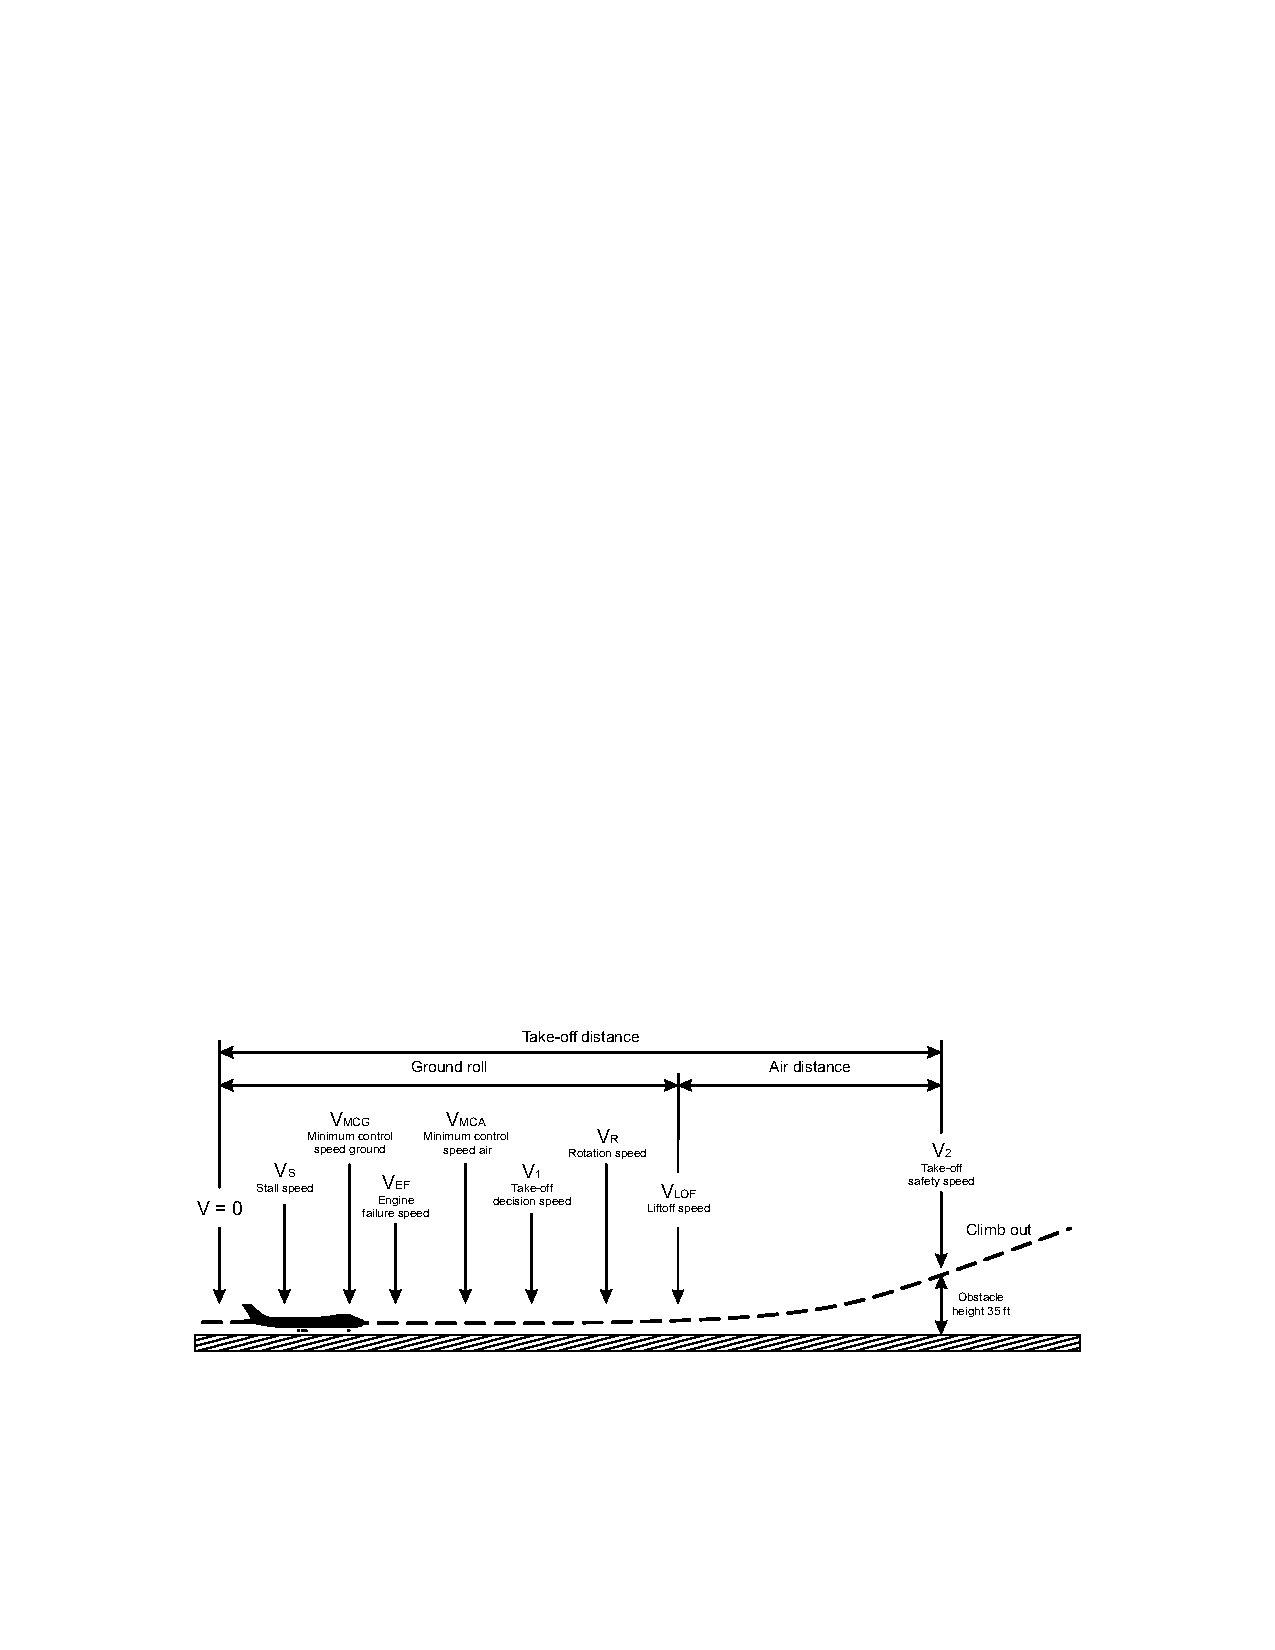
\includegraphics[keepaspectratio, width=0.97\textwidth]{TakeOffRun}
\caption{Scheme of an aircraft take-off run}
\label{fig:TOrun}
\end{figure}
%
The take-off may be considered as made up of two parts: a ground run and an air run, as shown schematically in figure~\ref{fig:TOrun}. The simplest description of the take-off process is that the engine thrust is increased to the take-off level at x = 0 and the brakes are released to begin acceleration down the runway. At some point, the pilot commands rotation of the aircraft which lifts the nose wheel from the ground and allows to achieve the take-off angle of attack; in this way the aircraft lift can grows faster and, when it is equal to the aircraft maximum take-off weight, the aircraft can lifts completely from the ground and begins climbing. The point at which it reaches an altitude of 35 \si{ft} (10.7 \si{\meter}), is considered, for an aircraft which refers to the \gls{FAR}-25, the end of the take-off run. 
%
This is the usual situation for take-off; subsequently, the modifications to safely deal with a take-off emergency, such as an engine failure, will be discussed.
%
%-----------------------------AOE Take-Off subsection-----------------------------
\subsection{\gls{acr:AOE} take-off run}
In order to deal with the calculation of the take-off run distance, a smart strategy is to find out all the foundamentals variables, which describes completely the aircraft state in this phase, and so, to study the dynamic system in exam in a state-space representation.
%
\noindent
To find out these state variables it is necessary to analyze aircraft equations of motion during take-off phases, these latter described as follows.
\begin{itemize}
\item \textbf{Ground roll phase}: starting from standstill with brakes released and at maximum power output, the aircraft accelerates on the runway, with constant angle of attack, until it reaches a speed equals to the rotation speed V\textsubscript{Rot}; after that the following subphase begin.
%
\begin{itemize}
\item \textbf{Rotation phase}: a short phase in which the pilot gives an assigned pitching law to lift the aircraft nose and, as a result, increasing the angle of attack. This phase ends when the load factor is equal to 1, meaning that the lift has reached the value of the maximum take-off weight, and the relative lift-off speed is indicated with V\textsubscript{LO}. 
%
\end{itemize}
%
\item \textbf{Airborne phase}: is the phases in which the aircraft, once it has lifted from the ground, gains altitude until it reaches the obstacle height of 35 \si{ft} (10.7 \si{\meter}) imposed by the \gls{FAR}-25. This phase begin at V\textsubscript{LO} and ends at the speed related to the obstacle overcoming, indicated with V\textsubscript{2}; furthermore it can be divided into the followngs two subphases:
%
\begin{itemize}
\item \textbf{Transition phase}: in which the aircraft rotates in order to increase the climb angle ($\gamma$) with the result of increasing the angle of attack and the relative lift coefficient, which should not surpass a safety value of the 90\% of the maximumlift coefficient in take-off configuration. This sub-phase ends when the desidered climb speed is reached.
%
\item \textbf{Climb-out to the obstacle phase}: in which the aircraft climbs at constant climb angle until the obstacle is surpassed.
\end{itemize}
\end{itemize}
%
\noindent
For more information regarding take-off equations of motion during each of the previously described phases, the reader can refer to~\cite{McCormick}.

\bigskip
\noindent
The set of \gls{acr:ODE} that models the take-off run is written in the following form:

\begin{equation}\label{eq:Take:Off:System:Dynamics:A}
    \LEFTRIGHT\lcbrace\rcbrace{\begin{array}{c}\dot{s}\\[2pt] \dot{V} \\[2pt] \dot{\gamma} \\[2pt] \dot{h} \end{array}}
= 
    \LEFTRIGHT\lcbrace\rcbrace{\begin{array}{l}
       f_1 \big(\, s,\, V,\, \gamma,\, h \,; \, \alpha \big) \\[4pt]
       f_2 \big(\, s,\, V,\, \gamma,\, h \,; \, \alpha \big) \\[4pt]
       f_3 \big(\, s,\, V,\, \gamma,\, h \,; \, \alpha \big) \\[4pt]
       f_4 \big(\, s,\, V,\, \gamma,\, h \,; \, \alpha \big)
    \end{array}}
\qquad
    \text{with}\quad
    \LEFTRIGHT\lcbrace.{\begin{array}{l} x_1 = s\\[2pt] x_2 = V \\[2pt] x_3 = \gamma \\[2pt] x_4 = h \end{array}}
\qquad
    \text{and}\quad
    u = \alpha
\end{equation}
%
\noindent
These equations can be also written in a more concise way as shown below.
%
\begin{equation}
\label{eq:Take:Off:System:Dynamics:B}
\dot{\vec{x}} = \vec{f}\big(\, \vec{x}\,;\,u \,\big)
\end{equation}
%
\noindent
The unknown $\vec{x} = [\mspace{2mu} x_1,\, x_2,\, x_3,\, x_4 \mspace{2mu}]^{\text{T}}$ is the vector of state variables. The input $u(t)$ is a given function of time, for $0 \leq t \leq t_{\text{final}}$, that corresponds to an assumed time history of the angle of attack during take-off.
%
The right-hand sides of system (\ref{eq:Take:Off:System:Dynamics:A}) are defined by the following functions:
%
\begin{subequations}\label{eq:Take:Off:System:Dynamics:RHS:functions}
\begin{equation}\label{eq:Take:Off:System:Dynamics:RHS:functions:A}
f_1 \big(\, \vec{x}\,,\,u \,\big) =  x_2
\end{equation}
%
\begin{equation}\label{eq:Take:Off:System:Dynamics:RHS:functions:B}
f_2 \big(\, \vec{x}\,,\,u \,\big) =
  \frac{g}{W}
    \LEFTRIGHT\lcbrace.{
      \begin{array}{l@{\rule{2em}{0pt}}l} 
        T(x_2) - D(x_2,u) - \mu \big[ W - L(x_2,u) \big]
          & \text{if} \;\, \mathcal{S}(x_2 , u) < 1
        \\[1em]
        T(x_2) \cos u - D(x_2,u) - W \sin x_3
          & \text{if} \;\, \mathcal{S}(x_2 , u) \geq 1
      \end{array}
    }  
\end{equation}
%
\begin{equation}\label{eq:Take:Off:System:Dynamics:RHS:functions:C}
f_3 \big(\, \vec{x}\,,\,u \,\big) =
  \frac{g}{W\,x_2}
    \LEFTRIGHT\lcbrace.{
      \begin{array}{l@{\rule{2em}{0pt}}l} 
        0
          & \text{if} \;\, \mathcal{S}(x_2 , u) < 1
        \\[1em]
        L(x_2,u) + T(x_2)\sin u - W \cos x_3
          & \text{if} \;\, \mathcal{S}(x_2 , u) \geq 1
      \end{array}
    }  
\end{equation}
%
\begin{equation}\label{eq:Take:Off:System:Dynamics:RHS:functions:D}
f_4 \big(\, \vec{x}\,,\,u \,\big) =  x_2 \, \sin x_3
\end{equation}
%
\noindent
The thrust $T(x_2)$ is calculated by means of the interpolating function $T_{\text{tab}}\big(V_{\text{a}}\big)$ based on a table lookup algorithm, where $V_{\text{a}} = V + V_{\text{w}}$ is the airspeed and $V_{\text{w}}$ is the wind speed (horizontal component, positive if opposite to the aircraft motion).
%
The drag $D$ and lift $L$, as functions of airspeed $V_{\text{a}}$ and angle of attack, are given by the following conventional formulas.
%
\begin{equation}\label{eq:Take:Off:System:Dynamics:RHS:functions:E}
D(x_2,u) = \frac{1}{2} \, \rho \, \big( x_2 + V_{\text{w}}\cos x_3 \big)^2 \,S \, C_D\big( u \big)
\end{equation}
%
\begin{equation}\label{eq:Take:Off:System:Dynamics:RHS:functions:E}
L(x_2,u) = \frac{1}{2} \, \rho \, \big( x_2 + V_{\text{w}}\cos x_3 \big)^2 \,S \, C_L\big( u \big)
\end{equation}
%
\noindent
The switching function $\mathcal{S}$ of aircraft velocity and angle of attack is defined as follows:
%
\begin{equation}\label{eq:Take:Off:System:Dynamics:RHS:functions:D}
\mathcal{S}(x_2 , u) = \frac{L(x_2,u)}{W \cos x_3}
\end{equation}
\end{subequations}
%
\noindent
The formulas (\ref{eq:Take:Off:System:Dynamics:RHS:functions}) make the system (\ref{eq:Take:Off:System:Dynamics:B})  a closed set of \gls{acr:ODE}.
%
\noindent
When the function $u(t)$ is assigned and the system is associated to a set of initial conditions, in this particular case equal to $\vec{x}_0 = [\mspace{2mu} 0,\, 0,\, 0,\, 0 \mspace{2mu}]^{\text{T}}$, a well-posed \gls{acr:IVP} is formed, which can be solved numerically.
%
In table~\ref{tab:Take:Off:Speeds:FAR25} are reported the take-off characteristic speeds and their corresponding requirements as defined by \gls{FAR}-25.
%
\begingroup
\begin{longtable}[H]{lll}
\label{tab:Take:Off:Speeds:FAR25}\\
\toprule
Speed & Description & Requirement
\\ \midrule
\endfirsthead
%
\multicolumn{3}{l}%
  {\relsize{-1}({\itshape continued from previous page})}\\
\toprule
Speed & Description & Requirement
\\ \midrule
\endhead
%
\midrule \multicolumn{3}{r}{{\relsize{-1}\itshape continued on next page}}
\endfoot
%
\bottomrule
\caption[Take-off speeds and FAR~25 requirements]{Take-off speeds and FAR~25 requirements}
\endlastfoot
%
$V_\mathrm{S}$ & aircraft stalling speed in take-off configuration & ---
\\
$V_\mathrm{MC}$ & minimum control speed with one engine inoperative (OEI) & ---
\\
$V_1$ & OEI decision speed & $\geq V_\mathrm{mc}$
\\
$V_\mathrm{Rot}$ & rotation speed & $>1.05\, V_\mathrm{MC}$
\\
$V_\mathrm{MU}$ & minimum unstick speed for safe flight & $\geq V_\mathrm{S}$
\\
$V_\mathrm{LO}$ & lift-off speed & $> 1.10 \, V_\mathrm{MU}$
\\
                &                & $> 1.05 \, V_\mathrm{MU}$ (OEI)
\\
$V_2$ & take-off climb speed at \SI[round-precision=0]{35}{ft} & $> 1.20 \, V_\mathrm{S}$
\\
                &                & $> 1.10 \, V_\mathrm{MC}$
\end{longtable}
\endgroup
%
\noindent
It has to be highlithed that the drag coefficient $C_D$ that appears in (\ref{eq:Take:Off:System:Dynamics:RHS:functions:E}) can be modelled as:
%
\begin{equation}\label{eq:CD:A}
C_D = C_{D0} + \left(\upDelta C_{D0}\right)_{\text{flap}+\text{lg}} +  K_g\ \frac{C_L^2}{\pi \AR e}
\end{equation}
%
with $\left(\upDelta C_{D0}\right)_{\text{flap}+\text{lg}}$ due to flap, as shown in subparagraph~\ref{subpar:DCD0}, and landing gears, which contribution is usually about $0.010 \div 0.015$; moreover $C_L$ is the one from the lift curve with flaps, and eventually slats, deflected. The term $K_g$ in (\ref{eq:CD:A}) incorporates the ground effect and it is calculated from~\cite{McCormick} using the (\ref{eqn:FifthOrderPoly}) which is a fifth order interpolating function of the  graph in fugure~\ref{fig:McCormickGroundEffect}, where the ratio $h_{\text{W}}/b$ is obtained dividing the height of wing above the ground by the wing span, usually between 0.1 and 0.2 when the aircraft is on the ground and assumed as $h_{\text{W}} \approx h$ durign the airborne.
%
\begin{figure}[H]
\centering
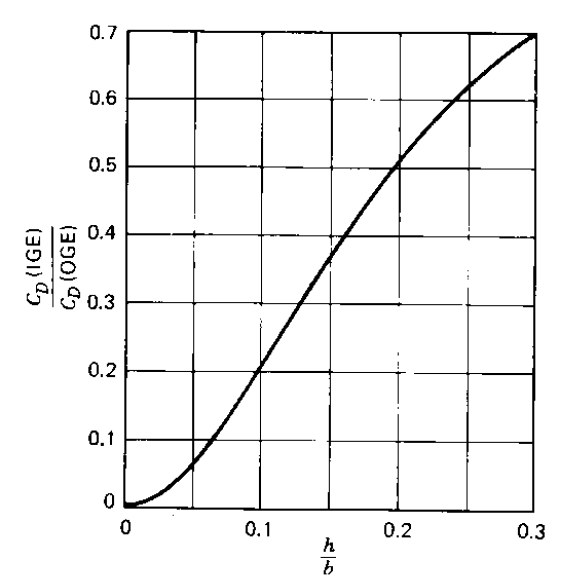
\includegraphics[keepaspectratio, width=0.6\textwidth]{McCormickGroundEffect}
\caption{Gorund effect parameter $K_g$ as function of the $h_{\text{W}}/b$ ratio}
\label{fig:McCormickGroundEffect}
\end{figure}
%
\begin{equation}
K_g=-622.44x^5+624.46x^4-255.24x^3+47.105x^2-0.6378x+0.0055
\label{eqn:FifthOrderPoly}
\end{equation}
%
This polynomial equation has a coefficient of determination $R^2$ of 0.9999 which justifies the approximation.
%
\begin{figure}[!t]
\centering
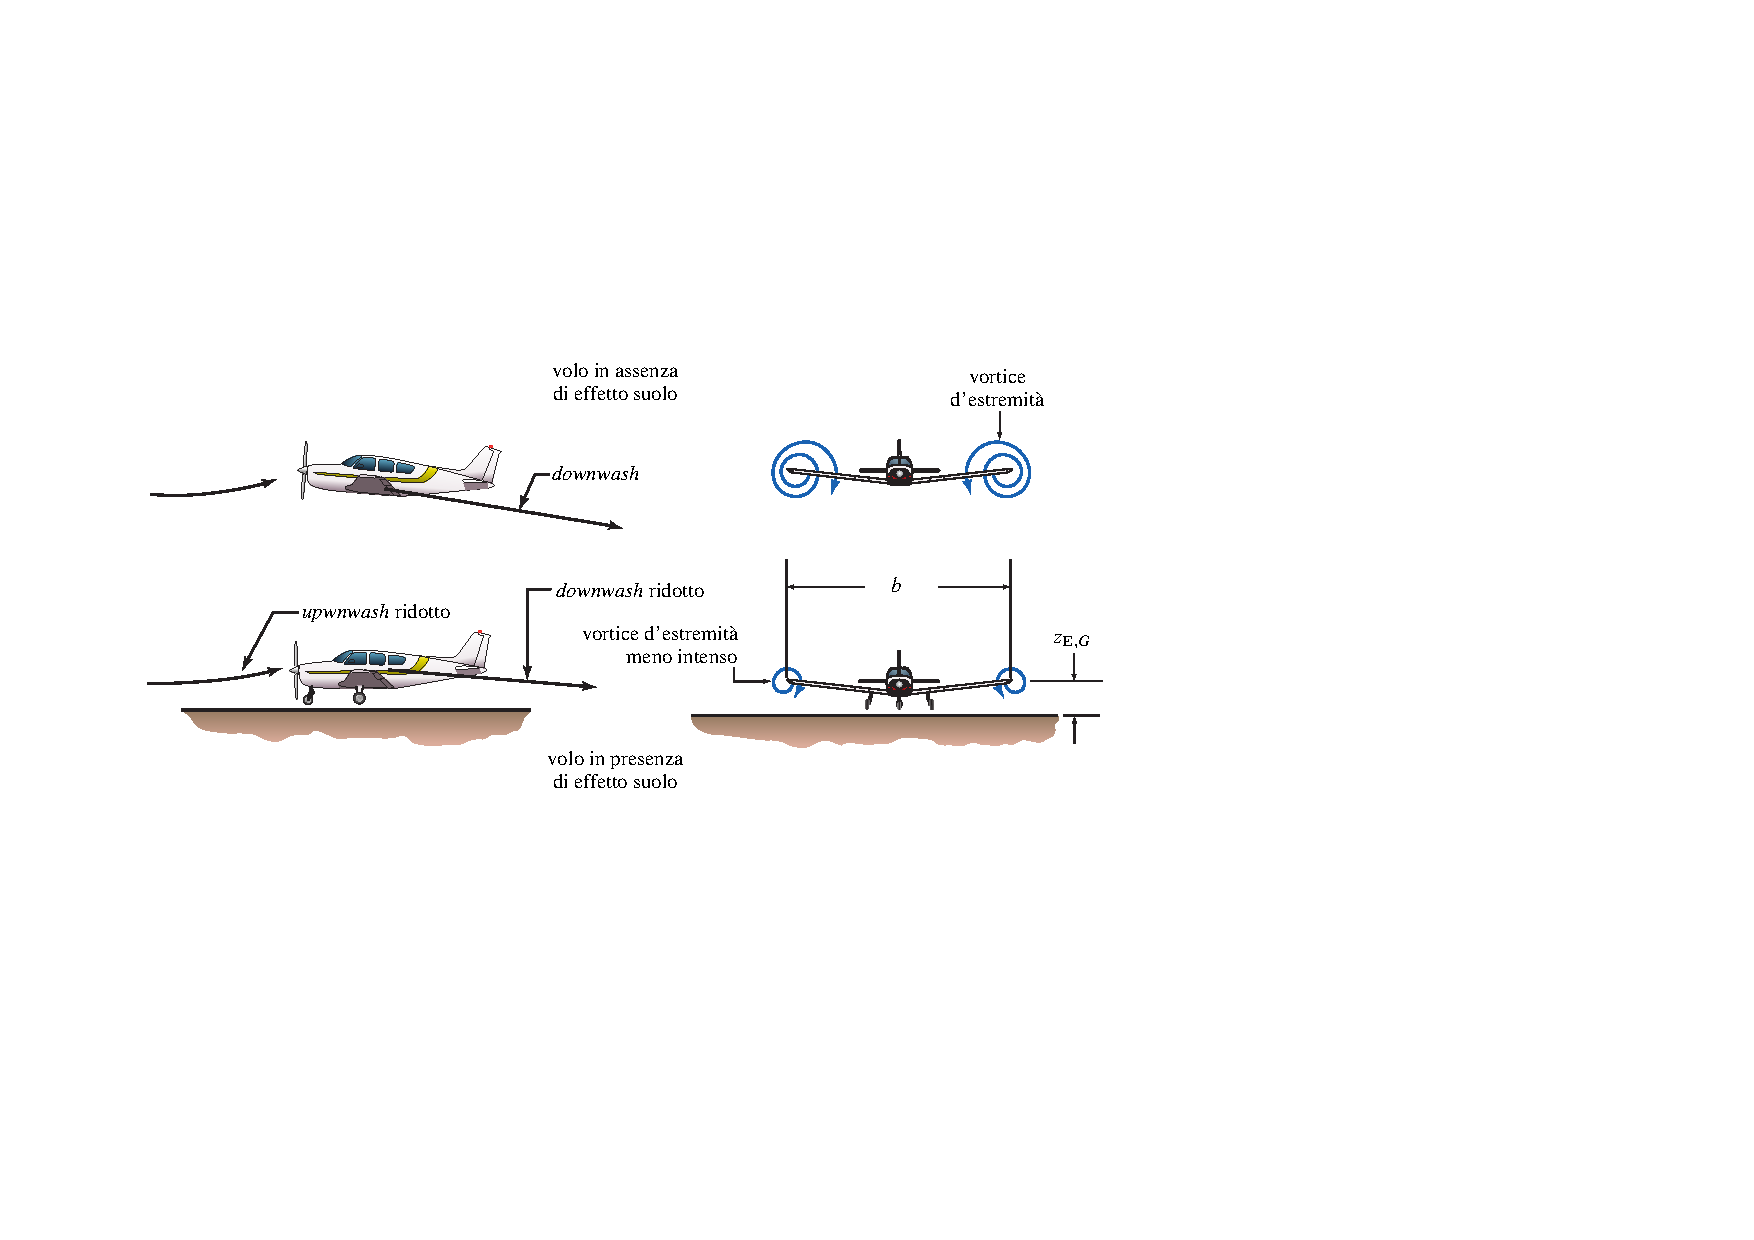
\includegraphics[keepaspectratio, width=\textwidth]{GroundEffect}
\caption{Comparison between flight with and without ground effect}
\label{fig:GroundEffect}
\end{figure}

\bigskip
\noindent
In order to better understand the nature of the ground effect it is convenient to refer to~\cite{nicolai2010fundamentals}, where the ground effect is explained as follows.
%
As the aircraft flies close to the ground, the ground interferes with the horseshoe vortex system trailing behind the wing. Ground effect is often analyzed by putting an image horseshoe vortex system of equal but opposite strength at the same distance $h_{\text{W}}$ below the ground.
%
This image vortex system induces velocities at the wing aerodynamic center, which decreases the strength of the downwash at that point, thereby decreasing the induced angle of attack, $\alpha_i$. Thus, the wing $C_L$ is increased (or more correctly, the lift curve slope increases, giving an increase in $C_L$ for the same geometric angle of attack, $\alpha$) and the induced drag is decreased.
%
This influence of the ground effect is a function of how close the aircraft is to the ground and of the size of the wing.

\bigskip
\noindent
Speaking of the $C_D$, it has also to be noted that, at high $C_L$, the parabolic drag polar it's no longer accurate in describing the drag characteristics of the aircraft so that two correction factors have to be added to the (\ref{eq:CD:A}). These latter triggers only when the $C_L$ is higher than 1.2, as can be seen from the following equation, in which $K_1$ and $K_2$ values depend on the aircraft in exam.
%
\begin{equation}
C_D = C_{D0} + \left(\upDelta C_{D0}\right)_{\text{flap}+\text{lg}} +  K_g\ \frac{C_L^2}{\pi \AR e} + K_1\ \left(C_L-1.2\right) + K_2\ \left(C_L-1.2\right)^2
\end{equation}

\bigskip
\noindent
Focusing, now, on the input law of the angle of attack, the function $u$ can be constructed by picking the time $t_{\text{Rot}}$ when the rotation speed $V_{\text{Rot}}$ is reached along the ground roll; thus the $u (t)$ function can be defined as follows.

\bigskip
\begin{equation}\label{eq:Take:Off:System:Dynamics:Alpha:Law}
u (t) =
    \LEFTRIGHT\lcbrace.{
      \begin{array}{l@{\rule{2em}{0pt}}l} 
        \alpha_{\text{g}}
          & \text{if} \;\, t < t_{\text{Rot}}
        \\[1em]
        \alpha_1(t)
          & \text{if} \;\, t \geq t_{\text{Rot}}
      \end{array}
    }
\end{equation}
%
with a constant $\alpha_{\text{g}}$ during the ground run up to the rotation speed, and a given non-zero law $\alpha_1(t)$ for the post-rotation angle of attack time history. 
%
\begin{figure}[!t]
\centering
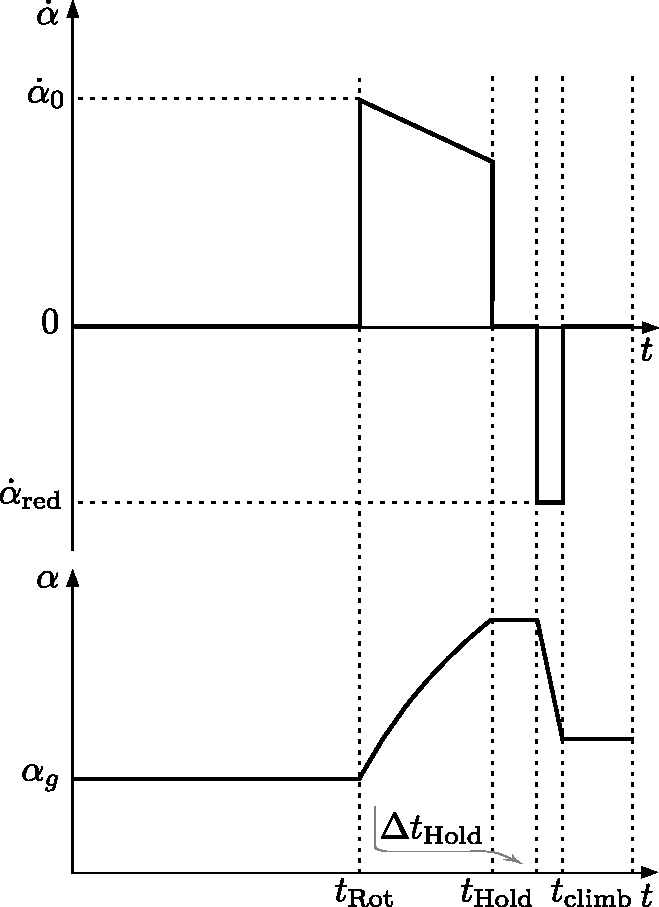
\includegraphics[keepaspectratio, width=0.45\textwidth]{AlphaInputTakeOff}
\caption{Qualitative representation of the angle of attack input law}
\label{fig:AlphaInput}
\end{figure}
%
Figure~\ref{fig:AlphaInput} shows a qualitative representation of the $\alpha_1(t)$ law. As can be seen, after $t_{\text{Rot}}$ the pilot applies an initial angular velocity $\dot\alpha_{0}$, which decreases with time, according to the law written in (\ref{eqn:AlphaDot}) as function of $\alpha$, until the time $t_{\text{Hold}}$ has been reached; this particular instant is related to the achievement of the maximum admitted lift coefficient in take-off, which is set at 90\% of the $C_{L\text{max,TO}}$.
%
\begin{equation}
\dot\alpha=\dot\alpha_0\ \left(1-k_\alpha\ \alpha\right)
\label{eqn:AlphaDot}
\end{equation}
%
\noindent
In equation (\ref{eqn:AlphaDot}), the $k_\alpha$ slope is assigned (expressed in $\si{1/\degree}$ and dependent on the aircraft in exam), while the initial angular velocity $\dot\alpha_0$ is calculated as follows.
%
\begin{equation}
\dot\alpha_0=\dfrac{\upDelta\alpha}{\upDelta t_{\text{Rot}}}=\dfrac{\alpha_{\text{LO}}-\alpha_g}{\upDelta t_{\text{Rot}}}
\label{eqn:AlphaDotInitial}
\end{equation}
%
where $\alpha_{\text{LO}}$ can be obtained from the lift curve of the wing, with flaps deflected in take-off configuration, by assigning the $C_{\text{L}_{\text{LO}}}$; this can be derived from the $C_{L\text{max,TO}}$ dividing it by the parameter $K^2_{\text{LO}}$, which represents the quantity that has to be multiplied by $V_{\text{S}}$ in order to obtain $V_{\text{LO}}$ (for example 1.1 with reference to table~\ref{tab:Take:Off:Speeds:FAR25}).

\bigskip
\noindent
From this point on the pilot stops the pitching manouver and keeps the angle of attack constant for an assigned $\upDelta t_{\text{Hold}}$. During this time interval, the lift coefficient is high and, as a result, also the induced drag is high so that aircraft acceleration will reduce. 
%
After this short time interval the pilot has to reduce the angle of attack in order to avoid the acceleration to decrease too much and so an assigned negative angular velocity $\dot\alpha_{\text{red}}$ is applied; the latter assumed to be constant for simplicity. 
%
Finally, since the decrease of $\alpha$ determines also a reduction in $C_L$, the time $t_{\text{climb}}$ will be reached when the load factor is reduced to 1; this means that a balance of the forces, perpendicular to the flight path, has been achieved and so the climb phase, at constant $\gamma$, can begin, leaving $\alpha$ constant and equal to last value reached. Moreover, from this time on, the lift value is constant and equal to $W\cdot\cos\gamma$, in order to maintain the load factor equal to 1; while the $C_L$ is derived from the lift value using the (\ref{eqn:Lift.Equation}).
%
%-----------------------------OEI Take-Off subsection-----------------------------
\subsection{\gls{acr:OEI} take-off run and balanced field lenght}
\label{subpar:OEI}
A good description of the take-off with one engine failure is proposed in \cite{sforza2014commercial}. Here it is explained that in the event of an engine failure during the take-off roll the pilot must decide whether to continue the take-off or, instead, abort the take-off and decelerate to a stop on the runway. Obviously, if the engine failure occurs when the aircraft is traveling very slowly, the aircraft should be kept on the ground and brought to a stop at some safe location off the runway. Conversely, if the engine failure occurs when the aircraft is close to the take-off speed the take-off should be continued. The designer must provide a means for deciding whether it is safer to abort the take-off or continue it.
%
The critical velocity, denoted as $V_{\text{act}}$, is the velocity at which action is taken, not that at which the decision to act is taken. The time between the recognition of an engine failure, which occurs at $V_{\text{ef}}$, and the critical velocity $V_{\text{act}}$, when action is taken is required to be more than one second. Generally this time period, which is set by the reaction time of the pilot, is taken to be about \SI{3}{\second}. If the pilot’s decision is to continue the take-off with one engine inoperative, the distance to the lift-off speed $V_{\text{LO}}$ and to the subsequent climb-out to 35 $\si{ft}$ height above the runway, will obviously be longer than with all engines operating.

\bigskip
\noindent
The calculation of the take-off distance in this situation is quite the same as the one explained previously, with the difference that now there is a discontinuity in thrust due to the broken engine. In particular, the thrust, $T(x_2)$, will still be read from the database but considering a number of engines reduced by one from the time $t_{\text{ef}}$ at which the engine failure occurs.

\bigskip
\noindent
On the other hand, in the case of the aborted take-off the pilot will apply the necessary braking procedures in order to get the maximum permissible deceleration while maintaining adequate control of the airplane’s motion. The portion of the aborted take-off run up to the engine failure velocity $V_{\text{ef}}$ is calculated in the same way as that for the continued take-off, so that the distance is the same in both cases. 
%
From this point on, until the pilot reacts by activating brakes, there is only a discontinuity in thrust due to the failed engine; while, after the time interval in which the pilot decides to abort the take-off, the thrust is set to minimum (ideally zero) and the brakes action provides an higher friction coefficient. During this last phase, the equation (\ref{eq:Take:Off:System:Dynamics:RHS:functions:B}) changes in the following.
%
\begin{equation}\label{eq:Take:Off:System:Dynamics:RHS:functions:Aborted}
f_2 \big(\, \vec{x}\,,\,u \,\big) =\frac{g}{W}\ \big\{ - D(x_2,u) - \mu_{\text{brakes}} \big[ W - L(x_2,u) \big]\big\} 
\end{equation}
%
where $\mu_{\text{brakes}}$ is bigger than $\mu$ and it is usually about 0.3.
%
Furthermore, it has to be noted that, even if the aircraft in exam is supplied with a reverse thrust device, this effect has not to be taken into account for a more conservative result. 

\bigskip
\noindent
Instead of considering the limiting cases of aborting take-off at low $V_{\text{act}}$ and continued take-off at high $V_{\text{act}}$, it is useful determine the critical velocity for which the distance required to continue the take-off is equal to the distance required to safely abort it. This velocity is the one from table \ref{tab:Take:Off:Speeds:FAR25} and it's called \emph{decision speed} $V_1$, while the related distance is called the \emph{balanced field length}. The latter, in particular, plays an important role in the sizing of the runway since is the maximal distance the aircraft can cover both in continued take-off, both in 
aborted take-off. 
%
In order to calculate this distance, and the related velocity, it's possible to evaluate, at different $V_{\text{act}}$,  both the continued take-off distance with one inoperative engine, both the aborted take-off distance. Each couple of speed and distance can then be plotted with the result of building the curves of figure~\ref{fig:BalancedFieldLength}. The intersection of these latter, at which the two distances are the same, defines the \emph{balanced field length} and the $V_1$.
%
\begin{figure}[H]
\centering
\includegraphics[keepaspectratio, width=0.6\textwidth]{BalancedFieldLength}
\caption{Qualitative representation of the field distances required to continue a takeoff or to abort it when one
engine fails as a function of critical velocity}
\label{fig:BalancedFieldLength}
\end{figure}
%
\noindent
As expected, the take-off distance on the curve related to the continued take-off with one inoperative engine decreases with the failure speed, tending to the AOE condition; while the take-off distance on the other curve grows with the failure speed because the deceleration to stop the aircraft begins from an higher speed, requiring more distance to be dissipated.
%
%------------------------- JAVA CLASS ARCHITECTURE ---------------------------
\section{Java class architecture}
%
In this paragraph the implementation inside the JPAD library of the calculation of the take-off distance, and of the related balanced field length, will be desribed; in particular, as in previous chapters, a dedicated Java class, named~\lstinline[language=Java]!CalcTakeOff_Landing!, has been created to manage all required methods.

\bigskip
\noindent
The first component to be described is the class constructor; the latter, in addition to linking all the input parameter to the related class fields, provides a series of preliminary calculations which defines other required input data, not given from the user, such as the maximum lift coefficient in take-off configuration, or the stalling speed in take-off, and some of the characteristic speeds defined in table~\ref{tab:Take:Off:Speeds:FAR25}.
%
\begin{table}[!t]
\makebox[\linewidth]{
\begin{tabular}{p{0.25\linewidth}p{0.7\linewidth}}
\toprule
\lstinline[language=Java]!aircraft! & An \lstinline[language=Java]!Aircraft! class object representing an aircraft parametric model \\ [0.2cm]
\lstinline[language=Java]!theConditons! & An \lstinline[language=Java]!OperatingConditions! object representing aircraft flight conditions \\  [0.2cm]
\lstinline[language=Java]!highLiftCalculator! & A \lstinline[language=Java]!CalcHighLiftDevices! object for managing flap and slat effects \\  [0.2cm]
\lstinline[language=Java]!dtRot! & The assigned time interval of the rotation phase \\  [0.2cm]
\lstinline[language=Java]!dtHold! & The assigned time interval of the constant $C_L$ phase\\  [0.2cm]
\lstinline[language=Java]!kcLMax! & Percentage of the $C_{L\text{max,TO}}$ not to be surpasses \\  [0.2cm]
\lstinline[language=Java]!kRot! & Percentage of $V_s$ which defines the rotation speed \\  [0.2cm]
\lstinline[language=Java]!kLO! & Percentage of $V_s$ which defines the lift-off speed \\  [0.2cm]
\lstinline[language=Java]!kFailure! & A parameter which defines the drag increment due to engine failure and the consequent rudder deflection\\  [0.2cm]
\lstinline[language=Java]!k1! & Linear correction factor of the parabolic drag polar at high $C_L$ \\  [0.2cm]
\lstinline[language=Java]!k2! & Quadratic correction factor of the parabolic drag polar at high $C_L$ \\  [0.2cm]
\lstinline[language=Java]!phi! & Throttle setting \\  [0.2cm]
\lstinline[language=Java]!kAlphaDot! & A coefficient which defines the decrease of $\dot\alpha$ during manouvering \\ [0.2cm]
\lstinline[language=Java]!alphaReductionRate! & A constant negative pitching angular velocity to be maintained after holding the $C_L$ constant \\ [0.2cm]
\lstinline[language=Java]!mu! & The friction coefficient without brakes action \\ [0.2cm]
\lstinline[language=Java]!muBrake! & The friction coefficient with brakes activated \\ [0.2cm]
\lstinline[language=Java]!wingToGroundDistance! & The distance between the wing and the ground  \\ [0.2cm]
\lstinline[language=Java]!obstacle! & A given altitude value to overcome which defines the airborne phase ending \\ [0.2cm]
\lstinline[language=Java]!vWind! & The horizontal component of the wind speed, positive if opposite to the aircraft motion \\ [0.2cm]
\lstinline[language=Java]!alphaGround! & The angle of attack, in the \gls{ACRF}, of the wing when the aircraft is on the ground \\ [0.2cm]
\lstinline[language=Java]!iw! & The angle between the wing root chord and the \gls{ACRF} x-axis \\ 
\bottomrule
\end{tabular}
}
\caption{\lstinline[language=Java]!CalcTakeOff_Landing! constructor input}
\label{table:CalcTakeOffInput}
\end{table}
%
More in detail, the constructor evaluates, firstly, all high-lift devices effects, which data are supplied in the test class as explained in the paragraph~\ref{par:CalcHighLiftDevices}, by using the method~\lstinline[language=Java]!calculateHighLiftDevicesEffects! of the~\lstinline[language=Java]!CalcHighLiftDevices! class, described in the previous chapter in paragraph~\ref{par:CalcHighLiftDevices}. After that it's possible to define the maximum lift coefficient, $C_{L\text{max,TO}}$, the $C_{L0}$, with high-lift devices effects computed, and the lift coefficient during the ground roll phase, $C_{Lg}$, related to the constant angle of attack $\alpha_g$; in particular the last two quantities are calculated using the method~\lstinline[language=Java]!calcCLatAlphaHighLiftDevice!, of the~\lstinline[language=Java]!CalcHighLiftDevices! class, respectively with $\alpha_w=0\degree$ and  $\alpha_w=\alpha_g+i_w$.
%
With the $C_{L\text{max,TO}}$ known, the stalling speed in take-off configuration is calculated using the classical formula provieded below.
%
\begin{equation}
V_s=\sqrt{\dfrac{2W_{\text{TO}}}{\rho\ S\ C_{L\text{max,TO}}}}
\label{eqn:Lift.Equation}
\end{equation} 
%
From this speed, both the $V_{\text{Rot}}$ both the $V_{\text{LO}}$ are calculated multipling the $V_s$ by the two parameters, $k_{\text{Rot}}$ and $k_{\text{LO}}$, defined in table~\ref{table:CalcTakeOffInput}.
%
At this point, the ratio $h_{\text{W}}/b$ and the ground effects correction parameter $K_g$ of the (\ref{eqn:FifthOrderPoly}) are calculated; while all the \gls{List}s, which will store all physical quantities of interest at every integration step, are initialized together with a custom \gls{Map}, named~\lstinline[language=Java]!TakeOffResultsMap!. The latter, in particular, has been created with the purpose of store the state vector, and all the related physical quantities, only at some key point during the take-off run, like the end of the ground roll phase, the end of the rotation phase and the end of the airborne phase.
%
\begin{table}[!t]
\makebox[\linewidth]{
\begin{tabular}{p{0.25\linewidth}p{0.7\linewidth}}
\toprule
\lstinline[language=Java]!timeValue! & The integration time, in $\si{\second}$, at the step to save \\ [0.2cm]
\lstinline[language=Java]!thrustValue! & The engine thrust, in $\si{\newton}$, at the step to save \\  [0.2cm]
\lstinline[language=Java]!thrustHorizontalValue! & The engine thrust component on the \gls{ACRF} x-axis, in  $\si{\newton}$, at the step to save \\  [0.2cm]
\lstinline[language=Java]!thrustVerticalValue! & The engine thrust component on the \gls{ACRF} z-axis, in  $\si{\newton}$, at the step to save \\  [0.2cm]
\lstinline[language=Java]!frictionValue! & The friction, in  $\si{\newton}$, at the step to save\\  [0.2cm]
\lstinline[language=Java]!liftValue! & The lift, in  $\si{\newton}$, at the step to save \\  [0.2cm]
\lstinline[language=Java]!dragValue! & The drag, in  $\si{\newton}$, at the step to save \\  [0.2cm]
\lstinline[language=Java]!totalForceValue! & The total force, in brakets in the equation (\ref{eq:Take:Off:System:Dynamics:RHS:functions:B}), at the step to save in  $\si{\newton}$ \\  [0.2cm]
\lstinline[language=Java]!loadFactorValue! & The load factor at the step to save \\  [0.2cm]
\lstinline[language=Java]!speedValue! & The speed, in  $\si{\meter\per\second}$, at the step to save \\  [0.2cm]
\lstinline[language=Java]!rateOfClimbValue! & The rate of climb from equation (\ref{eq:Take:Off:System:Dynamics:RHS:functions:D}), in  $\si{\meter\per\second}$, at the step to save \\  [0.2cm]
\lstinline[language=Java]!accelerationValue! & The acceleration from equation (\ref{eq:Take:Off:System:Dynamics:RHS:functions:B}), in  $\si{\meter\per\square\second}$, at the step to save \\  [0.2cm]
\lstinline[language=Java]!groundDistanceValue! & The horizontal distance, in  $\si{\meter}$, covered at the step to save \\ [0.2cm]
\lstinline[language=Java]!verticalDistanceValue! & The altitude, in  $\si{\meter}$, reached at the step to save \\ [0.2cm]
\lstinline[language=Java]!alphaValue! & The angle of attack $\alpha$, in  $\si{\degree}$, at the step to save, in \gls{ACRF} \\ [0.2cm]
\lstinline[language=Java]!alphaDotValue! & The pitching angular velocity, in  $\si{\degree\per\second}$, at the step to save \\ [0.2cm]
\lstinline[language=Java]!gammaValue! & The ramp angle $\gamma$, in  $\si{\degree}$, at the step to save  \\ [0.2cm]
\lstinline[language=Java]!gammaDotValue! & The $\dot\gamma$ value, in  $\si{\degree\per\second}$, at the step to save \\ [0.2cm]
\lstinline[language=Java]!thetaValue! & The $\theta=\alpha+\gamma$ value, in  $\si{\degree}$, at the step to save \\ [0.2cm]
\lstinline[language=Java]!cLValue! & The lift coefficient at the step to save \\ [0.2cm]
\lstinline[language=Java]!cDValue! & The drag coefficient at the step to save \\ 
\bottomrule
\end{tabular}
}
\caption{\lstinline[language=Java]!collectResults! input data}
\label{table:TakeOffMapInput}
\end{table}

\bigskip
\noindent
The~\lstinline[language=Java]!TakeOffResultsMap! class is made up of a builder, which accepts nothing as input and provides the initialization of all the \gls{List}s required to store the wanted data, and of other two method which are explained below.
%
\begin{itemize}
\item \lstinline[language=Java]!initialize!, which clears all the \gls{List}s in order to make them reusable for other calculations
\item \lstinline[language=Java]!collectResults!, which accepts as input all data from table~\ref{table:TakeOffMapInput} in order to add them to the related \gls{List}
\end{itemize}
%
Once all data are stored, it's easy with this map to get one, or more than one, result; all it has to be done is call the related \emph{getter} method of which the class is supplied. 

\bigskip
\noindent
It has to be noted that all these preliminary calculations and \gls{List}s initializations are put into the constructor for a reason; in fact, as these are all quite heavy operations in terms of computational cost, put them in the constructor means that they are carried out only once allowing a more rapid use, even iterative, of the main method that will be described shortly.

\bigskip
\noindent
The most important method of the class is~\lstinline[language=Java]!calculateTakeOffDistanceODE! which is in charge of the resolution of the \gls{acr:ODE} set presented in (\ref{eq:Take:Off:System:Dynamics:RHS:functions}). This method accepts as input two parameters which are used to determine, firstly, if an engine failure has occurred during the take-off run, and then if the take-off run has to be aborted; these are:
%
\begin{itemize}
\item \lstinline[language=Java]!vFailure!, a \lstinline[language=Java]!Double! value representing the failure speed in $\si{\meter\per\second}$. Can be set to \lstinline[language=Java]!null! if the user dosen't want to calculate the \gls{acr:OEI} take-off distance. 
\item \lstinline[language=Java]!isAborted!, a \lstinline[language=Java]!boolean! flag which is \lstinline[language=Java]!true! if the method has to calculate the aborted take-off distance.
\end{itemize}
%
After performing a check upon these two variables, the method knows which case it has to study and proceeds with the calculation; in particular, it creates the integrator object of the class \lstinline[language=Java]!HighamHall54Integrator!, which implements the \gls{Interface} \lstinline[language=Java]!FirstOrderIntegrator!. For more information, the reader can refer to \cite{apache:ode}.

\bigskip
\noindent
More in detail, the \lstinline[language=Java]!HighamHall54Integrator! class implements a fifth order Higham and Hall integrator which uses seven functions evaluations per step and is supplied with stepsize control, automatic step initialization and continuous output. The latter has proven to be the best choise, among other possible integrators (viewables in \cite{apache:FirstOrderIntegrator}) which implement the previous \gls{Interface}, because it provides the better compromise between calculation time and accuracy using the following settings.

\bigskip
\begin{lstlisting}[caption={HighamHall54Integrator class object creation}, captionpos=b, tabsize=2]
FirstOrderIntegrator theIntegrator = new HighamHall54Integrator(
				1e-6,				// minimal step 
				1,				  // maximal step 
				1e-17,			// allowed absolute error
				1e-17				// allowed relative error
				);
\end{lstlisting}
%
Beside the integrator, the method needs the set of equation to integrate; these are passed to it through the object of a dedicated inner class, named \lstinline[language=Java]!DynamicsEquations!, which implements the \gls{Interface} \lstinline[language=Java]!FirstOrderDifferentialEquations! \cite{apache:FirstOrderDifferentialEquations}. Thus, the \lstinline[language=Java]!DynamicsEquations! class provides the set of \gls{acr:ODE} (\ref{eq:Take:Off:System:Dynamics:RHS:functions}) and, in particular, is supplied with a series of methods necessary to calculate the required physical quantities used into these equations and described in the previous paragraph. Furthermore, thanks to the use of the variable \lstinline[language=Java]!isAborted!, the class can easly switch the equations set in case of aborted take-off as shown in the subparagraph \ref{subpar:OEI}.
%
\begin{table}[!b]
\begin{tabular}{p{0.17\linewidth}p{0.83\linewidth}}
\toprule
\lstinline[language=Java]!ehCheckFailure! & It checks when the speed, $x_2$, becomes greater than the input \lstinline[language=Java]!vFailure! determining, in this way, the instant of the engine failure occurrence \\ [0.2cm]
\lstinline[language=Java]!ehCheckVRot! & It checks when the speed, $x_2$, becomes greater than the rotation speed \lstinline[language=Java]!vRot! determining, in this way, the instant at which the ground roll ends and the rotation phase begins \\  [0.2cm]
\lstinline[language=Java]!ehEndConstantCL! & It checks when the time, $t$, becomes greater than the sum of  $t_{\text{Hold}}$ and of the given time interval $\upDelta t_{\text{Hold}}$ determining, in this way, the instant at which the angle of attack, and the related $C_L$, stops to be kept constant \\  [0.2cm]
\lstinline[language=Java]!ehCheckObstacle! & It checks when the altitude, $x_4$, becomes greater than the given obstacle height (35 $\si{ft}$) determining, in this way, the instant at which the airborne phase, and so the entire take-off, ends \\  [0.2cm]
\lstinline[language=Java]!ehCheckBrakes! & It checks when the time, $t$, becomes greater than the sum of  $t_{\text{Failure}}$ and of the given time interval $\upDelta t_{\text{Rec}}$, required to the pilot to recognize the failure, determining, in this way, the instant at which the pilot, which has decided to abort the take-off, actions the brakes in order to stop the aircraft run\\  [0.2cm]
\lstinline[language=Java]!ehCheckStop! &  It checks when the speed, $x_2$, becomes lower than zero determining, in this way, the instant at which the aircraft has stopped \\ 
\bottomrule
\end{tabular}
\caption{\lstinline[language=Java]!EventHandler! implementation inside the method \lstinline[language=Java]!calculateTakeOffDistanceODE!}
\label{table:EventHandler}
\end{table}

\bigskip
\noindent
In order to take into account of particular events which can happen during the take-off run, the method \lstinline[language=Java]!calculateTakeOffDistanceODE! is supplied with several implementation of the \gls{Interface} \lstinline[language=Java]!EventHandler! \cite{apache:ode}. The latter, through the definition of a specific function, can determine the occurrence of the wanted event by monitoring whether the sign of the defined function changes. Moreover it allows to manage the time step at which the event has occurred, so that it's possible to save, into the~\lstinline[language=Java]!TakeOffResultsMap!, the state vector and all the physical quantities of interest. Each implementation of the \gls{Interface} can also impose one of the folllowing actions to the integrator.
%
\begin{itemize}
\item \textbf{CONTINUE}, the integration simply goes on
\item \textbf{STOP}, the integration stops when the event triggers
\item \textbf{RESET_STATE}, the state vector can be changed when the event triggers 
\item \textbf{RESET_DERVATIVES}, the set of equation can be changed when the event triggers 
\end{itemize}
%
In the case in exam, six events are monitored by six implementation of the \lstinline[language=Java]!EventHandler! \gls{Interface} as shown below.

\noindent
Each event of the table \ref{table:EventHandler} defines a time instant usable, by the class \lstinline[language=Java]!DynamicsEquations!, to determine when the derivatives, or the calculation of the related physical quantities, have to switch from an equation to another, this allows to manage in a very easy way the definition of the profile of $\dot\alpha$ and $\alpha$, as well as the derivatives change shown in (\ref{eq:Take:Off:System:Dynamics:RHS:functions:B}) and (\ref{eq:Take:Off:System:Dynamics:RHS:functions:C}).  

\bigskip
\noindent
In order to make each \lstinline[language=Java]!EventHandler! usable by the integrator, they have to be added to the \lstinline[language=Java]!HighamHall54Integrator! as follows.

\bigskip
\begin{lstlisting}[caption={HighamHall54Integrator class object creation}, captionpos=b, tabsize=2]
if(!isAborted) {
	theIntegrator.addEventHandler(ehCheckVRot, 1.0, 1e-3, 20);
	theIntegrator.addEventHandler(ehCheckFailure, 1.0, 1e-3, 20);
	theIntegrator.addEventHandler(ehEndConstantCL, 1.0, 1e-3, 20);
	theIntegrator.addEventHandler(ehCheckObstacle, 1.0, 1e-3, 20);
}
else {
	theIntegrator.addEventHandler(ehCheckVRot, 1.0, 1e-3, 20);
	theIntegrator.addEventHandler(ehCheckFailure, 1.0, 1e-3, 20);
	theIntegrator.addEventHandler(ehCheckBrakes, 1.0, 1e-3, 20);
	theIntegrator.addEventHandler(ehCheckStop, 1.0, 1e-6, 20);
}
\end{lstlisting}
%
As can be seen the \lstinline[language=Java]!boolean! variable \lstinline[language=Java]!isAborted! plays an important role in determining which events have to be checked whether or not the take-off is aborted or continued. Also noteworthy, the method \lstinline[language=Java]!addEventHandler! arguments, which represent, respectively, the following parameters.
%
\begin{itemize}
\item The event to be checked
\item The maximal time interval between switching function checks (this interval prevents missing sign changes in case the integration steps becomes very large)
\item The convergence threshold in the event time search
\item The upper limit of the iteration count in the event time search
\end{itemize}
%
The decision of these parameters values has derived from a compromise between accuracy and computational time.

\bigskip
\noindent
Another important feature that the \gls{acr:ODE} package provides is the possibility to manage each time step, even if no event is triggered; in this way the developer can, for example, store data into an output file, or manage some events which are independent from the time or the state vector as they were in the \lstinline[language=Java]!EventHandler! \gls{Interface}. The tool which allows all these feature is the \lstinline[language=Java]!StepHandler! \gls{Interface} \cite{apache:ode}; in this particular case, this interface has only one implementation, added to the integrator, which is in charge of store the state vector, the time and all the related physical quantities, into their related \gls{List}s, at every time step in order to make them usable outside this method. Moreover it has a key role in managing three events, to be observed only if the variable \lstinline[language=Java]!isAborted! is false, that could not be handled well by the \lstinline[language=Java]!EventHandler! \gls{Interface}; these are the followings.
%
\begin{itemize}
\item A check upon the load factor to catch the instant at which, for the first time, it reaches a value of 1; this instant is $t_{\text{EndRot}}$ and determines the beginning of the airborne phase together with the changes in the derivatives shown in (\ref{eq:Take:Off:System:Dynamics:RHS:functions:B}) and (\ref{eq:Take:Off:System:Dynamics:RHS:functions:C})
\item A check upon the $C_L$ in order to determine when it reaches the threshold value defined by \lstinline[language=Java]!kcLMax! multiplied for the $C_{L\text{max,TO}}$. The related instant is the $t_{\text{Hold}}$ of the beginning of the constant $\alpha$ and $C_L$ phase
\item A second check on the load factor in order to define the instant at which its value is reduced to 1 after having applied the constant $\dot\alpha_{\text{Red}}$ angular velocity. This instant defines~$t_{\text{climb}}$ 
\end{itemize}
%
Each of these events is monitored by the value of the variable \lstinline[language=Java]!isAborted! and by the observation both of the evolution, through a single time step, of the last value added to the \gls{List} of interest, both of the time, which is compared to one of the reference instants described previously.

\bigskip
\noindent
The method is, finally, completed by assigning the initial state vector, calling the method \lstinline[language=Java]!integrate!, which is in charge of the integration process, and ereasing all the \lstinline[language=Java]!StepHandler! and \lstinline[language=Java]!EventHandler! implementations at the end of the process; this in order to make the method reusable later.

\bigskip
\noindent
Now that a method for calculating the take-off distance, in every case, is available, it can be used iteratively in order to determine the \emph{balanced field length} and the related \emph{decision speed} $V_1$. The method in charge of this is called \lstinline[language=Java]!calculateBalancedFieldLength! and follows the following guideline.
%
First of all an array of five values of possible failure speeds (between 2~$\si{\meter\per\second}$ and the lift-off speed $V_{\text{LO}}$) is defined; after that the method \lstinline[language=Java]!calculateTakeOffDistanceODE! is called for each of these speeds both in case of \gls{acr:OEI} continued take-off (\lstinline[language=Java]!isAborted! set to \lstinline[language=Java]!false!), both in case of aborted take-off (\lstinline[language=Java]!isAborted! set to \lstinline[language=Java]!true!). It's important to highlight that between each call of the method \lstinline[language=Java]!calculateTakeOffDistanceODE!, all reference instants and \gls{List}s have to be reinitialized; this can be done using the dedicated method \lstinline[language=Java]!initialize! defined into this class.

\bigskip
\noindent
Each failure speed, \gls{acr:OEI} take-off distance and aborted take-off distance calculated this way, is then stored into a dedicated array so that it's possible to define an interpolating function for the two distances. More in detail, since five points are few to describe the curves in figure \ref{fig:BalancedFieldLength}, a new array of 250 values of failure speeds is defined useing the same constrain of the previous one; the latter is then used to build a spline interpolating function, for both the \gls{acr:OEI} take-off distance and aborted take-off distance, using the five points calculated previously.
%
From the intersection of the last two interpolated curves is possible to define the \emph{balanced field length} and the \emph{decision speed} $V_1$ as shown in figure \ref{fig:BalancedFieldLength}. It should be noted that the choise of using interpolating functions and not to perform more times the calculation of the take-off distance in the two cases, derives from the will to speed up the calculation so that it's possible to have accurate results in less than one second. 

\bigskip
\noindent
In conclusion, the class is completed by two methods in charge of plotting the curves of interst from the related \gls{List}s and the \emph{balanced field length} chart; these are the followings.
%
\begin{itemize}
\item \lstinline[language=Java]!createTakeOffCharts!, provides the conversion of the previous \gls{List}s into \lstinline[language=Java]!double! arrays so that they can be managed by the plotting method; morever it uses the varaible \lstinline[language=Java]!isAborted! to determine which charts have to be plotted since some of them are useless in case of the aborted take-off
\item \lstinline[language=Java]!createBalancedFieldLengthChart!, provides the creation of the chart of figure \ref{fig:BalancedFieldLength} using the interpolated curves, on the y-axis, and the speed array with 250 values, on the x-axis 
\end{itemize}
%
\begin{figure}[H]
\centering
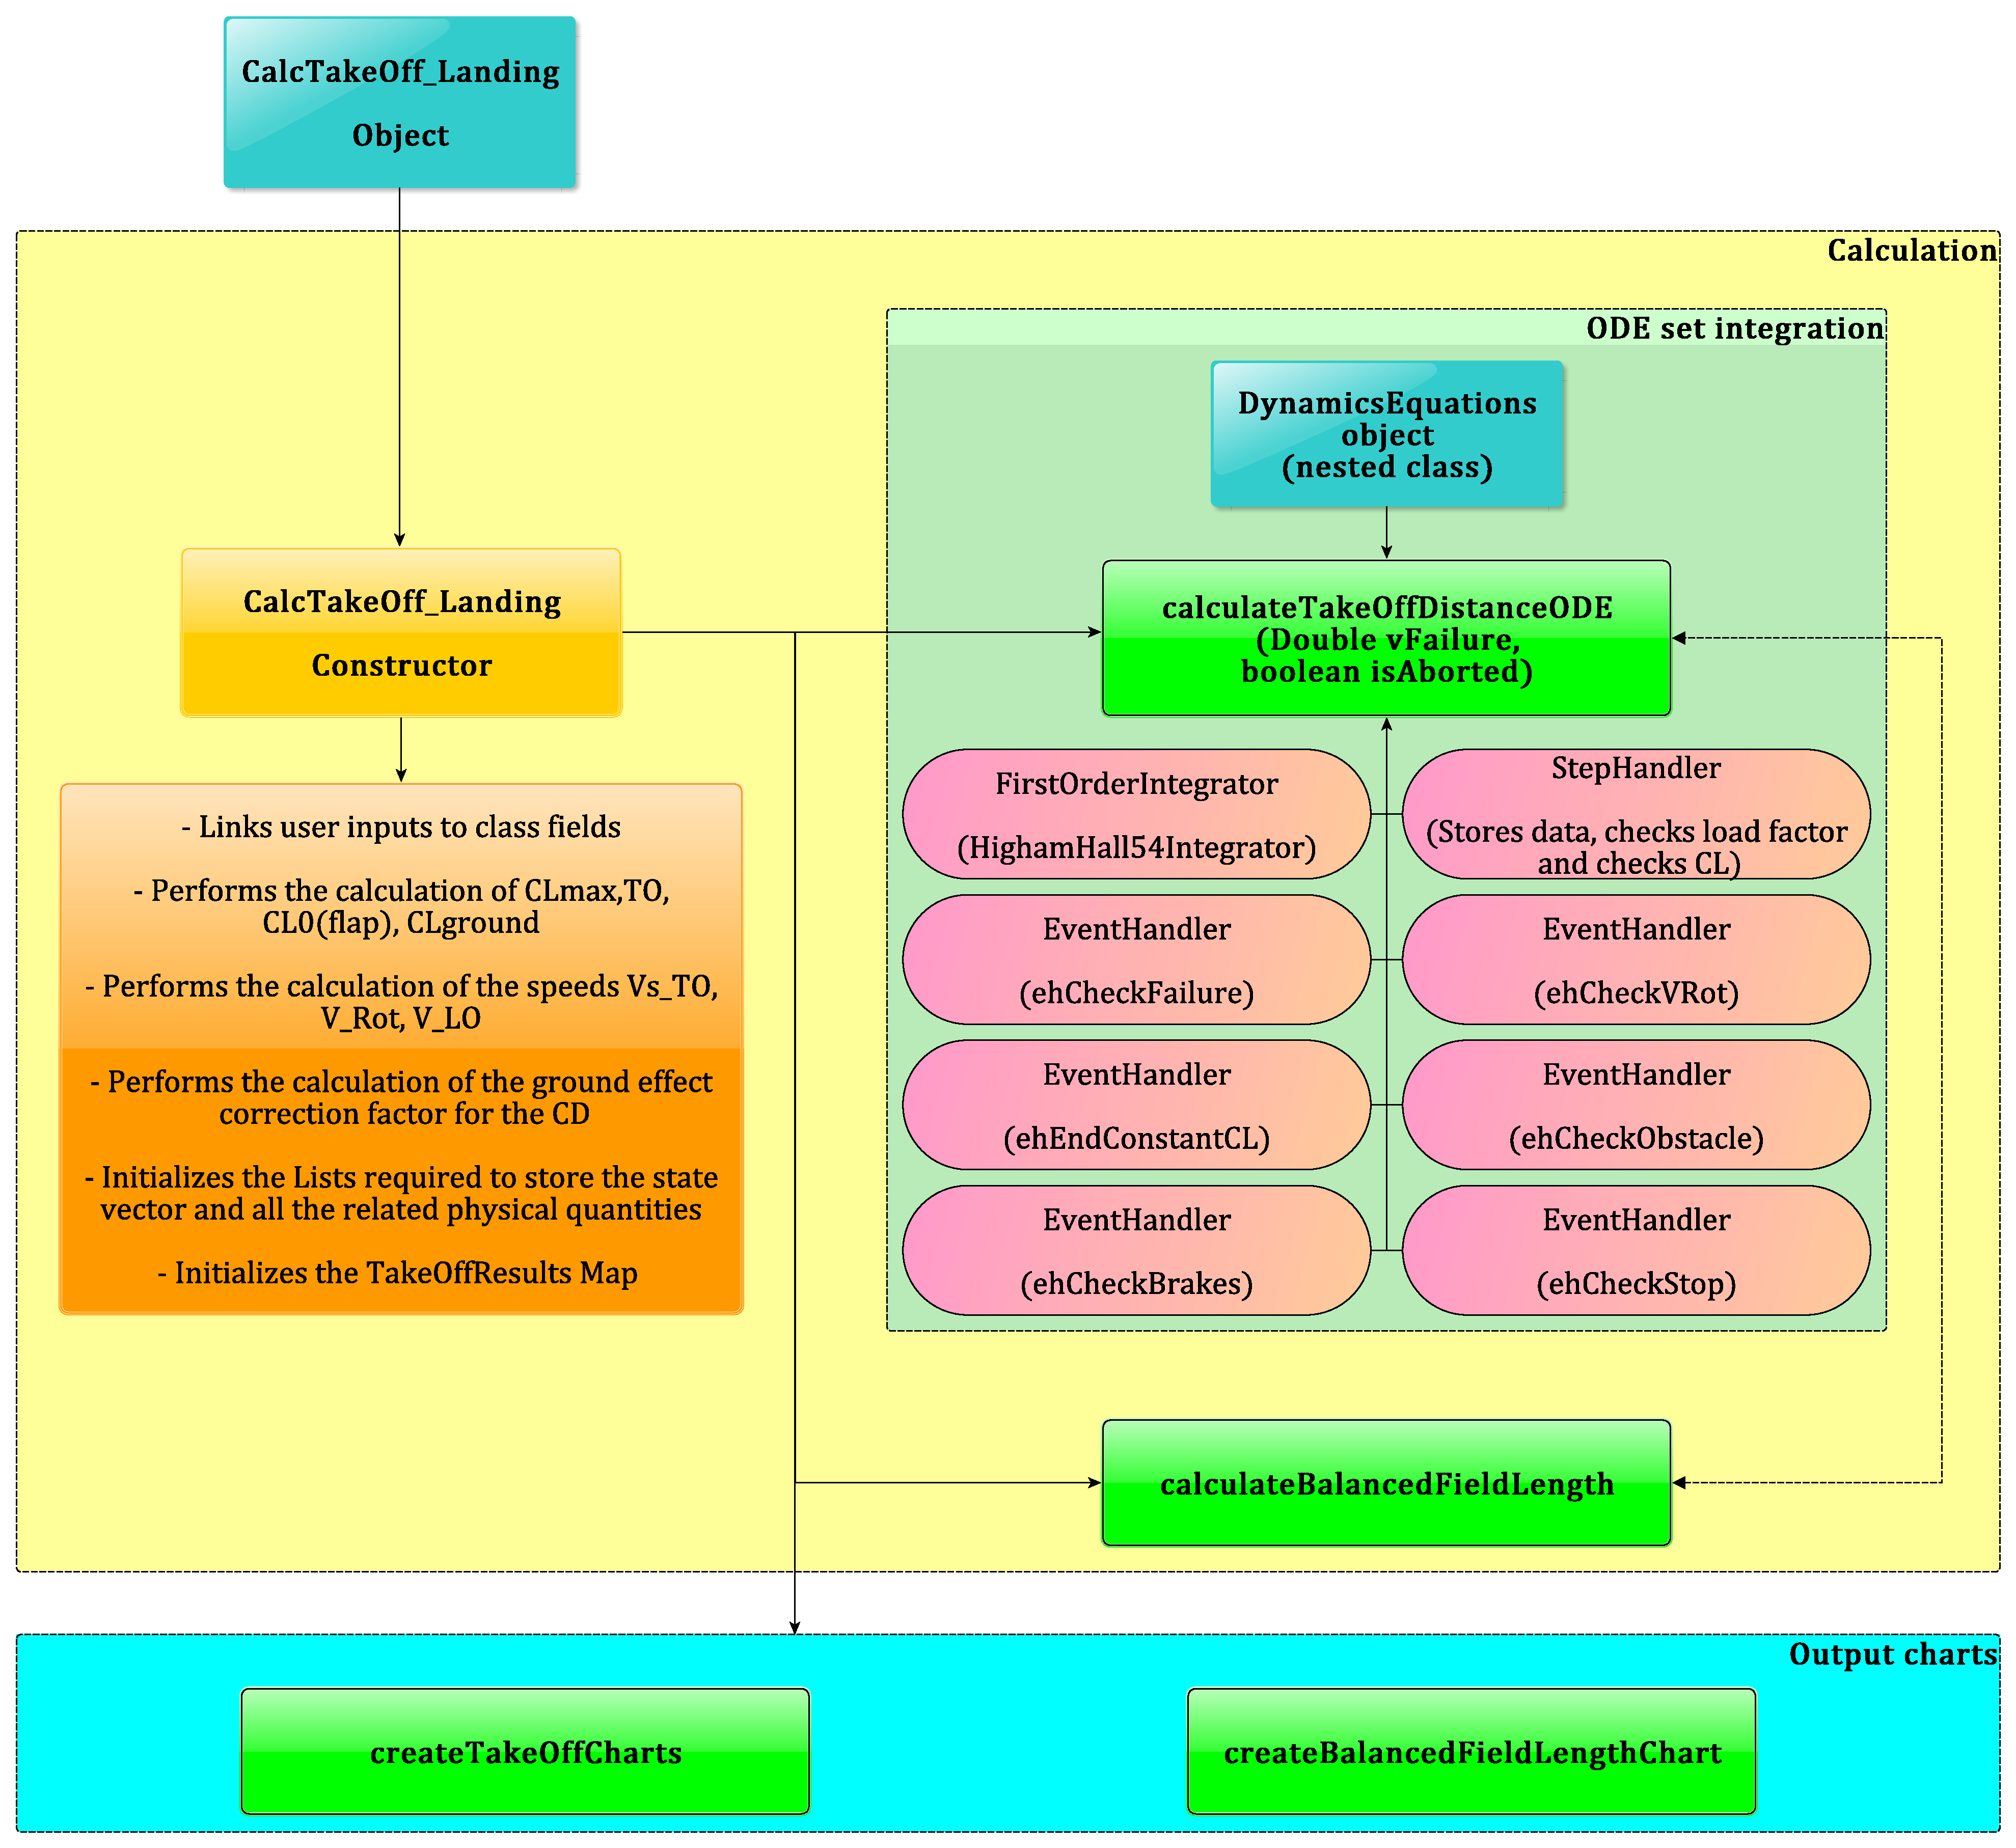
\includegraphics[keepaspectratio, width=\textwidth]{TakeOff_Flowchart}
\caption{\lstinline[language=Java]!CalcTakeOff_Landing! class flowchart}
\label{fig:CalcTakeOffFlowchart}
\end{figure}
%
%----------------------- CASE STUDY : ATR72 AND B747 -------------------------
\section{Case study: ATR-72}
This conclusive paragraph has the aim of describing the Java class created to test the features implemented into \lstinline[language=Java]!CalcTakeOff_Landing! class; in particular a description of how to build the class will be provided in order to help a potential \gls{User:Developer} as well as the presentation and the comment of the most important charts created with the purpose of validating the results obtained. 
%
Since the calculations are the same both for the B747-100B, both for the ATR-72, only the latter will be analyzed. 

\noindent
The first thing to do is to build the aircraft parametric model, and its analysis object, as described in paragraph \ref{par:DefaultAircraft}; then all information regarding high-lift devices have to be provided, in the same way of paragraph \ref{par:CaseStudyHighLift}, in order to allow the constructor of \lstinline[language=Java]!CalcTakeOff_Landing! class to evaluate their effects. 
%
At this point all the preliminary steps are completed and it's possible to create the \lstinline[language=Java]!CalcTakeOff_Landing! object giving as input all data from table \ref{table:CalcTakeOffInput}.

\bigskip
\begin{lstlisting}[caption={Input data and \lstinline!CalcTakeOff_Landing! object creation }, captionpos=b, tabsize=2]
		Amount<Duration> dtRot = Amount.valueOf(3, SI.SECOND);
		Amount<Duration> dtHold = Amount.valueOf(0.5, SI.SECOND);
		double mu = 0.025;
		double muBrake = 0.3;
		double kAlphaDot = 0.06; // [1/deg]
		double kcLMax = 0.85;
		double kRot = 1.05;
		double kLO = 1.1;
		double kFailure = 1.1;
		double phi = 1.0;
		double alphaReductionRate = -3; // [deg/s]
		Amount<Length> wingToGroundDistance = Amount.valueOf(4.0, SI.METER);
		Amount<Length> obstacle = Amount.valueOf(35, NonSI.FOOT).to(SI.METER);
		Amount<Velocity> vWind = Amount.valueOf(0.0, SI.METERS_PER_SECOND);
		Amount<Angle> alphaGround = Amount.valueOf(0.0, NonSI.DEGREE_ANGLE);
		Amount<Angle> iw = Amount.valueOf(2.0, NonSI.DEGREE_ANGLE);
//		PARAMETERS USED TO CONSIDER THE PARABOLIC DRAG POLAR CORRECTION AT HIGH CL
		double k1 = 0.0;
		double k2 = 0.0;
	
		CalcTakeOff_Landing theTakeOffLandingCalculator = new CalcTakeOff_Landing(
				aircraft,
				theCondition,
				highLiftCalculator,
				dtRot,
				dtHold,
				kcLMax,
				kRot,
				kLO,
				kFailure,
				k1,
				k2,
				phi,
				kAlphaDot,
				alphaReductionRate,
				mu,
				muBrake,
				wingToGroundDistance,
				obstacle,
				vWind,
				alphaGround,
				iw
				);
\end{lstlisting}
%
Now if the user wants to perform a single calculation of the take-off distance, he can call the method \lstinline[language=Java]!calculateTakeOffDistanceODE!, specifing the condition he wants to analyze. The possible situations are resumed below, where \lstinline[language=Java]!vFailure! is an assigned \lstinline[language=Java]!Double! value.

\bigskip
\begin{lstlisting}[caption={Possible scenarios of calculation of the take-off distance}, captionpos=b, tabsize=2, label={lst:TakeOffScenarios}]
// AOE condition
theTakeOffLandingCalculator.calculateTakeOffDistanceODE(null, false); 
// OEI continued take-off
theTakeOffLandingCalculator.calculateTakeOffDistanceODE(vFailure, false); 
// OEI aborted take-off
theTakeOffLandingCalculator.calculateTakeOffDistanceODE(vFailure, true); 
\end{lstlisting}
%
Since this method provides only calculations, the user may want to generate charts regarding the evolution of the state vector and of the related physical quantities during the take-off run; in this case all it has to be done is call the method \lstinline[language=Java]!createTakeOffCharts! as shown below.

\bigskip
\begin{lstlisting}[caption={Take-off charts creation}, captionpos=b, tabsize=2]
// Generates all the output charts
theTakeOffLandingCalculator.createTakeOffCharts();
\end{lstlisting}
%
Following the flowchart of figure \ref{fig:CalcTakeOffFlowchart}, if the user wants, instead, to calculate the \emph{balanced field length}, and plot its chart, it's still very easy; in fact he has only to call the two methods \lstinline[language=Java]!calculateBalancedFieldLength! and \lstinline[language=Java]!createBalancedFieldLengthChart!.

\bigskip
\begin{lstlisting}[caption={Balanced field length calculation and plot}, captionpos=b, tabsize=2]
// Calculation of the balanced field length
theTakeOffLandingCalculator.calculateBalancedFieldLength();
// Plot of the balanced field length chart
theTakeOffLandingCalculator.createBalancedFieldLengthChart();
\end{lstlisting}
%
The following pages shows a summary of charts created in the three condition of listing \ref{lst:TakeOffScenarios} choosing a \lstinline[language=Java]!vFailure! of 30 $\si{\meter\per\second}$. Instead, in the listing below, are resumed the main result of the \gls{acr:AOE} condition together with the results of the \emph{balanced field length} calculation.

\bigskip
\begin{lstlisting}[caption={ATR-72 test results}, captionpos=b, tabsize=2]
-----------------------------------------------------------------
CLmaxTO = 2.0212498531249747
VsTO = 54.7262494000153 m/s
VRot = 57.4625618700161 m/s
vLO = 60.1988743400169 m/s
CL0 = 1.0741952614143324
CLground = 1.2573301946144486
-----------------------------------------------------------------
		END OF GROUND ROLL PHASE
	switching function changes sign at t = 25.798463352896295 s
	x[0] = s = 805.6857140622815 m
	x[1] = V = 57.4625618700161 m/s
	x[2] = gamma = 0.0 deg
	x[3] = altitude = 0.0 m
	COLLECTING DATA AT THE END OF GROUND ROLL PHASE ...
---------------------------DONE!-------------------------------
		END OF ROTATION PHASE
	x[0] = s = 969.8307390403536 m
	x[1] = V = 61.80076798783429 m/s
	x[2] = gamma = 0.0 deg
	x[3] = altitude = 0.0 m
	t = 28.550529077966075 s
	COLLECTING DATA AT THE END OF ROTATION PHASE ...
---------------------------DONE!-------------------------------
		BEGIN BAR HOLDING
	CL = 1.718569601482539
	Alpha Body = 5.037672106777929 deg
	t = 29.788098164419022 s
---------------------------DONE!-------------------------------
		END BAR HOLDING
	switching function changes sign at t = 30.28809816441902 s 
---------------------------DONE!-------------------------------
		LOAD FACTOR = 1 IN CLIMB
	t = 31.38918339811157 s
---------------------------DONE!-------------------------------
		END OF AIRBORNE PHASE
	switching function changes sign at t = 33.374058565110616 s
	x[0] = s = 1281.9765437949968 m
	x[1] = V = 67.04253409907443 m/s
	x[2] = gamma = 2.8305305752769097 deg
	x[3] = altitude = 10.668000000000013 m
	COLLECTING DATA AT THE END OF AIRBORNE PHASE ...
---------------------------DONE!-------------------------------
BALANCED FIELD LENGTH = 1844.57965640814 m
Decision Speed (V1/VsTO) = 1.04020737941333 
---------------------------END!!-------------------------------
\end{lstlisting}
%
As can be seen the take-off distance required in \gls{acr:AOE} condition is about $\SI{1282}{\meter}$, at the maximum take-off weight of $\SI{23063.579}{\kilogram}$, within a time of about $\SI{33.4}{\second}$; while the \emph{balanced field lenght} is bigger than the AOE take-off distance of about the 30\%.  Moreover the \emph{decision speed} $V_1$ is bigger than the stalling speed $V_s$ and lower than the rotation speed $V_{\text{Rot}}$ as required by the \gls{FAR}-25 from table \ref{tab:Take:Off:Speeds:FAR25}.
%
These results are almost the same shown in the aircraft brochure available on the Internet, so that the calculation carried out results correct.
%%
%\clearpage
%%
%\begin{figure}[H]
%\centering
%%TakeOff_Trajectory
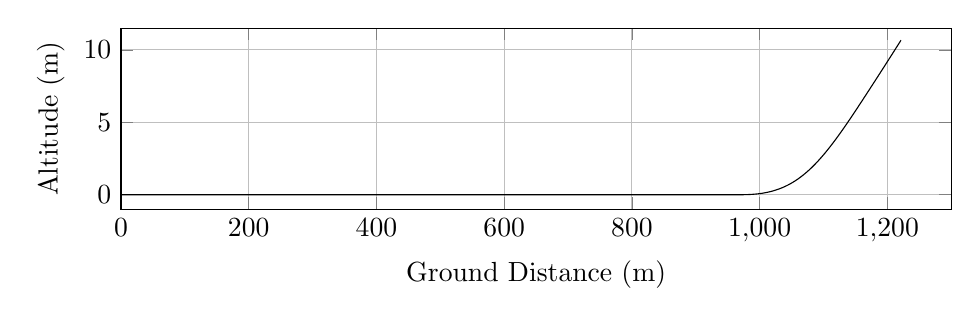
\begin{tikzpicture}

\begin{axis}[
width=\textwidth,
height=0.32\textwidth,
scaled ticks=false, tick label style={/pgf/number format/fixed},
xmin=0.0,
xmax=1300,
xlabel={Ground Distance (m)},
xmajorgrids,
ymin=-1.0,
ymax=11.5,
ylabel={Altitude (m)},
ymajorgrids,
legend style={at={(1.03,0.5)},anchor=west,draw=black,fill=white,legend cell align=left}
]

\addplot [
color=black,
solid
]
table[row sep=crcr]{
1.3729668748937997E-8	0.0\\
2.6049868369719035E-7	0.0\\
2.0491224421327626E-6	0.0\\
9.92442121137073E-6	0.0\\
4.7452367809869807E-5	0.0\\
1.740064756114434E-4	0.0\\
4.0608377013922605E-4	0.0\\
7.313431501337001E-4	0.0\\
0.0011549487327126044	0.0\\
0.0016799013484208249	0.0\\
0.002295089346817705	0.0\\
0.003009933382444524	0.0\\
0.003810608015426248	0.0\\
0.004723484476856681	0.0\\
0.005727138856912631	0.0\\
0.006836216967948795	0.0\\
0.007997302399386296	0.0\\
0.00929136979810952	0.0\\
0.010685558505459776	0.0\\
0.012178513621519987	0.0\\
0.013775244426719659	0.0\\
0.015470070176169002	0.0\\
0.0172374436815836	0.0\\
0.019122918912604377	0.0\\
0.021104911040230538	0.0\\
0.023190717999955576	0.0\\
0.025355802981115103	0.0\\
0.027620619195902148	0.0\\
0.030020274690474198	0.0\\
0.032476028269866286	0.0\\
0.035054163466719815	0.0\\
0.037720846868992755	0.0\\
0.04049779674511381	0.0\\
0.043329456594087365	0.0\\
0.04629652060163805	0.0\\
0.04934498934704602	0.0\\
0.052507657924119336	0.0\\
0.055769483710642484	0.0\\
0.05917209570914676	0.0\\
0.06264043916012321	0.0\\
0.06620063977265622	0.0\\
0.06987962792775945	0.0\\
0.0736568184539585	0.0\\
0.07754284280095361	0.0\\
0.08151127871105612	0.0\\
0.08560324933017655	0.0\\
0.08985265585263943	0.0\\
0.09413961367176535	0.0\\
0.09857725310864562	0.0\\
0.10307959255469257	0.0\\
0.10766008648593872	0.0\\
0.11234920964493048	0.0\\
0.11719267720457946	0.0\\
0.12216973960582883	0.0\\
0.12724007601918352	0.0\\
0.13233299746505212	0.0\\
0.13755256756750583	0.0\\
0.14287728588926696	0.0\\
0.1482946925752714	0.0\\
0.15381585025670613	0.0\\
0.15940564092189102	0.0\\
0.16526271495916878	0.0\\
0.17120082448158402	0.0\\
0.17717889132867753	0.0\\
0.18324322596131126	0.0\\
0.189427022360885	0.0\\
0.1957511558722988	0.0\\
0.2021484013779125	0.0\\
0.20865863707071397	0.0\\
0.21548666343168166	0.0\\
0.22220154781289658	0.0\\
0.22919671627301902	0.0\\
0.23611678795738544	0.0\\
0.24306300975244904	0.0\\
0.2503085190632165	0.0\\
0.2576623280401219	0.0\\
0.26502430524173204	0.0\\
0.2724963584449146	0.0\\
0.2802001060647876	0.0\\
0.2878583985474956	0.0\\
0.2958320780323821	0.0\\
0.3040021452321372	0.0\\
0.31208951788619	0.0\\
0.3202851396023423	0.0\\
0.3287233234973125	0.0\\
0.3370425959884752	0.0\\
0.34575405233845447	0.0\\
0.3545073625286812	0.0\\
0.36338982075299686	0.0\\
0.37247557159370037	0.0\\
0.38151350442869847	0.0\\
0.3905554764834429	0.0\\
0.3999457587520332	0.0\\
0.4095398754587949	0.0\\
0.4189621792151833	0.0\\
0.4285208811402964	0.0\\
0.43828968955472236	0.0\\
0.44807735398784176	0.0\\
0.45806002753764463	0.0\\
0.4682994371692033	0.0\\
0.4787752542918833	0.0\\
0.4890770094685154	0.0\\
0.49985939134273727	0.0\\
0.5106597490205704	0.0\\
0.5213580865152188	0.0\\
0.532247733242454	0.0\\
0.5431365108549349	0.0\\
0.554075964429489	0.0\\
0.5653450694020941	0.0\\
0.5769901159382542	0.0\\
0.588512657344902	0.0\\
0.6004070039036553	0.0\\
0.6121651247369502	0.0\\
0.6239717914322569	0.0\\
0.6362472885961421	0.0\\
0.6486428939173223	0.0\\
0.6610190736373547	0.0\\
0.6737248046101814	0.0\\
0.6862826225989949	0.0\\
0.6991952542603428	0.0\\
0.7122988072688032	0.0\\
0.7251463703465595	0.0\\
0.7381769453061875	0.0\\
0.7516618647379176	0.0\\
0.7654913705221527	0.0\\
0.7791756406994825	0.0\\
0.7930637813125616	0.0\\
0.8074774191984457	0.0\\
0.8215072375247947	0.0\\
0.8361010597475598	0.0\\
0.8503303420601955	0.0\\
0.8650627501899835	0.0\\
0.8802332960144008	0.0\\
0.8951742046771463	0.0\\
0.9100334756324657	0.0\\
0.9251067343345352	0.0\\
0.9403923630470314	0.0\\
0.9559303815501943	0.0\\
0.9712400158034169	0.0\\
0.9869533781138684	0.0\\
1.0029148609762486	0.0\\
1.0189962473881624	0.0\\
1.035465185745812	0.0\\
1.0516742337458713	0.0\\
1.067815735429615	0.0\\
1.0846705971808022	0.0\\
1.1012775250051634	0.0\\
1.1180798406225687	0.0\\
1.1351395900544134	0.0\\
1.1526388687279154	0.0\\
1.1698922447507556	0.0\\
1.1875468452119025	0.0\\
1.2058383275300355	0.0\\
1.2239395537495579	0.0\\
1.2422020624207541	0.0\\
1.2608769472440078	0.0\\
1.2794948487006894	0.0\\
1.2979152553275424	0.0\\
1.3166445915281573	0.0\\
1.3354141707340492	0.0\\
1.3543210821322504	0.0\\
1.373689361295591	0.0\\
1.3932049885015831	0.0\\
1.4131781782225183	0.0\\
1.4330139682345777	0.0\\
1.4528243860883294	0.0\\
1.4728783400745615	0.0\\
1.4934621752870565	0.0\\
1.5141408097620341	0.0\\
1.53430654450827	0.0\\
1.5553850389607948	0.0\\
1.5762653203499473	0.0\\
1.5975496774716453	0.0\\
1.6196077215345106	0.0\\
1.6413652536722467	0.0\\
1.663437310723463	0.0\\
1.6860768385032747	0.0\\
1.7077101022266827	0.0\\
1.7297306410738114	0.0\\
1.7520297891459062	0.0\\
1.7743087535215367	0.0\\
1.797257424336919	0.0\\
1.8200802473615325	0.0\\
1.8430350373473994	0.0\\
1.8666926279964304	0.0\\
1.8902808566018634	0.0\\
1.9138231309717848	0.0\\
1.937187877956735	0.0\\
1.9611060682733261	0.0\\
1.9852138445648535	0.0\\
2.009780393513653	0.0\\
2.0346228225622163	0.0\\
2.0593611988602687	0.0\\
2.08477023517836	0.0\\
2.110324766702745	0.0\\
2.1352655781940433	0.0\\
2.160528860803022	0.0\\
2.1862071157614817	0.0\\
2.2127756699400534	0.0\\
2.2391904543957084	0.0\\
2.2653528664920257	0.0\\
2.292150575495974	0.0\\
2.3187704640870406	0.0\\
2.3455495914188482	0.0\\
2.372862901366455	0.0\\
2.4007145172972395	0.0\\
2.428100404243743	0.0\\
2.4555980306928005	0.0\\
2.483374904362833	0.0\\
2.511687733451976	0.0\\
2.5402569276484597	0.0\\
2.568415369317849	0.0\\
2.596987652715761	0.0\\
2.6263861238451423	0.0\\
2.655991481965028	0.0\\
2.6856115886357443	0.0\\
2.7154221146045012	0.0\\
2.7455665152057707	0.0\\
2.7752624694325894	0.0\\
2.805457625653509	0.0\\
2.8358231840904597	0.0\\
2.8663460878589797	0.0\\
2.897817297850832	0.0\\
2.9287074004595235	0.0\\
2.9603588456990284	0.0\\
2.9922321403815406	0.0\\
3.0241119471841866	0.0\\
3.056446055158509	0.0\\
3.0889346922121366	0.0\\
3.122221620829695	0.0\\
3.1546991615623394	0.0\\
3.187635101478671	0.0\\
3.221010117202278	0.0\\
3.2543449374576605	0.0\\
3.288235920596943	0.0\\
3.3223704322934555	0.0\\
3.3562838593334394	0.0\\
3.3906320903803255	0.0\\
3.425633159699527	0.0\\
3.462387235801926	0.0\\
3.4973980805087237	0.0\\
3.5324804241140235	0.0\\
3.5675385073174235	0.0\\
3.6040688981843845	0.0\\
3.6393612181513753	0.0\\
3.6770856360342323	0.0\\
3.7131729334920323	0.0\\
3.749509707933214	0.0\\
3.785733977879824	0.0\\
3.8225309786916544	0.0\\
3.860867115351552	0.0\\
3.89929745075254	0.0\\
3.9373367205567504	0.0\\
3.9751626485832894	0.0\\
4.013671158053867	0.0\\
4.0521140617426425	0.0\\
4.092377631210638	0.0\\
4.131586743753305	0.0\\
4.1715696979561425	0.0\\
4.210522654700574	0.0\\
4.250196810863292	0.0\\
4.2917015001093795	0.0\\
4.332438976653355	0.0\\
4.373124372895289	0.0\\
4.414429464889761	0.0\\
4.455884944705147	0.0\\
4.497250153511752	0.0\\
4.537976875075978	0.0\\
4.581399817640802	0.0\\
4.623816269683994	0.0\\
4.666022338967499	0.0\\
4.709098934189642	0.0\\
4.752435367147649	0.0\\
4.79531009100786	0.0\\
4.838191999420829	0.0\\
4.881381760681686	0.0\\
4.9256451804034285	0.0\\
4.9704217340957495	0.0\\
5.014356093293278	0.0\\
5.058826350846283	0.0\\
5.104458009943745	0.0\\
5.149663211268795	0.0\\
5.194981168813841	0.0\\
5.241194091283663	0.0\\
5.287987552078626	0.0\\
5.334426822383641	0.0\\
5.380633359096258	0.0\\
5.427524438012913	0.0\\
5.476157635197664	0.0\\
5.524667120325573	0.0\\
5.5732739519824435	0.0\\
5.6208990292882195	0.0\\
5.671502816366864	0.0\\
5.719824083529298	0.0\\
5.767871110439133	0.0\\
5.8169321963676754	0.0\\
5.866076914057565	0.0\\
5.917200682776528	0.0\\
5.96684810088939	0.0\\
6.016885842403935	0.0\\
6.068639931677712	0.0\\
6.119867755785197	0.0\\
6.171030794930029	0.0\\
6.222884713227881	0.0\\
6.2735946138732235	0.0\\
6.325883502103322	0.0\\
6.379615386553551	0.0\\
6.432194972482147	0.0\\
6.484528316464761	0.0\\
6.536619297696934	0.0\\
6.589662958081361	0.0\\
6.644121795496577	0.0\\
6.697445536614451	0.0\\
6.7518063163896365	0.0\\
6.8068829439682315	0.0\\
6.863205650636274	0.0\\
6.9185329265047315	0.0\\
6.974634519184049	0.0\\
7.031139830722298	0.0\\
7.0870923879294985	0.0\\
7.144766952910487	0.0\\
7.2026451873548805	0.0\\
7.261191729679483	0.0\\
7.320502240843062	0.0\\
7.378210233177999	0.0\\
7.437738452534925	0.0\\
7.49714639104333	0.0\\
7.556502460410064	0.0\\
7.617032771987237	0.0\\
7.676883327249088	0.0\\
7.735740247984193	0.0\\
7.796086087039788	0.0\\
7.856787102853412	0.0\\
7.91721236259451	0.0\\
7.979013602666894	0.0\\
8.039824025454376	0.0\\
8.102419182184594	0.0\\
8.16459313580776	0.0\\
8.226347093952135	0.0\\
8.290527749984296	0.0\\
8.353592793320257	0.0\\
8.417564177281012	0.0\\
8.482044607535009	0.0\\
8.547336806956285	0.0\\
8.613293246319614	0.0\\
8.6778048537894	0.0\\
8.74454839911753	0.0\\
8.810708373588199	0.0\\
8.876548424968423	0.0\\
8.942828456712885	0.0\\
9.010858044488913	0.0\\
9.079453414959548	0.0\\
9.148767802603732	0.0\\
9.21609997183467	0.0\\
9.285579683381485	0.0\\
9.355451712480097	0.0\\
9.423585014597279	0.0\\
9.493435356703696	0.0\\
9.562655940911181	0.0\\
9.63183713653898	0.0\\
9.703018708836247	0.0\\
9.773178624863132	0.0\\
9.844376937811855	0.0\\
9.914998792594716	0.0\\
9.98720270419701	0.0\\
10.059478150570087	0.0\\
10.132362020358627	0.0\\
10.205876892438312	0.0\\
10.279422251887688	0.0\\
10.353305644514993	0.0\\
10.42811398108589	0.0\\
10.50332954727428	0.0\\
10.578207710262959	0.0\\
10.65503529959097	0.0\\
10.730232142651953	0.0\\
10.805871937852555	0.0\\
10.88265320376452	0.0\\
10.958577899345514	0.0\\
11.034861147941964	0.0\\
11.112742623646977	0.0\\
11.190543636431041	0.0\\
11.267787598939979	0.0\\
11.3462805052093	0.0\\
11.423875697147409	0.0\\
11.502735831556972	0.0\\
11.581465323066688	0.0\\
11.661639233340708	0.0\\
11.741743247575428	0.0\\
11.821864700430528	0.0\\
11.901816327719768	0.0\\
11.98361062800689	0.0\\
12.065425957085825	0.0\\
12.1478520915771	0.0\\
12.230956215923495	0.0\\
12.313306905825911	0.0\\
12.396632357805931	0.0\\
12.479578787946746	0.0\\
12.564327762802186	0.0\\
12.648175874147956	0.0\\
12.736145481689512	0.0\\
12.821080154398764	0.0\\
12.908009536077355	0.0\\
12.994986774303499	0.0\\
13.081752199798046	0.0\\
13.17035388279784	0.0\\
13.257836697901475	0.0\\
13.34511613365563	0.0\\
13.433461823066896	0.0\\
13.524108483575919	0.0\\
13.611203924103116	0.0\\
13.702229394080796	0.0\\
13.792427706753081	0.0\\
13.882429934062493	0.0\\
13.975435778888343	0.0\\
14.065832730112316	0.0\\
14.157894546480026	0.0\\
14.250668806951023	0.0\\
14.343291987615704	0.0\\
14.43744444968501	0.0\\
14.532636396723657	0.0\\
14.625507232812737	0.0\\
14.721503924398366	0.0\\
14.818738382089133	0.0\\
14.913572076739943	0.0\\
15.009701633366973	0.0\\
15.10815424447124	0.0\\
15.206130868840724	0.0\\
15.304035939715973	0.0\\
15.403499839366233	0.0\\
15.503209871950865	0.0\\
15.601718454553605	0.0\\
15.700655560608023	0.0\\
15.801250929860519	0.0\\
15.899917805652187	0.0\\
16.001574124100856	0.0\\
16.102638779863817	0.0\\
16.204479333764816	0.0\\
16.30489644092564	0.0\\
16.40578186591999	0.0\\
16.509201471948074	0.0\\
16.614557195984908	0.0\\
16.717657554831042	0.0\\
16.823039336622365	0.0\\
16.928576062495388	0.0\\
17.03469945574068	0.0\\
17.140697318244236	0.0\\
17.246066414787876	0.0\\
17.35183930840021	0.0\\
17.458399953804133	0.0\\
17.565707112453843	0.0\\
17.673103795073075	0.0\\
17.781888038667653	0.0\\
17.89115167195854	0.0\\
18.00105710767307	0.0\\
18.110142905530395	0.0\\
18.219697237410173	0.0\\
18.32752951944549	0.0\\
18.43743745973078	0.0\\
18.54904630654982	0.0\\
18.659302591714813	0.0\\
18.770734536087716	0.0\\
18.883577445650936	0.0\\
18.996263390583444	0.0\\
19.108816920034535	0.0\\
19.22287647779894	0.0\\
19.33763586704334	0.0\\
19.456324114791514	0.0\\
19.57349394116079	0.0\\
19.690148252848566	0.0\\
19.80521137071168	0.0\\
19.92379170801214	0.0\\
20.04216631061405	0.0\\
20.15848954929409	0.0\\
20.278242138037896	0.0\\
20.396206084226087	0.0\\
20.516315546862906	0.0\\
20.637173924977112	0.0\\
20.75450010628387	0.0\\
20.874378237858778	0.0\\
20.996035953832852	0.0\\
21.11812959618858	0.0\\
21.240471115580952	0.0\\
21.361479376438375	0.0\\
21.485224699488654	0.0\\
21.607870280890317	0.0\\
21.73242999733349	0.0\\
21.85704493170313	0.0\\
21.98122016226351	0.0\\
22.10826921766411	0.0\\
22.235261614051304	0.0\\
22.361664688868032	0.0\\
22.48780138980522	0.0\\
22.614107216476143	0.0\\
22.74409311379692	0.0\\
22.873024137794893	0.0\\
23.003512644166257	0.0\\
23.132891545907036	0.0\\
23.26270690888247	0.0\\
23.39264146728729	0.0\\
23.52277721573431	0.0\\
23.654883767164463	0.0\\
23.78569183677709	0.0\\
23.917003007077597	0.0\\
24.047013652206026	0.0\\
24.178458227988493	0.0\\
24.314609552493202	0.0\\
24.447533097503474	0.0\\
24.579128452041708	0.0\\
24.71011994849615	0.0\\
24.843278471916108	0.0\\
24.975761222328053	0.0\\
25.1115496753864	0.0\\
25.247101122854083	0.0\\
25.384906965000688	0.0\\
25.522261036073317	0.0\\
25.66123001648475	0.0\\
25.79865327455613	0.0\\
25.826335196219034	0.0\\
25.839610403727477	0.0\\
25.841006316401874	0.0\\
25.84227013303559	0.0\\
25.84770509053729	0.0\\
25.86419328224909	0.0\\
25.90571916957557	0.0\\
25.999268866927544	0.0\\
26.123295978662824	0.0\\
26.250212562581652	0.0\\
26.376891976518465	0.0\\
26.50638698165423	0.0\\
26.634042370994827	0.0\\
26.763333806613538	0.0\\
26.893207366259766	0.0\\
27.022905486492228	0.0\\
27.153956322362554	0.0\\
27.287774297957696	0.0\\
27.42030033806219	0.0\\
27.555504894698295	0.0\\
27.691130018821354	0.0\\
27.82633313037239	0.0\\
27.959508564917073	0.0\\
28.096515548835796	0.0\\
28.232789703382153	0.0\\
28.368684388406535	0.0\\
28.506541650227618	0.0\\
28.64533374691623	0.0\\
28.78297783415192	0.0\\
28.92277775692753	0.0\\
29.06227187463503	0.0\\
29.20212864139956	0.0\\
29.34335827861657	0.0\\
29.483225747293005	0.0\\
29.625960812476485	0.0\\
29.76706561118049	0.0\\
29.909402910999468	0.0\\
30.051751399473822	0.0\\
30.196612335666572	0.0\\
30.342192969749448	0.0\\
30.48583400527584	0.0\\
30.632658550781265	0.0\\
30.77846394498075	0.0\\
30.92408133049836	0.0\\
31.071091331299215	0.0\\
31.218274793935116	0.0\\
31.366705758252415	0.0\\
31.515339333797037	0.0\\
31.66356819769615	0.0\\
31.814689402684216	0.0\\
31.96649953392354	0.0\\
32.115424616034375	0.0\\
32.266253234088566	0.0\\
32.41813832080348	0.0\\
32.569791431087395	0.0\\
32.722234201183724	0.0\\
32.876984607664	0.0\\
33.031873994672836	0.0\\
33.18502245018544	0.0\\
33.34135780547538	0.0\\
33.49759920343199	0.0\\
33.65385117142162	0.0\\
33.8113313806527	0.0\\
33.96985264489639	0.0\\
34.126473036379195	0.0\\
34.2857505660089	0.0\\
34.4449212019973	0.0\\
34.60566879064274	0.0\\
34.76644486933921	0.0\\
34.92612701881755	0.0\\
35.08630421658309	0.0\\
35.24825698849928	0.0\\
35.412303951281956	0.0\\
35.57355277914179	0.0\\
35.73545353069308	0.0\\
35.89925038949356	0.0\\
36.065161289279985	0.0\\
36.23047312008262	0.0\\
36.39472205714358	0.0\\
36.56135389445764	0.0\\
36.72774532558607	0.0\\
36.89384825683493	0.0\\
37.05904296416534	0.0\\
37.22702676294645	0.0\\
37.39437475321985	0.0\\
37.5621109943643	0.0\\
37.73270471709142	0.0\\
37.903359519601935	0.0\\
38.071486842086316	0.0\\
38.23815243703595	0.0\\
38.40817787072022	0.0\\
38.57751392140098	0.0\\
38.750215798728505	0.0\\
38.92001182640311	0.0\\
39.09310637700479	0.0\\
39.26472366117933	0.0\\
39.436554723976656	0.0\\
39.608961777617054	0.0\\
39.782828308010565	0.0\\
39.956194359016465	0.0\\
40.132391837044906	0.0\\
40.30868053167249	0.0\\
40.48611580488176	0.0\\
40.66383502946924	0.0\\
40.83999042132467	0.0\\
41.018202681018664	0.0\\
41.19780999006247	0.0\\
41.37730467548502	0.0\\
41.557010452813884	0.0\\
41.73612816026986	0.0\\
41.91555194917056	0.0\\
42.09743589423803	0.0\\
42.27807550146298	0.0\\
42.45995188234755	0.0\\
42.6401410478328	0.0\\
42.822293873795985	0.0\\
43.00585672428667	0.0\\
43.189965171449515	0.0\\
43.372020236704074	0.0\\
43.555636897252796	0.0\\
43.74012033961118	0.0\\
43.92429822300048	0.0\\
44.106869824379004	0.0\\
44.29411840239129	0.0\\
44.47920670866131	0.0\\
44.665034305215386	0.0\\
44.85242224248053	0.0\\
45.03948098831597	0.0\\
45.22811764277584	0.0\\
45.41548629589063	0.0\\
45.60322541388645	0.0\\
45.793007222766036	0.0\\
45.983742663331824	0.0\\
46.172643153142886	0.0\\
46.36421599110457	0.0\\
46.553512793459404	0.0\\
46.745018895697555	0.0\\
46.93606459490553	0.0\\
47.126948089509526	0.0\\
47.31881294044018	0.0\\
47.5110690178297	0.0\\
47.705448624448266	0.0\\
47.90005519882567	0.0\\
48.09288923506665	0.0\\
48.28732881729917	0.0\\
48.484002572746206	0.0\\
48.68089030454945	0.0\\
48.87532723390382	0.0\\
49.07073736177763	0.0\\
49.2672083392297	0.0\\
49.46586249263092	0.0\\
49.661880987188695	0.0\\
49.85966148345089	0.0\\
50.05808618672894	0.0\\
50.25785665917266	0.0\\
50.45743808511885	0.0\\
50.65573800086891	0.0\\
50.85948768734909	0.0\\
51.061243703011925	0.0\\
51.26368286286315	0.0\\
51.46416466063809	0.0\\
51.66475943174029	0.0\\
51.86588207153103	0.0\\
52.07444928962187	0.0\\
52.2824430085781	0.0\\
52.48676525705545	0.0\\
52.69531994892206	0.0\\
52.90027076850366	0.0\\
53.108186167814935	0.0\\
53.31165724918766	0.0\\
53.520024946679996	0.0\\
53.72688450142306	0.0\\
53.93707391647578	0.0\\
54.14518573319289	0.0\\
54.35125853722778	0.0\\
54.56213447502874	0.0\\
54.77598621923464	0.0\\
54.987629956235494	0.0\\
55.19778857845695	0.0\\
55.41030974885841	0.0\\
55.62390503323701	0.0\\
55.83671574169797	0.0\\
56.047071254351536	0.0\\
56.26137331252919	0.0\\
56.47512769358855	0.0\\
56.69105800830218	0.0\\
56.90937011004422	0.0\\
57.12736617899088	0.0\\
57.346833156368504	0.0\\
57.56476609337061	0.0\\
57.78230894703917	0.0\\
57.99943865551505	0.0\\
58.21827465292657	0.0\\
58.436085045729726	0.0\\
58.6577546799423	0.0\\
58.87982836766625	0.0\\
59.10336118170943	0.0\\
59.324182403931715	0.0\\
59.545440661451366	0.0\\
59.768227251413464	0.0\\
59.99077485409802	0.0\\
60.21631063559073	0.0\\
60.44006004384342	0.0\\
60.66502706168687	0.0\\
60.89133011288284	0.0\\
61.11585558357916	0.0\\
61.3432655409558	0.0\\
61.57186440401435	0.0\\
61.79868765088207	0.0\\
62.025670725987	0.0\\
62.254132946411545	0.0\\
62.48290793247415	0.0\\
62.713817944074236	0.0\\
62.94484116346062	0.0\\
63.17805109236767	0.0\\
63.41124119062552	0.0\\
63.64505576847972	0.0\\
63.87735201907903	0.0\\
64.11169045660182	0.0\\
64.34725756208485	0.0\\
64.58324360279937	0.0\\
64.81881329818131	0.0\\
65.05563560606473	0.0\\
65.29467812810154	0.0\\
65.53178653633495	0.0\\
65.77046761369158	0.0\\
66.01019347650049	0.0\\
66.25262920761091	0.0\\
66.49342175078831	0.0\\
66.73393309567928	0.0\\
66.97718905970893	0.0\\
67.21919788222482	0.0\\
67.46413738735515	0.0\\
67.70584739194695	0.0\\
67.95375887035246	0.0\\
68.19817148521656	0.0\\
68.44413350233111	0.0\\
68.68984243621705	0.0\\
68.93951041285982	0.0\\
69.19023531750676	0.0\\
69.43956667494601	0.0\\
69.68998597860525	0.0\\
69.94098943220166	0.0\\
70.1928405184459	0.0\\
70.44659484061637	0.0\\
70.69926103579675	0.0\\
70.95414956377036	0.0\\
71.21136313866151	0.0\\
71.46778788208749	0.0\\
71.7247351381395	0.0\\
71.98234155897126	0.0\\
72.24107377350035	0.0\\
72.4986091150376	0.0\\
72.75949164810788	0.0\\
73.02014691132015	0.0\\
73.28114866838587	0.0\\
73.54342372888959	0.0\\
73.80584407854005	0.0\\
74.07231166191039	0.0\\
74.3389341302921	0.0\\
74.60521354141642	0.0\\
74.87280568706873	0.0\\
75.1403821105715	0.0\\
75.41145333671997	0.0\\
75.68265298797411	0.0\\
75.95075857762194	0.0\\
76.2241428819712	0.0\\
76.4990100438061	0.0\\
76.77213586328236	0.0\\
77.04724851790667	0.0\\
77.32330034006353	0.0\\
77.59850473375684	0.0\\
77.87773830129439	0.0\\
78.1565255546137	0.0\\
78.43842651648492	0.0\\
78.720833678605	0.0\\
79.00101298089581	0.0\\
79.28359351218376	0.0\\
79.57011733099088	0.0\\
79.85418914588558	0.0\\
80.13919871477489	0.0\\
80.42568449319114	0.0\\
80.71472498530085	0.0\\
81.006853148924	0.0\\
81.2951972638476	0.0\\
81.58524575795963	0.0\\
81.87461709596036	0.0\\
82.1711642895769	0.0\\
82.46716486408064	0.0\\
82.76422974563803	0.0\\
83.05801377197795	0.0\\
83.35853301954708	0.0\\
83.65664966506407	0.0\\
83.95487262936624	0.0\\
84.25322789115987	0.0\\
84.55664509033022	0.0\\
84.8599544590121	0.0\\
85.16499148084048	0.0\\
85.47187188044902	0.0\\
85.77908321853027	0.0\\
86.08675489504844	0.0\\
86.39784539041122	0.0\\
86.71051296037359	0.0\\
87.02583358957506	0.0\\
87.34037846285594	0.0\\
87.65395388450591	0.0\\
87.96687312379424	0.0\\
88.28527441497255	0.0\\
88.6103524516937	0.0\\
88.92871226770333	0.0\\
89.25003295857354	0.0\\
89.57522243846881	0.0\\
89.90247582737899	0.0\\
90.22602529632545	0.0\\
90.5494223037065	0.0\\
90.87816525326718	0.0\\
91.20455861430293	0.0\\
91.53817773235312	0.0\\
91.87076195087604	0.0\\
92.20124984301029	0.0\\
92.53140503523474	0.0\\
92.86389705561814	0.0\\
93.19815266874983	0.0\\
93.53304529783748	0.0\\
93.86737084100128	0.0\\
94.20337949361911	0.0\\
94.54065981474497	0.0\\
94.87396787418089	0.0\\
95.21684847579547	0.0\\
95.55392648231228	0.0\\
95.89232371872416	0.0\\
96.23051075783204	0.0\\
96.57164052232307	0.0\\
96.90762523479154	0.0\\
97.24755293575913	0.0\\
97.58790661409188	0.0\\
97.92576087813703	0.0\\
98.26661027452474	0.0\\
98.6051908024865	0.0\\
98.94563962387357	0.0\\
99.28665364663627	0.0\\
99.63350087797645	0.0\\
99.97685593767679	0.0\\
100.31593955776762	0.0\\
100.65572384630482	0.0\\
100.99616871909686	0.0\\
101.3402339503516	0.0\\
101.67973054404297	0.0\\
102.01657591573795	0.0\\
102.35656456518868	0.0\\
102.6941824316649	0.0\\
103.03547296258705	0.0\\
103.37623032340073	0.0\\
103.71852978299776	0.0\\
104.05851119314701	0.0\\
104.3949509202441	0.0\\
104.7329053851843	0.0\\
105.07104272194636	0.0\\
105.40742307340048	0.0\\
105.74423560014887	0.0\\
106.07955743077031	0.0\\
106.41623710643992	0.0\\
106.75618472497374	0.0\\
107.0942647435474	0.0\\
107.43151869252583	0.0\\
107.44650965670576	0.0\\
107.45815118347005	0.0\\
107.46233674961977	0.0\\
107.46535588765028	0.0\\
107.46808502617694	0.0\\
107.4836206108138	0.0\\
107.53176708907421	0.0\\
107.68672244793561	0.0\\
107.97570433527497	0.0\\
108.27744765146667	0.0\\
108.5816623935838	0.0\\
108.88557241638279	0.0\\
109.19209959959528	0.0\\
109.50241879336687	0.0\\
109.81066605766154	0.0\\
110.12101503747155	0.0\\
110.43285681965125	0.0\\
110.74725799716322	0.0\\
111.06462449033057	0.0\\
111.38211128519615	0.0\\
111.70119562731901	0.0\\
112.02298633508096	0.0\\
112.34320819983824	0.0\\
112.66812620709393	0.0\\
112.99302416686388	0.0\\
113.31966045518399	0.0\\
113.64998129974768	0.0\\
113.97857627498675	0.0\\
114.31304608469316	0.0\\
114.64448318111735	0.0\\
114.98093514978115	0.0\\
115.31969924418831	0.0\\
115.65790718621022	0.0\\
116.00063352526521	0.0\\
116.34235083463872	0.0\\
116.68621873349733	0.0\\
117.03331062078092	0.0\\
117.37910048629482	0.0\\
117.72869476105836	0.0\\
118.08005947084649	0.0\\
118.43363644355449	0.0\\
118.79186464668504	0.0\\
119.14769212941735	0.0\\
119.5036618261702	0.0\\
119.86270697471275	0.0\\
120.22616362054572	0.0\\
120.58991121293201	0.0\\
120.95538130513773	0.0\\
121.3195355377388	0.0\\
121.68590041554987	0.0\\
122.05305648207542	0.0\\
122.42257239354896	0.0\\
122.79503144936103	0.0\\
123.16629137010841	0.0\\
123.53950748252527	0.0\\
123.91239367862553	0.0\\
124.29026003316017	0.0\\
124.66301933937496	0.0\\
125.03890311735066	0.0\\
125.41380975776434	0.0\\
125.7896808967325	0.0\\
126.16837244152023	0.0\\
126.54595968852882	0.0\\
126.92471834906405	0.0\\
127.30294276405039	0.0\\
127.68255852126984	0.0\\
128.06243727540487	0.0\\
128.44360431740483	0.0\\
128.82265748788262	0.0\\
129.1989690567886	0.0\\
129.57765386613931	0.0\\
129.95508099647026	0.0\\
130.33359114840187	0.0\\
130.71373745886524	0.0\\
131.09453904397424	0.0\\
131.47657586018488	0.0\\
131.85678563989967	0.0\\
132.23856625352113	0.0\\
132.61595336405918	0.0\\
132.99976263915818	0.0\\
133.38083522978053	0.0\\
133.76098428781995	0.0\\
134.1363519425165	0.0\\
134.51557915495124	0.0\\
134.8968696170101	0.0\\
135.27419431482667	0.0\\
135.65215477207505	0.0\\
136.03329358991255	0.0\\
136.41192880753374	0.0\\
136.7898079310749	0.0\\
137.17001317148595	0.0\\
137.54844558779996	0.0\\
137.92617219433072	0.0\\
138.30476964659732	0.0\\
138.68390038934075	0.0\\
139.0631653430654	0.0\\
139.4406106933401	0.0\\
139.81914660512416	0.0\\
140.19767098864742	0.0\\
140.5730919292459	0.0\\
140.95061983253072	0.0\\
141.32838502869612	0.0\\
141.70636515873298	0.0\\
142.0839785067887	0.0\\
142.46357402350594	0.0\\
142.84082211769783	0.0\\
143.21906727224075	0.0\\
143.59963619096823	0.0\\
143.97984478872678	0.0\\
144.35941603837455	0.0\\
144.7355521893594	0.0\\
145.11296635073694	0.0\\
145.49073213867456	0.0\\
145.87033631970945	0.0\\
146.24486520181193	0.0\\
146.6238757206513	0.0\\
147.00096360401335	0.0\\
147.37874202190085	0.0\\
147.756852900845	0.0\\
148.13572640408995	0.0\\
148.5136798644104	0.0\\
148.89083780486442	0.0\\
149.2712459042852	0.0\\
149.65303236723025	0.0\\
150.0329584616291	0.0\\
150.41363382646614	0.0\\
150.79322940570728	0.0\\
151.17272478467066	0.0\\
151.55400296227282	0.0\\
151.93482601265913	0.0\\
152.31881414221942	0.0\\
152.70208150063132	0.0\\
153.08320649997165	0.0\\
153.4666285558243	0.0\\
153.84825937276264	0.0\\
154.23093781718723	0.0\\
154.61485031834388	0.0\\
155.00001234931443	0.0\\
155.38285725409855	0.0\\
155.7679513537659	0.0\\
156.1509667875323	0.0\\
156.53491934392343	0.0\\
156.91995289130983	0.0\\
157.30625057946366	0.0\\
157.69121706207227	0.0\\
158.07789765133754	0.0\\
158.46521012398495	0.0\\
158.85138765236047	0.0\\
159.23964669847322	0.0\\
159.62715395386465	0.0\\
160.01960115328984	0.0\\
160.4079207075476	0.0\\
160.79602490671402	0.0\\
161.18437278725975	0.0\\
161.57644284003254	0.0\\
161.96812230097612	0.0\\
162.35808768568592	0.0\\
162.75087300343483	0.0\\
163.14546270495134	0.0\\
163.53745675514648	0.0\\
163.92955389373896	0.0\\
164.32395276810763	0.0\\
164.71713266653478	0.0\\
165.1102153740033	0.0\\
165.5035884424101	0.0\\
165.89816400198282	0.0\\
166.29148626774366	0.0\\
166.68861804276264	0.0\\
167.082852347146	0.0\\
167.48006204110857	0.0\\
167.8798182678497	0.0\\
168.27774435731556	0.0\\
168.67741362640317	0.0\\
169.07475368467374	0.0\\
169.4759958044982	0.0\\
169.87832784425882	0.0\\
170.2792240364854	0.0\\
170.68126852540456	0.0\\
171.08617821288442	0.0\\
171.48766933901368	0.0\\
171.892744970828	0.0\\
172.29711201372032	0.0\\
172.70264003426053	0.0\\
173.1105289448074	0.0\\
173.5163733808056	0.0\\
173.92577914808027	0.0\\
174.33607303977334	0.0\\
174.74614233406845	0.0\\
175.15731444736514	0.0\\
175.56901623635082	0.0\\
175.97955109701695	0.0\\
176.39275298155184	0.0\\
176.80397138375372	0.0\\
177.21946344336607	0.0\\
177.6332252263685	0.0\\
178.05102033212842	0.0\\
178.46725124888752	0.0\\
178.88389799206544	0.0\\
179.29839533747668	0.0\\
179.71608569665375	0.0\\
180.1342696339205	0.0\\
180.5538779958007	0.0\\
180.97690569555635	0.0\\
181.39980810354632	0.0\\
181.82328311928882	0.0\\
182.24618807605736	0.0\\
182.6731660166833	0.0\\
183.10035828358116	0.0\\
183.5291445538124	0.0\\
183.95833265232255	0.0\\
184.38634616388282	0.0\\
184.8168339376561	0.0\\
185.24630581702252	0.0\\
185.67754767955432	0.0\\
186.109185775987	0.0\\
186.53971883241212	0.0\\
186.97132952004227	0.0\\
187.40711553434954	0.0\\
187.84220985117162	0.0\\
188.27778926256264	0.0\\
188.71822733349944	0.0\\
189.16086434237673	0.0\\
189.6010380968554	0.0\\
190.03919041211265	0.0\\
190.48016062316526	0.0\\
190.92524363955386	0.0\\
191.372330984798	0.0\\
191.81766281185656	0.0\\
192.2649588892154	0.0\\
192.7152080571317	0.0\\
193.16529614382966	0.0\\
193.61551258619323	0.0\\
194.0671041699889	0.0\\
194.52074606224477	0.0\\
194.9783774267325	0.0\\
195.4358245305881	0.0\\
195.89499401276925	0.0\\
196.35432087192027	0.0\\
196.81831699949333	0.0\\
197.28093205423113	0.0\\
197.74513845889334	0.0\\
198.21238653581378	0.0\\
198.6780372695403	0.0\\
199.14562244096538	0.0\\
199.6172630308758	0.0\\
200.085680559985	0.0\\
200.55485539631252	0.0\\
201.0284003638297	0.0\\
201.5010163224531	0.0\\
201.97949934275624	0.0\\
202.45676989461947	0.0\\
202.93795341995116	0.0\\
203.42151825635358	0.0\\
203.9064451985618	0.0\\
204.39376498892221	0.0\\
204.88144002832018	0.0\\
205.3743097859811	0.0\\
205.86751126322014	0.0\\
206.36222180198536	0.0\\
206.85620764580733	0.0\\
207.35622660722595	0.0\\
207.85286701515986	0.0\\
208.35554496397685	0.0\\
208.85949164962352	0.0\\
209.3606904933826	0.0\\
209.86430174661194	0.0\\
210.37517113261447	0.0\\
210.88826309775862	0.0\\
211.408532759536	0.0\\
211.9275242572583	0.0\\
212.45034341379437	0.0\\
212.97278109853062	0.0\\
213.5012611434281	0.0\\
214.0307698600809	0.0\\
214.55632530210835	0.0\\
215.09027271075985	0.0\\
215.62992362610385	0.0\\
216.17218538865313	0.0\\
216.71273903148006	0.0\\
217.25354139798316	0.0\\
217.7992146693805	0.0\\
218.34754045136725	0.0\\
218.89661223248612	0.0\\
219.45761572436965	0.0\\
220.01811384548756	0.0\\
220.5796054147944	0.0\\
221.1491613381006	0.0\\
221.72392285119702	0.0\\
222.29674345543788	0.0\\
222.87200016908895	0.0\\
223.45476781204167	0.0\\
224.04346163614804	0.0\\
224.62738211659592	0.0\\
225.21466034383656	0.0\\
225.80901970025303	0.0\\
226.4067565685998	0.0\\
227.010346212326	0.0\\
227.62015690700883	0.0\\
228.23221085371028	0.0\\
228.84135848872813	0.0\\
229.46020606246555	0.0\\
230.08791152904655	0.0\\
230.71342291791404	0.0\\
231.3402722001092	0.0\\
231.96207175272258	0.0\\
232.5840768980429	0.0\\
233.21041275014744	0.0\\
233.84076499381075	0.0\\
234.4632722369638	0.0\\
235.0951321894368	0.0\\
235.7164683430417	0.0\\
236.33637872225546	0.0\\
236.95807015301216	0.0\\
237.57724458338066	0.0\\
238.1954544769302	0.0\\
238.81057478854058	0.0\\
239.4264917144386	0.0\\
240.0366097511752	0.0\\
240.63918371105967	0.0\\
241.24161561476188	0.0\\
241.8433627512665	0.0\\
242.44272012201816	0.0\\
243.03744426405035	0.0\\
243.6307298234035	0.0\\
244.22108413951537	0.0\\
244.8116939475828	0.0\\
245.39744552343484	0.0\\
245.97855029096053	0.0\\
246.5589096408665	0.0\\
247.13041662269836	0.0\\
247.70663564674516	0.0\\
248.28024698100222	0.0\\
248.85288765982074	0.0\\
249.4193334510956	0.0\\
249.9777393310295	0.0\\
250.54131855768964	0.0\\
251.10095479045611	0.0\\
251.65640742239583	0.0\\
252.20851363475686	0.0\\
252.76218077146297	0.0\\
253.31371341967355	0.0\\
253.86551898536345	0.0\\
254.41422830739316	0.0\\
254.9572061395861	0.0\\
255.0653176818724	0.0\\
255.12993325322566	0.0\\
255.17825500251217	0.0\\
255.20626764895485	0.0\\
255.2307799315319	0.0\\
255.25350681352313	0.0\\
255.27636741461964	0.0\\
255.2901025823965	0.0\\
255.29493524708477	0.0\\
255.30041476425401	0.0\\
255.32542424174517	0.0\\
255.431840924477	0.0\\
255.72188923316247	0.0\\
256.19571599032633	0.0\\
256.67415123408614	0.0\\
257.15505540016306	0.0\\
257.6368423781066	0.0\\
258.1230512066297	0.0\\
258.61423458459376	0.0\\
259.1049940935744	0.0\\
259.5982522152891	0.0\\
260.09486806301686	0.0\\
260.5959555145432	0.0\\
261.1023053698689	0.0\\
261.6089919954627	0.0\\
262.11906753970584	0.0\\
262.63243815947874	0.0\\
263.14830217600297	0.0\\
263.66676080693014	0.0\\
264.1877265034735	0.0\\
264.7128105393116	0.0\\
265.241218472901	0.0\\
265.7723922912836	0.0\\
266.3079016945154	0.0\\
266.8503273810571	0.0\\
267.3932272617866	0.0\\
267.9365984091472	0.0\\
268.4918097049034	0.0\\
269.04807221243857	0.0\\
269.6097925731924	0.0\\
270.17242368341533	0.0\\
270.7441513704771	0.0\\
271.31667319188057	0.0\\
271.8922835348494	0.0\\
272.47925332376417	0.0\\
273.06804504353704	0.0\\
273.66076346861166	0.0\\
274.25294696226547	0.0\\
274.85204953299706	0.0\\
275.4590719216128	0.0\\
276.0685465790958	0.0\\
276.6808474128411	0.0\\
277.29680014730513	0.0\\
277.9224067517041	0.0\\
278.5505103374435	0.0\\
279.17831818166474	0.0\\
279.81790886718375	0.0\\
280.45539954927676	0.0\\
281.0966396233664	0.0\\
281.73735617862894	0.0\\
282.38112941523184	0.0\\
283.0301801354616	0.0\\
283.67721705328654	0.0\\
284.3202688103162	0.0\\
284.9599564878264	0.0\\
285.60213884169843	0.0\\
286.24205728342235	0.0\\
286.8783426797421	0.0\\
287.5176726031193	0.0\\
288.14959414660166	0.0\\
288.7790218355949	0.0\\
289.41060269245395	0.0\\
290.0373602432952	0.0\\
290.6616399781276	0.0\\
291.28528823747513	0.0\\
291.90747044142563	0.0\\
292.5232553861292	0.0\\
293.13767407877424	0.0\\
293.74977203443143	0.0\\
294.36691018627903	0.0\\
294.97422257673236	0.0\\
295.5803242078987	0.0\\
296.18876641420377	0.0\\
296.79141324013847	0.0\\
297.39276567122147	0.0\\
297.9894421920609	0.0\\
298.5870928977196	0.0\\
299.1813773675972	0.0\\
299.77152323390305	0.0\\
300.36612301275215	0.0\\
300.9589816797394	0.0\\
301.5517369040423	0.0\\
302.13995783060716	0.0\\
302.7265461416931	0.0\\
303.31195316833305	0.0\\
303.893632985354	0.0\\
304.47837522976045	0.0\\
305.0603224805632	0.0\\
305.6386476191806	0.0\\
306.2164211941447	0.0\\
306.79567265335925	0.0\\
307.37231001650287	0.0\\
307.9484900815751	0.0\\
308.52614124860884	0.0\\
309.10133925078446	0.0\\
309.6811704644614	0.0\\
310.25396666777317	0.0\\
310.82665929650705	0.0\\
311.40151685857484	0.0\\
311.97010244433034	0.0\\
312.53980750632184	0.0\\
313.10901660628747	0.0\\
313.67956238189845	0.0\\
314.2496933076443	0.0\\
314.8205968353319	0.0\\
315.3893122304361	0.0\\
315.9596108977621	0.0\\
316.52927325433984	0.0\\
317.0962218845675	0.0\\
317.661512728229	0.0\\
318.22894706387933	0.0\\
318.7945230010092	0.0\\
319.36250947901885	0.0\\
319.92950718778627	0.0\\
320.4959663753667	0.0\\
321.0631721024022	0.0\\
321.6290870613959	0.0\\
322.19457963905666	0.0\\
322.7618354565293	0.0\\
323.32829381843464	0.0\\
323.8944812959513	0.0\\
324.4599775338005	0.0\\
325.0236279833782	0.0\\
325.5930851369128	0.0\\
326.1571709254106	0.0\\
326.723741026211	0.0\\
327.28922394543645	0.0\\
327.8556983549987	0.0\\
328.4233330667528	0.0\\
328.9893491077544	0.0\\
329.5546671193348	0.0\\
330.1217964733877	0.0\\
330.68704439501266	0.0\\
331.2526219304833	0.0\\
331.8212338226615	0.0\\
332.38563215932834	0.0\\
332.9540373692553	0.0\\
333.52282575474305	0.0\\
334.0901133197508	0.0\\
334.6587212753741	0.0\\
335.22495173293544	0.0\\
335.79508811264384	0.0\\
336.36651436910597	0.0\\
336.93496842282195	0.0\\
337.5050159421993	0.0\\
338.07625180159437	0.0\\
338.64522733550257	0.0\\
339.21307292972244	0.0\\
339.78316525663524	0.0\\
340.3517359250782	0.0\\
340.92344762446896	0.0\\
341.49725999120506	0.0\\
342.0714758249467	0.0\\
342.6432180289123	0.0\\
343.2156727962654	0.0\\
343.788423593423	0.0\\
344.3632558179478	0.0\\
344.936112850713	0.0\\
345.5122282286983	0.0\\
346.0894236551619	0.0\\
346.6629357201275	0.0\\
347.2399030750438	0.0\\
347.8149786266573	0.0\\
348.3916437826483	0.0\\
348.96682599762005	0.0\\
349.5439461813521	0.0\\
350.1219821225792	0.0\\
350.70068616715105	0.0\\
351.28126445021985	0.0\\
351.8619451172309	0.0\\
352.4432281971418	0.0\\
353.0222568578364	0.0\\
353.6045019024799	0.0\\
354.18853493609936	0.0\\
354.7725020489422	0.0\\
355.3555439607444	0.0\\
355.94178228996793	0.0\\
356.52841816113096	0.0\\
357.11491695053746	0.0\\
357.7019804757698	0.0\\
358.2889970677636	0.0\\
358.8795343682166	0.0\\
359.47011391270996	0.0\\
360.0611888887985	0.0\\
360.65551621456757	0.0\\
361.24837490254504	0.0\\
361.8399267049888	0.0\\
362.43366065279633	0.0\\
363.0271841323796	0.0\\
363.62092175430814	0.0\\
364.2172388023977	0.0\\
364.8170682790411	0.0\\
365.4168935103936	0.0\\
366.0167447450068	0.0\\
366.613361119081	0.0\\
367.21449807554484	0.0\\
367.81411987634317	0.0\\
368.41428222027616	0.0\\
369.0136835421291	0.0\\
369.6184705538477	0.0\\
370.2203314850517	0.0\\
370.8292817941207	0.0\\
371.4325891230952	0.0\\
372.03751184905457	0.0\\
372.64963462678804	0.0\\
373.26236447571455	0.0\\
373.87329119709466	0.0\\
374.48540637090855	0.0\\
375.0984288907292	0.0\\
375.71389401660815	0.0\\
376.3292711349669	0.0\\
376.94717931076855	0.0\\
377.56118057518813	0.0\\
378.18357875745255	0.0\\
378.80534455721454	0.0\\
379.42657984220546	0.0\\
380.05059226965216	0.0\\
380.67279643790334	0.0\\
381.29916382387717	0.0\\
381.92611637580137	0.0\\
382.55700718237256	0.0\\
383.1838285741163	0.0\\
383.815522641495	0.0\\
384.4482555994399	0.0\\
385.0798113246169	0.0\\
385.7142011583089	0.0\\
386.35011647349825	0.0\\
386.98806446889137	0.0\\
387.62777316145673	0.0\\
388.2677779567189	0.0\\
388.9088955203763	0.0\\
389.5502219824099	0.0\\
390.196085141905	0.0\\
390.8411912635918	0.0\\
391.4850258768763	0.0\\
392.1348161747717	0.0\\
392.78657703059184	0.0\\
393.43829425062995	0.0\\
394.0914803145356	0.0\\
394.74697534702034	0.0\\
395.4022052560256	0.0\\
396.0614826489191	0.0\\
396.7253027860521	0.0\\
397.389470201156	0.0\\
398.0561080310739	0.0\\
398.7226685692724	0.0\\
399.391462726883	0.0\\
400.06069563032156	0.0\\
400.7298361745127	0.0\\
401.4030004748297	0.0\\
402.07673432903437	0.0\\
402.7516637315023	0.0\\
403.43308814587397	0.0\\
404.11621884098975	0.0\\
404.8017412836191	0.0\\
405.4859375776791	0.0\\
406.17916116612776	0.0\\
406.869828889608	0.0\\
407.5646978623407	0.0\\
408.2605209917057	0.0\\
408.95953036015305	0.0\\
409.6622694433204	0.0\\
410.36575705355096	0.0\\
411.07335289700484	0.0\\
411.7824393477108	0.0\\
412.49368167220496	0.0\\
413.20637839560925	0.0\\
413.9231120861825	0.0\\
414.64148448951505	0.0\\
415.3640873105958	0.0\\
416.08758784728207	0.0\\
416.8163237339112	0.0\\
417.54818649211745	0.0\\
418.2830458128634	0.0\\
419.0197896011267	0.0\\
419.7618468752946	0.0\\
420.50810315351544	0.0\\
421.2538226142991	0.0\\
422.0024472585525	0.0\\
422.7601619190325	0.0\\
423.51827295501266	0.0\\
424.2791336478392	0.0\\
425.04862066884436	0.0\\
425.8175931526831	0.0\\
426.59484428165274	0.0\\
427.37319167714656	0.0\\
428.1560603980529	0.0\\
428.9441065434968	0.0\\
429.73908511318723	0.0\\
430.5390808738871	0.0\\
431.34695313464147	0.0\\
432.16146945503726	0.0\\
432.97716762270886	0.0\\
433.79906034498686	0.0\\
434.63237437495366	0.0\\
435.4690406415772	0.0\\
436.31317920434697	0.0\\
437.1637869835322	0.0\\
438.01645953609784	0.0\\
438.8814827966934	0.0\\
439.7524258551747	0.0\\
440.63826385029256	0.0\\
441.53868068573615	0.0\\
442.4384272900428	0.0\\
443.3504012304777	0.0\\
444.27758818218365	0.0\\
445.208223124445	0.0\\
446.1516186171384	0.0\\
447.10189524137195	0.0\\
448.06481468075106	0.0\\
449.03617443090013	0.0\\
450.02512103574475	0.0\\
451.0169824202726	0.0\\
452.020591047557	0.0\\
453.02360262247294	0.0\\
454.0275908503903	0.0\\
455.03100385233165	0.0\\
456.0319820328356	0.0\\
457.02914229222506	0.0\\
458.01937985050745	0.0\\
458.99771244571184	0.0\\
459.96197275276677	0.0\\
460.92139296690334	0.0\\
461.8616145847351	0.0\\
462.80206306639445	0.0\\
463.7284486681126	0.0\\
464.6393852721259	0.0\\
465.54063936700334	0.0\\
466.4349184101709	0.0\\
467.3198901301686	0.0\\
468.20051759019884	0.0\\
469.07226485074943	0.0\\
469.9345383529743	0.0\\
470.7902899889468	0.0\\
471.6423737744856	0.0\\
472.4877853124267	0.0\\
473.3248054273006	0.0\\
474.15679752822916	0.0\\
474.98717382477696	0.0\\
475.812191509144	0.0\\
476.6363066147294	0.0\\
477.44928852471696	0.0\\
478.25976263885	0.0\\
479.0680268264706	0.0\\
479.8720193908648	0.0\\
480.6722055908582	0.0\\
481.4638282544993	0.0\\
482.2537496794823	0.0\\
483.0439784328089	0.0\\
483.8253492021597	0.0\\
484.60475037766423	0.0\\
485.38148111107205	0.0\\
486.15453177945005	0.0\\
486.9234848636379	0.0\\
487.6911837486889	0.0\\
488.4532446281222	0.0\\
489.2141943862101	0.0\\
489.3656654782709	0.0\\
489.9141839228952	0.0\\
489.9442198041063	0.0\\
489.95165340794586	0.0\\
489.95904841065203	0.0\\
490.0087656528135	0.0\\
490.2229205115475	0.0\\
490.80762926712646	0.0\\
491.5549224672211	0.0\\
492.3059760305267	0.0\\
493.05617311245896	0.0\\
493.8124400481423	0.0\\
494.57147098753774	0.0\\
495.33883357988543	0.0\\
496.10451558660077	0.0\\
496.8763216977479	0.0\\
497.6516028092092	0.0\\
498.43581565351974	0.0\\
499.22198438592227	0.0\\
500.0155369982069	0.0\\
500.8167457948026	0.0\\
501.6207857715186	0.0\\
502.43135952459795	0.0\\
503.2488031894138	0.0\\
504.06841756255267	0.0\\
504.89158107370974	0.0\\
505.72576854379577	0.0\\
506.5693448613787	0.0\\
507.4142887558387	0.0\\
508.26842244805994	0.0\\
509.12668782716764	0.0\\
509.9922807952486	0.0\\
510.86952952987826	0.0\\
511.75603474468153	0.0\\
512.6525773610188	0.0\\
513.552913573209	0.0\\
514.4681532282782	0.0\\
515.3867354533588	0.0\\
516.3174024261396	0.0\\
517.2602458293647	0.0\\
518.213136886093	0.0\\
519.1760409577637	0.0\\
520.1413511846506	0.0\\
521.1231004572105	0.0\\
522.1209096033688	0.0\\
523.1261067826763	0.0\\
524.1419417493194	0.0\\
525.1629084556621	0.0\\
526.1966720787225	0.0\\
527.232798559631	0.0\\
528.2697748535691	0.0\\
529.3125778912245	0.0\\
530.3569535995234	0.0\\
531.3923454146075	0.0\\
532.4241640074417	0.0\\
533.4600085213303	0.0\\
534.4866261256011	0.0\\
535.5020315541947	0.0\\
536.514508151736	0.0\\
537.5229382799621	0.0\\
538.5160648880578	0.0\\
539.5082343221115	0.0\\
540.4856117025593	0.0\\
541.4663647652112	0.0\\
542.4363165308484	0.0\\
543.403649598117	0.0\\
544.3586522503113	0.0\\
545.3070641243951	0.0\\
546.2506879020282	0.0\\
547.1923729139526	0.0\\
548.1284847870645	0.0\\
549.0607273863563	0.0\\
549.9918578398997	0.0\\
550.9129328290753	0.0\\
551.8320704888101	0.0\\
552.7431023110901	0.0\\
553.6513866954954	0.0\\
554.5567691623032	0.0\\
555.4601447965442	0.0\\
556.3560324901239	0.0\\
557.2510525453768	0.0\\
558.144367784238	0.0\\
559.0395040047595	0.0\\
559.9306875601039	0.0\\
560.8184287789293	0.0\\
561.6957839109712	0.0\\
562.5803647812363	0.0\\
563.4612104685039	0.0\\
564.3388911147272	0.0\\
565.215385530312	0.0\\
566.0886502219232	0.0\\
566.9616941548127	0.0\\
567.8301900811412	0.0\\
568.6977679531799	0.0\\
569.5620388889783	0.0\\
570.424462708284	0.0\\
571.2852292099337	0.0\\
572.1493328191241	0.0\\
573.0103554048726	0.0\\
573.8681094542301	0.0\\
574.7257926178972	0.0\\
575.584494453004	0.0\\
576.4392320762051	0.0\\
577.2895741354355	0.0\\
578.1440860684359	0.0\\
578.9955408132021	0.0\\
579.8488294812946	0.0\\
580.7009485845795	0.0\\
581.5481034887393	0.0\\
582.398203180056	0.0\\
583.2436286861621	0.0\\
584.0951419205564	0.0\\
584.9447588199325	0.0\\
585.7909961721582	0.0\\
586.6394553558484	0.0\\
587.4827778011024	0.0\\
588.3280079409788	0.0\\
589.1732196696316	0.0\\
590.0172358784723	0.0\\
590.860913103985	0.0\\
591.7056349988741	0.0\\
592.5455796206825	0.0\\
593.390591992995	0.0\\
594.23254291524	0.0\\
595.0749775640184	0.0\\
595.9164343501545	0.0\\
596.757445184641	0.0\\
597.6003409863617	0.0\\
598.4426744019354	0.0\\
599.2847755368687	0.0\\
600.125707245069	0.0\\
600.9666449061319	0.0\\
601.808765536209	0.0\\
602.6493496090866	0.0\\
603.4896653766809	0.0\\
604.3324540913729	0.0\\
605.1749627368547	0.0\\
606.0172193894603	0.0\\
606.8564954876942	0.0\\
607.6995822420379	0.0\\
608.5468271351888	0.0\\
609.3853237539292	0.0\\
610.2285785394622	0.0\\
611.0723962320026	0.0\\
611.9144944458772	0.0\\
612.7572705739071	0.0\\
613.6039342512895	0.0\\
614.447700557992	0.0\\
615.2875150228297	0.0\\
616.1283989744954	0.0\\
616.9715554180159	0.0\\
617.816851506552	0.0\\
618.6627080307358	0.0\\
619.5079936234229	0.0\\
620.355287072993	0.0\\
621.2019793580857	0.0\\
622.0488535053607	0.0\\
622.9008554858297	0.0\\
623.7470330382666	0.0\\
624.5970610944692	0.0\\
625.4445858106351	0.0\\
626.2949117084559	0.0\\
627.1456369954528	0.0\\
627.996202785663	0.0\\
628.8493276316594	0.0\\
629.7040179726459	0.0\\
630.5541510983869	0.0\\
631.4094242395336	0.0\\
632.2635827644049	0.0\\
633.1201141992324	0.0\\
633.9783198620232	0.0\\
634.8358449994842	0.0\\
635.6949254776987	0.0\\
636.5510277660717	0.0\\
637.4106283702604	0.0\\
638.26983515646	0.0\\
639.1281653037297	0.0\\
639.9892853909298	0.0\\
640.854752101091	0.0\\
641.7172955483825	0.0\\
642.5803911560504	0.0\\
643.4447648773507	0.0\\
644.3076201978465	0.0\\
645.1745276724305	0.0\\
646.0402102676721	0.0\\
646.9124608338768	0.0\\
647.7810225029502	0.0\\
648.6561125051048	0.0\\
649.5284291267524	0.0\\
650.3990692560633	0.0\\
651.2710362166958	0.0\\
652.1464633126748	0.0\\
653.0220683418463	0.0\\
653.8956541670141	0.0\\
654.7728777786044	0.0\\
655.6515481039796	0.0\\
656.5284362953553	0.0\\
657.4113325495778	0.0\\
658.2915193229558	0.0\\
659.17716463588	0.0\\
660.0651577261099	0.0\\
660.9536046953733	0.0\\
661.8402168340383	0.0\\
662.7324470689205	0.0\\
663.6200112954277	0.0\\
664.5127656227664	0.0\\
665.4027074409514	0.0\\
666.2965782601134	0.0\\
667.1908896376651	0.0\\
668.084320193617	0.0\\
668.985123002554	0.0\\
669.8863392680419	0.0\\
670.7862926077596	0.0\\
671.6898074618846	0.0\\
672.5888268774506	0.0\\
673.4982782765783	0.0\\
674.4103925687491	0.0\\
675.3150941849995	0.0\\
676.2268158638515	0.0\\
677.1406213981061	0.0\\
678.0557411892244	0.0\\
678.9688521555179	0.0\\
679.8873390970205	0.0\\
680.8083547814929	0.0\\
681.7306997118981	0.0\\
682.6500311248872	0.0\\
683.5737488494256	0.0\\
684.4960352365924	0.0\\
685.4200123844039	0.0\\
686.3479632552264	0.0\\
687.2766127474456	0.0\\
688.2061621748603	0.0\\
689.1404800584801	0.0\\
690.0764761874757	0.0\\
691.0152339372712	0.0\\
691.9552419239503	0.0\\
692.8950394637291	0.0\\
693.8400111678282	0.0\\
694.7866818158914	0.0\\
695.7347004483931	0.0\\
696.6882574887352	0.0\\
697.6393666566034	0.0\\
698.5984440154043	0.0\\
699.5498840703472	0.0\\
700.5039755495234	0.0\\
701.4647289348814	0.0\\
702.4256797045559	0.0\\
703.3874603974716	0.0\\
704.3606354781252	0.0\\
705.3315887422941	0.0\\
706.3004122670179	0.0\\
707.2768098841743	0.0\\
708.2494358269255	0.0\\
709.2282890376241	0.0\\
710.2089151733701	0.0\\
711.1951755925729	0.0\\
712.1865307336975	0.0\\
713.1761747054959	0.0\\
714.1673399979175	0.0\\
715.1598728842257	0.0\\
716.1583282218428	0.0\\
717.1629472660959	0.0\\
718.1700311785478	0.0\\
719.1763338932042	0.0\\
720.1876907614742	0.0\\
721.201618282845	0.0\\
722.2184418537404	0.0\\
723.235170191942	0.0\\
724.2594935927766	0.0\\
725.2822718646494	0.0\\
726.3107341130526	0.0\\
727.3400446617545	0.0\\
728.3719103403353	0.0\\
729.4113327961686	0.0\\
730.4562931126598	0.0\\
731.5065909482435	0.0\\
732.5574458491262	0.0\\
733.6186119363024	0.0\\
734.676482187165	0.0\\
735.7351170593906	0.0\\
736.800998200209	0.0\\
737.8752235923619	0.0\\
738.9508085948025	0.0\\
740.030025186873	0.0\\
741.1174055771332	0.0\\
742.2130822925526	0.0\\
743.3102570732492	0.0\\
744.4109860747094	0.0\\
745.5166476604204	0.0\\
746.6263302357015	0.0\\
747.7458154711032	0.0\\
748.8677740542141	0.0\\
749.997151475181	0.0\\
751.1325555959445	0.0\\
752.2719517189332	0.0\\
753.4203420087897	0.0\\
754.5711754188967	0.0\\
755.7260036895639	0.0\\
756.8938875174731	0.0\\
758.065786260207	0.0\\
759.247770693134	0.0\\
760.4404154189538	0.0\\
761.64317092529	0.0\\
762.8455228703601	0.0\\
764.0679862717263	0.0\\
765.2987264665999	0.0\\
766.4085307220014	0.0\\
766.5358897019526	0.0\\
767.7848317922183	0.0\\
769.0450472645446	0.0\\
770.316931581486	0.0\\
771.6083395962344	0.0\\
772.9112380991485	0.0\\
774.2270303713512	0.0\\
775.55388582573	0.0\\
776.893629267375	0.0\\
778.2590064752919	0.0\\
779.6390771149454	0.0\\
781.0408632243589	0.0\\
782.4719583829672	0.0\\
783.9254029605222	0.0\\
785.3937619636636	0.0\\
786.8893778170732	0.0\\
788.4179231510577	0.0\\
789.9735980960556	0.0\\
791.5542677978599	0.0\\
793.1434824354058	0.0\\
794.7563093028011	0.0\\
796.3588663476394	0.0\\
797.9570311300417	0.0\\
799.5313007987854	0.0\\
801.0895110610122	0.0\\
802.6055669418217	0.0\\
804.1018949910592	0.0\\
805.5783591859272	0.0\\
807.0307066077335	0.0\\
808.4529908307093	0.0\\
809.8505654906257	0.0\\
811.2444364840742	0.0\\
812.6158728333517	0.0\\
813.9667251199407	0.0\\
815.3010783126617	0.0\\
816.6204907399006	0.0\\
817.9261081614768	0.0\\
819.226186053904	0.0\\
820.5043924755685	0.0\\
821.7811573689405	0.0\\
823.0442722941846	0.0\\
824.2983674535399	0.0\\
825.541081257411	0.0\\
826.7810697424134	0.0\\
828.0072700964611	0.0\\
829.2275465246082	0.0\\
830.440290401928	0.0\\
831.6456016564753	0.0\\
832.8458526198069	0.0\\
834.037616834057	0.0\\
835.2234914579537	0.0\\
836.3972899863502	0.0\\
837.5756391031359	0.0\\
838.7422917585684	0.0\\
839.902452142522	0.0\\
841.0603218408189	0.0\\
842.2105732200805	0.0\\
843.3580616645866	0.0\\
844.5012408269597	0.0\\
845.6398059126466	0.0\\
846.7724224635103	0.0\\
847.8965100633054	0.0\\
848.1209130838795	0.0\\
848.1623489143824	0.0\\
848.2012937955549	0.0\\
848.2388050923146	0.0\\
848.2635941917742	0.0\\
848.2919709507985	0.0\\
848.4211104394196	0.0\\
848.9593804425128	0.0\\
850.1439050107567	0.0\\
851.2989990610786	0.0\\
852.4625415319017	0.0\\
853.6343291480857	0.0\\
854.813575578349	0.0\\
855.9966730541175	0.0\\
857.1906583671973	0.0\\
858.39215322517	0.0\\
859.5998169607099	0.0\\
860.8156241801316	0.0\\
862.0398638307802	0.0\\
863.2792971616623	0.0\\
864.5308985867496	0.0\\
865.7828789826317	0.0\\
867.0513231121286	0.0\\
868.3278176040103	0.0\\
869.6158844688	0.0\\
870.9184528711855	0.0\\
872.2374309104891	0.0\\
873.5628394437902	0.0\\
874.9061460440512	0.0\\
876.2634067353517	0.0\\
877.6372804740975	0.0\\
879.0207809946949	0.0\\
880.4203247380867	0.0\\
881.8422810479933	0.0\\
883.2819456153238	0.0\\
884.736415506294	0.0\\
886.2095632245146	0.0\\
887.7097638068085	0.0\\
889.2385454066066	0.0\\
890.7799681457695	0.0\\
892.3337302965779	0.0\\
893.9176676427685	0.0\\
895.5155402490216	0.0\\
897.1315944621388	0.0\\
898.7681009115079	0.0\\
900.3978930053565	0.0\\
902.0361248906863	0.0\\
903.6653289970704	0.0\\
905.2792603787045	0.0\\
906.8857455958098	0.0\\
908.4662184920885	0.0\\
910.0469647129698	0.0\\
911.5954755215373	0.0\\
913.1304718420679	0.0\\
914.6569966456154	0.0\\
916.1682113824695	0.0\\
917.6583621217142	0.0\\
919.1456538108444	0.0\\
920.6177876078477	0.0\\
922.0729954796329	0.0\\
923.5274965183664	0.0\\
924.9635923666569	0.0\\
926.3856444820815	0.0\\
927.8055843659806	0.0\\
929.207153527409	0.0\\
930.6035015258558	0.0\\
932.0013730301141	0.0\\
933.3907168850012	0.0\\
934.7677458753328	0.0\\
936.1378360430533	0.0\\
937.5014990339548	0.0\\
938.8580378016413	0.0\\
940.2132103186659	0.0\\
941.5611059168646	0.0\\
942.901388744516	0.0\\
944.2394208523408	0.0\\
945.5692027795503	0.0\\
946.8979199801956	0.0\\
948.2284421278009	0.0\\
949.5505847538652	0.0\\
950.8663497853397	0.0\\
952.1808865050432	0.0\\
953.4893916129145	0.0\\
954.7978626150948	0.0\\
956.1024861861213	0.0\\
957.4059405743512	0.0\\
958.7088937547032	0.0\\
960.0056612317628	0.0\\
961.3018858148289	0.0\\
962.5939791700273	0.0\\
963.8819223334767	0.0\\
965.1710898257154	0.0\\
966.4527523037596	0.0\\
966.709695450093	2.4712633276035754E-6\\
966.94098601114	8.968402241805927E-6\\
967.1723259963971	1.9595662566691153E-5\\
967.3981487956396	3.402313553987236E-5\\
967.6247217130356	5.25936234028487E-5\\
967.8562699219328	7.58820383099975E-5\\
968.0884314750722	1.0367998512441343E-4\\
968.3196488967133	1.3586557063549403E-4\\
968.5508730378835	1.7261778659589477E-4\\
968.7810843200778	2.13817998566085E-4\\
969.0136815918963	2.6019012773233435E-4\\
969.2466276095627	3.114865900163274E-4\\
969.4791946874309	3.676211863186321E-4\\
969.7027997381872	4.262994951935011E-4\\
969.9275500325971	4.899970172362023E-4\\
970.1501464107159	5.578131558903047E-4\\
970.3763135724546	6.316051152196543E-4\\
970.6102157654611	7.131754827097319E-4\\
970.8410755807515	7.989967615129963E-4\\
971.0704690472667	8.89572608257036E-4\\
971.3005059944664	9.857797407853796E-4\\
971.534477146258	0.001089230082663384\\
971.7655652796798	0.001197020450061799\\
971.9913462408754	0.001307795077820798\\
972.2238664937613	0.0014275892835601284\\
972.4555480610852	0.0015527896324946723\\
972.6737198300025	0.001676083326254007\\
972.8969319461539	0.0018077064165678493\\
973.1320439148951	0.001952412281198673\\
973.3625626119053	0.0021004047365435806\\
973.5971790006822	0.0022573189334033116\\
973.8242036146437	0.0024152683118141742\\
974.0578334566871	0.0025841641489773026\\
974.2917618328775	0.0027598039847731137\\
974.5257279725329	0.0029420812516769953\\
974.7582046692467	0.0031298190746948474\\
974.9915421409487	0.003324962999757831\\
975.2246736267869	0.0035267233183804113\\
975.4514350585437	0.0037295515540646425\\
975.6855398355406	0.0039458298661983054\\
975.9165238771075	0.004166149201525018\\
976.1490472285841	0.004394956859565329\\
976.3830627924144	0.0046324182208723474\\
976.6160406207066	0.00487606095767661\\
976.8532227645762	0.005131591738047654\\
977.0782798251448	0.005381118102846982\\
977.3019214377093	0.005635951837121289\\
977.5291932665214	0.005902012236956199\\
977.7629308440332	0.006183168122445683\\
977.9988307306287	0.006474737213753466\\
978.220807250942	0.006756332384458096\\
978.4579112995234	0.007064940838275007\\
978.6959684839528	0.0073829941125330405\\
978.9340215679943	0.007709340468480553\\
979.1724243972396	0.008044561491397102\\
979.4028936095169	0.008376687473743028\\
979.6357900573307	0.008720434807158301\\
979.8742936874482	0.009080997240500939\\
980.1130071034725	0.009450606313639472\\
980.3481213593261	0.009823255950041014\\
980.5869218000037	0.010210575901476258\\
980.8201600018199	0.010597536939979647\\
981.05294000498	0.010992347203793062\\
981.2896621671855	0.011402739285076607\\
981.5216312055791	0.011813666057411583\\
981.7604692939519	0.012245913335526892\\
982.0002884181861	0.012689356609603526\\
982.2298804527272	0.01312280701520532\\
982.466124310525	0.013577996909723201\\
982.698655978526	0.014035200696253643\\
982.9296608515922	0.014498478995730864\\
983.1698755303155	0.014989898349772716\\
983.4093963044222	0.015489792474431583\\
983.6467680877968	0.015995026528458127\\
983.8862880856798	0.016514825034569747\\
984.1253295268455	0.017043669867721614\\
984.3664911546625	0.017587493897921865\\
984.6031476680037	0.018131282069127695\\
984.8324824465908	0.018667886015640033\\
985.0675959732273	0.0192279343334725\\
985.3062522712785	0.019806771320648217\\
985.5444483563306	0.020394965446186568\\
985.7719007741459	0.020966466406422385\\
986.0147560129831	0.021587354303853994\\
986.2519482631958	0.022204491593722585\\
986.4936317005474	0.02284429767935043\\
986.7371478246346	0.023500248526432253\\
986.9797843036029	0.02416518529681945\\
987.2231050234368	0.02484346157087048\\
987.4545627033808	0.02549939774997894\\
987.6953937836438	0.026193080282001707\\
987.9353282208062	0.026895597791106007\\
988.1765153207589	0.027613347747395343\\
988.419755743841	0.028349031667025168\\
988.6525662111717	0.029064365597432494\\
988.8856068547586	0.02979144654715945\\
989.1295043701314	0.03056430704018452\\
989.3704278686262	0.03133977680938217\\
989.6025376177188	0.03209826288748768\\
989.8438343972018	0.032898692821204\\
990.0869376249677	0.03371748398778121\\
990.3283460821876	0.03454293182687368\\
990.5667024815023	0.03537011014852208\\
990.8126285614292	0.0362363097288317\\
991.0504312721523	0.03708629079956967\\
991.2885768373894	0.03794978625733986\\
991.5276828191745	0.03882921241380766\\
991.771468341019	0.03973877065326897\\
991.9958736158869	0.04058762232516362\\
992.2423318859287	0.04153278528128038\\
992.4871380022703	0.042485050683818956\\
992.7267513969971	0.043430166238474385\\
992.9478368109035	0.04431371924931127\\
993.194213865522	0.045311449488194405\\
993.4409205840091	0.04632443033423088\\
993.679485093151	0.047317300902894\\
993.9203735999708	0.04833321222397627\\
994.1681808142057	0.04939240099671313\\
994.4172304536798	0.05047139006474692\\
994.6668562177094	0.05156753742256169\\
994.8995383561346	0.05260257704558831\\
995.1336953243358	0.0536572005612191\\
995.3844254257356	0.05480103232952477\\
995.630467378933	0.055938199792054416\\
995.8643885039714	0.05703294694577109\\
996.1050317404322	0.05817306389860055\\
996.3464446151465	0.059331078423087824\\
996.5955885893088	0.06054122645826897\\
996.844510425843	0.061765644474580716\\
997.0866441809301	0.06297147382652163\\
997.3262433382642	0.06417912697249692\\
997.5727828240908	0.06543684208605477\\
997.8210917383603	0.06671912674645708\\
998.0714297283218	0.06802776471519809\\
998.3137892661	0.06930996198178946\\
998.5404044307354	0.07052252222688374\\
998.7933888614348	0.07189185155995795\\
999.0435825226527	0.073262419601209\\
999.296472754535	0.07466436480587077\\
999.5457881383161	0.07606291971768583\\
999.7942748166481	0.07747314019992868\\
1000.0464896423011	0.07892126041092987\\
1000.300100676252	0.08039449121349149\\
1000.5552815165497	0.08189423135100254\\
1000.7897912790572	0.08328794336837661\\
1001.041757550762	0.08480198599435967\\
1001.2964950559749	0.08635023024254418\\
1001.5502511565073	0.0879101419429057\\
1001.7902755628334	0.08940191705933667\\
1002.0349304490137	0.09093883571703196\\
1002.2867474641282	0.09253808287828555\\
1002.5434049229343	0.09418625526495511\\
1002.7883343464239	0.09577631555151972\\
1003.0259392195583	0.097334956408241\\
1003.2822839351286	0.09903442633535142\\
1003.5367568669446	0.10073994825668978\\
1003.7896465954802	0.10245316987656305\\
1004.0433994998928	0.104190674231397\\
1004.2956522703482	0.1059362967860853\\
1004.5530440219632	0.10773647119718965\\
1004.8105909657324	0.1095570199317771\\
1005.0687499579967	0.11140135084453598\\
1005.3257230188701	0.11325664556574971\\
1005.5841867210186	0.11514235528423314\\
1005.842654242932	0.11704789524371478\\
1006.0989441519359	0.11895702493724736\\
1006.3457173491563	0.12081383334266091\\
1006.606749519153	0.12279785006315497\\
1006.8651035928219	0.12478176567767146\\
1007.1262288008904	0.12680753055726302\\
1007.3880224029099	0.12885933429205393\\
1007.640053822968	0.13085444317526018\\
1007.9032276661637	0.1329585988351633\\
1008.1652383116191	0.13507470001320138\\
1008.4246374346114	0.1371906864578456\\
1008.6829823093501	0.1393189106193598\\
1008.924325694986	0.14132594663052728\\
1009.1777995172738	0.14345356949631383\\
1009.4329465100063	0.14561571393738904\\
1009.6898940391923	0.14781396763814086\\
1009.9444521374949	0.15001250072515615\\
1010.2099135596206	0.15232726556810466\\
1010.4731506576175	0.1546449733886472\\
1010.7393281165848	0.1570112875051548\\
1011.0055708871159	0.1594011331703165\\
1011.2653658495753	0.16175532399233505\\
1011.5287491260021	0.1641645336294379\\
1011.7945364954517	0.16661879879453528\\
1012.062589684992	0.16911755290709085\\
1012.332070943575	0.17165357690031857\\
1012.5954450158074	0.17415543681275686\\
1012.860711945513	0.17669866700764675\\
1013.1256811675662	0.17926257394438877\\
1013.3754933453251	0.18170144381784525\\
1013.642379238225	0.18433028674800422\\
1013.9121114569539	0.1870117046365709\\
1014.1818501535558	0.18971795830213478\\
1014.4507846811232	0.19244090677013975\\
1014.700226900756	0.1949886883338054\\
1014.9598059189741	0.19766277414479128\\
1015.2251147261984	0.20041997426769198\\
1015.4842536693388	0.20313665478779275\\
1015.7550056373784	0.2060000933493708\\
1016.0150295862327	0.20877422917398247\\
1016.2859921912948	0.21169034933033576\\
1016.5306087389617	0.21434517696611355\\
1016.7998815405758	0.2172921031815181\\
1017.0613081202043	0.22017781868288233\\
1017.3321370814824	0.22319304138527257\\
1017.6052913498199	0.22626076738982487\\
1017.8714232275372	0.22927543349787155\\
1018.1283101811964	0.23220962753729874\\
1018.3995189344287	0.23533335774504954\\
1018.6578605399734	0.238333765504952\\
1018.9326314996636	0.24155172677988868\\
1019.2060682116094	0.24478152878005172\\
1019.4793550642889	0.24803704324105935\\
1019.750676388428	0.2512964262966062\\
1020.0295478925971	0.2546749473442106\\
1020.3052343509032	0.25804332463691915\\
1020.5842479371645	0.26148125729613136\\
1020.8442653289683	0.2647113964392086\\
1021.123531713002	0.26820899913820206\\
1021.397525606086	0.2716691938225393\\
1021.6622480910887	0.2750393326755627\\
1021.9396934410893	0.2786000602025829\\
1022.2157323266806	0.2821719070662597\\
1022.4921039064309	0.28577731486956504\\
1022.7762434273129	0.2895146914582276\\
1023.0578936998702	0.2932500885950585\\
1023.3252513070047	0.2968243679514829\\
1023.5863408091705	0.3003416780615199\\
1023.870069758294	0.3041941433949864\\
1024.1549496121747	0.3080939554462956\\
1024.4373126099886	0.3119907922648637\\
1024.717298207379	0.31588587621105435\\
1024.990693072943	0.31971922095774585\\
1025.2738100456645	0.3237201831897305\\
1025.5589946334057	0.32778267568015684\\
1025.8392301421322	0.33180636994112234\\
1026.1247602891162	0.3359385224864949\\
1026.4093930908025	0.34009038963525196\\
1026.6780474460156	0.3440392395526545\\
1026.954170705419	0.3481283949052323\\
1027.2365906868745	0.35234291514742544\\
1027.512493168741	0.3564916443625755\\
1027.7979528738424	0.3608169344677701\\
1028.0864955748407	0.36522300614829306\\
1028.366277083218	0.3695281132752324\\
1028.6545096962336	0.3739971708344306\\
1028.9398651942583	0.3784556346650312\\
1029.2314870853543	0.3830470956384834\\
1029.5112340450587	0.3874850374615738\\
1029.7970999046556	0.3920540002131999\\
1030.085636278941	0.3967005614415805\\
1030.3762785304348	0.4014166187717666\\
1030.6680353511506	0.40618680178275957\\
1030.9534160040953	0.4108877875242447\\
1031.2505165264533	0.4158187858091845\\
1031.5299051888192	0.4204903267211959\\
1031.8242543911829	0.4254483213507645\\
1032.1219619681447	0.4305008998933926\\
1032.4155114547257	0.4355204689937068\\
1032.6930024247636	0.4402998495643724\\
1032.978427354784	0.44525088103464483\\
1033.2704994321161	0.45035407481393697\\
1033.5723606588908	0.4556676155457726\\
1033.8652964813718	0.46086237180038525\\
1034.1492891360872	0.4659346934457057\\
1034.4457249879274	0.4712673550148866\\
1034.728958054825	0.47639897344290594\\
1035.013983852768	0.48159916187398544\\
1035.3137418525262	0.4871073153227289\\
1035.6096509914273	0.4925842673792381\\
1035.904252964086	0.49807615906029834\\
1036.1960922302464	0.5035551715086402\\
1036.4829398562479	0.5089780483246893\\
1036.767470802713	0.51439404598284\\
1037.07456512222	0.5202809196855991\\
1037.3731527017462	0.5260460458159342\\
1037.669074743762	0.5318000338586788\\
1037.9621445502912	0.5375382549450323\\
1038.2605485799236	0.5434216304327191\\
1038.57480831446	0.5496621694973358\\
1038.8812249672787	0.5557911065682934\\
1039.1851967214957	0.5619143468342451\\
1039.4762020823441	0.5678168351367188\\
1039.774520081815	0.5739088405690478\\
1040.082327889535	0.5802384884006175\\
1040.379178904106	0.5863851395564876\\
1040.6877698511262	0.5928190627179322\\
1040.9856094124502	0.5990716685301898\\
1041.2785875211339	0.6052634004213004\\
1041.5774144301495	0.6116209412444127\\
1041.8970914369743	0.6184693927962843\\
1042.215283203377	0.6253347542075331\\
1042.5205265438913	0.6319665687584157\\
1042.8260778884933	0.6386501611682396\\
1043.1381205509956	0.6455224410842149\\
1043.4330975190142	0.652062390720908\\
1043.7228309610014	0.6585273803501315\\
1044.0253198563114	0.6653207820532605\\
1044.3291048442247	0.6721884438762955\\
1044.6206586948279	0.6788222721301977\\
1044.9483748886287	0.6863289601274627\\
1045.2589162989225	0.6934912584050057\\
1045.575278823368	0.7008370129983668\\
1045.8778572844044	0.7079093032932298\\
1046.1816157279777	0.7150551317934597\\
1046.494622143368	0.7224668264562868\\
1046.7828739829429	0.729335849577242\\
1047.0885036835225	0.7366646671798855\\
1047.4197719140202	0.7446615301048916\\
1047.736005360328	0.7523472785465315\\
1048.0676066928895	0.7604610684149606\\
1048.3817918136929	0.7682003717618224\\
1048.712795426342	0.7764085057609083\\
1049.0447362789655	0.7846962470885717\\
1049.3690304373258	0.7928477426937524\\
1049.6816230177578	0.8007564037360928\\
1049.9980622933872	0.808813824005322\\
1050.3014929523342	0.8165887484375751\\
1050.6347260595157	0.8251824469401476\\
1050.9497107929387	0.833358747814481\\
1051.2835457181845	0.8420809673040319\\
1051.6132903520434	0.8507536686625112\\
1051.9279605821012	0.859083140456032\\
1052.2515527175665	0.8677030536696568\\
1052.582174755452	0.8765671131069028\\
1052.9124558707972	0.885479480850135\\
1053.253048218613	0.8947302712814904\\
1053.5866652505501	0.9038508949922466\\
1053.9001652855518	0.912475063957334\\
1054.2249511073833	0.9214644237271052\\
1054.5305176074726	0.929972719764659\\
1054.8591172690617	0.9391774509164921\\
1055.192930198079	0.9485867180905008\\
1055.5318667232686	0.9582007781299404\\
1055.8728317985192	0.9679338057214615\\
1056.20627443591	0.9775117333634882\\
1056.5421313957736	0.987218665103762\\
1056.862424583921	0.9965315866001265\\
1057.200020922095	1.0064066473197002\\
1057.5255560658406	1.0159863204377642\\
1057.8442577267438	1.0254195500841439\\
1058.183274903769	1.0355134894042934\\
1058.5033822716232	1.0451006455532639\\
1058.821952034456	1.0546960232816542\\
1059.1627152719034	1.0650198467105336\\
1059.477652627294	1.0746164076866842\\
1059.8180551645892	1.0850485608039873\\
1060.1316358268718	1.0947135771395553\\
1060.4559856576989	1.104765906049947\\
1060.796561671315	1.115381787135338\\
1061.1231307038938	1.1256194728033253\\
1061.4637549852905	1.1363587495699652\\
1061.8171206724	1.1475655794745312\\
1062.1597864522005	1.1584971479365977\\
1062.4795965335534	1.1687565493693657\\
1062.8016669162043	1.179144083829196\\
1063.1208988452067	1.1894951925463162\\
1063.474751859154	1.20103306382267\\
1063.800935196838	1.211728534337102\\
1064.1452102186008	1.2230795074454175\\
1064.4920042559747	1.2345782455113268\\
1064.8390332655854	1.2461498352326221\\
1065.1665712145382	1.2571312456056112\\
1065.50406894643	1.268507313611254\\
1065.8415040910754	1.2799429419893182\\
1066.1629897780685	1.2908954463529678\\
1066.496126727609	1.3023040242989556\\
1066.8645534418279	1.314991269050385\\
1067.2049505059254	1.3267787952160655\\
1067.5635739565478	1.3392655999560108\\
1067.9219678239374	1.351814291981046\\
1068.272646666348	1.3641605208329879\\
1068.6075548101394	1.3760140450969183\\
1068.9490013201298	1.3881619190535077\\
1069.3288709557219	1.4017515233428224\\
1069.6774150507185	1.414289762675725\\
1070.017535585644	1.4265889486197127\\
1070.3702003221333	1.439408520121959\\
1070.7223707222734	1.4522780070894181\\
1071.0400543509463	1.4639454693257878\\
1071.3751618373876	1.4763127585422722\\
1071.7388999772506	1.489806333836984\\
1072.0933442684077	1.503024941658289\\
1072.4705690422084	1.5171688644154204\\
1072.8139366241921	1.5301112705230282\\
1073.150690607702	1.5428673330734912\\
1073.4997821298216	1.556156574087173\\
1073.8611401290527	1.569983421587886\\
1074.1957988601853	1.5828527996012873\\
1074.5552857806042	1.5967457112120518\\
1074.9047032119488	1.6103177729673233\\
1075.2953938919964	1.625572755066571\\
1075.6654193903996	1.6400985655584308\\
1075.9985220891767	1.6532396431225762\\
1076.3867199149727	1.6686316770959397\\
1076.749550931478	1.683093317119444\\
1077.0882535668725	1.6966590452222414\\
1077.4452377549933	1.7110257974313554\\
1077.808103308901	1.7257016657610031\\
1078.1446997502562	1.7393804157652428\\
1078.5083148849535	1.754227847899525\\
1078.8907933247601	1.7699247990743294\\
1079.2358429725514	1.7841554556398513\\
1079.5764980564204	1.7982698498722143\\
1079.9302728990506	1.8129962210227002\\
1080.304782822196	1.828661690645121\\
1080.6636596805702	1.8437466001234322\\
1081.0017661370189	1.8580241792257923\\
1081.3765779360301	1.8739263289632628\\
1081.7385355557467	1.8893575896424535\\
1082.1025437263556	1.9049501191921299\\
1082.4670852301265	1.9206397626745835\\
1082.833584405179	1.936488634675042\\
1083.1860275292956	1.9518006164478305\\
1083.4357261839036	1.9626909622935549\\
1083.5539540249138	1.9678595381471466\\
1083.9184371140063	1.983842949702098\\
1084.2798261729345	1.9997639789609711\\
1084.6226550625256	2.014934514407405\\
1084.9691510609814	2.03033350245543\\
1085.3479229224422	2.047242697117734\\
1085.7000904967545	2.0630349564032118\\
1086.0624640940405	2.0793557210283353\\
1086.4660711040074	2.0976177866013845\\
1086.8466459307465	2.1149186468751706\\
1087.2345965893228	2.1326352770577195\\
1087.6062088639092	2.1496816083654293\\
1087.9639610250051	2.1661619323533596\\
1088.3464010707949	2.183854885756019\\
1088.72995967104	2.201677443377914\\
1089.099931747989	2.2189422154833034\\
1089.4880548600067	2.2371312412241773\\
1089.8696003888385	2.255088742106068\\
1090.2616594611204	2.273619923191439\\
1090.6190672971256	2.290582585970907\\
1090.971638000427	2.307380138540398\\
1091.3589649654577	2.325907044784098\\
1091.7444428067997	2.3444215115080542\\
1092.1336864798072	2.3631934099769936\\
1092.4995859053138	2.380909299599197\\
1092.8628073668415	2.3985621019762213\\
1093.251411803752	2.4175216215475768\\
1093.6506148891262	2.4370765284281433\\
1094.0401199657963	2.4562324669112297\\
1094.3999223396281	2.4739940497866755\\
1094.755222512531	2.4915956669376467\\
1095.0892473262106	2.5081994773946334\\
1095.4622759809013	2.5268061424182147\\
1095.8483309888743	2.5461333829721857\\
1096.1964474813421	2.5636227499293636\\
1096.5350681178852	2.5806906775965235\\
1096.9252129481224	2.6004233315359366\\
1097.278251098655	2.618341380478931\\
1097.6570735662326	2.637633420936025\\
1098.0170003016	2.6560255256357195\\
1098.3770996320363	2.6744869339307336\\
1098.7714377174216	2.694772720558876\\
1099.1647175152557	2.7150755775916506\\
1099.5365168234634	2.7343348238143506\\
1099.9212699532977	2.754331534492808\\
1100.299910920986	2.774076215585902\\
1100.6935181733343	2.7946699674138644\\
1101.0707782263848	2.8144737318067516\\
1101.4804870302305	2.8360528344730005\\
1101.8692891432247	2.856599721589272\\
1102.252192867641	2.8769001081799397\\
1102.6454691980257	2.897817391596904\\
1103.0171590180548	2.917648575620884\\
1103.4190308875882	2.9391575094200375\\
1103.8169972256132	2.9605260429255793\\
1104.214340226084	2.98192882560853\\
1104.618795437853	3.003783773071393\\
1104.9867116600153	3.02372447496131\\
1105.3838399794122	3.0453123579782666\\
1105.7683841300254	3.0662790328939886\\
1106.1743922050632	3.088482702869599\\
1106.5468381886762	3.108910831425515\\
1106.9292687500902	3.129945854494202\\
1107.2944014695204	3.1500851293877714\\
1107.6627336577458	3.1704556586876134\\
1108.058477564679	3.19240313464982\\
1108.4578465656173	3.214615266370971\\
1108.8530309212629	3.236657148885979\\
1109.2407085372288	3.2583403408680924\\
1109.6642750849428	3.282098320252329\\
1110.0668736933812	3.3047450971825985\\
1110.4729525413172	3.327651259073643\\
1110.8778014715886	3.3505512076486044\\
1111.2828582041684	3.3735255883839423\\
1111.659801190715	3.3949613191717285\\
1112.0259163438604	3.4158325635441686\\
1112.4234789537409	3.4385533720549315\\
1112.8228860614872	3.461438783981537\\
1113.2321181780544	3.484948250901068\\
1113.6297480007752	3.5078500048411048\\
1114.0203973408825	3.5304057511235127\\
1114.4066546177773	3.5527621208189055\\
1114.81503598072	3.5764572293221164\\
1115.2086712878604	3.59935296609847\\
1115.6084149847825	3.62266005213756\\
1116.0204931272815	3.646744988491678\\
1116.4299273052748	3.670733954998809\\
1116.83192943091	3.6943438273830482\\
1117.2210173622884	3.7172480043418785\\
1117.639671591975	3.741950156074438\\
1118.0360051753073	3.765389828737737\\
1118.4584724765227	3.7904329913169326\\
1118.8766091818197	3.815277819445252\\
1119.2679589472832	3.8385832020733828\\
1119.6767774096188	3.8629822987151314\\
1120.0774622854142	3.8869485243371953\\
1120.4655345244937	3.9102095383111735\\
1120.8857471980068	3.9354511743635907\\
1121.2851178111187	3.9594925950732787\\
1121.6555148912553	3.9818345439191285\\
1122.0546738530993	4.005959112919452\\
1122.4493587195616	4.029861575059163\\
1122.8541282658998	4.054424230740821\\
1123.2749405590444	4.080013046579667\\
1123.68291495826	4.104871990743851\\
1124.1049622838232	4.130640553388234\\
1124.5108070909864	4.155469390480935\\
1124.9341483361745	4.1814198897555315\\
1125.346788669529	4.206764343249578\\
1125.7667552981966	4.23260888332889\\
1126.170628391882	4.257510260451715\\
1126.5890632411256	4.2833578223094015\\
1127.011730797813	4.309516331801083\\
1127.4037768476187	4.333823728907275\\
1127.8168138860042	4.359477965971262\\
1128.2148500388512	4.384244107419272\\
1128.6126473702411	4.409037742015386\\
1129.0391166560526	4.4356649793119445\\
1129.4617058758986	4.4620970018388135\\
1129.873224201067	4.487881087629448\\
1130.2900622911357	4.514042794533514\\
1130.7282396258574	4.541591356313665\\
1131.1352873877522	4.567225976990867\\
1131.5323155545798	4.592269225444737\\
1131.945640941718	4.618381576377789\\
1132.3637312244505	4.644837175660575\\
1132.7822554332706	4.671362280426239\\
1133.189516839213	4.697213498706894\\
1133.6183308182813	4.724474843093992\\
1134.0395621743146	4.751295652447533\\
1134.4474263446455	4.777304079097071\\
1134.8646375866115	4.80394749789799\\
1135.2759333839613	4.830251252617018\\
1135.686836463079	4.856567200700933\\
1136.116741342465	4.884139523611768\\
1136.544989989282	4.9116451966638515\\
1136.9730366494014	4.939176844756066\\
1137.3975590206205	4.966519760372893\\
1137.8027516801098	4.992652453108509\\
1138.2166345914957	5.01938021260516\\
1138.6395429651639	5.04672645179714\\
1139.0539139781886	5.073555103789111\\
1139.4765108110896	5.100950973990781\\
1139.89906781003	5.128378738603233\\
1140.318694382173	5.155649915430493\\
1140.7298740602914	5.182404161946147\\
1141.136387924424	5.208885521723531\\
1141.5380516876867	5.235080478068399\\
1141.9361829703498	5.261073613768367\\
1142.3606997804882	5.28882024923675\\
1142.7840797551698	5.3165238077107215\\
1143.1909048436482	5.343173019069255\\
1143.6239327716285	5.371569271783885\\
1144.0447607295055	5.399195260749867\\
1144.4480918712343	5.4256997033274885\\
1144.858186256895	5.452675279717647\\
1145.274338085143	5.480076361800172\\
1145.701694371181	5.508243057483785\\
1146.1276735261895	5.536346585568783\\
1146.5573346000347	5.564720414676772\\
1146.9915593363457	5.5934230337009705\\
1147.4218956076975	5.621895284057912\\
1147.8484919731059	5.6501457649703575\\
1148.2745191008412	5.678383542298658\\
1148.7006930048074	5.706655524086809\\
1149.1123258249231	5.733985622439214\\
1149.5284816733165	5.761638273383799\\
1149.973990729084	5.791265640726779\\
1150.4010996739876	5.819692396018912\\
1150.841112625913	5.849001014336366\\
1151.2641014347755	5.877197189882606\\
1151.6899743990543	5.905606399772722\\
1152.118288092473	5.934198940473673\\
1152.5441970237107	5.962650835230981\\
1152.960873430387	5.9905046670676665\\
1153.3920847550103	6.019349074975064\\
1153.8198713130646	6.047982931832539\\
1154.237534854586	6.0759565174681125\\
1154.6606520649534	6.104312307776437\\
1155.0975024125223	6.1336058046789645\\
1155.5331950440795	6.162838701848667\\
1155.9589965272644	6.19142385716289\\
1156.383098289854	6.219910018672456\\
1156.8268309260002	6.249730348341988\\
1157.2425389740324	6.277681303474521\\
1157.691828475417	6.307904798539175\\
1158.1164262294283	6.336480741649675\\
1158.5512641875002	6.36575885651059\\
1158.9974716131587	6.395815599431682\\
1159.4207767064331	6.424341378026504\\
1159.8447942360854	6.452926107550958\\
1160.280621000923	6.482317828094976\\
1160.707957515533	6.511147168252174\\
1161.135716000931	6.540014557946014\\
1161.577146728032	6.569814126507566\\
1162.0098432779714	6.599032911198357\\
1162.4408485718018	6.628145641420339\\
1162.8832335097945	6.658034926037237\\
1163.310511657236	6.686910608413452\\
1163.7360481772894	6.715674970442985\\
1164.1781127066997	6.7455635567172045\\
1164.8430251407667	6.7905336024183125\\
1165.7920093656921	6.854746256340453\\
1167.1183066542985	6.944548678577002\\
1168.4026305369366	7.031574660590966\\
1169.7031267442803	7.119762151265599\\
1171.0211124992484	7.20920299582459\\
1172.2222337957028	7.290772246548732\\
1173.5002685762715	7.377626543527583\\
1174.884603844992	7.4717767627752885\\
1176.141018562963	7.557291572405118\\
1177.4372241454366	7.645579043781218\\
1178.8057453069382	7.73886301828748\\
1180.1147356772112	7.828157254856361\\
1181.4750263591159	7.921021528789552\\
1182.7692867681121	8.009444743496527\\
1184.0048661293022	8.093919538868583\\
1185.2552107090678	8.179464074104406\\
1186.603490509503	8.271776908158682\\
1187.8967755420713	8.360390562247701\\
1189.247018311973	8.452975936190057\\
1190.5168585722458	8.540112500890814\\
1191.9621815334185	8.6393665514466\\
1193.3377437167924	8.73390489646927\\
1194.6593723056549	8.824805349664974\\
1196.0629373339866	8.921415101293086\\
1197.402209196	9.013670258460664\\
1198.7192409860977	9.104460814806163\\
1200.0573366561816	9.196771826705604\\
1201.3212683156307	9.28402977604112\\
1202.6488354009807	9.375747074790105\\
1203.9262897195858	9.464066197089878\\
1205.2699746137646	9.557031932450304\\
1206.6875358834086	9.655184092304701\\
1208.0162213116264	9.747252466237555\\
1209.3719287217282	9.841263031341953\\
1210.7454109005998	9.936577985680973\\
1212.0883060260344	10.029840141187371\\
1213.4209881645493	10.12246124238968\\
1214.7721478897788	10.216435871314427\\
1216.0779962351203	10.307325348204227\\
1217.464202961145	10.40387918616154\\
1218.7944526266688	10.496604400307824\\
1220.166720735691	10.592329253124262\\
1221.2507746200122	10.668000002612555\\
};
\end{axis}
\end{tikzpicture}%

%\caption{Take-off trajectory in AOE condition - ATR-72}
%\end{figure}
%%
%\begin{figure}[H]
%\centering
%%Altitude_evolution
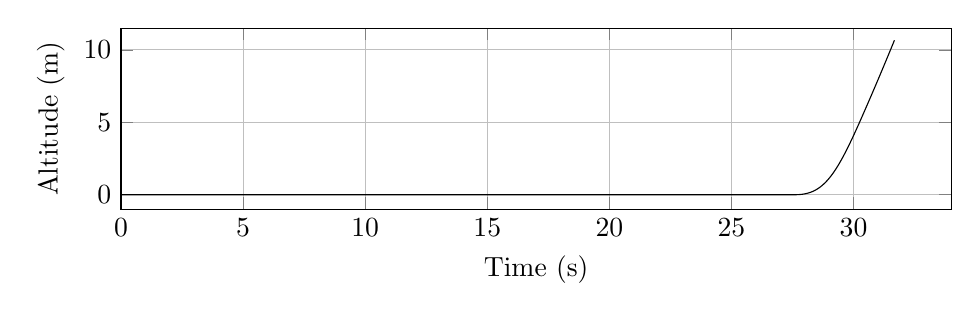
\begin{tikzpicture}

\begin{axis}[
width=\textwidth,
height=0.32\textwidth,
scaled ticks=false, tick label style={/pgf/number format/fixed},
xmin=0.0,
xmax=34,
xlabel={Time (s)},
xmajorgrids,
ymin=-1.0,
ymax=11.5,
ylabel={Altitude (m)},
ymajorgrids,
legend style={at={(1.03,0.5)},anchor=west,draw=black,fill=white,legend cell align=left}
]

\addplot [
color=black,
solid
]
table[row sep=crcr]{
9.999999999999999E-5	0.0\\
3.5694820560433537E-4	0.0\\
0.0010245452692119678	0.0\\
0.0069349042872337095	0.0\\
0.01286976806122327	0.0\\
0.018843593678645902	0.0\\
0.02479661783810936	0.0\\
0.03074929034621919	0.0\\
0.03669211352118573	0.0\\
0.042580956308319415	0.0\\
0.048493283817695076	0.0\\
0.05427367649331091	0.0\\
0.06018242857093453	0.0\\
0.0660567835326149	0.0\\
0.07196949266692618	0.0\\
0.07792428406091995	0.0\\
0.08390046318323552	0.0\\
0.08989020881354831	0.0\\
0.09587673552553522	0.0\\
0.10167944656754999	0.0\\
0.10765111137914757	0.0\\
0.11361192221071048	0.0\\
0.11954420271118602	0.0\\
0.125573987623401	0.0\\
0.1315700964469434	0.0\\
0.13749987165431027	0.0\\
0.14347214461959318	0.0\\
0.14945874955656013	0.0\\
0.15538557632642536	0.0\\
0.16134172045891504	0.0\\
0.16728166871345546	0.0\\
0.17316122794435485	0.0\\
0.17906586090973325	0.0\\
0.18502462068033498	0.0\\
0.19105995801776593	0.0\\
0.19703874704809138	0.0\\
0.20309718711380292	0.0\\
0.2090299405683319	0.0\\
0.21503149730647964	0.0\\
0.2210906082062326	0.0\\
0.22712806876774766	0.0\\
0.23315136948034765	0.0\\
0.23920379014307108	0.0\\
0.24515677763586902	0.0\\
0.25115480800481327	0.0\\
0.2572250890567559	0.0\\
0.2633064062502962	0.0\\
0.2693558850956802	0.0\\
0.2753851572323801	0.0\\
0.2814054782846729	0.0\\
0.2875363719193802	0.0\\
0.2936365386592882	0.0\\
0.2996725762790742	0.0\\
0.3057113890397092	0.0\\
0.311728709351481	0.0\\
0.3177443499717595	0.0\\
0.3239310451213814	0.0\\
0.3300281077115754	0.0\\
0.3360728475693199	0.0\\
0.34217699227400244	0.0\\
0.3483648069401394	0.0\\
0.35442860007526067	0.0\\
0.3605749921481264	0.0\\
0.36677317996618297	0.0\\
0.37291219385011287	0.0\\
0.3789779732446952	0.0\\
0.38504958269020406	0.0\\
0.39129130984530947	0.0\\
0.39747640865823075	0.0\\
0.4035449578168038	0.0\\
0.409658085793974	0.0\\
0.4158434790711202	0.0\\
0.42203123947701127	0.0\\
0.4282232407584047	0.0\\
0.4344427847702237	0.0\\
0.44060824473403093	0.0\\
0.44677233995759646	0.0\\
0.45294168306874305	0.0\\
0.4591520568719707	0.0\\
0.46552861434024206	0.0\\
0.47174496493338647	0.0\\
0.4780840868707784	0.0\\
0.4844105591505308	0.0\\
0.49073494683327135	0.0\\
0.49693324860032506	0.0\\
0.5031820245324283	0.0\\
0.5095347148125013	0.0\\
0.5158709697535484	0.0\\
0.5221857994590533	0.0\\
0.5285945736118585	0.0\\
0.5348943261437131	0.0\\
0.5412498831596135	0.0\\
0.5475879787525684	0.0\\
0.5540199261330143	0.0\\
0.5603110307074157	0.0\\
0.566739204297755	0.0\\
0.5732682780611191	0.0\\
0.5797267046288657	0.0\\
0.5861750445598519	0.0\\
0.5925208163290849	0.0\\
0.5988645455349844	0.0\\
0.605236368492422	0.0\\
0.6117724935743891	0.0\\
0.6181608865354462	0.0\\
0.6246969001680507	0.0\\
0.63116153002054	0.0\\
0.637673703807933	0.0\\
0.644070898056953	0.0\\
0.6506575993132437	0.0\\
0.6569950904275843	0.0\\
0.6635257426525845	0.0\\
0.6700305805678548	0.0\\
0.6765108465101242	0.0\\
0.683124466204782	0.0\\
0.6895920049387614	0.0\\
0.6961551992622965	0.0\\
0.702570002692859	0.0\\
0.7091767794146715	0.0\\
0.7158810384035788	0.0\\
0.722330750139915	0.0\\
0.7289031444577092	0.0\\
0.7354982449471308	0.0\\
0.7424081628271009	0.0\\
0.7489301174002103	0.0\\
0.755515041127365	0.0\\
0.7620900955093259	0.0\\
0.768726517316616	0.0\\
0.7754322814688266	0.0\\
0.7820045795409294	0.0\\
0.7885765548917036	0.0\\
0.7952880001398379	0.0\\
0.8019642657375692	0.0\\
0.8089221975782885	0.0\\
0.8159496552427474	0.0\\
0.8227512082781467	0.0\\
0.8295126839171314	0.0\\
0.8364435062986233	0.0\\
0.8433437972298823	0.0\\
0.8502532886622249	0.0\\
0.8571906480333069	0.0\\
0.8641948913839719	0.0\\
0.8709347755531902	0.0\\
0.8778085971393095	0.0\\
0.8846616629320734	0.0\\
0.8914723966825819	0.0\\
0.8984337487328791	0.0\\
0.9052581685588896	0.0\\
0.9122767946047234	0.0\\
0.9191083718623816	0.0\\
0.926072979352182	0.0\\
0.9331527145718401	0.0\\
0.9399812420074323	0.0\\
0.9469099835003199	0.0\\
0.9538892684884956	0.0\\
0.9608408960251769	0.0\\
0.967949078828209	0.0\\
0.9750804014833359	0.0\\
0.9820500063032944	0.0\\
0.9889400197651717	0.0\\
0.9959526785690063	0.0\\
1.0031613811593107	0.0\\
1.0101335383535681	0.0\\
1.0172304762477813	0.0\\
1.0243167196602005	0.0\\
1.031532325761198	0.0\\
1.0385761214455251	0.0\\
1.045518758175799	0.0\\
1.0526056127896628	0.0\\
1.059775473579922	0.0\\
1.0667056758326252	0.0\\
1.073723072246529	0.0\\
1.0809186717209713	0.0\\
1.0881483896660953	0.0\\
1.0953366014389219	0.0\\
1.1023895470451897	0.0\\
1.1097038616618584	0.0\\
1.1169054968916154	0.0\\
1.1241818599307019	0.0\\
1.1313684349455548	0.0\\
1.1386913369266725	0.0\\
1.1459050051946473	0.0\\
1.15324909865687	0.0\\
1.1603917284039738	0.0\\
1.167728191168648	0.0\\
1.1751136279327574	0.0\\
1.1826623714345867	0.0\\
1.1900759663658262	0.0\\
1.1973989800797513	0.0\\
1.204849923819272	0.0\\
1.2122043636572934	0.0\\
1.219690748242296	0.0\\
1.2271747469389913	0.0\\
1.2348350739745633	0.0\\
1.2422652286131242	0.0\\
1.2496486266791238	0.0\\
1.2572304774769116	0.0\\
1.26475871257581	0.0\\
1.2722849999230852	0.0\\
1.2798418424781421	0.0\\
1.2872317201819046	0.0\\
1.294781649430107	0.0\\
1.302274327708545	0.0\\
1.309799966680854	0.0\\
1.3174220765893008	0.0\\
1.3249737633890586	0.0\\
1.3327291813691486	0.0\\
1.3403377745059597	0.0\\
1.348066393515214	0.0\\
1.3557032568576135	0.0\\
1.363316543567941	0.0\\
1.3710774242951156	0.0\\
1.3788219901777032	0.0\\
1.3865773886235457	0.0\\
1.3941002978041466	0.0\\
1.4017811539906657	0.0\\
1.4095763089937394	0.0\\
1.4174562342054497	0.0\\
1.4251652517684015	0.0\\
1.4330378235789403	0.0\\
1.4407000702155934	0.0\\
1.4484594659956955	0.0\\
1.4563396432107631	0.0\\
1.4641675356187163	0.0\\
1.471933914080064	0.0\\
1.479769950215767	0.0\\
1.4874129554834874	0.0\\
1.4952912565691814	0.0\\
1.5034279098204526	0.0\\
1.511323320850415	0.0\\
1.5191757100931302	0.0\\
1.5271331134897972	0.0\\
1.5349157949428633	0.0\\
1.543002313099712	0.0\\
1.5507789665234828	0.0\\
1.558628747241348	0.0\\
1.5667955628936343	0.0\\
1.574712331198581	0.0\\
1.5825971607987288	0.0\\
1.590358951598581	0.0\\
1.5983342219636247	0.0\\
1.6063774707446807	0.0\\
1.6144694953357455	0.0\\
1.6224531728324476	0.0\\
1.6306021954514436	0.0\\
1.6387184329020679	0.0\\
1.6466602783164421	0.0\\
1.6547149097208704	0.0\\
1.6630308981810655	0.0\\
1.6714033552410448	0.0\\
1.6793960068941582	0.0\\
1.687559967796458	0.0\\
1.6956013484227919	0.0\\
1.703985576068487	0.0\\
1.7123628609916657	0.0\\
1.7205856868633744	0.0\\
1.7290429200788568	0.0\\
1.7373721866711915	0.0\\
1.7456026645961664	0.0\\
1.7538838866445223	0.0\\
1.7624912111876263	0.0\\
1.770773090024945	0.0\\
1.779088329532303	0.0\\
1.7872766435262744	0.0\\
1.795795588770969	0.0\\
1.8041847947879255	0.0\\
1.8126369218724645	0.0\\
1.8209097157071068	0.0\\
1.829219244317116	0.0\\
1.8376463555366884	0.0\\
1.8459718032624397	0.0\\
1.8542966926703768	0.0\\
1.8627053836441707	0.0\\
1.8711256342728828	0.0\\
1.879782123602444	0.0\\
1.8883929249058653	0.0\\
1.8967725863978533	0.0\\
1.905336340761549	0.0\\
1.9140263628453007	0.0\\
1.9225515986627846	0.0\\
1.931245648011127	0.0\\
1.9398766237544982	0.0\\
1.9484545062821095	0.0\\
1.9571336332373628	0.0\\
1.9658413648232447	0.0\\
1.9743918935091256	0.0\\
1.9831392911299472	0.0\\
1.9916148279509627	0.0\\
2.000268923318041	0.0\\
2.0091514649927955	0.0\\
2.017909753852824	0.0\\
2.026563531713383	0.0\\
2.0352324078101844	0.0\\
2.044067640387305	0.0\\
2.052753236912862	0.0\\
2.061566611968856	0.0\\
2.0702833647673344	0.0\\
2.0791641472526257	0.0\\
2.0880000673723433	0.0\\
2.0968390373693433	0.0\\
2.1055865782385377	0.0\\
2.1144357678008934	0.0\\
2.1233132463211506	0.0\\
2.1321628238787316	0.0\\
2.141104434100404	0.0\\
2.1499843468427056	0.0\\
2.1590571280259834	0.0\\
2.1679865758165935	0.0\\
2.1769213290254896	0.0\\
2.1858886072167385	0.0\\
2.194839082572962	0.0\\
2.204038094665136	0.0\\
2.213046247538463	0.0\\
2.222102475868321	0.0\\
2.231092535555222	0.0\\
2.240207193397323	0.0\\
2.2495245804319692	0.0\\
2.258740545352791	0.0\\
2.2678728103035652	0.0\\
2.2771018701344232	0.0\\
2.286361679403093	0.0\\
2.2956447464614653	0.0\\
2.3049189523060525	0.0\\
2.3141110215538685	0.0\\
2.3234227069187448	0.0\\
2.332688455071832	0.0\\
2.341876279533503	0.0\\
2.351091549623926	0.0\\
2.360539441307309	0.0\\
2.369789232894421	0.0\\
2.3791711728748757	0.0\\
2.38874954958509	0.0\\
2.3980390542950767	0.0\\
2.40750999912075	0.0\\
2.4169871244236694	0.0\\
2.426340051643196	0.0\\
2.435944198688186	0.0\\
2.4453186977271555	0.0\\
2.454841158430864	0.0\\
2.464234679011491	0.0\\
2.4735434908897043	0.0\\
2.4831426045113876	0.0\\
2.4927140624649757	0.0\\
2.502067505225207	0.0\\
2.51166584098749	0.0\\
2.521250744445581	0.0\\
2.5306593929673546	0.0\\
2.540558057175831	0.0\\
2.5502516927447223	0.0\\
2.5599057911578393	0.0\\
2.569385710236398	0.0\\
2.578834342589036	0.0\\
2.5885514990986165	0.0\\
2.598190632201491	0.0\\
2.607970400931631	0.0\\
2.617632864076235	0.0\\
2.627540085849689	0.0\\
2.637218199607754	0.0\\
2.6471336672090278	0.0\\
2.6568480852022915	0.0\\
2.6667486708271415	0.0\\
2.6764774720092284	0.0\\
2.6861387407061645	0.0\\
2.6959402486309676	0.0\\
2.705570290635996	0.0\\
2.7152913459009484	0.0\\
2.7251609135089154	0.0\\
2.7348705724187274	0.0\\
2.744629369906553	0.0\\
2.7546429964902677	0.0\\
2.7646256873810087	0.0\\
2.7745344373337746	0.0\\
2.78448273330019	0.0\\
2.7945461747368006	0.0\\
2.8045560495331197	0.0\\
2.8144941901843996	0.0\\
2.824567928489449	0.0\\
2.834532178368165	0.0\\
2.844593894364576	0.0\\
2.8545881500650925	0.0\\
2.8647742561957736	0.0\\
2.8747828181171027	0.0\\
2.885023792099372	0.0\\
2.8950960443764044	0.0\\
2.9050820127568375	0.0\\
2.915161020148581	0.0\\
2.9254942729288134	0.0\\
2.9356681598028294	0.0\\
2.9457751920016335	0.0\\
2.955720059741849	0.0\\
2.965769359476731	0.0\\
2.9760092478640754	0.0\\
2.9861988525482177	0.0\\
2.996278648119138	0.0\\
3.0064987277382853	0.0\\
3.0171126472517242	0.0\\
3.0272662822357743	0.0\\
3.0375599480669875	0.0\\
3.0480132480549615	0.0\\
3.0583904373770396	0.0\\
3.068693892307258	0.0\\
3.0791760373092094	0.0\\
3.0894573656209303	0.0\\
3.099852594297979	0.0\\
3.1102531441221695	0.0\\
3.120782604119581	0.0\\
3.13130924581199	0.0\\
3.1419768586928747	0.0\\
3.1524538261390926	0.0\\
3.1629528321100073	0.0\\
3.173561224845929	0.0\\
3.1840478095015072	0.0\\
3.194543531458371	0.0\\
3.2052150148888963	0.0\\
3.2160602353970704	0.0\\
3.226775992945611	0.0\\
3.2373719116960764	0.0\\
3.2482745666521815	0.0\\
3.2587129750477466	0.0\\
3.269536493210789	0.0\\
3.2801086967299193	0.0\\
3.290809906134636	0.0\\
3.3015770907563313	0.0\\
3.3119797092415357	0.0\\
3.3224703028488864	0.0\\
3.3331189004538	0.0\\
3.344115242439477	0.0\\
3.355052006567626	0.0\\
3.36567176758735	0.0\\
3.376446097028083	0.0\\
3.387130869009204	0.0\\
3.3977396315615103	0.0\\
3.408642881184611	0.0\\
3.4197552866515997	0.0\\
3.4304882804194152	0.0\\
3.4411839613772663	0.0\\
3.4523524128726475	0.0\\
3.4633665662338693	0.0\\
3.4742773994322533	0.0\\
3.484942212609072	0.0\\
3.4959606977105526	0.0\\
3.5067182567067974	0.0\\
3.5175717162567013	0.0\\
3.5285389825527798	0.0\\
3.5394185963001874	0.0\\
3.5507012255215713	0.0\\
3.561716953819312	0.0\\
3.5726145205143665	0.0\\
3.58366993559625	0.0\\
3.5948498393126727	0.0\\
3.605963987900413	0.0\\
3.6171740925646185	0.0\\
3.6284131889055455	0.0\\
3.639695307652401	0.0\\
3.650992086551901	0.0\\
3.6622418469349673	0.0\\
3.6734510150868562	0.0\\
3.6846830853939583	0.0\\
3.695879842608562	0.0\\
3.707099451126602	0.0\\
3.718274708510198	0.0\\
3.729429590858099	0.0\\
3.7408593670907715	0.0\\
3.752122184045909	0.0\\
3.763605920409903	0.0\\
3.7748091935166626	0.0\\
3.786220497192793	0.0\\
3.797739312038651	0.0\\
3.80898561302579	0.0\\
3.8203231006319136	0.0\\
3.8316531778633527	0.0\\
3.842980599243302	0.0\\
3.8543140657244885	0.0\\
3.8656564658472874	0.0\\
3.8771477237842253	0.0\\
3.888573510568392	0.0\\
3.899862911479868	0.0\\
3.911438478974441	0.0\\
3.92279464487481	0.0\\
3.934118474463962	0.0\\
3.945625729366511	0.0\\
3.957050617966029	0.0\\
3.9684874631493576	0.0\\
3.9800416021377636	0.0\\
3.9916809823101325	0.0\\
4.003226759525534	0.0\\
4.014739337559421	0.0\\
4.02638357676088	0.0\\
4.0378450965614725	0.0\\
4.049520027715284	0.0\\
4.061124751333221	0.0\\
4.0725123670405665	0.0\\
4.084095582270553	0.0\\
4.095690116812618	0.0\\
4.107237676295863	0.0\\
4.119098000362323	0.0\\
4.1305766118173874	0.0\\
4.142152746923815	0.0\\
4.153784087828598	0.0\\
4.165410538877948	0.0\\
4.1772222265995325	0.0\\
4.188946818070619	0.0\\
4.200664324488011	0.0\\
4.212311671251959	0.0\\
4.223892000900003	0.0\\
4.235390528815598	0.0\\
4.246989217360623	0.0\\
4.258618275434564	0.0\\
4.2701962817401995	0.0\\
4.2818969709946515	0.0\\
4.293428776814217	0.0\\
4.304958580130352	0.0\\
4.316775591730732	0.0\\
4.328424966859105	0.0\\
4.340067566843931	0.0\\
4.351819477988407	0.0\\
4.363292632597876	0.0\\
4.365609772812482	0.0\\
4.365827762680695	0.0\\
4.366156890255072	0.0\\
4.367285764412006	0.0\\
4.370554729071726	0.0\\
4.37734538151517	0.0\\
4.387806477228311	0.0\\
4.39864364652086	0.0\\
4.409536927170151	0.0\\
4.420376048165647	0.0\\
4.431256326804899	0.0\\
4.4421091367284635	0.0\\
4.453138010525066	0.0\\
4.464083040457272	0.0\\
4.475117887617129	0.0\\
4.485924593370475	0.0\\
4.496961285102792	0.0\\
4.507847639280435	0.0\\
4.5188292046447085	0.0\\
4.5299129612399	0.0\\
4.54087952555223	0.0\\
4.552001167304356	0.0\\
4.563019596927903	0.0\\
4.574189554159249	0.0\\
4.585332055939665	0.0\\
4.596756209108662	0.0\\
4.607786587044449	0.0\\
4.619015072255367	0.0\\
4.630223484741212	0.0\\
4.6414031810785	0.0\\
4.652708778433912	0.0\\
4.664079546120487	0.0\\
4.6753151831289745	0.0\\
4.686653577518522	0.0\\
4.697890982797592	0.0\\
4.709108531827992	0.0\\
4.72064250544018	0.0\\
4.731813636183569	0.0\\
4.743166725855746	0.0\\
4.75454099501202	0.0\\
4.765927839024803	0.0\\
4.7773345931072075	0.0\\
4.788689023725228	0.0\\
4.8000679457437805	0.0\\
4.811500834204896	0.0\\
4.822987280606505	0.0\\
4.834559620827509	0.0\\
4.845952446010495	0.0\\
4.857516331854871	0.0\\
4.869107606617373	0.0\\
4.880600219800634	0.0\\
4.892254271403688	0.0\\
4.903640449644904	0.0\\
4.915293886893618	0.0\\
4.926981102689567	0.0\\
4.93864180821587	0.0\\
4.950373773388343	0.0\\
4.962040794644393	0.0\\
4.973631406254297	0.0\\
4.9853084132905625	0.0\\
4.997149839555785	0.0\\
5.008854133343329	0.0\\
5.020636002047388	0.0\\
5.032363422348883	0.0\\
5.044270631271967	0.0\\
5.055976517818099	0.0\\
5.067792708150261	0.0\\
5.079491034995289	0.0\\
5.091279336079349	0.0\\
5.103141118757822	0.0\\
5.1149499914057	0.0\\
5.126933707882346	0.0\\
5.138714517877592	0.0\\
5.150473017988752	0.0\\
5.162182799334515	0.0\\
5.17418560855892	0.0\\
5.185972717937398	0.0\\
5.197930487706849	0.0\\
5.209824831391927	0.0\\
5.221690561768437	0.0\\
5.2335678164200825	0.0\\
5.245301082850945	0.0\\
5.257162978892827	0.0\\
5.269212119330316	0.0\\
5.281262125951104	0.0\\
5.292992263338753	0.0\\
5.3051093287408	0.0\\
5.316935174035137	0.0\\
5.329070905569742	0.0\\
5.340986880242278	0.0\\
5.352974348498053	0.0\\
5.364975527152241	0.0\\
5.37685927484471	0.0\\
5.388803485478622	0.0\\
5.400786682905052	0.0\\
5.412661067951245	0.0\\
5.424789619142722	0.0\\
5.436776315661213	0.0\\
5.448849566091836	0.0\\
5.460822392446877	0.0\\
5.47273048924103	0.0\\
5.484825427771691	0.0\\
5.496876881509207	0.0\\
5.5090370297629985	0.0\\
5.52092200939267	0.0\\
5.532970706917082	0.0\\
5.54487947956091	0.0\\
5.556874966113702	0.0\\
5.56888336986945	0.0\\
5.580910384972851	0.0\\
5.593072187651382	0.0\\
5.605152904939956	0.0\\
5.617234420343031	0.0\\
5.629244482854993	0.0\\
5.641369223974225	0.0\\
5.653445224467896	0.0\\
5.665579012516789	0.0\\
5.677714799612138	0.0\\
5.689902817238876	0.0\\
5.702039042354276	0.0\\
5.714045150163884	0.0\\
5.7261335173555885	0.0\\
5.7384092927467005	0.0\\
5.750500297518281	0.0\\
5.762695355119092	0.0\\
5.774894667920002	0.0\\
5.787097986150698	0.0\\
5.799214434175527	0.0\\
5.811296061221649	0.0\\
5.823466158413499	0.0\\
5.83562677158783	0.0\\
5.84766048518626	0.0\\
5.859940328786365	0.0\\
5.872165019838091	0.0\\
5.884441033367848	0.0\\
5.896687953418571	0.0\\
5.908934390684223	0.0\\
5.921018367804715	0.0\\
5.933142059152411	0.0\\
5.945370867974814	0.0\\
5.957641120891033	0.0\\
5.969699276628509	0.0\\
5.981843019254672	0.0\\
5.994108627173988	0.0\\
6.0063451482262025	0.0\\
6.0186212414729265	0.0\\
6.030700591612124	0.0\\
6.043079990417011	0.0\\
6.055098338636414	0.0\\
6.067315283695393	0.0\\
6.079660698903082	0.0\\
6.091969229666139	0.0\\
6.104208789349178	0.0\\
6.1163998147562335	0.0\\
6.12887138232402	0.0\\
6.141268103144984	0.0\\
6.153526920138685	0.0\\
6.165865841088646	0.0\\
6.178144255975809	0.0\\
6.190275768379534	0.0\\
6.202524213671365	0.0\\
6.214664334762476	0.0\\
6.226965122807313	0.0\\
6.239138091174254	0.0\\
6.251533499502486	0.0\\
6.263989387258135	0.0\\
6.276497026571889	0.0\\
6.288874580250022	0.0\\
6.301248779550207	0.0\\
6.313590423637988	0.0\\
6.32593890309481	0.0\\
6.3383231970360185	0.0\\
6.350770250972802	0.0\\
6.363083925431834	0.0\\
6.375593127253275	0.0\\
6.3880159124928415	0.0\\
6.4005030591779	0.0\\
6.4128798195805	0.0\\
6.425285596792559	0.0\\
6.437624743237073	0.0\\
6.4500074006514385	0.0\\
6.462435253045861	0.0\\
6.474793493245844	0.0\\
6.4872959866039075	0.0\\
6.499860484582687	0.0\\
6.512198239014223	0.0\\
6.524732282965175	0.0\\
6.537207495638045	0.0\\
6.549894034535326	0.0\\
6.562413469739594	0.0\\
6.57488469360054	0.0\\
6.587412593596266	0.0\\
6.599899435701829	0.0\\
6.6124451411854	0.0\\
6.625143219711772	0.0\\
6.63777004757835	0.0\\
6.650369504303152	0.0\\
6.663024717583481	0.0\\
6.675637414536949	0.0\\
6.688151339876221	0.0\\
6.700757485276274	0.0\\
6.713277176578632	0.0\\
6.7258260129120675	0.0\\
6.738452647667229	0.0\\
6.7512444389517245	0.0\\
6.763899527116191	0.0\\
6.776707656329382	0.0\\
6.789461022516029	0.0\\
6.8022124039870455	0.0\\
6.814896169894878	0.0\\
6.827701707718974	0.0\\
6.840537941307314	0.0\\
6.853179229017046	0.0\\
6.865880233762125	0.0\\
6.878674487230674	0.0\\
6.891383475650533	0.0\\
6.9043196944092635	0.0\\
6.917037946491966	0.0\\
6.9298374105318405	0.0\\
6.942683714985327	0.0\\
6.955603491750777	0.0\\
6.968332630532398	0.0\\
6.981270953998019	0.0\\
6.99409306721542	0.0\\
7.006994306190393	0.0\\
7.019909224804666	0.0\\
7.0328485318634275	0.0\\
7.045738282644885	0.0\\
7.058623978535344	0.0\\
7.071715545522604	0.0\\
7.08478123971347	0.0\\
7.0977135138896035	0.0\\
7.110831730563287	0.0\\
7.1238402361136846	0.0\\
7.137018096834716	0.0\\
7.150183705007155	0.0\\
7.163297429108246	0.0\\
7.176391640498968	0.0\\
7.18959553137663	0.0\\
7.202669123479263	0.0\\
7.21581371332193	0.0\\
7.229224584594668	0.0\\
7.242335316522617	0.0\\
7.255507625817728	0.0\\
7.268729084943288	0.0\\
7.282018483674792	0.0\\
7.295222853062198	0.0\\
7.308514217776775	0.0\\
7.321745251860822	0.0\\
7.335016290230419	0.0\\
7.34844025158279	0.0\\
7.361778990165382	0.0\\
7.375172334421219	0.0\\
7.388667703532647	0.0\\
7.402223194997115	0.0\\
7.415812487510799	0.0\\
7.429163333495865	0.0\\
7.442690269497403	0.0\\
7.456160039865566	0.0\\
7.469755052027002	0.0\\
7.483399445467143	0.0\\
7.497005623739245	0.0\\
7.510654789221771	0.0\\
7.524256707395043	0.0\\
7.5379930898809935	0.0\\
7.551677448667421	0.0\\
7.565547055466881	0.0\\
7.579249390553356	0.0\\
7.592981588064131	0.0\\
7.606861715084147	0.0\\
7.620628273783721	0.0\\
7.634447495929711	0.0\\
7.648192504123321	0.0\\
7.662240796287325	0.0\\
7.676202348540503	0.0\\
7.690108025935773	0.0\\
7.704071203293733	0.0\\
7.718221802084624	0.0\\
7.732290372341415	0.0\\
7.746504226467701	0.0\\
7.760627346813246	0.0\\
7.774796099725144	0.0\\
7.789009479414455	0.0\\
7.803217807824355	0.0\\
7.817587883860748	0.0\\
7.831766607328298	0.0\\
7.846041398443504	0.0\\
7.860371716232965	0.0\\
7.874798078043614	0.0\\
7.8891857877027025	0.0\\
7.9035490494622245	0.0\\
7.918051771507718	0.0\\
7.932461786496665	0.0\\
7.94691014144105	0.0\\
7.96144742803985	0.0\\
7.976061646615996	0.0\\
7.990634900394884	0.0\\
8.005097015699434	0.0\\
8.019893420304314	0.0\\
8.034397411765234	0.0\\
8.049149399215466	0.0\\
8.063861209812067	0.0\\
8.078754568397777	0.0\\
8.09348334752103	0.0\\
8.108092941185898	0.0\\
8.12304540586976	0.0\\
8.137958279483957	0.0\\
8.152728813321932	0.0\\
8.1678100196212	0.0\\
8.182664074772049	0.0\\
8.197738766362114	0.0\\
8.212775194828886	0.0\\
8.227737838411596	0.0\\
8.24290522068409	0.0\\
8.257996573353921	0.0\\
8.273335172510386	0.0\\
8.288473703108483	0.0\\
8.303482272135835	0.0\\
8.318655835686666	0.0\\
8.33389822804753	0.0\\
8.349385228465678	0.0\\
8.36460963500338	0.0\\
8.379926966134924	0.0\\
8.395196659993164	0.0\\
8.410243044957912	0.0\\
8.425514162519992	0.0\\
8.440659418367577	0.0\\
8.455962194174838	0.0\\
8.47119180980615	0.0\\
8.48639087873201	0.0\\
8.501673659184625	0.0\\
8.51705543324831	0.0\\
8.53226332328585	0.0\\
8.54749830431592	0.0\\
8.562792254999717	0.0\\
8.577909380902888	0.0\\
8.593039490093538	0.0\\
8.608287981283347	0.0\\
8.623255759329751	0.0\\
8.638359533853443	0.0\\
8.653302993623129	0.0\\
8.668333491488163	0.0\\
8.683315949576748	0.0\\
8.698329298102013	0.0\\
8.713328238390648	0.0\\
8.72834394008293	0.0\\
8.743152425848283	0.0\\
8.758158649736203	0.0\\
8.773097263917634	0.0\\
8.787785362445973	0.0\\
8.802515656199457	0.0\\
8.817197988640114	0.0\\
8.831674682677821	0.0\\
8.846310568773738	0.0\\
8.860933348808597	0.0\\
8.875408235607992	0.0\\
8.889948783313386	0.0\\
8.90444030987328	0.0\\
8.918827555713403	0.0\\
8.933259976231348	0.0\\
8.947596429304134	0.0\\
8.961740724552335	0.0\\
8.97601290657661	0.0\\
8.978840833446618	0.0\\
8.979132006879226	0.0\\
8.979426187815509	0.0\\
8.979618437954041	0.0\\
8.979759273345895	0.0\\
8.97988745453863	0.0\\
8.980464131607718	0.0\\
8.982958217103146	0.0\\
8.9897455851489	0.0\\
9.0033447692978	0.0\\
9.016108168876183	0.0\\
9.028953049848706	0.0\\
9.041735069562591	0.0\\
9.054638589456552	0.0\\
9.067545585121387	0.0\\
9.080543149451074	0.0\\
9.093621619753325	0.0\\
9.106673690301484	0.0\\
9.119772625577586	0.0\\
9.133043577493712	0.0\\
9.146368544451384	0.0\\
9.15968559747633	0.0\\
9.173112340775099	0.0\\
9.18653885575414	0.0\\
9.200188084677922	0.0\\
9.213810197102777	0.0\\
9.227322457334118	0.0\\
9.241037682342878	0.0\\
9.254635850728938	0.0\\
9.268416199146035	0.0\\
9.282219791530228	0.0\\
9.29601583131512	0.0\\
9.309974585507952	0.0\\
9.32393777135097	0.0\\
9.337883197202054	0.0\\
9.351895699205059	0.0\\
9.366011701674598	0.0\\
9.380255267881171	0.0\\
9.39431645221378	0.0\\
9.408482802303208	0.0\\
9.42280848724473	0.0\\
9.437135015961612	0.0\\
9.451544871289627	0.0\\
9.466037036346265	0.0\\
9.480691058533981	0.0\\
9.495245912675259	0.0\\
9.509932495984568	0.0\\
9.524538610440384	0.0\\
9.539260732908254	0.0\\
9.554126582682098	0.0\\
9.568897783087145	0.0\\
9.58374598865235	0.0\\
9.598482825402293	0.0\\
9.613403976627144	0.0\\
9.628284084963799	0.0\\
9.643188363578428	0.0\\
9.65807158220306	0.0\\
9.67279606393382	0.0\\
9.687684934908972	0.0\\
9.702552197484927	0.0\\
9.717342138430045	0.0\\
9.732163723738964	0.0\\
9.747149762039616	0.0\\
9.762060526895041	0.0\\
9.777091053840778	0.0\\
9.791966087699013	0.0\\
9.80674862286174	0.0\\
9.821669064351351	0.0\\
9.836458844880859	0.0\\
9.851307500110671	0.0\\
9.86613343017072	0.0\\
9.881059964755199	0.0\\
9.89572555001277	0.0\\
9.910501809109231	0.0\\
9.925245214375693	0.0\\
9.939948094855474	0.0\\
9.954644629017995	0.0\\
9.969281120601263	0.0\\
9.98390607104891	0.0\\
9.998585317370708	0.0\\
10.013201114604016	0.0\\
10.027767378370395	0.0\\
10.04244098677168	0.0\\
10.05695490583392	0.0\\
10.071517634882479	0.0\\
10.0859461609768	0.0\\
10.100358173149118	0.0\\
10.114880151957479	0.0\\
10.129295377329687	0.0\\
10.143747415333667	0.0\\
10.158236919646907	0.0\\
10.172585477159704	0.0\\
10.186936774262119	0.0\\
10.20130358527729	0.0\\
10.215533306533885	0.0\\
10.22984592060924	0.0\\
10.244206129457279	0.0\\
10.258417748531986	0.0\\
10.272746165568563	0.0\\
10.287004001461117	0.0\\
10.301050621247597	0.0\\
10.315263476298181	0.0\\
10.329336756787598	0.0\\
10.34344698817235	0.0\\
10.357540406443146	0.0\\
10.371669859765568	0.0\\
10.385696066737783	0.0\\
10.399648218519172	0.0\\
10.413783188039513	0.0\\
10.427711692307494	0.0\\
10.441666582805315	0.0\\
10.45563630974026	0.0\\
10.469613701078295	0.0\\
10.483590022945503	0.0\\
10.497463014285636	0.0\\
10.511330538835704	0.0\\
10.52522752996705	0.0\\
10.539155922044898	0.0\\
10.553145928391793	0.0\\
10.567018019382239	0.0\\
10.580911262179836	0.0\\
10.594768516267731	0.0\\
10.60856774635862	0.0\\
10.622489689659208	0.0\\
10.636310546416347	0.0\\
10.650164650615299	0.0\\
10.663937580608007	0.0\\
10.677815580905467	0.0\\
10.691550131568334	0.0\\
10.705261266644403	0.0\\
10.71911862771784	0.0\\
10.732873000433774	0.0\\
10.74670085052032	0.0\\
10.760507661869305	0.0\\
10.774318822874612	0.0\\
10.788102331549329	0.0\\
10.801774196018243	0.0\\
10.815551254794418	0.0\\
10.829261350155608	0.0\\
10.842999548568862	0.0\\
10.85668033184827	0.0\\
10.870380617529197	0.0\\
10.884132319694327	0.0\\
10.897771740288228	0.0\\
10.911503502350037	0.0\\
10.925218156003545	0.0\\
10.938867886945957	0.0\\
10.952605057218644	0.0\\
10.966308725297996	0.0\\
10.980032385630903	0.0\\
10.993726271124881	0.0\\
11.007456327782425	0.0\\
11.021233763966684	0.0\\
11.03492438583729	0.0\\
11.04863886376495	0.0\\
11.062404816555805	0.0\\
11.076195541821441	0.0\\
11.089818448277157	0.0\\
11.103545875211395	0.0\\
11.117290588538175	0.0\\
11.131094605842964	0.0\\
11.144788421389421	0.0\\
11.158548017541758	0.0\\
11.172314389108472	0.0\\
11.186060690006144	0.0\\
11.199795079157678	0.0\\
11.213642980472493	0.0\\
11.227449447895193	0.0\\
11.241283476955957	0.0\\
11.255049084613386	0.0\\
11.268773177526011	0.0\\
11.2825169231136	0.0\\
11.296264575379084	0.0\\
11.310067954366367	0.0\\
11.323939604254605	0.0\\
11.337734545625132	0.0\\
11.35153149054631	0.0\\
11.36532227069701	0.0\\
11.379108268437111	0.0\\
11.392888425200756	0.0\\
11.406699430046093	0.0\\
11.420503287255396	0.0\\
11.434363708332189	0.0\\
11.44815956115669	0.0\\
11.462031737073165	0.0\\
11.475880551293642	0.0\\
11.489683193459957	0.0\\
11.503604230352078	0.0\\
11.517468146333346	0.0\\
11.531445844568296	0.0\\
11.545280652376228	0.0\\
11.559090637142912	0.0\\
11.572974805259737	0.0\\
11.58691717706084	0.0\\
11.600857342026213	0.0\\
11.61480845321351	0.0\\
11.628623441604567	0.0\\
11.642596128921348	0.0\\
11.656559884003375	0.0\\
11.670539012801758	0.0\\
11.684557189606235	0.0\\
11.698594830716981	0.0\\
11.712576460210688	0.0\\
11.726612233200942	0.0\\
11.740644425797992	0.0\\
11.754747495473794	0.0\\
11.768746105567352	0.0\\
11.782862544566235	0.0\\
11.79698242581416	0.0\\
11.811137064481674	0.0\\
11.825321505933555	0.0\\
11.83946443221934	0.0\\
11.853594752623042	0.0\\
11.86778090170494	0.0\\
11.881959724987436	0.0\\
11.896180695774234	0.0\\
11.910477067498945	0.0\\
11.924847972908623	0.0\\
11.93913476365536	0.0\\
11.953415510636589	0.0\\
11.967798975109162	0.0\\
11.982172351446643	0.0\\
11.996547912190184	0.0\\
12.010945539444489	0.0\\
12.025349220948662	0.0\\
12.039803103932272	0.0\\
12.054236755934724	0.0\\
12.068682488963752	0.0\\
12.083188243352087	0.0\\
12.097730870844291	0.0\\
12.112365035653	0.0\\
12.126953637439296	0.0\\
12.141478609976005	0.0\\
12.156116187671902	0.0\\
12.170763992903119	0.0\\
12.185407834962362	0.0\\
12.200130967972832	0.0\\
12.214831152598364	0.0\\
12.22958818369423	0.0\\
12.244333184110815	0.0\\
12.259161684395735	0.0\\
12.274022330106966	0.0\\
12.288959086058515	0.0\\
12.303925763037807	0.0\\
12.318812863924006	0.0\\
12.33376049007784	0.0\\
12.348728648441071	0.0\\
12.363772090776514	0.0\\
12.378852038901876	0.0\\
12.39406908753379	0.0\\
12.409319469378925	0.0\\
12.424454322109646	0.0\\
12.439683441265224	0.0\\
12.454914731346147	0.0\\
12.470194234140006	0.0\\
12.485554529414962	0.0\\
12.500864926173406	0.0\\
12.516274386550847	0.0\\
12.531696818362818	0.0\\
12.547166226179556	0.0\\
12.562670056295907	0.0\\
12.578271008013402	0.0\\
12.594057870523848	0.0\\
12.609776791673056	0.0\\
12.625492179087125	0.0\\
12.641288836326268	0.0\\
12.657107150827564	0.0\\
12.672929182952561	0.0\\
12.68890044809718	0.0\\
12.704837044329064	0.0\\
12.720847240348174	0.0\\
12.737022616651075	0.0\\
12.753234496430029	0.0\\
12.769362056101361	0.0\\
12.785657546336395	0.0\\
12.801945938271505	0.0\\
12.818328757676582	0.0\\
12.834853409610663	0.0\\
12.851317329194188	0.0\\
12.868009673926817	0.0\\
12.884788547551977	0.0\\
12.901470260866528	0.0\\
12.918414295091253	0.0\\
12.935306247865956	0.0\\
12.952344263464575	0.0\\
12.969485757154828	0.0\\
12.986838454529007	0.0\\
13.004070548735044	0.0\\
13.021395377084033	0.0\\
13.038869944887562	0.0\\
13.056542280052735	0.0\\
13.074079927496943	0.0\\
13.091789735803054	0.0\\
13.109763130573032	0.0\\
13.127640666467197	0.0\\
13.145473504119831	0.0\\
13.163404975317317	0.0\\
13.18174803755959	0.0\\
13.199925200619486	0.0\\
13.218247766045522	0.0\\
13.236691256095131	0.0\\
13.255119429901988	0.0\\
13.273606713921257	0.0\\
13.29215025850236	0.0\\
13.31064492775738	0.0\\
13.329120447940099	0.0\\
13.347666134840573	0.0\\
13.366185571501852	0.0\\
13.384497829511336	0.0\\
13.402802529957732	0.0\\
13.420974965120667	0.0\\
13.439174609219005	0.0\\
13.4572790138477	0.0\\
13.475498180672595	0.0\\
13.493448294713616	0.0\\
13.511421181457248	0.0\\
13.529303308717871	0.0\\
13.547013895914752	0.0\\
13.564763979453758	0.0\\
13.582308539810029	0.0\\
13.599818217396038	0.0\\
13.617138074285553	0.0\\
13.634220242612528	0.0\\
13.651359042389881	0.0\\
13.668415144606346	0.0\\
13.685264261825782	0.0\\
13.702086237709576	0.0\\
13.718822525880586	0.0\\
13.735389477009452	0.0\\
13.751921876877741	0.0\\
13.76839541765655	0.0\\
13.784775045118966	0.0\\
13.801129912591339	0.0\\
13.817349864427765	0.0\\
13.833433398312117	0.0\\
13.84944875011712	0.0\\
13.86542228707549	0.0\\
13.881440781925573	0.0\\
13.897192980960344	0.0\\
13.91279183287358	0.0\\
13.928453064465643	0.0\\
13.944082952003786	0.0\\
13.959546886123618	0.0\\
13.974970110297534	0.0\\
13.97804270297648	0.0\\
13.987068826539687	0.0\\
13.987684438901038	0.0\\
13.988168867201022	0.0\\
13.988596497431342	0.0\\
13.988969820275525	0.0\\
13.989369326363096	0.0\\
13.989520765159	0.0\\
13.989689684937222	0.0\\
13.99058243656481	0.0\\
13.993575346637634	0.0\\
14.002093098764401	0.0\\
14.015836306425406	0.0\\
14.029368858474704	0.0\\
14.04289664571963	0.0\\
14.05658036972077	0.0\\
14.070314632775535	0.0\\
14.084109470808603	0.0\\
14.09797159125809	0.0\\
14.111839291330163	0.0\\
14.125827703584928	0.0\\
14.139847123909668	0.0\\
14.153933254201394	0.0\\
14.168101172693628	0.0\\
14.182339935387091	0.0\\
14.196705844232582	0.0\\
14.211113774715084	0.0\\
14.225524212398991	0.0\\
14.240018295905106	0.0\\
14.254662404361408	0.0\\
14.269349798597823	0.0\\
14.284273021193059	0.0\\
14.299199015342648	0.0\\
14.314149897280586	0.0\\
14.329193424145704	0.0\\
14.344282662847945	0.0\\
14.359522768073091	0.0\\
14.374892179677289	0.0\\
14.390312548832668	0.0\\
14.405998517658706	0.0\\
14.42157947939161	0.0\\
14.437394854186142	0.0\\
14.453202747796482	0.0\\
14.469091522226485	0.0\\
14.485210383129598	0.0\\
14.501486956480413	0.0\\
14.517809939977152	0.0\\
14.53427401765558	0.0\\
14.550764907017136	0.0\\
14.56747157888896	0.0\\
14.584141017240281	0.0\\
14.601053896096076	0.0\\
14.61806987541856	0.0\\
14.635032636932415	0.0\\
14.652217525264277	0.0\\
14.669420202198378	0.0\\
14.686687482907743	0.0\\
14.70392975419757	0.0\\
14.721345402928957	0.0\\
14.73871224021142	0.0\\
14.756202002564983	0.0\\
14.773652537893543	0.0\\
14.79100328833077	0.0\\
14.80828953551001	0.0\\
14.825654755996496	0.0\\
14.842895209702146	0.0\\
14.860144490174157	0.0\\
14.87724492360324	0.0\\
14.894189221111546	0.0\\
14.911208093627128	0.0\\
14.928084642875923	0.0\\
14.944941119770032	0.0\\
14.961704356289221	0.0\\
14.97828821497162	0.0\\
14.99500174681555	0.0\\
15.011540597070212	0.0\\
15.027994816920451	0.0\\
15.044375743235275	0.0\\
15.060631419697483	0.0\\
15.076963895131666	0.0\\
15.093047971798295	0.0\\
15.109116644434632	0.0\\
15.12511775466886	0.0\\
15.141089920172796	0.0\\
15.157011142494923	0.0\\
15.17286525446459	0.0\\
15.188610358419492	0.0\\
15.20432005960624	0.0\\
15.22002947635118	0.0\\
15.235580920487891	0.0\\
15.251088592802034	0.0\\
15.26648091869087	0.0\\
15.28195850569346	0.0\\
15.297303337693059	0.0\\
15.312647597378241	0.0\\
15.327992041670164	0.0\\
15.343254123995145	0.0\\
15.358488296259928	0.0\\
15.373727403408477	0.0\\
15.388921392844686	0.0\\
15.404065538306444	0.0\\
15.419084864094284	0.0\\
15.434119352946752	0.0\\
15.44913482427728	0.0\\
15.464016030720177	0.0\\
15.478969943961715	0.0\\
15.493876878436236	0.0\\
15.50863766198895	0.0\\
15.523489552176436	0.0\\
15.53834207070041	0.0\\
15.55321282446501	0.0\\
15.567932089462289	0.0\\
15.58259285733427	0.0\\
15.597316635714478	0.0\\
15.611981002190838	0.0\\
15.626714516074841	0.0\\
15.641432984698525	0.0\\
15.656045238964857	0.0\\
15.670676414036492	0.0\\
15.685297702430084	0.0\\
15.699899722048063	0.0\\
15.714440630439569	0.0\\
15.729050648144806	0.0\\
15.743575404113638	0.0\\
15.758059386696598	0.0\\
15.772483697745102	0.0\\
15.786991498039697	0.0\\
15.801464048941224	0.0\\
15.81592825903827	0.0\\
15.83037954005393	0.0\\
15.844769757401341	0.0\\
15.859196686822699	0.0\\
15.873575554283839	0.0\\
15.887988552907522	0.0\\
15.902306704477592	0.0\\
15.91664078426819	0.0\\
15.930971112292735	0.0\\
15.945329523564073	0.0\\
15.959602170466972	0.0\\
15.973903876914871	0.0\\
15.988181128343818	0.0\\
16.002460091079016	0.0\\
16.01682670815211	0.0\\
16.031141309814608	0.0\\
16.04544121443181	0.0\\
16.059667251210634	0.0\\
16.07395882336936	0.0\\
16.08824155192643	0.0\\
16.102529762777387	0.0\\
16.11677616872649	0.0\\
16.131054735793448	0.0\\
16.14535667253749	0.0\\
16.159595301973752	0.0\\
16.173830477877253	0.0\\
16.18807110226404	0.0\\
16.202254477717503	0.0\\
16.216545754994634	0.0\\
16.230758669155662	0.0\\
16.245000296917212	0.0\\
16.259233416996473	0.0\\
16.27350703944935	0.0\\
16.28778098414648	0.0\\
16.302069275375587	0.0\\
16.316266678501	0.0\\
16.330513944291454	0.0\\
16.344729553864028	0.0\\
16.358961567233997	0.0\\
16.373187113927848	0.0\\
16.387387566748437	0.0\\
16.401625607719893	0.0\\
16.415864898987607	0.0\\
16.430106201940475	0.0\\
16.444351783584573	0.0\\
16.45859130436017	0.0\\
16.472865246124087	0.0\\
16.487213412518685	0.0\\
16.501431138124182	0.0\\
16.515712251030543	0.0\\
16.530026248112378	0.0\\
16.54429851699126	0.0\\
16.558576875787807	0.0\\
16.57286982134378	0.0\\
16.587107633555433	0.0\\
16.601419934467742	0.0\\
16.615730887353948	0.0\\
16.63004656200821	0.0\\
16.64444018734158	0.0\\
16.65872910058558	0.0\\
16.672980591200677	0.0\\
16.687352873176174	0.0\\
16.70168348914261	0.0\\
16.71607297354702	0.0\\
16.73044866110267	0.0\\
16.744846565855994	0.0\\
16.759213329059477	0.0\\
16.773667098926182	0.0\\
16.788019815697368	0.0\\
16.802431253598144	0.0\\
16.816836813854856	0.0\\
16.83129381585863	0.0\\
16.84576901212578	0.0\\
16.86016702712255	0.0\\
16.874605717667144	0.0\\
16.889073992983256	0.0\\
16.903572714492206	0.0\\
16.91806009875308	0.0\\
16.93255152216681	0.0\\
16.947112353712733	0.0\\
16.96168847404774	0.0\\
16.976199218738508	0.0\\
16.990785423894806	0.0\\
17.005424576432446	0.0\\
17.01999290294581	0.0\\
17.034557663520637	0.0\\
17.049100707037724	0.0\\
17.063658214302876	0.0\\
17.078302524829574	0.0\\
17.092941084016445	0.0\\
17.10759583601004	0.0\\
17.122254340215186	0.0\\
17.136970207983133	0.0\\
17.151702892980445	0.0\\
17.16646925139326	0.0\\
17.18118219745564	0.0\\
17.19599118659032	0.0\\
17.210853451095282	0.0\\
17.22572658126795	0.0\\
17.240613012885127	0.0\\
17.255416803435388	0.0\\
17.270340945365987	0.0\\
17.285173526339975	0.0\\
17.300031666166035	0.0\\
17.31499745702603	0.0\\
17.329915163708513	0.0\\
17.34491288185749	0.0\\
17.359879866980073	0.0\\
17.374873711114525	0.0\\
17.389883699425937	0.0\\
17.40500289086161	0.0\\
17.420113964385642	0.0\\
17.435176447813433	0.0\\
17.4502858051479	0.0\\
17.465445362625424	0.0\\
17.48068351461714	0.0\\
17.4958455222191	0.0\\
17.511064715198764	0.0\\
17.52636350711598	0.0\\
17.541751455150752	0.0\\
17.557054606175562	0.0\\
17.572449970238466	0.0\\
17.587778272042144	0.0\\
17.603265833144675	0.0\\
17.61870728706466	0.0\\
17.63421326831746	0.0\\
17.649745179674227	0.0\\
17.665284255950937	0.0\\
17.680874375745525	0.0\\
17.696532873518073	0.0\\
17.71220408098265	0.0\\
17.72781764584854	0.0\\
17.743695677404084	0.0\\
17.759476642661447	0.0\\
17.7753740574974	0.0\\
17.791273792732397	0.0\\
17.807116403690607	0.0\\
17.8229750528764	0.0\\
17.838988690298493	0.0\\
17.854935560495356	0.0\\
17.870965592877177	0.0\\
17.887139633809305	0.0\\
17.90325063440892	0.0\\
17.919484651812972	0.0\\
17.935695320210613	0.0\\
17.95190085013092	0.0\\
17.96830031391744	0.0\\
17.98467232323832	0.0\\
18.001069515420063	0.0\\
18.01753362865078	0.0\\
18.034077698560125	0.0\\
18.05077582453655	0.0\\
18.06743281534932	0.0\\
18.08418343126722	0.0\\
18.10102414349251	0.0\\
18.11797745848652	0.0\\
18.13496225086506	0.0\\
18.152002062291913	0.0\\
18.169076487175232	0.0\\
18.186265292777684	0.0\\
18.20346853958725	0.0\\
18.220746708705725	0.0\\
18.23824002296464	0.0\\
18.255751993877624	0.0\\
18.27333786451463	0.0\\
18.29103450392929	0.0\\
18.308817330375135	0.0\\
18.32676517838548	0.0\\
18.34469406168548	0.0\\
18.362885620351868	0.0\\
18.381025264326887	0.0\\
18.39929455907518	0.0\\
18.41774200939644	0.0\\
18.43623319007788	0.0\\
18.45480724184791	0.0\\
18.473646204285743	0.0\\
18.4926603543448	0.0\\
18.511725914505433	0.0\\
18.531112021334827	0.0\\
18.55068849397889	0.0\\
18.570394267894777	0.0\\
18.59010256100472	0.0\\
18.610091981566185	0.0\\
18.630445214180853	0.0\\
18.650852646142	0.0\\
18.67155609106127	0.0\\
18.69247730003533	0.0\\
18.71342104539565	0.0\\
18.734889592847104	0.0\\
18.756502131847093	0.0\\
18.778108075491552	0.0\\
18.79988060107477	0.0\\
18.821926797899117	0.0\\
18.843906262872174	0.0\\
18.8660096850589	0.0\\
18.88791964789815	0.0\\
18.909946170107972	0.0\\
18.931548283138653	0.0\\
18.953140363081808	0.0\\
18.974384079348006	0.0\\
18.99553947995949	0.0\\
19.016451735694922	0.0\\
19.03698932297233	0.0\\
19.05719329529566	0.0\\
19.077199929437676	0.0\\
19.097226203472182	0.0\\
19.116941608009185	0.0\\
19.136342993813102	0.0\\
19.155665236126445	0.0\\
19.174788114953714	0.0\\
19.193649917248116	0.0\\
19.212353495634304	0.0\\
19.230928812310133	0.0\\
19.24940045635524	0.0\\
19.267666544194967	0.0\\
19.285849445261746	0.0\\
19.30384804432277	0.0\\
19.321701496813354	0.0\\
19.339439001927005	0.0\\
19.357004991164807	0.0\\
19.374466191340964	0.0\\
19.39186312264932	0.0\\
19.409157607555322	0.0\\
19.426363789263895	0.0\\
19.44340241320073	0.0\\
19.460339938566882	0.0\\
19.477276182357123	0.0\\
19.49408141992562	0.0\\
19.510794515610975	0.0\\
19.527472004725745	0.0\\
19.544007653606066	0.0\\
19.560531560839628	0.0\\
19.576835758463986	0.0\\
19.593145466772995	0.0\\
19.609398305837516	0.0\\
19.625578409890075	0.0\\
19.641677434813566	0.0\\
19.64487545457166	0.0\\
19.653942862253878	0.0\\
19.654129490039473	0.0\\
19.654311768898204	0.0\\
19.655236199656294	0.0\\
19.65866399663375	0.0\\
19.668239839323604	0.0\\
19.683971188586952	0.0\\
19.699744548496938	0.0\\
19.71562526362083	0.0\\
19.731526426471838	0.0\\
19.747510060472166	0.0\\
19.763541841759988	0.0\\
19.779709423108933	0.0\\
19.795921204676034	0.0\\
19.81222818076003	0.0\\
19.828689250348233	0.0\\
19.84524951983932	0.0\\
19.86184264884399	0.0\\
19.878540349411807	0.0\\
19.895385700774774	0.0\\
19.912299325640447	0.0\\
19.929302943060513	0.0\\
19.946372991281912	0.0\\
19.963666670546424	0.0\\
19.98105204826191	0.0\\
19.998525814557723	0.0\\
20.01606104503408	0.0\\
20.03378207691943	0.0\\
20.051625133532028	0.0\\
20.069630617751812	0.0\\
20.087808872708166	0.0\\
20.10608975720546	0.0\\
20.124605309559165	0.0\\
20.14320857166942	0.0\\
20.161953354309404	0.0\\
20.18090122395825	0.0\\
20.20002496225583	0.0\\
20.219417615620515	0.0\\
20.238993619288536	0.0\\
20.25880040560346	0.0\\
20.27871225838544	0.0\\
20.29886848317515	0.0\\
20.31922618833545	0.0\\
20.33973884136241	0.0\\
20.36050055286713	0.0\\
20.3813837057249	0.0\\
20.402548327838808	0.0\\
20.42383030262576	0.0\\
20.445192126077927	0.0\\
20.46660493378564	0.0\\
20.487992317679556	0.0\\
20.50932969382859	0.0\\
20.530667454037	0.0\\
20.55185741580877	0.0\\
20.573009482162163	0.0\\
20.593981326020703	0.0\\
20.614663608639084	0.0\\
20.63537037782966	0.0\\
20.65584039747315	0.0\\
20.67622094536555	0.0\\
20.69648680239849	0.0\\
20.71648164104395	0.0\\
20.736415941068536	0.0\\
20.75613204914054	0.0\\
20.775704622293908	0.0\\
20.795201699494186	0.0\\
20.814498164120458	0.0\\
20.833689228114658	0.0\\
20.852703654275807	0.0\\
20.871666592595638	0.0\\
20.890574424537235	0.0\\
20.909299900219047	0.0\\
20.92794231245884	0.0\\
20.94648570136212	0.0\\
20.96489938113391	0.0\\
20.98319066857723	0.0\\
21.001431654445625	0.0\\
21.01962259512164	0.0\\
21.0377116452644	0.0\\
21.055661225018838	0.0\\
21.07370933989229	0.0\\
21.091638804538007	0.0\\
21.10943590361677	0.0\\
21.127156762522993	0.0\\
21.144847823121815	0.0\\
21.162525128264356	0.0\\
21.18011330568801	0.0\\
21.197653485699135	0.0\\
21.215153029266475	0.0\\
21.23261276787251	0.0\\
21.25001435193498	0.0\\
21.267364052084815	0.0\\
21.284573593782895	0.0\\
21.3018396560633	0.0\\
21.319057491805374	0.0\\
21.336209320375715	0.0\\
21.353462538612895	0.0\\
21.370578457445106	0.0\\
21.387715217491575	0.0\\
21.40476775863587	0.0\\
21.421756232603897	0.0\\
21.43870525531095	0.0\\
21.455639997041715	0.0\\
21.4725471975962	0.0\\
21.489348581458685	0.0\\
21.506203959730172	0.0\\
21.52308320236923	0.0\\
21.539840063931095	0.0\\
21.55668217453978	0.0\\
21.573421306729145	0.0\\
21.590156686799723	0.0\\
21.606898786765804	0.0\\
21.623638922376486	0.0\\
21.64022775120319	0.0\\
21.656930908995484	0.0\\
21.67356398380698	0.0\\
21.690131162692325	0.0\\
21.706803507596078	0.0\\
21.723397601677412	0.0\\
21.739950260426227	0.0\\
21.756487856435818	0.0\\
21.773057564997977	0.0\\
21.789571896601664	0.0\\
21.806107056757966	0.0\\
21.822564639456665	0.0\\
21.839064175555706	0.0\\
21.85554789012582	0.0\\
21.872002829963478	0.0\\
21.8884865061195	0.0\\
21.904825196755844	0.0\\
21.921260783105282	0.0\\
21.93759623540135	0.0\\
21.954044807140328	0.0\\
21.970424038170393	0.0\\
21.986837381509943	0.0\\
22.003219106585263	0.0\\
22.019604926271143	0.0\\
22.035992809503618	0.0\\
22.052348790583153	0.0\\
22.068705190322113	0.0\\
22.08515657751653	0.0\\
22.101527876938583	0.0\\
22.117872758016297	0.0\\
22.134219779130703	0.0\\
22.15049790254158	0.0\\
22.166825195126293	0.0\\
22.183170191969296	0.0\\
22.1994429593016	0.0\\
22.215686385713447	0.0\\
22.23198752488608	0.0\\
22.24824245296559	0.0\\
22.264586357773304	0.0\\
22.280851614405144	0.0\\
22.297132117638775	0.0\\
22.313460709070647	0.0\\
22.329810910321115	0.0\\
22.346109068603937	0.0\\
22.362393333277836	0.0\\
22.378658015026588	0.0\\
22.3950021076299	0.0\\
22.411289677342893	0.0\\
22.427625381338913	0.0\\
22.44399561124962	0.0\\
22.460264373361376	0.0\\
22.476637815339636	0.0\\
22.492968476059062	0.0\\
22.50928782798571	0.0\\
22.525608239972655	0.0\\
22.54195413987503	0.0\\
22.55827533289832	0.0\\
22.574640575437975	0.0\\
22.59104598661917	0.0\\
22.607379848049675	0.0\\
22.623797267042235	0.0\\
22.640127090017664	0.0\\
22.656515884754334	0.0\\
22.672865147956344	0.0\\
22.689254986344594	0.0\\
22.705750741108076	0.0\\
22.722143050721776	0.0\\
22.738530195487343	0.0\\
22.755022121726114	0.0\\
22.771489614322668	0.0\\
22.787934500470456	0.0\\
22.80437334890503	0.0\\
22.82081692386408	0.0\\
22.837212537586375	0.0\\
22.85366846955067	0.0\\
22.870163110221718	0.0\\
22.886725899795827	0.0\\
22.903187202277536	0.0\\
22.91966454379765	0.0\\
22.93617584345889	0.0\\
22.952733906572803	0.0\\
22.96934189004422	0.0\\
22.985941696404232	0.0\\
23.00251868897591	0.0\\
23.019065759464063	0.0\\
23.035683327693476	0.0\\
23.052224760316697	0.0\\
23.068953041201546	0.0\\
23.08558029832397	0.0\\
23.10223633062312	0.0\\
23.11890872432329	0.0\\
23.13556995960871	0.0\\
23.152377143888977	0.0\\
23.16913023450492	0.0\\
23.185972947531873	0.0\\
23.202757847666795	0.0\\
23.21955397827322	0.0\\
23.236383850144456	0.0\\
23.25320730512665	0.0\\
23.270046109029607	0.0\\
23.286827306644128	0.0\\
23.30368785313606	0.0\\
23.320506925604903	0.0\\
23.33743770626473	0.0\\
23.354433937436568	0.0\\
23.371417511948366	0.0\\
23.38838333147386	0.0\\
23.40541128107067	0.0\\
23.422456892890523	0.0\\
23.439479016896655	0.0\\
23.456483209070825	0.0\\
23.473651530756285	0.0\\
23.490748692832227	0.0\\
23.50791106320178	0.0\\
23.52509865828013	0.0\\
23.542308969757478	0.0\\
23.559537636622963	0.0\\
23.576823021640735	0.0\\
23.594090590964576	0.0\\
23.611497817035726	0.0\\
23.62886255874666	0.0\\
23.64626460483764	0.0\\
23.66359086573773	0.0\\
23.680962624721985	0.0\\
23.698368064723176	0.0\\
23.715804421567363	0.0\\
23.73323747492089	0.0\\
23.750762696155675	0.0\\
23.768255381619475	0.0\\
23.785789548385566	0.0\\
23.803355853643083	0.0\\
23.821039397370974	0.0\\
23.83865559049221	0.0\\
23.856451273372322	0.0\\
23.874167960558424	0.0\\
23.891887891401417	0.0\\
23.90971570881816	0.0\\
23.927581576813715	0.0\\
23.94544969607376	0.0\\
23.963388169972227	0.0\\
23.98145167079496	0.0\\
23.99951776664036	0.0\\
24.017611075034594	0.0\\
24.03574275581522	0.0\\
24.053897732075775	0.0\\
24.072068767204996	0.0\\
24.09028556324145	0.0\\
24.108544320016733	0.0\\
24.12677024484512	0.0\\
24.145171309516755	0.0\\
24.163529763175156	0.0\\
24.1820113492578	0.0\\
24.200474915094212	0.0\\
24.219047425013564	0.0\\
24.23767152817308	0.0\\
24.256226163606286	0.0\\
24.274872487172047	0.0\\
24.29365997169804	0.0\\
24.31248797245619	0.0\\
24.331362947989213	0.0\\
24.350188736715644	0.0\\
24.369239799606603	0.0\\
24.388352609834918	0.0\\
24.407486863741006	0.0\\
24.42668641822239	0.0\\
24.430078891752537	0.0\\
24.44600340445183	0.0\\
24.465310915832575	0.0\\
24.484723644054753	0.0\\
24.504261741575156	0.0\\
24.52391502556319	0.0\\
24.543577911759606	0.0\\
24.56338357105364	0.0\\
24.583149507176252	0.0\\
24.603131928443297	0.0\\
24.623125436343493	0.0\\
24.643235107355174	0.0\\
24.663419157353125	0.0\\
24.6837097278866	0.0\\
24.704140004769386	0.0\\
24.72463624089147	0.0\\
24.745324840972152	0.0\\
24.76620560451242	0.0\\
24.78707111668823	0.0\\
24.8080450025807	0.0\\
24.82910797011271	0.0\\
24.850461518203467	0.0\\
24.87194141009097	0.0\\
24.893497317947507	0.0\\
24.915239081397004	0.0\\
24.93715289782029	0.0\\
24.959172352477168	0.0\\
24.981491694019304	0.0\\
25.00389281218417	0.0\\
25.026537658469188	0.0\\
25.049362577331983	0.0\\
25.072464018568766	0.0\\
25.095799582787883	0.0\\
25.11943717658884	0.0\\
25.143348460687278	0.0\\
25.167487311098526	0.0\\
25.192156137480787	0.0\\
25.21720579285102	0.0\\
25.242717661473712	0.0\\
25.26847757725224	0.0\\
25.29473230591544	0.0\\
25.32139423658193	0.0\\
25.348489403872257	0.0\\
25.376031854646726	0.0\\
25.40376776701219	0.0\\
25.431595653918876	0.0\\
25.45948667632444	0.0\\
25.48706235360296	0.0\\
25.51435476546169	0.0\\
25.54115526570316	0.0\\
25.56744050036177	0.0\\
25.593302556870228	0.0\\
25.61872753442968	0.0\\
25.643755768266296	0.0\\
25.668511066765177	0.0\\
25.692816923183955	0.0\\
25.716727489508244	0.0\\
25.740271971259034	0.0\\
25.76353226753225	0.0\\
25.78656983931102	0.0\\
25.80944465390651	0.0\\
25.832020201197786	0.0\\
25.854360159003058	0.0\\
25.876461927410865	0.0\\
25.89834825139959	0.0\\
25.92009794041327	0.0\\
25.941688642735137	0.0\\
25.963094220782757	0.0\\
25.984306578053918	0.0\\
26.005335695719772	0.0\\
26.02625338642214	0.0\\
26.04712951441212	0.0\\
26.067831999095006	0.0\\
26.088429927995143	0.0\\
26.108797801838875	0.0\\
26.1290145409832	0.0\\
26.149215861221755	0.0\\
26.1693200329643	0.0\\
26.189330131641405	0.0\\
26.20923643248095	0.0\\
26.22893649840661	0.0\\
26.248582499341673	0.0\\
26.26817480158047	0.0\\
26.287633150104135	0.0\\
26.306999851115165	0.0\\
26.326272929287427	0.0\\
26.34542067035617	0.0\\
26.349259018924116	0.0\\
26.351859274830282	0.0\\
26.360343946699558	0.0\\
26.36111238535259	0.0\\
26.36129800884224	0.0\\
26.361489109314014	0.0\\
26.36262734415228	0.0\\
26.367490632677082	0.0\\
26.385086674515556	0.0\\
26.404722210071057	0.0\\
26.42444395129818	0.0\\
26.44431301349656	0.0\\
26.464177057597226	0.0\\
26.484333080098885	0.0\\
26.504501914889154	0.0\\
26.524781722001727	0.0\\
26.54520904549544	0.0\\
26.565758280142823	0.0\\
26.586395491761465	0.0\\
26.607276386065934	0.0\\
26.6281977501423	0.0\\
26.649363545980776	0.0\\
26.670638632587846	0.0\\
26.69217463669237	0.0\\
26.71386992992945	0.0\\
26.735690641073873	0.0\\
26.757685635638545	0.0\\
26.77982904009535	0.0\\
26.802397804218273	0.0\\
26.825119204302354	0.0\\
26.848004715681952	0.0\\
26.87113267015806	0.0\\
26.89462536184015	0.0\\
26.918327271049506	0.0\\
26.942300909332836	0.0\\
26.966728537432516	0.0\\
26.99135538081712	0.0\\
27.016304767766933	0.0\\
27.041577414562873	0.0\\
27.067238358905122	0.0\\
27.093258694857838	0.0\\
27.11943523540871	0.0\\
27.14605931830492	0.0\\
27.17306734655091	0.0\\
27.200182573584136	0.0\\
27.227382440254082	0.0\\
27.25453344360041	0.0\\
27.281493550071893	0.0\\
27.3084800303113	0.0\\
27.335332039792668	0.0\\
27.361899301736344	0.0\\
27.388049756715482	0.0\\
27.413955107879403	0.0\\
27.439617971821242	0.0\\
27.465051705552646	0.0\\
27.490116215300077	0.0\\
27.514901761558413	0.0\\
27.539416529357993	0.0\\
27.543105942595666	2.3082935037108625E-6\\
27.546795064078943	9.275478658964382E-6\\
27.550469627089292	2.0923762714521236E-5\\
27.55412167448379	3.723306427044807E-5\\
27.55753425667187	5.680411140333985E-5\\
27.561108227553888	8.185628069174776E-5\\
27.564802410158293	1.1272259525516568E-4\\
27.568451717635803	1.4825082984007898E-4\\
27.572099300012077	1.8884055163110512E-4\\
27.57528644909035	2.2852213068678533E-4\\
27.57839072839085	2.710036233970624E-4\\
27.581975972055837	3.248333050910858E-4\\
27.585631167259507	3.850405610458323E-4\\
27.58933686794297	4.5164700386651866E-4\\
27.59301707846428	5.234201557644295E-4\\
27.596685789798563	6.00625246604741E-4\\
27.600356186844323	6.835936215774821E-4\\
27.6040655977203	7.733425669242862E-4\\
27.607778614508703	8.691957898963945E-4\\
27.6113928443516	9.683560038828455E-4\\
27.61498367785002	0.0010726699264125466\\
27.618657173639647	0.0011854377889029101\\
27.62234480936032	0.0013048726189486873\\
27.62586317788032	0.0014247178297962788\\
27.629563860520214	0.0015570580858312926\\
27.63323469571027	0.001694771687909163\\
27.636739622027093	0.0018323181592118493\\
27.640292780619703	0.0019778672348850735\\
27.6439616444694	0.0021346839586748557\\
27.647691410327454	0.0023009793868074913\\
27.651412415463724	0.0024738709205946955\\
27.655014032831247	0.0026479366227348524\\
27.65870837487708	0.002833429931414301\\
27.662356724435995	0.0030235925240098705\\
27.666022743516443	0.0032217375362635393\\
27.66952170637778	0.0034175250438697154\\
27.673245346541584	0.003633117742818855\\
27.67693408915663	0.00385411896041419\\
27.68063638531212	0.004083445359692017\\
27.684367075914047	0.004322223380992581\\
27.687985696314627	0.004561281640664843\\
27.691688501331434	0.004813576492247762\\
27.69542588578718	0.005076178237675307\\
27.699163016308532	0.005346828968847497\\
27.702904758098477	0.005625975668381179\\
27.706594748289945	0.0059093385057302425\\
27.71032451298096	0.006203986084221066\\
27.7140741502337	0.006508624362291963\\
27.717480633443607	0.006792770901045518\\
27.72095538095146	0.007089924798953791\\
27.72455927996743	0.007405994139659549\\
27.728248290290402	0.0077379016816163\\
27.731816072260578	0.008067032237860677\\
27.735375847382713	0.008403462587194661\\
27.739087991991674	0.00876292027580692\\
27.74278390109913	0.009129631982956375\\
27.746449145421693	0.00950207521224855\\
27.75022622434424	0.009895104205038481\\
27.7537313610759	0.01026828070734519\\
27.757207815176884	0.010646501731761977\\
27.760497628870745	0.011011903098542372\\
27.76427322827744	0.011440304399664286\\
27.7680555979291	0.011879241559075618\\
27.771822506223813	0.012326183314749196\\
27.775512679108807	0.012773581696195205\\
27.77929347990696	0.013241863628608491\\
27.783069655351376	0.01371965157264608\\
27.786882152785523	0.014212337754567737\\
27.790579125848552	0.014700060812707551\\
27.794234182146973	0.015191977755405948\\
27.797906956270573	0.01569609394745964\\
27.801480823414728	0.016196151034446694\\
27.805271678351467	0.016736907008756553\\
27.80896686704657	0.01727433629566715\\
27.812435502270375	0.017788155926865043\\
27.816225763309802	0.018360038633601188\\
27.819952501658634	0.01893302285531192\\
27.823753011016244	0.019528344494663556\\
27.82753178036237	0.020131350645694025\\
27.831346474479403	0.020751390060435505\\
27.835115269481754	0.0213752014428742\\
27.838923336169167	0.022016936537289672\\
27.84257941065855	0.02264394024762497\\
27.846378687061673	0.02330687978068617\\
27.85016878607035	0.023979853153660316\\
27.853971104168863	0.02466675727116977\\
27.857783044901943	0.025367308659705996\\
27.861581295078082	0.02607728766137507\\
27.865411647766848	0.0268054261096769\\
27.869247018841975	0.02754683793217092\\
27.872974556852604	0.02827929880618358\\
27.876634080883818	0.0290098783385367\\
27.880494225426517	0.029792922772199512\\
27.884130058542546	0.030542196381186146\\
27.887974488756186	0.031346920290795985\\
27.89183125642093	0.032167182662109495\\
27.895315272992868	0.03291939676207929\\
27.89887145857781	0.033698255839231805\\
27.902710339273852	0.034551651819405574\\
27.90647481092695	0.03540131212865312\\
27.910316842029673	0.03628163811220793\\
27.91416899326473	0.037177715370779865\\
27.917952261159833	0.03807094468571301\\
27.92180931453403	0.03899512197532941\\
27.925678578969247	0.03993603456482782\\
27.929454416194886	0.040867646329990334\\
27.93332017331904	0.04183526224427109\\
27.93719886114092	0.04282025279640167\\
27.941092594566854	0.043823397305868775\\
27.944973288585736	0.04483756012076898\\
27.948849350147242	0.0458649288073079\\
27.95272459469961	0.046906572617259695\\
27.956600785452594	0.04796305449763691\\
27.960495835464094	0.049039457756295465\\
27.96437189684459	0.05012541083706104\\
27.968059798233107	0.051172432042125876\\
27.971972285661998	0.0522979964901977\\
27.975831793959223	0.053423315791827755\\
27.979502831496134	0.05450758359440058\\
27.98312244336838	0.05559000745185322\\
27.987020114747246	0.05677048284348682\\
27.99095852566402	0.057979077838850104\\
27.994752688674367	0.05915849496994528\\
27.998655245821553	0.06038714240106495\\
28.00248655998454	0.06160877168566728\\
28.006383356150174	0.06286703181133757\\
28.01026010487835	0.06413466907532839\\
28.014201217260982	0.06543964851929934\\
28.018123887374323	0.06675492734065497\\
28.022093109763617	0.06810256850688573\\
28.025912947987877	0.0694154905131111\\
28.029844201625167	0.070783184409555\\
28.033774323568302	0.07216728130770514\\
28.03766659757082	0.07355469146103141\\
28.041603736134803	0.07497503423245344\\
28.045352700273902	0.07634341141269615\\
28.049241933359845	0.0777794862241781\\
28.05309994674763	0.079220719208175\\
28.057059889997888	0.08071740395787713\\
28.060982192701417	0.08221730294217747\\
28.06494674403136	0.08375108980701437\\
28.068779663885174	0.08525098822098048\\
28.0727385746639	0.08681786470450306\\
28.076513271960366	0.08832864319034586\\
28.080511061968956	0.08994669801347965\\
28.084507357303863	0.0915827324518626\\
28.088517444276427	0.09324318679275045\\
28.092524082385367	0.09492109131066467\\
28.096225288408718	0.0964879377291446\\
28.100132452675368	0.09815962044002424\\
28.104125306169635	0.09988678077462404\\
28.10794149523955	0.10155538533953704\\
28.111994855957022	0.103346906866248\\
28.116039929474567	0.10515459498919263\\
28.120036817026104	0.1069603031196725\\
28.124057004637834	0.10879624173270844\\
28.12807489063158	0.11065097028468665\\
28.132095302484544	0.11252681599938663\\
28.136050993142383	0.11439203650957083\\
28.140106889924652	0.11632476223608645\\
28.14400008352459	0.11819933847859923\\
28.148022147477363	0.12015600023174505\\
28.152048915296547	0.12213544196794843\\
28.155794256299714	0.12399503233725759\\
28.159713364389603	0.12596006793127723\\
28.163582176421073	0.12791919784940664\\
28.167611809100656	0.12998026032690752\\
28.171688216438106	0.13208662133390492\\
28.175661773828146	0.13416062441023685\\
28.179660320946567	0.13626848194100089\\
28.18354726992039	0.13833761040325826\\
28.187367417703065	0.14039057314514236\\
28.19133431327952	0.1425428366286819\\
28.19542137256076	0.14478217007248306\\
28.19955608318795	0.1470703043183918\\
28.203636823615433	0.14935105230698636\\
28.20773908358982	0.1516664402891268\\
28.211896350849585	0.15403611004700024\\
28.21604938339061	0.15642682522361923\\
28.2202001571693	0.15883977446638609\\
28.224273892665558	0.16123091895090697\\
28.228135892113144	0.16351889401148184\\
28.231915589053976	0.16577809219820605\\
28.23591105755237	0.16818784211618948\\
28.239943056409317	0.17064220193882168\\
28.2441459138466	0.1732248131437002\\
28.248314266306714	0.17581077230788839\\
28.2524761818118	0.17841723851691516\\
28.25656420660018	0.18100136611368328\\
28.260674280957232	0.1836234492180267\\
28.264757315915958	0.1862522280765852\\
28.268829086735728	0.18889762334158394\\
28.272804668067522	0.19150361835474056\\
28.277016909849372	0.1942897436547007\\
28.281190528133195	0.19707579581531343\\
28.285109551620536	0.19971507593312338\\
28.289313534515045	0.20257132599895833\\
28.293444952101197	0.20540365017405582\\
28.29762085274959	0.20829213981534977\\
28.30186186502408	0.2112521907751812\\
28.306122312818758	0.21425283140274487\\
28.31029783450213	0.2172200494981275\\
28.31451138567396	0.22024088557502064\\
28.318746236483705	0.2233040191004883\\
28.32293430351151	0.22636006992495872\\
28.327137709436393	0.2294541772582009\\
28.33137381687405	0.23259969377972234\\
28.335653465426873	0.23580552284748518\\
28.339891242276927	0.23900781127524617\\
28.344103602292975	0.24221844380362684\\
28.347947676951947	0.2451724354099743\\
28.352242090329412	0.24849975501456922\\
28.356310247502883	0.2516784077766996\\
28.360542778817575	0.25501311143008387\\
28.364794725168565	0.25839157889666386\\
28.36887240474863	0.2616584853725086\\
28.373177369186813	0.2651361836179449\\
28.37742451771561	0.268596171492705\\
28.381525007391282	0.27196411261844644\\
28.385904300686846	0.2755909241629372\\
28.390225591042586	0.2792000607576266\\
28.394526379976945	0.28282213681586654\\
28.398813923685367	0.2864630256580424\\
28.403149126961424	0.29017492535777445\\
28.4072108321513	0.29368061789430033\\
28.411450105480654	0.29736853770552785\\
28.41578399346293	0.3011694630307056\\
28.420042539007596	0.3049346546268932\\
28.424288724498297	0.30871897725978237\\
28.428490731596604	0.31249358464190846\\
28.43289004288166	0.3164771583376932\\
28.436929539220493	0.32016360779028397\\
28.441140384255817	0.3240357756061253\\
28.445023680048934	0.3276333803934205\\
28.449473036377533	0.331786939111817\\
28.453981416096113	0.3360300713002997\\
28.458406138672416	0.34022833651769613\\
28.46283072022606	0.3444601439008431\\
28.46724028449769	0.3487112166827737\\
28.47170595100119	0.3530507165607508\\
28.476146764760735	0.3574004623866568\\
28.480559420370938	0.3617567276531496\\
28.48497798431371	0.36615301019851865\\
28.489334238990594	0.3705209057461003\\
28.49386035597447	0.37509459239234877\\
28.498290458683556	0.3796063919817808\\
28.502641238224285	0.384071359766735\\
28.50701599066359	0.38859497639853136\\
28.511518476335866	0.39328644886975617\\
28.51616684923406	0.39816814189163674\\
28.520662807977672	0.4029268341812834\\
28.525173458963316	0.40773783568624367\\
28.529555139761946	0.4124466580900993\\
28.533750730523714	0.4169882862306873\\
28.53810635267147	0.42173719722743275\\
28.542550114242566	0.4266180757577148\\
28.54675570087757	0.4312708314396496\\
28.551180539647042	0.4362014208813426\\
28.555701128448717	0.4412761763552584\\
28.56016042596881	0.4463193601418608\\
28.56465716795215	0.45144246658800424\\
28.56902661897262	0.4564568191031586\\
28.573760088130065	0.46192939395960886\\
28.578559707412168	0.46752157808905137\\
28.58288326793594	0.47259640268039294\\
28.5873798917754	0.4779120094638992\\
28.59192062470516	0.48331883990183655\\
28.59636416101322	0.48864808111799785\\
28.600588894188512	0.4937500142957405\\
28.60495755021806	0.4990618609046319\\
28.609417299118604	0.5045224554567305\\
28.614210999897757	0.5104348862036705\\
28.61882977251532	0.5161737882352022\\
28.623141645432383	0.5215688883902769\\
28.627677157217015	0.5272830435772222\\
28.632349670585995	0.5332120039586543\\
28.63678897904078	0.5388848550469933\\
28.64137934127671	0.5447916117847069\\
28.6457399005086	0.5504411977862955\\
28.650027138745173	0.5560324286237626\\
28.65413169937591	0.5614194933780441\\
28.6585473844182	0.5672521507477626\\
28.66307419096683	0.5732717132622642\\
28.667752058968375	0.5795348756938028\\
28.672311099912122	0.5856807705929916\\
28.676804550115726	0.5917786913318468\\
28.6813366456027	0.5979697714854515\\
28.685801862675795	0.6041095220332267\\
28.690363089210734	0.6104223523418455\\
28.69519760024577	0.6171587676964347\\
28.700008134917958	0.6239081502813282\\
28.704828961328843	0.6307184323566417\\
28.709151673862394	0.6368646299284326\\
28.71376543647758	0.643465995594614\\
28.71850783068566	0.6502959429207864\\
28.72348888797022	0.6575182756571045\\
28.728343481370523	0.6646052698893645\\
28.733255413026498	0.6718242771257086\\
28.737833136713988	0.6785958937542389\\
28.74248445066783	0.6855196870840983\\
28.747350252558384	0.6928095386319217\\
28.752210740791426	0.7001392342123351\\
28.75695685408448	0.7073426048878328\\
28.761277545687825	0.7139399923057512\\
28.765799899163426	0.7208858671911513\\
28.770543608223534	0.7282163508816544\\
28.77554486052727	0.7359943529137358\\
28.780489369852774	0.7437341430022624\\
28.7853360709855	0.751369165959652\\
28.790032981490732	0.7588139275484438\\
28.794748820039672	0.76633399627196\\
28.799222555562324	0.7735099999447133\\
28.804214591624138	0.7815656989851376\\
28.80928118449794	0.7897938847963211\\
28.814139178944288	0.7977327164654913\\
28.819088867091388	0.8058711954110869\\
28.82400217077479	0.8139996173459971\\
28.82893438563147	0.822209248235465\\
28.833880178431933	0.8304917572474573\\
28.838743523966514	0.838685341004034\\
28.843500219223664	0.8467464336758594\\
28.84803898998568	0.8544817644933527\\
28.852915472896555	0.8628400923573847\\
28.857846252171214	0.8713415012105079\\
28.862452717002697	0.8793292286393086\\
28.867638412122986	0.8883739834570741\\
28.872615117987806	0.8971066939760866\\
28.8772771461555	0.9053339005793781\\
28.882074811729446	0.9138476488521621\\
28.88697137280292	0.9225862866002188\\
28.89175949588283	0.9311797003650595\\
28.896989051223805	0.9406199899330727\\
28.902058373859006	0.9498255206799366\\
28.907240426954196	0.9592912649057357\\
28.91238090844744	0.9687365702106752\\
28.917470436298693	0.9781427627102046\\
28.92261968066142	0.9877145750804202\\
28.92738307175442	0.9966186696866692\\
28.932677005995522	1.0065704096578503\\
28.937764543347612	1.0161896782218425\\
28.942757494002777	1.0256830701602158\\
28.94764821704897	1.0350330071084524\\
28.952741557764504	1.0448239197494384\\
28.957682986648322	1.0543751464617155\\
28.962545604266822	1.063824403988348\\
28.96764288874612	1.0737833629892322\\
28.972716050639498	1.0837498070752671\\
28.97750609097475	1.093210104894804\\
28.982259215433814	1.1026456003452791\\
28.987548384814374	1.113201591702186\\
28.992932244294465	1.1240076236940042\\
28.998129338828562	1.1344972902829311\\
29.00331099740444	1.1450130646110068\\
29.00858387641859	1.155772719375744\\
29.01336643717528	1.1655831551196627\\
29.018205095351128	1.1755583779399563\\
29.023205463216392	1.1859195644133398\\
29.028388825353964	1.1967164066879294\\
29.033608691250237	1.2076474418143532\\
29.038753163763893	1.2184777519052363\\
29.044073680755872	1.2297384232269155\\
29.04893684553349	1.2400843199044638\\
29.053817560497656	1.2505186811631002\\
29.05881868869151	1.2612636511980635\\
29.064107236150868	1.272684756859603\\
29.06929236440851	1.2839410693811368\\
29.07407780606094	1.2943811983116138\\
29.079243110643326	1.3057055709257597\\
29.084823209720632	1.3180041635170938\\
29.08992638324039	1.3293106089905744\\
29.094979116455427	1.340560888235629\\
29.10022904226819	1.3523088780112293\\
29.105438121660207	1.3640245931529824\\
29.110583517124404	1.3756549542636174\\
29.11571892566898	1.3873201489666855\\
29.120766988042654	1.3988428832344932\\
29.125857810840614	1.4105194493775506\\
29.13136293391726	1.4232098783656468\\
29.136612891871458	1.4353737239036168\\
29.13678897904078	1.43578275103329\\
29.141820366515105	1.4474986282766338\\
29.14721746029508	1.4601274802032527\\
29.1524039123657	1.4723231249119078\\
29.157716707904207	1.4848762819310402\\
29.162817909092183	1.4969868211147004\\
29.168216670200778	1.5098647438258461\\
29.173404663451777	1.5222987661823888\\
29.178608797575357	1.5348292075573977\\
29.184119664402523	1.5481609995243497\\
29.1894433448034	1.5611010755314543\\
29.19467375872555	1.5738727225284084\\
29.199839802941263	1.5865436712258632\\
29.20535393619336	1.6001300869391692\\
29.21067949383967	1.6133121175445755\\
29.216273518498397	1.6272221680383496\\
29.221747691127895	1.6408969366622275\\
29.22709394392575	1.6543118160318042\\
29.232586418720345	1.6681547471811191\\
29.237804448811914	1.6813631661340147\\
29.243488209451954	1.6958136296340456\\
29.24890877416562	1.7096560362715234\\
29.254583338578755	1.724210711391562\\
29.259690719004013	1.7373660523999228\\
29.2652171987369	1.7516597948205894\\
29.27057454484438	1.7655743064504046\\
29.275853029359574	1.7793398129138103\\
29.28103584486464	1.792909518459544\\
29.28644324349454	1.8071237049955733\\
29.291708081200042	1.8210183381280354\\
29.29731560664696	1.8358770025010616\\
29.30260051630229	1.8499368824798132\\
29.308266226579327	1.8650700058457246\\
29.313703290197978	1.879650711848198\\
29.319232986134594	1.8945381354169837\\
29.324690201632926	1.9092878177900374\\
29.330105554736598	1.9239804694153033\\
29.33530263986011	1.9381332639458484\\
29.340426841588155	1.9521375500896885\\
29.34577098350678	1.9667955576676577\\
29.351083114262984	1.9814187962296956\\
29.356588853362197	1.9966305519292828\\
29.362082825391475	2.0118659134799124\\
29.36765789284535	2.0273832033214285\\
29.373038063217486	2.0424122633774138\\
29.378760637895688	2.0584559891434395\\
29.38414217069711	2.073598055002214\\
29.389743299357043	2.0894138111856675\\
29.395073066166205	2.1045159468748373\\
29.40070525235162	2.120530493431997\\
29.40619180350994	2.136185519811658\\
29.411716799503317	2.152004409007742\\
29.417368461172046	2.16824193012706\\
29.422848534431672	2.1840402604792724\\
29.428491258111556	2.2003625590713547\\
29.433952572866538	2.2162130604747734\\
29.439766436947508	2.233143722750726\\
29.445374558757827	2.249530615652188\\
29.450816525350675	2.2654837220824993\\
29.456278981180823	2.2815478622133964\\
29.46178396523201	2.2977884775302906\\
29.467296315904193	2.31410227694555\\
29.472958074220934	2.330911573065083\\
29.478535574508157	2.347523281966029\\
29.483944432754704	2.363682288490007\\
29.489476328330326	2.3802590950761733\\
29.494827013797682	2.3963409663947814\\
29.500572567314045	2.413662001650134\\
29.50655323098826	2.431749116334786\\
29.512337256861322	2.4492968348321993\\
29.51808317882265	2.4667824731513592\\
29.52395886438974	2.4847178535713406\\
29.529462153182756	2.501566527818179\\
29.53492288103223	2.5183324545626773\\
29.540286977643568	2.5348475684894387\\
29.546119696955593	2.552856798027662\\
29.55195043807945	2.570913057184238\\
29.557330407850863	2.5876202518297866\\
29.563087247103944	2.605547305091668\\
29.56870066411821	2.623076753184878\\
29.574418619423994	2.640982117229262\\
29.58031781554746	2.6595070385272814\\
29.585914675305737	2.6771310959862724\\
29.591688081233528	2.6953603074979497\\
29.597396575210254	2.7134334214586895\\
29.603089851072134	2.731506447373211\\
29.608740563166442	2.7494915590434728\\
29.6145845984703	2.768141142093162\\
29.620326094909338	2.786511883596229\\
29.626148127772275	2.8051889688044254\\
29.6320007143379	2.8240131392820187\\
29.63781563874312	2.8427645841473916\\
29.643387766886605	2.8607780639637284\\
29.649058213938375	2.879154289259791\\
29.654904482681054	2.89814742186893\\
29.66073131493627	2.9171247047096855\\
29.666333458533053	2.935414429120536\\
29.671994531767517	2.9539402930037895\\
29.677791976263883	2.9729577115796157\\
29.683518102334347	2.991785862097135\\
29.689369617365685	3.0110718627167268\\
29.69514899682882	3.030165006823019\\
29.701042747383646	3.04968162245033\\
29.7069485455292	3.0692840255760094\\
29.712900156213493	3.0890846313818487\\
29.71853233023431	3.107864846952582\\
29.724206655318156	3.126826959320339\\
29.729851787503655	3.1457324090138385\\
29.735611429722212	3.1650630874435546\\
29.741517260891676	3.1849278690384697\\
29.747587444675958	3.2053909837292283\\
29.75343733749353	3.2251548112764734\\
29.759290398565227	3.244971577416722\\
29.764962653430516	3.264216189989547\\
29.770675871729665	3.283639280627545\\
29.776612386646114	3.3038631839789616\\
29.782630900095093	3.3244094568037754\\
29.788334759849292	3.343921216886031\\
29.794179943284874	3.363956138738148\\
29.799927114093627	3.383694008880078\\
29.80602489215886	3.404677815502641\\
29.812111155923454	3.4256645914119686\\
29.818120842363015	3.4464287078346754\\
29.823986919588286	3.466735970365578\\
29.82991789908042	3.487307076249099\\
29.835715143661268	3.5074520698602676\\
29.84171926527057	3.528354930843525\\
29.847639131148107	3.5490029675886205\\
29.853577437538135	3.5697533936462262\\
29.85957187635956	3.590738292929517\\
29.865601116890616	3.6118835175815427\\
29.871514948152758	3.632661150898606\\
29.877606444689853	3.654101111647792\\
29.883656534048008	3.6754332689418314\\
29.88955220155495	3.696256971526556\\
29.895671226078285	3.7179068215386746\\
29.90158268906142	3.7388579799901818\\
29.90751989394377	3.759935323335765\\
29.913502599920264	3.7812092847709513\\
29.919542759164457	3.802722922542987\\
29.925397159985017	3.8236085184668873\\
29.93139043267427	3.845023438150646\\
29.937319872767617	3.8662436849323782\\
29.94333291973426	3.8877967303309013\\
29.949266036617807	3.9090960836478494\\
29.955093531701678	3.9300476530318313\\
29.961104984227795	3.951692852748022\\
29.96711544829145	3.973366889051295\\
29.973032802353757	3.994736464471525\\
29.979061378339033	4.016539280449198\\
29.98500383185727	4.03806147787324\\
29.99101898614117	4.05987781794123\\
29.9967725005112	4.080773920117066\\
30.002715717545925	4.1023881258595445\\
30.008864051740147	4.124779090435064\\
30.014873865906324	4.1466955007769695\\
30.020895219504744	4.168683279990184\\
30.026889791071554	4.1906020257293495\\
30.032918106683717	4.212672738860473\\
30.038966617389562	4.234845838097675\\
30.04506454457129	4.257228569990046\\
30.050943016507915	4.2788325018141204\\
30.056935593343105	4.300882423236031\\
30.062873601891482	4.322757748298832\\
30.069010425154104	4.345392522580399\\
30.07504079603745	4.367661063117858\\
30.08113848670655	4.390204432575482\\
30.08703011409586	4.4120106882640115\\
30.093176959577498	4.434787075666611\\
30.099162232383684	4.4569894553830025\\
30.105311139601902	4.479823816965755\\
30.111468104739664	4.502713091665761\\
30.117484754853074	4.525104515084095\\
30.123590916120243	4.547852724498597\\
30.129741777805833	4.570791186556994\\
30.13585055141924	4.593595876726907\\
30.142007857820296	4.6166047438172555\\
30.14806860225444	4.639274949908231\\
30.15417248533401	4.662128373195467\\
30.1602514273358	4.684909843068258\\
30.166275398185206	4.707506029482079\\
30.17227237637651	4.730021096444213\\
30.17839875550583	4.753042354198911\\
30.18451989537428	4.776064107905734\\
30.19053940705804	4.798722940304131\\
30.196647023633254	4.821732608158088\\
30.20274102760296	4.844709882196382\\
30.208896741344205	4.867938603601308\\
30.214980092503566	4.890912421340804\\
30.22110558816967	4.9140632536154065\\
30.227206792037357	4.937139709348122\\
30.233342852795104	4.960365167030062\\
30.239421757819393	4.98339088111047\\
30.24549071342816	5.006395009097371\\
30.251669317762676	5.029830896393536\\
30.257717177870248	5.052786258983264\\
30.26396451606798	5.076514360907668\\
30.27014081382272	5.099987834530312\\
30.276271157221565	5.123301199069656\\
30.282540098650315	5.147156225924469\\
30.288782643313624	5.17092505547582\\
30.29492723471342	5.194334411595003\\
30.30113637559659	5.218002878201167\\
30.30732116985707	5.241591327685422\\
30.313252605145337	5.264225101060807\\
30.31953045648543	5.288192757956173\\
30.32567049227741	5.31164581056367\\
30.331860125844315	5.335299470489865\\
30.337968475928506	5.358653103588868\\
30.344189978803456	5.382449768459653\\
30.35029423774185	5.405807823343229\\
30.356417938026937	5.42924967055518\\
30.36259392391201	5.452900814494919\\
30.368786247764817	5.4766233499578885\\
30.375021888636674	5.5005203569108705\\
30.381309781636	5.524626336844202\\
30.3921230610498	5.5661024375695245\\
30.409337242208714	5.632185250043321\\
30.42755752672923	5.702203944779088\\
30.44481891467806	5.768607494819253\\
30.461062186414757	5.831156417727357\\
30.47784901233576	5.895861596370118\\
30.494166722640053	5.958820078372643\\
30.509739303236096	6.0189601774320955\\
30.526126303616742	6.08230512087319\\
30.543279205026145	6.148676177381713\\
30.56115526601502	6.217916661340302\\
30.579596904764053	6.289424023734197\\
30.597082085675517	6.357294169538097\\
30.615683582321196	6.429573709953916\\
30.634049916849435	6.501016665686082\\
30.65263768905104	6.573399051902605\\
30.670453079779193	6.64284740379194\\
30.688299970874823	6.7124908470736955\\
30.70627219239487	6.782696470021476\\
30.724010568762054	6.852060532985577\\
30.74204324151497	6.922648629176608\\
30.7607911433995	6.996114709056325\\
30.778413201945398	7.0652417389431115\\
30.796097081914006	7.134682094967582\\
30.814558856431255	7.207252727098089\\
30.83260666090918	7.278270801692363\\
30.85000845364126	7.346816739452423\\
30.868095121603318	7.418133143311259\\
30.885437730067665	7.48658529940162\\
30.904010371794755	7.559968006372479\\
30.922527114207362	7.633207611207068\\
30.94083584227043	7.705700775694936\\
30.959878885568976	7.781181949055037\\
30.9783401091943	7.854435292279311\\
30.996456918998092	7.9263969735181945\\
31.01506177986849	8.000374498885144\\
31.033059930921446	8.072014075418814\\
31.0525655352046	8.149736578997555\\
31.07272217263006	8.230143540369102\\
31.0908870824572	8.302683925559379\\
31.109493429384308	8.377064429258724\\
31.128258123166326	8.452157114776732\\
31.14604747775897	8.52342008216121\\
31.164951886782525	8.599228163150094\\
31.183784356826223	8.67482794165251\\
31.20094284510506	8.743777456012463\\
31.218810889540798	8.815648817064321\\
31.237175534595032	8.889592688010943\\
31.255555927372953	8.963676085532242\\
31.273346039294694	9.035452821237271\\
31.293039353361777	9.11499144919787\\
31.312689052029064	9.19444098172021\\
31.33186159638702	9.272045038189674\\
31.351545166026767	9.351803638979693\\
31.370229462798065	9.427593812443924\\
31.387556292736065	9.497947807997644\\
31.40614104999778	9.573484561823268\\
31.425263977578147	9.651289755846324\\
31.44506781928652	9.731952029373694\\
31.463732101415857	9.80805348923656\\
31.484160140718735	9.891436181198483\\
31.504286642954355	9.973679737892002\\
31.52467180034568	10.057072970077058\\
31.54483015008583	10.139630098227958\\
31.56450621090618	10.220299998190253\\
31.584394384851812	10.301927813847932\\
31.60437507136765	10.38402467353778\\
31.623640264709614	10.463266479117742\\
31.64381680690517	10.546346054799951\\
31.6638424623112	10.628894548518208\\
31.67332155524047	10.668000000036027\\
};
\end{axis}
\end{tikzpicture}%

%\caption{Altitude evolution in AOE condition - ATR-72}
%\end{figure}
%%
%\begin{figure}[H]
%\centering
%%TakeOff_Trajectory
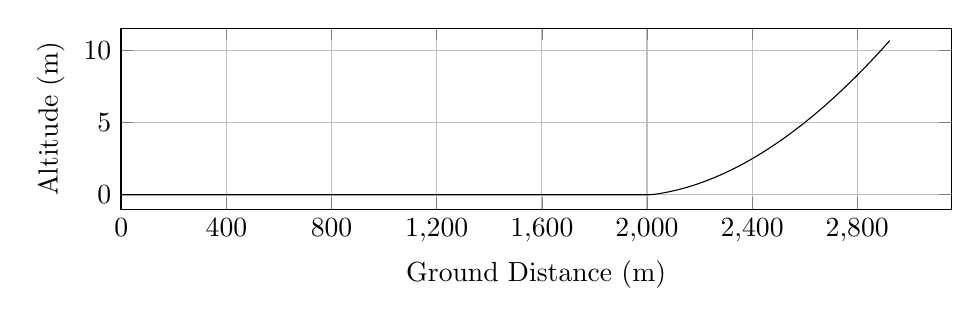
\begin{tikzpicture}

\begin{axis}[
width=\textwidth,
height=0.32\textwidth,
scaled ticks=false, tick label style={/pgf/number format/fixed},
xmin=-1.0,
xmax=3157.694840416415,
xtick={0,400,800,1200,1600,2000,2400,2800,3200},
xlabel={Ground Distance (m)},
xmajorgrids,
ymin=-1.0,
ymax=11.52144,
ylabel={Altitude (m)},
ymajorgrids,
legend style={at={(1.03,0.5)},anchor=west,draw=black,fill=white,legend cell align=left}
]

\addplot [
color=black,
solid
]
table[row sep=crcr]{
1.3603393307216043E-8	0.0\\
3.0265395163403265E-7	0.0\\
2.9593179127983543E-6	0.0\\
1.5392338359717934E-5	0.0\\
5.361280674027254E-5	0.0\\
1.6215010178508227E-4	0.0\\
3.7214145765703975E-4	0.0\\
6.839954676020354E-4	0.0\\
0.001098342709021993	0.0\\
0.001609317716481928	0.0\\
0.0022198920000388346	0.0\\
0.002878710694837372	0.0\\
0.0036835072341781794	0.0\\
0.004557929017412697	0.0\\
0.005559798278933152	0.0\\
0.006651227400597502	0.0\\
0.007795849738889277	0.0\\
0.009067984722810115	0.0\\
0.010453165799939174	0.0\\
0.011915708813158052	0.0\\
0.013455030027058647	0.0\\
0.015131183092671713	0.0\\
0.01690803412933615	0.0\\
0.01873590105740728	0.0\\
0.020713359121301934	0.0\\
0.022777736728155237	0.0\\
0.024960970145273077	0.0\\
0.02723428625014468	0.0\\
0.029610395797831278	0.0\\
0.03204086105441677	0.0\\
0.03462344565878624	0.0\\
0.037295727153354774	0.0\\
0.040089145853872785	0.0\\
0.042950967781251806	0.0\\
0.04592022141655751	0.0\\
0.04897301836205646	0.0\\
0.052130294957187476	0.0\\
0.05542514139564195	0.0\\
0.05879722600804832	0.0\\
0.06231520981015182	0.0\\
0.06596261503753809	0.0\\
0.06964559414821356	0.0\\
0.07347193989652406	0.0\\
0.07736619052035826	0.0\\
0.08137137577670908	0.0\\
0.08545617869345057	0.0\\
0.08969468676038628	0.0\\
0.0940095881391464	0.0\\
0.09845059220533334	0.0\\
0.10296315144049947	0.0\\
0.10759658895065366	0.0\\
0.1123317495250277	0.0\\
0.1171874363557737	0.0\\
0.12217670360507671	0.0\\
0.12726806426274867	0.0\\
0.13231647880291775	0.0\\
0.13765212084557643	0.0\\
0.14294844966167852	0.0\\
0.14834594087957392	0.0\\
0.1539671093411843	0.0\\
0.15968242883369804	0.0\\
0.16555834796315422	0.0\\
0.17157514414202774	0.0\\
0.17760320215284392	0.0\\
0.18370335474801935	0.0\\
0.18983540939776816	0.0\\
0.19621099073945342	0.0\\
0.20278841209744758	0.0\\
0.20952923284938563	0.0\\
0.21624967405074952	0.0\\
0.22309476488450758	0.0\\
0.22992510727843934	0.0\\
0.2371653034562048	0.0\\
0.2442573187228817	0.0\\
0.25144286317780873	0.0\\
0.2588001799723505	0.0\\
0.2662612189130884	0.0\\
0.27386560463063747	0.0\\
0.2815803271719757	0.0\\
0.28946218069394425	0.0\\
0.29753588720841584	0.0\\
0.3056643119969481	0.0\\
0.31376446154764137	0.0\\
0.322071411728719	0.0\\
0.3303680011285137	0.0\\
0.3389039548234316	0.0\\
0.3474123396293025	0.0\\
0.3561645174790815	0.0\\
0.36525289600634137	0.0\\
0.3742306244196095	0.0\\
0.3835584127627333	0.0\\
0.392806747202999	0.0\\
0.40218604538039837	0.0\\
0.4115907129344223	0.0\\
0.42143744457304466	0.0\\
0.4310567075016639	0.0\\
0.4412814114336725	0.0\\
0.4513051702487684	0.0\\
0.461412558308395	0.0\\
0.47173637532167356	0.0\\
0.4821484569390513	0.0\\
0.492985116277161	0.0\\
0.5036221628177362	0.0\\
0.5142245311302887	0.0\\
0.5252888808291518	0.0\\
0.5363145235987512	0.0\\
0.5471208511184944	0.0\\
0.5585110457184732	0.0\\
0.569849942463402	0.0\\
0.5817265165330987	0.0\\
0.5935668742733842	0.0\\
0.6053719027871456	0.0\\
0.6172343027602503	0.0\\
0.629515267228629	0.0\\
0.6417789549774502	0.0\\
0.6542768803188956	0.0\\
0.6669828212214572	0.0\\
0.6796225285147333	0.0\\
0.6925094233679154	0.0\\
0.7056620711738308	0.0\\
0.7184715206768946	0.0\\
0.731725241748566	0.0\\
0.7449880440563246	0.0\\
0.7586792333483576	0.0\\
0.7725063377467813	0.0\\
0.7863894274138714	0.0\\
0.8004504964383841	0.0\\
0.8147129313117618	0.0\\
0.8293722635741907	0.0\\
0.8437954335339908	0.0\\
0.8580702287827062	0.0\\
0.8726489666047585	0.0\\
0.8875094051704782	0.0\\
0.9027740629895862	0.0\\
0.9182163910703112	0.0\\
0.93361566230532	0.0\\
0.9491799633800446	0.0\\
0.9646343064330896	0.0\\
0.9803727456894022	0.0\\
0.9957421603273868	0.0\\
1.0116767859397604	0.0\\
1.028041387324289	0.0\\
1.0443915011410971	0.0\\
1.060796374175649	0.0\\
1.0773229908740651	0.0\\
1.093971735592782	0.0\\
1.1110062543639518	0.0\\
1.127891796882146	0.0\\
1.1451224507351285	0.0\\
1.1624801114435046	0.0\\
1.180077727863539	0.0\\
1.1978884766667508	0.0\\
1.215488397439855	0.0\\
1.23351701382096	0.0\\
1.2518199984626128	0.0\\
1.2704235066044305	0.0\\
1.2892140278280424	0.0\\
1.3075714306593595	0.0\\
1.3266673518109293	0.0\\
1.3462106477188795	0.0\\
1.365306294594515	0.0\\
1.3852885894463176	0.0\\
1.404835539176236	0.0\\
1.4251192118409102	0.0\\
1.445164519989187	0.0\\
1.4656054698512246	0.0\\
1.4853522740259328	0.0\\
1.5051589726327936	0.0\\
1.5255757775517242	0.0\\
1.5464367798307013	0.0\\
1.5673163741652552	0.0\\
1.5879032567231621	0.0\\
1.6091523485848285	0.0\\
1.6303162371862876	0.0\\
1.6519474169970438	0.0\\
1.673879209980242	0.0\\
1.6955666802836635	0.0\\
1.7172271378534343	0.0\\
1.7402832823543353	0.0\\
1.7634396102400074	0.0\\
1.7861669372425006	0.0\\
1.8088678577734645	0.0\\
1.831824248135399	0.0\\
1.855578771396016	0.0\\
1.878960729162178	0.0\\
1.9033179534858085	0.0\\
1.9273833213731866	0.0\\
1.9518510462308036	0.0\\
1.9761594732990155	0.0\\
2.000437267212291	0.0\\
2.0252281699074732	0.0\\
2.0498006073458734	0.0\\
2.0745611186355752	0.0\\
2.0997746990963106	0.0\\
2.1260324099367294	0.0\\
2.1515212193659616	0.0\\
2.1771505246334	0.0\\
2.2031842637813908	0.0\\
2.230133398733474	0.0\\
2.257053086628849	0.0\\
2.283795213136285	0.0\\
2.311477064851834	0.0\\
2.3387199014446116	0.0\\
2.3662694524467227	0.0\\
2.3937852540088533	0.0\\
2.4216520071021392	0.0\\
2.4501931244916175	0.0\\
2.478927626230634	0.0\\
2.506685441631536	0.0\\
2.53537335014481	0.0\\
2.5633350931805676	0.0\\
2.5917889242519685	0.0\\
2.6208221472873374	0.0\\
2.649872764173903	0.0\\
2.679661174525658	0.0\\
2.709174609939316	0.0\\
2.740029385016756	0.0\\
2.770444625703795	0.0\\
2.801129860621211	0.0\\
2.8318827297715705	0.0\\
2.862425967677578	0.0\\
2.893259332541544	0.0\\
2.92412139403754	0.0\\
2.955064430161417	0.0\\
2.986690331721131	0.0\\
3.019183403261743	0.0\\
3.0507201588152526	0.0\\
3.0830332871979023	0.0\\
3.1154603869692448	0.0\\
3.148592095396281	0.0\\
3.181936872739324	0.0\\
3.214370607724433	0.0\\
3.247565473366384	0.0\\
3.281695868027062	0.0\\
3.316494330618462	0.0\\
3.3513055302544137	0.0\\
3.3860303583611797	0.0\\
3.421934361445942	0.0\\
3.456235826539576	0.0\\
3.490536654441657	0.0\\
3.526257338581564	0.0\\
3.561372823896762	0.0\\
3.5967906564503185	0.0\\
3.632682576242373	0.0\\
3.6701261071689295	0.0\\
3.707701291513044	0.0\\
3.7452745323452916	0.0\\
3.78256482255855	0.0\\
3.8208821591411084	0.0\\
3.8590337549211444	0.0\\
3.89695718563138	0.0\\
3.9351036745073964	0.0\\
3.9736642086653067	0.0\\
4.012189127077221	0.0\\
4.05156219172609	0.0\\
4.090290786278251	0.0\\
4.129291984889424	0.0\\
4.1680648628189925	0.0\\
4.207805169621487	0.0\\
4.248168240749736	0.0\\
4.288797880674668	0.0\\
4.32990243544832	0.0\\
4.371428084678056	0.0\\
4.41247037137882	0.0\\
4.453879445321437	0.0\\
4.49524783594077	0.0\\
4.537299342543221	0.0\\
4.580546125800922	0.0\\
4.622914948498307	0.0\\
4.66640222022569	0.0\\
4.709294790611851	0.0\\
4.752417172855319	0.0\\
4.796155651503765	0.0\\
4.8408754796551925	0.0\\
4.884850997559644	0.0\\
4.928651138956553	0.0\\
4.972831351372241	0.0\\
5.017331702752941	0.0\\
5.0632326321008225	0.0\\
5.108452384314601	0.0\\
5.1536021218025905	0.0\\
5.199057463234675	0.0\\
5.244479287100011	0.0\\
5.292293005248643	0.0\\
5.338096108273211	0.0\\
5.3857492800262605	0.0\\
5.433816232374781	0.0\\
5.480691139018431	0.0\\
5.529685763332537	0.0\\
5.578612887337309	0.0\\
5.626451501744754	0.0\\
5.674834544150631	0.0\\
5.7252048440372345	0.0\\
5.77422346516266	0.0\\
5.8255152536468575	0.0\\
5.874338256646894	0.0\\
5.922631450506765	0.0\\
5.972682300942642	0.0\\
6.022535370757359	0.0\\
6.074394648705015	0.0\\
6.124928192945902	0.0\\
6.176798284396469	0.0\\
6.229620191179453	0.0\\
6.282808156696705	0.0\\
6.334658925277093	0.0\\
6.388041948821611	0.0\\
6.440558117792513	0.0\\
6.494960924490993	0.0\\
6.550441697666145	0.0\\
6.6042098433346865	0.0\\
6.658315220792536	0.0\\
6.712335084641163	0.0\\
6.766674450459032	0.0\\
6.821537769035839	0.0\\
6.876851268142238	0.0\\
6.933661362437203	0.0\\
6.989261882852809	0.0\\
7.046240323930029	0.0\\
7.102786137967051	0.0\\
7.1603789170469145	0.0\\
7.21785165788507	0.0\\
7.277487498606879	0.0\\
7.334984696129153	0.0\\
7.393362172524569	0.0\\
7.452416393609804	0.0\\
7.511934748111884	0.0\\
7.572557225035805	0.0\\
7.63202184821041	0.0\\
7.69294899409779	0.0\\
7.752675521499926	0.0\\
7.814488876138199	0.0\\
7.8763528528159785	0.0\\
7.938149975125226	0.0\\
8.001193143199774	0.0\\
8.064554080136986	0.0\\
8.12686567918485	0.0\\
8.189637855946287	0.0\\
8.252542711798306	0.0\\
8.315859663763469	0.0\\
8.380006162932737	0.0\\
8.444702551512929	0.0\\
8.509501986620958	0.0\\
8.57387297516295	0.0\\
8.63887365699837	0.0\\
8.70727085773305	0.0\\
8.772937378995405	0.0\\
8.839192134487615	0.0\\
8.905815929161982	0.0\\
8.97209054442786	0.0\\
9.039019026885107	0.0\\
9.107371801018814	0.0\\
9.174915633685494	0.0\\
9.243868961478196	0.0\\
9.312440636565494	0.0\\
9.381784695008012	0.0\\
9.4513167952828	0.0\\
9.52142787533916	0.0\\
9.591425279059166	0.0\\
9.662230428326719	0.0\\
9.734225879912522	0.0\\
9.806441602430919	0.0\\
9.878483835105534	0.0\\
9.951807209049782	0.0\\
10.023539677466466	0.0\\
10.096057433179052	0.0\\
10.168262179450682	0.0\\
10.241274410624943	0.0\\
10.31479015323385	0.0\\
10.390063469390178	0.0\\
10.465012435634037	0.0\\
10.540639152111389	0.0\\
10.617644389866598	0.0\\
10.692945462162374	0.0\\
10.770083295573727	0.0\\
10.846726862770723	0.0\\
10.924657809445929	0.0\\
11.00265335491597	0.0\\
11.081827589833612	0.0\\
11.159134327011738	0.0\\
11.239152720133266	0.0\\
11.317028257314295	0.0\\
11.396413369884492	0.0\\
11.477655063362434	0.0\\
11.556958506738276	0.0\\
11.637325199769407	0.0\\
11.717754170658207	0.0\\
11.799819443100102	0.0\\
11.881986970940797	0.0\\
11.964394119506721	0.0\\
12.046263329632716	0.0\\
12.130282587748898	0.0\\
12.213721087180826	0.0\\
12.295868535962462	0.0\\
12.380692430046633	0.0\\
12.46470288467437	0.0\\
12.550384439940181	0.0\\
12.635259749824865	0.0\\
12.72144647897981	0.0\\
12.80741162779486	0.0\\
12.892901506907108	0.0\\
12.977815703098727	0.0\\
13.06483740414145	0.0\\
13.151922956503014	0.0\\
13.240589045456186	0.0\\
13.329911181207382	0.0\\
13.417306166647748	0.0\\
13.507103029723119	0.0\\
13.595986036712912	0.0\\
13.687453390597003	0.0\\
13.779071846306106	0.0\\
13.872694200363323	0.0\\
13.963504841252302	0.0\\
14.056146454975131	0.0\\
14.14918846816267	0.0\\
14.24332804549016	0.0\\
14.339261112049854	0.0\\
14.431091301610323	0.0\\
14.524174633942373	0.0\\
14.618760344060338	0.0\\
14.714801736988441	0.0\\
14.809763128346521	0.0\\
14.903412319659619	0.0\\
15.001392651385917	0.0\\
15.098055049922994	0.0\\
15.196870856960619	0.0\\
15.29477342819068	0.0\\
15.39265348361268	0.0\\
15.490487151984588	0.0\\
15.588146853189365	0.0\\
15.687961867268871	0.0\\
15.78650099417861	0.0\\
15.886965864441798	0.0\\
15.98755318095926	0.0\\
16.088470385762115	0.0\\
16.190536977381747	0.0\\
16.292466610053154	0.0\\
16.396448349404487	0.0\\
16.497808944935016	0.0\\
16.600551072850564	0.0\\
16.70575139586156	0.0\\
16.81134459259622	0.0\\
16.917616592554033	0.0\\
17.023477948501657	0.0\\
17.12904978140002	0.0\\
17.2354081519902	0.0\\
17.340772011500363	0.0\\
17.448391076872838	0.0\\
17.5571980918308	0.0\\
17.66615596614949	0.0\\
17.774685459577412	0.0\\
17.884986575683584	0.0\\
17.99552903728076	0.0\\
18.108708479124623	0.0\\
18.219646262474413	0.0\\
18.332680252669796	0.0\\
18.445061806396694	0.0\\
18.556709221711323	0.0\\
18.668884868236475	0.0\\
18.78204748093455	0.0\\
18.895704562363058	0.0\\
19.008928234289563	0.0\\
19.124320907419907	0.0\\
19.24105855786135	0.0\\
19.355116774466126	0.0\\
19.470462572962035	0.0\\
19.58492145104516	0.0\\
19.704921229319112	0.0\\
19.821259826163917	0.0\\
19.941172080873493	0.0\\
20.06078806851737	0.0\\
20.177423389922623	0.0\\
20.297621170678	0.0\\
20.420129559802255	0.0\\
20.54164670774839	0.0\\
20.661905244258705	0.0\\
20.784301666224792	0.0\\
20.904244540623438	0.0\\
21.028114340450195	0.0\\
21.148300883955606	0.0\\
21.270875420257596	0.0\\
21.39299406946177	0.0\\
21.513793771711654	0.0\\
21.637476506915142	0.0\\
21.759279707150128	0.0\\
21.88493035745168	0.0\\
22.009809790007786	0.0\\
22.13620730934617	0.0\\
22.263515470260465	0.0\\
22.393040471753594	0.0\\
22.520519759768852	0.0\\
22.648852607677917	0.0\\
22.775118904521122	0.0\\
22.903136237443974	0.0\\
23.03176118514304	0.0\\
23.162501585272054	0.0\\
23.294719932439598	0.0\\
23.427108470281937	0.0\\
23.558693146983046	0.0\\
23.687077503630363	0.0\\
23.817949558665852	0.0\\
23.948210788889448	0.0\\
24.076877750667826	0.0\\
24.21019765060587	0.0\\
24.3450673155249	0.0\\
24.477101355489637	0.0\\
24.60984760833776	0.0\\
24.7468403923846	0.0\\
24.882807251950062	0.0\\
25.017167332957627	0.0\\
25.153910941279605	0.0\\
25.289629217480112	0.0\\
25.425306692573436	0.0\\
25.56229499031975	0.0\\
25.70075944713021	0.0\\
25.83724158708921	0.0\\
25.975209935932874	0.0\\
26.003074150630965	0.0\\
26.020759913393235	0.0\\
26.030714598210515	0.0\\
26.05840292223249	0.0\\
26.06133765907019	0.0\\
26.064285136409026	0.0\\
26.066337724202356	0.0\\
26.068175973881182	0.0\\
26.06984477238784	0.0\\
26.077831036047115	0.0\\
26.10345636352254	0.0\\
26.16716044512971	0.0\\
26.297541524199602	0.0\\
26.42722303713863	0.0\\
26.5559280656694	0.0\\
26.686097387723095	0.0\\
26.817793678842584	0.0\\
26.949416928520378	0.0\\
27.080440623797912	0.0\\
27.215491080424528	0.0\\
27.34795890217076	0.0\\
27.48215578365496	0.0\\
27.616696052324144	0.0\\
27.75271189183823	0.0\\
27.888759310501555	0.0\\
28.023839122857026	0.0\\
28.16136324828667	0.0\\
28.298355249881332	0.0\\
28.435282447697354	0.0\\
28.573941346212784	0.0\\
28.713752690797136	0.0\\
28.852681198061333	0.0\\
28.992471984120606	0.0\\
29.133421724605903	0.0\\
29.275199211812186	0.0\\
29.416225289053614	0.0\\
29.55783477945603	0.0\\
29.701838356359822	0.0\\
29.846633046394217	0.0\\
29.99013730470424	0.0\\
30.132492646908446	0.0\\
30.277395768405135	0.0\\
30.422188862471998	0.0\\
30.56637548064623	0.0\\
30.711944318924978	0.0\\
30.8573377156769	0.0\\
31.006558691603843	0.0\\
31.153907258126303	0.0\\
31.30257185742142	0.0\\
31.4510947803754	0.0\\
31.602595106592503	0.0\\
31.755261577184278	0.0\\
31.906398416479824	0.0\\
32.05599258457312	0.0\\
32.20952926265106	0.0\\
32.360097140052986	0.0\\
32.51218835243483	0.0\\
32.664721606344784	0.0\\
32.82129760777845	0.0\\
32.97669884718651	0.0\\
33.13118849606322	0.0\\
33.288837444683736	0.0\\
33.44405554194745	0.0\\
33.60015866510213	0.0\\
33.756686089655645	0.0\\
33.91694077595571	0.0\\
34.074326811338736	0.0\\
34.23252403098988	0.0\\
34.392884168270385	0.0\\
34.554266068788166	0.0\\
34.71363140184178	0.0\\
34.87649332318763	0.0\\
35.03746231629111	0.0\\
35.19990059234286	0.0\\
35.3627309111595	0.0\\
35.5271254050015	0.0\\
35.69149466827288	0.0\\
35.85508342515686	0.0\\
36.017180984292054	0.0\\
36.182222084544165	0.0\\
36.34861175093968	0.0\\
36.514166392421686	0.0\\
36.68083924241549	0.0\\
36.845526722294395	0.0\\
37.01328249159678	0.0\\
37.18160982421668	0.0\\
37.35136716620059	0.0\\
37.51969289597564	0.0\\
37.689710015857784	0.0\\
37.860394939778416	0.0\\
38.02805196867635	0.0\\
38.19868492919754	0.0\\
38.37343039987371	0.0\\
38.54685896696101	0.0\\
38.71934233168869	0.0\\
38.8915617091798	0.0\\
39.062305982326905	0.0\\
39.23847188392709	0.0\\
39.411511502305984	0.0\\
39.585172817779906	0.0\\
39.760693028009456	0.0\\
39.9373134006328	0.0\\
40.113617753210534	0.0\\
40.29094651898711	0.0\\
40.468149621311596	0.0\\
40.64593210594187	0.0\\
40.82431302355218	0.0\\
41.00141330502653	0.0\\
41.17957893337042	0.0\\
41.359761290266974	0.0\\
41.53889737920997	0.0\\
41.72013507746885	0.0\\
41.899395797464194	0.0\\
42.081280067494475	0.0\\
42.265315320939635	0.0\\
42.44531744651641	0.0\\
42.62715102096499	0.0\\
42.81120266452106	0.0\\
42.994164503876235	0.0\\
43.17799769459725	0.0\\
43.36154361404071	0.0\\
43.54597437124032	0.0\\
43.73158498218817	0.0\\
43.91737182308138	0.0\\
44.1050494697441	0.0\\
44.293574236233	0.0\\
44.47888581456586	0.0\\
44.66456251492659	0.0\\
44.85170130968709	0.0\\
45.037822074257164	0.0\\
45.22676109993536	0.0\\
45.41612608476639	0.0\\
45.604812217355104	0.0\\
45.79422221198037	0.0\\
45.98724683785376	0.0\\
46.17830917717477	0.0\\
46.36786657808848	0.0\\
46.55935209439748	0.0\\
46.75090376717816	0.0\\
46.94233405988251	0.0\\
47.13714948644359	0.0\\
47.33387512950824	0.0\\
47.53043319838464	0.0\\
47.72298239739284	0.0\\
47.919150009665316	0.0\\
48.113386178114425	0.0\\
48.311024807628144	0.0\\
48.508886059616145	0.0\\
48.70490444306449	0.0\\
48.90290918859142	0.0\\
49.09959709013448	0.0\\
49.2970021191946	0.0\\
49.49532701226336	0.0\\
49.693780717172615	0.0\\
49.89506320355713	0.0\\
50.096719083698545	0.0\\
50.29606895218413	0.0\\
50.497598474286534	0.0\\
50.700304208193415	0.0\\
50.90342397924904	0.0\\
51.10460922167407	0.0\\
51.30752217039489	0.0\\
51.51010619677311	0.0\\
51.713602501430145	0.0\\
51.91843850546792	0.0\\
52.121089026646246	0.0\\
52.32561402362407	0.0\\
52.53192272805477	0.0\\
52.7387030603267	0.0\\
52.944027344085896	0.0\\
53.154073670302836	0.0\\
53.36143953271798	0.0\\
53.571009444677685	0.0\\
53.77799762982136	0.0\\
53.98785945427545	0.0\\
54.196157549666225	0.0\\
54.40718762937186	0.0\\
54.616887598525366	0.0\\
54.826875464266934	0.0\\
55.04038432082807	0.0\\
55.25438844036796	0.0\\
55.46695867894975	0.0\\
55.68088820258777	0.0\\
55.895144656119854	0.0\\
56.109028395418505	0.0\\
56.326262430904194	0.0\\
56.542089933321776	0.0\\
56.76060076462056	0.0\\
56.97729209122687	0.0\\
57.19579178641709	0.0\\
57.41258192878804	0.0\\
57.634093277561306	0.0\\
57.85395098827546	0.0\\
58.07448819514299	0.0\\
58.29446478173499	0.0\\
58.51588770709739	0.0\\
58.73757884137123	0.0\\
58.96020041504734	0.0\\
59.18267120664716	0.0\\
59.405949655899676	0.0\\
59.63089974393067	0.0\\
59.8562534200115	0.0\\
60.084134136581554	0.0\\
60.30833762904015	0.0\\
60.53504725699203	0.0\\
60.763693228044005	0.0\\
60.99075593752245	0.0\\
61.21765734918529	0.0\\
61.44713116872772	0.0\\
61.6738048454246	0.0\\
61.90668490141796	0.0\\
62.13729676517957	0.0\\
62.36629463006145	0.0\\
62.596359157213186	0.0\\
62.82836101237727	0.0\\
63.059723307860466	0.0\\
63.292774394726166	0.0\\
63.52608473446321	0.0\\
63.75973181411028	0.0\\
63.993403028653574	0.0\\
64.23068717493263	0.0\\
64.4710952259949	0.0\\
64.70858695601663	0.0\\
64.94894296164699	0.0\\
65.18738841845183	0.0\\
65.42661162888535	0.0\\
65.6659442133793	0.0\\
65.90899583190168	0.0\\
66.15068261105333	0.0\\
66.39533053734849	0.0\\
66.6378997293487	0.0\\
66.88158418814953	0.0\\
67.12390450547147	0.0\\
67.36840986262189	0.0\\
67.61550053739396	0.0\\
67.86097385246623	0.0\\
68.10985741250389	0.0\\
68.35582503705197	0.0\\
68.60464259362828	0.0\\
68.85450289166104	0.0\\
69.1042877596268	0.0\\
69.35837572129628	0.0\\
69.61150655903072	0.0\\
69.86289252102952	0.0\\
70.11686816207683	0.0\\
70.37125759672608	0.0\\
70.62480458144697	0.0\\
70.88045310059783	0.0\\
71.13526709211152	0.0\\
71.3947754873567	0.0\\
71.6534187996231	0.0\\
71.91450497256008	0.0\\
72.1716184080999	0.0\\
72.43269265097052	0.0\\
72.69331619504374	0.0\\
72.95563200429567	0.0\\
73.21686762735783	0.0\\
73.48161420086069	0.0\\
73.74261486234883	0.0\\
74.00755043430098	0.0\\
74.27511769675363	0.0\\
74.54487113507057	0.0\\
74.81568229507957	0.0\\
75.08274085953312	0.0\\
75.35421836228127	0.0\\
75.62798354862159	0.0\\
75.89909469738902	0.0\\
76.17008148658607	0.0\\
76.44269151183332	0.0\\
76.71571902594138	0.0\\
76.99340852183178	0.0\\
77.27004772085374	0.0\\
77.54832408953641	0.0\\
77.82592519882277	0.0\\
78.10358246820337	0.0\\
78.38556010231375	0.0\\
78.66911430382748	0.0\\
78.95399134982776	0.0\\
79.23667137346987	0.0\\
79.518907793654	0.0\\
79.80555437718249	0.0\\
80.09150103324356	0.0\\
80.37928873457926	0.0\\
80.66871996946384	0.0\\
80.95967699414447	0.0\\
81.25093884305389	0.0\\
81.54344278085921	0.0\\
81.8358102960415	0.0\\
82.13087592438694	0.0\\
82.42794520371837	0.0\\
82.72842933895026	0.0\\
83.0269479931649	0.0\\
83.32974506690314	0.0\\
83.62964811531441	0.0\\
83.92951211009506	0.0\\
84.2339319847595	0.0\\
84.53715838283946	0.0\\
84.84105485927768	0.0\\
85.14845677960258	0.0\\
85.45530133949276	0.0\\
85.76249773413784	0.0\\
86.07201271349416	0.0\\
86.38432073331904	0.0\\
86.69710203601804	0.0\\
87.01172103282082	0.0\\
87.32669099459858	0.0\\
87.64517025121202	0.0\\
87.96158123090564	0.0\\
88.2775814178033	0.0\\
88.60068374099544	0.0\\
88.92068281935622	0.0\\
89.24207276858638	0.0\\
89.56578933015979	0.0\\
89.88760090270688	0.0\\
90.2141410750086	0.0\\
90.54066676000363	0.0\\
90.86727570256076	0.0\\
91.19715108614633	0.0\\
91.52744226539704	0.0\\
91.85639956214655	0.0\\
92.19095740864739	0.0\\
92.52827526888461	0.0\\
92.8674718219292	0.0\\
93.20307982994817	0.0\\
93.5374944579234	0.0\\
93.87598013161067	0.0\\
94.20917297854535	0.0\\
94.55043409744499	0.0\\
94.89132963816093	0.0\\
95.23083207736542	0.0\\
95.57395676502793	0.0\\
95.91421223354143	0.0\\
96.25656086122288	0.0\\
96.60012122339742	0.0\\
96.94166303707107	0.0\\
97.28627502929558	0.0\\
97.62906225262071	0.0\\
97.97125437026659	0.0\\
98.31201772458999	0.0\\
98.65627175165852	0.0\\
99.0012536203806	0.0\\
99.35020029285332	0.0\\
99.69475740907401	0.0\\
100.04053871990226	0.0\\
100.38598466112728	0.0\\
100.72867962848932	0.0\\
101.07385499050397	0.0\\
101.41864366415388	0.0\\
101.76305460768467	0.0\\
102.11068844700483	0.0\\
102.45638678530696	0.0\\
102.79841653079728	0.0\\
103.14087212494877	0.0\\
103.48486473791618	0.0\\
103.82875595362174	0.0\\
104.17244250654872	0.0\\
104.51168383396202	0.0\\
104.85986244643053	0.0\\
105.204587526496	0.0\\
105.54754777175077	0.0\\
105.88797456536247	0.0\\
106.23280177240994	0.0\\
106.57515110440406	0.0\\
106.91603555764121	0.0\\
107.25729565943405	0.0\\
107.598830149446	0.0\\
107.93686571059558	0.0\\
108.27485499032852	0.0\\
108.28839963475954	0.0\\
108.30004107281309	0.0\\
108.30931238392475	0.0\\
108.31701527366243	0.0\\
108.32505202073054	0.0\\
108.33865239118708	0.0\\
108.35091925899997	0.0\\
108.39508146726081	0.0\\
108.52984553865659	0.0\\
108.79919793188978	0.0\\
109.105233418432	0.0\\
109.41485218466596	0.0\\
109.72257164661937	0.0\\
110.0321119530083	0.0\\
110.34145354075926	0.0\\
110.6534776714839	0.0\\
110.9711963390063	0.0\\
111.28851843247409	0.0\\
111.60893519474632	0.0\\
111.92798394282838	0.0\\
112.24770070245137	0.0\\
112.57243448635171	0.0\\
112.89480865389396	0.0\\
113.22000325235314	0.0\\
113.54885709436653	0.0\\
113.8770619430189	0.0\\
114.20946079557197	0.0\\
114.54107775051554	0.0\\
114.87787736567807	0.0\\
115.21564640021248	0.0\\
115.55522358014255	0.0\\
115.89667501383605	0.0\\
116.23992536102014	0.0\\
116.5847156213415	0.0\\
116.92791619634093	0.0\\
117.27517516660399	0.0\\
117.62420948631524	0.0\\
117.97391125359778	0.0\\
118.32673409155768	0.0\\
118.68227803698588	0.0\\
119.03889207644076	0.0\\
119.39651249432902	0.0\\
119.75508651978987	0.0\\
120.11314113323388	0.0\\
120.47404637453192	0.0\\
120.84098349318353	0.0\\
121.20490030977416	0.0\\
121.57328571082118	0.0\\
121.94079100066682	0.0\\
122.31015242291167	0.0\\
122.68267403243519	0.0\\
123.05346836176264	0.0\\
123.42835733050345	0.0\\
123.80350972566416	0.0\\
124.1783235941891	0.0\\
124.55244040146786	0.0\\
124.92576251095704	0.0\\
125.30489170817492	0.0\\
125.68146781278597	0.0\\
126.06139977608174	0.0\\
126.44502763856761	0.0\\
126.82695116404781	0.0\\
127.206716044588	0.0\\
127.59262031825523	0.0\\
127.97077035934353	0.0\\
128.3546122768156	0.0\\
128.73724861847296	0.0\\
129.12002064685282	0.0\\
129.50086700331673	0.0\\
129.8837789976152	0.0\\
130.26783132854348	0.0\\
130.651936341801	0.0\\
131.03747321415574	0.0\\
131.42280335891803	0.0\\
131.80875442588928	0.0\\
132.19322104975072	0.0\\
132.5798881414172	0.0\\
132.96215446290768	0.0\\
133.34488286943906	0.0\\
133.7276157954845	0.0\\
134.11532375481391	0.0\\
134.50135826447365	0.0\\
134.88604120201086	0.0\\
135.26955723714872	0.0\\
135.6512109336153	0.0\\
136.03464327936558	0.0\\
136.41686422877552	0.0\\
136.79904942565338	0.0\\
137.18004416157777	0.0\\
137.56399804528928	0.0\\
137.94515347717788	0.0\\
138.32982901897384	0.0\\
138.7128522769853	0.0\\
139.09597564505458	0.0\\
139.48002685240425	0.0\\
139.86309097971855	0.0\\
140.24727738828375	0.0\\
140.6317581809211	0.0\\
141.01585725597846	0.0\\
141.3998433603236	0.0\\
141.7841907991213	0.0\\
142.16710976343057	0.0\\
142.55205218648928	0.0\\
142.9364233092117	0.0\\
143.32169829765928	0.0\\
143.705984531242	0.0\\
144.08985428249122	0.0\\
144.47683600496026	0.0\\
144.86371007721533	0.0\\
145.24772592056325	0.0\\
145.63047789911974	0.0\\
146.01273254364395	0.0\\
146.39725173307323	0.0\\
146.77966503747456	0.0\\
147.16478130736948	0.0\\
147.54689717238745	0.0\\
147.93097497792814	0.0\\
148.31499270913332	0.0\\
148.69957284780122	0.0\\
149.08709998577143	0.0\\
149.47129868208145	0.0\\
149.8546635899794	0.0\\
150.23801379389647	0.0\\
150.62200569343076	0.0\\
151.00751012558203	0.0\\
151.3946455315429	0.0\\
151.77987817077866	0.0\\
152.16505704867353	0.0\\
152.55112759502248	0.0\\
152.93964308710213	0.0\\
153.32507651584535	0.0\\
153.71174813432617	0.0\\
154.10000329570875	0.0\\
154.48914219495543	0.0\\
154.8788297075107	0.0\\
155.26820650111182	0.0\\
155.6562915247282	0.0\\
156.0441896603637	0.0\\
156.4348678136667	0.0\\
156.82082928279863	0.0\\
157.21071017196311	0.0\\
157.60005066896917	0.0\\
157.99004282467217	0.0\\
158.3808231456182	0.0\\
158.77280374485122	0.0\\
159.16384255262415	0.0\\
159.55370941764693	0.0\\
159.946071590523	0.0\\
160.33752628124114	0.0\\
160.73008933968674	0.0\\
161.12428312893906	0.0\\
161.5185576482712	0.0\\
161.91431288671106	0.0\\
162.3096877663487	0.0\\
162.70613442998513	0.0\\
163.1032465869576	0.0\\
163.50039135636405	0.0\\
163.89625578410926	0.0\\
164.29272443146095	0.0\\
164.68754921345175	0.0\\
165.0864466423082	0.0\\
165.4846753800681	0.0\\
165.88329117400662	0.0\\
166.28234792206388	0.0\\
166.68312204436222	0.0\\
167.08520211103445	0.0\\
167.486487681752	0.0\\
167.8888620337579	0.0\\
168.290121631074	0.0\\
168.69179641444674	0.0\\
169.0966267258019	0.0\\
169.50108473093724	0.0\\
169.90729482190739	0.0\\
170.31243922775104	0.0\\
170.71755979953144	0.0\\
171.12402986296422	0.0\\
171.53319587512163	0.0\\
171.941770038195	0.0\\
172.3502931259835	0.0\\
172.7599322859847	0.0\\
173.17073308198894	0.0\\
173.58266371319877	0.0\\
173.99296569000023	0.0\\
174.40104722187203	0.0\\
174.8156903853216	0.0\\
175.2299479185392	0.0\\
175.64260521584504	0.0\\
176.05374721710058	0.0\\
176.4688147253861	0.0\\
176.8832117842232	0.0\\
177.30033423294157	0.0\\
177.7185234955238	0.0\\
178.13477925276436	0.0\\
178.55472625996282	0.0\\
178.97486541267733	0.0\\
179.39652032378837	0.0\\
179.8177496461559	0.0\\
180.24148986351946	0.0\\
180.66579793025812	0.0\\
181.08977314985765	0.0\\
181.5138518510159	0.0\\
181.61122522885114	0.0\\
181.9380657232258	0.0\\
182.36340272554946	0.0\\
183.2082724125376	0.0\\
184.08646972066333	0.0\\
184.96448881265883	0.0\\
185.84629357991815	0.0\\
186.726051310566	0.0\\
187.61806497534428	0.0\\
188.50412524941663	0.0\\
189.3932804644195	0.0\\
190.28280340229105	0.0\\
191.1758490733834	0.0\\
192.0664158070755	0.0\\
192.96248081795437	0.0\\
193.85627821989942	0.0\\
194.7612747993291	0.0\\
195.67115393765977	0.0\\
196.57439968482538	0.0\\
197.49109477617128	0.0\\
198.40328264870095	0.0\\
199.32142764481148	0.0\\
200.23456840248758	0.0\\
201.14898042779765	0.0\\
202.06794236074546	0.0\\
202.98618556976356	0.0\\
203.9096776069573	0.0\\
204.83478510422236	0.0\\
205.76152187560933	0.0\\
206.69425456631774	0.0\\
207.628282006662	0.0\\
208.55982483556244	0.0\\
209.49858617709037	0.0\\
210.43993621334516	0.0\\
211.37516676315846	0.0\\
212.31832896164838	0.0\\
213.2711811717055	0.0\\
214.21827407856858	0.0\\
215.17513356897763	0.0\\
216.13205411802585	0.0\\
217.08198149354007	0.0\\
218.0371791872164	0.0\\
218.99188071657676	0.0\\
219.9529264806817	0.0\\
220.9127352149854	0.0\\
221.88152971929293	0.0\\
222.85280254650712	0.0\\
223.82131876423426	0.0\\
224.792464296851	0.0\\
225.77907189920393	0.0\\
226.75865308803293	0.0\\
227.73754112978963	0.0\\
228.71868465671315	0.0\\
229.71601747959392	0.0\\
230.71257028094016	0.0\\
231.7099256226606	0.0\\
232.7104408810668	0.0\\
233.70545418089353	0.0\\
234.709934391256	0.0\\
235.71369390815352	0.0\\
236.7320063884447	0.0\\
237.74706170316256	0.0\\
238.76105009328802	0.0\\
239.78487801639722	0.0\\
240.8100003079174	0.0\\
241.83501924916794	0.0\\
242.86448750110736	0.0\\
243.8907393349939	0.0\\
244.92503751619887	0.0\\
245.953502111432	0.0\\
246.9873414577291	0.0\\
248.03717558009265	0.0\\
249.06961888058504	0.0\\
250.1218155809346	0.0\\
251.19093832453012	0.0\\
252.25320725679705	0.0\\
253.30608820982889	0.0\\
254.3699559131253	0.0\\
255.43101098027842	0.0\\
256.50967156157174	0.0\\
257.5914429014633	0.0\\
258.6840945362286	0.0\\
259.76380176807595	0.0\\
260.8581962365888	0.0\\
261.9444516651656	0.0\\
263.04204949406176	0.0\\
264.16032684448305	0.0\\
265.27010097773245	0.0\\
266.38392459233114	0.0\\
267.48537153454777	0.0\\
268.5905820952057	0.0\\
269.71611280872617	0.0\\
270.8445404967937	0.0\\
271.9892540622492	0.0\\
273.1287802847319	0.0\\
274.2598607565136	0.0\\
275.4140962910436	0.0\\
276.5737705536998	0.0\\
277.7255339726329	0.0\\
278.873472631631	0.0\\
280.02854957840555	0.0\\
281.17668237071314	0.0\\
282.3518647999223	0.0\\
283.55187961444256	0.0\\
284.7584685786584	0.0\\
285.941557411575	0.0\\
287.1221215788215	0.0\\
288.3380769091507	0.0\\
289.546480671474	0.0\\
290.7618458711469	0.0\\
291.9754379854753	0.0\\
293.19735694745737	0.0\\
294.4429332625409	0.0\\
295.6752244560395	0.0\\
296.9144068053996	0.0\\
298.17710952726145	0.0\\
299.45746938538275	0.0\\
300.71078691175364	0.0\\
301.9694235045549	0.0\\
303.2485094319529	0.0\\
304.5111161174377	0.0\\
305.7885375700041	0.0\\
307.0570791845213	0.0\\
308.3608811954841	0.0\\
309.64386886834006	0.0\\
310.9351586872956	0.0\\
312.22537668169934	0.0\\
313.5342506610697	0.0\\
314.84123754060704	0.0\\
316.1398155931431	0.0\\
317.4442939528975	0.0\\
318.74634262752204	0.0\\
320.0629525702019	0.0\\
321.37636924397736	0.0\\
322.71649224941586	0.0\\
324.0244038135751	0.0\\
325.3434350411228	0.0\\
326.66722715453466	0.0\\
327.9789313038608	0.0\\
329.2937043653519	0.0\\
330.6186574095261	0.0\\
331.92935989568696	0.0\\
333.2397849995185	0.0\\
334.55785589909783	0.0\\
335.86283279415	0.0\\
337.16815430774386	0.0\\
338.48168395318464	0.0\\
339.7737401400375	0.0\\
341.07699928339446	0.0\\
342.37735113867427	0.0\\
343.66222105613656	0.0\\
344.93088579982714	0.0\\
346.2089143566884	0.0\\
347.47942028324815	0.0\\
348.7463771503009	0.0\\
350.002202587134	0.0\\
351.26295304001746	0.0\\
352.52208799473306	0.0\\
353.78428405855004	0.0\\
355.03569437042097	0.0\\
356.2839192570905	0.0\\
356.532534242338	0.0\\
356.70181683425494	0.0\\
356.7858368456913	0.0\\
356.84291550062335	0.0\\
356.8883007824884	0.0\\
356.9192973297663	0.0\\
356.9619305459627	0.0\\
356.98565045558996	0.0\\
356.9958745426085	0.0\\
357.006180931049	0.0\\
357.05441711919025	0.0\\
357.208832253319	0.0\\
357.66818797281474	0.0\\
358.58845336328	0.0\\
359.66148934630314	0.0\\
360.7449174758875	0.0\\
361.8304042818685	0.0\\
362.92666817939744	0.0\\
364.0289873921382	0.0\\
365.13703060048897	0.0\\
366.24877475310404	0.0\\
367.36076701414027	0.0\\
368.4863734176996	0.0\\
369.61568357384704	0.0\\
370.75596754727167	0.0\\
371.90376202417565	0.0\\
373.0452146904354	0.0\\
374.1975351154391	0.0\\
375.35397773050147	0.0\\
376.5143470653695	0.0\\
377.68422040557243	0.0\\
378.85798319833964	0.0\\
380.03657656838345	0.0\\
381.22247789699145	0.0\\
382.4172218534285	0.0\\
383.6147346117475	0.0\\
384.820669858389	0.0\\
386.04399669143027	0.0\\
387.2757008522724	0.0\\
388.50999386073636	0.0\\
389.7369632555989	0.0\\
390.981379940504	0.0\\
392.2323049604586	0.0\\
393.480979092183	0.0\\
394.7422172478699	0.0\\
396.020034786653	0.0\\
397.28040554020583	0.0\\
398.5731254254073	0.0\\
399.849660759529	0.0\\
401.12252077361916	0.0\\
402.4236954445655	0.0\\
403.7320584602501	0.0\\
405.03582208710077	0.0\\
406.3385666183452	0.0\\
407.6512364967725	0.0\\
408.9597400696324	0.0\\
410.275944648773	0.0\\
411.5913761872097	0.0\\
412.91238131116245	0.0\\
414.22626260851166	0.0\\
415.5341803361134	0.0\\
416.845680532678	0.0\\
418.159130413462	0.0\\
419.47250916537075	0.0\\
420.80068545876986	0.0\\
422.12328744316494	0.0\\
423.43404902484724	0.0\\
424.7489303727565	0.0\\
426.0518268633309	0.0\\
427.3621419714502	0.0\\
428.66229413371775	0.0\\
429.9745218365258	0.0\\
431.2820615126743	0.0\\
432.577665278571	0.0\\
433.87558198351223	0.0\\
435.17576112500524	0.0\\
436.4768306066361	0.0\\
437.7767963392687	0.0\\
439.0718799843802	0.0\\
440.34463526402305	0.0\\
441.6297725039152	0.0\\
442.9112652254911	0.0\\
444.1908623699178	0.0\\
445.4641513240356	0.0\\
446.7390539687866	0.0\\
448.0137212538442	0.0\\
449.28965265596037	0.0\\
450.55011907248945	0.0\\
451.81378233536714	0.0\\
453.06960107336306	0.0\\
454.33163864589335	0.0\\
455.5852448768437	0.0\\
456.84206482748743	0.0\\
458.09816583268844	0.0\\
459.33543753260835	0.0\\
460.5932432665213	0.0\\
461.8411861884889	0.0\\
463.08388529009017	0.0\\
464.3355885778644	0.0\\
465.5887480166332	0.0\\
466.82596682078827	0.0\\
468.0706804917189	0.0\\
469.30698934665304	0.0\\
470.55800333667526	0.0\\
471.79883410205514	0.0\\
473.03511474251025	0.0\\
474.27209749120345	0.0\\
475.5087462499346	0.0\\
476.7479443270305	0.0\\
477.98745019644787	0.0\\
479.2266024161646	0.0\\
480.46028485897614	0.0\\
481.69642175995546	0.0\\
482.92651122280665	0.0\\
484.1523181186668	0.0\\
485.37963179065673	0.0\\
486.6153465796348	0.0\\
487.8444091277298	0.0\\
489.07010325926933	0.0\\
490.3002467158743	0.0\\
491.52409945470765	0.0\\
492.7553911368899	0.0\\
493.9883083424485	0.0\\
495.2153249326417	0.0\\
496.4339929662153	0.0\\
497.65619948032077	0.0\\
498.8767282491359	0.0\\
500.1055150859728	0.0\\
501.33278759646123	0.0\\
502.56450087196106	0.0\\
503.7826599789337	0.0\\
505.0020700160004	0.0\\
506.22922862375754	0.0\\
507.45754163679726	0.0\\
508.6833947304302	0.0\\
509.9183640167839	0.0\\
511.1417143075706	0.0\\
512.3662399681182	0.0\\
513.5886071980087	0.0\\
514.8073821458056	0.0\\
516.0307341839034	0.0\\
517.2562663214962	0.0\\
518.4795845479493	0.0\\
519.705670065829	0.0\\
520.9323028071376	0.0\\
522.1602257252932	0.0\\
523.3911577887854	0.0\\
524.613629926504	0.0\\
525.8398363977287	0.0\\
527.0619990041141	0.0\\
528.2968691076571	0.0\\
529.5262456867333	0.0\\
530.7614001227555	0.0\\
531.9934916020729	0.0\\
533.22539925715	0.0\\
534.4581496592114	0.0\\
535.6883142015454	0.0\\
536.9202871372531	0.0\\
538.1486523226106	0.0\\
539.3807302744208	0.0\\
540.6103579123426	0.0\\
541.8503813519912	0.0\\
543.0826893349836	0.0\\
544.3186150054412	0.0\\
545.5592395606534	0.0\\
546.7905837363196	0.0\\
548.0340656638784	0.0\\
549.2720482224115	0.0\\
550.5165318072397	0.0\\
551.7618627798092	0.0\\
552.9980744529594	0.0\\
554.2432335985623	0.0\\
555.484236229657	0.0\\
556.7320261415546	0.0\\
557.9797822601195	0.0\\
559.2267878312311	0.0\\
560.4770639265887	0.0\\
561.7247722722643	0.0\\
562.975547128877	0.0\\
564.2229132585876	0.0\\
565.4762993849808	0.0\\
566.7279416611102	0.0\\
567.9808325833562	0.0\\
569.2419663480505	0.0\\
570.5078139652448	0.0\\
571.7653746932046	0.0\\
573.0227328329638	0.0\\
574.2795812626689	0.0\\
575.5415084521385	0.0\\
576.805656751754	0.0\\
578.0698741613967	0.0\\
579.3381873925011	0.0\\
580.6024641841475	0.0\\
581.8705267377227	0.0\\
583.1476444664199	0.0\\
584.416261593396	0.0\\
585.6934931536166	0.0\\
586.9688358568005	0.0\\
588.2404391322718	0.0\\
589.5204883296483	0.0\\
590.8015452894581	0.0\\
592.079006568302	0.0\\
593.361324952825	0.0\\
594.6485170350952	0.0\\
595.9348514050309	0.0\\
597.2193094751538	0.0\\
598.5026975355063	0.0\\
599.7966977025892	0.0\\
601.0847027232801	0.0\\
602.368532657101	0.0\\
603.6652961272694	0.0\\
604.9653219720785	0.0\\
606.2633913265258	0.0\\
607.5604353801489	0.0\\
608.8599713138647	0.0\\
610.1627337745315	0.0\\
611.4640081981788	0.0\\
612.7714066517469	0.0\\
614.077430524007	0.0\\
615.387410817804	0.0\\
616.702864029005	0.0\\
618.012221685801	0.0\\
619.3168263581895	0.0\\
620.6336741631758	0.0\\
621.9446547103096	0.0\\
623.2583073648807	0.0\\
624.5832829320675	0.0\\
625.910971412023	0.0\\
627.2338554843225	0.0\\
628.5606615142235	0.0\\
629.8905557136443	0.0\\
631.2252601779246	0.0\\
632.5639435298533	0.0\\
633.9015553581892	0.0\\
635.2400503524516	0.0\\
636.579366004978	0.0\\
637.9137508755714	0.0\\
639.2594400325431	0.0\\
640.6079429757604	0.0\\
641.9557903983928	0.0\\
643.3112357291232	0.0\\
644.6638780871876	0.0\\
646.0201278314507	0.0\\
647.376801428238	0.0\\
648.7426697757596	0.0\\
650.1043985340018	0.0\\
651.4736588395087	0.0\\
652.8436293781256	0.0\\
654.2178925655946	0.0\\
655.5888464309808	0.0\\
656.966828946257	0.0\\
658.3438479954261	0.0\\
659.7289450310986	0.0\\
661.1121696688397	0.0\\
662.5049487638391	0.0\\
663.8898102612545	0.0\\
665.2741899069215	0.0\\
666.6643692739729	0.0\\
668.0644066872599	0.0\\
669.464172787373	0.0\\
670.8680667837873	0.0\\
672.2804334024729	0.0\\
673.6868269490392	0.0\\
675.1042704636877	0.0\\
676.5145518018076	0.0\\
677.9309334430959	0.0\\
679.3547498424907	0.0\\
680.7726480379908	0.0\\
682.1866667292747	0.0\\
683.6164436717638	0.0\\
685.0538439135858	0.0\\
686.484522700026	0.0\\
687.9263224342296	0.0\\
689.3634106098709	0.0\\
690.8044222453116	0.0\\
692.2553122378276	0.0\\
693.7017643883908	0.0\\
695.1561227715981	0.0\\
696.6206970447249	0.0\\
698.0871377660035	0.0\\
699.5455502698123	0.0\\
701.0121890378302	0.0\\
702.4774635004276	0.0\\
703.9460961360817	0.0\\
705.4205208613216	0.0\\
706.8995125321812	0.0\\
708.3906952299694	0.0\\
709.8799012579555	0.0\\
711.3781545973516	0.0\\
712.8782716305909	0.0\\
714.3761556600491	0.0\\
715.8888345419532	0.0\\
717.3968351967799	0.0\\
718.9073478380483	0.0\\
720.4241486989035	0.0\\
721.9458410676166	0.0\\
723.4699634454305	0.0\\
724.9995371472869	0.0\\
726.5373034031131	0.0\\
728.080372820815	0.0\\
729.6215931985491	0.0\\
731.1637689264153	0.0\\
732.7269162690175	0.0\\
734.2849700349659	0.0\\
735.8488837509408	0.0\\
737.4248774785508	0.0\\
739.0027912248597	0.0\\
740.5777612414206	0.0\\
742.1661277920862	0.0\\
743.7496159355812	0.0\\
745.3460051639197	0.0\\
746.9471206502992	0.0\\
748.554973807878	0.0\\
750.1647643700692	0.0\\
751.7903408825748	0.0\\
753.4077815944067	0.0\\
755.0420785617482	0.0\\
756.6792511162737	0.0\\
758.3256693781859	0.0\\
759.9814793019216	0.0\\
761.6276933783281	0.0\\
763.285764752889	0.0\\
764.9548153496144	0.0\\
766.6323377147974	0.0\\
768.3082472731592	0.0\\
769.9982719717968	0.0\\
771.6928734133292	0.0\\
773.3902918689489	0.0\\
775.098955095986	0.0\\
776.8215253196211	0.0\\
778.5480382560809	0.0\\
780.28399500619	0.0\\
782.0332359629474	0.0\\
783.778987984705	0.0\\
785.5350434795378	0.0\\
787.3038868131889	0.0\\
789.0777645198748	0.0\\
790.8593645521737	0.0\\
792.6561744183466	0.0\\
794.4585456990799	0.0\\
796.2895379474314	0.0\\
798.1157796110654	0.0\\
799.9539128873284	0.0\\
801.8048211799401	0.0\\
803.670602959708	0.0\\
805.5424228419724	0.0\\
807.4376977333382	0.0\\
809.3338663961354	0.0\\
811.2512975213472	0.0\\
813.1795486934934	0.0\\
815.1399813897156	0.0\\
817.096487724227	0.0\\
819.0874641802507	0.0\\
821.0910469065991	0.0\\
823.1043857200887	0.0\\
825.1406668604063	0.0\\
827.1993456726345	0.0\\
829.2842785117825	0.0\\
831.3859008239535	0.0\\
833.5175737442742	0.0\\
835.6514973880421	0.0\\
837.8159766211309	0.0\\
840.0176683439679	0.0\\
842.2435299470051	0.0\\
844.4872493126668	0.0\\
846.7514061767547	0.0\\
849.0440196572308	0.0\\
851.3706350577643	0.0\\
853.7111004449807	0.0\\
856.0737435276355	0.0\\
858.4349074798715	0.0\\
860.7921662964379	0.0\\
863.1513286267109	0.0\\
865.5104052082004	0.0\\
867.8246555399062	0.0\\
870.1167616620985	0.0\\
872.4014235194927	0.0\\
874.6722082187739	0.0\\
876.9105496565701	0.0\\
879.1391420504924	0.0\\
881.3248291266734	0.0\\
883.5024151191194	0.0\\
885.6326956794833	0.0\\
887.7663888779789	0.0\\
889.8733800074399	0.0\\
891.9693347672096	0.0\\
894.0521274823832	0.0\\
896.1093802754438	0.0\\
898.1555978934455	0.0\\
900.182259203408	0.0\\
902.19659900945	0.0\\
904.1998663308525	0.0\\
906.1762437868019	0.0\\
908.1460728568766	0.0\\
910.1006177146182	0.0\\
912.0536237045719	0.0\\
913.9873997012014	0.0\\
915.9091787700097	0.0\\
917.8239860011847	0.0\\
919.7242762473325	0.0\\
921.6137550870906	0.0\\
923.4996071519718	0.0\\
925.3696747863753	0.0\\
927.2367056919409	0.0\\
929.0947616722065	0.0\\
929.4631301429627	0.0\\
929.7403525161926	0.0\\
929.9812906129255	0.0\\
930.1337884740876	0.0\\
930.2392235283469	0.0\\
930.3120799091269	0.0\\
930.3742730535455	0.0\\
930.4429190117162	0.0\\
930.5135577711371	0.0\\
930.5326236373253	0.0\\
930.5540168455377	0.0\\
930.6698138696145	0.0\\
931.1744301303856	0.0\\
932.9188426232236	0.0\\
934.7230467265872	0.0\\
936.5343773094344	0.0\\
938.3564348899799	0.0\\
940.1822658160845	0.0\\
942.0219194300507	0.0\\
943.8736689095263	0.0\\
945.7471960933804	0.0\\
947.6303222985375	0.0\\
949.5228051967101	0.0\\
951.4251493448862	0.0\\
953.3435244764305	0.0\\
955.2886137771159	0.0\\
957.2379425093834	0.0\\
959.2019640177405	0.0\\
961.1812295039533	0.0\\
963.1705790415604	0.0\\
965.1790389768637	0.0\\
967.201678841604	0.0\\
969.2477859275689	0.0\\
971.3112930221655	0.0\\
973.3920349619887	0.0\\
975.5003195158185	0.0\\
977.6340073221597	0.0\\
979.7705834669957	0.0\\
981.9303455391694	0.0\\
984.112594055993	0.0\\
986.3147650036365	0.0\\
988.5367589843427	0.0\\
990.782638682957	0.0\\
993.0352795547719	0.0\\
995.3033619068613	0.0\\
997.5948997486701	0.0\\
999.8950907195883	0.0\\
1002.1957761626734	0.0\\
1004.5230133466841	0.0\\
1006.8438219647242	0.0\\
1009.1535905815113	0.0\\
1011.4612429440997	0.0\\
1013.7546984510236	0.0\\
1016.0499845474455	0.0\\
1018.3497176061867	0.0\\
1020.6435866343716	0.0\\
1022.9139871102873	0.0\\
1025.1622202404756	0.0\\
1027.4100868519622	0.0\\
1029.6452631636225	0.0\\
1031.878319275746	0.0\\
1034.0879454032256	0.0\\
1036.2614038313645	0.0\\
1038.4536967404465	0.0\\
1040.605555902699	0.0\\
1042.7584129413594	0.0\\
1044.8954278583224	0.0\\
1047.0262799515062	0.0\\
1049.1369225381927	0.0\\
1051.2574914208703	0.0\\
1053.3587462111864	0.0\\
1055.4554713238203	0.0\\
1057.5342652913455	0.0\\
1059.606624145587	0.0\\
1061.673035924769	0.0\\
1063.726246813094	0.0\\
1065.7739616678177	0.0\\
1067.8132130384074	0.0\\
1069.8595145964177	0.0\\
1071.8870839449282	0.0\\
1073.913048664037	0.0\\
1075.9383736432137	0.0\\
1077.9532746343457	0.0\\
1079.9655642675684	0.0\\
1081.9640231508038	0.0\\
1083.9597062096896	0.0\\
1085.9509141331441	0.0\\
1087.9398597721033	0.0\\
1089.9187774826828	0.0\\
1091.8959071623876	0.0\\
1093.8644432769484	0.0\\
1095.8309137280899	0.0\\
1097.8017207503253	0.0\\
1099.7631615919545	0.0\\
1101.7171464427865	0.0\\
1103.6715425717248	0.0\\
1105.615648429466	0.0\\
1107.566146600744	0.0\\
1109.507913220944	0.0\\
1111.4576956403284	0.0\\
1113.4067479113378	0.0\\
1115.353584060279	0.0\\
1117.3054515092317	0.0\\
1119.2432650054502	0.0\\
1121.1704706531673	0.0\\
1123.1072150127825	0.0\\
1125.0323223459145	0.0\\
1126.9622708463385	0.0\\
1128.8878765370305	0.0\\
1130.801511153606	0.0\\
1132.7263473374855	0.0\\
1134.6560080972836	0.0\\
1136.581963352834	0.0\\
1138.4925875238164	0.0\\
1140.4090234565529	0.0\\
1142.3208052615796	0.0\\
1144.2342729825236	0.0\\
1146.1372726097243	0.0\\
1148.0422262478187	0.0\\
1149.9568529047806	0.0\\
1151.8600350370875	0.0\\
1153.7646587247978	0.0\\
1155.6810375497898	0.0\\
1157.5800539135157	0.0\\
1159.4917310285937	0.0\\
1161.3957249735013	0.0\\
1163.3039586108948	0.0\\
1165.2042410027593	0.0\\
1167.0972259475984	0.0\\
1168.9944084398553	0.0\\
1170.8985576407335	0.0\\
1172.8050689851198	0.0\\
1174.7040416808018	0.0\\
1176.600381389262	0.0\\
1178.499840513316	0.0\\
1180.4051710258777	0.0\\
1182.3041908377186	0.0\\
1184.2100578074305	0.0\\
1186.1147976100133	0.0\\
1188.0140237895434	0.0\\
1189.9114998482132	0.0\\
1191.8189000201533	0.0\\
1193.7169373812067	0.0\\
1195.6198796982371	0.0\\
1197.5252050397826	0.0\\
1199.429319535962	0.0\\
1201.3294318301346	0.0\\
1203.2299072204287	0.0\\
1205.1346469609016	0.0\\
1207.0482660905705	0.0\\
1208.9612721027174	0.0\\
1210.8727930352875	0.0\\
1212.7841547080598	0.0\\
1214.6877200276795	0.0\\
1216.591451665376	0.0\\
1218.4927228495153	0.0\\
1220.4033263296637	0.0\\
1222.3149650312685	0.0\\
1224.2239892037046	0.0\\
1226.1334569836986	0.0\\
1228.0418873066683	0.0\\
1229.9587745190915	0.0\\
1231.8719097719054	0.0\\
1233.790312833747	0.0\\
1235.7120592092065	0.0\\
1237.6232666915016	0.0\\
1239.5462724358204	0.0\\
1241.4689211521409	0.0\\
1243.3957371554548	0.0\\
1245.3288619610944	0.0\\
1247.2519183224022	0.0\\
1249.1741023888467	0.0\\
1251.1025156937699	0.0\\
1253.028203525777	0.0\\
1254.954462160575	0.0\\
1256.8740880240284	0.0\\
1258.8009619433897	0.0\\
1260.7250985183996	0.0\\
1262.6644679408478	0.0\\
1264.5978014004136	0.0\\
1266.5373467566765	0.0\\
1268.472999349839	0.0\\
1270.421377456525	0.0\\
1272.3557231001005	0.0\\
1274.2938863019913	0.0\\
1276.2270184005288	0.0\\
1278.1754704785176	0.0\\
1280.1181655063328	0.0\\
1282.0637064290786	0.0\\
1284.0153642279602	0.0\\
1285.9647453396192	0.0\\
1287.914241938572	0.0\\
1289.868176317355	0.0\\
1291.8229995728911	0.0\\
1293.783891837791	0.0\\
1295.7401382183984	0.0\\
1297.7019363716345	0.0\\
1299.6644783232005	0.0\\
1301.6339798248096	0.0\\
1303.613764482729	0.0\\
1305.5878662802534	0.0\\
1307.5584424711533	0.0\\
1309.5369106957014	0.0\\
1311.510266728766	0.0\\
1313.487140858152	0.0\\
1315.4641643437776	0.0\\
1317.4519349946745	0.0\\
1319.4344648944138	0.0\\
1321.428308710489	0.0\\
1323.4149026292662	0.0\\
1325.4090497342881	0.0\\
1327.4090190295224	0.0\\
1329.412266699851	0.0\\
1331.4164183736193	0.0\\
1333.4158624409642	0.0\\
1335.4174561925224	0.0\\
1337.4212369384609	0.0\\
1339.4269601725996	0.0\\
1341.4291752189633	0.0\\
1343.4396689144737	0.0\\
1345.4520358015402	0.0\\
1347.4657109256432	0.0\\
1349.487121253479	0.0\\
1351.4997442631816	0.0\\
1353.5325209155276	0.0\\
1355.5627466015821	0.0\\
1357.5894485566314	0.0\\
1359.6307887588	0.0\\
1361.6652997090491	0.0\\
1363.7004703359953	0.0\\
1365.7428467810823	0.0\\
1367.7871467004688	0.0\\
1369.833953637768	0.0\\
1371.8818023748254	0.0\\
1373.9286494581625	0.0\\
1375.9853053153993	0.0\\
1378.0417227295302	0.0\\
1380.1037027657048	0.0\\
1382.1690758373284	0.0\\
1384.2397197654664	0.0\\
1386.3061596051743	0.0\\
1388.3770308822964	0.0\\
1390.447790621296	0.0\\
1392.5297302985518	0.0\\
1394.6078132108128	0.0\\
1396.697021555361	0.0\\
1398.7856587396418	0.0\\
1400.8851185669082	0.0\\
1402.9751293856302	0.0\\
1405.0750135118005	0.0\\
1407.185294805793	0.0\\
1409.2937238472368	0.0\\
1411.3994371171025	0.0\\
1413.5218608795258	0.0\\
1415.6407162192577	0.0\\
1417.7640164414188	0.0\\
1419.8884138158178	0.0\\
1422.0206757405904	0.0\\
1424.1489938704422	0.0\\
1426.2864013112767	0.0\\
1428.430738272472	0.0\\
1430.580747728552	0.0\\
1432.7322629920882	0.0\\
1434.8889145338148	0.0\\
1437.0432163340074	0.0\\
1439.2130967713902	0.0\\
1441.380371471986	0.0\\
1443.5512267572876	0.0\\
1445.7315069433125	0.0\\
1447.9102563817614	0.0\\
1450.0935567544757	0.0\\
1452.2800496279024	0.0\\
1454.4648841361018	0.0\\
1456.6570547042297	0.0\\
1458.842786010276	0.0\\
1461.0491255885004	0.0\\
1463.2513456570591	0.0\\
1465.4532054808801	0.0\\
1467.6630901132958	0.0\\
1469.8804669157935	0.0\\
1472.1014803784296	0.0\\
1474.3192168749588	0.0\\
1476.5367058578136	0.0\\
1478.7652624701545	0.0\\
1481.0058659776978	0.0\\
1483.240522153751	0.0\\
1485.4811754764123	0.0\\
1487.7274861977025	0.0\\
1489.994773813667	0.0\\
1492.2624881081597	0.0\\
1494.532299848096	0.0\\
1496.8072859197528	0.0\\
1499.0887656747855	0.0\\
1501.3762383691765	0.0\\
1503.6637924444399	0.0\\
1505.9581235566288	0.0\\
1508.2523066552649	0.0\\
1510.5623189382823	0.0\\
1512.8745542199968	0.0\\
1515.194841836505	0.0\\
1517.5291933515196	0.0\\
1519.8639954661958	0.0\\
1522.2002630004836	0.0\\
1524.5408007670358	0.0\\
1526.8875158762717	0.0\\
1529.2390582273374	0.0\\
1531.5898850447093	0.0\\
1533.9456242800488	0.0\\
1536.3128365046823	0.0\\
1538.69306760672	0.0\\
1541.0795386665195	0.0\\
1543.474803142601	0.0\\
1545.8780958590169	0.0\\
1548.2798463774375	0.0\\
1550.6846072813537	0.0\\
1553.1075884163938	0.0\\
1555.5347332803403	0.0\\
1557.9663408367355	0.0\\
1560.4018682494257	0.0\\
1562.846201731566	0.0\\
1565.2883130235464	0.0\\
1567.7565971502804	0.0\\
1570.223475485379	0.0\\
1572.6972833405307	0.0\\
1575.1829839178272	0.0\\
1577.660873651189	0.0\\
1580.1553899357368	0.0\\
1582.6689600768414	0.0\\
1585.1844513527276	0.0\\
1587.7099405152949	0.0\\
1590.2473138014284	0.0\\
1592.7833324457333	0.0\\
1595.3295906549747	0.0\\
1597.8913747079719	0.0\\
1600.4521420163323	0.0\\
1603.023544352237	0.0\\
1605.6207159219189	0.0\\
1608.206805754336	0.0\\
1610.8123694760006	0.0\\
1613.4278674795983	0.0\\
1616.0488830020654	0.0\\
1618.6769783439863	0.0\\
1621.314679591193	0.0\\
1623.975677463488	0.0\\
1626.6381529501928	0.0\\
1629.3090079560666	0.0\\
1632.0047102847125	0.0\\
1634.7062076160205	0.0\\
1637.4122899684157	0.0\\
1640.1325677694595	0.0\\
1642.8850224553316	0.0\\
1645.6330849276078	0.0\\
1648.3980882627875	0.0\\
1651.1823650345395	0.0\\
1653.9816543971665	0.0\\
1656.78879400624	0.0\\
1659.6070338952595	0.0\\
1662.4549873361548	0.0\\
1665.3055846780717	0.0\\
1668.1789322690165	0.0\\
1671.0622499110027	0.0\\
1673.978641724193	0.0\\
1676.9090196623092	0.0\\
1679.8528437494683	0.0\\
1682.834309501669	0.0\\
1685.819840265086	0.0\\
1688.8411087732093	0.0\\
1691.865811254292	0.0\\
1694.9400075274475	0.0\\
1698.0151565937385	0.0\\
1701.1142064138003	0.0\\
1704.2265502014266	0.0\\
1707.3925645746285	0.0\\
1710.5733161168305	0.0\\
1713.7799400065896	0.0\\
1717.041293335978	0.0\\
1720.323452444789	0.0\\
1723.6488140982533	0.0\\
1727.005539158139	0.0\\
1730.4311040446473	0.0\\
1733.9048803838768	0.0\\
1737.4166356298042	0.0\\
1741.0017067373105	0.0\\
1744.6246455202017	0.0\\
1748.3152777108317	0.0\\
1752.0732232471942	0.0\\
1755.9287100628394	0.0\\
1759.8592623979239	0.0\\
1763.9084866698904	0.0\\
1766.9895621540618	0.0\\
1768.016183311045	0.0\\
1772.201827677156	0.0\\
1776.447800902965	0.0\\
1780.7046277598133	0.0\\
1784.9196920004379	0.0\\
1789.0722585829576	0.0\\
1793.1081361578936	0.0\\
1797.0703892928323	0.0\\
1800.9275701285005	0.0\\
1804.6960928417661	0.0\\
1808.3937367079725	0.0\\
1812.0225641677907	0.0\\
1815.588438889742	0.0\\
1819.0920046458223	0.0\\
1822.5702614668726	0.0\\
1825.9955254010406	0.0\\
1829.387016108612	0.0\\
1832.6995889078935	0.0\\
1836.0036152369971	0.0\\
1839.268161275069	0.0\\
1842.5075508832697	0.0\\
1845.7233341874567	0.0\\
1848.8988985997235	0.0\\
1852.0566044858028	0.0\\
1855.186542920816	0.0\\
1858.288634585027	0.0\\
1861.359789539702	0.0\\
1864.418528029148	0.0\\
1867.4523200014396	0.0\\
1870.4852023689946	0.0\\
1873.491197354972	0.0\\
1876.4834963349736	0.0\\
1879.4601731971984	0.0\\
1882.4034048516846	0.0\\
1885.3353188259443	0.0\\
1888.272498050254	0.0\\
1891.1666726124868	0.0\\
1891.2822879209166	0.0\\
1891.3740076608537	0.0\\
1891.402436413356	0.0\\
1891.440305250148	0.0\\
1891.6472087972734	0.0\\
1892.3175298752421	0.0\\
1894.8271177301326	0.0\\
1897.8140970615527	0.0\\
1900.8177264682136	0.0\\
1903.8634233844246	0.0\\
1906.9145271169414	0.0\\
1909.9916755596005	0.0\\
1913.0893318477974	0.0\\
1916.2149946958466	0.0\\
1919.3560852298056	0.0\\
1922.5511866797474	0.0\\
1925.7626840619505	0.0\\
1928.9894269810106	0.0\\
1932.2497073819795	0.0\\
1935.5551049328728	0.0\\
1938.8802801349257	0.0\\
1942.2390730758566	0.0\\
1945.6474856483915	0.0\\
1949.0911983425658	0.0\\
1952.562119265398	0.0\\
1956.0806844247518	0.0\\
1959.6493824104332	0.0\\
1963.2620773071185	0.0\\
1966.9048823925605	0.0\\
1970.6061404129637	0.0\\
1974.3415387602067	0.0\\
1978.142414602325	0.0\\
1981.9617903191474	0.0\\
1985.8082168683945	0.0\\
1989.6916787503374	0.0\\
1993.5825022529384	0.0\\
1997.453380984135	0.0\\
1997.7119460960844	1.6665195677432108E-6\\
1997.9642799618546	6.538094166153789E-6\\
1998.2182021938038	1.4735126238547485E-5\\
1998.467843387412	2.6072331351529918E-5\\
1998.721282908332	4.096462130576237E-5\\
1998.980026747999	5.9743980715769445E-5\\
1999.2320559267878	8.156703896080637E-5\\
1999.468784500531	1.0529081633527674E-4\\
1999.7123369406054	1.3301113010092698E-4\\
1999.9453203752778	1.627193154376252E-4\\
2000.1583227479778	1.9264933162464152E-4\\
2000.3844606734083	2.2736087874797935E-4\\
2000.622566517452	2.67203363658385E-4\\
2000.865586942799	3.11364092421697E-4\\
2001.1190702068725	3.6120214485708664E-4\\
2001.3785515972718	4.16227342695645E-4\\
2001.6267890552422	4.7267673188171723E-4\\
2001.8733939043668	5.324554669584479E-4\\
2002.125937732042	5.975099006862638E-4\\
2002.3607447668437	6.614896203064157E-4\\
2002.6117711819147	7.336254616915996E-4\\
2002.8656467915862	8.105209069408504E-4\\
2003.1129573521453	8.892517571929002E-4\\
2003.3687756872237	9.746755538130995E-4\\
2003.6273810692064	0.0010651626670292558\\
2003.8870292216138	0.0011602095622567916\\
2004.1408521796488	0.0012572012370378294\\
2004.3935713410278	0.001357789596541311\\
2004.6436472573823	0.0014612863126526802\\
2004.8978091421113	0.0015705244068724708\\
2005.1566838849917	0.0016859997891513472\\
2005.400256086154	0.001798543202593158\\
2005.660110071689	0.0019227860735034482\\
2005.9198836901114	0.0020513144712604988\\
2006.1780254475607	0.0021833327102203275\\
2006.4209144787314	0.0023114749473514933\\
2006.657652354725	0.0024400454569607436\\
2006.8919263286039	0.0025708588297833346\\
2007.1487402009438	0.002718363688064082\\
2007.405878650034	0.0028703711213661958\\
2007.6434703459859	0.0030146747542609707\\
2007.9036263159833	0.0031769394446089193\\
2008.1586699041477	0.003340348359272608\\
2008.4057237088223	0.003502741806704097\\
2008.6551079842493	0.003670775804771073\\
2008.8993800655958	0.003839379613565453\\
2009.143794560228	0.004012070312562654\\
2009.3962760666814	0.004194663172641725\\
2009.6565605637638	0.004387383861004344\\
2009.9153534201637	0.004583528490965069\\
2010.1561377152339	0.00477009177010391\\
2010.415592935456	0.00497552422925443\\
2010.6716779650196	0.00518278051182499\\
2010.9319967612741	0.005398052000171507\\
2011.1783912371789	0.005606083718856878\\
2011.4296921342298	0.0058225536388460016\\
2011.665397150388	0.0060295435590743875\\
2011.9263364226476	0.006263171209784719\\
2012.1848575291037	0.006499287837408392\\
2012.4401392539698	0.006737005576972675\\
2012.6949380030292	0.006978805565227543\\
2012.9332501662507	0.007209069957958369\\
2013.1879666075015	0.007459589740857765\\
2013.4420444177626	0.007714029317773699\\
2013.6985129651703	0.007975483390517377\\
2013.9591190291012	0.008245924689816456\\
2014.2203912933878	0.008521897876758874\\
2014.479336032543	0.008800209240803578\\
2014.7415253280428	0.009086887892971247\\
2015.0026131356399	0.009377256454843316\\
2015.2615762067103	0.009670101024104236\\
2015.5238150879718	0.009971575803412038\\
2015.7813357485593	0.010272464562978686\\
2016.0429060843398	0.010583007473121742\\
2016.3007464484003	0.010893991643786564\\
2016.5439053167347	0.011191710574948492\\
2016.7896940346968	0.011497044068098337\\
2017.0466715345483	0.01182101469069495\\
2017.298690706742	0.012143451560208886\\
2017.5511818537493	0.012471189944227884\\
2017.8021346931773	0.012801603820568358\\
2018.0642116646427	0.013151650491754839\\
2018.321088701588	0.013499709688110269\\
2018.5817931821043	0.013857987768681818\\
2018.8252208852655	0.01419711286966957\\
2019.0828336672494	0.014560840615051071\\
2019.3453656642923	0.014936649727047922\\
2019.6053629442758	0.01531395447592537\\
2019.84815052868	0.01567090152823626\\
2020.106924504766	0.016056274103949837\\
2020.3569682365742	0.016433483431187876\\
2020.6201408111974	0.01683564886248496\\
2020.8791160354917	0.01723657067946937\\
2021.1284393982446	0.017627409458156364\\
2021.3885236562369	0.01804021069376207\\
2021.6341013989368	0.018434774394090407\\
2021.8670749128423	0.01881339615137642\\
2022.117699993847	0.019225401028648413\\
2022.3749621933393	0.01965339263839154\\
2022.625826301623	0.020075705232304925\\
2022.8820629700576	0.020512136808066357\\
2023.136718521242	0.020950969811374183\\
2023.4009273284128	0.021411647782434262\\
2023.661848180111	0.021871986869084294\\
2023.9259030415756	0.022343327244756357\\
2024.1821573027105	0.022806020674199956\\
2024.4443949313636	0.02328491359286769\\
2024.707949657315	0.02377172573409396\\
2024.9704151673795	0.02426203419989894\\
2025.2344530222972	0.024760841029661078\\
2025.4998821187446	0.02526791294839279\\
2025.7632611438712	0.025776669614792497\\
2026.0283618052104	0.02629440111231661\\
2026.292031986627	0.026814975606011336\\
2026.5474668935426	0.02732466562189375\\
2026.7915981550532	0.027816756591290057\\
2027.057521050605	0.02835829823309683\\
2027.3159832156712	0.02889018187628517\\
2027.5810393214751	0.02944131703566618\\
2027.8406805714772	0.029986785721706245\\
2028.0993934292846	0.030535823383095434\\
2028.3652473478387	0.031105770055268954\\
2028.6175533150276	0.03165208011406957\\
2028.8767776095756	0.03221886910297031\\
2029.1435067619464	0.03280789951058792\\
2029.4042453582501	0.033389432728127694\\
2029.6412661787017	0.03392299662990053\\
2029.9014968332203	0.034514228179272674\\
2030.1410206592964	0.03506343979199911\\
2030.310495084098	0.035454948869088176\\
2030.3969517904152	0.03565560795988551\\
2030.6530781555252	0.03625373794941235\\
2030.9206649665448	0.03688444010169886\\
2031.1876936734934	0.03751961731992741\\
2031.4421494647304	0.03813014936956051\\
2031.688548125103	0.038726131762596386\\
2031.9542478178396	0.0393739514208372\\
2032.2139527716631	0.04001220524954302\\
2032.4747501101024	0.040658044525773776\\
2032.7335419470332	0.041303652108248504\\
2032.9993068991625	0.04197143882143457\\
2033.2528214305457	0.04261284455576503\\
2033.5196883298854	0.04329254761322325\\
2033.7806956788177	0.0439616854646042\\
2034.0239972973181	0.04458920330535447\\
2034.278838367643	0.04525027222219502\\
2034.5353098620735	0.04591937351955759\\
2034.800391646785	0.04661482520927156\\
2035.0662476704733	0.047316151595323167\\
2035.318205081699	0.04798424870215395\\
2035.5667733111109	0.04864652267527894\\
2035.830729125601	0.049353116315984255\\
2036.070492437601	0.049997811599296116\\
2036.3290645336601	0.05069601990276047\\
2036.593508557528	0.05141312138476187\\
2036.8566133218928	0.05212951580897916\\
2037.109586302428	0.05282095647833819\\
2037.3583291710306	0.05350324114404979\\
2037.6097877970983	0.054195290675080984\\
2037.8753398853678	0.054928536013324966\\
2038.129897879472	0.055633632637602126\\
2038.395024003723	0.05637017407859583\\
2038.6583983187102	0.05710392089442669\\
2038.925097578302	0.05784890636003491\\
2039.1902552343786	0.05859142861986741\\
2039.4376123145848	0.05928564661071231\\
2039.6731328238934	0.059947927713661434\\
2039.9102855614578	0.06061596870168545\\
2040.1720316558958	0.061354689271270385\\
2040.4333383637413	0.06209372191316513\\
2041.0132671464917	0.06373942715115435\\
2041.6413393011617	0.0655303658653788\\
2042.5778236008864	0.0682173673951304\\
2043.493400722461	0.07086362215000663\\
2044.4061118172895	0.0735205219218251\\
2045.6756649532576	0.07724760350625856\\
2046.7659975833476	0.08047770550036484\\
2047.4116933100445	0.08240327569370726\\
2048.0804254371515	0.0844075015239169\\
2048.7229021874764	0.08634257941115928\\
2049.5729758451835	0.08891728507836971\\
2050.411380247505	0.09147267127878261\\
2051.03119149909	0.09337203212241302\\
2051.6727283594173	0.09534712457159819\\
2052.430140476634	0.09769094616158436\\
2053.162189151988	0.09996861063988605\\
2053.903931244199	0.10228879385828704\\
2054.5439745158837	0.10430085760888327\\
2055.227221521938	0.1064589551888997\\
2055.8171929338787	0.10833091984201551\\
2056.597335028401	0.11081836455485977\\
2057.304467623988	0.1130848983683681\\
2057.976090014691	0.11524806752551192\\
2058.700875142252	0.11759388733256024\\
2059.3630089474445	0.11974729425656519\\
2060.336491149782	0.12293123819218724\\
2061.480624996426	0.12670065220112303\\
2062.7621976899463	0.13095791187515338\\
2063.987314899635	0.1350622377245274\\
2064.8231803225744	0.1378819169663793\\
2065.920066765466	0.141605987256749\\
2067.1280036862845	0.14573842641537754\\
2068.1406581873653	0.1492280925589622\\
2069.1258527609516	0.1526452690079086\\
2069.9451439221502	0.15550362804900503\\
2070.8122365924455	0.1585451948239438\\
2071.4047624861496	0.16063336210250378\\
2072.1176935202893	0.16315631517063728\\
2072.725323929343	0.16531563879312466\\
2073.274633247426	0.1672748449983663\\
2073.8706479068305	0.16940829842966687\\
2074.6841075717703	0.17233297380816437\\
2075.4935932696517	0.17525810519098123\\
2076.230632390385	0.17793423470195313\\
2077.045534977454	0.18090726567179882\\
2078.122364089436	0.18485873252028262\\
2079.258790243979	0.18905708707346547\\
2080.4815868944315	0.1936068492916012\\
2081.3932306046427	0.19702067388720157\\
2082.269561126199	0.200319805676081\\
2083.2044693429752	0.20385842019934197\\
2084.084200953862	0.20720605600311098\\
2084.973721461428	0.21060854696314013\\
2085.790953703363	0.21375012805160148\\
2086.8887274152175	0.21799366160164924\\
2087.7823495104312	0.2214679193889329\\
2088.605148811662	0.2246826086108653\\
2089.508570567089	0.2282297097937363\\
2090.4230529178412	0.23183880114375016\\
2091.3866755886365	0.235662031305524\\
2092.3608475781484	0.23954818182520032\\
2093.285818641517	0.2432576569270794\\
2094.150093889668	0.24674096468910584\\
2095.091160169799	0.2505527056223249\\
2096.095692304786	0.2546432934863425\\
2097.0126446378663	0.25839687470476014\\
2097.964598072849	0.2623135494491762\\
2098.8248776385317	0.26587040384528904\\
2099.6583014261105	0.26933193417762835\\
2100.348434525269	0.2722100235178597\\
2101.010286059577	0.2749801240422346\\
2101.7489732629556	0.27808331797601404\\
2102.487876713736	0.2811995609341348\\
2103.241995585906	0.284392490061529\\
2103.9640306129113	0.28746142255705964\\
2105.069297230826	0.2921816802359589\\
2105.9891829292555	0.29613092472252156\\
2106.7360786288164	0.29935131379708424\\
2107.528511681642	0.3027815873735056\\
2108.259579082699	0.3059585830609972\\
2108.9230705795044	0.3088521808522735\\
2109.5711060336	0.31168780025201726\\
2110.0994050143254	0.3140063790983816\\
2110.574947055762	0.31609871356303865\\
2111.200614944184	0.318859224292103\\
2111.7748063116105	0.3214002519143365\\
2112.3913269259865	0.3241367388324089\\
2113.2919523680303	0.3281493915730146\\
2114.23652795795	0.3323771655752308\\
2115.1994792888745	0.3367075259346033\\
2116.066461948427	0.3406238803139945\\
2116.9077165396684	0.3444399180233557\\
2117.6574982119037	0.34785422045662695\\
2118.917374178096	0.3536193559101186\\
2120.0883359638374	0.3590090929873241\\
2121.3813804206084	0.3649959649722011\\
2122.4896267191725	0.37015660795226135\\
2123.6787820407844	0.375724177365801\\
2124.461997459015	0.37940820707291634\\
2125.367199431701	0.3836828929957221\\
2126.3595633692566	0.3883899617629507\\
2127.2936379971843	0.3928403915737505\\
2128.147175997565	0.39692392306059787\\
2129.073041164982	0.40137164235707035\\
2129.880834525692	0.4052675921358676\\
2130.4585003568845	0.4080624633069444\\
2131.284116175768	0.4120697283379128\\
2132.0797296122046	0.4159455728536653\\
2133.046977651964	0.42067630574548553\\
2133.9272701707696	0.424999641564098\\
2135.0505875318313	0.43054128961742666\\
2136.116711023037	0.43582645048483104\\
2137.284405490712	0.4416438065194088\\
2138.472798667409	0.44759504641244396\\
2139.775848537305	0.4541561207197651\\
2141.0697647992547	0.46070809608591323\\
2142.055726718788	0.46572535805848336\\
2142.9531788826544	0.4703107632340392\\
2143.8896878915784	0.47511455942022385\\
2144.778819179145	0.4796931291008327\\
2145.551527967452	0.4836862569154019\\
2146.2570040292094	0.4873433727046045\\
2147.129742188962	0.49188264647326785\\
2148.089021231327	0.49689128166486796\\
2149.107126067136	0.5022291012177422\\
2150.044308452332	0.5071627078202148\\
2150.9451452012236	0.5119230956998053\\
2151.915437449281	0.5170703722364702\\
2153.193868756195	0.5238837198099511\\
2154.1661620078658	0.529089435499466\\
2155.2353974452326	0.534838035041012\\
2156.095830967328	0.5394821742007836\\
2157.0071063705445	0.544418358068852\\
2157.8621847544237	0.5490666214430362\\
2159.1315165690876	0.5559962193803196\\
2160.082935043546	0.5612132971387165\\
2161.3359284690014	0.5681141715354099\\
2162.2005092200043	0.5728958157470165\\
2163.231397252627	0.5786185300842344\\
2164.307478961321	0.5846168232820041\\
2165.2486956957628	0.589884028249611\\
2166.263082218581	0.5955822980507361\\
2167.283632347632	0.6013377913493891\\
2168.169381463352	0.606351429783293\\
2169.0051271261136	0.6110976786834317\\
2170.272233784279	0.6183226206486458\\
2171.418771075706	0.6248901609852999\\
2172.521298402009	0.6312325440164368\\
2173.4678660882164	0.6366988199545132\\
2174.4403428083033	0.6423349768709892\\
2175.389766930163	0.6478573318868923\\
2176.3152995665623	0.6532595489921025\\
2177.5828967095485	0.6606885049537687\\
2178.5727931624715	0.6665141801936203\\
2179.7572195743496	0.6735126020544706\\
2180.9080356213044	0.6803415461136508\\
2181.6797411414345	0.6849369159303222\\
2182.647012282635	0.6907150560205291\\
2183.6771093901953	0.6968907660383858\\
2184.5282813453423	0.7020110978946745\\
2185.461184101109	0.7076410951107117\\
2186.4720347104067	0.7137627489255678\\
2187.474948931498	0.7198581731115798\\
2188.659330063623	0.7270844961043912\\
2189.289661099763	0.7309427233143404\\
2190.0880151725923	0.7358417303070657\\
2190.826513604721	0.7403856949074237\\
2191.6990122286943	0.7457693326828221\\
2192.597037786303	0.7513276396618971\\
2193.6556091363964	0.7579019858287468\\
2194.777146072709	0.7648937547304\\
2195.8326018366033	0.7714983390683785\\
2196.9070792738385	0.7782466171998765\\
2198.2017824300256	0.7864110732635385\\
2199.3926994680596	0.7939529277090596\\
2200.5411113375458	0.8012545247872467\\
2201.510584126444	0.8074405228708892\\
2202.484370644327	0.8136744023649187\\
2203.395850649793	0.8195278944945124\\
2204.430473758739	0.8261938535703284\\
2205.4777240510457	0.8329645996763302\\
2206.423173532372	0.839097418100857\\
2207.420962186381	0.84559056812589\\
2208.401947027676	0.8519952084592313\\
2209.5441200756495	0.8594782403895522\\
2210.5739262645648	0.8662490915352732\\
2211.842468552538	0.8746208747740114\\
2213.252827318086	0.8839690876649346\\
2214.6606260687413	0.8933428493099995\\
2216.01704079734	0.9024146360343139\\
2217.413677096977	0.9117965958875016\\
2218.5547940975102	0.9194930880229049\\
2219.6163568806996	0.9266780268279164\\
2220.8704155515234	0.9351968849397843\\
2222.020375433921	0.9430381511103476\\
2223.1001463372704	0.9504265464956514\\
2224.115129365151	0.9573943402892511\\
2225.1317472033743	0.9643954135642079\\
2226.3310405742413	0.9726828768128675\\
2227.577619444409	0.9813296341481696\\
2228.702981076606	0.9891640563942807\\
2229.798478814595	0.9968165195214524\\
2231.0130194685853	1.0053304495670852\\
2232.3153850964954	1.0144949612789063\\
2233.5958549708457	1.0235406232271433\\
2234.837998557219	1.0323488976110604\\
2235.70586120624	1.0385225651167094\\
2236.6809706534086	1.0454782690304953\\
2237.610104658005	1.052124837740735\\
2238.490023487753	1.0584362718184095\\
2239.4397779642013	1.065267092061073\\
2240.5476894854337	1.073259635400524\\
2241.427814643219	1.0796275022245267\\
2242.250752879613	1.0855964961438582\\
2243.134704040931	1.0920240534009542\\
2244.0249022802473	1.0985138000440857\\
2244.800499526983	1.1041817899945219\\
2246.12932391505	1.1139223765174853\\
2247.3566442598913	1.1229521848662332\\
2248.5801052426095	1.131985383929809\\
2249.851170780019	1.14140366082693\\
2250.9468669140233	1.1495499634125301\\
2252.026789474443	1.1576038703703997\\
2253.36095653503	1.1675879875582762\\
2254.383605530049	1.175266389913625\\
2255.4145973997893	1.1830298283767227\\
2256.5450465421172	1.191568022466801\\
2257.643685744374	1.1998918442061801\\
2259.1407440600715	1.211275339979494\\
2260.618571057066	1.2225590344093464\\
2261.696661267152	1.2308196969688865\\
2262.711922214946	1.2386213704704256\\
2263.530804766632	1.2449298386489267\\
2264.584728654214	1.253069823907135\\
2265.469166322754	1.2599188572220856\\
2266.517630766508	1.2680594650440349\\
2267.7075657563055	1.2773265602553638\\
2268.9141780013397	1.2867539949463769\\
2269.685305152383	1.2927949807445263\\
2271.054871514135	1.303554980819834\\
2272.492366992071	1.3148911242055195\\
2273.970304297547	1.3265915111149371\\
2275.02052820022	1.3349337328542354\\
2276.325180203792	1.3453292345809849\\
2277.7599081346425	1.3568024714591052\\
2278.813269508034	1.3652535158801808\\
2279.8722738670476	1.3737733150993434\\
2281.3810213684674	1.3859519948363994\\
2282.553605528614	1.395450126507352\\
2284.0304923684043	1.4074541869325188\\
2285.500423893496	1.419447110151225\\
2286.7178340969576	1.4294140260781907\\
2287.6311655425316	1.4369118330778052\\
2288.5942722890923	1.4448371785822958\\
2289.5290003374503	1.452547562503261\\
2290.4547071336583	1.4602015501756882\\
2291.389630259019	1.4679499352227898\\
2292.6171481741685	1.4781510198161767\\
2293.8116569646054	1.4881080275735514\\
2295.034418234345	1.4983314210976832\\
2296.105690950667	1.5073139012049386\\
2297.183495226719	1.5163753322427689\\
2298.555456181708	1.5279449085957961\\
2299.7470683375623	1.5380254981136159\\
2301.229786389791	1.550610088562185\\
2302.614784817906	1.5624066878865501\\
2303.8028809958105	1.5725580468032119\\
2305.0020132082263	1.5828335187930525\\
2305.9382497468487	1.5908770321225907\\
2307.281834901558	1.602452095829447\\
2308.847339410384	1.6159863958888327\\
2310.3766379512244	1.6292569089707598\\
2311.7928815176774	1.6415897537331303\\
2313.2169530776873	1.6540327971349358\\
2314.4532980291224	1.6648697159154087\\
2315.7072328333743	1.6758932374844666\\
2316.884617151344	1.6862735042724468\\
2318.30464567953	1.6988312824314389\\
2319.8161289727786	1.7122437780041606\\
2321.257406111774	1.725077399806589\\
2322.7112731893367	1.7380667411850599\\
2324.2745714317116	1.7520826297544594\\
2325.555665492737	1.763606116492943\\
2326.744313360751	1.774328426243149\\
2327.9055275817364	1.784831496042386\\
2328.9711109622313	1.794494132408119\\
2330.1214997435554	1.8049521317497765\\
2331.191917116389	1.8147076907937039\\
2332.268173358957	1.8245403326187395\\
2333.2941725502787	1.8339361038037776\\
2334.244931702471	1.842662255246971\\
2335.1687285782646	1.85115881869365\\
2336.2247046376824	1.8608926640098846\\
2337.301116329363	1.87083855982555\\
2338.494444662373	1.8818926802736855\\
2339.8551326665693	1.8945329224172287\\
2340.775459462204	1.903104019649501\\
2341.771839414254	1.9124030813216257\\
2342.704494979911	1.9211259416838349\\
2344.268737976843	1.9357960687061428\\
2345.3984401135413	1.9464222098446937\\
2346.63713197394	1.958103704532581\\
2348.039585668631	1.9713676482475768\\
2349.299350759312	1.9833165661395893\\
2350.3554513695653	1.993358851855894\\
2351.8816715528337	2.0079119110335455\\
2353.237329197743	2.0208787109822017\\
2354.8126014458567	2.035993501510954\\
2356.2961811188607	2.050275055647681\\
2357.6679196130917	2.063520145661859\\
2359.086117795233	2.077254394424063\\
2360.239323521664	2.0884527630542626\\
2361.3768743074015	2.09952580363516\\
2362.8980303450035	2.114374308720471\\
2363.9439364093696	2.1246112234385306\\
2365.076571522054	2.1357222545282584\\
2366.095981815176	2.145745001702399\\
2367.388001094934	2.1584785516320517\\
2368.5618349597235	2.1700769070587596\\
2369.6610822889397	2.1809638237867777\\
2370.9686168118824	2.193945756460315\\
2372.415474123589	2.2083516560243996\\
2373.748284643738	2.2216598418572593\\
2375.0192903867164	2.234384669641532\\
2376.2408536281973	2.246645552405254\\
2377.362621328968	2.257931583854724\\
2378.4851186424994	2.2692506318354138\\
2379.682282392472	2.2813508963454687\\
2380.6379259241476	2.291030964022416\\
2381.6659794257257	2.301465264812329\\
2382.8317583257112	2.3133234533268103\\
2383.676479891531	2.3219331610293468\\
2384.495864436869	2.3302984969885703\\
2385.3897559955612	2.3394400739019714\\
2386.276347345839	2.348523045611448\\
2387.3361367032157	2.359401370218605\\
2388.5407015218443	2.3717934785263095\\
2389.972473641288	2.3865613576796623\\
2391.3134965046547	2.4004309742570857\\
2392.590767872365	2.413675186604207\\
2394.0583943898528	2.42893409895345\\
2395.3277570297114	2.4421669038548153\\
2396.545922424233	2.4548967161365196\\
2397.7773720719215	2.467795926135765\\
2399.0646833673436	2.4813131318785278\\
2400.20097631768	2.4932724893199536\\
2401.369623740883	2.5055996499583753\\
2402.672806118396	2.519378523264751\\
2403.9240850360657	2.5326409520741384\\
2404.9029078814874	2.5430376732242346\\
2405.9612278642453	2.5543005878052867\\
2407.2440812770074	2.567983407416114\\
2408.528935401401	2.581720907237716\\
2410.0451335917296	2.597974811896365\\
2411.6201151565792	2.614908046729922\\
2412.9114412317513	2.628828952470081\\
2414.2823792593854	2.643644926182941\\
2415.4523244724887	2.65631871765632\\
2416.454884278629	2.6672012164166468\\
2417.979605998995	2.683790472868675\\
2419.4461721971793	2.699791187670267\\
2420.5054784635367	2.7113755131173445\\
2421.5420707820094	2.722733319071912\\
2422.5154737866533	2.7334184619543063\\
2423.656389560242	2.745966683447026\\
2424.689791949495	2.7573550362036965\\
2425.698699998031	2.7684941774957696\\
2427.0826073470625	2.7838068993692033\\
2428.44225704354	2.7988887042874104\\
2429.6906213116736	2.8127687936617773\\
2431.000624614104	2.8273678827464463\\
2432.2507289952455	2.8413315696329855\\
2433.511746555606	2.8554489363427935\\
2435.161777206923	2.8739695768240416\\
2436.645598462189	2.8906712441349613\\
2437.7714415168366	2.903373014740084\\
2439.0766816839105	2.9181305418094885\\
2440.2986482393662	2.9319774815494455\\
2441.8401576810274	2.9494880374006653\\
2443.185253151715	2.964806322452765\\
2444.3078593285954	2.977618563128667\\
2445.649427923946	2.992962876937919\\
2447.044343231587	3.008955517174722\\
2448.319761579527	3.023612173005107\\
2449.317722032869	3.0351030508070824\\
2450.437297259845	3.048017926858191\\
2451.7967766895526	3.063733876455694\\
2453.1357358894247	3.07924867477837\\
2454.7499140317123	3.0980000596240895\\
2455.911747204452	3.111528871508842\\
2457.0076474927955	3.1243146088345304\\
2458.1108075225084	3.137209227564898\\
2459.343226328375	3.1516434112618725\\
2460.284338436849	3.162686167335788\\
2461.303267284108	3.1746618950457437\\
2462.80920289804	3.192399394048623\\
2464.5433896972763	3.212881249671182\\
2465.7436300886266	3.2270918968363436\\
2466.6508273894133	3.2378519768436496\\
2467.9420129743603	3.2531946846468447\\
2469.0378810946086	3.2662425040937304\\
2470.0840996573306	3.2787214459004144\\
2471.161929731553	3.29160018104281\\
2472.3240823700326	3.305512318397599\\
2474.1946312952286	3.3279609879314345\\
2475.9256582903936	3.348797103415979\\
2477.5472241989946	3.3683695732581143\\
2478.9162745973226	3.384934746841884\\
2480.244153660471	3.401037249079576\\
2481.5903725001917	3.4173978128924087\\
2482.826557720119	3.4324527565960077\\
2484.2739901173336	3.4501188403436007\\
2485.5058327285305	3.465186288933798\\
2486.6549601236175	3.4792690640661075\\
2488.258655227114	3.498966314319393\\
2489.3094816957273	3.5119005804749586\\
2490.203582394626	3.522922949648555\\
2491.2425423667737	3.5357509719679436\\
2492.423730733163	3.5503609913059586\\
2493.924575815111	3.568964568507301\\
2495.747868604157	3.5916248435622666\\
2497.3998539016657	3.612212720372887\\
2498.5277239316047	3.626299731640418\\
2500.2898729787084	3.64835904973224\\
2501.7296092922297	3.6664277036421247\\
2503.1026183224058	3.6836969785165614\\
2504.3677254604254	3.6996419660252213\\
2505.7202904994547	3.716724100268121\\
2506.9988620484046	3.732904846551074\\
2508.628126730575	3.753570339472761\\
2510.1505396132843	3.7729277171644293\\
2511.3562076227818	3.788290039521878\\
2512.545703330283	3.8034742968578152\\
2513.7533851510234	3.818919146857832\\
2514.675346989092	3.8307292537101336\\
2516.155912476451	3.8497298628561634\\
2517.864596942599	3.8717114883374233\\
2519.422953575926	3.891809149644181\\
2521.044878135961	3.912777214156529\\
2522.9038269143075	3.9368729342017144\\
2524.178214537338	3.9534306924249023\\
2525.401569518376	3.969355328875304\\
2526.4646695231077	3.983217699578196\\
2527.5362728171012	3.997213343894818\\
2528.7251921523784	4.012767494117885\\
2530.0275082454	4.029836911113298\\
2531.0805672661763	4.043663583795903\\
2532.0841867475237	4.056861298610668\\
2532.999888420901	4.068920065227317\\
2533.8260638011807	4.079813935926749\\
2535.013910905337	4.095500152145309\\
2536.2810121454995	4.112263352403156\\
2537.699154115945	4.131061943326383\\
2538.8645172630468	4.146539143001691\\
2540.1236135687577	4.163291004809391\\
2541.420914788412	4.180583525892233\\
2543.2848539718634	4.205486576498194\\
2545.074826937047	4.229465165389259\\
2546.721909541334	4.251584749756052\\
2548.326382822732	4.273182925141342\\
2549.8165393970776	4.29328715708043\\
2551.403581515023	4.314746037317619\\
2553.1999679864994	4.339094657449303\\
2555.0671598885765	4.364469512236743\\
2556.645863549159	4.385976735177438\\
2558.181512269848	4.4069438753876025\\
2559.3599120862737	4.423064345032106\\
2560.6505657539337	4.440751386024031\\
2561.9355660344463	4.458393080513602\\
2563.2012062771337	4.475800308220116\\
2564.3668652539236	4.491859917444533\\
2565.430169494758	4.506532342309299\\
2566.5946469651417	4.522625998286619\\
2567.7240040465504	4.538259383146366\\
2569.0356802986043	4.556447589194136\\
2570.3683110219	4.574960494347515\\
2571.744088220875	4.594108874509132\\
2573.193257144424	4.614318368723744\\
2574.509105342614	4.632703838930704\\
2576.241854354508	4.656965489130915\\
2578.0613573380315	4.682504355502017\\
2579.881650367579	4.70811835385801\\
2581.7325295212468	4.734228391972367\\
2583.2690129551593	4.75595356856198\\
2584.990862443223	4.780353898814905\\
2586.3786641734414	4.800062084980425\\
2587.771575138908	4.819880192705288\\
2589.077069977261	4.8384885308943595\\
2590.628488338898	4.860644957587915\\
2592.0282654569883	4.880675546848002\\
2593.3297133853175	4.899332929571393\\
2594.620012795369	4.917862696098238\\
2595.9559085356323	4.937081042003067\\
2597.338415909803	4.95700612102493\\
2598.73317023631	4.977144977995039\\
2600.0893246484757	4.996762375311164\\
2601.7203592799533	5.020402890219046\\
2603.3324550444486	5.043819155838472\\
2605.075527962954	5.06919410368622\\
2606.624847826166	5.0917974662555245\\
2608.0420769390494	5.112514094156108\\
2609.4337764020784	5.132895057242681\\
2610.795502512623	5.152873045620074\\
2612.1995628365376	5.17350937022972\\
2613.40419352183	5.191244689452283\\
2614.7433127475397	5.210992685312675\\
2616.397791639459	5.235438753041967\\
2618.1142420724964	5.260855918971927\\
2619.5085881641144	5.281544904910387\\
2620.778379325745	5.300418156405842\\
2622.299256391757	5.323063981334204\\
2623.495962878682	5.340914025551587\\
2624.5126358882126	5.356100216190445\\
2625.4933130758964	5.37076746068878\\
2626.859011345892	5.391223804702308\\
2628.425325578869	5.414728995415841\\
2630.0083433460177	5.438532476415386\\
2631.7454900176017	5.4647086360345405\\
2633.4138422347414	5.48990240272536\\
2635.1154419812337	5.5156529571638995\\
2636.701354634067	5.53970253310262\\
2638.2271411205784	5.562885596041413\\
2640.11942281116	5.5916988992686765\\
2641.658930824906	5.615190943851118\\
2643.3171442665907	5.640544870411027\\
2644.699830861976	5.661726049723022\\
2646.0088664513723	5.681812516698116\\
2647.2175482625216	5.700388063119281\\
2648.4153489001264	5.718823802631174\\
2649.5726435244123	5.736662020756631\\
2650.6372657496495	5.753094302428979\\
2651.963774046705	5.773598904373943\\
2653.3280519605914	5.794722216224786\\
2655.2193801831236	5.824064414642374\\
2657.167306350212	5.8543556907952095\\
2658.929522693632	5.881821138496436\\
2660.476768758417	5.905984698657166\\
2661.6500531738993	5.924338322118427\\
2662.991074171622	5.94534781050532\\
2664.032777359912	5.96169148002579\\
2665.231692757112	5.980527168786203\\
2666.595345265112	6.00198408593738\\
2667.947694151654	6.023297931800085\\
2669.422252513681	6.046577344524762\\
2670.8263847183807	6.068783175074515\\
2672.56847517561	6.09638555614214\\
2674.6547327606486	6.129516609877461\\
2676.6221687239567	6.160836112820556\\
2678.3377028825	6.188205321211791\\
2680.2397107504003	6.218614489925388\\
2682.249984548839	6.250828879436103\\
2683.5716506031777	6.272049986691789\\
2685.4144390229085	6.301693436261523\\
2687.145469598304	6.329597486190247\\
2688.8889447604315	6.3577592647245815\\
2690.902029293228	6.3903472372275765\\
2692.784023148517	6.420882173972705\\
2693.8084323506573	6.437531031926154\\
2694.998518938286	6.456897320699833\\
2696.3532095468236	6.478974665511361\\
2697.73854492402	6.501587151033325\\
2699.329867336757	6.5276064779346825\\
2701.07913675124	6.5562633187971\\
2702.782672345521	6.584226242333674\\
2704.889335415466	6.618881796658863\\
2706.7156710490644	6.648993319849106\\
2708.369300397062	6.6763114065032205\\
2710.3506558061954	6.70911116300233\\
2712.401976213391	6.743146758564864\\
2714.329090528867	6.775193435017567\\
2716.4174820144	6.810000672587677\\
2718.3663186828117	6.842555686452325\\
2720.2630607496103	6.874308799772082\\
2722.0622680100514	6.904491367206866\\
2723.822935321301	6.9340860806753675\\
2725.4129388072997	6.960861992846317\\
2727.29339167091	6.992590165336505\\
2729.0150612668776	7.021697239312534\\
2730.458427730743	7.046141938734767\\
2731.7533963583546	7.068106526038649\\
2733.001544650092	7.089306625603873\\
2734.420209865808	7.1134383320046215\\
2736.3014134469986	7.145495846487998\\
2738.1165204915496	7.1764896348364235\\
2740.0660684858576	7.20984754241897\\
2741.5645400463463	7.235535458144279\\
2743.120340831764	7.2622504593332415\\
2744.608769824322	7.287850838856906\\
2746.113924728874	7.313780882973841\\
2747.6950011145345	7.341064318276473\\
2749.3496302235353	7.369666854270658\\
2750.396106160303	7.387782942757058\\
2751.490189227585	7.4067449802659695\\
2752.597005723527	7.425950374110739\\
2753.7186280477563	7.445435930715824\\
2755.277645747792	7.472559075952644\\
2756.9594775776286	7.501869571271568\\
2758.4867464368817	7.528531944115388\\
2759.997750924824	7.5549530409305685\\
2761.3573775574823	7.578763435084529\\
2762.9482359559615	7.606666855491714\\
2764.4350723740936	7.632788231036285\\
2765.627247546623	7.653762516700317\\
2767.250042552075	7.682355210771691\\
2768.5576611396646	7.7054302283096945\\
2769.845761376577	7.728191821619159\\
2771.0261005704206	7.749076219383712\\
2772.4640303999713	7.774553209853664\\
2774.4269382003877	7.809393528594892\\
2775.5853321587956	7.829987752878209\\
2777.3514197758777	7.861433542673501\\
2779.2383539956745	7.895094863722521\\
2781.2474161846667	7.931007284933193\\
2783.066320290446	7.963585003802805\\
2784.8248327729843	7.995139249526476\\
2786.8323777712567	8.031231958818378\\
2788.4875702126255	8.061045914122829\\
2789.7693303543265	8.084168243517787\\
2791.193026502636	8.109886604491656\\
2792.4779647697287	8.133130510924559\\
2793.636485876714	8.154113725077554\\
2795.1197159443273	8.181014253275606\\
2796.303435121031	8.202511845894229\\
2798.149965529142	8.236098406008256\\
2800.248793240863	8.274350362919908\\
2802.142233790264	8.308928738172511\\
2804.0511599345755	8.343856797683063\\
2805.949596481818	8.3786595061089\\
2807.8492260397734	8.413550520151613\\
2809.5993107413424	8.44575359708697\\
2811.0883017941633	8.473196704623582\\
2812.7766800460668	8.504364001832208\\
2814.7479143442324	8.540819134510123\\
2816.891504687843	8.580542828944239\\
2819.053068344335	8.620685108068976\\
2821.089209879663	8.658576691351175\\
2822.998410055502	8.69417512396878\\
2824.956114734401	8.730747445622644\\
2826.742292089927	8.764176787498315\\
2828.0177962609723	8.788084407753928\\
2829.5307535771735	8.816481458218654\\
2830.9195170391504	8.842584430864754\\
2832.505246918018	8.87243278425105\\
2833.887521185925	8.898489065145395\\
2835.533265297112	8.929557481675154\\
2837.4461990440004	8.965732256601658\\
2838.9567751252407	8.994345541763746\\
2840.3807590679708	9.021356847461327\\
2841.75876773472	9.047531386292277\\
2843.1274951670966	9.073564024676372\\
2844.539144497695	9.100448915730475\\
2845.931498211554	9.127002018333286\\
2847.4358239920857	9.155730334226256\\
2848.937708584567	9.184453290928584\\
2850.337297101133	9.211256975983062\\
2851.719168786308	9.237756471078026\\
2853.089548177639	9.264070025080294\\
2854.3896929006532	9.289066655226637\\
2855.6265146735823	9.312874475616905\\
2856.9227965359714	9.337856818712638\\
2858.6957039369627	9.372074477694252\\
2860.391546390745	9.404858410101024\\
2861.4866984549762	9.42605769897208\\
2862.699143551874	9.449552979929358\\
2864.4471467748863	9.483473698332347\\
2866.4331151359356	9.522079791640515\\
2868.3310294341063	9.55904130277105\\
2870.140676593849	9.594344918409892\\
2871.8716091371316	9.628168708365358\\
2873.8217998426735	9.666342299728935\\
2875.160295334237	9.692582436818018\\
2876.475177164537	9.71839137605528\\
2877.754206529554	9.743526756642702\\
2878.915119475486	9.766366672040746\\
2880.247489910468	9.79261005043141\\
2881.820932600861	9.823643314542835\\
2883.459745412725	9.856013704652025\\
2884.9616138304555	9.885721958891285\\
2886.6811835224244	9.91978682546193\\
2888.6185017519974	9.95822961681791\\
2890.6447053195807	9.998509054896008\\
2892.869461390037	10.042821351832917\\
2895.263513750262	10.090605921221005\\
2897.628917123725	10.137920701130305\\
2899.768121904208	10.180798170823557\\
2901.983986368554	10.225299577649874\\
2903.5841321404087	10.257490732391712\\
2905.304602847341	10.29215424769258\\
2907.080940324806	10.327999552333534\\
2908.6444513575498	10.359597396734586\\
2910.805974380535	10.403353601720042\\
2912.7298385424256	10.442369876773189\\
2914.2451839713713	10.473148424980042\\
2915.611422883092	10.500934004589759\\
2916.969579718625	10.52858863978862\\
2918.617236368118	10.562182762361903\\
2920.65049999612	10.603706607486728\\
2922.6913529496087	10.645460487399173\\
2923.7915189040878	10.668\\
};
\end{axis}
\end{tikzpicture}%

%\caption{Take-off trajectory in OEI condition - ATR-72}
%\end{figure}
%%
%\begin{figure}[H]
%\centering
%%Altitude_evolution
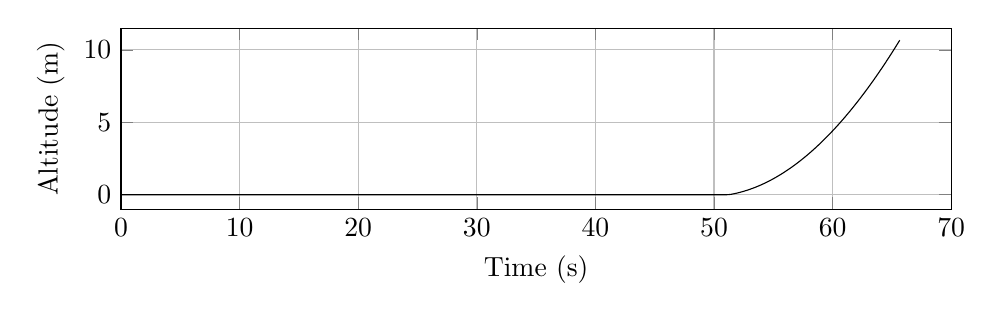
\begin{tikzpicture}

\begin{axis}[
width=\textwidth,
height=0.32\textwidth,
scaled ticks=false, tick label style={/pgf/number format/fixed},
xmin=0.0,
xmax=70,
xlabel={Time (s)},
xmajorgrids,
ymin=-1.0,
ymax=11.5,
ylabel={Altitude (m)},
ymajorgrids,
legend style={at={(1.03,0.5)},anchor=west,draw=black,fill=white,legend cell align=left}
]

\addplot [
color=black,
solid
]
table[row sep=crcr]{
9.999999999999999E-5	0.0\\
4.7168226468530315E-4	0.0\\
0.0014749326332462562	0.0\\
0.0033637884581385717	0.0\\
0.006277845941237823	0.0\\
0.010917796959456709	0.0\\
0.016539808004858998	0.0\\
0.022423484582968882	0.0\\
0.028414858477309957	0.0\\
0.03439517675063966	0.0\\
0.040396401243081206	0.0\\
0.04600191146660941	0.0\\
0.05203646293312687	0.0\\
0.057884319706054635	0.0\\
0.06393031489785073	0.0\\
0.06992434565370295	0.0\\
0.07570236339522896	0.0\\
0.08164569971590407	0.0\\
0.08766012409848342	0.0\\
0.09359191892922047	0.0\\
0.09945371459356578	0.0\\
0.10546671068479294	0.0\\
0.1114874078814794	0.0\\
0.11735912497905635	0.0\\
0.1233971626162216	0.0\\
0.12940037674072297	0.0\\
0.13546008899697676	0.0\\
0.1414943211751154	0.0\\
0.1475378733777319	0.0\\
0.1534736821999952	0.0\\
0.15953919733136973	0.0\\
0.16558166685056447	0.0\\
0.17167086015922634	0.0\\
0.1776929267403508	0.0\\
0.18373257009465377	0.0\\
0.18974184210840533	0.0\\
0.19576285868633192	0.0\\
0.20185483905916551	0.0\\
0.2079049092638764	0.0\\
0.2140345807666557	0.0\\
0.2202097067701841	0.0\\
0.2262741626247073	0.0\\
0.23240717705399072	0.0\\
0.23848718041381628	0.0\\
0.24458281006823324	0.0\\
0.2506470032100846	0.0\\
0.2567880722447018	0.0\\
0.2628925514916103	0.0\\
0.2690308671586331	0.0\\
0.2751278841509972	0.0\\
0.2812507672687158	0.0\\
0.2873733635040435	0.0\\
0.29351924471993907	0.0\\
0.299702994602169	0.0\\
0.3058844800561833	0.0\\
0.3118929262838356	0.0\\
0.31811994041915936	0.0\\
0.3241828513199243	0.0\\
0.33024711823008235	0.0\\
0.336446571473773	0.0\\
0.3426349295367608	0.0\\
0.3488828151525829	0.0\\
0.35516667602475926	0.0\\
0.3613527881420199	0.0\\
0.3675069515343563	0.0\\
0.37359119428407817	0.0\\
0.37981379003300875	0.0\\
0.3861283655232648	0.0\\
0.3924944793567824	0.0\\
0.3987402430313469	0.0\\
0.4050029110826724	0.0\\
0.41115707465738227	0.0\\
0.41758157147949004	0.0\\
0.4237802318572609	0.0\\
0.4299695756545898	0.0\\
0.43621596034172816	0.0\\
0.44246042604632163	0.0\\
0.4487355263828029	0.0\\
0.45501332212306544	0.0\\
0.46133897679706637	0.0\\
0.4677299894006539	0.0\\
0.47407736402976863	0.0\\
0.4803192968942265	0.0\\
0.48663751620189166	0.0\\
0.49286709292080333	0.0\\
0.4991953453230855	0.0\\
0.5054243914971039	0.0\\
0.5117528955006321	0.0\\
0.5182427984057336	0.0\\
0.5245749446977552	0.0\\
0.531074112683269	0.0\\
0.5374404195785305	0.0\\
0.5438208505630304	0.0\\
0.5501443306223375	0.0\\
0.5566881669516406	0.0\\
0.5630074835899443	0.0\\
0.5696477805274713	0.0\\
0.5760833755202213	0.0\\
0.5825007657567689	0.0\\
0.5889834860925582	0.0\\
0.5954502451696804	0.0\\
0.6021070465494169	0.0\\
0.6085705159547075	0.0\\
0.6149454099222367	0.0\\
0.6215284629383495	0.0\\
0.6280199478800053	0.0\\
0.6343179450698571	0.0\\
0.64088933371382	0.0\\
0.647364977926151	0.0\\
0.6540790592894996	0.0\\
0.6607048640220499	0.0\\
0.6672455098766301	0.0\\
0.6737540951218344	0.0\\
0.68042686023156	0.0\\
0.6870256817088038	0.0\\
0.6936860770845454	0.0\\
0.7003925218832372	0.0\\
0.7070010076475881	0.0\\
0.7136758532410861	0.0\\
0.7204247025630628	0.0\\
0.7269373459202597	0.0\\
0.7336151328475022	0.0\\
0.7402373161708455	0.0\\
0.747011944264375	0.0\\
0.7537921609385296	0.0\\
0.7605391484790882	0.0\\
0.7673122922447195	0.0\\
0.7741220276165555	0.0\\
0.78105953322373	0.0\\
0.7878257901722581	0.0\\
0.7944658333819992	0.0\\
0.8011905920633149	0.0\\
0.807987828405377	0.0\\
0.8149110705980023	0.0\\
0.8218556992282786	0.0\\
0.8287231586601145	0.0\\
0.8356070108194824	0.0\\
0.8423867158934808	0.0\\
0.8492355725719805	0.0\\
0.8558710898037845	0.0\\
0.8626968871611937	0.0\\
0.869651260699994	0.0\\
0.8765445297387515	0.0\\
0.8834069795654025	0.0\\
0.8902670224245384	0.0\\
0.8971248743922888	0.0\\
0.9040879497136194	0.0\\
0.910937757824114	0.0\\
0.9178750283804775	0.0\\
0.9248109800954487	0.0\\
0.9317902755689229	0.0\\
0.9388014349769052	0.0\\
0.9456787052663604	0.0\\
0.9526721827209466	0.0\\
0.9597201310535004	0.0\\
0.96683132767563	0.0\\
0.9739614814423456	0.0\\
0.9808774055147673	0.0\\
0.9880203647487595	0.0\\
0.9952777743046008	0.0\\
1.0023183731271588	0.0\\
1.009633500400707	0.0\\
1.0167385192892255	0.0\\
1.0240594009984538	0.0\\
1.0312433828995191	0.0\\
1.0385181750792798	0.0\\
1.045498039556068	0.0\\
1.0524527538433448	0.0\\
1.059574102474739	0.0\\
1.0668014807744601	0.0\\
1.073986794500744	0.0\\
1.0810248077176485	0.0\\
1.0882416691629286	0.0\\
1.0953825273247935	0.0\\
1.1026334659059813	0.0\\
1.1099370177637238	0.0\\
1.1171124546811146	0.0\\
1.1242334416367297	0.0\\
1.1317642565661212	0.0\\
1.1392779128766715	0.0\\
1.1466047080201882	0.0\\
1.153876760045796	0.0\\
1.1611845495685404	0.0\\
1.1686985301500226	0.0\\
1.1760479980215992	0.0\\
1.1836557166114248	0.0\\
1.1911247863196288	0.0\\
1.1986712520649103	0.0\\
1.2061220600824276	0.0\\
1.2135180457499488	0.0\\
1.2210243483658765	0.0\\
1.2284194703053086	0.0\\
1.2358266621657386	0.0\\
1.2433242793172594	0.0\\
1.2510848722189523	0.0\\
1.2585726835498368	0.0\\
1.266057355674051	0.0\\
1.2736153488913589	0.0\\
1.2813923946031691	0.0\\
1.289114360384212	0.0\\
1.2967401169758328	0.0\\
1.3045871572912793	0.0\\
1.3122641969111313	0.0\\
1.3199825235197937	0.0\\
1.3276468669044381	0.0\\
1.335364394023311	0.0\\
1.3432229910177327	0.0\\
1.351088936565445	0.0\\
1.3586445352949017	0.0\\
1.3664096686934681	0.0\\
1.3739362725395203	0.0\\
1.381553503037503	0.0\\
1.3892830616477858	0.0\\
1.3969747158828967	0.0\\
1.4048182624535053	0.0\\
1.412546731053883	0.0\\
1.4205817843173976	0.0\\
1.4284584314839495	0.0\\
1.4363615196061899	0.0\\
1.4442389281918468	0.0\\
1.452020625561317	0.0\\
1.4598344542579391	0.0\\
1.467614182077968	0.0\\
1.4753734237835348	0.0\\
1.4832622505477215	0.0\\
1.491324230936768	0.0\\
1.4991077711731493	0.0\\
1.5070415301533613	0.0\\
1.5149618069452115	0.0\\
1.5230119543265075	0.0\\
1.5310714521189515	0.0\\
1.5388705553387103	0.0\\
1.5468122697046112	0.0\\
1.5549358330870482	0.0\\
1.5631752749288768	0.0\\
1.5713748390776408	0.0\\
1.5795119815204322	0.0\\
1.5878819394762478	0.0\\
1.5958376334746127	0.0\\
1.6037540300391093	0.0\\
1.611957126991387	0.0\\
1.6199810826448053	0.0\\
1.6280343934477273	0.0\\
1.6361553968677804	0.0\\
1.6445850874544878	0.0\\
1.6530015639037505	0.0\\
1.6613753306891619	0.0\\
1.6696448673496342	0.0\\
1.6781000766108591	0.0\\
1.6864769614886206	0.0\\
1.6947630716697648	0.0\\
1.703057604628607	0.0\\
1.7114016715722715	0.0\\
1.7196979627045623	0.0\\
1.728136118102173	0.0\\
1.7363965132323367	0.0\\
1.7446758890193985	0.0\\
1.7528683888824927	0.0\\
1.761226121556199	0.0\\
1.769674800152902	0.0\\
1.7781391158520496	0.0\\
1.7866619511661006	0.0\\
1.7952314048827143	0.0\\
1.803661487692274	0.0\\
1.8121275494766471	0.0\\
1.8205463657814254	0.0\\
1.8290648772994125	0.0\\
1.8377847433742525	0.0\\
1.8462880467955847	0.0\\
1.8549756905467225	0.0\\
1.8635052550856757	0.0\\
1.8720417430409895	0.0\\
1.880661017292482	0.0\\
1.8894334474946355	0.0\\
1.8980207437818541	0.0\\
1.9065357493219346	0.0\\
1.9150866934969755	0.0\\
1.9236615836792388	0.0\\
1.9324669171828592	0.0\\
1.9411029404558025	0.0\\
1.9496878424065827	0.0\\
1.9582932498559358	0.0\\
1.9668551164550347	0.0\\
1.975828207659831	0.0\\
1.98438634365503	0.0\\
1.9932515941775257	0.0\\
2.0021545051790675	0.0\\
2.0107990941439438	0.0\\
2.019795504237475	0.0\\
2.0287401660939084	0.0\\
2.0374483032890325	0.0\\
2.0462182885839093	0.0\\
2.0553091951726215	0.0\\
2.0641181612179134	0.0\\
2.0732960354375107	0.0\\
2.081995024158439	0.0\\
2.090564433147877	0.0\\
2.0994092656695624	0.0\\
2.1081827076681803	0.0\\
2.1172711080280946	0.0\\
2.1260902595931297	0.0\\
2.135105250428862	0.0\\
2.1442472011921536	0.0\\
2.1534137835431375	0.0\\
2.162312975365192	0.0\\
2.1714375294902846	0.0\\
2.1803771319191076	0.0\\
2.189599894909601	0.0\\
2.1989660791307326	0.0\\
2.2080057233938684	0.0\\
2.217065346041629	0.0\\
2.226074350841266	0.0\\
2.2351004892816286	0.0\\
2.244177320023682	0.0\\
2.253292111128414	0.0\\
2.2626158101048777	0.0\\
2.271704441371842	0.0\\
2.2809812520768533	0.0\\
2.290150983187581	0.0\\
2.299453423692717	0.0\\
2.3086996275294753	0.0\\
2.318255387178435	0.0\\
2.3274318329133736	0.0\\
2.3367124199547327	0.0\\
2.346063768164914	0.0\\
2.355451582601658	0.0\\
2.3649757893281818	0.0\\
2.374281505062622	0.0\\
2.3837789594193017	0.0\\
2.3930532040924604	0.0\\
2.4026143414748136	0.0\\
2.412145921523469	0.0\\
2.421630298207999	0.0\\
2.4312683535126514	0.0\\
2.4409172167123216	0.0\\
2.4503697819925803	0.0\\
2.459856042034196	0.0\\
2.469326347896871	0.0\\
2.4788227131429137	0.0\\
2.488407104358041	0.0\\
2.4980369818358357	0.0\\
2.507645700785079	0.0\\
2.517155135172543	0.0\\
2.5267218434402485	0.0\\
2.5367501013418137	0.0\\
2.546341416989258	0.0\\
2.555982751300962	0.0\\
2.5656418344442926	0.0\\
2.575214922881786	0.0\\
2.584847056157126	0.0\\
2.5946478567776294	0.0\\
2.604297022132232	0.0\\
2.614111403004835	0.0\\
2.62383565050591	0.0\\
2.633633516043785	0.0\\
2.64342208813105	0.0\\
2.653256208261979	0.0\\
2.663038758869961	0.0\\
2.6728983799657016	0.0\\
2.6828872212256787	0.0\\
2.692870028344144	0.0\\
2.702792735975885	0.0\\
2.7128552669137136	0.0\\
2.722664096579086	0.0\\
2.73254513121904	0.0\\
2.742348752843645	0.0\\
2.7522271158085356	0.0\\
2.762138527538692	0.0\\
2.7722508194839417	0.0\\
2.782283660923074	0.0\\
2.792371331870682	0.0\\
2.802606230680654	0.0\\
2.8125792468421658	0.0\\
2.822759641992449	0.0\\
2.8328392182159234	0.0\\
2.843052116850221	0.0\\
2.8532375384733486	0.0\\
2.863540500260954	0.0\\
2.8735654469406846	0.0\\
2.883905999452365	0.0\\
2.8939348075085496	0.0\\
2.904123026666979	0.0\\
2.9145133230024394	0.0\\
2.924620784485797	0.0\\
2.934828906191335	0.0\\
2.9450101729957323	0.0\\
2.955363097691678	0.0\\
2.9656933928359326	0.0\\
2.9760184761196538	0.0\\
2.986241476105997	0.0\\
2.9966973787208575	0.0\\
3.007045711679247	0.0\\
3.017199912694375	0.0\\
3.0276498940816357	0.0\\
3.037964913043126	0.0\\
3.048449855772785	0.0\\
3.058801388086774	0.0\\
3.069277831175989	0.0\\
3.0796925297564517	0.0\\
3.090015517533449	0.0\\
3.100235631067065	0.0\\
3.1106752458952327	0.0\\
3.121088252129379	0.0\\
3.1316553773589524	0.0\\
3.142265470444106	0.0\\
3.152612774315319	0.0\\
3.1632099009902337	0.0\\
3.1736650323390743	0.0\\
3.184389036011888	0.0\\
3.195095398376954	0.0\\
3.2059997427880305	0.0\\
3.2165419993601576	0.0\\
3.2272620487399717	0.0\\
3.237993436167936	0.0\\
3.248816074789074	0.0\\
3.2598086914305844	0.0\\
3.270297271460275	0.0\\
3.280895465961171	0.0\\
3.2916304838680412	0.0\\
3.30249574846175	0.0\\
3.31320452517007	0.0\\
3.3237322369196933	0.0\\
3.33471200429321	0.0\\
3.345509509323996	0.0\\
3.356512405322941	0.0\\
3.3673789039405095	0.0\\
3.378208697049696	0.0\\
3.388999504286037	0.0\\
3.399737686580422	0.0\\
3.410678661087692	0.0\\
3.421446192359057	0.0\\
3.4323901179055714	0.0\\
3.443313278078726	0.0\\
3.454238291946192	0.0\\
3.465253451068296	0.0\\
3.4762197430954336	0.0\\
3.4873720461483764	0.0\\
3.4982097415928104	0.0\\
3.5091617322160626	0.0\\
3.5203412173629474	0.0\\
3.5315276351153706	0.0\\
3.542751075525276	0.0\\
3.55389667468427	0.0\\
3.5649778444581877	0.0\\
3.5761076079614504	0.0\\
3.5870999964480257	0.0\\
3.598293758425319	0.0\\
3.609576566077269	0.0\\
3.6208405597765116	0.0\\
3.632026304432669	0.0\\
3.643360231461977	0.0\\
3.6546844715881335	0.0\\
3.6662434114359446	0.0\\
3.677538933515171	0.0\\
3.689013103865469	0.0\\
3.7003865557377518	0.0\\
3.7116519661966336	0.0\\
3.7229371088569616	0.0\\
3.7342877567589916	0.0\\
3.745654151474418	0.0\\
3.756943773940857	0.0\\
3.7684156466705208	0.0\\
3.7799865969575537	0.0\\
3.7912586193160323	0.0\\
3.802624669707198	0.0\\
3.8138705917331563	0.0\\
3.825626222344031	0.0\\
3.8369895774682066	0.0\\
3.8486676661306642	0.0\\
3.8602824961934212	0.0\\
3.871575103060345	0.0\\
3.883179041034298	0.0\\
3.894971274279598	0.0\\
3.9066337232095893	0.0\\
3.9181419738975025	0.0\\
3.9298209877578465	0.0\\
3.941233069132549	0.0\\
3.952984981485419	0.0\\
3.9643549059036776	0.0\\
3.975918007386819	0.0\\
3.9874055119276344	0.0\\
3.9987372115580797	0.0\\
4.010306932126156	0.0\\
4.02166904116733	0.0\\
4.0333572692132655	0.0\\
4.044941050875851	0.0\\
4.056632728942304	0.0\\
4.068375445865222	0.0\\
4.080288743330296	0.0\\
4.091980782061018	0.0\\
4.103718220467826	0.0\\
4.115234715958737	0.0\\
4.1268788519971835	0.0\\
4.138546005402917	0.0\\
4.15037219261321	0.0\\
4.162298666474985	0.0\\
4.174207120400688	0.0\\
4.186010453837628	0.0\\
4.197495445049835	0.0\\
4.209171452568766	0.0\\
4.220761612024878	0.0\\
4.232179459821163	0.0\\
4.243978530687599	0.0\\
4.255882221292065	0.0\\
4.267504194773066	0.0\\
4.27915775128246	0.0\\
4.291151663046474	0.0\\
4.30302343613312	0.0\\
4.314723543730535	0.0\\
4.3265994470265134	0.0\\
4.338354873361062	0.0\\
4.350075718667631	0.0\\
4.361878559030986	0.0\\
4.373776934785724	0.0\\
4.38547407552802	0.0\\
4.397267664380253	0.0\\
4.3996457561362785	0.0\\
4.401154508587345	0.0\\
4.402003509087166	0.0\\
4.404364108449119	0.0\\
4.404614240239981	0.0\\
4.404865443941196	0.0\\
4.405040370904899	0.0\\
4.405197025641424	0.0\\
4.405339235114592	0.0\\
4.406019735872146	0.0\\
4.408202548236627	0.0\\
4.413624404155419	0.0\\
4.424700883328304	0.0\\
4.435691096904016	0.0\\
4.4465722874856155	0.0\\
4.45755085008167	0.0\\
4.4686313503264525	0.0\\
4.479678918927023	0.0\\
4.490649761459387	0.0\\
4.501930402007231	0.0\\
4.51296852107393	0.0\\
4.52412385445901	0.0\\
4.535280787991102	0.0\\
4.546532860017141	0.0\\
4.5577603600792695	0.0\\
4.568881303608606	0.0\\
4.580176347118517	0.0\\
4.5914006612632825	0.0\\
4.602592906447802	0.0\\
4.613899632214856	0.0\\
4.625272954579257	0.0\\
4.636547425513395	0.0\\
4.64786486851796	0.0\\
4.6592489117693034	0.0\\
4.670672425944703	0.0\\
4.6820083467877645	0.0\\
4.69336421283948	0.0\\
4.704884568040164	0.0\\
4.716440458822721	0.0\\
4.727866100819158	0.0\\
4.739173645260294	0.0\\
4.750656527057922	0.0\\
4.762103637243012	0.0\\
4.773476118865691	0.0\\
4.784930802560586	0.0\\
4.796344973418254	0.0\\
4.808032072793601	0.0\\
4.819545326381638	0.0\\
4.83113421632526	0.0\\
4.842684980162023	0.0\\
4.854439609499229	0.0\\
4.866256631751574	0.0\\
4.877927681589471	0.0\\
4.889452780311723	0.0\\
4.901254066106281	0.0\\
4.912800244383986	0.0\\
4.9244363693452335	0.0\\
4.936079381561189	0.0\\
4.948003125646757	0.0\\
4.959809703030716	0.0\\
4.971519857906804	0.0\\
4.983441760438911	0.0\\
4.995152666553652	0.0\\
5.006903349257767	0.0\\
5.01865897674047	0.0\\
5.030666723671395	0.0\\
5.0424323327615515	0.0\\
5.054231617714169	0.0\\
5.0661648265488175	0.0\\
5.078146415245431	0.0\\
5.089951251914766	0.0\\
5.101987533761951	0.0\\
5.113856732842329	0.0\\
5.125807063193271	0.0\\
5.1377589953858696	0.0\\
5.14979826493555	0.0\\
5.161808278647969	0.0\\
5.173734240308917	0.0\\
5.185525082332578	0.0\\
5.197503212310616	0.0\\
5.209552007733089	0.0\\
5.22151340836348	0.0\\
5.23352865330777	0.0\\
5.245374399913727	0.0\\
5.2574140734283965	0.0\\
5.269467796007955	0.0\\
5.281596744527889	0.0\\
5.293596643944442	0.0\\
5.305690254611779	0.0\\
5.317804390839026	0.0\\
5.329677489740426	0.0\\
5.341734920430467	0.0\\
5.354055519433807	0.0\\
5.366256008309609	0.0\\
5.378363250805011	0.0\\
5.390425524324602	0.0\\
5.402358575456585	0.0\\
5.414643680856232	0.0\\
5.42668439629627	0.0\\
5.438742267060073	0.0\\
5.4509028109361655	0.0\\
5.463112969333977	0.0\\
5.475274838820647	0.0\\
5.487480903583732	0.0\\
5.4996519753514	0.0\\
5.51183655409965	0.0\\
5.524035859101959	0.0\\
5.536121704875848	0.0\\
5.548254406418206	0.0\\
5.5604982500286315	0.0\\
5.572645057177219	0.0\\
5.58490822130438	0.0\\
5.597011913318875	0.0\\
5.609266792485391	0.0\\
5.621640164178043	0.0\\
5.633716818950383	0.0\\
5.645890856908794	0.0\\
5.658187475278668	0.0\\
5.670385601903268	0.0\\
5.682616200752818	0.0\\
5.6948022305509856	0.0\\
5.70702155068223	0.0\\
5.719293444134639	0.0\\
5.731551439404438	0.0\\
5.743908401403427	0.0\\
5.756295214506787	0.0\\
5.7684457487069185	0.0\\
5.780595365128004	0.0\\
5.792815634549633	0.0\\
5.804944671569379	0.0\\
5.81723227687432	0.0\\
5.829522379575655	0.0\\
5.841743484670879	0.0\\
5.85398659407959	0.0\\
5.866437862891502	0.0\\
5.878737378678723	0.0\\
5.89091542094963	0.0\\
5.903192617846777	0.0\\
5.915449356901274	0.0\\
5.927673802615933	0.0\\
5.940089401721899	0.0\\
5.952601291820024	0.0\\
5.965077146167102	0.0\\
5.9772741084721215	0.0\\
5.989675555524148	0.0\\
6.001930465742092	0.0\\
6.014375246181084	0.0\\
6.026809141327556	0.0\\
6.039102809552119	0.0\\
6.051496533551832	0.0\\
6.063783580671831	0.0\\
6.076091272171876	0.0\\
6.0884320955390905	0.0\\
6.100756782972736	0.0\\
6.113232620377337	0.0\\
6.125706982931909	0.0\\
6.138014623909825	0.0\\
6.150432654091022	0.0\\
6.162898784926533	0.0\\
6.175366005386518	0.0\\
6.187690582029834	0.0\\
6.200097044965764	0.0\\
6.212459544277268	0.0\\
6.224853863835788	0.0\\
6.23730578413033	0.0\\
6.24960130009015	0.0\\
6.261986939387381	0.0\\
6.274456712007561	0.0\\
6.286931063922161	0.0\\
6.299294016558166	0.0\\
6.311917143206337	0.0\\
6.324355366957098	0.0\\
6.336901896333082	0.0\\
6.349270420357676	0.0\\
6.361787013868367	0.0\\
6.374186940052896	0.0\\
6.386725864089673	0.0\\
6.399162328344108	0.0\\
6.411592602036459	0.0\\
6.424207572064411	0.0\\
6.43682793535238	0.0\\
6.449340221242014	0.0\\
6.461908991840259	0.0\\
6.474473453867121	0.0\\
6.486992723058863	0.0\\
6.499684368205669	0.0\\
6.51227029655011	0.0\\
6.5249889376584935	0.0\\
6.537578196244059	0.0\\
6.550248982887664	0.0\\
6.56279741266327	0.0\\
6.575595368161963	0.0\\
6.58827418245988	0.0\\
6.60096869734293	0.0\\
6.613607645720933	0.0\\
6.626306333627046	0.0\\
6.638997058136159	0.0\\
6.651717674223676	0.0\\
6.664406412217154	0.0\\
6.677117968058422	0.0\\
6.689901275897741	0.0\\
6.7026840862468	0.0\\
6.7155865265358585	0.0\\
6.728257627805901	0.0\\
6.7410471639578375	0.0\\
6.753922440233458	0.0\\
6.766685342925916	0.0\\
6.779416197206249	0.0\\
6.7922681489015115	0.0\\
6.804940465803131	0.0\\
6.81793627849696	0.0\\
6.830782202001982	0.0\\
6.843515393368689	0.0\\
6.856285118304598	0.0\\
6.869139384776496	0.0\\
6.881935353703206	0.0\\
6.894801772726261	0.0\\
6.9076595597500035	0.0\\
6.920513025619023	0.0\\
6.933345047711974	0.0\\
6.946352299923941	0.0\\
6.959507115023623	0.0\\
6.972479080658006	0.0\\
6.985584077184944	0.0\\
6.998561756301925	0.0\\
7.011558726264701	0.0\\
7.024538674015815	0.0\\
7.037696942528282	0.0\\
7.050758092391764	0.0\\
7.0639558078554785	0.0\\
7.077018211442107	0.0\\
7.090117567882034	0.0\\
7.103120757559996	0.0\\
7.1162182445178	0.0\\
7.12943092453116	0.0\\
7.142534058909064	0.0\\
7.155795892635625	0.0\\
7.168879390860482	0.0\\
7.182091388383444	0.0\\
7.195335509500087	0.0\\
7.208552477213768	0.0\\
7.221973513913355	0.0\\
7.235320435984578	0.0\\
7.248552211661753	0.0\\
7.261897003128068	0.0\\
7.275240195950881	0.0\\
7.288516083958839	0.0\\
7.301878771180091	0.0\\
7.315174743973538	0.0\\
7.32869209905585	0.0\\
7.342140858857116	0.0\\
7.355692942525879	0.0\\
7.369015672927883	0.0\\
7.382520268632364	0.0\\
7.3959781907312685	0.0\\
7.409500057326877	0.0\\
7.422942998691271	0.0\\
7.436543073301811	0.0\\
7.449927651482822	0.0\\
7.463490720992844	0.0\\
7.477164822535583	0.0\\
7.490926676411588	0.0\\
7.504718411628938	0.0\\
7.518295537276906	0.0\\
7.53207353175304	0.0\\
7.545943475332859	0.0\\
7.559655180721611	0.0\\
7.573337081580959	0.0\\
7.58707734482034	0.0\\
7.60081505979414	0.0\\
7.614763261894982	0.0\\
7.628634686197341	0.0\\
7.642564143957289	0.0\\
7.65643588877608	0.0\\
7.670286678327006	0.0\\
7.684328796549904	0.0\\
7.698424976574163	0.0\\
7.712562363349685	0.0\\
7.726566523535988	0.0\\
7.740524790621823	0.0\\
7.754676837019067	0.0\\
7.7687700302410985	0.0\\
7.782929591280929	0.0\\
7.797145491178837	0.0\\
7.811411676625788	0.0\\
7.825668181996464	0.0\\
7.839960821254513	0.0\\
7.854222229164071	0.0\\
7.8685904819788455	0.0\\
7.88303130413586	0.0\\
7.897612746654756	0.0\\
7.912073674096762	0.0\\
7.926716401209596	0.0\\
7.941194043634448	0.0\\
7.955644926559966	0.0\\
7.970290058718401	0.0\\
7.9848525649004465	0.0\\
7.99942214398277	0.0\\
8.014134348727634	0.0\\
8.028794505003091	0.0\\
8.043446213748684	0.0\\
8.058183086085098	0.0\\
8.073027219011554	0.0\\
8.08786808884457	0.0\\
8.102770288697311	0.0\\
8.11766326836576	0.0\\
8.132696030967356	0.0\\
8.14760526876567	0.0\\
8.162469524749863	0.0\\
8.177641520563533	0.0\\
8.19264169181167	0.0\\
8.20768105374825	0.0\\
8.222803083172881	0.0\\
8.23781019463851	0.0\\
8.2530115331739	0.0\\
8.268185866648015	0.0\\
8.283337870644868	0.0\\
8.298614957424423	0.0\\
8.31388480789441	0.0\\
8.329066783376845	0.0\\
8.344480551926374	0.0\\
8.35999438495568	0.0\\
8.375567336744943	0.0\\
8.390948750420357	0.0\\
8.406249112696841	0.0\\
8.421709086620844	0.0\\
8.436901269843819	0.0\\
8.452434687053916	0.0\\
8.46792468631853	0.0\\
8.483324926188402	0.0\\
8.498862789977732	0.0\\
8.514244373881318	0.0\\
8.529694236991695	0.0\\
8.545172358752513	0.0\\
8.560533438547544	0.0\\
8.576006362590352	0.0\\
8.591371343869522	0.0\\
8.606683909705144	0.0\\
8.62190711479138	0.0\\
8.637260630122743	0.0\\
8.652620895455701	0.0\\
8.6681316440749	0.0\\
8.68342170237447	0.0\\
8.698740668774775	0.0\\
8.714019481792889	0.0\\
8.729151765244907	0.0\\
8.744368674414098	0.0\\
8.759543713234386	0.0\\
8.77467748212537	0.0\\
8.78992801447739	0.0\\
8.805068998877672	0.0\\
8.82002524478493	0.0\\
8.834976252633517	0.0\\
8.849970445670397	0.0\\
8.86493637403257	0.0\\
8.87986969090645	0.0\\
8.89458673276349	0.0\\
8.90966771506529	0.0\\
8.92457549428359	0.0\\
8.939383745044491	0.0\\
8.954059823500991	0.0\\
8.968902575502305	0.0\\
8.983615847006629	0.0\\
8.998243672992913	0.0\\
9.012865245329937	0.0\\
9.027476265236608	0.0\\
9.041915724257908	0.0\\
9.056331547891077	0.0\\
9.056908800315579	0.0\\
9.057404913278013	0.0\\
9.057800002328584	0.0\\
9.058128242102143	0.0\\
9.058470696458564	0.0\\
9.059050194988004	0.0\\
9.059572844353692	0.0\\
9.061454210430178	0.0\\
9.067193060081511	0.0\\
9.078653045370142	0.0\\
9.091657268948367	0.0\\
9.104795967560158	0.0\\
9.117836414806664	0.0\\
9.130936341715383	0.0\\
9.144010212637827	0.0\\
9.157179660141956	0.0\\
9.170571163747365	0.0\\
9.18392760758038	0.0\\
9.197395785222366	0.0\\
9.210788042990824	0.0\\
9.224189982085214	0.0\\
9.23778349171079	0.0\\
9.251259630729447	0.0\\
9.26483497883397	0.0\\
9.278544071644077	0.0\\
9.292207129125806	0.0\\
9.306025537383022	0.0\\
9.319792225097508	0.0\\
9.333754503973207	0.0\\
9.347737258493261	0.0\\
9.361775052335268	0.0\\
9.375870382288241	0.0\\
9.390019903507124	0.0\\
9.404212734547137	0.0\\
9.41832014181115	0.0\\
9.432574164651992	0.0\\
9.446880669169769	0.0\\
9.461194119730425	0.0\\
9.475614702964435	0.0\\
9.490125650435626	0.0\\
9.504659338138488	0.0\\
9.519213080312511	0.0\\
9.533784651038449	0.0\\
9.54831424591103	0.0\\
9.562938508709827	0.0\\
9.577785663261029	0.0\\
9.592489268334226	0.0\\
9.607351873327868	0.0\\
9.622157466132844	0.0\\
9.637016293412557	0.0\\
9.651980474033476	0.0\\
9.666853651595964	0.0\\
9.681869245194807	0.0\\
9.696873520218109	0.0\\
9.711842507644974	0.0\\
9.726762077240071	0.0\\
9.741628561554116	0.0\\
9.756704524045038	0.0\\
9.771657342650794	0.0\\
9.78672167593432	0.0\\
9.801910499427219	0.0\\
9.81700993254481	0.0\\
9.83200244444619	0.0\\
9.847215388039135	0.0\\
9.862101289428157	0.0\\
9.877189728617505	0.0\\
9.89220929316857	0.0\\
9.907212818489644	0.0\\
9.922119750420638	0.0\\
9.937086398765711	0.0\\
9.952076426270438	0.0\\
9.967047376825857	0.0\\
9.982052978075433	0.0\\
9.997029447990446	0.0\\
10.012009015002754	0.0\\
10.026910129332428	0.0\\
10.041875645463701	0.0\\
10.0566503387941	0.0\\
10.071422566297485	0.0\\
10.086174719265625	0.0\\
10.101098076287162	0.0\\
10.115936556720253	0.0\\
10.13070286232011	0.0\\
10.145404367830203	0.0\\
10.160014737418397	0.0\\
10.174673446793772	0.0\\
10.18926622695113	0.0\\
10.203838142944239	0.0\\
10.218345345079893	0.0\\
10.232945787456348	0.0\\
10.247420598582536	0.0\\
10.262009761267631	0.0\\
10.276517049227031	0.0\\
10.29100903396823	0.0\\
10.305517029500123	0.0\\
10.319968782439375	0.0\\
10.334443942400888	0.0\\
10.348911291624923	0.0\\
10.363345475555256	0.0\\
10.377756708767105	0.0\\
10.392162852580945	0.0\\
10.40649697633636	0.0\\
10.420888333551815	0.0\\
10.435239889523487	0.0\\
10.44960677664455	0.0\\
10.463918501462967	0.0\\
10.478196552464407	0.0\\
10.492572054784343	0.0\\
10.506925269260051	0.0\\
10.521154432459745	0.0\\
10.535318983781888	0.0\\
10.54944748510686	0.0\\
10.563641967906673	0.0\\
10.577741158765924	0.0\\
10.591922385712444	0.0\\
10.60597572314817	0.0\\
10.620083816120918	0.0\\
10.634172331995654	0.0\\
10.648264143743624	0.0\\
10.662446460373573	0.0\\
10.676489715099805	0.0\\
10.69048544087396	0.0\\
10.70446366482389	0.0\\
10.718448347294412	0.0\\
10.732471128335472	0.0\\
10.746536176050746	0.0\\
10.760515191054296	0.0\\
10.774475463898646	0.0\\
10.788451271945274	0.0\\
10.80249869283158	0.0\\
10.816417995783336	0.0\\
10.830365384973899	0.0\\
10.84435320070618	0.0\\
10.858356137307506	0.0\\
10.872362108919294	0.0\\
10.886340279918524	0.0\\
10.900255598864039	0.0\\
10.914147840860906	0.0\\
10.928123162803868	0.0\\
10.941913578062394	0.0\\
10.955827768240827	0.0\\
10.969706421307727	0.0\\
10.983592085610855	0.0\\
10.99748959425817	0.0\\
11.011413542267569	0.0\\
11.025287885237255	0.0\\
11.039104649553007	0.0\\
11.052993781577044	0.0\\
11.066834790548675	0.0\\
11.080699001594692	0.0\\
11.094604756905778	0.0\\
11.108497334736818	0.0\\
11.122426031002792	0.0\\
11.136325338868716	0.0\\
11.15024632722055	0.0\\
11.16417468523409	0.0\\
11.178088233836423	0.0\\
11.191941110338735	0.0\\
11.205799363393925	0.0\\
11.219584533896956	0.0\\
11.233496126927005	0.0\\
11.247368645124517	0.0\\
11.261238942064868	0.0\\
11.275108903324131	0.0\\
11.289022825124537	0.0\\
11.30296630478173	0.0\\
11.316866531510097	0.0\\
11.330788782375375	0.0\\
11.344656874504459	0.0\\
11.358523783708922	0.0\\
11.37248396501472	0.0\\
11.38641566134805	0.0\\
11.400392026758645	0.0\\
11.414316129535461	0.0\\
11.428223897095606	0.0\\
11.44216245728023	0.0\\
11.456177808252797	0.0\\
11.47015726898083	0.0\\
11.48411943697364	0.0\\
11.498104199056534	0.0\\
11.512113038795135	0.0\\
11.526144799258159	0.0\\
11.540105602686925	0.0\\
11.553975586711598	0.0\\
11.56805305159305	0.0\\
11.5821018419261	0.0\\
11.596080935566423	0.0\\
11.609993440492193	0.0\\
11.624023388401092	0.0\\
11.638015303790006	0.0\\
11.652083787854206	0.0\\
11.666172746959667	0.0\\
11.680181203824198	0.0\\
11.694298410441057	0.0\\
11.708406580616643	0.0\\
11.72255012347452	0.0\\
11.736663917164655	0.0\\
11.750846294132877	0.0\\
11.765032109112408	0.0\\
11.779191293290506	0.0\\
11.7933384875986	0.0\\
11.796584672361298	0.0\\
11.80747479244285	0.0\\
11.821637480141625	0.0\\
11.84974979613007	0.0\\
11.878943232442715	0.0\\
11.908102480967926	0.0\\
11.937359104493392	0.0\\
11.966519595493534	0.0\\
11.99605764424706	0.0\\
12.02537006095173	0.0\\
12.054756413893628	0.0\\
12.084126498336467	0.0\\
12.11358439476966	0.0\\
12.142932177886209	0.0\\
12.17243268033361	0.0\\
12.201830172323959	0.0\\
12.231567253827997	0.0\\
12.261435696822499	0.0\\
12.291057649850945	0.0\\
12.321091498426224	0.0\\
12.350948599162379	0.0\\
12.380971492940173	0.0\\
12.410801800681458	0.0\\
12.440644803846165	0.0\\
12.470607326420417	0.0\\
12.500517501708522	0.0\\
12.53056959554641	0.0\\
12.560645144912002	0.0\\
12.590744543415358	0.0\\
12.621009353272154	0.0\\
12.651286787926466	0.0\\
12.681454489880615	0.0\\
12.711826567369314	0.0\\
12.742252867914434	0.0\\
12.772452189695723	0.0\\
12.802878268343306	0.0\\
12.83358710143786	0.0\\
12.86408069853696	0.0\\
12.894858859784527	0.0\\
12.925609038747599	0.0\\
12.956104975064378	0.0\\
12.986740548545203	0.0\\
13.017330690666025	0.0\\
13.048094406288282	0.0\\
13.078788876332165	0.0\\
13.109740764038577	0.0\\
13.140741732090433	0.0\\
13.17162480595205	0.0\\
13.202561832705022	0.0\\
13.233960878141826	0.0\\
13.26510595075338	0.0\\
13.296198871848137	0.0\\
13.327333329115863	0.0\\
13.358950731358213	0.0\\
13.390512507012541	0.0\\
13.422068880586643	0.0\\
13.453694360039123	0.0\\
13.485115361723384	0.0\\
13.516804500362703	0.0\\
13.548440080150282	0.0\\
13.580502948255301	0.0\\
13.612431913281782	0.0\\
13.644296175682417	0.0\\
13.67643816849871	0.0\\
13.70858921777863	0.0\\
13.740705538311897	0.0\\
13.772929682338482	0.0\\
13.805021748552022	0.0\\
13.837333821149862	0.0\\
13.869432287237998	0.0\\
13.901667086729017	0.0\\
13.93436847736199	0.0\\
13.966496697631424	0.0\\
13.999207624579164	0.0\\
14.032411785337484	0.0\\
14.065370285609731	0.0\\
14.098005357730084	0.0\\
14.130948572807494	0.0\\
14.163772361221866	0.0\\
14.197107791922242	0.0\\
14.230506071862632	0.0\\
14.264206542808456	0.0\\
14.297474592505804	0.0\\
14.331161644242766	0.0\\
14.364564884558533	0.0\\
14.39828335082042	0.0\\
14.43260251977744	0.0\\
14.466626346594673	0.0\\
14.500740001650232	0.0\\
14.53444089178753	0.0\\
14.568223369811513	0.0\\
14.60259252495526	0.0\\
14.63701537337596	0.0\\
14.671899576971619	0.0\\
14.706590363537213	0.0\\
14.740989289093893	0.0\\
14.776056853138549	0.0\\
14.81125360136701	0.0\\
14.846174606045615	0.0\\
14.880944421072392	0.0\\
14.915895074390342	0.0\\
14.950600566717728	0.0\\
14.986087652082514	0.0\\
15.02228709249259	0.0\\
15.058646767094974	0.0\\
15.094261336506573	0.0\\
15.129763567208638	0.0\\
15.166292273807244	0.0\\
15.202556237382538	0.0\\
15.238991152169135	0.0\\
15.275335059520767	0.0\\
15.311890252684382	0.0\\
15.349113994338023	0.0\\
15.385901915780561	0.0\\
15.422856784350913	0.0\\
15.460473219857096	0.0\\
15.498574735856295	0.0\\
15.535831736317643	0.0\\
15.57320739180198	0.0\\
15.61114992516643	0.0\\
15.648563848619407	0.0\\
15.686376696588717	0.0\\
15.723886948417995	0.0\\
15.762398709332793	0.0\\
15.800255102601664	0.0\\
15.838315989056905	0.0\\
15.876304872868644	0.0\\
15.914801931196571	0.0\\
15.953202298092279	0.0\\
15.991314989385454	0.0\\
16.029560233013953	0.0\\
16.06769378681799	0.0\\
16.10621284752243	0.0\\
16.14459759677942	0.0\\
16.183720897062237	0.0\\
16.22186311424361	0.0\\
16.260289025634385	0.0\\
16.298812795095436	0.0\\
16.336944580810794	0.0\\
16.37512555219306	0.0\\
16.413561746798486	0.0\\
16.451544769609747	0.0\\
16.489480345697437	0.0\\
16.527597645139338	0.0\\
16.565297270391852	0.0\\
16.60296815224111	0.0\\
16.64083697663169	0.0\\
16.67804874213627	0.0\\
16.71554512218586	0.0\\
16.752919908880294	0.0\\
16.789812603705947	0.0\\
16.826203921020095	0.0\\
16.862827708007252	0.0\\
16.899200094555113	0.0\\
16.935435416711	0.0\\
16.97131753994544	0.0\\
17.007305604238013	0.0\\
17.04321288131115	0.0\\
17.079172783354316	0.0\\
17.114791236468044	0.0\\
17.150285240057315	0.0\\
17.15735073186802	0.0\\
17.162160880408592	0.0\\
17.16454807140959	0.0\\
17.166169713123736	0.0\\
17.167459088369412	0.0\\
17.168339660679152	0.0\\
17.16955078205273	0.0\\
17.170224598595752	0.0\\
17.170515032681053	0.0\\
17.17080780241008	0.0\\
17.172177999370142	0.0\\
17.176563977882573	0.0\\
17.18960839558484	0.0\\
17.215727704076258	0.0\\
17.246160044895937	0.0\\
17.276862100815542	0.0\\
17.307597352439565	0.0\\
17.338612278666915	0.0\\
17.369772772801056	0.0\\
17.401069124426883	0.0\\
17.432443931129484	0.0\\
17.463799680505893	0.0\\
17.495512847627197	0.0\\
17.527303673831895	0.0\\
17.55937636790604	0.0\\
17.59163293252002	0.0\\
17.623684108195327	0.0\\
17.65601304138761	0.0\\
17.68843002229525	0.0\\
17.720929360329947	0.0\\
17.75366685864079	0.0\\
17.786484997810852	0.0\\
17.819409856968207	0.0\\
17.852510285903193	0.0\\
17.885828616567068	0.0\\
17.919195126888013	0.0\\
17.952767023187818	0.0\\
17.986793136388577	0.0\\
18.021021879027288	0.0\\
18.05529207467456	0.0\\
18.089328768118918	0.0\\
18.12381883207827	0.0\\
18.158458288837316	0.0\\
18.193004520730042	0.0\\
18.227867112412902	0.0\\
18.26315606232292	0.0\\
18.297931812143055	0.0\\
18.33356785417324	0.0\\
18.368725766966563	0.0\\
18.40375091661049	0.0\\
18.43952274578897	0.0\\
18.475459217974	0.0\\
18.51123656735531	0.0\\
18.546953356762714	0.0\\
18.582909413208355	0.0\\
18.618718630922153	0.0\\
18.654705747768084	0.0\\
18.69063891356018	0.0\\
18.726691420736877	0.0\\
18.76251689566375	0.0\\
18.798147562248765	0.0\\
18.833843665130715	0.0\\
18.8695606606639	0.0\\
18.90524362790258	0.0\\
18.94129609181384	0.0\\
18.977164835125045	0.0\\
19.0126806603052	0.0\\
19.048276397485616	0.0\\
19.083516452469247	0.0\\
19.11892590182527	0.0\\
19.154029822028008	0.0\\
19.189428677343507	0.0\\
19.224670084607077	0.0\\
19.259559378457638	0.0\\
19.294480697744426	0.0\\
19.329432616624977	0.0\\
19.364378232767137	0.0\\
19.39926408675113	0.0\\
19.433989082529102	0.0\\
19.468086456826526	0.0\\
19.502486533612654	0.0\\
19.536760113371237	0.0\\
19.570954246012498	0.0\\
19.604951376710567	0.0\\
19.63896326391012	0.0\\
19.672940617339293	0.0\\
19.706923457173616	0.0\\
19.74046677621221	0.0\\
19.774067684573772	0.0\\
19.80743282299342	0.0\\
19.840935966122906	0.0\\
19.874188348437826	0.0\\
19.90749910676456	0.0\\
19.940764008359857	0.0\\
19.973504141354738	0.0\\
20.00676114406022	0.0\\
20.03973104827937	0.0\\
20.072536437237133	0.0\\
20.10555339463893	0.0\\
20.138582569283315	0.0\\
20.171165965493103	0.0\\
20.203921117193026	0.0\\
20.23642971869417	0.0\\
20.269299323013826	0.0\\
20.30187593827806	0.0\\
20.334307979140306	0.0\\
20.366733419148524	0.0\\
20.39912515875568	0.0\\
20.431558725051403	0.0\\
20.463975435277277	0.0\\
20.496358063009232	0.0\\
20.528573153845613	0.0\\
20.560827792842638	0.0\\
20.592900314920918	0.0\\
20.624837109803423	0.0\\
20.656789160483157	0.0\\
20.688935731887433	0.0\\
20.72088523383364	0.0\\
20.752723389369955	0.0\\
20.78465330437548	0.0\\
20.816396326995132	0.0\\
20.848308595954848	0.0\\
20.880239245035554	0.0\\
20.911993548023794	0.0\\
20.943508627066542	0.0\\
20.975092085368992	0.0\\
21.00660913955449	0.0\\
21.038316234237897	0.0\\
21.06996107974654	0.0\\
21.1016972077703	0.0\\
21.13306128373106	0.0\\
21.164434903743697	0.0\\
21.19598505380599	0.0\\
21.227542012660606	0.0\\
21.259013022746416	0.0\\
21.290695152132223	0.0\\
21.32205658825888	0.0\\
21.3534256746212	0.0\\
21.38471709638516	0.0\\
21.415894366568878	0.0\\
21.44716649810905	0.0\\
21.478472093840345	0.0\\
21.50969897229976	0.0\\
21.540974330826813	0.0\\
21.572241509596594	0.0\\
21.603519457105328	0.0\\
21.63485190333995	0.0\\
21.66594711805172	0.0\\
21.697115464706123	0.0\\
21.728159300006055	0.0\\
21.7595039487695	0.0\\
21.790687281998373	0.0\\
21.82199525194477	0.0\\
21.853203753683985	0.0\\
21.884385859835206	0.0\\
21.915567596182306	0.0\\
21.94666234221124	0.0\\
21.977781249506386	0.0\\
22.00878761417713	0.0\\
22.03986627528495	0.0\\
22.0708617958893	0.0\\
22.102097841624605	0.0\\
22.13311817952176	0.0\\
22.164208257468914	0.0\\
22.19539511506254	0.0\\
22.22632751619757	0.0\\
22.257543485657187	0.0\\
22.288600152680843	0.0\\
22.31979859660659	0.0\\
22.350996952274507	0.0\\
22.381945799903725	0.0\\
22.413097506140268	0.0\\
22.444124166121092	0.0\\
22.475299378095194	0.0\\
22.50645260654818	0.0\\
22.537566032049845	0.0\\
22.56873997463868	0.0\\
22.599828902902935	0.0\\
22.630973247926953	0.0\\
22.66201184000966	0.0\\
22.693179286891095	0.0\\
22.724282476280862	0.0\\
22.75539583909608	0.0\\
22.78669288220061	0.0\\
22.818085759666104	0.0\\
22.84925219957868	0.0\\
22.880392823945975	0.0\\
22.911500098780564	0.0\\
22.94271228168141	0.0\\
22.973958566668593	0.0\\
23.005185760527056	0.0\\
23.036493278501545	0.0\\
23.06768043407112	0.0\\
23.098940246016916	0.0\\
23.130402353448183	0.0\\
23.161634306646015	0.0\\
23.19305751111594	0.0\\
23.22441344895261	0.0\\
23.255656813376106	0.0\\
23.287086939015886	0.0\\
23.31852101499254	0.0\\
23.349846201175538	0.0\\
23.381269795861556	0.0\\
23.412792024357792	0.0\\
23.44427248665302	0.0\\
23.47568637534218	0.0\\
23.50705353477732	0.0\\
23.538659310981174	0.0\\
23.570098017178474	0.0\\
23.601414376452418	0.0\\
23.633025562402963	0.0\\
23.664695487720273	0.0\\
23.696297038741797	0.0\\
23.727853010724893	0.0\\
23.759448992664154	0.0\\
23.79110276407637	0.0\\
23.822699785725973	0.0\\
23.854424834655205	0.0\\
23.88609589243996	0.0\\
23.917842228640282	0.0\\
23.94970042516222	0.0\\
23.98139038057056	0.0\\
24.01294489756809	0.0\\
24.044774939298954	0.0\\
24.076442656165142	0.0\\
24.1081544511608	0.0\\
24.14011888192357	0.0\\
24.17212796079299	0.0\\
24.204000556664596	0.0\\
24.235946990720045	0.0\\
24.267947077308804	0.0\\
24.300042123205223	0.0\\
24.332211985502248	0.0\\
24.364335284309192	0.0\\
24.396459020923018	0.0\\
24.428581709559175	0.0\\
24.460565554237732	0.0\\
24.49279959915708	0.0\\
24.525080193594498	0.0\\
24.557324293077293	0.0\\
24.589729235117638	0.0\\
24.622046306778493	0.0\\
24.654428698875776	0.0\\
24.686800361173233	0.0\\
24.719370409043925	0.0\\
24.751820814048116	0.0\\
24.784429679363008	0.0\\
24.817034420563395	0.0\\
24.849720237316305	0.0\\
24.882306354499242	0.0\\
24.9150384640813	0.0\\
24.94772663971903	0.0\\
24.980585402422385	0.0\\
25.01337861114338	0.0\\
25.046377050539547	0.0\\
25.07916678119163	0.0\\
25.111924107738595	0.0\\
25.14479759887017	0.0\\
25.17788291979155	0.0\\
25.21094053267374	0.0\\
25.24407429904388	0.0\\
25.277386528358782	0.0\\
25.31053650159329	0.0\\
25.34392540748373	0.0\\
25.377124212969612	0.0\\
25.410445204138654	0.0\\
25.44391952300873	0.0\\
25.477233259084144	0.0\\
25.510434589015652	0.0\\
25.54398439679317	0.0\\
25.577691321853045	0.0\\
25.61121901664138	0.0\\
25.644985571456544	0.0\\
25.678620104627754	0.0\\
25.712324789909474	0.0\\
25.7462386546297	0.0\\
25.78002699810807	0.0\\
25.81397814980174	0.0\\
25.848145674744572	0.0\\
25.8823345700346	0.0\\
25.91631434626519	0.0\\
25.9504637720023	0.0\\
25.984559441631838	0.0\\
26.01871125543994	0.0\\
26.052975663609196	0.0\\
26.087324019275414	0.0\\
26.121933065670127	0.0\\
26.156473810784597	0.0\\
26.19120184463219	0.0\\
26.225950470469762	0.0\\
26.260624859864166	0.0\\
26.29561896478269	0.0\\
26.33048212858109	0.0\\
26.365380688688646	0.0\\
26.40040175143791	0.0\\
26.43551287604842	0.0\\
26.470657161252873	0.0\\
26.505904156924757	0.0\\
26.54131678345503	0.0\\
26.576828257847346	0.0\\
26.61227396551468	0.0\\
26.647718484091854	0.0\\
26.683621422135943	0.0\\
26.71938380713741	0.0\\
26.75525710288276	0.0\\
26.791383641759275	0.0\\
26.827530270916974	0.0\\
26.863585658467755	0.0\\
26.899923703809336	0.0\\
26.936126189673864	0.0\\
26.972599480986787	0.0\\
27.009156467857785	0.0\\
27.045842878670797	0.0\\
27.08254905271042	0.0\\
27.119590422944214	0.0\\
27.156421784578704	0.0\\
27.193612107918277	0.0\\
27.23084286162522	0.0\\
27.268258696806186	0.0\\
27.305862569648987	0.0\\
27.343223340908928	0.0\\
27.380827904669836	0.0\\
27.41865589016703	0.0\\
27.4566500882431	0.0\\
27.494582004235156	0.0\\
27.532807399606497	0.0\\
27.571110170549197	0.0\\
27.60945044145933	0.0\\
27.648018318554918	0.0\\
27.6868733809085	0.0\\
27.725790526218304	0.0\\
27.76489351467533	0.0\\
27.804268394160587	0.0\\
27.84353745094664	0.0\\
27.883010847093566	0.0\\
27.922743960126304	0.0\\
27.962562281953623	0.0\\
28.002525924674096	0.0\\
28.042802377908096	0.0\\
28.08317495265269	0.0\\
28.124159440140495	0.0\\
28.165008368926763	0.0\\
28.206093897760084	0.0\\
28.24743526145059	0.0\\
28.289078746742703	0.0\\
28.330826729288702	0.0\\
28.37306703361881	0.0\\
28.415296326063732	0.0\\
28.457967779501026	0.0\\
28.500848303145872	0.0\\
28.544411959378365	0.0\\
28.58785576777806	0.0\\
28.632031643027915	0.0\\
28.67645337909851	0.0\\
28.72105731562977	0.0\\
28.76613485046832	0.0\\
28.811672866297805	0.0\\
28.85775551271164	0.0\\
28.904170376023764	0.0\\
28.951211422756224	0.0\\
28.998264434004724	0.0\\
29.045952775244565	0.0\\
29.094421415246856	0.0\\
29.14338168988516	0.0\\
29.192693734539482	0.0\\
29.242413321712625	0.0\\
29.292715324488576	0.0\\
29.34371980232026	0.0\\
29.3949837724184	0.0\\
29.446688760122427	0.0\\
29.49831660570998	0.0\\
29.549814559588057	0.0\\
29.601309719209787	0.0\\
29.65275875296262	0.0\\
29.70318730718987	0.0\\
29.753091612012028	0.0\\
29.80279264974955	0.0\\
29.852151175712578	0.0\\
29.900764984778426	0.0\\
29.949128192913875	0.0\\
29.996522744350358	0.0\\
30.043704750130118	0.0\\
30.089826261243445	0.0\\
30.135986537840985	0.0\\
30.181534745430938	0.0\\
30.226810551556035	0.0\\
30.271768711209845	0.0\\
30.316143051263367	0.0\\
30.36024738214074	0.0\\
30.4038988334828	0.0\\
30.44725404837569	0.0\\
30.490340522006285	0.0\\
30.532818986217713	0.0\\
30.575127464095118	0.0\\
30.617078879601415	0.0\\
30.658968695792872	0.0\\
30.700417978411664	0.0\\
30.74158250602394	0.0\\
30.782570387447393	0.0\\
30.8232206333266	0.0\\
30.86361310819511	0.0\\
30.903901764646946	0.0\\
30.94382733343273	0.0\\
30.983662422193646	0.0\\
31.023280636043516	0.0\\
31.031132132937216	0.0\\
31.037040264599014	0.0\\
31.04217465334127	0.0\\
31.04542416208176	0.0\\
31.0476707311063	0.0\\
31.049223078984845	0.0\\
31.050548195034835	0.0\\
31.05201076491447	0.0\\
31.05351575744104	0.0\\
31.053921958582606	0.0\\
31.05437774093312	0.0\\
31.05684473876243	0.0\\
31.067594193006308	0.0\\
31.10473976219118	0.0\\
31.143135209936936	0.0\\
31.181658507379552	0.0\\
31.220385928269927	0.0\\
31.259169438634167	0.0\\
31.29822220507573	0.0\\
31.337507106821782	0.0\\
31.37722891968386	0.0\\
31.41712885893596	0.0\\
31.457201462738574	0.0\\
31.497457081933376	0.0\\
31.538025805065693	0.0\\
31.579132736536188	0.0\\
31.62030232408027	0.0\\
31.661755010707758	0.0\\
31.70350187006143	0.0\\
31.745433603350357	0.0\\
31.78773992118321	0.0\\
31.830316331925182	0.0\\
31.873357600600308	0.0\\
31.91673529496446	0.0\\
31.960445269124627	0.0\\
32.004703159625734	0.0\\
32.04946297314629	0.0\\
32.09425185468889	0.0\\
32.139494804380845	0.0\\
32.185176234546745	0.0\\
32.23124160546827	0.0\\
32.27768802726716	0.0\\
32.32459951767704	0.0\\
32.37161777381438	0.0\\
32.41892355963412	0.0\\
32.46668322348802	0.0\\
32.5145876122825	0.0\\
32.56246669847906	0.0\\
32.61086222580647	0.0\\
32.65908799268345	0.0\\
32.707048682101075	0.0\\
32.75492999369081	0.0\\
32.802481741292965	0.0\\
32.85003661332388	0.0\\
32.89764877194865	0.0\\
32.945104874736955	0.0\\
32.99204147251328	0.0\\
33.03848657742731	0.0\\
33.084891151456674	0.0\\
33.13100116090669	0.0\\
33.17703507144388	0.0\\
33.22255422719812	0.0\\
33.26729758494845	0.0\\
33.31239788392591	0.0\\
33.356636379036516	0.0\\
33.40086573374134	0.0\\
33.444740362162534	0.0\\
33.4884595152664	0.0\\
33.531735604129835	0.0\\
33.57518680769277	0.0\\
33.61821424125536	0.0\\
33.66112119339947	0.0\\
33.70363393375064	0.0\\
33.7459881115402	0.0\\
33.78819401079623	0.0\\
33.830103912132984	0.0\\
33.87187551204009	0.0\\
33.913448609053745	0.0\\
33.955139564103234	0.0\\
33.99642337676454	0.0\\
34.037649232133646	0.0\\
34.07883686962806	0.0\\
34.11978758220418	0.0\\
34.16066045670806	0.0\\
34.20122797248801	0.0\\
34.24171490196987	0.0\\
34.282086962179974	0.0\\
34.32238920016094	0.0\\
34.36246453959757	0.0\\
34.40248011756266	0.0\\
34.44229843748293	0.0\\
34.48205178748523	0.0\\
34.52186960876452	0.0\\
34.561475198061856	0.0\\
34.60090747658913	0.0\\
34.640325387161184	0.0\\
34.67951331759188	0.0\\
34.71880766536211	0.0\\
34.75790384197646	0.0\\
34.7971391101666	0.0\\
34.836337404683434	0.0\\
34.8754689443377	0.0\\
34.914679408132315	0.0\\
34.95358560470221	0.0\\
34.992257192155265	0.0\\
35.03109850407736	0.0\\
35.069684948471235	0.0\\
35.10834697565234	0.0\\
35.14690064848898	0.0\\
35.18519355781608	0.0\\
35.223689464133955	0.0\\
35.2622606160389	0.0\\
35.30073654124506	0.0\\
35.33888535093328	0.0\\
35.37712940224611	0.0\\
35.41525986972417	0.0\\
35.4534033023793	0.0\\
35.49131760992152	0.0\\
35.52925046846944	0.0\\
35.56735544583917	0.0\\
35.605212335900944	0.0\\
35.643077667880775	0.0\\
35.68115632048422	0.0\\
35.718869860298014	0.0\\
35.75681465577229	0.0\\
35.794586869443535	0.0\\
35.83242313338559	0.0\\
35.87008183186347	0.0\\
35.907576206554836	0.0\\
35.94513403312057	0.0\\
35.982810003526325	0.0\\
36.02051291135676	0.0\\
36.05804708621106	0.0\\
36.09550969410347	0.0\\
36.13301441278311	0.0\\
36.170615486529	0.0\\
36.20807255775469	0.0\\
36.24564519466517	0.0\\
36.283176147255304	0.0\\
36.32057913142103	0.0\\
36.3579284201565	0.0\\
36.39545372551453	0.0\\
36.43277564138346	0.0\\
36.47017483292028	0.0\\
36.50760166986397	0.0\\
36.54498558339874	0.0\\
36.58227189269253	0.0\\
36.61954635734877	0.0\\
36.65688546803622	0.0\\
36.694379541748745	0.0\\
36.731842509482476	0.0\\
36.769257370794136	0.0\\
36.806650144833924	0.0\\
36.84387158560688	0.0\\
36.881077547679396	0.0\\
36.91821677090593	0.0\\
36.955519555360354	0.0\\
36.99282379874525	0.0\\
37.03005834503929	0.0\\
37.06728291633158	0.0\\
37.104468690997024	0.0\\
37.14180060082478	0.0\\
37.1790408491528	0.0\\
37.21636503151244	0.0\\
37.25373562265027	0.0\\
37.29088281385735	0.0\\
37.32824078565724	0.0\\
37.36557327587725	0.0\\
37.40296812166531	0.0\\
37.44046677596559	0.0\\
37.47775165059154	0.0\\
37.515001243317386	0.0\\
37.552353138596274	0.0\\
37.58963388240821	0.0\\
37.6269073624659	0.0\\
37.664034316141894	0.0\\
37.701283241554464	0.0\\
37.738461085713354	0.0\\
37.77591493021551	0.0\\
37.81323393508036	0.0\\
37.85065455935006	0.0\\
37.887981857656655	0.0\\
37.92553621544593	0.0\\
37.962801941372504	0.0\\
38.00012310644206	0.0\\
38.03732937936974	0.0\\
38.07481234719857	0.0\\
38.1121664522572	0.0\\
38.1495571938605	0.0\\
38.18704735228482	0.0\\
38.22447568008134	0.0\\
38.261888178567006	0.0\\
38.299367774180524	0.0\\
38.336846360565815	0.0\\
38.37442319795784	0.0\\
38.41189297689	0.0\\
38.449451051096446	0.0\\
38.48700532751285	0.0\\
38.52467468283446	0.0\\
38.56252248901522	0.0\\
38.60024349965978	0.0\\
38.63787910362326	0.0\\
38.67564734525443	0.0\\
38.713299981618434	0.0\\
38.751001745919694	0.0\\
38.7886883824376	0.0\\
38.82656180229726	0.0\\
38.86431735029295	0.0\\
38.90227025407222	0.0\\
38.94006713642948	0.0\\
38.977989677545295	0.0\\
39.016004818730195	0.0\\
39.05406412522382	0.0\\
39.09212247146674	0.0\\
39.13007338719892	0.0\\
39.16804710453549	0.0\\
39.20604431382576	0.0\\
39.24406036391545	0.0\\
39.28199200571545	0.0\\
39.320062515777536	0.0\\
39.35815050571186	0.0\\
39.39624528092085	0.0\\
39.43446834685197	0.0\\
39.472507332232894	0.0\\
39.51090911623061	0.0\\
39.549244585204846	0.0\\
39.587495493496576	0.0\\
39.62600451364254	0.0\\
39.66436660742167	0.0\\
39.70272310713551	0.0\\
39.741197323329175	0.0\\
39.779689667284885	0.0\\
39.818211109031495	0.0\\
39.85673406693245	0.0\\
39.89522014128811	0.0\\
39.9338725210836	0.0\\
39.972502295625404	0.0\\
40.01121840882186	0.0\\
40.04998004720987	0.0\\
40.0888223796488	0.0\\
40.12756769700229	0.0\\
40.16637795198561	0.0\\
40.20516798904225	0.0\\
40.24414921915981	0.0\\
40.283040047621455	0.0\\
40.32212080883798	0.0\\
40.36117260927392	0.0\\
40.40040838909471	0.0\\
40.439449324956556	0.0\\
40.47865638964261	0.0\\
40.51803914063932	0.0\\
40.55736890537678	0.0\\
40.596629677857635	0.0\\
40.63618351754347	0.0\\
40.675652373547294	0.0\\
40.71518554409322	0.0\\
40.75472066851397	0.0\\
40.79438361373606	0.0\\
40.833954719733995	0.0\\
40.87367628198605	0.0\\
40.91350799679107	0.0\\
40.95342639291407	0.0\\
40.99335405827638	0.0\\
41.03335832320158	0.0\\
41.07330033414027	0.0\\
41.11351236451058	0.0\\
41.15365729736821	0.0\\
41.19384975384695	0.0\\
41.23419781308775	0.0\\
41.274498671547605	0.0\\
41.31486482765979	0.0\\
41.355271108716366	0.0\\
41.395627894265445	0.0\\
41.43610129298777	0.0\\
41.476437006577115	0.0\\
41.51713403327443	0.0\\
41.557736087239746	0.0\\
41.598312578828555	0.0\\
41.639017974678694	0.0\\
41.679842307157415	0.0\\
41.72071449218396	0.0\\
41.761507340746036	0.0\\
41.80227666504781	0.0\\
41.843230402499245	0.0\\
41.884386295400546	0.0\\
41.925413787225	0.0\\
41.96653221757303	0.0\\
42.0077352459172	0.0\\
42.04930357220417	0.0\\
42.09086019860297	0.0\\
42.13243575476854	0.0\\
42.17408655033677	0.0\\
42.2158366347651	0.0\\
42.257676728779856	0.0\\
42.29949867108958	0.0\\
42.341424831112846	0.0\\
42.38332862166912	0.0\\
42.42550171353963	0.0\\
42.46769551636372	0.0\\
42.51001631753486	0.0\\
42.55257352533799	0.0\\
42.5951188165553	0.0\\
42.63767070516491	0.0\\
42.68028024932731	0.0\\
42.722982079712196	0.0\\
42.76575153391441	0.0\\
42.80848779438581	0.0\\
42.85129316550888	0.0\\
42.89428669300953	0.0\\
42.93749618463238	0.0\\
42.98079837788673	0.0\\
43.02423945809211	0.0\\
43.067805377901195	0.0\\
43.111322612276695	0.0\\
43.154873678308164	0.0\\
43.19873380508159	0.0\\
43.24264830412143	0.0\\
43.28662252141645	0.0\\
43.33064658016089	0.0\\
43.37480868634604	0.0\\
43.41890955444775	0.0\\
43.46346169442303	0.0\\
43.50796704407966	0.0\\
43.55257596013131	0.0\\
43.597377746466805	0.0\\
43.64201726669664	0.0\\
43.686934699313184	0.0\\
43.73217333705644	0.0\\
43.77742460619311	0.0\\
43.822833695118106	0.0\\
43.8684342839403	0.0\\
43.913988365006816	0.0\\
43.95970413862575	0.0\\
44.005676229314375	0.0\\
44.05160763654378	0.0\\
44.09770727954539	0.0\\
44.14424605525558	0.0\\
44.190563489972064	0.0\\
44.23720678466617	0.0\\
44.28400483216092	0.0\\
44.33087845489635	0.0\\
44.37785548039241	0.0\\
44.42498089588267	0.0\\
44.47249891910894	0.0\\
44.520019649024945	0.0\\
44.56766619775178	0.0\\
44.615731954135	0.0\\
44.663876852025965	0.0\\
44.7120792458648	0.0\\
44.7605101279523	0.0\\
44.8094890667234	0.0\\
44.858365011585576	0.0\\
44.9075172737472	0.0\\
44.956986886568686	0.0\\
45.00669773893908	0.0\\
45.056522388145424	0.0\\
45.10651832230194	0.0\\
45.15701524515431	0.0\\
45.207532803491134	0.0\\
45.25842702979283	0.0\\
45.309471165732774	0.0\\
45.3610736959033	0.0\\
45.41289628555265	0.0\\
45.46492906765522	0.0\\
45.51759905122478	0.0\\
45.57031255630696	0.0\\
45.62362831059241	0.0\\
45.67697576727561	0.0\\
45.73116660675838	0.0\\
45.78534451097903	0.0\\
45.83991349108419	0.0\\
45.89468631448969	0.0\\
45.950372648875614	0.0\\
46.00628677360069	0.0\\
46.062623910906	0.0\\
46.11988992797299	0.0\\
46.17748810622899	0.0\\
46.235810596901175	0.0\\
46.29464870356729	0.0\\
46.354657867909964	0.0\\
46.415474980737656	0.0\\
46.47691962648709	0.0\\
46.539608404137795	0.0\\
46.60291976320144	0.0\\
46.66737328368194	0.0\\
46.73296018918245	0.0\\
46.80020536282768	0.0\\
46.86871393591895	0.0\\
46.93924266691225	0.0\\
46.992875614898324	0.0\\
47.01073996280901	0.0\\
47.08354245107144	0.0\\
47.15734123878599	0.0\\
47.23127518053981	0.0\\
47.30443111459029	0.0\\
47.376451216435484	0.0\\
47.44639898852748	0.0\\
47.51502429322365	0.0\\
47.5817856519395	0.0\\
47.64697052998211	0.0\\
47.71088917061191	0.0\\
47.77357955409556	0.0\\
47.835145132495626	0.0\\
47.895599028308354	0.0\\
47.95558107461248	0.0\\
48.014615101505484	0.0\\
48.07303370250345	0.0\\
48.13006095572058	0.0\\
48.18690964319818	0.0\\
48.24304825114825	0.0\\
48.2987240552804	0.0\\
48.353964421853476	0.0\\
48.4084849044644	0.0\\
48.462670237008865	0.0\\
48.51635104176975	0.0\\
48.56952674165606	0.0\\
48.622145185291984	0.0\\
48.67452428769282	0.0\\
48.726450000779664	0.0\\
48.77833410468473	0.0\\
48.82973258390126	0.0\\
48.880871544874296	0.0\\
48.93171847426538	0.0\\
48.981969570267665	0.0\\
49.03200321476899	0.0\\
49.08210250420473	0.0\\
49.13144459573999	0.0\\
49.13341520595844	0.0\\
49.13497850046298	0.0\\
49.13546304254373	0.0\\
49.13610847870834	0.0\\
49.13963487023305	0.0\\
49.15105876404071	0.0\\
49.1938170444822	0.0\\
49.24468614520754	0.0\\
49.295813668806545	0.0\\
49.34763156118589	0.0\\
49.399515528218245	0.0\\
49.451816150199036	0.0\\
49.504438758656846	0.0\\
49.55751015115335	0.0\\
49.610816221671726	0.0\\
49.665010878726264	0.0\\
49.71945521559587	0.0\\
49.77412935041016	0.0\\
49.82934261340796	0.0\\
49.88529009161152	0.0\\
49.94154204959008	0.0\\
49.99833193511692	0.0\\
50.05592920320423	0.0\\
50.11409073928934	0.0\\
50.17267904909171	0.0\\
50.232038077165626	0.0\\
50.292208458050055	0.0\\
50.35308542707938	0.0\\
50.41443395452893	0.0\\
50.47673011092343	0.0\\
50.53956336855053	0.0\\
50.603459409998905	0.0\\
50.667627288058824	0.0\\
50.73221003626031	0.0\\
50.797374380692276	0.0\\
50.8626217844658	0.0\\
50.9274946056357	0.0\\
50.931826526712214	1.6665195677432108E-6\\
50.93605388145966	6.538094166153789E-6\\
50.94030767678095	1.4735126238547485E-5\\
50.94448958909439	2.6072331351529918E-5\\
50.94873496200961	4.096462130576237E-5\\
50.95306901339718	5.9743980715769445E-5\\
50.957290422577856	8.156703896080637E-5\\
50.96125539941224	1.0529081633527674E-4\\
50.9653345158375	1.3301113010092698E-4\\
50.96923647246645	1.627193154376252E-4\\
50.972803665907435	1.9264933162464152E-4\\
50.97659071284609	2.2736087874797935E-4\\
50.980578037120594	2.67203363658385E-4\\
50.98464750784605	3.11364092421697E-4\\
50.988892018005615	3.6120214485708664E-4\\
50.99323679095541	4.16227342695645E-4\\
50.99739312986958	4.7267673188171723E-4\\
51.00152197376252	5.324554669584479E-4\\
51.00575008771385	5.975099006862638E-4\\
51.00968110098536	6.614896203064157E-4\\
51.01388349112928	7.336254616915996E-4\\
51.01813341181726	8.105209069408504E-4\\
51.02227327074131	8.892517571929002E-4\\
51.026555377825346	9.746755538130995E-4\\
51.03088396347839	0.0010651626670292558\\
51.035229827893446	0.0011602095622567916\\
51.039478023312455	0.0012572012370378294\\
51.043707578030705	0.001357789596541311\\
51.04789273132444	0.0014612863126526802\\
51.052146098814234	0.0015705244068724708\\
51.05647816277562	0.0016859997891513472\\
51.06055399182226	0.001798543202593158\\
51.064902103154495	0.0019227860735034482\\
51.069248694522145	0.0020513144712604988\\
51.07356780779217	0.0021833327102203275\\
51.077631561435396	0.0023114749473514933\\
51.08159225353039	0.0024400454569607436\\
51.08551158090792	0.0025708588297833346\\
51.08980783016891	0.002718363688064082\\
51.09410933826638	0.0028703711213661958\\
51.09808370893535	0.0030146747542609707\\
51.10243536136993	0.0031769394446089193\\
51.106701328744506	0.003340348359272608\\
51.110833495402474	0.003502741806704097\\
51.115004481179085	0.003670775804771073\\
51.11908980923327	0.003839379613565453\\
51.12317736504609	0.004012070312562654\\
51.127399670792684	0.004194663172641725\\
51.131752295784565	0.004387383861004344\\
51.1360798037407	0.004583528490965069\\
51.14010601954389	0.00477009177010391\\
51.14444426971009	0.00497552422925443\\
51.1487259984859	0.00518278051182499\\
51.153078342883475	0.005398052000171507\\
51.157197722234244	0.005606083718856878\\
51.16139896969703	0.0058225536388460016\\
51.16533933799947	0.0060295435590743875\\
51.16970139054206	0.006263171209784719\\
51.17402284712145	0.006499287837408392\\
51.178289985945	0.006737005576972675\\
51.18254888521942	0.006978805565227543\\
51.18653206482358	0.007209069957958369\\
51.19078926697277	0.007459589740857765\\
51.195035630099184	0.007714029317773699\\
51.19932178193777	0.007975483390517377\\
51.20367690866152	0.008245924689816456\\
51.20804299457602	0.008521897876758874\\
51.21237001368323	0.008800209240803578\\
51.21675107577407	0.009086887892971247\\
51.221113558412895	0.009377256454843316\\
51.22544036757944	0.009670101024104236\\
51.22982173568634	0.009971575803412038\\
51.23412410361986	0.010272464562978686\\
51.23849395636279	0.010583007473121742\\
51.242801325164706	0.010893991643786564\\
51.246863276561925	0.011191710574948492\\
51.25096900684464	0.011497044068098337\\
51.25526147404892	0.01182101469069495\\
51.25947095631514	0.012143451560208886\\
51.26368816053514	0.012471189944227884\\
51.26787951130652	0.012801603820568358\\
51.272256484286274	0.013151650491754839\\
51.276546443969934	0.013499709688110269\\
51.2809001529979	0.013857987768681818\\
51.28496518842621	0.01419711286966957\\
51.289266939537626	0.014560840615051071\\
51.29365066182622	0.014936649727047922\\
51.29799188833174	0.01531395447592537\\
51.30204560716041	0.01567090152823626\\
51.306366080225956	0.016056274103949837\\
51.310540633434	0.016433483431187876\\
51.31493420645215	0.01683564886248496\\
51.31925753602822	0.01723657067946937\\
51.3234195781461	0.017627409458156364\\
51.32776108911787	0.01804021069376207\\
51.33186029103989	0.018434774394090407\\
51.33574896225254	0.01881339615137642\\
51.33993211202902	0.019225401028648413\\
51.344225877185394	0.01965339263839154\\
51.348412696942106	0.020075705232304925\\
51.352689019749306	0.020512136808066357\\
51.35693879245572	0.020950969811374183\\
51.361347821379454	0.021411647782434262\\
51.36570181062939	0.021871986869084294\\
51.37010792386718	0.022343327244756357\\
51.37438370695783	0.022806020674199956\\
51.37875915700306	0.02328491359286769\\
51.38315640998712	0.02377172573409396\\
51.38753531789155	0.02426203419989894\\
51.391940285146816	0.024760841029661078\\
51.39636828756966	0.02526791294839279\\
51.40076191645258	0.025776669614792497\\
51.405184090990645	0.02629440111231661\\
51.40958223019045	0.026814975606011336\\
51.4138428364889	0.02732466562189375\\
51.417914748653075	0.027816756591290057\\
51.42234995932911	0.02835829823309683\\
51.42666056766245	0.02889018187628517\\
51.431080977126285	0.02944131703566618\\
51.43541091286109	0.029986785721706245\\
51.4397252001249	0.030535823383095434\\
51.44415839892669	0.031105770055268954\\
51.44836551965314	0.03165208011406957\\
51.452687837380935	0.03221886910297031\\
51.457135118177746	0.03280789951058792\\
51.461482346295256	0.033389432728127694\\
51.46543398844055	0.03392299662990053\\
51.469772428438475	0.034514228179272674\\
51.473765506678006	0.03506343979199911\\
51.47659071284609	0.035454948869088176\\
51.478031953338544	0.03565560795988551\\
51.482301493185744	0.03625373794941235\\
51.48676190238426	0.03688444010169886\\
51.491212832976444	0.03751961731992741\\
51.49545403055916	0.03813014936956051\\
51.499560782490704	0.038726131762596386\\
51.50398905956858	0.0393739514208372\\
51.50831725791336	0.04001220524954302\\
51.51266349510162	0.040658044525773776\\
51.5169761451988	0.041303652108248504\\
51.521404828097744	0.04197143882143457\\
51.525629209637216	0.04261284455576503\\
51.53007591503112	0.04329254761322325\\
51.53442481599076	0.0439616854646042\\
51.53847855394022	0.04458920330535447\\
51.54272439941742	0.04525027222219502\\
51.54699724837158	0.04591937351955759\\
51.55141337659843	0.04661482520927156\\
51.55584223044755	0.047316151595323167\\
51.56003938980213	0.04798424870215395\\
51.56417993920948	0.04864652267527894\\
51.568576643297334	0.049353116315984255\\
51.57257022586802	0.049997811599296116\\
51.576876936616955	0.05069601990276047\\
51.581281279582385	0.05141312138476187\\
51.58566314735798	0.05212951580897916\\
51.58987611617225	0.05282095647833819\\
51.59401848491126	0.05350324114404979\\
51.59820592605614	0.054195290675080984\\
51.60262789232556	0.054928536013324966\\
51.606866623503976	0.055633632637602126\\
51.611281159905204	0.05637017407859583\\
51.61566635746486	0.05710392089442669\\
51.620106742920925	0.05784890636003491\\
51.624521289403376	0.05859142861986741\\
51.628639323581694	0.05928564661071231\\
51.63256016209469	0.059947927713661434\\
51.63650803637488	0.06061596870168545\\
51.64086515615999	0.061354689271270385\\
51.64521479504654	0.06209372191316513\\
51.654867533690904	0.06373942715115435\\
51.66532067962433	0.0655303658653788\\
51.68090501420686	0.0682173673951304\\
51.69613936307289	0.07086362215000663\\
51.71132399622719	0.0735205219218251\\
51.732441992579126	0.07724760350625856\\
51.75057568074625	0.08047770550036484\\
51.7613131059758	0.08240327569370726\\
51.77243254555688	0.0844075015239169\\
51.78311440175588	0.08634257941115928\\
51.79724624387802	0.08891728507836971\\
51.8111823850013	0.09147267127878261\\
51.8214839332949	0.09337203212241302\\
51.832145596336886	0.09534712457159819\\
51.84473170787335	0.09769094616158436\\
51.85689503707222	0.09996861063988605\\
51.86921811311542	0.10228879385828704\\
51.87985053406007	0.10430085760888327\\
51.8911995720627	0.1064589551888997\\
51.900998360113945	0.10833091984201551\\
51.913954397222824	0.11081836455485977\\
51.9256966862076	0.1130848983683681\\
51.936848202905864	0.11524806752551192\\
51.948881215997076	0.11759388733256024\\
51.959872983838295	0.11974729425656519\\
51.97603139823548	0.12293123819218724\\
51.9950194983858	0.12670065220112303\\
52.016284839651505	0.13095791187515338\\
52.036609755441134	0.1350622377245274\\
52.05047486855911	0.1378819169663793\\
52.06866721498754	0.141605987256749\\
52.0886980852932	0.14573842641537754\\
52.10548798352379	0.1492280925589622\\
52.12182026844451	0.1526452690079086\\
52.13540050744167	0.15550362804900503\\
52.149771360998955	0.1585451948239438\\
52.159590633831826	0.16063336210250378\\
52.17140415179422	0.16315631517063728\\
52.181471857654316	0.16531563879312466\\
52.19057250621094	0.1672748449983663\\
52.20044614092967	0.16940829842966687\\
52.21392064441552	0.17233297380816437\\
52.227327780867554	0.17525810519098123\\
52.239533682862245	0.17793423470195313\\
52.25302758000436	0.18090726567179882\\
52.270856312471594	0.18485873252028262\\
52.2896688374296	0.18905708707346547\\
52.30990778423596	0.1936068492916012\\
52.32499446006595	0.19702067388720157\\
52.3394949191989	0.200319805676081\\
52.35496268292928	0.20385842019934197\\
52.36951571323172	0.20720605600311098\\
52.38422885152342	0.21060854696314013\\
52.39774468737666	0.21375012805160148\\
52.41589783859875	0.21799366160164924\\
52.43067301294428	0.2214679193889329\\
52.44427556974118	0.2246826086108653\\
52.45920918111409	0.2282297097937363\\
52.47432370825683	0.23183880114375016\\
52.49024834049513	0.235662031305524\\
52.50634513710625	0.23954818182520032\\
52.521626940386	0.2432576569270794\\
52.53590418968433	0.24674096468910584\\
52.55144802739885	0.2505527056223249\\
52.56803790860923	0.2546432934863425\\
52.58317939061003	0.25839687470476014\\
52.59889680666521	0.2623135494491762\\
52.613098843166824	0.26587040384528904\\
52.626855917618315	0.26933193417762835\\
52.63824653786541	0.2722100235178597\\
52.64916935318476	0.2749801240422346\\
52.66135904304009	0.27808331797601404\\
52.67355106032511	0.2811995609341348\\
52.68599285559915	0.284392490061529\\
52.6979041075689	0.28746142255705964\\
52.71613515667639	0.2921816802359589\\
52.73130629217563	0.29613092472252156\\
52.74362299675113	0.29935131379708424\\
52.75668925773083	0.3027815873735056\\
52.768742415790044	0.3059585830609972\\
52.77968040137469	0.3088521808522735\\
52.790362628290694	0.31168780025201726\\
52.79907041713386	0.3140063790983816\\
52.80690809220687	0.31609871356303865\\
52.81721930034368	0.318859224292103\\
52.826681384184525	0.3214002519143365\\
52.836840185671974	0.3241367388324089\\
52.85167882866011	0.3281493915730146\\
52.86723963627951	0.3323771655752308\\
52.88310110519659	0.3367075259346033\\
52.89738002887562	0.3406238803139945\\
52.91123361280093	0.3444399180233557\\
52.923579509511086	0.34785422045662695\\
52.9443217880155	0.3536193559101186\\
52.963597033749295	0.3590090929873241\\
52.98487834120215	0.3649959649722011\\
53.00311522846832	0.37015660795226135\\
53.022680492439804	0.375724177365801\\
53.03556508356385	0.37940820707291634\\
53.050454769841124	0.3836828929957221\\
53.06677610219164	0.3883899617629507\\
53.0821367665736	0.3928403915737505\\
53.096171338666636	0.39692392306059787\\
53.11139335688587	0.40137164235707035\\
53.12467263067249	0.4052675921358676\\
53.134167968987356	0.4080624633069444\\
53.147737692500925	0.4120697283379128\\
53.160812883318314	0.4159455728536653\\
53.176706862931795	0.42067630574548553\\
53.191170191856344	0.424999641564098\\
53.20962398796246	0.43054128961742666\\
53.22713565296594	0.43582645048483104\\
53.24631282755725	0.4416438065194088\\
53.26582688451168	0.44759504641244396\\
53.28722012923862	0.4541561207197651\\
53.30845976439369	0.46070809608591323\\
53.32464188702173	0.46572535805848336\\
53.33936950720924	0.4703107632340392\\
53.35473620736295	0.47511455942022385\\
53.369323753037904	0.4796931291008327\\
53.38199982227849	0.4836862569154019\\
53.39357183070176	0.4873433727046045\\
53.40788597224886	0.49188264647326785\\
53.423617611208584	0.49689128166486796\\
53.440311791142435	0.5022291012177422\\
53.45567708847359	0.5071627078202148\\
53.470444711639615	0.5119230956998053\\
53.486348985044415	0.5170703722364702\\
53.507300949991205	0.5238837198099511\\
53.523233332940904	0.529089435499466\\
53.540751913627105	0.534838035041012\\
53.554847664991954	0.5394821742007836\\
53.569774592220114	0.544418358068852\\
53.583779387039556	0.5490666214430362\\
53.60456610780322	0.5559962193803196\\
53.62014439604641	0.5612132971387165\\
53.640657662501894	0.5681141715354099\\
53.65481012377069	0.5728958157470165\\
53.67168282458056	0.5786185300842344\\
53.68929281680016	0.5846168232820041\\
53.70469374657722	0.589884028249611\\
53.72128984284909	0.5955822980507361\\
53.73798458921941	0.6013377913493891\\
53.75247240369343	0.606351429783293\\
53.76614081883329	0.6110976786834317\\
53.7868612354966	0.6183226206486458\\
53.80560713026982	0.6248901609852999\\
53.82363086128828	0.6312325440164368\\
53.83910298710285	0.6366988199545132\\
53.85499665670967	0.6423349768709892\\
53.87051165940723	0.6478573318868923\\
53.88563442821827	0.6532595489921025\\
53.906343472051844	0.6606885049537687\\
53.922513324932595	0.6665141801936203\\
53.941858125768604	0.6735126020544706\\
53.96065118973685	0.6803415461136508\\
53.97325176140559	0.6849369159303222\\
53.98904382716401	0.6907150560205291\\
54.005859485810646	0.6968907660383858\\
54.01975265326924	0.7020110978946745\\
54.034978144436124	0.7076410951107117\\
54.051473760786024	0.7137627489255678\\
54.067837785558964	0.7198581731115798\\
54.08716004435253	0.7270844961043912\\
54.09744222990501	0.7309427233143404\\
54.110464095939065	0.7358417303070657\\
54.12250849847092	0.7403856949074237\\
54.136736911098396	0.7457693326828221\\
54.15137997982464	0.7513276396618971\\
54.168638764866046	0.7579019858287468\\
54.186921632586746	0.7648937547304\\
54.20412492515601	0.7714983390683785\\
54.22163592675972	0.7782466171998765\\
54.24273287419064	0.7864110732635385\\
54.26213563693197	0.7939529277090596\\
54.280843166112234	0.8012545247872467\\
54.29663371167723	0.8074405228708892\\
54.312492602086266	0.8136744023649187\\
54.327335043122474	0.8195278944945124\\
54.34418069874752	0.8261938535703284\\
54.36122974901859	0.8329645996763302\\
54.37661960101072	0.839097418100857\\
54.3928594682656	0.84559056812589\\
54.40882388691608	0.8519952084592313\\
54.42740902553591	0.8594782403895522\\
54.444163516376406	0.8662490915352732\\
54.46479921688923	0.8746208747740114\\
54.48773810237526	0.8839690876649346\\
54.51063138755626	0.8933428493099995\\
54.53268533916048	0.9024146360343139\\
54.555389425350384	0.9117965958875016\\
54.57393684401109	0.9194930880229049\\
54.59118888793088	0.9266780268279164\\
54.61156641014968	0.9351968849397843\\
54.63024966740758	0.9430381511103476\\
54.64779019257668	0.9504265464956514\\
54.66427616047673	0.9573943402892511\\
54.68078664501641	0.9643954135642079\\
54.70026127231003	0.9726828768128675\\
54.720500742131804	0.9813296341481696\\
54.738769505339434	0.9891640563942807\\
54.756551080912345	0.9968165195214524\\
54.77626215343332	1.0053304495670852\\
54.79739535183168	1.0144949612789063\\
54.81817002204285	1.0235406232271433\\
54.83831982045393	1.0323488976110604\\
54.85239632652842	1.0385225651167094\\
54.868210599285376	1.0454782690304953\\
54.88327752524354	1.052124837740735\\
54.89754482784491	1.0584362718184095\\
54.912942784108836	1.065267092061073\\
54.93090266347585	1.073259635400524\\
54.94516830266747	1.0796275022245267\\
54.958505664599684	1.0855964961438582\\
54.972830406364125	1.0920240534009542\\
54.98725486089393	1.0985138000440857\\
54.99982111690633	1.1041817899945219\\
55.0213480886198	1.1139223765174853\\
55.041227678049594	1.1229521848662332\\
55.06104187737181	1.131985383929809\\
55.0816240033318	1.14140366082693\\
55.09936392352955	1.1495499634125301\\
55.11684621535501	1.1576038703703997\\
55.13844126201106	1.1675879875582762\\
55.154991728859855	1.175266389913625\\
55.17167520061368	1.1830298283767227\\
55.18996576318824	1.191568022466801\\
55.20773931851387	1.1998918442061801\\
55.2319547305451	1.211275339979494\\
55.255854907878785	1.2225590344093464\\
55.27328773220857	1.2308196969688865\\
55.28970259530453	1.2386213704704256\\
55.30294097252764	1.2449298386489267\\
55.319977261681686	1.253069823907135\\
55.33427225625002	1.2599188572220856\\
55.35121647966304	1.2680594650440349\\
55.370444507607786	1.2773265602553638\\
55.38993931147162	1.2867539949463769\\
55.40239671043902	1.2927949807445263\\
55.42451902995202	1.303554980819834\\
55.44773482759966	1.3148911242055195\\
55.47159975223083	1.3265915111149371\\
55.4885557238576	1.3349337328542354\\
55.50961660864404	1.3453292345809849\\
55.5327736518167	1.3568024714591052\\
55.54977286895799	1.3652535158801808\\
55.56686108367525	1.3737733150993434\\
55.59120282626796	1.3859519948363994\\
55.610118096294144	1.395450126507352\\
55.63393855122642	1.4074541869325188\\
55.65764284263007	1.419447110151225\\
55.67727194205621	1.4294140260781907\\
55.69199639740032	1.4369118330778052\\
55.7075216607214	1.4448371785822958\\
55.722587837688124	1.452547562503261\\
55.73750703469531	1.4602015501756882\\
55.7525731798184	1.4679499352227898\\
55.77235202667141	1.4781510198161767\\
55.79159636827082	1.4881080275735514\\
55.81129318996052	1.4983314210976832\\
55.8285475312517	1.5073139012049386\\
55.8459049728703	1.5163753322427689\\
55.86799660277646	1.5279449085957961\\
55.88718145377274	1.5380254981136159\\
55.91104950562496	1.550610088562185\\
55.93334093729369	1.5624066878865501\\
55.952460493901185	1.5725580468032119\\
55.97175507763387	1.5828335187930525\\
55.98681775670218	1.5908770321225907\\
56.00843133613981	1.602452095829447\\
56.0336107469403	1.6159863958888327\\
56.058203598459826	1.6292569089707598\\
56.08097467953026	1.6415897537331303\\
56.103868023745605	1.6540327971349358\\
56.12374055675272	1.6648697159154087\\
56.14389305227982	1.6758932374844666\\
56.162812738181714	1.6862735042724468\\
56.185628272942125	1.6988312824314389\\
56.209909294673295	1.7122437780041606\\
56.23305874750167	1.725077399806589\\
56.25640671293074	1.7380667411850599\\
56.28150791365505	1.7520826297544594\\
56.3020746888198	1.763606116492943\\
56.32115475582398	1.774328426243149\\
56.33979207464462	1.784831496042386\\
56.356892460558825	1.794494132408119\\
56.37535157295579	1.8049521317497765\\
56.392525395697874	1.8147076907937039\\
56.40979088807447	1.8245403326187395\\
56.42624827433875	1.8339361038037776\\
56.44149715340026	1.842662255246971\\
56.456312093590014	1.85115881869365\\
56.473244983038455	1.8608926640098846\\
56.49050357937827	1.87083855982555\\
56.50963441445644	1.8818926802736855\\
56.531445278506595	1.8945329224172287\\
56.54619565697274	1.903104019649501\\
56.562163321937746	1.9124030813216257\\
56.577108214936075	1.9211259416838349\\
56.60217032823499	1.9357960687061428\\
56.62026767320474	1.9464222098446937\\
56.64010847783885	1.958103704532581\\
56.66256918203035	1.9713676482475768\\
56.682741826989286	1.9833165661395893\\
56.699651105898795	1.993358851855894\\
56.724084141857816	2.0079119110335455\\
56.74578335080494	2.0208787109822017\\
56.77099388842612	2.035993501510954\\
56.794733146414174	2.050275055647681\\
56.816679488737904	2.063520145661859\\
56.83936580076063	2.077254394424063\\
56.85781064552981	2.0884527630542626\\
56.87600290869881	2.09952580363516\\
56.90032657896093	2.114374308720471\\
56.917048631963155	2.1246112234385306\\
56.93515525321031	2.1357222545282584\\
56.95144999753511	2.145745001702399\\
56.97209976268448	2.1584785516320517\\
56.990858211022	2.1700769070587596\\
57.008422649982705	2.1809638237867777\\
57.02931261245348	2.193945756460315\\
57.052425173154774	2.2083516560243996\\
57.073712844730764	2.2216598418572593\\
57.0940106319988	2.234384669641532\\
57.11351631460104	2.246645552405254\\
57.13142631364482	2.257931583854724\\
57.14934588682091	2.2692506318354138\\
57.16845515270509	2.2813508963454687\\
57.18370755510199	2.291030964022416\\
57.200113972707385	2.301465264812329\\
57.218716215797656	2.3133234533268103\\
57.23219398215342	2.3219331610293468\\
57.245266374685755	2.3302984969885703\\
57.259526195208124	2.3394400739019714\\
57.27366827123433	2.348523045611448\\
57.29057135896852	2.359401370218605\\
57.309781319933506	2.3717934785263095\\
57.332611632565076	2.3865613576796623\\
57.35399188639926	2.4004309742570857\\
57.37435302536956	2.413675186604207\\
57.39774538075923	2.42893409895345\\
57.41797482206357	2.4421669038548153\\
57.43738590546654	2.4548967161365196\\
57.45700624067055	2.467795926135765\\
57.477513996953945	2.4813131318785278\\
57.49561371622134	2.4932724893199536\\
57.5142266423575	2.5055996499583753\\
57.534979714267834	2.519378523264751\\
57.55490367308383	2.5326409520741384\\
57.570487605401766	2.5430376732242346\\
57.58733550069303	2.5543005878052867\\
57.60775545868657	2.567983407416114\\
57.62820464060613	2.581720907237716\\
57.65233242387694	2.597974811896365\\
57.677391789912136	2.614908046729922\\
57.697935015838965	2.628828952470081\\
57.7197418768402	2.643644926182941\\
57.73834929681108	2.65631871765632\\
57.75429281704022	2.6672012164166468\\
57.778537150774596	2.683790472868675\\
57.8018533204248	2.699791187670267\\
57.818692580462226	2.7113755131173445\\
57.8351690681386	2.722733319071912\\
57.85063964144585	2.7334184619543063\\
57.86877066022626	2.745966683447026\\
57.88519136357404	2.7573550362036965\\
57.90122124885866	2.7684941774957696\\
57.92320667970827	2.7838068993692033\\
57.944803845231434	2.7988887042874104\\
57.964630789001816	2.8127687936617773\\
57.98543411067659	2.8273678827464463\\
58.00528374259238	2.8413315696329855\\
58.02530421452711	2.8554489363427935\\
58.051497129641746	2.8739695768240416\\
58.07504802747454	2.8906712441349613\\
58.09291491508034	2.903373014740084\\
58.11362636387415	2.9181305418094885\\
58.13301406961469	2.9319774815494455\\
58.157468383102355	2.9494880374006653\\
58.17880384733206	2.964806322452765\\
58.1966081488509	2.977618563128667\\
58.217882634445175	2.992962876937919\\
58.2400001888448	3.008955517174722\\
58.2602204360514	3.023612173005107\\
58.27604019918438	3.0351030508070824\\
58.2937860185572	3.048017926858191\\
58.31533189298703	3.063733876455694\\
58.33654982595996	3.07924867477837\\
58.36212545188397	3.0980000596240895\\
58.380531535915594	3.111528871508842\\
58.39789123648451	3.1243146088345304\\
58.41536411790558	3.137209227564898\\
58.434882167046126	3.1516434112618725\\
58.449785208458835	3.162686167335788\\
58.46591903130404	3.1746618950457437\\
58.48976133485955	3.192399394048623\\
58.51721318051956	3.212881249671182\\
58.536210140621606	3.2270918968363436\\
58.55056750543616	3.2378519768436496\\
58.570999792143894	3.2531946846468447\\
58.58833935485315	3.2662425040937304\\
58.60489167352297	3.2787214459004144\\
58.621942431952434	3.29160018104281\\
58.64032521535353	3.305512318397599\\
58.66990914913296	3.3279609879314345\\
58.6972818770402	3.348797103415979\\
58.72291971415366	3.3683695732581143\\
58.74456215012998	3.384934746841884\\
58.76555112081269	3.401037249079576\\
58.78682735348866	3.4173978128924087\\
58.8063622436554	3.4324527565960077\\
58.829232557875116	3.4501188403436007\\
58.84869402801846	3.465186288933798\\
58.86684672646841	3.4792690640661075\\
58.89217701217606	3.498966314319393\\
58.908772750809675	3.5119005804749586\\
58.92289206017021	3.522922949648555\\
58.939297487573825	3.5357509719679436\\
58.95794684929743	3.5503609913059586\\
58.98164026594134	3.568964568507301\\
59.01041972827551	3.5916248435622666\\
59.036491108319325	3.612212720372887\\
59.05428874200285	3.626299731640418\\
59.08209158078178	3.64835904973224\\
59.10480417469955	3.6664277036421247\\
59.126461367492496	3.6836969785165614\\
59.14641420012224	3.6996419660252213\\
59.16774388159476	3.716724100268121\\
59.18790432215954	3.732904846551074\\
59.21359112765823	3.753570339472761\\
59.23758993920809	3.7729277171644293\\
59.256593376430175	3.788290039521878\\
59.27533990930293	3.8034742968578152\\
59.29437102660361	3.818919146857832\\
59.308898282974894	3.8307292537101336\\
59.332224911404495	3.8497298628561634\\
59.359141799282725	3.8717114883374233\\
59.38368702699805	3.891809149644181\\
59.40922990778286	3.912777214156529\\
59.43850107390983	3.9368729342017144\\
59.4585649241796	3.9534306924249023\\
59.47782320792646	3.969355328875304\\
59.4945570493075	3.983217699578196\\
59.51142316017528	3.997213343894818\\
59.53013387341596	4.012767494117885\\
59.55062694609147	4.029836911113298\\
59.56719603936804	4.043663583795903\\
59.582985823041426	4.056861298610668\\
59.597391206135896	4.068920065227317\\
59.61038721951276	4.079813935926749\\
59.629070814348324	4.095500152145309\\
59.648998870888704	4.112263352403156\\
59.67129979227818	4.131061943326383\\
59.68962360423457	4.146539143001691\\
59.70941917369433	4.163291004809391\\
59.7298131528206	4.180583525892233\\
59.759110867096496	4.205486576498194\\
59.78724154759061	4.229465165389259\\
59.813122788073784	4.251584749756052\\
59.838330980734355	4.273182925141342\\
59.86174002356381	4.29328715708043\\
59.886667778236685	4.314746037317619\\
59.9148796485368	4.339094657449303\\
59.94419893522041	4.364469512236743\\
59.96898465566599	4.385976735177438\\
59.99309123098884	4.4069438753876025\\
60.01158759863634	4.423064345032106\\
60.03184380995317	4.440751386024031\\
60.05200910351368	4.458393080513602\\
60.071868450034614	4.475800308220116\\
60.090157105878276	4.491859917444533\\
60.106838301129486	4.506532342309299\\
60.12510500247262	4.522625998286619\\
60.14281908175808	4.538259383146366\\
60.16339075462194	4.556447589194136\\
60.18428875817273	4.574960494347515\\
60.205860937347595	4.594108874509132\\
60.22858122503288	4.614318368723744\\
60.2492089184431	4.632703838930704\\
60.276368656241075	4.656965489130915\\
60.30488400951016	4.682504355502017\\
60.33340745058236	4.70811835385801\\
60.36240577305695	4.734228391972367\\
60.38647499756375	4.75595356856198\\
60.413444393931684	4.780353898814905\\
60.43517881320466	4.800062084980425\\
60.45699076331695	4.819880192705288\\
60.477431585387365	4.8384885308943595\\
60.501720127714506	4.860644957587915\\
60.523631982992484	4.880675546848002\\
60.54400237080702	4.899332929571393\\
60.56419613328907	4.917862696098238\\
60.58510127013044	4.937081042003067\\
60.60673343864768	4.95700612102493\\
60.62855478332331	4.977144977995039\\
60.64976986276653	4.996762375311164\\
60.67528197244246	5.020402890219046\\
60.70049455376592	5.043819155838472\\
60.727751893405795	5.06919410368622\\
60.75197621570523	5.0917974662555245\\
60.77413260657757	5.112514094156108\\
60.795887433888254	5.132895057242681\\
60.81717138300051	5.152873045620074\\
60.83911460219821	5.17350937022972\\
60.85793910047684	5.191244689452283\\
60.87886310646145	5.210992685312675\\
60.90471160027579	5.235438753041967\\
60.93152471710519	5.260855918971927\\
60.953303480192176	5.281544904910387\\
60.973134692496544	5.300418156405842\\
60.99688467638538	5.323063981334204\\
61.015570421409976	5.340914025551587\\
61.03144368766195	5.356100216190445\\
61.0467537528815	5.37076746068878\\
61.06807270189444	5.391223804702308\\
61.09252051945185	5.414728995415841\\
61.117226014398554	5.438532476415386\\
61.144333424880614	5.4647086360345405\\
61.17036387778167	5.48990240272536\\
61.19690959983697	5.5156529571638995\\
61.221647397825876	5.53970253310262\\
61.24544445417399	5.562885596041413\\
61.274953687218016	5.5916988992686765\\
61.298958406244566	5.615190943851118\\
61.324810853773215	5.640544870411027\\
61.34636517032605	5.661726049723022\\
61.36676925550732	5.681812516698116\\
61.38560729878937	5.700388063119281\\
61.40427403455848	5.718823802631174\\
61.422307895588915	5.736662020756631\\
61.438896257833974	5.753094302428979\\
61.459563303707824	5.773598904373943\\
61.48081662652925	5.794722216224786\\
61.5102769300225	5.824064414642374\\
61.540614418917315	5.8543556907952095\\
61.56805576706161	5.881821138496436\\
61.592146575487234	5.905984698657166\\
61.6104128838376	5.924338322118427\\
61.631288629331195	5.94534781050532\\
61.64750342736495	5.96169148002579\\
61.66616376900885	5.980527168786203\\
61.68738610005725	6.00198408593738\\
61.71584737705659	6.030818710151463\\
61.743212015078385	6.058605767209887\\
61.76995120749649	6.085817812292316\\
61.798780065268076	6.115223007395189\\
61.82767037291393	6.144760128235774\\
61.85435789066041	6.172106730181984\\
61.88578188107833	6.204382595755181\\
61.91484044575358	6.234301874618982\\
61.94653876779769	6.26701904460757\\
61.97710143060985	6.2986430328190774\\
61.999534417516216	6.321904371664861\\
62.022022814187935	6.345265088080259\\
62.04334937584197	6.367457675891243\\
62.064010708927995	6.388994016768743\\
62.08350118625843	6.40934238430021\\
62.102042582161786	6.428729150112428\\
62.120877544387525	6.448452070375826\\
62.138267842963316	6.466688350913344\\
62.156818076188515	6.486168646612514\\
62.17489067334503	6.505174809871429\\
62.202673144873	6.53444525897439\\
62.234728070705614	6.568296526398532\\
62.2664969836038	6.601929825056645\\
62.2977987177008	6.635150377170525\\
62.32907947818529	6.668429821978796\\
62.36168622572791	6.703206323970679\\
62.38365775725708	6.726689609445446\\
62.414821559488786	6.760066263080985\\
62.441908493458726	6.789141942569103\\
62.467687403267604	6.81687002730305\\
62.496039492764965	6.847429434837139\\
62.52653438322348	6.880372806194865\\
62.551861269623814	6.9077917863227825\\
62.57558441647336	6.933522745028327\\
62.59967232775125	6.959697033678127\\
62.62202040870018	6.984023768895675\\
62.642349983359196	7.006189207705891\\
62.66135543402896	7.0269418991471575\\
62.685941766458726	7.053832913559521\\
62.715856288945076	7.086619063834254\\
62.74574749183857	7.119453649882216\\
62.76886373397102	7.1448968586511565\\
62.7930020465208	7.171512226825598\\
62.8269538607325	7.209029761434103\\
62.85194554395734	7.236707094664764\\
62.87305094661251	7.260120770330868\\
62.88889224514824	7.27771882479346\\
62.90927168351298	7.300388819825908\\
62.92840749633555	7.321706687434316\\
62.94996336404017	7.345756846071751\\
62.97021838069789	7.368390651666417\\
62.991324352531635	7.39201144935131\\
63.020480576373146	7.424702300026139\\
63.05200389785193	7.460126297552224\\
63.076915190491164	7.488178216185718\\
63.10011876257656	7.514353266786637\\
63.12136962912537	7.538364592370158\\
63.14629845392764	7.566579215876372\\
63.17651996845798	7.600853020789129\\
63.20624106809163	7.634632926677401\\
63.23347115941873	7.665645716310797\\
63.26353138880539	7.6999529403301175\\
63.28610428598489	7.725764076751293\\
63.30569683729858	7.748201437770284\\
63.328671088253714	7.774551905065838\\
63.355545240718456	7.8054307116982535\\
63.37795470421412	7.831225127507322\\
63.399233062807724	7.855755967082009\\
63.41992741637738	7.879649394525783\\
63.454478690479775	7.919620637516518\\
63.483579200770876	7.95336252657609\\
63.51722480237267	7.992461555141819\\
63.54619707098969	8.026204641949843\\
63.57638231099362	8.061434119009967\\
63.604602175039915	8.094437786958544\\
63.634670471660414	8.129675532335845\\
63.668419064118126	8.169315139547123\\
63.69938105928688	8.205764365056591\\
63.728284036223926	8.239861015960038\\
63.75667632941641	8.273422292059962\\
63.78268019069361	8.304218626353173\\
63.80687364316648	8.332920960848856\\
63.83081546425569	8.361372272122484\\
63.86325050472894	8.39999188467172\\
63.89752179568798	8.440892089116744\\
63.92851609394373	8.477964803269362\\
63.95314645985947	8.507481976487789\\
63.97562916586111	8.534469018449904\\
64.00038326963394	8.56423069227634\\
64.02912910536529	8.598854939822331\\
64.05484458534889	8.629886814464069\\
64.07772371054904	8.65754173328396\\
64.10638003254041	8.692240591767913\\
64.13284807149509	8.72434981207735\\
64.1521946788184	8.747856286484069\\
64.17945553720293	8.781031018789317\\
64.2075944858559	8.815338494798649\\
64.23274153364255	8.84605334292521\\
64.26511876328962	8.885675847537307\\
64.29618551416789	8.923775716962819\\
64.3299160723306	8.965232364662683\\
64.36363416916856	9.006767247922916\\
64.38966604773807	9.038898008949555\\
64.415661983843	9.071040029178288\\
64.44247797046506	9.10425421587571\\
64.46650274339677	9.134061436647155\\
64.48977103510794	9.16297534263608\\
64.50639075861099	9.183654782507631\\
64.52006895485266	9.200691200589098\\
64.53564309739593	9.220107776930622\\
64.55654781291582	9.24620142153804\\
64.58155891056703	9.277467923246427\\
64.61432593664009	9.318507949133206\\
64.64405936615216	9.355824814257314\\
64.67215144847344	9.391148447992812\\
64.70214182545303	9.42893059634412\\
64.72602364027534	9.45906996697066\\
64.7558161737226	9.496734466771532\\
64.7850049699068	9.533706402627079\\
64.81175095418462	9.567645581891412\\
64.83670660752426	9.599365901393966\\
64.85562325811952	9.623444310064528\\
64.87468107340547	9.647732109546158\\
64.89552044083729	9.674324493391513\\
64.92137416944925	9.707365071298387\\
64.94732929604689	9.740590416289717\\
64.97465811451227	9.77563398492909\\
65.0025359626342	9.811444714305438\\
65.02553512368226	9.841036486921478\\
65.04809664381241	9.870107335169553\\
65.07252757677958	9.901634037618656\\
65.10051727649486	9.937813295270455\\
65.12646337491776	9.971408396296646\\
65.15371774244488	10.00675689966678\\
65.18117111096817	10.042425079061648\\
65.2074368801998	10.076608136531746\\
65.2364391203426	10.114418219102674\\
65.26959932087817	10.157733494577958\\
65.30531224188331	10.204484034397222\\
65.33430594971202	10.24251555390821\\
65.36715296180881	10.285684730450143\\
65.39701147634227	10.325002966859767\\
65.4329086158655	10.372369648694875\\
65.46031886087752	10.408608837552269\\
65.48438519966993	10.440477760915112\\
65.50771743613618	10.471419855159738\\
65.53852371329151	10.512341938912705\\
65.573504877295	10.558904007482663\\
65.5982176939668	10.591858653026211\\
65.63249393774751	10.637648908722568\\
65.65517365033313	10.668000001869409\\
};
\end{axis}
\end{tikzpicture}%

%\caption{Altitude evolution in OEI condition - ATR-72}
%\end{figure}
%%
%\begin{figure}[H]
%\centering
%%AngularVelocity_vs_GroundDistance
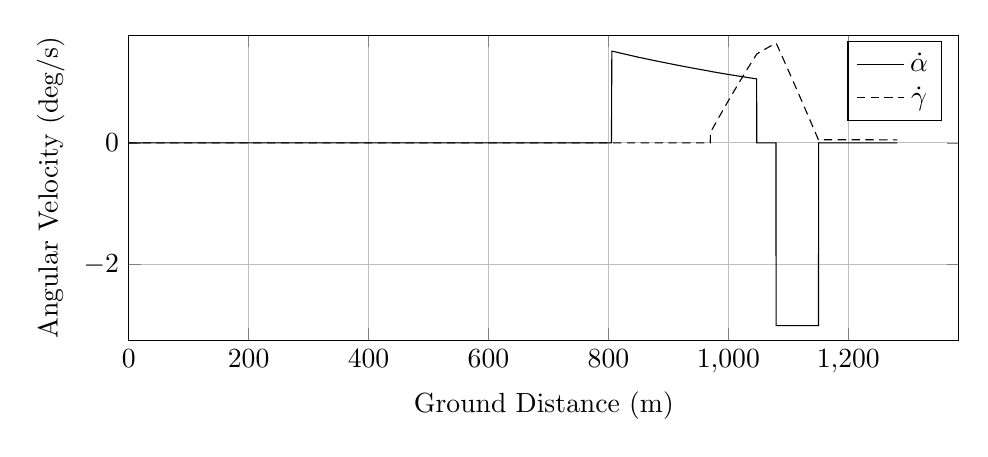
\begin{tikzpicture}

\begin{axis}[
width=\textwidth,
height=0.45\textwidth,
scaled ticks=false, tick label style={/pgf/number format/fixed},
xmin=0.0,
xmax=1384.5346672985966,
xlabel={Ground Distance (m)},
xmajorgrids,
ymin=-3.24,
ymax=1.76816229067243,
ylabel={Angular Velocity (deg/s)},
ymajorgrids,
legend entries = {$\dot\alpha$\\$\dot\gamma$\\}
]

\addplot [
color=black,
solid
]
table[row sep=crcr]{
1.3603393307216043E-8	0.0\\
3.0265395163403265E-7	0.0\\
2.9593179127983543E-6	0.0\\
1.5392338359717934E-5	0.0\\
5.361280674027254E-5	0.0\\
1.6215010178508227E-4	0.0\\
3.7214145765703975E-4	0.0\\
6.839954676020354E-4	0.0\\
0.001098342709021993	0.0\\
0.001609317716481928	0.0\\
0.0022198920000388346	0.0\\
0.002878710694837372	0.0\\
0.0036835072341781794	0.0\\
0.004557929017412697	0.0\\
0.005559798278933152	0.0\\
0.006651227400597502	0.0\\
0.007795849738889277	0.0\\
0.009067984722810115	0.0\\
0.010453165799939174	0.0\\
0.011915708813158052	0.0\\
0.013455030027058647	0.0\\
0.015131183092671713	0.0\\
0.01690803412933615	0.0\\
0.01873590105740728	0.0\\
0.020713359121301934	0.0\\
0.022777736728155237	0.0\\
0.024960970145273077	0.0\\
0.02723428625014468	0.0\\
0.029610395797831278	0.0\\
0.03204086105441677	0.0\\
0.03462344565878624	0.0\\
0.037295727153354774	0.0\\
0.040089145853872785	0.0\\
0.042950967781251806	0.0\\
0.04592022141655751	0.0\\
0.04897301836205646	0.0\\
0.052130294957187476	0.0\\
0.05542514139564195	0.0\\
0.05879722600804832	0.0\\
0.06231520981015182	0.0\\
0.06596261503753809	0.0\\
0.06964559414821356	0.0\\
0.07347193989652406	0.0\\
0.07736619052035826	0.0\\
0.08137137577670908	0.0\\
0.08545617869345057	0.0\\
0.08969468676038628	0.0\\
0.0940095881391464	0.0\\
0.09845059220533334	0.0\\
0.10296315144049947	0.0\\
0.10759658895065366	0.0\\
0.1123317495250277	0.0\\
0.1171874363557737	0.0\\
0.12217670360507671	0.0\\
0.12726806426274867	0.0\\
0.13231647880291775	0.0\\
0.13765212084557643	0.0\\
0.14294844966167852	0.0\\
0.14834594087957392	0.0\\
0.1539671093411843	0.0\\
0.15968242883369804	0.0\\
0.16555834796315422	0.0\\
0.17157514414202774	0.0\\
0.17760320215284392	0.0\\
0.18370335474801935	0.0\\
0.18983540939776816	0.0\\
0.19621099073945342	0.0\\
0.20278841209744758	0.0\\
0.20952923284938563	0.0\\
0.21624967405074952	0.0\\
0.22309476488450758	0.0\\
0.22992510727843934	0.0\\
0.2371653034562048	0.0\\
0.2442573187228817	0.0\\
0.25144286317780873	0.0\\
0.2588001799723505	0.0\\
0.2662612189130884	0.0\\
0.27386560463063747	0.0\\
0.2815803271719757	0.0\\
0.28946218069394425	0.0\\
0.29753588720841584	0.0\\
0.3056643119969481	0.0\\
0.31376446154764137	0.0\\
0.322071411728719	0.0\\
0.3303680011285137	0.0\\
0.3389039548234316	0.0\\
0.3474123396293025	0.0\\
0.3561645174790815	0.0\\
0.36525289600634137	0.0\\
0.3742306244196095	0.0\\
0.3835584127627333	0.0\\
0.392806747202999	0.0\\
0.40218604538039837	0.0\\
0.4115907129344223	0.0\\
0.42143744457304466	0.0\\
0.4310567075016639	0.0\\
0.4412814114336725	0.0\\
0.4513051702487684	0.0\\
0.461412558308395	0.0\\
0.47173637532167356	0.0\\
0.4821484569390513	0.0\\
0.492985116277161	0.0\\
0.5036221628177362	0.0\\
0.5142245311302887	0.0\\
0.5252888808291518	0.0\\
0.5363145235987512	0.0\\
0.5471208511184944	0.0\\
0.5585110457184732	0.0\\
0.569849942463402	0.0\\
0.5817265165330987	0.0\\
0.5935668742733842	0.0\\
0.6053719027871456	0.0\\
0.6172343027602503	0.0\\
0.629515267228629	0.0\\
0.6417789549774502	0.0\\
0.6542768803188956	0.0\\
0.6669828212214572	0.0\\
0.6796225285147333	0.0\\
0.6925094233679154	0.0\\
0.7056620711738308	0.0\\
0.7184715206768946	0.0\\
0.731725241748566	0.0\\
0.7449880440563246	0.0\\
0.7586792333483576	0.0\\
0.7725063377467813	0.0\\
0.7863894274138714	0.0\\
0.8004504964383841	0.0\\
0.8147129313117618	0.0\\
0.8293722635741907	0.0\\
0.8437954335339908	0.0\\
0.8580702287827062	0.0\\
0.8726489666047585	0.0\\
0.8875094051704782	0.0\\
0.9027740629895862	0.0\\
0.9182163910703112	0.0\\
0.93361566230532	0.0\\
0.9491799633800446	0.0\\
0.9646343064330896	0.0\\
0.9803727456894022	0.0\\
0.9957421603273868	0.0\\
1.0116767859397604	0.0\\
1.028041387324289	0.0\\
1.0443915011410971	0.0\\
1.060796374175649	0.0\\
1.0773229908740651	0.0\\
1.093971735592782	0.0\\
1.1110062543639518	0.0\\
1.127891796882146	0.0\\
1.1451224507351285	0.0\\
1.1624801114435046	0.0\\
1.180077727863539	0.0\\
1.1978884766667508	0.0\\
1.215488397439855	0.0\\
1.23351701382096	0.0\\
1.2518199984626128	0.0\\
1.2704235066044305	0.0\\
1.2892140278280424	0.0\\
1.3075714306593595	0.0\\
1.3266673518109293	0.0\\
1.3462106477188795	0.0\\
1.365306294594515	0.0\\
1.3852885894463176	0.0\\
1.404835539176236	0.0\\
1.4251192118409102	0.0\\
1.445164519989187	0.0\\
1.4656054698512246	0.0\\
1.4853522740259328	0.0\\
1.5051589726327936	0.0\\
1.5255757775517242	0.0\\
1.5464367798307013	0.0\\
1.5673163741652552	0.0\\
1.5879032567231621	0.0\\
1.6091523485848285	0.0\\
1.6303162371862876	0.0\\
1.6519474169970438	0.0\\
1.673879209980242	0.0\\
1.6955666802836635	0.0\\
1.7172271378534343	0.0\\
1.7402832823543353	0.0\\
1.7634396102400074	0.0\\
1.7861669372425006	0.0\\
1.8088678577734645	0.0\\
1.831824248135399	0.0\\
1.855578771396016	0.0\\
1.878960729162178	0.0\\
1.9033179534858085	0.0\\
1.9273833213731866	0.0\\
1.9518510462308036	0.0\\
1.9761594732990155	0.0\\
2.000437267212291	0.0\\
2.0252281699074732	0.0\\
2.0498006073458734	0.0\\
2.0745611186355752	0.0\\
2.0997746990963106	0.0\\
2.1260324099367294	0.0\\
2.1515212193659616	0.0\\
2.1771505246334	0.0\\
2.2031842637813908	0.0\\
2.230133398733474	0.0\\
2.257053086628849	0.0\\
2.283795213136285	0.0\\
2.311477064851834	0.0\\
2.3387199014446116	0.0\\
2.3662694524467227	0.0\\
2.3937852540088533	0.0\\
2.4216520071021392	0.0\\
2.4501931244916175	0.0\\
2.478927626230634	0.0\\
2.506685441631536	0.0\\
2.53537335014481	0.0\\
2.5633350931805676	0.0\\
2.5917889242519685	0.0\\
2.6208221472873374	0.0\\
2.649872764173903	0.0\\
2.679661174525658	0.0\\
2.709174609939316	0.0\\
2.740029385016756	0.0\\
2.770444625703795	0.0\\
2.801129860621211	0.0\\
2.8318827297715705	0.0\\
2.862425967677578	0.0\\
2.893259332541544	0.0\\
2.92412139403754	0.0\\
2.955064430161417	0.0\\
2.986690331721131	0.0\\
3.019183403261743	0.0\\
3.0507201588152526	0.0\\
3.0830332871979023	0.0\\
3.1154603869692448	0.0\\
3.148592095396281	0.0\\
3.181936872739324	0.0\\
3.214370607724433	0.0\\
3.247565473366384	0.0\\
3.281695868027062	0.0\\
3.316494330618462	0.0\\
3.3513055302544137	0.0\\
3.3860303583611797	0.0\\
3.421934361445942	0.0\\
3.456235826539576	0.0\\
3.490536654441657	0.0\\
3.526257338581564	0.0\\
3.561372823896762	0.0\\
3.5967906564503185	0.0\\
3.632682576242373	0.0\\
3.6701261071689295	0.0\\
3.707701291513044	0.0\\
3.7452745323452916	0.0\\
3.78256482255855	0.0\\
3.8208821591411084	0.0\\
3.8590337549211444	0.0\\
3.89695718563138	0.0\\
3.9351036745073964	0.0\\
3.9736642086653067	0.0\\
4.012189127077221	0.0\\
4.05156219172609	0.0\\
4.090290786278251	0.0\\
4.129291984889424	0.0\\
4.1680648628189925	0.0\\
4.207805169621487	0.0\\
4.248168240749736	0.0\\
4.288797880674668	0.0\\
4.32990243544832	0.0\\
4.371428084678056	0.0\\
4.41247037137882	0.0\\
4.453879445321437	0.0\\
4.49524783594077	0.0\\
4.537299342543221	0.0\\
4.580546125800922	0.0\\
4.622914948498307	0.0\\
4.66640222022569	0.0\\
4.709294790611851	0.0\\
4.752417172855319	0.0\\
4.796155651503765	0.0\\
4.8408754796551925	0.0\\
4.884850997559644	0.0\\
4.928651138956553	0.0\\
4.972831351372241	0.0\\
5.017331702752941	0.0\\
5.0632326321008225	0.0\\
5.108452384314601	0.0\\
5.1536021218025905	0.0\\
5.199057463234675	0.0\\
5.244479287100011	0.0\\
5.292293005248643	0.0\\
5.338096108273211	0.0\\
5.3857492800262605	0.0\\
5.433816232374781	0.0\\
5.480691139018431	0.0\\
5.529685763332537	0.0\\
5.578612887337309	0.0\\
5.626451501744754	0.0\\
5.674834544150631	0.0\\
5.7252048440372345	0.0\\
5.77422346516266	0.0\\
5.8255152536468575	0.0\\
5.874338256646894	0.0\\
5.922631450506765	0.0\\
5.972682300942642	0.0\\
6.022535370757359	0.0\\
6.074394648705015	0.0\\
6.124928192945902	0.0\\
6.176798284396469	0.0\\
6.229620191179453	0.0\\
6.282808156696705	0.0\\
6.334658925277093	0.0\\
6.388041948821611	0.0\\
6.440558117792513	0.0\\
6.494960924490993	0.0\\
6.550441697666145	0.0\\
6.6042098433346865	0.0\\
6.658315220792536	0.0\\
6.712335084641163	0.0\\
6.766674450459032	0.0\\
6.821537769035839	0.0\\
6.876851268142238	0.0\\
6.933661362437203	0.0\\
6.989261882852809	0.0\\
7.046240323930029	0.0\\
7.102786137967051	0.0\\
7.1603789170469145	0.0\\
7.21785165788507	0.0\\
7.277487498606879	0.0\\
7.334984696129153	0.0\\
7.393362172524569	0.0\\
7.452416393609804	0.0\\
7.511934748111884	0.0\\
7.572557225035805	0.0\\
7.63202184821041	0.0\\
7.69294899409779	0.0\\
7.752675521499926	0.0\\
7.814488876138199	0.0\\
7.8763528528159785	0.0\\
7.938149975125226	0.0\\
8.001193143199774	0.0\\
8.064554080136986	0.0\\
8.12686567918485	0.0\\
8.189637855946287	0.0\\
8.252542711798306	0.0\\
8.315859663763469	0.0\\
8.380006162932737	0.0\\
8.444702551512929	0.0\\
8.509501986620958	0.0\\
8.57387297516295	0.0\\
8.63887365699837	0.0\\
8.70727085773305	0.0\\
8.772937378995405	0.0\\
8.839192134487615	0.0\\
8.905815929161982	0.0\\
8.97209054442786	0.0\\
9.039019026885107	0.0\\
9.107371801018814	0.0\\
9.174915633685494	0.0\\
9.243868961478196	0.0\\
9.312440636565494	0.0\\
9.381784695008012	0.0\\
9.4513167952828	0.0\\
9.52142787533916	0.0\\
9.591425279059166	0.0\\
9.662230428326719	0.0\\
9.734225879912522	0.0\\
9.806441602430919	0.0\\
9.878483835105534	0.0\\
9.951807209049782	0.0\\
10.023539677466466	0.0\\
10.096057433179052	0.0\\
10.168262179450682	0.0\\
10.241274410624943	0.0\\
10.31479015323385	0.0\\
10.390063469390178	0.0\\
10.465012435634037	0.0\\
10.540639152111389	0.0\\
10.617644389866598	0.0\\
10.692945462162374	0.0\\
10.770083295573727	0.0\\
10.846726862770723	0.0\\
10.924657809445929	0.0\\
11.00265335491597	0.0\\
11.081827589833612	0.0\\
11.159134327011738	0.0\\
11.239152720133266	0.0\\
11.317028257314295	0.0\\
11.396413369884492	0.0\\
11.477655063362434	0.0\\
11.556958506738276	0.0\\
11.637325199769407	0.0\\
11.717754170658207	0.0\\
11.799819443100102	0.0\\
11.881986970940797	0.0\\
11.964394119506721	0.0\\
12.046263329632716	0.0\\
12.130282587748898	0.0\\
12.213721087180826	0.0\\
12.295868535962462	0.0\\
12.380692430046633	0.0\\
12.46470288467437	0.0\\
12.550384439940181	0.0\\
12.635259749824865	0.0\\
12.72144647897981	0.0\\
12.80741162779486	0.0\\
12.892901506907108	0.0\\
12.977815703098727	0.0\\
13.06483740414145	0.0\\
13.151922956503014	0.0\\
13.240589045456186	0.0\\
13.329911181207382	0.0\\
13.417306166647748	0.0\\
13.507103029723119	0.0\\
13.595986036712912	0.0\\
13.687453390597003	0.0\\
13.779071846306106	0.0\\
13.872694200363323	0.0\\
13.963504841252302	0.0\\
14.056146454975131	0.0\\
14.14918846816267	0.0\\
14.24332804549016	0.0\\
14.339261112049854	0.0\\
14.431091301610323	0.0\\
14.524174633942373	0.0\\
14.618760344060338	0.0\\
14.714801736988441	0.0\\
14.809763128346521	0.0\\
14.903412319659619	0.0\\
15.001392651385917	0.0\\
15.098055049922994	0.0\\
15.196870856960619	0.0\\
15.29477342819068	0.0\\
15.39265348361268	0.0\\
15.490487151984588	0.0\\
15.588146853189365	0.0\\
15.687961867268871	0.0\\
15.78650099417861	0.0\\
15.886965864441798	0.0\\
15.98755318095926	0.0\\
16.088470385762115	0.0\\
16.190536977381747	0.0\\
16.292466610053154	0.0\\
16.396448349404487	0.0\\
16.497808944935016	0.0\\
16.600551072850564	0.0\\
16.70575139586156	0.0\\
16.81134459259622	0.0\\
16.917616592554033	0.0\\
17.023477948501657	0.0\\
17.12904978140002	0.0\\
17.2354081519902	0.0\\
17.340772011500363	0.0\\
17.448391076872838	0.0\\
17.5571980918308	0.0\\
17.66615596614949	0.0\\
17.774685459577412	0.0\\
17.884986575683584	0.0\\
17.99552903728076	0.0\\
18.108708479124623	0.0\\
18.219646262474413	0.0\\
18.332680252669796	0.0\\
18.445061806396694	0.0\\
18.556709221711323	0.0\\
18.668884868236475	0.0\\
18.78204748093455	0.0\\
18.895704562363058	0.0\\
19.008928234289563	0.0\\
19.124320907419907	0.0\\
19.24105855786135	0.0\\
19.355116774466126	0.0\\
19.470462572962035	0.0\\
19.58492145104516	0.0\\
19.704921229319112	0.0\\
19.821259826163917	0.0\\
19.941172080873493	0.0\\
20.06078806851737	0.0\\
20.177423389922623	0.0\\
20.297621170678	0.0\\
20.420129559802255	0.0\\
20.54164670774839	0.0\\
20.661905244258705	0.0\\
20.784301666224792	0.0\\
20.904244540623438	0.0\\
21.028114340450195	0.0\\
21.148300883955606	0.0\\
21.270875420257596	0.0\\
21.39299406946177	0.0\\
21.513793771711654	0.0\\
21.637476506915142	0.0\\
21.759279707150128	0.0\\
21.88493035745168	0.0\\
22.009809790007786	0.0\\
22.13620730934617	0.0\\
22.263515470260465	0.0\\
22.393040471753594	0.0\\
22.520519759768852	0.0\\
22.648852607677917	0.0\\
22.775118904521122	0.0\\
22.903136237443974	0.0\\
23.03176118514304	0.0\\
23.162501585272054	0.0\\
23.294719932439598	0.0\\
23.427108470281937	0.0\\
23.558693146983046	0.0\\
23.687077503630363	0.0\\
23.817949558665852	0.0\\
23.948210788889448	0.0\\
24.076877750667826	0.0\\
24.21019765060587	0.0\\
24.3450673155249	0.0\\
24.477101355489637	0.0\\
24.60984760833776	0.0\\
24.7468403923846	0.0\\
24.882807251950062	0.0\\
25.017167332957627	0.0\\
25.153910941279605	0.0\\
25.289629217480112	0.0\\
25.425306692573436	0.0\\
25.56229499031975	0.0\\
25.70075944713021	0.0\\
25.83724158708921	0.0\\
25.975209935932874	0.0\\
26.003074150630965	0.0\\
26.020759913393235	0.0\\
26.030714598210515	0.0\\
26.05840292223249	0.0\\
26.06133765907019	0.0\\
26.064285136409026	0.0\\
26.066337724202356	0.0\\
26.068175973881182	0.0\\
26.06984477238784	0.0\\
26.077831036047115	0.0\\
26.10345636352254	0.0\\
26.16716044512971	0.0\\
26.297541524199602	0.0\\
26.42722303713863	0.0\\
26.5559280656694	0.0\\
26.686097387723095	0.0\\
26.817793678842584	0.0\\
26.949416928520378	0.0\\
27.080440623797912	0.0\\
27.215491080424528	0.0\\
27.34795890217076	0.0\\
27.48215578365496	0.0\\
27.616696052324144	0.0\\
27.75271189183823	0.0\\
27.888759310501555	0.0\\
28.023839122857026	0.0\\
28.16136324828667	0.0\\
28.298355249881332	0.0\\
28.435282447697354	0.0\\
28.573941346212784	0.0\\
28.713752690797136	0.0\\
28.852681198061333	0.0\\
28.992471984120606	0.0\\
29.133421724605903	0.0\\
29.275199211812186	0.0\\
29.416225289053614	0.0\\
29.55783477945603	0.0\\
29.701838356359822	0.0\\
29.846633046394217	0.0\\
29.99013730470424	0.0\\
30.132492646908446	0.0\\
30.277395768405135	0.0\\
30.422188862471998	0.0\\
30.56637548064623	0.0\\
30.711944318924978	0.0\\
30.8573377156769	0.0\\
31.006558691603843	0.0\\
31.153907258126303	0.0\\
31.30257185742142	0.0\\
31.4510947803754	0.0\\
31.602595106592503	0.0\\
31.755261577184278	0.0\\
31.906398416479824	0.0\\
32.05599258457312	0.0\\
32.20952926265106	0.0\\
32.360097140052986	0.0\\
32.51218835243483	0.0\\
32.664721606344784	0.0\\
32.82129760777845	0.0\\
32.97669884718651	0.0\\
33.13118849606322	0.0\\
33.288837444683736	0.0\\
33.44405554194745	0.0\\
33.60015866510213	0.0\\
33.756686089655645	0.0\\
33.91694077595571	0.0\\
34.074326811338736	0.0\\
34.23252403098988	0.0\\
34.392884168270385	0.0\\
34.554266068788166	0.0\\
34.71363140184178	0.0\\
34.87649332318763	0.0\\
35.03746231629111	0.0\\
35.19990059234286	0.0\\
35.3627309111595	0.0\\
35.5271254050015	0.0\\
35.69149466827288	0.0\\
35.85508342515686	0.0\\
36.017180984292054	0.0\\
36.182222084544165	0.0\\
36.34861175093968	0.0\\
36.514166392421686	0.0\\
36.68083924241549	0.0\\
36.845526722294395	0.0\\
37.01328249159678	0.0\\
37.18160982421668	0.0\\
37.35136716620059	0.0\\
37.51969289597564	0.0\\
37.689710015857784	0.0\\
37.860394939778416	0.0\\
38.02805196867635	0.0\\
38.19868492919754	0.0\\
38.37343039987371	0.0\\
38.54685896696101	0.0\\
38.71934233168869	0.0\\
38.8915617091798	0.0\\
39.062305982326905	0.0\\
39.23847188392709	0.0\\
39.411511502305984	0.0\\
39.585172817779906	0.0\\
39.760693028009456	0.0\\
39.9373134006328	0.0\\
40.113617753210534	0.0\\
40.29094651898711	0.0\\
40.468149621311596	0.0\\
40.64593210594187	0.0\\
40.82431302355218	0.0\\
41.00141330502653	0.0\\
41.17957893337042	0.0\\
41.359761290266974	0.0\\
41.53889737920997	0.0\\
41.72013507746885	0.0\\
41.899395797464194	0.0\\
42.081280067494475	0.0\\
42.265315320939635	0.0\\
42.44531744651641	0.0\\
42.62715102096499	0.0\\
42.81120266452106	0.0\\
42.994164503876235	0.0\\
43.17799769459725	0.0\\
43.36154361404071	0.0\\
43.54597437124032	0.0\\
43.73158498218817	0.0\\
43.91737182308138	0.0\\
44.1050494697441	0.0\\
44.293574236233	0.0\\
44.47888581456586	0.0\\
44.66456251492659	0.0\\
44.85170130968709	0.0\\
45.037822074257164	0.0\\
45.22676109993536	0.0\\
45.41612608476639	0.0\\
45.604812217355104	0.0\\
45.79422221198037	0.0\\
45.98724683785376	0.0\\
46.17830917717477	0.0\\
46.36786657808848	0.0\\
46.55935209439748	0.0\\
46.75090376717816	0.0\\
46.94233405988251	0.0\\
47.13714948644359	0.0\\
47.33387512950824	0.0\\
47.53043319838464	0.0\\
47.72298239739284	0.0\\
47.919150009665316	0.0\\
48.113386178114425	0.0\\
48.311024807628144	0.0\\
48.508886059616145	0.0\\
48.70490444306449	0.0\\
48.90290918859142	0.0\\
49.09959709013448	0.0\\
49.2970021191946	0.0\\
49.49532701226336	0.0\\
49.693780717172615	0.0\\
49.89506320355713	0.0\\
50.096719083698545	0.0\\
50.29606895218413	0.0\\
50.497598474286534	0.0\\
50.700304208193415	0.0\\
50.90342397924904	0.0\\
51.10460922167407	0.0\\
51.30752217039489	0.0\\
51.51010619677311	0.0\\
51.713602501430145	0.0\\
51.91843850546792	0.0\\
52.121089026646246	0.0\\
52.32561402362407	0.0\\
52.53192272805477	0.0\\
52.7387030603267	0.0\\
52.944027344085896	0.0\\
53.154073670302836	0.0\\
53.36143953271798	0.0\\
53.571009444677685	0.0\\
53.77799762982136	0.0\\
53.98785945427545	0.0\\
54.196157549666225	0.0\\
54.40718762937186	0.0\\
54.616887598525366	0.0\\
54.826875464266934	0.0\\
55.04038432082807	0.0\\
55.25438844036796	0.0\\
55.46695867894975	0.0\\
55.68088820258777	0.0\\
55.895144656119854	0.0\\
56.109028395418505	0.0\\
56.326262430904194	0.0\\
56.542089933321776	0.0\\
56.76060076462056	0.0\\
56.97729209122687	0.0\\
57.19579178641709	0.0\\
57.41258192878804	0.0\\
57.634093277561306	0.0\\
57.85395098827546	0.0\\
58.07448819514299	0.0\\
58.29446478173499	0.0\\
58.51588770709739	0.0\\
58.73757884137123	0.0\\
58.96020041504734	0.0\\
59.18267120664716	0.0\\
59.405949655899676	0.0\\
59.63089974393067	0.0\\
59.8562534200115	0.0\\
60.084134136581554	0.0\\
60.30833762904015	0.0\\
60.53504725699203	0.0\\
60.763693228044005	0.0\\
60.99075593752245	0.0\\
61.21765734918529	0.0\\
61.44713116872772	0.0\\
61.6738048454246	0.0\\
61.90668490141796	0.0\\
62.13729676517957	0.0\\
62.36629463006145	0.0\\
62.596359157213186	0.0\\
62.82836101237727	0.0\\
63.059723307860466	0.0\\
63.292774394726166	0.0\\
63.52608473446321	0.0\\
63.75973181411028	0.0\\
63.993403028653574	0.0\\
64.23068717493263	0.0\\
64.4710952259949	0.0\\
64.70858695601663	0.0\\
64.94894296164699	0.0\\
65.18738841845183	0.0\\
65.42661162888535	0.0\\
65.6659442133793	0.0\\
65.90899583190168	0.0\\
66.15068261105333	0.0\\
66.39533053734849	0.0\\
66.6378997293487	0.0\\
66.88158418814953	0.0\\
67.12390450547147	0.0\\
67.36840986262189	0.0\\
67.61550053739396	0.0\\
67.86097385246623	0.0\\
68.10985741250389	0.0\\
68.35582503705197	0.0\\
68.60464259362828	0.0\\
68.85450289166104	0.0\\
69.1042877596268	0.0\\
69.35837572129628	0.0\\
69.61150655903072	0.0\\
69.86289252102952	0.0\\
70.11686816207683	0.0\\
70.37125759672608	0.0\\
70.62480458144697	0.0\\
70.88045310059783	0.0\\
71.13526709211152	0.0\\
71.3947754873567	0.0\\
71.6534187996231	0.0\\
71.91450497256008	0.0\\
72.1716184080999	0.0\\
72.43269265097052	0.0\\
72.69331619504374	0.0\\
72.95563200429567	0.0\\
73.21686762735783	0.0\\
73.48161420086069	0.0\\
73.74261486234883	0.0\\
74.00755043430098	0.0\\
74.27511769675363	0.0\\
74.54487113507057	0.0\\
74.81568229507957	0.0\\
75.08274085953312	0.0\\
75.35421836228127	0.0\\
75.62798354862159	0.0\\
75.89909469738902	0.0\\
76.17008148658607	0.0\\
76.44269151183332	0.0\\
76.71571902594138	0.0\\
76.99340852183178	0.0\\
77.27004772085374	0.0\\
77.54832408953641	0.0\\
77.82592519882277	0.0\\
78.10358246820337	0.0\\
78.38556010231375	0.0\\
78.66911430382748	0.0\\
78.95399134982776	0.0\\
79.23667137346987	0.0\\
79.518907793654	0.0\\
79.80555437718249	0.0\\
80.09150103324356	0.0\\
80.37928873457926	0.0\\
80.66871996946384	0.0\\
80.95967699414447	0.0\\
81.25093884305389	0.0\\
81.54344278085921	0.0\\
81.8358102960415	0.0\\
82.13087592438694	0.0\\
82.42794520371837	0.0\\
82.72842933895026	0.0\\
83.0269479931649	0.0\\
83.32974506690314	0.0\\
83.62964811531441	0.0\\
83.92951211009506	0.0\\
84.2339319847595	0.0\\
84.53715838283946	0.0\\
84.84105485927768	0.0\\
85.14845677960258	0.0\\
85.45530133949276	0.0\\
85.76249773413784	0.0\\
86.07201271349416	0.0\\
86.38432073331904	0.0\\
86.69710203601804	0.0\\
87.01172103282082	0.0\\
87.32669099459858	0.0\\
87.64517025121202	0.0\\
87.96158123090564	0.0\\
88.2775814178033	0.0\\
88.60068374099544	0.0\\
88.92068281935622	0.0\\
89.24207276858638	0.0\\
89.56578933015979	0.0\\
89.88760090270688	0.0\\
90.2141410750086	0.0\\
90.54066676000363	0.0\\
90.86727570256076	0.0\\
91.19715108614633	0.0\\
91.52744226539704	0.0\\
91.85639956214655	0.0\\
92.19095740864739	0.0\\
92.52827526888461	0.0\\
92.8674718219292	0.0\\
93.20307982994817	0.0\\
93.5374944579234	0.0\\
93.87598013161067	0.0\\
94.20917297854535	0.0\\
94.55043409744499	0.0\\
94.89132963816093	0.0\\
95.23083207736542	0.0\\
95.57395676502793	0.0\\
95.91421223354143	0.0\\
96.25656086122288	0.0\\
96.60012122339742	0.0\\
96.94166303707107	0.0\\
97.28627502929558	0.0\\
97.62906225262071	0.0\\
97.97125437026659	0.0\\
98.31201772458999	0.0\\
98.65627175165852	0.0\\
99.0012536203806	0.0\\
99.35020029285332	0.0\\
99.69475740907401	0.0\\
100.04053871990226	0.0\\
100.38598466112728	0.0\\
100.72867962848932	0.0\\
101.07385499050397	0.0\\
101.41864366415388	0.0\\
101.76305460768467	0.0\\
102.11068844700483	0.0\\
102.45638678530696	0.0\\
102.79841653079728	0.0\\
103.14087212494877	0.0\\
103.48486473791618	0.0\\
103.82875595362174	0.0\\
104.17244250654872	0.0\\
104.51168383396202	0.0\\
104.85986244643053	0.0\\
105.204587526496	0.0\\
105.54754777175077	0.0\\
105.88797456536247	0.0\\
106.23280177240994	0.0\\
106.57515110440406	0.0\\
106.91603555764121	0.0\\
107.25729565943405	0.0\\
107.598830149446	0.0\\
107.93686571059558	0.0\\
108.27485499032852	0.0\\
108.28839963475954	0.0\\
108.30004107281309	0.0\\
108.30931238392475	0.0\\
108.31701527366243	0.0\\
108.32505202073054	0.0\\
108.33865239118708	0.0\\
108.35091925899997	0.0\\
108.39508146726081	0.0\\
108.52984553865659	0.0\\
108.79919793188978	0.0\\
109.105233418432	0.0\\
109.41485218466596	0.0\\
109.72257164661937	0.0\\
110.0321119530083	0.0\\
110.34145354075926	0.0\\
110.6534776714839	0.0\\
110.9711963390063	0.0\\
111.28851843247409	0.0\\
111.60893519474632	0.0\\
111.92798394282838	0.0\\
112.24770070245137	0.0\\
112.57243448635171	0.0\\
112.89480865389396	0.0\\
113.22000325235314	0.0\\
113.54885709436653	0.0\\
113.8770619430189	0.0\\
114.20946079557197	0.0\\
114.54107775051554	0.0\\
114.87787736567807	0.0\\
115.21564640021248	0.0\\
115.55522358014255	0.0\\
115.89667501383605	0.0\\
116.23992536102014	0.0\\
116.5847156213415	0.0\\
116.92791619634093	0.0\\
117.27517516660399	0.0\\
117.62420948631524	0.0\\
117.97391125359778	0.0\\
118.32673409155768	0.0\\
118.68227803698588	0.0\\
119.03889207644076	0.0\\
119.39651249432902	0.0\\
119.75508651978987	0.0\\
120.11314113323388	0.0\\
120.47404637453192	0.0\\
120.84098349318353	0.0\\
121.20490030977416	0.0\\
121.57328571082118	0.0\\
121.94079100066682	0.0\\
122.31015242291167	0.0\\
122.68267403243519	0.0\\
123.05346836176264	0.0\\
123.42835733050345	0.0\\
123.80350972566416	0.0\\
124.1783235941891	0.0\\
124.55244040146786	0.0\\
124.92576251095704	0.0\\
125.30489170817492	0.0\\
125.68146781278597	0.0\\
126.06139977608174	0.0\\
126.44502763856761	0.0\\
126.82695116404781	0.0\\
127.206716044588	0.0\\
127.59262031825523	0.0\\
127.97077035934353	0.0\\
128.3546122768156	0.0\\
128.73724861847296	0.0\\
129.12002064685282	0.0\\
129.50086700331673	0.0\\
129.8837789976152	0.0\\
130.26783132854348	0.0\\
130.651936341801	0.0\\
131.03747321415574	0.0\\
131.42280335891803	0.0\\
131.80875442588928	0.0\\
132.19322104975072	0.0\\
132.5798881414172	0.0\\
132.96215446290768	0.0\\
133.34488286943906	0.0\\
133.7276157954845	0.0\\
134.11532375481391	0.0\\
134.50135826447365	0.0\\
134.88604120201086	0.0\\
135.26955723714872	0.0\\
135.6512109336153	0.0\\
136.03464327936558	0.0\\
136.41686422877552	0.0\\
136.79904942565338	0.0\\
137.18004416157777	0.0\\
137.56399804528928	0.0\\
137.94515347717788	0.0\\
138.32982901897384	0.0\\
138.7128522769853	0.0\\
139.09597564505458	0.0\\
139.48002685240425	0.0\\
139.86309097971855	0.0\\
140.24727738828375	0.0\\
140.6317581809211	0.0\\
141.01585725597846	0.0\\
141.3998433603236	0.0\\
141.7841907991213	0.0\\
142.16710976343057	0.0\\
142.55205218648928	0.0\\
142.9364233092117	0.0\\
143.32169829765928	0.0\\
143.705984531242	0.0\\
144.08985428249122	0.0\\
144.47683600496026	0.0\\
144.86371007721533	0.0\\
145.24772592056325	0.0\\
145.63047789911974	0.0\\
146.01273254364395	0.0\\
146.39725173307323	0.0\\
146.77966503747456	0.0\\
147.16478130736948	0.0\\
147.54689717238745	0.0\\
147.93097497792814	0.0\\
148.31499270913332	0.0\\
148.69957284780122	0.0\\
149.08709998577143	0.0\\
149.47129868208145	0.0\\
149.8546635899794	0.0\\
150.23801379389647	0.0\\
150.62200569343076	0.0\\
151.00751012558203	0.0\\
151.3946455315429	0.0\\
151.77987817077866	0.0\\
152.16505704867353	0.0\\
152.55112759502248	0.0\\
152.93964308710213	0.0\\
153.32507651584535	0.0\\
153.71174813432617	0.0\\
154.10000329570875	0.0\\
154.48914219495543	0.0\\
154.8788297075107	0.0\\
155.26820650111182	0.0\\
155.6562915247282	0.0\\
156.0441896603637	0.0\\
156.4348678136667	0.0\\
156.82082928279863	0.0\\
157.21071017196311	0.0\\
157.60005066896917	0.0\\
157.99004282467217	0.0\\
158.3808231456182	0.0\\
158.77280374485122	0.0\\
159.16384255262415	0.0\\
159.55370941764693	0.0\\
159.946071590523	0.0\\
160.33752628124114	0.0\\
160.73008933968674	0.0\\
161.12428312893906	0.0\\
161.5185576482712	0.0\\
161.91431288671106	0.0\\
162.3096877663487	0.0\\
162.70613442998513	0.0\\
163.1032465869576	0.0\\
163.50039135636405	0.0\\
163.89625578410926	0.0\\
164.29272443146095	0.0\\
164.68754921345175	0.0\\
165.0864466423082	0.0\\
165.4846753800681	0.0\\
165.88329117400662	0.0\\
166.28234792206388	0.0\\
166.68312204436222	0.0\\
167.08520211103445	0.0\\
167.486487681752	0.0\\
167.8888620337579	0.0\\
168.290121631074	0.0\\
168.69179641444674	0.0\\
169.0966267258019	0.0\\
169.50108473093724	0.0\\
169.90729482190739	0.0\\
170.31243922775104	0.0\\
170.71755979953144	0.0\\
171.12402986296422	0.0\\
171.53319587512163	0.0\\
171.941770038195	0.0\\
172.3502931259835	0.0\\
172.7599322859847	0.0\\
173.17073308198894	0.0\\
173.58266371319877	0.0\\
173.99296569000023	0.0\\
174.40104722187203	0.0\\
174.8156903853216	0.0\\
175.2299479185392	0.0\\
175.64260521584504	0.0\\
176.05374721710058	0.0\\
176.4688147253861	0.0\\
176.8832117842232	0.0\\
177.30033423294157	0.0\\
177.7185234955238	0.0\\
178.13477925276436	0.0\\
178.55472625996282	0.0\\
178.97486541267733	0.0\\
179.39652032378837	0.0\\
179.8177496461559	0.0\\
180.24148986351946	0.0\\
180.66579793025812	0.0\\
181.08977314985765	0.0\\
181.5138518510159	0.0\\
181.9380657232258	0.0\\
182.36353384896404	0.0\\
182.79266406809302	0.0\\
183.2222080657075	0.0\\
183.65034235239733	0.0\\
184.08076505956626	0.0\\
184.51404645281445	0.0\\
184.94459821529773	0.0\\
185.37526818895066	0.0\\
185.80988061731233	0.0\\
186.24113427192242	0.0\\
186.6766273110748	0.0\\
187.11377077964733	0.0\\
187.55114760103595	0.0\\
187.98927624239354	0.0\\
188.4283980284245	0.0\\
188.87193099833303	0.0\\
189.31533331187586	0.0\\
189.759935940091	0.0\\
190.20453173770989	0.0\\
190.64970684403454	0.0\\
191.09969623361582	0.0\\
191.54891620327845	0.0\\
191.9989246744131	0.0\\
192.45044905246328	0.0\\
192.90128656673437	0.0\\
193.3542511019695	0.0\\
193.8098580932263	0.0\\
194.264335427238	0.0\\
194.7197268653846	0.0\\
195.17731099948054	0.0\\
195.640653905739	0.0\\
196.0993779505016	0.0\\
196.55972836032635	0.0\\
197.02207639293357	0.0\\
197.4863674869817	0.0\\
197.95219407477043	0.0\\
198.4222293887736	0.0\\
198.8924165831608	0.0\\
199.36444563655942	0.0\\
199.83611037172778	0.0\\
200.3098256112723	0.0\\
200.78414125071725	0.0\\
201.25799602765767	0.0\\
201.73164228776483	0.0\\
202.20700915933037	0.0\\
202.6900968253659	0.0\\
203.1695441846722	0.0\\
203.6517557737585	0.0\\
204.13875101960963	0.0\\
204.6239796679484	0.0\\
205.11304714664226	0.0\\
205.6024757424737	0.0\\
206.0956744812894	0.0\\
206.59166612209884	0.0\\
207.08890230426118	0.0\\
207.58731362513566	0.0\\
208.08714180167652	0.0\\
208.59040365453075	0.0\\
209.09687012836855	0.0\\
209.6041180918084	0.0\\
210.11339270974815	0.0\\
210.6277299333704	0.0\\
211.14394599884707	0.0\\
211.66140554682187	0.0\\
212.17921813681886	0.0\\
212.6998673783849	0.0\\
213.22377641861283	0.0\\
213.74833300550847	0.0\\
214.27884482570528	0.0\\
214.8059921031383	0.0\\
215.3369392301239	0.0\\
215.8704905221095	0.0\\
216.40581461505735	0.0\\
216.94632642726936	0.0\\
217.49339939057347	0.0\\
218.04214604852046	0.0\\
218.5904378944307	0.0\\
219.1473756849698	0.0\\
219.70259972305752	0.0\\
220.26448543519223	0.0\\
220.82878425574808	0.0\\
221.39118212311007	0.0\\
221.95607401520328	0.0\\
222.52731263387568	0.0\\
223.1053033039969	0.0\\
223.68701431082144	0.0\\
224.27373979946424	0.0\\
224.8655655904359	0.0\\
225.4547840144254	0.0\\
226.0470361867341	0.0\\
226.6446113983061	0.0\\
227.2523816590479	0.0\\
227.85688390770105	0.0\\
228.45777056631943	0.0\\
229.07573877962136	0.0\\
229.69270723810865	0.0\\
230.30810613162595	0.0\\
230.92134117327288	0.0\\
231.53668557885607	0.0\\
232.15954554112375	0.0\\
232.7891522435175	0.0\\
233.4179357898359	0.0\\
234.03801334540844	0.0\\
234.67060997558383	0.0\\
235.30821584307404	0.0\\
235.93913792971972	0.0\\
236.57130412742504	0.0\\
237.20190286705872	0.0\\
237.82732440575694	0.0\\
238.45423612656094	0.0\\
239.078886894133	0.0\\
239.70118268314496	0.0\\
240.32402516569954	0.0\\
240.94763231602371	0.0\\
241.558944055687	0.0\\
242.17051988815223	0.0\\
242.78305452643912	0.0\\
243.3891405005665	0.0\\
243.99135888524592	0.0\\
244.5938059991201	0.0\\
245.19307787825466	0.0\\
245.78685747081	0.0\\
246.38614597174575	0.0\\
246.9780005147843	0.0\\
247.56968865205243	0.0\\
248.15440614950631	0.0\\
248.73860746053964	0.0\\
249.3201116454489	0.0\\
249.89451218910904	0.0\\
250.46870613238303	0.0\\
251.04194053158074	0.0\\
251.61194691308668	0.0\\
252.18082396300082	0.0\\
252.74758709237483	0.0\\
253.31251969447777	0.0\\
253.8738250395511	0.0\\
254.43149203184282	0.0\\
254.9874373408491	0.0\\
255.5414166310287	0.0\\
256.0957211160239	0.0\\
256.6475553966509	0.0\\
256.7570758146961	0.0\\
256.8263249833143	0.0\\
256.88663486655446	0.0\\
256.9430978473978	0.0\\
256.97693788107017	0.0\\
257.0025084975957	0.0\\
257.0208190077692	0.0\\
257.0380809845981	0.0\\
257.0438424242251	0.0\\
257.0596503141385	0.0\\
257.13618872139693	0.0\\
257.44346456136407	0.0\\
257.93842545742496	0.0\\
258.42387567471803	0.0\\
258.90988498762806	0.0\\
259.398919728937	0.0\\
259.89126252890617	0.0\\
260.3860981148131	0.0\\
260.88265150215534	0.0\\
261.3817388499359	0.0\\
261.8849745252071	0.0\\
262.3951340270795	0.0\\
262.90121520425464	0.0\\
263.4122609086296	0.0\\
263.9251595409296	0.0\\
264.44312884967155	0.0\\
264.96433898075304	0.0\\
265.4907836389158	0.0\\
266.01963642880764	0.0\\
266.54886163053106	0.0\\
267.08296130365613	0.0\\
267.61991815897215	0.0\\
268.1640390021088	0.0\\
268.7103404861746	0.0\\
269.2595660030436	0.0\\
269.81273134777575	0.0\\
270.3696596938787	0.0\\
270.93171711640935	0.0\\
271.4988611754003	0.0\\
272.0705326832831	0.0\\
272.6463683686135	0.0\\
273.226018440957	0.0\\
273.81180745355675	0.0\\
274.40462060354696	0.0\\
274.9941745097303	0.0\\
275.5928332442985	0.0\\
276.19228787269583	0.0\\
276.8008320595037	0.0\\
277.4103073713045	0.0\\
278.02312272786935	0.0\\
278.6480801130689	0.0\\
279.2749501652314	0.0\\
279.908172349486	0.0\\
280.54544660125293	0.0\\
281.1830405144573	0.0\\
281.81994836131184	0.0\\
282.4644929822557	0.0\\
283.1124628947573	0.0\\
283.7598098057015	0.0\\
284.41078479564055	0.0\\
285.05862981013433	0.0\\
285.70800893721935	0.0\\
286.3602979435012	0.0\\
287.0082513205941	0.0\\
287.65676876221744	0.0\\
288.3093687105044	0.0\\
288.95762918532625	0.0\\
289.6032303041229	0.0\\
290.2463292415888	0.0\\
290.88254119236694	0.0\\
291.5174657935754	0.0\\
292.15135749313765	0.0\\
292.77987115362725	0.0\\
293.4115418191582	0.0\\
294.03817556900935	0.0\\
294.6609105860233	0.0\\
295.28022031816545	0.0\\
295.9013637804736	0.0\\
296.51859456939405	0.0\\
297.13445448111213	0.0\\
297.7448643111652	0.0\\
298.35646750465946	0.0\\
298.9665369440928	0.0\\
299.57280619311405	0.0\\
300.17881401664965	0.0\\
300.7810579412371	0.0\\
301.38261059253784	0.0\\
301.9807872641708	0.0\\
302.5818390257391	0.0\\
303.1804945574968	0.0\\
303.775610749277	0.0\\
304.3662430439555	0.0\\
304.95700718406374	0.0\\
305.54856325255184	0.0\\
306.1403526946923	0.0\\
306.732267705287	0.0\\
307.3183663050603	0.0\\
307.9060154577753	0.0\\
308.4922500043788	0.0\\
309.07710579978243	0.0\\
309.66501129994356	0.0\\
310.2470970112189	0.0\\
310.8294165810805	0.0\\
311.4130393021758	0.0\\
311.99229355856255	0.0\\
312.5719037973066	0.0\\
313.1528238715506	0.0\\
313.7328622425008	0.0\\
314.3105382229827	0.0\\
314.88851884372366	0.0\\
315.4681174962417	0.0\\
316.04617774980557	0.0\\
316.6220728552114	0.0\\
317.19745521492473	0.0\\
317.7754931730906	0.0\\
318.353555553143	0.0\\
318.9291304405266	0.0\\
319.5035706351016	0.0\\
320.07956917661147	0.0\\
320.654112858477	0.0\\
321.22847808306085	0.0\\
321.80362538780014	0.0\\
322.37559125839107	0.0\\
322.95020588965565	0.0\\
323.5264836020216	0.0\\
324.0993601571	0.0\\
324.67229708028094	0.0\\
325.24767898856896	0.0\\
325.8179314072054	0.0\\
326.3890807131188	0.0\\
326.96397559242325	0.0\\
327.5369863011746	0.0\\
328.1117741316982	0.0\\
328.6826005118504	0.0\\
329.2578601975946	0.0\\
329.83096970317456	0.0\\
330.403964720066	0.0\\
330.9776914909239	0.0\\
331.5508289952354	0.0\\
332.1245732233124	0.0\\
332.6971651365834	0.0\\
333.2722011801169	0.0\\
333.847966253879	0.0\\
334.42247464834713	0.0\\
334.9986127675653	0.0\\
335.5706843694544	0.0\\
336.1467070188188	0.0\\
336.72164197578275	0.0\\
337.2942986608359	0.0\\
337.87068708281925	0.0\\
338.4445728849107	0.0\\
339.0217896014676	0.0\\
339.5959530138256	0.0\\
340.1714298507907	0.0\\
340.7506552912017	0.0\\
341.3273263165853	0.0\\
341.90221900642814	0.0\\
342.4792887108176	0.0\\
343.0540824781358	0.0\\
343.6306950731906	0.0\\
344.20774463089515	0.0\\
344.7881756658554	0.0\\
345.36965203815873	0.0\\
345.95271440599197	0.0\\
346.5316586207829	0.0\\
347.1154104929225	0.0\\
347.6981124740289	0.0\\
348.2825001475659	0.0\\
348.86563690783146	0.0\\
349.44490589162115	0.0\\
350.0306690319609	0.0\\
350.6129051312723	0.0\\
351.200750446361	0.0\\
351.78900601072814	0.0\\
352.37556672462324	0.0\\
352.96214921483215	0.0\\
353.5497446919186	0.0\\
354.1369482033771	0.0\\
354.72466173690134	0.0\\
355.31803913741885	0.0\\
355.90480330504215	0.0\\
356.4935280263469	0.0\\
357.0852614687934	0.0\\
357.67746886090595	0.0\\
358.2714962814606	0.0\\
358.86288852293524	0.0\\
359.4553686695565	0.0\\
360.0514228600164	0.0\\
360.6453536204308	0.0\\
361.24117085119053	0.0\\
361.83703112427384	0.0\\
362.43146170909154	0.0\\
363.0314743424477	0.0\\
363.6314716561044	0.0\\
364.2321076222655	0.0\\
364.8348004226259	0.0\\
365.4367798477123	0.0\\
366.03736551562986	0.0\\
366.6376592463316	0.0\\
367.24223501708275	0.0\\
367.8471177853264	0.0\\
368.45832036652234	0.0\\
369.0674648030375	0.0\\
369.67384083067395	0.0\\
370.2854367297907	0.0\\
370.8940963989045	0.0\\
371.5043742345956	0.0\\
372.1179991463897	0.0\\
372.7311568415497	0.0\\
373.34364341915443	0.0\\
373.9570818975253	0.0\\
374.5725462899767	0.0\\
375.18866398164664	0.0\\
375.8058106394934	0.0\\
376.4273040166165	0.0\\
377.0467190850934	0.0\\
377.6665454193535	0.0\\
378.287050079933	0.0\\
378.9093732917893	0.0\\
379.5319297492691	0.0\\
380.15332365714414	0.0\\
380.7815949744719	0.0\\
381.4106034502976	0.0\\
382.0400089332271	0.0\\
382.66807739894614	0.0\\
383.30005162998464	0.0\\
383.9348882610045	0.0\\
384.56426709559435	0.0\\
385.20039629252426	0.0\\
385.83586159239167	0.0\\
386.4733890279165	0.0\\
387.11553124958596	0.0\\
387.75838883453685	0.0\\
388.40287670111763	0.0\\
389.0460201666858	0.0\\
389.69258491434846	0.0\\
390.3389609438092	0.0\\
390.98551956441963	0.0\\
391.6320192435436	0.0\\
392.2839614976664	0.0\\
392.93829988800394	0.0\\
393.59192516555265	0.0\\
394.2439822448125	0.0\\
394.9022765437945	0.0\\
395.5634669390158	0.0\\
396.2226489210525	0.0\\
396.8850994932933	0.0\\
397.55059429912865	0.0\\
398.21444250863715	0.0\\
398.87877457512195	0.0\\
399.5505647566017	0.0\\
400.22110794681385	0.0\\
400.8921719856461	0.0\\
401.5661664462592	0.0\\
402.24199382246877	0.0\\
402.91974462356904	0.0\\
403.6006977769349	0.0\\
404.2883604045659	0.0\\
404.97375443653516	0.0\\
405.65965462880445	0.0\\
406.34638056722304	0.0\\
407.0355813914823	0.0\\
407.7289390986041	0.0\\
408.4258530556906	0.0\\
409.12376489820133	0.0\\
409.82579362506544	0.0\\
410.5254907278105	0.0\\
411.23110539177503	0.0\\
411.9370817035957	0.0\\
412.6447324325693	0.0\\
413.35772147102364	0.0\\
414.07151227198653	0.0\\
414.78873369157384	0.0\\
415.5101617509523	0.0\\
416.23921836087027	0.0\\
416.96729305575377	0.0\\
417.69602575770034	0.0\\
418.4278715859059	0.0\\
419.16666098506926	0.0\\
419.9041932500244	0.0\\
420.6525740153402	0.0\\
421.3981577581143	0.0\\
422.14606757390527	0.0\\
422.9005328600192	0.0\\
423.6585420944756	0.0\\
424.41746927343	0.0\\
425.180932945137	0.0\\
425.95105326276996	0.0\\
426.7241336054349	0.0\\
427.499341743753	0.0\\
428.2763606632293	0.0\\
429.05615753036034	0.0\\
429.8479506770592	0.0\\
430.6470960826276	0.0\\
431.448004988919	0.0\\
432.25150826493837	0.0\\
433.05896339582	0.0\\
433.8744625883513	0.0\\
434.6968576779776	0.0\\
435.5222492508815	0.0\\
436.3625135496211	0.0\\
437.20402256519276	0.0\\
438.049268537971	0.0\\
438.9012137862197	0.0\\
439.75997138292905	0.0\\
440.62910974678687	0.0\\
441.5014821728603	0.0\\
442.3928960149707	0.0\\
443.2862798690238	0.0\\
444.1928740247903	0.0\\
445.10576851147493	0.0\\
446.03151554334113	0.0\\
446.96920835213757	0.0\\
447.91592916097306	0.0\\
448.8743338314398	0.0\\
449.8397077623407	0.0\\
450.825613302001	0.0\\
451.81729008224477	0.0\\
452.8149023082898	0.0\\
453.81436677018314	0.0\\
454.82385292653805	0.0\\
455.84436731281323	0.0\\
456.8579682910556	0.0\\
457.86414673119816	0.0\\
458.86978912530617	0.0\\
459.87197876121763	0.0\\
460.86086366094287	0.0\\
461.84242903745474	0.0\\
462.81252746385803	0.0\\
463.7736858929808	0.0\\
464.72303813343285	0.0\\
465.6562239033326	0.0\\
466.58383981143686	0.0\\
467.4994003008509	0.0\\
468.4071339871798	0.0\\
469.3115088538294	0.0\\
470.2050431713676	0.0\\
471.08933576121046	0.0\\
471.96739592065	0.0\\
472.83522522193437	0.0\\
473.6971419965083	0.0\\
474.5535712885328	0.0\\
475.40348267362185	0.0\\
476.25066037404486	0.0\\
477.09233950355247	0.0\\
477.92931266765436	0.0\\
478.76098861073706	0.0\\
479.5854871191282	0.0\\
480.40483300909216	0.0\\
481.22271391743084	0.0\\
482.03266216642487	0.0\\
482.84090877712583	0.0\\
483.64231579631655	0.0\\
484.43937445133383	0.0\\
485.2332661530959	0.0\\
486.0253697127232	0.0\\
486.8120605675897	0.0\\
487.5975831262931	0.0\\
488.3782951392143	0.0\\
489.1568806723865	0.0\\
489.9305155006058	0.0\\
490.70622688517506	0.0\\
491.4754959653503	0.0\\
492.23928655672717	0.0\\
492.39202074501225	0.0\\
492.40176015438135	0.0\\
492.41123165849115	0.0\\
492.4624535942154	0.0\\
492.6815489175283	0.0\\
493.3195492931404	0.0\\
494.0710469623159	0.0\\
494.8280825734413	0.0\\
495.58527965934695	0.0\\
496.3481264134167	0.0\\
497.11349963540874	0.0\\
497.88782249170174	0.0\\
498.66607545902	0.0\\
499.4455707753631	0.0\\
500.232507176417	0.0\\
501.02197667164194	0.0\\
501.81588084951636	0.0\\
502.6162430752071	0.0\\
503.41923000369115	0.0\\
504.23270817939783	0.0\\
505.04912431487946	0.0\\
505.86924116989803	0.0\\
506.6952675128267	0.0\\
507.5318839596216	0.0\\
508.37095132024524	0.0\\
509.2214070766296	0.0\\
510.07711226350193	0.0\\
510.94010073357686	0.0\\
511.81200198517286	0.0\\
512.6876170395094	0.0\\
513.5728331507773	0.0\\
514.4678896888952	0.0\\
515.3746591843319	0.0\\
516.283575181611	0.0\\
517.2064496166686	0.0\\
518.1360432367717	0.0\\
519.0742888035163	0.0\\
520.0240047923558	0.0\\
520.9830493164711	0.0\\
521.9566629107985	0.0\\
522.9387798142463	0.0\\
523.9289634070469	0.0\\
524.9361532195646	0.0\\
525.9458528747011	0.0\\
526.9679109015563	0.0\\
528.0012436892471	0.0\\
529.036781255674	0.0\\
530.0759661845798	0.0\\
531.1228001085667	0.0\\
532.1701176427539	0.0\\
533.2160563613145	0.0\\
534.2635229241228	0.0\\
535.302181333401	0.0\\
536.3380100446223	0.0\\
537.371794975842	0.0\\
538.3976109545997	0.0\\
539.4155343185441	0.0\\
540.4264670820103	0.0\\
541.4370870706728	0.0\\
542.4347153194024	0.0\\
543.4257644891065	0.0\\
544.4118072241463	0.0\\
545.3842544432634	0.0\\
546.3562697197394	0.0\\
547.3213044769352	0.0\\
548.2798254933327	0.0\\
549.2351575059222	0.0\\
550.1850773424756	0.0\\
551.1288340685364	0.0\\
552.062753690843	0.0\\
552.9937824452845	0.0\\
553.9247475816271	0.0\\
554.8485475366001	0.0\\
555.768342214945	0.0\\
556.6832049463192	0.0\\
557.596240733784	0.0\\
558.5095102766509	0.0\\
559.4149488729804	0.0\\
560.3191443779147	0.0\\
561.2211526661099	0.0\\
562.126347936017	0.0\\
563.0234370611781	0.0\\
563.9138734616574	0.0\\
564.8029674650575	0.0\\
565.6910465724936	0.0\\
566.5722504999906	0.0\\
567.4559168428	0.0\\
568.3404230170925	0.0\\
569.2170676977498	0.0\\
570.0968461714847	0.0\\
570.9729511890696	0.0\\
571.8504713348566	0.0\\
572.7207150207128	0.0\\
573.5917118284658	0.0\\
574.4643371763527	0.0\\
575.3357979166199	0.0\\
576.2014254305043	0.0\\
577.0676179881086	0.0\\
577.9370272962758	0.0\\
578.8024422461615	0.0\\
579.6658719457423	0.0\\
580.5281343297872	0.0\\
581.3900076789123	0.0\\
582.2521844740511	0.0\\
583.1107888288627	0.0\\
583.9722160680319	0.0\\
584.8299858721809	0.0\\
585.688035932229	0.0\\
586.5439575589483	0.0\\
587.4013472949164	0.0\\
588.2583853028234	0.0\\
589.1134899588785	0.0\\
589.9699336067808	0.0\\
590.8224909103783	0.0\\
591.6791628391868	0.0\\
592.5320524447231	0.0\\
593.3831121807209	0.0\\
594.2363381848659	0.0\\
595.0912244686663	0.0\\
595.9477618551523	0.0\\
596.801098031214	0.0\\
597.6546078248734	0.0\\
598.506253748147	0.0\\
599.3570227424482	0.0\\
600.2047551169494	0.0\\
601.0542978805638	0.0\\
601.902052196916	0.0\\
602.7529574164778	0.0\\
603.6036620589653	0.0\\
604.4560796795433	0.0\\
605.3043566386705	0.0\\
606.1491321060512	0.0\\
606.9981652514812	0.0\\
607.8521804162938	0.0\\
608.705712553586	0.0\\
609.5543461054831	0.0\\
610.4062202217974	0.0\\
611.2553675738463	0.0\\
612.1044226003162	0.0\\
612.9587791141657	0.0\\
613.8116118791922	0.0\\
614.6620903343837	0.0\\
615.5162569873623	0.0\\
616.368428140403	0.0\\
617.219680635181	0.0\\
618.0717475222082	0.0\\
618.9230795792198	0.0\\
619.7743375614111	0.0\\
620.6292894093515	0.0\\
621.4826701726229	0.0\\
622.3367698473646	0.0\\
623.193508815152	0.0\\
624.0486248949603	0.0\\
624.9057978686064	0.0\\
625.7613615023963	0.0\\
626.6206809297764	0.0\\
627.4788517080551	0.0\\
628.3395213338372	0.0\\
629.2017734428061	0.0\\
630.0616467719517	0.0\\
630.9217993610312	0.0\\
631.7810135270647	0.0\\
632.6425623115126	0.0\\
633.5059859206517	0.0\\
634.3670150907365	0.0\\
635.2298758267068	0.0\\
636.0928457947261	0.0\\
636.9602965835159	0.0\\
637.8265005698488	0.0\\
638.689848398129	0.0\\
639.5570995436972	0.0\\
640.4240455091806	0.0\\
641.2982491245687	0.0\\
642.1659160201255	0.0\\
643.0362118697255	0.0\\
643.9080937064314	0.0\\
644.7770995181595	0.0\\
645.6519741042157	0.0\\
646.5263357325778	0.0\\
647.4035593155472	0.0\\
648.2802204964698	0.0\\
649.1556369032057	0.0\\
650.0310975805071	0.0\\
650.9070926145143	0.0\\
651.7892493266838	0.0\\
652.6700940145843	0.0\\
653.5518354312107	0.0\\
654.4382059768047	0.0\\
655.3212232951666	0.0\\
656.2059669873042	0.0\\
657.0954413278607	0.0\\
657.9796611730467	0.0\\
658.8709560194816	0.0\\
659.7616541937673	0.0\\
660.6557495494194	0.0\\
661.5461853810552	0.0\\
662.4384076865376	0.0\\
663.3358908908472	0.0\\
664.2287735187078	0.0\\
665.127411105259	0.0\\
666.0241540914142	0.0\\
666.9222629074984	0.0\\
667.821559426239	0.0\\
668.7232740226527	0.0\\
669.6273206219107	0.0\\
670.5322835674351	0.0\\
671.435521586819	0.0\\
672.3404183573907	0.0\\
673.2499977233663	0.0\\
674.1605014871557	0.0\\
675.0746456496397	0.0\\
675.9892380087365	0.0\\
676.9059950125306	0.0\\
677.8217253018452	0.0\\
678.7406055468177	0.0\\
679.6590229920314	0.0\\
680.578774584342	0.0\\
681.5027736587724	0.0\\
682.4250914868151	0.0\\
683.3498853893507	0.0\\
684.2781110605931	0.0\\
685.2054511797608	0.0\\
686.1345695917416	0.0\\
687.064762144295	0.0\\
688.0003652697715	0.0\\
688.9373255055812	0.0\\
689.8751945425984	0.0\\
690.8153027543697	0.0\\
691.7633116532913	0.0\\
692.7034884292827	0.0\\
693.6492707824405	0.0\\
694.5959030059573	0.0\\
695.5457031606916	0.0\\
696.4942913696002	0.0\\
697.4448432170491	0.0\\
698.4040881680187	0.0\\
699.3599138483794	0.0\\
700.3182650874724	0.0\\
701.2767196449581	0.0\\
702.2398821509471	0.0\\
703.2041137290112	0.0\\
704.1799864507275	0.0\\
705.1539365582794	0.0\\
706.1225993554469	0.0\\
707.1011202295815	0.0\\
708.0858375871014	0.0\\
709.0699002061351	0.0\\
710.0497376256978	0.0\\
711.0406972383769	0.0\\
712.0344530250002	0.0\\
713.0260189206992	0.0\\
714.0217180176396	0.0\\
715.0209156840222	0.0\\
716.0178297570835	0.0\\
717.0187840260287	0.0\\
718.0207897940454	0.0\\
719.0263408965	0.0\\
720.036073962656	0.0\\
721.0545593513352	0.0\\
722.0711978795127	0.0\\
723.0939474530678	0.0\\
724.1120184865174	0.0\\
725.1408056179448	0.0\\
726.1720030388219	0.0\\
727.2051194820015	0.0\\
728.2428006904763	0.0\\
729.2814196054358	0.0\\
730.3256658115508	0.0\\
731.3762673206218	0.0\\
732.4286503455087	0.0\\
733.4849419931386	0.0\\
734.5364371701266	0.0\\
735.6065688053543	0.0\\
736.6758215636769	0.0\\
737.747169709706	0.0\\
738.8233504206082	0.0\\
739.9065318952594	0.0\\
740.9916541701498	0.0\\
742.0808863944512	0.0\\
743.1715782554152	0.0\\
744.2681933969502	0.0\\
745.3672544187118	0.0\\
746.4793475239746	0.0\\
747.5907146219836	0.0\\
748.713968438801	0.0\\
749.8402798218535	0.0\\
750.975927743814	0.0\\
752.1117062279689	0.0\\
753.2534397103989	0.0\\
754.4031682119046	0.0\\
755.559093578338	0.0\\
756.7289289849202	0.0\\
757.8991632171981	0.0\\
759.0761054209618	0.0\\
760.2568336885265	0.0\\
761.4512127242695	0.0\\
762.6551745811394	0.0\\
763.8679968492211	0.0\\
765.0891026697923	0.0\\
766.3218553957026	0.0\\
767.5599411747382	0.0\\
768.812942304176	0.0\\
770.0796409404584	0.0\\
771.351525571793	0.0\\
772.6341735584367	0.0\\
773.9302646288575	0.0\\
775.2397499687586	0.0\\
776.5674215186966	0.0\\
777.9050066517104	0.0\\
779.2744254478166	0.0\\
780.648270415953	0.0\\
782.0406367063501	0.0\\
783.4517046873193	0.0\\
784.8935073783093	0.0\\
786.3511698090692	0.0\\
787.8356932318782	0.0\\
789.3494776918972	0.0\\
790.8951192987415	0.0\\
792.4655440632807	0.0\\
794.0494296546535	0.0\\
795.6458537534418	0.0\\
797.2563086405223	0.0\\
798.8588006554758	0.0\\
800.4410679336395	0.0\\
801.9990339771059	0.0\\
803.5299953994065	0.0\\
805.0387707214336	0.0\\
805.6857140622815	1.5040573036008746\\
806.5290747369227	1.5040573036008746\\
807.9933673783723	1.5020656230746328\\
809.4307656046999	1.4986140564961556\\
810.847705891473	1.4952360386891053\\
812.2468774390327	1.4919158911772457\\
813.6272582341226	1.4886468760442138\\
814.9889877478013	1.4854309794054357\\
816.3374598303703	1.482267470637729\\
817.6685222880949	1.4791434617399164\\
818.9858964185823	1.4760682565713488\\
820.2910130738394	1.4730329243706506\\
821.5798060238931	1.4700338941481155\\
822.8581603931711	1.46708022860781\\
824.126785405407	1.464158156975367\\
825.3871564176056	1.4612658500646964\\
826.6320119035506	1.4583997565121882\\
827.8731253753108	1.4555761728603824\\
829.104817864845	1.4527681779449244\\
830.3239341932504	1.4499884969900276\\
831.5430215264289	1.447244048461833\\
832.7478723320773	1.4445064317393004\\
833.9459692414814	1.4418074418346583\\
835.1411944444048	1.4391301073300657\\
836.3249616680498	1.4364656459034573\\
837.5052543634592	1.433833080498885\\
838.6798742833487	1.4312145012041517\\
839.846625668157	1.4286146976744187\\
841.0064199787014	1.4260384087346363\\
842.164903815398	1.4234834857946117\\
843.3184218701294	1.4209373965776864\\
844.4678401600938	1.4184081157342259\\
845.6017362883422	1.4158936557872783\\
846.7374906045393	1.4134188606023352\\
847.8626184259488	1.410945643652986\\
848.989618525316	1.4085011337333877\\
849.213404496274	1.4060580707280208\\
849.3879735227929	1.405573949533873\\
849.4965432847714	1.4051964652098259\\
849.566587996567	1.4049617746743552\\
849.6188590552513	1.4048103935958365\\
849.6651070239925	1.4046974404112738\\
849.7054643379008	1.4045975129049861\\
849.7294267220116	1.404510321221643\\
849.7441598804721	1.4044585546471506\\
849.7651049690292	1.4044267276711828\\
849.8788934619622	1.4043814829100931\\
850.2650845357234	1.4041356970194585\\
851.3261373174496	1.4033017571866313\\
852.474928108951	1.401012647958823\\
853.6311761332529	1.3985395556759077\\
854.7900502847265	1.3960561214092269\\
855.9622880172776	1.3935727886823008\\
857.1397359107636	1.391066629614388\\
858.3229997569474	1.3885552125040104\\
859.5149160189953	1.3860373089692168\\
860.7163203292946	1.3835069684677266\\
861.9268452988067	1.3809625339219693\\
863.1459936927745	1.3784049064695558\\
864.3721783608064	1.375835253682058\\
865.6035943817146	1.3732570242776803\\
866.8409374150965	1.3706740912752426\\
868.0914554135434	1.3680850599136531\\
869.3567284035933	1.3654748769883882\\
870.6306354121152	1.3628404369036184\\
871.9108388326342	1.3601946575877464\\
873.2062613063601	1.3575424940636855\\
874.5150881568811	1.3548655906017557\\
875.8323128966113	1.3521679045865667\\
877.1640154842246	1.3494599158321683\\
878.51174059086	1.3467292718819563\\
879.8742803472296	1.3439730235430425\\
881.2513955381539	1.3411938688686016\\
882.6369752395815	1.3383925109660981\\
884.0435239084113	1.3355815570655107\\
885.4573890137833	1.33273582908648\\
886.9031475802972	1.3298831860939528\\
888.3674146091084	1.3269742884193558\\
889.8531023465678	1.3240364944130127\\
891.3506146514001	1.3210642670889035\\
892.8660559413524	1.3180770821040058\\
894.4110730324774	1.3150629758433385\\
895.9827604176185	1.311999141580494\\
897.5692035590728	1.3088918138191497\\
899.1607121978013	1.3057649131132243\\
900.7686010154525	1.3026377038377694\\
902.3860221530103	1.2994880833088003\\
904.0060132733752	1.2963296791814294\\
905.6316345316739	1.2931761743600858\\
907.2426370303106	1.29002163922722\\
908.8534622646214	1.2869052920994153\\
910.4459797177303	1.283798988512297\\
912.0391304020666	1.2807375278802935\\
913.612218255138	1.2776842578767005\\
915.1732463182059	1.2746786807359134\\
916.7054751976107	1.2717051702878737\\
918.2230206581974	1.2687952631061754\\
919.7278773954192	1.2659217187814022\\
921.2248900480408	1.2630804960357258\\
922.7057802177701	1.2602622376591976\\
924.1695418802835	1.257482320729583\\
925.6289072835466	1.2547423394597348\\
927.0709615165986	1.2520182354445932\\
928.5016148796292	1.2493339447443916\\
929.92735916592	1.2466782046636156\\
931.3445156534997	1.2440388006760938\\
932.7478776791911	1.2414224224301722\\
934.1471430580323	1.2388384997192265\\
935.5364466522037	1.2362690005564425\\
936.9129767555862	1.233724579217346\\
938.2826776749007	1.231210201579788\\
939.6489428132672	1.2287148346863919\\
941.0125426096561	1.226232194583769\\
942.3671129264276	1.223760814750194\\
943.7148312512929	1.221312137232607\\
945.0641647593625	1.21888208964968\\
946.3993519264457	1.2164553325241843\\
947.7312825910708	1.2140601341323232\\
949.066179901927	1.2116768006787801\\
950.3919308840736	1.2092941637376327\\
951.7043603113286	1.20693380345245\\
953.017644047535	1.2046029908785447\\
954.3314655090473	1.202276424263352\\
955.6391481997614	1.1999546554912088\\
956.9451950851562	1.1976494393223172\\
958.2474792788771	1.195352761082025\\
959.545561580461	1.1930683113665534\\
960.8391679152942	1.1907967920839422\\
962.1319232342107	1.188538610020791\\
963.4207312370286	1.1862873798615274\\
964.7089031886771	1.1840484510056268\\
965.9972005528962	1.181816019608909\\
967.2784886328529	1.1795887445692486\\
968.5582409326055	1.177378912483945\\
969.8307390403536	1.1751770045641377\\
970.0576986780854	1.1729927983195696\\
970.2668671888055	1.1726040702150096\\
970.4737156851529	1.1722459641827059\\
970.6930542400125	1.171891967829842\\
970.9108197075857	1.1715167416820635\\
971.136980559513	1.1711443585665828\\
971.3638959745665	1.1707577765172759\\
971.5682166793581	1.1703700679078994\\
971.7801013604601	1.1700211104644729\\
972.0022313232257	1.169659372617277\\
972.230284861485	1.1692802937980236\\
972.4519822192813	1.168891267192346\\
972.668706607544	1.1685132431404432\\
972.8931632146075	1.1681438505589856\\
973.1213001498988	1.1677614335631452\\
973.348861760066	1.1673729085868148\\
973.5754291605037	1.1669855275878973\\
973.8036311884284	1.166600001965747\\
974.0253333526489	1.1662118583584786\\
974.2520288051624	1.1658349294901829\\
974.4811844872584	1.1654496702327124\\
974.7089194939963	1.1650603939580524\\
974.9287053790792	1.164673695435728\\
975.1491133398938	1.164300651770077\\
975.3710574219901	1.1639267048179425\\
975.5925400597093	1.163550305706836\\
975.8165531686482	1.1631748437240872\\
976.0462661822969	1.162795248166308\\
976.2751920221892	1.162406156067126\\
976.5047956135875	1.1620185623271562\\
976.7348010900523	1.161629986053341\\
976.9572276472729	1.161240895260732\\
977.1861922163378	1.1608647851688123\\
977.4130997503823	1.160477779688288\\
977.6428344463973	1.160094413555789\\
977.8728941375794	1.1597064341446217\\
978.1034409370059	1.1593180711359432\\
978.3282822212707	1.1589290515976967\\
978.5581996885248	1.158549820853743\\
978.7886364634628	1.15816219002911\\
979.0145142963268	1.1577738489551295\\
979.2453823588987	1.1573933526866196\\
979.4765191965998	1.157004613093314\\
979.7074612507436	1.156615587081842\\
979.9300550140936	1.1562270549774503\\
980.1612573612845	1.1558527270952637\\
980.3905428955138	1.1554640830588199\\
980.6077474650824	1.1550788256225892\\
980.8289155507532	1.1547140209633076\\
981.0593545039044	1.1543427087130944\\
981.2840287471411	1.1539559906037298\\
981.4934964568258	1.1535791067096193\\
981.7254537865763	1.1532278759767065\\
981.9569890475098	1.1528390872411625\\
982.1890586476306	1.1524511720288195\\
982.4204660552241	1.1520625277185625\\
982.6401452892676	1.151675158227116\\
982.8687899366082	1.151307577474073\\
983.0934755372971	1.15092515089597\\
983.3247270369584	1.1505495042731884\\
983.5575464102783	1.1501630409048706\\
983.7901896685744	1.1497741232828878\\
984.0231721719892	1.1493856665679951\\
984.2435935838446	1.1489968101635029\\
984.4706277054038	1.1486290756677662\\
984.7025774579686	1.1482504632728212\\
984.9321580959845	1.1478638154255207\\
985.1653679658866	1.1474812800106495\\
985.390858340015	1.1470928619239649\\
985.621148047127	1.1467174615122633\\
985.8377860148494	1.1463342305124784\\
986.0663220534941	1.1459738694994617\\
986.3002576776623	1.1455938692956202\\
986.5298156118956	1.1452050547724377\\
986.764334944239	1.1448236800088853\\
986.9983699650529	1.1444342274475936\\
987.2321863195612	1.1440457466396912\\
987.4647993702865	1.143657795701355\\
987.6983612567312	1.1432720070085414\\
987.9254408853392	1.1428848102591245\\
988.1554489316518	1.142508520744776\\
988.3716740361886	1.1421275377429383\\
988.6054343153698	1.1417695349501118\\
988.8388493612727	1.1413826541798637\\
989.0661151514512	1.1409965104816073\\
989.3002579079434	1.1406207002096225\\
989.5323298136295	1.1402336800152373\\
989.7654555791071	1.1398502473640946\\
989.9997388982333	1.1394652375079217\\
990.2344542861315	1.139078481404121\\
990.4683665778764	1.1386911784745921\\
990.7034304186527	1.1383053667075451\\
990.9397468470029	1.1379178218556958\\
991.1762693152205	1.1375283797644544\\
991.4124931190677	1.137138766858493\\
991.6491981088179	1.1367498144514967\\
991.8824539183954	1.1363602383560738\\
992.1141950773549	1.1359765051159625\\
992.3511914583144	1.1355954262988408\\
992.58667469337	1.1352058713653586\\
992.8225579925493	1.1348189713293066\\
993.0560315658938	1.1344315809479033\\
993.2735477293877	1.1340483132786616\\
993.5095883564998	1.1336913924617453\\
993.7400087767039	1.13330423035437\\
993.9759673194785	1.1329264493523743\\
994.2114424444087	1.1325397517353326\\
994.4456161809624	1.132154012686367\\
994.6720888680363	1.1317705703847718\\
994.8960751410541	1.1313998960340608\\
995.128996715607	1.1310334426926596\\
995.3618638093194	1.1306525271927177\\
995.5926921779683	1.1302718626844568\\
995.8309783390887	1.1298946910487329\\
996.0696277020934	1.129505497964644\\
996.3086996593631	1.1291158811113213\\
996.5398152275457	1.1287257442374894\\
996.7794889866059	1.1283487550770848\\
997.014479395571	1.127957971383728\\
997.2446525575806	1.1275749908380397\\
997.4745099532263	1.1272000215930678\\
997.7136301085188	1.1268257237579435\\
997.9547629797912	1.1264365062307613\\
998.1957884053136	1.1260441836580453\\
998.4356863898308	1.1256522080594196\\
998.676337015017	1.12526223709168\\
998.9091775450449	1.1248712135075059\\
999.1371670000312	1.1244930453466646\\
999.3755828997153	1.1241229125769778\\
999.6023137203806	1.1237360141079156\\
999.8441101764288	1.1233682367596651\\
1000.0867014143619	1.1229761844111203\\
1000.3234550143211	1.1225830163309696\\
1000.5654987634309	1.122199478067825\\
1000.8047824407624	1.1218075388817992\\
1001.0425986201997	1.1214202392208379\\
1001.2858575469422	1.1210354819982968\\
1001.5281872523703	1.1206420894330922\\
1001.7651992172471	1.120250372578995\\
1001.9975784460598	1.119867419782428\\
1002.2296299489017	1.1194921135046643\\
1002.4569399368663	1.1191174945060223\\
1002.6808916845357	1.118750684245704\\
1002.921005063763	1.1183894419312739\\
1003.1584620651802	1.1180022887509584\\
1003.3918323144353	1.1176195851150073\\
1003.6350540196179	1.1172436295794315\\
1003.8790455605435	1.1168519699199495\\
1004.1177459597038	1.1164592437706804\\
1004.3499323386588	1.1160752035997406\\
1004.5786265749284	1.115701804721272\\
1004.8080000070856	1.115334176221746\\
1005.0350090207646	1.1149656085862636\\
1005.2627994782345	1.114600991460396\\
1005.5066736956269	1.1142352695242326\\
1005.7360196727816	1.11384388730408\\
1005.9792919006532	1.1134759821253413\\
1006.2234187516506	1.113085899994638\\
1006.468533849672	1.1126946197072092\\
1006.7054137223063	1.1123019288960043\\
1006.9367160202307	1.1119225989787598\\
1007.1807347705362	1.1115523588953893\\
1007.4179199517214	1.111161927980764\\
1007.6649388593592	1.1107825975512335\\
1007.9117703540276	1.1103877099153745\\
1008.1453720582617	1.1099932977996967\\
1008.3736346688604	1.1096201909328256\\
1008.6190850516377	1.109255764926624\\
1008.8641199069546	1.1088640608613956\\
1009.1128965546291	1.108473192981764\\
1009.3549771622522	1.1080765319649704\\
1009.5960895077503	1.1076907200447226\\
1009.8261911150339	1.1073066188536986\\
1010.0686965373407	1.1069402167011024\\
1010.3037482281832	1.1065542242724948\\
1010.5517089785324	1.1061802587357394\\
1010.798007310658	1.105785922868411\\
1011.0467207765673	1.1053944054928586\\
1011.292165320961	1.1049992244305968\\
1011.5417592929473	1.1046094116569576\\
1011.7916573114226	1.104213184123946\\
1012.0413193207537	1.1038166520238735\\
1012.2905477867214	1.1034206724088063\\
1012.5423641361365	1.1030255577998689\\
1012.7905436623091	1.102626519492068\\
1013.0359786463027	1.1022334219272043\\
1013.288059227106	1.1018448446332978\\
1013.5326622899463	1.1014459223030735\\
1013.7791054653176	1.1010590079736124\\
1014.029850572249	1.1006693542444659\\
1014.2796399548051	1.1002730743455014\\
1014.5335724029001	1.0998784824252632\\
1014.7856886083891	1.0994775257527458\\
1015.0322530740552	1.0990796180728926\\
1015.2845755413632	1.0986906480680205\\
1015.5138542031791	1.0982927708193873\\
1015.7345408088604	1.0979313924323826\\
1015.9757242953203	1.0975836988086385\\
1016.230028750703	1.0972038637844888\\
1016.483194290252	1.096803538741897\\
1016.7361437773652	1.0964051879630055\\
1016.9911237832084	1.09600735749784\\
1017.2457557521973	1.0956065151867789\\
1017.4869739013366	1.0952064026049215\\
1017.7374730858583	1.0948275393945708\\
1017.9827248530855	1.0944342695317422\\
1018.2342341287745	1.094049409913454\\
1018.4871407544645	1.0936549042044832\\
1018.7341167751786	1.0932583850781217\\
1018.9813439528439	1.092871338800635\\
1019.2341794845158	1.0924840698622411\\
1019.4890246899502	1.0920881909668687\\
1019.7438534499024	1.0916893456728434\\
1019.993357374213	1.0912907075287657\\
1020.2476402477455	1.0909005763449382\\
1020.5067205706621	1.0905031499810398\\
1020.7621141003365	1.090098409527453\\
1021.0168277305916	1.0896996127176617\\
1021.2675691845559	1.0893020586070972\\
1021.5270454041872	1.0889108816122859\\
1021.7845053088233	1.088506259148567\\
1022.0237318879526	1.0881049663193134\\
1022.2853774852729	1.0877322628529982\\
1022.5432001551533	1.0873248068573391\\
1022.7945353051357	1.0869234909652483\\
1023.053875394455	1.0865324523282411\\
1023.3116440710605	1.0861291402302453\\
1023.5649383848504	1.0857284567152161\\
1023.8214591911078	1.0853349084548674\\
1024.0702470254273	1.0849365268267759\\
1024.3094735032987	1.0845503302877113\\
1024.5635438221607	1.0841791395149676\\
1024.8174578312696	1.0837850851539168\\
1025.061827982308	1.083391450914755\\
1025.3214327630321	1.0830127823668045\\
1025.5815586186113	1.0826106822603547\\
1025.8413626752013	1.0822079607261725\\
1026.0993206986627	1.0818059230064925\\
1026.3597573971442	1.0814069257865113\\
1026.6196103599013	1.0810042791110077\\
1026.870677749429	1.0806027203666715\\
1027.1325227528919	1.0802149163418093\\
1027.392191091185	1.0798106456614454\\
1027.6462726903374	1.0794099214147934\\
1027.914472785777	1.0790179986546553\\
1028.1704920124662	1.0786044851144188\\
1028.4339270479804	1.0782099387299358\\
1028.6856517747378	1.0778041484243304\\
1028.9494853631581	1.0774165763956283\\
1029.209793970258	1.077010542455883\\
1029.4655369776897	1.0766101200331852\\
1029.725717337882	1.0762169014139629\\
1029.9903304146828	1.0758170412350239\\
1030.2567127091502	1.07541055585144\\
1030.513721845447	1.0750015440676721\\
1030.7696813962857	1.0746071091297797\\
1031.0391667940103	1.074214463168104\\
1031.3068218044045	1.0738012560414711\\
1031.5745767021485	1.0733910505001953\\
1031.8447049760116	1.0729808856250775\\
1032.1112844798781	1.072567280608709\\
1032.3764879774467	1.072159303410101\\
1032.6363035123795	1.0717536226780011\\
1032.8885664415566	1.0713563692554966\\
1033.160427337391	1.0709708396796236\\
1033.4277653007953	1.0705555447763022\\
1033.6952569010973	1.0701473542710027\\
1033.9603831639947	1.069739121377756\\
1034.2318385905273	1.0693346886429287\\
1034.4935233855585	1.068920794751665\\
1034.755544882098	1.0685219881846904\\
1035.0285479787353	1.0681228522333204\\
1035.2992184891164	1.06770718035793\\
1035.5717787691096	1.0672952576020973\\
1035.8390896115925	1.0668806562452668\\
1036.1125451517528	1.0664742342846918\\
1036.388478691972	1.066058665419824\\
1036.6596015260802	1.0656395321963765\\
1036.9218429729094	1.0652279053403169\\
1037.1920609752829	1.0648299512548633\\
1037.45986110304	1.0644200817925826\\
1037.7282664492677	1.0640140720703635\\
1038.0044094237692	1.0636073358307125\\
1038.2837609155708	1.0631890714823662\\
1038.5448377119842	1.0627661522067287\\
1038.812608045252	1.0623710917678395\\
1039.0872024917458	1.0619660883443964\\
1039.3673995324789	1.0615509585445175\\
1039.6451532424408	1.0611275627032661\\
1039.9250362866842	1.0607080644387576\\
1040.1880861545096	1.0602855556562416\\
1040.4623310868392	1.0598886512915218\\
1040.7409670218676	1.059475046179274\\
1041.0160656827056	1.059055020394572\\
1041.2956983004133	1.0586405284176625\\
1041.5647496040797	1.0582194078190117\\
1041.8434097038926	1.0578144195481023\\
1042.118302231886	1.0573951652825235\\
1042.3950422048679	1.056981780289029\\
1042.681469409326	1.056565816753882\\
1042.9638973123128	1.0561355009070261\\
1043.2379798306533	1.055711405012345\\
1043.5204938917254	1.0553000426149157\\
1043.8051860114838	1.0548762285927014\\
1044.0819920516283	1.054449357430377\\
1044.3643961942407	1.0540345159588664\\
1044.6448199406782	1.0536114890515014\\
1044.9228239593535	1.0531916349518404\\
1045.2002689819406	1.0527756065714509\\
1045.4754775752967	1.0523606153994416\\
1045.7517452364596	1.0519491677860717\\
1046.0277691948804	1.0515363344411628\\
1046.30771375318	1.0511240632295162\\
1046.588373365597	1.0507061369003516\\
1046.8731434187416	1.050287346785824\\
1047.1563517346267	1.0498626305070666\\
1047.438695508255	0.0\\
1047.7256951507816	0.0\\
1047.9923238239353	0.0\\
1048.2762199725744	0.0\\
1048.5603330361446	0.0\\
1048.8555473201336	0.0\\
1049.1307830261885	0.0\\
1049.4229345314293	0.0\\
1049.71522126945	0.0\\
1049.996493929557	0.0\\
1050.283755363242	0.0\\
1050.5774938585746	0.0\\
1050.8713221251633	0.0\\
1051.163436560913	0.0\\
1051.4538028211946	0.0\\
1051.7268778385005	0.0\\
1052.0135622201065	0.0\\
1052.3020426417002	0.0\\
1052.591147079204	0.0\\
1052.8859600932678	0.0\\
1053.1810092854266	0.0\\
1053.4683715530787	0.0\\
1053.7584488947914	0.0\\
1054.0540432620037	0.0\\
1054.3508955811003	0.0\\
1054.6529774713335	0.0\\
1054.9479658456366	0.0\\
1055.2404677121972	0.0\\
1055.5442955018243	0.0\\
1055.8395505457684	0.0\\
1056.1187783207047	0.0\\
1056.4076538888048	0.0\\
1056.6938578194722	0.0\\
1056.997075908619	0.0\\
1057.2940097170895	0.0\\
1057.601440301275	0.0\\
1057.9083142634558	0.0\\
1058.2013961701086	0.0\\
1058.4920200004995	0.0\\
1058.7957413518652	0.0\\
1059.0746113928044	0.0\\
1059.3581153434457	0.0\\
1059.6561969499585	0.0\\
1059.9628104989574	0.0\\
1060.2723273647007	0.0\\
1060.5723398018254	0.0\\
1060.8772602495887	0.0\\
1061.1689702983608	0.0\\
1061.467036911601	0.0\\
1061.7717503339986	0.0\\
1062.0633239068038	0.0\\
1062.3564982667913	0.0\\
1062.6624106648474	0.0\\
1062.962054309423	0.0\\
1063.2615647593161	0.0\\
1063.5719598646588	0.0\\
1063.8778038251376	0.0\\
1064.185822639667	0.0\\
1064.4940470544711	0.0\\
1064.789331841484	0.0\\
1065.0825797910152	0.0\\
1065.3638882729724	0.0\\
1065.6688761096857	0.0\\
1065.977578234742	0.0\\
1066.2822083682904	0.0\\
1066.5758669148336	0.0\\
1066.8871361666688	0.0\\
1067.1874509765616	0.0\\
1067.4973869944606	0.0\\
1067.7987036495697	0.0\\
1068.1207832530667	0.0\\
1068.4311056043534	0.0\\
1068.7249712262105	0.0\\
1069.0240939139708	0.0\\
1069.3340055843478	0.0\\
1069.6520522994942	0.0\\
1069.961923370356	0.0\\
1070.2715414679128	0.0\\
1070.5768992415033	0.0\\
1070.908140197976	0.0\\
1071.214622311863	0.0\\
1071.5326656728366	0.0\\
1071.8286998583512	0.0\\
1072.1502018051292	0.0\\
1072.467209773667	0.0\\
1072.7692251877083	0.0\\
1073.0896377345093	0.0\\
1073.415006902776	0.0\\
1073.734779308002	0.0\\
1074.0410560759874	0.0\\
1074.3498060697293	0.0\\
1074.6453897017573	0.0\\
1074.9549946966154	0.0\\
1075.278954690073	0.0\\
1075.5764613040842	0.0\\
1075.884831820751	0.0\\
1076.2083701857587	0.0\\
1076.527764638142	0.0\\
1076.835853857443	0.0\\
1077.1343529915762	0.0\\
1077.4417993426869	0.0\\
1077.7698509372303	0.0\\
1078.0980673843842	0.0\\
1078.4233977480812	0.0\\
1078.7402080385014	0.0\\
1079.0433318127234	0.0\\
1079.3329410617803	0.0\\
1079.3734368281976	0.0\\
1079.6433262079827	-3.0\\
1079.9652211948664	-3.0\\
1080.2828723152484	-3.0\\
1080.6113438850325	-3.0\\
1080.9225387050683	-3.0\\
1081.2339271274195	-3.0\\
1081.5706892925682	-3.0\\
1081.8845045752419	-3.0\\
1082.210981256002	-3.0\\
1082.5392890272938	-3.0\\
1082.8715655952305	-3.0\\
1083.2089371784427	-3.0\\
1083.546387195518	-3.0\\
1083.8750481490574	-3.0\\
1084.2054098458416	-3.0\\
1084.5353470629138	-3.0\\
1084.8460521005577	-3.0\\
1085.1523749812945	-3.0\\
1085.484675198904	-3.0\\
1085.8227556758125	-3.0\\
1086.15205005172	-3.0\\
1086.472733195657	-3.0\\
1086.8101544834076	-3.0\\
1087.1387070649334	-3.0\\
1087.4759296930079	-3.0\\
1087.7949026717656	-3.0\\
1088.127463733983	-3.0\\
1088.4688648420015	-3.0\\
1088.7971499103114	-3.0\\
1089.1386570866139	-3.0\\
1089.4640452898961	-3.0\\
1089.8056521282224	-3.0\\
1090.1180308512862	-3.0\\
1090.448828877487	-3.0\\
1090.785971179262	-3.0\\
1091.116628365202	-3.0\\
1091.463843425709	-3.0\\
1091.7948090321743	-3.0\\
1092.1345893353946	-3.0\\
1092.473441778844	-3.0\\
1092.809703332799	-3.0\\
1093.1360810098631	-3.0\\
1093.4907935088168	-3.0\\
1093.8319676215947	-3.0\\
1094.1585296485077	-3.0\\
1094.4975560603675	-3.0\\
1094.830615537935	-3.0\\
1095.1663946235017	-3.0\\
1095.4950729496818	-3.0\\
1095.8357882563841	-3.0\\
1096.1679550003723	-3.0\\
1096.4895484553863	-3.0\\
1096.8266589563	-3.0\\
1097.1624540470716	-3.0\\
1097.4953510636342	-3.0\\
1097.8362454635694	-3.0\\
1098.1852201426154	-3.0\\
1098.52916517091	-3.0\\
1098.8688953216742	-3.0\\
1099.2279605420395	-3.0\\
1099.579442850375	-3.0\\
1099.9339557041849	-3.0\\
1100.26613313501	-3.0\\
1100.6030939205284	-3.0\\
1100.9259488464486	-3.0\\
1101.2712035426289	-3.0\\
1101.62128348937	-3.0\\
1101.9614688763022	-3.0\\
1102.3009029836503	-3.0\\
1102.6482824856066	-3.0\\
1102.9884061728676	-3.0\\
1103.3433296435019	-3.0\\
1103.6864700772185	-3.0\\
1104.0388859418667	-3.0\\
1104.3848770452973	-3.0\\
1104.7234107370991	-3.0\\
1105.0628148937312	-3.0\\
1105.4039980606221	-3.0\\
1105.7494379212894	-3.0\\
1106.0989578736485	-3.0\\
1106.4449393032537	-3.0\\
1106.7961833802951	-3.0\\
1107.1574780275478	-3.0\\
1107.5236827809817	-3.0\\
1107.8760537706917	-3.0\\
1108.227169990937	-3.0\\
1108.5772910246324	-3.0\\
1108.926106834138	-3.0\\
1109.2856249205383	-3.0\\
1109.6405335129693	-3.0\\
1109.9965299367732	-3.0\\
1110.3428609409452	-3.0\\
1110.7032953481225	-3.0\\
1111.0577829278527	-3.0\\
1111.4069294388592	-3.0\\
1111.752930567242	-3.0\\
1112.1106865268252	-3.0\\
1112.462394234156	-3.0\\
1112.8125010475733	-3.0\\
1113.1616150841073	-3.0\\
1113.522539191335	-3.0\\
1113.8627590220822	-3.0\\
1114.2097309434753	-3.0\\
1114.5556990310265	-3.0\\
1114.9140398300742	-3.0\\
1115.256695881847	-3.0\\
1115.6038662518722	-3.0\\
1115.9445630843898	-3.0\\
1116.2937536451905	-3.0\\
1116.6442552206913	-3.0\\
1116.9962807039183	-3.0\\
1117.3595940848945	-3.0\\
1117.7143195140025	-3.0\\
1118.068533233707	-3.0\\
1118.417443974391	-3.0\\
1118.778776648241	-3.0\\
1119.1371527207543	-3.0\\
1119.4977241390725	-3.0\\
1119.8518094444694	-3.0\\
1120.2162945175087	-3.0\\
1120.5749418119408	-3.0\\
1120.940557184715	-3.0\\
1121.2951731483786	-3.0\\
1121.657318192188	-3.0\\
1122.0053130092647	-3.0\\
1122.3736631809543	-3.0\\
1122.740912429525	-3.0\\
1123.1069756268926	-3.0\\
1123.4661191355954	-3.0\\
1123.8227468257614	-3.0\\
1124.1846696278972	-3.0\\
1124.554257511386	-3.0\\
1124.9171156324996	-3.0\\
1125.2761251116735	-3.0\\
1125.6159337290142	-3.0\\
1125.9704258512938	-3.0\\
1126.3394688146263	-3.0\\
1126.6912335314196	-3.0\\
1127.0626629964431	-3.0\\
1127.4232469356962	-3.0\\
1127.7927587091276	-3.0\\
1128.1580766432721	-3.0\\
1128.515859971787	-3.0\\
1128.8754752963437	-3.0\\
1129.2409600502729	-3.0\\
1129.602544555306	-3.0\\
1129.9666365086523	-3.0\\
1130.3326863865946	-3.0\\
1130.6966226847267	-3.0\\
1131.06296895381	-3.0\\
1131.4341617347322	-3.0\\
1131.801089325239	-3.0\\
1132.1598535770863	-3.0\\
1132.5213959421635	-3.0\\
1132.8740767108484	-3.0\\
1133.2367758529017	-3.0\\
1133.6068626720526	-3.0\\
1133.9798926161338	-3.0\\
1134.3481749745088	-3.0\\
1134.7191155893765	-3.0\\
1135.0866801145776	-3.0\\
1135.4510312942648	-3.0\\
1135.8271559953891	-3.0\\
1136.194979508794	-3.0\\
1136.5593698974412	-3.0\\
1136.9286245322742	-3.0\\
1137.3008304540604	-3.0\\
1137.658673015565	-3.0\\
1138.0280554726846	-3.0\\
1138.392028393947	-3.0\\
1138.760757150494	-3.0\\
1139.126842418058	-3.0\\
1139.497365366065	-3.0\\
1139.8634380319181	-3.0\\
1140.2196397648509	-3.0\\
1140.5731114667815	-3.0\\
1140.9427807805168	-3.0\\
1141.3154807535266	-3.0\\
1141.6834069281213	-3.0\\
1142.0508264709497	-3.0\\
1142.4260437177409	-3.0\\
1142.7925214957977	-3.0\\
1143.168548061351	-3.0\\
1143.5498035458272	-3.0\\
1143.9257398256227	-3.0\\
1144.2950058821698	-3.0\\
1144.6733427920212	-3.0\\
1145.0489498314196	-3.0\\
1145.4222058358296	-3.0\\
1145.8072370557775	-3.0\\
1146.1808148949635	-3.0\\
1146.5515631744638	-3.0\\
1146.915174226447	-3.0\\
1147.2960975606497	-3.0\\
1147.6666425398025	-3.0\\
1148.0440828963979	-3.0\\
1148.4116626344303	-3.0\\
1148.778616305617	-3.0\\
1149.1520695330369	-3.0\\
1149.5266056647015	-3.0\\
1149.8889628464854	-3.0\\
1150.2673760356802	-3.0\\
1150.644099860082	0.0\\
1151.0265815461971	0.0\\
1151.5540528813585	0.0\\
1152.3704265595402	0.0\\
1153.4821273215953	0.0\\
1154.7219115115959	0.0\\
1155.9890311130475	0.0\\
1157.2144233061458	0.0\\
1158.514264249066	0.0\\
1159.8268351543798	0.0\\
1161.1076031874813	0.0\\
1162.4323000088311	0.0\\
1163.807699225793	0.0\\
1165.0893463387238	0.0\\
1166.388395677122	0.0\\
1167.710037504126	0.0\\
1169.0233818753168	0.0\\
1170.4553039337616	0.0\\
1171.7897984720298	0.0\\
1173.1447806025126	0.0\\
1174.427917742541	0.0\\
1175.623817964272	0.0\\
1176.9268360846781	0.0\\
1178.309446611403	0.0\\
1179.6343442956818	0.0\\
1180.993653937369	0.0\\
1182.24304792887	0.0\\
1183.6180163153167	0.0\\
1184.9842881587642	0.0\\
1186.3472681751218	0.0\\
1187.7278366776218	0.0\\
1189.117921654828	0.0\\
1190.467514272073	0.0\\
1191.8385342807596	0.0\\
1193.2132458472006	0.0\\
1194.5980588179705	0.0\\
1195.9047575129662	0.0\\
1197.2713635980972	0.0\\
1198.6406606265568	0.0\\
1199.9784153930677	0.0\\
1201.3676246766804	0.0\\
1202.7512897992601	0.0\\
1204.1421471778954	0.0\\
1205.4356431539659	0.0\\
1206.7264270987012	0.0\\
1208.1542129610993	0.0\\
1209.59389025591	0.0\\
1211.0601550563151	0.0\\
1212.4612149947825	0.0\\
1213.9040296419212	0.0\\
1215.4056256527306	0.0\\
1216.7872151425972	0.0\\
1218.2710786010603	0.0\\
1219.75558680619	0.0\\
1221.2083327716127	0.0\\
1222.7400226733794	0.0\\
1224.0241564944417	0.0\\
1225.4076071680438	0.0\\
1226.7832243885969	0.0\\
1228.3037433055074	0.0\\
1229.7703144888173	0.0\\
1231.110149703777	0.0\\
1232.4942978285835	0.0\\
1234.006813458649	0.0\\
1235.5080648387284	0.0\\
1237.0441177709836	0.0\\
1238.4724557368818	0.0\\
1239.9168231656713	0.0\\
1241.3767235367295	0.0\\
1242.9862152746891	0.0\\
1244.4704087174318	0.0\\
1245.9413689805674	0.0\\
1247.4143191628327	0.0\\
1248.9100455310404	0.0\\
1250.5239398505055	0.0\\
1252.0370904736951	0.0\\
1253.577048878412	0.0\\
1255.039088179983	0.0\\
1256.6649910147544	0.0\\
1258.064695471829	0.0\\
1259.6648605265336	0.0\\
1261.212678911827	0.0\\
1262.7384702438571	0.0\\
1264.1806804869962	0.0\\
1265.5490335047061	0.0\\
1267.1315191119047	0.0\\
1268.7532433428378	0.0\\
1270.215409307626	0.0\\
1271.8814188254523	0.0\\
1273.4609510352448	0.0\\
1274.9002684331945	0.0\\
1276.451369595496	0.0\\
1278.1058682013336	0.0\\
1279.7276619272739	0.0\\
1281.3140416576707	0.0\\
1281.9765437949968	0.0\\
};

\addplot [
color=black,
densely dashed
]
table[row sep=crcr]{
1.3603393307216043E-8	0.0\\
3.0265395163403265E-7	0.0\\
2.9593179127983543E-6	0.0\\
1.5392338359717934E-5	0.0\\
5.361280674027254E-5	0.0\\
1.6215010178508227E-4	0.0\\
3.7214145765703975E-4	0.0\\
6.839954676020354E-4	0.0\\
0.001098342709021993	0.0\\
0.001609317716481928	0.0\\
0.0022198920000388346	0.0\\
0.002878710694837372	0.0\\
0.0036835072341781794	0.0\\
0.004557929017412697	0.0\\
0.005559798278933152	0.0\\
0.006651227400597502	0.0\\
0.007795849738889277	0.0\\
0.009067984722810115	0.0\\
0.010453165799939174	0.0\\
0.011915708813158052	0.0\\
0.013455030027058647	0.0\\
0.015131183092671713	0.0\\
0.01690803412933615	0.0\\
0.01873590105740728	0.0\\
0.020713359121301934	0.0\\
0.022777736728155237	0.0\\
0.024960970145273077	0.0\\
0.02723428625014468	0.0\\
0.029610395797831278	0.0\\
0.03204086105441677	0.0\\
0.03462344565878624	0.0\\
0.037295727153354774	0.0\\
0.040089145853872785	0.0\\
0.042950967781251806	0.0\\
0.04592022141655751	0.0\\
0.04897301836205646	0.0\\
0.052130294957187476	0.0\\
0.05542514139564195	0.0\\
0.05879722600804832	0.0\\
0.06231520981015182	0.0\\
0.06596261503753809	0.0\\
0.06964559414821356	0.0\\
0.07347193989652406	0.0\\
0.07736619052035826	0.0\\
0.08137137577670908	0.0\\
0.08545617869345057	0.0\\
0.08969468676038628	0.0\\
0.0940095881391464	0.0\\
0.09845059220533334	0.0\\
0.10296315144049947	0.0\\
0.10759658895065366	0.0\\
0.1123317495250277	0.0\\
0.1171874363557737	0.0\\
0.12217670360507671	0.0\\
0.12726806426274867	0.0\\
0.13231647880291775	0.0\\
0.13765212084557643	0.0\\
0.14294844966167852	0.0\\
0.14834594087957392	0.0\\
0.1539671093411843	0.0\\
0.15968242883369804	0.0\\
0.16555834796315422	0.0\\
0.17157514414202774	0.0\\
0.17760320215284392	0.0\\
0.18370335474801935	0.0\\
0.18983540939776816	0.0\\
0.19621099073945342	0.0\\
0.20278841209744758	0.0\\
0.20952923284938563	0.0\\
0.21624967405074952	0.0\\
0.22309476488450758	0.0\\
0.22992510727843934	0.0\\
0.2371653034562048	0.0\\
0.2442573187228817	0.0\\
0.25144286317780873	0.0\\
0.2588001799723505	0.0\\
0.2662612189130884	0.0\\
0.27386560463063747	0.0\\
0.2815803271719757	0.0\\
0.28946218069394425	0.0\\
0.29753588720841584	0.0\\
0.3056643119969481	0.0\\
0.31376446154764137	0.0\\
0.322071411728719	0.0\\
0.3303680011285137	0.0\\
0.3389039548234316	0.0\\
0.3474123396293025	0.0\\
0.3561645174790815	0.0\\
0.36525289600634137	0.0\\
0.3742306244196095	0.0\\
0.3835584127627333	0.0\\
0.392806747202999	0.0\\
0.40218604538039837	0.0\\
0.4115907129344223	0.0\\
0.42143744457304466	0.0\\
0.4310567075016639	0.0\\
0.4412814114336725	0.0\\
0.4513051702487684	0.0\\
0.461412558308395	0.0\\
0.47173637532167356	0.0\\
0.4821484569390513	0.0\\
0.492985116277161	0.0\\
0.5036221628177362	0.0\\
0.5142245311302887	0.0\\
0.5252888808291518	0.0\\
0.5363145235987512	0.0\\
0.5471208511184944	0.0\\
0.5585110457184732	0.0\\
0.569849942463402	0.0\\
0.5817265165330987	0.0\\
0.5935668742733842	0.0\\
0.6053719027871456	0.0\\
0.6172343027602503	0.0\\
0.629515267228629	0.0\\
0.6417789549774502	0.0\\
0.6542768803188956	0.0\\
0.6669828212214572	0.0\\
0.6796225285147333	0.0\\
0.6925094233679154	0.0\\
0.7056620711738308	0.0\\
0.7184715206768946	0.0\\
0.731725241748566	0.0\\
0.7449880440563246	0.0\\
0.7586792333483576	0.0\\
0.7725063377467813	0.0\\
0.7863894274138714	0.0\\
0.8004504964383841	0.0\\
0.8147129313117618	0.0\\
0.8293722635741907	0.0\\
0.8437954335339908	0.0\\
0.8580702287827062	0.0\\
0.8726489666047585	0.0\\
0.8875094051704782	0.0\\
0.9027740629895862	0.0\\
0.9182163910703112	0.0\\
0.93361566230532	0.0\\
0.9491799633800446	0.0\\
0.9646343064330896	0.0\\
0.9803727456894022	0.0\\
0.9957421603273868	0.0\\
1.0116767859397604	0.0\\
1.028041387324289	0.0\\
1.0443915011410971	0.0\\
1.060796374175649	0.0\\
1.0773229908740651	0.0\\
1.093971735592782	0.0\\
1.1110062543639518	0.0\\
1.127891796882146	0.0\\
1.1451224507351285	0.0\\
1.1624801114435046	0.0\\
1.180077727863539	0.0\\
1.1978884766667508	0.0\\
1.215488397439855	0.0\\
1.23351701382096	0.0\\
1.2518199984626128	0.0\\
1.2704235066044305	0.0\\
1.2892140278280424	0.0\\
1.3075714306593595	0.0\\
1.3266673518109293	0.0\\
1.3462106477188795	0.0\\
1.365306294594515	0.0\\
1.3852885894463176	0.0\\
1.404835539176236	0.0\\
1.4251192118409102	0.0\\
1.445164519989187	0.0\\
1.4656054698512246	0.0\\
1.4853522740259328	0.0\\
1.5051589726327936	0.0\\
1.5255757775517242	0.0\\
1.5464367798307013	0.0\\
1.5673163741652552	0.0\\
1.5879032567231621	0.0\\
1.6091523485848285	0.0\\
1.6303162371862876	0.0\\
1.6519474169970438	0.0\\
1.673879209980242	0.0\\
1.6955666802836635	0.0\\
1.7172271378534343	0.0\\
1.7402832823543353	0.0\\
1.7634396102400074	0.0\\
1.7861669372425006	0.0\\
1.8088678577734645	0.0\\
1.831824248135399	0.0\\
1.855578771396016	0.0\\
1.878960729162178	0.0\\
1.9033179534858085	0.0\\
1.9273833213731866	0.0\\
1.9518510462308036	0.0\\
1.9761594732990155	0.0\\
2.000437267212291	0.0\\
2.0252281699074732	0.0\\
2.0498006073458734	0.0\\
2.0745611186355752	0.0\\
2.0997746990963106	0.0\\
2.1260324099367294	0.0\\
2.1515212193659616	0.0\\
2.1771505246334	0.0\\
2.2031842637813908	0.0\\
2.230133398733474	0.0\\
2.257053086628849	0.0\\
2.283795213136285	0.0\\
2.311477064851834	0.0\\
2.3387199014446116	0.0\\
2.3662694524467227	0.0\\
2.3937852540088533	0.0\\
2.4216520071021392	0.0\\
2.4501931244916175	0.0\\
2.478927626230634	0.0\\
2.506685441631536	0.0\\
2.53537335014481	0.0\\
2.5633350931805676	0.0\\
2.5917889242519685	0.0\\
2.6208221472873374	0.0\\
2.649872764173903	0.0\\
2.679661174525658	0.0\\
2.709174609939316	0.0\\
2.740029385016756	0.0\\
2.770444625703795	0.0\\
2.801129860621211	0.0\\
2.8318827297715705	0.0\\
2.862425967677578	0.0\\
2.893259332541544	0.0\\
2.92412139403754	0.0\\
2.955064430161417	0.0\\
2.986690331721131	0.0\\
3.019183403261743	0.0\\
3.0507201588152526	0.0\\
3.0830332871979023	0.0\\
3.1154603869692448	0.0\\
3.148592095396281	0.0\\
3.181936872739324	0.0\\
3.214370607724433	0.0\\
3.247565473366384	0.0\\
3.281695868027062	0.0\\
3.316494330618462	0.0\\
3.3513055302544137	0.0\\
3.3860303583611797	0.0\\
3.421934361445942	0.0\\
3.456235826539576	0.0\\
3.490536654441657	0.0\\
3.526257338581564	0.0\\
3.561372823896762	0.0\\
3.5967906564503185	0.0\\
3.632682576242373	0.0\\
3.6701261071689295	0.0\\
3.707701291513044	0.0\\
3.7452745323452916	0.0\\
3.78256482255855	0.0\\
3.8208821591411084	0.0\\
3.8590337549211444	0.0\\
3.89695718563138	0.0\\
3.9351036745073964	0.0\\
3.9736642086653067	0.0\\
4.012189127077221	0.0\\
4.05156219172609	0.0\\
4.090290786278251	0.0\\
4.129291984889424	0.0\\
4.1680648628189925	0.0\\
4.207805169621487	0.0\\
4.248168240749736	0.0\\
4.288797880674668	0.0\\
4.32990243544832	0.0\\
4.371428084678056	0.0\\
4.41247037137882	0.0\\
4.453879445321437	0.0\\
4.49524783594077	0.0\\
4.537299342543221	0.0\\
4.580546125800922	0.0\\
4.622914948498307	0.0\\
4.66640222022569	0.0\\
4.709294790611851	0.0\\
4.752417172855319	0.0\\
4.796155651503765	0.0\\
4.8408754796551925	0.0\\
4.884850997559644	0.0\\
4.928651138956553	0.0\\
4.972831351372241	0.0\\
5.017331702752941	0.0\\
5.0632326321008225	0.0\\
5.108452384314601	0.0\\
5.1536021218025905	0.0\\
5.199057463234675	0.0\\
5.244479287100011	0.0\\
5.292293005248643	0.0\\
5.338096108273211	0.0\\
5.3857492800262605	0.0\\
5.433816232374781	0.0\\
5.480691139018431	0.0\\
5.529685763332537	0.0\\
5.578612887337309	0.0\\
5.626451501744754	0.0\\
5.674834544150631	0.0\\
5.7252048440372345	0.0\\
5.77422346516266	0.0\\
5.8255152536468575	0.0\\
5.874338256646894	0.0\\
5.922631450506765	0.0\\
5.972682300942642	0.0\\
6.022535370757359	0.0\\
6.074394648705015	0.0\\
6.124928192945902	0.0\\
6.176798284396469	0.0\\
6.229620191179453	0.0\\
6.282808156696705	0.0\\
6.334658925277093	0.0\\
6.388041948821611	0.0\\
6.440558117792513	0.0\\
6.494960924490993	0.0\\
6.550441697666145	0.0\\
6.6042098433346865	0.0\\
6.658315220792536	0.0\\
6.712335084641163	0.0\\
6.766674450459032	0.0\\
6.821537769035839	0.0\\
6.876851268142238	0.0\\
6.933661362437203	0.0\\
6.989261882852809	0.0\\
7.046240323930029	0.0\\
7.102786137967051	0.0\\
7.1603789170469145	0.0\\
7.21785165788507	0.0\\
7.277487498606879	0.0\\
7.334984696129153	0.0\\
7.393362172524569	0.0\\
7.452416393609804	0.0\\
7.511934748111884	0.0\\
7.572557225035805	0.0\\
7.63202184821041	0.0\\
7.69294899409779	0.0\\
7.752675521499926	0.0\\
7.814488876138199	0.0\\
7.8763528528159785	0.0\\
7.938149975125226	0.0\\
8.001193143199774	0.0\\
8.064554080136986	0.0\\
8.12686567918485	0.0\\
8.189637855946287	0.0\\
8.252542711798306	0.0\\
8.315859663763469	0.0\\
8.380006162932737	0.0\\
8.444702551512929	0.0\\
8.509501986620958	0.0\\
8.57387297516295	0.0\\
8.63887365699837	0.0\\
8.70727085773305	0.0\\
8.772937378995405	0.0\\
8.839192134487615	0.0\\
8.905815929161982	0.0\\
8.97209054442786	0.0\\
9.039019026885107	0.0\\
9.107371801018814	0.0\\
9.174915633685494	0.0\\
9.243868961478196	0.0\\
9.312440636565494	0.0\\
9.381784695008012	0.0\\
9.4513167952828	0.0\\
9.52142787533916	0.0\\
9.591425279059166	0.0\\
9.662230428326719	0.0\\
9.734225879912522	0.0\\
9.806441602430919	0.0\\
9.878483835105534	0.0\\
9.951807209049782	0.0\\
10.023539677466466	0.0\\
10.096057433179052	0.0\\
10.168262179450682	0.0\\
10.241274410624943	0.0\\
10.31479015323385	0.0\\
10.390063469390178	0.0\\
10.465012435634037	0.0\\
10.540639152111389	0.0\\
10.617644389866598	0.0\\
10.692945462162374	0.0\\
10.770083295573727	0.0\\
10.846726862770723	0.0\\
10.924657809445929	0.0\\
11.00265335491597	0.0\\
11.081827589833612	0.0\\
11.159134327011738	0.0\\
11.239152720133266	0.0\\
11.317028257314295	0.0\\
11.396413369884492	0.0\\
11.477655063362434	0.0\\
11.556958506738276	0.0\\
11.637325199769407	0.0\\
11.717754170658207	0.0\\
11.799819443100102	0.0\\
11.881986970940797	0.0\\
11.964394119506721	0.0\\
12.046263329632716	0.0\\
12.130282587748898	0.0\\
12.213721087180826	0.0\\
12.295868535962462	0.0\\
12.380692430046633	0.0\\
12.46470288467437	0.0\\
12.550384439940181	0.0\\
12.635259749824865	0.0\\
12.72144647897981	0.0\\
12.80741162779486	0.0\\
12.892901506907108	0.0\\
12.977815703098727	0.0\\
13.06483740414145	0.0\\
13.151922956503014	0.0\\
13.240589045456186	0.0\\
13.329911181207382	0.0\\
13.417306166647748	0.0\\
13.507103029723119	0.0\\
13.595986036712912	0.0\\
13.687453390597003	0.0\\
13.779071846306106	0.0\\
13.872694200363323	0.0\\
13.963504841252302	0.0\\
14.056146454975131	0.0\\
14.14918846816267	0.0\\
14.24332804549016	0.0\\
14.339261112049854	0.0\\
14.431091301610323	0.0\\
14.524174633942373	0.0\\
14.618760344060338	0.0\\
14.714801736988441	0.0\\
14.809763128346521	0.0\\
14.903412319659619	0.0\\
15.001392651385917	0.0\\
15.098055049922994	0.0\\
15.196870856960619	0.0\\
15.29477342819068	0.0\\
15.39265348361268	0.0\\
15.490487151984588	0.0\\
15.588146853189365	0.0\\
15.687961867268871	0.0\\
15.78650099417861	0.0\\
15.886965864441798	0.0\\
15.98755318095926	0.0\\
16.088470385762115	0.0\\
16.190536977381747	0.0\\
16.292466610053154	0.0\\
16.396448349404487	0.0\\
16.497808944935016	0.0\\
16.600551072850564	0.0\\
16.70575139586156	0.0\\
16.81134459259622	0.0\\
16.917616592554033	0.0\\
17.023477948501657	0.0\\
17.12904978140002	0.0\\
17.2354081519902	0.0\\
17.340772011500363	0.0\\
17.448391076872838	0.0\\
17.5571980918308	0.0\\
17.66615596614949	0.0\\
17.774685459577412	0.0\\
17.884986575683584	0.0\\
17.99552903728076	0.0\\
18.108708479124623	0.0\\
18.219646262474413	0.0\\
18.332680252669796	0.0\\
18.445061806396694	0.0\\
18.556709221711323	0.0\\
18.668884868236475	0.0\\
18.78204748093455	0.0\\
18.895704562363058	0.0\\
19.008928234289563	0.0\\
19.124320907419907	0.0\\
19.24105855786135	0.0\\
19.355116774466126	0.0\\
19.470462572962035	0.0\\
19.58492145104516	0.0\\
19.704921229319112	0.0\\
19.821259826163917	0.0\\
19.941172080873493	0.0\\
20.06078806851737	0.0\\
20.177423389922623	0.0\\
20.297621170678	0.0\\
20.420129559802255	0.0\\
20.54164670774839	0.0\\
20.661905244258705	0.0\\
20.784301666224792	0.0\\
20.904244540623438	0.0\\
21.028114340450195	0.0\\
21.148300883955606	0.0\\
21.270875420257596	0.0\\
21.39299406946177	0.0\\
21.513793771711654	0.0\\
21.637476506915142	0.0\\
21.759279707150128	0.0\\
21.88493035745168	0.0\\
22.009809790007786	0.0\\
22.13620730934617	0.0\\
22.263515470260465	0.0\\
22.393040471753594	0.0\\
22.520519759768852	0.0\\
22.648852607677917	0.0\\
22.775118904521122	0.0\\
22.903136237443974	0.0\\
23.03176118514304	0.0\\
23.162501585272054	0.0\\
23.294719932439598	0.0\\
23.427108470281937	0.0\\
23.558693146983046	0.0\\
23.687077503630363	0.0\\
23.817949558665852	0.0\\
23.948210788889448	0.0\\
24.076877750667826	0.0\\
24.21019765060587	0.0\\
24.3450673155249	0.0\\
24.477101355489637	0.0\\
24.60984760833776	0.0\\
24.7468403923846	0.0\\
24.882807251950062	0.0\\
25.017167332957627	0.0\\
25.153910941279605	0.0\\
25.289629217480112	0.0\\
25.425306692573436	0.0\\
25.56229499031975	0.0\\
25.70075944713021	0.0\\
25.83724158708921	0.0\\
25.975209935932874	0.0\\
26.003074150630965	0.0\\
26.020759913393235	0.0\\
26.030714598210515	0.0\\
26.05840292223249	0.0\\
26.06133765907019	0.0\\
26.064285136409026	0.0\\
26.066337724202356	0.0\\
26.068175973881182	0.0\\
26.06984477238784	0.0\\
26.077831036047115	0.0\\
26.10345636352254	0.0\\
26.16716044512971	0.0\\
26.297541524199602	0.0\\
26.42722303713863	0.0\\
26.5559280656694	0.0\\
26.686097387723095	0.0\\
26.817793678842584	0.0\\
26.949416928520378	0.0\\
27.080440623797912	0.0\\
27.215491080424528	0.0\\
27.34795890217076	0.0\\
27.48215578365496	0.0\\
27.616696052324144	0.0\\
27.75271189183823	0.0\\
27.888759310501555	0.0\\
28.023839122857026	0.0\\
28.16136324828667	0.0\\
28.298355249881332	0.0\\
28.435282447697354	0.0\\
28.573941346212784	0.0\\
28.713752690797136	0.0\\
28.852681198061333	0.0\\
28.992471984120606	0.0\\
29.133421724605903	0.0\\
29.275199211812186	0.0\\
29.416225289053614	0.0\\
29.55783477945603	0.0\\
29.701838356359822	0.0\\
29.846633046394217	0.0\\
29.99013730470424	0.0\\
30.132492646908446	0.0\\
30.277395768405135	0.0\\
30.422188862471998	0.0\\
30.56637548064623	0.0\\
30.711944318924978	0.0\\
30.8573377156769	0.0\\
31.006558691603843	0.0\\
31.153907258126303	0.0\\
31.30257185742142	0.0\\
31.4510947803754	0.0\\
31.602595106592503	0.0\\
31.755261577184278	0.0\\
31.906398416479824	0.0\\
32.05599258457312	0.0\\
32.20952926265106	0.0\\
32.360097140052986	0.0\\
32.51218835243483	0.0\\
32.664721606344784	0.0\\
32.82129760777845	0.0\\
32.97669884718651	0.0\\
33.13118849606322	0.0\\
33.288837444683736	0.0\\
33.44405554194745	0.0\\
33.60015866510213	0.0\\
33.756686089655645	0.0\\
33.91694077595571	0.0\\
34.074326811338736	0.0\\
34.23252403098988	0.0\\
34.392884168270385	0.0\\
34.554266068788166	0.0\\
34.71363140184178	0.0\\
34.87649332318763	0.0\\
35.03746231629111	0.0\\
35.19990059234286	0.0\\
35.3627309111595	0.0\\
35.5271254050015	0.0\\
35.69149466827288	0.0\\
35.85508342515686	0.0\\
36.017180984292054	0.0\\
36.182222084544165	0.0\\
36.34861175093968	0.0\\
36.514166392421686	0.0\\
36.68083924241549	0.0\\
36.845526722294395	0.0\\
37.01328249159678	0.0\\
37.18160982421668	0.0\\
37.35136716620059	0.0\\
37.51969289597564	0.0\\
37.689710015857784	0.0\\
37.860394939778416	0.0\\
38.02805196867635	0.0\\
38.19868492919754	0.0\\
38.37343039987371	0.0\\
38.54685896696101	0.0\\
38.71934233168869	0.0\\
38.8915617091798	0.0\\
39.062305982326905	0.0\\
39.23847188392709	0.0\\
39.411511502305984	0.0\\
39.585172817779906	0.0\\
39.760693028009456	0.0\\
39.9373134006328	0.0\\
40.113617753210534	0.0\\
40.29094651898711	0.0\\
40.468149621311596	0.0\\
40.64593210594187	0.0\\
40.82431302355218	0.0\\
41.00141330502653	0.0\\
41.17957893337042	0.0\\
41.359761290266974	0.0\\
41.53889737920997	0.0\\
41.72013507746885	0.0\\
41.899395797464194	0.0\\
42.081280067494475	0.0\\
42.265315320939635	0.0\\
42.44531744651641	0.0\\
42.62715102096499	0.0\\
42.81120266452106	0.0\\
42.994164503876235	0.0\\
43.17799769459725	0.0\\
43.36154361404071	0.0\\
43.54597437124032	0.0\\
43.73158498218817	0.0\\
43.91737182308138	0.0\\
44.1050494697441	0.0\\
44.293574236233	0.0\\
44.47888581456586	0.0\\
44.66456251492659	0.0\\
44.85170130968709	0.0\\
45.037822074257164	0.0\\
45.22676109993536	0.0\\
45.41612608476639	0.0\\
45.604812217355104	0.0\\
45.79422221198037	0.0\\
45.98724683785376	0.0\\
46.17830917717477	0.0\\
46.36786657808848	0.0\\
46.55935209439748	0.0\\
46.75090376717816	0.0\\
46.94233405988251	0.0\\
47.13714948644359	0.0\\
47.33387512950824	0.0\\
47.53043319838464	0.0\\
47.72298239739284	0.0\\
47.919150009665316	0.0\\
48.113386178114425	0.0\\
48.311024807628144	0.0\\
48.508886059616145	0.0\\
48.70490444306449	0.0\\
48.90290918859142	0.0\\
49.09959709013448	0.0\\
49.2970021191946	0.0\\
49.49532701226336	0.0\\
49.693780717172615	0.0\\
49.89506320355713	0.0\\
50.096719083698545	0.0\\
50.29606895218413	0.0\\
50.497598474286534	0.0\\
50.700304208193415	0.0\\
50.90342397924904	0.0\\
51.10460922167407	0.0\\
51.30752217039489	0.0\\
51.51010619677311	0.0\\
51.713602501430145	0.0\\
51.91843850546792	0.0\\
52.121089026646246	0.0\\
52.32561402362407	0.0\\
52.53192272805477	0.0\\
52.7387030603267	0.0\\
52.944027344085896	0.0\\
53.154073670302836	0.0\\
53.36143953271798	0.0\\
53.571009444677685	0.0\\
53.77799762982136	0.0\\
53.98785945427545	0.0\\
54.196157549666225	0.0\\
54.40718762937186	0.0\\
54.616887598525366	0.0\\
54.826875464266934	0.0\\
55.04038432082807	0.0\\
55.25438844036796	0.0\\
55.46695867894975	0.0\\
55.68088820258777	0.0\\
55.895144656119854	0.0\\
56.109028395418505	0.0\\
56.326262430904194	0.0\\
56.542089933321776	0.0\\
56.76060076462056	0.0\\
56.97729209122687	0.0\\
57.19579178641709	0.0\\
57.41258192878804	0.0\\
57.634093277561306	0.0\\
57.85395098827546	0.0\\
58.07448819514299	0.0\\
58.29446478173499	0.0\\
58.51588770709739	0.0\\
58.73757884137123	0.0\\
58.96020041504734	0.0\\
59.18267120664716	0.0\\
59.405949655899676	0.0\\
59.63089974393067	0.0\\
59.8562534200115	0.0\\
60.084134136581554	0.0\\
60.30833762904015	0.0\\
60.53504725699203	0.0\\
60.763693228044005	0.0\\
60.99075593752245	0.0\\
61.21765734918529	0.0\\
61.44713116872772	0.0\\
61.6738048454246	0.0\\
61.90668490141796	0.0\\
62.13729676517957	0.0\\
62.36629463006145	0.0\\
62.596359157213186	0.0\\
62.82836101237727	0.0\\
63.059723307860466	0.0\\
63.292774394726166	0.0\\
63.52608473446321	0.0\\
63.75973181411028	0.0\\
63.993403028653574	0.0\\
64.23068717493263	0.0\\
64.4710952259949	0.0\\
64.70858695601663	0.0\\
64.94894296164699	0.0\\
65.18738841845183	0.0\\
65.42661162888535	0.0\\
65.6659442133793	0.0\\
65.90899583190168	0.0\\
66.15068261105333	0.0\\
66.39533053734849	0.0\\
66.6378997293487	0.0\\
66.88158418814953	0.0\\
67.12390450547147	0.0\\
67.36840986262189	0.0\\
67.61550053739396	0.0\\
67.86097385246623	0.0\\
68.10985741250389	0.0\\
68.35582503705197	0.0\\
68.60464259362828	0.0\\
68.85450289166104	0.0\\
69.1042877596268	0.0\\
69.35837572129628	0.0\\
69.61150655903072	0.0\\
69.86289252102952	0.0\\
70.11686816207683	0.0\\
70.37125759672608	0.0\\
70.62480458144697	0.0\\
70.88045310059783	0.0\\
71.13526709211152	0.0\\
71.3947754873567	0.0\\
71.6534187996231	0.0\\
71.91450497256008	0.0\\
72.1716184080999	0.0\\
72.43269265097052	0.0\\
72.69331619504374	0.0\\
72.95563200429567	0.0\\
73.21686762735783	0.0\\
73.48161420086069	0.0\\
73.74261486234883	0.0\\
74.00755043430098	0.0\\
74.27511769675363	0.0\\
74.54487113507057	0.0\\
74.81568229507957	0.0\\
75.08274085953312	0.0\\
75.35421836228127	0.0\\
75.62798354862159	0.0\\
75.89909469738902	0.0\\
76.17008148658607	0.0\\
76.44269151183332	0.0\\
76.71571902594138	0.0\\
76.99340852183178	0.0\\
77.27004772085374	0.0\\
77.54832408953641	0.0\\
77.82592519882277	0.0\\
78.10358246820337	0.0\\
78.38556010231375	0.0\\
78.66911430382748	0.0\\
78.95399134982776	0.0\\
79.23667137346987	0.0\\
79.518907793654	0.0\\
79.80555437718249	0.0\\
80.09150103324356	0.0\\
80.37928873457926	0.0\\
80.66871996946384	0.0\\
80.95967699414447	0.0\\
81.25093884305389	0.0\\
81.54344278085921	0.0\\
81.8358102960415	0.0\\
82.13087592438694	0.0\\
82.42794520371837	0.0\\
82.72842933895026	0.0\\
83.0269479931649	0.0\\
83.32974506690314	0.0\\
83.62964811531441	0.0\\
83.92951211009506	0.0\\
84.2339319847595	0.0\\
84.53715838283946	0.0\\
84.84105485927768	0.0\\
85.14845677960258	0.0\\
85.45530133949276	0.0\\
85.76249773413784	0.0\\
86.07201271349416	0.0\\
86.38432073331904	0.0\\
86.69710203601804	0.0\\
87.01172103282082	0.0\\
87.32669099459858	0.0\\
87.64517025121202	0.0\\
87.96158123090564	0.0\\
88.2775814178033	0.0\\
88.60068374099544	0.0\\
88.92068281935622	0.0\\
89.24207276858638	0.0\\
89.56578933015979	0.0\\
89.88760090270688	0.0\\
90.2141410750086	0.0\\
90.54066676000363	0.0\\
90.86727570256076	0.0\\
91.19715108614633	0.0\\
91.52744226539704	0.0\\
91.85639956214655	0.0\\
92.19095740864739	0.0\\
92.52827526888461	0.0\\
92.8674718219292	0.0\\
93.20307982994817	0.0\\
93.5374944579234	0.0\\
93.87598013161067	0.0\\
94.20917297854535	0.0\\
94.55043409744499	0.0\\
94.89132963816093	0.0\\
95.23083207736542	0.0\\
95.57395676502793	0.0\\
95.91421223354143	0.0\\
96.25656086122288	0.0\\
96.60012122339742	0.0\\
96.94166303707107	0.0\\
97.28627502929558	0.0\\
97.62906225262071	0.0\\
97.97125437026659	0.0\\
98.31201772458999	0.0\\
98.65627175165852	0.0\\
99.0012536203806	0.0\\
99.35020029285332	0.0\\
99.69475740907401	0.0\\
100.04053871990226	0.0\\
100.38598466112728	0.0\\
100.72867962848932	0.0\\
101.07385499050397	0.0\\
101.41864366415388	0.0\\
101.76305460768467	0.0\\
102.11068844700483	0.0\\
102.45638678530696	0.0\\
102.79841653079728	0.0\\
103.14087212494877	0.0\\
103.48486473791618	0.0\\
103.82875595362174	0.0\\
104.17244250654872	0.0\\
104.51168383396202	0.0\\
104.85986244643053	0.0\\
105.204587526496	0.0\\
105.54754777175077	0.0\\
105.88797456536247	0.0\\
106.23280177240994	0.0\\
106.57515110440406	0.0\\
106.91603555764121	0.0\\
107.25729565943405	0.0\\
107.598830149446	0.0\\
107.93686571059558	0.0\\
108.27485499032852	0.0\\
108.28839963475954	0.0\\
108.30004107281309	0.0\\
108.30931238392475	0.0\\
108.31701527366243	0.0\\
108.32505202073054	0.0\\
108.33865239118708	0.0\\
108.35091925899997	0.0\\
108.39508146726081	0.0\\
108.52984553865659	0.0\\
108.79919793188978	0.0\\
109.105233418432	0.0\\
109.41485218466596	0.0\\
109.72257164661937	0.0\\
110.0321119530083	0.0\\
110.34145354075926	0.0\\
110.6534776714839	0.0\\
110.9711963390063	0.0\\
111.28851843247409	0.0\\
111.60893519474632	0.0\\
111.92798394282838	0.0\\
112.24770070245137	0.0\\
112.57243448635171	0.0\\
112.89480865389396	0.0\\
113.22000325235314	0.0\\
113.54885709436653	0.0\\
113.8770619430189	0.0\\
114.20946079557197	0.0\\
114.54107775051554	0.0\\
114.87787736567807	0.0\\
115.21564640021248	0.0\\
115.55522358014255	0.0\\
115.89667501383605	0.0\\
116.23992536102014	0.0\\
116.5847156213415	0.0\\
116.92791619634093	0.0\\
117.27517516660399	0.0\\
117.62420948631524	0.0\\
117.97391125359778	0.0\\
118.32673409155768	0.0\\
118.68227803698588	0.0\\
119.03889207644076	0.0\\
119.39651249432902	0.0\\
119.75508651978987	0.0\\
120.11314113323388	0.0\\
120.47404637453192	0.0\\
120.84098349318353	0.0\\
121.20490030977416	0.0\\
121.57328571082118	0.0\\
121.94079100066682	0.0\\
122.31015242291167	0.0\\
122.68267403243519	0.0\\
123.05346836176264	0.0\\
123.42835733050345	0.0\\
123.80350972566416	0.0\\
124.1783235941891	0.0\\
124.55244040146786	0.0\\
124.92576251095704	0.0\\
125.30489170817492	0.0\\
125.68146781278597	0.0\\
126.06139977608174	0.0\\
126.44502763856761	0.0\\
126.82695116404781	0.0\\
127.206716044588	0.0\\
127.59262031825523	0.0\\
127.97077035934353	0.0\\
128.3546122768156	0.0\\
128.73724861847296	0.0\\
129.12002064685282	0.0\\
129.50086700331673	0.0\\
129.8837789976152	0.0\\
130.26783132854348	0.0\\
130.651936341801	0.0\\
131.03747321415574	0.0\\
131.42280335891803	0.0\\
131.80875442588928	0.0\\
132.19322104975072	0.0\\
132.5798881414172	0.0\\
132.96215446290768	0.0\\
133.34488286943906	0.0\\
133.7276157954845	0.0\\
134.11532375481391	0.0\\
134.50135826447365	0.0\\
134.88604120201086	0.0\\
135.26955723714872	0.0\\
135.6512109336153	0.0\\
136.03464327936558	0.0\\
136.41686422877552	0.0\\
136.79904942565338	0.0\\
137.18004416157777	0.0\\
137.56399804528928	0.0\\
137.94515347717788	0.0\\
138.32982901897384	0.0\\
138.7128522769853	0.0\\
139.09597564505458	0.0\\
139.48002685240425	0.0\\
139.86309097971855	0.0\\
140.24727738828375	0.0\\
140.6317581809211	0.0\\
141.01585725597846	0.0\\
141.3998433603236	0.0\\
141.7841907991213	0.0\\
142.16710976343057	0.0\\
142.55205218648928	0.0\\
142.9364233092117	0.0\\
143.32169829765928	0.0\\
143.705984531242	0.0\\
144.08985428249122	0.0\\
144.47683600496026	0.0\\
144.86371007721533	0.0\\
145.24772592056325	0.0\\
145.63047789911974	0.0\\
146.01273254364395	0.0\\
146.39725173307323	0.0\\
146.77966503747456	0.0\\
147.16478130736948	0.0\\
147.54689717238745	0.0\\
147.93097497792814	0.0\\
148.31499270913332	0.0\\
148.69957284780122	0.0\\
149.08709998577143	0.0\\
149.47129868208145	0.0\\
149.8546635899794	0.0\\
150.23801379389647	0.0\\
150.62200569343076	0.0\\
151.00751012558203	0.0\\
151.3946455315429	0.0\\
151.77987817077866	0.0\\
152.16505704867353	0.0\\
152.55112759502248	0.0\\
152.93964308710213	0.0\\
153.32507651584535	0.0\\
153.71174813432617	0.0\\
154.10000329570875	0.0\\
154.48914219495543	0.0\\
154.8788297075107	0.0\\
155.26820650111182	0.0\\
155.6562915247282	0.0\\
156.0441896603637	0.0\\
156.4348678136667	0.0\\
156.82082928279863	0.0\\
157.21071017196311	0.0\\
157.60005066896917	0.0\\
157.99004282467217	0.0\\
158.3808231456182	0.0\\
158.77280374485122	0.0\\
159.16384255262415	0.0\\
159.55370941764693	0.0\\
159.946071590523	0.0\\
160.33752628124114	0.0\\
160.73008933968674	0.0\\
161.12428312893906	0.0\\
161.5185576482712	0.0\\
161.91431288671106	0.0\\
162.3096877663487	0.0\\
162.70613442998513	0.0\\
163.1032465869576	0.0\\
163.50039135636405	0.0\\
163.89625578410926	0.0\\
164.29272443146095	0.0\\
164.68754921345175	0.0\\
165.0864466423082	0.0\\
165.4846753800681	0.0\\
165.88329117400662	0.0\\
166.28234792206388	0.0\\
166.68312204436222	0.0\\
167.08520211103445	0.0\\
167.486487681752	0.0\\
167.8888620337579	0.0\\
168.290121631074	0.0\\
168.69179641444674	0.0\\
169.0966267258019	0.0\\
169.50108473093724	0.0\\
169.90729482190739	0.0\\
170.31243922775104	0.0\\
170.71755979953144	0.0\\
171.12402986296422	0.0\\
171.53319587512163	0.0\\
171.941770038195	0.0\\
172.3502931259835	0.0\\
172.7599322859847	0.0\\
173.17073308198894	0.0\\
173.58266371319877	0.0\\
173.99296569000023	0.0\\
174.40104722187203	0.0\\
174.8156903853216	0.0\\
175.2299479185392	0.0\\
175.64260521584504	0.0\\
176.05374721710058	0.0\\
176.4688147253861	0.0\\
176.8832117842232	0.0\\
177.30033423294157	0.0\\
177.7185234955238	0.0\\
178.13477925276436	0.0\\
178.55472625996282	0.0\\
178.97486541267733	0.0\\
179.39652032378837	0.0\\
179.8177496461559	0.0\\
180.24148986351946	0.0\\
180.66579793025812	0.0\\
181.08977314985765	0.0\\
181.5138518510159	0.0\\
181.9380657232258	0.0\\
182.36353384896404	0.0\\
182.79266406809302	0.0\\
183.2222080657075	0.0\\
183.65034235239733	0.0\\
184.08076505956626	0.0\\
184.51404645281445	0.0\\
184.94459821529773	0.0\\
185.37526818895066	0.0\\
185.80988061731233	0.0\\
186.24113427192242	0.0\\
186.6766273110748	0.0\\
187.11377077964733	0.0\\
187.55114760103595	0.0\\
187.98927624239354	0.0\\
188.4283980284245	0.0\\
188.87193099833303	0.0\\
189.31533331187586	0.0\\
189.759935940091	0.0\\
190.20453173770989	0.0\\
190.64970684403454	0.0\\
191.09969623361582	0.0\\
191.54891620327845	0.0\\
191.9989246744131	0.0\\
192.45044905246328	0.0\\
192.90128656673437	0.0\\
193.3542511019695	0.0\\
193.8098580932263	0.0\\
194.264335427238	0.0\\
194.7197268653846	0.0\\
195.17731099948054	0.0\\
195.640653905739	0.0\\
196.0993779505016	0.0\\
196.55972836032635	0.0\\
197.02207639293357	0.0\\
197.4863674869817	0.0\\
197.95219407477043	0.0\\
198.4222293887736	0.0\\
198.8924165831608	0.0\\
199.36444563655942	0.0\\
199.83611037172778	0.0\\
200.3098256112723	0.0\\
200.78414125071725	0.0\\
201.25799602765767	0.0\\
201.73164228776483	0.0\\
202.20700915933037	0.0\\
202.6900968253659	0.0\\
203.1695441846722	0.0\\
203.6517557737585	0.0\\
204.13875101960963	0.0\\
204.6239796679484	0.0\\
205.11304714664226	0.0\\
205.6024757424737	0.0\\
206.0956744812894	0.0\\
206.59166612209884	0.0\\
207.08890230426118	0.0\\
207.58731362513566	0.0\\
208.08714180167652	0.0\\
208.59040365453075	0.0\\
209.09687012836855	0.0\\
209.6041180918084	0.0\\
210.11339270974815	0.0\\
210.6277299333704	0.0\\
211.14394599884707	0.0\\
211.66140554682187	0.0\\
212.17921813681886	0.0\\
212.6998673783849	0.0\\
213.22377641861283	0.0\\
213.74833300550847	0.0\\
214.27884482570528	0.0\\
214.8059921031383	0.0\\
215.3369392301239	0.0\\
215.8704905221095	0.0\\
216.40581461505735	0.0\\
216.94632642726936	0.0\\
217.49339939057347	0.0\\
218.04214604852046	0.0\\
218.5904378944307	0.0\\
219.1473756849698	0.0\\
219.70259972305752	0.0\\
220.26448543519223	0.0\\
220.82878425574808	0.0\\
221.39118212311007	0.0\\
221.95607401520328	0.0\\
222.52731263387568	0.0\\
223.1053033039969	0.0\\
223.68701431082144	0.0\\
224.27373979946424	0.0\\
224.8655655904359	0.0\\
225.4547840144254	0.0\\
226.0470361867341	0.0\\
226.6446113983061	0.0\\
227.2523816590479	0.0\\
227.85688390770105	0.0\\
228.45777056631943	0.0\\
229.07573877962136	0.0\\
229.69270723810865	0.0\\
230.30810613162595	0.0\\
230.92134117327288	0.0\\
231.53668557885607	0.0\\
232.15954554112375	0.0\\
232.7891522435175	0.0\\
233.4179357898359	0.0\\
234.03801334540844	0.0\\
234.67060997558383	0.0\\
235.30821584307404	0.0\\
235.93913792971972	0.0\\
236.57130412742504	0.0\\
237.20190286705872	0.0\\
237.82732440575694	0.0\\
238.45423612656094	0.0\\
239.078886894133	0.0\\
239.70118268314496	0.0\\
240.32402516569954	0.0\\
240.94763231602371	0.0\\
241.558944055687	0.0\\
242.17051988815223	0.0\\
242.78305452643912	0.0\\
243.3891405005665	0.0\\
243.99135888524592	0.0\\
244.5938059991201	0.0\\
245.19307787825466	0.0\\
245.78685747081	0.0\\
246.38614597174575	0.0\\
246.9780005147843	0.0\\
247.56968865205243	0.0\\
248.15440614950631	0.0\\
248.73860746053964	0.0\\
249.3201116454489	0.0\\
249.89451218910904	0.0\\
250.46870613238303	0.0\\
251.04194053158074	0.0\\
251.61194691308668	0.0\\
252.18082396300082	0.0\\
252.74758709237483	0.0\\
253.31251969447777	0.0\\
253.8738250395511	0.0\\
254.43149203184282	0.0\\
254.9874373408491	0.0\\
255.5414166310287	0.0\\
256.0957211160239	0.0\\
256.6475553966509	0.0\\
256.7570758146961	0.0\\
256.8263249833143	0.0\\
256.88663486655446	0.0\\
256.9430978473978	0.0\\
256.97693788107017	0.0\\
257.0025084975957	0.0\\
257.0208190077692	0.0\\
257.0380809845981	0.0\\
257.0438424242251	0.0\\
257.0596503141385	0.0\\
257.13618872139693	0.0\\
257.44346456136407	0.0\\
257.93842545742496	0.0\\
258.42387567471803	0.0\\
258.90988498762806	0.0\\
259.398919728937	0.0\\
259.89126252890617	0.0\\
260.3860981148131	0.0\\
260.88265150215534	0.0\\
261.3817388499359	0.0\\
261.8849745252071	0.0\\
262.3951340270795	0.0\\
262.90121520425464	0.0\\
263.4122609086296	0.0\\
263.9251595409296	0.0\\
264.44312884967155	0.0\\
264.96433898075304	0.0\\
265.4907836389158	0.0\\
266.01963642880764	0.0\\
266.54886163053106	0.0\\
267.08296130365613	0.0\\
267.61991815897215	0.0\\
268.1640390021088	0.0\\
268.7103404861746	0.0\\
269.2595660030436	0.0\\
269.81273134777575	0.0\\
270.3696596938787	0.0\\
270.93171711640935	0.0\\
271.4988611754003	0.0\\
272.0705326832831	0.0\\
272.6463683686135	0.0\\
273.226018440957	0.0\\
273.81180745355675	0.0\\
274.40462060354696	0.0\\
274.9941745097303	0.0\\
275.5928332442985	0.0\\
276.19228787269583	0.0\\
276.8008320595037	0.0\\
277.4103073713045	0.0\\
278.02312272786935	0.0\\
278.6480801130689	0.0\\
279.2749501652314	0.0\\
279.908172349486	0.0\\
280.54544660125293	0.0\\
281.1830405144573	0.0\\
281.81994836131184	0.0\\
282.4644929822557	0.0\\
283.1124628947573	0.0\\
283.7598098057015	0.0\\
284.41078479564055	0.0\\
285.05862981013433	0.0\\
285.70800893721935	0.0\\
286.3602979435012	0.0\\
287.0082513205941	0.0\\
287.65676876221744	0.0\\
288.3093687105044	0.0\\
288.95762918532625	0.0\\
289.6032303041229	0.0\\
290.2463292415888	0.0\\
290.88254119236694	0.0\\
291.5174657935754	0.0\\
292.15135749313765	0.0\\
292.77987115362725	0.0\\
293.4115418191582	0.0\\
294.03817556900935	0.0\\
294.6609105860233	0.0\\
295.28022031816545	0.0\\
295.9013637804736	0.0\\
296.51859456939405	0.0\\
297.13445448111213	0.0\\
297.7448643111652	0.0\\
298.35646750465946	0.0\\
298.9665369440928	0.0\\
299.57280619311405	0.0\\
300.17881401664965	0.0\\
300.7810579412371	0.0\\
301.38261059253784	0.0\\
301.9807872641708	0.0\\
302.5818390257391	0.0\\
303.1804945574968	0.0\\
303.775610749277	0.0\\
304.3662430439555	0.0\\
304.95700718406374	0.0\\
305.54856325255184	0.0\\
306.1403526946923	0.0\\
306.732267705287	0.0\\
307.3183663050603	0.0\\
307.9060154577753	0.0\\
308.4922500043788	0.0\\
309.07710579978243	0.0\\
309.66501129994356	0.0\\
310.2470970112189	0.0\\
310.8294165810805	0.0\\
311.4130393021758	0.0\\
311.99229355856255	0.0\\
312.5719037973066	0.0\\
313.1528238715506	0.0\\
313.7328622425008	0.0\\
314.3105382229827	0.0\\
314.88851884372366	0.0\\
315.4681174962417	0.0\\
316.04617774980557	0.0\\
316.6220728552114	0.0\\
317.19745521492473	0.0\\
317.7754931730906	0.0\\
318.353555553143	0.0\\
318.9291304405266	0.0\\
319.5035706351016	0.0\\
320.07956917661147	0.0\\
320.654112858477	0.0\\
321.22847808306085	0.0\\
321.80362538780014	0.0\\
322.37559125839107	0.0\\
322.95020588965565	0.0\\
323.5264836020216	0.0\\
324.0993601571	0.0\\
324.67229708028094	0.0\\
325.24767898856896	0.0\\
325.8179314072054	0.0\\
326.3890807131188	0.0\\
326.96397559242325	0.0\\
327.5369863011746	0.0\\
328.1117741316982	0.0\\
328.6826005118504	0.0\\
329.2578601975946	0.0\\
329.83096970317456	0.0\\
330.403964720066	0.0\\
330.9776914909239	0.0\\
331.5508289952354	0.0\\
332.1245732233124	0.0\\
332.6971651365834	0.0\\
333.2722011801169	0.0\\
333.847966253879	0.0\\
334.42247464834713	0.0\\
334.9986127675653	0.0\\
335.5706843694544	0.0\\
336.1467070188188	0.0\\
336.72164197578275	0.0\\
337.2942986608359	0.0\\
337.87068708281925	0.0\\
338.4445728849107	0.0\\
339.0217896014676	0.0\\
339.5959530138256	0.0\\
340.1714298507907	0.0\\
340.7506552912017	0.0\\
341.3273263165853	0.0\\
341.90221900642814	0.0\\
342.4792887108176	0.0\\
343.0540824781358	0.0\\
343.6306950731906	0.0\\
344.20774463089515	0.0\\
344.7881756658554	0.0\\
345.36965203815873	0.0\\
345.95271440599197	0.0\\
346.5316586207829	0.0\\
347.1154104929225	0.0\\
347.6981124740289	0.0\\
348.2825001475659	0.0\\
348.86563690783146	0.0\\
349.44490589162115	0.0\\
350.0306690319609	0.0\\
350.6129051312723	0.0\\
351.200750446361	0.0\\
351.78900601072814	0.0\\
352.37556672462324	0.0\\
352.96214921483215	0.0\\
353.5497446919186	0.0\\
354.1369482033771	0.0\\
354.72466173690134	0.0\\
355.31803913741885	0.0\\
355.90480330504215	0.0\\
356.4935280263469	0.0\\
357.0852614687934	0.0\\
357.67746886090595	0.0\\
358.2714962814606	0.0\\
358.86288852293524	0.0\\
359.4553686695565	0.0\\
360.0514228600164	0.0\\
360.6453536204308	0.0\\
361.24117085119053	0.0\\
361.83703112427384	0.0\\
362.43146170909154	0.0\\
363.0314743424477	0.0\\
363.6314716561044	0.0\\
364.2321076222655	0.0\\
364.8348004226259	0.0\\
365.4367798477123	0.0\\
366.03736551562986	0.0\\
366.6376592463316	0.0\\
367.24223501708275	0.0\\
367.8471177853264	0.0\\
368.45832036652234	0.0\\
369.0674648030375	0.0\\
369.67384083067395	0.0\\
370.2854367297907	0.0\\
370.8940963989045	0.0\\
371.5043742345956	0.0\\
372.1179991463897	0.0\\
372.7311568415497	0.0\\
373.34364341915443	0.0\\
373.9570818975253	0.0\\
374.5725462899767	0.0\\
375.18866398164664	0.0\\
375.8058106394934	0.0\\
376.4273040166165	0.0\\
377.0467190850934	0.0\\
377.6665454193535	0.0\\
378.287050079933	0.0\\
378.9093732917893	0.0\\
379.5319297492691	0.0\\
380.15332365714414	0.0\\
380.7815949744719	0.0\\
381.4106034502976	0.0\\
382.0400089332271	0.0\\
382.66807739894614	0.0\\
383.30005162998464	0.0\\
383.9348882610045	0.0\\
384.56426709559435	0.0\\
385.20039629252426	0.0\\
385.83586159239167	0.0\\
386.4733890279165	0.0\\
387.11553124958596	0.0\\
387.75838883453685	0.0\\
388.40287670111763	0.0\\
389.0460201666858	0.0\\
389.69258491434846	0.0\\
390.3389609438092	0.0\\
390.98551956441963	0.0\\
391.6320192435436	0.0\\
392.2839614976664	0.0\\
392.93829988800394	0.0\\
393.59192516555265	0.0\\
394.2439822448125	0.0\\
394.9022765437945	0.0\\
395.5634669390158	0.0\\
396.2226489210525	0.0\\
396.8850994932933	0.0\\
397.55059429912865	0.0\\
398.21444250863715	0.0\\
398.87877457512195	0.0\\
399.5505647566017	0.0\\
400.22110794681385	0.0\\
400.8921719856461	0.0\\
401.5661664462592	0.0\\
402.24199382246877	0.0\\
402.91974462356904	0.0\\
403.6006977769349	0.0\\
404.2883604045659	0.0\\
404.97375443653516	0.0\\
405.65965462880445	0.0\\
406.34638056722304	0.0\\
407.0355813914823	0.0\\
407.7289390986041	0.0\\
408.4258530556906	0.0\\
409.12376489820133	0.0\\
409.82579362506544	0.0\\
410.5254907278105	0.0\\
411.23110539177503	0.0\\
411.9370817035957	0.0\\
412.6447324325693	0.0\\
413.35772147102364	0.0\\
414.07151227198653	0.0\\
414.78873369157384	0.0\\
415.5101617509523	0.0\\
416.23921836087027	0.0\\
416.96729305575377	0.0\\
417.69602575770034	0.0\\
418.4278715859059	0.0\\
419.16666098506926	0.0\\
419.9041932500244	0.0\\
420.6525740153402	0.0\\
421.3981577581143	0.0\\
422.14606757390527	0.0\\
422.9005328600192	0.0\\
423.6585420944756	0.0\\
424.41746927343	0.0\\
425.180932945137	0.0\\
425.95105326276996	0.0\\
426.7241336054349	0.0\\
427.499341743753	0.0\\
428.2763606632293	0.0\\
429.05615753036034	0.0\\
429.8479506770592	0.0\\
430.6470960826276	0.0\\
431.448004988919	0.0\\
432.25150826493837	0.0\\
433.05896339582	0.0\\
433.8744625883513	0.0\\
434.6968576779776	0.0\\
435.5222492508815	0.0\\
436.3625135496211	0.0\\
437.20402256519276	0.0\\
438.049268537971	0.0\\
438.9012137862197	0.0\\
439.75997138292905	0.0\\
440.62910974678687	0.0\\
441.5014821728603	0.0\\
442.3928960149707	0.0\\
443.2862798690238	0.0\\
444.1928740247903	0.0\\
445.10576851147493	0.0\\
446.03151554334113	0.0\\
446.96920835213757	0.0\\
447.91592916097306	0.0\\
448.8743338314398	0.0\\
449.8397077623407	0.0\\
450.825613302001	0.0\\
451.81729008224477	0.0\\
452.8149023082898	0.0\\
453.81436677018314	0.0\\
454.82385292653805	0.0\\
455.84436731281323	0.0\\
456.8579682910556	0.0\\
457.86414673119816	0.0\\
458.86978912530617	0.0\\
459.87197876121763	0.0\\
460.86086366094287	0.0\\
461.84242903745474	0.0\\
462.81252746385803	0.0\\
463.7736858929808	0.0\\
464.72303813343285	0.0\\
465.6562239033326	0.0\\
466.58383981143686	0.0\\
467.4994003008509	0.0\\
468.4071339871798	0.0\\
469.3115088538294	0.0\\
470.2050431713676	0.0\\
471.08933576121046	0.0\\
471.96739592065	0.0\\
472.83522522193437	0.0\\
473.6971419965083	0.0\\
474.5535712885328	0.0\\
475.40348267362185	0.0\\
476.25066037404486	0.0\\
477.09233950355247	0.0\\
477.92931266765436	0.0\\
478.76098861073706	0.0\\
479.5854871191282	0.0\\
480.40483300909216	0.0\\
481.22271391743084	0.0\\
482.03266216642487	0.0\\
482.84090877712583	0.0\\
483.64231579631655	0.0\\
484.43937445133383	0.0\\
485.2332661530959	0.0\\
486.0253697127232	0.0\\
486.8120605675897	0.0\\
487.5975831262931	0.0\\
488.3782951392143	0.0\\
489.1568806723865	0.0\\
489.9305155006058	0.0\\
490.70622688517506	0.0\\
491.4754959653503	0.0\\
492.23928655672717	0.0\\
492.39202074501225	0.0\\
492.40176015438135	0.0\\
492.41123165849115	0.0\\
492.4624535942154	0.0\\
492.6815489175283	0.0\\
493.3195492931404	0.0\\
494.0710469623159	0.0\\
494.8280825734413	0.0\\
495.58527965934695	0.0\\
496.3481264134167	0.0\\
497.11349963540874	0.0\\
497.88782249170174	0.0\\
498.66607545902	0.0\\
499.4455707753631	0.0\\
500.232507176417	0.0\\
501.02197667164194	0.0\\
501.81588084951636	0.0\\
502.6162430752071	0.0\\
503.41923000369115	0.0\\
504.23270817939783	0.0\\
505.04912431487946	0.0\\
505.86924116989803	0.0\\
506.6952675128267	0.0\\
507.5318839596216	0.0\\
508.37095132024524	0.0\\
509.2214070766296	0.0\\
510.07711226350193	0.0\\
510.94010073357686	0.0\\
511.81200198517286	0.0\\
512.6876170395094	0.0\\
513.5728331507773	0.0\\
514.4678896888952	0.0\\
515.3746591843319	0.0\\
516.283575181611	0.0\\
517.2064496166686	0.0\\
518.1360432367717	0.0\\
519.0742888035163	0.0\\
520.0240047923558	0.0\\
520.9830493164711	0.0\\
521.9566629107985	0.0\\
522.9387798142463	0.0\\
523.9289634070469	0.0\\
524.9361532195646	0.0\\
525.9458528747011	0.0\\
526.9679109015563	0.0\\
528.0012436892471	0.0\\
529.036781255674	0.0\\
530.0759661845798	0.0\\
531.1228001085667	0.0\\
532.1701176427539	0.0\\
533.2160563613145	0.0\\
534.2635229241228	0.0\\
535.302181333401	0.0\\
536.3380100446223	0.0\\
537.371794975842	0.0\\
538.3976109545997	0.0\\
539.4155343185441	0.0\\
540.4264670820103	0.0\\
541.4370870706728	0.0\\
542.4347153194024	0.0\\
543.4257644891065	0.0\\
544.4118072241463	0.0\\
545.3842544432634	0.0\\
546.3562697197394	0.0\\
547.3213044769352	0.0\\
548.2798254933327	0.0\\
549.2351575059222	0.0\\
550.1850773424756	0.0\\
551.1288340685364	0.0\\
552.062753690843	0.0\\
552.9937824452845	0.0\\
553.9247475816271	0.0\\
554.8485475366001	0.0\\
555.768342214945	0.0\\
556.6832049463192	0.0\\
557.596240733784	0.0\\
558.5095102766509	0.0\\
559.4149488729804	0.0\\
560.3191443779147	0.0\\
561.2211526661099	0.0\\
562.126347936017	0.0\\
563.0234370611781	0.0\\
563.9138734616574	0.0\\
564.8029674650575	0.0\\
565.6910465724936	0.0\\
566.5722504999906	0.0\\
567.4559168428	0.0\\
568.3404230170925	0.0\\
569.2170676977498	0.0\\
570.0968461714847	0.0\\
570.9729511890696	0.0\\
571.8504713348566	0.0\\
572.7207150207128	0.0\\
573.5917118284658	0.0\\
574.4643371763527	0.0\\
575.3357979166199	0.0\\
576.2014254305043	0.0\\
577.0676179881086	0.0\\
577.9370272962758	0.0\\
578.8024422461615	0.0\\
579.6658719457423	0.0\\
580.5281343297872	0.0\\
581.3900076789123	0.0\\
582.2521844740511	0.0\\
583.1107888288627	0.0\\
583.9722160680319	0.0\\
584.8299858721809	0.0\\
585.688035932229	0.0\\
586.5439575589483	0.0\\
587.4013472949164	0.0\\
588.2583853028234	0.0\\
589.1134899588785	0.0\\
589.9699336067808	0.0\\
590.8224909103783	0.0\\
591.6791628391868	0.0\\
592.5320524447231	0.0\\
593.3831121807209	0.0\\
594.2363381848659	0.0\\
595.0912244686663	0.0\\
595.9477618551523	0.0\\
596.801098031214	0.0\\
597.6546078248734	0.0\\
598.506253748147	0.0\\
599.3570227424482	0.0\\
600.2047551169494	0.0\\
601.0542978805638	0.0\\
601.902052196916	0.0\\
602.7529574164778	0.0\\
603.6036620589653	0.0\\
604.4560796795433	0.0\\
605.3043566386705	0.0\\
606.1491321060512	0.0\\
606.9981652514812	0.0\\
607.8521804162938	0.0\\
608.705712553586	0.0\\
609.5543461054831	0.0\\
610.4062202217974	0.0\\
611.2553675738463	0.0\\
612.1044226003162	0.0\\
612.9587791141657	0.0\\
613.8116118791922	0.0\\
614.6620903343837	0.0\\
615.5162569873623	0.0\\
616.368428140403	0.0\\
617.219680635181	0.0\\
618.0717475222082	0.0\\
618.9230795792198	0.0\\
619.7743375614111	0.0\\
620.6292894093515	0.0\\
621.4826701726229	0.0\\
622.3367698473646	0.0\\
623.193508815152	0.0\\
624.0486248949603	0.0\\
624.9057978686064	0.0\\
625.7613615023963	0.0\\
626.6206809297764	0.0\\
627.4788517080551	0.0\\
628.3395213338372	0.0\\
629.2017734428061	0.0\\
630.0616467719517	0.0\\
630.9217993610312	0.0\\
631.7810135270647	0.0\\
632.6425623115126	0.0\\
633.5059859206517	0.0\\
634.3670150907365	0.0\\
635.2298758267068	0.0\\
636.0928457947261	0.0\\
636.9602965835159	0.0\\
637.8265005698488	0.0\\
638.689848398129	0.0\\
639.5570995436972	0.0\\
640.4240455091806	0.0\\
641.2982491245687	0.0\\
642.1659160201255	0.0\\
643.0362118697255	0.0\\
643.9080937064314	0.0\\
644.7770995181595	0.0\\
645.6519741042157	0.0\\
646.5263357325778	0.0\\
647.4035593155472	0.0\\
648.2802204964698	0.0\\
649.1556369032057	0.0\\
650.0310975805071	0.0\\
650.9070926145143	0.0\\
651.7892493266838	0.0\\
652.6700940145843	0.0\\
653.5518354312107	0.0\\
654.4382059768047	0.0\\
655.3212232951666	0.0\\
656.2059669873042	0.0\\
657.0954413278607	0.0\\
657.9796611730467	0.0\\
658.8709560194816	0.0\\
659.7616541937673	0.0\\
660.6557495494194	0.0\\
661.5461853810552	0.0\\
662.4384076865376	0.0\\
663.3358908908472	0.0\\
664.2287735187078	0.0\\
665.127411105259	0.0\\
666.0241540914142	0.0\\
666.9222629074984	0.0\\
667.821559426239	0.0\\
668.7232740226527	0.0\\
669.6273206219107	0.0\\
670.5322835674351	0.0\\
671.435521586819	0.0\\
672.3404183573907	0.0\\
673.2499977233663	0.0\\
674.1605014871557	0.0\\
675.0746456496397	0.0\\
675.9892380087365	0.0\\
676.9059950125306	0.0\\
677.8217253018452	0.0\\
678.7406055468177	0.0\\
679.6590229920314	0.0\\
680.578774584342	0.0\\
681.5027736587724	0.0\\
682.4250914868151	0.0\\
683.3498853893507	0.0\\
684.2781110605931	0.0\\
685.2054511797608	0.0\\
686.1345695917416	0.0\\
687.064762144295	0.0\\
688.0003652697715	0.0\\
688.9373255055812	0.0\\
689.8751945425984	0.0\\
690.8153027543697	0.0\\
691.7633116532913	0.0\\
692.7034884292827	0.0\\
693.6492707824405	0.0\\
694.5959030059573	0.0\\
695.5457031606916	0.0\\
696.4942913696002	0.0\\
697.4448432170491	0.0\\
698.4040881680187	0.0\\
699.3599138483794	0.0\\
700.3182650874724	0.0\\
701.2767196449581	0.0\\
702.2398821509471	0.0\\
703.2041137290112	0.0\\
704.1799864507275	0.0\\
705.1539365582794	0.0\\
706.1225993554469	0.0\\
707.1011202295815	0.0\\
708.0858375871014	0.0\\
709.0699002061351	0.0\\
710.0497376256978	0.0\\
711.0406972383769	0.0\\
712.0344530250002	0.0\\
713.0260189206992	0.0\\
714.0217180176396	0.0\\
715.0209156840222	0.0\\
716.0178297570835	0.0\\
717.0187840260287	0.0\\
718.0207897940454	0.0\\
719.0263408965	0.0\\
720.036073962656	0.0\\
721.0545593513352	0.0\\
722.0711978795127	0.0\\
723.0939474530678	0.0\\
724.1120184865174	0.0\\
725.1408056179448	0.0\\
726.1720030388219	0.0\\
727.2051194820015	0.0\\
728.2428006904763	0.0\\
729.2814196054358	0.0\\
730.3256658115508	0.0\\
731.3762673206218	0.0\\
732.4286503455087	0.0\\
733.4849419931386	0.0\\
734.5364371701266	0.0\\
735.6065688053543	0.0\\
736.6758215636769	0.0\\
737.747169709706	0.0\\
738.8233504206082	0.0\\
739.9065318952594	0.0\\
740.9916541701498	0.0\\
742.0808863944512	0.0\\
743.1715782554152	0.0\\
744.2681933969502	0.0\\
745.3672544187118	0.0\\
746.4793475239746	0.0\\
747.5907146219836	0.0\\
748.713968438801	0.0\\
749.8402798218535	0.0\\
750.975927743814	0.0\\
752.1117062279689	0.0\\
753.2534397103989	0.0\\
754.4031682119046	0.0\\
755.559093578338	0.0\\
756.7289289849202	0.0\\
757.8991632171981	0.0\\
759.0761054209618	0.0\\
760.2568336885265	0.0\\
761.4512127242695	0.0\\
762.6551745811394	0.0\\
763.8679968492211	0.0\\
765.0891026697923	0.0\\
766.3218553957026	0.0\\
767.5599411747382	0.0\\
768.812942304176	0.0\\
770.0796409404584	0.0\\
771.351525571793	0.0\\
772.6341735584367	0.0\\
773.9302646288575	0.0\\
775.2397499687586	0.0\\
776.5674215186966	0.0\\
777.9050066517104	0.0\\
779.2744254478166	0.0\\
780.648270415953	0.0\\
782.0406367063501	0.0\\
783.4517046873193	0.0\\
784.8935073783093	0.0\\
786.3511698090692	0.0\\
787.8356932318782	0.0\\
789.3494776918972	0.0\\
790.8951192987415	0.0\\
792.4655440632807	0.0\\
794.0494296546535	0.0\\
795.6458537534418	0.0\\
797.2563086405223	0.0\\
798.8588006554758	0.0\\
800.4410679336395	0.0\\
801.9990339771059	0.0\\
803.5299953994065	0.0\\
805.0387707214336	0.0\\
805.6857140622815	0.0\\
806.5290747369227	0.0\\
807.9933673783723	0.0\\
809.4307656046999	0.0\\
810.847705891473	0.0\\
812.2468774390327	0.0\\
813.6272582341226	0.0\\
814.9889877478013	0.0\\
816.3374598303703	0.0\\
817.6685222880949	0.0\\
818.9858964185823	0.0\\
820.2910130738394	0.0\\
821.5798060238931	0.0\\
822.8581603931711	0.0\\
824.126785405407	0.0\\
825.3871564176056	0.0\\
826.6320119035506	0.0\\
827.8731253753108	0.0\\
829.104817864845	0.0\\
830.3239341932504	0.0\\
831.5430215264289	0.0\\
832.7478723320773	0.0\\
833.9459692414814	0.0\\
835.1411944444048	0.0\\
836.3249616680498	0.0\\
837.5052543634592	0.0\\
838.6798742833487	0.0\\
839.846625668157	0.0\\
841.0064199787014	0.0\\
842.164903815398	0.0\\
843.3184218701294	0.0\\
844.4678401600938	0.0\\
845.6017362883422	0.0\\
846.7374906045393	0.0\\
847.8626184259488	0.0\\
848.989618525316	0.0\\
849.213404496274	0.0\\
849.3879735227929	0.0\\
849.4965432847714	0.0\\
849.566587996567	0.0\\
849.6188590552513	0.0\\
849.6651070239925	0.0\\
849.7054643379008	0.0\\
849.7294267220116	0.0\\
849.7441598804721	0.0\\
849.7651049690292	0.0\\
849.8788934619622	0.0\\
850.2650845357234	0.0\\
851.3261373174496	0.0\\
852.474928108951	0.0\\
853.6311761332529	0.0\\
854.7900502847265	0.0\\
855.9622880172776	0.0\\
857.1397359107636	0.0\\
858.3229997569474	0.0\\
859.5149160189953	0.0\\
860.7163203292946	0.0\\
861.9268452988067	0.0\\
863.1459936927745	0.0\\
864.3721783608064	0.0\\
865.6035943817146	0.0\\
866.8409374150965	0.0\\
868.0914554135434	0.0\\
869.3567284035933	0.0\\
870.6306354121152	0.0\\
871.9108388326342	0.0\\
873.2062613063601	0.0\\
874.5150881568811	0.0\\
875.8323128966113	0.0\\
877.1640154842246	0.0\\
878.51174059086	0.0\\
879.8742803472296	0.0\\
881.2513955381539	0.0\\
882.6369752395815	0.0\\
884.0435239084113	0.0\\
885.4573890137833	0.0\\
886.9031475802972	0.0\\
888.3674146091084	0.0\\
889.8531023465678	0.0\\
891.3506146514001	0.0\\
892.8660559413524	0.0\\
894.4110730324774	0.0\\
895.9827604176185	0.0\\
897.5692035590728	0.0\\
899.1607121978013	0.0\\
900.7686010154525	0.0\\
902.3860221530103	0.0\\
904.0060132733752	0.0\\
905.6316345316739	0.0\\
907.2426370303106	0.0\\
908.8534622646214	0.0\\
910.4459797177303	0.0\\
912.0391304020666	0.0\\
913.612218255138	0.0\\
915.1732463182059	0.0\\
916.7054751976107	0.0\\
918.2230206581974	0.0\\
919.7278773954192	0.0\\
921.2248900480408	0.0\\
922.7057802177701	0.0\\
924.1695418802835	0.0\\
925.6289072835466	0.0\\
927.0709615165986	0.0\\
928.5016148796292	0.0\\
929.92735916592	0.0\\
931.3445156534997	0.0\\
932.7478776791911	0.0\\
934.1471430580323	0.0\\
935.5364466522037	0.0\\
936.9129767555862	0.0\\
938.2826776749007	0.0\\
939.6489428132672	0.0\\
941.0125426096561	0.0\\
942.3671129264276	0.0\\
943.7148312512929	0.0\\
945.0641647593625	0.0\\
946.3993519264457	0.0\\
947.7312825910708	0.0\\
949.066179901927	0.0\\
950.3919308840736	0.0\\
951.7043603113286	0.0\\
953.017644047535	0.0\\
954.3314655090473	0.0\\
955.6391481997614	0.0\\
956.9451950851562	0.0\\
958.2474792788771	0.0\\
959.545561580461	0.0\\
960.8391679152942	0.0\\
962.1319232342107	0.0\\
963.4207312370286	0.0\\
964.7089031886771	0.0\\
965.9972005528962	0.0\\
967.2784886328529	0.0\\
968.5582409326055	0.0\\
969.8307390403536	0.0\\
970.0576986780854	0.16909977249255861\\
970.2668671888055	0.1730178450269727\\
970.4737156851529	0.17672949647769198\\
970.6930542400125	0.18050581586806042\\
970.9108197075857	0.18440173741035804\\
971.136980559513	0.1883404616474779\\
971.3638959745665	0.1923721250553189\\
971.5682166793581	0.19624715872796147\\
971.7801013604601	0.19993682619642728\\
972.0022313232257	0.20377923898111722\\
972.230284861485	0.2077713652178077\\
972.4519822192813	0.21177881859801603\\
972.668706607544	0.21568197281654009\\
972.8931632146075	0.21958714630844556\\
973.1213001498988	0.22359910542571199\\
973.348861760066	0.22764435473306388\\
973.5754291605037	0.23167499127439894\\
973.8036311884284	0.2357055464384194\\
974.0253333526489	0.23970513669941004\\
974.2520288051624	0.24367087288581588\\
974.4811844872584	0.24770551230260926\\
974.7089194939963	0.251754420634302\\
974.9287053790792	0.2557298287530094\\
975.1491133398938	0.25962477981961446\\
975.3710574219901	0.26353599634305985\\
975.5925400597093	0.2674587139528547\\
975.8165531686482	0.27139342062332483\\
976.0462661822969	0.27539425925367866\\
976.2751920221892	0.27944787745346183\\
976.5047956135875	0.2834966649984384\\
976.7348010900523	0.2875540090725917\\
976.9572276472729	0.2915598069435511\\
977.1861922163378	0.295531607352262\\
977.4130997503823	0.2995557847194256\\
977.6428344463973	0.3035772307431944\\
977.8728941375794	0.3076291724263626\\
978.1034409370059	0.3116865462434234\\
978.3282822212707	0.3157067547367014\\
978.5581996885248	0.3197021417429462\\
978.7886364634628	0.3237528873912248\\
979.0145142963268	0.3277750302943284\\
979.2453823588987	0.33178372727076855\\
979.4765191965998	0.33584501853661936\\
979.7074612507436	0.33990624341358056\\
979.9300550140936	0.34390440903223807\\
980.1612573612845	0.3478754081034588\\
980.3905428955138	0.35192110176034047\\
980.6077474650824	0.35585926442595656\\
980.8289155507532	0.359698334165458\\
981.0593545039044	0.36364335055241304\\
981.2840287471411	0.36764248399461025\\
981.4934964568258	0.37147197245227875\\
981.7254537865763	0.37530175769020296\\
981.9569890475098	0.37936118749315145\\
982.1890586476306	0.38341850785005843\\
982.4204660552241	0.387475163896545\\
982.6401452892676	0.39144016247594643\\
982.8687899366082	0.3953454690321865\\
983.0934755372971	0.39931439711985756\\
983.3247270369584	0.4032873084666631\\
983.5575464102783	0.4073380102622473\\
983.7901896685744	0.4114022006620178\\
984.0231721719892	0.4154654218645449\\
984.2435935838446	0.41944170206854997\\
984.4706277054038	0.42333309431177474\\
984.7025774579686	0.42732634175024764\\
984.9321580959845	0.43135225079198425\\
985.1653679658866	0.43537774451225797\\
985.390858340015	0.43938474128432986\\
985.621148047127	0.44334422942741253\\
985.8377860148494	0.44725551931415974\\
986.0663220534941	0.45110813639326147\\
986.3002576776623	0.4551203894289699\\
986.5298156118956	0.4591560377007518\\
986.764334944239	0.46317986339742057\\
986.9983699650529	0.46724995047468165\\
987.2321863195612	0.47131190529815076\\
987.4647993702865	0.4753615465337684\\
987.6983612567312	0.4794038648236053\\
987.9254408853392	0.4834088162150233\\
988.1554489316518	0.4873659760201673\\
988.3716740361886	0.4912549816111701\\
988.6054343153698	0.4951236577620375\\
988.8388493612727	0.4991689959641021\\
989.0661151514512	0.5031660496260127\\
989.3002579079434	0.5071464807418316\\
989.5323298136295	0.5111815769207005\\
989.7654555791071	0.5152011604919617\\
989.9997388982333	0.5192380869259892\\
990.2344542861315	0.5232883202035653\\
990.4683665778764	0.5273357500865404\\
990.7034304186527	0.531381360110737\\
990.9397468470029	0.5354459152620877\\
991.1762693152205	0.5395231155990122\\
991.4124931190677	0.5435986851677918\\
991.6491981088179	0.5476728892474974\\
991.8824539183954	0.5517263058656284\\
992.1141950773549	0.55573217638685\\
992.3511914583144	0.5597575368933079\\
992.58667469337	0.5638245290088593\\
992.8225579925493	0.5678771492001875\\
993.0560315658938	0.5719154346028186\\
993.2735477293877	0.5758164507581088\\
993.5095883564998	0.5796815429915445\\
993.7400087767039	0.5836953872834997\\
993.9759673194785	0.5876886268758547\\
994.2114424444087	0.5917334414029622\\
994.4456161809624	0.5957626174720168\\
994.6720888680363	0.5997234496985742\\
994.8960751410541	0.6035868711509464\\
995.128996715607	0.6074852928732667\\
995.3618638093194	0.611472863925158\\
995.5926921779683	0.6154441277175253\\
995.8309783390887	0.619444569538705\\
996.0696277020934	0.62352181259623\\
996.3086996593631	0.6276039441834647\\
996.5398152275457	0.6316336955266713\\
996.7794889866059	0.6356398791507046\\
997.014479395571	0.6396991089647875\\
997.2446525575806	0.6436757857203997\\
997.4745099532263	0.6475996707562006\\
997.7136301085188	0.6515825292341458\\
997.9547629797912	0.6556716367097053\\
998.1957884053136	0.659778670965927\\
998.4356863898308	0.6638750765056612\\
998.676337015017	0.6679634383822591\\
998.9091775450449	0.6720040062745087\\
999.1371670000312	0.6759303591065137\\
999.3755828997153	0.6798774582836354\\
999.6023137203806	0.6838483678298676\\
999.8441101764288	0.687802536209999\\
1000.0867014143619	0.6919129756504514\\
1000.3234550143211	0.6959896701550967\\
1000.5654987634309	0.7000417279786874\\
1000.8047824407624	0.7041266284663913\\
1001.0425986201997	0.7081717946204306\\
1001.2858575469422	0.7122375448935933\\
1001.5281872523703	0.7163501316430145\\
1001.7651992172471	0.7204152073507454\\
1001.9975784460598	0.7243932111846952\\
1002.2296299489017	0.7283205104017438\\
1002.4569399368663	0.7322105127790798\\
1002.6808916845357	0.7360281818541904\\
1002.921005063763	0.7399203950023857\\
1003.1584620651802	0.7439557136437256\\
1003.3918323144353	0.7479347012298855\\
1003.6350540196179	0.7519377250347791\\
1003.8790455605435	0.756043357815468\\
1004.1177459597038	0.7601189623655641\\
1004.3499323386588	0.7640953269046526\\
1004.5786265749284	0.7679807690284844\\
1004.8080000070856	0.7718340323869481\\
1005.0350090207646	0.7756764527089812\\
1005.2627994782345	0.7794987627678112\\
1005.5066736956269	0.7834360605817783\\
1005.7360196727816	0.7874348443579349\\
1005.9792919006532	0.7913801438643876\\
1006.2234187516506	0.7954691313292018\\
1006.468533849672	0.799571467443571\\
1006.7054137223063	0.8036262744517816\\
1006.9367160202307	0.8075591258785632\\
1007.1807347705362	0.8115200096338917\\
1007.4179199517214	0.8155604206584257\\
1007.6649388593592	0.8195967334879856\\
1007.9117703540276	0.8237283035068182\\
1008.1453720582617	0.8277671618999234\\
1008.3736346688604	0.8316360447529288\\
1008.6190850516377	0.8355651962813118\\
1008.8641199069546	0.8396614852415006\\
1009.1128965546291	0.8437767689848806\\
1009.3549771622522	0.8478826002336979\\
1009.5960895077503	0.8519131825306253\\
1009.8261911150339	0.8558585653954518\\
1010.0686965373407	0.8597752749063449\\
1010.3037482281832	0.8637640385627293\\
1010.5517089785324	0.8677628733750387\\
1010.798007310658	0.8718773316578059\\
1011.0467207765673	0.8759893623168687\\
1011.292165320961	0.8801016654823439\\
1011.5417592929473	0.8842070928171195\\
1011.7916573114226	0.8883538309959733\\
1012.0413193207537	0.892499995677324\\
1012.2905477867214	0.8966389031693167\\
1012.5423641361365	0.9007886658055674\\
1012.7905436623091	0.9049379474047385\\
1013.0359786463027	0.9090308747665276\\
1013.288059227106	0.9131386259869221\\
1013.5326622899463	0.9172607551256837\\
1013.7791054653176	0.9213188872394421\\
1014.029850572249	0.9254217488674816\\
1014.2796399548051	0.9295589012754858\\
1014.5335724029001	0.9337119024399239\\
1014.7856886083891	0.9378918594227996\\
1015.0322530740552	0.9420151056557612\\
1015.2845755413632	0.9461193314657386\\
1015.5138542031791	0.9501266406631147\\
1015.7345408088604	0.9538475964058415\\
1015.9757242953203	0.9576168329581776\\
1016.230028750703	0.9616731289860571\\
1016.483194290252	0.9658495212535302\\
1016.7361437773652	0.9700111205534829\\
1016.9911237832084	0.9741817922325391\\
1017.2457557521973	0.9783680803925238\\
1017.4869739013366	0.9824608896769035\\
1017.7374730858583	0.9864801815109158\\
1017.9827248530855	0.990554600483406\\
1018.2342341287745	0.9946161969412175\\
1018.4871407544645	0.9987464978490399\\
1018.7341167751786	1.0028497142551016\\
1018.9813439528439	1.0068941251869523\\
1019.2341794845158	1.0109755385032198\\
1019.4890246899502	1.015123109749815\\
1019.7438534499024	1.0192881766935233\\
1019.993357374213	1.023416268479826\\
1020.2476402477455	1.0275209983187708\\
1020.5067205706621	1.031701692329807\\
1020.7621141003365	1.035903333020158\\
1021.0168277305916	1.040062171798536\\
1021.2675691845559	1.044186411857124\\
1021.5270454041872	1.0483261381942555\\
1021.7845053088233	1.052536227691486\\
1022.0237318879526	1.0566063969251933\\
1022.2853774852729	1.0606408209458995\\
1022.5432001551533	1.0648679015226226\\
1022.7945353051357	1.0690134365451243\\
1023.053875394455	1.0731449392556414\\
1023.3116440710605	1.0773423848425547\\
1023.5649383848504	1.0814934056326275\\
1023.8214591911078	1.0856192561851\\
1024.0702470254273	1.0897247099948495\\
1024.3094735032987	1.0936910877794261\\
1024.5635438221607	1.0976574104412469\\
1024.8174578312696	1.1017654759103348\\
1025.061827982308	1.1058086613781848\\
1025.3214327630321	1.109854258654694\\
1025.5815586186113	1.1140494854062364\\
1025.8413626752013	1.1182454304423266\\
1026.0993206986627	1.122424145125885\\
1026.3597573971442	1.1265984274236946\\
1026.6196103599013	1.1307908095734085\\
1026.870677749429	1.1349192100581422\\
1027.1325227528919	1.1390285972385485\\
1027.392191091185	1.1432266255610626\\
1027.6462726903374	1.1473656598564048\\
1027.914472785777	1.15153787008655\\
1028.1704920124662	1.155767476008047\\
1028.4339270479804	1.159923559275836\\
1028.6856517747378	1.1640750469494907\\
1028.9494853631581	1.1681873836777645\\
1029.209793970258	1.1723924944414008\\
1029.4655369776897	1.176532226948101\\
1029.725717337882	1.1806534764597454\\
1029.9903304146828	1.184843364528759\\
1030.2567127091502	1.1890849291707053\\
1030.513721845447	1.193282119738332\\
1030.7696813962857	1.1973796997692976\\
1031.0391667940103	1.2015499358444186\\
1031.3068218044045	1.20583696917968\\
1031.5745767021485	1.2101044524506699\\
1031.8447049760116	1.2143853048841218\\
1032.1112844798781	1.2186643093115126\\
1032.3764879774467	1.2228979616692117\\
1032.6363035123795	1.2270821752938392\\
1032.8885664415566	1.2311648378225146\\
1033.160427337391	1.2352948676476256\\
1033.4277653007953	1.2395830416323572\\
1033.6952569010973	1.243826093900072\\
1033.9603831639947	1.2480533951382777\\
1034.2318385905273	1.2522948615557419\\
1034.4935233855585	1.2565339165397718\\
1034.755544882098	1.260678657199658\\
1035.0285479787353	1.2648924088504032\\
1035.2992184891164	1.2691946686112414\\
1035.5717787691096	1.2734836544443537\\
1035.8390896115925	1.2777556926765377\\
1036.1125451517528	1.2820128209804862\\
1036.388478691972	1.2863416221694854\\
1036.6596015260802	1.2906618266284327\\
1036.9218429729094	1.2948785227046522\\
1037.1920609752829	1.2990568064914083\\
1037.45986110304	1.3032940790953798\\
1037.7282664492677	1.3075093851102222\\
1038.0044094237692	1.3117754996368491\\
1038.2837609155708	1.316132692380626\\
1038.5448377119842	1.320405737950528\\
1038.812608045252	1.324542605895183\\
1039.0872024917458	1.3287827162700314\\
1039.3673995324789	1.3331196479732088\\
1039.6451532424408	1.3374923949829962\\
1039.9250362866842	1.3418520754017669\\
1040.1880861545096	1.3461266418215294\\
1040.4623310868392	1.3503063546284622\\
1040.7409670218676	1.35461690262756\\
1041.0160656827056	1.358945046341894\\
1041.2956983004133	1.3632643345109272\\
1041.5647496040797	1.3675598117213836\\
1041.8434097038926	1.3718102174708269\\
1042.118302231886	1.37612649733426\\
1042.3950422048679	1.3804154166862908\\
1042.681469409326	1.3847777390439753\\
1042.9638973123128	1.3892050788576238\\
1043.2379798306533	1.3935412149102484\\
1043.5204938917254	1.3978462118320816\\
1043.8051860114838	1.4022415278212186\\
1044.0819920516283	1.4066071834411857\\
1044.3643961942407	1.4109289150239708\\
1044.6448199406782	1.4152889909026125\\
1044.9228239593535	1.4196129642119313\\
1045.2002689819406	1.4239078876979891\\
1045.4754775752967	1.428181369522801\\
1045.7517452364596	1.4324372878548195\\
1046.0277691948804	1.4366990299574118\\
1046.30771375318	1.4409791164164316\\
1046.588373365597	1.4452977178156976\\
1046.8731434187416	1.4496447126918979\\
1047.1563517346267	1.4540183348495406\\
1047.438695508255	1.4583691781276287\\
1047.7256951507816	1.4600732255951503\\
1047.9923238239353	1.4616545356666184\\
1048.2762199725744	1.4633363644054787\\
1048.5603330361446	1.465017526216173\\
1048.8555473201336	1.466762307983669\\
1049.1307830261885	1.4683871131018966\\
1049.4229345314293	1.4701097730652812\\
1049.71522126945	1.4718311647992357\\
1049.996493929557	1.4734857396431003\\
1050.283755363242	1.4751735686175373\\
1050.5774938585746	1.4768973908905914\\
1050.8713221251633	1.4786196529613327\\
1051.163436560913	1.4803298005182572\\
1051.4538028211946	1.4820276693218948\\
1051.7268778385005	1.483622570874218\\
1052.0135622201065	1.485295018929771\\
1052.3020426417002	1.4869759396136202\\
1052.591147079204	1.4886584786461516\\
1052.8859600932678	1.4903721607234592\\
1053.1810092854266	1.4920851130552901\\
1053.4683715530787	1.493751416008387\\
1053.7584488947914	1.4954314393282564\\
1054.0540432620037	1.4971413242669085\\
1054.3508955811003	1.4988563618964568\\
1054.6529774713335	1.500599427991119\\
1054.9479658456366	1.5022994364586115\\
1055.2404677121972	1.5039830404248589\\
1055.5442955018243	1.5057296475688757\\
1055.8395505457684	1.5074248374700274\\
1056.1187783207047	1.5090260714133807\\
1056.4076538888048	1.5106806499084582\\
1056.6938578194722	1.51231793979338\\
1056.997075908619	1.5140504059754964\\
1057.2940097170895	1.5157448159739035\\
1057.601440301275	1.5174968825490542\\
1057.9083142634558	1.5192435026112523\\
1058.2013961701086	1.5209095019464902\\
1058.4920200004995	1.5225594823753075\\
1058.7957413518652	1.524281645176734\\
1059.0746113928044	1.525860936610823\\
1059.3581153434457	1.5274645481566966\\
1059.6561969499585	1.5291485264751543\\
1059.9628104989574	1.530878469723288\\
1060.2723273647007	1.5326224948473157\\
1060.5723398018254	1.5343107614380542\\
1060.8772602495887	1.5360244238266474\\
1061.1689702983608	1.5376617459247393\\
1061.467036911601	1.5393326281027142\\
1061.7717503339986	1.5410385574655565\\
1062.0633239068038	1.5426688291574004\\
1062.3564982667913	1.5443059861827584\\
1062.6624106648474	1.5460120680516012\\
1062.962054309423	1.5476810035656472\\
1063.2615647593161	1.5493470361748014\\
1063.5719598646588	1.5510713353677714\\
1063.8778038251376	1.5527680829832855\\
1064.185822639667	1.5544746199199133\\
1064.4940470544711	1.5561800096250205\\
1064.789331841484	1.5578116601931589\\
1065.0825797910152	1.5594299788768105\\
1065.3638882729724	1.560980463517457\\
1065.6688761096857	1.5626593099444335\\
1065.977578234742	1.5643563230451922\\
1066.2822083682904	1.5660287038973462\\
1066.5758669148336	1.5676387389676214\\
1066.8871361666688	1.569343063376638\\
1067.1874509765616	1.5709851992418493\\
1067.4973869944606	1.5726776702545622\\
1067.7987036495697	1.5743208592121463\\
1068.1207832530667	1.5760748625477572\\
1068.4311056043534	1.5777624787206217\\
1068.7249712262105	1.579358465075121\\
1069.0240939139708	1.5809808712278992\\
1069.3340055843478	1.5826595278273254\\
1069.6520522994942	1.5843798491603984\\
1069.961923370356	1.5860536111221724\\
1070.2715414679128	1.5877237030607267\\
1070.5768992415033	1.589368559588001\\
1070.908140197976	1.59115030796547\\
1071.214622311863	1.5927965318109072\\
1071.5326656728366	1.594502470923212\\
1071.8286998583512	1.5960881740875854\\
1072.1502018051292	1.5978079123564604\\
1072.467209773667	1.5995011832080146\\
1072.7692251877083	1.601112129611696\\
1073.0896377345093	1.602818813682932\\
1073.415006902776	1.6045493790727225\\
1073.734779308002	1.6062477024586381\\
1074.0410560759874	1.607872050780036\\
1074.3498060697293	1.6095072392561083\\
1074.6453897017573	1.6110705552015747\\
1074.9549946966154	1.6127057830415983\\
1075.278954690073	1.6144143692310693\\
1075.5764613040842	1.6159812230189556\\
1075.884831820751	1.6176030542959472\\
1076.2083701857587	1.61930220951273\\
1076.527764638142	1.6209771420904449\\
1076.835853857443	1.6225904737507408\\
1077.1343529915762	1.6241514180182184\\
1077.4417993426869	1.6257569195200623\\
1077.7698509372303	1.6274675269741978\\
1078.0980673843842	1.629176415810244\\
1078.4233977480812	1.6308677334039174\\
1078.7402080385014	1.632512322761399\\
1079.0433318127234	1.634083615941322\\
1079.3329410617803	1.635582800779281\\
1079.3734368281976	1.6358253229683768\\
1079.6433262079827	1.6371873061781756\\
1079.9652211948664	1.6315816494006992\\
1080.2828723152484	1.6245509037482042\\
1080.6113438850325	1.6176871675784996\\
1080.9225387050683	1.610440444614834\\
1081.2339271274195	1.6036571731615503\\
1081.5706892925682	1.596995636176617\\
1081.8845045752419	1.58953071991729\\
1082.210981256002	1.582745358084858\\
1082.5392890272938	1.5756254531762655\\
1082.8715655952305	1.5684734032523882\\
1083.2089371784427	1.561237256844844\\
1083.546387195518	1.5538612120890762\\
1083.8750481490574	1.5464356137545092\\
1084.2054098458416	1.539252258692206\\
1084.5353470629138	1.532018021666793\\
1084.8460521005577	1.5246957946386974\\
1085.1523749812945	1.5178667749949089\\
1085.484675198904	1.5112830705716847\\
1085.8227556758125	1.5040259258170814\\
1086.15205005172	1.4965663689760216\\
1086.472733195657	1.4892976431328377\\
1086.8101544834076	1.4823410687503336\\
1087.1387070649334	1.4748869819147021\\
1087.4759296930079	1.4677116613469467\\
1087.7949026717656	1.460209909790398\\
1088.127463733983	1.4532636967306511\\
1088.4688648420015	1.445992313645343\\
1088.7971499103114	1.4384155788754578\\
1089.1386570866139	1.4312538940920314\\
1089.4640452898961	1.4236544801988205\\
1089.8056521282224	1.416565400000973\\
1090.1180308512862	1.408894367346656\\
1090.448828877487	1.4020971637162967\\
1090.785971179262	1.3948322255165158\\
1091.116628365202	1.3873622250800968\\
1091.463843425709	1.380144134090476\\
1091.7948090321743	1.3723988971147043\\
1092.1345893353946	1.3651307654307507\\
1092.473441778844	1.3576180583227977\\
1092.809703332799	1.3501150347624538\\
1093.1360810098631	1.3426315601668228\\
1093.4907935088168	1.3355470915531988\\
1093.8319676215947	1.3276322967366594\\
1094.1585296485077	1.320009334603916\\
1094.4975560603675	1.3128363618977583\\
1094.830615537935	1.3052968139675465\\
1095.1663946235017	1.2979280725012492\\
1095.4950729496818	1.290449811646495\\
1095.8357882563841	1.2832169551549697\\
1096.1679550003723	1.2756170736918186\\
1096.4895484553863	1.2681948106099292\\
1096.8266589563	1.261127601258032\\
1097.1624540470716	1.2536339846689384\\
1097.4953510636342	1.2461595396766454\\
1097.8362454635694	1.2387979030842518\\
1098.1852201426154	1.2312560972719686\\
1098.52916517091	1.2234705985752146\\
1098.8688953216742	1.215798096535972\\
1099.2279605420395	1.2083261647688617\\
1099.579442850375	1.2002958708378155\\
1099.9339557041849	1.1924808224550534\\
1100.26613313501	1.1844781968564533\\
1100.6030939205284	1.1770961055692963\\
1100.9259488464486	1.169517811529546\\
1101.2712035426289	1.162419675767998\\
1101.62128348937	1.1547383478607776\\
1101.9614688763022	1.1468791523097064\\
1102.3009029836503	1.1392801728566415\\
1102.6482824856066	1.131735138687518\\
1102.9884061728676	1.1239406302496833\\
1103.3433296435019	1.1164061317515535\\
1103.6864700772185	1.1084172210283008\\
1104.0388859418667	1.1007848126405406\\
1104.3848770452973	1.092871117831095\\
1104.7234107370991	1.085094006123201\\
1105.0628148937312	1.0775189936455916\\
1105.4039980606221	1.0699261254176358\\
1105.7494379212894	1.062302069995029\\
1106.0989578736485	1.0545792994656087\\
1106.4449393032537	1.046728355201497\\
1106.7961833802951	1.0389936363053853\\
1107.1574780275478	1.031159658834937\\
1107.5236827809817	1.0230745033425581\\
1107.8760537706917	1.0147929590692766\\
1108.227169990937	1.0068754161912241\\
1108.5772910246324	0.998984697667475\\
1108.926106834138	0.9911124814758938\\
1109.2856249205383	0.9833202117875571\\
1109.6405335129693	0.9752171363793812\\
1109.9965299367732	0.9672403158969848\\
1110.3428609409452	0.9591892119962567\\
1110.7032953481225	0.9514576129943823\\
1111.0577829278527	0.943318054558147\\
1111.4069294388592	0.9353126094549288\\
1111.752930567242	0.9274346970983061\\
1112.1106865268252	0.9196903175564011\\
1112.462394234156	0.9116009778765897\\
1112.8125010475733	0.9036649665363325\\
1113.1616150841073	0.8957653542292061\\
1113.522539191335	0.8879412883419505\\
1113.8627590220822	0.8797075706122047\\
1114.2097309434753	0.8720576474714413\\
1114.5556990310265	0.8642195474657071\\
1114.9140398300742	0.8564594752794361\\
1115.256695881847	0.8482968586534888\\
1115.6038662518722	0.8405732473250092\\
1115.9445630843898	0.8326982773118305\\
1116.2937536451905	0.8250316081857795\\
1116.6442552206913	0.8171399076257959\\
1116.9962807039183	0.8092172246103412\\
1117.3595940848945	0.8012993962850895\\
1117.7143195140025	0.7930391472871577\\
1118.068533233707	0.7850054140070966\\
1118.417443974391	0.7769607366916821\\
1118.778776648241	0.7691090750957564\\
1119.1371527207543	0.7609086091991528\\
1119.4977241390725	0.7527946619081683\\
1119.8518094444694	0.7445921049544021\\
1120.2162945175087	0.7366055224389049\\
1120.5749418119408	0.7283125127048238\\
1120.940557184715	0.7202034858028115\\
1121.2951731483786	0.71185878701186\\
1121.657318192188	0.7038391782594393\\
1122.0053130092647	0.6955558749283025\\
1122.3736631809543	0.6877358294586418\\
1122.740912429525	0.6793616698942164\\
1123.1069756268926	0.6710099546477799\\
1123.4661191355954	0.6626592219033356\\
1123.8227468257614	0.6544820005098602\\
1124.1846696278972	0.6463922537338165\\
1124.554257511386	0.6381896921136421\\
1124.9171156324996	0.6297511175285143\\
1125.2761251116735	0.6214755197184069\\
1125.6159337290142	0.6132223956317414\\
1125.9704258512938	0.6055439272587289\\
1126.3394688146263	0.5975284141093308\\
1126.6912335314196	0.5890488743558191\\
1127.0626629964431	0.58111229725793\\
1127.4232469356962	0.5726006928943229\\
1127.7927587091276	0.5644150426481435\\
1128.1580766432721	0.5559702531001212\\
1128.515859971787	0.5476055576369036\\
1128.8754752963437	0.5394489146219\\
1129.2409600502729	0.5312648899323954\\
1129.602544555306	0.5229053274717906\\
1129.9666365086523	0.5146588141042338\\
1130.3326863865946	0.5063508656868662\\
1130.6966226847267	0.49797982292966975\\
1131.06296895381	0.4896733796261467\\
1131.4341617347322	0.48131971615192115\\
1131.801089325239	0.4728167023611136\\
1132.1598535770863	0.46439369893732474\\
1132.5213959421635	0.4561994194094913\\
1132.8740767108484	0.44789321704989515\\
1133.2367758529017	0.4398634642878653\\
1133.6068626720526	0.4315920959177161\\
1133.9798926161338	0.42313201814420803\\
1134.3481749745088	0.41457206947671693\\
1134.7191155893765	0.40614844278503964\\
1135.0866801145776	0.3976381400187494\\
1135.4510312942648	0.38920404448935914\\
1135.8271559953891	0.3809011276778397\\
1136.194979508794	0.3722471522234378\\
1136.5593698974412	0.3638009574741997\\
1136.9286245322742	0.3554644753729675\\
1137.3008304540604	0.34700713837301733\\
1137.658673015565	0.33841227070101915\\
1138.0280554726846	0.330247071155505\\
1138.392028393947	0.32174884235602147\\
1138.760757150494	0.31341295297834376\\
1139.126842418058	0.3049372446835172\\
1139.497365366065	0.2965482611770715\\
1139.8634380319181	0.28802099662306124\\
1140.2196397648509	0.27957323175323484\\
1140.5731114667815	0.2713785580776859\\
1140.9427807805168	0.2633187252852408\\
1141.3154807535266	0.2548338149204185\\
1141.6834069281213	0.24624732936924637\\
1142.0508264709497	0.23778557731668226\\
1142.4260437177409	0.22936605211266012\\
1142.7925214957977	0.22070162666390655\\
1143.168548061351	0.2123073542492137\\
1143.5498035458272	0.20367509240316373\\
1143.9257398256227	0.19488023459761544\\
1144.2950058821698	0.18620107091446905\\
1144.6733427920212	0.17773447509186782\\
1145.0489498314196	0.16901214025433153\\
1145.4222058358296	0.16035261515572796\\
1145.8072370557775	0.15179985446289365\\
1146.1808148949635	0.14288536467825558\\
1146.5515631744638	0.13426630352762836\\
1146.915174226447	0.1256945915571673\\
1147.2960975606497	0.11737925956189058\\
1147.6666425398025	0.10855783363530987\\
1148.0440828963979	0.10004005778782446\\
1148.4116626344303	0.09129814504552418\\
1148.778616305617	0.08281740714694844\\
1149.1520695330369	0.07437681017736632\\
1149.5266056647015	0.06576435769053489\\
1149.8889628464854	0.05707537175447109\\
1150.2673760356802	0.04877298808558331\\
1150.644099860082	0.05192020595367944\\
1151.0265815461971	0.05191171854907002\\
1151.5540528813585	0.05190002288092902\\
1152.3704265595402	0.05188194218679264\\
1153.4821273215953	0.0518573614469173\\
1154.7219115115959	0.05183000412005975\\
1155.9890311130475	0.05180210409970191\\
1157.2144233061458	0.051775181086865525\\
1158.514264249066	0.05174668502023177\\
1159.8268351543798	0.05171797540457816\\
1161.1076031874813	0.05169002494998268\\
1162.4323000088311	0.05166118193042207\\
1163.807699225793	0.05163130615362959\\
1165.0893463387238	0.05160353217458293\\
1166.388395677122	0.05157544548754895\\
1167.710037504126	0.05154693693713286\\
1169.0233818753168	0.05151867398135318\\
1170.4553039337616	0.051487934993134817\\
1171.7897984720298	0.051459358672193964\\
1173.1447806025126	0.05143041398080152\\
1174.427917742541	0.051403069414840345\\
1175.623817964272	0.05137764124942148\\
1176.9268360846781	0.05134999846173225\\
1178.309446611403	0.05132073906569917\\
1179.6343442956818	0.05129277052483905\\
1180.993653937369	0.051264146303523335\\
1182.24304792887	0.05123789992334158\\
1183.6180163153167	0.05120908563402878\\
1184.9842881587642	0.05118052636503787\\
1186.3472681751218	0.05115210823103126\\
1187.7278366776218	0.05112339706470855\\
1189.117921654828	0.05109456296035591\\
1190.467514272073	0.05106664079164996\\
1191.8385342807596	0.05103834799264482\\
1193.2132458472006	0.05101005260747782\\
1194.5980588179705	0.05098162385071857\\
1195.9047575129662	0.05095486733421948\\
1197.2713635980972	0.0509269554566274\\
1198.6406606265568	0.05089906179029915\\
1199.9784153930677	0.050871881424546364\\
1201.3676246766804	0.05084372966010139\\
1202.7512897992601	0.05081576526686009\\
1204.1421471778954	0.050787730995875004\\
1205.4356431539659	0.050761727087444086\\
1206.7264270987012	0.05073584298406934\\
1208.1542129610993	0.05070728756407779\\
1209.59389025591	0.05067857515059641\\
1211.0601550563151	0.050649415934522865\\
1212.4612149947825	0.05062163212465561\\
1213.9040296419212	0.05059310068693283\\
1215.4056256527306	0.05056349349522821\\
1216.7872151425972	0.05053633055745932\\
1218.2710786010603	0.0505072401883167\\
1219.75558680619	0.05047822355887035\\
1221.2083327716127	0.050449911414920355\\
1222.7400226733794	0.05042015037421648\\
1224.0241564944417	0.050395270289112434\\
1225.4076071680438	0.05036853829495429\\
1226.7832243885969	0.050342032075581945\\
1228.3037433055074	0.050312820136482576\\
1229.7703144888173	0.050284730512816025\\
1231.110149703777	0.05025914200531758\\
1232.4942978285835	0.05023278110291513\\
1234.006813458649	0.05020406132858017\\
1235.5080648387284	0.05017564410458072\\
1237.0441177709836	0.05014665953525081\\
1238.4724557368818	0.05011979044420799\\
1239.9168231656713	0.05009270108714021\\
1241.3767235367295	0.050065403438528\\
1242.9862152746891	0.05003540540865872\\
1244.4704087174318	0.05000783259007213\\
1245.9413689805674	0.04998059067689008\\
1247.4143191628327	0.04995339674268617\\
1248.9100455310404	0.04992586915252929\\
1250.5239398505055	0.04989626490178429\\
1252.0370904736951	0.04986860110989882\\
1253.577048878412	0.04984053907206784\\
1255.039088179983	0.04981398264359454\\
1256.6649910147544	0.0497845478231728\\
1258.064695471829	0.04975929067164907\\
1259.6648605265336	0.04973050992154543\\
1261.212678911827	0.0497027656910565\\
1262.7384702438571	0.049675507688949745\\
1264.1806804869962	0.049649826234201846\\
1265.5490335047061	0.0496255348399618\\
1267.1315191119047	0.0495975329839598\\
1268.7532433428378	0.04956893788563273\\
1270.215409307626	0.04954324386782939\\
1271.8814188254523	0.04951406905776415\\
1273.4609510352448	0.049486508171963386\\
1274.9002684331945	0.04946147819008104\\
1276.451369595496	0.04943459423801669\\
1278.1058682013336	0.04940602099249928\\
1279.7276619272739	0.04937811549311571\\
1281.3140416576707	0.049350917871423865\\
1281.9765437949968	0.04934441403476932\\
};
\end{axis}
\end{tikzpicture}%

%\caption{Angular velocities v.s. ground distance in AOE condition - ATR-72}
%\end{figure}
%%
%\begin{figure}[H]
%\centering
%%Angles_vs_GroundDistance
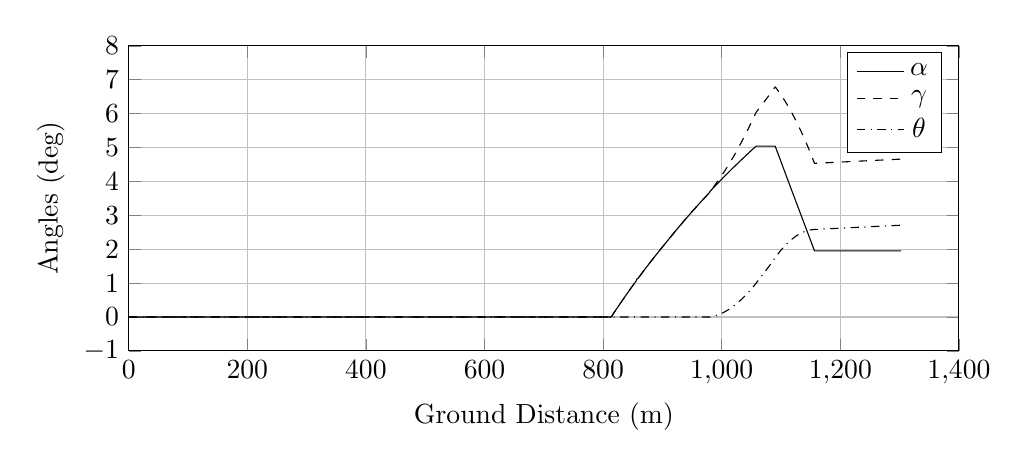
\begin{tikzpicture}

\begin{axis}[
width=\textwidth,
height=0.45\textwidth,
scaled ticks=false, tick label style={/pgf/number format/fixed},
xmin=0.0,
xmax=1400,
xlabel={Ground Distance (m)},
xmajorgrids,
ymin=-1.0,
ymax=8,
ytick={-1,0,1,2,3,4,5,6,7,8},
ylabel={Angles (deg)},
ymajorgrids,
legend entries = {$\alpha$\\$\gamma$\\$\theta$\\}
]

\addplot [
color=black,
solid
]
table[row sep=crcr]{
1.3603393307215537E-8	0.0\\
2.0334443352841076E-7	0.0\\
1.8493358258961232E-6	0.0\\
9.983129263424352E-6	0.0\\
4.13538327636676E-5	0.0\\
1.2467543572893382E-4	0.0\\
2.843807411608912E-4	0.0\\
5.588015241105573E-4	0.0\\
9.398454696015893E-4	0.0\\
0.0014155885812023746	0.0\\
0.0019945752038215015	0.0\\
0.0026717822370171283	0.0\\
0.003447739291558293	0.0\\
0.0043193476547732645	0.0\\
0.00529092766782709	0.0\\
0.006363550519206555	0.0\\
0.007533073890550759	0.0\\
0.008790616877968567	0.0\\
0.01016549189277427	0.0\\
0.011625499440327931	0.0\\
0.013184282533086976	0.0\\
0.014839871214038253	0.0\\
0.01660567024659266	0.0\\
0.018465948346479452	0.0\\
0.0203822997817096	0.0\\
0.022430561433814646	0.0\\
0.024588423902376283	0.0\\
0.026831028501027587	0.0\\
0.029143159681622913	0.0\\
0.03155709159958957	0.0\\
0.03411445662773917	0.0\\
0.03677290089167576	0.0\\
0.03952314881844239	0.0\\
0.04239921643077808	0.0\\
0.045357163155895136	0.0\\
0.048363831658398165	0.0\\
0.051533845233668635	0.0\\
0.0547899150155587	0.0\\
0.058172599437445835	0.0\\
0.06162834747858026	0.0\\
0.06521401059050522	0.0\\
0.06888104003120077	0.0\\
0.07268727020998902	0.0\\
0.076546425570032	0.0\\
0.08047032364859658	0.0\\
0.08456364881336098	0.0\\
0.08882250397434277	0.0\\
0.09306368907640691	0.0\\
0.09743039119190974	0.0\\
0.10191450167634594	0.0\\
0.10651989152467789	0.0\\
0.11128201757858264	0.0\\
0.11609763023253863	0.0\\
0.12097769621339591	0.0\\
0.12591912973280778	0.0\\
0.13103216605369056	0.0\\
0.13633380151185176	0.0\\
0.1416823117522269	0.0\\
0.14708837902374172	0.0\\
0.1525605467319851	0.0\\
0.15824953188605478	0.0\\
0.16398006351864292	0.0\\
0.16978153473626356	0.0\\
0.17584258400626962	0.0\\
0.1819863832139092	0.0\\
0.18819485651962437	0.0\\
0.19455736971520038	0.0\\
0.20098158490654017	0.0\\
0.2076061353991409	0.0\\
0.21424726384720844	0.0\\
0.2211374965027113	0.0\\
0.2281284453493247	0.0\\
0.2350833915765042	0.0\\
0.2423085249848444	0.0\\
0.24958374984531584	0.0\\
0.2569279402934431	0.0\\
0.2644720218029696	0.0\\
0.27204626263318243	0.0\\
0.27972793364503945	0.0\\
0.2874622320100655	0.0\\
0.29563698092580604	0.0\\
0.30361763245720474	0.0\\
0.3118912000478351	0.0\\
0.3202493147046803	0.0\\
0.3286412952843002	0.0\\
0.33714554464307567	0.0\\
0.3458731203690518	0.0\\
0.35455185683415313	0.0\\
0.3634323904331427	0.0\\
0.372325738896249	0.0\\
0.38151551889959867	0.0\\
0.3908489672358084	0.0\\
0.4001862088113266	0.0\\
0.4095647137707429	0.0\\
0.4192312859369268	0.0\\
0.4289206911602753	0.0\\
0.43896550245304145	0.0\\
0.4487817299761361	0.0\\
0.4589033974758888	0.0\\
0.4691858798479248	0.0\\
0.47972601481223376	0.0\\
0.49016040525287174	0.0\\
0.5007175269203565	0.0\\
0.511266977039379	0.0\\
0.522323236324642	0.0\\
0.5332586746953114	0.0\\
0.5445869154512923	0.0\\
0.5556699580072249	0.0\\
0.5669225885056133	0.0\\
0.5785590177532589	0.0\\
0.5903083066022885	0.0\\
0.6020327889628274	0.0\\
0.613957077533064	0.0\\
0.625960998969677	0.0\\
0.6380070243193761	0.0\\
0.6503365955459197	0.0\\
0.662700086001522	0.0\\
0.6752747602080436	0.0\\
0.6885889407972636	0.0\\
0.7019767933734617	0.0\\
0.7151149754112038	0.0\\
0.7284684478906998	0.0\\
0.7418939875700234	0.0\\
0.7553494584716574	0.0\\
0.7694215958599202	0.0\\
0.7830840331449673	0.0\\
0.796657372658726	0.0\\
0.8106660034246236	0.0\\
0.8251837647136968	0.0\\
0.8395067871054176	0.0\\
0.8540519574023793	0.0\\
0.8688334527125461	0.0\\
0.8840141863517745	0.0\\
0.8993797082767976	0.0\\
0.9143697020410035	0.0\\
0.9294094610857999	0.0\\
0.9452486359568626	0.0\\
0.9605773823977486	0.0\\
0.9761522209726621	0.0\\
0.9917649966835071	0.0\\
1.0074810114554809	0.0\\
1.0234652146968335	0.0\\
1.0399433598517231	0.0\\
1.0563627364420554	0.0\\
1.0728309985448887	0.0\\
1.0896486452479222	0.0\\
1.1068138420051672	0.0\\
1.124143995869574	0.0\\
1.1415400048645106	0.0\\
1.1590089082607062	0.0\\
1.1769249919091855	0.0\\
1.1951505705127592	0.0\\
1.2127191877709298	0.0\\
1.2308827453761335	0.0\\
1.2492706857898845	0.0\\
1.267587852451018	0.0\\
1.2860031245644312	0.0\\
1.304687144125951	0.0\\
1.3233765774990474	0.0\\
1.342322280991234	0.0\\
1.3613696045164358	0.0\\
1.3815086998747366	0.0\\
1.4013123019267382	0.0\\
1.4209622886438908	0.0\\
1.4411501686096515	0.0\\
1.4611760119255748	0.0\\
1.4816444281325132	0.0\\
1.501865958841821	0.0\\
1.5224364680875304	0.0\\
1.543651615594651	0.0\\
1.5647593029468103	0.0\\
1.5859558716309676	0.0\\
1.6071423964076703	0.0\\
1.6293386351549652	0.0\\
1.6508498980272122	0.0\\
1.673011606043147	0.0\\
1.6946435720294923	0.0\\
1.717066624993247	0.0\\
1.739432891071898	0.0\\
1.761922286799709	0.0\\
1.7849035550437842	0.0\\
1.8076299607761817	0.0\\
1.8313298306791497	0.0\\
1.8543134894513886	0.0\\
1.8777326664639729	0.0\\
1.9017196849182967	0.0\\
1.925345883672024	0.0\\
1.950252961491087	0.0\\
1.975161211119453	0.0\\
1.9993825790313986	0.0\\
2.024583888346972	0.0\\
2.04934017380271	0.0\\
2.0744229633459703	0.0\\
2.0996193404956136	0.0\\
2.1245764901457758	0.0\\
2.1500786393425866	0.0\\
2.176226227020705	0.0\\
2.202115608176549	0.0\\
2.227948363055355	0.0\\
2.2543499999408594	0.0\\
2.2810892744412783	0.0\\
2.3075963743135786	0.0\\
2.3348582111613405	0.0\\
2.3623221378972126	0.0\\
2.3898598419727675	0.0\\
2.4171687299087603	0.0\\
2.445442108612223	0.0\\
2.4735885391813177	0.0\\
2.5015416452491293	0.0\\
2.5301110763218357	0.0\\
2.5589284934403693	0.0\\
2.587611617795936	0.0\\
2.6175687086884984	0.0\\
2.647724154312196	0.0\\
2.6767118187859253	0.0\\
2.7060305938995466	0.0\\
2.7361546404224653	0.0\\
2.7663022704956823	0.0\\
2.7964672462043376	0.0\\
2.8272583584284883	0.0\\
2.8588650092419234	0.0\\
2.8898852960400587	0.0\\
2.9215246589961597	0.0\\
2.95270311230069	0.0\\
2.984506337549637	0.0\\
3.017379145769185	0.0\\
3.049243647754313	0.0\\
3.081295157663824	0.0\\
3.113406837946715	0.0\\
3.1453724573084756	0.0\\
3.1787286104953543	0.0\\
3.211019796961401	0.0\\
3.245786703184362	0.0\\
3.279939251746722	0.0\\
3.3141720228361216	0.0\\
3.3491198891036547	0.0\\
3.382965192547779	0.0\\
3.4181848705561064	0.0\\
3.45391888941694	0.0\\
3.488851494856137	0.0\\
3.524271454997704	0.0\\
3.5606552075305	0.0\\
3.597189071478943	0.0\\
3.632926148839256	0.0\\
3.668897146318187	0.0\\
3.706642714683163	0.0\\
3.7432264628550644	0.0\\
3.781286297809391	0.0\\
3.818618572105483	0.0\\
3.8564015479305356	0.0\\
3.8948624022541356	0.0\\
3.9329637046009225	0.0\\
3.971505929995028	0.0\\
4.009821706071438	0.0\\
4.049014376833089	0.0\\
4.089343885784727	0.0\\
4.128662304630717	0.0\\
4.1684827283974055	0.0\\
4.208000253554632	0.0\\
4.2483743636521965	0.0\\
4.288255503180503	0.0\\
4.328757204126676	0.0\\
4.369490126907612	0.0\\
4.410357715197167	0.0\\
4.45189144941496	0.0\\
4.492881116440694	0.0\\
4.53550011161515	0.0\\
4.577670191557685	0.0\\
4.6201174049766305	0.0\\
4.662272021613388	0.0\\
4.706017761800355	0.0\\
4.748842845578064	0.0\\
4.792293145132742	0.0\\
4.836482439768313	0.0\\
4.88090298307878	0.0\\
4.925311889063089	0.0\\
4.969864686447545	0.0\\
5.014842280541593	0.0\\
5.0603877575117515	0.0\\
5.106292347304597	0.0\\
5.152263975081851	0.0\\
5.1974808794106995	0.0\\
5.244027372436168	0.0\\
5.28996242022761	0.0\\
5.336209145350672	0.0\\
5.38320569473032	0.0\\
5.430469292142472	0.0\\
5.476900151253712	0.0\\
5.526063828851289	0.0\\
5.573879040902945	0.0\\
5.622613575936374	0.0\\
5.6713596863799225	0.0\\
5.720412183296268	0.0\\
5.770660497446668	0.0\\
5.820668144990444	0.0\\
5.870305285939629	0.0\\
5.920503816994749	0.0\\
5.971105439367246	0.0\\
6.021088325934068	0.0\\
6.071322359863801	0.0\\
6.122981826035449	0.0\\
6.174329110820436	0.0\\
6.225804784288178	0.0\\
6.278093246139479	0.0\\
6.331709873490098	0.0\\
6.384325657889258	0.0\\
6.436648686434458	0.0\\
6.489478972803882	0.0\\
6.543185721519176	0.0\\
6.596747696432654	0.0\\
6.650345873843312	0.0\\
6.704555155195255	0.0\\
6.7588986063680725	0.0\\
6.814371620173711	0.0\\
6.86997180120154	0.0\\
6.925426612865756	0.0\\
6.981353650685165	0.0\\
7.037678624474159	0.0\\
7.094603706786671	0.0\\
7.151204881983983	0.0\\
7.209200593921791	0.0\\
7.2667780016693655	0.0\\
7.324687293141565	0.0\\
7.382771066065313	0.0\\
7.441904508776327	0.0\\
7.501585831803217	0.0\\
7.5616527251378685	0.0\\
7.62150963104709	0.0\\
7.682859947113334	0.0\\
7.7432084367972145	0.0\\
7.803024936926759	0.0\\
7.863793829029664	0.0\\
7.9252460466886365	0.0\\
7.98696966925656	0.0\\
8.04776546969778	0.0\\
8.109421212326083	0.0\\
8.17269125419024	0.0\\
8.236095044780246	0.0\\
8.299523592514586	0.0\\
8.363213767675873	0.0\\
8.427807923256076	0.0\\
8.49144930156071	0.0\\
8.557380457258176	0.0\\
8.623183572921022	0.0\\
8.687840683575093	0.0\\
8.753751426394068	0.0\\
8.820803713780364	0.0\\
8.888970287482593	0.0\\
8.957133699158991	0.0\\
9.025036015045707	0.0\\
9.092760955867519	0.0\\
9.159817422823458	0.0\\
9.227495373767134	0.0\\
9.296013084156197	0.0\\
9.36435980631623	0.0\\
9.433329865923408	0.0\\
9.503849553921977	0.0\\
9.574524061692681	0.0\\
9.644263228942293	0.0\\
9.715657612596786	0.0\\
9.787429657508813	0.0\\
9.85753688572494	0.0\\
9.930250735750551	0.0\\
10.001571447096964	0.0\\
10.074699859091687	0.0\\
10.14698611653175	0.0\\
10.220547980738981	0.0\\
10.2940409891517	0.0\\
10.36719293590382	0.0\\
10.441008888975666	0.0\\
10.51610421670324	0.0\\
10.590724589239105	0.0\\
10.667218005391902	0.0\\
10.742771202259895	0.0\\
10.82035208750042	0.0\\
10.896759047300378	0.0\\
10.973503045910835	0.0\\
11.051297940743765	0.0\\
11.128076326409062	0.0\\
11.207667705350879	0.0\\
11.286758396846047	0.0\\
11.366305937658339	0.0\\
11.446149720998452	0.0\\
11.526866579636565	0.0\\
11.607297517600138	0.0\\
11.688034241538357	0.0\\
11.769665722224765	0.0\\
11.850920080706608	0.0\\
11.933163326324259	0.0\\
12.017103780766782	0.0\\
12.10034832931326	0.0\\
12.185467765774142	0.0\\
12.270669986481685	0.0\\
12.354040133273898	0.0\\
12.440386807402234	0.0\\
12.52556588630658	0.0\\
12.610860989997974	0.0\\
12.69550109439961	0.0\\
12.784634337461807	0.0\\
12.871172079509357	0.0\\
12.958447214271366	0.0\\
13.045518554761987	0.0\\
13.133090172249581	0.0\\
13.221405510214687	0.0\\
13.310319106907201	0.0\\
13.399783591735492	0.0\\
13.488943611067967	0.0\\
13.578276665194153	0.0\\
13.667402973129146	0.0\\
13.757763665999576	0.0\\
13.848393619195729	0.0\\
13.938857764339925	0.0\\
14.031101516310692	0.0\\
14.123507833735925	0.0\\
14.214825187590282	0.0\\
14.307956552027534	0.0\\
14.401498558574918	0.0\\
14.495315613017755	0.0\\
14.589065423003394	0.0\\
14.68316852398955	0.0\\
14.778702641747682	0.0\\
14.873746415615575	0.0\\
14.970384078097169	0.0\\
15.068900921005241	0.0\\
15.164434274206265	0.0\\
15.260378587808539	0.0\\
15.357189194448868	0.0\\
15.45495288999333	0.0\\
15.55311774366497	0.0\\
15.652583807013901	0.0\\
15.755243917873962	0.0\\
15.855950289561445	0.0\\
15.958461094374158	0.0\\
16.060387288500337	0.0\\
16.164276126126843	0.0\\
16.26736468838029	0.0\\
16.36946523634058	0.0\\
16.47192386662276	0.0\\
16.576794358652606	0.0\\
16.678929175716583	0.0\\
16.783994526910618	0.0\\
16.89012564586595	0.0\\
16.996887404888547	0.0\\
17.103774697793426	0.0\\
17.210947675936964	0.0\\
17.31865021419634	0.0\\
17.424470519881233	0.0\\
17.53205215515201	0.0\\
17.64034909906897	0.0\\
17.74911485075183	0.0\\
17.85745376408675	0.0\\
17.969383314157206	0.0\\
18.07998395718984	0.0\\
18.18863741327577	0.0\\
18.302466989554325	0.0\\
18.41305080779906	0.0\\
18.525644000014054	0.0\\
18.636945827420575	0.0\\
18.750643923449367	0.0\\
18.86479622056296	0.0\\
18.979646899421056	0.0\\
19.09418630108147	0.0\\
19.208983505033515	0.0\\
19.323483295898072	0.0\\
19.43842354827664	0.0\\
19.55563752357537	0.0\\
19.67199913451129	0.0\\
19.789486593639566	0.0\\
19.90713985662446	0.0\\
20.024127533725753	0.0\\
20.143019013955552	0.0\\
20.26442367074238	0.0\\
20.383660776265387	0.0\\
20.5042342316437	0.0\\
20.622773342122727	0.0\\
20.74503732713029	0.0\\
20.865944869938517	0.0\\
20.98711015528624	0.0\\
21.113336299999695	0.0\\
21.23638685227678	0.0\\
21.35988644990264	0.0\\
21.483760012473958	0.0\\
21.608180515260266	0.0\\
21.732326713270083	0.0\\
21.85766379468624	0.0\\
21.985117186778353	0.0\\
22.111729024702363	0.0\\
22.23700541150786	0.0\\
22.36297326225872	0.0\\
22.488604760551	0.0\\
22.616276341350805	0.0\\
22.744235570279145	0.0\\
22.874576476768283	0.0\\
23.003842066605536	0.0\\
23.13088450205612	0.0\\
23.257869280739328	0.0\\
23.389244224935425	0.0\\
23.519811196806458	0.0\\
23.653309395988643	0.0\\
23.78342402399784	0.0\\
23.9180644861338	0.0\\
24.05110504604577	0.0\\
24.182394801971697	0.0\\
24.314614014384034	0.0\\
24.449791085561472	0.0\\
24.585258581909038	0.0\\
24.72121222319008	0.0\\
24.857032405393277	0.0\\
24.99454740444294	0.0\\
25.13030709358258	0.0\\
25.270890409679986	0.0\\
25.40663839363527	0.0\\
25.54307796688363	0.0\\
25.68272814639034	0.0\\
25.82072003425767	0.0\\
25.96015212691003	0.0\\
25.987750021099068	0.0\\
26.0558803939429	0.0\\
26.061632797568386	0.0\\
26.066808273335674	0.0\\
26.071901058608013	0.0\\
26.073315434863225	0.0\\
26.074595035914804	0.0\\
26.080371168076944	0.0\\
26.10234540095133	0.0\\
26.183408179590366	0.0\\
26.300430535410044	0.0\\
26.42750601924636	0.0\\
26.558056987479794	0.0\\
26.688030995483615	0.0\\
26.818767077324992	0.0\\
26.951519978077492	0.0\\
27.083955405447817	0.0\\
27.216897884715692	0.0\\
27.350913258119895	0.0\\
27.4833530065795	0.0\\
27.6176201223548	0.0\\
27.752160408628434	0.0\\
27.887329802382908	0.0\\
28.023188645890663	0.0\\
28.158973127824495	0.0\\
28.296372294036907	0.0\\
28.435107205966254	0.0\\
28.571323599682245	0.0\\
28.70996262687553	0.0\\
28.850320389600306	0.0\\
28.988837241064125	0.0\\
29.129197813929657	0.0\\
29.27166529868488	0.0\\
29.41298471572133	0.0\\
29.554848516656044	0.0\\
29.699676691743235	0.0\\
29.842400551696755	0.0\\
29.985385440862252	0.0\\
30.129077275410303	0.0\\
30.27543774584293	0.0\\
30.422081339040986	0.0\\
30.56949149516445	0.0\\
30.716562179458485	0.0\\
30.86535310281699	0.0\\
31.011875026602333	0.0\\
31.16159928701196	0.0\\
31.313692569485013	0.0\\
31.463056706803336	0.0\\
31.61235366859384	0.0\\
31.76278957628285	0.0\\
31.915019899787076	0.0\\
32.06709627595497	0.0\\
32.21861178877769	0.0\\
32.37168228565527	0.0\\
32.52450570609457	0.0\\
32.67702483599189	0.0\\
32.829998687403204	0.0\\
32.98551220909506	0.0\\
33.14332298937855	0.0\\
33.29970221124884	0.0\\
33.45800124694219	0.0\\
33.61398946945653	0.0\\
33.77048353048475	0.0\\
33.9292721471582	0.0\\
34.08796840843395	0.0\\
34.24769686644211	0.0\\
34.406855482575295	0.0\\
34.56481953291838	0.0\\
34.72399692808165	0.0\\
34.88694269464703	0.0\\
35.04914399338672	0.0\\
35.209965099803895	0.0\\
35.3703140559587	0.0\\
35.531685786905925	0.0\\
35.69349909442164	0.0\\
35.85522798807463	0.0\\
36.022509111806116	0.0\\
36.19055880791667	0.0\\
36.35708622463872	0.0\\
36.52115360367851	0.0\\
36.68781562330062	0.0\\
36.8536847754776	0.0\\
37.024522648961764	0.0\\
37.19188554678789	0.0\\
37.36066720850286	0.0\\
37.528862119520696	0.0\\
37.697264258302326	0.0\\
37.86832931534104	0.0\\
38.03812867477943	0.0\\
38.20923731912278	0.0\\
38.37904730305398	0.0\\
38.55252405124031	0.0\\
38.72282139824354	0.0\\
38.89783411301201	0.0\\
39.0714610757495	0.0\\
39.24438070689564	0.0\\
39.41969314875929	0.0\\
39.59166556575205	0.0\\
39.764623188591585	0.0\\
39.94263254662576	0.0\\
40.11749159802578	0.0\\
40.29452954971913	0.0\\
40.47247750600427	0.0\\
40.64799609178485	0.0\\
40.82414741101539	0.0\\
41.00385670225303	0.0\\
41.18169069533937	0.0\\
41.3603281005193	0.0\\
41.54046179251334	0.0\\
41.722675278204306	0.0\\
41.90258931008478	0.0\\
42.08518735141125	0.0\\
42.26728550944881	0.0\\
42.44743534848537	0.0\\
42.63069538383506	0.0\\
42.80963512098974	0.0\\
42.992542679335614	0.0\\
43.17926890616222	0.0\\
43.363134036078335	0.0\\
43.54815051311773	0.0\\
43.733578141849236	0.0\\
43.91798130912079	0.0\\
44.10506009255049	0.0\\
44.29251116260117	0.0\\
44.480917546793805	0.0\\
44.66851287589745	0.0\\
44.85853501730759	0.0\\
45.047396872181054	0.0\\
45.236914792155844	0.0\\
45.42785879536018	0.0\\
45.616432631699865	0.0\\
45.80697204128492	0.0\\
45.998633580597016	0.0\\
46.18800675699903	0.0\\
46.380841640082096	0.0\\
46.57327038933336	0.0\\
46.765844918266424	0.0\\
46.95911042680183	0.0\\
47.15311668852311	0.0\\
47.34541611633634	0.0\\
47.53884854699059	0.0\\
47.73236991243341	0.0\\
47.92818250719388	0.0\\
48.12326385407131	0.0\\
48.32058854034828	0.0\\
48.516852452700604	0.0\\
48.71339374517507	0.0\\
48.91319881343868	0.0\\
49.1119162355681	0.0\\
49.31207818344666	0.0\\
49.509673461222235	0.0\\
49.71156302510582	0.0\\
49.91034548441702	0.0\\
50.11200805970151	0.0\\
50.30853267551517	0.0\\
50.50757456960626	0.0\\
50.70929197287772	0.0\\
50.91222418686718	0.0\\
51.11562549758783	0.0\\
51.32090674103446	0.0\\
51.525199701657655	0.0\\
51.72863462744459	0.0\\
51.934060761332375	0.0\\
52.14033810224923	0.0\\
52.344882977561255	0.0\\
52.55098100649393	0.0\\
52.75731843494604	0.0\\
52.96514817708821	0.0\\
53.17450540782369	0.0\\
53.382202621450276	0.0\\
53.592230583406476	0.0\\
53.80364534107798	0.0\\
54.01469481143569	0.0\\
54.223966920081466	0.0\\
54.43230789395902	0.0\\
54.6430562980421	0.0\\
54.855225786754914	0.0\\
55.066088958624874	0.0\\
55.27969530828261	0.0\\
55.49171188337613	0.0\\
55.70388919125476	0.0\\
55.91737779085577	0.0\\
56.13177028494084	0.0\\
56.34652664868587	0.0\\
56.559021044851505	0.0\\
56.77591447970492	0.0\\
56.99548236897459	0.0\\
57.21481285737903	0.0\\
57.43536222847358	0.0\\
57.65367025761124	0.0\\
57.872788904232735	0.0\\
58.0907693980174	0.0\\
58.311927420720366	0.0\\
58.532333513628615	0.0\\
58.75532998033057	0.0\\
58.976617007999806	0.0\\
59.19875422837053	0.0\\
59.4206945143671	0.0\\
59.64453328369959	0.0\\
59.86894932484513	0.0\\
60.09432075877773	0.0\\
60.318058693038594	0.0\\
60.541731124044205	0.0\\
60.76707064338231	0.0\\
60.995574692986196	0.0\\
61.22378989589207	0.0\\
61.4534619981562	0.0\\
61.683510138770515	0.0\\
61.91410430469678	0.0\\
62.14462153858659	0.0\\
62.37563158073512	0.0\\
62.607203285434	0.0\\
62.841031881319736	0.0\\
63.07467935056491	0.0\\
63.31164975340633	0.0\\
63.54633691305479	0.0\\
63.78243968758058	0.0\\
64.0165414084598	0.0\\
64.25412817577254	0.0\\
64.49270299572771	0.0\\
64.73076499662056	0.0\\
64.96867826857735	0.0\\
65.21063576532572	0.0\\
65.4512107007771	0.0\\
65.69028017871045	0.0\\
65.93032615763332	0.0\\
66.17196619696679	0.0\\
66.4135612157637	0.0\\
66.6559030093851	0.0\\
66.89910102540284	0.0\\
67.14354652182666	0.0\\
67.38771133480921	0.0\\
67.63347396558368	0.0\\
67.87898066495345	0.0\\
68.1255935515739	0.0\\
68.37316753306138	0.0\\
68.62205497364681	0.0\\
68.8711887275476	0.0\\
69.120220471977	0.0\\
69.36846244647072	0.0\\
69.61951843592018	0.0\\
69.87236615109754	0.0\\
70.12758921381476	0.0\\
70.37945082809051	0.0\\
70.63410009691182	0.0\\
70.89152727368702	0.0\\
71.14629115974091	0.0\\
71.40197865069018	0.0\\
71.66163317144085	0.0\\
71.92484704501203	0.0\\
72.18465416754285	0.0\\
72.44573394560723	0.0\\
72.70633339061075	0.0\\
72.96699363118216	0.0\\
73.22900401485182	0.0\\
73.49076816912304	0.0\\
73.75430841254712	0.0\\
74.01895646534612	0.0\\
74.2846979982242	0.0\\
74.55380714249793	0.0\\
74.82322871850147	0.0\\
75.09350011520078	0.0\\
75.36421232425869	0.0\\
75.6347219158074	0.0\\
75.90830954343213	0.0\\
76.18188601743822	0.0\\
76.45626363461818	0.0\\
76.72958718025629	0.0\\
77.00406935908524	0.0\\
77.28579748399531	0.0\\
77.56784659723587	0.0\\
77.84569092555657	0.0\\
78.1246978223638	0.0\\
78.40641219364133	0.0\\
78.68590470271565	0.0\\
78.96851680469001	0.0\\
79.25576208114188	0.0\\
79.54169104977237	0.0\\
79.82662017154695	0.0\\
80.11330301632765	0.0\\
80.40394576721474	0.0\\
80.6908099930996	0.0\\
80.98055888331655	0.0\\
81.27178512217935	0.0\\
81.56682943128612	0.0\\
81.86186977412851	0.0\\
82.15688924927383	0.0\\
82.44965588234726	0.0\\
82.74488606927187	0.0\\
83.04325841243121	0.0\\
83.34213327641098	0.0\\
83.64411622775171	0.0\\
83.94734638805741	0.0\\
84.25123842984891	0.0\\
84.55152885577829	0.0\\
84.85735750691177	0.0\\
85.16518306664875	0.0\\
85.47136476235073	0.0\\
85.77898122624802	0.0\\
86.08923229760057	0.0\\
86.40254560035129	0.0\\
86.71167807044037	0.0\\
87.02660518802142	0.0\\
87.34238286044419	0.0\\
87.65842706333811	0.0\\
87.97971380652302	0.0\\
88.2973933745065	0.0\\
88.61789013566766	0.0\\
88.93643920279564	0.0\\
89.25662431900213	0.0\\
89.57903058309674	0.0\\
89.89968694948243	0.0\\
90.22473455398588	0.0\\
90.55024875587375	0.0\\
90.87789352676518	0.0\\
91.20733069500889	0.0\\
91.54101415610151	0.0\\
91.87012785371462	0.0\\
92.20120197152713	0.0\\
92.53416638543635	0.0\\
92.86431843528567	0.0\\
93.19748455591187	0.0\\
93.53066771200866	0.0\\
93.86681917526724	0.0\\
94.20530590547477	0.0\\
94.5419273964865	0.0\\
94.8854212036891	0.0\\
95.22752713476521	0.0\\
95.57091181422334	0.0\\
95.91383450860906	0.0\\
96.25469535763642	0.0\\
96.5966517898868	0.0\\
96.93845701474973	0.0\\
97.28153572459905	0.0\\
97.62213139590432	0.0\\
97.9659652144934	0.0\\
98.3129807304216	0.0\\
98.65852794036775	0.0\\
99.00080640577195	0.0\\
99.35064076251427	0.0\\
99.69796076807248	0.0\\
100.04654253174803	0.0\\
100.3915606488718	0.0\\
100.74261509654437	0.0\\
101.08877163494762	0.0\\
101.43457754260953	0.0\\
101.784020212797	0.0\\
102.13161434601102	0.0\\
102.4751980097893	0.0\\
102.82212110631409	0.0\\
103.16739702108615	0.0\\
103.51524666207362	0.0\\
103.86391679154056	0.0\\
104.20960434827006	0.0\\
104.55241399635099	0.0\\
104.89662223620601	0.0\\
105.24103428322039	0.0\\
105.5836615386647	0.0\\
105.92645892081137	0.0\\
106.27347658175316	0.0\\
106.6151670762521	0.0\\
106.95898391938218	0.0\\
107.30023552029138	0.0\\
107.64147805753461	0.0\\
107.98348674656944	0.0\\
108.32522459759954	0.0\\
108.3935347040271	0.0\\
108.40478590462831	0.0\\
108.41572478024443	0.0\\
108.4246743308916	0.0\\
108.44347342986478	0.0\\
108.52018987797786	0.0\\
108.70071173483461	0.0\\
108.99446230248458	0.0\\
109.30176454987088	0.0\\
109.60899173332959	0.0\\
109.91608539831654	0.0\\
110.22883517949637	0.0\\
110.54143546549608	0.0\\
110.853845249356	0.0\\
111.1739714794031	0.0\\
111.4937490010879	0.0\\
111.81170779322963	0.0\\
112.13106495813236	0.0\\
112.4519453366479	0.0\\
112.77515902629136	0.0\\
113.0997499810409	0.0\\
113.43040796942478	0.0\\
113.7597028375028	0.0\\
114.0907450350197	0.0\\
114.42538740208008	0.0\\
114.75997726261329	0.0\\
115.09477047197589	0.0\\
115.43440545481076	0.0\\
115.77494672336013	0.0\\
116.11687534861284	0.0\\
116.46164587354252	0.0\\
116.8077846490165	0.0\\
117.15688723722127	0.0\\
117.50557855048987	0.0\\
117.85411336711965	0.0\\
118.20532793701167	0.0\\
118.55850697655507	0.0\\
118.91273956155123	0.0\\
119.26983096270519	0.0\\
119.62978614725739	0.0\\
119.98960731920661	0.0\\
120.34734904217265	0.0\\
120.7138511704587	0.0\\
121.08106061642908	0.0\\
121.44737887966437	0.0\\
121.81499139152783	0.0\\
122.18511446431708	0.0\\
122.55384158147794	0.0\\
122.92460728481757	0.0\\
123.29616941264607	0.0\\
123.67040864389355	0.0\\
124.04652172406458	0.0\\
124.42393851457416	0.0\\
124.80152108360014	0.0\\
125.18180835736592	0.0\\
125.55854932865631	0.0\\
125.93878032356085	0.0\\
126.31997081831156	0.0\\
126.70099538833193	0.0\\
127.08058279416298	0.0\\
127.46175209000612	0.0\\
127.84399628255431	0.0\\
128.22749916598133	0.0\\
128.6102537001487	0.0\\
128.99595881306152	0.0\\
129.37788117916477	0.0\\
129.760738924708	0.0\\
130.1448498512433	0.0\\
130.53000390659713	0.0\\
130.9168242384266	0.0\\
131.29443328439476	0.0\\
131.67491382268804	0.0\\
132.05816436539135	0.0\\
132.44070735535217	0.0\\
132.82666098215685	0.0\\
133.20952005887244	0.0\\
133.5940193955625	0.0\\
133.97617966856654	0.0\\
134.36103715882757	0.0\\
134.74478042358356	0.0\\
135.12867144169206	0.0\\
135.5141335746535	0.0\\
135.89764893392993	0.0\\
136.28231234485685	0.0\\
136.66418763078912	0.0\\
137.04684871033697	0.0\\
137.42845627025127	0.0\\
137.8132447087305	0.0\\
138.19719797258034	0.0\\
138.58059071069573	0.0\\
138.96593237593703	0.0\\
139.3501607499636	0.0\\
139.73355638294606	0.0\\
140.1160230155566	0.0\\
140.50045093994146	0.0\\
140.88215178690393	0.0\\
141.26156782058217	0.0\\
141.64323970440188	0.0\\
142.02689350659642	0.0\\
142.41061312971692	0.0\\
142.7942251403153	0.0\\
143.1756303563767	0.0\\
143.5599719391364	0.0\\
143.94242380128833	0.0\\
144.3239499176869	0.0\\
144.70664939692608	0.0\\
145.0870075357763	0.0\\
145.46856550308127	0.0\\
145.85014610541765	0.0\\
146.23128237819492	0.0\\
146.61504730324998	0.0\\
146.99763315977907	0.0\\
147.38441582478964	0.0\\
147.7673688364352	0.0\\
148.15222568696134	0.0\\
148.53580865353604	0.0\\
148.9199734867533	0.0\\
149.3040357319486	0.0\\
149.68771357306542	0.0\\
150.07093078701052	0.0\\
150.45622889618164	0.0\\
150.8449053483268	0.0\\
151.2288570611563	0.0\\
151.61452719766493	0.0\\
151.9983007305741	0.0\\
152.38299664478842	0.0\\
152.76945776909372	0.0\\
153.15580177123394	0.0\\
153.54253364040335	0.0\\
153.93093169697067	0.0\\
154.31788037931886	0.0\\
154.7039882138024	0.0\\
155.08880221957185	0.0\\
155.47621608980313	0.0\\
155.866104687065	0.0\\
156.25391419262098	0.0\\
156.64166339424906	0.0\\
157.03027969880475	0.0\\
157.4213807682267	0.0\\
157.8105708506119	0.0\\
158.19948541262937	0.0\\
158.58893406813365	0.0\\
158.97894817604634	0.0\\
159.3710019698692	0.0\\
159.76139479981174	0.0\\
160.1523485688823	0.0\\
160.54128874338664	0.0\\
160.9326976430911	0.0\\
161.32564259741588	0.0\\
161.71827778345698	0.0\\
162.1124492087963	0.0\\
162.50576001021273	0.0\\
162.89904576730015	0.0\\
163.29316224934274	0.0\\
163.68899123279596	0.0\\
164.08495392634194	0.0\\
164.48271131475576	0.0\\
164.8792309171331	0.0\\
165.27343112400507	0.0\\
165.67115293733156	0.0\\
166.06936395728349	0.0\\
166.47000821435734	0.0\\
166.87155839526775	0.0\\
167.27134041220108	0.0\\
167.67233991204222	0.0\\
168.0705846918417	0.0\\
168.47232570996516	0.0\\
168.87521546679773	0.0\\
169.2789990941189	0.0\\
169.68142011368735	0.0\\
170.088438196605	0.0\\
170.49328200513543	0.0\\
170.89845866435633	0.0\\
171.30484584057905	0.0\\
171.7103088520891	0.0\\
172.11589069074847	0.0\\
172.52485519917514	0.0\\
172.93316089774754	0.0\\
173.34236088095247	0.0\\
173.7535761368399	0.0\\
174.16510964781833	0.0\\
174.5786011126259	0.0\\
174.99051444770384	0.0\\
175.40138574541044	0.0\\
175.81497300453447	0.0\\
176.2280441317456	0.0\\
176.64225100058474	0.0\\
177.05714873395152	0.0\\
177.47483026786767	0.0\\
177.89254345086653	0.0\\
178.3100126079721	0.0\\
178.7278240622369	0.0\\
179.1449731538625	0.0\\
179.56482315926417	0.0\\
179.9871804296257	0.0\\
180.4095742002126	0.0\\
180.83428717371925	0.0\\
181.26003251256287	0.0\\
181.6840913989422	0.0\\
182.1114839456617	0.0\\
182.5374089230304	0.0\\
182.96440604473082	0.0\\
183.39304842330927	0.0\\
183.8234391905185	0.0\\
184.2565386467558	0.0\\
184.68745119590193	0.0\\
185.11804999400476	0.0\\
185.54983076576542	0.0\\
185.98322399936802	0.0\\
186.41637816429778	0.0\\
186.85103033850396	0.0\\
187.28701324242002	0.0\\
187.72482375232647	0.0\\
188.16038808151575	0.0\\
188.5986323917997	0.0\\
189.04181882432442	0.0\\
189.48417857731005	0.0\\
189.92673350352436	0.0\\
190.3712203460227	0.0\\
190.8171693385559	0.0\\
191.2607914989822	0.0\\
191.7085048054314	0.0\\
192.15912968354564	0.0\\
192.60936448614513	0.0\\
193.06096206133014	0.0\\
193.50995896221815	0.0\\
193.96222738896364	0.0\\
194.41802104663145	0.0\\
194.87342332120494	0.0\\
195.32868067301865	0.0\\
195.78611327072855	0.0\\
196.24327119175433	0.0\\
196.70330552186363	0.0\\
197.16349707435467	0.0\\
197.6260626000094	0.0\\
198.09002425529962	0.0\\
198.55822718319422	0.0\\
199.02663999285284	0.0\\
199.4942263371064	0.0\\
199.96051846591553	0.0\\
200.4340527590599	0.0\\
200.9046051381776	0.0\\
201.38053424207163	0.0\\
201.855813875004	0.0\\
202.3311704663634	0.0\\
202.81222172114025	0.0\\
203.29225549210986	0.0\\
203.77308885705298	0.0\\
204.25557537412044	0.0\\
204.7402502473849	0.0\\
205.2236366749359	0.0\\
205.7136101207933	0.0\\
206.20393168243612	0.0\\
206.69661599754647	0.0\\
207.18955097797863	0.0\\
207.68747106001632	0.0\\
208.18818418427776	0.0\\
208.68864521634526	0.0\\
209.18805406731133	0.0\\
209.69072626026758	0.0\\
210.1949489825136	0.0\\
210.70396111371042	0.0\\
211.21614058335587	0.0\\
211.7289636831582	0.0\\
212.24265718177503	0.0\\
212.75957115615557	0.0\\
213.28124361123798	0.0\\
213.80665479128663	0.0\\
214.33466763217763	0.0\\
214.86241383044415	0.0\\
215.38762416293667	0.0\\
215.91972020502777	0.0\\
216.453694496636	0.0\\
216.99218613031866	0.0\\
217.53464071342142	0.0\\
218.07804319032095	0.0\\
218.62452881115053	0.0\\
219.1707188429899	0.0\\
219.71730570977076	0.0\\
220.274760228052	0.0\\
220.835259093258	0.0\\
221.3941373958715	0.0\\
221.95623623511386	0.0\\
222.52040576537968	0.0\\
223.09037241999033	0.0\\
223.661129480297	0.0\\
224.23954505634208	0.0\\
224.81564934919504	0.0\\
225.40333087020622	0.0\\
225.99624064594485	0.0\\
226.58875910740323	0.0\\
227.18585441503012	0.0\\
227.7870146338791	0.0\\
228.39495206683767	0.0\\
229.0027183467937	0.0\\
229.6102660575582	0.0\\
230.22857190062643	0.0\\
230.8468525918393	0.0\\
231.47114194537448	0.0\\
232.09060564776433	0.0\\
232.71961230618888	0.0\\
233.34696033086396	0.0\\
233.9840065784689	0.0\\
234.6188203761186	0.0\\
235.2539319397456	0.0\\
235.886956379092	0.0\\
236.5153031168307	0.0\\
237.1504953781269	0.0\\
237.78410205277385	0.0\\
238.41360900639518	0.0\\
239.04679127723733	0.0\\
239.67609891578388	0.0\\
240.3017129123046	0.0\\
240.93317778774485	0.0\\
241.55721005497253	0.0\\
242.1780757761154	0.0\\
242.7965584376659	0.0\\
243.4114785265944	0.0\\
244.02550827530933	0.0\\
244.63427618145124	0.0\\
245.24126487864038	0.0\\
245.84466361012846	0.0\\
246.4476225417801	0.0\\
247.04267344144802	0.0\\
247.6421488158	0.0\\
248.2330500398673	0.0\\
248.8222841397298	0.0\\
249.4139444766347	0.0\\
249.99998610086192	0.0\\
250.57758594667018	0.0\\
251.15853686633199	0.0\\
251.73921641108228	0.0\\
252.31216708836962	0.0\\
252.88817036877617	0.0\\
253.4570082134402	0.0\\
254.02007242820673	0.0\\
254.5855573787108	0.0\\
255.15029634137989	0.0\\
255.71294034286547	0.0\\
256.27258114245853	0.0\\
256.8305649252842	0.0\\
257.38478802342286	0.0\\
257.4959621062188	0.0\\
257.5611920943704	0.0\\
257.60062237753925	0.0\\
257.6107239150342	0.0\\
257.6183320416303	0.0\\
257.62277045264796	0.0\\
257.62729287050774	0.0\\
257.6542412653681	0.0\\
257.747424202601	0.0\\
258.03721256731046	0.0\\
258.5190125653693	0.0\\
259.00532843878875	0.0\\
259.49401909840515	0.0\\
259.98581493995266	0.0\\
260.4819698790609	0.0\\
260.97812571679674	0.0\\
261.4812175109821	0.0\\
261.9850059638038	0.0\\
262.4910281591069	0.0\\
263.0003252970298	0.0\\
263.5131478408722	0.0\\
264.0293216176061	0.0\\
264.54826562874086	0.0\\
265.0714232439334	0.0\\
265.59763340154745	0.0\\
266.1233003184659	0.0\\
266.6551605685464	0.0\\
267.19223429565795	0.0\\
267.72974052544146	0.0\\
268.27282471948854	0.0\\
268.8167212540145	0.0\\
269.36684202478307	0.0\\
269.9215996219019	0.0\\
270.4791082933567	0.0\\
271.03983254776506	0.0\\
271.6074455599014	0.0\\
272.1754809002374	0.0\\
272.7524022502224	0.0\\
273.3357847625165	0.0\\
273.91684495064374	0.0\\
274.5075523019982	0.0\\
275.0995375957874	0.0\\
275.69766674106233	0.0\\
276.3013456770767	0.0\\
276.90909644628925	0.0\\
277.5234995466793	0.0\\
278.13959639565337	0.0\\
278.76308237359774	0.0\\
279.389606942784	0.0\\
280.02074979788426	0.0\\
280.6586947867754	0.0\\
281.3003335866648	0.0\\
281.94157575500606	0.0\\
282.5880614624846	0.0\\
283.23584856186324	0.0\\
283.8851508583185	0.0\\
284.5301203280417	0.0\\
285.1843536535779	0.0\\
285.83553116214307	0.0\\
286.4837256048969	0.0\\
287.1336898105825	0.0\\
287.7808235765799	0.0\\
288.42820685084826	0.0\\
289.0754666022002	0.0\\
289.71879024937004	0.0\\
290.36420979409684	0.0\\
291.0002472374472	0.0\\
291.64182130034897	0.0\\
292.27316865691716	0.0\\
292.9083864811005	0.0\\
293.54335819806715	0.0\\
294.17307850120346	0.0\\
294.79408895337656	0.0\\
295.4199157771013	0.0\\
296.0380590852486	0.0\\
296.6542969985221	0.0\\
297.2681917409874	0.0\\
297.88482625920517	0.0\\
298.4949121158181	0.0\\
299.10656876013206	0.0\\
299.7189321849655	0.0\\
300.32723284437907	0.0\\
300.92930430691433	0.0\\
301.53463237615574	0.0\\
302.1363215848461	0.0\\
302.731439066583	0.0\\
303.3331045114137	0.0\\
303.92852765769237	0.0\\
304.52166324273924	0.0\\
305.11491208725784	0.0\\
305.70510856070314	0.0\\
306.29833179138177	0.0\\
306.8897654253252	0.0\\
307.4799704999041	0.0\\
308.06772992248136	0.0\\
308.6551058451172	0.0\\
309.2396381392449	0.0\\
309.82398267965425	0.0\\
310.40422650572066	0.0\\
310.9895683476474	0.0\\
311.5727136903438	0.0\\
312.15129426541773	0.0\\
312.7356217277545	0.0\\
313.31711326243806	0.0\\
313.899302145316	0.0\\
314.47946679147856	0.0\\
315.0588501134555	0.0\\
315.6397939029396	0.0\\
316.2168920475523	0.0\\
316.7955732394013	0.0\\
317.37103223180316	0.0\\
317.947565273913	0.0\\
318.5214617947222	0.0\\
319.09868556082085	0.0\\
319.67476219148546	0.0\\
320.24944526491765	0.0\\
320.82291261720786	0.0\\
321.39725246986427	0.0\\
321.96848871367	0.0\\
322.54402617481435	0.0\\
323.1185574377922	0.0\\
323.691859264958	0.0\\
324.2647334332521	0.0\\
324.8363521231331	0.0\\
325.40661348734614	0.0\\
325.97908467698915	0.0\\
326.5542035875586	0.0\\
327.12490712258295	0.0\\
327.6996379965167	0.0\\
328.2728670816481	0.0\\
328.8486987665442	0.0\\
329.41990981452807	0.0\\
329.9938351119364	0.0\\
330.5648485136189	0.0\\
331.13749118064516	0.0\\
331.7074637117181	0.0\\
332.2798601122896	0.0\\
332.8523203670276	0.0\\
333.42500978717965	0.0\\
334.00122212141855	0.0\\
334.57441172696565	0.0\\
335.1481633939942	0.0\\
335.72345703021597	0.0\\
336.29828216695637	0.0\\
336.8725624877933	0.0\\
337.44522027160394	0.0\\
338.02053867417567	0.0\\
338.5962187273635	0.0\\
339.1703543735324	0.0\\
339.7498013559267	0.0\\
340.3260768964459	0.0\\
340.9051117020497	0.0\\
341.47919118112156	0.0\\
342.052441303386	0.0\\
342.6320235008849	0.0\\
343.21038614202473	0.0\\
343.79082299329946	0.0\\
344.3667106402361	0.0\\
344.94458170993323	0.0\\
345.5252340504509	0.0\\
346.1016219383906	0.0\\
346.6806961036725	0.0\\
347.2602578923353	0.0\\
347.84073776856303	0.0\\
348.4226009401458	0.0\\
349.0044346707606	0.0\\
349.5859819547053	0.0\\
350.1699920738855	0.0\\
350.75474917442455	0.0\\
351.33998325174355	0.0\\
351.9234136900301	0.0\\
352.50674072872846	0.0\\
353.09110804073237	0.0\\
353.67821635803944	0.0\\
354.2656524741757	0.0\\
354.8545578241044	0.0\\
355.4483774220265	0.0\\
356.0367996380022	0.0\\
356.62583096427284	0.0\\
357.2144774827566	0.0\\
357.80411644396065	0.0\\
358.39517477750917	0.0\\
358.9862667118267	0.0\\
359.57750029884653	0.0\\
360.17210502256853	0.0\\
360.76667257221345	0.0\\
361.36307847075966	0.0\\
361.95890315858196	0.0\\
362.55277332573996	0.0\\
363.15015313069875	0.0\\
363.7467383697897	0.0\\
364.34582190435833	0.0\\
364.9460245640587	0.0\\
365.54693692211754	0.0\\
366.14934356225297	0.0\\
366.7506799567443	0.0\\
367.35358948565136	0.0\\
367.957068853549	0.0\\
368.56310438184994	0.0\\
369.1667326492483	0.0\\
369.7692268682281	0.0\\
370.3767216505511	0.0\\
370.9840014372453	0.0\\
371.59702031674954	0.0\\
372.2057576829203	0.0\\
372.8164011445841	0.0\\
373.43055551390637	0.0\\
374.04130844990834	0.0\\
374.65480432791037	0.0\\
375.2686727235273	0.0\\
375.88872766894735	0.0\\
376.5077052039818	0.0\\
377.12525427851347	0.0\\
377.74405712537066	0.0\\
378.36402671612836	0.0\\
378.9860252798833	0.0\\
379.6100000903326	0.0\\
380.2333263467823	0.0\\
380.8554247462042	0.0\\
381.4828757180544	0.0\\
382.11124459971245	0.0\\
382.74241248635997	0.0\\
383.3719105047892	0.0\\
384.00409885358727	0.0\\
384.6374235585132	0.0\\
385.2708543582187	0.0\\
385.90511613810475	0.0\\
386.5402229663101	0.0\\
387.1757112317391	0.0\\
387.816842485381	0.0\\
388.45671447828204	0.0\\
389.0979595165261	0.0\\
389.738666357365	0.0\\
390.38126573576096	0.0\\
391.0250474989899	0.0\\
391.6744601114111	0.0\\
392.32213053197165	0.0\\
392.96822988900624	0.0\\
393.62074411485196	0.0\\
394.27341767767894	0.0\\
394.92683850679725	0.0\\
395.58558306335794	0.0\\
396.2441970187614	0.0\\
396.90310461070555	0.0\\
397.56432488588905	0.0\\
398.2289657073595	0.0\\
398.8925370524752	0.0\\
399.5622831783011	0.0\\
400.2295014598768	0.0\\
400.89855800548185	0.0\\
401.5675035611599	0.0\\
402.24206117554286	0.0\\
402.91817297108616	0.0\\
403.5958718607668	0.0\\
404.27787051233963	0.0\\
404.95902715653847	0.0\\
405.6425745212256	0.0\\
406.3286386181055	0.0\\
407.0181239797241	0.0\\
407.70730436303313	0.0\\
408.39972983906614	0.0\\
409.0954177346696	0.0\\
409.79217465836814	0.0\\
410.4900247907216	0.0\\
411.1873806890112	0.0\\
411.8896918209001	0.0\\
412.5960730727825	0.0\\
413.3068225682056	0.0\\
414.0163043302465	0.0\\
414.7283691490554	0.0\\
415.4426354990113	0.0\\
416.1629925407426	0.0\\
416.8821853291962	0.0\\
417.606386355131	0.0\\
418.33304785123187	0.0\\
419.0630803577634	0.0\\
419.79657378413856	0.0\\
420.5335871119013	0.0\\
421.27035840412	0.0\\
422.00742265160795	0.0\\
422.7512304365845	0.0\\
423.49678426262926	0.0\\
424.2511831284078	0.0\\
425.00728777593645	0.0\\
425.7607765912853	0.0\\
426.5243177755509	0.0\\
427.28979022554415	0.0\\
428.0636149183367	0.0\\
428.8379843697036	0.0\\
429.60996752685014	0.0\\
430.3897477020988	0.0\\
431.1753893594911	0.0\\
431.966835986777	0.0\\
432.75960868637253	0.0\\
433.56365122208206	0.0\\
434.37045705896094	0.0\\
435.1870341731259	0.0\\
436.00231675887426	0.0\\
436.8220964781458	0.0\\
437.6552545507992	0.0\\
438.4886711504423	0.0\\
439.3280194395811	0.0\\
440.18158737508645	0.0\\
441.03992126721334	0.0\\
441.89899771608907	0.0\\
442.76703563270644	0.0\\
443.6461218976118	0.0\\
444.5334070432492	0.0\\
445.4247342866296	0.0\\
446.32920810974076	0.0\\
447.24483338837376	0.0\\
448.1693167681145	0.0\\
449.1035660927572	0.0\\
450.0458822047997	0.0\\
451.00182339874107	0.0\\
451.9686516781545	0.0\\
452.94634555439245	0.0\\
453.93854384565975	0.0\\
454.9385614547757	0.0\\
455.94748135202974	0.0\\
456.9584433214644	0.0\\
457.9810501546409	0.0\\
459.00261927313556	0.0\\
460.01989883738554	0.0\\
461.03781929506397	0.0\\
462.0494946766827	0.0\\
463.05160747895377	0.0\\
464.0518545115017	0.0\\
465.0383607621146	0.0\\
466.0100259504346	0.0\\
466.972877456118	0.0\\
467.92078248842233	0.0\\
468.8602060683198	0.0\\
469.7916006261976	0.0\\
470.7152983680744	0.0\\
471.63110143131246	0.0\\
472.53565503377354	0.0\\
473.43001919591256	0.0\\
474.3175091358099	0.0\\
475.20055699416787	0.0\\
476.0797229530699	0.0\\
476.9477851277236	0.0\\
477.80928619548854	0.0\\
478.66271897115837	0.0\\
479.51389416766324	0.0\\
480.3599300918547	0.0\\
481.2024946516909	0.0\\
482.03570776919605	0.0\\
482.8627499119842	0.0\\
483.68609836947405	0.0\\
484.50924809825483	0.0\\
485.32557402246096	0.0\\
486.13737678620214	0.0\\
486.94279782585124	0.0\\
487.7464247110714	0.0\\
488.5446013657454	0.0\\
489.3400640194311	0.0\\
490.13177480007994	0.0\\
490.9214465155957	0.0\\
491.7098985286566	0.0\\
492.4922927445115	0.0\\
493.27044666476036	0.0\\
494.0476143876257	0.0\\
494.20241746126965	0.0\\
494.3107978669077	0.0\\
494.37828944737976	0.0\\
494.4347701055989	0.0\\
494.47816602721264	0.0\\
494.51702732572653	0.0\\
494.5502911901548	0.0\\
494.577081830696	0.0\\
494.60057923878355	0.0\\
494.62714499920276	0.0\\
494.66342814041457	0.0\\
494.81132358778007	0.0\\
495.3586284984972	0.0\\
496.12147763230723	0.0\\
496.8813835628466	0.0\\
497.6488818907185	0.0\\
498.420249213705	0.0\\
499.19626431793347	0.0\\
499.97425874367036	0.0\\
500.75819637842517	0.0\\
501.5451867231876	0.0\\
502.3378682656379	0.0\\
503.1340134573071	0.0\\
503.9375989715213	0.0\\
504.7414334937688	0.0\\
505.559506889423	0.0\\
506.377447249919	0.0\\
507.20375538751296	0.0\\
508.03561369841157	0.0\\
508.87311166745064	0.0\\
509.7192976685493	0.0\\
510.5721190284996	0.0\\
511.4295209436101	0.0\\
512.2980180384125	0.0\\
513.1762329789033	0.0\\
514.0593120865078	0.0\\
514.9494806215175	0.0\\
515.8427349858514	0.0\\
516.749291098773	0.0\\
517.6632944734126	0.0\\
518.5839275461435	0.0\\
519.5154431589849	0.0\\
520.4581562238659	0.0\\
521.4118966074366	0.0\\
522.3777169822708	0.0\\
523.3525138228201	0.0\\
524.3371013415426	0.0\\
525.3353442314576	0.0\\
526.3351827638799	0.0\\
527.3491211471937	0.0\\
528.3780638880814	0.0\\
529.4086362368812	0.0\\
530.4509666595222	0.0\\
531.4986519980898	0.0\\
532.5486680161896	0.0\\
533.6040807686652	0.0\\
534.6582653163111	0.0\\
535.7111060711245	0.0\\
536.7570734752076	0.0\\
537.7959704567047	0.0\\
538.831418395976	0.0\\
539.8587432792533	0.0\\
540.8787796496395	0.0\\
541.8910338586084	0.0\\
542.9014829990567	0.0\\
543.9053294454354	0.0\\
544.8971202026662	0.0\\
545.8825275222928	0.0\\
546.8643981752491	0.0\\
547.8354934964686	0.0\\
548.7978159953416	0.0\\
549.7611904012842	0.0\\
550.7110060651066	0.0\\
551.664090227393	0.0\\
552.6116451322207	0.0\\
553.5516990291744	0.0\\
554.4861496686367	0.0\\
555.4175977189591	0.0\\
556.3430772394313	0.0\\
557.2703505208649	0.0\\
558.1949140875358	0.0\\
559.113825707447	0.0\\
560.0259676484568	0.0\\
560.9356760805852	0.0\\
561.8459791362618	0.0\\
562.7497050462059	0.0\\
563.6501935037068	0.0\\
564.5493683381062	0.0\\
565.4432409703295	0.0\\
566.3324229068421	0.0\\
567.2232024085395	0.0\\
568.1089131354433	0.0\\
568.9967174349374	0.0\\
569.8812132174357	0.0\\
570.7637422769849	0.0\\
571.6442227910438	0.0\\
572.5215037953217	0.0\\
573.4005491703067	0.0\\
574.2779472226907	0.0\\
575.151011261481	0.0\\
576.0245131050826	0.0\\
576.8955458060548	0.0\\
577.7629842485173	0.0\\
578.6336517655247	0.0\\
579.501608226685	0.0\\
580.3696467482935	0.0\\
581.2348383339768	0.0\\
582.0988646649505	0.0\\
582.9636042979482	0.0\\
583.8252011194893	0.0\\
584.6901849917015	0.0\\
585.549998413398	0.0\\
586.4068665072064	0.0\\
587.26803687641	0.0\\
588.1253062519067	0.0\\
588.9826833154086	0.0\\
589.8435601981266	0.0\\
590.7026475829934	0.0\\
591.5610614503998	0.0\\
592.4171646563639	0.0\\
593.2726467519024	0.0\\
594.127887939492	0.0\\
594.9819225706171	0.0\\
595.8354424015401	0.0\\
596.6899106188978	0.0\\
597.5461393118355	0.0\\
598.3958561211996	0.0\\
599.2447998405937	0.0\\
600.0970049729935	0.0\\
600.9528386086345	0.0\\
601.8057809763002	0.0\\
602.657842827645	0.0\\
603.5135349722555	0.0\\
604.36637639166	0.0\\
605.2207426818484	0.0\\
606.0715048903489	0.0\\
606.9216885288381	0.0\\
607.7772653436391	0.0\\
608.6301999399484	0.0\\
609.4834659570263	0.0\\
610.3370436927844	0.0\\
611.1892450929167	0.0\\
612.0446548793846	0.0\\
612.895984782047	0.0\\
613.7493920136312	0.0\\
614.6019174814558	0.0\\
615.4548118471523	0.0\\
616.3064481175597	0.0\\
617.1620218116866	0.0\\
618.0180728842076	0.0\\
618.8697814805862	0.0\\
619.7239326535935	0.0\\
620.5783109385195	0.0\\
621.437124614104	0.0\\
622.2924013442589	0.0\\
623.1512264122773	0.0\\
624.0098015434726	0.0\\
624.8677091526213	0.0\\
625.7302474051089	0.0\\
626.5891873908845	0.0\\
627.4467449456781	0.0\\
628.3009878850007	0.0\\
629.15881321178	0.0\\
630.016422788812	0.0\\
630.8772253211093	0.0\\
631.7374721064598	0.0\\
632.5959893957472	0.0\\
633.457403317314	0.0\\
634.3219207324205	0.0\\
635.1860816439744	0.0\\
636.0515245744634	0.0\\
636.9174180442978	0.0\\
637.7807150176166	0.0\\
638.6447081406143	0.0\\
639.5107368784386	0.0\\
640.3781287029949	0.0\\
641.2452326808675	0.0\\
642.1149946890953	0.0\\
642.9873869312662	0.0\\
643.8572177607273	0.0\\
644.7245986550718	0.0\\
645.5940493181254	0.0\\
646.466941456478	0.0\\
647.3397140932664	0.0\\
648.2125753622972	0.0\\
649.0868883217047	0.0\\
649.9643301570461	0.0\\
650.8428022143546	0.0\\
651.7225559142762	0.0\\
652.5994830411821	0.0\\
653.4794624651695	0.0\\
654.3646098687016	0.0\\
655.2454055751932	0.0\\
656.1314681127401	0.0\\
657.014378358507	0.0\\
657.8960029131188	0.0\\
658.7817360981744	0.0\\
659.6697566734472	0.0\\
660.5585103568721	0.0\\
661.4474853399456	0.0\\
662.341197014973	0.0\\
663.2368112778281	0.0\\
664.1255389001101	0.0\\
665.0187600545783	0.0\\
665.9168992994839	0.0\\
666.8144730826127	0.0\\
667.7093840753271	0.0\\
668.6096816122026	0.0\\
669.5115605608548	0.0\\
670.4108705857409	0.0\\
671.315913849113	0.0\\
672.2213863400502	0.0\\
673.1290740583777	0.0\\
674.0365470439256	0.0\\
674.9438588957239	0.0\\
675.852593801909	0.0\\
676.7644743404828	0.0\\
677.6773319215629	0.0\\
678.5899478067051	0.0\\
679.5024133085005	0.0\\
680.4212593898524	0.0\\
681.3409076489938	0.0\\
682.2597602156934	0.0\\
683.1824806583863	0.0\\
684.1040162933259	0.0\\
685.0301556479469	0.0\\
685.9556876457666	0.0\\
686.8857369145671	0.0\\
687.8093183315698	0.0\\
688.7375282212317	0.0\\
689.6749864964522	0.0\\
690.6093202994402	0.0\\
691.548211782768	0.0\\
692.4877860272961	0.0\\
693.4232168648202	0.0\\
694.3632031982122	0.0\\
695.3078705381079	0.0\\
696.2556655445817	0.0\\
697.2044532626428	0.0\\
698.1540192262898	0.0\\
699.105211296675	0.0\\
700.0565845048768	0.0\\
701.014152192321	0.0\\
701.9701740755331	0.0\\
702.9301627934494	0.0\\
703.8965383749371	0.0\\
704.8574096487173	0.0\\
705.8254162848862	0.0\\
706.7940349968619	0.0\\
707.7626073004312	0.0\\
708.7346331684801	0.0\\
709.7092860517773	0.0\\
710.6900203581879	0.0\\
711.6686676878392	0.0\\
712.6536034846399	0.0\\
713.636508514023	0.0\\
714.6202724875068	0.0\\
715.6115827826413	0.0\\
716.6004563072354	0.0\\
717.5952736846689	0.0\\
718.5929066518552	0.0\\
719.5968835930578	0.0\\
720.6020263665009	0.0\\
721.6069932245259	0.0\\
722.6183116195314	0.0\\
723.6295943746466	0.0\\
724.6448457720182	0.0\\
725.6595899158001	0.0\\
726.6804837455056	0.0\\
727.7021451623218	0.0\\
728.7280351249067	0.0\\
729.7573680036662	0.0\\
730.7938686741174	0.0\\
731.8287037187536	0.0\\
732.8638253946131	0.0\\
733.9092323861853	0.0\\
734.9533878907141	0.0\\
736.0021375110075	0.0\\
737.0494722333194	0.0\\
738.1023008942543	0.0\\
739.164326053545	0.0\\
740.2310086308073	0.0\\
741.3017020748523	0.0\\
742.37115836526	0.0\\
743.4483208616452	0.0\\
744.5262008182999	0.0\\
745.6092570559688	0.0\\
746.7020708767911	0.0\\
747.7941298533751	0.0\\
748.8917385387037	0.0\\
749.9980641400737	0.0\\
751.1035258003442	0.0\\
752.215952680282	0.0\\
753.3287559131247	0.0\\
754.4539271757035	0.0\\
755.5816611793541	0.0\\
756.7134646818743	0.0\\
757.851782267375	0.0\\
758.9961917873986	0.0\\
760.1489108669575	0.0\\
761.3093415731917	0.0\\
762.4735427866167	0.0\\
763.6412727330091	0.0\\
764.8182220420845	0.0\\
765.9991923362118	0.0\\
767.1972495895686	0.0\\
768.4008621440482	0.0\\
769.6111234853054	0.0\\
770.8304403205348	0.0\\
772.061408397615	0.0\\
773.2960087728104	0.0\\
774.5456682801348	0.0\\
775.8073704584335	0.0\\
777.0776317129048	0.0\\
778.3530230508368	0.0\\
779.6443692704408	0.0\\
780.951634743431	0.0\\
782.2660039821073	0.0\\
783.6001853079115	0.0\\
784.953097638974	0.0\\
786.3214350794556	0.0\\
787.7101707585819	0.0\\
789.1196503786887	0.0\\
790.5404088846633	0.0\\
791.9875319440059	0.0\\
793.4664829645999	0.0\\
794.9608642935254	0.0\\
796.4820754938689	0.0\\
798.0357810087535	0.0\\
799.6184717973188	0.0\\
801.224172685213	0.0\\
802.8534477963808	0.0\\
804.4869108374228	0.0\\
806.1167791912969	0.0\\
807.7359846852964	0.0\\
809.339957851917	0.0\\
810.9021611807768	0.0\\
812.0430268595399	0.0\\
812.4466526866102	0.0\\
813.963347999158	0.010563713157556269\\
815.4583195368491	0.050213353593360516\\
816.9303053089773	0.08916641649881552\\
818.3771269478934	0.12739623367942499\\
819.8032891215787	0.1648527068173209\\
821.2081354129214	0.2016587161514189\\
822.6002204883225	0.23780281671801196\\
823.9726764819839	0.273509841282944\\
825.3269607562559	0.3086076117009744\\
826.6686669679136	0.3431381747951976\\
827.9981376671442	0.37724816895851965\\
829.3162044116862	0.4109494396707971\\
830.6183974386295	0.4442660412606352\\
831.9187740675709	0.47708816370465035\\
833.2046072499058	0.509772747009934\\
834.4845331808317	0.5420016068788516\\
835.7484759245663	0.5739939028935526\\
837.0031102028393	0.6055000832704809\\
838.2550990358782	0.6366895899545499\\
839.4914851911592	0.6677297377675535\\
840.7252137532046	0.6983010531132237\\
841.945900070064	0.7287260422780302\\
843.168696292405	0.7587501508185015\\
844.380163122599	0.7887477758189088\\
845.5840878688282	0.8183900351909805\\
846.777696580677	0.8477717483294964\\
847.9713289363383	0.8768270821366151\\
849.1597427528166	0.905809189548574\\
850.3440710819693	0.9345913826888144\\
851.5261305420061	0.9632022258253048\\
852.6961850785588	0.9916864646119128\\
853.8648333141794	1.0198107832295666\\
855.0230676990045	1.0478316234270881\\
856.1794152336936	1.0755340745214061\\
856.4105032783684	1.1031235885568398\\
856.5953518011088	1.1086248157807446\\
856.7361942389584	1.1130231700813367\\
856.8454926112977	1.1163731498562282\\
856.9214353179252	1.1189720884053438\\
856.9846981214687	1.1207774791923346\\
857.0379492937973	1.1222811925372755\\
857.080664335748	1.1235467697715102\\
857.0999096205676	1.124561831441898\\
857.2011692286221	1.125019129107939\\
857.3252805140307	1.1274250714600296\\
857.8063379691357	1.130373326250997\\
859.0171121758362	1.141796898649893\\
860.2007230397862	1.1705149734372204\\
861.392767373286	1.1985171504610221\\
862.5934799035306	1.226648350458201\\
863.7976456505701	1.2549128253216568\\
865.0080001270865	1.2831868435824276\\
866.233083522689	1.3115340728574254\\
867.4675492633157	1.340153094855526\\
868.710848617435	1.368916953438883\\
869.9571660410666	1.3978114480128823\\
871.2188306148867	1.4267004606950482\\
872.4864376030146	1.4558686529439147\\
873.7666498743977	1.4850966854189775\\
875.0597254742336	1.5145369112413514\\
876.3621493835242	1.5441931906432962\\
877.6741670337824	1.5739830366363483\\
878.9965439553489	1.603910585069408\\
880.3345943702172	1.6339917366265837\\
881.6875152757852	1.6643453547174731\\
883.0568112009171	1.6949506117820143\\
884.441493763828	1.7258389086581962\\
885.8432183169414	1.7569851888959782\\
887.258488426465	1.7884239147180767\\
888.691616466604	1.8200739267888033\\
890.1408725896845	1.8520290348436772\\
891.6119735482564	1.8842476122782097\\
893.1088072943321	1.9168534744997543\\
894.6158420767981	1.9499284785043893\\
896.1508453679446	1.983125738489886\\
897.7085110597061	2.016833609657727\\
899.2795827367404	2.050930592770288\\
900.8815345919957	2.0852104664738187\\
902.5036522882374	2.1200507679268314\\
904.1367707767413	2.1552131861755157\\
905.7855952506097	2.190495918979261\\
907.4309144021076	2.2259983654715203\\
909.08073116577	2.2613055060515466\\
910.7336481154578	2.2965897271864746\\
912.3851229333907	2.33182080195031\\
914.008120790033	2.3669021275913034\\
915.620637763963	2.4012623837284117\\
917.2304691200823	2.4352877107332374\\
918.8119884588443	2.469144673652325\\
920.3799802683536	2.5022972914832717\\
921.9280507935393	2.5350606166700818\\
923.4537685135338	2.567304674138115\\
924.9688049263937	2.59898335262688\\
926.4793194460458	2.6303429049946683\\
927.9673776904078	2.6615128288431134\\
929.4473352635364	2.6921255290167325\\
930.9186146562467	2.7224799237355715\\
932.37682196748	2.7525660614455125\\
933.8283428682889	2.7822963227888957\\
935.2591388441115	2.811803182915768\\
936.6881785193107	2.8408037107774895\\
938.1053102793032	2.8696851346916947\\
939.5153505371065	2.8982435554920816\\
940.9221193931735	2.926578097823872\\
942.3153807224437	2.954766801592071\\
943.7045909644501	2.982606044512681\\
945.0892184852605	3.010286759982656\\
946.4697771365115	3.0377993451838385\\
947.8453027267815	3.0651550167239954\\
949.213128127134	3.0923356712423162\\
950.5780267786397	3.1192898579253905\\
951.9345080576581	3.1461128724103578\\
953.2884451508255	3.1726978680236337\\
954.6399574045286	3.1991612085134733\\
955.9838525693629	3.2255058757063457\\
957.3283346049689	3.251631590094254\\
958.6680932875956	3.2776988085860523\\
960.0035401881194	3.30360502924429\\
961.3327949671639	3.3293591593575345\\
962.662783011888	3.354925942552037\\
963.9858179211308	3.3804393742302556\\
965.3049419261768	3.4057525513241176\\
966.6219597719814	3.430924790005103\\
967.9367185500319	3.4559912416454273\\
969.2544251924962	3.4809495407608377\\
970.5657753110045	3.5058988052439988\\
971.8722277824916	3.530663153990016\\
973.1770450109793	3.5552712113244036\\
974.4812258196707	3.5797851824634552\\
975.7807029040209	3.60422422895825\\
977.0790590177348	3.6285126505886156\\
978.3807590896422	3.6527181086367273\\
979.6785105436209	3.6769239769687703\\
979.9074860302451	3.7009947547091118\\
980.1370245704238	3.7052318500041865\\
980.365028076216	3.709477456998936\\
980.5954676714132	3.7136927751419035\\
980.8261261106177	3.7179512256993084\\
981.041690314448	3.7222117953220213\\
981.2724880375874	3.7261917659890136\\
981.491938542895	3.730451181988105\\
981.7228549421452	3.7344993606384733\\
981.9520668347805	3.738757209429693\\
982.182549926722	3.742981719290901\\
982.4106685736192	3.747227750833148\\
982.6349081773499	3.7514283296990616\\
982.8452615917049	3.7555556393339122\\
983.076609699875	3.759425673697426\\
983.3035489885606	3.7636801952290933\\
983.5275275703898	3.7678517527194293\\
983.7577590108701	3.771967061874152\\
983.9852535537834	3.776195401251522\\
984.2115343534856	3.7803715972386716\\
984.437290229024	3.7845236657269226\\
984.6571709615978	3.7886642705936744\\
984.8762072216805	3.7926953442635494\\
985.0813258221162	3.7967092116557026\\
985.3094386836885	3.800466437488865\\
985.5382952135144	3.8046431648803125\\
985.7674192357997	3.808831641432244\\
985.9919757497544	3.8130231394760044\\
986.2170112965373	3.81712924740466\\
986.4500190170925	3.821242310640163\\
986.6782397425723	3.8254992077458336\\
986.905510812102	3.8296667576334906\\
987.114754154496	3.83381511868048\\
987.305845601061	3.837632740642695\\
987.5281888228981	3.841117772199504\\
987.7591000682958	3.8451712237252558\\
987.9923077169358	3.8493790439478497\\
988.2239372826014	3.853626796089821\\
988.4561898023767	3.85784388790168\\
988.6881582834162	3.862070412278091\\
988.9217854959631	3.866289857787163\\
989.1485531848159	3.8705375536268063\\
989.3786848728632	3.874658662155703\\
989.6082980757183	3.878839056134593\\
989.8339497675395	3.8830081633024625\\
990.0637388914188	3.887103512669621\\
990.293268156348	3.8912721175034664\\
990.515631443036	3.8954341465590083\\
990.7490156778822	3.899464440444322\\
990.9688173835696	3.9036926487356283\\
991.1967755729454	3.9076729855847843\\
991.4129690964282	3.911799255693083\\
991.6282662963717	3.915710847716846\\
991.8635464784404	3.919604586143093\\
992.0976979015277	3.9238579289150533\\
992.3331263848979	3.9280889318355214\\
992.5596256681895	3.9323410743691216\\
992.7882216194707	3.9364300798834497\\
993.0153582363112	3.9405551197217994\\
993.2369547942201	3.944652007447158\\
993.4675635450321	3.9486472100263725\\
993.6999060075188	3.9528030997563857\\
993.9300022702639	3.9569883580883065\\
994.1646763654078	3.9611312879903604\\
994.4003834113314	3.965354752991143\\
994.6299180868182	3.9695948764160356\\
994.854997140453	3.9737220825360264\\
995.0891719023632	3.977767375307498\\
995.3242958964413	3.981974299681485\\
995.5602954412082	3.986196358960286\\
995.7971178034111	3.9904322086764976\\
996.0293738443847	3.99468088252285\\
996.264034978062	3.9988457269107878\\
996.496092098882	4.003051805003256\\
996.7339014505492	4.007209320540664\\
996.9713656846291	4.0114679739324846\\
997.1986042948279	4.0157184897442555\\
997.4353076133507	4.0197841091484\\
997.6694349135341	4.0240171961838875\\
997.9064322258719	4.028202299552463\\
998.1343988399642	4.032436784656097\\
998.371364490278	4.0365080560333215\\
998.601636340898	4.040738169594372\\
998.8346219883601	4.044846912939308\\
999.059311560769	4.049002226354576\\
999.2955170906764	4.053007780524439\\
999.5298351045822	4.057216793642919\\
999.7674831225117	4.061390268872859\\
1000.0004518603971	4.065621137287186\\
1000.230140756124	4.069766800297355\\
1000.4665673267723	4.073852262821328\\
1000.7024635810667	4.078055698476309\\
1000.9360393678644	4.08224779244266\\
1001.1698551757236	4.086396762011349\\
1001.4079780358245	4.090548123458722\\
1001.6444143193362	4.094774046061023\\
1001.8791808951676	4.098968111841847\\
1002.115708872916	4.103130662144473\\
1002.3514736160023	4.107322544006408\\
1002.5922226929144	4.1114989953075405\\
1002.826546400278	4.11576180035706\\
1003.046508406801	4.119908915555751\\
1003.2872158650573	4.123800107008458\\
1003.5153622830164	4.128056472107714\\
1003.756458232979	4.1320888630729\\
1003.9895559929305	4.136348250291986\\
1004.223917189667	4.140464430328882\\
1004.4600730887403	4.144601063743522\\
1004.7013162832136	4.148767494183115\\
1004.9344027433442	4.153021741190228\\
1005.1746940269368	4.157130245799825\\
1005.4161505820746	4.161363842899625\\
1005.65192389412	4.165616004573868\\
1005.8947297188327	4.169766159088358\\
1006.1362333350799	4.174038160499235\\
1006.3657317732948	4.17828526940899\\
1006.6041329681016	4.182319390343979\\
1006.8386294278048	4.186508150405402\\
1007.0802005156459	4.1906264203894406\\
1007.3238340978769	4.194867021333284\\
1007.55876540955	4.19914184348802\\
1007.8016748648558	4.2032620539110646\\
1008.0249971456581	4.207520258559759\\
1008.254980945037	4.211433289390154\\
1008.4980923215237	4.2154613122547335\\
1008.7366490490069	4.219717369198573\\
1008.964864905023	4.223891746790148\\
1009.2012320466199	4.227883356438607\\
1009.4446798849167	4.232015722486535\\
1009.6759977209267	4.236269946674238\\
1009.9118676133553	4.240310324155832\\
1010.1521310801695	4.244428383228017\\
1010.389043927647	4.2486212523803815\\
1010.6342543181088	4.252753750470291\\
1010.872515261527	4.257029038165234\\
1011.1055515652158	4.2611812170322345\\
1011.3490400077885	4.265240498707394\\
1011.5951728225261	4.269479949190858\\
1011.8417642582799	4.27376344443466\\
1012.0887669933304	4.2780529015163875\\
1012.3331225540087	4.282347487806675\\
1012.5794950292698	4.286594044860685\\
1012.8266338132876	4.2908736527641835\\
1013.0694312200196	4.295164551056816\\
1013.3028666046705	4.299378086685204\\
1013.5516863515841	4.303427281262444\\
1013.7929263682308	4.307741399969963\\
1014.0274127674495	4.311922118085322\\
1014.266579906237	4.315983929437987\\
1014.4971981475999	4.320124964816349\\
1014.7457216922469	4.324116165616903\\
1014.9917147944975	4.3284153404288634\\
1015.2383197844097	4.332668727137927\\
1015.4876646766991	4.336930694130018\\
1015.7224591035554	4.341237986580689\\
1015.9668176959071	4.345292011268294\\
1016.209432501174	4.349509279633056\\
1016.4574387787784	4.353694505571436\\
1016.7062541358318	4.357970756939098\\
1016.9563156565932	4.362258932939895\\
1017.2013509456483	4.366566544170109\\
1017.4485869795128	4.37078556780118\\
1017.695842327832	4.375040498090691\\
1017.9265367456039	4.379293759938543\\
1018.1739816108152	4.383260287772719\\
1018.4248556634057	4.387512942572515\\
1018.6686647536669	4.391822502115977\\
1018.9029944117488	4.396008706949104\\
1019.1541624570928	4.40003029270496\\
1019.4044503844682	4.404338929553301\\
1019.6580294424612	4.4086304213603285\\
1019.9121215170708	4.4129762752202275\\
1020.1589721062735	4.417328824907841\\
1020.4058471042829	4.421555295609165\\
1020.6562913661016	4.42578020467276\\
1020.90753521943	4.430064187000717\\
1021.1579560023915	4.434359805133527\\
1021.4020799230182	4.438639312059104\\
1021.6513712419371	4.442809234397181\\
1021.8994204863639	4.447065448333149\\
1022.1527798729051	4.451298456668903\\
1022.4064264489125	4.455620048330246\\
1022.6555082478394	4.459944462596237\\
1022.9080035974523	4.464189015994103\\
1023.1570178333388	4.468489707954612\\
1023.3952919314249	4.472729082752389\\
1023.651663261526	4.47678370677705\\
1023.910722388659	4.481144305474132\\
1024.1651689406658	4.485548482415817\\
1024.4207325124876	4.489872127093074\\
1024.6740339258463	4.494212663126037\\
1024.930769761439	4.4985127021357325\\
1025.1818035392257	4.502868955572071\\
1025.434724717542	4.507126395773344\\
1025.6846433722385	4.511413810786472\\
1025.9235995494332	4.515648307357695\\
1026.1808882968194	4.519695158555223\\
1026.4299267656393	4.5240505036324805\\
1026.6735779018431	4.528264148559723\\
1026.9244750382582	4.5323847087865925\\
1027.1801248826973	4.536625856681686\\
1027.4294182197427	4.540945296444059\\
1027.6728453949354	4.5451553118335255\\
1027.923412183648	4.549264333329136\\
1028.1793735956403	4.553491925917427\\
1028.4335346763487	4.557808495171688\\
1028.6899295399658	4.56209263862398\\
1028.9429747589402	4.566412365159998\\
1029.1966121423334	4.5706736019263445\\
1029.4507863213803	4.5749427763554955\\
1029.7097011429491	4.5792189441680975\\
1029.9690616300904	4.583572781645042\\
1030.231481816707	4.587931989574519\\
1030.4896121138686	4.592340470707267\\
1030.741311660625	4.596674748803485\\
1031.0015759658345	4.600899002330452\\
1031.265531218708	4.6052649261069085\\
1031.5302762718852	4.609690598377174\\
1031.7883382043788	4.614127312459587\\
1032.0498602290868	4.618449883232305\\
1032.3112361366148	4.6228282870206545\\
1032.547985674585	4.627202097409574\\
1032.8099428561295	4.6311618884883465\\
1033.073477885382	4.63554133091214\\
1033.3361778810008	4.639944987053097\\
1033.5960225397566	4.644332522008407\\
1033.8407744520082	4.648670233534217\\
1034.105096168426	4.652754015432915\\
1034.3616639336992	4.657162291635975\\
1034.6221940542937	4.661439137202029\\
1034.886329922408	4.665779944365378\\
1035.1528931616986	4.670178680017097\\
1035.4199562053527	4.674615643715004\\
1035.68621798481	4.679058709692857\\
1035.9518650273108	4.683486233322254\\
1036.2081279287672	4.687901336184627\\
1036.4607201082	4.692158364315846\\
1036.7297050044544	4.696352407541884\\
1036.9889341568005	4.700816516379605\\
1037.2607136011256	4.705116562731746\\
1037.5286916595128	4.709622599870759\\
1037.7989832418994	4.714063359359551\\
1038.0665982007654	4.718540215263662\\
1038.3387545602664	4.722970504508362\\
1038.610855569419	4.727473723000356\\
1038.8754973251262	4.731973740589293\\
1039.147390174132	4.736348181561237\\
1039.4180987019076	4.740840258749385\\
1039.6887778465261	4.745310504026184\\
1039.962957381269	4.7497780099966\\
1040.2322677475609	4.754301005492039\\
1040.4942818677346	4.75874141226784\\
1040.756030728503	4.763059357292519\\
1041.0155378136155	4.767370827808227\\
1041.274263669145	4.7716432921822225\\
1041.543320728827	4.775900839075259\\
1041.8165611022687	4.780326257273485\\
1042.0906603135	4.784818231302518\\
1042.3657151230614	4.789322035450287\\
1042.6428721446073	4.793839238978292\\
1042.9123848624536	4.798388639971892\\
1043.1843242040372	4.802810291658501\\
1043.4363368829727	4.807269520839995\\
1043.7070120327098	4.811399921852386\\
1043.9748679398936	4.815834107217178\\
1044.2485135295829	4.820219906557812\\
1044.5252234221975	4.82469827491585\\
1044.7819549657615	4.829224492749557\\
1045.053987897555	4.833421778338382\\
1045.333261523699	4.83786709910706\\
1045.6097130438643	4.842428436041875\\
1045.8888363798415	4.8469413465068385\\
1046.167901188874	4.851495538739423\\
1046.443274956101	4.85604642367278\\
1046.7142280638259	4.860534800014253\\
1046.9781763832984	4.864948876248992\\
1047.2556371697824	4.869246687813009\\
1047.5370271642328	4.8737623058751165\\
1047.8186865680668	4.8783395196142685\\
1048.0959481575583	4.88291873317857\\
1048.362778252866	4.887424104645351\\
1048.6337054649084	4.8917577557518435\\
1048.9190302974803	4.896155778612954\\
1049.200462625296	4.900785195085174\\
1049.480262091843	4.905349053850493\\
1049.7609264569237	4.9098840786487\\
1050.0471042058125	4.914430773851986\\
1050.3233145077043	4.9190643817727295\\
1050.6054469603519	4.923534250749594\\
1050.8781684811424	4.928097629207031\\
1051.1601369300147	4.932506503189261\\
1051.439289856089	4.93706256931422\\
1051.7013945415015	4.941570802327712\\
1051.974070648008	4.945801547316501\\
1052.2477669403656	4.950200800589226\\
1052.5284397355513	4.9546142975599885\\
1052.815129439468	4.959138011578787\\
1053.0962554743141	4.9637563140505705\\
1053.3774060123246	4.968282608438235\\
1053.6527861011546	4.97280695906259\\
1053.9442472284236	4.977236165160688\\
1054.2237514200342	4.981921636617047\\
1054.51447713288	4.986412494340371\\
1054.7999766629623	4.9910812470171955\\
1055.0860012275693	4.995663630527915\\
1055.370596519765	5.000252036663824\\
1055.653097708554	5.00481512089044\\
1055.9476006914383	5.009342267459548\\
1056.2340639984832	5.014059294067096\\
1056.5116888375437	5.018645079726696\\
1056.7926520082083	5.023087050634196\\
1057.0771275440607	5.027580147293506\\
1057.3671719318204	5.03212707098578\\
1057.6585635317942	5.036760587651427\\
1057.9569692594168	5.041413155519889\\
1058.2521930271382	5.041413155519889\\
1058.546642082154	5.041413155519889\\
1058.8395525206824	5.041413155519889\\
1059.1350620311746	5.041413155519889\\
1059.4336476641788	5.041413155519889\\
1059.7311140629722	5.041413155519889\\
1060.0278480288084	5.041413155519889\\
1060.3120172811118	5.041413155519889\\
1060.5964954507922	5.041413155519889\\
1060.8824169550785	5.041413155519889\\
1061.169475377435	5.041413155519889\\
1061.4671649254037	5.041413155519889\\
1061.7659722281223	5.041413155519889\\
1062.0581266832	5.041413155519889\\
1062.355313796094	5.041413155519889\\
1062.6599652648651	5.041413155519889\\
1062.9628113889812	5.041413155519889\\
1063.2495599197437	5.041413155519889\\
1063.5398096144268	5.041413155519889\\
1063.8330635323832	5.041413155519889\\
1064.136916723617	5.041413155519889\\
1064.4372278409883	5.041413155519889\\
1064.7367882276667	5.041413155519889\\
1065.0294310685276	5.041413155519889\\
1065.3250867147362	5.041413155519889\\
1065.6304055774121	5.041413155519889\\
1065.9309666471322	5.041413155519889\\
1066.2308314184506	5.041413155519889\\
1066.5322221770389	5.041413155519889\\
1066.83809730627	5.041413155519889\\
1067.1373276348982	5.041413155519889\\
1067.4526851612864	5.041413155519889\\
1067.7478859518383	5.041413155519889\\
1068.0272608104615	5.041413155519889\\
1068.341873677668	5.041413155519889\\
1068.646880155064	5.041413155519889\\
1068.938756369851	5.041413155519889\\
1069.245525769688	5.041413155519889\\
1069.5525990574401	5.041413155519889\\
1069.8590886683241	5.041413155519889\\
1070.1654007092284	5.041413155519889\\
1070.4700737129888	5.041413155519889\\
1070.7808326962913	5.041413155519889\\
1071.076686316816	5.041413155519889\\
1071.3901576893413	5.041413155519889\\
1071.687665419715	5.041413155519889\\
1072.001425752051	5.041413155519889\\
1072.3068438275131	5.041413155519889\\
1072.608719554651	5.041413155519889\\
1072.9066274976913	5.041413155519889\\
1073.2126840326273	5.041413155519889\\
1073.5287390907743	5.041413155519889\\
1073.8462719988206	5.041413155519889\\
1074.1541061101634	5.041413155519889\\
1074.4744841892034	5.041413155519889\\
1074.7948689653126	5.041413155519889\\
1075.099609542293	5.041413155519889\\
1075.419314058665	5.041413155519889\\
1075.7438120436573	5.041413155519889\\
1076.0575465870793	5.041413155519889\\
1076.3830923630671	5.041413155519889\\
1076.700321287076	5.041413155519889\\
1077.0035615633506	5.041413155519889\\
1077.3102852661882	5.041413155519889\\
1077.6201465125478	5.041413155519889\\
1077.925964772479	5.041413155519889\\
1078.2477362726272	5.041413155519889\\
1078.5552916567385	5.041413155519889\\
1078.8751528926373	5.041413155519889\\
1079.1973414292656	5.041413155519889\\
1079.5140743673983	5.041413155519889\\
1079.8347050777584	5.041413155519889\\
1080.156772232629	5.041413155519889\\
1080.4855153985181	5.041413155519889\\
1080.8176436774124	5.041413155519889\\
1081.1455510158648	5.041413155519889\\
1081.4549470808483	5.041413155519889\\
1081.7693528587251	5.041413155519889\\
1082.0882474223972	5.041413155519889\\
1082.4188824063376	5.041413155519889\\
1082.7503818110704	5.041413155519889\\
1083.0893502954495	5.041413155519889\\
1083.410588704929	5.041413155519889\\
1083.7291167311396	5.041413155519889\\
1084.0386584230982	5.041413155519889\\
1084.3599572310823	5.041413155519889\\
1084.6781410858343	5.041413155519889\\
1084.9893180906952	5.041413155519889\\
1085.3129251341074	5.041413155519889\\
1085.6374952209253	5.041413155519889\\
1085.9719015742476	5.041413155519889\\
1086.2872277859005	5.041413155519889\\
1086.6165385300142	5.041413155519889\\
1086.9431353318214	5.041413155519889\\
1087.2638801414682	5.041413155519889\\
1087.596790753783	5.041413155519889\\
1087.934205804208	5.041413155519889\\
1088.2771315096734	5.041413155519889\\
1088.6160590574905	5.041413155519889\\
1088.934512016779	5.041413155519889\\
1089.260821305692	5.041413155519889\\
1089.5975295265466	5.041413155519889\\
1089.777820212741	5.041413155519889\\
1089.9034206694628	5.041413155519889\\
1090.2231746158518	5.035516789488339\\
1090.5584700702802	5.020506619035734\\
1090.8916144329396	5.004768137125906\\
1091.2233753906617	4.989131893030047\\
1091.5507419790983	4.973561833363474\\
1091.8939931751179	4.958199233231467\\
1092.2388587574983	4.9420925081760725\\
1092.5739311983716	4.92591137329296\\
1092.9153939534945	4.910191022112093\\
1093.244093418226	4.89417216582155\\
1093.5789066494622	4.878753309289342\\
1093.9072778251461	4.8630489155210395\\
1094.240240825879	4.84764791121364\\
1094.5585973054262	4.832032782159677\\
1094.8955542756453	4.817103826068793\\
1095.2581738190333	4.801303859478962\\
1095.5855171958015	4.7843019909901\\
1095.9214717800764	4.7689553523706305\\
1096.2609263943236	4.753206244315015\\
1096.5893051321805	4.737294338359311\\
1096.9177869822756	4.721902834973859\\
1097.2693636971735	4.706507699292834\\
1097.6161922404222	4.6900314930576865\\
1097.9523774254903	4.673779148664137\\
1098.285605169032	4.658026823913643\\
1098.6306969721677	4.6424143086776635\\
1098.9567237839642	4.626247228762066\\
1099.3099173490696	4.610974526566876\\
1099.652398419586	4.594430523693985\\
1099.990011784781	4.57838961997671\\
1100.341521549958	4.562577970796218\\
1100.6808962239738	4.546116835284215\\
1101.0108497418719	4.53022527168528\\
1101.346240561289	4.514776074992737\\
1101.6981252974065	4.499073514090922\\
1102.024584783896	4.482600053439759\\
1102.3642272420593	4.467318085113389\\
1102.6927169445103	4.451420241493961\\
1103.0165148868518	4.436045628962793\\
1103.3693118954338	4.420891760487299\\
1103.6936240042	4.404382024167118\\
1104.0343423109448	4.389206481510433\\
1104.3780843645668	4.373264474356629\\
1104.7043400663883	4.3571822647546465\\
1105.0482515675144	4.341919351262531\\
1105.3968579242123	4.325831711319124\\
1105.7424491401216	4.309525759438484\\
1106.092452286338	4.293362136301409\\
1106.4427530044059	4.276993477353946\\
1106.7878302061254	4.260612224704614\\
1107.1415128802546	4.24447653407786\\
1107.4697705356348	4.227939784458135\\
1107.7845314399333	4.2125930076924885\\
1108.1425484366841	4.1978783210985124\\
1108.485993626905	4.181142757503585\\
1108.8269653259458	4.165089646667132\\
1109.1481619828114	4.1491533998423105\\
1109.4981472297031	4.134142531537135\\
1109.8393194960172	4.117787506926936\\
1110.1627277361636	4.101845577237972\\
1110.4984967486166	4.086734852227215\\
1110.8468405886933	4.07104776966789\\
1111.1956442235178	4.054774461603349\\
1111.534098192219	4.038480967030173\\
1111.8830354544366	4.022672167390764\\
1112.233768573873	4.00637497839684\\
1112.5786726940655	3.989995215050227\\
1112.928758627043	3.973888946062784\\
1113.275816567635	3.9575419857867242\\
1113.6278592913682	3.941337694685293\\
1113.9850812614131	3.924901962337726\\
1114.3366140320845	3.9082257653915686\\
1114.6845274743914	3.891816471550042\\
1115.0354692605229	3.8755774077100664\\
1115.392843420782	3.859198285459163\\
1115.7463005804152	3.842520283640871\\
1116.1032301856608	3.826026401621027\\
1116.4563833592351	3.8093718113305766\\
1116.801760017794	3.792894747715428\\
1117.1433965234482	3.776781777566077\\
1117.4928461676654	3.7608445273447852\\
1117.8508369099163	3.7445440602114157\\
1118.1964646358329	3.727846508370595\\
1118.5426934529987	3.7117268680471778\\
1118.8944096977502	3.6955804441245927\\
1119.2549618180688	3.6791793938427144\\
1119.6064082414537	3.6623676521054005\\
1119.9461514515128	3.6459817919006436\\
1120.2996689299175	3.6301428050679245\\
1120.6577388483065	3.6136629298180747\\
1120.9905172280014	3.5969721580002396\\
1121.343124802133	3.5814614984436286\\
1121.709406196383	3.5650278623451666\\
1122.0731228873478	3.5479583089670594\\
1122.419208631748	3.531009652046256\\
1122.7678591595536	3.5148838425909243\\
1123.1191506121759	3.498639780376392\\
1123.4668774751108	3.4822739451372353\\
1123.8162848425509	3.4660754311794104\\
1124.1586432308236	3.449799889868663\\
1124.5158702637182	3.433853914562908\\
1124.8784085523735	3.4172166928189096\\
1125.2318636830628	3.40033345278467\\
1125.5743658991828	3.383874513887333\\
1125.9347740313815	3.3679268329574565\\
1126.282532388846	3.3511467142406115\\
1126.6536800263052	3.334956817231115\\
1127.0068755194648	3.3176794017008557\\
1127.3651515933184	3.3012389949284096\\
1127.7173498025263	3.2845634062488624\\
1128.0935676385316	3.268171987698514\\
1128.4590090979982	3.2506640913189155\\
1128.8157254039347	3.233659077857345\\
1129.1797735978616	3.2170613877442005\\
1129.53133288229	3.2001238926813738\\
1129.8872452071223	3.1837687345669377\\
1130.2458124379605	3.1672123509114396\\
1130.5922219575618	3.1505337731843976\\
1130.9526991386333	3.134421950827308\\
1131.31708176943	3.1176571275324374\\
1131.6658096806373	3.100712017800502\\
1132.0302131230978	3.0844961752803908\\
1132.3925439138152	3.067552743208706\\
1132.749569729117	3.0507070211433582\\
1133.1163361097601	3.034109247065187\\
1133.4793782920965	3.017059992590374\\
1133.8359242512201	3.000185204169517\\
1134.197053375051	2.9836136729819795\\
1134.563859691531	2.966830440477848\\
1134.9253246646213	2.9497847182426025\\
1135.294479430493	2.9329885458554497\\
1135.6431435476834	2.9158364186775767\\
1135.9959905986066	2.899637620808468\\
1136.3667162437837	2.8832457383571164\\
1136.7256526907263	2.866024644084872\\
1137.0803579197368	2.8493525107878863\\
1137.44764099952	2.832878191684342\\
1137.811571981666	2.815821032988273\\
1138.169142548345	2.798920894664567\\
1138.524642152082	2.7823174223167424\\
1138.8990943471827	2.765811392683828\\
1139.2641506908267	2.7484267634453428\\
1139.6258515190093	2.7314797152670547\\
1139.9830812448777	2.7146897657151836\\
1140.3510453770728	2.6981086564800005\\
1140.7183801910437	2.681030645310818\\
1141.0858716498087	2.6639832023830987\\
1141.4543172937028	2.646929849282335\\
1141.822831424398	2.6298335820626786\\
1142.1818135004805	2.612735503309379\\
1142.5513595039188	2.5960810001104573\\
1142.924268523062	2.578937750999591\\
1143.2897554014703	2.5616398831724307\\
1143.6474684174896	2.544687657083392\\
1144.006971575884	2.5280973024435323\\
1144.3766309209495	2.5114252178589194\\
1144.7364010053202	2.4942834899641877\\
1145.0986154244924	2.477601661120117\\
1145.455106268459	2.4608078057387086\\
1145.8189320224133	2.4442806060485136\\
1146.1883567255272	2.427414668731357\\
1146.5570811400107	2.410290538446352\\
1146.9321537375022	2.3932002337351133\\
1147.2990429095744	2.375817090554049\\
1147.6665686340143	2.3588145814473247\\
1148.0168298688104	2.3417839256423587\\
1148.3889350058762	2.3255545431428057\\
1148.7528291600215	2.308314368259998\\
1149.1217068032852	2.291455961714858\\
1149.4916592477316	2.274368034915609\\
1149.868811618292	2.2572316875927907\\
1150.241586891074	2.2397632475226867\\
1150.6135146032848	2.222498939489169\\
1150.983767184584	2.2052752708483663\\
1151.351104970748	2.188130551479878\\
1151.7227687033278	2.1711221589958054\\
1152.0925357048177	2.1539148419016154\\
1152.464868557447	2.1367967115774373\\
1152.8324579108198	2.119561179218584\\
1153.2029734885364	2.1025465872760076\\
1153.5691554819673	2.085397917426958\\
1153.942541064709	2.06845116946028\\
1154.3061165317517	2.0511724237402174\\
1154.6749190397795	2.0343489899762925\\
1155.0388494359513	2.017285040597029\\
1155.4019250753818	2.000447850467202\\
1155.7680329525415	1.983651525807252\\
1156.1374947290483	1.9667162613907916\\
1156.5117827311278	1.9496272130332084\\
1156.8858013215577	1.9496272130332084\\
1157.3208098824139	1.9496272130332084\\
1158.0260716894586	1.9496272130332084\\
1158.7841904322263	1.9496272130332084\\
1159.676252976306	1.9496272130332084\\
1160.868291352002	1.9496272130332084\\
1162.2100960411954	1.9496272130332084\\
1163.483341379122	1.9496272130332084\\
1164.699416401484	1.9496272130332084\\
1165.910879768383	1.9496272130332084\\
1167.1773401300738	1.9496272130332084\\
1168.505015723848	1.9496272130332084\\
1169.6219163595842	1.9496272130332084\\
1170.7310651349708	1.9496272130332084\\
1171.974701293188	1.9496272130332084\\
1173.2859220956843	1.9496272130332084\\
1174.639577266562	1.9496272130332084\\
1175.889346205779	1.9496272130332084\\
1177.275890236956	1.9496272130332084\\
1178.6996470889612	1.9496272130332084\\
1180.0111034865336	1.9496272130332084\\
1181.3663930647867	1.9496272130332084\\
1182.697238629586	1.9496272130332084\\
1184.1025021244077	1.9496272130332084\\
1185.3791321390722	1.9496272130332084\\
1186.6578600601424	1.9496272130332084\\
1188.0459777489618	1.9496272130332084\\
1189.436156863453	1.9496272130332084\\
1190.9001894046623	1.9496272130332084\\
1192.2376372595513	1.9496272130332084\\
1193.4525844109676	1.9496272130332084\\
1194.8365177969958	1.9496272130332084\\
1196.1622396159028	1.9496272130332084\\
1197.5207826306173	1.9496272130332084\\
1198.7762521799073	1.9496272130332084\\
1200.116747357492	1.9496272130332084\\
1201.4491377700379	1.9496272130332084\\
1202.7591951455652	1.9496272130332084\\
1204.1862720645336	1.9496272130332084\\
1205.6031910752267	1.9496272130332084\\
1207.1139696830433	1.9496272130332084\\
1208.5545756674305	1.9496272130332084\\
1209.9836436054939	1.9496272130332084\\
1211.3948059627696	1.9496272130332084\\
1212.7315575945845	1.9496272130332084\\
1214.080478900928	1.9496272130332084\\
1215.5016009582996	1.9496272130332084\\
1216.9165963454334	1.9496272130332084\\
1218.3618123239617	1.9496272130332084\\
1219.7113217498136	1.9496272130332084\\
1221.1288658358658	1.9496272130332084\\
1222.6880221943138	1.9496272130332084\\
1224.1087210303217	1.9496272130332084\\
1225.539725059743	1.9496272130332084\\
1226.9080087544667	1.9496272130332084\\
1228.3189828157438	1.9496272130332084\\
1229.7562708641653	1.9496272130332084\\
1231.169582297387	1.9496272130332084\\
1232.6912520891024	1.9496272130332084\\
1234.1226280604546	1.9496272130332084\\
1235.608418069101	1.9496272130332084\\
1236.9845160717377	1.9496272130332084\\
1238.4207075777804	1.9496272130332084\\
1239.8505543091524	1.9496272130332084\\
1241.324005085969	1.9496272130332084\\
1242.8510690900175	1.9496272130332084\\
1244.3846811150352	1.9496272130332084\\
1245.8312456891053	1.9496272130332084\\
1247.2685759982637	1.9496272130332084\\
1248.7159883255845	1.9496272130332084\\
1250.1644738632122	1.9496272130332084\\
1251.591808656919	1.9496272130332084\\
1253.0726556332984	1.9496272130332084\\
1254.5713001581375	1.9496272130332084\\
1256.1402296288147	1.9496272130332084\\
1257.6904616242678	1.9496272130332084\\
1259.19679369283	1.9496272130332084\\
1260.7286871112387	1.9496272130332084\\
1262.2241792752402	1.9496272130332084\\
1263.7222175414245	1.9496272130332084\\
1265.172461072364	1.9496272130332084\\
1266.7270631407296	1.9496272130332084\\
1268.2709199008332	1.9496272130332084\\
1269.8242524255588	1.9496272130332084\\
1271.342651867566	1.9496272130332084\\
1272.9018434416926	1.9496272130332084\\
1274.3726728521578	1.9496272130332084\\
1275.8861430320408	1.9496272130332084\\
1277.3797701508938	1.9496272130332084\\
1278.857123408758	1.9496272130332084\\
1280.4164855679333	1.9496272130332084\\
1282.0297360568652	1.9496272130332084\\
1283.6548409576844	1.9496272130332084\\
1285.0762811209793	1.9496272130332084\\
1286.7035927593924	1.9496272130332084\\
1288.1104157379496	1.9496272130332084\\
1289.5220640366015	1.9496272130332084\\
1291.0581344531179	1.9496272130332084\\
1292.5299714105531	1.9496272130332084\\
1294.2519001159026	1.9496272130332084\\
1295.8862436577983	1.9496272130332084\\
1297.5116776856516	1.9496272130332084\\
1299.2043954369437	1.9496272130332084\\
1300.8113558803311	1.9496272130332084\\
1302.3695981924898	1.9496272130332084\\
};

\addplot [
color=black,
dashed
]
table[row sep=crcr]{
1.3603393307215537E-8	0.0\\
2.0334443352841076E-7	0.0\\
1.8493358258961232E-6	0.0\\
9.983129263424352E-6	0.0\\
4.13538327636676E-5	0.0\\
1.2467543572893382E-4	0.0\\
2.843807411608912E-4	0.0\\
5.588015241105573E-4	0.0\\
9.398454696015893E-4	0.0\\
0.0014155885812023746	0.0\\
0.0019945752038215015	0.0\\
0.0026717822370171283	0.0\\
0.003447739291558293	0.0\\
0.0043193476547732645	0.0\\
0.00529092766782709	0.0\\
0.006363550519206555	0.0\\
0.007533073890550759	0.0\\
0.008790616877968567	0.0\\
0.01016549189277427	0.0\\
0.011625499440327931	0.0\\
0.013184282533086976	0.0\\
0.014839871214038253	0.0\\
0.01660567024659266	0.0\\
0.018465948346479452	0.0\\
0.0203822997817096	0.0\\
0.022430561433814646	0.0\\
0.024588423902376283	0.0\\
0.026831028501027587	0.0\\
0.029143159681622913	0.0\\
0.03155709159958957	0.0\\
0.03411445662773917	0.0\\
0.03677290089167576	0.0\\
0.03952314881844239	0.0\\
0.04239921643077808	0.0\\
0.045357163155895136	0.0\\
0.048363831658398165	0.0\\
0.051533845233668635	0.0\\
0.0547899150155587	0.0\\
0.058172599437445835	0.0\\
0.06162834747858026	0.0\\
0.06521401059050522	0.0\\
0.06888104003120077	0.0\\
0.07268727020998902	0.0\\
0.076546425570032	0.0\\
0.08047032364859658	0.0\\
0.08456364881336098	0.0\\
0.08882250397434277	0.0\\
0.09306368907640691	0.0\\
0.09743039119190974	0.0\\
0.10191450167634594	0.0\\
0.10651989152467789	0.0\\
0.11128201757858264	0.0\\
0.11609763023253863	0.0\\
0.12097769621339591	0.0\\
0.12591912973280778	0.0\\
0.13103216605369056	0.0\\
0.13633380151185176	0.0\\
0.1416823117522269	0.0\\
0.14708837902374172	0.0\\
0.1525605467319851	0.0\\
0.15824953188605478	0.0\\
0.16398006351864292	0.0\\
0.16978153473626356	0.0\\
0.17584258400626962	0.0\\
0.1819863832139092	0.0\\
0.18819485651962437	0.0\\
0.19455736971520038	0.0\\
0.20098158490654017	0.0\\
0.2076061353991409	0.0\\
0.21424726384720844	0.0\\
0.2211374965027113	0.0\\
0.2281284453493247	0.0\\
0.2350833915765042	0.0\\
0.2423085249848444	0.0\\
0.24958374984531584	0.0\\
0.2569279402934431	0.0\\
0.2644720218029696	0.0\\
0.27204626263318243	0.0\\
0.27972793364503945	0.0\\
0.2874622320100655	0.0\\
0.29563698092580604	0.0\\
0.30361763245720474	0.0\\
0.3118912000478351	0.0\\
0.3202493147046803	0.0\\
0.3286412952843002	0.0\\
0.33714554464307567	0.0\\
0.3458731203690518	0.0\\
0.35455185683415313	0.0\\
0.3634323904331427	0.0\\
0.372325738896249	0.0\\
0.38151551889959867	0.0\\
0.3908489672358084	0.0\\
0.4001862088113266	0.0\\
0.4095647137707429	0.0\\
0.4192312859369268	0.0\\
0.4289206911602753	0.0\\
0.43896550245304145	0.0\\
0.4487817299761361	0.0\\
0.4589033974758888	0.0\\
0.4691858798479248	0.0\\
0.47972601481223376	0.0\\
0.49016040525287174	0.0\\
0.5007175269203565	0.0\\
0.511266977039379	0.0\\
0.522323236324642	0.0\\
0.5332586746953114	0.0\\
0.5445869154512923	0.0\\
0.5556699580072249	0.0\\
0.5669225885056133	0.0\\
0.5785590177532589	0.0\\
0.5903083066022885	0.0\\
0.6020327889628274	0.0\\
0.613957077533064	0.0\\
0.625960998969677	0.0\\
0.6380070243193761	0.0\\
0.6503365955459197	0.0\\
0.662700086001522	0.0\\
0.6752747602080436	0.0\\
0.6885889407972636	0.0\\
0.7019767933734617	0.0\\
0.7151149754112038	0.0\\
0.7284684478906998	0.0\\
0.7418939875700234	0.0\\
0.7553494584716574	0.0\\
0.7694215958599202	0.0\\
0.7830840331449673	0.0\\
0.796657372658726	0.0\\
0.8106660034246236	0.0\\
0.8251837647136968	0.0\\
0.8395067871054176	0.0\\
0.8540519574023793	0.0\\
0.8688334527125461	0.0\\
0.8840141863517745	0.0\\
0.8993797082767976	0.0\\
0.9143697020410035	0.0\\
0.9294094610857999	0.0\\
0.9452486359568626	0.0\\
0.9605773823977486	0.0\\
0.9761522209726621	0.0\\
0.9917649966835071	0.0\\
1.0074810114554809	0.0\\
1.0234652146968335	0.0\\
1.0399433598517231	0.0\\
1.0563627364420554	0.0\\
1.0728309985448887	0.0\\
1.0896486452479222	0.0\\
1.1068138420051672	0.0\\
1.124143995869574	0.0\\
1.1415400048645106	0.0\\
1.1590089082607062	0.0\\
1.1769249919091855	0.0\\
1.1951505705127592	0.0\\
1.2127191877709298	0.0\\
1.2308827453761335	0.0\\
1.2492706857898845	0.0\\
1.267587852451018	0.0\\
1.2860031245644312	0.0\\
1.304687144125951	0.0\\
1.3233765774990474	0.0\\
1.342322280991234	0.0\\
1.3613696045164358	0.0\\
1.3815086998747366	0.0\\
1.4013123019267382	0.0\\
1.4209622886438908	0.0\\
1.4411501686096515	0.0\\
1.4611760119255748	0.0\\
1.4816444281325132	0.0\\
1.501865958841821	0.0\\
1.5224364680875304	0.0\\
1.543651615594651	0.0\\
1.5647593029468103	0.0\\
1.5859558716309676	0.0\\
1.6071423964076703	0.0\\
1.6293386351549652	0.0\\
1.6508498980272122	0.0\\
1.673011606043147	0.0\\
1.6946435720294923	0.0\\
1.717066624993247	0.0\\
1.739432891071898	0.0\\
1.761922286799709	0.0\\
1.7849035550437842	0.0\\
1.8076299607761817	0.0\\
1.8313298306791497	0.0\\
1.8543134894513886	0.0\\
1.8777326664639729	0.0\\
1.9017196849182967	0.0\\
1.925345883672024	0.0\\
1.950252961491087	0.0\\
1.975161211119453	0.0\\
1.9993825790313986	0.0\\
2.024583888346972	0.0\\
2.04934017380271	0.0\\
2.0744229633459703	0.0\\
2.0996193404956136	0.0\\
2.1245764901457758	0.0\\
2.1500786393425866	0.0\\
2.176226227020705	0.0\\
2.202115608176549	0.0\\
2.227948363055355	0.0\\
2.2543499999408594	0.0\\
2.2810892744412783	0.0\\
2.3075963743135786	0.0\\
2.3348582111613405	0.0\\
2.3623221378972126	0.0\\
2.3898598419727675	0.0\\
2.4171687299087603	0.0\\
2.445442108612223	0.0\\
2.4735885391813177	0.0\\
2.5015416452491293	0.0\\
2.5301110763218357	0.0\\
2.5589284934403693	0.0\\
2.587611617795936	0.0\\
2.6175687086884984	0.0\\
2.647724154312196	0.0\\
2.6767118187859253	0.0\\
2.7060305938995466	0.0\\
2.7361546404224653	0.0\\
2.7663022704956823	0.0\\
2.7964672462043376	0.0\\
2.8272583584284883	0.0\\
2.8588650092419234	0.0\\
2.8898852960400587	0.0\\
2.9215246589961597	0.0\\
2.95270311230069	0.0\\
2.984506337549637	0.0\\
3.017379145769185	0.0\\
3.049243647754313	0.0\\
3.081295157663824	0.0\\
3.113406837946715	0.0\\
3.1453724573084756	0.0\\
3.1787286104953543	0.0\\
3.211019796961401	0.0\\
3.245786703184362	0.0\\
3.279939251746722	0.0\\
3.3141720228361216	0.0\\
3.3491198891036547	0.0\\
3.382965192547779	0.0\\
3.4181848705561064	0.0\\
3.45391888941694	0.0\\
3.488851494856137	0.0\\
3.524271454997704	0.0\\
3.5606552075305	0.0\\
3.597189071478943	0.0\\
3.632926148839256	0.0\\
3.668897146318187	0.0\\
3.706642714683163	0.0\\
3.7432264628550644	0.0\\
3.781286297809391	0.0\\
3.818618572105483	0.0\\
3.8564015479305356	0.0\\
3.8948624022541356	0.0\\
3.9329637046009225	0.0\\
3.971505929995028	0.0\\
4.009821706071438	0.0\\
4.049014376833089	0.0\\
4.089343885784727	0.0\\
4.128662304630717	0.0\\
4.1684827283974055	0.0\\
4.208000253554632	0.0\\
4.2483743636521965	0.0\\
4.288255503180503	0.0\\
4.328757204126676	0.0\\
4.369490126907612	0.0\\
4.410357715197167	0.0\\
4.45189144941496	0.0\\
4.492881116440694	0.0\\
4.53550011161515	0.0\\
4.577670191557685	0.0\\
4.6201174049766305	0.0\\
4.662272021613388	0.0\\
4.706017761800355	0.0\\
4.748842845578064	0.0\\
4.792293145132742	0.0\\
4.836482439768313	0.0\\
4.88090298307878	0.0\\
4.925311889063089	0.0\\
4.969864686447545	0.0\\
5.014842280541593	0.0\\
5.0603877575117515	0.0\\
5.106292347304597	0.0\\
5.152263975081851	0.0\\
5.1974808794106995	0.0\\
5.244027372436168	0.0\\
5.28996242022761	0.0\\
5.336209145350672	0.0\\
5.38320569473032	0.0\\
5.430469292142472	0.0\\
5.476900151253712	0.0\\
5.526063828851289	0.0\\
5.573879040902945	0.0\\
5.622613575936374	0.0\\
5.6713596863799225	0.0\\
5.720412183296268	0.0\\
5.770660497446668	0.0\\
5.820668144990444	0.0\\
5.870305285939629	0.0\\
5.920503816994749	0.0\\
5.971105439367246	0.0\\
6.021088325934068	0.0\\
6.071322359863801	0.0\\
6.122981826035449	0.0\\
6.174329110820436	0.0\\
6.225804784288178	0.0\\
6.278093246139479	0.0\\
6.331709873490098	0.0\\
6.384325657889258	0.0\\
6.436648686434458	0.0\\
6.489478972803882	0.0\\
6.543185721519176	0.0\\
6.596747696432654	0.0\\
6.650345873843312	0.0\\
6.704555155195255	0.0\\
6.7588986063680725	0.0\\
6.814371620173711	0.0\\
6.86997180120154	0.0\\
6.925426612865756	0.0\\
6.981353650685165	0.0\\
7.037678624474159	0.0\\
7.094603706786671	0.0\\
7.151204881983983	0.0\\
7.209200593921791	0.0\\
7.2667780016693655	0.0\\
7.324687293141565	0.0\\
7.382771066065313	0.0\\
7.441904508776327	0.0\\
7.501585831803217	0.0\\
7.5616527251378685	0.0\\
7.62150963104709	0.0\\
7.682859947113334	0.0\\
7.7432084367972145	0.0\\
7.803024936926759	0.0\\
7.863793829029664	0.0\\
7.9252460466886365	0.0\\
7.98696966925656	0.0\\
8.04776546969778	0.0\\
8.109421212326083	0.0\\
8.17269125419024	0.0\\
8.236095044780246	0.0\\
8.299523592514586	0.0\\
8.363213767675873	0.0\\
8.427807923256076	0.0\\
8.49144930156071	0.0\\
8.557380457258176	0.0\\
8.623183572921022	0.0\\
8.687840683575093	0.0\\
8.753751426394068	0.0\\
8.820803713780364	0.0\\
8.888970287482593	0.0\\
8.957133699158991	0.0\\
9.025036015045707	0.0\\
9.092760955867519	0.0\\
9.159817422823458	0.0\\
9.227495373767134	0.0\\
9.296013084156197	0.0\\
9.36435980631623	0.0\\
9.433329865923408	0.0\\
9.503849553921977	0.0\\
9.574524061692681	0.0\\
9.644263228942293	0.0\\
9.715657612596786	0.0\\
9.787429657508813	0.0\\
9.85753688572494	0.0\\
9.930250735750551	0.0\\
10.001571447096964	0.0\\
10.074699859091687	0.0\\
10.14698611653175	0.0\\
10.220547980738981	0.0\\
10.2940409891517	0.0\\
10.36719293590382	0.0\\
10.441008888975666	0.0\\
10.51610421670324	0.0\\
10.590724589239105	0.0\\
10.667218005391902	0.0\\
10.742771202259895	0.0\\
10.82035208750042	0.0\\
10.896759047300378	0.0\\
10.973503045910835	0.0\\
11.051297940743765	0.0\\
11.128076326409062	0.0\\
11.207667705350879	0.0\\
11.286758396846047	0.0\\
11.366305937658339	0.0\\
11.446149720998452	0.0\\
11.526866579636565	0.0\\
11.607297517600138	0.0\\
11.688034241538357	0.0\\
11.769665722224765	0.0\\
11.850920080706608	0.0\\
11.933163326324259	0.0\\
12.017103780766782	0.0\\
12.10034832931326	0.0\\
12.185467765774142	0.0\\
12.270669986481685	0.0\\
12.354040133273898	0.0\\
12.440386807402234	0.0\\
12.52556588630658	0.0\\
12.610860989997974	0.0\\
12.69550109439961	0.0\\
12.784634337461807	0.0\\
12.871172079509357	0.0\\
12.958447214271366	0.0\\
13.045518554761987	0.0\\
13.133090172249581	0.0\\
13.221405510214687	0.0\\
13.310319106907201	0.0\\
13.399783591735492	0.0\\
13.488943611067967	0.0\\
13.578276665194153	0.0\\
13.667402973129146	0.0\\
13.757763665999576	0.0\\
13.848393619195729	0.0\\
13.938857764339925	0.0\\
14.031101516310692	0.0\\
14.123507833735925	0.0\\
14.214825187590282	0.0\\
14.307956552027534	0.0\\
14.401498558574918	0.0\\
14.495315613017755	0.0\\
14.589065423003394	0.0\\
14.68316852398955	0.0\\
14.778702641747682	0.0\\
14.873746415615575	0.0\\
14.970384078097169	0.0\\
15.068900921005241	0.0\\
15.164434274206265	0.0\\
15.260378587808539	0.0\\
15.357189194448868	0.0\\
15.45495288999333	0.0\\
15.55311774366497	0.0\\
15.652583807013901	0.0\\
15.755243917873962	0.0\\
15.855950289561445	0.0\\
15.958461094374158	0.0\\
16.060387288500337	0.0\\
16.164276126126843	0.0\\
16.26736468838029	0.0\\
16.36946523634058	0.0\\
16.47192386662276	0.0\\
16.576794358652606	0.0\\
16.678929175716583	0.0\\
16.783994526910618	0.0\\
16.89012564586595	0.0\\
16.996887404888547	0.0\\
17.103774697793426	0.0\\
17.210947675936964	0.0\\
17.31865021419634	0.0\\
17.424470519881233	0.0\\
17.53205215515201	0.0\\
17.64034909906897	0.0\\
17.74911485075183	0.0\\
17.85745376408675	0.0\\
17.969383314157206	0.0\\
18.07998395718984	0.0\\
18.18863741327577	0.0\\
18.302466989554325	0.0\\
18.41305080779906	0.0\\
18.525644000014054	0.0\\
18.636945827420575	0.0\\
18.750643923449367	0.0\\
18.86479622056296	0.0\\
18.979646899421056	0.0\\
19.09418630108147	0.0\\
19.208983505033515	0.0\\
19.323483295898072	0.0\\
19.43842354827664	0.0\\
19.55563752357537	0.0\\
19.67199913451129	0.0\\
19.789486593639566	0.0\\
19.90713985662446	0.0\\
20.024127533725753	0.0\\
20.143019013955552	0.0\\
20.26442367074238	0.0\\
20.383660776265387	0.0\\
20.5042342316437	0.0\\
20.622773342122727	0.0\\
20.74503732713029	0.0\\
20.865944869938517	0.0\\
20.98711015528624	0.0\\
21.113336299999695	0.0\\
21.23638685227678	0.0\\
21.35988644990264	0.0\\
21.483760012473958	0.0\\
21.608180515260266	0.0\\
21.732326713270083	0.0\\
21.85766379468624	0.0\\
21.985117186778353	0.0\\
22.111729024702363	0.0\\
22.23700541150786	0.0\\
22.36297326225872	0.0\\
22.488604760551	0.0\\
22.616276341350805	0.0\\
22.744235570279145	0.0\\
22.874576476768283	0.0\\
23.003842066605536	0.0\\
23.13088450205612	0.0\\
23.257869280739328	0.0\\
23.389244224935425	0.0\\
23.519811196806458	0.0\\
23.653309395988643	0.0\\
23.78342402399784	0.0\\
23.9180644861338	0.0\\
24.05110504604577	0.0\\
24.182394801971697	0.0\\
24.314614014384034	0.0\\
24.449791085561472	0.0\\
24.585258581909038	0.0\\
24.72121222319008	0.0\\
24.857032405393277	0.0\\
24.99454740444294	0.0\\
25.13030709358258	0.0\\
25.270890409679986	0.0\\
25.40663839363527	0.0\\
25.54307796688363	0.0\\
25.68272814639034	0.0\\
25.82072003425767	0.0\\
25.96015212691003	0.0\\
25.987750021099068	0.0\\
26.0558803939429	0.0\\
26.061632797568386	0.0\\
26.066808273335674	0.0\\
26.071901058608013	0.0\\
26.073315434863225	0.0\\
26.074595035914804	0.0\\
26.080371168076944	0.0\\
26.10234540095133	0.0\\
26.183408179590366	0.0\\
26.300430535410044	0.0\\
26.42750601924636	0.0\\
26.558056987479794	0.0\\
26.688030995483615	0.0\\
26.818767077324992	0.0\\
26.951519978077492	0.0\\
27.083955405447817	0.0\\
27.216897884715692	0.0\\
27.350913258119895	0.0\\
27.4833530065795	0.0\\
27.6176201223548	0.0\\
27.752160408628434	0.0\\
27.887329802382908	0.0\\
28.023188645890663	0.0\\
28.158973127824495	0.0\\
28.296372294036907	0.0\\
28.435107205966254	0.0\\
28.571323599682245	0.0\\
28.70996262687553	0.0\\
28.850320389600306	0.0\\
28.988837241064125	0.0\\
29.129197813929657	0.0\\
29.27166529868488	0.0\\
29.41298471572133	0.0\\
29.554848516656044	0.0\\
29.699676691743235	0.0\\
29.842400551696755	0.0\\
29.985385440862252	0.0\\
30.129077275410303	0.0\\
30.27543774584293	0.0\\
30.422081339040986	0.0\\
30.56949149516445	0.0\\
30.716562179458485	0.0\\
30.86535310281699	0.0\\
31.011875026602333	0.0\\
31.16159928701196	0.0\\
31.313692569485013	0.0\\
31.463056706803336	0.0\\
31.61235366859384	0.0\\
31.76278957628285	0.0\\
31.915019899787076	0.0\\
32.06709627595497	0.0\\
32.21861178877769	0.0\\
32.37168228565527	0.0\\
32.52450570609457	0.0\\
32.67702483599189	0.0\\
32.829998687403204	0.0\\
32.98551220909506	0.0\\
33.14332298937855	0.0\\
33.29970221124884	0.0\\
33.45800124694219	0.0\\
33.61398946945653	0.0\\
33.77048353048475	0.0\\
33.9292721471582	0.0\\
34.08796840843395	0.0\\
34.24769686644211	0.0\\
34.406855482575295	0.0\\
34.56481953291838	0.0\\
34.72399692808165	0.0\\
34.88694269464703	0.0\\
35.04914399338672	0.0\\
35.209965099803895	0.0\\
35.3703140559587	0.0\\
35.531685786905925	0.0\\
35.69349909442164	0.0\\
35.85522798807463	0.0\\
36.022509111806116	0.0\\
36.19055880791667	0.0\\
36.35708622463872	0.0\\
36.52115360367851	0.0\\
36.68781562330062	0.0\\
36.8536847754776	0.0\\
37.024522648961764	0.0\\
37.19188554678789	0.0\\
37.36066720850286	0.0\\
37.528862119520696	0.0\\
37.697264258302326	0.0\\
37.86832931534104	0.0\\
38.03812867477943	0.0\\
38.20923731912278	0.0\\
38.37904730305398	0.0\\
38.55252405124031	0.0\\
38.72282139824354	0.0\\
38.89783411301201	0.0\\
39.0714610757495	0.0\\
39.24438070689564	0.0\\
39.41969314875929	0.0\\
39.59166556575205	0.0\\
39.764623188591585	0.0\\
39.94263254662576	0.0\\
40.11749159802578	0.0\\
40.29452954971913	0.0\\
40.47247750600427	0.0\\
40.64799609178485	0.0\\
40.82414741101539	0.0\\
41.00385670225303	0.0\\
41.18169069533937	0.0\\
41.3603281005193	0.0\\
41.54046179251334	0.0\\
41.722675278204306	0.0\\
41.90258931008478	0.0\\
42.08518735141125	0.0\\
42.26728550944881	0.0\\
42.44743534848537	0.0\\
42.63069538383506	0.0\\
42.80963512098974	0.0\\
42.992542679335614	0.0\\
43.17926890616222	0.0\\
43.363134036078335	0.0\\
43.54815051311773	0.0\\
43.733578141849236	0.0\\
43.91798130912079	0.0\\
44.10506009255049	0.0\\
44.29251116260117	0.0\\
44.480917546793805	0.0\\
44.66851287589745	0.0\\
44.85853501730759	0.0\\
45.047396872181054	0.0\\
45.236914792155844	0.0\\
45.42785879536018	0.0\\
45.616432631699865	0.0\\
45.80697204128492	0.0\\
45.998633580597016	0.0\\
46.18800675699903	0.0\\
46.380841640082096	0.0\\
46.57327038933336	0.0\\
46.765844918266424	0.0\\
46.95911042680183	0.0\\
47.15311668852311	0.0\\
47.34541611633634	0.0\\
47.53884854699059	0.0\\
47.73236991243341	0.0\\
47.92818250719388	0.0\\
48.12326385407131	0.0\\
48.32058854034828	0.0\\
48.516852452700604	0.0\\
48.71339374517507	0.0\\
48.91319881343868	0.0\\
49.1119162355681	0.0\\
49.31207818344666	0.0\\
49.509673461222235	0.0\\
49.71156302510582	0.0\\
49.91034548441702	0.0\\
50.11200805970151	0.0\\
50.30853267551517	0.0\\
50.50757456960626	0.0\\
50.70929197287772	0.0\\
50.91222418686718	0.0\\
51.11562549758783	0.0\\
51.32090674103446	0.0\\
51.525199701657655	0.0\\
51.72863462744459	0.0\\
51.934060761332375	0.0\\
52.14033810224923	0.0\\
52.344882977561255	0.0\\
52.55098100649393	0.0\\
52.75731843494604	0.0\\
52.96514817708821	0.0\\
53.17450540782369	0.0\\
53.382202621450276	0.0\\
53.592230583406476	0.0\\
53.80364534107798	0.0\\
54.01469481143569	0.0\\
54.223966920081466	0.0\\
54.43230789395902	0.0\\
54.6430562980421	0.0\\
54.855225786754914	0.0\\
55.066088958624874	0.0\\
55.27969530828261	0.0\\
55.49171188337613	0.0\\
55.70388919125476	0.0\\
55.91737779085577	0.0\\
56.13177028494084	0.0\\
56.34652664868587	0.0\\
56.559021044851505	0.0\\
56.77591447970492	0.0\\
56.99548236897459	0.0\\
57.21481285737903	0.0\\
57.43536222847358	0.0\\
57.65367025761124	0.0\\
57.872788904232735	0.0\\
58.0907693980174	0.0\\
58.311927420720366	0.0\\
58.532333513628615	0.0\\
58.75532998033057	0.0\\
58.976617007999806	0.0\\
59.19875422837053	0.0\\
59.4206945143671	0.0\\
59.64453328369959	0.0\\
59.86894932484513	0.0\\
60.09432075877773	0.0\\
60.318058693038594	0.0\\
60.541731124044205	0.0\\
60.76707064338231	0.0\\
60.995574692986196	0.0\\
61.22378989589207	0.0\\
61.4534619981562	0.0\\
61.683510138770515	0.0\\
61.91410430469678	0.0\\
62.14462153858659	0.0\\
62.37563158073512	0.0\\
62.607203285434	0.0\\
62.841031881319736	0.0\\
63.07467935056491	0.0\\
63.31164975340633	0.0\\
63.54633691305479	0.0\\
63.78243968758058	0.0\\
64.0165414084598	0.0\\
64.25412817577254	0.0\\
64.49270299572771	0.0\\
64.73076499662056	0.0\\
64.96867826857735	0.0\\
65.21063576532572	0.0\\
65.4512107007771	0.0\\
65.69028017871045	0.0\\
65.93032615763332	0.0\\
66.17196619696679	0.0\\
66.4135612157637	0.0\\
66.6559030093851	0.0\\
66.89910102540284	0.0\\
67.14354652182666	0.0\\
67.38771133480921	0.0\\
67.63347396558368	0.0\\
67.87898066495345	0.0\\
68.1255935515739	0.0\\
68.37316753306138	0.0\\
68.62205497364681	0.0\\
68.8711887275476	0.0\\
69.120220471977	0.0\\
69.36846244647072	0.0\\
69.61951843592018	0.0\\
69.87236615109754	0.0\\
70.12758921381476	0.0\\
70.37945082809051	0.0\\
70.63410009691182	0.0\\
70.89152727368702	0.0\\
71.14629115974091	0.0\\
71.40197865069018	0.0\\
71.66163317144085	0.0\\
71.92484704501203	0.0\\
72.18465416754285	0.0\\
72.44573394560723	0.0\\
72.70633339061075	0.0\\
72.96699363118216	0.0\\
73.22900401485182	0.0\\
73.49076816912304	0.0\\
73.75430841254712	0.0\\
74.01895646534612	0.0\\
74.2846979982242	0.0\\
74.55380714249793	0.0\\
74.82322871850147	0.0\\
75.09350011520078	0.0\\
75.36421232425869	0.0\\
75.6347219158074	0.0\\
75.90830954343213	0.0\\
76.18188601743822	0.0\\
76.45626363461818	0.0\\
76.72958718025629	0.0\\
77.00406935908524	0.0\\
77.28579748399531	0.0\\
77.56784659723587	0.0\\
77.84569092555657	0.0\\
78.1246978223638	0.0\\
78.40641219364133	0.0\\
78.68590470271565	0.0\\
78.96851680469001	0.0\\
79.25576208114188	0.0\\
79.54169104977237	0.0\\
79.82662017154695	0.0\\
80.11330301632765	0.0\\
80.40394576721474	0.0\\
80.6908099930996	0.0\\
80.98055888331655	0.0\\
81.27178512217935	0.0\\
81.56682943128612	0.0\\
81.86186977412851	0.0\\
82.15688924927383	0.0\\
82.44965588234726	0.0\\
82.74488606927187	0.0\\
83.04325841243121	0.0\\
83.34213327641098	0.0\\
83.64411622775171	0.0\\
83.94734638805741	0.0\\
84.25123842984891	0.0\\
84.55152885577829	0.0\\
84.85735750691177	0.0\\
85.16518306664875	0.0\\
85.47136476235073	0.0\\
85.77898122624802	0.0\\
86.08923229760057	0.0\\
86.40254560035129	0.0\\
86.71167807044037	0.0\\
87.02660518802142	0.0\\
87.34238286044419	0.0\\
87.65842706333811	0.0\\
87.97971380652302	0.0\\
88.2973933745065	0.0\\
88.61789013566766	0.0\\
88.93643920279564	0.0\\
89.25662431900213	0.0\\
89.57903058309674	0.0\\
89.89968694948243	0.0\\
90.22473455398588	0.0\\
90.55024875587375	0.0\\
90.87789352676518	0.0\\
91.20733069500889	0.0\\
91.54101415610151	0.0\\
91.87012785371462	0.0\\
92.20120197152713	0.0\\
92.53416638543635	0.0\\
92.86431843528567	0.0\\
93.19748455591187	0.0\\
93.53066771200866	0.0\\
93.86681917526724	0.0\\
94.20530590547477	0.0\\
94.5419273964865	0.0\\
94.8854212036891	0.0\\
95.22752713476521	0.0\\
95.57091181422334	0.0\\
95.91383450860906	0.0\\
96.25469535763642	0.0\\
96.5966517898868	0.0\\
96.93845701474973	0.0\\
97.28153572459905	0.0\\
97.62213139590432	0.0\\
97.9659652144934	0.0\\
98.3129807304216	0.0\\
98.65852794036775	0.0\\
99.00080640577195	0.0\\
99.35064076251427	0.0\\
99.69796076807248	0.0\\
100.04654253174803	0.0\\
100.3915606488718	0.0\\
100.74261509654437	0.0\\
101.08877163494762	0.0\\
101.43457754260953	0.0\\
101.784020212797	0.0\\
102.13161434601102	0.0\\
102.4751980097893	0.0\\
102.82212110631409	0.0\\
103.16739702108615	0.0\\
103.51524666207362	0.0\\
103.86391679154056	0.0\\
104.20960434827006	0.0\\
104.55241399635099	0.0\\
104.89662223620601	0.0\\
105.24103428322039	0.0\\
105.5836615386647	0.0\\
105.92645892081137	0.0\\
106.27347658175316	0.0\\
106.6151670762521	0.0\\
106.95898391938218	0.0\\
107.30023552029138	0.0\\
107.64147805753461	0.0\\
107.98348674656944	0.0\\
108.32522459759954	0.0\\
108.3935347040271	0.0\\
108.40478590462831	0.0\\
108.41572478024443	0.0\\
108.4246743308916	0.0\\
108.44347342986478	0.0\\
108.52018987797786	0.0\\
108.70071173483461	0.0\\
108.99446230248458	0.0\\
109.30176454987088	0.0\\
109.60899173332959	0.0\\
109.91608539831654	0.0\\
110.22883517949637	0.0\\
110.54143546549608	0.0\\
110.853845249356	0.0\\
111.1739714794031	0.0\\
111.4937490010879	0.0\\
111.81170779322963	0.0\\
112.13106495813236	0.0\\
112.4519453366479	0.0\\
112.77515902629136	0.0\\
113.0997499810409	0.0\\
113.43040796942478	0.0\\
113.7597028375028	0.0\\
114.0907450350197	0.0\\
114.42538740208008	0.0\\
114.75997726261329	0.0\\
115.09477047197589	0.0\\
115.43440545481076	0.0\\
115.77494672336013	0.0\\
116.11687534861284	0.0\\
116.46164587354252	0.0\\
116.8077846490165	0.0\\
117.15688723722127	0.0\\
117.50557855048987	0.0\\
117.85411336711965	0.0\\
118.20532793701167	0.0\\
118.55850697655507	0.0\\
118.91273956155123	0.0\\
119.26983096270519	0.0\\
119.62978614725739	0.0\\
119.98960731920661	0.0\\
120.34734904217265	0.0\\
120.7138511704587	0.0\\
121.08106061642908	0.0\\
121.44737887966437	0.0\\
121.81499139152783	0.0\\
122.18511446431708	0.0\\
122.55384158147794	0.0\\
122.92460728481757	0.0\\
123.29616941264607	0.0\\
123.67040864389355	0.0\\
124.04652172406458	0.0\\
124.42393851457416	0.0\\
124.80152108360014	0.0\\
125.18180835736592	0.0\\
125.55854932865631	0.0\\
125.93878032356085	0.0\\
126.31997081831156	0.0\\
126.70099538833193	0.0\\
127.08058279416298	0.0\\
127.46175209000612	0.0\\
127.84399628255431	0.0\\
128.22749916598133	0.0\\
128.6102537001487	0.0\\
128.99595881306152	0.0\\
129.37788117916477	0.0\\
129.760738924708	0.0\\
130.1448498512433	0.0\\
130.53000390659713	0.0\\
130.9168242384266	0.0\\
131.29443328439476	0.0\\
131.67491382268804	0.0\\
132.05816436539135	0.0\\
132.44070735535217	0.0\\
132.82666098215685	0.0\\
133.20952005887244	0.0\\
133.5940193955625	0.0\\
133.97617966856654	0.0\\
134.36103715882757	0.0\\
134.74478042358356	0.0\\
135.12867144169206	0.0\\
135.5141335746535	0.0\\
135.89764893392993	0.0\\
136.28231234485685	0.0\\
136.66418763078912	0.0\\
137.04684871033697	0.0\\
137.42845627025127	0.0\\
137.8132447087305	0.0\\
138.19719797258034	0.0\\
138.58059071069573	0.0\\
138.96593237593703	0.0\\
139.3501607499636	0.0\\
139.73355638294606	0.0\\
140.1160230155566	0.0\\
140.50045093994146	0.0\\
140.88215178690393	0.0\\
141.26156782058217	0.0\\
141.64323970440188	0.0\\
142.02689350659642	0.0\\
142.41061312971692	0.0\\
142.7942251403153	0.0\\
143.1756303563767	0.0\\
143.5599719391364	0.0\\
143.94242380128833	0.0\\
144.3239499176869	0.0\\
144.70664939692608	0.0\\
145.0870075357763	0.0\\
145.46856550308127	0.0\\
145.85014610541765	0.0\\
146.23128237819492	0.0\\
146.61504730324998	0.0\\
146.99763315977907	0.0\\
147.38441582478964	0.0\\
147.7673688364352	0.0\\
148.15222568696134	0.0\\
148.53580865353604	0.0\\
148.9199734867533	0.0\\
149.3040357319486	0.0\\
149.68771357306542	0.0\\
150.07093078701052	0.0\\
150.45622889618164	0.0\\
150.8449053483268	0.0\\
151.2288570611563	0.0\\
151.61452719766493	0.0\\
151.9983007305741	0.0\\
152.38299664478842	0.0\\
152.76945776909372	0.0\\
153.15580177123394	0.0\\
153.54253364040335	0.0\\
153.93093169697067	0.0\\
154.31788037931886	0.0\\
154.7039882138024	0.0\\
155.08880221957185	0.0\\
155.47621608980313	0.0\\
155.866104687065	0.0\\
156.25391419262098	0.0\\
156.64166339424906	0.0\\
157.03027969880475	0.0\\
157.4213807682267	0.0\\
157.8105708506119	0.0\\
158.19948541262937	0.0\\
158.58893406813365	0.0\\
158.97894817604634	0.0\\
159.3710019698692	0.0\\
159.76139479981174	0.0\\
160.1523485688823	0.0\\
160.54128874338664	0.0\\
160.9326976430911	0.0\\
161.32564259741588	0.0\\
161.71827778345698	0.0\\
162.1124492087963	0.0\\
162.50576001021273	0.0\\
162.89904576730015	0.0\\
163.29316224934274	0.0\\
163.68899123279596	0.0\\
164.08495392634194	0.0\\
164.48271131475576	0.0\\
164.8792309171331	0.0\\
165.27343112400507	0.0\\
165.67115293733156	0.0\\
166.06936395728349	0.0\\
166.47000821435734	0.0\\
166.87155839526775	0.0\\
167.27134041220108	0.0\\
167.67233991204222	0.0\\
168.0705846918417	0.0\\
168.47232570996516	0.0\\
168.87521546679773	0.0\\
169.2789990941189	0.0\\
169.68142011368735	0.0\\
170.088438196605	0.0\\
170.49328200513543	0.0\\
170.89845866435633	0.0\\
171.30484584057905	0.0\\
171.7103088520891	0.0\\
172.11589069074847	0.0\\
172.52485519917514	0.0\\
172.93316089774754	0.0\\
173.34236088095247	0.0\\
173.7535761368399	0.0\\
174.16510964781833	0.0\\
174.5786011126259	0.0\\
174.99051444770384	0.0\\
175.40138574541044	0.0\\
175.81497300453447	0.0\\
176.2280441317456	0.0\\
176.64225100058474	0.0\\
177.05714873395152	0.0\\
177.47483026786767	0.0\\
177.89254345086653	0.0\\
178.3100126079721	0.0\\
178.7278240622369	0.0\\
179.1449731538625	0.0\\
179.56482315926417	0.0\\
179.9871804296257	0.0\\
180.4095742002126	0.0\\
180.83428717371925	0.0\\
181.26003251256287	0.0\\
181.6840913989422	0.0\\
182.1114839456617	0.0\\
182.5374089230304	0.0\\
182.96440604473082	0.0\\
183.39304842330927	0.0\\
183.8234391905185	0.0\\
184.2565386467558	0.0\\
184.68745119590193	0.0\\
185.11804999400476	0.0\\
185.54983076576542	0.0\\
185.98322399936802	0.0\\
186.41637816429778	0.0\\
186.85103033850396	0.0\\
187.28701324242002	0.0\\
187.72482375232647	0.0\\
188.16038808151575	0.0\\
188.5986323917997	0.0\\
189.04181882432442	0.0\\
189.48417857731005	0.0\\
189.92673350352436	0.0\\
190.3712203460227	0.0\\
190.8171693385559	0.0\\
191.2607914989822	0.0\\
191.7085048054314	0.0\\
192.15912968354564	0.0\\
192.60936448614513	0.0\\
193.06096206133014	0.0\\
193.50995896221815	0.0\\
193.96222738896364	0.0\\
194.41802104663145	0.0\\
194.87342332120494	0.0\\
195.32868067301865	0.0\\
195.78611327072855	0.0\\
196.24327119175433	0.0\\
196.70330552186363	0.0\\
197.16349707435467	0.0\\
197.6260626000094	0.0\\
198.09002425529962	0.0\\
198.55822718319422	0.0\\
199.02663999285284	0.0\\
199.4942263371064	0.0\\
199.96051846591553	0.0\\
200.4340527590599	0.0\\
200.9046051381776	0.0\\
201.38053424207163	0.0\\
201.855813875004	0.0\\
202.3311704663634	0.0\\
202.81222172114025	0.0\\
203.29225549210986	0.0\\
203.77308885705298	0.0\\
204.25557537412044	0.0\\
204.7402502473849	0.0\\
205.2236366749359	0.0\\
205.7136101207933	0.0\\
206.20393168243612	0.0\\
206.69661599754647	0.0\\
207.18955097797863	0.0\\
207.68747106001632	0.0\\
208.18818418427776	0.0\\
208.68864521634526	0.0\\
209.18805406731133	0.0\\
209.69072626026758	0.0\\
210.1949489825136	0.0\\
210.70396111371042	0.0\\
211.21614058335587	0.0\\
211.7289636831582	0.0\\
212.24265718177503	0.0\\
212.75957115615557	0.0\\
213.28124361123798	0.0\\
213.80665479128663	0.0\\
214.33466763217763	0.0\\
214.86241383044415	0.0\\
215.38762416293667	0.0\\
215.91972020502777	0.0\\
216.453694496636	0.0\\
216.99218613031866	0.0\\
217.53464071342142	0.0\\
218.07804319032095	0.0\\
218.62452881115053	0.0\\
219.1707188429899	0.0\\
219.71730570977076	0.0\\
220.274760228052	0.0\\
220.835259093258	0.0\\
221.3941373958715	0.0\\
221.95623623511386	0.0\\
222.52040576537968	0.0\\
223.09037241999033	0.0\\
223.661129480297	0.0\\
224.23954505634208	0.0\\
224.81564934919504	0.0\\
225.40333087020622	0.0\\
225.99624064594485	0.0\\
226.58875910740323	0.0\\
227.18585441503012	0.0\\
227.7870146338791	0.0\\
228.39495206683767	0.0\\
229.0027183467937	0.0\\
229.6102660575582	0.0\\
230.22857190062643	0.0\\
230.8468525918393	0.0\\
231.47114194537448	0.0\\
232.09060564776433	0.0\\
232.71961230618888	0.0\\
233.34696033086396	0.0\\
233.9840065784689	0.0\\
234.6188203761186	0.0\\
235.2539319397456	0.0\\
235.886956379092	0.0\\
236.5153031168307	0.0\\
237.1504953781269	0.0\\
237.78410205277385	0.0\\
238.41360900639518	0.0\\
239.04679127723733	0.0\\
239.67609891578388	0.0\\
240.3017129123046	0.0\\
240.93317778774485	0.0\\
241.55721005497253	0.0\\
242.1780757761154	0.0\\
242.7965584376659	0.0\\
243.4114785265944	0.0\\
244.02550827530933	0.0\\
244.63427618145124	0.0\\
245.24126487864038	0.0\\
245.84466361012846	0.0\\
246.4476225417801	0.0\\
247.04267344144802	0.0\\
247.6421488158	0.0\\
248.2330500398673	0.0\\
248.8222841397298	0.0\\
249.4139444766347	0.0\\
249.99998610086192	0.0\\
250.57758594667018	0.0\\
251.15853686633199	0.0\\
251.73921641108228	0.0\\
252.31216708836962	0.0\\
252.88817036877617	0.0\\
253.4570082134402	0.0\\
254.02007242820673	0.0\\
254.5855573787108	0.0\\
255.15029634137989	0.0\\
255.71294034286547	0.0\\
256.27258114245853	0.0\\
256.8305649252842	0.0\\
257.38478802342286	0.0\\
257.4959621062188	0.0\\
257.5611920943704	0.0\\
257.60062237753925	0.0\\
257.6107239150342	0.0\\
257.6183320416303	0.0\\
257.62277045264796	0.0\\
257.62729287050774	0.0\\
257.6542412653681	0.0\\
257.747424202601	0.0\\
258.03721256731046	0.0\\
258.5190125653693	0.0\\
259.00532843878875	0.0\\
259.49401909840515	0.0\\
259.98581493995266	0.0\\
260.4819698790609	0.0\\
260.97812571679674	0.0\\
261.4812175109821	0.0\\
261.9850059638038	0.0\\
262.4910281591069	0.0\\
263.0003252970298	0.0\\
263.5131478408722	0.0\\
264.0293216176061	0.0\\
264.54826562874086	0.0\\
265.0714232439334	0.0\\
265.59763340154745	0.0\\
266.1233003184659	0.0\\
266.6551605685464	0.0\\
267.19223429565795	0.0\\
267.72974052544146	0.0\\
268.27282471948854	0.0\\
268.8167212540145	0.0\\
269.36684202478307	0.0\\
269.9215996219019	0.0\\
270.4791082933567	0.0\\
271.03983254776506	0.0\\
271.6074455599014	0.0\\
272.1754809002374	0.0\\
272.7524022502224	0.0\\
273.3357847625165	0.0\\
273.91684495064374	0.0\\
274.5075523019982	0.0\\
275.0995375957874	0.0\\
275.69766674106233	0.0\\
276.3013456770767	0.0\\
276.90909644628925	0.0\\
277.5234995466793	0.0\\
278.13959639565337	0.0\\
278.76308237359774	0.0\\
279.389606942784	0.0\\
280.02074979788426	0.0\\
280.6586947867754	0.0\\
281.3003335866648	0.0\\
281.94157575500606	0.0\\
282.5880614624846	0.0\\
283.23584856186324	0.0\\
283.8851508583185	0.0\\
284.5301203280417	0.0\\
285.1843536535779	0.0\\
285.83553116214307	0.0\\
286.4837256048969	0.0\\
287.1336898105825	0.0\\
287.7808235765799	0.0\\
288.42820685084826	0.0\\
289.0754666022002	0.0\\
289.71879024937004	0.0\\
290.36420979409684	0.0\\
291.0002472374472	0.0\\
291.64182130034897	0.0\\
292.27316865691716	0.0\\
292.9083864811005	0.0\\
293.54335819806715	0.0\\
294.17307850120346	0.0\\
294.79408895337656	0.0\\
295.4199157771013	0.0\\
296.0380590852486	0.0\\
296.6542969985221	0.0\\
297.2681917409874	0.0\\
297.88482625920517	0.0\\
298.4949121158181	0.0\\
299.10656876013206	0.0\\
299.7189321849655	0.0\\
300.32723284437907	0.0\\
300.92930430691433	0.0\\
301.53463237615574	0.0\\
302.1363215848461	0.0\\
302.731439066583	0.0\\
303.3331045114137	0.0\\
303.92852765769237	0.0\\
304.52166324273924	0.0\\
305.11491208725784	0.0\\
305.70510856070314	0.0\\
306.29833179138177	0.0\\
306.8897654253252	0.0\\
307.4799704999041	0.0\\
308.06772992248136	0.0\\
308.6551058451172	0.0\\
309.2396381392449	0.0\\
309.82398267965425	0.0\\
310.40422650572066	0.0\\
310.9895683476474	0.0\\
311.5727136903438	0.0\\
312.15129426541773	0.0\\
312.7356217277545	0.0\\
313.31711326243806	0.0\\
313.899302145316	0.0\\
314.47946679147856	0.0\\
315.0588501134555	0.0\\
315.6397939029396	0.0\\
316.2168920475523	0.0\\
316.7955732394013	0.0\\
317.37103223180316	0.0\\
317.947565273913	0.0\\
318.5214617947222	0.0\\
319.09868556082085	0.0\\
319.67476219148546	0.0\\
320.24944526491765	0.0\\
320.82291261720786	0.0\\
321.39725246986427	0.0\\
321.96848871367	0.0\\
322.54402617481435	0.0\\
323.1185574377922	0.0\\
323.691859264958	0.0\\
324.2647334332521	0.0\\
324.8363521231331	0.0\\
325.40661348734614	0.0\\
325.97908467698915	0.0\\
326.5542035875586	0.0\\
327.12490712258295	0.0\\
327.6996379965167	0.0\\
328.2728670816481	0.0\\
328.8486987665442	0.0\\
329.41990981452807	0.0\\
329.9938351119364	0.0\\
330.5648485136189	0.0\\
331.13749118064516	0.0\\
331.7074637117181	0.0\\
332.2798601122896	0.0\\
332.8523203670276	0.0\\
333.42500978717965	0.0\\
334.00122212141855	0.0\\
334.57441172696565	0.0\\
335.1481633939942	0.0\\
335.72345703021597	0.0\\
336.29828216695637	0.0\\
336.8725624877933	0.0\\
337.44522027160394	0.0\\
338.02053867417567	0.0\\
338.5962187273635	0.0\\
339.1703543735324	0.0\\
339.7498013559267	0.0\\
340.3260768964459	0.0\\
340.9051117020497	0.0\\
341.47919118112156	0.0\\
342.052441303386	0.0\\
342.6320235008849	0.0\\
343.21038614202473	0.0\\
343.79082299329946	0.0\\
344.3667106402361	0.0\\
344.94458170993323	0.0\\
345.5252340504509	0.0\\
346.1016219383906	0.0\\
346.6806961036725	0.0\\
347.2602578923353	0.0\\
347.84073776856303	0.0\\
348.4226009401458	0.0\\
349.0044346707606	0.0\\
349.5859819547053	0.0\\
350.1699920738855	0.0\\
350.75474917442455	0.0\\
351.33998325174355	0.0\\
351.9234136900301	0.0\\
352.50674072872846	0.0\\
353.09110804073237	0.0\\
353.67821635803944	0.0\\
354.2656524741757	0.0\\
354.8545578241044	0.0\\
355.4483774220265	0.0\\
356.0367996380022	0.0\\
356.62583096427284	0.0\\
357.2144774827566	0.0\\
357.80411644396065	0.0\\
358.39517477750917	0.0\\
358.9862667118267	0.0\\
359.57750029884653	0.0\\
360.17210502256853	0.0\\
360.76667257221345	0.0\\
361.36307847075966	0.0\\
361.95890315858196	0.0\\
362.55277332573996	0.0\\
363.15015313069875	0.0\\
363.7467383697897	0.0\\
364.34582190435833	0.0\\
364.9460245640587	0.0\\
365.54693692211754	0.0\\
366.14934356225297	0.0\\
366.7506799567443	0.0\\
367.35358948565136	0.0\\
367.957068853549	0.0\\
368.56310438184994	0.0\\
369.1667326492483	0.0\\
369.7692268682281	0.0\\
370.3767216505511	0.0\\
370.9840014372453	0.0\\
371.59702031674954	0.0\\
372.2057576829203	0.0\\
372.8164011445841	0.0\\
373.43055551390637	0.0\\
374.04130844990834	0.0\\
374.65480432791037	0.0\\
375.2686727235273	0.0\\
375.88872766894735	0.0\\
376.5077052039818	0.0\\
377.12525427851347	0.0\\
377.74405712537066	0.0\\
378.36402671612836	0.0\\
378.9860252798833	0.0\\
379.6100000903326	0.0\\
380.2333263467823	0.0\\
380.8554247462042	0.0\\
381.4828757180544	0.0\\
382.11124459971245	0.0\\
382.74241248635997	0.0\\
383.3719105047892	0.0\\
384.00409885358727	0.0\\
384.6374235585132	0.0\\
385.2708543582187	0.0\\
385.90511613810475	0.0\\
386.5402229663101	0.0\\
387.1757112317391	0.0\\
387.816842485381	0.0\\
388.45671447828204	0.0\\
389.0979595165261	0.0\\
389.738666357365	0.0\\
390.38126573576096	0.0\\
391.0250474989899	0.0\\
391.6744601114111	0.0\\
392.32213053197165	0.0\\
392.96822988900624	0.0\\
393.62074411485196	0.0\\
394.27341767767894	0.0\\
394.92683850679725	0.0\\
395.58558306335794	0.0\\
396.2441970187614	0.0\\
396.90310461070555	0.0\\
397.56432488588905	0.0\\
398.2289657073595	0.0\\
398.8925370524752	0.0\\
399.5622831783011	0.0\\
400.2295014598768	0.0\\
400.89855800548185	0.0\\
401.5675035611599	0.0\\
402.24206117554286	0.0\\
402.91817297108616	0.0\\
403.5958718607668	0.0\\
404.27787051233963	0.0\\
404.95902715653847	0.0\\
405.6425745212256	0.0\\
406.3286386181055	0.0\\
407.0181239797241	0.0\\
407.70730436303313	0.0\\
408.39972983906614	0.0\\
409.0954177346696	0.0\\
409.79217465836814	0.0\\
410.4900247907216	0.0\\
411.1873806890112	0.0\\
411.8896918209001	0.0\\
412.5960730727825	0.0\\
413.3068225682056	0.0\\
414.0163043302465	0.0\\
414.7283691490554	0.0\\
415.4426354990113	0.0\\
416.1629925407426	0.0\\
416.8821853291962	0.0\\
417.606386355131	0.0\\
418.33304785123187	0.0\\
419.0630803577634	0.0\\
419.79657378413856	0.0\\
420.5335871119013	0.0\\
421.27035840412	0.0\\
422.00742265160795	0.0\\
422.7512304365845	0.0\\
423.49678426262926	0.0\\
424.2511831284078	0.0\\
425.00728777593645	0.0\\
425.7607765912853	0.0\\
426.5243177755509	0.0\\
427.28979022554415	0.0\\
428.0636149183367	0.0\\
428.8379843697036	0.0\\
429.60996752685014	0.0\\
430.3897477020988	0.0\\
431.1753893594911	0.0\\
431.966835986777	0.0\\
432.75960868637253	0.0\\
433.56365122208206	0.0\\
434.37045705896094	0.0\\
435.1870341731259	0.0\\
436.00231675887426	0.0\\
436.8220964781458	0.0\\
437.6552545507992	0.0\\
438.4886711504423	0.0\\
439.3280194395811	0.0\\
440.18158737508645	0.0\\
441.03992126721334	0.0\\
441.89899771608907	0.0\\
442.76703563270644	0.0\\
443.6461218976118	0.0\\
444.5334070432492	0.0\\
445.4247342866296	0.0\\
446.32920810974076	0.0\\
447.24483338837376	0.0\\
448.1693167681145	0.0\\
449.1035660927572	0.0\\
450.0458822047997	0.0\\
451.00182339874107	0.0\\
451.9686516781545	0.0\\
452.94634555439245	0.0\\
453.93854384565975	0.0\\
454.9385614547757	0.0\\
455.94748135202974	0.0\\
456.9584433214644	0.0\\
457.9810501546409	0.0\\
459.00261927313556	0.0\\
460.01989883738554	0.0\\
461.03781929506397	0.0\\
462.0494946766827	0.0\\
463.05160747895377	0.0\\
464.0518545115017	0.0\\
465.0383607621146	0.0\\
466.0100259504346	0.0\\
466.972877456118	0.0\\
467.92078248842233	0.0\\
468.8602060683198	0.0\\
469.7916006261976	0.0\\
470.7152983680744	0.0\\
471.63110143131246	0.0\\
472.53565503377354	0.0\\
473.43001919591256	0.0\\
474.3175091358099	0.0\\
475.20055699416787	0.0\\
476.0797229530699	0.0\\
476.9477851277236	0.0\\
477.80928619548854	0.0\\
478.66271897115837	0.0\\
479.51389416766324	0.0\\
480.3599300918547	0.0\\
481.2024946516909	0.0\\
482.03570776919605	0.0\\
482.8627499119842	0.0\\
483.68609836947405	0.0\\
484.50924809825483	0.0\\
485.32557402246096	0.0\\
486.13737678620214	0.0\\
486.94279782585124	0.0\\
487.7464247110714	0.0\\
488.5446013657454	0.0\\
489.3400640194311	0.0\\
490.13177480007994	0.0\\
490.9214465155957	0.0\\
491.7098985286566	0.0\\
492.4922927445115	0.0\\
493.27044666476036	0.0\\
494.0476143876257	0.0\\
494.20241746126965	0.0\\
494.3107978669077	0.0\\
494.37828944737976	0.0\\
494.4347701055989	0.0\\
494.47816602721264	0.0\\
494.51702732572653	0.0\\
494.5502911901548	0.0\\
494.577081830696	0.0\\
494.60057923878355	0.0\\
494.62714499920276	0.0\\
494.66342814041457	0.0\\
494.81132358778007	0.0\\
495.3586284984972	0.0\\
496.12147763230723	0.0\\
496.8813835628466	0.0\\
497.6488818907185	0.0\\
498.420249213705	0.0\\
499.19626431793347	0.0\\
499.97425874367036	0.0\\
500.75819637842517	0.0\\
501.5451867231876	0.0\\
502.3378682656379	0.0\\
503.1340134573071	0.0\\
503.9375989715213	0.0\\
504.7414334937688	0.0\\
505.559506889423	0.0\\
506.377447249919	0.0\\
507.20375538751296	0.0\\
508.03561369841157	0.0\\
508.87311166745064	0.0\\
509.7192976685493	0.0\\
510.5721190284996	0.0\\
511.4295209436101	0.0\\
512.2980180384125	0.0\\
513.1762329789033	0.0\\
514.0593120865078	0.0\\
514.9494806215175	0.0\\
515.8427349858514	0.0\\
516.749291098773	0.0\\
517.6632944734126	0.0\\
518.5839275461435	0.0\\
519.5154431589849	0.0\\
520.4581562238659	0.0\\
521.4118966074366	0.0\\
522.3777169822708	0.0\\
523.3525138228201	0.0\\
524.3371013415426	0.0\\
525.3353442314576	0.0\\
526.3351827638799	0.0\\
527.3491211471937	0.0\\
528.3780638880814	0.0\\
529.4086362368812	0.0\\
530.4509666595222	0.0\\
531.4986519980898	0.0\\
532.5486680161896	0.0\\
533.6040807686652	0.0\\
534.6582653163111	0.0\\
535.7111060711245	0.0\\
536.7570734752076	0.0\\
537.7959704567047	0.0\\
538.831418395976	0.0\\
539.8587432792533	0.0\\
540.8787796496395	0.0\\
541.8910338586084	0.0\\
542.9014829990567	0.0\\
543.9053294454354	0.0\\
544.8971202026662	0.0\\
545.8825275222928	0.0\\
546.8643981752491	0.0\\
547.8354934964686	0.0\\
548.7978159953416	0.0\\
549.7611904012842	0.0\\
550.7110060651066	0.0\\
551.664090227393	0.0\\
552.6116451322207	0.0\\
553.5516990291744	0.0\\
554.4861496686367	0.0\\
555.4175977189591	0.0\\
556.3430772394313	0.0\\
557.2703505208649	0.0\\
558.1949140875358	0.0\\
559.113825707447	0.0\\
560.0259676484568	0.0\\
560.9356760805852	0.0\\
561.8459791362618	0.0\\
562.7497050462059	0.0\\
563.6501935037068	0.0\\
564.5493683381062	0.0\\
565.4432409703295	0.0\\
566.3324229068421	0.0\\
567.2232024085395	0.0\\
568.1089131354433	0.0\\
568.9967174349374	0.0\\
569.8812132174357	0.0\\
570.7637422769849	0.0\\
571.6442227910438	0.0\\
572.5215037953217	0.0\\
573.4005491703067	0.0\\
574.2779472226907	0.0\\
575.151011261481	0.0\\
576.0245131050826	0.0\\
576.8955458060548	0.0\\
577.7629842485173	0.0\\
578.6336517655247	0.0\\
579.501608226685	0.0\\
580.3696467482935	0.0\\
581.2348383339768	0.0\\
582.0988646649505	0.0\\
582.9636042979482	0.0\\
583.8252011194893	0.0\\
584.6901849917015	0.0\\
585.549998413398	0.0\\
586.4068665072064	0.0\\
587.26803687641	0.0\\
588.1253062519067	0.0\\
588.9826833154086	0.0\\
589.8435601981266	0.0\\
590.7026475829934	0.0\\
591.5610614503998	0.0\\
592.4171646563639	0.0\\
593.2726467519024	0.0\\
594.127887939492	0.0\\
594.9819225706171	0.0\\
595.8354424015401	0.0\\
596.6899106188978	0.0\\
597.5461393118355	0.0\\
598.3958561211996	0.0\\
599.2447998405937	0.0\\
600.0970049729935	0.0\\
600.9528386086345	0.0\\
601.8057809763002	0.0\\
602.657842827645	0.0\\
603.5135349722555	0.0\\
604.36637639166	0.0\\
605.2207426818484	0.0\\
606.0715048903489	0.0\\
606.9216885288381	0.0\\
607.7772653436391	0.0\\
608.6301999399484	0.0\\
609.4834659570263	0.0\\
610.3370436927844	0.0\\
611.1892450929167	0.0\\
612.0446548793846	0.0\\
612.895984782047	0.0\\
613.7493920136312	0.0\\
614.6019174814558	0.0\\
615.4548118471523	0.0\\
616.3064481175597	0.0\\
617.1620218116866	0.0\\
618.0180728842076	0.0\\
618.8697814805862	0.0\\
619.7239326535935	0.0\\
620.5783109385195	0.0\\
621.437124614104	0.0\\
622.2924013442589	0.0\\
623.1512264122773	0.0\\
624.0098015434726	0.0\\
624.8677091526213	0.0\\
625.7302474051089	0.0\\
626.5891873908845	0.0\\
627.4467449456781	0.0\\
628.3009878850007	0.0\\
629.15881321178	0.0\\
630.016422788812	0.0\\
630.8772253211093	0.0\\
631.7374721064598	0.0\\
632.5959893957472	0.0\\
633.457403317314	0.0\\
634.3219207324205	0.0\\
635.1860816439744	0.0\\
636.0515245744634	0.0\\
636.9174180442978	0.0\\
637.7807150176166	0.0\\
638.6447081406143	0.0\\
639.5107368784386	0.0\\
640.3781287029949	0.0\\
641.2452326808675	0.0\\
642.1149946890953	0.0\\
642.9873869312662	0.0\\
643.8572177607273	0.0\\
644.7245986550718	0.0\\
645.5940493181254	0.0\\
646.466941456478	0.0\\
647.3397140932664	0.0\\
648.2125753622972	0.0\\
649.0868883217047	0.0\\
649.9643301570461	0.0\\
650.8428022143546	0.0\\
651.7225559142762	0.0\\
652.5994830411821	0.0\\
653.4794624651695	0.0\\
654.3646098687016	0.0\\
655.2454055751932	0.0\\
656.1314681127401	0.0\\
657.014378358507	0.0\\
657.8960029131188	0.0\\
658.7817360981744	0.0\\
659.6697566734472	0.0\\
660.5585103568721	0.0\\
661.4474853399456	0.0\\
662.341197014973	0.0\\
663.2368112778281	0.0\\
664.1255389001101	0.0\\
665.0187600545783	0.0\\
665.9168992994839	0.0\\
666.8144730826127	0.0\\
667.7093840753271	0.0\\
668.6096816122026	0.0\\
669.5115605608548	0.0\\
670.4108705857409	0.0\\
671.315913849113	0.0\\
672.2213863400502	0.0\\
673.1290740583777	0.0\\
674.0365470439256	0.0\\
674.9438588957239	0.0\\
675.852593801909	0.0\\
676.7644743404828	0.0\\
677.6773319215629	0.0\\
678.5899478067051	0.0\\
679.5024133085005	0.0\\
680.4212593898524	0.0\\
681.3409076489938	0.0\\
682.2597602156934	0.0\\
683.1824806583863	0.0\\
684.1040162933259	0.0\\
685.0301556479469	0.0\\
685.9556876457666	0.0\\
686.8857369145671	0.0\\
687.8093183315698	0.0\\
688.7375282212317	0.0\\
689.6749864964522	0.0\\
690.6093202994402	0.0\\
691.548211782768	0.0\\
692.4877860272961	0.0\\
693.4232168648202	0.0\\
694.3632031982122	0.0\\
695.3078705381079	0.0\\
696.2556655445817	0.0\\
697.2044532626428	0.0\\
698.1540192262898	0.0\\
699.105211296675	0.0\\
700.0565845048768	0.0\\
701.014152192321	0.0\\
701.9701740755331	0.0\\
702.9301627934494	0.0\\
703.8965383749371	0.0\\
704.8574096487173	0.0\\
705.8254162848862	0.0\\
706.7940349968619	0.0\\
707.7626073004312	0.0\\
708.7346331684801	0.0\\
709.7092860517773	0.0\\
710.6900203581879	0.0\\
711.6686676878392	0.0\\
712.6536034846399	0.0\\
713.636508514023	0.0\\
714.6202724875068	0.0\\
715.6115827826413	0.0\\
716.6004563072354	0.0\\
717.5952736846689	0.0\\
718.5929066518552	0.0\\
719.5968835930578	0.0\\
720.6020263665009	0.0\\
721.6069932245259	0.0\\
722.6183116195314	0.0\\
723.6295943746466	0.0\\
724.6448457720182	0.0\\
725.6595899158001	0.0\\
726.6804837455056	0.0\\
727.7021451623218	0.0\\
728.7280351249067	0.0\\
729.7573680036662	0.0\\
730.7938686741174	0.0\\
731.8287037187536	0.0\\
732.8638253946131	0.0\\
733.9092323861853	0.0\\
734.9533878907141	0.0\\
736.0021375110075	0.0\\
737.0494722333194	0.0\\
738.1023008942543	0.0\\
739.164326053545	0.0\\
740.2310086308073	0.0\\
741.3017020748523	0.0\\
742.37115836526	0.0\\
743.4483208616452	0.0\\
744.5262008182999	0.0\\
745.6092570559688	0.0\\
746.7020708767911	0.0\\
747.7941298533751	0.0\\
748.8917385387037	0.0\\
749.9980641400737	0.0\\
751.1035258003442	0.0\\
752.215952680282	0.0\\
753.3287559131247	0.0\\
754.4539271757035	0.0\\
755.5816611793541	0.0\\
756.7134646818743	0.0\\
757.851782267375	0.0\\
758.9961917873986	0.0\\
760.1489108669575	0.0\\
761.3093415731917	0.0\\
762.4735427866167	0.0\\
763.6412727330091	0.0\\
764.8182220420845	0.0\\
765.9991923362118	0.0\\
767.1972495895686	0.0\\
768.4008621440482	0.0\\
769.6111234853054	0.0\\
770.8304403205348	0.0\\
772.061408397615	0.0\\
773.2960087728104	0.0\\
774.5456682801348	0.0\\
775.8073704584335	0.0\\
777.0776317129048	0.0\\
778.3530230508368	0.0\\
779.6443692704408	0.0\\
780.951634743431	0.0\\
782.2660039821073	0.0\\
783.6001853079115	0.0\\
784.953097638974	0.0\\
786.3214350794556	0.0\\
787.7101707585819	0.0\\
789.1196503786887	0.0\\
790.5404088846633	0.0\\
791.9875319440059	0.0\\
793.4664829645999	0.0\\
794.9608642935254	0.0\\
796.4820754938689	0.0\\
798.0357810087535	0.0\\
799.6184717973188	0.0\\
801.224172685213	0.0\\
802.8534477963808	0.0\\
804.4869108374228	0.0\\
806.1167791912969	0.0\\
807.7359846852964	0.0\\
809.339957851917	0.0\\
810.9021611807768	0.0\\
812.0430268595399	0.0\\
812.4466526866102	0.0\\
813.963347999158	0.010563713157556269\\
815.4583195368491	0.050213353593360516\\
816.9303053089773	0.08916641649881552\\
818.3771269478934	0.12739623367942499\\
819.8032891215787	0.1648527068173209\\
821.2081354129214	0.2016587161514189\\
822.6002204883225	0.23780281671801196\\
823.9726764819839	0.273509841282944\\
825.3269607562559	0.3086076117009744\\
826.6686669679136	0.3431381747951976\\
827.9981376671442	0.37724816895851965\\
829.3162044116862	0.4109494396707971\\
830.6183974386295	0.4442660412606352\\
831.9187740675709	0.47708816370465035\\
833.2046072499058	0.509772747009934\\
834.4845331808317	0.5420016068788516\\
835.7484759245663	0.5739939028935526\\
837.0031102028393	0.6055000832704809\\
838.2550990358782	0.6366895899545499\\
839.4914851911592	0.6677297377675535\\
840.7252137532046	0.6983010531132237\\
841.945900070064	0.7287260422780302\\
843.168696292405	0.7587501508185015\\
844.380163122599	0.7887477758189088\\
845.5840878688282	0.8183900351909805\\
846.777696580677	0.8477717483294964\\
847.9713289363383	0.8768270821366151\\
849.1597427528166	0.905809189548574\\
850.3440710819693	0.9345913826888144\\
851.5261305420061	0.9632022258253048\\
852.6961850785588	0.9916864646119128\\
853.8648333141794	1.0198107832295666\\
855.0230676990045	1.0478316234270881\\
856.1794152336936	1.0755340745214061\\
856.4105032783684	1.1031235885568398\\
856.5953518011088	1.1086248157807446\\
856.7361942389584	1.1130231700813367\\
856.8454926112977	1.1163731498562282\\
856.9214353179252	1.1189720884053438\\
856.9846981214687	1.1207774791923346\\
857.0379492937973	1.1222811925372755\\
857.080664335748	1.1235467697715102\\
857.0999096205676	1.124561831441898\\
857.2011692286221	1.125019129107939\\
857.3252805140307	1.1274250714600296\\
857.8063379691357	1.130373326250997\\
859.0171121758362	1.141796898649893\\
860.2007230397862	1.1705149734372204\\
861.392767373286	1.1985171504610221\\
862.5934799035306	1.226648350458201\\
863.7976456505701	1.2549128253216568\\
865.0080001270865	1.2831868435824276\\
866.233083522689	1.3115340728574254\\
867.4675492633157	1.340153094855526\\
868.710848617435	1.368916953438883\\
869.9571660410666	1.3978114480128823\\
871.2188306148867	1.4267004606950482\\
872.4864376030146	1.4558686529439147\\
873.7666498743977	1.4850966854189775\\
875.0597254742336	1.5145369112413514\\
876.3621493835242	1.5441931906432962\\
877.6741670337824	1.5739830366363483\\
878.9965439553489	1.603910585069408\\
880.3345943702172	1.6339917366265837\\
881.6875152757852	1.6643453547174731\\
883.0568112009171	1.6949506117820143\\
884.441493763828	1.7258389086581962\\
885.8432183169414	1.7569851888959782\\
887.258488426465	1.7884239147180767\\
888.691616466604	1.8200739267888033\\
890.1408725896845	1.8520290348436772\\
891.6119735482564	1.8842476122782097\\
893.1088072943321	1.9168534744997543\\
894.6158420767981	1.9499284785043893\\
896.1508453679446	1.983125738489886\\
897.7085110597061	2.016833609657727\\
899.2795827367404	2.050930592770288\\
900.8815345919957	2.0852104664738187\\
902.5036522882374	2.1200507679268314\\
904.1367707767413	2.1552131861755157\\
905.7855952506097	2.190495918979261\\
907.4309144021076	2.2259983654715203\\
909.08073116577	2.2613055060515466\\
910.7336481154578	2.2965897271864746\\
912.3851229333907	2.33182080195031\\
914.008120790033	2.3669021275913034\\
915.620637763963	2.4012623837284117\\
917.2304691200823	2.4352877107332374\\
918.8119884588443	2.469144673652325\\
920.3799802683536	2.5022972914832717\\
921.9280507935393	2.5350606166700818\\
923.4537685135338	2.567304674138115\\
924.9688049263937	2.59898335262688\\
926.4793194460458	2.6303429049946683\\
927.9673776904078	2.6615128288431134\\
929.4473352635364	2.6921255290167325\\
930.9186146562467	2.7224799237355715\\
932.37682196748	2.7525660614455125\\
933.8283428682889	2.7822963227888957\\
935.2591388441115	2.811803182915768\\
936.6881785193107	2.8408037107774895\\
938.1053102793032	2.8696851346916947\\
939.5153505371065	2.8982435554920816\\
940.9221193931735	2.926578097823872\\
942.3153807224437	2.954766801592071\\
943.7045909644501	2.982606044512681\\
945.0892184852605	3.010286759982656\\
946.4697771365115	3.0377993451838385\\
947.8453027267815	3.0651550167239954\\
949.213128127134	3.0923356712423162\\
950.5780267786397	3.1192898579253905\\
951.9345080576581	3.1461128724103578\\
953.2884451508255	3.1726978680236337\\
954.6399574045286	3.1991612085134733\\
955.9838525693629	3.2255058757063457\\
957.3283346049689	3.251631590094254\\
958.6680932875956	3.2776988085860523\\
960.0035401881194	3.30360502924429\\
961.3327949671639	3.3293591593575345\\
962.662783011888	3.354925942552037\\
963.9858179211308	3.3804393742302556\\
965.3049419261768	3.4057525513241176\\
966.6219597719814	3.430924790005103\\
967.9367185500319	3.4559912416454273\\
969.2544251924962	3.4809495407608377\\
970.5657753110045	3.5058988052439988\\
971.8722277824916	3.530663153990016\\
973.1770450109793	3.5552712113244036\\
974.4812258196707	3.5797851824634552\\
975.7807029040209	3.60422422895825\\
977.0790590177348	3.6285126505886156\\
978.3807590896422	3.6527181086367273\\
979.6785105436209	3.6769239769687703\\
979.9074860302451	3.701603203888202\\
980.1370245704238	3.706464774752667\\
980.365028076216	3.711345115554761\\
980.5954676714132	3.7162164820936363\\
980.8261261106177	3.7211462697765594\\
981.041690314448	3.7260477760149433\\
981.2724880375874	3.730727877977201\\
981.491938542895	3.735666817024713\\
981.7228549421452	3.7404441151801704\\
981.9520668347805	3.745440241517315\\
982.182549926722	3.750421665047651\\
982.4106685736192	3.755431264501853\\
982.6349081773499	3.7603964292133325\\
982.8452615917049	3.76525376695304\\
983.076609699875	3.7699403051748224\\
983.3035489885606	3.77501011246167\\
983.5275275703898	3.7800002132204327\\
983.7577590108701	3.7849711188313044\\
983.9852535537834	3.790059187833373\\
984.2115343534856	3.795104595544836\\
984.437290229024	3.800137821336416\\
984.6571709615978	3.8051501481719248\\
984.8762072216805	3.8100627406470666\\
985.0813258221162	3.814914226200684\\
985.3094386836885	3.8196160173400378\\
985.5382952135144	3.8247546347996915\\
985.7674192357997	3.829920420265961\\
985.9919757497544	3.835083704738522\\
986.2170112965373	3.8401774349152458\\
986.4500190170925	3.8453274743870987\\
986.6782397425723	3.8506144457524716\\
986.905510812102	3.855821868462927\\
987.114754154496	3.860940332362647\\
987.305845601061	3.8656545701921736\\
987.5281888228981	3.870194752554908\\
987.7591000682958	3.875358044374238\\
987.9923077169358	3.8807013664833283\\
988.2239372826014	3.8860915499400583\\
988.4561898023767	3.8914687175173093\\
988.6881582834162	3.896868472504692\\
988.9217854959631	3.9022842134274924\\
989.1485531848159	3.9077073156445925\\
989.3786848728632	3.913035403752989\\
989.6082980757183	3.918434315877059\\
989.8339497675395	3.923814849220128\\
990.0637388914188	3.9291578682349924\\
990.293268156348	3.934586941805172\\
990.515631443036	3.9399837490895013\\
990.7490156778822	3.945324124802852\\
990.9688173835696	3.950799813051712\\
991.1967755729454	3.9560874911257002\\
991.4129690964282	3.961466740792896\\
991.6282662963717	3.9666386075832216\\
991.8635464784404	3.9719234376409913\\
992.0976979015277	3.9775759628062657\\
992.3331263848979	3.9832285739444107\\
992.5596256681895	3.988862588034915\\
992.7882216194707	3.9943601465792122\\
993.0153582363112	3.99989862554803\\
993.2369547942201	4.005387875377968\\
993.4675635450321	4.010845835414893\\
993.6999060075188	4.016489814941327\\
993.9300022702639	4.022163023827893\\
994.1646763654078	4.0278379722774424\\
994.4003834113314	4.033614963194575\\
994.6299180868182	4.039382276673463\\
994.854997140453	4.045020736664949\\
995.0891719023632	4.050652496706663\\
995.3242958964413	4.056466979333022\\
995.5602954412082	4.062317347617558\\
995.7971178034111	4.068202044950857\\
996.0293738443847	4.074082325848721\\
996.264034978062	4.0799101671835185\\
996.496092098882	4.0857752005189685\\
996.7339014505492	4.091647492822599\\
996.9713656846291	4.097633390561624\\
997.1986042948279	4.1035509391908285\\
997.4353076133507	4.1093673726905955\\
997.6694349135341	4.115346843608089\\
997.9064322258719	4.121314437668319\\
998.1343988399642	4.12727765578666\\
998.371364490278	4.133160270806444\\
998.601636340898	4.139164876370632\\
998.8346219883601	4.145083200817359\\
999.059311560769	4.150997357500575\\
999.2955170906764	4.1568660148048995\\
999.5298351045822	4.1629377853929075\\
999.7674831225117	4.169015176026683\\
1000.0004518603971	4.175126967712055\\
1000.230140756124	4.181141090585005\\
1000.4665673267723	4.187164159009047\\
1000.7024635810667	4.1933154798459125\\
1000.9360393678644	4.199450716805119\\
1001.1698551757236	4.205559139128843\\
1001.4079780358245	4.211720679714043\\
1001.6444143193362	4.2179572574581865\\
1001.8791808951676	4.224162276475607\\
1002.115708872916	4.230365402662816\\
1002.3514736160023	4.236605833115423\\
1002.5922226929144	4.242889019480753\\
1002.826546400278	4.24921697387135\\
1003.046508406801	4.255315943811677\\
1003.2872158650573	4.261357124796927\\
1003.5153622830164	4.267665440519748\\
1003.756458232979	4.273880722198378\\
1003.9895559929305	4.280265106426965\\
1004.223917189667	4.28653201509932\\
1004.4600730887403	4.29285024454329\\
1004.7013162832136	4.2992601178226835\\
1004.9344027433442	4.305696446134132\\
1005.1746940269368	4.312069088828174\\
1005.4161505820746	4.318592850467223\\
1005.65192389412	4.325095945734555\\
1005.8947297188327	4.331579072161919\\
1006.1362333350799	4.338186681314825\\
1006.3657317732948	4.344667480370841\\
1006.6041329681016	4.351036177469991\\
1006.8386294278048	4.357535659432374\\
1007.0802005156459	4.364049061139353\\
1007.3238340978769	4.370720439192189\\
1007.55876540955	4.377353857257376\\
1007.8016748648558	4.383927547683982\\
1008.0249971456581	4.390455133598936\\
1008.254980945037	4.396718520699784\\
1008.4980923215237	4.403245583854394\\
1008.7366490490069	4.409968700908097\\
1008.964864905023	4.416517051827439\\
1009.2012320466199	4.4229813562476465\\
1009.4446798849167	4.429675323100831\\
1009.6759977209267	4.436377799484289\\
1009.9118676133553	4.442928626364342\\
1010.1521310801695	4.449618445725882\\
1010.389043927647	4.456361722629358\\
1010.6342543181088	4.463148894013257\\
1010.872515261527	4.470018454168089\\
1011.1055515652158	4.476722123997149\\
1011.3490400077885	4.483461928077203\\
1011.5951728225261	4.490426314774201\\
1011.8417642582799	4.497455283939759\\
1012.0887669933304	4.504510298140481\\
1012.3331225540087	4.511556119066313\\
1012.5794950292698	4.518591942279436\\
1012.8266338132876	4.52568496361725\\
1013.0694312200196	4.532755029839359\\
1013.3028666046705	4.539654839062045\\
1013.5516863515841	4.546582250184736\\
1013.7929263682308	4.55370202109394\\
1014.0274127674495	4.560624086531426\\
1014.266579906237	4.567496206167695\\
1014.4971981475999	4.574360943429454\\
1014.7457216922469	4.581302008281529\\
1014.9917147944975	4.588536414682046\\
1015.2383197844097	4.595747644592933\\
1015.4876646766991	4.603015851901093\\
1015.7224591035554	4.610168540483643\\
1015.9668176959071	4.617198422575305\\
1016.209432501174	4.6243852069417155\\
1016.4574387787784	4.631621130221799\\
1016.7062541358318	4.638973544583516\\
1016.9563156565932	4.6463689264023\\
1017.2013509456483	4.653736603091881\\
1017.4485869795128	4.661058390778331\\
1017.695842327832	4.6684316439696705\\
1017.9265367456039	4.67560846592715\\
1018.1739816108152	4.6827253105330975\\
1018.4248556634057	4.690187503392339\\
1018.6686647536669	4.697631417415968\\
1018.9029944117488	4.704844271434403\\
1019.1541624570928	4.712124881289437\\
1019.4044503844682	4.71969678764998\\
1019.6580294424612	4.727310313572042\\
1019.9121215170708	4.735000972688477\\
1020.1589721062735	4.742618525415965\\
1020.4058471042829	4.750125475651258\\
1020.6562913661016	4.757693698106252\\
1020.90753521943	4.765347301669646\\
1021.1579560023915	4.773017104238395\\
1021.4020799230182	4.7806010376738435\\
1021.6513712419371	4.788160471828956\\
1021.8994204863639	4.795804606641893\\
1022.1527798729051	4.80351367655461\\
1022.4064264489125	4.811331163425967\\
1022.6555082478394	4.8191041160727455\\
1022.9080035974523	4.826860037335917\\
1023.1570178333388	4.834639159452589\\
1023.3952919314249	4.842221447612054\\
1023.651663261526	4.849888150586363\\
1023.910722388659	4.857915082051381\\
1024.1651689406658	4.865936475597291\\
1024.4207325124876	4.873909216946441\\
1024.6740339258463	4.881882426347163\\
1024.930769761439	4.889880398748135\\
1025.1818035392257	4.897868199660461\\
1025.434724717542	4.905800077710689\\
1025.6846433722385	4.913733759527824\\
1025.9235995494332	4.921469080480639\\
1026.1808882968194	4.929300593548483\\
1026.4299267656393	4.93733480898196\\
1026.6735779018431	4.945162502526269\\
1026.9244750382582	4.953019595715453\\
1027.1801248826973	4.961083758438084\\
1027.4294182197427	4.969146618908319\\
1027.6728453949354	4.97702668357228\\
1027.923412183648	4.984928322858126\\
1028.1793735956403	4.993045849251324\\
1028.4335346763487	5.00124078260267\\
1028.6899295399658	5.0094532290997495\\
1028.9429747589402	5.01766564468744\\
1029.1966121423334	5.025844251486053\\
1029.4507863213803	5.034054715497454\\
1029.7097011429491	5.042361674139379\\
1029.9690616300904	5.050769494929224\\
1030.231481816707	5.059247004433708\\
1030.4896121138686	5.067722779931094\\
1030.741311660625	5.076038637583904\\
1031.0015759658345	5.084395858974309\\
1031.265531218708	5.092969967338824\\
1031.5302762718852	5.101633258563332\\
1031.7883382043788	5.110216986278964\\
1032.0498602290868	5.118758446705513\\
1032.3112361366148	5.127369809612224\\
1032.547985674585	5.13559235746987\\
1032.8099428561295	5.143825854182767\\
1033.073477885382	5.1525213175087625\\
1033.3361778810008	5.161243898185708\\
1033.5960225397566	5.169919725661021\\
1033.8407744520082	5.178311701441126\\
1034.105096168426	5.186789613719416\\
1034.3616639336992	5.195479230313294\\
1034.6221940542937	5.20411953844031\\
1034.886329922408	5.212900655724853\\
1035.1528931616986	5.221797318013211\\
1035.4199562053527	5.2307576026786045\\
1035.68621798481	5.239727331391494\\
1035.9518650273108	5.248687879035277\\
1036.2081279287672	5.257491943602107\\
1036.4607201082	5.266090393546943\\
1036.7297050044544	5.274923920789249\\
1036.9889341568005	5.28387566476469\\
1037.2607136011256	5.292897448269063\\
1037.5286916595128	5.30207637356512\\
1037.7989832418994	5.311247521295654\\
1038.0665982007654	5.320424984190993\\
1038.3387545602664	5.329652901032388\\
1038.610855569419	5.338970242982084\\
1038.8754973251262	5.348169302247342\\
1039.147390174132	5.357388572165167\\
1039.4180987019076	5.366721685504716\\
1039.6887778465261	5.376049674288087\\
1039.962957381269	5.38545522504201\\
1040.2322677475609	5.394845851573153\\
1040.4942818677346	5.4040384866975995\\
1040.756030728503	5.413119923619465\\
1041.0155378136155	5.422169974967886\\
1041.274263669145	5.431182461684374\\
1041.543320728827	5.440385705408245\\
1041.8165611022687	5.449850946202327\\
1042.0906603135	5.45941608248936\\
1042.3657151230614	5.469028337151778\\
1042.6428721446073	5.4787108312941495\\
1042.9123848624536	5.488300370104229\\
1043.1843242040372	5.497824625740924\\
1043.4363368829727	5.507028283947449\\
1043.7070120327098	5.516270521656125\\
1043.9748679398936	5.525780103008657\\
1044.2485135295829	5.535368074671183\\
1044.5252234221975	5.545124458300469\\
1044.7819549657615	5.5545638585895905\\
1045.053987897555	5.5639834945082\\
1045.333261523699	5.573807822192956\\
1045.6097130438643	5.5837116163218745\\
1045.8888363798415	5.593636462682875\\
1046.167901188874	5.603619422905856\\
1046.443274956101	5.613544941119136\\
1046.7142280638259	5.623338802081362\\
1046.9781763832984	5.6329375818121665\\
1047.2556371697824	5.6427025139236875\\
1047.5370271642328	5.652780655052693\\
1047.8186865680668	5.662943911572182\\
1048.0959481575583	5.673039805825825\\
1048.362778252866	5.682871138354589\\
1048.6337054649084	5.692629125886404\\
1048.9190302974803	5.702757598282455\\
1049.200462625296	5.713057595381784\\
1049.480262091843	5.723277097661576\\
1049.7609264569237	5.7335031761686714\\
1050.0471042058125	5.74387109584441\\
1050.3233145077043	5.754141068978669\\
1050.6054469603519	5.764385954126469\\
1050.8781684811424	5.774549105569184\\
1051.1601369300147	5.7847651963919535\\
1051.439289856089	5.795088328385445\\
1051.7013945415015	5.805027837448861\\
1051.974070648008	5.814925230625983\\
1052.2477669403656	5.825029243079607\\
1052.5284397355513	5.835310372173028\\
1052.815129439468	5.84584576430451\\
1053.0962554743141	5.856377217983493\\
1053.3774060123246	5.8668350145155195\\
1053.6527861011546	5.877186518231445\\
1053.9442472284236	5.887801427643897\\
1054.2237514200342	5.898437039954455\\
1054.51447713288	5.9091353281031544\\
1054.7999766629623	5.919918512629188\\
1055.0860012275693	5.930644908696738\\
1055.370596519765	5.941364865379585\\
1055.653097708554	5.9520323747470645\\
1055.9476006914383	5.962942054043943\\
1056.2340639984832	5.9738861545100885\\
1056.5116888375437	5.984524560884607\\
1056.7926520082083	5.995109386615486\\
1057.0771275440607	6.005840001227499\\
1057.3671719318204	6.01676500237857\\
1057.6585635317942	6.027825058350885\\
1057.9569692594168	6.0390782883473\\
1058.2521930271382	6.04561547071995\\
1058.546642082154	6.052142329099457\\
1058.8395525206824	6.0586418405426805\\
1059.1350620311746	6.0652058449465525\\
1059.4336476641788	6.071845126256349\\
1059.7311140629722	6.07846645577872\\
1060.0278480288084	6.085078368690782\\
1060.3120172811118	6.091416749262654\\
1060.5964954507922	6.0977683206304345\\
1060.8824169550785	6.104158460515627\\
1061.169475377435	6.1105803978366335\\
1061.4671649254037	6.117246920922584\\
1061.7659722281223	6.123945377951479\\
1062.0581266832	6.130501372689016\\
1062.355313796094	6.137177064340829\\
1062.6599652648651	6.1440274970105975\\
1062.9628113889812	6.150844417890902\\
1063.2495599197437	6.157305489382637\\
1063.5398096144268	6.163851878966073\\
1063.8330635323832	6.1704725864153485\\
1064.136916723617	6.177339535531992\\
1064.4372278409883	6.184133370228919\\
1064.7367882276667	6.1909170795887345\\
1065.0294310685276	6.197550741759358\\
1065.3250867147362	6.204259317270834\\
1065.6304055774121	6.2111941280390806\\
1065.9309666471322	6.218027782513877\\
1066.2308314184506	6.224852426493488\\
1066.5322221770389	6.231718655226933\\
1066.83809730627	6.238694061728625\\
1067.1373276348982	6.245524763748248\\
1067.4526851612864	6.25273090871913\\
1067.7478859518383	6.259483234500898\\
1068.0272608104615	6.265879589554794\\
1068.341873677668	6.273089732798741\\
1068.646880155064	6.280086795508268\\
1068.938756369851	6.286789151915302\\
1069.245525769688	6.293840353903445\\
1069.5525990574401	6.300905564369474\\
1069.8590886683241	6.307964341637554\\
1070.1654007092284	6.315026001961446\\
1070.4700737129888	6.322056780401322\\
1070.7808326962913	6.329235084150383\\
1071.076686316816	6.33607572085468\\
1071.3901576893413	6.343330761350526\\
1071.687665419715	6.350223036658766\\
1072.001425752051	6.357498889998022\\
1072.3068438275131	6.364588242209171\\
1072.608719554651	6.371602095855367\\
1072.9066274976913	6.378530306805352\\
1073.2126840326273	6.385654784457637\\
1073.5287390907743	6.393019191568577\\
1073.8462719988206	6.40042536983805\\
1074.1541061101634	6.407612340319028\\
1074.4744841892034	6.415099488673205\\
1074.7948689653126	6.422594242991286\\
1075.099609542293	6.42972993454746\\
1075.419314058665	6.437223237159467\\
1075.7438120436573	6.44483643908392\\
1076.0575465870793	6.452204333892736\\
1076.3830923630671	6.45985710028139\\
1076.700321287076	6.467321685661073\\
1077.0035615633506	6.474463860078494\\
1077.3102852661882	6.481694780658495\\
1077.6201465125478	6.489006500659597\\
1077.925964772479	6.496229542340155\\
1078.2477362726272	6.5038365784149725\\
1078.5552916567385	6.51111441856292\\
1078.8751528926373	6.518690589444576\\
1079.1973414292656	6.526329222774223\\
1079.5140743673983	6.5338456787659815\\
1079.8347050777584	6.5414618592893685\\
1080.156772232629	6.54911946740218\\
1080.4855153985181	6.556943346790577\\
1080.8176436774124	6.564855511491228\\
1081.1455510158648	6.572674723272716\\
1081.4549470808483	6.5800594321581425\\
1081.7693528587251	6.587570578477273\\
1082.0882474223972	6.595196019114635\\
1082.4188824063376	6.603109689994794\\
1082.7503818110704	6.611051694909829\\
1083.0893502954495	6.619180543837407\\
1083.410588704929	6.626891565902408\\
1083.7291167311396	6.634544588076203\\
1084.0386584230982	6.6419884271219285\\
1084.3599572310823	6.649721999534101\\
1084.6781410858343	6.657387610270117\\
1084.9893180906952	6.664891153675631\\
1085.3129251341074	6.672701485717342\\
1085.6374952209253	6.6805422770164515\\
1085.9719015742476	6.68862823304209\\
1086.2872277859005	6.6962598337012675\\
1086.6165385300142	6.704237135095802\\
1086.9431353318214	6.712155990382142\\
1087.2638801414682	6.7199400153778\\
1087.596790753783	6.728026674201352\\
1087.934205804208	6.736230413652679\\
1088.2771315096734	6.74457602802185\\
1088.6160590574905	6.752832143982275\\
1088.934512016779	6.760596564274467\\
1089.260821305692	6.76855961368852\\
1089.5975295265466	6.77678392996741\\
1089.777820212741	6.781190772504164\\
1089.9034206694628	6.78426210952127\\
1090.2231746158518	6.786172594699041\\
1090.5584700702802	6.779310870027874\\
1090.8916144329396	6.77162890739028\\
1091.2233753906617	6.763976498485588\\
1091.5507419790983	6.756245937136086\\
1091.8939931751179	6.749063529490467\\
1092.2388587574983	6.741133473139186\\
1092.5739311983716	6.732855685703271\\
1092.9153939534945	6.725148862328902\\
1093.244093418226	6.716804010596094\\
1093.5789066494622	6.709162880424687\\
1093.9072778251461	6.70104744690779\\
1094.240240825879	6.693302738569834\\
1094.5585973054262	6.6849702276897265\\
1094.8955542756453	6.6777114823570916\\
1095.2581738190333	6.670122777064389\\
1095.5855171958015	6.660490804270696\\
1095.9214717800764	6.652668945331891\\
1096.2609263943236	6.644482513487656\\
1096.5893051321805	6.635846779317966\\
1096.9177869822756	6.627695382991604\\
1097.2693636971735	6.620008591065295\\
1097.6161922404222	6.611093207585098\\
1097.9523774254903	6.602128075863002\\
1098.285605169032	6.5935589778064365\\
1098.6306969721677	6.585344661575732\\
1098.9567237839642	6.5761268287070305\\
1099.3099173490696	6.56834176936837\\
1099.652398419586	6.559015142124126\\
1099.990011784781	6.55004782878239\\
1100.341521549958	6.541558840735329\\
1100.6808962239738	6.532124969547391\\
1101.0108497418719	6.523025625519432\\
1101.346240561289	6.514441234386139\\
1101.6981252974065	6.505899239190134\\
1102.024584783896	6.496027785186254\\
1102.3642272420593	6.487575076195872\\
1102.6927169445103	6.478242383903575\\
1103.0165148868518	6.469301215465949\\
1103.3693118954338	6.461116593750992\\
1103.6936240042	6.450972345147989\\
1104.0343423109448	6.442445109312972\\
1104.3780843645668	6.433168706067619\\
1104.7043400663883	6.423372866825423\\
1105.0482515675144	6.414696719769692\\
1105.3968579242123	6.405243079869365\\
1105.7424491401216	6.395470767442321\\
1106.092452286338	6.38588111779506\\
1106.4427530044059	6.376048307683062\\
1106.7878302061254	6.366062281787899\\
1107.1415128802546	6.356437871010968\\
1107.4697705356348	6.345902657244865\\
1107.7845314399333	6.336273667574984\\
1108.1425484366841	6.328022824414246\\
1108.485993626905	6.317443993701877\\
1108.8269653259458	6.30746146781788\\
1109.1481619828114	6.297204459303703\\
1109.4981472297031	6.288342056569526\\
1109.8393194960172	6.2779379673556175\\
1110.1627277361636	6.267597563873924\\
1110.4984967486166	6.258263828713792\\
1110.8468405886933	6.248528475864205\\
1111.1956442235178	6.238171384618239\\
1111.534098192219	6.227576306980341\\
1111.8830354544366	6.217600376149047\\
1112.233768573873	6.207122397301692\\
1112.5786726940655	6.196421873561537\\
1112.928758627043	6.186037105384754\\
1113.275816567635	6.175318734717122\\
1113.6278592913682	6.164780293287169\\
1113.9850812614131	6.15404890498508\\
1114.3366140320845	6.142941285029467\\
1114.6845274743914	6.131999505435331\\
1115.0354692605229	6.121231959290624\\
1115.392843420782	6.110379902963789\\
1115.7463005804152	6.09912321167309\\
1116.1032301856608	6.088058858240922\\
1116.4563833592351	6.076731265202227\\
1116.801760017794	6.065420225948078\\
1117.1433965234482	6.054375127268383\\
1117.4928461676654	6.043579063205982\\
1117.8508369099163	6.032500819304817\\
1118.1964646358329	6.020800785232286\\
1118.5426934529987	6.009644582736515\\
1118.8944096977502	5.998496788048445\\
1119.2549618180688	5.987174703290121\\
1119.6064082414537	5.975268256487647\\
1119.9461514515128	5.9635815314048255\\
1120.2996689299175	5.952589399493132\\
1120.6577388483065	5.9409735794479275\\
1120.9905172280014	5.928760434037807\\
1121.343124802133	5.917952456702489\\
1121.709406196383	5.906357830080406\\
1122.0731228873478	5.894045727553298\\
1122.419208631748	5.881578700319141\\
1122.7678591595536	5.8699246008409425\\
1123.1191506121759	5.858142338127951\\
1123.4668774751108	5.8461492947435065\\
1123.8162848425509	5.834301259904983\\
1124.1586432308236	5.822245564260497\\
1124.5158702637182	5.810659108934953\\
1124.8784085523735	5.798399948231044\\
1125.2318636830628	5.785739137072305\\
1125.5743658991828	5.773328355387184\\
1125.9347740313815	5.761596493619059\\
1126.282532388846	5.748839246785204\\
1126.6536800263052	5.736896863645885\\
1127.0068755194648	5.723614415181663\\
1127.3651515933184	5.711181213056834\\
1127.7173498025263	5.698399630073661\\
1128.0935676385316	5.686120635461114\\
1128.4590090979982	5.672558046390984\\
1128.8157254039347	5.659357397090567\\
1129.1797735978616	5.6465958676950105\\
1129.53133288229	5.633316994930322\\
1129.8872452071223	5.6206210232039275\\
1130.2458124379605	5.607705472719394\\
1130.5922219575618	5.5944996978784225\\
1130.9526991386333	5.581957163053678\\
1131.31708176943	5.568753323899891\\
1131.6658096806373	5.555170565082387\\
1132.0302131230978	5.542422894930416\\
1132.3925439138152	5.528880624839488\\
1132.749569729117	5.515339906016674\\
1133.1163361097601	5.502090536319718\\
1133.4793782920965	5.488307982893142\\
1133.8359242512201	5.474595038030252\\
1134.197053375051	5.461179950926246\\
1134.563859691531	5.447555426854397\\
1134.9253246646213	5.433574897408594\\
1135.294479430493	5.419861443306273\\
1135.6431435476834	5.4055746375333396\\
1135.9959905986066	5.392231540077345\\
1136.3667162437837	5.378793422946684\\
1136.7256526907263	5.364384405021415\\
1137.0803579197368	5.350445579118528\\
1137.44764099952	5.3367549902593865\\
1137.811571981666	5.322408271653439\\
1138.169142548345	5.308124554221996\\
1138.524642152082	5.294076824730029\\
1138.8990943471827	5.28021534736647\\
1139.2641506908267	5.265359881268699\\
1139.6258515190093	5.250871448929029\\
1139.9830812448777	5.236463426454616\\
1140.3510453770728	5.222288883110508\\
1140.7183801910437	5.2075649342171655\\
1141.0858716498087	5.192824241038375\\
1141.4543172937028	5.178035174026851\\
1141.822831424398	5.163155017265664\\
1142.1818135004805	5.148168279302343\\
1142.5513595039188	5.133639881962736\\
1142.924268523062	5.118592802971545\\
1143.2897554014703	5.103300528254154\\
1143.6474684174896	5.088264367367026\\
1144.006971575884	5.073553663978002\\
1144.3766309209495	5.058766883559743\\
1144.7364010053202	5.043412329579402\\
1145.0986154244924	5.028483211536033\\
1145.455106268459	5.013368107743325\\
1145.8189320224133	4.998507868965746\\
1146.1883567255272	4.983286514518115\\
1146.5570811400107	4.967755105557085\\
1146.9321537375022	4.9522355322489275\\
1147.2990429095744	4.936339531588997\\
1147.6665686340143	4.920778512802672\\
1148.0168298688104	4.905075408238444\\
1148.3889350058762	4.890209980506031\\
1148.7528291600215	4.874255141449186\\
1149.1217068032852	4.858651712977444\\
1149.4916592477316	4.842773622005206\\
1149.868811618292	4.826820831249364\\
1150.241586891074	4.8104718836907985\\
1150.6135146032848	4.794274931664141\\
1150.983767184584	4.7780645499260626\\
1151.351104970748	4.761876475968711\\
1151.7227687033278	4.745787224575402\\
1152.0925357048177	4.729445201232645\\
1152.464868557447	4.7131491742790015\\
1152.8324579108198	4.696676292309595\\
1153.2029734885364	4.680381765307873\\
1153.5691554819673	4.663896194633457\\
1153.942541064709	4.647576796568096\\
1154.3061165317517	4.630860295913683\\
1154.6749190397795	4.614559324384567\\
1155.0388494359513	4.5979629194398655\\
1155.4019250753818	4.58154494977812\\
1155.7680329525415	4.56512388223997\\
1156.1374947290483	4.548519019788134\\
1156.5117827311278	4.531715336416063\\
1156.8858013215577	4.532052418935946\\
1157.3208098824139	4.532444367747148\\
1158.0260716894586	4.533079588756033\\
1158.7841904322263	4.533762100750067\\
1159.676252976306	4.534564778825022\\
1160.868291352002	4.535636668244187\\
1162.2100960411954	4.536842262936778\\
1163.483341379122	4.537985314248962\\
1164.699416401484	4.539076185019018\\
1165.910879768383	4.540162088991339\\
1167.1773401300738	4.541296406139333\\
1168.505015723848	4.542484583432181\\
1169.6219163595842	4.5434833661583625\\
1170.7310651349708	4.54447452586343\\
1171.974701293188	4.545585049220039\\
1173.2859220956843	4.546754989604137\\
1174.639577266562	4.54796178901217\\
1175.889346205779	4.5490750698475075\\
1177.275890236956	4.550309176563042\\
1178.6996470889612	4.551575299845867\\
1180.0111034865336	4.552740567857951\\
1181.3663930647867	4.553943789495211\\
1182.697238629586	4.5551243294556745\\
1184.1025021244077	4.556369830649835\\
1185.3791321390722	4.55750038798028\\
1186.6578600601424	4.558631913325824\\
1188.0459777489618	4.559859230081933\\
1189.436156863453	4.561087322561043\\
1190.9001894046623	4.56237952775612\\
1192.2376372595513	4.563558994382353\\
1193.4525844109676	4.564629595823625\\
1194.8365177969958	4.5658481409735785\\
1196.1622396159028	4.567014469027281\\
1197.5207826306173	4.568208697733294\\
1198.7762521799073	4.5693114447363925\\
1200.116747357492	4.5704879488679016\\
1201.4491377700379	4.571656394788878\\
1202.7591951455652	4.572804339287529\\
1204.1862720645336	4.574053791276459\\
1205.6031910752267	4.575293288190819\\
1207.1139696830433	4.57661372980146\\
1208.5545756674305	4.577871725382762\\
1209.9836436054939	4.579118573635377\\
1211.3948059627696	4.580348754574235\\
1212.7315575945845	4.581513112756598\\
1214.080478900928	4.582687131414611\\
1215.5016009582996	4.583922970571347\\
1216.9165963454334	4.585152446035812\\
1218.3618123239617	4.586407115715266\\
1219.7113217498136	4.587577728927537\\
1221.1288658358658	4.58880635321359\\
1222.6880221943138	4.590156531119673\\
1224.1087210303217	4.591385730798274\\
1225.539725059743	4.59262280971172\\
1226.9080087544667	4.5938046972239555\\
1228.3189828157438	4.595022468255216\\
1229.7562708641653	4.59626191793925\\
1231.169582297387	4.597479678160523\\
1232.6912520891024	4.5987896837443305\\
1234.1226280604546	4.60002089808\\
1235.608418069101	4.601297836073481\\
1236.9845160717377	4.602479521258541\\
1238.4207075777804	4.603711807831932\\
1239.8505543091524	4.604937636252236\\
1241.324005085969	4.606199791195499\\
1242.8510690900175	4.6075067433011725\\
1244.3846811150352	4.608818147474539\\
1245.8312456891053	4.610054061480845\\
1247.2685759982637	4.611281074142269\\
1248.7159883255845	4.612515677135418\\
1250.1644738632122	4.613750177186464\\
1251.591808656919	4.614965657260061\\
1253.0726556332984	4.616225667008937\\
1254.5713001581375	4.617499744982842\\
1256.1402296288147	4.618832420363711\\
1257.6904616242678	4.620148056137383\\
1259.19679369283	4.621425336259126\\
1260.7286871112387	4.622723183063007\\
1262.2241792752402	4.623989115529644\\
1263.7222175414245	4.625256141958543\\
1265.172461072364	4.626481734982551\\
1266.7270631407296	4.627794421549913\\
1268.2709199008332	4.629096912451182\\
1269.8242524255588	4.630406272126333\\
1271.342651867566	4.631685097458449\\
1272.9018434416926	4.632997162657375\\
1274.3726728521578	4.634233837258147\\
1275.8861430320408	4.635505319850585\\
1277.3797701508938	4.636759096463786\\
1278.857123408758	4.637998203396565\\
1280.4164855679333	4.639305008472425\\
1282.0297360568652	4.640655804217809\\
1283.6548409576844	4.642015326701856\\
1285.0762811209793	4.643203484559601\\
1286.7035927593924	4.644562603255967\\
1288.1104157379496	4.645736607476778\\
1289.5220640366015	4.646913742520821\\
1291.0581344531179	4.6481936130341275\\
1292.5299714105531	4.649418972260465\\
1294.2519001159026	4.650851314616961\\
1295.8862436577983	4.652209580901504\\
1297.5116776856516	4.653559267470513\\
1299.2043954369437	4.654963581623134\\
1300.8113558803311	4.65629558119042\\
1302.3695981924898	4.657586115129321\\
};

\addplot [
color=black,
dashdotted
]
table[row sep=crcr]{
1.3603393307215537E-8	0.0\\
2.0334443352841076E-7	0.0\\
1.8493358258961232E-6	0.0\\
9.983129263424352E-6	0.0\\
4.13538327636676E-5	0.0\\
1.2467543572893382E-4	0.0\\
2.843807411608912E-4	0.0\\
5.588015241105573E-4	0.0\\
9.398454696015893E-4	0.0\\
0.0014155885812023746	0.0\\
0.0019945752038215015	0.0\\
0.0026717822370171283	0.0\\
0.003447739291558293	0.0\\
0.0043193476547732645	0.0\\
0.00529092766782709	0.0\\
0.006363550519206555	0.0\\
0.007533073890550759	0.0\\
0.008790616877968567	0.0\\
0.01016549189277427	0.0\\
0.011625499440327931	0.0\\
0.013184282533086976	0.0\\
0.014839871214038253	0.0\\
0.01660567024659266	0.0\\
0.018465948346479452	0.0\\
0.0203822997817096	0.0\\
0.022430561433814646	0.0\\
0.024588423902376283	0.0\\
0.026831028501027587	0.0\\
0.029143159681622913	0.0\\
0.03155709159958957	0.0\\
0.03411445662773917	0.0\\
0.03677290089167576	0.0\\
0.03952314881844239	0.0\\
0.04239921643077808	0.0\\
0.045357163155895136	0.0\\
0.048363831658398165	0.0\\
0.051533845233668635	0.0\\
0.0547899150155587	0.0\\
0.058172599437445835	0.0\\
0.06162834747858026	0.0\\
0.06521401059050522	0.0\\
0.06888104003120077	0.0\\
0.07268727020998902	0.0\\
0.076546425570032	0.0\\
0.08047032364859658	0.0\\
0.08456364881336098	0.0\\
0.08882250397434277	0.0\\
0.09306368907640691	0.0\\
0.09743039119190974	0.0\\
0.10191450167634594	0.0\\
0.10651989152467789	0.0\\
0.11128201757858264	0.0\\
0.11609763023253863	0.0\\
0.12097769621339591	0.0\\
0.12591912973280778	0.0\\
0.13103216605369056	0.0\\
0.13633380151185176	0.0\\
0.1416823117522269	0.0\\
0.14708837902374172	0.0\\
0.1525605467319851	0.0\\
0.15824953188605478	0.0\\
0.16398006351864292	0.0\\
0.16978153473626356	0.0\\
0.17584258400626962	0.0\\
0.1819863832139092	0.0\\
0.18819485651962437	0.0\\
0.19455736971520038	0.0\\
0.20098158490654017	0.0\\
0.2076061353991409	0.0\\
0.21424726384720844	0.0\\
0.2211374965027113	0.0\\
0.2281284453493247	0.0\\
0.2350833915765042	0.0\\
0.2423085249848444	0.0\\
0.24958374984531584	0.0\\
0.2569279402934431	0.0\\
0.2644720218029696	0.0\\
0.27204626263318243	0.0\\
0.27972793364503945	0.0\\
0.2874622320100655	0.0\\
0.29563698092580604	0.0\\
0.30361763245720474	0.0\\
0.3118912000478351	0.0\\
0.3202493147046803	0.0\\
0.3286412952843002	0.0\\
0.33714554464307567	0.0\\
0.3458731203690518	0.0\\
0.35455185683415313	0.0\\
0.3634323904331427	0.0\\
0.372325738896249	0.0\\
0.38151551889959867	0.0\\
0.3908489672358084	0.0\\
0.4001862088113266	0.0\\
0.4095647137707429	0.0\\
0.4192312859369268	0.0\\
0.4289206911602753	0.0\\
0.43896550245304145	0.0\\
0.4487817299761361	0.0\\
0.4589033974758888	0.0\\
0.4691858798479248	0.0\\
0.47972601481223376	0.0\\
0.49016040525287174	0.0\\
0.5007175269203565	0.0\\
0.511266977039379	0.0\\
0.522323236324642	0.0\\
0.5332586746953114	0.0\\
0.5445869154512923	0.0\\
0.5556699580072249	0.0\\
0.5669225885056133	0.0\\
0.5785590177532589	0.0\\
0.5903083066022885	0.0\\
0.6020327889628274	0.0\\
0.613957077533064	0.0\\
0.625960998969677	0.0\\
0.6380070243193761	0.0\\
0.6503365955459197	0.0\\
0.662700086001522	0.0\\
0.6752747602080436	0.0\\
0.6885889407972636	0.0\\
0.7019767933734617	0.0\\
0.7151149754112038	0.0\\
0.7284684478906998	0.0\\
0.7418939875700234	0.0\\
0.7553494584716574	0.0\\
0.7694215958599202	0.0\\
0.7830840331449673	0.0\\
0.796657372658726	0.0\\
0.8106660034246236	0.0\\
0.8251837647136968	0.0\\
0.8395067871054176	0.0\\
0.8540519574023793	0.0\\
0.8688334527125461	0.0\\
0.8840141863517745	0.0\\
0.8993797082767976	0.0\\
0.9143697020410035	0.0\\
0.9294094610857999	0.0\\
0.9452486359568626	0.0\\
0.9605773823977486	0.0\\
0.9761522209726621	0.0\\
0.9917649966835071	0.0\\
1.0074810114554809	0.0\\
1.0234652146968335	0.0\\
1.0399433598517231	0.0\\
1.0563627364420554	0.0\\
1.0728309985448887	0.0\\
1.0896486452479222	0.0\\
1.1068138420051672	0.0\\
1.124143995869574	0.0\\
1.1415400048645106	0.0\\
1.1590089082607062	0.0\\
1.1769249919091855	0.0\\
1.1951505705127592	0.0\\
1.2127191877709298	0.0\\
1.2308827453761335	0.0\\
1.2492706857898845	0.0\\
1.267587852451018	0.0\\
1.2860031245644312	0.0\\
1.304687144125951	0.0\\
1.3233765774990474	0.0\\
1.342322280991234	0.0\\
1.3613696045164358	0.0\\
1.3815086998747366	0.0\\
1.4013123019267382	0.0\\
1.4209622886438908	0.0\\
1.4411501686096515	0.0\\
1.4611760119255748	0.0\\
1.4816444281325132	0.0\\
1.501865958841821	0.0\\
1.5224364680875304	0.0\\
1.543651615594651	0.0\\
1.5647593029468103	0.0\\
1.5859558716309676	0.0\\
1.6071423964076703	0.0\\
1.6293386351549652	0.0\\
1.6508498980272122	0.0\\
1.673011606043147	0.0\\
1.6946435720294923	0.0\\
1.717066624993247	0.0\\
1.739432891071898	0.0\\
1.761922286799709	0.0\\
1.7849035550437842	0.0\\
1.8076299607761817	0.0\\
1.8313298306791497	0.0\\
1.8543134894513886	0.0\\
1.8777326664639729	0.0\\
1.9017196849182967	0.0\\
1.925345883672024	0.0\\
1.950252961491087	0.0\\
1.975161211119453	0.0\\
1.9993825790313986	0.0\\
2.024583888346972	0.0\\
2.04934017380271	0.0\\
2.0744229633459703	0.0\\
2.0996193404956136	0.0\\
2.1245764901457758	0.0\\
2.1500786393425866	0.0\\
2.176226227020705	0.0\\
2.202115608176549	0.0\\
2.227948363055355	0.0\\
2.2543499999408594	0.0\\
2.2810892744412783	0.0\\
2.3075963743135786	0.0\\
2.3348582111613405	0.0\\
2.3623221378972126	0.0\\
2.3898598419727675	0.0\\
2.4171687299087603	0.0\\
2.445442108612223	0.0\\
2.4735885391813177	0.0\\
2.5015416452491293	0.0\\
2.5301110763218357	0.0\\
2.5589284934403693	0.0\\
2.587611617795936	0.0\\
2.6175687086884984	0.0\\
2.647724154312196	0.0\\
2.6767118187859253	0.0\\
2.7060305938995466	0.0\\
2.7361546404224653	0.0\\
2.7663022704956823	0.0\\
2.7964672462043376	0.0\\
2.8272583584284883	0.0\\
2.8588650092419234	0.0\\
2.8898852960400587	0.0\\
2.9215246589961597	0.0\\
2.95270311230069	0.0\\
2.984506337549637	0.0\\
3.017379145769185	0.0\\
3.049243647754313	0.0\\
3.081295157663824	0.0\\
3.113406837946715	0.0\\
3.1453724573084756	0.0\\
3.1787286104953543	0.0\\
3.211019796961401	0.0\\
3.245786703184362	0.0\\
3.279939251746722	0.0\\
3.3141720228361216	0.0\\
3.3491198891036547	0.0\\
3.382965192547779	0.0\\
3.4181848705561064	0.0\\
3.45391888941694	0.0\\
3.488851494856137	0.0\\
3.524271454997704	0.0\\
3.5606552075305	0.0\\
3.597189071478943	0.0\\
3.632926148839256	0.0\\
3.668897146318187	0.0\\
3.706642714683163	0.0\\
3.7432264628550644	0.0\\
3.781286297809391	0.0\\
3.818618572105483	0.0\\
3.8564015479305356	0.0\\
3.8948624022541356	0.0\\
3.9329637046009225	0.0\\
3.971505929995028	0.0\\
4.009821706071438	0.0\\
4.049014376833089	0.0\\
4.089343885784727	0.0\\
4.128662304630717	0.0\\
4.1684827283974055	0.0\\
4.208000253554632	0.0\\
4.2483743636521965	0.0\\
4.288255503180503	0.0\\
4.328757204126676	0.0\\
4.369490126907612	0.0\\
4.410357715197167	0.0\\
4.45189144941496	0.0\\
4.492881116440694	0.0\\
4.53550011161515	0.0\\
4.577670191557685	0.0\\
4.6201174049766305	0.0\\
4.662272021613388	0.0\\
4.706017761800355	0.0\\
4.748842845578064	0.0\\
4.792293145132742	0.0\\
4.836482439768313	0.0\\
4.88090298307878	0.0\\
4.925311889063089	0.0\\
4.969864686447545	0.0\\
5.014842280541593	0.0\\
5.0603877575117515	0.0\\
5.106292347304597	0.0\\
5.152263975081851	0.0\\
5.1974808794106995	0.0\\
5.244027372436168	0.0\\
5.28996242022761	0.0\\
5.336209145350672	0.0\\
5.38320569473032	0.0\\
5.430469292142472	0.0\\
5.476900151253712	0.0\\
5.526063828851289	0.0\\
5.573879040902945	0.0\\
5.622613575936374	0.0\\
5.6713596863799225	0.0\\
5.720412183296268	0.0\\
5.770660497446668	0.0\\
5.820668144990444	0.0\\
5.870305285939629	0.0\\
5.920503816994749	0.0\\
5.971105439367246	0.0\\
6.021088325934068	0.0\\
6.071322359863801	0.0\\
6.122981826035449	0.0\\
6.174329110820436	0.0\\
6.225804784288178	0.0\\
6.278093246139479	0.0\\
6.331709873490098	0.0\\
6.384325657889258	0.0\\
6.436648686434458	0.0\\
6.489478972803882	0.0\\
6.543185721519176	0.0\\
6.596747696432654	0.0\\
6.650345873843312	0.0\\
6.704555155195255	0.0\\
6.7588986063680725	0.0\\
6.814371620173711	0.0\\
6.86997180120154	0.0\\
6.925426612865756	0.0\\
6.981353650685165	0.0\\
7.037678624474159	0.0\\
7.094603706786671	0.0\\
7.151204881983983	0.0\\
7.209200593921791	0.0\\
7.2667780016693655	0.0\\
7.324687293141565	0.0\\
7.382771066065313	0.0\\
7.441904508776327	0.0\\
7.501585831803217	0.0\\
7.5616527251378685	0.0\\
7.62150963104709	0.0\\
7.682859947113334	0.0\\
7.7432084367972145	0.0\\
7.803024936926759	0.0\\
7.863793829029664	0.0\\
7.9252460466886365	0.0\\
7.98696966925656	0.0\\
8.04776546969778	0.0\\
8.109421212326083	0.0\\
8.17269125419024	0.0\\
8.236095044780246	0.0\\
8.299523592514586	0.0\\
8.363213767675873	0.0\\
8.427807923256076	0.0\\
8.49144930156071	0.0\\
8.557380457258176	0.0\\
8.623183572921022	0.0\\
8.687840683575093	0.0\\
8.753751426394068	0.0\\
8.820803713780364	0.0\\
8.888970287482593	0.0\\
8.957133699158991	0.0\\
9.025036015045707	0.0\\
9.092760955867519	0.0\\
9.159817422823458	0.0\\
9.227495373767134	0.0\\
9.296013084156197	0.0\\
9.36435980631623	0.0\\
9.433329865923408	0.0\\
9.503849553921977	0.0\\
9.574524061692681	0.0\\
9.644263228942293	0.0\\
9.715657612596786	0.0\\
9.787429657508813	0.0\\
9.85753688572494	0.0\\
9.930250735750551	0.0\\
10.001571447096964	0.0\\
10.074699859091687	0.0\\
10.14698611653175	0.0\\
10.220547980738981	0.0\\
10.2940409891517	0.0\\
10.36719293590382	0.0\\
10.441008888975666	0.0\\
10.51610421670324	0.0\\
10.590724589239105	0.0\\
10.667218005391902	0.0\\
10.742771202259895	0.0\\
10.82035208750042	0.0\\
10.896759047300378	0.0\\
10.973503045910835	0.0\\
11.051297940743765	0.0\\
11.128076326409062	0.0\\
11.207667705350879	0.0\\
11.286758396846047	0.0\\
11.366305937658339	0.0\\
11.446149720998452	0.0\\
11.526866579636565	0.0\\
11.607297517600138	0.0\\
11.688034241538357	0.0\\
11.769665722224765	0.0\\
11.850920080706608	0.0\\
11.933163326324259	0.0\\
12.017103780766782	0.0\\
12.10034832931326	0.0\\
12.185467765774142	0.0\\
12.270669986481685	0.0\\
12.354040133273898	0.0\\
12.440386807402234	0.0\\
12.52556588630658	0.0\\
12.610860989997974	0.0\\
12.69550109439961	0.0\\
12.784634337461807	0.0\\
12.871172079509357	0.0\\
12.958447214271366	0.0\\
13.045518554761987	0.0\\
13.133090172249581	0.0\\
13.221405510214687	0.0\\
13.310319106907201	0.0\\
13.399783591735492	0.0\\
13.488943611067967	0.0\\
13.578276665194153	0.0\\
13.667402973129146	0.0\\
13.757763665999576	0.0\\
13.848393619195729	0.0\\
13.938857764339925	0.0\\
14.031101516310692	0.0\\
14.123507833735925	0.0\\
14.214825187590282	0.0\\
14.307956552027534	0.0\\
14.401498558574918	0.0\\
14.495315613017755	0.0\\
14.589065423003394	0.0\\
14.68316852398955	0.0\\
14.778702641747682	0.0\\
14.873746415615575	0.0\\
14.970384078097169	0.0\\
15.068900921005241	0.0\\
15.164434274206265	0.0\\
15.260378587808539	0.0\\
15.357189194448868	0.0\\
15.45495288999333	0.0\\
15.55311774366497	0.0\\
15.652583807013901	0.0\\
15.755243917873962	0.0\\
15.855950289561445	0.0\\
15.958461094374158	0.0\\
16.060387288500337	0.0\\
16.164276126126843	0.0\\
16.26736468838029	0.0\\
16.36946523634058	0.0\\
16.47192386662276	0.0\\
16.576794358652606	0.0\\
16.678929175716583	0.0\\
16.783994526910618	0.0\\
16.89012564586595	0.0\\
16.996887404888547	0.0\\
17.103774697793426	0.0\\
17.210947675936964	0.0\\
17.31865021419634	0.0\\
17.424470519881233	0.0\\
17.53205215515201	0.0\\
17.64034909906897	0.0\\
17.74911485075183	0.0\\
17.85745376408675	0.0\\
17.969383314157206	0.0\\
18.07998395718984	0.0\\
18.18863741327577	0.0\\
18.302466989554325	0.0\\
18.41305080779906	0.0\\
18.525644000014054	0.0\\
18.636945827420575	0.0\\
18.750643923449367	0.0\\
18.86479622056296	0.0\\
18.979646899421056	0.0\\
19.09418630108147	0.0\\
19.208983505033515	0.0\\
19.323483295898072	0.0\\
19.43842354827664	0.0\\
19.55563752357537	0.0\\
19.67199913451129	0.0\\
19.789486593639566	0.0\\
19.90713985662446	0.0\\
20.024127533725753	0.0\\
20.143019013955552	0.0\\
20.26442367074238	0.0\\
20.383660776265387	0.0\\
20.5042342316437	0.0\\
20.622773342122727	0.0\\
20.74503732713029	0.0\\
20.865944869938517	0.0\\
20.98711015528624	0.0\\
21.113336299999695	0.0\\
21.23638685227678	0.0\\
21.35988644990264	0.0\\
21.483760012473958	0.0\\
21.608180515260266	0.0\\
21.732326713270083	0.0\\
21.85766379468624	0.0\\
21.985117186778353	0.0\\
22.111729024702363	0.0\\
22.23700541150786	0.0\\
22.36297326225872	0.0\\
22.488604760551	0.0\\
22.616276341350805	0.0\\
22.744235570279145	0.0\\
22.874576476768283	0.0\\
23.003842066605536	0.0\\
23.13088450205612	0.0\\
23.257869280739328	0.0\\
23.389244224935425	0.0\\
23.519811196806458	0.0\\
23.653309395988643	0.0\\
23.78342402399784	0.0\\
23.9180644861338	0.0\\
24.05110504604577	0.0\\
24.182394801971697	0.0\\
24.314614014384034	0.0\\
24.449791085561472	0.0\\
24.585258581909038	0.0\\
24.72121222319008	0.0\\
24.857032405393277	0.0\\
24.99454740444294	0.0\\
25.13030709358258	0.0\\
25.270890409679986	0.0\\
25.40663839363527	0.0\\
25.54307796688363	0.0\\
25.68272814639034	0.0\\
25.82072003425767	0.0\\
25.96015212691003	0.0\\
25.987750021099068	0.0\\
26.0558803939429	0.0\\
26.061632797568386	0.0\\
26.066808273335674	0.0\\
26.071901058608013	0.0\\
26.073315434863225	0.0\\
26.074595035914804	0.0\\
26.080371168076944	0.0\\
26.10234540095133	0.0\\
26.183408179590366	0.0\\
26.300430535410044	0.0\\
26.42750601924636	0.0\\
26.558056987479794	0.0\\
26.688030995483615	0.0\\
26.818767077324992	0.0\\
26.951519978077492	0.0\\
27.083955405447817	0.0\\
27.216897884715692	0.0\\
27.350913258119895	0.0\\
27.4833530065795	0.0\\
27.6176201223548	0.0\\
27.752160408628434	0.0\\
27.887329802382908	0.0\\
28.023188645890663	0.0\\
28.158973127824495	0.0\\
28.296372294036907	0.0\\
28.435107205966254	0.0\\
28.571323599682245	0.0\\
28.70996262687553	0.0\\
28.850320389600306	0.0\\
28.988837241064125	0.0\\
29.129197813929657	0.0\\
29.27166529868488	0.0\\
29.41298471572133	0.0\\
29.554848516656044	0.0\\
29.699676691743235	0.0\\
29.842400551696755	0.0\\
29.985385440862252	0.0\\
30.129077275410303	0.0\\
30.27543774584293	0.0\\
30.422081339040986	0.0\\
30.56949149516445	0.0\\
30.716562179458485	0.0\\
30.86535310281699	0.0\\
31.011875026602333	0.0\\
31.16159928701196	0.0\\
31.313692569485013	0.0\\
31.463056706803336	0.0\\
31.61235366859384	0.0\\
31.76278957628285	0.0\\
31.915019899787076	0.0\\
32.06709627595497	0.0\\
32.21861178877769	0.0\\
32.37168228565527	0.0\\
32.52450570609457	0.0\\
32.67702483599189	0.0\\
32.829998687403204	0.0\\
32.98551220909506	0.0\\
33.14332298937855	0.0\\
33.29970221124884	0.0\\
33.45800124694219	0.0\\
33.61398946945653	0.0\\
33.77048353048475	0.0\\
33.9292721471582	0.0\\
34.08796840843395	0.0\\
34.24769686644211	0.0\\
34.406855482575295	0.0\\
34.56481953291838	0.0\\
34.72399692808165	0.0\\
34.88694269464703	0.0\\
35.04914399338672	0.0\\
35.209965099803895	0.0\\
35.3703140559587	0.0\\
35.531685786905925	0.0\\
35.69349909442164	0.0\\
35.85522798807463	0.0\\
36.022509111806116	0.0\\
36.19055880791667	0.0\\
36.35708622463872	0.0\\
36.52115360367851	0.0\\
36.68781562330062	0.0\\
36.8536847754776	0.0\\
37.024522648961764	0.0\\
37.19188554678789	0.0\\
37.36066720850286	0.0\\
37.528862119520696	0.0\\
37.697264258302326	0.0\\
37.86832931534104	0.0\\
38.03812867477943	0.0\\
38.20923731912278	0.0\\
38.37904730305398	0.0\\
38.55252405124031	0.0\\
38.72282139824354	0.0\\
38.89783411301201	0.0\\
39.0714610757495	0.0\\
39.24438070689564	0.0\\
39.41969314875929	0.0\\
39.59166556575205	0.0\\
39.764623188591585	0.0\\
39.94263254662576	0.0\\
40.11749159802578	0.0\\
40.29452954971913	0.0\\
40.47247750600427	0.0\\
40.64799609178485	0.0\\
40.82414741101539	0.0\\
41.00385670225303	0.0\\
41.18169069533937	0.0\\
41.3603281005193	0.0\\
41.54046179251334	0.0\\
41.722675278204306	0.0\\
41.90258931008478	0.0\\
42.08518735141125	0.0\\
42.26728550944881	0.0\\
42.44743534848537	0.0\\
42.63069538383506	0.0\\
42.80963512098974	0.0\\
42.992542679335614	0.0\\
43.17926890616222	0.0\\
43.363134036078335	0.0\\
43.54815051311773	0.0\\
43.733578141849236	0.0\\
43.91798130912079	0.0\\
44.10506009255049	0.0\\
44.29251116260117	0.0\\
44.480917546793805	0.0\\
44.66851287589745	0.0\\
44.85853501730759	0.0\\
45.047396872181054	0.0\\
45.236914792155844	0.0\\
45.42785879536018	0.0\\
45.616432631699865	0.0\\
45.80697204128492	0.0\\
45.998633580597016	0.0\\
46.18800675699903	0.0\\
46.380841640082096	0.0\\
46.57327038933336	0.0\\
46.765844918266424	0.0\\
46.95911042680183	0.0\\
47.15311668852311	0.0\\
47.34541611633634	0.0\\
47.53884854699059	0.0\\
47.73236991243341	0.0\\
47.92818250719388	0.0\\
48.12326385407131	0.0\\
48.32058854034828	0.0\\
48.516852452700604	0.0\\
48.71339374517507	0.0\\
48.91319881343868	0.0\\
49.1119162355681	0.0\\
49.31207818344666	0.0\\
49.509673461222235	0.0\\
49.71156302510582	0.0\\
49.91034548441702	0.0\\
50.11200805970151	0.0\\
50.30853267551517	0.0\\
50.50757456960626	0.0\\
50.70929197287772	0.0\\
50.91222418686718	0.0\\
51.11562549758783	0.0\\
51.32090674103446	0.0\\
51.525199701657655	0.0\\
51.72863462744459	0.0\\
51.934060761332375	0.0\\
52.14033810224923	0.0\\
52.344882977561255	0.0\\
52.55098100649393	0.0\\
52.75731843494604	0.0\\
52.96514817708821	0.0\\
53.17450540782369	0.0\\
53.382202621450276	0.0\\
53.592230583406476	0.0\\
53.80364534107798	0.0\\
54.01469481143569	0.0\\
54.223966920081466	0.0\\
54.43230789395902	0.0\\
54.6430562980421	0.0\\
54.855225786754914	0.0\\
55.066088958624874	0.0\\
55.27969530828261	0.0\\
55.49171188337613	0.0\\
55.70388919125476	0.0\\
55.91737779085577	0.0\\
56.13177028494084	0.0\\
56.34652664868587	0.0\\
56.559021044851505	0.0\\
56.77591447970492	0.0\\
56.99548236897459	0.0\\
57.21481285737903	0.0\\
57.43536222847358	0.0\\
57.65367025761124	0.0\\
57.872788904232735	0.0\\
58.0907693980174	0.0\\
58.311927420720366	0.0\\
58.532333513628615	0.0\\
58.75532998033057	0.0\\
58.976617007999806	0.0\\
59.19875422837053	0.0\\
59.4206945143671	0.0\\
59.64453328369959	0.0\\
59.86894932484513	0.0\\
60.09432075877773	0.0\\
60.318058693038594	0.0\\
60.541731124044205	0.0\\
60.76707064338231	0.0\\
60.995574692986196	0.0\\
61.22378989589207	0.0\\
61.4534619981562	0.0\\
61.683510138770515	0.0\\
61.91410430469678	0.0\\
62.14462153858659	0.0\\
62.37563158073512	0.0\\
62.607203285434	0.0\\
62.841031881319736	0.0\\
63.07467935056491	0.0\\
63.31164975340633	0.0\\
63.54633691305479	0.0\\
63.78243968758058	0.0\\
64.0165414084598	0.0\\
64.25412817577254	0.0\\
64.49270299572771	0.0\\
64.73076499662056	0.0\\
64.96867826857735	0.0\\
65.21063576532572	0.0\\
65.4512107007771	0.0\\
65.69028017871045	0.0\\
65.93032615763332	0.0\\
66.17196619696679	0.0\\
66.4135612157637	0.0\\
66.6559030093851	0.0\\
66.89910102540284	0.0\\
67.14354652182666	0.0\\
67.38771133480921	0.0\\
67.63347396558368	0.0\\
67.87898066495345	0.0\\
68.1255935515739	0.0\\
68.37316753306138	0.0\\
68.62205497364681	0.0\\
68.8711887275476	0.0\\
69.120220471977	0.0\\
69.36846244647072	0.0\\
69.61951843592018	0.0\\
69.87236615109754	0.0\\
70.12758921381476	0.0\\
70.37945082809051	0.0\\
70.63410009691182	0.0\\
70.89152727368702	0.0\\
71.14629115974091	0.0\\
71.40197865069018	0.0\\
71.66163317144085	0.0\\
71.92484704501203	0.0\\
72.18465416754285	0.0\\
72.44573394560723	0.0\\
72.70633339061075	0.0\\
72.96699363118216	0.0\\
73.22900401485182	0.0\\
73.49076816912304	0.0\\
73.75430841254712	0.0\\
74.01895646534612	0.0\\
74.2846979982242	0.0\\
74.55380714249793	0.0\\
74.82322871850147	0.0\\
75.09350011520078	0.0\\
75.36421232425869	0.0\\
75.6347219158074	0.0\\
75.90830954343213	0.0\\
76.18188601743822	0.0\\
76.45626363461818	0.0\\
76.72958718025629	0.0\\
77.00406935908524	0.0\\
77.28579748399531	0.0\\
77.56784659723587	0.0\\
77.84569092555657	0.0\\
78.1246978223638	0.0\\
78.40641219364133	0.0\\
78.68590470271565	0.0\\
78.96851680469001	0.0\\
79.25576208114188	0.0\\
79.54169104977237	0.0\\
79.82662017154695	0.0\\
80.11330301632765	0.0\\
80.40394576721474	0.0\\
80.6908099930996	0.0\\
80.98055888331655	0.0\\
81.27178512217935	0.0\\
81.56682943128612	0.0\\
81.86186977412851	0.0\\
82.15688924927383	0.0\\
82.44965588234726	0.0\\
82.74488606927187	0.0\\
83.04325841243121	0.0\\
83.34213327641098	0.0\\
83.64411622775171	0.0\\
83.94734638805741	0.0\\
84.25123842984891	0.0\\
84.55152885577829	0.0\\
84.85735750691177	0.0\\
85.16518306664875	0.0\\
85.47136476235073	0.0\\
85.77898122624802	0.0\\
86.08923229760057	0.0\\
86.40254560035129	0.0\\
86.71167807044037	0.0\\
87.02660518802142	0.0\\
87.34238286044419	0.0\\
87.65842706333811	0.0\\
87.97971380652302	0.0\\
88.2973933745065	0.0\\
88.61789013566766	0.0\\
88.93643920279564	0.0\\
89.25662431900213	0.0\\
89.57903058309674	0.0\\
89.89968694948243	0.0\\
90.22473455398588	0.0\\
90.55024875587375	0.0\\
90.87789352676518	0.0\\
91.20733069500889	0.0\\
91.54101415610151	0.0\\
91.87012785371462	0.0\\
92.20120197152713	0.0\\
92.53416638543635	0.0\\
92.86431843528567	0.0\\
93.19748455591187	0.0\\
93.53066771200866	0.0\\
93.86681917526724	0.0\\
94.20530590547477	0.0\\
94.5419273964865	0.0\\
94.8854212036891	0.0\\
95.22752713476521	0.0\\
95.57091181422334	0.0\\
95.91383450860906	0.0\\
96.25469535763642	0.0\\
96.5966517898868	0.0\\
96.93845701474973	0.0\\
97.28153572459905	0.0\\
97.62213139590432	0.0\\
97.9659652144934	0.0\\
98.3129807304216	0.0\\
98.65852794036775	0.0\\
99.00080640577195	0.0\\
99.35064076251427	0.0\\
99.69796076807248	0.0\\
100.04654253174803	0.0\\
100.3915606488718	0.0\\
100.74261509654437	0.0\\
101.08877163494762	0.0\\
101.43457754260953	0.0\\
101.784020212797	0.0\\
102.13161434601102	0.0\\
102.4751980097893	0.0\\
102.82212110631409	0.0\\
103.16739702108615	0.0\\
103.51524666207362	0.0\\
103.86391679154056	0.0\\
104.20960434827006	0.0\\
104.55241399635099	0.0\\
104.89662223620601	0.0\\
105.24103428322039	0.0\\
105.5836615386647	0.0\\
105.92645892081137	0.0\\
106.27347658175316	0.0\\
106.6151670762521	0.0\\
106.95898391938218	0.0\\
107.30023552029138	0.0\\
107.64147805753461	0.0\\
107.98348674656944	0.0\\
108.32522459759954	0.0\\
108.3935347040271	0.0\\
108.40478590462831	0.0\\
108.41572478024443	0.0\\
108.4246743308916	0.0\\
108.44347342986478	0.0\\
108.52018987797786	0.0\\
108.70071173483461	0.0\\
108.99446230248458	0.0\\
109.30176454987088	0.0\\
109.60899173332959	0.0\\
109.91608539831654	0.0\\
110.22883517949637	0.0\\
110.54143546549608	0.0\\
110.853845249356	0.0\\
111.1739714794031	0.0\\
111.4937490010879	0.0\\
111.81170779322963	0.0\\
112.13106495813236	0.0\\
112.4519453366479	0.0\\
112.77515902629136	0.0\\
113.0997499810409	0.0\\
113.43040796942478	0.0\\
113.7597028375028	0.0\\
114.0907450350197	0.0\\
114.42538740208008	0.0\\
114.75997726261329	0.0\\
115.09477047197589	0.0\\
115.43440545481076	0.0\\
115.77494672336013	0.0\\
116.11687534861284	0.0\\
116.46164587354252	0.0\\
116.8077846490165	0.0\\
117.15688723722127	0.0\\
117.50557855048987	0.0\\
117.85411336711965	0.0\\
118.20532793701167	0.0\\
118.55850697655507	0.0\\
118.91273956155123	0.0\\
119.26983096270519	0.0\\
119.62978614725739	0.0\\
119.98960731920661	0.0\\
120.34734904217265	0.0\\
120.7138511704587	0.0\\
121.08106061642908	0.0\\
121.44737887966437	0.0\\
121.81499139152783	0.0\\
122.18511446431708	0.0\\
122.55384158147794	0.0\\
122.92460728481757	0.0\\
123.29616941264607	0.0\\
123.67040864389355	0.0\\
124.04652172406458	0.0\\
124.42393851457416	0.0\\
124.80152108360014	0.0\\
125.18180835736592	0.0\\
125.55854932865631	0.0\\
125.93878032356085	0.0\\
126.31997081831156	0.0\\
126.70099538833193	0.0\\
127.08058279416298	0.0\\
127.46175209000612	0.0\\
127.84399628255431	0.0\\
128.22749916598133	0.0\\
128.6102537001487	0.0\\
128.99595881306152	0.0\\
129.37788117916477	0.0\\
129.760738924708	0.0\\
130.1448498512433	0.0\\
130.53000390659713	0.0\\
130.9168242384266	0.0\\
131.29443328439476	0.0\\
131.67491382268804	0.0\\
132.05816436539135	0.0\\
132.44070735535217	0.0\\
132.82666098215685	0.0\\
133.20952005887244	0.0\\
133.5940193955625	0.0\\
133.97617966856654	0.0\\
134.36103715882757	0.0\\
134.74478042358356	0.0\\
135.12867144169206	0.0\\
135.5141335746535	0.0\\
135.89764893392993	0.0\\
136.28231234485685	0.0\\
136.66418763078912	0.0\\
137.04684871033697	0.0\\
137.42845627025127	0.0\\
137.8132447087305	0.0\\
138.19719797258034	0.0\\
138.58059071069573	0.0\\
138.96593237593703	0.0\\
139.3501607499636	0.0\\
139.73355638294606	0.0\\
140.1160230155566	0.0\\
140.50045093994146	0.0\\
140.88215178690393	0.0\\
141.26156782058217	0.0\\
141.64323970440188	0.0\\
142.02689350659642	0.0\\
142.41061312971692	0.0\\
142.7942251403153	0.0\\
143.1756303563767	0.0\\
143.5599719391364	0.0\\
143.94242380128833	0.0\\
144.3239499176869	0.0\\
144.70664939692608	0.0\\
145.0870075357763	0.0\\
145.46856550308127	0.0\\
145.85014610541765	0.0\\
146.23128237819492	0.0\\
146.61504730324998	0.0\\
146.99763315977907	0.0\\
147.38441582478964	0.0\\
147.7673688364352	0.0\\
148.15222568696134	0.0\\
148.53580865353604	0.0\\
148.9199734867533	0.0\\
149.3040357319486	0.0\\
149.68771357306542	0.0\\
150.07093078701052	0.0\\
150.45622889618164	0.0\\
150.8449053483268	0.0\\
151.2288570611563	0.0\\
151.61452719766493	0.0\\
151.9983007305741	0.0\\
152.38299664478842	0.0\\
152.76945776909372	0.0\\
153.15580177123394	0.0\\
153.54253364040335	0.0\\
153.93093169697067	0.0\\
154.31788037931886	0.0\\
154.7039882138024	0.0\\
155.08880221957185	0.0\\
155.47621608980313	0.0\\
155.866104687065	0.0\\
156.25391419262098	0.0\\
156.64166339424906	0.0\\
157.03027969880475	0.0\\
157.4213807682267	0.0\\
157.8105708506119	0.0\\
158.19948541262937	0.0\\
158.58893406813365	0.0\\
158.97894817604634	0.0\\
159.3710019698692	0.0\\
159.76139479981174	0.0\\
160.1523485688823	0.0\\
160.54128874338664	0.0\\
160.9326976430911	0.0\\
161.32564259741588	0.0\\
161.71827778345698	0.0\\
162.1124492087963	0.0\\
162.50576001021273	0.0\\
162.89904576730015	0.0\\
163.29316224934274	0.0\\
163.68899123279596	0.0\\
164.08495392634194	0.0\\
164.48271131475576	0.0\\
164.8792309171331	0.0\\
165.27343112400507	0.0\\
165.67115293733156	0.0\\
166.06936395728349	0.0\\
166.47000821435734	0.0\\
166.87155839526775	0.0\\
167.27134041220108	0.0\\
167.67233991204222	0.0\\
168.0705846918417	0.0\\
168.47232570996516	0.0\\
168.87521546679773	0.0\\
169.2789990941189	0.0\\
169.68142011368735	0.0\\
170.088438196605	0.0\\
170.49328200513543	0.0\\
170.89845866435633	0.0\\
171.30484584057905	0.0\\
171.7103088520891	0.0\\
172.11589069074847	0.0\\
172.52485519917514	0.0\\
172.93316089774754	0.0\\
173.34236088095247	0.0\\
173.7535761368399	0.0\\
174.16510964781833	0.0\\
174.5786011126259	0.0\\
174.99051444770384	0.0\\
175.40138574541044	0.0\\
175.81497300453447	0.0\\
176.2280441317456	0.0\\
176.64225100058474	0.0\\
177.05714873395152	0.0\\
177.47483026786767	0.0\\
177.89254345086653	0.0\\
178.3100126079721	0.0\\
178.7278240622369	0.0\\
179.1449731538625	0.0\\
179.56482315926417	0.0\\
179.9871804296257	0.0\\
180.4095742002126	0.0\\
180.83428717371925	0.0\\
181.26003251256287	0.0\\
181.6840913989422	0.0\\
182.1114839456617	0.0\\
182.5374089230304	0.0\\
182.96440604473082	0.0\\
183.39304842330927	0.0\\
183.8234391905185	0.0\\
184.2565386467558	0.0\\
184.68745119590193	0.0\\
185.11804999400476	0.0\\
185.54983076576542	0.0\\
185.98322399936802	0.0\\
186.41637816429778	0.0\\
186.85103033850396	0.0\\
187.28701324242002	0.0\\
187.72482375232647	0.0\\
188.16038808151575	0.0\\
188.5986323917997	0.0\\
189.04181882432442	0.0\\
189.48417857731005	0.0\\
189.92673350352436	0.0\\
190.3712203460227	0.0\\
190.8171693385559	0.0\\
191.2607914989822	0.0\\
191.7085048054314	0.0\\
192.15912968354564	0.0\\
192.60936448614513	0.0\\
193.06096206133014	0.0\\
193.50995896221815	0.0\\
193.96222738896364	0.0\\
194.41802104663145	0.0\\
194.87342332120494	0.0\\
195.32868067301865	0.0\\
195.78611327072855	0.0\\
196.24327119175433	0.0\\
196.70330552186363	0.0\\
197.16349707435467	0.0\\
197.6260626000094	0.0\\
198.09002425529962	0.0\\
198.55822718319422	0.0\\
199.02663999285284	0.0\\
199.4942263371064	0.0\\
199.96051846591553	0.0\\
200.4340527590599	0.0\\
200.9046051381776	0.0\\
201.38053424207163	0.0\\
201.855813875004	0.0\\
202.3311704663634	0.0\\
202.81222172114025	0.0\\
203.29225549210986	0.0\\
203.77308885705298	0.0\\
204.25557537412044	0.0\\
204.7402502473849	0.0\\
205.2236366749359	0.0\\
205.7136101207933	0.0\\
206.20393168243612	0.0\\
206.69661599754647	0.0\\
207.18955097797863	0.0\\
207.68747106001632	0.0\\
208.18818418427776	0.0\\
208.68864521634526	0.0\\
209.18805406731133	0.0\\
209.69072626026758	0.0\\
210.1949489825136	0.0\\
210.70396111371042	0.0\\
211.21614058335587	0.0\\
211.7289636831582	0.0\\
212.24265718177503	0.0\\
212.75957115615557	0.0\\
213.28124361123798	0.0\\
213.80665479128663	0.0\\
214.33466763217763	0.0\\
214.86241383044415	0.0\\
215.38762416293667	0.0\\
215.91972020502777	0.0\\
216.453694496636	0.0\\
216.99218613031866	0.0\\
217.53464071342142	0.0\\
218.07804319032095	0.0\\
218.62452881115053	0.0\\
219.1707188429899	0.0\\
219.71730570977076	0.0\\
220.274760228052	0.0\\
220.835259093258	0.0\\
221.3941373958715	0.0\\
221.95623623511386	0.0\\
222.52040576537968	0.0\\
223.09037241999033	0.0\\
223.661129480297	0.0\\
224.23954505634208	0.0\\
224.81564934919504	0.0\\
225.40333087020622	0.0\\
225.99624064594485	0.0\\
226.58875910740323	0.0\\
227.18585441503012	0.0\\
227.7870146338791	0.0\\
228.39495206683767	0.0\\
229.0027183467937	0.0\\
229.6102660575582	0.0\\
230.22857190062643	0.0\\
230.8468525918393	0.0\\
231.47114194537448	0.0\\
232.09060564776433	0.0\\
232.71961230618888	0.0\\
233.34696033086396	0.0\\
233.9840065784689	0.0\\
234.6188203761186	0.0\\
235.2539319397456	0.0\\
235.886956379092	0.0\\
236.5153031168307	0.0\\
237.1504953781269	0.0\\
237.78410205277385	0.0\\
238.41360900639518	0.0\\
239.04679127723733	0.0\\
239.67609891578388	0.0\\
240.3017129123046	0.0\\
240.93317778774485	0.0\\
241.55721005497253	0.0\\
242.1780757761154	0.0\\
242.7965584376659	0.0\\
243.4114785265944	0.0\\
244.02550827530933	0.0\\
244.63427618145124	0.0\\
245.24126487864038	0.0\\
245.84466361012846	0.0\\
246.4476225417801	0.0\\
247.04267344144802	0.0\\
247.6421488158	0.0\\
248.2330500398673	0.0\\
248.8222841397298	0.0\\
249.4139444766347	0.0\\
249.99998610086192	0.0\\
250.57758594667018	0.0\\
251.15853686633199	0.0\\
251.73921641108228	0.0\\
252.31216708836962	0.0\\
252.88817036877617	0.0\\
253.4570082134402	0.0\\
254.02007242820673	0.0\\
254.5855573787108	0.0\\
255.15029634137989	0.0\\
255.71294034286547	0.0\\
256.27258114245853	0.0\\
256.8305649252842	0.0\\
257.38478802342286	0.0\\
257.4959621062188	0.0\\
257.5611920943704	0.0\\
257.60062237753925	0.0\\
257.6107239150342	0.0\\
257.6183320416303	0.0\\
257.62277045264796	0.0\\
257.62729287050774	0.0\\
257.6542412653681	0.0\\
257.747424202601	0.0\\
258.03721256731046	0.0\\
258.5190125653693	0.0\\
259.00532843878875	0.0\\
259.49401909840515	0.0\\
259.98581493995266	0.0\\
260.4819698790609	0.0\\
260.97812571679674	0.0\\
261.4812175109821	0.0\\
261.9850059638038	0.0\\
262.4910281591069	0.0\\
263.0003252970298	0.0\\
263.5131478408722	0.0\\
264.0293216176061	0.0\\
264.54826562874086	0.0\\
265.0714232439334	0.0\\
265.59763340154745	0.0\\
266.1233003184659	0.0\\
266.6551605685464	0.0\\
267.19223429565795	0.0\\
267.72974052544146	0.0\\
268.27282471948854	0.0\\
268.8167212540145	0.0\\
269.36684202478307	0.0\\
269.9215996219019	0.0\\
270.4791082933567	0.0\\
271.03983254776506	0.0\\
271.6074455599014	0.0\\
272.1754809002374	0.0\\
272.7524022502224	0.0\\
273.3357847625165	0.0\\
273.91684495064374	0.0\\
274.5075523019982	0.0\\
275.0995375957874	0.0\\
275.69766674106233	0.0\\
276.3013456770767	0.0\\
276.90909644628925	0.0\\
277.5234995466793	0.0\\
278.13959639565337	0.0\\
278.76308237359774	0.0\\
279.389606942784	0.0\\
280.02074979788426	0.0\\
280.6586947867754	0.0\\
281.3003335866648	0.0\\
281.94157575500606	0.0\\
282.5880614624846	0.0\\
283.23584856186324	0.0\\
283.8851508583185	0.0\\
284.5301203280417	0.0\\
285.1843536535779	0.0\\
285.83553116214307	0.0\\
286.4837256048969	0.0\\
287.1336898105825	0.0\\
287.7808235765799	0.0\\
288.42820685084826	0.0\\
289.0754666022002	0.0\\
289.71879024937004	0.0\\
290.36420979409684	0.0\\
291.0002472374472	0.0\\
291.64182130034897	0.0\\
292.27316865691716	0.0\\
292.9083864811005	0.0\\
293.54335819806715	0.0\\
294.17307850120346	0.0\\
294.79408895337656	0.0\\
295.4199157771013	0.0\\
296.0380590852486	0.0\\
296.6542969985221	0.0\\
297.2681917409874	0.0\\
297.88482625920517	0.0\\
298.4949121158181	0.0\\
299.10656876013206	0.0\\
299.7189321849655	0.0\\
300.32723284437907	0.0\\
300.92930430691433	0.0\\
301.53463237615574	0.0\\
302.1363215848461	0.0\\
302.731439066583	0.0\\
303.3331045114137	0.0\\
303.92852765769237	0.0\\
304.52166324273924	0.0\\
305.11491208725784	0.0\\
305.70510856070314	0.0\\
306.29833179138177	0.0\\
306.8897654253252	0.0\\
307.4799704999041	0.0\\
308.06772992248136	0.0\\
308.6551058451172	0.0\\
309.2396381392449	0.0\\
309.82398267965425	0.0\\
310.40422650572066	0.0\\
310.9895683476474	0.0\\
311.5727136903438	0.0\\
312.15129426541773	0.0\\
312.7356217277545	0.0\\
313.31711326243806	0.0\\
313.899302145316	0.0\\
314.47946679147856	0.0\\
315.0588501134555	0.0\\
315.6397939029396	0.0\\
316.2168920475523	0.0\\
316.7955732394013	0.0\\
317.37103223180316	0.0\\
317.947565273913	0.0\\
318.5214617947222	0.0\\
319.09868556082085	0.0\\
319.67476219148546	0.0\\
320.24944526491765	0.0\\
320.82291261720786	0.0\\
321.39725246986427	0.0\\
321.96848871367	0.0\\
322.54402617481435	0.0\\
323.1185574377922	0.0\\
323.691859264958	0.0\\
324.2647334332521	0.0\\
324.8363521231331	0.0\\
325.40661348734614	0.0\\
325.97908467698915	0.0\\
326.5542035875586	0.0\\
327.12490712258295	0.0\\
327.6996379965167	0.0\\
328.2728670816481	0.0\\
328.8486987665442	0.0\\
329.41990981452807	0.0\\
329.9938351119364	0.0\\
330.5648485136189	0.0\\
331.13749118064516	0.0\\
331.7074637117181	0.0\\
332.2798601122896	0.0\\
332.8523203670276	0.0\\
333.42500978717965	0.0\\
334.00122212141855	0.0\\
334.57441172696565	0.0\\
335.1481633939942	0.0\\
335.72345703021597	0.0\\
336.29828216695637	0.0\\
336.8725624877933	0.0\\
337.44522027160394	0.0\\
338.02053867417567	0.0\\
338.5962187273635	0.0\\
339.1703543735324	0.0\\
339.7498013559267	0.0\\
340.3260768964459	0.0\\
340.9051117020497	0.0\\
341.47919118112156	0.0\\
342.052441303386	0.0\\
342.6320235008849	0.0\\
343.21038614202473	0.0\\
343.79082299329946	0.0\\
344.3667106402361	0.0\\
344.94458170993323	0.0\\
345.5252340504509	0.0\\
346.1016219383906	0.0\\
346.6806961036725	0.0\\
347.2602578923353	0.0\\
347.84073776856303	0.0\\
348.4226009401458	0.0\\
349.0044346707606	0.0\\
349.5859819547053	0.0\\
350.1699920738855	0.0\\
350.75474917442455	0.0\\
351.33998325174355	0.0\\
351.9234136900301	0.0\\
352.50674072872846	0.0\\
353.09110804073237	0.0\\
353.67821635803944	0.0\\
354.2656524741757	0.0\\
354.8545578241044	0.0\\
355.4483774220265	0.0\\
356.0367996380022	0.0\\
356.62583096427284	0.0\\
357.2144774827566	0.0\\
357.80411644396065	0.0\\
358.39517477750917	0.0\\
358.9862667118267	0.0\\
359.57750029884653	0.0\\
360.17210502256853	0.0\\
360.76667257221345	0.0\\
361.36307847075966	0.0\\
361.95890315858196	0.0\\
362.55277332573996	0.0\\
363.15015313069875	0.0\\
363.7467383697897	0.0\\
364.34582190435833	0.0\\
364.9460245640587	0.0\\
365.54693692211754	0.0\\
366.14934356225297	0.0\\
366.7506799567443	0.0\\
367.35358948565136	0.0\\
367.957068853549	0.0\\
368.56310438184994	0.0\\
369.1667326492483	0.0\\
369.7692268682281	0.0\\
370.3767216505511	0.0\\
370.9840014372453	0.0\\
371.59702031674954	0.0\\
372.2057576829203	0.0\\
372.8164011445841	0.0\\
373.43055551390637	0.0\\
374.04130844990834	0.0\\
374.65480432791037	0.0\\
375.2686727235273	0.0\\
375.88872766894735	0.0\\
376.5077052039818	0.0\\
377.12525427851347	0.0\\
377.74405712537066	0.0\\
378.36402671612836	0.0\\
378.9860252798833	0.0\\
379.6100000903326	0.0\\
380.2333263467823	0.0\\
380.8554247462042	0.0\\
381.4828757180544	0.0\\
382.11124459971245	0.0\\
382.74241248635997	0.0\\
383.3719105047892	0.0\\
384.00409885358727	0.0\\
384.6374235585132	0.0\\
385.2708543582187	0.0\\
385.90511613810475	0.0\\
386.5402229663101	0.0\\
387.1757112317391	0.0\\
387.816842485381	0.0\\
388.45671447828204	0.0\\
389.0979595165261	0.0\\
389.738666357365	0.0\\
390.38126573576096	0.0\\
391.0250474989899	0.0\\
391.6744601114111	0.0\\
392.32213053197165	0.0\\
392.96822988900624	0.0\\
393.62074411485196	0.0\\
394.27341767767894	0.0\\
394.92683850679725	0.0\\
395.58558306335794	0.0\\
396.2441970187614	0.0\\
396.90310461070555	0.0\\
397.56432488588905	0.0\\
398.2289657073595	0.0\\
398.8925370524752	0.0\\
399.5622831783011	0.0\\
400.2295014598768	0.0\\
400.89855800548185	0.0\\
401.5675035611599	0.0\\
402.24206117554286	0.0\\
402.91817297108616	0.0\\
403.5958718607668	0.0\\
404.27787051233963	0.0\\
404.95902715653847	0.0\\
405.6425745212256	0.0\\
406.3286386181055	0.0\\
407.0181239797241	0.0\\
407.70730436303313	0.0\\
408.39972983906614	0.0\\
409.0954177346696	0.0\\
409.79217465836814	0.0\\
410.4900247907216	0.0\\
411.1873806890112	0.0\\
411.8896918209001	0.0\\
412.5960730727825	0.0\\
413.3068225682056	0.0\\
414.0163043302465	0.0\\
414.7283691490554	0.0\\
415.4426354990113	0.0\\
416.1629925407426	0.0\\
416.8821853291962	0.0\\
417.606386355131	0.0\\
418.33304785123187	0.0\\
419.0630803577634	0.0\\
419.79657378413856	0.0\\
420.5335871119013	0.0\\
421.27035840412	0.0\\
422.00742265160795	0.0\\
422.7512304365845	0.0\\
423.49678426262926	0.0\\
424.2511831284078	0.0\\
425.00728777593645	0.0\\
425.7607765912853	0.0\\
426.5243177755509	0.0\\
427.28979022554415	0.0\\
428.0636149183367	0.0\\
428.8379843697036	0.0\\
429.60996752685014	0.0\\
430.3897477020988	0.0\\
431.1753893594911	0.0\\
431.966835986777	0.0\\
432.75960868637253	0.0\\
433.56365122208206	0.0\\
434.37045705896094	0.0\\
435.1870341731259	0.0\\
436.00231675887426	0.0\\
436.8220964781458	0.0\\
437.6552545507992	0.0\\
438.4886711504423	0.0\\
439.3280194395811	0.0\\
440.18158737508645	0.0\\
441.03992126721334	0.0\\
441.89899771608907	0.0\\
442.76703563270644	0.0\\
443.6461218976118	0.0\\
444.5334070432492	0.0\\
445.4247342866296	0.0\\
446.32920810974076	0.0\\
447.24483338837376	0.0\\
448.1693167681145	0.0\\
449.1035660927572	0.0\\
450.0458822047997	0.0\\
451.00182339874107	0.0\\
451.9686516781545	0.0\\
452.94634555439245	0.0\\
453.93854384565975	0.0\\
454.9385614547757	0.0\\
455.94748135202974	0.0\\
456.9584433214644	0.0\\
457.9810501546409	0.0\\
459.00261927313556	0.0\\
460.01989883738554	0.0\\
461.03781929506397	0.0\\
462.0494946766827	0.0\\
463.05160747895377	0.0\\
464.0518545115017	0.0\\
465.0383607621146	0.0\\
466.0100259504346	0.0\\
466.972877456118	0.0\\
467.92078248842233	0.0\\
468.8602060683198	0.0\\
469.7916006261976	0.0\\
470.7152983680744	0.0\\
471.63110143131246	0.0\\
472.53565503377354	0.0\\
473.43001919591256	0.0\\
474.3175091358099	0.0\\
475.20055699416787	0.0\\
476.0797229530699	0.0\\
476.9477851277236	0.0\\
477.80928619548854	0.0\\
478.66271897115837	0.0\\
479.51389416766324	0.0\\
480.3599300918547	0.0\\
481.2024946516909	0.0\\
482.03570776919605	0.0\\
482.8627499119842	0.0\\
483.68609836947405	0.0\\
484.50924809825483	0.0\\
485.32557402246096	0.0\\
486.13737678620214	0.0\\
486.94279782585124	0.0\\
487.7464247110714	0.0\\
488.5446013657454	0.0\\
489.3400640194311	0.0\\
490.13177480007994	0.0\\
490.9214465155957	0.0\\
491.7098985286566	0.0\\
492.4922927445115	0.0\\
493.27044666476036	0.0\\
494.0476143876257	0.0\\
494.20241746126965	0.0\\
494.3107978669077	0.0\\
494.37828944737976	0.0\\
494.4347701055989	0.0\\
494.47816602721264	0.0\\
494.51702732572653	0.0\\
494.5502911901548	0.0\\
494.577081830696	0.0\\
494.60057923878355	0.0\\
494.62714499920276	0.0\\
494.66342814041457	0.0\\
494.81132358778007	0.0\\
495.3586284984972	0.0\\
496.12147763230723	0.0\\
496.8813835628466	0.0\\
497.6488818907185	0.0\\
498.420249213705	0.0\\
499.19626431793347	0.0\\
499.97425874367036	0.0\\
500.75819637842517	0.0\\
501.5451867231876	0.0\\
502.3378682656379	0.0\\
503.1340134573071	0.0\\
503.9375989715213	0.0\\
504.7414334937688	0.0\\
505.559506889423	0.0\\
506.377447249919	0.0\\
507.20375538751296	0.0\\
508.03561369841157	0.0\\
508.87311166745064	0.0\\
509.7192976685493	0.0\\
510.5721190284996	0.0\\
511.4295209436101	0.0\\
512.2980180384125	0.0\\
513.1762329789033	0.0\\
514.0593120865078	0.0\\
514.9494806215175	0.0\\
515.8427349858514	0.0\\
516.749291098773	0.0\\
517.6632944734126	0.0\\
518.5839275461435	0.0\\
519.5154431589849	0.0\\
520.4581562238659	0.0\\
521.4118966074366	0.0\\
522.3777169822708	0.0\\
523.3525138228201	0.0\\
524.3371013415426	0.0\\
525.3353442314576	0.0\\
526.3351827638799	0.0\\
527.3491211471937	0.0\\
528.3780638880814	0.0\\
529.4086362368812	0.0\\
530.4509666595222	0.0\\
531.4986519980898	0.0\\
532.5486680161896	0.0\\
533.6040807686652	0.0\\
534.6582653163111	0.0\\
535.7111060711245	0.0\\
536.7570734752076	0.0\\
537.7959704567047	0.0\\
538.831418395976	0.0\\
539.8587432792533	0.0\\
540.8787796496395	0.0\\
541.8910338586084	0.0\\
542.9014829990567	0.0\\
543.9053294454354	0.0\\
544.8971202026662	0.0\\
545.8825275222928	0.0\\
546.8643981752491	0.0\\
547.8354934964686	0.0\\
548.7978159953416	0.0\\
549.7611904012842	0.0\\
550.7110060651066	0.0\\
551.664090227393	0.0\\
552.6116451322207	0.0\\
553.5516990291744	0.0\\
554.4861496686367	0.0\\
555.4175977189591	0.0\\
556.3430772394313	0.0\\
557.2703505208649	0.0\\
558.1949140875358	0.0\\
559.113825707447	0.0\\
560.0259676484568	0.0\\
560.9356760805852	0.0\\
561.8459791362618	0.0\\
562.7497050462059	0.0\\
563.6501935037068	0.0\\
564.5493683381062	0.0\\
565.4432409703295	0.0\\
566.3324229068421	0.0\\
567.2232024085395	0.0\\
568.1089131354433	0.0\\
568.9967174349374	0.0\\
569.8812132174357	0.0\\
570.7637422769849	0.0\\
571.6442227910438	0.0\\
572.5215037953217	0.0\\
573.4005491703067	0.0\\
574.2779472226907	0.0\\
575.151011261481	0.0\\
576.0245131050826	0.0\\
576.8955458060548	0.0\\
577.7629842485173	0.0\\
578.6336517655247	0.0\\
579.501608226685	0.0\\
580.3696467482935	0.0\\
581.2348383339768	0.0\\
582.0988646649505	0.0\\
582.9636042979482	0.0\\
583.8252011194893	0.0\\
584.6901849917015	0.0\\
585.549998413398	0.0\\
586.4068665072064	0.0\\
587.26803687641	0.0\\
588.1253062519067	0.0\\
588.9826833154086	0.0\\
589.8435601981266	0.0\\
590.7026475829934	0.0\\
591.5610614503998	0.0\\
592.4171646563639	0.0\\
593.2726467519024	0.0\\
594.127887939492	0.0\\
594.9819225706171	0.0\\
595.8354424015401	0.0\\
596.6899106188978	0.0\\
597.5461393118355	0.0\\
598.3958561211996	0.0\\
599.2447998405937	0.0\\
600.0970049729935	0.0\\
600.9528386086345	0.0\\
601.8057809763002	0.0\\
602.657842827645	0.0\\
603.5135349722555	0.0\\
604.36637639166	0.0\\
605.2207426818484	0.0\\
606.0715048903489	0.0\\
606.9216885288381	0.0\\
607.7772653436391	0.0\\
608.6301999399484	0.0\\
609.4834659570263	0.0\\
610.3370436927844	0.0\\
611.1892450929167	0.0\\
612.0446548793846	0.0\\
612.895984782047	0.0\\
613.7493920136312	0.0\\
614.6019174814558	0.0\\
615.4548118471523	0.0\\
616.3064481175597	0.0\\
617.1620218116866	0.0\\
618.0180728842076	0.0\\
618.8697814805862	0.0\\
619.7239326535935	0.0\\
620.5783109385195	0.0\\
621.437124614104	0.0\\
622.2924013442589	0.0\\
623.1512264122773	0.0\\
624.0098015434726	0.0\\
624.8677091526213	0.0\\
625.7302474051089	0.0\\
626.5891873908845	0.0\\
627.4467449456781	0.0\\
628.3009878850007	0.0\\
629.15881321178	0.0\\
630.016422788812	0.0\\
630.8772253211093	0.0\\
631.7374721064598	0.0\\
632.5959893957472	0.0\\
633.457403317314	0.0\\
634.3219207324205	0.0\\
635.1860816439744	0.0\\
636.0515245744634	0.0\\
636.9174180442978	0.0\\
637.7807150176166	0.0\\
638.6447081406143	0.0\\
639.5107368784386	0.0\\
640.3781287029949	0.0\\
641.2452326808675	0.0\\
642.1149946890953	0.0\\
642.9873869312662	0.0\\
643.8572177607273	0.0\\
644.7245986550718	0.0\\
645.5940493181254	0.0\\
646.466941456478	0.0\\
647.3397140932664	0.0\\
648.2125753622972	0.0\\
649.0868883217047	0.0\\
649.9643301570461	0.0\\
650.8428022143546	0.0\\
651.7225559142762	0.0\\
652.5994830411821	0.0\\
653.4794624651695	0.0\\
654.3646098687016	0.0\\
655.2454055751932	0.0\\
656.1314681127401	0.0\\
657.014378358507	0.0\\
657.8960029131188	0.0\\
658.7817360981744	0.0\\
659.6697566734472	0.0\\
660.5585103568721	0.0\\
661.4474853399456	0.0\\
662.341197014973	0.0\\
663.2368112778281	0.0\\
664.1255389001101	0.0\\
665.0187600545783	0.0\\
665.9168992994839	0.0\\
666.8144730826127	0.0\\
667.7093840753271	0.0\\
668.6096816122026	0.0\\
669.5115605608548	0.0\\
670.4108705857409	0.0\\
671.315913849113	0.0\\
672.2213863400502	0.0\\
673.1290740583777	0.0\\
674.0365470439256	0.0\\
674.9438588957239	0.0\\
675.852593801909	0.0\\
676.7644743404828	0.0\\
677.6773319215629	0.0\\
678.5899478067051	0.0\\
679.5024133085005	0.0\\
680.4212593898524	0.0\\
681.3409076489938	0.0\\
682.2597602156934	0.0\\
683.1824806583863	0.0\\
684.1040162933259	0.0\\
685.0301556479469	0.0\\
685.9556876457666	0.0\\
686.8857369145671	0.0\\
687.8093183315698	0.0\\
688.7375282212317	0.0\\
689.6749864964522	0.0\\
690.6093202994402	0.0\\
691.548211782768	0.0\\
692.4877860272961	0.0\\
693.4232168648202	0.0\\
694.3632031982122	0.0\\
695.3078705381079	0.0\\
696.2556655445817	0.0\\
697.2044532626428	0.0\\
698.1540192262898	0.0\\
699.105211296675	0.0\\
700.0565845048768	0.0\\
701.014152192321	0.0\\
701.9701740755331	0.0\\
702.9301627934494	0.0\\
703.8965383749371	0.0\\
704.8574096487173	0.0\\
705.8254162848862	0.0\\
706.7940349968619	0.0\\
707.7626073004312	0.0\\
708.7346331684801	0.0\\
709.7092860517773	0.0\\
710.6900203581879	0.0\\
711.6686676878392	0.0\\
712.6536034846399	0.0\\
713.636508514023	0.0\\
714.6202724875068	0.0\\
715.6115827826413	0.0\\
716.6004563072354	0.0\\
717.5952736846689	0.0\\
718.5929066518552	0.0\\
719.5968835930578	0.0\\
720.6020263665009	0.0\\
721.6069932245259	0.0\\
722.6183116195314	0.0\\
723.6295943746466	0.0\\
724.6448457720182	0.0\\
725.6595899158001	0.0\\
726.6804837455056	0.0\\
727.7021451623218	0.0\\
728.7280351249067	0.0\\
729.7573680036662	0.0\\
730.7938686741174	0.0\\
731.8287037187536	0.0\\
732.8638253946131	0.0\\
733.9092323861853	0.0\\
734.9533878907141	0.0\\
736.0021375110075	0.0\\
737.0494722333194	0.0\\
738.1023008942543	0.0\\
739.164326053545	0.0\\
740.2310086308073	0.0\\
741.3017020748523	0.0\\
742.37115836526	0.0\\
743.4483208616452	0.0\\
744.5262008182999	0.0\\
745.6092570559688	0.0\\
746.7020708767911	0.0\\
747.7941298533751	0.0\\
748.8917385387037	0.0\\
749.9980641400737	0.0\\
751.1035258003442	0.0\\
752.215952680282	0.0\\
753.3287559131247	0.0\\
754.4539271757035	0.0\\
755.5816611793541	0.0\\
756.7134646818743	0.0\\
757.851782267375	0.0\\
758.9961917873986	0.0\\
760.1489108669575	0.0\\
761.3093415731917	0.0\\
762.4735427866167	0.0\\
763.6412727330091	0.0\\
764.8182220420845	0.0\\
765.9991923362118	0.0\\
767.1972495895686	0.0\\
768.4008621440482	0.0\\
769.6111234853054	0.0\\
770.8304403205348	0.0\\
772.061408397615	0.0\\
773.2960087728104	0.0\\
774.5456682801348	0.0\\
775.8073704584335	0.0\\
777.0776317129048	0.0\\
778.3530230508368	0.0\\
779.6443692704408	0.0\\
780.951634743431	0.0\\
782.2660039821073	0.0\\
783.6001853079115	0.0\\
784.953097638974	0.0\\
786.3214350794556	0.0\\
787.7101707585819	0.0\\
789.1196503786887	0.0\\
790.5404088846633	0.0\\
791.9875319440059	0.0\\
793.4664829645999	0.0\\
794.9608642935254	0.0\\
796.4820754938689	0.0\\
798.0357810087535	0.0\\
799.6184717973188	0.0\\
801.224172685213	0.0\\
802.8534477963808	0.0\\
804.4869108374228	0.0\\
806.1167791912969	0.0\\
807.7359846852964	0.0\\
809.339957851917	0.0\\
810.9021611807768	0.0\\
812.0430268595399	0.0\\
812.4466526866102	0.0\\
813.963347999158	0.0\\
815.4583195368491	0.0\\
816.9303053089773	0.0\\
818.3771269478934	0.0\\
819.8032891215787	0.0\\
821.2081354129214	0.0\\
822.6002204883225	0.0\\
823.9726764819839	0.0\\
825.3269607562559	0.0\\
826.6686669679136	0.0\\
827.9981376671442	0.0\\
829.3162044116862	0.0\\
830.6183974386295	0.0\\
831.9187740675709	0.0\\
833.2046072499058	0.0\\
834.4845331808317	0.0\\
835.7484759245663	0.0\\
837.0031102028393	0.0\\
838.2550990358782	0.0\\
839.4914851911592	0.0\\
840.7252137532046	0.0\\
841.945900070064	0.0\\
843.168696292405	0.0\\
844.380163122599	0.0\\
845.5840878688282	0.0\\
846.777696580677	0.0\\
847.9713289363383	0.0\\
849.1597427528166	0.0\\
850.3440710819693	0.0\\
851.5261305420061	0.0\\
852.6961850785588	0.0\\
853.8648333141794	0.0\\
855.0230676990045	0.0\\
856.1794152336936	0.0\\
856.4105032783684	0.0\\
856.5953518011088	0.0\\
856.7361942389584	0.0\\
856.8454926112977	0.0\\
856.9214353179252	0.0\\
856.9846981214687	0.0\\
857.0379492937973	0.0\\
857.080664335748	0.0\\
857.0999096205676	0.0\\
857.2011692286221	0.0\\
857.3252805140307	0.0\\
857.8063379691357	0.0\\
859.0171121758362	0.0\\
860.2007230397862	0.0\\
861.392767373286	0.0\\
862.5934799035306	0.0\\
863.7976456505701	0.0\\
865.0080001270865	0.0\\
866.233083522689	0.0\\
867.4675492633157	0.0\\
868.710848617435	0.0\\
869.9571660410666	0.0\\
871.2188306148867	0.0\\
872.4864376030146	0.0\\
873.7666498743977	0.0\\
875.0597254742336	0.0\\
876.3621493835242	0.0\\
877.6741670337824	0.0\\
878.9965439553489	0.0\\
880.3345943702172	0.0\\
881.6875152757852	0.0\\
883.0568112009171	0.0\\
884.441493763828	0.0\\
885.8432183169414	0.0\\
887.258488426465	0.0\\
888.691616466604	0.0\\
890.1408725896845	0.0\\
891.6119735482564	0.0\\
893.1088072943321	0.0\\
894.6158420767981	0.0\\
896.1508453679446	0.0\\
897.7085110597061	0.0\\
899.2795827367404	0.0\\
900.8815345919957	0.0\\
902.5036522882374	0.0\\
904.1367707767413	0.0\\
905.7855952506097	0.0\\
907.4309144021076	0.0\\
909.08073116577	0.0\\
910.7336481154578	0.0\\
912.3851229333907	0.0\\
914.008120790033	0.0\\
915.620637763963	0.0\\
917.2304691200823	0.0\\
918.8119884588443	0.0\\
920.3799802683536	0.0\\
921.9280507935393	0.0\\
923.4537685135338	0.0\\
924.9688049263937	0.0\\
926.4793194460458	0.0\\
927.9673776904078	0.0\\
929.4473352635364	0.0\\
930.9186146562467	0.0\\
932.37682196748	0.0\\
933.8283428682889	0.0\\
935.2591388441115	0.0\\
936.6881785193107	0.0\\
938.1053102793032	0.0\\
939.5153505371065	0.0\\
940.9221193931735	0.0\\
942.3153807224437	0.0\\
943.7045909644501	0.0\\
945.0892184852605	0.0\\
946.4697771365115	0.0\\
947.8453027267815	0.0\\
949.213128127134	0.0\\
950.5780267786397	0.0\\
951.9345080576581	0.0\\
953.2884451508255	0.0\\
954.6399574045286	0.0\\
955.9838525693629	0.0\\
957.3283346049689	0.0\\
958.6680932875956	0.0\\
960.0035401881194	0.0\\
961.3327949671639	0.0\\
962.662783011888	0.0\\
963.9858179211308	0.0\\
965.3049419261768	0.0\\
966.6219597719814	0.0\\
967.9367185500319	0.0\\
969.2544251924962	0.0\\
970.5657753110045	0.0\\
971.8722277824916	0.0\\
973.1770450109793	0.0\\
974.4812258196707	0.0\\
975.7807029040209	0.0\\
977.0790590177348	0.0\\
978.3807590896422	0.0\\
979.6785105436209	0.0\\
979.9074860302451	6.084491790906981E-4\\
980.1370245704238	0.0012329247484801145\\
980.365028076216	0.001867658555824614\\
980.5954676714132	0.0025237069517331867\\
980.8261261106177	0.003195044077251098\\
981.041690314448	0.0038359806929222206\\
981.2724880375874	0.004536111988187735\\
981.491938542895	0.005215635036608508\\
981.7228549421452	0.0059447545416971125\\
981.9520668347805	0.006683032087621943\\
982.182549926722	0.007439945756750041\\
982.4106685736192	0.008203513668704997\\
982.6349081773499	0.008968099514270422\\
982.8452615917049	0.009698127619128524\\
983.076609699875	0.010514631477396827\\
983.3035489885606	0.011329917232577126\\
983.5275275703898	0.012148460501003298\\
983.7577590108701	0.0130040569571526\\
983.9852535537834	0.013863786581851136\\
984.2115343534856	0.014732998306164462\\
984.437290229024	0.015614155609493831\\
984.6571709615978	0.016485877578250825\\
984.8762072216805	0.017367396383516823\\
985.0813258221162	0.01820501454498065\\
985.3094386836885	0.019149579851173257\\
985.5382952135144	0.020111469919379163\\
985.7674192357997	0.021088778833717153\\
985.9919757497544	0.022060565262517394\\
986.2170112965373	0.023048187510585925\\
986.4500190170925	0.02408516374693611\\
986.6782397425723	0.025115238006637827\\
986.905510812102	0.0261551108294363\\
987.114754154496	0.02712521368216684\\
987.305845601061	0.028021829549479363\\
987.5281888228981	0.029076980355403785\\
987.7591000682958	0.03018682064898269\\
987.9923077169358	0.03132232253547833\\
988.2239372826014	0.032464753850237116\\
988.4561898023767	0.03362482961562953\\
988.6881582834162	0.03479806022660119\\
988.9217854959631	0.035994355640329115\\
989.1485531848159	0.03716976201778631\\
989.3786848728632	0.03837674159728666\\
989.6082980757183	0.03959525974246553\\
989.8339497675395	0.04080668591766605\\
990.0637388914188	0.04205435556537117\\
990.293268156348	0.04331482430170548\\
990.515631443036	0.044549602530493504\\
990.7490156778822	0.045859684358530106\\
990.9688173835696	0.04710716431608385\\
991.1967755729454	0.048414505540916364\\
991.4129690964282	0.049667485099813696\\
991.6282662963717	0.05092775986637525\\
991.8635464784404	0.05231885149789872\\
992.0976979015277	0.053718033891211894\\
992.3331263848979	0.05513964210888958\\
992.5596256681895	0.05652151366579389\\
992.7882216194707	0.057930066695762714\\
993.0153582363112	0.059343505826230894\\
993.2369547942201	0.06073586793081062\\
993.4675635450321	0.06219862538851992\\
993.6999060075188	0.06368671518494215\\
993.9300022702639	0.06517466573958605\\
994.1646763654078	0.06670668428708182\\
994.4003834113314	0.06826021020343248\\
994.6299180868182	0.06978740025742625\\
994.854997140453	0.071298654128923\\
995.0891719023632	0.07288512139916559\\
995.3242958964413	0.07449267965153777\\
995.5602954412082	0.07612098865727168\\
995.7971178034111	0.0777698362743603\\
996.0293738443847	0.07940144332587101\\
996.264034978062	0.08106444027273113\\
996.496092098882	0.08272339551571337\\
996.7339014505492	0.08443817228193395\\
996.9713656846291	0.08616541662914048\\
997.1986042948279	0.08783244944657415\\
997.4353076133507	0.0895832635421952\\
997.6694349135341	0.09132964742420102\\
997.9064322258719	0.09311213811585556\\
998.1343988399642	0.0948408711305625\\
998.371364490278	0.09665221477312244\\
998.601636340898	0.09842670677626025\\
998.8346219883601	0.10023628787805125\\
999.059311560769	0.10199513114599987\\
999.2955170906764	0.1038582342804602\\
999.5298351045822	0.10572099174998911\\
999.7674831225117	0.1076249071538232\\
1000.0004518603971	0.10950583042486817\\
1000.230140756124	0.1113742902876505\\
1000.4665673267723	0.11331189618771992\\
1000.7024635810667	0.11525978136960463\\
1000.9360393678644	0.11720292436245919\\
1001.1698551757236	0.11916237711749389\\
1001.4079780358245	0.12117255625532047\\
1001.6444143193362	0.12318321139716493\\
1001.8791808951676	0.12519416463375843\\
1002.115708872916	0.12723474051834344\\
1002.3514736160023	0.129283289109015\\
1002.5922226929144	0.13139002417321355\\
1002.826546400278	0.13345517351429165\\
1003.046508406801	0.1354070282559267\\
1003.2872158650573	0.1375570177884688\\
1003.5153622830164	0.13960896841203524\\
1003.756458232979	0.14179185912547826\\
1003.9895559929305	0.1439168561349789\\
1004.223917189667	0.14606758477043796\\
1004.4600730887403	0.14824918079976773\\
1004.7013162832136	0.15049262363956883\\
1004.9344027433442	0.152674704943903\\
1005.1746940269368	0.1549388430283492\\
1005.4161505820746	0.15722900756759606\\
1005.65192389412	0.15947994116068737\\
1005.8947297188327	0.16181291307356127\\
1006.1362333350799	0.16414852081559167\\
1006.3657317732948	0.1663822109618499\\
1006.6041329681016	0.16871678712601212\\
1006.8386294278048	0.171027509026971\\
1007.0802005156459	0.17342264074991348\\
1007.3238340978769	0.17585341785890501\\
1007.55876540955	0.17821201376935525\\
1007.8016748648558	0.1806654937729174\\
1008.0249971456581	0.1829348750391761\\
1008.254980945037	0.18528523130962898\\
1008.4980923215237	0.18778427159965955\\
1008.7366490490069	0.19025133170952263\\
1008.964864905023	0.1926253050372902\\
1009.2012320466199	0.1950979998090389\\
1009.4446798849167	0.19765960061429577\\
1009.6759977209267	0.20010785281005083\\
1009.9118676133553	0.20261830220851024\\
1010.1521310801695	0.20519006249786437\\
1010.389043927647	0.20774047024897618\\
1010.6342543181088	0.21039514354296557\\
1010.872515261527	0.2129894160028556\\
1011.1055515652158	0.21554090696491457\\
1011.3490400077885	0.21822142936980887\\
1011.5951728225261	0.2209463655833424\\
1011.8417642582799	0.22369183950509863\\
1012.0887669933304	0.22645739662409253\\
1012.3331225540087	0.22920863125963875\\
1012.5794950292698	0.2319978974187501\\
1012.8266338132876	0.23481131085306745\\
1013.0694312200196	0.23759047878254308\\
1013.3028666046705	0.24027675237684065\\
1013.5516863515841	0.24315496892229138\\
1013.7929263682308	0.24596062112397749\\
1014.0274127674495	0.24870196844610504\\
1014.266579906237	0.25151227672970655\\
1014.4971981475999	0.2542359786131049\\
1014.7457216922469	0.25718584266462474\\
1014.9917147944975	0.26012107425318376\\
1015.2383197844097	0.2630789174550068\\
1015.4876646766991	0.26608515777107467\\
1015.7224591035554	0.2689305539029534\\
1015.9668176959071	0.2719064113070109\\
1016.209432501174	0.27487592730866095\\
1016.4574387787784	0.27792662465036266\\
1016.7062541358318	0.28100278764441866\\
1016.9563156565932	0.2841099934624055\\
1017.2013509456483	0.28717005892177194\\
1017.4485869795128	0.29027282297715085\\
1017.695842327832	0.2933911458789801\\
1017.9265367456039	0.296314705988607\\
1018.1739816108152	0.29946502276037723\\
1018.4248556634057	0.3026745608198239\\
1018.6686647536669	0.30580891529999243\\
1018.9029944117488	0.30883556448529836\\
1019.1541624570928	0.3120945885844767\\
1019.4044503844682	0.3153578580966774\\
1019.6580294424612	0.31867989221171245\\
1019.9121215170708	0.32202469746824813\\
1020.1589721062735	0.3252897005081241\\
1020.4058471042829	0.32857018004209193\\
1020.6562913661016	0.3319134934334911\\
1020.90753521943	0.33528311466892924\\
1021.1579560023915	0.3386572991048674\\
1021.4020799230182	0.34196172561473903\\
1021.6513712419371	0.34535123743177454\\
1021.8994204863639	0.3487391583087428\\
1022.1527798729051	0.3522152198857067\\
1022.4064264489125	0.3557111150957205\\
1022.6555082478394	0.359159653476508\\
1022.9080035974523	0.3626710213418144\\
1023.1570178333388	0.3661494514979765\\
1023.3952919314249	0.3694923648596653\\
1023.651663261526	0.3731044438093134\\
1023.910722388659	0.3767707765772481\\
1024.1651689406658	0.38038799318147354\\
1024.4207325124876	0.38403708985336726\\
1024.6740339258463	0.3876697632211269\\
1024.930769761439	0.39136769661240256\\
1025.1818035392257	0.3949992440883896\\
1025.434724717542	0.39867368193734376\\
1025.6846433722385	0.40231994874135146\\
1025.9235995494332	0.40582077312294296\\
1026.1808882968194	0.40960543499326085\\
1026.4299267656393	0.4132843053494808\\
1026.6735779018431	0.4168983539665465\\
1026.9244750382582	0.4206348869288611\\
1027.1801248826973	0.4244579017563982\\
1027.4294182197427	0.42820132246426\\
1027.6728453949354	0.43187137173875545\\
1027.923412183648	0.43566398952898977\\
1028.1793735956403	0.43955392333389576\\
1028.4335346763487	0.44343228743098195\\
1028.6899295399658	0.44736059047576926\\
1028.9429747589402	0.45125327952744254\\
1029.1966121423334	0.4551706495597091\\
1029.4507863213803	0.4591119391419589\\
1029.7097011429491	0.46314272997128114\\
1029.9690616300904	0.46719671328418066\\
1030.231481816707	0.4713150148591877\\
1030.4896121138686	0.47538230922382785\\
1030.741311660625	0.479363888780418\\
1031.0015759658345	0.48349685664385667\\
1031.265531218708	0.48770504123191527\\
1031.5302762718852	0.4919426601861576\\
1031.7883382043788	0.49608967381937674\\
1032.0498602290868	0.5003085634732076\\
1032.3112361366148	0.5045415225915699\\
1032.547985674585	0.5083902600602965\\
1032.8099428561295	0.5126639656944203\\
1033.073477885382	0.5169799865966218\\
1033.3361778810008	0.5212989111326105\\
1033.5960225397566	0.5255872036526148\\
1033.8407744520082	0.5296414679069106\\
1034.105096168426	0.5340355982865015\\
1034.3616639336992	0.538316938677319\\
1034.6221940542937	0.5426804012382809\\
1034.886329922408	0.5471207113594754\\
1035.1528931616986	0.5516186379961143\\
1035.4199562053527	0.5561419589635994\\
1035.68621798481	0.5606686216986374\\
1035.9518650273108	0.5652016457130233\\
1036.2081279287672	0.5695906074174795\\
1036.4607201082	0.5739320292310965\\
1036.7297050044544	0.5785715132473646\\
1036.9889341568005	0.5830591483850842\\
1037.2607136011256	0.5877808855373166\\
1037.5286916595128	0.5924537736943607\\
1037.7989832418994	0.5971841619361025\\
1038.0665982007654	0.6018847689273299\\
1038.3387545602664	0.6066823965240256\\
1038.610855569419	0.6114965199817282\\
1038.8754973251262	0.6161955616580488\\
1039.147390174132	0.6210403906039315\\
1039.4180987019076	0.6258814267553321\\
1039.6887778465261	0.6307391702619021\\
1039.962957381269	0.6356772150454104\\
1040.2322677475609	0.6405448460811145\\
1040.4942818677346	0.6452970744297586\\
1040.756030728503	0.6500605663269461\\
1041.0155378136155	0.6547991471596581\\
1041.274263669145	0.6595391695021504\\
1041.543320728827	0.6644848663329865\\
1041.8165611022687	0.669524688928842\\
1042.0906603135	0.6745978511868413\\
1042.3657151230614	0.679706301701491\\
1042.6428721446073	0.6848715923158573\\
1042.9123848624536	0.689911730132337\\
1043.1843242040372	0.6950143340824222\\
1043.4363368829727	0.6997587631074542\\
1043.7070120327098	0.7048705998037383\\
1043.9748679398936	0.7099459957914775\\
1044.2485135295829	0.7151481681133716\\
1044.5252234221975	0.7204261833846184\\
1044.7819549657615	0.7253393658400338\\
1045.053987897555	0.7305617161698181\\
1045.333261523699	0.735940723085897\\
1045.6097130438643	0.7412831802799993\\
1045.8888363798415	0.7466951161760358\\
1046.167901188874	0.7521238841664335\\
1046.443274956101	0.7574985174463562\\
1046.7142280638259	0.762804002067107\\
1046.9781763832984	0.7679887055631756\\
1047.2556371697824	0.7734558261106794\\
1047.5370271642328	0.7790183491775755\\
1047.8186865680668	0.784604391957912\\
1048.0959481575583	0.7901210726472545\\
1048.362778252866	0.7954470337092381\\
1048.6337054649084	0.8008713701345598\\
1048.9190302974803	0.8066018196695011\\
1049.200462625296	0.8122724002966102\\
1049.480262091843	0.8179280438110841\\
1049.7609264569237	0.8236190975199713\\
1050.0471042058125	0.8294403219924225\\
1050.3233145077043	0.8350766872059401\\
1050.6054469603519	0.8408517033768759\\
1050.8781684811424	0.8464514763621542\\
1051.1601369300147	0.8522586932026928\\
1051.439289856089	0.8580257590712261\\
1051.7013945415015	0.8634570351211492\\
1051.974070648008	0.8691236833094824\\
1052.2477669403656	0.8748284424903803\\
1052.5284397355513	0.8806960746130397\\
1052.815129439468	0.8867077527257217\\
1053.0962554743141	0.8926209039329218\\
1053.3774060123246	0.8985524060772845\\
1053.6527861011546	0.9043795591688557\\
1053.9442472284236	0.9105652624832097\\
1054.2237514200342	0.9165154033374079\\
1054.51447713288	0.9227228337627844\\
1054.7999766629623	0.9288372656119914\\
1055.0860012275693	0.934981278168824\\
1055.370596519765	0.9411128287157613\\
1055.653097708554	0.9472172538566246\\
1055.9476006914383	0.9535997865843946\\
1056.2340639984832	0.9598268604429934\\
1056.5116888375437	0.965879481157911\\
1056.7926520082083	0.9720223359812892\\
1057.0771275440607	0.9782598539339944\\
1057.3671719318204	0.9846379313927895\\
1057.6585635317942	0.9910644706994574\\
1057.9569692594168	0.9976651328274113\\
1058.2521930271382	1.004202315200061\\
1058.546642082154	1.0107291735795685\\
1058.8395525206824	1.0172286850227912\\
1059.1350620311746	1.0237926894266645\\
1059.4336476641788	1.030431970736461\\
1059.7311140629722	1.037053300258831\\
1060.0278480288084	1.0436652131708932\\
1060.3120172811118	1.0500035937427663\\
1060.5964954507922	1.0563551651105456\\
1060.8824169550785	1.062745304995738\\
1061.169475377435	1.0691672423167442\\
1061.4671649254037	1.0758337654026948\\
1061.7659722281223	1.082532222431591\\
1062.0581266832	1.0890882171691283\\
1062.355313796094	1.095763908820941\\
1062.6599652648651	1.1026143414907081\\
1062.9628113889812	1.1094312623710132\\
1063.2495599197437	1.1158923338627478\\
1063.5398096144268	1.1224387234461837\\
1063.8330635323832	1.12905943089546\\
1064.136916723617	1.1359263800121027\\
1064.4372278409883	1.1427202147090294\\
1064.7367882276667	1.1495039240688465\\
1065.0294310685276	1.1561375862394696\\
1065.3250867147362	1.1628461617509451\\
1065.6304055774121	1.169780972519192\\
1065.9309666471322	1.1766146269939877\\
1066.2308314184506	1.1834392709736\\
1066.5322221770389	1.1903054997070446\\
1066.83809730627	1.1972809062087366\\
1067.1373276348982	1.204111608228359\\
1067.4526851612864	1.2113177531992414\\
1067.7478859518383	1.2180700789810093\\
1068.0272608104615	1.2244664340349058\\
1068.341873677668	1.2316765772788534\\
1068.646880155064	1.23867363998838\\
1068.938756369851	1.2453759963954134\\
1069.245525769688	1.2524271983835562\\
1069.5525990574401	1.2594924088495847\\
1069.8590886683241	1.266551186117665\\
1070.1654007092284	1.2736128464415577\\
1070.4700737129888	1.2806436248814328\\
1070.7808326962913	1.2878219286304953\\
1071.076686316816	1.2946625653347912\\
1071.3901576893413	1.3019176058306363\\
1071.687665419715	1.3088098811388784\\
1072.001425752051	1.3160857344781332\\
1072.3068438275131	1.3231750866892829\\
1072.608719554651	1.3301889403354794\\
1072.9066274976913	1.337117151285463\\
1073.2126840326273	1.344241628937748\\
1073.5287390907743	1.3516060360486875\\
1073.8462719988206	1.3590122143181622\\
1074.1541061101634	1.3661991847991395\\
1074.4744841892034	1.3736863331533158\\
1074.7948689653126	1.381181087471398\\
1075.099609542293	1.3883167790275706\\
1075.419314058665	1.3958100816395782\\
1075.7438120436573	1.4034232835640315\\
1076.0575465870793	1.4107911783728473\\
1076.3830923630671	1.4184439447615014\\
1076.700321287076	1.4259085301411836\\
1077.0035615633506	1.4330507045586045\\
1077.3102852661882	1.440281625138606\\
1077.6201465125478	1.4475933451397087\\
1077.925964772479	1.4548163868202653\\
1078.2477362726272	1.4624234228950845\\
1078.5552916567385	1.469701263043031\\
1078.8751528926373	1.4772774339246872\\
1079.1973414292656	1.4849160672543338\\
1079.5140743673983	1.4924325232460927\\
1079.8347050777584	1.5000487037694792\\
1080.156772232629	1.5077063118822913\\
1080.4855153985181	1.5155301912706882\\
1080.8176436774124	1.5234423559713388\\
1081.1455510158648	1.5312615677528263\\
1081.4549470808483	1.5386462766382545\\
1081.7693528587251	1.5461574229573833\\
1082.0882474223972	1.5537828635947455\\
1082.4188824063376	1.5616965344749052\\
1082.7503818110704	1.5696385393899401\\
1083.0893502954495	1.5777673883175183\\
1083.410588704929	1.5854784103825201\\
1083.7291167311396	1.5931314325563144\\
1084.0386584230982	1.6005752716020405\\
1084.3599572310823	1.608308844014212\\
1084.6781410858343	1.6159744547502277\\
1084.9893180906952	1.6234779981557428\\
1085.3129251341074	1.631288330197453\\
1085.6374952209253	1.639129121496563\\
1085.9719015742476	1.6472150775222012\\
1086.2872277859005	1.6548466781813782\\
1086.6165385300142	1.6628239795759137\\
1086.9431353318214	1.6707428348622524\\
1087.2638801414682	1.6785268598579117\\
1087.596790753783	1.686613518681464\\
1087.934205804208	1.6948172581327912\\
1088.2771315096734	1.7031628725019616\\
1088.6160590574905	1.7114189884623858\\
1088.934512016779	1.7191834087545783\\
1089.260821305692	1.7271464581686313\\
1089.5975295265466	1.7353707744475204\\
1089.777820212741	1.7397776169842762\\
1089.9034206694628	1.7428489540013823\\
1090.2231746158518	1.7506558052107017\\
1090.5584700702802	1.7588042509921413\\
1090.8916144329396	1.7668607702643748\\
1091.2233753906617	1.774844605455542\\
1091.5507419790983	1.7826841037726124\\
1091.8939931751179	1.7908642962590013\\
1092.2388587574983	1.7990409649631145\\
1092.5739311983716	1.8069443124103106\\
1092.9153939534945	1.8149578402168096\\
1093.244093418226	1.8226318447745453\\
1093.5789066494622	1.8304095711353447\\
1093.9072778251461	1.83799853138675\\
1094.240240825879	1.8456548273561948\\
1094.5585973054262	1.8529374455300487\\
1094.8955542756453	1.8606076562882992\\
1095.2581738190333	1.8688189175854268\\
1095.5855171958015	1.8761888132805966\\
1095.9214717800764	1.8837135929612607\\
1096.2609263943236	1.891276269172642\\
1096.5893051321805	1.898552440958655\\
1096.9177869822756	1.905792548017745\\
1097.2693636971735	1.9135008917724612\\
1097.6161922404222	1.921061714527411\\
1097.9523774254903	1.9283489271988654\\
1098.285605169032	1.9355321538927934\\
1098.6306969721677	1.9429303528980681\\
1098.9567237839642	1.949879599944964\\
1099.3099173490696	1.957367242801495\\
1099.652398419586	1.964584618430142\\
1099.990011784781	1.97165820880568\\
1100.341521549958	1.9789808699391105\\
1100.6808962239738	1.9860081342631766\\
1101.0108497418719	1.9928003538341517\\
1101.346240561289	1.9996651593934014\\
1101.6981252974065	2.006825725099212\\
1102.024584783896	2.0134277317464946\\
1102.3642272420593	2.0202569910824844\\
1102.6927169445103	2.026822142409615\\
1103.0165148868518	2.0332555865031567\\
1103.3693118954338	2.040224833263692\\
1103.6936240042	2.0465903209808705\\
1104.0343423109448	2.053238627802539\\
1104.3780843645668	2.0599042317109886\\
1104.7043400663883	2.066190602070776\\
1105.0482515675144	2.07277736850716\\
1105.3968579242123	2.0794113685502413\\
1105.7424491401216	2.0859450080038373\\
1106.092452286338	2.092518981493652\\
1106.4427530044059	2.099054830329117\\
1106.7878302061254	2.105450057083284\\
1107.1415128802546	2.111961336933109\\
1107.4697705356348	2.1179628727867312\\
1107.7845314399333	2.1236806598824955\\
1108.1425484366841	2.1301445033157336\\
1108.485993626905	2.1363012361982925\\
1108.8269653259458	2.142371821150749\\
1109.1481619828114	2.148051059461393\\
1109.4981472297031	2.154199525032392\\
1109.8393194960172	2.1601504604286808\\
1110.1627277361636	2.165751986635952\\
1110.4984967486166	2.1715289764865764\\
1110.8468405886933	2.177480706196315\\
1111.1956442235178	2.1833969230148895\\
1111.534098192219	2.1890953399501676\\
1111.8830354544366	2.1949282087582818\\
1112.233768573873	2.200747418904852\\
1112.5786726940655	2.20642665851131\\
1112.928758627043	2.212148159321969\\
1113.275816567635	2.2177767489303966\\
1113.6278592913682	2.223442598601877\\
1113.9850812614131	2.229146942647355\\
1114.3366140320845	2.2347155196378976\\
1114.6845274743914	2.2401830338852893\\
1115.0354692605229	2.2456545515805573\\
1115.392843420782	2.251181617504626\\
1115.7463005804152	2.256602928032219\\
1116.1032301856608	2.2620324566198944\\
1116.4563833592351	2.2673594538716504\\
1116.801760017794	2.27252547823265\\
1117.1433965234482	2.277593349702305\\
1117.4928461676654	2.282734535861197\\
1117.8508369099163	2.287956759093401\\
1118.1964646358329	2.292954276861691\\
1118.5426934529987	2.297917714689336\\
1118.8944096977502	2.3029163439238536\\
1119.2549618180688	2.3079953094474073\\
1119.6064082414537	2.3129006043822455\\
1119.9461514515128	2.317599739504182\\
1120.2996689299175	2.322446594425206\\
1120.6577388483065	2.327310649629853\\
1120.9905172280014	2.3317882760375674\\
1121.343124802133	2.33649095825886\\
1121.709406196383	2.3413299677352404\\
1122.0731228873478	2.3460874185862384\\
1122.419208631748	2.3505690482728845\\
1122.7678591595536	2.355040758250019\\
1123.1191506121759	2.3595025577515596\\
1123.4668774751108	2.363875349606272\\
1123.8162848425509	2.3682258287255724\\
1124.1586432308236	2.372445674391833\\
1124.5158702637182	2.3768051943720456\\
1124.8784085523735	2.3811832554121333\\
1125.2318636830628	2.385405684287635\\
1125.5743658991828	2.38945384149985\\
1125.9347740313815	2.393669660661603\\
1126.282532388846	2.3976925325445935\\
1126.6536800263052	2.4019400464147695\\
1127.0068755194648	2.405935013480806\\
1127.3651515933184	2.409942218128424\\
1127.7173498025263	2.4138362238247986\\
1128.0935676385316	2.417948647762599\\
1128.4590090979982	2.4218939550720693\\
1128.8157254039347	2.425698319233221\\
1129.1797735978616	2.429534479950811\\
1129.53133288229	2.4331931022489472\\
1129.8872452071223	2.43685228863699\\
1130.2458124379605	2.440493121807955\\
1130.5922219575618	2.443965924694025\\
1130.9526991386333	2.44753521222637\\
1131.31708176943	2.4510961963674536\\
1131.6658096806373	2.4544585472818836\\
1132.0302131230978	2.4579267196500245\\
1132.3925439138152	2.4613278816307815\\
1132.749569729117	2.464632884873315\\
1133.1163361097601	2.4679812892545323\\
1133.4793782920965	2.4712479903027678\\
1133.8359242512201	2.4744098338607348\\
1134.197053375051	2.4775662779442653\\
1134.563859691531	2.4807249863765497\\
1134.9253246646213	2.4837901791659904\\
1135.294479430493	2.486872897450822\\
1135.6431435476834	2.489738218855763\\
1135.9959905986066	2.4925939192688764\\
1136.3667162437837	2.4955476845895674\\
1136.7256526907263	2.498359760936542\\
1137.0803579197368	2.5010930683306416\\
1137.44764099952	2.503876798575045\\
1137.811571981666	2.5065872386651655\\
1138.169142548345	2.5092036595574294\\
1138.524642152082	2.511759402413287\\
1138.8990943471827	2.514403954682641\\
1139.2641506908267	2.516933117823357\\
1139.6258515190093	2.5193917336619744\\
1139.9830812448777	2.5217736607394325\\
1140.3510453770728	2.5241802266305067\\
1140.7183801910437	2.5265342889063476\\
1141.0858716498087	2.528841038655277\\
1141.4543172937028	2.531105324744516\\
1141.822831424398	2.5333214352029847\\
1142.1818135004805	2.5354327759929634\\
1142.5513595039188	2.53755888185228\\
1142.924268523062	2.5396550519719527\\
1143.2897554014703	2.5416606450817234\\
1143.6474684174896	2.5435767102836353\\
1144.006971575884	2.5454563615344696\\
1144.3766309209495	2.5473416657008237\\
1144.7364010053202	2.549128839615215\\
1145.0986154244924	2.550881550415916\\
1145.455106268459	2.5525603020046157\\
1145.8189320224133	2.554227262917232\\
1146.1883567255272	2.555871845786757\\
1146.5570811400107	2.557464567110733\\
1146.9321537375022	2.559035298513815\\
1147.2990429095744	2.560522441034948\\
1147.6665686340143	2.561963931355348\\
1148.0168298688104	2.5632914825960853\\
1148.3889350058762	2.564655437363225\\
1148.7528291600215	2.5659407731891877\\
1149.1217068032852	2.5671957512625863\\
1149.4916592477316	2.5684055870895968\\
1149.868811618292	2.5695891436565743\\
1150.241586891074	2.5707086361681117\\
1150.6135146032848	2.571775992174972\\
1150.983767184584	2.572789279077697\\
1151.351104970748	2.573745924488832\\
1151.7227687033278	2.5746650655795955\\
1152.0925357048177	2.5755303593310286\\
1152.464868557447	2.576352462701565\\
1152.8324579108198	2.5771151130910104\\
1153.2029734885364	2.5778351780318642\\
1153.5691554819673	2.5784982772064993\\
1153.942541064709	2.579125627107815\\
1154.3061165317517	2.579687872173465\\
1154.6749190397795	2.5802103344082745\\
1155.0388494359513	2.5806778788428373\\
1155.4019250753818	2.5810970993109184\\
1155.7680329525415	2.5814723564327187\\
1156.1374947290483	2.581802758397343\\
1156.5117827311278	2.5820881233828548\\
1156.8858013215577	2.5824252059027373\\
1157.3208098824139	2.58281715471394\\
1158.0260716894586	2.5834523757228247\\
1158.7841904322263	2.584134887716859\\
1159.676252976306	2.5849375657918134\\
1160.868291352002	2.586009455210978\\
1162.2100960411954	2.5872150499035698\\
1163.483341379122	2.5883581012157526\\
1164.699416401484	2.589448971985809\\
1165.910879768383	2.590534875958131\\
1167.1773401300738	2.5916691931061244\\
1168.505015723848	2.5928573703989723\\
1169.6219163595842	2.593856153125155\\
1170.7310651349708	2.594847312830222\\
1171.974701293188	2.595957836186831\\
1173.2859220956843	2.5971277765709297\\
1174.639577266562	2.5983345759789627\\
1175.889346205779	2.599447856814299\\
1177.275890236956	2.6006819635298335\\
1178.6996470889612	2.6019480868126594\\
1180.0111034865336	2.6031133548247434\\
1181.3663930647867	2.6043165764620033\\
1182.697238629586	2.605497116422465\\
1184.1025021244077	2.606742617616627\\
1185.3791321390722	2.6078731749470716\\
1186.6578600601424	2.6090047002926156\\
1188.0459777489618	2.610232017048726\\
1189.436156863453	2.611460109527836\\
1190.9001894046623	2.6127523147229104\\
1192.2376372595513	2.6139317813491445\\
1193.4525844109676	2.6150023827904176\\
1194.8365177969958	2.61622092794037\\
1196.1622396159028	2.617387255994073\\
1197.5207826306173	2.6185814847000843\\
1198.7762521799073	2.619684231703184\\
1200.116747357492	2.6208607358346923\\
1201.4491377700379	2.6220291817556696\\
1202.7591951455652	2.6231771262543218\\
1204.1862720645336	2.6244265782432503\\
1205.6031910752267	2.6256660751576106\\
1207.1139696830433	2.626986516768252\\
1208.5545756674305	2.6282445123495535\\
1209.9836436054939	2.6294913606021684\\
1211.3948059627696	2.6307215415410266\\
1212.7315575945845	2.6318858997233896\\
1214.080478900928	2.6330599183814014\\
1215.5016009582996	2.6342957575381387\\
1216.9165963454334	2.6355252330026024\\
1218.3618123239617	2.6367799026820578\\
1219.7113217498136	2.637950515894328\\
1221.1288658358658	2.6391791401803806\\
1222.6880221943138	2.6405293180864637\\
1224.1087210303217	2.6417585177650666\\
1225.539725059743	2.642995596678513\\
1226.9080087544667	2.644177484190746\\
1228.3189828157438	2.6453952552220077\\
1229.7562708641653	2.6466347049060426\\
1231.169582297387	2.647852465127314\\
1232.6912520891024	2.649162470711123\\
1234.1226280604546	2.650393685046791\\
1235.608418069101	2.651670623040273\\
1236.9845160717377	2.6528523082253317\\
1238.4207075777804	2.6540845947987233\\
1239.8505543091524	2.655310423219028\\
1241.324005085969	2.65657257816229\\
1242.8510690900175	2.657879530267964\\
1244.3846811150352	2.6591909344413303\\
1245.8312456891053	2.6604268484476368\\
1247.2685759982637	2.6616538611090608\\
1248.7159883255845	2.6628884641022106\\
1250.1644738632122	2.6641229641532567\\
1251.591808656919	2.665338444226853\\
1253.0726556332984	2.6665984539757286\\
1254.5713001581375	2.6678725319496337\\
1256.1402296288147	2.669205207330502\\
1257.6904616242678	2.670520843104174\\
1259.19679369283	2.6717981232259183\\
1260.7286871112387	2.6730959700297987\\
1262.2241792752402	2.674361902496436\\
1263.7222175414245	2.6756289289253345\\
1265.172461072364	2.676854521949344\\
1266.7270631407296	2.6781672085167036\\
1268.2709199008332	2.6794696994179734\\
1269.8242524255588	2.6807790590931244\\
1271.342651867566	2.682057884425242\\
1272.9018434416926	2.6833699496241668\\
1274.3726728521578	2.684606624224938\\
1275.8861430320408	2.685878106817377\\
1277.3797701508938	2.6871318834305775\\
1278.857123408758	2.6883709903633575\\
1280.4164855679333	2.6896777954392155\\
1282.0297360568652	2.691028591184601\\
1283.6548409576844	2.692388113668647\\
1285.0762811209793	2.6935762715263936\\
1286.7035927593924	2.694935390222758\\
1288.1104157379496	2.6961093944435692\\
1289.5220640366015	2.697286529487612\\
1291.0581344531179	2.698566400000918\\
1292.5299714105531	2.6997917592272564\\
1294.2519001159026	2.701224101583753\\
1295.8862436577983	2.7025823678682945\\
1297.5116776856516	2.7039320544373044\\
1299.2043954369437	2.7053363685899265\\
1300.8113558803311	2.706668368157212\\
1302.3695981924898	2.707958902096113\\
};
\end{axis}
\end{tikzpicture}%

%\caption{Angles v.s. grpund distance in AOE condition - ATR-72}
%\end{figure}
%%
%\begin{figure}[H]
%\centering
%%CL_vs_GroundDistance
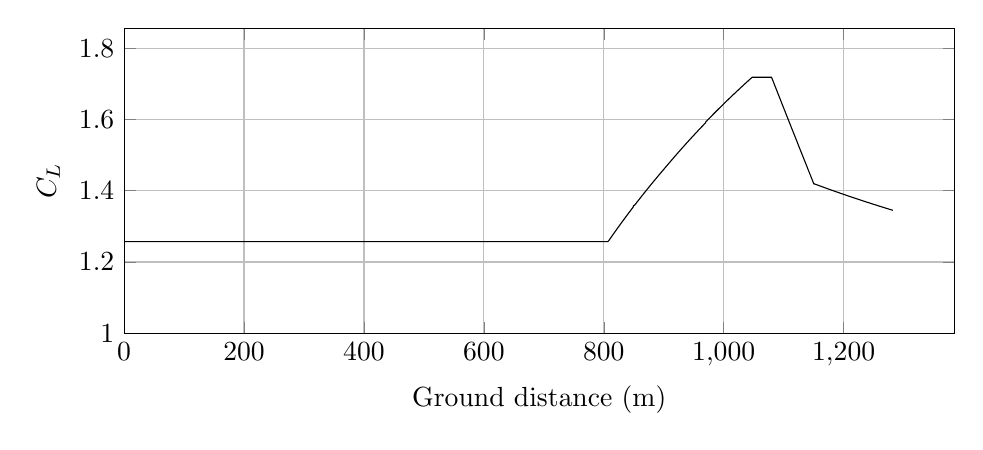
\begin{tikzpicture}

\begin{axis}[
width=\textwidth,
height=0.45\textwidth,
scaled ticks=false, tick label style={/pgf/number format/fixed},
xmin=0.0,
xmax=1384.5346672985966,
xlabel={Ground distance (m)},
xmajorgrids,
ymin=1.0,
ymax=1.856055169601142,
ylabel={$C_L$ },
ymajorgrids,
legend style={at={(1.03,0.5)},anchor=west,draw=black,fill=white,legend cell align=left}
]

\addplot [
color=black,
solid
]
table[row sep=crcr]{
1.3603393307216043E-8	1.257316705633825\\
3.0265395163403265E-7	1.257316705633825\\
2.9593179127983543E-6	1.257316705633825\\
1.5392338359717934E-5	1.257316705633825\\
5.361280674027254E-5	1.257316705633825\\
1.6215010178508227E-4	1.257316705633825\\
3.7214145765703975E-4	1.257316705633825\\
6.839954676020354E-4	1.257316705633825\\
0.001098342709021993	1.257316705633825\\
0.001609317716481928	1.257316705633825\\
0.0022198920000388346	1.257316705633825\\
0.002878710694837372	1.257316705633825\\
0.0036835072341781794	1.257316705633825\\
0.004557929017412697	1.257316705633825\\
0.005559798278933152	1.257316705633825\\
0.006651227400597502	1.257316705633825\\
0.007795849738889277	1.257316705633825\\
0.009067984722810115	1.257316705633825\\
0.010453165799939174	1.257316705633825\\
0.011915708813158052	1.257316705633825\\
0.013455030027058647	1.257316705633825\\
0.015131183092671713	1.257316705633825\\
0.01690803412933615	1.257316705633825\\
0.01873590105740728	1.257316705633825\\
0.020713359121301934	1.257316705633825\\
0.022777736728155237	1.257316705633825\\
0.024960970145273077	1.257316705633825\\
0.02723428625014468	1.257316705633825\\
0.029610395797831278	1.257316705633825\\
0.03204086105441677	1.257316705633825\\
0.03462344565878624	1.257316705633825\\
0.037295727153354774	1.257316705633825\\
0.040089145853872785	1.257316705633825\\
0.042950967781251806	1.257316705633825\\
0.04592022141655751	1.257316705633825\\
0.04897301836205646	1.257316705633825\\
0.052130294957187476	1.257316705633825\\
0.05542514139564195	1.257316705633825\\
0.05879722600804832	1.257316705633825\\
0.06231520981015182	1.257316705633825\\
0.06596261503753809	1.257316705633825\\
0.06964559414821356	1.257316705633825\\
0.07347193989652406	1.257316705633825\\
0.07736619052035826	1.257316705633825\\
0.08137137577670908	1.257316705633825\\
0.08545617869345057	1.257316705633825\\
0.08969468676038628	1.257316705633825\\
0.0940095881391464	1.257316705633825\\
0.09845059220533334	1.257316705633825\\
0.10296315144049947	1.257316705633825\\
0.10759658895065366	1.257316705633825\\
0.1123317495250277	1.257316705633825\\
0.1171874363557737	1.257316705633825\\
0.12217670360507671	1.257316705633825\\
0.12726806426274867	1.257316705633825\\
0.13231647880291775	1.257316705633825\\
0.13765212084557643	1.257316705633825\\
0.14294844966167852	1.257316705633825\\
0.14834594087957392	1.257316705633825\\
0.1539671093411843	1.257316705633825\\
0.15968242883369804	1.257316705633825\\
0.16555834796315422	1.257316705633825\\
0.17157514414202774	1.257316705633825\\
0.17760320215284392	1.257316705633825\\
0.18370335474801935	1.257316705633825\\
0.18983540939776816	1.257316705633825\\
0.19621099073945342	1.257316705633825\\
0.20278841209744758	1.257316705633825\\
0.20952923284938563	1.257316705633825\\
0.21624967405074952	1.257316705633825\\
0.22309476488450758	1.257316705633825\\
0.22992510727843934	1.257316705633825\\
0.2371653034562048	1.257316705633825\\
0.2442573187228817	1.257316705633825\\
0.25144286317780873	1.257316705633825\\
0.2588001799723505	1.257316705633825\\
0.2662612189130884	1.257316705633825\\
0.27386560463063747	1.257316705633825\\
0.2815803271719757	1.257316705633825\\
0.28946218069394425	1.257316705633825\\
0.29753588720841584	1.257316705633825\\
0.3056643119969481	1.257316705633825\\
0.31376446154764137	1.257316705633825\\
0.322071411728719	1.257316705633825\\
0.3303680011285137	1.257316705633825\\
0.3389039548234316	1.257316705633825\\
0.3474123396293025	1.257316705633825\\
0.3561645174790815	1.257316705633825\\
0.36525289600634137	1.257316705633825\\
0.3742306244196095	1.257316705633825\\
0.3835584127627333	1.257316705633825\\
0.392806747202999	1.257316705633825\\
0.40218604538039837	1.257316705633825\\
0.4115907129344223	1.257316705633825\\
0.42143744457304466	1.257316705633825\\
0.4310567075016639	1.257316705633825\\
0.4412814114336725	1.257316705633825\\
0.4513051702487684	1.257316705633825\\
0.461412558308395	1.257316705633825\\
0.47173637532167356	1.257316705633825\\
0.4821484569390513	1.257316705633825\\
0.492985116277161	1.257316705633825\\
0.5036221628177362	1.257316705633825\\
0.5142245311302887	1.257316705633825\\
0.5252888808291518	1.257316705633825\\
0.5363145235987512	1.257316705633825\\
0.5471208511184944	1.257316705633825\\
0.5585110457184732	1.257316705633825\\
0.569849942463402	1.257316705633825\\
0.5817265165330987	1.257316705633825\\
0.5935668742733842	1.257316705633825\\
0.6053719027871456	1.257316705633825\\
0.6172343027602503	1.257316705633825\\
0.629515267228629	1.257316705633825\\
0.6417789549774502	1.257316705633825\\
0.6542768803188956	1.257316705633825\\
0.6669828212214572	1.257316705633825\\
0.6796225285147333	1.257316705633825\\
0.6925094233679154	1.257316705633825\\
0.7056620711738308	1.257316705633825\\
0.7184715206768946	1.257316705633825\\
0.731725241748566	1.257316705633825\\
0.7449880440563246	1.257316705633825\\
0.7586792333483576	1.257316705633825\\
0.7725063377467813	1.257316705633825\\
0.7863894274138714	1.257316705633825\\
0.8004504964383841	1.257316705633825\\
0.8147129313117618	1.257316705633825\\
0.8293722635741907	1.257316705633825\\
0.8437954335339908	1.257316705633825\\
0.8580702287827062	1.257316705633825\\
0.8726489666047585	1.257316705633825\\
0.8875094051704782	1.257316705633825\\
0.9027740629895862	1.257316705633825\\
0.9182163910703112	1.257316705633825\\
0.93361566230532	1.257316705633825\\
0.9491799633800446	1.257316705633825\\
0.9646343064330896	1.257316705633825\\
0.9803727456894022	1.257316705633825\\
0.9957421603273868	1.257316705633825\\
1.0116767859397604	1.257316705633825\\
1.028041387324289	1.257316705633825\\
1.0443915011410971	1.257316705633825\\
1.060796374175649	1.257316705633825\\
1.0773229908740651	1.257316705633825\\
1.093971735592782	1.257316705633825\\
1.1110062543639518	1.257316705633825\\
1.127891796882146	1.257316705633825\\
1.1451224507351285	1.257316705633825\\
1.1624801114435046	1.257316705633825\\
1.180077727863539	1.257316705633825\\
1.1978884766667508	1.257316705633825\\
1.215488397439855	1.257316705633825\\
1.23351701382096	1.257316705633825\\
1.2518199984626128	1.257316705633825\\
1.2704235066044305	1.257316705633825\\
1.2892140278280424	1.257316705633825\\
1.3075714306593595	1.257316705633825\\
1.3266673518109293	1.257316705633825\\
1.3462106477188795	1.257316705633825\\
1.365306294594515	1.257316705633825\\
1.3852885894463176	1.257316705633825\\
1.404835539176236	1.257316705633825\\
1.4251192118409102	1.257316705633825\\
1.445164519989187	1.257316705633825\\
1.4656054698512246	1.257316705633825\\
1.4853522740259328	1.257316705633825\\
1.5051589726327936	1.257316705633825\\
1.5255757775517242	1.257316705633825\\
1.5464367798307013	1.257316705633825\\
1.5673163741652552	1.257316705633825\\
1.5879032567231621	1.257316705633825\\
1.6091523485848285	1.257316705633825\\
1.6303162371862876	1.257316705633825\\
1.6519474169970438	1.257316705633825\\
1.673879209980242	1.257316705633825\\
1.6955666802836635	1.257316705633825\\
1.7172271378534343	1.257316705633825\\
1.7402832823543353	1.257316705633825\\
1.7634396102400074	1.257316705633825\\
1.7861669372425006	1.257316705633825\\
1.8088678577734645	1.257316705633825\\
1.831824248135399	1.257316705633825\\
1.855578771396016	1.257316705633825\\
1.878960729162178	1.257316705633825\\
1.9033179534858085	1.257316705633825\\
1.9273833213731866	1.257316705633825\\
1.9518510462308036	1.257316705633825\\
1.9761594732990155	1.257316705633825\\
2.000437267212291	1.257316705633825\\
2.0252281699074732	1.257316705633825\\
2.0498006073458734	1.257316705633825\\
2.0745611186355752	1.257316705633825\\
2.0997746990963106	1.257316705633825\\
2.1260324099367294	1.257316705633825\\
2.1515212193659616	1.257316705633825\\
2.1771505246334	1.257316705633825\\
2.2031842637813908	1.257316705633825\\
2.230133398733474	1.257316705633825\\
2.257053086628849	1.257316705633825\\
2.283795213136285	1.257316705633825\\
2.311477064851834	1.257316705633825\\
2.3387199014446116	1.257316705633825\\
2.3662694524467227	1.257316705633825\\
2.3937852540088533	1.257316705633825\\
2.4216520071021392	1.257316705633825\\
2.4501931244916175	1.257316705633825\\
2.478927626230634	1.257316705633825\\
2.506685441631536	1.257316705633825\\
2.53537335014481	1.257316705633825\\
2.5633350931805676	1.257316705633825\\
2.5917889242519685	1.257316705633825\\
2.6208221472873374	1.257316705633825\\
2.649872764173903	1.257316705633825\\
2.679661174525658	1.257316705633825\\
2.709174609939316	1.257316705633825\\
2.740029385016756	1.257316705633825\\
2.770444625703795	1.257316705633825\\
2.801129860621211	1.257316705633825\\
2.8318827297715705	1.257316705633825\\
2.862425967677578	1.257316705633825\\
2.893259332541544	1.257316705633825\\
2.92412139403754	1.257316705633825\\
2.955064430161417	1.257316705633825\\
2.986690331721131	1.257316705633825\\
3.019183403261743	1.257316705633825\\
3.0507201588152526	1.257316705633825\\
3.0830332871979023	1.257316705633825\\
3.1154603869692448	1.257316705633825\\
3.148592095396281	1.257316705633825\\
3.181936872739324	1.257316705633825\\
3.214370607724433	1.257316705633825\\
3.247565473366384	1.257316705633825\\
3.281695868027062	1.257316705633825\\
3.316494330618462	1.257316705633825\\
3.3513055302544137	1.257316705633825\\
3.3860303583611797	1.257316705633825\\
3.421934361445942	1.257316705633825\\
3.456235826539576	1.257316705633825\\
3.490536654441657	1.257316705633825\\
3.526257338581564	1.257316705633825\\
3.561372823896762	1.257316705633825\\
3.5967906564503185	1.257316705633825\\
3.632682576242373	1.257316705633825\\
3.6701261071689295	1.257316705633825\\
3.707701291513044	1.257316705633825\\
3.7452745323452916	1.257316705633825\\
3.78256482255855	1.257316705633825\\
3.8208821591411084	1.257316705633825\\
3.8590337549211444	1.257316705633825\\
3.89695718563138	1.257316705633825\\
3.9351036745073964	1.257316705633825\\
3.9736642086653067	1.257316705633825\\
4.012189127077221	1.257316705633825\\
4.05156219172609	1.257316705633825\\
4.090290786278251	1.257316705633825\\
4.129291984889424	1.257316705633825\\
4.1680648628189925	1.257316705633825\\
4.207805169621487	1.257316705633825\\
4.248168240749736	1.257316705633825\\
4.288797880674668	1.257316705633825\\
4.32990243544832	1.257316705633825\\
4.371428084678056	1.257316705633825\\
4.41247037137882	1.257316705633825\\
4.453879445321437	1.257316705633825\\
4.49524783594077	1.257316705633825\\
4.537299342543221	1.257316705633825\\
4.580546125800922	1.257316705633825\\
4.622914948498307	1.257316705633825\\
4.66640222022569	1.257316705633825\\
4.709294790611851	1.257316705633825\\
4.752417172855319	1.257316705633825\\
4.796155651503765	1.257316705633825\\
4.8408754796551925	1.257316705633825\\
4.884850997559644	1.257316705633825\\
4.928651138956553	1.257316705633825\\
4.972831351372241	1.257316705633825\\
5.017331702752941	1.257316705633825\\
5.0632326321008225	1.257316705633825\\
5.108452384314601	1.257316705633825\\
5.1536021218025905	1.257316705633825\\
5.199057463234675	1.257316705633825\\
5.244479287100011	1.257316705633825\\
5.292293005248643	1.257316705633825\\
5.338096108273211	1.257316705633825\\
5.3857492800262605	1.257316705633825\\
5.433816232374781	1.257316705633825\\
5.480691139018431	1.257316705633825\\
5.529685763332537	1.257316705633825\\
5.578612887337309	1.257316705633825\\
5.626451501744754	1.257316705633825\\
5.674834544150631	1.257316705633825\\
5.7252048440372345	1.257316705633825\\
5.77422346516266	1.257316705633825\\
5.8255152536468575	1.257316705633825\\
5.874338256646894	1.257316705633825\\
5.922631450506765	1.257316705633825\\
5.972682300942642	1.257316705633825\\
6.022535370757359	1.257316705633825\\
6.074394648705015	1.257316705633825\\
6.124928192945902	1.257316705633825\\
6.176798284396469	1.257316705633825\\
6.229620191179453	1.257316705633825\\
6.282808156696705	1.257316705633825\\
6.334658925277093	1.257316705633825\\
6.388041948821611	1.257316705633825\\
6.440558117792513	1.257316705633825\\
6.494960924490993	1.257316705633825\\
6.550441697666145	1.257316705633825\\
6.6042098433346865	1.257316705633825\\
6.658315220792536	1.257316705633825\\
6.712335084641163	1.257316705633825\\
6.766674450459032	1.257316705633825\\
6.821537769035839	1.257316705633825\\
6.876851268142238	1.257316705633825\\
6.933661362437203	1.257316705633825\\
6.989261882852809	1.257316705633825\\
7.046240323930029	1.257316705633825\\
7.102786137967051	1.257316705633825\\
7.1603789170469145	1.257316705633825\\
7.21785165788507	1.257316705633825\\
7.277487498606879	1.257316705633825\\
7.334984696129153	1.257316705633825\\
7.393362172524569	1.257316705633825\\
7.452416393609804	1.257316705633825\\
7.511934748111884	1.257316705633825\\
7.572557225035805	1.257316705633825\\
7.63202184821041	1.257316705633825\\
7.69294899409779	1.257316705633825\\
7.752675521499926	1.257316705633825\\
7.814488876138199	1.257316705633825\\
7.8763528528159785	1.257316705633825\\
7.938149975125226	1.257316705633825\\
8.001193143199774	1.257316705633825\\
8.064554080136986	1.257316705633825\\
8.12686567918485	1.257316705633825\\
8.189637855946287	1.257316705633825\\
8.252542711798306	1.257316705633825\\
8.315859663763469	1.257316705633825\\
8.380006162932737	1.257316705633825\\
8.444702551512929	1.257316705633825\\
8.509501986620958	1.257316705633825\\
8.57387297516295	1.257316705633825\\
8.63887365699837	1.257316705633825\\
8.70727085773305	1.257316705633825\\
8.772937378995405	1.257316705633825\\
8.839192134487615	1.257316705633825\\
8.905815929161982	1.257316705633825\\
8.97209054442786	1.257316705633825\\
9.039019026885107	1.257316705633825\\
9.107371801018814	1.257316705633825\\
9.174915633685494	1.257316705633825\\
9.243868961478196	1.257316705633825\\
9.312440636565494	1.257316705633825\\
9.381784695008012	1.257316705633825\\
9.4513167952828	1.257316705633825\\
9.52142787533916	1.257316705633825\\
9.591425279059166	1.257316705633825\\
9.662230428326719	1.257316705633825\\
9.734225879912522	1.257316705633825\\
9.806441602430919	1.257316705633825\\
9.878483835105534	1.257316705633825\\
9.951807209049782	1.257316705633825\\
10.023539677466466	1.257316705633825\\
10.096057433179052	1.257316705633825\\
10.168262179450682	1.257316705633825\\
10.241274410624943	1.257316705633825\\
10.31479015323385	1.257316705633825\\
10.390063469390178	1.257316705633825\\
10.465012435634037	1.257316705633825\\
10.540639152111389	1.257316705633825\\
10.617644389866598	1.257316705633825\\
10.692945462162374	1.257316705633825\\
10.770083295573727	1.257316705633825\\
10.846726862770723	1.257316705633825\\
10.924657809445929	1.257316705633825\\
11.00265335491597	1.257316705633825\\
11.081827589833612	1.257316705633825\\
11.159134327011738	1.257316705633825\\
11.239152720133266	1.257316705633825\\
11.317028257314295	1.257316705633825\\
11.396413369884492	1.257316705633825\\
11.477655063362434	1.257316705633825\\
11.556958506738276	1.257316705633825\\
11.637325199769407	1.257316705633825\\
11.717754170658207	1.257316705633825\\
11.799819443100102	1.257316705633825\\
11.881986970940797	1.257316705633825\\
11.964394119506721	1.257316705633825\\
12.046263329632716	1.257316705633825\\
12.130282587748898	1.257316705633825\\
12.213721087180826	1.257316705633825\\
12.295868535962462	1.257316705633825\\
12.380692430046633	1.257316705633825\\
12.46470288467437	1.257316705633825\\
12.550384439940181	1.257316705633825\\
12.635259749824865	1.257316705633825\\
12.72144647897981	1.257316705633825\\
12.80741162779486	1.257316705633825\\
12.892901506907108	1.257316705633825\\
12.977815703098727	1.257316705633825\\
13.06483740414145	1.257316705633825\\
13.151922956503014	1.257316705633825\\
13.240589045456186	1.257316705633825\\
13.329911181207382	1.257316705633825\\
13.417306166647748	1.257316705633825\\
13.507103029723119	1.257316705633825\\
13.595986036712912	1.257316705633825\\
13.687453390597003	1.257316705633825\\
13.779071846306106	1.257316705633825\\
13.872694200363323	1.257316705633825\\
13.963504841252302	1.257316705633825\\
14.056146454975131	1.257316705633825\\
14.14918846816267	1.257316705633825\\
14.24332804549016	1.257316705633825\\
14.339261112049854	1.257316705633825\\
14.431091301610323	1.257316705633825\\
14.524174633942373	1.257316705633825\\
14.618760344060338	1.257316705633825\\
14.714801736988441	1.257316705633825\\
14.809763128346521	1.257316705633825\\
14.903412319659619	1.257316705633825\\
15.001392651385917	1.257316705633825\\
15.098055049922994	1.257316705633825\\
15.196870856960619	1.257316705633825\\
15.29477342819068	1.257316705633825\\
15.39265348361268	1.257316705633825\\
15.490487151984588	1.257316705633825\\
15.588146853189365	1.257316705633825\\
15.687961867268871	1.257316705633825\\
15.78650099417861	1.257316705633825\\
15.886965864441798	1.257316705633825\\
15.98755318095926	1.257316705633825\\
16.088470385762115	1.257316705633825\\
16.190536977381747	1.257316705633825\\
16.292466610053154	1.257316705633825\\
16.396448349404487	1.257316705633825\\
16.497808944935016	1.257316705633825\\
16.600551072850564	1.257316705633825\\
16.70575139586156	1.257316705633825\\
16.81134459259622	1.257316705633825\\
16.917616592554033	1.257316705633825\\
17.023477948501657	1.257316705633825\\
17.12904978140002	1.257316705633825\\
17.2354081519902	1.257316705633825\\
17.340772011500363	1.257316705633825\\
17.448391076872838	1.257316705633825\\
17.5571980918308	1.257316705633825\\
17.66615596614949	1.257316705633825\\
17.774685459577412	1.257316705633825\\
17.884986575683584	1.257316705633825\\
17.99552903728076	1.257316705633825\\
18.108708479124623	1.257316705633825\\
18.219646262474413	1.257316705633825\\
18.332680252669796	1.257316705633825\\
18.445061806396694	1.257316705633825\\
18.556709221711323	1.257316705633825\\
18.668884868236475	1.257316705633825\\
18.78204748093455	1.257316705633825\\
18.895704562363058	1.257316705633825\\
19.008928234289563	1.257316705633825\\
19.124320907419907	1.257316705633825\\
19.24105855786135	1.257316705633825\\
19.355116774466126	1.257316705633825\\
19.470462572962035	1.257316705633825\\
19.58492145104516	1.257316705633825\\
19.704921229319112	1.257316705633825\\
19.821259826163917	1.257316705633825\\
19.941172080873493	1.257316705633825\\
20.06078806851737	1.257316705633825\\
20.177423389922623	1.257316705633825\\
20.297621170678	1.257316705633825\\
20.420129559802255	1.257316705633825\\
20.54164670774839	1.257316705633825\\
20.661905244258705	1.257316705633825\\
20.784301666224792	1.257316705633825\\
20.904244540623438	1.257316705633825\\
21.028114340450195	1.257316705633825\\
21.148300883955606	1.257316705633825\\
21.270875420257596	1.257316705633825\\
21.39299406946177	1.257316705633825\\
21.513793771711654	1.257316705633825\\
21.637476506915142	1.257316705633825\\
21.759279707150128	1.257316705633825\\
21.88493035745168	1.257316705633825\\
22.009809790007786	1.257316705633825\\
22.13620730934617	1.257316705633825\\
22.263515470260465	1.257316705633825\\
22.393040471753594	1.257316705633825\\
22.520519759768852	1.257316705633825\\
22.648852607677917	1.257316705633825\\
22.775118904521122	1.257316705633825\\
22.903136237443974	1.257316705633825\\
23.03176118514304	1.257316705633825\\
23.162501585272054	1.257316705633825\\
23.294719932439598	1.257316705633825\\
23.427108470281937	1.257316705633825\\
23.558693146983046	1.257316705633825\\
23.687077503630363	1.257316705633825\\
23.817949558665852	1.257316705633825\\
23.948210788889448	1.257316705633825\\
24.076877750667826	1.257316705633825\\
24.21019765060587	1.257316705633825\\
24.3450673155249	1.257316705633825\\
24.477101355489637	1.257316705633825\\
24.60984760833776	1.257316705633825\\
24.7468403923846	1.257316705633825\\
24.882807251950062	1.257316705633825\\
25.017167332957627	1.257316705633825\\
25.153910941279605	1.257316705633825\\
25.289629217480112	1.257316705633825\\
25.425306692573436	1.257316705633825\\
25.56229499031975	1.257316705633825\\
25.70075944713021	1.257316705633825\\
25.83724158708921	1.257316705633825\\
25.975209935932874	1.257316705633825\\
26.003074150630965	1.257316705633825\\
26.020759913393235	1.257316705633825\\
26.030714598210515	1.257316705633825\\
26.05840292223249	1.257316705633825\\
26.06133765907019	1.257316705633825\\
26.064285136409026	1.257316705633825\\
26.066337724202356	1.257316705633825\\
26.068175973881182	1.257316705633825\\
26.06984477238784	1.257316705633825\\
26.077831036047115	1.257316705633825\\
26.10345636352254	1.257316705633825\\
26.16716044512971	1.257316705633825\\
26.297541524199602	1.257316705633825\\
26.42722303713863	1.257316705633825\\
26.5559280656694	1.257316705633825\\
26.686097387723095	1.257316705633825\\
26.817793678842584	1.257316705633825\\
26.949416928520378	1.257316705633825\\
27.080440623797912	1.257316705633825\\
27.215491080424528	1.257316705633825\\
27.34795890217076	1.257316705633825\\
27.48215578365496	1.257316705633825\\
27.616696052324144	1.257316705633825\\
27.75271189183823	1.257316705633825\\
27.888759310501555	1.257316705633825\\
28.023839122857026	1.257316705633825\\
28.16136324828667	1.257316705633825\\
28.298355249881332	1.257316705633825\\
28.435282447697354	1.257316705633825\\
28.573941346212784	1.257316705633825\\
28.713752690797136	1.257316705633825\\
28.852681198061333	1.257316705633825\\
28.992471984120606	1.257316705633825\\
29.133421724605903	1.257316705633825\\
29.275199211812186	1.257316705633825\\
29.416225289053614	1.257316705633825\\
29.55783477945603	1.257316705633825\\
29.701838356359822	1.257316705633825\\
29.846633046394217	1.257316705633825\\
29.99013730470424	1.257316705633825\\
30.132492646908446	1.257316705633825\\
30.277395768405135	1.257316705633825\\
30.422188862471998	1.257316705633825\\
30.56637548064623	1.257316705633825\\
30.711944318924978	1.257316705633825\\
30.8573377156769	1.257316705633825\\
31.006558691603843	1.257316705633825\\
31.153907258126303	1.257316705633825\\
31.30257185742142	1.257316705633825\\
31.4510947803754	1.257316705633825\\
31.602595106592503	1.257316705633825\\
31.755261577184278	1.257316705633825\\
31.906398416479824	1.257316705633825\\
32.05599258457312	1.257316705633825\\
32.20952926265106	1.257316705633825\\
32.360097140052986	1.257316705633825\\
32.51218835243483	1.257316705633825\\
32.664721606344784	1.257316705633825\\
32.82129760777845	1.257316705633825\\
32.97669884718651	1.257316705633825\\
33.13118849606322	1.257316705633825\\
33.288837444683736	1.257316705633825\\
33.44405554194745	1.257316705633825\\
33.60015866510213	1.257316705633825\\
33.756686089655645	1.257316705633825\\
33.91694077595571	1.257316705633825\\
34.074326811338736	1.257316705633825\\
34.23252403098988	1.257316705633825\\
34.392884168270385	1.257316705633825\\
34.554266068788166	1.257316705633825\\
34.71363140184178	1.257316705633825\\
34.87649332318763	1.257316705633825\\
35.03746231629111	1.257316705633825\\
35.19990059234286	1.257316705633825\\
35.3627309111595	1.257316705633825\\
35.5271254050015	1.257316705633825\\
35.69149466827288	1.257316705633825\\
35.85508342515686	1.257316705633825\\
36.017180984292054	1.257316705633825\\
36.182222084544165	1.257316705633825\\
36.34861175093968	1.257316705633825\\
36.514166392421686	1.257316705633825\\
36.68083924241549	1.257316705633825\\
36.845526722294395	1.257316705633825\\
37.01328249159678	1.257316705633825\\
37.18160982421668	1.257316705633825\\
37.35136716620059	1.257316705633825\\
37.51969289597564	1.257316705633825\\
37.689710015857784	1.257316705633825\\
37.860394939778416	1.257316705633825\\
38.02805196867635	1.257316705633825\\
38.19868492919754	1.257316705633825\\
38.37343039987371	1.257316705633825\\
38.54685896696101	1.257316705633825\\
38.71934233168869	1.257316705633825\\
38.8915617091798	1.257316705633825\\
39.062305982326905	1.257316705633825\\
39.23847188392709	1.257316705633825\\
39.411511502305984	1.257316705633825\\
39.585172817779906	1.257316705633825\\
39.760693028009456	1.257316705633825\\
39.9373134006328	1.257316705633825\\
40.113617753210534	1.257316705633825\\
40.29094651898711	1.257316705633825\\
40.468149621311596	1.257316705633825\\
40.64593210594187	1.257316705633825\\
40.82431302355218	1.257316705633825\\
41.00141330502653	1.257316705633825\\
41.17957893337042	1.257316705633825\\
41.359761290266974	1.257316705633825\\
41.53889737920997	1.257316705633825\\
41.72013507746885	1.257316705633825\\
41.899395797464194	1.257316705633825\\
42.081280067494475	1.257316705633825\\
42.265315320939635	1.257316705633825\\
42.44531744651641	1.257316705633825\\
42.62715102096499	1.257316705633825\\
42.81120266452106	1.257316705633825\\
42.994164503876235	1.257316705633825\\
43.17799769459725	1.257316705633825\\
43.36154361404071	1.257316705633825\\
43.54597437124032	1.257316705633825\\
43.73158498218817	1.257316705633825\\
43.91737182308138	1.257316705633825\\
44.1050494697441	1.257316705633825\\
44.293574236233	1.257316705633825\\
44.47888581456586	1.257316705633825\\
44.66456251492659	1.257316705633825\\
44.85170130968709	1.257316705633825\\
45.037822074257164	1.257316705633825\\
45.22676109993536	1.257316705633825\\
45.41612608476639	1.257316705633825\\
45.604812217355104	1.257316705633825\\
45.79422221198037	1.257316705633825\\
45.98724683785376	1.257316705633825\\
46.17830917717477	1.257316705633825\\
46.36786657808848	1.257316705633825\\
46.55935209439748	1.257316705633825\\
46.75090376717816	1.257316705633825\\
46.94233405988251	1.257316705633825\\
47.13714948644359	1.257316705633825\\
47.33387512950824	1.257316705633825\\
47.53043319838464	1.257316705633825\\
47.72298239739284	1.257316705633825\\
47.919150009665316	1.257316705633825\\
48.113386178114425	1.257316705633825\\
48.311024807628144	1.257316705633825\\
48.508886059616145	1.257316705633825\\
48.70490444306449	1.257316705633825\\
48.90290918859142	1.257316705633825\\
49.09959709013448	1.257316705633825\\
49.2970021191946	1.257316705633825\\
49.49532701226336	1.257316705633825\\
49.693780717172615	1.257316705633825\\
49.89506320355713	1.257316705633825\\
50.096719083698545	1.257316705633825\\
50.29606895218413	1.257316705633825\\
50.497598474286534	1.257316705633825\\
50.700304208193415	1.257316705633825\\
50.90342397924904	1.257316705633825\\
51.10460922167407	1.257316705633825\\
51.30752217039489	1.257316705633825\\
51.51010619677311	1.257316705633825\\
51.713602501430145	1.257316705633825\\
51.91843850546792	1.257316705633825\\
52.121089026646246	1.257316705633825\\
52.32561402362407	1.257316705633825\\
52.53192272805477	1.257316705633825\\
52.7387030603267	1.257316705633825\\
52.944027344085896	1.257316705633825\\
53.154073670302836	1.257316705633825\\
53.36143953271798	1.257316705633825\\
53.571009444677685	1.257316705633825\\
53.77799762982136	1.257316705633825\\
53.98785945427545	1.257316705633825\\
54.196157549666225	1.257316705633825\\
54.40718762937186	1.257316705633825\\
54.616887598525366	1.257316705633825\\
54.826875464266934	1.257316705633825\\
55.04038432082807	1.257316705633825\\
55.25438844036796	1.257316705633825\\
55.46695867894975	1.257316705633825\\
55.68088820258777	1.257316705633825\\
55.895144656119854	1.257316705633825\\
56.109028395418505	1.257316705633825\\
56.326262430904194	1.257316705633825\\
56.542089933321776	1.257316705633825\\
56.76060076462056	1.257316705633825\\
56.97729209122687	1.257316705633825\\
57.19579178641709	1.257316705633825\\
57.41258192878804	1.257316705633825\\
57.634093277561306	1.257316705633825\\
57.85395098827546	1.257316705633825\\
58.07448819514299	1.257316705633825\\
58.29446478173499	1.257316705633825\\
58.51588770709739	1.257316705633825\\
58.73757884137123	1.257316705633825\\
58.96020041504734	1.257316705633825\\
59.18267120664716	1.257316705633825\\
59.405949655899676	1.257316705633825\\
59.63089974393067	1.257316705633825\\
59.8562534200115	1.257316705633825\\
60.084134136581554	1.257316705633825\\
60.30833762904015	1.257316705633825\\
60.53504725699203	1.257316705633825\\
60.763693228044005	1.257316705633825\\
60.99075593752245	1.257316705633825\\
61.21765734918529	1.257316705633825\\
61.44713116872772	1.257316705633825\\
61.6738048454246	1.257316705633825\\
61.90668490141796	1.257316705633825\\
62.13729676517957	1.257316705633825\\
62.36629463006145	1.257316705633825\\
62.596359157213186	1.257316705633825\\
62.82836101237727	1.257316705633825\\
63.059723307860466	1.257316705633825\\
63.292774394726166	1.257316705633825\\
63.52608473446321	1.257316705633825\\
63.75973181411028	1.257316705633825\\
63.993403028653574	1.257316705633825\\
64.23068717493263	1.257316705633825\\
64.4710952259949	1.257316705633825\\
64.70858695601663	1.257316705633825\\
64.94894296164699	1.257316705633825\\
65.18738841845183	1.257316705633825\\
65.42661162888535	1.257316705633825\\
65.6659442133793	1.257316705633825\\
65.90899583190168	1.257316705633825\\
66.15068261105333	1.257316705633825\\
66.39533053734849	1.257316705633825\\
66.6378997293487	1.257316705633825\\
66.88158418814953	1.257316705633825\\
67.12390450547147	1.257316705633825\\
67.36840986262189	1.257316705633825\\
67.61550053739396	1.257316705633825\\
67.86097385246623	1.257316705633825\\
68.10985741250389	1.257316705633825\\
68.35582503705197	1.257316705633825\\
68.60464259362828	1.257316705633825\\
68.85450289166104	1.257316705633825\\
69.1042877596268	1.257316705633825\\
69.35837572129628	1.257316705633825\\
69.61150655903072	1.257316705633825\\
69.86289252102952	1.257316705633825\\
70.11686816207683	1.257316705633825\\
70.37125759672608	1.257316705633825\\
70.62480458144697	1.257316705633825\\
70.88045310059783	1.257316705633825\\
71.13526709211152	1.257316705633825\\
71.3947754873567	1.257316705633825\\
71.6534187996231	1.257316705633825\\
71.91450497256008	1.257316705633825\\
72.1716184080999	1.257316705633825\\
72.43269265097052	1.257316705633825\\
72.69331619504374	1.257316705633825\\
72.95563200429567	1.257316705633825\\
73.21686762735783	1.257316705633825\\
73.48161420086069	1.257316705633825\\
73.74261486234883	1.257316705633825\\
74.00755043430098	1.257316705633825\\
74.27511769675363	1.257316705633825\\
74.54487113507057	1.257316705633825\\
74.81568229507957	1.257316705633825\\
75.08274085953312	1.257316705633825\\
75.35421836228127	1.257316705633825\\
75.62798354862159	1.257316705633825\\
75.89909469738902	1.257316705633825\\
76.17008148658607	1.257316705633825\\
76.44269151183332	1.257316705633825\\
76.71571902594138	1.257316705633825\\
76.99340852183178	1.257316705633825\\
77.27004772085374	1.257316705633825\\
77.54832408953641	1.257316705633825\\
77.82592519882277	1.257316705633825\\
78.10358246820337	1.257316705633825\\
78.38556010231375	1.257316705633825\\
78.66911430382748	1.257316705633825\\
78.95399134982776	1.257316705633825\\
79.23667137346987	1.257316705633825\\
79.518907793654	1.257316705633825\\
79.80555437718249	1.257316705633825\\
80.09150103324356	1.257316705633825\\
80.37928873457926	1.257316705633825\\
80.66871996946384	1.257316705633825\\
80.95967699414447	1.257316705633825\\
81.25093884305389	1.257316705633825\\
81.54344278085921	1.257316705633825\\
81.8358102960415	1.257316705633825\\
82.13087592438694	1.257316705633825\\
82.42794520371837	1.257316705633825\\
82.72842933895026	1.257316705633825\\
83.0269479931649	1.257316705633825\\
83.32974506690314	1.257316705633825\\
83.62964811531441	1.257316705633825\\
83.92951211009506	1.257316705633825\\
84.2339319847595	1.257316705633825\\
84.53715838283946	1.257316705633825\\
84.84105485927768	1.257316705633825\\
85.14845677960258	1.257316705633825\\
85.45530133949276	1.257316705633825\\
85.76249773413784	1.257316705633825\\
86.07201271349416	1.257316705633825\\
86.38432073331904	1.257316705633825\\
86.69710203601804	1.257316705633825\\
87.01172103282082	1.257316705633825\\
87.32669099459858	1.257316705633825\\
87.64517025121202	1.257316705633825\\
87.96158123090564	1.257316705633825\\
88.2775814178033	1.257316705633825\\
88.60068374099544	1.257316705633825\\
88.92068281935622	1.257316705633825\\
89.24207276858638	1.257316705633825\\
89.56578933015979	1.257316705633825\\
89.88760090270688	1.257316705633825\\
90.2141410750086	1.257316705633825\\
90.54066676000363	1.257316705633825\\
90.86727570256076	1.257316705633825\\
91.19715108614633	1.257316705633825\\
91.52744226539704	1.257316705633825\\
91.85639956214655	1.257316705633825\\
92.19095740864739	1.257316705633825\\
92.52827526888461	1.257316705633825\\
92.8674718219292	1.257316705633825\\
93.20307982994817	1.257316705633825\\
93.5374944579234	1.257316705633825\\
93.87598013161067	1.257316705633825\\
94.20917297854535	1.257316705633825\\
94.55043409744499	1.257316705633825\\
94.89132963816093	1.257316705633825\\
95.23083207736542	1.257316705633825\\
95.57395676502793	1.257316705633825\\
95.91421223354143	1.257316705633825\\
96.25656086122288	1.257316705633825\\
96.60012122339742	1.257316705633825\\
96.94166303707107	1.257316705633825\\
97.28627502929558	1.257316705633825\\
97.62906225262071	1.257316705633825\\
97.97125437026659	1.257316705633825\\
98.31201772458999	1.257316705633825\\
98.65627175165852	1.257316705633825\\
99.0012536203806	1.257316705633825\\
99.35020029285332	1.257316705633825\\
99.69475740907401	1.257316705633825\\
100.04053871990226	1.257316705633825\\
100.38598466112728	1.257316705633825\\
100.72867962848932	1.257316705633825\\
101.07385499050397	1.257316705633825\\
101.41864366415388	1.257316705633825\\
101.76305460768467	1.257316705633825\\
102.11068844700483	1.257316705633825\\
102.45638678530696	1.257316705633825\\
102.79841653079728	1.257316705633825\\
103.14087212494877	1.257316705633825\\
103.48486473791618	1.257316705633825\\
103.82875595362174	1.257316705633825\\
104.17244250654872	1.257316705633825\\
104.51168383396202	1.257316705633825\\
104.85986244643053	1.257316705633825\\
105.204587526496	1.257316705633825\\
105.54754777175077	1.257316705633825\\
105.88797456536247	1.257316705633825\\
106.23280177240994	1.257316705633825\\
106.57515110440406	1.257316705633825\\
106.91603555764121	1.257316705633825\\
107.25729565943405	1.257316705633825\\
107.598830149446	1.257316705633825\\
107.93686571059558	1.257316705633825\\
108.27485499032852	1.257316705633825\\
108.28839963475954	1.257316705633825\\
108.30004107281309	1.257316705633825\\
108.30931238392475	1.257316705633825\\
108.31701527366243	1.257316705633825\\
108.32505202073054	1.257316705633825\\
108.33865239118708	1.257316705633825\\
108.35091925899997	1.257316705633825\\
108.39508146726081	1.257316705633825\\
108.52984553865659	1.257316705633825\\
108.79919793188978	1.257316705633825\\
109.105233418432	1.257316705633825\\
109.41485218466596	1.257316705633825\\
109.72257164661937	1.257316705633825\\
110.0321119530083	1.257316705633825\\
110.34145354075926	1.257316705633825\\
110.6534776714839	1.257316705633825\\
110.9711963390063	1.257316705633825\\
111.28851843247409	1.257316705633825\\
111.60893519474632	1.257316705633825\\
111.92798394282838	1.257316705633825\\
112.24770070245137	1.257316705633825\\
112.57243448635171	1.257316705633825\\
112.89480865389396	1.257316705633825\\
113.22000325235314	1.257316705633825\\
113.54885709436653	1.257316705633825\\
113.8770619430189	1.257316705633825\\
114.20946079557197	1.257316705633825\\
114.54107775051554	1.257316705633825\\
114.87787736567807	1.257316705633825\\
115.21564640021248	1.257316705633825\\
115.55522358014255	1.257316705633825\\
115.89667501383605	1.257316705633825\\
116.23992536102014	1.257316705633825\\
116.5847156213415	1.257316705633825\\
116.92791619634093	1.257316705633825\\
117.27517516660399	1.257316705633825\\
117.62420948631524	1.257316705633825\\
117.97391125359778	1.257316705633825\\
118.32673409155768	1.257316705633825\\
118.68227803698588	1.257316705633825\\
119.03889207644076	1.257316705633825\\
119.39651249432902	1.257316705633825\\
119.75508651978987	1.257316705633825\\
120.11314113323388	1.257316705633825\\
120.47404637453192	1.257316705633825\\
120.84098349318353	1.257316705633825\\
121.20490030977416	1.257316705633825\\
121.57328571082118	1.257316705633825\\
121.94079100066682	1.257316705633825\\
122.31015242291167	1.257316705633825\\
122.68267403243519	1.257316705633825\\
123.05346836176264	1.257316705633825\\
123.42835733050345	1.257316705633825\\
123.80350972566416	1.257316705633825\\
124.1783235941891	1.257316705633825\\
124.55244040146786	1.257316705633825\\
124.92576251095704	1.257316705633825\\
125.30489170817492	1.257316705633825\\
125.68146781278597	1.257316705633825\\
126.06139977608174	1.257316705633825\\
126.44502763856761	1.257316705633825\\
126.82695116404781	1.257316705633825\\
127.206716044588	1.257316705633825\\
127.59262031825523	1.257316705633825\\
127.97077035934353	1.257316705633825\\
128.3546122768156	1.257316705633825\\
128.73724861847296	1.257316705633825\\
129.12002064685282	1.257316705633825\\
129.50086700331673	1.257316705633825\\
129.8837789976152	1.257316705633825\\
130.26783132854348	1.257316705633825\\
130.651936341801	1.257316705633825\\
131.03747321415574	1.257316705633825\\
131.42280335891803	1.257316705633825\\
131.80875442588928	1.257316705633825\\
132.19322104975072	1.257316705633825\\
132.5798881414172	1.257316705633825\\
132.96215446290768	1.257316705633825\\
133.34488286943906	1.257316705633825\\
133.7276157954845	1.257316705633825\\
134.11532375481391	1.257316705633825\\
134.50135826447365	1.257316705633825\\
134.88604120201086	1.257316705633825\\
135.26955723714872	1.257316705633825\\
135.6512109336153	1.257316705633825\\
136.03464327936558	1.257316705633825\\
136.41686422877552	1.257316705633825\\
136.79904942565338	1.257316705633825\\
137.18004416157777	1.257316705633825\\
137.56399804528928	1.257316705633825\\
137.94515347717788	1.257316705633825\\
138.32982901897384	1.257316705633825\\
138.7128522769853	1.257316705633825\\
139.09597564505458	1.257316705633825\\
139.48002685240425	1.257316705633825\\
139.86309097971855	1.257316705633825\\
140.24727738828375	1.257316705633825\\
140.6317581809211	1.257316705633825\\
141.01585725597846	1.257316705633825\\
141.3998433603236	1.257316705633825\\
141.7841907991213	1.257316705633825\\
142.16710976343057	1.257316705633825\\
142.55205218648928	1.257316705633825\\
142.9364233092117	1.257316705633825\\
143.32169829765928	1.257316705633825\\
143.705984531242	1.257316705633825\\
144.08985428249122	1.257316705633825\\
144.47683600496026	1.257316705633825\\
144.86371007721533	1.257316705633825\\
145.24772592056325	1.257316705633825\\
145.63047789911974	1.257316705633825\\
146.01273254364395	1.257316705633825\\
146.39725173307323	1.257316705633825\\
146.77966503747456	1.257316705633825\\
147.16478130736948	1.257316705633825\\
147.54689717238745	1.257316705633825\\
147.93097497792814	1.257316705633825\\
148.31499270913332	1.257316705633825\\
148.69957284780122	1.257316705633825\\
149.08709998577143	1.257316705633825\\
149.47129868208145	1.257316705633825\\
149.8546635899794	1.257316705633825\\
150.23801379389647	1.257316705633825\\
150.62200569343076	1.257316705633825\\
151.00751012558203	1.257316705633825\\
151.3946455315429	1.257316705633825\\
151.77987817077866	1.257316705633825\\
152.16505704867353	1.257316705633825\\
152.55112759502248	1.257316705633825\\
152.93964308710213	1.257316705633825\\
153.32507651584535	1.257316705633825\\
153.71174813432617	1.257316705633825\\
154.10000329570875	1.257316705633825\\
154.48914219495543	1.257316705633825\\
154.8788297075107	1.257316705633825\\
155.26820650111182	1.257316705633825\\
155.6562915247282	1.257316705633825\\
156.0441896603637	1.257316705633825\\
156.4348678136667	1.257316705633825\\
156.82082928279863	1.257316705633825\\
157.21071017196311	1.257316705633825\\
157.60005066896917	1.257316705633825\\
157.99004282467217	1.257316705633825\\
158.3808231456182	1.257316705633825\\
158.77280374485122	1.257316705633825\\
159.16384255262415	1.257316705633825\\
159.55370941764693	1.257316705633825\\
159.946071590523	1.257316705633825\\
160.33752628124114	1.257316705633825\\
160.73008933968674	1.257316705633825\\
161.12428312893906	1.257316705633825\\
161.5185576482712	1.257316705633825\\
161.91431288671106	1.257316705633825\\
162.3096877663487	1.257316705633825\\
162.70613442998513	1.257316705633825\\
163.1032465869576	1.257316705633825\\
163.50039135636405	1.257316705633825\\
163.89625578410926	1.257316705633825\\
164.29272443146095	1.257316705633825\\
164.68754921345175	1.257316705633825\\
165.0864466423082	1.257316705633825\\
165.4846753800681	1.257316705633825\\
165.88329117400662	1.257316705633825\\
166.28234792206388	1.257316705633825\\
166.68312204436222	1.257316705633825\\
167.08520211103445	1.257316705633825\\
167.486487681752	1.257316705633825\\
167.8888620337579	1.257316705633825\\
168.290121631074	1.257316705633825\\
168.69179641444674	1.257316705633825\\
169.0966267258019	1.257316705633825\\
169.50108473093724	1.257316705633825\\
169.90729482190739	1.257316705633825\\
170.31243922775104	1.257316705633825\\
170.71755979953144	1.257316705633825\\
171.12402986296422	1.257316705633825\\
171.53319587512163	1.257316705633825\\
171.941770038195	1.257316705633825\\
172.3502931259835	1.257316705633825\\
172.7599322859847	1.257316705633825\\
173.17073308198894	1.257316705633825\\
173.58266371319877	1.257316705633825\\
173.99296569000023	1.257316705633825\\
174.40104722187203	1.257316705633825\\
174.8156903853216	1.257316705633825\\
175.2299479185392	1.257316705633825\\
175.64260521584504	1.257316705633825\\
176.05374721710058	1.257316705633825\\
176.4688147253861	1.257316705633825\\
176.8832117842232	1.257316705633825\\
177.30033423294157	1.257316705633825\\
177.7185234955238	1.257316705633825\\
178.13477925276436	1.257316705633825\\
178.55472625996282	1.257316705633825\\
178.97486541267733	1.257316705633825\\
179.39652032378837	1.257316705633825\\
179.8177496461559	1.257316705633825\\
180.24148986351946	1.257316705633825\\
180.66579793025812	1.257316705633825\\
181.08977314985765	1.257316705633825\\
181.5138518510159	1.257316705633825\\
181.9380657232258	1.257316705633825\\
182.36353384896404	1.257316705633825\\
182.79266406809302	1.257316705633825\\
183.2222080657075	1.257316705633825\\
183.65034235239733	1.257316705633825\\
184.08076505956626	1.257316705633825\\
184.51404645281445	1.257316705633825\\
184.94459821529773	1.257316705633825\\
185.37526818895066	1.257316705633825\\
185.80988061731233	1.257316705633825\\
186.24113427192242	1.257316705633825\\
186.6766273110748	1.257316705633825\\
187.11377077964733	1.257316705633825\\
187.55114760103595	1.257316705633825\\
187.98927624239354	1.257316705633825\\
188.4283980284245	1.257316705633825\\
188.87193099833303	1.257316705633825\\
189.31533331187586	1.257316705633825\\
189.759935940091	1.257316705633825\\
190.20453173770989	1.257316705633825\\
190.64970684403454	1.257316705633825\\
191.09969623361582	1.257316705633825\\
191.54891620327845	1.257316705633825\\
191.9989246744131	1.257316705633825\\
192.45044905246328	1.257316705633825\\
192.90128656673437	1.257316705633825\\
193.3542511019695	1.257316705633825\\
193.8098580932263	1.257316705633825\\
194.264335427238	1.257316705633825\\
194.7197268653846	1.257316705633825\\
195.17731099948054	1.257316705633825\\
195.640653905739	1.257316705633825\\
196.0993779505016	1.257316705633825\\
196.55972836032635	1.257316705633825\\
197.02207639293357	1.257316705633825\\
197.4863674869817	1.257316705633825\\
197.95219407477043	1.257316705633825\\
198.4222293887736	1.257316705633825\\
198.8924165831608	1.257316705633825\\
199.36444563655942	1.257316705633825\\
199.83611037172778	1.257316705633825\\
200.3098256112723	1.257316705633825\\
200.78414125071725	1.257316705633825\\
201.25799602765767	1.257316705633825\\
201.73164228776483	1.257316705633825\\
202.20700915933037	1.257316705633825\\
202.6900968253659	1.257316705633825\\
203.1695441846722	1.257316705633825\\
203.6517557737585	1.257316705633825\\
204.13875101960963	1.257316705633825\\
204.6239796679484	1.257316705633825\\
205.11304714664226	1.257316705633825\\
205.6024757424737	1.257316705633825\\
206.0956744812894	1.257316705633825\\
206.59166612209884	1.257316705633825\\
207.08890230426118	1.257316705633825\\
207.58731362513566	1.257316705633825\\
208.08714180167652	1.257316705633825\\
208.59040365453075	1.257316705633825\\
209.09687012836855	1.257316705633825\\
209.6041180918084	1.257316705633825\\
210.11339270974815	1.257316705633825\\
210.6277299333704	1.257316705633825\\
211.14394599884707	1.257316705633825\\
211.66140554682187	1.257316705633825\\
212.17921813681886	1.257316705633825\\
212.6998673783849	1.257316705633825\\
213.22377641861283	1.257316705633825\\
213.74833300550847	1.257316705633825\\
214.27884482570528	1.257316705633825\\
214.8059921031383	1.257316705633825\\
215.3369392301239	1.257316705633825\\
215.8704905221095	1.257316705633825\\
216.40581461505735	1.257316705633825\\
216.94632642726936	1.257316705633825\\
217.49339939057347	1.257316705633825\\
218.04214604852046	1.257316705633825\\
218.5904378944307	1.257316705633825\\
219.1473756849698	1.257316705633825\\
219.70259972305752	1.257316705633825\\
220.26448543519223	1.257316705633825\\
220.82878425574808	1.257316705633825\\
221.39118212311007	1.257316705633825\\
221.95607401520328	1.257316705633825\\
222.52731263387568	1.257316705633825\\
223.1053033039969	1.257316705633825\\
223.68701431082144	1.257316705633825\\
224.27373979946424	1.257316705633825\\
224.8655655904359	1.257316705633825\\
225.4547840144254	1.257316705633825\\
226.0470361867341	1.257316705633825\\
226.6446113983061	1.257316705633825\\
227.2523816590479	1.257316705633825\\
227.85688390770105	1.257316705633825\\
228.45777056631943	1.257316705633825\\
229.07573877962136	1.257316705633825\\
229.69270723810865	1.257316705633825\\
230.30810613162595	1.257316705633825\\
230.92134117327288	1.257316705633825\\
231.53668557885607	1.257316705633825\\
232.15954554112375	1.257316705633825\\
232.7891522435175	1.257316705633825\\
233.4179357898359	1.257316705633825\\
234.03801334540844	1.257316705633825\\
234.67060997558383	1.257316705633825\\
235.30821584307404	1.257316705633825\\
235.93913792971972	1.257316705633825\\
236.57130412742504	1.257316705633825\\
237.20190286705872	1.257316705633825\\
237.82732440575694	1.257316705633825\\
238.45423612656094	1.257316705633825\\
239.078886894133	1.257316705633825\\
239.70118268314496	1.257316705633825\\
240.32402516569954	1.257316705633825\\
240.94763231602371	1.257316705633825\\
241.558944055687	1.257316705633825\\
242.17051988815223	1.257316705633825\\
242.78305452643912	1.257316705633825\\
243.3891405005665	1.257316705633825\\
243.99135888524592	1.257316705633825\\
244.5938059991201	1.257316705633825\\
245.19307787825466	1.257316705633825\\
245.78685747081	1.257316705633825\\
246.38614597174575	1.257316705633825\\
246.9780005147843	1.257316705633825\\
247.56968865205243	1.257316705633825\\
248.15440614950631	1.257316705633825\\
248.73860746053964	1.257316705633825\\
249.3201116454489	1.257316705633825\\
249.89451218910904	1.257316705633825\\
250.46870613238303	1.257316705633825\\
251.04194053158074	1.257316705633825\\
251.61194691308668	1.257316705633825\\
252.18082396300082	1.257316705633825\\
252.74758709237483	1.257316705633825\\
253.31251969447777	1.257316705633825\\
253.8738250395511	1.257316705633825\\
254.43149203184282	1.257316705633825\\
254.9874373408491	1.257316705633825\\
255.5414166310287	1.257316705633825\\
256.0957211160239	1.257316705633825\\
256.6475553966509	1.257316705633825\\
256.7570758146961	1.257316705633825\\
256.8263249833143	1.257316705633825\\
256.88663486655446	1.257316705633825\\
256.9430978473978	1.257316705633825\\
256.97693788107017	1.257316705633825\\
257.0025084975957	1.257316705633825\\
257.0208190077692	1.257316705633825\\
257.0380809845981	1.257316705633825\\
257.0438424242251	1.257316705633825\\
257.0596503141385	1.257316705633825\\
257.13618872139693	1.257316705633825\\
257.44346456136407	1.257316705633825\\
257.93842545742496	1.257316705633825\\
258.42387567471803	1.257316705633825\\
258.90988498762806	1.257316705633825\\
259.398919728937	1.257316705633825\\
259.89126252890617	1.257316705633825\\
260.3860981148131	1.257316705633825\\
260.88265150215534	1.257316705633825\\
261.3817388499359	1.257316705633825\\
261.8849745252071	1.257316705633825\\
262.3951340270795	1.257316705633825\\
262.90121520425464	1.257316705633825\\
263.4122609086296	1.257316705633825\\
263.9251595409296	1.257316705633825\\
264.44312884967155	1.257316705633825\\
264.96433898075304	1.257316705633825\\
265.4907836389158	1.257316705633825\\
266.01963642880764	1.257316705633825\\
266.54886163053106	1.257316705633825\\
267.08296130365613	1.257316705633825\\
267.61991815897215	1.257316705633825\\
268.1640390021088	1.257316705633825\\
268.7103404861746	1.257316705633825\\
269.2595660030436	1.257316705633825\\
269.81273134777575	1.257316705633825\\
270.3696596938787	1.257316705633825\\
270.93171711640935	1.257316705633825\\
271.4988611754003	1.257316705633825\\
272.0705326832831	1.257316705633825\\
272.6463683686135	1.257316705633825\\
273.226018440957	1.257316705633825\\
273.81180745355675	1.257316705633825\\
274.40462060354696	1.257316705633825\\
274.9941745097303	1.257316705633825\\
275.5928332442985	1.257316705633825\\
276.19228787269583	1.257316705633825\\
276.8008320595037	1.257316705633825\\
277.4103073713045	1.257316705633825\\
278.02312272786935	1.257316705633825\\
278.6480801130689	1.257316705633825\\
279.2749501652314	1.257316705633825\\
279.908172349486	1.257316705633825\\
280.54544660125293	1.257316705633825\\
281.1830405144573	1.257316705633825\\
281.81994836131184	1.257316705633825\\
282.4644929822557	1.257316705633825\\
283.1124628947573	1.257316705633825\\
283.7598098057015	1.257316705633825\\
284.41078479564055	1.257316705633825\\
285.05862981013433	1.257316705633825\\
285.70800893721935	1.257316705633825\\
286.3602979435012	1.257316705633825\\
287.0082513205941	1.257316705633825\\
287.65676876221744	1.257316705633825\\
288.3093687105044	1.257316705633825\\
288.95762918532625	1.257316705633825\\
289.6032303041229	1.257316705633825\\
290.2463292415888	1.257316705633825\\
290.88254119236694	1.257316705633825\\
291.5174657935754	1.257316705633825\\
292.15135749313765	1.257316705633825\\
292.77987115362725	1.257316705633825\\
293.4115418191582	1.257316705633825\\
294.03817556900935	1.257316705633825\\
294.6609105860233	1.257316705633825\\
295.28022031816545	1.257316705633825\\
295.9013637804736	1.257316705633825\\
296.51859456939405	1.257316705633825\\
297.13445448111213	1.257316705633825\\
297.7448643111652	1.257316705633825\\
298.35646750465946	1.257316705633825\\
298.9665369440928	1.257316705633825\\
299.57280619311405	1.257316705633825\\
300.17881401664965	1.257316705633825\\
300.7810579412371	1.257316705633825\\
301.38261059253784	1.257316705633825\\
301.9807872641708	1.257316705633825\\
302.5818390257391	1.257316705633825\\
303.1804945574968	1.257316705633825\\
303.775610749277	1.257316705633825\\
304.3662430439555	1.257316705633825\\
304.95700718406374	1.257316705633825\\
305.54856325255184	1.257316705633825\\
306.1403526946923	1.257316705633825\\
306.732267705287	1.257316705633825\\
307.3183663050603	1.257316705633825\\
307.9060154577753	1.257316705633825\\
308.4922500043788	1.257316705633825\\
309.07710579978243	1.257316705633825\\
309.66501129994356	1.257316705633825\\
310.2470970112189	1.257316705633825\\
310.8294165810805	1.257316705633825\\
311.4130393021758	1.257316705633825\\
311.99229355856255	1.257316705633825\\
312.5719037973066	1.257316705633825\\
313.1528238715506	1.257316705633825\\
313.7328622425008	1.257316705633825\\
314.3105382229827	1.257316705633825\\
314.88851884372366	1.257316705633825\\
315.4681174962417	1.257316705633825\\
316.04617774980557	1.257316705633825\\
316.6220728552114	1.257316705633825\\
317.19745521492473	1.257316705633825\\
317.7754931730906	1.257316705633825\\
318.353555553143	1.257316705633825\\
318.9291304405266	1.257316705633825\\
319.5035706351016	1.257316705633825\\
320.07956917661147	1.257316705633825\\
320.654112858477	1.257316705633825\\
321.22847808306085	1.257316705633825\\
321.80362538780014	1.257316705633825\\
322.37559125839107	1.257316705633825\\
322.95020588965565	1.257316705633825\\
323.5264836020216	1.257316705633825\\
324.0993601571	1.257316705633825\\
324.67229708028094	1.257316705633825\\
325.24767898856896	1.257316705633825\\
325.8179314072054	1.257316705633825\\
326.3890807131188	1.257316705633825\\
326.96397559242325	1.257316705633825\\
327.5369863011746	1.257316705633825\\
328.1117741316982	1.257316705633825\\
328.6826005118504	1.257316705633825\\
329.2578601975946	1.257316705633825\\
329.83096970317456	1.257316705633825\\
330.403964720066	1.257316705633825\\
330.9776914909239	1.257316705633825\\
331.5508289952354	1.257316705633825\\
332.1245732233124	1.257316705633825\\
332.6971651365834	1.257316705633825\\
333.2722011801169	1.257316705633825\\
333.847966253879	1.257316705633825\\
334.42247464834713	1.257316705633825\\
334.9986127675653	1.257316705633825\\
335.5706843694544	1.257316705633825\\
336.1467070188188	1.257316705633825\\
336.72164197578275	1.257316705633825\\
337.2942986608359	1.257316705633825\\
337.87068708281925	1.257316705633825\\
338.4445728849107	1.257316705633825\\
339.0217896014676	1.257316705633825\\
339.5959530138256	1.257316705633825\\
340.1714298507907	1.257316705633825\\
340.7506552912017	1.257316705633825\\
341.3273263165853	1.257316705633825\\
341.90221900642814	1.257316705633825\\
342.4792887108176	1.257316705633825\\
343.0540824781358	1.257316705633825\\
343.6306950731906	1.257316705633825\\
344.20774463089515	1.257316705633825\\
344.7881756658554	1.257316705633825\\
345.36965203815873	1.257316705633825\\
345.95271440599197	1.257316705633825\\
346.5316586207829	1.257316705633825\\
347.1154104929225	1.257316705633825\\
347.6981124740289	1.257316705633825\\
348.2825001475659	1.257316705633825\\
348.86563690783146	1.257316705633825\\
349.44490589162115	1.257316705633825\\
350.0306690319609	1.257316705633825\\
350.6129051312723	1.257316705633825\\
351.200750446361	1.257316705633825\\
351.78900601072814	1.257316705633825\\
352.37556672462324	1.257316705633825\\
352.96214921483215	1.257316705633825\\
353.5497446919186	1.257316705633825\\
354.1369482033771	1.257316705633825\\
354.72466173690134	1.257316705633825\\
355.31803913741885	1.257316705633825\\
355.90480330504215	1.257316705633825\\
356.4935280263469	1.257316705633825\\
357.0852614687934	1.257316705633825\\
357.67746886090595	1.257316705633825\\
358.2714962814606	1.257316705633825\\
358.86288852293524	1.257316705633825\\
359.4553686695565	1.257316705633825\\
360.0514228600164	1.257316705633825\\
360.6453536204308	1.257316705633825\\
361.24117085119053	1.257316705633825\\
361.83703112427384	1.257316705633825\\
362.43146170909154	1.257316705633825\\
363.0314743424477	1.257316705633825\\
363.6314716561044	1.257316705633825\\
364.2321076222655	1.257316705633825\\
364.8348004226259	1.257316705633825\\
365.4367798477123	1.257316705633825\\
366.03736551562986	1.257316705633825\\
366.6376592463316	1.257316705633825\\
367.24223501708275	1.257316705633825\\
367.8471177853264	1.257316705633825\\
368.45832036652234	1.257316705633825\\
369.0674648030375	1.257316705633825\\
369.67384083067395	1.257316705633825\\
370.2854367297907	1.257316705633825\\
370.8940963989045	1.257316705633825\\
371.5043742345956	1.257316705633825\\
372.1179991463897	1.257316705633825\\
372.7311568415497	1.257316705633825\\
373.34364341915443	1.257316705633825\\
373.9570818975253	1.257316705633825\\
374.5725462899767	1.257316705633825\\
375.18866398164664	1.257316705633825\\
375.8058106394934	1.257316705633825\\
376.4273040166165	1.257316705633825\\
377.0467190850934	1.257316705633825\\
377.6665454193535	1.257316705633825\\
378.287050079933	1.257316705633825\\
378.9093732917893	1.257316705633825\\
379.5319297492691	1.257316705633825\\
380.15332365714414	1.257316705633825\\
380.7815949744719	1.257316705633825\\
381.4106034502976	1.257316705633825\\
382.0400089332271	1.257316705633825\\
382.66807739894614	1.257316705633825\\
383.30005162998464	1.257316705633825\\
383.9348882610045	1.257316705633825\\
384.56426709559435	1.257316705633825\\
385.20039629252426	1.257316705633825\\
385.83586159239167	1.257316705633825\\
386.4733890279165	1.257316705633825\\
387.11553124958596	1.257316705633825\\
387.75838883453685	1.257316705633825\\
388.40287670111763	1.257316705633825\\
389.0460201666858	1.257316705633825\\
389.69258491434846	1.257316705633825\\
390.3389609438092	1.257316705633825\\
390.98551956441963	1.257316705633825\\
391.6320192435436	1.257316705633825\\
392.2839614976664	1.257316705633825\\
392.93829988800394	1.257316705633825\\
393.59192516555265	1.257316705633825\\
394.2439822448125	1.257316705633825\\
394.9022765437945	1.257316705633825\\
395.5634669390158	1.257316705633825\\
396.2226489210525	1.257316705633825\\
396.8850994932933	1.257316705633825\\
397.55059429912865	1.257316705633825\\
398.21444250863715	1.257316705633825\\
398.87877457512195	1.257316705633825\\
399.5505647566017	1.257316705633825\\
400.22110794681385	1.257316705633825\\
400.8921719856461	1.257316705633825\\
401.5661664462592	1.257316705633825\\
402.24199382246877	1.257316705633825\\
402.91974462356904	1.257316705633825\\
403.6006977769349	1.257316705633825\\
404.2883604045659	1.257316705633825\\
404.97375443653516	1.257316705633825\\
405.65965462880445	1.257316705633825\\
406.34638056722304	1.257316705633825\\
407.0355813914823	1.257316705633825\\
407.7289390986041	1.257316705633825\\
408.4258530556906	1.257316705633825\\
409.12376489820133	1.257316705633825\\
409.82579362506544	1.257316705633825\\
410.5254907278105	1.257316705633825\\
411.23110539177503	1.257316705633825\\
411.9370817035957	1.257316705633825\\
412.6447324325693	1.257316705633825\\
413.35772147102364	1.257316705633825\\
414.07151227198653	1.257316705633825\\
414.78873369157384	1.257316705633825\\
415.5101617509523	1.257316705633825\\
416.23921836087027	1.257316705633825\\
416.96729305575377	1.257316705633825\\
417.69602575770034	1.257316705633825\\
418.4278715859059	1.257316705633825\\
419.16666098506926	1.257316705633825\\
419.9041932500244	1.257316705633825\\
420.6525740153402	1.257316705633825\\
421.3981577581143	1.257316705633825\\
422.14606757390527	1.257316705633825\\
422.9005328600192	1.257316705633825\\
423.6585420944756	1.257316705633825\\
424.41746927343	1.257316705633825\\
425.180932945137	1.257316705633825\\
425.95105326276996	1.257316705633825\\
426.7241336054349	1.257316705633825\\
427.499341743753	1.257316705633825\\
428.2763606632293	1.257316705633825\\
429.05615753036034	1.257316705633825\\
429.8479506770592	1.257316705633825\\
430.6470960826276	1.257316705633825\\
431.448004988919	1.257316705633825\\
432.25150826493837	1.257316705633825\\
433.05896339582	1.257316705633825\\
433.8744625883513	1.257316705633825\\
434.6968576779776	1.257316705633825\\
435.5222492508815	1.257316705633825\\
436.3625135496211	1.257316705633825\\
437.20402256519276	1.257316705633825\\
438.049268537971	1.257316705633825\\
438.9012137862197	1.257316705633825\\
439.75997138292905	1.257316705633825\\
440.62910974678687	1.257316705633825\\
441.5014821728603	1.257316705633825\\
442.3928960149707	1.257316705633825\\
443.2862798690238	1.257316705633825\\
444.1928740247903	1.257316705633825\\
445.10576851147493	1.257316705633825\\
446.03151554334113	1.257316705633825\\
446.96920835213757	1.257316705633825\\
447.91592916097306	1.257316705633825\\
448.8743338314398	1.257316705633825\\
449.8397077623407	1.257316705633825\\
450.825613302001	1.257316705633825\\
451.81729008224477	1.257316705633825\\
452.8149023082898	1.257316705633825\\
453.81436677018314	1.257316705633825\\
454.82385292653805	1.257316705633825\\
455.84436731281323	1.257316705633825\\
456.8579682910556	1.257316705633825\\
457.86414673119816	1.257316705633825\\
458.86978912530617	1.257316705633825\\
459.87197876121763	1.257316705633825\\
460.86086366094287	1.257316705633825\\
461.84242903745474	1.257316705633825\\
462.81252746385803	1.257316705633825\\
463.7736858929808	1.257316705633825\\
464.72303813343285	1.257316705633825\\
465.6562239033326	1.257316705633825\\
466.58383981143686	1.257316705633825\\
467.4994003008509	1.257316705633825\\
468.4071339871798	1.257316705633825\\
469.3115088538294	1.257316705633825\\
470.2050431713676	1.257316705633825\\
471.08933576121046	1.257316705633825\\
471.96739592065	1.257316705633825\\
472.83522522193437	1.257316705633825\\
473.6971419965083	1.257316705633825\\
474.5535712885328	1.257316705633825\\
475.40348267362185	1.257316705633825\\
476.25066037404486	1.257316705633825\\
477.09233950355247	1.257316705633825\\
477.92931266765436	1.257316705633825\\
478.76098861073706	1.257316705633825\\
479.5854871191282	1.257316705633825\\
480.40483300909216	1.257316705633825\\
481.22271391743084	1.257316705633825\\
482.03266216642487	1.257316705633825\\
482.84090877712583	1.257316705633825\\
483.64231579631655	1.257316705633825\\
484.43937445133383	1.257316705633825\\
485.2332661530959	1.257316705633825\\
486.0253697127232	1.257316705633825\\
486.8120605675897	1.257316705633825\\
487.5975831262931	1.257316705633825\\
488.3782951392143	1.257316705633825\\
489.1568806723865	1.257316705633825\\
489.9305155006058	1.257316705633825\\
490.70622688517506	1.257316705633825\\
491.4754959653503	1.257316705633825\\
492.23928655672717	1.257316705633825\\
492.39202074501225	1.257316705633825\\
492.40176015438135	1.257316705633825\\
492.41123165849115	1.257316705633825\\
492.4624535942154	1.257316705633825\\
492.6815489175283	1.257316705633825\\
493.3195492931404	1.257316705633825\\
494.0710469623159	1.257316705633825\\
494.8280825734413	1.257316705633825\\
495.58527965934695	1.257316705633825\\
496.3481264134167	1.257316705633825\\
497.11349963540874	1.257316705633825\\
497.88782249170174	1.257316705633825\\
498.66607545902	1.257316705633825\\
499.4455707753631	1.257316705633825\\
500.232507176417	1.257316705633825\\
501.02197667164194	1.257316705633825\\
501.81588084951636	1.257316705633825\\
502.6162430752071	1.257316705633825\\
503.41923000369115	1.257316705633825\\
504.23270817939783	1.257316705633825\\
505.04912431487946	1.257316705633825\\
505.86924116989803	1.257316705633825\\
506.6952675128267	1.257316705633825\\
507.5318839596216	1.257316705633825\\
508.37095132024524	1.257316705633825\\
509.2214070766296	1.257316705633825\\
510.07711226350193	1.257316705633825\\
510.94010073357686	1.257316705633825\\
511.81200198517286	1.257316705633825\\
512.6876170395094	1.257316705633825\\
513.5728331507773	1.257316705633825\\
514.4678896888952	1.257316705633825\\
515.3746591843319	1.257316705633825\\
516.283575181611	1.257316705633825\\
517.2064496166686	1.257316705633825\\
518.1360432367717	1.257316705633825\\
519.0742888035163	1.257316705633825\\
520.0240047923558	1.257316705633825\\
520.9830493164711	1.257316705633825\\
521.9566629107985	1.257316705633825\\
522.9387798142463	1.257316705633825\\
523.9289634070469	1.257316705633825\\
524.9361532195646	1.257316705633825\\
525.9458528747011	1.257316705633825\\
526.9679109015563	1.257316705633825\\
528.0012436892471	1.257316705633825\\
529.036781255674	1.257316705633825\\
530.0759661845798	1.257316705633825\\
531.1228001085667	1.257316705633825\\
532.1701176427539	1.257316705633825\\
533.2160563613145	1.257316705633825\\
534.2635229241228	1.257316705633825\\
535.302181333401	1.257316705633825\\
536.3380100446223	1.257316705633825\\
537.371794975842	1.257316705633825\\
538.3976109545997	1.257316705633825\\
539.4155343185441	1.257316705633825\\
540.4264670820103	1.257316705633825\\
541.4370870706728	1.257316705633825\\
542.4347153194024	1.257316705633825\\
543.4257644891065	1.257316705633825\\
544.4118072241463	1.257316705633825\\
545.3842544432634	1.257316705633825\\
546.3562697197394	1.257316705633825\\
547.3213044769352	1.257316705633825\\
548.2798254933327	1.257316705633825\\
549.2351575059222	1.257316705633825\\
550.1850773424756	1.257316705633825\\
551.1288340685364	1.257316705633825\\
552.062753690843	1.257316705633825\\
552.9937824452845	1.257316705633825\\
553.9247475816271	1.257316705633825\\
554.8485475366001	1.257316705633825\\
555.768342214945	1.257316705633825\\
556.6832049463192	1.257316705633825\\
557.596240733784	1.257316705633825\\
558.5095102766509	1.257316705633825\\
559.4149488729804	1.257316705633825\\
560.3191443779147	1.257316705633825\\
561.2211526661099	1.257316705633825\\
562.126347936017	1.257316705633825\\
563.0234370611781	1.257316705633825\\
563.9138734616574	1.257316705633825\\
564.8029674650575	1.257316705633825\\
565.6910465724936	1.257316705633825\\
566.5722504999906	1.257316705633825\\
567.4559168428	1.257316705633825\\
568.3404230170925	1.257316705633825\\
569.2170676977498	1.257316705633825\\
570.0968461714847	1.257316705633825\\
570.9729511890696	1.257316705633825\\
571.8504713348566	1.257316705633825\\
572.7207150207128	1.257316705633825\\
573.5917118284658	1.257316705633825\\
574.4643371763527	1.257316705633825\\
575.3357979166199	1.257316705633825\\
576.2014254305043	1.257316705633825\\
577.0676179881086	1.257316705633825\\
577.9370272962758	1.257316705633825\\
578.8024422461615	1.257316705633825\\
579.6658719457423	1.257316705633825\\
580.5281343297872	1.257316705633825\\
581.3900076789123	1.257316705633825\\
582.2521844740511	1.257316705633825\\
583.1107888288627	1.257316705633825\\
583.9722160680319	1.257316705633825\\
584.8299858721809	1.257316705633825\\
585.688035932229	1.257316705633825\\
586.5439575589483	1.257316705633825\\
587.4013472949164	1.257316705633825\\
588.2583853028234	1.257316705633825\\
589.1134899588785	1.257316705633825\\
589.9699336067808	1.257316705633825\\
590.8224909103783	1.257316705633825\\
591.6791628391868	1.257316705633825\\
592.5320524447231	1.257316705633825\\
593.3831121807209	1.257316705633825\\
594.2363381848659	1.257316705633825\\
595.0912244686663	1.257316705633825\\
595.9477618551523	1.257316705633825\\
596.801098031214	1.257316705633825\\
597.6546078248734	1.257316705633825\\
598.506253748147	1.257316705633825\\
599.3570227424482	1.257316705633825\\
600.2047551169494	1.257316705633825\\
601.0542978805638	1.257316705633825\\
601.902052196916	1.257316705633825\\
602.7529574164778	1.257316705633825\\
603.6036620589653	1.257316705633825\\
604.4560796795433	1.257316705633825\\
605.3043566386705	1.257316705633825\\
606.1491321060512	1.257316705633825\\
606.9981652514812	1.257316705633825\\
607.8521804162938	1.257316705633825\\
608.705712553586	1.257316705633825\\
609.5543461054831	1.257316705633825\\
610.4062202217974	1.257316705633825\\
611.2553675738463	1.257316705633825\\
612.1044226003162	1.257316705633825\\
612.9587791141657	1.257316705633825\\
613.8116118791922	1.257316705633825\\
614.6620903343837	1.257316705633825\\
615.5162569873623	1.257316705633825\\
616.368428140403	1.257316705633825\\
617.219680635181	1.257316705633825\\
618.0717475222082	1.257316705633825\\
618.9230795792198	1.257316705633825\\
619.7743375614111	1.257316705633825\\
620.6292894093515	1.257316705633825\\
621.4826701726229	1.257316705633825\\
622.3367698473646	1.257316705633825\\
623.193508815152	1.257316705633825\\
624.0486248949603	1.257316705633825\\
624.9057978686064	1.257316705633825\\
625.7613615023963	1.257316705633825\\
626.6206809297764	1.257316705633825\\
627.4788517080551	1.257316705633825\\
628.3395213338372	1.257316705633825\\
629.2017734428061	1.257316705633825\\
630.0616467719517	1.257316705633825\\
630.9217993610312	1.257316705633825\\
631.7810135270647	1.257316705633825\\
632.6425623115126	1.257316705633825\\
633.5059859206517	1.257316705633825\\
634.3670150907365	1.257316705633825\\
635.2298758267068	1.257316705633825\\
636.0928457947261	1.257316705633825\\
636.9602965835159	1.257316705633825\\
637.8265005698488	1.257316705633825\\
638.689848398129	1.257316705633825\\
639.5570995436972	1.257316705633825\\
640.4240455091806	1.257316705633825\\
641.2982491245687	1.257316705633825\\
642.1659160201255	1.257316705633825\\
643.0362118697255	1.257316705633825\\
643.9080937064314	1.257316705633825\\
644.7770995181595	1.257316705633825\\
645.6519741042157	1.257316705633825\\
646.5263357325778	1.257316705633825\\
647.4035593155472	1.257316705633825\\
648.2802204964698	1.257316705633825\\
649.1556369032057	1.257316705633825\\
650.0310975805071	1.257316705633825\\
650.9070926145143	1.257316705633825\\
651.7892493266838	1.257316705633825\\
652.6700940145843	1.257316705633825\\
653.5518354312107	1.257316705633825\\
654.4382059768047	1.257316705633825\\
655.3212232951666	1.257316705633825\\
656.2059669873042	1.257316705633825\\
657.0954413278607	1.257316705633825\\
657.9796611730467	1.257316705633825\\
658.8709560194816	1.257316705633825\\
659.7616541937673	1.257316705633825\\
660.6557495494194	1.257316705633825\\
661.5461853810552	1.257316705633825\\
662.4384076865376	1.257316705633825\\
663.3358908908472	1.257316705633825\\
664.2287735187078	1.257316705633825\\
665.127411105259	1.257316705633825\\
666.0241540914142	1.257316705633825\\
666.9222629074984	1.257316705633825\\
667.821559426239	1.257316705633825\\
668.7232740226527	1.257316705633825\\
669.6273206219107	1.257316705633825\\
670.5322835674351	1.257316705633825\\
671.435521586819	1.257316705633825\\
672.3404183573907	1.257316705633825\\
673.2499977233663	1.257316705633825\\
674.1605014871557	1.257316705633825\\
675.0746456496397	1.257316705633825\\
675.9892380087365	1.257316705633825\\
676.9059950125306	1.257316705633825\\
677.8217253018452	1.257316705633825\\
678.7406055468177	1.257316705633825\\
679.6590229920314	1.257316705633825\\
680.578774584342	1.257316705633825\\
681.5027736587724	1.257316705633825\\
682.4250914868151	1.257316705633825\\
683.3498853893507	1.257316705633825\\
684.2781110605931	1.257316705633825\\
685.2054511797608	1.257316705633825\\
686.1345695917416	1.257316705633825\\
687.064762144295	1.257316705633825\\
688.0003652697715	1.257316705633825\\
688.9373255055812	1.257316705633825\\
689.8751945425984	1.257316705633825\\
690.8153027543697	1.257316705633825\\
691.7633116532913	1.257316705633825\\
692.7034884292827	1.257316705633825\\
693.6492707824405	1.257316705633825\\
694.5959030059573	1.257316705633825\\
695.5457031606916	1.257316705633825\\
696.4942913696002	1.257316705633825\\
697.4448432170491	1.257316705633825\\
698.4040881680187	1.257316705633825\\
699.3599138483794	1.257316705633825\\
700.3182650874724	1.257316705633825\\
701.2767196449581	1.257316705633825\\
702.2398821509471	1.257316705633825\\
703.2041137290112	1.257316705633825\\
704.1799864507275	1.257316705633825\\
705.1539365582794	1.257316705633825\\
706.1225993554469	1.257316705633825\\
707.1011202295815	1.257316705633825\\
708.0858375871014	1.257316705633825\\
709.0699002061351	1.257316705633825\\
710.0497376256978	1.257316705633825\\
711.0406972383769	1.257316705633825\\
712.0344530250002	1.257316705633825\\
713.0260189206992	1.257316705633825\\
714.0217180176396	1.257316705633825\\
715.0209156840222	1.257316705633825\\
716.0178297570835	1.257316705633825\\
717.0187840260287	1.257316705633825\\
718.0207897940454	1.257316705633825\\
719.0263408965	1.257316705633825\\
720.036073962656	1.257316705633825\\
721.0545593513352	1.257316705633825\\
722.0711978795127	1.257316705633825\\
723.0939474530678	1.257316705633825\\
724.1120184865174	1.257316705633825\\
725.1408056179448	1.257316705633825\\
726.1720030388219	1.257316705633825\\
727.2051194820015	1.257316705633825\\
728.2428006904763	1.257316705633825\\
729.2814196054358	1.257316705633825\\
730.3256658115508	1.257316705633825\\
731.3762673206218	1.257316705633825\\
732.4286503455087	1.257316705633825\\
733.4849419931386	1.257316705633825\\
734.5364371701266	1.257316705633825\\
735.6065688053543	1.257316705633825\\
736.6758215636769	1.257316705633825\\
737.747169709706	1.257316705633825\\
738.8233504206082	1.257316705633825\\
739.9065318952594	1.257316705633825\\
740.9916541701498	1.257316705633825\\
742.0808863944512	1.257316705633825\\
743.1715782554152	1.257316705633825\\
744.2681933969502	1.257316705633825\\
745.3672544187118	1.257316705633825\\
746.4793475239746	1.257316705633825\\
747.5907146219836	1.257316705633825\\
748.713968438801	1.257316705633825\\
749.8402798218535	1.257316705633825\\
750.975927743814	1.257316705633825\\
752.1117062279689	1.257316705633825\\
753.2534397103989	1.257316705633825\\
754.4031682119046	1.257316705633825\\
755.559093578338	1.257316705633825\\
756.7289289849202	1.257316705633825\\
757.8991632171981	1.257316705633825\\
759.0761054209618	1.257316705633825\\
760.2568336885265	1.257316705633825\\
761.4512127242695	1.257316705633825\\
762.6551745811394	1.257316705633825\\
763.8679968492211	1.257316705633825\\
765.0891026697923	1.257316705633825\\
766.3218553957026	1.257316705633825\\
767.5599411747382	1.257316705633825\\
768.812942304176	1.257316705633825\\
770.0796409404584	1.257316705633825\\
771.351525571793	1.257316705633825\\
772.6341735584367	1.257316705633825\\
773.9302646288575	1.257316705633825\\
775.2397499687586	1.257316705633825\\
776.5674215186966	1.257316705633825\\
777.9050066517104	1.257316705633825\\
779.2744254478166	1.257316705633825\\
780.648270415953	1.257316705633825\\
782.0406367063501	1.257316705633825\\
783.4517046873193	1.257316705633825\\
784.8935073783093	1.257316705633825\\
786.3511698090692	1.257316705633825\\
787.8356932318782	1.257316705633825\\
789.3494776918972	1.257316705633825\\
790.8951192987415	1.257316705633825\\
792.4655440632807	1.257316705633825\\
794.0494296546535	1.257316705633825\\
795.6458537534418	1.257316705633825\\
797.2563086405223	1.257316705633825\\
798.8588006554758	1.257316705633825\\
800.4410679336395	1.257316705633825\\
801.9990339771059	1.257316705633825\\
803.5299953994065	1.257316705633825\\
805.0387707214336	1.257316705633825\\
805.6857140622815	1.257316705633825\\
806.5290747369227	1.257316705633825\\
807.9933673783723	1.2593374587301114\\
809.4307656046999	1.26283940784223\\
810.847705891473	1.266266734591158\\
812.2468774390327	1.2696353463119234\\
813.6272582341226	1.2729520792742857\\
814.9889877478013	1.2762149183714826\\
816.3374598303703	1.279424604891607\\
817.6685222880949	1.28259421496205\\
818.9858964185823	1.2857143089149816\\
820.2910130738394	1.2887939478741437\\
821.5798060238931	1.291836754954996\\
822.8581603931711	1.2948335351651383\\
824.126785405407	1.2977982602909957\\
825.3871564176056	1.3007327862192963\\
826.6320119035506	1.3036407161529218\\
827.8731253753108	1.3065055156686234\\
829.104817864845	1.3093544988991195\\
830.3239341932504	1.3121747548700382\\
831.5430215264289	1.3149592641263559\\
832.7478723320773	1.317736841853112\\
833.9459692414814	1.3204752289261348\\
835.1411944444048	1.3231916444951308\\
836.3249616680498	1.3258949990777626\\
837.5052543634592	1.3285659920519743\\
838.6798742833487	1.3312227947610356\\
839.846625668157	1.3338605476351661\\
841.0064199787014	1.3364744426767659\\
842.164903815398	1.3390666598390082\\
843.3184218701294	1.3416499143322533\\
844.4678401600938	1.344216115100127\\
845.6017362883422	1.3467672786307916\\
846.7374906045393	1.3492781984127329\\
847.8626184259488	1.3517875169215683\\
848.989618525316	1.3542677093640039\\
849.213404496274	1.3567464337715942\\
849.3879735227929	1.3572376216850985\\
849.4965432847714	1.357620616149606\\
849.566587996567	1.357858732463931\\
849.6188590552513	1.3580123232527677\\
849.6651070239925	1.3581269252154988\\
849.7054643379008	1.3582283113640674\\
849.7294267220116	1.3583167757848242\\
849.7441598804721	1.3583692979962485\\
849.7651049690292	1.3584015895507349\\
849.8788934619622	1.3584474947498157\\
850.2650845357234	1.3586968683782563\\
851.3261373174496	1.3595429812347604\\
852.474928108951	1.3618655046007744\\
853.6311761332529	1.3643746966234191\\
854.7900502847265	1.3668943815918155\\
855.9622880172776	1.3694139635382807\\
857.1397359107636	1.37195670502194\\
858.3229997569474	1.3745047812997346\\
859.5149160189953	1.377059438684313\\
860.7163203292946	1.3796267145780496\\
861.9268452988067	1.382208290246884\\
863.1459936927745	1.3848032513992954\\
864.3721783608064	1.387410413420664\\
865.6035943817146	1.3900262772518295\\
866.8409374150965	1.3926469133394983\\
868.0914554135434	1.3952737368040962\\
869.3567284035933	1.3979220205818441\\
870.6306354121152	1.400594915600969\\
871.9108388326342	1.403279315370006\\
873.2062613063601	1.405970192537549\\
874.5150881568811	1.4086861707719505\\
875.8323128966113	1.4114232349226394\\
877.1640154842246	1.4141707522016709\\
878.51174059086	1.4169412553745158\\
879.8742803472296	1.4197377366834454\\
881.2513955381539	1.4225574586917897\\
882.6369752395815	1.4253997080288219\\
884.0435239084113	1.428251693436767\\
885.4573890137833	1.4311389605205431\\
886.9031475802972	1.4340332435563\\
888.3674146091084	1.4369846024239865\\
889.8531023465678	1.4399652794233098\\
891.3506146514001	1.4429808923637015\\
892.8660559413524	1.4460116813019268\\
894.4110730324774	1.449069784485911\\
895.9827604176185	1.4521783415519554\\
897.5692035590728	1.455331026991302\\
899.1607121978013	1.4585035710815946\\
900.7686010154525	1.4616764282456072\\
902.3860221530103	1.4648720238003075\\
904.0060132733752	1.468076531167637\\
905.6316345316739	1.471276067713746\\
907.2426370303106	1.4744766496108395\\
908.8534622646214	1.4776384860723812\\
910.4459797177303	1.4807901323876265\\
912.0391304020666	1.4838962811749288\\
913.612218255138	1.486994119775179\\
915.1732463182059	1.4900435693396803\\
916.7054751976107	1.4930604841337685\\
918.2230206581974	1.496012867244336\\
919.7278773954192	1.4989283567091842\\
921.2248900480408	1.5018110527966932\\
922.7057802177701	1.504670449304049\\
924.1695418802835	1.5074909446942095\\
925.6289072835466	1.5102709214835899\\
927.0709615165986	1.5130347892579015\\
928.5016148796292	1.5157582625621266\\
929.92735916592	1.5184527684934002\\
931.3445156534997	1.521130699873389\\
932.7478776791911	1.5237852694049183\\
934.1471430580323	1.526406909647875\\
935.5364466522037	1.5290139158020692\\
936.9129767555862	1.5315954780714651\\
938.2826776749007	1.5341465580912692\\
939.6489428132672	1.5366783498669894\\
941.0125426096561	1.539197229078911\\
942.3671129264276	1.5417046836555848\\
943.7148312512929	1.5441891045304565\\
945.0641647593625	1.5466546235294243\\
946.3993519264457	1.549116804040138\\
947.7312825910708	1.5515469651542333\\
949.066179901927	1.5539650881374496\\
950.3919308840736	1.5563825044412758\\
951.7043603113286	1.558777318916685\\
953.017644047535	1.5611421543727357\\
954.3314655090473	1.5635026818917945\\
955.6391481997614	1.565858341533666\\
956.9451950851562	1.5681972069538583\\
958.2474792788771	1.570527409817267\\
959.545561580461	1.5728452056560207\\
960.8391679152942	1.5751498823163246\\
962.1319232342107	1.5774410270737125\\
963.4207312370286	1.5797251184502392\\
964.7089031886771	1.58199672896122\\
965.9972005528962	1.5842617471695755\\
967.2784886328529	1.586521533753505\\
968.5582409326055	1.5887636227681905\\
969.8307390403536	1.590997671948299\\
970.0576986780854	1.593213761061731\\
970.2668671888055	1.5936081634322685\\
970.4737156851529	1.5939714967400165\\
970.6930542400125	1.5943306603793141\\
970.9108197075857	1.5947113637049437\\
971.136980559513	1.595089182498519\\
971.3638959745665	1.5954814074878247\\
971.5682166793581	1.5958747754816027\\
971.7801013604601	1.5962288266584785\\
972.0022313232257	1.5965958447947375\\
972.230284861485	1.5969804570293054\\
972.4519822192813	1.5973751622581829\\
972.668706607544	1.5977587043289558\\
972.8931632146075	1.5981334889356689\\
973.1213001498988	1.5985214880742031\\
973.348861760066	1.5989156843514474\\
973.5754291605037	1.5993087199526346\\
973.8036311884284	1.5996998730941117\\
974.0253333526489	1.600093682435448\\
974.2520288051624	1.6004761133362138\\
974.4811844872584	1.6008669962248843\\
974.7089194939963	1.6012619547671636\\
974.9287053790792	1.6016542979296438\\
975.1491133398938	1.6020327869154438\\
975.3710574219901	1.602412192373004\\
975.5925400597093	1.6027940857837124\\
975.8165531686482	1.603175028386796\\
976.0462661822969	1.6035601649027242\\
976.2751920221892	1.603954936581115\\
976.5047956135875	1.604348188028737\\
976.7348010900523	1.6047424363522553\\
976.9572276472729	1.6051372067050012\\
977.1861922163378	1.6055188068777082\\
977.4130997503823	1.605911461479059\\
977.6428344463973	1.606300423608804\\
977.8728941375794	1.6066940663572677\\
978.1034409370059	1.6070880983026175\\
978.3282822212707	1.6074827963609004\\
978.5581996885248	1.6078675627378138\\
978.7886364634628	1.6082608518114245\\
979.0145142963268	1.6086548615018947\\
979.2453823588987	1.6090409118762325\\
979.4765191965998	1.609435325903217\\
979.7074612507436	1.6098300305292153\\
979.9300550140936	1.610224234038569\\
980.1612573612845	1.6106040259866194\\
980.3905428955138	1.610998343061898\\
980.6077474650824	1.611389224102744\\
980.8289155507532	1.6117593538173596\\
981.0593545039044	1.612136086114242\\
981.2840287471411	1.612528449149675\\
981.4934964568258	1.6129108344197671\\
981.7254537865763	1.6132671920693462\\
981.9569890475098	1.6136616559558985\\
982.1890586476306	1.6140552335684275\\
982.4204660552241	1.6144495509215162\\
982.6401452892676	1.6148425748472581\\
982.8687899366082	1.6152155211782886\\
983.0934755372971	1.615603530038958\\
983.3247270369584	1.6159846599772658\\
983.5575464102783	1.6163767645531952\\
983.7901896685744	1.6167713592075428\\
984.0231721719892	1.6171654862269362\\
984.2435935838446	1.6175600187702008\\
984.4706277054038	1.617933121088108\\
984.7025774579686	1.6183172600899693\\
984.9321580959845	1.6187095518377224\\
985.1653679658866	1.6190976711238505\\
985.390858340015	1.6194917589511804\\
985.621148047127	1.619872639084464\\
985.8377860148494	1.6202614641089619\\
986.0663220534941	1.6206270853133868\\
986.3002576776623	1.6210126323819978\\
986.5298156118956	1.6214071224326108\\
986.764334944239	1.6217940641253872\\
986.9983699650529	1.6221892015275552\\
987.2321863195612	1.6225833529916445\\
987.4647993702865	1.6229769668516592\\
987.6983612567312	1.6233683869038433\\
987.9254408853392	1.6237612355660391\\
988.1554489316518	1.624143017780205\\
988.3716740361886	1.6245295619927194\\
988.6054343153698	1.624892790554003\\
988.8388493612727	1.625285318624681\\
989.0661151514512	1.6256770988643239\\
989.3002579079434	1.6260583948406233\\
989.5323298136295	1.6264510643706127\\
989.7654555791071	1.6268400939899745\\
989.9997388982333	1.6272307238368355\\
990.2344542861315	1.6276231254213096\\
990.4683665778764	1.6280160818135294\\
990.7034304186527	1.6284075252767614\\
990.9397468470029	1.6288007271226428\\
991.1762693152205	1.6291958539019284\\
991.4124931190677	1.6295911539893178\\
991.6491981088179	1.6299857839364353\\
991.8824539183954	1.6303810466759623\\
992.1141950773549	1.6307703812719914\\
992.3511914583144	1.6311570226984053\\
992.58667469337	1.631552263967091\\
992.8225579925493	1.631944811584796\\
993.0560315658938	1.6323378567054254\\
993.2735477293877	1.6327267189346446\\
993.5095883564998	1.6330888497264104\\
993.7400087767039	1.6334816632408948\\
993.9759673194785	1.6338649587139602\\
994.2114424444087	1.6342573009579435\\
994.4456161809624	1.6346486706416283\\
994.6720888680363	1.63503771005231\\
994.8960751410541	1.6354137951382683\\
995.128996715607	1.6357855976008242\\
995.3618638093194	1.636172073326117\\
995.5926921779683	1.6365582943960022\\
995.8309783390887	1.6369409716078733\\
996.0696277020934	1.6373358457452483\\
996.3086996593631	1.6377311498376181\\
996.5398152275457	1.6381269815412396\\
996.7794889866059	1.6385094736141983\\
997.014479395571	1.6389059615789718\\
997.2446525575806	1.6392945324934938\\
997.4745099532263	1.6396749751663047\\
997.7136301085188	1.6400547366286955\\
997.9547629797912	1.6404496355659597\\
998.1957884053136	1.6408476848731217\\
998.4356863898308	1.641245382141411\\
998.676337015017	1.6416410455172077\\
998.9091775450449	1.6420377768744867\\
999.1371670000312	1.6424214651577569\\
999.3755828997153	1.6427970007572301\\
999.6023137203806	1.643189546785072\\
999.8441101764288	1.6435626925810112\\
1000.0867014143619	1.6439604677195385\\
1000.3234550143211	1.6443593748760117\\
1000.5654987634309	1.6447485116489937\\
1000.8047824407624	1.6451461719731686\\
1001.0425986201997	1.6455391250491094\\
1001.2858575469422	1.6459294985746444\\
1001.5281872523703	1.6463286334929808\\
1001.7651992172471	1.6467260682398466\\
1001.9975784460598	1.6471146110001929\\
1002.2296299489017	1.647495395625465\\
1002.4569399368663	1.647875482939399\\
1002.6808916845357	1.6482476475308188\\
1002.921005063763	1.648614162901018\\
1003.1584620651802	1.6490069673581345\\
1003.3918323144353	1.6493952573208666\\
1003.6350540196179	1.64977670068117\\
1003.8790455605435	1.6501740773985505\\
1004.1177459597038	1.6505725361732746\\
1004.3499323386588	1.6509621821804026\\
1004.5786265749284	1.6513410315640633\\
1004.8080000070856	1.6517140263385324\\
1005.0350090207646	1.65208797395753\\
1005.2627994782345	1.6524579134013053\\
1005.5066736956269	1.6528289737822974\\
1005.7360196727816	1.6532260690105658\\
1005.9792919006532	1.6535993445029353\\
1006.2234187516506	1.6539951206643422\\
1006.468533849672	1.6543921124719736\\
1006.7054137223063	1.6547905353928036\\
1006.9367160202307	1.655175402390641\\
1007.1807347705362	1.6555510468702563\\
1007.4179199517214	1.6559471769067855\\
1007.6649388593592	1.6563320444243872\\
1007.9117703540276	1.656732696236931\\
1008.1453720582617	1.6571328655881237\\
1008.3736346688604	1.657511418697692\\
1008.6190850516377	1.6578811642320266\\
1008.8641199069546	1.6582785860033447\\
1009.1128965546291	1.6586751593832603\\
1009.3549771622522	1.6590776104627887\\
1009.5960895077503	1.6594690540814576\\
1009.8261911150339	1.6598587619993808\\
1010.0686965373407	1.6602305125259282\\
1010.3037482281832	1.6606221392878384\\
1010.5517089785324	1.6610015636012996\\
1010.798007310658	1.661401655591145\\
1011.0467207765673	1.6617988879476768\\
1011.292165320961	1.6621998374697702\\
1011.5417592929473	1.6625953403423064\\
1011.7916573114226	1.6629973516104881\\
1012.0413193207537	1.6633996718914974\\
1012.2905477867214	1.663801431622875\\
1012.5423641361365	1.6642023137216246\\
1012.7905436623091	1.6646071767934885\\
1013.0359786463027	1.6650060124053625\\
1013.288059227106	1.6654002617638626\\
1013.5326622899463	1.6658050071652246\\
1013.7791054653176	1.666197569284979\\
1014.029850572249	1.6665929107914499\\
1014.2796399548051	1.6669949751899704\\
1014.5335724029001	1.6673953269703312\\
1014.7856886083891	1.6678021364092905\\
1015.0322530740552	1.668205852349425\\
1015.2845755413632	1.6686005001512945\\
1015.5138542031791	1.6690041852160045\\
1015.7345408088604	1.6693708386450306\\
1015.9757242953203	1.6697236075542419\\
1016.230028750703	1.6701089870320325\\
1016.483194290252	1.6705151556211608\\
1016.7361437773652	1.6709193211282525\\
1016.9911237832084	1.6713229587265965\\
1017.2457557521973	1.6717296521347644\\
1017.4869739013366	1.6721356051618683\\
1017.7374730858583	1.6725199986402892\\
1017.9827248530855	1.6729190090651622\\
1018.2342341287745	1.6733094864811155\\
1018.4871407544645	1.6737097507917826\\
1018.7341167751786	1.6741120579097037\\
1018.9813439528439	1.67450475390353\\
1019.2341794845158	1.6748976758084462\\
1019.4890246899502	1.675299333349923\\
1019.7438534499024	1.6757040005905885\\
1019.993357374213	1.6761084576575374\\
1020.2476402477455	1.676504283588097\\
1020.5067205706621	1.6769075111865055\\
1020.7621141003365	1.677318159638404\\
1021.0168277305916	1.6777227776871109\\
1021.2675691845559	1.678126134896904\\
1021.5270454041872	1.6785230219041554\\
1021.7845053088233	1.6789335506438876\\
1022.0237318879526	1.6793407011464643\\
1022.2853774852729	1.6797188449670368\\
1022.5432001551533	1.6801322485997883\\
1022.7945353051357	1.6805394225018506\\
1023.053875394455	1.6809361691316886\\
1023.3116440710605	1.6813453683782829\\
1023.5649383848504	1.6817519006724724\\
1023.8214591911078	1.6821511935586357\\
1024.0702470254273	1.6825553903652333\\
1024.3094735032987	1.682947224217002\\
1024.5635438221607	1.6833238332632077\\
1024.8174578312696	1.683723639637627\\
1025.061827982308	1.6841230197576365\\
1025.3214327630321	1.684507215732169\\
1025.5815586186113	1.6849151852957711\\
1025.8413626752013	1.6853237853580891\\
1026.0993206986627	1.6857316916242615\\
1026.3597573971442	1.6861365130085464\\
1026.6196103599013	1.6865450371194732\\
1026.870677749429	1.6869524574186965\\
1027.1325227528919	1.6873459222207403\\
1027.392191091185	1.6877560940421343\\
1027.6462726903374	1.6881626676625063\\
1027.914472785777	1.6885603113210248\\
1028.1704920124662	1.6889798609203603\\
1028.4339270479804	1.6893801665002801\\
1028.6856517747378	1.6897918801288923\\
1028.9494853631581	1.6901851095483271\\
1029.209793970258	1.690597070367408\\
1029.4655369776897	1.6910033377581002\\
1029.725717337882	1.691402296191364\\
1029.9903304146828	1.6918079931312229\\
1030.2567127091502	1.6922204119838695\\
1030.513721845447	1.6926353941145762\\
1030.7696813962857	1.6930355866211193\\
1031.0391667940103	1.6934339640377511\\
1031.3068218044045	1.6938532027507622\\
1031.5745767021485	1.6942693960642607\\
1031.8447049760116	1.694685548117997\\
1032.1112844798781	1.6951051905287424\\
1032.3764879774467	1.6955191229724447\\
1032.6363035123795	1.6959307254281062\\
1032.8885664415566	1.6963337775606946\\
1033.160427337391	1.6967249347136066\\
1033.4277653007953	1.6971462916785924\\
1033.6952569010973	1.6975604405426252\\
1033.9603831639947	1.6979746324133418\\
1034.2318385905273	1.6983849686547088\\
1034.4935233855585	1.6988049041570572\\
1034.755544882098	1.6992095321053728\\
1035.0285479787353	1.6996144942461096\\
1035.2992184891164	1.7000362336858272\\
1035.5717787691096	1.7004541692800716\\
1035.8390896115925	1.7008748225748653\\
1036.1125451517528	1.7012871770787177\\
1036.388478691972	1.7017088120042676\\
1036.6596015260802	1.7021340633173567\\
1036.9218429729094	1.7025516986925777\\
1037.1920609752829	1.7029554617156955\\
1037.45986110304	1.703371314044452\\
1037.7282664492677	1.7037832502925032\\
1038.0044094237692	1.7041959236629647\\
1038.2837609155708	1.7046202934179784\\
1038.5448377119842	1.7050493860482792\\
1038.812608045252	1.7054502131862601\\
1039.0872024917458	1.7058611284465872\\
1039.3673995324789	1.7062823178981148\\
1039.6451532424408	1.7067118940504598\\
1039.9250362866842	1.7071375157331157\\
1040.1880861545096	1.7075661918783247\\
1040.4623310868392	1.7079688898579306\\
1040.7409670218676	1.7083885323659544\\
1041.0160656827056	1.7088146892690186\\
1041.2956983004133	1.709235231587272\\
1041.5647496040797	1.7096624992852898\\
1041.8434097038926	1.7100733991719017\\
1042.118302231886	1.7104987732939743\\
1042.3950422048679	1.7109181924701706\\
1042.681469409326	1.7113402278270038\\
1042.9638973123128	1.7117768249963081\\
1043.2379798306533	1.7122071114207658\\
1043.5204938917254	1.7126244784770526\\
1043.8051860114838	1.71305447891455\\
1044.0819920516283	1.713487581117246\\
1044.3643961942407	1.7139084780316751\\
1044.6448199406782	1.714337679864804\\
1044.9228239593535	1.7147636625767397\\
1045.2002689819406	1.715185763725362\\
1045.4754775752967	1.7156068125254684\\
1045.7517452364596	1.7160242660415932\\
1046.0277691948804	1.716443125516787\\
1046.30771375318	1.716861414653256\\
1046.588373365597	1.717285441455021\\
1046.8731434187416	1.717710344650827\\
1047.1563517346267	1.718141260515111\\
1047.438695508255	1.718569601482539\\
1047.7256951507816	1.718569601482539\\
1047.9923238239353	1.718569601482539\\
1048.2762199725744	1.718569601482539\\
1048.5603330361446	1.718569601482539\\
1048.8555473201336	1.718569601482539\\
1049.1307830261885	1.718569601482539\\
1049.4229345314293	1.718569601482539\\
1049.71522126945	1.718569601482539\\
1049.996493929557	1.718569601482539\\
1050.283755363242	1.718569601482539\\
1050.5774938585746	1.718569601482539\\
1050.8713221251633	1.718569601482539\\
1051.163436560913	1.718569601482539\\
1051.4538028211946	1.718569601482539\\
1051.7268778385005	1.718569601482539\\
1052.0135622201065	1.718569601482539\\
1052.3020426417002	1.718569601482539\\
1052.591147079204	1.718569601482539\\
1052.8859600932678	1.718569601482539\\
1053.1810092854266	1.718569601482539\\
1053.4683715530787	1.718569601482539\\
1053.7584488947914	1.718569601482539\\
1054.0540432620037	1.718569601482539\\
1054.3508955811003	1.718569601482539\\
1054.6529774713335	1.718569601482539\\
1054.9479658456366	1.718569601482539\\
1055.2404677121972	1.718569601482539\\
1055.5442955018243	1.718569601482539\\
1055.8395505457684	1.718569601482539\\
1056.1187783207047	1.718569601482539\\
1056.4076538888048	1.718569601482539\\
1056.6938578194722	1.718569601482539\\
1056.997075908619	1.718569601482539\\
1057.2940097170895	1.718569601482539\\
1057.601440301275	1.718569601482539\\
1057.9083142634558	1.718569601482539\\
1058.2013961701086	1.718569601482539\\
1058.4920200004995	1.718569601482539\\
1058.7957413518652	1.718569601482539\\
1059.0746113928044	1.718569601482539\\
1059.3581153434457	1.718569601482539\\
1059.6561969499585	1.718569601482539\\
1059.9628104989574	1.718569601482539\\
1060.2723273647007	1.718569601482539\\
1060.5723398018254	1.718569601482539\\
1060.8772602495887	1.718569601482539\\
1061.1689702983608	1.718569601482539\\
1061.467036911601	1.718569601482539\\
1061.7717503339986	1.718569601482539\\
1062.0633239068038	1.718569601482539\\
1062.3564982667913	1.718569601482539\\
1062.6624106648474	1.718569601482539\\
1062.962054309423	1.718569601482539\\
1063.2615647593161	1.718569601482539\\
1063.5719598646588	1.718569601482539\\
1063.8778038251376	1.718569601482539\\
1064.185822639667	1.718569601482539\\
1064.4940470544711	1.718569601482539\\
1064.789331841484	1.718569601482539\\
1065.0825797910152	1.718569601482539\\
1065.3638882729724	1.718569601482539\\
1065.6688761096857	1.718569601482539\\
1065.977578234742	1.718569601482539\\
1066.2822083682904	1.718569601482539\\
1066.5758669148336	1.718569601482539\\
1066.8871361666688	1.718569601482539\\
1067.1874509765616	1.718569601482539\\
1067.4973869944606	1.718569601482539\\
1067.7987036495697	1.718569601482539\\
1068.1207832530667	1.718569601482539\\
1068.4311056043534	1.718569601482539\\
1068.7249712262105	1.718569601482539\\
1069.0240939139708	1.718569601482539\\
1069.3340055843478	1.718569601482539\\
1069.6520522994942	1.718569601482539\\
1069.961923370356	1.718569601482539\\
1070.2715414679128	1.718569601482539\\
1070.5768992415033	1.718569601482539\\
1070.908140197976	1.718569601482539\\
1071.214622311863	1.718569601482539\\
1071.5326656728366	1.718569601482539\\
1071.8286998583512	1.718569601482539\\
1072.1502018051292	1.718569601482539\\
1072.467209773667	1.718569601482539\\
1072.7692251877083	1.718569601482539\\
1073.0896377345093	1.718569601482539\\
1073.415006902776	1.718569601482539\\
1073.734779308002	1.718569601482539\\
1074.0410560759874	1.718569601482539\\
1074.3498060697293	1.718569601482539\\
1074.6453897017573	1.718569601482539\\
1074.9549946966154	1.718569601482539\\
1075.278954690073	1.718569601482539\\
1075.5764613040842	1.718569601482539\\
1075.884831820751	1.718569601482539\\
1076.2083701857587	1.718569601482539\\
1076.527764638142	1.718569601482539\\
1076.835853857443	1.718569601482539\\
1077.1343529915762	1.718569601482539\\
1077.4417993426869	1.718569601482539\\
1077.7698509372303	1.718569601482539\\
1078.0980673843842	1.718569601482539\\
1078.4233977480812	1.718569601482539\\
1078.7402080385014	1.718569601482539\\
1079.0433318127234	1.718569601482539\\
1079.3329410617803	1.718569601482539\\
1079.3734368281976	1.718569601482539\\
1079.6433262079827	1.718569601482539\\
1079.9652211948664	1.717414209675932\\
1080.2828723152484	1.7160362927484476\\
1080.6113438850325	1.7146766594160114\\
1080.9225387050683	1.7132708337796503\\
1081.2339271274195	1.7119390653194948\\
1081.5706892925682	1.7106065795804035\\
1081.8845045752419	1.7091656402001116\\
1082.210981256002	1.707823002830312\\
1082.5392890272938	1.7064263139249491\\
1082.8715655952305	1.7050219140848304\\
1083.2089371784427	1.7036006619264452\\
1083.546387195518	1.702157745201002\\
1083.8750481490574	1.7007146222611764\\
1084.2054098458416	1.6993092102723617\\
1084.5353470629138	1.6978966487809153\\
1084.8460521005577	1.6964860253431215\\
1085.1523749812945	1.6951577400072968\\
1085.484675198904	1.6938482951389775\\
1085.8227556758125	1.6924279237392617\\
1086.15205005172	1.6909829726756849\\
1086.472733195657	1.689575696482457\\
1086.8101544834076	1.6882053380221747\\
1087.1387070649334	1.686763577439363\\
1087.4759296930079	1.6853598338783016\\
1087.7949026717656	1.683919172572287\\
1088.127463733983	1.6825565927212893\\
1088.4688648420015	1.681136088043314\\
1088.7971499103114	1.679677951532661\\
1089.1386570866139	1.678275955864428\\
1089.4640452898961	1.676817619490281\\
1089.8056521282224	1.6754282357067325\\
1090.1180308512862	1.6739697251629677\\
1090.448828877487	1.6726361182502805\\
1090.785971179262	1.671223992629772\\
1091.116628365202	1.669784907891953\\
1091.463843425709	1.6683736257649158\\
1091.7948090321743	1.666891801580657\\
1092.1345893353946	1.6654794485310582\\
1092.473441778844	1.6640296042637068\\
1092.809703332799	1.6625838444768974\\
1093.1360810098631	1.6611492625841273\\
1093.4907935088168	1.659756965456427\\
1093.8319676215947	1.6582439256489536\\
1094.1585296485077	1.656788762957591\\
1094.4975560603675	1.6553960411215316\\
1094.830615537935	1.6539502830554706\\
1095.1663946235017	1.6525300913627625\\
1095.4950729496818	1.6510984240094577\\
1095.8357882563841	1.6496971497545796\\
1096.1679550003723	1.6482446800063109\\
1096.4895484553863	1.6468287726679685\\
1096.8266589563	1.6454580480645462\\
1097.1624540470716	1.6440213040805571\\
1097.4953510636342	1.6425902869847508\\
1097.8362454635694	1.641171738996379\\
1098.1852201426154	1.6397192347322571\\
1098.52916517091	1.638232429565149\\
1098.8688953216742	1.6367671797963856\\
1099.2279605420395	1.6353200091454043\\
1099.579442850375	1.6337906085451008\\
1099.9339557041849	1.6322936386631492\\
1100.26613313501	1.6307838938286352\\
1100.6030939205284	1.6293693879761948\\
1100.9259488464486	1.627934632010439\\
1101.2712035426289	1.6265600498955242\\
1101.62128348937	1.6250902200551525\\
1101.9614688763022	1.623599975715864\\
1102.3009029836503	1.622151974256786\\
1102.6482824856066	1.6207072913380725\\
1102.9884061728676	1.6192289163000253\\
1103.3433296435019	1.6177815425428883\\
1103.6864700772185	1.616271317867875\\
1104.0388859418667	1.6148113555387553\\
1104.3848770452973	1.6133120563853462\\
1104.7234107370991	1.611840215842295\\
1105.0628148937312	1.6104002191590077\\
1105.4039980606221	1.6089566389913714\\
1105.7494379212894	1.60750561229011\\
1106.0989578736485	1.606036604699026\\
1106.4449393032537	1.6045503715337484\\
1106.7961833802951	1.6030793088965687\\
1107.1574780275478	1.6015859962640078\\
1107.5236827809817	1.60005008597539\\
1107.8760537706917	1.5984934389249883\\
1108.227169990937	1.596995725617122\\
1108.5772910246324	1.595503472016631\\
1108.926106834138	1.5940155735194645\\
1109.2856249205383	1.5925333462946032\\
1109.6405335129693	1.5910057716418615\\
1109.9965299367732	1.5894979116665024\\
1110.3428609409452	1.5879855587079112\\
1110.7032953481225	1.5865143902336438\\
1111.0577829278527	1.5849834416571802\\
1111.4069294388592	1.5834778807618837\\
1111.752930567242	1.5819951285634681\\
1112.1106865268252	1.5805258557892325\\
1112.462394234156	1.5790067940217218\\
1112.8125010475733	1.5775135395395503\\
1113.1616150841073	1.5760272058452074\\
1113.522539191335	1.574545209740771\\
1113.8627590220822	1.5730132085052644\\
1114.2097309434753	1.5715692097549563\\
1114.5556990310265	1.5700966726518109\\
1114.9140398300742	1.5686285159240025\\
1115.256695881847	1.5671079804590757\\
1115.6038662518722	1.5656541196600644\\
1115.9445630843898	1.5641812246060756\\
1116.2937536451905	1.5627359109249888\\
1116.6442552206913	1.5612546849778983\\
1116.9962807039183	1.5597680199580823\\
1117.3595940848945	1.558275014224635\\
1117.7143195140025	1.556734263526586\\
1118.068533233707	1.5552300592848616\\
1118.417443974391	1.5537281494216142\\
1118.778776648241	1.552248846334289\\
1119.1371527207543	1.5507170040003682\\
1119.4977241390725	1.5491978234151977\\
1119.8518094444694	1.5476694645833382\\
1120.2162945175087	1.5461687233165649\\
1120.5749418119408	1.5446240331108956\\
1120.940557184715	1.543104211087401\\
1121.2951731483786	1.541554990967305\\
1121.657318192188	1.5400525040269004\\
1122.0053130092647	1.5385182441766325\\
1122.3736631809543	1.5370440541600963\\
1122.740912429525	1.5354837631617864\\
1123.1069756268926	1.5339282677115427\\
1123.4661191355954	1.5323779270095326\\
1123.8227468257614	1.5308570195466202\\
1124.1846696278972	1.5293468906307195\\
1124.554257511386	1.5278144664596507\\
1124.9171156324996	1.5262497190489794\\
1125.2761251116735	1.5247135931279097\\
1125.6159337290142	1.5231938860093182\\
1125.9704258512938	1.521755572499754\\
1126.3394688146263	1.520255227268692\\
1126.6912335314196	1.5186934267643217\\
1127.0626629964431	1.5172048710760488\\
1127.4232469356962	1.515633230421154\\
1127.7927587091276	1.5141076083501632\\
1128.1580766432721	1.5125443431113026\\
1128.515859971787	1.5109989499575223\\
1128.8754752963437	1.5094855549387474\\
1129.2409600502729	1.5079645349934634\\
1129.602544555306	1.5064188174053348\\
1129.9666365086523	1.5048897212752665\\
1130.3326863865946	1.5033501484087974\\
1130.6966226847267	1.5018024247192203\\
1131.06296895381	1.5002637650625088\\
1131.4341617347322	1.4987150447017121\\
1131.801089325239	1.497145966942564\\
1132.1598535770863	1.4955950482807971\\
1132.5213959421635	1.4940787586726447\\
1132.8740767108484	1.492550852015484\\
1133.2367758529017	1.4910605154346366\\
1133.6068626720526	1.4895279676244846\\
1133.9798926161338	1.4879643332388837\\
1134.3481749745088	1.4863883960693665\\
1134.7191155893765	1.4848326459590875\\
1135.0866801145776	1.4832657969065055\\
1135.4510312942648	1.4817133374519482\\
1135.8271559953891	1.4801745766787167\\
1136.194979508794	1.4785862251105313\\
1136.5593698974412	1.4770330587502456\\
1136.9286245322742	1.4754945155281947\\
1137.3008304540604	1.4739355626238508\\
1137.658673015565	1.4723642803495536\\
1138.0280554726846	1.4708537571653224\\
1138.392028393947	1.4692946488298044\\
1138.760757150494	1.4677584994509918\\
1139.126842418058	1.4662024056125234\\
1139.497365366065	1.4646575946532674\\
1139.8634380319181	1.4630941862268008\\
1140.2196397648509	1.4615496826919796\\
1140.5731114667815	1.4600469469628716\\
1140.9427807805168	1.4585558467131188\\
1141.3154807535266	1.4569965435304368\\
1141.6834069281213	1.4554245868136975\\
1142.0508264709497	1.4538728928608506\\
1142.4260437177409	1.4523234624784973\\
1142.7925214957977	1.4507412795127763\\
1143.168548061351	1.449196075894211\\
1143.5498035458272	1.4476107420364785\\
1143.9257398256227	1.4460034982877497\\
1144.2950058821698	1.4444188118395196\\
1144.6733427920212	1.4428623712560877\\
1145.0489498314196	1.4412678297714718\\
1145.4222058358296	1.4396849260686915\\
1145.8072370557775	1.4381120608963598\\
1146.1808148949635	1.4364897125131568\\
1146.5515631744638	1.4349157558838186\\
1146.915174226447	1.4333538495678877\\
1147.2960975606497	1.4318221359070489\\
1147.6666425398025	1.4302176264375255\\
1148.0440828963979	1.4286569620633858\\
1148.4116626344303	1.4270673872480655\\
1148.778616305617	1.4255194675978111\\
1149.1520695330369	1.4239743098939859\\
1149.5266056647015	1.4224019127529557\\
1149.8889628464854	1.4208250864713097\\
1150.2673760356802	1.4192996587088864\\
1150.644099860082	1.4196692380333502\\
1151.0265815461971	1.4194292683413303\\
1151.5540528813585	1.4190985773384368\\
1152.3704265595402	1.4185873231607045\\
1153.4821273215953	1.4178922126786693\\
1154.7219115115959	1.4171184975921938\\
1155.9890311130475	1.4163293329759254\\
1157.2144233061458	1.4155676992843518\\
1158.514264249066	1.4147614455398092\\
1159.8268351543798	1.4139490171183107\\
1161.1076031874813	1.4131579353856916\\
1162.4323000088311	1.412341441930037\\
1163.807699225793	1.4114955435177166\\
1165.0893463387238	1.4107089917856273\\
1166.388395677122	1.4099134157828117\\
1167.710037504126	1.4091057083625738\\
1169.0233818753168	1.4083047696941393\\
1170.4553039337616	1.4074334389099536\\
1171.7897984720298	1.4066231921749435\\
1173.1447806025126	1.4058022759708095\\
1174.427917742541	1.4050265254913448\\
1175.623817964272	1.4043049464866075\\
1176.9268360846781	1.403520300999989\\
1178.309446611403	1.4026895069739598\\
1179.6343442956818	1.4018951057889266\\
1180.993653937369	1.4010818087391135\\
1182.24304792887	1.4003358228573928\\
1183.6180163153167	1.3995165660813293\\
1184.9842881587642	1.3987042566899188\\
1186.3472681751218	1.3978956521233359\\
1187.7278366776218	1.3970783863663667\\
1189.117921654828	1.3962572840891938\\
1190.467514272073	1.3954618192567447\\
1191.8385342807596	1.3946554532697149\\
1193.2132458472006	1.3938486591309553\\
1194.5980588179705	1.3930376952123618\\
1195.9047575129662	1.3922740889419343\\
1197.2713635980972	1.3914771438736173\\
1198.6406606265568	1.3906803359966358\\
1199.9784153930677	1.3899035267847193\\
1201.3676246766804	1.389098552668487\\
1202.7512897992601	1.3882985207804628\\
1204.1421471778954	1.3874960639605423\\
1205.4356431539659	1.3867513344447113\\
1206.7264270987012	1.3860096548221248\\
1208.1542129610993	1.3851909805434612\\
1209.59389025591	1.3843673172794468\\
1211.0601550563151	1.3835303241725712\\
1212.4612149947825	1.3827323195127263\\
1213.9040296419212	1.3819123310927566\\
1215.4056256527306	1.381060866630229\\
1216.7872151425972	1.3802791839274227\\
1218.2710786010603	1.379441479492966\\
1219.75558680619	1.3786053144517887\\
1221.2083327716127	1.3777888760839248\\
1222.7400226733794	1.3769300312050408\\
1224.0241564944417	1.3762115398498649\\
1225.4076071680438	1.3754390501209697\\
1226.7832243885969	1.3746725444139891\\
1228.3037433055074	1.3738271594668219\\
1229.7703144888173	1.373013613363536\\
1231.110149703777	1.3722719486655741\\
1232.4942978285835	1.3715073308819647\\
1234.006813458649	1.370673626658855\\
1235.5080648387284	1.36984800905952\\
1237.0441177709836	1.3690051810466128\\
1238.4724557368818	1.3682231998079217\\
1239.9168231656713	1.3674341453319978\\
1241.3767235367295	1.3666383385884602\\
1242.9862152746891	1.365762999920909\\
1244.4704087174318	1.3649576687342215\\
1245.9413689805674	1.3641612745497251\\
1247.4143191628327	1.3633655487098273\\
1248.9100455310404	1.3625592994636844\\
1250.5239398505055	1.3616913585008827\\
1252.0370904736951	1.360879479717198\\
1253.577048878412	1.3600550808203133\\
1255.039088179983	1.3592741279891285\\
1256.6649910147544	1.3584076215249632\\
1258.064695471829	1.3576633241234697\\
1259.6648605265336	1.356814304441122\\
1261.212678911827	1.3559949531101985\\
1262.7384702438571	1.3551890777958082\\
1264.1806804869962	1.3544289983909816\\
1265.5490335047061	1.3537093213864715\\
1267.1315191119047	1.3528788103695253\\
1268.7532433428378	1.3520296879787281\\
1270.215409307626	1.3512658217947824\\
1271.8814188254523	1.350397434964132\\
1273.4609510352448	1.3495760548728757\\
1274.9002684331945	1.3488292191321891\\
1276.451369595496	1.3480261146975525\\
1278.1058682013336	1.3471714494644216\\
1279.7276619272739	1.3463356487906308\\
1281.3140416576707	1.345519978178626\\
1281.9765437949968	1.34517988704795\\
};
\end{axis}
\end{tikzpicture}%

%\caption{$C_L$ v.s. ground distance in AOE condition - ATR-72}
%\end{figure}
%%
%\begin{figure}[H]
%\centering
%%AngularVelocity_vs_GroundDistance
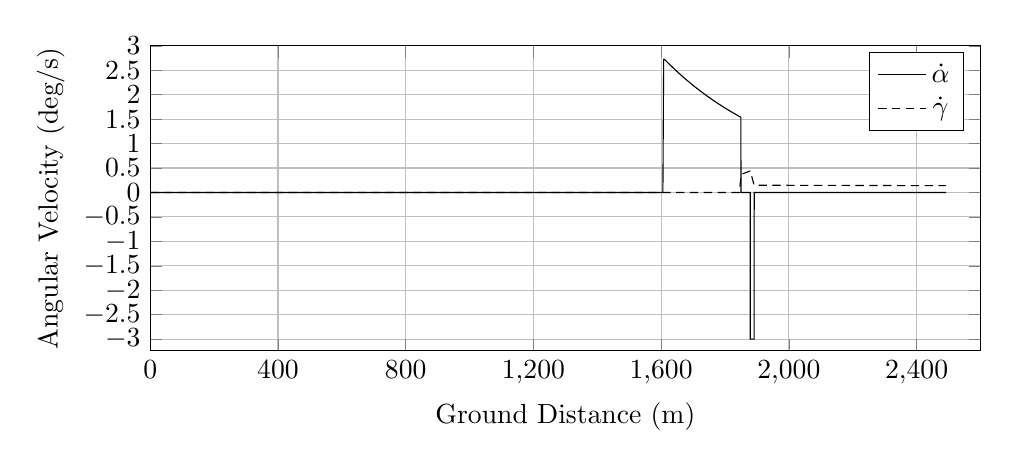
\begin{tikzpicture}

\begin{axis}[
width=\textwidth,
height=0.45\textwidth,
scaled ticks=false, tick label style={/pgf/number format/fixed},
xmin=0.0,
xmax=2600,
xtick={0,400,800,1200,1600,2000,2400,2800,3200},
xlabel={Ground Distance (m)},
xmajorgrids,
ymin=-3.24,
ymax=3,
ylabel={Angular Velocity (deg/s)},
ytick={-3,-2.5,-2,-1.5,-1,-0.5,0.0,0.5,1,1.5,2,2.5,3},
ymajorgrids,
legend entries = {$\dot\alpha$\\$\dot\gamma$\\}
]

\addplot [
color=black,
solid
]
table[row sep=crcr]{
1.3729668748938318E-8	0.0\\
1.7493248493808052E-7	0.0\\
1.4411937280317895E-6	0.0\\
6.602995160656227E-5	0.0\\
2.2740573828771224E-4	0.0\\
4.8751428921765393E-4	0.0\\
8.441986619835749E-4	0.0\\
0.0012981647037285577	0.0\\
0.0018484379050661159	0.0\\
0.0024893731755424335	0.0\\
0.0032286585096692284	0.0\\
0.0040442418752796045	0.0\\
0.004972762654474916	0.0\\
0.005990910102221513	0.0\\
0.007111389191545643	0.0\\
0.008336865178450469	0.0\\
0.009664633507451486	0.0\\
0.011093815858158905	0.0\\
0.01262066151120312	0.0\\
0.01419454386807839	0.0\\
0.015910782250193378	0.0\\
0.017721549103721458	0.0\\
0.019620507964630857	0.0\\
0.02164969955342029	0.0\\
0.023766550611781796	0.0\\
0.025957065600157342	0.0\\
0.028260861173784894	0.0\\
0.030668466949245715	0.0\\
0.0331489614440674	0.0\\
0.03573888453685943	0.0\\
0.038418765463712895	0.0\\
0.04116679597872082	0.0\\
0.044022059812866554	0.0\\
0.04700053365173311	0.0\\
0.050116649382181494	0.0\\
0.0533021652593606	0.0\\
0.056630220296749106	0.0\\
0.05998688030085898	0.0\\
0.06348077825220624	0.0\\
0.06710848437295475	0.0\\
0.07082346760424127	0.0\\
0.07462944469130567	0.0\\
0.07855413323217031	0.0\\
0.08251243142992878	0.0\\
0.08659905947434482	0.0\\
0.09083545394947079	0.0\\
0.09518096637774642	0.0\\
0.099604438418047	0.0\\
0.1041130762071252	0.0\\
0.10871457033213175	0.0\\
0.11350280915994052	0.0\\
0.11836943512882261	0.0\\
0.12328542045494376	0.0\\
0.12830372217771202	0.0\\
0.1334037067999082	0.0\\
0.1386015897371753	0.0\\
0.14405085578552257	0.0\\
0.1495239325759128	0.0\\
0.1550507392415454	0.0\\
0.16073360491635535	0.0\\
0.16659871679960742	0.0\\
0.17244819595229793	0.0\\
0.17848031195343078	0.0\\
0.18466822548212042	0.0\\
0.1909009608611748	0.0\\
0.19716089737688902	0.0\\
0.2035279375926986	0.0\\
0.21017879584430066	0.0\\
0.21687473998771628	0.0\\
0.22354650324940833	0.0\\
0.23036941414946865	0.0\\
0.23737731412185503	0.0\\
0.24449289925428264	0.0\\
0.2517184892023243	0.0\\
0.25908208279438383	0.0\\
0.2664863589195283	0.0\\
0.27399321582905467	0.0\\
0.2816108016888421	0.0\\
0.2893844725195981	0.0\\
0.29747621078120867	0.0\\
0.30547198304033185	0.0\\
0.31373479402345694	0.0\\
0.3220909744202328	0.0\\
0.3305540912568814	0.0\\
0.33895489345894936	0.0\\
0.34753073012810576	0.0\\
0.3563589175375672	0.0\\
0.3652744752958731	0.0\\
0.3742693918027593	0.0\\
0.38350989122680823	0.0\\
0.3927029292363896	0.0\\
0.4020876366599533	0.0\\
0.4115568217121528	0.0\\
0.4212787852930122	0.0\\
0.43089755178065414	0.0\\
0.4408379299669313	0.0\\
0.4510502611115679	0.0\\
0.4612670224725215	0.0\\
0.4715818614584312	0.0\\
0.4818438670126082	0.0\\
0.4922128554044626	0.0\\
0.50273876067117	0.0\\
0.5136516607865718	0.0\\
0.5244310074213006	0.0\\
0.5355751508210329	0.0\\
0.5467126997993474	0.0\\
0.5580479056656631	0.0\\
0.5692960823995112	0.0\\
0.5809945926573021	0.0\\
0.5923626544035139	0.0\\
0.6041922852715	0.0\\
0.6160912669048675	0.0\\
0.6280605196746807	0.0\\
0.6403946506485891	0.0\\
0.6525721787971039	0.0\\
0.66504690021022	0.0\\
0.6773535438897555	0.0\\
0.6901462526606317	0.0\\
0.703249873273524	0.0\\
0.7159721017112175	0.0\\
0.729053467210389	0.0\\
0.7422988791228431	0.0\\
0.756304272979474	0.0\\
0.7696432036294076	0.0\\
0.7832290250230658	0.0\\
0.7969128825551131	0.0\\
0.8108444209446342	0.0\\
0.825043936786227	0.0\\
0.8390802275180445	0.0\\
0.8532340040587583	0.0\\
0.8678101043696134	0.0\\
0.8824320602344964	0.0\\
0.8978006605470081	0.0\\
0.9134572487531922	0.0\\
0.9287391767029982	0.0\\
0.9440564687433697	0.0\\
0.9598871644713316	0.0\\
0.9757786228365237	0.0\\
0.9918217338879218	0.0\\
1.0080608846667363	0.0\\
1.0245900975307913	0.0\\
1.040622085070809	0.0\\
1.0571005809273983	0.0\\
1.0736578999152901	0.0\\
1.0902401336450098	0.0\\
1.1073201062866707	0.0\\
1.1241926772552646	0.0\\
1.1416781667104252	0.0\\
1.1588269484070954	0.0\\
1.176440946845327	0.0\\
1.1944819542445066	0.0\\
1.2120125629913447	0.0\\
1.2299306574276825	0.0\\
1.2481120482032448	0.0\\
1.2663536608165091	0.0\\
1.2851425782117465	0.0\\
1.3041313368869671	0.0\\
1.3228236880779458	0.0\\
1.3414329672940513	0.0\\
1.3605066144349074	0.0\\
1.3802534409605212	0.0\\
1.3994872719307283	0.0\\
1.4192016277101378	0.0\\
1.439023460648384	0.0\\
1.459347998039509	0.0\\
1.4793256644936217	0.0\\
1.4991489338326072	0.0\\
1.5195196572175793	0.0\\
1.5402684478761244	0.0\\
1.5604570108688036	0.0\\
1.5810331069622228	0.0\\
1.6022712329181132	0.0\\
1.623752316257296	0.0\\
1.6452514305955401	0.0\\
1.6664829631402025	0.0\\
1.6886446033619715	0.0\\
1.710607384244656	0.0\\
1.7329417009553727	0.0\\
1.7551421266962821	0.0\\
1.7779085356585536	0.0\\
1.800478286927734	0.0\\
1.8236018329231238	0.0\\
1.8462320784511883	0.0\\
1.869621217116264	0.0\\
1.8933146512119747	0.0\\
1.9176856041472643	0.0\\
1.9417713639512164	0.0\\
1.9657098573982132	0.0\\
1.9902165007163162	0.0\\
2.014554050520948	0.0\\
2.039479559407779	0.0\\
2.0645497069116256	0.0\\
2.090368502766882	0.0\\
2.115564185269416	0.0\\
2.140750230554602	0.0\\
2.1667677015838267	0.0\\
2.1927560352542175	0.0\\
2.218891869133375	0.0\\
2.245288939563828	0.0\\
2.2712530964452817	0.0\\
2.297933078351498	0.0\\
2.324564104516777	0.0\\
2.351466051806102	0.0\\
2.378869922986878	0.0\\
2.4061764715670764	0.0\\
2.4343811693482102	0.0\\
2.4622108821536663	0.0\\
2.4906408044048067	0.0\\
2.518892760285042	0.0\\
2.5472153538550346	0.0\\
2.5762492306032216	0.0\\
2.605385308804288	0.0\\
2.634725531238531	0.0\\
2.6633424112287507	0.0\\
2.6927188130915374	0.0\\
2.7226962917814213	0.0\\
2.7531675915664673	0.0\\
2.7831412651501983	0.0\\
2.8139174932165103	0.0\\
2.8440331768075415	0.0\\
2.874693215323904	0.0\\
2.9059978681586376	0.0\\
2.9372617813709034	0.0\\
2.9684444504378202	0.0\\
3.000072782687808	0.0\\
3.031082587373527	0.0\\
3.063213028467148	0.0\\
3.0965739711585014	0.0\\
3.1291175748240176	0.0\\
3.161651640649506	0.0\\
3.194791488147139	0.0\\
3.2273698640351327	0.0\\
3.261394174200582	0.0\\
3.2942820372415875	0.0\\
3.3276455142443044	0.0\\
3.3625338428565543	0.0\\
3.396526624461681	0.0\\
3.4305511850311694	0.0\\
3.4642094416894933	0.0\\
3.498963551783903	0.0\\
3.5341885134496573	0.0\\
3.569804025802995	0.0\\
3.605116576002147	0.0\\
3.641338581546833	0.0\\
3.677593698357855	0.0\\
3.7132425573336665	0.0\\
3.74957219375957	0.0\\
3.7872650227149185	0.0\\
3.825403000593508	0.0\\
3.861987998097706	0.0\\
3.899535703755137	0.0\\
3.9366960368382165	0.0\\
3.9756271117991435	0.0\\
4.014715979923002	0.0\\
4.053268843133694	0.0\\
4.093111596873367	0.0\\
4.132540645872048	0.0\\
4.171686416589186	0.0\\
4.211258480423352	0.0\\
4.252585425594734	0.0\\
4.29253892845542	0.0\\
4.332839968385603	0.0\\
4.372708537789018	0.0\\
4.414379330316386	0.0\\
4.455607216042212	0.0\\
4.497336690654009	0.0\\
4.53836773335787	0.0\\
4.579767142935065	0.0\\
4.621942908118227	0.0\\
4.663798268780793	0.0\\
4.705838036060712	0.0\\
4.748491012675066	0.0\\
4.791393968819099	0.0\\
4.835700194867293	0.0\\
4.879973298406089	0.0\\
4.923250156511948	0.0\\
4.967673596314626	0.0\\
5.012954369117542	0.0\\
5.057574526249477	0.0\\
5.103280208347517	0.0\\
5.148856018935929	0.0\\
5.194350575362858	0.0\\
5.240584094986199	0.0\\
5.2871741484687504	0.0\\
5.333122064003502	0.0\\
5.3803318800233235	0.0\\
5.4262712259485255	0.0\\
5.473378197958581	0.0\\
5.521938593493333	0.0\\
5.570027890245774	0.0\\
5.617746353771608	0.0\\
5.665750363096816	0.0\\
5.714883880069209	0.0\\
5.763390205677501	0.0\\
5.812817811268989	0.0\\
5.861909274803731	0.0\\
5.912134919389196	0.0\\
5.962317560553064	0.0\\
6.012727788730279	0.0\\
6.0628236035803145	0.0\\
6.113711068416594	0.0\\
6.16497292765713	0.0\\
6.216284706244114	0.0\\
6.26834407822653	0.0\\
6.320257064476769	0.0\\
6.37351660191279	0.0\\
6.426150862197664	0.0\\
6.479030963436509	0.0\\
6.532319340056288	0.0\\
6.5857233987986845	0.0\\
6.640834734692348	0.0\\
6.695022999498724	0.0\\
6.749720237657193	0.0\\
6.804235758325081	0.0\\
6.859728469301633	0.0\\
6.916686079588434	0.0\\
6.9732530286722305	0.0\\
7.029531186664631	0.0\\
7.086633318514238	0.0\\
7.144155485034537	0.0\\
7.202053129566568	0.0\\
7.260126434764185	0.0\\
7.317913145042743	0.0\\
7.376682960996439	0.0\\
7.435393721764624	0.0\\
7.493838107271518	0.0\\
7.552684475254578	0.0\\
7.613252707151423	0.0\\
7.672782806866918	0.0\\
7.733397683408512	0.0\\
7.795525081709004	0.0\\
7.856013653786727	0.0\\
7.91792172269443	0.0\\
7.980110745884113	0.0\\
8.041720670752433	0.0\\
8.105229267009985	0.0\\
8.167457523036095	0.0\\
8.230908874360502	0.0\\
8.293738919282273	0.0\\
8.356235402336917	0.0\\
8.42092378244627	0.0\\
8.485671322837007	0.0\\
8.549180898871484	0.0\\
8.614596634551038	0.0\\
8.680166762249144	0.0\\
8.744770128469462	0.0\\
8.812993689385827	0.0\\
8.88005807777586	0.0\\
8.94709863067661	0.0\\
9.013172088448385	0.0\\
9.079266506338545	0.0\\
9.14748814890141	0.0\\
9.215411293660388	0.0\\
9.284579146198691	0.0\\
9.353168277381275	0.0\\
9.423753765537143	0.0\\
9.492960052876374	0.0\\
9.564123004975215	0.0\\
9.634097601479446	0.0\\
9.705672410878787	0.0\\
9.776260200085993	0.0\\
9.846607984572056	0.0\\
9.918231435410593	0.0\\
9.988851555070422	0.0\\
10.060390022634245	0.0\\
10.133279281833644	0.0\\
10.205241085147751	0.0\\
10.277820389603	0.0\\
10.352558894167803	0.0\\
10.42733258664746	0.0\\
10.501815126481194	0.0\\
10.576858173457808	0.0\\
10.65303812840548	0.0\\
10.729080272001735	0.0\\
10.804841544893105	0.0\\
10.881905013502095	0.0\\
10.958396790746043	0.0\\
11.035905069829102	0.0\\
11.113160538490881	0.0\\
11.192172636140572	0.0\\
11.270076562295213	0.0\\
11.350065490058778	0.0\\
11.429008826667825	0.0\\
11.50754237847364	0.0\\
11.587076645554472	0.0\\
11.668897725768986	0.0\\
11.749734371708193	0.0\\
11.830312384681939	0.0\\
11.909862670519033	0.0\\
11.990515423105418	0.0\\
12.072973931530203	0.0\\
12.155304175892073	0.0\\
12.237018674011615	0.0\\
12.320146069843414	0.0\\
12.406770618003886	0.0\\
12.489918686423398	0.0\\
12.574493004618496	0.0\\
12.660666896522624	0.0\\
12.746500366216402	0.0\\
12.832006837122272	0.0\\
12.919285437479463	0.0\\
13.00517529032821	0.0\\
13.092301899261269	0.0\\
13.179760097773386	0.0\\
13.268594687119744	0.0\\
13.357699529172354	0.0\\
13.44829753340392	0.0\\
13.537570218252604	0.0\\
13.627322718831184	0.0\\
13.718307212496544	0.0\\
13.808540263830096	0.0\\
13.899143852161355	0.0\\
13.991564069206362	0.0\\
14.085798171937814	0.0\\
14.179213507883688	0.0\\
14.271883316076963	0.0\\
14.367546274622434	0.0\\
14.459430863676705	0.0\\
14.555010173556813	0.0\\
14.648669731311681	0.0\\
14.743773575674254	0.0\\
14.839769774519894	0.0\\
14.932807148196385	0.0\\
15.026921440816679	0.0\\
15.12275113649265	0.0\\
15.222025232743288	0.0\\
15.321078842653048	0.0\\
15.417564225728565	0.0\\
15.515758841369038	0.0\\
15.613440509090129	0.0\\
15.7107260301154	0.0\\
15.81102223487273	0.0\\
15.913565872734136	0.0\\
16.012918321571746	0.0\\
16.11222833737955	0.0\\
16.216250800242257	0.0\\
16.319159023020546	0.0\\
16.421418004006803	0.0\\
16.521675247646563	0.0\\
16.62557290942481	0.0\\
16.72731964230514	0.0\\
16.830283223934416	0.0\\
16.93464251494634	0.0\\
17.038481620468637	0.0\\
17.146497421123335	0.0\\
17.252282308638982	0.0\\
17.35724772858778	0.0\\
17.464053904588297	0.0\\
17.572390862630144	0.0\\
17.680417629270814	0.0\\
17.789707298693855	0.0\\
17.899612520762552	0.0\\
18.01027367065641	0.0\\
18.121415095654797	0.0\\
18.232428503320143	0.0\\
18.34337337506409	0.0\\
18.454877340220463	0.0\\
18.56636189702322	0.0\\
18.678405595805643	0.0\\
18.7903363416971	0.0\\
18.902391384512768	0.0\\
19.01754810908954	0.0\\
19.131359562866663	0.0\\
19.247747682986713	0.0\\
19.361628242251975	0.0\\
19.477963464454028	0.0\\
19.595742742603164	0.0\\
19.71107288142779	0.0\\
19.82767543183723	0.0\\
19.944540068808188	0.0\\
20.06171535440768	0.0\\
20.179291418887807	0.0\\
20.29729887224694	0.0\\
20.417200571824914	0.0\\
20.53676390826074	0.0\\
20.65523768803314	0.0\\
20.777063017363922	0.0\\
20.896922101876633	0.0\\
21.016777952410983	0.0\\
21.13892104879462	0.0\\
21.260534693274344	0.0\\
21.382619708556632	0.0\\
21.506306369043365	0.0\\
21.631260758247265	0.0\\
21.75556249187227	0.0\\
21.87985606458615	0.0\\
22.005925835680863	0.0\\
22.130365724585275	0.0\\
22.257477980325966	0.0\\
22.38418119026224	0.0\\
22.50885833858638	0.0\\
22.636026948728087	0.0\\
22.76367325110224	0.0\\
22.89115382514759	0.0\\
23.022452271734288	0.0\\
23.149877274293033	0.0\\
23.27873580881144	0.0\\
23.408563766880334	0.0\\
23.538692653979794	0.0\\
23.671258756997098	0.0\\
23.803210122669313	0.0\\
23.93544283576786	0.0\\
24.067241518013077	0.0\\
24.19863541429976	0.0\\
24.329449967727697	0.0\\
24.46175612159181	0.0\\
24.594763714591892	0.0\\
24.72754053098891	0.0\\
24.86208223890334	0.0\\
24.99503410474967	0.0\\
25.12831230627787	0.0\\
25.265273024090206	0.0\\
25.400650037308893	0.0\\
25.536304655026747	0.0\\
25.673594178904246	0.0\\
25.80797730935859	0.0\\
25.835159569235522	0.0\\
25.83771752397454	0.0\\
25.84157983658004	0.0\\
25.854829339215996	0.0\\
25.893215796826965	0.0\\
25.973046119315796	0.0\\
26.096262980671412	0.0\\
26.224212718725603	0.0\\
26.35313595194755	0.0\\
26.481727686355264	0.0\\
26.611118169629577	0.0\\
26.74049186039369	0.0\\
26.87228140714948	0.0\\
27.003385008924262	0.0\\
27.1358830905183	0.0\\
27.265951877034226	0.0\\
27.399105426781233	0.0\\
27.53075869079712	0.0\\
27.66387879779476	0.0\\
27.79855889054391	0.0\\
27.932132547760695	0.0\\
28.06791767232785	0.0\\
28.202763022922632	0.0\\
28.339788243013793	0.0\\
28.476803106655623	0.0\\
28.61761981788422	0.0\\
28.753907949775353	0.0\\
28.89297195746854	0.0\\
29.03211749902605	0.0\\
29.17123509789927	0.0\\
29.312253051611236	0.0\\
29.454422317169097	0.0\\
29.59523538430127	0.0\\
29.737672170826222	0.0\\
29.879173197948965	0.0\\
30.02075470454991	0.0\\
30.166674235301365	0.0\\
30.308336095430334	0.0\\
30.452640844036836	0.0\\
30.597553881025625	0.0\\
30.742967061600154	0.0\\
30.888975484926362	0.0\\
31.034653067922946	0.0\\
31.180984070508003	0.0\\
31.328351020411645	0.0\\
31.476753455192622	0.0\\
31.62661541983664	0.0\\
31.774495604492607	0.0\\
31.924944104961916	0.0\\
32.07610067279926	0.0\\
32.22631826848556	0.0\\
32.37899942625752	0.0\\
32.528514827654206	0.0\\
32.68189139400266	0.0\\
32.836069829938495	0.0\\
32.99025509482905	0.0\\
33.14574197930297	0.0\\
33.30072558931056	0.0\\
33.455047097713944	0.0\\
33.610874563168906	0.0\\
33.76926068144728	0.0\\
33.92617323250643	0.0\\
34.08448787244542	0.0\\
34.24243160505006	0.0\\
34.40316487172558	0.0\\
34.56154208099588	0.0\\
34.721775177117024	0.0\\
34.88076970836556	0.0\\
35.041349106451236	0.0\\
35.20329621413198	0.0\\
35.364886328651124	0.0\\
35.529241615711214	0.0\\
35.69117991651797	0.0\\
35.85317319416103	0.0\\
36.014854298354294	0.0\\
36.18095311277159	0.0\\
36.34443322746766	0.0\\
36.51065106768533	0.0\\
36.67635767082788	0.0\\
36.842033683894186	0.0\\
37.00823867836148	0.0\\
37.17279029188734	0.0\\
37.33951104811075	0.0\\
37.50923941781488	0.0\\
37.679358776579846	0.0\\
37.845326083883435	0.0\\
38.017144746304325	0.0\\
38.1852030886141	0.0\\
38.35804431104914	0.0\\
38.52812920813831	0.0\\
38.69960796987526	0.0\\
38.87165793928378	0.0\\
39.0423941506003	0.0\\
39.21436971822614	0.0\\
39.38727999643966	0.0\\
39.558989012313546	0.0\\
39.734752343022535	0.0\\
39.908836167348156	0.0\\
40.084555009291705	0.0\\
40.259186798753746	0.0\\
40.43324437115375	0.0\\
40.61041052363379	0.0\\
40.787318094191775	0.0\\
40.96620398302343	0.0\\
41.14141336180775	0.0\\
41.31941103282654	0.0\\
41.49571226203258	0.0\\
41.67366972437729	0.0\\
41.85219319429197	0.0\\
42.03136872634711	0.0\\
42.21293422072888	0.0\\
42.39366932880948	0.0\\
42.57479521797359	0.0\\
42.75522531040919	0.0\\
42.93775785970641	0.0\\
43.11993568316029	0.0\\
43.30336620712447	0.0\\
43.48720879745599	0.0\\
43.672226884455625	0.0\\
43.85684130549208	0.0\\
44.039851952877484	0.0\\
44.22449378650157	0.0\\
44.412385508552646	0.0\\
44.59783063297877	0.0\\
44.78525507043919	0.0\\
44.973130075825196	0.0\\
45.16145211071871	0.0\\
45.34881478087516	0.0\\
45.536017136752506	0.0\\
45.724971990057284	0.0\\
45.91416212467789	0.0\\
46.10175434018815	0.0\\
46.29356928918713	0.0\\
46.48490977712943	0.0\\
46.67744207882204	0.0\\
46.869905949194575	0.0\\
47.062749521718516	0.0\\
47.25341437235973	0.0\\
47.44508461154423	0.0\\
47.63880095964302	0.0\\
47.83356160493736	0.0\\
48.025334057720784	0.0\\
48.218846636819876	0.0\\
48.41468711090302	0.0\\
48.610449575687724	0.0\\
48.80723286029129	0.0\\
49.00124137999302	0.0\\
49.20045899041696	0.0\\
49.394243884198005	0.0\\
49.59161211700324	0.0\\
49.79144608231523	0.0\\
49.99107345578199	0.0\\
50.18996871950735	0.0\\
50.388458331230495	0.0\\
50.59191110395449	0.0\\
50.79453916783869	0.0\\
50.99530158869649	0.0\\
51.19776583381373	0.0\\
51.3996255264899	0.0\\
51.599450409211	0.0\\
51.80158475775707	0.0\\
52.002311498730975	0.0\\
52.2060805474067	0.0\\
52.40811442127868	0.0\\
52.61423073460446	0.0\\
52.821749674584495	0.0\\
53.03053110951893	0.0\\
53.23753590773735	0.0\\
53.44487707917263	0.0\\
53.652063533093525	0.0\\
53.85975522429668	0.0\\
54.06844148636836	0.0\\
54.278580968983874	0.0\\
54.48685885904548	0.0\\
54.69884126905886	0.0\\
54.90975544393264	0.0\\
55.12216013841277	0.0\\
55.333080623240974	0.0\\
55.5448885814986	0.0\\
55.75594910746132	0.0\\
55.968144975063936	0.0\\
56.18150915317635	0.0\\
56.394069348356695	0.0\\
56.60950747146016	0.0\\
56.82641599949238	0.0\\
57.03980213394583	0.0\\
57.25698083573829	0.0\\
57.47353804711997	0.0\\
57.6941706582635	0.0\\
57.91229938529948	0.0\\
58.12998527173144	0.0\\
58.34905943653719	0.0\\
58.56781345824973	0.0\\
58.787998582886644	0.0\\
59.011266007804366	0.0\\
59.23368761368569	0.0\\
59.456031473365414	0.0\\
59.67976581221534	0.0\\
59.90315377467765	0.0\\
60.125192111546724	0.0\\
60.349269227196444	0.0\\
60.57220932044149	0.0\\
60.79606803632835	0.0\\
61.021718319759984	0.0\\
61.25073295331903	0.0\\
61.47770893732542	0.0\\
61.70784367826464	0.0\\
61.93740803875056	0.0\\
62.1673491775543	0.0\\
62.39648011888062	0.0\\
62.62822464633953	0.0\\
62.86094183422966	0.0\\
63.090532789209604	0.0\\
63.321616049163225	0.0\\
63.554808975015874	0.0\\
63.78685818650332	0.0\\
64.0234762327251	0.0\\
64.25652029988498	0.0\\
64.49146565301734	0.0\\
64.72768747885678	0.0\\
64.96568125142531	0.0\\
65.20057601391298	0.0\\
65.43975061379945	0.0\\
65.67719429610031	0.0\\
65.91652243006087	0.0\\
66.1565253585166	0.0\\
66.39740384038885	0.0\\
66.63777997854328	0.0\\
66.87849958303539	0.0\\
67.12349409848125	0.0\\
67.36843544137562	0.0\\
67.61129947098183	0.0\\
67.85808619273692	0.0\\
68.10323725880951	0.0\\
68.3520146383799	0.0\\
68.60099753692072	0.0\\
68.84943315800746	0.0\\
69.09793111574629	0.0\\
69.34894754058863	0.0\\
69.59791912239118	0.0\\
69.84867626946473	0.0\\
70.10496107302816	0.0\\
70.35594730130109	0.0\\
70.60854748652795	0.0\\
70.8625286964371	0.0\\
71.1182576034713	0.0\\
71.37278964945165	0.0\\
71.62944082734805	0.0\\
71.88536754710964	0.0\\
72.14250945057543	0.0\\
72.40306402213687	0.0\\
72.66241221953337	0.0\\
72.92327110344874	0.0\\
73.18657203154456	0.0\\
73.45150557123125	0.0\\
73.71756195569753	0.0\\
73.97940051906463	0.0\\
74.24514793127645	0.0\\
74.51022759525631	0.0\\
74.77823256031297	0.0\\
75.04767613410795	0.0\\
75.31682895458664	0.0\\
75.58729746777243	0.0\\
75.85729327570917	0.0\\
76.13042767774209	0.0\\
76.40299665611133	0.0\\
76.67973301409052	0.0\\
76.95360383527739	0.0\\
77.22854206589327	0.0\\
77.50692063517303	0.0\\
77.78349662592461	0.0\\
78.0616064362213	0.0\\
78.33869545141144	0.0\\
78.62238552181594	0.0\\
78.90481169871467	0.0\\
79.18659077494928	0.0\\
79.4700201012688	0.0\\
79.75774957869095	0.0\\
80.04430580185078	0.0\\
80.33432201731404	0.0\\
80.62298533865851	0.0\\
80.9130804606989	0.0\\
81.20459144967842	0.0\\
81.49650140842283	0.0\\
81.79224544448738	0.0\\
82.08455487090956	0.0\\
82.37934996819865	0.0\\
82.67580145620735	0.0\\
82.97475550983006	0.0\\
83.2734238134004	0.0\\
83.57209772503273	0.0\\
83.87419166445906	0.0\\
84.17487194816226	0.0\\
84.47686996876752	0.0\\
84.78124993153034	0.0\\
85.08776945017104	0.0\\
85.39395758722245	0.0\\
85.69833162305892	0.0\\
86.01027818388755	0.0\\
86.31658691867341	0.0\\
86.62866814828641	0.0\\
86.94043673469176	0.0\\
87.2565990672368	0.0\\
87.56980823017452	0.0\\
87.88101387141376	0.0\\
88.20007062892054	0.0\\
88.51883409355145	0.0\\
88.83509784148416	0.0\\
89.15857089898353	0.0\\
89.47772213402055	0.0\\
89.80217214804901	0.0\\
90.1263587278685	0.0\\
90.44950966725051	0.0\\
90.77764749859728	0.0\\
91.10470504824352	0.0\\
91.43769785174896	0.0\\
91.76691749028419	0.0\\
92.09386993524024	0.0\\
92.42498248438446	0.0\\
92.7581696617394	0.0\\
93.09729153734631	0.0\\
93.4312406900703	0.0\\
93.76780571708736	0.0\\
94.10390054156983	0.0\\
94.43564317419558	0.0\\
94.77291201930262	0.0\\
95.10796951504997	0.0\\
95.44708659079325	0.0\\
95.78515592548297	0.0\\
96.12311752311894	0.0\\
96.46351490415591	0.0\\
96.80669869710772	0.0\\
97.14657639264556	0.0\\
97.48763116340677	0.0\\
97.8305814261901	0.0\\
98.17013304046878	0.0\\
98.51054009051404	0.0\\
98.854181194619	0.0\\
99.19205317796005	0.0\\
99.53355440060989	0.0\\
99.87198375587872	0.0\\
100.2129389915628	0.0\\
100.55335806642802	0.0\\
100.89503335592528	0.0\\
101.23693480167049	0.0\\
101.57977298927813	0.0\\
101.91842351185082	0.0\\
102.26214655705948	0.0\\
102.60487134933112	0.0\\
102.94238410388857	0.0\\
103.28139950825951	0.0\\
103.61984226602698	0.0\\
103.95406402656286	0.0\\
104.29248504574807	0.0\\
104.63112914593611	0.0\\
104.96686613984221	0.0\\
105.30464484937244	0.0\\
105.64180205248229	0.0\\
105.97704387437452	0.0\\
106.31384964552919	0.0\\
106.6489228444834	0.0\\
106.98000007373659	0.0\\
107.31456925364313	0.0\\
107.38092108752608	0.0\\
107.387754025128	0.0\\
107.3946577511588	0.0\\
107.39916951903444	0.0\\
107.40247473215817	0.0\\
107.40548301099807	0.0\\
107.41901751964124	0.0\\
107.47756267729525	0.0\\
107.63696404402117	0.0\\
107.95668166923352	0.0\\
108.2571634635643	0.0\\
108.55996775705782	0.0\\
108.8616926844802	0.0\\
109.16669292910967	0.0\\
109.47218465327785	0.0\\
109.78023369107405	0.0\\
110.09061921742381	0.0\\
110.4007971847821	0.0\\
110.7125096545017	0.0\\
111.02874540594937	0.0\\
111.34670354521654	0.0\\
111.664908557295	0.0\\
111.98617551206428	0.0\\
112.3078797039536	0.0\\
112.63537393275391	0.0\\
112.96267359383529	0.0\\
113.28778388635178	0.0\\
113.61823593045688	0.0\\
113.94632344632586	0.0\\
114.27926944824554	0.0\\
114.61324422041562	0.0\\
114.94750338770686	0.0\\
115.28618013885716	0.0\\
115.62544260296943	0.0\\
115.9647508443766	0.0\\
116.30617149460878	0.0\\
116.65060078043697	0.0\\
116.99863777637248	0.0\\
117.34270613829636	0.0\\
117.68983788345284	0.0\\
118.04137408578512	0.0\\
118.39343387684602	0.0\\
118.74804854616337	0.0\\
119.10520175440718	0.0\\
119.46686684850098	0.0\\
119.82660492256403	0.0\\
120.19012449272657	0.0\\
120.55217592908159	0.0\\
120.91763124996498	0.0\\
121.28719248968574	0.0\\
121.65493622417088	0.0\\
122.02513489718217	0.0\\
122.39308995700384	0.0\\
122.76618799735454	0.0\\
123.1388017253943	0.0\\
123.51256311114031	0.0\\
123.88633794770595	0.0\\
124.25665874611622	0.0\\
124.63165231885978	0.0\\
125.00664173256905	0.0\\
125.38021625899401	0.0\\
125.75512563345742	0.0\\
126.13473977091255	0.0\\
126.51299085225449	0.0\\
126.8948287761801	0.0\\
127.27325883095315	0.0\\
127.64986999110431	0.0\\
128.03053456382577	0.0\\
128.40840086210045	0.0\\
128.78830732782995	0.0\\
129.16816802858597	0.0\\
129.55114692916032	0.0\\
129.92795862154003	0.0\\
130.30814318938542	0.0\\
130.68801179162523	0.0\\
131.0673626953399	0.0\\
131.44707508552267	0.0\\
131.82575792285303	0.0\\
132.20466209461676	0.0\\
132.58549544797154	0.0\\
132.96520261413826	0.0\\
133.34413894748724	0.0\\
133.72638850756363	0.0\\
134.1049920954593	0.0\\
134.48538249769342	0.0\\
134.86277461399203	0.0\\
135.2402386369938	0.0\\
135.62109197355238	0.0\\
135.9996509441208	0.0\\
136.37968191797512	0.0\\
136.76120583273502	0.0\\
137.13951930881296	0.0\\
137.51840340013064	0.0\\
137.89819615735314	0.0\\
138.27485697152616	0.0\\
138.65420581933705	0.0\\
139.03531375767642	0.0\\
139.41296882619503	0.0\\
139.79422155259	0.0\\
140.17408835952057	0.0\\
140.5488076998477	0.0\\
140.92844631991198	0.0\\
141.30483696429354	0.0\\
141.68269541512387	0.0\\
142.06058279783264	0.0\\
142.43991695918288	0.0\\
142.81695502902187	0.0\\
143.19247254825046	0.0\\
143.5733885276352	0.0\\
143.94921103219775	0.0\\
144.32621366107247	0.0\\
144.70408630975157	0.0\\
145.08263595865492	0.0\\
145.46162624555404	0.0\\
145.83827879615103	0.0\\
146.21524500988596	0.0\\
146.5934755401724	0.0\\
146.9730259257883	0.0\\
147.3547239944582	0.0\\
147.73366854735332	0.0\\
148.1136534850276	0.0\\
148.49311509785633	0.0\\
148.87144514206074	0.0\\
149.25360190977045	0.0\\
149.6334430260095	0.0\\
150.01465687879528	0.0\\
150.3940924716125	0.0\\
150.77688175221402	0.0\\
151.1561678741857	0.0\\
151.5352572324847	0.0\\
151.91884603110896	0.0\\
152.3000376871389	0.0\\
152.6837211891089	0.0\\
153.06727641570347	0.0\\
153.4514076737559	0.0\\
153.83522357687116	0.0\\
154.21637826964854	0.0\\
154.6009164651564	0.0\\
154.98403470202834	0.0\\
155.36838747168406	0.0\\
155.75158064164503	0.0\\
156.13576662495046	0.0\\
156.5218436740983	0.0\\
156.90521285441474	0.0\\
157.2916244593892	0.0\\
157.6780020855428	0.0\\
158.06299451159185	0.0\\
158.4509000667514	0.0\\
158.83830611621056	0.0\\
159.22672413827297	0.0\\
159.61474494524106	0.0\\
160.0042372884319	0.0\\
160.39552304382113	0.0\\
160.78478895267375	0.0\\
161.17517847278327	0.0\\
161.56748129737286	0.0\\
161.9609400214345	0.0\\
162.35005274814932	0.0\\
162.7425950916558	0.0\\
163.13607830878885	0.0\\
163.53170884953005	0.0\\
163.92462594167722	0.0\\
164.3198767210975	0.0\\
164.7157696028566	0.0\\
165.1115317336501	0.0\\
165.50739628911128	0.0\\
165.90698313288817	0.0\\
166.30582458333038	0.0\\
166.70591293613995	0.0\\
167.1044701422045	0.0\\
167.50226971352845	0.0\\
167.9010833894181	0.0\\
168.3004552315794	0.0\\
168.70189335181743	0.0\\
169.10576843973695	0.0\\
169.50785881751284	0.0\\
169.91045494783964	0.0\\
170.31331810721775	0.0\\
170.71648797717722	0.0\\
171.11993291578136	0.0\\
171.5247281229082	0.0\\
171.92976094083576	0.0\\
172.33690302624336	0.0\\
172.74259563259648	0.0\\
173.1509823323036	0.0\\
173.55913088366435	0.0\\
173.96636547491187	0.0\\
174.37754484483776	0.0\\
174.7874876782942	0.0\\
175.2012500141185	0.0\\
175.6112323385957	0.0\\
176.02092514523684	0.0\\
176.43326782420013	0.0\\
176.8477920653399	0.0\\
177.2627043459005	0.0\\
177.67839640445425	0.0\\
178.09047986160414	0.0\\
178.50771992227516	0.0\\
178.92514786216543	0.0\\
179.34349041668827	0.0\\
179.7634585539525	0.0\\
180.0836350053749	0.0\\
180.18446825846002	0.0\\
180.6041229201494	0.0\\
181.5278851973348	0.0\\
182.40940876889346	0.0\\
183.29020149056134	0.0\\
184.17127536929127	0.0\\
185.05444413874795	0.0\\
185.94463812048832	0.0\\
186.83342305465118	0.0\\
187.72320740690213	0.0\\
188.61627250998652	0.0\\
189.51597565669658	0.0\\
190.41002295084513	0.0\\
191.3196934236239	0.0\\
192.21828392903763	0.0\\
193.1226105375991	0.0\\
194.0308739866166	0.0\\
194.94664810390913	0.0\\
195.8495877725365	0.0\\
196.76514896738053	0.0\\
197.67776544775052	0.0\\
198.59781945634353	0.0\\
199.51766543264023	0.0\\
200.44351810370483	0.0\\
201.3718330130543	0.0\\
202.29314309783985	0.0\\
203.21971650332063	0.0\\
204.14462823093066	0.0\\
205.07763860999955	0.0\\
206.00476468733177	0.0\\
206.93855819187849	0.0\\
207.87782366152794	0.0\\
208.81805039558168	0.0\\
209.75927086542703	0.0\\
210.70907141928154	0.0\\
211.6546393296269	0.0\\
212.59816623974814	0.0\\
213.54645843731532	0.0\\
214.4982137391426	0.0\\
215.45734539338423	0.0\\
216.4205873513297	0.0\\
217.38237643693935	0.0\\
218.35297485781302	0.0\\
219.32510845799027	0.0\\
220.29279514401117	0.0\\
221.26927942590856	0.0\\
222.2446078047322	0.0\\
223.21462685547237	0.0\\
224.19074054242492	0.0\\
225.1744490750948	0.0\\
226.14733001520318	0.0\\
227.14148425007068	0.0\\
228.1240128312001	0.0\\
229.11886046703495	0.0\\
230.11739511657566	0.0\\
231.11215533106218	0.0\\
232.12301378994505	0.0\\
233.1275199718878	0.0\\
234.13114028184475	0.0\\
235.14028542531037	0.0\\
236.15081117254897	0.0\\
237.1660420924572	0.0\\
238.1886645294469	0.0\\
239.21465471906964	0.0\\
240.23482884221784	0.0\\
241.26021232675805	0.0\\
242.3021991810905	0.0\\
243.32988353044664	0.0\\
244.36880129710033	0.0\\
245.4061041381612	0.0\\
246.46256617747576	0.0\\
247.50478260671736	0.0\\
248.56376742117214	0.0\\
249.6219134221688	0.0\\
250.66481994405478	0.0\\
251.72705353011372	0.0\\
252.80088254110024	0.0\\
253.86267363775482	0.0\\
254.94374853170973	0.0\\
256.0221053298852	0.0\\
257.1056667215428	0.0\\
258.2028084304169	0.0\\
259.3030712409387	0.0\\
260.39721249167394	0.0\\
261.49829074545437	0.0\\
262.60930370875815	0.0\\
263.7179887580877	0.0\\
264.8352779160481	0.0\\
265.9576164693235	0.0\\
267.09103410107514	0.0\\
268.20818841649384	0.0\\
269.3328220499261	0.0\\
270.4661510695621	0.0\\
271.5992062566115	0.0\\
272.7460111433737	0.0\\
273.90093061584855	0.0\\
275.05359207729066	0.0\\
276.20311568521606	0.0\\
277.35310992264476	0.0\\
278.5188185905665	0.0\\
279.6929356623284	0.0\\
280.86252284262184	0.0\\
282.05142644191835	0.0\\
283.24985431198513	0.0\\
284.4388813912709	0.0\\
285.6397000671543	0.0\\
286.836316139525	0.0\\
288.0392161140162	0.0\\
289.2556790589223	0.0\\
290.48265444814547	0.0\\
291.72130155141053	0.0\\
292.96100893763946	0.0\\
294.1985103575731	0.0\\
295.4456267737909	0.0\\
296.68519223220017	0.0\\
297.9280216368336	0.0\\
299.1850487812583	0.0\\
300.44412429943463	0.0\\
301.7225677950246	0.0\\
303.0017748749233	0.0\\
304.2792219657807	0.0\\
305.56506002795425	0.0\\
306.85051236654385	0.0\\
308.1437929069215	0.0\\
309.44719641798304	0.0\\
310.77840358228957	0.0\\
312.0849502338091	0.0\\
313.4080429046928	0.0\\
314.7190184524427	0.0\\
316.0311580127236	0.0\\
317.3407104164604	0.0\\
318.66998531861896	0.0\\
319.98030216977895	0.0\\
321.3131882515936	0.0\\
322.64658699863	0.0\\
323.97760893915427	0.0\\
325.31447228134823	0.0\\
326.6245528491544	0.0\\
327.9601785097144	0.0\\
329.2784770253418	0.0\\
330.6069033330348	0.0\\
331.9178806716509	0.0\\
333.2333630873429	0.0\\
334.5584389845069	0.0\\
335.850474636536	0.0\\
337.1511723788834	0.0\\
338.4381183837047	0.0\\
339.72984837001286	0.0\\
341.0214788139215	0.0\\
342.3149785174073	0.0\\
343.60619007360367	0.0\\
344.88769479656867	0.0\\
346.16492597045556	0.0\\
347.44208543988907	0.0\\
348.7214970855716	0.0\\
349.9975255146603	0.0\\
351.26866298989455	0.0\\
352.534343347637	0.0\\
353.79318608781	0.0\\
355.04194064781143	0.0\\
356.2900696565431	0.0\\
357.5353145753136	0.0\\
357.7850582428015	0.0\\
358.34364659427206	0.0\\
358.3912146679147	0.0\\
358.41401903577105	0.0\\
358.5450809455632	0.0\\
358.7245681548527	0.0\\
359.254094841737	0.0\\
360.2339632435762	0.0\\
361.31185038514695	0.0\\
362.3872645146199	0.0\\
363.4679309383365	0.0\\
364.56333677126634	0.0\\
365.6588974221802	0.0\\
366.75774424816416	0.0\\
367.87135537791175	0.0\\
368.9928518144826	0.0\\
370.1124569712374	0.0\\
371.23921033825184	0.0\\
372.37198049913775	0.0\\
373.50814429472643	0.0\\
374.644008507355	0.0\\
375.7850599487498	0.0\\
376.9482158284984	0.0\\
378.1077665587011	0.0\\
379.26973869573817	0.0\\
380.44580761476436	0.0\\
381.62390672234494	0.0\\
382.8144199569183	0.0\\
384.00299852894386	0.0\\
385.20027356755816	0.0\\
386.4087115701377	0.0\\
387.627261825594	0.0\\
388.847438745123	0.0\\
390.08585374585346	0.0\\
391.32999859576034	0.0\\
392.5794981700179	0.0\\
393.8295213861659	0.0\\
395.08429723606037	0.0\\
396.348052674334	0.0\\
397.610529015913	0.0\\
398.9011153976112	0.0\\
400.18894235692665	0.0\\
401.4791306222337	0.0\\
402.7830293971008	0.0\\
404.0853140496723	0.0\\
405.3940039897615	0.0\\
406.70640055955323	0.0\\
408.00887196551514	0.0\\
409.3026454816096	0.0\\
410.6132390977027	0.0\\
411.9298689998851	0.0\\
413.25815553647726	0.0\\
414.58952083365057	0.0\\
415.918967975221	0.0\\
417.2419527990422	0.0\\
418.5724204266372	0.0\\
419.9001914117176	0.0\\
421.22244671332	0.0\\
422.5499672440235	0.0\\
423.874944258631	0.0\\
425.1940527578546	0.0\\
426.51214046059533	0.0\\
427.8403065447367	0.0\\
429.16543732752825	0.0\\
430.493480912485	0.0\\
431.8120787187414	0.0\\
433.13404798305	0.0\\
434.45758221825076	0.0\\
435.77270008640085	0.0\\
437.0762078546635	0.0\\
438.3722228261918	0.0\\
439.6647932913057	0.0\\
440.96010063217216	0.0\\
442.2548502943886	0.0\\
443.55240151451153	0.0\\
444.84015975838133	0.0\\
446.12596298338667	0.0\\
447.41271623936245	0.0\\
448.68923141398216	0.0\\
449.96221775008996	0.0\\
451.24101119640613	0.0\\
452.50923174405136	0.0\\
453.7757634438541	0.0\\
455.04040758000076	0.0\\
456.3187472578254	0.0\\
457.5883933736685	0.0\\
458.84637863243324	0.0\\
460.1173199788476	0.0\\
461.37502127563994	0.0\\
462.64293744016754	0.0\\
463.89875968806496	0.0\\
465.1596048263507	0.0\\
466.4129938848299	0.0\\
467.6761864310754	0.0\\
468.92877471797476	0.0\\
470.1802840729189	0.0\\
471.42234175136343	0.0\\
472.66721587755	0.0\\
473.9119998681615	0.0\\
475.15784183330595	0.0\\
476.4027610202945	0.0\\
477.64387772945474	0.0\\
478.8802799588349	0.0\\
480.11938637872606	0.0\\
481.3598938784121	0.0\\
482.60100270099633	0.0\\
483.83761604071765	0.0\\
485.07417441604616	0.0\\
486.30932624990373	0.0\\
487.5485020564116	0.0\\
488.78476676571006	0.0\\
490.02776083238655	0.0\\
491.26052006608825	0.0\\
492.50223365857005	0.0\\
493.73875790953696	0.0\\
494.9705227407086	0.0\\
496.20662631815094	0.0\\
497.4417048478979	0.0\\
498.67979578388963	0.0\\
499.9077395058579	0.0\\
501.13206886531634	0.0\\
502.36560836777835	0.0\\
503.5988541698998	0.0\\
504.8341308395434	0.0\\
506.05800551932055	0.0\\
507.27849694883867	0.0\\
508.51586902201325	0.0\\
509.7437321564099	0.0\\
510.9765281767244	0.0\\
512.2003190975361	0.0\\
513.4213909555808	0.0\\
514.6497928055664	0.0\\
515.8776846194819	0.0\\
517.1060250500084	0.0\\
518.3498419555788	0.0\\
519.5794414015706	0.0\\
520.8101291797705	0.0\\
522.0439200808898	0.0\\
523.2808555224788	0.0\\
524.5125928741788	0.0\\
525.741539831949	0.0\\
526.9760734195245	0.0\\
528.2104121448019	0.0\\
529.444482094551	0.0\\
530.6778496336067	0.0\\
531.9092562002504	0.0\\
533.1456875412582	0.0\\
534.3827295754174	0.0\\
535.6194547718162	0.0\\
536.8537227143379	0.0\\
538.0899051479412	0.0\\
539.3366163711867	0.0\\
540.5793174245275	0.0\\
541.8175341103783	0.0\\
543.0580254609008	0.0\\
544.2905932367662	0.0\\
545.5264322163653	0.0\\
546.7679638454138	0.0\\
548.0058826203228	0.0\\
549.247222977644	0.0\\
550.4927278587875	0.0\\
551.7284048687036	0.0\\
552.969156750524	0.0\\
554.2147139753856	0.0\\
555.4621950310477	0.0\\
556.706538922255	0.0\\
557.949692049355	0.0\\
559.1956898523235	0.0\\
560.4455810647141	0.0\\
561.7029824469003	0.0\\
562.9528606070708	0.0\\
564.2038089647817	0.0\\
565.4583765420568	0.0\\
566.708587276828	0.0\\
567.9637216989229	0.0\\
569.2171025509995	0.0\\
570.474468357347	0.0\\
571.742642818326	0.0\\
572.996651880251	0.0\\
574.2599126777859	0.0\\
575.5220984235082	0.0\\
576.7831302823038	0.0\\
578.0511116485295	0.0\\
579.3140861716088	0.0\\
580.5820139587681	0.0\\
581.8434957563957	0.0\\
583.1166272054381	0.0\\
584.3893870491142	0.0\\
585.6599343818289	0.0\\
586.9369288742066	0.0\\
588.2179000220438	0.0\\
589.4870261901688	0.0\\
590.7657581143835	0.0\\
592.0414533779388	0.0\\
593.3235970013507	0.0\\
594.6058362788467	0.0\\
595.8868323916915	0.0\\
597.1683432634425	0.0\\
598.4446335159173	0.0\\
599.730175188072	0.0\\
601.0212431507625	0.0\\
602.3088641938682	0.0\\
603.6034700803755	0.0\\
604.8981683781547	0.0\\
606.1922330968823	0.0\\
607.490120236022	0.0\\
608.7939415919918	0.0\\
610.0955995359013	0.0\\
611.3977783333462	0.0\\
612.6917013228608	0.0\\
614.0040683383606	0.0\\
615.3085862372382	0.0\\
616.613602898017	0.0\\
617.9265277419127	0.0\\
619.2347914209017	0.0\\
620.5412253249128	0.0\\
621.852908032758	0.0\\
623.1679499449649	0.0\\
624.4856050257858	0.0\\
625.810066181002	0.0\\
627.1361220452648	0.0\\
628.463359530801	0.0\\
629.7942853078969	0.0\\
631.1262466617202	0.0\\
632.4582408521592	0.0\\
633.7950163787261	0.0\\
635.1327095290424	0.0\\
636.4726195282103	0.0\\
637.8068805033517	0.0\\
639.1469055652017	0.0\\
640.4926300799054	0.0\\
641.8418857176027	0.0\\
643.1859405998212	0.0\\
644.5356315965766	0.0\\
645.8822545209948	0.0\\
647.233670728461	0.0\\
648.5864007556052	0.0\\
649.940370298199	0.0\\
651.2968611767658	0.0\\
652.6588166774502	0.0\\
654.0286677329391	0.0\\
655.3980147933239	0.0\\
656.7651144911501	0.0\\
658.1273862384021	0.0\\
659.5073029329092	0.0\\
660.8826272704664	0.0\\
662.2661978885028	0.0\\
663.643291595564	0.0\\
665.0275285174982	0.0\\
666.4147025971529	0.0\\
667.8000093843657	0.0\\
669.1890308696848	0.0\\
670.5841029593273	0.0\\
671.984126089166	0.0\\
673.3808681330338	0.0\\
674.7830165257378	0.0\\
676.1898253545012	0.0\\
677.5991903091519	0.0\\
679.015088371943	0.0\\
680.4386457201426	0.0\\
681.8569959867716	0.0\\
683.2684154764579	0.0\\
684.6955822936916	0.0\\
686.1210149102426	0.0\\
687.5534290554101	0.0\\
688.9879916285763	0.0\\
690.4246609807328	0.0\\
691.8693809894646	0.0\\
693.3101354987134	0.0\\
694.7516516040589	0.0\\
696.1961456892448	0.0\\
697.6431450077532	0.0\\
699.0946712958735	0.0\\
700.5536207415289	0.0\\
702.016499890844	0.0\\
703.4860872285026	0.0\\
704.9634790305677	0.0\\
706.4368997325803	0.0\\
707.9127625449362	0.0\\
709.3962797863628	0.0\\
710.8794084854612	0.0\\
712.3555872746397	0.0\\
713.8437612413873	0.0\\
715.3392133125592	0.0\\
716.843000235509	0.0\\
718.3555772579125	0.0\\
719.8612576914384	0.0\\
721.363907905622	0.0\\
722.8778664981737	0.0\\
724.3893964645993	0.0\\
725.9153332443707	0.0\\
727.4340437680246	0.0\\
728.9691946264161	0.0\\
730.5018963167051	0.0\\
732.0400708691539	0.0\\
733.5864821361122	0.0\\
735.1330665532416	0.0\\
736.6809646870079	0.0\\
738.2371436455285	0.0\\
739.8017854816455	0.0\\
741.3730723556473	0.0\\
742.9509937059506	0.0\\
744.5305864424283	0.0\\
746.113967954703	0.0\\
747.6993176375493	0.0\\
749.2841200736946	0.0\\
750.8901221987192	0.0\\
752.4917045033196	0.0\\
754.1043880453294	0.0\\
755.7247957897362	0.0\\
757.350123465433	0.0\\
758.9779883422452	0.0\\
760.6174244775955	0.0\\
762.2471670049172	0.0\\
763.8864959469677	0.0\\
765.5286451874665	0.0\\
767.1876108560682	0.0\\
768.8527838772816	0.0\\
770.5256520101113	0.0\\
772.2062150690381	0.0\\
773.8901713847758	0.0\\
775.5819238733998	0.0\\
777.2817188512629	0.0\\
778.9828497337423	0.0\\
780.6908914191338	0.0\\
782.4072790768848	0.0\\
784.1443131244669	0.0\\
785.8879055054167	0.0\\
787.6332840316636	0.0\\
789.3854457283926	0.0\\
791.150614729399	0.0\\
792.9275189326358	0.0\\
794.7078690219801	0.0\\
796.4884271284063	0.0\\
798.3010390178765	0.0\\
800.127460680355	0.0\\
801.9391768347505	0.0\\
803.7775071319543	0.0\\
805.6217304493966	0.0\\
807.4652472742337	0.0\\
809.3346687612084	0.0\\
811.2083986459545	0.0\\
813.1006487758623	0.0\\
815.0050871107928	0.0\\
816.9276441884065	0.0\\
818.8689876349765	0.0\\
820.8183532152264	0.0\\
822.7755491014664	0.0\\
824.7452211297996	0.0\\
826.7429412153915	0.0\\
828.7613686297161	0.0\\
830.7884573079714	0.0\\
832.828736080513	0.0\\
834.9046256554884	0.0\\
837.0114805828528	0.0\\
839.1225712464998	0.0\\
841.2731456998592	0.0\\
843.4451716536778	0.0\\
845.6259741016938	0.0\\
847.8606760357923	0.0\\
850.1208659733229	0.0\\
852.4072054021524	0.0\\
854.6894106389352	0.0\\
857.0206263933742	0.0\\
859.351860599884	0.0\\
861.6956235055641	0.0\\
864.0809230193477	0.0\\
866.4729453807156	0.0\\
868.8505739467978	0.0\\
871.2321917628958	0.0\\
873.6030973799157	0.0\\
875.9559955009365	0.0\\
878.2807840446324	0.0\\
880.587891005154	0.0\\
882.8626320583053	0.0\\
885.1225565401078	0.0\\
887.3480853176877	0.0\\
889.5620345079099	0.0\\
891.7304167933539	0.0\\
893.8751088534989	0.0\\
896.0261261085977	0.0\\
898.1309922927635	0.0\\
900.2326939775073	0.0\\
902.3196796609091	0.0\\
904.395999618223	0.0\\
906.4488598365222	0.0\\
908.4734246133198	0.0\\
910.4886481023309	0.0\\
912.4998117561495	0.0\\
914.4817648890871	0.0\\
916.4660406044704	0.0\\
918.4368350154689	0.0\\
920.3847916817979	0.0\\
922.3381019626172	0.0\\
924.2667962694686	0.0\\
926.1746743338263	0.0\\
928.0830302852894	0.0\\
929.9834739104342	0.0\\
931.8773536632029	0.0\\
933.7613227348986	0.0\\
935.6293361496487	0.0\\
937.4925021199458	0.0\\
939.3482853811552	0.0\\
941.1878470693061	0.0\\
941.5553186827369	0.0\\
941.8072895200994	0.0\\
941.9750419552138	0.0\\
942.1271197160249	0.0\\
942.2334325425763	0.0\\
942.2638346188435	0.0\\
942.2892369539902	0.0\\
942.3142175675691	0.0\\
942.485900152953	0.0\\
943.0589388091298	0.0\\
945.0389423283557	0.0\\
946.833978762777	0.0\\
948.6304534556368	0.0\\
950.4439821025769	0.0\\
952.2743006168116	0.0\\
954.1043114076579	0.0\\
955.9587036375908	0.0\\
957.8214130903962	0.0\\
959.6880133585512	0.0\\
961.5705683718347	0.0\\
963.4691274632328	0.0\\
965.3799468679672	0.0\\
967.303567080218	0.0\\
969.249430755759	0.0\\
971.2103887374251	0.0\\
973.1797263714714	0.0\\
975.1648586450763	0.0\\
977.167899909447	0.0\\
979.1914625168572	0.0\\
981.2231615224496	0.0\\
983.2827075787545	0.0\\
985.3542337326639	0.0\\
987.4323877978486	0.0\\
989.5425714128878	0.0\\
991.6598808029521	0.0\\
993.8204456533306	0.0\\
995.9839346123126	0.0\\
998.1864770000634	0.0\\
1000.3922002439062	0.0\\
1002.6270345530863	0.0\\
1004.8745995143443	0.0\\
1007.1471979082173	0.0\\
1009.4424926286526	0.0\\
1011.7467619954873	0.0\\
1014.0483899295439	0.0\\
1016.3973453828874	0.0\\
1018.7366981348446	0.0\\
1021.0722856382722	0.0\\
1023.4243231675273	0.0\\
1025.7588128090124	0.0\\
1028.088775604409	0.0\\
1030.4145296909378	0.0\\
1032.7408393953942	0.0\\
1035.065679431843	0.0\\
1037.35962020532	0.0\\
1039.6467054896502	0.0\\
1041.911281890793	0.0\\
1044.1670537964305	0.0\\
1046.4144315253666	0.0\\
1048.6401135402712	0.0\\
1050.856648472272	0.0\\
1053.0660782914179	0.0\\
1055.2676035326776	0.0\\
1057.4437387850207	0.0\\
1059.6057076599227	0.0\\
1061.7573708263599	0.0\\
1063.9023616350323	0.0\\
1066.029616250597	0.0\\
1068.1575813820505	0.0\\
1070.2619333766766	0.0\\
1072.3612812062906	0.0\\
1074.4576032664554	0.0\\
1076.5406588764508	0.0\\
1078.61282918597	0.0\\
1080.6792045529783	0.0\\
1082.7403327168904	0.0\\
1084.786451813297	0.0\\
1086.8427961973612	0.0\\
1088.8812839993197	0.0\\
1090.9160875494886	0.0\\
1092.9524149143995	0.0\\
1094.9697152376666	0.0\\
1096.9849925092835	0.0\\
1099.0097152749563	0.0\\
1101.014263576512	0.0\\
1103.013755714373	0.0\\
1105.0180515713723	0.0\\
1107.0152876272014	0.0\\
1109.0116694653652	0.0\\
1110.9997729233996	0.0\\
1112.9842817461008	0.0\\
1114.9670598985422	0.0\\
1116.9441565631928	0.0\\
1118.914136360449	0.0\\
1120.875942748365	0.0\\
1122.8363925803328	0.0\\
1124.793573531077	0.0\\
1126.754628486844	0.0\\
1128.7174516565929	0.0\\
1130.673562944433	0.0\\
1132.6270328821297	0.0\\
1134.5750080536745	0.0\\
1136.5201028723918	0.0\\
1138.463213042216	0.0\\
1140.400183502752	0.0\\
1142.3536718775108	0.0\\
1144.2952531804822	0.0\\
1146.2340468855873	0.0\\
1148.170670440038	0.0\\
1150.1084438514254	0.0\\
1152.0431048740106	0.0\\
1153.9743672503878	0.0\\
1155.902814303574	0.0\\
1157.822105210536	0.0\\
1159.7498975209191	0.0\\
1161.6782807135637	0.0\\
1163.610803787291	0.0\\
1165.5377540298314	0.0\\
1167.4614237231517	0.0\\
1169.3836492861633	0.0\\
1171.310628058558	0.0\\
1173.2344542913024	0.0\\
1175.1552581945084	0.0\\
1177.0682899172634	0.0\\
1178.9834254473712	0.0\\
1180.905362157503	0.0\\
1182.8306855629276	0.0\\
1184.753919380652	0.0\\
1186.6672765394205	0.0\\
1188.5767761231618	0.0\\
1190.4928354266272	0.0\\
1192.4047561212783	0.0\\
1194.3113714820092	0.0\\
1196.2250966473443	0.0\\
1198.1444855163254	0.0\\
1200.0570095215603	0.0\\
1201.9707775430425	0.0\\
1203.8875296068659	0.0\\
1205.8114342395852	0.0\\
1207.7295370423903	0.0\\
1209.6412346483826	0.0\\
1211.546650356423	0.0\\
1213.464807681793	0.0\\
1215.3817799693998	0.0\\
1217.2990646860626	0.0\\
1219.2148650045415	0.0\\
1221.1336074094256	0.0\\
1223.0459268578893	0.0\\
1224.9555615306185	0.0\\
1226.87874755058	0.0\\
1228.7992827677613	0.0\\
1230.7210544738005	0.0\\
1232.6522180124111	0.0\\
1234.5723128864006	0.0\\
1236.4892493282555	0.0\\
1238.4094467172526	0.0\\
1240.330567800137	0.0\\
1242.2532883828103	0.0\\
1244.1778348867242	0.0\\
1246.1021725194773	0.0\\
1248.034260626153	0.0\\
1249.9589987865702	0.0\\
1251.8925257863975	0.0\\
1253.8175467041783	0.0\\
1255.7446750185836	0.0\\
1257.683828698674	0.0\\
1259.6288552693309	0.0\\
1261.5700677685081	0.0\\
1263.5056509038063	0.0\\
1265.4399371750083	0.0\\
1267.3724921095936	0.0\\
1269.3106090597444	0.0\\
1271.2509189396328	0.0\\
1273.1894544818074	0.0\\
1275.1271176101968	0.0\\
1277.0737811863355	0.0\\
1279.0205688489223	0.0\\
1280.9619261703406	0.0\\
1282.9089196184545	0.0\\
1284.853915689303	0.0\\
1286.7998529713013	0.0\\
1288.7575353563957	0.0\\
1290.7068568138038	0.0\\
1292.667550924852	0.0\\
1294.6298416738073	0.0\\
1296.585610640696	0.0\\
1298.5364644524352	0.0\\
1300.5043079150082	0.0\\
1302.463285873584	0.0\\
1304.423917537441	0.0\\
1306.3845814418605	0.0\\
1308.3567932623114	0.0\\
1310.3299763699888	0.0\\
1312.3057240798003	0.0\\
1314.2751976786394	0.0\\
1316.2468393089366	0.0\\
1318.218450638225	0.0\\
1320.1966037007583	0.0\\
1322.1762863250883	0.0\\
1324.1615811380661	0.0\\
1326.1499145269418	0.0\\
1328.143058355245	0.0\\
1330.1344896536734	0.0\\
1332.1313221526002	0.0\\
1334.1282466623647	0.0\\
1336.1270724454225	0.0\\
1338.1250364961247	0.0\\
1340.1284576816079	0.0\\
1342.1395178531202	0.0\\
1344.1445804885775	0.0\\
1346.1574125856296	0.0\\
1348.1732142326268	0.0\\
1350.1857861038566	0.0\\
1352.1980533035658	0.0\\
1354.213016696458	0.0\\
1356.2392178282616	0.0\\
1358.2612355545957	0.0\\
1360.2829315912777	0.0\\
1362.3112907203654	0.0\\
1364.3401188503472	0.0\\
1366.3688330727769	0.0\\
1368.3991767255475	0.0\\
1370.4329762306343	0.0\\
1372.4742107712154	0.0\\
1374.5121704146904	0.0\\
1376.560792741679	0.0\\
1378.6116646682435	0.0\\
1380.6582652692368	0.0\\
1382.708836578745	0.0\\
1384.7595354883733	0.0\\
1386.8140923107999	0.0\\
1388.870156362383	0.0\\
1390.9342214011895	0.0\\
1393.0044558044638	0.0\\
1395.063323867896	0.0\\
1397.1326154137805	0.0\\
1399.219723933183	0.0\\
1401.30194878957	0.0\\
1403.3785629376544	0.0\\
1405.4612987085643	0.0\\
1407.550631374383	0.0\\
1409.6425634454204	0.0\\
1411.741120931942	0.0\\
1413.8396353751555	0.0\\
1415.9551913367977	0.0\\
1418.0567646075056	0.0\\
1420.1694209106213	0.0\\
1422.2752279611586	0.0\\
1424.396524298963	0.0\\
1426.5047814210384	0.0\\
1428.6235115980066	0.0\\
1430.7465728812963	0.0\\
1432.8691190687719	0.0\\
1434.999713958227	0.0\\
1437.1275439535561	0.0\\
1439.265193447574	0.0\\
1441.4162349954395	0.0\\
1443.5641381285836	0.0\\
1445.7116098542228	0.0\\
1447.8618160969058	0.0\\
1450.0220067224232	0.0\\
1452.186033528917	0.0\\
1454.346596255873	0.0\\
1456.510104144481	0.0\\
1458.6862561858352	0.0\\
1460.8620405464167	0.0\\
1463.0423091417429	0.0\\
1465.2313728278568	0.0\\
1467.4248277347078	0.0\\
1469.6155133174375	0.0\\
1471.8253471572089	0.0\\
1474.0257992571974	0.0\\
1476.2308549099557	0.0\\
1478.4375256491403	0.0\\
1480.6462013761638	0.0\\
1482.862500235421	0.0\\
1485.0774136415125	0.0\\
1487.3037843131824	0.0\\
1489.5399819377672	0.0\\
1491.779926277085	0.0\\
1494.0177208733035	0.0\\
1496.2655834024904	0.0\\
1498.5077626753755	0.0\\
1500.7528968219208	0.0\\
1503.0072755075562	0.0\\
1505.2722922974813	0.0\\
1507.5438818632656	0.0\\
1509.8120076434325	0.0\\
1512.0854641963383	0.0\\
1514.3661726741616	0.0\\
1516.6526166535755	0.0\\
1518.936168659298	0.0\\
1521.2311717509797	0.0\\
1523.5301289186373	0.0\\
1525.8364797809136	0.0\\
1528.1409924599943	0.0\\
1530.4531714544846	0.0\\
1532.7673050722497	0.0\\
1535.089830191092	0.0\\
1537.4221293231467	0.0\\
1539.7649651999382	0.0\\
1542.1244695348323	0.0\\
1544.4749443191067	0.0\\
1546.832152099958	0.0\\
1549.2027538171546	0.0\\
1551.576368856267	0.0\\
1553.9541655636413	0.0\\
1556.3483786695847	0.0\\
1558.731614878061	0.0\\
1561.126924894555	0.0\\
1563.5323922535981	0.0\\
1565.940856217324	0.0\\
1568.3542239692833	0.0\\
1570.7882368562682	0.0\\
1573.216022576752	0.0\\
1575.664877044549	0.0\\
1578.113969931565	0.0\\
1580.560116942193	0.0\\
1583.0264572036322	0.0\\
1585.500415900547	0.0\\
1587.9699344418405	0.0\\
1590.4495570663648	0.0\\
1592.933374389133	0.0\\
1595.4203051158947	0.0\\
1597.9277702906002	0.0\\
1600.4441181634206	0.0\\
1602.9517770209277	0.0\\
1605.4686155218583	0.0\\
1607.8577372434938	2.7244838984987787\\
1608.003528681772	2.7244838984987787\\
1610.5516978980709	2.7235100390338305\\
1613.0905084078154	2.70649913629119\\
1615.6614863230243	2.6896646041298835\\
1618.2379767386738	2.6727309130258177\\
1620.8169640500705	2.655875858709217\\
1623.41657930992	2.639118917327292\\
1626.0200270339037	2.6223425954018484\\
1628.628559742323	2.6056563949168545\\
1631.2452841297986	2.5890519944522326\\
1633.864814779607	2.572509572131058\\
1636.499650161189	2.5560631475702777\\
1639.159726617785	2.539634320839734\\
1641.8209673919619	2.5231627057282116\\
1644.4969963019153	2.5067987159053535\\
1647.1752113005878	2.490458459606768\\
1649.8757163853857	2.474219355686152\\
1652.5893952265938	2.457959793249696\\
1655.3011602875408	2.4417362241112195\\
1658.0429382083275	2.4256389748609903\\
1660.7952235592488	2.4094787839719447\\
1663.5452814584196	2.3933726673942823\\
1666.3112065645337	2.3773950151623917\\
1669.0853220514177	2.3614402949099857\\
1671.8977147170835	2.345553537082783\\
1674.7083341517205	2.3295638385221262\\
1677.5391595297751	2.3137010296424645\\
1680.381048307765	2.2978408471437946\\
1683.2392202804358	2.2820356906389896\\
1686.113715124835	2.2662571752680614\\
1689.008329686536	2.2505061397330346\\
1691.914059407035	2.234762987219913\\
1694.8354384531817	2.2190778123737527\\
1697.7748379739241	2.2034267158129577\\
1700.7382341772354	2.1877980215426667\\
1703.7314427650686	2.1721614067657065\\
1706.7331768048493	2.156488340671777\\
1709.7755227874086	2.1408920013201507\\
1712.8055266015613	2.1252070143537303\\
1715.8574710136932	2.1097080586865227\\
1718.9509787727325	2.0942186553462268\\
1722.0533666784518	2.078641607944618\\
1725.19515025577	2.0631440655359787\\
1728.3777466258957	2.0475748309051856\\
1731.584431663438	2.0319305682254374\\
1734.8100682816912	2.0162965792305254\\
1738.081926342771	2.0006994473946\\
1741.3481678809176	1.9850095513961536\\
1744.6396111677404	1.9694777069795315\\
1747.9834667566029	1.9539567596728817\\
1751.3523353848423	1.9383213188859536\\
1754.7637306031606	1.9227034171936488\\
1758.210302356812	1.9070243217606757\\
1761.692770148537	1.8913213301892324\\
1765.2066223019078	1.8755941071071385\\
1768.7791719664078	1.8598658171738753\\
1772.3783322889353	1.8440177386319843\\
1776.0520426911107	1.8281965611885078\\
1779.7787476886501	1.8121953138915448\\
1783.5542999539466	1.7961145582542226\\
1787.379664845822	1.7799769501430445\\
1791.2971182901351	1.7637828034898657\\
1795.2732433554816	1.7473594240386676\\
1799.3757933802694	1.730855205194207\\
1803.5439314315868	1.71399737262545\\
1807.755726225022	1.6970474019316977\\
1812.079531614439	1.6800999099331597\\
1816.5047078489556	1.6628863938091147\\
1821.0394199948132	1.6454610911775847\\
1825.7508262483598	1.6278032216342668\\
1830.5208910892516	1.609666454042958\\
1835.3618376987783	1.5915209719244474\\
1840.135360162235	1.5733260667275863\\
1844.8545212674353	1.5556019122310478\\
1849.5089230610292	1.5382887052244925\\
1849.7680155170888	1.5214143188836247\\
1850.0278249091298	0.0\\
1850.2830328027203	0.0\\
1850.543149722495	0.0\\
1850.7955109430636	0.0\\
1851.0364885907607	0.0\\
1851.2756996224693	0.0\\
1851.5333031555506	0.0\\
1851.7878674021185	0.0\\
1852.044694673853	0.0\\
1852.3037919787153	0.0\\
1852.56430617274	0.0\\
1852.8110975390073	0.0\\
1853.0714730634468	0.0\\
1853.3203219012753	0.0\\
1853.5702689406294	0.0\\
1853.8024855472454	0.0\\
1854.0629520976413	0.0\\
1854.3234346413137	0.0\\
1854.576587652169	0.0\\
1854.8241088490981	0.0\\
1855.0600153861797	0.0\\
1855.313153297751	0.0\\
1855.5740643498293	0.0\\
1855.8331189406867	0.0\\
1856.0918483204205	0.0\\
1856.3522798245285	0.0\\
1856.610745535439	0.0\\
1856.8680598609276	0.0\\
1857.1301628798406	0.0\\
1857.3903759911923	0.0\\
1857.6487254117337	0.0\\
1857.9106198797485	0.0\\
1858.17101031717	0.0\\
1858.420257164681	0.0\\
1858.6809023648761	0.0\\
1858.9373784955383	0.0\\
1859.2000917353876	0.0\\
1859.451238046457	0.0\\
1859.6999141902106	0.0\\
1859.95659444264	0.0\\
1860.2116896829784	0.0\\
1860.4747220530935	0.0\\
1860.733735637025	0.0\\
1860.9943591584924	0.0\\
1861.2470550438888	0.0\\
1861.4931632939547	0.0\\
1861.7512333242985	0.0\\
1861.9977875591449	0.0\\
1862.2607292231633	0.0\\
1862.5050603265604	0.0\\
1862.7583661882923	0.0\\
1863.0112866036034	0.0\\
1863.260061180108	0.0\\
1863.5147320350397	0.0\\
1863.7790968246381	0.0\\
1864.0415286618158	0.0\\
1864.3045814271468	0.0\\
1864.5666583385923	0.0\\
1864.8272561752506	0.0\\
1865.0843687013758	0.0\\
1865.3495110157355	0.0\\
1865.6139551583829	0.0\\
1865.8790664424982	0.0\\
1866.1283806902402	0.0\\
1866.3856436277124	0.0\\
1866.648394839704	0.0\\
1866.8893213611855	0.0\\
1867.1531387570062	0.0\\
1867.4025148903165	0.0\\
1867.6662550672345	0.0\\
1867.9319460312304	0.0\\
1868.197216665495	0.0\\
1868.4618106516573	0.0\\
1868.7226198231874	0.0\\
1868.9751542302683	0.0\\
1869.2349101366062	0.0\\
1869.4983503297135	0.0\\
1869.7610658577046	0.0\\
1870.0284270530792	0.0\\
1870.2766411684615	0.0\\
1870.52757284961	0.0\\
1870.7950713433343	0.0\\
1871.041251818548	0.0\\
1871.276069540137	0.0\\
1871.5414416756416	0.0\\
1871.8075509315258	0.0\\
1872.066009290531	0.0\\
1872.333886065347	0.0\\
1872.6020786021263	0.0\\
1872.869684405598	0.0\\
1873.1372973291623	0.0\\
1873.3975279841302	0.0\\
1873.6649730141708	0.0\\
1873.9270204890831	0.0\\
1874.1941411793714	0.0\\
1874.4520881766912	0.0\\
1874.707086993977	0.0\\
1874.9755025625568	0.0\\
1875.242447914875	0.0\\
1875.5040673061694	0.0\\
1875.7691382822077	0.0\\
1876.0269469458121	0.0\\
1876.276871434805	0.0\\
1876.5225234331483	0.0\\
1876.7900865906836	0.0\\
1877.0504466608518	0.0\\
1877.3037869076384	0.0\\
1877.563253915367	0.0\\
1877.8221718021605	0.0\\
1878.0901525168752	0.0\\
1878.3602268495174	0.0\\
1878.6273163531182	0.0\\
1878.8755857951887	0.0\\
1878.9939049892478	0.0\\
1879.144704555441	-3.0\\
1879.407785154869	-3.0\\
1879.6733440840735	-3.0\\
1879.9430861107599	-3.0\\
1880.2075487838597	-3.0\\
1880.4774585335972	-3.0\\
1880.7274534793169	-3.0\\
1880.9765281369469	-3.0\\
1881.2454277661445	-3.0\\
1881.5074173350204	-3.0\\
1881.7775991573913	-3.0\\
1882.0445798044452	-3.0\\
1882.3013806973076	-3.0\\
1882.5638299211387	-3.0\\
1882.808685659974	-3.0\\
1883.05568493804	-3.0\\
1883.3252645714388	-3.0\\
1883.5758693222242	-3.0\\
1883.8465980427327	-3.0\\
1884.1136961178995	-3.0\\
1884.3657781826419	-3.0\\
1884.630151027834	-3.0\\
1884.8992892895349	-3.0\\
1885.167087469917	-3.0\\
1885.4310569192862	-3.0\\
1885.7008458334653	-3.0\\
1885.9697464181054	-3.0\\
1886.2410067943233	-3.0\\
1886.498203010351	-3.0\\
1886.7371129073745	-3.0\\
1886.9672396030205	-3.0\\
1887.234770791636	-3.0\\
1887.497060667985	-3.0\\
1887.7373424477955	-3.0\\
1887.9882067946928	-3.0\\
1888.2534541976775	-3.0\\
1888.5238876313097	-3.0\\
1888.7929487413217	-3.0\\
1889.056279730345	-3.0\\
1889.3219373329412	-3.0\\
1889.5867367098913	-3.0\\
1889.8483012164488	-3.0\\
1890.1146128569067	-3.0\\
1890.3683086702972	-3.0\\
1890.6359756903512	-3.0\\
1890.9044744641774	-3.0\\
1891.1738829251904	-3.0\\
1891.441651982785	0.0\\
1891.7051715895996	0.0\\
1892.0523509312939	0.0\\
1892.5461394821295	0.0\\
1893.2361294148736	0.0\\
1894.1080442936181	0.0\\
1894.9802646536118	0.0\\
1896.0227506278848	0.0\\
1897.0440667390112	0.0\\
1898.0211011475903	0.0\\
1899.1227192380725	0.0\\
1900.1908809604492	0.0\\
1901.2795489943792	0.0\\
1902.3111040693539	0.0\\
1903.516105317461	0.0\\
1904.7152347580436	0.0\\
1905.6910812776046	0.0\\
1906.7416117969524	0.0\\
1907.9861846886483	0.0\\
1909.2908509754861	0.0\\
1910.5821069761605	0.0\\
1911.5334472019326	0.0\\
1912.646519756653	0.0\\
1913.8626295853883	0.0\\
1914.9631624354397	0.0\\
1916.1621637287426	0.0\\
1917.4349617322937	0.0\\
1918.5284356502616	0.0\\
1919.6599838895809	0.0\\
1920.808837787999	0.0\\
1921.861670014673	0.0\\
1923.1060478197605	0.0\\
1924.271747442318	0.0\\
1925.3301745960339	0.0\\
1926.6461060386255	0.0\\
1927.9467892519333	0.0\\
1929.02376909459	0.0\\
1930.1382175507556	0.0\\
1931.1449954686836	0.0\\
1932.1186859487266	0.0\\
1933.1660854998468	0.0\\
1933.9181618276389	0.0\\
1934.9516813556652	0.0\\
1936.0147682219758	0.0\\
1937.0259292581686	0.0\\
1937.954413806041	0.0\\
1938.8638243469477	0.0\\
1939.9358314356186	0.0\\
1940.8092519836628	0.0\\
1941.6322714905846	0.0\\
1942.4827112475432	0.0\\
1943.7185435392616	0.0\\
1944.9695516091256	0.0\\
1946.2114473476067	0.0\\
1947.4542731898132	0.0\\
1948.534004309879	0.0\\
1949.400361336037	0.0\\
1950.376690715937	0.0\\
1951.2416341246822	0.0\\
1952.3771336192149	0.0\\
1953.4260322893733	0.0\\
1954.6434036013325	0.0\\
1955.6178147383334	0.0\\
1956.5567297385132	0.0\\
1957.4053124805018	0.0\\
1958.663070645442	0.0\\
1959.8765014017454	0.0\\
1961.3421895059005	0.0\\
1962.705708178613	0.0\\
1963.9985420283142	0.0\\
1965.2133382966463	0.0\\
1966.2912565399297	0.0\\
1967.4966389746487	0.0\\
1968.7422893154112	0.0\\
1969.881178366108	0.0\\
1971.0538460891294	0.0\\
1971.103498407907	0.0\\
1971.196903284988	0.0\\
1971.2947008540045	0.0\\
1971.5446972006912	0.0\\
1972.2673096033595	0.0\\
1973.0616264257897	0.0\\
1974.078201748634	0.0\\
1975.2348310496764	0.0\\
1976.3175052418023	0.0\\
1977.5024671629512	0.0\\
1978.536693398466	0.0\\
1979.6078216299989	0.0\\
1980.688815814813	0.0\\
1981.8461021602075	0.0\\
1982.7792480961207	0.0\\
1983.8985472295676	0.0\\
1985.1549865885268	0.0\\
1986.2847348773712	0.0\\
1987.309383904848	0.0\\
1988.2572858329	0.0\\
1989.7042365398288	0.0\\
1990.7404957204567	0.0\\
1991.8716966428283	0.0\\
1993.0621991626576	0.0\\
1994.0502916451233	0.0\\
1995.2643000504268	0.0\\
1996.4821297244612	0.0\\
1997.6476939747618	0.0\\
1998.855520103732	0.0\\
1999.9612270131383	0.0\\
2001.0486774956216	0.0\\
2002.0538987620998	0.0\\
2003.1669821338178	0.0\\
2004.2072541756984	0.0\\
2005.5238093401167	0.0\\
2006.5971588700122	0.0\\
2007.7089380406342	0.0\\
2009.0708553072927	0.0\\
2010.2974759263361	0.0\\
2011.4157476230725	0.0\\
2012.6447775518927	0.0\\
2014.0969783418	0.0\\
2015.0929514407444	0.0\\
2016.0900244712357	0.0\\
2017.3711127890006	0.0\\
2018.8618168205244	0.0\\
2020.0901802660355	0.0\\
2021.444604396078	0.0\\
2022.8615881226538	0.0\\
2024.3017846018374	0.0\\
2025.5452743973706	0.0\\
2026.9421307549887	0.0\\
2028.2962080869925	0.0\\
2029.590275578661	0.0\\
2030.9480708997253	0.0\\
2032.0922630538826	0.0\\
2033.253972618893	0.0\\
2034.362658578315	0.0\\
2035.6442521791455	0.0\\
2036.6806036815942	0.0\\
2037.8195745684989	0.0\\
2039.2534044215768	0.0\\
2040.5869528225257	0.0\\
2041.7669670946098	0.0\\
2042.9147347157623	0.0\\
2044.0439305158388	0.0\\
2045.245688443249	0.0\\
2046.416345303881	0.0\\
2047.6696084133987	0.0\\
2048.907675238056	0.0\\
2050.0874749562026	0.0\\
2051.4241652162737	0.0\\
2052.3471224721834	0.0\\
2053.370458906973	0.0\\
2054.353844512152	0.0\\
2055.3211575757987	0.0\\
2056.743356825952	0.0\\
2058.195671584752	0.0\\
2059.6817946324663	0.0\\
2061.044616514726	0.0\\
2062.485712968193	0.0\\
2063.7181709768874	0.0\\
2065.258633198405	0.0\\
2066.686432812203	0.0\\
2067.832673394234	0.0\\
2069.076686127941	0.0\\
2070.275026191166	0.0\\
2071.5267459022043	0.0\\
2072.250651812652	0.0\\
2073.040764151896	0.0\\
2073.772622098193	0.0\\
2074.5584581518087	0.0\\
2075.461553632732	0.0\\
2076.2433767360744	0.0\\
2077.084595002744	0.0\\
2078.002226368095	0.0\\
2078.9794966809377	0.0\\
2079.9381619967926	0.0\\
2080.914150629208	0.0\\
2081.82580091578	0.0\\
2083.0333126042624	0.0\\
2084.316345059504	0.0\\
2085.6980203032645	0.0\\
2087.0400216755615	0.0\\
2088.3972172227823	0.0\\
2089.5168702489236	0.0\\
2090.8035650496195	0.0\\
2091.8271660946757	0.0\\
2092.812697101029	0.0\\
2094.430898811689	0.0\\
2095.394096507159	0.0\\
2096.484959158339	0.0\\
2097.3594198444853	0.0\\
2098.1050908201314	0.0\\
2098.939503178679	0.0\\
2099.7847113288126	0.0\\
2100.684467496332	0.0\\
2101.9069003620916	0.0\\
2103.1022387113153	0.0\\
2104.365150587566	0.0\\
2105.6988089475126	0.0\\
2106.9502395486406	0.0\\
2108.0935819194947	0.0\\
2109.16125240956	0.0\\
2110.1908786985005	0.0\\
2110.997060175616	0.0\\
2112.2161750779806	0.0\\
2113.549826350418	0.0\\
2115.103143227774	0.0\\
2116.613249711013	0.0\\
2118.020046108815	0.0\\
2118.962358687997	0.0\\
2119.9118316949143	0.0\\
2120.8713552469208	0.0\\
2121.9339660867518	0.0\\
2123.017150225579	0.0\\
2124.2332670947935	0.0\\
2125.585174286185	0.0\\
2126.9337612302506	0.0\\
2127.9536539704513	0.0\\
2128.9676374592	0.0\\
2129.994565875557	0.0\\
2130.992343838676	0.0\\
2131.8316140930237	0.0\\
2132.7231668729755	0.0\\
2133.8859513778552	0.0\\
2135.3302003930085	0.0\\
2136.639550574365	0.0\\
2138.1571952003924	0.0\\
2139.458926272714	0.0\\
2140.567816368746	0.0\\
2141.9348848394993	0.0\\
2143.1482038096674	0.0\\
2144.6575621115826	0.0\\
2146.1948821950673	0.0\\
2147.4221979571994	0.0\\
2148.6326517196912	0.0\\
2149.843663931155	0.0\\
2150.904972774164	0.0\\
2151.9031076226884	0.0\\
2152.8181169442705	0.0\\
2154.0718223501735	0.0\\
2155.359865876464	0.0\\
2156.791263599517	0.0\\
2157.9026491879013	0.0\\
2159.030428785174	0.0\\
2160.0442767740024	0.0\\
2160.9797773084983	0.0\\
2161.7974361724537	0.0\\
2162.615249273552	0.0\\
2163.43571941937	0.0\\
2164.5513122749735	0.0\\
2165.863579236433	0.0\\
2167.248640532568	0.0\\
2168.556217049154	0.0\\
2169.8854058158104	0.0\\
2171.337669909134	0.0\\
2172.8428371068176	0.0\\
2174.1048516825113	0.0\\
2175.1544096627695	0.0\\
2176.518051811283	0.0\\
2178.0959987104097	0.0\\
2179.5797346714517	0.0\\
2180.8031949150572	0.0\\
2182.084044530492	0.0\\
2183.5848748344315	0.0\\
2184.9525353590407	0.0\\
2186.281843411588	0.0\\
2187.50651166005	0.0\\
2189.0480768365833	0.0\\
2190.3055219982743	0.0\\
2191.501208662082	0.0\\
2192.556999255169	0.0\\
2193.792427926316	0.0\\
2194.9957251691403	0.0\\
2196.6181915751968	0.0\\
2197.93675070281	0.0\\
2199.155283387465	0.0\\
2200.3773851097258	0.0\\
2201.284047137321	0.0\\
2202.710660857987	0.0\\
2204.1012474272356	0.0\\
2205.435784119143	0.0\\
2206.8837009420895	0.0\\
2208.3384552714597	0.0\\
2209.7528427940433	0.0\\
2210.8238631268787	0.0\\
2211.9583581488414	0.0\\
2213.0185270079355	0.0\\
2214.2485580741104	0.0\\
2215.817404837556	0.0\\
2217.249348545708	0.0\\
2218.282783791903	0.0\\
2219.2312135977663	0.0\\
2220.118113335644	0.0\\
2221.083518960764	0.0\\
2222.090097858404	0.0\\
2223.2577321556564	0.0\\
2224.6978195146767	0.0\\
2226.13746338287	0.0\\
2227.5900951403946	0.0\\
2228.925183421561	0.0\\
2230.411189666058	0.0\\
2231.8255046001905	0.0\\
2232.9147806486117	0.0\\
2234.516709920582	0.0\\
2235.6644284014837	0.0\\
2236.9232640567034	0.0\\
2238.4278196308114	0.0\\
2239.77681702015	0.0\\
2241.005353462486	0.0\\
2242.35640130505	0.0\\
2243.795481886992	0.0\\
2245.3051774497744	0.0\\
2246.919065359628	0.0\\
2248.4666918666608	0.0\\
2249.9555155615035	0.0\\
2251.59650013595	0.0\\
2253.149264896507	0.0\\
2254.702619456376	0.0\\
2256.262489171996	0.0\\
2257.850019260106	0.0\\
2259.3112053266914	0.0\\
2260.6792819393404	0.0\\
2261.890500765119	0.0\\
2263.111187909886	0.0\\
2264.393795161469	0.0\\
2265.7775781873233	0.0\\
2267.1104864207873	0.0\\
2268.5089770576014	0.0\\
2269.831473990209	0.0\\
2271.2155949475728	0.0\\
2272.8434033064405	0.0\\
2274.1988058581455	0.0\\
2275.4232144744046	0.0\\
2276.5692536565575	0.0\\
2278.1665886492046	0.0\\
2279.7689518037632	0.0\\
2281.3910864565332	0.0\\
2283.103333131762	0.0\\
2284.7365329466993	0.0\\
2286.234387858035	0.0\\
2287.642187070732	0.0\\
2289.194706285415	0.0\\
2290.6484216706267	0.0\\
2292.1550621288643	0.0\\
2293.4476088748743	0.0\\
2294.649092312473	0.0\\
2295.9988915399126	0.0\\
2297.0900641398093	0.0\\
2298.5488700219794	0.0\\
2299.911746541644	0.0\\
2301.2643391589863	0.0\\
2302.626566480678	0.0\\
2303.940630930054	0.0\\
2305.629040111624	0.0\\
2307.3931114891266	0.0\\
2309.1886840882207	0.0\\
2310.8308662924237	0.0\\
2312.6352887768026	0.0\\
2313.9226190146983	0.0\\
2315.173481897862	0.0\\
2316.733010000373	0.0\\
2318.208300531317	0.0\\
2319.4162216695586	0.0\\
2320.654575408431	0.0\\
2322.6312075190644	0.0\\
2323.978437238732	0.0\\
2325.4035856294277	0.0\\
2326.9652330579656	0.0\\
2328.562754880242	0.0\\
2330.2473080813934	0.0\\
2331.9681502015346	0.0\\
2333.4995890559876	0.0\\
2335.07432723932	0.0\\
2336.643374004695	0.0\\
2337.7526681447616	0.0\\
2339.09332573377	0.0\\
2340.4139989252544	0.0\\
2341.9461398372696	0.0\\
2343.407677933511	0.0\\
2344.512682595285	0.0\\
2345.67601387143	0.0\\
2346.7981333018915	0.0\\
2348.2452730736704	0.0\\
2349.774527090909	0.0\\
2350.95750589398	0.0\\
2351.952090763589	0.0\\
2353.506502229726	0.0\\
2354.810799159359	0.0\\
2356.199177256981	0.0\\
2357.6371267037857	0.0\\
2359.009052379535	0.0\\
2360.1532914634045	0.0\\
2361.2092480943766	0.0\\
2362.32980116254	0.0\\
2363.380680938303	0.0\\
2364.5385495968303	0.0\\
2366.097914984749	0.0\\
2367.435427948978	0.0\\
2368.8482997480605	0.0\\
2370.484802404003	0.0\\
2372.0221971936508	0.0\\
2373.620838419456	0.0\\
2375.314552688612	0.0\\
2376.9331916497813	0.0\\
2378.466273483911	0.0\\
2379.8291004514713	0.0\\
2380.95409541311	0.0\\
2382.18676960994	0.0\\
2383.3685940086216	0.0\\
2384.4730624192043	0.0\\
2385.5139904525413	0.0\\
2386.5293539029162	0.0\\
2387.6670869805203	0.0\\
2388.7426098202786	0.0\\
2390.260288219365	0.0\\
2391.7468169470794	0.0\\
2393.2162210842716	0.0\\
2394.9695023727527	0.0\\
2396.8324092886423	0.0\\
2398.27873745963	0.0\\
2399.475929685206	0.0\\
2400.7432378474305	0.0\\
2402.196000979957	0.0\\
2404.0756674153918	0.0\\
2405.9678186640413	0.0\\
2407.881250846086	0.0\\
2409.360449961362	0.0\\
2410.6382441626693	0.0\\
2411.994790638044	0.0\\
2413.1381244352424	0.0\\
2414.727197568639	0.0\\
2416.4537143539383	0.0\\
2418.2688150696213	0.0\\
2419.595058503608	0.0\\
2420.9244234627768	0.0\\
2422.3309245358532	0.0\\
2423.6946323101483	0.0\\
2424.9275752528592	0.0\\
2426.153657698571	0.0\\
2427.4897126131054	0.0\\
2428.8080834164	0.0\\
2430.018943491572	0.0\\
2431.482538446572	0.0\\
2432.911191913974	0.0\\
2434.129452646017	0.0\\
2435.6077760726885	0.0\\
2436.7797398945313	0.0\\
2437.875763564497	0.0\\
2438.947213454421	0.0\\
2440.738908800573	0.0\\
2442.4948168348383	0.0\\
2444.268569425951	0.0\\
2445.6343504426113	0.0\\
2447.056629701474	0.0\\
2448.4659464770502	0.0\\
2449.742487031881	0.0\\
2451.083522586404	0.0\\
2452.832505317844	0.0\\
2454.6547872736737	0.0\\
2455.9735914010053	0.0\\
2457.638552760216	0.0\\
2459.317438568387	0.0\\
2460.8853046450304	0.0\\
2462.5246042159315	0.0\\
2464.08323781344	0.0\\
2465.5507584214965	0.0\\
2467.0706032950675	0.0\\
2468.542334299672	0.0\\
2470.4711934845764	0.0\\
2472.4545845752355	0.0\\
2473.9329321542273	0.0\\
2475.459265351853	0.0\\
2476.904050680623	0.0\\
2478.2354375317627	0.0\\
2479.4664302598503	0.0\\
2480.810758618032	0.0\\
2481.950446914696	0.0\\
2483.2957307699453	0.0\\
2484.8895740863736	0.0\\
2486.731024762742	0.0\\
2488.594870156221	0.0\\
2490.51872900562	0.0\\
2492.1708202594673	0.0\\
2492.680122425747	0.0\\
};

\addplot [
color=black,
densely dashed
]
table[row sep=crcr]{
1.3729668748938318E-8	0.0\\
1.7493248493808052E-7	0.0\\
1.4411937280317895E-6	0.0\\
6.602995160656227E-5	0.0\\
2.2740573828771224E-4	0.0\\
4.8751428921765393E-4	0.0\\
8.441986619835749E-4	0.0\\
0.0012981647037285577	0.0\\
0.0018484379050661159	0.0\\
0.0024893731755424335	0.0\\
0.0032286585096692284	0.0\\
0.0040442418752796045	0.0\\
0.004972762654474916	0.0\\
0.005990910102221513	0.0\\
0.007111389191545643	0.0\\
0.008336865178450469	0.0\\
0.009664633507451486	0.0\\
0.011093815858158905	0.0\\
0.01262066151120312	0.0\\
0.01419454386807839	0.0\\
0.015910782250193378	0.0\\
0.017721549103721458	0.0\\
0.019620507964630857	0.0\\
0.02164969955342029	0.0\\
0.023766550611781796	0.0\\
0.025957065600157342	0.0\\
0.028260861173784894	0.0\\
0.030668466949245715	0.0\\
0.0331489614440674	0.0\\
0.03573888453685943	0.0\\
0.038418765463712895	0.0\\
0.04116679597872082	0.0\\
0.044022059812866554	0.0\\
0.04700053365173311	0.0\\
0.050116649382181494	0.0\\
0.0533021652593606	0.0\\
0.056630220296749106	0.0\\
0.05998688030085898	0.0\\
0.06348077825220624	0.0\\
0.06710848437295475	0.0\\
0.07082346760424127	0.0\\
0.07462944469130567	0.0\\
0.07855413323217031	0.0\\
0.08251243142992878	0.0\\
0.08659905947434482	0.0\\
0.09083545394947079	0.0\\
0.09518096637774642	0.0\\
0.099604438418047	0.0\\
0.1041130762071252	0.0\\
0.10871457033213175	0.0\\
0.11350280915994052	0.0\\
0.11836943512882261	0.0\\
0.12328542045494376	0.0\\
0.12830372217771202	0.0\\
0.1334037067999082	0.0\\
0.1386015897371753	0.0\\
0.14405085578552257	0.0\\
0.1495239325759128	0.0\\
0.1550507392415454	0.0\\
0.16073360491635535	0.0\\
0.16659871679960742	0.0\\
0.17244819595229793	0.0\\
0.17848031195343078	0.0\\
0.18466822548212042	0.0\\
0.1909009608611748	0.0\\
0.19716089737688902	0.0\\
0.2035279375926986	0.0\\
0.21017879584430066	0.0\\
0.21687473998771628	0.0\\
0.22354650324940833	0.0\\
0.23036941414946865	0.0\\
0.23737731412185503	0.0\\
0.24449289925428264	0.0\\
0.2517184892023243	0.0\\
0.25908208279438383	0.0\\
0.2664863589195283	0.0\\
0.27399321582905467	0.0\\
0.2816108016888421	0.0\\
0.2893844725195981	0.0\\
0.29747621078120867	0.0\\
0.30547198304033185	0.0\\
0.31373479402345694	0.0\\
0.3220909744202328	0.0\\
0.3305540912568814	0.0\\
0.33895489345894936	0.0\\
0.34753073012810576	0.0\\
0.3563589175375672	0.0\\
0.3652744752958731	0.0\\
0.3742693918027593	0.0\\
0.38350989122680823	0.0\\
0.3927029292363896	0.0\\
0.4020876366599533	0.0\\
0.4115568217121528	0.0\\
0.4212787852930122	0.0\\
0.43089755178065414	0.0\\
0.4408379299669313	0.0\\
0.4510502611115679	0.0\\
0.4612670224725215	0.0\\
0.4715818614584312	0.0\\
0.4818438670126082	0.0\\
0.4922128554044626	0.0\\
0.50273876067117	0.0\\
0.5136516607865718	0.0\\
0.5244310074213006	0.0\\
0.5355751508210329	0.0\\
0.5467126997993474	0.0\\
0.5580479056656631	0.0\\
0.5692960823995112	0.0\\
0.5809945926573021	0.0\\
0.5923626544035139	0.0\\
0.6041922852715	0.0\\
0.6160912669048675	0.0\\
0.6280605196746807	0.0\\
0.6403946506485891	0.0\\
0.6525721787971039	0.0\\
0.66504690021022	0.0\\
0.6773535438897555	0.0\\
0.6901462526606317	0.0\\
0.703249873273524	0.0\\
0.7159721017112175	0.0\\
0.729053467210389	0.0\\
0.7422988791228431	0.0\\
0.756304272979474	0.0\\
0.7696432036294076	0.0\\
0.7832290250230658	0.0\\
0.7969128825551131	0.0\\
0.8108444209446342	0.0\\
0.825043936786227	0.0\\
0.8390802275180445	0.0\\
0.8532340040587583	0.0\\
0.8678101043696134	0.0\\
0.8824320602344964	0.0\\
0.8978006605470081	0.0\\
0.9134572487531922	0.0\\
0.9287391767029982	0.0\\
0.9440564687433697	0.0\\
0.9598871644713316	0.0\\
0.9757786228365237	0.0\\
0.9918217338879218	0.0\\
1.0080608846667363	0.0\\
1.0245900975307913	0.0\\
1.040622085070809	0.0\\
1.0571005809273983	0.0\\
1.0736578999152901	0.0\\
1.0902401336450098	0.0\\
1.1073201062866707	0.0\\
1.1241926772552646	0.0\\
1.1416781667104252	0.0\\
1.1588269484070954	0.0\\
1.176440946845327	0.0\\
1.1944819542445066	0.0\\
1.2120125629913447	0.0\\
1.2299306574276825	0.0\\
1.2481120482032448	0.0\\
1.2663536608165091	0.0\\
1.2851425782117465	0.0\\
1.3041313368869671	0.0\\
1.3228236880779458	0.0\\
1.3414329672940513	0.0\\
1.3605066144349074	0.0\\
1.3802534409605212	0.0\\
1.3994872719307283	0.0\\
1.4192016277101378	0.0\\
1.439023460648384	0.0\\
1.459347998039509	0.0\\
1.4793256644936217	0.0\\
1.4991489338326072	0.0\\
1.5195196572175793	0.0\\
1.5402684478761244	0.0\\
1.5604570108688036	0.0\\
1.5810331069622228	0.0\\
1.6022712329181132	0.0\\
1.623752316257296	0.0\\
1.6452514305955401	0.0\\
1.6664829631402025	0.0\\
1.6886446033619715	0.0\\
1.710607384244656	0.0\\
1.7329417009553727	0.0\\
1.7551421266962821	0.0\\
1.7779085356585536	0.0\\
1.800478286927734	0.0\\
1.8236018329231238	0.0\\
1.8462320784511883	0.0\\
1.869621217116264	0.0\\
1.8933146512119747	0.0\\
1.9176856041472643	0.0\\
1.9417713639512164	0.0\\
1.9657098573982132	0.0\\
1.9902165007163162	0.0\\
2.014554050520948	0.0\\
2.039479559407779	0.0\\
2.0645497069116256	0.0\\
2.090368502766882	0.0\\
2.115564185269416	0.0\\
2.140750230554602	0.0\\
2.1667677015838267	0.0\\
2.1927560352542175	0.0\\
2.218891869133375	0.0\\
2.245288939563828	0.0\\
2.2712530964452817	0.0\\
2.297933078351498	0.0\\
2.324564104516777	0.0\\
2.351466051806102	0.0\\
2.378869922986878	0.0\\
2.4061764715670764	0.0\\
2.4343811693482102	0.0\\
2.4622108821536663	0.0\\
2.4906408044048067	0.0\\
2.518892760285042	0.0\\
2.5472153538550346	0.0\\
2.5762492306032216	0.0\\
2.605385308804288	0.0\\
2.634725531238531	0.0\\
2.6633424112287507	0.0\\
2.6927188130915374	0.0\\
2.7226962917814213	0.0\\
2.7531675915664673	0.0\\
2.7831412651501983	0.0\\
2.8139174932165103	0.0\\
2.8440331768075415	0.0\\
2.874693215323904	0.0\\
2.9059978681586376	0.0\\
2.9372617813709034	0.0\\
2.9684444504378202	0.0\\
3.000072782687808	0.0\\
3.031082587373527	0.0\\
3.063213028467148	0.0\\
3.0965739711585014	0.0\\
3.1291175748240176	0.0\\
3.161651640649506	0.0\\
3.194791488147139	0.0\\
3.2273698640351327	0.0\\
3.261394174200582	0.0\\
3.2942820372415875	0.0\\
3.3276455142443044	0.0\\
3.3625338428565543	0.0\\
3.396526624461681	0.0\\
3.4305511850311694	0.0\\
3.4642094416894933	0.0\\
3.498963551783903	0.0\\
3.5341885134496573	0.0\\
3.569804025802995	0.0\\
3.605116576002147	0.0\\
3.641338581546833	0.0\\
3.677593698357855	0.0\\
3.7132425573336665	0.0\\
3.74957219375957	0.0\\
3.7872650227149185	0.0\\
3.825403000593508	0.0\\
3.861987998097706	0.0\\
3.899535703755137	0.0\\
3.9366960368382165	0.0\\
3.9756271117991435	0.0\\
4.014715979923002	0.0\\
4.053268843133694	0.0\\
4.093111596873367	0.0\\
4.132540645872048	0.0\\
4.171686416589186	0.0\\
4.211258480423352	0.0\\
4.252585425594734	0.0\\
4.29253892845542	0.0\\
4.332839968385603	0.0\\
4.372708537789018	0.0\\
4.414379330316386	0.0\\
4.455607216042212	0.0\\
4.497336690654009	0.0\\
4.53836773335787	0.0\\
4.579767142935065	0.0\\
4.621942908118227	0.0\\
4.663798268780793	0.0\\
4.705838036060712	0.0\\
4.748491012675066	0.0\\
4.791393968819099	0.0\\
4.835700194867293	0.0\\
4.879973298406089	0.0\\
4.923250156511948	0.0\\
4.967673596314626	0.0\\
5.012954369117542	0.0\\
5.057574526249477	0.0\\
5.103280208347517	0.0\\
5.148856018935929	0.0\\
5.194350575362858	0.0\\
5.240584094986199	0.0\\
5.2871741484687504	0.0\\
5.333122064003502	0.0\\
5.3803318800233235	0.0\\
5.4262712259485255	0.0\\
5.473378197958581	0.0\\
5.521938593493333	0.0\\
5.570027890245774	0.0\\
5.617746353771608	0.0\\
5.665750363096816	0.0\\
5.714883880069209	0.0\\
5.763390205677501	0.0\\
5.812817811268989	0.0\\
5.861909274803731	0.0\\
5.912134919389196	0.0\\
5.962317560553064	0.0\\
6.012727788730279	0.0\\
6.0628236035803145	0.0\\
6.113711068416594	0.0\\
6.16497292765713	0.0\\
6.216284706244114	0.0\\
6.26834407822653	0.0\\
6.320257064476769	0.0\\
6.37351660191279	0.0\\
6.426150862197664	0.0\\
6.479030963436509	0.0\\
6.532319340056288	0.0\\
6.5857233987986845	0.0\\
6.640834734692348	0.0\\
6.695022999498724	0.0\\
6.749720237657193	0.0\\
6.804235758325081	0.0\\
6.859728469301633	0.0\\
6.916686079588434	0.0\\
6.9732530286722305	0.0\\
7.029531186664631	0.0\\
7.086633318514238	0.0\\
7.144155485034537	0.0\\
7.202053129566568	0.0\\
7.260126434764185	0.0\\
7.317913145042743	0.0\\
7.376682960996439	0.0\\
7.435393721764624	0.0\\
7.493838107271518	0.0\\
7.552684475254578	0.0\\
7.613252707151423	0.0\\
7.672782806866918	0.0\\
7.733397683408512	0.0\\
7.795525081709004	0.0\\
7.856013653786727	0.0\\
7.91792172269443	0.0\\
7.980110745884113	0.0\\
8.041720670752433	0.0\\
8.105229267009985	0.0\\
8.167457523036095	0.0\\
8.230908874360502	0.0\\
8.293738919282273	0.0\\
8.356235402336917	0.0\\
8.42092378244627	0.0\\
8.485671322837007	0.0\\
8.549180898871484	0.0\\
8.614596634551038	0.0\\
8.680166762249144	0.0\\
8.744770128469462	0.0\\
8.812993689385827	0.0\\
8.88005807777586	0.0\\
8.94709863067661	0.0\\
9.013172088448385	0.0\\
9.079266506338545	0.0\\
9.14748814890141	0.0\\
9.215411293660388	0.0\\
9.284579146198691	0.0\\
9.353168277381275	0.0\\
9.423753765537143	0.0\\
9.492960052876374	0.0\\
9.564123004975215	0.0\\
9.634097601479446	0.0\\
9.705672410878787	0.0\\
9.776260200085993	0.0\\
9.846607984572056	0.0\\
9.918231435410593	0.0\\
9.988851555070422	0.0\\
10.060390022634245	0.0\\
10.133279281833644	0.0\\
10.205241085147751	0.0\\
10.277820389603	0.0\\
10.352558894167803	0.0\\
10.42733258664746	0.0\\
10.501815126481194	0.0\\
10.576858173457808	0.0\\
10.65303812840548	0.0\\
10.729080272001735	0.0\\
10.804841544893105	0.0\\
10.881905013502095	0.0\\
10.958396790746043	0.0\\
11.035905069829102	0.0\\
11.113160538490881	0.0\\
11.192172636140572	0.0\\
11.270076562295213	0.0\\
11.350065490058778	0.0\\
11.429008826667825	0.0\\
11.50754237847364	0.0\\
11.587076645554472	0.0\\
11.668897725768986	0.0\\
11.749734371708193	0.0\\
11.830312384681939	0.0\\
11.909862670519033	0.0\\
11.990515423105418	0.0\\
12.072973931530203	0.0\\
12.155304175892073	0.0\\
12.237018674011615	0.0\\
12.320146069843414	0.0\\
12.406770618003886	0.0\\
12.489918686423398	0.0\\
12.574493004618496	0.0\\
12.660666896522624	0.0\\
12.746500366216402	0.0\\
12.832006837122272	0.0\\
12.919285437479463	0.0\\
13.00517529032821	0.0\\
13.092301899261269	0.0\\
13.179760097773386	0.0\\
13.268594687119744	0.0\\
13.357699529172354	0.0\\
13.44829753340392	0.0\\
13.537570218252604	0.0\\
13.627322718831184	0.0\\
13.718307212496544	0.0\\
13.808540263830096	0.0\\
13.899143852161355	0.0\\
13.991564069206362	0.0\\
14.085798171937814	0.0\\
14.179213507883688	0.0\\
14.271883316076963	0.0\\
14.367546274622434	0.0\\
14.459430863676705	0.0\\
14.555010173556813	0.0\\
14.648669731311681	0.0\\
14.743773575674254	0.0\\
14.839769774519894	0.0\\
14.932807148196385	0.0\\
15.026921440816679	0.0\\
15.12275113649265	0.0\\
15.222025232743288	0.0\\
15.321078842653048	0.0\\
15.417564225728565	0.0\\
15.515758841369038	0.0\\
15.613440509090129	0.0\\
15.7107260301154	0.0\\
15.81102223487273	0.0\\
15.913565872734136	0.0\\
16.012918321571746	0.0\\
16.11222833737955	0.0\\
16.216250800242257	0.0\\
16.319159023020546	0.0\\
16.421418004006803	0.0\\
16.521675247646563	0.0\\
16.62557290942481	0.0\\
16.72731964230514	0.0\\
16.830283223934416	0.0\\
16.93464251494634	0.0\\
17.038481620468637	0.0\\
17.146497421123335	0.0\\
17.252282308638982	0.0\\
17.35724772858778	0.0\\
17.464053904588297	0.0\\
17.572390862630144	0.0\\
17.680417629270814	0.0\\
17.789707298693855	0.0\\
17.899612520762552	0.0\\
18.01027367065641	0.0\\
18.121415095654797	0.0\\
18.232428503320143	0.0\\
18.34337337506409	0.0\\
18.454877340220463	0.0\\
18.56636189702322	0.0\\
18.678405595805643	0.0\\
18.7903363416971	0.0\\
18.902391384512768	0.0\\
19.01754810908954	0.0\\
19.131359562866663	0.0\\
19.247747682986713	0.0\\
19.361628242251975	0.0\\
19.477963464454028	0.0\\
19.595742742603164	0.0\\
19.71107288142779	0.0\\
19.82767543183723	0.0\\
19.944540068808188	0.0\\
20.06171535440768	0.0\\
20.179291418887807	0.0\\
20.29729887224694	0.0\\
20.417200571824914	0.0\\
20.53676390826074	0.0\\
20.65523768803314	0.0\\
20.777063017363922	0.0\\
20.896922101876633	0.0\\
21.016777952410983	0.0\\
21.13892104879462	0.0\\
21.260534693274344	0.0\\
21.382619708556632	0.0\\
21.506306369043365	0.0\\
21.631260758247265	0.0\\
21.75556249187227	0.0\\
21.87985606458615	0.0\\
22.005925835680863	0.0\\
22.130365724585275	0.0\\
22.257477980325966	0.0\\
22.38418119026224	0.0\\
22.50885833858638	0.0\\
22.636026948728087	0.0\\
22.76367325110224	0.0\\
22.89115382514759	0.0\\
23.022452271734288	0.0\\
23.149877274293033	0.0\\
23.27873580881144	0.0\\
23.408563766880334	0.0\\
23.538692653979794	0.0\\
23.671258756997098	0.0\\
23.803210122669313	0.0\\
23.93544283576786	0.0\\
24.067241518013077	0.0\\
24.19863541429976	0.0\\
24.329449967727697	0.0\\
24.46175612159181	0.0\\
24.594763714591892	0.0\\
24.72754053098891	0.0\\
24.86208223890334	0.0\\
24.99503410474967	0.0\\
25.12831230627787	0.0\\
25.265273024090206	0.0\\
25.400650037308893	0.0\\
25.536304655026747	0.0\\
25.673594178904246	0.0\\
25.80797730935859	0.0\\
25.835159569235522	0.0\\
25.83771752397454	0.0\\
25.84157983658004	0.0\\
25.854829339215996	0.0\\
25.893215796826965	0.0\\
25.973046119315796	0.0\\
26.096262980671412	0.0\\
26.224212718725603	0.0\\
26.35313595194755	0.0\\
26.481727686355264	0.0\\
26.611118169629577	0.0\\
26.74049186039369	0.0\\
26.87228140714948	0.0\\
27.003385008924262	0.0\\
27.1358830905183	0.0\\
27.265951877034226	0.0\\
27.399105426781233	0.0\\
27.53075869079712	0.0\\
27.66387879779476	0.0\\
27.79855889054391	0.0\\
27.932132547760695	0.0\\
28.06791767232785	0.0\\
28.202763022922632	0.0\\
28.339788243013793	0.0\\
28.476803106655623	0.0\\
28.61761981788422	0.0\\
28.753907949775353	0.0\\
28.89297195746854	0.0\\
29.03211749902605	0.0\\
29.17123509789927	0.0\\
29.312253051611236	0.0\\
29.454422317169097	0.0\\
29.59523538430127	0.0\\
29.737672170826222	0.0\\
29.879173197948965	0.0\\
30.02075470454991	0.0\\
30.166674235301365	0.0\\
30.308336095430334	0.0\\
30.452640844036836	0.0\\
30.597553881025625	0.0\\
30.742967061600154	0.0\\
30.888975484926362	0.0\\
31.034653067922946	0.0\\
31.180984070508003	0.0\\
31.328351020411645	0.0\\
31.476753455192622	0.0\\
31.62661541983664	0.0\\
31.774495604492607	0.0\\
31.924944104961916	0.0\\
32.07610067279926	0.0\\
32.22631826848556	0.0\\
32.37899942625752	0.0\\
32.528514827654206	0.0\\
32.68189139400266	0.0\\
32.836069829938495	0.0\\
32.99025509482905	0.0\\
33.14574197930297	0.0\\
33.30072558931056	0.0\\
33.455047097713944	0.0\\
33.610874563168906	0.0\\
33.76926068144728	0.0\\
33.92617323250643	0.0\\
34.08448787244542	0.0\\
34.24243160505006	0.0\\
34.40316487172558	0.0\\
34.56154208099588	0.0\\
34.721775177117024	0.0\\
34.88076970836556	0.0\\
35.041349106451236	0.0\\
35.20329621413198	0.0\\
35.364886328651124	0.0\\
35.529241615711214	0.0\\
35.69117991651797	0.0\\
35.85317319416103	0.0\\
36.014854298354294	0.0\\
36.18095311277159	0.0\\
36.34443322746766	0.0\\
36.51065106768533	0.0\\
36.67635767082788	0.0\\
36.842033683894186	0.0\\
37.00823867836148	0.0\\
37.17279029188734	0.0\\
37.33951104811075	0.0\\
37.50923941781488	0.0\\
37.679358776579846	0.0\\
37.845326083883435	0.0\\
38.017144746304325	0.0\\
38.1852030886141	0.0\\
38.35804431104914	0.0\\
38.52812920813831	0.0\\
38.69960796987526	0.0\\
38.87165793928378	0.0\\
39.0423941506003	0.0\\
39.21436971822614	0.0\\
39.38727999643966	0.0\\
39.558989012313546	0.0\\
39.734752343022535	0.0\\
39.908836167348156	0.0\\
40.084555009291705	0.0\\
40.259186798753746	0.0\\
40.43324437115375	0.0\\
40.61041052363379	0.0\\
40.787318094191775	0.0\\
40.96620398302343	0.0\\
41.14141336180775	0.0\\
41.31941103282654	0.0\\
41.49571226203258	0.0\\
41.67366972437729	0.0\\
41.85219319429197	0.0\\
42.03136872634711	0.0\\
42.21293422072888	0.0\\
42.39366932880948	0.0\\
42.57479521797359	0.0\\
42.75522531040919	0.0\\
42.93775785970641	0.0\\
43.11993568316029	0.0\\
43.30336620712447	0.0\\
43.48720879745599	0.0\\
43.672226884455625	0.0\\
43.85684130549208	0.0\\
44.039851952877484	0.0\\
44.22449378650157	0.0\\
44.412385508552646	0.0\\
44.59783063297877	0.0\\
44.78525507043919	0.0\\
44.973130075825196	0.0\\
45.16145211071871	0.0\\
45.34881478087516	0.0\\
45.536017136752506	0.0\\
45.724971990057284	0.0\\
45.91416212467789	0.0\\
46.10175434018815	0.0\\
46.29356928918713	0.0\\
46.48490977712943	0.0\\
46.67744207882204	0.0\\
46.869905949194575	0.0\\
47.062749521718516	0.0\\
47.25341437235973	0.0\\
47.44508461154423	0.0\\
47.63880095964302	0.0\\
47.83356160493736	0.0\\
48.025334057720784	0.0\\
48.218846636819876	0.0\\
48.41468711090302	0.0\\
48.610449575687724	0.0\\
48.80723286029129	0.0\\
49.00124137999302	0.0\\
49.20045899041696	0.0\\
49.394243884198005	0.0\\
49.59161211700324	0.0\\
49.79144608231523	0.0\\
49.99107345578199	0.0\\
50.18996871950735	0.0\\
50.388458331230495	0.0\\
50.59191110395449	0.0\\
50.79453916783869	0.0\\
50.99530158869649	0.0\\
51.19776583381373	0.0\\
51.3996255264899	0.0\\
51.599450409211	0.0\\
51.80158475775707	0.0\\
52.002311498730975	0.0\\
52.2060805474067	0.0\\
52.40811442127868	0.0\\
52.61423073460446	0.0\\
52.821749674584495	0.0\\
53.03053110951893	0.0\\
53.23753590773735	0.0\\
53.44487707917263	0.0\\
53.652063533093525	0.0\\
53.85975522429668	0.0\\
54.06844148636836	0.0\\
54.278580968983874	0.0\\
54.48685885904548	0.0\\
54.69884126905886	0.0\\
54.90975544393264	0.0\\
55.12216013841277	0.0\\
55.333080623240974	0.0\\
55.5448885814986	0.0\\
55.75594910746132	0.0\\
55.968144975063936	0.0\\
56.18150915317635	0.0\\
56.394069348356695	0.0\\
56.60950747146016	0.0\\
56.82641599949238	0.0\\
57.03980213394583	0.0\\
57.25698083573829	0.0\\
57.47353804711997	0.0\\
57.6941706582635	0.0\\
57.91229938529948	0.0\\
58.12998527173144	0.0\\
58.34905943653719	0.0\\
58.56781345824973	0.0\\
58.787998582886644	0.0\\
59.011266007804366	0.0\\
59.23368761368569	0.0\\
59.456031473365414	0.0\\
59.67976581221534	0.0\\
59.90315377467765	0.0\\
60.125192111546724	0.0\\
60.349269227196444	0.0\\
60.57220932044149	0.0\\
60.79606803632835	0.0\\
61.021718319759984	0.0\\
61.25073295331903	0.0\\
61.47770893732542	0.0\\
61.70784367826464	0.0\\
61.93740803875056	0.0\\
62.1673491775543	0.0\\
62.39648011888062	0.0\\
62.62822464633953	0.0\\
62.86094183422966	0.0\\
63.090532789209604	0.0\\
63.321616049163225	0.0\\
63.554808975015874	0.0\\
63.78685818650332	0.0\\
64.0234762327251	0.0\\
64.25652029988498	0.0\\
64.49146565301734	0.0\\
64.72768747885678	0.0\\
64.96568125142531	0.0\\
65.20057601391298	0.0\\
65.43975061379945	0.0\\
65.67719429610031	0.0\\
65.91652243006087	0.0\\
66.1565253585166	0.0\\
66.39740384038885	0.0\\
66.63777997854328	0.0\\
66.87849958303539	0.0\\
67.12349409848125	0.0\\
67.36843544137562	0.0\\
67.61129947098183	0.0\\
67.85808619273692	0.0\\
68.10323725880951	0.0\\
68.3520146383799	0.0\\
68.60099753692072	0.0\\
68.84943315800746	0.0\\
69.09793111574629	0.0\\
69.34894754058863	0.0\\
69.59791912239118	0.0\\
69.84867626946473	0.0\\
70.10496107302816	0.0\\
70.35594730130109	0.0\\
70.60854748652795	0.0\\
70.8625286964371	0.0\\
71.1182576034713	0.0\\
71.37278964945165	0.0\\
71.62944082734805	0.0\\
71.88536754710964	0.0\\
72.14250945057543	0.0\\
72.40306402213687	0.0\\
72.66241221953337	0.0\\
72.92327110344874	0.0\\
73.18657203154456	0.0\\
73.45150557123125	0.0\\
73.71756195569753	0.0\\
73.97940051906463	0.0\\
74.24514793127645	0.0\\
74.51022759525631	0.0\\
74.77823256031297	0.0\\
75.04767613410795	0.0\\
75.31682895458664	0.0\\
75.58729746777243	0.0\\
75.85729327570917	0.0\\
76.13042767774209	0.0\\
76.40299665611133	0.0\\
76.67973301409052	0.0\\
76.95360383527739	0.0\\
77.22854206589327	0.0\\
77.50692063517303	0.0\\
77.78349662592461	0.0\\
78.0616064362213	0.0\\
78.33869545141144	0.0\\
78.62238552181594	0.0\\
78.90481169871467	0.0\\
79.18659077494928	0.0\\
79.4700201012688	0.0\\
79.75774957869095	0.0\\
80.04430580185078	0.0\\
80.33432201731404	0.0\\
80.62298533865851	0.0\\
80.9130804606989	0.0\\
81.20459144967842	0.0\\
81.49650140842283	0.0\\
81.79224544448738	0.0\\
82.08455487090956	0.0\\
82.37934996819865	0.0\\
82.67580145620735	0.0\\
82.97475550983006	0.0\\
83.2734238134004	0.0\\
83.57209772503273	0.0\\
83.87419166445906	0.0\\
84.17487194816226	0.0\\
84.47686996876752	0.0\\
84.78124993153034	0.0\\
85.08776945017104	0.0\\
85.39395758722245	0.0\\
85.69833162305892	0.0\\
86.01027818388755	0.0\\
86.31658691867341	0.0\\
86.62866814828641	0.0\\
86.94043673469176	0.0\\
87.2565990672368	0.0\\
87.56980823017452	0.0\\
87.88101387141376	0.0\\
88.20007062892054	0.0\\
88.51883409355145	0.0\\
88.83509784148416	0.0\\
89.15857089898353	0.0\\
89.47772213402055	0.0\\
89.80217214804901	0.0\\
90.1263587278685	0.0\\
90.44950966725051	0.0\\
90.77764749859728	0.0\\
91.10470504824352	0.0\\
91.43769785174896	0.0\\
91.76691749028419	0.0\\
92.09386993524024	0.0\\
92.42498248438446	0.0\\
92.7581696617394	0.0\\
93.09729153734631	0.0\\
93.4312406900703	0.0\\
93.76780571708736	0.0\\
94.10390054156983	0.0\\
94.43564317419558	0.0\\
94.77291201930262	0.0\\
95.10796951504997	0.0\\
95.44708659079325	0.0\\
95.78515592548297	0.0\\
96.12311752311894	0.0\\
96.46351490415591	0.0\\
96.80669869710772	0.0\\
97.14657639264556	0.0\\
97.48763116340677	0.0\\
97.8305814261901	0.0\\
98.17013304046878	0.0\\
98.51054009051404	0.0\\
98.854181194619	0.0\\
99.19205317796005	0.0\\
99.53355440060989	0.0\\
99.87198375587872	0.0\\
100.2129389915628	0.0\\
100.55335806642802	0.0\\
100.89503335592528	0.0\\
101.23693480167049	0.0\\
101.57977298927813	0.0\\
101.91842351185082	0.0\\
102.26214655705948	0.0\\
102.60487134933112	0.0\\
102.94238410388857	0.0\\
103.28139950825951	0.0\\
103.61984226602698	0.0\\
103.95406402656286	0.0\\
104.29248504574807	0.0\\
104.63112914593611	0.0\\
104.96686613984221	0.0\\
105.30464484937244	0.0\\
105.64180205248229	0.0\\
105.97704387437452	0.0\\
106.31384964552919	0.0\\
106.6489228444834	0.0\\
106.98000007373659	0.0\\
107.31456925364313	0.0\\
107.38092108752608	0.0\\
107.387754025128	0.0\\
107.3946577511588	0.0\\
107.39916951903444	0.0\\
107.40247473215817	0.0\\
107.40548301099807	0.0\\
107.41901751964124	0.0\\
107.47756267729525	0.0\\
107.63696404402117	0.0\\
107.95668166923352	0.0\\
108.2571634635643	0.0\\
108.55996775705782	0.0\\
108.8616926844802	0.0\\
109.16669292910967	0.0\\
109.47218465327785	0.0\\
109.78023369107405	0.0\\
110.09061921742381	0.0\\
110.4007971847821	0.0\\
110.7125096545017	0.0\\
111.02874540594937	0.0\\
111.34670354521654	0.0\\
111.664908557295	0.0\\
111.98617551206428	0.0\\
112.3078797039536	0.0\\
112.63537393275391	0.0\\
112.96267359383529	0.0\\
113.28778388635178	0.0\\
113.61823593045688	0.0\\
113.94632344632586	0.0\\
114.27926944824554	0.0\\
114.61324422041562	0.0\\
114.94750338770686	0.0\\
115.28618013885716	0.0\\
115.62544260296943	0.0\\
115.9647508443766	0.0\\
116.30617149460878	0.0\\
116.65060078043697	0.0\\
116.99863777637248	0.0\\
117.34270613829636	0.0\\
117.68983788345284	0.0\\
118.04137408578512	0.0\\
118.39343387684602	0.0\\
118.74804854616337	0.0\\
119.10520175440718	0.0\\
119.46686684850098	0.0\\
119.82660492256403	0.0\\
120.19012449272657	0.0\\
120.55217592908159	0.0\\
120.91763124996498	0.0\\
121.28719248968574	0.0\\
121.65493622417088	0.0\\
122.02513489718217	0.0\\
122.39308995700384	0.0\\
122.76618799735454	0.0\\
123.1388017253943	0.0\\
123.51256311114031	0.0\\
123.88633794770595	0.0\\
124.25665874611622	0.0\\
124.63165231885978	0.0\\
125.00664173256905	0.0\\
125.38021625899401	0.0\\
125.75512563345742	0.0\\
126.13473977091255	0.0\\
126.51299085225449	0.0\\
126.8948287761801	0.0\\
127.27325883095315	0.0\\
127.64986999110431	0.0\\
128.03053456382577	0.0\\
128.40840086210045	0.0\\
128.78830732782995	0.0\\
129.16816802858597	0.0\\
129.55114692916032	0.0\\
129.92795862154003	0.0\\
130.30814318938542	0.0\\
130.68801179162523	0.0\\
131.0673626953399	0.0\\
131.44707508552267	0.0\\
131.82575792285303	0.0\\
132.20466209461676	0.0\\
132.58549544797154	0.0\\
132.96520261413826	0.0\\
133.34413894748724	0.0\\
133.72638850756363	0.0\\
134.1049920954593	0.0\\
134.48538249769342	0.0\\
134.86277461399203	0.0\\
135.2402386369938	0.0\\
135.62109197355238	0.0\\
135.9996509441208	0.0\\
136.37968191797512	0.0\\
136.76120583273502	0.0\\
137.13951930881296	0.0\\
137.51840340013064	0.0\\
137.89819615735314	0.0\\
138.27485697152616	0.0\\
138.65420581933705	0.0\\
139.03531375767642	0.0\\
139.41296882619503	0.0\\
139.79422155259	0.0\\
140.17408835952057	0.0\\
140.5488076998477	0.0\\
140.92844631991198	0.0\\
141.30483696429354	0.0\\
141.68269541512387	0.0\\
142.06058279783264	0.0\\
142.43991695918288	0.0\\
142.81695502902187	0.0\\
143.19247254825046	0.0\\
143.5733885276352	0.0\\
143.94921103219775	0.0\\
144.32621366107247	0.0\\
144.70408630975157	0.0\\
145.08263595865492	0.0\\
145.46162624555404	0.0\\
145.83827879615103	0.0\\
146.21524500988596	0.0\\
146.5934755401724	0.0\\
146.9730259257883	0.0\\
147.3547239944582	0.0\\
147.73366854735332	0.0\\
148.1136534850276	0.0\\
148.49311509785633	0.0\\
148.87144514206074	0.0\\
149.25360190977045	0.0\\
149.6334430260095	0.0\\
150.01465687879528	0.0\\
150.3940924716125	0.0\\
150.77688175221402	0.0\\
151.1561678741857	0.0\\
151.5352572324847	0.0\\
151.91884603110896	0.0\\
152.3000376871389	0.0\\
152.6837211891089	0.0\\
153.06727641570347	0.0\\
153.4514076737559	0.0\\
153.83522357687116	0.0\\
154.21637826964854	0.0\\
154.6009164651564	0.0\\
154.98403470202834	0.0\\
155.36838747168406	0.0\\
155.75158064164503	0.0\\
156.13576662495046	0.0\\
156.5218436740983	0.0\\
156.90521285441474	0.0\\
157.2916244593892	0.0\\
157.6780020855428	0.0\\
158.06299451159185	0.0\\
158.4509000667514	0.0\\
158.83830611621056	0.0\\
159.22672413827297	0.0\\
159.61474494524106	0.0\\
160.0042372884319	0.0\\
160.39552304382113	0.0\\
160.78478895267375	0.0\\
161.17517847278327	0.0\\
161.56748129737286	0.0\\
161.9609400214345	0.0\\
162.35005274814932	0.0\\
162.7425950916558	0.0\\
163.13607830878885	0.0\\
163.53170884953005	0.0\\
163.92462594167722	0.0\\
164.3198767210975	0.0\\
164.7157696028566	0.0\\
165.1115317336501	0.0\\
165.50739628911128	0.0\\
165.90698313288817	0.0\\
166.30582458333038	0.0\\
166.70591293613995	0.0\\
167.1044701422045	0.0\\
167.50226971352845	0.0\\
167.9010833894181	0.0\\
168.3004552315794	0.0\\
168.70189335181743	0.0\\
169.10576843973695	0.0\\
169.50785881751284	0.0\\
169.91045494783964	0.0\\
170.31331810721775	0.0\\
170.71648797717722	0.0\\
171.11993291578136	0.0\\
171.5247281229082	0.0\\
171.92976094083576	0.0\\
172.33690302624336	0.0\\
172.74259563259648	0.0\\
173.1509823323036	0.0\\
173.55913088366435	0.0\\
173.96636547491187	0.0\\
174.37754484483776	0.0\\
174.7874876782942	0.0\\
175.2012500141185	0.0\\
175.6112323385957	0.0\\
176.02092514523684	0.0\\
176.43326782420013	0.0\\
176.8477920653399	0.0\\
177.2627043459005	0.0\\
177.67839640445425	0.0\\
178.09047986160414	0.0\\
178.50771992227516	0.0\\
178.92514786216543	0.0\\
179.34349041668827	0.0\\
179.7634585539525	0.0\\
180.0836350053749	0.0\\
180.18446825846002	0.0\\
180.6041229201494	0.0\\
181.5278851973348	0.0\\
182.40940876889346	0.0\\
183.29020149056134	0.0\\
184.17127536929127	0.0\\
185.05444413874795	0.0\\
185.94463812048832	0.0\\
186.83342305465118	0.0\\
187.72320740690213	0.0\\
188.61627250998652	0.0\\
189.51597565669658	0.0\\
190.41002295084513	0.0\\
191.3196934236239	0.0\\
192.21828392903763	0.0\\
193.1226105375991	0.0\\
194.0308739866166	0.0\\
194.94664810390913	0.0\\
195.8495877725365	0.0\\
196.76514896738053	0.0\\
197.67776544775052	0.0\\
198.59781945634353	0.0\\
199.51766543264023	0.0\\
200.44351810370483	0.0\\
201.3718330130543	0.0\\
202.29314309783985	0.0\\
203.21971650332063	0.0\\
204.14462823093066	0.0\\
205.07763860999955	0.0\\
206.00476468733177	0.0\\
206.93855819187849	0.0\\
207.87782366152794	0.0\\
208.81805039558168	0.0\\
209.75927086542703	0.0\\
210.70907141928154	0.0\\
211.6546393296269	0.0\\
212.59816623974814	0.0\\
213.54645843731532	0.0\\
214.4982137391426	0.0\\
215.45734539338423	0.0\\
216.4205873513297	0.0\\
217.38237643693935	0.0\\
218.35297485781302	0.0\\
219.32510845799027	0.0\\
220.29279514401117	0.0\\
221.26927942590856	0.0\\
222.2446078047322	0.0\\
223.21462685547237	0.0\\
224.19074054242492	0.0\\
225.1744490750948	0.0\\
226.14733001520318	0.0\\
227.14148425007068	0.0\\
228.1240128312001	0.0\\
229.11886046703495	0.0\\
230.11739511657566	0.0\\
231.11215533106218	0.0\\
232.12301378994505	0.0\\
233.1275199718878	0.0\\
234.13114028184475	0.0\\
235.14028542531037	0.0\\
236.15081117254897	0.0\\
237.1660420924572	0.0\\
238.1886645294469	0.0\\
239.21465471906964	0.0\\
240.23482884221784	0.0\\
241.26021232675805	0.0\\
242.3021991810905	0.0\\
243.32988353044664	0.0\\
244.36880129710033	0.0\\
245.4061041381612	0.0\\
246.46256617747576	0.0\\
247.50478260671736	0.0\\
248.56376742117214	0.0\\
249.6219134221688	0.0\\
250.66481994405478	0.0\\
251.72705353011372	0.0\\
252.80088254110024	0.0\\
253.86267363775482	0.0\\
254.94374853170973	0.0\\
256.0221053298852	0.0\\
257.1056667215428	0.0\\
258.2028084304169	0.0\\
259.3030712409387	0.0\\
260.39721249167394	0.0\\
261.49829074545437	0.0\\
262.60930370875815	0.0\\
263.7179887580877	0.0\\
264.8352779160481	0.0\\
265.9576164693235	0.0\\
267.09103410107514	0.0\\
268.20818841649384	0.0\\
269.3328220499261	0.0\\
270.4661510695621	0.0\\
271.5992062566115	0.0\\
272.7460111433737	0.0\\
273.90093061584855	0.0\\
275.05359207729066	0.0\\
276.20311568521606	0.0\\
277.35310992264476	0.0\\
278.5188185905665	0.0\\
279.6929356623284	0.0\\
280.86252284262184	0.0\\
282.05142644191835	0.0\\
283.24985431198513	0.0\\
284.4388813912709	0.0\\
285.6397000671543	0.0\\
286.836316139525	0.0\\
288.0392161140162	0.0\\
289.2556790589223	0.0\\
290.48265444814547	0.0\\
291.72130155141053	0.0\\
292.96100893763946	0.0\\
294.1985103575731	0.0\\
295.4456267737909	0.0\\
296.68519223220017	0.0\\
297.9280216368336	0.0\\
299.1850487812583	0.0\\
300.44412429943463	0.0\\
301.7225677950246	0.0\\
303.0017748749233	0.0\\
304.2792219657807	0.0\\
305.56506002795425	0.0\\
306.85051236654385	0.0\\
308.1437929069215	0.0\\
309.44719641798304	0.0\\
310.77840358228957	0.0\\
312.0849502338091	0.0\\
313.4080429046928	0.0\\
314.7190184524427	0.0\\
316.0311580127236	0.0\\
317.3407104164604	0.0\\
318.66998531861896	0.0\\
319.98030216977895	0.0\\
321.3131882515936	0.0\\
322.64658699863	0.0\\
323.97760893915427	0.0\\
325.31447228134823	0.0\\
326.6245528491544	0.0\\
327.9601785097144	0.0\\
329.2784770253418	0.0\\
330.6069033330348	0.0\\
331.9178806716509	0.0\\
333.2333630873429	0.0\\
334.5584389845069	0.0\\
335.850474636536	0.0\\
337.1511723788834	0.0\\
338.4381183837047	0.0\\
339.72984837001286	0.0\\
341.0214788139215	0.0\\
342.3149785174073	0.0\\
343.60619007360367	0.0\\
344.88769479656867	0.0\\
346.16492597045556	0.0\\
347.44208543988907	0.0\\
348.7214970855716	0.0\\
349.9975255146603	0.0\\
351.26866298989455	0.0\\
352.534343347637	0.0\\
353.79318608781	0.0\\
355.04194064781143	0.0\\
356.2900696565431	0.0\\
357.5353145753136	0.0\\
357.7850582428015	0.0\\
358.34364659427206	0.0\\
358.3912146679147	0.0\\
358.41401903577105	0.0\\
358.5450809455632	0.0\\
358.7245681548527	0.0\\
359.254094841737	0.0\\
360.2339632435762	0.0\\
361.31185038514695	0.0\\
362.3872645146199	0.0\\
363.4679309383365	0.0\\
364.56333677126634	0.0\\
365.6588974221802	0.0\\
366.75774424816416	0.0\\
367.87135537791175	0.0\\
368.9928518144826	0.0\\
370.1124569712374	0.0\\
371.23921033825184	0.0\\
372.37198049913775	0.0\\
373.50814429472643	0.0\\
374.644008507355	0.0\\
375.7850599487498	0.0\\
376.9482158284984	0.0\\
378.1077665587011	0.0\\
379.26973869573817	0.0\\
380.44580761476436	0.0\\
381.62390672234494	0.0\\
382.8144199569183	0.0\\
384.00299852894386	0.0\\
385.20027356755816	0.0\\
386.4087115701377	0.0\\
387.627261825594	0.0\\
388.847438745123	0.0\\
390.08585374585346	0.0\\
391.32999859576034	0.0\\
392.5794981700179	0.0\\
393.8295213861659	0.0\\
395.08429723606037	0.0\\
396.348052674334	0.0\\
397.610529015913	0.0\\
398.9011153976112	0.0\\
400.18894235692665	0.0\\
401.4791306222337	0.0\\
402.7830293971008	0.0\\
404.0853140496723	0.0\\
405.3940039897615	0.0\\
406.70640055955323	0.0\\
408.00887196551514	0.0\\
409.3026454816096	0.0\\
410.6132390977027	0.0\\
411.9298689998851	0.0\\
413.25815553647726	0.0\\
414.58952083365057	0.0\\
415.918967975221	0.0\\
417.2419527990422	0.0\\
418.5724204266372	0.0\\
419.9001914117176	0.0\\
421.22244671332	0.0\\
422.5499672440235	0.0\\
423.874944258631	0.0\\
425.1940527578546	0.0\\
426.51214046059533	0.0\\
427.8403065447367	0.0\\
429.16543732752825	0.0\\
430.493480912485	0.0\\
431.8120787187414	0.0\\
433.13404798305	0.0\\
434.45758221825076	0.0\\
435.77270008640085	0.0\\
437.0762078546635	0.0\\
438.3722228261918	0.0\\
439.6647932913057	0.0\\
440.96010063217216	0.0\\
442.2548502943886	0.0\\
443.55240151451153	0.0\\
444.84015975838133	0.0\\
446.12596298338667	0.0\\
447.41271623936245	0.0\\
448.68923141398216	0.0\\
449.96221775008996	0.0\\
451.24101119640613	0.0\\
452.50923174405136	0.0\\
453.7757634438541	0.0\\
455.04040758000076	0.0\\
456.3187472578254	0.0\\
457.5883933736685	0.0\\
458.84637863243324	0.0\\
460.1173199788476	0.0\\
461.37502127563994	0.0\\
462.64293744016754	0.0\\
463.89875968806496	0.0\\
465.1596048263507	0.0\\
466.4129938848299	0.0\\
467.6761864310754	0.0\\
468.92877471797476	0.0\\
470.1802840729189	0.0\\
471.42234175136343	0.0\\
472.66721587755	0.0\\
473.9119998681615	0.0\\
475.15784183330595	0.0\\
476.4027610202945	0.0\\
477.64387772945474	0.0\\
478.8802799588349	0.0\\
480.11938637872606	0.0\\
481.3598938784121	0.0\\
482.60100270099633	0.0\\
483.83761604071765	0.0\\
485.07417441604616	0.0\\
486.30932624990373	0.0\\
487.5485020564116	0.0\\
488.78476676571006	0.0\\
490.02776083238655	0.0\\
491.26052006608825	0.0\\
492.50223365857005	0.0\\
493.73875790953696	0.0\\
494.9705227407086	0.0\\
496.20662631815094	0.0\\
497.4417048478979	0.0\\
498.67979578388963	0.0\\
499.9077395058579	0.0\\
501.13206886531634	0.0\\
502.36560836777835	0.0\\
503.5988541698998	0.0\\
504.8341308395434	0.0\\
506.05800551932055	0.0\\
507.27849694883867	0.0\\
508.51586902201325	0.0\\
509.7437321564099	0.0\\
510.9765281767244	0.0\\
512.2003190975361	0.0\\
513.4213909555808	0.0\\
514.6497928055664	0.0\\
515.8776846194819	0.0\\
517.1060250500084	0.0\\
518.3498419555788	0.0\\
519.5794414015706	0.0\\
520.8101291797705	0.0\\
522.0439200808898	0.0\\
523.2808555224788	0.0\\
524.5125928741788	0.0\\
525.741539831949	0.0\\
526.9760734195245	0.0\\
528.2104121448019	0.0\\
529.444482094551	0.0\\
530.6778496336067	0.0\\
531.9092562002504	0.0\\
533.1456875412582	0.0\\
534.3827295754174	0.0\\
535.6194547718162	0.0\\
536.8537227143379	0.0\\
538.0899051479412	0.0\\
539.3366163711867	0.0\\
540.5793174245275	0.0\\
541.8175341103783	0.0\\
543.0580254609008	0.0\\
544.2905932367662	0.0\\
545.5264322163653	0.0\\
546.7679638454138	0.0\\
548.0058826203228	0.0\\
549.247222977644	0.0\\
550.4927278587875	0.0\\
551.7284048687036	0.0\\
552.969156750524	0.0\\
554.2147139753856	0.0\\
555.4621950310477	0.0\\
556.706538922255	0.0\\
557.949692049355	0.0\\
559.1956898523235	0.0\\
560.4455810647141	0.0\\
561.7029824469003	0.0\\
562.9528606070708	0.0\\
564.2038089647817	0.0\\
565.4583765420568	0.0\\
566.708587276828	0.0\\
567.9637216989229	0.0\\
569.2171025509995	0.0\\
570.474468357347	0.0\\
571.742642818326	0.0\\
572.996651880251	0.0\\
574.2599126777859	0.0\\
575.5220984235082	0.0\\
576.7831302823038	0.0\\
578.0511116485295	0.0\\
579.3140861716088	0.0\\
580.5820139587681	0.0\\
581.8434957563957	0.0\\
583.1166272054381	0.0\\
584.3893870491142	0.0\\
585.6599343818289	0.0\\
586.9369288742066	0.0\\
588.2179000220438	0.0\\
589.4870261901688	0.0\\
590.7657581143835	0.0\\
592.0414533779388	0.0\\
593.3235970013507	0.0\\
594.6058362788467	0.0\\
595.8868323916915	0.0\\
597.1683432634425	0.0\\
598.4446335159173	0.0\\
599.730175188072	0.0\\
601.0212431507625	0.0\\
602.3088641938682	0.0\\
603.6034700803755	0.0\\
604.8981683781547	0.0\\
606.1922330968823	0.0\\
607.490120236022	0.0\\
608.7939415919918	0.0\\
610.0955995359013	0.0\\
611.3977783333462	0.0\\
612.6917013228608	0.0\\
614.0040683383606	0.0\\
615.3085862372382	0.0\\
616.613602898017	0.0\\
617.9265277419127	0.0\\
619.2347914209017	0.0\\
620.5412253249128	0.0\\
621.852908032758	0.0\\
623.1679499449649	0.0\\
624.4856050257858	0.0\\
625.810066181002	0.0\\
627.1361220452648	0.0\\
628.463359530801	0.0\\
629.7942853078969	0.0\\
631.1262466617202	0.0\\
632.4582408521592	0.0\\
633.7950163787261	0.0\\
635.1327095290424	0.0\\
636.4726195282103	0.0\\
637.8068805033517	0.0\\
639.1469055652017	0.0\\
640.4926300799054	0.0\\
641.8418857176027	0.0\\
643.1859405998212	0.0\\
644.5356315965766	0.0\\
645.8822545209948	0.0\\
647.233670728461	0.0\\
648.5864007556052	0.0\\
649.940370298199	0.0\\
651.2968611767658	0.0\\
652.6588166774502	0.0\\
654.0286677329391	0.0\\
655.3980147933239	0.0\\
656.7651144911501	0.0\\
658.1273862384021	0.0\\
659.5073029329092	0.0\\
660.8826272704664	0.0\\
662.2661978885028	0.0\\
663.643291595564	0.0\\
665.0275285174982	0.0\\
666.4147025971529	0.0\\
667.8000093843657	0.0\\
669.1890308696848	0.0\\
670.5841029593273	0.0\\
671.984126089166	0.0\\
673.3808681330338	0.0\\
674.7830165257378	0.0\\
676.1898253545012	0.0\\
677.5991903091519	0.0\\
679.015088371943	0.0\\
680.4386457201426	0.0\\
681.8569959867716	0.0\\
683.2684154764579	0.0\\
684.6955822936916	0.0\\
686.1210149102426	0.0\\
687.5534290554101	0.0\\
688.9879916285763	0.0\\
690.4246609807328	0.0\\
691.8693809894646	0.0\\
693.3101354987134	0.0\\
694.7516516040589	0.0\\
696.1961456892448	0.0\\
697.6431450077532	0.0\\
699.0946712958735	0.0\\
700.5536207415289	0.0\\
702.016499890844	0.0\\
703.4860872285026	0.0\\
704.9634790305677	0.0\\
706.4368997325803	0.0\\
707.9127625449362	0.0\\
709.3962797863628	0.0\\
710.8794084854612	0.0\\
712.3555872746397	0.0\\
713.8437612413873	0.0\\
715.3392133125592	0.0\\
716.843000235509	0.0\\
718.3555772579125	0.0\\
719.8612576914384	0.0\\
721.363907905622	0.0\\
722.8778664981737	0.0\\
724.3893964645993	0.0\\
725.9153332443707	0.0\\
727.4340437680246	0.0\\
728.9691946264161	0.0\\
730.5018963167051	0.0\\
732.0400708691539	0.0\\
733.5864821361122	0.0\\
735.1330665532416	0.0\\
736.6809646870079	0.0\\
738.2371436455285	0.0\\
739.8017854816455	0.0\\
741.3730723556473	0.0\\
742.9509937059506	0.0\\
744.5305864424283	0.0\\
746.113967954703	0.0\\
747.6993176375493	0.0\\
749.2841200736946	0.0\\
750.8901221987192	0.0\\
752.4917045033196	0.0\\
754.1043880453294	0.0\\
755.7247957897362	0.0\\
757.350123465433	0.0\\
758.9779883422452	0.0\\
760.6174244775955	0.0\\
762.2471670049172	0.0\\
763.8864959469677	0.0\\
765.5286451874665	0.0\\
767.1876108560682	0.0\\
768.8527838772816	0.0\\
770.5256520101113	0.0\\
772.2062150690381	0.0\\
773.8901713847758	0.0\\
775.5819238733998	0.0\\
777.2817188512629	0.0\\
778.9828497337423	0.0\\
780.6908914191338	0.0\\
782.4072790768848	0.0\\
784.1443131244669	0.0\\
785.8879055054167	0.0\\
787.6332840316636	0.0\\
789.3854457283926	0.0\\
791.150614729399	0.0\\
792.9275189326358	0.0\\
794.7078690219801	0.0\\
796.4884271284063	0.0\\
798.3010390178765	0.0\\
800.127460680355	0.0\\
801.9391768347505	0.0\\
803.7775071319543	0.0\\
805.6217304493966	0.0\\
807.4652472742337	0.0\\
809.3346687612084	0.0\\
811.2083986459545	0.0\\
813.1006487758623	0.0\\
815.0050871107928	0.0\\
816.9276441884065	0.0\\
818.8689876349765	0.0\\
820.8183532152264	0.0\\
822.7755491014664	0.0\\
824.7452211297996	0.0\\
826.7429412153915	0.0\\
828.7613686297161	0.0\\
830.7884573079714	0.0\\
832.828736080513	0.0\\
834.9046256554884	0.0\\
837.0114805828528	0.0\\
839.1225712464998	0.0\\
841.2731456998592	0.0\\
843.4451716536778	0.0\\
845.6259741016938	0.0\\
847.8606760357923	0.0\\
850.1208659733229	0.0\\
852.4072054021524	0.0\\
854.6894106389352	0.0\\
857.0206263933742	0.0\\
859.351860599884	0.0\\
861.6956235055641	0.0\\
864.0809230193477	0.0\\
866.4729453807156	0.0\\
868.8505739467978	0.0\\
871.2321917628958	0.0\\
873.6030973799157	0.0\\
875.9559955009365	0.0\\
878.2807840446324	0.0\\
880.587891005154	0.0\\
882.8626320583053	0.0\\
885.1225565401078	0.0\\
887.3480853176877	0.0\\
889.5620345079099	0.0\\
891.7304167933539	0.0\\
893.8751088534989	0.0\\
896.0261261085977	0.0\\
898.1309922927635	0.0\\
900.2326939775073	0.0\\
902.3196796609091	0.0\\
904.395999618223	0.0\\
906.4488598365222	0.0\\
908.4734246133198	0.0\\
910.4886481023309	0.0\\
912.4998117561495	0.0\\
914.4817648890871	0.0\\
916.4660406044704	0.0\\
918.4368350154689	0.0\\
920.3847916817979	0.0\\
922.3381019626172	0.0\\
924.2667962694686	0.0\\
926.1746743338263	0.0\\
928.0830302852894	0.0\\
929.9834739104342	0.0\\
931.8773536632029	0.0\\
933.7613227348986	0.0\\
935.6293361496487	0.0\\
937.4925021199458	0.0\\
939.3482853811552	0.0\\
941.1878470693061	0.0\\
941.5553186827369	0.0\\
941.8072895200994	0.0\\
941.9750419552138	0.0\\
942.1271197160249	0.0\\
942.2334325425763	0.0\\
942.2638346188435	0.0\\
942.2892369539902	0.0\\
942.3142175675691	0.0\\
942.485900152953	0.0\\
943.0589388091298	0.0\\
945.0389423283557	0.0\\
946.833978762777	0.0\\
948.6304534556368	0.0\\
950.4439821025769	0.0\\
952.2743006168116	0.0\\
954.1043114076579	0.0\\
955.9587036375908	0.0\\
957.8214130903962	0.0\\
959.6880133585512	0.0\\
961.5705683718347	0.0\\
963.4691274632328	0.0\\
965.3799468679672	0.0\\
967.303567080218	0.0\\
969.249430755759	0.0\\
971.2103887374251	0.0\\
973.1797263714714	0.0\\
975.1648586450763	0.0\\
977.167899909447	0.0\\
979.1914625168572	0.0\\
981.2231615224496	0.0\\
983.2827075787545	0.0\\
985.3542337326639	0.0\\
987.4323877978486	0.0\\
989.5425714128878	0.0\\
991.6598808029521	0.0\\
993.8204456533306	0.0\\
995.9839346123126	0.0\\
998.1864770000634	0.0\\
1000.3922002439062	0.0\\
1002.6270345530863	0.0\\
1004.8745995143443	0.0\\
1007.1471979082173	0.0\\
1009.4424926286526	0.0\\
1011.7467619954873	0.0\\
1014.0483899295439	0.0\\
1016.3973453828874	0.0\\
1018.7366981348446	0.0\\
1021.0722856382722	0.0\\
1023.4243231675273	0.0\\
1025.7588128090124	0.0\\
1028.088775604409	0.0\\
1030.4145296909378	0.0\\
1032.7408393953942	0.0\\
1035.065679431843	0.0\\
1037.35962020532	0.0\\
1039.6467054896502	0.0\\
1041.911281890793	0.0\\
1044.1670537964305	0.0\\
1046.4144315253666	0.0\\
1048.6401135402712	0.0\\
1050.856648472272	0.0\\
1053.0660782914179	0.0\\
1055.2676035326776	0.0\\
1057.4437387850207	0.0\\
1059.6057076599227	0.0\\
1061.7573708263599	0.0\\
1063.9023616350323	0.0\\
1066.029616250597	0.0\\
1068.1575813820505	0.0\\
1070.2619333766766	0.0\\
1072.3612812062906	0.0\\
1074.4576032664554	0.0\\
1076.5406588764508	0.0\\
1078.61282918597	0.0\\
1080.6792045529783	0.0\\
1082.7403327168904	0.0\\
1084.786451813297	0.0\\
1086.8427961973612	0.0\\
1088.8812839993197	0.0\\
1090.9160875494886	0.0\\
1092.9524149143995	0.0\\
1094.9697152376666	0.0\\
1096.9849925092835	0.0\\
1099.0097152749563	0.0\\
1101.014263576512	0.0\\
1103.013755714373	0.0\\
1105.0180515713723	0.0\\
1107.0152876272014	0.0\\
1109.0116694653652	0.0\\
1110.9997729233996	0.0\\
1112.9842817461008	0.0\\
1114.9670598985422	0.0\\
1116.9441565631928	0.0\\
1118.914136360449	0.0\\
1120.875942748365	0.0\\
1122.8363925803328	0.0\\
1124.793573531077	0.0\\
1126.754628486844	0.0\\
1128.7174516565929	0.0\\
1130.673562944433	0.0\\
1132.6270328821297	0.0\\
1134.5750080536745	0.0\\
1136.5201028723918	0.0\\
1138.463213042216	0.0\\
1140.400183502752	0.0\\
1142.3536718775108	0.0\\
1144.2952531804822	0.0\\
1146.2340468855873	0.0\\
1148.170670440038	0.0\\
1150.1084438514254	0.0\\
1152.0431048740106	0.0\\
1153.9743672503878	0.0\\
1155.902814303574	0.0\\
1157.822105210536	0.0\\
1159.7498975209191	0.0\\
1161.6782807135637	0.0\\
1163.610803787291	0.0\\
1165.5377540298314	0.0\\
1167.4614237231517	0.0\\
1169.3836492861633	0.0\\
1171.310628058558	0.0\\
1173.2344542913024	0.0\\
1175.1552581945084	0.0\\
1177.0682899172634	0.0\\
1178.9834254473712	0.0\\
1180.905362157503	0.0\\
1182.8306855629276	0.0\\
1184.753919380652	0.0\\
1186.6672765394205	0.0\\
1188.5767761231618	0.0\\
1190.4928354266272	0.0\\
1192.4047561212783	0.0\\
1194.3113714820092	0.0\\
1196.2250966473443	0.0\\
1198.1444855163254	0.0\\
1200.0570095215603	0.0\\
1201.9707775430425	0.0\\
1203.8875296068659	0.0\\
1205.8114342395852	0.0\\
1207.7295370423903	0.0\\
1209.6412346483826	0.0\\
1211.546650356423	0.0\\
1213.464807681793	0.0\\
1215.3817799693998	0.0\\
1217.2990646860626	0.0\\
1219.2148650045415	0.0\\
1221.1336074094256	0.0\\
1223.0459268578893	0.0\\
1224.9555615306185	0.0\\
1226.87874755058	0.0\\
1228.7992827677613	0.0\\
1230.7210544738005	0.0\\
1232.6522180124111	0.0\\
1234.5723128864006	0.0\\
1236.4892493282555	0.0\\
1238.4094467172526	0.0\\
1240.330567800137	0.0\\
1242.2532883828103	0.0\\
1244.1778348867242	0.0\\
1246.1021725194773	0.0\\
1248.034260626153	0.0\\
1249.9589987865702	0.0\\
1251.8925257863975	0.0\\
1253.8175467041783	0.0\\
1255.7446750185836	0.0\\
1257.683828698674	0.0\\
1259.6288552693309	0.0\\
1261.5700677685081	0.0\\
1263.5056509038063	0.0\\
1265.4399371750083	0.0\\
1267.3724921095936	0.0\\
1269.3106090597444	0.0\\
1271.2509189396328	0.0\\
1273.1894544818074	0.0\\
1275.1271176101968	0.0\\
1277.0737811863355	0.0\\
1279.0205688489223	0.0\\
1280.9619261703406	0.0\\
1282.9089196184545	0.0\\
1284.853915689303	0.0\\
1286.7998529713013	0.0\\
1288.7575353563957	0.0\\
1290.7068568138038	0.0\\
1292.667550924852	0.0\\
1294.6298416738073	0.0\\
1296.585610640696	0.0\\
1298.5364644524352	0.0\\
1300.5043079150082	0.0\\
1302.463285873584	0.0\\
1304.423917537441	0.0\\
1306.3845814418605	0.0\\
1308.3567932623114	0.0\\
1310.3299763699888	0.0\\
1312.3057240798003	0.0\\
1314.2751976786394	0.0\\
1316.2468393089366	0.0\\
1318.218450638225	0.0\\
1320.1966037007583	0.0\\
1322.1762863250883	0.0\\
1324.1615811380661	0.0\\
1326.1499145269418	0.0\\
1328.143058355245	0.0\\
1330.1344896536734	0.0\\
1332.1313221526002	0.0\\
1334.1282466623647	0.0\\
1336.1270724454225	0.0\\
1338.1250364961247	0.0\\
1340.1284576816079	0.0\\
1342.1395178531202	0.0\\
1344.1445804885775	0.0\\
1346.1574125856296	0.0\\
1348.1732142326268	0.0\\
1350.1857861038566	0.0\\
1352.1980533035658	0.0\\
1354.213016696458	0.0\\
1356.2392178282616	0.0\\
1358.2612355545957	0.0\\
1360.2829315912777	0.0\\
1362.3112907203654	0.0\\
1364.3401188503472	0.0\\
1366.3688330727769	0.0\\
1368.3991767255475	0.0\\
1370.4329762306343	0.0\\
1372.4742107712154	0.0\\
1374.5121704146904	0.0\\
1376.560792741679	0.0\\
1378.6116646682435	0.0\\
1380.6582652692368	0.0\\
1382.708836578745	0.0\\
1384.7595354883733	0.0\\
1386.8140923107999	0.0\\
1388.870156362383	0.0\\
1390.9342214011895	0.0\\
1393.0044558044638	0.0\\
1395.063323867896	0.0\\
1397.1326154137805	0.0\\
1399.219723933183	0.0\\
1401.30194878957	0.0\\
1403.3785629376544	0.0\\
1405.4612987085643	0.0\\
1407.550631374383	0.0\\
1409.6425634454204	0.0\\
1411.741120931942	0.0\\
1413.8396353751555	0.0\\
1415.9551913367977	0.0\\
1418.0567646075056	0.0\\
1420.1694209106213	0.0\\
1422.2752279611586	0.0\\
1424.396524298963	0.0\\
1426.5047814210384	0.0\\
1428.6235115980066	0.0\\
1430.7465728812963	0.0\\
1432.8691190687719	0.0\\
1434.999713958227	0.0\\
1437.1275439535561	0.0\\
1439.265193447574	0.0\\
1441.4162349954395	0.0\\
1443.5641381285836	0.0\\
1445.7116098542228	0.0\\
1447.8618160969058	0.0\\
1450.0220067224232	0.0\\
1452.186033528917	0.0\\
1454.346596255873	0.0\\
1456.510104144481	0.0\\
1458.6862561858352	0.0\\
1460.8620405464167	0.0\\
1463.0423091417429	0.0\\
1465.2313728278568	0.0\\
1467.4248277347078	0.0\\
1469.6155133174375	0.0\\
1471.8253471572089	0.0\\
1474.0257992571974	0.0\\
1476.2308549099557	0.0\\
1478.4375256491403	0.0\\
1480.6462013761638	0.0\\
1482.862500235421	0.0\\
1485.0774136415125	0.0\\
1487.3037843131824	0.0\\
1489.5399819377672	0.0\\
1491.779926277085	0.0\\
1494.0177208733035	0.0\\
1496.2655834024904	0.0\\
1498.5077626753755	0.0\\
1500.7528968219208	0.0\\
1503.0072755075562	0.0\\
1505.2722922974813	0.0\\
1507.5438818632656	0.0\\
1509.8120076434325	0.0\\
1512.0854641963383	0.0\\
1514.3661726741616	0.0\\
1516.6526166535755	0.0\\
1518.936168659298	0.0\\
1521.2311717509797	0.0\\
1523.5301289186373	0.0\\
1525.8364797809136	0.0\\
1528.1409924599943	0.0\\
1530.4531714544846	0.0\\
1532.7673050722497	0.0\\
1535.089830191092	0.0\\
1537.4221293231467	0.0\\
1539.7649651999382	0.0\\
1542.1244695348323	0.0\\
1544.4749443191067	0.0\\
1546.832152099958	0.0\\
1549.2027538171546	0.0\\
1551.576368856267	0.0\\
1553.9541655636413	0.0\\
1556.3483786695847	0.0\\
1558.731614878061	0.0\\
1561.126924894555	0.0\\
1563.5323922535981	0.0\\
1565.940856217324	0.0\\
1568.3542239692833	0.0\\
1570.7882368562682	0.0\\
1573.216022576752	0.0\\
1575.664877044549	0.0\\
1578.113969931565	0.0\\
1580.560116942193	0.0\\
1583.0264572036322	0.0\\
1585.500415900547	0.0\\
1587.9699344418405	0.0\\
1590.4495570663648	0.0\\
1592.933374389133	0.0\\
1595.4203051158947	0.0\\
1597.9277702906002	0.0\\
1600.4441181634206	0.0\\
1602.9517770209277	0.0\\
1605.4686155218583	0.0\\
1607.8577372434938	0.0\\
1608.003528681772	0.0\\
1610.5516978980709	0.0\\
1613.0905084078154	0.0\\
1615.6614863230243	0.0\\
1618.2379767386738	0.0\\
1620.8169640500705	0.0\\
1623.41657930992	0.0\\
1626.0200270339037	0.0\\
1628.628559742323	0.0\\
1631.2452841297986	0.0\\
1633.864814779607	0.0\\
1636.499650161189	0.0\\
1639.159726617785	0.0\\
1641.8209673919619	0.0\\
1644.4969963019153	0.0\\
1647.1752113005878	0.0\\
1649.8757163853857	0.0\\
1652.5893952265938	0.0\\
1655.3011602875408	0.0\\
1658.0429382083275	0.0\\
1660.7952235592488	0.0\\
1663.5452814584196	0.0\\
1666.3112065645337	0.0\\
1669.0853220514177	0.0\\
1671.8977147170835	0.0\\
1674.7083341517205	0.0\\
1677.5391595297751	0.0\\
1680.381048307765	0.0\\
1683.2392202804358	0.0\\
1686.113715124835	0.0\\
1689.008329686536	0.0\\
1691.914059407035	0.0\\
1694.8354384531817	0.0\\
1697.7748379739241	0.0\\
1700.7382341772354	0.0\\
1703.7314427650686	0.0\\
1706.7331768048493	0.0\\
1709.7755227874086	0.0\\
1712.8055266015613	0.0\\
1715.8574710136932	0.0\\
1718.9509787727325	0.0\\
1722.0533666784518	0.0\\
1725.19515025577	0.0\\
1728.3777466258957	0.0\\
1731.584431663438	0.0\\
1734.8100682816912	0.0\\
1738.081926342771	0.0\\
1741.3481678809176	0.0\\
1744.6396111677404	0.0\\
1747.9834667566029	0.0\\
1751.3523353848423	0.0\\
1754.7637306031606	0.0\\
1758.210302356812	0.0\\
1761.692770148537	0.0\\
1765.2066223019078	0.0\\
1768.7791719664078	0.0\\
1772.3783322889353	0.0\\
1776.0520426911107	0.0\\
1779.7787476886501	0.0\\
1783.5542999539466	0.0\\
1787.379664845822	0.0\\
1791.2971182901351	0.0\\
1795.2732433554816	0.0\\
1799.3757933802694	0.0\\
1803.5439314315868	0.0\\
1807.755726225022	0.0\\
1812.079531614439	0.0\\
1816.5047078489556	0.0\\
1821.0394199948132	0.0\\
1825.7508262483598	0.0\\
1830.5208910892516	0.0\\
1835.3618376987783	0.0\\
1840.135360162235	0.0\\
1844.8545212674353	0.0\\
1849.5089230610292	0.2986926605229515\\
1849.7680155170888	0.36389686704609997\\
1850.0278249091298	0.3681275206132039\\
1850.2830328027203	0.36879424088332946\\
1850.543149722495	0.3694732496053697\\
1850.7955109430636	0.37013149503632187\\
1851.0364885907607	0.3707595717064615\\
1851.2756996224693	0.371382583131777\\
1851.5333031555506	0.3720529828889721\\
1851.7878674021185	0.3727149490477838\\
1852.044694673853	0.3733822715682138\\
1852.3037919787153	0.3740549540845966\\
1852.56430617274	0.3747307695568707\\
1852.8110975390073	0.37537048066916073\\
1853.0714730634468	0.37604487013158366\\
1853.3203219012753	0.376688892464523\\
1853.5702689406294	0.377335252483532\\
1853.8024855472454	0.3779353083525904\\
1854.0629520976413	0.37860784286119065\\
1854.3234346413137	0.3792798680650668\\
1854.576587652169	0.3799324555304682\\
1854.8241088490981	0.3805700212975407\\
1855.0600153861797	0.3811772059576824\\
1855.313153297751	0.3818282371740104\\
1855.5740643498293	0.382498712971981\\
1855.8331189406867	0.38316386853167234\\
1856.0918483204205	0.3838276419448634\\
1856.3522798245285	0.384495229466865\\
1856.610745535439	0.3851572291152041\\
1856.8680598609276	0.3858157361957137\\
1857.1301628798406	0.3864859401752062\\
1857.3903759911923	0.38715075391579806\\
1857.6487254117337	0.3878102559064984\\
1857.9106198797485	0.38847824740148545\\
1858.17101031717	0.3891418430834763\\
1858.420257164681	0.38977651655347945\\
1858.6809023648761	0.3904396665170249\\
1858.9373784955383	0.39109166201938766\\
1859.2000917353876	0.39175894973878395\\
1859.451238046457	0.39239632415529846\\
1859.6999141902106	0.39302691536952417\\
1859.95659444264	0.39367726617805987\\
1860.2116896829784	0.3943230599266732\\
1860.4747220530935	0.39498838175776707\\
1860.733735637025	0.395642976883105\\
1860.9943591584924	0.39630107787675517\\
1861.2470550438888	0.3969386211873647\\
1861.4931632939547	0.39755903299815204\\
1861.7512333242985	0.39820905693461844\\
1861.9977875591449	0.39882955609434084\\
1862.2607292231633	0.39949073799381535\\
1862.5050603265604	0.4001046047276969\\
1862.7583661882923	0.400740492859245\\
1863.0112866036034	0.40137487751529405\\
1863.260061180108	0.4019983406045889\\
1863.5147320350397	0.4026360430371421\\
1863.7790968246381	0.40329744355540764\\
1864.0415286618158	0.40395342749218216\\
1864.3045814271468	0.4046103824523112\\
1864.5666583385923	0.40526432125146433\\
1864.8272561752506	0.4059139958535944\\
1865.0843687013758	0.4065544204922708\\
1865.3495110157355	0.40721426186180926\\
1865.6139551583829	0.4078717744409991\\
1865.8790664424982	0.4085303525172063\\
1866.1283806902402	0.40914914581641315\\
1866.3856436277124	0.40978711593150097\\
1866.648394839704	0.410438117181936\\
1866.8893213611855	0.41103453028197195\\
1867.1531387570062	0.41168704457216976\\
1867.4025148903165	0.41230329690274925\\
1867.6662550672345	0.41295447002227614\\
1867.9319460312304	0.41360986114207693\\
1868.197216665495	0.4142636156343059\\
1868.4618106516573	0.4149151050069877\\
1868.7226198231874	0.4155566907949819\\
1868.9751542302683	0.416177367357399\\
1869.2349101366062	0.4168152242597832\\
1869.4983503297135	0.41746153887898807\\
1869.7610658577046	0.41810548400618924\\
1870.0284270530792	0.4187602090939539\\
1870.2766411684615	0.4193674973748634\\
1870.52757284961	0.4199808971144684\\
1870.7950713433343	0.42063419872368263\\
1871.041251818548	0.42123489264975755\\
1871.276069540137	0.4218073750312936\\
1871.5414416756416	0.42245377728715106\\
1871.8075509315258	0.423101365755303\\
1872.066009290531	0.42372975087292825\\
1872.333886065347	0.42438042640556217\\
1872.6020786021263	0.42503124802038633\\
1872.869684405598	0.4256800260569623\\
1873.1372973291623	0.4263282017359109\\
1873.3975279841302	0.4269579023709798\\
1873.6649730141708	0.4276044486860885\\
1873.9270204890831	0.4282373447281921\\
1874.1941411793714	0.4288818800781021\\
1874.4520881766912	0.4295036919115185\\
1874.707086993977	0.4301178281847774\\
1874.9755025625568	0.4307636659655507\\
1875.242447914875	0.4314053439682501\\
1875.5040673061694	0.43203361692438536\\
1875.7691382822077	0.43266956989983013\\
1876.0269469458121	0.43328751089729506\\
1876.276871434805	0.4338860000342655\\
1876.5225234331483	0.43447372573960513\\
1876.7900865906836	0.43511327344183526\\
1877.0504466608518	0.4357350020397909\\
1877.3037869076384	0.4363393973641592\\
1877.563253915367	0.43695782587338894\\
1877.8221718021605	0.4375743565601503\\
1878.0901525168752	0.43821184736134117\\
1878.3602268495174	0.4388536798895151\\
1878.6273163531182	0.4394877878497256\\
1878.8755857951887	0.4400766510775836\\
1878.9939049892478	0.4403577942363462\\
1879.144704555441	0.4407143527641639\\
1879.407785154869	0.4372627736344052\\
1879.6733440840735	0.4307830346735254\\
1879.9430861107599	0.4242461012403696\\
1880.2075487838597	0.41758352607262267\\
1880.4774585335972	0.41107637454118306\\
1880.7274534793169	0.4043748361465641\\
1880.9765281369469	0.3982091434860855\\
1881.2454277661445	0.39211510487396856\\
1881.5074173350204	0.3854689644385502\\
1881.7775991573913	0.3790288221403133\\
1882.0445798044452	0.3723596821842335\\
1882.3013806973076	0.3657529199908747\\
1882.5638299211387	0.3594345091672927\\
1882.808685659974	0.3529218632030756\\
1883.05568493804	0.34688962377604593\\
1883.3252645714388	0.34085276973675854\\
1883.5758693222242	0.33416093681413866\\
1883.8465980427327	0.32802931695709836\\
1884.1136961178995	0.32134534887624405\\
1884.3657781826419	0.3147240052911579\\
1884.630151027834	0.30853741835974097\\
1884.8992892895349	0.30202998837265194\\
1885.167087469917	0.2953906394751485\\
1885.4310569192862	0.2887784721417298\\
1885.7008458334653	0.2822835223431446\\
1885.9697464181054	0.2756292614949511\\
1886.2410067943233	0.26900461274935805\\
1886.498203010351	0.2622830250734316\\
1886.7371129073745	0.2558982961179356\\
1886.9672396030205	0.24998695318452077\\
1887.234770791636	0.24440135168348529\\
1887.497060667985	0.2377927734509955\\
1887.7373424477955	0.23127387705982785\\
1887.9882067946928	0.22537471013941285\\
1888.2534541976775	0.21922368025429095\\
1888.5238876313097	0.21269637744352135\\
1888.7929487413217	0.20602580862588651\\
1889.056279730345	0.19937887863379614\\
1889.3219373329412	0.19289238838945452\\
1889.5867367098913	0.18634112397838556\\
1889.8483012164488	0.17980552054635615\\
1890.1146128569067	0.17336868525621646\\
1890.3683086702972	0.16677386354385768\\
1890.6359756903512	0.16055312550346\\
1890.9044744641774	0.15395701945103804\\
1891.1738829251904	0.1473407582417957\\
1891.441651982785	0.1490928837767552\\
1891.7051715895996	0.14908729610271387\\
1892.0523509312939	0.14907994155243698\\
1892.5461394821295	0.149069495062921\\
1893.2361294148736	0.14905492486992833\\
1894.1080442936181	0.14903655815805744\\
1894.9802646536118	0.14901823530710756\\
1896.0227506278848	0.14899640152294052\\
1897.0440667390112	0.14897508051764496\\
1898.0211011475903	0.14895474807926973\\
1899.1227192380725	0.14893189806657747\\
1900.1908809604492	0.14890981780755513\\
1901.2795489943792	0.14888739026289577\\
1902.3111040693539	0.14886621048595952\\
1903.516105317461	0.14884155703996957\\
1904.7152347580436	0.14881711709928547\\
1905.6910812776046	0.14879729655135818\\
1906.7416117969524	0.14877602770251158\\
1907.9861846886483	0.14875092215660363\\
1909.2908509754861	0.14872471106941254\\
1910.5821069761605	0.14869887659625\\
1911.5334472019326	0.14867991095211897\\
1912.646519756653	0.14865779417253278\\
1913.8626295853883	0.14863371994920785\\
1914.9631624354397	0.1486120144208654\\
1916.1621637287426	0.14858845389393416\\
1917.4349617322937	0.1485635423431634\\
1918.5284356502616	0.14854222185365246\\
1919.6599838895809	0.14852023787951324\\
1920.808837787999	0.14849799956861537\\
1921.861670014673	0.14847769221367216\\
1923.1060478197605	0.1484537791638488\\
1924.271747442318	0.1484314652050935\\
1925.3301745960339	0.14841127749913066\\
1926.6461060386255	0.14838627474669475\\
1927.9467892519333	0.14836166644217896\\
1929.02376909459	0.14834136908120418\\
1930.1382175507556	0.14832044031848665\\
1931.1449954686836	0.14830159876392152\\
1932.1186859487266	0.14828343517845374\\
1933.1660854998468	0.14826396094154187\\
1933.9181618276389	0.14825001868266757\\
1934.9516813556652	0.14823091478913986\\
1936.0147682219758	0.14821133168563003\\
1937.0259292581686	0.14819276831020178\\
1937.954413806041	0.14817577689656064\\
1938.8638243469477	0.14815918468592004\\
1939.9358314356186	0.1481396894868615\\
1940.8092519836628	0.14812385648172083\\
1941.6322714905846	0.1481089787471236\\
1942.4827112475432	0.14809364768054503\\
1943.7185435392616	0.148071445601694\\
1944.9695516091256	0.14804906301547735\\
1946.2114473476067	0.14802693488805976\\
1947.4542731898132	0.14800488112360996\\
1948.534004309879	0.14798579509887036\\
1949.400361336037	0.1479705302080104\\
1950.376690715937	0.147953380236401\\
1951.2416341246822	0.14793823330489692\\
1952.3771336192149	0.14791841449849855\\
1953.4260322893733	0.1479001737437142\\
1954.6434036013325	0.1478790830952003\\
1955.6178147383334	0.14786226337795227\\
1956.5567297385132	0.14784610815684018\\
1957.4053124805018	0.14783155084752755\\
1958.663070645442	0.1478100502233797\\
1959.8765014017454	0.14778939318587467\\
1961.3421895059005	0.1477645538711367\\
1962.705708178613	0.14774155579890577\\
1963.9985420283142	0.1477198473480635\\
1965.2133382966463	0.14769953539722316\\
1966.2912565399297	0.14768158180315855\\
1967.4966389746487	0.14766158259742573\\
1968.7422893154112	0.14764100092008522\\
1969.881178366108	0.14762225920537847\\
1971.0538460891294	0.14760303723947868\\
1971.103498407907	0.14760222504566772\\
1971.196903284988	0.14760069753554908\\
1971.2947008540045	0.14759909840335336\\
1971.5446972006912	0.1475950103873727\\
1972.2673096033595	0.14758319230674202\\
1973.0616264257897	0.14757019865145557\\
1974.078201748634	0.14755356494442948\\
1975.2348310496764	0.14753463392002963\\
1976.3175052418023	0.1475169080410091\\
1977.5024671629512	0.14749750179588386\\
1978.536693398466	0.14748055948062355\\
1979.6078216299989	0.147463008210736\\
1980.688815814813	0.147445290861483\\
1981.8461021602075	0.14742631836141287\\
1982.7792480961207	0.14741101697935372\\
1983.8985472295676	0.14739265924609388\\
1985.1549865885268	0.14737204743395405\\
1986.2847348773712	0.14735350982271062\\
1987.309383904848	0.14733669350080117\\
1988.2572858329	0.14732113411102848\\
1989.7042365398288	0.14729737844292715\\
1990.7404957204567	0.14728036216350787\\
1991.8716966428283	0.14726178395661751\\
1993.0621991626576	0.1472422287369694\\
1994.0502916451233	0.14722599606097075\\
1995.2643000504268	0.1472060493675604\\
1996.4821297244612	0.1471860372136475\\
1997.6476939747618	0.14716688161432903\\
1998.855520103732	0.14714702929021142\\
1999.9612270131383	0.147128853686773\\
2001.0486774956216	0.14711097671292261\\
2002.0538987620998	0.14709445037334207\\
2003.1669821338178	0.14707614957852314\\
2004.2072541756984	0.1470590449642088\\
2005.5238093401167	0.14703739648022762\\
2006.5971588700122	0.14701974635978185\\
2007.7089380406342	0.14700146377633577\\
2009.0708553072927	0.14697906731648214\\
2010.2974759263361	0.1469588955460453\\
2011.4157476230725	0.1469405055669592\\
2012.6447775518927	0.14692029436211704\\
2014.0969783418	0.1468964136945227\\
2015.0929514407444	0.14688003596318974\\
2016.0900244712357	0.14686364069566538\\
2017.3711127890006	0.14684257624359115\\
2018.8618168205244	0.14681806685880922\\
2020.0901802660355	0.1467978723684507\\
2021.444604396078	0.14677560739147424\\
2022.8615881226538	0.14675231652227833\\
2024.3017846018374	0.14672864705534067\\
2025.5452743973706	0.14670821308525125\\
2026.9421307549887	0.14668526207906352\\
2028.2962080869925	0.14666301745665034\\
2029.590275578661	0.14664176214519323\\
2030.9480708997253	0.14661946400581602\\
2032.0922630538826	0.14660067703237353\\
2033.253972618893	0.14658160570467113\\
2034.362658578315	0.1465634080722196\\
2035.6442521791455	0.14654237650810753\\
2036.6806036815942	0.14652537286184478\\
2037.8195745684989	0.14650668915154028\\
2039.2534044215768	0.14648317421175097\\
2040.5869528225257	0.14646130979602173\\
2041.7669670946098	0.14644196761932413\\
2042.9147347157623	0.14642315863587324\\
2044.0439305158388	0.1464046585989981\\
2045.245688443249	0.1463849749301559\\
2046.416345303881	0.1463658059695769\\
2047.6696084133987	0.14634529035628283\\
2048.907675238056	0.14632502977116613\\
2050.0874749562026	0.1463057286828928\\
2051.4241652162737	0.14628386817821976\\
2052.3471224721834	0.14626877856485052\\
2053.370458906973	0.14625205235021166\\
2054.353844512152	0.14623598369516996\\
2055.3211575757987	0.14622018213145097\\
2056.743356825952	0.14619695799128354\\
2058.195671584752	0.1461732524400754\\
2059.6817946324663	0.14614900620268836\\
2061.044616514726	0.14612678182045388\\
2062.485712968193	0.14610329184353485\\
2063.7181709768874	0.14608321177019976\\
2065.258633198405	0.14605812553371902\\
2066.686432812203	0.14603488623781463\\
2067.832673394234	0.14601623839546263\\
2069.076686127941	0.14599600888635836\\
2070.275026191166	0.14597653106404537\\
2071.5267459022043	0.14595619519391628\\
2072.250651812652	0.1459444389084218\\
2073.040764151896	0.14593161127328194\\
2073.772622098193	0.1459197330308966\\
2074.5584581518087	0.1459069826286821\\
2075.461553632732	0.14589233472803181\\
2076.2433767360744	0.14587965824961044\\
2077.084595002744	0.1458660233769406\\
2078.002226368095	0.1458511555088374\\
2078.9794966809377	0.1458353277820637\\
2079.9381619967926	0.14581980790989849\\
2080.914150629208	0.145804014315711\\
2081.82580091578	0.14578926805633935\\
2083.0333126042624	0.14576974547503038\\
2084.316345059504	0.14574901372405577\\
2085.6980203032645	0.14572670189081932\\
2087.0400216755615	0.14570504466629075\\
2088.3972172227823	0.14568315642389446\\
2089.5168702489236	0.14566511005150343\\
2090.8035650496195	0.145644383653906\\
2091.8271660946757	0.14562790476395282\\
2092.812697101029	0.14561204683141724\\
2094.430898811689	0.14558602614012883\\
2095.394096507159	0.14557054830089233\\
2096.484959158339	0.1455530284574737\\
2097.3594198444853	0.14553899148149133\\
2098.1050908201314	0.14552702705877446\\
2098.939503178679	0.14551364448565973\\
2099.7847113288126	0.14550009497312352\\
2100.684467496332	0.1454856779223622\\
2101.9069003620916	0.1454661020687821\\
2103.1022387113153	0.14544697308631813\\
2104.365150587566	0.145426776826689\\
2105.6988089475126	0.14540546510654612\\
2106.9502395486406	0.1453854824009551\\
2108.0935819194947	0.1453672384869361\\
2109.16125240956	0.14535021322960637\\
2110.1908786985005	0.14533380495688855\\
2110.997060175616	0.14532096466546734\\
2112.2161750779806	0.1453015594582925\\
2113.549826350418	0.14528034781411656\\
2115.103143227774	0.14525566462314993\\
2116.613249711013	0.1452316912567873\\
2118.020046108815	0.14520937876525236\\
2118.962358687997	0.14519444454572952\\
2119.9118316949143	0.1451794061102501\\
2120.8713552469208	0.14516421800156215\\
2121.9339660867518	0.14514740938534496\\
2123.017150225579	0.14513028758475505\\
2124.2332670947935	0.14511107937942466\\
2125.585174286185	0.14508974500158286\\
2126.9337612302506	0.14506848270124306\\
2127.9536539704513	0.1450524158736561\\
2128.9676374592	0.14503645345966665\\
2129.994565875557	0.14502029884688958\\
2130.992343838676	0.1450046140392053\\
2131.8316140930237	0.1449914295613432\\
2132.7231668729755	0.14497743244128283\\
2133.8859513778552	0.1449591905922403\\
2135.3302003930085	0.1449365545892654\\
2136.639550574365	0.14491605361843515\\
2138.1571952003924	0.1448923161943739\\
2139.458926272714	0.14487197733168422\\
2140.567816368746	0.14485466726293894\\
2141.9348848394993	0.14483334705734272\\
2143.1482038096674	0.14481444338171923\\
2144.6575621115826	0.14479095213395404\\
2146.1948821950673	0.14476705414179541\\
2147.4221979571994	0.14474799600658445\\
2148.6326517196912	0.14472921790162865\\
2149.843663931155	0.14471044933001165\\
2150.904972774164	0.14469401595605863\\
2151.9031076226884	0.14467857368002032\\
2152.8181169442705	0.1446644284987947\\
2154.0718223501735	0.1446450646495824\\
2155.359865876464	0.1446251913355774\\
2156.791263599517	0.14460313121214788\\
2157.9026491879013	0.14458602126070755\\
2159.030428785174	0.14456867534872164\\
2160.0442767740024	0.14455309597096555\\
2160.9797773084983	0.1445387325102014\\
2161.7974361724537	0.1445261878254117\\
2162.615249273552	0.14451364963848842\\
2163.43571941937	0.1445010796579233\\
2164.5513122749735	0.14448400269195344\\
2165.863579236433	0.14446393652463566\\
2167.248640532568	0.14444278247357362\\
2168.556217049154	0.14442283576898157\\
2169.8854058158104	0.14440258332957553\\
2171.337669909134	0.14438048340290507\\
2172.8428371068176	0.14435760921618548\\
2174.1048516825113	0.14433845455205244\\
2175.1544096627695	0.1443225414987899\\
2176.518051811283	0.14430188955020554\\
2178.0959987104097	0.14427802484841257\\
2179.5797346714517	0.1442556173047554\\
2180.8031949150572	0.14423716417595775\\
2182.084044530492	0.1442178685347983\\
2183.5848748344315	0.14419528913900387\\
2184.9525353590407	0.14417474175535985\\
2186.281843411588	0.14415479677812926\\
2187.50651166005	0.1441364447989492\\
2189.0480768365833	0.14411337552578346\\
2190.3055219982743	0.14409458418367255\\
2191.501208662082	0.14407673764024614\\
2192.556999255169	0.1440609969572793\\
2193.792427926316	0.1440425993569883\\
2194.9957251691403	0.1440247024105432\\
2196.6181915751968	0.14400060584655666\\
2197.93675070281	0.1439810524267657\\
2199.155283387465	0.14396300602490397\\
2200.3773851097258	0.14394492971734638\\
2201.284047137321	0.143931534037995\\
2202.710660857987	0.14391048202989212\\
2204.1012474272356	0.14388999216589812\\
2205.435784119143	0.1438703566269342\\
2206.8837009420895	0.14384908453970036\\
2208.3384552714597	0.14382774532969156\\
2209.7528427940433	0.1438070304221711\\
2210.8238631268787	0.1437913656135133\\
2211.9583581488414	0.14377479241736368\\
2213.0185270079355	0.14375932366763855\\
2214.2485580741104	0.14374139915437273\\
2215.817404837556	0.14371857275215663\\
2217.249348545708	0.1436977731198606\\
2218.282783791903	0.14368278275483323\\
2219.2312135977663	0.1436690407858102\\
2220.118113335644	0.14365620367569554\\
2221.083518960764	0.14364224495371816\\
2222.090097858404	0.14362770726503568\\
2223.2577321556564	0.1436108644848915\\
2224.6978195146767	0.14359012278807784\\
2226.13746338287	0.14356942198423522\\
2227.5900951403946	0.14354856953393003\\
2228.925183421561	0.14352943563427106\\
2230.411189666058	0.14350817414560393\\
2231.8255046001905	0.1434879730742449\\
2232.9147806486117	0.1434724377598205\\
2234.516709920582	0.14344962765637728\\
2235.6644284014837	0.14343331207999033\\
2236.9232640567034	0.14341544286273933\\
2238.4278196308114	0.1433941213927969\\
2239.77681702015	0.1433750375946838\\
2241.005353462486	0.14335768533075868\\
2242.35640130505	0.14333863294463264\\
2243.795481886992	0.14331837411497753\\
2245.3051774497744	0.14329716012097932\\
2246.919065359628	0.14327452627339726\\
2248.4666918666608	0.14325286480071991\\
2249.9555155615035	0.14323206632964425\\
2251.59650013595	0.14320918777716157\\
2253.149264896507	0.14318758333595624\\
2254.702619456376	0.1431660138002827\\
2256.262489171996	0.1431443973386516\\
2257.850019260106	0.14312244251869224\\
2259.3112053266914	0.14310227519352342\\
2260.6792819393404	0.14308342801970347\\
2261.890500765119	0.14306677015476224\\
2263.111187909886	0.14305000910506224\\
2264.393795161469	0.1430324271544274\\
2265.7775781873233	0.14301349206557387\\
2267.1104864207873	0.1429952863650586\\
2268.5089770576014	0.14297622006050337\\
2269.831473990209	0.14295822302960293\\
2271.2155949475728	0.1429394220688898\\
2272.8434033064405	0.14291735653019016\\
2274.1988058581455	0.14289902118859096\\
2275.4232144744046	0.14288248736175085\\
2276.5692536565575	0.1428670372134288\\
2278.1665886492046	0.14284554409029324\\
2279.7689518037632	0.14282403152730092\\
2281.3910864565332	0.1428023028588694\\
2283.103333131762	0.1427794211455663\\
2284.7365329466993	0.14275764762777293\\
2286.234387858035	0.1427377231359616\\
2287.642187070732	0.14271903560042593\\
2289.194706285415	0.14269847098011362\\
2290.6484216706267	0.1426792570297321\\
2292.1550621288643	0.1426593864526717\\
2293.4476088748743	0.14264237436272542\\
2294.649092312473	0.14262658976924583\\
2295.9988915399126	0.1426088900055861\\
2297.0900641398093	0.14259460742286945\\
2298.5488700219794	0.14257554897701552\\
2299.911746541644	0.1425577812576298\\
2301.2643391589863	0.14254018347176461\\
2302.626566480678	0.1425224965223472\\
2303.940630930054	0.14250546939804706\\
2305.629040111624	0.14248364148678\\
2307.3931114891266	0.14246089541215562\\
2309.1886840882207	0.14243780629805453\\
2310.8308662924237	0.14241674553204953\\
2312.6352887768026	0.14239366581268395\\
2313.9226190146983	0.1423772396487554\\
2315.173481897862	0.14236131047035291\\
2316.733010000373	0.14234149437961918\\
2318.208300531317	0.14232279348566027\\
2319.4162216695586	0.14230751430736807\\
2320.654575408431	0.14229188063432807\\
2322.6312075190644	0.14226699053124073\\
2323.978437238732	0.14225007117463961\\
2325.4035856294277	0.14223221323260413\\
2326.9652330579656	0.14221269215021118\\
2328.562754880242	0.1421927738792975\\
2330.2473080813934	0.14217182674719506\\
2331.9681502015346	0.14215048813520445\\
2333.4995890559876	0.1421315490463119\\
2335.07432723932	0.14211212457414818\\
2336.643374004695	0.14209282092100717\\
2337.7526681447616	0.1420792040476667\\
2339.09332573377	0.14206278094533514\\
2340.4139989252544	0.14204663889524005\\
2341.9461398372696	0.14202795730819565\\
2343.407677933511	0.14201018186038308\\
2344.512682595285	0.14199677201680444\\
2345.67601387143	0.14198268173390835\\
2346.7981333018915	0.1419691172597707\\
2348.2452730736704	0.1419516625472358\\
2349.774527090909	0.14193326485280255\\
2350.95750589398	0.14191906651715014\\
2351.952090763589	0.14190715196095985\\
2353.506502229726	0.14188857247874315\\
2354.810799159359	0.14187302163671914\\
2356.199177256981	0.14185650756219\\
2357.6371267037857	0.14183944659146236\\
2359.009052379535	0.1418232095705861\\
2360.1532914634045	0.1418096976252624\\
2361.2092480943766	0.1417972527067921\\
2362.32980116254	0.14178407226852924\\
2363.380680938303	0.14177173550354252\\
2364.5385495968303	0.14175816983774023\\
2366.097914984749	0.14173994515132413\\
2367.435427948978	0.1417243544604308\\
2368.8482997480605	0.141707926681628\\
2370.484802404003	0.14168895184913566\\
2372.0221971936508	0.14167117819688305\\
2373.620838419456	0.1416527500403678\\
2375.314552688612	0.14163328560355068\\
2376.9331916497813	0.1416147413972138\\
2378.466273483911	0.1415972292448238\\
2379.8291004514713	0.14158170429960648\\
2380.95409541311	0.14156891878414454\\
2382.18676960994	0.14155494080378864\\
2383.3685940086216	0.14154157020651476\\
2384.4730624192043	0.14152910203410796\\
2385.5139904525413	0.14151737528746813\\
2386.5293539029162	0.1415059591216412\\
2387.6670869805203	0.14149319361690854\\
2388.7426098202786	0.14148115190798433\\
2390.260288219365	0.1414642024450921\\
2391.7468169470794	0.14144764935101872\\
2393.2162210842716	0.14143133416418538\\
2394.9695023727527	0.14141192851681098\\
2396.8324092886423	0.14139138294096404\\
2398.27873745963	0.14137548395698057\\
2399.475929685206	0.14136235822142915\\
2400.7432378474305	0.14134849791549411\\
2402.196000979957	0.14133265259293215\\
2404.0756674153918	0.14131221969288776\\
2405.9678186640413	0.14129172941676862\\
2407.881250846086	0.1412710887304409\\
2409.360449961362	0.14125518746296412\\
2410.6382441626693	0.14124149009976855\\
2411.994790638044	0.1412269879645003\\
2413.1381244352424	0.14121479672874748\\
2414.727197568639	0.14119790060568688\\
2416.4537143539383	0.14117960640756283\\
2418.2688150696213	0.1411604447638204\\
2419.595058503608	0.14114649007450725\\
2420.9244234627768	0.14113254171841016\\
2422.3309245358532	0.14111782675399034\\
2423.6946323101483	0.1411036014968896\\
2424.9275752528592	0.14109077591184194\\
2426.153657698571	0.14107805526778333\\
2427.4897126131054	0.14106423180734534\\
2428.8080834164	0.1410506303492924\\
2430.018943491572	0.14103817225268747\\
2431.482538446572	0.14102315759086023\\
2432.911191913974	0.14100854758731163\\
2434.129452646017	0.14099612523309266\\
2435.6077760726885	0.14098109572034684\\
2436.7797398945313	0.14096921565457912\\
2437.875763564497	0.14095813326717416\\
2438.947213454421	0.14094732542147437\\
2440.738908800573	0.1409293099915201\\
2442.4948168348383	0.1409117244302813\\
2444.268569425951	0.14089403060634398\\
2445.6343504426113	0.14088045474149577\\
2447.056629701474	0.1408663619833429\\
2448.4659464770502	0.14085244268210484\\
2449.742487031881	0.14083987346785956\\
2451.083522586404	0.14082670887077484\\
2452.832505317844	0.14080960066091486\\
2454.6547872736737	0.14079184908722747\\
2455.9735914010053	0.1407790490011222\\
2457.638552760216	0.14076294547347956\\
2459.317438568387	0.14074677093992802\\
2460.8853046450304	0.14073172376042986\\
2462.5246042159315	0.14071605073928084\\
2464.08323781344	0.1407012056120138\\
2465.5507584214965	0.14068727880650556\\
2467.0706032950675	0.14067290712955027\\
2468.542334299672	0.14065904057303535\\
2470.4711934845764	0.14064094175872177\\
2472.4545845752355	0.14062241978965445\\
2473.9329321542273	0.14060867261947085\\
2475.459265351853	0.1405945316306992\\
2476.904050680623	0.14058119523382812\\
2478.2354375317627	0.14056894786826601\\
2479.4664302598503	0.14055766012684628\\
2480.810758618032	0.14054537278739815\\
2481.950446914696	0.14053498832144254\\
2483.2957307699453	0.14052276885770695\\
2484.8895740863736	0.14050834541007876\\
2486.731024762742	0.140491753843579\\
2488.594870156221	0.14047503980865192\\
2490.51872900562	0.14045787134467094\\
2492.1708202594673	0.14044319606401073\\
2492.680122425747	0.1404501229679207\\
};
\end{axis}
\end{tikzpicture}%

%\caption{Angular velocities v.s. ground distance in OEI condition - ATR-72}
%\end{figure}
%%
%\begin{figure}[H]
%\centering
%%Angles_vs_GroundDistance
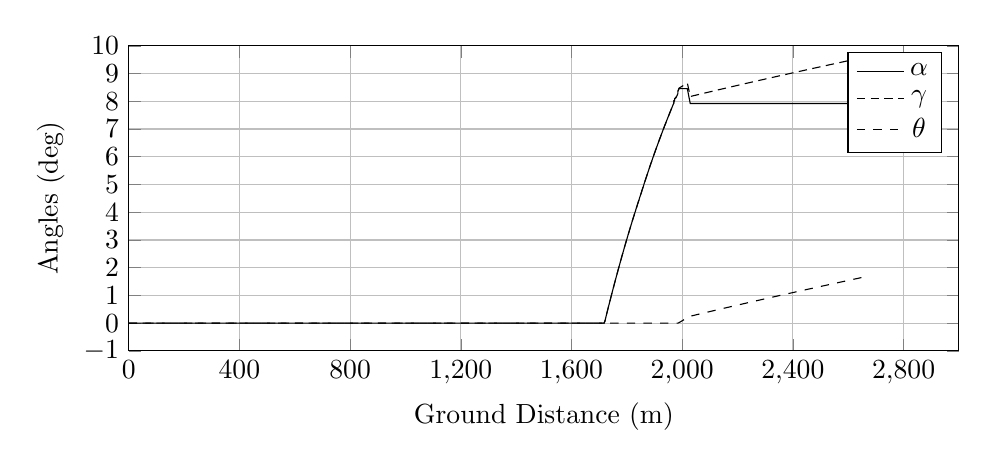
\begin{tikzpicture}

\begin{axis}[
width=\textwidth,
height=0.45\textwidth,
scaled ticks=false, tick label style={/pgf/number format/fixed},
xmin=0.0,
xmax=3000,
xtick={0,400,800,1200,1600,2000,2400,2800,3200},
xlabel={Ground Distance (m)},
xmajorgrids,
ymin=-1.0,
ymax=10,
ylabel={Angles (deg)},
ytick={-1,0,1,2,3,4,5,6,7,8,9,10},
ymajorgrids,
legend entries = {$\alpha$\\$\gamma$\\$\theta$\\}
]

\addplot [
color=black,
solid
]
table[row sep=crcr]{
1.3729668748937997E-8	0.0\\
2.6049868369719035E-7	0.0\\
2.0491224421327626E-6	0.0\\
9.92442121137073E-6	0.0\\
4.7452367809869807E-5	0.0\\
1.740064756114434E-4	0.0\\
4.0608377013922605E-4	0.0\\
7.313431501337001E-4	0.0\\
0.0011549487327126044	0.0\\
0.0016799013484208249	0.0\\
0.002295089346817705	0.0\\
0.003009933382444524	0.0\\
0.003810608015426248	0.0\\
0.004723484476856681	0.0\\
0.005727138856912631	0.0\\
0.006836216967948795	0.0\\
0.007997302399386296	0.0\\
0.00929136979810952	0.0\\
0.010685558505459776	0.0\\
0.012178513621519987	0.0\\
0.013775244426719659	0.0\\
0.015470070176169002	0.0\\
0.0172374436815836	0.0\\
0.019122918912604377	0.0\\
0.021104911040230538	0.0\\
0.023190717999955576	0.0\\
0.025355802981115103	0.0\\
0.027620619195902148	0.0\\
0.030020274690474198	0.0\\
0.032476028269866286	0.0\\
0.035054163466719815	0.0\\
0.037720846868992755	0.0\\
0.04049779674511381	0.0\\
0.043329456594087365	0.0\\
0.04629652060163805	0.0\\
0.04934498934704602	0.0\\
0.052507657924119336	0.0\\
0.055769483710642484	0.0\\
0.05917209570914676	0.0\\
0.06264043916012321	0.0\\
0.06620063977265622	0.0\\
0.06987962792775945	0.0\\
0.0736568184539585	0.0\\
0.07754284280095361	0.0\\
0.08151127871105612	0.0\\
0.08560324933017655	0.0\\
0.08985265585263943	0.0\\
0.09413961367176535	0.0\\
0.09857725310864562	0.0\\
0.10307959255469257	0.0\\
0.10766008648593872	0.0\\
0.11234920964493048	0.0\\
0.11719267720457946	0.0\\
0.12216973960582883	0.0\\
0.12724007601918352	0.0\\
0.13233299746505212	0.0\\
0.13755256756750583	0.0\\
0.14287728588926696	0.0\\
0.1482946925752714	0.0\\
0.15381585025670613	0.0\\
0.15940564092189102	0.0\\
0.16526271495916878	0.0\\
0.17120082448158402	0.0\\
0.17717889132867753	0.0\\
0.18324322596131126	0.0\\
0.189427022360885	0.0\\
0.1957511558722988	0.0\\
0.2021484013779125	0.0\\
0.20865863707071397	0.0\\
0.21548666343168166	0.0\\
0.22220154781289658	0.0\\
0.22919671627301902	0.0\\
0.23611678795738544	0.0\\
0.24306300975244904	0.0\\
0.2503085190632165	0.0\\
0.2576623280401219	0.0\\
0.26502430524173204	0.0\\
0.2724963584449146	0.0\\
0.2802001060647876	0.0\\
0.2878583985474956	0.0\\
0.2958320780323821	0.0\\
0.3040021452321372	0.0\\
0.31208951788619	0.0\\
0.3202851396023423	0.0\\
0.3287233234973125	0.0\\
0.3370425959884752	0.0\\
0.34575405233845447	0.0\\
0.3545073625286812	0.0\\
0.36338982075299686	0.0\\
0.37247557159370037	0.0\\
0.38151350442869847	0.0\\
0.3905554764834429	0.0\\
0.3999457587520332	0.0\\
0.4095398754587949	0.0\\
0.4189621792151833	0.0\\
0.4285208811402964	0.0\\
0.43828968955472236	0.0\\
0.44807735398784176	0.0\\
0.45806002753764463	0.0\\
0.4682994371692033	0.0\\
0.4787752542918833	0.0\\
0.4890770094685154	0.0\\
0.49985939134273727	0.0\\
0.5106597490205704	0.0\\
0.5213580865152188	0.0\\
0.532247733242454	0.0\\
0.5431365108549349	0.0\\
0.554075964429489	0.0\\
0.5653450694020941	0.0\\
0.5769901159382542	0.0\\
0.588512657344902	0.0\\
0.6004070039036553	0.0\\
0.6121651247369502	0.0\\
0.6239717914322569	0.0\\
0.6362472885961421	0.0\\
0.6486428939173223	0.0\\
0.6610190736373547	0.0\\
0.6737248046101814	0.0\\
0.6862826225989949	0.0\\
0.6991952542603428	0.0\\
0.7122988072688032	0.0\\
0.7251463703465595	0.0\\
0.7381769453061875	0.0\\
0.7516618647379176	0.0\\
0.7654913705221527	0.0\\
0.7791756406994825	0.0\\
0.7930637813125616	0.0\\
0.8074774191984457	0.0\\
0.8215072375247947	0.0\\
0.8361010597475598	0.0\\
0.8503303420601955	0.0\\
0.8650627501899835	0.0\\
0.8802332960144008	0.0\\
0.8951742046771463	0.0\\
0.9100334756324657	0.0\\
0.9251067343345352	0.0\\
0.9403923630470314	0.0\\
0.9559303815501943	0.0\\
0.9712400158034169	0.0\\
0.9869533781138684	0.0\\
1.0029148609762486	0.0\\
1.0189962473881624	0.0\\
1.035465185745812	0.0\\
1.0516742337458713	0.0\\
1.067815735429615	0.0\\
1.0846705971808022	0.0\\
1.1012775250051634	0.0\\
1.1180798406225687	0.0\\
1.1351395900544134	0.0\\
1.1526388687279154	0.0\\
1.1698922447507556	0.0\\
1.1875468452119025	0.0\\
1.2058383275300355	0.0\\
1.2239395537495579	0.0\\
1.2422020624207541	0.0\\
1.2608769472440078	0.0\\
1.2794948487006894	0.0\\
1.2979152553275424	0.0\\
1.3166445915281573	0.0\\
1.3354141707340492	0.0\\
1.3543210821322504	0.0\\
1.373689361295591	0.0\\
1.3932049885015831	0.0\\
1.4131781782225183	0.0\\
1.4330139682345777	0.0\\
1.4528243860883294	0.0\\
1.4728783400745615	0.0\\
1.4934621752870565	0.0\\
1.5141408097620341	0.0\\
1.53430654450827	0.0\\
1.5553850389607948	0.0\\
1.5762653203499473	0.0\\
1.5975496774716453	0.0\\
1.6196077215345106	0.0\\
1.6413652536722467	0.0\\
1.663437310723463	0.0\\
1.6860768385032747	0.0\\
1.7077101022266827	0.0\\
1.7297306410738114	0.0\\
1.7520297891459062	0.0\\
1.7743087535215367	0.0\\
1.797257424336919	0.0\\
1.8200802473615325	0.0\\
1.8430350373473994	0.0\\
1.8666926279964304	0.0\\
1.8902808566018634	0.0\\
1.9138231309717848	0.0\\
1.937187877956735	0.0\\
1.9611060682733261	0.0\\
1.9852138445648535	0.0\\
2.009780393513653	0.0\\
2.0346228225622163	0.0\\
2.0593611988602687	0.0\\
2.08477023517836	0.0\\
2.110324766702745	0.0\\
2.1352655781940433	0.0\\
2.160528860803022	0.0\\
2.1862071157614817	0.0\\
2.2127756699400534	0.0\\
2.2391904543957084	0.0\\
2.2653528664920257	0.0\\
2.292150575495974	0.0\\
2.3187704640870406	0.0\\
2.3455495914188482	0.0\\
2.372862901366455	0.0\\
2.4007145172972395	0.0\\
2.428100404243743	0.0\\
2.4555980306928005	0.0\\
2.483374904362833	0.0\\
2.511687733451976	0.0\\
2.5402569276484597	0.0\\
2.568415369317849	0.0\\
2.596987652715761	0.0\\
2.6263861238451423	0.0\\
2.655991481965028	0.0\\
2.6856115886357443	0.0\\
2.7154221146045012	0.0\\
2.7455665152057707	0.0\\
2.7752624694325894	0.0\\
2.805457625653509	0.0\\
2.8358231840904597	0.0\\
2.8663460878589797	0.0\\
2.897817297850832	0.0\\
2.9287074004595235	0.0\\
2.9603588456990284	0.0\\
2.9922321403815406	0.0\\
3.0241119471841866	0.0\\
3.056446055158509	0.0\\
3.0889346922121366	0.0\\
3.122221620829695	0.0\\
3.1546991615623394	0.0\\
3.187635101478671	0.0\\
3.221010117202278	0.0\\
3.2543449374576605	0.0\\
3.288235920596943	0.0\\
3.3223704322934555	0.0\\
3.3562838593334394	0.0\\
3.3906320903803255	0.0\\
3.425633159699527	0.0\\
3.462387235801926	0.0\\
3.4973980805087237	0.0\\
3.5324804241140235	0.0\\
3.5675385073174235	0.0\\
3.6040688981843845	0.0\\
3.6393612181513753	0.0\\
3.6770856360342323	0.0\\
3.7131729334920323	0.0\\
3.749509707933214	0.0\\
3.785733977879824	0.0\\
3.8225309786916544	0.0\\
3.860867115351552	0.0\\
3.89929745075254	0.0\\
3.9373367205567504	0.0\\
3.9751626485832894	0.0\\
4.013671158053867	0.0\\
4.0521140617426425	0.0\\
4.092377631210638	0.0\\
4.131586743753305	0.0\\
4.1715696979561425	0.0\\
4.210522654700574	0.0\\
4.250196810863292	0.0\\
4.2917015001093795	0.0\\
4.332438976653355	0.0\\
4.373124372895289	0.0\\
4.414429464889761	0.0\\
4.455884944705147	0.0\\
4.497250153511752	0.0\\
4.537976875075978	0.0\\
4.581399817640802	0.0\\
4.623816269683994	0.0\\
4.666022338967499	0.0\\
4.709098934189642	0.0\\
4.752435367147649	0.0\\
4.79531009100786	0.0\\
4.838191999420829	0.0\\
4.881381760681686	0.0\\
4.9256451804034285	0.0\\
4.9704217340957495	0.0\\
5.014356093293278	0.0\\
5.058826350846283	0.0\\
5.104458009943745	0.0\\
5.149663211268795	0.0\\
5.194981168813841	0.0\\
5.241194091283663	0.0\\
5.287987552078626	0.0\\
5.334426822383641	0.0\\
5.380633359096258	0.0\\
5.427524438012913	0.0\\
5.476157635197664	0.0\\
5.524667120325573	0.0\\
5.5732739519824435	0.0\\
5.6208990292882195	0.0\\
5.671502816366864	0.0\\
5.719824083529298	0.0\\
5.767871110439133	0.0\\
5.8169321963676754	0.0\\
5.866076914057565	0.0\\
5.917200682776528	0.0\\
5.96684810088939	0.0\\
6.016885842403935	0.0\\
6.068639931677712	0.0\\
6.119867755785197	0.0\\
6.171030794930029	0.0\\
6.222884713227881	0.0\\
6.2735946138732235	0.0\\
6.325883502103322	0.0\\
6.379615386553551	0.0\\
6.432194972482147	0.0\\
6.484528316464761	0.0\\
6.536619297696934	0.0\\
6.589662958081361	0.0\\
6.644121795496577	0.0\\
6.697445536614451	0.0\\
6.7518063163896365	0.0\\
6.8068829439682315	0.0\\
6.863205650636274	0.0\\
6.9185329265047315	0.0\\
6.974634519184049	0.0\\
7.031139830722298	0.0\\
7.0870923879294985	0.0\\
7.144766952910487	0.0\\
7.2026451873548805	0.0\\
7.261191729679483	0.0\\
7.320502240843062	0.0\\
7.378210233177999	0.0\\
7.437738452534925	0.0\\
7.49714639104333	0.0\\
7.556502460410064	0.0\\
7.617032771987237	0.0\\
7.676883327249088	0.0\\
7.735740247984193	0.0\\
7.796086087039788	0.0\\
7.856787102853412	0.0\\
7.91721236259451	0.0\\
7.979013602666894	0.0\\
8.039824025454376	0.0\\
8.102419182184594	0.0\\
8.16459313580776	0.0\\
8.226347093952135	0.0\\
8.290527749984296	0.0\\
8.353592793320257	0.0\\
8.417564177281012	0.0\\
8.482044607535009	0.0\\
8.547336806956285	0.0\\
8.613293246319614	0.0\\
8.6778048537894	0.0\\
8.74454839911753	0.0\\
8.810708373588199	0.0\\
8.876548424968423	0.0\\
8.942828456712885	0.0\\
9.010858044488913	0.0\\
9.079453414959548	0.0\\
9.148767802603732	0.0\\
9.21609997183467	0.0\\
9.285579683381485	0.0\\
9.355451712480097	0.0\\
9.423585014597279	0.0\\
9.493435356703696	0.0\\
9.562655940911181	0.0\\
9.63183713653898	0.0\\
9.703018708836247	0.0\\
9.773178624863132	0.0\\
9.844376937811855	0.0\\
9.914998792594716	0.0\\
9.98720270419701	0.0\\
10.059478150570087	0.0\\
10.132362020358627	0.0\\
10.205876892438312	0.0\\
10.279422251887688	0.0\\
10.353305644514993	0.0\\
10.42811398108589	0.0\\
10.50332954727428	0.0\\
10.578207710262959	0.0\\
10.65503529959097	0.0\\
10.730232142651953	0.0\\
10.805871937852555	0.0\\
10.88265320376452	0.0\\
10.958577899345514	0.0\\
11.034861147941964	0.0\\
11.112742623646977	0.0\\
11.190543636431041	0.0\\
11.267787598939979	0.0\\
11.3462805052093	0.0\\
11.423875697147409	0.0\\
11.502735831556972	0.0\\
11.581465323066688	0.0\\
11.661639233340708	0.0\\
11.741743247575428	0.0\\
11.821864700430528	0.0\\
11.901816327719768	0.0\\
11.98361062800689	0.0\\
12.065425957085825	0.0\\
12.1478520915771	0.0\\
12.230956215923495	0.0\\
12.313306905825911	0.0\\
12.396632357805931	0.0\\
12.479578787946746	0.0\\
12.564327762802186	0.0\\
12.648175874147956	0.0\\
12.736145481689512	0.0\\
12.821080154398764	0.0\\
12.908009536077355	0.0\\
12.994986774303499	0.0\\
13.081752199798046	0.0\\
13.17035388279784	0.0\\
13.257836697901475	0.0\\
13.34511613365563	0.0\\
13.433461823066896	0.0\\
13.524108483575919	0.0\\
13.611203924103116	0.0\\
13.702229394080796	0.0\\
13.792427706753081	0.0\\
13.882429934062493	0.0\\
13.975435778888343	0.0\\
14.065832730112316	0.0\\
14.157894546480026	0.0\\
14.250668806951023	0.0\\
14.343291987615704	0.0\\
14.43744444968501	0.0\\
14.532636396723657	0.0\\
14.625507232812737	0.0\\
14.721503924398366	0.0\\
14.818738382089133	0.0\\
14.913572076739943	0.0\\
15.009701633366973	0.0\\
15.10815424447124	0.0\\
15.206130868840724	0.0\\
15.304035939715973	0.0\\
15.403499839366233	0.0\\
15.503209871950865	0.0\\
15.601718454553605	0.0\\
15.700655560608023	0.0\\
15.801250929860519	0.0\\
15.899917805652187	0.0\\
16.001574124100856	0.0\\
16.102638779863817	0.0\\
16.204479333764816	0.0\\
16.30489644092564	0.0\\
16.40578186591999	0.0\\
16.509201471948074	0.0\\
16.614557195984908	0.0\\
16.717657554831042	0.0\\
16.823039336622365	0.0\\
16.928576062495388	0.0\\
17.03469945574068	0.0\\
17.140697318244236	0.0\\
17.246066414787876	0.0\\
17.35183930840021	0.0\\
17.458399953804133	0.0\\
17.565707112453843	0.0\\
17.673103795073075	0.0\\
17.781888038667653	0.0\\
17.89115167195854	0.0\\
18.00105710767307	0.0\\
18.110142905530395	0.0\\
18.219697237410173	0.0\\
18.32752951944549	0.0\\
18.43743745973078	0.0\\
18.54904630654982	0.0\\
18.659302591714813	0.0\\
18.770734536087716	0.0\\
18.883577445650936	0.0\\
18.996263390583444	0.0\\
19.108816920034535	0.0\\
19.22287647779894	0.0\\
19.33763586704334	0.0\\
19.456324114791514	0.0\\
19.57349394116079	0.0\\
19.690148252848566	0.0\\
19.80521137071168	0.0\\
19.92379170801214	0.0\\
20.04216631061405	0.0\\
20.15848954929409	0.0\\
20.278242138037896	0.0\\
20.396206084226087	0.0\\
20.516315546862906	0.0\\
20.637173924977112	0.0\\
20.75450010628387	0.0\\
20.874378237858778	0.0\\
20.996035953832852	0.0\\
21.11812959618858	0.0\\
21.240471115580952	0.0\\
21.361479376438375	0.0\\
21.485224699488654	0.0\\
21.607870280890317	0.0\\
21.73242999733349	0.0\\
21.85704493170313	0.0\\
21.98122016226351	0.0\\
22.10826921766411	0.0\\
22.235261614051304	0.0\\
22.361664688868032	0.0\\
22.48780138980522	0.0\\
22.614107216476143	0.0\\
22.74409311379692	0.0\\
22.873024137794893	0.0\\
23.003512644166257	0.0\\
23.132891545907036	0.0\\
23.26270690888247	0.0\\
23.39264146728729	0.0\\
23.52277721573431	0.0\\
23.654883767164463	0.0\\
23.78569183677709	0.0\\
23.917003007077597	0.0\\
24.047013652206026	0.0\\
24.178458227988493	0.0\\
24.314609552493202	0.0\\
24.447533097503474	0.0\\
24.579128452041708	0.0\\
24.71011994849615	0.0\\
24.843278471916108	0.0\\
24.975761222328053	0.0\\
25.1115496753864	0.0\\
25.247101122854083	0.0\\
25.384906965000688	0.0\\
25.522261036073317	0.0\\
25.66123001648475	0.0\\
25.79865327455613	0.0\\
25.826335196219034	0.0\\
25.839610403727477	0.0\\
25.841006316401874	0.0\\
25.84227013303559	0.0\\
25.84770509053729	0.0\\
25.86419328224909	0.0\\
25.90571916957557	0.0\\
25.999268866927544	0.0\\
26.123295978662824	0.0\\
26.250212562581652	0.0\\
26.376891976518465	0.0\\
26.50638698165423	0.0\\
26.634042370994827	0.0\\
26.763333806613538	0.0\\
26.893207366259766	0.0\\
27.022905486492228	0.0\\
27.153956322362554	0.0\\
27.287774297957696	0.0\\
27.42030033806219	0.0\\
27.555504894698295	0.0\\
27.691130018821354	0.0\\
27.82633313037239	0.0\\
27.959508564917073	0.0\\
28.096515548835796	0.0\\
28.232789703382153	0.0\\
28.368684388406535	0.0\\
28.506541650227618	0.0\\
28.64533374691623	0.0\\
28.78297783415192	0.0\\
28.92277775692753	0.0\\
29.06227187463503	0.0\\
29.20212864139956	0.0\\
29.34335827861657	0.0\\
29.483225747293005	0.0\\
29.625960812476485	0.0\\
29.76706561118049	0.0\\
29.909402910999468	0.0\\
30.051751399473822	0.0\\
30.196612335666572	0.0\\
30.342192969749448	0.0\\
30.48583400527584	0.0\\
30.632658550781265	0.0\\
30.77846394498075	0.0\\
30.92408133049836	0.0\\
31.071091331299215	0.0\\
31.218274793935116	0.0\\
31.366705758252415	0.0\\
31.515339333797037	0.0\\
31.66356819769615	0.0\\
31.814689402684216	0.0\\
31.96649953392354	0.0\\
32.115424616034375	0.0\\
32.266253234088566	0.0\\
32.41813832080348	0.0\\
32.569791431087395	0.0\\
32.722234201183724	0.0\\
32.876984607664	0.0\\
33.031873994672836	0.0\\
33.18502245018544	0.0\\
33.34135780547538	0.0\\
33.49759920343199	0.0\\
33.65385117142162	0.0\\
33.8113313806527	0.0\\
33.96985264489639	0.0\\
34.126473036379195	0.0\\
34.2857505660089	0.0\\
34.4449212019973	0.0\\
34.60566879064274	0.0\\
34.76644486933921	0.0\\
34.92612701881755	0.0\\
35.08630421658309	0.0\\
35.24825698849928	0.0\\
35.412303951281956	0.0\\
35.57355277914179	0.0\\
35.73545353069308	0.0\\
35.89925038949356	0.0\\
36.065161289279985	0.0\\
36.23047312008262	0.0\\
36.39472205714358	0.0\\
36.56135389445764	0.0\\
36.72774532558607	0.0\\
36.89384825683493	0.0\\
37.05904296416534	0.0\\
37.22702676294645	0.0\\
37.39437475321985	0.0\\
37.5621109943643	0.0\\
37.73270471709142	0.0\\
37.903359519601935	0.0\\
38.071486842086316	0.0\\
38.23815243703595	0.0\\
38.40817787072022	0.0\\
38.57751392140098	0.0\\
38.750215798728505	0.0\\
38.92001182640311	0.0\\
39.09310637700479	0.0\\
39.26472366117933	0.0\\
39.436554723976656	0.0\\
39.608961777617054	0.0\\
39.782828308010565	0.0\\
39.956194359016465	0.0\\
40.132391837044906	0.0\\
40.30868053167249	0.0\\
40.48611580488176	0.0\\
40.66383502946924	0.0\\
40.83999042132467	0.0\\
41.018202681018664	0.0\\
41.19780999006247	0.0\\
41.37730467548502	0.0\\
41.557010452813884	0.0\\
41.73612816026986	0.0\\
41.91555194917056	0.0\\
42.09743589423803	0.0\\
42.27807550146298	0.0\\
42.45995188234755	0.0\\
42.6401410478328	0.0\\
42.822293873795985	0.0\\
43.00585672428667	0.0\\
43.189965171449515	0.0\\
43.372020236704074	0.0\\
43.555636897252796	0.0\\
43.74012033961118	0.0\\
43.92429822300048	0.0\\
44.106869824379004	0.0\\
44.29411840239129	0.0\\
44.47920670866131	0.0\\
44.665034305215386	0.0\\
44.85242224248053	0.0\\
45.03948098831597	0.0\\
45.22811764277584	0.0\\
45.41548629589063	0.0\\
45.60322541388645	0.0\\
45.793007222766036	0.0\\
45.983742663331824	0.0\\
46.172643153142886	0.0\\
46.36421599110457	0.0\\
46.553512793459404	0.0\\
46.745018895697555	0.0\\
46.93606459490553	0.0\\
47.126948089509526	0.0\\
47.31881294044018	0.0\\
47.5110690178297	0.0\\
47.705448624448266	0.0\\
47.90005519882567	0.0\\
48.09288923506665	0.0\\
48.28732881729917	0.0\\
48.484002572746206	0.0\\
48.68089030454945	0.0\\
48.87532723390382	0.0\\
49.07073736177763	0.0\\
49.2672083392297	0.0\\
49.46586249263092	0.0\\
49.661880987188695	0.0\\
49.85966148345089	0.0\\
50.05808618672894	0.0\\
50.25785665917266	0.0\\
50.45743808511885	0.0\\
50.65573800086891	0.0\\
50.85948768734909	0.0\\
51.061243703011925	0.0\\
51.26368286286315	0.0\\
51.46416466063809	0.0\\
51.66475943174029	0.0\\
51.86588207153103	0.0\\
52.07444928962187	0.0\\
52.2824430085781	0.0\\
52.48676525705545	0.0\\
52.69531994892206	0.0\\
52.90027076850366	0.0\\
53.108186167814935	0.0\\
53.31165724918766	0.0\\
53.520024946679996	0.0\\
53.72688450142306	0.0\\
53.93707391647578	0.0\\
54.14518573319289	0.0\\
54.35125853722778	0.0\\
54.56213447502874	0.0\\
54.77598621923464	0.0\\
54.987629956235494	0.0\\
55.19778857845695	0.0\\
55.41030974885841	0.0\\
55.62390503323701	0.0\\
55.83671574169797	0.0\\
56.047071254351536	0.0\\
56.26137331252919	0.0\\
56.47512769358855	0.0\\
56.69105800830218	0.0\\
56.90937011004422	0.0\\
57.12736617899088	0.0\\
57.346833156368504	0.0\\
57.56476609337061	0.0\\
57.78230894703917	0.0\\
57.99943865551505	0.0\\
58.21827465292657	0.0\\
58.436085045729726	0.0\\
58.6577546799423	0.0\\
58.87982836766625	0.0\\
59.10336118170943	0.0\\
59.324182403931715	0.0\\
59.545440661451366	0.0\\
59.768227251413464	0.0\\
59.99077485409802	0.0\\
60.21631063559073	0.0\\
60.44006004384342	0.0\\
60.66502706168687	0.0\\
60.89133011288284	0.0\\
61.11585558357916	0.0\\
61.3432655409558	0.0\\
61.57186440401435	0.0\\
61.79868765088207	0.0\\
62.025670725987	0.0\\
62.254132946411545	0.0\\
62.48290793247415	0.0\\
62.713817944074236	0.0\\
62.94484116346062	0.0\\
63.17805109236767	0.0\\
63.41124119062552	0.0\\
63.64505576847972	0.0\\
63.87735201907903	0.0\\
64.11169045660182	0.0\\
64.34725756208485	0.0\\
64.58324360279937	0.0\\
64.81881329818131	0.0\\
65.05563560606473	0.0\\
65.29467812810154	0.0\\
65.53178653633495	0.0\\
65.77046761369158	0.0\\
66.01019347650049	0.0\\
66.25262920761091	0.0\\
66.49342175078831	0.0\\
66.73393309567928	0.0\\
66.97718905970893	0.0\\
67.21919788222482	0.0\\
67.46413738735515	0.0\\
67.70584739194695	0.0\\
67.95375887035246	0.0\\
68.19817148521656	0.0\\
68.44413350233111	0.0\\
68.68984243621705	0.0\\
68.93951041285982	0.0\\
69.19023531750676	0.0\\
69.43956667494601	0.0\\
69.68998597860525	0.0\\
69.94098943220166	0.0\\
70.1928405184459	0.0\\
70.44659484061637	0.0\\
70.69926103579675	0.0\\
70.95414956377036	0.0\\
71.21136313866151	0.0\\
71.46778788208749	0.0\\
71.7247351381395	0.0\\
71.98234155897126	0.0\\
72.24107377350035	0.0\\
72.4986091150376	0.0\\
72.75949164810788	0.0\\
73.02014691132015	0.0\\
73.28114866838587	0.0\\
73.54342372888959	0.0\\
73.80584407854005	0.0\\
74.07231166191039	0.0\\
74.3389341302921	0.0\\
74.60521354141642	0.0\\
74.87280568706873	0.0\\
75.1403821105715	0.0\\
75.41145333671997	0.0\\
75.68265298797411	0.0\\
75.95075857762194	0.0\\
76.2241428819712	0.0\\
76.4990100438061	0.0\\
76.77213586328236	0.0\\
77.04724851790667	0.0\\
77.32330034006353	0.0\\
77.59850473375684	0.0\\
77.87773830129439	0.0\\
78.1565255546137	0.0\\
78.43842651648492	0.0\\
78.720833678605	0.0\\
79.00101298089581	0.0\\
79.28359351218376	0.0\\
79.57011733099088	0.0\\
79.85418914588558	0.0\\
80.13919871477489	0.0\\
80.42568449319114	0.0\\
80.71472498530085	0.0\\
81.006853148924	0.0\\
81.2951972638476	0.0\\
81.58524575795963	0.0\\
81.87461709596036	0.0\\
82.1711642895769	0.0\\
82.46716486408064	0.0\\
82.76422974563803	0.0\\
83.05801377197795	0.0\\
83.35853301954708	0.0\\
83.65664966506407	0.0\\
83.95487262936624	0.0\\
84.25322789115987	0.0\\
84.55664509033022	0.0\\
84.8599544590121	0.0\\
85.16499148084048	0.0\\
85.47187188044902	0.0\\
85.77908321853027	0.0\\
86.08675489504844	0.0\\
86.39784539041122	0.0\\
86.71051296037359	0.0\\
87.02583358957506	0.0\\
87.34037846285594	0.0\\
87.65395388450591	0.0\\
87.96687312379424	0.0\\
88.28527441497255	0.0\\
88.6103524516937	0.0\\
88.92871226770333	0.0\\
89.25003295857354	0.0\\
89.57522243846881	0.0\\
89.90247582737899	0.0\\
90.22602529632545	0.0\\
90.5494223037065	0.0\\
90.87816525326718	0.0\\
91.20455861430293	0.0\\
91.53817773235312	0.0\\
91.87076195087604	0.0\\
92.20124984301029	0.0\\
92.53140503523474	0.0\\
92.86389705561814	0.0\\
93.19815266874983	0.0\\
93.53304529783748	0.0\\
93.86737084100128	0.0\\
94.20337949361911	0.0\\
94.54065981474497	0.0\\
94.87396787418089	0.0\\
95.21684847579547	0.0\\
95.55392648231228	0.0\\
95.89232371872416	0.0\\
96.23051075783204	0.0\\
96.57164052232307	0.0\\
96.90762523479154	0.0\\
97.24755293575913	0.0\\
97.58790661409188	0.0\\
97.92576087813703	0.0\\
98.26661027452474	0.0\\
98.6051908024865	0.0\\
98.94563962387357	0.0\\
99.28665364663627	0.0\\
99.63350087797645	0.0\\
99.97685593767679	0.0\\
100.31593955776762	0.0\\
100.65572384630482	0.0\\
100.99616871909686	0.0\\
101.3402339503516	0.0\\
101.67973054404297	0.0\\
102.01657591573795	0.0\\
102.35656456518868	0.0\\
102.6941824316649	0.0\\
103.03547296258705	0.0\\
103.37623032340073	0.0\\
103.71852978299776	0.0\\
104.05851119314701	0.0\\
104.3949509202441	0.0\\
104.7329053851843	0.0\\
105.07104272194636	0.0\\
105.40742307340048	0.0\\
105.74423560014887	0.0\\
106.07955743077031	0.0\\
106.41623710643992	0.0\\
106.75618472497374	0.0\\
107.0942647435474	0.0\\
107.43151869252583	0.0\\
107.44650965670576	0.0\\
107.45815118347005	0.0\\
107.46233674961977	0.0\\
107.46535588765028	0.0\\
107.46808502617694	0.0\\
107.4836206108138	0.0\\
107.53176708907421	0.0\\
107.68672244793561	0.0\\
107.97570433527497	0.0\\
108.27744765146667	0.0\\
108.5816623935838	0.0\\
108.88557241638279	0.0\\
109.19209959959528	0.0\\
109.50241879336687	0.0\\
109.81066605766154	0.0\\
110.12101503747155	0.0\\
110.43285681965125	0.0\\
110.74725799716322	0.0\\
111.06462449033057	0.0\\
111.38211128519615	0.0\\
111.70119562731901	0.0\\
112.02298633508096	0.0\\
112.34320819983824	0.0\\
112.66812620709393	0.0\\
112.99302416686388	0.0\\
113.31966045518399	0.0\\
113.64998129974768	0.0\\
113.97857627498675	0.0\\
114.31304608469316	0.0\\
114.64448318111735	0.0\\
114.98093514978115	0.0\\
115.31969924418831	0.0\\
115.65790718621022	0.0\\
116.00063352526521	0.0\\
116.34235083463872	0.0\\
116.68621873349733	0.0\\
117.03331062078092	0.0\\
117.37910048629482	0.0\\
117.72869476105836	0.0\\
118.08005947084649	0.0\\
118.43363644355449	0.0\\
118.79186464668504	0.0\\
119.14769212941735	0.0\\
119.5036618261702	0.0\\
119.86270697471275	0.0\\
120.22616362054572	0.0\\
120.58991121293201	0.0\\
120.95538130513773	0.0\\
121.3195355377388	0.0\\
121.68590041554987	0.0\\
122.05305648207542	0.0\\
122.42257239354896	0.0\\
122.79503144936103	0.0\\
123.16629137010841	0.0\\
123.53950748252527	0.0\\
123.91239367862553	0.0\\
124.29026003316017	0.0\\
124.66301933937496	0.0\\
125.03890311735066	0.0\\
125.41380975776434	0.0\\
125.7896808967325	0.0\\
126.16837244152023	0.0\\
126.54595968852882	0.0\\
126.92471834906405	0.0\\
127.30294276405039	0.0\\
127.68255852126984	0.0\\
128.06243727540487	0.0\\
128.44360431740483	0.0\\
128.82265748788262	0.0\\
129.1989690567886	0.0\\
129.57765386613931	0.0\\
129.95508099647026	0.0\\
130.33359114840187	0.0\\
130.71373745886524	0.0\\
131.09453904397424	0.0\\
131.47657586018488	0.0\\
131.85678563989967	0.0\\
132.23856625352113	0.0\\
132.61595336405918	0.0\\
132.99976263915818	0.0\\
133.38083522978053	0.0\\
133.76098428781995	0.0\\
134.1363519425165	0.0\\
134.51557915495124	0.0\\
134.8968696170101	0.0\\
135.27419431482667	0.0\\
135.65215477207505	0.0\\
136.03329358991255	0.0\\
136.41192880753374	0.0\\
136.7898079310749	0.0\\
137.17001317148595	0.0\\
137.54844558779996	0.0\\
137.92617219433072	0.0\\
138.30476964659732	0.0\\
138.68390038934075	0.0\\
139.0631653430654	0.0\\
139.4406106933401	0.0\\
139.81914660512416	0.0\\
140.19767098864742	0.0\\
140.5730919292459	0.0\\
140.95061983253072	0.0\\
141.32838502869612	0.0\\
141.70636515873298	0.0\\
142.0839785067887	0.0\\
142.46357402350594	0.0\\
142.84082211769783	0.0\\
143.21906727224075	0.0\\
143.59963619096823	0.0\\
143.97984478872678	0.0\\
144.35941603837455	0.0\\
144.7355521893594	0.0\\
145.11296635073694	0.0\\
145.49073213867456	0.0\\
145.87033631970945	0.0\\
146.24486520181193	0.0\\
146.6238757206513	0.0\\
147.00096360401335	0.0\\
147.37874202190085	0.0\\
147.756852900845	0.0\\
148.13572640408995	0.0\\
148.5136798644104	0.0\\
148.89083780486442	0.0\\
149.2712459042852	0.0\\
149.65303236723025	0.0\\
150.0329584616291	0.0\\
150.41363382646614	0.0\\
150.79322940570728	0.0\\
151.17272478467066	0.0\\
151.55400296227282	0.0\\
151.93482601265913	0.0\\
152.31881414221942	0.0\\
152.70208150063132	0.0\\
153.08320649997165	0.0\\
153.4666285558243	0.0\\
153.84825937276264	0.0\\
154.23093781718723	0.0\\
154.61485031834388	0.0\\
155.00001234931443	0.0\\
155.38285725409855	0.0\\
155.7679513537659	0.0\\
156.1509667875323	0.0\\
156.53491934392343	0.0\\
156.91995289130983	0.0\\
157.30625057946366	0.0\\
157.69121706207227	0.0\\
158.07789765133754	0.0\\
158.46521012398495	0.0\\
158.85138765236047	0.0\\
159.23964669847322	0.0\\
159.62715395386465	0.0\\
160.01960115328984	0.0\\
160.4079207075476	0.0\\
160.79602490671402	0.0\\
161.18437278725975	0.0\\
161.57644284003254	0.0\\
161.96812230097612	0.0\\
162.35808768568592	0.0\\
162.75087300343483	0.0\\
163.14546270495134	0.0\\
163.53745675514648	0.0\\
163.92955389373896	0.0\\
164.32395276810763	0.0\\
164.71713266653478	0.0\\
165.1102153740033	0.0\\
165.5035884424101	0.0\\
165.89816400198282	0.0\\
166.29148626774366	0.0\\
166.68861804276264	0.0\\
167.082852347146	0.0\\
167.48006204110857	0.0\\
167.8798182678497	0.0\\
168.27774435731556	0.0\\
168.67741362640317	0.0\\
169.07475368467374	0.0\\
169.4759958044982	0.0\\
169.87832784425882	0.0\\
170.2792240364854	0.0\\
170.68126852540456	0.0\\
171.08617821288442	0.0\\
171.48766933901368	0.0\\
171.892744970828	0.0\\
172.29711201372032	0.0\\
172.70264003426053	0.0\\
173.1105289448074	0.0\\
173.5163733808056	0.0\\
173.92577914808027	0.0\\
174.33607303977334	0.0\\
174.74614233406845	0.0\\
175.15731444736514	0.0\\
175.56901623635082	0.0\\
175.97955109701695	0.0\\
176.39275298155184	0.0\\
176.80397138375372	0.0\\
177.21946344336607	0.0\\
177.6332252263685	0.0\\
178.05102033212842	0.0\\
178.46725124888752	0.0\\
178.88389799206544	0.0\\
179.29839533747668	0.0\\
179.71608569665375	0.0\\
180.1342696339205	0.0\\
180.26454521656194	0.0\\
180.5538779958007	0.0\\
180.97677279803082	0.0\\
181.73177043104909	0.0\\
182.61825861954026	0.0\\
183.4994266290775	0.0\\
184.38832398643513	0.0\\
185.2752206450968	0.0\\
186.16090254585617	0.0\\
187.05782443666988	0.0\\
187.95004436743	0.0\\
188.84343565256296	0.0\\
189.73203483232732	0.0\\
190.63087969896367	0.0\\
191.53167348748025	0.0\\
192.42914206966827	0.0\\
193.32936064878362	0.0\\
194.23353734669462	0.0\\
195.14873951553636	0.0\\
196.05846844349168	0.0\\
196.9665797060448	0.0\\
197.88137813217617	0.0\\
198.80153314772656	0.0\\
199.72262566550114	0.0\\
200.6418018332526	0.0\\
201.57021605131746	0.0\\
202.49227039761405	0.0\\
203.4093310979173	0.0\\
204.33741716634955	0.0\\
205.26228808295895	0.0\\
206.1977933698634	0.0\\
207.13719708861407	0.0\\
208.07111616454222	0.0\\
209.00693662932974	0.0\\
209.95866810149408	0.0\\
210.9046028778589	0.0\\
211.84706310840727	0.0\\
212.79298368779843	0.0\\
213.73594859980489	0.0\\
214.69266347370274	0.0\\
215.65468447394903	0.0\\
216.614658409948	0.0\\
217.57357224144454	0.0\\
218.5368107467741	0.0\\
219.50048157907025	0.0\\
220.46765259916174	0.0\\
221.44618219131166	0.0\\
222.41939214233116	0.0\\
223.3957502333693	0.0\\
224.37068692464283	0.0\\
225.34711146005128	0.0\\
226.33138885023874	0.0\\
227.31393394086427	0.0\\
228.30414603792985	0.0\\
229.29617452368518	0.0\\
230.2808212657469	0.0\\
231.28192033792595	0.0\\
232.2770741096358	0.0\\
233.29052711380916	0.0\\
234.30070953924962	0.0\\
235.3030940983469	0.0\\
236.31056730234104	0.0\\
237.32863543123972	0.0\\
238.35192702989485	0.0\\
239.37227626200922	0.0\\
240.40154009491766	0.0\\
241.4327935450462	0.0\\
242.46479014370783	0.0\\
243.4993601598722	0.0\\
244.5489899152056	0.0\\
245.59198540953986	0.0\\
246.64178332136828	0.0\\
247.69238009267121	0.0\\
248.75653132082437	0.0\\
249.80604502438968	0.0\\
250.8683150903493	0.0\\
251.93058205288185	0.0\\
253.00701197053712	0.0\\
254.08005928692728	0.0\\
255.1482320588113	0.0\\
256.2287194565513	0.0\\
257.30711015243367	0.0\\
258.39583303573465	0.0\\
259.47850143980736	0.0\\
260.57344571603574	0.0\\
261.6820544046054	0.0\\
262.77228099849674	0.0\\
263.87126070008526	0.0\\
264.97335243767543	0.0\\
266.0976894214622	0.0\\
267.21278411159847	0.0\\
268.32534355771804	0.0\\
269.4561922169971	0.0\\
270.5915896156504	0.0\\
271.7158392961418	0.0\\
272.8552569839427	0.0\\
274.01601268837805	0.0\\
275.14755464888765	0.0\\
276.29902718037044	0.0\\
277.4488797139885	0.0\\
278.61486213965225	0.0\\
279.78120226092256	0.0\\
280.9500599413508	0.0\\
282.12185174587614	0.0\\
283.32143414076336	0.0\\
284.5140258308369	0.0\\
285.7080037808545	0.0\\
286.89480016288826	0.0\\
288.114729118857	0.0\\
289.33647182734956	0.0\\
290.5550281524761	0.0\\
291.77092362893404	0.0\\
292.99973950499964	0.0\\
294.2334028862149	0.0\\
295.476424104432	0.0\\
296.7307839433978	0.0\\
297.99041084660416	0.0\\
299.2512587145409	0.0\\
300.52071837015376	0.0\\
301.8085664342501	0.0\\
303.093188627083	0.0\\
304.3891528365698	0.0\\
305.6757850562126	0.0\\
306.9700995472474	0.0\\
308.29492992625205	0.0\\
309.5781066121766	0.0\\
310.8708143232478	0.0\\
312.1568125435102	0.0\\
313.4602517178914	0.0\\
314.7614812617795	0.0\\
316.075256596823	0.0\\
317.41378230532723	0.0\\
318.7467345840158	0.0\\
320.0730060828963	0.0\\
321.39169180058434	0.0\\
322.72349821328476	0.0\\
324.0598831134772	0.0\\
325.40424996971046	0.0\\
326.7492865835918	0.0\\
328.0710288684362	0.0\\
329.4262473961435	0.0\\
330.754264279002	0.0\\
332.097514519191	0.0\\
333.41994590396723	0.0\\
334.7305118494995	0.0\\
336.0731570894968	0.0\\
337.3927235989065	0.0\\
338.7087431098878	0.0\\
340.03087614347885	0.0\\
341.340088749036	0.0\\
342.6557828174856	0.0\\
343.96701843570406	0.0\\
345.2526439842643	0.0\\
346.5500414102456	0.0\\
347.8534066412583	0.0\\
349.1454340977755	0.0\\
350.4240054240321	0.0\\
351.7019235209849	0.0\\
352.98991038490203	0.0\\
354.2648351856848	0.0\\
355.53300413952707	0.0\\
356.79919221038165	0.0\\
358.0559257933643	0.0\\
359.3093316769772	0.0\\
359.35961387762393	0.0\\
359.41061546826563	0.0\\
359.4211304928041	0.0\\
359.4316918068113	0.0\\
359.4910693710335	0.0\\
359.779729191638	0.0\\
360.4880169023802	0.0\\
361.5766561299438	0.0\\
362.66113418824455	0.0\\
363.76124342756657	0.0\\
364.8589078947854	0.0\\
365.9685296666213	0.0\\
367.07582921056974	0.0\\
368.1951666519893	0.0\\
369.31258197452325	0.0\\
370.4366539475295	0.0\\
371.565996752341	0.0\\
372.70127842882266	0.0\\
373.84649895373127	0.0\\
374.9968247959414	0.0\\
376.15403836851897	0.0\\
377.3203528636726	0.0\\
378.4850840608731	0.0\\
379.6663035147078	0.0\\
380.8461820283744	0.0\\
382.0347494549213	0.0\\
383.2193798940116	0.0\\
384.42877967750667	0.0\\
385.63354002572066	0.0\\
386.845921264293	0.0\\
388.06777411235	0.0\\
389.2936908860911	0.0\\
390.53850037014047	0.0\\
391.76781253461945	0.0\\
393.0108311673757	0.0\\
394.26523475557894	0.0\\
395.52152377336915	0.0\\
396.7904975310561	0.0\\
398.0771683304033	0.0\\
399.3519058933132	0.0\\
400.63393441623316	0.0\\
401.92385130992545	0.0\\
403.21918556823357	0.0\\
404.52791933693925	0.0\\
405.83210730664996	0.0\\
407.1393641556499	0.0\\
408.45238412405433	0.0\\
409.76561626724674	0.0\\
411.10125498654554	0.0\\
412.4171463109144	0.0\\
413.73698982354097	0.0\\
415.062570379646	0.0\\
416.375187798194	0.0\\
417.69595093934595	0.0\\
419.0285116875033	0.0\\
420.36454657893216	0.0\\
421.6812813836435	0.0\\
423.00972403127514	0.0\\
424.32760721523437	0.0\\
425.6472681840288	0.0\\
426.96253742961164	0.0\\
428.29182268843977	0.0\\
429.6160502503526	0.0\\
430.9312874400488	0.0\\
432.2371182898221	0.0\\
433.55144081210005	0.0\\
434.867194360879	0.0\\
436.16838785958646	0.0\\
437.46367739026596	0.0\\
438.78588638695476	0.0\\
440.0925891606661	0.0\\
441.3848392234046	0.0\\
442.6814156289133	0.0\\
443.97357880818515	0.0\\
445.2632779895895	0.0\\
446.54906207929946	0.0\\
447.8470239842545	0.0\\
449.1220474037084	0.0\\
450.39588054344404	0.0\\
451.68119786233456	0.0\\
452.9614765477911	0.0\\
454.2371818112225	0.0\\
455.5035899796636	0.0\\
456.7833140437298	0.0\\
458.04929565590817	0.0\\
459.3134414393421	0.0\\
460.5777262845279	0.0\\
461.84023587900685	0.0\\
463.10108065312045	0.0\\
464.3645399404894	0.0\\
465.6238016850866	0.0\\
466.8762783875227	0.0\\
468.1281814377654	0.0\\
469.3838351297785	0.0\\
470.63650571068945	0.0\\
471.8846974041603	0.0\\
473.1433200948185	0.0\\
474.39244309563617	0.0\\
475.6408716432604	0.0\\
476.8834126309654	0.0\\
478.1293558793383	0.0\\
479.37468033554455	0.0\\
480.62161050962675	0.0\\
481.86154936911134	0.0\\
483.106752207652	0.0\\
484.34476413467644	0.0\\
485.57829651821373	0.0\\
486.81122711428	0.0\\
488.04749147403595	0.0\\
489.286499221119	0.0\\
490.5258622185305	0.0\\
491.7613633545217	0.0\\
492.98979445152895	0.0\\
494.22181660420335	0.0\\
495.4491662715502	0.0\\
496.68037150127316	0.0\\
497.905419768701	0.0\\
499.1418007543791	0.0\\
500.36883500341185	0.0\\
501.6049635519511	0.0\\
502.8346968521507	0.0\\
504.0688416682151	0.0\\
505.30449852859897	0.0\\
506.53623375091763	0.0\\
507.7727737587355	0.0\\
509.01094069395083	0.0\\
510.24044302236643	0.0\\
511.47314480655655	0.0\\
512.709426639085	0.0\\
513.933014023326	0.0\\
515.1632406071703	0.0\\
516.3942825834877	0.0\\
517.6209225737591	0.0\\
518.8611725736578	0.0\\
520.0899677635864	0.0\\
521.3248911937364	0.0\\
522.5563249355823	0.0\\
523.7871395992927	0.0\\
525.0207080655291	0.0\\
526.2538889797097	0.0\\
527.4855886295541	0.0\\
528.7248966623163	0.0\\
529.9525012711933	0.0\\
531.188411182631	0.0\\
532.430364502346	0.0\\
533.6537982289233	0.0\\
534.8895444365953	0.0\\
536.1167015415926	0.0\\
537.3524667925105	0.0\\
538.5909786862885	0.0\\
539.8321004970862	0.0\\
541.0714186237371	0.0\\
542.3101366962153	0.0\\
543.549683335455	0.0\\
544.7884410234926	0.0\\
546.0249505756278	0.0\\
547.2698901981096	0.0\\
548.517922558824	0.0\\
549.7630578627702	0.0\\
551.0045945501979	0.0\\
552.2474673458937	0.0\\
553.4943949801896	0.0\\
554.7340934194742	0.0\\
555.9857081438174	0.0\\
557.2349771676527	0.0\\
558.4836329625055	0.0\\
559.7304362301556	0.0\\
560.9863602168837	0.0\\
562.2354783338385	0.0\\
563.4889074787859	0.0\\
564.7429572990306	0.0\\
565.9930187270757	0.0\\
567.2542213530385	0.0\\
568.5162483155984	0.0\\
569.7779714539561	0.0\\
571.0363634961464	0.0\\
572.2926220263994	0.0\\
573.5600328752141	0.0\\
574.8157579683532	0.0\\
576.0874650967378	0.0\\
577.3535786105731	0.0\\
578.6120389651717	0.0\\
579.8782973050222	0.0\\
581.1428814799804	0.0\\
582.4098688192882	0.0\\
583.6781849802521	0.0\\
584.9463392856037	0.0\\
586.2252005492951	0.0\\
587.4974333601563	0.0\\
588.7730696836684	0.0\\
590.0462783949215	0.0\\
591.3260679091647	0.0\\
592.6020115890217	0.0\\
593.8805034430136	0.0\\
595.160760080855	0.0\\
596.4493859727936	0.0\\
597.7370171231987	0.0\\
599.0230981231337	0.0\\
600.3140314068335	0.0\\
601.5959263370289	0.0\\
602.8804904362269	0.0\\
604.1717551873128	0.0\\
605.4670675975769	0.0\\
606.7593430415579	0.0\\
608.0589989803163	0.0\\
609.35544064962	0.0\\
610.6631378257334	0.0\\
611.9673871376037	0.0\\
613.2669485728909	0.0\\
614.5726280512417	0.0\\
615.882692177473	0.0\\
617.1853058424017	0.0\\
618.4951671858978	0.0\\
619.8084414147645	0.0\\
621.1191039235041	0.0\\
622.4308696059663	0.0\\
623.7508573247546	0.0\\
625.0621647279136	0.0\\
626.3891907804957	0.0\\
627.7047303153058	0.0\\
629.0377690450321	0.0\\
630.3648129669755	0.0\\
631.6959383652843	0.0\\
633.0238008372617	0.0\\
634.3555987176628	0.0\\
635.6888337719913	0.0\\
637.0273231686772	0.0\\
638.3673317967357	0.0\\
639.7077548538582	0.0\\
641.0518988098222	0.0\\
642.3903562372943	0.0\\
643.7408141429719	0.0\\
645.0886899442107	0.0\\
646.4440665133416	0.0\\
647.7979969870544	0.0\\
649.1475695730635	0.0\\
650.5085087456741	0.0\\
651.8672498827148	0.0\\
653.2300391678464	0.0\\
654.59119710404	0.0\\
655.9565870372583	0.0\\
657.3301576177535	0.0\\
658.7055644018274	0.0\\
660.0707476489983	0.0\\
661.4425588489983	0.0\\
662.8202826045422	0.0\\
664.2023126867782	0.0\\
665.5843067773396	0.0\\
666.9693429401127	0.0\\
668.3535922551048	0.0\\
669.7456415264321	0.0\\
671.1429671199867	0.0\\
672.5352013622244	0.0\\
673.9319680407395	0.0\\
675.3315923284297	0.0\\
676.7364615033362	0.0\\
678.1398524051901	0.0\\
679.5482613506588	0.0\\
680.9611255975728	0.0\\
682.3747606873828	0.0\\
683.7885950684599	0.0\\
685.2170702182973	0.0\\
686.6341538210345	0.0\\
688.0624981059129	0.0\\
689.494639734967	0.0\\
690.9277173550104	0.0\\
692.366148307123	0.0\\
693.8090898976764	0.0\\
695.2470828114372	0.0\\
696.6927285316788	0.0\\
698.1317183942906	0.0\\
699.5819178468557	0.0\\
701.0428107681289	0.0\\
702.4953498250779	0.0\\
703.9473725213384	0.0\\
705.4080630038732	0.0\\
706.8695138302369	0.0\\
708.3364086722147	0.0\\
709.8077680233077	0.0\\
711.2874255207532	0.0\\
712.7606875545755	0.0\\
714.2419414738395	0.0\\
715.7350467748483	0.0\\
717.2311190009834	0.0\\
718.7239794754369	0.0\\
720.2275182266221	0.0\\
721.7330377579644	0.0\\
723.2413817882659	0.0\\
724.7490613493742	0.0\\
726.2646491700143	0.0\\
727.7888882938735	0.0\\
729.3095291352877	0.0\\
730.8328737152488	0.0\\
732.3678281524585	0.0\\
733.9014149193533	0.0\\
735.4434915877257	0.0\\
736.9879879939524	0.0\\
738.5283662039221	0.0\\
740.0793071755775	0.0\\
741.6375760538187	0.0\\
743.1975562173411	0.0\\
744.7668995543936	0.0\\
746.3402343351052	0.0\\
747.9098112007614	0.0\\
749.4926435018808	0.0\\
751.0788155700511	0.0\\
752.6689698013324	0.0\\
754.2660647297644	0.0\\
755.8725103063173	0.0\\
757.4740270930072	0.0\\
759.0843283212412	0.0\\
760.6957495574857	0.0\\
762.3236488682719	0.0\\
763.957733693579	0.0\\
765.59787840474	0.0\\
767.2310074870152	0.0\\
768.8772793382998	0.0\\
770.5330449495398	0.0\\
772.1910525761205	0.0\\
773.8571767410926	0.0\\
775.5319334528265	0.0\\
777.2041051797112	0.0\\
778.8843360083499	0.0\\
780.5674338985871	0.0\\
782.2582000560008	0.0\\
783.9645563214774	0.0\\
785.6717915011791	0.0\\
787.3899867029195	0.0\\
789.1251875317641	0.0\\
790.8518058281281	0.0\\
792.5977603346089	0.0\\
794.3482760283587	0.0\\
796.1133104533772	0.0\\
797.8925872065113	0.0\\
799.6676230066485	0.0\\
801.4573937546816	0.0\\
803.2521506684645	0.0\\
805.0713284918866	0.0\\
806.8905312973145	0.0\\
808.7095825809233	0.0\\
810.5470742557707	0.0\\
812.397095148264	0.0\\
814.2551620707266	0.0\\
816.132659040346	0.0\\
818.0281486728034	0.0\\
819.9214681177887	0.0\\
821.8368903009664	0.0\\
823.7586319415379	0.0\\
825.6966696706393	0.0\\
827.6537819263224	0.0\\
829.6200328252633	0.0\\
831.6080960277959	0.0\\
833.6058858944243	0.0\\
835.6138691611445	0.0\\
837.6522132068358	0.0\\
839.7005525953057	0.0\\
841.7828859709559	0.0\\
843.8747849790732	0.0\\
846.0012801717799	0.0\\
848.1350586077451	0.0\\
850.3010101301049	0.0\\
852.4938460893047	0.0\\
854.7160164344048	0.0\\
856.953183977754	0.0\\
859.2449805536867	0.0\\
861.553860969846	0.0\\
863.8861242277894	0.0\\
866.246819806435	0.0\\
868.6340776469228	0.0\\
871.0307008527677	0.0\\
873.4425737809947	0.0\\
875.8683627080882	0.0\\
878.2871875934777	0.0\\
880.6871980592739	0.0\\
883.0835625734228	0.0\\
885.4582103016828	0.0\\
887.8090348902429	0.0\\
890.1260985038559	0.0\\
892.4305796056062	0.0\\
894.7269340529676	0.0\\
896.9820607244501	0.0\\
899.2145918776932	0.0\\
901.4149289955963	0.0\\
903.6000827976163	0.0\\
905.7628356155565	0.0\\
907.9125759899712	0.0\\
910.0463732517737	0.0\\
912.1621082770412	0.0\\
914.252748444012	0.0\\
916.3193222282762	0.0\\
918.3774032152758	0.0\\
920.4230371350736	0.0\\
922.4488421897295	0.0\\
924.4676056552714	0.0\\
926.4750457097173	0.0\\
928.4628675146391	0.0\\
930.4415354433384	0.0\\
932.4169334877033	0.0\\
934.3618120787764	0.0\\
936.2925782031043	0.0\\
938.221454604651	0.0\\
940.1466541072932	0.0\\
942.0630559918154	0.0\\
943.9661268276432	0.0\\
945.855723854622	0.0\\
947.7414423099835	0.0\\
949.6247277182404	0.0\\
950.0005002817738	0.0\\
950.0230506344997	0.0\\
950.1308215335305	0.0\\
950.5414060440687	0.0\\
951.7332630183596	0.0\\
953.5143958553476	0.0\\
955.3392852116363	0.0\\
957.1752888236713	0.0\\
959.0289647351387	0.0\\
960.8832782446625	0.0\\
962.7554683410222	0.0\\
964.6443208060225	0.0\\
966.5322968187702	0.0\\
968.4446219567153	0.0\\
970.3714286007128	0.0\\
972.3124415176733	0.0\\
974.2605248068592	0.0\\
976.2301437340116	0.0\\
978.213256976104	0.0\\
980.2122069053562	0.0\\
982.2296883765371	0.0\\
984.266639388085	0.0\\
986.3147739620981	0.0\\
988.3960143323177	0.0\\
990.4907542518904	0.0\\
992.597731646071	0.0\\
994.7150509145251	0.0\\
996.8497534095575	0.0\\
999.0175118666675	0.0\\
1001.214973608124	0.0\\
1003.4222226777547	0.0\\
1005.6439066633507	0.0\\
1007.9056211699185	0.0\\
1010.1815475595499	0.0\\
1012.4593894002178	0.0\\
1014.7697096690417	0.0\\
1017.0941378890425	0.0\\
1019.4222885547019	0.0\\
1021.7798263678972	0.0\\
1024.1162876451726	0.0\\
1026.4755086623104	0.0\\
1028.844377722754	0.0\\
1031.190986795992	0.0\\
1033.5382547099184	0.0\\
1035.880415206132	0.0\\
1038.1978622814872	0.0\\
1040.5221418536075	0.0\\
1042.829378952401	0.0\\
1045.1262455440883	0.0\\
1047.4117186999474	0.0\\
1049.6776720424195	0.0\\
1051.9297298004053	0.0\\
1054.1690273370286	0.0\\
1056.4063885023952	0.0\\
1058.6175383787422	0.0\\
1060.823977839877	0.0\\
1063.004539980645	0.0\\
1065.1811098810958	0.0\\
1067.3393471549502	0.0\\
1069.4880225957309	0.0\\
1071.646495095737	0.0\\
1073.7895762253647	0.0\\
1075.9120449239158	0.0\\
1078.0372403022639	0.0\\
1080.1464502145886	0.0\\
1082.2468697933746	0.0\\
1084.3372788409138	0.0\\
1086.4247318593139	0.0\\
1088.4944955108767	0.0\\
1090.567873086332	0.0\\
1092.6308875683676	0.0\\
1094.6811764366093	0.0\\
1096.7354681249813	0.0\\
1098.7817414583137	0.0\\
1100.8131991524442	0.0\\
1102.8450230740482	0.0\\
1104.870786355968	0.0\\
1106.8940264481585	0.0\\
1108.909677347429	0.0\\
1110.9182454029333	0.0\\
1112.9143472988767	0.0\\
1114.9216393808601	0.0\\
1116.9150741130038	0.0\\
1118.9136212980056	0.0\\
1120.9063852233294	0.0\\
1122.8993236165816	0.0\\
1124.8918702921865	0.0\\
1126.872134731063	0.0\\
1128.8465117224941	0.0\\
1130.8103238657995	0.0\\
1132.785939813507	0.0\\
1134.7566648056682	0.0\\
1136.7232926050892	0.0\\
1138.6853798767029	0.0\\
1140.640905134413	0.0\\
1142.5973252725053	0.0\\
1144.5583291816056	0.0\\
1146.51364438389	0.0\\
1148.46681843543	0.0\\
1150.4118443408383	0.0\\
1152.3649058347391	0.0\\
1154.3055537065547	0.0\\
1156.2556968854883	0.0\\
1158.2082428149847	0.0\\
1160.1463111803164	0.0\\
1162.0903796330958	0.0\\
1164.0326386081329	0.0\\
1165.9791708118664	0.0\\
1167.9161065368262	0.0\\
1169.8555421115998	0.0\\
1171.7872093779547	0.0\\
1173.721108211771	0.0\\
1175.6505711830541	0.0\\
1177.572749213566	0.0\\
1179.5122862081234	0.0\\
1181.4422466666188	0.0\\
1183.3709361156557	0.0\\
1185.2914450476574	0.0\\
1187.2180522912613	0.0\\
1189.152786522423	0.0\\
1191.0819295005895	0.0\\
1193.0119983423547	0.0\\
1194.9308612439313	0.0\\
1196.8577456345856	0.0\\
1198.7930877742288	0.0\\
1200.7135748168075	0.0\\
1202.6362586648456	0.0\\
1204.561695935316	0.0\\
1206.4861047719228	0.0\\
1208.4202073678857	0.0\\
1210.3495912248213	0.0\\
1212.2804249658752	0.0\\
1214.2033611993593	0.0\\
1216.1358122373167	0.0\\
1218.065524646389	0.0\\
1219.9882067109547	0.0\\
1221.9107549255	0.0\\
1223.837562841974	0.0\\
1225.7572070589372	0.0\\
1227.6906094747146	0.0\\
1229.618776195999	0.0\\
1231.547927124243	0.0\\
1233.476370570851	0.0\\
1235.4053979980463	0.0\\
1237.3351290946239	0.0\\
1239.265257171874	0.0\\
1241.2020340175304	0.0\\
1243.1381425952736	0.0\\
1245.0791881961532	0.0\\
1247.0108609885456	0.0\\
1248.9428633956727	0.0\\
1250.88014266164	0.0\\
1252.813148962614	0.0\\
1254.746478384779	0.0\\
1256.688250241466	0.0\\
1258.6225020968868	0.0\\
1260.558282819567	0.0\\
1262.5111675276034	0.0\\
1264.455085253323	0.0\\
1266.3988728751474	0.0\\
1268.3445165153844	0.0\\
1270.28733117425	0.0\\
1272.231728155611	0.0\\
1274.1818821912325	0.0\\
1276.127201802456	0.0\\
1278.0710814175163	0.0\\
1280.0230981507384	0.0\\
1281.976114167776	0.0\\
1283.9226180958535	0.0\\
1285.8801660505437	0.0\\
1287.83335126764	0.0\\
1289.787979282049	0.0\\
1291.7470876931538	0.0\\
1293.704952649025	0.0\\
1295.662187611009	0.0\\
1297.6296438613495	0.0\\
1299.5957621228954	0.0\\
1301.5652641447032	0.0\\
1303.5227763389198	0.0\\
1305.488173386856	0.0\\
1307.4580057728808	0.0\\
1309.4333194474557	0.0\\
1311.4099642969613	0.0\\
1313.3814902220101	0.0\\
1315.366129001081	0.0\\
1317.3378612894808	0.0\\
1319.3176459320284	0.0\\
1321.3057227607728	0.0\\
1323.2821406960857	0.0\\
1325.266545247795	0.0\\
1327.25671026617	0.0\\
1329.2424193250804	0.0\\
1331.2446124899739	0.0\\
1333.2353029914925	0.0\\
1335.2365450394182	0.0\\
1337.22897613553	0.0\\
1339.2299572479374	0.0\\
1341.2371189290957	0.0\\
1343.2403113095625	0.0\\
1345.2556151753142	0.0\\
1347.2660687529215	0.0\\
1349.2750645232263	0.0\\
1351.2885268426094	0.0\\
1353.3090475933059	0.0\\
1355.3294686733188	0.0\\
1357.3380812073801	0.0\\
1359.3615909356681	0.0\\
1361.381779816631	0.0\\
1363.4128258337	0.0\\
1365.4360452592468	0.0\\
1367.4624531605964	0.0\\
1369.5119330190146	0.0\\
1371.5547016819214	0.0\\
1373.6018128376604	0.0\\
1375.6433317118385	0.0\\
1377.691291682157	0.0\\
1379.740039797387	0.0\\
1381.7836809592573	0.0\\
1383.8355734466627	0.0\\
1385.8932018514279	0.0\\
1387.9517780727956	0.0\\
1390.0164004282956	0.0\\
1392.0828028943401	0.0\\
1394.1497267953218	0.0\\
1396.22164266638	0.0\\
1398.2849687539147	0.0\\
1400.356522751345	0.0\\
1402.435272975516	0.0\\
1404.5138265767928	0.0\\
1406.5945233866337	0.0\\
1408.6743120310316	0.0\\
1410.751933016501	0.0\\
1412.842197885634	0.0\\
1414.9336749349973	0.0\\
1417.025836964221	0.0\\
1419.1249849464675	0.0\\
1421.2241052235304	0.0\\
1423.3253817904783	0.0\\
1425.4260276016616	0.0\\
1427.543303864059	0.0\\
1429.6497203621466	0.0\\
1431.7668000716635	0.0\\
1433.8923470129503	0.0\\
1436.0198607960601	0.0\\
1438.1472216162315	0.0\\
1440.2857310266704	0.0\\
1442.4276593016361	0.0\\
1444.5732826092753	0.0\\
1446.7104087913876	0.0\\
1448.8651935501707	0.0\\
1451.013103509354	0.0\\
1453.170062051233	0.0\\
1455.3123639593869	0.0\\
1457.4714434042544	0.0\\
1459.633318962754	0.0\\
1461.8011785524718	0.0\\
1463.978443079197	0.0\\
1466.1589539334022	0.0\\
1468.3330481647522	0.0\\
1470.5241422117897	0.0\\
1472.7068065111198	0.0\\
1474.8949490599075	0.0\\
1477.0858892351848	0.0\\
1479.2858362057632	0.0\\
1481.4858478349215	0.0\\
1483.6927018060292	0.0\\
1485.8995749450642	0.0\\
1488.1127918139236	0.0\\
1490.3290643133373	0.0\\
1492.5617036662434	0.0\\
1494.7952701113227	0.0\\
1497.0231945970636	0.0\\
1499.2552673690302	0.0\\
1501.4953471088907	0.0\\
1503.7459356174272	0.0\\
1505.981990185222	0.0\\
1508.2302007991952	0.0\\
1510.4836302189697	0.0\\
1512.743915024695	0.0\\
1515.0032327357158	0.0\\
1517.2635077916834	0.0\\
1519.5444937334946	0.0\\
1521.8243782176264	0.0\\
1524.1126458993645	0.0\\
1526.4157290064672	0.0\\
1528.7108829699332	0.0\\
1531.0121639066833	0.0\\
1533.3217134151605	0.0\\
1535.6370076952699	0.0\\
1537.9521104139612	0.0\\
1540.2792820478207	0.0\\
1542.6099281020447	0.0\\
1544.9549769618707	0.0\\
1547.2823859592845	0.0\\
1549.6235199387374	0.0\\
1551.9735278926428	0.0\\
1554.327717840008	0.0\\
1556.6944855201923	0.0\\
1559.0625753109548	0.0\\
1561.4288780460688	0.0\\
1563.8114627854948	0.0\\
1566.1816653279702	0.0\\
1568.5692573246552	0.0\\
1570.9648927468756	0.0\\
1573.3554902663159	0.0\\
1575.7625019501884	0.0\\
1578.1643518593696	0.0\\
1580.5769546204228	0.0\\
1582.9986367801266	0.0\\
1585.4315222767714	0.0\\
1587.8651285973406	0.0\\
1590.3171308577207	0.0\\
1592.7736687207012	0.0\\
1595.2279462348183	0.0\\
1597.6862232773633	0.0\\
1600.1587622759403	0.0\\
1602.6407045144247	0.0\\
1605.1213710154866	0.0\\
1607.6106353912533	0.0\\
1610.104431234036	0.0\\
1612.60867642332	0.0\\
1615.1235881550438	0.0\\
1617.641271687533	0.0\\
1620.1728712870827	0.0\\
1622.7069721981798	0.0\\
1625.2562239015015	0.0\\
1627.80790407338	0.0\\
1630.3680288092055	0.0\\
1632.927829442519	0.0\\
1635.5117426561087	0.0\\
1638.096346405	0.0\\
1640.6935047998381	0.0\\
1643.29333089907	0.0\\
1645.9102615272536	0.0\\
1648.5346002042502	0.0\\
1651.1600946434105	0.0\\
1653.8181627318659	0.0\\
1656.4689562061499	0.0\\
1659.1316011710555	0.0\\
1661.8058147289394	0.0\\
1664.4898047441952	0.0\\
1667.1854960546711	0.0\\
1669.8823096793208	0.0\\
1672.5999249205965	0.0\\
1675.3205876264715	0.0\\
1678.0503071518651	0.0\\
1680.809867573716	0.0\\
1683.56836083091	0.0\\
1686.3332549616966	0.0\\
1689.1208792980865	0.0\\
1691.9193773705065	0.0\\
1694.7178367868169	0.0\\
1697.5385509029716	0.0\\
1700.3750049170867	0.0\\
1703.2265828028203	0.0\\
1706.0899073466817	0.0\\
1708.9747325243197	0.0\\
1711.8865100733033	0.0\\
1714.8092265783885	0.0\\
1716.0030366228693	0.0\\
1717.7478476926494	0.0\\
1720.6798068629882	0.07164571444551537\\
1723.6350728829793	0.1915588120727767\\
1726.606072951276	0.3116371960453316\\
1729.5911341545798	0.4315622562585216\\
1732.6196716728136	0.5512600646850911\\
1735.6559245549438	0.6718965684619236\\
1738.7172036550987	0.7920282750814358\\
1741.7694771914526	0.9123351343930837\\
1744.8599645163245	1.0314751526240142\\
1747.971885868576	1.151291722626239\\
1751.1230321772691	1.2711146447932724\\
1754.2962107927005	1.391613223367366\\
1757.477790198403	1.5121098173974454\\
1760.7051186364706	1.632079433916585\\
1763.9702837897303	1.7529199606489083\\
1767.2786125983243	1.874307447864287\\
1770.5932468398223	1.9964149558747866\\
1773.9358876961433	2.1178646204081577\\
1777.3398929232644	2.239447636099328\\
1780.762721802177	2.3623528041020583\\
1784.2430523292355	2.485013898596315\\
1787.7516344335831	2.608798576371332\\
1791.3167904035013	2.7326357980753215\\
1794.9107559234358	2.857502245056928\\
1798.5653535947054	2.982395280711885\\
1802.2788902635816	3.108396573715903\\
1806.0564952581049	3.2354069199143014\\
1809.9062059228245	3.36356034947016\\
1813.8569892180249	3.4930829545406192\\
1817.8534757241691	3.624889727218142\\
1821.962063333539	3.757073639525328\\
1826.184046975622	3.8917824552482214\\
1830.5259052314632	4.028971637552061\\
1834.9731626407115	4.168761060063062\\
1839.4701768006948	4.310593834081079\\
1844.0287868399673	4.452630334526436\\
1848.6609392633577	4.59520948580246\\
1853.2669462962444	4.738659203186508\\
1857.7926110858762	4.8798715441542\\
1862.2241684191754	5.017241744285192\\
1866.551890881739	5.150443296426937\\
1870.810960882286	5.279282598056282\\
1874.9800703502542	5.404897307642708\\
1879.0717155296811	5.526733098576585\\
1883.081973754482	5.645234445670443\\
1887.0434128211232	5.760358954812277\\
1890.9488164127192	5.873103949945808\\
1894.8218126659067	5.98331071728661\\
1898.6553885478334	6.091689018403876\\
1902.4530123615282	6.1980753456504\\
1906.190497055522	6.302600278798645\\
1909.8968008381958	6.4046356658254595\\
1913.5872156675869	6.50501259762866\\
1917.2539106271897	6.6041690403790465\\
1920.8824125771816	6.701913263073884\\
1924.478569024258	6.797884128257502\\
1928.065969092785	6.892265072166705\\
1931.6255223525268	6.9856961011151775\\
1935.1607809236339	7.077695201848984\\
1938.6916699668209	7.16837577134636\\
1942.2154628639669	7.258264749223661\\
1945.7149072274287	7.347301348027475\\
1949.1895882282606	7.435062543424497\\
1952.659488213069	7.5215570473272315\\
1956.1172580250209	7.607297401668191\\
1959.5647942706696	7.692111104878929\\
1963.0127239475105	7.776055906103911\\
1966.4243438832632	7.859399021230409\\
1969.8273033801152	7.941264580372879\\
1970.5045518249694	8.022334824372045\\
1972.493693198031	8.038356399358939\\
1972.6588663125622	8.085341994831122\\
1972.8220125392058	8.089227675948102\\
1972.9629303421711	8.093064339718165\\
1973.039133202476	8.096377129818961\\
1973.0764190900718	8.09816803356619\\
1973.131522753863	8.099044180315726\\
1973.4127944443708	8.100338907358257\\
1974.4827959850272	8.106946859025662\\
1977.078736993174	8.132068338817756\\
1980.6902686224475	8.192872347454728\\
1984.36744526736	8.276996461347391\\
1984.6340945028378	8.361998727084796\\
1984.8974205884447	8.368116368385685\\
1985.158349939441	8.374154390337377\\
1985.4078382820976	8.380134152389896\\
1985.6725537076663	8.385848594601491\\
1985.9288078676473	8.391908630170438\\
1986.1820493451523	8.39777171234351\\
1986.4308323244527	8.403562752952073\\
1986.6815676799092	8.409248819739691\\
1986.9492596570412	8.414976520195843\\
1987.2013870889386	8.421088351252312\\
1987.4412921029634	8.42684159554338\\
1987.7097022986009	8.43231305106466\\
1987.9666164528667	8.4384315295468\\
1988.2292843165642	8.444284663927409\\
1988.4975311162962	8.450265659253631\\
1988.7637678879046	8.456370325427685\\
1989.0246236569355	8.456370325427685\\
1989.2877658429306	8.456370325427685\\
1989.551646330735	8.456370325427685\\
1989.7768680089416	8.456370325427685\\
1990.0320325366147	8.456370325427685\\
1990.2772754783423	8.456370325427685\\
1990.5412009591346	8.456370325427685\\
1990.7947808388872	8.456370325427685\\
1991.034131978373	8.456370325427685\\
1991.288614707858	8.456370325427685\\
1991.5527789920134	8.456370325427685\\
1991.8226354207895	8.456370325427685\\
1992.0828653304347	8.456370325427685\\
1992.3425045724202	8.456370325427685\\
1992.5729800730637	8.456370325427685\\
1992.843401061447	8.456370325427685\\
1993.1067264573376	8.456370325427685\\
1993.3620611598176	8.456370325427685\\
1993.6293841944075	8.456370325427685\\
1993.8941250470243	8.456370325427685\\
1994.1571804371956	8.456370325427685\\
1994.4248825679124	8.456370325427685\\
1994.6957007310848	8.456370325427685\\
1994.9558413372224	8.456370325427685\\
1995.2249464940692	8.456370325427685\\
1995.4899939593824	8.456370325427685\\
1995.7509806354465	8.456370325427685\\
1996.009322661022	8.456370325427685\\
1996.2710604438253	8.456370325427685\\
1996.5286857183546	8.456370325427685\\
1996.769445827665	8.456370325427685\\
1996.9998543909724	8.456370325427685\\
1997.2701399519065	8.456370325427685\\
1997.5410219768924	8.456370325427685\\
1997.8127182649214	8.456370325427685\\
1998.060790637027	8.456370325427685\\
1998.3219071997123	8.456370325427685\\
1998.5867810358295	8.456370325427685\\
1998.8587049923544	8.456370325427685\\
1999.1278397838478	8.456370325427685\\
1999.3999730915257	8.456370325427685\\
1999.6534337886847	8.456370325427685\\
1999.894252072586	8.456370325427685\\
2000.165632513837	8.456370325427685\\
2000.438489751601	8.456370325427685\\
2000.6978714909274	8.456370325427685\\
2000.9629943072428	8.456370325427685\\
2001.230145182626	8.456370325427685\\
2001.5023585315835	8.456370325427685\\
2001.7557580157877	8.456370325427685\\
2002.0205845141463	8.456370325427685\\
2002.2721693625613	8.456370325427685\\
2002.5231559038966	8.456370325427685\\
2002.7802510433821	8.456370325427685\\
2003.0340482444144	8.456370325427685\\
2003.2909524317197	8.456370325427685\\
2003.5622368738077	8.456370325427685\\
2003.8339725047276	8.456370325427685\\
2004.102373537462	8.456370325427685\\
2004.373869059797	8.456370325427685\\
2004.6415627998736	8.456370325427685\\
2004.8929071919424	8.456370325427685\\
2005.1508967796995	8.456370325427685\\
2005.415704620867	8.456370325427685\\
2005.689071380652	8.456370325427685\\
2005.9516267436293	8.456370325427685\\
2006.2164087791816	8.456370325427685\\
2006.4907173119682	8.456370325427685\\
2006.7620896923177	8.456370325427685\\
2007.0251585327005	8.456370325427685\\
2007.2880356452788	8.456370325427685\\
2007.5483953426265	8.456370325427685\\
2007.8219427222298	8.456370325427685\\
2008.0743109003151	8.456370325427685\\
2008.3372358425013	8.456370325427685\\
2008.5965333594195	8.456370325427685\\
2008.8723233539622	8.456370325427685\\
2009.1478579144973	8.456370325427685\\
2009.420353506992	8.456370325427685\\
2009.696512330283	8.456370325427685\\
2009.9713852885507	8.456370325427685\\
2010.2299145124211	8.456370325427685\\
2010.5010747927577	8.456370325427685\\
2010.7736156402943	8.456370325427685\\
2011.0491344522466	8.456370325427685\\
2011.3225056147644	8.456370325427685\\
2011.5984919090865	8.456370325427685\\
2011.869210182403	8.456370325427685\\
2012.1437271762052	8.456370325427685\\
2012.4108270077013	8.456370325427685\\
2012.6841513443555	8.456370325427685\\
2012.9354330886122	8.456370325427685\\
2013.2141316425955	8.456370325427685\\
2013.491301267546	8.456370325427685\\
2013.7541187713932	8.456370325427685\\
2014.032103980182	8.456370325427685\\
2014.3094144918987	8.456370325427685\\
2014.5578287410694	8.456370325427685\\
2014.8172990847806	8.456370325427685\\
2015.0772329137362	8.456370325427685\\
2015.3563721589185	8.456370325427685\\
2015.6328679084763	8.456370325427685\\
2015.91152968613	8.456370325427685\\
2016.1896566926325	8.456370325427685\\
2016.4653335800472	8.456370325427685\\
2016.7355906650223	8.456370325427685\\
2017.0162575985346	8.456370325427685\\
2017.2932270995734	8.456370325427685\\
2017.5434636464224	8.456370325427685\\
2017.8113881729414	8.456370325427685\\
2018.0905394563883	8.456370325427685\\
2018.2113151269305	8.456370325427685\\
2018.3670000334055	8.456370325427685\\
2018.6469828717386	8.448453721883837\\
2018.9131661338088	8.434216897545312\\
2019.1873975003	8.420682183673364\\
2019.4619460869112	8.406738670136491\\
2019.7304457316905	8.392779459586862\\
2020.0083854550458	8.379128221263215\\
2020.2686187715549	8.364997460143272\\
2020.5389679268842	8.351767314348791\\
2020.8063015129906	8.338023295814452\\
2021.0865650957903	8.324432995839231\\
2021.3547270660893	8.310185821321753\\
2021.6341212536372	8.29655425397246\\
2021.9060802505255	8.282352155481945\\
2022.1842033287699	8.268528432147576\\
2022.4528898930066	8.254391827723168\\
2022.7288843157644	8.240735290941487\\
2023.0073014181148	8.226707750408224\\
2023.2646596443328	8.212557520767149\\
2023.529604830976	8.199477981710075\\
2023.807018670157	8.186013254792172\\
2024.084945949242	8.171915294917895\\
2024.3517269448243	8.157791687780275\\
2024.6290647870915	8.144234927917395\\
2024.8938647643772	8.130142146508135\\
2025.1734122731664	8.11668688513896\\
2025.4506177175144	8.102482698473011\\
2025.7187040411022	8.08839796164682\\
2025.9940753032688	8.074776988012829\\
2026.270757359248	8.060786313325153\\
2026.5443020420043	8.046729484145501\\
2026.8223099168044	8.032832485426908\\
2027.1000753016965	8.018709186079946\\
2027.377601803959	8.004598653604361\\
2027.6481226700835	7.990500703849861\\
2027.9231512112679	7.976759061113725\\
2028.1952670860292	7.962788878266039\\
2028.4652954213466	7.948967078523452\\
2028.731359551498	7.935251738934113\\
2029.0093276823804	7.92173816555146\\
2029.286984383239	7.92173816555146\\
2029.723354644861	7.92173816555146\\
2030.2269267734555	7.92173816555146\\
2030.9416902584708	7.92173816555146\\
2032.03976509622	7.92173816555146\\
2033.2371294201193	7.92173816555146\\
2034.4968632115406	7.92173816555146\\
2035.8043229015443	7.92173816555146\\
2037.03284429504	7.92173816555146\\
2038.2990677258235	7.92173816555146\\
2039.484052108096	7.92173816555146\\
2040.65977172034	7.92173816555146\\
2041.9939727712408	7.92173816555146\\
2043.1360000366294	7.92173816555146\\
2044.2378148473276	7.92173816555146\\
2045.5027441233383	7.92173816555146\\
2046.7284005614151	7.92173816555146\\
2047.9348015788778	7.92173816555146\\
2049.1804102283086	7.92173816555146\\
2050.4408019602297	7.92173816555146\\
2051.660338496986	7.92173816555146\\
2052.9306952513534	7.92173816555146\\
2054.188716277794	7.92173816555146\\
2055.4003464425805	7.92173816555146\\
2056.595954489405	7.92173816555146\\
2057.790121136285	7.92173816555146\\
2059.045215892588	7.92173816555146\\
2060.34019850583	7.92173816555146\\
2061.527591277938	7.92173816555146\\
2062.751617690743	7.92173816555146\\
2063.954903683605	7.92173816555146\\
2065.121970371897	7.92173816555146\\
2066.203501868845	7.92173816555146\\
2067.287464606934	7.92173816555146\\
2068.499456480946	7.92173816555146\\
2069.6296173528044	7.92173816555146\\
2070.916836440965	7.92173816555146\\
2072.191566002354	7.92173816555146\\
2073.389466122022	7.92173816555146\\
2074.667252112067	7.92173816555146\\
2075.915150602048	7.92173816555146\\
2077.181981761104	7.92173816555146\\
2078.4446738118877	7.92173816555146\\
2079.707170864259	7.92173816555146\\
2080.959702005889	7.92173816555146\\
2082.3041200656708	7.92173816555146\\
2083.6448056852614	7.92173816555146\\
2084.9634897278256	7.92173816555146\\
2086.2608518113957	7.92173816555146\\
2087.5556485067673	7.92173816555146\\
2088.840261850428	7.92173816555146\\
2090.141042939571	7.92173816555146\\
2091.4251159075775	7.92173816555146\\
2092.706489116732	7.92173816555146\\
2093.986124671873	7.92173816555146\\
2095.1385803352478	7.92173816555146\\
2096.399425040763	7.92173816555146\\
2097.7152736850203	7.92173816555146\\
2099.036482552584	7.92173816555146\\
2100.344323098505	7.92173816555146\\
2101.594015395882	7.92173816555146\\
2102.8341208414067	7.92173816555146\\
2104.1609454185627	7.92173816555146\\
2105.4576975542923	7.92173816555146\\
2106.7442887288507	7.92173816555146\\
2108.0372856031345	7.92173816555146\\
2109.316816158359	7.92173816555146\\
2110.628167139669	7.92173816555146\\
2111.9680947666766	7.92173816555146\\
2113.2864595892497	7.92173816555146\\
2114.5444227135104	7.92173816555146\\
2115.7808419723124	7.92173816555146\\
2117.128409056775	7.92173816555146\\
2118.3505356722944	7.92173816555146\\
2119.7218847818312	7.92173816555146\\
2120.969291830307	7.92173816555146\\
2122.308832532799	7.92173816555146\\
2123.606349213899	7.92173816555146\\
2124.8337862977487	7.92173816555146\\
2126.1407809458087	7.92173816555146\\
2127.482438226567	7.92173816555146\\
2128.8266942194887	7.92173816555146\\
2130.1222361757127	7.92173816555146\\
2131.5418733628394	7.92173816555146\\
2132.863048571565	7.92173816555146\\
2134.2016750802895	7.92173816555146\\
2135.6108692963207	7.92173816555146\\
2136.949652400689	7.92173816555146\\
2138.3044624486265	7.92173816555146\\
2139.5399024386543	7.92173816555146\\
2140.6826730102975	7.92173816555146\\
2141.839622493326	7.92173816555146\\
2143.097636955602	7.92173816555146\\
2144.36582880249	7.92173816555146\\
2145.635041374736	7.92173816555146\\
2146.923402635829	7.92173816555146\\
2148.2592875959654	7.92173816555146\\
2149.559843293988	7.92173816555146\\
2150.7865804864496	7.92173816555146\\
2152.116834961962	7.92173816555146\\
2153.389982025782	7.92173816555146\\
2154.7081342032698	7.92173816555146\\
2155.995967339488	7.92173816555146\\
2157.395782646302	7.92173816555146\\
2158.762834125878	7.92173816555146\\
2160.1127597058157	7.92173816555146\\
2161.4704866799166	7.92173816555146\\
2162.826544099751	7.92173816555146\\
2164.1005595441393	7.92173816555146\\
2165.4691161012943	7.92173816555146\\
2166.7868764958494	7.92173816555146\\
2168.1028661116507	7.92173816555146\\
2169.535892590041	7.92173816555146\\
2170.919506826339	7.92173816555146\\
2172.224946227667	7.92173816555146\\
2173.5247446168587	7.92173816555146\\
2174.7823834363408	7.92173816555146\\
2176.135099348512	7.92173816555146\\
2177.5058306673436	7.92173816555146\\
2178.6454068238327	7.92173816555146\\
2179.788021637718	7.92173816555146\\
2181.2374226381953	7.92173816555146\\
2182.6092243458297	7.92173816555146\\
2184.028387501009	7.92173816555146\\
2185.306664030568	7.92173816555146\\
2186.5937956016405	7.92173816555146\\
2187.8254939327717	7.92173816555146\\
2189.091923343679	7.92173816555146\\
2190.26521792571	7.92173816555146\\
2191.601506965563	7.92173816555146\\
2193.050679569268	7.92173816555146\\
2194.5219399320467	7.92173816555146\\
2195.881894634841	7.92173816555146\\
2197.141238555695	7.92173816555146\\
2198.6123630909897	7.92173816555146\\
2200.059592387046	7.92173816555146\\
2201.4418083181226	7.92173816555146\\
2202.905322493758	7.92173816555146\\
2204.3480628452307	7.92173816555146\\
2205.7440636439724	7.92173816555146\\
2207.0595654835906	7.92173816555146\\
2208.471705568745	7.92173816555146\\
2209.7759206580895	7.92173816555146\\
2211.177037093262	7.92173816555146\\
2212.540374505271	7.92173816555146\\
2213.9137803790272	7.92173816555146\\
2215.390739536123	7.92173816555146\\
2216.7411442769344	7.92173816555146\\
2218.200146562762	7.92173816555146\\
2219.530139025659	7.92173816555146\\
2220.89395978868	7.92173816555146\\
2222.3063217812387	7.92173816555146\\
2223.685252202803	7.92173816555146\\
2225.0991983900285	7.92173816555146\\
2226.3868336947553	7.92173816555146\\
2227.5725530576683	7.92173816555146\\
2228.8505137294587	7.92173816555146\\
2230.328164040473	7.92173816555146\\
2231.694124766478	7.92173816555146\\
2233.192798125634	7.92173816555146\\
2234.6597069388617	7.92173816555146\\
2236.134613458413	7.92173816555146\\
2237.4721696083798	7.92173816555146\\
2238.8250586037793	7.92173816555146\\
2240.2877075694205	7.92173816555146\\
2241.5180552100846	7.92173816555146\\
2242.8267749286824	7.92173816555146\\
2244.3402189573762	7.92173816555146\\
2245.803125596678	7.92173816555146\\
2247.284165470819	7.92173816555146\\
2248.785744330784	7.92173816555146\\
2250.1874043437883	7.92173816555146\\
2251.649137521613	7.92173816555146\\
2253.117389526662	7.92173816555146\\
2254.516314399876	7.92173816555146\\
2255.841302880748	7.92173816555146\\
2257.2286242296095	7.92173816555146\\
2258.604268801494	7.92173816555146\\
2260.058946364017	7.92173816555146\\
2261.595368181057	7.92173816555146\\
2263.0806477097567	7.92173816555146\\
2264.676918754818	7.92173816555146\\
2266.153806032472	7.92173816555146\\
2267.631491540875	7.92173816555146\\
2269.157897788732	7.92173816555146\\
2270.5692678827045	7.92173816555146\\
2272.076378854851	7.92173816555146\\
2273.6261541173462	7.92173816555146\\
2275.0940139617724	7.92173816555146\\
2276.561237117752	7.92173816555146\\
2277.8907154757962	7.92173816555146\\
2279.2468384834183	7.92173816555146\\
2280.7564638163158	7.92173816555146\\
2282.2172431237204	7.92173816555146\\
2283.685480389946	7.92173816555146\\
2285.180983518125	7.92173816555146\\
2286.6921031439015	7.92173816555146\\
2288.218380238458	7.92173816555146\\
2289.73744729757	7.92173816555146\\
2291.315819537481	7.92173816555146\\
2292.7844511104795	7.92173816555146\\
2294.3990162247183	7.92173816555146\\
2295.8690211438316	7.92173816555146\\
2297.3035534667433	7.92173816555146\\
2298.922089199049	7.92173816555146\\
2300.469019040095	7.92173816555146\\
2301.980198123095	7.92173816555146\\
2303.5486035287595	7.92173816555146\\
2305.0982173693046	7.92173816555146\\
2306.4076778171993	7.92173816555146\\
2307.773243805772	7.92173816555146\\
2309.280455807051	7.92173816555146\\
2310.8596160798543	7.92173816555146\\
2312.391159246011	7.92173816555146\\
2313.992089821887	7.92173816555146\\
2315.511116383458	7.92173816555146\\
2316.9702186226814	7.92173816555146\\
2318.379141843924	7.92173816555146\\
2319.797465744483	7.92173816555146\\
2321.102125847963	7.92173816555146\\
2322.4827935018957	7.92173816555146\\
2323.9238452601967	7.92173816555146\\
2325.3933536715367	7.92173816555146\\
2327.0069394199672	7.92173816555146\\
2328.5921948409177	7.92173816555146\\
2330.089105713444	7.92173816555146\\
2331.669834066718	7.92173816555146\\
2333.2049463113353	7.92173816555146\\
2334.6161642740135	7.92173816555146\\
2335.940265120069	7.92173816555146\\
2337.292286556334	7.92173816555146\\
2338.618814051076	7.92173816555146\\
2339.9829542562647	7.92173816555146\\
2341.513718769512	7.92173816555146\\
2343.0501984067914	7.92173816555146\\
2344.597253057579	7.92173816555146\\
2346.1327173459094	7.92173816555146\\
2347.724435018553	7.92173816555146\\
2349.389544158251	7.92173816555146\\
2350.9562571175074	7.92173816555146\\
2352.527803994779	7.92173816555146\\
2354.1291496237427	7.92173816555146\\
2355.6513559536725	7.92173816555146\\
2357.300346147382	7.92173816555146\\
2358.9143084545867	7.92173816555146\\
2360.4408091629803	7.92173816555146\\
2362.0692388295265	7.92173816555146\\
2363.5925364269424	7.92173816555146\\
2365.0454414634833	7.92173816555146\\
2366.660129391108	7.92173816555146\\
2368.2689163751493	7.92173816555146\\
2369.931026241624	7.92173816555146\\
2371.6335317435105	7.92173816555146\\
2373.279402489983	7.92173816555146\\
2374.8790561114247	7.92173816555146\\
2376.529593673681	7.92173816555146\\
2378.205620454779	7.92173816555146\\
2379.7791711732634	7.92173816555146\\
2381.376068749456	7.92173816555146\\
2382.960852152888	7.92173816555146\\
2384.683500938884	7.92173816555146\\
2386.3846609504835	7.92173816555146\\
2388.0245080773966	7.92173816555146\\
2389.66012013423	7.92173816555146\\
2391.112470094942	7.92173816555146\\
2392.5902210261575	7.92173816555146\\
2393.9565568043863	7.92173816555146\\
2395.545022676655	7.92173816555146\\
2397.0830953579116	7.92173816555146\\
2398.741826933029	7.92173816555146\\
2400.3969180254344	7.92173816555146\\
2402.024823795331	7.92173816555146\\
2403.478371050581	7.92173816555146\\
2405.099845220433	7.92173816555146\\
2406.7012744400236	7.92173816555146\\
2408.330039730359	7.92173816555146\\
2410.0294656422066	7.92173816555146\\
2411.735635107304	7.92173816555146\\
2413.2425329202333	7.92173816555146\\
2414.9810376053983	7.92173816555146\\
2416.573535646805	7.92173816555146\\
2418.2528917094733	7.92173816555146\\
2419.793465197421	7.92173816555146\\
2421.4639305082383	7.92173816555146\\
2423.1334378366273	7.92173816555146\\
2424.777652583518	7.92173816555146\\
2426.467819398	7.92173816555146\\
2428.1414582255547	7.92173816555146\\
2429.8545416371053	7.92173816555146\\
2431.5313651957367	7.92173816555146\\
2433.2606853000534	7.92173816555146\\
2435.054065168916	7.92173816555146\\
2436.772732107018	7.92173816555146\\
2438.471825232299	7.92173816555146\\
2440.18946340574	7.92173816555146\\
2441.7520913210083	7.92173816555146\\
2443.395608447391	7.92173816555146\\
2445.094545785143	7.92173816555146\\
2446.67020743742	7.92173816555146\\
2448.329479915713	7.92173816555146\\
2450.143830510403	7.92173816555146\\
2451.593915256816	7.92173816555146\\
2453.3240227807146	7.92173816555146\\
2455.0717095152277	7.92173816555146\\
2456.846554956037	7.92173816555146\\
2458.5721565226504	7.92173816555146\\
2460.2209646136216	7.92173816555146\\
2461.782116460444	7.92173816555146\\
2463.4512217983056	7.92173816555146\\
2465.1125206442475	7.92173816555146\\
2466.8920067235294	7.92173816555146\\
2468.630594195153	7.92173816555146\\
2470.2369588204683	7.92173816555146\\
2471.967150182314	7.92173816555146\\
2473.755680263228	7.92173816555146\\
2475.50276931803	7.92173816555146\\
2477.24421855904	7.92173816555146\\
2478.915274383123	7.92173816555146\\
2480.7226152252124	7.92173816555146\\
2482.5334875168865	7.92173816555146\\
2484.2739702004174	7.92173816555146\\
2485.9713269945023	7.92173816555146\\
2487.824214778704	7.92173816555146\\
2489.6124077633012	7.92173816555146\\
2491.3802757763433	7.92173816555146\\
2493.1255910367945	7.92173816555146\\
2494.96873350048	7.92173816555146\\
2496.6589465664247	7.92173816555146\\
2498.230530065095	7.92173816555146\\
2500.040829110002	7.92173816555146\\
2501.591139372609	7.92173816555146\\
2503.352027968597	7.92173816555146\\
2504.9676173113785	7.92173816555146\\
2506.6767126402056	7.92173816555146\\
2508.34267427985	7.92173816555146\\
2509.781146050743	7.92173816555146\\
2511.469305351423	7.92173816555146\\
2513.2204075644268	7.92173816555146\\
2514.9708757786166	7.92173816555146\\
2516.551839480371	7.92173816555146\\
2518.1914716126357	7.92173816555146\\
2519.984522128344	7.92173816555146\\
2521.834246417343	7.92173816555146\\
2523.714172134619	7.92173816555146\\
2525.5350019822627	7.92173816555146\\
2527.3401678070086	7.92173816555146\\
2529.1997231407977	7.92173816555146\\
2531.0545926515497	7.92173816555146\\
2532.886182081318	7.92173816555146\\
2534.728683845843	7.92173816555146\\
2536.498551339513	7.92173816555146\\
2538.2986814937913	7.92173816555146\\
2540.1617135158267	7.92173816555146\\
2541.937685183173	7.92173816555146\\
2543.7638158916143	7.92173816555146\\
2545.6246081687987	7.92173816555146\\
2547.480262194621	7.92173816555146\\
2549.402196483159	7.92173816555146\\
2550.9365302144424	7.92173816555146\\
2552.632495500705	7.92173816555146\\
2554.3283972647378	7.92173816555146\\
2556.177531504818	7.92173816555146\\
2558.0268685676756	7.92173816555146\\
2559.8533288477593	7.92173816555146\\
2561.75493631691	7.92173816555146\\
2563.4987267193383	7.92173816555146\\
2565.3166700709153	7.92173816555146\\
2567.1602971616658	7.92173816555146\\
2569.106284702756	7.92173816555146\\
2570.9246008202945	7.92173816555146\\
2572.663758032514	7.92173816555146\\
2574.665785148668	7.92173816555146\\
2576.646088458867	7.92173816555146\\
2578.55808292488	7.92173816555146\\
2580.301525495808	7.92173816555146\\
2582.1249363327797	7.92173816555146\\
2583.8819873687935	7.92173816555146\\
2585.6981970188663	7.92173816555146\\
2587.3163414176706	7.92173816555146\\
2589.0863114253025	7.92173816555146\\
2590.995715464981	7.92173816555146\\
2592.699844087255	7.92173816555146\\
2594.6101247800143	7.92173816555146\\
2596.5024969936167	7.92173816555146\\
2598.3269760474604	7.92173816555146\\
2600.0823546415404	7.92173816555146\\
2602.0324711093617	7.92173816555146\\
2604.0196049246206	7.92173816555146\\
2605.9229660130695	7.92173816555146\\
2607.869129009896	7.92173816555146\\
2609.898236461543	7.92173816555146\\
2611.7660228948835	7.92173816555146\\
2613.4510749719175	7.92173816555146\\
2615.2507292361806	7.92173816555146\\
2617.20937017287	7.92173816555146\\
2619.1423320099702	7.92173816555146\\
2620.8040052744554	7.92173816555146\\
2622.442859953915	7.92173816555146\\
2624.386128671641	7.92173816555146\\
2626.370838674061	7.92173816555146\\
2628.2543234960203	7.92173816555146\\
2630.22546643651	7.92173816555146\\
2632.21457617513	7.92173816555146\\
2634.1578250984994	7.92173816555146\\
2635.927818272009	7.92173816555146\\
2637.844898399094	7.92173816555146\\
2639.6598916346793	7.92173816555146\\
2641.514518573472	7.92173816555146\\
2643.530697017298	7.92173816555146\\
2645.531623861776	7.92173816555146\\
2647.5237407506074	7.92173816555146\\
2649.3278559409246	7.92173816555146\\
2651.2936043564905	7.92173816555146\\
2653.3221239793766	7.92173816555146\\
2654.7553056863044	7.92173816555146\\
};

\addplot [
color=black,
densely dashed
]
table[row sep=crcr]{
1.3729668748937997E-8	0.0\\
2.6049868369719035E-7	0.0\\
2.0491224421327626E-6	0.0\\
9.92442121137073E-6	0.0\\
4.7452367809869807E-5	0.0\\
1.740064756114434E-4	0.0\\
4.0608377013922605E-4	0.0\\
7.313431501337001E-4	0.0\\
0.0011549487327126044	0.0\\
0.0016799013484208249	0.0\\
0.002295089346817705	0.0\\
0.003009933382444524	0.0\\
0.003810608015426248	0.0\\
0.004723484476856681	0.0\\
0.005727138856912631	0.0\\
0.006836216967948795	0.0\\
0.007997302399386296	0.0\\
0.00929136979810952	0.0\\
0.010685558505459776	0.0\\
0.012178513621519987	0.0\\
0.013775244426719659	0.0\\
0.015470070176169002	0.0\\
0.0172374436815836	0.0\\
0.019122918912604377	0.0\\
0.021104911040230538	0.0\\
0.023190717999955576	0.0\\
0.025355802981115103	0.0\\
0.027620619195902148	0.0\\
0.030020274690474198	0.0\\
0.032476028269866286	0.0\\
0.035054163466719815	0.0\\
0.037720846868992755	0.0\\
0.04049779674511381	0.0\\
0.043329456594087365	0.0\\
0.04629652060163805	0.0\\
0.04934498934704602	0.0\\
0.052507657924119336	0.0\\
0.055769483710642484	0.0\\
0.05917209570914676	0.0\\
0.06264043916012321	0.0\\
0.06620063977265622	0.0\\
0.06987962792775945	0.0\\
0.0736568184539585	0.0\\
0.07754284280095361	0.0\\
0.08151127871105612	0.0\\
0.08560324933017655	0.0\\
0.08985265585263943	0.0\\
0.09413961367176535	0.0\\
0.09857725310864562	0.0\\
0.10307959255469257	0.0\\
0.10766008648593872	0.0\\
0.11234920964493048	0.0\\
0.11719267720457946	0.0\\
0.12216973960582883	0.0\\
0.12724007601918352	0.0\\
0.13233299746505212	0.0\\
0.13755256756750583	0.0\\
0.14287728588926696	0.0\\
0.1482946925752714	0.0\\
0.15381585025670613	0.0\\
0.15940564092189102	0.0\\
0.16526271495916878	0.0\\
0.17120082448158402	0.0\\
0.17717889132867753	0.0\\
0.18324322596131126	0.0\\
0.189427022360885	0.0\\
0.1957511558722988	0.0\\
0.2021484013779125	0.0\\
0.20865863707071397	0.0\\
0.21548666343168166	0.0\\
0.22220154781289658	0.0\\
0.22919671627301902	0.0\\
0.23611678795738544	0.0\\
0.24306300975244904	0.0\\
0.2503085190632165	0.0\\
0.2576623280401219	0.0\\
0.26502430524173204	0.0\\
0.2724963584449146	0.0\\
0.2802001060647876	0.0\\
0.2878583985474956	0.0\\
0.2958320780323821	0.0\\
0.3040021452321372	0.0\\
0.31208951788619	0.0\\
0.3202851396023423	0.0\\
0.3287233234973125	0.0\\
0.3370425959884752	0.0\\
0.34575405233845447	0.0\\
0.3545073625286812	0.0\\
0.36338982075299686	0.0\\
0.37247557159370037	0.0\\
0.38151350442869847	0.0\\
0.3905554764834429	0.0\\
0.3999457587520332	0.0\\
0.4095398754587949	0.0\\
0.4189621792151833	0.0\\
0.4285208811402964	0.0\\
0.43828968955472236	0.0\\
0.44807735398784176	0.0\\
0.45806002753764463	0.0\\
0.4682994371692033	0.0\\
0.4787752542918833	0.0\\
0.4890770094685154	0.0\\
0.49985939134273727	0.0\\
0.5106597490205704	0.0\\
0.5213580865152188	0.0\\
0.532247733242454	0.0\\
0.5431365108549349	0.0\\
0.554075964429489	0.0\\
0.5653450694020941	0.0\\
0.5769901159382542	0.0\\
0.588512657344902	0.0\\
0.6004070039036553	0.0\\
0.6121651247369502	0.0\\
0.6239717914322569	0.0\\
0.6362472885961421	0.0\\
0.6486428939173223	0.0\\
0.6610190736373547	0.0\\
0.6737248046101814	0.0\\
0.6862826225989949	0.0\\
0.6991952542603428	0.0\\
0.7122988072688032	0.0\\
0.7251463703465595	0.0\\
0.7381769453061875	0.0\\
0.7516618647379176	0.0\\
0.7654913705221527	0.0\\
0.7791756406994825	0.0\\
0.7930637813125616	0.0\\
0.8074774191984457	0.0\\
0.8215072375247947	0.0\\
0.8361010597475598	0.0\\
0.8503303420601955	0.0\\
0.8650627501899835	0.0\\
0.8802332960144008	0.0\\
0.8951742046771463	0.0\\
0.9100334756324657	0.0\\
0.9251067343345352	0.0\\
0.9403923630470314	0.0\\
0.9559303815501943	0.0\\
0.9712400158034169	0.0\\
0.9869533781138684	0.0\\
1.0029148609762486	0.0\\
1.0189962473881624	0.0\\
1.035465185745812	0.0\\
1.0516742337458713	0.0\\
1.067815735429615	0.0\\
1.0846705971808022	0.0\\
1.1012775250051634	0.0\\
1.1180798406225687	0.0\\
1.1351395900544134	0.0\\
1.1526388687279154	0.0\\
1.1698922447507556	0.0\\
1.1875468452119025	0.0\\
1.2058383275300355	0.0\\
1.2239395537495579	0.0\\
1.2422020624207541	0.0\\
1.2608769472440078	0.0\\
1.2794948487006894	0.0\\
1.2979152553275424	0.0\\
1.3166445915281573	0.0\\
1.3354141707340492	0.0\\
1.3543210821322504	0.0\\
1.373689361295591	0.0\\
1.3932049885015831	0.0\\
1.4131781782225183	0.0\\
1.4330139682345777	0.0\\
1.4528243860883294	0.0\\
1.4728783400745615	0.0\\
1.4934621752870565	0.0\\
1.5141408097620341	0.0\\
1.53430654450827	0.0\\
1.5553850389607948	0.0\\
1.5762653203499473	0.0\\
1.5975496774716453	0.0\\
1.6196077215345106	0.0\\
1.6413652536722467	0.0\\
1.663437310723463	0.0\\
1.6860768385032747	0.0\\
1.7077101022266827	0.0\\
1.7297306410738114	0.0\\
1.7520297891459062	0.0\\
1.7743087535215367	0.0\\
1.797257424336919	0.0\\
1.8200802473615325	0.0\\
1.8430350373473994	0.0\\
1.8666926279964304	0.0\\
1.8902808566018634	0.0\\
1.9138231309717848	0.0\\
1.937187877956735	0.0\\
1.9611060682733261	0.0\\
1.9852138445648535	0.0\\
2.009780393513653	0.0\\
2.0346228225622163	0.0\\
2.0593611988602687	0.0\\
2.08477023517836	0.0\\
2.110324766702745	0.0\\
2.1352655781940433	0.0\\
2.160528860803022	0.0\\
2.1862071157614817	0.0\\
2.2127756699400534	0.0\\
2.2391904543957084	0.0\\
2.2653528664920257	0.0\\
2.292150575495974	0.0\\
2.3187704640870406	0.0\\
2.3455495914188482	0.0\\
2.372862901366455	0.0\\
2.4007145172972395	0.0\\
2.428100404243743	0.0\\
2.4555980306928005	0.0\\
2.483374904362833	0.0\\
2.511687733451976	0.0\\
2.5402569276484597	0.0\\
2.568415369317849	0.0\\
2.596987652715761	0.0\\
2.6263861238451423	0.0\\
2.655991481965028	0.0\\
2.6856115886357443	0.0\\
2.7154221146045012	0.0\\
2.7455665152057707	0.0\\
2.7752624694325894	0.0\\
2.805457625653509	0.0\\
2.8358231840904597	0.0\\
2.8663460878589797	0.0\\
2.897817297850832	0.0\\
2.9287074004595235	0.0\\
2.9603588456990284	0.0\\
2.9922321403815406	0.0\\
3.0241119471841866	0.0\\
3.056446055158509	0.0\\
3.0889346922121366	0.0\\
3.122221620829695	0.0\\
3.1546991615623394	0.0\\
3.187635101478671	0.0\\
3.221010117202278	0.0\\
3.2543449374576605	0.0\\
3.288235920596943	0.0\\
3.3223704322934555	0.0\\
3.3562838593334394	0.0\\
3.3906320903803255	0.0\\
3.425633159699527	0.0\\
3.462387235801926	0.0\\
3.4973980805087237	0.0\\
3.5324804241140235	0.0\\
3.5675385073174235	0.0\\
3.6040688981843845	0.0\\
3.6393612181513753	0.0\\
3.6770856360342323	0.0\\
3.7131729334920323	0.0\\
3.749509707933214	0.0\\
3.785733977879824	0.0\\
3.8225309786916544	0.0\\
3.860867115351552	0.0\\
3.89929745075254	0.0\\
3.9373367205567504	0.0\\
3.9751626485832894	0.0\\
4.013671158053867	0.0\\
4.0521140617426425	0.0\\
4.092377631210638	0.0\\
4.131586743753305	0.0\\
4.1715696979561425	0.0\\
4.210522654700574	0.0\\
4.250196810863292	0.0\\
4.2917015001093795	0.0\\
4.332438976653355	0.0\\
4.373124372895289	0.0\\
4.414429464889761	0.0\\
4.455884944705147	0.0\\
4.497250153511752	0.0\\
4.537976875075978	0.0\\
4.581399817640802	0.0\\
4.623816269683994	0.0\\
4.666022338967499	0.0\\
4.709098934189642	0.0\\
4.752435367147649	0.0\\
4.79531009100786	0.0\\
4.838191999420829	0.0\\
4.881381760681686	0.0\\
4.9256451804034285	0.0\\
4.9704217340957495	0.0\\
5.014356093293278	0.0\\
5.058826350846283	0.0\\
5.104458009943745	0.0\\
5.149663211268795	0.0\\
5.194981168813841	0.0\\
5.241194091283663	0.0\\
5.287987552078626	0.0\\
5.334426822383641	0.0\\
5.380633359096258	0.0\\
5.427524438012913	0.0\\
5.476157635197664	0.0\\
5.524667120325573	0.0\\
5.5732739519824435	0.0\\
5.6208990292882195	0.0\\
5.671502816366864	0.0\\
5.719824083529298	0.0\\
5.767871110439133	0.0\\
5.8169321963676754	0.0\\
5.866076914057565	0.0\\
5.917200682776528	0.0\\
5.96684810088939	0.0\\
6.016885842403935	0.0\\
6.068639931677712	0.0\\
6.119867755785197	0.0\\
6.171030794930029	0.0\\
6.222884713227881	0.0\\
6.2735946138732235	0.0\\
6.325883502103322	0.0\\
6.379615386553551	0.0\\
6.432194972482147	0.0\\
6.484528316464761	0.0\\
6.536619297696934	0.0\\
6.589662958081361	0.0\\
6.644121795496577	0.0\\
6.697445536614451	0.0\\
6.7518063163896365	0.0\\
6.8068829439682315	0.0\\
6.863205650636274	0.0\\
6.9185329265047315	0.0\\
6.974634519184049	0.0\\
7.031139830722298	0.0\\
7.0870923879294985	0.0\\
7.144766952910487	0.0\\
7.2026451873548805	0.0\\
7.261191729679483	0.0\\
7.320502240843062	0.0\\
7.378210233177999	0.0\\
7.437738452534925	0.0\\
7.49714639104333	0.0\\
7.556502460410064	0.0\\
7.617032771987237	0.0\\
7.676883327249088	0.0\\
7.735740247984193	0.0\\
7.796086087039788	0.0\\
7.856787102853412	0.0\\
7.91721236259451	0.0\\
7.979013602666894	0.0\\
8.039824025454376	0.0\\
8.102419182184594	0.0\\
8.16459313580776	0.0\\
8.226347093952135	0.0\\
8.290527749984296	0.0\\
8.353592793320257	0.0\\
8.417564177281012	0.0\\
8.482044607535009	0.0\\
8.547336806956285	0.0\\
8.613293246319614	0.0\\
8.6778048537894	0.0\\
8.74454839911753	0.0\\
8.810708373588199	0.0\\
8.876548424968423	0.0\\
8.942828456712885	0.0\\
9.010858044488913	0.0\\
9.079453414959548	0.0\\
9.148767802603732	0.0\\
9.21609997183467	0.0\\
9.285579683381485	0.0\\
9.355451712480097	0.0\\
9.423585014597279	0.0\\
9.493435356703696	0.0\\
9.562655940911181	0.0\\
9.63183713653898	0.0\\
9.703018708836247	0.0\\
9.773178624863132	0.0\\
9.844376937811855	0.0\\
9.914998792594716	0.0\\
9.98720270419701	0.0\\
10.059478150570087	0.0\\
10.132362020358627	0.0\\
10.205876892438312	0.0\\
10.279422251887688	0.0\\
10.353305644514993	0.0\\
10.42811398108589	0.0\\
10.50332954727428	0.0\\
10.578207710262959	0.0\\
10.65503529959097	0.0\\
10.730232142651953	0.0\\
10.805871937852555	0.0\\
10.88265320376452	0.0\\
10.958577899345514	0.0\\
11.034861147941964	0.0\\
11.112742623646977	0.0\\
11.190543636431041	0.0\\
11.267787598939979	0.0\\
11.3462805052093	0.0\\
11.423875697147409	0.0\\
11.502735831556972	0.0\\
11.581465323066688	0.0\\
11.661639233340708	0.0\\
11.741743247575428	0.0\\
11.821864700430528	0.0\\
11.901816327719768	0.0\\
11.98361062800689	0.0\\
12.065425957085825	0.0\\
12.1478520915771	0.0\\
12.230956215923495	0.0\\
12.313306905825911	0.0\\
12.396632357805931	0.0\\
12.479578787946746	0.0\\
12.564327762802186	0.0\\
12.648175874147956	0.0\\
12.736145481689512	0.0\\
12.821080154398764	0.0\\
12.908009536077355	0.0\\
12.994986774303499	0.0\\
13.081752199798046	0.0\\
13.17035388279784	0.0\\
13.257836697901475	0.0\\
13.34511613365563	0.0\\
13.433461823066896	0.0\\
13.524108483575919	0.0\\
13.611203924103116	0.0\\
13.702229394080796	0.0\\
13.792427706753081	0.0\\
13.882429934062493	0.0\\
13.975435778888343	0.0\\
14.065832730112316	0.0\\
14.157894546480026	0.0\\
14.250668806951023	0.0\\
14.343291987615704	0.0\\
14.43744444968501	0.0\\
14.532636396723657	0.0\\
14.625507232812737	0.0\\
14.721503924398366	0.0\\
14.818738382089133	0.0\\
14.913572076739943	0.0\\
15.009701633366973	0.0\\
15.10815424447124	0.0\\
15.206130868840724	0.0\\
15.304035939715973	0.0\\
15.403499839366233	0.0\\
15.503209871950865	0.0\\
15.601718454553605	0.0\\
15.700655560608023	0.0\\
15.801250929860519	0.0\\
15.899917805652187	0.0\\
16.001574124100856	0.0\\
16.102638779863817	0.0\\
16.204479333764816	0.0\\
16.30489644092564	0.0\\
16.40578186591999	0.0\\
16.509201471948074	0.0\\
16.614557195984908	0.0\\
16.717657554831042	0.0\\
16.823039336622365	0.0\\
16.928576062495388	0.0\\
17.03469945574068	0.0\\
17.140697318244236	0.0\\
17.246066414787876	0.0\\
17.35183930840021	0.0\\
17.458399953804133	0.0\\
17.565707112453843	0.0\\
17.673103795073075	0.0\\
17.781888038667653	0.0\\
17.89115167195854	0.0\\
18.00105710767307	0.0\\
18.110142905530395	0.0\\
18.219697237410173	0.0\\
18.32752951944549	0.0\\
18.43743745973078	0.0\\
18.54904630654982	0.0\\
18.659302591714813	0.0\\
18.770734536087716	0.0\\
18.883577445650936	0.0\\
18.996263390583444	0.0\\
19.108816920034535	0.0\\
19.22287647779894	0.0\\
19.33763586704334	0.0\\
19.456324114791514	0.0\\
19.57349394116079	0.0\\
19.690148252848566	0.0\\
19.80521137071168	0.0\\
19.92379170801214	0.0\\
20.04216631061405	0.0\\
20.15848954929409	0.0\\
20.278242138037896	0.0\\
20.396206084226087	0.0\\
20.516315546862906	0.0\\
20.637173924977112	0.0\\
20.75450010628387	0.0\\
20.874378237858778	0.0\\
20.996035953832852	0.0\\
21.11812959618858	0.0\\
21.240471115580952	0.0\\
21.361479376438375	0.0\\
21.485224699488654	0.0\\
21.607870280890317	0.0\\
21.73242999733349	0.0\\
21.85704493170313	0.0\\
21.98122016226351	0.0\\
22.10826921766411	0.0\\
22.235261614051304	0.0\\
22.361664688868032	0.0\\
22.48780138980522	0.0\\
22.614107216476143	0.0\\
22.74409311379692	0.0\\
22.873024137794893	0.0\\
23.003512644166257	0.0\\
23.132891545907036	0.0\\
23.26270690888247	0.0\\
23.39264146728729	0.0\\
23.52277721573431	0.0\\
23.654883767164463	0.0\\
23.78569183677709	0.0\\
23.917003007077597	0.0\\
24.047013652206026	0.0\\
24.178458227988493	0.0\\
24.314609552493202	0.0\\
24.447533097503474	0.0\\
24.579128452041708	0.0\\
24.71011994849615	0.0\\
24.843278471916108	0.0\\
24.975761222328053	0.0\\
25.1115496753864	0.0\\
25.247101122854083	0.0\\
25.384906965000688	0.0\\
25.522261036073317	0.0\\
25.66123001648475	0.0\\
25.79865327455613	0.0\\
25.826335196219034	0.0\\
25.839610403727477	0.0\\
25.841006316401874	0.0\\
25.84227013303559	0.0\\
25.84770509053729	0.0\\
25.86419328224909	0.0\\
25.90571916957557	0.0\\
25.999268866927544	0.0\\
26.123295978662824	0.0\\
26.250212562581652	0.0\\
26.376891976518465	0.0\\
26.50638698165423	0.0\\
26.634042370994827	0.0\\
26.763333806613538	0.0\\
26.893207366259766	0.0\\
27.022905486492228	0.0\\
27.153956322362554	0.0\\
27.287774297957696	0.0\\
27.42030033806219	0.0\\
27.555504894698295	0.0\\
27.691130018821354	0.0\\
27.82633313037239	0.0\\
27.959508564917073	0.0\\
28.096515548835796	0.0\\
28.232789703382153	0.0\\
28.368684388406535	0.0\\
28.506541650227618	0.0\\
28.64533374691623	0.0\\
28.78297783415192	0.0\\
28.92277775692753	0.0\\
29.06227187463503	0.0\\
29.20212864139956	0.0\\
29.34335827861657	0.0\\
29.483225747293005	0.0\\
29.625960812476485	0.0\\
29.76706561118049	0.0\\
29.909402910999468	0.0\\
30.051751399473822	0.0\\
30.196612335666572	0.0\\
30.342192969749448	0.0\\
30.48583400527584	0.0\\
30.632658550781265	0.0\\
30.77846394498075	0.0\\
30.92408133049836	0.0\\
31.071091331299215	0.0\\
31.218274793935116	0.0\\
31.366705758252415	0.0\\
31.515339333797037	0.0\\
31.66356819769615	0.0\\
31.814689402684216	0.0\\
31.96649953392354	0.0\\
32.115424616034375	0.0\\
32.266253234088566	0.0\\
32.41813832080348	0.0\\
32.569791431087395	0.0\\
32.722234201183724	0.0\\
32.876984607664	0.0\\
33.031873994672836	0.0\\
33.18502245018544	0.0\\
33.34135780547538	0.0\\
33.49759920343199	0.0\\
33.65385117142162	0.0\\
33.8113313806527	0.0\\
33.96985264489639	0.0\\
34.126473036379195	0.0\\
34.2857505660089	0.0\\
34.4449212019973	0.0\\
34.60566879064274	0.0\\
34.76644486933921	0.0\\
34.92612701881755	0.0\\
35.08630421658309	0.0\\
35.24825698849928	0.0\\
35.412303951281956	0.0\\
35.57355277914179	0.0\\
35.73545353069308	0.0\\
35.89925038949356	0.0\\
36.065161289279985	0.0\\
36.23047312008262	0.0\\
36.39472205714358	0.0\\
36.56135389445764	0.0\\
36.72774532558607	0.0\\
36.89384825683493	0.0\\
37.05904296416534	0.0\\
37.22702676294645	0.0\\
37.39437475321985	0.0\\
37.5621109943643	0.0\\
37.73270471709142	0.0\\
37.903359519601935	0.0\\
38.071486842086316	0.0\\
38.23815243703595	0.0\\
38.40817787072022	0.0\\
38.57751392140098	0.0\\
38.750215798728505	0.0\\
38.92001182640311	0.0\\
39.09310637700479	0.0\\
39.26472366117933	0.0\\
39.436554723976656	0.0\\
39.608961777617054	0.0\\
39.782828308010565	0.0\\
39.956194359016465	0.0\\
40.132391837044906	0.0\\
40.30868053167249	0.0\\
40.48611580488176	0.0\\
40.66383502946924	0.0\\
40.83999042132467	0.0\\
41.018202681018664	0.0\\
41.19780999006247	0.0\\
41.37730467548502	0.0\\
41.557010452813884	0.0\\
41.73612816026986	0.0\\
41.91555194917056	0.0\\
42.09743589423803	0.0\\
42.27807550146298	0.0\\
42.45995188234755	0.0\\
42.6401410478328	0.0\\
42.822293873795985	0.0\\
43.00585672428667	0.0\\
43.189965171449515	0.0\\
43.372020236704074	0.0\\
43.555636897252796	0.0\\
43.74012033961118	0.0\\
43.92429822300048	0.0\\
44.106869824379004	0.0\\
44.29411840239129	0.0\\
44.47920670866131	0.0\\
44.665034305215386	0.0\\
44.85242224248053	0.0\\
45.03948098831597	0.0\\
45.22811764277584	0.0\\
45.41548629589063	0.0\\
45.60322541388645	0.0\\
45.793007222766036	0.0\\
45.983742663331824	0.0\\
46.172643153142886	0.0\\
46.36421599110457	0.0\\
46.553512793459404	0.0\\
46.745018895697555	0.0\\
46.93606459490553	0.0\\
47.126948089509526	0.0\\
47.31881294044018	0.0\\
47.5110690178297	0.0\\
47.705448624448266	0.0\\
47.90005519882567	0.0\\
48.09288923506665	0.0\\
48.28732881729917	0.0\\
48.484002572746206	0.0\\
48.68089030454945	0.0\\
48.87532723390382	0.0\\
49.07073736177763	0.0\\
49.2672083392297	0.0\\
49.46586249263092	0.0\\
49.661880987188695	0.0\\
49.85966148345089	0.0\\
50.05808618672894	0.0\\
50.25785665917266	0.0\\
50.45743808511885	0.0\\
50.65573800086891	0.0\\
50.85948768734909	0.0\\
51.061243703011925	0.0\\
51.26368286286315	0.0\\
51.46416466063809	0.0\\
51.66475943174029	0.0\\
51.86588207153103	0.0\\
52.07444928962187	0.0\\
52.2824430085781	0.0\\
52.48676525705545	0.0\\
52.69531994892206	0.0\\
52.90027076850366	0.0\\
53.108186167814935	0.0\\
53.31165724918766	0.0\\
53.520024946679996	0.0\\
53.72688450142306	0.0\\
53.93707391647578	0.0\\
54.14518573319289	0.0\\
54.35125853722778	0.0\\
54.56213447502874	0.0\\
54.77598621923464	0.0\\
54.987629956235494	0.0\\
55.19778857845695	0.0\\
55.41030974885841	0.0\\
55.62390503323701	0.0\\
55.83671574169797	0.0\\
56.047071254351536	0.0\\
56.26137331252919	0.0\\
56.47512769358855	0.0\\
56.69105800830218	0.0\\
56.90937011004422	0.0\\
57.12736617899088	0.0\\
57.346833156368504	0.0\\
57.56476609337061	0.0\\
57.78230894703917	0.0\\
57.99943865551505	0.0\\
58.21827465292657	0.0\\
58.436085045729726	0.0\\
58.6577546799423	0.0\\
58.87982836766625	0.0\\
59.10336118170943	0.0\\
59.324182403931715	0.0\\
59.545440661451366	0.0\\
59.768227251413464	0.0\\
59.99077485409802	0.0\\
60.21631063559073	0.0\\
60.44006004384342	0.0\\
60.66502706168687	0.0\\
60.89133011288284	0.0\\
61.11585558357916	0.0\\
61.3432655409558	0.0\\
61.57186440401435	0.0\\
61.79868765088207	0.0\\
62.025670725987	0.0\\
62.254132946411545	0.0\\
62.48290793247415	0.0\\
62.713817944074236	0.0\\
62.94484116346062	0.0\\
63.17805109236767	0.0\\
63.41124119062552	0.0\\
63.64505576847972	0.0\\
63.87735201907903	0.0\\
64.11169045660182	0.0\\
64.34725756208485	0.0\\
64.58324360279937	0.0\\
64.81881329818131	0.0\\
65.05563560606473	0.0\\
65.29467812810154	0.0\\
65.53178653633495	0.0\\
65.77046761369158	0.0\\
66.01019347650049	0.0\\
66.25262920761091	0.0\\
66.49342175078831	0.0\\
66.73393309567928	0.0\\
66.97718905970893	0.0\\
67.21919788222482	0.0\\
67.46413738735515	0.0\\
67.70584739194695	0.0\\
67.95375887035246	0.0\\
68.19817148521656	0.0\\
68.44413350233111	0.0\\
68.68984243621705	0.0\\
68.93951041285982	0.0\\
69.19023531750676	0.0\\
69.43956667494601	0.0\\
69.68998597860525	0.0\\
69.94098943220166	0.0\\
70.1928405184459	0.0\\
70.44659484061637	0.0\\
70.69926103579675	0.0\\
70.95414956377036	0.0\\
71.21136313866151	0.0\\
71.46778788208749	0.0\\
71.7247351381395	0.0\\
71.98234155897126	0.0\\
72.24107377350035	0.0\\
72.4986091150376	0.0\\
72.75949164810788	0.0\\
73.02014691132015	0.0\\
73.28114866838587	0.0\\
73.54342372888959	0.0\\
73.80584407854005	0.0\\
74.07231166191039	0.0\\
74.3389341302921	0.0\\
74.60521354141642	0.0\\
74.87280568706873	0.0\\
75.1403821105715	0.0\\
75.41145333671997	0.0\\
75.68265298797411	0.0\\
75.95075857762194	0.0\\
76.2241428819712	0.0\\
76.4990100438061	0.0\\
76.77213586328236	0.0\\
77.04724851790667	0.0\\
77.32330034006353	0.0\\
77.59850473375684	0.0\\
77.87773830129439	0.0\\
78.1565255546137	0.0\\
78.43842651648492	0.0\\
78.720833678605	0.0\\
79.00101298089581	0.0\\
79.28359351218376	0.0\\
79.57011733099088	0.0\\
79.85418914588558	0.0\\
80.13919871477489	0.0\\
80.42568449319114	0.0\\
80.71472498530085	0.0\\
81.006853148924	0.0\\
81.2951972638476	0.0\\
81.58524575795963	0.0\\
81.87461709596036	0.0\\
82.1711642895769	0.0\\
82.46716486408064	0.0\\
82.76422974563803	0.0\\
83.05801377197795	0.0\\
83.35853301954708	0.0\\
83.65664966506407	0.0\\
83.95487262936624	0.0\\
84.25322789115987	0.0\\
84.55664509033022	0.0\\
84.8599544590121	0.0\\
85.16499148084048	0.0\\
85.47187188044902	0.0\\
85.77908321853027	0.0\\
86.08675489504844	0.0\\
86.39784539041122	0.0\\
86.71051296037359	0.0\\
87.02583358957506	0.0\\
87.34037846285594	0.0\\
87.65395388450591	0.0\\
87.96687312379424	0.0\\
88.28527441497255	0.0\\
88.6103524516937	0.0\\
88.92871226770333	0.0\\
89.25003295857354	0.0\\
89.57522243846881	0.0\\
89.90247582737899	0.0\\
90.22602529632545	0.0\\
90.5494223037065	0.0\\
90.87816525326718	0.0\\
91.20455861430293	0.0\\
91.53817773235312	0.0\\
91.87076195087604	0.0\\
92.20124984301029	0.0\\
92.53140503523474	0.0\\
92.86389705561814	0.0\\
93.19815266874983	0.0\\
93.53304529783748	0.0\\
93.86737084100128	0.0\\
94.20337949361911	0.0\\
94.54065981474497	0.0\\
94.87396787418089	0.0\\
95.21684847579547	0.0\\
95.55392648231228	0.0\\
95.89232371872416	0.0\\
96.23051075783204	0.0\\
96.57164052232307	0.0\\
96.90762523479154	0.0\\
97.24755293575913	0.0\\
97.58790661409188	0.0\\
97.92576087813703	0.0\\
98.26661027452474	0.0\\
98.6051908024865	0.0\\
98.94563962387357	0.0\\
99.28665364663627	0.0\\
99.63350087797645	0.0\\
99.97685593767679	0.0\\
100.31593955776762	0.0\\
100.65572384630482	0.0\\
100.99616871909686	0.0\\
101.3402339503516	0.0\\
101.67973054404297	0.0\\
102.01657591573795	0.0\\
102.35656456518868	0.0\\
102.6941824316649	0.0\\
103.03547296258705	0.0\\
103.37623032340073	0.0\\
103.71852978299776	0.0\\
104.05851119314701	0.0\\
104.3949509202441	0.0\\
104.7329053851843	0.0\\
105.07104272194636	0.0\\
105.40742307340048	0.0\\
105.74423560014887	0.0\\
106.07955743077031	0.0\\
106.41623710643992	0.0\\
106.75618472497374	0.0\\
107.0942647435474	0.0\\
107.43151869252583	0.0\\
107.44650965670576	0.0\\
107.45815118347005	0.0\\
107.46233674961977	0.0\\
107.46535588765028	0.0\\
107.46808502617694	0.0\\
107.4836206108138	0.0\\
107.53176708907421	0.0\\
107.68672244793561	0.0\\
107.97570433527497	0.0\\
108.27744765146667	0.0\\
108.5816623935838	0.0\\
108.88557241638279	0.0\\
109.19209959959528	0.0\\
109.50241879336687	0.0\\
109.81066605766154	0.0\\
110.12101503747155	0.0\\
110.43285681965125	0.0\\
110.74725799716322	0.0\\
111.06462449033057	0.0\\
111.38211128519615	0.0\\
111.70119562731901	0.0\\
112.02298633508096	0.0\\
112.34320819983824	0.0\\
112.66812620709393	0.0\\
112.99302416686388	0.0\\
113.31966045518399	0.0\\
113.64998129974768	0.0\\
113.97857627498675	0.0\\
114.31304608469316	0.0\\
114.64448318111735	0.0\\
114.98093514978115	0.0\\
115.31969924418831	0.0\\
115.65790718621022	0.0\\
116.00063352526521	0.0\\
116.34235083463872	0.0\\
116.68621873349733	0.0\\
117.03331062078092	0.0\\
117.37910048629482	0.0\\
117.72869476105836	0.0\\
118.08005947084649	0.0\\
118.43363644355449	0.0\\
118.79186464668504	0.0\\
119.14769212941735	0.0\\
119.5036618261702	0.0\\
119.86270697471275	0.0\\
120.22616362054572	0.0\\
120.58991121293201	0.0\\
120.95538130513773	0.0\\
121.3195355377388	0.0\\
121.68590041554987	0.0\\
122.05305648207542	0.0\\
122.42257239354896	0.0\\
122.79503144936103	0.0\\
123.16629137010841	0.0\\
123.53950748252527	0.0\\
123.91239367862553	0.0\\
124.29026003316017	0.0\\
124.66301933937496	0.0\\
125.03890311735066	0.0\\
125.41380975776434	0.0\\
125.7896808967325	0.0\\
126.16837244152023	0.0\\
126.54595968852882	0.0\\
126.92471834906405	0.0\\
127.30294276405039	0.0\\
127.68255852126984	0.0\\
128.06243727540487	0.0\\
128.44360431740483	0.0\\
128.82265748788262	0.0\\
129.1989690567886	0.0\\
129.57765386613931	0.0\\
129.95508099647026	0.0\\
130.33359114840187	0.0\\
130.71373745886524	0.0\\
131.09453904397424	0.0\\
131.47657586018488	0.0\\
131.85678563989967	0.0\\
132.23856625352113	0.0\\
132.61595336405918	0.0\\
132.99976263915818	0.0\\
133.38083522978053	0.0\\
133.76098428781995	0.0\\
134.1363519425165	0.0\\
134.51557915495124	0.0\\
134.8968696170101	0.0\\
135.27419431482667	0.0\\
135.65215477207505	0.0\\
136.03329358991255	0.0\\
136.41192880753374	0.0\\
136.7898079310749	0.0\\
137.17001317148595	0.0\\
137.54844558779996	0.0\\
137.92617219433072	0.0\\
138.30476964659732	0.0\\
138.68390038934075	0.0\\
139.0631653430654	0.0\\
139.4406106933401	0.0\\
139.81914660512416	0.0\\
140.19767098864742	0.0\\
140.5730919292459	0.0\\
140.95061983253072	0.0\\
141.32838502869612	0.0\\
141.70636515873298	0.0\\
142.0839785067887	0.0\\
142.46357402350594	0.0\\
142.84082211769783	0.0\\
143.21906727224075	0.0\\
143.59963619096823	0.0\\
143.97984478872678	0.0\\
144.35941603837455	0.0\\
144.7355521893594	0.0\\
145.11296635073694	0.0\\
145.49073213867456	0.0\\
145.87033631970945	0.0\\
146.24486520181193	0.0\\
146.6238757206513	0.0\\
147.00096360401335	0.0\\
147.37874202190085	0.0\\
147.756852900845	0.0\\
148.13572640408995	0.0\\
148.5136798644104	0.0\\
148.89083780486442	0.0\\
149.2712459042852	0.0\\
149.65303236723025	0.0\\
150.0329584616291	0.0\\
150.41363382646614	0.0\\
150.79322940570728	0.0\\
151.17272478467066	0.0\\
151.55400296227282	0.0\\
151.93482601265913	0.0\\
152.31881414221942	0.0\\
152.70208150063132	0.0\\
153.08320649997165	0.0\\
153.4666285558243	0.0\\
153.84825937276264	0.0\\
154.23093781718723	0.0\\
154.61485031834388	0.0\\
155.00001234931443	0.0\\
155.38285725409855	0.0\\
155.7679513537659	0.0\\
156.1509667875323	0.0\\
156.53491934392343	0.0\\
156.91995289130983	0.0\\
157.30625057946366	0.0\\
157.69121706207227	0.0\\
158.07789765133754	0.0\\
158.46521012398495	0.0\\
158.85138765236047	0.0\\
159.23964669847322	0.0\\
159.62715395386465	0.0\\
160.01960115328984	0.0\\
160.4079207075476	0.0\\
160.79602490671402	0.0\\
161.18437278725975	0.0\\
161.57644284003254	0.0\\
161.96812230097612	0.0\\
162.35808768568592	0.0\\
162.75087300343483	0.0\\
163.14546270495134	0.0\\
163.53745675514648	0.0\\
163.92955389373896	0.0\\
164.32395276810763	0.0\\
164.71713266653478	0.0\\
165.1102153740033	0.0\\
165.5035884424101	0.0\\
165.89816400198282	0.0\\
166.29148626774366	0.0\\
166.68861804276264	0.0\\
167.082852347146	0.0\\
167.48006204110857	0.0\\
167.8798182678497	0.0\\
168.27774435731556	0.0\\
168.67741362640317	0.0\\
169.07475368467374	0.0\\
169.4759958044982	0.0\\
169.87832784425882	0.0\\
170.2792240364854	0.0\\
170.68126852540456	0.0\\
171.08617821288442	0.0\\
171.48766933901368	0.0\\
171.892744970828	0.0\\
172.29711201372032	0.0\\
172.70264003426053	0.0\\
173.1105289448074	0.0\\
173.5163733808056	0.0\\
173.92577914808027	0.0\\
174.33607303977334	0.0\\
174.74614233406845	0.0\\
175.15731444736514	0.0\\
175.56901623635082	0.0\\
175.97955109701695	0.0\\
176.39275298155184	0.0\\
176.80397138375372	0.0\\
177.21946344336607	0.0\\
177.6332252263685	0.0\\
178.05102033212842	0.0\\
178.46725124888752	0.0\\
178.88389799206544	0.0\\
179.29839533747668	0.0\\
179.71608569665375	0.0\\
180.1342696339205	0.0\\
180.26454521656194	0.0\\
180.5538779958007	0.0\\
180.97677279803082	0.0\\
181.73177043104909	0.0\\
182.61825861954026	0.0\\
183.4994266290775	0.0\\
184.38832398643513	0.0\\
185.2752206450968	0.0\\
186.16090254585617	0.0\\
187.05782443666988	0.0\\
187.95004436743	0.0\\
188.84343565256296	0.0\\
189.73203483232732	0.0\\
190.63087969896367	0.0\\
191.53167348748025	0.0\\
192.42914206966827	0.0\\
193.32936064878362	0.0\\
194.23353734669462	0.0\\
195.14873951553636	0.0\\
196.05846844349168	0.0\\
196.9665797060448	0.0\\
197.88137813217617	0.0\\
198.80153314772656	0.0\\
199.72262566550114	0.0\\
200.6418018332526	0.0\\
201.57021605131746	0.0\\
202.49227039761405	0.0\\
203.4093310979173	0.0\\
204.33741716634955	0.0\\
205.26228808295895	0.0\\
206.1977933698634	0.0\\
207.13719708861407	0.0\\
208.07111616454222	0.0\\
209.00693662932974	0.0\\
209.95866810149408	0.0\\
210.9046028778589	0.0\\
211.84706310840727	0.0\\
212.79298368779843	0.0\\
213.73594859980489	0.0\\
214.69266347370274	0.0\\
215.65468447394903	0.0\\
216.614658409948	0.0\\
217.57357224144454	0.0\\
218.5368107467741	0.0\\
219.50048157907025	0.0\\
220.46765259916174	0.0\\
221.44618219131166	0.0\\
222.41939214233116	0.0\\
223.3957502333693	0.0\\
224.37068692464283	0.0\\
225.34711146005128	0.0\\
226.33138885023874	0.0\\
227.31393394086427	0.0\\
228.30414603792985	0.0\\
229.29617452368518	0.0\\
230.2808212657469	0.0\\
231.28192033792595	0.0\\
232.2770741096358	0.0\\
233.29052711380916	0.0\\
234.30070953924962	0.0\\
235.3030940983469	0.0\\
236.31056730234104	0.0\\
237.32863543123972	0.0\\
238.35192702989485	0.0\\
239.37227626200922	0.0\\
240.40154009491766	0.0\\
241.4327935450462	0.0\\
242.46479014370783	0.0\\
243.4993601598722	0.0\\
244.5489899152056	0.0\\
245.59198540953986	0.0\\
246.64178332136828	0.0\\
247.69238009267121	0.0\\
248.75653132082437	0.0\\
249.80604502438968	0.0\\
250.8683150903493	0.0\\
251.93058205288185	0.0\\
253.00701197053712	0.0\\
254.08005928692728	0.0\\
255.1482320588113	0.0\\
256.2287194565513	0.0\\
257.30711015243367	0.0\\
258.39583303573465	0.0\\
259.47850143980736	0.0\\
260.57344571603574	0.0\\
261.6820544046054	0.0\\
262.77228099849674	0.0\\
263.87126070008526	0.0\\
264.97335243767543	0.0\\
266.0976894214622	0.0\\
267.21278411159847	0.0\\
268.32534355771804	0.0\\
269.4561922169971	0.0\\
270.5915896156504	0.0\\
271.7158392961418	0.0\\
272.8552569839427	0.0\\
274.01601268837805	0.0\\
275.14755464888765	0.0\\
276.29902718037044	0.0\\
277.4488797139885	0.0\\
278.61486213965225	0.0\\
279.78120226092256	0.0\\
280.9500599413508	0.0\\
282.12185174587614	0.0\\
283.32143414076336	0.0\\
284.5140258308369	0.0\\
285.7080037808545	0.0\\
286.89480016288826	0.0\\
288.114729118857	0.0\\
289.33647182734956	0.0\\
290.5550281524761	0.0\\
291.77092362893404	0.0\\
292.99973950499964	0.0\\
294.2334028862149	0.0\\
295.476424104432	0.0\\
296.7307839433978	0.0\\
297.99041084660416	0.0\\
299.2512587145409	0.0\\
300.52071837015376	0.0\\
301.8085664342501	0.0\\
303.093188627083	0.0\\
304.3891528365698	0.0\\
305.6757850562126	0.0\\
306.9700995472474	0.0\\
308.29492992625205	0.0\\
309.5781066121766	0.0\\
310.8708143232478	0.0\\
312.1568125435102	0.0\\
313.4602517178914	0.0\\
314.7614812617795	0.0\\
316.075256596823	0.0\\
317.41378230532723	0.0\\
318.7467345840158	0.0\\
320.0730060828963	0.0\\
321.39169180058434	0.0\\
322.72349821328476	0.0\\
324.0598831134772	0.0\\
325.40424996971046	0.0\\
326.7492865835918	0.0\\
328.0710288684362	0.0\\
329.4262473961435	0.0\\
330.754264279002	0.0\\
332.097514519191	0.0\\
333.41994590396723	0.0\\
334.7305118494995	0.0\\
336.0731570894968	0.0\\
337.3927235989065	0.0\\
338.7087431098878	0.0\\
340.03087614347885	0.0\\
341.340088749036	0.0\\
342.6557828174856	0.0\\
343.96701843570406	0.0\\
345.2526439842643	0.0\\
346.5500414102456	0.0\\
347.8534066412583	0.0\\
349.1454340977755	0.0\\
350.4240054240321	0.0\\
351.7019235209849	0.0\\
352.98991038490203	0.0\\
354.2648351856848	0.0\\
355.53300413952707	0.0\\
356.79919221038165	0.0\\
358.0559257933643	0.0\\
359.3093316769772	0.0\\
359.35961387762393	0.0\\
359.41061546826563	0.0\\
359.4211304928041	0.0\\
359.4316918068113	0.0\\
359.4910693710335	0.0\\
359.779729191638	0.0\\
360.4880169023802	0.0\\
361.5766561299438	0.0\\
362.66113418824455	0.0\\
363.76124342756657	0.0\\
364.8589078947854	0.0\\
365.9685296666213	0.0\\
367.07582921056974	0.0\\
368.1951666519893	0.0\\
369.31258197452325	0.0\\
370.4366539475295	0.0\\
371.565996752341	0.0\\
372.70127842882266	0.0\\
373.84649895373127	0.0\\
374.9968247959414	0.0\\
376.15403836851897	0.0\\
377.3203528636726	0.0\\
378.4850840608731	0.0\\
379.6663035147078	0.0\\
380.8461820283744	0.0\\
382.0347494549213	0.0\\
383.2193798940116	0.0\\
384.42877967750667	0.0\\
385.63354002572066	0.0\\
386.845921264293	0.0\\
388.06777411235	0.0\\
389.2936908860911	0.0\\
390.53850037014047	0.0\\
391.76781253461945	0.0\\
393.0108311673757	0.0\\
394.26523475557894	0.0\\
395.52152377336915	0.0\\
396.7904975310561	0.0\\
398.0771683304033	0.0\\
399.3519058933132	0.0\\
400.63393441623316	0.0\\
401.92385130992545	0.0\\
403.21918556823357	0.0\\
404.52791933693925	0.0\\
405.83210730664996	0.0\\
407.1393641556499	0.0\\
408.45238412405433	0.0\\
409.76561626724674	0.0\\
411.10125498654554	0.0\\
412.4171463109144	0.0\\
413.73698982354097	0.0\\
415.062570379646	0.0\\
416.375187798194	0.0\\
417.69595093934595	0.0\\
419.0285116875033	0.0\\
420.36454657893216	0.0\\
421.6812813836435	0.0\\
423.00972403127514	0.0\\
424.32760721523437	0.0\\
425.6472681840288	0.0\\
426.96253742961164	0.0\\
428.29182268843977	0.0\\
429.6160502503526	0.0\\
430.9312874400488	0.0\\
432.2371182898221	0.0\\
433.55144081210005	0.0\\
434.867194360879	0.0\\
436.16838785958646	0.0\\
437.46367739026596	0.0\\
438.78588638695476	0.0\\
440.0925891606661	0.0\\
441.3848392234046	0.0\\
442.6814156289133	0.0\\
443.97357880818515	0.0\\
445.2632779895895	0.0\\
446.54906207929946	0.0\\
447.8470239842545	0.0\\
449.1220474037084	0.0\\
450.39588054344404	0.0\\
451.68119786233456	0.0\\
452.9614765477911	0.0\\
454.2371818112225	0.0\\
455.5035899796636	0.0\\
456.7833140437298	0.0\\
458.04929565590817	0.0\\
459.3134414393421	0.0\\
460.5777262845279	0.0\\
461.84023587900685	0.0\\
463.10108065312045	0.0\\
464.3645399404894	0.0\\
465.6238016850866	0.0\\
466.8762783875227	0.0\\
468.1281814377654	0.0\\
469.3838351297785	0.0\\
470.63650571068945	0.0\\
471.8846974041603	0.0\\
473.1433200948185	0.0\\
474.39244309563617	0.0\\
475.6408716432604	0.0\\
476.8834126309654	0.0\\
478.1293558793383	0.0\\
479.37468033554455	0.0\\
480.62161050962675	0.0\\
481.86154936911134	0.0\\
483.106752207652	0.0\\
484.34476413467644	0.0\\
485.57829651821373	0.0\\
486.81122711428	0.0\\
488.04749147403595	0.0\\
489.286499221119	0.0\\
490.5258622185305	0.0\\
491.7613633545217	0.0\\
492.98979445152895	0.0\\
494.22181660420335	0.0\\
495.4491662715502	0.0\\
496.68037150127316	0.0\\
497.905419768701	0.0\\
499.1418007543791	0.0\\
500.36883500341185	0.0\\
501.6049635519511	0.0\\
502.8346968521507	0.0\\
504.0688416682151	0.0\\
505.30449852859897	0.0\\
506.53623375091763	0.0\\
507.7727737587355	0.0\\
509.01094069395083	0.0\\
510.24044302236643	0.0\\
511.47314480655655	0.0\\
512.709426639085	0.0\\
513.933014023326	0.0\\
515.1632406071703	0.0\\
516.3942825834877	0.0\\
517.6209225737591	0.0\\
518.8611725736578	0.0\\
520.0899677635864	0.0\\
521.3248911937364	0.0\\
522.5563249355823	0.0\\
523.7871395992927	0.0\\
525.0207080655291	0.0\\
526.2538889797097	0.0\\
527.4855886295541	0.0\\
528.7248966623163	0.0\\
529.9525012711933	0.0\\
531.188411182631	0.0\\
532.430364502346	0.0\\
533.6537982289233	0.0\\
534.8895444365953	0.0\\
536.1167015415926	0.0\\
537.3524667925105	0.0\\
538.5909786862885	0.0\\
539.8321004970862	0.0\\
541.0714186237371	0.0\\
542.3101366962153	0.0\\
543.549683335455	0.0\\
544.7884410234926	0.0\\
546.0249505756278	0.0\\
547.2698901981096	0.0\\
548.517922558824	0.0\\
549.7630578627702	0.0\\
551.0045945501979	0.0\\
552.2474673458937	0.0\\
553.4943949801896	0.0\\
554.7340934194742	0.0\\
555.9857081438174	0.0\\
557.2349771676527	0.0\\
558.4836329625055	0.0\\
559.7304362301556	0.0\\
560.9863602168837	0.0\\
562.2354783338385	0.0\\
563.4889074787859	0.0\\
564.7429572990306	0.0\\
565.9930187270757	0.0\\
567.2542213530385	0.0\\
568.5162483155984	0.0\\
569.7779714539561	0.0\\
571.0363634961464	0.0\\
572.2926220263994	0.0\\
573.5600328752141	0.0\\
574.8157579683532	0.0\\
576.0874650967378	0.0\\
577.3535786105731	0.0\\
578.6120389651717	0.0\\
579.8782973050222	0.0\\
581.1428814799804	0.0\\
582.4098688192882	0.0\\
583.6781849802521	0.0\\
584.9463392856037	0.0\\
586.2252005492951	0.0\\
587.4974333601563	0.0\\
588.7730696836684	0.0\\
590.0462783949215	0.0\\
591.3260679091647	0.0\\
592.6020115890217	0.0\\
593.8805034430136	0.0\\
595.160760080855	0.0\\
596.4493859727936	0.0\\
597.7370171231987	0.0\\
599.0230981231337	0.0\\
600.3140314068335	0.0\\
601.5959263370289	0.0\\
602.8804904362269	0.0\\
604.1717551873128	0.0\\
605.4670675975769	0.0\\
606.7593430415579	0.0\\
608.0589989803163	0.0\\
609.35544064962	0.0\\
610.6631378257334	0.0\\
611.9673871376037	0.0\\
613.2669485728909	0.0\\
614.5726280512417	0.0\\
615.882692177473	0.0\\
617.1853058424017	0.0\\
618.4951671858978	0.0\\
619.8084414147645	0.0\\
621.1191039235041	0.0\\
622.4308696059663	0.0\\
623.7508573247546	0.0\\
625.0621647279136	0.0\\
626.3891907804957	0.0\\
627.7047303153058	0.0\\
629.0377690450321	0.0\\
630.3648129669755	0.0\\
631.6959383652843	0.0\\
633.0238008372617	0.0\\
634.3555987176628	0.0\\
635.6888337719913	0.0\\
637.0273231686772	0.0\\
638.3673317967357	0.0\\
639.7077548538582	0.0\\
641.0518988098222	0.0\\
642.3903562372943	0.0\\
643.7408141429719	0.0\\
645.0886899442107	0.0\\
646.4440665133416	0.0\\
647.7979969870544	0.0\\
649.1475695730635	0.0\\
650.5085087456741	0.0\\
651.8672498827148	0.0\\
653.2300391678464	0.0\\
654.59119710404	0.0\\
655.9565870372583	0.0\\
657.3301576177535	0.0\\
658.7055644018274	0.0\\
660.0707476489983	0.0\\
661.4425588489983	0.0\\
662.8202826045422	0.0\\
664.2023126867782	0.0\\
665.5843067773396	0.0\\
666.9693429401127	0.0\\
668.3535922551048	0.0\\
669.7456415264321	0.0\\
671.1429671199867	0.0\\
672.5352013622244	0.0\\
673.9319680407395	0.0\\
675.3315923284297	0.0\\
676.7364615033362	0.0\\
678.1398524051901	0.0\\
679.5482613506588	0.0\\
680.9611255975728	0.0\\
682.3747606873828	0.0\\
683.7885950684599	0.0\\
685.2170702182973	0.0\\
686.6341538210345	0.0\\
688.0624981059129	0.0\\
689.494639734967	0.0\\
690.9277173550104	0.0\\
692.366148307123	0.0\\
693.8090898976764	0.0\\
695.2470828114372	0.0\\
696.6927285316788	0.0\\
698.1317183942906	0.0\\
699.5819178468557	0.0\\
701.0428107681289	0.0\\
702.4953498250779	0.0\\
703.9473725213384	0.0\\
705.4080630038732	0.0\\
706.8695138302369	0.0\\
708.3364086722147	0.0\\
709.8077680233077	0.0\\
711.2874255207532	0.0\\
712.7606875545755	0.0\\
714.2419414738395	0.0\\
715.7350467748483	0.0\\
717.2311190009834	0.0\\
718.7239794754369	0.0\\
720.2275182266221	0.0\\
721.7330377579644	0.0\\
723.2413817882659	0.0\\
724.7490613493742	0.0\\
726.2646491700143	0.0\\
727.7888882938735	0.0\\
729.3095291352877	0.0\\
730.8328737152488	0.0\\
732.3678281524585	0.0\\
733.9014149193533	0.0\\
735.4434915877257	0.0\\
736.9879879939524	0.0\\
738.5283662039221	0.0\\
740.0793071755775	0.0\\
741.6375760538187	0.0\\
743.1975562173411	0.0\\
744.7668995543936	0.0\\
746.3402343351052	0.0\\
747.9098112007614	0.0\\
749.4926435018808	0.0\\
751.0788155700511	0.0\\
752.6689698013324	0.0\\
754.2660647297644	0.0\\
755.8725103063173	0.0\\
757.4740270930072	0.0\\
759.0843283212412	0.0\\
760.6957495574857	0.0\\
762.3236488682719	0.0\\
763.957733693579	0.0\\
765.59787840474	0.0\\
767.2310074870152	0.0\\
768.8772793382998	0.0\\
770.5330449495398	0.0\\
772.1910525761205	0.0\\
773.8571767410926	0.0\\
775.5319334528265	0.0\\
777.2041051797112	0.0\\
778.8843360083499	0.0\\
780.5674338985871	0.0\\
782.2582000560008	0.0\\
783.9645563214774	0.0\\
785.6717915011791	0.0\\
787.3899867029195	0.0\\
789.1251875317641	0.0\\
790.8518058281281	0.0\\
792.5977603346089	0.0\\
794.3482760283587	0.0\\
796.1133104533772	0.0\\
797.8925872065113	0.0\\
799.6676230066485	0.0\\
801.4573937546816	0.0\\
803.2521506684645	0.0\\
805.0713284918866	0.0\\
806.8905312973145	0.0\\
808.7095825809233	0.0\\
810.5470742557707	0.0\\
812.397095148264	0.0\\
814.2551620707266	0.0\\
816.132659040346	0.0\\
818.0281486728034	0.0\\
819.9214681177887	0.0\\
821.8368903009664	0.0\\
823.7586319415379	0.0\\
825.6966696706393	0.0\\
827.6537819263224	0.0\\
829.6200328252633	0.0\\
831.6080960277959	0.0\\
833.6058858944243	0.0\\
835.6138691611445	0.0\\
837.6522132068358	0.0\\
839.7005525953057	0.0\\
841.7828859709559	0.0\\
843.8747849790732	0.0\\
846.0012801717799	0.0\\
848.1350586077451	0.0\\
850.3010101301049	0.0\\
852.4938460893047	0.0\\
854.7160164344048	0.0\\
856.953183977754	0.0\\
859.2449805536867	0.0\\
861.553860969846	0.0\\
863.8861242277894	0.0\\
866.246819806435	0.0\\
868.6340776469228	0.0\\
871.0307008527677	0.0\\
873.4425737809947	0.0\\
875.8683627080882	0.0\\
878.2871875934777	0.0\\
880.6871980592739	0.0\\
883.0835625734228	0.0\\
885.4582103016828	0.0\\
887.8090348902429	0.0\\
890.1260985038559	0.0\\
892.4305796056062	0.0\\
894.7269340529676	0.0\\
896.9820607244501	0.0\\
899.2145918776932	0.0\\
901.4149289955963	0.0\\
903.6000827976163	0.0\\
905.7628356155565	0.0\\
907.9125759899712	0.0\\
910.0463732517737	0.0\\
912.1621082770412	0.0\\
914.252748444012	0.0\\
916.3193222282762	0.0\\
918.3774032152758	0.0\\
920.4230371350736	0.0\\
922.4488421897295	0.0\\
924.4676056552714	0.0\\
926.4750457097173	0.0\\
928.4628675146391	0.0\\
930.4415354433384	0.0\\
932.4169334877033	0.0\\
934.3618120787764	0.0\\
936.2925782031043	0.0\\
938.221454604651	0.0\\
940.1466541072932	0.0\\
942.0630559918154	0.0\\
943.9661268276432	0.0\\
945.855723854622	0.0\\
947.7414423099835	0.0\\
949.6247277182404	0.0\\
950.0005002817738	0.0\\
950.0230506344997	0.0\\
950.1308215335305	0.0\\
950.5414060440687	0.0\\
951.7332630183596	0.0\\
953.5143958553476	0.0\\
955.3392852116363	0.0\\
957.1752888236713	0.0\\
959.0289647351387	0.0\\
960.8832782446625	0.0\\
962.7554683410222	0.0\\
964.6443208060225	0.0\\
966.5322968187702	0.0\\
968.4446219567153	0.0\\
970.3714286007128	0.0\\
972.3124415176733	0.0\\
974.2605248068592	0.0\\
976.2301437340116	0.0\\
978.213256976104	0.0\\
980.2122069053562	0.0\\
982.2296883765371	0.0\\
984.266639388085	0.0\\
986.3147739620981	0.0\\
988.3960143323177	0.0\\
990.4907542518904	0.0\\
992.597731646071	0.0\\
994.7150509145251	0.0\\
996.8497534095575	0.0\\
999.0175118666675	0.0\\
1001.214973608124	0.0\\
1003.4222226777547	0.0\\
1005.6439066633507	0.0\\
1007.9056211699185	0.0\\
1010.1815475595499	0.0\\
1012.4593894002178	0.0\\
1014.7697096690417	0.0\\
1017.0941378890425	0.0\\
1019.4222885547019	0.0\\
1021.7798263678972	0.0\\
1024.1162876451726	0.0\\
1026.4755086623104	0.0\\
1028.844377722754	0.0\\
1031.190986795992	0.0\\
1033.5382547099184	0.0\\
1035.880415206132	0.0\\
1038.1978622814872	0.0\\
1040.5221418536075	0.0\\
1042.829378952401	0.0\\
1045.1262455440883	0.0\\
1047.4117186999474	0.0\\
1049.6776720424195	0.0\\
1051.9297298004053	0.0\\
1054.1690273370286	0.0\\
1056.4063885023952	0.0\\
1058.6175383787422	0.0\\
1060.823977839877	0.0\\
1063.004539980645	0.0\\
1065.1811098810958	0.0\\
1067.3393471549502	0.0\\
1069.4880225957309	0.0\\
1071.646495095737	0.0\\
1073.7895762253647	0.0\\
1075.9120449239158	0.0\\
1078.0372403022639	0.0\\
1080.1464502145886	0.0\\
1082.2468697933746	0.0\\
1084.3372788409138	0.0\\
1086.4247318593139	0.0\\
1088.4944955108767	0.0\\
1090.567873086332	0.0\\
1092.6308875683676	0.0\\
1094.6811764366093	0.0\\
1096.7354681249813	0.0\\
1098.7817414583137	0.0\\
1100.8131991524442	0.0\\
1102.8450230740482	0.0\\
1104.870786355968	0.0\\
1106.8940264481585	0.0\\
1108.909677347429	0.0\\
1110.9182454029333	0.0\\
1112.9143472988767	0.0\\
1114.9216393808601	0.0\\
1116.9150741130038	0.0\\
1118.9136212980056	0.0\\
1120.9063852233294	0.0\\
1122.8993236165816	0.0\\
1124.8918702921865	0.0\\
1126.872134731063	0.0\\
1128.8465117224941	0.0\\
1130.8103238657995	0.0\\
1132.785939813507	0.0\\
1134.7566648056682	0.0\\
1136.7232926050892	0.0\\
1138.6853798767029	0.0\\
1140.640905134413	0.0\\
1142.5973252725053	0.0\\
1144.5583291816056	0.0\\
1146.51364438389	0.0\\
1148.46681843543	0.0\\
1150.4118443408383	0.0\\
1152.3649058347391	0.0\\
1154.3055537065547	0.0\\
1156.2556968854883	0.0\\
1158.2082428149847	0.0\\
1160.1463111803164	0.0\\
1162.0903796330958	0.0\\
1164.0326386081329	0.0\\
1165.9791708118664	0.0\\
1167.9161065368262	0.0\\
1169.8555421115998	0.0\\
1171.7872093779547	0.0\\
1173.721108211771	0.0\\
1175.6505711830541	0.0\\
1177.572749213566	0.0\\
1179.5122862081234	0.0\\
1181.4422466666188	0.0\\
1183.3709361156557	0.0\\
1185.2914450476574	0.0\\
1187.2180522912613	0.0\\
1189.152786522423	0.0\\
1191.0819295005895	0.0\\
1193.0119983423547	0.0\\
1194.9308612439313	0.0\\
1196.8577456345856	0.0\\
1198.7930877742288	0.0\\
1200.7135748168075	0.0\\
1202.6362586648456	0.0\\
1204.561695935316	0.0\\
1206.4861047719228	0.0\\
1208.4202073678857	0.0\\
1210.3495912248213	0.0\\
1212.2804249658752	0.0\\
1214.2033611993593	0.0\\
1216.1358122373167	0.0\\
1218.065524646389	0.0\\
1219.9882067109547	0.0\\
1221.9107549255	0.0\\
1223.837562841974	0.0\\
1225.7572070589372	0.0\\
1227.6906094747146	0.0\\
1229.618776195999	0.0\\
1231.547927124243	0.0\\
1233.476370570851	0.0\\
1235.4053979980463	0.0\\
1237.3351290946239	0.0\\
1239.265257171874	0.0\\
1241.2020340175304	0.0\\
1243.1381425952736	0.0\\
1245.0791881961532	0.0\\
1247.0108609885456	0.0\\
1248.9428633956727	0.0\\
1250.88014266164	0.0\\
1252.813148962614	0.0\\
1254.746478384779	0.0\\
1256.688250241466	0.0\\
1258.6225020968868	0.0\\
1260.558282819567	0.0\\
1262.5111675276034	0.0\\
1264.455085253323	0.0\\
1266.3988728751474	0.0\\
1268.3445165153844	0.0\\
1270.28733117425	0.0\\
1272.231728155611	0.0\\
1274.1818821912325	0.0\\
1276.127201802456	0.0\\
1278.0710814175163	0.0\\
1280.0230981507384	0.0\\
1281.976114167776	0.0\\
1283.9226180958535	0.0\\
1285.8801660505437	0.0\\
1287.83335126764	0.0\\
1289.787979282049	0.0\\
1291.7470876931538	0.0\\
1293.704952649025	0.0\\
1295.662187611009	0.0\\
1297.6296438613495	0.0\\
1299.5957621228954	0.0\\
1301.5652641447032	0.0\\
1303.5227763389198	0.0\\
1305.488173386856	0.0\\
1307.4580057728808	0.0\\
1309.4333194474557	0.0\\
1311.4099642969613	0.0\\
1313.3814902220101	0.0\\
1315.366129001081	0.0\\
1317.3378612894808	0.0\\
1319.3176459320284	0.0\\
1321.3057227607728	0.0\\
1323.2821406960857	0.0\\
1325.266545247795	0.0\\
1327.25671026617	0.0\\
1329.2424193250804	0.0\\
1331.2446124899739	0.0\\
1333.2353029914925	0.0\\
1335.2365450394182	0.0\\
1337.22897613553	0.0\\
1339.2299572479374	0.0\\
1341.2371189290957	0.0\\
1343.2403113095625	0.0\\
1345.2556151753142	0.0\\
1347.2660687529215	0.0\\
1349.2750645232263	0.0\\
1351.2885268426094	0.0\\
1353.3090475933059	0.0\\
1355.3294686733188	0.0\\
1357.3380812073801	0.0\\
1359.3615909356681	0.0\\
1361.381779816631	0.0\\
1363.4128258337	0.0\\
1365.4360452592468	0.0\\
1367.4624531605964	0.0\\
1369.5119330190146	0.0\\
1371.5547016819214	0.0\\
1373.6018128376604	0.0\\
1375.6433317118385	0.0\\
1377.691291682157	0.0\\
1379.740039797387	0.0\\
1381.7836809592573	0.0\\
1383.8355734466627	0.0\\
1385.8932018514279	0.0\\
1387.9517780727956	0.0\\
1390.0164004282956	0.0\\
1392.0828028943401	0.0\\
1394.1497267953218	0.0\\
1396.22164266638	0.0\\
1398.2849687539147	0.0\\
1400.356522751345	0.0\\
1402.435272975516	0.0\\
1404.5138265767928	0.0\\
1406.5945233866337	0.0\\
1408.6743120310316	0.0\\
1410.751933016501	0.0\\
1412.842197885634	0.0\\
1414.9336749349973	0.0\\
1417.025836964221	0.0\\
1419.1249849464675	0.0\\
1421.2241052235304	0.0\\
1423.3253817904783	0.0\\
1425.4260276016616	0.0\\
1427.543303864059	0.0\\
1429.6497203621466	0.0\\
1431.7668000716635	0.0\\
1433.8923470129503	0.0\\
1436.0198607960601	0.0\\
1438.1472216162315	0.0\\
1440.2857310266704	0.0\\
1442.4276593016361	0.0\\
1444.5732826092753	0.0\\
1446.7104087913876	0.0\\
1448.8651935501707	0.0\\
1451.013103509354	0.0\\
1453.170062051233	0.0\\
1455.3123639593869	0.0\\
1457.4714434042544	0.0\\
1459.633318962754	0.0\\
1461.8011785524718	0.0\\
1463.978443079197	0.0\\
1466.1589539334022	0.0\\
1468.3330481647522	0.0\\
1470.5241422117897	0.0\\
1472.7068065111198	0.0\\
1474.8949490599075	0.0\\
1477.0858892351848	0.0\\
1479.2858362057632	0.0\\
1481.4858478349215	0.0\\
1483.6927018060292	0.0\\
1485.8995749450642	0.0\\
1488.1127918139236	0.0\\
1490.3290643133373	0.0\\
1492.5617036662434	0.0\\
1494.7952701113227	0.0\\
1497.0231945970636	0.0\\
1499.2552673690302	0.0\\
1501.4953471088907	0.0\\
1503.7459356174272	0.0\\
1505.981990185222	0.0\\
1508.2302007991952	0.0\\
1510.4836302189697	0.0\\
1512.743915024695	0.0\\
1515.0032327357158	0.0\\
1517.2635077916834	0.0\\
1519.5444937334946	0.0\\
1521.8243782176264	0.0\\
1524.1126458993645	0.0\\
1526.4157290064672	0.0\\
1528.7108829699332	0.0\\
1531.0121639066833	0.0\\
1533.3217134151605	0.0\\
1535.6370076952699	0.0\\
1537.9521104139612	0.0\\
1540.2792820478207	0.0\\
1542.6099281020447	0.0\\
1544.9549769618707	0.0\\
1547.2823859592845	0.0\\
1549.6235199387374	0.0\\
1551.9735278926428	0.0\\
1554.327717840008	0.0\\
1556.6944855201923	0.0\\
1559.0625753109548	0.0\\
1561.4288780460688	0.0\\
1563.8114627854948	0.0\\
1566.1816653279702	0.0\\
1568.5692573246552	0.0\\
1570.9648927468756	0.0\\
1573.3554902663159	0.0\\
1575.7625019501884	0.0\\
1578.1643518593696	0.0\\
1580.5769546204228	0.0\\
1582.9986367801266	0.0\\
1585.4315222767714	0.0\\
1587.8651285973406	0.0\\
1590.3171308577207	0.0\\
1592.7736687207012	0.0\\
1595.2279462348183	0.0\\
1597.6862232773633	0.0\\
1600.1587622759403	0.0\\
1602.6407045144247	0.0\\
1605.1213710154866	0.0\\
1607.6106353912533	0.0\\
1610.104431234036	0.0\\
1612.60867642332	0.0\\
1615.1235881550438	0.0\\
1617.641271687533	0.0\\
1620.1728712870827	0.0\\
1622.7069721981798	0.0\\
1625.2562239015015	0.0\\
1627.80790407338	0.0\\
1630.3680288092055	0.0\\
1632.927829442519	0.0\\
1635.5117426561087	0.0\\
1638.096346405	0.0\\
1640.6935047998381	0.0\\
1643.29333089907	0.0\\
1645.9102615272536	0.0\\
1648.5346002042502	0.0\\
1651.1600946434105	0.0\\
1653.8181627318659	0.0\\
1656.4689562061499	0.0\\
1659.1316011710555	0.0\\
1661.8058147289394	0.0\\
1664.4898047441952	0.0\\
1667.1854960546711	0.0\\
1669.8823096793208	0.0\\
1672.5999249205965	0.0\\
1675.3205876264715	0.0\\
1678.0503071518651	0.0\\
1680.809867573716	0.0\\
1683.56836083091	0.0\\
1686.3332549616966	0.0\\
1689.1208792980865	0.0\\
1691.9193773705065	0.0\\
1694.7178367868169	0.0\\
1697.5385509029716	0.0\\
1700.3750049170867	0.0\\
1703.2265828028203	0.0\\
1706.0899073466817	0.0\\
1708.9747325243197	0.0\\
1711.8865100733033	0.0\\
1714.8092265783885	0.0\\
1716.0030366228693	0.0\\
1717.7478476926494	0.0\\
1720.6798068629882	0.07164571444551537\\
1723.6350728829793	0.1915588120727767\\
1726.606072951276	0.3116371960453316\\
1729.5911341545798	0.4315622562585216\\
1732.6196716728136	0.5512600646850911\\
1735.6559245549438	0.6718965684619236\\
1738.7172036550987	0.7920282750814358\\
1741.7694771914526	0.9123351343930837\\
1744.8599645163245	1.0314751526240142\\
1747.971885868576	1.151291722626239\\
1751.1230321772691	1.2711146447932724\\
1754.2962107927005	1.391613223367366\\
1757.477790198403	1.5121098173974454\\
1760.7051186364706	1.632079433916585\\
1763.9702837897303	1.7529199606489083\\
1767.2786125983243	1.874307447864287\\
1770.5932468398223	1.9964149558747866\\
1773.9358876961433	2.1178646204081577\\
1777.3398929232644	2.239447636099328\\
1780.762721802177	2.3623528041020583\\
1784.2430523292355	2.485013898596315\\
1787.7516344335831	2.608798576371332\\
1791.3167904035013	2.7326357980753215\\
1794.9107559234358	2.857502245056928\\
1798.5653535947054	2.982395280711885\\
1802.2788902635816	3.108396573715903\\
1806.0564952581049	3.2354069199143014\\
1809.9062059228245	3.36356034947016\\
1813.8569892180249	3.4930829545406192\\
1817.8534757241691	3.624889727218142\\
1821.962063333539	3.757073639525328\\
1826.184046975622	3.8917824552482214\\
1830.5259052314632	4.028971637552061\\
1834.9731626407115	4.168761060063062\\
1839.4701768006948	4.310593834081079\\
1844.0287868399673	4.452630334526436\\
1848.6609392633577	4.59520948580246\\
1853.2669462962444	4.738659203186508\\
1857.7926110858762	4.8798715441542\\
1862.2241684191754	5.017241744285192\\
1866.551890881739	5.150443296426937\\
1870.810960882286	5.279282598056282\\
1874.9800703502542	5.404897307642708\\
1879.0717155296811	5.526733098576585\\
1883.081973754482	5.645234445670443\\
1887.0434128211232	5.760358954812277\\
1890.9488164127192	5.873103949945808\\
1894.8218126659067	5.98331071728661\\
1898.6553885478334	6.091689018403876\\
1902.4530123615282	6.1980753456504\\
1906.190497055522	6.302600278798645\\
1909.8968008381958	6.4046356658254595\\
1913.5872156675869	6.50501259762866\\
1917.2539106271897	6.6041690403790465\\
1920.8824125771816	6.701913263073884\\
1924.478569024258	6.797884128257502\\
1928.065969092785	6.892265072166705\\
1931.6255223525268	6.9856961011151775\\
1935.1607809236339	7.077695201848984\\
1938.6916699668209	7.16837577134636\\
1942.2154628639669	7.258264749223661\\
1945.7149072274287	7.347301348027475\\
1949.1895882282606	7.435062543424497\\
1952.659488213069	7.5215570473272315\\
1956.1172580250209	7.607297401668191\\
1959.5647942706696	7.692111104878929\\
1963.0127239475105	7.776055906103911\\
1966.4243438832632	7.859399021230409\\
1969.8273033801152	7.941264580372879\\
1970.5045518249694	8.022334824372045\\
1972.493693198031	8.038356399358939\\
1972.6588663125622	8.085341994831122\\
1972.8220125392058	8.089227675948102\\
1972.9629303421711	8.093064339718165\\
1973.039133202476	8.096377129818961\\
1973.0764190900718	8.09816803356619\\
1973.131522753863	8.099044180315726\\
1973.4127944443708	8.100338907358257\\
1974.4827959850272	8.106946859025662\\
1977.078736993174	8.132068338817756\\
1980.6902686224475	8.192872347454728\\
1984.36744526736	8.276996461347391\\
1984.6340945028378	8.36320821998985\\
1984.8974205884447	8.370537585312611\\
1985.158349939441	8.377793229277426\\
1985.4078382820976	8.384953205374774\\
1985.6725537076663	8.391936235969673\\
1985.9288078676473	8.399240959054275\\
1986.1820493451523	8.40635003750565\\
1986.4308323244527	8.413380597711313\\
1986.6815676799092	8.420331240557267\\
1986.9492596570412	8.42742560130172\\
1987.2013870889386	8.43484110596917\\
1987.4412921029634	8.441849592868437\\
1987.7097022986009	8.448741362992433\\
1987.9666164528667	8.456236146181165\\
1988.2292843165642	8.463512947104658\\
1988.4975311162962	8.470965102370574\\
1988.7637678879046	8.478547342197835\\
1989.0246236569355	8.479997776503286\\
1989.2877658429306	8.481463653897325\\
1989.551646330735	8.482936395312827\\
1989.7768680089416	8.484195555840238\\
1990.0320325366147	8.485624540866027\\
1990.2772754783423	8.487000384761068\\
1990.5412009591346	8.488483690365953\\
1990.7947808388872	8.489911438029434\\
1991.034131978373	8.491261395911462\\
1991.288614707858	8.492699169792946\\
1991.5527789920134	8.494194336079456\\
1991.8226354207895	8.495724550778466\\
1992.0828653304347	8.497202886136936\\
1992.3425045724202	8.498680513206878\\
1992.5729800730637	8.499994380814456\\
1992.843401061447	8.501538617305162\\
1993.1067264573376	8.503045084420055\\
1993.3620611598176	8.504508426290293\\
1993.6293841944075	8.506043203348938\\
1993.8941250470243	8.507565904555534\\
1994.1571804371956	8.509081619048018\\
1994.4248825679124	8.51062687633901\\
1994.6957007310848	8.512192959558423\\
1994.9558413372224	8.51369998350312\\
1995.2249464940692	8.515261708118008\\
1995.4899939593824	8.516802633564584\\
1995.7509806354465	8.51832261422615\\
1996.009322661022	8.519829793441755\\
1996.2710604438253	8.521359420402483\\
1996.5286857183546	8.522867602955461\\
1996.769445827665	8.52427937435986\\
1996.9998543909724	8.525632544017064\\
1997.2701399519065	8.527222520777308\\
1997.5410219768924	8.528818834315306\\
1997.8127182649214	8.530422787759132\\
1998.060790637027	8.531889761091186\\
1998.3219071997123	8.533436429504725\\
1998.5867810358295	8.535008031929017\\
1998.8587049923544	8.536624269509733\\
1999.1278397838478	8.538226723890858\\
1999.3999730915257	8.539849856249784\\
1999.6534337886847	8.541364168613082\\
1999.894252072586	8.542805226936824\\
2000.165632513837	8.544431828103903\\
2000.438489751601	8.546070118813752\\
2000.6978714909274	8.547630135830357\\
2000.9629943072428	8.549227334615328\\
2001.230145182626	8.550839461534224\\
2001.5023585315835	8.552484934062928\\
2001.7557580157877	8.55401921492582\\
2002.0205845141463	8.555625292940956\\
2002.2721693625613	8.557153532820585\\
2002.5231559038966	8.558680532163201\\
2002.7802510433821	8.5602471730556\\
2003.0340482444144	8.561796174129402\\
2003.2909524317197	8.563366621672944\\
2003.5622368738077	8.565027685327621\\
2003.8339725047276	8.566694299876776\\
2004.102373537462	8.568343199554086\\
2004.373869059797	8.570013874733423\\
2004.6415627998736	8.571663875263653\\
2004.8929071919424	8.573215558548032\\
2005.1508967796995	8.574810738058865\\
2005.415704620867	8.576450677620628\\
2005.689071380652	8.578146384685027\\
2005.9516267436293	8.57977766799523\\
2006.2164087791816	8.58142540306888\\
2006.4907173119682	8.58313519069607\\
2006.7620896923177	8.584829447623584\\
2007.0251585327005	8.586474491186742\\
2007.2880356452788	8.588120917866519\\
2007.5483953426265	8.589754119569474\\
2007.8219427222298	8.591472768425575\\
2008.0743109003151	8.593060824133705\\
2008.3372358425013	8.594717830544937\\
2008.5965333594195	8.596354493643837\\
2008.8723233539622	8.598097996827299\\
2009.1478579144973	8.599842704129763\\
2009.420353506992	8.601570936981833\\
2009.696512330283	8.60332520920175\\
2009.9713852885507	8.605074115715695\\
2010.2299145124211	8.606721582842471\\
2010.5010747927577	8.608452193567807\\
2010.7736156402943	8.610194349576368\\
2011.0491344522466	8.611958325085059\\
2011.3225056147644	8.61371131389005\\
2011.5984919090865	8.615483861660248\\
2011.869210182403	8.617225295459278\\
2012.1437271762052	8.618993913553872\\
2012.4108270077013	8.620717399368761\\
2012.6841513443555	8.622483756558378\\
2012.9354330886122	8.624110077358605\\
2013.2141316425955	8.625916544484497\\
2013.491301267546	8.627715917107611\\
2013.7541187713932	8.629424707512435\\
2014.032103980182	8.631234857610433\\
2014.3094144918987	8.633043420313701\\
2014.5578287410694	8.634665904956407\\
2014.8172990847806	8.636362997782292\\
2015.0772329137362	8.638065575334185\\
2015.3563721589185	8.639896680829015\\
2015.6328679084763	8.641713231628042\\
2015.91152968613	8.643546815801358\\
2016.1896566926325	8.6453796839961\\
2016.4653335800472	8.647199166238828\\
2016.7355906650223	8.64898554253849\\
2017.0162575985346	8.650843517244528\\
2017.2932270995734	8.652679799661882\\
2017.5434636464224	8.654341220889457\\
2017.8113881729414	8.656122577457584\\
2018.0905394563883	8.657981322573306\\
2018.2113151269305	8.658786381884159\\
2018.3670000334055	8.659824909566382\\
2018.6469828717386	8.65375825044272\\
2018.9131661338088	8.6412487319102\\
2019.1873975003	8.62946284130691\\
2019.4619460869112	8.617238463261199\\
2019.7304457316905	8.604929434644841\\
2020.0083854550458	8.592955013834569\\
2020.2686187715549	8.580363703842867\\
2020.5389679268842	8.568703273291877\\
2020.8063015129906	8.556481012786826\\
2021.0865650957903	8.544454590264053\\
2021.3547270660893	8.53167206374765\\
2021.6341212536372	8.519535005277326\\
2021.9060802505255	8.506755619196195\\
2022.1842033287699	8.494355044647396\\
2022.4528898930066	8.481561801116662\\
2022.7288843157644	8.469253985818913\\
2023.0073014181148	8.456554676601147\\
2023.2646596443328	8.443601960433298\\
2023.529604830976	8.431726579491293\\
2023.807018670157	8.419491813631304\\
2024.084945949242	8.406593651873226\\
2024.3517269448243	8.393590474953122\\
2024.6290647870915	8.381167407078049\\
2024.8938647643772	8.36812611127224\\
2025.1734122731664	8.355749832099306\\
2025.4506177175144	8.342582981274262\\
2025.7187040411022	8.329470155136274\\
2025.9940753032688	8.31681649216966\\
2026.270757359248	8.303765699291535\\
2026.5443020420043	8.290606253916138\\
2026.8223099168044	8.277589328512722\\
2027.1000753016965	8.264312868066149\\
2027.377601803959	8.251016038335809\\
2027.6481226700835	8.2376796577167\\
2027.9231512112679	8.224681024523836\\
2028.1952670860292	8.21141451419432\\
2028.4652954213466	8.198260099159189\\
2028.731359551498	8.185172137426765\\
2029.0093276823804	8.172282996749754\\
2029.286984383239	8.172947895682324\\
2029.723354644861	8.173992772767548\\
2030.2269267734555	8.175198426227954\\
2030.9416902584708	8.176909463042687\\
2032.03976509622	8.179537515422794\\
2033.2371294201193	8.182402407470967\\
2034.4968632115406	8.185415636990665\\
2035.8043229015443	8.188542058678614\\
2037.03284429504	8.191478825727184\\
2038.2990677258235	8.194504811539453\\
2039.484052108096	8.197335820789803\\
2040.65977172034	8.20014389993289\\
2041.9939727712408	8.203329535442048\\
2043.1360000366294	8.206055513397853\\
2044.2378148473276	8.20868479867369\\
2045.5027441233383	8.211702472294139\\
2046.7284005614151	8.214625583479776\\
2047.9348015788778	8.217501935046002\\
2049.1804102283086	8.220470896954698\\
2050.4408019602297	8.223474196018952\\
2051.660338496986	8.22637928418499\\
2052.9306952513534	8.229404533996192\\
2054.188716277794	8.23239950471649\\
2055.4003464425805	8.235283184467807\\
2056.595954489405	8.238127916516753\\
2057.790121136285	8.240968411635102\\
2059.045215892588	8.243952964091662\\
2060.34019850583	8.247031435492406\\
2061.527591277938	8.249853309744076\\
2062.751617690743	8.252761413276207\\
2063.954903683605	8.255619418551944\\
2065.121970371897	8.258390619046605\\
2066.203501868845	8.260958033004975\\
2067.287464606934	8.263530559625067\\
2068.499456480946	8.266406152591685\\
2069.6296173528044	8.269086850442694\\
2070.916836440965	8.272139213587238\\
2072.191566002354	8.275161047640772\\
2073.389466122022	8.277999925183078\\
2074.667252112067	8.281027240198636\\
2075.915150602048	8.28398286798268\\
2077.181981761104	8.286982450893497\\
2078.4446738118877	8.289971345375815\\
2079.707170864259	8.292958893020245\\
2080.959702005889	8.295921983776779\\
2082.3041200656708	8.299101482499637\\
2083.6448056852614	8.302271157969141\\
2084.9634897278256	8.305387847612348\\
2086.2608518113957	8.308453206197605\\
2087.5556485067673	8.31151157793904\\
2088.840261850428	8.314544983551237\\
2090.141042939571	8.317615641573884\\
2091.4251159075775	8.320645946035288\\
2092.706489116732	8.32366897719075\\
2093.986124671873	8.326687010605763\\
2095.1385803352478	8.32940432159872\\
2096.399425040763	8.332376364994307\\
2097.7152736850203	8.335477136726638\\
2099.036482552584	8.338589589249285\\
2100.344323098505	8.341669612374748\\
2101.594015395882	8.344611824021744\\
2102.8341208414067	8.34753062567907\\
2104.1609454185627	8.350652611180102\\
2105.4576975542923	8.35370291457063\\
2106.7442887288507	8.356728416702051\\
2108.0372856031345	8.35976808022475\\
2109.316816158359	8.362775197157085\\
2110.628167139669	8.36585618105389\\
2111.9680947666766	8.36900334793576\\
2113.2864595892497	8.372098926060861\\
2114.5444227135104	8.37505180750799\\
2115.7808419723124	8.37795329026838\\
2117.128409056775	8.381114668351653\\
2118.3505356722944	8.383980923782374\\
2119.7218847818312	8.387196200203412\\
2120.969291830307	8.39012000892373\\
2122.308832532799	8.393258846631504\\
2123.606349213899	8.396298301772667\\
2124.8337862977487	8.399172770120295\\
2126.1407809458087	8.40223267032746\\
2127.482438226567	8.405372779290005\\
2128.8266942194887	8.40851801421681\\
2130.1222361757127	8.411548365523952\\
2131.5418733628394	8.41486796508876\\
2132.863048571565	8.417956371701539\\
2134.2016750802895	8.42108463515094\\
2135.6108692963207	8.42437679138456\\
2136.949652400689	8.427503487242436\\
2138.3044624486265	8.430666656717907\\
2139.5399024386543	8.433550286636045\\
2140.6826730102975	8.436216906949692\\
2141.839622493326	8.43891591842345\\
2143.097636955602	8.441849908793543\\
2144.36582880249	8.444806800704917\\
2145.635041374736	8.447765234744988\\
2146.923402635829	8.450767446877823\\
2148.2592875959654	8.453879492009502\\
2149.559843293988	8.45690834675463\\
2150.7865804864496	8.459764484154285\\
2152.116834961962	8.462860755924247\\
2153.389982025782	8.465823250766071\\
2154.7081342032698	8.468889588551885\\
2155.995967339488	8.471884533821413\\
2157.395782646302	8.475138935219963\\
2158.762834125878	8.478316194779875\\
2160.1127597058157	8.481452711814661\\
2161.4704866799166	8.48460641541455\\
2162.826544099751	8.487755301705306\\
2164.1005595441393	8.490712825252963\\
2165.4691161012943	8.493888898040876\\
2166.7868764958494	8.496946186376015\\
2168.1028661116507	8.499998487086486\\
2169.535892590041	8.503321244746342\\
2170.919506826339	8.50652844469479\\
2172.224946227667	8.50955355003017\\
2173.5247446168587	8.512564729707059\\
2174.7823834363408	8.515477430727884\\
2176.135099348512	8.51860944350998\\
2177.5058306673436	8.521782231463767\\
2178.6454068238327	8.524419255151777\\
2179.788021637718	8.527062657947287\\
2181.2374226381953	8.530414862141729\\
2182.6092243458297	8.533586627705205\\
2184.028387501009	8.536866912092854\\
2185.306664030568	8.539820690806245\\
2186.5937956016405	8.542794111652242\\
2187.8254939327717	8.54563870643679\\
2189.091923343679	8.548562729355396\\
2190.26521792571	8.551271008554053\\
2191.601506965563	8.554354695335658\\
2193.050679569268	8.557697883450594\\
2194.5219399320467	8.56109097060423\\
2195.881894634841	8.564226414426432\\
2197.141238555695	8.567129086647924\\
2198.6123630909897	8.570518910992313\\
2200.059592387046	8.57385264341021\\
2201.4418083181226	8.577035662252335\\
2202.905322493758	8.58040488415698\\
2204.3480628452307	8.583725263065041\\
2205.7440636439724	8.586937112725792\\
2207.0595654835906	8.58996289084951\\
2208.471705568745	8.593210015189563\\
2209.7759206580895	8.596208118316767\\
2211.177037093262	8.599428063397916\\
2212.540374505271	8.60256028131764\\
2213.9137803790272	8.605714729078052\\
2215.390739536123	8.609106010145503\\
2216.7411442769344	8.612205793541655\\
2218.200146562762	8.615553878488509\\
2219.530139025659	8.618605030794999\\
2220.89395978868	8.62173291518046\\
2222.3063217812387	8.624971196537189\\
2223.685252202803	8.628131913332595\\
2225.0991983900285	8.631371957329268\\
2226.3868336947553	8.6343217396672\\
2227.5725530576683	8.637037356239738\\
2228.8505137294587	8.639963489198266\\
2230.328164040473	8.643345892688068\\
2231.694124766478	8.646471723050286\\
2233.192798125634	8.649900244726712\\
2234.6597069388617	8.653255082142365\\
2236.134613458413	8.656627198681871\\
2237.4721696083798	8.659684412061452\\
2238.8250586037793	8.662775825745591\\
2240.2877075694205	8.666117091158487\\
2241.5180552100846	8.668926922140258\\
2242.8267749286824	8.671914969226513\\
2244.3402189573762	8.675369454486816\\
2245.803125596678	8.678707584366663\\
2247.284165470819	8.682086090031948\\
2248.785744330784	8.685510422004374\\
2250.1874043437883	8.688705959332943\\
2251.649137521613	8.692037497254898\\
2253.117389526662	8.69538291244233\\
2254.516314399876	8.698569453496564\\
2255.841302880748	8.701586759377996\\
2257.2286242296095	8.70474515922907\\
2258.604268801494	8.707876116129729\\
2260.058946364017	8.711186022434774\\
2261.595368181057	8.714680890909161\\
2263.0806477097567	8.718058418414678\\
2264.676918754818	8.72168723770805\\
2266.153806032472	8.725043645061039\\
2267.631491540875	8.728400891649102\\
2269.157897788732	8.731867808256897\\
2270.5692678827045	8.735072522091865\\
2272.076378854851	8.73849365311763\\
2273.6261541173462	8.742010582889865\\
2275.0940139617724	8.74534064212883\\
2276.561237117752	8.748668307608856\\
2277.8907154757962	8.75168274959832\\
2279.2468384834183	8.754756805704439\\
2280.7564638163158	8.758177872573803\\
2282.2172431237204	8.761487297329865\\
2283.685480389946	8.764812679971925\\
2285.180983518125	8.768198851608318\\
2286.6921031439015	8.771619395718833\\
2288.218380238458	8.775073245188334\\
2289.73744729757	8.778509778445141\\
2291.315819537481	8.782079420896721\\
2292.7844511104795	8.785399910773254\\
2294.3990162247183	8.789049278622642\\
2295.8690211438316	8.79237092837272\\
2297.3035534667433	8.795611532700718\\
2298.922089199049	8.799266746004847\\
2300.469019040095	8.80275920621375\\
2301.980198123095	8.80616997163093\\
2303.5486035287595	8.809708874926724\\
2305.0982173693046	8.81320435630277\\
2306.4076778171993	8.816157331477687\\
2307.773243805772	8.819236062060199\\
2309.280455807051	8.822633230842452\\
2310.8596160798543	8.8261915458002\\
2312.391159246011	8.8296415696086\\
2313.992089821887	8.833246853060864\\
2315.511116383458	8.836666703528632\\
2316.9702186226814	8.83995074206636\\
2318.379141843924	8.843121004814705\\
2319.797465744483	8.846311591971574\\
2321.102125847963	8.849245754708324\\
2322.4827935018957	8.852350094781354\\
2323.9238452601967	8.855589369944767\\
2325.3933536715367	8.858891735649731\\
2327.0069394199672	8.862516864068727\\
2328.5921948409177	8.866077311311319\\
2330.089105713444	8.869438400803752\\
2331.669834066718	8.872986703368923\\
2333.2049463113353	8.87643164266262\\
2334.6161642740135	8.879597712209787\\
2335.940265120069	8.882567605147837\\
2337.292286556334	8.885599395693777\\
2338.618814051076	8.888573305985247\\
2339.9829542562647	8.89163080509585\\
2341.513718769512	8.895060881158834\\
2343.0501984067914	8.898502825126393\\
2344.597253057579	8.901967511286148\\
2346.1327173459094	8.9054053027488\\
2347.724435018553	8.908968057820744\\
2349.389544158251	8.912694016853951\\
2350.9562571175074	8.916198802782425\\
2352.527803994779	8.91971343546373\\
2354.1291496237427	8.923293717074149\\
2355.6513559536725	8.926696132100503\\
2357.300346147382	8.930380915564932\\
2358.9143084545867	8.933986405158997\\
2360.4408091629803	8.937395583577654\\
2362.0692388295265	8.941031411558\\
2363.5925364269424	8.944431585059142\\
2365.0454414634833	8.947673804313148\\
2366.660129391108	8.951276100615559\\
2368.2689163751493	8.954864241911025\\
2369.931026241624	8.958570276073562\\
2371.6335317435105	8.962365293326826\\
2373.279402489983	8.966033023814628\\
2374.8790561114247	8.969596781779728\\
2376.529593673681	8.973272890514867\\
2378.205620454779	8.977004722543228\\
2379.7791711732634	8.980507424608543\\
2381.376068749456	8.984061151237132\\
2382.960852152888	8.987586980277428\\
2384.683500938884	8.991418474719435\\
2386.3846609504835	8.995201095930145\\
2388.0245080773966	8.998846373460609\\
2389.66012013423	9.002481250808561\\
2391.112470094942	9.005708035431422\\
2392.5902210261575	9.008990462650925\\
2393.9565568043863	9.012024701596438\\
2395.545022676655	9.015551373028483\\
2397.0830953579116	9.018965289544749\\
2398.741826933029	9.022646061193395\\
2400.3969180254344	9.026317764259453\\
2402.024823795331	9.02992819653102\\
2403.478371050581	9.033151125758046\\
2405.099845220433	9.03674550441671\\
2406.7012744400236	9.040294527503562\\
2408.330039730359	9.043903195376945\\
2410.0294656422066	9.047667414298733\\
2411.735635107304	9.051445542336072\\
2413.2425329202333	9.05478155093208\\
2414.9810376053983	9.058629304671445\\
2416.573535646805	9.062152978606214\\
2418.2528917094733	9.065867880506914\\
2419.793465197421	9.069274917278225\\
2421.4639305082383	9.072968282959433\\
2423.1334378366273	9.076658564848753\\
2424.777652583518	9.080291999294722\\
2426.467819398	9.084026010025902\\
2428.1414582255547	9.087722540301652\\
2429.8545416371053	9.091505198755694\\
2431.5313651957367	9.095206822810269\\
2433.2606853000534	9.099023333202446\\
2435.054065168916	9.102980149850925\\
2436.772732107018	9.10677110502714\\
2438.471825232299	9.11051790821669\\
2440.18946340574	9.114304622435395\\
2441.7520913210083	9.117748743427061\\
2443.395608447391	9.12137027086209\\
2445.094545785143	9.12511297481057\\
2446.67020743742	9.128583252155263\\
2448.329479915713	9.132236790265548\\
2450.143830510403	9.136230756885737\\
2451.593915256816	9.1394220815816\\
2453.3240227807146	9.14322877700869\\
2455.0717095152277	9.147073161256042\\
2456.846554956037	9.150976271573686\\
2458.5721565226504	9.15477011121061\\
2460.2209646136216	9.15839421876045\\
2461.782116460444	9.161824851183113\\
2463.4512217983056	9.165491847934195\\
2465.1125206442475	9.169140810690472\\
2466.8920067235294	9.173048391899624\\
2468.630594195153	9.17686519397962\\
2470.2369588204683	9.180390872170374\\
2471.967150182314	9.184187418604719\\
2473.755680263228	9.188110989854579\\
2475.50276931803	9.191942684549176\\
2477.24421855904	9.195761063745657\\
2478.915274383123	9.199424210062414\\
2480.7226152252124	9.203385136488617\\
2482.5334875168865	9.207352792695879\\
2484.2739702004174	9.211165274962035\\
2485.9713269945023	9.214882398497195\\
2487.824214778704	9.218939124329967\\
2489.6124077633012	9.222853218336944\\
2491.3802757763433	9.226721873056022\\
2493.1255910367945	9.230540251242083\\
2494.96873350048	9.234571661622926\\
2496.6589465664247	9.238267684247841\\
2498.230530065095	9.241703533355253\\
2500.040829110002	9.24566036148265\\
2501.591139372609	9.249048153047877\\
2503.352027968597	9.25289524818805\\
2504.9676173113785	9.256424100049177\\
2506.6767126402056	9.26015636085599\\
2508.34267427985	9.263793607996963\\
2509.781146050743	9.266933534041119\\
2511.469305351423	9.270617718944461\\
2513.2204075644268	9.274438399533839\\
2514.9708757786166	9.27825681585307\\
2516.551839480371	9.281704726195223\\
2518.1914716126357	9.285279832670568\\
2519.984522128344	9.289188582680687\\
2521.834246417343	9.293219924402223\\
2523.714172134619	9.297316099420463\\
2525.5350019822627	9.301282564184302\\
2527.3401678070086	9.305213991488518\\
2529.1997231407977	9.30926292348013\\
2531.0545926515497	9.313300697367463\\
2532.886182081318	9.317286861681954\\
2534.728683845843	9.321295844186317\\
2536.498551339513	9.325145910995527\\
2538.2986814937913	9.32906093317159\\
2540.1617135158267	9.333111831142336\\
2541.937685183173	9.33697255493604\\
2543.7638158916143	9.340941432127877\\
2545.6246081687987	9.34498472236119\\
2547.480262194621	9.349015927222595\\
2549.402196483159	9.353190153879183\\
2550.9365302144424	9.356521853644626\\
2552.632495500705	9.360203803154832\\
2554.3283972647378	9.363884859623344\\
2556.177531504818	9.367897659419341\\
2558.0268685676756	9.371910009081585\\
2559.8533288477593	9.375871854932427\\
2561.75493631691	9.379995790924792\\
2563.4987267193383	9.383776659280816\\
2565.3166700709153	9.387717477391032\\
2567.1602971616658	9.391713111692802\\
2569.106284702756	9.395929654090203\\
2570.9246008202945	9.399868696270229\\
2572.663758032514	9.403635478655794\\
2574.665785148668	9.407970666092172\\
2576.646088458867	9.412257831914392\\
2578.55808292488	9.416396194569831\\
2580.301525495808	9.42016895475438\\
2582.1249363327797	9.424113966519236\\
2583.8819873687935	9.42791463867259\\
2585.6981970188663	9.431842488118914\\
2587.3163414176706	9.435341316924937\\
2589.0863114253025	9.439167708096548\\
2590.995715464981	9.443294691069141\\
2592.699844087255	9.44697725728589\\
2594.6101247800143	9.45110449145535\\
2596.5024969936167	9.455192183221005\\
2598.3269760474604	9.459132422240362\\
2600.0823546415404	9.462922692875065\\
2602.0324711093617	9.467132606252303\\
2604.0196049246206	9.471421526074\\
2605.9229660130695	9.475528781815651\\
2607.869129009896	9.479727540472481\\
2609.898236461543	9.484104327873997\\
2611.7660228948835	9.4881323196892\\
2613.4510749719175	9.491765558149929\\
2615.2507292361806	9.495645192430047\\
2617.20937017287	9.499866741900071\\
2619.1423320099702	9.504032107442288\\
2620.8040052744554	9.50761220869105\\
2622.442859953915	9.51114255135273\\
2624.386128671641	9.515327885495488\\
2626.370838674061	9.519601624434202\\
2628.2543234960203	9.523656602143667\\
2630.22546643651	9.527899480924496\\
2632.21457617513	9.532180188582284\\
2634.1578250984994	9.536361385741074\\
2635.927818272009	9.54016909975342\\
2637.844898399094	9.544292490464517\\
2639.6598916346793	9.548195594928934\\
2641.514518573472	9.552183220745555\\
2643.530697017298	9.556517388039225\\
2645.531623861776	9.560817939842789\\
2647.5237407506074	9.565098740814882\\
2649.3278559409246	9.568974852158306\\
2651.2936043564905	9.57319747848075\\
2653.3221239793766	9.577554127009833\\
2654.7553056863044	9.580631671846454\\
};

\addplot [
color=black,
dashed
]
table[row sep=crcr]{
1.3729668748937997E-8	0.0\\
2.6049868369719035E-7	0.0\\
2.0491224421327626E-6	0.0\\
9.92442121137073E-6	0.0\\
4.7452367809869807E-5	0.0\\
1.740064756114434E-4	0.0\\
4.0608377013922605E-4	0.0\\
7.313431501337001E-4	0.0\\
0.0011549487327126044	0.0\\
0.0016799013484208249	0.0\\
0.002295089346817705	0.0\\
0.003009933382444524	0.0\\
0.003810608015426248	0.0\\
0.004723484476856681	0.0\\
0.005727138856912631	0.0\\
0.006836216967948795	0.0\\
0.007997302399386296	0.0\\
0.00929136979810952	0.0\\
0.010685558505459776	0.0\\
0.012178513621519987	0.0\\
0.013775244426719659	0.0\\
0.015470070176169002	0.0\\
0.0172374436815836	0.0\\
0.019122918912604377	0.0\\
0.021104911040230538	0.0\\
0.023190717999955576	0.0\\
0.025355802981115103	0.0\\
0.027620619195902148	0.0\\
0.030020274690474198	0.0\\
0.032476028269866286	0.0\\
0.035054163466719815	0.0\\
0.037720846868992755	0.0\\
0.04049779674511381	0.0\\
0.043329456594087365	0.0\\
0.04629652060163805	0.0\\
0.04934498934704602	0.0\\
0.052507657924119336	0.0\\
0.055769483710642484	0.0\\
0.05917209570914676	0.0\\
0.06264043916012321	0.0\\
0.06620063977265622	0.0\\
0.06987962792775945	0.0\\
0.0736568184539585	0.0\\
0.07754284280095361	0.0\\
0.08151127871105612	0.0\\
0.08560324933017655	0.0\\
0.08985265585263943	0.0\\
0.09413961367176535	0.0\\
0.09857725310864562	0.0\\
0.10307959255469257	0.0\\
0.10766008648593872	0.0\\
0.11234920964493048	0.0\\
0.11719267720457946	0.0\\
0.12216973960582883	0.0\\
0.12724007601918352	0.0\\
0.13233299746505212	0.0\\
0.13755256756750583	0.0\\
0.14287728588926696	0.0\\
0.1482946925752714	0.0\\
0.15381585025670613	0.0\\
0.15940564092189102	0.0\\
0.16526271495916878	0.0\\
0.17120082448158402	0.0\\
0.17717889132867753	0.0\\
0.18324322596131126	0.0\\
0.189427022360885	0.0\\
0.1957511558722988	0.0\\
0.2021484013779125	0.0\\
0.20865863707071397	0.0\\
0.21548666343168166	0.0\\
0.22220154781289658	0.0\\
0.22919671627301902	0.0\\
0.23611678795738544	0.0\\
0.24306300975244904	0.0\\
0.2503085190632165	0.0\\
0.2576623280401219	0.0\\
0.26502430524173204	0.0\\
0.2724963584449146	0.0\\
0.2802001060647876	0.0\\
0.2878583985474956	0.0\\
0.2958320780323821	0.0\\
0.3040021452321372	0.0\\
0.31208951788619	0.0\\
0.3202851396023423	0.0\\
0.3287233234973125	0.0\\
0.3370425959884752	0.0\\
0.34575405233845447	0.0\\
0.3545073625286812	0.0\\
0.36338982075299686	0.0\\
0.37247557159370037	0.0\\
0.38151350442869847	0.0\\
0.3905554764834429	0.0\\
0.3999457587520332	0.0\\
0.4095398754587949	0.0\\
0.4189621792151833	0.0\\
0.4285208811402964	0.0\\
0.43828968955472236	0.0\\
0.44807735398784176	0.0\\
0.45806002753764463	0.0\\
0.4682994371692033	0.0\\
0.4787752542918833	0.0\\
0.4890770094685154	0.0\\
0.49985939134273727	0.0\\
0.5106597490205704	0.0\\
0.5213580865152188	0.0\\
0.532247733242454	0.0\\
0.5431365108549349	0.0\\
0.554075964429489	0.0\\
0.5653450694020941	0.0\\
0.5769901159382542	0.0\\
0.588512657344902	0.0\\
0.6004070039036553	0.0\\
0.6121651247369502	0.0\\
0.6239717914322569	0.0\\
0.6362472885961421	0.0\\
0.6486428939173223	0.0\\
0.6610190736373547	0.0\\
0.6737248046101814	0.0\\
0.6862826225989949	0.0\\
0.6991952542603428	0.0\\
0.7122988072688032	0.0\\
0.7251463703465595	0.0\\
0.7381769453061875	0.0\\
0.7516618647379176	0.0\\
0.7654913705221527	0.0\\
0.7791756406994825	0.0\\
0.7930637813125616	0.0\\
0.8074774191984457	0.0\\
0.8215072375247947	0.0\\
0.8361010597475598	0.0\\
0.8503303420601955	0.0\\
0.8650627501899835	0.0\\
0.8802332960144008	0.0\\
0.8951742046771463	0.0\\
0.9100334756324657	0.0\\
0.9251067343345352	0.0\\
0.9403923630470314	0.0\\
0.9559303815501943	0.0\\
0.9712400158034169	0.0\\
0.9869533781138684	0.0\\
1.0029148609762486	0.0\\
1.0189962473881624	0.0\\
1.035465185745812	0.0\\
1.0516742337458713	0.0\\
1.067815735429615	0.0\\
1.0846705971808022	0.0\\
1.1012775250051634	0.0\\
1.1180798406225687	0.0\\
1.1351395900544134	0.0\\
1.1526388687279154	0.0\\
1.1698922447507556	0.0\\
1.1875468452119025	0.0\\
1.2058383275300355	0.0\\
1.2239395537495579	0.0\\
1.2422020624207541	0.0\\
1.2608769472440078	0.0\\
1.2794948487006894	0.0\\
1.2979152553275424	0.0\\
1.3166445915281573	0.0\\
1.3354141707340492	0.0\\
1.3543210821322504	0.0\\
1.373689361295591	0.0\\
1.3932049885015831	0.0\\
1.4131781782225183	0.0\\
1.4330139682345777	0.0\\
1.4528243860883294	0.0\\
1.4728783400745615	0.0\\
1.4934621752870565	0.0\\
1.5141408097620341	0.0\\
1.53430654450827	0.0\\
1.5553850389607948	0.0\\
1.5762653203499473	0.0\\
1.5975496774716453	0.0\\
1.6196077215345106	0.0\\
1.6413652536722467	0.0\\
1.663437310723463	0.0\\
1.6860768385032747	0.0\\
1.7077101022266827	0.0\\
1.7297306410738114	0.0\\
1.7520297891459062	0.0\\
1.7743087535215367	0.0\\
1.797257424336919	0.0\\
1.8200802473615325	0.0\\
1.8430350373473994	0.0\\
1.8666926279964304	0.0\\
1.8902808566018634	0.0\\
1.9138231309717848	0.0\\
1.937187877956735	0.0\\
1.9611060682733261	0.0\\
1.9852138445648535	0.0\\
2.009780393513653	0.0\\
2.0346228225622163	0.0\\
2.0593611988602687	0.0\\
2.08477023517836	0.0\\
2.110324766702745	0.0\\
2.1352655781940433	0.0\\
2.160528860803022	0.0\\
2.1862071157614817	0.0\\
2.2127756699400534	0.0\\
2.2391904543957084	0.0\\
2.2653528664920257	0.0\\
2.292150575495974	0.0\\
2.3187704640870406	0.0\\
2.3455495914188482	0.0\\
2.372862901366455	0.0\\
2.4007145172972395	0.0\\
2.428100404243743	0.0\\
2.4555980306928005	0.0\\
2.483374904362833	0.0\\
2.511687733451976	0.0\\
2.5402569276484597	0.0\\
2.568415369317849	0.0\\
2.596987652715761	0.0\\
2.6263861238451423	0.0\\
2.655991481965028	0.0\\
2.6856115886357443	0.0\\
2.7154221146045012	0.0\\
2.7455665152057707	0.0\\
2.7752624694325894	0.0\\
2.805457625653509	0.0\\
2.8358231840904597	0.0\\
2.8663460878589797	0.0\\
2.897817297850832	0.0\\
2.9287074004595235	0.0\\
2.9603588456990284	0.0\\
2.9922321403815406	0.0\\
3.0241119471841866	0.0\\
3.056446055158509	0.0\\
3.0889346922121366	0.0\\
3.122221620829695	0.0\\
3.1546991615623394	0.0\\
3.187635101478671	0.0\\
3.221010117202278	0.0\\
3.2543449374576605	0.0\\
3.288235920596943	0.0\\
3.3223704322934555	0.0\\
3.3562838593334394	0.0\\
3.3906320903803255	0.0\\
3.425633159699527	0.0\\
3.462387235801926	0.0\\
3.4973980805087237	0.0\\
3.5324804241140235	0.0\\
3.5675385073174235	0.0\\
3.6040688981843845	0.0\\
3.6393612181513753	0.0\\
3.6770856360342323	0.0\\
3.7131729334920323	0.0\\
3.749509707933214	0.0\\
3.785733977879824	0.0\\
3.8225309786916544	0.0\\
3.860867115351552	0.0\\
3.89929745075254	0.0\\
3.9373367205567504	0.0\\
3.9751626485832894	0.0\\
4.013671158053867	0.0\\
4.0521140617426425	0.0\\
4.092377631210638	0.0\\
4.131586743753305	0.0\\
4.1715696979561425	0.0\\
4.210522654700574	0.0\\
4.250196810863292	0.0\\
4.2917015001093795	0.0\\
4.332438976653355	0.0\\
4.373124372895289	0.0\\
4.414429464889761	0.0\\
4.455884944705147	0.0\\
4.497250153511752	0.0\\
4.537976875075978	0.0\\
4.581399817640802	0.0\\
4.623816269683994	0.0\\
4.666022338967499	0.0\\
4.709098934189642	0.0\\
4.752435367147649	0.0\\
4.79531009100786	0.0\\
4.838191999420829	0.0\\
4.881381760681686	0.0\\
4.9256451804034285	0.0\\
4.9704217340957495	0.0\\
5.014356093293278	0.0\\
5.058826350846283	0.0\\
5.104458009943745	0.0\\
5.149663211268795	0.0\\
5.194981168813841	0.0\\
5.241194091283663	0.0\\
5.287987552078626	0.0\\
5.334426822383641	0.0\\
5.380633359096258	0.0\\
5.427524438012913	0.0\\
5.476157635197664	0.0\\
5.524667120325573	0.0\\
5.5732739519824435	0.0\\
5.6208990292882195	0.0\\
5.671502816366864	0.0\\
5.719824083529298	0.0\\
5.767871110439133	0.0\\
5.8169321963676754	0.0\\
5.866076914057565	0.0\\
5.917200682776528	0.0\\
5.96684810088939	0.0\\
6.016885842403935	0.0\\
6.068639931677712	0.0\\
6.119867755785197	0.0\\
6.171030794930029	0.0\\
6.222884713227881	0.0\\
6.2735946138732235	0.0\\
6.325883502103322	0.0\\
6.379615386553551	0.0\\
6.432194972482147	0.0\\
6.484528316464761	0.0\\
6.536619297696934	0.0\\
6.589662958081361	0.0\\
6.644121795496577	0.0\\
6.697445536614451	0.0\\
6.7518063163896365	0.0\\
6.8068829439682315	0.0\\
6.863205650636274	0.0\\
6.9185329265047315	0.0\\
6.974634519184049	0.0\\
7.031139830722298	0.0\\
7.0870923879294985	0.0\\
7.144766952910487	0.0\\
7.2026451873548805	0.0\\
7.261191729679483	0.0\\
7.320502240843062	0.0\\
7.378210233177999	0.0\\
7.437738452534925	0.0\\
7.49714639104333	0.0\\
7.556502460410064	0.0\\
7.617032771987237	0.0\\
7.676883327249088	0.0\\
7.735740247984193	0.0\\
7.796086087039788	0.0\\
7.856787102853412	0.0\\
7.91721236259451	0.0\\
7.979013602666894	0.0\\
8.039824025454376	0.0\\
8.102419182184594	0.0\\
8.16459313580776	0.0\\
8.226347093952135	0.0\\
8.290527749984296	0.0\\
8.353592793320257	0.0\\
8.417564177281012	0.0\\
8.482044607535009	0.0\\
8.547336806956285	0.0\\
8.613293246319614	0.0\\
8.6778048537894	0.0\\
8.74454839911753	0.0\\
8.810708373588199	0.0\\
8.876548424968423	0.0\\
8.942828456712885	0.0\\
9.010858044488913	0.0\\
9.079453414959548	0.0\\
9.148767802603732	0.0\\
9.21609997183467	0.0\\
9.285579683381485	0.0\\
9.355451712480097	0.0\\
9.423585014597279	0.0\\
9.493435356703696	0.0\\
9.562655940911181	0.0\\
9.63183713653898	0.0\\
9.703018708836247	0.0\\
9.773178624863132	0.0\\
9.844376937811855	0.0\\
9.914998792594716	0.0\\
9.98720270419701	0.0\\
10.059478150570087	0.0\\
10.132362020358627	0.0\\
10.205876892438312	0.0\\
10.279422251887688	0.0\\
10.353305644514993	0.0\\
10.42811398108589	0.0\\
10.50332954727428	0.0\\
10.578207710262959	0.0\\
10.65503529959097	0.0\\
10.730232142651953	0.0\\
10.805871937852555	0.0\\
10.88265320376452	0.0\\
10.958577899345514	0.0\\
11.034861147941964	0.0\\
11.112742623646977	0.0\\
11.190543636431041	0.0\\
11.267787598939979	0.0\\
11.3462805052093	0.0\\
11.423875697147409	0.0\\
11.502735831556972	0.0\\
11.581465323066688	0.0\\
11.661639233340708	0.0\\
11.741743247575428	0.0\\
11.821864700430528	0.0\\
11.901816327719768	0.0\\
11.98361062800689	0.0\\
12.065425957085825	0.0\\
12.1478520915771	0.0\\
12.230956215923495	0.0\\
12.313306905825911	0.0\\
12.396632357805931	0.0\\
12.479578787946746	0.0\\
12.564327762802186	0.0\\
12.648175874147956	0.0\\
12.736145481689512	0.0\\
12.821080154398764	0.0\\
12.908009536077355	0.0\\
12.994986774303499	0.0\\
13.081752199798046	0.0\\
13.17035388279784	0.0\\
13.257836697901475	0.0\\
13.34511613365563	0.0\\
13.433461823066896	0.0\\
13.524108483575919	0.0\\
13.611203924103116	0.0\\
13.702229394080796	0.0\\
13.792427706753081	0.0\\
13.882429934062493	0.0\\
13.975435778888343	0.0\\
14.065832730112316	0.0\\
14.157894546480026	0.0\\
14.250668806951023	0.0\\
14.343291987615704	0.0\\
14.43744444968501	0.0\\
14.532636396723657	0.0\\
14.625507232812737	0.0\\
14.721503924398366	0.0\\
14.818738382089133	0.0\\
14.913572076739943	0.0\\
15.009701633366973	0.0\\
15.10815424447124	0.0\\
15.206130868840724	0.0\\
15.304035939715973	0.0\\
15.403499839366233	0.0\\
15.503209871950865	0.0\\
15.601718454553605	0.0\\
15.700655560608023	0.0\\
15.801250929860519	0.0\\
15.899917805652187	0.0\\
16.001574124100856	0.0\\
16.102638779863817	0.0\\
16.204479333764816	0.0\\
16.30489644092564	0.0\\
16.40578186591999	0.0\\
16.509201471948074	0.0\\
16.614557195984908	0.0\\
16.717657554831042	0.0\\
16.823039336622365	0.0\\
16.928576062495388	0.0\\
17.03469945574068	0.0\\
17.140697318244236	0.0\\
17.246066414787876	0.0\\
17.35183930840021	0.0\\
17.458399953804133	0.0\\
17.565707112453843	0.0\\
17.673103795073075	0.0\\
17.781888038667653	0.0\\
17.89115167195854	0.0\\
18.00105710767307	0.0\\
18.110142905530395	0.0\\
18.219697237410173	0.0\\
18.32752951944549	0.0\\
18.43743745973078	0.0\\
18.54904630654982	0.0\\
18.659302591714813	0.0\\
18.770734536087716	0.0\\
18.883577445650936	0.0\\
18.996263390583444	0.0\\
19.108816920034535	0.0\\
19.22287647779894	0.0\\
19.33763586704334	0.0\\
19.456324114791514	0.0\\
19.57349394116079	0.0\\
19.690148252848566	0.0\\
19.80521137071168	0.0\\
19.92379170801214	0.0\\
20.04216631061405	0.0\\
20.15848954929409	0.0\\
20.278242138037896	0.0\\
20.396206084226087	0.0\\
20.516315546862906	0.0\\
20.637173924977112	0.0\\
20.75450010628387	0.0\\
20.874378237858778	0.0\\
20.996035953832852	0.0\\
21.11812959618858	0.0\\
21.240471115580952	0.0\\
21.361479376438375	0.0\\
21.485224699488654	0.0\\
21.607870280890317	0.0\\
21.73242999733349	0.0\\
21.85704493170313	0.0\\
21.98122016226351	0.0\\
22.10826921766411	0.0\\
22.235261614051304	0.0\\
22.361664688868032	0.0\\
22.48780138980522	0.0\\
22.614107216476143	0.0\\
22.74409311379692	0.0\\
22.873024137794893	0.0\\
23.003512644166257	0.0\\
23.132891545907036	0.0\\
23.26270690888247	0.0\\
23.39264146728729	0.0\\
23.52277721573431	0.0\\
23.654883767164463	0.0\\
23.78569183677709	0.0\\
23.917003007077597	0.0\\
24.047013652206026	0.0\\
24.178458227988493	0.0\\
24.314609552493202	0.0\\
24.447533097503474	0.0\\
24.579128452041708	0.0\\
24.71011994849615	0.0\\
24.843278471916108	0.0\\
24.975761222328053	0.0\\
25.1115496753864	0.0\\
25.247101122854083	0.0\\
25.384906965000688	0.0\\
25.522261036073317	0.0\\
25.66123001648475	0.0\\
25.79865327455613	0.0\\
25.826335196219034	0.0\\
25.839610403727477	0.0\\
25.841006316401874	0.0\\
25.84227013303559	0.0\\
25.84770509053729	0.0\\
25.86419328224909	0.0\\
25.90571916957557	0.0\\
25.999268866927544	0.0\\
26.123295978662824	0.0\\
26.250212562581652	0.0\\
26.376891976518465	0.0\\
26.50638698165423	0.0\\
26.634042370994827	0.0\\
26.763333806613538	0.0\\
26.893207366259766	0.0\\
27.022905486492228	0.0\\
27.153956322362554	0.0\\
27.287774297957696	0.0\\
27.42030033806219	0.0\\
27.555504894698295	0.0\\
27.691130018821354	0.0\\
27.82633313037239	0.0\\
27.959508564917073	0.0\\
28.096515548835796	0.0\\
28.232789703382153	0.0\\
28.368684388406535	0.0\\
28.506541650227618	0.0\\
28.64533374691623	0.0\\
28.78297783415192	0.0\\
28.92277775692753	0.0\\
29.06227187463503	0.0\\
29.20212864139956	0.0\\
29.34335827861657	0.0\\
29.483225747293005	0.0\\
29.625960812476485	0.0\\
29.76706561118049	0.0\\
29.909402910999468	0.0\\
30.051751399473822	0.0\\
30.196612335666572	0.0\\
30.342192969749448	0.0\\
30.48583400527584	0.0\\
30.632658550781265	0.0\\
30.77846394498075	0.0\\
30.92408133049836	0.0\\
31.071091331299215	0.0\\
31.218274793935116	0.0\\
31.366705758252415	0.0\\
31.515339333797037	0.0\\
31.66356819769615	0.0\\
31.814689402684216	0.0\\
31.96649953392354	0.0\\
32.115424616034375	0.0\\
32.266253234088566	0.0\\
32.41813832080348	0.0\\
32.569791431087395	0.0\\
32.722234201183724	0.0\\
32.876984607664	0.0\\
33.031873994672836	0.0\\
33.18502245018544	0.0\\
33.34135780547538	0.0\\
33.49759920343199	0.0\\
33.65385117142162	0.0\\
33.8113313806527	0.0\\
33.96985264489639	0.0\\
34.126473036379195	0.0\\
34.2857505660089	0.0\\
34.4449212019973	0.0\\
34.60566879064274	0.0\\
34.76644486933921	0.0\\
34.92612701881755	0.0\\
35.08630421658309	0.0\\
35.24825698849928	0.0\\
35.412303951281956	0.0\\
35.57355277914179	0.0\\
35.73545353069308	0.0\\
35.89925038949356	0.0\\
36.065161289279985	0.0\\
36.23047312008262	0.0\\
36.39472205714358	0.0\\
36.56135389445764	0.0\\
36.72774532558607	0.0\\
36.89384825683493	0.0\\
37.05904296416534	0.0\\
37.22702676294645	0.0\\
37.39437475321985	0.0\\
37.5621109943643	0.0\\
37.73270471709142	0.0\\
37.903359519601935	0.0\\
38.071486842086316	0.0\\
38.23815243703595	0.0\\
38.40817787072022	0.0\\
38.57751392140098	0.0\\
38.750215798728505	0.0\\
38.92001182640311	0.0\\
39.09310637700479	0.0\\
39.26472366117933	0.0\\
39.436554723976656	0.0\\
39.608961777617054	0.0\\
39.782828308010565	0.0\\
39.956194359016465	0.0\\
40.132391837044906	0.0\\
40.30868053167249	0.0\\
40.48611580488176	0.0\\
40.66383502946924	0.0\\
40.83999042132467	0.0\\
41.018202681018664	0.0\\
41.19780999006247	0.0\\
41.37730467548502	0.0\\
41.557010452813884	0.0\\
41.73612816026986	0.0\\
41.91555194917056	0.0\\
42.09743589423803	0.0\\
42.27807550146298	0.0\\
42.45995188234755	0.0\\
42.6401410478328	0.0\\
42.822293873795985	0.0\\
43.00585672428667	0.0\\
43.189965171449515	0.0\\
43.372020236704074	0.0\\
43.555636897252796	0.0\\
43.74012033961118	0.0\\
43.92429822300048	0.0\\
44.106869824379004	0.0\\
44.29411840239129	0.0\\
44.47920670866131	0.0\\
44.665034305215386	0.0\\
44.85242224248053	0.0\\
45.03948098831597	0.0\\
45.22811764277584	0.0\\
45.41548629589063	0.0\\
45.60322541388645	0.0\\
45.793007222766036	0.0\\
45.983742663331824	0.0\\
46.172643153142886	0.0\\
46.36421599110457	0.0\\
46.553512793459404	0.0\\
46.745018895697555	0.0\\
46.93606459490553	0.0\\
47.126948089509526	0.0\\
47.31881294044018	0.0\\
47.5110690178297	0.0\\
47.705448624448266	0.0\\
47.90005519882567	0.0\\
48.09288923506665	0.0\\
48.28732881729917	0.0\\
48.484002572746206	0.0\\
48.68089030454945	0.0\\
48.87532723390382	0.0\\
49.07073736177763	0.0\\
49.2672083392297	0.0\\
49.46586249263092	0.0\\
49.661880987188695	0.0\\
49.85966148345089	0.0\\
50.05808618672894	0.0\\
50.25785665917266	0.0\\
50.45743808511885	0.0\\
50.65573800086891	0.0\\
50.85948768734909	0.0\\
51.061243703011925	0.0\\
51.26368286286315	0.0\\
51.46416466063809	0.0\\
51.66475943174029	0.0\\
51.86588207153103	0.0\\
52.07444928962187	0.0\\
52.2824430085781	0.0\\
52.48676525705545	0.0\\
52.69531994892206	0.0\\
52.90027076850366	0.0\\
53.108186167814935	0.0\\
53.31165724918766	0.0\\
53.520024946679996	0.0\\
53.72688450142306	0.0\\
53.93707391647578	0.0\\
54.14518573319289	0.0\\
54.35125853722778	0.0\\
54.56213447502874	0.0\\
54.77598621923464	0.0\\
54.987629956235494	0.0\\
55.19778857845695	0.0\\
55.41030974885841	0.0\\
55.62390503323701	0.0\\
55.83671574169797	0.0\\
56.047071254351536	0.0\\
56.26137331252919	0.0\\
56.47512769358855	0.0\\
56.69105800830218	0.0\\
56.90937011004422	0.0\\
57.12736617899088	0.0\\
57.346833156368504	0.0\\
57.56476609337061	0.0\\
57.78230894703917	0.0\\
57.99943865551505	0.0\\
58.21827465292657	0.0\\
58.436085045729726	0.0\\
58.6577546799423	0.0\\
58.87982836766625	0.0\\
59.10336118170943	0.0\\
59.324182403931715	0.0\\
59.545440661451366	0.0\\
59.768227251413464	0.0\\
59.99077485409802	0.0\\
60.21631063559073	0.0\\
60.44006004384342	0.0\\
60.66502706168687	0.0\\
60.89133011288284	0.0\\
61.11585558357916	0.0\\
61.3432655409558	0.0\\
61.57186440401435	0.0\\
61.79868765088207	0.0\\
62.025670725987	0.0\\
62.254132946411545	0.0\\
62.48290793247415	0.0\\
62.713817944074236	0.0\\
62.94484116346062	0.0\\
63.17805109236767	0.0\\
63.41124119062552	0.0\\
63.64505576847972	0.0\\
63.87735201907903	0.0\\
64.11169045660182	0.0\\
64.34725756208485	0.0\\
64.58324360279937	0.0\\
64.81881329818131	0.0\\
65.05563560606473	0.0\\
65.29467812810154	0.0\\
65.53178653633495	0.0\\
65.77046761369158	0.0\\
66.01019347650049	0.0\\
66.25262920761091	0.0\\
66.49342175078831	0.0\\
66.73393309567928	0.0\\
66.97718905970893	0.0\\
67.21919788222482	0.0\\
67.46413738735515	0.0\\
67.70584739194695	0.0\\
67.95375887035246	0.0\\
68.19817148521656	0.0\\
68.44413350233111	0.0\\
68.68984243621705	0.0\\
68.93951041285982	0.0\\
69.19023531750676	0.0\\
69.43956667494601	0.0\\
69.68998597860525	0.0\\
69.94098943220166	0.0\\
70.1928405184459	0.0\\
70.44659484061637	0.0\\
70.69926103579675	0.0\\
70.95414956377036	0.0\\
71.21136313866151	0.0\\
71.46778788208749	0.0\\
71.7247351381395	0.0\\
71.98234155897126	0.0\\
72.24107377350035	0.0\\
72.4986091150376	0.0\\
72.75949164810788	0.0\\
73.02014691132015	0.0\\
73.28114866838587	0.0\\
73.54342372888959	0.0\\
73.80584407854005	0.0\\
74.07231166191039	0.0\\
74.3389341302921	0.0\\
74.60521354141642	0.0\\
74.87280568706873	0.0\\
75.1403821105715	0.0\\
75.41145333671997	0.0\\
75.68265298797411	0.0\\
75.95075857762194	0.0\\
76.2241428819712	0.0\\
76.4990100438061	0.0\\
76.77213586328236	0.0\\
77.04724851790667	0.0\\
77.32330034006353	0.0\\
77.59850473375684	0.0\\
77.87773830129439	0.0\\
78.1565255546137	0.0\\
78.43842651648492	0.0\\
78.720833678605	0.0\\
79.00101298089581	0.0\\
79.28359351218376	0.0\\
79.57011733099088	0.0\\
79.85418914588558	0.0\\
80.13919871477489	0.0\\
80.42568449319114	0.0\\
80.71472498530085	0.0\\
81.006853148924	0.0\\
81.2951972638476	0.0\\
81.58524575795963	0.0\\
81.87461709596036	0.0\\
82.1711642895769	0.0\\
82.46716486408064	0.0\\
82.76422974563803	0.0\\
83.05801377197795	0.0\\
83.35853301954708	0.0\\
83.65664966506407	0.0\\
83.95487262936624	0.0\\
84.25322789115987	0.0\\
84.55664509033022	0.0\\
84.8599544590121	0.0\\
85.16499148084048	0.0\\
85.47187188044902	0.0\\
85.77908321853027	0.0\\
86.08675489504844	0.0\\
86.39784539041122	0.0\\
86.71051296037359	0.0\\
87.02583358957506	0.0\\
87.34037846285594	0.0\\
87.65395388450591	0.0\\
87.96687312379424	0.0\\
88.28527441497255	0.0\\
88.6103524516937	0.0\\
88.92871226770333	0.0\\
89.25003295857354	0.0\\
89.57522243846881	0.0\\
89.90247582737899	0.0\\
90.22602529632545	0.0\\
90.5494223037065	0.0\\
90.87816525326718	0.0\\
91.20455861430293	0.0\\
91.53817773235312	0.0\\
91.87076195087604	0.0\\
92.20124984301029	0.0\\
92.53140503523474	0.0\\
92.86389705561814	0.0\\
93.19815266874983	0.0\\
93.53304529783748	0.0\\
93.86737084100128	0.0\\
94.20337949361911	0.0\\
94.54065981474497	0.0\\
94.87396787418089	0.0\\
95.21684847579547	0.0\\
95.55392648231228	0.0\\
95.89232371872416	0.0\\
96.23051075783204	0.0\\
96.57164052232307	0.0\\
96.90762523479154	0.0\\
97.24755293575913	0.0\\
97.58790661409188	0.0\\
97.92576087813703	0.0\\
98.26661027452474	0.0\\
98.6051908024865	0.0\\
98.94563962387357	0.0\\
99.28665364663627	0.0\\
99.63350087797645	0.0\\
99.97685593767679	0.0\\
100.31593955776762	0.0\\
100.65572384630482	0.0\\
100.99616871909686	0.0\\
101.3402339503516	0.0\\
101.67973054404297	0.0\\
102.01657591573795	0.0\\
102.35656456518868	0.0\\
102.6941824316649	0.0\\
103.03547296258705	0.0\\
103.37623032340073	0.0\\
103.71852978299776	0.0\\
104.05851119314701	0.0\\
104.3949509202441	0.0\\
104.7329053851843	0.0\\
105.07104272194636	0.0\\
105.40742307340048	0.0\\
105.74423560014887	0.0\\
106.07955743077031	0.0\\
106.41623710643992	0.0\\
106.75618472497374	0.0\\
107.0942647435474	0.0\\
107.43151869252583	0.0\\
107.44650965670576	0.0\\
107.45815118347005	0.0\\
107.46233674961977	0.0\\
107.46535588765028	0.0\\
107.46808502617694	0.0\\
107.4836206108138	0.0\\
107.53176708907421	0.0\\
107.68672244793561	0.0\\
107.97570433527497	0.0\\
108.27744765146667	0.0\\
108.5816623935838	0.0\\
108.88557241638279	0.0\\
109.19209959959528	0.0\\
109.50241879336687	0.0\\
109.81066605766154	0.0\\
110.12101503747155	0.0\\
110.43285681965125	0.0\\
110.74725799716322	0.0\\
111.06462449033057	0.0\\
111.38211128519615	0.0\\
111.70119562731901	0.0\\
112.02298633508096	0.0\\
112.34320819983824	0.0\\
112.66812620709393	0.0\\
112.99302416686388	0.0\\
113.31966045518399	0.0\\
113.64998129974768	0.0\\
113.97857627498675	0.0\\
114.31304608469316	0.0\\
114.64448318111735	0.0\\
114.98093514978115	0.0\\
115.31969924418831	0.0\\
115.65790718621022	0.0\\
116.00063352526521	0.0\\
116.34235083463872	0.0\\
116.68621873349733	0.0\\
117.03331062078092	0.0\\
117.37910048629482	0.0\\
117.72869476105836	0.0\\
118.08005947084649	0.0\\
118.43363644355449	0.0\\
118.79186464668504	0.0\\
119.14769212941735	0.0\\
119.5036618261702	0.0\\
119.86270697471275	0.0\\
120.22616362054572	0.0\\
120.58991121293201	0.0\\
120.95538130513773	0.0\\
121.3195355377388	0.0\\
121.68590041554987	0.0\\
122.05305648207542	0.0\\
122.42257239354896	0.0\\
122.79503144936103	0.0\\
123.16629137010841	0.0\\
123.53950748252527	0.0\\
123.91239367862553	0.0\\
124.29026003316017	0.0\\
124.66301933937496	0.0\\
125.03890311735066	0.0\\
125.41380975776434	0.0\\
125.7896808967325	0.0\\
126.16837244152023	0.0\\
126.54595968852882	0.0\\
126.92471834906405	0.0\\
127.30294276405039	0.0\\
127.68255852126984	0.0\\
128.06243727540487	0.0\\
128.44360431740483	0.0\\
128.82265748788262	0.0\\
129.1989690567886	0.0\\
129.57765386613931	0.0\\
129.95508099647026	0.0\\
130.33359114840187	0.0\\
130.71373745886524	0.0\\
131.09453904397424	0.0\\
131.47657586018488	0.0\\
131.85678563989967	0.0\\
132.23856625352113	0.0\\
132.61595336405918	0.0\\
132.99976263915818	0.0\\
133.38083522978053	0.0\\
133.76098428781995	0.0\\
134.1363519425165	0.0\\
134.51557915495124	0.0\\
134.8968696170101	0.0\\
135.27419431482667	0.0\\
135.65215477207505	0.0\\
136.03329358991255	0.0\\
136.41192880753374	0.0\\
136.7898079310749	0.0\\
137.17001317148595	0.0\\
137.54844558779996	0.0\\
137.92617219433072	0.0\\
138.30476964659732	0.0\\
138.68390038934075	0.0\\
139.0631653430654	0.0\\
139.4406106933401	0.0\\
139.81914660512416	0.0\\
140.19767098864742	0.0\\
140.5730919292459	0.0\\
140.95061983253072	0.0\\
141.32838502869612	0.0\\
141.70636515873298	0.0\\
142.0839785067887	0.0\\
142.46357402350594	0.0\\
142.84082211769783	0.0\\
143.21906727224075	0.0\\
143.59963619096823	0.0\\
143.97984478872678	0.0\\
144.35941603837455	0.0\\
144.7355521893594	0.0\\
145.11296635073694	0.0\\
145.49073213867456	0.0\\
145.87033631970945	0.0\\
146.24486520181193	0.0\\
146.6238757206513	0.0\\
147.00096360401335	0.0\\
147.37874202190085	0.0\\
147.756852900845	0.0\\
148.13572640408995	0.0\\
148.5136798644104	0.0\\
148.89083780486442	0.0\\
149.2712459042852	0.0\\
149.65303236723025	0.0\\
150.0329584616291	0.0\\
150.41363382646614	0.0\\
150.79322940570728	0.0\\
151.17272478467066	0.0\\
151.55400296227282	0.0\\
151.93482601265913	0.0\\
152.31881414221942	0.0\\
152.70208150063132	0.0\\
153.08320649997165	0.0\\
153.4666285558243	0.0\\
153.84825937276264	0.0\\
154.23093781718723	0.0\\
154.61485031834388	0.0\\
155.00001234931443	0.0\\
155.38285725409855	0.0\\
155.7679513537659	0.0\\
156.1509667875323	0.0\\
156.53491934392343	0.0\\
156.91995289130983	0.0\\
157.30625057946366	0.0\\
157.69121706207227	0.0\\
158.07789765133754	0.0\\
158.46521012398495	0.0\\
158.85138765236047	0.0\\
159.23964669847322	0.0\\
159.62715395386465	0.0\\
160.01960115328984	0.0\\
160.4079207075476	0.0\\
160.79602490671402	0.0\\
161.18437278725975	0.0\\
161.57644284003254	0.0\\
161.96812230097612	0.0\\
162.35808768568592	0.0\\
162.75087300343483	0.0\\
163.14546270495134	0.0\\
163.53745675514648	0.0\\
163.92955389373896	0.0\\
164.32395276810763	0.0\\
164.71713266653478	0.0\\
165.1102153740033	0.0\\
165.5035884424101	0.0\\
165.89816400198282	0.0\\
166.29148626774366	0.0\\
166.68861804276264	0.0\\
167.082852347146	0.0\\
167.48006204110857	0.0\\
167.8798182678497	0.0\\
168.27774435731556	0.0\\
168.67741362640317	0.0\\
169.07475368467374	0.0\\
169.4759958044982	0.0\\
169.87832784425882	0.0\\
170.2792240364854	0.0\\
170.68126852540456	0.0\\
171.08617821288442	0.0\\
171.48766933901368	0.0\\
171.892744970828	0.0\\
172.29711201372032	0.0\\
172.70264003426053	0.0\\
173.1105289448074	0.0\\
173.5163733808056	0.0\\
173.92577914808027	0.0\\
174.33607303977334	0.0\\
174.74614233406845	0.0\\
175.15731444736514	0.0\\
175.56901623635082	0.0\\
175.97955109701695	0.0\\
176.39275298155184	0.0\\
176.80397138375372	0.0\\
177.21946344336607	0.0\\
177.6332252263685	0.0\\
178.05102033212842	0.0\\
178.46725124888752	0.0\\
178.88389799206544	0.0\\
179.29839533747668	0.0\\
179.71608569665375	0.0\\
180.1342696339205	0.0\\
180.26454521656194	0.0\\
180.5538779958007	0.0\\
180.97677279803082	0.0\\
181.73177043104909	0.0\\
182.61825861954026	0.0\\
183.4994266290775	0.0\\
184.38832398643513	0.0\\
185.2752206450968	0.0\\
186.16090254585617	0.0\\
187.05782443666988	0.0\\
187.95004436743	0.0\\
188.84343565256296	0.0\\
189.73203483232732	0.0\\
190.63087969896367	0.0\\
191.53167348748025	0.0\\
192.42914206966827	0.0\\
193.32936064878362	0.0\\
194.23353734669462	0.0\\
195.14873951553636	0.0\\
196.05846844349168	0.0\\
196.9665797060448	0.0\\
197.88137813217617	0.0\\
198.80153314772656	0.0\\
199.72262566550114	0.0\\
200.6418018332526	0.0\\
201.57021605131746	0.0\\
202.49227039761405	0.0\\
203.4093310979173	0.0\\
204.33741716634955	0.0\\
205.26228808295895	0.0\\
206.1977933698634	0.0\\
207.13719708861407	0.0\\
208.07111616454222	0.0\\
209.00693662932974	0.0\\
209.95866810149408	0.0\\
210.9046028778589	0.0\\
211.84706310840727	0.0\\
212.79298368779843	0.0\\
213.73594859980489	0.0\\
214.69266347370274	0.0\\
215.65468447394903	0.0\\
216.614658409948	0.0\\
217.57357224144454	0.0\\
218.5368107467741	0.0\\
219.50048157907025	0.0\\
220.46765259916174	0.0\\
221.44618219131166	0.0\\
222.41939214233116	0.0\\
223.3957502333693	0.0\\
224.37068692464283	0.0\\
225.34711146005128	0.0\\
226.33138885023874	0.0\\
227.31393394086427	0.0\\
228.30414603792985	0.0\\
229.29617452368518	0.0\\
230.2808212657469	0.0\\
231.28192033792595	0.0\\
232.2770741096358	0.0\\
233.29052711380916	0.0\\
234.30070953924962	0.0\\
235.3030940983469	0.0\\
236.31056730234104	0.0\\
237.32863543123972	0.0\\
238.35192702989485	0.0\\
239.37227626200922	0.0\\
240.40154009491766	0.0\\
241.4327935450462	0.0\\
242.46479014370783	0.0\\
243.4993601598722	0.0\\
244.5489899152056	0.0\\
245.59198540953986	0.0\\
246.64178332136828	0.0\\
247.69238009267121	0.0\\
248.75653132082437	0.0\\
249.80604502438968	0.0\\
250.8683150903493	0.0\\
251.93058205288185	0.0\\
253.00701197053712	0.0\\
254.08005928692728	0.0\\
255.1482320588113	0.0\\
256.2287194565513	0.0\\
257.30711015243367	0.0\\
258.39583303573465	0.0\\
259.47850143980736	0.0\\
260.57344571603574	0.0\\
261.6820544046054	0.0\\
262.77228099849674	0.0\\
263.87126070008526	0.0\\
264.97335243767543	0.0\\
266.0976894214622	0.0\\
267.21278411159847	0.0\\
268.32534355771804	0.0\\
269.4561922169971	0.0\\
270.5915896156504	0.0\\
271.7158392961418	0.0\\
272.8552569839427	0.0\\
274.01601268837805	0.0\\
275.14755464888765	0.0\\
276.29902718037044	0.0\\
277.4488797139885	0.0\\
278.61486213965225	0.0\\
279.78120226092256	0.0\\
280.9500599413508	0.0\\
282.12185174587614	0.0\\
283.32143414076336	0.0\\
284.5140258308369	0.0\\
285.7080037808545	0.0\\
286.89480016288826	0.0\\
288.114729118857	0.0\\
289.33647182734956	0.0\\
290.5550281524761	0.0\\
291.77092362893404	0.0\\
292.99973950499964	0.0\\
294.2334028862149	0.0\\
295.476424104432	0.0\\
296.7307839433978	0.0\\
297.99041084660416	0.0\\
299.2512587145409	0.0\\
300.52071837015376	0.0\\
301.8085664342501	0.0\\
303.093188627083	0.0\\
304.3891528365698	0.0\\
305.6757850562126	0.0\\
306.9700995472474	0.0\\
308.29492992625205	0.0\\
309.5781066121766	0.0\\
310.8708143232478	0.0\\
312.1568125435102	0.0\\
313.4602517178914	0.0\\
314.7614812617795	0.0\\
316.075256596823	0.0\\
317.41378230532723	0.0\\
318.7467345840158	0.0\\
320.0730060828963	0.0\\
321.39169180058434	0.0\\
322.72349821328476	0.0\\
324.0598831134772	0.0\\
325.40424996971046	0.0\\
326.7492865835918	0.0\\
328.0710288684362	0.0\\
329.4262473961435	0.0\\
330.754264279002	0.0\\
332.097514519191	0.0\\
333.41994590396723	0.0\\
334.7305118494995	0.0\\
336.0731570894968	0.0\\
337.3927235989065	0.0\\
338.7087431098878	0.0\\
340.03087614347885	0.0\\
341.340088749036	0.0\\
342.6557828174856	0.0\\
343.96701843570406	0.0\\
345.2526439842643	0.0\\
346.5500414102456	0.0\\
347.8534066412583	0.0\\
349.1454340977755	0.0\\
350.4240054240321	0.0\\
351.7019235209849	0.0\\
352.98991038490203	0.0\\
354.2648351856848	0.0\\
355.53300413952707	0.0\\
356.79919221038165	0.0\\
358.0559257933643	0.0\\
359.3093316769772	0.0\\
359.35961387762393	0.0\\
359.41061546826563	0.0\\
359.4211304928041	0.0\\
359.4316918068113	0.0\\
359.4910693710335	0.0\\
359.779729191638	0.0\\
360.4880169023802	0.0\\
361.5766561299438	0.0\\
362.66113418824455	0.0\\
363.76124342756657	0.0\\
364.8589078947854	0.0\\
365.9685296666213	0.0\\
367.07582921056974	0.0\\
368.1951666519893	0.0\\
369.31258197452325	0.0\\
370.4366539475295	0.0\\
371.565996752341	0.0\\
372.70127842882266	0.0\\
373.84649895373127	0.0\\
374.9968247959414	0.0\\
376.15403836851897	0.0\\
377.3203528636726	0.0\\
378.4850840608731	0.0\\
379.6663035147078	0.0\\
380.8461820283744	0.0\\
382.0347494549213	0.0\\
383.2193798940116	0.0\\
384.42877967750667	0.0\\
385.63354002572066	0.0\\
386.845921264293	0.0\\
388.06777411235	0.0\\
389.2936908860911	0.0\\
390.53850037014047	0.0\\
391.76781253461945	0.0\\
393.0108311673757	0.0\\
394.26523475557894	0.0\\
395.52152377336915	0.0\\
396.7904975310561	0.0\\
398.0771683304033	0.0\\
399.3519058933132	0.0\\
400.63393441623316	0.0\\
401.92385130992545	0.0\\
403.21918556823357	0.0\\
404.52791933693925	0.0\\
405.83210730664996	0.0\\
407.1393641556499	0.0\\
408.45238412405433	0.0\\
409.76561626724674	0.0\\
411.10125498654554	0.0\\
412.4171463109144	0.0\\
413.73698982354097	0.0\\
415.062570379646	0.0\\
416.375187798194	0.0\\
417.69595093934595	0.0\\
419.0285116875033	0.0\\
420.36454657893216	0.0\\
421.6812813836435	0.0\\
423.00972403127514	0.0\\
424.32760721523437	0.0\\
425.6472681840288	0.0\\
426.96253742961164	0.0\\
428.29182268843977	0.0\\
429.6160502503526	0.0\\
430.9312874400488	0.0\\
432.2371182898221	0.0\\
433.55144081210005	0.0\\
434.867194360879	0.0\\
436.16838785958646	0.0\\
437.46367739026596	0.0\\
438.78588638695476	0.0\\
440.0925891606661	0.0\\
441.3848392234046	0.0\\
442.6814156289133	0.0\\
443.97357880818515	0.0\\
445.2632779895895	0.0\\
446.54906207929946	0.0\\
447.8470239842545	0.0\\
449.1220474037084	0.0\\
450.39588054344404	0.0\\
451.68119786233456	0.0\\
452.9614765477911	0.0\\
454.2371818112225	0.0\\
455.5035899796636	0.0\\
456.7833140437298	0.0\\
458.04929565590817	0.0\\
459.3134414393421	0.0\\
460.5777262845279	0.0\\
461.84023587900685	0.0\\
463.10108065312045	0.0\\
464.3645399404894	0.0\\
465.6238016850866	0.0\\
466.8762783875227	0.0\\
468.1281814377654	0.0\\
469.3838351297785	0.0\\
470.63650571068945	0.0\\
471.8846974041603	0.0\\
473.1433200948185	0.0\\
474.39244309563617	0.0\\
475.6408716432604	0.0\\
476.8834126309654	0.0\\
478.1293558793383	0.0\\
479.37468033554455	0.0\\
480.62161050962675	0.0\\
481.86154936911134	0.0\\
483.106752207652	0.0\\
484.34476413467644	0.0\\
485.57829651821373	0.0\\
486.81122711428	0.0\\
488.04749147403595	0.0\\
489.286499221119	0.0\\
490.5258622185305	0.0\\
491.7613633545217	0.0\\
492.98979445152895	0.0\\
494.22181660420335	0.0\\
495.4491662715502	0.0\\
496.68037150127316	0.0\\
497.905419768701	0.0\\
499.1418007543791	0.0\\
500.36883500341185	0.0\\
501.6049635519511	0.0\\
502.8346968521507	0.0\\
504.0688416682151	0.0\\
505.30449852859897	0.0\\
506.53623375091763	0.0\\
507.7727737587355	0.0\\
509.01094069395083	0.0\\
510.24044302236643	0.0\\
511.47314480655655	0.0\\
512.709426639085	0.0\\
513.933014023326	0.0\\
515.1632406071703	0.0\\
516.3942825834877	0.0\\
517.6209225737591	0.0\\
518.8611725736578	0.0\\
520.0899677635864	0.0\\
521.3248911937364	0.0\\
522.5563249355823	0.0\\
523.7871395992927	0.0\\
525.0207080655291	0.0\\
526.2538889797097	0.0\\
527.4855886295541	0.0\\
528.7248966623163	0.0\\
529.9525012711933	0.0\\
531.188411182631	0.0\\
532.430364502346	0.0\\
533.6537982289233	0.0\\
534.8895444365953	0.0\\
536.1167015415926	0.0\\
537.3524667925105	0.0\\
538.5909786862885	0.0\\
539.8321004970862	0.0\\
541.0714186237371	0.0\\
542.3101366962153	0.0\\
543.549683335455	0.0\\
544.7884410234926	0.0\\
546.0249505756278	0.0\\
547.2698901981096	0.0\\
548.517922558824	0.0\\
549.7630578627702	0.0\\
551.0045945501979	0.0\\
552.2474673458937	0.0\\
553.4943949801896	0.0\\
554.7340934194742	0.0\\
555.9857081438174	0.0\\
557.2349771676527	0.0\\
558.4836329625055	0.0\\
559.7304362301556	0.0\\
560.9863602168837	0.0\\
562.2354783338385	0.0\\
563.4889074787859	0.0\\
564.7429572990306	0.0\\
565.9930187270757	0.0\\
567.2542213530385	0.0\\
568.5162483155984	0.0\\
569.7779714539561	0.0\\
571.0363634961464	0.0\\
572.2926220263994	0.0\\
573.5600328752141	0.0\\
574.8157579683532	0.0\\
576.0874650967378	0.0\\
577.3535786105731	0.0\\
578.6120389651717	0.0\\
579.8782973050222	0.0\\
581.1428814799804	0.0\\
582.4098688192882	0.0\\
583.6781849802521	0.0\\
584.9463392856037	0.0\\
586.2252005492951	0.0\\
587.4974333601563	0.0\\
588.7730696836684	0.0\\
590.0462783949215	0.0\\
591.3260679091647	0.0\\
592.6020115890217	0.0\\
593.8805034430136	0.0\\
595.160760080855	0.0\\
596.4493859727936	0.0\\
597.7370171231987	0.0\\
599.0230981231337	0.0\\
600.3140314068335	0.0\\
601.5959263370289	0.0\\
602.8804904362269	0.0\\
604.1717551873128	0.0\\
605.4670675975769	0.0\\
606.7593430415579	0.0\\
608.0589989803163	0.0\\
609.35544064962	0.0\\
610.6631378257334	0.0\\
611.9673871376037	0.0\\
613.2669485728909	0.0\\
614.5726280512417	0.0\\
615.882692177473	0.0\\
617.1853058424017	0.0\\
618.4951671858978	0.0\\
619.8084414147645	0.0\\
621.1191039235041	0.0\\
622.4308696059663	0.0\\
623.7508573247546	0.0\\
625.0621647279136	0.0\\
626.3891907804957	0.0\\
627.7047303153058	0.0\\
629.0377690450321	0.0\\
630.3648129669755	0.0\\
631.6959383652843	0.0\\
633.0238008372617	0.0\\
634.3555987176628	0.0\\
635.6888337719913	0.0\\
637.0273231686772	0.0\\
638.3673317967357	0.0\\
639.7077548538582	0.0\\
641.0518988098222	0.0\\
642.3903562372943	0.0\\
643.7408141429719	0.0\\
645.0886899442107	0.0\\
646.4440665133416	0.0\\
647.7979969870544	0.0\\
649.1475695730635	0.0\\
650.5085087456741	0.0\\
651.8672498827148	0.0\\
653.2300391678464	0.0\\
654.59119710404	0.0\\
655.9565870372583	0.0\\
657.3301576177535	0.0\\
658.7055644018274	0.0\\
660.0707476489983	0.0\\
661.4425588489983	0.0\\
662.8202826045422	0.0\\
664.2023126867782	0.0\\
665.5843067773396	0.0\\
666.9693429401127	0.0\\
668.3535922551048	0.0\\
669.7456415264321	0.0\\
671.1429671199867	0.0\\
672.5352013622244	0.0\\
673.9319680407395	0.0\\
675.3315923284297	0.0\\
676.7364615033362	0.0\\
678.1398524051901	0.0\\
679.5482613506588	0.0\\
680.9611255975728	0.0\\
682.3747606873828	0.0\\
683.7885950684599	0.0\\
685.2170702182973	0.0\\
686.6341538210345	0.0\\
688.0624981059129	0.0\\
689.494639734967	0.0\\
690.9277173550104	0.0\\
692.366148307123	0.0\\
693.8090898976764	0.0\\
695.2470828114372	0.0\\
696.6927285316788	0.0\\
698.1317183942906	0.0\\
699.5819178468557	0.0\\
701.0428107681289	0.0\\
702.4953498250779	0.0\\
703.9473725213384	0.0\\
705.4080630038732	0.0\\
706.8695138302369	0.0\\
708.3364086722147	0.0\\
709.8077680233077	0.0\\
711.2874255207532	0.0\\
712.7606875545755	0.0\\
714.2419414738395	0.0\\
715.7350467748483	0.0\\
717.2311190009834	0.0\\
718.7239794754369	0.0\\
720.2275182266221	0.0\\
721.7330377579644	0.0\\
723.2413817882659	0.0\\
724.7490613493742	0.0\\
726.2646491700143	0.0\\
727.7888882938735	0.0\\
729.3095291352877	0.0\\
730.8328737152488	0.0\\
732.3678281524585	0.0\\
733.9014149193533	0.0\\
735.4434915877257	0.0\\
736.9879879939524	0.0\\
738.5283662039221	0.0\\
740.0793071755775	0.0\\
741.6375760538187	0.0\\
743.1975562173411	0.0\\
744.7668995543936	0.0\\
746.3402343351052	0.0\\
747.9098112007614	0.0\\
749.4926435018808	0.0\\
751.0788155700511	0.0\\
752.6689698013324	0.0\\
754.2660647297644	0.0\\
755.8725103063173	0.0\\
757.4740270930072	0.0\\
759.0843283212412	0.0\\
760.6957495574857	0.0\\
762.3236488682719	0.0\\
763.957733693579	0.0\\
765.59787840474	0.0\\
767.2310074870152	0.0\\
768.8772793382998	0.0\\
770.5330449495398	0.0\\
772.1910525761205	0.0\\
773.8571767410926	0.0\\
775.5319334528265	0.0\\
777.2041051797112	0.0\\
778.8843360083499	0.0\\
780.5674338985871	0.0\\
782.2582000560008	0.0\\
783.9645563214774	0.0\\
785.6717915011791	0.0\\
787.3899867029195	0.0\\
789.1251875317641	0.0\\
790.8518058281281	0.0\\
792.5977603346089	0.0\\
794.3482760283587	0.0\\
796.1133104533772	0.0\\
797.8925872065113	0.0\\
799.6676230066485	0.0\\
801.4573937546816	0.0\\
803.2521506684645	0.0\\
805.0713284918866	0.0\\
806.8905312973145	0.0\\
808.7095825809233	0.0\\
810.5470742557707	0.0\\
812.397095148264	0.0\\
814.2551620707266	0.0\\
816.132659040346	0.0\\
818.0281486728034	0.0\\
819.9214681177887	0.0\\
821.8368903009664	0.0\\
823.7586319415379	0.0\\
825.6966696706393	0.0\\
827.6537819263224	0.0\\
829.6200328252633	0.0\\
831.6080960277959	0.0\\
833.6058858944243	0.0\\
835.6138691611445	0.0\\
837.6522132068358	0.0\\
839.7005525953057	0.0\\
841.7828859709559	0.0\\
843.8747849790732	0.0\\
846.0012801717799	0.0\\
848.1350586077451	0.0\\
850.3010101301049	0.0\\
852.4938460893047	0.0\\
854.7160164344048	0.0\\
856.953183977754	0.0\\
859.2449805536867	0.0\\
861.553860969846	0.0\\
863.8861242277894	0.0\\
866.246819806435	0.0\\
868.6340776469228	0.0\\
871.0307008527677	0.0\\
873.4425737809947	0.0\\
875.8683627080882	0.0\\
878.2871875934777	0.0\\
880.6871980592739	0.0\\
883.0835625734228	0.0\\
885.4582103016828	0.0\\
887.8090348902429	0.0\\
890.1260985038559	0.0\\
892.4305796056062	0.0\\
894.7269340529676	0.0\\
896.9820607244501	0.0\\
899.2145918776932	0.0\\
901.4149289955963	0.0\\
903.6000827976163	0.0\\
905.7628356155565	0.0\\
907.9125759899712	0.0\\
910.0463732517737	0.0\\
912.1621082770412	0.0\\
914.252748444012	0.0\\
916.3193222282762	0.0\\
918.3774032152758	0.0\\
920.4230371350736	0.0\\
922.4488421897295	0.0\\
924.4676056552714	0.0\\
926.4750457097173	0.0\\
928.4628675146391	0.0\\
930.4415354433384	0.0\\
932.4169334877033	0.0\\
934.3618120787764	0.0\\
936.2925782031043	0.0\\
938.221454604651	0.0\\
940.1466541072932	0.0\\
942.0630559918154	0.0\\
943.9661268276432	0.0\\
945.855723854622	0.0\\
947.7414423099835	0.0\\
949.6247277182404	0.0\\
950.0005002817738	0.0\\
950.0230506344997	0.0\\
950.1308215335305	0.0\\
950.5414060440687	0.0\\
951.7332630183596	0.0\\
953.5143958553476	0.0\\
955.3392852116363	0.0\\
957.1752888236713	0.0\\
959.0289647351387	0.0\\
960.8832782446625	0.0\\
962.7554683410222	0.0\\
964.6443208060225	0.0\\
966.5322968187702	0.0\\
968.4446219567153	0.0\\
970.3714286007128	0.0\\
972.3124415176733	0.0\\
974.2605248068592	0.0\\
976.2301437340116	0.0\\
978.213256976104	0.0\\
980.2122069053562	0.0\\
982.2296883765371	0.0\\
984.266639388085	0.0\\
986.3147739620981	0.0\\
988.3960143323177	0.0\\
990.4907542518904	0.0\\
992.597731646071	0.0\\
994.7150509145251	0.0\\
996.8497534095575	0.0\\
999.0175118666675	0.0\\
1001.214973608124	0.0\\
1003.4222226777547	0.0\\
1005.6439066633507	0.0\\
1007.9056211699185	0.0\\
1010.1815475595499	0.0\\
1012.4593894002178	0.0\\
1014.7697096690417	0.0\\
1017.0941378890425	0.0\\
1019.4222885547019	0.0\\
1021.7798263678972	0.0\\
1024.1162876451726	0.0\\
1026.4755086623104	0.0\\
1028.844377722754	0.0\\
1031.190986795992	0.0\\
1033.5382547099184	0.0\\
1035.880415206132	0.0\\
1038.1978622814872	0.0\\
1040.5221418536075	0.0\\
1042.829378952401	0.0\\
1045.1262455440883	0.0\\
1047.4117186999474	0.0\\
1049.6776720424195	0.0\\
1051.9297298004053	0.0\\
1054.1690273370286	0.0\\
1056.4063885023952	0.0\\
1058.6175383787422	0.0\\
1060.823977839877	0.0\\
1063.004539980645	0.0\\
1065.1811098810958	0.0\\
1067.3393471549502	0.0\\
1069.4880225957309	0.0\\
1071.646495095737	0.0\\
1073.7895762253647	0.0\\
1075.9120449239158	0.0\\
1078.0372403022639	0.0\\
1080.1464502145886	0.0\\
1082.2468697933746	0.0\\
1084.3372788409138	0.0\\
1086.4247318593139	0.0\\
1088.4944955108767	0.0\\
1090.567873086332	0.0\\
1092.6308875683676	0.0\\
1094.6811764366093	0.0\\
1096.7354681249813	0.0\\
1098.7817414583137	0.0\\
1100.8131991524442	0.0\\
1102.8450230740482	0.0\\
1104.870786355968	0.0\\
1106.8940264481585	0.0\\
1108.909677347429	0.0\\
1110.9182454029333	0.0\\
1112.9143472988767	0.0\\
1114.9216393808601	0.0\\
1116.9150741130038	0.0\\
1118.9136212980056	0.0\\
1120.9063852233294	0.0\\
1122.8993236165816	0.0\\
1124.8918702921865	0.0\\
1126.872134731063	0.0\\
1128.8465117224941	0.0\\
1130.8103238657995	0.0\\
1132.785939813507	0.0\\
1134.7566648056682	0.0\\
1136.7232926050892	0.0\\
1138.6853798767029	0.0\\
1140.640905134413	0.0\\
1142.5973252725053	0.0\\
1144.5583291816056	0.0\\
1146.51364438389	0.0\\
1148.46681843543	0.0\\
1150.4118443408383	0.0\\
1152.3649058347391	0.0\\
1154.3055537065547	0.0\\
1156.2556968854883	0.0\\
1158.2082428149847	0.0\\
1160.1463111803164	0.0\\
1162.0903796330958	0.0\\
1164.0326386081329	0.0\\
1165.9791708118664	0.0\\
1167.9161065368262	0.0\\
1169.8555421115998	0.0\\
1171.7872093779547	0.0\\
1173.721108211771	0.0\\
1175.6505711830541	0.0\\
1177.572749213566	0.0\\
1179.5122862081234	0.0\\
1181.4422466666188	0.0\\
1183.3709361156557	0.0\\
1185.2914450476574	0.0\\
1187.2180522912613	0.0\\
1189.152786522423	0.0\\
1191.0819295005895	0.0\\
1193.0119983423547	0.0\\
1194.9308612439313	0.0\\
1196.8577456345856	0.0\\
1198.7930877742288	0.0\\
1200.7135748168075	0.0\\
1202.6362586648456	0.0\\
1204.561695935316	0.0\\
1206.4861047719228	0.0\\
1208.4202073678857	0.0\\
1210.3495912248213	0.0\\
1212.2804249658752	0.0\\
1214.2033611993593	0.0\\
1216.1358122373167	0.0\\
1218.065524646389	0.0\\
1219.9882067109547	0.0\\
1221.9107549255	0.0\\
1223.837562841974	0.0\\
1225.7572070589372	0.0\\
1227.6906094747146	0.0\\
1229.618776195999	0.0\\
1231.547927124243	0.0\\
1233.476370570851	0.0\\
1235.4053979980463	0.0\\
1237.3351290946239	0.0\\
1239.265257171874	0.0\\
1241.2020340175304	0.0\\
1243.1381425952736	0.0\\
1245.0791881961532	0.0\\
1247.0108609885456	0.0\\
1248.9428633956727	0.0\\
1250.88014266164	0.0\\
1252.813148962614	0.0\\
1254.746478384779	0.0\\
1256.688250241466	0.0\\
1258.6225020968868	0.0\\
1260.558282819567	0.0\\
1262.5111675276034	0.0\\
1264.455085253323	0.0\\
1266.3988728751474	0.0\\
1268.3445165153844	0.0\\
1270.28733117425	0.0\\
1272.231728155611	0.0\\
1274.1818821912325	0.0\\
1276.127201802456	0.0\\
1278.0710814175163	0.0\\
1280.0230981507384	0.0\\
1281.976114167776	0.0\\
1283.9226180958535	0.0\\
1285.8801660505437	0.0\\
1287.83335126764	0.0\\
1289.787979282049	0.0\\
1291.7470876931538	0.0\\
1293.704952649025	0.0\\
1295.662187611009	0.0\\
1297.6296438613495	0.0\\
1299.5957621228954	0.0\\
1301.5652641447032	0.0\\
1303.5227763389198	0.0\\
1305.488173386856	0.0\\
1307.4580057728808	0.0\\
1309.4333194474557	0.0\\
1311.4099642969613	0.0\\
1313.3814902220101	0.0\\
1315.366129001081	0.0\\
1317.3378612894808	0.0\\
1319.3176459320284	0.0\\
1321.3057227607728	0.0\\
1323.2821406960857	0.0\\
1325.266545247795	0.0\\
1327.25671026617	0.0\\
1329.2424193250804	0.0\\
1331.2446124899739	0.0\\
1333.2353029914925	0.0\\
1335.2365450394182	0.0\\
1337.22897613553	0.0\\
1339.2299572479374	0.0\\
1341.2371189290957	0.0\\
1343.2403113095625	0.0\\
1345.2556151753142	0.0\\
1347.2660687529215	0.0\\
1349.2750645232263	0.0\\
1351.2885268426094	0.0\\
1353.3090475933059	0.0\\
1355.3294686733188	0.0\\
1357.3380812073801	0.0\\
1359.3615909356681	0.0\\
1361.381779816631	0.0\\
1363.4128258337	0.0\\
1365.4360452592468	0.0\\
1367.4624531605964	0.0\\
1369.5119330190146	0.0\\
1371.5547016819214	0.0\\
1373.6018128376604	0.0\\
1375.6433317118385	0.0\\
1377.691291682157	0.0\\
1379.740039797387	0.0\\
1381.7836809592573	0.0\\
1383.8355734466627	0.0\\
1385.8932018514279	0.0\\
1387.9517780727956	0.0\\
1390.0164004282956	0.0\\
1392.0828028943401	0.0\\
1394.1497267953218	0.0\\
1396.22164266638	0.0\\
1398.2849687539147	0.0\\
1400.356522751345	0.0\\
1402.435272975516	0.0\\
1404.5138265767928	0.0\\
1406.5945233866337	0.0\\
1408.6743120310316	0.0\\
1410.751933016501	0.0\\
1412.842197885634	0.0\\
1414.9336749349973	0.0\\
1417.025836964221	0.0\\
1419.1249849464675	0.0\\
1421.2241052235304	0.0\\
1423.3253817904783	0.0\\
1425.4260276016616	0.0\\
1427.543303864059	0.0\\
1429.6497203621466	0.0\\
1431.7668000716635	0.0\\
1433.8923470129503	0.0\\
1436.0198607960601	0.0\\
1438.1472216162315	0.0\\
1440.2857310266704	0.0\\
1442.4276593016361	0.0\\
1444.5732826092753	0.0\\
1446.7104087913876	0.0\\
1448.8651935501707	0.0\\
1451.013103509354	0.0\\
1453.170062051233	0.0\\
1455.3123639593869	0.0\\
1457.4714434042544	0.0\\
1459.633318962754	0.0\\
1461.8011785524718	0.0\\
1463.978443079197	0.0\\
1466.1589539334022	0.0\\
1468.3330481647522	0.0\\
1470.5241422117897	0.0\\
1472.7068065111198	0.0\\
1474.8949490599075	0.0\\
1477.0858892351848	0.0\\
1479.2858362057632	0.0\\
1481.4858478349215	0.0\\
1483.6927018060292	0.0\\
1485.8995749450642	0.0\\
1488.1127918139236	0.0\\
1490.3290643133373	0.0\\
1492.5617036662434	0.0\\
1494.7952701113227	0.0\\
1497.0231945970636	0.0\\
1499.2552673690302	0.0\\
1501.4953471088907	0.0\\
1503.7459356174272	0.0\\
1505.981990185222	0.0\\
1508.2302007991952	0.0\\
1510.4836302189697	0.0\\
1512.743915024695	0.0\\
1515.0032327357158	0.0\\
1517.2635077916834	0.0\\
1519.5444937334946	0.0\\
1521.8243782176264	0.0\\
1524.1126458993645	0.0\\
1526.4157290064672	0.0\\
1528.7108829699332	0.0\\
1531.0121639066833	0.0\\
1533.3217134151605	0.0\\
1535.6370076952699	0.0\\
1537.9521104139612	0.0\\
1540.2792820478207	0.0\\
1542.6099281020447	0.0\\
1544.9549769618707	0.0\\
1547.2823859592845	0.0\\
1549.6235199387374	0.0\\
1551.9735278926428	0.0\\
1554.327717840008	0.0\\
1556.6944855201923	0.0\\
1559.0625753109548	0.0\\
1561.4288780460688	0.0\\
1563.8114627854948	0.0\\
1566.1816653279702	0.0\\
1568.5692573246552	0.0\\
1570.9648927468756	0.0\\
1573.3554902663159	0.0\\
1575.7625019501884	0.0\\
1578.1643518593696	0.0\\
1580.5769546204228	0.0\\
1582.9986367801266	0.0\\
1585.4315222767714	0.0\\
1587.8651285973406	0.0\\
1590.3171308577207	0.0\\
1592.7736687207012	0.0\\
1595.2279462348183	0.0\\
1597.6862232773633	0.0\\
1600.1587622759403	0.0\\
1602.6407045144247	0.0\\
1605.1213710154866	0.0\\
1607.6106353912533	0.0\\
1610.104431234036	0.0\\
1612.60867642332	0.0\\
1615.1235881550438	0.0\\
1617.641271687533	0.0\\
1620.1728712870827	0.0\\
1622.7069721981798	0.0\\
1625.2562239015015	0.0\\
1627.80790407338	0.0\\
1630.3680288092055	0.0\\
1632.927829442519	0.0\\
1635.5117426561087	0.0\\
1638.096346405	0.0\\
1640.6935047998381	0.0\\
1643.29333089907	0.0\\
1645.9102615272536	0.0\\
1648.5346002042502	0.0\\
1651.1600946434105	0.0\\
1653.8181627318659	0.0\\
1656.4689562061499	0.0\\
1659.1316011710555	0.0\\
1661.8058147289394	0.0\\
1664.4898047441952	0.0\\
1667.1854960546711	0.0\\
1669.8823096793208	0.0\\
1672.5999249205965	0.0\\
1675.3205876264715	0.0\\
1678.0503071518651	0.0\\
1680.809867573716	0.0\\
1683.56836083091	0.0\\
1686.3332549616966	0.0\\
1689.1208792980865	0.0\\
1691.9193773705065	0.0\\
1694.7178367868169	0.0\\
1697.5385509029716	0.0\\
1700.3750049170867	0.0\\
1703.2265828028203	0.0\\
1706.0899073466817	0.0\\
1708.9747325243197	0.0\\
1711.8865100733033	0.0\\
1714.8092265783885	0.0\\
1716.0030366228693	0.0\\
1717.7478476926494	0.0\\
1720.6798068629882	0.0\\
1723.6350728829793	0.0\\
1726.606072951276	0.0\\
1729.5911341545798	0.0\\
1732.6196716728136	0.0\\
1735.6559245549438	0.0\\
1738.7172036550987	0.0\\
1741.7694771914526	0.0\\
1744.8599645163245	0.0\\
1747.971885868576	0.0\\
1751.1230321772691	0.0\\
1754.2962107927005	0.0\\
1757.477790198403	0.0\\
1760.7051186364706	0.0\\
1763.9702837897303	0.0\\
1767.2786125983243	0.0\\
1770.5932468398223	0.0\\
1773.9358876961433	0.0\\
1777.3398929232644	0.0\\
1780.762721802177	0.0\\
1784.2430523292355	0.0\\
1787.7516344335831	0.0\\
1791.3167904035013	0.0\\
1794.9107559234358	0.0\\
1798.5653535947054	0.0\\
1802.2788902635816	0.0\\
1806.0564952581049	0.0\\
1809.9062059228245	0.0\\
1813.8569892180249	0.0\\
1817.8534757241691	0.0\\
1821.962063333539	0.0\\
1826.184046975622	0.0\\
1830.5259052314632	0.0\\
1834.9731626407115	0.0\\
1839.4701768006948	0.0\\
1844.0287868399673	0.0\\
1848.6609392633577	0.0\\
1853.2669462962444	0.0\\
1857.7926110858762	0.0\\
1862.2241684191754	0.0\\
1866.551890881739	0.0\\
1870.810960882286	0.0\\
1874.9800703502542	0.0\\
1879.0717155296811	0.0\\
1883.081973754482	0.0\\
1887.0434128211232	0.0\\
1890.9488164127192	0.0\\
1894.8218126659067	0.0\\
1898.6553885478334	0.0\\
1902.4530123615282	0.0\\
1906.190497055522	0.0\\
1909.8968008381958	0.0\\
1913.5872156675869	0.0\\
1917.2539106271897	0.0\\
1920.8824125771816	0.0\\
1924.478569024258	0.0\\
1928.065969092785	0.0\\
1931.6255223525268	0.0\\
1935.1607809236339	0.0\\
1938.6916699668209	0.0\\
1942.2154628639669	0.0\\
1945.7149072274287	0.0\\
1949.1895882282606	0.0\\
1952.659488213069	0.0\\
1956.1172580250209	0.0\\
1959.5647942706696	0.0\\
1963.0127239475105	0.0\\
1966.4243438832632	0.0\\
1969.8273033801152	0.0\\
1970.5045518249694	0.0\\
1972.493693198031	0.0\\
1972.6588663125622	0.0\\
1972.8220125392058	0.0\\
1972.9629303421711	0.0\\
1973.039133202476	0.0\\
1973.0764190900718	0.0\\
1973.131522753863	0.0\\
1973.4127944443708	0.0\\
1974.4827959850272	0.0\\
1977.078736993174	0.0\\
1980.6902686224475	0.0\\
1984.36744526736	0.0\\
1984.6340945028378	0.0012094929050536262\\
1984.8974205884447	0.00242121692692874\\
1985.158349939441	0.003638838940046251\\
1985.4078382820976	0.004819052984878733\\
1985.6725537076663	0.006087641368182527\\
1985.9288078676473	0.007332328883837589\\
1986.1820493451523	0.00857832516214033\\
1986.4308323244527	0.009817844759241866\\
1986.6815676799092	0.011082420817574396\\
1986.9492596570412	0.012449081105877904\\
1987.2013870889386	0.01375275471685836\\
1987.4412921029634	0.015007997325059405\\
1987.7097022986009	0.01642831192777014\\
1987.9666164528667	0.017804616634363765\\
1988.2292843165642	0.019228283177246716\\
1988.4975311162962	0.020699443116943078\\
1988.7637678879046	0.022177016770151034\\
1989.0246236569355	0.0236274510756024\\
1989.2877658429306	0.025093328469640734\\
1989.551646330735	0.026566069885143144\\
1989.7768680089416	0.0278252304125529\\
1990.0320325366147	0.02925421543834275\\
1990.2772754783423	0.03063005933338222\\
1990.5412009591346	0.0321133649382689\\
1990.7947808388872	0.0335411126017504\\
1991.034131978373	0.0348910704837765\\
1991.288614707858	0.036328844365261584\\
1991.5527789920134	0.03782401065177114\\
1991.8226354207895	0.03935422535078224\\
1992.0828653304347	0.040832560709252785\\
1992.3425045724202	0.04231018777919554\\
1992.5729800730637	0.04362405538677215\\
1992.843401061447	0.04516829187747751\\
1993.1067264573376	0.046674758992372375\\
1993.3620611598176	0.04813810086261046\\
1993.6293841944075	0.04967287792125477\\
1993.8941250470243	0.051195579127850985\\
1994.1571804371956	0.05271129362033376\\
1994.4248825679124	0.05425655091132818\\
1994.6957007310848	0.05582263413073979\\
1994.9558413372224	0.057329658075435025\\
1995.2249464940692	0.05889138269032518\\
1995.4899939593824	0.060432308136900675\\
1995.7509806354465	0.06195228879846715\\
1996.009322661022	0.06345946801406929\\
1996.2710604438253	0.0649890949747996\\
1996.5286857183546	0.06649727752777723\\
1996.769445827665	0.06790904893217561\\
1996.9998543909724	0.06926221858937942\\
1997.2701399519065	0.07085219534962472\\
1997.5410219768924	0.07244850888762319\\
1997.8127182649214	0.07405246233144822\\
1998.060790637027	0.0755194356635017\\
1998.3219071997123	0.0770661040770409\\
1998.5867810358295	0.07863770650133181\\
1998.8587049923544	0.08025394408205044\\
1999.1278397838478	0.0818563984631756\\
1999.3999730915257	0.08347953082210144\\
1999.6534337886847	0.0849938431853991\\
1999.894252072586	0.08643490150914196\\
2000.165632513837	0.08806150267621779\\
2000.438489751601	0.08969979338606696\\
2000.6978714909274	0.09125981040267406\\
2000.9629943072428	0.09285700918764386\\
2001.230145182626	0.09446913610654012\\
2001.5023585315835	0.09611460863524318\\
2001.7557580157877	0.09764888949813455\\
2002.0205845141463	0.09925496751327406\\
2002.2721693625613	0.10078320739290314\\
2002.5231559038966	0.10231020673551885\\
2002.7802510433821	0.10387684762791607\\
2003.0340482444144	0.10542584870171673\\
2003.2909524317197	0.1069962962452593\\
2003.5622368738077	0.10865735989993724\\
2003.8339725047276	0.11032397444909245\\
2004.102373537462	0.1119728741264012\\
2004.373869059797	0.11364354930574\\
2004.6415627998736	0.1152935498359677\\
2004.8929071919424	0.11684523312034803\\
2005.1508967796995	0.11844041263118169\\
2005.415704620867	0.12008035219294552\\
2005.689071380652	0.1217760592573442\\
2005.9516267436293	0.1234073425675461\\
2006.2164087791816	0.12505507764119783\\
2006.4907173119682	0.12676486526838465\\
2006.7620896923177	0.1284591221958984\\
2007.0251585327005	0.13010416575905936\\
2007.2880356452788	0.13175059243883575\\
2007.5483953426265	0.13338379414178886\\
2007.8219427222298	0.13510244299789148\\
2008.0743109003151	0.1366904987060199\\
2008.3372358425013	0.13834750511725424\\
2008.5965333594195	0.13998416821615167\\
2008.8723233539622	0.14172767139961545\\
2009.1478579144973	0.14347237870207857\\
2009.420353506992	0.1452006115541501\\
2009.696512330283	0.1469548837740658\\
2009.9713852885507	0.14870379028801028\\
2010.2299145124211	0.15035125741478872\\
2010.5010747927577	0.15208186814012148\\
2010.7736156402943	0.15382402414868324\\
2011.0491344522466	0.15558799965737607\\
2011.3225056147644	0.1573409884623665\\
2011.5984919090865	0.1591135362325659\\
2011.869210182403	0.16085497003159271\\
2012.1437271762052	0.16262358812618882\\
2012.4108270077013	0.16434707394107817\\
2012.6841513443555	0.1661134311306936\\
2012.9354330886122	0.16773975193092056\\
2013.2141316425955	0.16954621905681266\\
2013.491301267546	0.1713455916799268\\
2013.7541187713932	0.17305438208475016\\
2014.032103980182	0.17486453218274856\\
2014.3094144918987	0.17667309488601646\\
2014.5578287410694	0.17829557952872316\\
2014.8172990847806	0.17999267235461008\\
2015.0772329137362	0.181695249906501\\
2015.3563721589185	0.18352635540133239\\
2015.6328679084763	0.18534290620035787\\
2015.91152968613	0.18717649037367529\\
2016.1896566926325	0.18900935856841605\\
2016.4653335800472	0.19082884081114448\\
2016.7355906650223	0.19261521711080742\\
2017.0162575985346	0.1944731918168453\\
2017.2932270995734	0.19630947423419937\\
2017.5434636464224	0.19797089546177393\\
2017.8113881729414	0.1997522520298997\\
2018.0905394563883	0.20161099714562136\\
2018.2113151269305	0.20241605645647592\\
2018.3670000334055	0.20345458413869888\\
2018.6469828717386	0.20530452855888304\\
2018.9131661338088	0.20703183436488826\\
2019.1873975003	0.20878065763354753\\
2019.4619460869112	0.2104997931247095\\
2019.7304457316905	0.2121499750579801\\
2020.0083854550458	0.21382679257135379\\
2020.2686187715549	0.215366243699596\\
2020.5389679268842	0.2169359589430886\\
2020.8063015129906	0.21845771697237376\\
2021.0865650957903	0.22002159442482339\\
2021.3547270660893	0.22148624242589743\\
2021.6341212536372	0.2229807513048691\\
2021.9060802505255	0.22440346371425074\\
2022.1842033287699	0.22582661249981922\\
2022.4528898930066	0.22716997339349543\\
2022.7288843157644	0.2285186948774281\\
2023.0073014181148	0.22984692619292574\\
2023.2646596443328	0.23104443966614913\\
2023.529604830976	0.23224859778122037\\
2023.807018670157	0.233478558839131\\
2024.084945949242	0.23467835695533235\\
2024.3517269448243	0.2357987871728479\\
2024.6290647870915	0.23693247916065296\\
2024.8938647643772	0.23798396476410516\\
2025.1734122731664	0.23906294696034625\\
2025.4506177175144	0.24010028280125156\\
2025.7187040411022	0.2410721934894538\\
2025.9940753032688	0.24203950415683384\\
2026.270757359248	0.2429793859663827\\
2026.5443020420043	0.24387676977063644\\
2026.8223099168044	0.24475684308581275\\
2027.1000753016965	0.24560368198620414\\
2027.377601803959	0.24641738473144775\\
2027.6481226700835	0.24717895386684186\\
2027.9231512112679	0.24792196341011197\\
2028.1952670860292	0.24862563592828124\\
2028.4652954213466	0.24929302063573683\\
2028.731359551498	0.2499203984926509\\
2029.0093276823804	0.25054483119829374\\
2029.286984383239	0.2512097301308637\\
2029.723354644861	0.2522546072160894\\
2030.2269267734555	0.25346026067649663\\
2030.9416902584708	0.25517129749122924\\
2032.03976509622	0.25779934987133435\\
2033.2371294201193	0.2606642419195083\\
2034.4968632115406	0.2636774714392065\\
2035.8043229015443	0.2668038931271539\\
2037.03284429504	0.26974066017572484\\
2038.2990677258235	0.27276664598799305\\
2039.484052108096	0.2755976552383448\\
2040.65977172034	0.27840573438143035\\
2041.9939727712408	0.2815913698905892\\
2043.1360000366294	0.2843173478463934\\
2044.2378148473276	0.2869466331222329\\
2045.5027441233383	0.2899643067426807\\
2046.7284005614151	0.29288741792831774\\
2047.9348015788778	0.2957637694945411\\
2049.1804102283086	0.2987327314032395\\
2050.4408019602297	0.30173603046749276\\
2051.660338496986	0.30464111863352905\\
2052.9306952513534	0.3076663684447335\\
2054.188716277794	0.3106613391650309\\
2055.4003464425805	0.31354501891634845\\
2056.595954489405	0.31638975096529354\\
2057.790121136285	0.3192302460836436\\
2059.045215892588	0.32221479854020363\\
2060.34019850583	0.3252932699409484\\
2061.527591277938	0.32811514419261545\\
2062.751617690743	0.33102324772474856\\
2063.954903683605	0.33388125300048355\\
2065.121970371897	0.33665245349514417\\
2066.203501868845	0.3392198674535153\\
2067.287464606934	0.34179239407360684\\
2068.499456480946	0.3446679870402246\\
2069.6296173528044	0.34734868489123416\\
2070.916836440965	0.3504010480357772\\
2072.191566002354	0.35342288208931427\\
2073.389466122022	0.35626175963161977\\
2074.667252112067	0.3592890746471751\\
2075.915150602048	0.3622447024312192\\
2077.181981761104	0.365244285342036\\
2078.4446738118877	0.3682331798243562\\
2079.707170864259	0.3712207274687873\\
2080.959702005889	0.37418381822531854\\
2082.3041200656708	0.37736331694817726\\
2083.6448056852614	0.3805329924176819\\
2084.9634897278256	0.3836496820608878\\
2086.2608518113957	0.3867150406461447\\
2087.5556485067673	0.38977341238757934\\
2088.840261850428	0.39280681799977657\\
2090.141042939571	0.39587747602242407\\
2091.4251159075775	0.3989077804838277\\
2092.706489116732	0.40193081163929\\
2093.986124671873	0.40494884505430295\\
2095.1385803352478	0.40766615604726186\\
2096.399425040763	0.4106381994428464\\
2097.7152736850203	0.4137389711751792\\
2099.036482552584	0.4168514236978249\\
2100.344323098505	0.4199314468232903\\
2101.594015395882	0.422873658470283\\
2102.8341208414067	0.4257924601276122\\
2104.1609454185627	0.4289144456286431\\
2105.4576975542923	0.43196474901917026\\
2106.7442887288507	0.4349902511505914\\
2108.0372856031345	0.438029914673291\\
2109.316816158359	0.4410370316056239\\
2110.628167139669	0.4441180155024316\\
2111.9680947666766	0.44726518238429946\\
2113.2864595892497	0.45036076050940244\\
2114.5444227135104	0.4533136419565328\\
2115.7808419723124	0.4562151247169216\\
2117.128409056775	0.4593765028001935\\
2118.3505356722944	0.4622427582309149\\
2119.7218847818312	0.46545803465195323\\
2120.969291830307	0.46838184337227284\\
2122.308832532799	0.4715206810800441\\
2123.606349213899	0.4745601362212064\\
2124.8337862977487	0.477434604568835\\
2126.1407809458087	0.4804945047760032\\
2127.482438226567	0.4836346137385459\\
2128.8266942194887	0.4867798486653505\\
2130.1222361757127	0.48981019997249187\\
2131.5418733628394	0.4931297995373012\\
2132.863048571565	0.4962182061500797\\
2134.2016750802895	0.4993464695994807\\
2135.6108692963207	0.5026386258331004\\
2136.949652400689	0.5057653216909788\\
2138.3044624486265	0.508928491166448\\
2139.5399024386543	0.5118121210845856\\
2140.6826730102975	0.5144787413982312\\
2141.839622493326	0.5171777528719923\\
2143.097636955602	0.5201117432420843\\
2144.36582880249	0.523068635153457\\
2145.635041374736	0.5260270691935283\\
2146.923402635829	0.5290292813263642\\
2148.2592875959654	0.5321413264580419\\
2149.559843293988	0.5351701812031706\\
2150.7865804864496	0.5380263186028236\\
2152.116834961962	0.5411225903727879\\
2153.389982025782	0.5440850852146137\\
2154.7081342032698	0.5471514230004266\\
2155.995967339488	0.5501463682699541\\
2157.395782646302	0.5534007696685033\\
2158.762834125878	0.556578029228415\\
2160.1127597058157	0.5597145462632032\\
2161.4704866799166	0.5628682498630921\\
2162.826544099751	0.566017136153848\\
2164.1005595441393	0.5689746597015051\\
2165.4691161012943	0.5721507324894162\\
2166.7868764958494	0.5752080208245551\\
2168.1028661116507	0.5782603215350288\\
2169.535892590041	0.5815830791948844\\
2170.919506826339	0.5847902791433315\\
2172.224946227667	0.5878153844787115\\
2173.5247446168587	0.590826564155601\\
2174.7823834363408	0.5937392651764253\\
2176.135099348512	0.5968712779585212\\
2177.5058306673436	0.6000440659123074\\
2178.6454068238327	0.602681089600319\\
2179.788021637718	0.6053244923958265\\
2181.2374226381953	0.608676696590269\\
2182.6092243458297	0.6118484621537457\\
2184.028387501009	0.6151287465413962\\
2185.306664030568	0.6180825252547864\\
2186.5937956016405	0.6210559461007836\\
2187.8254939327717	0.6239005408853298\\
2189.091923343679	0.626824563803936\\
2190.26521792571	0.6295328430025935\\
2191.601506965563	0.6326165297841975\\
2193.050679569268	0.635959717899135\\
2194.5219399320467	0.639352805052771\\
2195.881894634841	0.6424882488749715\\
2197.141238555695	0.6453909210964639\\
2198.6123630909897	0.648780745440853\\
2200.059592387046	0.6521144778587482\\
2201.4418083181226	0.6552974967008771\\
2202.905322493758	0.6586667186055213\\
2204.3480628452307	0.6619870975135835\\
2205.7440636439724	0.6651989471743334\\
2207.0595654835906	0.6682247252980493\\
2208.471705568745	0.6714718496381022\\
2209.7759206580895	0.6744699527653084\\
2211.177037093262	0.6776898978464554\\
2212.540374505271	0.6808221157661805\\
2213.9137803790272	0.683976563526592\\
2215.390739536123	0.6873678445940423\\
2216.7411442769344	0.6904676279901949\\
2218.200146562762	0.6938157129370479\\
2219.530139025659	0.6968668652435412\\
2220.89395978868	0.6999947496289984\\
2222.3063217812387	0.7032330309857284\\
2223.685252202803	0.7063937477811355\\
2225.0991983900285	0.7096337917778077\\
2226.3868336947553	0.7125835741157425\\
2227.5725530576683	0.7152991906882766\\
2228.8505137294587	0.7182253236468057\\
2230.328164040473	0.7216077271366095\\
2231.694124766478	0.724733557498827\\
2233.192798125634	0.7281620791752521\\
2234.6597069388617	0.7315169165909059\\
2236.134613458413	0.734889033130411\\
2237.4721696083798	0.737946246509992\\
2238.8250586037793	0.7410376601941326\\
2240.2877075694205	0.7443789256070275\\
2241.5180552100846	0.7471887565887998\\
2242.8267749286824	0.7501768036750547\\
2244.3402189573762	0.753631288935356\\
2245.803125596678	0.7569694188152019\\
2247.284165470819	0.7603479244804876\\
2248.785744330784	0.7637722564529128\\
2250.1874043437883	0.7669677937814829\\
2251.649137521613	0.7702993317034381\\
2253.117389526662	0.7736447468908716\\
2254.516314399876	0.7768312879451043\\
2255.841302880748	0.7798485938265358\\
2257.2286242296095	0.7830069936776114\\
2258.604268801494	0.7861379505782691\\
2260.058946364017	0.7894478568833148\\
2261.595368181057	0.7929427253577024\\
2263.0806477097567	0.7963202528632198\\
2264.676918754818	0.7999490721565921\\
2266.153806032472	0.8033054795095786\\
2267.631491540875	0.8066627260976429\\
2269.157897788732	0.8101296427054379\\
2270.5692678827045	0.813334356540405\\
2272.076378854851	0.8167554875661687\\
2273.6261541173462	0.8202724173384068\\
2275.0940139617724	0.8236024765773722\\
2276.561237117752	0.826930142057398\\
2277.8907154757962	0.8299445840468609\\
2279.2468384834183	0.8330186401529787\\
2280.7564638163158	0.8364397070223435\\
2282.2172431237204	0.8397491317784065\\
2283.685480389946	0.843074514420465\\
2285.180983518125	0.8464606860568602\\
2286.6921031439015	0.8498812301673733\\
2288.218380238458	0.853335079636875\\
2289.73744729757	0.8567716128936813\\
2291.315819537481	0.8603412553452632\\
2292.7844511104795	0.8636617452217958\\
2294.3990162247183	0.8673111130711837\\
2295.8690211438316	0.8706327628212591\\
2297.3035534667433	0.8738733671492591\\
2298.922089199049	0.877528580453387\\
2300.469019040095	0.8810210406622903\\
2301.980198123095	0.88443180607947\\
2303.5486035287595	0.8879707093752642\\
2305.0982173693046	0.8914661907513095\\
2306.4076778171993	0.8944191659262268\\
2307.773243805772	0.8974978965087388\\
2309.280455807051	0.900895065290994\\
2310.8596160798543	0.9044533802487409\\
2312.391159246011	0.9079034040571403\\
2313.992089821887	0.911508687509405\\
2315.511116383458	0.9149285379771728\\
2316.9702186226814	0.9182125765149027\\
2318.379141843924	0.921382839263247\\
2319.797465744483	0.9245734264201135\\
2321.102125847963	0.9275075891568636\\
2322.4827935018957	0.9306119292298944\\
2323.9238452601967	0.933851204393306\\
2325.3933536715367	0.9371535700982709\\
2327.0069394199672	0.9407786985172681\\
2328.5921948409177	0.9443391457598582\\
2330.089105713444	0.9477002352522939\\
2331.669834066718	0.9512485378174638\\
2333.2049463113353	0.9546934771111601\\
2334.6161642740135	0.9578595466583264\\
2335.940265120069	0.960829439596377\\
2337.292286556334	0.9638612301423164\\
2338.618814051076	0.9668351404337865\\
2339.9829542562647	0.969892639544391\\
2341.513718769512	0.9733227156073732\\
2343.0501984067914	0.9767646595749346\\
2344.597253057579	0.9802293457346893\\
2346.1327173459094	0.9836671371973416\\
2347.724435018553	0.9872298922692839\\
2349.389544158251	0.990955851302491\\
2350.9562571175074	0.9944606372309646\\
2352.527803994779	0.9979752699122697\\
2354.1291496237427	1.0015555515226908\\
2355.6513559536725	1.004957966549044\\
2357.300346147382	1.0086427500134731\\
2358.9143084545867	1.0122482396075383\\
2360.4408091629803	1.0156574180261941\\
2362.0692388295265	1.0192932460065403\\
2363.5925364269424	1.022693419507683\\
2365.0454414634833	1.025935638761688\\
2366.660129391108	1.029537935064098\\
2368.2689163751493	1.0331260763595647\\
2369.931026241624	1.0368321105221043\\
2371.6335317435105	1.040627127775367\\
2373.279402489983	1.044294858263167\\
2374.8790561114247	1.0478586162282677\\
2376.529593673681	1.0515347249634064\\
2378.205620454779	1.0552665569917692\\
2379.7791711732634	1.0587692590570827\\
2381.376068749456	1.0623229856856735\\
2382.960852152888	1.065848814725968\\
2384.683500938884	1.0696803091679765\\
2386.3846609504835	1.073462930378685\\
2388.0245080773966	1.0771082079091494\\
2389.66012013423	1.0807430852571023\\
2391.112470094942	1.0839698698799611\\
2392.5902210261575	1.0872522970994658\\
2393.9565568043863	1.0902865360449803\\
2395.545022676655	1.093813207477024\\
2397.0830953579116	1.097227123993291\\
2398.741826933029	1.1009078956419343\\
2400.3969180254344	1.104579598707994\\
2402.024823795331	1.1081900309795598\\
2403.478371050581	1.1114129602065863\\
2405.099845220433	1.11500733886525\\
2406.7012744400236	1.1185563619521042\\
2408.330039730359	1.122165029825485\\
2410.0294656422066	1.1259292487472718\\
2411.735635107304	1.1297073767846135\\
2413.2425329202333	1.133043385380621\\
2414.9810376053983	1.136891139119986\\
2416.573535646805	1.1404148130547562\\
2418.2528917094733	1.1441297149554557\\
2419.793465197421	1.147536751726765\\
2421.4639305082383	1.151230117407974\\
2423.1334378366273	1.1549203992972927\\
2424.777652583518	1.1585538337432624\\
2426.467819398	1.1622878444744433\\
2428.1414582255547	1.165984374750193\\
2429.8545416371053	1.169767033204236\\
2431.5313651957367	1.1734686572588098\\
2433.2606853000534	1.177285167650986\\
2435.054065168916	1.1812419842994673\\
2436.772732107018	1.1850329394756804\\
2438.471825232299	1.1887797426652305\\
2440.18946340574	1.192566456883935\\
2441.7520913210083	1.1960105778756014\\
2443.395608447391	1.1996321053106298\\
2445.094545785143	1.2033748092591088\\
2446.67020743742	1.2068450866038027\\
2448.329479915713	1.2104986247140883\\
2450.143830510403	1.2144925913342797\\
2451.593915256816	1.2176839160301416\\
2453.3240227807146	1.2214906114572317\\
2455.0717095152277	1.2253349957045834\\
2456.846554956037	1.2292381060222266\\
2458.5721565226504	1.2330319456591496\\
2460.2209646136216	1.2366560532089883\\
2461.782116460444	1.2400866856316526\\
2463.4512217983056	1.2437536823827364\\
2465.1125206442475	1.2474026451390112\\
2466.8920067235294	1.2513102263481652\\
2468.630594195153	1.2551270284281588\\
2470.2369588204683	1.258652706618915\\
2471.967150182314	1.2624492530532603\\
2473.755680263228	1.2663728243031191\\
2475.50276931803	1.2702045189977178\\
2477.24421855904	1.2740228981941981\\
2478.915274383123	1.2776860445109532\\
2480.7226152252124	1.2816469709371567\\
2482.5334875168865	1.2856146271444184\\
2484.2739702004174	1.2894271094105747\\
2485.9713269945023	1.2931442329457363\\
2487.824214778704	1.2972009587785087\\
2489.6124077633012	1.3011150527854847\\
2491.3802757763433	1.3049837075045612\\
2493.1255910367945	1.3088020856906222\\
2494.96873350048	1.3128334960714678\\
2496.6589465664247	1.3165295186963806\\
2498.230530065095	1.3199653678037935\\
2500.040829110002	1.323922195931189\\
2501.591139372609	1.327309987496419\\
2503.352027968597	1.3311570826365915\\
2504.9676173113785	1.334685934497716\\
2506.6767126402056	1.3384181953045329\\
2508.34267427985	1.342055442445505\\
2509.781146050743	1.3451953684896591\\
2511.469305351423	1.348879553393001\\
2513.2204075644268	1.3527002339823793\\
2514.9708757786166	1.3565186503016085\\
2516.551839480371	1.3599665606437634\\
2518.1914716126357	1.3635416671191094\\
2519.984522128344	1.3674504171292292\\
2521.834246417343	1.3714817588507642\\
2523.714172134619	1.3755779338690046\\
2525.5350019822627	1.3795443986328428\\
2527.3401678070086	1.383475825937059\\
2529.1997231407977	1.38752475792867\\
2531.0545926515497	1.3915625318160036\\
2532.886182081318	1.3955486961304944\\
2534.728683845843	1.399557678634857\\
2536.498551339513	1.403407745444066\\
2538.2986814937913	1.4073227676201316\\
2540.1617135158267	1.4113736655908782\\
2541.937685183173	1.4152343893845796\\
2543.7638158916143	1.4192032665764165\\
2545.6246081687987	1.423246556809731\\
2547.480262194621	1.4272777616711352\\
2549.402196483159	1.4314519883277237\\
2550.9365302144424	1.4347836880931655\\
2552.632495500705	1.4384656376033709\\
2554.3283972647378	1.4421466940718854\\
2556.177531504818	1.4461594938678815\\
2558.0268685676756	1.450171843530124\\
2559.8533288477593	1.454133689380968\\
2561.75493631691	1.458257625373331\\
2563.4987267193383	1.4620384937293571\\
2565.3166700709153	1.4659793118395719\\
2567.1602971616658	1.4699749461413423\\
2569.106284702756	1.474191488538743\\
2570.9246008202945	1.4781305307187704\\
2572.663758032514	1.4818973131043345\\
2574.665785148668	1.4862325005407122\\
2576.646088458867	1.4905196663629314\\
2578.55808292488	1.4946580290183706\\
2580.301525495808	1.4984307892029207\\
2582.1249363327797	1.5023758009677768\\
2583.8819873687935	1.5061764731211307\\
2585.6981970188663	1.510104322567456\\
2587.3163414176706	1.5136031513734771\\
2589.0863114253025	1.5174295425450888\\
2590.995715464981	1.5215565255176808\\
2592.699844087255	1.5252390917344312\\
2594.6101247800143	1.5293663259038892\\
2596.5024969936167	1.5334540176695444\\
2598.3269760474604	1.5373942566889038\\
2600.0823546415404	1.5411845273236038\\
2602.0324711093617	1.5453944407008442\\
2604.0196049246206	1.549683360522542\\
2605.9229660130695	1.5537906162641932\\
2607.869129009896	1.557989374921021\\
2609.898236461543	1.562366162322538\\
2611.7660228948835	1.566394154137741\\
2613.4510749719175	1.5700273925984698\\
2615.2507292361806	1.5739070268785862\\
2617.20937017287	1.5781285763486133\\
2619.1423320099702	1.5822939418908288\\
2620.8040052744554	1.5858740431395901\\
2622.442859953915	1.5894043858012705\\
2624.386128671641	1.593589719944028\\
2626.370838674061	1.5978634588827436\\
2628.2543234960203	1.6019184365922063\\
2630.22546643651	1.606161315373038\\
2632.21457617513	1.6104420230308265\\
2634.1578250984994	1.6146232201896136\\
2635.927818272009	1.6184309342019594\\
2637.844898399094	1.6225543249130574\\
2639.6598916346793	1.6264574293774743\\
2641.514518573472	1.6304450551940963\\
2643.530697017298	1.6347792224877673\\
2645.531623861776	1.6390797742913294\\
2647.5237407506074	1.6433605752634244\\
2649.3278559409246	1.6472366866068455\\
2651.2936043564905	1.65145931292929\\
2653.3221239793766	1.6558159614583752\\
2654.7553056863044	1.6588935062949934\\
};
\end{axis}
\end{tikzpicture}%

%\caption{Angles v.s. grpund distance in OEI condition - ATR-72}
%\end{figure}
%%
%\begin{figure}[H]
%\centering
%%CL_vs_GroundDistance
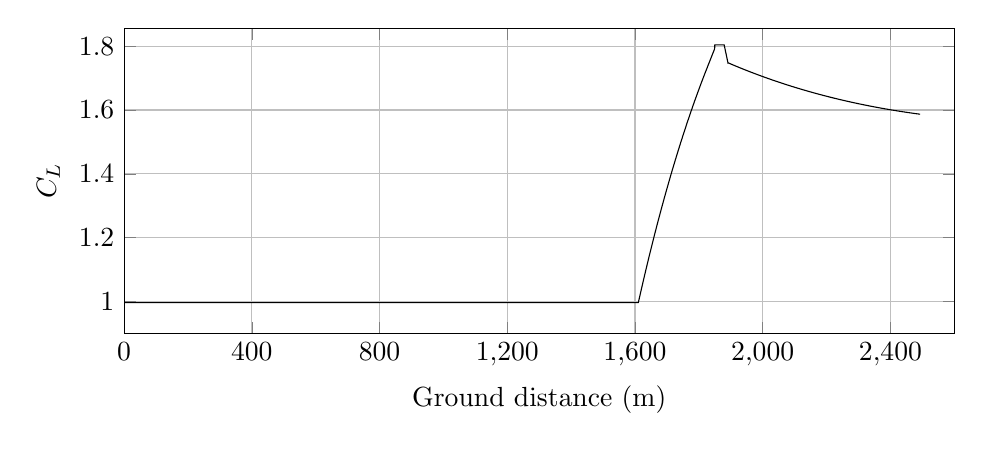
\begin{tikzpicture}

\begin{axis}[
width=\textwidth,
height=0.45\textwidth,
scaled ticks=false, tick label style={/pgf/number format/fixed},
xmin=0.0,
xmax=2600,
xtick={0,400,800,1200,1600,2000,2400,2800,3200},
xlabel={Ground distance (m)},
xmajorgrids,
ymin=0.9,
ymax=1.8562794617918756,
ylabel={$C_L$},
ymajorgrids,
legend style={at={(1.03,0.5)},anchor=west,draw=black,fill=white,legend cell align=left}
]

\addplot [
color=black,
solid
]
table[row sep=crcr]{
1.3729668748938318E-8	0.9961283491653221\\
1.7493248493808052E-7	0.9961283491653221\\
1.4411937280317895E-6	0.9961283491653221\\
6.602995160656227E-5	0.9961283491653221\\
2.2740573828771224E-4	0.9961283491653221\\
4.8751428921765393E-4	0.9961283491653221\\
8.441986619835749E-4	0.9961283491653221\\
0.0012981647037285577	0.9961283491653221\\
0.0018484379050661159	0.9961283491653221\\
0.0024893731755424335	0.9961283491653221\\
0.0032286585096692284	0.9961283491653221\\
0.0040442418752796045	0.9961283491653221\\
0.004972762654474916	0.9961283491653221\\
0.005990910102221513	0.9961283491653221\\
0.007111389191545643	0.9961283491653221\\
0.008336865178450469	0.9961283491653221\\
0.009664633507451486	0.9961283491653221\\
0.011093815858158905	0.9961283491653221\\
0.01262066151120312	0.9961283491653221\\
0.01419454386807839	0.9961283491653221\\
0.015910782250193378	0.9961283491653221\\
0.017721549103721458	0.9961283491653221\\
0.019620507964630857	0.9961283491653221\\
0.02164969955342029	0.9961283491653221\\
0.023766550611781796	0.9961283491653221\\
0.025957065600157342	0.9961283491653221\\
0.028260861173784894	0.9961283491653221\\
0.030668466949245715	0.9961283491653221\\
0.0331489614440674	0.9961283491653221\\
0.03573888453685943	0.9961283491653221\\
0.038418765463712895	0.9961283491653221\\
0.04116679597872082	0.9961283491653221\\
0.044022059812866554	0.9961283491653221\\
0.04700053365173311	0.9961283491653221\\
0.050116649382181494	0.9961283491653221\\
0.0533021652593606	0.9961283491653221\\
0.056630220296749106	0.9961283491653221\\
0.05998688030085898	0.9961283491653221\\
0.06348077825220624	0.9961283491653221\\
0.06710848437295475	0.9961283491653221\\
0.07082346760424127	0.9961283491653221\\
0.07462944469130567	0.9961283491653221\\
0.07855413323217031	0.9961283491653221\\
0.08251243142992878	0.9961283491653221\\
0.08659905947434482	0.9961283491653221\\
0.09083545394947079	0.9961283491653221\\
0.09518096637774642	0.9961283491653221\\
0.099604438418047	0.9961283491653221\\
0.1041130762071252	0.9961283491653221\\
0.10871457033213175	0.9961283491653221\\
0.11350280915994052	0.9961283491653221\\
0.11836943512882261	0.9961283491653221\\
0.12328542045494376	0.9961283491653221\\
0.12830372217771202	0.9961283491653221\\
0.1334037067999082	0.9961283491653221\\
0.1386015897371753	0.9961283491653221\\
0.14405085578552257	0.9961283491653221\\
0.1495239325759128	0.9961283491653221\\
0.1550507392415454	0.9961283491653221\\
0.16073360491635535	0.9961283491653221\\
0.16659871679960742	0.9961283491653221\\
0.17244819595229793	0.9961283491653221\\
0.17848031195343078	0.9961283491653221\\
0.18466822548212042	0.9961283491653221\\
0.1909009608611748	0.9961283491653221\\
0.19716089737688902	0.9961283491653221\\
0.2035279375926986	0.9961283491653221\\
0.21017879584430066	0.9961283491653221\\
0.21687473998771628	0.9961283491653221\\
0.22354650324940833	0.9961283491653221\\
0.23036941414946865	0.9961283491653221\\
0.23737731412185503	0.9961283491653221\\
0.24449289925428264	0.9961283491653221\\
0.2517184892023243	0.9961283491653221\\
0.25908208279438383	0.9961283491653221\\
0.2664863589195283	0.9961283491653221\\
0.27399321582905467	0.9961283491653221\\
0.2816108016888421	0.9961283491653221\\
0.2893844725195981	0.9961283491653221\\
0.29747621078120867	0.9961283491653221\\
0.30547198304033185	0.9961283491653221\\
0.31373479402345694	0.9961283491653221\\
0.3220909744202328	0.9961283491653221\\
0.3305540912568814	0.9961283491653221\\
0.33895489345894936	0.9961283491653221\\
0.34753073012810576	0.9961283491653221\\
0.3563589175375672	0.9961283491653221\\
0.3652744752958731	0.9961283491653221\\
0.3742693918027593	0.9961283491653221\\
0.38350989122680823	0.9961283491653221\\
0.3927029292363896	0.9961283491653221\\
0.4020876366599533	0.9961283491653221\\
0.4115568217121528	0.9961283491653221\\
0.4212787852930122	0.9961283491653221\\
0.43089755178065414	0.9961283491653221\\
0.4408379299669313	0.9961283491653221\\
0.4510502611115679	0.9961283491653221\\
0.4612670224725215	0.9961283491653221\\
0.4715818614584312	0.9961283491653221\\
0.4818438670126082	0.9961283491653221\\
0.4922128554044626	0.9961283491653221\\
0.50273876067117	0.9961283491653221\\
0.5136516607865718	0.9961283491653221\\
0.5244310074213006	0.9961283491653221\\
0.5355751508210329	0.9961283491653221\\
0.5467126997993474	0.9961283491653221\\
0.5580479056656631	0.9961283491653221\\
0.5692960823995112	0.9961283491653221\\
0.5809945926573021	0.9961283491653221\\
0.5923626544035139	0.9961283491653221\\
0.6041922852715	0.9961283491653221\\
0.6160912669048675	0.9961283491653221\\
0.6280605196746807	0.9961283491653221\\
0.6403946506485891	0.9961283491653221\\
0.6525721787971039	0.9961283491653221\\
0.66504690021022	0.9961283491653221\\
0.6773535438897555	0.9961283491653221\\
0.6901462526606317	0.9961283491653221\\
0.703249873273524	0.9961283491653221\\
0.7159721017112175	0.9961283491653221\\
0.729053467210389	0.9961283491653221\\
0.7422988791228431	0.9961283491653221\\
0.756304272979474	0.9961283491653221\\
0.7696432036294076	0.9961283491653221\\
0.7832290250230658	0.9961283491653221\\
0.7969128825551131	0.9961283491653221\\
0.8108444209446342	0.9961283491653221\\
0.825043936786227	0.9961283491653221\\
0.8390802275180445	0.9961283491653221\\
0.8532340040587583	0.9961283491653221\\
0.8678101043696134	0.9961283491653221\\
0.8824320602344964	0.9961283491653221\\
0.8978006605470081	0.9961283491653221\\
0.9134572487531922	0.9961283491653221\\
0.9287391767029982	0.9961283491653221\\
0.9440564687433697	0.9961283491653221\\
0.9598871644713316	0.9961283491653221\\
0.9757786228365237	0.9961283491653221\\
0.9918217338879218	0.9961283491653221\\
1.0080608846667363	0.9961283491653221\\
1.0245900975307913	0.9961283491653221\\
1.040622085070809	0.9961283491653221\\
1.0571005809273983	0.9961283491653221\\
1.0736578999152901	0.9961283491653221\\
1.0902401336450098	0.9961283491653221\\
1.1073201062866707	0.9961283491653221\\
1.1241926772552646	0.9961283491653221\\
1.1416781667104252	0.9961283491653221\\
1.1588269484070954	0.9961283491653221\\
1.176440946845327	0.9961283491653221\\
1.1944819542445066	0.9961283491653221\\
1.2120125629913447	0.9961283491653221\\
1.2299306574276825	0.9961283491653221\\
1.2481120482032448	0.9961283491653221\\
1.2663536608165091	0.9961283491653221\\
1.2851425782117465	0.9961283491653221\\
1.3041313368869671	0.9961283491653221\\
1.3228236880779458	0.9961283491653221\\
1.3414329672940513	0.9961283491653221\\
1.3605066144349074	0.9961283491653221\\
1.3802534409605212	0.9961283491653221\\
1.3994872719307283	0.9961283491653221\\
1.4192016277101378	0.9961283491653221\\
1.439023460648384	0.9961283491653221\\
1.459347998039509	0.9961283491653221\\
1.4793256644936217	0.9961283491653221\\
1.4991489338326072	0.9961283491653221\\
1.5195196572175793	0.9961283491653221\\
1.5402684478761244	0.9961283491653221\\
1.5604570108688036	0.9961283491653221\\
1.5810331069622228	0.9961283491653221\\
1.6022712329181132	0.9961283491653221\\
1.623752316257296	0.9961283491653221\\
1.6452514305955401	0.9961283491653221\\
1.6664829631402025	0.9961283491653221\\
1.6886446033619715	0.9961283491653221\\
1.710607384244656	0.9961283491653221\\
1.7329417009553727	0.9961283491653221\\
1.7551421266962821	0.9961283491653221\\
1.7779085356585536	0.9961283491653221\\
1.800478286927734	0.9961283491653221\\
1.8236018329231238	0.9961283491653221\\
1.8462320784511883	0.9961283491653221\\
1.869621217116264	0.9961283491653221\\
1.8933146512119747	0.9961283491653221\\
1.9176856041472643	0.9961283491653221\\
1.9417713639512164	0.9961283491653221\\
1.9657098573982132	0.9961283491653221\\
1.9902165007163162	0.9961283491653221\\
2.014554050520948	0.9961283491653221\\
2.039479559407779	0.9961283491653221\\
2.0645497069116256	0.9961283491653221\\
2.090368502766882	0.9961283491653221\\
2.115564185269416	0.9961283491653221\\
2.140750230554602	0.9961283491653221\\
2.1667677015838267	0.9961283491653221\\
2.1927560352542175	0.9961283491653221\\
2.218891869133375	0.9961283491653221\\
2.245288939563828	0.9961283491653221\\
2.2712530964452817	0.9961283491653221\\
2.297933078351498	0.9961283491653221\\
2.324564104516777	0.9961283491653221\\
2.351466051806102	0.9961283491653221\\
2.378869922986878	0.9961283491653221\\
2.4061764715670764	0.9961283491653221\\
2.4343811693482102	0.9961283491653221\\
2.4622108821536663	0.9961283491653221\\
2.4906408044048067	0.9961283491653221\\
2.518892760285042	0.9961283491653221\\
2.5472153538550346	0.9961283491653221\\
2.5762492306032216	0.9961283491653221\\
2.605385308804288	0.9961283491653221\\
2.634725531238531	0.9961283491653221\\
2.6633424112287507	0.9961283491653221\\
2.6927188130915374	0.9961283491653221\\
2.7226962917814213	0.9961283491653221\\
2.7531675915664673	0.9961283491653221\\
2.7831412651501983	0.9961283491653221\\
2.8139174932165103	0.9961283491653221\\
2.8440331768075415	0.9961283491653221\\
2.874693215323904	0.9961283491653221\\
2.9059978681586376	0.9961283491653221\\
2.9372617813709034	0.9961283491653221\\
2.9684444504378202	0.9961283491653221\\
3.000072782687808	0.9961283491653221\\
3.031082587373527	0.9961283491653221\\
3.063213028467148	0.9961283491653221\\
3.0965739711585014	0.9961283491653221\\
3.1291175748240176	0.9961283491653221\\
3.161651640649506	0.9961283491653221\\
3.194791488147139	0.9961283491653221\\
3.2273698640351327	0.9961283491653221\\
3.261394174200582	0.9961283491653221\\
3.2942820372415875	0.9961283491653221\\
3.3276455142443044	0.9961283491653221\\
3.3625338428565543	0.9961283491653221\\
3.396526624461681	0.9961283491653221\\
3.4305511850311694	0.9961283491653221\\
3.4642094416894933	0.9961283491653221\\
3.498963551783903	0.9961283491653221\\
3.5341885134496573	0.9961283491653221\\
3.569804025802995	0.9961283491653221\\
3.605116576002147	0.9961283491653221\\
3.641338581546833	0.9961283491653221\\
3.677593698357855	0.9961283491653221\\
3.7132425573336665	0.9961283491653221\\
3.74957219375957	0.9961283491653221\\
3.7872650227149185	0.9961283491653221\\
3.825403000593508	0.9961283491653221\\
3.861987998097706	0.9961283491653221\\
3.899535703755137	0.9961283491653221\\
3.9366960368382165	0.9961283491653221\\
3.9756271117991435	0.9961283491653221\\
4.014715979923002	0.9961283491653221\\
4.053268843133694	0.9961283491653221\\
4.093111596873367	0.9961283491653221\\
4.132540645872048	0.9961283491653221\\
4.171686416589186	0.9961283491653221\\
4.211258480423352	0.9961283491653221\\
4.252585425594734	0.9961283491653221\\
4.29253892845542	0.9961283491653221\\
4.332839968385603	0.9961283491653221\\
4.372708537789018	0.9961283491653221\\
4.414379330316386	0.9961283491653221\\
4.455607216042212	0.9961283491653221\\
4.497336690654009	0.9961283491653221\\
4.53836773335787	0.9961283491653221\\
4.579767142935065	0.9961283491653221\\
4.621942908118227	0.9961283491653221\\
4.663798268780793	0.9961283491653221\\
4.705838036060712	0.9961283491653221\\
4.748491012675066	0.9961283491653221\\
4.791393968819099	0.9961283491653221\\
4.835700194867293	0.9961283491653221\\
4.879973298406089	0.9961283491653221\\
4.923250156511948	0.9961283491653221\\
4.967673596314626	0.9961283491653221\\
5.012954369117542	0.9961283491653221\\
5.057574526249477	0.9961283491653221\\
5.103280208347517	0.9961283491653221\\
5.148856018935929	0.9961283491653221\\
5.194350575362858	0.9961283491653221\\
5.240584094986199	0.9961283491653221\\
5.2871741484687504	0.9961283491653221\\
5.333122064003502	0.9961283491653221\\
5.3803318800233235	0.9961283491653221\\
5.4262712259485255	0.9961283491653221\\
5.473378197958581	0.9961283491653221\\
5.521938593493333	0.9961283491653221\\
5.570027890245774	0.9961283491653221\\
5.617746353771608	0.9961283491653221\\
5.665750363096816	0.9961283491653221\\
5.714883880069209	0.9961283491653221\\
5.763390205677501	0.9961283491653221\\
5.812817811268989	0.9961283491653221\\
5.861909274803731	0.9961283491653221\\
5.912134919389196	0.9961283491653221\\
5.962317560553064	0.9961283491653221\\
6.012727788730279	0.9961283491653221\\
6.0628236035803145	0.9961283491653221\\
6.113711068416594	0.9961283491653221\\
6.16497292765713	0.9961283491653221\\
6.216284706244114	0.9961283491653221\\
6.26834407822653	0.9961283491653221\\
6.320257064476769	0.9961283491653221\\
6.37351660191279	0.9961283491653221\\
6.426150862197664	0.9961283491653221\\
6.479030963436509	0.9961283491653221\\
6.532319340056288	0.9961283491653221\\
6.5857233987986845	0.9961283491653221\\
6.640834734692348	0.9961283491653221\\
6.695022999498724	0.9961283491653221\\
6.749720237657193	0.9961283491653221\\
6.804235758325081	0.9961283491653221\\
6.859728469301633	0.9961283491653221\\
6.916686079588434	0.9961283491653221\\
6.9732530286722305	0.9961283491653221\\
7.029531186664631	0.9961283491653221\\
7.086633318514238	0.9961283491653221\\
7.144155485034537	0.9961283491653221\\
7.202053129566568	0.9961283491653221\\
7.260126434764185	0.9961283491653221\\
7.317913145042743	0.9961283491653221\\
7.376682960996439	0.9961283491653221\\
7.435393721764624	0.9961283491653221\\
7.493838107271518	0.9961283491653221\\
7.552684475254578	0.9961283491653221\\
7.613252707151423	0.9961283491653221\\
7.672782806866918	0.9961283491653221\\
7.733397683408512	0.9961283491653221\\
7.795525081709004	0.9961283491653221\\
7.856013653786727	0.9961283491653221\\
7.91792172269443	0.9961283491653221\\
7.980110745884113	0.9961283491653221\\
8.041720670752433	0.9961283491653221\\
8.105229267009985	0.9961283491653221\\
8.167457523036095	0.9961283491653221\\
8.230908874360502	0.9961283491653221\\
8.293738919282273	0.9961283491653221\\
8.356235402336917	0.9961283491653221\\
8.42092378244627	0.9961283491653221\\
8.485671322837007	0.9961283491653221\\
8.549180898871484	0.9961283491653221\\
8.614596634551038	0.9961283491653221\\
8.680166762249144	0.9961283491653221\\
8.744770128469462	0.9961283491653221\\
8.812993689385827	0.9961283491653221\\
8.88005807777586	0.9961283491653221\\
8.94709863067661	0.9961283491653221\\
9.013172088448385	0.9961283491653221\\
9.079266506338545	0.9961283491653221\\
9.14748814890141	0.9961283491653221\\
9.215411293660388	0.9961283491653221\\
9.284579146198691	0.9961283491653221\\
9.353168277381275	0.9961283491653221\\
9.423753765537143	0.9961283491653221\\
9.492960052876374	0.9961283491653221\\
9.564123004975215	0.9961283491653221\\
9.634097601479446	0.9961283491653221\\
9.705672410878787	0.9961283491653221\\
9.776260200085993	0.9961283491653221\\
9.846607984572056	0.9961283491653221\\
9.918231435410593	0.9961283491653221\\
9.988851555070422	0.9961283491653221\\
10.060390022634245	0.9961283491653221\\
10.133279281833644	0.9961283491653221\\
10.205241085147751	0.9961283491653221\\
10.277820389603	0.9961283491653221\\
10.352558894167803	0.9961283491653221\\
10.42733258664746	0.9961283491653221\\
10.501815126481194	0.9961283491653221\\
10.576858173457808	0.9961283491653221\\
10.65303812840548	0.9961283491653221\\
10.729080272001735	0.9961283491653221\\
10.804841544893105	0.9961283491653221\\
10.881905013502095	0.9961283491653221\\
10.958396790746043	0.9961283491653221\\
11.035905069829102	0.9961283491653221\\
11.113160538490881	0.9961283491653221\\
11.192172636140572	0.9961283491653221\\
11.270076562295213	0.9961283491653221\\
11.350065490058778	0.9961283491653221\\
11.429008826667825	0.9961283491653221\\
11.50754237847364	0.9961283491653221\\
11.587076645554472	0.9961283491653221\\
11.668897725768986	0.9961283491653221\\
11.749734371708193	0.9961283491653221\\
11.830312384681939	0.9961283491653221\\
11.909862670519033	0.9961283491653221\\
11.990515423105418	0.9961283491653221\\
12.072973931530203	0.9961283491653221\\
12.155304175892073	0.9961283491653221\\
12.237018674011615	0.9961283491653221\\
12.320146069843414	0.9961283491653221\\
12.406770618003886	0.9961283491653221\\
12.489918686423398	0.9961283491653221\\
12.574493004618496	0.9961283491653221\\
12.660666896522624	0.9961283491653221\\
12.746500366216402	0.9961283491653221\\
12.832006837122272	0.9961283491653221\\
12.919285437479463	0.9961283491653221\\
13.00517529032821	0.9961283491653221\\
13.092301899261269	0.9961283491653221\\
13.179760097773386	0.9961283491653221\\
13.268594687119744	0.9961283491653221\\
13.357699529172354	0.9961283491653221\\
13.44829753340392	0.9961283491653221\\
13.537570218252604	0.9961283491653221\\
13.627322718831184	0.9961283491653221\\
13.718307212496544	0.9961283491653221\\
13.808540263830096	0.9961283491653221\\
13.899143852161355	0.9961283491653221\\
13.991564069206362	0.9961283491653221\\
14.085798171937814	0.9961283491653221\\
14.179213507883688	0.9961283491653221\\
14.271883316076963	0.9961283491653221\\
14.367546274622434	0.9961283491653221\\
14.459430863676705	0.9961283491653221\\
14.555010173556813	0.9961283491653221\\
14.648669731311681	0.9961283491653221\\
14.743773575674254	0.9961283491653221\\
14.839769774519894	0.9961283491653221\\
14.932807148196385	0.9961283491653221\\
15.026921440816679	0.9961283491653221\\
15.12275113649265	0.9961283491653221\\
15.222025232743288	0.9961283491653221\\
15.321078842653048	0.9961283491653221\\
15.417564225728565	0.9961283491653221\\
15.515758841369038	0.9961283491653221\\
15.613440509090129	0.9961283491653221\\
15.7107260301154	0.9961283491653221\\
15.81102223487273	0.9961283491653221\\
15.913565872734136	0.9961283491653221\\
16.012918321571746	0.9961283491653221\\
16.11222833737955	0.9961283491653221\\
16.216250800242257	0.9961283491653221\\
16.319159023020546	0.9961283491653221\\
16.421418004006803	0.9961283491653221\\
16.521675247646563	0.9961283491653221\\
16.62557290942481	0.9961283491653221\\
16.72731964230514	0.9961283491653221\\
16.830283223934416	0.9961283491653221\\
16.93464251494634	0.9961283491653221\\
17.038481620468637	0.9961283491653221\\
17.146497421123335	0.9961283491653221\\
17.252282308638982	0.9961283491653221\\
17.35724772858778	0.9961283491653221\\
17.464053904588297	0.9961283491653221\\
17.572390862630144	0.9961283491653221\\
17.680417629270814	0.9961283491653221\\
17.789707298693855	0.9961283491653221\\
17.899612520762552	0.9961283491653221\\
18.01027367065641	0.9961283491653221\\
18.121415095654797	0.9961283491653221\\
18.232428503320143	0.9961283491653221\\
18.34337337506409	0.9961283491653221\\
18.454877340220463	0.9961283491653221\\
18.56636189702322	0.9961283491653221\\
18.678405595805643	0.9961283491653221\\
18.7903363416971	0.9961283491653221\\
18.902391384512768	0.9961283491653221\\
19.01754810908954	0.9961283491653221\\
19.131359562866663	0.9961283491653221\\
19.247747682986713	0.9961283491653221\\
19.361628242251975	0.9961283491653221\\
19.477963464454028	0.9961283491653221\\
19.595742742603164	0.9961283491653221\\
19.71107288142779	0.9961283491653221\\
19.82767543183723	0.9961283491653221\\
19.944540068808188	0.9961283491653221\\
20.06171535440768	0.9961283491653221\\
20.179291418887807	0.9961283491653221\\
20.29729887224694	0.9961283491653221\\
20.417200571824914	0.9961283491653221\\
20.53676390826074	0.9961283491653221\\
20.65523768803314	0.9961283491653221\\
20.777063017363922	0.9961283491653221\\
20.896922101876633	0.9961283491653221\\
21.016777952410983	0.9961283491653221\\
21.13892104879462	0.9961283491653221\\
21.260534693274344	0.9961283491653221\\
21.382619708556632	0.9961283491653221\\
21.506306369043365	0.9961283491653221\\
21.631260758247265	0.9961283491653221\\
21.75556249187227	0.9961283491653221\\
21.87985606458615	0.9961283491653221\\
22.005925835680863	0.9961283491653221\\
22.130365724585275	0.9961283491653221\\
22.257477980325966	0.9961283491653221\\
22.38418119026224	0.9961283491653221\\
22.50885833858638	0.9961283491653221\\
22.636026948728087	0.9961283491653221\\
22.76367325110224	0.9961283491653221\\
22.89115382514759	0.9961283491653221\\
23.022452271734288	0.9961283491653221\\
23.149877274293033	0.9961283491653221\\
23.27873580881144	0.9961283491653221\\
23.408563766880334	0.9961283491653221\\
23.538692653979794	0.9961283491653221\\
23.671258756997098	0.9961283491653221\\
23.803210122669313	0.9961283491653221\\
23.93544283576786	0.9961283491653221\\
24.067241518013077	0.9961283491653221\\
24.19863541429976	0.9961283491653221\\
24.329449967727697	0.9961283491653221\\
24.46175612159181	0.9961283491653221\\
24.594763714591892	0.9961283491653221\\
24.72754053098891	0.9961283491653221\\
24.86208223890334	0.9961283491653221\\
24.99503410474967	0.9961283491653221\\
25.12831230627787	0.9961283491653221\\
25.265273024090206	0.9961283491653221\\
25.400650037308893	0.9961283491653221\\
25.536304655026747	0.9961283491653221\\
25.673594178904246	0.9961283491653221\\
25.80797730935859	0.9961283491653221\\
25.835159569235522	0.9961283491653221\\
25.83771752397454	0.9961283491653221\\
25.84157983658004	0.9961283491653221\\
25.854829339215996	0.9961283491653221\\
25.893215796826965	0.9961283491653221\\
25.973046119315796	0.9961283491653221\\
26.096262980671412	0.9961283491653221\\
26.224212718725603	0.9961283491653221\\
26.35313595194755	0.9961283491653221\\
26.481727686355264	0.9961283491653221\\
26.611118169629577	0.9961283491653221\\
26.74049186039369	0.9961283491653221\\
26.87228140714948	0.9961283491653221\\
27.003385008924262	0.9961283491653221\\
27.1358830905183	0.9961283491653221\\
27.265951877034226	0.9961283491653221\\
27.399105426781233	0.9961283491653221\\
27.53075869079712	0.9961283491653221\\
27.66387879779476	0.9961283491653221\\
27.79855889054391	0.9961283491653221\\
27.932132547760695	0.9961283491653221\\
28.06791767232785	0.9961283491653221\\
28.202763022922632	0.9961283491653221\\
28.339788243013793	0.9961283491653221\\
28.476803106655623	0.9961283491653221\\
28.61761981788422	0.9961283491653221\\
28.753907949775353	0.9961283491653221\\
28.89297195746854	0.9961283491653221\\
29.03211749902605	0.9961283491653221\\
29.17123509789927	0.9961283491653221\\
29.312253051611236	0.9961283491653221\\
29.454422317169097	0.9961283491653221\\
29.59523538430127	0.9961283491653221\\
29.737672170826222	0.9961283491653221\\
29.879173197948965	0.9961283491653221\\
30.02075470454991	0.9961283491653221\\
30.166674235301365	0.9961283491653221\\
30.308336095430334	0.9961283491653221\\
30.452640844036836	0.9961283491653221\\
30.597553881025625	0.9961283491653221\\
30.742967061600154	0.9961283491653221\\
30.888975484926362	0.9961283491653221\\
31.034653067922946	0.9961283491653221\\
31.180984070508003	0.9961283491653221\\
31.328351020411645	0.9961283491653221\\
31.476753455192622	0.9961283491653221\\
31.62661541983664	0.9961283491653221\\
31.774495604492607	0.9961283491653221\\
31.924944104961916	0.9961283491653221\\
32.07610067279926	0.9961283491653221\\
32.22631826848556	0.9961283491653221\\
32.37899942625752	0.9961283491653221\\
32.528514827654206	0.9961283491653221\\
32.68189139400266	0.9961283491653221\\
32.836069829938495	0.9961283491653221\\
32.99025509482905	0.9961283491653221\\
33.14574197930297	0.9961283491653221\\
33.30072558931056	0.9961283491653221\\
33.455047097713944	0.9961283491653221\\
33.610874563168906	0.9961283491653221\\
33.76926068144728	0.9961283491653221\\
33.92617323250643	0.9961283491653221\\
34.08448787244542	0.9961283491653221\\
34.24243160505006	0.9961283491653221\\
34.40316487172558	0.9961283491653221\\
34.56154208099588	0.9961283491653221\\
34.721775177117024	0.9961283491653221\\
34.88076970836556	0.9961283491653221\\
35.041349106451236	0.9961283491653221\\
35.20329621413198	0.9961283491653221\\
35.364886328651124	0.9961283491653221\\
35.529241615711214	0.9961283491653221\\
35.69117991651797	0.9961283491653221\\
35.85317319416103	0.9961283491653221\\
36.014854298354294	0.9961283491653221\\
36.18095311277159	0.9961283491653221\\
36.34443322746766	0.9961283491653221\\
36.51065106768533	0.9961283491653221\\
36.67635767082788	0.9961283491653221\\
36.842033683894186	0.9961283491653221\\
37.00823867836148	0.9961283491653221\\
37.17279029188734	0.9961283491653221\\
37.33951104811075	0.9961283491653221\\
37.50923941781488	0.9961283491653221\\
37.679358776579846	0.9961283491653221\\
37.845326083883435	0.9961283491653221\\
38.017144746304325	0.9961283491653221\\
38.1852030886141	0.9961283491653221\\
38.35804431104914	0.9961283491653221\\
38.52812920813831	0.9961283491653221\\
38.69960796987526	0.9961283491653221\\
38.87165793928378	0.9961283491653221\\
39.0423941506003	0.9961283491653221\\
39.21436971822614	0.9961283491653221\\
39.38727999643966	0.9961283491653221\\
39.558989012313546	0.9961283491653221\\
39.734752343022535	0.9961283491653221\\
39.908836167348156	0.9961283491653221\\
40.084555009291705	0.9961283491653221\\
40.259186798753746	0.9961283491653221\\
40.43324437115375	0.9961283491653221\\
40.61041052363379	0.9961283491653221\\
40.787318094191775	0.9961283491653221\\
40.96620398302343	0.9961283491653221\\
41.14141336180775	0.9961283491653221\\
41.31941103282654	0.9961283491653221\\
41.49571226203258	0.9961283491653221\\
41.67366972437729	0.9961283491653221\\
41.85219319429197	0.9961283491653221\\
42.03136872634711	0.9961283491653221\\
42.21293422072888	0.9961283491653221\\
42.39366932880948	0.9961283491653221\\
42.57479521797359	0.9961283491653221\\
42.75522531040919	0.9961283491653221\\
42.93775785970641	0.9961283491653221\\
43.11993568316029	0.9961283491653221\\
43.30336620712447	0.9961283491653221\\
43.48720879745599	0.9961283491653221\\
43.672226884455625	0.9961283491653221\\
43.85684130549208	0.9961283491653221\\
44.039851952877484	0.9961283491653221\\
44.22449378650157	0.9961283491653221\\
44.412385508552646	0.9961283491653221\\
44.59783063297877	0.9961283491653221\\
44.78525507043919	0.9961283491653221\\
44.973130075825196	0.9961283491653221\\
45.16145211071871	0.9961283491653221\\
45.34881478087516	0.9961283491653221\\
45.536017136752506	0.9961283491653221\\
45.724971990057284	0.9961283491653221\\
45.91416212467789	0.9961283491653221\\
46.10175434018815	0.9961283491653221\\
46.29356928918713	0.9961283491653221\\
46.48490977712943	0.9961283491653221\\
46.67744207882204	0.9961283491653221\\
46.869905949194575	0.9961283491653221\\
47.062749521718516	0.9961283491653221\\
47.25341437235973	0.9961283491653221\\
47.44508461154423	0.9961283491653221\\
47.63880095964302	0.9961283491653221\\
47.83356160493736	0.9961283491653221\\
48.025334057720784	0.9961283491653221\\
48.218846636819876	0.9961283491653221\\
48.41468711090302	0.9961283491653221\\
48.610449575687724	0.9961283491653221\\
48.80723286029129	0.9961283491653221\\
49.00124137999302	0.9961283491653221\\
49.20045899041696	0.9961283491653221\\
49.394243884198005	0.9961283491653221\\
49.59161211700324	0.9961283491653221\\
49.79144608231523	0.9961283491653221\\
49.99107345578199	0.9961283491653221\\
50.18996871950735	0.9961283491653221\\
50.388458331230495	0.9961283491653221\\
50.59191110395449	0.9961283491653221\\
50.79453916783869	0.9961283491653221\\
50.99530158869649	0.9961283491653221\\
51.19776583381373	0.9961283491653221\\
51.3996255264899	0.9961283491653221\\
51.599450409211	0.9961283491653221\\
51.80158475775707	0.9961283491653221\\
52.002311498730975	0.9961283491653221\\
52.2060805474067	0.9961283491653221\\
52.40811442127868	0.9961283491653221\\
52.61423073460446	0.9961283491653221\\
52.821749674584495	0.9961283491653221\\
53.03053110951893	0.9961283491653221\\
53.23753590773735	0.9961283491653221\\
53.44487707917263	0.9961283491653221\\
53.652063533093525	0.9961283491653221\\
53.85975522429668	0.9961283491653221\\
54.06844148636836	0.9961283491653221\\
54.278580968983874	0.9961283491653221\\
54.48685885904548	0.9961283491653221\\
54.69884126905886	0.9961283491653221\\
54.90975544393264	0.9961283491653221\\
55.12216013841277	0.9961283491653221\\
55.333080623240974	0.9961283491653221\\
55.5448885814986	0.9961283491653221\\
55.75594910746132	0.9961283491653221\\
55.968144975063936	0.9961283491653221\\
56.18150915317635	0.9961283491653221\\
56.394069348356695	0.9961283491653221\\
56.60950747146016	0.9961283491653221\\
56.82641599949238	0.9961283491653221\\
57.03980213394583	0.9961283491653221\\
57.25698083573829	0.9961283491653221\\
57.47353804711997	0.9961283491653221\\
57.6941706582635	0.9961283491653221\\
57.91229938529948	0.9961283491653221\\
58.12998527173144	0.9961283491653221\\
58.34905943653719	0.9961283491653221\\
58.56781345824973	0.9961283491653221\\
58.787998582886644	0.9961283491653221\\
59.011266007804366	0.9961283491653221\\
59.23368761368569	0.9961283491653221\\
59.456031473365414	0.9961283491653221\\
59.67976581221534	0.9961283491653221\\
59.90315377467765	0.9961283491653221\\
60.125192111546724	0.9961283491653221\\
60.349269227196444	0.9961283491653221\\
60.57220932044149	0.9961283491653221\\
60.79606803632835	0.9961283491653221\\
61.021718319759984	0.9961283491653221\\
61.25073295331903	0.9961283491653221\\
61.47770893732542	0.9961283491653221\\
61.70784367826464	0.9961283491653221\\
61.93740803875056	0.9961283491653221\\
62.1673491775543	0.9961283491653221\\
62.39648011888062	0.9961283491653221\\
62.62822464633953	0.9961283491653221\\
62.86094183422966	0.9961283491653221\\
63.090532789209604	0.9961283491653221\\
63.321616049163225	0.9961283491653221\\
63.554808975015874	0.9961283491653221\\
63.78685818650332	0.9961283491653221\\
64.0234762327251	0.9961283491653221\\
64.25652029988498	0.9961283491653221\\
64.49146565301734	0.9961283491653221\\
64.72768747885678	0.9961283491653221\\
64.96568125142531	0.9961283491653221\\
65.20057601391298	0.9961283491653221\\
65.43975061379945	0.9961283491653221\\
65.67719429610031	0.9961283491653221\\
65.91652243006087	0.9961283491653221\\
66.1565253585166	0.9961283491653221\\
66.39740384038885	0.9961283491653221\\
66.63777997854328	0.9961283491653221\\
66.87849958303539	0.9961283491653221\\
67.12349409848125	0.9961283491653221\\
67.36843544137562	0.9961283491653221\\
67.61129947098183	0.9961283491653221\\
67.85808619273692	0.9961283491653221\\
68.10323725880951	0.9961283491653221\\
68.3520146383799	0.9961283491653221\\
68.60099753692072	0.9961283491653221\\
68.84943315800746	0.9961283491653221\\
69.09793111574629	0.9961283491653221\\
69.34894754058863	0.9961283491653221\\
69.59791912239118	0.9961283491653221\\
69.84867626946473	0.9961283491653221\\
70.10496107302816	0.9961283491653221\\
70.35594730130109	0.9961283491653221\\
70.60854748652795	0.9961283491653221\\
70.8625286964371	0.9961283491653221\\
71.1182576034713	0.9961283491653221\\
71.37278964945165	0.9961283491653221\\
71.62944082734805	0.9961283491653221\\
71.88536754710964	0.9961283491653221\\
72.14250945057543	0.9961283491653221\\
72.40306402213687	0.9961283491653221\\
72.66241221953337	0.9961283491653221\\
72.92327110344874	0.9961283491653221\\
73.18657203154456	0.9961283491653221\\
73.45150557123125	0.9961283491653221\\
73.71756195569753	0.9961283491653221\\
73.97940051906463	0.9961283491653221\\
74.24514793127645	0.9961283491653221\\
74.51022759525631	0.9961283491653221\\
74.77823256031297	0.9961283491653221\\
75.04767613410795	0.9961283491653221\\
75.31682895458664	0.9961283491653221\\
75.58729746777243	0.9961283491653221\\
75.85729327570917	0.9961283491653221\\
76.13042767774209	0.9961283491653221\\
76.40299665611133	0.9961283491653221\\
76.67973301409052	0.9961283491653221\\
76.95360383527739	0.9961283491653221\\
77.22854206589327	0.9961283491653221\\
77.50692063517303	0.9961283491653221\\
77.78349662592461	0.9961283491653221\\
78.0616064362213	0.9961283491653221\\
78.33869545141144	0.9961283491653221\\
78.62238552181594	0.9961283491653221\\
78.90481169871467	0.9961283491653221\\
79.18659077494928	0.9961283491653221\\
79.4700201012688	0.9961283491653221\\
79.75774957869095	0.9961283491653221\\
80.04430580185078	0.9961283491653221\\
80.33432201731404	0.9961283491653221\\
80.62298533865851	0.9961283491653221\\
80.9130804606989	0.9961283491653221\\
81.20459144967842	0.9961283491653221\\
81.49650140842283	0.9961283491653221\\
81.79224544448738	0.9961283491653221\\
82.08455487090956	0.9961283491653221\\
82.37934996819865	0.9961283491653221\\
82.67580145620735	0.9961283491653221\\
82.97475550983006	0.9961283491653221\\
83.2734238134004	0.9961283491653221\\
83.57209772503273	0.9961283491653221\\
83.87419166445906	0.9961283491653221\\
84.17487194816226	0.9961283491653221\\
84.47686996876752	0.9961283491653221\\
84.78124993153034	0.9961283491653221\\
85.08776945017104	0.9961283491653221\\
85.39395758722245	0.9961283491653221\\
85.69833162305892	0.9961283491653221\\
86.01027818388755	0.9961283491653221\\
86.31658691867341	0.9961283491653221\\
86.62866814828641	0.9961283491653221\\
86.94043673469176	0.9961283491653221\\
87.2565990672368	0.9961283491653221\\
87.56980823017452	0.9961283491653221\\
87.88101387141376	0.9961283491653221\\
88.20007062892054	0.9961283491653221\\
88.51883409355145	0.9961283491653221\\
88.83509784148416	0.9961283491653221\\
89.15857089898353	0.9961283491653221\\
89.47772213402055	0.9961283491653221\\
89.80217214804901	0.9961283491653221\\
90.1263587278685	0.9961283491653221\\
90.44950966725051	0.9961283491653221\\
90.77764749859728	0.9961283491653221\\
91.10470504824352	0.9961283491653221\\
91.43769785174896	0.9961283491653221\\
91.76691749028419	0.9961283491653221\\
92.09386993524024	0.9961283491653221\\
92.42498248438446	0.9961283491653221\\
92.7581696617394	0.9961283491653221\\
93.09729153734631	0.9961283491653221\\
93.4312406900703	0.9961283491653221\\
93.76780571708736	0.9961283491653221\\
94.10390054156983	0.9961283491653221\\
94.43564317419558	0.9961283491653221\\
94.77291201930262	0.9961283491653221\\
95.10796951504997	0.9961283491653221\\
95.44708659079325	0.9961283491653221\\
95.78515592548297	0.9961283491653221\\
96.12311752311894	0.9961283491653221\\
96.46351490415591	0.9961283491653221\\
96.80669869710772	0.9961283491653221\\
97.14657639264556	0.9961283491653221\\
97.48763116340677	0.9961283491653221\\
97.8305814261901	0.9961283491653221\\
98.17013304046878	0.9961283491653221\\
98.51054009051404	0.9961283491653221\\
98.854181194619	0.9961283491653221\\
99.19205317796005	0.9961283491653221\\
99.53355440060989	0.9961283491653221\\
99.87198375587872	0.9961283491653221\\
100.2129389915628	0.9961283491653221\\
100.55335806642802	0.9961283491653221\\
100.89503335592528	0.9961283491653221\\
101.23693480167049	0.9961283491653221\\
101.57977298927813	0.9961283491653221\\
101.91842351185082	0.9961283491653221\\
102.26214655705948	0.9961283491653221\\
102.60487134933112	0.9961283491653221\\
102.94238410388857	0.9961283491653221\\
103.28139950825951	0.9961283491653221\\
103.61984226602698	0.9961283491653221\\
103.95406402656286	0.9961283491653221\\
104.29248504574807	0.9961283491653221\\
104.63112914593611	0.9961283491653221\\
104.96686613984221	0.9961283491653221\\
105.30464484937244	0.9961283491653221\\
105.64180205248229	0.9961283491653221\\
105.97704387437452	0.9961283491653221\\
106.31384964552919	0.9961283491653221\\
106.6489228444834	0.9961283491653221\\
106.98000007373659	0.9961283491653221\\
107.31456925364313	0.9961283491653221\\
107.38092108752608	0.9961283491653221\\
107.387754025128	0.9961283491653221\\
107.3946577511588	0.9961283491653221\\
107.39916951903444	0.9961283491653221\\
107.40247473215817	0.9961283491653221\\
107.40548301099807	0.9961283491653221\\
107.41901751964124	0.9961283491653221\\
107.47756267729525	0.9961283491653221\\
107.63696404402117	0.9961283491653221\\
107.95668166923352	0.9961283491653221\\
108.2571634635643	0.9961283491653221\\
108.55996775705782	0.9961283491653221\\
108.8616926844802	0.9961283491653221\\
109.16669292910967	0.9961283491653221\\
109.47218465327785	0.9961283491653221\\
109.78023369107405	0.9961283491653221\\
110.09061921742381	0.9961283491653221\\
110.4007971847821	0.9961283491653221\\
110.7125096545017	0.9961283491653221\\
111.02874540594937	0.9961283491653221\\
111.34670354521654	0.9961283491653221\\
111.664908557295	0.9961283491653221\\
111.98617551206428	0.9961283491653221\\
112.3078797039536	0.9961283491653221\\
112.63537393275391	0.9961283491653221\\
112.96267359383529	0.9961283491653221\\
113.28778388635178	0.9961283491653221\\
113.61823593045688	0.9961283491653221\\
113.94632344632586	0.9961283491653221\\
114.27926944824554	0.9961283491653221\\
114.61324422041562	0.9961283491653221\\
114.94750338770686	0.9961283491653221\\
115.28618013885716	0.9961283491653221\\
115.62544260296943	0.9961283491653221\\
115.9647508443766	0.9961283491653221\\
116.30617149460878	0.9961283491653221\\
116.65060078043697	0.9961283491653221\\
116.99863777637248	0.9961283491653221\\
117.34270613829636	0.9961283491653221\\
117.68983788345284	0.9961283491653221\\
118.04137408578512	0.9961283491653221\\
118.39343387684602	0.9961283491653221\\
118.74804854616337	0.9961283491653221\\
119.10520175440718	0.9961283491653221\\
119.46686684850098	0.9961283491653221\\
119.82660492256403	0.9961283491653221\\
120.19012449272657	0.9961283491653221\\
120.55217592908159	0.9961283491653221\\
120.91763124996498	0.9961283491653221\\
121.28719248968574	0.9961283491653221\\
121.65493622417088	0.9961283491653221\\
122.02513489718217	0.9961283491653221\\
122.39308995700384	0.9961283491653221\\
122.76618799735454	0.9961283491653221\\
123.1388017253943	0.9961283491653221\\
123.51256311114031	0.9961283491653221\\
123.88633794770595	0.9961283491653221\\
124.25665874611622	0.9961283491653221\\
124.63165231885978	0.9961283491653221\\
125.00664173256905	0.9961283491653221\\
125.38021625899401	0.9961283491653221\\
125.75512563345742	0.9961283491653221\\
126.13473977091255	0.9961283491653221\\
126.51299085225449	0.9961283491653221\\
126.8948287761801	0.9961283491653221\\
127.27325883095315	0.9961283491653221\\
127.64986999110431	0.9961283491653221\\
128.03053456382577	0.9961283491653221\\
128.40840086210045	0.9961283491653221\\
128.78830732782995	0.9961283491653221\\
129.16816802858597	0.9961283491653221\\
129.55114692916032	0.9961283491653221\\
129.92795862154003	0.9961283491653221\\
130.30814318938542	0.9961283491653221\\
130.68801179162523	0.9961283491653221\\
131.0673626953399	0.9961283491653221\\
131.44707508552267	0.9961283491653221\\
131.82575792285303	0.9961283491653221\\
132.20466209461676	0.9961283491653221\\
132.58549544797154	0.9961283491653221\\
132.96520261413826	0.9961283491653221\\
133.34413894748724	0.9961283491653221\\
133.72638850756363	0.9961283491653221\\
134.1049920954593	0.9961283491653221\\
134.48538249769342	0.9961283491653221\\
134.86277461399203	0.9961283491653221\\
135.2402386369938	0.9961283491653221\\
135.62109197355238	0.9961283491653221\\
135.9996509441208	0.9961283491653221\\
136.37968191797512	0.9961283491653221\\
136.76120583273502	0.9961283491653221\\
137.13951930881296	0.9961283491653221\\
137.51840340013064	0.9961283491653221\\
137.89819615735314	0.9961283491653221\\
138.27485697152616	0.9961283491653221\\
138.65420581933705	0.9961283491653221\\
139.03531375767642	0.9961283491653221\\
139.41296882619503	0.9961283491653221\\
139.79422155259	0.9961283491653221\\
140.17408835952057	0.9961283491653221\\
140.5488076998477	0.9961283491653221\\
140.92844631991198	0.9961283491653221\\
141.30483696429354	0.9961283491653221\\
141.68269541512387	0.9961283491653221\\
142.06058279783264	0.9961283491653221\\
142.43991695918288	0.9961283491653221\\
142.81695502902187	0.9961283491653221\\
143.19247254825046	0.9961283491653221\\
143.5733885276352	0.9961283491653221\\
143.94921103219775	0.9961283491653221\\
144.32621366107247	0.9961283491653221\\
144.70408630975157	0.9961283491653221\\
145.08263595865492	0.9961283491653221\\
145.46162624555404	0.9961283491653221\\
145.83827879615103	0.9961283491653221\\
146.21524500988596	0.9961283491653221\\
146.5934755401724	0.9961283491653221\\
146.9730259257883	0.9961283491653221\\
147.3547239944582	0.9961283491653221\\
147.73366854735332	0.9961283491653221\\
148.1136534850276	0.9961283491653221\\
148.49311509785633	0.9961283491653221\\
148.87144514206074	0.9961283491653221\\
149.25360190977045	0.9961283491653221\\
149.6334430260095	0.9961283491653221\\
150.01465687879528	0.9961283491653221\\
150.3940924716125	0.9961283491653221\\
150.77688175221402	0.9961283491653221\\
151.1561678741857	0.9961283491653221\\
151.5352572324847	0.9961283491653221\\
151.91884603110896	0.9961283491653221\\
152.3000376871389	0.9961283491653221\\
152.6837211891089	0.9961283491653221\\
153.06727641570347	0.9961283491653221\\
153.4514076737559	0.9961283491653221\\
153.83522357687116	0.9961283491653221\\
154.21637826964854	0.9961283491653221\\
154.6009164651564	0.9961283491653221\\
154.98403470202834	0.9961283491653221\\
155.36838747168406	0.9961283491653221\\
155.75158064164503	0.9961283491653221\\
156.13576662495046	0.9961283491653221\\
156.5218436740983	0.9961283491653221\\
156.90521285441474	0.9961283491653221\\
157.2916244593892	0.9961283491653221\\
157.6780020855428	0.9961283491653221\\
158.06299451159185	0.9961283491653221\\
158.4509000667514	0.9961283491653221\\
158.83830611621056	0.9961283491653221\\
159.22672413827297	0.9961283491653221\\
159.61474494524106	0.9961283491653221\\
160.0042372884319	0.9961283491653221\\
160.39552304382113	0.9961283491653221\\
160.78478895267375	0.9961283491653221\\
161.17517847278327	0.9961283491653221\\
161.56748129737286	0.9961283491653221\\
161.9609400214345	0.9961283491653221\\
162.35005274814932	0.9961283491653221\\
162.7425950916558	0.9961283491653221\\
163.13607830878885	0.9961283491653221\\
163.53170884953005	0.9961283491653221\\
163.92462594167722	0.9961283491653221\\
164.3198767210975	0.9961283491653221\\
164.7157696028566	0.9961283491653221\\
165.1115317336501	0.9961283491653221\\
165.50739628911128	0.9961283491653221\\
165.90698313288817	0.9961283491653221\\
166.30582458333038	0.9961283491653221\\
166.70591293613995	0.9961283491653221\\
167.1044701422045	0.9961283491653221\\
167.50226971352845	0.9961283491653221\\
167.9010833894181	0.9961283491653221\\
168.3004552315794	0.9961283491653221\\
168.70189335181743	0.9961283491653221\\
169.10576843973695	0.9961283491653221\\
169.50785881751284	0.9961283491653221\\
169.91045494783964	0.9961283491653221\\
170.31331810721775	0.9961283491653221\\
170.71648797717722	0.9961283491653221\\
171.11993291578136	0.9961283491653221\\
171.5247281229082	0.9961283491653221\\
171.92976094083576	0.9961283491653221\\
172.33690302624336	0.9961283491653221\\
172.74259563259648	0.9961283491653221\\
173.1509823323036	0.9961283491653221\\
173.55913088366435	0.9961283491653221\\
173.96636547491187	0.9961283491653221\\
174.37754484483776	0.9961283491653221\\
174.7874876782942	0.9961283491653221\\
175.2012500141185	0.9961283491653221\\
175.6112323385957	0.9961283491653221\\
176.02092514523684	0.9961283491653221\\
176.43326782420013	0.9961283491653221\\
176.8477920653399	0.9961283491653221\\
177.2627043459005	0.9961283491653221\\
177.67839640445425	0.9961283491653221\\
178.09047986160414	0.9961283491653221\\
178.50771992227516	0.9961283491653221\\
178.92514786216543	0.9961283491653221\\
179.34349041668827	0.9961283491653221\\
179.7634585539525	0.9961283491653221\\
180.0836350053749	0.9961283491653221\\
180.18446825846002	0.9961283491653221\\
180.6041229201494	0.9961283491653221\\
181.5278851973348	0.9961283491653221\\
182.40940876889346	0.9961283491653221\\
183.29020149056134	0.9961283491653221\\
184.17127536929127	0.9961283491653221\\
185.05444413874795	0.9961283491653221\\
185.94463812048832	0.9961283491653221\\
186.83342305465118	0.9961283491653221\\
187.72320740690213	0.9961283491653221\\
188.61627250998652	0.9961283491653221\\
189.51597565669658	0.9961283491653221\\
190.41002295084513	0.9961283491653221\\
191.3196934236239	0.9961283491653221\\
192.21828392903763	0.9961283491653221\\
193.1226105375991	0.9961283491653221\\
194.0308739866166	0.9961283491653221\\
194.94664810390913	0.9961283491653221\\
195.8495877725365	0.9961283491653221\\
196.76514896738053	0.9961283491653221\\
197.67776544775052	0.9961283491653221\\
198.59781945634353	0.9961283491653221\\
199.51766543264023	0.9961283491653221\\
200.44351810370483	0.9961283491653221\\
201.3718330130543	0.9961283491653221\\
202.29314309783985	0.9961283491653221\\
203.21971650332063	0.9961283491653221\\
204.14462823093066	0.9961283491653221\\
205.07763860999955	0.9961283491653221\\
206.00476468733177	0.9961283491653221\\
206.93855819187849	0.9961283491653221\\
207.87782366152794	0.9961283491653221\\
208.81805039558168	0.9961283491653221\\
209.75927086542703	0.9961283491653221\\
210.70907141928154	0.9961283491653221\\
211.6546393296269	0.9961283491653221\\
212.59816623974814	0.9961283491653221\\
213.54645843731532	0.9961283491653221\\
214.4982137391426	0.9961283491653221\\
215.45734539338423	0.9961283491653221\\
216.4205873513297	0.9961283491653221\\
217.38237643693935	0.9961283491653221\\
218.35297485781302	0.9961283491653221\\
219.32510845799027	0.9961283491653221\\
220.29279514401117	0.9961283491653221\\
221.26927942590856	0.9961283491653221\\
222.2446078047322	0.9961283491653221\\
223.21462685547237	0.9961283491653221\\
224.19074054242492	0.9961283491653221\\
225.1744490750948	0.9961283491653221\\
226.14733001520318	0.9961283491653221\\
227.14148425007068	0.9961283491653221\\
228.1240128312001	0.9961283491653221\\
229.11886046703495	0.9961283491653221\\
230.11739511657566	0.9961283491653221\\
231.11215533106218	0.9961283491653221\\
232.12301378994505	0.9961283491653221\\
233.1275199718878	0.9961283491653221\\
234.13114028184475	0.9961283491653221\\
235.14028542531037	0.9961283491653221\\
236.15081117254897	0.9961283491653221\\
237.1660420924572	0.9961283491653221\\
238.1886645294469	0.9961283491653221\\
239.21465471906964	0.9961283491653221\\
240.23482884221784	0.9961283491653221\\
241.26021232675805	0.9961283491653221\\
242.3021991810905	0.9961283491653221\\
243.32988353044664	0.9961283491653221\\
244.36880129710033	0.9961283491653221\\
245.4061041381612	0.9961283491653221\\
246.46256617747576	0.9961283491653221\\
247.50478260671736	0.9961283491653221\\
248.56376742117214	0.9961283491653221\\
249.6219134221688	0.9961283491653221\\
250.66481994405478	0.9961283491653221\\
251.72705353011372	0.9961283491653221\\
252.80088254110024	0.9961283491653221\\
253.86267363775482	0.9961283491653221\\
254.94374853170973	0.9961283491653221\\
256.0221053298852	0.9961283491653221\\
257.1056667215428	0.9961283491653221\\
258.2028084304169	0.9961283491653221\\
259.3030712409387	0.9961283491653221\\
260.39721249167394	0.9961283491653221\\
261.49829074545437	0.9961283491653221\\
262.60930370875815	0.9961283491653221\\
263.7179887580877	0.9961283491653221\\
264.8352779160481	0.9961283491653221\\
265.9576164693235	0.9961283491653221\\
267.09103410107514	0.9961283491653221\\
268.20818841649384	0.9961283491653221\\
269.3328220499261	0.9961283491653221\\
270.4661510695621	0.9961283491653221\\
271.5992062566115	0.9961283491653221\\
272.7460111433737	0.9961283491653221\\
273.90093061584855	0.9961283491653221\\
275.05359207729066	0.9961283491653221\\
276.20311568521606	0.9961283491653221\\
277.35310992264476	0.9961283491653221\\
278.5188185905665	0.9961283491653221\\
279.6929356623284	0.9961283491653221\\
280.86252284262184	0.9961283491653221\\
282.05142644191835	0.9961283491653221\\
283.24985431198513	0.9961283491653221\\
284.4388813912709	0.9961283491653221\\
285.6397000671543	0.9961283491653221\\
286.836316139525	0.9961283491653221\\
288.0392161140162	0.9961283491653221\\
289.2556790589223	0.9961283491653221\\
290.48265444814547	0.9961283491653221\\
291.72130155141053	0.9961283491653221\\
292.96100893763946	0.9961283491653221\\
294.1985103575731	0.9961283491653221\\
295.4456267737909	0.9961283491653221\\
296.68519223220017	0.9961283491653221\\
297.9280216368336	0.9961283491653221\\
299.1850487812583	0.9961283491653221\\
300.44412429943463	0.9961283491653221\\
301.7225677950246	0.9961283491653221\\
303.0017748749233	0.9961283491653221\\
304.2792219657807	0.9961283491653221\\
305.56506002795425	0.9961283491653221\\
306.85051236654385	0.9961283491653221\\
308.1437929069215	0.9961283491653221\\
309.44719641798304	0.9961283491653221\\
310.77840358228957	0.9961283491653221\\
312.0849502338091	0.9961283491653221\\
313.4080429046928	0.9961283491653221\\
314.7190184524427	0.9961283491653221\\
316.0311580127236	0.9961283491653221\\
317.3407104164604	0.9961283491653221\\
318.66998531861896	0.9961283491653221\\
319.98030216977895	0.9961283491653221\\
321.3131882515936	0.9961283491653221\\
322.64658699863	0.9961283491653221\\
323.97760893915427	0.9961283491653221\\
325.31447228134823	0.9961283491653221\\
326.6245528491544	0.9961283491653221\\
327.9601785097144	0.9961283491653221\\
329.2784770253418	0.9961283491653221\\
330.6069033330348	0.9961283491653221\\
331.9178806716509	0.9961283491653221\\
333.2333630873429	0.9961283491653221\\
334.5584389845069	0.9961283491653221\\
335.850474636536	0.9961283491653221\\
337.1511723788834	0.9961283491653221\\
338.4381183837047	0.9961283491653221\\
339.72984837001286	0.9961283491653221\\
341.0214788139215	0.9961283491653221\\
342.3149785174073	0.9961283491653221\\
343.60619007360367	0.9961283491653221\\
344.88769479656867	0.9961283491653221\\
346.16492597045556	0.9961283491653221\\
347.44208543988907	0.9961283491653221\\
348.7214970855716	0.9961283491653221\\
349.9975255146603	0.9961283491653221\\
351.26866298989455	0.9961283491653221\\
352.534343347637	0.9961283491653221\\
353.79318608781	0.9961283491653221\\
355.04194064781143	0.9961283491653221\\
356.2900696565431	0.9961283491653221\\
357.5353145753136	0.9961283491653221\\
357.7850582428015	0.9961283491653221\\
358.34364659427206	0.9961283491653221\\
358.3912146679147	0.9961283491653221\\
358.41401903577105	0.9961283491653221\\
358.5450809455632	0.9961283491653221\\
358.7245681548527	0.9961283491653221\\
359.254094841737	0.9961283491653221\\
360.2339632435762	0.9961283491653221\\
361.31185038514695	0.9961283491653221\\
362.3872645146199	0.9961283491653221\\
363.4679309383365	0.9961283491653221\\
364.56333677126634	0.9961283491653221\\
365.6588974221802	0.9961283491653221\\
366.75774424816416	0.9961283491653221\\
367.87135537791175	0.9961283491653221\\
368.9928518144826	0.9961283491653221\\
370.1124569712374	0.9961283491653221\\
371.23921033825184	0.9961283491653221\\
372.37198049913775	0.9961283491653221\\
373.50814429472643	0.9961283491653221\\
374.644008507355	0.9961283491653221\\
375.7850599487498	0.9961283491653221\\
376.9482158284984	0.9961283491653221\\
378.1077665587011	0.9961283491653221\\
379.26973869573817	0.9961283491653221\\
380.44580761476436	0.9961283491653221\\
381.62390672234494	0.9961283491653221\\
382.8144199569183	0.9961283491653221\\
384.00299852894386	0.9961283491653221\\
385.20027356755816	0.9961283491653221\\
386.4087115701377	0.9961283491653221\\
387.627261825594	0.9961283491653221\\
388.847438745123	0.9961283491653221\\
390.08585374585346	0.9961283491653221\\
391.32999859576034	0.9961283491653221\\
392.5794981700179	0.9961283491653221\\
393.8295213861659	0.9961283491653221\\
395.08429723606037	0.9961283491653221\\
396.348052674334	0.9961283491653221\\
397.610529015913	0.9961283491653221\\
398.9011153976112	0.9961283491653221\\
400.18894235692665	0.9961283491653221\\
401.4791306222337	0.9961283491653221\\
402.7830293971008	0.9961283491653221\\
404.0853140496723	0.9961283491653221\\
405.3940039897615	0.9961283491653221\\
406.70640055955323	0.9961283491653221\\
408.00887196551514	0.9961283491653221\\
409.3026454816096	0.9961283491653221\\
410.6132390977027	0.9961283491653221\\
411.9298689998851	0.9961283491653221\\
413.25815553647726	0.9961283491653221\\
414.58952083365057	0.9961283491653221\\
415.918967975221	0.9961283491653221\\
417.2419527990422	0.9961283491653221\\
418.5724204266372	0.9961283491653221\\
419.9001914117176	0.9961283491653221\\
421.22244671332	0.9961283491653221\\
422.5499672440235	0.9961283491653221\\
423.874944258631	0.9961283491653221\\
425.1940527578546	0.9961283491653221\\
426.51214046059533	0.9961283491653221\\
427.8403065447367	0.9961283491653221\\
429.16543732752825	0.9961283491653221\\
430.493480912485	0.9961283491653221\\
431.8120787187414	0.9961283491653221\\
433.13404798305	0.9961283491653221\\
434.45758221825076	0.9961283491653221\\
435.77270008640085	0.9961283491653221\\
437.0762078546635	0.9961283491653221\\
438.3722228261918	0.9961283491653221\\
439.6647932913057	0.9961283491653221\\
440.96010063217216	0.9961283491653221\\
442.2548502943886	0.9961283491653221\\
443.55240151451153	0.9961283491653221\\
444.84015975838133	0.9961283491653221\\
446.12596298338667	0.9961283491653221\\
447.41271623936245	0.9961283491653221\\
448.68923141398216	0.9961283491653221\\
449.96221775008996	0.9961283491653221\\
451.24101119640613	0.9961283491653221\\
452.50923174405136	0.9961283491653221\\
453.7757634438541	0.9961283491653221\\
455.04040758000076	0.9961283491653221\\
456.3187472578254	0.9961283491653221\\
457.5883933736685	0.9961283491653221\\
458.84637863243324	0.9961283491653221\\
460.1173199788476	0.9961283491653221\\
461.37502127563994	0.9961283491653221\\
462.64293744016754	0.9961283491653221\\
463.89875968806496	0.9961283491653221\\
465.1596048263507	0.9961283491653221\\
466.4129938848299	0.9961283491653221\\
467.6761864310754	0.9961283491653221\\
468.92877471797476	0.9961283491653221\\
470.1802840729189	0.9961283491653221\\
471.42234175136343	0.9961283491653221\\
472.66721587755	0.9961283491653221\\
473.9119998681615	0.9961283491653221\\
475.15784183330595	0.9961283491653221\\
476.4027610202945	0.9961283491653221\\
477.64387772945474	0.9961283491653221\\
478.8802799588349	0.9961283491653221\\
480.11938637872606	0.9961283491653221\\
481.3598938784121	0.9961283491653221\\
482.60100270099633	0.9961283491653221\\
483.83761604071765	0.9961283491653221\\
485.07417441604616	0.9961283491653221\\
486.30932624990373	0.9961283491653221\\
487.5485020564116	0.9961283491653221\\
488.78476676571006	0.9961283491653221\\
490.02776083238655	0.9961283491653221\\
491.26052006608825	0.9961283491653221\\
492.50223365857005	0.9961283491653221\\
493.73875790953696	0.9961283491653221\\
494.9705227407086	0.9961283491653221\\
496.20662631815094	0.9961283491653221\\
497.4417048478979	0.9961283491653221\\
498.67979578388963	0.9961283491653221\\
499.9077395058579	0.9961283491653221\\
501.13206886531634	0.9961283491653221\\
502.36560836777835	0.9961283491653221\\
503.5988541698998	0.9961283491653221\\
504.8341308395434	0.9961283491653221\\
506.05800551932055	0.9961283491653221\\
507.27849694883867	0.9961283491653221\\
508.51586902201325	0.9961283491653221\\
509.7437321564099	0.9961283491653221\\
510.9765281767244	0.9961283491653221\\
512.2003190975361	0.9961283491653221\\
513.4213909555808	0.9961283491653221\\
514.6497928055664	0.9961283491653221\\
515.8776846194819	0.9961283491653221\\
517.1060250500084	0.9961283491653221\\
518.3498419555788	0.9961283491653221\\
519.5794414015706	0.9961283491653221\\
520.8101291797705	0.9961283491653221\\
522.0439200808898	0.9961283491653221\\
523.2808555224788	0.9961283491653221\\
524.5125928741788	0.9961283491653221\\
525.741539831949	0.9961283491653221\\
526.9760734195245	0.9961283491653221\\
528.2104121448019	0.9961283491653221\\
529.444482094551	0.9961283491653221\\
530.6778496336067	0.9961283491653221\\
531.9092562002504	0.9961283491653221\\
533.1456875412582	0.9961283491653221\\
534.3827295754174	0.9961283491653221\\
535.6194547718162	0.9961283491653221\\
536.8537227143379	0.9961283491653221\\
538.0899051479412	0.9961283491653221\\
539.3366163711867	0.9961283491653221\\
540.5793174245275	0.9961283491653221\\
541.8175341103783	0.9961283491653221\\
543.0580254609008	0.9961283491653221\\
544.2905932367662	0.9961283491653221\\
545.5264322163653	0.9961283491653221\\
546.7679638454138	0.9961283491653221\\
548.0058826203228	0.9961283491653221\\
549.247222977644	0.9961283491653221\\
550.4927278587875	0.9961283491653221\\
551.7284048687036	0.9961283491653221\\
552.969156750524	0.9961283491653221\\
554.2147139753856	0.9961283491653221\\
555.4621950310477	0.9961283491653221\\
556.706538922255	0.9961283491653221\\
557.949692049355	0.9961283491653221\\
559.1956898523235	0.9961283491653221\\
560.4455810647141	0.9961283491653221\\
561.7029824469003	0.9961283491653221\\
562.9528606070708	0.9961283491653221\\
564.2038089647817	0.9961283491653221\\
565.4583765420568	0.9961283491653221\\
566.708587276828	0.9961283491653221\\
567.9637216989229	0.9961283491653221\\
569.2171025509995	0.9961283491653221\\
570.474468357347	0.9961283491653221\\
571.742642818326	0.9961283491653221\\
572.996651880251	0.9961283491653221\\
574.2599126777859	0.9961283491653221\\
575.5220984235082	0.9961283491653221\\
576.7831302823038	0.9961283491653221\\
578.0511116485295	0.9961283491653221\\
579.3140861716088	0.9961283491653221\\
580.5820139587681	0.9961283491653221\\
581.8434957563957	0.9961283491653221\\
583.1166272054381	0.9961283491653221\\
584.3893870491142	0.9961283491653221\\
585.6599343818289	0.9961283491653221\\
586.9369288742066	0.9961283491653221\\
588.2179000220438	0.9961283491653221\\
589.4870261901688	0.9961283491653221\\
590.7657581143835	0.9961283491653221\\
592.0414533779388	0.9961283491653221\\
593.3235970013507	0.9961283491653221\\
594.6058362788467	0.9961283491653221\\
595.8868323916915	0.9961283491653221\\
597.1683432634425	0.9961283491653221\\
598.4446335159173	0.9961283491653221\\
599.730175188072	0.9961283491653221\\
601.0212431507625	0.9961283491653221\\
602.3088641938682	0.9961283491653221\\
603.6034700803755	0.9961283491653221\\
604.8981683781547	0.9961283491653221\\
606.1922330968823	0.9961283491653221\\
607.490120236022	0.9961283491653221\\
608.7939415919918	0.9961283491653221\\
610.0955995359013	0.9961283491653221\\
611.3977783333462	0.9961283491653221\\
612.6917013228608	0.9961283491653221\\
614.0040683383606	0.9961283491653221\\
615.3085862372382	0.9961283491653221\\
616.613602898017	0.9961283491653221\\
617.9265277419127	0.9961283491653221\\
619.2347914209017	0.9961283491653221\\
620.5412253249128	0.9961283491653221\\
621.852908032758	0.9961283491653221\\
623.1679499449649	0.9961283491653221\\
624.4856050257858	0.9961283491653221\\
625.810066181002	0.9961283491653221\\
627.1361220452648	0.9961283491653221\\
628.463359530801	0.9961283491653221\\
629.7942853078969	0.9961283491653221\\
631.1262466617202	0.9961283491653221\\
632.4582408521592	0.9961283491653221\\
633.7950163787261	0.9961283491653221\\
635.1327095290424	0.9961283491653221\\
636.4726195282103	0.9961283491653221\\
637.8068805033517	0.9961283491653221\\
639.1469055652017	0.9961283491653221\\
640.4926300799054	0.9961283491653221\\
641.8418857176027	0.9961283491653221\\
643.1859405998212	0.9961283491653221\\
644.5356315965766	0.9961283491653221\\
645.8822545209948	0.9961283491653221\\
647.233670728461	0.9961283491653221\\
648.5864007556052	0.9961283491653221\\
649.940370298199	0.9961283491653221\\
651.2968611767658	0.9961283491653221\\
652.6588166774502	0.9961283491653221\\
654.0286677329391	0.9961283491653221\\
655.3980147933239	0.9961283491653221\\
656.7651144911501	0.9961283491653221\\
658.1273862384021	0.9961283491653221\\
659.5073029329092	0.9961283491653221\\
660.8826272704664	0.9961283491653221\\
662.2661978885028	0.9961283491653221\\
663.643291595564	0.9961283491653221\\
665.0275285174982	0.9961283491653221\\
666.4147025971529	0.9961283491653221\\
667.8000093843657	0.9961283491653221\\
669.1890308696848	0.9961283491653221\\
670.5841029593273	0.9961283491653221\\
671.984126089166	0.9961283491653221\\
673.3808681330338	0.9961283491653221\\
674.7830165257378	0.9961283491653221\\
676.1898253545012	0.9961283491653221\\
677.5991903091519	0.9961283491653221\\
679.015088371943	0.9961283491653221\\
680.4386457201426	0.9961283491653221\\
681.8569959867716	0.9961283491653221\\
683.2684154764579	0.9961283491653221\\
684.6955822936916	0.9961283491653221\\
686.1210149102426	0.9961283491653221\\
687.5534290554101	0.9961283491653221\\
688.9879916285763	0.9961283491653221\\
690.4246609807328	0.9961283491653221\\
691.8693809894646	0.9961283491653221\\
693.3101354987134	0.9961283491653221\\
694.7516516040589	0.9961283491653221\\
696.1961456892448	0.9961283491653221\\
697.6431450077532	0.9961283491653221\\
699.0946712958735	0.9961283491653221\\
700.5536207415289	0.9961283491653221\\
702.016499890844	0.9961283491653221\\
703.4860872285026	0.9961283491653221\\
704.9634790305677	0.9961283491653221\\
706.4368997325803	0.9961283491653221\\
707.9127625449362	0.9961283491653221\\
709.3962797863628	0.9961283491653221\\
710.8794084854612	0.9961283491653221\\
712.3555872746397	0.9961283491653221\\
713.8437612413873	0.9961283491653221\\
715.3392133125592	0.9961283491653221\\
716.843000235509	0.9961283491653221\\
718.3555772579125	0.9961283491653221\\
719.8612576914384	0.9961283491653221\\
721.363907905622	0.9961283491653221\\
722.8778664981737	0.9961283491653221\\
724.3893964645993	0.9961283491653221\\
725.9153332443707	0.9961283491653221\\
727.4340437680246	0.9961283491653221\\
728.9691946264161	0.9961283491653221\\
730.5018963167051	0.9961283491653221\\
732.0400708691539	0.9961283491653221\\
733.5864821361122	0.9961283491653221\\
735.1330665532416	0.9961283491653221\\
736.6809646870079	0.9961283491653221\\
738.2371436455285	0.9961283491653221\\
739.8017854816455	0.9961283491653221\\
741.3730723556473	0.9961283491653221\\
742.9509937059506	0.9961283491653221\\
744.5305864424283	0.9961283491653221\\
746.113967954703	0.9961283491653221\\
747.6993176375493	0.9961283491653221\\
749.2841200736946	0.9961283491653221\\
750.8901221987192	0.9961283491653221\\
752.4917045033196	0.9961283491653221\\
754.1043880453294	0.9961283491653221\\
755.7247957897362	0.9961283491653221\\
757.350123465433	0.9961283491653221\\
758.9779883422452	0.9961283491653221\\
760.6174244775955	0.9961283491653221\\
762.2471670049172	0.9961283491653221\\
763.8864959469677	0.9961283491653221\\
765.5286451874665	0.9961283491653221\\
767.1876108560682	0.9961283491653221\\
768.8527838772816	0.9961283491653221\\
770.5256520101113	0.9961283491653221\\
772.2062150690381	0.9961283491653221\\
773.8901713847758	0.9961283491653221\\
775.5819238733998	0.9961283491653221\\
777.2817188512629	0.9961283491653221\\
778.9828497337423	0.9961283491653221\\
780.6908914191338	0.9961283491653221\\
782.4072790768848	0.9961283491653221\\
784.1443131244669	0.9961283491653221\\
785.8879055054167	0.9961283491653221\\
787.6332840316636	0.9961283491653221\\
789.3854457283926	0.9961283491653221\\
791.150614729399	0.9961283491653221\\
792.9275189326358	0.9961283491653221\\
794.7078690219801	0.9961283491653221\\
796.4884271284063	0.9961283491653221\\
798.3010390178765	0.9961283491653221\\
800.127460680355	0.9961283491653221\\
801.9391768347505	0.9961283491653221\\
803.7775071319543	0.9961283491653221\\
805.6217304493966	0.9961283491653221\\
807.4652472742337	0.9961283491653221\\
809.3346687612084	0.9961283491653221\\
811.2083986459545	0.9961283491653221\\
813.1006487758623	0.9961283491653221\\
815.0050871107928	0.9961283491653221\\
816.9276441884065	0.9961283491653221\\
818.8689876349765	0.9961283491653221\\
820.8183532152264	0.9961283491653221\\
822.7755491014664	0.9961283491653221\\
824.7452211297996	0.9961283491653221\\
826.7429412153915	0.9961283491653221\\
828.7613686297161	0.9961283491653221\\
830.7884573079714	0.9961283491653221\\
832.828736080513	0.9961283491653221\\
834.9046256554884	0.9961283491653221\\
837.0114805828528	0.9961283491653221\\
839.1225712464998	0.9961283491653221\\
841.2731456998592	0.9961283491653221\\
843.4451716536778	0.9961283491653221\\
845.6259741016938	0.9961283491653221\\
847.8606760357923	0.9961283491653221\\
850.1208659733229	0.9961283491653221\\
852.4072054021524	0.9961283491653221\\
854.6894106389352	0.9961283491653221\\
857.0206263933742	0.9961283491653221\\
859.351860599884	0.9961283491653221\\
861.6956235055641	0.9961283491653221\\
864.0809230193477	0.9961283491653221\\
866.4729453807156	0.9961283491653221\\
868.8505739467978	0.9961283491653221\\
871.2321917628958	0.9961283491653221\\
873.6030973799157	0.9961283491653221\\
875.9559955009365	0.9961283491653221\\
878.2807840446324	0.9961283491653221\\
880.587891005154	0.9961283491653221\\
882.8626320583053	0.9961283491653221\\
885.1225565401078	0.9961283491653221\\
887.3480853176877	0.9961283491653221\\
889.5620345079099	0.9961283491653221\\
891.7304167933539	0.9961283491653221\\
893.8751088534989	0.9961283491653221\\
896.0261261085977	0.9961283491653221\\
898.1309922927635	0.9961283491653221\\
900.2326939775073	0.9961283491653221\\
902.3196796609091	0.9961283491653221\\
904.395999618223	0.9961283491653221\\
906.4488598365222	0.9961283491653221\\
908.4734246133198	0.9961283491653221\\
910.4886481023309	0.9961283491653221\\
912.4998117561495	0.9961283491653221\\
914.4817648890871	0.9961283491653221\\
916.4660406044704	0.9961283491653221\\
918.4368350154689	0.9961283491653221\\
920.3847916817979	0.9961283491653221\\
922.3381019626172	0.9961283491653221\\
924.2667962694686	0.9961283491653221\\
926.1746743338263	0.9961283491653221\\
928.0830302852894	0.9961283491653221\\
929.9834739104342	0.9961283491653221\\
931.8773536632029	0.9961283491653221\\
933.7613227348986	0.9961283491653221\\
935.6293361496487	0.9961283491653221\\
937.4925021199458	0.9961283491653221\\
939.3482853811552	0.9961283491653221\\
941.1878470693061	0.9961283491653221\\
941.5553186827369	0.9961283491653221\\
941.8072895200994	0.9961283491653221\\
941.9750419552138	0.9961283491653221\\
942.1271197160249	0.9961283491653221\\
942.2334325425763	0.9961283491653221\\
942.2638346188435	0.9961283491653221\\
942.2892369539902	0.9961283491653221\\
942.3142175675691	0.9961283491653221\\
942.485900152953	0.9961283491653221\\
943.0589388091298	0.9961283491653221\\
945.0389423283557	0.9961283491653221\\
946.833978762777	0.9961283491653221\\
948.6304534556368	0.9961283491653221\\
950.4439821025769	0.9961283491653221\\
952.2743006168116	0.9961283491653221\\
954.1043114076579	0.9961283491653221\\
955.9587036375908	0.9961283491653221\\
957.8214130903962	0.9961283491653221\\
959.6880133585512	0.9961283491653221\\
961.5705683718347	0.9961283491653221\\
963.4691274632328	0.9961283491653221\\
965.3799468679672	0.9961283491653221\\
967.303567080218	0.9961283491653221\\
969.249430755759	0.9961283491653221\\
971.2103887374251	0.9961283491653221\\
973.1797263714714	0.9961283491653221\\
975.1648586450763	0.9961283491653221\\
977.167899909447	0.9961283491653221\\
979.1914625168572	0.9961283491653221\\
981.2231615224496	0.9961283491653221\\
983.2827075787545	0.9961283491653221\\
985.3542337326639	0.9961283491653221\\
987.4323877978486	0.9961283491653221\\
989.5425714128878	0.9961283491653221\\
991.6598808029521	0.9961283491653221\\
993.8204456533306	0.9961283491653221\\
995.9839346123126	0.9961283491653221\\
998.1864770000634	0.9961283491653221\\
1000.3922002439062	0.9961283491653221\\
1002.6270345530863	0.9961283491653221\\
1004.8745995143443	0.9961283491653221\\
1007.1471979082173	0.9961283491653221\\
1009.4424926286526	0.9961283491653221\\
1011.7467619954873	0.9961283491653221\\
1014.0483899295439	0.9961283491653221\\
1016.3973453828874	0.9961283491653221\\
1018.7366981348446	0.9961283491653221\\
1021.0722856382722	0.9961283491653221\\
1023.4243231675273	0.9961283491653221\\
1025.7588128090124	0.9961283491653221\\
1028.088775604409	0.9961283491653221\\
1030.4145296909378	0.9961283491653221\\
1032.7408393953942	0.9961283491653221\\
1035.065679431843	0.9961283491653221\\
1037.35962020532	0.9961283491653221\\
1039.6467054896502	0.9961283491653221\\
1041.911281890793	0.9961283491653221\\
1044.1670537964305	0.9961283491653221\\
1046.4144315253666	0.9961283491653221\\
1048.6401135402712	0.9961283491653221\\
1050.856648472272	0.9961283491653221\\
1053.0660782914179	0.9961283491653221\\
1055.2676035326776	0.9961283491653221\\
1057.4437387850207	0.9961283491653221\\
1059.6057076599227	0.9961283491653221\\
1061.7573708263599	0.9961283491653221\\
1063.9023616350323	0.9961283491653221\\
1066.029616250597	0.9961283491653221\\
1068.1575813820505	0.9961283491653221\\
1070.2619333766766	0.9961283491653221\\
1072.3612812062906	0.9961283491653221\\
1074.4576032664554	0.9961283491653221\\
1076.5406588764508	0.9961283491653221\\
1078.61282918597	0.9961283491653221\\
1080.6792045529783	0.9961283491653221\\
1082.7403327168904	0.9961283491653221\\
1084.786451813297	0.9961283491653221\\
1086.8427961973612	0.9961283491653221\\
1088.8812839993197	0.9961283491653221\\
1090.9160875494886	0.9961283491653221\\
1092.9524149143995	0.9961283491653221\\
1094.9697152376666	0.9961283491653221\\
1096.9849925092835	0.9961283491653221\\
1099.0097152749563	0.9961283491653221\\
1101.014263576512	0.9961283491653221\\
1103.013755714373	0.9961283491653221\\
1105.0180515713723	0.9961283491653221\\
1107.0152876272014	0.9961283491653221\\
1109.0116694653652	0.9961283491653221\\
1110.9997729233996	0.9961283491653221\\
1112.9842817461008	0.9961283491653221\\
1114.9670598985422	0.9961283491653221\\
1116.9441565631928	0.9961283491653221\\
1118.914136360449	0.9961283491653221\\
1120.875942748365	0.9961283491653221\\
1122.8363925803328	0.9961283491653221\\
1124.793573531077	0.9961283491653221\\
1126.754628486844	0.9961283491653221\\
1128.7174516565929	0.9961283491653221\\
1130.673562944433	0.9961283491653221\\
1132.6270328821297	0.9961283491653221\\
1134.5750080536745	0.9961283491653221\\
1136.5201028723918	0.9961283491653221\\
1138.463213042216	0.9961283491653221\\
1140.400183502752	0.9961283491653221\\
1142.3536718775108	0.9961283491653221\\
1144.2952531804822	0.9961283491653221\\
1146.2340468855873	0.9961283491653221\\
1148.170670440038	0.9961283491653221\\
1150.1084438514254	0.9961283491653221\\
1152.0431048740106	0.9961283491653221\\
1153.9743672503878	0.9961283491653221\\
1155.902814303574	0.9961283491653221\\
1157.822105210536	0.9961283491653221\\
1159.7498975209191	0.9961283491653221\\
1161.6782807135637	0.9961283491653221\\
1163.610803787291	0.9961283491653221\\
1165.5377540298314	0.9961283491653221\\
1167.4614237231517	0.9961283491653221\\
1169.3836492861633	0.9961283491653221\\
1171.310628058558	0.9961283491653221\\
1173.2344542913024	0.9961283491653221\\
1175.1552581945084	0.9961283491653221\\
1177.0682899172634	0.9961283491653221\\
1178.9834254473712	0.9961283491653221\\
1180.905362157503	0.9961283491653221\\
1182.8306855629276	0.9961283491653221\\
1184.753919380652	0.9961283491653221\\
1186.6672765394205	0.9961283491653221\\
1188.5767761231618	0.9961283491653221\\
1190.4928354266272	0.9961283491653221\\
1192.4047561212783	0.9961283491653221\\
1194.3113714820092	0.9961283491653221\\
1196.2250966473443	0.9961283491653221\\
1198.1444855163254	0.9961283491653221\\
1200.0570095215603	0.9961283491653221\\
1201.9707775430425	0.9961283491653221\\
1203.8875296068659	0.9961283491653221\\
1205.8114342395852	0.9961283491653221\\
1207.7295370423903	0.9961283491653221\\
1209.6412346483826	0.9961283491653221\\
1211.546650356423	0.9961283491653221\\
1213.464807681793	0.9961283491653221\\
1215.3817799693998	0.9961283491653221\\
1217.2990646860626	0.9961283491653221\\
1219.2148650045415	0.9961283491653221\\
1221.1336074094256	0.9961283491653221\\
1223.0459268578893	0.9961283491653221\\
1224.9555615306185	0.9961283491653221\\
1226.87874755058	0.9961283491653221\\
1228.7992827677613	0.9961283491653221\\
1230.7210544738005	0.9961283491653221\\
1232.6522180124111	0.9961283491653221\\
1234.5723128864006	0.9961283491653221\\
1236.4892493282555	0.9961283491653221\\
1238.4094467172526	0.9961283491653221\\
1240.330567800137	0.9961283491653221\\
1242.2532883828103	0.9961283491653221\\
1244.1778348867242	0.9961283491653221\\
1246.1021725194773	0.9961283491653221\\
1248.034260626153	0.9961283491653221\\
1249.9589987865702	0.9961283491653221\\
1251.8925257863975	0.9961283491653221\\
1253.8175467041783	0.9961283491653221\\
1255.7446750185836	0.9961283491653221\\
1257.683828698674	0.9961283491653221\\
1259.6288552693309	0.9961283491653221\\
1261.5700677685081	0.9961283491653221\\
1263.5056509038063	0.9961283491653221\\
1265.4399371750083	0.9961283491653221\\
1267.3724921095936	0.9961283491653221\\
1269.3106090597444	0.9961283491653221\\
1271.2509189396328	0.9961283491653221\\
1273.1894544818074	0.9961283491653221\\
1275.1271176101968	0.9961283491653221\\
1277.0737811863355	0.9961283491653221\\
1279.0205688489223	0.9961283491653221\\
1280.9619261703406	0.9961283491653221\\
1282.9089196184545	0.9961283491653221\\
1284.853915689303	0.9961283491653221\\
1286.7998529713013	0.9961283491653221\\
1288.7575353563957	0.9961283491653221\\
1290.7068568138038	0.9961283491653221\\
1292.667550924852	0.9961283491653221\\
1294.6298416738073	0.9961283491653221\\
1296.585610640696	0.9961283491653221\\
1298.5364644524352	0.9961283491653221\\
1300.5043079150082	0.9961283491653221\\
1302.463285873584	0.9961283491653221\\
1304.423917537441	0.9961283491653221\\
1306.3845814418605	0.9961283491653221\\
1308.3567932623114	0.9961283491653221\\
1310.3299763699888	0.9961283491653221\\
1312.3057240798003	0.9961283491653221\\
1314.2751976786394	0.9961283491653221\\
1316.2468393089366	0.9961283491653221\\
1318.218450638225	0.9961283491653221\\
1320.1966037007583	0.9961283491653221\\
1322.1762863250883	0.9961283491653221\\
1324.1615811380661	0.9961283491653221\\
1326.1499145269418	0.9961283491653221\\
1328.143058355245	0.9961283491653221\\
1330.1344896536734	0.9961283491653221\\
1332.1313221526002	0.9961283491653221\\
1334.1282466623647	0.9961283491653221\\
1336.1270724454225	0.9961283491653221\\
1338.1250364961247	0.9961283491653221\\
1340.1284576816079	0.9961283491653221\\
1342.1395178531202	0.9961283491653221\\
1344.1445804885775	0.9961283491653221\\
1346.1574125856296	0.9961283491653221\\
1348.1732142326268	0.9961283491653221\\
1350.1857861038566	0.9961283491653221\\
1352.1980533035658	0.9961283491653221\\
1354.213016696458	0.9961283491653221\\
1356.2392178282616	0.9961283491653221\\
1358.2612355545957	0.9961283491653221\\
1360.2829315912777	0.9961283491653221\\
1362.3112907203654	0.9961283491653221\\
1364.3401188503472	0.9961283491653221\\
1366.3688330727769	0.9961283491653221\\
1368.3991767255475	0.9961283491653221\\
1370.4329762306343	0.9961283491653221\\
1372.4742107712154	0.9961283491653221\\
1374.5121704146904	0.9961283491653221\\
1376.560792741679	0.9961283491653221\\
1378.6116646682435	0.9961283491653221\\
1380.6582652692368	0.9961283491653221\\
1382.708836578745	0.9961283491653221\\
1384.7595354883733	0.9961283491653221\\
1386.8140923107999	0.9961283491653221\\
1388.870156362383	0.9961283491653221\\
1390.9342214011895	0.9961283491653221\\
1393.0044558044638	0.9961283491653221\\
1395.063323867896	0.9961283491653221\\
1397.1326154137805	0.9961283491653221\\
1399.219723933183	0.9961283491653221\\
1401.30194878957	0.9961283491653221\\
1403.3785629376544	0.9961283491653221\\
1405.4612987085643	0.9961283491653221\\
1407.550631374383	0.9961283491653221\\
1409.6425634454204	0.9961283491653221\\
1411.741120931942	0.9961283491653221\\
1413.8396353751555	0.9961283491653221\\
1415.9551913367977	0.9961283491653221\\
1418.0567646075056	0.9961283491653221\\
1420.1694209106213	0.9961283491653221\\
1422.2752279611586	0.9961283491653221\\
1424.396524298963	0.9961283491653221\\
1426.5047814210384	0.9961283491653221\\
1428.6235115980066	0.9961283491653221\\
1430.7465728812963	0.9961283491653221\\
1432.8691190687719	0.9961283491653221\\
1434.999713958227	0.9961283491653221\\
1437.1275439535561	0.9961283491653221\\
1439.265193447574	0.9961283491653221\\
1441.4162349954395	0.9961283491653221\\
1443.5641381285836	0.9961283491653221\\
1445.7116098542228	0.9961283491653221\\
1447.8618160969058	0.9961283491653221\\
1450.0220067224232	0.9961283491653221\\
1452.186033528917	0.9961283491653221\\
1454.346596255873	0.9961283491653221\\
1456.510104144481	0.9961283491653221\\
1458.6862561858352	0.9961283491653221\\
1460.8620405464167	0.9961283491653221\\
1463.0423091417429	0.9961283491653221\\
1465.2313728278568	0.9961283491653221\\
1467.4248277347078	0.9961283491653221\\
1469.6155133174375	0.9961283491653221\\
1471.8253471572089	0.9961283491653221\\
1474.0257992571974	0.9961283491653221\\
1476.2308549099557	0.9961283491653221\\
1478.4375256491403	0.9961283491653221\\
1480.6462013761638	0.9961283491653221\\
1482.862500235421	0.9961283491653221\\
1485.0774136415125	0.9961283491653221\\
1487.3037843131824	0.9961283491653221\\
1489.5399819377672	0.9961283491653221\\
1491.779926277085	0.9961283491653221\\
1494.0177208733035	0.9961283491653221\\
1496.2655834024904	0.9961283491653221\\
1498.5077626753755	0.9961283491653221\\
1500.7528968219208	0.9961283491653221\\
1503.0072755075562	0.9961283491653221\\
1505.2722922974813	0.9961283491653221\\
1507.5438818632656	0.9961283491653221\\
1509.8120076434325	0.9961283491653221\\
1512.0854641963383	0.9961283491653221\\
1514.3661726741616	0.9961283491653221\\
1516.6526166535755	0.9961283491653221\\
1518.936168659298	0.9961283491653221\\
1521.2311717509797	0.9961283491653221\\
1523.5301289186373	0.9961283491653221\\
1525.8364797809136	0.9961283491653221\\
1528.1409924599943	0.9961283491653221\\
1530.4531714544846	0.9961283491653221\\
1532.7673050722497	0.9961283491653221\\
1535.089830191092	0.9961283491653221\\
1537.4221293231467	0.9961283491653221\\
1539.7649651999382	0.9961283491653221\\
1542.1244695348323	0.9961283491653221\\
1544.4749443191067	0.9961283491653221\\
1546.832152099958	0.9961283491653221\\
1549.2027538171546	0.9961283491653221\\
1551.576368856267	0.9961283491653221\\
1553.9541655636413	0.9961283491653221\\
1556.3483786695847	0.9961283491653221\\
1558.731614878061	0.9961283491653221\\
1561.126924894555	0.9961283491653221\\
1563.5323922535981	0.9961283491653221\\
1565.940856217324	0.9961283491653221\\
1568.3542239692833	0.9961283491653221\\
1570.7882368562682	0.9961283491653221\\
1573.216022576752	0.9961283491653221\\
1575.664877044549	0.9961283491653221\\
1578.113969931565	0.9961283491653221\\
1580.560116942193	0.9961283491653221\\
1583.0264572036322	0.9961283491653221\\
1585.500415900547	0.9961283491653221\\
1587.9699344418405	0.9961283491653221\\
1590.4495570663648	0.9961283491653221\\
1592.933374389133	0.9961283491653221\\
1595.4203051158947	0.9961283491653221\\
1597.9277702906002	0.9961283491653221\\
1600.4441181634206	0.9961283491653221\\
1602.9517770209277	0.9961283491653221\\
1605.4686155218583	0.9961283491653221\\
1607.8577372434938	0.9961283491653221\\
1608.003528681772	0.9961283491653221\\
1610.5516978980709	0.9967816967866663\\
1613.0905084078154	1.0081940547744892\\
1615.6614863230243	1.0194880884003925\\
1618.2379767386738	1.0308486462648725\\
1620.8169640500705	1.0421564478951222\\
1623.41657930992	1.0533984270378358\\
1626.0200270339037	1.0646534082947805\\
1628.628559742323	1.075847928437089\\
1631.2452841297986	1.0869875701799365\\
1633.864814779607	1.098085631721478\\
1636.499650161189	1.1091192898139943\\
1639.159726617785	1.1201411417877236\\
1641.8209673919619	1.1311916998406555\\
1644.4969963019153	1.1421700537112836\\
1647.1752113005878	1.153132485118571\\
1649.8757163853857	1.1640270549216767\\
1652.5893952265938	1.1749353500343787\\
1655.3011602875408	1.1858194977865366\\
1658.0429382083275	1.196618899431597\\
1660.7952235592488	1.2074605276724693\\
1663.5452814584196	1.2182658782737132\\
1666.3112065645337	1.228985044083662\\
1669.0853220514177	1.2396888251745748\\
1671.8977147170835	1.250347011299842\\
1674.7083341517205	1.261074258810004\\
1677.5391595297751	1.2717163779477105\\
1680.381048307765	1.2823567350860365\\
1683.2392202804358	1.2929601761153164\\
1686.113715124835	1.3035457440098424\\
1689.008329686536	1.3141128760970808\\
1691.914059407035	1.324674719583863\\
1694.8354384531817	1.3351976667286536\\
1697.7748379739241	1.345697751265969\\
1700.7382341772354	1.3561828064445935\\
1703.7314427650686	1.3666731753716368\\
1706.7331768048493	1.3771879989372535\\
1709.7755227874086	1.3876513476891206\\
1712.8055266015613	1.398174168788228\\
1715.8574710136932	1.408572184295553\\
1718.9509787727325	1.4189637912908797\\
1722.0533666784518	1.429414197364558\\
1725.19515025577	1.439811264738033\\
1728.3777466258957	1.4502564293416513\\
1731.584431663438	1.4607519291312827\\
1734.8100682816912	1.4712405364607681\\
1738.081926342771	1.4817044168783937\\
1741.3481678809176	1.49223053137302\\
1744.6396111677404	1.502650611446098\\
1747.9834667566029	1.513063380812513\\
1751.3523353848423	1.5235529621273571\\
1754.7637306031606	1.5340307767282497\\
1758.210302356812	1.54454964528646\\
1761.692770148537	1.5550845454034226\\
1765.2066223019078	1.565635702075273\\
1768.7791719664078	1.5761875744814757\\
1772.3783322889353	1.5868198112578247\\
1776.0520426911107	1.5974340004931338\\
1779.7787476886501	1.6081689958762349\\
1783.5542999539466	1.618957332205253\\
1787.379664845822	1.6297838100011854\\
1791.2971182901351	1.6406482186518867\\
1795.2732433554816	1.6516664161280916\\
1799.3757933802694	1.6627388475335236\\
1803.5439314315868	1.6740485130512262\\
1807.755726225022	1.685419992646799\\
1812.079531614439	1.6967898093231515\\
1816.5047078489556	1.7083380975715077\\
1821.0394199948132	1.7200284701922797\\
1825.7508262483598	1.7318748684451766\\
1830.5208910892516	1.7440425521728087\\
1835.3618376987783	1.7562160823452553\\
1840.135360162235	1.7684227697152668\\
1844.8545212674353	1.7803136375431654\\
1849.5089230610292	1.7919288069004518\\
1849.7680155170888	1.8032495780940985\\
1850.0278249091298	1.8038726332669297\\
1850.2830328027203	1.8038726332669297\\
1850.543149722495	1.8038726332669297\\
1850.7955109430636	1.8038726332669297\\
1851.0364885907607	1.8038726332669297\\
1851.2756996224693	1.8038726332669297\\
1851.5333031555506	1.8038726332669297\\
1851.7878674021185	1.8038726332669297\\
1852.044694673853	1.8038726332669297\\
1852.3037919787153	1.8038726332669297\\
1852.56430617274	1.8038726332669297\\
1852.8110975390073	1.8038726332669297\\
1853.0714730634468	1.8038726332669297\\
1853.3203219012753	1.8038726332669297\\
1853.5702689406294	1.8038726332669297\\
1853.8024855472454	1.8038726332669297\\
1854.0629520976413	1.8038726332669297\\
1854.3234346413137	1.8038726332669297\\
1854.576587652169	1.8038726332669297\\
1854.8241088490981	1.8038726332669297\\
1855.0600153861797	1.8038726332669297\\
1855.313153297751	1.8038726332669297\\
1855.5740643498293	1.8038726332669297\\
1855.8331189406867	1.8038726332669297\\
1856.0918483204205	1.8038726332669297\\
1856.3522798245285	1.8038726332669297\\
1856.610745535439	1.8038726332669297\\
1856.8680598609276	1.8038726332669297\\
1857.1301628798406	1.8038726332669297\\
1857.3903759911923	1.8038726332669297\\
1857.6487254117337	1.8038726332669297\\
1857.9106198797485	1.8038726332669297\\
1858.17101031717	1.8038726332669297\\
1858.420257164681	1.8038726332669297\\
1858.6809023648761	1.8038726332669297\\
1858.9373784955383	1.8038726332669297\\
1859.2000917353876	1.8038726332669297\\
1859.451238046457	1.8038726332669297\\
1859.6999141902106	1.8038726332669297\\
1859.95659444264	1.8038726332669297\\
1860.2116896829784	1.8038726332669297\\
1860.4747220530935	1.8038726332669297\\
1860.733735637025	1.8038726332669297\\
1860.9943591584924	1.8038726332669297\\
1861.2470550438888	1.8038726332669297\\
1861.4931632939547	1.8038726332669297\\
1861.7512333242985	1.8038726332669297\\
1861.9977875591449	1.8038726332669297\\
1862.2607292231633	1.8038726332669297\\
1862.5050603265604	1.8038726332669297\\
1862.7583661882923	1.8038726332669297\\
1863.0112866036034	1.8038726332669297\\
1863.260061180108	1.8038726332669297\\
1863.5147320350397	1.8038726332669297\\
1863.7790968246381	1.8038726332669297\\
1864.0415286618158	1.8038726332669297\\
1864.3045814271468	1.8038726332669297\\
1864.5666583385923	1.8038726332669297\\
1864.8272561752506	1.8038726332669297\\
1865.0843687013758	1.8038726332669297\\
1865.3495110157355	1.8038726332669297\\
1865.6139551583829	1.8038726332669297\\
1865.8790664424982	1.8038726332669297\\
1866.1283806902402	1.8038726332669297\\
1866.3856436277124	1.8038726332669297\\
1866.648394839704	1.8038726332669297\\
1866.8893213611855	1.8038726332669297\\
1867.1531387570062	1.8038726332669297\\
1867.4025148903165	1.8038726332669297\\
1867.6662550672345	1.8038726332669297\\
1867.9319460312304	1.8038726332669297\\
1868.197216665495	1.8038726332669297\\
1868.4618106516573	1.8038726332669297\\
1868.7226198231874	1.8038726332669297\\
1868.9751542302683	1.8038726332669297\\
1869.2349101366062	1.8038726332669297\\
1869.4983503297135	1.8038726332669297\\
1869.7610658577046	1.8038726332669297\\
1870.0284270530792	1.8038726332669297\\
1870.2766411684615	1.8038726332669297\\
1870.52757284961	1.8038726332669297\\
1870.7950713433343	1.8038726332669297\\
1871.041251818548	1.8038726332669297\\
1871.276069540137	1.8038726332669297\\
1871.5414416756416	1.8038726332669297\\
1871.8075509315258	1.8038726332669297\\
1872.066009290531	1.8038726332669297\\
1872.333886065347	1.8038726332669297\\
1872.6020786021263	1.8038726332669297\\
1872.869684405598	1.8038726332669297\\
1873.1372973291623	1.8038726332669297\\
1873.3975279841302	1.8038726332669297\\
1873.6649730141708	1.8038726332669297\\
1873.9270204890831	1.8038726332669297\\
1874.1941411793714	1.8038726332669297\\
1874.4520881766912	1.8038726332669297\\
1874.707086993977	1.8038726332669297\\
1874.9755025625568	1.8038726332669297\\
1875.242447914875	1.8038726332669297\\
1875.5040673061694	1.8038726332669297\\
1875.7691382822077	1.8038726332669297\\
1876.0269469458121	1.8038726332669297\\
1876.276871434805	1.8038726332669297\\
1876.5225234331483	1.8038726332669297\\
1876.7900865906836	1.8038726332669297\\
1877.0504466608518	1.8038726332669297\\
1877.3037869076384	1.8038726332669297\\
1877.563253915367	1.8038726332669297\\
1877.8221718021605	1.8038726332669297\\
1878.0901525168752	1.8038726332669297\\
1878.3602268495174	1.8038726332669297\\
1878.6273163531182	1.8038726332669297\\
1878.8755857951887	1.8038726332669297\\
1878.9939049892478	1.8038726332669297\\
1879.144704555441	1.8038726332669297\\
1879.407785154869	1.803160260358227\\
1879.6733440840735	1.8019175062630794\\
1879.9430861107599	1.8006630851972587\\
1880.2075487838597	1.7993889458776229\\
1880.4774585335972	1.7981397843953102\\
1880.7274534793169	1.7968649356350195\\
1880.9765281369469	1.7956841866143498\\
1881.2454277661445	1.7945078199006521\\
1881.5074173350204	1.7932378608820698\\
1881.7775991573913	1.7920005766510723\\
1882.0445798044452	1.790724644614652\\
1882.3013806973076	1.7894638713254722\\
1882.5638299211387	1.7882512089579077\\
1882.808685659974	1.7870119132860547\\
1883.05568493804	1.7858557304723846\\
1883.3252645714388	1.784689461040461\\
1883.5758693222242	1.7834166128291984\\
1883.8465980427327	1.7822333940103494\\
1884.1136961178995	1.780955201422116\\
1884.3657781826419	1.7796941915768336\\
1884.630151027834	1.778504112251218\\
1884.8992892895349	1.7772560474941632\\
1885.167087469917	1.775985527298423\\
1885.4310569192862	1.7747213746738026\\
1885.7008458334653	1.773475336216747\\
1885.9697464181054	1.772201869165791\\
1886.2410067943233	1.7709326370425966\\
1886.498203010351	1.7696523088173852\\
1886.7371129073745	1.7684384016068664\\
1886.9672396030205	1.7673108358776317\\
1887.234770791636	1.7662247547866252\\
1887.497060667985	1.7649621819898493\\
1887.7373424477955	1.7637243849673008\\
1887.9882067946928	1.7625904833854995\\
1888.2534541976775	1.761406677818979\\
1888.5238876313097	1.7601550395964825\\
1888.7929487413217	1.7588789717289899\\
1889.056279730345	1.7576094213924947\\
1889.3219373329412	1.7563669489861358\\
1889.5867367098913	1.755113539719603\\
1889.8483012164488	1.7538642204632588\\
1890.1146128569067	1.752630203269017\\
1890.3683086702972	1.7513738307580278\\
1890.6359756903512	1.7501770140185298\\
1890.9044744641774	1.7489143283460935\\
1891.1738829251904	1.747647760890318\\
1891.441651982785	1.7478951335757367\\
1891.7051715895996	1.7477813372143878\\
1892.0523509312939	1.747631486720918\\
1892.5461394821295	1.747418498988388\\
1893.2361294148736	1.7471211632365153\\
1894.1080442936181	1.7467458977399641\\
1894.9802646536118	1.746371021398248\\
1896.0227506278848	1.7459236476580322\\
1897.0440667390112	1.7454860776894987\\
1898.0211011475903	1.7450681443838634\\
1899.1227192380725	1.7445976977102968\\
1900.1908809604492	1.744142324751303\\
1901.2795489943792	1.7436790045800172\\
1902.3111040693539	1.7432407298419963\\
1903.516105317461	1.7427296722686465\\
1904.7152347580436	1.7422220752725628\\
1905.6910812776046	1.741809707874959\\
1906.7416117969524	1.7413664946415288\\
1907.9861846886483	1.7408423717581172\\
1909.2908509754861	1.7402940524808095\\
1910.5821069761605	1.7397524859539384\\
1911.5334472019326	1.7393541930276286\\
1912.646519756653	1.738888950875376\\
1913.8626295853883	1.7383815792681934\\
1914.9631624354397	1.7379232700447589\\
1916.1621637287426	1.7374248637389729\\
1917.4349617322937	1.7368968168333354\\
1918.5284356502616	1.7364440161890133\\
1919.6599838895809	1.7359762745340153\\
1920.808837787999	1.7355022364632817\\
1921.861670014673	1.7350685755967166\\
1923.1060478197605	1.7345569488140482\\
1924.271747442318	1.7340785843418574\\
1925.3301745960339	1.7336450050302075\\
1926.6461060386255	1.733106952489218\\
1927.9467892519333	1.7325762346879752\\
1929.02376909459	1.7321376205402081\\
1930.1382175507556	1.7316845329838233\\
1931.1449954686836	1.7312759059189695\\
1932.1186859487266	1.7308813267758028\\
1933.1660854998468	1.7304575555246655\\
1933.9181618276389	1.7301537028348122\\
1934.9516813556652	1.729736730923292\\
1936.0147682219758	1.7293085403537376\\
1937.0259292581686	1.728901931655167\\
1937.954413806041	1.7285291407594268\\
1938.8638243469477	1.728164538058983\\
1939.9358314356186	1.7277354191244165\\
1940.8092519836628	1.7273863303020986\\
1941.6322714905846	1.727057826282347\\
1942.4827112475432	1.7267188259827242\\
1943.7185435392616	1.726227012370508\\
1944.9695516091256	1.725730136072426\\
1946.2114473476067	1.7252378489145788\\
1947.4542731898132	1.724746158469879\\
1948.534004309879	1.724319774451506\\
1949.400361336037	1.7239781765966038\\
1950.376690715937	1.7235937768797502\\
1951.2416341246822	1.7232537264043042\\
1952.3771336192149	1.7228080114706785\\
1953.4260322893733	1.7223969986870609\\
1954.6434036013325	1.7219208216232935\\
1955.6178147383334	1.721540337255996\\
1956.5567297385132	1.7211742661115415\\
1957.4053124805018	1.7208438804418815\\
1958.663070645442	1.7203549997906264\\
1959.8765014017454	1.7198842669564327\\
1961.3421895059005	1.7193168742051737\\
1962.705708178613	1.7187902088951217\\
1963.9985420283142	1.7182918903789077\\
1965.2133382966463	1.7178245756792703\\
1966.2912565399297	1.7174106645293836\\
1967.4966389746487	1.7169486402601843\\
1968.7422893154112	1.716472102444222\\
1969.881178366108	1.7160372251519556\\
1971.0538460891294	1.7155902643581493\\
1971.103498407907	1.7155713576570786\\
1971.196903284988	1.7155357947843353\\
1971.2947008540045	1.7154985650505963\\
1971.5446972006912	1.7154034221161305\\
1972.2673096033595	1.7151286229127325\\
1973.0616264257897	1.7148269165240644\\
1974.078201748634	1.7144413404897498\\
1975.2348310496764	1.714003395267107\\
1976.3175052418023	1.7135941767275689\\
1977.5024671629512	1.7131470984750594\\
1978.536693398466	1.7127575761168325\\
1979.6078216299989	1.7123548269984952\\
1980.688815814813	1.7119490604990246\\
1981.8461021602075	1.711515426654712\\
1982.7792480961207	1.7111663572478022\\
1983.8985472295676	1.7107483335606413\\
1985.1549865885268	1.7102799768790349\\
1986.2847348773712	1.7098596442762832\\
1987.309383904848	1.7094790675888452\\
1988.2572858329	1.7091275488466988\\
1989.7042365398288	1.7085919861963565\\
1990.7404957204567	1.708209192231829\\
1991.8716966428283	1.707792048836709\\
1993.0621991626576	1.7073538504027939\\
1994.0502916451233	1.7069907873743522\\
1995.2643000504268	1.706545498991579\\
1996.4821297244612	1.7060996774866284\\
1997.6476939747618	1.7056738029836775\\
1998.855520103732	1.70523332558193\\
1999.9612270131383	1.7048308373159489\\
2001.0486774956216	1.704435690901224\\
2002.0538987620998	1.7040710376532908\\
2003.1669821338178	1.7036679434787858\\
2004.2072541756984	1.703291869421904\\
2005.5238093401167	1.7028168171091\\
2006.5971588700122	1.7024302657481165\\
2007.7089380406342	1.7020305793966362\\
2009.0708553072927	1.7015419444384094\\
2010.2974759263361	1.7011027710262638\\
2011.4157476230725	1.7007031485872786\\
2012.6447775518927	1.7002647791591559\\
2014.0969783418	1.6997479326192786\\
2015.0929514407444	1.699394162738305\\
2016.0900244712357	1.6990405741763237\\
2017.3711127890006	1.6985871054838084\\
2018.8618168205244	1.698060625551958\\
2020.0901802660355	1.697627755937158\\
2021.444604396078	1.6971514652978597\\
2022.8615881226538	1.6966542988607527\\
2024.3017846018374	1.69615016375976\\
2025.5452743973706	1.6957158374059835\\
2026.9421307549887	1.6952289943297474\\
2028.2962080869925	1.6947581212600198\\
2029.590275578661	1.694309090524465\\
2030.9480708997253	1.6938389691176214\\
2032.0922630538826	1.6934436172764133\\
2033.253972618893	1.6930429714734934\\
2034.362658578315	1.6926613245060829\\
2035.6442521791455	1.6922210227700225\\
2036.6806036815942	1.6918656541634134\\
2037.8195745684989	1.691475795783376\\
2039.2534044215768	1.690986049350205\\
2040.5869528225257	1.6905315939419556\\
2041.7669670946098	1.690130294413581\\
2042.9147347157623	1.6897407112754017\\
2044.0439305158388	1.689358152824699\\
2045.245688443249	1.6889517957355897\\
2046.416345303881	1.6885567320229966\\
2047.6696084133987	1.6881346399433972\\
2048.907675238056	1.687718526836273\\
2050.0874749562026	1.6873227925634235\\
2051.4241652162737	1.6868753700052181\\
2052.3471224721834	1.686567014030617\\
2053.370458906973	1.6862256752739113\\
2054.353844512152	1.6858982101675544\\
2055.3211575757987	1.6855766205487561\\
2056.743356825952	1.685104742592364\\
2058.195671584752	1.6846240277499194\\
2059.6817946324663	1.6841333291888136\\
2061.044616514726	1.6836844145792222\\
2062.485712968193	1.6832108298928226\\
2063.7181709768874	1.682806716609046\\
2065.258633198405	1.6823027853550792\\
2066.686432812203	1.6818368728424882\\
2067.832673394234	1.681463646187493\\
2069.076686127941	1.681059398243167\\
2070.275026191166	1.6806707923843267\\
2071.5267459022043	1.6802657140596098\\
2072.250651812652	1.6800318358149418\\
2073.040764151896	1.6797768939154838\\
2073.772622098193	1.6795410522140586\\
2074.5584581518087	1.6792881407877194\\
2075.461553632732	1.6789979058981035\\
2076.2433767360744	1.6787470034074918\\
2077.084595002744	1.678477410736873\\
2078.002226368095	1.6781837673791922\\
2078.9794966809377	1.6778715416964136\\
2079.9381619967926	1.6775657629553489\\
2080.914150629208	1.6772549698718222\\
2081.82580091578	1.6769651300785267\\
2083.0333126042624	1.6765819188750093\\
2084.316345059504	1.6761756031809087\\
2085.6980203032645	1.6757390414356412\\
2087.0400216755615	1.675315999381269\\
2088.3972172227823	1.6748891526733838\\
2089.5168702489236	1.674537759404583\\
2090.8035650496195	1.6741347720981037\\
2091.8271660946757	1.6738148182988901\\
2092.812697101029	1.6735072943225053\\
2094.430898811689	1.673003479025815\\
2095.394096507159	1.672704258489666\\
2096.484959158339	1.672365976140307\\
2097.3594198444853	1.6720952592257705\\
2098.1050908201314	1.6718647349254767\\
2098.939503178679	1.6716071270193071\\
2099.7847113288126	1.671346563572219\\
2100.684467496332	1.671069600981048\\
2101.9069003620916	1.6706940007032287\\
2103.1022387113153	1.6703274916254527\\
2104.365150587566	1.6699410856178318\\
2105.6988089475126	1.669533949668199\\
2106.9502395486406	1.6691527706521947\\
2108.0935819194947	1.668805237220009\\
2109.16125240956	1.6684813274391848\\
2110.1908786985005	1.668169528111588\\
2110.997060175616	1.6679257833999306\\
2112.2161750779806	1.6675578393642347\\
2113.549826350418	1.6671562206438784\\
2115.103143227774	1.6666896271342588\\
2116.613249711013	1.6662372246682455\\
2118.020046108815	1.6658168450895163\\
2118.962358687997	1.6655358408668837\\
2119.9118316949143	1.66525316994153\\
2120.8713552469208	1.6649679842592113\\
2121.9339660867518	1.6646527189219098\\
2123.017150225579	1.664331954354838\\
2124.2332670947935	1.6639725509128493\\
2125.585174286185	1.663573918016885\\
2126.9337612302506	1.663177208298545\\
2127.9536539704513	1.6628778150610402\\
2128.9676374592	1.6625806899643807\\
2129.994565875557	1.6622803132627773\\
2130.992343838676	1.6619889846360771\\
2131.8316140930237	1.6617443343673617\\
2132.7231668729755	1.661484841247702\\
2133.8859513778552	1.6611470191679427\\
2135.3302003930085	1.6607283920318539\\
2136.639550574365	1.660349792580944\\
2138.1571952003924	1.6599120653086925\\
2139.458926272714	1.6595375532894088\\
2140.567816368746	1.6592192062359776\\
2141.9348848394993	1.6588276048457253\\
2143.1482038096674	1.6584808447954975\\
2144.6575621115826	1.658050526066185\\
2146.1948821950673	1.6576134280044432\\
2147.4221979571994	1.6572653346259256\\
2148.6326517196912	1.6569227730785958\\
2149.843663931155	1.656580797370927\\
2150.904972774164	1.65628170724968\\
2151.9031076226884	1.6560009407030136\\
2152.8181169442705	1.6557439993526648\\
2154.0718223501735	1.6553926365922564\\
2155.359865876464	1.6550324765078692\\
2156.791263599517	1.6546332132059414\\
2157.9026491879013	1.6543239231643938\\
2159.030428785174	1.654010705840224\\
2160.0442767740024	1.6537296761171512\\
2160.9797773084983	1.65347082130324\\
2161.7974361724537	1.6532449329693244\\
2162.615249273552	1.6530193371502968\\
2163.43571941937	1.6527933449120407\\
2164.5513122749735	1.652486603667709\\
2165.863579236433	1.6521265814678778\\
2167.248640532568	1.6517475205442411\\
2168.556217049154	1.6513905432112763\\
2169.8854058158104	1.6510285381895524\\
2171.337669909134	1.6506340179967445\\
2172.8428371068176	1.6502262316284713\\
2174.1048516825113	1.649885187291806\\
2175.1544096627695	1.6496021577778646\\
2176.518051811283	1.6492352448283583\\
2178.0959987104097	1.648811816290589\\
2179.5797346714517	1.6484147894964858\\
2180.8031949150572	1.6480882250869466\\
2182.084044530492	1.647747131925875\\
2183.5848748344315	1.6473484837436885\\
2184.9525353590407	1.6469861711243519\\
2186.281843411588	1.646634897696885\\
2187.50651166005	1.6463120416444217\\
2189.0480768365833	1.645906685927511\\
2190.3055219982743	1.6455768995877806\\
2191.501208662082	1.645264026125888\\
2192.556999255169	1.6449883384051989\\
2193.792427926316	1.6446664327967804\\
2194.9957251691403	1.6443536130850531\\
2196.6181915751968	1.6439329360795332\\
2197.93675070281	1.643591997607828\\
2199.155283387465	1.6432776718648534\\
2200.3773851097258	1.6429631472655686\\
2201.284047137321	1.6427302719687458\\
2202.710660857987	1.6423646513702042\\
2204.1012474272356	1.6420092089369005\\
2205.435784119143	1.6416689692739086\\
2206.8837009420895	1.641300792647581\\
2208.3384552714597	1.6409318919708726\\
2209.7528427940433	1.6405742013753077\\
2210.8238631268787	1.6403039843656084\\
2211.9583581488414	1.6400183517859481\\
2213.0185270079355	1.639751988809225\\
2214.2485580741104	1.639443621674339\\
2215.817404837556	1.639051361709487\\
2217.249348545708	1.638694355762401\\
2218.282783791903	1.638437310642404\\
2219.2312135977663	1.6382018557616016\\
2220.118113335644	1.637982062886998\\
2221.083518960764	1.6377432390220577\\
2222.090097858404	1.6374947003825444\\
2223.2577321556564	1.6372069963669613\\
2224.6978195146767	1.636853048943855\\
2226.13746338287	1.6365001904952434\\
2227.5900951403946	1.6361451405112706\\
2228.925183421561	1.635819697795288\\
2230.411189666058	1.635458454210405\\
2231.8255046001905	1.635115603159678\\
2232.9147806486117	1.634852186900148\\
2234.516709920582	1.6344658085880888\\
2235.6644284014837	1.6341897233498843\\
2236.9232640567034	1.6338876176792392\\
2238.4278196308114	1.6335275139640104\\
2239.77681702015	1.6332055405572827\\
2241.005353462486	1.6329130566368797\\
2242.35640130505	1.6325922174549117\\
2243.795481886992	1.632251406723857\\
2245.3051774497744	1.6318949067428752\\
2246.919065359628	1.6315149722174465\\
2248.4666918666608	1.6311517701429978\\
2249.9555155615035	1.6308034139179415\\
2251.59650013595	1.6304206414302815\\
2253.149264896507	1.630059590914874\\
2254.702619456376	1.6296995147192124\\
2256.262489171996	1.6293390453868843\\
2257.850019260106	1.6289733318223483\\
2259.3112053266914	1.6286377455795114\\
2260.6792819393404	1.6283244302530184\\
2261.890500765119	1.6280477531666149\\
2263.111187909886	1.6277695917460844\\
2264.393795161469	1.6274780534506676\\
2265.7775781873233	1.6271643591804306\\
2267.1104864207873	1.62686302266538\\
2268.5089770576014	1.626547728629386\\
2269.831473990209	1.6262503852566808\\
2271.2155949475728	1.6259400368487988\\
2272.8434033064405	1.6255761599448213\\
2274.1988058581455	1.6252740913380923\\
2275.4232144744046	1.6250019305045735\\
2276.5692536565575	1.6247478030721578\\
2278.1665886492046	1.6243945918911504\\
2279.7689518037632	1.624041423853361\\
2281.3910864565332	1.6236850747255689\\
2283.103333131762	1.6233102123268686\\
2284.7365329466993	1.6229538811895632\\
2286.234387858035	1.622628130006953\\
2287.642187070732	1.6223228789874298\\
2289.194706285415	1.6219872752324043\\
2290.6484216706267	1.6216740046246643\\
2292.1550621288643	1.621350322608624\\
2293.4476088748743	1.6210734409604646\\
2294.649092312473	1.6208167323911529\\
2295.9988915399126	1.6205290992956192\\
2297.0900641398093	1.6202971685175231\\
2298.5488700219794	1.619987920686218\\
2299.911746541644	1.6196998595917647\\
2301.2643391589863	1.6194147838953614\\
2302.626566480678	1.6191284939511883\\
2303.940630930054	1.6188531015053889\\
2305.629040111624	1.618500372868689\\
2307.3931114891266	1.618133176863142\\
2309.1886840882207	1.6177608272578088\\
2310.8308662924237	1.617421524121031\\
2312.6352887768026	1.617050060830346\\
2313.9226190146983	1.6167859176802022\\
2315.173481897862	1.6165299503881854\\
2316.733010000373	1.6162117760047583\\
2318.208300531317	1.6159117629870356\\
2319.4162216695586	1.6156668269648753\\
2320.654575408431	1.6154163782986046\\
2322.6312075190644	1.6150179970795409\\
2323.978437238732	1.6147474396917725\\
2325.4035856294277	1.614462089547374\\
2326.9652330579656	1.6141504173128294\\
2328.562754880242	1.6138326749869505\\
2330.2473080813934	1.6134988144953175\\
2331.9681502015346	1.6131590236886686\\
2333.4995890559876	1.6128577026164692\\
2335.07432723932	1.6125489123798935\\
2336.643374004695	1.6122422959239218\\
2337.7526681447616	1.6120261587091298\\
2339.09332573377	1.611765644830066\\
2340.4139989252544	1.6115097654084818\\
2341.9461398372696	1.6112138472758657\\
2343.407677933511	1.6109324982111985\\
2344.512682595285	1.6107203865026847\\
2345.67601387143	1.610497640038768\\
2346.7981333018915	1.6102833295680878\\
2348.2452730736704	1.6100077337394496\\
2349.774527090909	1.6097174651745065\\
2350.95750589398	1.6094936029245264\\
2351.952090763589	1.6093058498771788\\
2353.506502229726	1.6090132529294514\\
2354.810799159359	1.6087685239716616\\
2356.199177256981	1.6085088070825144\\
2357.6371267037857	1.6082406732929637\\
2359.009052379535	1.6079856620791835\\
2360.1532914634045	1.6077735780165112\\
2361.2092480943766	1.6075783449094463\\
2362.32980116254	1.6073716803878821\\
2363.380680938303	1.6071783440652163\\
2364.5385495968303	1.6069658599463699\\
2366.097914984749	1.6066805822896817\\
2367.435427948978	1.6064367010059808\\
2368.8482997480605	1.6061798898916706\\
2370.484802404003	1.6058834707397753\\
2372.0221971936508	1.605606018892796\\
2373.620838419456	1.605318556415978\\
2375.314552688612	1.6050151561779302\\
2376.9331916497813	1.6047263162819339\\
2378.466273483911	1.604453744438405\\
2379.8291004514713	1.6042122591629278\\
2380.95409541311	1.6040134946918492\\
2382.18676960994	1.6037963053274165\\
2383.3685940086216	1.6035886638363606\\
2384.4730624192043	1.603395133710285\\
2385.5139904525413	1.6032131971161478\\
2386.5293539029162	1.6030361581889567\\
2387.6670869805203	1.6028382862564765\\
2388.7426098202786	1.6026517225150947\\
2390.260288219365	1.6023892682422909\\
2391.7468169470794	1.602133115703459\\
2393.2162210842716	1.6018808028426696\\
2394.9695023727527	1.6015808999602983\\
2396.8324092886423	1.6012636203289838\\
2398.27873745963	1.6010182655777612\\
2399.475929685206	1.6008158184930752\\
2400.7432378474305	1.6006021498875735\\
2402.196000979957	1.600358016331009\\
2404.0756674153918	1.6000434136763653\\
2405.9678186640413	1.599728167602582\\
2407.881250846086	1.5994108493022707\\
2409.360449961362	1.5991665569833973\\
2410.6382441626693	1.5989562379668485\\
2411.994790638044	1.5987336770803358\\
2413.1381244352424	1.5985466723928907\\
2414.727197568639	1.5982876356730378\\
2416.4537143539383	1.5980073443528535\\
2418.2688150696213	1.5977139618608598\\
2419.595058503608	1.5975004304324962\\
2420.9244234627768	1.5972871031263856\\
2422.3309245358532	1.5970621670452192\\
2423.6946323101483	1.5968448293731212\\
2424.9275752528592	1.5966489709124303\\
2426.153657698571	1.5964548033299963\\
2427.4897126131054	1.5962439018109185\\
2428.8080834164	1.5960364880785407\\
2430.018943491572	1.5958465972905411\\
2431.482538446572	1.595617849086971\\
2432.911191913974	1.5953953815685074\\
2434.129452646017	1.5952063150059488\\
2435.6077760726885	1.5949776773838542\\
2436.7797398945313	1.5947970355647976\\
2437.875763564497	1.5946285899353705\\
2438.947213454421	1.5944643794028328\\
2440.738908800573	1.5941907955337802\\
2442.4948168348383	1.5939239031443964\\
2444.268569425951	1.593655529900923\\
2445.6343504426113	1.593449726160702\\
2447.056629701474	1.5932361870623433\\
2448.4659464770502	1.593025376379094\\
2449.742487031881	1.592835098229355\\
2451.083522586404	1.5926358932914455\\
2452.832505317844	1.5923771456600744\\
2454.6547872736737	1.592108824147944\\
2455.9735914010053	1.5919154446243025\\
2457.638552760216	1.5916722744494085\\
2459.317438568387	1.5914281623615163\\
2460.8853046450304	1.5912011814526654\\
2462.5246042159315	1.5909648790604274\\
2464.08323781344	1.590741170408122\\
2465.5507584214965	1.5905313986576417\\
2467.0706032950675	1.590315025352929\\
2468.542334299672	1.590106352109799\\
2470.4711934845764	1.5898341290173708\\
2472.4545845752355	1.5895557045835567\\
2473.9329321542273	1.589349161739658\\
2475.459265351853	1.5891367960079466\\
2476.904050680623	1.5889366003926957\\
2478.2354375317627	1.5887528265105777\\
2479.4664302598503	1.5885835144850866\\
2480.810758618032	1.5883992767654869\\
2481.950446914696	1.588243625931418\\
2483.2957307699453	1.58806053492053\\
2484.8895740863736	1.5878445094334748\\
2486.731024762742	1.5875961298465067\\
2488.594870156221	1.58734604452169\\
2490.51872900562	1.5870892923571913\\
2492.1708202594673	1.5868699313361103\\
2492.680122425747	1.5868025161624717\\
};
\end{axis}
\end{tikzpicture}%

%\caption{$C_L$ v.s. ground distance in OEI condition - ATR-72}
%\end{figure}
%%
%\begin{figure}[!t]
%\centering
%%RateOfClimb_vs_GroundDistance
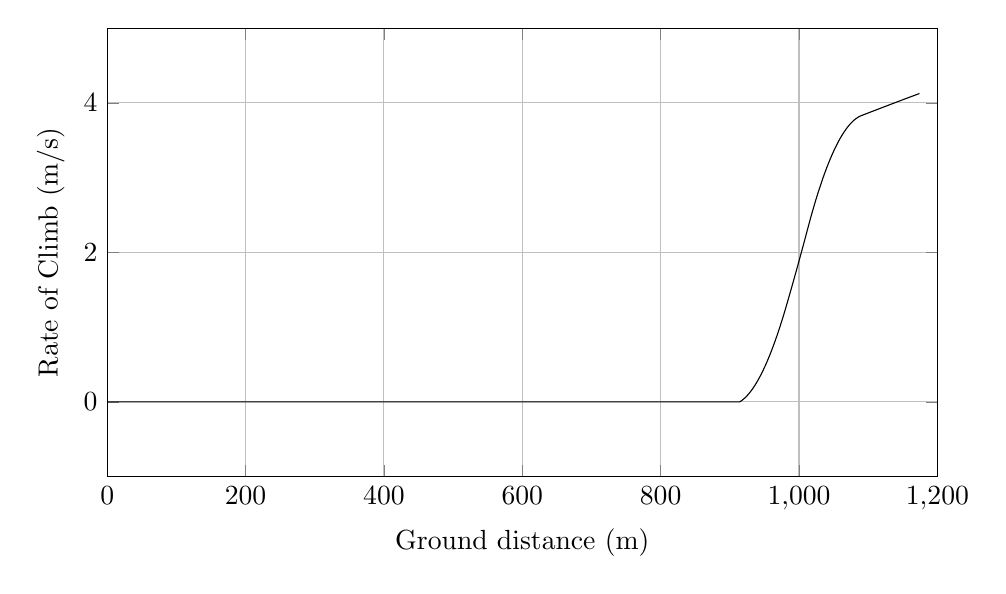
\begin{tikzpicture}

\begin{axis}[
width=\textwidth,
height=0.6\textwidth,
scaled ticks=false, tick label style={/pgf/number format/fixed},
xmin=0.0,
xmax=1200,
xlabel={Ground distance (m)},
xmajorgrids,
ymin=-1.0,
ymax=5,
ylabel={Rate of Climb (m/s)},
ymajorgrids,
legend style={at={(1.03,0.5)},anchor=west,draw=black,fill=white,legend cell align=left}
]

\addplot [
color=black,
solid
]
table[row sep=crcr]{
1.3729668748938318E-8	0.0\\
1.7493248493808052E-7	0.0\\
1.4411937280317895E-6	0.0\\
6.602995160656227E-5	0.0\\
2.2740573828771224E-4	0.0\\
4.8751428921765393E-4	0.0\\
8.441986619835749E-4	0.0\\
0.0012981647037285577	0.0\\
0.0018484379050661159	0.0\\
0.0024893731755424335	0.0\\
0.0032286585096692284	0.0\\
0.0040442418752796045	0.0\\
0.004972762654474916	0.0\\
0.005990910102221513	0.0\\
0.007111389191545643	0.0\\
0.008336865178450469	0.0\\
0.009664633507451486	0.0\\
0.011093815858158905	0.0\\
0.01262066151120312	0.0\\
0.01419454386807839	0.0\\
0.015910782250193378	0.0\\
0.017721549103721458	0.0\\
0.019620507964630857	0.0\\
0.02164969955342029	0.0\\
0.023766550611781796	0.0\\
0.025957065600157342	0.0\\
0.028260861173784894	0.0\\
0.030668466949245715	0.0\\
0.0331489614440674	0.0\\
0.03573888453685943	0.0\\
0.038418765463712895	0.0\\
0.04116679597872082	0.0\\
0.044022059812866554	0.0\\
0.04700053365173311	0.0\\
0.050116649382181494	0.0\\
0.0533021652593606	0.0\\
0.056630220296749106	0.0\\
0.05998688030085898	0.0\\
0.06348077825220624	0.0\\
0.06710848437295475	0.0\\
0.07082346760424127	0.0\\
0.07462944469130567	0.0\\
0.07855413323217031	0.0\\
0.08251243142992878	0.0\\
0.08659905947434482	0.0\\
0.09083545394947079	0.0\\
0.09518096637774642	0.0\\
0.099604438418047	0.0\\
0.1041130762071252	0.0\\
0.10871457033213175	0.0\\
0.11350280915994052	0.0\\
0.11836943512882261	0.0\\
0.12328542045494376	0.0\\
0.12830372217771202	0.0\\
0.1334037067999082	0.0\\
0.1386015897371753	0.0\\
0.14405085578552257	0.0\\
0.1495239325759128	0.0\\
0.1550507392415454	0.0\\
0.16073360491635535	0.0\\
0.16659871679960742	0.0\\
0.17244819595229793	0.0\\
0.17848031195343078	0.0\\
0.18466822548212042	0.0\\
0.1909009608611748	0.0\\
0.19716089737688902	0.0\\
0.2035279375926986	0.0\\
0.21017879584430066	0.0\\
0.21687473998771628	0.0\\
0.22354650324940833	0.0\\
0.23036941414946865	0.0\\
0.23737731412185503	0.0\\
0.24449289925428264	0.0\\
0.2517184892023243	0.0\\
0.25908208279438383	0.0\\
0.2664863589195283	0.0\\
0.27399321582905467	0.0\\
0.2816108016888421	0.0\\
0.2893844725195981	0.0\\
0.29747621078120867	0.0\\
0.30547198304033185	0.0\\
0.31373479402345694	0.0\\
0.3220909744202328	0.0\\
0.3305540912568814	0.0\\
0.33895489345894936	0.0\\
0.34753073012810576	0.0\\
0.3563589175375672	0.0\\
0.3652744752958731	0.0\\
0.3742693918027593	0.0\\
0.38350989122680823	0.0\\
0.3927029292363896	0.0\\
0.4020876366599533	0.0\\
0.4115568217121528	0.0\\
0.4212787852930122	0.0\\
0.43089755178065414	0.0\\
0.4408379299669313	0.0\\
0.4510502611115679	0.0\\
0.4612670224725215	0.0\\
0.4715818614584312	0.0\\
0.4818438670126082	0.0\\
0.4922128554044626	0.0\\
0.50273876067117	0.0\\
0.5136516607865718	0.0\\
0.5244310074213006	0.0\\
0.5355751508210329	0.0\\
0.5467126997993474	0.0\\
0.5580479056656631	0.0\\
0.5692960823995112	0.0\\
0.5809945926573021	0.0\\
0.5923626544035139	0.0\\
0.6041922852715	0.0\\
0.6160912669048675	0.0\\
0.6280605196746807	0.0\\
0.6403946506485891	0.0\\
0.6525721787971039	0.0\\
0.66504690021022	0.0\\
0.6773535438897555	0.0\\
0.6901462526606317	0.0\\
0.703249873273524	0.0\\
0.7159721017112175	0.0\\
0.729053467210389	0.0\\
0.7422988791228431	0.0\\
0.756304272979474	0.0\\
0.7696432036294076	0.0\\
0.7832290250230658	0.0\\
0.7969128825551131	0.0\\
0.8108444209446342	0.0\\
0.825043936786227	0.0\\
0.8390802275180445	0.0\\
0.8532340040587583	0.0\\
0.8678101043696134	0.0\\
0.8824320602344964	0.0\\
0.8978006605470081	0.0\\
0.9134572487531922	0.0\\
0.9287391767029982	0.0\\
0.9440564687433697	0.0\\
0.9598871644713316	0.0\\
0.9757786228365237	0.0\\
0.9918217338879218	0.0\\
1.0080608846667363	0.0\\
1.0245900975307913	0.0\\
1.040622085070809	0.0\\
1.0571005809273983	0.0\\
1.0736578999152901	0.0\\
1.0902401336450098	0.0\\
1.1073201062866707	0.0\\
1.1241926772552646	0.0\\
1.1416781667104252	0.0\\
1.1588269484070954	0.0\\
1.176440946845327	0.0\\
1.1944819542445066	0.0\\
1.2120125629913447	0.0\\
1.2299306574276825	0.0\\
1.2481120482032448	0.0\\
1.2663536608165091	0.0\\
1.2851425782117465	0.0\\
1.3041313368869671	0.0\\
1.3228236880779458	0.0\\
1.3414329672940513	0.0\\
1.3605066144349074	0.0\\
1.3802534409605212	0.0\\
1.3994872719307283	0.0\\
1.4192016277101378	0.0\\
1.439023460648384	0.0\\
1.459347998039509	0.0\\
1.4793256644936217	0.0\\
1.4991489338326072	0.0\\
1.5195196572175793	0.0\\
1.5402684478761244	0.0\\
1.5604570108688036	0.0\\
1.5810331069622228	0.0\\
1.6022712329181132	0.0\\
1.623752316257296	0.0\\
1.6452514305955401	0.0\\
1.6664829631402025	0.0\\
1.6886446033619715	0.0\\
1.710607384244656	0.0\\
1.7329417009553727	0.0\\
1.7551421266962821	0.0\\
1.7779085356585536	0.0\\
1.800478286927734	0.0\\
1.8236018329231238	0.0\\
1.8462320784511883	0.0\\
1.869621217116264	0.0\\
1.8933146512119747	0.0\\
1.9176856041472643	0.0\\
1.9417713639512164	0.0\\
1.9657098573982132	0.0\\
1.9902165007163162	0.0\\
2.014554050520948	0.0\\
2.039479559407779	0.0\\
2.0645497069116256	0.0\\
2.090368502766882	0.0\\
2.115564185269416	0.0\\
2.140750230554602	0.0\\
2.1667677015838267	0.0\\
2.1927560352542175	0.0\\
2.218891869133375	0.0\\
2.245288939563828	0.0\\
2.2712530964452817	0.0\\
2.297933078351498	0.0\\
2.324564104516777	0.0\\
2.351466051806102	0.0\\
2.378869922986878	0.0\\
2.4061764715670764	0.0\\
2.4343811693482102	0.0\\
2.4622108821536663	0.0\\
2.4906408044048067	0.0\\
2.518892760285042	0.0\\
2.5472153538550346	0.0\\
2.5762492306032216	0.0\\
2.605385308804288	0.0\\
2.634725531238531	0.0\\
2.6633424112287507	0.0\\
2.6927188130915374	0.0\\
2.7226962917814213	0.0\\
2.7531675915664673	0.0\\
2.7831412651501983	0.0\\
2.8139174932165103	0.0\\
2.8440331768075415	0.0\\
2.874693215323904	0.0\\
2.9059978681586376	0.0\\
2.9372617813709034	0.0\\
2.9684444504378202	0.0\\
3.000072782687808	0.0\\
3.031082587373527	0.0\\
3.063213028467148	0.0\\
3.0965739711585014	0.0\\
3.1291175748240176	0.0\\
3.161651640649506	0.0\\
3.194791488147139	0.0\\
3.2273698640351327	0.0\\
3.261394174200582	0.0\\
3.2942820372415875	0.0\\
3.3276455142443044	0.0\\
3.3625338428565543	0.0\\
3.396526624461681	0.0\\
3.4305511850311694	0.0\\
3.4642094416894933	0.0\\
3.498963551783903	0.0\\
3.5341885134496573	0.0\\
3.569804025802995	0.0\\
3.605116576002147	0.0\\
3.641338581546833	0.0\\
3.677593698357855	0.0\\
3.7132425573336665	0.0\\
3.74957219375957	0.0\\
3.7872650227149185	0.0\\
3.825403000593508	0.0\\
3.861987998097706	0.0\\
3.899535703755137	0.0\\
3.9366960368382165	0.0\\
3.9756271117991435	0.0\\
4.014715979923002	0.0\\
4.053268843133694	0.0\\
4.093111596873367	0.0\\
4.132540645872048	0.0\\
4.171686416589186	0.0\\
4.211258480423352	0.0\\
4.252585425594734	0.0\\
4.29253892845542	0.0\\
4.332839968385603	0.0\\
4.372708537789018	0.0\\
4.414379330316386	0.0\\
4.455607216042212	0.0\\
4.497336690654009	0.0\\
4.53836773335787	0.0\\
4.579767142935065	0.0\\
4.621942908118227	0.0\\
4.663798268780793	0.0\\
4.705838036060712	0.0\\
4.748491012675066	0.0\\
4.791393968819099	0.0\\
4.835700194867293	0.0\\
4.879973298406089	0.0\\
4.923250156511948	0.0\\
4.967673596314626	0.0\\
5.012954369117542	0.0\\
5.057574526249477	0.0\\
5.103280208347517	0.0\\
5.148856018935929	0.0\\
5.194350575362858	0.0\\
5.240584094986199	0.0\\
5.2871741484687504	0.0\\
5.333122064003502	0.0\\
5.3803318800233235	0.0\\
5.4262712259485255	0.0\\
5.473378197958581	0.0\\
5.521938593493333	0.0\\
5.570027890245774	0.0\\
5.617746353771608	0.0\\
5.665750363096816	0.0\\
5.714883880069209	0.0\\
5.763390205677501	0.0\\
5.812817811268989	0.0\\
5.861909274803731	0.0\\
5.912134919389196	0.0\\
5.962317560553064	0.0\\
6.012727788730279	0.0\\
6.0628236035803145	0.0\\
6.113711068416594	0.0\\
6.16497292765713	0.0\\
6.216284706244114	0.0\\
6.26834407822653	0.0\\
6.320257064476769	0.0\\
6.37351660191279	0.0\\
6.426150862197664	0.0\\
6.479030963436509	0.0\\
6.532319340056288	0.0\\
6.5857233987986845	0.0\\
6.640834734692348	0.0\\
6.695022999498724	0.0\\
6.749720237657193	0.0\\
6.804235758325081	0.0\\
6.859728469301633	0.0\\
6.916686079588434	0.0\\
6.9732530286722305	0.0\\
7.029531186664631	0.0\\
7.086633318514238	0.0\\
7.144155485034537	0.0\\
7.202053129566568	0.0\\
7.260126434764185	0.0\\
7.317913145042743	0.0\\
7.376682960996439	0.0\\
7.435393721764624	0.0\\
7.493838107271518	0.0\\
7.552684475254578	0.0\\
7.613252707151423	0.0\\
7.672782806866918	0.0\\
7.733397683408512	0.0\\
7.795525081709004	0.0\\
7.856013653786727	0.0\\
7.91792172269443	0.0\\
7.980110745884113	0.0\\
8.041720670752433	0.0\\
8.105229267009985	0.0\\
8.167457523036095	0.0\\
8.230908874360502	0.0\\
8.293738919282273	0.0\\
8.356235402336917	0.0\\
8.42092378244627	0.0\\
8.485671322837007	0.0\\
8.549180898871484	0.0\\
8.614596634551038	0.0\\
8.680166762249144	0.0\\
8.744770128469462	0.0\\
8.812993689385827	0.0\\
8.88005807777586	0.0\\
8.94709863067661	0.0\\
9.013172088448385	0.0\\
9.079266506338545	0.0\\
9.14748814890141	0.0\\
9.215411293660388	0.0\\
9.284579146198691	0.0\\
9.353168277381275	0.0\\
9.423753765537143	0.0\\
9.492960052876374	0.0\\
9.564123004975215	0.0\\
9.634097601479446	0.0\\
9.705672410878787	0.0\\
9.776260200085993	0.0\\
9.846607984572056	0.0\\
9.918231435410593	0.0\\
9.988851555070422	0.0\\
10.060390022634245	0.0\\
10.133279281833644	0.0\\
10.205241085147751	0.0\\
10.277820389603	0.0\\
10.352558894167803	0.0\\
10.42733258664746	0.0\\
10.501815126481194	0.0\\
10.576858173457808	0.0\\
10.65303812840548	0.0\\
10.729080272001735	0.0\\
10.804841544893105	0.0\\
10.881905013502095	0.0\\
10.958396790746043	0.0\\
11.035905069829102	0.0\\
11.113160538490881	0.0\\
11.192172636140572	0.0\\
11.270076562295213	0.0\\
11.350065490058778	0.0\\
11.429008826667825	0.0\\
11.50754237847364	0.0\\
11.587076645554472	0.0\\
11.668897725768986	0.0\\
11.749734371708193	0.0\\
11.830312384681939	0.0\\
11.909862670519033	0.0\\
11.990515423105418	0.0\\
12.072973931530203	0.0\\
12.155304175892073	0.0\\
12.237018674011615	0.0\\
12.320146069843414	0.0\\
12.406770618003886	0.0\\
12.489918686423398	0.0\\
12.574493004618496	0.0\\
12.660666896522624	0.0\\
12.746500366216402	0.0\\
12.832006837122272	0.0\\
12.919285437479463	0.0\\
13.00517529032821	0.0\\
13.092301899261269	0.0\\
13.179760097773386	0.0\\
13.268594687119744	0.0\\
13.357699529172354	0.0\\
13.44829753340392	0.0\\
13.537570218252604	0.0\\
13.627322718831184	0.0\\
13.718307212496544	0.0\\
13.808540263830096	0.0\\
13.899143852161355	0.0\\
13.991564069206362	0.0\\
14.085798171937814	0.0\\
14.179213507883688	0.0\\
14.271883316076963	0.0\\
14.367546274622434	0.0\\
14.459430863676705	0.0\\
14.555010173556813	0.0\\
14.648669731311681	0.0\\
14.743773575674254	0.0\\
14.839769774519894	0.0\\
14.932807148196385	0.0\\
15.026921440816679	0.0\\
15.12275113649265	0.0\\
15.222025232743288	0.0\\
15.321078842653048	0.0\\
15.417564225728565	0.0\\
15.515758841369038	0.0\\
15.613440509090129	0.0\\
15.7107260301154	0.0\\
15.81102223487273	0.0\\
15.913565872734136	0.0\\
16.012918321571746	0.0\\
16.11222833737955	0.0\\
16.216250800242257	0.0\\
16.319159023020546	0.0\\
16.421418004006803	0.0\\
16.521675247646563	0.0\\
16.62557290942481	0.0\\
16.72731964230514	0.0\\
16.830283223934416	0.0\\
16.93464251494634	0.0\\
17.038481620468637	0.0\\
17.146497421123335	0.0\\
17.252282308638982	0.0\\
17.35724772858778	0.0\\
17.464053904588297	0.0\\
17.572390862630144	0.0\\
17.680417629270814	0.0\\
17.789707298693855	0.0\\
17.899612520762552	0.0\\
18.01027367065641	0.0\\
18.121415095654797	0.0\\
18.232428503320143	0.0\\
18.34337337506409	0.0\\
18.454877340220463	0.0\\
18.56636189702322	0.0\\
18.678405595805643	0.0\\
18.7903363416971	0.0\\
18.902391384512768	0.0\\
19.01754810908954	0.0\\
19.131359562866663	0.0\\
19.247747682986713	0.0\\
19.361628242251975	0.0\\
19.477963464454028	0.0\\
19.595742742603164	0.0\\
19.71107288142779	0.0\\
19.82767543183723	0.0\\
19.944540068808188	0.0\\
20.06171535440768	0.0\\
20.179291418887807	0.0\\
20.29729887224694	0.0\\
20.417200571824914	0.0\\
20.53676390826074	0.0\\
20.65523768803314	0.0\\
20.777063017363922	0.0\\
20.896922101876633	0.0\\
21.016777952410983	0.0\\
21.13892104879462	0.0\\
21.260534693274344	0.0\\
21.382619708556632	0.0\\
21.506306369043365	0.0\\
21.631260758247265	0.0\\
21.75556249187227	0.0\\
21.87985606458615	0.0\\
22.005925835680863	0.0\\
22.130365724585275	0.0\\
22.257477980325966	0.0\\
22.38418119026224	0.0\\
22.50885833858638	0.0\\
22.636026948728087	0.0\\
22.76367325110224	0.0\\
22.89115382514759	0.0\\
23.022452271734288	0.0\\
23.149877274293033	0.0\\
23.27873580881144	0.0\\
23.408563766880334	0.0\\
23.538692653979794	0.0\\
23.671258756997098	0.0\\
23.803210122669313	0.0\\
23.93544283576786	0.0\\
24.067241518013077	0.0\\
24.19863541429976	0.0\\
24.329449967727697	0.0\\
24.46175612159181	0.0\\
24.594763714591892	0.0\\
24.72754053098891	0.0\\
24.86208223890334	0.0\\
24.99503410474967	0.0\\
25.12831230627787	0.0\\
25.265273024090206	0.0\\
25.400650037308893	0.0\\
25.536304655026747	0.0\\
25.673594178904246	0.0\\
25.80797730935859	0.0\\
25.835159569235522	0.0\\
25.83771752397454	0.0\\
25.84157983658004	0.0\\
25.854829339215996	0.0\\
25.893215796826965	0.0\\
25.973046119315796	0.0\\
26.096262980671412	0.0\\
26.224212718725603	0.0\\
26.35313595194755	0.0\\
26.481727686355264	0.0\\
26.611118169629577	0.0\\
26.74049186039369	0.0\\
26.87228140714948	0.0\\
27.003385008924262	0.0\\
27.1358830905183	0.0\\
27.265951877034226	0.0\\
27.399105426781233	0.0\\
27.53075869079712	0.0\\
27.66387879779476	0.0\\
27.79855889054391	0.0\\
27.932132547760695	0.0\\
28.06791767232785	0.0\\
28.202763022922632	0.0\\
28.339788243013793	0.0\\
28.476803106655623	0.0\\
28.61761981788422	0.0\\
28.753907949775353	0.0\\
28.89297195746854	0.0\\
29.03211749902605	0.0\\
29.17123509789927	0.0\\
29.312253051611236	0.0\\
29.454422317169097	0.0\\
29.59523538430127	0.0\\
29.737672170826222	0.0\\
29.879173197948965	0.0\\
30.02075470454991	0.0\\
30.166674235301365	0.0\\
30.308336095430334	0.0\\
30.452640844036836	0.0\\
30.597553881025625	0.0\\
30.742967061600154	0.0\\
30.888975484926362	0.0\\
31.034653067922946	0.0\\
31.180984070508003	0.0\\
31.328351020411645	0.0\\
31.476753455192622	0.0\\
31.62661541983664	0.0\\
31.774495604492607	0.0\\
31.924944104961916	0.0\\
32.07610067279926	0.0\\
32.22631826848556	0.0\\
32.37899942625752	0.0\\
32.528514827654206	0.0\\
32.68189139400266	0.0\\
32.836069829938495	0.0\\
32.99025509482905	0.0\\
33.14574197930297	0.0\\
33.30072558931056	0.0\\
33.455047097713944	0.0\\
33.610874563168906	0.0\\
33.76926068144728	0.0\\
33.92617323250643	0.0\\
34.08448787244542	0.0\\
34.24243160505006	0.0\\
34.40316487172558	0.0\\
34.56154208099588	0.0\\
34.721775177117024	0.0\\
34.88076970836556	0.0\\
35.041349106451236	0.0\\
35.20329621413198	0.0\\
35.364886328651124	0.0\\
35.529241615711214	0.0\\
35.69117991651797	0.0\\
35.85317319416103	0.0\\
36.014854298354294	0.0\\
36.18095311277159	0.0\\
36.34443322746766	0.0\\
36.51065106768533	0.0\\
36.67635767082788	0.0\\
36.842033683894186	0.0\\
37.00823867836148	0.0\\
37.17279029188734	0.0\\
37.33951104811075	0.0\\
37.50923941781488	0.0\\
37.679358776579846	0.0\\
37.845326083883435	0.0\\
38.017144746304325	0.0\\
38.1852030886141	0.0\\
38.35804431104914	0.0\\
38.52812920813831	0.0\\
38.69960796987526	0.0\\
38.87165793928378	0.0\\
39.0423941506003	0.0\\
39.21436971822614	0.0\\
39.38727999643966	0.0\\
39.558989012313546	0.0\\
39.734752343022535	0.0\\
39.908836167348156	0.0\\
40.084555009291705	0.0\\
40.259186798753746	0.0\\
40.43324437115375	0.0\\
40.61041052363379	0.0\\
40.787318094191775	0.0\\
40.96620398302343	0.0\\
41.14141336180775	0.0\\
41.31941103282654	0.0\\
41.49571226203258	0.0\\
41.67366972437729	0.0\\
41.85219319429197	0.0\\
42.03136872634711	0.0\\
42.21293422072888	0.0\\
42.39366932880948	0.0\\
42.57479521797359	0.0\\
42.75522531040919	0.0\\
42.93775785970641	0.0\\
43.11993568316029	0.0\\
43.30336620712447	0.0\\
43.48720879745599	0.0\\
43.672226884455625	0.0\\
43.85684130549208	0.0\\
44.039851952877484	0.0\\
44.22449378650157	0.0\\
44.412385508552646	0.0\\
44.59783063297877	0.0\\
44.78525507043919	0.0\\
44.973130075825196	0.0\\
45.16145211071871	0.0\\
45.34881478087516	0.0\\
45.536017136752506	0.0\\
45.724971990057284	0.0\\
45.91416212467789	0.0\\
46.10175434018815	0.0\\
46.29356928918713	0.0\\
46.48490977712943	0.0\\
46.67744207882204	0.0\\
46.869905949194575	0.0\\
47.062749521718516	0.0\\
47.25341437235973	0.0\\
47.44508461154423	0.0\\
47.63880095964302	0.0\\
47.83356160493736	0.0\\
48.025334057720784	0.0\\
48.218846636819876	0.0\\
48.41468711090302	0.0\\
48.610449575687724	0.0\\
48.80723286029129	0.0\\
49.00124137999302	0.0\\
49.20045899041696	0.0\\
49.394243884198005	0.0\\
49.59161211700324	0.0\\
49.79144608231523	0.0\\
49.99107345578199	0.0\\
50.18996871950735	0.0\\
50.388458331230495	0.0\\
50.59191110395449	0.0\\
50.79453916783869	0.0\\
50.99530158869649	0.0\\
51.19776583381373	0.0\\
51.3996255264899	0.0\\
51.599450409211	0.0\\
51.80158475775707	0.0\\
52.002311498730975	0.0\\
52.2060805474067	0.0\\
52.40811442127868	0.0\\
52.61423073460446	0.0\\
52.821749674584495	0.0\\
53.03053110951893	0.0\\
53.23753590773735	0.0\\
53.44487707917263	0.0\\
53.652063533093525	0.0\\
53.85975522429668	0.0\\
54.06844148636836	0.0\\
54.278580968983874	0.0\\
54.48685885904548	0.0\\
54.69884126905886	0.0\\
54.90975544393264	0.0\\
55.12216013841277	0.0\\
55.333080623240974	0.0\\
55.5448885814986	0.0\\
55.75594910746132	0.0\\
55.968144975063936	0.0\\
56.18150915317635	0.0\\
56.394069348356695	0.0\\
56.60950747146016	0.0\\
56.82641599949238	0.0\\
57.03980213394583	0.0\\
57.25698083573829	0.0\\
57.47353804711997	0.0\\
57.6941706582635	0.0\\
57.91229938529948	0.0\\
58.12998527173144	0.0\\
58.34905943653719	0.0\\
58.56781345824973	0.0\\
58.787998582886644	0.0\\
59.011266007804366	0.0\\
59.23368761368569	0.0\\
59.456031473365414	0.0\\
59.67976581221534	0.0\\
59.90315377467765	0.0\\
60.125192111546724	0.0\\
60.349269227196444	0.0\\
60.57220932044149	0.0\\
60.79606803632835	0.0\\
61.021718319759984	0.0\\
61.25073295331903	0.0\\
61.47770893732542	0.0\\
61.70784367826464	0.0\\
61.93740803875056	0.0\\
62.1673491775543	0.0\\
62.39648011888062	0.0\\
62.62822464633953	0.0\\
62.86094183422966	0.0\\
63.090532789209604	0.0\\
63.321616049163225	0.0\\
63.554808975015874	0.0\\
63.78685818650332	0.0\\
64.0234762327251	0.0\\
64.25652029988498	0.0\\
64.49146565301734	0.0\\
64.72768747885678	0.0\\
64.96568125142531	0.0\\
65.20057601391298	0.0\\
65.43975061379945	0.0\\
65.67719429610031	0.0\\
65.91652243006087	0.0\\
66.1565253585166	0.0\\
66.39740384038885	0.0\\
66.63777997854328	0.0\\
66.87849958303539	0.0\\
67.12349409848125	0.0\\
67.36843544137562	0.0\\
67.61129947098183	0.0\\
67.85808619273692	0.0\\
68.10323725880951	0.0\\
68.3520146383799	0.0\\
68.60099753692072	0.0\\
68.84943315800746	0.0\\
69.09793111574629	0.0\\
69.34894754058863	0.0\\
69.59791912239118	0.0\\
69.84867626946473	0.0\\
70.10496107302816	0.0\\
70.35594730130109	0.0\\
70.60854748652795	0.0\\
70.8625286964371	0.0\\
71.1182576034713	0.0\\
71.37278964945165	0.0\\
71.62944082734805	0.0\\
71.88536754710964	0.0\\
72.14250945057543	0.0\\
72.40306402213687	0.0\\
72.66241221953337	0.0\\
72.92327110344874	0.0\\
73.18657203154456	0.0\\
73.45150557123125	0.0\\
73.71756195569753	0.0\\
73.97940051906463	0.0\\
74.24514793127645	0.0\\
74.51022759525631	0.0\\
74.77823256031297	0.0\\
75.04767613410795	0.0\\
75.31682895458664	0.0\\
75.58729746777243	0.0\\
75.85729327570917	0.0\\
76.13042767774209	0.0\\
76.40299665611133	0.0\\
76.67973301409052	0.0\\
76.95360383527739	0.0\\
77.22854206589327	0.0\\
77.50692063517303	0.0\\
77.78349662592461	0.0\\
78.0616064362213	0.0\\
78.33869545141144	0.0\\
78.62238552181594	0.0\\
78.90481169871467	0.0\\
79.18659077494928	0.0\\
79.4700201012688	0.0\\
79.75774957869095	0.0\\
80.04430580185078	0.0\\
80.33432201731404	0.0\\
80.62298533865851	0.0\\
80.9130804606989	0.0\\
81.20459144967842	0.0\\
81.49650140842283	0.0\\
81.79224544448738	0.0\\
82.08455487090956	0.0\\
82.37934996819865	0.0\\
82.67580145620735	0.0\\
82.97475550983006	0.0\\
83.2734238134004	0.0\\
83.57209772503273	0.0\\
83.87419166445906	0.0\\
84.17487194816226	0.0\\
84.47686996876752	0.0\\
84.78124993153034	0.0\\
85.08776945017104	0.0\\
85.39395758722245	0.0\\
85.69833162305892	0.0\\
86.01027818388755	0.0\\
86.31658691867341	0.0\\
86.62866814828641	0.0\\
86.94043673469176	0.0\\
87.2565990672368	0.0\\
87.56980823017452	0.0\\
87.88101387141376	0.0\\
88.20007062892054	0.0\\
88.51883409355145	0.0\\
88.83509784148416	0.0\\
89.15857089898353	0.0\\
89.47772213402055	0.0\\
89.80217214804901	0.0\\
90.1263587278685	0.0\\
90.44950966725051	0.0\\
90.77764749859728	0.0\\
91.10470504824352	0.0\\
91.43769785174896	0.0\\
91.76691749028419	0.0\\
92.09386993524024	0.0\\
92.42498248438446	0.0\\
92.7581696617394	0.0\\
93.09729153734631	0.0\\
93.4312406900703	0.0\\
93.76780571708736	0.0\\
94.10390054156983	0.0\\
94.43564317419558	0.0\\
94.77291201930262	0.0\\
95.10796951504997	0.0\\
95.44708659079325	0.0\\
95.78515592548297	0.0\\
96.12311752311894	0.0\\
96.46351490415591	0.0\\
96.80669869710772	0.0\\
97.14657639264556	0.0\\
97.48763116340677	0.0\\
97.8305814261901	0.0\\
98.17013304046878	0.0\\
98.51054009051404	0.0\\
98.854181194619	0.0\\
99.19205317796005	0.0\\
99.53355440060989	0.0\\
99.87198375587872	0.0\\
100.2129389915628	0.0\\
100.55335806642802	0.0\\
100.89503335592528	0.0\\
101.23693480167049	0.0\\
101.57977298927813	0.0\\
101.91842351185082	0.0\\
102.26214655705948	0.0\\
102.60487134933112	0.0\\
102.94238410388857	0.0\\
103.28139950825951	0.0\\
103.61984226602698	0.0\\
103.95406402656286	0.0\\
104.29248504574807	0.0\\
104.63112914593611	0.0\\
104.96686613984221	0.0\\
105.30464484937244	0.0\\
105.64180205248229	0.0\\
105.97704387437452	0.0\\
106.31384964552919	0.0\\
106.6489228444834	0.0\\
106.98000007373659	0.0\\
107.31456925364313	0.0\\
107.38092108752608	0.0\\
107.387754025128	0.0\\
107.3946577511588	0.0\\
107.39916951903444	0.0\\
107.40247473215817	0.0\\
107.40548301099807	0.0\\
107.41901751964124	0.0\\
107.47756267729525	0.0\\
107.63696404402117	0.0\\
107.95668166923352	0.0\\
108.2571634635643	0.0\\
108.55996775705782	0.0\\
108.8616926844802	0.0\\
109.16669292910967	0.0\\
109.47218465327785	0.0\\
109.78023369107405	0.0\\
110.09061921742381	0.0\\
110.4007971847821	0.0\\
110.7125096545017	0.0\\
111.02874540594937	0.0\\
111.34670354521654	0.0\\
111.664908557295	0.0\\
111.98617551206428	0.0\\
112.3078797039536	0.0\\
112.63537393275391	0.0\\
112.96267359383529	0.0\\
113.28778388635178	0.0\\
113.61823593045688	0.0\\
113.94632344632586	0.0\\
114.27926944824554	0.0\\
114.61324422041562	0.0\\
114.94750338770686	0.0\\
115.28618013885716	0.0\\
115.62544260296943	0.0\\
115.9647508443766	0.0\\
116.30617149460878	0.0\\
116.65060078043697	0.0\\
116.99863777637248	0.0\\
117.34270613829636	0.0\\
117.68983788345284	0.0\\
118.04137408578512	0.0\\
118.39343387684602	0.0\\
118.74804854616337	0.0\\
119.10520175440718	0.0\\
119.46686684850098	0.0\\
119.82660492256403	0.0\\
120.19012449272657	0.0\\
120.55217592908159	0.0\\
120.91763124996498	0.0\\
121.28719248968574	0.0\\
121.65493622417088	0.0\\
122.02513489718217	0.0\\
122.39308995700384	0.0\\
122.76618799735454	0.0\\
123.1388017253943	0.0\\
123.51256311114031	0.0\\
123.88633794770595	0.0\\
124.25665874611622	0.0\\
124.63165231885978	0.0\\
125.00664173256905	0.0\\
125.38021625899401	0.0\\
125.75512563345742	0.0\\
126.13473977091255	0.0\\
126.51299085225449	0.0\\
126.8948287761801	0.0\\
127.27325883095315	0.0\\
127.64986999110431	0.0\\
128.03053456382577	0.0\\
128.40840086210045	0.0\\
128.78830732782995	0.0\\
129.16816802858597	0.0\\
129.55114692916032	0.0\\
129.92795862154003	0.0\\
130.30814318938542	0.0\\
130.68801179162523	0.0\\
131.0673626953399	0.0\\
131.44707508552267	0.0\\
131.82575792285303	0.0\\
132.20466209461676	0.0\\
132.58549544797154	0.0\\
132.96520261413826	0.0\\
133.34413894748724	0.0\\
133.72638850756363	0.0\\
134.1049920954593	0.0\\
134.48538249769342	0.0\\
134.86277461399203	0.0\\
135.2402386369938	0.0\\
135.62109197355238	0.0\\
135.9996509441208	0.0\\
136.37968191797512	0.0\\
136.76120583273502	0.0\\
137.13951930881296	0.0\\
137.51840340013064	0.0\\
137.89819615735314	0.0\\
138.27485697152616	0.0\\
138.65420581933705	0.0\\
139.03531375767642	0.0\\
139.41296882619503	0.0\\
139.79422155259	0.0\\
140.17408835952057	0.0\\
140.5488076998477	0.0\\
140.92844631991198	0.0\\
141.30483696429354	0.0\\
141.68269541512387	0.0\\
142.06058279783264	0.0\\
142.43991695918288	0.0\\
142.81695502902187	0.0\\
143.19247254825046	0.0\\
143.5733885276352	0.0\\
143.94921103219775	0.0\\
144.32621366107247	0.0\\
144.70408630975157	0.0\\
145.08263595865492	0.0\\
145.46162624555404	0.0\\
145.83827879615103	0.0\\
146.21524500988596	0.0\\
146.5934755401724	0.0\\
146.9730259257883	0.0\\
147.3547239944582	0.0\\
147.73366854735332	0.0\\
148.1136534850276	0.0\\
148.49311509785633	0.0\\
148.87144514206074	0.0\\
149.25360190977045	0.0\\
149.6334430260095	0.0\\
150.01465687879528	0.0\\
150.3940924716125	0.0\\
150.77688175221402	0.0\\
151.1561678741857	0.0\\
151.5352572324847	0.0\\
151.91884603110896	0.0\\
152.3000376871389	0.0\\
152.6837211891089	0.0\\
153.06727641570347	0.0\\
153.4514076737559	0.0\\
153.83522357687116	0.0\\
154.21637826964854	0.0\\
154.6009164651564	0.0\\
154.98403470202834	0.0\\
155.36838747168406	0.0\\
155.75158064164503	0.0\\
156.13576662495046	0.0\\
156.5218436740983	0.0\\
156.90521285441474	0.0\\
157.2916244593892	0.0\\
157.6780020855428	0.0\\
158.06299451159185	0.0\\
158.4509000667514	0.0\\
158.83830611621056	0.0\\
159.22672413827297	0.0\\
159.61474494524106	0.0\\
160.0042372884319	0.0\\
160.39552304382113	0.0\\
160.78478895267375	0.0\\
161.17517847278327	0.0\\
161.56748129737286	0.0\\
161.9609400214345	0.0\\
162.35005274814932	0.0\\
162.7425950916558	0.0\\
163.13607830878885	0.0\\
163.53170884953005	0.0\\
163.92462594167722	0.0\\
164.3198767210975	0.0\\
164.7157696028566	0.0\\
165.1115317336501	0.0\\
165.50739628911128	0.0\\
165.90698313288817	0.0\\
166.30582458333038	0.0\\
166.70591293613995	0.0\\
167.1044701422045	0.0\\
167.50226971352845	0.0\\
167.9010833894181	0.0\\
168.3004552315794	0.0\\
168.70189335181743	0.0\\
169.10576843973695	0.0\\
169.50785881751284	0.0\\
169.91045494783964	0.0\\
170.31331810721775	0.0\\
170.71648797717722	0.0\\
171.11993291578136	0.0\\
171.5247281229082	0.0\\
171.92976094083576	0.0\\
172.33690302624336	0.0\\
172.74259563259648	0.0\\
173.1509823323036	0.0\\
173.55913088366435	0.0\\
173.96636547491187	0.0\\
174.37754484483776	0.0\\
174.7874876782942	0.0\\
175.2012500141185	0.0\\
175.6112323385957	0.0\\
176.02092514523684	0.0\\
176.43326782420013	0.0\\
176.8477920653399	0.0\\
177.2627043459005	0.0\\
177.67839640445425	0.0\\
178.09047986160414	0.0\\
178.50771992227516	0.0\\
178.92514786216543	0.0\\
179.34349041668827	0.0\\
179.7634585539525	0.0\\
180.18446825846002	0.0\\
180.60425393302842	0.0\\
181.0261226187801	0.0\\
181.4483416261798	0.0\\
181.87315445312532	0.0\\
182.29527778821938	0.0\\
182.72141514554897	0.0\\
183.1481192716397	0.0\\
183.57633821660988	0.0\\
184.00592509150556	0.0\\
184.43471922224091	0.0\\
184.86359425785753	0.0\\
185.29462923368334	0.0\\
185.72590746205765	0.0\\
186.15893531582464	0.0\\
186.59473099205763	0.0\\
187.03327531522774	0.0\\
187.46972629616232	0.0\\
187.90646428697016	0.0\\
188.34682007573156	0.0\\
188.7873444966949	0.0\\
189.22841311150643	0.0\\
189.6706369666947	0.0\\
190.11352546522693	0.0\\
190.55843868450165	0.0\\
191.0032099177178	0.0\\
191.4488342668783	0.0\\
191.89679402644646	0.0\\
192.34637901534325	0.0\\
192.79928545122743	0.0\\
193.2512724064709	0.0\\
193.7017744692331	0.0\\
194.15625995252321	0.0\\
194.61155611404877	0.0\\
195.0672219974316	0.0\\
195.52585180825645	0.0\\
195.98426342862024	0.0\\
196.44494672064457	0.0\\
196.9057535736029	0.0\\
197.36967293120705	0.0\\
197.83510384208427	0.0\\
198.30342862028755	0.0\\
198.7732043057544	0.0\\
199.24099125426073	0.0\\
199.71119060681792	0.0\\
200.1825482927743	0.0\\
200.65679322330254	0.0\\
201.13270849114224	0.0\\
201.61347762080612	0.0\\
202.09583085583984	0.0\\
202.57505536425464	0.0\\
203.05779273540577	0.0\\
203.54112852606227	0.0\\
204.02652622166198	0.0\\
204.51502737102567	0.0\\
205.002477053986	0.0\\
205.49362028927055	0.0\\
205.98571877257524	0.0\\
206.47986048819791	0.0\\
206.9756485373277	0.0\\
207.47509472353033	0.0\\
207.98105643358775	0.0\\
208.48540394416239	0.0\\
208.99019975934863	0.0\\
209.4981718386387	0.0\\
210.0074085614305	0.0\\
210.51733356743972	0.0\\
211.0326447114959	0.0\\
211.54741442472368	0.0\\
212.06514182135783	0.0\\
212.58880120479233	0.0\\
213.11423767449816	0.0\\
213.6375324332176	0.0\\
214.1668747215242	0.0\\
214.6965875774535	0.0\\
215.22997734520317	0.0\\
215.7686003837519	0.0\\
216.30585839012286	0.0\\
216.8511964964835	0.0\\
217.39999653425627	0.0\\
217.94624961891986	0.0\\
218.50173638139336	0.0\\
219.05616136113832	0.0\\
219.61603320212004	0.0\\
220.17996673649174	0.0\\
220.75152408343223	0.0\\
221.31978136773841	0.0\\
221.8917718938588	0.0\\
222.46939173565727	0.0\\
223.05424878124148	0.0\\
223.6353441191846	0.0\\
224.2228469319029	0.0\\
224.81981605125333	0.0\\
225.414322731722	0.0\\
226.00805957236628	0.0\\
226.6058017780681	0.0\\
227.21801255318616	0.0\\
227.8254326298245	0.0\\
228.4384631744503	0.0\\
229.05630143576667	0.0\\
229.67438980515863	0.0\\
230.2952270741992	0.0\\
230.91872450767323	0.0\\
231.54134731806806	0.0\\
232.16409178618352	0.0\\
232.7899713961491	0.0\\
233.4157347959749	0.0\\
234.0352538000064	0.0\\
234.65526828817934	0.0\\
235.27154540161314	0.0\\
235.88948672731453	0.0\\
236.5049303841215	0.0\\
237.1250162121333	0.0\\
237.73667159687494	0.0\\
238.3498254862601	0.0\\
238.96060042013949	0.0\\
239.56622141551122	0.0\\
240.17389692315953	0.0\\
240.77522869589131	0.0\\
241.3760510240944	0.0\\
241.97103412255802	0.0\\
242.55850867503966	0.0\\
243.1485861228365	0.0\\
243.73646785224247	0.0\\
244.31785335506692	0.0\\
244.8989348386816	0.0\\
245.47768348369902	0.0\\
246.0511922890006	0.0\\
246.62411578591679	0.0\\
247.19560633997713	0.0\\
247.7644393659644	0.0\\
248.3330098290461	0.0\\
248.89747941389504	0.0\\
249.45778103766594	0.0\\
250.01628073566417	0.0\\
250.57389204323152	0.0\\
251.1336441663857	0.0\\
251.6846487775523	0.0\\
252.2308345522173	0.0\\
252.77975023333983	0.0\\
253.32811243895696	0.0\\
253.87118817792594	0.0\\
254.4133651004234	0.0\\
254.5214401390847	0.0\\
254.83904570493053	0.0\\
254.86071409967872	0.0\\
254.8777656564992	0.0\\
254.8928183932843	0.0\\
254.90595982385685	0.0\\
254.92002328132799	0.0\\
254.9253543395315	0.0\\
254.93130083623475	0.0\\
254.96272950051815	0.0\\
255.06810565549557	0.0\\
255.36811297064412	0.0\\
255.8525091010879	0.0\\
256.3298916337542	0.0\\
256.8075138750163	0.0\\
257.2910565040604	0.0\\
257.776804457902	0.0\\
258.2651177463397	0.0\\
258.75623965529917	0.0\\
259.2479874402336	0.0\\
259.7444495167766	0.0\\
260.2424492273475	0.0\\
260.7432593092137	0.0\\
261.247422780654	0.0\\
261.754557364599	0.0\\
262.26667770433664	0.0\\
262.7807572902842	0.0\\
263.2953883103885	0.0\\
263.81347250230294	0.0\\
264.3373938048751	0.0\\
264.8633427659006	0.0\\
265.3982279044384	0.0\\
265.93370762125517	0.0\\
266.4705766429179	0.0\\
267.01127382973925	0.0\\
267.5541191433384	0.0\\
268.1029054057184	0.0\\
268.6568703707334	0.0\\
269.2131991941809	0.0\\
269.77965185696826	0.0\\
270.34285319322	0.0\\
270.91507878419327	0.0\\
271.48758827041524	0.0\\
272.06358557024134	0.0\\
272.6484960186634	0.0\\
273.2397139750577	0.0\\
273.83320745420303	0.0\\
274.43242914940197	0.0\\
275.0332286766287	0.0\\
275.64250383846434	0.0\\
276.25103708843267	0.0\\
276.86908599168135	0.0\\
277.4915413086129	0.0\\
278.11268743481435	0.0\\
278.7426163600394	0.0\\
279.37385128465223	0.0\\
280.00811453798417	0.0\\
280.6421164884222	0.0\\
281.2831601515528	0.0\\
281.9230740215264	0.0\\
282.5681900985986	0.0\\
283.2125319406723	0.0\\
283.85385525840525	0.0\\
284.4934544665398	0.0\\
285.13663885290487	0.0\\
285.77585929803354	0.0\\
286.4160621525482	0.0\\
287.0513871934386	0.0\\
287.6815461591955	0.0\\
288.3151143713146	0.0\\
288.9440132428607	0.0\\
289.57278910778643	0.0\\
290.1987061412044	0.0\\
290.8185328090791	0.0\\
291.44381701046814	0.0\\
292.06316956763783	0.0\\
292.6799483649311	0.0\\
293.29456956929107	0.0\\
293.90507282969963	0.0\\
294.51904351746816	0.0\\
295.1242474102645	0.0\\
295.7294372822977	0.0\\
296.3326441035193	0.0\\
296.93531837143473	0.0\\
297.53662560756754	0.0\\
298.13594882298116	0.0\\
298.73169481180116	0.0\\
299.3266408784582	0.0\\
299.922114932661	0.0\\
300.51213137957825	0.0\\
301.1010124400823	0.0\\
301.68603189258056	0.0\\
302.2748125277259	0.0\\
302.8590582136652	0.0\\
303.44379480516704	0.0\\
304.0290509058309	0.0\\
304.6116737569222	0.0\\
305.19373631536575	0.0\\
305.7764921471378	0.0\\
306.3580249849531	0.0\\
306.9381490141882	0.0\\
307.5139833341484	0.0\\
308.09088922445255	0.0\\
308.6675546961833	0.0\\
309.2395460191327	0.0\\
309.8148153885073	0.0\\
310.3887595932547	0.0\\
310.9575507782383	0.0\\
311.5303285454054	0.0\\
312.1036077080503	0.0\\
312.6780685512481	0.0\\
313.2471479783603	0.0\\
313.81443099956607	0.0\\
314.38461922677266	0.0\\
314.9529717276515	0.0\\
315.52447137304955	0.0\\
316.09585476365055	0.0\\
316.6635766630999	0.0\\
317.2324945294489	0.0\\
317.8014884261387	0.0\\
318.37019165330537	0.0\\
318.9369705786113	0.0\\
319.50690112966265	0.0\\
320.0739603849205	0.0\\
320.6398790880884	0.0\\
321.20391395290665	0.0\\
321.7716639023572	0.0\\
322.338484237663	0.0\\
322.90542659378207	0.0\\
323.47230992414404	0.0\\
324.03724239724215	0.0\\
324.60406116004583	0.0\\
325.16943479275596	0.0\\
325.7365942510148	0.0\\
326.30046115927405	0.0\\
326.8653941427267	0.0\\
327.4306179230226	0.0\\
327.99738905651475	0.0\\
328.56121076675106	0.0\\
329.1266162082277	0.0\\
329.6914897277701	0.0\\
330.2568653337778	0.0\\
330.82614981214726	0.0\\
331.3938100932787	0.0\\
331.96132280869926	0.0\\
332.5263354296127	0.0\\
333.094384011873	0.0\\
333.6625145702084	0.0\\
334.23129658370976	0.0\\
334.79884578809185	0.0\\
335.36810819267475	0.0\\
335.9387356031524	0.0\\
336.50726769982157	0.0\\
337.0760911342318	0.0\\
337.6455614970556	0.0\\
338.2131690194383	0.0\\
338.78552497707926	0.0\\
339.3551707031005	0.0\\
339.9263953137104	0.0\\
340.49770657658587	0.0\\
341.07107296042966	0.0\\
341.64488206821375	0.0\\
342.2196981164169	0.0\\
342.79128386247544	0.0\\
343.36530385074616	0.0\\
343.9384742998243	0.0\\
344.5127320767282	0.0\\
345.0871545928418	0.0\\
345.6609880560121	0.0\\
346.23676575911713	0.0\\
346.8130197442814	0.0\\
347.3897807520199	0.0\\
347.9671406573249	0.0\\
348.54468010889946	0.0\\
349.1240420580384	0.0\\
349.70684674265726	0.0\\
350.28477816592056	0.0\\
350.86571195144245	0.0\\
351.44841136880564	0.0\\
352.029838452439	0.0\\
352.61193941085935	0.0\\
353.1950613476878	0.0\\
353.77635779818036	0.0\\
354.36112156987554	0.0\\
354.9462572164025	0.0\\
355.5320128434072	0.0\\
356.1213882444596	0.0\\
356.70690251099427	0.0\\
357.2913063799722	0.0\\
357.88109115267446	0.0\\
358.4695934955133	0.0\\
359.06094251031095	0.0\\
359.65215374289005	0.0\\
360.24470845029396	0.0\\
360.8364099959201	0.0\\
361.4321266430708	0.0\\
362.0241065966578	0.0\\
362.6189376480745	0.0\\
363.21395562380917	0.0\\
363.81152989978864	0.0\\
364.410289097789	0.0\\
365.0062851890809	0.0\\
365.60439491742204	0.0\\
366.2041617720637	0.0\\
366.8056239231415	0.0\\
367.4070486628152	0.0\\
368.00907376705277	0.0\\
368.6144179601106	0.0\\
369.2208348878655	0.0\\
369.82496615199057	0.0\\
370.4326754576117	0.0\\
371.04303037748207	0.0\\
371.6508693513399	0.0\\
372.25899511893056	0.0\\
372.86664845026814	0.0\\
373.4753405379722	0.0\\
374.0881004214027	0.0\\
374.70105876160676	0.0\\
375.3151346609259	0.0\\
375.9298074887587	0.0\\
376.5473278422053	0.0\\
377.1659973922931	0.0\\
377.78652602772513	0.0\\
378.405253006595	0.0\\
379.02846510544396	0.0\\
379.6543690418463	0.0\\
380.2811814650454	0.0\\
380.90900588878685	0.0\\
381.5337926225143	0.0\\
382.1641103383158	0.0\\
382.79101003686833	0.0\\
383.4194385604271	0.0\\
384.0528738277319	0.0\\
384.68472673161864	0.0\\
385.32042409439157	0.0\\
385.9552738763366	0.0\\
386.5917185244833	0.0\\
387.2293049476492	0.0\\
387.8719915461404	0.0\\
388.5147956275654	0.0\\
389.1559927194148	0.0\\
389.7996463231178	0.0\\
390.44590234406144	0.0\\
391.09597692252225	0.0\\
391.7432686139034	0.0\\
392.39346837385165	0.0\\
393.0475398239315	0.0\\
393.7058991304724	0.0\\
394.361103822721	0.0\\
395.0207326851521	0.0\\
395.6779623373923	0.0\\
396.34250077971865	0.0\\
397.00554118881405	0.0\\
397.67183470834334	0.0\\
398.339726786716	0.0\\
399.0084117944432	0.0\\
399.67978041179765	0.0\\
400.3545844791679	0.0\\
401.03042852988824	0.0\\
401.70427614998994	0.0\\
402.3900383946309	0.0\\
403.0721085484811	0.0\\
403.7597156579167	0.0\\
404.4479287141618	0.0\\
405.13417181133127	0.0\\
405.821611865857	0.0\\
406.516279969008	0.0\\
407.20856037019735	0.0\\
407.90496228146947	0.0\\
408.60813973301015	0.0\\
409.30909477003024	0.0\\
410.0159249727094	0.0\\
410.7222621184179	0.0\\
411.42889803912226	0.0\\
412.1445221092463	0.0\\
412.85948143665576	0.0\\
413.57607429314953	0.0\\
414.2961289632634	0.0\\
415.0202224913728	0.0\\
415.7516092945767	0.0\\
416.48174520642	0.0\\
417.2165395849778	0.0\\
417.95584650206695	0.0\\
418.70066385533676	0.0\\
419.4474344863693	0.0\\
420.1971975293743	0.0\\
420.94905936873386	0.0\\
421.7065397747897	0.0\\
422.46524085121166	0.0\\
423.22783421796294	0.0\\
424.00052336845647	0.0\\
424.77464106215325	0.0\\
425.5526338229564	0.0\\
426.3361420323414	0.0\\
427.1240873399694	0.0\\
427.91997575833363	0.0\\
428.7156559118979	0.0\\
429.5236395760454	0.0\\
430.32996506585414	0.0\\
431.1427070038992	0.0\\
431.9640394759042	0.0\\
432.78798919576377	0.0\\
433.6163068095833	0.0\\
434.4571291863	0.0\\
435.30647580489597	0.0\\
436.15882992104855	0.0\\
437.02624426800617	0.0\\
437.9029226820204	0.0\\
438.78614854244313	0.0\\
439.67024663455084	0.0\\
440.56773120111336	0.0\\
441.48235207230107	0.0\\
442.4002204784682	0.0\\
443.33223312606856	0.0\\
444.27489815443255	0.0\\
445.2194332794703	0.0\\
446.18852338773047	0.0\\
447.1650199838215	0.0\\
448.14212748617774	0.0\\
449.12768736026055	0.0\\
450.1265747229721	0.0\\
451.1233791198257	0.0\\
452.12675185924934	0.0\\
453.122279117925	0.0\\
454.12404193398254	0.0\\
455.10741716602604	0.0\\
456.0912402453123	0.0\\
457.0600726957697	0.0\\
458.02574672848687	0.0\\
458.9811742371063	0.0\\
459.92030846821945	0.0\\
460.8449841241073	0.0\\
461.76140669191216	0.0\\
462.67950443365294	0.0\\
463.5841081756621	0.0\\
464.4750374462178	0.0\\
465.36305549382246	0.0\\
466.2426214242721	0.0\\
467.11087102140766	0.0\\
467.972515664415	0.0\\
468.8289199517734	0.0\\
469.6812048910498	0.0\\
470.52465288198835	0.0\\
471.3648989492757	0.0\\
472.1972562785188	0.0\\
473.02351832723116	0.0\\
473.84502281296636	0.0\\
474.65918124561415	0.0\\
475.4690721424329	0.0\\
476.2765662647138	0.0\\
477.07988307769745	0.0\\
477.879669879326	0.0\\
478.67222991463916	0.0\\
479.46064122917437	0.0\\
480.24954501182856	0.0\\
481.03289204196733	0.0\\
481.81248299334845	0.0\\
482.5909487329001	0.0\\
483.36332192433474	0.0\\
484.13567199637407	0.0\\
484.89826718432596	0.0\\
485.6616315157769	0.0\\
486.42284286646895	0.0\\
487.1811520213696	0.0\\
487.9361606873513	0.0\\
488.0862000462413	0.0\\
488.51171643164344	0.0\\
488.5204761820811	0.0\\
488.52903187150355	0.0\\
488.5724231989668	0.0\\
488.7333329386644	0.0\\
489.1829676407592	0.0\\
489.92201730542024	0.0\\
490.66351800838265	0.0\\
491.41054832328416	0.0\\
492.15902589552354	0.0\\
492.91187486786794	0.0\\
493.6674844916515	0.0\\
494.42999445975477	0.0\\
495.1950929544056	0.0\\
495.9651930404774	0.0\\
496.74308787518237	0.0\\
497.5261952793585	0.0\\
498.31138432739033	0.0\\
499.1020549248467	0.0\\
499.9002589962571	0.0\\
500.7022456576933	0.0\\
501.5090523514118	0.0\\
502.3195686296764	0.0\\
503.1412728054687	0.0\\
503.96791165595073	0.0\\
504.79933667522266	0.0\\
505.6342741536124	0.0\\
506.4786567385539	0.0\\
507.3294610646867	0.0\\
508.1886280826044	0.0\\
509.0566685057569	0.0\\
509.9302471646762	0.0\\
510.81569126209695	0.0\\
511.70598991448594	0.0\\
512.6037304003676	0.0\\
513.5118796507982	0.0\\
514.4291534807439	0.0\\
515.3600390678175	0.0\\
516.3004539849924	0.0\\
517.2526998274022	0.0\\
518.2107513126712	0.0\\
519.1813307606569	0.0\\
520.1623982203746	0.0\\
521.1517316571476	0.0\\
522.1538934745424	0.0\\
523.1627452385133	0.0\\
524.1860415450778	0.0\\
525.2158711392533	0.0\\
526.2504308121668	0.0\\
527.2883302419584	0.0\\
528.3258670294849	0.0\\
529.3618435825495	0.0\\
530.3987031210379	0.0\\
531.4292357253873	0.0\\
532.4587746997697	0.0\\
533.4803790381791	0.0\\
534.4886941535024	0.0\\
535.4990146464693	0.0\\
536.49858152146	0.0\\
537.4945670800385	0.0\\
538.4857266971019	0.0\\
539.4643922408397	0.0\\
540.4408466042978	0.0\\
541.4073512887883	0.0\\
542.3675454779934	0.0\\
543.3247545321008	0.0\\
544.2728203002546	0.0\\
545.2164036210195	0.0\\
546.1519862921152	0.0\\
547.085713551734	0.0\\
548.0174011794822	0.0\\
548.9407659306482	0.0\\
549.8606896180515	0.0\\
550.7763747922556	0.0\\
551.6862938962734	0.0\\
552.5907950941921	0.0\\
553.4934340387069	0.0\\
554.3942179487572	0.0\\
555.2905714512424	0.0\\
556.1806198022296	0.0\\
557.0761623625008	0.0\\
557.9664211267702	0.0\\
558.8507021428259	0.0\\
559.7317833695613	0.0\\
560.6119683183686	0.0\\
561.492052705531	0.0\\
562.3682786477177	0.0\\
563.2426881566412	0.0\\
564.115643537162	0.0\\
564.9871820290484	0.0\\
565.8563825959563	0.0\\
566.7235528033411	0.0\\
567.584270942679	0.0\\
568.4483693921954	0.0\\
569.3106060737728	0.0\\
570.1700847904979	0.0\\
571.0351952022045	0.0\\
571.8939669541594	0.0\\
572.7543287099213	0.0\\
573.6110025505288	0.0\\
574.4649935180137	0.0\\
575.3175338450419	0.0\\
576.1698867816026	0.0\\
577.0213826637028	0.0\\
577.8680727740848	0.0\\
578.7180079329755	0.0\\
579.5696721712868	0.0\\
580.4156816020864	0.0\\
581.2665168977144	0.0\\
582.1126680081018	0.0\\
582.9591455118928	0.0\\
583.8064789318607	0.0\\
584.6542286785789	0.0\\
585.4948244412594	0.0\\
586.3417246297038	0.0\\
587.1855807464744	0.0\\
588.0265986951438	0.0\\
588.8734637893597	0.0\\
589.7168603849534	0.0\\
590.5586538765217	0.0\\
591.4001825944827	0.0\\
592.2438475773395	0.0\\
593.0851928547504	0.0\\
593.9280989632321	0.0\\
594.7675466432647	0.0\\
595.6096308746946	0.0\\
596.4514038986238	0.0\\
597.2922019333205	0.0\\
598.1349633294326	0.0\\
598.9708006967505	0.0\\
599.8120854921594	0.0\\
600.6487319653024	0.0\\
601.4916625299238	0.0\\
602.3315284242424	0.0\\
603.1736324668191	0.0\\
604.0146021029152	0.0\\
604.8562691644076	0.0\\
605.6985293092685	0.0\\
606.5396352413236	0.0\\
607.3812473670234	0.0\\
608.2282356425842	0.0\\
609.071586812463	0.0\\
609.9140605750129	0.0\\
610.7571275639477	0.0\\
611.5971208981819	0.0\\
612.4401319726896	0.0\\
613.2845388540611	0.0\\
614.1256927332543	0.0\\
614.9658057982008	0.0\\
615.809381440368	0.0\\
616.6510418700914	0.0\\
617.4977885388885	0.0\\
618.3409372825265	0.0\\
619.1853522868191	0.0\\
620.032739423475	0.0\\
620.8817273423131	0.0\\
621.7284899757803	0.0\\
622.5750061701701	0.0\\
623.420978417789	0.0\\
624.2715579920352	0.0\\
625.1196713352376	0.0\\
625.9707674108615	0.0\\
626.8241405419658	0.0\\
627.6726982122786	0.0\\
628.5271926633845	0.0\\
629.3799306278815	0.0\\
630.2325528441272	0.0\\
631.0857047944301	0.0\\
631.940664311076	0.0\\
632.7948057335088	0.0\\
633.651727855909	0.0\\
634.5112308430892	0.0\\
635.3674599429112	0.0\\
636.2285461826939	0.0\\
637.085512161704	0.0\\
637.9460480045709	0.0\\
638.8049820906238	0.0\\
639.6665226991229	0.0\\
640.5341106053427	0.0\\
641.3967343276511	0.0\\
642.2595607087173	0.0\\
643.1283827459029	0.0\\
643.9963963700948	0.0\\
644.8636955422669	0.0\\
645.7311525463213	0.0\\
646.5993350397168	0.0\\
647.4654590565026	0.0\\
648.3352448659641	0.0\\
649.2075542815417	0.0\\
650.0839485755912	0.0\\
650.9554499703986	0.0\\
651.8282765710103	0.0\\
652.7033794423714	0.0\\
653.5814404707689	0.0\\
654.4626309653659	0.0\\
655.3438698878938	0.0\\
656.2243785605665	0.0\\
657.1037768196804	0.0\\
657.9874029598966	0.0\\
658.8674593193869	0.0\\
659.757941979678	0.0\\
660.6435303157025	0.0\\
661.5311341225449	0.0\\
662.4200935231033	0.0\\
663.3089411002388	0.0\\
664.2060638247669	0.0\\
665.1007876506449	0.0\\
666.0007891903767	0.0\\
666.8981912186159	0.0\\
667.7966827765686	0.0\\
668.6974697079006	0.0\\
669.5984035046772	0.0\\
670.5006498517291	0.0\\
671.400297551947	0.0\\
672.3046894710374	0.0\\
673.2073460646618	0.0\\
674.1164911681556	0.0\\
675.029648290325	0.0\\
675.9426229643379	0.0\\
676.8551394692824	0.0\\
677.7714960997228	0.0\\
678.6893030117942	0.0\\
679.606343940523	0.0\\
680.5229160692668	0.0\\
681.4488391090454	0.0\\
682.3714272041591	0.0\\
683.2980383823431	0.0\\
684.226517562581	0.0\\
685.1567310396995	0.0\\
686.0884445936897	0.0\\
687.0237358524344	0.0\\
687.958573277177	0.0\\
688.9014872463613	0.0\\
689.8426155382874	0.0\\
690.7862819541851	0.0\\
691.7263519109106	0.0\\
692.6694041952526	0.0\\
693.6148004882284	0.0\\
694.5623931947416	0.0\\
695.5103234838102	0.0\\
696.4637862851532	0.0\\
697.4159994031179	0.0\\
698.3709920206657	0.0\\
699.3282582409213	0.0\\
700.292441896135	0.0\\
701.2534802903324	0.0\\
702.2248443243825	0.0\\
703.1924289478354	0.0\\
704.1607218569004	0.0\\
705.1354458572257	0.0\\
706.1127889615061	0.0\\
707.0907942698741	0.0\\
708.0731923449084	0.0\\
709.0629858409125	0.0\\
710.0534715455888	0.0\\
711.0460001450474	0.0\\
712.0411864745752	0.0\\
713.0382054874503	0.0\\
714.0366612236728	0.0\\
715.0381882253694	0.0\\
716.0425812425417	0.0\\
717.0457260869603	0.0\\
718.0590756109059	0.0\\
719.0706439975677	0.0\\
720.089567240296	0.0\\
721.1080678495689	0.0\\
722.1331533899263	0.0\\
723.1616655692073	0.0\\
724.1869176305613	0.0\\
725.2178150549971	0.0\\
726.2571035621181	0.0\\
727.2992238360534	0.0\\
728.3445371079367	0.0\\
729.3877173938058	0.0\\
730.4439811596706	0.0\\
731.5042750922753	0.0\\
732.5663669130686	0.0\\
733.6326947685191	0.0\\
733.8211736644284	0.0\\
734.7061623538141	0.0\\
735.77972211104	0.0\\
736.8597554668804	0.0\\
737.9473943285598	0.0\\
739.0420830971909	0.0\\
740.1379463777293	0.0\\
741.2424131466432	0.0\\
742.3453110739747	0.0\\
743.4609443042868	0.0\\
744.5778560692177	0.0\\
745.7019221899436	0.0\\
746.8308160852102	0.0\\
747.9663440023166	0.0\\
749.1103750114096	0.0\\
750.2587893948835	0.0\\
751.4186822794172	0.0\\
752.5900615439714	0.0\\
753.7613001043926	0.0\\
754.9393416675725	0.0\\
756.1231123340335	0.0\\
757.3239558518128	0.0\\
758.532657447578	0.0\\
759.7463952343887	0.0\\
760.9713672230896	0.0\\
762.2068142645112	0.0\\
763.4490063867679	0.0\\
764.7089231587418	0.0\\
765.9742725357778	0.0\\
767.2542197724972	0.0\\
768.5451896924362	0.0\\
769.8526623059349	0.0\\
771.1742660401885	0.0\\
772.5138766216689	0.0\\
773.8699204212141	0.0\\
775.2398101211274	0.0\\
776.6407515063277	0.0\\
778.0643282406966	0.0\\
779.51521592621	0.0\\
780.9812777034635	0.0\\
782.4766032934936	0.0\\
783.9962592491672	0.0\\
785.541782770895	0.0\\
787.11403181337	0.0\\
788.6985585547895	0.0\\
790.2895831920048	0.0\\
791.885466260959	0.0\\
793.4645337669594	0.0\\
795.0285819385472	0.0\\
796.5656021589043	0.0\\
798.0741893031925	0.0\\
799.5595683773756	0.0\\
801.0208868100456	0.0\\
802.4604112734999	0.0\\
803.8852217844144	0.0\\
805.2851159577167	0.0\\
806.6631628561693	0.0\\
808.0210015295147	0.0\\
809.36331798734	0.0\\
810.6936303132454	0.0\\
812.0153795948233	0.0\\
813.3206523532529	0.0\\
814.6131010077706	0.0\\
815.8925494572957	0.0\\
817.1602900511036	0.0\\
818.420868941459	0.0\\
819.6729749481467	0.0\\
820.9150742159486	0.0\\
822.1466772958156	0.0\\
823.3683443539207	0.0\\
824.5842321865659	0.0\\
825.7983938518059	0.0\\
827.0031365246884	0.0\\
828.2024666198965	0.0\\
829.3890602246352	0.0\\
830.567496364278	0.0\\
831.7456776330071	0.0\\
832.9188317246885	0.0\\
834.0871287167467	0.0\\
835.2499911808213	0.0\\
836.4014202376648	0.0\\
837.5502975010666	0.0\\
838.6966391301326	0.0\\
839.8357405002248	0.0\\
840.9700676262653	0.0\\
842.0994961090571	0.0\\
843.2221572738147	0.0\\
843.4472747372179	0.0\\
843.5997917452933	0.0\\
844.0975306988385	0.0\\
844.1426154340434	0.0\\
844.1535062092589	0.0\\
844.1647183827226	0.0\\
844.2315016468451	0.0\\
844.5168666100187	0.0\\
845.5496659779133	0.0\\
846.7027466589905	0.0\\
847.8614981113487	0.0\\
849.0295217421842	0.0\\
850.1978684970168	0.0\\
851.3840200423074	0.0\\
852.5715619410746	0.0\\
853.7662794273785	0.0\\
854.9703373664927	0.0\\
856.1822390739135	0.0\\
857.3999930333648	0.0\\
858.6328028043085	0.0\\
859.8686841683191	0.0\\
861.1196993299131	0.0\\
862.3778777992711	0.0\\
863.6522046172515	0.0\\
864.9366869271196	0.0\\
866.2293333426785	0.0\\
867.5330534493423	0.0\\
868.8463297117023	0.0\\
870.1856166493892	0.0\\
871.53475990229	0.0\\
872.8944570669319	0.0\\
874.2693831805398	0.0\\
875.6668405786718	0.0\\
877.0776088469529	0.0\\
878.5054345928656	0.0\\
879.9612127065129	0.0\\
881.4297958979789	0.0\\
882.9185677118544	0.0\\
884.427607387707	0.0\\
885.9608391360387	0.0\\
887.516579269239	0.0\\
889.0827093301257	0.0\\
890.6766955363296	0.0\\
892.2947802834587	0.0\\
893.9204127139126	0.0\\
895.5522512155646	0.0\\
897.182287492519	0.0\\
898.8019784039627	0.0\\
900.4243656773872	0.0\\
902.0397717992594	0.0\\
903.6391293658623	0.0\\
905.2144447455985	0.0\\
906.776020749794	0.0\\
908.3239852658635	0.0\\
909.8591153857867	0.0\\
911.3729197618359	0.0\\
912.8708118465968	0.0\\
914.3532544050483	0.0\\
914.5764370031209	0.001252427946438886\\
914.799622279447	0.002525844974408954\\
915.0219469919532	0.0038152241416946195\\
915.2429293907019	0.0051174692063158216\\
915.4494399268738	0.006353425859336332\\
915.6657354268041	0.007666863206380102\\
915.8893261083103	0.009045031179098401\\
916.1102206818305	0.010427288253378731\\
916.3310306518842	0.011829495103812766\\
916.5239840542688	0.01307233097119958\\
916.7119349620848	0.01429809819620528\\
916.9290240526063	0.015731428774539584\\
917.1503684330119	0.01721306295260981\\
917.3747914970045	0.01873616877735533\\
917.5976910251479	0.020269867632300688\\
917.8199140969286	0.02181964334810166\\
918.0422592654947	0.02339095344302068\\
918.2669881165957	0.025000050013416847\\
918.4919558582405	0.026632003935988004\\
918.710957828139	0.028241190479065773\\
918.9285612746951	0.029859993960324682\\
919.1511937883038	0.03153651881292807\\
919.3747033413151	0.03324043664579912\\
919.5879722727698	0.03488603436789127\\
919.8123120825326	0.03663717868501454\\
920.0348625005847	0.0383951479644765\\
920.2473729973058	0.04009338164544901\\
920.4628264256355	0.04183425100453217\\
920.6853154443443	0.043652035010056045\\
920.9115180658005	0.045521166215933204\\
921.1372098064328	0.047407311612277736\\
921.3556797021943	0.04925350678641542\\
921.5797940196967	0.051167839928894315\\
921.8011379596135	0.053079083655043505\\
922.0235736317295	0.05502022186655779\\
922.2358916059352	0.056892533199569814\\
922.4618628254866	0.05890536041326269\\
922.6857363551121	0.060920458906666405\\
922.910452555946	0.06296401631918139\\
923.1369125502531	0.06504455096341202\\
923.3565891788057	0.06708327843153569\\
923.5813963028193	0.06919014739971804\\
923.808323212618	0.0713380318159588\\
924.035255162044	0.07350727149913672\\
924.2624876085163	0.07570071470843756\\
924.4865972922146	0.07788502018695931\\
924.7131428956366	0.08011408262420633\\
924.9409160528157	0.08237655393397328\\
925.1478619916898	0.08445132487710474\\
925.3589724844212	0.08658593389661332\\
925.5779482737839	0.08881925256187975\\
925.8021151150083	0.09112582931202054\\
926.0189342515348	0.0933767272934124\\
926.2352852848132	0.09564208233461857\\
926.460916472789	0.0980248445577303\\
926.6855807608188	0.10041824459169191\\
926.9084006430171	0.10281256238067851\\
927.1380396793584	0.10530129813068495\\
927.3511637045967	0.10763093557919945\\
927.5625613532945	0.10996018713743916\\
927.7626258496853	0.11218178491027941\\
927.9922519373195	0.11475094731451616\\
928.2223105039632	0.11734662938549267\\
928.4514492528438	0.11995353781599474\\
928.6759401579927	0.1225285846000182\\
928.9059648335353	0.12518834678748242\\
929.135728739433	0.12786673316355163\\
929.3677235920431	0.13059297808184545\\
929.5927087076045	0.13325810076641248\\
929.8151623115527	0.13591366526973447\\
930.0387136731115	0.138602676703457\\
930.2562635210654	0.14123928218044246\\
930.4870420540437	0.14405691405441778\\
930.7120165682563	0.1468247898486953\\
930.9232156915248	0.14944238109831876\\
931.1540178380558	0.15232310297563173\\
931.3809720063389	0.1551770903750987\\
931.6124392984959	0.15810930044054966\\
931.8426030941464	0.1610466719940472\\
932.0749758420095	0.1640340355162021\\
932.3045731316224	0.16700738011638538\\
932.5365835525797	0.1700336707260368\\
932.7593532341991	0.1729602981983971\\
932.9908686785309	0.17602290358993533\\
933.2218454557235	0.17910008590512433\\
933.4535875247623	0.18220919650246553\\
933.6859368023786	0.18534830210105346\\
933.9174722324567	0.18849820917962684\\
934.1509854258338	0.19169695974391038\\
934.3848255183723	0.19492230742065442\\
934.6121111816356	0.19807866723467382\\
934.8352689553647	0.2011981630497945\\
935.0706812186868	0.20451039295520007\\
935.2924331480774	0.20765132676999543\\
935.5269279876188	0.2109939528324734\\
935.7621964505183	0.2143698941481259\\
935.9747446984265	0.2174396849806508\\
936.1917134894072	0.2205919842204772\\
936.4259500945711	0.22401591503075757\\
936.6556667582281	0.22739539233575312\\
936.8901369560956	0.23086656668094963\\
937.1252457200787	0.23436939568686332\\
937.356170731281	0.237831674321617\\
937.591620305863	0.2413837234208513\\
937.8278363850648	0.24496970199630963\\
938.058369147308	0.24849119420366167\\
938.294412759139	0.252118799016008\\
938.5312670698283	0.2557813110307805\\
938.7690614408684	0.25948096382424823\\
939.0060806919705	0.2631911391613707\\
939.2428381297914	0.266919695437575\\
939.4795667490923	0.2706702410164944\\
939.7163742450125	0.274444473726989\\
939.9543551228912	0.2782599684626075\\
940.1911969245239	0.2820797172967733\\
940.4165609718659	0.28573551698818167\\
940.6556700481722	0.28963601545836837\\
940.891562301463	0.2935065044857834\\
941.1159545693788	0.29720925521096553\\
941.3372218555476	0.3008801926056456\\
941.5755073800656	0.3048547415398529\\
941.8163050323112	0.30889408512300354\\
942.0483036745413	0.31280793576288446\\
942.2869511002548	0.316856081672379\\
942.5212625025943	0.32085284738313036\\
942.7595994985136	0.32494053528633093\\
942.9967312608189	0.329029983680039\\
943.2378213640727	0.33321045227020574\\
943.4778046689414	0.3373946685252833\\
943.7206576607578	0.3416520743059662\\
943.9543913094321	0.345771972088854\\
944.1949634622893	0.35003478531289245\\
944.4354876982429	0.3543196556177316\\
944.6737166420303	0.35858627220205497\\
944.914712800793	0.36292519346289065\\
945.144210466616	0.3670787857646728\\
945.3823153244052	0.37140986938468634\\
945.6185294204856	0.37572873507545457\\
945.8610056375912	0.38018478891136\\
946.1011982669384	0.38462180719334693\\
946.3439995534568	0.38913003707326466\\
946.5787598101692	0.3935112955219727\\
946.8212579366111	0.3980594903572152\\
947.0524922718892	0.40241832199357774\\
947.2974142964949	0.4070576483444841\\
947.5422665733536	0.41171921760397634\\
947.7879857733162	0.41642093276189995\\
948.0335155451148	0.4211426994297375\\
948.2603476466534	0.4255264724815435\\
948.4998223392993	0.43017606150078846\\
948.744570478116	0.43495108304049\\
948.9785099469163	0.4395374894657239\\
949.2270101327674	0.4444323362017638\\
949.4750244729851	0.44934170976515664\\
949.7201061834692	0.45421674606344387\\
949.9666384307923	0.45914425977797246\\
950.2130513795967	0.4640931027625471\\
950.4596410757558	0.4690692047487741\\
950.7022824351704	0.47398890032580154\\
950.9510923379264	0.4790572872984944\\
951.1899420321088	0.4839457750699685\\
951.4367194307661	0.48901957926235007\\
951.683807239481	0.4941234873433733\\
951.9136458869937	0.4988929218722754\\
952.1541681870642	0.5039056904306898\\
952.3916239426012	0.5088766779318441\\
952.63897170216	0.5140776897160921\\
952.8892127155084	0.5193635854066445\\
953.1331614074404	0.5245401297055092\\
953.3786655936442	0.529772900006704\\
953.6173382984496	0.5348826402178872\\
953.8519288038285	0.5399265833554507\\
954.0955514890709	0.5451869569748757\\
954.3465758108855	0.5506308901320263\\
954.6005494497788	0.5561634458927802\\
954.8512302516247	0.5616487852399101\\
955.1032552802246	0.567187920519397\\
955.3586824800302	0.5728266900083256\\
955.6138723494348	0.5784853177599825\\
955.8689462268815	0.5841664215953319\\
956.119308079411	0.5897670648665292\\
956.3566773834157	0.5950997135896274\\
956.5890071937617	0.6003402567687215\\
956.8346204836789	0.605902531344056\\
957.0825007067679	0.6115395332947617\\
957.3409077723106	0.6174406459392372\\
957.597216264368	0.6233191755057086\\
957.8531517003596	0.6292142570924013\\
958.1045653581539	0.6350297350169605\\
958.3573571247034	0.6409014103071042\\
958.608507699864	0.6467591974490907\\
958.8589871012023	0.6526253394306751\\
959.1035701798555	0.6583766797796862\\
959.3627354084504	0.664495316661359\\
959.6195470520579	0.6705837128121919\\
959.8607135635293	0.6763245558336872\\
960.1194379234878	0.6825073723782655\\
960.3737187706174	0.6886089508512241\\
960.630759954759	0.694801645735196\\
960.8918321009983	0.7011170028045914\\
961.1541241046252	0.7074878738891714\\
961.4112104388937	0.7137577942245021\\
961.6706610546221	0.7201106889388889\\
961.931446263113	0.7265219054857124\\
962.1893732035956	0.7328882630028439\\
962.4482674908124	0.739303763472269\\
962.7091988783843	0.745795303064261\\
962.9728356481844	0.7523801669598977\\
963.233916148773	0.7589271153294956\\
963.4934535537989	0.7654608945727148\\
963.7303194808917	0.7714467694269018\\
963.994956899453	0.7781585019893362\\
964.2456732837404	0.7845419270520266\\
964.5065422601203	0.7912085941731586\\
964.768630822236	0.7979321368507359\\
965.019999223993	0.8044052435378373\\
965.2854014979746	0.8112649942001244\\
965.5472624318584	0.8180592146782939\\
965.8001026845618	0.8246440551664\\
966.0701577290995	0.831703065685786\\
966.3366596912877	0.8386960694515966\\
966.6019206845276	0.8456829164940283\\
966.8663879469366	0.85267504884631\\
967.1338185006264	0.8597719715691965\\
967.3843989032587	0.8664464798372971\\
967.6459561742138	0.8734379651700586\\
967.9133743277525	0.8806122539732602\\
968.1761664598785	0.887688516797966\\
968.438218439228	0.8947704457640542\\
968.6975661295685	0.9018045036371576\\
968.9691150225308	0.9091958259264847\\
969.2184754535269	0.9160079975017807\\
969.4784349466752	0.9231339128712255\\
969.718192482155	0.9297288671509343\\
969.9929220129609	0.9373107300404553\\
970.271321018957	0.9450222131856574\\
970.544578531536	0.9526193167432122\\
970.8178515279146	0.9602444291681627\\
971.0902210563781	0.9678717844933202\\
971.3660803230846	0.9756246253032868\\
971.6404286887032	0.9833628623703394\\
971.913061480833	0.9910802177898024\\
972.186083257679	0.9988359695182485\\
972.4552783844631	1.0065099702731422\\
972.7349947647274	1.014511723910915\\
973.0088016545803	1.0223724370003824\\
973.2777292053947	1.0301199909768557\\
973.5481618089948	1.0379375699671871\\
973.8265147708539	1.0460117882069122\\
974.1139126217713	1.0543777795763192\\
974.3919120049375	1.062499234385005\\
974.6708444609869	1.0706762751486774\\
974.941825141387	1.078647657610961\\
975.2013190007156	1.0863065967637229\\
975.4707331302232	1.0942839461776597\\
975.7456226107593	1.102450457695355\\
976.0058005475867	1.110205703251753\\
976.2795654099175	1.1183920295145748\\
976.5592785715855	1.1267841193104613\\
976.8352232818281	1.1350910842302016\\
977.1135091541312	1.143496393538248\\
977.3839406029954	1.1516916002163398\\
977.6769273186162	1.160599362984215\\
977.9740357366984	1.1696639741115495\\
978.2416983570622	1.1778584896490227\\
978.5200984859466	1.1864087903453653\\
978.8012538446135	1.1950719733358937\\
979.0764145349119	1.2035782188642439\\
979.3380477175378	1.2116919910170392\\
979.6086160126317	1.2201084490573328\\
979.8848492209236	1.2287280638330547\\
980.1817931963396	1.2380237269907934\\
980.4679268120753	1.2470112806690827\\
980.7350704970343	1.2554294642022064\\
981.0160932703589	1.2643120959939549\\
981.3056298487761	1.2734930752090494\\
981.5807392418151	1.2822448281389982\\
981.8652337392484	1.2913038968967778\\
982.1355085328494	1.2999184076443084\\
982.401260279596	1.3083965668690922\\
982.6557084035387	1.3165213601372643\\
982.9294653871482	1.3252706122310136\\
983.210134907984	1.3342492846040472\\
983.5001953373126	1.3435373983191314\\
983.7829119268806	1.352599166050425\\
984.061584490039	1.3615398137098453\\
984.3426772405023	1.3705666447265248\\
984.6196450631332	1.3794693829356177\\
984.9025917357662	1.3885728708365588\\
985.2025170596662	1.3982320667923522\\
985.5009814331615	1.407853839624591\\
985.8001108293834	1.4175066707176232\\
986.0683550677898	1.4261710221002386\\
986.3546837528884	1.4354280224666267\\
986.6490204711843	1.4449530748559467\\
986.9581972753119	1.4549683436384804\\
987.2595514308352	1.4647400296566944\\
987.564492034943	1.474637859138662\\
987.8487089866853	1.4838719412102725\\
988.137519122359	1.493264040564957\\
988.4396733308961	1.503099553429713\\
988.7415241298754	1.51293483696371\\
989.0362974754287	1.5225488035475951\\
989.3046705121976	1.531309699614638\\
989.5855918239974	1.5404883512391017\\
989.8802879296875	1.5501259879076121\\
990.1910107078156	1.5602976255148446\\
990.4982354713807	1.5703646976246772\\
990.7994093371351	1.580243075004883\\
991.0913000850235	1.58982600447152\\
991.3843917075144	1.59945729175567\\
991.6624592470741	1.6086031327479784\\
991.9727681386062	1.618818894365801\\
992.2877396343222	1.6291983619247175\\
992.5897698650517	1.6391610076918774\\
992.897527529723	1.6493222668338943\\
993.2030494922785	1.6594193672966404\\
993.5097739926889	1.6695658716841328\\
993.8173695867304	1.679750896053203\\
994.1198635431583	1.6897764563446152\\
994.4157489207148	1.699592047689535\\
994.698101479157	1.7089670454873302\\
995.0014877223314	1.719049488646501\\
995.3082781893779	1.7292545917436168\\
995.5949137673947	1.7387979023024989\\
995.9176191800791	1.7495521013373523\\
996.2273464940254	1.7598837178775177\\
996.5175139163655	1.7695716662387548\\
996.8161478957377	1.7795511580800714\\
997.1209631751469	1.7897464698118526\\
997.4190529444227	1.7997258594208492\\
997.7446525826181	1.8106364022507524\\
998.0603037840765	1.821223712760621\\
998.3830026855553	1.8320577008666614\\
998.7031410597792	1.8428159835400653\\
999.0201338041868	1.8534786053487768\\
999.3408738455125	1.8642774307849956\\
999.6376045566199	1.874276978971659\\
999.9674130549979	1.8854014380643958\\
1000.2843910217848	1.8961032428278433\\
1000.5955022791713	1.906616602320295\\
1000.9002691247733	1.916924794346619\\
1001.2176888242093	1.9276706378211892\\
1001.5256672612388	1.938106292421685\\
1001.8287586418521	1.9483854052378664\\
1002.1465035093304	1.9591711033691173\\
1002.4627715399031	1.9699164336441655\\
1002.7614139360196	1.9800718492431026\\
1003.0577782943349	1.9901583514269716\\
1003.3875933625379	2.0013933153275723\\
1003.7233427014596	2.012841220503227\\
1004.0474733439346	2.02390327714385\\
1004.3706689805081	2.0349434862985802\\
1004.6995826481229	2.046189315490847\\
1004.9979357309496	2.0563992172717835\\
1005.2998122125318	2.066738354482176\\
1005.6118026665306	2.077433027997766\\
1005.935237709846	2.0885297939528558\\
1006.2609781977942	2.099715704712607\\
1006.5820409413234	2.1107508277378573\\
1006.9141187395708	2.1221748062892862\\
1007.2176761725248	2.132626750689301\\
1007.5223531196357	2.1431259726363425\\
1007.8345717528725	2.1538941385730466\\
1008.1647612678667	2.165292058244458\\
1008.4885211152293	2.176477943137611\\
1008.7873484290251	2.1868111028326167\\
1009.1099220468582	2.197974732475082\\
1009.4584295665838	2.210046763559043\\
1009.7771776768254	2.2210978248466597\\
1010.0928007825528	2.2320498157393756\\
1010.420768547237	2.2434399170525\\
1010.7462116019224	2.254752143992037\\
1011.0677022864245	2.265936559606863\\
1011.3885950397676	2.2771096389219103\\
1011.7040551806538	2.288102759277579\\
1012.0222128576806	2.299199099621779\\
1012.3662914011857	2.3112098728774155\\
1012.6944493883252	2.3226749467719188\\
1012.7054564981895	2.32305967914436\\
1013.0199784928932	2.334057836927781\\
1013.357388969567	2.3458152654820044\\
1013.6816574840834	2.3570718100240873\\
1014.0138524082754	2.368561521786668\\
1014.3328427098022	2.379552891087128\\
1014.6704676444454	2.3911444921561387\\
1014.9949382957298	2.402241394348377\\
1015.3204446037971	2.4133323654251297\\
1015.6651648464579	2.4250343389628863\\
1015.998203878182	2.436294596950381\\
1016.3254349369497	2.4473156531533773\\
1016.6486646665808	2.4581603812943067\\
1016.9937019729416	2.4696933241931385\\
1017.326967187061	2.4807874413587783\\
1017.6770619229626	2.492396205256722\\
1018.0196848667556	2.503709936738031\\
1018.3543290787693	2.514714982078025\\
1018.6981543408167	2.5259768073396858\\
1019.0248261794864	2.5366323104128288\\
1019.3806843044229	2.548194478065465\\
1019.7200924358731	2.559174323589388\\
1020.0754346131348	2.570622321929351\\
1020.3952857324925	2.580881582179263\\
1020.7414108785588	2.5919402804121603\\
1021.0769706950828	2.602615401053815\\
1021.4076174828333	2.613090322456018\\
1021.732297081219	2.623333690137539\\
1022.0710727463936	2.6339784885044732\\
1022.4009433367764	2.6442991449198017\\
1022.7523138038409	2.655246917381861\\
1023.0834959986764	2.6655193189934154\\
1023.4385703683895	2.676486570912137\\
1023.7793435197509	2.6869639409908226\\
1024.1259508242138	2.6975739431833894\\
1024.4680429547989	2.7079986350751346\\
1024.807538330454	2.7182980716216134\\
1025.1333758806627	2.7281390623171884\\
1025.4546685060482	2.737801147347006\\
1025.7897775811543	2.7478361419536945\\
1026.122905622049	2.7577674128278336\\
1026.4682025888642	2.768015898468004\\
1026.812789532485	2.7781959651524506\\
1027.162491369466	2.788479254455577\\
1027.4999952876437	2.7983566899621923\\
1027.8590078845423	2.8088156535299946\\
1028.1966523192368	2.818603505584244\\
1028.5481027711294	2.8287444657484526\\
1028.8825530091135	2.838347779492593\\
1029.2360088010646	2.8484499205897604\\
1029.580353009822	2.8582429332815664\\
1029.9271379140528	2.8680577079968437\\
1030.2819020554025	2.8780492794767882\\
1030.6259231569666	2.8876893587989283\\
1030.9801835385797	2.897567780580953\\
1031.323082358963	2.907080645511633\\
1031.6881464650141	2.9171586663088913\\
1032.0403207081172	2.926829200638834\\
1032.382088162552	2.9361656275336347\\
1032.7251693879457	2.945490988495254\\
1033.0709490278418	2.95484218940741\\
1033.4172188495627	2.964158649764851\\
1033.7729026070951	2.973679128990433\\
1034.123321384422	2.9830086000991436\\
1034.4631716399745	2.9920087544141545\\
1034.8107798498054	3.001167031169162\\
1035.147027535858	3.0099788971534824\\
1035.5081181589499	3.019393371725328\\
1035.8840162178985	3.0291395652153943\\
1036.2475856574047	3.0385109706136557\\
1036.6087896465751	3.047768539090349\\
1036.9781814660678	3.05718237919512\\
1037.3241894748303	3.065948517407395\\
1037.6675482750243	3.0745996533208615\\
1038.0048570022718	3.083051612426935\\
1038.371663067438	3.0921932383066366\\
1038.7383749889773	3.1012782829583854\\
1039.0767634248282	3.109611213557322\\
1039.4388846031634	3.118479459655031\\
1039.7920124369184	3.127075726852927\\
1040.151745258876	3.13578158086381\\
1040.5229107937903	3.144710348684886\\
1040.8750823877276	3.153129128197363\\
1041.2383918100254	3.1617625995909293\\
1041.597645375125	3.170246861121856\\
1041.955969837577	3.1786571004740454\\
1042.3116436496648	3.1869535243958547\\
1042.6795154014812	3.195481687261598\\
1043.040961755417	3.2038069700016782\\
1043.4075077147036	3.212196122590762\\
1043.7760072672322	3.220575287544688\\
1044.1421652178938	3.2288464884494203\\
1044.4930624035092	3.236720669389751\\
1044.850178983058	3.2446836745069483\\
1045.2183979928577	3.252841045336244\\
1045.585422529497	3.2609170910003247\\
1045.938322160282	3.268629563943664\\
1046.294961784421	3.27637271139434\\
1046.6602215420871	3.2842502124942605\\
1047.0210167010637	3.2919778156419044\\
1047.389741900552	3.299821297232647\\
1047.7539507795032	3.3075140422042475\\
1048.1253970376351	3.31530472597389\\
1048.4976328026955	3.323055722919082\\
1048.872786660189	3.3308106864984195\\
1049.2278333926915	3.338095518876651\\
1049.5855650420635	3.3453837493815017\\
1049.9414838788816	3.352583154972967\\
1050.304650808563	3.3598765958365657\\
1050.6770652303803	3.367300747803135\\
1051.059874873944	3.3748741447327246\\
1051.4288221491634	3.3821155026801843\\
1051.7979987346425	3.3893057934966606\\
1052.1557992557287	3.3962204639478673\\
1052.516211675696	3.403133001235088\\
1052.890740238945	3.410261348191491\\
1053.2704728895847	3.4174307223359968\\
1053.6303814300586	3.4241697215283686\\
1053.999236305608	3.431022094690248\\
1054.3619347213626	3.4377053251985696\\
1054.7467905380536	3.4447400582689935\\
1055.1309513562405	3.45170160198706\\
1055.5103097345223	3.4585164248660787\\
1055.8806326083104	3.4651113175918127\\
1056.2550825969324	3.471722992847046\\
1056.6211182863753	3.4781298607219924\\
1057.0002463108476	3.484709218607489\\
1057.3740841069575	3.4911386292627977\\
1057.7491163924574	3.4975311388608876\\
1058.1277241386074	3.503926431367164\\
1058.5085607759747	3.5103002773304812\\
1058.882137603257	3.5164941701391514\\
1059.266968602827	3.522815823818778\\
1059.649214872617	3.5290346155757053\\
1060.0217345987094	3.535036588008932\\
1060.4083983755318	3.541207492696948\\
1060.781976377751	3.5471100619444815\\
1061.1572109381782	3.552981238924292\\
1061.5353513699301	3.5588396154785\\
1061.9171538828832	3.564695434195836\\
1062.2872439173516	3.5703133745995217\\
1062.6661428340149	3.576007482856493\\
1063.0410360622777	3.581582915029652\\
1063.4212457061126	3.5871788385445837\\
1063.7964312093713	3.5926420491300215\\
1064.1649665304199	3.597951426187482\\
1064.5451654588583	3.6033712990785265\\
1064.925332311212	3.608731190777336\\
1065.2996395989853	3.6139497806089285\\
1065.6810126363252	3.619208157471718\\
1066.0569674189073	3.6243326715057558\\
1066.437551930268	3.629461372586623\\
1066.801610699942	3.634310047671743\\
1067.1777022865867	3.6392626689514875\\
1067.5668050799745	3.644326438915736\\
1067.9471721895688	3.6492153506335043\\
1068.3283000472293	3.6540542270046066\\
1068.7077629296296	3.6588122494318362\\
1069.0893922451041	3.6635376783271587\\
1069.4723306602532	3.6682189871422226\\
1069.8584287355893	3.672877896137103\\
1070.2306612193665	3.6773099509697316\\
1070.6101487713213	3.6817701133478478\\
1070.9862103825376	3.686130987414961\\
1071.3748942020688	3.690577970730157\\
1071.756866425811	3.6948866966119445\\
1072.143133721107	3.699182910829677\\
1072.516377176843	3.7032744754628615\\
1072.9058200270438	3.707483692274442\\
1073.2850565497351	3.7115213551956012\\
1073.6746923983665	3.7156087142612897\\
1074.0648705121512	3.71963883525532\\
1074.4461872078505	3.7235157148784435\\
1074.8332077645914	3.7273895427044392\\
1075.223093007824	3.731229579597306\\
1075.6103416817546	3.734981065287988\\
1076.0006984874394	3.7387000627970233\\
1076.3849644319625	3.742298788467954\\
1076.7719964610778	3.745861804474263\\
1077.1574779433354	3.7493486709406625\\
1077.5395039829004	3.7527431715082162\\
1077.9198482876354	3.7560624441316977\\
1078.3084305274456	3.7593924031303843\\
1078.6967117237914	3.762657178362125\\
1079.0785768381297	3.7658063974819864\\
1079.4660620312711	3.768940621227296\\
1079.8527146095144	3.7720059052361288\\
1080.24331399629	3.775039822442137\\
1080.6293527965581	3.777975642806891\\
1081.0180971971981	3.780869742667898\\
1081.4053310641912	3.783690044518127\\
1081.7948085529515	3.786464052679973\\
1082.1806891264187	3.7891499442291616\\
1082.5659688659707	3.7917698554973525\\
1082.9582410663907	3.7943745782160976\\
1083.3422433065944	3.7968616602619605\\
1083.7389432213085	3.799367797911807\\
1084.1311641369907	3.801780874100281\\
1084.5204982228024	3.804112635430007\\
1084.9186669999717	3.8064329278311657\\
1085.315191779177	3.8086779258762684\\
1085.705526346254	3.8108233896309454\\
1086.099993416875	3.8129275322604297\\
1086.4929457312069	3.8149590498900423\\
1086.8698308179	3.8168456519083938\\
1087.2687592719608	3.8187802677449296\\
1087.6589620140448	3.820607632774828\\
1088.052348586939	3.822386010126367\\
1088.4406005005862	3.8240774861287923\\
1088.8360765420807	3.8257365505644687\\
1089.2241312880205	3.827300441388277\\
1089.6134532316278	3.828806490337267\\
1090.0061310461024	3.830261839045737\\
1090.3998796684236	3.831656712927007\\
1090.7964150756761	3.8329963947488803\\
1091.1963061996007	3.834430475795771\\
1091.8840755364668	3.8368963846727118\\
1092.979170043233	3.840821257977729\\
1094.1385377868664	3.844974552373298\\
1095.2371453781725	3.8489083430802165\\
1096.2711809285229	3.8526092873317372\\
1097.340049128763	3.856433238429209\\
1098.3792715034533	3.860149508823948\\
1099.3712448576662	3.863695326375786\\
1100.4153136512746	3.8674257884897\\
1101.5084184880047	3.8713297309296397\\
1102.6478669647854	3.8753973081379938\\
1103.823642722792	3.8795925570638827\\
1104.938696999077	3.883569263870971\\
1106.1252167099806	3.887798830930973\\
1107.2970155798876	3.8919738874375414\\
1108.4832246850415	3.8961982279533895\\
1109.620409116099	3.900246037674549\\
1110.7598651154358	3.9043000259499774\\
1111.9075865137565	3.908381492486577\\
1113.0406333702767	3.912408876786733\\
1114.1927419849994	3.916502083806674\\
1115.3908279207267	3.9207565741986423\\
1116.5172278937262	3.92475458390291\\
1117.6478335658649	3.928765652578498\\
1118.8284445924764	3.9329521293241827\\
1119.9828501878046	3.9370437097642537\\
1121.0961845932552	3.940987875862474\\
1122.2535960258028	3.9450862726875826\\
1123.3636417985263	3.949015110856985\\
1124.5526876717195	3.9532215644070083\\
1125.73843198007	3.9574142862404145\\
1126.9111276019348	3.9615588549015497\\
1128.1311433588398	3.96586853965493\\
1129.314162549348	3.9700454679521107\\
1130.475377405558	3.974143433468485\\
1131.6681484379287	3.9783507237528504\\
1132.8222868138305	3.9824197795957144\\
1134.0733839396394	3.986828494639595\\
1135.3665580902057	3.9913831016946295\\
1136.532228322364	3.9954865616829975\\
1137.726498991221	3.999688665338499\\
1138.931212544856	4.003925425518695\\
1140.0735668589145	4.007940944702076\\
1141.2878005836365	4.01220706593403\\
1142.49769556689	4.0164558304650075\\
1143.600290001786	4.0203259545423045\\
1144.7487277666505	4.0243551303004015\\
1145.9293466825966	4.028495234514372\\
1147.1112446074271	4.032637819258209\\
1148.255439951039	4.036646346368354\\
1149.5223330353647	4.0410825387113505\\
1150.78672434587	4.045507679324883\\
1152.020704760483	4.049824182200755\\
1153.2878757316394	4.054254521978727\\
1154.490997274766	4.058458807618415\\
1155.6069527924478	4.062356647479181\\
1156.8041874755327	4.066536408123355\\
1158.0363726824671	4.070836056372045\\
1159.312733085183	4.075287574795887\\
1160.5159282378313	4.079481797801204\\
1161.8331347004082	4.084071097210343\\
1163.1312148905326	4.088591351710859\\
1164.4462975491988	4.093168379592555\\
1165.7470649275697	4.0976931774077965\\
1167.0170145190395	4.102108466775887\\
1168.3009583820162	4.106570096094311\\
1169.591181918473	4.111051205145083\\
1170.8354947463522	4.115370639285157\\
1172.1389764686273	4.1198931324010015\\
1173.433019584143	4.124380515662095\\
1174.0456589071473	4.126504159106345\\
};
\end{axis}
\end{tikzpicture}%

%\caption{Rate of climb in AOE condition - ATR-72}
%\end{figure}
%%
%\begin{figure}[!b]
%\centering
%%RateOfClimb_vs_GroundDistance
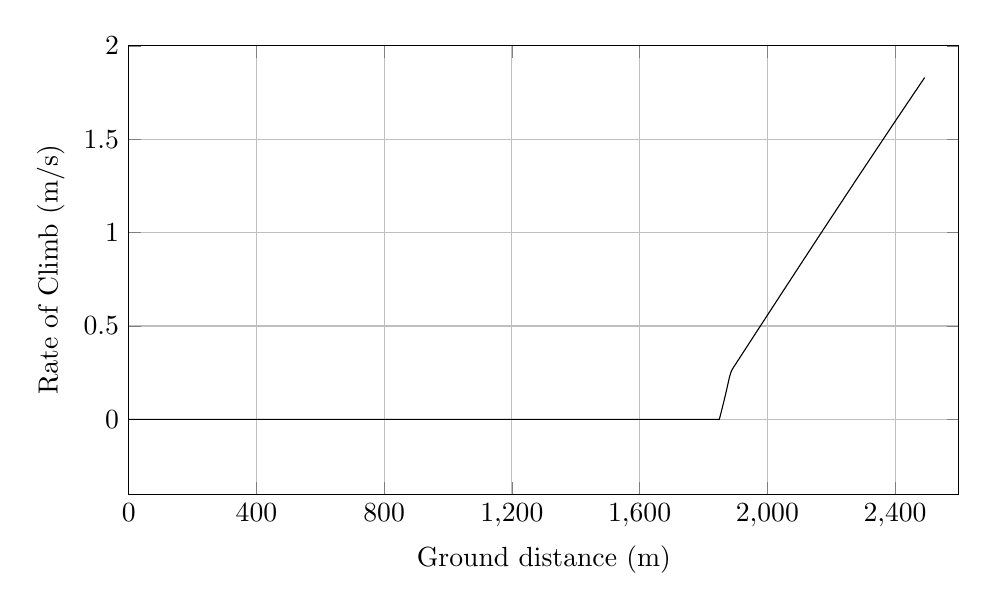
\begin{tikzpicture}

\begin{axis}[
width=\textwidth,
height=0.6\textwidth,
scaled ticks=false, tick label style={/pgf/number format/fixed},
xmin=0.0,
xmax=2600,
xtick={0,400,800,1200,1600,2000,2400,2800,3200},
xlabel={Ground distance (m)},
xmajorgrids,
ymin=-0.4,
ymax=2,
ylabel={Rate of Climb (m/s)},
ymajorgrids,
legend style={at={(1.03,0.5)},anchor=west,draw=black,fill=white,legend cell align=left}
]

\addplot [
color=black,
solid
]
table[row sep=crcr]{
1.3729668748938318E-8	0.0\\
1.7493248493808052E-7	0.0\\
1.4411937280317895E-6	0.0\\
6.602995160656227E-5	0.0\\
2.2740573828771224E-4	0.0\\
4.8751428921765393E-4	0.0\\
8.441986619835749E-4	0.0\\
0.0012981647037285577	0.0\\
0.0018484379050661159	0.0\\
0.0024893731755424335	0.0\\
0.0032286585096692284	0.0\\
0.0040442418752796045	0.0\\
0.004972762654474916	0.0\\
0.005990910102221513	0.0\\
0.007111389191545643	0.0\\
0.008336865178450469	0.0\\
0.009664633507451486	0.0\\
0.011093815858158905	0.0\\
0.01262066151120312	0.0\\
0.01419454386807839	0.0\\
0.015910782250193378	0.0\\
0.017721549103721458	0.0\\
0.019620507964630857	0.0\\
0.02164969955342029	0.0\\
0.023766550611781796	0.0\\
0.025957065600157342	0.0\\
0.028260861173784894	0.0\\
0.030668466949245715	0.0\\
0.0331489614440674	0.0\\
0.03573888453685943	0.0\\
0.038418765463712895	0.0\\
0.04116679597872082	0.0\\
0.044022059812866554	0.0\\
0.04700053365173311	0.0\\
0.050116649382181494	0.0\\
0.0533021652593606	0.0\\
0.056630220296749106	0.0\\
0.05998688030085898	0.0\\
0.06348077825220624	0.0\\
0.06710848437295475	0.0\\
0.07082346760424127	0.0\\
0.07462944469130567	0.0\\
0.07855413323217031	0.0\\
0.08251243142992878	0.0\\
0.08659905947434482	0.0\\
0.09083545394947079	0.0\\
0.09518096637774642	0.0\\
0.099604438418047	0.0\\
0.1041130762071252	0.0\\
0.10871457033213175	0.0\\
0.11350280915994052	0.0\\
0.11836943512882261	0.0\\
0.12328542045494376	0.0\\
0.12830372217771202	0.0\\
0.1334037067999082	0.0\\
0.1386015897371753	0.0\\
0.14405085578552257	0.0\\
0.1495239325759128	0.0\\
0.1550507392415454	0.0\\
0.16073360491635535	0.0\\
0.16659871679960742	0.0\\
0.17244819595229793	0.0\\
0.17848031195343078	0.0\\
0.18466822548212042	0.0\\
0.1909009608611748	0.0\\
0.19716089737688902	0.0\\
0.2035279375926986	0.0\\
0.21017879584430066	0.0\\
0.21687473998771628	0.0\\
0.22354650324940833	0.0\\
0.23036941414946865	0.0\\
0.23737731412185503	0.0\\
0.24449289925428264	0.0\\
0.2517184892023243	0.0\\
0.25908208279438383	0.0\\
0.2664863589195283	0.0\\
0.27399321582905467	0.0\\
0.2816108016888421	0.0\\
0.2893844725195981	0.0\\
0.29747621078120867	0.0\\
0.30547198304033185	0.0\\
0.31373479402345694	0.0\\
0.3220909744202328	0.0\\
0.3305540912568814	0.0\\
0.33895489345894936	0.0\\
0.34753073012810576	0.0\\
0.3563589175375672	0.0\\
0.3652744752958731	0.0\\
0.3742693918027593	0.0\\
0.38350989122680823	0.0\\
0.3927029292363896	0.0\\
0.4020876366599533	0.0\\
0.4115568217121528	0.0\\
0.4212787852930122	0.0\\
0.43089755178065414	0.0\\
0.4408379299669313	0.0\\
0.4510502611115679	0.0\\
0.4612670224725215	0.0\\
0.4715818614584312	0.0\\
0.4818438670126082	0.0\\
0.4922128554044626	0.0\\
0.50273876067117	0.0\\
0.5136516607865718	0.0\\
0.5244310074213006	0.0\\
0.5355751508210329	0.0\\
0.5467126997993474	0.0\\
0.5580479056656631	0.0\\
0.5692960823995112	0.0\\
0.5809945926573021	0.0\\
0.5923626544035139	0.0\\
0.6041922852715	0.0\\
0.6160912669048675	0.0\\
0.6280605196746807	0.0\\
0.6403946506485891	0.0\\
0.6525721787971039	0.0\\
0.66504690021022	0.0\\
0.6773535438897555	0.0\\
0.6901462526606317	0.0\\
0.703249873273524	0.0\\
0.7159721017112175	0.0\\
0.729053467210389	0.0\\
0.7422988791228431	0.0\\
0.756304272979474	0.0\\
0.7696432036294076	0.0\\
0.7832290250230658	0.0\\
0.7969128825551131	0.0\\
0.8108444209446342	0.0\\
0.825043936786227	0.0\\
0.8390802275180445	0.0\\
0.8532340040587583	0.0\\
0.8678101043696134	0.0\\
0.8824320602344964	0.0\\
0.8978006605470081	0.0\\
0.9134572487531922	0.0\\
0.9287391767029982	0.0\\
0.9440564687433697	0.0\\
0.9598871644713316	0.0\\
0.9757786228365237	0.0\\
0.9918217338879218	0.0\\
1.0080608846667363	0.0\\
1.0245900975307913	0.0\\
1.040622085070809	0.0\\
1.0571005809273983	0.0\\
1.0736578999152901	0.0\\
1.0902401336450098	0.0\\
1.1073201062866707	0.0\\
1.1241926772552646	0.0\\
1.1416781667104252	0.0\\
1.1588269484070954	0.0\\
1.176440946845327	0.0\\
1.1944819542445066	0.0\\
1.2120125629913447	0.0\\
1.2299306574276825	0.0\\
1.2481120482032448	0.0\\
1.2663536608165091	0.0\\
1.2851425782117465	0.0\\
1.3041313368869671	0.0\\
1.3228236880779458	0.0\\
1.3414329672940513	0.0\\
1.3605066144349074	0.0\\
1.3802534409605212	0.0\\
1.3994872719307283	0.0\\
1.4192016277101378	0.0\\
1.439023460648384	0.0\\
1.459347998039509	0.0\\
1.4793256644936217	0.0\\
1.4991489338326072	0.0\\
1.5195196572175793	0.0\\
1.5402684478761244	0.0\\
1.5604570108688036	0.0\\
1.5810331069622228	0.0\\
1.6022712329181132	0.0\\
1.623752316257296	0.0\\
1.6452514305955401	0.0\\
1.6664829631402025	0.0\\
1.6886446033619715	0.0\\
1.710607384244656	0.0\\
1.7329417009553727	0.0\\
1.7551421266962821	0.0\\
1.7779085356585536	0.0\\
1.800478286927734	0.0\\
1.8236018329231238	0.0\\
1.8462320784511883	0.0\\
1.869621217116264	0.0\\
1.8933146512119747	0.0\\
1.9176856041472643	0.0\\
1.9417713639512164	0.0\\
1.9657098573982132	0.0\\
1.9902165007163162	0.0\\
2.014554050520948	0.0\\
2.039479559407779	0.0\\
2.0645497069116256	0.0\\
2.090368502766882	0.0\\
2.115564185269416	0.0\\
2.140750230554602	0.0\\
2.1667677015838267	0.0\\
2.1927560352542175	0.0\\
2.218891869133375	0.0\\
2.245288939563828	0.0\\
2.2712530964452817	0.0\\
2.297933078351498	0.0\\
2.324564104516777	0.0\\
2.351466051806102	0.0\\
2.378869922986878	0.0\\
2.4061764715670764	0.0\\
2.4343811693482102	0.0\\
2.4622108821536663	0.0\\
2.4906408044048067	0.0\\
2.518892760285042	0.0\\
2.5472153538550346	0.0\\
2.5762492306032216	0.0\\
2.605385308804288	0.0\\
2.634725531238531	0.0\\
2.6633424112287507	0.0\\
2.6927188130915374	0.0\\
2.7226962917814213	0.0\\
2.7531675915664673	0.0\\
2.7831412651501983	0.0\\
2.8139174932165103	0.0\\
2.8440331768075415	0.0\\
2.874693215323904	0.0\\
2.9059978681586376	0.0\\
2.9372617813709034	0.0\\
2.9684444504378202	0.0\\
3.000072782687808	0.0\\
3.031082587373527	0.0\\
3.063213028467148	0.0\\
3.0965739711585014	0.0\\
3.1291175748240176	0.0\\
3.161651640649506	0.0\\
3.194791488147139	0.0\\
3.2273698640351327	0.0\\
3.261394174200582	0.0\\
3.2942820372415875	0.0\\
3.3276455142443044	0.0\\
3.3625338428565543	0.0\\
3.396526624461681	0.0\\
3.4305511850311694	0.0\\
3.4642094416894933	0.0\\
3.498963551783903	0.0\\
3.5341885134496573	0.0\\
3.569804025802995	0.0\\
3.605116576002147	0.0\\
3.641338581546833	0.0\\
3.677593698357855	0.0\\
3.7132425573336665	0.0\\
3.74957219375957	0.0\\
3.7872650227149185	0.0\\
3.825403000593508	0.0\\
3.861987998097706	0.0\\
3.899535703755137	0.0\\
3.9366960368382165	0.0\\
3.9756271117991435	0.0\\
4.014715979923002	0.0\\
4.053268843133694	0.0\\
4.093111596873367	0.0\\
4.132540645872048	0.0\\
4.171686416589186	0.0\\
4.211258480423352	0.0\\
4.252585425594734	0.0\\
4.29253892845542	0.0\\
4.332839968385603	0.0\\
4.372708537789018	0.0\\
4.414379330316386	0.0\\
4.455607216042212	0.0\\
4.497336690654009	0.0\\
4.53836773335787	0.0\\
4.579767142935065	0.0\\
4.621942908118227	0.0\\
4.663798268780793	0.0\\
4.705838036060712	0.0\\
4.748491012675066	0.0\\
4.791393968819099	0.0\\
4.835700194867293	0.0\\
4.879973298406089	0.0\\
4.923250156511948	0.0\\
4.967673596314626	0.0\\
5.012954369117542	0.0\\
5.057574526249477	0.0\\
5.103280208347517	0.0\\
5.148856018935929	0.0\\
5.194350575362858	0.0\\
5.240584094986199	0.0\\
5.2871741484687504	0.0\\
5.333122064003502	0.0\\
5.3803318800233235	0.0\\
5.4262712259485255	0.0\\
5.473378197958581	0.0\\
5.521938593493333	0.0\\
5.570027890245774	0.0\\
5.617746353771608	0.0\\
5.665750363096816	0.0\\
5.714883880069209	0.0\\
5.763390205677501	0.0\\
5.812817811268989	0.0\\
5.861909274803731	0.0\\
5.912134919389196	0.0\\
5.962317560553064	0.0\\
6.012727788730279	0.0\\
6.0628236035803145	0.0\\
6.113711068416594	0.0\\
6.16497292765713	0.0\\
6.216284706244114	0.0\\
6.26834407822653	0.0\\
6.320257064476769	0.0\\
6.37351660191279	0.0\\
6.426150862197664	0.0\\
6.479030963436509	0.0\\
6.532319340056288	0.0\\
6.5857233987986845	0.0\\
6.640834734692348	0.0\\
6.695022999498724	0.0\\
6.749720237657193	0.0\\
6.804235758325081	0.0\\
6.859728469301633	0.0\\
6.916686079588434	0.0\\
6.9732530286722305	0.0\\
7.029531186664631	0.0\\
7.086633318514238	0.0\\
7.144155485034537	0.0\\
7.202053129566568	0.0\\
7.260126434764185	0.0\\
7.317913145042743	0.0\\
7.376682960996439	0.0\\
7.435393721764624	0.0\\
7.493838107271518	0.0\\
7.552684475254578	0.0\\
7.613252707151423	0.0\\
7.672782806866918	0.0\\
7.733397683408512	0.0\\
7.795525081709004	0.0\\
7.856013653786727	0.0\\
7.91792172269443	0.0\\
7.980110745884113	0.0\\
8.041720670752433	0.0\\
8.105229267009985	0.0\\
8.167457523036095	0.0\\
8.230908874360502	0.0\\
8.293738919282273	0.0\\
8.356235402336917	0.0\\
8.42092378244627	0.0\\
8.485671322837007	0.0\\
8.549180898871484	0.0\\
8.614596634551038	0.0\\
8.680166762249144	0.0\\
8.744770128469462	0.0\\
8.812993689385827	0.0\\
8.88005807777586	0.0\\
8.94709863067661	0.0\\
9.013172088448385	0.0\\
9.079266506338545	0.0\\
9.14748814890141	0.0\\
9.215411293660388	0.0\\
9.284579146198691	0.0\\
9.353168277381275	0.0\\
9.423753765537143	0.0\\
9.492960052876374	0.0\\
9.564123004975215	0.0\\
9.634097601479446	0.0\\
9.705672410878787	0.0\\
9.776260200085993	0.0\\
9.846607984572056	0.0\\
9.918231435410593	0.0\\
9.988851555070422	0.0\\
10.060390022634245	0.0\\
10.133279281833644	0.0\\
10.205241085147751	0.0\\
10.277820389603	0.0\\
10.352558894167803	0.0\\
10.42733258664746	0.0\\
10.501815126481194	0.0\\
10.576858173457808	0.0\\
10.65303812840548	0.0\\
10.729080272001735	0.0\\
10.804841544893105	0.0\\
10.881905013502095	0.0\\
10.958396790746043	0.0\\
11.035905069829102	0.0\\
11.113160538490881	0.0\\
11.192172636140572	0.0\\
11.270076562295213	0.0\\
11.350065490058778	0.0\\
11.429008826667825	0.0\\
11.50754237847364	0.0\\
11.587076645554472	0.0\\
11.668897725768986	0.0\\
11.749734371708193	0.0\\
11.830312384681939	0.0\\
11.909862670519033	0.0\\
11.990515423105418	0.0\\
12.072973931530203	0.0\\
12.155304175892073	0.0\\
12.237018674011615	0.0\\
12.320146069843414	0.0\\
12.406770618003886	0.0\\
12.489918686423398	0.0\\
12.574493004618496	0.0\\
12.660666896522624	0.0\\
12.746500366216402	0.0\\
12.832006837122272	0.0\\
12.919285437479463	0.0\\
13.00517529032821	0.0\\
13.092301899261269	0.0\\
13.179760097773386	0.0\\
13.268594687119744	0.0\\
13.357699529172354	0.0\\
13.44829753340392	0.0\\
13.537570218252604	0.0\\
13.627322718831184	0.0\\
13.718307212496544	0.0\\
13.808540263830096	0.0\\
13.899143852161355	0.0\\
13.991564069206362	0.0\\
14.085798171937814	0.0\\
14.179213507883688	0.0\\
14.271883316076963	0.0\\
14.367546274622434	0.0\\
14.459430863676705	0.0\\
14.555010173556813	0.0\\
14.648669731311681	0.0\\
14.743773575674254	0.0\\
14.839769774519894	0.0\\
14.932807148196385	0.0\\
15.026921440816679	0.0\\
15.12275113649265	0.0\\
15.222025232743288	0.0\\
15.321078842653048	0.0\\
15.417564225728565	0.0\\
15.515758841369038	0.0\\
15.613440509090129	0.0\\
15.7107260301154	0.0\\
15.81102223487273	0.0\\
15.913565872734136	0.0\\
16.012918321571746	0.0\\
16.11222833737955	0.0\\
16.216250800242257	0.0\\
16.319159023020546	0.0\\
16.421418004006803	0.0\\
16.521675247646563	0.0\\
16.62557290942481	0.0\\
16.72731964230514	0.0\\
16.830283223934416	0.0\\
16.93464251494634	0.0\\
17.038481620468637	0.0\\
17.146497421123335	0.0\\
17.252282308638982	0.0\\
17.35724772858778	0.0\\
17.464053904588297	0.0\\
17.572390862630144	0.0\\
17.680417629270814	0.0\\
17.789707298693855	0.0\\
17.899612520762552	0.0\\
18.01027367065641	0.0\\
18.121415095654797	0.0\\
18.232428503320143	0.0\\
18.34337337506409	0.0\\
18.454877340220463	0.0\\
18.56636189702322	0.0\\
18.678405595805643	0.0\\
18.7903363416971	0.0\\
18.902391384512768	0.0\\
19.01754810908954	0.0\\
19.131359562866663	0.0\\
19.247747682986713	0.0\\
19.361628242251975	0.0\\
19.477963464454028	0.0\\
19.595742742603164	0.0\\
19.71107288142779	0.0\\
19.82767543183723	0.0\\
19.944540068808188	0.0\\
20.06171535440768	0.0\\
20.179291418887807	0.0\\
20.29729887224694	0.0\\
20.417200571824914	0.0\\
20.53676390826074	0.0\\
20.65523768803314	0.0\\
20.777063017363922	0.0\\
20.896922101876633	0.0\\
21.016777952410983	0.0\\
21.13892104879462	0.0\\
21.260534693274344	0.0\\
21.382619708556632	0.0\\
21.506306369043365	0.0\\
21.631260758247265	0.0\\
21.75556249187227	0.0\\
21.87985606458615	0.0\\
22.005925835680863	0.0\\
22.130365724585275	0.0\\
22.257477980325966	0.0\\
22.38418119026224	0.0\\
22.50885833858638	0.0\\
22.636026948728087	0.0\\
22.76367325110224	0.0\\
22.89115382514759	0.0\\
23.022452271734288	0.0\\
23.149877274293033	0.0\\
23.27873580881144	0.0\\
23.408563766880334	0.0\\
23.538692653979794	0.0\\
23.671258756997098	0.0\\
23.803210122669313	0.0\\
23.93544283576786	0.0\\
24.067241518013077	0.0\\
24.19863541429976	0.0\\
24.329449967727697	0.0\\
24.46175612159181	0.0\\
24.594763714591892	0.0\\
24.72754053098891	0.0\\
24.86208223890334	0.0\\
24.99503410474967	0.0\\
25.12831230627787	0.0\\
25.265273024090206	0.0\\
25.400650037308893	0.0\\
25.536304655026747	0.0\\
25.673594178904246	0.0\\
25.80797730935859	0.0\\
25.835159569235522	0.0\\
25.83771752397454	0.0\\
25.84157983658004	0.0\\
25.854829339215996	0.0\\
25.893215796826965	0.0\\
25.973046119315796	0.0\\
26.096262980671412	0.0\\
26.224212718725603	0.0\\
26.35313595194755	0.0\\
26.481727686355264	0.0\\
26.611118169629577	0.0\\
26.74049186039369	0.0\\
26.87228140714948	0.0\\
27.003385008924262	0.0\\
27.1358830905183	0.0\\
27.265951877034226	0.0\\
27.399105426781233	0.0\\
27.53075869079712	0.0\\
27.66387879779476	0.0\\
27.79855889054391	0.0\\
27.932132547760695	0.0\\
28.06791767232785	0.0\\
28.202763022922632	0.0\\
28.339788243013793	0.0\\
28.476803106655623	0.0\\
28.61761981788422	0.0\\
28.753907949775353	0.0\\
28.89297195746854	0.0\\
29.03211749902605	0.0\\
29.17123509789927	0.0\\
29.312253051611236	0.0\\
29.454422317169097	0.0\\
29.59523538430127	0.0\\
29.737672170826222	0.0\\
29.879173197948965	0.0\\
30.02075470454991	0.0\\
30.166674235301365	0.0\\
30.308336095430334	0.0\\
30.452640844036836	0.0\\
30.597553881025625	0.0\\
30.742967061600154	0.0\\
30.888975484926362	0.0\\
31.034653067922946	0.0\\
31.180984070508003	0.0\\
31.328351020411645	0.0\\
31.476753455192622	0.0\\
31.62661541983664	0.0\\
31.774495604492607	0.0\\
31.924944104961916	0.0\\
32.07610067279926	0.0\\
32.22631826848556	0.0\\
32.37899942625752	0.0\\
32.528514827654206	0.0\\
32.68189139400266	0.0\\
32.836069829938495	0.0\\
32.99025509482905	0.0\\
33.14574197930297	0.0\\
33.30072558931056	0.0\\
33.455047097713944	0.0\\
33.610874563168906	0.0\\
33.76926068144728	0.0\\
33.92617323250643	0.0\\
34.08448787244542	0.0\\
34.24243160505006	0.0\\
34.40316487172558	0.0\\
34.56154208099588	0.0\\
34.721775177117024	0.0\\
34.88076970836556	0.0\\
35.041349106451236	0.0\\
35.20329621413198	0.0\\
35.364886328651124	0.0\\
35.529241615711214	0.0\\
35.69117991651797	0.0\\
35.85317319416103	0.0\\
36.014854298354294	0.0\\
36.18095311277159	0.0\\
36.34443322746766	0.0\\
36.51065106768533	0.0\\
36.67635767082788	0.0\\
36.842033683894186	0.0\\
37.00823867836148	0.0\\
37.17279029188734	0.0\\
37.33951104811075	0.0\\
37.50923941781488	0.0\\
37.679358776579846	0.0\\
37.845326083883435	0.0\\
38.017144746304325	0.0\\
38.1852030886141	0.0\\
38.35804431104914	0.0\\
38.52812920813831	0.0\\
38.69960796987526	0.0\\
38.87165793928378	0.0\\
39.0423941506003	0.0\\
39.21436971822614	0.0\\
39.38727999643966	0.0\\
39.558989012313546	0.0\\
39.734752343022535	0.0\\
39.908836167348156	0.0\\
40.084555009291705	0.0\\
40.259186798753746	0.0\\
40.43324437115375	0.0\\
40.61041052363379	0.0\\
40.787318094191775	0.0\\
40.96620398302343	0.0\\
41.14141336180775	0.0\\
41.31941103282654	0.0\\
41.49571226203258	0.0\\
41.67366972437729	0.0\\
41.85219319429197	0.0\\
42.03136872634711	0.0\\
42.21293422072888	0.0\\
42.39366932880948	0.0\\
42.57479521797359	0.0\\
42.75522531040919	0.0\\
42.93775785970641	0.0\\
43.11993568316029	0.0\\
43.30336620712447	0.0\\
43.48720879745599	0.0\\
43.672226884455625	0.0\\
43.85684130549208	0.0\\
44.039851952877484	0.0\\
44.22449378650157	0.0\\
44.412385508552646	0.0\\
44.59783063297877	0.0\\
44.78525507043919	0.0\\
44.973130075825196	0.0\\
45.16145211071871	0.0\\
45.34881478087516	0.0\\
45.536017136752506	0.0\\
45.724971990057284	0.0\\
45.91416212467789	0.0\\
46.10175434018815	0.0\\
46.29356928918713	0.0\\
46.48490977712943	0.0\\
46.67744207882204	0.0\\
46.869905949194575	0.0\\
47.062749521718516	0.0\\
47.25341437235973	0.0\\
47.44508461154423	0.0\\
47.63880095964302	0.0\\
47.83356160493736	0.0\\
48.025334057720784	0.0\\
48.218846636819876	0.0\\
48.41468711090302	0.0\\
48.610449575687724	0.0\\
48.80723286029129	0.0\\
49.00124137999302	0.0\\
49.20045899041696	0.0\\
49.394243884198005	0.0\\
49.59161211700324	0.0\\
49.79144608231523	0.0\\
49.99107345578199	0.0\\
50.18996871950735	0.0\\
50.388458331230495	0.0\\
50.59191110395449	0.0\\
50.79453916783869	0.0\\
50.99530158869649	0.0\\
51.19776583381373	0.0\\
51.3996255264899	0.0\\
51.599450409211	0.0\\
51.80158475775707	0.0\\
52.002311498730975	0.0\\
52.2060805474067	0.0\\
52.40811442127868	0.0\\
52.61423073460446	0.0\\
52.821749674584495	0.0\\
53.03053110951893	0.0\\
53.23753590773735	0.0\\
53.44487707917263	0.0\\
53.652063533093525	0.0\\
53.85975522429668	0.0\\
54.06844148636836	0.0\\
54.278580968983874	0.0\\
54.48685885904548	0.0\\
54.69884126905886	0.0\\
54.90975544393264	0.0\\
55.12216013841277	0.0\\
55.333080623240974	0.0\\
55.5448885814986	0.0\\
55.75594910746132	0.0\\
55.968144975063936	0.0\\
56.18150915317635	0.0\\
56.394069348356695	0.0\\
56.60950747146016	0.0\\
56.82641599949238	0.0\\
57.03980213394583	0.0\\
57.25698083573829	0.0\\
57.47353804711997	0.0\\
57.6941706582635	0.0\\
57.91229938529948	0.0\\
58.12998527173144	0.0\\
58.34905943653719	0.0\\
58.56781345824973	0.0\\
58.787998582886644	0.0\\
59.011266007804366	0.0\\
59.23368761368569	0.0\\
59.456031473365414	0.0\\
59.67976581221534	0.0\\
59.90315377467765	0.0\\
60.125192111546724	0.0\\
60.349269227196444	0.0\\
60.57220932044149	0.0\\
60.79606803632835	0.0\\
61.021718319759984	0.0\\
61.25073295331903	0.0\\
61.47770893732542	0.0\\
61.70784367826464	0.0\\
61.93740803875056	0.0\\
62.1673491775543	0.0\\
62.39648011888062	0.0\\
62.62822464633953	0.0\\
62.86094183422966	0.0\\
63.090532789209604	0.0\\
63.321616049163225	0.0\\
63.554808975015874	0.0\\
63.78685818650332	0.0\\
64.0234762327251	0.0\\
64.25652029988498	0.0\\
64.49146565301734	0.0\\
64.72768747885678	0.0\\
64.96568125142531	0.0\\
65.20057601391298	0.0\\
65.43975061379945	0.0\\
65.67719429610031	0.0\\
65.91652243006087	0.0\\
66.1565253585166	0.0\\
66.39740384038885	0.0\\
66.63777997854328	0.0\\
66.87849958303539	0.0\\
67.12349409848125	0.0\\
67.36843544137562	0.0\\
67.61129947098183	0.0\\
67.85808619273692	0.0\\
68.10323725880951	0.0\\
68.3520146383799	0.0\\
68.60099753692072	0.0\\
68.84943315800746	0.0\\
69.09793111574629	0.0\\
69.34894754058863	0.0\\
69.59791912239118	0.0\\
69.84867626946473	0.0\\
70.10496107302816	0.0\\
70.35594730130109	0.0\\
70.60854748652795	0.0\\
70.8625286964371	0.0\\
71.1182576034713	0.0\\
71.37278964945165	0.0\\
71.62944082734805	0.0\\
71.88536754710964	0.0\\
72.14250945057543	0.0\\
72.40306402213687	0.0\\
72.66241221953337	0.0\\
72.92327110344874	0.0\\
73.18657203154456	0.0\\
73.45150557123125	0.0\\
73.71756195569753	0.0\\
73.97940051906463	0.0\\
74.24514793127645	0.0\\
74.51022759525631	0.0\\
74.77823256031297	0.0\\
75.04767613410795	0.0\\
75.31682895458664	0.0\\
75.58729746777243	0.0\\
75.85729327570917	0.0\\
76.13042767774209	0.0\\
76.40299665611133	0.0\\
76.67973301409052	0.0\\
76.95360383527739	0.0\\
77.22854206589327	0.0\\
77.50692063517303	0.0\\
77.78349662592461	0.0\\
78.0616064362213	0.0\\
78.33869545141144	0.0\\
78.62238552181594	0.0\\
78.90481169871467	0.0\\
79.18659077494928	0.0\\
79.4700201012688	0.0\\
79.75774957869095	0.0\\
80.04430580185078	0.0\\
80.33432201731404	0.0\\
80.62298533865851	0.0\\
80.9130804606989	0.0\\
81.20459144967842	0.0\\
81.49650140842283	0.0\\
81.79224544448738	0.0\\
82.08455487090956	0.0\\
82.37934996819865	0.0\\
82.67580145620735	0.0\\
82.97475550983006	0.0\\
83.2734238134004	0.0\\
83.57209772503273	0.0\\
83.87419166445906	0.0\\
84.17487194816226	0.0\\
84.47686996876752	0.0\\
84.78124993153034	0.0\\
85.08776945017104	0.0\\
85.39395758722245	0.0\\
85.69833162305892	0.0\\
86.01027818388755	0.0\\
86.31658691867341	0.0\\
86.62866814828641	0.0\\
86.94043673469176	0.0\\
87.2565990672368	0.0\\
87.56980823017452	0.0\\
87.88101387141376	0.0\\
88.20007062892054	0.0\\
88.51883409355145	0.0\\
88.83509784148416	0.0\\
89.15857089898353	0.0\\
89.47772213402055	0.0\\
89.80217214804901	0.0\\
90.1263587278685	0.0\\
90.44950966725051	0.0\\
90.77764749859728	0.0\\
91.10470504824352	0.0\\
91.43769785174896	0.0\\
91.76691749028419	0.0\\
92.09386993524024	0.0\\
92.42498248438446	0.0\\
92.7581696617394	0.0\\
93.09729153734631	0.0\\
93.4312406900703	0.0\\
93.76780571708736	0.0\\
94.10390054156983	0.0\\
94.43564317419558	0.0\\
94.77291201930262	0.0\\
95.10796951504997	0.0\\
95.44708659079325	0.0\\
95.78515592548297	0.0\\
96.12311752311894	0.0\\
96.46351490415591	0.0\\
96.80669869710772	0.0\\
97.14657639264556	0.0\\
97.48763116340677	0.0\\
97.8305814261901	0.0\\
98.17013304046878	0.0\\
98.51054009051404	0.0\\
98.854181194619	0.0\\
99.19205317796005	0.0\\
99.53355440060989	0.0\\
99.87198375587872	0.0\\
100.2129389915628	0.0\\
100.55335806642802	0.0\\
100.89503335592528	0.0\\
101.23693480167049	0.0\\
101.57977298927813	0.0\\
101.91842351185082	0.0\\
102.26214655705948	0.0\\
102.60487134933112	0.0\\
102.94238410388857	0.0\\
103.28139950825951	0.0\\
103.61984226602698	0.0\\
103.95406402656286	0.0\\
104.29248504574807	0.0\\
104.63112914593611	0.0\\
104.96686613984221	0.0\\
105.30464484937244	0.0\\
105.64180205248229	0.0\\
105.97704387437452	0.0\\
106.31384964552919	0.0\\
106.6489228444834	0.0\\
106.98000007373659	0.0\\
107.31456925364313	0.0\\
107.38092108752608	0.0\\
107.387754025128	0.0\\
107.3946577511588	0.0\\
107.39916951903444	0.0\\
107.40247473215817	0.0\\
107.40548301099807	0.0\\
107.41901751964124	0.0\\
107.47756267729525	0.0\\
107.63696404402117	0.0\\
107.95668166923352	0.0\\
108.2571634635643	0.0\\
108.55996775705782	0.0\\
108.8616926844802	0.0\\
109.16669292910967	0.0\\
109.47218465327785	0.0\\
109.78023369107405	0.0\\
110.09061921742381	0.0\\
110.4007971847821	0.0\\
110.7125096545017	0.0\\
111.02874540594937	0.0\\
111.34670354521654	0.0\\
111.664908557295	0.0\\
111.98617551206428	0.0\\
112.3078797039536	0.0\\
112.63537393275391	0.0\\
112.96267359383529	0.0\\
113.28778388635178	0.0\\
113.61823593045688	0.0\\
113.94632344632586	0.0\\
114.27926944824554	0.0\\
114.61324422041562	0.0\\
114.94750338770686	0.0\\
115.28618013885716	0.0\\
115.62544260296943	0.0\\
115.9647508443766	0.0\\
116.30617149460878	0.0\\
116.65060078043697	0.0\\
116.99863777637248	0.0\\
117.34270613829636	0.0\\
117.68983788345284	0.0\\
118.04137408578512	0.0\\
118.39343387684602	0.0\\
118.74804854616337	0.0\\
119.10520175440718	0.0\\
119.46686684850098	0.0\\
119.82660492256403	0.0\\
120.19012449272657	0.0\\
120.55217592908159	0.0\\
120.91763124996498	0.0\\
121.28719248968574	0.0\\
121.65493622417088	0.0\\
122.02513489718217	0.0\\
122.39308995700384	0.0\\
122.76618799735454	0.0\\
123.1388017253943	0.0\\
123.51256311114031	0.0\\
123.88633794770595	0.0\\
124.25665874611622	0.0\\
124.63165231885978	0.0\\
125.00664173256905	0.0\\
125.38021625899401	0.0\\
125.75512563345742	0.0\\
126.13473977091255	0.0\\
126.51299085225449	0.0\\
126.8948287761801	0.0\\
127.27325883095315	0.0\\
127.64986999110431	0.0\\
128.03053456382577	0.0\\
128.40840086210045	0.0\\
128.78830732782995	0.0\\
129.16816802858597	0.0\\
129.55114692916032	0.0\\
129.92795862154003	0.0\\
130.30814318938542	0.0\\
130.68801179162523	0.0\\
131.0673626953399	0.0\\
131.44707508552267	0.0\\
131.82575792285303	0.0\\
132.20466209461676	0.0\\
132.58549544797154	0.0\\
132.96520261413826	0.0\\
133.34413894748724	0.0\\
133.72638850756363	0.0\\
134.1049920954593	0.0\\
134.48538249769342	0.0\\
134.86277461399203	0.0\\
135.2402386369938	0.0\\
135.62109197355238	0.0\\
135.9996509441208	0.0\\
136.37968191797512	0.0\\
136.76120583273502	0.0\\
137.13951930881296	0.0\\
137.51840340013064	0.0\\
137.89819615735314	0.0\\
138.27485697152616	0.0\\
138.65420581933705	0.0\\
139.03531375767642	0.0\\
139.41296882619503	0.0\\
139.79422155259	0.0\\
140.17408835952057	0.0\\
140.5488076998477	0.0\\
140.92844631991198	0.0\\
141.30483696429354	0.0\\
141.68269541512387	0.0\\
142.06058279783264	0.0\\
142.43991695918288	0.0\\
142.81695502902187	0.0\\
143.19247254825046	0.0\\
143.5733885276352	0.0\\
143.94921103219775	0.0\\
144.32621366107247	0.0\\
144.70408630975157	0.0\\
145.08263595865492	0.0\\
145.46162624555404	0.0\\
145.83827879615103	0.0\\
146.21524500988596	0.0\\
146.5934755401724	0.0\\
146.9730259257883	0.0\\
147.3547239944582	0.0\\
147.73366854735332	0.0\\
148.1136534850276	0.0\\
148.49311509785633	0.0\\
148.87144514206074	0.0\\
149.25360190977045	0.0\\
149.6334430260095	0.0\\
150.01465687879528	0.0\\
150.3940924716125	0.0\\
150.77688175221402	0.0\\
151.1561678741857	0.0\\
151.5352572324847	0.0\\
151.91884603110896	0.0\\
152.3000376871389	0.0\\
152.6837211891089	0.0\\
153.06727641570347	0.0\\
153.4514076737559	0.0\\
153.83522357687116	0.0\\
154.21637826964854	0.0\\
154.6009164651564	0.0\\
154.98403470202834	0.0\\
155.36838747168406	0.0\\
155.75158064164503	0.0\\
156.13576662495046	0.0\\
156.5218436740983	0.0\\
156.90521285441474	0.0\\
157.2916244593892	0.0\\
157.6780020855428	0.0\\
158.06299451159185	0.0\\
158.4509000667514	0.0\\
158.83830611621056	0.0\\
159.22672413827297	0.0\\
159.61474494524106	0.0\\
160.0042372884319	0.0\\
160.39552304382113	0.0\\
160.78478895267375	0.0\\
161.17517847278327	0.0\\
161.56748129737286	0.0\\
161.9609400214345	0.0\\
162.35005274814932	0.0\\
162.7425950916558	0.0\\
163.13607830878885	0.0\\
163.53170884953005	0.0\\
163.92462594167722	0.0\\
164.3198767210975	0.0\\
164.7157696028566	0.0\\
165.1115317336501	0.0\\
165.50739628911128	0.0\\
165.90698313288817	0.0\\
166.30582458333038	0.0\\
166.70591293613995	0.0\\
167.1044701422045	0.0\\
167.50226971352845	0.0\\
167.9010833894181	0.0\\
168.3004552315794	0.0\\
168.70189335181743	0.0\\
169.10576843973695	0.0\\
169.50785881751284	0.0\\
169.91045494783964	0.0\\
170.31331810721775	0.0\\
170.71648797717722	0.0\\
171.11993291578136	0.0\\
171.5247281229082	0.0\\
171.92976094083576	0.0\\
172.33690302624336	0.0\\
172.74259563259648	0.0\\
173.1509823323036	0.0\\
173.55913088366435	0.0\\
173.96636547491187	0.0\\
174.37754484483776	0.0\\
174.7874876782942	0.0\\
175.2012500141185	0.0\\
175.6112323385957	0.0\\
176.02092514523684	0.0\\
176.43326782420013	0.0\\
176.8477920653399	0.0\\
177.2627043459005	0.0\\
177.67839640445425	0.0\\
178.09047986160414	0.0\\
178.50771992227516	0.0\\
178.92514786216543	0.0\\
179.34349041668827	0.0\\
179.7634585539525	0.0\\
180.0836350053749	0.0\\
180.18446825846002	0.0\\
180.6041229201494	0.0\\
181.5278851973348	0.0\\
182.40940876889346	0.0\\
183.29020149056134	0.0\\
184.17127536929127	0.0\\
185.05444413874795	0.0\\
185.94463812048832	0.0\\
186.83342305465118	0.0\\
187.72320740690213	0.0\\
188.61627250998652	0.0\\
189.51597565669658	0.0\\
190.41002295084513	0.0\\
191.3196934236239	0.0\\
192.21828392903763	0.0\\
193.1226105375991	0.0\\
194.0308739866166	0.0\\
194.94664810390913	0.0\\
195.8495877725365	0.0\\
196.76514896738053	0.0\\
197.67776544775052	0.0\\
198.59781945634353	0.0\\
199.51766543264023	0.0\\
200.44351810370483	0.0\\
201.3718330130543	0.0\\
202.29314309783985	0.0\\
203.21971650332063	0.0\\
204.14462823093066	0.0\\
205.07763860999955	0.0\\
206.00476468733177	0.0\\
206.93855819187849	0.0\\
207.87782366152794	0.0\\
208.81805039558168	0.0\\
209.75927086542703	0.0\\
210.70907141928154	0.0\\
211.6546393296269	0.0\\
212.59816623974814	0.0\\
213.54645843731532	0.0\\
214.4982137391426	0.0\\
215.45734539338423	0.0\\
216.4205873513297	0.0\\
217.38237643693935	0.0\\
218.35297485781302	0.0\\
219.32510845799027	0.0\\
220.29279514401117	0.0\\
221.26927942590856	0.0\\
222.2446078047322	0.0\\
223.21462685547237	0.0\\
224.19074054242492	0.0\\
225.1744490750948	0.0\\
226.14733001520318	0.0\\
227.14148425007068	0.0\\
228.1240128312001	0.0\\
229.11886046703495	0.0\\
230.11739511657566	0.0\\
231.11215533106218	0.0\\
232.12301378994505	0.0\\
233.1275199718878	0.0\\
234.13114028184475	0.0\\
235.14028542531037	0.0\\
236.15081117254897	0.0\\
237.1660420924572	0.0\\
238.1886645294469	0.0\\
239.21465471906964	0.0\\
240.23482884221784	0.0\\
241.26021232675805	0.0\\
242.3021991810905	0.0\\
243.32988353044664	0.0\\
244.36880129710033	0.0\\
245.4061041381612	0.0\\
246.46256617747576	0.0\\
247.50478260671736	0.0\\
248.56376742117214	0.0\\
249.6219134221688	0.0\\
250.66481994405478	0.0\\
251.72705353011372	0.0\\
252.80088254110024	0.0\\
253.86267363775482	0.0\\
254.94374853170973	0.0\\
256.0221053298852	0.0\\
257.1056667215428	0.0\\
258.2028084304169	0.0\\
259.3030712409387	0.0\\
260.39721249167394	0.0\\
261.49829074545437	0.0\\
262.60930370875815	0.0\\
263.7179887580877	0.0\\
264.8352779160481	0.0\\
265.9576164693235	0.0\\
267.09103410107514	0.0\\
268.20818841649384	0.0\\
269.3328220499261	0.0\\
270.4661510695621	0.0\\
271.5992062566115	0.0\\
272.7460111433737	0.0\\
273.90093061584855	0.0\\
275.05359207729066	0.0\\
276.20311568521606	0.0\\
277.35310992264476	0.0\\
278.5188185905665	0.0\\
279.6929356623284	0.0\\
280.86252284262184	0.0\\
282.05142644191835	0.0\\
283.24985431198513	0.0\\
284.4388813912709	0.0\\
285.6397000671543	0.0\\
286.836316139525	0.0\\
288.0392161140162	0.0\\
289.2556790589223	0.0\\
290.48265444814547	0.0\\
291.72130155141053	0.0\\
292.96100893763946	0.0\\
294.1985103575731	0.0\\
295.4456267737909	0.0\\
296.68519223220017	0.0\\
297.9280216368336	0.0\\
299.1850487812583	0.0\\
300.44412429943463	0.0\\
301.7225677950246	0.0\\
303.0017748749233	0.0\\
304.2792219657807	0.0\\
305.56506002795425	0.0\\
306.85051236654385	0.0\\
308.1437929069215	0.0\\
309.44719641798304	0.0\\
310.77840358228957	0.0\\
312.0849502338091	0.0\\
313.4080429046928	0.0\\
314.7190184524427	0.0\\
316.0311580127236	0.0\\
317.3407104164604	0.0\\
318.66998531861896	0.0\\
319.98030216977895	0.0\\
321.3131882515936	0.0\\
322.64658699863	0.0\\
323.97760893915427	0.0\\
325.31447228134823	0.0\\
326.6245528491544	0.0\\
327.9601785097144	0.0\\
329.2784770253418	0.0\\
330.6069033330348	0.0\\
331.9178806716509	0.0\\
333.2333630873429	0.0\\
334.5584389845069	0.0\\
335.850474636536	0.0\\
337.1511723788834	0.0\\
338.4381183837047	0.0\\
339.72984837001286	0.0\\
341.0214788139215	0.0\\
342.3149785174073	0.0\\
343.60619007360367	0.0\\
344.88769479656867	0.0\\
346.16492597045556	0.0\\
347.44208543988907	0.0\\
348.7214970855716	0.0\\
349.9975255146603	0.0\\
351.26866298989455	0.0\\
352.534343347637	0.0\\
353.79318608781	0.0\\
355.04194064781143	0.0\\
356.2900696565431	0.0\\
357.5353145753136	0.0\\
357.7850582428015	0.0\\
358.34364659427206	0.0\\
358.3912146679147	0.0\\
358.41401903577105	0.0\\
358.5450809455632	0.0\\
358.7245681548527	0.0\\
359.254094841737	0.0\\
360.2339632435762	0.0\\
361.31185038514695	0.0\\
362.3872645146199	0.0\\
363.4679309383365	0.0\\
364.56333677126634	0.0\\
365.6588974221802	0.0\\
366.75774424816416	0.0\\
367.87135537791175	0.0\\
368.9928518144826	0.0\\
370.1124569712374	0.0\\
371.23921033825184	0.0\\
372.37198049913775	0.0\\
373.50814429472643	0.0\\
374.644008507355	0.0\\
375.7850599487498	0.0\\
376.9482158284984	0.0\\
378.1077665587011	0.0\\
379.26973869573817	0.0\\
380.44580761476436	0.0\\
381.62390672234494	0.0\\
382.8144199569183	0.0\\
384.00299852894386	0.0\\
385.20027356755816	0.0\\
386.4087115701377	0.0\\
387.627261825594	0.0\\
388.847438745123	0.0\\
390.08585374585346	0.0\\
391.32999859576034	0.0\\
392.5794981700179	0.0\\
393.8295213861659	0.0\\
395.08429723606037	0.0\\
396.348052674334	0.0\\
397.610529015913	0.0\\
398.9011153976112	0.0\\
400.18894235692665	0.0\\
401.4791306222337	0.0\\
402.7830293971008	0.0\\
404.0853140496723	0.0\\
405.3940039897615	0.0\\
406.70640055955323	0.0\\
408.00887196551514	0.0\\
409.3026454816096	0.0\\
410.6132390977027	0.0\\
411.9298689998851	0.0\\
413.25815553647726	0.0\\
414.58952083365057	0.0\\
415.918967975221	0.0\\
417.2419527990422	0.0\\
418.5724204266372	0.0\\
419.9001914117176	0.0\\
421.22244671332	0.0\\
422.5499672440235	0.0\\
423.874944258631	0.0\\
425.1940527578546	0.0\\
426.51214046059533	0.0\\
427.8403065447367	0.0\\
429.16543732752825	0.0\\
430.493480912485	0.0\\
431.8120787187414	0.0\\
433.13404798305	0.0\\
434.45758221825076	0.0\\
435.77270008640085	0.0\\
437.0762078546635	0.0\\
438.3722228261918	0.0\\
439.6647932913057	0.0\\
440.96010063217216	0.0\\
442.2548502943886	0.0\\
443.55240151451153	0.0\\
444.84015975838133	0.0\\
446.12596298338667	0.0\\
447.41271623936245	0.0\\
448.68923141398216	0.0\\
449.96221775008996	0.0\\
451.24101119640613	0.0\\
452.50923174405136	0.0\\
453.7757634438541	0.0\\
455.04040758000076	0.0\\
456.3187472578254	0.0\\
457.5883933736685	0.0\\
458.84637863243324	0.0\\
460.1173199788476	0.0\\
461.37502127563994	0.0\\
462.64293744016754	0.0\\
463.89875968806496	0.0\\
465.1596048263507	0.0\\
466.4129938848299	0.0\\
467.6761864310754	0.0\\
468.92877471797476	0.0\\
470.1802840729189	0.0\\
471.42234175136343	0.0\\
472.66721587755	0.0\\
473.9119998681615	0.0\\
475.15784183330595	0.0\\
476.4027610202945	0.0\\
477.64387772945474	0.0\\
478.8802799588349	0.0\\
480.11938637872606	0.0\\
481.3598938784121	0.0\\
482.60100270099633	0.0\\
483.83761604071765	0.0\\
485.07417441604616	0.0\\
486.30932624990373	0.0\\
487.5485020564116	0.0\\
488.78476676571006	0.0\\
490.02776083238655	0.0\\
491.26052006608825	0.0\\
492.50223365857005	0.0\\
493.73875790953696	0.0\\
494.9705227407086	0.0\\
496.20662631815094	0.0\\
497.4417048478979	0.0\\
498.67979578388963	0.0\\
499.9077395058579	0.0\\
501.13206886531634	0.0\\
502.36560836777835	0.0\\
503.5988541698998	0.0\\
504.8341308395434	0.0\\
506.05800551932055	0.0\\
507.27849694883867	0.0\\
508.51586902201325	0.0\\
509.7437321564099	0.0\\
510.9765281767244	0.0\\
512.2003190975361	0.0\\
513.4213909555808	0.0\\
514.6497928055664	0.0\\
515.8776846194819	0.0\\
517.1060250500084	0.0\\
518.3498419555788	0.0\\
519.5794414015706	0.0\\
520.8101291797705	0.0\\
522.0439200808898	0.0\\
523.2808555224788	0.0\\
524.5125928741788	0.0\\
525.741539831949	0.0\\
526.9760734195245	0.0\\
528.2104121448019	0.0\\
529.444482094551	0.0\\
530.6778496336067	0.0\\
531.9092562002504	0.0\\
533.1456875412582	0.0\\
534.3827295754174	0.0\\
535.6194547718162	0.0\\
536.8537227143379	0.0\\
538.0899051479412	0.0\\
539.3366163711867	0.0\\
540.5793174245275	0.0\\
541.8175341103783	0.0\\
543.0580254609008	0.0\\
544.2905932367662	0.0\\
545.5264322163653	0.0\\
546.7679638454138	0.0\\
548.0058826203228	0.0\\
549.247222977644	0.0\\
550.4927278587875	0.0\\
551.7284048687036	0.0\\
552.969156750524	0.0\\
554.2147139753856	0.0\\
555.4621950310477	0.0\\
556.706538922255	0.0\\
557.949692049355	0.0\\
559.1956898523235	0.0\\
560.4455810647141	0.0\\
561.7029824469003	0.0\\
562.9528606070708	0.0\\
564.2038089647817	0.0\\
565.4583765420568	0.0\\
566.708587276828	0.0\\
567.9637216989229	0.0\\
569.2171025509995	0.0\\
570.474468357347	0.0\\
571.742642818326	0.0\\
572.996651880251	0.0\\
574.2599126777859	0.0\\
575.5220984235082	0.0\\
576.7831302823038	0.0\\
578.0511116485295	0.0\\
579.3140861716088	0.0\\
580.5820139587681	0.0\\
581.8434957563957	0.0\\
583.1166272054381	0.0\\
584.3893870491142	0.0\\
585.6599343818289	0.0\\
586.9369288742066	0.0\\
588.2179000220438	0.0\\
589.4870261901688	0.0\\
590.7657581143835	0.0\\
592.0414533779388	0.0\\
593.3235970013507	0.0\\
594.6058362788467	0.0\\
595.8868323916915	0.0\\
597.1683432634425	0.0\\
598.4446335159173	0.0\\
599.730175188072	0.0\\
601.0212431507625	0.0\\
602.3088641938682	0.0\\
603.6034700803755	0.0\\
604.8981683781547	0.0\\
606.1922330968823	0.0\\
607.490120236022	0.0\\
608.7939415919918	0.0\\
610.0955995359013	0.0\\
611.3977783333462	0.0\\
612.6917013228608	0.0\\
614.0040683383606	0.0\\
615.3085862372382	0.0\\
616.613602898017	0.0\\
617.9265277419127	0.0\\
619.2347914209017	0.0\\
620.5412253249128	0.0\\
621.852908032758	0.0\\
623.1679499449649	0.0\\
624.4856050257858	0.0\\
625.810066181002	0.0\\
627.1361220452648	0.0\\
628.463359530801	0.0\\
629.7942853078969	0.0\\
631.1262466617202	0.0\\
632.4582408521592	0.0\\
633.7950163787261	0.0\\
635.1327095290424	0.0\\
636.4726195282103	0.0\\
637.8068805033517	0.0\\
639.1469055652017	0.0\\
640.4926300799054	0.0\\
641.8418857176027	0.0\\
643.1859405998212	0.0\\
644.5356315965766	0.0\\
645.8822545209948	0.0\\
647.233670728461	0.0\\
648.5864007556052	0.0\\
649.940370298199	0.0\\
651.2968611767658	0.0\\
652.6588166774502	0.0\\
654.0286677329391	0.0\\
655.3980147933239	0.0\\
656.7651144911501	0.0\\
658.1273862384021	0.0\\
659.5073029329092	0.0\\
660.8826272704664	0.0\\
662.2661978885028	0.0\\
663.643291595564	0.0\\
665.0275285174982	0.0\\
666.4147025971529	0.0\\
667.8000093843657	0.0\\
669.1890308696848	0.0\\
670.5841029593273	0.0\\
671.984126089166	0.0\\
673.3808681330338	0.0\\
674.7830165257378	0.0\\
676.1898253545012	0.0\\
677.5991903091519	0.0\\
679.015088371943	0.0\\
680.4386457201426	0.0\\
681.8569959867716	0.0\\
683.2684154764579	0.0\\
684.6955822936916	0.0\\
686.1210149102426	0.0\\
687.5534290554101	0.0\\
688.9879916285763	0.0\\
690.4246609807328	0.0\\
691.8693809894646	0.0\\
693.3101354987134	0.0\\
694.7516516040589	0.0\\
696.1961456892448	0.0\\
697.6431450077532	0.0\\
699.0946712958735	0.0\\
700.5536207415289	0.0\\
702.016499890844	0.0\\
703.4860872285026	0.0\\
704.9634790305677	0.0\\
706.4368997325803	0.0\\
707.9127625449362	0.0\\
709.3962797863628	0.0\\
710.8794084854612	0.0\\
712.3555872746397	0.0\\
713.8437612413873	0.0\\
715.3392133125592	0.0\\
716.843000235509	0.0\\
718.3555772579125	0.0\\
719.8612576914384	0.0\\
721.363907905622	0.0\\
722.8778664981737	0.0\\
724.3893964645993	0.0\\
725.9153332443707	0.0\\
727.4340437680246	0.0\\
728.9691946264161	0.0\\
730.5018963167051	0.0\\
732.0400708691539	0.0\\
733.5864821361122	0.0\\
735.1330665532416	0.0\\
736.6809646870079	0.0\\
738.2371436455285	0.0\\
739.8017854816455	0.0\\
741.3730723556473	0.0\\
742.9509937059506	0.0\\
744.5305864424283	0.0\\
746.113967954703	0.0\\
747.6993176375493	0.0\\
749.2841200736946	0.0\\
750.8901221987192	0.0\\
752.4917045033196	0.0\\
754.1043880453294	0.0\\
755.7247957897362	0.0\\
757.350123465433	0.0\\
758.9779883422452	0.0\\
760.6174244775955	0.0\\
762.2471670049172	0.0\\
763.8864959469677	0.0\\
765.5286451874665	0.0\\
767.1876108560682	0.0\\
768.8527838772816	0.0\\
770.5256520101113	0.0\\
772.2062150690381	0.0\\
773.8901713847758	0.0\\
775.5819238733998	0.0\\
777.2817188512629	0.0\\
778.9828497337423	0.0\\
780.6908914191338	0.0\\
782.4072790768848	0.0\\
784.1443131244669	0.0\\
785.8879055054167	0.0\\
787.6332840316636	0.0\\
789.3854457283926	0.0\\
791.150614729399	0.0\\
792.9275189326358	0.0\\
794.7078690219801	0.0\\
796.4884271284063	0.0\\
798.3010390178765	0.0\\
800.127460680355	0.0\\
801.9391768347505	0.0\\
803.7775071319543	0.0\\
805.6217304493966	0.0\\
807.4652472742337	0.0\\
809.3346687612084	0.0\\
811.2083986459545	0.0\\
813.1006487758623	0.0\\
815.0050871107928	0.0\\
816.9276441884065	0.0\\
818.8689876349765	0.0\\
820.8183532152264	0.0\\
822.7755491014664	0.0\\
824.7452211297996	0.0\\
826.7429412153915	0.0\\
828.7613686297161	0.0\\
830.7884573079714	0.0\\
832.828736080513	0.0\\
834.9046256554884	0.0\\
837.0114805828528	0.0\\
839.1225712464998	0.0\\
841.2731456998592	0.0\\
843.4451716536778	0.0\\
845.6259741016938	0.0\\
847.8606760357923	0.0\\
850.1208659733229	0.0\\
852.4072054021524	0.0\\
854.6894106389352	0.0\\
857.0206263933742	0.0\\
859.351860599884	0.0\\
861.6956235055641	0.0\\
864.0809230193477	0.0\\
866.4729453807156	0.0\\
868.8505739467978	0.0\\
871.2321917628958	0.0\\
873.6030973799157	0.0\\
875.9559955009365	0.0\\
878.2807840446324	0.0\\
880.587891005154	0.0\\
882.8626320583053	0.0\\
885.1225565401078	0.0\\
887.3480853176877	0.0\\
889.5620345079099	0.0\\
891.7304167933539	0.0\\
893.8751088534989	0.0\\
896.0261261085977	0.0\\
898.1309922927635	0.0\\
900.2326939775073	0.0\\
902.3196796609091	0.0\\
904.395999618223	0.0\\
906.4488598365222	0.0\\
908.4734246133198	0.0\\
910.4886481023309	0.0\\
912.4998117561495	0.0\\
914.4817648890871	0.0\\
916.4660406044704	0.0\\
918.4368350154689	0.0\\
920.3847916817979	0.0\\
922.3381019626172	0.0\\
924.2667962694686	0.0\\
926.1746743338263	0.0\\
928.0830302852894	0.0\\
929.9834739104342	0.0\\
931.8773536632029	0.0\\
933.7613227348986	0.0\\
935.6293361496487	0.0\\
937.4925021199458	0.0\\
939.3482853811552	0.0\\
941.1878470693061	0.0\\
941.5553186827369	0.0\\
941.8072895200994	0.0\\
941.9750419552138	0.0\\
942.1271197160249	0.0\\
942.2334325425763	0.0\\
942.2638346188435	0.0\\
942.2892369539902	0.0\\
942.3142175675691	0.0\\
942.485900152953	0.0\\
943.0589388091298	0.0\\
945.0389423283557	0.0\\
946.833978762777	0.0\\
948.6304534556368	0.0\\
950.4439821025769	0.0\\
952.2743006168116	0.0\\
954.1043114076579	0.0\\
955.9587036375908	0.0\\
957.8214130903962	0.0\\
959.6880133585512	0.0\\
961.5705683718347	0.0\\
963.4691274632328	0.0\\
965.3799468679672	0.0\\
967.303567080218	0.0\\
969.249430755759	0.0\\
971.2103887374251	0.0\\
973.1797263714714	0.0\\
975.1648586450763	0.0\\
977.167899909447	0.0\\
979.1914625168572	0.0\\
981.2231615224496	0.0\\
983.2827075787545	0.0\\
985.3542337326639	0.0\\
987.4323877978486	0.0\\
989.5425714128878	0.0\\
991.6598808029521	0.0\\
993.8204456533306	0.0\\
995.9839346123126	0.0\\
998.1864770000634	0.0\\
1000.3922002439062	0.0\\
1002.6270345530863	0.0\\
1004.8745995143443	0.0\\
1007.1471979082173	0.0\\
1009.4424926286526	0.0\\
1011.7467619954873	0.0\\
1014.0483899295439	0.0\\
1016.3973453828874	0.0\\
1018.7366981348446	0.0\\
1021.0722856382722	0.0\\
1023.4243231675273	0.0\\
1025.7588128090124	0.0\\
1028.088775604409	0.0\\
1030.4145296909378	0.0\\
1032.7408393953942	0.0\\
1035.065679431843	0.0\\
1037.35962020532	0.0\\
1039.6467054896502	0.0\\
1041.911281890793	0.0\\
1044.1670537964305	0.0\\
1046.4144315253666	0.0\\
1048.6401135402712	0.0\\
1050.856648472272	0.0\\
1053.0660782914179	0.0\\
1055.2676035326776	0.0\\
1057.4437387850207	0.0\\
1059.6057076599227	0.0\\
1061.7573708263599	0.0\\
1063.9023616350323	0.0\\
1066.029616250597	0.0\\
1068.1575813820505	0.0\\
1070.2619333766766	0.0\\
1072.3612812062906	0.0\\
1074.4576032664554	0.0\\
1076.5406588764508	0.0\\
1078.61282918597	0.0\\
1080.6792045529783	0.0\\
1082.7403327168904	0.0\\
1084.786451813297	0.0\\
1086.8427961973612	0.0\\
1088.8812839993197	0.0\\
1090.9160875494886	0.0\\
1092.9524149143995	0.0\\
1094.9697152376666	0.0\\
1096.9849925092835	0.0\\
1099.0097152749563	0.0\\
1101.014263576512	0.0\\
1103.013755714373	0.0\\
1105.0180515713723	0.0\\
1107.0152876272014	0.0\\
1109.0116694653652	0.0\\
1110.9997729233996	0.0\\
1112.9842817461008	0.0\\
1114.9670598985422	0.0\\
1116.9441565631928	0.0\\
1118.914136360449	0.0\\
1120.875942748365	0.0\\
1122.8363925803328	0.0\\
1124.793573531077	0.0\\
1126.754628486844	0.0\\
1128.7174516565929	0.0\\
1130.673562944433	0.0\\
1132.6270328821297	0.0\\
1134.5750080536745	0.0\\
1136.5201028723918	0.0\\
1138.463213042216	0.0\\
1140.400183502752	0.0\\
1142.3536718775108	0.0\\
1144.2952531804822	0.0\\
1146.2340468855873	0.0\\
1148.170670440038	0.0\\
1150.1084438514254	0.0\\
1152.0431048740106	0.0\\
1153.9743672503878	0.0\\
1155.902814303574	0.0\\
1157.822105210536	0.0\\
1159.7498975209191	0.0\\
1161.6782807135637	0.0\\
1163.610803787291	0.0\\
1165.5377540298314	0.0\\
1167.4614237231517	0.0\\
1169.3836492861633	0.0\\
1171.310628058558	0.0\\
1173.2344542913024	0.0\\
1175.1552581945084	0.0\\
1177.0682899172634	0.0\\
1178.9834254473712	0.0\\
1180.905362157503	0.0\\
1182.8306855629276	0.0\\
1184.753919380652	0.0\\
1186.6672765394205	0.0\\
1188.5767761231618	0.0\\
1190.4928354266272	0.0\\
1192.4047561212783	0.0\\
1194.3113714820092	0.0\\
1196.2250966473443	0.0\\
1198.1444855163254	0.0\\
1200.0570095215603	0.0\\
1201.9707775430425	0.0\\
1203.8875296068659	0.0\\
1205.8114342395852	0.0\\
1207.7295370423903	0.0\\
1209.6412346483826	0.0\\
1211.546650356423	0.0\\
1213.464807681793	0.0\\
1215.3817799693998	0.0\\
1217.2990646860626	0.0\\
1219.2148650045415	0.0\\
1221.1336074094256	0.0\\
1223.0459268578893	0.0\\
1224.9555615306185	0.0\\
1226.87874755058	0.0\\
1228.7992827677613	0.0\\
1230.7210544738005	0.0\\
1232.6522180124111	0.0\\
1234.5723128864006	0.0\\
1236.4892493282555	0.0\\
1238.4094467172526	0.0\\
1240.330567800137	0.0\\
1242.2532883828103	0.0\\
1244.1778348867242	0.0\\
1246.1021725194773	0.0\\
1248.034260626153	0.0\\
1249.9589987865702	0.0\\
1251.8925257863975	0.0\\
1253.8175467041783	0.0\\
1255.7446750185836	0.0\\
1257.683828698674	0.0\\
1259.6288552693309	0.0\\
1261.5700677685081	0.0\\
1263.5056509038063	0.0\\
1265.4399371750083	0.0\\
1267.3724921095936	0.0\\
1269.3106090597444	0.0\\
1271.2509189396328	0.0\\
1273.1894544818074	0.0\\
1275.1271176101968	0.0\\
1277.0737811863355	0.0\\
1279.0205688489223	0.0\\
1280.9619261703406	0.0\\
1282.9089196184545	0.0\\
1284.853915689303	0.0\\
1286.7998529713013	0.0\\
1288.7575353563957	0.0\\
1290.7068568138038	0.0\\
1292.667550924852	0.0\\
1294.6298416738073	0.0\\
1296.585610640696	0.0\\
1298.5364644524352	0.0\\
1300.5043079150082	0.0\\
1302.463285873584	0.0\\
1304.423917537441	0.0\\
1306.3845814418605	0.0\\
1308.3567932623114	0.0\\
1310.3299763699888	0.0\\
1312.3057240798003	0.0\\
1314.2751976786394	0.0\\
1316.2468393089366	0.0\\
1318.218450638225	0.0\\
1320.1966037007583	0.0\\
1322.1762863250883	0.0\\
1324.1615811380661	0.0\\
1326.1499145269418	0.0\\
1328.143058355245	0.0\\
1330.1344896536734	0.0\\
1332.1313221526002	0.0\\
1334.1282466623647	0.0\\
1336.1270724454225	0.0\\
1338.1250364961247	0.0\\
1340.1284576816079	0.0\\
1342.1395178531202	0.0\\
1344.1445804885775	0.0\\
1346.1574125856296	0.0\\
1348.1732142326268	0.0\\
1350.1857861038566	0.0\\
1352.1980533035658	0.0\\
1354.213016696458	0.0\\
1356.2392178282616	0.0\\
1358.2612355545957	0.0\\
1360.2829315912777	0.0\\
1362.3112907203654	0.0\\
1364.3401188503472	0.0\\
1366.3688330727769	0.0\\
1368.3991767255475	0.0\\
1370.4329762306343	0.0\\
1372.4742107712154	0.0\\
1374.5121704146904	0.0\\
1376.560792741679	0.0\\
1378.6116646682435	0.0\\
1380.6582652692368	0.0\\
1382.708836578745	0.0\\
1384.7595354883733	0.0\\
1386.8140923107999	0.0\\
1388.870156362383	0.0\\
1390.9342214011895	0.0\\
1393.0044558044638	0.0\\
1395.063323867896	0.0\\
1397.1326154137805	0.0\\
1399.219723933183	0.0\\
1401.30194878957	0.0\\
1403.3785629376544	0.0\\
1405.4612987085643	0.0\\
1407.550631374383	0.0\\
1409.6425634454204	0.0\\
1411.741120931942	0.0\\
1413.8396353751555	0.0\\
1415.9551913367977	0.0\\
1418.0567646075056	0.0\\
1420.1694209106213	0.0\\
1422.2752279611586	0.0\\
1424.396524298963	0.0\\
1426.5047814210384	0.0\\
1428.6235115980066	0.0\\
1430.7465728812963	0.0\\
1432.8691190687719	0.0\\
1434.999713958227	0.0\\
1437.1275439535561	0.0\\
1439.265193447574	0.0\\
1441.4162349954395	0.0\\
1443.5641381285836	0.0\\
1445.7116098542228	0.0\\
1447.8618160969058	0.0\\
1450.0220067224232	0.0\\
1452.186033528917	0.0\\
1454.346596255873	0.0\\
1456.510104144481	0.0\\
1458.6862561858352	0.0\\
1460.8620405464167	0.0\\
1463.0423091417429	0.0\\
1465.2313728278568	0.0\\
1467.4248277347078	0.0\\
1469.6155133174375	0.0\\
1471.8253471572089	0.0\\
1474.0257992571974	0.0\\
1476.2308549099557	0.0\\
1478.4375256491403	0.0\\
1480.6462013761638	0.0\\
1482.862500235421	0.0\\
1485.0774136415125	0.0\\
1487.3037843131824	0.0\\
1489.5399819377672	0.0\\
1491.779926277085	0.0\\
1494.0177208733035	0.0\\
1496.2655834024904	0.0\\
1498.5077626753755	0.0\\
1500.7528968219208	0.0\\
1503.0072755075562	0.0\\
1505.2722922974813	0.0\\
1507.5438818632656	0.0\\
1509.8120076434325	0.0\\
1512.0854641963383	0.0\\
1514.3661726741616	0.0\\
1516.6526166535755	0.0\\
1518.936168659298	0.0\\
1521.2311717509797	0.0\\
1523.5301289186373	0.0\\
1525.8364797809136	0.0\\
1528.1409924599943	0.0\\
1530.4531714544846	0.0\\
1532.7673050722497	0.0\\
1535.089830191092	0.0\\
1537.4221293231467	0.0\\
1539.7649651999382	0.0\\
1542.1244695348323	0.0\\
1544.4749443191067	0.0\\
1546.832152099958	0.0\\
1549.2027538171546	0.0\\
1551.576368856267	0.0\\
1553.9541655636413	0.0\\
1556.3483786695847	0.0\\
1558.731614878061	0.0\\
1561.126924894555	0.0\\
1563.5323922535981	0.0\\
1565.940856217324	0.0\\
1568.3542239692833	0.0\\
1570.7882368562682	0.0\\
1573.216022576752	0.0\\
1575.664877044549	0.0\\
1578.113969931565	0.0\\
1580.560116942193	0.0\\
1583.0264572036322	0.0\\
1585.500415900547	0.0\\
1587.9699344418405	0.0\\
1590.4495570663648	0.0\\
1592.933374389133	0.0\\
1595.4203051158947	0.0\\
1597.9277702906002	0.0\\
1600.4441181634206	0.0\\
1602.9517770209277	0.0\\
1605.4686155218583	0.0\\
1607.8577372434938	0.0\\
1608.003528681772	0.0\\
1610.5516978980709	0.0\\
1613.0905084078154	0.0\\
1615.6614863230243	0.0\\
1618.2379767386738	0.0\\
1620.8169640500705	0.0\\
1623.41657930992	0.0\\
1626.0200270339037	0.0\\
1628.628559742323	0.0\\
1631.2452841297986	0.0\\
1633.864814779607	0.0\\
1636.499650161189	0.0\\
1639.159726617785	0.0\\
1641.8209673919619	0.0\\
1644.4969963019153	0.0\\
1647.1752113005878	0.0\\
1649.8757163853857	0.0\\
1652.5893952265938	0.0\\
1655.3011602875408	0.0\\
1658.0429382083275	0.0\\
1660.7952235592488	0.0\\
1663.5452814584196	0.0\\
1666.3112065645337	0.0\\
1669.0853220514177	0.0\\
1671.8977147170835	0.0\\
1674.7083341517205	0.0\\
1677.5391595297751	0.0\\
1680.381048307765	0.0\\
1683.2392202804358	0.0\\
1686.113715124835	0.0\\
1689.008329686536	0.0\\
1691.914059407035	0.0\\
1694.8354384531817	0.0\\
1697.7748379739241	0.0\\
1700.7382341772354	0.0\\
1703.7314427650686	0.0\\
1706.7331768048493	0.0\\
1709.7755227874086	0.0\\
1712.8055266015613	0.0\\
1715.8574710136932	0.0\\
1718.9509787727325	0.0\\
1722.0533666784518	0.0\\
1725.19515025577	0.0\\
1728.3777466258957	0.0\\
1731.584431663438	0.0\\
1734.8100682816912	0.0\\
1738.081926342771	0.0\\
1741.3481678809176	0.0\\
1744.6396111677404	0.0\\
1747.9834667566029	0.0\\
1751.3523353848423	0.0\\
1754.7637306031606	0.0\\
1758.210302356812	0.0\\
1761.692770148537	0.0\\
1765.2066223019078	0.0\\
1768.7791719664078	0.0\\
1772.3783322889353	0.0\\
1776.0520426911107	0.0\\
1779.7787476886501	0.0\\
1783.5542999539466	0.0\\
1787.379664845822	0.0\\
1791.2971182901351	0.0\\
1795.2732433554816	0.0\\
1799.3757933802694	0.0\\
1803.5439314315868	0.0\\
1807.755726225022	0.0\\
1812.079531614439	0.0\\
1816.5047078489556	0.0\\
1821.0394199948132	0.0\\
1825.7508262483598	0.0\\
1830.5208910892516	0.0\\
1835.3618376987783	0.0\\
1840.135360162235	0.0\\
1844.8545212674353	0.0\\
1849.5089230610292	0.0\\
1849.7680155170888	0.0016440431350382085\\
1850.0278249091298	0.0033118748262414236\\
1850.2830328027203	0.004953221794480879\\
1850.543149722495	0.0066292532724511015\\
1850.7955109430636	0.008258312611122885\\
1851.0364885907607	0.009816644243723579\\
1851.2756996224693	0.011366212906432228\\
1851.5333031555506	0.013037887950268747\\
1851.7878674021185	0.014692856161801226\\
1852.044694673853	0.01636557266613964\\
1852.3037919787153	0.018056161438240237\\
1852.56430617274	0.01975911944917249\\
1852.8110975390073	0.021375259811039216\\
1853.0714730634468	0.02308340049186331\\
1853.3203219012753	0.024718840499187954\\
1853.5702689406294	0.026364366359139316\\
1853.8024855472454	0.027895738133261856\\
1854.0629520976413	0.02961635461303553\\
1854.3234346413137	0.031340191760696315\\
1854.576587652169	0.03301850557587306\\
1854.8241088490981	0.03466232281111066\\
1855.0600153861797	0.03623161754884313\\
1855.313153297751	0.03791837163571317\\
1855.5740643498293	0.03965998801954877\\
1855.8331189406867	0.04139228994185638\\
1856.0918483204205	0.04312547560345391\\
1856.3522798245285	0.044873147755663784\\
1856.610745535439	0.04661068502450859\\
1856.8680598609276	0.04834350466861555\\
1857.1301628798406	0.050111670592477967\\
1857.3903759911923	0.05187017736989835\\
1857.6487254117337	0.05361913304627003\\
1857.9106198797485	0.05539518058481534\\
1858.17101031717	0.057164113091163815\\
1858.420257164681	0.05886022165259738\\
1858.6809023648761	0.060636904710392375\\
1858.9373784955383	0.06238817024042277\\
1859.2000917353876	0.06418510744882949\\
1859.451238046457	0.06590584294964377\\
1859.6999141902106	0.0676124593730015\\
1859.95659444264	0.06937693177580537\\
1860.2116896829784	0.07113345027295886\\
1860.4747220530935	0.07294769016888716\\
1860.733735637025	0.07473725272500548\\
1860.9943591584924	0.0765409826309354\\
1861.2470550438888	0.07829275989940027\\
1861.4931632939547	0.08000162406021794\\
1861.7512333242985	0.08179646272957869\\
1861.9977875591449	0.08351399809358973\\
1862.2607292231633	0.08534868964564091\\
1862.5050603265604	0.08705629697746334\\
1862.7583661882923	0.08882944505706741\\
1863.0112866036034	0.09060275391023531\\
1863.260061180108	0.09234977948260792\\
1863.5147320350397	0.09414106995167468\\
1863.7790968246381	0.09600360133199981\\
1864.0415286618158	0.09785559105614933\\
1864.3045814271468	0.0997150361939185\\
1864.5666583385923	0.10157064066518709\\
1864.8272561752506	0.10341879598647574\\
1865.0843687013758	0.10524518548494635\\
1865.3495110157355	0.10713168246779578\\
1865.6139551583829	0.10901631226609718\\
1865.8790664424982	0.11090880183236318\\
1866.1283806902402	0.11269135896793203\\
1866.3856436277124	0.11453362549435916\\
1866.648394839704	0.1164182079552897\\
1866.8893213611855	0.11814892763964005\\
1867.1531387570062	0.12004701876003432\\
1867.4025148903165	0.12184402513786388\\
1867.6662550672345	0.12374751409520418\\
1867.9319460312304	0.12566817218421444\\
1868.197216665495	0.1275888827168617\\
1868.4618106516573	0.1295077678618584\\
1868.7226198231874	0.1314022065584367\\
1868.9751542302683	0.1332393771363834\\
1869.2349101366062	0.13513199345526428\\
1869.4983503297135	0.13705446521931697\\
1869.7610658577046	0.13897466590537927\\
1870.0284270530792	0.14093191262223792\\
1870.2766411684615	0.14275177933842648\\
1870.52757284961	0.14459429738149515\\
1870.7950713433343	0.14656147687732718\\
1871.041251818548	0.14837463195134443\\
1871.276069540137	0.15010655089413116\\
1871.5414416756416	0.1520667059794681\\
1871.8075509315258	0.15403537099396675\\
1872.066009290531	0.155950370659731\\
1872.333886065347	0.15793820440132178\\
1872.6020786021263	0.15993148854269923\\
1872.869684405598	0.1619235078416389\\
1873.1372973291623	0.16391866987323223\\
1873.3975279841302	0.16586175443549556\\
1873.6649730141708	0.16786174568705015\\
1873.9270204890831	0.1698243579480861\\
1874.1941411793714	0.17182800392542946\\
1874.4520881766912	0.17376574687371044\\
1874.707086993977	0.17568414830019136\\
1874.9755025625568	0.17770649713576792\\
1875.242447914875	0.1797208285386926\\
1875.5040673061694	0.1816979288138485\\
1875.7691382822077	0.18370409663371712\\
1876.0269469458121	0.18565817814543872\\
1876.276871434805	0.18755520747221577\\
1876.5225234331483	0.1894224010649072\\
1876.7900865906836	0.19145906421227604\\
1877.0504466608518	0.19344382175864733\\
1877.3037869076384	0.19537783177035023\\
1877.563253915367	0.19736143848440457\\
1877.8221718021605	0.19934369395846557\\
1878.0901525168752	0.20139832565197263\\
1878.3602268495174	0.20347208541479017\\
1878.6273163531182	0.20552596031285625\\
1878.8755857951887	0.20743781518450155\\
1878.9939049892478	0.20834987451099668\\
1879.144704555441	0.20951316382966906\\
1879.407785154869	0.2115261963031163\\
1879.6733440840735	0.21352821185689946\\
1879.9430861107599	0.215531031633942\\
1880.2075487838597	0.2174639932014561\\
1880.4774585335972	0.21940614810515224\\
1880.7274534793169	0.22117592499837463\\
1880.9765281369469	0.22291244280294736\\
1881.2454277661445	0.22475852732926593\\
1881.5074173350204	0.22652687873771216\\
1881.7775991573913	0.22832017113016206\\
1882.0445798044452	0.23006121708070326\\
1882.3013806973076	0.23170637560317375\\
1882.5638299211387	0.23335880127754233\\
1882.808685659974	0.2348727614753074\\
1883.05568493804	0.23637400700754435\\
1883.3252645714388	0.23798401835189265\\
1883.5758693222242	0.23945158424584623\\
1883.8465980427327	0.24100796535587948\\
1884.1136961178995	0.24251238806872222\\
1884.3657781826419	0.2439032271444257\\
1884.630151027834	0.24533331454407098\\
1884.8992892895349	0.24675863552160615\\
1885.167087469917	0.24814588407184313\\
1885.4310569192862	0.2494829038254897\\
1885.7008458334653	0.2508188316253427\\
1885.9697464181054	0.25211918258122856\\
1886.2410067943233	0.2533996145619444\\
1886.498203010351	0.2545836037327861\\
1886.7371129073745	0.2556569164215916\\
1886.9672396030205	0.2566671015440958\\
1887.234770791636	0.2578152320776318\\
1887.497060667985	0.2589106846262256\\
1887.7373424477955	0.25988702549909437\\
1887.9882067946928	0.2608805167720767\\
1888.2534541976775	0.2619024510710478\\
1888.5238876313097	0.26291356655387954\\
1888.7929487413217	0.26388827115863134\\
1889.056279730345	0.2648117350131386\\
1889.3219373329412	0.2657133044016685\\
1889.5867367098913	0.2665817220661705\\
1889.8483012164488	0.26740974441434473\\
1890.1146128569067	0.2682228817598813\\
1890.3683086702972	0.2689683935581185\\
1890.6359756903512	0.2697258524534706\\
1890.9044744641774	0.27045477992203937\\
1891.1738829251904	0.2711550912053363\\
1891.441651982785	0.2718201252843694\\
1891.7051715895996	0.27251467802094864\\
1892.0523509312939	0.27342972123065923\\
1892.5461394821295	0.27473115617663757\\
1893.2361294148736	0.27654966486220134\\
1894.1080442936181	0.27884758590111414\\
1894.9802646536118	0.2811462435919896\\
1896.0227506278848	0.2838935313721438\\
1897.0440667390112	0.2865849355323308\\
1898.0211011475903	0.2891595602398388\\
1899.1227192380725	0.29206237910811683\\
1900.1908809604492	0.29487693635306467\\
1901.2795489943792	0.29774542343436305\\
1902.3111040693539	0.3004633300010012\\
1903.516105317461	0.3036381089967024\\
1904.7152347580436	0.306797292335395\\
1905.6910812776046	0.309368130572106\\
1906.7416117969524	0.3121356296970129\\
1907.9861846886483	0.3154141878634823\\
1909.2908509754861	0.3188509067541502\\
1910.5821069761605	0.3222521578243248\\
1911.5334472019326	0.3247579584659568\\
1912.646519756653	0.327689659977657\\
1913.8626295853883	0.330892630307151\\
1914.9631624354397	0.3337910890382244\\
1916.1621637287426	0.33694876776376537\\
1917.4349617322937	0.34030066612813614\\
1918.5284356502616	0.34318020962804896\\
1919.6599838895809	0.346159913975675\\
1920.808837787999	0.3491850818291836\\
1921.861670014673	0.35195731023949284\\
1923.1060478197605	0.3552337839105769\\
1924.271747442318	0.3583029824178109\\
1925.3301745960339	0.36108964570884616\\
1926.6461060386255	0.3645541496260415\\
1927.9467892519333	0.36797837285551105\\
1929.02376909459	0.37081356499503926\\
1930.1382175507556	0.3737472979499459\\
1931.1449954686836	0.3763975089839332\\
1932.1186859487266	0.37896054582886307\\
1933.1660854998468	0.3817175234625597\\
1933.9181618276389	0.38369709492451787\\
1934.9516813556652	0.38641739295355837\\
1936.0147682219758	0.3892154279182062\\
1937.0259292581686	0.3918767135448755\\
1937.954413806041	0.39432033271505895\\
1938.8638243469477	0.39671368811923047\\
1939.9358314356186	0.39953487835208845\\
1940.8092519836628	0.40183338568067195\\
1941.6322714905846	0.4039992038413126\\
1942.4827112475432	0.4062371259546609\\
1943.7185435392616	0.40948910674342043\\
1944.9695516091256	0.4127809044149966\\
1946.2114473476067	0.4160486089602281\\
1947.4542731898132	0.41931864593767054\\
1948.534004309879	0.4221594665379724\\
1949.400361336037	0.4244388282072855\\
1950.376690715937	0.427007458003579\\
1951.2416341246822	0.4292829835507965\\
1952.3771336192149	0.43227021527853315\\
1953.4260322893733	0.4350295373160158\\
1954.6434036013325	0.4382319579073475\\
1955.6178147383334	0.44079516971235233\\
1956.5567297385132	0.4432649435382797\\
1957.4053124805018	0.4454970480972177\\
1958.663070645442	0.4488053495787039\\
1959.8765014017454	0.4519969494423679\\
1961.3421895059005	0.4558519048931883\\
1962.705708178613	0.459438005400035\\
1963.9985420283142	0.4628380822318615\\
1965.2133382966463	0.4660328187253079\\
1966.2912565399297	0.4688675003403183\\
1967.4966389746487	0.4720372889789509\\
1968.7422893154112	0.47531286499412484\\
1969.881178366108	0.47830760739269607\\
1971.0538460891294	0.4813910794488817\\
1971.103498407907	0.4815216357152593\\
1971.196903284988	0.48176723491002715\\
1971.2947008540045	0.48202438363406863\\
1971.5446972006912	0.4826817205528565\\
1972.2673096033595	0.4845817235739598\\
1973.0616264257897	0.48667022139243254\\
1974.078201748634	0.4893430396907459\\
1975.2348310496764	0.4923840048053948\\
1976.3175052418023	0.49523044361075874\\
1977.5024671629512	0.4983457081464492\\
1978.536693398466	0.5010646046367151\\
1979.6078216299989	0.5038804299127289\\
1980.688815814813	0.5067221039674625\\
1981.8461021602075	0.5097642334517829\\
1982.7792480961207	0.5122170957684313\\
1983.8985472295676	0.5151591901120669\\
1985.1549865885268	0.5184616422313946\\
1986.2847348773712	0.5214309895546092\\
1987.309383904848	0.5241240128292053\\
1988.2572858329	0.526615250252275\\
1989.7042365398288	0.5304179248385685\\
1990.7404957204567	0.5331411699801378\\
1991.8716966428283	0.5361138147420965\\
1993.0621991626576	0.5392421785279895\\
1994.0502916451233	0.5418385632218126\\
1995.2643000504268	0.5450284650676489\\
1996.4821297244612	0.5482282775266589\\
1997.6476939747618	0.5512906407523235\\
1998.855520103732	0.5544639127439184\\
1999.9612270131383	0.5573687751418799\\
2001.0486774956216	0.5602255659154227\\
2002.0538987620998	0.5628662389467285\\
2003.1669821338178	0.5657901511788561\\
2004.2072541756984	0.5685226930291238\\
2005.5238093401167	0.5719808161931579\\
2006.5971588700122	0.5748000015544119\\
2007.7089380406342	0.5777200060414744\\
2009.0708553072927	0.5812968149759274\\
2010.2974759263361	0.5845181372574788\\
2011.4157476230725	0.5874547856541188\\
2012.6447775518927	0.5906821469338044\\
2014.0969783418	0.5944953445661383\\
2015.0929514407444	0.5971104520362405\\
2016.0900244712357	0.5997283450688429\\
2017.3711127890006	0.6030917906619848\\
2018.8618168205244	0.6070053570901794\\
2020.0901802660355	0.6102300202046012\\
2021.444604396078	0.6137854270924612\\
2022.8615881226538	0.6175048431121097\\
2024.3017846018374	0.621284965822581\\
2025.5452743973706	0.6245486038047712\\
2026.9421307549887	0.6282145600713298\\
2028.2962080869925	0.6317680373470047\\
2029.590275578661	0.6351638387542948\\
2030.9480708997253	0.6387266654782138\\
2032.0922630538826	0.6417288378178145\\
2033.253972618893	0.6447768182467624\\
2034.362658578315	0.6476855341096315\\
2035.6442521791455	0.6510477059419941\\
2036.6806036815942	0.6537663604933523\\
2037.8195745684989	0.6567540687442903\\
2039.2534044215768	0.660515020073539\\
2040.5869528225257	0.6640127097560857\\
2041.7669670946098	0.6671075233313999\\
2042.9147347157623	0.6701176006219611\\
2044.0439305158388	0.6730788142714781\\
2045.245688443249	0.6762301421487888\\
2046.416345303881	0.679299741797446\\
2047.6696084133987	0.6825857542753795\\
2048.907675238056	0.6858317279892503\\
2050.0874749562026	0.6889247553613662\\
2051.4241652162737	0.692428880519181\\
2052.3471224721834	0.6948482730853058\\
2053.370458906973	0.6975306656641134\\
2054.353844512152	0.7001082099875366\\
2055.3211575757987	0.7026435034656817\\
2056.743356825952	0.7063708144359933\\
2058.195671584752	0.7101767764642599\\
2059.6817946324663	0.714071046445582\\
2061.044616514726	0.7176419550945095\\
2062.485712968193	0.7214176885795758\\
2063.7181709768874	0.7246465567947553\\
2065.258633198405	0.7286820611670328\\
2066.686432812203	0.732422135028447\\
2067.832673394234	0.735424470092183\\
2069.076686127941	0.7386826916515445\\
2070.275026191166	0.7418210860639507\\
2071.5267459022043	0.7450990633795083\\
2072.250651812652	0.746994711885991\\
2073.040764151896	0.7490636462480964\\
2073.772622098193	0.7509799603116383\\
2074.5584581518087	0.7530375267184568\\
2075.461553632732	0.7554020059162887\\
2076.2433767360744	0.7574488757390578\\
2077.084595002744	0.7596511478629187\\
2078.002226368095	0.7620533491676371\\
2078.9794966809377	0.7646115403312388\\
2079.9381619967926	0.7671208938840948\\
2080.914150629208	0.7696754536771491\\
2081.82580091578	0.7720614871996581\\
2083.0333126042624	0.7752216803769489\\
2084.316345059504	0.7785792826973053\\
2085.6980203032645	0.782194751356905\\
2087.0400216755615	0.7857061301897352\\
2088.3972172227823	0.7892569887976806\\
2089.5168702489236	0.792186149952746\\
2090.8035650496195	0.7955520789336803\\
2091.8271660946757	0.798229587093918\\
2092.812697101029	0.8008073606885715\\
2094.430898811689	0.8050396349316251\\
2095.394096507159	0.8075586071995717\\
2096.484959158339	0.8104112769139369\\
2097.3594198444853	0.8126979086695407\\
2098.1050908201314	0.8146476729425818\\
2098.939503178679	0.8168293727084053\\
2099.7847113288126	0.8190391879211509\\
2100.684467496332	0.8213914960829645\\
2101.9069003620916	0.8245871993940119\\
2103.1022387113153	0.8277118417996445\\
2104.365150587566	0.8310128748779202\\
2105.6988089475126	0.8344985490761239\\
2106.9502395486406	0.8377690504973585\\
2108.0935819194947	0.8407568514024366\\
2109.16125240956	0.8435467134933492\\
2110.1908786985005	0.84623698859395\\
2110.997060175616	0.8483433113594505\\
2112.2161750779806	0.8515283089879297\\
2113.549826350418	0.8550122580655661\\
2115.103143227774	0.8590696771177759\\
2116.613249711013	0.8630138417646198\\
2118.020046108815	0.8666878337504447\\
2118.962358687997	0.8691485933631125\\
2119.9118316949143	0.8716279006346399\\
2120.8713552469208	0.874133297793888\\
2121.9339660867518	0.8769076827317337\\
2123.017150225579	0.8797355854501148\\
2124.2332670947935	0.8829103016203983\\
2125.585174286185	0.8864392064378039\\
2126.9337612302506	0.8899591318165345\\
2127.9536539704513	0.8926209296105008\\
2128.9676374592	0.89526712675291\\
2129.994565875557	0.8979469246832357\\
2130.992343838676	0.9005504781077116\\
2131.8316140930237	0.9027402948285217\\
2132.7231668729755	0.9050663918259769\\
2133.8859513778552	0.9080999339863971\\
2135.3302003930085	0.9118674467188297\\
2136.639550574365	0.9152827400989987\\
2138.1571952003924	0.919240966240148\\
2139.458926272714	0.9226357338439799\\
2140.567816368746	0.9255273554896468\\
2141.9348848394993	0.9290919186696405\\
2143.1482038096674	0.9322553064952066\\
2144.6575621115826	0.9361901632062095\\
2146.1948821950673	0.9401974918406979\\
2147.4221979571994	0.943396424870659\\
2148.6326517196912	0.9465511391730674\\
2149.843663931155	0.9497070409423101\\
2150.904972774164	0.9524725942155023\\
2151.9031076226884	0.9550733400964346\\
2152.8181169442705	0.9574573323531004\\
2154.0718223501735	0.9607235222268762\\
2155.359865876464	0.9640788675131573\\
2156.791263599517	0.967807287845476\\
2157.9026491879013	0.9707018960225775\\
2159.030428785174	0.9736389663744234\\
2160.0442767740024	0.9762791217347317\\
2160.9797773084983	0.9787150816247221\\
2161.7974361724537	0.9808440573442376\\
2162.615249273552	0.9829733084642587\\
2163.43571941937	0.9851093503802357\\
2164.5513122749735	0.9880135209245853\\
2165.863579236433	0.9914293813816528\\
2167.248640532568	0.9950343713144087\\
2168.556217049154	0.9984373501854737\\
2169.8854058158104	1.001896239305399\\
2171.337669909134	1.005675013686464\\
2172.8428371068176	1.0095910121688005\\
2174.1048516825113	1.0128740619453356\\
2175.1544096627695	1.0156041842759134\\
2176.518051811283	1.0191509860088463\\
2178.0959987104097	1.0232547368522091\\
2179.5797346714517	1.027113029909454\\
2180.8031949150572	1.030294179494482\\
2182.084044530492	1.0336242330598546\\
2183.5848748344315	1.0375257978757269\\
2184.9525353590407	1.041080785857614\\
2186.281843411588	1.044535727793082\\
2187.50651166005	1.0477183942156052\\
2189.0480768365833	1.0517241866638614\\
2190.3055219982743	1.0549913347449684\\
2191.501208662082	1.0580977251246706\\
2192.556999255169	1.0608404270288907\\
2193.792427926316	1.0640495023486225\\
2194.9957251691403	1.067174818746302\\
2196.6181915751968	1.0713883765397294\\
2197.93675070281	1.0748122912433207\\
2199.155283387465	1.0779761518008493\\
2200.3773851097258	1.0811489749970526\\
2201.284047137321	1.0835026557126772\\
2202.710660857987	1.0872057821230596\\
2204.1012474272356	1.0908149890613164\\
2205.435784119143	1.0942783467166648\\
2206.8837009420895	1.0980355301280618\\
2208.3384552714597	1.1018100193594313\\
2209.7528427940433	1.1054793525303572\\
2210.8238631268787	1.1082576145436063\\
2211.9583581488414	1.111200271386271\\
2213.0185270079355	1.1139498979978337\\
2214.2485580741104	1.1171397803175909\\
2215.817404837556	1.1212078650522566\\
2217.249348545708	1.1249205031517144\\
2218.282783791903	1.1275996496673928\\
2219.2312135977663	1.1300582241498085\\
2220.118113335644	1.132357124879828\\
2221.083518960764	1.1348593286772761\\
2222.090097858404	1.1374680378081883\\
2223.2577321556564	1.1404938781072484\\
2224.6978195146767	1.1442253615005176\\
2226.13746338287	1.1479552538356983\\
2227.5900951403946	1.1517183468916907\\
2228.925183421561	1.1551765409607087\\
2230.411189666058	1.1590251983163418\\
2231.8255046001905	1.1626877387602401\\
2232.9147806486117	1.16550825758108\\
2234.516709920582	1.1696557502975038\\
2235.6644284014837	1.1726269220308443\\
2236.9232640567034	1.175885421355611\\
2238.4278196308114	1.1797795156034372\\
2239.77681702015	1.183270574709407\\
2241.005353462486	1.1864495484938664\\
2242.35640130505	1.189945153139616\\
2243.795481886992	1.1936680876858983\\
2245.3051774497744	1.1975732162729744\\
2246.919065359628	1.2017473047161555\\
2248.4666918666608	1.2057494782803815\\
2249.9555155615035	1.2095990879499618\\
2251.59650013595	1.2138415671483669\\
2253.149264896507	1.2178554192117286\\
2254.702619456376	1.2218702594118511\\
2256.262489171996	1.225901397745059\\
2257.850019260106	1.2300034602668224\\
2259.3112053266914	1.2337785605584068\\
2260.6792819393404	1.237312670599053\\
2261.890500765119	1.240441223898007\\
2263.111187909886	1.2435938997124976\\
2264.393795161469	1.2469061351679018\\
2265.7775781873233	1.250479232902633\\
2267.1104864207873	1.253920556273632\\
2268.5089770576014	1.2575307686968338\\
2269.831473990209	1.260944394639092\\
2271.2155949475728	1.2645166586181262\\
2272.8434033064405	1.2687172947922125\\
2274.1988058581455	1.2722145137689131\\
2275.4232144744046	1.2753733804033183\\
2276.5692536565575	1.2783297499377047\\
2278.1665886492046	1.2824497983811383\\
2279.7689518037632	1.2865822274773473\\
2281.3910864565332	1.2907650448115104\\
2283.103333131762	1.2951795659603342\\
2284.7365329466993	1.2993896572700216\\
2286.234387858035	1.3032503115395944\\
2287.642187070732	1.3068783772091552\\
2289.194706285415	1.3108788699819724\\
2290.6484216706267	1.3146242593548059\\
2292.1550621288643	1.318505486739792\\
2293.4476088748743	1.3218347693722396\\
2294.649092312473	1.3249291452286642\\
2295.9988915399126	1.3284050999880597\\
2297.0900641398093	1.331214736668302\\
2298.5488700219794	1.3349705479271807\\
2299.911746541644	1.338478929677842\\
2301.2643391589863	1.3419604059943686\\
2302.626566480678	1.345466245626532\\
2303.940630930054	1.3488477179517417\\
2305.629040111624	1.3531918897805721\\
2307.3931114891266	1.3577300148777431\\
2309.1886840882207	1.3623484199269749\\
2310.8308662924237	1.36657161788823\\
2312.6352887768026	1.371211308972975\\
2313.9226190146983	1.374520932291988\\
2315.173481897862	1.377736422035305\\
2316.733010000373	1.3817448481432923\\
2318.208300531317	1.3855362241836846\\
2319.4162216695586	1.3886400943441202\\
2320.654575408431	1.3918218005334237\\
2322.6312075190644	1.3968996041206103\\
2323.978437238732	1.4003599864573992\\
2325.4035856294277	1.4040200280951933\\
2326.9652330579656	1.4080300613872518\\
2328.562754880242	1.4121316039046516\\
2330.2473080813934	1.4164559252491449\\
2331.9681502015346	1.4208726915853545\\
2333.4995890559876	1.424802725129366\\
2335.07432723932	1.428843280411015\\
2336.643374004695	1.4328686319116333\\
2337.7526681447616	1.4357141370954936\\
2339.09332573377	1.4391527233348764\\
2340.4139989252544	1.4425396232766028\\
2341.9461398372696	1.446468303036776\\
2343.407677933511	1.450215408992146\\
2344.512682595285	1.4530480833243167\\
2345.67601387143	1.4560299538538501\\
2346.7981333018915	1.4589058744888512\\
2348.2452730736704	1.4626143444164503\\
2349.774527090909	1.4665326817249205\\
2350.95750589398	1.469563378580511\\
2351.952090763589	1.4721111581294242\\
2353.506502229726	1.476092528931121\\
2354.810799159359	1.4794328113804829\\
2356.199177256981	1.4829879616827748\\
2357.6371267037857	1.4866695434129928\\
2359.009052379535	1.4901816064374773\\
2360.1532914634045	1.4931104454519324\\
2361.2092480943766	1.4958130245781915\\
2362.32980116254	1.4986806263116716\\
2363.380680938303	1.5013696434661088\\
2364.5385495968303	1.5043321078536187\\
2366.097914984749	1.508321293237893\\
2367.435427948978	1.5117424497721061\\
2368.8482997480605	1.5153558773318254\\
2370.484802404003	1.5195406178973774\\
2372.0221971936508	1.5234713163455638\\
2373.620838419456	1.5275579767196792\\
2375.314552688612	1.5318869756609779\\
2376.9331916497813	1.5360234144079143\\
2378.466273483911	1.5399406037333252\\
2379.8291004514713	1.543422276537464\\
2380.95409541311	1.546295996891876\\
2382.18676960994	1.5494444096360769\\
2383.3685940086216	1.5524625850095708\\
2384.4730624192043	1.5552828874867743\\
2385.5139904525413	1.5579406547827945\\
2386.5293539029162	1.5605328846696307\\
2387.6670869805203	1.5634372148586104\\
2388.7426098202786	1.5661824371955921\\
2390.260288219365	1.5700557420218617\\
2391.7468169470794	1.5738489821089932\\
2393.2162210842716	1.5775979727438973\\
2394.9695023727527	1.5820705197825422\\
2396.8324092886423	1.5868218594295262\\
2398.27873745963	1.590510105898273\\
2399.475929685206	1.5935626330349786\\
2400.7432378474305	1.596793538662375\\
2402.196000979957	1.6004967426159324\\
2404.0756674153918	1.6052873543854593\\
2405.9678186640413	1.6101088716915175\\
2407.881250846086	1.614983682865756\\
2409.360449961362	1.6187515635066267\\
2410.6382441626693	1.6220059642269606\\
2411.994790638044	1.6254604788839289\\
2413.1381244352424	1.6283716688925476\\
2414.727197568639	1.6324172544134532\\
2416.4537143539383	1.6368120169673221\\
2418.2688150696213	1.64143143631467\\
2419.595058503608	1.6448061792177535\\
2420.9244234627768	1.6481884089480916\\
2422.3309245358532	1.6517663942275562\\
2423.6946323101483	1.655235029138722\\
2424.9275752528592	1.6583706448458395\\
2426.153657698571	1.661488422234057\\
2427.4897126131054	1.6648854021982786\\
2428.8080834164	1.6682369653580351\\
2430.018943491572	1.6713148169526844\\
2431.482538446572	1.6750345796251636\\
2432.911191913974	1.6786650002721983\\
2434.129452646017	1.6817603620636103\\
2435.6077760726885	1.6855159730197884\\
2436.7797398945313	1.688492887054712\\
2437.875763564497	1.691276580781723\\
2438.947213454421	1.693997558713178\\
2440.738908800573	1.6985469509756679\\
2442.4948168348383	1.7030046597309916\\
2444.268569425951	1.7075068515008995\\
2445.6343504426113	1.7109729563980527\\
2447.056629701474	1.7145819241855063\\
2448.4659464770502	1.7181574771963688\\
2449.742487031881	1.7213957162678706\\
2451.083522586404	1.7247971010462066\\
2452.832505317844	1.7292324878288903\\
2454.6547872736737	1.7338529046591709\\
2455.9735914010053	1.737196202775376\\
2457.638552760216	1.7414163895552406\\
2459.317438568387	1.7456711311877844\\
2460.8853046450304	1.7496438483260577\\
2462.5246042159315	1.7537968727008821\\
2464.08323781344	1.7577448787393397\\
2465.5507584214965	1.7614615096352244\\
2467.0706032950675	1.7653100563233104\\
2468.542334299672	1.7690361867976732\\
2470.4711934845764	1.7739188066970506\\
2472.4545845752355	1.7789384380237014\\
2473.9329321542273	1.7826792101411293\\
2475.459265351853	1.7865407953583188\\
2476.904050680623	1.7901954966179634\\
2478.2354375317627	1.7935628562890074\\
2479.4664302598503	1.7966758787108699\\
2480.810758618032	1.800075052000278\\
2481.950446914696	1.8029564103044438\\
2483.2957307699453	1.806357110009988\\
2484.8895740863736	1.8103855112645473\\
2486.731024762742	1.8150388912145243\\
2488.594870156221	1.8197479420262503\\
2490.51872900562	1.8246076457865734\\
2492.1708202594673	1.8287800704779484\\
2492.680122425747	1.830066187042529\\
};
\end{axis}
\end{tikzpicture}%

%\caption{Rate of climb in OEI condition - ATR-72}
%\end{figure}
%%
%\clearpage
%%
%\begin{figure}[H]
%\centering
%%LoadFactor_vs_GroundDistance
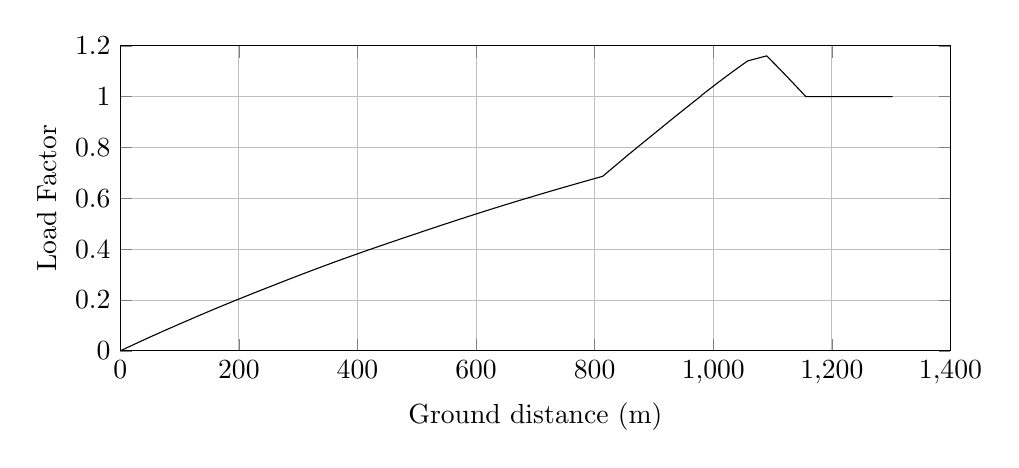
\begin{tikzpicture}

\begin{axis}[
width=\textwidth,
height=0.45\textwidth,
scaled ticks=false, tick label style={/pgf/number format/fixed},
xmin=0.0,
xmax=1400,
xlabel={Ground distance (m)},
xmajorgrids,
ymin=0.0,
ymax=1.2,
ylabel={Load Factor },
ytick={0,0.2,0.4,0.6,0.8,1,1.2},
ymajorgrids,
legend style={at={(1.03,0.5)},anchor=west,draw=black,fill=white,legend cell align=left}
]

\addplot [
color=black,
solid
]
table[row sep=crcr]{
1.3603393307215537E-8	1.5374033208389272E-11\\
2.0334443352841076E-7	2.2981207716240697E-10\\
1.8493358258961232E-6	2.090048389684322E-9\\
9.983129263424352E-6	1.1282549412136833E-8\\
4.13538327636676E-5	4.6736510591868315E-8\\
1.2467543572893382E-4	1.4090335220700978E-7\\
2.843807411608912E-4	3.2139598492355305E-7\\
5.588015241105573E-4	6.315352016821599E-7\\
9.398454696015893E-4	1.0621749118034759E-6\\
0.0014155885812023746	1.5998385089136108E-6\\
0.0019945752038215015	2.254181668322058E-6\\
0.0026717822370171283	3.019526587593407E-6\\
0.003447739291558293	3.896470737478679E-6\\
0.0043193476547732645	4.881510918645401E-6\\
0.00529092766782709	5.979528362391867E-6\\
0.006363550519206555	7.191732101241853E-6\\
0.007533073890550759	8.513439089519928E-6\\
0.008790616877968567	9.934611089304765E-6\\
0.01016549189277427	1.1488372523477957E-5\\
0.011625499440327931	1.3138332203873978E-5\\
0.013184282533086976	1.4899906022816627E-5\\
0.014839871214038253	1.677086534061919E-5\\
0.01660567024659266	1.876635600414511E-5\\
0.018465948346479452	2.086859760642448E-5\\
0.0203822997817096	2.3034186868418095E-5\\
0.022430561433814646	2.5348821051771952E-5\\
0.024588423902376283	2.7787285607872693E-5\\
0.026831028501027587	3.0321486046815747E-5\\
0.029143159681622913	3.2934225735229906E-5\\
0.03155709159958957	3.5661971824487775E-5\\
0.03411445662773917	3.8551764326081156E-5\\
0.03677290089167576	4.155573904036866E-5\\
0.03952314881844239	4.466341085511817E-5\\
0.04239921643077808	4.791321190361803E-5\\
0.045357163155895136	5.125548714242575E-5\\
0.048363831658398165	5.4652768145384036E-5\\
0.051533845233668635	5.823456458974842E-5\\
0.0547899150155587	6.191354182119883E-5\\
0.058172599437445835	6.573552080893171E-5\\
0.06162834747858026	6.963999097993074E-5\\
0.06521401059050522	7.369118047790168E-5\\
0.06888104003120077	7.783423175891372E-5\\
0.07268727020998902	8.2134480631384E-5\\
0.076546425570032	8.649444817559005E-5\\
0.08047032364859658	9.092748214018012E-5\\
0.08456364881336098	9.555184296715504E-5\\
0.08882250397434277	1.0036311761898592E-4\\
0.09306368907640691	1.0515433840166077E-4\\
0.09743039119190974	1.1008725880359988E-4\\
0.10191450167634594	1.1515271081448359E-4\\
0.10651989152467789	1.2035505928429211E-4\\
0.11128201757858264	1.257343474356094E-4\\
0.11609763023253863	1.311739373438716E-4\\
0.12097769621339591	1.3668621260399963E-4\\
0.12591912973280778	1.4226768319829992E-4\\
0.13103216605369056	1.4804285398754057E-4\\
0.13633380151185176	1.5403090860729432E-4\\
0.1416823117522269	1.6007176409930699E-4\\
0.14708837902374172	1.66177481503649E-4\\
0.1525605467319851	1.7235770510484982E-4\\
0.15824953188605478	1.78782642032634E-4\\
0.16398006351864292	1.8525433685303056E-4\\
0.16978153473626356	1.9180597967617652E-4\\
0.17584258400626962	1.9865058706006224E-4\\
0.1819863832139092	2.055884559278913E-4\\
0.18819485651962437	2.125991677404148E-4\\
0.19455736971520038	2.197836260028782E-4\\
0.20098158490654017	2.2703755426626692E-4\\
0.2076061353991409	2.345174786439673E-4\\
0.21424726384720844	2.420159045107114E-4\\
0.2211374965027113	2.4979536189535155E-4\\
0.2281284453493247	2.576882951597784E-4\\
0.2350833915765042	2.655403428586382E-4\\
0.2423085249848444	2.736971777054362E-4\\
0.24958374984531584	2.819103055889826E-4\\
0.2569279402934431	2.9020102790968294E-4\\
0.2644720218029696	2.987171299361479E-4\\
0.27204626263318243	3.072669986207938E-4\\
0.27972793364503945	3.159378508054884E-4\\
0.2874622320100655	3.2466781813698166E-4\\
0.29563698092580604	3.338946222377273E-4\\
0.30361763245720474	3.429020378263768E-4\\
0.3118912000478351	3.5223973057035656E-4\\
0.3202493147046803	3.616725097154526E-4\\
0.3286412952843002	3.711431710839531E-4\\
0.33714554464307567	3.8074018689413457E-4\\
0.3458731203690518	3.9058886518892504E-4\\
0.35455185683415313	4.003820690010891E-4\\
0.3634323904331427	4.104026108233088E-4\\
0.372325738896249	4.204372354831124E-4\\
0.38151551889959867	4.308059367159902E-4\\
0.3908489672358084	4.413363258608903E-4\\
0.4001862088113266	4.518705808746726E-4\\
0.4095647137707429	4.624509731833196E-4\\
0.4192312859369268	4.73355913935878E-4\\
0.4289206911602753	4.8428616987958767E-4\\
0.43896550245304145	4.956168787280345E-4\\
0.4487817299761361	5.06689282478865E-4\\
0.4589033974758888	5.181057389285143E-4\\
0.4691858798479248	5.297030898902055E-4\\
0.47972601481223376	5.415905266756198E-4\\
0.49016040525287174	5.533581903794761E-4\\
0.5007175269203565	5.652637502946726E-4\\
0.511266977039379	5.771601399963439E-4\\
0.522323236324642	5.896274919565573E-4\\
0.5332586746953114	6.019580444215004E-4\\
0.5445869154512923	6.147309273662057E-4\\
0.5556699580072249	6.272267683052813E-4\\
0.5669225885056133	6.399132346790484E-4\\
0.5785590177532589	6.530317901711706E-4\\
0.5903083066022885	6.662769476956505E-4\\
0.6020327889628274	6.79493508115956E-4\\
0.613957077533064	6.929346556469871E-4\\
0.625960998969677	7.064649083088015E-4\\
0.6380070243193761	7.200419563870025E-4\\
0.6503365955459197	7.339379027196439E-4\\
0.662700086001522	7.478713821860289E-4\\
0.6752747602080436	7.620421498806897E-4\\
0.6885889407972636	7.770455067698572E-4\\
0.7019767933734617	7.92131072771879E-4\\
0.7151149754112038	8.069345196586283E-4\\
0.7284684478906998	8.219797468113903E-4\\
0.7418939875700234	8.371053616171792E-4\\
0.7553494584716574	8.522638846860849E-4\\
0.7694215958599202	8.681162561650387E-4\\
0.7830840331449673	8.835062486189832E-4\\
0.796657372658726	8.98795050823794E-4\\
0.8106660034246236	9.145732962328734E-4\\
0.8251837647136968	9.309240647314642E-4\\
0.8395067871054176	9.470545883371946E-4\\
0.8540519574023793	9.634343622278068E-4\\
0.8688334527125461	9.800793091120424E-4\\
0.8840141863517745	9.971728195096253E-4\\
0.8993797082767976	0.0010144733661138587\\
0.9143697020410035	0.0010313500913154878\\
0.9294094610857999	0.0010482818530384262\\
0.9452486359568626	0.0010661125243933416\\
0.9605773823977486	0.0010833675440802167\\
0.9761522209726621	0.0011008985292406603\\
0.9917649966835071	0.0011184711544974415\\
1.0074810114554809	0.0011361589066623086\\
1.0234652146968335	0.0011541473936437707\\
1.0399433598517231	0.001172690598967257\\
1.0563627364420554	0.0011911665020313577\\
1.0728309985448887	0.001209696243959322\\
1.0896486452479222	0.001228617899647706\\
1.1068138420051672	0.0012479293317721994\\
1.124143995869574	0.0012674250630733267\\
1.1415400048645106	0.0012869935847115823\\
1.1590089082607062	0.0013066428022023037\\
1.1769249919091855	0.0013267936605376395\\
1.1951505705127592	0.0013472912165126624\\
1.2127191877709298	0.001367048579106042\\
1.2308827453761335	0.0013874736252179915\\
1.2492706857898845	0.0014081495692425886\\
1.267587852451018	0.0014287445135232348\\
1.2860031245644312	0.0014494483375160022\\
1.304687144125951	0.001470452849877318\\
1.3233765774990474	0.001491461982692523\\
1.342322280991234	0.0015127577002968132\\
1.3613696045164358	0.0015341661305729906\\
1.3815086998747366	0.0015568000230985794\\
1.4013123019267382	0.0015790552160458407\\
1.4209622886438908	0.0016011361671356185\\
1.4411501686096515	0.0016238198897491822\\
1.4611760119255748	0.0016463198780962394\\
1.4816444281325132	0.0016693154082945208\\
1.501865958841821	0.0016920318777642255\\
1.5224364680875304	0.0017151386592939367\\
1.543651615594651	0.0017389677438441873\\
1.5647593029468103	0.0017626743010758837\\
1.5859558716309676	0.0017864788533615546\\
1.6071423964076703	0.0018102702977178687\\
1.6293386351549652	0.001835193645933506\\
1.6508498980272122	0.001859345953941686\\
1.673011606043147	0.0018842266080976073\\
1.6946435720294923	0.0019085106163146174\\
1.717066624993247	0.0019336807085447148\\
1.739432891071898	0.001958785044562732\\
1.761922286799709	0.001984025561834994\\
1.7849035550437842	0.0020098160325787095\\
1.8076299607761817	0.002035318414176838\\
1.8313298306791497	0.002061910976009842\\
1.8543134894513886	0.0020876977785068366\\
1.8777326664639729	0.0021139710628548356\\
1.9017196849182967	0.0021408791438104293\\
1.925345883672024	0.0021673802469308417\\
1.950252961491087	0.0021953157116738216\\
1.975161211119453	0.00222325005504409\\
1.9993825790313986	0.0022504117373897447\\
2.024583888346972	0.002278669886340451\\
2.04934017380271	0.002306426621042781\\
2.0744229633459703	0.0023345470014033277\\
2.0996193404956136	0.002362792267868924\\
2.1245764901457758	0.0023907669370335245\\
2.1500786393425866	0.0024193500164572594\\
2.176226227020705	0.0024486539093915324\\
2.202115608176549	0.0024776658392830445\\
2.227948363055355	0.0025066117525385243\\
2.2543499999408594	0.0025361924684517406\\
2.2810892744412783	0.0025661487677621653\\
2.3075963743135786	0.0025958422742274573\\
2.3348582111613405	0.0026263784625195036\\
2.3623221378972126	0.002657138168081073\\
2.3898598419727675	0.0026879776445977565\\
2.4171687299087603	0.00271855804879335\\
2.445442108612223	0.0027502155341608304\\
2.4735885391813177	0.0027817279007296245\\
2.5015416452491293	0.002813020892518064\\
2.5301110763218357	0.002845000838090238\\
2.5589284934403693	0.0028772552978755484\\
2.587611617795936	0.0029093563884904842\\
2.6175687086884984	0.0029428800051800974\\
2.647724154312196	0.0029766222466866836\\
2.6767118187859253	0.0030090546517865893\\
2.7060305938995466	0.003041854377049212\\
2.7361546404224653	0.003075551703326559\\
2.7663022704956823	0.003109272092617399\\
2.7964672462043376	0.0031430085697699566\\
2.8272583584284883	0.003177441908162033\\
2.8588650092419234	0.0032127836811365463\\
2.8898852960400587	0.0032474662867022436\\
2.9215246589961597	0.0032828374859432724\\
2.95270311230069	0.003317689892414686\\
2.984506337549637	0.003353237102308586\\
3.017379145769185	0.003389976010739374\\
3.049243647754313	0.0034255843520042705\\
3.081295157663824	0.0034613980324002154\\
3.113406837946715	0.003497275294116478\\
3.1453724573084756	0.003532985746619026\\
3.1787286104953543	0.003570245795919007\\
3.211019796961401	0.0036063125118886573\\
3.245786703184362	0.003645140325425546\\
3.279939251746722	0.003683277907741348\\
3.3141720228361216	0.0037215009930596757\\
3.3491198891036547	0.003760518326321434\\
3.382965192547779	0.003798300675236337\\
3.4181848705561064	0.003837613069400587\\
3.45391888941694	0.003877495205234442\\
3.488851494856137	0.0039164786563732285\\
3.524271454997704	0.003956001708464862\\
3.5606552075305	0.003996595738134049\\
3.597189071478943	0.00403735271377598\\
3.632926148839256	0.004077216413938136\\
3.668897146318187	0.004117336679188617\\
3.706642714683163	0.0041594315168277055\\
3.7432264628550644	0.004200226086973859\\
3.781286297809391	0.004242661877159699\\
3.818618572105483	0.004284281747773006\\
3.8564015479305356	0.00432639935081316\\
3.8948624022541356	0.0043692677272015885\\
3.9329637046009225	0.004411730513789391\\
3.971505929995028	0.00445467981614325\\
4.009821706071438	0.004497371926012291\\
4.049014376833089	0.004541036099814634\\
4.089343885784727	0.004585961565009396\\
4.128662304630717	0.004629755606835391\\
4.1684827283974055	0.004674103671731239\\
4.208000253554632	0.004718109315040597\\
4.2483743636521965	0.004763063615254516\\
4.288255503180503	0.00480746386419704\\
4.328757204126676	0.004852549764976895\\
4.369490126907612	0.004897887761715651\\
4.410357715197167	0.004943370327468552\\
4.45189144941496	0.004989588820420421\\
4.492881116440694	0.005035196515995147\\
4.53550011161515	0.00508261147443238\\
4.577670191557685	0.005129521369208531\\
4.6201174049766305	0.005176733908302581\\
4.662272021613388	0.00522361542234917\\
4.706017761800355	0.005272260616533555\\
4.748842845578064	0.005319876280186416\\
4.792293145132742	0.005368181292042443\\
4.836482439768313	0.0054173018885152295\\
4.88090298307878	0.00546667348415619\\
4.925311889063089	0.005516026097070046\\
4.969864686447545	0.005565532563612248\\
5.014842280541593	0.005615504926743528\\
5.0603877575117515	0.005666101979940528\\
5.106292347304597	0.005717091628227079\\
5.152263975081851	0.005768149376210083\\
5.1974808794106995	0.005818362709818108\\
5.244027372436168	0.005870046159551677\\
5.28996242022761	0.005921044349740975\\
5.336209145350672	0.00597238223761704\\
5.38320569473032	0.006024546007914806\\
5.430469292142472	0.006076999615678416\\
5.476900151253712	0.006128522647473706\\
5.526063828851289	0.0061830713284090864\\
5.573879040902945	0.006236117076516704\\
5.622613575936374	0.006290175871690076\\
5.6713596863799225	0.006344240623414446\\
5.720412183296268	0.006398638267512179\\
5.770660497446668	0.006454354860049492\\
5.820668144990444	0.00650979741373121\\
5.870305285939629	0.0065648221353236105\\
5.920503816994749	0.00662046205507926\\
5.971105439367246	0.006676541536175241\\
6.021088325934068	0.006731928207005985\\
6.071322359863801	0.006787586101249198\\
6.122981826035449	0.006844815963730003\\
6.174329110820436	0.006901692604981579\\
6.225804784288178	0.006958704106229942\\
6.278093246139479	0.00701660829571604\\
6.331709873490098	0.007075975466108491\\
6.384325657889258	0.007134226774857282\\
6.436648686434458	0.007192146461727316\\
6.489478972803882	0.007250620096365213\\
6.543185721519176	0.0073100560532747836\\
6.596747696432654	0.007369324027346013\\
6.650345873843312	0.007428624329164869\\
6.704555155195255	0.007488592912980344\\
6.7588986063680725	0.00754870204417058\\
6.814371620173711	0.007610052480240359\\
6.86997180120154	0.007671535378341327\\
6.925426612865756	0.007732849404269517\\
6.981353650685165	0.0077946773692703294\\
7.037678624474159	0.007856936987698657\\
7.094603706786671	0.007919851548539672\\
7.151204881983983	0.007982399788382173\\
7.209200593921791	0.008046480505954117\\
7.2667780016693655	0.008110090473803637\\
7.324687293141565	0.008174058535684366\\
7.382771066065313	0.008238210745781491\\
7.441904508776327	0.00830351349495636\\
7.501585831803217	0.008369412323671796\\
7.5616527251378685	0.008435727842152053\\
7.62150963104709	0.008501802538779845\\
7.682859947113334	0.008569516506580093\\
7.7432084367972145	0.008636115617016637\\
7.803024936926759	0.008702118756293897\\
7.863793829029664	0.008769163777806677\\
7.9252460466886365	0.008836953501953616\\
7.98696966925656	0.008905033354735742\\
8.04776546969778	0.008972080802827366\\
8.109421212326083	0.009040067504004311\\
8.17269125419024	0.009109824763768863\\
8.236095044780246	0.009179719877109478\\
8.299523592514586	0.009249632703414426\\
8.363213767675873	0.009319824309015661\\
8.427807923256076	0.009391002399879044\\
8.49144930156071	0.009461121020434827\\
8.557380457258176	0.00953375248752819\\
8.623183572921022	0.009606232827115336\\
8.687840683575093	0.009677441117535704\\
8.753751426394068	0.009750020156239039\\
8.820803713780364	0.00982384602164581\\
8.888970287482593	0.00989888823559562\\
8.957133699158991	0.009973916434620096\\
9.025036015045707	0.010048646823212787\\
9.092760955867519	0.010123171694724488\\
9.159817422823458	0.010196950885644712\\
9.227495373767134	0.010271403740708764\\
9.296013084156197	0.010346770109185652\\
9.36435980631623	0.010421938116837783\\
9.433329865923408	0.01049778131819181\\
9.503849553921977	0.010575317875587928\\
9.574524061692681	0.010653013861999643\\
9.644263228942293	0.010729671045074553\\
9.715657612596786	0.010808136855220533\\
9.787429657508813	0.01088700679517514\\
9.85753688572494	0.010964036745938386\\
9.930250735750551	0.01104391977451002\\
10.001571447096964	0.011122261552013435\\
10.074699859091687	0.011202577987080329\\
10.14698611653175	0.01128195860476576\\
10.220547980738981	0.011362728973150465\\
10.2940409891517	0.011443412672783518\\
10.36719293590382	0.011523711019413093\\
10.441008888975666	0.01160472725902665\\
10.51610421670324	0.011687136413444028\\
10.590724589239105	0.011769013175916066\\
10.667218005391902	0.011852933625676772\\
10.742771202259895	0.01193581120654734\\
10.82035208750042	0.012020901368579678\\
10.896759047300378	0.012104692481210193\\
10.973503045910835	0.012188841789895802\\
11.051297940743765	0.012274131794135243\\
11.128076326409062	0.012358295967348484\\
11.207667705350879	0.012445531865475172\\
11.286758396846047	0.012532207093621942\\
11.366305937658339	0.012619371098399107\\
11.446149720998452	0.01270684780197811\\
11.526866579636565	0.012795268995943049\\
11.607297517600138	0.012883365005226263\\
11.688034241538357	0.012971783999342859\\
11.769665722224765	0.01306117080242655\\
11.850920080706608	0.013150132665787597\\
11.933163326324259	0.013240165118165044\\
12.017103780766782	0.013332043051677726\\
12.10034832931326	0.013423146917421356\\
12.185467765774142	0.013516290047041081\\
12.270669986481685	0.013609511056742886\\
12.354040133273898	0.013700715345759963\\
12.440386807402234	0.013795163206201964\\
12.52556588630658	0.01388832139733954\\
12.610860989997974	0.013981594101563924\\
12.69550109439961	0.014074138384846302\\
12.784634337461807	0.014171582401304386\\
12.871172079509357	0.014266176245165829\\
12.958447214271366	0.014361563580890779\\
13.045518554761987	0.014456715715105284\\
13.133090172249581	0.014552402090308187\\
13.221405510214687	0.014648888535882164\\
13.310319106907201	0.014746015939870837\\
13.399783591735492	0.014843732406755825\\
13.488943611067967	0.014941103731643937\\
13.578276665194153	0.015038651515543375\\
13.667402973129146	0.015135961157476396\\
13.757763665999576	0.01523460599231918\\
13.848393619195729	0.01533353219975129\\
13.938857764339925	0.015432264963115066\\
14.031101516310692	0.015532927279505657\\
14.123507833735925	0.01563375423038121\\
14.214825187590282	0.015733380533269108\\
14.307956552027534	0.015834973259119735\\
14.401498558574918	0.01593700118901839\\
14.495315613017755	0.016039316395296203\\
14.589065423003394	0.016141545645368478\\
14.68316852398955	0.01624414756129205\\
14.778702641747682	0.016348296953579537\\
14.873746415615575	0.016451899115251106\\
14.970384078097169	0.01655722584979747\\
15.068900921005241	0.01666458752139814\\
15.164434274206265	0.01676868522540195\\
15.260378587808539	0.016873218337736026\\
15.357189194448868	0.016978682817159075\\
15.45495288999333	0.017085172981323293\\
15.55311774366497	0.017192087489309088\\
15.652583807013901	0.01730040640780847\\
15.755243917873962	0.017412190296791162\\
15.855950289561445	0.017521833754075747\\
15.958461094374158	0.017633428628230516\\
16.060387288500337	0.01774437406483493\\
16.164276126126843	0.017857442589461064\\
16.26736468838029	0.01796962706279488\\
16.36946523634058	0.018080723651526017\\
16.47192386662276	0.018192197304906035\\
16.576794358652606	0.01830628213055161\\
16.678929175716583	0.018417378500550946\\
16.783994526910618	0.01853164989175816\\
16.89012564586595	0.018647067556709588\\
16.996887404888547	0.01876315812826152\\
17.103774697793426	0.018879372372236004\\
17.210947675936964	0.018995884486699262\\
17.31865021419634	0.019112959599538088\\
17.424470519881233	0.01922797641817496\\
17.53205215515201	0.019344895321273776\\
17.64034909906897	0.01946257922101527\\
17.74911485075183	0.019580760196036138\\
17.85745376408675	0.01969846521095467\\
17.969383314157206	0.019820058677510525\\
18.07998395718984	0.01994019607679836\\
18.18863741327577	0.020058206516013085\\
18.302466989554325	0.020181826370699058\\
18.41305080779906	0.020301909253588362\\
18.525644000014054	0.020424162072135942\\
18.636945827420575	0.020545000952822485\\
18.750643923449367	0.020668429496153523\\
18.86479622056296	0.020792339145030935\\
18.979646899421056	0.020916994939531506\\
19.09418630108147	0.02104130113213445\\
19.208983505033515	0.021165875505231076\\
19.323483295898072	0.021290115730263848\\
19.43842354827664	0.021414822599410008\\
19.55563752357537	0.021541984920275196\\
19.67199913451129	0.021668211249701634\\
19.789486593639566	0.021795647643270515\\
19.90713985662446	0.021923252751753636\\
20.024127533725753	0.02205012510846392\\
20.143019013955552	0.022179051205709736\\
20.26442367074238	0.022310691423330323\\
20.383660776265387	0.022439970542712205\\
20.5042342316437	0.022570687860712663\\
20.622773342122727	0.022699189380431136\\
20.74503732713029	0.022831718313013092\\
20.865944869938517	0.022962766612215392\\
20.98711015528624	0.023094084178054714\\
21.113336299999695	0.023230876104032915\\
21.23638685227678	0.023364216469753556\\
21.35988644990264	0.023498033551237762\\
21.483760012473958	0.02363224609606233\\
21.608180515260266	0.023767041608888866\\
21.732326713270083	0.02390153053277864\\
21.85766379468624	0.02403730022087048\\
21.985117186778353	0.02417535296821258\\
22.111729024702363	0.024312484996044208\\
22.23700541150786	0.024448161811443804\\
22.36297326225872	0.024584578877015626\\
22.488604760551	0.024720623285123942\\
22.616276341350805	0.024858868478146317\\
22.744235570279145	0.024997416869262427\\
22.874576476768283	0.025138535737640844\\
23.003842066605536	0.025278482323695103\\
23.13088450205612	0.025416014464081923\\
23.257869280739328	0.025553476870288225\\
23.389244224935425	0.025695684199080984\\
23.519811196806458	0.02583700962103881\\
23.653309395988643	0.02598150049107725\\
23.78342402399784	0.02612232229166732\\
23.9180644861338	0.02626803543954417\\
24.05110504604577	0.02641201043268411\\
24.182394801971697	0.026554084445799077\\
24.314614014384034	0.026697158184331653\\
24.449791085561472	0.02684342653789904\\
24.585258581909038	0.026990003231537836\\
24.72121222319008	0.027137100228800077\\
24.857032405393277	0.027284047362217657\\
24.99454740444294	0.027432822842238674\\
25.13030709358258	0.027579694275514544\\
25.270890409679986	0.02773177916362582\\
25.40663839363527	0.027878628565965298\\
25.54307796688363	0.028026221846941694\\
25.68272814639034	0.028177284017876295\\
25.82072003425767	0.02832654848530173\\
25.96015212691003	0.028477367127850435\\
25.987750021099068	0.028507218353751695\\
26.0558803939429	0.028580910917093486\\
26.061632797568386	0.02858713291310103\\
26.066808273335674	0.028592730879519256\\
26.071901058608013	0.028598239400787238\\
26.073315434863225	0.028599769235123793\\
26.074595035914804	0.028601153292026994\\
26.080371168076944	0.028607400935564672\\
26.10234540095133	0.028631168895525885\\
26.183408179590366	0.028718847999082538\\
26.300430535410044	0.028845419587590244\\
26.42750601924636	0.028982861636729255\\
26.558056987479794	0.02912405916555627\\
26.688030995483615	0.029264628870686853\\
26.818767077324992	0.029406018677321878\\
26.951519978077492	0.029549585182633793\\
27.083955405447817	0.02969280359929974\\
27.216897884715692	0.029836565311060655\\
27.350913258119895	0.029981481853853978\\
27.4833530065795	0.030124689042099383\\
27.6176201223548	0.030269866257271127\\
27.752160408628434	0.030415332614648852\\
27.887329802382908	0.03056147263370969\\
28.023188645890663	0.030708351197530733\\
28.158973127824495	0.03085514223551436\\
28.296372294036907	0.031003671322742565\\
28.435107205966254	0.031153636416848905\\
28.571323599682245	0.03130087110759515\\
28.70996262687553	0.03145071597803442\\
28.850320389600306	0.03160240959352689\\
28.988837241064125	0.031752104570547\\
29.129197813929657	0.03190378262832612\\
29.27166529868488	0.03205772751446292\\
29.41298471572133	0.03221042166209486\\
29.554848516656044	0.03236369355436497\\
29.699676691743235	0.032520157131285886\\
29.842400551696755	0.032674336130834605\\
29.985385440862252	0.032828785703561236\\
30.129077275410303	0.032983987150688565\\
30.27543774584293	0.0331420586163377\\
30.422081339040986	0.033300423074515174\\
30.56949149516445	0.033459602206230656\\
30.716562179458485	0.03361840135729968\\
30.86535310281699	0.03377904404512006\\
31.011875026602333	0.03393722309803117\\
31.16159928701196	0.03409884475680984\\
31.313692569485013	0.03426300841038601\\
31.463056706803336	0.0344242110911111\\
31.61235366859384	0.03458532593262824\\
31.76278957628285	0.03474765411611985\\
31.915019899787076	0.034911902213662735\\
32.06709627595497	0.0350759675347234\\
32.21861178877769	0.035239410956363786\\
32.37168228565527	0.03540451448277895\\
32.52450570609457	0.035569333927154306\\
32.67702483599189	0.035733807440801485\\
32.829998687403204	0.03589875326477175\\
32.98551220909506	0.0360664187461725\\
33.14332298937855	0.03623654140239533\\
33.29970221124884	0.03640510110274228\\
33.45800124694219	0.03657570992389953\\
33.61398946945653	0.036743808092917725\\
33.77048353048475	0.036912431046963894\\
33.9292721471582	0.037083505354319125\\
34.08796840843395	0.037254458754788874\\
34.24769686644211	0.037426502234404344\\
34.406855482575295	0.03759790991503349\\
34.56481953291838	0.03776800913719872\\
34.72399692808165	0.03793939257008753\\
34.88694269464703	0.03811480988043162\\
35.04914399338672	0.03828940194572416\\
35.209965099803895	0.038462484724872056\\
35.3703140559587	0.03863503568860116\\
35.531685786905925	0.03880866318872906\\
35.69349909442164	0.0389827413500224\\
35.85522798807463	0.03915670402748839\\
36.022509111806116	0.0393366127617303\\
36.19055880791667	0.03951732107667234\\
36.35708622463872	0.039696365524846296\\
36.52115360367851	0.03987273861666029\\
36.68781562330062	0.04005187391578856\\
36.8536847754776	0.04023012974872494\\
37.024522648961764	0.040413696718952744\\
37.19188554678789	0.04059350141616216\\
37.36066720850286	0.0407748017061296\\
37.528862119520696	0.04095544291896646\\
37.697264258302326	0.04113627769427848\\
37.86832931534104	0.04131994208150624\\
38.03812867477943	0.041502217558534955\\
38.20923731912278	0.041685868107589605\\
38.37904730305398	0.04186809444182254\\
38.55252405124031	0.042054224229577886\\
38.72282139824354	0.04223691165031978\\
38.89783411301201	0.04242462525661419\\
39.0714610757495	0.04261082006234834\\
39.24438070689564	0.04279622400682247\\
39.41969314875929	0.04298416040583245\\
39.59166556575205	0.04316848371331274\\
39.764623188591585	0.043353830299472054\\
39.94263254662576	0.043544556082719996\\
40.11749159802578	0.04373187238046037\\
40.29452954971913	0.04392148818411325\\
40.47247750600427	0.04411204337799207\\
40.64799609178485	0.04429996229509945\\
40.82414741101539	0.04448852375933944\\
41.00385670225303	0.04468085769071965\\
41.18169069533937	0.0448711484735724\\
41.3603281005193	0.04506226263499734\\
41.54046179251334	0.045254940594478245\\
41.722675278204306	0.04544980524054358\\
41.90258931008478	0.04564217320064385\\
42.08518735141125	0.04583737264043191\\
42.26728550944881	0.04603199911599255\\
42.44743534848537	0.04622450518343317\\
42.63069538383506	0.04642029581466249\\
42.80963512098974	0.046611432708293196\\
42.992542679335614	0.0468067689206785\\
43.17926890616222	0.04700614252396763\\
43.363134036078335	0.047202420883006434\\
43.54815051311773	0.047399887776483844\\
43.733578141849236	0.047597752568090776\\
43.91798130912079	0.04779448344475489\\
44.10506009255049	0.04799402718099616\\
44.29251116260117	0.04819392584802364\\
44.480917546793805	0.048394800632548036\\
44.66851287589745	0.04859476811724275\\
44.85853501730759	0.048797279056245396\\
45.047396872181054	0.04899851006300155\\
45.236914792155844	0.04920039652494828\\
45.42785879536018	0.04940375789909376\\
45.616432631699865	0.04960455129687691\\
45.80697204128492	0.04980739346696435\\
45.998633580597016	0.0500113853429933\\
46.18800675699903	0.05021289734901566\\
46.380841640082096	0.05041804764089042\\
46.57327038933336	0.05062272020116214\\
46.765844918266424	0.05082750207824589\\
46.95911042680183	0.05103297266185469\\
47.15311668852311	0.051239184286306395\\
47.34541611633634	0.05144353566218922\\
47.53884854699059	0.05164904475010027\\
47.73236991243341	0.051854601797983284\\
47.92818250719388	0.052062545147584925\\
48.12326385407131	0.052269664454110715\\
48.32058854034828	0.05247911725134779\\
48.516852452700604	0.05268739586178992\\
48.71339374517507	0.05289592059849404\\
48.91319881343868	0.05310785858576767\\
49.1119162355681	0.053318593314346206\\
49.31207818344666	0.053530809913583666\\
49.509673461222235	0.05374025599822962\\
49.71156302510582	0.053954203327491373\\
49.91034548441702	0.05416480798937775\\
50.11200805970151	0.0543784133400409\\
50.30853267551517	0.054586527282906125\\
50.50757456960626	0.05479725745719281\\
50.70929197287772	0.05501076941625655\\
50.91222418686718	0.05522551555950478\\
51.11562549758783	0.05544070610182659\\
51.32090674103446	0.055657832736146794\\
51.525199701657655	0.05587386138888519\\
51.72863462744459	0.05608893049690878\\
51.934060761332375	0.0563060518073915\\
52.14033810224923	0.05652401931669184\\
52.344882977561255	0.05674010327483824\\
52.55098100649393	0.05695777472959248\\
52.75731843494604	0.05717564546549196\\
52.96514817708821	0.05739503776441926\\
53.17450540782369	0.05761598758816612\\
53.382202621450276	0.05783513100112121\\
53.592230583406476	0.05805667845610433\\
53.80364534107798	0.05827963278079432\\
54.01469481143569	0.05850214587993203\\
54.223966920081466	0.058722729858688934\\
54.43230789395902	0.05894227778601525\\
54.6430562980421	0.05916430726586349\\
54.855225786754914	0.059387777677967754\\
55.066088958624874	0.05960981634486733\\
55.27969530828261	0.05983468685139641\\
55.49171188337613	0.060057827342331525\\
55.70388919125476	0.060281080788664884\\
55.91737779085577	0.06050565727772136\\
56.13177028494084	0.060731127424927714\\
56.34652664868587	0.06095692285389737\\
56.559021044851505	0.0611802835714986\\
56.77591447970492	0.061408210416874325\\
56.99548236897459	0.06163888829423847\\
57.21481285737903	0.061869257092876544\\
57.43536222847358	0.0621008460640568\\
57.65367025761124	0.06233002227777102\\
57.872788904232735	0.06255999029556518\\
58.0907693980174	0.06278870507290354\\
58.311927420720366	0.06302069407514824\\
58.532333513628615	0.06325183450942597\\
58.75532998033057	0.06348563080362264\\
58.976617007999806	0.06371757464206554\\
59.19875422837053	0.0639503493763271\\
59.4206945143671	0.06418285757352557\\
59.64453328369959	0.0644172938411211\\
59.86894932484513	0.06465227351647705\\
60.09432075877773	0.06488819200725447\\
60.318058693038594	0.0651223396593277\\
60.541731124044205	0.06535635823431761\\
60.76707064338231	0.06559205993758385\\
60.995574692986196	0.06583100922420919\\
61.22378989589207	0.06606959381070819\\
61.4534619981562	0.06630963842062715\\
61.683510138770515	0.06655001276438029\\
61.91410430469678	0.06679089422368845\\
62.14462153858659	0.06703163200439556\\
62.37563158073512	0.0672728210875298\\
62.607203285434	0.06751453308177346\\
62.841031881319736	0.06775853644498568\\
63.07467935056491	0.06800228637806056\\
63.31164975340633	0.06824943731604145\\
63.54633691305479	0.068494141975473\\
63.78243968758058	0.06874025763521488\\
64.0165414084598	0.0689842231473333\\
64.25412817577254	0.06923175533688203\\
64.49270299572771	0.06948025102543885\\
64.73076499662056	0.06972814692419776\\
64.96867826857735	0.06997582263068393\\
65.21063576532572	0.07022764173970629\\
65.4512107007771	0.0704779553849806\\
65.69028017871045	0.07072663709576275\\
65.93032615763332	0.07097626904796983\\
66.17196619696679	0.07122749262032184\\
66.4135612157637	0.07147860330607082\\
66.6559030093851	0.07173042401970706\\
66.89910102540284	0.07198306805749775\\
67.14354652182666	0.07223694124155405\\
67.38771133480921	0.07249045630770848\\
67.63347396558368	0.07274556339313513\\
67.87898066495345	0.07300033795797098\\
68.1255935515739	0.0732561934397496\\
68.37316753306138	0.0735129787153975\\
68.62205497364681	0.07377105858690915\\
68.8711887275476	0.0740293261188164\\
69.120220471977	0.07428742042381634\\
69.36846244647072	0.07454462934037161\\
69.61951843592018	0.07480468628016589\\
69.87236615109754	0.07506653071372045\\
70.12758921381476	0.07533076561949564\\
70.37945082809051	0.07559145232673693\\
70.63410009691182	0.07585495592695063\\
70.89152727368702	0.07612126438267625\\
71.14629115974091	0.07638474903092679\\
71.40197865069018	0.07664912055916905\\
71.66163317144085	0.07691752410348057\\
71.92484704501203	0.0771895355288924\\
72.18465416754285	0.07745795617017336\\
72.44573394560723	0.07772762177265864\\
72.70633339061075	0.07799672171800212\\
72.96699363118216	0.07826581529308858\\
73.22900401485182	0.07853623334281319\\
73.49076816912304	0.07880632817773428\\
73.75430841254712	0.0790781862245735\\
74.01895646534612	0.07935111733070466\\
74.2846979982242	0.0796251062150821\\
74.55380714249793	0.07990249619877639\\
74.82322871850147	0.08018013701832191\\
75.09350011520078	0.08045858239057009\\
75.36421232425869	0.08073741082653056\\
75.6347219158074	0.08101595991418184\\
75.90830954343213	0.08129760708981344\\
76.18188601743822	0.08157917137577068\\
76.45626363461818	0.0818614889014716\\
76.72958718025629	0.08214265128992239\\
77.00406935908524	0.08242493509480883\\
77.28579748399531	0.082714597836853\\
77.56784659723587	0.08300451703769299\\
77.84569092555657	0.08329004261443017\\
78.1246978223638	0.0835766919407761\\
78.40641219364133	0.08386605122954746\\
78.68590470271565	0.08415305766234506\\
78.96851680469001	0.08444319643506365\\
79.25576208114188	0.08473801899351154\\
79.54169104977237	0.08503141815948322\\
79.82662017154695	0.085323720047493\\
80.11330301632765	0.08561774970853771\\
80.40394576721474	0.08591576825027333\\
80.6908099930996	0.08620984131945751\\
80.98055888331655	0.086506800418883\\
81.27178512217935	0.08680520214681166\\
81.56682943128612	0.08710744350299704\\
81.86186977412851	0.08740960838500465\\
82.15688924927383	0.08771168007160761\\
82.44965588234726	0.08801137463623172\\
82.74488606927187	0.08831352058636671\\
83.04325841243121	0.08861881100042376\\
83.34213327641098	0.08892454433855305\\
83.64411622775171	0.08923338528752058\\
83.94734638805741	0.08954342978777838\\
84.25123842984891	0.08985407932379305\\
84.55152885577829	0.09016097726658065\\
84.85735750691177	0.09047346454365196\\
85.16518306664875	0.09078792077890434\\
85.47136476235073	0.09110062732864084\\
85.77898122624802	0.09141472918587362\\
86.08923229760057	0.09173145078706485\\
86.40254560035129	0.09205122744332077\\
86.71167807044037	0.09236666776208828\\
87.02660518802142	0.09268795095932654\\
87.34238286044419	0.09301003167703575\\
87.65842706333811	0.09333231461485822\\
87.97971380652302	0.09365987295923389\\
88.2973933745065	0.093983684485015\\
88.61789013566766	0.09431029861394434\\
88.93643920279564	0.09463486001594418\\
89.25662431900213	0.09496102096737552\\
89.57903058309674	0.09528937707341188\\
89.89968694948243	0.09561588466481559\\
90.22473455398588	0.09594679694469473\\
90.55024875587375	0.0962781178037634\\
90.87789352676518	0.0966115409570874\\
91.20733069500889	0.09694672194893063\\
91.54101415610151	0.09728615653310106\\
91.87012785371462	0.09762087769654929\\
92.20120197152713	0.09795752855524584\\
92.53416638543635	0.09829603759271976\\
92.86431843528567	0.09863162500882675\\
93.19748455591187	0.09897021402048944\\
93.53066771200866	0.0993087588854429\\
93.86681917526724	0.09965025848402986\\
94.20530590547477	0.09999406921267506\\
94.5419273964865	0.10033592533480289\\
94.8854212036891	0.10068469993447302\\
95.22752713476521	0.10103200538458085\\
95.57091181422334	0.10138054989197581\\
95.91383450860906	0.10172856738147325\\
96.25469535763642	0.10207443588066725\\
96.5966517898868	0.10242136046437149\\
96.93845701474973	0.10276807701885864\\
97.28153572459905	0.10311603146938844\\
97.62213139590432	0.10346141521265854\\
97.9659652144934	0.10381003072533308\\
98.3129807304216	0.10416182037482564\\
98.65852794036775	0.10451207086868079\\
99.00080640577195	0.10485895935079413\\
99.35064076251427	0.10521345641396491\\
99.69796076807248	0.10556535762356752\\
100.04654253174803	0.10591849025608797\\
100.3915606488718	0.10626796745551358\\
100.74261509654437	0.10662351389324619\\
101.08877163494762	0.10697405629557542\\
101.43457754260953	0.10732420163123155\\
101.784020212797	0.10767798783619978\\
102.13161434601102	0.1080298622173594\\
102.4751980097893	0.10837763831904129\\
102.82212110631409	0.10872875693313991\\
103.16739702108615	0.10907817195345686\\
103.51524666207362	0.10943015584571683\\
103.86391679154056	0.10978293512798004\\
104.20960434827006	0.11013266334861829\\
104.55241399635099	0.1104794483233666\\
104.89662223620601	0.11082761743245956\\
105.24103428322039	0.11117596301469579\\
105.5836615386647	0.11152247504322187\\
105.92645892081137	0.11186913187972315\\
106.27347658175316	0.11222002985240105\\
106.6151670762521	0.11256551596888757\\
106.95898391938218	0.1129131279818322\\
107.30023552029138	0.11325812363403412\\
107.64147805753461	0.11360308847887267\\
107.98348674656944	0.1139488071909293\\
108.32522459759954	0.11429423256350119\\
108.3935347040271	0.1143632775196173\\
108.40478590462831	0.11437464968540283\\
108.41572478024443	0.11438570614935772\\
108.4246743308916	0.1143947518900675\\
108.44347342986478	0.11441375300175818\\
108.52018987797786	0.11449129326031578\\
108.70071173483461	0.1146737499132225\\
108.99446230248458	0.11497063724617655\\
109.30176454987088	0.11528120477134694\\
109.60899173332959	0.11559167890465909\\
109.91608539831654	0.1159019996132111\\
110.22883517949637	0.11621801586774139\\
110.54143546549608	0.11653385988539695\\
110.853845249356	0.11684948926811524\\
111.1739714794031	0.11717289060890668\\
111.4937490010879	0.11749591436628021\\
111.81170779322963	0.11781707482406367\\
112.13106495813236	0.1181396205096813\\
112.4519453366479	0.11846367611484847\\
112.77515902629136	0.11879005820831359\\
113.0997499810409	0.11911779982124547\\
113.43040796942478	0.11945163409614108\\
113.7597028375028	0.11978405773102246\\
114.0907450350197	0.1201182096041561\\
114.42538740208008	0.12045595801425603\\
114.75997726261329	0.12079361470902568\\
115.09477047197589	0.1211314367933213\\
115.43440545481076	0.12147410266493694\\
115.77494672336013	0.12181763955949411\\
116.11687534861284	0.12216253124584514\\
116.46164587354252	0.12251024293447989\\
116.8077846490165	0.12285928644265894\\
117.15688723722127	0.12321126869748109\\
117.50557855048987	0.1235627851107015\\
117.85411336711965	0.12391409155011907\\
118.20532793701167	0.12426804515096418\\
118.55850697655507	0.12462392287354812\\
118.91273956155123	0.12498080501282914\\
119.26983096270519	0.1253405082794965\\
119.62978614725739	0.12570303512810993\\
119.98960731920661	0.1260653645302583\\
120.34734904217265	0.1264255369687228\\
120.7138511704587	0.12679446304810177\\
121.08106061642908	0.127164032705306\\
121.44737887966437	0.12753263609258683\\
121.81499139152783	0.127902471044704\\
122.18511446431708	0.12827475900964444\\
122.55384158147794	0.12864556919209294\\
122.92460728481757	0.12901835424844751\\
123.29616941264607	0.1293918632992619\\
123.67040864389355	0.12976798470739875\\
124.04652172406458	0.1301459086447379\\
124.42393851457416	0.1305250601113209\\
124.80152108360014	0.13090429438221088\\
125.18180835736592	0.13128615945179684\\
125.55854932865631	0.13166437760849078\\
125.93878032356085	0.13204601173718072\\
126.31997081831156	0.13242851938878272\\
126.70099538833193	0.13281076993815535\\
127.08058279416298	0.13319148761661076\\
127.46175209000612	0.1335736994170757\\
127.84399628255431	0.13395689500051594\\
128.22749916598133	0.134341256771147\\
128.6102537001487	0.1347247720336264\\
128.99595881306152	0.13511114526603898\\
129.37788117916477	0.13549363085748245\\
129.760738924708	0.13587695406724312\\
130.1448498512433	0.13626143131888155\\
130.53000390659713	0.13664685055016823\\
130.9168242384266	0.13703383335708338\\
131.29443328439476	0.13741149977327807\\
131.67491382268804	0.1377919361250785\\
132.05816436539135	0.138175037830788\\
132.44070735535217	0.1385573270221609\\
132.82666098215685	0.13894291721933888\\
133.20952005887244	0.13932530843093616\\
133.5940193955625	0.13970922950513162\\
133.97617966856654	0.1400907066323405\\
134.36103715882757	0.14047476617907342\\
134.74478042358356	0.1408576031820577\\
135.12867144169206	0.1412404763263397\\
135.5141335746535	0.14162480372830497\\
135.89764893392993	0.14200707731467013\\
136.28231234485685	0.14239038154849984\\
136.66418763078912	0.14277079421457994\\
137.04684871033697	0.143151875774891\\
137.42845627025127	0.14353179398539995\\
137.8132447087305	0.1439147629033474\\
138.19719797258034	0.14429678377639787\\
138.58059071069573	0.14467812989380188\\
138.96593237593703	0.14506129606986473\\
139.3501607499636	0.1454432363964111\\
139.73355638294606	0.14582423007703724\\
140.1160230155566	0.14620418171219007\\
140.50045093994146	0.14658596155292716\\
140.88215178690393	0.14696491334738324\\
141.26156782058217	0.1473414780085738\\
141.64323970440188	0.14772016158218504\\
142.02689350659642	0.1481006897748855\\
142.41061312971692	0.14848116062910421\\
142.7942251403153	0.14886140171582452\\
143.1756303563767	0.14923933294300132\\
143.5599719391364	0.1496200498129884\\
143.94242380128833	0.14999877079888094\\
144.3239499176869	0.15037645140405548\\
144.70664939692608	0.15075516903428812\\
145.0870075357763	0.15113144571429785\\
145.46856550308127	0.15150878477153903\\
145.85014610541765	0.15188602103912874\\
146.23128237819492	0.15226269269615125\\
146.61504730324998	0.15264183527344244\\
146.99763315977907	0.15301968582966607\\
147.38441582478964	0.15340155183372578\\
147.7673688364352	0.15377950832217888\\
148.15222568696134	0.15415921461101478\\
148.53580865353604	0.15453753486061567\\
148.9199734867533	0.15491629939246315\\
149.3040357319486	0.1552948328226648\\
149.68771357306542	0.15567285734105463\\
150.07093078701052	0.15605029798934478\\
150.45622889618164	0.15642965687270846\\
150.8449053483268	0.15681220836138465\\
151.2288570611563	0.15718997749468377\\
151.61452719766493	0.15756930498040464\\
151.9983007305741	0.15794663509198106\\
152.38299664478842	0.15832473975275088\\
152.76945776909372	0.15870444573392595\\
153.15580177123394	0.15908390253088553\\
153.54253364040335	0.15946360577880977\\
153.93093169697067	0.15984480928853168\\
154.31788037931886	0.16022445490246687\\
154.7039882138024	0.16060314067805523\\
155.08880221957185	0.16098042328496862\\
155.47621608980313	0.16136011935975486\\
155.866104687065	0.161742103425953\\
156.25391419262098	0.16212191362736472\\
156.64166339424906	0.1625015280996315\\
157.03027969880475	0.16288185423172033\\
157.4213807682267	0.16326447326862636\\
157.8105708506119	0.1636450843671079\\
158.19948541262937	0.16402528799760033\\
158.58893406813365	0.164405875400295\\
158.97894817604634	0.1647868765398765\\
159.3710019698692	0.16516973010015448\\
159.76139479981174	0.16555082199190213\\
160.1523485688823	0.16593232170175506\\
160.54128874338664	0.16631171766913488\\
160.9326976430911	0.16669338192339458\\
161.32564259741588	0.16707640281510294\\
161.71827778345698	0.16745898043796853\\
162.1124492087963	0.1678429128180979\\
162.50576001021273	0.16822586496393635\\
162.89904576730015	0.16860865091132962\\
163.29316224934274	0.16899210313775936\\
163.68899123279596	0.16937707817942735\\
164.08495392634194	0.16976203953966598\\
164.48271131475576	0.17014860101775572\\
164.8792309171331	0.17053381520812372\\
165.27343112400507	0.17091663330668005\\
165.67115293733156	0.17130272704526497\\
166.06936395728349	0.17168915053977551\\
166.47000821435734	0.17207778872692137\\
166.87155839526775	0.17246715828871795\\
167.27134041220108	0.17285466679602526\\
167.67233991204222	0.17324320861402856\\
168.0705846918417	0.1736289358678973\\
168.47232570996516	0.1740179027216621\\
168.87521546679773	0.17440783386732234\\
169.2789990941189	0.1747984816156083\\
169.68142011368735	0.17518766326891594\\
170.088438196605	0.17558114076559397\\
170.49328200513543	0.17597236682716144\\
170.89845866435633	0.17636376540429738\\
171.30484584057905	0.17675618361143722\\
171.7103088520891	0.17714756013855001\\
172.11589069074847	0.17753890234711953\\
172.52485519917514	0.17793335772365887\\
172.93316089774754	0.1783270268414337\\
173.34236088095247	0.17872140717610643\\
173.7535761368399	0.1791175776987103\\
174.16510964781833	0.17951390238572498\\
174.5786011126259	0.17991195928384685\\
174.99051444770384	0.18030834430997159\\
175.40138574541044	0.18070357502561404\\
175.81497300453447	0.181101265679831\\
176.2280441317456	0.18149830742991782\\
176.64225100058474	0.18189628795336835\\
177.05714873395152	0.18229477904573643\\
177.47483026786767	0.18269578921851212\\
177.89254345086653	0.18309667488090547\\
178.3100126079721	0.18349717186526968\\
178.7278240622369	0.18389784289398545\\
179.1449731538625	0.1842977249968253\\
179.56482315926417	0.1847000414123385\\
179.9871804296257	0.18510460400794604\\
180.4095742002126	0.18550904503010252\\
180.83428717371925	0.18591554918766942\\
181.26003251256287	0.186322883294815\\
181.6840913989422	0.18672844682631254\\
182.1114839456617	0.18713704039057175\\
182.5374089230304	0.18754407327624614\\
182.96440604473082	0.1879519731461937\\
183.39304842330927	0.1883612863631721\\
183.8234391905185	0.18877210992501697\\
184.2565386467558	0.1891853584073823\\
184.68745119590193	0.18959636073183558\\
185.11804999400476	0.19000690531733422\\
185.54983076576542	0.19041841818139588\\
185.98322399936802	0.19083130850539073\\
186.41637816429778	0.19124381204423108\\
186.85103033850396	0.19165758282749917\\
187.28701324242002	0.19207246052525032\\
187.72482375232647	0.19248891670342644\\
188.16038808151575	0.1929030769930036\\
188.5986323917997	0.1933196257394001\\
189.04181882432442	0.19374070942213387\\
189.48417857731005	0.19416084520405444\\
189.92673350352436	0.19458100448399482\\
190.3712203460227	0.195002835494231\\
190.8171693385559	0.19542589110763944\\
191.2607914989822	0.19584657789009471\\
191.7085048054314	0.19627098161969636\\
192.15912968354564	0.19669798089730994\\
192.60936448614513	0.19712444639906168\\
193.06096206133014	0.1975520385172598\\
193.50995896221815	0.19797700577956345\\
193.96222738896364	0.1984049063790624\\
194.41802104663145	0.1988359773077922\\
194.87342332120494	0.19926651334838694\\
195.32868067301865	0.19969674846054575\\
195.78611327072855	0.20012887486953568\\
196.24327119175433	0.20056057784913567\\
196.70330552186363	0.20099483232922427\\
197.16349707435467	0.20142907058416842\\
197.6260626000094	0.20186538371371246\\
198.09002425529962	0.20230284808820673\\
198.55822718319422	0.20274414409549155\\
199.02663999285284	0.20318547040871549\\
199.4942263371064	0.20362585172344547\\
199.96051846591553	0.20406484942013273\\
200.4340527590599	0.20451049784766898\\
200.9046051381776	0.20495317356938803\\
201.38053424207163	0.20540073960796726\\
201.855813875004	0.20584752724925637\\
202.3311704663634	0.20629422054118435\\
202.81222172114025	0.20674609629052276\\
203.29225549210986	0.2071968478743342\\
203.77308885705298	0.20764818255581136\\
204.25557537412044	0.20810090116909738\\
204.7402502473849	0.20855550483353194\\
205.2236366749359	0.20900873294422437\\
205.7136101207933	0.20946796784056843\\
206.20393168243612	0.20992735941487917\\
206.69661599754647	0.21038879483069356\\
207.18955097797863	0.21085029564033683\\
207.68747106001632	0.21131629272098496\\
208.18818418427776	0.21178473162081327\\
208.68864521634526	0.21225276327589246\\
209.18805406731133	0.2127196412194168\\
209.69072626026758	0.21318939986310917\\
210.1949489825136	0.21366043724096234\\
210.70396111371042	0.21413577702064693\\
211.21614058335587	0.21461390160170796\\
211.7289636831582	0.21509245437326194\\
212.24265718177503	0.21557164742914248\\
212.75957115615557	0.21605367222134292\\
213.28124361123798	0.21653996024300695\\
213.80665479128663	0.21702955798055837\\
214.33466763217763	0.21752140406645692\\
214.86241383044415	0.21801282688744064\\
215.38762416293667	0.21850171618396877\\
215.91972020502777	0.2189968412572505\\
216.453694496636	0.21949353972149435\\
216.99218613031866	0.2199942647912944\\
217.53464071342142	0.22049849833328686\\
218.07804319032095	0.22100343689292318\\
218.62452881115053	0.2215110642107248\\
219.1707188429899	0.22201824206219206\\
219.71730570977076	0.2225256149879756\\
220.274760228052	0.22304289888827752\\
220.835259093258	0.22356282929835072\\
221.3941373958715	0.224081080035866\\
221.95623623511386	0.22460214130976955\\
222.52040576537968	0.225124946552327\\
223.09037241999033	0.22565294716375411\\
223.661129480297	0.22618150389866207\\
224.23954505634208	0.2267169750978348\\
224.81564934919504	0.22725013068813008\\
225.40333087020622	0.22779382159266665\\
225.99624064594485	0.22834216851777153\\
226.58875910740323	0.2288899742299812\\
227.18585441503012	0.22944183231070178\\
227.7870146338791	0.22999726799469336\\
228.39495206683767	0.23055878477416464\\
229.0027183467937	0.23111996429413997\\
229.6102660575582	0.23168076536383855\\
230.22857190062643	0.23225131798739393\\
230.8468525918393	0.23282166958508566\\
231.47114194537448	0.2333973862682148\\
232.09060564776433	0.23396847880227145\\
232.71961230618888	0.23454819451942333\\
233.34696033086396	0.23512620905954393\\
233.9840065784689	0.23571298568931806\\
234.6188203761186	0.23629753498833123\\
235.2539319397456	0.23688219048370596\\
235.886956379092	0.23746476032471994\\
236.5153031168307	0.2380428658694617\\
237.1504953781269	0.23862711102176712\\
237.78410205277385	0.23920974183113575\\
238.41360900639518	0.23978845140261035\\
239.04679127723733	0.24037039042842318\\
239.67609891578388	0.24094862292985111\\
240.3017129123046	0.2415233206801423\\
240.93317778774485	0.24210325357495135\\
241.55721005497253	0.24267622553683882\\
242.1780757761154	0.24324615981395117\\
242.7965584376659	0.24381378015569513\\
243.4114785265944	0.24437800862536863\\
244.02550827530933	0.24494130123749933\\
244.63427618145124	0.245499652189694\\
245.24126487864038	0.2460562603503213\\
245.84466361012846	0.24660946936703348\\
246.4476225417801	0.24716217108348662\\
247.04267344144802	0.24770752447392266\\
247.6421488158	0.2482568355154794\\
248.2330500398673	0.2487981968493432\\
248.8222841397298	0.24933794134244702\\
249.4139444766347	0.24987982089148564\\
249.99998610086192	0.2504164706128457\\
250.57758594667018	0.25094531077440535\\
251.15853686633199	0.25147714215075573\\
251.73921641108228	0.2520086503656063\\
252.31216708836962	0.2525330133146303\\
252.88817036877617	0.2530601013997106\\
253.4570082134402	0.2535805673619825\\
254.02007242820673	0.2540956891233678\\
254.5855573787108	0.25461296613802137\\
255.15029634137989	0.25512950363814824\\
255.71294034286547	0.2556440704640773\\
256.27258114245853	0.2561558389445735\\
256.8305649252842	0.25666604295943246\\
257.38478802342286	0.2571727618637938\\
257.4959621062188	0.2572744014852383\\
257.5611920943704	0.25733403642910074\\
257.60062237753925	0.25737008432271136\\
257.6107239150342	0.25737931929969554\\
257.6183320416303	0.25738627475357756\\
257.62277045264796	0.25739033240615894\\
257.62729287050774	0.2573944668560272\\
257.6542412653681	0.25741910334933515\\
257.747424202601	0.2575042913340539\\
258.03721256731046	0.25776920831864697\\
258.5190125653693	0.2582096297066448\\
259.00532843878875	0.2586541424987556\\
259.49401909840515	0.25910078697179545\\
259.98581493995266	0.2595502281035757\\
260.4819698790609	0.26000360892703445\\
260.97812571679674	0.2604569444391649\\
261.4812175109821	0.2609165682130854\\
261.9850059638038	0.26137677691790134\\
262.4910281591069	0.2618389722135169\\
263.0003252970298	0.26230410221394024\\
263.5131478408722	0.2627723924788784\\
264.0293216176061	0.2632436806930726\\
264.54826562874086	0.2637174331841732\\
265.0714232439334	0.2641949641985624\\
265.59763340154745	0.2646752103786426\\
266.1233003184659	0.2651548873961621\\
266.6551605685464	0.26564013911148676\\
267.19223429565795	0.2661300668623741\\
267.72974052544146	0.2666203058913414\\
268.27282471948854	0.2671155455494753\\
268.8167212540145	0.2676114362870874\\
269.36684202478307	0.2681129083175036\\
269.9215996219019	0.2686185095251482\\
270.4791082933567	0.26912651697407075\\
271.03983254776506	0.26963734996358757\\
271.6074455599014	0.2701543496209083\\
272.1754809002374	0.27067162161841346\\
272.7524022502224	0.27119686805025334\\
273.3357847625165	0.27172787404884935\\
273.91684495064374	0.2722566409205728\\
274.5075523019982	0.2727940560263479\\
275.0995375957874	0.2733324990109104\\
275.69766674106233	0.273876390556164\\
276.3013456770767	0.2744251837346294\\
276.90909644628925	0.27497752883379933\\
277.5234995466793	0.27553576442355815\\
278.13959639565337	0.2760953793446721\\
278.76308237359774	0.2766615405503433\\
279.389606942784	0.27723029057024984\\
280.02074979788426	0.2778030575050175\\
280.6586947867754	0.27838181559734365\\
281.3003335866648	0.27896373754887394\\
281.94157575500606	0.27954510933163695\\
282.5880614624846	0.2801310395069342\\
283.23584856186324	0.28071794937540234\\
283.8851508583185	0.28130602852796666\\
284.5301203280417	0.28188997892678164\\
285.1843536535779	0.28248210578055155\\
285.83553116214307	0.2830712531871297\\
286.4837256048969	0.28365748726114404\\
287.1336898105825	0.2842451044823073\\
287.7808235765799	0.28482994387369825\\
288.42820685084826	0.2854147876789566\\
289.0754666022002	0.28599929634892957\\
289.71879024937004	0.28658002660179277\\
290.36420979409684	0.2871624221152852\\
291.0002472374472	0.2877361272258776\\
291.64182130034897	0.2883145983725624\\
292.27316865691716	0.28888362297028314\\
292.9083864811005	0.2894559078710719\\
293.54335819806715	0.2900277402819083\\
294.17307850120346	0.29059461354957195\\
294.79408895337656	0.2911534200462943\\
295.4199157771013	0.29171633134174113\\
296.0380590852486	0.2922721039084818\\
296.6542969985221	0.29282593634129345\\
297.2681917409874	0.2933774357996573\\
297.88482625920517	0.2939311666678563\\
298.4949121158181	0.2944787884948854\\
299.10656876013206	0.2950275905769822\\
299.7189321849655	0.2955767948041321\\
300.32723284437907	0.2961221239028346\\
300.92930430691433	0.29666164005814183\\
301.53463237615574	0.2972038437176017\\
302.1363215848461	0.29774255726728177\\
302.731439066583	0.29827515927766074\\
303.3331045114137	0.2988133898999239\\
303.92852765769237	0.299345805876925\\
304.52166324273924	0.29987594711279003\\
305.11491208725784	0.3004059594538536\\
305.70510856070314	0.3009330151944048\\
306.29833179138177	0.3014625419144061\\
306.8897654253252	0.30199023850637635\\
307.4799704999041	0.3025166061750579\\
308.06772992248136	0.3030405605226355\\
308.6551058451172	0.3035639404255699\\
309.2396381392449	0.3040845546470549\\
309.82398267965425	0.3046047694130924\\
310.40422650572066	0.30512110274856313\\
310.9895683476474	0.30564173861179456\\
311.5727136903438	0.3061601861441146\\
312.15129426541773	0.3066743429605377\\
312.7356217277545	0.3071933708952763\\
313.31711326243806	0.307709643610573\\
313.899302145316	0.3082262985141894\\
314.47946679147856	0.30874092032368233\\
315.0588501134555	0.30925461241253366\\
315.6397939029396	0.3097694497562289\\
316.2168920475523	0.31028064201848304\\
316.7955732394013	0.3107929985370073\\
317.37103223180316	0.3113022650667297\\
317.947565273913	0.3118122442688196\\
318.5214617947222	0.3123196541652544\\
319.09868556082085	0.3128297664820914\\
319.67476219148546	0.3133386250149437\\
320.24944526491765	0.3138460130153949\\
320.82291261720786	0.3143520884797333\\
321.39725246986427	0.31485869381456\\
321.96848871367	0.31536232262080877\\
322.54402617481435	0.3158695019923044\\
323.1185574377922	0.316375552230705\\
323.691859264958	0.31688027755572673\\
324.2647334332521	0.31738438433958804\\
324.8363521231331	0.3178871446700959\\
325.40661348734614	0.3183884701130285\\
325.97908467698915	0.31889149556605667\\
326.5542035875586	0.3193966022200813\\
327.12490712258295	0.3198975874662851\\
327.6996379965167	0.32040186243057783\\
328.2728670816481	0.320904573735248\\
328.8486987665442	0.3214093197119637\\
329.41990981452807	0.32190976971125645\\
329.9938351119364	0.32241235081232383\\
330.5648485136189	0.32291213599704605\\
331.13749118064516	0.3234131004220192\\
331.7074637117181	0.32391148316616597\\
332.2798601122896	0.32441173823608954\\
332.8523203670276	0.32491180111910845\\
333.42500978717965	0.3254118157154376\\
334.00122212141855	0.32591465504285716\\
334.57441172696565	0.3264146063435845\\
335.1481633939942	0.3269147977022373\\
335.72345703021597	0.3274160817524323\\
336.29828216695637	0.32791670571117815\\
336.8725624877933	0.32841660354261193\\
337.44522027160394	0.3289148383163408\\
338.02053867417567	0.3294151356537135\\
338.5962187273635	0.32991549418235183\\
339.1703543735324	0.3304142578271351\\
339.7498013559267	0.33091737964928614\\
340.3260768964459	0.3314174926501416\\
340.9051117020497	0.331919743838891\\
341.47919118112156	0.33241744294779074\\
342.052441303386	0.3329141707013272\\
342.6320235008849	0.33341612880530197\\
343.21038614202473	0.3339167735306358\\
343.79082299329946	0.3344189553839001\\
344.3667106402361	0.3349169455004414\\
344.94458170993323	0.3354163945185032\\
345.5252340504509	0.335917988785299\\
346.1016219383906	0.3364156428314977\\
346.6806961036725	0.3369153589537357\\
347.2602578923353	0.33741523767674964\\
347.84073776856303	0.33791564933855683\\
348.4226009401458	0.3384169934468536\\
349.0044346707606	0.33891805187524165\\
349.5859819547053	0.339418603542872\\
350.1699920738855	0.3399210134056216\\
350.75474917442455	0.34042380325335253\\
351.33998325174355	0.34092674017289004\\
351.9234136900301	0.34142786522847207\\
352.50674072872846	0.34192864017885105\\
353.09110804073237	0.3424300463181483\\
353.67821635803944	0.342933540498639\\
354.2656524741757	0.34343705125204316\\
354.8545578241044	0.3439415558643037\\
355.4483774220265	0.34445000144053295\\
356.0367996380022	0.3449535593552139\\
356.62583096427284	0.3454573732440068\\
357.2144774827566	0.34596059301616\\
357.80411644396065	0.346464395836026\\
358.39517477750917	0.34696914506197996\\
358.9862667118267	0.3474736565168589\\
359.57750029884653	0.3479780225383685\\
360.17210502256853	0.3484849959818682\\
360.76667257221345	0.348991668841658\\
361.36307847075966	0.34949963842939846\\
361.95890315858196	0.3500068433901094\\
362.55277332573996	0.3505121166811933\\
363.15015313069875	0.35102010653653126\\
363.7467383697897	0.3515271512949763\\
364.34582190435833	0.35203604876951033\\
364.9460245640587	0.35254562529583766\\
365.54693692211754	0.3530555323777376\\
366.14934356225297	0.35356643464485843\\
366.7506799567443	0.35407615720367486\\
367.35358948565136	0.35458694076041863\\
367.957068853549	0.3550979342711333\\
368.56310438184994	0.3556108179353916\\
369.1667326492483	0.35612139156581435\\
369.7692268682281	0.35663073492602165\\
370.3767216505511	0.3571440319940678\\
370.9840014372453	0.35765687315250577\\
371.59702031674954	0.3581742832891644\\
372.2057576829203	0.3586878041467186\\
372.8164011445841	0.3592026576013661\\
373.43055551390637	0.3597201935638446\\
374.04130844990834	0.36023458758650534\\
374.65480432791037	0.36075101562343914\\
375.2686727235273	0.36126748074201565\\
375.88872766894735	0.36178887057619874\\
376.5077052039818	0.36230907414493824\\
377.12525427851347	0.3628277987082329\\
377.74405712537066	0.36334729798897275\\
378.36402671612836	0.3638674979038179\\
378.9860252798833	0.36438912039627563\\
379.6100000903326	0.3649121191864914\\
380.2333263467823	0.36543429399706084\\
380.8554247462042	0.3659551614617586\\
381.4828757180544	0.3664802291142345\\
382.11124459971245	0.3670057823846274\\
382.74241248635997	0.36753339278527447\\
383.3719105047892	0.36805932463005075\\
384.00409885358727	0.36858722082510237\\
384.6374235585132	0.3691157819372115\\
385.2708543582187	0.3696441480637662\\
385.90511613810475	0.3701729240096643\\
386.5402229663101	0.37070212117514245\\
387.1757112317391	0.3712313532469817\\
387.816842485381	0.371764998819783\\
388.45671447828204	0.37229731071651195\\
389.0979595165261	0.3728304795454482\\
389.738666357365	0.3733629164985362\\
390.38126573576096	0.3738966415336976\\
391.0250474989899	0.3744310636707279\\
391.6744601114111	0.3749698720971465\\
392.32213053197165	0.3755069478543142\\
392.96822988900624	0.3760424359938992\\
393.62074411485196	0.37658295302475064\\
394.27341767767894	0.3771233137405142\\
394.92683850679725	0.37766400529910926\\
395.58558306335794	0.37820881162700465\\
396.2441970187614	0.37875321939560525\\
396.90310461070555	0.3792975802280378\\
397.56432488588905	0.37984356152716847\\
398.2289657073595	0.3803920753909967\\
398.8925370524752	0.3809394158621216\\
399.5622831783011	0.38149155607237284\\
400.2295014598768	0.38204132031180865\\
400.89855800548185	0.38259230771899894\\
401.5675035611599	0.38314291307565007\\
402.24206117554286	0.383697844603233\\
402.91817297108616	0.3842537605987605\\
403.5958718607668	0.3848106873242509\\
404.27787051233963	0.3853708514624074\\
404.95902715653847	0.3859300288291082\\
405.6425745212256	0.3864908735539216\\
406.3286386181055	0.38705348718126015\\
407.0181239797241	0.3876186089960912\\
407.70730436303313	0.38818318422871384\\
408.39972983906614	0.3887501205967771\\
409.0954177346696	0.3893194295221377\\
409.79217465836814	0.3898893147311207\\
410.4900247907216	0.39045979608707887\\
411.1873806890112	0.3910295769850123\\
411.8896918209001	0.39160310862824427\\
412.5960730727825	0.3921796639936676\\
413.3068225682056	0.3927594826121668\\
414.0163043302465	0.39333796637125024\\
414.7283691490554	0.3939182558502581\\
415.4426354990113	0.39450003875247863\\
416.1629925407426	0.3950864793154429\\
416.8821853291962	0.39567166991450287\\
417.606386355131	0.3962606322906051\\
418.33304785123187	0.3968512915346121\\
419.0630803577634	0.3974443859229122\\
419.79657378413856	0.39803998606738705\\
420.5335871119013	0.39863813737933235\\
421.27035840412	0.3992357865829242\\
422.00742265160795	0.3998333695493634\\
422.7512304365845	0.4004361137714481\\
423.49678426262926	0.4010399662900408\\
424.2511831284078	0.4016506723724216\\
425.00728777593645	0.40226244819095064\\
425.7607765912853	0.4028717997556325\\
426.5243177755509	0.40348896954654784\\
427.28979022554415	0.40410738817020275\\
428.0636149183367	0.4047322390713927\\
428.8379843697036	0.40535721473019204\\
429.60996752685014	0.4059799530421434\\
430.3897477020988	0.4066086677398467\\
431.1753893594911	0.40724179246306585\\
431.966835986777	0.40787927715089595\\
432.75960868637253	0.4085175124764246\\
433.56365122208206	0.40916449891295376\\
434.37045705896094	0.4098133858205757\\
435.1870341731259	0.4104698047565636\\
436.00231675887426	0.4111248580751646\\
436.8220964781458	0.4117832002025006\\
437.6552545507992	0.4124519557623911\\
438.4886711504423	0.4131205887686498\\
439.3280194395811	0.4137936501809679\\
440.18158737508645	0.41447777733150565\\
441.03992126721334	0.4151653853085418\\
441.89899771608907	0.41585325119795796\\
442.76703563270644	0.4165479537615488\\
443.6461218976118	0.4172511550849133\\
444.5334070432492	0.41796056832444556\\
445.4247342866296	0.41867286674872967\\
446.32920810974076	0.4193953201629298\\
447.24483338837376	0.42012632498452657\\
448.1693167681145	0.4208640429827597\\
449.1035660927572	0.42160919229632454\\
450.0458822047997	0.42236041203708813\\
451.00182339874107	0.4231221256282599\\
451.9686516781545	0.4238921422861975\\
452.94634555439245	0.42467043763500856\\
453.93854384565975	0.4254598992750779\\
454.9385614547757	0.42625520100095493\\
455.94748135202974	0.4270572004770897\\
456.9584433214644	0.42786044433803255\\
457.9810501546409	0.42867256090523576\\
459.00261927313556	0.42948347861303915\\
460.01989883738554	0.43029062547355934\\
461.03781929506397	0.4310979218472325\\
462.0494946766827	0.43189991588822085\\
463.05160747895377	0.43269399207535914\\
464.0518545115017	0.43348626131121754\\
465.0383607621146	0.43426733138582607\\
466.0100259504346	0.4350363505689919\\
466.972877456118	0.4357981057487229\\
467.92078248842233	0.4365477610392716\\
468.8602060683198	0.4372904447562684\\
469.7916006261976	0.43802652666211117\\
470.7152983680744	0.43875628075670187\\
471.63110143131246	0.43947956183470765\\
472.53565503377354	0.4401937325162968\\
473.43001919591256	0.4408996423522881\\
474.3175091358099	0.4415999186966713\\
475.20055699416787	0.4422964890692143\\
476.0797229530699	0.44298980261056603\\
476.9477851277236	0.4436741733794482\\
477.80928619548854	0.44435319264783474\\
478.66271897115837	0.445025681127266\\
479.51389416766324	0.4456962247160974\\
480.3599300918547	0.44636255942700814\\
481.2024946516909	0.44702600530881476\\
482.03570776919605	0.447681939714263\\
482.8627499119842	0.44833287433765645\\
483.68609836947405	0.44898076523657854\\
484.50924809825483	0.44962836728230743\\
485.32557402246096	0.45027047365509354\\
486.13737678620214	0.4509089002679236\\
486.94279782585124	0.45154219149784625\\
487.7464247110714	0.45217395978489233\\
488.5446013657454	0.45280133590984833\\
489.3400640194311	0.4534264756707562\\
490.13177480007994	0.4540485680847947\\
490.9214465155957	0.45466896346954916\\
491.7098985286566	0.4552883095049398\\
492.4922927445115	0.45590281034824415\\
493.27044666476036	0.4565138984712973\\
494.0476143876257	0.4571241334213737\\
494.20241746126965	0.457245676254291\\
494.3107978669077	0.4573307688028623\\
494.37828944737976	0.45738375763764555\\
494.4347701055989	0.45742810117333066\\
494.47816602721264	0.45746217148528207\\
494.51702732572653	0.45749268145171246\\
494.5502911901548	0.45751879673241647\\
494.577081830696	0.4575398298223087\\
494.60057923878355	0.4575582773535662\\
494.62714499920276	0.45757913373072573\\
494.66342814041457	0.457607618938912\\
494.81132358778007	0.4577237272060844\\
495.3586284984972	0.4581533764233751\\
496.12147763230723	0.4587521705357284\\
496.8813835628466	0.45934857849052413\\
497.6488818907185	0.4599508653196057\\
498.420249213705	0.46055610421868426\\
499.19626431793347	0.461164901714895\\
499.97425874367036	0.46177516007614455\\
500.75819637842517	0.46238998398663483\\
501.5451867231876	0.4630071016363187\\
502.3378682656379	0.46362857708177563\\
503.1340134573071	0.46425265881096595\\
503.9375989715213	0.46488245850018955\\
504.7414334937688	0.46551233510044854\\
505.559506889423	0.46615324431708244\\
506.377447249919	0.4667939200084405\\
507.20375538751296	0.467441015257271\\
508.03561369841157	0.4680923166265466\\
508.87311166745064	0.4687478877866411\\
509.7192976685493	0.4694101075525743\\
510.5721190284996	0.4700773616940231\\
511.4295209436101	0.47074803567394363\\
512.2980180384125	0.4714272170319223\\
513.1762329789033	0.4721138185929544\\
514.0593120865078	0.472804037268732\\
514.9494806215175	0.47349960457065765\\
515.8427349858514	0.47419738483061097\\
516.749291098773	0.4749053488107824\\
517.6632944734126	0.47561891321484157\\
518.5839275461435	0.4763374305579162\\
519.5154431589849	0.47706420932383015\\
520.4581562238659	0.47779948251700205\\
521.4118966074366	0.4785431043327745\\
522.3777169822708	0.4792958816920587\\
523.3525138228201	0.48005538229760497\\
524.3371013415426	0.48082222781384465\\
525.3353442314576	0.4815994131601498\\
526.3351827638799	0.48237753746591594\\
527.3491211471937	0.48316631992556164\\
528.3780638880814	0.48396644536633104\\
529.4086362368812	0.48476750012174014\\
530.4509666595222	0.4855773450844667\\
531.4986519980898	0.48639099135792624\\
532.5486680161896	0.4872060810390004\\
533.6040807686652	0.4880249848648609\\
534.6582653163111	0.48884255504988994\\
535.7111060711245	0.4896586982112425\\
536.7570734752076	0.49046912744132976\\
537.7959704567047	0.4912736929094166\\
538.831418395976	0.4920752003172281\\
539.8587432792533	0.4928700335945015\\
540.8787796496395	0.4936588427097838\\
541.8910338586084	0.4944412502089292\\
542.9014829990567	0.4952218773410681\\
543.9053294454354	0.49599701850085276\\
544.8971202026662	0.4967624699188256\\
545.8825275222928	0.4975226162803485\\
546.8643981752491	0.49827965574889427\\
547.8354934964686	0.4990280120268529\\
548.7978159953416	0.4997692363213799\\
549.7611904012842	0.5005108973628126\\
550.7110060651066	0.5012417512234926\\
551.664090227393	0.5019747489460343\\
552.6116451322207	0.5027031227685422\\
553.5516990291744	0.5034253618570254\\
554.4861496686367	0.5041429292192764\\
555.4175977189591	0.5048578243392057\\
556.3430772394313	0.5055677735612633\\
557.2703505208649	0.5062787314215969\\
558.1949140875358	0.5069872431166348\\
559.113825707447	0.5076910565643489\\
560.0259676484568	0.508389320793092\\
560.9356760805852	0.5090853585064773\\
561.8459791362618	0.5097814855130616\\
562.7497050462059	0.5104722188945865\\
563.6501935037068	0.5111601150928904\\
564.5493683381062	0.5118466444883671\\
565.4432409703295	0.51252876381177\\
566.3324229068421	0.5132069438706538\\
567.2232024085395	0.5138859807563511\\
568.1089131354433	0.5145607930627436\\
568.9967174349374	0.5152368377455614\\
569.8812132174357	0.5159100002440341\\
570.7637422769849	0.5165813033141421\\
571.6442227910438	0.5172506855472829\\
572.5215037953217	0.5179172735664959\\
573.4005491703067	0.5185848384173929\\
574.2779472226907	0.5192507875837983\\
575.151011261481	0.5199130840853706\\
576.0245131050826	0.5205753487410341\\
576.8955458060548	0.5212353774320931\\
577.7629842485173	0.5218923200100234\\
578.6336517655247	0.5225513429045063\\
579.501608226685	0.5232079482801293\\
580.3696467482935	0.5238642494800093\\
581.2348383339768	0.5245180324523762\\
582.0988646649505	0.5251705692727461\\
582.9636042979482	0.5258232777624586\\
583.8252011194893	0.5264732476873517\\
584.6901849917015	0.5271254037259662\\
585.549998413398	0.5277732939586516\\
586.4068665072064	0.5284185991799736\\
587.26803687641	0.5290667756098208\\
588.1253062519067	0.5297116476091299\\
588.9826833154086	0.5303562321018356\\
589.8435601981266	0.5310030760058383\\
590.7026475829934	0.5316482029700699\\
591.5610614503998	0.5322924516921248\\
592.4171646563639	0.5329345945049254\\
593.2726467519024	0.5335758997216409\\
594.127887939492	0.534216652056381\\
594.9819225706171	0.5348561281449317\\
595.8354424015401	0.5354948462643616\\
596.6899106188978	0.5361339002894662\\
597.5461393118355	0.5367738950241108\\
598.3958561211996	0.5374086496066808\\
599.2447998405937	0.5380424550924617\\
600.0970049729935	0.5386783212293508\\
600.9528386086345	0.5393165166832165\\
601.8057809763002	0.5399521785041602\\
602.657842827645	0.5405868070796512\\
603.5135349722555	0.5412237596753502\\
604.36637639166	0.5418582108847384\\
605.2207426818484	0.5424934161287974\\
606.0715048903489	0.5431255629542187\\
606.9216885288381	0.5437569016772797\\
607.7772653436391	0.5443918631199344\\
608.6301999399484	0.5450244815123444\\
609.4834659570263	0.5456569634592509\\
610.3370436927844	0.5462892934589348\\
611.1892450929167	0.5469202212727879\\
612.0446548793846	0.5475531395391604\\
612.895984782047	0.5481826558429925\\
613.7493920136312	0.5488133241018017\\
614.6019174814558	0.5494429563682955\\
615.4548118471523	0.5500724763136278\\
616.3064481175597	0.550700683326322\\
617.1620218116866	0.551331407733712\\
618.0180728842076	0.5519620955110157\\
618.8697814805862	0.5525891980229941\\
619.7239326535935	0.5532177120505319\\
620.5783109385195	0.5538460053191527\\
621.437124614104	0.5544771691065207\\
622.2924013442589	0.5551053435186658\\
623.1512264122773	0.5557357322766443\\
624.0098015434726	0.5563655449629334\\
624.8677091526213	0.556994475726097\\
625.7302474051089	0.5576264057781187\\
626.5891873908845	0.5582553054559946\\
627.4467449456781	0.5588828004701626\\
628.3009878850007	0.5595074801264951\\
629.15881321178	0.5601343877196275\\
630.016422788812	0.5607607451683246\\
630.8772253211093	0.5613890399436958\\
631.7374721064598	0.5620165340523868\\
632.5959893957472	0.5626423728871564\\
633.457403317314	0.563269927992815\\
634.3219207324205	0.5638993459604514\\
635.1860816439744	0.5645281058597279\\
636.0515245744634	0.5651573992919461\\
636.9174180442978	0.56578662053621\\
637.7807150176166	0.5664135569710794\\
638.6447081406143	0.5670406011766237\\
639.5107368784386	0.5676687235073294\\
640.3781287029949	0.5682974339733646\\
641.2452326808675	0.56892553534267\\
642.1149946890953	0.5695551600407205\\
642.9873869312662	0.5701862844637136\\
643.8572177607273	0.5708151529190767\\
644.7245986550718	0.5714418496998709\\
645.5940493181254	0.5720696408644851\\
646.466941456478	0.5726995132935815\\
647.3397140932664	0.5733288953764218\\
648.2125753622972	0.5739579375107796\\
649.0868883217047	0.5745876212387357\\
649.9643301570461	0.5752191516105434\\
650.8428022143546	0.5758510155806077\\
651.7225559142762	0.5764833927309923\\
652.5994830411821	0.5771133314703114\\
653.4794624651695	0.5777450550977995\\
654.3646098687016	0.5783800771040004\\
655.2454055751932	0.5790115677343801\\
656.1314681127401	0.5796464228339278\\
657.014378358507	0.5802786091588755\\
657.8960029131188	0.5809094667935517\\
658.7817360981744	0.5815428542291007\\
659.6697566734472	0.5821774651442028\\
660.5585103568721	0.582812187203458\\
661.4474853399456	0.5834466547529137\\
662.341197014973	0.5840840875513171\\
663.2368112778281	0.5847224601295419\\
664.1255389001101	0.5853555117868915\\
665.0187600545783	0.5859913510207138\\
665.9168992994839	0.5866302741194097\\
666.8144730826127	0.5872683777629681\\
667.7093840753271	0.5879041738099511\\
668.6096816122026	0.5885433797372512\\
669.5115605608548	0.5891832897571513\\
670.4108705857409	0.589820960465798\\
671.315913849113	0.5904622771637512\\
672.2213863400502	0.5911034778584198\\
673.1290740583777	0.5917458261982652\\
674.0365470439256	0.5923876019370323\\
674.9438588957239	0.5930288440254493\\
675.852593801909	0.5936706720109839\\
676.7644743404828	0.5943143001775434\\
677.6773319215629	0.5949581958563472\\
678.5899478067051	0.5956014997375381\\
679.5024133085005	0.59624427732534\\
680.4212593898524	0.5968911258707537\\
681.3409076489938	0.5975381142299865\\
682.2597602156934	0.5981841191958809\\
683.1824806583863	0.5988324183388164\\
684.1040162933259	0.5994794607729578\\
685.0301556479469	0.6001293094458584\\
685.9556876457666	0.6007783061163967\\
686.8857369145671	0.6014300425706621\\
687.8093183315698	0.6020768233037371\\
688.7375282212317	0.6027264213438237\\
689.6749864964522	0.6033820614228591\\
690.6093202994402	0.604035087085051\\
691.548211782768	0.6046908676840674\\
692.4877860272961	0.6053466942672582\\
693.4232168648202	0.6059992016757658\\
694.3632031982122	0.6066544586928727\\
695.3078705381079	0.6073125476812854\\
696.2556655445817	0.6079723823960559\\
697.2044532626428	0.6086324749442475\\
698.1540192262898	0.6092926761655054\\
699.105211296675	0.6099535751849664\\
700.0565845048768	0.6106141680847074\\
701.014152192321	0.6112786272467539\\
701.9701740755331	0.6119415798391107\\
702.9301627934494	0.6126068483146168\\
703.8965383749371	0.6132761040898261\\
704.8574096487173	0.6139411128381648\\
705.8254162848862	0.6146106226707381\\
706.7940349968619	0.6152801180414955\\
707.7626073004312	0.6159491449107528\\
708.7346331684801	0.6166201200290523\\
709.7092860517773	0.6172924702599778\\
710.6900203581879	0.6179685742518195\\
711.6686676878392	0.618642799711161\\
712.6536034846399	0.6193209155595211\\
713.636508514023	0.6199971928702347\\
714.6202724875068	0.6206736223106855\\
715.6115827826413	0.6213547981182873\\
716.6004563072354	0.622033858718416\\
717.5952736846689	0.6227165584779354\\
718.5929066518552	0.6234007465122748\\
719.5968835930578	0.6240888383012739\\
720.6020263665009	0.6247772817316048\\
721.6069932245259	0.6254651590022728\\
722.6183116195314	0.6261569357784007\\
723.6295943746466	0.6268482407194653\\
724.6448457720182	0.6275418104495131\\
725.6595899158001	0.6282345869243364\\
726.6804837455056	0.6289311131708825\\
727.7021451623218	0.6296277145973156\\
728.7280351249067	0.6303267497596035\\
729.7573680036662	0.6310276803773133\\
730.7938686741174	0.6317330380839671\\
731.8287037187536	0.6324368101261587\\
732.8638253946131	0.6331403272837478\\
733.9092323861853	0.6338503804526193\\
734.9533878907141	0.6345591300627201\\
736.0021375110075	0.6352705441008174\\
737.0494722333194	0.6359805466355702\\
738.1023008942543	0.6366938209739949\\
739.164326053545	0.6374128684480318\\
740.2310086308073	0.6381346093569527\\
741.3017020748523	0.6388586031342112\\
742.37115836526	0.6395813018635751\\
743.4483208616452	0.6403087475565681\\
744.5262008182999	0.6410362176809629\\
745.6092570559688	0.6417667204218335\\
746.7020708767911	0.6425033389604622\\
747.7941298533751	0.6432389843421479\\
748.8917385387037	0.6439779032756271\\
749.9980641400737	0.6447222217486306\\
751.1035258003442	0.6454654918447345\\
752.215952680282	0.6462129767026177\\
753.3287559131247	0.6469602473708796\\
754.4539271757035	0.6477153515611562\\
755.5816611793541	0.6484717026740691\\
756.7134646818743	0.6492303103037825\\
757.851782267375	0.6499928095993629\\
758.9961917873986	0.6507589132311931\\
760.1489108669575	0.6515301001584756\\
761.3093415731917	0.6523059638458597\\
762.4735427866167	0.6530838656722153\\
763.6412727330091	0.6538636431818778\\
764.8182220420845	0.654649092224702\\
765.9991923362118	0.6554367392046254\\
767.1972495895686	0.6562352893116642\\
768.4008621440482	0.6570370462750685\\
769.6111234853054	0.6578427350697642\\
770.8304403205348	0.6586539524097283\\
772.061408397615	0.6594724168416951\\
773.2960087728104	0.6602927916525918\\
774.5456682801348	0.6611226629108602\\
775.8073704584335	0.6619600155351008\\
777.0776317129048	0.6628025297931314\\
778.3530230508368	0.6636479279723637\\
779.6443692704408	0.6645033775866557\\
780.951634743431	0.6653688408835852\\
782.2660039821073	0.6662384730808769\\
783.6001853079115	0.6671206717105511\\
784.953097638974	0.6680147043092073\\
786.3214350794556	0.6689183715483633\\
787.7101707585819	0.6698349422426196\\
789.1196503786887	0.6707646260437058\\
790.5404088846633	0.6717011672270253\\
791.9875319440059	0.6726544942445355\\
793.4664829645999	0.6736281781056627\\
794.9608642935254	0.6746114021683317\\
796.4820754938689	0.6756116491733598\\
798.0357810087535	0.6766326159068398\\
799.6184717973188	0.6776719678170418\\
801.224172685213	0.6787257587447869\\
802.8534477963808	0.6797943406020973\\
804.4869108374228	0.680864992613285\\
806.1167791912969	0.6819326248200649\\
807.7359846852964	0.6829926273843555\\
809.339957851917	0.6840420355541205\\
810.9021611807768	0.6850635304983537\\
812.0430268595399	0.6858091619985307\\
812.4466526866102	0.6860728866321493\\
813.963347999158	0.6875920324904783\\
815.4583195368491	0.6905551193884713\\
816.9303053089773	0.6934731040541839\\
818.3771269478934	0.6963429739002426\\
819.8032891215787	0.6991649266471904\\
821.2081354129214	0.701944481308275\\
822.6002204883225	0.7046865080261056\\
823.9726764819839	0.7073976320249236\\
825.3269607562559	0.7100699552321953\\
826.6686669679136	0.7127091448744602\\
827.9981376671442	0.715322711139166\\
829.3162044116862	0.7179116886026039\\
830.6183974386295	0.7204741939634497\\
831.9187740675709	0.7230139348546415\\
833.2046072499058	0.7255404560597477\\
834.4845331808317	0.7280432626946941\\
835.7484759245663	0.7305266573801364\\
837.0031102028393	0.7329822910975559\\
838.2550990358782	0.7354232245157416\\
839.4914851911592	0.7378491953474994\\
840.7252137532046	0.7402525182017468\\
841.945900070064	0.7426426134118514\\
843.168696292405	0.7450166372447471\\
844.380163122599	0.7473846416204624\\
845.5840878688282	0.749732226363171\\
846.777696580677	0.7520623037743055\\
847.9713289363383	0.754378479800381\\
849.1597427528166	0.7566901937892877\\
850.3440710819693	0.7589916416832079\\
851.5261305420061	0.7612855093655783\\
852.6961850785588	0.7635673763728033\\
853.8648333141794	0.7658323876532253\\
855.0230676990045	0.7680875845630065\\
856.1794152336936	0.7703276419490174\\
856.4105032783684	0.771923122518133\\
856.5953518011088	0.7723375568852779\\
856.7361942389584	0.7726641495852933\\
856.8454926112977	0.7729143385550846\\
856.9214353179252	0.7731023166995178\\
856.9846981214687	0.7732402003853683\\
857.0379492937973	0.7733554396602776\\
857.080664335748	0.77345097476526\\
857.0999096205676	0.7735171812601769\\
857.2011692286221	0.7736112739185276\\
857.3252805140307	0.7738227072292624\\
857.8063379691357	0.7743102234139844\\
859.0171121758362	0.7757464403535707\\
860.2007230397862	0.778067690438619\\
861.392767373286	0.7803602452642298\\
862.5934799035306	0.7826683755952967\\
863.7976456505701	0.784988701097473\\
865.0080001270865	0.7873166735884746\\
866.233083522689	0.7896616324243795\\
867.4675492633157	0.7920303101356825\\
868.710848617435	0.7944157096136761\\
869.9571660410666	0.7968130337137008\\
871.2188306148867	0.7992238190003338\\
872.4864376030146	0.8016564893451797\\
873.7666498743977	0.8041042224419789\\
875.0597254742336	0.8065753002503051\\
876.3621493835242	0.8090675032919173\\
877.6741670337824	0.8115766898615995\\
878.9965439553489	0.8141036671412626\\
880.3345943702172	0.816653109304324\\
881.6875152757852	0.8192308336150075\\
883.0568112009171	0.8218368894554979\\
884.441493763828	0.8244723308936247\\
885.8432183169414	0.827137093797814\\
887.258488426465	0.8298306039185289\\
888.691616466604	0.8325516977474311\\
890.1408725896845	0.8353042428565607\\
891.6119735482564	0.8380902164295821\\
893.1088072943321	0.840919179324033\\
894.6158420767981	0.8437844687398607\\
896.1508453679446	0.8466803513042693\\
897.7085110597061	0.8496240319276156\\
899.2795827367404	0.8526024005480985\\
900.8815345919957	0.8556170920678944\\
902.5036522882374	0.8586808860489399\\
904.1367707767413	0.8617743541823475\\
905.7855952506097	0.8648900512878154\\
907.4309144021076	0.8680194216087076\\
909.08073116577	0.8711457283674211\\
910.7336481154578	0.8742773030014032\\
912.3851229333907	0.8774091528060106\\
914.008120790033	0.8805161301655209\\
915.620637763963	0.883580031904172\\
917.2304691200823	0.8866275622199972\\
918.8119884588443	0.8896489059233315\\
920.3799802683536	0.8926253633142357\\
921.9280507935393	0.8955693624876047\\
923.4537685135338	0.8984717973263128\\
924.9688049263937	0.9013385776659866\\
926.4793194460458	0.9041877159240358\\
927.9673776904078	0.9070130009058259\\
929.4473352635364	0.9098046154974624\\
930.9186146562467	0.9125785678839786\\
932.37682196748	0.9153309591737704\\
933.8283428682889	0.9180615758868266\\
935.2591388441115	0.9207672472049965\\
936.6881785193107	0.9234462444308161\\
938.1053102793032	0.9261124882357874\\
939.5153505371065	0.9287581299879648\\
940.9221193931735	0.9313914802724467\\
942.3153807224437	0.9340091984231542\\
943.7045909644501	0.9366068869184773\\
945.0892184852605	0.9391947769699511\\
946.4697771365115	0.9417726677225053\\
947.8453027267815	0.9443404199401702\\
949.213128127134	0.9468949677880018\\
950.5780267786397	0.9494369427098405\\
951.9345080576581	0.9519675404014527\\
953.2884451508255	0.9544850978078664\\
954.6399574045286	0.9569962266877875\\
955.9838525693629	0.9594971538655375\\
957.3283346049689	0.9619883378187275\\
958.6680932875956	0.9644748284295116\\
960.0035401881194	0.9669510930864076\\
961.3327949671639	0.9694161769259445\\
962.662783011888	0.9718732601855086\\
963.9858179211308	0.9743241263595924\\
965.3049419261768	0.9767626763283441\\
966.6219597719814	0.9791936117812281\\
967.9367185500319	0.9816187901727518\\
969.2544251924962	0.984041989586199\\
970.5657753110045	0.9864618128266196\\
971.8722277824916	0.9888692742958631\\
973.1770450109793	0.991268444329048\\
974.4812258196707	0.9936636154852463\\
975.7807029040209	0.9960527787252137\\
977.0790590177348	0.9984342758895237\\
978.3807590896422	1.000815359853063\\
979.6785105436209	1.003195276518353\\
979.9074860302451	1.0047558720869973\\
980.1370245704238	1.0051740038544779\\
980.365028076216	1.0055914919914963\\
980.5954676714132	1.0060091074445183\\
980.8261261106177	1.0064294036229628\\
981.041690314448	1.0068384175860192\\
981.2724880375874	1.0072428087688186\\
981.491938542895	1.0076547539085188\\
981.7228549421452	1.0080632179161608\\
981.9520668347805	1.0084825165871893\\
982.182549926722	1.0089008791190117\\
982.4106685736192	1.0093187196688391\\
982.6349081773499	1.0097310246396194\\
982.8452615917049	1.0101286126813434\\
983.076609699875	1.0105272504585059\\
983.3035489885606	1.0109447853770175\\
983.5275275703898	1.011355310132339\\
983.7577590108701	1.0117673370904994\\
983.9852535537834	1.0121838488889712\\
984.2115343534856	1.0125964506361598\\
984.437290229024	1.013007281903383\\
984.6571709615978	1.013413028579039\\
984.8762072216805	1.0138118219066197\\
985.0813258221162	1.0141991170959432\\
985.3094386836885	1.01458896384902\\
985.5382952135144	1.0150036646068008\\
985.7674192357997	1.0154192671103022\\
985.9919757497544	1.0158316124968094\\
986.2170112965373	1.0162393949239987\\
986.4500190170925	1.0166536204757575\\
986.6782397425723	1.0170725782755765\\
986.905510812102	1.0174856617762646\\
987.114754154496	1.0178840375301774\\
987.305845601061	1.0182495596093986\\
987.5281888228981	1.0186194147833643\\
987.7591000682958	1.0190286956871024\\
987.9923077169358	1.0194486740106568\\
988.2239372826014	1.0198697928369151\\
988.4561898023767	1.0202896195655033\\
988.6881582834162	1.0207097944617707\\
988.9217854959631	1.0211308248557076\\
989.1485531848159	1.021548335898527\\
989.3786848728632	1.0219610519506646\\
989.6082980757183	1.0223768313045736\\
989.8339497675395	1.0227889825750682\\
990.0637388914188	1.0231999825650897\\
990.293268156348	1.0236150526673928\\
990.515631443036	1.0240243539848757\\
990.7490156778822	1.024434316725431\\
990.9688173835696	1.0248455586647518\\
991.1967755729454	1.025248550901262\\
991.4129690964282	1.0256511762969622\\
991.6282662963717	1.0260406586217063\\
991.8635464784404	1.0264441521594576\\
992.0976979015277	1.026867713718158\\
992.3331263848979	1.0272909465762516\\
992.5596256681895	1.027708701361469\\
992.7882216194707	1.0281185515572677\\
993.0153582363112	1.0285294088624375\\
993.2369547942201	1.0289344704521612\\
993.4675635450321	1.0293403951202256\\
993.6999060075188	1.029756983104967\\
993.9300022702639	1.030173599916814\\
994.1646763654078	1.0305911972477289\\
994.4003834113314	1.0310142667183366\\
994.6299180868182	1.031433677399275\\
994.854997140453	1.0318431697568442\\
995.0891719023632	1.0322547211019801\\
995.3242958964413	1.0326764088000793\\
995.5602954412082	1.033099639791925\\
995.7971178034111	1.0335242957850954\\
996.0293738443847	1.0339462784726343\\
996.264034978062	1.034365178744627\\
996.496092098882	1.0347845346672573\\
996.7339014505492	1.0352053708330575\\
996.9713656846291	1.0356318513822562\\
997.1986042948279	1.0360501984414638\\
997.4353076133507	1.0364648432381174\\
997.6694349135341	1.0368873360763318\\
997.9064322258719	1.0373091760895672\\
998.1343988399642	1.0377271410690299\\
998.371364490278	1.0381423063294182\\
998.601636340898	1.0385617423185096\\
998.8346219883601	1.0389761155642163\\
999.059311560769	1.0393870056242331\\
999.2955170906764	1.0397977495350572\\
999.5298351045822	1.0402189736117728\\
999.7674831225117	1.0406406052088544\\
1000.0004518603971	1.0410620944714113\\
1000.230140756124	1.041476147820121\\
1000.4665673267723	1.0418917062011699\\
1000.7024635810667	1.0423137663215094\\
1000.9360393678644	1.0427334266105925\\
1001.1698551757236	1.0431507371556599\\
1001.4079780358245	1.0435713944400427\\
1001.6444143193362	1.043995153326648\\
1001.8791808951676	1.044415796043713\\
1002.115708872916	1.044835899081867\\
1002.3514736160023	1.0452571444998626\\
1002.5922226929144	1.0456811906596903\\
1002.826546400278	1.0461055043952978\\
1003.046508406801	1.046512340139206\\
1003.2872158650573	1.046919605837189\\
1003.5153622830164	1.0473389247977678\\
1003.756458232979	1.0477547338816826\\
1003.9895559929305	1.0481778975173728\\
1004.223917189667	1.0485935911014168\\
1004.4600730887403	1.0490118077397397\\
1004.7013162832136	1.0494355407685374\\
1004.9344027433442	1.0498583577888427\\
1005.1746940269368	1.0502779586064497\\
1005.4161505820746	1.0507057547291803\\
1005.65192389412	1.0511304111488515\\
1005.8947297188327	1.0515542809838045\\
1006.1362333350799	1.051984327357567\\
1006.3657317732948	1.0524039985160871\\
1006.6041329681016	1.0528177405376162\\
1006.8386294278048	1.0532376618720316\\
1007.0802005156459	1.053658665094232\\
1007.3238340978769	1.0540883698405672\\
1007.55876540955	1.0545136296791913\\
1007.8016748648558	1.0549356851247487\\
1008.0249971456581	1.055351352245205\\
1008.254980945037	1.0557516269849023\\
1008.4980923215237	1.0561683530799273\\
1008.7366490490069	1.056595112451061\\
1008.964864905023	1.0570094090601214\\
1009.2012320466199	1.0574189501647664\\
1009.4446798849167	1.0578419849438436\\
1009.6759977209267	1.0582632238698308\\
1009.9118676133553	1.0586752092532927\\
1010.1521310801695	1.0590949897748547\\
1010.389043927647	1.0595166864900714\\
1010.6342543181088	1.0599409197886096\\
1010.872515261527	1.0603684257365578\\
1011.1055515652158	1.0607848075830904\\
1011.3490400077885	1.0612033859516332\\
1011.5951728225261	1.0616345083993888\\
1011.8417642582799	1.0620685409244857\\
1012.0887669933304	1.0625032026047405\\
1012.3331225540087	1.0629361959383987\\
1012.5794950292698	1.0633678123379995\\
1012.8266338132876	1.0638019155940492\\
1013.0694312200196	1.0642334714451416\\
1013.3028666046705	1.0646535646070585\\
1013.5516863515841	1.0650752168093256\\
1013.7929263682308	1.0655069250023406\\
1014.0274127674495	1.0659257779146472\\
1014.266579906237	1.0663410114892056\\
1014.4971981475999	1.0667546362420524\\
1014.7457216922469	1.0671724920637762\\
1014.9917147944975	1.0676066647220095\\
1015.2383197844097	1.0680385486764505\\
1015.4876646766991	1.0684729127136048\\
1015.7224591035554	1.0688992888403293\\
1015.9668176959071	1.0693176482644131\\
1016.209432501174	1.0697443573409458\\
1016.4574387787784	1.0701730758864576\\
1016.7062541358318	1.0706077369774825\\
1016.9563156565932	1.0710439788912165\\
1017.2013509456483	1.0714776716173493\\
1017.4485869795128	1.0719076910071446\\
1017.695842327832	1.0723398155793853\\
1017.9265367456039	1.0727597462636214\\
1018.1739816108152	1.0731748581933473\\
1018.4248556634057	1.0736093769313295\\
1018.6686647536669	1.0740420912382598\\
1018.9029944117488	1.074460569608503\\
1019.1541624570928	1.074881494933211\\
1019.4044503844682	1.0753187559484225\\
1019.6580294424612	1.0757573510197525\\
1019.9121215170708	1.0761995011395924\\
1020.1589721062735	1.0766367549028701\\
1020.4058471042829	1.0770665093739797\\
1020.6562913661016	1.077498718199037\\
1020.90753521943	1.0779349699245127\\
1021.1579560023915	1.0783712744058247\\
1021.4020799230182	1.0788020239147043\\
1021.6513712419371	1.0792299658196218\\
1021.8994204863639	1.0796620904446184\\
1022.1527798729051	1.0800966319834826\\
1022.4064264489125	1.0805365972116294\\
1022.6555082478394	1.0809733893383784\\
1022.9080035974523	1.0814078560089473\\
1023.1570178333388	1.081843101984081\\
1023.3952919314249	1.0822669163354994\\
1023.651663261526	1.0826927477627044\\
1023.910722388659	1.0831386564744232\\
1024.1651689406658	1.083583786152147\\
1024.4207325124876	1.0840248815545899\\
1024.6740339258463	1.0844653054080797\\
1024.930769761439	1.0849057393755601\\
1025.1818035392257	1.0853453710801635\\
1025.434724717542	1.0857804284167802\\
1025.6846433722385	1.0862150648705926\\
1025.9235995494332	1.0866386384330613\\
1026.1808882968194	1.0870641369057705\\
1026.4299267656393	1.087502041039844\\
1026.6735779018431	1.0879275968955722\\
1026.9244750382582	1.0883527458666045\\
1027.1801248826973	1.0887884274912571\\
1027.4294182197427	1.089224174786145\\
1027.6728453949354	1.0896491559077117\\
1027.923412183648	1.0900731666892138\\
1028.1793735956403	1.090508044196781\\
1028.4335346763487	1.0909468862516678\\
1028.6899295399658	1.0913853315105737\\
1028.9429747589402	1.0918234543380687\\
1029.1966121423334	1.0922584532652957\\
1029.4507863213803	1.0926942509214785\\
1029.7097011429491	1.0931337814613247\\
1029.9690616300904	1.0935782044458435\\
1030.231481816707	1.0940250616612244\\
1030.4896121138686	1.0944717505891057\\
1030.741311660625	1.0949093814224438\\
1031.0015759658345	1.095346459022549\\
1031.265531218708	1.095794553613692\\
1031.5302762718852	1.0962467121240604\\
1031.7883382043788	1.0966947304623194\\
1032.0498602290868	1.097138312328294\\
1032.3112361366148	1.097585062563989\\
1032.547985674585	1.098014060055913\\
1032.8099428561295	1.0984360584859467\\
1033.073477885382	1.0988842019076615\\
1033.3361778810008	1.0993331356617995\\
1033.5960225397566	1.0997790221688197\\
1033.8407744520082	1.1002112202255871\\
1034.105096168426	1.1006419482074656\\
1034.3616639336992	1.1010865689906626\\
1034.6221940542937	1.1015260421928998\\
1034.886329922408	1.1019718108969767\\
1035.1528931616986	1.102422682276302\\
1035.4199562053527	1.1028761202505042\\
1035.68621798481	1.103329286485198\\
1035.9518650273108	1.1037810153082626\\
1036.2081279287672	1.1042253466868523\\
1036.4607201082	1.1046575616171084\\
1036.7297050044544	1.1050974085388952\\
1036.9889341568005	1.105546543863006\\
1037.2607136011256	1.105994542425812\\
1037.5286916595128	1.1064521585317437\\
1037.7989832418994	1.1069073948439365\\
1038.0665982007654	1.107362847945549\\
1038.3387545602664	1.1078185932674744\\
1038.610855569419	1.1082785936793627\\
1038.8754973251262	1.1087331238658706\\
1039.147390174132	1.1091850807023662\\
1039.4180987019076	1.1096431930704933\\
1039.6887778465261	1.1100998893002072\\
1039.962957381269	1.1105587667193715\\
1040.2322677475609	1.11101751126113\\
1040.4942818677346	1.1114661482776362\\
1040.756030728503	1.1119071605300952\\
1041.0155378136155	1.1123461497514675\\
1041.274263669145	1.112782172887433\\
1041.543320728827	1.113224363534358\\
1041.8165611022687	1.1136794532602092\\
1042.0906603135	1.1141390486447431\\
1042.3657151230614	1.1145999233904254\\
1042.6428721446073	1.1150629610371645\\
1042.9123848624536	1.1155225741556467\\
1043.1843242040372	1.1159760787659339\\
1043.4363368829727	1.1164180423533505\\
1043.7070120327098	1.1168529598533685\\
1043.9748679398936	1.1173041414553972\\
1044.2485135295829	1.1177562928024811\\
1044.5252234221975	1.1182160271450943\\
1044.7819549657615	1.1186648503273757\\
1045.053987897555	1.1191042496379235\\
1045.333261523699	1.1195634582031837\\
1045.6097130438643	1.120027628268037\\
1045.8888363798415	1.1204906047389447\\
1046.167901188874	1.1209559279729007\\
1046.443274956101	1.1214184300484393\\
1046.7142280638259	1.121874046547738\\
1046.9781763832984	1.1223203097680186\\
1047.2556371697824	1.1227686635807042\\
1047.5370271642328	1.1232327308837344\\
1047.8186865680668	1.123700591781738\\
1048.0959481575583	1.1241654784257273\\
1048.362778252866	1.124618721997621\\
1048.6337054649084	1.125064275561854\\
1048.9190302974803	1.1255233707837604\\
1049.200462625296	1.1259936961617363\\
1049.480262091843	1.126458845335874\\
1049.7609264569237	1.1269227266760131\\
1050.0471042058125	1.1273909253954237\\
1050.3233145077043	1.127857536644303\\
1050.6054469603519	1.1283181318877324\\
1050.8781684811424	1.1287779285302815\\
1051.1601369300147	1.1292344972477257\\
1051.439289856089	1.1296979615571514\\
1051.7013945415015	1.1301469635006778\\
1051.974070648008	1.130586171718367\\
1052.2477669403656	1.1310361536988502\\
1052.5284397355513	1.1314915637266563\\
1052.815129439468	1.1319575592687687\\
1053.0962554743141	1.13242543765793\\
1053.3774060123246	1.1328876424395729\\
1053.6527861011546	1.1333457568317415\\
1053.9442472284236	1.1338087246105373\\
1054.2237514200342	1.1342791193554576\\
1054.51447713288	1.134745076705149\\
1054.7999766629623	1.1352182094383843\\
1055.0860012275693	1.1356863305435296\\
1055.370596519765	1.1361537414042966\\
1055.653097708554	1.136618101583495\\
1055.9476006914383	1.1370881167214222\\
1056.2340639984832	1.137564188998044\\
1056.5116888375437	1.1380263199274343\\
1056.7926520082083	1.1384818102146625\\
1057.0771275440607	1.1389425993605469\\
1057.3671719318204	1.1394102034041125\\
1057.6585635317942	1.13988381911387\\
1057.9569692594168	1.140363076699473\\
1058.2521930271382	1.1405574595812924\\
1058.546642082154	1.140751120705635\\
1058.8395525206824	1.140943560037508\\
1059.1350620311746	1.1411374947563309\\
1059.4336476641788	1.1413332316924243\\
1059.7311140629722	1.141528018359749\\
1060.0278480288084	1.141722109960738\\
1060.3120172811118	1.1419077812629264\\
1060.5964954507922	1.1420934565517138\\
1060.8824169550785	1.1422798743264169\\
1061.169475377435	1.1424668320098104\\
1061.4671649254037	1.1426605004256165\\
1061.7659722281223	1.142854677630313\\
1062.0581266832	1.143044319899018\\
1062.355313796094	1.143237014152207\\
1062.6599652648651	1.143434323283619\\
1062.9628113889812	1.1436302373376577\\
1063.2495599197437	1.1438155300802835\\
1063.5398096144268	1.1440028794637953\\
1063.8330635323832	1.1441919576773663\\
1064.136916723617	1.1443876467646774\\
1064.4372278409883	1.1445808314554677\\
1064.7367882276667	1.1447733120439811\\
1065.0294310685276	1.1449611344128132\\
1065.3250867147362	1.1451506761791514\\
1065.6304055774121	1.1453461867997372\\
1065.9309666471322	1.1455384262472286\\
1066.2308314184506	1.1457299982547764\\
1066.5322221770389	1.145922321534495\\
1066.83809730627	1.1461172770599641\\
1067.1373276348982	1.146307773755919\\
1067.4526851612864	1.1465082978987216\\
1067.7478859518383	1.1466957823158088\\
1068.0272608104615	1.1468730170375383\\
1068.341873677668	1.1470723754584617\\
1068.646880155064	1.1472654127511812\\
1068.938756369851	1.1474499242312677\\
1069.245525769688	1.147643623038341\\
1069.5525990574401	1.1478372801220977\\
1069.8590886683241	1.1480303359562178\\
1070.1654007092284	1.1482230471147146\\
1070.4700737129888	1.1484144961101077\\
1070.7808326962913	1.14860953196634\\
1071.076686316816	1.1487949901643584\\
1071.3901576893413	1.1489912548797954\\
1071.687665419715	1.1491772988151119\\
1072.001425752051	1.1493732676944757\\
1072.3068438275131	1.1495637909129361\\
1072.608719554651	1.1497518762308188\\
1072.9066274976913	1.149937266949203\\
1073.2126840326273	1.1501274983882785\\
1073.5287390907743	1.1503236994924702\\
1073.8462719988206	1.1505205672474026\\
1074.1541061101634	1.1507111817741917\\
1074.4744841892034	1.150909312597932\\
1074.7948689653126	1.1511071913609359\\
1075.099609542293	1.1512951699796583\\
1075.419314058665	1.1514921297254475\\
1075.7438120436573	1.151691781373531\\
1076.0575465870793	1.1518845603749897\\
1076.3830923630671	1.1520843367166986\\
1076.700321287076	1.1522787541975863\\
1077.0035615633506	1.1524643630962657\\
1077.3102852661882	1.1526518699117023\\
1077.6201465125478	1.1528410554823165\\
1077.925964772479	1.1530275366969978\\
1078.2477362726272	1.1532234927259646\\
1078.5552916567385	1.1534105485664354\\
1078.8751528926373	1.1536048371123722\\
1079.1973414292656	1.1538002797107894\\
1079.5140743673983	1.1539921588475905\\
1079.8347050777584	1.1541861426412523\\
1080.156772232629	1.154380735444863\\
1080.4855153985181	1.1545790929972455\\
1080.8176436774124	1.154779217095019\\
1081.1455510158648	1.154976525639285\\
1081.4549470808483	1.1551624474688436\\
1081.7693528587251	1.1553511328569248\\
1082.0882474223972	1.1555422578139325\\
1082.4188824063376	1.155740148705358\\
1082.7503818110704	1.1559382803721336\\
1083.0893502954495	1.1561405896861534\\
1083.410588704929	1.1563320495582745\\
1083.7291167311396	1.156521636941784\\
1084.0386584230982	1.1567056303207504\\
1084.3599572310823	1.1568963563115828\\
1084.6781410858343	1.1570849762689264\\
1084.9893180906952	1.1572691951342324\\
1085.3129251341074	1.1574605130545326\\
1085.6374952209253	1.1576521343591817\\
1085.9719015742476	1.1578492841501977\\
1086.2872277859005	1.1580349260118872\\
1086.6165385300142	1.1582285323113712\\
1086.9431353318214	1.1584202718374905\\
1087.2638801414682	1.1586083127928828\\
1087.596790753783	1.1588032104166603\\
1087.934205804208	1.1590004584427651\\
1088.2771315096734	1.1592006321237938\\
1088.6160590574905	1.1593981788854553\\
1088.934512016779	1.1595835262568668\\
1089.260821305692	1.159773179178217\\
1089.5975295265466	1.1599685925886467\\
1089.777820212741	1.1600731084803013\\
1089.9034206694628	1.1601458712233792\\
1090.2231746158518	1.159966523634756\\
1090.5584700702802	1.1592324616533953\\
1090.8916144329396	1.1584516210770925\\
1091.2233753906617	1.157675788556762\\
1091.5507419790983	1.1569010148790841\\
1091.8939931751179	1.1561476750044402\\
1092.2388587574983	1.1553486919747782\\
1092.5739311983716	1.1545389691751766\\
1092.9153939534945	1.1537608798250063\\
1093.244093418226	1.152956527812624\\
1093.5789066494622	1.1521922866895562\\
1093.9072778251461	1.1514062106936018\\
1094.240240825879	1.1506410249742096\\
1094.5585973054262	1.1498538327313246\\
1094.8955542756453	1.1491191600829316\\
1095.2581738190333	1.1483444605803887\\
1095.5855171958015	1.1474749098321864\\
1095.9214717800764	1.1467122647985755\\
1096.2609263943236	1.1459261323327319\\
1096.5893051321805	1.1451232122320254\\
1096.9177869822756	1.1443521313524505\\
1097.2693636971735	1.1435931967286201\\
1097.6161922404222	1.1427640413318043\\
1097.9523774254903	1.141942341447479\\
1098.285605169032	1.141149526554415\\
1098.6306969721677	1.1403714522497586\\
1098.9567237839642	1.1395479358948395\\
1099.3099173490696	1.138794414936415\\
1099.652398419586	1.1379555556909298\\
1099.990011784781	1.137144754108407\\
1100.341521549958	1.1363553014332428\\
1100.6808962239738	1.1355183527291657\\
1101.0108497418719	1.1347111509860721\\
1101.346240561289	1.1339339253251017\\
1101.6981252974065	1.1331494400953908\\
1102.024584783896	1.1323027307835056\\
1102.3642272420593	1.1315367648349204\\
1102.6927169445103	1.130725997366077\\
1103.0165148868518	1.1299447749133902\\
1103.3693118954338	1.1291924597954597\\
1103.6936240042	1.1283399801240548\\
1104.0343423109448	1.1275788604718229\\
1104.3780843645668	1.1267711924807537\\
1104.7043400663883	1.125944956078802\\
1105.0482515675144	1.1251786952802485\\
1105.3968579242123	1.124363114244522\\
1105.7424491401216	1.1235318375873369\\
1106.092452286338	1.1227112759233133\\
1106.4427530044059	1.1218776020374928\\
1106.7878302061254	1.1210398784033209\\
1107.1415128802546	1.1202215140755154\\
1107.4697705356348	1.1193642452565802\\
1107.7845314399333	1.1185735879771848\\
1108.1425484366841	1.1178446657675003\\
1108.485993626905	1.1169816113988846\\
1108.8269653259458	1.1161593361567814\\
1109.1481619828114	1.115333541892225\\
1109.4981472297031	1.1145800787439875\\
1109.8393194960172	1.1137376945530773\\
1110.1627277361636	1.1129113772004833\\
1110.4984967486166	1.1121429309790103\\
1110.8468405886933	1.1113445950412502\\
1111.1956442235178	1.1105094320693862\\
1111.534098192219	1.1096671838780052\\
1111.8830354544366	1.1088601594018297\\
1112.233768573873	1.1080230892437506\\
1112.5786726940655	1.1071773877337137\\
1112.928758627043	1.1063509700963292\\
1113.275816567635	1.1055074913867111\\
1113.6278592913682	1.1046750148253457\\
1113.9850812614131	1.103830244940692\\
1114.3366140320845	1.1029670571674457\\
1114.6845274743914	1.1021182425578553\\
1115.0354692605229	1.101281151373252\\
1115.392843420782	1.1004380989028841\\
1115.7463005804152	1.0995738878590928\\
1116.1032301856608	1.0987224808237397\\
1116.4563833592351	1.0978586358437288\\
1116.801760017794	1.0970015159605584\\
1117.1433965234482	1.0961648581093744\\
1117.4928461676654	1.095342691018698\\
1117.8508369099163	1.0945016154233784\\
1118.1964646358329	1.0936290147602317\\
1118.5426934529987	1.0927924683868087\\
1118.8944096977502	1.0919565435547989\\
1119.2549618180688	1.0911086174106126\\
1119.6064082414537	1.0902299572406375\\
1119.9461514515128	1.0893717267289509\\
1120.2996689299175	1.0885541842240156\\
1120.6577388483065	1.0876982694981865\\
1120.9905172280014	1.0868161736789403\\
1121.343124802133	1.0860174668729832\\
1121.709406196383	1.0851671663604552\\
1122.0731228873478	1.0842752385177115\\
1122.419208631748	1.0833817697651908\\
1122.7678591595536	1.0825407667763844\\
1123.1191506121759	1.0816932072231416\\
1123.4668774751108	1.080835829158013\\
1123.8162848425509	1.0799893520793251\\
1124.1586432308236	1.0791341786815913\\
1124.5158702637182	1.078306526771699\\
1124.8784085523735	1.0774375975865191\\
1125.2318636830628	1.0765483559597964\\
1125.5743658991828	1.075680038808991\\
1125.9347740313815	1.074852102123154\\
1126.282532388846	1.0739652993906272\\
1126.6536800263052	1.0731264571684422\\
1127.0068755194648	1.0722101399998416\\
1127.3651515933184	1.0713484706854637\\
1127.7173498025263	1.0704686628137625\\
1128.0935676385316	1.0696178173521307\\
1128.4590090979982	1.0686911096504095\\
1128.8157254039347	1.0677914302475766\\
1129.1797735978616	1.0669204556404148\\
1129.53133288229	1.0660217094824695\\
1129.8872452071223	1.0651612817022873\\
1130.2458124379605	1.0642890283790398\\
1130.5922219575618	1.0634028965711961\\
1130.9526991386333	1.0625587239738212\\
1131.31708176943	1.0616748423690614\\
1131.6658096806373	1.0607717848098326\\
1132.0302131230978	1.0599216703208414\\
1132.3925439138152	1.0590243010806974\\
1132.749569729117	1.058130176199304\\
1133.1163361097601	1.057255843238327\\
1133.4793782920965	1.0563508713212406\\
1133.8359242512201	1.055453443308367\\
1134.197053375051	1.054576879586816\\
1134.563859691531	1.0536891983247867\\
1134.9253246646213	1.0527820458179424\\
1135.294479430493	1.0518938067485497\\
1135.6431435476834	1.0509731614529796\\
1135.9959905986066	1.0501142518614137\\
1136.3667162437837	1.0492510475338694\\
1136.7256526907263	1.048329610113689\\
1137.0803579197368	1.0474404884493396\\
1137.44764099952	1.0465692759766791\\
1137.811571981666	1.0456592894102588\\
1138.169142548345	1.0447558943901452\\
1138.524642152082	1.0438699063058818\\
1138.8990943471827	1.0429983881654792\\
1139.2641506908267	1.0420666074140341\\
1139.6258515190093	1.0411605554870773\\
1139.9830812448777	1.0402620029674539\\
1140.3510453770728	1.0393811745861201\\
1140.7183801910437	1.0384682280878834\\
1141.0858716498087	1.037556887298045\\
1141.4543172937028	1.0366452079429802\\
1141.822831424398	1.035730445223168\\
1142.1818135004805	1.034810850540821\\
1142.5513595039188	1.033923740330067\\
1142.924268523062	1.0330068102708307\\
1143.2897554014703	1.0320763365528725\\
1143.6474684174896	1.0311638630616984\\
1144.006971575884	1.0302747496414761\\
1144.3766309209495	1.029384655691306\\
1144.7364010053202	1.0284599729795845\\
1145.0986154244924	1.027565163692196\\
1145.455106268459	1.0266603182375034\\
1145.8189320224133	1.025775300236933\\
1146.1883567255272	1.0248709357148564\\
1146.5570811400107	1.023949503901065\\
1146.9321537375022	1.0230326680381192\\
1147.2990429095744	1.0220932222306063\\
1147.6665686340143	1.0211778353375898\\
1148.0168298688104	1.0202526218430166\\
1148.3889350058762	1.019387613345385\\
1148.7528291600215	1.01845442961834\\
1149.1217068032852	1.0175473261068837\\
1149.4916592477316	1.0166257549734705\\
1149.868811618292	1.0157039173283122\\
1150.241586891074	1.0147586734883374\\
1150.6135146032848	1.0138256503483245\\
1150.983767184584	1.0128941020930808\\
1151.351104970748	1.0119659243678691\\
1151.7227687033278	1.011047951324294\\
1152.0925357048177	1.0101161366750602\\
1152.464868557447	1.0091907554331767\\
1152.8324579108198	1.0082554703204083\\
1153.2029734885364	1.0073351612944041\\
1153.5691554819673	1.0064040751675412\\
1153.942541064709	1.005488627048326\\
1154.3061165317517	1.004547422739446\\
1154.6749190397795	1.0036371262953612\\
1155.0388494359513	1.0027090558770078\\
1155.4019250753818	1.0017947107359693\\
1155.7680329525415	1.0008839466013177\\
1156.1374947290483	0.9999654480729326\\
1156.5117827311278	1.0000000324353748\\
1156.8858013215577	1.0000000324353746\\
1157.3208098824139	1.0000000324353748\\
1158.0260716894586	1.0000000324353748\\
1158.7841904322263	1.0000000324353748\\
1159.676252976306	1.0000000324353748\\
1160.868291352002	1.0000000324353748\\
1162.2100960411954	1.0000000324353748\\
1163.483341379122	1.0000000324353746\\
1164.699416401484	1.0000000324353746\\
1165.910879768383	1.0000000324353746\\
1167.1773401300738	1.0000000324353748\\
1168.505015723848	1.0000000324353746\\
1169.6219163595842	1.0000000324353748\\
1170.7310651349708	1.0000000324353746\\
1171.974701293188	1.0000000324353748\\
1173.2859220956843	1.0000000324353748\\
1174.639577266562	1.0000000324353746\\
1175.889346205779	1.0000000324353746\\
1177.275890236956	1.0000000324353748\\
1178.6996470889612	1.0000000324353748\\
1180.0111034865336	1.0000000324353746\\
1181.3663930647867	1.0000000324353748\\
1182.697238629586	1.0000000324353748\\
1184.1025021244077	1.0000000324353748\\
1185.3791321390722	1.0000000324353746\\
1186.6578600601424	1.0000000324353748\\
1188.0459777489618	1.0000000324353746\\
1189.436156863453	1.0000000324353748\\
1190.9001894046623	1.0000000324353746\\
1192.2376372595513	1.0000000324353746\\
1193.4525844109676	1.0000000324353746\\
1194.8365177969958	1.0000000324353748\\
1196.1622396159028	1.0000000324353746\\
1197.5207826306173	1.0000000324353748\\
1198.7762521799073	1.0000000324353748\\
1200.116747357492	1.0000000324353748\\
1201.4491377700379	1.0000000324353746\\
1202.7591951455652	1.0000000324353746\\
1204.1862720645336	1.0000000324353746\\
1205.6031910752267	1.0000000324353748\\
1207.1139696830433	1.0000000324353746\\
1208.5545756674305	1.0000000324353748\\
1209.9836436054939	1.0000000324353746\\
1211.3948059627696	1.0000000324353748\\
1212.7315575945845	1.0000000324353748\\
1214.080478900928	1.0000000324353746\\
1215.5016009582996	1.0000000324353746\\
1216.9165963454334	1.0000000324353748\\
1218.3618123239617	1.0000000324353746\\
1219.7113217498136	1.0000000324353746\\
1221.1288658358658	1.0000000324353746\\
1222.6880221943138	1.0000000324353748\\
1224.1087210303217	1.0000000324353746\\
1225.539725059743	1.0000000324353748\\
1226.9080087544667	1.0000000324353748\\
1228.3189828157438	1.0000000324353746\\
1229.7562708641653	1.0000000324353748\\
1231.169582297387	1.0000000324353748\\
1232.6912520891024	1.0000000324353748\\
1234.1226280604546	1.0000000324353748\\
1235.608418069101	1.0000000324353748\\
1236.9845160717377	1.0000000324353746\\
1238.4207075777804	1.0000000324353746\\
1239.8505543091524	1.0000000324353746\\
1241.324005085969	1.0000000324353746\\
1242.8510690900175	1.0000000324353748\\
1244.3846811150352	1.0000000324353748\\
1245.8312456891053	1.0000000324353746\\
1247.2685759982637	1.0000000324353748\\
1248.7159883255845	1.0000000324353748\\
1250.1644738632122	1.0000000324353748\\
1251.591808656919	1.0000000324353746\\
1253.0726556332984	1.0000000324353746\\
1254.5713001581375	1.0000000324353746\\
1256.1402296288147	1.0000000324353746\\
1257.6904616242678	1.0000000324353748\\
1259.19679369283	1.0000000324353748\\
1260.7286871112387	1.0000000324353748\\
1262.2241792752402	1.0000000324353746\\
1263.7222175414245	1.0000000324353746\\
1265.172461072364	1.0000000324353746\\
1266.7270631407296	1.0000000324353748\\
1268.2709199008332	1.0000000324353746\\
1269.8242524255588	1.0000000324353748\\
1271.342651867566	1.0000000324353746\\
1272.9018434416926	1.0000000324353746\\
1274.3726728521578	1.0000000324353748\\
1275.8861430320408	1.0000000324353748\\
1277.3797701508938	1.0000000324353748\\
1278.857123408758	1.0000000324353746\\
1280.4164855679333	1.0000000324353746\\
1282.0297360568652	1.0000000324353748\\
1283.6548409576844	1.0000000324353746\\
1285.0762811209793	1.0000000324353746\\
1286.7035927593924	1.0000000324353748\\
1288.1104157379496	1.0000000324353748\\
1289.5220640366015	1.0000000324353748\\
1291.0581344531179	1.0000000324353746\\
1292.5299714105531	1.0000000324353748\\
1294.2519001159026	1.0000000324353746\\
1295.8862436577983	1.0000000324353748\\
1297.5116776856516	1.0000000324353746\\
1299.2043954369437	1.0000000324353748\\
1300.8113558803311	1.0000000324353746\\
1302.3695981924898	1.0000000324353748\\
};
\end{axis}
\end{tikzpicture}%

%\caption{Load factor in AOE condition - ATR-72}
%\end{figure}
%%
%\begin{figure}[H]
%\centering
%%LoadFactor_vs_GroundDistance
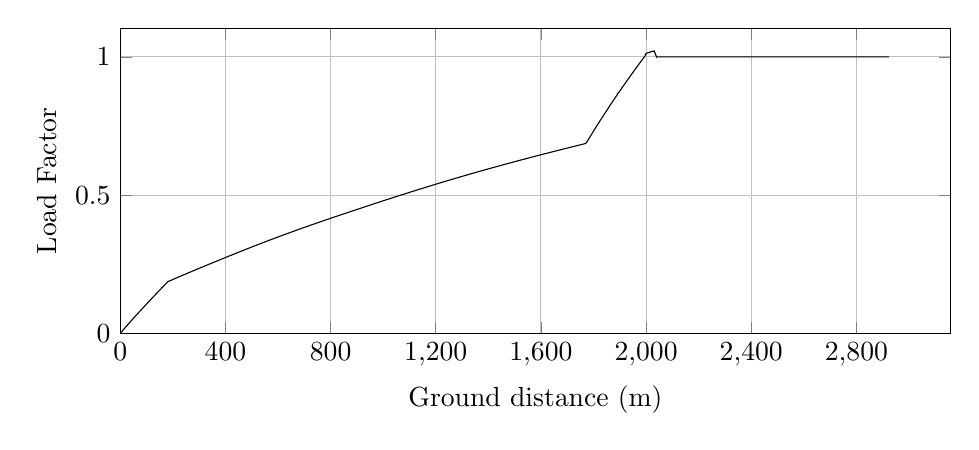
\begin{tikzpicture}

\begin{axis}[
width=\textwidth,
height=0.45\textwidth,
scaled ticks=false, tick label style={/pgf/number format/fixed},
xmin=0.0,
xmax=3157.6948405149165,
xlabel={Ground distance (m)},
xtick={0,400,800,1200,1600,2000,2400,2800,3200},
xmajorgrids,
ymin=0.0,
ymax=1.1034767012858302,
ylabel={Load Factor },
ymajorgrids,
legend style={at={(1.03,0.5)},anchor=west,draw=black,fill=white,legend cell align=left}
]

\addplot [
color=black,
solid
]
table[row sep=crcr]{
1.3603393307216043E-8	1.537403320839155E-11\\
3.0265395163403265E-7	3.4204788428773836E-10\\
2.9593179127983543E-6	3.3445075444561517E-9\\
1.5392338359717934E-5	1.7395829634758292E-8\\
5.361280674027254E-5	6.059112953589318E-8\\
1.6215010178508227E-4	1.8325575326839402E-7\\
3.7214145765703975E-4	4.2057962559723196E-7\\
6.839954676020354E-4	7.730241785596084E-7\\
0.001098342709021993	1.2413015524616042E-6\\
0.001609317716481928	1.818782192898569E-6\\
0.0022198920000388346	2.508823560884402E-6\\
0.002878710694837372	3.2533861846295516E-6\\
0.0036835072341781794	4.162922236314053E-6\\
0.004557929017412697	5.151140937217672E-6\\
0.005559798278933152	6.283388085625651E-6\\
0.006651227400597502	7.516843868474543E-6\\
0.007795849738889277	8.810408066773316E-6\\
0.009067984722810115	1.0248069117854358E-5\\
0.010453165799939174	1.1813475720438457E-5\\
0.011915708813158052	1.3466298802746646E-5\\
0.013455030027058647	1.5205876915416078E-5\\
0.015131183092671713	1.710007373128586E-5\\
0.01690803412933615	1.9108051764119454E-5\\
0.01873590105740728	2.117366436850671E-5\\
0.020713359121301934	2.340830528966597E-5\\
0.022777736728155237	2.5741148426838833E-5\\
0.024960970145273077	2.8208279934041193E-5\\
0.02723428625014468	3.077718163296539E-5\\
0.029610395797831278	3.3462213581298574E-5\\
0.03204086105441677	3.620863770752728E-5\\
0.03462344565878624	3.912692293381108E-5\\
0.037295727153354774	4.214652795773933E-5\\
0.040089145853872785	4.53029751274241E-5\\
0.042950967781251806	4.853667320322982E-5\\
0.04592022141655751	5.189171831509936E-5\\
0.04897301836205646	5.534111395673112E-5\\
0.052130294957187476	5.8908511991602623E-5\\
0.05542514139564195	6.263129508520551E-5\\
0.05879722600804832	6.644129030531245E-5\\
0.06231520981015182	7.041606947405297E-5\\
0.06596261503753809	7.453700791011548E-5\\
0.06964559414821356	7.869806960099879E-5\\
0.07347193989652406	8.302103473255349E-5\\
0.07736619052035826	8.742064135610467E-5\\
0.08137137577670908	9.19454979575101E-5\\
0.08545617869345057	9.656021850331766E-5\\
0.08969468676038628	1.0134849459685275E-4\\
0.0940095881391464	1.0622297919296585E-4\\
0.09845059220533334	1.112398217590693E-4\\
0.10296315144049947	1.1633739543393892E-4\\
0.10759658895065366	1.215714111857001E-4\\
0.1123317495250277	1.2692022330079272E-4\\
0.1171874363557737	1.3240506396799807E-4\\
0.12217670360507671	1.380406696407402E-4\\
0.12726806426274867	1.437914656445158E-4\\
0.13231647880291775	1.494936248144729E-4\\
0.13765212084557643	1.5552006734900314E-4\\
0.14294844966167852	1.615019660835687E-4\\
0.14834594087957392	1.6759797789934105E-4\\
0.1539671093411843	1.739464600015034E-4\\
0.15968242883369804	1.8040111398955768E-4\\
0.16555834796315422	1.8703697362183045E-4\\
0.17157514414202774	1.9383175265098661E-4\\
0.17760320215284392	2.0063906988972252E-4\\
0.18370335474801935	2.075276186006608E-4\\
0.18983540939776816	2.1445200727836288E-4\\
0.19621099073945342	2.2165119261774539E-4\\
0.20278841209744758	2.290780821912092E-4\\
0.20952923284938563	2.3668925344992448E-4\\
0.21624967405074952	2.442771918834647E-4\\
0.22309476488450758	2.520056426970053E-4\\
0.22992510727843934	2.5971721334453623E-4\\
0.2371653034562048	2.6789126701324363E-4\\
0.2442573187228817	2.758977792550917E-4\\
0.25144286317780873	2.8400963132372626E-4\\
0.2588001799723505	2.923151393426465E-4\\
0.2662612189130884	3.0073746868588576E-4\\
0.27386560463063747	3.0932133627621487E-4\\
0.2815803271719757	3.180294667762336E-4\\
0.28946218069394425	3.269259525104364E-4\\
0.29753588720841584	3.3603867794477235E-4\\
0.3056643119969481	3.452128464633078E-4\\
0.31376446154764137	3.5435478618264137E-4\\
0.322071411728719	3.6372979695266714E-4\\
0.3303680011285137	3.730927848690661E-4\\
0.3389039548234316	3.8272556008236134E-4\\
0.3474123396293025	3.923268777391789E-4\\
0.3561645174790815	4.022029444673525E-4\\
0.36525289600634137	4.1245799840537E-4\\
0.3742306244196095	4.225878127595164E-4\\
0.3835584127627333	4.3311220426209496E-4\\
0.392806747202999	4.4354654245526935E-4\\
0.40218604538039837	4.5412822616089913E-4\\
0.4115907129344223	4.647381146136435E-4\\
0.42143744457304466	4.758462716851741E-4\\
0.4310567075016639	4.866973795565219E-4\\
0.4412814114336725	4.982309849670782E-4\\
0.4513051702487684	5.095374458285563E-4\\
0.461412558308395	5.209377615597249E-4\\
0.47173637532167356	5.325816989450649E-4\\
0.4821484569390513	5.44324683999101E-4\\
0.492985116277161	5.565459815637129E-4\\
0.5036221628177362	5.685416303205819E-4\\
0.5142245311302887	5.80497649251173E-4\\
0.5252888808291518	5.929740776113314E-4\\
0.5363145235987512	6.054062960795341E-4\\
0.5471208511184944	6.175906761329385E-4\\
0.5585110457184732	6.304327971787133E-4\\
0.569849942463402	6.432164886714367E-4\\
0.5817265165330987	6.566057350391492E-4\\
0.5935668742733842	6.699535088568393E-4\\
0.6053719027871456	6.83260817136535E-4\\
0.6172343027602503	6.966321567836854E-4\\
0.629515267228629	7.104746280226201E-4\\
0.6417789549774502	7.242969409938267E-4\\
0.6542768803188956	7.383825586335798E-4\\
0.6669828212214572	7.527018914468349E-4\\
0.6796225285147333	7.669458554462992E-4\\
0.6925094233679154	7.814676375424602E-4\\
0.7056620711738308	7.962881150213852E-4\\
0.7184715206768946	8.107211263395007E-4\\
0.731725241748566	8.25653943471701E-4\\
0.7449880440563246	8.405962038026708E-4\\
0.7586792333483576	8.560202715252329E-4\\
0.7725063377467813	8.715966070103487E-4\\
0.7863894274138714	8.87235152572069E-4\\
0.8004504964383841	9.030733077775219E-4\\
0.8147129313117618	9.191373808513631E-4\\
0.8293722635741907	9.356475476611473E-4\\
0.8437954335339908	9.518908070108159E-4\\
0.8580702287827062	9.679660632039945E-4\\
0.8726489666047585	9.843826705861866E-4\\
0.8875094051704782	0.0010011155288020517\\
0.9027740629895862	0.0010183025282106638\\
0.9182163910703112	0.0010356885333691215\\
0.93361566230532	0.0010530250233812839\\
0.9491799633800446	0.0010705462517915064\\
0.9646343064330896	0.001087942652480158\\
0.9803727456894022	0.0011056577825239952\\
0.9957421603273868	0.0011229565021036285\\
1.0116767859397604	0.001140890302396957\\
1.028041387324289	0.0011593068809231332\\
1.0443915011410971	0.001177706001135026\\
1.060796374175649	0.0011961655859030764\\
1.0773229908740651	0.0012147609930719062\\
1.093971735592782	0.0012334926314781678\\
1.1110062543639518	0.0012526570791795012\\
1.127891796882146	0.0012716526996222684\\
1.1451224507351285	0.001291035304442237\\
1.1624801114435046	0.001310559500669386\\
1.180077727863539	0.0013303522970335533\\
1.1978884766667508	0.0013503834761480127\\
1.215488397439855	0.0013701762257380939\\
1.23351701382096	0.0013904497278331843\\
1.2518199984626128	0.0014110303614220886\\
1.2704235066044305	0.0014319474730290444\\
1.2892140278280424	0.0014530733816694409\\
1.3075714306593595	0.0014737109143444312\\
1.3266673518109293	0.0014951772011929402\\
1.3462106477188795	0.0015171448213273805\\
1.365306294594515	0.0015386077275548553\\
1.3852885894463176	0.001561065577698527\\
1.404835539176236	0.001583032548847986\\
1.4251192118409102	0.0016058257839281357\\
1.445164519989187	0.0016283494964300807\\
1.4656054698512246	0.0016513160652136844\\
1.4853522740259328	0.0016735010927135345\\
1.5051589726327936	0.001695751805197673\\
1.5255757775517242	0.0017186862282709615\\
1.5464367798307013	0.0017421178667158409\\
1.5673163741652552	0.0017655686144207913\\
1.5879032567231621	0.0017886888715618386\\
1.6091523485848285	0.0018125510264978637\\
1.6303162371862876	0.0018363156854592968\\
1.6519474169970438	0.0018606031920526764\\
1.673879209980242	0.00188522630404474\\
1.6955666802836635	0.0019095732116533916\\
1.7172271378534343	0.0019338879123391186\\
1.7402832823543353	0.001959767263961757\\
1.7634396102400074	0.001985756931448567\\
1.7861669372425006	0.0020112630311592936\\
1.8088678577734645	0.0020367374478758825\\
1.831824248135399	0.0020624964699145396\\
1.855578771396016	0.0020891488715485953\\
1.878960729162178	0.0021153810838130094\\
1.9033179534858085	0.0021427051595502345\\
1.9273833213731866	0.002169699541672724\\
1.9518510462308036	0.0021971429265668294\\
1.9761594732990155	0.002224405324254122\\
2.000437267212291	0.0022516310673112304\\
2.0252281699074732	0.0022794298585586997\\
2.0498006073458734	0.0023069813252288903\\
2.0745611186355752	0.00233474130302358\\
2.0997746990963106	0.0023630068018712105\\
2.1260324099367294	0.0023924402125725355\\
2.1515212193659616	0.0024210091942952223\\
2.1771505246334	0.0024497331391401243\\
2.2031842637813908	0.0024789077803262544\\
2.230133398733474	0.002509105534346967\\
2.257053086628849	0.0025392675329021924\\
2.283795213136285	0.0025692278607886516\\
2.311477064851834	0.0026002381506811797\\
2.3387199014446116	0.002630753813630502\\
2.3662694524467227	0.002661610195442078\\
2.3937852540088533	0.002692425930560111\\
2.4216520071021392	0.0027236318145620595\\
2.4501931244916175	0.0027555898595918137\\
2.478927626230634	0.002787761372900204\\
2.506685441631536	0.0028188364601570083\\
2.53537335014481	0.0028509497906935286\\
2.5633350931805676	0.0028822473192223566\\
2.5917889242519685	0.0029140926791229624\\
2.6208221472873374	0.00294658341936044\\
2.649872764173903	0.0029790905273737217\\
2.679661174525658	0.0030124200037052063\\
2.709174609939316	0.0030454386216802716\\
2.740029385016756	0.003079954492049448\\
2.770444625703795	0.0031139752898357376\\
2.801129860621211	0.0031482946918172587\\
2.8318827297715705	0.003182686324755336\\
2.862425967677578	0.0032168401490240655\\
2.893259332541544	0.0032513149961575353\\
2.92412139403754	0.0032858185166828066\\
2.955064430161417	0.003320409147917453\\
2.986690331721131	0.003355759614104731\\
3.019183403261743	0.0033920756727169018\\
3.0507201588152526	0.003427319319714978\\
3.0830332871979023	0.0034634269483246024\\
3.1154603869692448	0.0034996582305647428\\
3.148592095396281	0.0035366729636649953\\
3.181936872739324	0.0035739218509507416\\
3.214370607724433	0.0036101492982130133\\
3.247565473366384	0.0036472231059346124\\
3.281695868027062	0.0036853377677146114\\
3.316494330618462	0.0037241943271903283\\
3.3513055302544137	0.0037630609204254806\\
3.3860303583611797	0.0038018269184504298\\
3.421934361445942	0.003841904962465687\\
3.456235826539576	0.0038801900382327403\\
3.490536654441657	0.003918470382521792\\
3.526257338581564	0.0039583310510607405\\
3.561372823896762	0.003997512153714303\\
3.5967906564503185	0.0040370263779135355\\
3.632682576242373	0.004077065199654425\\
3.6701261071689295	0.00411883028021922\\
3.707701291513044	0.004160737477358371\\
3.7452745323452916	0.004202637781899018\\
3.78256482255855	0.004244217892887527\\
3.8208821591411084	0.004286938381814683\\
3.8590337549211444	0.004329469246993217\\
3.89695718563138	0.0043717409882296325\\
3.9351036745073964	0.004414256581880506\\
3.9736642086653067	0.004457228784455826\\
4.012189127077221	0.004500156433174123\\
4.05156219172609	0.004544024149415296\\
4.090290786278251	0.004587168903128755\\
4.129291984889424	0.004630612427261331\\
4.1680648628189925	0.00467379674742999\\
4.207805169621487	0.004718053536696169\\
4.248168240749736	0.004762998671105918\\
4.288797880674668	0.004808235363764422\\
4.32990243544832	0.0048539954577398094\\
4.371428084678056	0.004900218878381273\\
4.41247037137882	0.004945898877888497\\
4.453879445321437	0.004991981712209474\\
4.49524783594077	0.005038013874159006\\
4.537299342543221	0.005084800654128547\\
4.580546125800922	0.005132911530873428\\
4.622914948498307	0.005180040039602938\\
4.66640222022569	0.005228406836461254\\
4.709294790611851	0.005276106460103755\\
4.752417172855319	0.005324055921149148\\
4.796155651503765	0.005372684594716976\\
4.8408754796551925	0.005422398268342806\\
4.884850997559644	0.005471278550918295\\
4.928651138956553	0.00551995803811607\\
4.972831351372241	0.005569054033492078\\
5.017331702752941	0.005618499816181473\\
5.0632326321008225	0.005669495568296681\\
5.108452384314601	0.005719728342659096\\
5.1536021218025905	0.005769877229943135\\
5.199057463234675	0.005820359412337229\\
5.244479287100011	0.005870798231634199\\
5.292293005248643	0.00592388653182109\\
5.338096108273211	0.005974736083641441\\
5.3857492800262605	0.0060276329867832105\\
5.433816232374781	0.006080982457759794\\
5.480691139018431	0.006133002377703624\\
5.529685763332537	0.00618736784093433\\
5.578612887337309	0.006241651457741297\\
5.626451501744754	0.006294720708954473\\
5.674834544150631	0.0063483872151785335\\
5.7252048440372345	0.006404250856445476\\
5.77422346516266	0.006458608446524583\\
5.8255152536468575	0.006515479469193617\\
5.874338256646894	0.006569606236252744\\
5.922631450506765	0.006623139015711841\\
5.972682300942642	0.006678613223271248\\
6.022535370757359	0.006733861237498494\\
6.074394648705015	0.006791325199559897\\
6.124928192945902	0.006847312951552507\\
6.176798284396469	0.006904774147230602\\
6.229620191179453	0.006963282122022048\\
6.282808156696705	0.007022187808711791\\
6.334658925277093	0.007079605091668528\\
6.388041948821611	0.007138711465292344\\
6.440558117792513	0.00719685049141133\\
6.494960924490993	0.007257070285926628\\
6.550441697666145	0.007318475093136459\\
6.6042098433346865	0.007377976522103784\\
6.658315220792536	0.007437843341686232\\
6.712335084641163	0.00749760776743442\\
6.766674450459032	0.0075577178662822935\\
6.821537769035839	0.007618399651287276\\
6.876851268142238	0.0076795713479891736\\
6.933661362437203	0.007742389803419075\\
6.989261882852809	0.007803862609436303\\
7.046240323930029	0.007866850538819446\\
7.102786137967051	0.007929351914031305\\
7.1603789170469145	0.007993002062386987\\
7.21785165788507	0.008056511071863046\\
7.277487498606879	0.008122401456571915\\
7.334984696129153	0.008185920343269228\\
7.393362172524569	0.00825040314447802\\
7.452416393609804	0.008315624733585951\\
7.511934748111884	0.008381350080255095\\
7.572557225035805	0.008448285604675303\\
7.63202184821041	0.008513933827218309\\
7.69294899409779	0.008581187584499913\\
7.752675521499926	0.008647107179380357\\
7.814488876138199	0.00871532077732705\\
7.8763528528159785	0.008783580904165308\\
7.938149975125226	0.008851757984561929\\
8.001193143199774	0.008921300240350389\\
8.064554080136986	0.00899118338902107\\
8.12686567918485	0.009059899808070026\\
8.189637855946287	0.00912911479005648\\
8.252542711798306	0.00919846669312416\\
8.315859663763469	0.00926826349434888\\
8.380006162932737	0.009338965133925738\\
8.444702551512929	0.009410263111761834\\
8.509501986620958	0.009481664889360778\\
8.57387297516295	0.00955258494102387\\
8.63887365699837	0.009624189063507795\\
8.70727085773305	0.009699524300337003\\
8.772937378995405	0.00977184182469993\\
8.839192134487615	0.009844797244842952\\
8.905815929161982	0.009918149032253515\\
8.97209054442786	0.009991106484831404\\
9.039019026885107	0.01006477377425439\\
9.107371801018814	0.010139998481211075\\
9.174915633685494	0.010214322765422498\\
9.243868961478196	0.010290187681465631\\
9.312440636565494	0.010365622366681766\\
9.381784695008012	0.010441896325757047\\
9.4513167952828	0.010518366659666569\\
9.52142787533916	0.010595463198921608\\
9.591425279059166	0.010672424226730499\\
9.662230428326719	0.0107502627325629\\
9.734225879912522	0.010829398880697692\\
9.806441602430919	0.010908766168954726\\
9.878483835105534	0.010987931892433907\\
9.951807209049782	0.011068494325216524\\
10.023539677466466	0.01114729800032497\\
10.096057433179052	0.011226953592321547\\
10.168262179450682	0.011306254655370484\\
10.241274410624943	0.011386431757488569\\
10.31479015323385	0.011467150865609175\\
10.390063469390178	0.011549788477073547\\
10.465012435634037	0.011632058728381888\\
10.540639152111389	0.011715061595701218\\
10.617644389866598	0.01179956580248555\\
10.692945462162374	0.011882188603242876\\
10.770083295573727	0.01196681525822312\\
10.846726862770723	0.01205088820414737\\
10.924657809445929	0.012136361681867665\\
11.00265335491597	0.012221894332492229\\
11.081827589833612	0.012308707700578602\\
11.159134327011738	0.012393461913221281\\
11.239152720133266	0.01248117715037014\\
11.317028257314295	0.012566531898800734\\
11.396413369884492	0.01265352958626528\\
11.477655063362434	0.012742549824608157\\
11.556958506738276	0.012829434537914092\\
11.637325199769407	0.012917472434128156\\
11.717754170658207	0.013005566826013221\\
11.799819443100102	0.013095441457694245\\
11.881986970940797	0.013185416000189742\\
11.964394119506721	0.01327564087635121\\
12.046263329632716	0.013365264907949674\\
12.130282587748898	0.013457230423286247\\
12.213721087180826	0.01354854808598348\\
12.295868535962462	0.013638441018906258\\
12.380692430046633	0.013731250588261091\\
12.46470288467437	0.013823158040073388\\
12.550384439940181	0.013916881363155135\\
12.635259749824865	0.01400971059710181\\
12.72144647897981	0.014103961839343404\\
12.80741162779486	0.014197958502399763\\
12.892901506907108	0.014291423432281522\\
12.977815703098727	0.014384247156526631\\
13.06483740414145	0.014479362561737649\\
13.151922956503014	0.014574535553094034\\
13.240589045456186	0.014671423413386956\\
13.329911181207382	0.014769015550283204\\
13.417306166647748	0.014864489959129108\\
13.507103029723119	0.014962575871361636\\
13.595986036712912	0.015059651268202297\\
13.687453390597003	0.015159536534713367\\
13.779071846306106	0.015259574020544182\\
13.872694200363323	0.015361786432824123\\
13.963504841252302	0.01546091658884972\\
14.056146454975131	0.015562032817630798\\
14.14918846816267	0.015663573327527082\\
14.24332804549016	0.015766298762122377\\
14.339261112049854	0.01587096803202345\\
14.431091301610323	0.01597114839352637\\
14.524174633942373	0.016072683573474935\\
14.618760344060338	0.01617584499584618\\
14.714801736988441	0.016280581251267388\\
14.809763128346521	0.01638412713030223\\
14.903412319659619	0.016486230024987857\\
15.001392651385917	0.016593042219211845\\
15.098055049922994	0.01669840495983665\\
15.196870856960619	0.016806101990234225\\
15.29477342819068	0.016912790922753496\\
15.39265348361268	0.01701944271819503\\
15.490487151984588	0.01712603149771273\\
15.588146853189365	0.017232418423691893\\
15.687961867268871	0.01734114067325234\\
15.78650099417861	0.01744846080904478\\
15.886965864441798	0.01755786576609324\\
15.98755318095926	0.017667391517745542\\
16.088470385762115	0.017777263981661816\\
16.190536977381747	0.017888375230935574\\
16.292466610053154	0.01799932487201054\\
16.396448349404487	0.018112495465969915\\
16.497808944935016	0.01822280102179276\\
16.600551072850564	0.01833459780330576\\
16.70575139586156	0.01844905680356873\\
16.81134459259622	0.01856393055713269\\
16.917616592554033	0.018679530073006614\\
17.023477948501657	0.0187946703773849\\
17.12904978140002	0.018909483472921793\\
17.2354081519902	0.019025139668642083\\
17.340772011500363	0.01913970239276351\\
17.448391076872838	0.019256705008260565\\
17.5571980918308	0.01937498676105977\\
17.66615596614949	0.01949342017460171\\
17.774685459577412	0.019611375832148024\\
17.884986575683584	0.01973124474286027\\
17.99552903728076	0.019851363708935275\\
18.108708479124623	0.01997433558530071\\
18.219646262474413	0.020094859721580406\\
18.332680252669796	0.0202176490141382\\
18.445061806396694	0.02033971752929859\\
18.556709221711323	0.020460976905134116\\
18.668884868236475	0.02058279838390787\\
18.78204748093455	0.020705680073065884\\
18.895704562363058	0.020829087112344075\\
19.008928234289563	0.020952012181159593\\
19.124320907419907	0.02107728057963979\\
19.24105855786135	0.021203997405646515\\
19.355116774466126	0.021327794594384667\\
19.470462572962035	0.02145297826303336\\
19.58492145104516	0.02157718855509048\\
19.704921229319112	0.021707400426531395\\
19.821259826163917	0.021833628600284084\\
19.941172080873493	0.021963723123559164\\
20.06078806851737	0.022093485188561267\\
20.177423389922623	0.02222000332764855\\
20.297621170678	0.022350375187983548\\
20.420129559802255	0.02248324236380711\\
20.54164670774839	0.022615023833959417\\
20.661905244258705	0.022745430128318526\\
20.784301666224792	0.02287814443040925\\
20.904244540623438	0.0230081884821143\\
21.028114340450195	0.0231424801112907\\
21.148300883955606	0.023272769010475595\\
21.270875420257596	0.023405637099260978\\
21.39299406946177	0.023538001640924164\\
21.513793771711654	0.023668927555693664\\
21.637476506915142	0.023802969078360416\\
21.759279707150128	0.023934964842586424\\
21.88493035745168	0.024071121056479225\\
22.009809790007786	0.024206432760623384\\
22.13620730934617	0.024343380632831833\\
22.263515470260465	0.024481306482431544\\
22.393040471753594	0.024621625344451475\\
22.520519759768852	0.02475971964677978\\
22.648852607677917	0.024898730414387487\\
22.775118904521122	0.025035494893241327\\
22.903136237443974	0.025174148317486444\\
23.03176118514304	0.025313452267591106\\
23.162501585272054	0.025455039748118108\\
23.294719932439598	0.025598220277514617\\
23.427108470281937	0.02574157776510624\\
23.558693146983046	0.02588405773749912\\
23.687077503630363	0.026023065844673152\\
23.817949558665852	0.0261647610613121\\
23.948210788889448	0.02630578869608238\\
24.076877750667826	0.02644508439372235\\
24.21019765060587	0.026589411434494243\\
24.3450673155249	0.026735410257407128\\
24.477101355489637	0.02687833391502496\\
24.60984760833776	0.027022023219268106\\
24.7468403923846	0.027170303784132377\\
24.882807251950062	0.02731746877585748\\
25.017167332957627	0.027462889889150133\\
25.153910941279605	0.02761088612933113\\
25.289629217480112	0.02775776829539581\\
25.425306692573436	0.027904602196581873\\
25.56229499031975	0.02805285078389695\\
25.70075944713021	0.02820269311444845\\
25.83724158708921	0.028350386789960158\\
25.975209935932874	0.028499685530829485\\
26.003074150630965	0.028529837669860714\\
26.020759913393235	0.028548975544056564\\
26.030714598210515	0.028559747549473033\\
26.05840292223249	0.028589709119799363\\
26.06133765907019	0.028592884795470626\\
26.064285136409026	0.028596074256329932\\
26.066337724202356	0.028598295357773265\\
26.068175973881182	0.02860028452380786\\
26.06984477238784	0.028602090326656338\\
26.077831036047115	0.02861073223758009\\
26.10345636352254	0.028638461259261366\\
26.16716044512971	0.028707394644071658\\
26.297541524199602	0.028848476293832\\
26.42722303713863	0.028988797976457162\\
26.5559280656694	0.02912805985116248\\
26.686097387723095	0.029268902619368514\\
26.817793678842584	0.029411393710480165\\
26.949416928520378	0.029553801637659645\\
27.080440623797912	0.02969555652005333\\
27.215491080424528	0.02984166313846776\\
27.34795890217076	0.02998497066553909\\
27.48215578365496	0.03013014340164568\\
27.616696052324144	0.030275681953769524\\
27.75271189183823	0.03042281067614482\\
27.888759310501555	0.03056996723214385\\
28.023839122857026	0.030716070651057588\\
28.16136324828667	0.030864810920860727\\
28.298355249881332	0.031012968446256343\\
28.435282447697354	0.031161048424018678\\
28.573941346212784	0.031310993286379735\\
28.713752690797136	0.03146217611972083\\
28.852681198061333	0.031612395816806034\\
28.992471984120606	0.03176353906716839\\
29.133421724605903	0.031915926186646626\\
29.275199211812186	0.03206919863353321\\
29.416225289053614	0.03222164895057834\\
29.55783477945603	0.032374719853138854\\
29.701838356359822	0.032530367982846406\\
29.846633046394217	0.03268686012630994\\
29.99013730470424	0.032841946375800915\\
30.132492646908446	0.03299577970251009\\
30.277395768405135	0.03315235444316004\\
30.422188862471998	0.03330879816025114\\
30.56637548064623	0.03346457430101776\\
30.711944318924978	0.03362183106261829\\
30.8573377156769	0.03377888531290875\\
31.006558691603843	0.03394006037526222\\
31.153907258126303	0.034099199114578434\\
31.30257185742142	0.0342597449263119\\
31.4510947803754	0.03442012318539954\\
31.602595106592503	0.03458370126853771\\
31.755261577184278	0.034748522635283045\\
31.906398416479824	0.03491167668380985\\
32.05599258457312	0.03507314957743501\\
32.20952926265106	0.03523886142457756\\
32.360097140052986	0.03540135246333481\\
32.51218835243483	0.035565470552624254\\
32.664721606344784	0.03573004832834543\\
32.82129760777845	0.035898969803268385\\
32.97669884718651	0.03606660533772827\\
33.13118849606322	0.03623323895557988\\
33.288837444683736	0.03640326089799195\\
33.44405554194745	0.036570641904918794\\
33.60015866510213	0.036738957741694736\\
33.756686089655645	0.03690771116271124\\
33.91694077595571	0.03708046207870065\\
34.074326811338736	0.037250099847194386\\
34.23252403098988	0.037420590940501416\\
34.392884168270385	0.03759339131361878\\
34.554266068788166	0.03776727040396199\\
34.71363140184178	0.037938954578071726\\
34.87649332318763	0.03811438261682733\\
35.03746231629111	0.038287748596834106\\
35.19990059234286	0.03846267353866515\\
35.3627309111595	0.038637996770246194\\
35.5271254050015	0.03881497970090625\\
35.69149466827288	0.038991910653598284\\
35.85508342515686	0.0391679765996864\\
36.017180984292054	0.03934241295175108\\
36.182222084544165	0.03951999147863085\\
36.34861175093968	0.03969899483532263\\
36.514166392421686	0.03987707356919902\\
36.68083924241549	0.04005632840185951\\
36.845526722294395	0.040233421478363104\\
37.01328249159678	0.04041378667891803\\
37.18160982421668	0.04059473851868922\\
37.35136716620059	0.04077719912744218\\
37.51969289597564	0.04095809254809033\\
37.689710015857784	0.04114077469507054\\
37.860394939778416	0.041324144935177484\\
38.02805196867635	0.041504233327845474\\
38.19868492919754	0.041687488697929806\\
38.37343039987371	0.04187512964495341\\
38.54685896696101	0.042061325149584335\\
38.71934233168869	0.042246474703545596\\
38.8915617091798	0.04243130969531965\\
39.062305982326905	0.04261453058897801\\
39.23847188392709	0.04280353681603867\\
39.411511502305984	0.042989156621854846\\
39.585172817779906	0.043175411000495385\\
39.760693028009456	0.04336362600216181\\
39.9373134006328	0.04355298701085493\\
40.113617753210534	0.043741975297240575\\
40.29094651898711	0.04393202736207882\\
40.468149621311596	0.04412191018974659\\
40.64593210594187	0.04431237898490216\\
40.82431302355218	0.04450345365508989\\
41.00141330502653	0.044693121466278005\\
41.17957893337042	0.0448838947950319\\
41.359761290266974	0.04507679127486552\\
41.53889737920997	0.04526853133875595\\
41.72013507746885	0.04546248388198332\\
41.899395797464194	0.0456542840041623\\
42.081280067494475	0.04584885370572447\\
42.265315320939635	0.04604568583648382\\
42.44531744651641	0.04623816672996046\\
42.62715102096499	0.046432568090262506\\
42.81120266452106	0.04662930185585528\\
42.994164503876235	0.046824831739582504\\
43.17799769459725	0.047021253559601746\\
43.36154361404071	0.04721732904545607\\
43.54597437124032	0.047414310008765836\\
43.73158498218817	0.04761251075520416\\
43.91737182308138	0.047810859027730426\\
44.1050494697441	0.048011184534549556\\
44.293574236233	0.048212372233955844\\
44.47888581456586	0.048410089774893514\\
44.66456251492659	0.04860815586837647\\
44.85170130968709	0.048807739976956845\\
45.037822074257164	0.04900619679655163\\
45.22676109993536	0.04920761618724251\\
45.41612608476639	0.04940944663306034\\
45.604812217355104	0.04961051059201023\\
45.79422221198037	0.04981230269438602\\
45.98724683785376	0.05001790110318471\\
46.17830917717477	0.05022136495947855\\
46.36786657808848	0.05042318242278402\\
46.55935209439748	0.05062700836441123\\
46.75090376717816	0.05083086006250107\\
46.94233405988251	0.05103453788688305\\
47.13714948644359	0.05124177147539247\\
47.33387512950824	0.05145098994082263\\
47.53043319838464	0.05165998285177649\\
47.72298239739284	0.05186466733820922\\
47.919150009665316	0.05207315146904937\\
48.113386178114425	0.05227953627658842\\
48.311024807628144	0.05248948869308201\\
48.508886059616145	0.05269962939456513\\
48.70490444306449	0.052907765246454616\\
48.90290918859142	0.05311796209727118\\
49.09959709013448	0.053326713060695065\\
49.2970021191946	0.053536177034020985\\
49.49532701226336	0.05374656850235499\\
49.693780717172615	0.05395704786474878\\
49.89506320355713	0.054170477573527026\\
50.096719083698545	0.054384252838300486\\
50.29606895218413	0.05459553391913011\\
50.497598474286534	0.05480907497541493\\
50.700304208193415	0.05502381148114188\\
50.90342397924904	0.055238935408771256\\
51.10460922167407	0.055451959953618575\\
51.30752217039489	0.05566676293139006\\
51.51010619677311	0.05588116666583675\\
51.713602501430145	0.056096484548396844\\
51.91843850546792	0.05631316797192855\\
52.121089026646246	0.05652748818364028\\
52.32561402362407	0.05674373905696843\\
52.53192272805477	0.05696182323028254\\
52.7387030603267	0.0571803528772636\\
52.944027344085896	0.057397291179835344\\
53.154073670302836	0.05761916444037702\\
53.36143953271798	0.05783815257239062\\
53.571009444677685	0.058059414058112074\\
53.77799762982136	0.058277896299234806\\
53.98785945427545	0.05849935751089898\\
54.196157549666225	0.05871911458526461\\
54.40718762937186	0.058941699129595015\\
54.616887598525366	0.05916282612675753\\
54.826875464266934	0.05938420219692071\\
55.04038432082807	0.05960923432303885\\
55.25438844036796	0.059834731938125545\\
55.46695867894975	0.06005866270819936\\
55.68088820258777	0.0602839691560606\\
55.895144656119854	0.06050956341234199\\
56.109028395418505	0.06073470888397346\\
56.326262430904194	0.060963323488834265\\
56.542089933321776	0.06119040048449088\\
56.76060076462056	0.0614202424635819\\
56.97729209122687	0.06164811281708591\\
57.19579178641709	0.06187782665640156\\
57.41258192878804	0.06210568554396463\\
57.634093277561306	0.062338447448685004\\
57.85395098827546	0.06256941259912353\\
58.07448819514299	0.06280103248110572\\
58.29446478173499	0.06303200469936576\\
58.51588770709739	0.06326443626775069\\
58.73757884137123	0.06349708988830684\\
58.96020041504734	0.06373066015425502\\
59.18267120664716	0.06396401245651351\\
59.405949655899676	0.06419815195443127\\
59.63089974393067	0.06443398376398755\\
59.8562534200115	0.06467017776660769\\
60.084134136581554	0.06490895848626319\\
60.30833762904015	0.06514382548161009\\
60.53504725699203	0.06538125680175555\\
60.763693228044005	0.06562065403364176\\
60.99075593752245	0.06585833206248667\\
61.21765734918529	0.06609578016962228\\
61.44713116872772	0.06633585828710728\\
61.6738048454246	0.06657294582108156\\
61.90668490141796	0.066816461832668\\
62.13729676517957	0.06705754325287892\\
62.36629463006145	0.06729687570409558\\
62.596359157213186	0.06753726119785713\\
62.82836101237727	0.06777960840200735\\
63.059723307860466	0.06802122515610559\\
63.292774394726166	0.06826454274797865\\
63.52608473446321	0.06850806804363754\\
63.75973181411028	0.06875188185278282\\
63.993403028653574	0.06899565799622406\\
64.23068717493263	0.06924313917222012\\
64.4710952259949	0.06949381277891976\\
64.70858695601663	0.06974138077682376\\
64.94894296164699	0.06999186924015605\\
65.18738841845183	0.07024030186673069\\
65.42661162888535	0.07048948022010872\\
65.6659442133793	0.07073870795102657\\
65.90899583190168	0.07099174261577186\\
66.15068261105333	0.07124329078523454\\
66.39533053734849	0.07149785452756008\\
66.6378997293487	0.07175018955498702\\
66.88158418814953	0.07200361907814978\\
67.12390450547147	0.0722555648641014\\
67.36840986262189	0.07250971697682891\\
67.61550053739396	0.07276648980121701\\
67.86097385246623	0.07302151583194605\\
68.10985741250389	0.0732800178507126\\
68.35582503705197	0.07353542524443808\\
68.60464259362828	0.07379372544738826\\
68.85450289166104	0.07405304109262328\\
69.1042877596268	0.07431221157159723\\
69.35837572129628	0.07457577850063857\\
69.61150655903072	0.07483828435584702\\
69.86289252102952	0.07509891358148446\\
70.11686816207683	0.0753621600589271\\
70.37125759672608	0.07562576756655102\\
70.62480458144697	0.07588843480531637\\
70.88045310059783	0.07615321145482419\\
71.13526709211152	0.07641705641773532\\
71.3947754873567	0.07668569335481251\\
71.6534187996231	0.07695336601146502\\
71.91450497256008	0.07722349751119893\\
72.1716184080999	0.07748945091892562\\
72.43269265097052	0.07775943288468529\\
72.69331619504374	0.0780288803375368\\
72.95563200429567	0.07830000864944772\\
73.21686762735783	0.07856995233318005\\
73.48161420086069	0.07884345496744025\\
73.74261486234883	0.07911302012434798\\
74.00755043430098	0.07938658095284794\\
74.27511769675363	0.07966278962172038\\
74.54487113507057	0.07994118472741743\\
74.81568229507957	0.08022060078761958\\
75.08274085953312	0.08049607607905486\\
75.35421836228127	0.08077603981336022\\
75.62798354862159	0.0810582919257582\\
75.89909469738902	0.0813377380512296\\
76.17008148658607	0.08161698711968203\\
76.44269151183332	0.08189783985385235\\
76.71571902594138	0.08217905369409254\\
76.99340852183178	0.08246499889942836\\
77.27004772085374	0.08274979243357006\\
77.54832408953641	0.0830362012085705\\
77.82592519882277	0.08332184530644189\\
78.10358246820337	0.08360747802750947\\
78.38556010231375	0.0838974848892438\\
78.66911430382748	0.08418904223425934\\
78.95399134982776	0.08448188858283268\\
79.23667137346987	0.08477240642224688\\
79.518907793654	0.08506239925960246\\
79.80555437718249	0.08535685329544393\\
80.09150103324356	0.08565051840232013\\
80.37928873457926	0.08594600424362614\\
80.66871996946384	0.08624310728165117\\
80.95967699414447	0.0865417060374808\\
81.25093884305389	0.08684054736195586\\
81.54344278085921	0.08714059290770607\\
81.8358102960415	0.08744042878508312\\
82.13087592438694	0.08774296159176975\\
82.42794520371837	0.08804747819713339\\
82.72842933895026	0.08835542385217182\\
83.0269479931649	0.08866128471097719\\
83.32974506690314	0.08897145805087647\\
83.62964811531441	0.08927859684040876\\
83.92951211009506	0.08958562658343713\\
84.2339319847595	0.08989725109150919\\
84.53715838283946	0.09020758442667755\\
84.84105485927768	0.09051853465521689\\
85.14845677960258	0.09083300219910456\\
85.45530133949276	0.09114683054693187\\
85.76249773413784	0.09146095033904499\\
86.07201271349416	0.0917773724508886\\
86.38432073331904	0.09209658093438076\\
86.69710203601804	0.09241620441635652\\
87.01172103282082	0.09273763712878372\\
87.32669099459858	0.09305936017202357\\
87.64517025121202	0.09338459909731298\\
87.96158123090564	0.0937076582493379\\
88.2775814178033	0.09403023149545778\\
88.60068374099544	0.09435998670857129\\
88.92068281935622	0.09468650790917582\\
89.24207276858638	0.09501438215361731\\
89.56578933015979	0.09534456373050296\\
89.88760090270688	0.0956727372179297\\
90.2141410750086	0.09600566732630755\\
90.54066676000363	0.09633851758408013\\
90.86727570256076	0.09667138846751952\\
91.19715108614633	0.0970075240752274\\
91.52744226539704	0.09734401947254986\\
91.85639956214655	0.09767909326931393\\
92.19095740864739	0.09801980852408415\\
92.52827526888461	0.09836327098212026\\
92.8674718219292	0.09870858291936914\\
93.20307982994817	0.09905017996536701\\
93.5374944579234	0.09939050228856083\\
93.87598013161067	0.09973490750153854\\
94.20917297854535	0.1000738692452353\\
94.55043409744499	0.1004209802058022\\
94.89132963816093	0.10076766096297719\\
95.23083207736542	0.10111286800608657\\
95.57395676502793	0.10146170141194251\\
95.91421223354143	0.10180756253639839\\
96.25656086122288	0.10215549672309444\\
96.60012122339742	0.10250460840706012\\
96.94166303707107	0.10285161632835442\\
97.28627502929558	0.10320169145553544\\
97.62906225262071	0.1035498620005909\\
97.97125437026659	0.10389737851471881\\
98.31201772458999	0.10424339583725692\\
98.65627175165852	0.10459290986106079\\
99.0012536203806	0.10494311571994486\\
99.35020029285332	0.10529729951698148\\
99.69475740907401	0.10564698266999925\\
100.04053871990226	0.1059978641484413\\
100.38598466112728	0.10634836229302172\\
100.72867962848932	0.10669602781033649\\
101.07385499050397	0.10704616906839483\\
101.41864366415388	0.10739587844289054\\
101.76305460768467	0.10774516622907324\\
102.11068844700483	0.10809768465586751\\
102.45638678530696	0.1084482037306876\\
102.79841653079728	0.10879496815517224\\
103.14087212494877	0.10914213061182472\\
103.48486473791618	0.10949081832713788\\
103.82875595362174	0.10983937139632717\\
104.17244250654872	0.11018768627810918\\
104.51168383396202	0.11053146698167798\\
104.85986244643053	0.11088427560517791\\
105.204587526496	0.11123355697452761\\
105.54754777175077	0.11158102382658311\\
105.88797456536247	0.11192589900755757\\
106.23280177240994	0.11227520786977412\\
106.57515110440406	0.11262198360990819\\
106.91603555764121	0.11296725379357522\\
107.25729565943405	0.11331288380396437\\
107.598830149446	0.11365877209951758\\
107.93686571059558	0.11400109859558104\\
108.27485499032852	0.11434336110277664\\
108.28839963475954	0.1143570766513856\\
108.30004107281309	0.11436886495868658\\
108.30931238392475	0.11437825322377315\\
108.31701527366243	0.11438605327332423\\
108.32505202073054	0.11439419138246397\\
108.33865239118708	0.11440796326470624\\
108.35091925899997	0.11442038480557327\\
108.39508146726081	0.11446510368038308\\
108.52984553865659	0.11460156473705739\\
108.79919793188978	0.1148743008327032\\
109.105233418432	0.11518416709595658\\
109.41485218466596	0.11549764564064131\\
109.72257164661937	0.1158091844123964\\
110.0321119530083	0.11612254874593637\\
110.34145354075926	0.11643569300252628\\
110.6534776714839	0.11675153264142629\\
110.9711963390063	0.11707311464765761\\
111.28851843247409	0.1173942722692622\\
111.60893519474632	0.11771853761264443\\
111.92798394282838	0.11804139316518561\\
112.24770070245137	0.11836489830579588\\
112.57243448635171	0.11869345182898942\\
112.89480865389396	0.11901958894840624\\
113.22000325235314	0.11934854907735115\\
113.54885709436653	0.11968117877813778\\
113.8770619430189	0.12001311885757297\\
114.20946079557197	0.12034926582609781\\
114.54107775051554	0.12068458607840471\\
114.87787736567807	0.12102510898144674\\
115.21564640021248	0.12136657258975761\\
115.55522358014255	0.12170982322371462\\
115.89667501383605	0.12205492594318344\\
116.23992536102014	0.12240180281421385\\
116.5847156213415	0.12275019035235478\\
116.92791619634093	0.12309692522926194\\
117.27517516660399	0.12344771209190764\\
117.62420948631524	0.12380024237944748\\
117.97391125359778	0.12415339546661149\\
118.32673409155768	0.12450964724589854\\
118.68227803698588	0.1248685914207011\\
119.03889207644076	0.12522855918135117\\
119.39651249432902	0.12558948459696123\\
119.75508651978987	0.1259513128153372\\
120.11314113323388	0.12631255623954143\\
120.47404637453192	0.12667661322668974\\
120.84098349318353	0.12704668935797234\\
121.20490030977416	0.1274136530958971\\
121.57328571082118	0.12778505450849453\\
121.94079100066682	0.12815549899885387\\
122.31015242291167	0.12852774330793224\\
122.68267403243519	0.1289030990994244\\
123.05346836176264	0.12927664019899388\\
123.42835733050345	0.12965422983577665\\
123.80350972566416	0.13003200676264698\\
124.1783235941891	0.1304093637528176\\
124.55244040146786	0.13078593910020436\\
124.92576251095704	0.13116163395905284\\
125.30489170817492	0.13154308938732007\\
125.68146781278597	0.1319218917937991\\
126.06139977608174	0.13230398375171165\\
126.44502763856761	0.13268970377529182\\
126.82695116404781	0.13307362044884677\\
127.206716044588	0.13345527744134486\\
127.59262031825523	0.13384301169907134\\
127.97077035934353	0.1342228633150512\\
128.3546122768156	0.13460833867664967\\
128.73724861847296	0.13499250837280138\\
129.12002064685282	0.1353767184906434\\
129.50086700331673	0.1357588996739677\\
129.8837789976152	0.13614305625431455\\
130.26783132854348	0.13652825778943214\\
130.651936341801	0.13691341201234433\\
131.03747321415574	0.13729990039751608\\
131.42280335891803	0.13768607895437915\\
131.80875442588928	0.13807277612584443\\
132.19322104975072	0.13845788198019102\\
132.5798881414172	0.13884508642816126\\
132.96215446290768	0.13922777914894216\\
133.34488286943906	0.13961082925108226\\
133.7276157954845	0.13999377781917607\\
134.11532375481391	0.14038159531109867\\
134.50135826447365	0.14076762920759403\\
134.88604120201086	0.14115220192473368\\
135.26955723714872	0.14153549842731222\\
135.6512109336153	0.141916824269099\\
136.03464327936558	0.14229981665263955\\
136.41686422877552	0.14268148803959438\\
136.79904942565338	0.14306301226172974\\
137.18004416157777	0.1434432364960495\\
137.56399804528928	0.14382630053838436\\
137.94515347717788	0.14420645943688565\\
138.32982901897384	0.1445900142906301\\
138.7128522769853	0.14497180633083842\\
139.09597564505458	0.14535358242462396\\
139.48002685240425	0.145736166340168\\
139.86309097971855	0.14611764993070622\\
140.24727738828375	0.14650013323142327\\
140.6317581809211	0.14688279081185265\\
141.01585725597846	0.14726494927830375\\
141.3998433603236	0.14764687572380653\\
141.7841907991213	0.14802904127808922\\
142.16710976343057	0.14840966629249838\\
142.55205218648928	0.14879218124774768\\
142.9364233092117	0.1491740065787406\\
143.32169829765928	0.14955660705026455\\
143.705984531242	0.14993810276071737\\
144.08985428249122	0.1503190620531967\\
144.47683600496026	0.15070298488848308\\
144.86371007721533	0.15108667520545954\\
145.24772592056325	0.1514674060852942\\
145.63047789911974	0.15184675985497517\\
146.01273254364395	0.15222549670641122\\
146.39725173307323	0.1526063518585339\\
146.77966503747456	0.15298499607979293\\
147.16478130736948	0.15336619016807945\\
147.54689717238745	0.15374428863560818\\
147.93097497792814	0.15412420182782116\\
148.31499270913332	0.15450392838237495\\
148.69957284780122	0.15488408325246897\\
149.08709998577143	0.15526702151878108\\
149.47129868208145	0.155646541936384\\
149.8546635899794	0.15602511057768903\\
150.23801379389647	0.15640353642273772\\
150.62200569343076	0.1567824668510731\\
151.00751012558203	0.15716275986857356\\
151.3946455315429	0.15754453046194344\\
151.77987817077866	0.15792429374896627\\
152.16505704867353	0.15830387324067718\\
152.55112759502248	0.15868419996508476\\
152.93964308710213	0.1590668021569654\\
153.32507651584535	0.15944623704282235\\
153.71174813432617	0.1598267583822148\\
154.10000329570875	0.16020870438494123\\
154.48914219495543	0.16059138515138727\\
154.8788297075107	0.16097447019253594\\
155.26820650111182	0.16135711443850798\\
155.6562915247282	0.16173835447212914\\
156.0441896603637	0.16211927630317546\\
156.4348678136667	0.16250279197760448\\
156.82082928279863	0.1628815431072912\\
157.21071017196311	0.1632640047484738\\
157.60005066896917	0.16364580006979104\\
157.99004282467217	0.1640280978491122\\
158.3808231456182	0.1644110310372262\\
158.77280374485122	0.16479500232507382\\
159.16384255262415	0.16517791318563627\\
159.55370941764693	0.16555953928710543\\
159.946071590523	0.16594346959123546\\
160.33752628124114	0.16632637352880433\\
160.73008933968674	0.16671022275248798\\
161.12428312893906	0.16709552652441415\\
161.5185576482712	0.1674807688458503\\
161.91431288671106	0.16786731676529054\\
162.3096877663487	0.16825335188793394\\
162.70613442998513	0.168640291664142\\
163.1032465869576	0.16902773860277606\\
163.50039135636405	0.1694150748485487\\
163.89625578410926	0.1698010205505593\\
164.29272443146095	0.17018741342736454\\
164.68754921345175	0.17057206310470815\\
165.0864466423082	0.1709605374966976\\
165.4846753800681	0.17134821735914837\\
165.88329117400662	0.1717361306695821\\
166.28234792206388	0.17212432948404255\\
166.68312204436222	0.17251405438577214\\
167.08520211103445	0.1729049037176324\\
167.486487681752	0.17329483550638886\\
167.8888620337579	0.17368567966883394\\
168.290121631074	0.17407529591736318\\
168.69179641444674	0.17446517027641817\\
169.0966267258019	0.17485796075017743\\
169.50108473093724	0.17525024302477707\\
169.90729482190739	0.17564407691093137\\
170.31243922775104	0.17603673024490266\\
170.71755979953144	0.17642921348870663\\
171.12402986296422	0.17682285655264235\\
171.53319587512163	0.17721896135022297\\
171.941770038195	0.1776143440479782\\
172.3502931259835	0.17800952848312565\\
172.7599322859847	0.1784056432914202\\
173.17073308198894	0.17880273147351666\\
173.58266371319877	0.17920076123066547\\
173.99296569000023	0.1795970676364841\\
174.40104722187203	0.17999108139485887\\
174.8156903853216	0.18039127968647212\\
175.2299479185392	0.18079095411979518\\
175.64260521584504	0.18118893417103255\\
176.05374721710058	0.1815853036995767\\
176.4688147253861	0.18198530695369539\\
176.8832117842232	0.18238451326282593\\
177.30033423294157	0.1827861931274378\\
177.7185234955238	0.18318874757659062\\
178.13477925276436	0.1835892892214555\\
178.55472625996282	0.18399322980843064\\
178.97486541267733	0.18439720178038946\\
179.39652032378837	0.18480247719295562\\
179.8177496461559	0.18520718983487874\\
180.24148986351946	0.18561416023562463\\
180.66579793025812	0.18602152089872512\\
181.08977314985765	0.18642840732118443\\
181.5138518510159	0.186835238724815\\
181.61122522885114	0.18692863017245961\\
181.9380657232258	0.18724204574125589\\
182.36340272554946	0.18741879295408073\\
183.2082724125376	0.18776976089274316\\
184.08646972066333	0.18813441227230318\\
184.96448881265883	0.18849882571325977\\
185.84629357991815	0.1888646457312989\\
186.726051310566	0.18922945247373785\\
187.61806497534428	0.18959917441716323\\
188.50412524941663	0.18996626276340706\\
189.3932804644195	0.19033446735546214\\
190.28280340229105	0.19070265825210395\\
191.1758490733834	0.19107214067797942\\
192.0664158070755	0.1914404316508302\\
192.96248081795437	0.19181082968453583\\
193.85627821989942	0.1921801241772335\\
194.7612747993291	0.19255387719019013\\
195.67115393765977	0.19292947595888277\\
196.57439968482538	0.19330216762448055\\
197.49109477617128	0.19368023713949264\\
198.40328264870095	0.19405627668820283\\
199.32142764481148	0.19443460014641722\\
200.23456840248758	0.19481069107038718\\
201.14898042779765	0.19518713564724482\\
202.06794236074546	0.19556528248758445\\
202.98618556976356	0.1959429630090341\\
203.9096776069573	0.19632263095183058\\
204.83478510422236	0.19670279115658787\\
205.76152187560933	0.19708344891592935\\
206.69425456631774	0.19746639623767082\\
207.628282006662	0.1978497014941204\\
208.55982483556244	0.19823181459247233\\
209.49858617709037	0.19861671493375307\\
210.43993621334516	0.19900250209170176\\
211.37516676315846	0.19938560880021056\\
212.31832896164838	0.19977179102653694\\
213.2711811717055	0.20016176445032136\\
214.21827407856858	0.2005492056486796\\
215.17513356897763	0.2009404655280764\\
216.13205411802585	0.20133157339940141\\
217.08198149354007	0.20171964863529793\\
218.0371791872164	0.20210970236552128\\
218.99188071657676	0.20249937918240596\\
219.9529264806817	0.20289147015125805\\
220.9127352149854	0.2032828814989645\\
221.88152971929293	0.20367778064742859\\
222.85280254650712	0.20407351258168058\\
223.82131876423426	0.20446794516752734\\
224.792464296851	0.20486327258038678\\
225.77907189920393	0.20526471447138087\\
226.75865308803293	0.20566311890074965\\
227.73754112978963	0.206061064504729\\
228.71868465671315	0.20645975030060837\\
229.71601747959392	0.20686483402036804\\
230.71257028094016	0.20726941987368486\\
231.7099256226606	0.20767415114320126\\
232.7104408810668	0.20807998418787949\\
233.70545418089353	0.20848340697628304\\
234.709934391256	0.2088904883025244\\
235.71369390815352	0.20929709795425427\\
236.7320063884447	0.20970942021077443\\
237.74706170316256	0.21012024144016897\\
238.76105009328802	0.21053045012555807\\
239.78487801639722	0.2109444570053152\\
240.8100003079174	0.21135880457752673\\
241.83501924916794	0.21177292848425433\\
242.86448750110736	0.21218866783567059\\
243.8907393349939	0.2126029275091456\\
244.92503751619887	0.21302025352624354\\
245.953502111432	0.21343504587086273\\
246.9873414577291	0.21385182607567926\\
248.03717558009265	0.2142748708567689\\
249.06961888058504	0.21469072837952247\\
250.1218155809346	0.21511436034235284\\
251.19093832453012	0.21554461985671103\\
252.25320725679705	0.21597193533789336\\
253.30608820982889	0.2163952926707523\\
254.3699559131253	0.21682288506904027\\
255.43101098027842	0.21724916521502893\\
256.50967156157174	0.21768233341660687\\
257.5914429014633	0.21811656466311405\\
258.6840945362286	0.2185549752530068\\
259.76380176807595	0.218988007567759\\
260.8581962365888	0.2194267444209566\\
261.9444516651656	0.21986203439950175\\
263.04204949406176	0.2203016846057903\\
264.16032684448305	0.22074942819572974\\
265.27010097773245	0.22119357895924216\\
266.38392459233114	0.22163916312947032\\
267.48537153454777	0.2220796128042656\\
268.5905820952057	0.22252138563112447\\
269.71611280872617	0.22297109489771352\\
270.8445404967937	0.22342177470114993\\
271.9892540622492	0.2238787690172798\\
273.1287802847319	0.22433350393104323\\
274.2598607565136	0.22478468393493023\\
275.4140962910436	0.22524491220504916\\
276.5737705536998	0.22570711917801514\\
277.7255339726329	0.22616598626943615\\
278.873472631631	0.22662314572883424\\
280.02854957840555	0.2270829642273055\\
281.17668237071314	0.22753983721047405\\
282.3518647999223	0.2280072884967122\\
283.55187961444256	0.22848442537290303\\
284.7584685786584	0.2289639823451623\\
285.941557411575	0.22943401217980913\\
287.1221215788215	0.22990285603788313\\
288.3380769091507	0.23038556567167023\\
289.546480671474	0.23086508894152138\\
290.7618458711469	0.23134718689777165\\
291.9754379854753	0.23182839543459194\\
293.19735694745737	0.23231271966876488\\
294.4429332625409	0.2328062306211955\\
295.6752244560395	0.23329429083399206\\
296.9144068053996	0.23378489471256889\\
298.17710952726145	0.23428462106306955\\
299.45746938538275	0.23479114223786485\\
300.71078691175364	0.23528677894825864\\
301.9694235045549	0.23578433573941096\\
303.2485094319529	0.2362897902942792\\
304.5111161174377	0.2367885508634948\\
305.7885375700041	0.23729298187679693\\
307.0570791845213	0.23779372764956946\\
308.3608811954841	0.23830820880836168\\
309.64386886834006	0.23881429743996133\\
310.9351586872956	0.23932348376567253\\
312.22537668169934	0.2398320722029025\\
313.5342506610697	0.24034783797575077\\
314.84123754060704	0.24086268500425806\\
316.1398155931431	0.24137404869331774\\
317.4442939528975	0.2418875666808913\\
318.74634262752204	0.24239996151373888\\
320.0629525702019	0.2429179197427549\\
321.37636924397736	0.2434344569776508\\
322.71649224941586	0.24396133017108265\\
324.0244038135751	0.24447537915551076\\
325.3434350411228	0.24499364075212413\\
326.66722715453466	0.2455136162033058\\
327.9789313038608	0.24602869121738002\\
329.2937043653519	0.24654482162050106\\
330.6186574095261	0.24706479923229666\\
331.92935989568696	0.24757903950138418\\
333.2397849995185	0.24809302957130913\\
334.55785589909783	0.24860987850578753\\
335.86283279415	0.24912145708108108\\
337.16815430774386	0.249633038011484\\
338.48168395318464	0.25014770438238476\\
339.7737401400375	0.2506538308271029\\
341.07699928339446	0.2511642214004422\\
342.37735113867427	0.2516733514604527\\
343.66222105613656	0.25217630264125784\\
344.93088579982714	0.252672798514128\\
346.2089143566884	0.253172848856772\\
347.47942028324815	0.25366984867827636\\
348.7463771503009	0.254165356110168\\
350.002202587134	0.2546564097855055\\
351.26295304001746	0.2551492911512193\\
352.52208799473306	0.2556414451560413\\
353.78428405855004	0.25613470188344695\\
355.03569437042097	0.2566236532336298\\
356.2839192570905	0.25711127258889466\\
356.532534242338	0.2572083838690417\\
356.70181683425494	0.25727450527224016\\
356.7858368456913	0.2573073227257192\\
356.84291550062335	0.25732961691260525\\
356.8883007824884	0.2573473436933357\\
356.9192973297663	0.25735945039578567\\
356.9619305459627	0.2573761020905752\\
356.98565045558996	0.25738536657790495\\
356.9958745426085	0.2573893598774116\\
357.006180931049	0.25739338531632555\\
357.05441711919025	0.25741222518903006\\
357.208832253319	0.2574725351122659\\
357.66818797281474	0.25765193804525305\\
358.58845336328	0.2580113159024712\\
359.66148934630314	0.25843029290863323\\
360.7449174758875	0.2588532601531486\\
361.8304042818685	0.2592769612185249\\
362.92666817939744	0.2597047960269656\\
364.0289873921382	0.26013491820594015\\
365.13703060048897	0.26056719530193084\\
366.24877475310404	0.2610008351019497\\
367.36076701414027	0.2614344884270821\\
368.4863734176996	0.2618733641982345\\
369.61568357384704	0.26231359432934764\\
370.75596754727167	0.26275800906508806\\
371.90376202417565	0.2632052542798705\\
373.0452146904354	0.2636499301511553\\
374.1975351154391	0.2640987383806622\\
375.35397773050147	0.2645490476517242\\
376.5143470653695	0.2650007786967411\\
377.68422040557243	0.26545609880072385\\
378.85798319833964	0.2659128187557517\\
380.03657656838345	0.2663713013913077\\
381.22247789699145	0.2668325065077718\\
382.4172218534285	0.26729702634862573\\
383.6147346117475	0.267762495440654\\
384.820669858389	0.2682311074101039\\
386.04399669143027	0.26870634110922953\\
387.2757008522724	0.26918468813995766\\
388.50999386073636	0.2696638963411767\\
389.7369632555989	0.2701401158675324\\
390.981379940504	0.2706229569276487\\
392.2323049604586	0.27110816853293623\\
393.480979092183	0.27159235010407784\\
394.7422172478699	0.2720812420106165\\
396.020034786653	0.2725763927841927\\
397.28040554020583	0.27306461529307036\\
398.5731254254073	0.2735651933803177\\
399.849660759529	0.2740593278500592\\
401.12252077361916	0.2745518627749983\\
402.4236954445655	0.2750551692636765\\
403.7320584602501	0.27556106553325027\\
405.03582208710077	0.27606499082429475\\
406.3385666183452	0.2765683279473419\\
407.6512364967725	0.2770753012007839\\
408.9597400696324	0.27758046461844255\\
410.275944648773	0.2780883966612484\\
411.5913761872097	0.27859582330302346\\
412.91238131116245	0.2791051894020449\\
414.22626260851166	0.27961159716570944\\
415.5341803361134	0.28011549482404424\\
416.845680532678	0.28062055863944757\\
418.159130413462	0.2811261563941765\\
419.47250916537075	0.2816315076858004\\
420.80068545876986	0.28214232779905973\\
422.12328744316494	0.2826507772832684\\
423.43404902484724	0.28315444973779896\\
424.7489303727565	0.2836594780488403\\
426.0518268633309	0.2841596767909224\\
427.3621419714502	0.2846624945279449\\
428.66229413371775	0.2851611834421642\\
429.9745218365258	0.2856642710457667\\
431.2820615126743	0.2861653266888801\\
432.577665278571	0.2866615756679699\\
433.87558198351223	0.28715847653951965\\
435.17576112500524	0.28765600704791877\\
436.4768306066361	0.2881536396176621\\
437.7767963392687	0.28865060996923264\\
439.0718799843802	0.2891454737142669\\
440.34463526402305	0.2896315704602287\\
441.6297725039152	0.2901221581893846\\
442.9112652254911	0.29061111505107545\\
444.1908623699178	0.2910991084540223\\
445.4641513240356	0.2915844564690329\\
446.7390539687866	0.29207017866221063\\
448.0137212538442	0.2925555688047278\\
449.28965265596037	0.2930411962452773\\
450.55011907248945	0.29352069653631574\\
451.81378233536714	0.29400117115428687\\
453.06960107336306	0.294478421998034\\
454.33163864589335	0.29495779282801055\\
455.5852448768437	0.2954337183801097\\
456.84206482748743	0.2959106199805364\\
458.09816583268844	0.29638700348874597\\
459.33543753260835	0.2968560050328769\\
460.5932432665213	0.2973325441112692\\
461.8411861884889	0.2978051001902152\\
463.08388529009017	0.2982754257338749\\
464.3355885778644	0.29874891103514806\\
465.5887480166332	0.29922269672293683\\
466.82596682078827	0.29969020886511083\\
468.0706804917189	0.3001603046564033\\
469.30698934665304	0.3006269785166322\\
470.55800333667526	0.3010989509833802\\
471.79883410205514	0.3015668300757457\\
473.03511474251025	0.3020327434209022\\
474.27209749120345	0.3024986706897056\\
475.5087462499346	0.30296422063684886\\
476.7479443270305	0.3034304771794499\\
477.98745019644787	0.3038965952071192\\
479.2266024161646	0.30436232516766487\\
480.46028485897614	0.30482574517463806\\
481.69642175995546	0.30528983202423826\\
482.92651122280665	0.30575139416304076\\
484.1523181186668	0.30621109626663995\\
485.37963179065673	0.30667110958263344\\
486.6153465796348	0.30713401439322635\\
487.8444091277298	0.3075941703824209\\
489.07010325926933	0.3080528094472659\\
490.3002467158743	0.3085128558716465\\
491.52409945470765	0.3089702930374562\\
492.7553911368899	0.30943025164440435\\
493.9883083424485	0.3098905565417197\\
495.2153249326417	0.31034839860904984\\
496.4339929662153	0.3108028683508134\\
497.65619948032077	0.31125839966032026\\
498.8767282491359	0.3117130472292545\\
500.1055150859728	0.3121705094972833\\
501.33278759646123	0.31262714561823757\\
502.56450087196106	0.31308516984615115\\
503.7826599789337	0.313537892999497\\
505.0020700160004	0.31399082076732837\\
506.22922862375754	0.31444636319848057\\
507.45754163679726	0.31490206906988144\\
508.6833947304302	0.31535659741268185\\
509.9183640167839	0.3158142378526313\\
511.1417143075706	0.31626730695345584\\
512.3662399681182	0.3167205460878615\\
513.5886071980087	0.31717272120293055\\
514.8073821458056	0.31762330335724737\\
516.0307341839034	0.31807531206194306\\
517.2562663214962	0.31852785908188297\\
518.4795845479493	0.318979321500014\\
519.705670065829	0.3194315370750299\\
520.9323028071376	0.3198836855454924\\
522.1602257252932	0.32033603982843895\\
523.3911577887854	0.32078923142794663\\
524.613629926504	0.3212390392670398\\
525.8398363977287	0.3216899514735259\\
527.0619990041141	0.3221391075880044\\
528.2968691076571	0.3225926607399401\\
529.5262456867333	0.32304392324518066\\
530.7614001227555	0.32349703208935343\\
531.9934916020729	0.3239487429188997\\
533.22539925715	0.324400112130081\\
534.4581496592114	0.3248515154093436\\
535.6883142015454	0.3253016976504467\\
536.9202871372531	0.3257522669974979\\
538.1486523226106	0.32620124301249054\\
539.3807302744208	0.32665130117648195\\
540.6103579123426	0.32710018962079007\\
541.8503813519912	0.32755259512118595\\
543.0826893349836	0.32800190898014475\\
544.3186150054412	0.32845226463152666\\
545.5592395606534	0.3289040531129603\\
546.7905837363196	0.3293521851285812\\
548.0340656638784	0.32980445445540874\\
549.2720482224115	0.33025444391493874\\
550.5165318072397	0.33070651505124454\\
551.7618627798092	0.33115861154550824\\
552.9980744529594	0.3316071178949795\\
554.2432335985623	0.3320585888482239\\
555.484236229657	0.33250827147173706\\
556.7320261415546	0.3329601303583107\\
557.9797822601195	0.333411693076508\\
559.2267878312311	0.3338627004776807\\
560.4770639265887	0.33431460599824664\\
561.7247722722643	0.3347652991822313\\
562.975547128877	0.3352168150548475\\
564.2229132585876	0.3356668162597552\\
565.4762993849808	0.33611870344623046\\
566.7279416611102	0.3365696760626772\\
567.9808325833562	0.3370208125342266\\
569.2419663480505	0.33747462810302276\\
570.5078139652448	0.3379298484735639\\
571.7653746932046	0.33838179966427095\\
573.0227328329638	0.3388333900766565\\
574.2795812626689	0.3392845097427343\\
575.5415084521385	0.3397371630596722\\
576.805656751754	0.3401903225878905\\
578.0698741613967	0.3406432162318432\\
579.3381873925011	0.3410972852161505\\
580.6024641841475	0.3415496182294193\\
581.8705267377227	0.3420030141363475\\
583.1476444664199	0.34245935273642847\\
584.416261593396	0.34291236099287703\\
585.6934931536166	0.3433681506247139\\
586.9688358568005	0.3438229713147197\\
588.2404391322718	0.34427616524852295\\
589.5204883296483	0.3447320738105707\\
590.8015452894581	0.34518804473103065\\
592.079006568302	0.3456424406159861\\
593.361324952825	0.3460982679404472\\
594.6485170350952	0.34655552947213053\\
595.9348514050309	0.34701218804889183\\
597.2193094751538	0.34746788328062744\\
598.5026975355063	0.3479229025158547\\
599.7966977025892	0.34838138456650064\\
601.0847027232801	0.3488374439452296\\
602.368532657101	0.3492917289319837\\
603.6652961272694	0.3497502907117346\\
604.9653219720785	0.350209704062005\\
606.2633913265258	0.35066812457916197\\
607.5604353801489	0.35112588249894994\\
608.8599713138647	0.3515842189608273\\
610.1627337745315	0.35204339144319235\\
611.4640081981788	0.35250173801433116\\
612.7714066517469	0.3529619386341577\\
614.077430524007	0.35342135255175483\\
615.387410817804	0.3538818545322183\\
616.702864029005	0.3543439748038546\\
618.012221685801	0.3548036499862623\\
619.3168263581895	0.3552613556063849\\
620.6336741631758	0.35572305239745117\\
621.9446547103096	0.35618238895582394\\
623.2583073648807	0.3566423588359143\\
624.5832829320675	0.3571059866940735\\
625.910971412023	0.3575702553684954\\
627.2338554843225	0.35803253740687285\\
628.5606615142235	0.35849588304579866\\
629.8905557136443	0.3589599991859217\\
631.2252601779246	0.3594254845923248\\
632.5639435298533	0.3598920467924602\\
633.9015553581892	0.3603579251333336\\
635.2400503524516	0.3608238010356525\\
636.579366004978	0.3612896527135417\\
637.9137508755714	0.361753481645973\\
639.2594400325431	0.36222092947579926\\
640.6079429757604	0.3626890425840436\\
641.9557903983928	0.36315661650710035\\
643.3112357291232	0.3636265126012667\\
644.6638780871876	0.3640951241266582\\
646.0201278314507	0.36456467225697936\\
647.376801428238	0.3650340540691661\\
648.7426697757596	0.3655063014444452\\
650.1043985340018	0.365976802969308\\
651.4736588395087	0.3664495907377718\\
652.8436293781256	0.36692230727856\\
654.2178925655946	0.36739618769972515\\
655.5888464309808	0.3678686110263518\\
656.966828946257	0.3683431391099406\\
658.3438479954261	0.36881701839291897\\
659.7289450310986	0.3692933586413261\\
661.1121696688397	0.3697687364986403\\
662.5049487638391	0.3702470771970812\\
663.8898102612545	0.37072238029590543\\
665.2741899069215	0.3711972015263508\\
666.6643692739729	0.3716736943483341\\
668.0644066872599	0.372153245218066\\
669.464172787373	0.3726323820905449\\
670.8680667837873	0.3731126103263505\\
672.2804334024729	0.3735954126475387\\
673.6868269490392	0.3740758509625428\\
675.1042704636877	0.3745597396591712\\
676.5145518018076	0.3750408610136893\\
677.9309334430959	0.375523740830495\\
679.3547498424907	0.37600883034845184\\
680.7726480379908	0.37649158067086347\\
682.1866667292747	0.37697269018591356\\
683.6164436717638	0.37745883740705305\\
685.0538439135858	0.37794724932513807\\
686.484522700026	0.378433052438246\\
687.9263224342296	0.37892230484033446\\
689.3634106098709	0.37940963284740414\\
690.8044222453116	0.3798979659550207\\
692.2553122378276	0.38038931852977087\\
693.7017643883908	0.38087884151318435\\
695.1561227715981	0.3813707124066383\\
696.6206970447249	0.3818657072965105\\
698.0871377660035	0.38236100126041317\\
699.5455502698123	0.38285325555223154\\
701.0121890378302	0.38334795756724127\\
702.4774635004276	0.38384187120206553\\
703.9460961360817	0.38433658878533083\\
705.4205208613216	0.38483292829195764\\
706.8995125321812	0.3853304750084809\\
708.3906952299694	0.3858317893323896\\
709.8799012579555	0.38633210608436425\\
711.3781545973516	0.3868351277792292\\
712.8782716305909	0.3873384402049952\\
714.3761556600491	0.387840670254677\\
715.8888345419532	0.3883475243495701\\
717.3968351967799	0.3888524755701352\\
718.9073478380483	0.3893579335943093\\
720.4241486989035	0.3898651604677613\\
721.9458410676166	0.3903736867717527\\
723.4699634454305	0.39088268886175803\\
724.9995371472869	0.3913931745361872\\
726.5373034031131	0.3919060555700577\\
728.080372820815	0.3924203652639004\\
729.6215931985491	0.392933720086202\\
731.1637689264153	0.3934470558970375\\
732.7269162690175	0.393967029692572\\
734.2849700349659	0.3944849673082092\\
735.8488837509408	0.39500451127919395\\
737.4248774785508	0.3955277236425104\\
739.0027912248597	0.3960512283990276\\
740.5777612414206	0.3965734138510509\\
742.1661277920862	0.397099695880334\\
743.7496159355812	0.39762401822811355\\
745.3460051639197	0.398152267085198\\
746.9471206502992	0.3986817333619324\\
748.554973807878	0.3992130802167907\\
750.1647643700692	0.39974472025173974\\
751.7903408825748	0.4002812230588206\\
753.4077815944067	0.40081469287483956\\
755.0420785617482	0.4013533716950613\\
756.6792511162737	0.40189264688007714\\
758.3256693781859	0.4024346147126875\\
759.9814793019216	0.40297931918166807\\
761.6276933783281	0.4035205160670876\\
763.285764752889	0.40406525939779925\\
764.9548153496144	0.4046132554193838\\
766.6323377147974	0.40516367671340986\\
768.3082472731592	0.4057132142663575\\
769.9982719717968	0.40626702347921784\\
771.6928734133292	0.4068219749079409\\
773.3902918689489	0.4073774921100032\\
775.098955095986	0.4079363310276401\\
776.8215253196211	0.4084993567043739\\
778.5480382560809	0.4090633089717213\\
780.28399500619	0.4096299828563426\\
782.0332359629474	0.41020062724265244\\
783.778987984705	0.4107697696820991\\
785.5350434795378	0.4113419070468854\\
787.3038868131889	0.41191784407367954\\
789.0777645198748	0.4124950532318327\\
790.8593645521737	0.4130744077986839\\
792.6561744183466	0.41365833816444664\\
794.4585456990799	0.4142437050429083\\
796.2895379474314	0.4148379898252252\\
798.1157796110654	0.4154303565676953\\
799.9539128873284	0.41602620408882457\\
801.8048211799401	0.41662581411057453\\
803.670602959708	0.4172298609644512\\
805.5424228419724	0.4178354808598765\\
807.4376977333382	0.41844830309484027\\
809.3338663961354	0.4190610284498153\\
811.2512975213472	0.4196802353820263\\
813.1795486934934	0.4203025452719114\\
815.1399813897156	0.4209348425550385\\
817.096487724227	0.42156547635095004\\
819.0874641802507	0.42220681726798814\\
821.0910469065991	0.42285181192018356\\
823.1043857200887	0.4234995398963637\\
825.1406668604063	0.4241542375567014\\
827.1993456726345	0.42481572018939234\\
829.2842785117825	0.4254852164357445\\
831.3859008239535	0.4261596464270958\\
833.5175737442742	0.4268432883072417\\
835.6514973880421	0.42752722143235106\\
837.8159766211309	0.42822051264788347\\
840.0176683439679	0.42892527879458775\\
842.2435299470051	0.4296373316350942\\
844.4872493126668	0.4303546447308927\\
846.7514061767547	0.43107803696919755\\
849.0440196572308	0.43181006162212454\\
851.3706350577643	0.4325524766468324\\
853.7111004449807	0.4332988436362338\\
856.0737435276355	0.4340518140852836\\
858.4349074798715	0.4348038491653481\\
860.7921662964379	0.43555418452640826\\
863.1513286267109	0.43630467646211246\\
865.5104052082004	0.43705469842448275\\
867.8246555399062	0.43779004519219794\\
870.1167616620985	0.43851794857076976\\
872.4014235194927	0.43924309094732406\\
874.6722082187739	0.4399634422695492\\
876.9105496565701	0.44067313064845187\\
879.1391420504924	0.441379367847779\\
881.3248291266734	0.44207166501852174\\
883.5024151191194	0.4427610635870782\\
885.6326956794833	0.4434351697757433\\
887.7663888779789	0.4441100477480293\\
889.8733800074399	0.4447761824362663\\
891.9693347672096	0.4454385395585604\\
894.0521274823832	0.44609645723179064\\
896.1093802754438	0.44674603802266505\\
898.1555978934455	0.44739187364381855\\
900.182259203408	0.44803128499789524\\
902.19659900945	0.44866656505370983\\
904.1998663308525	0.44929811635965217\\
906.1762437868019	0.4499209632832395\\
908.1460728568766	0.4505415262988109\\
910.1006177146182	0.45115706109447873\\
912.0536237045719	0.45177190326159444\\
913.9873997012014	0.45238049063037067\\
915.9091787700097	0.4529851083429336\\
917.8239860011847	0.45358734412115137\\
919.7242762473325	0.454184831894356\\
921.6137550870906	0.45477874416756253\\
923.4996071519718	0.45537134500961923\\
925.3696747863753	0.4559588203719477\\
927.2367056919409	0.456545181037831\\
929.0947616722065	0.45712856720640976\\
929.4631301429627	0.45724420814850864\\
929.7403525161926	0.45733123191746544\\
929.9812906129255	0.4574068628486292\\
930.1337884740876	0.4574547309148995\\
930.2392235283469	0.45748782568819657\\
930.3120799091269	0.4575106941330041\\
930.3742730535455	0.4575302153777479\\
930.4429190117162	0.4575517618436497\\
930.5135577711371	0.4575739335936388\\
930.5326236373253	0.45757991785797636\\
930.5540168455377	0.45758663259390087\\
930.6698138696145	0.4576229777314081\\
931.1744301303856	0.45778135452965674\\
932.9188426232236	0.4583287628498673\\
934.7230467265872	0.4588947916781795\\
936.5343773094344	0.45946290731599726\\
938.3564348899799	0.46003423358124435\\
940.1822658160845	0.4606065849735617\\
942.0219194300507	0.4611831061169429\\
943.8736689095263	0.4617632490542194\\
945.7471960933804	0.46235003899175514\\
947.6303222985375	0.4629396536775343\\
949.5228051967101	0.4635320110106475\\
951.4251493448862	0.46412726256476766\\
953.3435244764305	0.46472733138886946\\
955.2886137771159	0.46533554886719813\\
957.2379425093834	0.46594487864998047\\
959.2019640177405	0.46655858146458146\\
961.1812295039533	0.46717682075157035\\
963.1705790415604	0.4677979766141292\\
965.1790389768637	0.46842485844771536\\
967.201678841604	0.46905591744288583\\
969.2477859275689	0.4696940402642107\\
971.3112930221655	0.4703373229160662\\
973.3920349619887	0.4709857030606757\\
975.5003195158185	0.47164237955991967\\
977.6340073221597	0.4723066708993043\\
979.7705834669957	0.4729715571318131\\
981.9303455391694	0.47364334472277575\\
984.112594055993	0.47432180161560256\\
986.3147650036365	0.4750061165894101\\
988.5367589843427	0.4756962449987986\\
990.782638682957	0.4763934336832484\\
993.0352795547719	0.4770923545733175\\
995.3033619068613	0.47779569067856326\\
997.5948997486701	0.4785059126113258\\
999.8950907195883	0.47921841960544953\\
1002.1957761626734	0.47993067723409627\\
1004.5230133466841	0.48065074042992734\\
1006.8438219647242	0.48136839463841397\\
1009.1535905815113	0.4820822138729439\\
1011.4612429440997	0.4827949549042191\\
1013.7546984510236	0.48350288648105233\\
1016.0499845474455	0.48421095485136706\\
1018.3497176061867	0.48491996097642365\\
1020.6435866343716	0.4856267220558504\\
1022.9139871102873	0.4863258181506764\\
1025.1622202404756	0.48701765893191035\\
1027.4100868519622	0.4877089556222168\\
1029.6452631636225	0.4883959181733394\\
1031.878319275746	0.489081795764908\\
1034.0879454032256	0.4897600469568103\\
1036.2614038313645	0.4904267757227767\\
1038.4536967404465	0.4910988561651431\\
1040.605555902699	0.49175812176744665\\
1042.7584129413594	0.49241727430543747\\
1044.8954278583224	0.493071159072198\\
1047.0262799515062	0.493722741220608\\
1049.1369225381927	0.4943677303514181\\
1051.2574914208703	0.49501533584539104\\
1053.3587462111864	0.49565662794932264\\
1055.4554713238203	0.4962961231778867\\
1057.5342652913455	0.496929738189949\\
1059.606624145587	0.4975609816823053\\
1061.673035924769	0.49819000354472914\\
1063.726246813094	0.4988145990135049\\
1065.7739616678177	0.49943711519428635\\
1067.8132130384074	0.5000566518778354\\
1069.8595145964177	0.5006779204140803\\
1071.8870839449282	0.501293094473471\\
1073.913048664037	0.501907374656123\\
1075.9383736432137	0.5025210521316787\\
1077.9532746343457	0.5031311635829544\\
1079.9655642675684	0.5037400766513798\\
1081.9640231508038	0.5043443994538501\\
1083.9597062096896	0.5049474781136426\\
1085.9509141331441	0.5055487994931464\\
1087.9398597721033	0.506149032112952\\
1089.9187774826828	0.506745834434352\\
1091.8959071623876	0.507341693357795\\
1093.8644432769484	0.5079345593788709\\
1095.8309137280899	0.5085264001581182\\
1097.8017207503253	0.5091191402508041\\
1099.7631615919545	0.5097086584037338\\
1101.7171464427865	0.5102955324071207\\
1103.6715425717248	0.5108821258610527\\
1105.615648429466	0.5114652284036622\\
1107.566146600744	0.5120498434816785\\
1109.507913220944	0.5126314374102263\\
1111.4576956403284	0.5132150251650154\\
1113.4067479113378	0.5137979853631259\\
1115.353584060279	0.5143798731447276\\
1117.3054515092317	0.5149628524803554\\
1119.2432650054502	0.5155412246059762\\
1121.1704706531673	0.5161160246281458\\
1123.1072150127825	0.5166932604952329\\
1125.0323223459145	0.5172666203771238\\
1126.9622708463385	0.517841013013424\\
1128.8878765370305	0.518413703766898\\
1130.801511153606	0.5189824280173853\\
1132.7263473374855	0.5195540717363523\\
1134.6560080972836	0.5201267348672537\\
1136.581963352834	0.5206978845354674\\
1138.4925875238164	0.5212640782288345\\
1140.4090234565529	0.5218315834752422\\
1142.3208052615796	0.5223972997170061\\
1144.2342729825236	0.5229631030445387\\
1146.1372726097243	0.5235254014825992\\
1148.0422262478187	0.5240878673610205\\
1149.9568529047806	0.5246527751821495\\
1151.8600350370875	0.5252138939546933\\
1153.7646587247978	0.5257750253100755\\
1155.6810375497898	0.5263392026579367\\
1157.5800539135157	0.5268978548683761\\
1159.4917310285937	0.5274598149077707\\
1161.3957249735013	0.5280191000424334\\
1163.3039586108948	0.5285792129059722\\
1165.2042410027593	0.5291365756480206\\
1167.0972259475984	0.529691384324449\\
1168.9944084398553	0.5302470082922626\\
1170.8985576407335	0.5308042542048036\\
1172.8050689851198	0.531361770803137\\
1174.7040416808018	0.5319166638903714\\
1176.600381389262	0.5324703696755821\\
1178.499840513316	0.5330245670168341\\
1180.4051710258777	0.5335800552724591\\
1182.3041908377186	0.5341332823954432\\
1184.2100578074305	0.534688080826585\\
1186.1147976100133	0.5352421267864508\\
1188.0140237895434	0.5357941460453439\\
1189.9114998482132	0.5363452344008878\\
1191.8189000201533	0.5368987792007665\\
1193.7169373812067	0.5374491825411363\\
1195.6198796982371	0.5380005829013597\\
1197.5252050397826	0.5385522466293923\\
1199.429319535962	0.5391031323387381\\
1201.3294318301346	0.5396524337928362\\
1203.2299072204287	0.5402014137779767\\
1205.1346469609016	0.5407511972858364\\
1207.0482660905705	0.5413031115859057\\
1208.9612721027174	0.5418544157472875\\
1210.8727930352875	0.5424048588513308\\
1212.7841547080598	0.5429548229135787\\
1214.6877200276795	0.5435021128723576\\
1216.591451665376	0.5440490203527605\\
1218.4927228495153	0.544594791230284\\
1220.4033263296637	0.5451428080827128\\
1222.3149650312685	0.5456906872871576\\
1224.2239892037046	0.5462373831187552\\
1226.1334569836986	0.5467837718667503\\
1228.0418873066683	0.5473294297223842\\
1229.9587745190915	0.5478770685757238\\
1231.8719097719054	0.5484231986683255\\
1233.790312833747	0.5489703941256997\\
1235.7120592092065	0.5495181029042986\\
1237.6232666915016	0.5500623708240302\\
1239.5462724358204	0.5506095584326038\\
1241.4689211521409	0.5511562029191883\\
1243.3957371554548	0.5517035892156077\\
1245.3288619610944	0.5522523219955539\\
1247.2519183224022	0.5527977536731359\\
1249.1741023888467	0.5533424962468574\\
1251.1025156937699	0.5538885603800745\\
1253.028203525777	0.5544334091458836\\
1254.954462160575	0.5549779759076608\\
1256.8740880240284	0.5555202262490107\\
1258.8009619433897	0.5560640809793688\\
1260.7250985183996	0.5566067202106058\\
1262.6644679408478	0.5571532075497899\\
1264.5978014004136	0.5576975466005126\\
1266.5373467566765	0.5582431858017133\\
1268.472999349839	0.558787281743467\\
1270.421377456525	0.5593345026972097\\
1272.3557231001005	0.5598773339752278\\
1274.2938863019913	0.5604207884504081\\
1276.2270184005288	0.5609623855286827\\
1278.1754704785176	0.5615078234432775\\
1280.1181655063328	0.56205119884091\\
1282.0637064290786	0.5625949191541386\\
1284.0153642279602	0.5631398955754141\\
1285.9647453396192	0.563683783151953\\
1287.914241938572	0.5642272502632705\\
1289.868176317355	0.5647715004704896\\
1291.8229995728911	0.5653155436242487\\
1293.783891837791	0.5658608192029806\\
1295.7401382183984	0.5664043474101624\\
1297.7019363716345	0.5669489615306648\\
1299.6644783232005	0.5674933248972863\\
1301.6339798248096	0.5680391592050911\\
1303.613764482729	0.5685873798229283\\
1305.5878662802534	0.5691335643111213\\
1307.5584424711533	0.5696783130838298\\
1309.5369106957014	0.5702247812543977\\
1311.510266728766	0.5707693763289128\\
1313.487140858152	0.5713144809612877\\
1315.4641643437776	0.5718591653396924\\
1317.4519349946745	0.5724063458022617\\
1319.4344648944138	0.5729516197661382\\
1321.428308710489	0.5734995386963344\\
1323.4149026292662	0.5740450001534733\\
1325.4090497342881	0.5745920689673887\\
1327.4090190295224	0.5751402660105414\\
1329.412266699851	0.5756888912762146\\
1331.4164183736193	0.5762372935034765\\
1333.4158624409642	0.5767839389952537\\
1335.4174561925224	0.577330703922522\\
1337.4212369384609	0.5778775974633481\\
1339.4269601725996	0.5784245519557191\\
1341.4291752189633	0.5789700820970666\\
1343.4396689144737	0.579517398239354\\
1345.4520358015402	0.5800647536236239\\
1347.4657109256432	0.580611994037837\\
1349.487121253479	0.581160863496242\\
1351.4997442631816	0.5817068766333752\\
1353.5325209155276	0.5822578815844922\\
1355.5627466015821	0.5828077184707482\\
1357.5894485566314	0.5833561266151871\\
1359.6307887588	0.583908017234907\\
1361.6652997090491	0.5844575843576539\\
1363.7004703359953	0.5850068537534678\\
1365.7428467810823	0.5855575900755984\\
1367.7871467004688	0.5861083664085331\\
1369.833953637768	0.5866593391267866\\
1371.8818023748254	0.5872101132915019\\
1373.9286494581625	0.5877601400307553\\
1375.9853053153993	0.5883123219724523\\
1378.0417227295302	0.5888639589918585\\
1380.1037027657048	0.5894166061416043\\
1382.1690758373284	0.5899696795818665\\
1384.2397197654664	0.5905236799261521\\
1386.3061596051743	0.5910760725960744\\
1388.3770308822964	0.5916291667547272\\
1390.447790621296	0.5921817483771188\\
1392.5297302985518	0.5927368275693109\\
1394.6078132108128	0.5932903936029764\\
1396.697021555361	0.593846435818487\\
1398.7856587396418	0.5944018383716761\\
1400.8851185669082	0.594959628380376\\
1402.9751293856302	0.5955144204602152\\
1405.0750135118005	0.596071344497246\\
1407.185294805793	0.5966305332893894\\
1409.2937238472368	0.5971887389245254\\
1411.3994371171025	0.597745735364457\\
1413.5218608795258	0.5983066572840113\\
1415.6407162192577	0.598866141712202\\
1417.7640164414188	0.5994263052856538\\
1419.8884138158178	0.5999862639167326\\
1422.0206757405904	0.6005477993119032\\
1424.1489938704422	0.6011078014166827\\
1426.2864013112767	0.6016696987823029\\
1428.430738272472	0.6022329191385655\\
1430.580747728552	0.6027971290391132\\
1432.7322629920882	0.6033612336795773\\
1434.8889145338148	0.6039261837611657\\
1437.0432163340074	0.6044900184552872\\
1439.2130967713902	0.6050574266356089\\
1441.380371471986	0.6056236498923708\\
1443.5512267572876	0.6061903053368541\\
1445.7315069433125	0.6067589152019613\\
1447.9102563817614	0.6073266207844101\\
1450.0935567544757	0.6078950069622925\\
1452.2800496279024	0.608463718670001\\
1454.4648841361018	0.609031494933669\\
1456.6570547042297	0.6096006724768962\\
1458.842786010276	0.6101676756506346\\
1461.0491255885004	0.6107395173189102\\
1463.2513456570591	0.6113097841542903\\
1465.4532054808801	0.6118794525212815\\
1467.6630901132958	0.6124506905411744\\
1469.8804669157935	0.6130233565767028\\
1472.1014803784296	0.6135964524674521\\
1474.3192168749588	0.6141681955585445\\
1476.5367058578136	0.6147393694890738\\
1478.7652624701545	0.6153128865169399\\
1481.0058659776978	0.6158889922079668\\
1483.240522153751	0.6164630592654587\\
1485.4811754764123	0.6170381576191419\\
1487.7274861977025	0.6176141976019568\\
1489.994773813667	0.6181951001605742\\
1492.2624881081597	0.6187755943627326\\
1494.532299848096	0.61935610862038\\
1496.8072859197528	0.6199374289808186\\
1499.0887656747855	0.620519890215613\\
1501.3762383691765	0.621103361870317\\
1503.6637924444399	0.6216863356582384\\
1505.9581235566288	0.6222705172842445\\
1508.2523066552649	0.6228541429342445\\
1510.5623189382823	0.6234412735020013\\
1512.8745542199968	0.624028446349853\\
1515.194841836505	0.6246171400671279\\
1517.5291933515196	0.6252088741725954\\
1519.8639954661958	0.6258001947269963\\
1522.2002630004836	0.6263913599318204\\
1524.5408007670358	0.6269830794212906\\
1526.8875158762717	0.6275758336802415\\
1529.2390582273374	0.6281692798668721\\
1531.5898850447093	0.6287620196980029\\
1533.9456242800488	0.6293554727188966\\
1536.3128365046823	0.6299512881072851\\
1538.69306760672	0.6305498487227709\\
1541.0795386665195	0.6311494454075114\\
1543.474803142601	0.6317507167083702\\
1545.8780958590169	0.6323534669734763\\
1548.2798463774375	0.6329552958298819\\
1550.6846072813537	0.6335573456664636\\
1553.1075884163938	0.6341634194339952\\
1555.5347332803403	0.63476999580118\\
1557.9663408367355	0.6353771487948221\\
1560.4018682494257	0.6359847422913609\\
1562.846201731566	0.6365939932671486\\
1565.2883130235464	0.6372021529891443\\
1567.7565971502804	0.6378162870442049\\
1570.223475485379	0.6384295277203521\\
1572.6972833405307	0.6390439476124954\\
1575.1829839178272	0.6396607755997658\\
1577.660873651189	0.6402751232756212\\
1580.1553899357368	0.6408930489727183\\
1582.6689600768414	0.6415151447238824\\
1585.1844513527276	0.6421371658832322\\
1587.7099405152949	0.6427611082662569\\
1590.2473138014284	0.6433874332864123\\
1592.7833324457333	0.6440128722404044\\
1595.3295906549747	0.6446402842455521\\
1597.8913747079719	0.6452709661399221\\
1600.4521420163323	0.6459008432998922\\
1603.023544352237	0.6465327813385581\\
1605.6207159219189	0.6471704905444317\\
1608.206805754336	0.6478049205787265\\
1610.8123694760006	0.6484435676066274\\
1613.4278674795983	0.6490840867715747\\
1616.0488830020654	0.6497253943754926\\
1618.6769783439863	0.6503678715836353\\
1621.314679591193	0.6510121335696638\\
1623.975677463488	0.65166151679871\\
1626.6381529501928	0.6523106917629721\\
1629.3090079560666	0.6529613412928744\\
1632.0047102847125	0.6536174696925451\\
1634.7062076160205	0.6542744331178353\\
1637.4122899684157	0.6549319372980195\\
1640.1325677694595	0.6555923146598263\\
1642.8850224553316	0.6562599190403594\\
1645.6330849276078	0.6569258752730253\\
1648.3980882627875	0.657595352682786\\
1651.1823650345395	0.6582689081370854\\
1653.9816543971665	0.6589455036555883\\
1656.78879400624	0.6596234045525954\\
1659.6070338952595	0.6603033934631624\\
1662.4549873361548	0.6609899523802197\\
1665.3055846780717	0.6616765492996659\\
1668.1789322690165	0.6623680230410494\\
1671.0622499110027	0.6630612917998518\\
1673.978641724193	0.663761901373312\\
1676.9090196623092	0.6644652556484005\\
1679.8528437494683	0.6651712207342856\\
1682.834309501669	0.6658855873926344\\
1685.819840265086	0.6666003020044455\\
1688.8411087732093	0.6673229389457771\\
1691.865811254292	0.6680457641464308\\
1694.9400075274475	0.668779772965897\\
1698.0151565937385	0.6695133646944539\\
1701.1142064138003	0.6702520110111149\\
1704.2265502014266	0.6709931774018838\\
1707.3925645746285	0.67174646346145\\
1710.5733161168305	0.6725025898891118\\
1713.7799400065896	0.673264196693025\\
1717.041293335978	0.6740381182987385\\
1720.323452444789	0.6748162869032868\\
1723.6488140982533	0.6756039986859232\\
1727.005539158139	0.6763984321615572\\
1730.4311040446473	0.6772084318724161\\
1733.9048803838768	0.6780290898978407\\
1737.4166356298042	0.6788579687196952\\
1741.0017067373105	0.6797033809182013\\
1744.6246455202017	0.680556939550073\\
1748.3152777108317	0.681425645837412\\
1752.0732232471942	0.6823093753025599\\
1755.9287100628394	0.6832151917764174\\
1759.8592623979239	0.6841377676608401\\
1763.9084866698904	0.685087284119602\\
1766.9895621540618	0.6858091619985307\\
1768.016183311045	0.6860495764771654\\
1772.201827677156	0.6883736920216044\\
1776.447800902965	0.6948470231236991\\
1780.7046277598133	0.7013773099146273\\
1784.9196920004379	0.7078867901557441\\
1789.0722585829576	0.7143025169770942\\
1793.1081361578936	0.7205855770353797\\
1797.0703892928323	0.7266786653501156\\
1800.9275701285005	0.7326307047451215\\
1804.6960928417661	0.7384074630199111\\
1808.3937367079725	0.744035752644179\\
1812.0225641677907	0.7495397322955086\\
1815.588438889742	0.754924606920447\\
1819.0920046458223	0.7601988743644906\\
1822.5702614668726	0.765373799836108\\
1825.9955254010406	0.7704883971526227\\
1829.387016108612	0.7755144228506088\\
1832.6995889078935	0.7804641492334429\\
1836.0036152369971	0.7853021827986981\\
1839.268161275069	0.7901057979581476\\
1842.5075508832697	0.794842064349138\\
1845.7233341874567	0.7995289640252362\\
1848.8988985997235	0.8041642634039171\\
1852.0566044858028	0.8087347706643842\\
1855.186542920816	0.813264550145489\\
1858.288634585027	0.8177422938486052\\
1861.359789539702	0.8221674497826285\\
1864.418528029148	0.8265418884883858\\
1867.4523200014396	0.8308838949557599\\
1870.4852023689946	0.8351859317788368\\
1873.491197354972	0.8394685690129524\\
1876.4834963349736	0.8437060097280505\\
1879.4601731971984	0.847912992084277\\
1882.4034048516846	0.8520825399668085\\
1885.3353188259443	0.8562010933951931\\
1888.272498050254	0.8602984835796113\\
1891.1666726124868	0.8643796319645181\\
1891.2822879209166	0.8676107534064819\\
1891.3740076608537	0.8677640852483024\\
1891.402436413356	0.8678730612250686\\
1891.440305250148	0.8679151262049706\\
1891.6472087972734	0.8680158084314313\\
1892.3175298752421	0.8684346373791986\\
1894.8271177301326	0.8698884291704791\\
1897.8140970615527	0.8735020242245091\\
1900.8177264682136	0.8776373872044768\\
1903.8634233844246	0.8817930254004125\\
1906.9145271169414	0.8859858932531268\\
1909.9916755596005	0.8901818010353582\\
1913.0893318477974	0.8944014308725116\\
1916.2149946958466	0.8986407936081762\\
1919.3560852298056	0.9029040556954289\\
1922.5511866797474	0.9071889429346643\\
1925.7626840619505	0.9115251952128435\\
1928.9894269810106	0.9158721344842295\\
1932.2497073819795	0.920233888655561\\
1935.5551049328728	0.9246330089932181\\
1938.8802801349257	0.9290736504120793\\
1942.2390730758566	0.9335332126960063\\
1945.6474856483915	0.9380307155972644\\
1949.0911983425658	0.9425779746221467\\
1952.562119265398	0.9471573387975468\\
1956.0806844247518	0.9517664839420849\\
1959.6493824104332	0.9564266975797246\\
1963.2620773071185	0.9611381263232806\\
1966.9048823925605	0.9658897795910519\\
1970.6061404129637	0.9706761396034116\\
1974.3415387602067	0.9755175703244854\\
1978.142414602325	0.9803991882379403\\
1981.9617903191474	0.9853367839607471\\
1985.8082168683945	0.990286245057438\\
1989.6916787503374	0.9952589410886272\\
1993.5825022529384	1.0002548687541937\\
1997.453380984135	1.0052362500578886\\
1997.7119460960844	1.009022800035335\\
1997.9642799618546	1.0093488709354124\\
1998.2182021938038	1.009669423074404\\
1998.467843387412	1.0099900319475024\\
1998.721282908332	1.0103076832405498\\
1998.980026747999	1.0106305327805158\\
1999.2320559267878	1.0109561925141601\\
1999.468784500531	1.0112705252076206\\
1999.7123369406054	1.0115724094416094\\
1999.9453203752778	1.0118773302026616\\
2000.1583227479778	1.0121658044680133\\
2000.3844606734083	1.0124394209347563\\
2000.622566517452	1.0125148935568256\\
2000.865586942799	1.0125918984507853\\
2001.1190702068725	1.0126721911347594\\
2001.3785515972718	1.012754354578991\\
2001.6267890552422	1.0128329299763281\\
2001.8733939043668	1.0129109616947836\\
2002.125937732042	1.0129908447851121\\
2002.3607447668437	1.0130650921243105\\
2002.6117711819147	1.01314444102943\\
2002.8656467915862	1.0132246620072667\\
2003.1129573521453	1.013302780845702\\
2003.3687756872237	1.0133835582464181\\
2003.6273810692064	1.0134651858240529\\
2003.8870292216138	1.0135471122607946\\
2004.1408521796488	1.0136271712710256\\
2004.3935713410278	1.0137068531671904\\
2004.6436472573823	1.0137856731328696\\
2004.8978091421113	1.0138657517878547\\
2005.1566838849917	1.0139472850419435\\
2005.400256086154	1.0140239707505967\\
2005.660110071689	1.0141057526036\\
2005.9198836901114	1.0141874781549396\\
2006.1780254475607	1.0142686595270458\\
2006.4209144787314	1.0143450160682324\\
2006.657652354725	1.0144194126037178\\
2006.8919263286039	1.0144930092423994\\
2007.1487402009438	1.0145736574125104\\
2007.405878650034	1.0146543767049991\\
2007.6434703459859	1.0147289325370596\\
2007.9036263159833	1.0148105386646245\\
2008.1586699041477	1.0148905102795218\\
2008.4057237088223	1.0149679474158102\\
2008.6551079842493	1.015046085809691\\
2008.8993800655958	1.0151225939052069\\
2009.143794560228	1.0151991182913584\\
2009.3962760666814	1.0152781385896312\\
2009.6565605637638	1.0153595692370108\\
2009.9153534201637	1.0154405011476009\\
2010.1561377152339	1.0155157724783472\\
2010.415592935456	1.0155968493717187\\
2010.6716779650196	1.0156768413714015\\
2010.9319967612741	1.0157581234484658\\
2011.1783912371789	1.0158350276229782\\
2011.4296921342298	1.015913432890963\\
2011.665397150388	1.015986944419934\\
2011.9263364226476	1.0160682944648014\\
2012.1848575291037	1.0161488578798934\\
2012.4401392539698	1.0162283797414402\\
2012.6949380030292	1.0163077193122372\\
2012.9332501662507	1.0163818964131293\\
2013.1879666075015	1.016461148607727\\
2013.4420444177626	1.0165401702137007\\
2013.6985129651703	1.0166199030002518\\
2013.9591190291012	1.0167008886972695\\
2014.2203912933878	1.016782047556861\\
2014.479336032543	1.0168624498842305\\
2014.7415253280428	1.0169438255528784\\
2015.0026131356399	1.0170248251843668\\
2015.2615762067103	1.0171051318805908\\
2015.5238150879718	1.0171864200935579\\
2015.7813357485593	1.0172662120573062\\
2016.0429060843398	1.017347224530298\\
2016.3007464484003	1.017427047893691\\
2016.5439053167347	1.0175022952096224\\
2016.7896940346968	1.017578325818318\\
2017.0466715345483	1.017657784592182\\
2017.298690706742	1.0177356774931177\\
2017.5511818537493	1.017813683694328\\
2017.8021346931773	1.0178911822628542\\
2018.0642116646427	1.0179720816229232\\
2018.321088701588	1.0180513415256833\\
2018.5817931821043	1.018131747584787\\
2018.8252208852655	1.0182067934424899\\
2019.0828336672494	1.0182861789511826\\
2019.3453656642923	1.0183670449033781\\
2019.6053629442758	1.018447094754985\\
2019.84815052868	1.0185218141309662\\
2020.106924504766	1.0186014195031567\\
2020.3569682365742	1.0186783059194855\\
2020.6201408111974	1.0187591939071243\\
2020.8791160354917	1.0188387562505477\\
2021.1284393982446	1.0189153199543057\\
2021.3885236562369	1.0189951531913939\\
2021.6341013989368	1.0190705007730125\\
2021.8670749128423	1.0191419515938203\\
2022.117699993847	1.0192187837870141\\
2022.3749621933393	1.0192976158880431\\
2022.625826301623	1.0193744534381106\\
2022.8820629700576	1.0194529018258034\\
2023.136718521242	1.019530831298184\\
2023.4009273284128	1.0196116474553998\\
2023.661848180111	1.0196914210415498\\
2023.9259030415756	1.0197721154540196\\
2024.1821573027105	1.0198503900153484\\
2024.4443949313636	1.0199304554379613\\
2024.707949657315	1.0200108854110965\\
2024.9704151673795	1.0200909454650124\\
2025.2344530222972	1.0201714472757262\\
2025.4998821187446	1.0202523349088841\\
2025.7632611438712	1.0203325597129362\\
2026.0283618052104	1.0204132705359774\\
2026.292031986627	1.0204935075637476\\
2026.5474668935426	1.0205712020482685\\
2026.7915981550532	1.0206454247340029\\
2027.057521050605	1.0207262352187794\\
2027.3159832156712	1.0208047409766234\\
2027.5810393214751	1.020885211110458\\
2027.8406805714772	1.0209639994591493\\
2028.0993934292846	1.0210424687505166\\
2028.3652473478387	1.0211230650687264\\
2028.6175533150276	1.0211995176465116\\
2028.8767776095756	1.021278029448346\\
2029.1435067619464	1.0213587748977488\\
2029.4042453582501	1.0214376681921815\\
2029.6412661787017	1.0215093518190175\\
2029.9014968332203	1.0215880184163213\\
2030.1410206592964	1.021660391585545\\
2030.310495084098	1.0217115793927176\\
2030.3969517904152	1.0217376863757686\\
2030.6530781555252	1.0215796556604697\\
2030.9206649665448	1.0209631309550988\\
2031.1876936734934	1.0203151328545512\\
2031.4421494647304	1.0196647645464767\\
2031.688548125103	1.01904610658883\\
2031.9542478178396	1.0184550915257695\\
2032.2139527716631	1.0178096251244844\\
2032.4747501101024	1.0171807099598138\\
2032.7335419470332	1.0165481213931429\\
2032.9993068991625	1.0159229841485922\\
2033.2528214305457	1.0152750955734522\\
2033.5196883298854	1.014664464115303\\
2033.7806956788177	1.0140156220512873\\
2034.0239972973181	1.013377362552488\\
2034.278838367643	1.012790679792767\\
2034.5353098620735	1.0121729647998414\\
2034.800391646785	1.0115532803499871\\
2035.0662476704733	1.010910278284581\\
2035.318205081699	1.0102609446513575\\
2035.5667733111109	1.009648379623825\\
2035.830729125601	1.009049527137104\\
2036.070492437601	1.0084014972576745\\
2036.3290645336601	1.0078248669480034\\
2036.593508557528	1.0071986446975818\\
2036.8566133218928	1.0065559384005425\\
2037.109586302428	1.0059137999507706\\
2037.3583291710306	1.0052979375077575\\
2037.6097877970983	1.0046943239209172\\
2037.8753398853678	1.0040873842100306\\
2038.129897879472	1.0034387149325728\\
2038.395024003723	1.002823035254928\\
2038.6583983187102	1.0021779542173852\\
2038.925097578302	1.0015385400144652\\
2039.1902552343786	1.0008895255978592\\
2039.4376123145848	1.0002394059432511\\
2039.6731328238934	0.9996342604279862\\
2039.9102855614578	1.0000000324353748\\
2040.1720316558958	1.0000000324353746\\
2040.4333383637413	1.0000000324353748\\
2041.0132671464917	1.0000000324353746\\
2041.6413393011617	1.0000000324353746\\
2042.5778236008864	1.0000000324353746\\
2043.493400722461	1.000000032435375\\
2044.4061118172895	1.0000000324353748\\
2045.6756649532576	1.0000000324353746\\
2046.7659975833476	1.0000000324353746\\
2047.4116933100445	1.0000000324353746\\
2048.0804254371515	1.0000000324353746\\
2048.7229021874764	1.0000000324353748\\
2049.5729758451835	1.0000000324353748\\
2050.411380247505	1.0000000324353748\\
2051.03119149909	1.0000000324353748\\
2051.6727283594173	1.0000000324353746\\
2052.430140476634	1.0000000324353748\\
2053.162189151988	1.0000000324353748\\
2053.903931244199	1.0000000324353746\\
2054.5439745158837	1.000000032435375\\
2055.227221521938	1.0000000324353748\\
2055.8171929338787	1.0000000324353746\\
2056.597335028401	1.0000000324353746\\
2057.304467623988	1.0000000324353746\\
2057.976090014691	1.0000000324353748\\
2058.700875142252	1.0000000324353748\\
2059.3630089474445	1.0000000324353748\\
2060.336491149782	1.0000000324353748\\
2061.480624996426	1.0000000324353748\\
2062.7621976899463	1.0000000324353746\\
2063.987314899635	1.0000000324353746\\
2064.8231803225744	1.0000000324353748\\
2065.920066765466	1.0000000324353748\\
2067.1280036862845	1.0000000324353748\\
2068.1406581873653	1.0000000324353748\\
2069.1258527609516	1.0000000324353748\\
2069.9451439221502	1.0000000324353746\\
2070.8122365924455	1.0000000324353746\\
2071.4047624861496	1.0000000324353746\\
2072.1176935202893	1.0000000324353746\\
2072.725323929343	1.0000000324353744\\
2073.274633247426	1.0000000324353748\\
2073.8706479068305	1.0000000324353748\\
2074.6841075717703	1.0000000324353746\\
2075.4935932696517	1.0000000324353746\\
2076.230632390385	1.0000000324353746\\
2077.045534977454	1.0000000324353748\\
2078.122364089436	1.0000000324353746\\
2079.258790243979	1.0000000324353746\\
2080.4815868944315	1.0000000324353746\\
2081.3932306046427	1.0000000324353746\\
2082.269561126199	1.0000000324353748\\
2083.2044693429752	1.0000000324353748\\
2084.084200953862	1.0000000324353748\\
2084.973721461428	1.0000000324353748\\
2085.790953703363	1.0000000324353746\\
2086.8887274152175	1.0000000324353746\\
2087.7823495104312	1.0000000324353746\\
2088.605148811662	1.0000000324353748\\
2089.508570567089	1.0000000324353748\\
2090.4230529178412	1.0000000324353746\\
2091.3866755886365	1.0000000324353748\\
2092.3608475781484	1.0000000324353746\\
2093.285818641517	1.0000000324353746\\
2094.150093889668	1.0000000324353746\\
2095.091160169799	1.0000000324353746\\
2096.095692304786	1.0000000324353748\\
2097.0126446378663	1.0000000324353746\\
2097.964598072849	1.0000000324353748\\
2098.8248776385317	1.0000000324353746\\
2099.6583014261105	1.0000000324353746\\
2100.348434525269	1.0000000324353748\\
2101.010286059577	1.0000000324353748\\
2101.7489732629556	1.0000000324353748\\
2102.487876713736	1.0000000324353748\\
2103.241995585906	1.0000000324353746\\
2103.9640306129113	1.0000000324353746\\
2105.069297230826	1.0000000324353746\\
2105.9891829292555	1.0000000324353748\\
2106.7360786288164	1.0000000324353746\\
2107.528511681642	1.0000000324353746\\
2108.259579082699	1.0000000324353746\\
2108.9230705795044	1.0000000324353746\\
2109.5711060336	1.0000000324353748\\
2110.0994050143254	1.0000000324353746\\
2110.574947055762	1.0000000324353746\\
2111.200614944184	1.0000000324353746\\
2111.7748063116105	1.0000000324353748\\
2112.3913269259865	1.0000000324353748\\
2113.2919523680303	1.0000000324353746\\
2114.23652795795	1.0000000324353746\\
2115.1994792888745	1.0000000324353746\\
2116.066461948427	1.0000000324353746\\
2116.9077165396684	1.0000000324353746\\
2117.6574982119037	1.0000000324353748\\
2118.917374178096	1.0000000324353748\\
2120.0883359638374	1.0000000324353748\\
2121.3813804206084	1.0000000324353748\\
2122.4896267191725	1.0000000324353746\\
2123.6787820407844	1.0000000324353746\\
2124.461997459015	1.0000000324353748\\
2125.367199431701	1.0000000324353748\\
2126.3595633692566	1.0000000324353748\\
2127.2936379971843	1.0000000324353746\\
2128.147175997565	1.0000000324353746\\
2129.073041164982	1.0000000324353748\\
2129.880834525692	1.0000000324353748\\
2130.4585003568845	1.0000000324353746\\
2131.284116175768	1.0000000324353746\\
2132.0797296122046	1.0000000324353746\\
2133.046977651964	1.0000000324353748\\
2133.9272701707696	1.0000000324353748\\
2135.0505875318313	1.0000000324353746\\
2136.116711023037	1.0000000324353746\\
2137.284405490712	1.0000000324353748\\
2138.472798667409	1.0000000324353746\\
2139.775848537305	1.0000000324353746\\
2141.0697647992547	1.0000000324353748\\
2142.055726718788	1.0000000324353746\\
2142.9531788826544	1.0000000324353748\\
2143.8896878915784	1.0000000324353746\\
2144.778819179145	1.0000000324353748\\
2145.551527967452	1.0000000324353748\\
2146.2570040292094	1.0000000324353748\\
2147.129742188962	1.0000000324353746\\
2148.089021231327	1.0000000324353748\\
2149.107126067136	1.0000000324353748\\
2150.044308452332	1.0000000324353748\\
2150.9451452012236	1.0000000324353748\\
2151.915437449281	1.0000000324353746\\
2153.193868756195	1.0000000324353748\\
2154.1661620078658	1.0000000324353746\\
2155.2353974452326	1.0000000324353748\\
2156.095830967328	1.0000000324353748\\
2157.0071063705445	1.0000000324353748\\
2157.8621847544237	1.0000000324353746\\
2159.1315165690876	1.0000000324353746\\
2160.082935043546	1.0000000324353746\\
2161.3359284690014	1.0000000324353746\\
2162.2005092200043	1.0000000324353746\\
2163.231397252627	1.0000000324353746\\
2164.307478961321	1.0000000324353744\\
2165.2486956957628	1.0000000324353746\\
2166.263082218581	1.0000000324353748\\
2167.283632347632	1.0000000324353746\\
2168.169381463352	1.0000000324353746\\
2169.0051271261136	1.0000000324353748\\
2170.272233784279	1.0000000324353746\\
2171.418771075706	1.0000000324353746\\
2172.521298402009	1.0000000324353748\\
2173.4678660882164	1.0000000324353746\\
2174.4403428083033	1.0000000324353746\\
2175.389766930163	1.0000000324353748\\
2176.3152995665623	1.0000000324353746\\
2177.5828967095485	1.0000000324353748\\
2178.5727931624715	1.0000000324353746\\
2179.7572195743496	1.0000000324353746\\
2180.9080356213044	1.0000000324353748\\
2181.6797411414345	1.0000000324353748\\
2182.647012282635	1.0000000324353748\\
2183.6771093901953	1.0000000324353746\\
2184.5282813453423	1.0000000324353748\\
2185.461184101109	1.0000000324353748\\
2186.4720347104067	1.0000000324353748\\
2187.474948931498	1.0000000324353746\\
2188.659330063623	1.0000000324353746\\
2189.289661099763	1.0000000324353746\\
2190.0880151725923	1.0000000324353748\\
2190.826513604721	1.0000000324353748\\
2191.6990122286943	1.0000000324353746\\
2192.597037786303	1.0000000324353748\\
2193.6556091363964	1.0000000324353746\\
2194.777146072709	1.0000000324353746\\
2195.8326018366033	1.0000000324353748\\
2196.9070792738385	1.0000000324353748\\
2198.2017824300256	1.0000000324353746\\
2199.3926994680596	1.0000000324353748\\
2200.5411113375458	1.000000032435375\\
2201.510584126444	1.0000000324353746\\
2202.484370644327	1.0000000324353746\\
2203.395850649793	1.0000000324353746\\
2204.430473758739	1.0000000324353748\\
2205.4777240510457	1.0000000324353748\\
2206.423173532372	1.0000000324353746\\
2207.420962186381	1.0000000324353746\\
2208.401947027676	1.0000000324353748\\
2209.5441200756495	1.0000000324353746\\
2210.5739262645648	1.0000000324353746\\
2211.842468552538	1.0000000324353748\\
2213.252827318086	1.0000000324353746\\
2214.6606260687413	1.0000000324353746\\
2216.01704079734	1.0000000324353746\\
2217.413677096977	1.0000000324353748\\
2218.5547940975102	1.0000000324353748\\
2219.6163568806996	1.0000000324353748\\
2220.8704155515234	1.0000000324353746\\
2222.020375433921	1.0000000324353748\\
2223.1001463372704	1.0000000324353746\\
2224.115129365151	1.0000000324353748\\
2225.1317472033743	1.0000000324353748\\
2226.3310405742413	1.0000000324353748\\
2227.577619444409	1.0000000324353746\\
2228.702981076606	1.0000000324353748\\
2229.798478814595	1.0000000324353746\\
2231.0130194685853	1.0000000324353748\\
2232.3153850964954	1.0000000324353748\\
2233.5958549708457	1.0000000324353746\\
2234.837998557219	1.0000000324353746\\
2235.70586120624	1.0000000324353748\\
2236.6809706534086	1.0000000324353746\\
2237.610104658005	1.0000000324353746\\
2238.490023487753	1.0000000324353746\\
2239.4397779642013	1.0000000324353746\\
2240.5476894854337	1.0000000324353746\\
2241.427814643219	1.0000000324353748\\
2242.250752879613	1.0000000324353748\\
2243.134704040931	1.0000000324353746\\
2244.0249022802473	1.0000000324353746\\
2244.800499526983	1.0000000324353748\\
2246.12932391505	1.0000000324353746\\
2247.3566442598913	1.0000000324353746\\
2248.5801052426095	1.0000000324353748\\
2249.851170780019	1.0000000324353748\\
2250.9468669140233	1.0000000324353748\\
2252.026789474443	1.0000000324353748\\
2253.36095653503	1.0000000324353748\\
2254.383605530049	1.0000000324353748\\
2255.4145973997893	1.0000000324353746\\
2256.5450465421172	1.0000000324353748\\
2257.643685744374	1.0000000324353746\\
2259.1407440600715	1.0000000324353748\\
2260.618571057066	1.0000000324353748\\
2261.696661267152	1.0000000324353748\\
2262.711922214946	1.0000000324353746\\
2263.530804766632	1.0000000324353748\\
2264.584728654214	1.0000000324353748\\
2265.469166322754	1.0000000324353746\\
2266.517630766508	1.0000000324353746\\
2267.7075657563055	1.0000000324353748\\
2268.9141780013397	1.0000000324353746\\
2269.685305152383	1.0000000324353746\\
2271.054871514135	1.0000000324353746\\
2272.492366992071	1.0000000324353748\\
2273.970304297547	1.0000000324353746\\
2275.02052820022	1.0000000324353746\\
2276.325180203792	1.0000000324353746\\
2277.7599081346425	1.0000000324353748\\
2278.813269508034	1.0000000324353746\\
2279.8722738670476	1.0000000324353746\\
2281.3810213684674	1.0000000324353748\\
2282.553605528614	1.0000000324353748\\
2284.0304923684043	1.0000000324353746\\
2285.500423893496	1.0000000324353746\\
2286.7178340969576	1.0000000324353748\\
2287.6311655425316	1.0000000324353746\\
2288.5942722890923	1.0000000324353746\\
2289.5290003374503	1.0000000324353748\\
2290.4547071336583	1.0000000324353746\\
2291.389630259019	1.0000000324353748\\
2292.6171481741685	1.0000000324353746\\
2293.8116569646054	1.0000000324353748\\
2295.034418234345	1.0000000324353748\\
2296.105690950667	1.0000000324353748\\
2297.183495226719	1.0000000324353746\\
2298.555456181708	1.0000000324353746\\
2299.7470683375623	1.0000000324353748\\
2301.229786389791	1.0000000324353746\\
2302.614784817906	1.0000000324353746\\
2303.8028809958105	1.0000000324353748\\
2305.0020132082263	1.0000000324353748\\
2305.9382497468487	1.0000000324353748\\
2307.281834901558	1.0000000324353748\\
2308.847339410384	1.0000000324353748\\
2310.3766379512244	1.0000000324353746\\
2311.7928815176774	1.0000000324353748\\
2313.2169530776873	1.0000000324353748\\
2314.4532980291224	1.0000000324353746\\
2315.7072328333743	1.0000000324353748\\
2316.884617151344	1.0000000324353748\\
2318.30464567953	1.0000000324353746\\
2319.8161289727786	1.0000000324353746\\
2321.257406111774	1.0000000324353748\\
2322.7112731893367	1.0000000324353746\\
2324.2745714317116	1.0000000324353748\\
2325.555665492737	1.0000000324353746\\
2326.744313360751	1.0000000324353748\\
2327.9055275817364	1.0000000324353746\\
2328.9711109622313	1.0000000324353748\\
2330.1214997435554	1.0000000324353746\\
2331.191917116389	1.0000000324353746\\
2332.268173358957	1.0000000324353746\\
2333.2941725502787	1.0000000324353748\\
2334.244931702471	1.0000000324353746\\
2335.1687285782646	1.0000000324353748\\
2336.2247046376824	1.0000000324353746\\
2337.301116329363	1.0000000324353746\\
2338.494444662373	1.0000000324353744\\
2339.8551326665693	1.0000000324353746\\
2340.775459462204	1.0000000324353748\\
2341.771839414254	1.0000000324353746\\
2342.704494979911	1.0000000324353746\\
2344.268737976843	1.0000000324353748\\
2345.3984401135413	1.0000000324353746\\
2346.63713197394	1.0000000324353746\\
2348.039585668631	1.0000000324353748\\
2349.299350759312	1.0000000324353748\\
2350.3554513695653	1.0000000324353746\\
2351.8816715528337	1.0000000324353748\\
2353.237329197743	1.0000000324353746\\
2354.8126014458567	1.0000000324353746\\
2356.2961811188607	1.0000000324353746\\
2357.6679196130917	1.0000000324353748\\
2359.086117795233	1.0000000324353746\\
2360.239323521664	1.0000000324353746\\
2361.3768743074015	1.0000000324353748\\
2362.8980303450035	1.0000000324353748\\
2363.9439364093696	1.0000000324353746\\
2365.076571522054	1.0000000324353748\\
2366.095981815176	1.0000000324353746\\
2367.388001094934	1.0000000324353748\\
2368.5618349597235	1.0000000324353748\\
2369.6610822889397	1.0000000324353746\\
2370.9686168118824	1.0000000324353744\\
2372.415474123589	1.0000000324353748\\
2373.748284643738	1.0000000324353746\\
2375.0192903867164	1.0000000324353748\\
2376.2408536281973	1.0000000324353748\\
2377.362621328968	1.0000000324353746\\
2378.4851186424994	1.0000000324353748\\
2379.682282392472	1.0000000324353748\\
2380.6379259241476	1.0000000324353748\\
2381.6659794257257	1.0000000324353746\\
2382.8317583257112	1.0000000324353746\\
2383.676479891531	1.0000000324353748\\
2384.495864436869	1.0000000324353748\\
2385.3897559955612	1.0000000324353746\\
2386.276347345839	1.0000000324353748\\
2387.3361367032157	1.0000000324353748\\
2388.5407015218443	1.0000000324353746\\
2389.972473641288	1.0000000324353746\\
2391.3134965046547	1.0000000324353746\\
2392.590767872365	1.0000000324353748\\
2394.0583943898528	1.0000000324353746\\
2395.3277570297114	1.0000000324353748\\
2396.545922424233	1.0000000324353746\\
2397.7773720719215	1.0000000324353746\\
2399.0646833673436	1.0000000324353748\\
2400.20097631768	1.0000000324353746\\
2401.369623740883	1.0000000324353748\\
2402.672806118396	1.0000000324353746\\
2403.9240850360657	1.0000000324353748\\
2404.9029078814874	1.0000000324353746\\
2405.9612278642453	1.0000000324353746\\
2407.2440812770074	1.0000000324353748\\
2408.528935401401	1.0000000324353746\\
2410.0451335917296	1.0000000324353748\\
2411.6201151565792	1.0000000324353748\\
2412.9114412317513	1.0000000324353748\\
2414.2823792593854	1.0000000324353746\\
2415.4523244724887	1.0000000324353748\\
2416.454884278629	1.0000000324353746\\
2417.979605998995	1.0000000324353748\\
2419.4461721971793	1.0000000324353746\\
2420.5054784635367	1.0000000324353746\\
2421.5420707820094	1.0000000324353746\\
2422.5154737866533	1.0000000324353746\\
2423.656389560242	1.0000000324353746\\
2424.689791949495	1.0000000324353746\\
2425.698699998031	1.0000000324353748\\
2427.0826073470625	1.0000000324353746\\
2428.44225704354	1.0000000324353748\\
2429.6906213116736	1.0000000324353746\\
2431.000624614104	1.0000000324353746\\
2432.2507289952455	1.0000000324353746\\
2433.511746555606	1.0000000324353746\\
2435.161777206923	1.0000000324353746\\
2436.645598462189	1.0000000324353744\\
2437.7714415168366	1.0000000324353746\\
2439.0766816839105	1.0000000324353746\\
2440.2986482393662	1.0000000324353748\\
2441.8401576810274	1.0000000324353746\\
2443.185253151715	1.0000000324353746\\
2444.3078593285954	1.0000000324353746\\
2445.649427923946	1.0000000324353748\\
2447.044343231587	1.0000000324353748\\
2448.319761579527	1.0000000324353746\\
2449.317722032869	1.0000000324353746\\
2450.437297259845	1.0000000324353746\\
2451.7967766895526	1.0000000324353746\\
2453.1357358894247	1.0000000324353746\\
2454.7499140317123	1.0000000324353746\\
2455.911747204452	1.0000000324353748\\
2457.0076474927955	1.0000000324353748\\
2458.1108075225084	1.0000000324353746\\
2459.343226328375	1.0000000324353746\\
2460.284338436849	1.0000000324353746\\
2461.303267284108	1.0000000324353746\\
2462.80920289804	1.0000000324353748\\
2464.5433896972763	1.0000000324353746\\
2465.7436300886266	1.0000000324353748\\
2466.6508273894133	1.0000000324353746\\
2467.9420129743603	1.0000000324353746\\
2469.0378810946086	1.0000000324353746\\
2470.0840996573306	1.0000000324353746\\
2471.161929731553	1.0000000324353746\\
2472.3240823700326	1.0000000324353746\\
2474.1946312952286	1.0000000324353748\\
2475.9256582903936	1.0000000324353746\\
2477.5472241989946	1.0000000324353746\\
2478.9162745973226	1.0000000324353746\\
2480.244153660471	1.0000000324353748\\
2481.5903725001917	1.0000000324353746\\
2482.826557720119	1.0000000324353746\\
2484.2739901173336	1.0000000324353746\\
2485.5058327285305	1.0000000324353746\\
2486.6549601236175	1.0000000324353748\\
2488.258655227114	1.0000000324353746\\
2489.3094816957273	1.0000000324353746\\
2490.203582394626	1.0000000324353746\\
2491.2425423667737	1.0000000324353748\\
2492.423730733163	1.0000000324353748\\
2493.924575815111	1.0000000324353748\\
2495.747868604157	1.0000000324353748\\
2497.3998539016657	1.0000000324353748\\
2498.5277239316047	1.0000000324353746\\
2500.2898729787084	1.0000000324353746\\
2501.7296092922297	1.0000000324353746\\
2503.1026183224058	1.0000000324353748\\
2504.3677254604254	1.0000000324353748\\
2505.7202904994547	1.0000000324353748\\
2506.9988620484046	1.0000000324353748\\
2508.628126730575	1.0000000324353746\\
2510.1505396132843	1.0000000324353746\\
2511.3562076227818	1.0000000324353748\\
2512.545703330283	1.0000000324353746\\
2513.7533851510234	1.0000000324353748\\
2514.675346989092	1.0000000324353748\\
2516.155912476451	1.0000000324353748\\
2517.864596942599	1.0000000324353746\\
2519.422953575926	1.0000000324353746\\
2521.044878135961	1.0000000324353746\\
2522.9038269143075	1.0000000324353746\\
2524.178214537338	1.0000000324353748\\
2525.401569518376	1.0000000324353746\\
2526.4646695231077	1.0000000324353748\\
2527.5362728171012	1.0000000324353746\\
2528.7251921523784	1.0000000324353746\\
2530.0275082454	1.0000000324353744\\
2531.0805672661763	1.0000000324353746\\
2532.0841867475237	1.0000000324353748\\
2532.999888420901	1.0000000324353748\\
2533.8260638011807	1.0000000324353746\\
2535.013910905337	1.0000000324353748\\
2536.2810121454995	1.0000000324353748\\
2537.699154115945	1.0000000324353748\\
2538.8645172630468	1.0000000324353744\\
2540.1236135687577	1.0000000324353746\\
2541.420914788412	1.0000000324353748\\
2543.2848539718634	1.0000000324353746\\
2545.074826937047	1.0000000324353746\\
2546.721909541334	1.0000000324353748\\
2548.326382822732	1.0000000324353746\\
2549.8165393970776	1.0000000324353746\\
2551.403581515023	1.0000000324353748\\
2553.1999679864994	1.0000000324353746\\
2555.0671598885765	1.0000000324353748\\
2556.645863549159	1.0000000324353748\\
2558.181512269848	1.0000000324353748\\
2559.3599120862737	1.0000000324353748\\
2560.6505657539337	1.0000000324353746\\
2561.9355660344463	1.0000000324353748\\
2563.2012062771337	1.0000000324353748\\
2564.3668652539236	1.0000000324353746\\
2565.430169494758	1.0000000324353748\\
2566.5946469651417	1.0000000324353748\\
2567.7240040465504	1.0000000324353748\\
2569.0356802986043	1.0000000324353748\\
2570.3683110219	1.0000000324353748\\
2571.744088220875	1.0000000324353748\\
2573.193257144424	1.0000000324353746\\
2574.509105342614	1.0000000324353746\\
2576.241854354508	1.0000000324353748\\
2578.0613573380315	1.0000000324353746\\
2579.881650367579	1.0000000324353748\\
2581.7325295212468	1.0000000324353748\\
2583.2690129551593	1.0000000324353748\\
2584.990862443223	1.0000000324353746\\
2586.3786641734414	1.0000000324353748\\
2587.771575138908	1.0000000324353748\\
2589.077069977261	1.0000000324353746\\
2590.628488338898	1.0000000324353748\\
2592.0282654569883	1.0000000324353746\\
2593.3297133853175	1.0000000324353748\\
2594.620012795369	1.0000000324353746\\
2595.9559085356323	1.0000000324353748\\
2597.338415909803	1.0000000324353746\\
2598.73317023631	1.0000000324353746\\
2600.0893246484757	1.0000000324353748\\
2601.7203592799533	1.0000000324353746\\
2603.3324550444486	1.0000000324353746\\
2605.075527962954	1.0000000324353748\\
2606.624847826166	1.0000000324353746\\
2608.0420769390494	1.0000000324353746\\
2609.4337764020784	1.0000000324353748\\
2610.795502512623	1.0000000324353746\\
2612.1995628365376	1.0000000324353746\\
2613.40419352183	1.0000000324353746\\
2614.7433127475397	1.0000000324353746\\
2616.397791639459	1.0000000324353746\\
2618.1142420724964	1.0000000324353746\\
2619.5085881641144	1.0000000324353746\\
2620.778379325745	1.0000000324353748\\
2622.299256391757	1.0000000324353746\\
2623.495962878682	1.0000000324353746\\
2624.5126358882126	1.0000000324353748\\
2625.4933130758964	1.0000000324353746\\
2626.859011345892	1.0000000324353748\\
2628.425325578869	1.0000000324353746\\
2630.0083433460177	1.0000000324353748\\
2631.7454900176017	1.0000000324353746\\
2633.4138422347414	1.0000000324353748\\
2635.1154419812337	1.0000000324353748\\
2636.701354634067	1.0000000324353746\\
2638.2271411205784	1.0000000324353748\\
2640.11942281116	1.0000000324353746\\
2641.658930824906	1.0000000324353748\\
2643.3171442665907	1.0000000324353748\\
2644.699830861976	1.0000000324353748\\
2646.0088664513723	1.0000000324353748\\
2647.2175482625216	1.0000000324353748\\
2648.4153489001264	1.0000000324353746\\
2649.5726435244123	1.0000000324353748\\
2650.6372657496495	1.0000000324353748\\
2651.963774046705	1.0000000324353746\\
2653.3280519605914	1.0000000324353746\\
2655.2193801831236	1.0000000324353746\\
2657.167306350212	1.0000000324353748\\
2658.929522693632	1.0000000324353748\\
2660.476768758417	1.0000000324353746\\
2661.6500531738993	1.0000000324353746\\
2662.991074171622	1.0000000324353748\\
2664.032777359912	1.0000000324353748\\
2665.231692757112	1.0000000324353746\\
2666.595345265112	1.0000000324353748\\
2668.424358544975	1.0000000324353746\\
2670.1831337588874	1.0000000324353746\\
2671.9019330531755	1.0000000324353746\\
2673.755302414217	1.0000000324353746\\
2675.612877978001	1.0000000324353748\\
2677.3290465843193	1.0000000324353748\\
2679.3500779496517	1.0000000324353746\\
2681.219245129819	1.0000000324353746\\
2683.2585054965193	1.0000000324353748\\
2685.224994049924	1.0000000324353746\\
2686.6685763813284	1.0000000324353746\\
2688.1158772711487	1.0000000324353746\\
2689.488546381079	1.0000000324353746\\
2690.818529448905	1.0000000324353748\\
2692.073261740162	1.0000000324353746\\
2693.267001462227	1.0000000324353746\\
2694.4797475280575	1.0000000324353748\\
2695.599569148093	1.0000000324353748\\
2696.7941829763213	1.0000000324353746\\
2697.958136740044	1.000000032435375\\
2699.7476391745668	1.0000000324353748\\
2701.8126219872493	1.0000000324353748\\
2703.859482013615	1.0000000324353746\\
2705.8765355107553	1.0000000324353746\\
2707.892528059744	1.0000000324353748\\
2709.9942868120397	1.0000000324353744\\
2711.4107003764375	1.0000000324353748\\
2713.4199458844087	1.0000000324353746\\
2715.1665730525556	1.0000000324353746\\
2716.829056227193	1.0000000324353748\\
2718.6577091431864	1.0000000324353746\\
2720.624831321602	1.0000000324353746\\
2722.258789784196	1.0000000324353746\\
2723.789453200722	1.0000000324353748\\
2725.3438197648866	1.0000000324353746\\
2726.786067985423	1.0000000324353746\\
2728.0981766256537	1.0000000324353748\\
2729.3249323077225	1.0000000324353748\\
2730.9120756433213	1.0000000324353748\\
2732.84341020339	1.0000000324353746\\
2734.773497323271	1.0000000324353746\\
2736.266299068816	1.0000000324353746\\
2737.8252682334632	1.0000000324353748\\
2740.0183241226405	1.0000000324353748\\
2741.6328277604653	1.0000000324353748\\
2742.9964105279714	1.0000000324353748\\
2744.019972465514	1.0000000324353746\\
2745.3368649011254	1.0000000324353748\\
2746.5735036736633	1.0000000324353748\\
2747.966661686548	1.0000000324353746\\
2749.2758659406018	1.0000000324353746\\
2750.6401964904753	1.0000000324353748\\
2752.525118478864	1.0000000324353746\\
2754.563341660636	1.0000000324353748\\
2756.1742452401522	1.0000000324353746\\
2757.6748754029013	1.0000000324353748\\
2759.0493523943705	1.0000000324353748\\
2760.661876441349	1.0000000324353746\\
2762.6169925361246	1.0000000324353748\\
2764.5399847630797	1.0000000324353748\\
2766.302022312818	1.0000000324353748\\
2768.247435983919	1.0000000324353748\\
2769.7084558979923	1.0000000324353748\\
2770.976689158985	1.0000000324353746\\
2772.4639568126595	1.0000000324353748\\
2774.203875190913	1.0000000324353746\\
2775.6548881125236	1.0000000324353748\\
2777.032790351698	1.0000000324353748\\
2778.372994506346	1.0000000324353746\\
2780.6108608981485	1.0000000324353748\\
2782.4959388881716	1.0000000324353748\\
2784.6757289938823	1.0000000324353748\\
2786.5529970784664	1.0000000324353746\\
2788.509103807267	1.0000000324353748\\
2790.338071984761	1.0000000324353748\\
2792.2870778908564	1.0000000324353746\\
2794.474930178769	1.0000000324353746\\
2796.4824042815117	1.0000000324353746\\
2798.3566121264093	1.0000000324353746\\
2800.1979240768787	1.0000000324353748\\
2801.8845304993747	1.0000000324353746\\
2803.4538771892812	1.0000000324353746\\
2805.0070559211226	1.0000000324353748\\
2807.111460325168	1.0000000324353748\\
2809.3353070274115	1.0000000324353748\\
2811.3467808600217	1.0000000324353748\\
2812.945429173442	1.0000000324353748\\
2814.4048229456994	1.0000000324353748\\
2816.011812254992	1.0000000324353746\\
2817.878140618086	1.0000000324353748\\
2819.547907505813	1.0000000324353746\\
2821.0336496919726	1.0000000324353748\\
2822.8947501857956	1.0000000324353746\\
2824.6139230229273	1.0000000324353746\\
2825.870655226463	1.0000000324353748\\
2827.6416538612784	1.0000000324353746\\
2829.469901163422	1.0000000324353746\\
2831.103933012563	1.0000000324353748\\
2833.208017714349	1.0000000324353746\\
2835.2271948379557	1.0000000324353746\\
2837.4197887205464	1.0000000324353746\\
2839.6118665197755	1.0000000324353748\\
2841.3044491972623	1.0000000324353748\\
2842.994868981623	1.0000000324353746\\
2844.7387955543827	1.0000000324353748\\
2846.3013574897504	1.0000000324353748\\
2847.814859038981	1.0000000324353746\\
2848.8959847650713	1.0000000324353746\\
2849.78581479287	1.0000000324353748\\
2850.799043000832	1.0000000324353748\\
2852.159166676658	1.0000000324353748\\
2853.786609970085	1.0000000324353748\\
2855.918962896868	1.0000000324353746\\
2857.854136338393	1.0000000324353748\\
2859.682689498817	1.0000000324353748\\
2861.6350250363703	1.0000000324353746\\
2863.1898628744666	1.0000000324353748\\
2865.1297219841426	1.0000000324353748\\
2867.0304862532303	1.0000000324353748\\
2868.7723626479974	1.0000000324353744\\
2870.397801910607	1.0000000324353746\\
2871.6300056201235	1.0000000324353746\\
2872.8714946840237	1.0000000324353746\\
2874.2291432916372	1.0000000324353748\\
2875.913618644495	1.0000000324353748\\
2877.6048670818127	1.0000000324353748\\
2879.3858059976983	1.0000000324353746\\
2881.202713498238	1.0000000324353748\\
2882.701802169612	1.0000000324353746\\
2884.172491731878	1.0000000324353748\\
2885.7651812915665	1.0000000324353746\\
2887.5900520241994	1.0000000324353748\\
2889.281855302389	1.0000000324353748\\
2891.0591406249705	1.0000000324353746\\
2892.849585955636	1.0000000324353746\\
2894.5627503337764	1.0000000324353746\\
2896.4545933704158	1.000000032435375\\
2898.6179135702378	1.0000000324353748\\
2900.948066365432	1.0000000324353748\\
2902.840038230771	1.0000000324353746\\
2904.983699949499	1.0000000324353748\\
2906.932550872172	1.0000000324353746\\
2909.2758223390547	1.0000000324353748\\
2911.0652986289815	1.0000000324353748\\
2912.6366157406374	1.0000000324353746\\
2914.1601339958706	1.0000000324353746\\
2916.17188039949	1.0000000324353748\\
2918.456532446745	1.0000000324353746\\
2920.0707235285463	1.0000000324353748\\
2922.309816562529	1.0000000324353746\\
2923.791518995293	1.0000000324353748\\
};
\end{axis}
\end{tikzpicture}%

%\caption{Load factor in OEI condition - ATR-72}
%\end{figure}
%%
%\begin{figure}[H]
%\centering
%%LoadFactor_vs_GroundDistance
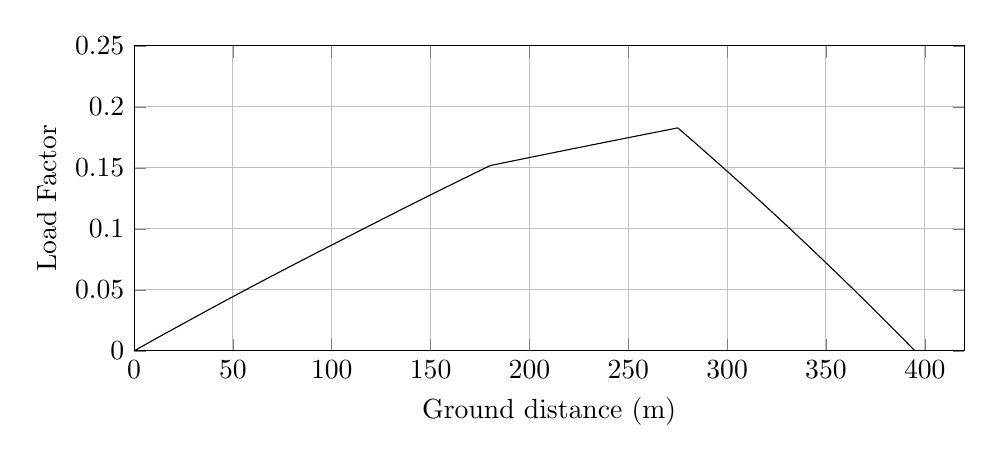
\begin{tikzpicture}

\begin{axis}[
width=\textwidth,
height=0.45\textwidth,
scaled ticks=false, tick label style={/pgf/number format/fixed},
xmin=0.0,
xmax=420,
xlabel={Ground distance (m)},
xmajorgrids,
ymin=0.0,
ymax=0.25,
ylabel={Load Factor },
ytick={0,0.05,0.1,0.15,0.2,0.25},
ymajorgrids,
legend style={at={(1.03,0.5)},anchor=west,draw=black,fill=white,legend cell align=left}
]

\addplot [
color=black,
solid
]
table[row sep=crcr]{
1.3729668748938318E-8	1.2718275252027908E-11\\
1.7493248493808052E-7	1.6204611588033204E-10\\
1.4411937280317895E-6	1.3350284552359952E-9\\
6.602995160656227E-5	6.116585765205595E-8\\
2.2740573828771224E-4	2.1065382018943594E-7\\
4.8751428921765393E-4	4.51601103970198E-7\\
8.441986619835749E-4	7.820093191506026E-7\\
0.0012981647037285577	1.2025318488499743E-6\\
0.0018484379050661159	1.7122653852749117E-6\\
0.0024893731755424335	2.3059800347005884E-6\\
0.0032286585096692284	2.990796567691043E-6\\
0.0040442418752796045	3.746286839667997E-6\\
0.004972762654474916	4.606389557016414E-6\\
0.005990910102221513	5.5495103846639455E-6\\
0.007111389191545643	6.587416769840769E-6\\
0.008336865178450469	7.722576011627478E-6\\
0.009664633507451486	8.952481196604317E-6\\
0.011093815858158905	1.027631695288282E-5\\
0.01262066151120312	1.1690607154829151E-5\\
0.01419454386807839	1.3148455841468274E-5\\
0.015910782250193378	1.473815296729461E-5\\
0.017721549103721458	1.6415394740624534E-5\\
0.019620507964630857	1.8174309782057908E-5\\
0.02164969955342029	2.0053835672331328E-5\\
0.023766550611781796	2.2014536332500502E-5\\
0.025957065600157342	2.4043446395742304E-5\\
0.028260861173784894	2.6177257127906515E-5\\
0.030668466949245715	2.8407193671086954E-5\\
0.0331489614440674	3.070461365362905E-5\\
0.03573888453685943	3.310335717008212E-5\\
0.038418765463712895	3.558538740029884E-5\\
0.04116679597872082	3.813050344860341E-5\\
0.044022059812866554	4.0774899997216495E-5\\
0.04700053365173311	4.353336958189581E-5\\
0.050116649382181494	4.641927308199821E-5\\
0.0533021652593606	4.936940621787943E-5\\
0.056630220296749106	5.245149930547168E-5\\
0.05998688030085898	5.55600349532071E-5\\
0.06348077825220624	5.879561242810599E-5\\
0.06710848437295475	6.215504950307218E-5\\
0.07082346760424127	6.559525103251006E-5\\
0.07462944469130567	6.911965467650321E-5\\
0.07855413323217031	7.275392238683019E-5\\
0.08251243142992878	7.641924605654508E-5\\
0.08659905947434482	8.020333109781151E-5\\
0.09083545394947079	8.412601991954682E-5\\
0.09518096637774642	8.814966720422782E-5\\
0.099604438418047	9.22454174087863E-5\\
0.1041130762071252	9.641993831761722E-5\\
0.10871457033213175	1.0068034562414396E-4\\
0.11350280915994052	1.0511356011489806E-4\\
0.11836943512882261	1.0961925056823572E-4\\
0.12328542045494376	1.1417053828355056E-4\\
0.12830372217771202	1.1881644705286468E-4\\
0.1334037067999082	1.235378688702228E-4\\
0.1386015897371753	1.283498098995459E-4\\
0.14405085578552257	1.3339434736336046E-4\\
0.1495239325759128	1.384608020752114E-4\\
0.1550507392415454	1.435768678535585E-4\\
0.16073360491635535	1.4883726183585137E-4\\
0.16659871679960742	1.5426621260281354E-4\\
0.17244819595229793	1.5968055073716932E-4\\
0.17848031195343078	1.6526379067186006E-4\\
0.18466822548212042	1.709910778675818E-4\\
0.1909009608611748	1.7675969021960024E-4\\
0.19716089737688902	1.8255331661448234E-4\\
0.2035279375926986	1.8844590260218354E-4\\
0.21017879584430066	1.9460097898828523E-4\\
0.21687473998771628	2.0079759662334275E-4\\
0.22354650324940833	2.0697165348721946E-4\\
0.23036941414946865	2.1328539381222582E-4\\
0.23737731412185503	2.1977011974597054E-4\\
0.24449289925428264	2.2635428626959582E-4\\
0.2517184892023243	2.3304003063757001E-4\\
0.25908208279438383	2.3985324916865521E-4\\
0.2664863589195283	2.467038871471075E-4\\
0.27399321582905467	2.5364920839429433E-4\\
0.2816108016888421	2.6069674218374804E-4\\
0.2893844725195981	2.678884383805134E-4\\
0.29747621078120867	2.7537413053912443E-4\\
0.30547198304033185	2.82770784760663E-4\\
0.31373479402345694	2.9041419810345564E-4\\
0.3220909744202328	2.9814370246420167E-4\\
0.3305540912568814	3.059718377735163E-4\\
0.33895489345894936	3.1374204995020564E-4\\
0.34753073012810576	3.216738666740116E-4\\
0.3563589175375672	3.298387764339335E-4\\
0.3652744752958731	3.380841767764874E-4\\
0.3742693918027593	3.464026499559363E-4\\
0.38350989122680823	3.5494790260746977E-4\\
0.3927029292363896	3.6344892855174173E-4\\
0.4020876366599533	3.721268505062641E-4\\
0.4115568217121528	3.808825348147702E-4\\
0.4212787852930122	3.8987158251223834E-4\\
0.43089755178065414	3.987648462514763E-4\\
0.4408379299669313	4.0795508134662935E-4\\
0.4510502611115679	4.173963424414278E-4\\
0.4612670224725215	4.268412900069675E-4\\
0.4715818614584312	4.363764915047208E-4\\
0.4818438670126082	4.458624403344116E-4\\
0.4922128554044626	4.55446864218778E-4\\
0.50273876067117	4.651759036558573E-4\\
0.5136516607865718	4.7526218561878223E-4\\
0.5244310074213006	4.852245766084685E-4\\
0.5355751508210329	4.955236435139243E-4\\
0.5467126997993474	5.05816136181647E-4\\
0.5580479056656631	5.162907968995362E-4\\
0.5692960823995112	5.26684546076621E-4\\
0.5809945926573021	5.374939044531926E-4\\
0.5923626544035139	5.479974267486354E-4\\
0.6041922852715	5.589268899201508E-4\\
0.6160912669048675	5.699198864440098E-4\\
0.6280605196746807	5.80977258055748E-4\\
0.6403946506485891	5.923711380371166E-4\\
0.6525721787971039	6.036197852496859E-4\\
0.66504690021022	6.151423721608905E-4\\
0.6773535438897555	6.265091316087534E-4\\
0.6901462526606317	6.383242266039888E-4\\
0.703249873273524	6.504258325864806E-4\\
0.7159721017112175	6.621745912919777E-4\\
0.729053467210389	6.742543715091042E-4\\
0.7422988791228431	6.864849826066895E-4\\
0.756304272979474	6.994166336756374E-4\\
0.7696432036294076	7.117322341078889E-4\\
0.7832290250230658	7.242751009973483E-4\\
0.7969128825551131	7.369077821078122E-4\\
0.8108444209446342	7.49768401415661E-4\\
0.825043936786227	7.628756565737198E-4\\
0.8390802275180445	7.75831507329827E-4\\
0.8532340040587583	7.888950619351756E-4\\
0.8678101043696134	8.02347636348419E-4\\
0.8824320602344964	8.158417445246135E-4\\
0.8978006605470081	8.300240573341862E-4\\
0.9134572487531922	8.444712363263633E-4\\
0.9287391767029982	8.585718293839988E-4\\
0.9440564687433697	8.727041953122664E-4\\
0.9598871644713316	8.873093483364503E-4\\
0.9757786228365237	9.019696413893449E-4\\
0.9918217338879218	9.16768906335061E-4\\
1.0080608846667363	9.317480602696149E-4\\
1.0245900975307913	9.469937892669798E-4\\
1.040622085070809	9.617799585392154E-4\\
1.0571005809273983	9.769769722385265E-4\\
1.0736578999152901	9.922456943919989E-4\\
1.0902401336450098	0.0010075364048205485\\
1.1073201062866707	0.001023285056244789\\
1.1241926772552646	0.001038841446961989\\
1.1416781667104252	0.0010549618712025904\\
1.1588269484070954	0.0010707708153255245\\
1.176440946845327	0.001087007539586915\\
1.1944819542445066	0.0011036367423065013\\
1.2120125629913447	0.0011197943831543758\\
1.2299306574276825	0.0011363080396446011\\
1.2481120482032448	0.0011530631972033177\\
1.2663536608165091	0.001169872682860703\\
1.2851425782117465	0.0011871852827874674\\
1.3041313368869671	0.001204680764165175\\
1.3228236880779458	0.0012219019154478563\\
1.3414329672940513	0.0012390453212873752\\
1.3605066144349074	0.001256615264250359\\
1.3802534409605212	0.0012748039828219197\\
1.3994872719307283	0.0012925188828945514\\
1.4192016277101378	0.0013106750308804923\\
1.439023460648384	0.0013289288076320884\\
1.459347998039509	0.0013476441149697525\\
1.4793256644936217	0.0013660386309586727\\
1.4991489338326072	0.0013842896313981776\\
1.5195196572175793	0.001403043263054983\\
1.5402684478761244	0.0014221434922083666\\
1.5604570108688036	0.0014407265967722603\\
1.5810331069622228	0.001459664989793267\\
1.6022712329181132	0.0014792112127449538\\
1.623752316257296	0.0014989794841456792\\
1.6452514305955401	0.0015187627874199932\\
1.6664829631402025	0.001538298334582829\\
1.6886446033619715	0.0015586880742224276\\
1.710607384244656	0.0015788932274493597\\
1.7329417009553727	0.001599438526617892\\
1.7551421266962821	0.0016198590077848233\\
1.7779085356585536	0.0016407983872468413\\
1.800478286927734	0.001661555189181651\\
1.8236018329231238	0.0016828195481721287\\
1.8462320784511883	0.0017036285549977819\\
1.869621217116264	0.0017251336028390985\\
1.8933146512119747	0.0017469165955445642\\
1.9176856041472643	0.0017693205518547696\\
1.9417713639512164	0.0017914604189863818\\
1.9657098573982132	0.0018134630364206475\\
1.9902165007163162	0.0018359859202349003\\
2.014554050520948	0.0018583514624902543\\
2.039479559407779	0.0018812553282789213\\
2.0645497069116256	0.00190429007013612\\
2.090368502766882	0.0019280105546499481\\
2.115564185269416	0.001951156493772486\\
2.140750230554602	0.0019742915382870733\\
2.1667677015838267	0.0019981881642363976\\
2.1927560352542175	0.002022055864271103\\
2.218891869133375	0.0020460568530179177\\
2.245288939563828	0.0020702955307592644\\
2.2712530964452817	0.002094134532340495\\
2.297933078351498	0.0021186285425571975\\
2.324564104516777	0.0021430753632140508\\
2.351466051806102	0.002167768613259487\\
2.378869922986878	0.0021929202369539128\\
2.4061764715670764	0.002217980192171409\\
2.4343811693482102	0.0022438619522661854\\
2.4622108821536663	0.0022693971763287565\\
2.4906408044048067	0.0022954806332399756\\
2.518892760285042	0.0023213983248237314\\
2.5472153538550346	0.002347378335301573\\
2.5762492306032216	0.002374008224871665\\
2.605385308804288	0.0024007292415148987\\
2.634725531238531	0.0024276348437188605\\
2.6633424112287507	0.0024538745828288975\\
2.6927188130915374	0.0024808081468841764\\
2.7226962917814213	0.0025082900906780586\\
2.7531675915664673	0.002536221944700937\\
2.7831412651501983	0.0025636948957312696\\
2.8139174932165103	0.00259190061500595\\
2.8440331768075415	0.002619498193217703\\
2.874693215323904	0.0026475918064182155\\
2.9059978681586376	0.0026762731648297265\\
2.9372617813709034	0.0027049142699023324\\
2.9684444504378202	0.0027334780402158984\\
3.000072782687808	0.002762447087346213\\
3.031082587373527	0.0027908467288618416\\
3.063213028467148	0.0028202696771070365\\
3.0965739711585014	0.0028508162125273416\\
3.1291175748240176	0.002880611204258749\\
3.161651640649506	0.002910394355735067\\
3.194791488147139	0.002940728881202755\\
3.2273698640351327	0.002970546338975297\\
3.261394174200582	0.003001683894018328\\
3.2942820372415875	0.0030317782284607266\\
3.3276455142443044	0.0030623045785660593\\
3.3625338428565543	0.0030942226750653406\\
3.396526624461681	0.003125318097839839\\
3.4305511850311694	0.003156439270209284\\
3.4642094416894933	0.003187222136680845\\
3.498963551783903	0.0032190038468263953\\
3.5341885134496573	0.003251212631569227\\
3.569804025802995	0.003283774947035725\\
3.605116576002147	0.0033160567301732877\\
3.641338581546833	0.0033491662594147486\\
3.677593698357855	0.0033823023607675003\\
3.7132425573336665	0.0034148807677116255\\
3.74957219375957	0.003448077662232653\\
3.7872650227149185	0.003482516312552428\\
3.825403000593508	0.00351735766340035\\
3.861987998097706	0.003550776487394373\\
3.899535703755137	0.003585070861541543\\
3.9366960368382165	0.0036190076064738152\\
3.9756271117991435	0.0036545574205753177\\
4.014715979923002	0.003690247152073271\\
4.053268843133694	0.003725443408246111\\
4.093111596873367	0.0037618130056302984\\
4.132540645872048	0.0037978007272779874\\
4.171686416589186	0.0038335257412637053\\
4.211258480423352	0.003869635603571754\\
4.252585425594734	0.003907342324880498\\
4.29253892845542	0.003943791573698627\\
4.332839968385603	0.003980553566104545\\
4.372708537789018	0.004016916818362214\\
4.414379330316386	0.004054919338691115\\
4.455607216042212	0.0040925134293005256\\
4.497336690654009	0.004130560344208657\\
4.53836773335787	0.004167966009353803\\
4.579767142935065	0.004205703032896794\\
4.621942908118227	0.0042441431397037144\\
4.663798268780793	0.004282286654280838\\
4.705838036060712	0.004320593657240077\\
4.748491012675066	0.004359454762302641\\
4.791393968819099	0.00439853890479313\\
4.835700194867293	0.004438896461059761\\
4.879973298406089	0.004479218839698694\\
4.923250156511948	0.0045186290523665015\\
4.967673596314626	0.00455907846346925\\
5.012954369117542	0.004600303379886605\\
5.057574526249477	0.004640921801903037\\
5.103280208347517	0.004682523214262849\\
5.148856018935929	0.004724001215917086\\
5.194350575362858	0.004765400107443116\\
5.240584094986199	0.004807466172133725\\
5.2871741484687504	0.004849851283688318\\
5.333122064003502	0.004891646972412819\\
5.3803318800233235	0.004934585125205718\\
5.4262712259485255	0.004976362527110847\\
5.473378197958581	0.005019196428385815\\
5.521938593493333	0.0050633462699643215\\
5.570027890245774	0.005107062175860818\\
5.617746353771608	0.0051504354608238306\\
5.665750363096816	0.005194062770167084\\
5.714883880069209	0.005238710893760803\\
5.763390205677501	0.005282783435080222\\
5.812817811268989	0.0053276872956127975\\
5.861909274803731	0.005372280055354573\\
5.912134919389196	0.005417897180144721\\
5.962317560553064	0.005463469330019512\\
6.012727788730279	0.0055092422253924765\\
6.0628236035803145	0.005554723763543736\\
6.113711068416594	0.005600918068319879\\
6.16497292765713	0.005647446183589547\\
6.216284706244114	0.0056940135462565855\\
6.26834407822653	0.00574125320405631\\
6.320257064476769	0.005788353860819566\\
6.37351660191279	0.005836669868317642\\
6.426150862197664	0.005884412318489815\\
6.479030963436509	0.005932371461852801\\
6.532319340056288	0.005980694525391631\\
6.5857233987986845	0.0060291161111142135\\
6.640834734692348	0.006079079019179427\\
6.695022999498724	0.006128198509975467\\
6.749720237657193	0.006177772777369799\\
6.804235758325081	0.006227175789131855\\
6.859728469301633	0.006277457653550388\\
6.916686079588434	0.006329059865551153\\
6.9732530286722305	0.006380301164116878\\
7.029531186664631	0.006431273983727202\\
7.086633318514238	0.00648298612076811\\
7.144155485034537	0.006535071566327042\\
7.202053129566568	0.006587489859068625\\
7.260126434764185	0.006640060021537832\\
7.317913145042743	0.006692363654308069\\
7.376682960996439	0.006745549886017951\\
7.435393721764624	0.006798675430603688\\
7.493838107271518	0.006851552782754638\\
7.552684475254578	0.006904786644036815\\
7.613252707151423	0.006959570652259534\\
7.672782806866918	0.0070134082958885026\\
7.733397683408512	0.007068219510417292\\
7.795525081709004	0.007124390635918835\\
7.856013653786727	0.007179072509092026\\
7.91792172269443	0.007235029941574267\\
7.980110745884113	0.007291233547030733\\
8.041720670752433	0.00734690614117217\\
8.105229267009985	0.0074042865018535955\\
8.167457523036095	0.007460502296469169\\
8.230908874360502	0.007517815128829443\\
8.293738919282273	0.0075745589570154785\\
8.356235402336917	0.007630993866744999\\
8.42092378244627	0.007689400064421182\\
8.485671322837007	0.007747851552089859\\
8.549180898871484	0.007805177596971168\\
8.614596634551038	0.007864216114758966\\
8.680166762249144	0.007923385769613624\\
8.744770128469462	0.007981675038769807\\
8.812993689385827	0.008043222109523296\\
8.88005807777586	0.00810371491163517\\
8.94709863067661	0.008164177800451379\\
9.013172088448385	0.00822376029194024\\
9.079266506338545	0.008283353593296232\\
9.14748814890141	0.008344856439747052\\
9.215411293660388	0.00840608170928346\\
9.284579146198691	0.008468420300552197\\
9.353168277381275	0.008530228740873448\\
9.423753765537143	0.008593827317627353\\
9.492960052876374	0.0086561745340313\\
9.564123004975215	0.0087202755760339\\
9.634097601479446	0.00878329742572174\\
9.705672410878787	0.008847751548583338\\
9.776260200085993	0.008911308038953151\\
9.846607984572056	0.008974639778645304\\
9.918231435410593	0.009039111132397077\\
9.988851555070422	0.009102670674590817\\
10.060390022634245	0.00916704802028807\\
10.133279281833644	0.009232631957062436\\
10.205241085147751	0.009297372547071681\\
10.277820389603	0.009362659822367276\\
10.352558894167803	0.009429880127748966\\
10.42733258664746	0.009497122758847445\\
10.501815126481194	0.00956409434629035\\
10.576858173457808	0.0096315606722466\\
10.65303812840548	0.009700039682506694\\
10.729080272001735	0.009768385389093194\\
10.804841544893105	0.00983646934678117\\
10.881905013502095	0.009905714070194386\\
10.958396790746043	0.009974435717413997\\
11.035905069829102	0.010044061128088177\\
11.113160538490881	0.010113450002413343\\
11.192172636140572	0.010184406951176799\\
11.270076562295213	0.010254359177084393\\
11.350065490058778	0.01032617380705092\\
11.429008826667825	0.01039704004451007\\
11.50754237847364	0.010467528970704573\\
11.587076645554472	0.010538906555600473\\
11.668897725768986	0.010612326467540224\\
11.749734371708193	0.010684853170047491\\
11.830312384681939	0.010757138144576385\\
11.909862670519033	0.010828491745547633\\
11.990515423105418	0.010900824726860592\\
12.072973931530203	0.010974767377779871\\
12.155304175892073	0.01104858518061057\\
12.237018674011615	0.011121841255688037\\
12.320146069843414	0.011196354184770288\\
12.406770618003886	0.011273991423851298\\
12.489918686423398	0.011348502923986854\\
12.574493004618496	0.011424282608819553\\
12.660666896522624	0.011501485315812323\\
12.746500366216402	0.011578372864197333\\
12.832006837122272	0.011654957471261013\\
12.919285437479463	0.01173311906025126\\
13.00517529032821	0.011810026943386495\\
13.092301899261269	0.011888032164269455\\
13.179760097773386	0.01196632412337841\\
13.268594687119744	0.012045837900580393\\
13.357699529172354	0.012125583210613146\\
13.44829753340392	0.012206654283582946\\
13.537570218252604	0.01228652907183154\\
13.627322718831184	0.012366822909948467\\
13.718307212496544	0.012448208495679616\\
13.808540263830096	0.012528911648457607\\
13.899143852161355	0.012609935999607724\\
13.991564069206362	0.012692574464677968\\
14.085798171937814	0.012776824060522711\\
14.179213507883688	0.012860330996362227\\
14.271883316076963	0.01294316109903068\\
14.367546274622434	0.013028655785504852\\
14.459430863676705	0.013110763519337803\\
14.555010173556813	0.013196162334059888\\
14.648669731311681	0.013279835572991781\\
14.743773575674254	0.013364788760704217\\
14.839769774519894	0.013450528585720104\\
14.932807148196385	0.013533615759813425\\
15.026921440816679	0.013617654802191737\\
15.12275113649265	0.013703215494714404\\
15.222025232743288	0.013791840828733715\\
15.321078842653048	0.01388025861731659\\
15.417564225728565	0.013966373754375379\\
15.515758841369038	0.014054004193904596\\
15.613440509090129	0.014141166738461284\\
15.7107260301154	0.014227965850240464\\
15.81102223487273	0.014317440835164433\\
15.913565872734136	0.014408910081501993\\
16.012918321571746	0.014497522573453919\\
16.11222833737955	0.014586087286473206\\
16.216250800242257	0.014678844023665264\\
16.319159023020546	0.014770596696728715\\
16.421418004006803	0.01486176027700378\\
16.521675247646563	0.014951129519667108\\
16.62557290942481	0.015043733707145188\\
16.72731964230514	0.015134410891978664\\
16.830283223934416	0.015226162700296792\\
16.93464251494634	0.015319148252495743\\
17.038481620468637	0.015411660447556885\\
17.146497421123335	0.01550788341773998\\
17.252282308638982	0.015602108958899715\\
17.35724772858778	0.015695594835658928\\
17.464053904588297	0.0157907103126618\\
17.572390862630144	0.015887178998577195\\
17.680417629270814	0.015983361552860204\\
17.789707298693855	0.01608065858870949\\
17.899612520762552	0.016178493662789513\\
18.01027367065641	0.016276991677991213\\
18.121415095654797	0.016375907244992712\\
18.232428503320143	0.01647469907093475\\
18.34337337506409	0.016573420247363416\\
18.454877340220463	0.016672629321572124\\
18.56636189702322	0.016771811643256765\\
18.678405595805643	0.016871481985335578\\
18.7903363416971	0.01697104255231302\\
18.902391384512768	0.017070704506559474\\
19.01754810908954	0.017173115680067855\\
19.131359562866663	0.017274321233699614\\
19.247747682986713	0.017377808700556996\\
19.361628242251975	0.017479057530784756\\
19.477963464454028	0.017582479685399704\\
19.595742742603164	0.017687176423747456\\
19.71107288142779	0.017789687256841335\\
19.82767543183723	0.017893320354709044\\
19.944540068808188	0.017997177742909806\\
20.06171535440768	0.018101302662642416\\
20.179291418887807	0.01820577527671787\\
20.29729887224694	0.01831062284369171\\
20.417200571824914	0.018417144992635286\\
20.53676390826074	0.018523358236955677\\
20.65523768803314	0.018628595560053973\\
20.777063017363922	0.018736801813890057\\
20.896922101876633	0.018843253707647247\\
21.016777952410983	0.01894969502428557\\
21.13892104879462	0.019058159826176407\\
21.260534693274344	0.01916614683835006\\
21.382619708556632	0.019274544909850862\\
21.506306369043365	0.019384357573521607\\
21.631260758247265	0.019495288276215432\\
21.75556249187227	0.019605632273899134\\
21.87985606458615	0.019715961918878717\\
22.005925835680863	0.019827861124706293\\
22.130365724585275	0.01993830682096541\\
22.257477980325966	0.02005111752591696\\
22.38418119026224	0.020163558513645395\\
22.50885833858638	0.020274195149297798\\
22.636026948728087	0.020387036354426517\\
22.76367325110224	0.020500295195039667\\
22.89115382514759	0.020613400927859245\\
23.022452271734288	0.020729887883250933\\
23.149877274293033	0.02084293257032328\\
23.27873580881144	0.020957243403352397\\
23.408563766880334	0.02107240869611514\\
23.538692653979794	0.021187835557657894\\
23.671258756997098	0.021305418937621227\\
23.803210122669313	0.021422451899707387\\
23.93544283576786	0.021539729430784405\\
24.067241518013077	0.021656617260720056\\
24.19863541429976	0.021773141561259403\\
24.329449967727697	0.02188914776797999\\
24.46175612159181	0.02200647253574947\\
24.594763714591892	0.02212441526352375\\
24.72754053098891	0.02224214949286314\\
24.86208223890334	0.022361444928267266\\
24.99503410474967	0.022479327181994406\\
25.12831230627787	0.022597495483658595\\
25.265273024090206	0.02271892557245505\\
25.400650037308893	0.022838948517635165\\
25.536304655026747	0.022959214770482482\\
25.673594178904246	0.023080927809856894\\
25.80797730935859	0.0232000618159829\\
25.835159569235522	0.023224159299179797\\
25.83771752397454	0.02322642696011096\\
25.84157983658004	0.023229850950193105\\
25.854829339215996	0.023241596792202248\\
25.893215796826965	0.023275626724863253\\
25.973046119315796	0.02334639641789144\\
26.096262980671412	0.023455626667997217\\
26.224212718725603	0.023569050227618186\\
26.35313595194755	0.023683334148628752\\
26.481727686355264	0.023797321386651003\\
26.611118169629577	0.02391201359516892\\
26.74049186039369	0.024026687635623264\\
26.87228140714948	0.024143499446244415\\
27.003385008924262	0.024259699456056737\\
27.1358830905183	0.024377131343098775\\
27.265951877034226	0.024492405967932323\\
27.399105426781233	0.024610409969334446\\
27.53075869079712	0.024727079673104363\\
27.66387879779476	0.024845044308710373\\
27.79855889054391	0.02496438603156349\\
27.932132547760695	0.025082741855797546\\
28.06791767232785	0.025203051400013717\\
28.202763022922632	0.02532252228223208\\
28.339788243013793	0.025443918161951653\\
28.476803106655623	0.025565298270941606\\
28.61761981788422	0.02569003930489982\\
28.753907949775353	0.025810761684597977\\
28.89297195746854	0.025933935532415194\\
29.03211749902605	0.026057173937028315\\
29.17123509789927	0.02618037972356318\\
29.312253051611236	0.026305260265939698\\
29.454422317169097	0.026431151754743948\\
29.59523538430127	0.026555833587415947\\
29.737672170826222	0.0266819440734284\\
29.879173197948965	0.026807216832855477\\
30.02075470454991	0.026932551435614713\\
30.166674235301365	0.027061716203578567\\
30.308336095430334	0.027187102205017178\\
30.452640844036836	0.027314817144454526\\
30.597553881025625	0.027443059773339818\\
30.742967061600154	0.02757173406067975\\
30.888975484926362	0.0277009238307902\\
31.034653067922946	0.027829809444244506\\
31.180984070508003	0.027959261469617042\\
31.328351020411645	0.028089617907854393\\
31.476753455192622	0.0282208778940377\\
31.62661541983664	0.028353415972501145\\
31.774495604492607	0.028484188514439575\\
31.924944104961916	0.028617218957807875\\
32.07610067279926	0.028750861786449738\\
32.22631826848556	0.028883660629349973\\
32.37899942625752	0.02901862306347629\\
32.528514827654206	0.029150772962857993\\
32.68189139400266	0.02928632081130646\\
32.836069829938495	0.02942256205690447\\
32.99025509482905	0.029558793838332074\\
33.14574197930297	0.02969615978546348\\
33.30072558931056	0.029833065036540072\\
33.455047097713944	0.029969369283167527\\
33.610874563168906	0.03010698713889281\\
33.76926068144728	0.030246847440555506\\
33.92617323250643	0.030385389235419308\\
34.08448787244542	0.03052515133115111\\
34.24243160505006	0.030664568146862945\\
34.40316487172558	0.030806428800932883\\
34.56154208099588	0.030946191617236895\\
34.721775177117024	0.031087573406036174\\
34.88076970836556	0.031227843488755288\\
35.041349106451236	0.03136949254766738\\
35.20329621413198	0.031512328313624195\\
35.364886328651124	0.03165482925346709\\
35.529241615711214	0.03179974807284368\\
35.69117991651797	0.031942515209498236\\
35.85317319416103	0.03208531025956504\\
36.014854298354294	0.03222780946775512\\
36.18095311277159	0.032374180597912056\\
36.34443322746766	0.03251822244144696\\
36.51065106768533	0.03266465433697053\\
36.67635767082788	0.03281061345477801\\
36.842033683894186	0.03295652310930782\\
37.00823867836148	0.03310287584860264\\
37.17279029188734	0.03324775005649279\\
37.33951104811075	0.03339451088993472\\
37.50923941781488	0.03354389519294198\\
37.679358776579846	0.033693599091404146\\
37.845326083883435	0.03383962539674834\\
38.017144746304325	0.033990775081831535\\
38.1852030886141	0.03413859210821721\\
38.35804431104914	0.03429059033588675\\
38.52812920813831	0.03444013911820947\\
38.69960796987526	0.034590887710677816\\
38.87165793928378	0.03474211232031849\\
39.0423941506003	0.034892156171720604\\
39.21436971822614	0.035043262834109454\\
39.38727999643966	0.035195163992222944\\
39.558989012313546	0.03534598312908082\\
39.734752343022535	0.03550033562997489\\
39.908836167348156	0.03565318545191155\\
40.084555009291705	0.03580744270629567\\
40.259186798753746	0.0359607175260425\\
40.43324437115375	0.03611346030496567\\
40.61041052363379	0.03626890211048754\\
40.787318094191775	0.036424087844557904\\
40.96620398302343	0.036580979195856664\\
41.14141336180775	0.03673461691853968\\
41.31941103282654	0.03689066997897115\\
41.49571226203258	0.037045206162967116\\
41.67366972437729	0.03720116414445725\\
41.85219319429197	0.03735758780176077\\
42.03136872634711	0.03751455211736039\\
42.21293422072888	0.03767357866174977\\
42.39366932880948	0.03783184633838464\\
42.57479521797359	0.03799042452127036\\
42.75522531040919	0.03814836187664403\\
42.93775785970641	0.03830810735230247\\
43.11993568316029	0.038467509955740116\\
43.30336620712447	0.03862797582273805\\
43.48720879745599	0.038788769021161545\\
43.672226884455625	0.038950556742816486\\
43.85684130549208	0.039111957800227574\\
44.039851952877484	0.03927192344864967\\
44.22449378650157	0.039433281205193876\\
44.412385508552646	0.03959744421773466\\
44.59783063297877	0.03975943510142432\\
44.78525507043919	0.03992312004939388\\
44.973130075825196	0.04008716319174787\\
45.16145211071871	0.040251561110099754\\
45.34881478087516	0.04041508614870074\\
45.536017136752506	0.04057843594454981\\
45.724971990057284	0.04074327906690745\\
45.91416212467789	0.040908291272161335\\
46.10175434018815	0.041071873964655704\\
46.29356928918713	0.04123910200614647\\
46.48490977712943	0.04140587914451307\\
46.67744207882204	0.04157365747801979\\
46.869905949194575	0.04174133840625598\\
47.062749521718516	0.04190931221256226\\
47.25341437235973	0.042075350894771275\\
47.44508461154423	0.0422422276025824\\
47.63880095964302	0.042410847487968674\\
47.83356160493736	0.04258033756323178\\
48.025334057720784	0.042747189099460355\\
48.218846636819876	0.0429155163011549\\
48.41468711090302	0.04308582918695449\\
48.610449575687724	0.04325603474669026\\
48.80723286029129	0.04342708803761479\\
49.00124137999302	0.04359569025900751\\
49.20045899041696	0.043768778974422516\\
49.394243884198005	0.043937108172154835\\
49.59161211700324	0.0441085100939385\\
49.79144608231523	0.04428201229888178\\
49.99107345578199	0.04445529387290568\\
50.18996871950735	0.0446278989266555\\
50.388458331230495	0.044800111103180704\\
50.59191110395449	0.04497658702379362\\
50.79453916783869	0.04515230495557722\\
50.99530158869649	0.04532636304404464\\
51.19776583381373	0.04550185427703261\\
51.3996255264899	0.045676779194223305\\
51.599450409211	0.04584989920746391\\
51.80158475775707	0.046024977933013855\\
52.002311498730975	0.04619879554854281\\
52.2060805474067	0.046375204912405044\\
52.40811442127868	0.04655006960300329\\
52.61423073460446	0.04672842415802535\\
52.821749674584495	0.046907947972291315\\
53.03053110951893	0.04708851897562025\\
53.23753590773735	0.0472675088663969\\
53.44487707917263	0.04744674517628225\\
53.652063533093525	0.04762580334585091\\
53.85975522429668	0.04780525364489327\\
54.06844148636836	0.047985518413296784\\
54.278580968983874	0.04816699307490289\\
54.48685885904548	0.04834681515011182\\
54.69884126905886	0.04852978972209408\\
54.90975544393264	0.048711796324111434\\
55.12216013841277	0.04889504291470418\\
55.333080623240974	0.0490769631647663\\
55.5448885814986	0.04925960290581394\\
55.75594910746132	0.049441552377603684\\
55.968144975063936	0.04962443459102704\\
56.18150915317635	0.04980827726171765\\
56.394069348356695	0.049991380922409304\\
56.60950747146016	0.050176916623965756\\
56.82641599949238	0.050363670835182846\\
57.03980213394583	0.05054734558722334\\
57.25698083573829	0.05073423729993025\\
57.47353804711997	0.050920546509804016\\
57.6941706582635	0.05111031298653919\\
57.91229938529948	0.05129787742989816\\
58.12998527173144	0.051485013144576\\
58.34905943653719	0.051673294035311325\\
58.56781345824973	0.05186125154599615\\
58.787998582886644	0.05205039009587433\\
59.011266007804366	0.052242126646395125\\
59.23368761368569	0.052433087170176675\\
59.456031473365414	0.05262393150082773\\
59.67976581221534	0.052815919518064476\\
59.90315377467765	0.053007560564452584\\
60.125192111546724	0.0531979946337744\\
60.349269227196444	0.053390127709415765\\
60.57220932044149	0.05358123653280547\\
60.79606803632835	0.05377308342544174\\
61.021718319759984	0.053966415712654696\\
61.25073295331903	0.0541625793145032\\
61.47770893732542	0.05435694594057828\\
61.70784367826464	0.05455396603989855\\
61.93740803875056	0.05475044632697492\\
62.1673491775543	0.054947197653977\\
62.39648011888062	0.05514320464999169\\
62.62822464633953	0.055341395675308644\\
62.86094183422966	0.05554036632318364\\
63.090532789209604	0.05573661294580743\\
63.321616049163225	0.05593408400108299\\
63.554808975015874	0.056133305996934245\\
63.78685818650332	0.056331499322605526\\
64.0234762327251	0.056533542075383886\\
64.25652029988498	0.05673248111478258\\
64.49146565301734	0.056932991141547186\\
64.72768747885678	0.05713453802228488\\
64.96568125142531	0.05733754364763541\\
65.20057601391298	0.057537853763535304\\
65.43975061379945	0.05774176057393268\\
65.67719429610031	0.0579441389736716\\
65.91652243006087	0.058148070547800815\\
66.1565253585166	0.05835252387751545\\
66.39740384038885	0.058557669654576844\\
66.63777997854328	0.05876233444768083\\
66.87849958303539	0.0589672386527393\\
67.12349409848125	0.05917572743872099\\
67.36843544137562	0.059384116430191064\\
67.61129947098183	0.05959068445994718\\
67.85808619273692	0.059800534429430695\\
68.10323725880951	0.060008939366270164\\
68.3520146383799	0.06022037207027672\\
68.60099753692072	0.06043192420158277\\
68.84943315800746	0.06064295647459928\\
69.09793111574629	0.060853987110618325\\
69.34894754058863	0.061067101296671346\\
69.59791912239118	0.06127842483753241\\
69.84867626946473	0.06149120925247216\\
70.10496107302816	0.06170862779652695\\
70.35594730130109	0.06192149623645578\\
70.60854748652795	0.062135678745152516\\
70.8625286964371	0.062350977093600816\\
71.1182576034713	0.06256770134613716\\
71.37278964945165	0.06278335614125831\\
71.62944082734805	0.06300075095401432\\
71.88536754710964	0.06321747695607835\\
72.14250945057543	0.06343517680590312\\
72.40306402213687	0.06365570970869022\\
72.66241221953337	0.06387516568784195\\
72.92327110344874	0.06409584406583321\\
73.18657203154456	0.06431853176440384\\
73.45150557123125	0.06454254319204118\\
73.71756195569753	0.06476744674286228\\
73.97940051906463	0.06498872913297409\\
74.24514793127645	0.06521325870610936\\
74.51022759525631	0.06543716798958235\\
74.77823256031297	0.06566349159190928\\
75.04767613410795	0.06589097298368586\\
75.31682895458664	0.06611815210069105\\
75.58729746777243	0.06634638488605601\\
75.85729327570917	0.06657416229322155\\
76.13042767774209	0.06680453044875079\\
76.40299665611133	0.06703436484513678\\
76.67973301409052	0.06726765549386407\\
76.95360383527739	0.0674984735610362\\
77.22854206589327	0.06773013466331065\\
77.50692063517303	0.06796463720015918\\
77.78349662592461	0.06819756448418826\\
78.0616064362213	0.06843172684243935\\
78.33869545141144	0.0686649735789561\\
78.62238552181594	0.06890371928113628\\
78.90481169871467	0.06914134381035987\\
79.18659077494928	0.06937836711622322\\
79.4700201012688	0.06961672177248229\\
79.75774957869095	0.06985863489566868\\
80.04430580185078	0.07009950413146764\\
80.33432201731404	0.0703432237904657\\
80.62298533865851	0.07058574911265131\\
80.9130804606989	0.07082942014431066\\
81.20459144967842	0.07107422312567054\\
81.49650140842283	0.07131930403278777\\
81.79224544448738	0.07156754614440422\\
82.08455487090956	0.07181284862752614\\
82.37934996819865	0.07206018047810679\\
82.67580145620735	0.0723088452386539\\
82.97475550983006	0.07255955199941844\\
83.2734238134004	0.07280996232639718\\
83.57209772503273	0.07306032110393608\\
83.87419166445906	0.07331348998083449\\
84.17487194816226	0.07356541807697824\\
84.47686996876752	0.0738183944889884\\
84.78124993153034	0.07407331020256473\\
85.08776945017104	0.07432996153740255\\
85.39395758722245	0.07458627963293805\\
85.69833162305892	0.07484102442097933\\
86.01027818388755	0.07510205103794562\\
86.31658691867341	0.07535830556531124\\
86.62866814828641	0.07561933432241918\\
86.94043673469176	0.07588004678734489\\
87.2565990672368	0.07614437817050157\\
87.56980823017452	0.07640618624729582\\
87.88101387141376	0.07666626672563785\\
88.20007062892054	0.07693285446245904\\
88.51883409355145	0.07719914313411709\\
88.83509784148416	0.07746329090541039\\
89.15857089898353	0.07773340638716324\\
89.47772213402055	0.07799986049574278\\
89.80217214804901	0.0782706857718751\\
90.1263587278685	0.07854123879689182\\
90.44950966725051	0.07881087614186835\\
90.77764749859728	0.07908462279371764\\
91.10470504824352	0.07935741706495758\\
91.43769785174896	0.07963511013620296\\
91.76691749028419	0.07990960611071961\\
92.09386993524024	0.08018216276776442\\
92.42498248438446	0.08045813841591928\\
92.7581696617394	0.08073579424133649\\
93.09729153734631	0.08101834600158517\\
93.4312406900703	0.0812965397821466\\
93.76780571708736	0.08157686518024194\\
94.10390054156983	0.08185675215817123\\
94.43564317419558	0.08213296974304085\\
94.77291201930262	0.08241374352711507\\
95.10796951504997	0.08269263219751315\\
95.44708659079325	0.08297485589637515\\
95.78515592548297	0.08325616440415355\\
96.12311752311894	0.08353734096236587\\
96.46351490415591	0.08382050213712554\\
96.80669869710772	0.08410593950359747\\
97.14657639264556	0.0843885866792555\\
97.48763116340677	0.08467217318222872\\
97.8305814261901	0.08495729671736925\\
98.17013304046878	0.08523955694331546\\
98.51054009051404	0.08552249145945513\\
98.854181194619	0.08580807750946381\\
99.19205317796005	0.08608883419219136\\
99.53355440060989	0.08637257233662089\\
99.87198375587872	0.08665372507350909\\
100.2129389915628	0.0869369437295731\\
100.55335806642802	0.08721968537518666\\
100.89503335592528	0.08750343948740845\\
101.23693480167049	0.0877873513134455\\
101.57977298927813	0.08807201166109802\\
101.91842351185082	0.08835316700561423\\
102.26214655705948	0.08863850615367938\\
102.60487134933112	0.08892298990856227\\
102.94238410388857	0.08920312215937685\\
103.28139950825951	0.08948447732281106\\
103.61984226602698	0.08976533384719959\\
103.95406402656286	0.09004266550223823\\
104.29248504574807	0.09032346014640226\\
104.63112914593611	0.09060441911980527\\
104.96686613984221	0.09088294654940775\\
105.30464484937244	0.09116314892637617\\
105.64180205248229	0.09144281774368622\\
105.97704387437452	0.09172088081164334\\
106.31384964552919	0.09200022492268485\\
106.6489228444834	0.0922781168430805\\
106.98000007373659	0.09255268066296196\\
107.31456925364313	0.09283012703134964\\
107.38092108752608	0.09288514873739423\\
107.387754025128	0.09289081486625643\\
107.3946577511588	0.09289653969030756\\
107.39916951903444	0.09290028101166281\\
107.40247473215817	0.0929030218126878\\
107.40548301099807	0.09290551638412937\\
107.41901751964124	0.09291673966605626\\
107.47756267729525	0.0929652870977632\\
107.63696404402117	0.0930974656051319\\
107.95668166923352	0.0933625721684481\\
108.2571634635643	0.09361171680449269\\
108.55996775705782	0.09386277478554529\\
108.8616926844802	0.09411292472626931\\
109.16669292910967	0.09436577600626612\\
109.47218465327785	0.09461901970839193\\
109.78023369107405	0.09487436731663453\\
110.09061921742381	0.09513163458577785\\
110.4007971847821	0.09538871185746949\\
110.7125096545017	0.09564704203218544\\
111.02874540594937	0.09590910066096243\\
111.34670354521654	0.09617256525275455\\
111.664908557295	0.0964362121341857\\
111.98617551206428	0.09670237251589905\\
112.3078797039536	0.0969688706709099\\
112.63537393275391	0.09724013924419274\\
112.96267359383529	0.09751121954991038\\
113.28778388635178	0.09778045886370523\\
113.61823593045688	0.09805409278872959\\
113.94632344632586	0.09832573881304403\\
114.27926944824554	0.09860137614659449\\
114.61324422041562	0.09887783255542353\\
114.94750338770686	0.0991544907959215\\
115.28618013885716	0.0994347702092003\\
115.62544260296943	0.09971549797492324\\
115.9647508443766	0.09999622632892757\\
116.30617149460878	0.10027866386757105\\
116.65060078043697	0.10056355022389733\\
116.99863777637248	0.10085137884015435\\
117.34270613829636	0.1011358832121555\\
117.68983788345284	0.10142287727737394\\
118.04137408578512	0.10171346747322574\\
118.39343387684602	0.10200444390208768\\
118.74804854616337	0.10229748389864948\\
119.10520175440718	0.10259257200822611\\
119.46686684850098	0.1028913362463225\\
119.82660492256403	0.1031884560869153\\
120.19012449272657	0.10348864505276252\\
120.55217592908159	0.10378756664813929\\
120.91763124996498	0.1040892420125896\\
121.28719248968574	0.10439424797716546\\
121.65493622417088	0.10469769436125445\\
122.02513489718217	0.10500310552989346\\
122.39308995700384	0.10530660426237587\\
122.76618799735454	0.10561428157495976\\
123.1388017253943	0.10592149479982224\\
123.51256311114031	0.10622958839917403\\
123.88633794770595	0.10653762624959458\\
124.25665874611622	0.10684275076391198\\
124.63165231885978	0.10715165681303655\\
125.00664173256905	0.10746048957561555\\
125.38021625899401	0.10776808676841777\\
125.75512563345742	0.10807671169039132\\
126.13473977091255	0.10838913588494155\\
126.51299085225449	0.10870036371030332\\
126.8948287761801	0.10901446649390588\\
127.27325883095315	0.10932568947286271\\
127.64986999110431	0.10963534022485366\\
128.03053456382577	0.10994824551543993\\
128.40840086210045	0.11025877212604943\\
128.78830732782995	0.11057089571814734\\
129.16816802858597	0.11088290115835116\\
129.55114692916032	0.11119738550077807\\
129.92795862154003	0.11150672426529164\\
130.30814318938542	0.11181874945891801\\
130.68801179162523	0.11213043188191786\\
131.0673626953399	0.11244160560193173\\
131.44707508552267	0.11275299117467599\\
131.82575792285303	0.11306344743396049\\
132.20466209461676	0.11337399952239231\\
132.58549544797154	0.11368604583013327\\
132.96520261413826	0.11399708195242655\\
133.34413894748724	0.1143073990160323\\
133.72638850756363	0.1146203400267399\\
134.1049920954593	0.11493020713246022\\
134.48538249769342	0.11524144685303776\\
134.86277461399203	0.11555014382679021\\
135.2402386369938	0.11585880987798916\\
135.62109197355238	0.11617015598193033\\
135.9996509441208	0.11647953482014314\\
136.37968191797512	0.11679002424104482\\
136.76120583273502	0.11710163974255844\\
137.13951930881296	0.1174105398897607\\
137.51840340013064	0.11771981246239015\\
137.89819615735314	0.11802973236527516\\
138.27485697152616	0.11833700272001166\\
138.65420581933705	0.11864637101625664\\
139.03531375767642	0.1189570775434002\\
139.41296882619503	0.11926487333127894\\
139.79422155259	0.1195755041912565\\
140.17408835952057	0.11988490840845863\\
140.5488076998477	0.12019002426481791\\
140.92844631991198	0.12049904830547259\\
141.30483696429354	0.1208053313859759\\
141.68269541512387	0.12111271121528802\\
142.06058279783264	0.1214200163401388\\
142.43991695918288	0.12172839883105357\\
142.81695502902187	0.12203481586574236\\
143.19247254825046	0.12233989887120794\\
143.5733885276352	0.12264926720764747\\
143.94921103219775	0.12295439919138099\\
144.32621366107247	0.12326038961440232\\
144.70408630975157	0.12356698565175067\\
145.08263595865492	0.12387402976343431\\
145.46162624555404	0.12418132948190509\\
145.83827879615103	0.12448663246584465\\
146.21524500988596	0.1247920883895765\\
146.5934755401724	0.12509846665406654\\
146.9730259257883	0.125405810927215\\
147.3547239944582	0.1257147898657958\\
147.73366854735332	0.12602143601267843\\
148.1136534850276	0.12632881988872885\\
148.49311509785633	0.12663567609753829\\
148.87144514206074	0.1269415132249834\\
149.25360190977045	0.12725033814773445\\
149.6334430260095	0.12755718630168536\\
150.01465687879528	0.12786503746804026\\
150.3940924716125	0.12817134700892058\\
150.77688175221402	0.12848025696874504\\
151.1561678741857	0.1287862337635383\\
151.5352572324847	0.1290919460897806\\
151.91884603110896	0.12940117916426402\\
152.3000376871389	0.1297083721984288\\
152.6837211891089	0.1300174649049421\\
153.06727641570347	0.13032634537298954\\
153.4514076737559	0.1306355804463468\\
153.83522357687116	0.13094445228312532\\
154.21637826964854	0.13125107421598445\\
154.6009164651564	0.1315603085100997\\
154.98403470202834	0.13186829140333486\\
155.36838747168406	0.13217715676565472\\
155.75158064164503	0.13248498053604085\\
156.13576662495046	0.13279349174516403\\
156.5218436740983	0.13310341037564238\\
156.90521285441474	0.1334110449536753\\
157.2916244593892	0.1337210095757565\\
157.6780020855428	0.13403083509139163\\
158.06299451159185	0.13433943854098412\\
158.4509000667514	0.13465026466674196\\
158.83830611621056	0.13496057784118373\\
159.22672413827297	0.13527158848882562\\
159.61474494524106	0.13558216794589875\\
160.0042372884319	0.13589381149061633\\
160.39552304382113	0.13620677520093102\\
160.78478895267375	0.13651800917809703\\
161.17517847278327	0.136830027121986\\
161.56748129737286	0.13714345884435464\\
161.9609400214345	0.13745769785224973\\
162.35005274814932	0.1377683514219022\\
162.7425950916558	0.13808162773630497\\
163.13607830878885	0.13839553868797705\\
163.53170884953005	0.13871104540189877\\
163.92462594167722	0.1390242717973006\\
164.3198767210975	0.13933924156236294\\
164.7157696028566	0.13965460541394045\\
165.1115317336501	0.1399697475245765\\
165.50739628911128	0.14028485363569335\\
165.90698313288817	0.14060280349079576\\
166.30582458333038	0.14092004090483698\\
166.70591293613995	0.14123815039261586\\
167.1044701422045	0.14155492333926067\\
167.50226971352845	0.14187097564120496\\
167.9010833894181	0.14218771492412377\\
168.3004552315794	0.14250477847480839\\
168.70189335181743	0.14282336252061867\\
169.10576843973695	0.14314375933169482\\
169.50785881751284	0.14346261964734158\\
169.91045494783964	0.14378176051929242\\
170.31331810721775	0.14410099249278174\\
170.71648797717722	0.14442034689050348\\
171.11993291578136	0.14473979852997162\\
171.5247281229082	0.14506019818437857\\
171.92976094083576	0.1453806646159304\\
172.33690302624336	0.14570267780725712\\
172.74259563259648	0.1460234229783421\\
173.1509823323036	0.14634617570042724\\
173.55913088366435	0.14666861766648945\\
173.96636547491187	0.1469902156841372\\
174.37754484483776	0.14731480558937818\\
174.7874876782942	0.14763829617363258\\
175.2012500141185	0.1479646762600829\\
175.6112323385957	0.14828795147035786\\
176.02092514523684	0.14861087614464524\\
176.43326782420013	0.14893576631369695\\
176.8477920653399	0.1492622510555769\\
177.2627043459005	0.14958891685511835\\
177.67839640445425	0.1499160718581072\\
178.09047986160414	0.1502402638765652\\
178.50771992227516	0.1505683881921811\\
178.92514786216543	0.15089653519364657\\
179.34349041668827	0.1512252759622998\\
179.7634585539525	0.1515551683332337\\
180.0836350053749	0.15180658807525094\\
180.18446825846002	0.1518857526463514\\
180.6041229201494	0.15202540592768318\\
181.5278851973348	0.15233270973113477\\
182.40940876889346	0.1526258250301948\\
183.29020149056134	0.1529185638284725\\
184.17127536929127	0.15321126286108894\\
185.05444413874795	0.1535045244129909\\
185.94463812048832	0.1537999838521117\\
186.83342305465118	0.1540948408345811\\
187.72320740690213	0.15438989477671244\\
188.61627250998652	0.15468590151323444\\
189.51597565669658	0.1549839718850614\\
190.41002295084513	0.15528003304381544\\
191.3196934236239	0.15558112954186945\\
192.21828392903763	0.15587842207278146\\
193.1226105375991	0.15617747568226178\\
194.0308739866166	0.15647769352258192\\
194.94664810390913	0.15678025464083042\\
195.8495877725365	0.15707843881887618\\
196.76514896738053	0.15738065298346587\\
197.67776544775052	0.15768175711536012\\
198.59781945634353	0.15798517604378404\\
199.51766543264023	0.15828838713602206\\
200.44351810370483	0.15859343804911707\\
201.3718330130543	0.15889915943323296\\
202.29314309783985	0.15920243494609493\\
203.21971650332063	0.1595073038065322\\
204.14462823093066	0.15981148709968415\\
205.07763860999955	0.16011819376016115\\
206.00476468733177	0.160422827130758\\
206.93855819187849	0.16072951169724828\\
207.87782366152794	0.16103785255364675\\
208.81805039558168	0.16134636794008847\\
209.75927086542703	0.16165506853338293\\
210.70907141928154	0.16196644081483189\\
211.6546393296269	0.16227628389935317\\
212.59816623974814	0.1625853178298138\\
213.54645843731532	0.16289577175080724\\
214.4982137391426	0.16320721800912202\\
215.45734539338423	0.16352093523479283\\
216.4205873513297	0.16383585310014837\\
217.38237643693935	0.16415015273590436\\
218.35297485781302	0.16446718658204248\\
219.32510845799027	0.16478457685739792\\
220.29279514401117	0.1651003716773192\\
221.26927942590856	0.16541889284340144\\
222.2446078047322	0.16573689247128168\\
223.21462685547237	0.16605301836149758\\
224.19074054242492	0.1663709874255233\\
225.1744490750948	0.16669128592230326\\
226.14733001520318	0.16700791674347742\\
227.14148425007068	0.16733132564833733\\
228.1240128312001	0.1676508087490609\\
229.11886046703495	0.16797415247593003\\
230.11739511657566	0.1682985483776366\\
231.11215533106218	0.16862157309528605\\
232.12301378994505	0.1689496777609029\\
233.1275199718878	0.1692755739069467\\
234.13114028184475	0.16960103727135276\\
235.14028542531037	0.1699281464423582\\
236.15081117254897	0.17025555727315073\\
237.1660420924572	0.17058434630012195\\
238.1886645294469	0.17091538160079808\\
239.21465471906964	0.17124735902442703\\
240.23482884221784	0.17157730823590264\\
241.26021232675805	0.1719087959903231\\
242.3021991810905	0.17224550182482004\\
243.32988353044664	0.17257743912974652\\
244.36880129710033	0.17291285731874415\\
245.4061041381612	0.17324760698437736\\
246.46256617747576	0.17358838922973116\\
247.50478260671736	0.17392442844406591\\
248.56376742117214	0.1742657246794942\\
249.6219134221688	0.1746066008315307\\
250.66481994405478	0.17494242201977706\\
251.72705353011372	0.175284318830436\\
252.80088254110024	0.17562979708868748\\
253.86267363775482	0.17597125431022978\\
254.94374853170973	0.1763187624989942\\
256.0221053298852	0.17666524665961983\\
257.1056667215428	0.17701325281742572\\
258.2028084304169	0.17736546802112063\\
259.3030712409387	0.17771853203249988\\
260.39721249167394	0.17806948056961064\\
261.49829074545437	0.17842250301748883\\
262.60930370875815	0.17877855800978004\\
263.7179887580877	0.1791337151001314\\
264.8352779160481	0.17949147601094945\\
265.9576164693235	0.1798507007659884\\
267.09103410107514	0.18021331705408883\\
268.20818841649384	0.18057057930878115\\
269.3328220499261	0.1809300832100246\\
270.4661510695621	0.1812922153426511\\
271.5992062566115	0.18165410920545355\\
272.7460111433737	0.18202024231561814\\
273.90093061584855	0.18238881239144722\\
274.4708181965357	0.18257062444716193\\
275.05359207729066	0.18275650924402548\\
275.75457243354776	0.18177571268023338\\
276.449302145631	0.180802712564142\\
277.15172181613866	0.1798179805596938\\
277.84921532644717	0.17883919677244464\\
278.5406463546268	0.1778679774128822\\
279.22989884096467	0.17689888281067265\\
279.9204368935674	0.17592704331469317\\
280.61368515235506	0.17495044487374026\\
281.30116592734635	0.17398103558240494\\
281.9974769913189	0.1729982240863837\\
282.68623058572155	0.17202513745101902\\
283.37147237821546	0.17105608160086705\\
284.05435880071843	0.1700894321760835\\
284.73681578934884	0.16912246771598102\\
285.4167554380906	0.16815815164171966\\
286.09576898371176	0.16719423329925828\\
286.77846272697707	0.16622416718846791\\
287.45818007587366	0.1652574096169057\\
288.13240931824635	0.16429754925429732\\
288.8120712254695	0.16332903808672644\\
289.48407502400187	0.16237053396674447\\
290.14933909389106	0.16142075509482434\\
290.8187250145078	0.16046419910662205\\
291.49005824187816	0.15950396043356752\\
292.1535241562457	0.1585540884116364\\
292.8173703768606	0.15760278922919954\\
293.47402916938995	0.15666092026061784\\
294.1310294727251	0.155717695258072\\
294.7869811412687	0.1547751105930761\\
295.4431792242344	0.15383130610758614\\
296.0952258498429	0.15289261415190109\\
296.74717561233695	0.15195320529547476\\
297.3999513021739	0.15101174764898886\\
298.0480801106456	0.1500761410516736\\
298.69583244998125	0.14914023005651555\\
299.34298299590387	0.14820434137813474\\
299.98358639806156	0.14727708623005642\\
300.62424240566406	0.14634892358939017\\
301.26198029204625	0.14542416218332904\\
301.8978076897936	0.14450134951579394\\
302.53008628750206	0.1435828731951225\\
303.1595420793228	0.14266769017368353\\
303.7946917471928	0.1417434115564723\\
304.4147340345645	0.14084032497301144\\
305.0435763058895	0.13992362093694785\\
305.66194422747265	0.13902139939226218\\
306.2845727359577	0.13811217268785328\\
306.90070938175813	0.13721164622073911\\
307.5156094543387	0.13631215298950633\\
308.123200378879	0.13542259154515215\\
308.7290996956757	0.13453475356392025\\
309.3335527447854	0.13364828475156207\\
309.93292066179663	0.13276853322809484\\
310.53443161001053	0.13188489432997497\\
311.12971502454593	0.13100967160722224\\
311.72425153203517	0.1301348193353981\\
312.3230946957069	0.12925289410256577\\
312.91133176856715	0.12838586909053473\\
313.4916385501424	0.127529833518064\\
314.07146870038457	0.12667380676207457\\
314.6499842421573	0.12581902861562125\\
315.23154063535924	0.12495906005732138\\
315.8103006199848	0.1241025318530517\\
316.38327320254837	0.12325388532554542\\
316.95488208035306	0.12240658062299987\\
317.5173710757757	0.12157213286713522\\
318.08296218726093	0.12073242090809021\\
318.64623577638406	0.11989548918218658\\
319.2045794991842	0.11906523139189502\\
319.76358769756575	0.1182333356872668\\
320.3185689955636	0.11740678895217233\\
320.8699490102216	0.11658497003891323\\
321.4088108937077	0.11578119646341223\\
321.959969716396	0.11495845363454875\\
322.50875127879885	0.11413862902994341\\
323.0542704853608	0.1133230541069158\\
323.592200246351	0.11251821610233126\\
324.12525648827875	0.11172007213312574\\
324.65328824608457	0.11092886436922883\\
325.1868113165157	0.11012883462054396\\
325.711579471508	0.10934135042061402\\
326.2365754079126	0.10855294577893267\\
326.7535657750137	0.10777599738509032\\
327.26603337175084	0.10700529124563761\\
327.78112341959877	0.10623008426184168\\
328.2987988804733	0.10545042330295558\\
328.81346966408375	0.10467472777475834\\
329.3210145709062	0.10390922506400292\\
329.8292743178962	0.103142099396342\\
330.33438769178986	0.10237918209029347\\
330.83158896466773	0.10162768851411924\\
331.3342945870628	0.10086734386476795\\
331.8328869572541	0.100112692237368\\
332.32444550218486	0.09936817135787551\\
332.81178398519796	0.09862953672345186\\
333.2911423312855	0.09790250581068767\\
333.77189827029645	0.09717286542212354\\
334.2501212776797	0.0964465822974734\\
334.72684704758706	0.09572208933544327\\
335.19937422119483	0.09500350018529718\\
335.6729261507759	0.09428287599162204\\
336.13879855834523	0.09357347211621392\\
336.6130039761381	0.09285090429376067\\
337.0753375997283	0.09214596446604413\\
337.53605240083004	0.091443039288115\\
337.99148613763487	0.09074772620236946\\
338.4458963243934	0.09005353418060205\\
338.8940910054167	0.08936840508111689\\
339.3487715278759	0.08867292242450038\\
339.79827028436	0.08798493090825359\\
340.24716394864856	0.08729743369709123\\
340.68778211662004	0.0866221907689295\\
341.13327618349456	0.0859390523418156\\
341.5659125975759	0.08527522278813675\\
342.0050868007846	0.0846009507685372\\
342.4410815217477	0.08393115041934034\\
342.86995070353237	0.0832718980934986\\
343.2947704444514	0.08261848050646053\\
343.7175469510072	0.08196782003504269\\
344.14316720233273	0.08131239420503626\\
344.5560659940322	0.08067618555243299\\
344.9706403273592	0.08003702537855563\\
345.3824377863741	0.07940177934959924\\
345.79384247273674	0.07876677372896408\\
346.20851370938374	0.07812635627705228\\
346.6156074449772	0.0774972800583627\\
347.0220110707047	0.07686891285043203\\
347.43170857965856	0.07623509109186304\\
347.8322028356423	0.07561515603098047\\
348.22841488458346	0.07500150767330309\\
348.6235666241728	0.07438916269036878\\
349.01070847396795	0.07378890186736715\\
349.4000579057358	0.07318489027416902\\
349.78541154014374	0.07258675351142847\\
350.1671341687497	0.07199393475889121\\
350.5488872157971	0.07140075211308057\\
350.9409537515056	0.07079121417820061\\
351.32034972324186	0.07020105658093354\\
351.6962443499658	0.06961603644340911\\
352.0812496851447	0.06901651798248296\\
352.45263223156394	0.06843790650145531\\
352.8250436344256	0.06785739016409036\\
353.1922538757739	0.06728468524539813\\
353.55623588704725	0.0667167247360357\\
353.9159405811072	0.06615515442890775\\
354.2765357127421	0.06559191030008561\\
354.64328169738315	0.06501876715315442\\
355.001160017133	0.06445919869991003\\
355.3549801156221	0.06390570013127289\\
355.7046774483957	0.0633583817820151\\
356.0527689403307	0.06281331082452836\\
356.40388412574293	0.06226323618450783\\
356.747420551358	0.06172477327230586\\
357.0906273035173	0.06118656865769919\\
357.4322712414556	0.06065055811910024\\
357.77490212868827	0.06011274181834125\\
358.11905529229125	0.059572276513644\\
358.4527700645874	0.05904795535988849\\
358.7902438652918	0.05851747919292758\\
359.121149134436	0.05799708491873339\\
359.46042863554135	0.05746327085795372\\
359.7879827773261	0.05694766478198605\\
360.11603741040835	0.056431034045275254\\
360.4407649118001	0.0559194094533483\\
360.7605257188153	0.05541538300325084\\
361.08152786112475	0.05490917308287471\\
361.4043411177663	0.0543998778230396\\
361.7263240463342	0.0538916634202784\\
362.0353002759083	0.053403763397529384\\
362.3489948199883	0.05290819698507195\\
362.6604408016252	0.05241596763025515\\
362.9693392923481	0.05192755263727272\\
363.28038163351016	0.05143553461259325\\
363.58539968633124	0.050952838093866214\\
363.89342832019554	0.05046516823047039\\
364.19478981689633	0.049987850367002463\\
364.4890099807403	0.04952164930547581\\
364.77860721490947	0.04906258601763997\\
365.0673637503512	0.048604670201584425\\
365.35790286591384	0.04814374082678851\\
365.65305105619166	0.04767530748756442\\
365.9435616358636	0.047214045663018095\\
366.23272835160833	0.046754731399080436\\
366.51906001485736	0.04629973725484536\\
366.80789801622996	0.04584057575694737\\
367.092822236516	0.04538745414663363\\
367.3783886036624	0.04493313007954524\\
367.66091410374327	0.044483465281022615\\
367.93476824732227	0.044047432090416415\\
368.2111230633519	0.04360724795146267\\
368.4881906576212	0.04316575763531607\\
368.76108206484776	0.042730754534311334\\
369.03046816707126	0.04230117618067348\\
369.2985472111043	0.04187352141313152\\
369.5640394175067	0.04144983523637137\\
369.83053849953717	0.041024383968711144\\
370.0930020907631	0.040605220102052274\\
370.35729225221223	0.04018298361176598\\
370.6186555508456	0.0397652696122286\\
370.87815097184443	0.03935038977229685\\
371.1314635819482	0.038945249698771195\\
371.38407818944415	0.03854108300413184\\
371.63490551984773	0.03813963450991023\\
371.88600021235914	0.037737617005239865\\
372.13137908440876	0.03734461443141565\\
372.37887019603556	0.03694809220225337\\
372.62358816212145	0.036555878023003634\\
372.86729916717775	0.03616514426777508\\
373.10645630167176	0.03578158207080734\\
373.348407245079	0.035393408549369336\\
373.59313236278035	0.03500065062504907\\
373.8267775135737	0.03462554940093276\\
374.06350335758236	0.03424537729089072\\
374.29323855459256	0.03387631149386329\\
374.52366884484763	0.03350600988502724\\
374.75027843309726	0.03314173172485992\\
374.977188361534	0.0327768550486224\\
375.2027359553316	0.032414054252395005\\
375.4280758121686	0.03205147328834643\\
375.65116621479456	0.03169239919028848\\
375.87447189079273	0.03133286637043946\\
376.09058511232115	0.030984806796192265\\
376.3051348533337	0.0306391611816522\\
376.52090179651236	0.030291449990134892\\
376.7353242003279	0.029945801562178808\\
376.9486853824079	0.029601760904755636\\
377.16417927721625	0.02925417705368501\\
377.3782946187854	0.02890871297582271\\
377.58652580339105	0.02857264342781898\\
377.794797336678	0.02823641083124317\\
378.00378670702673	0.027898920887906374\\
378.2043510110743	0.027574943517052745\\
378.4046667492197	0.02725127692847946\\
378.6079702725341	0.02692268998789458\\
378.8112716202372	0.026594013110002177\\
379.009406394028	0.026273599075500143\\
379.20466762933347	0.02595774509879762\\
379.4031708584049	0.025636558442541185\\
379.5988154991919	0.025319909827940204\\
379.7936552996309	0.025004477705865766\\
379.98426797807633	0.02469580580070901\\
380.17439394648807	0.024387840062729888\\
380.3622004565374	0.024083550960575087\\
380.5487527898007	0.023781214761457958\\
380.7398094077216	0.02347149690569686\\
380.92273727068596	0.023174878830324777\\
381.100953041294	0.022885828428154405\\
381.2804010486527	0.022594706632244308\\
381.46355144876406	0.022297503016560884\\
381.6426835501975	0.022006746352910764\\
381.82105946470654	0.02171714468560638\\
381.99556506754243	0.021433756719445078\\
382.16756148755405	0.02115437583843158\\
382.3369581758408	0.02087915210295347\\
382.50278933560173	0.02060965820928671\\
382.67451056186076	0.020330526419614567\\
382.8420073895427	0.020058196762806384\\
383.0090496299357	0.01978654265826739\\
383.17569943070407	0.01951546350574544\\
383.337943383578	0.01925149036659696\\
383.5022003359369	0.018984181016580965\\
383.6646992176002	0.018719672284234993\\
383.8248039952073	0.018459001765228238\\
383.98495601355967	0.018198195922949117\\
384.1455258317227	0.01793665103814619\\
384.30223187194656	0.01768134303976928\\
384.456426448511	0.01743007212816268\\
384.60822438882315	0.017182653760502056\\
384.7577281111986	0.016938923427720798\\
384.9072488948508	0.016695114297334834\\
385.0548475291914	0.0164543894129571\\
385.20017029404517	0.016217327780246944\\
385.34511941837695	0.015980827651173757\\
385.4877208970771	0.015748111162598846\\
385.63121314454554	0.015513894136691013\\
385.77459980715946	0.01527980248985476\\
385.91423429938607	0.015051791471106243\\
386.05208626515685	0.014826647474108313\\
386.1905135961781	0.014600520083831137\\
386.32822466097275	0.01437551929774688\\
386.4679179864763	0.014147235486906672\\
386.60364218838265	0.013925395204631708\\
386.7376001980505	0.01370640045047446\\
386.86823362680104	0.01349280120303831\\
386.9990000490574	0.013278945404041844\\
387.1276853169893	0.013068454939670083\\
387.25368242596255	0.012862324783495215\\
387.38370623427977	0.01264956889073635\\
387.51010516826693	0.012442707227436782\\
387.6377533432857	0.012233763963206745\\
387.76025669052603	0.012033207020222631\\
387.88059674963426	0.011836158250686611\\
387.9988625357855	0.011642473645037382\\
388.1189473364361	0.011445777241831821\\
388.23428646704235	0.011256823038261615\\
388.3519936153275	0.011063958000012749\\
388.4678057450262	0.010874166985822765\\
388.58174871570316	0.010687409111526502\\
388.6933785713393	0.010504413673822068\\
388.80527752284695	0.010320948426409071\\
388.91582784331524	0.01013966614167628\\
389.02576680892014	0.009959358564471369\\
389.13450859584714	0.009780987165476564\\
389.24293120208154	0.00960311231132569\\
389.34893598368296	0.009429177984779357\\
389.4518070125275	0.009260360909692497\\
389.5592915136709	0.009083946918151554\\
389.66157420986065	0.008916046003005289\\
389.7600790414044	0.008754323886928018\\
389.8616141058975	0.008587603506895893\\
389.9599341071636	0.008426139687368436\\
390.0589502755746	0.00826351015935505\\
390.1548904985207	0.008105911244023375\\
390.25014625115716	0.007949415768064284\\
390.34481539783417	0.007793863365064242\\
390.4374659166359	0.007641607856654046\\
390.5314899456521	0.007487075041679536\\
390.6211817176717	0.007339643548325076\\
390.71020071097746	0.007193299649781137\\
390.7997360358131	0.007046088539190958\\
390.8863950855507	0.006903588949102201\\
390.9738265529729	0.006759801712184023\\
391.06012079902223	0.006617867472193536\\
391.149188136557	0.006471354164761291\\
391.23271954882387	0.006333930713545665\\
391.3178842373733	0.006193803711971512\\
391.40002156895287	0.006058642003598975\\
391.48172888973363	0.005924172494718161\\
391.56230126350033	0.005791555769917124\\
391.6380300827864	0.005666897584813749\\
391.7156333628176	0.005539140125989217\\
391.7940795207221	0.005409980950757757\\
391.8699329178754	0.005285077197769049\\
391.94596687300384	0.005159862829043404\\
392.0189229058334	0.005039704729635163\\
392.09084444331006	0.004921238434166294\\
392.16231540129866	0.004803502508572921\\
392.2289385278074	0.004693741938732898\\
392.29910878190094	0.004578126470548092\\
392.36647058122026	0.004467127654603833\\
392.43219604464537	0.004358815112818278\\
392.49932189559524	0.004248184518104697\\
392.56708587316996	0.004136491685747613\\
392.63227550191687	0.004029032064635351\\
392.69355983658966	0.003928001056210278\\
392.76020967032287	0.0038181148597484196\\
392.82154454913587	0.0037169824265441335\\
392.88013776164837	0.003620362504778706\\
392.93928816264497	0.0035228157494618267\\
393.0015854972494	0.003420070561949644\\
393.05916664913457	0.0033250956753719052\\
393.1186270923997	0.0032270130397090376\\
393.17447659175275	0.0031348793861097827\\
393.228795818863	0.0030452632832729644\\
393.28257296843447	0.002956534794670101\\
393.3362525128189	0.0028679606913045172\\
393.388230025407	0.0027821886930511296\\
393.4391641953641	0.002698132343127368\\
393.48866651256344	0.0026164332324253624\\
393.5369964775831	0.0025366635254325176\\
393.58732898707956	0.0024535828405916806\\
393.6357032065255	0.0023737290686469833\\
393.68250199280556	0.0022964708016169123\\
393.7271177436951	0.0022228117122880895\\
393.77213644846665	0.002148482700323428\\
393.81658849461166	0.002075084688456148\\
393.8626784727179	0.001998977348551793\\
393.9045268877445	0.0019298697557898303\\
393.94475539603206	0.0018634334294030134\\
393.9842505193609	0.0017982046321493475\\
394.02471545772914	0.0017313703840307342\\
394.0616080497472	0.0016704331343524667\\
394.09954885175455	0.0016077612263633706\\
394.1358659466333	0.0015477682974272236\\
394.173175552814	0.0014861326456499545\\
394.2081572684792	0.0014283397584812433\\
394.24253510401684	0.0013715417795285853\\
394.27484351300507	0.0013181603524371414\\
394.3083299441863	0.0012628299973243193\\
394.34001884462816	0.0012104673543910194\\
394.37324022071334	0.0011555699612199666\\
394.4029789405913	0.0011064253959026137\\
394.432336839924	0.0010579081483390723\\
394.4612461134269	0.0010101303587155609\\
394.4886028457581	9.649166442569212E-4\\
394.514645632774	9.218729394043735E-4\\
394.5414908568674	8.775013195700042E-4\\
394.5689502650207	8.321128105591585E-4\\
394.5936147967208	7.913425534467822E-4\\
394.6177341285321	7.514721467219586E-4\\
394.64236657680533	7.107521456184275E-4\\
394.6666592511523	6.705924520436854E-4\\
394.6887742401274	6.340316356294023E-4\\
394.7106340318892	5.978916034218601E-4\\
394.73084222186105	5.64481123939689E-4\\
394.75126837610355	5.307093213709748E-4\\
394.77163088027703	4.970417949122351E-4\\
394.7906135380474	4.656548538029326E-4\\
394.8098133711328	4.3390797565317265E-4\\
394.8273827741608	4.04856262629696E-4\\
394.8449972146592	3.7572936162335186E-4\\
394.86066756296293	3.498165709739565E-4\\
394.8752247313828	3.2574404717940675E-4\\
394.8900660453737	3.0120114022848835E-4\\
394.9043677841721	2.7755004039114583E-4\\
394.9183613899272	2.544080489808852E-4\\
394.9315491368243	2.3259833584834575E-4\\
394.94439874117506	2.113474511968851E-4\\
394.95642905344516	1.9145117890800693E-4\\
394.96687888241036	1.741685093747787E-4\\
394.9766173416522	1.580621262177253E-4\\
394.9869470272927	1.4097767724893174E-4\\
394.996505949867	1.2516778697635437E-4\\
395.0049585034045	1.1118758928128122E-4\\
395.0125739725054	9.859175542605077E-5\\
395.0198756003364	8.651488277078513E-5\\
395.0264832259371	7.558578160758478E-5\\
395.032858884524	6.504026123339287E-5\\
395.0392819829665	5.441617889208306E-5\\
395.0445933102818	4.5630941931493885E-5\\
395.04941525990114	3.765510694229187E-5\\
395.0544199137489	2.9377009751842055E-5\\
395.05857814781666	2.249891440437324E-5\\
395.06192997393225	1.6954661645776288E-5\\
395.06468046288774	1.2405060760849213E-5\\
395.06698025811784	8.60094173304162E-6\\
395.0687826671365	5.6195466830524485E-6\\
395.07024606712685	3.198906635354208E-6\\
395.0713096202787	1.4396583648339417E-6\\
395.0719467874851	3.857038565977322E-7\\
395.07217854151963	2.3533709469982104E-9\\
395.07217996424674	6.471990879523707E-25\\
};
\end{axis}
\end{tikzpicture}%

%\caption{Load factor in aborted take-off condition - ATR-72}
%\end{figure}
%%
%\begin{figure}[H]
%\centering
%%VerticalForces_vs_GroundDistance
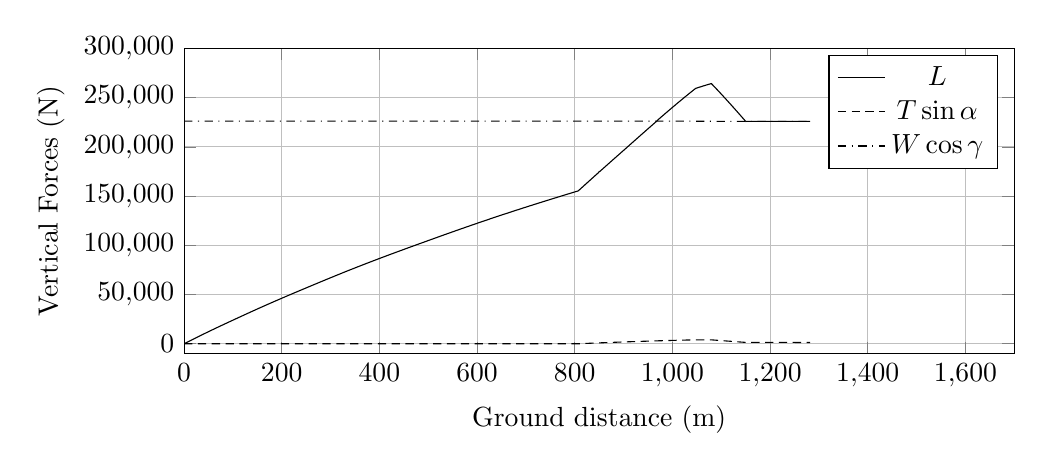
\begin{tikzpicture}

\begin{axis}[
width=\textwidth,
height=0.45\textwidth,
scaled ticks=false, tick label style={/pgf/number format/fixed},
xmin=0.0,
xmax=1700,
xlabel={Ground distance (m)},
xmajorgrids,
ymin=-10000.0,
ymax=300000,
ylabel={Vertical Forces (N)},
ytick={0,50000,100000,150000,200000,250000,300000},
ymajorgrids,
legend entries = {$L$\\$T\sin\alpha$\\$W\cos\gamma$\\}
]

\addplot [
color=black,
solid
]
table[row sep=crcr]{
1.3603393307216043E-8	3.477244192062615E-6\\
3.0265395163403265E-7	7.736317483675309E-5\\
2.9593179127983543E-6	7.564488300911159E-4\\
1.5392338359717934E-5	0.003934526922353545\\
5.361280674027254E-5	0.013704286338746683\\
1.6215010178508227E-4	0.041448134986905624\\
3.7214145765703975E-4	0.09512520498587163\\
6.839954676020354E-4	0.17483986139389857\\
0.001098342709021993	0.28075317357448315\\
0.001609317716481928	0.41136569247368737\\
0.0022198920000388346	0.5674367966912846\\
0.002878710694837372	0.7358393247690544\\
0.0036835072341781794	0.9415549564658316\\
0.004557929017412697	1.1650667501264018\\
0.005559798278933152	1.4211543861692415\\
0.006651227400597502	1.7001330314564322\\
0.007795849738889277	1.9927067845259518\\
0.009067984722810115	2.317871851640386\\
0.010453165799939174	2.6719299535886076\\
0.011915708813158052	3.045759604244375\\
0.013455030027058647	3.439211199341578\\
0.015131183092671713	3.8676339032168086\\
0.01690803412933615	4.321791238368709\\
0.01873590105740728	4.788984156082485\\
0.020713359121301934	5.29440729776044\\
0.022777736728155237	5.822041467647612\\
0.024960970145273077	6.38004850380983\\
0.02723428625014468	6.961073560246435\\
0.029610395797831278	7.568364543769745\\
0.03204086105441677	8.18954099190287\\
0.03462344565878624	8.849588372855493\\
0.037295727153354774	9.532551905550772\\
0.040089145853872785	10.246465908438967\\
0.042950967781251806	10.977852246725398\\
0.04592022141655751	11.736684426363766\\
0.04897301836205646	12.516856473503829\\
0.052130294957187476	13.323717882568673\\
0.05542514139564195	14.165723731981942\\
0.05879722600804832	15.027454910217717\\
0.06231520981015182	15.926456336316527\\
0.06596261503753809	16.858515546051066\\
0.06964559414821356	17.79964969096371\\
0.07347193989652406	18.777402580685774\\
0.07736619052035826	19.772489970685243\\
0.08137137577670908	20.79590595553983\\
0.08545617869345057	21.83964704796461\\
0.08969468676038628	22.922642317361394\\
0.0940095881391464	24.02513591948796\\
0.09845059220533334	25.159827541329513\\
0.10296315144049947	26.312778638435027\\
0.10759658895065366	27.49658971957942\\
0.1123317495250277	28.7063650341981\\
0.1171874363557737	29.94690680329085\\
0.12217670360507671	31.22154806552004\\
0.12726806426274867	32.522242667438206\\
0.13231647880291775	33.811936763137666\\
0.13765212084557643	35.174976117739575\\
0.14294844966167852	36.527940713973265\\
0.14834594087957392	37.90671500135866\\
0.1539671093411843	39.342592120845325\\
0.15968242883369804	40.80248282015022\\
0.16555834796315422	42.30335796806317\\
0.17157514414202774	43.8401769403668\\
0.17760320215284392	45.379831760352616\\
0.18370335474801935	46.93785922602612\\
0.18983540939776816	48.50399284800773\\
0.19621099073945342	50.13227900230628\\
0.20278841209744758	51.812066491012985\\
0.20952923284938563	53.53353415635637\\
0.21624967405074952	55.249747103870675\\
0.22309476488450758	56.99774064211523\\
0.22992510727843934	58.74191628440349\\
0.2371653034562048	60.59069469276591\\
0.2442573187228817	62.4015791766402\\
0.25144286317780873	64.23628904816138\\
0.2588001799723505	66.11479933426875\\
0.2662612189130884	68.01973185232993\\
0.27386560463063747	69.96120051701413\\
0.2815803271719757	71.93077452498397\\
0.28946218069394425	73.94295005041079\\
0.29753588720841584	76.0040339027021\\
0.3056643119969481	78.07901473341013\\
0.31376446154764137	80.14670616885519\\
0.322071411728719	82.26711278621588\\
0.3303680011285137	84.38480011727225\\
0.3389039548234316	86.56350698032188\\
0.3474123396293025	88.73509888504694\\
0.3561645174790815	90.9688325582785\\
0.36525289600634137	93.28828421171946\\
0.3742306244196095	95.57940962117948\\
0.3835584127627333	97.95977908775248\\
0.392806747202999	100.31978061685211\\
0.40218604538039837	102.71310823029589\\
0.4115907129344223	105.1128150932029\\
0.42143744457304466	107.62521858147011\\
0.4310567075016639	110.07948359518778\\
0.4412814114336725	112.68811347674082\\
0.4513051702487684	115.2453686114506\\
0.461412558308395	117.82385150702862\\
0.47173637532167356	120.45743588252054\\
0.4821484569390513	123.11342250770474\\
0.492985116277161	125.87759215661768\\
0.5036221628177362	128.59072536014673\\
0.5142245311302887	131.29489523041195\\
0.5252888808291518	134.11676945593177\\
0.5363145235987512	136.92864444521013\\
0.5471208511184944	139.6844642226423\\
0.5585110457184732	142.58904952013023\\
0.569849942463402	145.4804194289665\\
0.5817265165330987	148.5087515872977\\
0.5935668742733842	151.5277036316574\\
0.6053719027871456	154.5375033244473\\
0.6172343027602503	157.5617854043619\\
0.629515267228629	160.69262635331387\\
0.6417789549774502	163.81890797691318\\
0.6542768803188956	167.0047429146647\\
0.6669828212214572	170.2434387197398\\
0.6796225285147333	173.46508787437097\\
0.6925094233679154	176.74957293875298\\
0.7056620711738308	180.10161586325103\\
0.7184715206768946	183.36602306854428\\
0.731725241748566	186.74347457656717\\
0.7449880440563246	190.12306191372687\\
0.7586792333483576	193.61162273438288\\
0.7725063377467813	197.1346229364167\\
0.7863894274138714	200.6716935924835\\
0.8004504964383841	204.25391124836102\\
0.8147129313117618	207.88722620480291\\
0.8293722635741907	211.6214370570321\\
0.8437954335339908	215.2952797285161\\
0.8580702287827062	218.9311240431452\\
0.8726489666047585	222.64417395654993\\
0.8875094051704782	226.42875235956558\\
0.9027740629895862	230.31604680354792\\
0.9182163910703112	234.24835166076775\\
0.93361566230532	238.16945735817438\\
0.9491799633800446	242.1323465298977\\
0.9646343064330896	246.0670026111913\\
0.9803727456894022	250.07374776528292\\
0.9957421603273868	253.98631068049554\\
1.0116767859397604	258.04251389446733\\
1.028041387324289	262.20791017336035\\
1.0443915011410971	266.3693577927752\\
1.060796374175649	270.54448107061194\\
1.0773229908740651	274.7503241763469\\
1.093971735592782	278.9869795792009\\
1.1110062543639518	283.32152625021865\\
1.127891796882146	287.61788817190256\\
1.1451224507351285	292.00177684468713\\
1.1624801114435046	296.41769015873456\\
1.180077727863539	300.89435449717337\\
1.1978884766667508	305.4249353988655\\
1.215488397439855	309.90158915810764\\
1.23351701382096	314.48697781034787\\
1.2518199984626128	319.1418323723195\\
1.2704235066044305	323.87279033657785\\
1.2892140278280424	328.65097327179933\\
1.3075714306593595	333.3186970668438\\
1.3266673518109293	338.1738655354786\\
1.3462106477188795	343.1424237849968\\
1.365306294594515	347.99682763678084\\
1.3852885894463176	353.0762643675191\\
1.404835539176236	358.0446758319208\\
1.4251192118409102	363.19996873564025\\
1.445164519989187	368.2943019804993\\
1.4656054698512246	373.4887988852414\\
1.4853522740259328	378.50652956000647\\
1.5051589726327936	383.53911663107476\\
1.5255757775517242	388.72634293330304\\
1.5464367798307013	394.0260276411841\\
1.5673163741652552	399.33003441359403\\
1.5879032567231621	404.5592920048174\\
1.6091523485848285	409.95634940261857\\
1.6303162371862876	415.3313555073854\\
1.6519474169970438	420.8246174313557\\
1.673879209980242	426.39378539166523\\
1.6955666802836635	431.90048242615967\\
1.7172271378534343	437.3998950132899\\
1.7402832823543353	443.25319478859194\\
1.7634396102400074	449.1314454139921\\
1.7861669372425006	454.90032439838785\\
1.8088678577734645	460.66203743577046\\
1.831824248135399	466.48812149341654\\
1.855578771396016	472.5162669728966\\
1.878960729162178	478.4493755140958\\
1.9033179534858085	484.629437855114\\
1.9273833213731866	490.73493126607593\\
1.9518510462308036	496.941978528175\\
1.9761594732990155	503.1080907470622\\
2.000437267212291	509.2659125519641\\
2.0252281699074732	515.5533443599597\\
2.0498006073458734	521.7848371740533\\
2.0745611186355752	528.0634902932416\\
2.0997746990963106	534.4564803675721\\
2.1260324099367294	541.1136245942357\\
2.1515212193659616	547.5752553466743\\
2.1771505246334	554.0719351073596\\
2.2031842637813908	560.6705517647381\\
2.230133398733474	567.5005724469195\\
2.257053086628849	574.3225060849913\\
2.283795213136285	581.098826567935\\
2.311477064851834	588.1126237258673\\
2.3387199014446116	595.0145479196794\\
2.3662694524467227	601.9935346948482\\
2.3937852540088533	608.9633281453289\\
2.4216520071021392	616.0213640837922\\
2.4501931244916175	623.249521130359\\
2.478927626230634	630.5259596735257\\
2.506685441631536	637.5544124690214\\
2.53537335014481	644.817691439627\\
2.5633350931805676	651.8964552114769\\
2.5917889242519685	659.0991255360138\\
2.6208221472873374	666.4477656914753\\
2.649872764173903	673.8001078522973\\
2.679661174525658	681.3384503566497\\
2.709174609939316	688.8064840227316\\
2.740029385016756	696.613160914108\\
2.770444625703795	704.3078640481654\\
2.801129860621211	712.0701044178668\\
2.8318827297715705	719.8486817286148\\
2.862425967677578	727.5734723196967\\
2.893259332541544	735.3708707214168\\
2.92412139403754	743.1747543689901\\
2.955064430161417	750.9983404072198\\
2.986690331721131	758.9937832145974\\
3.019183403261743	767.2076202849407\\
3.0507201588152526	775.178903107738\\
3.0830332871979023	783.3455982208616\\
3.1154603869692448	791.5402608726727\\
3.148592095396281	799.912121655655\\
3.181936872739324	808.3369426001329\\
3.214370607724433	816.5307378702792\\
3.247565473366384	824.9159599411676\\
3.281695868027062	833.5365986838101\\
3.316494330618462	842.3250372105801\\
3.3513055302544137	851.1157451373997\\
3.3860303583611797	859.8837007970887\\
3.421934361445942	868.9484103558802\\
3.456235826539576	877.6075927284667\\
3.490536654441657	886.2657049521742\\
3.526257338581564	895.2812492982823\\
3.561372823896762	904.1430918475976\\
3.5967906564503185	913.080278644205\\
3.632682576242373	922.1361170483751\\
3.6701261071689295	931.5823945382463\\
3.707701291513044	941.0608154498257\\
3.7452745323452916	950.5376774179717\\
3.78256482255855	959.9421191464567\\
3.8208821591411084	969.6044875042242\\
3.8590337549211444	979.2239674364475\\
3.89695718563138	988.7848396363636\\
3.9351036745073964	998.400865508735\\
3.9736642086653067	1008.120165564859\\
4.012189127077221	1017.829388587945\\
4.05156219172609	1027.7512327423733\\
4.090290786278251	1037.5095598016783\\
4.129291984889424	1047.3354616925544\\
4.1680648628189925	1057.1027377520782\\
4.207805169621487	1067.1125810605445\\
4.248168240749736	1077.2781118272187\\
4.288797880674668	1087.509586202404\\
4.32990243544832	1097.859441627284\\
4.371428084678056	1108.314090630843\\
4.41247037137882	1118.6458305735678\\
4.453879445321437	1129.0686822628004\\
4.49524783594077	1139.4800730551483\\
4.537299342543221	1150.062140669364\\
4.580546125800922	1160.9436877864123\\
4.622914948498307	1171.6030463970606\\
4.66640222022569	1182.5424766158303\\
4.709294790611851	1193.3310079677676\\
4.752417172855319	1204.1760466555743\\
4.796155651503765	1215.1747072177968\\
4.8408754796551925	1226.4187692370697\\
4.884850997559644	1237.4743378304315\\
4.928651138956553	1248.4844912388853\\
4.972831351372241	1259.5888489868298\\
5.017331702752941	1270.7723203861788\\
5.0632326321008225	1282.3063583616972\\
5.108452384314601	1293.6678287406971\\
5.1536021218025905	1305.010325838443\\
5.199057463234675	1316.4282064396566\\
5.244479287100011	1327.8362793296742\\
5.292293005248643	1339.8436023911713\\
5.338096108273211	1351.344573303592\\
5.3857492800262605	1363.3086068616449\\
5.433816232374781	1375.3750006041591\\
5.480691139018431	1387.1406812192831\\
5.529685763332537	1399.436868479018\\
5.578612887337309	1411.7145440055124\\
5.626451501744754	1423.7175586378344\\
5.674834544150631	1435.8556582858855\\
5.7252048440372345	1448.4906981293611\\
5.77422346516266	1460.7851046676487\\
5.8255152536468575	1473.6479904564358\\
5.874338256646894	1485.8901902644043\\
5.922631450506765	1497.9980440680183\\
5.972682300942642	1510.5450031795635\\
6.022535370757359	1523.0408026871269\\
6.074394648705015	1536.037797400385\\
6.124928192945902	1548.7009081667052\\
6.176798284396469	1561.6972771892183\\
6.229620191179453	1574.930402991357\\
6.282808156696705	1588.2534818571921\\
6.334658925277093	1601.2399188564536\\
6.388041948821611	1614.6083883798\\
6.440558117792513	1627.7580666824379\\
6.494960924490993	1641.3783657859435\\
6.550441697666145	1655.266686849187\\
6.6042098433346865	1668.7245085861096\\
6.658315220792536	1682.264973073769\\
6.712335084641163	1695.7822784879017\\
6.766674450459032	1709.3777670152058\\
6.821537769035839	1723.102557485763\\
6.876851268142238	1736.9381544427924\\
6.933661362437203	1751.1462094363733\\
6.989261882852809	1765.0499102282074\\
7.046240323930029	1779.2962962382258\\
7.102786137967051	1793.4326351549867\\
7.1603789170469145	1807.8287994987008\\
7.21785165788507	1822.193041552226\\
7.277487498606879	1837.0958945925481\\
7.334984696129153	1851.4623706408734\\
7.393362172524569	1866.0468614476717\\
7.452416393609804	1880.7984486758596\\
7.511934748111884	1895.6639739988987\\
7.572557225035805	1910.8032130247252\\
7.63202184821041	1925.6512946870116\\
7.69294899409779	1940.862510490435\\
7.752675521499926	1955.7719701835517\\
7.814488876138199	1971.2002793373504\\
7.8763528528159785	1986.6391122304804\\
7.938149975125226	2002.059161974586\\
8.001193143199774	2017.7879822370123\\
8.064554080136986	2033.593904440012\\
8.12686567918485	2049.135939883704\\
8.189637855946287	2064.7907385207163\\
8.252542711798306	2080.476505481266\\
8.315859663763469	2096.262897925816\\
8.380006162932737	2112.253943493074\\
8.444702551512929	2128.3798667284327\\
8.509501986620958	2144.52926702525\\
8.57387297516295	2160.5697122619404\\
8.63887365699837	2176.764878205713\\
8.70727085773305	2193.803934331794\\
8.772937378995405	2210.1604549771428\\
8.839192134487615	2226.6612526229646\\
8.905815929161982	2243.2516992086776\\
8.97209054442786	2259.7529565433942\\
9.039019026885107	2276.414762252989\\
9.107371801018814	2293.4288191253236\\
9.174915633685494	2310.2392215812206\\
9.243868961478196	2327.3980786694383\\
9.312440636565494	2344.4596276782377\\
9.381784695008012	2361.711000665735\\
9.4513167952828	2379.0067890153296\\
9.52142787533916	2396.4442102644516\\
9.591425279059166	2413.850982016288\\
9.662230428326719	2431.456218628943\\
9.734225879912522	2449.354951365758\\
9.806441602430919	2467.3059625539536\\
9.878483835105534	2485.2113845370523\\
9.951807209049782	2503.4327092665244\\
10.023539677466466	2521.256244435842\\
10.096057433179052	2539.272463139222\\
10.168262179450682	2557.2084957452134\\
10.241274410624943	2575.3426677544394\\
10.31479015323385	2593.5994287550366\\
10.390063469390178	2612.290110023604\\
10.465012435634037	2630.8977030776714\\
10.540639152111389	2649.6709966174003\\
10.617644389866598	2668.7838577815937\\
10.692945462162374	2687.471189217078\\
10.770083295573727	2706.611745279044\\
10.846726862770723	2725.627065394596\\
10.924657809445929	2744.9591528143146\\
11.00265335491597	2764.3046237512217\\
11.081827589833612	2783.939762811997\\
11.159134327011738	2803.1091694127144\\
11.239152720133266	2822.948290012817\\
11.317028257314295	2842.253523663753\\
11.396413369884492	2861.9303514264157\\
11.477655063362434	2882.064632558632\\
11.556958506738276	2901.7159082276085\\
11.637325199769407	2921.6280067083553\\
11.717754170658207	2941.5528831791844\\
11.799819443100102	2961.880407960127\\
11.881986970940797	2982.2305302140057\\
11.964394119506721	3002.6372720467725\\
12.046263329632716	3022.908116991669\\
12.130282587748898	3043.7085504068637\\
12.213721087180826	3064.362454814548\\
12.295868535962462	3084.6941189053077\\
12.380692430046633	3105.6854574586014\\
12.46470288467437	3126.4727582722326\\
12.550384439940181	3147.670766396017\\
12.635259749824865	3168.6665526168053\\
12.72144647897981	3189.9839636199495\\
12.80741162779486	3211.243794807747\\
12.892901506907108	3232.383360475882\\
12.977815703098727	3253.377900531952\\
13.06483740414145	3274.890764844302\\
13.151922956503014	3296.416653786352\\
13.240589045456186	3318.330405689857\\
13.329911181207382	3340.4034483725163\\
13.417306166647748	3361.9975108511135\\
13.507103029723119	3384.182233884466\\
13.595986036712912	3406.138402137837\\
13.687453390597003	3428.7300967270394\\
13.779071846306106	3451.3562197409983\\
13.872694200363323	3474.4742598895737\\
13.963504841252302	3496.8951662728205\\
14.056146454975131	3519.7652755334375\\
14.14918846816267	3542.7313471888065\\
14.24332804549016	3565.965420901397\\
14.339261112049854	3589.639144375097\\
14.431091301610323	3612.2975825007943\\
14.524174633942373	3635.2624486475306\\
14.618760344060338	3658.5951325257947\\
14.714801736988441	3682.2840065463733\\
14.809763128346521	3705.7036454664576\\
14.903412319659619	3728.796915314775\\
15.001392651385917	3752.9553177959206\\
15.098055049922994	3776.7858880133335\\
15.196870856960619	3801.144419595531\\
15.29477342819068	3825.274943182373\\
15.39265348361268	3849.397067236958\\
15.490487151984588	3873.5049385738475\\
15.588146853189365	3897.567155394773\\
15.687961867268871	3922.157567403621\\
15.78650099417861	3946.430854303505\\
15.886965864441798	3971.1756786656615\\
15.98755318095926	3995.9478239220143\\
16.088470385762115	4020.7983873260227\\
16.190536977381747	4045.9291347995695\\
16.292466610053154	4071.0233303050645\\
16.396448349404487	4096.619853040733\\
16.497808944935016	4121.5683716329695\\
16.600551072850564	4146.854170352019\\
16.70575139586156	4172.742100246463\\
16.81134459259622	4198.723837568501\\
16.917616592554033	4224.869725230461\\
17.023477948501657	4250.911750068368\\
17.12904978140002	4276.87976797342\\
17.2354081519902	4303.038475281592\\
17.340772011500363	4328.949865069711\\
17.448391076872838	4355.413100817843\\
17.5571980918308	4382.165647294945\\
17.66615596614949	4408.952495859841\\
17.774685459577412	4435.631287271581\\
17.884986575683584	4462.742811484728\\
17.99552903728076	4489.910892331132\\
18.108708479124623	4517.724234287838\\
18.219646262474413	4544.983955091171\\
18.332680252669796	4572.756000891164\\
18.445061806396694	4600.365023821043\\
18.556709221711323	4627.791038494086\\
18.668884868236475	4655.344187611996\\
18.78204748093455	4683.137131346652\\
18.895704562363058	4711.048896904405\\
19.008928234289563	4738.851652095824\\
19.124320907419907	4767.184413262652\\
19.24105855786135	4795.844774619749\\
19.355116774466126	4823.844782795772\\
19.470462572962035	4852.158380070439\\
19.58492145104516	4880.2518224869855\\
19.704921229319112	4909.702680799064\\
19.821259826163917	4938.252520526003\\
19.941172080873493	4967.676837446985\\
20.06078806851737	4997.025960137336\\
20.177423389922623	5025.641383193122\\
20.297621170678	5055.128427224667\\
20.420129559802255	5085.179852845113\\
20.54164670774839	5114.985717415409\\
20.661905244258705	5144.48054961215\\
20.784301666224792	5174.4973987950125\\
20.904244540623438	5203.9103002356605\\
21.028114340450195	5234.283903652973\\
21.148300883955606	5263.752183826429\\
21.270875420257596	5293.8038159373355\\
21.39299406946177	5323.74155754974\\
21.513793771711654	5353.353915644182\\
21.637476506915142	5383.670950860014\\
21.759279707150128	5413.525283702305\\
21.88493035745168	5444.320612264075\\
22.009809790007786	5474.924932612268\\
22.13620730934617	5505.899315638333\\
22.263515470260465	5537.094894115042\\
22.393040471753594	5568.8317156362355\\
22.520519759768852	5600.06539415242\\
22.648852607677917	5631.5063555284\\
22.775118904521122	5662.4392592972945\\
22.903136237443974	5693.799398021514\\
23.03176118514304	5725.306670372691\\
23.162501585272054	5757.33042351917\\
23.294719932439598	5789.714486797289\\
23.427108470281937	5822.138573851074\\
23.558693146983046	5854.364187635878\\
23.687077503630363	5885.804547284424\\
23.817949558665852	5917.85266780181\\
23.948210788889448	5949.749797024715\\
24.076877750667826	5981.255202862756\\
24.21019765060587	6013.898580009081\\
24.3450673155249	6046.920074898575\\
24.477101355489637	6079.24603983071\\
24.60984760833776	6111.745175995466\\
24.7468403923846	6145.2827471702585\\
24.882807251950062	6178.568001977159\\
25.017167332957627	6211.458832557917\\
25.153910941279605	6244.93209618633\\
25.289629217480112	6278.153382490513\\
25.425306692573436	6311.363752415982\\
25.56229499031975	6344.894091022345\\
25.70075944713021	6378.78489680979\\
25.83724158708921	6412.189727436613\\
25.975209935932874	6445.957586041652\\
26.003074150630965	6452.777289687625\\
26.020759913393235	6457.105826057616\\
26.030714598210515	6459.542199959216\\
26.05840292223249	6466.318801452795\\
26.06133765907019	6467.037064489832\\
26.064285136409026	6467.7584454117095\\
26.066337724202356	6468.2608062424115\\
26.068175973881182	6468.710708746659\\
26.06984477238784	6469.119138817139\\
26.077831036047115	6471.073735516693\\
26.10345636352254	6477.345387092168\\
26.16716044512971	6492.936495080667\\
26.297541524199602	6524.845841222053\\
26.42722303713863	6556.5833006977155\\
26.5559280656694	6588.081056584602\\
26.686097387723095	6619.936373345017\\
26.817793678842584	6652.164501922118\\
26.949416928520378	6684.373820776604\\
27.080440623797912	6716.435436282345\\
27.215491080424528	6749.481311975274\\
27.34795890217076	6781.894099136138\\
27.48215578365496	6814.728752647681\\
27.616696052324144	6847.646145125902\\
27.75271189183823	6880.923196660164\\
27.888759310501555	6914.206543504521\\
28.023839122857026	6947.251695545756\\
28.16136324828667	6980.893241149839\\
28.298355249881332	7014.40298369489\\
28.435282447697354	7047.8951867918495\\
28.573941346212784	7081.8091828595825\\
28.713752690797136	7116.00317880386\\
28.852681198061333	7149.979336012744\\
28.992471984120606	7184.164379219565\\
29.133421724605903	7218.630756322329\\
29.275199211812186	7253.297373631878\\
29.416225289053614	7287.77804453572\\
29.55783477945603	7322.3990772658835\\
29.701838356359822	7357.603018072747\\
29.846633046394217	7392.997854911333\\
29.99013730470424	7428.074711647723\\
30.132492646908446	7462.868186762189\\
30.277395768405135	7498.281705138848\\
30.422188862471998	7533.665589072623\\
30.56637548064623	7568.89848296588\\
30.711944318924978	7604.466258417251\\
30.8573377156769	7639.988230580233\\
31.006558691603843	7676.442233370342\\
31.153907258126303	7712.435667852938\\
31.30257185742142	7748.747348974157\\
31.4510947803754	7785.021133633425\\
31.602595106592503	7822.018643124327\\
31.755261577184278	7859.297354082897\\
31.906398416479824	7896.198956932412\\
32.05599258457312	7932.720322141064\\
32.20952926265106	7970.200438791124\\
32.360097140052986	8006.952084447286\\
32.51218835243483	8044.071730610314\\
32.664721606344784	8081.295347016754\\
32.82129760777845	8119.501405871231\\
32.97669884718651	8157.416615281978\\
33.13118849606322	8195.105214755058\\
33.288837444683736	8233.560173435184\\
33.44405554194745	8271.417814713092\\
33.60015866510213	8309.486892483907\\
33.756686089655645	8347.654941503082\\
33.91694077595571	8386.727129728213\\
34.074326811338736	8425.095197316834\\
34.23252403098988	8463.656266879028\\
34.392884168270385	8502.73964114159\\
34.554266068788166	8542.066995832552\\
34.71363140184178	8580.89791217052\\
34.87649332318763	8620.575602508463\\
35.03746231629111	8659.786903727116\\
35.19990059234286	8699.350805390663\\
35.3627309111595	8739.00479081435\\
35.5271254050015	8779.03416107719\\
35.69149466827288	8819.05177514795\\
35.85508342515686	8858.873745099252\\
36.017180984292054	8898.327139265883\\
36.182222084544165	8938.491219364958\\
36.34861175093968	8978.9775624071\\
36.514166392421686	9019.254777546947\\
36.68083924241549	9059.79799852995\\
36.845526722294395	9099.852281188225\\
37.01328249159678	9140.646641235366\\
37.18160982421668	9181.573685255538\\
37.35136716620059	9222.84197728187\\
37.51969289597564	9263.755808272414\\
37.689710015857784	9305.074207027643\\
37.860394939778416	9346.548236240807\\
38.02805196867635	9387.279988863851\\
38.19868492919754	9428.728037183548\\
38.37343039987371	9471.167999709112\\
38.54685896696101	9513.281037211378\\
38.71934233168869	9555.157505308467\\
38.8915617091798	9596.962826847997\\
39.062305982326905	9638.403077412197\\
39.23847188392709	9681.151834124368\\
39.411511502305984	9723.134662114735\\
39.585172817779906	9765.261015531254\\
39.760693028009456	9807.830815695757\\
39.9373134006328	9850.659815656669\\
40.113617753210534	9893.404514610724\\
40.29094651898711	9936.38981519454\\
40.468149621311596	9979.336838316605\\
40.64593210594187	10022.416393482545\\
40.82431302355218	10065.632983309988\\
41.00141330502653	10108.531374768849\\
41.17957893337042	10151.67980826175\\
41.359761290266974	10195.308448520227\\
41.53889737920997	10238.675534730552\\
41.72013507746885	10282.543031654197\\
41.899395797464194	10325.92370163478\\
42.081280067494475	10369.930785237222\\
42.265315320939635	10414.449577034855\\
42.44531744651641	10457.984221448092\\
42.62715102096499	10501.953230222603\\
42.81120266452106	10546.449774136447\\
42.994164503876235	10590.67402832851\\
43.17799769459725	10635.100017501183\\
43.36154361404071	10679.447674043298\\
43.54597437124032	10724.000128258234\\
43.73158498218817	10768.8284686861\\
43.91737182308138	10813.690176040236\\
44.1050494697441	10858.99908721968\\
44.293574236233	10904.50300605427\\
44.47888581456586	10949.222056779305\\
44.66456251492659	10994.01994188028\\
44.85170130968709	11039.161166241\\
45.037822074257164	11084.047424385317\\
45.22676109993536	11129.603746331231\\
45.41612608476639	11175.253039264877\\
45.604812217355104	11220.72897092281\\
45.79422221198037	11266.369591473005\\
45.98724683785376	11312.871108882395\\
46.17830917717477	11358.889840792395\\
46.36786657808848	11404.536197387537\\
46.55935209439748	11450.636824471396\\
46.75090376717816	11496.743277060432\\
46.94233405988251	11542.810403512169\\
47.13714948644359	11589.681760057134\\
47.33387512950824	11637.002049009821\\
47.53043319838464	11684.271322852674\\
47.72298239739284	11730.566132549393\\
47.919150009665316	11777.720332314322\\
48.113386178114425	11824.399714595962\\
48.311024807628144	11871.886005991724\\
48.508886059616145	11919.41488301726\\
48.70490444306449	11966.490310286907\\
48.90290918859142	12014.031886969125\\
49.09959709013448	12061.246437979524\\
49.2970021191946	12108.622255035545\\
49.49532701226336	12156.207849616192\\
49.693780717172615	12203.813323762908\\
49.89506320355713	12252.086096769388\\
50.096719083698545	12300.437026402768\\
50.29606895218413	12348.22383037601\\
50.497598474286534	12396.521787565798\\
50.700304208193415	12445.090127261807\\
50.90342397924904	12493.746092666814\\
51.10460922167407	12541.927227135344\\
51.30752217039489	12590.510601242142\\
51.51010619677311	12639.003675912641\\
51.713602501430145	12687.703509354567\\
51.91843850546792	12736.71219600035\\
52.121089026646246	12785.186379795494\\
52.32561402362407	12834.097233773507\\
52.53192272805477	12883.422737026835\\
52.7387030603267	12932.848995930948\\
52.944027344085896	12981.915330212167\\
53.154073670302836	13032.097835748282\\
53.36143953271798	13081.627793167609\\
53.571009444677685	13131.671929649121\\
53.77799762982136	13181.087466464676\\
53.98785945427545	13231.176776250093\\
54.196157549666225	13280.880650317795\\
54.40718762937186	13331.224031493359\\
54.616887598525366	13381.23774983058\\
54.826875464266934	13431.307802613894\\
55.04038432082807	13482.204769139546\\
55.25438844036796	13533.20701830577\\
55.46695867894975	13583.854884035518\\
55.68088820258777	13634.813895678093\\
55.895144656119854	13685.838002806271\\
56.109028395418505	13736.760605417305\\
56.326262430904194	13788.467844252915\\
56.542089933321776	13839.827312103353\\
56.76060076462056	13891.812154080293\\
56.97729209122687	13943.351060789078\\
57.19579178641709	13995.306920567029\\
57.41258192878804	14046.843233950043\\
57.634093277561306	14099.48849432847\\
57.85395098827546	14151.727371209057\\
58.07448819514299	14204.114332943289\\
58.29446478173499	14256.354808398628\\
58.51588770709739	14308.92535447871\\
58.73757884137123	14361.546123529715\\
58.96020041504734	14414.374216177745\\
59.18267120664716	14467.153010573082\\
59.405949655899676	14520.109850084955\\
59.63089974393067	14573.449450628785\\
59.8562534200115	14626.87097071257\\
60.084134136581554	14680.877545262276\\
60.30833762904015	14733.99892755716\\
60.53504725699203	14787.700299721422\\
60.763693228044005	14841.846314816397\\
60.99075593752245	14895.603486677504\\
61.21765734918529	14949.308655663535\\
61.44713116872772	15003.608671043388\\
61.6738048454246	15057.232286873263\\
61.90668490141796	15112.309872922775\\
62.13729676517957	15166.836811747457\\
62.36629463006145	15220.968174980819\\
62.596359157213186	15275.337711634496\\
62.82836101237727	15330.150940971998\\
63.059723307860466	15384.798959712753\\
63.292774394726166	15439.831667896666\\
63.52608473446321	15494.91135378469\\
63.75973181411028	15550.056294627691\\
63.993403028653574	15605.192716375615\\
64.23068717493263	15661.167129219175\\
64.4710952259949	15717.863594693437\\
64.70858695601663	15773.857644607571\\
64.94894296164699	15830.512235013\\
65.18738841845183	15886.701843566989\\
65.42661162888535	15943.060117959067\\
65.6659442133793	15999.42956038762\\
65.90899583190168	16056.66004157949\\
66.15068261105333	16113.554312551318\\
66.39533053734849	16171.13063507598\\
66.6378997293487	16228.202874785682\\
66.88158418814953	16285.5226636511\\
67.12390450547147	16342.506866107273\\
67.36840986262189	16399.990087712373\\
67.61550053739396	16458.066052566915\\
67.86097385246623	16515.746933839713\\
68.10985741250389	16574.21400173325\\
68.35582503705197	16631.981138333227\\
68.60464259362828	16690.402560242663\\
68.85450289166104	16749.053651279217\\
69.1042877596268	16807.671909126766\\
69.35837572129628	16867.28454042566\\
69.61150655903072	16926.657181816066\\
69.86289252102952	16985.605373799604\\
70.11686816207683	17045.14552649478\\
70.37125759672608	17104.767335713266\\
70.62480458144697	17164.17647826302\\
70.88045310059783	17224.062719837697\\
71.13526709211152	17283.73823584913\\
71.3947754873567	17344.497583546865\\
71.6534187996231	17405.03883372517\\
71.91450497256008	17466.136216292958\\
72.1716184080999	17526.288612859404\\
72.43269265097052	17587.352174364336\\
72.69331619504374	17648.29484163935\\
72.95563200429567	17709.617679642673\\
73.21686762735783	17770.67258265472\\
73.48161420086069	17832.53243644871\\
73.74261486234883	17893.50172560884\\
74.00755043430098	17955.37474156916\\
74.27511769675363	18017.846636654554\\
74.54487113507057	18080.813052250393\\
74.81568229507957	18144.010383707733\\
75.08274085953312	18206.316406090802\\
75.35421836228127	18269.637608530385\\
75.62798354862159	18333.47638819411\\
75.89909469738902	18396.680519707203\\
76.17008148658607	18459.840081564085\\
76.44269151183332	18523.36235483364\\
76.71571902594138	18586.966301790708\\
76.99340852183178	18651.64037208994\\
77.27004772085374	18716.05396149149\\
77.54832408953641	18780.832880329945\\
77.82592519882277	18845.438847212994\\
78.10358246820337	18910.04224093099\\
78.38556010231375	18975.634962239383\\
78.66911430382748	19041.57836634593\\
78.95399134982776	19107.81331269609\\
79.23667137346987	19173.521605120113\\
79.518907793654	19239.111154444363\\
79.80555437718249	19305.70972178714\\
80.09150103324356	19372.12985198039\\
80.37928873457926	19438.96178941612\\
80.66871996946384	19506.15949865827\\
80.95967699414447	19573.69550403772\\
81.25093884305389	19641.2863727313\\
81.54344278085921	19709.149607913118\\
81.8358102960415	19776.965421047455\\
82.13087592438694	19845.3912160682\\
82.42794520371837	19914.265699623327\\
82.72842933895026	19983.915753447123\\
83.0269479931649	20053.094275468247\\
83.32974506690314	20123.248179136725\\
83.62964811531441	20192.71573898793\\
83.92951211009506	20262.158635088417\\
84.2339319847595	20332.640758816793\\
84.53715838283946	20402.830849646605\\
84.84105485927768	20473.16046722664\\
85.14845677960258	20544.285618691698\\
85.45530133949276	20615.26619906351\\
85.76249773413784	20686.31269726809\\
86.07201271349416	20757.879925966925\\
86.38432073331904	20830.077366302517\\
86.69710203601804	20902.368669520227\\
87.01172103282082	20975.069178051483\\
87.32669099459858	21047.835352574104\\
87.64517025121202	21121.396736803326\\
87.96158123090564	21194.465107662458\\
88.2775814178033	21267.423578050882\\
88.60068374099544	21342.006440209363\\
88.92068281935622	21415.857844912178\\
89.24207276858638	21490.015276261343\\
89.56578933015979	21564.694571862514\\
89.88760090270688	21638.91968492658\\
90.2141410750086	21714.22063361243\\
90.54066676000363	21789.50352197217\\
90.86727570256076	21864.79107537192\\
91.19715108614633	21940.81703250396\\
91.52744226539704	22016.924365572333\\
91.85639956214655	22092.710166078752\\
92.19095740864739	22169.77193150737\\
92.52827526888461	22247.455049607168\\
92.8674718219292	22325.556476342288\\
93.20307982994817	22402.81768217691\\
93.5374944579234	22479.79057573805\\
93.87598013161067	22557.6869228\\
94.20917297854535	22634.35208532597\\
94.55043409744499	22712.860408761473\\
94.89132963816093	22791.271430322726\\
95.23083207736542	22869.34913247417\\
95.57395676502793	22948.24703246361\\
95.91421223354143	23026.472672409407\\
96.25656086122288	23105.167190205073\\
96.60012122339742	23184.12803014838\\
96.94166303707107	23262.613048527397\\
97.28627502929558	23341.791796633093\\
97.62906225262071	23420.539773122473\\
97.97125437026659	23499.13982322107\\
98.31201772458999	23577.400791493987\\
98.65627175165852	23656.452631231987\\
99.0012536203806	23735.660947769655\\
99.35020029285332	23815.76898022116\\
99.69475740907401	23894.859073003674\\
100.04053871990226	23974.22019877183\\
100.38598466112728	24053.494623449522\\
100.72867962848932	24132.128374559376\\
101.07385499050397	24211.32207991187\\
101.41864366415388	24290.41810337508\\
101.76305460768467	24369.41877349196\\
102.11068844700483	24449.150138420744\\
102.45638678530696	24528.429297025657\\
102.79841653079728	24606.859242161656\\
103.14087212494877	24685.379212798776\\
103.48486473791618	24764.24416101903\\
103.82875595362174	24843.078655457517\\
104.17244250654872	24921.85927751474\\
104.51168383396202	24999.614375258076\\
104.85986244643053	25079.411375846386\\
105.204587526496	25158.410594626796\\
105.54754777175077	25236.999412334357\\
105.88797456536247	25315.002055087556\\
106.23280177240994	25394.007492106874\\
106.57515110440406	25472.439996576242\\
106.91603555764121	25550.531979634616\\
107.25729565943405	25628.70534702218\\
107.598830149446	25706.937132430212\\
107.93686571059558	25784.363322688216\\
108.27485499032852	25861.775040171502\\
108.28839963475954	25864.87717421109\\
108.30004107281309	25867.543411661012\\
108.30931238392475	25869.666816092584\\
108.31701527366243	25871.431003578822\\
108.32505202073054	25873.27165218137\\
108.33865239118708	25876.386527561932\\
108.35091925899997	25879.195987529325\\
108.39508146726081	25889.3103437038\\
108.52984553865659	25920.17462052249\\
108.79919793188978	25981.861101336945\\
109.105233418432	26051.94555150099\\
109.41485218466596	26122.847014641207\\
109.72257164661937	26193.309746834115\\
110.0321119530083	26264.18537810351\\
110.34145354075926	26335.011233150493\\
110.6534776714839	26406.446720189037\\
110.9711963390063	26479.180995462317\\
111.28851843247409	26551.819284928977\\
111.60893519474632	26625.160467862523\\
111.92798394282838	26698.182789314007\\
112.24770070245137	26771.35203228634\\
112.57243448635171	26845.663100489503\\
112.89480865389396	26919.427635074295\\
113.22000325235314	26993.830667921233\\
113.54885709436653	27069.06367148574\\
113.8770619430189	27144.140698943884\\
114.20946079557197	27220.169225625126\\
114.54107775051554	27296.010768570326\\
114.87787736567807	27373.02902856867\\
115.21564640021248	27450.260053941485\\
115.55522358014255	27527.89526242389\\
115.89667501383605	27605.949369025075\\
116.23992536102014	27684.40474692116\\
116.5847156213415	27763.201802135423\\
116.92791619634093	27841.625064305357\\
117.27517516660399	27920.964790208956\\
117.62420948631524	28000.698837759017\\
117.97391125359778	28080.57374791465\\
118.32673409155768	28161.149509241986\\
118.68227803698588	28242.3342270183\\
119.03889207644076	28323.75045580379\\
119.39651249432902	28405.383283584655\\
119.75508651978987	28487.220304086564\\
120.11314113323388	28568.925057921064\\
120.47404637453192	28651.266173422897\\
120.84098349318353	28734.968677553108\\
121.20490030977416	28817.96723161504\\
121.57328571082118	28901.96948316301\\
121.94079100066682	28985.755301440062\\
122.31015242291167	29069.94819631846\\
122.68267403243519	29154.84483523106\\
123.05346836176264	29239.331033573973\\
123.42835733050345	29324.732915675362\\
123.80350972566416	29410.17715838313\\
124.1783235941891	29495.52642130061\\
124.55244040146786	29580.69889503118\\
124.92576251095704	29665.672222993388\\
125.30489170817492	29751.94845607379\\
125.68146781278597	29837.624638114918\\
126.06139977608174	29924.044839208284\\
126.44502763856761	30011.285623300275\\
126.82695116404781	30098.118532092638\\
127.206716044588	30184.44035425441\\
127.59262031825523	30272.136710667066\\
127.97077035934353	30358.050199184225\\
128.3546122768156	30445.235646498724\\
128.73724861847296	30532.12578304278\\
129.12002064685282	30619.025062021094\\
129.50086700331673	30705.465443800982\\
129.8837789976152	30792.352613858908\\
130.26783132854348	30879.476128073133\\
130.651936341801	30966.588941380884\\
131.03747321415574	31054.003510766917\\
131.42280335891803	31141.348004287218\\
131.80875442588928	31228.8097962151\\
132.19322104975072	31315.911669692585\\
132.5798881414172	31403.4881956175\\
132.96215446290768	31490.044275121334\\
133.34488286943906	31576.68118587086\\
133.7276157954845	31663.295132010644\\
134.11532375481391	31751.010314037965\\
134.50135826447365	31838.322088790417\\
134.88604120201086	31925.303379189194\\
135.26955723714872	32011.996019914186\\
135.6512109336153	32098.242943584977\\
136.03464327936558	32184.866799746793\\
136.41686422877552	32271.191877595644\\
136.79904942565338	32357.48367022864\\
137.18004416157777	32443.481436237642\\
137.56399804528928	32530.121499930872\\
137.94515347717788	32616.104488516656\\
138.32982901897384	32702.855562190176\\
138.7128522769853	32789.20792896309\\
139.09597564505458	32875.55668903078\\
139.48002685240425	32962.08815935283\\
139.86309097971855	33048.37076207559\\
140.24727738828375	33134.879475693655\\
140.6317581809211	33221.42760727767\\
141.01585725597846	33307.86285103591\\
141.3998433603236	33394.24561712066\\
141.7841907991213	33480.682463979465\\
142.16710976343057	33566.77087700472\\
142.55205218648928	33653.28675013238\\
142.9364233092117	33739.64664649665\\
143.32169829765928	33826.18186139139\\
143.705984531242	33912.46720535336\\
144.08985428249122	33998.63122420451\\
144.47683600496026	34085.46552663538\\
144.86371007721533	34172.247238901284\\
145.24772592056325	34258.35959619224\\
145.63047789911974	34344.16048360286\\
146.01273254364395	34429.82183863735\\
146.39725173307323	34515.962303392735\\
146.77966503747456	34601.602707663\\
147.16478130736948	34687.81983179535\\
147.54689717238745	34773.3367994265\\
147.93097497792814	34859.26421503721\\
148.31499270913332	34945.1494176055\\
148.69957284780122	35031.13149506043\\
149.08709998577143	35117.74311117985\\
149.47129868208145	35203.581690425184\\
149.8546635899794	35289.20500029005\\
150.23801379389647	35374.796013005165\\
150.62200569343076	35460.50115057478\\
151.00751012558203	35546.51447371913\\
151.3946455315429	35632.861989722354\\
151.77987817077866	35718.75550030994\\
152.16505704867353	35804.607440727064\\
152.55112759502248	35890.62838757988\\
152.93964308710213	35977.16399157878\\
153.32507651584535	36062.98322555779\\
153.71174813432617	36149.04818973623\\
154.10000329570875	36235.435379204326\\
154.48914219495543	36321.98875491918\\
154.8788297075107	36408.63356804948\\
155.26820650111182	36495.17868369332\\
155.6562915247282	36581.40619957818\\
156.0441896603637	36667.56174553555\\
156.4348678136667	36754.30395777075\\
156.82082928279863	36839.96854220923\\
157.21071017196311	36926.47235695076\\
157.60005066896917	37012.825465833244\\
157.99004282467217	37099.292218881325\\
158.3808231456182	37185.90268643193\\
158.77280374485122	37272.74794769091\\
159.16384255262415	37359.35336527527\\
159.55370941764693	37445.6682006139\\
159.946071590523	37532.5041923213\\
160.33752628124114	37619.10804408757\\
160.73008933968674	37705.92569730774\\
161.12428312893906	37793.07233507998\\
161.5185576482712	37880.20507419879\\
161.91431288671106	37967.63310883408\\
162.3096877663487	38054.94516091235\\
162.70613442998513	38142.46182431873\\
163.1032465869576	38230.0931959202\\
163.50039135636405	38317.69953140366\\
163.89625578410926	38404.99135864098\\
164.29272443146095	38492.384326284126\\
164.68754921345175	38579.38302326831\\
165.0864466423082	38667.24678061815\\
165.4846753800681	38754.93083410067\\
165.88329117400662	38842.66768801829\\
166.28234792206388	38930.46911622201\\
166.68312204436222	39018.615709420585\\
167.08520211103445	39107.0166222299\\
167.486487681752	39195.21000840094\\
167.8888620337579	39283.60975201031\\
168.290121631074	39371.731770414175\\
168.69179641444674	39459.91216733944\\
169.0966267258019	39548.75212072469\\
169.50108473093724	39637.47713143016\\
169.90729482190739	39726.553080122656\\
170.31243922775104	39815.36201571807\\
170.71755979953144	39904.13248092393\\
171.12402986296422	39993.1652701252\\
171.53319587512163	40082.75484549334\\
171.941770038195	40172.1810988893\\
172.3502931259835	40261.56250995323\\
172.7599322859847	40351.15434950906\\
173.17073308198894	40440.966343292064\\
173.58266371319877	40530.99129917406\\
173.99296569000023	40620.62647357695\\
174.40104722187203	40709.74310512902\\
174.8156903853216	40800.258532429245\\
175.2299479185392	40890.65547532319\\
175.64260521584504	40980.669188898784\\
176.05374721710058	41070.31864017541\\
176.4688147253861	41160.78995458828\\
176.8832117842232	41251.081018816054\\
177.30033423294157	41341.931543031635\\
177.7185234955238	41432.97987767044\\
178.13477925276436	41523.572963388855\\
178.55472625996282	41614.93480975399\\
178.97486541267733	41706.30375466321\\
179.39652032378837	41797.96750713658\\
179.8177496461559	41889.50397414599\\
180.24148986351946	41981.5510930219\\
180.66579793025812	42073.68648005019\\
181.08977314985765	42165.7146050157\\
181.5138518510159	42257.730286018064\\
181.9380657232258	42349.740451212536\\
182.36353384896404	42441.98773710997\\
182.79266406809302	42534.993675660604\\
183.2222080657075	42628.05384027818\\
183.65034235239733	42720.773387981884\\
184.08076505956626	42813.95319437381\\
184.51404645281445	42907.71617295283\\
184.94459821529773	43000.853081422\\
185.37526818895066	43093.980384202485\\
185.80988061731233	43187.92463085869\\
186.24113427192242	43281.10764463473\\
186.6766273110748	43375.17119228322\\
187.11377077964733	43469.55546266984\\
187.55114760103595	43563.95437144229\\
187.98927624239354	43658.479810413046\\
188.4283980284245	43753.18374543477\\
188.87193099833303	43848.80278892776\\
189.31533331187586	43944.35738365355\\
189.759935940091	44040.134349841755\\
190.20453173770989	44135.87362117975\\
190.64970684403454	44231.70147381762\\
191.09969623361582	44328.52899453671\\
191.54891620327845	44425.1543356418\\
191.9989246744131	44521.91273289657\\
192.45044905246328	44618.96044617846\\
192.90128656673437	44715.82406520593\\
193.3542511019695	44813.10812803976\\
193.8098580932263	44910.92290283623\\
194.264335427238	45008.45851486195\\
194.7197268653846	45106.1537527629\\
195.17731099948054	45204.28269127506\\
195.640653905739	45303.6092729525\\
196.0993779505016	45401.908871449894\\
196.55972836032635	45500.520292674875\\
197.02207639293357	45599.52279329271\\
197.4863674869817	45698.904385679605\\
197.95219407477043	45798.57758444431\\
198.4222293887736	45899.11387067608\\
198.8924165831608	45999.64517896318\\
199.36444563655942	46100.53278972377\\
199.83611037172778	46201.30518110345\\
200.3098256112723	46302.47827331125\\
200.78414125071725	46403.74223829839\\
201.25799602765767	46504.870677470826\\
201.73164228776483	46605.917717515025\\
202.20700915933037	46707.294935077254\\
202.6900968253659	46810.281033423875\\
203.1695441846722	46912.45374687898\\
203.6517557737585	47015.17822696913\\
204.13875101960963	47118.884003339044\\
204.6239796679484	47222.17606394847\\
205.11304714664226	47326.24763431783\\
205.6024757424737	47430.3584105655\\
206.0956744812894	47535.23331046717\\
206.59166612209884	47640.66400975629\\
207.08890230426118	47746.321155502184\\
207.58731362513566	47852.18996662517\\
208.08714180167652	47958.321737974096\\
208.59040365453075	48065.14441342476\\
209.09687012836855	48172.608875677644\\
209.6041180918084	48280.20078346794\\
210.11339270974815	48388.18419762277\\
210.6277299333704	48497.20231493206\\
211.14394599884707	48606.57980646823\\
211.66140554682187	48716.18198521674\\
212.17921813681886	48825.82036003054\\
212.6998673783849	48936.020733733036\\
213.22377641861283	49046.872291949854\\
213.74833300550847	49157.82219293348\\
214.27884482570528	49269.99265859097\\
214.8059921031383	49381.413164204874\\
215.3369392301239	49493.598287407425\\
215.8704905221095	49606.295019262834\\
216.40581461505735	49719.327618130585\\
216.94632642726936	49833.416726485215\\
217.49339939057347	49948.85132613334\\
218.04214604852046	50064.59961793572\\
218.5904378944307	50180.212870185875\\
219.1473756849698	50297.60957799578\\
219.70259972305752	50414.60567142797\\
220.26448543519223	50532.96588098808\\
220.82878425574808	50651.794699230115\\
221.39118212311007	50770.18403744871\\
221.95607401520328	50889.05942820544\\
222.52731263387568	51009.23113995229\\
223.1053033039969	51130.783526115934\\
223.68701431082144	51253.07838467795\\
224.27373979946424	51376.38735636594\\
224.8655655904359	51500.72792202172\\
225.4547840144254	51624.480961162364\\
226.0470361867341	51748.8317248426\\
226.6446113983061	51874.26054778675\\
227.2523816590479	52001.78902493024\\
227.85688390770105	52128.59204958822\\
228.45777056631943	52254.59792326242\\
229.07573877962136	52384.146083685904\\
229.69270723810865	52513.44506172101\\
230.30810613162595	52642.37626729165\\
230.92134117327288	52770.81612126056\\
231.53668557885607	52899.660218295656\\
232.15954554112375	53030.04024737049\\
232.7891522435175	53161.79459154315\\
233.4179357898359	53293.33923129771\\
234.03801334540844	53423.026501344546\\
234.67060997558383	53555.29585721732\\
235.30821584307404	53688.57620845073\\
235.93913792971972	53820.42412926424\\
236.57130412742504	53952.497472269504\\
237.20190286705872	54084.20951717986\\
237.82732440575694	54214.80748764047\\
238.45423612656094	54345.684572227256\\
239.078886894133	54476.05836651563\\
239.70118268314496	54605.91023015036\\
240.32402516569954	54735.84641408583\\
240.94763231602371	54865.91293976676\\
241.558944055687	54993.38727669454\\
242.17051988815223	55120.88983738804\\
242.78305452643912	55248.565991402196\\
243.3891405005665	55374.87269110397\\
243.99135888524592	55500.34906520293\\
244.5938059991201	55625.84942370257\\
245.19307787825466	55750.66542275362\\
245.78685747081	55874.31554114557\\
246.38614597174575	55999.09127811267\\
246.9780005147843	56122.29852458577\\
247.56968865205243	56245.45114844998\\
248.15440614950631	56367.133851952705\\
248.73860746053964	56488.69076047675\\
249.3201116454489	56609.66877888015\\
249.89451218910904	56729.1521433055\\
250.46870613238303	56848.576386492845\\
251.04194053158074	56967.78548527921\\
251.61194691308668	57086.30838568804\\
252.18082396300082	57204.58216507615\\
252.74758709237483	57322.40275974454\\
253.31251969447777	57439.82973912991\\
253.8738250395511	57556.49033121999\\
254.43149203184282	57672.382970011575\\
254.9874373408491	57787.90663556477\\
255.5414166310287	57903.01115701249\\
256.0957211160239	58018.17313464338\\
256.6475553966509	58132.812343688594\\
256.7570758146961	58155.56325264623\\
256.8263249833143	58169.948347182464\\
256.88663486655446	58182.47637437093\\
256.9430978473978	58194.205198036536\\
256.97693788107017	58201.234605433914\\
257.0025084975957	58206.54622961629\\
257.0208190077692	58210.34974579865\\
257.0380809845981	58213.935448575125\\
257.0438424242251	58215.132227919734\\
257.0596503141385	58218.41587389521\\
257.13618872139693	58234.314480862246\\
257.44346456136407	58298.1402918127\\
257.93842545742496	58400.94508736348\\
258.42387567471803	58501.76688307038\\
258.90988498762806	58602.69681956705\\
259.398919728937	58704.24656237922\\
259.89126252890617	58806.474199754724\\
260.3860981148131	58909.209853106455\\
260.88265150215534	59012.292059859916\\
261.3817388499359	59115.88967746853\\
261.8849745252071	59220.33714366575\\
262.3951340270795	59326.20968498304\\
262.90121520425464	59431.2234874462\\
263.4122609086296	59537.25448623278\\
263.9251595409296	59643.65637081988\\
264.44312884967155	59751.09592672644\\
264.96433898075304	59859.19278000359\\
265.4907836389158	59968.359569831315\\
266.01963642880764	60078.00936913346\\
266.54886163053106	60187.71948714882\\
267.08296130365613	60298.42247374696\\
267.61991815897215	60409.6993272033\\
268.1640390021088	60522.44155237755\\
268.7103404861746	60635.61558848852\\
269.2595660030436	60749.37464485844\\
269.81273134777575	60863.92821150014\\
270.3696596938787	60979.23869559019\\
270.93171711640935	61095.58787111766\\
271.4988611754003	61212.9657765443\\
272.0705326832831	61331.255515228884\\
272.6463683686135	61450.38078972179\\
273.226018440957	61570.26813446039\\
273.81180745355675	61691.39706319613\\
274.40462060354696	61813.94908332222\\
274.9941745097303	61935.79746105234\\
275.5928332442985	62059.496559759835\\
276.19228787269583	62183.32817114712\\
276.8008320595037	62309.0041570094\\
277.4103073713045	62434.838220746344\\
278.02312272786935	62561.32675260291\\
278.6480801130689	62690.28457095772\\
279.2749501652314	62819.599005956654\\
279.908172349486	62950.18446582918\\
280.54544660125293	63081.565009444224\\
281.1830405144573	63212.97010809259\\
281.81994836131184	63344.19189233042\\
282.4644929822557	63476.94378976087\\
283.1124628947573	63610.35663782987\\
283.7598098057015	63743.595997412674\\
284.41078479564055	63877.535895872454\\
285.05862981013433	64010.785173215554\\
285.70800893721935	64144.302704011236\\
286.3602979435012	64278.37026330952\\
287.0082513205941	64411.498217217246\\
287.65676876221744	64544.69309225636\\
288.3093687105044	64678.67641098387\\
288.95762918532625	64811.718543881594\\
289.6032303041229	64944.164559429584\\
290.2463292415888	65076.04676712163\\
290.88254119236694	65206.46654616922\\
291.5174657935754	65336.57225136069\\
292.15135749313765	65466.415808017526\\
292.77987115362725	65595.10746744648\\
293.4115418191582	65724.39462693478\\
294.03817556900935	65852.59996956942\\
294.6609105860233	65979.95700613598\\
295.28022031816545	66106.56302925356\\
295.9013637804736	66233.49292157195\\
296.51859456939405	66359.57226249849\\
297.13445448111213	66485.32051265653\\
297.7448643111652	66609.90523092163\\
298.35646750465946	66734.682501612\\
298.9665369440928	66859.0956244256\\
299.57280619311405	66982.68271444357\\
300.17881401664965	67106.16530971834\\
300.7810579412371	67228.82990541382\\
301.38261059253784	67351.30256967797\\
301.9807872641708	67473.0369114438\\
302.5818390257391	67595.30483030868\\
303.1804945574968	67717.03364916611\\
303.775610749277	67837.99140028917\\
304.3662430439555	67957.98685121533\\
304.95700718406374	68077.95803997171\\
305.54856325255184	68198.03862113613\\
306.1403526946923	68318.11480984947\\
306.732267705287	68438.1644200859\\
307.3183663050603	68556.98281854801\\
307.9060154577753	68676.06380519431\\
308.4922500043788	68794.80625972681\\
309.07710579978243	68913.21757716668\\
309.66501129994356	69032.19389604699\\
310.2470970112189	69149.94041148075\\
310.8294165810805	69267.68220513372\\
311.4130393021758	69385.635058999\\
311.99229355856255	69502.65291536754\\
312.5719037973066	69619.69051786652\\
313.1528238715506	69736.94004681992\\
313.7328622425008	69853.95891996694\\
314.3105382229827	69970.44866891828\\
314.88851884372366	70086.94720098755\\
315.4681174962417	70203.71879905151\\
316.04617774980557	70320.12734825732\\
316.6220728552114	70436.04697152539\\
317.19745521492473	70551.8104747877\\
317.7754931730906	70668.05484856528\\
318.353555553143	70784.25042500839\\
318.9291304405266	70899.8924728951\\
319.5035706351016	71015.2531431565\\
320.07956917661147	71130.87305149395\\
320.654112858477	71246.14719922616\\
321.22847808306085	71361.33176683585\\
321.80362538780014	71476.61916067975\\
322.37559125839107	71591.21510540385\\
322.95020588965565	71706.28765254805\\
323.5264836020216	71821.63867288682\\
324.0993601571	71936.25460386323\\
324.67229708028094	72050.82835207033\\
325.24767898856896	72165.83631211813\\
325.8179314072054	72279.76476118641\\
326.3890807131188	72393.81818112623\\
326.96397559242325	72508.5646618045\\
327.5369863011746	72622.88016322668\\
328.1117741316982	72737.49502925551\\
328.6826005118504	72851.26518675603\\
329.2578601975946	72965.86361648623\\
329.83096970317456	73079.97839390425\\
330.403964720066	73194.01509879681\\
330.9776914909239	73308.14197822424\\
331.5508289952354	73422.09615308241\\
332.1245732233124	73536.11533850484\\
332.6971651365834	73649.84997118491\\
333.2722011801169	73764.01415992447\\
333.847966253879	73878.26686918229\\
334.42247464834713	73992.21407600504\\
334.9986127675653	74106.42815069671\\
335.5706843694544	74219.7801660061\\
336.1467070188188	74333.85870959549\\
336.72164197578275	74447.66541163268\\
337.2942986608359	74560.96504736945\\
337.87068708281925	74674.9464329209\\
338.4445728849107	74788.37649510402\\
339.0217896014676	74902.40808581107\\
339.5959530138256	75015.77989853153\\
340.1714298507907	75129.35439228103\\
340.7506552912017	75243.61138664928\\
341.3273263165853	75357.30735409568\\
341.90221900642814	75470.59592375733\\
342.4792887108176	75584.2564571047\\
343.0540824781358	75697.41188932891\\
343.6306950731906	75810.86837797106\\
344.20774463089515	75924.35367336997\\
344.7881756658554	76038.4462777914\\
345.36965203815873	76152.68631739268\\
345.95271440599197	76267.17961256896\\
346.5316586207829	76380.8064420067\\
347.1154104929225	76495.31853147555\\
347.6981124740289	76609.56626987839\\
348.2825001475659	76724.08592027132\\
348.86563690783146	76838.30195269224\\
349.44490589162115	76951.70259401223\\
350.0306690319609	77066.31596794285\\
350.6129051312723	77180.18084715182\\
351.200750446361	77295.08366680634\\
351.78900601072814	77410.00732757413\\
352.37556672462324	77524.54078837798\\
352.96214921483215	77639.0195220916\\
353.5497446919186	77753.63684899145\\
354.1369482033771	77868.11865525346\\
354.72466173690134	77982.64081035141\\
355.31803913741885	78098.20669902672\\
355.90480330504215	78212.42542309055\\
356.4935280263469	78326.96669033251\\
357.0852614687934	78442.03372613658\\
357.67746886090595	78557.13314676314\\
358.2714962814606	78672.52627521657\\
358.86288852293524	78787.34783979174\\
359.4553686695565	78902.32098502284\\
360.0514228600164	79017.9275098783\\
360.6453536204308	79133.0622141129\\
361.24117085119053	79248.50252569321\\
361.83703112427384	79363.8910533152\\
362.43146170909154	79478.94288133652\\
363.0314743424477	79595.01457311207\\
363.6314716561044	79711.02255685578\\
364.2321076222655	79827.09326050774\\
364.8348004226259	79943.5004147047\\
365.4367798477123	80059.70884732527\\
366.03736551562986	80175.58762085365\\
366.6376592463316	80291.34966720594\\
367.24223501708275	80407.87653123352\\
367.8471177853264	80524.40145731889\\
368.45832036652234	80642.08184905016\\
369.0674648030375	80759.30407560125\\
369.67384083067395	80875.93229346146\\
370.2854367297907	80993.50267531475\\
370.8940963989045	81110.44709308789\\
371.5043742345956	81227.64091480622\\
372.1179991463897	81345.41551267833\\
372.7311568415497	81463.03848186313\\
373.34364341915443	81580.47100113702\\
373.9570818975253	81698.02433410138\\
374.5725462899767	81815.90397101181\\
375.18866398164664	81933.8467405402\\
375.8058106394934	82051.92443484903\\
376.4273040166165	82170.77115857176\\
377.0467190850934	82289.15806520559\\
377.6665454193535	82407.56137311007\\
378.287050079933	82526.032078218\\
378.9093732917893	82644.78765141181\\
379.5319297492691	82763.5254167816\\
380.15332365714414	82881.97945160029\\
380.7815949744719	83001.68168306444\\
381.4106034502976	83121.46124870033\\
382.0400089332271	83241.25336893974\\
382.66807739894614	83360.72832199949\\
383.30005162998464	83480.883206761\\
383.9348882610045	83601.51881185418\\
384.56426709559435	83721.05464604922\\
385.20039629252426	83841.80935147326\\
385.83586159239167	83962.37477415524\\
386.4733890279165	84083.26809660491\\
387.11553124958596	84204.97256843615\\
387.75838883453685	84326.7485358085\\
388.40287670111763	84448.76916040524\\
389.0460201666858	84570.47140673202\\
389.69258491434846	84692.75698360984\\
390.3389609438092	84814.94285607789\\
390.98551956441963	84937.09942690915\\
391.6320192435436	85059.18125891103\\
392.2839614976664	85182.22665516773\\
392.93829988800394	85305.6597060844\\
393.59192516555265	85428.89386895049\\
394.2439822448125	85551.76849328671\\
394.9022765437945	85675.75399200156\\
395.5634669390158	85800.2199819914\\
396.2226489210525	85924.24332615425\\
396.8850994932933	86048.81694220062\\
397.55059429912865	86173.8979669463\\
398.21444250863715	86298.60480162167\\
398.87877457512195	86423.33809047416\\
399.5505647566017	86549.40640911472\\
400.22110794681385	86675.1755192854\\
400.8921719856461	86800.97738236468\\
401.5661664462592	86927.26348887067\\
402.24199382246877	87053.82779152229\\
402.91974462356904	87180.68698395899\\
403.6006977769349	87308.08000331753\\
404.2883604045659	87436.66182924455\\
404.97375443653516	87564.75337068719\\
405.65965462880445	87692.87375941704\\
406.34638056722304	87821.08281255056\\
407.0355813914823	87949.68826220711\\
407.7289390986041	88079.00334496319\\
408.4258530556906	88208.91526655538\\
409.12376489820133	88338.94680718865\\
409.82579362506544	88469.67869675302\\
410.5254907278105	88599.910185616\\
411.23110539177503	88731.1765020763\\
411.9370817035957	88862.44354232689\\
412.6447324325693	88993.95547501594\\
413.35772147102364	89126.3925912655\\
414.07151227198653	89258.91174448884\\
414.78873369157384	89392.00078620823\\
415.5101617509523	89525.80303743266\\
416.23921836087027	89660.95189692205\\
416.96729305575377	89795.85067859976\\
417.69602575770034	89930.80369281484\\
418.4278715859059	90066.26549724623\\
419.16666098506926	90202.94412632746\\
419.9041932500244	90339.32207115146\\
420.6525740153402	90477.63692021728\\
421.3981577581143	90615.3660688515\\
422.14606757390527	90753.45642170787\\
422.9005328600192	90892.68812806864\\
423.6585420944756	91032.50453041258\\
424.41746927343	91172.42114075206\\
425.180932945137	91313.10483811787\\
425.95105326276996	91454.94529479308\\
426.7241336054349	91597.26088809062\\
427.499341743753	91739.89826182916\\
428.2763606632293	91882.79910003071\\
429.05615753036034	92026.14121089462\\
429.8479506770592	92171.61769373252\\
430.6470960826276	92318.37328993567\\
431.448004988919	92465.38105805853\\
432.25150826493837	92612.7935409527\\
433.05896339582	92760.85954317142\\
433.8744625883513	92910.32851893979\\
434.6968576779776	93060.98870791335\\
435.5222492508815	93212.12512090514\\
436.3625135496211	93365.91074160876\\
437.20402256519276	93519.84995898866\\
438.049268537971	93674.39877378571\\
438.9012137862197	93830.0982225299\\
439.75997138292905	93986.96798472563\\
440.62910974678687	94145.6584685045\\
441.5014821728603	94304.86385985534\\
442.3928960149707	94467.46691941252\\
443.2862798690238	94630.35180940869\\
444.1928740247903	94795.56685881977\\
445.10576851147493	94961.85124776835\\
446.03151554334113	95130.39698844278\\
446.96920835213757	95301.03682527225\\
447.91592916097306	95473.23816156943\\
448.8743338314398	95647.48253777242\\
449.8397077623407	95822.91158108151\\
450.825613302001	96001.98755762912\\
451.81729008224477	96182.02736179088\\
452.8149023082898	96363.06063490966\\
453.81436677018314	96544.34677402335\\
454.82385292653805	96727.36747952286\\
455.84436731281323	96912.30405469201\\
456.8579682910556	97095.90606960136\\
457.86414673119816	97278.08445391938\\
458.86978912530617	97460.0884298908\\
459.87197876121763	97641.39199445088\\
460.86086366094287	97820.21611618434\\
461.84242903745474	97997.64673454489\\
462.81252746385803	98172.93745835652\\
463.7736858929808	98346.54828015695\\
464.72303813343285	98517.96480953143\\
465.6562239033326	98686.40365062968\\
466.58383981143686	98853.78068095804\\
467.4994003008509	99018.92838991783\\
468.4071339871798	99182.61238382064\\
469.3115088538294	99345.64037932118\\
470.2050431713676	99506.66591473809\\
471.08933576121046	99665.97976720196\\
471.96739592065	99824.12630806863\\
472.83522522193437	99980.38761133916\\
473.6971419965083	100135.54338005852\\
474.5535712885328	100289.67188152549\\
475.40348267362185	100442.58942833223\\
476.25066037404486	100594.9784202645\\
477.09233950355247	100746.34295264445\\
477.92931266765436	100896.82709949455\\
478.76098861073706	101046.326044429\\
479.5854871191282	101194.50340450581\\
480.40483300909216	101341.72462525\\
481.22271391743084	101488.65351129547\\
482.03266216642487	101634.12949661972\\
482.84090877712583	101779.27305707833\\
483.64231579631655	101923.16275457406\\
484.43937445133383	102066.24720649491\\
485.2332661530959	102208.7396231626\\
486.0253697127232	102350.88847958032\\
486.8120605675897	102492.0443967203\\
487.5975831262931	102632.96998249023\\
488.3782951392143	102773.01279438057\\
489.1568806723865	102912.65530697405\\
489.9305155006058	103051.39197926628\\
490.70622688517506	103190.48385670234\\
491.4754959653503	103328.40430850201\\
492.23928655672717	103465.32723092684\\
492.39202074501225	103492.70575890614\\
492.40176015438135	103494.45158742418\\
492.41123165849115	103496.14939059649\\
492.4624535942154	103505.3310791848\\
492.6815489175283	103544.60384964006\\
493.3195492931404	103658.95829400138\\
494.0710469623159	103793.64217849093\\
494.8280825734413	103929.30296057789\\
495.58527965934695	104064.97631533458\\
496.3481264134167	104201.64472830872\\
497.11349963540874	104338.74768793673\\
497.88782249170174	104477.4346739655\\
498.66607545902	104616.80545721055\\
499.4455707753631	104756.37779023041\\
500.232507176417	104897.26050835242\\
501.02197667164194	105038.57379966669\\
501.81588084951636	105180.65700348071\\
502.6162430752071	105323.87099783207\\
503.41923000369115	105467.5286809986\\
504.23270817939783	105613.03600546918\\
505.04912431487946	105759.04045937106\\
505.86924116989803	105905.67732652088\\
506.6952675128267	106053.34023105999\\
507.5318839596216	106202.86417029263\\
508.37095132024524	106352.7929088647\\
509.2214070766296	106504.72178683919\\
510.07711226350193	106657.55225021645\\
510.94010073357686	106811.6458987733\\
511.81200198517286	106967.29176137285\\
512.6876170395094	107123.56002184504\\
513.5728331507773	107281.49954091999\\
514.4678896888952	107441.15072052952\\
515.3746591843319	107602.84503053504\\
516.283575181611	107764.87458971445\\
517.2064496166686	107929.34284303151\\
518.1360432367717	108094.95700839654\\
519.0742888035163	108262.05914528569\\
520.0240047923558	108431.14848331409\\
520.9830493164711	108601.84080393065\\
521.9566629107985	108775.06558513624\\
522.9387798142463	108949.74036183581\\
523.9289634070469	109125.7847803767\\
524.9361532195646	109304.78457696023\\
525.9458528747011	109484.16029741452\\
526.9679109015563	109665.65884192756\\
528.0012436892471	109849.08406553962\\
529.036781255674	110032.82330452782\\
530.0759661845798	110217.13068288236\\
531.1228001085667	110402.71344246535\\
532.1701176427539	110588.29917730542\\
533.2160563613145	110773.55680778547\\
534.2635229241228	110958.99999925678\\
535.302181333401	111142.79864024167\\
536.3380100446223	111326.01100792794\\
537.371794975842	111508.7756553691\\
538.3976109545997	111690.0452838314\\
539.4155343185441	111869.83438417874\\
540.4264670820103	112048.30319536838\\
541.4370870706728	112226.63060759535\\
542.4347153194024	112402.58017452949\\
543.4257644891065	112577.28452606828\\
544.4118072241463	112751.02154505948\\
545.3842544432634	112922.27946165355\\
546.3562697197394	113093.37755158555\\
547.3213044769352	113263.16331958145\\
548.2798254933327	113431.71991759469\\
549.2351575059222	113599.63256493019\\
550.1850773424756	113766.51095251893\\
551.1288340685364	113932.22401700949\\
552.062753690843	114096.12811057625\\
552.9937824452845	114259.44336457804\\
553.9247475816271	114422.6655112427\\
554.8485475366001	114584.54984005945\\
555.768342214945	114745.65100176597\\
556.6832049463192	114905.80733204877\\
557.596240733784	115065.5627636456\\
558.5095102766509	115225.27755593334\\
559.4149488729804	115383.54184864383\\
560.3191443779147	115541.50788059863\\
561.2211526661099	115699.0106950565\\
562.126347936017	115856.98809552946\\
563.0234370611781	116013.46938306428\\
563.9138734616574	116168.70964389364\\
564.8029674650575	116323.63534787152\\
565.6910465724936	116478.30346683759\\
566.5722504999906	116631.69404291088\\
567.4559168428	116785.43267257174\\
568.3404230170925	116939.23622172757\\
569.2170676977498	117091.59223735196\\
570.0968461714847	117244.41192243251\\
570.9729511890696	117396.51255647314\\
571.8504713348566	117548.77752922603\\
572.7207150207128	117699.69917147179\\
573.5917118284658	117850.67058408333\\
574.4643371763527	118001.84284613581\\
575.3357979166199	118152.73169171726\\
576.2014254305043	118302.52944507342\\
577.0676179881086	118452.34377069937\\
577.9370272962758	118602.6324700457\\
578.8024422461615	118752.14882858461\\
579.6658719457423	118901.24052121153\\
580.5281343297872	119050.04895565604\\
581.3900076789123	119198.70839932995\\
582.2521844740511	119347.33804352151\\
583.1107888288627	119495.26994001743\\
583.9722160680319	119643.6058182597\\
584.8299858721809	119791.22965792113\\
585.688035932229	119938.81939134229\\
586.5439575589483	120085.96074493404\\
587.4013472949164	120233.27186962127\\
588.2583853028234	120380.43971142804\\
589.1134899588785	120527.19279616774\\
589.9699336067808	120674.09260107507\\
590.8224909103783	120820.24302887594\\
591.6791628391868	120967.01542196548\\
592.5320524447231	121113.05656705907\\
593.3831121807209	121258.7014194899\\
594.2363381848659	121404.63362233792\\
595.0912244686663	121550.76589525124\\
595.9477618551523	121697.09600878824\\
596.801098031214	121842.79505973417\\
597.6546078248734	121988.4395537955\\
598.506253748147	122133.68190400561\\
599.3570227424482	122278.69068122987\\
600.2047551169494	122423.098212365\\
601.0542978805638	122567.7302055627\\
601.902052196916	122711.97383167947\\
602.7529574164778	122856.66917701365\\
603.6036620589653	123001.2457603029\\
604.4560796795433	123146.0284396974\\
605.3043566386705	123290.02322265282\\
606.1491321060512	123433.33963687764\\
606.9981652514812	123577.2938069202\\
607.8521804162938	123722.00705603941\\
608.705712553586	123866.55255121738\\
609.5543461054831	124010.18323350028\\
610.4062202217974	124154.27680685572\\
611.2553675738463	124297.82373973969\\
612.1044226003162	124441.26972202747\\
612.9587791141657	124585.52516033035\\
613.8116118791922	124729.4369875415\\
614.6620903343837	124872.86556767131\\
615.5162569873623	125016.82966771387\\
616.368428140403	125160.3710188102\\
617.219680635181	125303.67139106587\\
618.0717475222082	125447.02248907386\\
618.9230795792198	125590.16361081443\\
619.7743375614111	125733.20593141092\\
620.6292894093515	125876.78200828313\\
621.4826701726229	126020.00731155463\\
622.3367698473646	126163.26627371288\\
623.193508815152	126306.88045806167\\
624.0486248949603	126450.1352179037\\
624.9057978686064	126593.64692569256\\
625.7613615023963	126736.8016770037\\
626.6206809297764	126880.4968329274\\
627.4788517080551	127023.91186221183\\
628.3395213338372	127167.6561088518\\
629.2017734428061	127311.5758940902\\
630.0616467719517	127455.01016101832\\
630.9217993610312	127598.40262179199\\
631.7810135270647	127741.55039123198\\
632.6425623115126	127884.99856494137\\
633.5059859206517	128028.66995311316\\
634.3670150907365	128171.85426131648\\
635.2298758267068	128315.25436054755\\
636.0928457947261	128458.58374082914\\
636.9602965835159	128602.56779332686\\
637.8265005698488	128746.25535065687\\
638.689848398129	128889.38012330624\\
639.5570995436972	129033.06256885157\\
640.4240455091806	129176.60493030568\\
641.2982491245687	129321.25837407427\\
642.1659160201255	129464.74030336062\\
643.0362118697255	129608.5670659485\\
643.9080937064314	129752.56570599484\\
644.7770995181595	129895.99954869453\\
645.6519741042157	130040.31157136633\\
646.5263357325778	130184.44833695356\\
647.4035593155472	130328.96590347117\\
648.2802204964698	130473.29984960292\\
649.1556369032057	130617.33819343601\\
650.0310975805071	130761.29330332644\\
650.9070926145143	130905.24576602504\\
651.7892493266838	131050.11937476177\\
652.6700940145843	131194.6860927891\\
653.5518354312107	131339.308593605\\
654.4382059768047	131484.59830818605\\
655.3212232951666	131629.24671706185\\
656.2059669873042	131774.08628405485\\
657.0954413278607	131919.60794535122\\
657.9796611730467	132064.17829245067\\
658.8709560194816	132209.81304550334\\
659.7616541937673	132355.25779849687\\
660.6557495494194	132501.16441660817\\
661.5461853810552	132646.38149975403\\
662.4384076865376	132791.79764204478\\
663.3358908908472	132937.97816105006\\
664.2287735187078	133083.31688169774\\
665.127411105259	133229.49939616187\\
666.0241540914142	133375.2808973319\\
666.9222629074984	133521.1916675761\\
667.821559426239	133667.20253474824\\
668.7232740226527	133813.51287235122\\
669.6273206219107	133960.10814916552\\
670.5322835674351	134106.75848206144\\
671.435521586819	134253.03615395544\\
672.3404183573907	134399.48933773977\\
673.2499977233663	134546.60663489724\\
674.1605014871557	134693.77951093583\\
675.0746456496397	134841.4464672634\\
675.9892380087365	134989.09141711448\\
676.9059950125306	135136.991252059\\
677.8217253018452	135284.63114521478\\
678.7406055468177	135432.6843714164\\
679.6590229920314	135580.56863315112\\
680.578774584342	135728.57336284383\\
681.5027736587724	135877.16673492012\\
682.4250914868151	136025.3951524982\\
683.3498853893507	136173.92686260823\\
684.2781110605931	136322.91469064046\\
685.2054511797608	136471.66552286549\\
686.1345695917416	136620.60676569492\\
687.064762144295	136769.62535475363\\
688.0003652697715	136919.41525794676\\
688.9373255055812	137069.32674161688\\
689.8751945425984	137219.28799684747\\
690.8153027543697	137369.5115342324\\
691.7633116532913	137520.90075421258\\
692.7034884292827	137670.94352659595\\
693.6492707824405	137821.7849992648\\
694.5959030059573	137972.66599817638\\
695.5457031606916	138123.95567592676\\
696.4942913696002	138274.95638186275\\
697.4448432170491	138426.17380945187\\
698.4040881680187	138578.677202072\\
699.3599138483794	138730.54041683697\\
700.3182650874724	138882.7084340292\\
701.2767196449581	139034.79657434463\\
702.2398821509471	139187.53510707797\\
703.2041137290112	139340.3464427904\\
704.1799864507275	139494.9044684854\\
705.1539365582794	139649.0598492418\\
706.1225993554469	139802.28146607807\\
707.1011202295815	139956.96466655302\\
708.0858375871014	140112.52858666622\\
709.0699002061351	140267.89042398112\\
710.0497376256978	140422.4875911093\\
711.0406972383769	140578.74092802353\\
712.0344530250002	140735.33590836043\\
713.0260189206992	140891.4871417022\\
714.0217180176396	141048.19049976132\\
715.0209156840222	141205.34537841688\\
716.0178297570835	141362.0425875401\\
717.0187840260287	141519.2762753215\\
718.0207897940454	141676.57663948333\\
719.0263408965	141834.33493060578\\
720.036073962656	141992.65032984928\\
721.0545593513352	142152.23796571064\\
722.0711978795127	142311.43648127996\\
723.0939474530678	142471.49186904286\\
724.1120184865174	142630.71587040432\\
725.1408056179448	142791.515768155\\
726.1720030388219	142952.5919306439\\
727.2051194820015	143113.86748501548\\
728.2428006904763	143275.75500724633\\
729.2814196054358	143437.68835549004\\
730.3256658115508	143600.3982612177\\
731.3762673206218	143763.9969541466\\
732.4286503455087	143927.77157078258\\
733.4849419931386	144092.05286481045\\
734.5364371701266	144255.4876448316\\
735.6065688053543	144421.71668870776\\
736.6758215636769	144587.70660652866\\
737.747169709706	144753.9195374762\\
738.8233504206082	144920.7797448102\\
739.9065318952594	145088.62232433166\\
740.9916541701498	145256.66256393422\\
742.0808863944512	145425.2361459948\\
743.1715782554152	145593.93274921563\\
744.2681933969502	145763.4423700623\\
745.3672544187118	145933.22696963378\\
746.4793475239746	146104.92041801073\\
747.5907146219836	146276.3975953742\\
748.713968438801	146449.60370868968\\
749.8402798218535	146623.17592502106\\
750.975927743814	146798.0808797627\\
752.1117062279689	146972.90015919646\\
753.2534397103989	147148.5301818134\\
754.4031682119046	147325.2836019129\\
755.559093578338	147502.88281069772\\
756.7289289849202	147682.51091184246\\
757.8991632171981	147862.09211880312\\
759.0761054209618	148042.59449712263\\
760.2568336885265	148223.56935723446\\
761.4512127242695	148406.52720257977\\
762.6551745811394	148590.84262679552\\
763.8679968492211	148776.40345406823\\
765.0891026697923	148963.1200518023\\
766.3218553957026	149151.50497832685\\
767.5599411747382	149340.5920834461\\
768.812942304176	149531.84312577196\\
770.0796409404584	149725.06941190624\\
771.351525571793	149918.9711258433\\
772.6341735584367	150114.39754507982\\
773.9302646288575	150311.75487035705\\
775.2397499687586	150511.03326802189\\
776.5674215186966	150712.95898138516\\
777.9050066517104	150916.27134965354\\
779.2744254478166	151124.297936965\\
780.648270415953	151332.87182999047\\
782.0406367063501	151544.1313235407\\
783.4517046873193	151758.10030465072\\
784.8935073783093	151976.5983381273\\
786.3511698090692	152197.3665787194\\
787.8356932318782	152422.06720267417\\
789.3494776918972	152651.05772873183\\
790.8951192987415	152884.72451453214\\
792.4655440632807	153121.99249574676\\
794.0494296546535	153361.14807127812\\
795.6458537534418	153602.05082055717\\
797.2563086405223	153844.92480142484\\
798.8588006554758	154086.45485414506\\
800.4410679336395	154324.79910447367\\
801.9990339771059	154559.3516628652\\
803.5299953994065	154789.71425992646\\
805.0387707214336	155016.62009525712\\
805.6857140622815	155113.87890856614\\
806.5290747369227	155240.63472832664\\
807.9933673783723	155710.50262282242\\
809.4307656046999	156360.34415914875\\
810.847705891473	156998.9691108014\\
812.2468774390327	157628.70124248986\\
813.6272582341226	158250.18813609396\\
814.9889877478013	158863.1560580929\\
816.3374598303703	159468.47598915733\\
817.6685222880949	160067.1069521581\\
818.9858964185823	160658.40415793034\\
820.2910130738394	161243.6851813678\\
821.5798060238931	161822.74829114776\\
822.8581603931711	162395.31605829147\\
824.126785405407	162963.22252439667\\
825.3871564176056	163526.90673978563\\
826.6320119035506	164085.6751791776\\
827.8731253753108	164639.24937914335\\
829.104817864845	165190.16914817493\\
830.3239341932504	165736.29661827156\\
831.5430215264289	166278.68345862097\\
832.7478723320773	166818.73676027276\\
833.9459692414814	167353.52796317666\\
835.1411944444048	167885.83068736055\\
836.3249616680498	168415.412690025\\
837.5052543634592	168941.06551227462\\
838.6798742833487	169464.73897503637\\
839.846625668157	169985.455866304\\
841.0064199787014	170502.73369064997\\
842.164903815398	171017.7341135259\\
843.3184218701294	171531.49124591833\\
844.4678401600938	172043.10081968678\\
845.6017362883422	172550.98484625464\\
846.7374906045393	173054.67664041085\\
847.8626184259488	173557.12006409175\\
848.989618525316	174056.77848111378\\
849.213404496274	174411.40667515766\\
849.3879735227929	174502.68175370898\\
849.4965432847714	174569.42525008594\\
849.566587996567	174611.33635617432\\
849.6188590552513	174639.51541147428\\
849.6651070239925	174661.71091248287\\
849.7054643379008	174681.25799312687\\
849.7294267220116	174696.4999758444\\
849.7441598804721	174705.63121249655\\
849.7651049690292	174713.1625522619\\
849.8788934619622	174737.4199022153\\
850.2650845357234	174831.7963064229\\
851.3261373174496	175111.93202670122\\
852.474928108951	175596.8038068883\\
853.6311761332529	176107.59646549122\\
854.7900502847265	176620.8439904572\\
855.9622880172776	177136.92612754856\\
857.1397359107636	177657.5379844142\\
858.3229997569474	178180.48062175937\\
859.5149160189953	178706.38512150844\\
860.7163203292946	179236.18148842105\\
861.9268452988067	179770.0403515534\\
863.1459936927745	180307.77363586408\\
864.3721783608064	180848.97765871603\\
865.6035943817146	181392.9083359163\\
866.8409374150965	181939.17402716854\\
868.0914554135434	182489.1640945932\\
869.3567284035933	183045.15263766184\\
870.6306354121152	183606.55781412421\\
871.9108388326342	184171.2879508725\\
873.2062613063601	184740.17724974756\\
874.5150881568811	185315.38744715677\\
875.8323128966113	185895.5747843086\\
877.1640154842246	186480.37022825907\\
878.51174059086	187071.70311519015\\
879.8742803472296	187669.78921336\\
881.2513955381539	188274.24959867483\\
882.6369752395815	188883.98201970046\\
884.0435239084113	189499.41702611954\\
885.4573890137833	190121.66053781542\\
886.9031475802972	190751.13864006562\\
888.3674146091084	191392.27671632776\\
889.8531023465678	192041.9118319006\\
891.3506146514001	192699.1921304594\\
892.8660559413524	193362.543581669\\
894.4110730324774	194035.60394609167\\
895.9827604176185	194721.01754520764\\
897.5692035590728	195415.94101118308\\
899.1607121978013	196115.4813472628\\
900.7686010154525	196818.96741388866\\
902.3860221530103	197528.25452299335\\
904.0060132733752	198240.29163468728\\
905.6316345316739	198953.7355232924\\
907.2426370303106	199665.88989076228\\
908.8534622646214	200373.85125187406\\
910.4459797177303	201078.3184361583\\
912.0391304020666	201777.76600548293\\
913.612218255138	202473.61797312566\\
915.1732463182059	203161.78425076965\\
916.7054751976107	203841.45948652574\\
918.2230206581974	204510.7009624833\\
919.7278773954192	205173.59349770832\\
921.2248900480408	205831.51927598967\\
922.7057802177701	206484.29765054293\\
924.1695418802835	207129.5809846698\\
925.6289072835466	207769.36053558765\\
927.0709615165986	208404.6885246667\\
928.5016148796292	209033.23984649696\\
929.92735916592	209657.71316084993\\
931.3445156534997	210279.1487538736\\
932.7478776791911	210895.66569102503\\
934.1471430580323	211507.6418422712\\
935.5364466522037	212116.5494509684\\
936.9129767555862	212720.37012293324\\
938.2826776749007	213319.44305017352\\
939.6489428132672	213915.91290839226\\
941.0125426096561	214510.79327974666\\
942.3671129264276	215103.14156737126\\
943.7148312512929	215691.71455243626\\
945.0641647593625	216278.59481141856\\
946.3993519264457	216863.11683383049\\
947.7312825910708	217443.2105426999\\
949.066179901927	218022.78287966456\\
950.3919308840736	218601.2345073864\\
951.7043603113286	219174.725738517\\
953.017644047535	219744.76216850197\\
954.3314655090473	220314.88932887762\\
955.6391481997614	220883.81567078904\\
956.9451950851562	221450.6668427596\\
958.2474792788771	222016.19654060883\\
959.545561580461	222579.78791867493\\
960.8391679152942	223141.28123769746\\
962.1319232342107	223701.26848693448\\
963.4207312370286	224260.09749341372\\
964.7089031886771	224817.59456994507\\
965.9972005528962	225374.7293892852\\
967.2784886328529	225930.38807875692\\
968.5582409326055	226483.78766774962\\
969.8307390403536	227035.24994431675\\
970.0576986780854	227392.9393209084\\
970.2668671888055	227487.4355442889\\
970.4737156851529	227577.08265177335\\
970.6930542400125	227668.42434693017\\
970.9108197075857	227762.56374355673\\
971.136980559513	227857.83399458684\\
971.3638959745665	227955.30974571733\\
971.5682166793581	228048.8323488346\\
971.7801013604601	228138.1271252855\\
972.0022313232257	228231.15466706682\\
972.230284861485	228327.7880977466\\
972.4519822192813	228424.71339570946\\
972.668706607544	228519.14372362732\\
972.8931632146075	228613.74259486387\\
973.1213001498988	228710.91290628084\\
973.348861760066	228808.87421658542\\
973.5754291605037	228906.49732979812\\
973.8036311884284	229004.15880776464\\
974.0253333526489	229101.0228642712\\
974.2520288051624	229197.17851331586\\
974.4811844872584	229295.00254438794\\
974.7089194939963	229393.15994779964\\
974.9287053790792	229489.5002837454\\
975.1491133398938	229583.97770138987\\
975.3710574219901	229678.87507521303\\
975.5925400597093	229774.05297208164\\
975.8165531686482	229869.56465180364\\
976.0462661822969	229966.72629025078\\
976.2751920221892	230065.13431038655\\
976.5047956135875	230163.45642389666\\
976.7348010900523	230262.00323715468\\
976.9572276472729	230359.24996627792\\
977.1861922163378	230455.80783551018\\
977.4130997503823	230553.58481130667\\
977.6428344463973	230651.35550559894\\
977.8728941375794	230749.86540119408\\
978.1034409370059	230848.52791642136\\
978.3282822212707	230946.25289653474\\
978.5581996885248	231043.48469651642\\
978.7886364634628	231142.04326124483\\
979.0145142963268	231239.88125613186\\
979.2453823588987	231337.4927140227\\
979.4765191965998	231436.36281412735\\
979.7074612507436	231535.24646219425\\
979.9300550140936	231632.54278479307\\
980.1612573612845	231729.34275228804\\
980.3905428955138	231827.8896917298\\
980.6077474650824	231923.74641780497\\
980.8289155507532	232017.34559906123\\
981.0593545039044	232113.59129887802\\
981.2840287471411	232211.04292446648\\
981.4934964568258	232304.29253768967\\
981.7254537865763	232397.89813237533\\
981.9569890475098	232496.92162407347\\
982.1890586476306	232595.92113905872\\
982.4204660552241	232694.91285504\\
982.6401452892676	232791.58768875862\\
982.8687899366082	232887.0072984883\\
983.0934755372971	232983.88299078587\\
983.3247270369584	233080.96820349875\\
983.5575464102783	233179.92734215583\\
983.7901896685744	233279.21932701225\\
984.0231721719892	233378.51127090125\\
984.2435935838446	233475.58062783082\\
984.4706277054038	233570.76591190655\\
984.7025774579686	233668.44399660744\\
984.9321580959845	233766.87316606275\\
985.1653679658866	233865.36530899804\\
985.390858340015	233963.32006738574\\
985.621148047127	234060.24486634898\\
985.8377860148494	234155.83909478132\\
986.0663220534941	234250.24865421234\\
986.3002576776623	234348.5243192413\\
986.5298156118956	234447.3013701758\\
986.764334944239	234545.89356949896\\
986.9983699650529	234645.5873290333\\
987.2321863195612	234745.1031816142\\
987.4647993702865	234844.326924968\\
987.6983612567312	234943.40986283956\\
987.9254408853392	235041.52601393254\\
988.1554489316518	235138.5763013782\\
988.3716740361886	235233.8164742313\\
988.6054343153698	235328.86863060686\\
988.8388493612727	235428.1044716643\\
989.0661151514512	235526.1193593493\\
989.3002579079434	235623.86716107302\\
989.5323298136295	235722.89043019357\\
989.7654555791071	235821.58081746998\\
989.9997388982333	235920.71640329185\\
990.2344542861315	236020.19039935793\\
990.4683665778764	236119.60231520853\\
990.7034304186527	236219.00666141702\\
990.9397468470029	236318.8960688131\\
991.1762693152205	236419.1049379363\\
991.4124931190677	236519.28761339438\\
991.6491981088179	236619.46291536553\\
991.8824539183954	236719.10778962844\\
992.1141950773549	236817.62017131905\\
992.3511914583144	236916.69554027257\\
992.58667469337	237016.74809992797\\
992.8225579925493	237116.48403051076\\
993.0560315658938	237215.85818297358\\
993.2735477293877	237311.73884182237\\
993.5095883564998	237407.08805362618\\
993.7400087767039	237505.88207408314\\
993.9759673194785	237604.29566914862\\
994.2114424444087	237703.93886459531\\
994.4456161809624	237803.20687944978\\
994.6720888680363	237900.7454314996\\
994.8960751410541	237995.95134034374\\
995.128996715607	238092.14961574157\\
995.3618638093194	238190.47451792634\\
995.5926921779683	238288.3951949078\\
995.8309783390887	238387.1474382595\\
996.0696277020934	238487.74203787622\\
996.3086996593631	238588.4763011823\\
996.5398152275457	238687.8524846764\\
996.7794889866059	238786.82972393424\\
997.014479395571	238887.00210629142\\
997.2446525575806	238985.15246426308\\
997.4745099532263	239082.06139253755\\
997.7136301085188	239180.54061841208\\
997.9547629797912	239281.58980348834\\
998.1957884053136	239383.07906444825\\
998.4356863898308	239484.31381503498\\
998.676337015017	239585.38714331546\\
998.9091775450449	239685.2101053613\\
999.1371670000312	239782.2561031704\\
999.3755828997153	239879.98756078683\\
999.6023137203806	239978.0999409675\\
999.8441101764288	240076.08817649062\\
1000.0867014143619	240177.8154481314\\
1000.3234550143211	240278.65790744673\\
1000.5654987634309	240379.02254000824\\
1000.8047824407624	240480.1357039528\\
1001.0425986201997	240580.2961441835\\
1001.2858575469422	240681.0554379311\\
1001.5281872523703	240782.92741254304\\
1001.7651992172471	240883.59498039377\\
1001.9975784460598	240982.12937045225\\
1002.2296299489017	241079.46850575885\\
1002.4569399368663	241175.85375563824\\
1002.6808916845357	241270.47596441628\\
1002.921005063763	241367.16587084706\\
1003.1584620651802	241467.22596764966\\
1003.3918323144353	241565.8910094055\\
1003.6350540196179	241665.31519385002\\
1003.8790455605435	241767.20825124026\\
1004.1177459597038	241868.31041587004\\
1004.3499323386588	241966.95354621165\\
1004.5786265749284	242063.3875103359\\
1004.8080000070856	242159.08229314472\\
1005.0350090207646	242254.49148607365\\
1005.2627994782345	242349.44997900532\\
1005.5066736956269	242447.44305534032\\
1005.7360196727816	242546.656772764\\
1005.9792919006532	242644.85952434863\\
1006.2234187516506	242746.51239281794\\
1006.468533849672	242848.5163181399\\
1006.7054137223063	242949.25782889337\\
1006.9367160202307	243047.01143652195\\
1007.1807347705362	243145.67395678186\\
1007.4179199517214	243246.12301252142\\
1007.6649388593592	243346.66555879352\\
1007.9117703540276	243449.48897459515\\
1008.1453720582617	243549.8822802453\\
1008.3736346688604	243646.1450739373\\
1008.6190850516377	243744.16670482163\\
1008.8641199069546	243846.17800288706\\
1009.1128965546291	243948.7248497627\\
1009.3549771622522	244050.94114841166\\
1009.5960895077503	244151.36163797823\\
1009.8261911150339	244249.5667343572\\
1010.0686965373407	244347.3269226253\\
1010.3037482281832	244446.68410820275\\
1010.5517089785324	244546.5301118543\\
1010.798007310658	244649.11799385824\\
1011.0467207765673	244751.7071999014\\
1011.292165320961	244854.2586654845\\
1011.5417592929473	244956.7369427923\\
1011.7916573114226	245060.22157432575\\
1012.0413193207537	245163.70363021223\\
1012.2905477867214	245267.0199501104\\
1012.5423641361365	245370.65801108954\\
1012.7905436623091	245474.23328694596\\
1013.0359786463027	245576.42822841892\\
1013.288059227106	245679.11396515428\\
1013.5326622899463	245782.02047436906\\
1013.7791054653176	245883.44763269677\\
1014.029850572249	245986.03675031784\\
1014.2796399548051	246089.44204040465\\
1014.5335724029001	246193.3173743777\\
1014.7856886083891	246297.8181819573\\
1015.0322530740552	246400.87662618642\\
1015.2845755413632	246503.60198182572\\
1015.5138542031791	246603.5989465039\\
1015.7345408088604	246696.60697228054\\
1015.9757242953203	246791.16144302028\\
1016.230028750703	246892.83359065925\\
1016.483194290252	246997.3697048757\\
1016.7361437773652	247101.56307427294\\
1016.9911237832084	247206.02601914038\\
1017.2457557521973	247310.8707525652\\
1017.4869739013366	247413.2443491412\\
1017.7374730858583	247514.04717280838\\
1017.9827248530855	247616.08420497377\\
1018.2342341287745	247717.94562453986\\
1018.4871407544645	247821.49089707306\\
1018.7341167751786	247924.29121382098\\
1018.9813439528439	248025.7031053634\\
1019.2341794845158	248128.1195628848\\
1019.4890246899502	248232.1711765775\\
1019.7438534499024	248336.65557508147\\
1019.993357374213	248440.16888387123\\
1020.2476402477455	248543.2269764879\\
1020.5067205706621	248648.20839262073\\
1020.7621141003365	248753.63619620563\\
1021.0168277305916	248858.04049757373\\
1021.2675691845559	248961.55509587488\\
1021.5270454041872	249065.61977110396\\
1021.7845053088233	249171.34590138163\\
1022.0237318879526	249273.38839049236\\
1022.2853774852729	249375.0128364964\\
1022.5432001551533	249481.19478753186\\
1022.7945353051357	249585.313437169\\
1023.053875394455	249689.26160100586\\
1023.3116440710605	249794.77427694353\\
1023.5649383848504	249899.10277712165\\
1023.8214591911078	250002.90286034998\\
1024.0702470254273	250106.07990680687\\
1024.3094735032987	250205.7525801976\\
1024.5635438221607	250305.7195368801\\
1024.8174578312696	250409.09572373098\\
1025.061827982308	250510.7463078795\\
1025.3214327630321	250612.7587274941\\
1025.5815586186113	250718.38397039042\\
1025.8413626752013	250824.0338753591\\
1026.0993206986627	250929.24845667236\\
1026.3597573971442	251034.41754888074\\
1026.6196103599013	251140.02322410583\\
1026.870677749429	251243.93773895112\\
1027.1325227528919	251347.61563492793\\
1027.392191091185	251453.39284893766\\
1027.6462726903374	251557.6593001231\\
1027.914472785777	251663.00689416932\\
1028.1704920124662	251769.51167397125\\
1028.4339270479804	251874.406481019\\
1028.6856517747378	251978.97813556285\\
1028.9494853631581	252082.85528767074\\
1029.209793970258	252188.90612461115\\
1029.4655369776897	252293.3107837314\\
1029.725717337882	252397.36942756287\\
1029.9903304146828	252503.17581044981\\
1030.2567127091502	252610.2713215468\\
1030.513721845447	252716.1318972875\\
1030.7696813962857	252819.5899429872\\
1031.0391667940103	252925.06874118873\\
1031.3068218044045	253033.3332590459\\
1031.5745767021485	253141.14260614425\\
1031.8447049760116	253249.33240203228\\
1032.1112844798781	253357.42190931627\\
1032.3764879774467	253464.40653820586\\
1032.6363035123795	253570.109710198\\
1032.8885664415566	253673.23496847454\\
1033.160427337391	253777.89205550286\\
1033.4277653007953	253886.2792491733\\
1033.6952569010973	253993.59599930636\\
1033.9603831639947	254100.4999638202\\
1034.2318385905273	254207.88014893112\\
1034.4935233855585	254315.02454004227\\
1034.755544882098	254419.91655335913\\
1035.0285479787353	254526.6956879507\\
1035.2992184891164	254635.57302574633\\
1035.5717787691096	254744.17975342873\\
1035.8390896115925	254852.28822467022\\
1036.1125451517528	254960.16919744253\\
1036.388478691972	255069.83728927263\\
1036.6596015260802	255179.21675152524\\
1036.9218429729094	255285.9407560042\\
1037.1920609752829	255391.9059433412\\
1037.45986110304	255499.257140333\\
1037.7282664492677	255606.10210562008\\
1038.0044094237692	255714.33428650984\\
1038.2837609155708	255824.83668511163\\
1038.5448377119842	255932.96536023123\\
1038.812608045252	256037.9519430081\\
1039.0872024917458	256145.572531881\\
1039.3673995324789	256255.6491550551\\
1039.6451532424408	256366.55373293994\\
1039.9250362866842	256477.19638269796\\
1040.1880861545096	256585.4682330045\\
1040.4623310868392	256691.68082499824\\
1040.7409670218676	256801.14732685563\\
1041.0160656827056	256910.98062065523\\
1041.2956983004133	257020.69990137016\\
1041.5647496040797	257129.64875741658\\
1041.8434097038926	257237.7079964081\\
1042.118302231886	257347.29488541157\\
1042.3950422048679	257456.26801041834\\
1042.681469409326	257567.2138321044\\
1042.9638973123128	257679.66294671717\\
1043.2379798306533	257789.75710980437\\
1043.5204938917254	257899.27438117756\\
1043.8051860114838	258011.02692730987\\
1044.0819920516283	258121.91960029863\\
1044.3643961942407	258231.87075622124\\
1044.6448199406782	258342.7203465298\\
1044.9228239593535	258452.66051494505\\
1045.2002689819406	258561.8977587226\\
1045.4754775752967	258670.58299356257\\
1045.7517452364596	258778.87410409393\\
1046.0277691948804	258887.31100237696\\
1046.30771375318	258996.27772148867\\
1046.588373365597	259106.1996109492\\
1046.8731434187416	259216.8982827369\\
1047.1563517346267	259328.2204903586\\
1047.438695508255	259438.9846388083\\
1047.7256951507816	259485.80698220822\\
1047.9923238239353	259529.26034352812\\
1048.2762199725744	259575.4795546296\\
1048.5603330361446	259621.68418637163\\
1048.8555473201336	259669.6412696166\\
1049.1307830261885	259714.30425472726\\
1049.4229345314293	259761.6608396584\\
1049.71522126945	259808.98638381826\\
1049.996493929557	259854.47853399412\\
1050.283755363242	259900.88858468685\\
1050.5774938585746	259948.29205011303\\
1050.8713221251633	259995.6563282383\\
1051.163436560913	260042.69109047623\\
1051.4538028211946	260089.39171411959\\
1051.7268778385005	260133.2633920955\\
1052.0135622201065	260179.27149488917\\
1052.3020426417002	260225.51607100602\\
1052.591147079204	260271.80855249474\\
1052.8859600932678	260318.96133696823\\
1053.1810092854266	260366.09749227331\\
1053.4683715530787	260411.9532553042\\
1053.7584488947914	260458.18984397408\\
1054.0540432620037	260505.2515863937\\
1054.3508955811003	260552.45848287788\\
1054.6529774713335	260600.44026170386\\
1054.9479658456366	260647.24004567537\\
1055.2404677121972	260693.5913730585\\
1055.5442955018243	260741.68051848892\\
1055.8395505457684	260788.35715861723\\
1056.1187783207047	260832.44957567542\\
1056.4076538888048	260878.0137780495\\
1056.6938578194722	260923.10471787985\\
1056.997075908619	260970.8198520305\\
1057.2940097170895	261017.48984550475\\
1057.601440301275	261065.75098228065\\
1057.9083142634558	261113.86517518945\\
1058.2013961701086	261159.76134203927\\
1058.4920200004995	261205.2189067967\\
1058.7957413518652	261252.66795444547\\
1059.0746113928044	261296.18312288733\\
1059.3581153434457	261340.37083146785\\
1059.6561969499585	261386.77566543926\\
1059.9628104989574	261434.44989000604\\
1060.2723273647007	261482.51497254748\\
1060.5723398018254	261529.04598836577\\
1060.8772602495887	261576.27956029493\\
1061.1689702983608	261621.41139577737\\
1061.467036911601	261667.47070760315\\
1061.7717503339986	261714.49860542594\\
1062.0633239068038	261759.4431336245\\
1062.3564982667913	261804.5797216426\\
1062.6624106648474	261851.61892919498\\
1062.962054309423	261897.63624786347\\
1063.2615647593161	261943.57575137803\\
1063.5719598646588	261991.12421521638\\
1063.8778038251376	262037.91518357798\\
1064.185822639667	262084.97832903155\\
1064.4940470544711	262132.01202154928\\
1064.789331841484	262177.01404085325\\
1065.0825797910152	262221.6502674215\\
1065.3638882729724	262264.4172594381\\
1065.6688761096857	262310.7267544394\\
1065.977578234742	262357.53933465213\\
1066.2822083682904	262403.6743318627\\
1066.5758669148336	262448.09118418104\\
1066.8871361666688	262495.1110798798\\
1067.1874509765616	262540.41703168955\\
1067.4973869944606	262587.11347198184\\
1067.7987036495697	262632.4518587487\\
1068.1207832530667	262680.8495804792\\
1068.4311056043534	262727.41719217424\\
1068.7249712262105	262771.4578870726\\
1069.0240939139708	262816.2290775833\\
1069.3340055843478	262862.55403180525\\
1069.6520522994942	262910.0303282945\\
1069.961923370356	262956.2231693034\\
1070.2715414679128	263002.3161189909\\
1070.5768992415033	263047.7139184866\\
1070.908140197976	263096.89135006047\\
1071.214622311863	263142.3295020922\\
1071.5326656728366	263189.41714320926\\
1071.8286998583512	263233.18712371716\\
1072.1502018051292	263280.65803082136\\
1072.467209773667	263327.39949070045\\
1072.7692251877083	263371.8694638548\\
1073.0896377345093	263418.9833028285\\
1073.415006902776	263466.7574437829\\
1073.734779308002	263513.64248818415\\
1074.0410560759874	263558.4861933077\\
1074.3498060697293	263603.62997861765\\
1074.6453897017573	263646.7902550028\\
1074.9549946966154	263691.93660623906\\
1075.278954690073	263739.1090207633\\
1075.5764613040842	263782.3689670089\\
1075.884831820751	263827.1474013177\\
1076.2083701857587	263874.0613340811\\
1076.527764638142	263920.3070312538\\
1076.835853857443	263964.8523752085\\
1077.1343529915762	264007.9516691761\\
1077.4417993426869	264052.28161172254\\
1077.7698509372303	264099.51403803646\\
1078.0980673843842	264146.6993471014\\
1078.4233977480812	264193.3997656815\\
1078.7402080385014	264238.8101519338\\
1079.0433318127234	264282.19684573123\\
1079.3329410617803	264323.5925862752\\
1079.3734368281976	264329.3765017843\\
1079.6433262079827	264367.89653295\\
1079.9652211948664	264236.0176217323\\
1080.2828723152484	264069.1707685519\\
1080.6113438850325	263906.54064942745\\
1080.9225387050683	263734.21988393075\\
1081.2339271274195	263573.20050667285\\
1081.5706892925682	263415.5211607667\\
1081.8845045752419	263237.7742985148\\
1082.210981256002	263076.8159252739\\
1082.5392890272938	262907.654164342\\
1082.8715655952305	262737.72291123855\\
1083.2089371784427	262565.7664415799\\
1083.546387195518	262390.33975239936\\
1083.8750481490574	262213.5194156732\\
1084.2054098458416	262042.61323818978\\
1084.5353470629138	261870.41060598165\\
1084.8460521005577	261695.72025560233\\
1085.1523749812945	261533.00692681613\\
1085.484675198904	261376.6522480098\\
1085.8227556758125	261203.84028907836\\
1086.15205005172	261025.8942984293\\
1086.472733195657	260852.45570106077\\
1086.8101544834076	260686.8704410193\\
1087.1387070649334	260508.9184750188\\
1087.4759296930079	260337.88245699252\\
1087.7949026717656	260158.538431019\\
1088.127463733983	259992.96878508927\\
1088.4688648420015	259819.50914603524\\
1088.7971499103114	259638.3319806357\\
1089.1386570866139	259467.4778249364\\
1089.4640452898961	259285.61826052074\\
1089.8056521282224	259116.46160474786\\
1090.1180308512862	258932.58097061608\\
1090.448828877487	258770.3548656245\\
1090.785971179262	258596.6982235422\\
1091.116628365202	258417.87893611524\\
1091.463843425709	258245.42496829916\\
1091.7948090321743	258059.7697388421\\
1092.1345893353946	257885.90271772584\\
1092.473441778844	257705.9769558136\\
1092.809703332799	257526.21238239837\\
1093.1360810098631	257346.75609778526\\
1093.4907935088168	257177.4300398738\\
1093.8319676215947	256987.4910971264\\
1094.1585296485077	256804.48784076032\\
1094.4975560603675	256632.6596790552\\
1094.830615537935	256451.7088155413\\
1095.1663946235017	256274.94912043988\\
1095.4950729496818	256095.3681568324\\
1095.8357882563841	255921.93084661942\\
1096.1679550003723	255739.32564314478\\
1096.4895484553863	255560.9145013627\\
1096.8266589563	255391.38676491508\\
1097.1624540470716	255211.32133060932\\
1097.4953510636342	255031.6521103066\\
1097.8362454635694	254854.81569888728\\
1098.1852201426154	254673.607338653\\
1098.52916517091	254486.30339612346\\
1098.8688953216742	254301.68683387956\\
1099.2279605420395	254122.19547052227\\
1099.579442850375	253928.83517511707\\
1099.9339557041849	253740.7637969071\\
1100.26613313501	253547.7715561202\\
1100.6030939205284	253370.06643624813\\
1100.9259488464486	253187.33043179795\\
1101.2712035426289	253016.63599900284\\
1101.62128348937	252831.60379915807\\
1101.9614688763022	252642.03899005143\\
1102.3009029836503	252458.83284163452\\
1102.6482824856066	252277.00689091318\\
1102.9884061728676	252088.91666754527\\
1103.3433296435019	251907.3572325023\\
1103.6864700772185	251714.43428814434\\
1104.0388859418667	251530.35624372418\\
1104.3848770452973	251339.238332648\\
1104.7234107370991	251151.36409489118\\
1105.0628148937312	250968.4412491874\\
1105.4039980606221	250785.0607416936\\
1105.7494379212894	250600.92050393322\\
1106.0989578736485	250414.35342852306\\
1106.4449393032537	250224.55064046074\\
1106.7961833802951	250037.63059726637\\
1107.1574780275478	249848.3313138641\\
1107.5236827809817	249652.85048824543\\
1107.8760537706917	249452.34059842193\\
1108.227169990937	249260.75404843362\\
1108.5772910246324	249069.78019519802\\
1108.926106834138	248879.2110713994\\
1109.2856249205383	248690.68586222274\\
1109.6405335129693	248494.4071297837\\
1109.9965299367732	248301.21528551186\\
1110.3428609409452	248106.0543462701\\
1110.7032953481225	247918.8817860083\\
1111.0577829278527	247721.5433331257\\
1111.4069294388592	247527.42345879093\\
1111.752930567242	247336.3832976761\\
1112.1106865268252	247148.7185742787\\
1112.462394234156	246952.44066044455\\
1112.8125010475733	246759.8955424553\\
1113.1616150841073	246568.20294674195\\
1113.522539191335	246378.4531043733\\
1113.8627590220822	246178.3501679225\\
1114.2097309434753	245992.69561369647\\
1114.5556990310265	245802.34812517493\\
1114.9140398300742	245614.00941479835\\
1115.256695881847	245415.54156455892\\
1115.6038662518722	245227.92796797288\\
1115.9445630843898	245036.47936700913\\
1116.2937536451905	244850.2228213608\\
1116.6442552206913	244658.38166138605\\
1116.9962807039183	244465.75322229974\\
1117.3595940848945	244273.31158319698\\
1117.7143195140025	244072.28974931512\\
1118.068533233707	243876.82757181895\\
1118.417443974391	243681.011741543\\
1118.778776648241	243490.04452604457\\
1119.1371527207543	243290.3882858834\\
1119.4977241390725	243092.8549267513\\
1119.8518094444694	242893.03659380297\\
1120.2162945175087	242698.61609930708\\
1120.5749418119408	242496.5271460688\\
1120.940557184715	242299.01434595056\\
1121.2951731483786	242095.5388365612\\
1121.657318192188	241900.13742679462\\
1122.0053130092647	241698.0539387642\\
1122.3736631809543	241507.57463550015\\
1122.740912429525	241303.33251554245\\
1123.1069756268926	241099.59923939296\\
1123.4661191355954	240895.79644840985\\
1123.8227468257614	240696.23413546605\\
1124.1846696278972	240498.84681040503\\
1124.554257511386	240298.69253725774\\
1124.9171156324996	240092.60136589827\\
1125.2761251116735	239890.48074682424\\
1125.6159337290142	239688.72846092342\\
1125.9704258512938	239501.29936617316\\
1126.3394688146263	239305.60106999084\\
1126.6912335314196	239098.23195594287\\
1127.0626629964431	238904.43983562134\\
1127.4232469356962	238696.27503980068\\
1127.7927587091276	238496.2244375809\\
1128.1580766432721	238289.68174718262\\
1128.515859971787	238085.03182092903\\
1128.8754752963437	237885.5207056445\\
1129.2409600502729	237685.3413867916\\
1129.602544555306	237480.74477125262\\
1129.9666365086523	237278.93666661758\\
1130.3326863865946	237075.58502511337\\
1130.6966226847267	236870.6179413214\\
1131.06296895381	236667.23702595697\\
1131.4341617347322	236462.68561930652\\
1131.801089325239	236254.36193188193\\
1132.1598535770863	236047.9298693568\\
1132.5213959421635	235847.16122287215\\
1132.8740767108484	235643.51769745618\\
1133.2367758529017	235446.77606356784\\
1133.6068626720526	235244.05569171975\\
1133.9798926161338	235036.63647319353\\
1134.3481749745088	234826.66903762543\\
1134.7191155893765	234620.0709822398\\
1135.0866801145776	234411.2623594883\\
1135.4510312942648	234204.29024633107\\
1135.8271559953891	234000.6240364394\\
1136.194979508794	233788.14524597657\\
1136.5593698974412	233580.7711977152\\
1136.9286245322742	233376.12278638704\\
1137.3008304540604	233168.45738044707\\
1137.658673015565	232957.24396021228\\
1138.0280554726846	232756.75374795403\\
1138.392028393947	232547.91677729593\\
1138.760757150494	232343.11363218527\\
1139.126842418058	232134.78394343943\\
1139.497365366065	231928.60626738233\\
1139.8634380319181	231718.9279404693\\
1140.2196397648509	231511.1301851555\\
1140.5731114667815	231309.5779419646\\
1140.9427807805168	231111.45177286572\\
1141.3154807535266	230902.73851211846\\
1141.6834069281213	230691.43472580722\\
1142.0508264709497	230483.19796527264\\
1142.4260437177409	230276.02752390964\\
1142.7925214957977	230062.67529549223\\
1143.168548061351	229856.07193036436\\
1143.5498035458272	229643.5435086409\\
1143.9257398256227	229426.9008282259\\
1144.2950058821698	229213.06370291277\\
1144.6733427920212	229004.5399275124\\
1145.0489498314196	228789.59848781733\\
1145.4222058358296	228576.17317620263\\
1145.8072370557775	228365.44247984054\\
1146.1808148949635	228145.60085535527\\
1146.5515631744638	227933.0673893331\\
1146.915174226447	227721.63921200216\\
1147.2960975606497	227516.66577715462\\
1147.6666425398025	227298.9900863616\\
1148.0440828963979	227088.88653624686\\
1148.4116626344303	226873.10842904053\\
1148.778616305617	226663.80327197193\\
1149.1520695330369	226455.50289381383\\
1149.5266056647015	226242.89202753856\\
1149.8889628464854	226028.273044085\\
1150.2673760356802	225823.3488438282\\
1150.644099860082	225919.73398248391\\
1151.0265815461971	225919.6767722112\\
1151.5540528813585	225919.59788770188\\
1152.3704265595402	225919.4758264491\\
1153.4821273215953	225919.30966600188\\
1154.7219115115959	225919.12443899253\\
1155.9890311130475	225918.93521218613\\
1157.2144233061458	225918.75229754706\\
1158.514264249066	225918.55835650058\\
1159.8268351543798	225918.3626063211\\
1161.1076031874813	225918.17168623966\\
1162.4323000088311	225917.97430819483\\
1163.807699225793	225917.7694725424\\
1165.0893463387238	225917.57868791814\\
1166.388395677122	225917.38539991592\\
1167.710037504126	225917.18884009303\\
1169.0233818753168	225916.99360375194\\
1170.4553039337616	225916.7808414806\\
1171.7897984720298	225916.58265040163\\
1173.1447806025126	225916.3815100661\\
1174.427917742541	225916.19112132507\\
1175.623817964272	225916.0137522043\\
1176.9268360846781	225915.82057881024\\
1178.309446611403	225915.61570000998\\
1179.6343442956818	225915.41946403083\\
1180.993653937369	225915.21822324215\\
1182.24304792887	225915.03333709936\\
1183.6180163153167	225914.8299589547\\
1184.9842881587642	225914.62796091544\\
1186.3472681751218	225914.42654242093\\
1187.7278366776218	225914.22261901852\\
1189.117921654828	225914.01738553733\\
1190.467514272073	225913.81822189904\\
1191.8385342807596	225913.61598820635\\
1193.2132458472006	225913.41330287262\\
1194.5980588179705	225913.20922196918\\
1195.9047575129662	225913.016738872\\
1197.2713635980972	225912.81552025117\\
1198.6406606265568	225912.61399654794\\
1199.9784153930677	225912.41720285453\\
1201.3676246766804	225912.2129314351\\
1202.7512897992601	225912.00956775068\\
1204.1421471778954	225911.8052397567\\
1205.4356431539659	225911.61529815185\\
1206.7264270987012	225911.42583451566\\
1208.1542129610993	225911.2163539834\\
1209.59389025591	225911.0052268511\\
1211.0601550563151	225910.79030159477\\
1212.4612149947825	225910.5850289085\\
1213.9040296419212	225910.3737351913\\
1215.4056256527306	225910.1539369102\\
1216.7872151425972	225909.95179788576\\
1218.2710786010603	225909.73479433847\\
1219.75558680619	225909.5177988523\\
1221.2083327716127	225909.30554493773\\
1222.7400226733794	225909.08186235634\\
1224.0241564944417	225908.89441514137\\
1225.4076071680438	225908.69255506917\\
1226.7832243885969	225908.49192471086\\
1228.3037433055074	225908.2702610974\\
1229.7703144888173	225908.05656150996\\
1231.110149703777	225907.86141416262\\
1232.4942978285835	225907.65989765007\\
1234.006813458649	225907.43979073176\\
1235.5080648387284	225907.22142436693\\
1237.0441177709836	225906.9981000226\\
1238.4724557368818	225906.79053035425\\
1239.9168231656713	225906.58072319825\\
1241.3767235367295	225906.3687533859\\
1242.9862152746891	225906.1351724114\\
1244.4704087174318	225905.91987629858\\
1245.9413689805674	225905.70659474214\\
1247.4143191628327	225905.49311904662\\
1248.9100455310404	225905.27643869002\\
1250.5239398505055	225905.0427482234\\
1252.0370904736951	225904.82374721434\\
1253.577048878412	225904.60096709372\\
1255.039088179983	225904.38955301704\\
1256.6649910147544	225904.15455077542\\
1258.064695471829	225903.95233224868\\
1259.6648605265336	225903.72125411627\\
1261.212678911827	225903.49783784448\\
1262.7384702438571	225903.27769931784\\
1264.1806804869962	225903.06970910908\\
1265.5490335047061	225902.872450329\\
1267.1315191119047	225902.6444194555\\
1268.7532433428378	225902.41084171942\\
1270.215409307626	225902.2003379715\\
1271.8814188254523	225901.9605942077\\
1273.4609510352448	225901.7333993627\\
1274.9002684331945	225901.52646084444\\
1276.451369595496	225901.30354443006\\
1278.1058682013336	225901.06587515277\\
1279.7276619272739	225900.83301058435\\
1281.3140416576707	225900.6053326297\\
1281.9765437949968	225900.5102796895\\
};

\addplot [
color=black,
densely dashed
]
table[row sep=crcr]{
1.3603393307216043E-8	0.0\\
3.0265395163403265E-7	0.0\\
2.9593179127983543E-6	0.0\\
1.5392338359717934E-5	0.0\\
5.361280674027254E-5	0.0\\
1.6215010178508227E-4	0.0\\
3.7214145765703975E-4	0.0\\
6.839954676020354E-4	0.0\\
0.001098342709021993	0.0\\
0.001609317716481928	0.0\\
0.0022198920000388346	0.0\\
0.002878710694837372	0.0\\
0.0036835072341781794	0.0\\
0.004557929017412697	0.0\\
0.005559798278933152	0.0\\
0.006651227400597502	0.0\\
0.007795849738889277	0.0\\
0.009067984722810115	0.0\\
0.010453165799939174	0.0\\
0.011915708813158052	0.0\\
0.013455030027058647	0.0\\
0.015131183092671713	0.0\\
0.01690803412933615	0.0\\
0.01873590105740728	0.0\\
0.020713359121301934	0.0\\
0.022777736728155237	0.0\\
0.024960970145273077	0.0\\
0.02723428625014468	0.0\\
0.029610395797831278	0.0\\
0.03204086105441677	0.0\\
0.03462344565878624	0.0\\
0.037295727153354774	0.0\\
0.040089145853872785	0.0\\
0.042950967781251806	0.0\\
0.04592022141655751	0.0\\
0.04897301836205646	0.0\\
0.052130294957187476	0.0\\
0.05542514139564195	0.0\\
0.05879722600804832	0.0\\
0.06231520981015182	0.0\\
0.06596261503753809	0.0\\
0.06964559414821356	0.0\\
0.07347193989652406	0.0\\
0.07736619052035826	0.0\\
0.08137137577670908	0.0\\
0.08545617869345057	0.0\\
0.08969468676038628	0.0\\
0.0940095881391464	0.0\\
0.09845059220533334	0.0\\
0.10296315144049947	0.0\\
0.10759658895065366	0.0\\
0.1123317495250277	0.0\\
0.1171874363557737	0.0\\
0.12217670360507671	0.0\\
0.12726806426274867	0.0\\
0.13231647880291775	0.0\\
0.13765212084557643	0.0\\
0.14294844966167852	0.0\\
0.14834594087957392	0.0\\
0.1539671093411843	0.0\\
0.15968242883369804	0.0\\
0.16555834796315422	0.0\\
0.17157514414202774	0.0\\
0.17760320215284392	0.0\\
0.18370335474801935	0.0\\
0.18983540939776816	0.0\\
0.19621099073945342	0.0\\
0.20278841209744758	0.0\\
0.20952923284938563	0.0\\
0.21624967405074952	0.0\\
0.22309476488450758	0.0\\
0.22992510727843934	0.0\\
0.2371653034562048	0.0\\
0.2442573187228817	0.0\\
0.25144286317780873	0.0\\
0.2588001799723505	0.0\\
0.2662612189130884	0.0\\
0.27386560463063747	0.0\\
0.2815803271719757	0.0\\
0.28946218069394425	0.0\\
0.29753588720841584	0.0\\
0.3056643119969481	0.0\\
0.31376446154764137	0.0\\
0.322071411728719	0.0\\
0.3303680011285137	0.0\\
0.3389039548234316	0.0\\
0.3474123396293025	0.0\\
0.3561645174790815	0.0\\
0.36525289600634137	0.0\\
0.3742306244196095	0.0\\
0.3835584127627333	0.0\\
0.392806747202999	0.0\\
0.40218604538039837	0.0\\
0.4115907129344223	0.0\\
0.42143744457304466	0.0\\
0.4310567075016639	0.0\\
0.4412814114336725	0.0\\
0.4513051702487684	0.0\\
0.461412558308395	0.0\\
0.47173637532167356	0.0\\
0.4821484569390513	0.0\\
0.492985116277161	0.0\\
0.5036221628177362	0.0\\
0.5142245311302887	0.0\\
0.5252888808291518	0.0\\
0.5363145235987512	0.0\\
0.5471208511184944	0.0\\
0.5585110457184732	0.0\\
0.569849942463402	0.0\\
0.5817265165330987	0.0\\
0.5935668742733842	0.0\\
0.6053719027871456	0.0\\
0.6172343027602503	0.0\\
0.629515267228629	0.0\\
0.6417789549774502	0.0\\
0.6542768803188956	0.0\\
0.6669828212214572	0.0\\
0.6796225285147333	0.0\\
0.6925094233679154	0.0\\
0.7056620711738308	0.0\\
0.7184715206768946	0.0\\
0.731725241748566	0.0\\
0.7449880440563246	0.0\\
0.7586792333483576	0.0\\
0.7725063377467813	0.0\\
0.7863894274138714	0.0\\
0.8004504964383841	0.0\\
0.8147129313117618	0.0\\
0.8293722635741907	0.0\\
0.8437954335339908	0.0\\
0.8580702287827062	0.0\\
0.8726489666047585	0.0\\
0.8875094051704782	0.0\\
0.9027740629895862	0.0\\
0.9182163910703112	0.0\\
0.93361566230532	0.0\\
0.9491799633800446	0.0\\
0.9646343064330896	0.0\\
0.9803727456894022	0.0\\
0.9957421603273868	0.0\\
1.0116767859397604	0.0\\
1.028041387324289	0.0\\
1.0443915011410971	0.0\\
1.060796374175649	0.0\\
1.0773229908740651	0.0\\
1.093971735592782	0.0\\
1.1110062543639518	0.0\\
1.127891796882146	0.0\\
1.1451224507351285	0.0\\
1.1624801114435046	0.0\\
1.180077727863539	0.0\\
1.1978884766667508	0.0\\
1.215488397439855	0.0\\
1.23351701382096	0.0\\
1.2518199984626128	0.0\\
1.2704235066044305	0.0\\
1.2892140278280424	0.0\\
1.3075714306593595	0.0\\
1.3266673518109293	0.0\\
1.3462106477188795	0.0\\
1.365306294594515	0.0\\
1.3852885894463176	0.0\\
1.404835539176236	0.0\\
1.4251192118409102	0.0\\
1.445164519989187	0.0\\
1.4656054698512246	0.0\\
1.4853522740259328	0.0\\
1.5051589726327936	0.0\\
1.5255757775517242	0.0\\
1.5464367798307013	0.0\\
1.5673163741652552	0.0\\
1.5879032567231621	0.0\\
1.6091523485848285	0.0\\
1.6303162371862876	0.0\\
1.6519474169970438	0.0\\
1.673879209980242	0.0\\
1.6955666802836635	0.0\\
1.7172271378534343	0.0\\
1.7402832823543353	0.0\\
1.7634396102400074	0.0\\
1.7861669372425006	0.0\\
1.8088678577734645	0.0\\
1.831824248135399	0.0\\
1.855578771396016	0.0\\
1.878960729162178	0.0\\
1.9033179534858085	0.0\\
1.9273833213731866	0.0\\
1.9518510462308036	0.0\\
1.9761594732990155	0.0\\
2.000437267212291	0.0\\
2.0252281699074732	0.0\\
2.0498006073458734	0.0\\
2.0745611186355752	0.0\\
2.0997746990963106	0.0\\
2.1260324099367294	0.0\\
2.1515212193659616	0.0\\
2.1771505246334	0.0\\
2.2031842637813908	0.0\\
2.230133398733474	0.0\\
2.257053086628849	0.0\\
2.283795213136285	0.0\\
2.311477064851834	0.0\\
2.3387199014446116	0.0\\
2.3662694524467227	0.0\\
2.3937852540088533	0.0\\
2.4216520071021392	0.0\\
2.4501931244916175	0.0\\
2.478927626230634	0.0\\
2.506685441631536	0.0\\
2.53537335014481	0.0\\
2.5633350931805676	0.0\\
2.5917889242519685	0.0\\
2.6208221472873374	0.0\\
2.649872764173903	0.0\\
2.679661174525658	0.0\\
2.709174609939316	0.0\\
2.740029385016756	0.0\\
2.770444625703795	0.0\\
2.801129860621211	0.0\\
2.8318827297715705	0.0\\
2.862425967677578	0.0\\
2.893259332541544	0.0\\
2.92412139403754	0.0\\
2.955064430161417	0.0\\
2.986690331721131	0.0\\
3.019183403261743	0.0\\
3.0507201588152526	0.0\\
3.0830332871979023	0.0\\
3.1154603869692448	0.0\\
3.148592095396281	0.0\\
3.181936872739324	0.0\\
3.214370607724433	0.0\\
3.247565473366384	0.0\\
3.281695868027062	0.0\\
3.316494330618462	0.0\\
3.3513055302544137	0.0\\
3.3860303583611797	0.0\\
3.421934361445942	0.0\\
3.456235826539576	0.0\\
3.490536654441657	0.0\\
3.526257338581564	0.0\\
3.561372823896762	0.0\\
3.5967906564503185	0.0\\
3.632682576242373	0.0\\
3.6701261071689295	0.0\\
3.707701291513044	0.0\\
3.7452745323452916	0.0\\
3.78256482255855	0.0\\
3.8208821591411084	0.0\\
3.8590337549211444	0.0\\
3.89695718563138	0.0\\
3.9351036745073964	0.0\\
3.9736642086653067	0.0\\
4.012189127077221	0.0\\
4.05156219172609	0.0\\
4.090290786278251	0.0\\
4.129291984889424	0.0\\
4.1680648628189925	0.0\\
4.207805169621487	0.0\\
4.248168240749736	0.0\\
4.288797880674668	0.0\\
4.32990243544832	0.0\\
4.371428084678056	0.0\\
4.41247037137882	0.0\\
4.453879445321437	0.0\\
4.49524783594077	0.0\\
4.537299342543221	0.0\\
4.580546125800922	0.0\\
4.622914948498307	0.0\\
4.66640222022569	0.0\\
4.709294790611851	0.0\\
4.752417172855319	0.0\\
4.796155651503765	0.0\\
4.8408754796551925	0.0\\
4.884850997559644	0.0\\
4.928651138956553	0.0\\
4.972831351372241	0.0\\
5.017331702752941	0.0\\
5.0632326321008225	0.0\\
5.108452384314601	0.0\\
5.1536021218025905	0.0\\
5.199057463234675	0.0\\
5.244479287100011	0.0\\
5.292293005248643	0.0\\
5.338096108273211	0.0\\
5.3857492800262605	0.0\\
5.433816232374781	0.0\\
5.480691139018431	0.0\\
5.529685763332537	0.0\\
5.578612887337309	0.0\\
5.626451501744754	0.0\\
5.674834544150631	0.0\\
5.7252048440372345	0.0\\
5.77422346516266	0.0\\
5.8255152536468575	0.0\\
5.874338256646894	0.0\\
5.922631450506765	0.0\\
5.972682300942642	0.0\\
6.022535370757359	0.0\\
6.074394648705015	0.0\\
6.124928192945902	0.0\\
6.176798284396469	0.0\\
6.229620191179453	0.0\\
6.282808156696705	0.0\\
6.334658925277093	0.0\\
6.388041948821611	0.0\\
6.440558117792513	0.0\\
6.494960924490993	0.0\\
6.550441697666145	0.0\\
6.6042098433346865	0.0\\
6.658315220792536	0.0\\
6.712335084641163	0.0\\
6.766674450459032	0.0\\
6.821537769035839	0.0\\
6.876851268142238	0.0\\
6.933661362437203	0.0\\
6.989261882852809	0.0\\
7.046240323930029	0.0\\
7.102786137967051	0.0\\
7.1603789170469145	0.0\\
7.21785165788507	0.0\\
7.277487498606879	0.0\\
7.334984696129153	0.0\\
7.393362172524569	0.0\\
7.452416393609804	0.0\\
7.511934748111884	0.0\\
7.572557225035805	0.0\\
7.63202184821041	0.0\\
7.69294899409779	0.0\\
7.752675521499926	0.0\\
7.814488876138199	0.0\\
7.8763528528159785	0.0\\
7.938149975125226	0.0\\
8.001193143199774	0.0\\
8.064554080136986	0.0\\
8.12686567918485	0.0\\
8.189637855946287	0.0\\
8.252542711798306	0.0\\
8.315859663763469	0.0\\
8.380006162932737	0.0\\
8.444702551512929	0.0\\
8.509501986620958	0.0\\
8.57387297516295	0.0\\
8.63887365699837	0.0\\
8.70727085773305	0.0\\
8.772937378995405	0.0\\
8.839192134487615	0.0\\
8.905815929161982	0.0\\
8.97209054442786	0.0\\
9.039019026885107	0.0\\
9.107371801018814	0.0\\
9.174915633685494	0.0\\
9.243868961478196	0.0\\
9.312440636565494	0.0\\
9.381784695008012	0.0\\
9.4513167952828	0.0\\
9.52142787533916	0.0\\
9.591425279059166	0.0\\
9.662230428326719	0.0\\
9.734225879912522	0.0\\
9.806441602430919	0.0\\
9.878483835105534	0.0\\
9.951807209049782	0.0\\
10.023539677466466	0.0\\
10.096057433179052	0.0\\
10.168262179450682	0.0\\
10.241274410624943	0.0\\
10.31479015323385	0.0\\
10.390063469390178	0.0\\
10.465012435634037	0.0\\
10.540639152111389	0.0\\
10.617644389866598	0.0\\
10.692945462162374	0.0\\
10.770083295573727	0.0\\
10.846726862770723	0.0\\
10.924657809445929	0.0\\
11.00265335491597	0.0\\
11.081827589833612	0.0\\
11.159134327011738	0.0\\
11.239152720133266	0.0\\
11.317028257314295	0.0\\
11.396413369884492	0.0\\
11.477655063362434	0.0\\
11.556958506738276	0.0\\
11.637325199769407	0.0\\
11.717754170658207	0.0\\
11.799819443100102	0.0\\
11.881986970940797	0.0\\
11.964394119506721	0.0\\
12.046263329632716	0.0\\
12.130282587748898	0.0\\
12.213721087180826	0.0\\
12.295868535962462	0.0\\
12.380692430046633	0.0\\
12.46470288467437	0.0\\
12.550384439940181	0.0\\
12.635259749824865	0.0\\
12.72144647897981	0.0\\
12.80741162779486	0.0\\
12.892901506907108	0.0\\
12.977815703098727	0.0\\
13.06483740414145	0.0\\
13.151922956503014	0.0\\
13.240589045456186	0.0\\
13.329911181207382	0.0\\
13.417306166647748	0.0\\
13.507103029723119	0.0\\
13.595986036712912	0.0\\
13.687453390597003	0.0\\
13.779071846306106	0.0\\
13.872694200363323	0.0\\
13.963504841252302	0.0\\
14.056146454975131	0.0\\
14.14918846816267	0.0\\
14.24332804549016	0.0\\
14.339261112049854	0.0\\
14.431091301610323	0.0\\
14.524174633942373	0.0\\
14.618760344060338	0.0\\
14.714801736988441	0.0\\
14.809763128346521	0.0\\
14.903412319659619	0.0\\
15.001392651385917	0.0\\
15.098055049922994	0.0\\
15.196870856960619	0.0\\
15.29477342819068	0.0\\
15.39265348361268	0.0\\
15.490487151984588	0.0\\
15.588146853189365	0.0\\
15.687961867268871	0.0\\
15.78650099417861	0.0\\
15.886965864441798	0.0\\
15.98755318095926	0.0\\
16.088470385762115	0.0\\
16.190536977381747	0.0\\
16.292466610053154	0.0\\
16.396448349404487	0.0\\
16.497808944935016	0.0\\
16.600551072850564	0.0\\
16.70575139586156	0.0\\
16.81134459259622	0.0\\
16.917616592554033	0.0\\
17.023477948501657	0.0\\
17.12904978140002	0.0\\
17.2354081519902	0.0\\
17.340772011500363	0.0\\
17.448391076872838	0.0\\
17.5571980918308	0.0\\
17.66615596614949	0.0\\
17.774685459577412	0.0\\
17.884986575683584	0.0\\
17.99552903728076	0.0\\
18.108708479124623	0.0\\
18.219646262474413	0.0\\
18.332680252669796	0.0\\
18.445061806396694	0.0\\
18.556709221711323	0.0\\
18.668884868236475	0.0\\
18.78204748093455	0.0\\
18.895704562363058	0.0\\
19.008928234289563	0.0\\
19.124320907419907	0.0\\
19.24105855786135	0.0\\
19.355116774466126	0.0\\
19.470462572962035	0.0\\
19.58492145104516	0.0\\
19.704921229319112	0.0\\
19.821259826163917	0.0\\
19.941172080873493	0.0\\
20.06078806851737	0.0\\
20.177423389922623	0.0\\
20.297621170678	0.0\\
20.420129559802255	0.0\\
20.54164670774839	0.0\\
20.661905244258705	0.0\\
20.784301666224792	0.0\\
20.904244540623438	0.0\\
21.028114340450195	0.0\\
21.148300883955606	0.0\\
21.270875420257596	0.0\\
21.39299406946177	0.0\\
21.513793771711654	0.0\\
21.637476506915142	0.0\\
21.759279707150128	0.0\\
21.88493035745168	0.0\\
22.009809790007786	0.0\\
22.13620730934617	0.0\\
22.263515470260465	0.0\\
22.393040471753594	0.0\\
22.520519759768852	0.0\\
22.648852607677917	0.0\\
22.775118904521122	0.0\\
22.903136237443974	0.0\\
23.03176118514304	0.0\\
23.162501585272054	0.0\\
23.294719932439598	0.0\\
23.427108470281937	0.0\\
23.558693146983046	0.0\\
23.687077503630363	0.0\\
23.817949558665852	0.0\\
23.948210788889448	0.0\\
24.076877750667826	0.0\\
24.21019765060587	0.0\\
24.3450673155249	0.0\\
24.477101355489637	0.0\\
24.60984760833776	0.0\\
24.7468403923846	0.0\\
24.882807251950062	0.0\\
25.017167332957627	0.0\\
25.153910941279605	0.0\\
25.289629217480112	0.0\\
25.425306692573436	0.0\\
25.56229499031975	0.0\\
25.70075944713021	0.0\\
25.83724158708921	0.0\\
25.975209935932874	0.0\\
26.003074150630965	0.0\\
26.020759913393235	0.0\\
26.030714598210515	0.0\\
26.05840292223249	0.0\\
26.06133765907019	0.0\\
26.064285136409026	0.0\\
26.066337724202356	0.0\\
26.068175973881182	0.0\\
26.06984477238784	0.0\\
26.077831036047115	0.0\\
26.10345636352254	0.0\\
26.16716044512971	0.0\\
26.297541524199602	0.0\\
26.42722303713863	0.0\\
26.5559280656694	0.0\\
26.686097387723095	0.0\\
26.817793678842584	0.0\\
26.949416928520378	0.0\\
27.080440623797912	0.0\\
27.215491080424528	0.0\\
27.34795890217076	0.0\\
27.48215578365496	0.0\\
27.616696052324144	0.0\\
27.75271189183823	0.0\\
27.888759310501555	0.0\\
28.023839122857026	0.0\\
28.16136324828667	0.0\\
28.298355249881332	0.0\\
28.435282447697354	0.0\\
28.573941346212784	0.0\\
28.713752690797136	0.0\\
28.852681198061333	0.0\\
28.992471984120606	0.0\\
29.133421724605903	0.0\\
29.275199211812186	0.0\\
29.416225289053614	0.0\\
29.55783477945603	0.0\\
29.701838356359822	0.0\\
29.846633046394217	0.0\\
29.99013730470424	0.0\\
30.132492646908446	0.0\\
30.277395768405135	0.0\\
30.422188862471998	0.0\\
30.56637548064623	0.0\\
30.711944318924978	0.0\\
30.8573377156769	0.0\\
31.006558691603843	0.0\\
31.153907258126303	0.0\\
31.30257185742142	0.0\\
31.4510947803754	0.0\\
31.602595106592503	0.0\\
31.755261577184278	0.0\\
31.906398416479824	0.0\\
32.05599258457312	0.0\\
32.20952926265106	0.0\\
32.360097140052986	0.0\\
32.51218835243483	0.0\\
32.664721606344784	0.0\\
32.82129760777845	0.0\\
32.97669884718651	0.0\\
33.13118849606322	0.0\\
33.288837444683736	0.0\\
33.44405554194745	0.0\\
33.60015866510213	0.0\\
33.756686089655645	0.0\\
33.91694077595571	0.0\\
34.074326811338736	0.0\\
34.23252403098988	0.0\\
34.392884168270385	0.0\\
34.554266068788166	0.0\\
34.71363140184178	0.0\\
34.87649332318763	0.0\\
35.03746231629111	0.0\\
35.19990059234286	0.0\\
35.3627309111595	0.0\\
35.5271254050015	0.0\\
35.69149466827288	0.0\\
35.85508342515686	0.0\\
36.017180984292054	0.0\\
36.182222084544165	0.0\\
36.34861175093968	0.0\\
36.514166392421686	0.0\\
36.68083924241549	0.0\\
36.845526722294395	0.0\\
37.01328249159678	0.0\\
37.18160982421668	0.0\\
37.35136716620059	0.0\\
37.51969289597564	0.0\\
37.689710015857784	0.0\\
37.860394939778416	0.0\\
38.02805196867635	0.0\\
38.19868492919754	0.0\\
38.37343039987371	0.0\\
38.54685896696101	0.0\\
38.71934233168869	0.0\\
38.8915617091798	0.0\\
39.062305982326905	0.0\\
39.23847188392709	0.0\\
39.411511502305984	0.0\\
39.585172817779906	0.0\\
39.760693028009456	0.0\\
39.9373134006328	0.0\\
40.113617753210534	0.0\\
40.29094651898711	0.0\\
40.468149621311596	0.0\\
40.64593210594187	0.0\\
40.82431302355218	0.0\\
41.00141330502653	0.0\\
41.17957893337042	0.0\\
41.359761290266974	0.0\\
41.53889737920997	0.0\\
41.72013507746885	0.0\\
41.899395797464194	0.0\\
42.081280067494475	0.0\\
42.265315320939635	0.0\\
42.44531744651641	0.0\\
42.62715102096499	0.0\\
42.81120266452106	0.0\\
42.994164503876235	0.0\\
43.17799769459725	0.0\\
43.36154361404071	0.0\\
43.54597437124032	0.0\\
43.73158498218817	0.0\\
43.91737182308138	0.0\\
44.1050494697441	0.0\\
44.293574236233	0.0\\
44.47888581456586	0.0\\
44.66456251492659	0.0\\
44.85170130968709	0.0\\
45.037822074257164	0.0\\
45.22676109993536	0.0\\
45.41612608476639	0.0\\
45.604812217355104	0.0\\
45.79422221198037	0.0\\
45.98724683785376	0.0\\
46.17830917717477	0.0\\
46.36786657808848	0.0\\
46.55935209439748	0.0\\
46.75090376717816	0.0\\
46.94233405988251	0.0\\
47.13714948644359	0.0\\
47.33387512950824	0.0\\
47.53043319838464	0.0\\
47.72298239739284	0.0\\
47.919150009665316	0.0\\
48.113386178114425	0.0\\
48.311024807628144	0.0\\
48.508886059616145	0.0\\
48.70490444306449	0.0\\
48.90290918859142	0.0\\
49.09959709013448	0.0\\
49.2970021191946	0.0\\
49.49532701226336	0.0\\
49.693780717172615	0.0\\
49.89506320355713	0.0\\
50.096719083698545	0.0\\
50.29606895218413	0.0\\
50.497598474286534	0.0\\
50.700304208193415	0.0\\
50.90342397924904	0.0\\
51.10460922167407	0.0\\
51.30752217039489	0.0\\
51.51010619677311	0.0\\
51.713602501430145	0.0\\
51.91843850546792	0.0\\
52.121089026646246	0.0\\
52.32561402362407	0.0\\
52.53192272805477	0.0\\
52.7387030603267	0.0\\
52.944027344085896	0.0\\
53.154073670302836	0.0\\
53.36143953271798	0.0\\
53.571009444677685	0.0\\
53.77799762982136	0.0\\
53.98785945427545	0.0\\
54.196157549666225	0.0\\
54.40718762937186	0.0\\
54.616887598525366	0.0\\
54.826875464266934	0.0\\
55.04038432082807	0.0\\
55.25438844036796	0.0\\
55.46695867894975	0.0\\
55.68088820258777	0.0\\
55.895144656119854	0.0\\
56.109028395418505	0.0\\
56.326262430904194	0.0\\
56.542089933321776	0.0\\
56.76060076462056	0.0\\
56.97729209122687	0.0\\
57.19579178641709	0.0\\
57.41258192878804	0.0\\
57.634093277561306	0.0\\
57.85395098827546	0.0\\
58.07448819514299	0.0\\
58.29446478173499	0.0\\
58.51588770709739	0.0\\
58.73757884137123	0.0\\
58.96020041504734	0.0\\
59.18267120664716	0.0\\
59.405949655899676	0.0\\
59.63089974393067	0.0\\
59.8562534200115	0.0\\
60.084134136581554	0.0\\
60.30833762904015	0.0\\
60.53504725699203	0.0\\
60.763693228044005	0.0\\
60.99075593752245	0.0\\
61.21765734918529	0.0\\
61.44713116872772	0.0\\
61.6738048454246	0.0\\
61.90668490141796	0.0\\
62.13729676517957	0.0\\
62.36629463006145	0.0\\
62.596359157213186	0.0\\
62.82836101237727	0.0\\
63.059723307860466	0.0\\
63.292774394726166	0.0\\
63.52608473446321	0.0\\
63.75973181411028	0.0\\
63.993403028653574	0.0\\
64.23068717493263	0.0\\
64.4710952259949	0.0\\
64.70858695601663	0.0\\
64.94894296164699	0.0\\
65.18738841845183	0.0\\
65.42661162888535	0.0\\
65.6659442133793	0.0\\
65.90899583190168	0.0\\
66.15068261105333	0.0\\
66.39533053734849	0.0\\
66.6378997293487	0.0\\
66.88158418814953	0.0\\
67.12390450547147	0.0\\
67.36840986262189	0.0\\
67.61550053739396	0.0\\
67.86097385246623	0.0\\
68.10985741250389	0.0\\
68.35582503705197	0.0\\
68.60464259362828	0.0\\
68.85450289166104	0.0\\
69.1042877596268	0.0\\
69.35837572129628	0.0\\
69.61150655903072	0.0\\
69.86289252102952	0.0\\
70.11686816207683	0.0\\
70.37125759672608	0.0\\
70.62480458144697	0.0\\
70.88045310059783	0.0\\
71.13526709211152	0.0\\
71.3947754873567	0.0\\
71.6534187996231	0.0\\
71.91450497256008	0.0\\
72.1716184080999	0.0\\
72.43269265097052	0.0\\
72.69331619504374	0.0\\
72.95563200429567	0.0\\
73.21686762735783	0.0\\
73.48161420086069	0.0\\
73.74261486234883	0.0\\
74.00755043430098	0.0\\
74.27511769675363	0.0\\
74.54487113507057	0.0\\
74.81568229507957	0.0\\
75.08274085953312	0.0\\
75.35421836228127	0.0\\
75.62798354862159	0.0\\
75.89909469738902	0.0\\
76.17008148658607	0.0\\
76.44269151183332	0.0\\
76.71571902594138	0.0\\
76.99340852183178	0.0\\
77.27004772085374	0.0\\
77.54832408953641	0.0\\
77.82592519882277	0.0\\
78.10358246820337	0.0\\
78.38556010231375	0.0\\
78.66911430382748	0.0\\
78.95399134982776	0.0\\
79.23667137346987	0.0\\
79.518907793654	0.0\\
79.80555437718249	0.0\\
80.09150103324356	0.0\\
80.37928873457926	0.0\\
80.66871996946384	0.0\\
80.95967699414447	0.0\\
81.25093884305389	0.0\\
81.54344278085921	0.0\\
81.8358102960415	0.0\\
82.13087592438694	0.0\\
82.42794520371837	0.0\\
82.72842933895026	0.0\\
83.0269479931649	0.0\\
83.32974506690314	0.0\\
83.62964811531441	0.0\\
83.92951211009506	0.0\\
84.2339319847595	0.0\\
84.53715838283946	0.0\\
84.84105485927768	0.0\\
85.14845677960258	0.0\\
85.45530133949276	0.0\\
85.76249773413784	0.0\\
86.07201271349416	0.0\\
86.38432073331904	0.0\\
86.69710203601804	0.0\\
87.01172103282082	0.0\\
87.32669099459858	0.0\\
87.64517025121202	0.0\\
87.96158123090564	0.0\\
88.2775814178033	0.0\\
88.60068374099544	0.0\\
88.92068281935622	0.0\\
89.24207276858638	0.0\\
89.56578933015979	0.0\\
89.88760090270688	0.0\\
90.2141410750086	0.0\\
90.54066676000363	0.0\\
90.86727570256076	0.0\\
91.19715108614633	0.0\\
91.52744226539704	0.0\\
91.85639956214655	0.0\\
92.19095740864739	0.0\\
92.52827526888461	0.0\\
92.8674718219292	0.0\\
93.20307982994817	0.0\\
93.5374944579234	0.0\\
93.87598013161067	0.0\\
94.20917297854535	0.0\\
94.55043409744499	0.0\\
94.89132963816093	0.0\\
95.23083207736542	0.0\\
95.57395676502793	0.0\\
95.91421223354143	0.0\\
96.25656086122288	0.0\\
96.60012122339742	0.0\\
96.94166303707107	0.0\\
97.28627502929558	0.0\\
97.62906225262071	0.0\\
97.97125437026659	0.0\\
98.31201772458999	0.0\\
98.65627175165852	0.0\\
99.0012536203806	0.0\\
99.35020029285332	0.0\\
99.69475740907401	0.0\\
100.04053871990226	0.0\\
100.38598466112728	0.0\\
100.72867962848932	0.0\\
101.07385499050397	0.0\\
101.41864366415388	0.0\\
101.76305460768467	0.0\\
102.11068844700483	0.0\\
102.45638678530696	0.0\\
102.79841653079728	0.0\\
103.14087212494877	0.0\\
103.48486473791618	0.0\\
103.82875595362174	0.0\\
104.17244250654872	0.0\\
104.51168383396202	0.0\\
104.85986244643053	0.0\\
105.204587526496	0.0\\
105.54754777175077	0.0\\
105.88797456536247	0.0\\
106.23280177240994	0.0\\
106.57515110440406	0.0\\
106.91603555764121	0.0\\
107.25729565943405	0.0\\
107.598830149446	0.0\\
107.93686571059558	0.0\\
108.27485499032852	0.0\\
108.28839963475954	0.0\\
108.30004107281309	0.0\\
108.30931238392475	0.0\\
108.31701527366243	0.0\\
108.32505202073054	0.0\\
108.33865239118708	0.0\\
108.35091925899997	0.0\\
108.39508146726081	0.0\\
108.52984553865659	0.0\\
108.79919793188978	0.0\\
109.105233418432	0.0\\
109.41485218466596	0.0\\
109.72257164661937	0.0\\
110.0321119530083	0.0\\
110.34145354075926	0.0\\
110.6534776714839	0.0\\
110.9711963390063	0.0\\
111.28851843247409	0.0\\
111.60893519474632	0.0\\
111.92798394282838	0.0\\
112.24770070245137	0.0\\
112.57243448635171	0.0\\
112.89480865389396	0.0\\
113.22000325235314	0.0\\
113.54885709436653	0.0\\
113.8770619430189	0.0\\
114.20946079557197	0.0\\
114.54107775051554	0.0\\
114.87787736567807	0.0\\
115.21564640021248	0.0\\
115.55522358014255	0.0\\
115.89667501383605	0.0\\
116.23992536102014	0.0\\
116.5847156213415	0.0\\
116.92791619634093	0.0\\
117.27517516660399	0.0\\
117.62420948631524	0.0\\
117.97391125359778	0.0\\
118.32673409155768	0.0\\
118.68227803698588	0.0\\
119.03889207644076	0.0\\
119.39651249432902	0.0\\
119.75508651978987	0.0\\
120.11314113323388	0.0\\
120.47404637453192	0.0\\
120.84098349318353	0.0\\
121.20490030977416	0.0\\
121.57328571082118	0.0\\
121.94079100066682	0.0\\
122.31015242291167	0.0\\
122.68267403243519	0.0\\
123.05346836176264	0.0\\
123.42835733050345	0.0\\
123.80350972566416	0.0\\
124.1783235941891	0.0\\
124.55244040146786	0.0\\
124.92576251095704	0.0\\
125.30489170817492	0.0\\
125.68146781278597	0.0\\
126.06139977608174	0.0\\
126.44502763856761	0.0\\
126.82695116404781	0.0\\
127.206716044588	0.0\\
127.59262031825523	0.0\\
127.97077035934353	0.0\\
128.3546122768156	0.0\\
128.73724861847296	0.0\\
129.12002064685282	0.0\\
129.50086700331673	0.0\\
129.8837789976152	0.0\\
130.26783132854348	0.0\\
130.651936341801	0.0\\
131.03747321415574	0.0\\
131.42280335891803	0.0\\
131.80875442588928	0.0\\
132.19322104975072	0.0\\
132.5798881414172	0.0\\
132.96215446290768	0.0\\
133.34488286943906	0.0\\
133.7276157954845	0.0\\
134.11532375481391	0.0\\
134.50135826447365	0.0\\
134.88604120201086	0.0\\
135.26955723714872	0.0\\
135.6512109336153	0.0\\
136.03464327936558	0.0\\
136.41686422877552	0.0\\
136.79904942565338	0.0\\
137.18004416157777	0.0\\
137.56399804528928	0.0\\
137.94515347717788	0.0\\
138.32982901897384	0.0\\
138.7128522769853	0.0\\
139.09597564505458	0.0\\
139.48002685240425	0.0\\
139.86309097971855	0.0\\
140.24727738828375	0.0\\
140.6317581809211	0.0\\
141.01585725597846	0.0\\
141.3998433603236	0.0\\
141.7841907991213	0.0\\
142.16710976343057	0.0\\
142.55205218648928	0.0\\
142.9364233092117	0.0\\
143.32169829765928	0.0\\
143.705984531242	0.0\\
144.08985428249122	0.0\\
144.47683600496026	0.0\\
144.86371007721533	0.0\\
145.24772592056325	0.0\\
145.63047789911974	0.0\\
146.01273254364395	0.0\\
146.39725173307323	0.0\\
146.77966503747456	0.0\\
147.16478130736948	0.0\\
147.54689717238745	0.0\\
147.93097497792814	0.0\\
148.31499270913332	0.0\\
148.69957284780122	0.0\\
149.08709998577143	0.0\\
149.47129868208145	0.0\\
149.8546635899794	0.0\\
150.23801379389647	0.0\\
150.62200569343076	0.0\\
151.00751012558203	0.0\\
151.3946455315429	0.0\\
151.77987817077866	0.0\\
152.16505704867353	0.0\\
152.55112759502248	0.0\\
152.93964308710213	0.0\\
153.32507651584535	0.0\\
153.71174813432617	0.0\\
154.10000329570875	0.0\\
154.48914219495543	0.0\\
154.8788297075107	0.0\\
155.26820650111182	0.0\\
155.6562915247282	0.0\\
156.0441896603637	0.0\\
156.4348678136667	0.0\\
156.82082928279863	0.0\\
157.21071017196311	0.0\\
157.60005066896917	0.0\\
157.99004282467217	0.0\\
158.3808231456182	0.0\\
158.77280374485122	0.0\\
159.16384255262415	0.0\\
159.55370941764693	0.0\\
159.946071590523	0.0\\
160.33752628124114	0.0\\
160.73008933968674	0.0\\
161.12428312893906	0.0\\
161.5185576482712	0.0\\
161.91431288671106	0.0\\
162.3096877663487	0.0\\
162.70613442998513	0.0\\
163.1032465869576	0.0\\
163.50039135636405	0.0\\
163.89625578410926	0.0\\
164.29272443146095	0.0\\
164.68754921345175	0.0\\
165.0864466423082	0.0\\
165.4846753800681	0.0\\
165.88329117400662	0.0\\
166.28234792206388	0.0\\
166.68312204436222	0.0\\
167.08520211103445	0.0\\
167.486487681752	0.0\\
167.8888620337579	0.0\\
168.290121631074	0.0\\
168.69179641444674	0.0\\
169.0966267258019	0.0\\
169.50108473093724	0.0\\
169.90729482190739	0.0\\
170.31243922775104	0.0\\
170.71755979953144	0.0\\
171.12402986296422	0.0\\
171.53319587512163	0.0\\
171.941770038195	0.0\\
172.3502931259835	0.0\\
172.7599322859847	0.0\\
173.17073308198894	0.0\\
173.58266371319877	0.0\\
173.99296569000023	0.0\\
174.40104722187203	0.0\\
174.8156903853216	0.0\\
175.2299479185392	0.0\\
175.64260521584504	0.0\\
176.05374721710058	0.0\\
176.4688147253861	0.0\\
176.8832117842232	0.0\\
177.30033423294157	0.0\\
177.7185234955238	0.0\\
178.13477925276436	0.0\\
178.55472625996282	0.0\\
178.97486541267733	0.0\\
179.39652032378837	0.0\\
179.8177496461559	0.0\\
180.24148986351946	0.0\\
180.66579793025812	0.0\\
181.08977314985765	0.0\\
181.5138518510159	0.0\\
181.9380657232258	0.0\\
182.36353384896404	0.0\\
182.79266406809302	0.0\\
183.2222080657075	0.0\\
183.65034235239733	0.0\\
184.08076505956626	0.0\\
184.51404645281445	0.0\\
184.94459821529773	0.0\\
185.37526818895066	0.0\\
185.80988061731233	0.0\\
186.24113427192242	0.0\\
186.6766273110748	0.0\\
187.11377077964733	0.0\\
187.55114760103595	0.0\\
187.98927624239354	0.0\\
188.4283980284245	0.0\\
188.87193099833303	0.0\\
189.31533331187586	0.0\\
189.759935940091	0.0\\
190.20453173770989	0.0\\
190.64970684403454	0.0\\
191.09969623361582	0.0\\
191.54891620327845	0.0\\
191.9989246744131	0.0\\
192.45044905246328	0.0\\
192.90128656673437	0.0\\
193.3542511019695	0.0\\
193.8098580932263	0.0\\
194.264335427238	0.0\\
194.7197268653846	0.0\\
195.17731099948054	0.0\\
195.640653905739	0.0\\
196.0993779505016	0.0\\
196.55972836032635	0.0\\
197.02207639293357	0.0\\
197.4863674869817	0.0\\
197.95219407477043	0.0\\
198.4222293887736	0.0\\
198.8924165831608	0.0\\
199.36444563655942	0.0\\
199.83611037172778	0.0\\
200.3098256112723	0.0\\
200.78414125071725	0.0\\
201.25799602765767	0.0\\
201.73164228776483	0.0\\
202.20700915933037	0.0\\
202.6900968253659	0.0\\
203.1695441846722	0.0\\
203.6517557737585	0.0\\
204.13875101960963	0.0\\
204.6239796679484	0.0\\
205.11304714664226	0.0\\
205.6024757424737	0.0\\
206.0956744812894	0.0\\
206.59166612209884	0.0\\
207.08890230426118	0.0\\
207.58731362513566	0.0\\
208.08714180167652	0.0\\
208.59040365453075	0.0\\
209.09687012836855	0.0\\
209.6041180918084	0.0\\
210.11339270974815	0.0\\
210.6277299333704	0.0\\
211.14394599884707	0.0\\
211.66140554682187	0.0\\
212.17921813681886	0.0\\
212.6998673783849	0.0\\
213.22377641861283	0.0\\
213.74833300550847	0.0\\
214.27884482570528	0.0\\
214.8059921031383	0.0\\
215.3369392301239	0.0\\
215.8704905221095	0.0\\
216.40581461505735	0.0\\
216.94632642726936	0.0\\
217.49339939057347	0.0\\
218.04214604852046	0.0\\
218.5904378944307	0.0\\
219.1473756849698	0.0\\
219.70259972305752	0.0\\
220.26448543519223	0.0\\
220.82878425574808	0.0\\
221.39118212311007	0.0\\
221.95607401520328	0.0\\
222.52731263387568	0.0\\
223.1053033039969	0.0\\
223.68701431082144	0.0\\
224.27373979946424	0.0\\
224.8655655904359	0.0\\
225.4547840144254	0.0\\
226.0470361867341	0.0\\
226.6446113983061	0.0\\
227.2523816590479	0.0\\
227.85688390770105	0.0\\
228.45777056631943	0.0\\
229.07573877962136	0.0\\
229.69270723810865	0.0\\
230.30810613162595	0.0\\
230.92134117327288	0.0\\
231.53668557885607	0.0\\
232.15954554112375	0.0\\
232.7891522435175	0.0\\
233.4179357898359	0.0\\
234.03801334540844	0.0\\
234.67060997558383	0.0\\
235.30821584307404	0.0\\
235.93913792971972	0.0\\
236.57130412742504	0.0\\
237.20190286705872	0.0\\
237.82732440575694	0.0\\
238.45423612656094	0.0\\
239.078886894133	0.0\\
239.70118268314496	0.0\\
240.32402516569954	0.0\\
240.94763231602371	0.0\\
241.558944055687	0.0\\
242.17051988815223	0.0\\
242.78305452643912	0.0\\
243.3891405005665	0.0\\
243.99135888524592	0.0\\
244.5938059991201	0.0\\
245.19307787825466	0.0\\
245.78685747081	0.0\\
246.38614597174575	0.0\\
246.9780005147843	0.0\\
247.56968865205243	0.0\\
248.15440614950631	0.0\\
248.73860746053964	0.0\\
249.3201116454489	0.0\\
249.89451218910904	0.0\\
250.46870613238303	0.0\\
251.04194053158074	0.0\\
251.61194691308668	0.0\\
252.18082396300082	0.0\\
252.74758709237483	0.0\\
253.31251969447777	0.0\\
253.8738250395511	0.0\\
254.43149203184282	0.0\\
254.9874373408491	0.0\\
255.5414166310287	0.0\\
256.0957211160239	0.0\\
256.6475553966509	0.0\\
256.7570758146961	0.0\\
256.8263249833143	0.0\\
256.88663486655446	0.0\\
256.9430978473978	0.0\\
256.97693788107017	0.0\\
257.0025084975957	0.0\\
257.0208190077692	0.0\\
257.0380809845981	0.0\\
257.0438424242251	0.0\\
257.0596503141385	0.0\\
257.13618872139693	0.0\\
257.44346456136407	0.0\\
257.93842545742496	0.0\\
258.42387567471803	0.0\\
258.90988498762806	0.0\\
259.398919728937	0.0\\
259.89126252890617	0.0\\
260.3860981148131	0.0\\
260.88265150215534	0.0\\
261.3817388499359	0.0\\
261.8849745252071	0.0\\
262.3951340270795	0.0\\
262.90121520425464	0.0\\
263.4122609086296	0.0\\
263.9251595409296	0.0\\
264.44312884967155	0.0\\
264.96433898075304	0.0\\
265.4907836389158	0.0\\
266.01963642880764	0.0\\
266.54886163053106	0.0\\
267.08296130365613	0.0\\
267.61991815897215	0.0\\
268.1640390021088	0.0\\
268.7103404861746	0.0\\
269.2595660030436	0.0\\
269.81273134777575	0.0\\
270.3696596938787	0.0\\
270.93171711640935	0.0\\
271.4988611754003	0.0\\
272.0705326832831	0.0\\
272.6463683686135	0.0\\
273.226018440957	0.0\\
273.81180745355675	0.0\\
274.40462060354696	0.0\\
274.9941745097303	0.0\\
275.5928332442985	0.0\\
276.19228787269583	0.0\\
276.8008320595037	0.0\\
277.4103073713045	0.0\\
278.02312272786935	0.0\\
278.6480801130689	0.0\\
279.2749501652314	0.0\\
279.908172349486	0.0\\
280.54544660125293	0.0\\
281.1830405144573	0.0\\
281.81994836131184	0.0\\
282.4644929822557	0.0\\
283.1124628947573	0.0\\
283.7598098057015	0.0\\
284.41078479564055	0.0\\
285.05862981013433	0.0\\
285.70800893721935	0.0\\
286.3602979435012	0.0\\
287.0082513205941	0.0\\
287.65676876221744	0.0\\
288.3093687105044	0.0\\
288.95762918532625	0.0\\
289.6032303041229	0.0\\
290.2463292415888	0.0\\
290.88254119236694	0.0\\
291.5174657935754	0.0\\
292.15135749313765	0.0\\
292.77987115362725	0.0\\
293.4115418191582	0.0\\
294.03817556900935	0.0\\
294.6609105860233	0.0\\
295.28022031816545	0.0\\
295.9013637804736	0.0\\
296.51859456939405	0.0\\
297.13445448111213	0.0\\
297.7448643111652	0.0\\
298.35646750465946	0.0\\
298.9665369440928	0.0\\
299.57280619311405	0.0\\
300.17881401664965	0.0\\
300.7810579412371	0.0\\
301.38261059253784	0.0\\
301.9807872641708	0.0\\
302.5818390257391	0.0\\
303.1804945574968	0.0\\
303.775610749277	0.0\\
304.3662430439555	0.0\\
304.95700718406374	0.0\\
305.54856325255184	0.0\\
306.1403526946923	0.0\\
306.732267705287	0.0\\
307.3183663050603	0.0\\
307.9060154577753	0.0\\
308.4922500043788	0.0\\
309.07710579978243	0.0\\
309.66501129994356	0.0\\
310.2470970112189	0.0\\
310.8294165810805	0.0\\
311.4130393021758	0.0\\
311.99229355856255	0.0\\
312.5719037973066	0.0\\
313.1528238715506	0.0\\
313.7328622425008	0.0\\
314.3105382229827	0.0\\
314.88851884372366	0.0\\
315.4681174962417	0.0\\
316.04617774980557	0.0\\
316.6220728552114	0.0\\
317.19745521492473	0.0\\
317.7754931730906	0.0\\
318.353555553143	0.0\\
318.9291304405266	0.0\\
319.5035706351016	0.0\\
320.07956917661147	0.0\\
320.654112858477	0.0\\
321.22847808306085	0.0\\
321.80362538780014	0.0\\
322.37559125839107	0.0\\
322.95020588965565	0.0\\
323.5264836020216	0.0\\
324.0993601571	0.0\\
324.67229708028094	0.0\\
325.24767898856896	0.0\\
325.8179314072054	0.0\\
326.3890807131188	0.0\\
326.96397559242325	0.0\\
327.5369863011746	0.0\\
328.1117741316982	0.0\\
328.6826005118504	0.0\\
329.2578601975946	0.0\\
329.83096970317456	0.0\\
330.403964720066	0.0\\
330.9776914909239	0.0\\
331.5508289952354	0.0\\
332.1245732233124	0.0\\
332.6971651365834	0.0\\
333.2722011801169	0.0\\
333.847966253879	0.0\\
334.42247464834713	0.0\\
334.9986127675653	0.0\\
335.5706843694544	0.0\\
336.1467070188188	0.0\\
336.72164197578275	0.0\\
337.2942986608359	0.0\\
337.87068708281925	0.0\\
338.4445728849107	0.0\\
339.0217896014676	0.0\\
339.5959530138256	0.0\\
340.1714298507907	0.0\\
340.7506552912017	0.0\\
341.3273263165853	0.0\\
341.90221900642814	0.0\\
342.4792887108176	0.0\\
343.0540824781358	0.0\\
343.6306950731906	0.0\\
344.20774463089515	0.0\\
344.7881756658554	0.0\\
345.36965203815873	0.0\\
345.95271440599197	0.0\\
346.5316586207829	0.0\\
347.1154104929225	0.0\\
347.6981124740289	0.0\\
348.2825001475659	0.0\\
348.86563690783146	0.0\\
349.44490589162115	0.0\\
350.0306690319609	0.0\\
350.6129051312723	0.0\\
351.200750446361	0.0\\
351.78900601072814	0.0\\
352.37556672462324	0.0\\
352.96214921483215	0.0\\
353.5497446919186	0.0\\
354.1369482033771	0.0\\
354.72466173690134	0.0\\
355.31803913741885	0.0\\
355.90480330504215	0.0\\
356.4935280263469	0.0\\
357.0852614687934	0.0\\
357.67746886090595	0.0\\
358.2714962814606	0.0\\
358.86288852293524	0.0\\
359.4553686695565	0.0\\
360.0514228600164	0.0\\
360.6453536204308	0.0\\
361.24117085119053	0.0\\
361.83703112427384	0.0\\
362.43146170909154	0.0\\
363.0314743424477	0.0\\
363.6314716561044	0.0\\
364.2321076222655	0.0\\
364.8348004226259	0.0\\
365.4367798477123	0.0\\
366.03736551562986	0.0\\
366.6376592463316	0.0\\
367.24223501708275	0.0\\
367.8471177853264	0.0\\
368.45832036652234	0.0\\
369.0674648030375	0.0\\
369.67384083067395	0.0\\
370.2854367297907	0.0\\
370.8940963989045	0.0\\
371.5043742345956	0.0\\
372.1179991463897	0.0\\
372.7311568415497	0.0\\
373.34364341915443	0.0\\
373.9570818975253	0.0\\
374.5725462899767	0.0\\
375.18866398164664	0.0\\
375.8058106394934	0.0\\
376.4273040166165	0.0\\
377.0467190850934	0.0\\
377.6665454193535	0.0\\
378.287050079933	0.0\\
378.9093732917893	0.0\\
379.5319297492691	0.0\\
380.15332365714414	0.0\\
380.7815949744719	0.0\\
381.4106034502976	0.0\\
382.0400089332271	0.0\\
382.66807739894614	0.0\\
383.30005162998464	0.0\\
383.9348882610045	0.0\\
384.56426709559435	0.0\\
385.20039629252426	0.0\\
385.83586159239167	0.0\\
386.4733890279165	0.0\\
387.11553124958596	0.0\\
387.75838883453685	0.0\\
388.40287670111763	0.0\\
389.0460201666858	0.0\\
389.69258491434846	0.0\\
390.3389609438092	0.0\\
390.98551956441963	0.0\\
391.6320192435436	0.0\\
392.2839614976664	0.0\\
392.93829988800394	0.0\\
393.59192516555265	0.0\\
394.2439822448125	0.0\\
394.9022765437945	0.0\\
395.5634669390158	0.0\\
396.2226489210525	0.0\\
396.8850994932933	0.0\\
397.55059429912865	0.0\\
398.21444250863715	0.0\\
398.87877457512195	0.0\\
399.5505647566017	0.0\\
400.22110794681385	0.0\\
400.8921719856461	0.0\\
401.5661664462592	0.0\\
402.24199382246877	0.0\\
402.91974462356904	0.0\\
403.6006977769349	0.0\\
404.2883604045659	0.0\\
404.97375443653516	0.0\\
405.65965462880445	0.0\\
406.34638056722304	0.0\\
407.0355813914823	0.0\\
407.7289390986041	0.0\\
408.4258530556906	0.0\\
409.12376489820133	0.0\\
409.82579362506544	0.0\\
410.5254907278105	0.0\\
411.23110539177503	0.0\\
411.9370817035957	0.0\\
412.6447324325693	0.0\\
413.35772147102364	0.0\\
414.07151227198653	0.0\\
414.78873369157384	0.0\\
415.5101617509523	0.0\\
416.23921836087027	0.0\\
416.96729305575377	0.0\\
417.69602575770034	0.0\\
418.4278715859059	0.0\\
419.16666098506926	0.0\\
419.9041932500244	0.0\\
420.6525740153402	0.0\\
421.3981577581143	0.0\\
422.14606757390527	0.0\\
422.9005328600192	0.0\\
423.6585420944756	0.0\\
424.41746927343	0.0\\
425.180932945137	0.0\\
425.95105326276996	0.0\\
426.7241336054349	0.0\\
427.499341743753	0.0\\
428.2763606632293	0.0\\
429.05615753036034	0.0\\
429.8479506770592	0.0\\
430.6470960826276	0.0\\
431.448004988919	0.0\\
432.25150826493837	0.0\\
433.05896339582	0.0\\
433.8744625883513	0.0\\
434.6968576779776	0.0\\
435.5222492508815	0.0\\
436.3625135496211	0.0\\
437.20402256519276	0.0\\
438.049268537971	0.0\\
438.9012137862197	0.0\\
439.75997138292905	0.0\\
440.62910974678687	0.0\\
441.5014821728603	0.0\\
442.3928960149707	0.0\\
443.2862798690238	0.0\\
444.1928740247903	0.0\\
445.10576851147493	0.0\\
446.03151554334113	0.0\\
446.96920835213757	0.0\\
447.91592916097306	0.0\\
448.8743338314398	0.0\\
449.8397077623407	0.0\\
450.825613302001	0.0\\
451.81729008224477	0.0\\
452.8149023082898	0.0\\
453.81436677018314	0.0\\
454.82385292653805	0.0\\
455.84436731281323	0.0\\
456.8579682910556	0.0\\
457.86414673119816	0.0\\
458.86978912530617	0.0\\
459.87197876121763	0.0\\
460.86086366094287	0.0\\
461.84242903745474	0.0\\
462.81252746385803	0.0\\
463.7736858929808	0.0\\
464.72303813343285	0.0\\
465.6562239033326	0.0\\
466.58383981143686	0.0\\
467.4994003008509	0.0\\
468.4071339871798	0.0\\
469.3115088538294	0.0\\
470.2050431713676	0.0\\
471.08933576121046	0.0\\
471.96739592065	0.0\\
472.83522522193437	0.0\\
473.6971419965083	0.0\\
474.5535712885328	0.0\\
475.40348267362185	0.0\\
476.25066037404486	0.0\\
477.09233950355247	0.0\\
477.92931266765436	0.0\\
478.76098861073706	0.0\\
479.5854871191282	0.0\\
480.40483300909216	0.0\\
481.22271391743084	0.0\\
482.03266216642487	0.0\\
482.84090877712583	0.0\\
483.64231579631655	0.0\\
484.43937445133383	0.0\\
485.2332661530959	0.0\\
486.0253697127232	0.0\\
486.8120605675897	0.0\\
487.5975831262931	0.0\\
488.3782951392143	0.0\\
489.1568806723865	0.0\\
489.9305155006058	0.0\\
490.70622688517506	0.0\\
491.4754959653503	0.0\\
492.23928655672717	0.0\\
492.39202074501225	0.0\\
492.40176015438135	0.0\\
492.41123165849115	0.0\\
492.4624535942154	0.0\\
492.6815489175283	0.0\\
493.3195492931404	0.0\\
494.0710469623159	0.0\\
494.8280825734413	0.0\\
495.58527965934695	0.0\\
496.3481264134167	0.0\\
497.11349963540874	0.0\\
497.88782249170174	0.0\\
498.66607545902	0.0\\
499.4455707753631	0.0\\
500.232507176417	0.0\\
501.02197667164194	0.0\\
501.81588084951636	0.0\\
502.6162430752071	0.0\\
503.41923000369115	0.0\\
504.23270817939783	0.0\\
505.04912431487946	0.0\\
505.86924116989803	0.0\\
506.6952675128267	0.0\\
507.5318839596216	0.0\\
508.37095132024524	0.0\\
509.2214070766296	0.0\\
510.07711226350193	0.0\\
510.94010073357686	0.0\\
511.81200198517286	0.0\\
512.6876170395094	0.0\\
513.5728331507773	0.0\\
514.4678896888952	0.0\\
515.3746591843319	0.0\\
516.283575181611	0.0\\
517.2064496166686	0.0\\
518.1360432367717	0.0\\
519.0742888035163	0.0\\
520.0240047923558	0.0\\
520.9830493164711	0.0\\
521.9566629107985	0.0\\
522.9387798142463	0.0\\
523.9289634070469	0.0\\
524.9361532195646	0.0\\
525.9458528747011	0.0\\
526.9679109015563	0.0\\
528.0012436892471	0.0\\
529.036781255674	0.0\\
530.0759661845798	0.0\\
531.1228001085667	0.0\\
532.1701176427539	0.0\\
533.2160563613145	0.0\\
534.2635229241228	0.0\\
535.302181333401	0.0\\
536.3380100446223	0.0\\
537.371794975842	0.0\\
538.3976109545997	0.0\\
539.4155343185441	0.0\\
540.4264670820103	0.0\\
541.4370870706728	0.0\\
542.4347153194024	0.0\\
543.4257644891065	0.0\\
544.4118072241463	0.0\\
545.3842544432634	0.0\\
546.3562697197394	0.0\\
547.3213044769352	0.0\\
548.2798254933327	0.0\\
549.2351575059222	0.0\\
550.1850773424756	0.0\\
551.1288340685364	0.0\\
552.062753690843	0.0\\
552.9937824452845	0.0\\
553.9247475816271	0.0\\
554.8485475366001	0.0\\
555.768342214945	0.0\\
556.6832049463192	0.0\\
557.596240733784	0.0\\
558.5095102766509	0.0\\
559.4149488729804	0.0\\
560.3191443779147	0.0\\
561.2211526661099	0.0\\
562.126347936017	0.0\\
563.0234370611781	0.0\\
563.9138734616574	0.0\\
564.8029674650575	0.0\\
565.6910465724936	0.0\\
566.5722504999906	0.0\\
567.4559168428	0.0\\
568.3404230170925	0.0\\
569.2170676977498	0.0\\
570.0968461714847	0.0\\
570.9729511890696	0.0\\
571.8504713348566	0.0\\
572.7207150207128	0.0\\
573.5917118284658	0.0\\
574.4643371763527	0.0\\
575.3357979166199	0.0\\
576.2014254305043	0.0\\
577.0676179881086	0.0\\
577.9370272962758	0.0\\
578.8024422461615	0.0\\
579.6658719457423	0.0\\
580.5281343297872	0.0\\
581.3900076789123	0.0\\
582.2521844740511	0.0\\
583.1107888288627	0.0\\
583.9722160680319	0.0\\
584.8299858721809	0.0\\
585.688035932229	0.0\\
586.5439575589483	0.0\\
587.4013472949164	0.0\\
588.2583853028234	0.0\\
589.1134899588785	0.0\\
589.9699336067808	0.0\\
590.8224909103783	0.0\\
591.6791628391868	0.0\\
592.5320524447231	0.0\\
593.3831121807209	0.0\\
594.2363381848659	0.0\\
595.0912244686663	0.0\\
595.9477618551523	0.0\\
596.801098031214	0.0\\
597.6546078248734	0.0\\
598.506253748147	0.0\\
599.3570227424482	0.0\\
600.2047551169494	0.0\\
601.0542978805638	0.0\\
601.902052196916	0.0\\
602.7529574164778	0.0\\
603.6036620589653	0.0\\
604.4560796795433	0.0\\
605.3043566386705	0.0\\
606.1491321060512	0.0\\
606.9981652514812	0.0\\
607.8521804162938	0.0\\
608.705712553586	0.0\\
609.5543461054831	0.0\\
610.4062202217974	0.0\\
611.2553675738463	0.0\\
612.1044226003162	0.0\\
612.9587791141657	0.0\\
613.8116118791922	0.0\\
614.6620903343837	0.0\\
615.5162569873623	0.0\\
616.368428140403	0.0\\
617.219680635181	0.0\\
618.0717475222082	0.0\\
618.9230795792198	0.0\\
619.7743375614111	0.0\\
620.6292894093515	0.0\\
621.4826701726229	0.0\\
622.3367698473646	0.0\\
623.193508815152	0.0\\
624.0486248949603	0.0\\
624.9057978686064	0.0\\
625.7613615023963	0.0\\
626.6206809297764	0.0\\
627.4788517080551	0.0\\
628.3395213338372	0.0\\
629.2017734428061	0.0\\
630.0616467719517	0.0\\
630.9217993610312	0.0\\
631.7810135270647	0.0\\
632.6425623115126	0.0\\
633.5059859206517	0.0\\
634.3670150907365	0.0\\
635.2298758267068	0.0\\
636.0928457947261	0.0\\
636.9602965835159	0.0\\
637.8265005698488	0.0\\
638.689848398129	0.0\\
639.5570995436972	0.0\\
640.4240455091806	0.0\\
641.2982491245687	0.0\\
642.1659160201255	0.0\\
643.0362118697255	0.0\\
643.9080937064314	0.0\\
644.7770995181595	0.0\\
645.6519741042157	0.0\\
646.5263357325778	0.0\\
647.4035593155472	0.0\\
648.2802204964698	0.0\\
649.1556369032057	0.0\\
650.0310975805071	0.0\\
650.9070926145143	0.0\\
651.7892493266838	0.0\\
652.6700940145843	0.0\\
653.5518354312107	0.0\\
654.4382059768047	0.0\\
655.3212232951666	0.0\\
656.2059669873042	0.0\\
657.0954413278607	0.0\\
657.9796611730467	0.0\\
658.8709560194816	0.0\\
659.7616541937673	0.0\\
660.6557495494194	0.0\\
661.5461853810552	0.0\\
662.4384076865376	0.0\\
663.3358908908472	0.0\\
664.2287735187078	0.0\\
665.127411105259	0.0\\
666.0241540914142	0.0\\
666.9222629074984	0.0\\
667.821559426239	0.0\\
668.7232740226527	0.0\\
669.6273206219107	0.0\\
670.5322835674351	0.0\\
671.435521586819	0.0\\
672.3404183573907	0.0\\
673.2499977233663	0.0\\
674.1605014871557	0.0\\
675.0746456496397	0.0\\
675.9892380087365	0.0\\
676.9059950125306	0.0\\
677.8217253018452	0.0\\
678.7406055468177	0.0\\
679.6590229920314	0.0\\
680.578774584342	0.0\\
681.5027736587724	0.0\\
682.4250914868151	0.0\\
683.3498853893507	0.0\\
684.2781110605931	0.0\\
685.2054511797608	0.0\\
686.1345695917416	0.0\\
687.064762144295	0.0\\
688.0003652697715	0.0\\
688.9373255055812	0.0\\
689.8751945425984	0.0\\
690.8153027543697	0.0\\
691.7633116532913	0.0\\
692.7034884292827	0.0\\
693.6492707824405	0.0\\
694.5959030059573	0.0\\
695.5457031606916	0.0\\
696.4942913696002	0.0\\
697.4448432170491	0.0\\
698.4040881680187	0.0\\
699.3599138483794	0.0\\
700.3182650874724	0.0\\
701.2767196449581	0.0\\
702.2398821509471	0.0\\
703.2041137290112	0.0\\
704.1799864507275	0.0\\
705.1539365582794	0.0\\
706.1225993554469	0.0\\
707.1011202295815	0.0\\
708.0858375871014	0.0\\
709.0699002061351	0.0\\
710.0497376256978	0.0\\
711.0406972383769	0.0\\
712.0344530250002	0.0\\
713.0260189206992	0.0\\
714.0217180176396	0.0\\
715.0209156840222	0.0\\
716.0178297570835	0.0\\
717.0187840260287	0.0\\
718.0207897940454	0.0\\
719.0263408965	0.0\\
720.036073962656	0.0\\
721.0545593513352	0.0\\
722.0711978795127	0.0\\
723.0939474530678	0.0\\
724.1120184865174	0.0\\
725.1408056179448	0.0\\
726.1720030388219	0.0\\
727.2051194820015	0.0\\
728.2428006904763	0.0\\
729.2814196054358	0.0\\
730.3256658115508	0.0\\
731.3762673206218	0.0\\
732.4286503455087	0.0\\
733.4849419931386	0.0\\
734.5364371701266	0.0\\
735.6065688053543	0.0\\
736.6758215636769	0.0\\
737.747169709706	0.0\\
738.8233504206082	0.0\\
739.9065318952594	0.0\\
740.9916541701498	0.0\\
742.0808863944512	0.0\\
743.1715782554152	0.0\\
744.2681933969502	0.0\\
745.3672544187118	0.0\\
746.4793475239746	0.0\\
747.5907146219836	0.0\\
748.713968438801	0.0\\
749.8402798218535	0.0\\
750.975927743814	0.0\\
752.1117062279689	0.0\\
753.2534397103989	0.0\\
754.4031682119046	0.0\\
755.559093578338	0.0\\
756.7289289849202	0.0\\
757.8991632171981	0.0\\
759.0761054209618	0.0\\
760.2568336885265	0.0\\
761.4512127242695	0.0\\
762.6551745811394	0.0\\
763.8679968492211	0.0\\
765.0891026697923	0.0\\
766.3218553957026	0.0\\
767.5599411747382	0.0\\
768.812942304176	0.0\\
770.0796409404584	0.0\\
771.351525571793	0.0\\
772.6341735584367	0.0\\
773.9302646288575	0.0\\
775.2397499687586	0.0\\
776.5674215186966	0.0\\
777.9050066517104	0.0\\
779.2744254478166	0.0\\
780.648270415953	0.0\\
782.0406367063501	0.0\\
783.4517046873193	0.0\\
784.8935073783093	0.0\\
786.3511698090692	0.0\\
787.8356932318782	0.0\\
789.3494776918972	0.0\\
790.8951192987415	0.0\\
792.4655440632807	0.0\\
794.0494296546535	0.0\\
795.6458537534418	0.0\\
797.2563086405223	0.0\\
798.8588006554758	0.0\\
800.4410679336395	0.0\\
801.9990339771059	0.0\\
803.5299953994065	0.0\\
805.0387707214336	0.0\\
805.6857140622815	0.0\\
806.5290747369227	0.0\\
807.9933673783723	18.40355943402256\\
809.4307656046999	50.28648641076268\\
810.847705891473	81.47778995882322\\
812.2468774390327	112.12346439541636\\
813.6272582341226	142.28681537935228\\
814.9889877478013	171.9505050072342\\
816.3374598303703	201.1221071513118\\
817.6685222880949	229.92153440608303\\
818.9858964185823	258.26363443737785\\
820.2910130738394	286.231536575717\\
821.5798060238931	313.8590107774306\\
822.8581603931711	341.06294968005886\\
824.126785405407	367.97098109970284\\
825.3871564176056	394.60050089104914\\
826.6320119035506	420.9850554208857\\
827.8731253753108	446.97451585746614\\
829.104817864845	472.8177928271555\\
830.3239341932504	498.3981543749204\\
831.5430215264289	523.6518688677147\\
832.7478723320773	548.841635577226\\
833.9459692414814	573.6745866126637\\
835.1411944444048	598.3074286413896\\
836.3249616680498	622.8217535245442\\
837.5052543634592	647.0424149691128\\
838.6798742833487	671.1348786052367\\
839.846625668157	695.0554302755245\\
841.0064199787014	718.7607331294405\\
842.164903815398	742.2707995959436\\
843.3184218701294	765.7014981145285\\
844.4678401600938	788.9796794745473\\
845.6017362883422	812.1241159594588\\
846.7374906045393	834.9060327589502\\
847.8626184259488	857.6766659314544\\
848.989618525316	880.1863467425619\\
849.213404496274	902.6867314574508\\
849.3879735227929	907.1452525594152\\
849.4965432847714	910.6217854750182\\
849.566587996567	912.7832402478962\\
849.6188590552513	914.1774355448918\\
849.6651070239925	915.2177196141579\\
849.7054643379008	916.1380446174924\\
849.7294267220116	916.9410781518693\\
849.7441598804721	917.4178479878099\\
849.7651049690292	917.7109736123241\\
849.8788934619622	918.1276494963624\\
850.2650845357234	920.390936464567\\
851.3261373174496	928.0679690712736\\
852.474928108951	949.1424107397972\\
853.6311761332529	971.9063210184906\\
854.7900502847265	994.7601858590056\\
855.9622880172776	1017.607283994337\\
857.1397359107636	1040.658505020794\\
858.3229997569474	1063.7516790941336\\
859.5149160189953	1086.89764560688\\
860.7163203292946	1110.150740139863\\
861.9268452988067	1133.5257868434855\\
863.1459936927745	1157.0140595551811\\
864.3721783608064	1180.6044447044405\\
865.6035943817146	1204.2648754106044\\
866.8409374150965	1227.9592556243697\\
868.0914554135434	1251.6994775588978\\
869.3567284035933	1275.6233926023856\\
870.6306354121152	1299.7594766060301\\
871.9108388326342	1323.9885568977243\\
873.2062613063601	1348.2636919138608\\
874.5150881568811	1372.7532865699245\\
875.8323128966113	1397.420842184281\\
877.1640154842246	1422.1686739017978\\
878.51174059086	1447.109488023208\\
879.8742803472296	1472.269790815384\\
881.2513955381539	1497.6240379257893\\
882.6369752395815	1523.1659293671469\\
884.0435239084113	1548.7769382588717\\
885.4573890137833	1574.6898251023513\\
886.9031475802972	1600.6435390373845\\
888.3674146091084	1627.0925451228304\\
889.8531023465678	1653.7838708977697\\
891.3506146514001	1680.7692236192229\\
892.8660559413524	1707.8675904452425\\
894.4110730324774	1735.1850977592867\\
895.9827604176185	1762.9302359239632\\
897.5692035590728	1791.0472481846991\\
899.1607121978013	1819.3181445120063\\
900.7686010154525	1847.5625261723399\\
902.3860221530103	1875.9839815790633\\
904.0060132733752	1904.4588202752388\\
905.6316345316739	1932.8602210717977\\
907.2426370303106	1961.248420409508\\
908.8534622646214	1989.2597279299089\\
910.4459797177303	2017.1579227729408\\
912.0391304020666	2044.6182751656797\\
913.612218255138	2071.9836673987347\\
915.1732463182059	2098.890330263256\\
916.7054751976107	2125.488184950641\\
918.2230206581974	2151.484371863835\\
919.7278773954192	2177.127734903881\\
921.2248900480408	2202.45364370466\\
922.7057802177701	2227.551472684042\\
924.1695418802835	2252.2818665234336\\
925.6289072835466	2276.625158504011\\
927.0709615165986	2300.807186137532\\
928.5016148796292	2324.6073923480826\\
929.92735916592	2348.1258172712924\\
931.3445156534997	2371.4758853897556\\
932.7478776791911	2394.599622935096\\
934.1471430580323	2417.406581614465\\
935.5364466522037	2440.0643661061986\\
936.9129767555862	2462.477889779807\\
938.2826776749007	2484.5991826875743\\
939.6489428132672	2506.527040199864\\
941.0125426096561	2528.3183289257568\\
942.3671129264276	2549.990243542108\\
943.7148312512929	2571.43781966181\\
945.0641647593625	2592.6932028513393\\
946.3993519264457	2613.905521246893\\
947.7312825910708	2634.8117131366125\\
949.066179901927	2655.586778980556\\
950.3919308840736	2676.3398909883754\\
951.7043603113286	2696.8783948973396\\
953.017644047535	2717.12738475684\\
954.3314655090473	2737.316517145823\\
955.6391481997614	2757.4454102389473\\
956.9451950851562	2777.4046454601767\\
958.2474792788771	2797.268447875439\\
959.545561580461	2817.0039018411335\\
960.8391679152942	2836.605068755378\\
962.1319232342107	2856.0657905730504\\
963.4207312370286	2875.446240278261\\
964.7089031886771	2894.6957092050716\\
965.9972005528962	2913.8661330584155\\
967.2784886328529	2932.9752649702623\\
968.5582409326055	2951.9081083770116\\
969.8307390403536	2970.75533910787\\
970.0576986780854	2990.2746966391223\\
970.2668671888055	2993.6114954831446\\
970.4737156851529	2996.6734625299396\\
970.6930542400125	2999.6877058225546\\
970.9108197075857	3002.8941442605565\\
971.136980559513	3006.0675395285334\\
971.3638959745665	3009.3677695078813\\
971.5682166793581	3012.6960896721394\\
971.7801013604601	3015.668317240883\\
972.0022313232257	3018.746826877079\\
972.230284861485	3021.9762228200325\\
972.4519822192813	3025.299949533457\\
972.668706607544	3028.5280486342735\\
972.8931632146075	3031.671399684137\\
973.1213001498988	3034.928507883741\\
973.348861760066	3038.240548341224\\
973.5754291605037	3041.542517559694\\
973.8036311884284	3044.8258173691693\\
974.0253333526489	3048.1375530428277\\
974.2520288051624	3051.343499026504\\
974.4811844872584	3054.621847419352\\
974.7089194939963	3057.9369841965336\\
974.9287053790792	3061.235012922545\\
975.1491133398938	3064.408972040458\\
975.3710574219901	3067.5892186062365\\
975.5925400597093	3070.7913852958063\\
975.8165531686482	3073.982411129645\\
976.0462661822969	3077.205248481475\\
976.2751920221892	3080.513675918739\\
976.5047956135875	3083.807444847026\\
976.7348010900523	3087.1091247927106\\
976.9572276472729	3090.421335514083\\
977.1861922163378	3093.610528217221\\
977.4130997503823	3096.8989787513638\\
977.6428344463973	3100.151662571133\\
977.8728941375794	3103.444998792307\\
978.1034409370059	3106.7407770656164\\
978.3282822212707	3110.0468109267467\\
978.5581996885248	3113.25979771321\\
978.7886364634628	3116.5473302072614\\
979.0145142963268	3119.8446313026334\\
979.2453823588987	3123.066442128161\\
979.4765191965998	3126.3615868403176\\
979.7074612507436	3129.658889055051\\
979.9300550140936	3132.9584741094513\\
980.1612573612845	3136.1222058428157\\
980.3905428955138	3139.415788253332\\
980.6077474650824	3142.688974034316\\
980.8289155507532	3145.7742306318687\\
981.0593545039044	3148.9092789852366\\
981.2840287471411	3152.1873627620407\\
981.4934964568258	3155.3899548156487\\
981.7254537865763	3158.341493928053\\
981.9569890475098	3161.6304434512203\\
982.1890586476306	3164.910483215067\\
982.4204660552241	3168.1970826270217\\
982.6401452892676	3171.4821203073843\\
982.8687899366082	3174.5807790759955\\
983.0934755372971	3177.815827997615\\
983.3247270369584	3180.983518948823\\
983.5575464102783	3184.246412980455\\
983.7901896685744	3187.5309328588883\\
984.0231721719892	3190.8104255113158\\
984.2435935838446	3194.104271080034\\
984.4706277054038	3197.201890641016\\
984.7025774579686	3200.3922100885684\\
984.9321580959845	3203.65627314994\\
985.1653679658866	3206.8795455784048\\
985.390858340015	3210.1620910875063\\
985.621148047127	3213.322833660067\\
985.8377860148494	3216.5657837840445\\
986.0663220534941	3219.592034418457\\
986.3002576776623	3222.789099792648\\
986.5298156118956	3226.0687264321577\\
986.764334944239	3229.2764623512403\\
986.9983699650529	3232.5565683414943\\
987.2321863195612	3235.827579938422\\
987.4647993702865	3239.0943739207405\\
987.6983612567312	3242.3403228190273\\
987.9254408853392	3245.6043338445443\\
988.1554489316518	3248.767231794138\\
988.3716740361886	3251.9844755059194\\
988.6054343153698	3254.978786948902\\
988.8388493612727	3258.2319018315\\
989.0661151514512	3261.483571284977\\
989.3002579079434	3264.6356089448536\\
989.5323298136295	3267.889553149582\\
989.7654555791071	3271.1097846003713\\
989.9997388982333	3274.342516570484\\
990.2344542861315	3277.589938498915\\
990.4683665778764	3280.842454372825\\
990.7034304186527	3284.0799592954672\\
990.9397468470029	3287.331257310312\\
991.1762693152205	3290.598799760387\\
991.4124931190677	3293.867587627069\\
991.6491981088179	3297.129434960757\\
991.8824539183954	3300.399573663638\\
992.1141950773549	3303.618240453193\\
992.3511914583144	3306.807587515784\\
992.58667469337	3310.073756379408\\
992.8225579925493	3313.315201402107\\
993.0560315658938	3316.5627811346694\\
993.2735477293877	3319.7881280287584\\
993.5095883564998	3322.75928434823\\
993.7400087767039	3326.0061358258363\\
993.9759673194785	3329.163129939984\\
994.2114424444087	3332.3998896630783\\
994.4456161809624	3335.6287682132734\\
994.6720888680363	3338.843953616193\\
994.8960751410541	3341.9467111995573\\
995.128996715607	3345.0025615966188\\
995.3618638093194	3348.1874025652587\\
995.5926921779683	3351.371438278724\\
995.8309783390887	3354.5164638959077\\
996.0696277020934	3357.7681804487665\\
996.3086996593631	3361.022725105813\\
996.5398152275457	3364.289105655458\\
996.7794889866059	3367.428985303234\\
997.014479395571	3370.6963054804983\\
997.2446525575806	3373.8979793782883\\
997.4745099532263	3377.0277794059266\\
997.7136301085188	3380.142003536839\\
997.9547629797912	3383.3871672117457\\
998.1957884053136	3386.6596535104545\\
998.4356863898308	3389.9295896334443\\
998.676337015017	3393.1803105229656\\
998.9091775450449	3396.4475824811525\\
999.1371670000312	3399.604171087143\\
999.3755828997153	3402.6781361876465\\
999.6023137203806	3405.913001302966\\
999.8441101764288	3408.9615452602466\\
1000.0867014143619	3412.2257528418495\\
1000.3234550143211	3415.5051688074027\\
1000.5654987634309	3418.6927418181886\\
1000.8047824407624	3421.957591744498\\
1001.0425986201997	3425.181908011202\\
1001.2858575469422	3428.3775614452143\\
1001.5281872523703	3431.650752208233\\
1001.7651992172471	3434.913736916107\\
1001.9975784460598	3438.1025370108773\\
1002.2296299489017	3441.2228617137534\\
1002.4569399368663	3444.341301789049\\
1002.6808916845357	3447.392889472091\\
1002.921005063763	3450.378075586026\\
1003.1584620651802	3453.5968046992866\\
1003.3918323144353	3456.7793978460613\\
1003.6350540196179	3459.8913265438678\\
1003.8790455605435	3463.142161310625\\
1004.1177459597038	3466.407319466417\\
1004.3499323386588	3469.6010027231314\\
1004.5786265749284	3472.7027434500587\\
1004.8080000070856	3475.7518240857007\\
1005.0350090207646	3478.8112129719584\\
1005.2627994782345	3481.8340949581825\\
1005.5066736956269	3484.85005357309\\
1005.7360196727816	3488.1092211973664\\
1005.9792919006532	3491.1442861230507\\
1006.2234187516506	3494.375823597502\\
1006.468533849672	3497.6165206729665\\
1006.7054137223063	3500.8776753311813\\
1006.9367160202307	3504.024857080044\\
1007.1807347705362	3507.077502745269\\
1007.4179199517214	3510.316697411781\\
1007.6649388593592	3513.4463424216237\\
1007.9117703540276	3516.714381343796\\
1008.1453720582617	3519.991230433013\\
1008.3736346688604	3523.0831394162706\\
1008.6190850516377	3526.0795436865756\\
1008.8641199069546	3529.3190346670826\\
1009.1128965546291	3532.5467079729633\\
1009.3549771622522	3535.8323949045343\\
1009.5960895077503	3539.021892865254\\
1009.8261911150339	3542.207026811676\\
1010.0686965373407	3545.2211753964593\\
1010.3037482281832	3548.4171025147853\\
1010.5517089785324	3551.4920427990646\\
1010.798007310658	3554.749676937693\\
1011.0467207765673	3557.9791934288523\\
1011.292165320961	3561.2442276359125\\
1011.5417592929473	3564.456636447234\\
1011.7916573114226	3567.725348977766\\
1012.0413193207537	3570.99650758421\\
1012.2905477867214	3574.2626886673543\\
1012.5423641361365	3577.517962230614\\
1012.7905436623091	3580.811452490363\\
1013.0359786463027	3584.054422012072\\
1013.288059227106	3587.2497157024873\\
1013.5326622899463	3590.5444109251666\\
1013.7791054653176	3593.7298182473633\\
1014.029850572249	3596.934611205237\\
1014.2796399548051	3600.198875307873\\
1014.5335724029001	3603.4432725775023\\
1014.7856886083891	3606.7457023133575\\
1015.0322530740552	3610.026342911314\\
1015.2845755413632	3613.220929413409\\
1015.5138542031791	3616.5185339518375\\
1015.7345408088604	3619.500122994099\\
1015.9757242953203	3622.337986991841\\
1016.230028750703	3625.447408742585\\
1016.483194290252	3628.7397571515394\\
1016.7361437773652	3632.0142842059367\\
1016.9911237832084	3635.2815446114982\\
1017.2457557521973	3638.5754551988402\\
1017.4869739013366	3641.876603244358\\
1017.7374730858583	3644.978563721653\\
1017.9827248530855	3648.213681054537\\
1018.2342341287745	3651.3669442747514\\
1018.4871407544645	3654.603977632928\\
1018.7341167751786	3657.864735047353\\
1018.9813439528439	3661.040592366844\\
1019.2341794845158	3664.2119987089372\\
1019.4890246899502	3667.4572871910523\\
1019.7438534499024	3670.728468107426\\
1019.993357374213	3674.0030170453747\\
1020.2476402477455	3677.19643952994\\
1020.5067205706621	3680.449057080057\\
1020.7621141003365	3683.7700902446804\\
1021.0168277305916	3687.038596468513\\
1021.2675691845559	3690.2998557983465\\
1021.5270454041872	3693.494676100039\\
1021.7845053088233	3696.810552913965\\
1022.0237318879526	3700.1159718253903\\
1022.2853774852729	3703.143115106018\\
1022.5432001551533	3706.4823587878846\\
1022.7945353051357	3709.7736152509624\\
1023.053875394455	3712.964604286388\\
1023.3116440710605	3716.2657330172215\\
1023.5649383848504	3719.5478966909486\\
1023.8214591911078	3722.7628279277387\\
1024.0702470254273	3726.0285303605333\\
1024.3094735032987	3729.1960317948606\\
1024.5635438221607	3732.213997818866\\
1024.8174578312696	3735.4344921806905\\
1025.061827982308	3738.6611436672965\\
1025.3214327630321	3741.7381841875476\\
1025.5815586186113	3745.0219952040634\\
1025.8413626752013	3748.311211886202\\
1026.0993206986627	3751.59591625796\\
1026.3597573971442	3754.8505347256387\\
1026.6196103599013	3758.137690603836\\
1026.870677749429	3761.4242962983944\\
1027.1325227528919	3764.5768669427252\\
1027.392191091185	3767.8772973062414\\
1027.6462726903374	3771.1519356731187\\
1027.914472785777	3774.332803889528\\
1028.1704920124662	3777.717777048776\\
1028.4339270479804	3780.9262064650893\\
1028.6856517747378	3784.246565290171\\
1028.9494853631581	3787.391935484964\\
1029.209793970258	3790.7042426195967\\
1029.4655369776897	3793.9714039166684\\
1029.725717337882	3797.1695124000353\\
1029.9903304146828	3800.4211734310447\\
1030.2567127091502	3803.729133134725\\
1030.513721845447	3807.069271219688\\
1030.7696813962857	3810.281096213077\\
1031.0391667940103	3813.4618843444923\\
1031.3068218044045	3816.826243303193\\
1031.5745767021485	3820.1634917733745\\
1031.8447049760116	3823.497348808408\\
1032.1112844798781	3826.865103569694\\
1032.3764879774467	3830.1841430238273\\
1032.6363035123795	3833.488356526276\\
1032.8885664415566	3836.7258991315275\\
1033.160427337391	3839.8378332178845\\
1033.4277653007953	3843.2176141691143\\
1033.6952569010973	3846.5339699342594\\
1033.9603831639947	3849.852887509129\\
1034.2318385905273	3853.1308338986273\\
1034.4935233855585	3856.5027743732944\\
1034.755544882098	3859.74054543511\\
1035.0285479787353	3862.9687534886607\\
1035.2992184891164	3866.3453069811358\\
1035.5717787691096	3869.686226248845\\
1035.8390896115925	3873.0561948623053\\
1036.1125451517528	3876.3466995653043\\
1036.388478691972	3879.714903022458\\
1036.6596015260802	3883.119496329192\\
1036.9218429729094	3886.467158505182\\
1037.1920609752829	3889.684835496265\\
1037.45986110304	3893.0100642991492\\
1037.7282664492677	3896.3001436582454\\
1038.0044094237692	3899.587712173001\\
1038.2837609155708	3902.9731612713476\\
1038.5448377119842	3906.419511950514\\
1038.812608045252	3909.612073961559\\
1039.0872024917458	3912.8845230700035\\
1039.3673995324789	3916.2398038588244\\
1039.6451532424408	3919.670369533459\\
1039.9250362866842	3923.0637773324315\\
1040.1880861545096	3926.501997648951\\
1040.4623310868392	3929.7014667978947\\
1040.7409670218676	3933.0431045290206\\
1041.0160656827056	3936.4449415416047\\
1041.2956983004133	3939.792549013938\\
1041.5647496040797	3943.2099899236027\\
1041.8434097038926	3946.4740905808694\\
1042.118302231886	3949.867855530507\\
1042.3950422048679	3953.207432845058\\
1042.681469409326	3956.5586501807393\\
1042.9638973123128	3960.0405071760306\\
1043.2379798306533	3963.4763893407735\\
1043.5204938917254	3966.7902740792506\\
1043.8051860114838	3970.211172238921\\
1044.0819920516283	3973.667404780309\\
1044.3643961942407	3977.0110150960263\\
1044.6448199406782	3980.428623624928\\
1044.9228239593535	3983.820596530568\\
1045.2002689819406	3987.1791243789276\\
1045.4754775752967	3990.5306530957905\\
1045.7517452364596	3993.8494442801484\\
1046.0277691948804	3997.1803842603695\\
1046.30771375318	4000.5016869397414\\
1046.588373365597	4003.871683466922\\
1046.8731434187416	4007.244388194228\\
1047.1563517346267	4010.670688658959\\
1047.438695508255	4014.0752586233593\\
1047.7256951507816	4013.7565693886145\\
1047.9923238239353	4013.460741775135\\
1048.2762199725744	4013.1460122918797\\
1048.5603330361446	4012.831308358527\\
1048.8555473201336	4012.504591020839\\
1049.1307830261885	4012.200245185488\\
1049.4229345314293	4011.8774711015676\\
1049.71522126945	4011.5548338477183\\
1049.996493929557	4011.244625768867\\
1050.283755363242	4010.928088691444\\
1050.5774938585746	4010.604703859827\\
1050.8713221251633	4010.2815141244528\\
1051.163436560913	4009.9605020390454\\
1051.4538028211946	4009.6417012916463\\
1051.7268778385005	4009.3421500731\\
1052.0135622201065	4009.0279474239833\\
1052.3020426417002	4008.7120642577383\\
1052.591147079204	4008.3957886396565\\
1052.8859600932678	4008.073568884044\\
1053.1810092854266	4007.7513963908314\\
1053.4683715530787	4007.437912233222\\
1053.7584488947914	4007.1217622810746\\
1054.0540432620037	4006.799906548472\\
1054.3508955811003	4006.476994232845\\
1054.6529774713335	4006.148716560032\\
1054.9479658456366	4005.828463401357\\
1055.2404677121972	4005.5112189861675\\
1055.5442955018243	4005.1820178307553\\
1055.8395505457684	4004.862425940926\\
1056.1187783207047	4004.560474124977\\
1056.4076538888048	4004.2483888186944\\
1056.6938578194722	4003.939491116973\\
1056.997075908619	4003.612558445341\\
1057.2940097170895	4003.292729968528\\
1057.601440301275	4002.961938957712\\
1057.9083142634558	4002.6320966412577\\
1058.2013961701086	4002.317406005014\\
1058.4920200004995	4002.00567150618\\
1058.7957413518652	4001.680226316942\\
1059.0746113928044	4001.3817153017617\\
1059.3581153434457	4001.0785445913634\\
1059.6561969499585	4000.760112795224\\
1059.9628104989574	4000.4329182743068\\
1060.2723273647007	4000.102988444354\\
1060.5723398018254	3999.783538942471\\
1060.8772602495887	3999.459216656872\\
1061.1689702983608	3999.149279611828\\
1061.467036911601	3998.8329274707703\\
1061.7717503339986	3998.5098756417783\\
1062.0633239068038	3998.2010913636923\\
1062.3564982667913	3997.890944981381\\
1062.6624106648474	3997.567680350622\\
1062.962054309423	3997.2513947368343\\
1063.2615647593161	3996.9356015033727\\
1063.5719598646588	3996.6087040555813\\
1063.8778038251376	3996.286971313477\\
1064.185822639667	3995.963324599049\\
1064.4940470544711	3995.639838487107\\
1064.789331841484	3995.33028705814\\
1065.0825797910152	3995.023214982657\\
1065.3638882729724	3994.728968318089\\
1065.6688761096857	3994.4103116094147\\
1065.977578234742	3994.088154857088\\
1066.2822083682904	3993.770624053205\\
1066.5758669148336	3993.4648844221656\\
1066.8871361666688	3993.1411909968383\\
1067.1874509765616	3992.8292622582494\\
1067.4973869944606	3992.5077253532236\\
1067.7987036495697	3992.195506417095\\
1068.1207832530667	3991.8621842278108\\
1068.4311056043534	3991.5414323909945\\
1068.7249712262105	3991.238055625826\\
1069.0240939139708	3990.929617440467\\
1069.3340055843478	3990.610444464609\\
1069.6520522994942	3990.2833072374087\\
1069.961923370356	3989.964983568889\\
1070.2715414679128	3989.647319240099\\
1070.5768992415033	3989.334417992529\\
1070.908140197976	3988.9954354526762\\
1071.214622311863	3988.68220043116\\
1071.5326656728366	3988.3575671251683\\
1071.8286998583512	3988.0557822056817\\
1072.1502018051292	3987.728454251059\\
1072.467209773667	3987.40613034489\\
1072.7692251877083	3987.0994472180028\\
1073.0896377345093	3986.7745068945114\\
1073.415006902776	3986.444987924947\\
1073.734779308002	3986.1215779907307\\
1074.0410560759874	3985.812227921766\\
1074.3498060697293	3985.5007874403664\\
1074.6453897017573	3985.203012330201\\
1074.9549946966154	3984.8915158271247\\
1075.278954690073	3984.5660200375796\\
1075.5764613040842	3984.267503309273\\
1075.884831820751	3983.9584911229576\\
1076.2083701857587	3983.6347239862052\\
1076.527764638142	3983.3155510539227\\
1076.835853857443	3983.008097550547\\
1077.1343529915762	3982.710610423622\\
1077.4417993426869	3982.4046147364916\\
1077.7698509372303	3982.0785688809037\\
1078.0980673843842	3981.7528331993954\\
1078.4233977480812	3981.4304306548893\\
1078.7402080385014	3981.116921033211\\
1079.0433318127234	3980.817371377966\\
1079.3329410617803	3980.531557658611\\
1079.3734368281976	3980.49162230654\\
1079.6433262079827	3980.225654155497\\
1079.9652211948664	3969.9651535562616\\
1080.2828723152484	3957.7955677941072\\
1080.6113438850325	3945.7747746500636\\
1080.9225387050683	3933.3752827828303\\
1081.2339271274195	3921.6147737778147\\
1081.5706892925682	3909.825595594235\\
1081.8845045752419	3897.1273604451635\\
1082.210981256002	3885.264753583021\\
1082.5392890272938	3872.937426957351\\
1082.8715655952305	3860.5420847915975\\
1083.2089371784427	3847.99909661076\\
1083.546387195518	3835.271850400056\\
1083.8750481490574	3822.553184090977\\
1084.2054098458416	3810.159347818774\\
1084.5353470629138	3797.706485707783\\
1084.8460521005577	3785.2900215781146\\
1085.1523749812945	3773.5874599219824\\
1085.484675198904	3762.0250137800876\\
1085.8227556758125	3749.5055931652823\\
1086.15205005172	3736.7849131839776\\
1086.472733195657	3724.3979178686195\\
1086.8101544834076	3712.3152579131365\\
1087.1387070649334	3699.6288057025977\\
1087.4759296930079	3687.2634782905325\\
1087.7949026717656	3674.599038654088\\
1088.127463733983	3662.5956696888206\\
1088.4688648420015	3650.0887768650055\\
1088.7971499103114	3637.272040906618\\
1089.1386570866139	3624.9282920042233\\
1089.4640452898961	3612.1164456265933\\
1089.8056521282224	3599.885107709296\\
1090.1180308512862	3587.08693171522\\
1090.448828877487	3575.3480014167144\\
1090.785971179262	3562.931130818927\\
1091.116628365202	3550.290199466702\\
1091.463843425709	3537.876199680075\\
1091.7948090321743	3524.872016308349\\
1092.1345893353946	3512.45919387555\\
1092.473441778844	3499.727226053952\\
1092.809703332799	3487.0345397800156\\
1093.1360810098631	3474.447974972075\\
1093.4907935088168	3462.203336789068\\
1093.8319676215947	3448.9351549929197\\
1094.1585296485077	3436.17778971792\\
1094.4975560603675	3423.9484121619535\\
1094.830615537935	3411.2705283895975\\
1095.1663946235017	3398.8119329295614\\
1095.4950729496818	3386.262451995648\\
1095.8357882563841	3373.9662846950687\\
1096.1679550003723	3361.2394530235297\\
1096.4895484553863	3348.8366228629884\\
1096.8266589563	3336.8113284933825\\
1097.1624540470716	3324.2224896370262\\
1097.4953510636342	3311.68700184927\\
1097.8362454635694	3299.254327051727\\
1098.1852201426154	3286.526177121498\\
1098.52916517091	3273.5096705809474\\
1098.8688953216742	3260.683328642579\\
1099.2279605420395	3247.999582835392\\
1099.579442850375	3234.618347177019\\
1099.9339557041849	3221.515178393066\\
1100.26613313501	3208.3211007254986\\
1100.6030939205284	3195.9422365973505\\
1100.9259488464486	3183.40197196414\\
1101.2712035426289	3171.363225371055\\
1101.62128348937	3158.5062652563547\\
1101.9614688763022	3145.4834794011977\\
1102.3009029836503	3132.825402071662\\
1102.6482824856066	3120.1920756180853\\
1102.9884061728676	3107.277099636449\\
1103.3433296435019	3094.6194074830964\\
1103.6864700772185	3081.4333527554018\\
1104.0388859418667	3068.673640720922\\
1104.3848770452973	3055.5833263286395\\
1104.7234107370991	3042.735513408482\\
1105.0628148937312	3030.16193140181\\
1105.4039980606221	3017.558356918019\\
1105.7494379212894	3004.890027382691\\
1106.0989578736485	2992.066862620424\\
1106.4449393032537	2979.100527126063\\
1106.7961833802951	2966.2626366368086\\
1107.1574780275478	2953.229492074587\\
1107.5236827809817	2939.8303516153974\\
1107.8760537706917	2926.2649042208322\\
1108.227169990937	2913.2071204305885\\
1108.5772910246324	2900.1987792486116\\
1108.926106834138	2887.230599515059\\
1109.2856249205383	2874.306097535141\\
1109.6405335129693	2860.998340748527\\
1109.9965299367732	2847.8607663926914\\
1110.3428609409452	2834.6929102663908\\
1110.7032953481225	2821.8707445528735\\
1111.0577829278527	2808.542623630894\\
1111.4069294388592	2795.437205289625\\
1111.752930567242	2782.530957818003\\
1112.1106865268252	2769.7347944676903\\
1112.462394234156	2756.518248518997\\
1112.8125010475733	2743.525547784672\\
1113.1616150841073	2730.594651023289\\
1113.522539191335	2717.695729331939\\
1113.8627590220822	2704.3833818282656\\
1114.2097309434753	2691.821871886188\\
1114.5556990310265	2679.01870567734\\
1114.9140398300742	2666.247652805361\\
1115.256695881847	2653.0397132202634\\
1115.6038662518722	2640.4013873970416\\
1115.9445630843898	2627.6058986806474\\
1116.2937536451905	2615.0432878342226\\
1116.6442552206913	2602.1747022249256\\
1116.9962807039183	2589.2606762600935\\
1117.3595940848945	2576.288008483806\\
1117.7143195140025	2562.9139521469842\\
1118.068533233707	2549.8546658127916\\
1118.417443974391	2536.819908301677\\
1118.778776648241	2523.9734983410535\\
1119.1371527207543	2510.681576867507\\
1119.4977241390725	2497.498710730558\\
1119.8518094444694	2484.24292490862\\
1120.2162945175087	2471.219568058794\\
1120.5749418119408	2457.825756854563\\
1120.940557184715	2444.642783530845\\
1121.2951731483786	2431.2164472371087\\
1121.657318192188	2418.187472862267\\
1122.0053130092647	2404.896397936669\\
1122.3736631809543	2392.1099195276975\\
1122.740912429525	2378.5904505272174\\
1123.1069756268926	2365.114634241405\\
1123.4661191355954	2351.688428132815\\
1123.8227468257614	2338.516900863484\\
1124.1846696278972	2325.436736154288\\
1124.554257511386	2312.1643262903945\\
1124.9171156324996	2298.621267274443\\
1125.2761251116735	2285.3265430074553\\
1125.6159337290142	2272.183371043817\\
1125.9704258512938	2259.729863020377\\
1126.3394688146263	2246.741579666088\\
1126.6912335314196	2233.2389236748604\\
1127.0626629964431	2220.354119848397\\
1127.4232469356962	2206.7672261665457\\
1127.7927587091276	2193.57094468328\\
1128.1580766432721	2180.057356855694\\
1128.515859971787	2166.701813455151\\
1128.8754752963437	2153.6204541366124\\
1129.2409600502729	2140.473284147073\\
1129.602544555306	2127.1191225551784\\
1129.9666365086523	2113.9076267144774\\
1130.3326863865946	2100.607844564446\\
1130.6966226847267	2087.2414598518853\\
1131.06296895381	2073.953321271848\\
1131.4341617347322	2060.5792337614866\\
1131.801089325239	2047.0353923679768\\
1132.1598535770863	2033.6519728168378\\
1132.5213959421635	2020.5646420275739\\
1132.8740767108484	2007.3839395607029\\
1133.2367758529017	1994.5212610712465\\
1133.6068626720526	1981.2974626580449\\
1133.9798926161338	1967.8093809628213\\
1134.3481749745088	1954.2204130618816\\
1134.7191155893765	1940.8044752347582\\
1135.0866801145776	1927.2973134698386\\
1135.4510312942648	1913.9161103377978\\
1135.8271559953891	1900.648916738996\\
1136.194979508794	1886.9643915058223\\
1136.5593698974412	1873.5831035261904\\
1136.9286245322742	1860.3264885693402\\
1137.3008304540604	1846.8967867561605\\
1137.658673015565	1833.369579039162\\
1138.0280554726846	1820.3575687691455\\
1138.392028393947	1806.9356264974554\\
1138.760757150494	1793.70943865576\\
1139.126842418058	1780.3163017437118\\
1139.497365366065	1767.0195908405544\\
1139.8634380319181	1753.5680907249102\\
1140.2196397648509	1740.2831640567924\\
1140.5731114667815	1727.3568155109056\\
1140.9427807805168	1714.5255668816872\\
1141.3154807535266	1701.1143895074733\\
1141.6834069281213	1687.5991538958333\\
1142.0508264709497	1674.2585934687622\\
1142.4260437177409	1660.9365541884108\\
1142.7925214957977	1647.3406978173698\\
1143.168548061351	1634.0583459100867\\
1143.5498035458272	1620.4346442656697\\
1143.9257398256227	1606.628314846967\\
1144.2950058821698	1593.0182341078244\\
1144.6733427920212	1579.6475363644613\\
1145.0489498314196	1565.955526287581\\
1145.4222058358296	1552.3653393823042\\
1145.8072370557775	1538.8588073911137\\
1146.1808148949635	1524.9369875366938\\
1146.5515631744638	1511.4297853671205\\
1146.915174226447	1498.029292566132\\
1147.2960975606497	1484.882209141117\\
1147.6666425398025	1471.1211292567737\\
1148.0440828963979	1457.7328724627214\\
1148.4116626344303	1444.1037093583163\\
1148.778616305617	1430.8309306261572\\
1149.1520695330369	1417.5816536344546\\
1149.5266056647015	1404.1024164296668\\
1149.8889628464854	1390.5910240968128\\
1150.2673760356802	1377.51394259552\\
1150.644099860082	1363.8658255627156\\
1151.0265815461971	1363.7579652714626\\
1151.5540528813585	1363.6093253109834\\
1152.3704265595402	1363.3795201659827\\
1153.4821273215953	1363.067066075273\\
1154.7219115115959	1362.7192752357264\\
1155.9890311130475	1362.3645424707902\\
1157.2144233061458	1362.0221943833121\\
1158.514264249066	1361.6598074091103\\
1159.8268351543798	1361.2946710649126\\
1161.1076031874813	1360.9391614346096\\
1162.4323000088311	1360.5722736822468\\
1163.807699225793	1360.192226477428\\
1165.0893463387238	1359.8388995634673\\
1166.388395677122	1359.4815824203747\\
1167.710037504126	1359.1188900348525\\
1169.0233818753168	1358.7593180497392\\
1170.4553039337616	1358.3682452897347\\
1171.7897984720298	1358.004691619281\\
1173.1447806025126	1357.636460817249\\
1174.427917742541	1357.2885993793902\\
1175.623817964272	1356.9651318732617\\
1176.9268360846781	1356.613512277172\\
1178.309446611403	1356.241356072136\\
1179.6343442956818	1355.8856487422113\\
1180.993653937369	1355.5216375402347\\
1182.24304792887	1355.1879002892433\\
1183.6180163153167	1354.8215538524832\\
1184.9842881587642	1354.4584989809223\\
1186.3472681751218	1354.0972916156197\\
1187.7278366776218	1353.7324185297512\\
1189.117921654828	1353.3660475554934\\
1190.467514272073	1353.0113300680355\\
1191.8385342807596	1352.6519754403967\\
1193.2132458472006	1352.2926645132748\\
1194.5980588179705	1351.9317419565168\\
1195.9047575129662	1351.592129168827\\
1197.2713635980972	1351.2379385246386\\
1198.6406606265568	1350.8840722594678\\
1199.9784153930677	1350.5393494297905\\
1201.3676246766804	1350.182409563064\\
1202.7512897992601	1349.8279541173274\\
1204.1421471778954	1349.4727267623489\\
1205.4356431539659	1349.143332816329\\
1206.7264270987012	1348.8155622476834\\
1208.1542129610993	1348.454092150987\\
1209.59389025591	1348.0907749015691\\
1211.0601550563151	1347.7219536533366\\
1212.4612149947825	1347.370675111274\\
1213.9040296419212	1347.0100978405471\\
1215.4056256527306	1346.6360961378273\\
1216.7872151425972	1346.293129102467\\
1218.2710786010603	1345.9259999711376\\
1219.75558680619	1345.5599871031923\\
1221.2083327716127	1345.203045332521\\
1222.7400226733794	1344.8280401397105\\
1224.0241564944417	1344.5147025813899\\
1225.4076071680438	1344.178214685527\\
1226.7832243885969	1343.8447500824973\\
1228.3037433055074	1343.4774611854546\\
1229.7703144888173	1343.12450262619\\
1231.110149703777	1342.8031640798063\\
1232.4942978285835	1342.4723228563012\\
1234.006813458649	1342.1121104084846\\
1235.5080648387284	1341.7559390724105\\
1237.0441177709836	1341.3929163837506\\
1238.4724557368818	1341.0566298063118\\
1239.9168231656713	1340.717826690488\\
1241.3767235367295	1340.3766686698464\\
1242.9862152746891	1340.0020591790972\\
1244.4704087174318	1339.658016684676\\
1245.9413689805674	1339.318374543171\\
1247.4143191628327	1338.9796061921547\\
1248.9100455310404	1338.636968479173\\
1250.5239398505055	1338.2688127039391\\
1252.0370904736951	1337.9251051436631\\
1253.577048878412	1337.576769884614\\
1255.039088179983	1337.2474277358137\\
1256.6649910147544	1336.8827422947338\\
1258.064695471829	1336.570119251723\\
1259.6648605265336	1336.214231136049\\
1261.212678911827	1335.8715194011597\\
1262.7384702438571	1335.5351650225543\\
1264.1806804869962	1335.2185899937322\\
1265.5490335047061	1334.9194465806186\\
1267.1315191119047	1334.5749743866681\\
1268.7532433428378	1334.2236159033869\\
1270.215409307626	1333.9082663924873\\
1271.8814188254523	1333.5506209035188\\
1273.4609510352448	1333.2131836250305\\
1274.9002684331945	1332.9070970292528\\
1276.451369595496	1332.5787322230335\\
1278.1058682013336	1332.2301900367415\\
1279.7276619272739	1331.8902560368228\\
1281.3140416576707	1331.559394416352\\
1281.9765437949968	1331.4217040298909\\
};

\addplot [
color=black,
dashdotted
]
table[row sep=crcr]{
1.3603393307216043E-8	226176.44601968495\\
3.0265395163403265E-7	226176.44601968495\\
2.9593179127983543E-6	226176.44601968495\\
1.5392338359717934E-5	226176.44601968495\\
5.361280674027254E-5	226176.44601968495\\
1.6215010178508227E-4	226176.44601968495\\
3.7214145765703975E-4	226176.44601968495\\
6.839954676020354E-4	226176.44601968495\\
0.001098342709021993	226176.44601968495\\
0.001609317716481928	226176.44601968495\\
0.0022198920000388346	226176.44601968495\\
0.002878710694837372	226176.44601968495\\
0.0036835072341781794	226176.44601968495\\
0.004557929017412697	226176.44601968495\\
0.005559798278933152	226176.44601968495\\
0.006651227400597502	226176.44601968495\\
0.007795849738889277	226176.44601968495\\
0.009067984722810115	226176.44601968495\\
0.010453165799939174	226176.44601968495\\
0.011915708813158052	226176.44601968495\\
0.013455030027058647	226176.44601968495\\
0.015131183092671713	226176.44601968495\\
0.01690803412933615	226176.44601968495\\
0.01873590105740728	226176.44601968495\\
0.020713359121301934	226176.44601968495\\
0.022777736728155237	226176.44601968495\\
0.024960970145273077	226176.44601968495\\
0.02723428625014468	226176.44601968495\\
0.029610395797831278	226176.44601968495\\
0.03204086105441677	226176.44601968495\\
0.03462344565878624	226176.44601968495\\
0.037295727153354774	226176.44601968495\\
0.040089145853872785	226176.44601968495\\
0.042950967781251806	226176.44601968495\\
0.04592022141655751	226176.44601968495\\
0.04897301836205646	226176.44601968495\\
0.052130294957187476	226176.44601968495\\
0.05542514139564195	226176.44601968495\\
0.05879722600804832	226176.44601968495\\
0.06231520981015182	226176.44601968495\\
0.06596261503753809	226176.44601968495\\
0.06964559414821356	226176.44601968495\\
0.07347193989652406	226176.44601968495\\
0.07736619052035826	226176.44601968495\\
0.08137137577670908	226176.44601968495\\
0.08545617869345057	226176.44601968495\\
0.08969468676038628	226176.44601968495\\
0.0940095881391464	226176.44601968495\\
0.09845059220533334	226176.44601968495\\
0.10296315144049947	226176.44601968495\\
0.10759658895065366	226176.44601968495\\
0.1123317495250277	226176.44601968495\\
0.1171874363557737	226176.44601968495\\
0.12217670360507671	226176.44601968495\\
0.12726806426274867	226176.44601968495\\
0.13231647880291775	226176.44601968495\\
0.13765212084557643	226176.44601968495\\
0.14294844966167852	226176.44601968495\\
0.14834594087957392	226176.44601968495\\
0.1539671093411843	226176.44601968495\\
0.15968242883369804	226176.44601968495\\
0.16555834796315422	226176.44601968495\\
0.17157514414202774	226176.44601968495\\
0.17760320215284392	226176.44601968495\\
0.18370335474801935	226176.44601968495\\
0.18983540939776816	226176.44601968495\\
0.19621099073945342	226176.44601968495\\
0.20278841209744758	226176.44601968495\\
0.20952923284938563	226176.44601968495\\
0.21624967405074952	226176.44601968495\\
0.22309476488450758	226176.44601968495\\
0.22992510727843934	226176.44601968495\\
0.2371653034562048	226176.44601968495\\
0.2442573187228817	226176.44601968495\\
0.25144286317780873	226176.44601968495\\
0.2588001799723505	226176.44601968495\\
0.2662612189130884	226176.44601968495\\
0.27386560463063747	226176.44601968495\\
0.2815803271719757	226176.44601968495\\
0.28946218069394425	226176.44601968495\\
0.29753588720841584	226176.44601968495\\
0.3056643119969481	226176.44601968495\\
0.31376446154764137	226176.44601968495\\
0.322071411728719	226176.44601968495\\
0.3303680011285137	226176.44601968495\\
0.3389039548234316	226176.44601968495\\
0.3474123396293025	226176.44601968495\\
0.3561645174790815	226176.44601968495\\
0.36525289600634137	226176.44601968495\\
0.3742306244196095	226176.44601968495\\
0.3835584127627333	226176.44601968495\\
0.392806747202999	226176.44601968495\\
0.40218604538039837	226176.44601968495\\
0.4115907129344223	226176.44601968495\\
0.42143744457304466	226176.44601968495\\
0.4310567075016639	226176.44601968495\\
0.4412814114336725	226176.44601968495\\
0.4513051702487684	226176.44601968495\\
0.461412558308395	226176.44601968495\\
0.47173637532167356	226176.44601968495\\
0.4821484569390513	226176.44601968495\\
0.492985116277161	226176.44601968495\\
0.5036221628177362	226176.44601968495\\
0.5142245311302887	226176.44601968495\\
0.5252888808291518	226176.44601968495\\
0.5363145235987512	226176.44601968495\\
0.5471208511184944	226176.44601968495\\
0.5585110457184732	226176.44601968495\\
0.569849942463402	226176.44601968495\\
0.5817265165330987	226176.44601968495\\
0.5935668742733842	226176.44601968495\\
0.6053719027871456	226176.44601968495\\
0.6172343027602503	226176.44601968495\\
0.629515267228629	226176.44601968495\\
0.6417789549774502	226176.44601968495\\
0.6542768803188956	226176.44601968495\\
0.6669828212214572	226176.44601968495\\
0.6796225285147333	226176.44601968495\\
0.6925094233679154	226176.44601968495\\
0.7056620711738308	226176.44601968495\\
0.7184715206768946	226176.44601968495\\
0.731725241748566	226176.44601968495\\
0.7449880440563246	226176.44601968495\\
0.7586792333483576	226176.44601968495\\
0.7725063377467813	226176.44601968495\\
0.7863894274138714	226176.44601968495\\
0.8004504964383841	226176.44601968495\\
0.8147129313117618	226176.44601968495\\
0.8293722635741907	226176.44601968495\\
0.8437954335339908	226176.44601968495\\
0.8580702287827062	226176.44601968495\\
0.8726489666047585	226176.44601968495\\
0.8875094051704782	226176.44601968495\\
0.9027740629895862	226176.44601968495\\
0.9182163910703112	226176.44601968495\\
0.93361566230532	226176.44601968495\\
0.9491799633800446	226176.44601968495\\
0.9646343064330896	226176.44601968495\\
0.9803727456894022	226176.44601968495\\
0.9957421603273868	226176.44601968495\\
1.0116767859397604	226176.44601968495\\
1.028041387324289	226176.44601968495\\
1.0443915011410971	226176.44601968495\\
1.060796374175649	226176.44601968495\\
1.0773229908740651	226176.44601968495\\
1.093971735592782	226176.44601968495\\
1.1110062543639518	226176.44601968495\\
1.127891796882146	226176.44601968495\\
1.1451224507351285	226176.44601968495\\
1.1624801114435046	226176.44601968495\\
1.180077727863539	226176.44601968495\\
1.1978884766667508	226176.44601968495\\
1.215488397439855	226176.44601968495\\
1.23351701382096	226176.44601968495\\
1.2518199984626128	226176.44601968495\\
1.2704235066044305	226176.44601968495\\
1.2892140278280424	226176.44601968495\\
1.3075714306593595	226176.44601968495\\
1.3266673518109293	226176.44601968495\\
1.3462106477188795	226176.44601968495\\
1.365306294594515	226176.44601968495\\
1.3852885894463176	226176.44601968495\\
1.404835539176236	226176.44601968495\\
1.4251192118409102	226176.44601968495\\
1.445164519989187	226176.44601968495\\
1.4656054698512246	226176.44601968495\\
1.4853522740259328	226176.44601968495\\
1.5051589726327936	226176.44601968495\\
1.5255757775517242	226176.44601968495\\
1.5464367798307013	226176.44601968495\\
1.5673163741652552	226176.44601968495\\
1.5879032567231621	226176.44601968495\\
1.6091523485848285	226176.44601968495\\
1.6303162371862876	226176.44601968495\\
1.6519474169970438	226176.44601968495\\
1.673879209980242	226176.44601968495\\
1.6955666802836635	226176.44601968495\\
1.7172271378534343	226176.44601968495\\
1.7402832823543353	226176.44601968495\\
1.7634396102400074	226176.44601968495\\
1.7861669372425006	226176.44601968495\\
1.8088678577734645	226176.44601968495\\
1.831824248135399	226176.44601968495\\
1.855578771396016	226176.44601968495\\
1.878960729162178	226176.44601968495\\
1.9033179534858085	226176.44601968495\\
1.9273833213731866	226176.44601968495\\
1.9518510462308036	226176.44601968495\\
1.9761594732990155	226176.44601968495\\
2.000437267212291	226176.44601968495\\
2.0252281699074732	226176.44601968495\\
2.0498006073458734	226176.44601968495\\
2.0745611186355752	226176.44601968495\\
2.0997746990963106	226176.44601968495\\
2.1260324099367294	226176.44601968495\\
2.1515212193659616	226176.44601968495\\
2.1771505246334	226176.44601968495\\
2.2031842637813908	226176.44601968495\\
2.230133398733474	226176.44601968495\\
2.257053086628849	226176.44601968495\\
2.283795213136285	226176.44601968495\\
2.311477064851834	226176.44601968495\\
2.3387199014446116	226176.44601968495\\
2.3662694524467227	226176.44601968495\\
2.3937852540088533	226176.44601968495\\
2.4216520071021392	226176.44601968495\\
2.4501931244916175	226176.44601968495\\
2.478927626230634	226176.44601968495\\
2.506685441631536	226176.44601968495\\
2.53537335014481	226176.44601968495\\
2.5633350931805676	226176.44601968495\\
2.5917889242519685	226176.44601968495\\
2.6208221472873374	226176.44601968495\\
2.649872764173903	226176.44601968495\\
2.679661174525658	226176.44601968495\\
2.709174609939316	226176.44601968495\\
2.740029385016756	226176.44601968495\\
2.770444625703795	226176.44601968495\\
2.801129860621211	226176.44601968495\\
2.8318827297715705	226176.44601968495\\
2.862425967677578	226176.44601968495\\
2.893259332541544	226176.44601968495\\
2.92412139403754	226176.44601968495\\
2.955064430161417	226176.44601968495\\
2.986690331721131	226176.44601968495\\
3.019183403261743	226176.44601968495\\
3.0507201588152526	226176.44601968495\\
3.0830332871979023	226176.44601968495\\
3.1154603869692448	226176.44601968495\\
3.148592095396281	226176.44601968495\\
3.181936872739324	226176.44601968495\\
3.214370607724433	226176.44601968495\\
3.247565473366384	226176.44601968495\\
3.281695868027062	226176.44601968495\\
3.316494330618462	226176.44601968495\\
3.3513055302544137	226176.44601968495\\
3.3860303583611797	226176.44601968495\\
3.421934361445942	226176.44601968495\\
3.456235826539576	226176.44601968495\\
3.490536654441657	226176.44601968495\\
3.526257338581564	226176.44601968495\\
3.561372823896762	226176.44601968495\\
3.5967906564503185	226176.44601968495\\
3.632682576242373	226176.44601968495\\
3.6701261071689295	226176.44601968495\\
3.707701291513044	226176.44601968495\\
3.7452745323452916	226176.44601968495\\
3.78256482255855	226176.44601968495\\
3.8208821591411084	226176.44601968495\\
3.8590337549211444	226176.44601968495\\
3.89695718563138	226176.44601968495\\
3.9351036745073964	226176.44601968495\\
3.9736642086653067	226176.44601968495\\
4.012189127077221	226176.44601968495\\
4.05156219172609	226176.44601968495\\
4.090290786278251	226176.44601968495\\
4.129291984889424	226176.44601968495\\
4.1680648628189925	226176.44601968495\\
4.207805169621487	226176.44601968495\\
4.248168240749736	226176.44601968495\\
4.288797880674668	226176.44601968495\\
4.32990243544832	226176.44601968495\\
4.371428084678056	226176.44601968495\\
4.41247037137882	226176.44601968495\\
4.453879445321437	226176.44601968495\\
4.49524783594077	226176.44601968495\\
4.537299342543221	226176.44601968495\\
4.580546125800922	226176.44601968495\\
4.622914948498307	226176.44601968495\\
4.66640222022569	226176.44601968495\\
4.709294790611851	226176.44601968495\\
4.752417172855319	226176.44601968495\\
4.796155651503765	226176.44601968495\\
4.8408754796551925	226176.44601968495\\
4.884850997559644	226176.44601968495\\
4.928651138956553	226176.44601968495\\
4.972831351372241	226176.44601968495\\
5.017331702752941	226176.44601968495\\
5.0632326321008225	226176.44601968495\\
5.108452384314601	226176.44601968495\\
5.1536021218025905	226176.44601968495\\
5.199057463234675	226176.44601968495\\
5.244479287100011	226176.44601968495\\
5.292293005248643	226176.44601968495\\
5.338096108273211	226176.44601968495\\
5.3857492800262605	226176.44601968495\\
5.433816232374781	226176.44601968495\\
5.480691139018431	226176.44601968495\\
5.529685763332537	226176.44601968495\\
5.578612887337309	226176.44601968495\\
5.626451501744754	226176.44601968495\\
5.674834544150631	226176.44601968495\\
5.7252048440372345	226176.44601968495\\
5.77422346516266	226176.44601968495\\
5.8255152536468575	226176.44601968495\\
5.874338256646894	226176.44601968495\\
5.922631450506765	226176.44601968495\\
5.972682300942642	226176.44601968495\\
6.022535370757359	226176.44601968495\\
6.074394648705015	226176.44601968495\\
6.124928192945902	226176.44601968495\\
6.176798284396469	226176.44601968495\\
6.229620191179453	226176.44601968495\\
6.282808156696705	226176.44601968495\\
6.334658925277093	226176.44601968495\\
6.388041948821611	226176.44601968495\\
6.440558117792513	226176.44601968495\\
6.494960924490993	226176.44601968495\\
6.550441697666145	226176.44601968495\\
6.6042098433346865	226176.44601968495\\
6.658315220792536	226176.44601968495\\
6.712335084641163	226176.44601968495\\
6.766674450459032	226176.44601968495\\
6.821537769035839	226176.44601968495\\
6.876851268142238	226176.44601968495\\
6.933661362437203	226176.44601968495\\
6.989261882852809	226176.44601968495\\
7.046240323930029	226176.44601968495\\
7.102786137967051	226176.44601968495\\
7.1603789170469145	226176.44601968495\\
7.21785165788507	226176.44601968495\\
7.277487498606879	226176.44601968495\\
7.334984696129153	226176.44601968495\\
7.393362172524569	226176.44601968495\\
7.452416393609804	226176.44601968495\\
7.511934748111884	226176.44601968495\\
7.572557225035805	226176.44601968495\\
7.63202184821041	226176.44601968495\\
7.69294899409779	226176.44601968495\\
7.752675521499926	226176.44601968495\\
7.814488876138199	226176.44601968495\\
7.8763528528159785	226176.44601968495\\
7.938149975125226	226176.44601968495\\
8.001193143199774	226176.44601968495\\
8.064554080136986	226176.44601968495\\
8.12686567918485	226176.44601968495\\
8.189637855946287	226176.44601968495\\
8.252542711798306	226176.44601968495\\
8.315859663763469	226176.44601968495\\
8.380006162932737	226176.44601968495\\
8.444702551512929	226176.44601968495\\
8.509501986620958	226176.44601968495\\
8.57387297516295	226176.44601968495\\
8.63887365699837	226176.44601968495\\
8.70727085773305	226176.44601968495\\
8.772937378995405	226176.44601968495\\
8.839192134487615	226176.44601968495\\
8.905815929161982	226176.44601968495\\
8.97209054442786	226176.44601968495\\
9.039019026885107	226176.44601968495\\
9.107371801018814	226176.44601968495\\
9.174915633685494	226176.44601968495\\
9.243868961478196	226176.44601968495\\
9.312440636565494	226176.44601968495\\
9.381784695008012	226176.44601968495\\
9.4513167952828	226176.44601968495\\
9.52142787533916	226176.44601968495\\
9.591425279059166	226176.44601968495\\
9.662230428326719	226176.44601968495\\
9.734225879912522	226176.44601968495\\
9.806441602430919	226176.44601968495\\
9.878483835105534	226176.44601968495\\
9.951807209049782	226176.44601968495\\
10.023539677466466	226176.44601968495\\
10.096057433179052	226176.44601968495\\
10.168262179450682	226176.44601968495\\
10.241274410624943	226176.44601968495\\
10.31479015323385	226176.44601968495\\
10.390063469390178	226176.44601968495\\
10.465012435634037	226176.44601968495\\
10.540639152111389	226176.44601968495\\
10.617644389866598	226176.44601968495\\
10.692945462162374	226176.44601968495\\
10.770083295573727	226176.44601968495\\
10.846726862770723	226176.44601968495\\
10.924657809445929	226176.44601968495\\
11.00265335491597	226176.44601968495\\
11.081827589833612	226176.44601968495\\
11.159134327011738	226176.44601968495\\
11.239152720133266	226176.44601968495\\
11.317028257314295	226176.44601968495\\
11.396413369884492	226176.44601968495\\
11.477655063362434	226176.44601968495\\
11.556958506738276	226176.44601968495\\
11.637325199769407	226176.44601968495\\
11.717754170658207	226176.44601968495\\
11.799819443100102	226176.44601968495\\
11.881986970940797	226176.44601968495\\
11.964394119506721	226176.44601968495\\
12.046263329632716	226176.44601968495\\
12.130282587748898	226176.44601968495\\
12.213721087180826	226176.44601968495\\
12.295868535962462	226176.44601968495\\
12.380692430046633	226176.44601968495\\
12.46470288467437	226176.44601968495\\
12.550384439940181	226176.44601968495\\
12.635259749824865	226176.44601968495\\
12.72144647897981	226176.44601968495\\
12.80741162779486	226176.44601968495\\
12.892901506907108	226176.44601968495\\
12.977815703098727	226176.44601968495\\
13.06483740414145	226176.44601968495\\
13.151922956503014	226176.44601968495\\
13.240589045456186	226176.44601968495\\
13.329911181207382	226176.44601968495\\
13.417306166647748	226176.44601968495\\
13.507103029723119	226176.44601968495\\
13.595986036712912	226176.44601968495\\
13.687453390597003	226176.44601968495\\
13.779071846306106	226176.44601968495\\
13.872694200363323	226176.44601968495\\
13.963504841252302	226176.44601968495\\
14.056146454975131	226176.44601968495\\
14.14918846816267	226176.44601968495\\
14.24332804549016	226176.44601968495\\
14.339261112049854	226176.44601968495\\
14.431091301610323	226176.44601968495\\
14.524174633942373	226176.44601968495\\
14.618760344060338	226176.44601968495\\
14.714801736988441	226176.44601968495\\
14.809763128346521	226176.44601968495\\
14.903412319659619	226176.44601968495\\
15.001392651385917	226176.44601968495\\
15.098055049922994	226176.44601968495\\
15.196870856960619	226176.44601968495\\
15.29477342819068	226176.44601968495\\
15.39265348361268	226176.44601968495\\
15.490487151984588	226176.44601968495\\
15.588146853189365	226176.44601968495\\
15.687961867268871	226176.44601968495\\
15.78650099417861	226176.44601968495\\
15.886965864441798	226176.44601968495\\
15.98755318095926	226176.44601968495\\
16.088470385762115	226176.44601968495\\
16.190536977381747	226176.44601968495\\
16.292466610053154	226176.44601968495\\
16.396448349404487	226176.44601968495\\
16.497808944935016	226176.44601968495\\
16.600551072850564	226176.44601968495\\
16.70575139586156	226176.44601968495\\
16.81134459259622	226176.44601968495\\
16.917616592554033	226176.44601968495\\
17.023477948501657	226176.44601968495\\
17.12904978140002	226176.44601968495\\
17.2354081519902	226176.44601968495\\
17.340772011500363	226176.44601968495\\
17.448391076872838	226176.44601968495\\
17.5571980918308	226176.44601968495\\
17.66615596614949	226176.44601968495\\
17.774685459577412	226176.44601968495\\
17.884986575683584	226176.44601968495\\
17.99552903728076	226176.44601968495\\
18.108708479124623	226176.44601968495\\
18.219646262474413	226176.44601968495\\
18.332680252669796	226176.44601968495\\
18.445061806396694	226176.44601968495\\
18.556709221711323	226176.44601968495\\
18.668884868236475	226176.44601968495\\
18.78204748093455	226176.44601968495\\
18.895704562363058	226176.44601968495\\
19.008928234289563	226176.44601968495\\
19.124320907419907	226176.44601968495\\
19.24105855786135	226176.44601968495\\
19.355116774466126	226176.44601968495\\
19.470462572962035	226176.44601968495\\
19.58492145104516	226176.44601968495\\
19.704921229319112	226176.44601968495\\
19.821259826163917	226176.44601968495\\
19.941172080873493	226176.44601968495\\
20.06078806851737	226176.44601968495\\
20.177423389922623	226176.44601968495\\
20.297621170678	226176.44601968495\\
20.420129559802255	226176.44601968495\\
20.54164670774839	226176.44601968495\\
20.661905244258705	226176.44601968495\\
20.784301666224792	226176.44601968495\\
20.904244540623438	226176.44601968495\\
21.028114340450195	226176.44601968495\\
21.148300883955606	226176.44601968495\\
21.270875420257596	226176.44601968495\\
21.39299406946177	226176.44601968495\\
21.513793771711654	226176.44601968495\\
21.637476506915142	226176.44601968495\\
21.759279707150128	226176.44601968495\\
21.88493035745168	226176.44601968495\\
22.009809790007786	226176.44601968495\\
22.13620730934617	226176.44601968495\\
22.263515470260465	226176.44601968495\\
22.393040471753594	226176.44601968495\\
22.520519759768852	226176.44601968495\\
22.648852607677917	226176.44601968495\\
22.775118904521122	226176.44601968495\\
22.903136237443974	226176.44601968495\\
23.03176118514304	226176.44601968495\\
23.162501585272054	226176.44601968495\\
23.294719932439598	226176.44601968495\\
23.427108470281937	226176.44601968495\\
23.558693146983046	226176.44601968495\\
23.687077503630363	226176.44601968495\\
23.817949558665852	226176.44601968495\\
23.948210788889448	226176.44601968495\\
24.076877750667826	226176.44601968495\\
24.21019765060587	226176.44601968495\\
24.3450673155249	226176.44601968495\\
24.477101355489637	226176.44601968495\\
24.60984760833776	226176.44601968495\\
24.7468403923846	226176.44601968495\\
24.882807251950062	226176.44601968495\\
25.017167332957627	226176.44601968495\\
25.153910941279605	226176.44601968495\\
25.289629217480112	226176.44601968495\\
25.425306692573436	226176.44601968495\\
25.56229499031975	226176.44601968495\\
25.70075944713021	226176.44601968495\\
25.83724158708921	226176.44601968495\\
25.975209935932874	226176.44601968495\\
26.003074150630965	226176.44601968495\\
26.020759913393235	226176.44601968495\\
26.030714598210515	226176.44601968495\\
26.05840292223249	226176.44601968495\\
26.06133765907019	226176.44601968495\\
26.064285136409026	226176.44601968495\\
26.066337724202356	226176.44601968495\\
26.068175973881182	226176.44601968495\\
26.06984477238784	226176.44601968495\\
26.077831036047115	226176.44601968495\\
26.10345636352254	226176.44601968495\\
26.16716044512971	226176.44601968495\\
26.297541524199602	226176.44601968495\\
26.42722303713863	226176.44601968495\\
26.5559280656694	226176.44601968495\\
26.686097387723095	226176.44601968495\\
26.817793678842584	226176.44601968495\\
26.949416928520378	226176.44601968495\\
27.080440623797912	226176.44601968495\\
27.215491080424528	226176.44601968495\\
27.34795890217076	226176.44601968495\\
27.48215578365496	226176.44601968495\\
27.616696052324144	226176.44601968495\\
27.75271189183823	226176.44601968495\\
27.888759310501555	226176.44601968495\\
28.023839122857026	226176.44601968495\\
28.16136324828667	226176.44601968495\\
28.298355249881332	226176.44601968495\\
28.435282447697354	226176.44601968495\\
28.573941346212784	226176.44601968495\\
28.713752690797136	226176.44601968495\\
28.852681198061333	226176.44601968495\\
28.992471984120606	226176.44601968495\\
29.133421724605903	226176.44601968495\\
29.275199211812186	226176.44601968495\\
29.416225289053614	226176.44601968495\\
29.55783477945603	226176.44601968495\\
29.701838356359822	226176.44601968495\\
29.846633046394217	226176.44601968495\\
29.99013730470424	226176.44601968495\\
30.132492646908446	226176.44601968495\\
30.277395768405135	226176.44601968495\\
30.422188862471998	226176.44601968495\\
30.56637548064623	226176.44601968495\\
30.711944318924978	226176.44601968495\\
30.8573377156769	226176.44601968495\\
31.006558691603843	226176.44601968495\\
31.153907258126303	226176.44601968495\\
31.30257185742142	226176.44601968495\\
31.4510947803754	226176.44601968495\\
31.602595106592503	226176.44601968495\\
31.755261577184278	226176.44601968495\\
31.906398416479824	226176.44601968495\\
32.05599258457312	226176.44601968495\\
32.20952926265106	226176.44601968495\\
32.360097140052986	226176.44601968495\\
32.51218835243483	226176.44601968495\\
32.664721606344784	226176.44601968495\\
32.82129760777845	226176.44601968495\\
32.97669884718651	226176.44601968495\\
33.13118849606322	226176.44601968495\\
33.288837444683736	226176.44601968495\\
33.44405554194745	226176.44601968495\\
33.60015866510213	226176.44601968495\\
33.756686089655645	226176.44601968495\\
33.91694077595571	226176.44601968495\\
34.074326811338736	226176.44601968495\\
34.23252403098988	226176.44601968495\\
34.392884168270385	226176.44601968495\\
34.554266068788166	226176.44601968495\\
34.71363140184178	226176.44601968495\\
34.87649332318763	226176.44601968495\\
35.03746231629111	226176.44601968495\\
35.19990059234286	226176.44601968495\\
35.3627309111595	226176.44601968495\\
35.5271254050015	226176.44601968495\\
35.69149466827288	226176.44601968495\\
35.85508342515686	226176.44601968495\\
36.017180984292054	226176.44601968495\\
36.182222084544165	226176.44601968495\\
36.34861175093968	226176.44601968495\\
36.514166392421686	226176.44601968495\\
36.68083924241549	226176.44601968495\\
36.845526722294395	226176.44601968495\\
37.01328249159678	226176.44601968495\\
37.18160982421668	226176.44601968495\\
37.35136716620059	226176.44601968495\\
37.51969289597564	226176.44601968495\\
37.689710015857784	226176.44601968495\\
37.860394939778416	226176.44601968495\\
38.02805196867635	226176.44601968495\\
38.19868492919754	226176.44601968495\\
38.37343039987371	226176.44601968495\\
38.54685896696101	226176.44601968495\\
38.71934233168869	226176.44601968495\\
38.8915617091798	226176.44601968495\\
39.062305982326905	226176.44601968495\\
39.23847188392709	226176.44601968495\\
39.411511502305984	226176.44601968495\\
39.585172817779906	226176.44601968495\\
39.760693028009456	226176.44601968495\\
39.9373134006328	226176.44601968495\\
40.113617753210534	226176.44601968495\\
40.29094651898711	226176.44601968495\\
40.468149621311596	226176.44601968495\\
40.64593210594187	226176.44601968495\\
40.82431302355218	226176.44601968495\\
41.00141330502653	226176.44601968495\\
41.17957893337042	226176.44601968495\\
41.359761290266974	226176.44601968495\\
41.53889737920997	226176.44601968495\\
41.72013507746885	226176.44601968495\\
41.899395797464194	226176.44601968495\\
42.081280067494475	226176.44601968495\\
42.265315320939635	226176.44601968495\\
42.44531744651641	226176.44601968495\\
42.62715102096499	226176.44601968495\\
42.81120266452106	226176.44601968495\\
42.994164503876235	226176.44601968495\\
43.17799769459725	226176.44601968495\\
43.36154361404071	226176.44601968495\\
43.54597437124032	226176.44601968495\\
43.73158498218817	226176.44601968495\\
43.91737182308138	226176.44601968495\\
44.1050494697441	226176.44601968495\\
44.293574236233	226176.44601968495\\
44.47888581456586	226176.44601968495\\
44.66456251492659	226176.44601968495\\
44.85170130968709	226176.44601968495\\
45.037822074257164	226176.44601968495\\
45.22676109993536	226176.44601968495\\
45.41612608476639	226176.44601968495\\
45.604812217355104	226176.44601968495\\
45.79422221198037	226176.44601968495\\
45.98724683785376	226176.44601968495\\
46.17830917717477	226176.44601968495\\
46.36786657808848	226176.44601968495\\
46.55935209439748	226176.44601968495\\
46.75090376717816	226176.44601968495\\
46.94233405988251	226176.44601968495\\
47.13714948644359	226176.44601968495\\
47.33387512950824	226176.44601968495\\
47.53043319838464	226176.44601968495\\
47.72298239739284	226176.44601968495\\
47.919150009665316	226176.44601968495\\
48.113386178114425	226176.44601968495\\
48.311024807628144	226176.44601968495\\
48.508886059616145	226176.44601968495\\
48.70490444306449	226176.44601968495\\
48.90290918859142	226176.44601968495\\
49.09959709013448	226176.44601968495\\
49.2970021191946	226176.44601968495\\
49.49532701226336	226176.44601968495\\
49.693780717172615	226176.44601968495\\
49.89506320355713	226176.44601968495\\
50.096719083698545	226176.44601968495\\
50.29606895218413	226176.44601968495\\
50.497598474286534	226176.44601968495\\
50.700304208193415	226176.44601968495\\
50.90342397924904	226176.44601968495\\
51.10460922167407	226176.44601968495\\
51.30752217039489	226176.44601968495\\
51.51010619677311	226176.44601968495\\
51.713602501430145	226176.44601968495\\
51.91843850546792	226176.44601968495\\
52.121089026646246	226176.44601968495\\
52.32561402362407	226176.44601968495\\
52.53192272805477	226176.44601968495\\
52.7387030603267	226176.44601968495\\
52.944027344085896	226176.44601968495\\
53.154073670302836	226176.44601968495\\
53.36143953271798	226176.44601968495\\
53.571009444677685	226176.44601968495\\
53.77799762982136	226176.44601968495\\
53.98785945427545	226176.44601968495\\
54.196157549666225	226176.44601968495\\
54.40718762937186	226176.44601968495\\
54.616887598525366	226176.44601968495\\
54.826875464266934	226176.44601968495\\
55.04038432082807	226176.44601968495\\
55.25438844036796	226176.44601968495\\
55.46695867894975	226176.44601968495\\
55.68088820258777	226176.44601968495\\
55.895144656119854	226176.44601968495\\
56.109028395418505	226176.44601968495\\
56.326262430904194	226176.44601968495\\
56.542089933321776	226176.44601968495\\
56.76060076462056	226176.44601968495\\
56.97729209122687	226176.44601968495\\
57.19579178641709	226176.44601968495\\
57.41258192878804	226176.44601968495\\
57.634093277561306	226176.44601968495\\
57.85395098827546	226176.44601968495\\
58.07448819514299	226176.44601968495\\
58.29446478173499	226176.44601968495\\
58.51588770709739	226176.44601968495\\
58.73757884137123	226176.44601968495\\
58.96020041504734	226176.44601968495\\
59.18267120664716	226176.44601968495\\
59.405949655899676	226176.44601968495\\
59.63089974393067	226176.44601968495\\
59.8562534200115	226176.44601968495\\
60.084134136581554	226176.44601968495\\
60.30833762904015	226176.44601968495\\
60.53504725699203	226176.44601968495\\
60.763693228044005	226176.44601968495\\
60.99075593752245	226176.44601968495\\
61.21765734918529	226176.44601968495\\
61.44713116872772	226176.44601968495\\
61.6738048454246	226176.44601968495\\
61.90668490141796	226176.44601968495\\
62.13729676517957	226176.44601968495\\
62.36629463006145	226176.44601968495\\
62.596359157213186	226176.44601968495\\
62.82836101237727	226176.44601968495\\
63.059723307860466	226176.44601968495\\
63.292774394726166	226176.44601968495\\
63.52608473446321	226176.44601968495\\
63.75973181411028	226176.44601968495\\
63.993403028653574	226176.44601968495\\
64.23068717493263	226176.44601968495\\
64.4710952259949	226176.44601968495\\
64.70858695601663	226176.44601968495\\
64.94894296164699	226176.44601968495\\
65.18738841845183	226176.44601968495\\
65.42661162888535	226176.44601968495\\
65.6659442133793	226176.44601968495\\
65.90899583190168	226176.44601968495\\
66.15068261105333	226176.44601968495\\
66.39533053734849	226176.44601968495\\
66.6378997293487	226176.44601968495\\
66.88158418814953	226176.44601968495\\
67.12390450547147	226176.44601968495\\
67.36840986262189	226176.44601968495\\
67.61550053739396	226176.44601968495\\
67.86097385246623	226176.44601968495\\
68.10985741250389	226176.44601968495\\
68.35582503705197	226176.44601968495\\
68.60464259362828	226176.44601968495\\
68.85450289166104	226176.44601968495\\
69.1042877596268	226176.44601968495\\
69.35837572129628	226176.44601968495\\
69.61150655903072	226176.44601968495\\
69.86289252102952	226176.44601968495\\
70.11686816207683	226176.44601968495\\
70.37125759672608	226176.44601968495\\
70.62480458144697	226176.44601968495\\
70.88045310059783	226176.44601968495\\
71.13526709211152	226176.44601968495\\
71.3947754873567	226176.44601968495\\
71.6534187996231	226176.44601968495\\
71.91450497256008	226176.44601968495\\
72.1716184080999	226176.44601968495\\
72.43269265097052	226176.44601968495\\
72.69331619504374	226176.44601968495\\
72.95563200429567	226176.44601968495\\
73.21686762735783	226176.44601968495\\
73.48161420086069	226176.44601968495\\
73.74261486234883	226176.44601968495\\
74.00755043430098	226176.44601968495\\
74.27511769675363	226176.44601968495\\
74.54487113507057	226176.44601968495\\
74.81568229507957	226176.44601968495\\
75.08274085953312	226176.44601968495\\
75.35421836228127	226176.44601968495\\
75.62798354862159	226176.44601968495\\
75.89909469738902	226176.44601968495\\
76.17008148658607	226176.44601968495\\
76.44269151183332	226176.44601968495\\
76.71571902594138	226176.44601968495\\
76.99340852183178	226176.44601968495\\
77.27004772085374	226176.44601968495\\
77.54832408953641	226176.44601968495\\
77.82592519882277	226176.44601968495\\
78.10358246820337	226176.44601968495\\
78.38556010231375	226176.44601968495\\
78.66911430382748	226176.44601968495\\
78.95399134982776	226176.44601968495\\
79.23667137346987	226176.44601968495\\
79.518907793654	226176.44601968495\\
79.80555437718249	226176.44601968495\\
80.09150103324356	226176.44601968495\\
80.37928873457926	226176.44601968495\\
80.66871996946384	226176.44601968495\\
80.95967699414447	226176.44601968495\\
81.25093884305389	226176.44601968495\\
81.54344278085921	226176.44601968495\\
81.8358102960415	226176.44601968495\\
82.13087592438694	226176.44601968495\\
82.42794520371837	226176.44601968495\\
82.72842933895026	226176.44601968495\\
83.0269479931649	226176.44601968495\\
83.32974506690314	226176.44601968495\\
83.62964811531441	226176.44601968495\\
83.92951211009506	226176.44601968495\\
84.2339319847595	226176.44601968495\\
84.53715838283946	226176.44601968495\\
84.84105485927768	226176.44601968495\\
85.14845677960258	226176.44601968495\\
85.45530133949276	226176.44601968495\\
85.76249773413784	226176.44601968495\\
86.07201271349416	226176.44601968495\\
86.38432073331904	226176.44601968495\\
86.69710203601804	226176.44601968495\\
87.01172103282082	226176.44601968495\\
87.32669099459858	226176.44601968495\\
87.64517025121202	226176.44601968495\\
87.96158123090564	226176.44601968495\\
88.2775814178033	226176.44601968495\\
88.60068374099544	226176.44601968495\\
88.92068281935622	226176.44601968495\\
89.24207276858638	226176.44601968495\\
89.56578933015979	226176.44601968495\\
89.88760090270688	226176.44601968495\\
90.2141410750086	226176.44601968495\\
90.54066676000363	226176.44601968495\\
90.86727570256076	226176.44601968495\\
91.19715108614633	226176.44601968495\\
91.52744226539704	226176.44601968495\\
91.85639956214655	226176.44601968495\\
92.19095740864739	226176.44601968495\\
92.52827526888461	226176.44601968495\\
92.8674718219292	226176.44601968495\\
93.20307982994817	226176.44601968495\\
93.5374944579234	226176.44601968495\\
93.87598013161067	226176.44601968495\\
94.20917297854535	226176.44601968495\\
94.55043409744499	226176.44601968495\\
94.89132963816093	226176.44601968495\\
95.23083207736542	226176.44601968495\\
95.57395676502793	226176.44601968495\\
95.91421223354143	226176.44601968495\\
96.25656086122288	226176.44601968495\\
96.60012122339742	226176.44601968495\\
96.94166303707107	226176.44601968495\\
97.28627502929558	226176.44601968495\\
97.62906225262071	226176.44601968495\\
97.97125437026659	226176.44601968495\\
98.31201772458999	226176.44601968495\\
98.65627175165852	226176.44601968495\\
99.0012536203806	226176.44601968495\\
99.35020029285332	226176.44601968495\\
99.69475740907401	226176.44601968495\\
100.04053871990226	226176.44601968495\\
100.38598466112728	226176.44601968495\\
100.72867962848932	226176.44601968495\\
101.07385499050397	226176.44601968495\\
101.41864366415388	226176.44601968495\\
101.76305460768467	226176.44601968495\\
102.11068844700483	226176.44601968495\\
102.45638678530696	226176.44601968495\\
102.79841653079728	226176.44601968495\\
103.14087212494877	226176.44601968495\\
103.48486473791618	226176.44601968495\\
103.82875595362174	226176.44601968495\\
104.17244250654872	226176.44601968495\\
104.51168383396202	226176.44601968495\\
104.85986244643053	226176.44601968495\\
105.204587526496	226176.44601968495\\
105.54754777175077	226176.44601968495\\
105.88797456536247	226176.44601968495\\
106.23280177240994	226176.44601968495\\
106.57515110440406	226176.44601968495\\
106.91603555764121	226176.44601968495\\
107.25729565943405	226176.44601968495\\
107.598830149446	226176.44601968495\\
107.93686571059558	226176.44601968495\\
108.27485499032852	226176.44601968495\\
108.28839963475954	226176.44601968495\\
108.30004107281309	226176.44601968495\\
108.30931238392475	226176.44601968495\\
108.31701527366243	226176.44601968495\\
108.32505202073054	226176.44601968495\\
108.33865239118708	226176.44601968495\\
108.35091925899997	226176.44601968495\\
108.39508146726081	226176.44601968495\\
108.52984553865659	226176.44601968495\\
108.79919793188978	226176.44601968495\\
109.105233418432	226176.44601968495\\
109.41485218466596	226176.44601968495\\
109.72257164661937	226176.44601968495\\
110.0321119530083	226176.44601968495\\
110.34145354075926	226176.44601968495\\
110.6534776714839	226176.44601968495\\
110.9711963390063	226176.44601968495\\
111.28851843247409	226176.44601968495\\
111.60893519474632	226176.44601968495\\
111.92798394282838	226176.44601968495\\
112.24770070245137	226176.44601968495\\
112.57243448635171	226176.44601968495\\
112.89480865389396	226176.44601968495\\
113.22000325235314	226176.44601968495\\
113.54885709436653	226176.44601968495\\
113.8770619430189	226176.44601968495\\
114.20946079557197	226176.44601968495\\
114.54107775051554	226176.44601968495\\
114.87787736567807	226176.44601968495\\
115.21564640021248	226176.44601968495\\
115.55522358014255	226176.44601968495\\
115.89667501383605	226176.44601968495\\
116.23992536102014	226176.44601968495\\
116.5847156213415	226176.44601968495\\
116.92791619634093	226176.44601968495\\
117.27517516660399	226176.44601968495\\
117.62420948631524	226176.44601968495\\
117.97391125359778	226176.44601968495\\
118.32673409155768	226176.44601968495\\
118.68227803698588	226176.44601968495\\
119.03889207644076	226176.44601968495\\
119.39651249432902	226176.44601968495\\
119.75508651978987	226176.44601968495\\
120.11314113323388	226176.44601968495\\
120.47404637453192	226176.44601968495\\
120.84098349318353	226176.44601968495\\
121.20490030977416	226176.44601968495\\
121.57328571082118	226176.44601968495\\
121.94079100066682	226176.44601968495\\
122.31015242291167	226176.44601968495\\
122.68267403243519	226176.44601968495\\
123.05346836176264	226176.44601968495\\
123.42835733050345	226176.44601968495\\
123.80350972566416	226176.44601968495\\
124.1783235941891	226176.44601968495\\
124.55244040146786	226176.44601968495\\
124.92576251095704	226176.44601968495\\
125.30489170817492	226176.44601968495\\
125.68146781278597	226176.44601968495\\
126.06139977608174	226176.44601968495\\
126.44502763856761	226176.44601968495\\
126.82695116404781	226176.44601968495\\
127.206716044588	226176.44601968495\\
127.59262031825523	226176.44601968495\\
127.97077035934353	226176.44601968495\\
128.3546122768156	226176.44601968495\\
128.73724861847296	226176.44601968495\\
129.12002064685282	226176.44601968495\\
129.50086700331673	226176.44601968495\\
129.8837789976152	226176.44601968495\\
130.26783132854348	226176.44601968495\\
130.651936341801	226176.44601968495\\
131.03747321415574	226176.44601968495\\
131.42280335891803	226176.44601968495\\
131.80875442588928	226176.44601968495\\
132.19322104975072	226176.44601968495\\
132.5798881414172	226176.44601968495\\
132.96215446290768	226176.44601968495\\
133.34488286943906	226176.44601968495\\
133.7276157954845	226176.44601968495\\
134.11532375481391	226176.44601968495\\
134.50135826447365	226176.44601968495\\
134.88604120201086	226176.44601968495\\
135.26955723714872	226176.44601968495\\
135.6512109336153	226176.44601968495\\
136.03464327936558	226176.44601968495\\
136.41686422877552	226176.44601968495\\
136.79904942565338	226176.44601968495\\
137.18004416157777	226176.44601968495\\
137.56399804528928	226176.44601968495\\
137.94515347717788	226176.44601968495\\
138.32982901897384	226176.44601968495\\
138.7128522769853	226176.44601968495\\
139.09597564505458	226176.44601968495\\
139.48002685240425	226176.44601968495\\
139.86309097971855	226176.44601968495\\
140.24727738828375	226176.44601968495\\
140.6317581809211	226176.44601968495\\
141.01585725597846	226176.44601968495\\
141.3998433603236	226176.44601968495\\
141.7841907991213	226176.44601968495\\
142.16710976343057	226176.44601968495\\
142.55205218648928	226176.44601968495\\
142.9364233092117	226176.44601968495\\
143.32169829765928	226176.44601968495\\
143.705984531242	226176.44601968495\\
144.08985428249122	226176.44601968495\\
144.47683600496026	226176.44601968495\\
144.86371007721533	226176.44601968495\\
145.24772592056325	226176.44601968495\\
145.63047789911974	226176.44601968495\\
146.01273254364395	226176.44601968495\\
146.39725173307323	226176.44601968495\\
146.77966503747456	226176.44601968495\\
147.16478130736948	226176.44601968495\\
147.54689717238745	226176.44601968495\\
147.93097497792814	226176.44601968495\\
148.31499270913332	226176.44601968495\\
148.69957284780122	226176.44601968495\\
149.08709998577143	226176.44601968495\\
149.47129868208145	226176.44601968495\\
149.8546635899794	226176.44601968495\\
150.23801379389647	226176.44601968495\\
150.62200569343076	226176.44601968495\\
151.00751012558203	226176.44601968495\\
151.3946455315429	226176.44601968495\\
151.77987817077866	226176.44601968495\\
152.16505704867353	226176.44601968495\\
152.55112759502248	226176.44601968495\\
152.93964308710213	226176.44601968495\\
153.32507651584535	226176.44601968495\\
153.71174813432617	226176.44601968495\\
154.10000329570875	226176.44601968495\\
154.48914219495543	226176.44601968495\\
154.8788297075107	226176.44601968495\\
155.26820650111182	226176.44601968495\\
155.6562915247282	226176.44601968495\\
156.0441896603637	226176.44601968495\\
156.4348678136667	226176.44601968495\\
156.82082928279863	226176.44601968495\\
157.21071017196311	226176.44601968495\\
157.60005066896917	226176.44601968495\\
157.99004282467217	226176.44601968495\\
158.3808231456182	226176.44601968495\\
158.77280374485122	226176.44601968495\\
159.16384255262415	226176.44601968495\\
159.55370941764693	226176.44601968495\\
159.946071590523	226176.44601968495\\
160.33752628124114	226176.44601968495\\
160.73008933968674	226176.44601968495\\
161.12428312893906	226176.44601968495\\
161.5185576482712	226176.44601968495\\
161.91431288671106	226176.44601968495\\
162.3096877663487	226176.44601968495\\
162.70613442998513	226176.44601968495\\
163.1032465869576	226176.44601968495\\
163.50039135636405	226176.44601968495\\
163.89625578410926	226176.44601968495\\
164.29272443146095	226176.44601968495\\
164.68754921345175	226176.44601968495\\
165.0864466423082	226176.44601968495\\
165.4846753800681	226176.44601968495\\
165.88329117400662	226176.44601968495\\
166.28234792206388	226176.44601968495\\
166.68312204436222	226176.44601968495\\
167.08520211103445	226176.44601968495\\
167.486487681752	226176.44601968495\\
167.8888620337579	226176.44601968495\\
168.290121631074	226176.44601968495\\
168.69179641444674	226176.44601968495\\
169.0966267258019	226176.44601968495\\
169.50108473093724	226176.44601968495\\
169.90729482190739	226176.44601968495\\
170.31243922775104	226176.44601968495\\
170.71755979953144	226176.44601968495\\
171.12402986296422	226176.44601968495\\
171.53319587512163	226176.44601968495\\
171.941770038195	226176.44601968495\\
172.3502931259835	226176.44601968495\\
172.7599322859847	226176.44601968495\\
173.17073308198894	226176.44601968495\\
173.58266371319877	226176.44601968495\\
173.99296569000023	226176.44601968495\\
174.40104722187203	226176.44601968495\\
174.8156903853216	226176.44601968495\\
175.2299479185392	226176.44601968495\\
175.64260521584504	226176.44601968495\\
176.05374721710058	226176.44601968495\\
176.4688147253861	226176.44601968495\\
176.8832117842232	226176.44601968495\\
177.30033423294157	226176.44601968495\\
177.7185234955238	226176.44601968495\\
178.13477925276436	226176.44601968495\\
178.55472625996282	226176.44601968495\\
178.97486541267733	226176.44601968495\\
179.39652032378837	226176.44601968495\\
179.8177496461559	226176.44601968495\\
180.24148986351946	226176.44601968495\\
180.66579793025812	226176.44601968495\\
181.08977314985765	226176.44601968495\\
181.5138518510159	226176.44601968495\\
181.9380657232258	226176.44601968495\\
182.36353384896404	226176.44601968495\\
182.79266406809302	226176.44601968495\\
183.2222080657075	226176.44601968495\\
183.65034235239733	226176.44601968495\\
184.08076505956626	226176.44601968495\\
184.51404645281445	226176.44601968495\\
184.94459821529773	226176.44601968495\\
185.37526818895066	226176.44601968495\\
185.80988061731233	226176.44601968495\\
186.24113427192242	226176.44601968495\\
186.6766273110748	226176.44601968495\\
187.11377077964733	226176.44601968495\\
187.55114760103595	226176.44601968495\\
187.98927624239354	226176.44601968495\\
188.4283980284245	226176.44601968495\\
188.87193099833303	226176.44601968495\\
189.31533331187586	226176.44601968495\\
189.759935940091	226176.44601968495\\
190.20453173770989	226176.44601968495\\
190.64970684403454	226176.44601968495\\
191.09969623361582	226176.44601968495\\
191.54891620327845	226176.44601968495\\
191.9989246744131	226176.44601968495\\
192.45044905246328	226176.44601968495\\
192.90128656673437	226176.44601968495\\
193.3542511019695	226176.44601968495\\
193.8098580932263	226176.44601968495\\
194.264335427238	226176.44601968495\\
194.7197268653846	226176.44601968495\\
195.17731099948054	226176.44601968495\\
195.640653905739	226176.44601968495\\
196.0993779505016	226176.44601968495\\
196.55972836032635	226176.44601968495\\
197.02207639293357	226176.44601968495\\
197.4863674869817	226176.44601968495\\
197.95219407477043	226176.44601968495\\
198.4222293887736	226176.44601968495\\
198.8924165831608	226176.44601968495\\
199.36444563655942	226176.44601968495\\
199.83611037172778	226176.44601968495\\
200.3098256112723	226176.44601968495\\
200.78414125071725	226176.44601968495\\
201.25799602765767	226176.44601968495\\
201.73164228776483	226176.44601968495\\
202.20700915933037	226176.44601968495\\
202.6900968253659	226176.44601968495\\
203.1695441846722	226176.44601968495\\
203.6517557737585	226176.44601968495\\
204.13875101960963	226176.44601968495\\
204.6239796679484	226176.44601968495\\
205.11304714664226	226176.44601968495\\
205.6024757424737	226176.44601968495\\
206.0956744812894	226176.44601968495\\
206.59166612209884	226176.44601968495\\
207.08890230426118	226176.44601968495\\
207.58731362513566	226176.44601968495\\
208.08714180167652	226176.44601968495\\
208.59040365453075	226176.44601968495\\
209.09687012836855	226176.44601968495\\
209.6041180918084	226176.44601968495\\
210.11339270974815	226176.44601968495\\
210.6277299333704	226176.44601968495\\
211.14394599884707	226176.44601968495\\
211.66140554682187	226176.44601968495\\
212.17921813681886	226176.44601968495\\
212.6998673783849	226176.44601968495\\
213.22377641861283	226176.44601968495\\
213.74833300550847	226176.44601968495\\
214.27884482570528	226176.44601968495\\
214.8059921031383	226176.44601968495\\
215.3369392301239	226176.44601968495\\
215.8704905221095	226176.44601968495\\
216.40581461505735	226176.44601968495\\
216.94632642726936	226176.44601968495\\
217.49339939057347	226176.44601968495\\
218.04214604852046	226176.44601968495\\
218.5904378944307	226176.44601968495\\
219.1473756849698	226176.44601968495\\
219.70259972305752	226176.44601968495\\
220.26448543519223	226176.44601968495\\
220.82878425574808	226176.44601968495\\
221.39118212311007	226176.44601968495\\
221.95607401520328	226176.44601968495\\
222.52731263387568	226176.44601968495\\
223.1053033039969	226176.44601968495\\
223.68701431082144	226176.44601968495\\
224.27373979946424	226176.44601968495\\
224.8655655904359	226176.44601968495\\
225.4547840144254	226176.44601968495\\
226.0470361867341	226176.44601968495\\
226.6446113983061	226176.44601968495\\
227.2523816590479	226176.44601968495\\
227.85688390770105	226176.44601968495\\
228.45777056631943	226176.44601968495\\
229.07573877962136	226176.44601968495\\
229.69270723810865	226176.44601968495\\
230.30810613162595	226176.44601968495\\
230.92134117327288	226176.44601968495\\
231.53668557885607	226176.44601968495\\
232.15954554112375	226176.44601968495\\
232.7891522435175	226176.44601968495\\
233.4179357898359	226176.44601968495\\
234.03801334540844	226176.44601968495\\
234.67060997558383	226176.44601968495\\
235.30821584307404	226176.44601968495\\
235.93913792971972	226176.44601968495\\
236.57130412742504	226176.44601968495\\
237.20190286705872	226176.44601968495\\
237.82732440575694	226176.44601968495\\
238.45423612656094	226176.44601968495\\
239.078886894133	226176.44601968495\\
239.70118268314496	226176.44601968495\\
240.32402516569954	226176.44601968495\\
240.94763231602371	226176.44601968495\\
241.558944055687	226176.44601968495\\
242.17051988815223	226176.44601968495\\
242.78305452643912	226176.44601968495\\
243.3891405005665	226176.44601968495\\
243.99135888524592	226176.44601968495\\
244.5938059991201	226176.44601968495\\
245.19307787825466	226176.44601968495\\
245.78685747081	226176.44601968495\\
246.38614597174575	226176.44601968495\\
246.9780005147843	226176.44601968495\\
247.56968865205243	226176.44601968495\\
248.15440614950631	226176.44601968495\\
248.73860746053964	226176.44601968495\\
249.3201116454489	226176.44601968495\\
249.89451218910904	226176.44601968495\\
250.46870613238303	226176.44601968495\\
251.04194053158074	226176.44601968495\\
251.61194691308668	226176.44601968495\\
252.18082396300082	226176.44601968495\\
252.74758709237483	226176.44601968495\\
253.31251969447777	226176.44601968495\\
253.8738250395511	226176.44601968495\\
254.43149203184282	226176.44601968495\\
254.9874373408491	226176.44601968495\\
255.5414166310287	226176.44601968495\\
256.0957211160239	226176.44601968495\\
256.6475553966509	226176.44601968495\\
256.7570758146961	226176.44601968495\\
256.8263249833143	226176.44601968495\\
256.88663486655446	226176.44601968495\\
256.9430978473978	226176.44601968495\\
256.97693788107017	226176.44601968495\\
257.0025084975957	226176.44601968495\\
257.0208190077692	226176.44601968495\\
257.0380809845981	226176.44601968495\\
257.0438424242251	226176.44601968495\\
257.0596503141385	226176.44601968495\\
257.13618872139693	226176.44601968495\\
257.44346456136407	226176.44601968495\\
257.93842545742496	226176.44601968495\\
258.42387567471803	226176.44601968495\\
258.90988498762806	226176.44601968495\\
259.398919728937	226176.44601968495\\
259.89126252890617	226176.44601968495\\
260.3860981148131	226176.44601968495\\
260.88265150215534	226176.44601968495\\
261.3817388499359	226176.44601968495\\
261.8849745252071	226176.44601968495\\
262.3951340270795	226176.44601968495\\
262.90121520425464	226176.44601968495\\
263.4122609086296	226176.44601968495\\
263.9251595409296	226176.44601968495\\
264.44312884967155	226176.44601968495\\
264.96433898075304	226176.44601968495\\
265.4907836389158	226176.44601968495\\
266.01963642880764	226176.44601968495\\
266.54886163053106	226176.44601968495\\
267.08296130365613	226176.44601968495\\
267.61991815897215	226176.44601968495\\
268.1640390021088	226176.44601968495\\
268.7103404861746	226176.44601968495\\
269.2595660030436	226176.44601968495\\
269.81273134777575	226176.44601968495\\
270.3696596938787	226176.44601968495\\
270.93171711640935	226176.44601968495\\
271.4988611754003	226176.44601968495\\
272.0705326832831	226176.44601968495\\
272.6463683686135	226176.44601968495\\
273.226018440957	226176.44601968495\\
273.81180745355675	226176.44601968495\\
274.40462060354696	226176.44601968495\\
274.9941745097303	226176.44601968495\\
275.5928332442985	226176.44601968495\\
276.19228787269583	226176.44601968495\\
276.8008320595037	226176.44601968495\\
277.4103073713045	226176.44601968495\\
278.02312272786935	226176.44601968495\\
278.6480801130689	226176.44601968495\\
279.2749501652314	226176.44601968495\\
279.908172349486	226176.44601968495\\
280.54544660125293	226176.44601968495\\
281.1830405144573	226176.44601968495\\
281.81994836131184	226176.44601968495\\
282.4644929822557	226176.44601968495\\
283.1124628947573	226176.44601968495\\
283.7598098057015	226176.44601968495\\
284.41078479564055	226176.44601968495\\
285.05862981013433	226176.44601968495\\
285.70800893721935	226176.44601968495\\
286.3602979435012	226176.44601968495\\
287.0082513205941	226176.44601968495\\
287.65676876221744	226176.44601968495\\
288.3093687105044	226176.44601968495\\
288.95762918532625	226176.44601968495\\
289.6032303041229	226176.44601968495\\
290.2463292415888	226176.44601968495\\
290.88254119236694	226176.44601968495\\
291.5174657935754	226176.44601968495\\
292.15135749313765	226176.44601968495\\
292.77987115362725	226176.44601968495\\
293.4115418191582	226176.44601968495\\
294.03817556900935	226176.44601968495\\
294.6609105860233	226176.44601968495\\
295.28022031816545	226176.44601968495\\
295.9013637804736	226176.44601968495\\
296.51859456939405	226176.44601968495\\
297.13445448111213	226176.44601968495\\
297.7448643111652	226176.44601968495\\
298.35646750465946	226176.44601968495\\
298.9665369440928	226176.44601968495\\
299.57280619311405	226176.44601968495\\
300.17881401664965	226176.44601968495\\
300.7810579412371	226176.44601968495\\
301.38261059253784	226176.44601968495\\
301.9807872641708	226176.44601968495\\
302.5818390257391	226176.44601968495\\
303.1804945574968	226176.44601968495\\
303.775610749277	226176.44601968495\\
304.3662430439555	226176.44601968495\\
304.95700718406374	226176.44601968495\\
305.54856325255184	226176.44601968495\\
306.1403526946923	226176.44601968495\\
306.732267705287	226176.44601968495\\
307.3183663050603	226176.44601968495\\
307.9060154577753	226176.44601968495\\
308.4922500043788	226176.44601968495\\
309.07710579978243	226176.44601968495\\
309.66501129994356	226176.44601968495\\
310.2470970112189	226176.44601968495\\
310.8294165810805	226176.44601968495\\
311.4130393021758	226176.44601968495\\
311.99229355856255	226176.44601968495\\
312.5719037973066	226176.44601968495\\
313.1528238715506	226176.44601968495\\
313.7328622425008	226176.44601968495\\
314.3105382229827	226176.44601968495\\
314.88851884372366	226176.44601968495\\
315.4681174962417	226176.44601968495\\
316.04617774980557	226176.44601968495\\
316.6220728552114	226176.44601968495\\
317.19745521492473	226176.44601968495\\
317.7754931730906	226176.44601968495\\
318.353555553143	226176.44601968495\\
318.9291304405266	226176.44601968495\\
319.5035706351016	226176.44601968495\\
320.07956917661147	226176.44601968495\\
320.654112858477	226176.44601968495\\
321.22847808306085	226176.44601968495\\
321.80362538780014	226176.44601968495\\
322.37559125839107	226176.44601968495\\
322.95020588965565	226176.44601968495\\
323.5264836020216	226176.44601968495\\
324.0993601571	226176.44601968495\\
324.67229708028094	226176.44601968495\\
325.24767898856896	226176.44601968495\\
325.8179314072054	226176.44601968495\\
326.3890807131188	226176.44601968495\\
326.96397559242325	226176.44601968495\\
327.5369863011746	226176.44601968495\\
328.1117741316982	226176.44601968495\\
328.6826005118504	226176.44601968495\\
329.2578601975946	226176.44601968495\\
329.83096970317456	226176.44601968495\\
330.403964720066	226176.44601968495\\
330.9776914909239	226176.44601968495\\
331.5508289952354	226176.44601968495\\
332.1245732233124	226176.44601968495\\
332.6971651365834	226176.44601968495\\
333.2722011801169	226176.44601968495\\
333.847966253879	226176.44601968495\\
334.42247464834713	226176.44601968495\\
334.9986127675653	226176.44601968495\\
335.5706843694544	226176.44601968495\\
336.1467070188188	226176.44601968495\\
336.72164197578275	226176.44601968495\\
337.2942986608359	226176.44601968495\\
337.87068708281925	226176.44601968495\\
338.4445728849107	226176.44601968495\\
339.0217896014676	226176.44601968495\\
339.5959530138256	226176.44601968495\\
340.1714298507907	226176.44601968495\\
340.7506552912017	226176.44601968495\\
341.3273263165853	226176.44601968495\\
341.90221900642814	226176.44601968495\\
342.4792887108176	226176.44601968495\\
343.0540824781358	226176.44601968495\\
343.6306950731906	226176.44601968495\\
344.20774463089515	226176.44601968495\\
344.7881756658554	226176.44601968495\\
345.36965203815873	226176.44601968495\\
345.95271440599197	226176.44601968495\\
346.5316586207829	226176.44601968495\\
347.1154104929225	226176.44601968495\\
347.6981124740289	226176.44601968495\\
348.2825001475659	226176.44601968495\\
348.86563690783146	226176.44601968495\\
349.44490589162115	226176.44601968495\\
350.0306690319609	226176.44601968495\\
350.6129051312723	226176.44601968495\\
351.200750446361	226176.44601968495\\
351.78900601072814	226176.44601968495\\
352.37556672462324	226176.44601968495\\
352.96214921483215	226176.44601968495\\
353.5497446919186	226176.44601968495\\
354.1369482033771	226176.44601968495\\
354.72466173690134	226176.44601968495\\
355.31803913741885	226176.44601968495\\
355.90480330504215	226176.44601968495\\
356.4935280263469	226176.44601968495\\
357.0852614687934	226176.44601968495\\
357.67746886090595	226176.44601968495\\
358.2714962814606	226176.44601968495\\
358.86288852293524	226176.44601968495\\
359.4553686695565	226176.44601968495\\
360.0514228600164	226176.44601968495\\
360.6453536204308	226176.44601968495\\
361.24117085119053	226176.44601968495\\
361.83703112427384	226176.44601968495\\
362.43146170909154	226176.44601968495\\
363.0314743424477	226176.44601968495\\
363.6314716561044	226176.44601968495\\
364.2321076222655	226176.44601968495\\
364.8348004226259	226176.44601968495\\
365.4367798477123	226176.44601968495\\
366.03736551562986	226176.44601968495\\
366.6376592463316	226176.44601968495\\
367.24223501708275	226176.44601968495\\
367.8471177853264	226176.44601968495\\
368.45832036652234	226176.44601968495\\
369.0674648030375	226176.44601968495\\
369.67384083067395	226176.44601968495\\
370.2854367297907	226176.44601968495\\
370.8940963989045	226176.44601968495\\
371.5043742345956	226176.44601968495\\
372.1179991463897	226176.44601968495\\
372.7311568415497	226176.44601968495\\
373.34364341915443	226176.44601968495\\
373.9570818975253	226176.44601968495\\
374.5725462899767	226176.44601968495\\
375.18866398164664	226176.44601968495\\
375.8058106394934	226176.44601968495\\
376.4273040166165	226176.44601968495\\
377.0467190850934	226176.44601968495\\
377.6665454193535	226176.44601968495\\
378.287050079933	226176.44601968495\\
378.9093732917893	226176.44601968495\\
379.5319297492691	226176.44601968495\\
380.15332365714414	226176.44601968495\\
380.7815949744719	226176.44601968495\\
381.4106034502976	226176.44601968495\\
382.0400089332271	226176.44601968495\\
382.66807739894614	226176.44601968495\\
383.30005162998464	226176.44601968495\\
383.9348882610045	226176.44601968495\\
384.56426709559435	226176.44601968495\\
385.20039629252426	226176.44601968495\\
385.83586159239167	226176.44601968495\\
386.4733890279165	226176.44601968495\\
387.11553124958596	226176.44601968495\\
387.75838883453685	226176.44601968495\\
388.40287670111763	226176.44601968495\\
389.0460201666858	226176.44601968495\\
389.69258491434846	226176.44601968495\\
390.3389609438092	226176.44601968495\\
390.98551956441963	226176.44601968495\\
391.6320192435436	226176.44601968495\\
392.2839614976664	226176.44601968495\\
392.93829988800394	226176.44601968495\\
393.59192516555265	226176.44601968495\\
394.2439822448125	226176.44601968495\\
394.9022765437945	226176.44601968495\\
395.5634669390158	226176.44601968495\\
396.2226489210525	226176.44601968495\\
396.8850994932933	226176.44601968495\\
397.55059429912865	226176.44601968495\\
398.21444250863715	226176.44601968495\\
398.87877457512195	226176.44601968495\\
399.5505647566017	226176.44601968495\\
400.22110794681385	226176.44601968495\\
400.8921719856461	226176.44601968495\\
401.5661664462592	226176.44601968495\\
402.24199382246877	226176.44601968495\\
402.91974462356904	226176.44601968495\\
403.6006977769349	226176.44601968495\\
404.2883604045659	226176.44601968495\\
404.97375443653516	226176.44601968495\\
405.65965462880445	226176.44601968495\\
406.34638056722304	226176.44601968495\\
407.0355813914823	226176.44601968495\\
407.7289390986041	226176.44601968495\\
408.4258530556906	226176.44601968495\\
409.12376489820133	226176.44601968495\\
409.82579362506544	226176.44601968495\\
410.5254907278105	226176.44601968495\\
411.23110539177503	226176.44601968495\\
411.9370817035957	226176.44601968495\\
412.6447324325693	226176.44601968495\\
413.35772147102364	226176.44601968495\\
414.07151227198653	226176.44601968495\\
414.78873369157384	226176.44601968495\\
415.5101617509523	226176.44601968495\\
416.23921836087027	226176.44601968495\\
416.96729305575377	226176.44601968495\\
417.69602575770034	226176.44601968495\\
418.4278715859059	226176.44601968495\\
419.16666098506926	226176.44601968495\\
419.9041932500244	226176.44601968495\\
420.6525740153402	226176.44601968495\\
421.3981577581143	226176.44601968495\\
422.14606757390527	226176.44601968495\\
422.9005328600192	226176.44601968495\\
423.6585420944756	226176.44601968495\\
424.41746927343	226176.44601968495\\
425.180932945137	226176.44601968495\\
425.95105326276996	226176.44601968495\\
426.7241336054349	226176.44601968495\\
427.499341743753	226176.44601968495\\
428.2763606632293	226176.44601968495\\
429.05615753036034	226176.44601968495\\
429.8479506770592	226176.44601968495\\
430.6470960826276	226176.44601968495\\
431.448004988919	226176.44601968495\\
432.25150826493837	226176.44601968495\\
433.05896339582	226176.44601968495\\
433.8744625883513	226176.44601968495\\
434.6968576779776	226176.44601968495\\
435.5222492508815	226176.44601968495\\
436.3625135496211	226176.44601968495\\
437.20402256519276	226176.44601968495\\
438.049268537971	226176.44601968495\\
438.9012137862197	226176.44601968495\\
439.75997138292905	226176.44601968495\\
440.62910974678687	226176.44601968495\\
441.5014821728603	226176.44601968495\\
442.3928960149707	226176.44601968495\\
443.2862798690238	226176.44601968495\\
444.1928740247903	226176.44601968495\\
445.10576851147493	226176.44601968495\\
446.03151554334113	226176.44601968495\\
446.96920835213757	226176.44601968495\\
447.91592916097306	226176.44601968495\\
448.8743338314398	226176.44601968495\\
449.8397077623407	226176.44601968495\\
450.825613302001	226176.44601968495\\
451.81729008224477	226176.44601968495\\
452.8149023082898	226176.44601968495\\
453.81436677018314	226176.44601968495\\
454.82385292653805	226176.44601968495\\
455.84436731281323	226176.44601968495\\
456.8579682910556	226176.44601968495\\
457.86414673119816	226176.44601968495\\
458.86978912530617	226176.44601968495\\
459.87197876121763	226176.44601968495\\
460.86086366094287	226176.44601968495\\
461.84242903745474	226176.44601968495\\
462.81252746385803	226176.44601968495\\
463.7736858929808	226176.44601968495\\
464.72303813343285	226176.44601968495\\
465.6562239033326	226176.44601968495\\
466.58383981143686	226176.44601968495\\
467.4994003008509	226176.44601968495\\
468.4071339871798	226176.44601968495\\
469.3115088538294	226176.44601968495\\
470.2050431713676	226176.44601968495\\
471.08933576121046	226176.44601968495\\
471.96739592065	226176.44601968495\\
472.83522522193437	226176.44601968495\\
473.6971419965083	226176.44601968495\\
474.5535712885328	226176.44601968495\\
475.40348267362185	226176.44601968495\\
476.25066037404486	226176.44601968495\\
477.09233950355247	226176.44601968495\\
477.92931266765436	226176.44601968495\\
478.76098861073706	226176.44601968495\\
479.5854871191282	226176.44601968495\\
480.40483300909216	226176.44601968495\\
481.22271391743084	226176.44601968495\\
482.03266216642487	226176.44601968495\\
482.84090877712583	226176.44601968495\\
483.64231579631655	226176.44601968495\\
484.43937445133383	226176.44601968495\\
485.2332661530959	226176.44601968495\\
486.0253697127232	226176.44601968495\\
486.8120605675897	226176.44601968495\\
487.5975831262931	226176.44601968495\\
488.3782951392143	226176.44601968495\\
489.1568806723865	226176.44601968495\\
489.9305155006058	226176.44601968495\\
490.70622688517506	226176.44601968495\\
491.4754959653503	226176.44601968495\\
492.23928655672717	226176.44601968495\\
492.39202074501225	226176.44601968495\\
492.40176015438135	226176.44601968495\\
492.41123165849115	226176.44601968495\\
492.4624535942154	226176.44601968495\\
492.6815489175283	226176.44601968495\\
493.3195492931404	226176.44601968495\\
494.0710469623159	226176.44601968495\\
494.8280825734413	226176.44601968495\\
495.58527965934695	226176.44601968495\\
496.3481264134167	226176.44601968495\\
497.11349963540874	226176.44601968495\\
497.88782249170174	226176.44601968495\\
498.66607545902	226176.44601968495\\
499.4455707753631	226176.44601968495\\
500.232507176417	226176.44601968495\\
501.02197667164194	226176.44601968495\\
501.81588084951636	226176.44601968495\\
502.6162430752071	226176.44601968495\\
503.41923000369115	226176.44601968495\\
504.23270817939783	226176.44601968495\\
505.04912431487946	226176.44601968495\\
505.86924116989803	226176.44601968495\\
506.6952675128267	226176.44601968495\\
507.5318839596216	226176.44601968495\\
508.37095132024524	226176.44601968495\\
509.2214070766296	226176.44601968495\\
510.07711226350193	226176.44601968495\\
510.94010073357686	226176.44601968495\\
511.81200198517286	226176.44601968495\\
512.6876170395094	226176.44601968495\\
513.5728331507773	226176.44601968495\\
514.4678896888952	226176.44601968495\\
515.3746591843319	226176.44601968495\\
516.283575181611	226176.44601968495\\
517.2064496166686	226176.44601968495\\
518.1360432367717	226176.44601968495\\
519.0742888035163	226176.44601968495\\
520.0240047923558	226176.44601968495\\
520.9830493164711	226176.44601968495\\
521.9566629107985	226176.44601968495\\
522.9387798142463	226176.44601968495\\
523.9289634070469	226176.44601968495\\
524.9361532195646	226176.44601968495\\
525.9458528747011	226176.44601968495\\
526.9679109015563	226176.44601968495\\
528.0012436892471	226176.44601968495\\
529.036781255674	226176.44601968495\\
530.0759661845798	226176.44601968495\\
531.1228001085667	226176.44601968495\\
532.1701176427539	226176.44601968495\\
533.2160563613145	226176.44601968495\\
534.2635229241228	226176.44601968495\\
535.302181333401	226176.44601968495\\
536.3380100446223	226176.44601968495\\
537.371794975842	226176.44601968495\\
538.3976109545997	226176.44601968495\\
539.4155343185441	226176.44601968495\\
540.4264670820103	226176.44601968495\\
541.4370870706728	226176.44601968495\\
542.4347153194024	226176.44601968495\\
543.4257644891065	226176.44601968495\\
544.4118072241463	226176.44601968495\\
545.3842544432634	226176.44601968495\\
546.3562697197394	226176.44601968495\\
547.3213044769352	226176.44601968495\\
548.2798254933327	226176.44601968495\\
549.2351575059222	226176.44601968495\\
550.1850773424756	226176.44601968495\\
551.1288340685364	226176.44601968495\\
552.062753690843	226176.44601968495\\
552.9937824452845	226176.44601968495\\
553.9247475816271	226176.44601968495\\
554.8485475366001	226176.44601968495\\
555.768342214945	226176.44601968495\\
556.6832049463192	226176.44601968495\\
557.596240733784	226176.44601968495\\
558.5095102766509	226176.44601968495\\
559.4149488729804	226176.44601968495\\
560.3191443779147	226176.44601968495\\
561.2211526661099	226176.44601968495\\
562.126347936017	226176.44601968495\\
563.0234370611781	226176.44601968495\\
563.9138734616574	226176.44601968495\\
564.8029674650575	226176.44601968495\\
565.6910465724936	226176.44601968495\\
566.5722504999906	226176.44601968495\\
567.4559168428	226176.44601968495\\
568.3404230170925	226176.44601968495\\
569.2170676977498	226176.44601968495\\
570.0968461714847	226176.44601968495\\
570.9729511890696	226176.44601968495\\
571.8504713348566	226176.44601968495\\
572.7207150207128	226176.44601968495\\
573.5917118284658	226176.44601968495\\
574.4643371763527	226176.44601968495\\
575.3357979166199	226176.44601968495\\
576.2014254305043	226176.44601968495\\
577.0676179881086	226176.44601968495\\
577.9370272962758	226176.44601968495\\
578.8024422461615	226176.44601968495\\
579.6658719457423	226176.44601968495\\
580.5281343297872	226176.44601968495\\
581.3900076789123	226176.44601968495\\
582.2521844740511	226176.44601968495\\
583.1107888288627	226176.44601968495\\
583.9722160680319	226176.44601968495\\
584.8299858721809	226176.44601968495\\
585.688035932229	226176.44601968495\\
586.5439575589483	226176.44601968495\\
587.4013472949164	226176.44601968495\\
588.2583853028234	226176.44601968495\\
589.1134899588785	226176.44601968495\\
589.9699336067808	226176.44601968495\\
590.8224909103783	226176.44601968495\\
591.6791628391868	226176.44601968495\\
592.5320524447231	226176.44601968495\\
593.3831121807209	226176.44601968495\\
594.2363381848659	226176.44601968495\\
595.0912244686663	226176.44601968495\\
595.9477618551523	226176.44601968495\\
596.801098031214	226176.44601968495\\
597.6546078248734	226176.44601968495\\
598.506253748147	226176.44601968495\\
599.3570227424482	226176.44601968495\\
600.2047551169494	226176.44601968495\\
601.0542978805638	226176.44601968495\\
601.902052196916	226176.44601968495\\
602.7529574164778	226176.44601968495\\
603.6036620589653	226176.44601968495\\
604.4560796795433	226176.44601968495\\
605.3043566386705	226176.44601968495\\
606.1491321060512	226176.44601968495\\
606.9981652514812	226176.44601968495\\
607.8521804162938	226176.44601968495\\
608.705712553586	226176.44601968495\\
609.5543461054831	226176.44601968495\\
610.4062202217974	226176.44601968495\\
611.2553675738463	226176.44601968495\\
612.1044226003162	226176.44601968495\\
612.9587791141657	226176.44601968495\\
613.8116118791922	226176.44601968495\\
614.6620903343837	226176.44601968495\\
615.5162569873623	226176.44601968495\\
616.368428140403	226176.44601968495\\
617.219680635181	226176.44601968495\\
618.0717475222082	226176.44601968495\\
618.9230795792198	226176.44601968495\\
619.7743375614111	226176.44601968495\\
620.6292894093515	226176.44601968495\\
621.4826701726229	226176.44601968495\\
622.3367698473646	226176.44601968495\\
623.193508815152	226176.44601968495\\
624.0486248949603	226176.44601968495\\
624.9057978686064	226176.44601968495\\
625.7613615023963	226176.44601968495\\
626.6206809297764	226176.44601968495\\
627.4788517080551	226176.44601968495\\
628.3395213338372	226176.44601968495\\
629.2017734428061	226176.44601968495\\
630.0616467719517	226176.44601968495\\
630.9217993610312	226176.44601968495\\
631.7810135270647	226176.44601968495\\
632.6425623115126	226176.44601968495\\
633.5059859206517	226176.44601968495\\
634.3670150907365	226176.44601968495\\
635.2298758267068	226176.44601968495\\
636.0928457947261	226176.44601968495\\
636.9602965835159	226176.44601968495\\
637.8265005698488	226176.44601968495\\
638.689848398129	226176.44601968495\\
639.5570995436972	226176.44601968495\\
640.4240455091806	226176.44601968495\\
641.2982491245687	226176.44601968495\\
642.1659160201255	226176.44601968495\\
643.0362118697255	226176.44601968495\\
643.9080937064314	226176.44601968495\\
644.7770995181595	226176.44601968495\\
645.6519741042157	226176.44601968495\\
646.5263357325778	226176.44601968495\\
647.4035593155472	226176.44601968495\\
648.2802204964698	226176.44601968495\\
649.1556369032057	226176.44601968495\\
650.0310975805071	226176.44601968495\\
650.9070926145143	226176.44601968495\\
651.7892493266838	226176.44601968495\\
652.6700940145843	226176.44601968495\\
653.5518354312107	226176.44601968495\\
654.4382059768047	226176.44601968495\\
655.3212232951666	226176.44601968495\\
656.2059669873042	226176.44601968495\\
657.0954413278607	226176.44601968495\\
657.9796611730467	226176.44601968495\\
658.8709560194816	226176.44601968495\\
659.7616541937673	226176.44601968495\\
660.6557495494194	226176.44601968495\\
661.5461853810552	226176.44601968495\\
662.4384076865376	226176.44601968495\\
663.3358908908472	226176.44601968495\\
664.2287735187078	226176.44601968495\\
665.127411105259	226176.44601968495\\
666.0241540914142	226176.44601968495\\
666.9222629074984	226176.44601968495\\
667.821559426239	226176.44601968495\\
668.7232740226527	226176.44601968495\\
669.6273206219107	226176.44601968495\\
670.5322835674351	226176.44601968495\\
671.435521586819	226176.44601968495\\
672.3404183573907	226176.44601968495\\
673.2499977233663	226176.44601968495\\
674.1605014871557	226176.44601968495\\
675.0746456496397	226176.44601968495\\
675.9892380087365	226176.44601968495\\
676.9059950125306	226176.44601968495\\
677.8217253018452	226176.44601968495\\
678.7406055468177	226176.44601968495\\
679.6590229920314	226176.44601968495\\
680.578774584342	226176.44601968495\\
681.5027736587724	226176.44601968495\\
682.4250914868151	226176.44601968495\\
683.3498853893507	226176.44601968495\\
684.2781110605931	226176.44601968495\\
685.2054511797608	226176.44601968495\\
686.1345695917416	226176.44601968495\\
687.064762144295	226176.44601968495\\
688.0003652697715	226176.44601968495\\
688.9373255055812	226176.44601968495\\
689.8751945425984	226176.44601968495\\
690.8153027543697	226176.44601968495\\
691.7633116532913	226176.44601968495\\
692.7034884292827	226176.44601968495\\
693.6492707824405	226176.44601968495\\
694.5959030059573	226176.44601968495\\
695.5457031606916	226176.44601968495\\
696.4942913696002	226176.44601968495\\
697.4448432170491	226176.44601968495\\
698.4040881680187	226176.44601968495\\
699.3599138483794	226176.44601968495\\
700.3182650874724	226176.44601968495\\
701.2767196449581	226176.44601968495\\
702.2398821509471	226176.44601968495\\
703.2041137290112	226176.44601968495\\
704.1799864507275	226176.44601968495\\
705.1539365582794	226176.44601968495\\
706.1225993554469	226176.44601968495\\
707.1011202295815	226176.44601968495\\
708.0858375871014	226176.44601968495\\
709.0699002061351	226176.44601968495\\
710.0497376256978	226176.44601968495\\
711.0406972383769	226176.44601968495\\
712.0344530250002	226176.44601968495\\
713.0260189206992	226176.44601968495\\
714.0217180176396	226176.44601968495\\
715.0209156840222	226176.44601968495\\
716.0178297570835	226176.44601968495\\
717.0187840260287	226176.44601968495\\
718.0207897940454	226176.44601968495\\
719.0263408965	226176.44601968495\\
720.036073962656	226176.44601968495\\
721.0545593513352	226176.44601968495\\
722.0711978795127	226176.44601968495\\
723.0939474530678	226176.44601968495\\
724.1120184865174	226176.44601968495\\
725.1408056179448	226176.44601968495\\
726.1720030388219	226176.44601968495\\
727.2051194820015	226176.44601968495\\
728.2428006904763	226176.44601968495\\
729.2814196054358	226176.44601968495\\
730.3256658115508	226176.44601968495\\
731.3762673206218	226176.44601968495\\
732.4286503455087	226176.44601968495\\
733.4849419931386	226176.44601968495\\
734.5364371701266	226176.44601968495\\
735.6065688053543	226176.44601968495\\
736.6758215636769	226176.44601968495\\
737.747169709706	226176.44601968495\\
738.8233504206082	226176.44601968495\\
739.9065318952594	226176.44601968495\\
740.9916541701498	226176.44601968495\\
742.0808863944512	226176.44601968495\\
743.1715782554152	226176.44601968495\\
744.2681933969502	226176.44601968495\\
745.3672544187118	226176.44601968495\\
746.4793475239746	226176.44601968495\\
747.5907146219836	226176.44601968495\\
748.713968438801	226176.44601968495\\
749.8402798218535	226176.44601968495\\
750.975927743814	226176.44601968495\\
752.1117062279689	226176.44601968495\\
753.2534397103989	226176.44601968495\\
754.4031682119046	226176.44601968495\\
755.559093578338	226176.44601968495\\
756.7289289849202	226176.44601968495\\
757.8991632171981	226176.44601968495\\
759.0761054209618	226176.44601968495\\
760.2568336885265	226176.44601968495\\
761.4512127242695	226176.44601968495\\
762.6551745811394	226176.44601968495\\
763.8679968492211	226176.44601968495\\
765.0891026697923	226176.44601968495\\
766.3218553957026	226176.44601968495\\
767.5599411747382	226176.44601968495\\
768.812942304176	226176.44601968495\\
770.0796409404584	226176.44601968495\\
771.351525571793	226176.44601968495\\
772.6341735584367	226176.44601968495\\
773.9302646288575	226176.44601968495\\
775.2397499687586	226176.44601968495\\
776.5674215186966	226176.44601968495\\
777.9050066517104	226176.44601968495\\
779.2744254478166	226176.44601968495\\
780.648270415953	226176.44601968495\\
782.0406367063501	226176.44601968495\\
783.4517046873193	226176.44601968495\\
784.8935073783093	226176.44601968495\\
786.3511698090692	226176.44601968495\\
787.8356932318782	226176.44601968495\\
789.3494776918972	226176.44601968495\\
790.8951192987415	226176.44601968495\\
792.4655440632807	226176.44601968495\\
794.0494296546535	226176.44601968495\\
795.6458537534418	226176.44601968495\\
797.2563086405223	226176.44601968495\\
798.8588006554758	226176.44601968495\\
800.4410679336395	226176.44601968495\\
801.9990339771059	226176.44601968495\\
803.5299953994065	226176.44601968495\\
805.0387707214336	226176.44601968495\\
805.6857140622815	226176.44601968495\\
806.5290747369227	226176.44601968495\\
807.9933673783723	226176.44601968495\\
809.4307656046999	226176.44601968495\\
810.847705891473	226176.44601968495\\
812.2468774390327	226176.44601968495\\
813.6272582341226	226176.44601968495\\
814.9889877478013	226176.44601968495\\
816.3374598303703	226176.44601968495\\
817.6685222880949	226176.44601968495\\
818.9858964185823	226176.44601968495\\
820.2910130738394	226176.44601968495\\
821.5798060238931	226176.44601968495\\
822.8581603931711	226176.44601968495\\
824.126785405407	226176.44601968495\\
825.3871564176056	226176.44601968495\\
826.6320119035506	226176.44601968495\\
827.8731253753108	226176.44601968495\\
829.104817864845	226176.44601968495\\
830.3239341932504	226176.44601968495\\
831.5430215264289	226176.44601968495\\
832.7478723320773	226176.44601968495\\
833.9459692414814	226176.44601968495\\
835.1411944444048	226176.44601968495\\
836.3249616680498	226176.44601968495\\
837.5052543634592	226176.44601968495\\
838.6798742833487	226176.44601968495\\
839.846625668157	226176.44601968495\\
841.0064199787014	226176.44601968495\\
842.164903815398	226176.44601968495\\
843.3184218701294	226176.44601968495\\
844.4678401600938	226176.44601968495\\
845.6017362883422	226176.44601968495\\
846.7374906045393	226176.44601968495\\
847.8626184259488	226176.44601968495\\
848.989618525316	226176.44601968495\\
849.213404496274	226176.44601968495\\
849.3879735227929	226176.44601968495\\
849.4965432847714	226176.44601968495\\
849.566587996567	226176.44601968495\\
849.6188590552513	226176.44601968495\\
849.6651070239925	226176.44601968495\\
849.7054643379008	226176.44601968495\\
849.7294267220116	226176.44601968495\\
849.7441598804721	226176.44601968495\\
849.7651049690292	226176.44601968495\\
849.8788934619622	226176.44601968495\\
850.2650845357234	226176.44601968495\\
851.3261373174496	226176.44601968495\\
852.474928108951	226176.44601968495\\
853.6311761332529	226176.44601968495\\
854.7900502847265	226176.44601968495\\
855.9622880172776	226176.44601968495\\
857.1397359107636	226176.44601968495\\
858.3229997569474	226176.44601968495\\
859.5149160189953	226176.44601968495\\
860.7163203292946	226176.44601968495\\
861.9268452988067	226176.44601968495\\
863.1459936927745	226176.44601968495\\
864.3721783608064	226176.44601968495\\
865.6035943817146	226176.44601968495\\
866.8409374150965	226176.44601968495\\
868.0914554135434	226176.44601968495\\
869.3567284035933	226176.44601968495\\
870.6306354121152	226176.44601968495\\
871.9108388326342	226176.44601968495\\
873.2062613063601	226176.44601968495\\
874.5150881568811	226176.44601968495\\
875.8323128966113	226176.44601968495\\
877.1640154842246	226176.44601968495\\
878.51174059086	226176.44601968495\\
879.8742803472296	226176.44601968495\\
881.2513955381539	226176.44601968495\\
882.6369752395815	226176.44601968495\\
884.0435239084113	226176.44601968495\\
885.4573890137833	226176.44601968495\\
886.9031475802972	226176.44601968495\\
888.3674146091084	226176.44601968495\\
889.8531023465678	226176.44601968495\\
891.3506146514001	226176.44601968495\\
892.8660559413524	226176.44601968495\\
894.4110730324774	226176.44601968495\\
895.9827604176185	226176.44601968495\\
897.5692035590728	226176.44601968495\\
899.1607121978013	226176.44601968495\\
900.7686010154525	226176.44601968495\\
902.3860221530103	226176.44601968495\\
904.0060132733752	226176.44601968495\\
905.6316345316739	226176.44601968495\\
907.2426370303106	226176.44601968495\\
908.8534622646214	226176.44601968495\\
910.4459797177303	226176.44601968495\\
912.0391304020666	226176.44601968495\\
913.612218255138	226176.44601968495\\
915.1732463182059	226176.44601968495\\
916.7054751976107	226176.44601968495\\
918.2230206581974	226176.44601968495\\
919.7278773954192	226176.44601968495\\
921.2248900480408	226176.44601968495\\
922.7057802177701	226176.44601968495\\
924.1695418802835	226176.44601968495\\
925.6289072835466	226176.44601968495\\
927.0709615165986	226176.44601968495\\
928.5016148796292	226176.44601968495\\
929.92735916592	226176.44601968495\\
931.3445156534997	226176.44601968495\\
932.7478776791911	226176.44601968495\\
934.1471430580323	226176.44601968495\\
935.5364466522037	226176.44601968495\\
936.9129767555862	226176.44601968495\\
938.2826776749007	226176.44601968495\\
939.6489428132672	226176.44601968495\\
941.0125426096561	226176.44601968495\\
942.3671129264276	226176.44601968495\\
943.7148312512929	226176.44601968495\\
945.0641647593625	226176.44601968495\\
946.3993519264457	226176.44601968495\\
947.7312825910708	226176.44601968495\\
949.066179901927	226176.44601968495\\
950.3919308840736	226176.44601968495\\
951.7043603113286	226176.44601968495\\
953.017644047535	226176.44601968495\\
954.3314655090473	226176.44601968495\\
955.6391481997614	226176.44601968495\\
956.9451950851562	226176.44601968495\\
958.2474792788771	226176.44601968495\\
959.545561580461	226176.44601968495\\
960.8391679152942	226176.44601968495\\
962.1319232342107	226176.44601968495\\
963.4207312370286	226176.44601968495\\
964.7089031886771	226176.44601968495\\
965.9972005528962	226176.44601968495\\
967.2784886328529	226176.44601968495\\
968.5582409326055	226176.44601968495\\
969.8307390403536	226176.44601968495\\
970.0576986780854	226176.44600652976\\
970.2668671888055	226176.44597000346\\
970.4737156851529	226176.44590933315\\
970.6930542400125	226176.44581670006\\
970.9108197075857	226176.44569412767\\
971.136980559513	226176.44553264248\\
971.3638959745665	226176.4453335217\\
971.5682166793581	226176.44512052467\\
971.7801013604601	226176.44486429976\\
972.0022313232257	226176.44455513652\\
972.230284861485	226176.44419233562\\
972.4519822192813	226176.4437932445\\
972.668706607544	226176.4433567599\\
972.8931632146075	226176.44285430652\\
973.1213001498988	226176.4422886329\\
973.348861760066	226176.44166662247\\
973.5754291605037	226176.44098748465\\
973.8036311884284	226176.44024053903\\
974.0253333526489	226176.4394517584\\
974.2520288051624	226176.4385785006\\
974.4811844872584	226176.43762445595\\
974.7089194939963	226176.43660244765\\
974.9287053790792	226176.43554348897\\
975.1491133398938	226176.43440746423\\
975.3710574219901	226176.4331859457\\
975.5925400597093	226176.43188662035\\
975.8165531686482	226176.43048809373\\
976.0462661822969	226176.42896299114\\
976.2751920221892	226176.42734818175\\
976.5047956135875	226176.4256302761\\
976.7348010900523	226176.42380741052\\
976.9572276472729	226176.42194420096\\
977.1861922163378	226176.41992038017\\
977.4130997503823	226176.41780527172\\
977.6428344463973	226176.41554961447\\
977.8728941375794	226176.41317209176\\
978.1034409370059	226176.41066689612\\
978.3282822212707	226176.40810177987\\
978.5581996885248	226176.40535120346\\
978.7886364634628	226176.40246119827\\
979.0145142963268	226176.39949513666\\
979.2453823588987	226176.39632402148\\
979.4765191965998	226176.39300391247\\
979.7074612507436	226176.3895375271\\
979.9300550140936	226176.3860513419\\
980.1612573612845	226176.3822766404\\
980.3905428955138	226176.37837410666\\
980.6077474650824	226176.37452686904\\
980.8289155507532	226176.37045647504\\
981.0593545039044	226176.36604777467\\
981.2840287471411	226176.3615798039\\
981.4934964568258	226176.35725939405\\
981.7254537865763	226176.35229944516\\
981.9569890475098	226176.3471586345\\
982.1890586476306	226176.34181129266\\
982.4204660552241	226176.33628067383\\
982.6401452892676	226176.33084208242\\
982.8687899366082	226176.32498413775\\
983.0934755372971	226176.3190263523\\
983.3247270369584	226176.31268255494\\
983.5575464102783	226176.30607360345\\
983.7901896685744	226176.29924216698\\
984.0231721719892	226176.29216815444\\
984.2435935838446	226176.28525577328\\
984.4706277054038	226176.27790987052\\
984.7025774579686	226176.2701631145\\
984.9321580959845	226176.26224939787\\
985.1653679658866	226176.25395558274\\
985.390858340015	226176.24568611494\\
985.621148047127	226176.23698315764\\
985.8377860148494	226176.22855243683\\
986.0663220534941	226176.21940058802\\
986.3002576776623	226176.20975232497\\
986.5298156118956	226176.20000293214\\
986.764334944239	226176.18975046487\\
986.9983699650529	226176.17921861765\\
987.2321863195612	226176.16839138864\\
987.4647993702865	226176.15731161804\\
987.6983612567312	226176.14587209036\\
987.9254408853392	226176.13444169945\\
988.1554489316518	226176.1225498338\\
988.3716740361886	226176.11107556176\\
988.6054343153698	226176.09834796315\\
988.8388493612727	226176.0852965794\\
989.0661151514512	226176.0722538704\\
989.3002579079434	226176.05846677057\\
989.5323298136295	226176.04444442142\\
989.7654555791071	226176.02999499292\\
989.9997388982333	226176.01510098323\\
990.2344542861315	226175.99979860178\\
990.4683665778764	226175.98416305857\\
990.7034304186527	226175.96805702042\\
990.9397468470029	226175.9514612988\\
991.1762693152205	226175.93443915597\\
991.4124931190677	226175.9170207021\\
991.6491981088179	226175.89914164375\\
991.8824539183954	226175.88109983885\\
992.1141950773549	226175.8627531941\\
992.3511914583144	226175.84355021012\\
992.58667469337	226175.82402116765\\
992.8225579925493	226175.8040043227\\
993.0560315658938	226175.78373688634\\
993.2735477293877	226175.76443921519\\
993.5095883564998	226175.74304484078\\
993.7400087767039	226175.72169402728\\
993.9759673194785	226175.69934855675\\
994.2114424444087	226175.67655522627\\
994.4456161809624	226175.65339186485\\
994.6720888680363	226175.63051210516\\
994.8960751410541	226175.60741592236\\
995.128996715607	226175.58290103846\\
995.3618638093194	226175.55787645618\\
995.5926921779683	226175.53255521163\\
995.8309783390887	226175.5058722224\\
996.0696277020934	226175.4785861301\\
996.3086996593631	226175.4506798992\\
996.5398152275457	226175.4231493681\\
996.7794889866059	226175.3940215398\\
997.014479395571	226175.3648813152\\
997.2446525575806	226175.3357730583\\
997.4745099532263	226175.30614042637\\
997.7136301085188	226175.27471014648\\
997.9547629797912	226175.24238247113\\
998.1957884053136	226175.20942559524\\
998.4356863898308	226175.1759756567\\
998.676337015017	226175.14176444273\\
998.9091775450449	226175.1080279916\\
999.1371670000312	226175.07438219833\\
999.3755828997153	226175.03854619584\\
999.6023137203806	226175.00383581937\\
999.8441101764288	226174.96614093418\\
1000.0867014143619	226174.92760642263\\
1000.3234550143211	226174.88929791897\\
1000.5654987634309	226174.84941205737\\
1000.8047824407624	226174.80925345037\\
1001.0425986201997	226174.7686164203\\
1001.2858575469422	226174.72629534823\\
1001.5281872523703	226174.68336712455\\
1001.7651992172471	226174.6406288535\\
1001.9975784460598	226174.59799596673\\
1002.2296299489017	226174.55469530783\\
1002.4569399368663	226174.51156528897\\
1002.6808916845357	226174.46837438238\\
1002.921005063763	226174.42129504014\\
1003.1584620651802	226174.37393684426\\
1003.3918323144353	226174.3266100528\\
1003.6350540196179	226174.27645450592\\
1003.8790455605435	226174.2252758071\\
1004.1177459597038	226174.17435807086\\
1004.3499323386588	226174.12401534384\\
1004.5786265749284	226174.07363742683\\
1004.8080000070856	226174.02231345564\\
1005.0350090207646	226173.97072439687\\
1005.2627994782345	226173.91815686022\\
1005.5066736956269	226173.86098514972\\
1005.7360196727816	226173.80635817556\\
1005.9792919006532	226173.7475032043\\
1006.2234187516506	226173.68748417633\\
1006.468533849672	226173.62624753962\\
1006.7054137223063	226173.56612749904\\
1006.9367160202307	226173.50652276044\\
1007.1807347705362	226173.4426746229\\
1007.4179199517214	226173.379646633\\
1007.6649388593592	226173.3129879446\\
1007.9117703540276	226173.24532840025\\
1008.1453720582617	226173.18031263613\\
1008.3736346688604	226173.11585377582\\
1008.6190850516377	226173.0455165309\\
1008.8641199069546	226172.9742214368\\
1009.1128965546291	226172.90072796107\\
1009.3549771622522	226172.8281245015\\
1009.5960895077503	226172.75473680443\\
1009.8261911150339	226172.68368690062\\
1010.0686965373407	226172.60773609535\\
1010.3037482281832	226172.53305282738\\
1010.5517089785324	226172.45312844112\\
1010.798007310658	226172.3725642117\\
1011.0467207765673	226172.29001175484\\
1011.292165320961	226172.20735026686\\
1011.5417592929473	226172.12206721166\\
1011.7916573114226	226172.03543037034\\
1012.0413193207537	226171.94761467134\\
1012.2905477867214	226171.85868302832\\
1012.5423641361365	226171.7675305585\\
1012.7905436623091	226171.67640386766\\
1013.0359786463027	226171.58501386776\\
1013.288059227106	226171.4898266322\\
1013.5326622899463	226171.39616317855\\
1013.7791054653176	226171.30049370675\\
1014.029850572249	226171.2018031096\\
1014.2796399548051	226171.1021189813\\
1014.5335724029001	226170.9993706215\\
1014.7856886083891	226170.8959343315\\
1015.0322530740552	226170.79339053264\\
1015.2845755413632	226170.68702788206\\
1015.5138542031791	226170.58910472685\\
1015.7345408088604	226170.4937023131\\
1015.9757242953203	226170.38815622925\\
1016.230028750703	226170.27540034655\\
1016.483194290252	226170.1616318779\\
1016.7361437773652	226170.04643595516\\
1016.9911237832084	226169.92876131443\\
1017.2457557521973	226169.8096757251\\
1017.4869739013366	226169.69539538788\\
1017.7374730858583	226169.57520730983\\
1017.9827248530855	226169.45602511454\\
1018.2342341287745	226169.33224295027\\
1018.4871407544645	226169.20616525962\\
1018.7341167751786	226169.08147102394\\
1018.9813439528439	226168.95508453812\\
1019.2341794845158	226168.82420158928\\
1019.4890246899502	226168.69059529743\\
1019.7438534499024	226168.5552932289\\
1019.993357374213	226168.42115052234\\
1020.2476402477455	226168.28273370574\\
1020.5067205706621	226168.13992147162\\
1020.7621141003365	226167.99735940143\\
1021.0168277305916	226167.8534026326\\
1021.2675691845559	226167.70994447786\\
1021.5270454041872	226167.5596593798\\
1021.7845053088233	226167.40868105384\\
1022.0237318879526	226167.2667100373\\
1022.2853774852729	226167.10959121745\\
1022.5432001551533	226166.95285090123\\
1022.7945353051357	226166.7982067151\\
1023.053875394455	226166.63672083901\\
1023.3116440710605	226166.4742630509\\
1023.5649383848504	226166.31271459316\\
1023.8214591911078	226166.1471693057\\
1024.0702470254273	226165.9847288389\\
1024.3094735032987	226165.8267659484\\
1024.5635438221607	226165.65711134486\\
1024.8174578312696	226165.48559025492\\
1025.061827982308	226165.31863524037\\
1025.3214327630321	226165.13925589476\\
1025.5815586186113	226164.9574063306\\
1025.8413626752013	226164.77365719347\\
1026.0993206986627	226164.58909646783\\
1026.3597573971442	226164.40061011256\\
1026.6196103599013	226164.21037288528\\
1026.870677749429	226164.024484186\\
1027.1325227528919	226163.82843537457\\
1027.392191091185	226163.6317912235\\
1027.6462726903374	226163.43721500345\\
1027.914472785777	226163.22950669497\\
1028.1704920124662	226163.02897114848\\
1028.4339270479804	226162.8203223895\\
1028.6856517747378	226162.61873355875\\
1028.9494853631581	226162.4051291196\\
1029.209793970258	226162.1920230786\\
1029.4655369776897	226161.98035953467\\
1029.725717337882	226161.76268102168\\
1029.9903304146828	226161.5388539629\\
1030.2567127091502	226161.31102542966\\
1030.513721845447	226161.0888048759\\
1030.7696813962857	226160.86513221677\\
1031.0391667940103	226160.6270919613\\
1031.3068218044045	226160.3880490616\\
1031.5745767021485	226160.1462887969\\
1031.8447049760116	226159.89970581143\\
1032.1112844798781	226159.6536997144\\
1032.3764879774467	226159.40632317305\\
1032.6363035123795	226159.16139776894\\
1032.8885664415566	226158.92113581428\\
1033.160427337391	226158.65950898713\\
1033.4277653007953	226158.39946140978\\
1033.6952569010973	226158.136498152\\
1033.9603831639947	226157.87310917935\\
1034.2318385905273	226157.60058526066\\
1034.4935233855585	226157.3351091701\\
1034.755544882098	226157.06656810435\\
1035.0285479787353	226156.78386608287\\
1035.2992184891164	226156.5006182465\\
1035.5717787691096	226156.21239832207\\
1035.8390896115925	226155.92678417056\\
1036.1125451517528	226155.63157960883\\
1036.388478691972	226155.33057464255\\
1036.6596015260802	226155.0317317739\\
1036.9218429729094	226154.73974524922\\
1037.1920609752829	226154.4358600345\\
1037.45986110304	226154.1316418118\\
1037.7282664492677	226153.82367158844\\
1038.0044094237692	226153.50360947568\\
1038.2837609155708	226153.17648562088\\
1038.5448377119842	226152.86767910412\\
1038.812608045252	226152.54787057624\\
1039.0872024917458	226152.21664768003\\
1039.3673995324789	226151.87523694953\\
1039.6451532424408	226151.53335270486\\
1039.9250362866842	226151.18535605792\\
1040.1880861545096	226150.85505242753\\
1040.4623310868392	226150.5073656934\\
1040.7409670218676	226150.1506050702\\
1041.0160656827056	226149.79487454603\\
1041.2956983004133	226149.42970647555\\
1041.5647496040797	226149.0749152566\\
1041.8434097038926	226148.70389976635\\
1042.118302231886	226148.33431940182\\
1042.3950422048679	226147.9586480819\\
1042.681469409326	226147.56600242885\\
1042.9638973123128	226147.17498890462\\
1043.2379798306533	226146.79184591633\\
1043.5204938917254	226146.3931189282\\
1043.8051860114838	226145.9873861924\\
1044.0819920516283	226145.58907188554\\
1044.3643961942407	226145.1788155114\\
1044.6448199406782	226144.7675184196\\
1044.9228239593535	226144.3558934275\\
1045.2002689819406	226143.94122767381\\
1045.4754775752967	226143.52606211771\\
1045.7517452364596	226143.1054324275\\
1046.0277691948804	226142.68128108655\\
1046.30771375318	226142.24711408667\\
1046.588373365597	226141.80777573423\\
1046.8731434187416	226141.3578266413\\
1047.1563517346267	226140.9061406126\\
1047.438695508255	226140.4516365707\\
1047.7256951507816	226139.98617893376\\
1047.9923238239353	226139.5506266392\\
1048.2762199725744	226139.08354213397\\
1048.5603330361446	226138.6126591519\\
1048.8555473201336	226138.1197205876\\
1049.1307830261885	226137.65677613718\\
1049.4229345314293	226137.161817335\\
1049.71522126945	226136.66294931775\\
1049.996493929557	226136.1793955573\\
1050.283755363242	226135.68200994763\\
1050.5774938585746	226135.16970503776\\
1050.8713221251633	226134.65348661307\\
1051.163436560913	226134.13654500362\\
1051.4538028211946	226133.61899787374\\
1051.7268778385005	226133.12889711358\\
1052.0135622201065	226132.61084400918\\
1052.3020426417002	226132.08588981905\\
1052.591147079204	226131.5561121933\\
1052.8859600932678	226131.01206238577\\
1053.1810092854266	226130.46371395508\\
1053.4683715530787	226129.92592787938\\
1053.7584488947914	226129.37932467312\\
1054.0540432620037	226128.81845480588\\
1054.3508955811003	226128.2512562321\\
1054.6529774713335	226127.67000020543\\
1054.9479658456366	226127.09842606058\\
1055.2404677121972	226126.5277896536\\
1055.5442955018243	226125.93095665632\\
1055.8395505457684	226125.34695026575\\
1056.1187783207047	226124.79099685978\\
1056.4076538888048	226124.21209289526\\
1056.6938578194722	226123.63478183522\\
1056.997075908619	226123.0190572882\\
1057.2940097170895	226122.41200224136\\
1057.601440301275	226121.77921112799\\
1057.9083142634558	226121.14321634758\\
1058.2013961701086	226120.53173884674\\
1058.4920200004995	226119.92145716256\\
1058.7957413518652	226119.27947733967\\
1059.0746113928044	226118.68624211394\\
1059.3581153434457	226118.07942746414\\
1059.6561969499585	226117.4373546777\\
1059.9628104989574	226116.77255601765\\
1060.2723273647007	226116.0969796405\\
1060.5723398018254	226115.4378396157\\
1060.8772602495887	226114.7635599524\\
1061.1689702983608	226114.11437274\\
1061.467036911601	226113.44686819616\\
1061.7717503339986	226112.76011035914\\
1062.0633239068038	226112.09882271246\\
1062.3564982667913	226111.4298089405\\
1062.6624106648474	226110.7273392226\\
1062.962054309423	226110.03490995243\\
1063.2615647593161	226109.3384720429\\
1063.5719598646588	226108.6121605664\\
1063.8778038251376	226107.8919443967\\
1064.185822639667	226107.16202735342\\
1064.4940470544711	226106.4270122923\\
1064.789331841484	226105.71851830021\\
1065.0825797910152	226105.01070312475\\
1065.3638882729724	226104.32775682257\\
1065.6688761096857	226103.5829440856\\
1065.977578234742	226102.82441116733\\
1066.2822083682904	226102.07128805012\\
1066.5758669148336	226101.3409583712\\
1066.8871361666688	226100.56217878693\\
1067.1874509765616	226099.8062590278\\
1067.4973869944606	226099.02142833418\\
1067.7987036495697	226098.2538434472\\
1068.1207832530667	226097.42836179247\\
1068.4311056043534	226096.62811132183\\
1068.7249712262105	226095.8658539792\\
1069.0240939139708	226095.08551017803\\
1069.3340055843478	226094.27227481175\\
1069.6520522994942	226093.43265999184\\
1069.961923370356	226092.60971465183\\
1070.2715414679128	226091.78258695969\\
1070.5768992415033	226090.96207773118\\
1070.908140197976	226090.06665942818\\
1071.214622311863	226089.23319096572\\
1071.5326656728366	226088.36321117118\\
1071.8286998583512	226087.54878472423\\
1072.1502018051292	226086.6592030649\\
1072.467209773667	226085.7768553874\\
1072.7692251877083	226084.93142363845\\
1073.0896377345093	226084.02934677384\\
1073.415006902776	226083.1078819225\\
1073.734779308002	226082.19692127852\\
1074.0410560759874	226081.31942710656\\
1074.3498060697293	226080.42990530387\\
1074.6453897017573	226079.57365815138\\
1074.9549946966154	226078.67189790186\\
1075.278954690073	226077.72295282\\
1075.5764613040842	226076.84664398732\\
1075.884831820751	226075.93342326337\\
1076.2083701857587	226074.96989771104\\
1076.527764638142	226074.01329190974\\
1076.835853857443	226073.0854317536\\
1077.1343529915762	226072.1816540287\\
1077.4417993426869	226071.24583841345\\
1077.7698509372303	226070.2417555441\\
1078.0980673843842	226069.2314236922\\
1078.4233977480812	226068.2242937079\\
1078.7402080385014	226067.23809134355\\
1079.0433318127234	226066.2894513028\\
1079.3329410617803	226065.37849033665\\
1079.3734368281976	226065.25075170377\\
1079.6433262079827	226064.3971626305\\
1079.9652211948664	226063.37850145678\\
1080.2828723152484	226062.37319479545\\
1080.6113438850325	226061.33349686593\\
1080.9225387050683	226060.34863489633\\
1081.2339271274195	226059.3632235688\\
1081.5706892925682	226058.29742305705\\
1081.8845045752419	226057.30462431308\\
1082.210981256002	226056.27191032123\\
1082.5392890272938	226055.23370869466\\
1082.8715655952305	226054.18331257044\\
1083.2089371784427	226053.1172328239\\
1083.546387195518	226052.05144520564\\
1083.8750481490574	226051.01408044848\\
1084.2054098458416	226049.9719771422\\
1084.5353470629138	226048.93192477914\\
1084.8460521005577	226047.95336697708\\
1085.1523749812945	226046.98936850688\\
1085.484675198904	226045.94424375216\\
1085.8227556758125	226044.88187132255\\
1086.15205005172	226043.8482090527\\
1086.472733195657	226042.84268158962\\
1086.8101544834076	226041.7856642428\\
1087.1387070649334	226040.75771007067\\
1087.4759296930079	226039.70383773118\\
1087.7949026717656	226038.70842742556\\
1088.127463733983	226037.6718485482\\
1088.4688648420015	226036.60914054848\\
1088.7971499103114	226035.58889039353\\
1089.1386570866139	226034.5290460177\\
1089.4640452898961	226033.52098349578\\
1089.8056521282224	226032.46425901318\\
1090.1180308512862	226031.49983753054\\
1090.448828877487	226030.48011268047\\
1090.785971179262	226029.44267054283\\
1091.116628365202	226028.42717240678\\
1091.463843425709	226027.36276462913\\
1091.7948090321743	226026.3504065751\\
1092.1345893353946	226025.31316360692\\
1092.473441778844	226024.28100943455\\
1092.809703332799	226023.2590511008\\
1093.1360810098631	226022.26945517623\\
1093.4907935088168	226021.19618849378\\
1093.8319676215947	226020.16659165316\\
1094.1585296485077	226019.18365050922\\
1094.4975560603675	226018.1656160915\\
1094.830615537935	226017.1681496709\\
1095.1663946235017	226016.16516397242\\
1095.4950729496818	226015.18609545205\\
1095.8357882563841	226014.1738507695\\
1096.1679550003723	226013.1898975552\\
1096.4895484553863	226012.24006156897\\
1096.8266589563	226011.24712556586\\
1097.1624540470716	226010.26107646737\\
1097.4953510636342	226009.28657543098\\
1097.8362454635694	226008.29173504573\\
1098.1852201426154	226007.27659167454\\
1098.52916517091	226006.27952545977\\
1098.8688953216742	226005.29808451672\\
1099.2279605420395	226004.2642552034\\
1099.579442850375	226003.25607788778\\
1099.9339557041849	226002.24297580717\\
1100.26613313501	226001.29746182295\\
1100.6030939205284	226000.34181199328\\
1100.9259488464486	225999.429699829\\
1101.2712035426289	225998.45776923888\\
1101.62128348937	225997.4761753118\\
1101.9614688763022	225996.52632351368\\
1102.3009029836503	225995.58244998107\\
1102.6482824856066	225994.6204493895\\
1102.9884061728676	225993.68265241387\\
1103.3433296435019	225992.70818032537\\
1103.6864700772185	225991.7704263368\\
1104.0388859418667	225990.81160129313\\
1104.3848770452973	225989.87470662073\\
1104.7234107370991	225988.96233715603\\
1105.0628148937312	225988.05187796365\\
1105.4039980606221	225987.1409799059\\
1105.7494379212894	225986.22316436266\\
1106.0989578736485	225985.2991157808\\
1106.4449393032537	225984.38912595584\\
1106.7961833802951	225983.47002799192\\
1107.1574780275478	225982.5296027247\\
1107.5236827809817	225981.58166450504\\
1107.8760537706917	225980.67482006285\\
1108.227169990937	225979.77626432694\\
1108.5772910246324	225978.8853311014\\
1108.926106834138	225978.0028119671\\
1109.2856249205383	225977.09843720263\\
1109.6405335129693	225976.211095211\\
1109.9965299367732	225975.32644151023\\
1110.3428609409452	225974.4711805824\\
1110.7032953481225	225973.5864715013\\
1111.0577829278527	225972.72200889603\\
1111.4069294388592	225971.8760890188\\
1111.752930567242	225971.0432116754\\
1112.1106865268252	225970.18757400193\\
1112.462394234156	225969.35215398684\\
1112.8125010475733	225968.526192617\\
1113.1616150841073	225967.70822942047\\
1113.522539191335	225966.86841661224\\
1113.8627590220822	225966.08262878118\\
1114.2097309434753	225965.28680369648\\
1114.5556990310265	225964.4990056816\\
1114.9140398300742	225963.68893380612\\
1115.256695881847	225962.9203162121\\
1115.6038662518722	225962.14734626602\\
1115.9445630843898	225961.394611671\\
1116.2937536451905	225960.62894862442\\
1116.6442552206913	225959.86648509945\\
1116.9962807039183	225959.10686966864\\
1117.3595940848945	225958.3292888897\\
1117.7143195140025	225957.57664861868\\
1118.068533233707	225956.83150117993\\
1118.417443974391	225956.10386825557\\
1118.778776648241	225955.35679023858\\
1119.1371527207543	225954.622559504\\
1119.4977241390725	225953.89057283555\\
1119.8518094444694	225953.17848501715\\
1120.2162945175087	225952.45226570586\\
1120.5749418119408	225951.7446466873\\
1120.940557184715	225951.03026401968\\
1121.2951731483786	225950.34438009208\\
1121.657318192188	225949.6508484366\\
1122.0053130092647	225948.99130941764\\
1122.3736631809543	225948.300122732\\
1122.740912429525	225947.61843235366\\
1123.1069756268926	225946.94636659045\\
1123.4661191355954	225946.294319764\\
1123.8227468257614	225945.6539881464\\
1124.1846696278972	225945.01136136355\\
1124.554257511386	225944.36262727162\\
1124.9171156324996	225943.733310253\\
1125.2761251116735	225943.11808034722\\
1125.6159337290142	225942.54277209553\\
1125.9704258512938	225941.94946326513\\
1126.3394688146263	225941.33928457127\\
1126.6912335314196	225940.76522763318\\
1127.0626629964431	225940.16660211503\\
1127.4232469356962	225939.593293843\\
1127.7927587091276	225939.0135614285\\
1128.1580766432721	225938.44835266637\\
1128.515859971787	225937.9025329662\\
1128.8754752963437	225937.36153231055\\
1129.2409600502729	225936.81949719193\\
1129.602544555306	225936.2911413703\\
1129.9666365086523	225935.76699725693\\
1130.3326863865946	225935.24803756102\\
1130.6966226847267	225934.74011335205\\
1131.06296895381	225934.23688651796\\
1131.4341617347322	225933.73524512604\\
1131.801089325239	225933.24767615122\\
1132.1598535770863	225932.7790210328\\
1132.5213959421635	225932.31468171836\\
1132.8740767108484	225931.86958710136\\
1133.2367758529017	225931.41971286104\\
1133.6068626720526	225930.968959308\\
1133.9798926161338	225930.5231781591\\
1134.3481749745088	225930.09163015592\\
1134.7191155893765	225929.66548414202\\
1135.0866801145776	225929.25175548813\\
1135.4510312942648	225928.85005291624\\
1135.8271559953891	225928.4439594828\\
1136.194979508794	225928.0555725373\\
1136.5593698974412	225927.6792914706\\
1136.9286245322742	225927.3065016912\\
1137.3008304540604	225926.9394545612\\
1137.658673015565	225926.59508378108\\
1138.0280554726846	225926.24801360827\\
1138.392028393947	225925.91463485002\\
1138.760757150494	225925.5854879386\\
1139.126842418058	225925.2673733084\\
1139.497365366065	225924.95411826333\\
1139.8634380319181	225924.65337823343\\
1140.2196397648509	225924.3691893147\\
1140.5731114667815	225924.09532923545\\
1140.9427807805168	225923.8173505949\\
1141.3154807535266	225923.54602888375\\
1141.6834069281213	225923.28710816574\\
1142.0508264709497	225923.03734795772\\
1142.4260437177409	225922.7912608205\\
1142.7925214957977	225922.5599055124\\
1143.168548061351	225922.3315144737\\
1143.5498035458272	225922.1093255168\\
1143.9257398256227	225921.899647909\\
1144.2950058821698	225921.70282056235\\
1144.6733427920212	225921.5103235248\\
1145.0489498314196	225921.32857459332\\
1145.4222058358296	225921.15720600387\\
1145.8072370557775	225920.98988481984\\
1146.1808148949635	225920.83706165839\\
1146.5515631744638	225920.69455470287\\
1146.915174226447	225920.56372176603\\
1147.2960975606497	225920.4357908897\\
1147.6666425398025	225920.32071656157\\
1148.0440828963979	225920.2127570018\\
1148.4116626344303	225920.116839979\\
1148.778616305617	225920.03003908054\\
1149.1520695330369	225919.95078654503\\
1149.5266056647015	225919.88059332754\\
1149.8889628464854	225919.8217256143\\
1150.2673760356802	225919.76933171425\\
1150.644099860082	225919.72665469296\\
1151.0265815461971	225919.66944442212\\
1151.5540528813585	225919.59055991532\\
1152.3704265595402	225919.46849866648\\
1153.4821273215953	225919.30233822466\\
1154.7219115115959	225919.11711122128\\
1155.9890311130475	225918.92788442105\\
1157.2144233061458	225918.74496978798\\
1158.514264249066	225918.55102874772\\
1159.8268351543798	225918.3552785746\\
1161.1076031874813	225918.1643584994\\
1162.4323000088311	225917.96698046094\\
1163.807699225793	225917.76214481515\\
1165.0893463387238	225917.57136019712\\
1166.388395677122	225917.3780722011\\
1167.710037504126	225917.18151238462\\
1169.0233818753168	225916.9862760498\\
1170.4553039337616	225916.7735137854\\
1171.7897984720298	225916.5753227129\\
1173.1447806025126	225916.37418238385\\
1174.427917742541	225916.18379364902\\
1175.623817964272	225916.006424534\\
1176.9268360846781	225915.81325114617\\
1178.309446611403	225915.60837235258\\
1179.6343442956818	225915.41213637977\\
1180.993653937369	225915.2108955976\\
1182.24304792887	225915.02600946085\\
1183.6180163153167	225914.82263132278\\
1184.9842881587642	225914.6206332901\\
1186.3472681751218	225914.41921480212\\
1187.7278366776218	225914.2152914063\\
1189.117921654828	225914.01005793174\\
1190.467514272073	225913.81089429994\\
1191.8385342807596	225913.60866061377\\
1193.2132458472006	225913.40597528667\\
1194.5980588179705	225913.20189438987\\
1195.9047575129662	225913.00941129893\\
1197.2713635980972	225912.80819268458\\
1198.6406606265568	225912.6066689879\\
1199.9784153930677	225912.4098753009\\
1201.3676246766804	225912.20560388808\\
1202.7512897992601	225912.00224021025\\
1204.1421471778954	225911.79791222292\\
1205.4356431539659	225911.60797062426\\
1206.7264270987012	225911.41850699417\\
1208.1542129610993	225911.2090264687\\
1209.59389025591	225910.9978993433\\
1211.0601550563151	225910.7829740939\\
1212.4612149947825	225910.57770141427\\
1213.9040296419212	225910.36640770393\\
1215.4056256527306	225910.14660943\\
1216.7872151425972	225909.94447041213\\
1218.2710786010603	225909.72746687185\\
1219.75558680619	225909.5104713927\\
1221.2083327716127	225909.29821748502\\
1222.7400226733794	225909.07453491085\\
1224.0241564944417	225908.88708770197\\
1225.4076071680438	225908.68522763636\\
1226.7832243885969	225908.48459728458\\
1228.3037433055074	225908.26293367828\\
1229.7703144888173	225908.04923409774\\
1231.110149703777	225907.85408675674\\
1232.4942978285835	225907.65257025074\\
1234.006813458649	225907.43246333956\\
1235.5080648387284	225907.21409698177\\
1237.0441177709836	225906.99077264476\\
1238.4724557368818	225906.7832029831\\
1239.9168231656713	225906.5733958339\\
1241.3767235367295	225906.36142602842\\
1242.9862152746891	225906.1278450615\\
1244.4704087174318	225905.91254895565\\
1245.9413689805674	225905.69926740616\\
1247.4143191628327	225905.48579171754\\
1248.9100455310404	225905.26911136802\\
1250.5239398505055	225905.0354209089\\
1252.0370904736951	225904.81641990697\\
1253.577048878412	225904.5936397936\\
1255.039088179983	225904.38222572376\\
1256.6649910147544	225904.14722348982\\
1258.064695471829	225903.94500496963\\
1259.6648605265336	225903.71392684465\\
1261.212678911827	225903.49051058016\\
1262.7384702438571	225903.27037206068\\
1264.1806804869962	225903.06238185862\\
1265.5490335047061	225902.86512308495\\
1267.1315191119047	225902.63709221885\\
1268.7532433428378	225902.40351449035\\
1270.215409307626	225902.19301074924\\
1271.8814188254523	225901.9532669932\\
1273.4609510352448	225901.72607215555\\
1274.9002684331945	225901.51913364403\\
1276.451369595496	225901.2962172369\\
1278.1058682013336	225901.05854796732\\
1279.7276619272739	225900.8256834065\\
1281.3140416576707	225900.59800545915\\
1281.9765437949968	225900.50295252207\\
};
\end{axis}
\end{tikzpicture}%

%\caption{Vertical forces in AOE condition - ATR-72}
%\end{figure}
%%
%\begin{figure}[H]
%\centering
%%VerticalForces_vs_GroundDistance
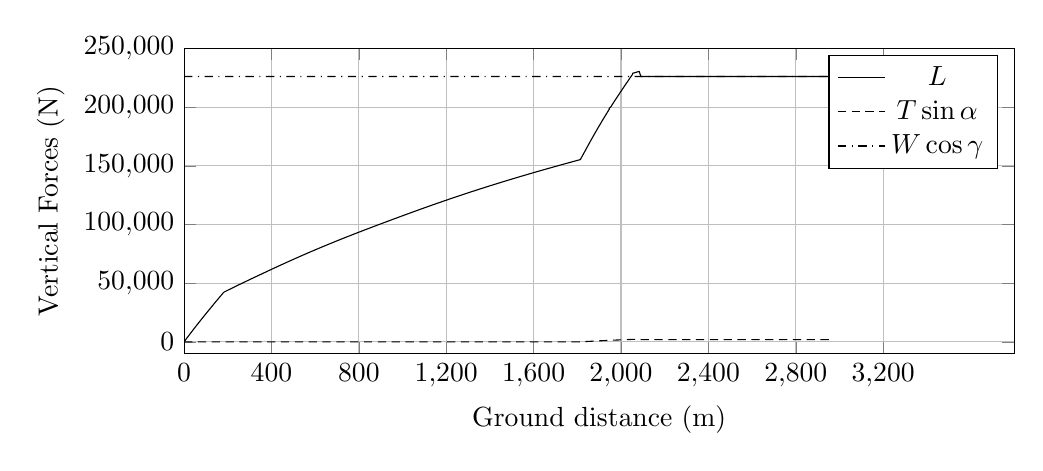
\begin{tikzpicture}

\begin{axis}[
width=\textwidth,
height=0.45\textwidth,
scaled ticks=false, tick label style={/pgf/number format/fixed},
xmin=0.0,
xmax=3800,
xtick={0,400,800,1200,1600,2000,2400,2800,3200},
xlabel={Ground distance (m)},
xmajorgrids,
ymin=-10000.0,
ymax=250000,
ylabel={Vertical Forces (N)},
ytick={0,50000,100000,150000,200000,250000},
ymajorgrids,
legend entries = {$L$\\$T\sin\alpha$\\$W\cos\gamma$\\}
]

\addplot [
color=black,
solid
]
table[row sep=crcr]{
1.3603393307215537E-8	3.4772441920621E-6\\
2.0334443352841076E-7	5.197807886499481E-5\\
1.8493358258961232E-6	4.727197167879655E-4\\
9.983129263424352E-6	0.002551846928078595\\
4.13538327636676E-5	0.010570697865030138\\
1.2467543572893382E-4	0.0318690194344414\\
2.843807411608912E-4	0.07269220163500548\\
5.588015241105573E-4	0.14283838745279587\\
9.398454696015893E-4	0.2402389466029825\\
0.0014155885812023746	0.3618457881515126\\
0.0019945752038215015	0.5098427984238072\\
0.0026717822370171283	0.6829457922438238\\
0.003447739291558293	0.8812899034226285\\
0.0043193476547732645	1.1040827907855042\\
0.00529092766782709	1.3524284738796992\\
0.006363550519206555	1.6266004073845632\\
0.007533073890550759	1.9255393966726797\\
0.008790616877968567	2.2469750287667027\\
0.01016549189277427	2.5983992679104437\\
0.011625499440327931	2.971581284498191\\
0.013184282533086976	3.3700077902679633\\
0.014839871214038253	3.793174719415961\\
0.01660567024659266	4.244507705757718\\
0.018465948346479452	4.719985240035992\\
0.0203822997817096	5.209790522852101\\
0.022430561433814646	5.733306256278752\\
0.024588423902376283	6.284829503322586\\
0.026831028501027587	6.858005952104252\\
0.029143159681622913	7.448946129204346\\
0.03155709159958957	8.065898045316786\\
0.03411445662773917	8.71950104306151\\
0.03677290089167576	9.398929367872057\\
0.03952314881844239	10.101811534327645\\
0.04239921643077808	10.83683998574839\\
0.045357163155895136	11.592783920881512\\
0.048363831658398165	12.361168864260808\\
0.051533845233668635	13.17128685441309\\
0.0547899150155587	14.003384849609883\\
0.058172599437445835	14.867826473817221\\
0.06162834747858026	15.750925660683649\\
0.06521401059050522	16.66720930348699\\
0.06888104003120077	17.604269917903594\\
0.07268727020998902	18.57688492487908\\
0.076546425570032	19.563006888788777\\
0.08047032364859658	20.565654755984312\\
0.08456364881336098	21.611576252942157\\
0.08882250397434277	22.699773254517858\\
0.09306368907640691	23.78343454323891\\
0.09743039119190974	24.899144948247496\\
0.10191450167634594	26.044830881552436\\
0.10651989152467789	27.221479569409674\\
0.11128201757858264	28.43814784559042\\
0.11609763023253863	29.668454958845714\\
0.12097769621339591	30.9152017866637\\
0.12591912973280778	32.17759896924592\\
0.13103216605369056	33.483806573513064\\
0.13633380151185176	34.83816348598073\\
0.1416823117522269	36.204462712082645\\
0.14708837902374172	37.585432174997266\\
0.1525605467319851	38.983253184723836\\
0.15824953188605478	40.436422584950705\\
0.16398006351864292	41.90016751915199\\
0.16978153473626356	43.38199480848152\\
0.17584258400626962	44.930083780968886\\
0.1819863832139092	46.49926630444509\\
0.18819485651962437	48.08492418626987\\
0.19455736971520038	49.7098794226506\\
0.20098158490654017	51.35054713694561\\
0.2076061353991409	53.04232984918988\\
0.21424726384720844	54.73829716247215\\
0.2211374965027113	56.49782718569165\\
0.2281284453493247	58.28302278011026\\
0.2350833915765042	60.05897102261541\\
0.2423085249848444	61.90385493903371\\
0.24958374984531584	63.76147101443941\\
0.2569279402934431	65.63663712387148\\
0.2644720218029696	67.56277881415835\\
0.27204626263318243	69.49655772718657\\
0.27972793364503945	71.45770025828281\\
0.2874622320100655	73.43221324318793\\
0.29563698092580604	75.51909900281441\\
0.30361763245720474	77.55636424847748\\
0.3118912000478351	79.66833040733462\\
0.3202493147046803	81.80180287046105\\
0.3286412952843002	83.94384340024442\\
0.33714554464307567	86.11446232858597\\
0.3458731203690518	88.34200138329291\\
0.35455185683415313	90.5569934166746\\
0.3634323904331427	92.82340395321586\\
0.372325738896249	95.09299969591174\\
0.38151551889959867	97.43815569060396\\
0.3908489672358084	99.81988168260173\\
0.4001862088113266	102.20248204308405\\
0.4095647137707429	104.59551757294787\\
0.4192312859369268	107.06195831641674\\
0.4289206911602753	109.53412475985053\\
0.43896550245304145	112.09686421807604\\
0.4487817299761361	114.6011811473339\\
0.4589033974758888	117.18331469325409\\
0.4691858798479248	119.8063623170124\\
0.47972601481223376	122.49502052142105\\
0.49016040525287174	125.15658887591411\\
0.5007175269203565	127.8493461054077\\
0.511266977039379	130.54002924859685\\
0.522323236324642	133.3598506062345\\
0.5332586746953114	136.14873114021458\\
0.5445869154512923	139.0376564100735\\
0.5556699580072249	141.86392130370086\\
0.5669225885056133	144.73330118066775\\
0.5785590177532589	147.70040943878797\\
0.5903083066022885	150.69615209464575\\
0.6020327889628274	153.68542675911488\\
0.613957077533064	156.72549773810977\\
0.625960998969677	159.7857221989073\\
0.6380070243193761	162.8565306806732\\
0.6503365955459197	165.99946643627032\\
0.662700086001522	169.1508913026655\\
0.6752747602080436	172.35598517721445\\
0.6885889407972636	175.74939111677133\\
0.7019767933734617	179.161390821304\\
0.7151149754112038	182.50958182699014\\
0.7284684478906998	185.91245783396073\\
0.7418939875700234	189.33351563459678\\
0.7553494584716574	192.76201650922928\\
0.7694215958599202	196.34744955132282\\
0.7830840331449673	199.82830334882578\\
0.796657372658726	203.28627029540786\\
0.8106660034246236	206.85493776645984\\
0.8251837647136968	210.55309647516168\\
0.8395067871054176	214.20144097674245\\
0.8540519574023793	217.90616002192712\\
0.8688334527125461	221.67085495238996\\
0.8840141863517745	225.5370043841158\\
0.8993797082767976	229.44998052925928\\
0.9143697020410035	233.26709825581457\\
0.9294094610857999	237.0966639471609\\
0.9452486359568626	241.12954182436067\\
0.9605773823977486	245.0322208531378\\
0.9761522209726621	248.99731677195075\\
0.9917649966835071	252.9718306997653\\
1.0074810114554809	256.97238362249186\\
1.0234652146968335	261.0409556772304\\
1.0399433598517231	265.23499195510976\\
1.0563627364420554	269.4138060471523\\
1.0728309985448887	273.6047972220812\\
1.0896486452479222	277.8844300584881\\
1.1068138420051672	282.2522211439564\\
1.124143995869574	286.6616963622\\
1.1415400048645106	291.0876350402\\
1.1590089082607062	295.5318252193192\\
1.1769249919091855	300.08947474185163\\
1.1951505705127592	304.7255391043718\\
1.2127191877709298	309.1941891584647\\
1.2308827453761335	313.81385349785364\\
1.2492706857898845	318.49026503543894\\
1.267587852451018	323.148356338809\\
1.2860031245644312	327.83107366851016\\
1.304687144125951	332.58179962476913\\
1.3233765774990474	337.3335706188677\\
1.342322280991234	342.15016034204484\\
1.3613696045164358	346.9922430167709\\
1.3815086998747366	352.1114963878001\\
1.4013123019267382	357.14509683409403\\
1.4209622886438908	362.1392878763145\\
1.4411501686096515	367.2698116395467\\
1.4611760119255748	372.3587790393684\\
1.4816444281325132	377.559826333954\\
1.501865958841821	382.6977566647265\\
1.5224364680875304	387.92396639006984\\
1.543651615594651	393.31354404554816\\
1.5647593029468103	398.6754089075755\\
1.5859558716309676	404.0594379426383\\
1.6071423964076703	409.44050227282446\\
1.6293386351549652	415.07757659514846\\
1.6508498980272122	420.5402597836113\\
1.673011606043147	426.1676777152426\\
1.6946435720294923	431.6601483888787\\
1.717066624993247	437.3530303954698\\
1.739432891071898	443.031039895709\\
1.761922286799709	448.73985038804756\\
1.7849035550437842	454.57304740203585\\
1.8076299607761817	460.34108543693833\\
1.8313298306791497	466.3556965628859\\
1.8543134894513886	472.1880639058677\\
1.8777326664639729	478.1304619849627\\
1.9017196849182967	484.2164361047088\\
1.925345883672024	490.2103614240849\\
1.950252961491087	496.52870555756033\\
1.975161211119453	502.84679606294117\\
1.9993825790313986	508.99012884379704\\
2.024583888346972	515.3814565445628\\
2.04934017380271	521.6593761526469\\
2.0744229633459703	528.019543843317\\
2.0996193404956136	534.4079578293847\\
2.1245764901457758	540.7351690796104\\
2.1500786393425866	547.1999883999692\\
2.176226227020705	553.8278387583844\\
2.202115608176549	560.3896539534189\\
2.227948363055355	566.9365377403374\\
2.2543499999408594	573.6269989363066\\
2.2810892744412783	580.4024082502403\\
2.3075963743135786	587.1183800124227\\
2.3348582111613405	594.0249465553056\\
2.3623221378972126	600.9820674398334\\
2.3898598419727675	607.9572306354844\\
2.4171687299087603	614.8737977742892\\
2.445442108612223	622.033975304626\\
2.4735885391813177	629.1613303808253\\
2.5015416452491293	636.2390680488579\\
2.5301110763218357	643.4721784822752\\
2.5589284934403693	650.7673775648016\\
2.587611617795936	658.0278881534434\\
2.6175687086884984	665.6101406340265\\
2.647724154312196	673.2418408987239\\
2.6767118187859253	680.5772870200913\\
2.7060305938995466	687.9958123104134\\
2.7361546404224653	695.6173538081896\\
2.7663022704956823	703.244111616392\\
2.7964672462043376	710.8745081199818\\
2.8272583584284883	718.6625182220948\\
2.8588650092419234	726.6559948295048\\
2.8898852960400587	734.5003832950567\\
2.9215246589961597	742.5005154308467\\
2.95270311230069	750.3833088617846\\
2.984506337549637	758.4232504615027\\
3.017379145769185	766.732726201021\\
3.049243647754313	774.7864942769713\\
3.081295157663824	782.886705227811\\
3.113406837946715	791.0012967757134\\
3.1453724573084756	799.0781600084945\\
3.1787286104953543	807.5055055376824\\
3.211019796961401	815.6629471752992\\
3.245786703184362	824.4448840477878\\
3.279939251746722	833.070706875759\\
3.3141720228361216	841.7158684689657\\
3.3491198891036547	850.5406702392756\\
3.382965192547779	859.0861476391242\\
3.4181848705561064	867.9776852357193\\
3.45391888941694	876.9980849782951\\
3.488851494856137	885.8152234104477\\
3.524271454997704	894.7544068683842\\
3.5606552075305	903.9358202285787\\
3.597189071478943	913.1540881297815\\
3.632926148839256	922.1703181576522\\
3.668897146318187	931.2445771653731\\
3.706642714683163	940.7654379383578\\
3.7432264628550644	949.9922088309156\\
3.781286297809391	959.5901850391858\\
3.818618572105483	969.0036194583029\\
3.8564015479305356	978.5296292287926\\
3.8948624022541356	988.2254462469616\\
3.9329637046009225	997.8295284054832\\
3.971505929995028	1007.5436489709036\\
4.009821706071438	1017.1995986541656\\
4.049014376833089	1027.075406303165\\
4.089343885784727	1037.2364883566975\\
4.128662304630717	1047.1416690937385\\
4.1684827283974055	1057.1721567997315\\
4.208000253554632	1067.125196808252\\
4.2483743636521965	1077.2928006639386\\
4.288255503180503	1087.3350911721477\\
4.328757204126676	1097.5324599761316\\
4.369490126907612	1107.7868469481555\\
4.410357715197167	1118.0739320260031\\
4.45189144941496	1128.527466502243\\
4.492881116440694	1138.8428529984822\\
4.53550011161515	1149.5669997859864\\
4.577670191557685	1160.1769130696134\\
4.6201174049766305	1170.8552773694714\\
4.662272021613388	1181.4587716005508\\
4.706017761800355	1192.4611687371125\\
4.748842845578064	1203.230710316985\\
4.792293145132742	1214.15616622352\\
4.836482439768313	1225.2660881601018\\
4.88090298307878	1236.4327801964955\\
4.925311889063089	1247.5951787871368\\
4.969864686447545	1258.7923754446442\\
5.014842280541593	1270.0949469368825\\
5.0603877575117515	1281.5388086080488\\
5.106292347304597	1293.0714660412946\\
5.152263975081851	1304.6195260218592\\
5.1974808794106995	1315.9765993601231\\
5.244027372436168	1327.6661783388986\\
5.28996242022761	1339.2007677493502\\
5.336209145350672	1350.8121887753155\\
5.38320569473032	1362.6104049522514\\
5.430469292142472	1374.4741755371351\\
5.476900151253712	1386.127471756753\\
5.526063828851289	1398.4650985457793\\
5.573879040902945	1410.4627973292158\\
5.622613575936374	1422.6896234976352\\
5.6713596863799225	1434.9177968975896\\
5.720412183296268	1447.2212627114586\\
5.770660497446668	1459.8230435958753\\
5.820668144990444	1472.3628433458616\\
5.870305285939629	1484.8081393188536\\
5.920503816994749	1497.3925786260065\\
5.971105439367246	1510.0764363549238\\
6.021088325934068	1522.6035967202838\\
6.071322359863801	1535.1921014331529\\
6.122981826035449	1548.1361483352566\\
6.174329110820436	1561.0003049150746\\
6.225804784288178	1573.8949636496764\\
6.278093246139479	1586.9915274372925\\
6.331709873490098	1600.4189830469022\\
6.384325657889258	1613.5940570356988\\
6.436648686434458	1626.6941259665364\\
6.489478972803882	1639.9194848347893\\
6.543185721519176	1653.3624983343752\\
6.596747696432654	1666.7675180725928\\
6.650345873843312	1680.1798495858761\\
6.704555155195255	1693.7433307460938\\
6.7588986063680725	1707.3386004120325\\
6.814371620173711	1721.214624004053\\
6.86997180120154	1735.1206073875205\\
6.925426612865756	1748.9883958631171\\
6.981353650685165	1762.9724252516303\\
7.037678624474159	1777.0540844782913\\
7.094603706786671	1791.2838762522015\\
7.151204881983983	1805.4308148445648\\
7.209200593921791	1819.9243638033786\\
7.2667780016693655	1834.3114402630094\\
7.324687293141565	1848.77950915796\\
7.382771066065313	1863.289228042036\\
7.441904508776327	1878.0591717657226\\
7.501585831803217	1892.9639346414397\\
7.5616527251378685	1907.9629429272572\\
7.62150963104709	1922.9074829823599\\
7.682859947113334	1938.2227875653116\\
7.7432084367972145	1953.2859376719216\\
7.803024936926759	1968.2142931397943\\
7.863793829029664	1983.3782978288682\\
7.9252460466886365	1998.7107367130775\\
7.98696966925656	2014.1087958608823\\
8.04776546969778	2029.273349384935\\
8.109421212326083	2044.650339833739\\
8.17269125419024	2060.427788931357\\
8.236095044780246	2076.2364172608804\\
8.299523592514586	2092.0490518457254\\
8.363213767675873	2107.924739741028\\
8.427807923256076	2124.0235473669745\\
8.49144930156071	2139.882727764084\\
8.557380457258176	2156.3102548604566\\
8.623183572921022	2172.703600474577\\
8.687840683575093	2188.809238528994\\
8.753751426394068	2205.2249075584386\\
8.820803713780364	2221.9225794204704\\
8.888970287482593	2238.8953606730865\\
8.957133699158991	2255.8649720797002\\
9.025036015045707	2272.7672257812656\\
9.092760955867519	2289.6229963598553\\
9.159817422823458	2306.3101115523996\\
9.227495373767134	2323.1495937068057\\
9.296013084156197	2340.1956910783183\\
9.36435980631623	2357.196923903458\\
9.433329865923408	2374.350869640467\\
9.503849553921977	2391.887812628922\\
9.574524061692681	2409.460814705518\\
9.644263228942293	2426.7988639352807\\
9.715657612596786	2444.545982008154\\
9.787429657508813	2462.3845047248733\\
9.85753688572494	2479.806865225575\\
9.930250735750551	2497.8745247251964\\
10.001571447096964	2515.5935895357834\\
10.074699859091687	2533.7592753761846\\
10.14698611653175	2551.7133013671228\\
10.220547980738981	2569.9816562320766\\
10.2940409891517	2588.2304086668\\
10.36719293590382	2606.392003328734\\
10.441008888975666	2624.7159684744074\\
10.51610421670324	2643.354978140017\\
10.590724589239105	2661.873573287541\\
10.667218005391902	2680.854402362791\\
10.742771202259895	2699.599359058805\\
10.82035208750042	2718.8447494985185\\
10.896759047300378	2737.796325561323\\
10.973503045910835	2756.828917134848\\
11.051297940743765	2776.119507174728\\
11.128076326409062	2795.155460754285\\
11.207667705350879	2814.886166157914\\
11.286758396846047	2834.4900612180954\\
11.366305937658339	2854.2045060394375\\
11.446149720998452	2873.9896759644544\\
11.526866579636565	2893.988467368261\\
11.607297517600138	2913.9137096564555\\
11.688034241538357	2933.9120035063834\\
11.769665722224765	2954.1291929489134\\
11.850920080706608	2974.2502710352037\\
11.933163326324259	2994.6134911403715\\
12.017103780766782	3015.3941156099027\\
12.10034832931326	3035.999664182452\\
12.185467765774142	3057.0664462109917\\
12.270669986481685	3078.1508428797124\\
12.354040133273898	3098.7791048313475\\
12.440386807402234	3120.1409862402825\\
12.52556588630658	3141.211174829402\\
12.610860989997974	3162.307263581518\\
12.69550109439961	3183.238600673765\\
12.784634337461807	3205.2781420021383\\
12.871172079509357	3226.673041422061\\
12.958447214271366	3248.247410011616\\
13.045518554761987	3269.7685815594414\\
13.133090172249581	3291.4105858353396\\
13.221405510214687	3313.2335471843335\\
13.310319106907201	3335.20147822961\\
13.399783591735492	3357.302641427257\\
13.488943611067967	3379.325741634678\\
13.578276665194153	3401.3887527141496\\
13.667402973129146	3423.3979016900084\\
13.757763665999576	3445.709039852948\\
13.848393619195729	3468.083817868149\\
13.938857764339925	3490.4148433914697\\
14.031101516310692	3513.182288360803\\
14.123507833735925	3535.9869697728363\\
14.214825187590282	3558.520092890102\\
14.307956552027534	3581.4979745644496\\
14.401498558574918	3604.574289143673\\
14.495315613017755	3627.715578873359\\
14.589065423003394	3650.837427333964\\
14.68316852398955	3674.0435640323685\\
14.778702641747682	3697.599703435062\\
14.873746415615575	3721.0320721618937\\
14.970384078097169	3744.8544986524494\\
15.068900921005241	3769.1371799738217\\
15.164434274206265	3792.681628704213\\
15.260378587808539	3816.324556543311\\
15.357189194448868	3840.178137680532\\
15.45495288999333	3864.2637045472475\\
15.55311774366497	3888.445247991418\\
15.652583807013901	3912.9444360143034\\
15.755243917873962	3938.227318746668\\
15.855950289561445	3963.0260862446066\\
15.958461094374158	3988.2662182749464\\
16.060387288500337	4013.3594628282353\\
16.164276126126843	4038.932899884863\\
16.26736468838029	4064.306385362096\\
16.36946523634058	4089.433816966215\\
16.47192386662276	4114.646531712537\\
16.576794358652606	4140.449832121829\\
16.678929175716583	4165.577214253966\\
16.783994526910618	4191.42271139894\\
16.89012564586595	4217.527468665545\\
16.996887404888547	4243.784421555554\\
17.103774697793426	4270.069346234568\\
17.210947675936964	4296.421642202105\\
17.31865021419634	4322.901275141345\\
17.424470519881233	4348.915370413124\\
17.53205215515201	4375.359672388533\\
17.64034909906897	4401.976998585802\\
17.74911485075183	4428.706751503163\\
17.85745376408675	4455.328853456131\\
17.969383314157206	4482.830431580947\\
18.07998395718984	4510.002681585918\\
18.18863741327577	4536.693863320726\\
18.302466989554325	4564.65376271107\\
18.41305080779906	4591.81368239077\\
18.525644000014054	4619.464390405752\\
18.636945827420575	4646.795298980431\\
18.750643923449367	4674.711928248431\\
18.86479622056296	4702.737372259071\\
18.979646899421056	4730.93157683497\\
19.09418630108147	4759.046709696144\\
19.208983505033515	4787.222498668269\\
19.323483295898072	4815.322711218867\\
19.43842354827664	4843.528467676586\\
19.55563752357537	4872.28958947749\\
19.67199913451129	4900.839012061271\\
19.789486593639566	4929.6621226522475\\
19.90713985662446	4958.523392582916\\
20.024127533725753	4987.21893132179\\
20.143019013955552	5016.3789777960355\\
20.26442367074238	5046.152894370718\\
20.383660776265387	5075.392786137067\\
20.5042342316437	5104.957964555635\\
20.622773342122727	5134.021981593689\\
20.74503732713029	5163.996904559857\\
20.865944869938517	5193.636943130357\\
20.98711015528624	5223.3378834718515\\
21.113336299999695	5254.276995133789\\
21.23638685227678	5284.435445163448\\
21.35988644990264	5314.701717070273\\
21.483760012473958	5345.057433469952\\
21.608180515260266	5375.545003500458\\
21.732326713270083	5405.963230334859\\
21.85766379468624	5436.6711358646735\\
21.985117186778353	5467.895415621762\\
22.111729024702363	5498.911450312193\\
22.23700541150786	5529.598350226543\\
22.36297326225872	5560.452677294012\\
22.488604760551	5591.222718020801\\
22.616276341350805	5622.490524457908\\
22.744235570279145	5653.826907162294\\
22.874576476768283	5685.744671278446\\
23.003842066605536	5717.397292744785\\
23.13088450205612	5748.503823470957\\
23.257869280739328	5779.594581968013\\
23.389244224935425	5811.758530192312\\
23.519811196806458	5843.723011862965\\
23.653309395988643	5876.403443330551\\
23.78342402399784	5908.2540177101055\\
23.9180644861338	5941.210899635233\\
24.05110504604577	5973.774651899334\\
24.182394801971697	6005.90844725743\\
24.314614014384034	6038.268356957478\\
24.449791085561472	6071.350813332501\\
24.585258581909038	6104.503008969039\\
24.72121222319008	6137.772885029981\\
24.857032405393277	6171.0088654191495\\
24.99454740444294	6204.658374745175\\
25.13030709358258	6237.877233545329\\
25.270890409679986	6272.275253031639\\
25.40663839363527	6305.489128952897\\
25.54307796688363	6338.871252700523\\
25.68272814639034	6373.037957650529\\
25.82072003425767	6406.798064409835\\
25.96015212691003	6440.909688975014\\
25.987750021099068	6447.661333158692\\
26.0558803939429	6464.328855233418\\
26.061632797568386	6465.736124177554\\
26.066808273335674	6467.002252326965\\
26.071901058608013	6468.248150090181\\
26.073315434863225	6468.594162583422\\
26.074595035914804	6468.907203654877\\
26.080371168076944	6470.320273466228\\
26.10234540095133	6475.696026179392\\
26.183408179590366	6495.526974212029\\
26.300430535410044	6524.154486267767\\
26.42750601924636	6555.240640475691\\
26.558056987479794	6587.176195732549\\
26.688030995483615	6618.969752057019\\
26.818767077324992	6650.948796025139\\
26.951519978077492	6683.420157964054\\
27.083955405447817	6715.812790450123\\
27.216897884715692	6748.328303489914\\
27.350913258119895	6781.105012108368\\
27.4833530065795	6813.495104990185\\
27.6176201223548	6846.330771560766\\
27.752160408628434	6879.231835287888\\
27.887329802382908	6912.285265420318\\
28.023188645890663	6945.505736981837\\
28.158973127824495	6978.706412260515\\
28.296372294036907	7012.3001933403375\\
28.435107205966254	7046.218765352318\\
28.571323599682245	7079.51978443611\\
28.70996262687553	7113.411164686344\\
28.850320389600306	7147.720687522309\\
28.988837241064125	7181.578165411716\\
29.129197813929657	7215.884169459365\\
29.27166529868488	7250.702876688691\\
29.41298471572133	7285.23869632809\\
29.554848516656044	7319.905188196453\\
29.699676691743235	7355.293563955955\\
29.842400551696755	7390.165222124753\\
29.985385440862252	7425.098077573322\\
30.129077275410303	7460.200989301695\\
30.27543774584293	7495.953031619338\\
30.422081339040986	7531.771341945752\\
30.56949149516445	7567.773912237659\\
30.716562179458485	7603.6905398573945\\
30.86535310281699	7640.024132067658\\
31.011875026602333	7675.800508089851\\
31.16159928701196	7712.355520472218\\
31.313692569485013	7749.485472203682\\
31.463056706803336	7785.945721618929\\
31.61235366859384	7822.3861038743\\
31.76278957628285	7859.100915505265\\
31.915019899787076	7896.249966473009\\
32.06709627595497	7933.357677705588\\
32.21861178877769	7970.324729937509\\
32.37168228565527	8007.667258767406\\
32.52450570609457	8044.945534931163\\
32.67702483599189	8082.145569712253\\
32.829998687403204	8119.452429963638\\
32.98551220909506	8157.374412667037\\
33.14332298937855	8195.852150438946\\
33.29970221124884	8233.976384405563\\
33.45800124694219	8272.564081234515\\
33.61398946945653	8310.583927685468\\
33.77048353048475	8348.722468148972\\
33.9292721471582	8387.415446991858\\
34.08796840843395	8426.081079545085\\
34.24769686644211	8464.99326232537\\
34.406855482575295	8503.76164235055\\
34.56481953291838	8542.234079890593\\
34.72399692808165	8580.996975648039\\
34.88694269464703	8620.672239471998\\
35.04914399338672	8660.1608523031\\
35.209965099803895	8699.308100157981\\
35.3703140559587	8738.3350638915\\
35.531685786905925	8777.605514801711\\
35.69349909442164	8816.977894652682\\
35.85522798807463	8856.324154782007\\
36.022509111806116	8897.015272900742\\
36.19055880791667	8937.88723734054\\
36.35708622463872	8978.382874308081\\
36.52115360367851	9018.274313388072\\
36.68781562330062	9058.790498701579\\
36.8536847754776	9099.107769477407\\
37.024522648961764	9140.626294410133\\
37.19188554678789	9181.293881802605\\
37.36066720850286	9222.29973704978\\
37.528862119520696	9263.156524573904\\
37.697264258302326	9304.057091370745\\
37.86832931534104	9345.597649734304\\
38.03812867477943	9386.824069325201\\
38.20923731912278	9428.361497819948\\
38.37904730305398	9469.576802467946\\
38.55252405124031	9511.67497636085\\
38.72282139824354	9552.994567916754\\
38.89783411301201	9595.450964257961\\
39.0714610757495	9637.56384368624\\
39.24438070689564	9679.497848925424\\
39.41969314875929	9722.004635731242\\
39.59166556575205	9763.694226335727\\
39.764623188591585	9805.615258475122\\
39.94263254662576	9848.752938294463\\
40.11749159802578	9891.119472798946\\
40.29452954971913	9934.00610137832\\
40.47247750600427	9977.105197900422\\
40.64799609178485	10019.608030711639\\
40.82414741101539	10062.256192549707\\
41.00385670225303	10105.757597598276\\
41.18169069533937	10148.796890574216\\
41.3603281005193	10192.022412389342\\
41.54046179251334	10235.601628491058\\
41.722675278204306	10279.675421592998\\
41.90258931008478	10323.184523136533\\
42.08518735141125	10367.334038692832\\
42.26728550944881	10411.353963236474\\
42.44743534848537	10454.894301407418\\
42.63069538383506	10499.177530542816\\
42.80963512098974	10542.408193847452\\
42.992542679335614	10586.588644143707\\
43.17926890616222	10631.68225716578\\
43.363134036078335	10676.075798843754\\
43.54815051311773	10720.738159017023\\
43.733578141849236	10765.490514375102\\
43.91798130912079	10809.986404881329\\
44.10506009255049	10855.11849796987\\
44.29251116260117	10900.33086804222\\
44.480917546793805	10945.764012900916\\
44.66851287589745	10990.99194790866\\
44.85853501730759	11036.79515237239\\
45.047396872181054	11082.30886630946\\
45.236914792155844	11127.97082877206\\
45.42785879536018	11173.966381633963\\
45.616432631699865	11219.381118728772\\
45.80697204128492	11265.259239862069\\
45.998633580597016	11311.397397399185\\
46.18800675699903	11356.974666751623\\
46.380841640082096	11403.374830667755\\
46.57327038933336	11449.666942947762\\
46.765844918266424	11495.983780115806\\
46.95911042680183	11542.456386478036\\
47.15311668852311	11589.096598824468\\
47.34541611633634	11635.316066760875\\
47.53884854699059	11681.797381889344\\
47.73236991243341	11728.289544433825\\
47.92818250719388	11775.321432220153\\
48.12326385407131	11822.166940872215\\
48.32058854034828	11869.540230160179\\
48.516852452700604	11916.6479460519\\
48.71339374517507	11963.811329906828\\
48.91319881343868	12011.746710644944\\
49.1119162355681	12059.40994260776\\
49.31207818344666	12107.40833880967\\
49.509673461222235	12154.780109867632\\
49.71156302510582	12203.169956435457\\
49.91034548441702	12250.803770376097\\
50.11200805970151	12299.116269439877\\
50.30853267551517	12346.186741404275\\
50.50757456960626	12393.84894329355\\
50.70929197287772	12442.140319377286\\
50.91222418686718	12490.710838853603\\
51.11562549758783	12539.381870932997\\
51.32090674103446	12588.490801419757\\
51.525199701657655	12637.35139433455\\
51.72863462744459	12685.99496083595\\
51.934060761332375	12735.102687196068\\
52.14033810224923	12784.40180379738\\
52.344882977561255	12833.274905492799\\
52.55098100649393	12882.50706152905\\
52.75731843494604	12931.784290266485\\
52.96514817708821	12981.40566072195\\
53.17450540782369	13031.379306605693\\
53.382202621450276	13080.9443849165\\
53.592230583406476	13131.053200909286\\
53.80364534107798	13181.480217692388\\
54.01469481143569	13231.807439648179\\
54.223966920081466	13281.698340012299\\
54.43230789395902	13331.354909945952\\
54.6430562980421	13381.572748609626\\
54.855225786754914	13432.116492209923\\
55.066088958624874	13482.33640876822\\
55.27969530828261	13533.196820749614\\
55.49171188337613	13583.665943952405\\
55.70388919125476	13634.16061500573\\
55.91737779085577	13684.954527160102\\
56.13177028494084	13735.95056373877\\
56.34652664868587	13787.020171390617\\
56.559021044851505	13837.539104678071\\
56.77591447970492	13889.090788517631\\
56.99548236897459	13941.264690995216\\
57.21481285737903	13993.368687145\\
57.43536222847358	14045.748657583907\\
57.65367025761124	14097.582919114036\\
57.872788904232735	14149.596268076912\\
58.0907693980174	14201.326163567486\\
58.311927420720366	14253.796611610844\\
58.532333513628615	14306.075133567228\\
58.75532998033057	14358.954348481206\\
58.976617007999806	14411.41458153638\\
59.19875422837053	14464.062743654838\\
59.4206945143671	14516.650621367633\\
59.64453328369959	14569.67458319051\\
59.86894932484513	14622.821451049378\\
60.09432075877773	14676.180656843742\\
60.318058693038594	14729.13934063352\\
60.541731124044205	14782.068830227327\\
60.76707064338231	14835.379003792874\\
60.995574692986196	14889.423704220731\\
61.22378989589207	14943.385918070151\\
61.4534619981562	14997.678354827804\\
61.683510138770515	15052.045369612202\\
61.91410430469678	15106.527081990556\\
62.14462153858659	15160.97629765356\\
62.37563158073512	15215.527587295608\\
62.607203285434	15270.19714711397\\
62.841031881319736	15325.38496062216\\
63.07467935056491	15380.515454202574\\
63.31164975340633	15436.41517498552\\
63.54633691305479	15491.761605180207\\
63.78243968758058	15547.427170410414\\
64.0165414084598	15602.606422892728\\
64.25412817577254	15658.592373800333\\
64.49270299572771	15714.796245489328\\
64.73076499662056	15770.864458853477\\
64.96867826857735	15826.88286991193\\
65.21063576532572	15883.83842103045\\
65.4512107007771	15940.453471708828\\
65.69028017871045	15996.699417243632\\
65.93032615763332	16053.160285006783\\
66.17196619696679	16109.981139757729\\
66.4135612157637	16166.776462218\\
66.6559030093851	16223.732376262386\\
66.89910102540284	16280.87450683795\\
67.14354652182666	16338.294641347504\\
67.38771133480921	16395.633778022755\\
67.63347396558368	16453.332991958996\\
67.87898066495345	16510.95699756978\\
68.1255935515739	16568.82548113312\\
68.37316753306138	16626.90426216935\\
68.62205497364681	16685.27585029707\\
68.8711887275476	16743.68988278613\\
69.120220471977	16802.064735428932\\
69.36846244647072	16860.23933405998\\
69.61951843592018	16919.058088465405\\
69.87236615109754	16978.281131856813\\
70.12758921381476	17038.044843759395\\
70.37945082809051	17097.006036727806\\
70.63410009691182	17156.604344537525\\
70.89152727368702	17216.837044598542\\
71.14629115974091	17276.431065920595\\
71.40197865069018	17336.225678607218\\
71.66163317144085	17396.93223835869\\
71.92484704501203	17458.454815835088\\
72.18465416754285	17519.165242518335\\
72.44573394560723	17580.157250102216\\
72.70633339061075	17641.021319364096\\
72.96699363118216	17701.88394782388\\
73.22900401485182	17763.046141250168\\
73.49076816912304	17824.135231100896\\
73.75430841254712	17885.623117956842\\
74.01895646534612	17947.35370554981\\
74.2846979982242	18009.323537667195\\
74.55380714249793	18072.062618340628\\
74.82322871850147	18134.858432175424\\
75.09350011520078	18197.83621688115\\
75.36421232425869	18260.900641575914\\
75.6347219158074	18323.90188426291\\
75.90830954343213	18387.603841478747\\
76.18188601743822	18451.287051002626\\
76.45626363461818	18515.14062561473\\
76.72958718025629	18578.732935388936\\
77.00406935908524	18642.578883147064\\
77.28579748399531	18708.09377268693\\
77.56784659723587	18773.666667165788\\
77.84569092555657	18838.245827359926\\
78.1246978223638	18903.079153246785\\
78.40641219364133	18968.52540880387\\
78.68590470271565	19033.43950375882\\
78.96851680469001	19099.062060224824\\
79.25576208114188	19165.743978701\\
79.54169104977237	19232.103959325614\\
79.82662017154695	19298.215761520507\\
80.11330301632765	19364.718345279973\\
80.40394576721474	19432.123119897704\\
80.6908099930996	19498.635521555887\\
80.98055888331655	19565.800675277147\\
81.27178512217935	19633.292117586185\\
81.56682943128612	19701.651993368367\\
81.86186977412851	19769.994572492804\\
82.15688924927383	19838.316073011832\\
82.44965588234726	19906.09992452993\\
82.74488606927187	19974.438221710705\\
83.04325841243121	20043.48772256601\\
83.34213327641098	20112.637402413828\\
83.64411622775171	20182.489950636642\\
83.94734638805741	20252.6147138129\\
84.25123842984891	20322.87632182637\\
84.55152885577829	20392.289407816817\\
84.85735750691177	20462.96666957118\\
85.16518306664875	20534.089263289286\\
85.47136476235073	20604.816119355768\\
85.77898122624802	20675.858561112866\\
86.08923229760057	20747.493527247956\\
86.40254560035129	20819.81947487998\\
86.71167807044037	20891.164645110133\\
87.02660518802142	20963.831336827323\\
87.34238286044419	21036.678408890264\\
87.65842706333811	21109.57121837973\\
87.97971380652302	21183.657200574715\\
88.2973933745065	21256.895740656095\\
88.61789013566766	21330.76816355715\\
88.93643920279564	21404.17630797664\\
89.25662431900213	21477.946232801776\\
89.57903058309674	21552.212649893947\\
89.89968694948243	21626.060976516084\\
90.22473455398588	21700.90553992342\\
90.55024875587375	21775.84251431976\\
90.87789352676518	21851.25497815926\\
91.20733069500889	21927.06502366771\\
91.54101415610151	22003.83713157155\\
91.87012785371462	22079.54317472784\\
92.20120197152713	22155.685669497303\\
92.53416638543635	22232.2484405387\\
92.86431843528567	22308.15040964271\\
93.19748455591187	22384.7312689619\\
93.53066771200866	22461.302143335284\\
93.86681917526724	22538.541308860833\\
94.20530590547477	22616.303197569243\\
94.5419273964865	22693.623000322186\\
94.8854212036891	22772.50759973751\\
95.22752713476521	22851.05991212617\\
95.57091181422334	22929.892470088445\\
95.91383450860906	23008.605829015665\\
96.25469535763642	23086.83313695353\\
96.5966517898868	23165.299306332614\\
96.93845701474973	23243.7184244027\\
97.28153572459905	23322.41752540027\\
97.62213139590432	23400.535192966076\\
97.9659652144934	23479.383810650135\\
98.3129807304216	23558.950343318873\\
98.65852794036775	23638.168755235667\\
99.00080640577195	23716.626759285224\\
99.35064076251427	23796.805645157612\\
99.69796076807248	23876.397410095553\\
100.04654253174803	23956.26769389261\\
100.3915606488718	24035.3112048236\\
100.74261509654437	24115.727434504923\\
101.08877163494762	24195.011869242953\\
101.43457754260953	24274.20649685202\\
101.784020212797	24354.224603342533\\
102.13161434601102	24433.81030031859\\
102.4751980097893	24512.46906300758\\
102.82212110631409	24591.883823275763\\
103.16739702108615	24670.913270756944\\
103.51524666207362	24750.523736564486\\
103.86391679154056	24830.31410085615\\
104.20960434827006	24909.4143868729\\
104.55241399635099	24987.848979994502\\
104.89662223620601	25066.59663170298\\
105.24103428322039	25145.384197479834\\
105.5836615386647	25223.757056594928\\
105.92645892081137	25302.162667863216\\
106.27347658175316	25381.52752423902\\
106.6151670762521	25459.668346215083\\
106.95898391938218	25538.289995896645\\
107.30023552029138	25616.319886403922\\
107.64147805753461	25694.342809011236\\
107.98348674656944	25772.536238626708\\
108.32522459759954	25850.66332176004\\
108.3935347040271	25866.27966454997\\
108.40478590462831	25868.851780590885\\
108.41572478024443	25871.352492313752\\
108.4246743308916	25873.398425799103\\
108.44347342986478	25877.696029711726\\
108.52018987797786	25895.233809815727\\
108.70071173483461	25936.50120712282\\
108.99446230248458	26003.65012895863\\
109.30176454987088	26073.893188050795\\
109.60899173332959	26144.115124104377\\
109.91608539831654	26214.302359090987\\
110.22883517949637	26285.7777924251\\
110.54143546549608	26357.214269835014\\
110.853845249356	26428.60220187762\\
111.1739714794031	26501.74796777583\\
111.4937490010879	26574.808333198496\\
111.81170779322963	26647.44726414202\\
112.13106495813236	26720.399500993997\\
112.4519453366479	26793.693246083465\\
112.77515902629136	26867.51318802787\\
113.0997499810409	26941.640621253566\\
113.43040796942478	27017.14607110901\\
113.7597028375028	27092.33246741943\\
114.0907450350197	27167.909750515617\\
114.42538740208008	27244.300485560816\\
114.75997726261329	27320.67047675857\\
115.09477047197589	27397.07787517151\\
115.43440545481076	27474.580824185774\\
115.77494672336013	27552.280778073356\\
116.11687534861284	27630.28715395397\\
116.46164587354252	27708.931347928876\\
116.8077846490165	27787.876768115057\\
117.15688723722127	27867.486863572725\\
117.50557855048987	27946.991596632506\\
117.85411336711965	28026.448838563803\\
118.20532793701167	28106.504806058823\\
118.55850697655507	28186.995964570437\\
118.91273956155123	28267.714298480918\\
119.26983096270519	28349.070704957412\\
119.62978614725739	28431.065739163518\\
119.98960731920661	28513.01611562987\\
120.34734904217265	28594.478637716013\\
120.7138511704587	28677.921027193923\\
121.08106061642908	28761.508978817088\\
121.44737887966437	28844.87838294309\\
121.81499139152783	28928.526338026808\\
122.18511446431708	29012.729106832943\\
122.55384158147794	29096.597636047052\\
122.92460728481757	29180.912835222574\\
123.29616941264607	29265.39178489196\\
123.67040864389355	29350.46158825628\\
124.04652172406458	29435.93908126941\\
124.42393851457416	29521.694212484304\\
124.80152108360014	29607.468072083066\\
125.18180835736592	29693.836956381077\\
125.55854932865631	29779.38099488223\\
125.93878032356085	29865.697645789136\\
126.31997081831156	29952.211867003818\\
126.70099538833193	30038.66793774999\\
127.08058279416298	30124.777309199897\\
127.46175209000612	30211.22461585585\\
127.84399628255431	30297.8944310488\\
128.22749916598133	30384.828010315963\\
128.6102537001487	30471.570129377862\\
128.99595881306152	30558.958653922076\\
129.37788117916477	30645.467885648497\\
129.760738924708	30732.16656690902\\
130.1448498512433	30819.12626526002\\
130.53000390659713	30906.29901722008\\
130.9168242384266	30993.825413158876\\
131.29443328439476	31079.244660954777\\
131.67491382268804	31165.290402941697\\
132.05816436539135	31251.938985203145\\
132.44070735535217	31338.40379585961\\
132.82666098215685	31425.61521627735\\
133.20952005887244	31512.103101505585\\
133.5940193955625	31598.937005619176\\
133.97617966856654	31685.218146489082\\
134.36103715882757	31772.083369829066\\
134.74478042358356	31858.672082568875\\
135.12867144169206	31945.268969618963\\
135.5141335746535	32032.19477550344\\
135.89764893392993	32118.656056674714\\
136.28231234485685	32205.35044602662\\
136.66418763078912	32291.390830861492\\
137.04684871033697	32377.58250381628\\
137.42845627025127	32463.51105444735\\
137.8132447087305	32550.129603244714\\
138.19719797258034	32636.533726616603\\
138.58059071069573	32722.78523615445\\
138.96593237593703	32809.44840009129\\
139.3501607499636	32895.834305741155\\
139.73355638294606	32982.00610238113\\
140.1160230155566	33067.94221287937\\
140.50045093994146	33154.29182041924\\
140.88215178690393	33240.001790502094\\
141.26156782058217	33325.171847266785\\
141.64323970440188	33410.821152112214\\
142.02689350659642	33496.887666347495\\
142.41061312971692	33582.94121196876\\
142.7942251403153	33668.94278959381\\
143.1756303563767	33754.42193139653\\
143.5599719391364	33840.531119989944\\
143.94242380128833	33926.18888661219\\
144.3239499176869	34011.61134362113\\
144.70664939692608	34097.26835127214\\
145.0870075357763	34182.37327347683\\
145.46856550308127	34267.71848038807\\
145.85014610541765	34353.040438701224\\
146.23128237819492	34438.234695402934\\
146.61504730324998	34523.98781606939\\
146.99763315977907	34609.44871200262\\
147.38441582478964	34695.81780765658\\
147.7673688364352	34781.30266296498\\
148.15222568696134	34867.18328190521\\
148.53580865353604	34952.75041141722\\
148.9199734867533	35038.4180271088\\
149.3040357319486	35124.03337305144\\
149.68771357306542	35209.533615129156\\
150.07093078701052	35294.901799542786\\
150.45622889618164	35380.70384354798\\
150.8449053483268	35467.2279796763\\
151.2288570611563	35552.67045966184\\
151.61452719766493	35638.46540225977\\
151.9983007305741	35723.808585872335\\
152.38299664478842	35809.32695426872\\
152.76945776909372	35895.207503623315\\
153.15580177123394	35981.03169337765\\
153.54253364040335	36066.91162453529\\
153.93093169697067	36153.13087957441\\
154.31788037931886	36238.99777528124\\
154.7039882138024	36324.647578162025\\
155.08880221957185	36409.980017338734\\
155.47621608980313	36495.858326101516\\
155.866104687065	36582.25412463036\\
156.25391419262098	36668.15824614768\\
156.64166339424906	36754.018098342625\\
157.03027969880475	36840.03891122689\\
157.4213807682267	36926.57832517376\\
157.8105708506119	37012.66359074396\\
158.19948541262937	37098.65669665253\\
158.58893406813365	37184.73660279387\\
158.97894817604634	37270.91008647386\\
159.3710019698692	37357.502544083516\\
159.76139479981174	37443.69655376593\\
160.1523485688823	37529.98280229799\\
160.54128874338664	37615.79323383416\\
160.9326976430911	37702.11669843538\\
161.32564259741588	37788.74700247326\\
161.71827778345698	37875.27704953967\\
162.1124492087963	37962.113510789204\\
162.50576001021273	38048.72826613055\\
162.89904576730015	38135.30543129824\\
163.29316224934274	38222.033293090455\\
163.68899123279596	38309.105579821204\\
164.08495392634194	38396.17477213488\\
164.48271131475576	38483.60587341734\\
164.8792309171331	38570.73224995112\\
165.27343112400507	38657.31668695461\\
165.67115293733156	38744.6419965782\\
166.06936395728349	38832.041889225104\\
166.47000821435734	38919.94269318128\\
166.87155839526775	39008.00891685668\\
167.27134041220108	39095.65421384183\\
167.67233991204222	39183.53322136785\\
168.0705846918417	39270.775640780805\\
168.47232570996516	39358.75078138479\\
168.87521546679773	39446.9440221026\\
169.2789990941189	39535.299341455524\\
169.68142011368735	39623.32306465671\\
170.088438196605	39712.31840644407\\
170.49328200513543	39800.80452663968\\
170.89845866435633	39889.32966579344\\
171.30484584057905	39978.085421237745\\
171.7103088520891	40066.605573195644\\
172.11589069074847	40155.11796310739\\
172.52485519917514	40244.334478286415\\
172.93316089774754	40333.373160252435\\
173.34236088095247	40422.572702728765\\
173.7535761368399	40512.17714354908\\
174.16510964781833	40601.816452727915\\
174.5786011126259	40691.847547258745\\
174.99051444770384	40781.50050372306\\
175.40138574541044	40870.892382344886\\
175.81497300453447	40960.84064113091\\
176.2280441317456	41050.64213308699\\
176.64225100058474	41140.65595346608\\
177.05714873395152	41230.7852525084\\
177.47483026786767	41321.48430820454\\
177.89254345086653	41412.15520258492\\
178.3100126079721	41502.73818715001\\
178.7278240622369	41593.360536448\\
179.1449731538625	41683.8044492952\\
179.56482315926417	41774.79894633136\\
179.9871804296257	41866.30147639837\\
180.4095742002126	41957.77650941428\\
180.83428717371925	42049.71817506499\\
181.26003251256287	42141.84755576178\\
181.6840913989422	42233.57647395109\\
181.8934642440371	42278.85323173496\\
182.1114839456617	42325.99071418175\\
182.5372774346568	42365.721046592924\\
183.423900814602	42448.42214025985\\
184.30144226609173	42530.23787759933\\
185.17422251923585	42611.572071266724\\
186.05126240753827	42693.26548136593\\
186.93861419286333	42775.88099255948\\
187.8243328275641	42858.30599816181\\
188.7212117513506	42941.73051926721\\
189.61004025875786	43024.367527179944\\
190.50102451880866	43107.166391806924\\
191.38947474753866	43189.691405790596\\
192.28052744689825	43272.41976576044\\
193.18778236606096	43356.612989135814\\
194.08895872822546	43440.2028556561\\
194.99680020640938	43524.37148150704\\
195.89480429656658	43607.589174849185\\
196.79674305679504	43691.13266831025\\
197.7065692706791	43775.367429272446\\
198.612023604503	43859.158321379655\\
199.52644538440046	43943.73957409081\\
200.43881964763966	44028.09199376036\\
201.34572312669928	44111.89967864775\\
202.26115686844895	44196.45638736435\\
203.17967892292364	44281.258819112714\\
204.1017087672932	44366.3453881569\\
205.01405834107487	44450.49958638108\\
205.94020355690031	44535.88665834683\\
206.86420646269943	44621.036553177866\\
207.79153006365993	44706.45274779602\\
208.72800400232427	44792.67153145422\\
209.6603812871926	44878.473084969926\\
210.59913361291103	44964.8210399278\\
211.54272242703126	45051.57328346596\\
212.4892775421681	45138.55750043105\\
213.4278558742791	45224.7685238307\\
214.37319863683314	45311.56058598391\\
215.31618532994997	45398.09618435576\\
216.26909967312713	45485.50221848843\\
217.2229300472723	45572.95154336793\\
218.17915574443117	45660.57971364992\\
219.13394290547268	45748.03547781623\\
220.0901210939433	45835.578163212005\\
221.05386294760763	45923.77248149943\\
222.0194744620763	46012.09690989624\\
222.9871855528732	46100.57237822977\\
223.95850156259326	46189.336308006954\\
224.93506896411378	46278.538756704715\\
225.9123601081958	46367.76593590774\\
226.89683950214788	46457.60771841463\\
227.87812705537118	46547.116747187916\\
228.86553252311342	46637.14220188472\\
229.85786107077195	46727.574615886464\\
230.84893890233656	46817.85130175264\\
231.8352011637358	46907.648093915835\\
232.83551070617193	46998.68200494934\\
233.8409775535427	47090.142967351465\\
234.84473749332597	47181.4065529786\\
235.85076677249623	47272.83443913986\\
236.86174655712836	47364.67002512248\\
237.8698887650736	47456.20591266168\\
238.88314164945962	47548.163826178585\\
239.88702917374013	47639.23044527351\\
240.9073981595622	47731.75019241701\\
241.92631922506058	47824.09662870786\\
242.95020737895555	47916.85114080258\\
243.9867665418509	48010.71074592552\\
245.01566609591487	48103.834422049156\\
246.05919400906686	48198.23919290141\\
247.09706457910846	48292.089536125466\\
248.1403037320082	48386.38271782891\\
249.18309170866138	48480.59263829395\\
250.23723200462985	48575.785233834846\\
251.28895058541582	48670.716342891465\\
252.34575298177748	48766.06350550585\\
253.4009695529494	48861.224991875235\\
254.47389199439823	48957.93982505982\\
255.55293546958148	49055.162526630826\\
256.6206413021679	49151.320620475744\\
257.69235364004487	49247.796699787796\\
258.77967411403563	49345.63422273559\\
259.8615409937813	49442.93769352199\\
260.93956317950165	49539.85263257098\\
262.02271022117964	49637.185592363865\\
263.11073386748035	49734.91393572668\\
264.2120045516847	49833.788707737825\\
265.31241535302627	49932.54289648302\\
266.4086016357777	50030.87512587613\\
267.51260488983417	50129.86563404625\\
268.6300148019782	50230.0146646676\\
269.7585470354529	50331.116337595886\\
270.8896873949477	50432.40738885691\\
272.0115439451323	50532.823616687994\\
273.13680176546006	50633.50109534628\\
274.2702490513931	50734.867867251654\\
275.413525774062	50837.069876410504\\
276.5542367829295	50938.99897374622\\
277.6972773917919	51041.09292017647\\
278.856653662284	51144.60197377125\\
280.02457374883886	51248.82939996467\\
281.2032739103363	51353.97401332356\\
282.3793508291475	51458.8400772203\\
283.5570819158503	51563.80940587785\\
284.7419934858003	51669.374417333966\\
285.9326270157934	51775.4048162485\\
287.128931254976	51881.89577821194\\
288.31480266049743	51987.41446056476\\
289.5063986037633	52093.399181642875\\
290.71803378146524	52201.12211784047\\
291.92377285751195	52308.27705571306\\
293.1368845155397	52416.04351406629\\
294.3779382526999	52526.24727596404\\
295.6236529225306	52636.819664960596\\
296.8710892485976	52747.49987792599\\
298.1231876568165	52858.54890883132\\
299.3513516362168	52967.431987104064\\
300.60759883822345	53078.76097391687\\
301.8758306910943	53191.107560966266\\
303.15324510629466	53304.22288390421\\
304.4174613942848	53416.12581221628\\
305.70907350215657	53530.40929692182\\
306.99802587761087	53644.41320338877\\
308.28687847241804	53758.36459576916\\
309.5668796159489	53871.49066317806\\
310.84791377823	53984.66587919234\\
312.1498528537303	54099.64528429629\\
313.4560044202801	54214.95398771769\\
314.75458395299495	54329.552324831486\\
316.0753084557979	54446.06262214895\\
317.40968260857574	54563.7342753815\\
318.7319345228668	54680.29507772399\\
320.0558782097702	54796.96383227594\\
321.3801932183561	54913.624640903\\
322.6884764655432	55028.833799566084\\
324.0456734620244	55148.30957831835\\
325.39100935110525	55266.70080366745\\
326.7365982993339	55385.074654202894\\
328.06652939861567	55502.03267922859\\
329.40155074930124	55619.400566271055\\
330.74537767281527	55737.50494469814\\
332.0707513255394	55853.951112030394\\
333.4173386205282	55972.224648032585\\
334.746581315361	56088.93933221049\\
336.0867229892568	56206.57595436739\\
337.4205715422614	56323.62581526069\\
338.75500413875113	56440.69322259069\\
340.08105948956893	56556.992899012286\\
341.3989527111596	56672.54490074742\\
342.72155317639294	56788.4783097765\\
344.04109435086104	56904.11286506454\\
345.35282448543626	57019.033110557575\\
346.65609809876	57133.18361271088\\
347.964660055904	57247.76892081268\\
349.26930822844486	57361.98376237397\\
350.5666013847051	57475.527793991714\\
351.8669806622215	57589.315556020534\\
353.150344321377	57701.58904502529\\
354.42669516744513	57813.22459063007\\
355.7084983713929	57925.31303719421\\
356.9839654050402	58036.82408616431\\
358.2578487323243	58148.17398482238\\
358.5108324321051	58170.28458940933\\
358.64800612588874	58182.27311398652\\
358.7323961896923	58189.648398200676\\
358.9732456649284	58210.696950608064\\
358.99979477666295	58213.017108647706\\
359.01768095024534	58214.580197006464\\
359.0292585237206	58215.59196898824\\
359.04030674366413	58216.55747872559\\
359.0932275856527	58221.18223609294\\
359.3119468898926	58240.295735976004\\
359.96663022276493	58297.5034884256\\
361.01382689254797	58388.99766595705\\
362.10337816976426	58484.1759582442\\
363.2064629717895	58580.51897651123\\
364.30797819224426	58676.70689961879\\
365.4187311446934	58773.6828285354\\
366.533107917645	58870.95586508997\\
367.64647721929396	58968.12123939789\\
368.7658299095233	59065.78848062322\\
369.8975033538602	59164.50959648553\\
371.0334235675839	59263.57933794157\\
372.1785809863062	59363.432099829486\\
373.31981642046355	59462.91984589795\\
374.47796099960044	59563.85768219073\\
375.6447818548355	59665.52680645339\\
376.82127927712384	59768.01330976722\\
377.99866547828844	59870.55084786235\\
379.1872933927376	59974.04015540013\\
380.3777690794409	60077.66240152581\\
381.57556676946103	60181.89326682131\\
382.7749421474674	60286.232080699294\\
383.9810457964097	60391.12612035316\\
385.1925430839308	60496.45836853271\\
386.4130201303027	60602.539570376175\\
387.642251751972	60709.348958140545\\
388.8666959950373	60815.70920139896\\
390.1046277660565	60923.20687891891\\
391.36074966763465	61032.248516594555\\
392.6213644701743	61141.64359691097\\
393.8865770487704	61251.400304412586\\
395.152064769563	61361.14291949014\\
396.42651061844674	61471.623492464714\\
397.70785411533086	61582.662153365905\\
398.9973066037893	61694.36264776741\\
400.29415225393086	61806.661698818905\\
401.5867618821628	61918.55161383936\\
402.89266069540326	62031.54842535638\\
404.2026906817056	62144.85831118465\\
405.5133159752146	62258.17467572288\\
406.8188033215648	62371.001542434766\\
408.1428210789858	62485.38323203851\\
409.4619750104541	62599.297481157206\\
410.7866553223556	62713.6409764072\\
412.0986529037308	62826.841835365514\\
413.41031825374205	62939.96589650554\\
414.7325445744335	63053.9515857932\\
416.0604608911566	63168.377589335025\\
417.37987743675546	63282.02085844026\\
418.7014398680576	63395.7982075037\\
420.01889773673486	63509.17116344333\\
421.33899103421845	63622.71935675506\\
422.66825459862196	63737.00372959222\\
423.9828493739383	63849.97457981882\\
425.2866898826801	63961.96938490504\\
426.58651621496017	64073.56755151904\\
427.903684145803	64186.60138303993\\
429.2153042437793	64299.1054715567\\
430.5078155550293	64409.91773071131\\
431.8056897804571	64521.13666665682\\
433.10771680085895	64632.65760561386\\
434.41207598494043	64744.3238171737\\
435.70611367304923	64855.05214340842\\
437.00029135405987	64965.73802359305\\
438.2874501708874	65075.769262110785\\
439.57924381904877	65186.1418564826\\
440.86334367313043	65295.802279512805\\
442.14831278777626	65405.48189975374\\
443.4246228849945	65514.36759044111\\
444.6997613972451	65623.09843373462\\
445.9755582052717	65731.83017692243\\
447.24906355246185	65840.3112146587\\
448.52298649460784	65948.77212583076\\
449.7970073135898	66057.18535174138\\
451.0732662127574	66165.73255878082\\
452.3376055990435	66273.2099773802\\
453.5952498993071	66380.06266994824\\
454.85494572980974	66487.03380253079\\
456.1087097504561	66593.44543177448\\
457.37506433126146	66700.86890487629\\
458.6278255775072	66807.08287575244\\
459.88318384216313	66913.4605095562\\
461.1495506724468	67020.71341221107\\
462.40045639464984	67126.59983078914\\
463.65757573098006	67232.95486925257\\
464.9071051320194	67338.61057218674\\
466.1566124317301	67444.20713625598\\
467.40493487048604	67549.64614934693\\
468.6453875526006	67654.36337496206\\
469.88626954833353	67759.05970349882\\
471.121438878288	67863.21707287122\\
472.36866075431135	67968.33290797847\\
473.61277491797955	68073.12867105356\\
474.847394986184	68177.06709528193\\
476.0919243850004	68281.78145941021\\
477.332663142225	68386.11842539924\\
478.5724219868255	68490.31449937768\\
479.80092257497813	68593.506511419\\
481.0375584334739	68697.32352368525\\
482.2739102243769	68801.05798711473\\
483.50761070604506	68904.51131439523\\
484.73645087682416	69007.49863127124\\
485.9701180686877	69110.83165315367\\
487.2040197703426	69214.12517964194\\
488.4379868089517	69317.36486490522\\
489.6662649185953	69420.06952614951\\
490.90312711290926	69523.43226175799\\
492.1279863449722	69625.7327391642\\
493.3555187762488	69728.19724257599\\
494.5813986132663	69830.46447219496\\
495.81306506315013	69933.15459078341\\
497.03914876098054	70035.31952541726\\
498.26683393172505	70137.55806636572\\
499.50266295667166	70240.41419904795\\
500.73735195101176	70343.11459352312\\
501.9701182093618	70445.59424353711\\
503.19768580865184	70547.58122464138\\
504.4244577677322	70649.44166478203\\
505.65446606675187	70751.51004646489\\
506.8799326293655	70853.14091309003\\
508.10296894514886	70954.50978180827\\
509.3300891483393	71056.15633261733\\
510.55042746736126	71157.1806124931\\
511.7758634172824	71258.56607646594\\
513.0069941420802	71360.36122323707\\
514.2368007453915	71461.9852751503\\
515.4653749193503	71563.44590614553\\
516.692936554484	71664.76135238755\\
517.9182949637068	71765.83349465966\\
519.1447269025491	71866.93261077805\\
520.3691616423282	71967.8055559264\\
521.5962955956038	72068.83910205215\\
522.8190006342938	72169.44642196764\\
524.0504956579896	72270.71479454331\\
525.2775162569808	72371.55305958973\\
526.5037791945065	72472.2669924256\\
527.7309950127833	72572.9969981866\\
528.9676629953149	72674.43983929354\\
530.1904761995918	72774.68393910155\\
531.4200799629455	72875.42224489246\\
532.6508186235542	72976.19073933805\\
533.8861328537107	73077.27063812286\\
535.1191154025705	73178.09652722738\\
536.3541516001687	73279.02698203665\\
537.6014291424526	73380.89341372656\\
538.8401539469637	73481.9972150391\\
540.0733224740736	73582.58400265491\\
541.3084701143896	73683.26865552037\\
542.5445296219116	73783.96391248997\\
543.7801144535581	73884.55674781074\\
545.020641446064	73985.48778144966\\
546.2635842600805	74086.5508619133\\
547.5016889820513	74187.1563344757\\
548.7434019761681	74287.99059785067\\
549.9801923224818	74388.360968074\\
551.2209952109358	74488.99261754961\\
552.4624614352012	74589.61353296525\\
553.7104983615045	74690.70192186467\\
554.9509853553066	74791.11410140427\\
556.198779765235	74892.05271487066\\
557.4452042846669	74992.81534568101\\
558.6913961153057	75093.49404154666\\
559.9373071873138	75194.08495055008\\
561.190479656655	75295.19644772043\\
562.438955658489	75395.86351373713\\
563.6850948009178	75496.27695906881\\
564.929697065671	75596.50154971881\\
566.1858846153159	75697.59319189528\\
567.4335394292882	75797.93265297654\\
568.6927100524495	75899.13205715391\\
569.9554148400925	76000.54873960747\\
571.2080725002213	76101.09241753918\\
572.4628392427869	76201.73944057783\\
573.7255587613733	76302.9577614619\\
574.9849601347032	76403.8435647889\\
576.2455578974309	76504.75867983614\\
577.5037405727314	76605.41411319608\\
578.7710290981397	76706.73104045304\\
580.0415926690907	76808.24234374132\\
581.3056544394344	76909.16718906144\\
582.5745922365945	77010.41416058491\\
583.8465736126554	77111.8364516366\\
585.1138867284735	77212.81931661646\\
586.3816863809936	77313.77387158299\\
587.6568526528865	77415.24738929287\\
588.9312119077363	77516.5889566598\\
590.2085608612617	77618.10037025352\\
591.4894970792197	77719.82863836683\\
592.7712224745128	77821.55124190767\\
594.0457087101202	77922.63158477691\\
595.3229900970109	78023.8658992117\\
596.6049027692743	78125.39917386192\\
597.888527858317	78226.99976978975\\
599.1746087321733	78328.72624946304\\
600.4686753925178	78431.01524866142\\
601.756132486845	78532.71303447007\\
603.0506478771047	78634.89927546162\\
604.3444699938859	78736.9616353095\\
605.639841704939	78839.0770403877\\
606.9348963672905	78941.09831236114\\
608.2293058831849	79042.99975302434\\
609.5303114936141	79145.35102109873\\
610.8305998899184	79247.57637712956\\
612.1374903174244	79350.25084773364\\
613.4456982253539	79452.95870245955\\
614.7479454353979	79555.12898420953\\
616.0530028494784	79657.45016754369\\
617.355411663516	79759.49433542998\\
618.6685300868708	79862.30755133383\\
619.9781967370795	79964.78053121665\\
621.2926717033993	80067.55955811613\\
622.6143606423984	80170.83186167292\\
623.9333707310398	80273.82418371414\\
625.2643082081079	80377.67638002508\\
626.5879751722559	80480.89017868676\\
627.9137427758576	80584.19682252384\\
629.2358508220211	80687.14769570451\\
630.5644540799894	80790.53341822766\\
631.8954416830888	80894.03350044688\\
633.2257178425984	80997.40718669901\\
634.5665301356503	81101.52783556894\\
635.8981332744629	81204.8621394445\\
637.2315966881993	81308.26980980029\\
638.5710299642492	81412.06903272838\\
639.9168662735608	81516.29250984473\\
641.2574510748275	81620.03773080432\\
642.6113972182823	81724.74458629484\\
643.9659476666213	81829.42552714044\\
645.3130120333581	81933.45600682357\\
646.6597304504751	82037.38820147514\\
648.0095691537488	82141.489530964\\
649.3629597731258	82245.79289012976\\
650.7176947138335	82350.12789452952\\
652.0788381365674	82454.88408652515\\
653.4488713625744	82560.25135823857\\
654.8116709906728	82664.98969948883\\
656.173740404799	82769.59971624415\\
657.5452802750865	82874.86430061821\\
658.9204596563864	82980.3350438553\\
660.2963740469804	83085.78899277214\\
661.6658313851392	83190.67554351751\\
663.0521132858448	83296.77717054365\\
664.4360306683577	83402.6242178586\\
665.8292011816573	83509.10486649277\\
667.2163271985867	83615.04982860314\\
668.6047264301751	83721.0185656953\\
669.998987448919	83827.36090766953\\
671.399004900122	83934.06807540182\\
672.7973943746879	84040.57709500293\\
674.2048626041517	84147.70304345226\\
675.6057711702158	84254.25562886495\\
677.0123671588653	84361.16661948574\\
678.4326128230277	84469.03986133492\\
679.8436935659233	84576.1423366422\\
681.2639217730778	84683.86417575323\\
682.6761162167804	84790.90232459907\\
684.0953253757189	84898.39767552543\\
685.5160556550902	85005.93365917049\\
686.9430122072256	85113.86600968437\\
688.3690474455248	85221.65389027802\\
689.802565989535	85329.93226813819\\
691.2440388929112	85438.7357262687\\
692.68585754274	85547.48952883299\\
694.1311500362933	85656.42954713467\\
695.5737624812512	85765.09209145769\\
697.0219888738536	85874.10189377429\\
698.4805957166548	85983.8167135788\\
699.9334238298952	86093.02095048374\\
701.3863499876684	86202.15702495721\\
702.8426100505642	86311.46797001656\\
704.3096010363631	86421.50817424798\\
705.7827632355607	86531.93453970784\\
707.2589692469944	86642.51217385355\\
708.7320223354072	86752.77716447168\\
710.2081799447544	86863.19817271197\\
711.6950124685986	86974.34067770894\\
713.1852523490734	87085.66059221543\\
714.6799836077773	87197.23854843184\\
716.1690826524341	87308.31920649909\\
717.6616955292548	87419.5852623609\\
719.1688744235912	87531.85947757712\\
720.6801541043576	87644.36110635177\\
722.193567337029	87756.94351210582\\
723.7117585640754	87869.8031731139\\
725.2268183538677	87982.35228454892\\
726.7484542746624	88095.31202537479\\
728.2701993637841	88208.20210386527\\
729.7974904391831	88321.42571984432\\
731.3344895263049	88435.29056085981\\
732.8763500013033	88549.43677551523\\
734.4146873371412	88663.24386097686\\
735.9566937097363	88777.24420869787\\
737.5009929304615	88891.33594745825\\
739.0567315881747	89006.19410659294\\
740.6212280203977	89121.61950253931\\
742.1831372944159	89236.77500010142\\
743.7633613412675	89353.20079595881\\
745.3409890418191	89469.3553845794\\
746.9227473262874	89585.73428453677\\
748.5073579902735	89702.24328289158\\
750.0967935458405	89819.02719397904\\
751.695664196669	89936.42404769215\\
753.3035090392186	90054.39899092843\\
754.9054734121928	90171.86221690415\\
756.5127335814425	90289.63364801893\\
758.1259048754323	90407.75792206629\\
759.7503744822131	90526.62862394043\\
761.3804286664777	90645.82679086877\\
763.0169264383103	90765.41474872746\\
764.6547534263623	90885.01859645237\\
766.3035286609465	91005.34027940064\\
767.9612681066892	91126.23395661279\\
769.6273077791657	91247.65035784815\\
771.2915786739861	91368.85563833566\\
772.9561579384283	91490.00162507122\\
774.6265403017157	91611.48821572968\\
776.3138494236971	91734.12321726687\\
777.9979202171387	91856.44047236742\\
779.6906377471553	91979.30328994401\\
781.385508375484	92102.24002679295\\
783.093507972362	92226.04618175823\\
784.8094836185776	92350.34719424613\\
786.5410532076337	92475.69367090164\\
788.2752615144761	92601.14698127517\\
790.0099540670708	92726.55156252073\\
791.758432654729	92852.86852235036\\
793.509712070274	92979.30358177272\\
795.2756321188633	93106.71081156313\\
797.0556352381882	93235.04846953973\\
798.8439948994157	93363.90262539234\\
800.6368366291572	93492.99377232941\\
802.4419494818594	93622.88213685085\\
804.2665115337747	93754.0825482189\\
806.0928545850238	93885.32361572652\\
807.9323847402372	94017.42453956988\\
809.7892271467092	94150.6800153878\\
811.6427987241793	94283.61255866621\\
813.5161802802209	94417.87694476097\\
815.399113311043	94552.73654298781\\
817.2951121762596	94688.44214867565\\
819.214015760635	94825.69613618622\\
821.1339947523122	94962.93614330154\\
823.0680288550875	95101.08963616323\\
825.0248865693679	95240.78113044266\\
826.9884086483587	95380.85578933649\\
828.9684379422529	95522.01495746485\\
830.9562666688871	95663.636955467\\
832.969115284739	95806.94718462395\\
835.0110641299586	95952.23321870691\\
837.0482723593714	96097.08644255702\\
839.1141466157214	96243.88143951938\\
841.1879424758604	96391.14255255734\\
843.294551753658	96540.6354837472\\
845.4270591855441	96691.86639579886\\
847.5894545588039	96845.11536588165\\
849.77508330163	96999.90814187369\\
851.9850638601995	97156.32172323606\\
854.2317263199486	97315.22566559404\\
856.4903183854296	97474.86706882212\\
858.7602323043307	97635.20261053619\\
861.0663940983579	97797.99091577457\\
863.4143277951623	97963.6178073154\\
865.7993042680755	98131.74557228599\\
868.1803998200478	98299.48847072144\\
870.6068916411518	98470.3166074433\\
873.0473566734674	98642.01520633974\\
875.4990885811696	98814.39374755751\\
877.922025438922	98984.6383511158\\
880.3264533431286	99153.4765383706\\
882.7054072068088	99320.42366514643\\
885.0497953467313	99484.84704953642\\
887.3878650964198	99648.73183985308\\
889.6886353347891	99809.91051934598\\
891.9741547936862	99969.93220538102\\
894.2334150020233	100128.02988289008\\
896.4821013184248	100285.30458048277\\
898.6989197375708	100440.27059954291\\
900.893872489951	100593.63127255536\\
903.0663775907581	100745.34945924758\\
905.2279765530118	100896.23405351088\\
907.3668759055879	101045.46467105244\\
909.4710734839455	101192.20781365992\\
911.588238544196	101339.78998995089\\
913.6622359462538	101484.30062156072\\
915.7196903929275	101627.5985679891\\
917.7791093096534	101770.97450572354\\
919.8111305399784	101912.38634425364\\
921.8245049428992	102052.44596803913\\
923.8304038493322	102191.93252946442\\
925.8294318157168	102330.88959057769\\
927.820799750572	102469.26380831024\\
929.7883740066716	102605.93621475919\\
931.7508130614599	102742.2048481889\\
933.6980628233539	102877.37319117697\\
935.6376625304406	103011.96626207061\\
937.5638295270271	103145.58437691769\\
939.4836435435063	103278.72017306692\\
941.3888631904272	103410.8036471318\\
941.7683185971832	103437.10550214996\\
942.0052333867857	103453.52640427413\\
942.1632341649199	103464.4773286671\\
942.2640296287252	103471.46325259865\\
942.3410803977026	103476.80340778455\\
942.4197590341498	103482.2563200178\\
942.493048725272	103487.3356857775\\
942.5569959903023	103491.76752482995\\
942.587597033046	103493.8883021496\\
942.6155749354805	103495.82727638583\\
942.7543348982201	103505.44374206342\\
943.2252714510712	103538.07946775781\\
944.6469195036773	103636.58464173842\\
946.4670181030608	103762.66599288874\\
948.3085726919712	103890.19612840161\\
950.1795322581897	104019.72321218994\\
952.0590002740976	104149.79860740644\\
953.952809298868	104280.82445911015\\
955.8542709795056	104412.33651111182\\
957.7723429312603	104544.95268517706\\
959.6999312770267	104678.18079603856\\
961.6422006909127	104812.37613255595\\
963.5981632631335	104947.46857865772\\
965.5703840844212	105083.63334085591\\
967.5670652852548	105221.43428363645\\
969.567844169617	105359.4640917023\\
971.5778141122253	105498.07275212611\\
973.6184628811832	105638.73954463552\\
975.6712928941788	105780.18667734604\\
977.7489918467647	105923.28585228787\\
979.8420271189157	106067.37780358316\\
981.9557662710429	106212.8294649951\\
984.0844196728333	106359.23981929611\\
986.2393018165233	106507.38414213914\\
988.4115297073004	106656.64861851628\\
990.6179528770076	106808.18745296352\\
992.8272622408717	106959.84738241037\\
995.0511921539983	107112.4319699755\\
997.3128187317884	107267.52061064768\\
999.5862267245195	107423.33240550253\\
1001.8838481953806	107580.71629189726\\
1004.1795393645007	107737.87909359299\\
1006.5056712095561	107897.0341560338\\
1008.8300931901249	108055.97891856675\\
1011.16907215941	108215.82383318513\\
1013.4948449853896	108374.67040975133\\
1015.8444034881297	108535.04338554485\\
1018.1836393255946	108694.61272209676\\
1020.5125077881519	108853.37562955654\\
1022.843433493483	109012.17861218925\\
1025.1807782979877	109171.31726603484\\
1027.495993415907	109328.84786638411\\
1029.8066148030166	109485.96436332047\\
1032.0931533471326	109641.34249196897\\
1034.3744437464443	109796.26315730621\\
1036.620019247814	109948.6592169994\\
1038.8705077217764	110101.28907149707\\
1041.0974295022233	110252.22162370567\\
1043.3136708165216	110402.33173595651\\
1045.516002345158	110551.40154697889\\
1047.6947536347884	110698.7782463808\\
1049.8821238169467	110846.64014443141\\
1052.0549101675724	110993.41847503965\\
1054.2011763240348	111138.30898017378\\
1056.3369329288016	111282.39433645632\\
1058.4757194649942	111426.58782231915\\
1060.6116372809452	111570.49111687654\\
1062.725352108018	111712.80269773118\\
1064.8396826565408	111855.05976408103\\
1066.9286415656534	111995.51492989165\\
1069.009661638866	112135.34202679299\\
1071.0834141503492	112274.58664818149\\
1073.1682237043574	112414.47842581713\\
1075.2286298164213	112552.63833502465\\
1077.2870560490514	112690.57128176725\\
1079.336939397254	112827.83771270784\\
1081.3886997062068	112965.13534457027\\
1083.4245774340293	113101.27625489878\\
1085.466854336822	113237.75063467346\\
1087.5044543454483	113373.81775366995\\
1089.536117409587	113509.39376008941\\
1091.5569790330042	113644.15477085431\\
1093.5718718351945	113778.42379545522\\
1095.5794718074453	113912.11311732489\\
1097.5815007800625	114045.33789232501\\
1099.5802149542283	114178.24848707177\\
1101.5775977903227	114310.97673708983\\
1103.5708495920562	114443.33660495226\\
1105.5573190145565	114575.15243039359\\
1107.5458090210823	114707.00832311387\\
1109.5277347610163	114838.33499158331\\
1111.5101006284467	114969.59664783624\\
1113.4881433584364	115100.47782830513\\
1115.4537073361494	115230.4397656516\\
1117.4233581917624	115360.57804251745\\
1119.3862454328637	115490.17562052494\\
1121.3445348797773	115619.37599780501\\
1123.2949509616324	115747.96365483096\\
1125.2543226515982	115877.04772074503\\
1127.2017608159936	116005.25193498479\\
1129.1532030373005	116133.62578963491\\
1131.09383484113	116261.19494012394\\
1133.0388522061448	116388.95849823707\\
1134.981004616322	116516.43981648743\\
1136.917217805446	116643.4374793189\\
1138.8565675621985	116770.54672098884\\
1140.7932051313137	116897.38391842344\\
1142.727357268684	117023.96405542732\\
1144.6670850579621	117150.81421877732\\
1146.601608255573	117277.2291604165\\
1148.5365757470204	117403.57813424151\\
1150.470826807073	117529.7851395646\\
1152.399520196414	117655.5345330596\\
1154.3298000794366	117781.29218459479\\
1156.2597511201898	117906.9330038818\\
1158.1863440571342	118032.25984941205\\
1160.1185659856637	118157.85696750841\\
1162.0405823624046	118282.6952321761\\
1163.9698172541903	118407.90639379676\\
1165.8914419228845	118532.5278771052\\
1167.8089719224554	118656.78836226708\\
1169.7250314547505	118780.85813915683\\
1171.640335495816	118904.78349503901\\
1173.5623998181113	119029.05009859434\\
1175.4687244537472	119152.20377258962\\
1177.388600378688	119276.13679298887\\
1179.311772592087	119400.18574451903\\
1181.2255190585306	119523.53033341205\\
1183.1424376042164	119646.98283353783\\
1185.0526569856643	119769.90764044513\\
1186.976232166112	119893.59466485985\\
1188.8944068473538	120016.8371210433\\
1190.8147953132207	120140.1243303727\\
1192.736193505124	120263.37861367324\\
1194.650240699128	120386.06399905024\\
1196.56411388968	120508.64096106778\\
1198.4701263609527	120630.61768298285\\
1200.3788861963808	120752.67330940429\\
1202.294230322785	120875.05236652616\\
1204.2108765972566	120997.41664231845\\
1206.1277553499435	121119.69762023896\\
1208.0381081743003	121241.4645488559\\
1209.9616337875914	121363.97242268152\\
1211.8806842021877	121486.09648728403\\
1213.803064449788	121608.33343099777\\
1215.7204276951065	121730.15254917057\\
1217.6454789757545	121852.36075790515\\
1219.559351431069	121973.76051645135\\
1221.4883687630359	122096.02118700146\\
1223.3990641123996	122217.02181655442\\
1225.3175382940635	122338.41606255193\\
1227.2536187263636	122460.82372484886\\
1229.1712454498193	122581.96492941046\\
1231.0904669841316	122703.10743943031\\
1233.0141342258503	122824.4306739133\\
1234.9359325662954	122945.5361194723\\
1236.8641131975282	123066.94333139143\\
1238.7950424306082	123188.42274904234\\
1240.7180098433032	123309.30091272102\\
1242.648448861663	123430.54796320558\\
1244.592082067812	123552.52165774233\\
1246.5198068909076	123673.39582278702\\
1248.459355675891	123794.9096444604\\
1250.3983297925943	123916.2854212606\\
1252.3341893190595	124037.36441909417\\
1254.2825184270419	124159.12058741585\\
1256.2080931918454	124279.35347747998\\
1258.1481581436742	124400.38926808117\\
1260.0780667235817	124520.68996193228\\
1262.0208937926059	124641.69369417164\\
1263.972110289511	124763.11668474923\\
1265.919448558138	124884.19515634052\\
1267.8680928147587	125005.25164157336\\
1269.813208572335	125125.9859772129\\
1271.758158208257	125246.60715914465\\
1273.6988266697463	125366.86033502035\\
1275.6448430970518	125487.34209210493\\
1277.5923091501522	125607.81054404908\\
1279.542273497062	125728.33025646934\\
1281.4920915404377	125848.7376025143\\
1283.4467571096297	125969.3406078963\\
1285.399777774564	126089.73845227988\\
1287.3517512973776	126209.96822083904\\
1289.3167180848695	126330.89378903387\\
1291.276252158838	126451.38063109646\\
1293.2287009129527	126571.32815996389\\
1295.1932693906992	126691.91585636878\\
1297.152968155321	126812.1003436149\\
1299.118668620497	126932.54829107746\\
1301.0884291098118	127053.13995885616\\
1303.0559870202	127173.49183529109\\
1305.026067371347	127293.89296101884\\
1307.0046908456752	127414.71045107959\\
1308.9733803461663	127534.81623060815\\
1310.9480798369136	127655.18337669165\\
1312.9270137227309	127775.70289459408\\
1314.9033684634942	127895.95975764593\\
1316.8837631504452	128016.3566676802\\
1318.870303384183	128137.02088096258\\
1320.8635514873617	128257.98558781785\\
1322.8546497894577	128378.71294432387\\
1324.843236586306	128499.18146702976\\
1326.840153076043	128620.04752297993\\
1328.8335736851536	128740.59504284957\\
1330.8237731752297	128860.8412627606\\
1332.8252116416124	128981.6592887167\\
1334.8257054936507	129102.31290924735\\
1336.8315916914385	129223.18404943458\\
1338.8308677303635	129343.54964901062\\
1340.845538611804	129464.73389685509\\
1342.8493976549062	129585.16016559594\\
1344.867179104483	129706.31476274511\\
1346.8807769886616	129827.10986064593\\
1348.8948899612533	129947.82773101976\\
1350.9153761452653	130068.81903898943\\
1352.9384543050455	130189.85674327973\\
1354.9684276798316	130311.19764783519\\
1356.995571997381	130432.26027589993\\
1359.0184888035678	130552.96179859538\\
1361.0406114738366	130673.50759998459\\
1363.075718281173	130794.71819326165\\
1365.1142561050506	130916.02339961517\\
1367.1631204490677	131037.83256078142\\
1369.203786566262	131159.0443036285\\
1371.256294537182	131280.84881278733\\
1373.3037858080593	131402.2452170304\\
1375.3522225851602	131523.58748746943\\
1377.399085214975	131644.7265620908\\
1379.4488072608128	131765.92487327097\\
1381.504193850949	131887.3477472253\\
1383.5582991381975	132008.5846524645\\
1385.6173389222795	132130.00231557438\\
1387.6854312043974	132251.84259659133\\
1389.756527070239	132373.74831475987\\
1391.8184850952139	132495.00547643396\\
1393.8851613032512	132616.42942999984\\
1395.9568415783292	132738.03635707794\\
1398.0418415942322	132860.31307944638\\
1400.1147422505119	132981.76894523663\\
1402.1994713309036	133103.80613453465\\
1404.2838953006103	133225.71361820877\\
1406.3813908374605	133348.2728843434\\
1408.4712051880224	133470.27107423794\\
1410.5742726615895	133592.93002028443\\
1412.6722416819034	133715.1789221182\\
1414.7767347963995	133837.69510594284\\
1416.89033752148	133960.62802899344\\
1419.000193177967	134083.22967937507\\
1421.1171078199795	134206.12792261323\\
1423.230688192512	134328.719279912\\
1425.3560742340446	134451.88142107992\\
1427.4922057290023	134575.55130409705\\
1429.6205808504787	134698.6577530023\\
1431.7513476874174	134821.78838951816\\
1433.8928464812157	134945.42433659348\\
1436.0326167072312	135068.8457059469\\
1438.1688122773899	135191.94666816428\\
1440.3175436833271	135315.65512071055\\
1442.4589006663828	135438.82459204935\\
1444.595717478951	135561.61929245514\\
1446.747610026338	135685.16586748592\\
1448.8994199957701	135808.5930748948\\
1451.0573987457055	135932.25924718945\\
1453.2194269192569	136056.042361081\\
1455.3901765003397	136180.20913183165\\
1457.565243644936	136304.5068706649\\
1459.739799593116	136428.65958267247\\
1461.9130191590866	136552.62056140858\\
1464.1012114521732	136677.31925718795\\
1466.2909812596054	136801.99126148294\\
1468.4893576235345	136927.0362218712\\
1470.6965319412334	137052.46390888013\\
1472.9007402987036	137177.60562370828\\
1475.1067534275435	137302.73259383417\\
1477.3128227427906	137427.74577272148\\
1479.5214795181769	137552.78867732733\\
1481.7398403513093	137678.26352556417\\
1483.9573852219291	137803.57487069006\\
1486.1875053029457	137929.4787976875\\
1488.4140831840095	138055.0649626396\\
1490.6449897301286	138180.77754817507\\
1492.8785756422658	138306.5233660345\\
1495.1189933560204	138432.53574543912\\
1497.3631739554476	138558.6415499369\\
1499.6092413468464	138684.735226786\\
1501.8705990605235	138811.5682104067\\
1504.1297202128267	138938.1567619705\\
1506.391090117972	139064.7525403822\\
1508.6607644656674	139191.69405393046\\
1510.9366388014414	139318.86279411684\\
1513.2187218246459	139446.25860901014\\
1515.4917579519774	139573.0304300437\\
1517.7759923848935	139700.30754904257\\
1520.071559918856	139828.09605875576\\
1522.3596405129683	139955.34834513604\\
1524.6639395375641	140083.3824626598\\
1526.9809726449262	140212.00290364097\\
1529.299002014738	140340.55738285626\\
1531.6261618825151	140469.49659196998\\
1533.9531858156738	140598.30678465398\\
1536.2801184797167	140726.99083077494\\
1538.6111848017717	140855.78244400752\\
1540.9542810556386	140985.11702099827\\
1543.2924985361942	141114.06106554193\\
1545.647157001276	141243.78977923008\\
1548.0137576251632	141374.05349368707\\
1550.3759409193735	141503.95156157686\\
1552.7423040004019	141633.95717261004\\
1555.108226554868	141763.81661312975\\
1557.4852464943092	141894.16276121332\\
1559.8667652518438	142024.63299336593\\
1562.2547702891247	142155.3357687145\\
1564.667506766088	142287.2677202811\\
1567.0752817391563	142418.80410486925\\
1569.4854085641446	142550.3450965878\\
1571.901847456249	142682.10661747877\\
1574.323894540311	142814.04982160754\\
1576.7611162961402	142946.6947109964\\
1579.2091786931715	143079.80387059186\\
1581.6471504697074	143212.23961106583\\
1584.0972631410673	143345.20991186833\\
1586.5552576103933	143478.48257251305\\
1589.0265225832131	143612.34863507067\\
1591.4961282912727	143745.998970779\\
1593.9808442191293	143880.34058158938\\
1596.464368606757	144014.49151675287\\
1598.9538104367712	144148.83592460235\\
1601.4481713051919	144283.31961279013\\
1603.9589955306674	144418.56388852332\\
1606.4685318287466	144553.61196005903\\
1608.9862627244834	144688.97412596393\\
1611.5060890359582	144824.32222810964\\
1614.0481712718079	144960.73785590637\\
1616.5897274600147	145096.99736978853\\
1619.140999817174	145233.64974490087\\
1621.7132119937996	145371.29440074624\\
1624.2867817214128	145508.88233942678\\
1626.865584763456	145646.6208504729\\
1629.4497081014329	145784.5143716217\\
1632.04871084352	145923.07207140868\\
1634.6457228940212	146061.3942059658\\
1637.2499405037784	146199.97080016043\\
1639.8656338161077	146339.0282958391\\
1642.4989099550248	146478.8898195348\\
1645.1447562291692	146619.2875149562\\
1647.8004660738634	146760.07673162478\\
1650.4587131593598	146900.86879875924\\
1653.1368113237527	147042.57972506864\\
1655.8190834215493	147184.37884110416\\
1658.5113315887525	147326.572505261\\
1661.2172554562176	147469.35505093628\\
1663.9390265518828	147612.8395739732\\
1666.659503235946	147756.1220419124\\
1669.408127793995	147900.751860001\\
1672.160895336172	148045.46426080482\\
1674.9283674244825	148190.81381413364\\
1677.7042601110475	148336.46953020938\\
1680.51125977117	148483.61965582595\\
1683.3023119273903	148629.7971335011\\
1686.1223100538978	148777.35303056892\\
1688.9475290206628	148925.0442279834\\
1691.7930564462258	149073.65838902938\\
1694.6328528422914	149221.83529623214\\
1697.4826238976134	149370.394970503\\
1700.3629511193053	149520.40823157324\\
1703.2535956961642	149670.81889023515\\
1706.1673869059846	149822.292945182\\
1709.114703698643	149975.36672397016\\
1712.0515823296732	150127.756131434\\
1715.0145570152467	150281.35665765638\\
1717.9794288017488	150434.91274355643\\
1720.9798127653962	150590.16363059526\\
1724.0071707816219	150746.66398707696\\
1727.0429221117947	150903.45172084984\\
1730.1037678372436	151061.3879997924\\
1733.1834843752513	151220.14956424857\\
1736.2782544276297	151379.53824990464\\
1739.398906251713	151540.10987938353\\
1742.544736726455	151701.82570858754\\
1745.7249664305882	151865.15658077283\\
1748.91851055896	152029.0173496661\\
1752.1482569001487	152194.580020121\\
1755.4157242759652	152361.9183453769\\
1758.7127521352709	152530.61080165813\\
1762.0521091229825	152701.3068001598\\
1765.4199923640108	152873.29699960316\\
1768.8252866952116	153047.03173743444\\
1772.260031373517	153222.10144522018\\
1775.7239523711942	153398.48938137043\\
1779.237737384894	153577.24476983305\\
1782.808160486671	153758.706025587\\
1786.4411495115633	153943.1673149566\\
1790.1383072623903	154130.70237983315\\
1793.8717963372942	154319.8935569427\\
1797.6779088104968	154512.57369982108\\
1801.5389697122032	154707.84047024173\\
1805.510097563787	154908.4710242714\\
1809.538907010617	155111.8081829535\\
1809.5799669039543	155113.87943994516\\
1813.6969334428704	155321.45037582825\\
1817.9752830667462	156756.70484733453\\
1822.3265708005724	158236.57399483456\\
1826.7235985333755	159732.9566901949\\
1831.2606920979192	161242.44203870487\\
1835.703704898157	162780.018368334\\
1840.1300251040848	164281.73585823842\\
1844.4897313408815	165767.59777096217\\
1848.7541473880397	167222.07869967492\\
1852.925611445136	168637.6055194192\\
1857.0093541305273	170015.61359768215\\
1861.0219801636167	171358.91536475677\\
1864.9643581710961	172672.57923212938\\
1868.8697749346752	173958.97445352847\\
1872.7029956514784	175225.62346089527\\
1876.4825894433534	176464.1689444919\\
1880.203315541506	177679.6629655863\\
1883.885422074654	178872.0473974811\\
1887.5482823628995	180048.02639016078\\
1891.18988239981	181212.793692727\\
1894.7935917004697	182365.00970192638\\
1898.357579968987	183500.32817783963\\
1901.8910738458053	184618.94707761944\\
1905.4055069832125	185724.0539971926\\
1908.8848315771097	186817.84140613838\\
1912.3704133976757	187898.5751005229\\
1915.817312248857	188974.44591100555\\
1919.2499702265382	190035.42508337385\\
1922.655765490114	191087.1249692667\\
1926.0491996382398	192127.25878758106\\
1929.4287298954205	193159.4659870008\\
1932.7909973872597	194183.23589837702\\
1936.1420073836093	195198.14057749452\\
1939.4742011374651	196205.30481812108\\
1942.798611587234	197203.55724535958\\
1946.1141645220682	198195.59526214394\\
1946.2456134831768	199002.34473547805\\
1946.3444000862737	199039.42036450934\\
1946.428504463775	199067.8346013436\\
1946.4826659582295	199091.03986989375\\
1946.5191345455219	199106.07147821522\\
1946.5613661757934	199117.18813328212\\
1946.8019248395144	199140.86165807437\\
1947.6776943926648	199247.8442007103\\
1950.1127799659903	199594.85863730492\\
1953.7317156797053	200381.67038224748\\
1957.2725639843688	201444.62749235675\\
1960.8819737287	202488.46312228328\\
1964.5056764159954	203545.0452118732\\
1968.187928736766	204603.89788714092\\
1971.905689376988	205674.0131101985\\
1975.7022691879852	206752.29845620523\\
1979.537841964977	207846.3723474433\\
1983.444718856696	208948.6466958106\\
1987.4060758689038	210065.40468130814\\
1991.4284936575932	211192.94372742687\\
1995.5025936188376	212332.0150680032\\
1999.639862341478	213480.94883793802\\
2003.7945604911656	214639.49479922175\\
2007.9888371718494	215798.55972438667\\
2012.2210016821919	216962.8678500094\\
2016.4236861581435	218128.03989793052\\
2020.6175087251327	219280.49662910728\\
2024.7584441599438	220422.2980601141\\
2028.8958054927293	221546.9001065601\\
2032.992745675002	222662.9194241541\\
2037.0638156078471	223763.42948081094\\
2041.0830967634956	224850.17786533758\\
2045.0972503258045	225920.5540754376\\
2049.0337627638955	226980.29276385123\\
2052.952277066648	228017.89748374274\\
2053.1914705759164	228834.8213078701\\
2053.461712110201	228850.1386267885\\
2053.727347993613	228865.18799420062\\
2053.987764737627	228879.93501738482\\
2054.2450755147847	228894.4996644609\\
2054.5144231878267	228909.7387136849\\
2054.7782506782796	228924.65856018534\\
2055.0499030288784	228940.0137791636\\
2055.3214574382864	228955.35620956862\\
2055.582203761299	228970.08115908323\\
2055.83429708955	228984.3110687011\\
2056.0858499353462	228998.50419877935\\
2056.3248889301376	229011.9854548243\\
2056.585396746872	229026.6710350052\\
2056.8519073017287	229041.6880102076\\
2057.12067339009	229056.82489460037\\
2057.3749569646307	229071.13946997217\\
2057.6372691560846	229085.89921094762\\
2057.908424028953	229101.1492407656\\
2058.1802395219984	229116.42899063282\\
2058.4504050385394	229131.60859728535\\
2058.7179401030253	229146.6331300771\\
2058.9878000525987	229161.7808725101\\
2059.245263112527	229176.2258548247\\
2059.5178760782346	229191.51346381573\\
2059.773540456291	229205.84373513027\\
2060.035370684838	229220.51267855603\\
2060.303573698372	229235.53136809246\\
2060.5621305656505	229250.0029015625\\
2060.8240071806495	229264.65322672663\\
2061.0923955413436	229279.66050070594\\
2061.3614529060196	229294.69770711166\\
2061.6345890252915	229309.95519614028\\
2061.9042033611668	229325.0083589509\\
2062.175532448967	229340.1496227269\\
2062.4308267733813	229354.38907104416\\
2062.7038110197063	229369.60766711773\\
2062.9584808951895	229383.79821902857\\
2063.2192964246433	229398.3241604431\\
2063.49031570592	229413.41081399302\\
2063.747281155627	229427.70799357252\\
2064.0172150439694	229442.71920857852\\
2064.270559337926	229456.8008508021\\
2064.5360676455402	229471.55130253552\\
2064.801535606569	229486.29202496086\\
2065.0728321761453	229501.34864269913\\
2065.3369191293777	229515.99759407568\\
2065.6020487066417	229530.69688033813\\
2065.8546177662083	229544.69278485468\\
2066.1152473256707	229559.12817754713\\
2066.3727076073383	229573.3808625812\\
2066.61861785562	229586.98748338502\\
2066.8859541026077	229601.77223390847\\
2067.1602931767757	229616.9362312983\\
2067.4333889855398	229632.02340527304\\
2067.7027606022657	229646.89690075762\\
2067.968958131639	229661.58737936558\\
2068.216150257871	229675.22209931404\\
2068.4893232056393	229690.28211407794\\
2068.7563485633627	229704.99531699246\\
2069.0201888714582	229719.5253406969\\
2069.282541436577	229733.96584652376\\
2069.545393961789	229748.42627046985\\
2069.820343126199	229763.544014937\\
2070.0915307936384	229778.44675150618\\
2070.360811787168	229793.23664885882\\
2070.6361329657884	229808.3499743383\\
2070.8856482826677	229822.03944609093\\
2071.1602835621698	229837.0990865116\\
2071.4326812570926	229852.02771167702\\
2071.7005177137626	229866.6982682743\\
2071.976198457859	229881.7900941976\\
2072.2346359142502	229895.93020648323\\
2072.5105438061846	229911.0179008161\\
2072.784751651362	229926.00412864785\\
2073.047541724185	229940.3583746801\\
2073.3227360140345	229955.3817938142\\
2073.5924129204177	229970.09567871597\\
2073.8680708980382	229985.12736041856\\
2074.1438557487236	230000.1573069339\\
2074.4093144657727	230014.61630031065\\
2074.6850358512975	230029.62575725088\\
2074.9608163093308	230044.62972601672\\
2075.230097548105	230059.27168610896\\
2075.5053688599637	230074.23074084136\\
2075.775763184656	230088.91627409292\\
2076.0202504007957	230102.18749426847\\
2076.2880169941554	230116.7144395613\\
2076.541690510562	230130.46914974612\\
2076.8104543404625	230145.03394923784\\
2077.0859251602033	230159.95350659406\\
2077.34819379269	230174.14982583158\\
2077.625397805913	230189.1458650622\\
2077.9027492535124	230204.14089903742\\
2078.179901413063	230219.1161679075\\
2078.4311717859428	230232.685193306\\
2078.7017844249704	230247.29044207174\\
2078.9795579111105	230262.2732099548\\
2079.2534048567104	230277.0352839299\\
2079.5223320180685	230291.52353397215\\
2079.800165829425	230306.48263949307\\
2080.0778746860215	230321.42587678885\\
2080.3490535603123	230336.00890761625\\
2080.627151262487	230350.95492539078\\
2080.89828314449	230365.51770323527\\
2081.1631221495827	230379.73401356582\\
2081.4409288549596	230394.63740609807\\
2081.7186902713656	230409.52912766906\\
2081.9894420531955	230424.03612954787\\
2082.26504975657	230438.79426396365\\
2082.520315103867	230452.45495536376\\
2082.7966414072707	230467.23387873045\\
2083.002918075922	230478.26028284512\\
2083.0514698411926	230480.85484215943\\
2083.2886502177707	230463.76457065414\\
2083.5467852602924	230332.15761005302\\
2083.792451628563	230187.03123992734\\
2084.0534387063217	230050.35908925254\\
2084.3270265921738	229904.95877046493\\
2084.6039380176635	229752.00178636948\\
2084.870949195898	229596.4703765103\\
2085.1364590351805	229446.92091591557\\
2085.3873402016534	229297.50429148687\\
2085.6335827074727	229156.80320214282\\
2085.9100823035897	229020.55258763972\\
2086.1787661379767	228865.32422001875\\
2086.4490815076815	228714.9680999691\\
2086.7263022260922	228563.97202153702\\
2087.0026404596683	228408.68670916918\\
2087.2760202845857	228253.77770169848\\
2087.5366492611183	228099.99699678965\\
2087.8002620205916	227954.1891018703\\
2088.0775146432397	227807.27115786012\\
2088.3507102093	227651.764518958\\
2088.616866788132	227498.36518452398\\
2088.8758550745315	227348.89590063423\\
2089.126180997031	227203.35704075953\\
2089.3677740927587	227062.66196686198\\
2089.6458297225145	226929.2601958366\\
2089.9234804456046	226773.46278798085\\
2090.2000140397777	226617.8485693654\\
2090.4741052623613	226462.7841554166\\
2090.737223634883	226308.6288164456\\
2091.0081399817436	226161.6160391891\\
2091.2582498885467	226175.76242510608\\
2091.5273762576635	226175.7588299036\\
2091.8748470210858	226175.75417470228\\
2092.1927834403496	226175.74990194332\\
2092.4971525864667	226175.745799664\\
2092.8189818098617	226175.7414494517\\
2093.210337047213	226175.73614199163\\
2093.6790612550885	226175.72976007021\\
2094.2501387542216	226175.72194744757\\
2094.792791180789	226175.71448594175\\
2095.241313105029	226175.70829097822\\
2095.7196482343443	226175.7016565649\\
2096.2555741567976	226175.69418946584\\
2097.317637543946	226175.67928582564\\
2098.3725306741208	226175.66434365697\\
2099.1188520663327	226175.6536885958\\
2099.807236685225	226175.6437992358\\
2100.697345706153	226175.63092453126\\
2101.5327020196773	226175.61875221477\\
2102.343231809662	226175.60685881728\\
2103.121877415192	226175.5953564886\\
2103.8706715695944	226175.5842242026\\
2104.6806763548075	226175.5721036477\\
2105.4685401153647	226175.56023642886\\
2105.9792909827074	226175.55250217294\\
2106.507427686556	226175.54447069805\\
2107.0081940914133	226175.53682358336\\
2107.577185752164	226175.52809698525\\
2108.1880569357236	226175.51868354814\\
2108.843227177729	226175.5085362413\\
2109.6692939281584	226175.4956665557\\
2110.4191497187885	226175.4839113005\\
2111.1412456909657	226175.47252570168\\
2111.762631806593	226175.46267660247\\
2112.538921080717	226175.4503054436\\
2113.6601884705533	226175.43230569037\\
2114.744595091067	226175.41475059872\\
2115.946858872556	226175.39511867595\\
2117.07588223688	226175.37652116735\\
2117.870919443755	226175.36333134578\\
2118.819793312762	226175.3474879521\\
2119.8087395078137	226175.33085813146\\
2120.6065951852206	226175.31735440862\\
2121.277465985456	226175.30593966244\\
2121.908506760893	226175.29515241378\\
2122.7359146444014	226175.28093469393\\
2123.731253284064	226175.26372061815\\
2124.6780982217206	226175.24723307614\\
2125.5957407652886	226175.23114977707\\
2126.6563021826914	226175.21243382426\\
2127.3598565118673	226175.1999425316\\
2128.007485825823	226175.1883909523\\
2128.706227196247	226175.1758705284\\
2129.7945919895774	226175.15625049442\\
2131.1426758017933	226175.1317491735\\
2132.1626460893203	226175.1130648593\\
2132.964433215435	226175.09828885325\\
2134.1416862196684	226175.07645243435\\
2135.2326929496385	226175.05606610893\\
2136.4448505884857	226175.0332473077\\
2137.224665710258	226175.01847355702\\
2137.9386388375624	226175.004882859\\
2138.5196194068403	226174.99377835635\\
2139.1171901303132	226174.98231432092\\
2139.7617248825472	226174.96990108996\\
2140.3700621112966	226174.95813911216\\
2140.95989544248	226174.94669237698\\
2142.1250281729363	226174.9239580069\\
2143.301930271263	226174.90082837624\\
2144.4382338732194	226174.87833884225\\
2145.5593584718254	226174.85599794541\\
2146.585719816293	226174.83541334717\\
2147.6969975289394	226174.81298345857\\
2148.559976999042	226174.79546327319\\
2149.4059848485977	226174.7782012226\\
2150.1309670047513	226174.76334056066\\
2150.686266639359	226174.75191560184\\
2151.228414388157	226174.7407257317\\
2151.7600790714923	226174.72971817857\\
2152.4256820205455	226174.71589006565\\
2153.027053778992	226174.70335097366\\
2153.7064556665737	226174.68913306465\\
2154.897253741129	226174.66408056743\\
2155.957077697176	226174.64164170023\\
2156.7990225264057	226174.62372067908\\
2157.8748466782936	226174.6006989709\\
2158.794572955113	226174.58090872946\\
2159.747159267469	226174.56030568574\\
2160.61212288562	226174.54150465928\\
2161.474287058265	226174.52267633204\\
2162.198116759919	226174.50680110045\\
2162.903391912324	226174.49127322127\\
2163.804859893491	226174.4713402277\\
2164.7341965777023	226174.45069054578\\
2165.681200905662	226174.42954345007\\
2166.392543603398	226174.4135892454\\
2167.0782972881734	226174.39815250458\\
2167.738776484438	226174.38323234295\\
2168.4868794919666	226174.36627074314\\
2169.3629435606717	226174.34632420656\\
2170.234256757508	226174.32639633823\\
2171.148827342111	226174.30538318004\\
2172.2052261203307	226174.28098916047\\
2173.551243522531	226174.24971771322\\
2175.0121382989028	226174.21553712612\\
2176.5913505943763	226174.17830731306\\
2178.1141963375812	226174.14213023096\\
2179.507613510442	226174.10879065923\\
2180.474937197232	226174.08551283006\\
2181.2586042515895	226174.06657458533\\
2182.120429489868	226174.04566497856\\
2182.957914813768	226174.02526309225\\
2183.744968136193	226174.00601542002\\
2184.6987452261947	226173.9825939688\\
2185.8422093887575	226173.9543752059\\
2187.047293472335	226173.92447156424\\
2188.044611670489	226173.89959621907\\
2189.1366345982915	226173.8722265833\\
2190.286661456068	226173.84325397533\\
2191.360814118111	226173.81605473493\\
2192.0376806114336	226173.79884693515\\
2192.9645702662046	226173.77519704378\\
2193.93098985916	226173.75043297152\\
2194.901251247292	226173.72546212765\\
2195.8187826319017	226173.70174857456\\
2196.783703897765	226173.67670567485\\
2197.830249653507	226173.64942326862\\
2198.8588156890182	226173.6224869078\\
2199.8443067961543	226173.59656462353\\
2200.6848123650298	226173.574367959\\
2201.9417701178627	226173.54102216777\\
2203.4280915065865	226173.501358032\\
2204.8537301133483	226173.4630757401\\
2206.033349809044	226173.43122406676\\
2207.3169561538543	226173.3963840413\\
2208.7438528786333	226173.3574341673\\
2209.793943238551	226173.32862171793\\
2210.930974770268	226173.29728218907\\
2211.987663029936	226173.2680252656\\
2213.00050743041	226173.23986312666\\
2214.0588891337748	226173.21031032957\\
2215.1984311452143	226173.1783492029\\
2216.435984278546	226173.1434723481\\
2217.4538291003655	226173.1146573057\\
2218.378099884997	226173.08838973974\\
2219.3595980270993	226173.06039000343\\
2220.882933135026	226173.0167173912\\
2222.3929426427294	226172.97316827998\\
2223.9668816489866	226172.92750177818\\
2225.4964106418447	226172.8828565075\\
2226.8301387157007	226172.8437116663\\
2228.4149380197296	226172.79693805485\\
2229.6834172700437	226172.75929717196\\
2231.013304015002	226172.71964037232\\
2232.3904647225954	226172.67836510693\\
2233.7155838469234	226172.63844927447\\
2234.5611911453243	226172.61287491984\\
2235.3255677371944	226172.58968855895\\
2235.825296907192	226172.5744946692\\
2236.294188318375	226172.56021303817\\
2236.8672794729555	226172.54272435716\\
2237.477281276979	226172.52406906325\\
2238.4776165251615	226172.49338669976\\
2239.399955634405	226172.46499789914\\
2240.2584138818183	226172.43849023653\\
2241.0729002660983	226172.41326458205\\
2241.902267647625	226172.3875022857\\
2242.6956335614777	226172.36278679373\\
2243.5626660925063	226172.33569649205\\
2244.3276673784903	226172.3117248951\\
2245.164533080748	226172.28542709613\\
2246.425370091946	226172.24565986375\\
2247.697290570737	226172.20536477934\\
2249.271939584094	226172.15523130895\\
2250.820720091364	226172.10565430974\\
2252.2224990503273	226172.06055475277\\
2253.6933299103302	226172.01300080284\\
2255.1184436222193	226171.96669782198\\
2256.5782275635356	226171.91903687007\\
2258.122942465907	226171.8683481313\\
2259.715248163895	226171.815823766\\
2260.6503467202656	226171.78484877932\\
2261.388965855085	226171.76031446276\\
2261.9941194355342	226171.74016890733\\
2262.637106026463	226171.71872000344\\
2263.4143474366756	226171.6927322591\\
2264.42586882889	226171.65881232242\\
2265.862465697316	226171.6104461245\\
2267.4369571586903	226171.55717890128\\
2268.6147027570014	226171.51715758588\\
2269.6992602469654	226171.48016941006\\
2270.949300881931	226171.43737887032\\
2271.798649631636	226171.40820767736\\
2272.578550247429	226171.3813527294\\
2273.648440676471	226171.34440496837\\
2274.6538009120486	226171.30957260332\\
2275.597032128123	226171.27679324208\\
2276.6885270901694	226171.23874118022\\
2278.2195427848455	226171.18514927017\\
2279.6203067102288	226171.13589485193\\
2280.460044519308	226171.1062659907\\
2281.3592203215276	226171.0744556255\\
2282.3303134913303	226171.04000313877\\
2283.214620290335	226171.00854129682\\
2284.568930956716	226170.96019451757\\
2285.7881924739013	226170.91650006606\\
2287.00851288618	226170.87260774686\\
2288.148039480091	226170.83147708542\\
2289.3256483303503	226170.78882554465\\
2290.736326418484	226170.73753691558\\
2291.711579615917	226170.70195466786\\
2293.035426364958	226170.65349117166\\
2294.3556429415557	226170.6049740631\\
2295.787842590428	226170.55213124357\\
2297.259146608734	226170.49761784117\\
2298.7734374044467	226170.44127093354\\
2300.0149373190143	226170.39489256608\\
2300.9444084163642	226170.36006330728\\
2301.7821070462314	226170.32859432336\\
2302.775077844334	226170.29119589174\\
2303.7121564500058	226170.2558065966\\
2304.9125221128743	226170.21033812052\\
2306.5528132447935	226170.14795901772\\
2307.699625848526	226170.10417745047\\
2308.7866362758014	226170.06255059218\\
2309.649467750093	226170.02941976825\\
2310.4805738950517	226169.9974328213\\
2311.236839284137	226169.96826296241\\
2311.9262424592353	226169.9416194989\\
2312.7394897189643	226169.91012542648\\
2313.359913821163	226169.88605184224\\
2313.9706714062713	226169.86231375602\\
2314.6850587010194	226169.83449812682\\
2315.3502643090987	226169.80854919343\\
2316.058175279254	226169.78088328056\\
2317.026246186797	226169.74296481255\\
2317.9395650791485	226169.70710072562\\
2318.829010936859	226169.67208996118\\
2319.9841834403005	226169.62649572548\\
2321.070104234933	226169.58350734325\\
2321.96733948771	226169.54789532127\\
2322.853553445236	226169.51263806847\\
2324.1419277937384	226169.4612347695\\
2325.330167732287	226169.41367291618\\
2326.1944884864906	226169.37898404186\\
2327.0131981402155	226169.34605387726\\
2328.1228306608973	226169.30131069128\\
2329.461013788872	226169.24718119227\\
2330.928182038898	226169.1876201139\\
2332.345947098548	226169.12985202804\\
2333.6653390692263	226169.07590473542\\
2335.346726656908	226169.00689448044\\
2336.389571949562	226168.96394511475\\
2337.5357436841578	226168.91661038576\\
2338.639529337992	226168.87089765805\\
2339.708444453803	226168.8265090373\\
2340.6721109608143	226168.78638988908\\
2341.82172048386	226168.73840422108\\
2343.0279710677924	226168.68790776178\\
2344.1758653916804	226168.6397149925\\
2345.29902639397	226168.5924292953\\
2346.2135280303246	226168.5538324077\\
2347.173582518285	226168.51322042604\\
2348.070930087295	226168.47517542815\\
2348.9294415028735	226168.43869957904\\
2349.7032170655157	226168.40575912152\\
2350.453168714662	226168.37377427163\\
2351.258087061594	226168.3393809877\\
2351.9836551613744	226168.30832136684\\
2352.7979159672286	226168.27340085502\\
2353.9388349858664	226168.22435709147\\
2355.0773001446405	226168.17528612807\\
2356.5226891563643	226168.11279511964\\
2357.9113040467064	226168.05255787348\\
2359.164902962587	226167.99800864537\\
2360.1412502011954	226167.95541285403\\
2360.94577550531	226167.9202403176\\
2362.258043603276	226167.86272877594\\
2363.5836205810356	226167.80445621233\\
2364.8813657703868	226167.74723424012\\
2366.203237497247	226167.68877274438\\
2367.180318392384	226167.64544619044\\
2368.5992605359625	226167.58235403255\\
2370.0386650198798	226167.51814380882\\
2371.3219816515166	226167.46071982273\\
2372.5066545113796	226167.4075621086\\
2373.6453315776216	226167.35633475072\\
2374.599911844636	226167.31328884908\\
2375.611453782616	226167.26757407805\\
2376.53732436458	226167.22564071853\\
2377.648593905329	226167.175196563\\
2378.695797725045	226167.12754687283\\
2380.3438510235683	226167.05233421508\\
2381.8799075743036	226166.9819872384\\
2383.237296448612	226166.9196257551\\
2384.4507872221484	226166.86371895822\\
2385.6370424418055	226166.80892441928\\
2387.2000352609484	226166.73651299573\\
2388.8170581751583	226166.66134148586\\
2390.021282152764	226166.60519041354\\
2391.147213266996	226166.55255916592\\
2392.194460466625	226166.50349255063\\
2393.339296009972	226166.44972866087\\
2394.5749713157074	226166.3915523729\\
2395.8030774977733	226166.3335820018\\
2396.782218656319	226166.28725617012\\
2397.9167358477007	226166.23346002965\\
2399.2392578581193	226166.17058794782\\
2400.3522449299453	226166.11754270026\\
2401.3653629155115	226166.06915055495\\
2402.2020779443073	226166.02910778677\\
2403.180129851413	226165.9822132471\\
2404.1848077799295	226165.9339436011\\
2405.1772842049004	226165.88616225636\\
2406.0221935673626	226165.84540867253\\
2406.6227974776366	226165.8163961445\\
2407.4395631604284	226165.77688470046\\
2408.3509830889716	226165.73271666944\\
2409.490826369174	226165.67736390815\\
2410.6005173348212	226165.62335251068\\
2411.5525480644965	226165.57691827044\\
2412.4135814464835	226165.53484557976\\
2413.4731729834302	226165.482970756\\
2414.5553817274813	226165.4298748526\\
2415.978875421508	226165.35985966033\\
2417.06935659804	226165.30608945707\\
2418.2093444315324	226165.24975360208\\
2419.6669215791453	226165.17753783794\\
2421.2922814077247	226165.09676425753\\
2422.484708592571	226165.0373414802\\
2423.5693859714174	226164.983167695\\
2424.487170141687	226164.9372396858\\
2425.331147730979	226164.8949326481\\
2426.2963412555227	226164.8464642117\\
2427.4521933982105	226164.78830225155\\
2428.687169560576	226164.72601516393\\
2429.859649700844	226164.66674290103\\
2430.96437855122	226164.61077346228\\
2432.04429181502	226164.55594675214\\
2433.4286538077613	226164.48549785378\\
2434.681341957482	226164.4215896203\\
2435.825059185393	226164.36310802086\\
2437.0106780841134	226164.3023502358\\
2438.446499374796	226164.22858869354\\
2439.582050137943	226164.17011170037\\
2441.078320085976	226164.09286882606\\
2442.6292157924618	226164.01257807174\\
2443.6698019805	226163.9585764003\\
2444.6836319069207	226163.9058629776\\
2445.7351042527325	226163.85108787759\\
2446.766943712336	226163.79723216774\\
2448.064611613292	226163.72935659363\\
2449.159260107588	226163.67197438015\\
2450.2612023134598	226163.6140936946\\
2451.5946040144463	226163.54389967094\\
2452.863477238274	226163.47694442875\\
2453.926724776359	226163.42072084156\\
2454.923896080323	226163.3678930268\\
2456.315684268102	226163.29400039685\\
2457.738263071108	226163.21828181372\\
2458.715889382196	226163.16613441368\\
2460.0515733861585	226163.09474057338\\
2461.665996371815	226163.00822088163\\
2463.029562787571	226162.93495171313\\
2464.3557827134528	226162.86351963354\\
2465.660565682684	226162.79307903617\\
2466.9046068361013	226162.72576710512\\
2468.655029098062	226162.63080749143\\
2470.270782232117	226162.54289582215\\
2471.288003952757	226162.4874228735\\
2472.257257140036	226162.43447471963\\
2473.397845991748	226162.37205307587\\
2474.4796591181976	226162.3127344621\\
2475.69329274536	226162.2460562248\\
2477.442872144554	226162.1496879579\\
2479.0617157212264	226162.06026365753\\
2480.654541302615	226161.97203565697\\
2481.9855611570038	226161.8981261907\\
2483.117041735739	226161.83516583755\\
2484.315729348181	226161.76833458233\\
2485.8222426678485	226161.68414959748\\
2487.368870235464	226161.59750152432\\
2488.313051395776	226161.5444946192\\
2489.1910908926857	226161.49512601516\\
2490.1748167100213	226161.4397293722\\
2491.6074068941953	226161.35889386927\\
2492.9091342497713	226161.28527607978\\
2494.1326885309327	226161.2159349763\\
2495.2369282177397	226161.15323568915\\
2496.7134103162234	226161.06922259083\\
2497.869719269096	226161.00328575145\\
2499.854743947827	226160.8898022811\\
2501.437389480887	226160.79906010826\\
2502.790633502612	226160.72128622083\\
2504.040276375439	226160.64931549103\\
2505.2945001660273	226160.57693522907\\
2506.480687672004	226160.50834707712\\
2507.986474743275	226160.42109113844\\
2509.297335600094	226160.3449596853\\
2510.9706929609956	226160.24754440237\\
2512.597634861806	226160.15258310438\\
2514.175738402355	226160.06023890467\\
2515.331348676079	226159.99247157527\\
2516.4513352387094	226159.92667582165\\
2517.5757367121932	226159.86050446524\\
2518.611819093775	226159.79942767275\\
2519.8986557222825	226159.7234314719\\
2520.879723394067	226159.66539065953\\
2522.155964687492	226159.58975476923\\
2523.395405111878	226159.5161567154\\
2524.6255911802355	226159.44296880445\\
2526.01967175514	226159.35986254015\\
2527.301787966985	226159.28327370004\\
2528.473599822698	226159.21314239863\\
2529.696602239602	226159.13981343433\\
2531.2600120441866	226159.0458751446\\
2532.548025495291	226158.96831643826\\
2533.5027966029074	226158.91072643636\\
2534.4536805334246	226158.85328824498\\
2535.363340551743	226158.79826302553\\
2536.3145495685676	226158.74064385606\\
2537.3591643288855	226158.67727171612\\
2538.5173309498005	226158.60689477168\\
2539.5700899087524	226158.54281713546\\
2540.6656313180647	226158.47602849535\\
2541.8400671637	226158.40430901432\\
2542.7864169132918	226158.34642698133\\
2543.632849055546	226158.29458739475\\
2544.77009336607	226158.22483475262\\
2546.0746289939325	226158.14467694965\\
2547.552755582192	226158.0536664694\\
2549.09049883268	226157.9587754127\\
2550.3435584319714	226157.8812934701\\
2551.554980249726	226157.80625125376\\
2552.683957655904	226157.73619678116\\
2553.7472689601527	226157.6701117687\\
2554.7651396602596	226157.6067553503\\
2555.797273013235	226157.54241578473\\
2556.8056089960346	226157.4794669659\\
2558.0707175968873	226157.40035873483\\
2559.3172295625363	226157.32227248733\\
2560.443057126462	226157.25162626564\\
2561.6801330848484	226157.1738677923\\
2562.9914472809887	226157.09129287506\\
2564.4218064665683	226157.00104557275\\
2565.711732218124	226156.91950144048\\
2566.9288803717827	226156.84242128127\\
2568.6124037737136	226156.73558760626\\
2570.449718965292	226156.61870512425\\
2571.6911439045152	226156.53955988574\\
2573.037938148709	226156.45354127517\\
2574.331963715137	226156.37074041524\\
2575.538613203399	226156.29339589144\\
2577.2691604519805	226156.18224369455\\
2578.931470218109	226156.07522316405\\
2580.7736325975256	226155.9563363465\\
2582.5450645855353	226155.8417296516\\
2584.188767286051	226155.73513736128\\
2585.253363787092	226155.66597150336\\
2586.3519865270273	226155.5944895887\\
2587.489877317138	226155.5203398923\\
2588.7971131318363	226155.43501337589\\
2590.578141767335	226155.31851775252\\
2591.84356815889	226155.23557672813\\
2593.1847608773487	226155.14751515957\\
2594.59570973625	226155.05470194767\\
2595.7020911981826	226154.98180045845\\
2596.911350723347	226154.9019966236\\
2598.447053642799	226154.8004636644\\
2599.9049721684796	226154.70388115768\\
2601.541131528371	226154.59526792634\\
2603.536032092801	226154.46252179716\\
2605.415774177638	226154.33711861202\\
2607.264774149973	226154.21346368734\\
2608.7927727157876	226154.11104995664\\
2610.601333351806	226153.98956720077\\
2612.0920384347064	226153.8892197687\\
2613.6510785823075	226153.78406432347\\
2615.729801932491	226153.64352630934\\
2617.388766359377	226153.53109648993\\
2618.901916040808	226153.4283392497\\
2620.4764487333923	226153.32120154536\\
2622.3962370653335	226153.190278969\\
2624.0878263951063	226153.07465281914\\
2625.7535724797517	226152.96054992382\\
2627.2141913608984	226152.86029971024\\
2628.898428117145	226152.74447138666\\
2630.923250303261	226152.60489447805\\
2632.5509963155328	226152.49243145558\\
2634.681465819316	226152.34488786373\\
2636.2811818992805	226152.2338428661\\
2637.8963226107016	226152.1215026619\\
2639.737388442706	226151.99317347066\\
2641.5686992213014	226151.8652339488\\
2643.230427604977	226151.74889149918\\
2644.801266810362	226151.6386936411\\
2645.9492602316186	226151.55802494084\\
2646.989869287915	226151.48480404465\\
2647.9570890713194	226151.41666353343\\
2649.295704565713	226151.32222553063\\
2650.7522071746043	226151.21929577214\\
2652.37552155511	226151.10436288954\\
2654.005814846835	226150.98870828422\\
2655.5902608917386	226150.87608772778\\
2657.371978130619	226150.7491884054\\
2659.37264207896	226150.60637108306\\
2660.9382515839916	226150.49437128077\\
2662.299872344892	226150.39679396414\\
2663.449371523461	226150.31429453677\\
2665.010582347948	226150.2020659499\\
2666.648669842455	226150.084087461\\
2668.4395844106575	226149.95484025858\\
2670.5311121011573	226149.80355245597\\
2671.7797234283134	226149.71305835614\\
2673.268460944644	226149.6049875999\\
2674.535916203903	226149.51283172797\\
2675.7131680625125	226149.42711222864\\
2676.7561203637297	226149.3510731975\\
2677.845969219028	226149.2715164133\\
2678.8695859453564	226149.19670267607\\
2680.193487601945	226149.0998100572\\
2681.2101180941972	226149.02530491562\\
2683.1242270481152	226148.88478928257\\
2684.641182676579	226148.77320858696\\
2686.408598430845	226148.64295964362\\
2687.7196634830116	226148.54617069854\\
2688.7816855939864	226148.46766082058\\
2689.9692563024573	226148.37975699746\\
2691.3901924711063	226148.27442310937\\
2692.7845985366166	226148.17089035682\\
2694.4772307577387	226148.04499452497\\
2696.0348693674514	226147.9289261413\\
2697.679561633353	226147.80614925612\\
2699.1549081050935	226147.69582051103\\
2700.9766967219375	226147.55933183798\\
2702.515227080382	226147.44384779205\\
2703.7638849224604	226147.3499758803\\
2705.369467183278	226147.22907879704\\
2706.974409171973	226147.10801393376\\
2708.481252666882	226146.99415246642\\
2710.0959014568434	226146.8719339238\\
2711.894948946723	226146.7355006616\\
2714.0331880288686	226146.57299240492\\
2716.266421061351	226146.40285676363\\
2717.8083133842574	226146.28514699556\\
2719.491594617063	226146.156417045\\
2720.9416867747414	226146.04533100844\\
2722.845309534432	226145.8992358342\\
2723.9885601368087	226145.81135109422\\
2725.727828127986	226145.67744036182\\
2727.739401637321	226145.52225048898\\
2729.5073092271123	226145.3855815312\\
2731.1285592744	226145.26002193493\\
2732.6094825774708	226145.1451395398\\
2734.6801653997163	226144.98420178867\\
2736.9158763750256	226144.81003891188\\
2738.4579614028344	226144.68966868264\\
2740.5737444195192	226144.52419734484\\
2742.6120057822645	226144.36443891015\\
2744.8007359144303	226144.1925047359\\
2746.2289877328676	226144.08009624353\\
2748.0194501009173	226143.93894286023\\
2749.573617496537	226143.81620388135\\
2751.1622829081825	226143.690534827\\
2752.453652031104	226143.58822987787\\
2753.715076689712	226143.48816471815\\
2755.471680891559	226143.3486004233\\
2757.1238953921384	226143.21709857835\\
2758.378435588578	226143.11709837348\\
2759.633887875437	226143.01689611893\\
2760.9799703841345	226142.9093166609\\
2762.2503824297573	226142.80764850642\\
2763.4216367727395	226142.71379849553\\
2764.6846249904575	226142.61247209483\\
2766.668921170738	226142.45301310398\\
2768.542973339925	226142.3021174795\\
2770.4005651021107	226142.15226375352\\
2772.0895506365887	226142.01576686098\\
2773.3945594307907	226141.91014181712\\
2774.443491377566	226141.82514237292\\
2775.544594047922	226141.73581870866\\
2776.6298440269447	226141.6476842633\\
2777.7025687007726	226141.56047262537\\
2778.727376321527	226141.47706899204\\
2780.187331190471	226141.35810324835\\
2781.568026871978	226141.24543629534\\
2782.8299301531442	226141.1423272593\\
2784.2336587115124	226141.02747757232\\
2785.6627691872554	226140.9103865741\\
2787.067437944236	226140.79513637203\\
2788.6278961855223	226140.66691600258\\
2790.8980664654737	226140.48002667906\\
2792.8317175601233	226140.3205111472\\
2794.630990187634	226140.17180878995\\
2796.892669590149	226139.9845183362\\
2799.2353671396068	226139.79008204216\\
2800.9346560407193	226139.64876870473\\
2802.636011066342	226139.50704963232\\
2804.4866517497185	226139.35262979055\\
2806.1325601532226	226139.21506067255\\
2807.780539258909	226139.0770993993\\
2809.1023775927524	226138.9662827857\\
2810.489175134433	226138.84986885014\\
2812.414084698732	226138.6880265124\\
2814.206431852381	226138.53706139914\\
2815.2636089046628	226138.44789663883\\
2816.5607441020384	226138.33837037545\\
2818.0770270352523	226138.21016834932\\
2820.12441452805	226138.03676802787\\
2822.0138551134814	226137.87644593732\\
2823.922678485149	226137.7141880904\\
2826.095996265305	226137.52909115487\\
2828.378634871371	226137.33427575039\\
2830.5397493610035	226137.14944721054\\
2832.5249655255348	226136.97933270968\\
2833.885744116782	226136.86254446843\\
2835.1184348462084	226136.75662143494\\
2836.366359731366	226136.64926558\\
2837.578888497649	226136.54483552236\\
2839.0850001080225	226136.41495680664\\
2840.7529490160387	226136.27091071825\\
2842.3143579226144	226136.13586428622\\
2843.8089026638218	226136.00641872676\\
2845.560007906337	226135.85452530166\\
2847.7079005007645	226135.66788019013\\
2849.776075170489	226135.4878150039\\
2851.7576310229288	226135.31497182697\\
2853.239801125962	226135.1854838191\\
2854.5815336056594	226135.0681143051\\
2856.179365168872	226134.92815554724\\
2857.8189241358714	226134.78433087637\\
2859.4605321320496	226134.64011255722\\
2861.2293819547567	226134.48447635805\\
2863.3822316153237	226134.29471813893\\
2865.0487482363424	226134.1475743075\\
2866.7033120512688	226134.00126808026\\
2868.8978437740852	226133.80688015633\\
2871.2425847394115	226133.59876562888\\
2873.3247179968403	226133.41359499423\\
2875.5964883945735	226133.21116828313\\
2877.3126292773422	226133.05798066582\\
2879.408329847027	226132.87059699546\\
2881.791710103039	226132.65706956777\\
2884.0363061466396	226132.4555660914\\
2886.240973233961	226132.25726046663\\
2888.5029890340093	226132.0533983835\\
2890.280884687627	226131.8928843722\\
2891.7408920883317	226131.760884266\\
2893.1083799170356	226131.63709679968\\
2894.5662684025847	226131.50496412267\\
2897.1135168157034	226131.27369858342\\
2898.8083027943658	226131.11954595253\\
2900.652862778901	226130.9515139822\\
2902.335925805016	226130.7979607099\\
2903.8878884317182	226130.6561713423\\
2905.4550240965245	226130.51280406205\\
2907.1798898602538	226130.35478447773\\
2908.6756087410968	226130.2175689077\\
2910.1085260187865	226130.08595032024\\
2911.5916239253083	226129.94955313572\\
2913.3260325784568	226129.78982505848\\
2914.7998628125897	226129.6539096195\\
2916.421906510762	226129.50412967242\\
2918.2087990465097	226129.3388894183\\
2920.4129880170003	226129.13471655775\\
2922.5562156209508	226128.93582662963\\
2924.7511703984665	226128.7317647767\\
2927.262363711332	226128.49784162507\\
2929.233911178635	226128.31384306034\\
2931.1170292003853	226128.13781445933\\
2933.131667014938	226127.9491858672\\
2935.559110440883	226127.72148685338\\
2937.798274570777	226127.51104217884\\
2939.933916652991	226127.3099634851\\
2941.89255199534	226127.12523888564\\
2943.3616804451112	226126.98648541636\\
2945.4045224855136	226126.79326825053\\
2947.427230193266	226126.60163614625\\
2949.439440810439	226126.41068343795\\
2950.9934842771063	226126.26299440727\\
2952.300880367503	226126.13860051287\\
2953.6623506133737	226126.00892079528\\
2955.422167090919	226125.84108581225\\
2957.1932619931686	226125.67193292035\\
2958.9024250333896	226125.50846462278\\
2960.924408200329	226125.31478542724\\
2962.954408876767	226125.12001995964\\
2963.2910544380356	226125.0876901691\\
};

\addplot [
color=black,
densely dashed
]
table[row sep=crcr]{
1.3603393307215537E-8	0.0\\
2.0334443352841076E-7	0.0\\
1.8493358258961232E-6	0.0\\
9.983129263424352E-6	0.0\\
4.13538327636676E-5	0.0\\
1.2467543572893382E-4	0.0\\
2.843807411608912E-4	0.0\\
5.588015241105573E-4	0.0\\
9.398454696015893E-4	0.0\\
0.0014155885812023746	0.0\\
0.0019945752038215015	0.0\\
0.0026717822370171283	0.0\\
0.003447739291558293	0.0\\
0.0043193476547732645	0.0\\
0.00529092766782709	0.0\\
0.006363550519206555	0.0\\
0.007533073890550759	0.0\\
0.008790616877968567	0.0\\
0.01016549189277427	0.0\\
0.011625499440327931	0.0\\
0.013184282533086976	0.0\\
0.014839871214038253	0.0\\
0.01660567024659266	0.0\\
0.018465948346479452	0.0\\
0.0203822997817096	0.0\\
0.022430561433814646	0.0\\
0.024588423902376283	0.0\\
0.026831028501027587	0.0\\
0.029143159681622913	0.0\\
0.03155709159958957	0.0\\
0.03411445662773917	0.0\\
0.03677290089167576	0.0\\
0.03952314881844239	0.0\\
0.04239921643077808	0.0\\
0.045357163155895136	0.0\\
0.048363831658398165	0.0\\
0.051533845233668635	0.0\\
0.0547899150155587	0.0\\
0.058172599437445835	0.0\\
0.06162834747858026	0.0\\
0.06521401059050522	0.0\\
0.06888104003120077	0.0\\
0.07268727020998902	0.0\\
0.076546425570032	0.0\\
0.08047032364859658	0.0\\
0.08456364881336098	0.0\\
0.08882250397434277	0.0\\
0.09306368907640691	0.0\\
0.09743039119190974	0.0\\
0.10191450167634594	0.0\\
0.10651989152467789	0.0\\
0.11128201757858264	0.0\\
0.11609763023253863	0.0\\
0.12097769621339591	0.0\\
0.12591912973280778	0.0\\
0.13103216605369056	0.0\\
0.13633380151185176	0.0\\
0.1416823117522269	0.0\\
0.14708837902374172	0.0\\
0.1525605467319851	0.0\\
0.15824953188605478	0.0\\
0.16398006351864292	0.0\\
0.16978153473626356	0.0\\
0.17584258400626962	0.0\\
0.1819863832139092	0.0\\
0.18819485651962437	0.0\\
0.19455736971520038	0.0\\
0.20098158490654017	0.0\\
0.2076061353991409	0.0\\
0.21424726384720844	0.0\\
0.2211374965027113	0.0\\
0.2281284453493247	0.0\\
0.2350833915765042	0.0\\
0.2423085249848444	0.0\\
0.24958374984531584	0.0\\
0.2569279402934431	0.0\\
0.2644720218029696	0.0\\
0.27204626263318243	0.0\\
0.27972793364503945	0.0\\
0.2874622320100655	0.0\\
0.29563698092580604	0.0\\
0.30361763245720474	0.0\\
0.3118912000478351	0.0\\
0.3202493147046803	0.0\\
0.3286412952843002	0.0\\
0.33714554464307567	0.0\\
0.3458731203690518	0.0\\
0.35455185683415313	0.0\\
0.3634323904331427	0.0\\
0.372325738896249	0.0\\
0.38151551889959867	0.0\\
0.3908489672358084	0.0\\
0.4001862088113266	0.0\\
0.4095647137707429	0.0\\
0.4192312859369268	0.0\\
0.4289206911602753	0.0\\
0.43896550245304145	0.0\\
0.4487817299761361	0.0\\
0.4589033974758888	0.0\\
0.4691858798479248	0.0\\
0.47972601481223376	0.0\\
0.49016040525287174	0.0\\
0.5007175269203565	0.0\\
0.511266977039379	0.0\\
0.522323236324642	0.0\\
0.5332586746953114	0.0\\
0.5445869154512923	0.0\\
0.5556699580072249	0.0\\
0.5669225885056133	0.0\\
0.5785590177532589	0.0\\
0.5903083066022885	0.0\\
0.6020327889628274	0.0\\
0.613957077533064	0.0\\
0.625960998969677	0.0\\
0.6380070243193761	0.0\\
0.6503365955459197	0.0\\
0.662700086001522	0.0\\
0.6752747602080436	0.0\\
0.6885889407972636	0.0\\
0.7019767933734617	0.0\\
0.7151149754112038	0.0\\
0.7284684478906998	0.0\\
0.7418939875700234	0.0\\
0.7553494584716574	0.0\\
0.7694215958599202	0.0\\
0.7830840331449673	0.0\\
0.796657372658726	0.0\\
0.8106660034246236	0.0\\
0.8251837647136968	0.0\\
0.8395067871054176	0.0\\
0.8540519574023793	0.0\\
0.8688334527125461	0.0\\
0.8840141863517745	0.0\\
0.8993797082767976	0.0\\
0.9143697020410035	0.0\\
0.9294094610857999	0.0\\
0.9452486359568626	0.0\\
0.9605773823977486	0.0\\
0.9761522209726621	0.0\\
0.9917649966835071	0.0\\
1.0074810114554809	0.0\\
1.0234652146968335	0.0\\
1.0399433598517231	0.0\\
1.0563627364420554	0.0\\
1.0728309985448887	0.0\\
1.0896486452479222	0.0\\
1.1068138420051672	0.0\\
1.124143995869574	0.0\\
1.1415400048645106	0.0\\
1.1590089082607062	0.0\\
1.1769249919091855	0.0\\
1.1951505705127592	0.0\\
1.2127191877709298	0.0\\
1.2308827453761335	0.0\\
1.2492706857898845	0.0\\
1.267587852451018	0.0\\
1.2860031245644312	0.0\\
1.304687144125951	0.0\\
1.3233765774990474	0.0\\
1.342322280991234	0.0\\
1.3613696045164358	0.0\\
1.3815086998747366	0.0\\
1.4013123019267382	0.0\\
1.4209622886438908	0.0\\
1.4411501686096515	0.0\\
1.4611760119255748	0.0\\
1.4816444281325132	0.0\\
1.501865958841821	0.0\\
1.5224364680875304	0.0\\
1.543651615594651	0.0\\
1.5647593029468103	0.0\\
1.5859558716309676	0.0\\
1.6071423964076703	0.0\\
1.6293386351549652	0.0\\
1.6508498980272122	0.0\\
1.673011606043147	0.0\\
1.6946435720294923	0.0\\
1.717066624993247	0.0\\
1.739432891071898	0.0\\
1.761922286799709	0.0\\
1.7849035550437842	0.0\\
1.8076299607761817	0.0\\
1.8313298306791497	0.0\\
1.8543134894513886	0.0\\
1.8777326664639729	0.0\\
1.9017196849182967	0.0\\
1.925345883672024	0.0\\
1.950252961491087	0.0\\
1.975161211119453	0.0\\
1.9993825790313986	0.0\\
2.024583888346972	0.0\\
2.04934017380271	0.0\\
2.0744229633459703	0.0\\
2.0996193404956136	0.0\\
2.1245764901457758	0.0\\
2.1500786393425866	0.0\\
2.176226227020705	0.0\\
2.202115608176549	0.0\\
2.227948363055355	0.0\\
2.2543499999408594	0.0\\
2.2810892744412783	0.0\\
2.3075963743135786	0.0\\
2.3348582111613405	0.0\\
2.3623221378972126	0.0\\
2.3898598419727675	0.0\\
2.4171687299087603	0.0\\
2.445442108612223	0.0\\
2.4735885391813177	0.0\\
2.5015416452491293	0.0\\
2.5301110763218357	0.0\\
2.5589284934403693	0.0\\
2.587611617795936	0.0\\
2.6175687086884984	0.0\\
2.647724154312196	0.0\\
2.6767118187859253	0.0\\
2.7060305938995466	0.0\\
2.7361546404224653	0.0\\
2.7663022704956823	0.0\\
2.7964672462043376	0.0\\
2.8272583584284883	0.0\\
2.8588650092419234	0.0\\
2.8898852960400587	0.0\\
2.9215246589961597	0.0\\
2.95270311230069	0.0\\
2.984506337549637	0.0\\
3.017379145769185	0.0\\
3.049243647754313	0.0\\
3.081295157663824	0.0\\
3.113406837946715	0.0\\
3.1453724573084756	0.0\\
3.1787286104953543	0.0\\
3.211019796961401	0.0\\
3.245786703184362	0.0\\
3.279939251746722	0.0\\
3.3141720228361216	0.0\\
3.3491198891036547	0.0\\
3.382965192547779	0.0\\
3.4181848705561064	0.0\\
3.45391888941694	0.0\\
3.488851494856137	0.0\\
3.524271454997704	0.0\\
3.5606552075305	0.0\\
3.597189071478943	0.0\\
3.632926148839256	0.0\\
3.668897146318187	0.0\\
3.706642714683163	0.0\\
3.7432264628550644	0.0\\
3.781286297809391	0.0\\
3.818618572105483	0.0\\
3.8564015479305356	0.0\\
3.8948624022541356	0.0\\
3.9329637046009225	0.0\\
3.971505929995028	0.0\\
4.009821706071438	0.0\\
4.049014376833089	0.0\\
4.089343885784727	0.0\\
4.128662304630717	0.0\\
4.1684827283974055	0.0\\
4.208000253554632	0.0\\
4.2483743636521965	0.0\\
4.288255503180503	0.0\\
4.328757204126676	0.0\\
4.369490126907612	0.0\\
4.410357715197167	0.0\\
4.45189144941496	0.0\\
4.492881116440694	0.0\\
4.53550011161515	0.0\\
4.577670191557685	0.0\\
4.6201174049766305	0.0\\
4.662272021613388	0.0\\
4.706017761800355	0.0\\
4.748842845578064	0.0\\
4.792293145132742	0.0\\
4.836482439768313	0.0\\
4.88090298307878	0.0\\
4.925311889063089	0.0\\
4.969864686447545	0.0\\
5.014842280541593	0.0\\
5.0603877575117515	0.0\\
5.106292347304597	0.0\\
5.152263975081851	0.0\\
5.1974808794106995	0.0\\
5.244027372436168	0.0\\
5.28996242022761	0.0\\
5.336209145350672	0.0\\
5.38320569473032	0.0\\
5.430469292142472	0.0\\
5.476900151253712	0.0\\
5.526063828851289	0.0\\
5.573879040902945	0.0\\
5.622613575936374	0.0\\
5.6713596863799225	0.0\\
5.720412183296268	0.0\\
5.770660497446668	0.0\\
5.820668144990444	0.0\\
5.870305285939629	0.0\\
5.920503816994749	0.0\\
5.971105439367246	0.0\\
6.021088325934068	0.0\\
6.071322359863801	0.0\\
6.122981826035449	0.0\\
6.174329110820436	0.0\\
6.225804784288178	0.0\\
6.278093246139479	0.0\\
6.331709873490098	0.0\\
6.384325657889258	0.0\\
6.436648686434458	0.0\\
6.489478972803882	0.0\\
6.543185721519176	0.0\\
6.596747696432654	0.0\\
6.650345873843312	0.0\\
6.704555155195255	0.0\\
6.7588986063680725	0.0\\
6.814371620173711	0.0\\
6.86997180120154	0.0\\
6.925426612865756	0.0\\
6.981353650685165	0.0\\
7.037678624474159	0.0\\
7.094603706786671	0.0\\
7.151204881983983	0.0\\
7.209200593921791	0.0\\
7.2667780016693655	0.0\\
7.324687293141565	0.0\\
7.382771066065313	0.0\\
7.441904508776327	0.0\\
7.501585831803217	0.0\\
7.5616527251378685	0.0\\
7.62150963104709	0.0\\
7.682859947113334	0.0\\
7.7432084367972145	0.0\\
7.803024936926759	0.0\\
7.863793829029664	0.0\\
7.9252460466886365	0.0\\
7.98696966925656	0.0\\
8.04776546969778	0.0\\
8.109421212326083	0.0\\
8.17269125419024	0.0\\
8.236095044780246	0.0\\
8.299523592514586	0.0\\
8.363213767675873	0.0\\
8.427807923256076	0.0\\
8.49144930156071	0.0\\
8.557380457258176	0.0\\
8.623183572921022	0.0\\
8.687840683575093	0.0\\
8.753751426394068	0.0\\
8.820803713780364	0.0\\
8.888970287482593	0.0\\
8.957133699158991	0.0\\
9.025036015045707	0.0\\
9.092760955867519	0.0\\
9.159817422823458	0.0\\
9.227495373767134	0.0\\
9.296013084156197	0.0\\
9.36435980631623	0.0\\
9.433329865923408	0.0\\
9.503849553921977	0.0\\
9.574524061692681	0.0\\
9.644263228942293	0.0\\
9.715657612596786	0.0\\
9.787429657508813	0.0\\
9.85753688572494	0.0\\
9.930250735750551	0.0\\
10.001571447096964	0.0\\
10.074699859091687	0.0\\
10.14698611653175	0.0\\
10.220547980738981	0.0\\
10.2940409891517	0.0\\
10.36719293590382	0.0\\
10.441008888975666	0.0\\
10.51610421670324	0.0\\
10.590724589239105	0.0\\
10.667218005391902	0.0\\
10.742771202259895	0.0\\
10.82035208750042	0.0\\
10.896759047300378	0.0\\
10.973503045910835	0.0\\
11.051297940743765	0.0\\
11.128076326409062	0.0\\
11.207667705350879	0.0\\
11.286758396846047	0.0\\
11.366305937658339	0.0\\
11.446149720998452	0.0\\
11.526866579636565	0.0\\
11.607297517600138	0.0\\
11.688034241538357	0.0\\
11.769665722224765	0.0\\
11.850920080706608	0.0\\
11.933163326324259	0.0\\
12.017103780766782	0.0\\
12.10034832931326	0.0\\
12.185467765774142	0.0\\
12.270669986481685	0.0\\
12.354040133273898	0.0\\
12.440386807402234	0.0\\
12.52556588630658	0.0\\
12.610860989997974	0.0\\
12.69550109439961	0.0\\
12.784634337461807	0.0\\
12.871172079509357	0.0\\
12.958447214271366	0.0\\
13.045518554761987	0.0\\
13.133090172249581	0.0\\
13.221405510214687	0.0\\
13.310319106907201	0.0\\
13.399783591735492	0.0\\
13.488943611067967	0.0\\
13.578276665194153	0.0\\
13.667402973129146	0.0\\
13.757763665999576	0.0\\
13.848393619195729	0.0\\
13.938857764339925	0.0\\
14.031101516310692	0.0\\
14.123507833735925	0.0\\
14.214825187590282	0.0\\
14.307956552027534	0.0\\
14.401498558574918	0.0\\
14.495315613017755	0.0\\
14.589065423003394	0.0\\
14.68316852398955	0.0\\
14.778702641747682	0.0\\
14.873746415615575	0.0\\
14.970384078097169	0.0\\
15.068900921005241	0.0\\
15.164434274206265	0.0\\
15.260378587808539	0.0\\
15.357189194448868	0.0\\
15.45495288999333	0.0\\
15.55311774366497	0.0\\
15.652583807013901	0.0\\
15.755243917873962	0.0\\
15.855950289561445	0.0\\
15.958461094374158	0.0\\
16.060387288500337	0.0\\
16.164276126126843	0.0\\
16.26736468838029	0.0\\
16.36946523634058	0.0\\
16.47192386662276	0.0\\
16.576794358652606	0.0\\
16.678929175716583	0.0\\
16.783994526910618	0.0\\
16.89012564586595	0.0\\
16.996887404888547	0.0\\
17.103774697793426	0.0\\
17.210947675936964	0.0\\
17.31865021419634	0.0\\
17.424470519881233	0.0\\
17.53205215515201	0.0\\
17.64034909906897	0.0\\
17.74911485075183	0.0\\
17.85745376408675	0.0\\
17.969383314157206	0.0\\
18.07998395718984	0.0\\
18.18863741327577	0.0\\
18.302466989554325	0.0\\
18.41305080779906	0.0\\
18.525644000014054	0.0\\
18.636945827420575	0.0\\
18.750643923449367	0.0\\
18.86479622056296	0.0\\
18.979646899421056	0.0\\
19.09418630108147	0.0\\
19.208983505033515	0.0\\
19.323483295898072	0.0\\
19.43842354827664	0.0\\
19.55563752357537	0.0\\
19.67199913451129	0.0\\
19.789486593639566	0.0\\
19.90713985662446	0.0\\
20.024127533725753	0.0\\
20.143019013955552	0.0\\
20.26442367074238	0.0\\
20.383660776265387	0.0\\
20.5042342316437	0.0\\
20.622773342122727	0.0\\
20.74503732713029	0.0\\
20.865944869938517	0.0\\
20.98711015528624	0.0\\
21.113336299999695	0.0\\
21.23638685227678	0.0\\
21.35988644990264	0.0\\
21.483760012473958	0.0\\
21.608180515260266	0.0\\
21.732326713270083	0.0\\
21.85766379468624	0.0\\
21.985117186778353	0.0\\
22.111729024702363	0.0\\
22.23700541150786	0.0\\
22.36297326225872	0.0\\
22.488604760551	0.0\\
22.616276341350805	0.0\\
22.744235570279145	0.0\\
22.874576476768283	0.0\\
23.003842066605536	0.0\\
23.13088450205612	0.0\\
23.257869280739328	0.0\\
23.389244224935425	0.0\\
23.519811196806458	0.0\\
23.653309395988643	0.0\\
23.78342402399784	0.0\\
23.9180644861338	0.0\\
24.05110504604577	0.0\\
24.182394801971697	0.0\\
24.314614014384034	0.0\\
24.449791085561472	0.0\\
24.585258581909038	0.0\\
24.72121222319008	0.0\\
24.857032405393277	0.0\\
24.99454740444294	0.0\\
25.13030709358258	0.0\\
25.270890409679986	0.0\\
25.40663839363527	0.0\\
25.54307796688363	0.0\\
25.68272814639034	0.0\\
25.82072003425767	0.0\\
25.96015212691003	0.0\\
25.987750021099068	0.0\\
26.0558803939429	0.0\\
26.061632797568386	0.0\\
26.066808273335674	0.0\\
26.071901058608013	0.0\\
26.073315434863225	0.0\\
26.074595035914804	0.0\\
26.080371168076944	0.0\\
26.10234540095133	0.0\\
26.183408179590366	0.0\\
26.300430535410044	0.0\\
26.42750601924636	0.0\\
26.558056987479794	0.0\\
26.688030995483615	0.0\\
26.818767077324992	0.0\\
26.951519978077492	0.0\\
27.083955405447817	0.0\\
27.216897884715692	0.0\\
27.350913258119895	0.0\\
27.4833530065795	0.0\\
27.6176201223548	0.0\\
27.752160408628434	0.0\\
27.887329802382908	0.0\\
28.023188645890663	0.0\\
28.158973127824495	0.0\\
28.296372294036907	0.0\\
28.435107205966254	0.0\\
28.571323599682245	0.0\\
28.70996262687553	0.0\\
28.850320389600306	0.0\\
28.988837241064125	0.0\\
29.129197813929657	0.0\\
29.27166529868488	0.0\\
29.41298471572133	0.0\\
29.554848516656044	0.0\\
29.699676691743235	0.0\\
29.842400551696755	0.0\\
29.985385440862252	0.0\\
30.129077275410303	0.0\\
30.27543774584293	0.0\\
30.422081339040986	0.0\\
30.56949149516445	0.0\\
30.716562179458485	0.0\\
30.86535310281699	0.0\\
31.011875026602333	0.0\\
31.16159928701196	0.0\\
31.313692569485013	0.0\\
31.463056706803336	0.0\\
31.61235366859384	0.0\\
31.76278957628285	0.0\\
31.915019899787076	0.0\\
32.06709627595497	0.0\\
32.21861178877769	0.0\\
32.37168228565527	0.0\\
32.52450570609457	0.0\\
32.67702483599189	0.0\\
32.829998687403204	0.0\\
32.98551220909506	0.0\\
33.14332298937855	0.0\\
33.29970221124884	0.0\\
33.45800124694219	0.0\\
33.61398946945653	0.0\\
33.77048353048475	0.0\\
33.9292721471582	0.0\\
34.08796840843395	0.0\\
34.24769686644211	0.0\\
34.406855482575295	0.0\\
34.56481953291838	0.0\\
34.72399692808165	0.0\\
34.88694269464703	0.0\\
35.04914399338672	0.0\\
35.209965099803895	0.0\\
35.3703140559587	0.0\\
35.531685786905925	0.0\\
35.69349909442164	0.0\\
35.85522798807463	0.0\\
36.022509111806116	0.0\\
36.19055880791667	0.0\\
36.35708622463872	0.0\\
36.52115360367851	0.0\\
36.68781562330062	0.0\\
36.8536847754776	0.0\\
37.024522648961764	0.0\\
37.19188554678789	0.0\\
37.36066720850286	0.0\\
37.528862119520696	0.0\\
37.697264258302326	0.0\\
37.86832931534104	0.0\\
38.03812867477943	0.0\\
38.20923731912278	0.0\\
38.37904730305398	0.0\\
38.55252405124031	0.0\\
38.72282139824354	0.0\\
38.89783411301201	0.0\\
39.0714610757495	0.0\\
39.24438070689564	0.0\\
39.41969314875929	0.0\\
39.59166556575205	0.0\\
39.764623188591585	0.0\\
39.94263254662576	0.0\\
40.11749159802578	0.0\\
40.29452954971913	0.0\\
40.47247750600427	0.0\\
40.64799609178485	0.0\\
40.82414741101539	0.0\\
41.00385670225303	0.0\\
41.18169069533937	0.0\\
41.3603281005193	0.0\\
41.54046179251334	0.0\\
41.722675278204306	0.0\\
41.90258931008478	0.0\\
42.08518735141125	0.0\\
42.26728550944881	0.0\\
42.44743534848537	0.0\\
42.63069538383506	0.0\\
42.80963512098974	0.0\\
42.992542679335614	0.0\\
43.17926890616222	0.0\\
43.363134036078335	0.0\\
43.54815051311773	0.0\\
43.733578141849236	0.0\\
43.91798130912079	0.0\\
44.10506009255049	0.0\\
44.29251116260117	0.0\\
44.480917546793805	0.0\\
44.66851287589745	0.0\\
44.85853501730759	0.0\\
45.047396872181054	0.0\\
45.236914792155844	0.0\\
45.42785879536018	0.0\\
45.616432631699865	0.0\\
45.80697204128492	0.0\\
45.998633580597016	0.0\\
46.18800675699903	0.0\\
46.380841640082096	0.0\\
46.57327038933336	0.0\\
46.765844918266424	0.0\\
46.95911042680183	0.0\\
47.15311668852311	0.0\\
47.34541611633634	0.0\\
47.53884854699059	0.0\\
47.73236991243341	0.0\\
47.92818250719388	0.0\\
48.12326385407131	0.0\\
48.32058854034828	0.0\\
48.516852452700604	0.0\\
48.71339374517507	0.0\\
48.91319881343868	0.0\\
49.1119162355681	0.0\\
49.31207818344666	0.0\\
49.509673461222235	0.0\\
49.71156302510582	0.0\\
49.91034548441702	0.0\\
50.11200805970151	0.0\\
50.30853267551517	0.0\\
50.50757456960626	0.0\\
50.70929197287772	0.0\\
50.91222418686718	0.0\\
51.11562549758783	0.0\\
51.32090674103446	0.0\\
51.525199701657655	0.0\\
51.72863462744459	0.0\\
51.934060761332375	0.0\\
52.14033810224923	0.0\\
52.344882977561255	0.0\\
52.55098100649393	0.0\\
52.75731843494604	0.0\\
52.96514817708821	0.0\\
53.17450540782369	0.0\\
53.382202621450276	0.0\\
53.592230583406476	0.0\\
53.80364534107798	0.0\\
54.01469481143569	0.0\\
54.223966920081466	0.0\\
54.43230789395902	0.0\\
54.6430562980421	0.0\\
54.855225786754914	0.0\\
55.066088958624874	0.0\\
55.27969530828261	0.0\\
55.49171188337613	0.0\\
55.70388919125476	0.0\\
55.91737779085577	0.0\\
56.13177028494084	0.0\\
56.34652664868587	0.0\\
56.559021044851505	0.0\\
56.77591447970492	0.0\\
56.99548236897459	0.0\\
57.21481285737903	0.0\\
57.43536222847358	0.0\\
57.65367025761124	0.0\\
57.872788904232735	0.0\\
58.0907693980174	0.0\\
58.311927420720366	0.0\\
58.532333513628615	0.0\\
58.75532998033057	0.0\\
58.976617007999806	0.0\\
59.19875422837053	0.0\\
59.4206945143671	0.0\\
59.64453328369959	0.0\\
59.86894932484513	0.0\\
60.09432075877773	0.0\\
60.318058693038594	0.0\\
60.541731124044205	0.0\\
60.76707064338231	0.0\\
60.995574692986196	0.0\\
61.22378989589207	0.0\\
61.4534619981562	0.0\\
61.683510138770515	0.0\\
61.91410430469678	0.0\\
62.14462153858659	0.0\\
62.37563158073512	0.0\\
62.607203285434	0.0\\
62.841031881319736	0.0\\
63.07467935056491	0.0\\
63.31164975340633	0.0\\
63.54633691305479	0.0\\
63.78243968758058	0.0\\
64.0165414084598	0.0\\
64.25412817577254	0.0\\
64.49270299572771	0.0\\
64.73076499662056	0.0\\
64.96867826857735	0.0\\
65.21063576532572	0.0\\
65.4512107007771	0.0\\
65.69028017871045	0.0\\
65.93032615763332	0.0\\
66.17196619696679	0.0\\
66.4135612157637	0.0\\
66.6559030093851	0.0\\
66.89910102540284	0.0\\
67.14354652182666	0.0\\
67.38771133480921	0.0\\
67.63347396558368	0.0\\
67.87898066495345	0.0\\
68.1255935515739	0.0\\
68.37316753306138	0.0\\
68.62205497364681	0.0\\
68.8711887275476	0.0\\
69.120220471977	0.0\\
69.36846244647072	0.0\\
69.61951843592018	0.0\\
69.87236615109754	0.0\\
70.12758921381476	0.0\\
70.37945082809051	0.0\\
70.63410009691182	0.0\\
70.89152727368702	0.0\\
71.14629115974091	0.0\\
71.40197865069018	0.0\\
71.66163317144085	0.0\\
71.92484704501203	0.0\\
72.18465416754285	0.0\\
72.44573394560723	0.0\\
72.70633339061075	0.0\\
72.96699363118216	0.0\\
73.22900401485182	0.0\\
73.49076816912304	0.0\\
73.75430841254712	0.0\\
74.01895646534612	0.0\\
74.2846979982242	0.0\\
74.55380714249793	0.0\\
74.82322871850147	0.0\\
75.09350011520078	0.0\\
75.36421232425869	0.0\\
75.6347219158074	0.0\\
75.90830954343213	0.0\\
76.18188601743822	0.0\\
76.45626363461818	0.0\\
76.72958718025629	0.0\\
77.00406935908524	0.0\\
77.28579748399531	0.0\\
77.56784659723587	0.0\\
77.84569092555657	0.0\\
78.1246978223638	0.0\\
78.40641219364133	0.0\\
78.68590470271565	0.0\\
78.96851680469001	0.0\\
79.25576208114188	0.0\\
79.54169104977237	0.0\\
79.82662017154695	0.0\\
80.11330301632765	0.0\\
80.40394576721474	0.0\\
80.6908099930996	0.0\\
80.98055888331655	0.0\\
81.27178512217935	0.0\\
81.56682943128612	0.0\\
81.86186977412851	0.0\\
82.15688924927383	0.0\\
82.44965588234726	0.0\\
82.74488606927187	0.0\\
83.04325841243121	0.0\\
83.34213327641098	0.0\\
83.64411622775171	0.0\\
83.94734638805741	0.0\\
84.25123842984891	0.0\\
84.55152885577829	0.0\\
84.85735750691177	0.0\\
85.16518306664875	0.0\\
85.47136476235073	0.0\\
85.77898122624802	0.0\\
86.08923229760057	0.0\\
86.40254560035129	0.0\\
86.71167807044037	0.0\\
87.02660518802142	0.0\\
87.34238286044419	0.0\\
87.65842706333811	0.0\\
87.97971380652302	0.0\\
88.2973933745065	0.0\\
88.61789013566766	0.0\\
88.93643920279564	0.0\\
89.25662431900213	0.0\\
89.57903058309674	0.0\\
89.89968694948243	0.0\\
90.22473455398588	0.0\\
90.55024875587375	0.0\\
90.87789352676518	0.0\\
91.20733069500889	0.0\\
91.54101415610151	0.0\\
91.87012785371462	0.0\\
92.20120197152713	0.0\\
92.53416638543635	0.0\\
92.86431843528567	0.0\\
93.19748455591187	0.0\\
93.53066771200866	0.0\\
93.86681917526724	0.0\\
94.20530590547477	0.0\\
94.5419273964865	0.0\\
94.8854212036891	0.0\\
95.22752713476521	0.0\\
95.57091181422334	0.0\\
95.91383450860906	0.0\\
96.25469535763642	0.0\\
96.5966517898868	0.0\\
96.93845701474973	0.0\\
97.28153572459905	0.0\\
97.62213139590432	0.0\\
97.9659652144934	0.0\\
98.3129807304216	0.0\\
98.65852794036775	0.0\\
99.00080640577195	0.0\\
99.35064076251427	0.0\\
99.69796076807248	0.0\\
100.04654253174803	0.0\\
100.3915606488718	0.0\\
100.74261509654437	0.0\\
101.08877163494762	0.0\\
101.43457754260953	0.0\\
101.784020212797	0.0\\
102.13161434601102	0.0\\
102.4751980097893	0.0\\
102.82212110631409	0.0\\
103.16739702108615	0.0\\
103.51524666207362	0.0\\
103.86391679154056	0.0\\
104.20960434827006	0.0\\
104.55241399635099	0.0\\
104.89662223620601	0.0\\
105.24103428322039	0.0\\
105.5836615386647	0.0\\
105.92645892081137	0.0\\
106.27347658175316	0.0\\
106.6151670762521	0.0\\
106.95898391938218	0.0\\
107.30023552029138	0.0\\
107.64147805753461	0.0\\
107.98348674656944	0.0\\
108.32522459759954	0.0\\
108.3935347040271	0.0\\
108.40478590462831	0.0\\
108.41572478024443	0.0\\
108.4246743308916	0.0\\
108.44347342986478	0.0\\
108.52018987797786	0.0\\
108.70071173483461	0.0\\
108.99446230248458	0.0\\
109.30176454987088	0.0\\
109.60899173332959	0.0\\
109.91608539831654	0.0\\
110.22883517949637	0.0\\
110.54143546549608	0.0\\
110.853845249356	0.0\\
111.1739714794031	0.0\\
111.4937490010879	0.0\\
111.81170779322963	0.0\\
112.13106495813236	0.0\\
112.4519453366479	0.0\\
112.77515902629136	0.0\\
113.0997499810409	0.0\\
113.43040796942478	0.0\\
113.7597028375028	0.0\\
114.0907450350197	0.0\\
114.42538740208008	0.0\\
114.75997726261329	0.0\\
115.09477047197589	0.0\\
115.43440545481076	0.0\\
115.77494672336013	0.0\\
116.11687534861284	0.0\\
116.46164587354252	0.0\\
116.8077846490165	0.0\\
117.15688723722127	0.0\\
117.50557855048987	0.0\\
117.85411336711965	0.0\\
118.20532793701167	0.0\\
118.55850697655507	0.0\\
118.91273956155123	0.0\\
119.26983096270519	0.0\\
119.62978614725739	0.0\\
119.98960731920661	0.0\\
120.34734904217265	0.0\\
120.7138511704587	0.0\\
121.08106061642908	0.0\\
121.44737887966437	0.0\\
121.81499139152783	0.0\\
122.18511446431708	0.0\\
122.55384158147794	0.0\\
122.92460728481757	0.0\\
123.29616941264607	0.0\\
123.67040864389355	0.0\\
124.04652172406458	0.0\\
124.42393851457416	0.0\\
124.80152108360014	0.0\\
125.18180835736592	0.0\\
125.55854932865631	0.0\\
125.93878032356085	0.0\\
126.31997081831156	0.0\\
126.70099538833193	0.0\\
127.08058279416298	0.0\\
127.46175209000612	0.0\\
127.84399628255431	0.0\\
128.22749916598133	0.0\\
128.6102537001487	0.0\\
128.99595881306152	0.0\\
129.37788117916477	0.0\\
129.760738924708	0.0\\
130.1448498512433	0.0\\
130.53000390659713	0.0\\
130.9168242384266	0.0\\
131.29443328439476	0.0\\
131.67491382268804	0.0\\
132.05816436539135	0.0\\
132.44070735535217	0.0\\
132.82666098215685	0.0\\
133.20952005887244	0.0\\
133.5940193955625	0.0\\
133.97617966856654	0.0\\
134.36103715882757	0.0\\
134.74478042358356	0.0\\
135.12867144169206	0.0\\
135.5141335746535	0.0\\
135.89764893392993	0.0\\
136.28231234485685	0.0\\
136.66418763078912	0.0\\
137.04684871033697	0.0\\
137.42845627025127	0.0\\
137.8132447087305	0.0\\
138.19719797258034	0.0\\
138.58059071069573	0.0\\
138.96593237593703	0.0\\
139.3501607499636	0.0\\
139.73355638294606	0.0\\
140.1160230155566	0.0\\
140.50045093994146	0.0\\
140.88215178690393	0.0\\
141.26156782058217	0.0\\
141.64323970440188	0.0\\
142.02689350659642	0.0\\
142.41061312971692	0.0\\
142.7942251403153	0.0\\
143.1756303563767	0.0\\
143.5599719391364	0.0\\
143.94242380128833	0.0\\
144.3239499176869	0.0\\
144.70664939692608	0.0\\
145.0870075357763	0.0\\
145.46856550308127	0.0\\
145.85014610541765	0.0\\
146.23128237819492	0.0\\
146.61504730324998	0.0\\
146.99763315977907	0.0\\
147.38441582478964	0.0\\
147.7673688364352	0.0\\
148.15222568696134	0.0\\
148.53580865353604	0.0\\
148.9199734867533	0.0\\
149.3040357319486	0.0\\
149.68771357306542	0.0\\
150.07093078701052	0.0\\
150.45622889618164	0.0\\
150.8449053483268	0.0\\
151.2288570611563	0.0\\
151.61452719766493	0.0\\
151.9983007305741	0.0\\
152.38299664478842	0.0\\
152.76945776909372	0.0\\
153.15580177123394	0.0\\
153.54253364040335	0.0\\
153.93093169697067	0.0\\
154.31788037931886	0.0\\
154.7039882138024	0.0\\
155.08880221957185	0.0\\
155.47621608980313	0.0\\
155.866104687065	0.0\\
156.25391419262098	0.0\\
156.64166339424906	0.0\\
157.03027969880475	0.0\\
157.4213807682267	0.0\\
157.8105708506119	0.0\\
158.19948541262937	0.0\\
158.58893406813365	0.0\\
158.97894817604634	0.0\\
159.3710019698692	0.0\\
159.76139479981174	0.0\\
160.1523485688823	0.0\\
160.54128874338664	0.0\\
160.9326976430911	0.0\\
161.32564259741588	0.0\\
161.71827778345698	0.0\\
162.1124492087963	0.0\\
162.50576001021273	0.0\\
162.89904576730015	0.0\\
163.29316224934274	0.0\\
163.68899123279596	0.0\\
164.08495392634194	0.0\\
164.48271131475576	0.0\\
164.8792309171331	0.0\\
165.27343112400507	0.0\\
165.67115293733156	0.0\\
166.06936395728349	0.0\\
166.47000821435734	0.0\\
166.87155839526775	0.0\\
167.27134041220108	0.0\\
167.67233991204222	0.0\\
168.0705846918417	0.0\\
168.47232570996516	0.0\\
168.87521546679773	0.0\\
169.2789990941189	0.0\\
169.68142011368735	0.0\\
170.088438196605	0.0\\
170.49328200513543	0.0\\
170.89845866435633	0.0\\
171.30484584057905	0.0\\
171.7103088520891	0.0\\
172.11589069074847	0.0\\
172.52485519917514	0.0\\
172.93316089774754	0.0\\
173.34236088095247	0.0\\
173.7535761368399	0.0\\
174.16510964781833	0.0\\
174.5786011126259	0.0\\
174.99051444770384	0.0\\
175.40138574541044	0.0\\
175.81497300453447	0.0\\
176.2280441317456	0.0\\
176.64225100058474	0.0\\
177.05714873395152	0.0\\
177.47483026786767	0.0\\
177.89254345086653	0.0\\
178.3100126079721	0.0\\
178.7278240622369	0.0\\
179.1449731538625	0.0\\
179.56482315926417	0.0\\
179.9871804296257	0.0\\
180.4095742002126	0.0\\
180.83428717371925	0.0\\
181.26003251256287	0.0\\
181.6840913989422	0.0\\
181.8934642440371	0.0\\
182.1114839456617	0.0\\
182.5372774346568	0.0\\
183.423900814602	0.0\\
184.30144226609173	0.0\\
185.17422251923585	0.0\\
186.05126240753827	0.0\\
186.93861419286333	0.0\\
187.8243328275641	0.0\\
188.7212117513506	0.0\\
189.61004025875786	0.0\\
190.50102451880866	0.0\\
191.38947474753866	0.0\\
192.28052744689825	0.0\\
193.18778236606096	0.0\\
194.08895872822546	0.0\\
194.99680020640938	0.0\\
195.89480429656658	0.0\\
196.79674305679504	0.0\\
197.7065692706791	0.0\\
198.612023604503	0.0\\
199.52644538440046	0.0\\
200.43881964763966	0.0\\
201.34572312669928	0.0\\
202.26115686844895	0.0\\
203.17967892292364	0.0\\
204.1017087672932	0.0\\
205.01405834107487	0.0\\
205.94020355690031	0.0\\
206.86420646269943	0.0\\
207.79153006365993	0.0\\
208.72800400232427	0.0\\
209.6603812871926	0.0\\
210.59913361291103	0.0\\
211.54272242703126	0.0\\
212.4892775421681	0.0\\
213.4278558742791	0.0\\
214.37319863683314	0.0\\
215.31618532994997	0.0\\
216.26909967312713	0.0\\
217.2229300472723	0.0\\
218.17915574443117	0.0\\
219.13394290547268	0.0\\
220.0901210939433	0.0\\
221.05386294760763	0.0\\
222.0194744620763	0.0\\
222.9871855528732	0.0\\
223.95850156259326	0.0\\
224.93506896411378	0.0\\
225.9123601081958	0.0\\
226.89683950214788	0.0\\
227.87812705537118	0.0\\
228.86553252311342	0.0\\
229.85786107077195	0.0\\
230.84893890233656	0.0\\
231.8352011637358	0.0\\
232.83551070617193	0.0\\
233.8409775535427	0.0\\
234.84473749332597	0.0\\
235.85076677249623	0.0\\
236.86174655712836	0.0\\
237.8698887650736	0.0\\
238.88314164945962	0.0\\
239.88702917374013	0.0\\
240.9073981595622	0.0\\
241.92631922506058	0.0\\
242.95020737895555	0.0\\
243.9867665418509	0.0\\
245.01566609591487	0.0\\
246.05919400906686	0.0\\
247.09706457910846	0.0\\
248.1403037320082	0.0\\
249.18309170866138	0.0\\
250.23723200462985	0.0\\
251.28895058541582	0.0\\
252.34575298177748	0.0\\
253.4009695529494	0.0\\
254.47389199439823	0.0\\
255.55293546958148	0.0\\
256.6206413021679	0.0\\
257.69235364004487	0.0\\
258.77967411403563	0.0\\
259.8615409937813	0.0\\
260.93956317950165	0.0\\
262.02271022117964	0.0\\
263.11073386748035	0.0\\
264.2120045516847	0.0\\
265.31241535302627	0.0\\
266.4086016357777	0.0\\
267.51260488983417	0.0\\
268.6300148019782	0.0\\
269.7585470354529	0.0\\
270.8896873949477	0.0\\
272.0115439451323	0.0\\
273.13680176546006	0.0\\
274.2702490513931	0.0\\
275.413525774062	0.0\\
276.5542367829295	0.0\\
277.6972773917919	0.0\\
278.856653662284	0.0\\
280.02457374883886	0.0\\
281.2032739103363	0.0\\
282.3793508291475	0.0\\
283.5570819158503	0.0\\
284.7419934858003	0.0\\
285.9326270157934	0.0\\
287.128931254976	0.0\\
288.31480266049743	0.0\\
289.5063986037633	0.0\\
290.71803378146524	0.0\\
291.92377285751195	0.0\\
293.1368845155397	0.0\\
294.3779382526999	0.0\\
295.6236529225306	0.0\\
296.8710892485976	0.0\\
298.1231876568165	0.0\\
299.3513516362168	0.0\\
300.60759883822345	0.0\\
301.8758306910943	0.0\\
303.15324510629466	0.0\\
304.4174613942848	0.0\\
305.70907350215657	0.0\\
306.99802587761087	0.0\\
308.28687847241804	0.0\\
309.5668796159489	0.0\\
310.84791377823	0.0\\
312.1498528537303	0.0\\
313.4560044202801	0.0\\
314.75458395299495	0.0\\
316.0753084557979	0.0\\
317.40968260857574	0.0\\
318.7319345228668	0.0\\
320.0558782097702	0.0\\
321.3801932183561	0.0\\
322.6884764655432	0.0\\
324.0456734620244	0.0\\
325.39100935110525	0.0\\
326.7365982993339	0.0\\
328.06652939861567	0.0\\
329.40155074930124	0.0\\
330.74537767281527	0.0\\
332.0707513255394	0.0\\
333.4173386205282	0.0\\
334.746581315361	0.0\\
336.0867229892568	0.0\\
337.4205715422614	0.0\\
338.75500413875113	0.0\\
340.08105948956893	0.0\\
341.3989527111596	0.0\\
342.72155317639294	0.0\\
344.04109435086104	0.0\\
345.35282448543626	0.0\\
346.65609809876	0.0\\
347.964660055904	0.0\\
349.26930822844486	0.0\\
350.5666013847051	0.0\\
351.8669806622215	0.0\\
353.150344321377	0.0\\
354.42669516744513	0.0\\
355.7084983713929	0.0\\
356.9839654050402	0.0\\
358.2578487323243	0.0\\
358.5108324321051	0.0\\
358.64800612588874	0.0\\
358.7323961896923	0.0\\
358.9732456649284	0.0\\
358.99979477666295	0.0\\
359.01768095024534	0.0\\
359.0292585237206	0.0\\
359.04030674366413	0.0\\
359.0932275856527	0.0\\
359.3119468898926	0.0\\
359.96663022276493	0.0\\
361.01382689254797	0.0\\
362.10337816976426	0.0\\
363.2064629717895	0.0\\
364.30797819224426	0.0\\
365.4187311446934	0.0\\
366.533107917645	0.0\\
367.64647721929396	0.0\\
368.7658299095233	0.0\\
369.8975033538602	0.0\\
371.0334235675839	0.0\\
372.1785809863062	0.0\\
373.31981642046355	0.0\\
374.47796099960044	0.0\\
375.6447818548355	0.0\\
376.82127927712384	0.0\\
377.99866547828844	0.0\\
379.1872933927376	0.0\\
380.3777690794409	0.0\\
381.57556676946103	0.0\\
382.7749421474674	0.0\\
383.9810457964097	0.0\\
385.1925430839308	0.0\\
386.4130201303027	0.0\\
387.642251751972	0.0\\
388.8666959950373	0.0\\
390.1046277660565	0.0\\
391.36074966763465	0.0\\
392.6213644701743	0.0\\
393.8865770487704	0.0\\
395.152064769563	0.0\\
396.42651061844674	0.0\\
397.70785411533086	0.0\\
398.9973066037893	0.0\\
400.29415225393086	0.0\\
401.5867618821628	0.0\\
402.89266069540326	0.0\\
404.2026906817056	0.0\\
405.5133159752146	0.0\\
406.8188033215648	0.0\\
408.1428210789858	0.0\\
409.4619750104541	0.0\\
410.7866553223556	0.0\\
412.0986529037308	0.0\\
413.41031825374205	0.0\\
414.7325445744335	0.0\\
416.0604608911566	0.0\\
417.37987743675546	0.0\\
418.7014398680576	0.0\\
420.01889773673486	0.0\\
421.33899103421845	0.0\\
422.66825459862196	0.0\\
423.9828493739383	0.0\\
425.2866898826801	0.0\\
426.58651621496017	0.0\\
427.903684145803	0.0\\
429.2153042437793	0.0\\
430.5078155550293	0.0\\
431.8056897804571	0.0\\
433.10771680085895	0.0\\
434.41207598494043	0.0\\
435.70611367304923	0.0\\
437.00029135405987	0.0\\
438.2874501708874	0.0\\
439.57924381904877	0.0\\
440.86334367313043	0.0\\
442.14831278777626	0.0\\
443.4246228849945	0.0\\
444.6997613972451	0.0\\
445.9755582052717	0.0\\
447.24906355246185	0.0\\
448.52298649460784	0.0\\
449.7970073135898	0.0\\
451.0732662127574	0.0\\
452.3376055990435	0.0\\
453.5952498993071	0.0\\
454.85494572980974	0.0\\
456.1087097504561	0.0\\
457.37506433126146	0.0\\
458.6278255775072	0.0\\
459.88318384216313	0.0\\
461.1495506724468	0.0\\
462.40045639464984	0.0\\
463.65757573098006	0.0\\
464.9071051320194	0.0\\
466.1566124317301	0.0\\
467.40493487048604	0.0\\
468.6453875526006	0.0\\
469.88626954833353	0.0\\
471.121438878288	0.0\\
472.36866075431135	0.0\\
473.61277491797955	0.0\\
474.847394986184	0.0\\
476.0919243850004	0.0\\
477.332663142225	0.0\\
478.5724219868255	0.0\\
479.80092257497813	0.0\\
481.0375584334739	0.0\\
482.2739102243769	0.0\\
483.50761070604506	0.0\\
484.73645087682416	0.0\\
485.9701180686877	0.0\\
487.2040197703426	0.0\\
488.4379868089517	0.0\\
489.6662649185953	0.0\\
490.90312711290926	0.0\\
492.1279863449722	0.0\\
493.3555187762488	0.0\\
494.5813986132663	0.0\\
495.81306506315013	0.0\\
497.03914876098054	0.0\\
498.26683393172505	0.0\\
499.50266295667166	0.0\\
500.73735195101176	0.0\\
501.9701182093618	0.0\\
503.19768580865184	0.0\\
504.4244577677322	0.0\\
505.65446606675187	0.0\\
506.8799326293655	0.0\\
508.10296894514886	0.0\\
509.3300891483393	0.0\\
510.55042746736126	0.0\\
511.7758634172824	0.0\\
513.0069941420802	0.0\\
514.2368007453915	0.0\\
515.4653749193503	0.0\\
516.692936554484	0.0\\
517.9182949637068	0.0\\
519.1447269025491	0.0\\
520.3691616423282	0.0\\
521.5962955956038	0.0\\
522.8190006342938	0.0\\
524.0504956579896	0.0\\
525.2775162569808	0.0\\
526.5037791945065	0.0\\
527.7309950127833	0.0\\
528.9676629953149	0.0\\
530.1904761995918	0.0\\
531.4200799629455	0.0\\
532.6508186235542	0.0\\
533.8861328537107	0.0\\
535.1191154025705	0.0\\
536.3541516001687	0.0\\
537.6014291424526	0.0\\
538.8401539469637	0.0\\
540.0733224740736	0.0\\
541.3084701143896	0.0\\
542.5445296219116	0.0\\
543.7801144535581	0.0\\
545.020641446064	0.0\\
546.2635842600805	0.0\\
547.5016889820513	0.0\\
548.7434019761681	0.0\\
549.9801923224818	0.0\\
551.2209952109358	0.0\\
552.4624614352012	0.0\\
553.7104983615045	0.0\\
554.9509853553066	0.0\\
556.198779765235	0.0\\
557.4452042846669	0.0\\
558.6913961153057	0.0\\
559.9373071873138	0.0\\
561.190479656655	0.0\\
562.438955658489	0.0\\
563.6850948009178	0.0\\
564.929697065671	0.0\\
566.1858846153159	0.0\\
567.4335394292882	0.0\\
568.6927100524495	0.0\\
569.9554148400925	0.0\\
571.2080725002213	0.0\\
572.4628392427869	0.0\\
573.7255587613733	0.0\\
574.9849601347032	0.0\\
576.2455578974309	0.0\\
577.5037405727314	0.0\\
578.7710290981397	0.0\\
580.0415926690907	0.0\\
581.3056544394344	0.0\\
582.5745922365945	0.0\\
583.8465736126554	0.0\\
585.1138867284735	0.0\\
586.3816863809936	0.0\\
587.6568526528865	0.0\\
588.9312119077363	0.0\\
590.2085608612617	0.0\\
591.4894970792197	0.0\\
592.7712224745128	0.0\\
594.0457087101202	0.0\\
595.3229900970109	0.0\\
596.6049027692743	0.0\\
597.888527858317	0.0\\
599.1746087321733	0.0\\
600.4686753925178	0.0\\
601.756132486845	0.0\\
603.0506478771047	0.0\\
604.3444699938859	0.0\\
605.639841704939	0.0\\
606.9348963672905	0.0\\
608.2293058831849	0.0\\
609.5303114936141	0.0\\
610.8305998899184	0.0\\
612.1374903174244	0.0\\
613.4456982253539	0.0\\
614.7479454353979	0.0\\
616.0530028494784	0.0\\
617.355411663516	0.0\\
618.6685300868708	0.0\\
619.9781967370795	0.0\\
621.2926717033993	0.0\\
622.6143606423984	0.0\\
623.9333707310398	0.0\\
625.2643082081079	0.0\\
626.5879751722559	0.0\\
627.9137427758576	0.0\\
629.2358508220211	0.0\\
630.5644540799894	0.0\\
631.8954416830888	0.0\\
633.2257178425984	0.0\\
634.5665301356503	0.0\\
635.8981332744629	0.0\\
637.2315966881993	0.0\\
638.5710299642492	0.0\\
639.9168662735608	0.0\\
641.2574510748275	0.0\\
642.6113972182823	0.0\\
643.9659476666213	0.0\\
645.3130120333581	0.0\\
646.6597304504751	0.0\\
648.0095691537488	0.0\\
649.3629597731258	0.0\\
650.7176947138335	0.0\\
652.0788381365674	0.0\\
653.4488713625744	0.0\\
654.8116709906728	0.0\\
656.173740404799	0.0\\
657.5452802750865	0.0\\
658.9204596563864	0.0\\
660.2963740469804	0.0\\
661.6658313851392	0.0\\
663.0521132858448	0.0\\
664.4360306683577	0.0\\
665.8292011816573	0.0\\
667.2163271985867	0.0\\
668.6047264301751	0.0\\
669.998987448919	0.0\\
671.399004900122	0.0\\
672.7973943746879	0.0\\
674.2048626041517	0.0\\
675.6057711702158	0.0\\
677.0123671588653	0.0\\
678.4326128230277	0.0\\
679.8436935659233	0.0\\
681.2639217730778	0.0\\
682.6761162167804	0.0\\
684.0953253757189	0.0\\
685.5160556550902	0.0\\
686.9430122072256	0.0\\
688.3690474455248	0.0\\
689.802565989535	0.0\\
691.2440388929112	0.0\\
692.68585754274	0.0\\
694.1311500362933	0.0\\
695.5737624812512	0.0\\
697.0219888738536	0.0\\
698.4805957166548	0.0\\
699.9334238298952	0.0\\
701.3863499876684	0.0\\
702.8426100505642	0.0\\
704.3096010363631	0.0\\
705.7827632355607	0.0\\
707.2589692469944	0.0\\
708.7320223354072	0.0\\
710.2081799447544	0.0\\
711.6950124685986	0.0\\
713.1852523490734	0.0\\
714.6799836077773	0.0\\
716.1690826524341	0.0\\
717.6616955292548	0.0\\
719.1688744235912	0.0\\
720.6801541043576	0.0\\
722.193567337029	0.0\\
723.7117585640754	0.0\\
725.2268183538677	0.0\\
726.7484542746624	0.0\\
728.2701993637841	0.0\\
729.7974904391831	0.0\\
731.3344895263049	0.0\\
732.8763500013033	0.0\\
734.4146873371412	0.0\\
735.9566937097363	0.0\\
737.5009929304615	0.0\\
739.0567315881747	0.0\\
740.6212280203977	0.0\\
742.1831372944159	0.0\\
743.7633613412675	0.0\\
745.3409890418191	0.0\\
746.9227473262874	0.0\\
748.5073579902735	0.0\\
750.0967935458405	0.0\\
751.695664196669	0.0\\
753.3035090392186	0.0\\
754.9054734121928	0.0\\
756.5127335814425	0.0\\
758.1259048754323	0.0\\
759.7503744822131	0.0\\
761.3804286664777	0.0\\
763.0169264383103	0.0\\
764.6547534263623	0.0\\
766.3035286609465	0.0\\
767.9612681066892	0.0\\
769.6273077791657	0.0\\
771.2915786739861	0.0\\
772.9561579384283	0.0\\
774.6265403017157	0.0\\
776.3138494236971	0.0\\
777.9979202171387	0.0\\
779.6906377471553	0.0\\
781.385508375484	0.0\\
783.093507972362	0.0\\
784.8094836185776	0.0\\
786.5410532076337	0.0\\
788.2752615144761	0.0\\
790.0099540670708	0.0\\
791.758432654729	0.0\\
793.509712070274	0.0\\
795.2756321188633	0.0\\
797.0556352381882	0.0\\
798.8439948994157	0.0\\
800.6368366291572	0.0\\
802.4419494818594	0.0\\
804.2665115337747	0.0\\
806.0928545850238	0.0\\
807.9323847402372	0.0\\
809.7892271467092	0.0\\
811.6427987241793	0.0\\
813.5161802802209	0.0\\
815.399113311043	0.0\\
817.2951121762596	0.0\\
819.214015760635	0.0\\
821.1339947523122	0.0\\
823.0680288550875	0.0\\
825.0248865693679	0.0\\
826.9884086483587	0.0\\
828.9684379422529	0.0\\
830.9562666688871	0.0\\
832.969115284739	0.0\\
835.0110641299586	0.0\\
837.0482723593714	0.0\\
839.1141466157214	0.0\\
841.1879424758604	0.0\\
843.294551753658	0.0\\
845.4270591855441	0.0\\
847.5894545588039	0.0\\
849.77508330163	0.0\\
851.9850638601995	0.0\\
854.2317263199486	0.0\\
856.4903183854296	0.0\\
858.7602323043307	0.0\\
861.0663940983579	0.0\\
863.4143277951623	0.0\\
865.7993042680755	0.0\\
868.1803998200478	0.0\\
870.6068916411518	0.0\\
873.0473566734674	0.0\\
875.4990885811696	0.0\\
877.922025438922	0.0\\
880.3264533431286	0.0\\
882.7054072068088	0.0\\
885.0497953467313	0.0\\
887.3878650964198	0.0\\
889.6886353347891	0.0\\
891.9741547936862	0.0\\
894.2334150020233	0.0\\
896.4821013184248	0.0\\
898.6989197375708	0.0\\
900.893872489951	0.0\\
903.0663775907581	0.0\\
905.2279765530118	0.0\\
907.3668759055879	0.0\\
909.4710734839455	0.0\\
911.588238544196	0.0\\
913.6622359462538	0.0\\
915.7196903929275	0.0\\
917.7791093096534	0.0\\
919.8111305399784	0.0\\
921.8245049428992	0.0\\
923.8304038493322	0.0\\
925.8294318157168	0.0\\
927.820799750572	0.0\\
929.7883740066716	0.0\\
931.7508130614599	0.0\\
933.6980628233539	0.0\\
935.6376625304406	0.0\\
937.5638295270271	0.0\\
939.4836435435063	0.0\\
941.3888631904272	0.0\\
941.7683185971832	0.0\\
942.0052333867857	0.0\\
942.1632341649199	0.0\\
942.2640296287252	0.0\\
942.3410803977026	0.0\\
942.4197590341498	0.0\\
942.493048725272	0.0\\
942.5569959903023	0.0\\
942.587597033046	0.0\\
942.6155749354805	0.0\\
942.7543348982201	0.0\\
943.2252714510712	0.0\\
944.6469195036773	0.0\\
946.4670181030608	0.0\\
948.3085726919712	0.0\\
950.1795322581897	0.0\\
952.0590002740976	0.0\\
953.952809298868	0.0\\
955.8542709795056	0.0\\
957.7723429312603	0.0\\
959.6999312770267	0.0\\
961.6422006909127	0.0\\
963.5981632631335	0.0\\
965.5703840844212	0.0\\
967.5670652852548	0.0\\
969.567844169617	0.0\\
971.5778141122253	0.0\\
973.6184628811832	0.0\\
975.6712928941788	0.0\\
977.7489918467647	0.0\\
979.8420271189157	0.0\\
981.9557662710429	0.0\\
984.0844196728333	0.0\\
986.2393018165233	0.0\\
988.4115297073004	0.0\\
990.6179528770076	0.0\\
992.8272622408717	0.0\\
995.0511921539983	0.0\\
997.3128187317884	0.0\\
999.5862267245195	0.0\\
1001.8838481953806	0.0\\
1004.1795393645007	0.0\\
1006.5056712095561	0.0\\
1008.8300931901249	0.0\\
1011.16907215941	0.0\\
1013.4948449853896	0.0\\
1015.8444034881297	0.0\\
1018.1836393255946	0.0\\
1020.5125077881519	0.0\\
1022.843433493483	0.0\\
1025.1807782979877	0.0\\
1027.495993415907	0.0\\
1029.8066148030166	0.0\\
1032.0931533471326	0.0\\
1034.3744437464443	0.0\\
1036.620019247814	0.0\\
1038.8705077217764	0.0\\
1041.0974295022233	0.0\\
1043.3136708165216	0.0\\
1045.516002345158	0.0\\
1047.6947536347884	0.0\\
1049.8821238169467	0.0\\
1052.0549101675724	0.0\\
1054.2011763240348	0.0\\
1056.3369329288016	0.0\\
1058.4757194649942	0.0\\
1060.6116372809452	0.0\\
1062.725352108018	0.0\\
1064.8396826565408	0.0\\
1066.9286415656534	0.0\\
1069.009661638866	0.0\\
1071.0834141503492	0.0\\
1073.1682237043574	0.0\\
1075.2286298164213	0.0\\
1077.2870560490514	0.0\\
1079.336939397254	0.0\\
1081.3886997062068	0.0\\
1083.4245774340293	0.0\\
1085.466854336822	0.0\\
1087.5044543454483	0.0\\
1089.536117409587	0.0\\
1091.5569790330042	0.0\\
1093.5718718351945	0.0\\
1095.5794718074453	0.0\\
1097.5815007800625	0.0\\
1099.5802149542283	0.0\\
1101.5775977903227	0.0\\
1103.5708495920562	0.0\\
1105.5573190145565	0.0\\
1107.5458090210823	0.0\\
1109.5277347610163	0.0\\
1111.5101006284467	0.0\\
1113.4881433584364	0.0\\
1115.4537073361494	0.0\\
1117.4233581917624	0.0\\
1119.3862454328637	0.0\\
1121.3445348797773	0.0\\
1123.2949509616324	0.0\\
1125.2543226515982	0.0\\
1127.2017608159936	0.0\\
1129.1532030373005	0.0\\
1131.09383484113	0.0\\
1133.0388522061448	0.0\\
1134.981004616322	0.0\\
1136.917217805446	0.0\\
1138.8565675621985	0.0\\
1140.7932051313137	0.0\\
1142.727357268684	0.0\\
1144.6670850579621	0.0\\
1146.601608255573	0.0\\
1148.5365757470204	0.0\\
1150.470826807073	0.0\\
1152.399520196414	0.0\\
1154.3298000794366	0.0\\
1156.2597511201898	0.0\\
1158.1863440571342	0.0\\
1160.1185659856637	0.0\\
1162.0405823624046	0.0\\
1163.9698172541903	0.0\\
1165.8914419228845	0.0\\
1167.8089719224554	0.0\\
1169.7250314547505	0.0\\
1171.640335495816	0.0\\
1173.5623998181113	0.0\\
1175.4687244537472	0.0\\
1177.388600378688	0.0\\
1179.311772592087	0.0\\
1181.2255190585306	0.0\\
1183.1424376042164	0.0\\
1185.0526569856643	0.0\\
1186.976232166112	0.0\\
1188.8944068473538	0.0\\
1190.8147953132207	0.0\\
1192.736193505124	0.0\\
1194.650240699128	0.0\\
1196.56411388968	0.0\\
1198.4701263609527	0.0\\
1200.3788861963808	0.0\\
1202.294230322785	0.0\\
1204.2108765972566	0.0\\
1206.1277553499435	0.0\\
1208.0381081743003	0.0\\
1209.9616337875914	0.0\\
1211.8806842021877	0.0\\
1213.803064449788	0.0\\
1215.7204276951065	0.0\\
1217.6454789757545	0.0\\
1219.559351431069	0.0\\
1221.4883687630359	0.0\\
1223.3990641123996	0.0\\
1225.3175382940635	0.0\\
1227.2536187263636	0.0\\
1229.1712454498193	0.0\\
1231.0904669841316	0.0\\
1233.0141342258503	0.0\\
1234.9359325662954	0.0\\
1236.8641131975282	0.0\\
1238.7950424306082	0.0\\
1240.7180098433032	0.0\\
1242.648448861663	0.0\\
1244.592082067812	0.0\\
1246.5198068909076	0.0\\
1248.459355675891	0.0\\
1250.3983297925943	0.0\\
1252.3341893190595	0.0\\
1254.2825184270419	0.0\\
1256.2080931918454	0.0\\
1258.1481581436742	0.0\\
1260.0780667235817	0.0\\
1262.0208937926059	0.0\\
1263.972110289511	0.0\\
1265.919448558138	0.0\\
1267.8680928147587	0.0\\
1269.813208572335	0.0\\
1271.758158208257	0.0\\
1273.6988266697463	0.0\\
1275.6448430970518	0.0\\
1277.5923091501522	0.0\\
1279.542273497062	0.0\\
1281.4920915404377	0.0\\
1283.4467571096297	0.0\\
1285.399777774564	0.0\\
1287.3517512973776	0.0\\
1289.3167180848695	0.0\\
1291.276252158838	0.0\\
1293.2287009129527	0.0\\
1295.1932693906992	0.0\\
1297.152968155321	0.0\\
1299.118668620497	0.0\\
1301.0884291098118	0.0\\
1303.0559870202	0.0\\
1305.026067371347	0.0\\
1307.0046908456752	0.0\\
1308.9733803461663	0.0\\
1310.9480798369136	0.0\\
1312.9270137227309	0.0\\
1314.9033684634942	0.0\\
1316.8837631504452	0.0\\
1318.870303384183	0.0\\
1320.8635514873617	0.0\\
1322.8546497894577	0.0\\
1324.843236586306	0.0\\
1326.840153076043	0.0\\
1328.8335736851536	0.0\\
1330.8237731752297	0.0\\
1332.8252116416124	0.0\\
1334.8257054936507	0.0\\
1336.8315916914385	0.0\\
1338.8308677303635	0.0\\
1340.845538611804	0.0\\
1342.8493976549062	0.0\\
1344.867179104483	0.0\\
1346.8807769886616	0.0\\
1348.8948899612533	0.0\\
1350.9153761452653	0.0\\
1352.9384543050455	0.0\\
1354.9684276798316	0.0\\
1356.995571997381	0.0\\
1359.0184888035678	0.0\\
1361.0406114738366	0.0\\
1363.075718281173	0.0\\
1365.1142561050506	0.0\\
1367.1631204490677	0.0\\
1369.203786566262	0.0\\
1371.256294537182	0.0\\
1373.3037858080593	0.0\\
1375.3522225851602	0.0\\
1377.399085214975	0.0\\
1379.4488072608128	0.0\\
1381.504193850949	0.0\\
1383.5582991381975	0.0\\
1385.6173389222795	0.0\\
1387.6854312043974	0.0\\
1389.756527070239	0.0\\
1391.8184850952139	0.0\\
1393.8851613032512	0.0\\
1395.9568415783292	0.0\\
1398.0418415942322	0.0\\
1400.1147422505119	0.0\\
1402.1994713309036	0.0\\
1404.2838953006103	0.0\\
1406.3813908374605	0.0\\
1408.4712051880224	0.0\\
1410.5742726615895	0.0\\
1412.6722416819034	0.0\\
1414.7767347963995	0.0\\
1416.89033752148	0.0\\
1419.000193177967	0.0\\
1421.1171078199795	0.0\\
1423.230688192512	0.0\\
1425.3560742340446	0.0\\
1427.4922057290023	0.0\\
1429.6205808504787	0.0\\
1431.7513476874174	0.0\\
1433.8928464812157	0.0\\
1436.0326167072312	0.0\\
1438.1688122773899	0.0\\
1440.3175436833271	0.0\\
1442.4589006663828	0.0\\
1444.595717478951	0.0\\
1446.747610026338	0.0\\
1448.8994199957701	0.0\\
1451.0573987457055	0.0\\
1453.2194269192569	0.0\\
1455.3901765003397	0.0\\
1457.565243644936	0.0\\
1459.739799593116	0.0\\
1461.9130191590866	0.0\\
1464.1012114521732	0.0\\
1466.2909812596054	0.0\\
1468.4893576235345	0.0\\
1470.6965319412334	0.0\\
1472.9007402987036	0.0\\
1475.1067534275435	0.0\\
1477.3128227427906	0.0\\
1479.5214795181769	0.0\\
1481.7398403513093	0.0\\
1483.9573852219291	0.0\\
1486.1875053029457	0.0\\
1488.4140831840095	0.0\\
1490.6449897301286	0.0\\
1492.8785756422658	0.0\\
1495.1189933560204	0.0\\
1497.3631739554476	0.0\\
1499.6092413468464	0.0\\
1501.8705990605235	0.0\\
1504.1297202128267	0.0\\
1506.391090117972	0.0\\
1508.6607644656674	0.0\\
1510.9366388014414	0.0\\
1513.2187218246459	0.0\\
1515.4917579519774	0.0\\
1517.7759923848935	0.0\\
1520.071559918856	0.0\\
1522.3596405129683	0.0\\
1524.6639395375641	0.0\\
1526.9809726449262	0.0\\
1529.299002014738	0.0\\
1531.6261618825151	0.0\\
1533.9531858156738	0.0\\
1536.2801184797167	0.0\\
1538.6111848017717	0.0\\
1540.9542810556386	0.0\\
1543.2924985361942	0.0\\
1545.647157001276	0.0\\
1548.0137576251632	0.0\\
1550.3759409193735	0.0\\
1552.7423040004019	0.0\\
1555.108226554868	0.0\\
1557.4852464943092	0.0\\
1559.8667652518438	0.0\\
1562.2547702891247	0.0\\
1564.667506766088	0.0\\
1567.0752817391563	0.0\\
1569.4854085641446	0.0\\
1571.901847456249	0.0\\
1574.323894540311	0.0\\
1576.7611162961402	0.0\\
1579.2091786931715	0.0\\
1581.6471504697074	0.0\\
1584.0972631410673	0.0\\
1586.5552576103933	0.0\\
1589.0265225832131	0.0\\
1591.4961282912727	0.0\\
1593.9808442191293	0.0\\
1596.464368606757	0.0\\
1598.9538104367712	0.0\\
1601.4481713051919	0.0\\
1603.9589955306674	0.0\\
1606.4685318287466	0.0\\
1608.9862627244834	0.0\\
1611.5060890359582	0.0\\
1614.0481712718079	0.0\\
1616.5897274600147	0.0\\
1619.140999817174	0.0\\
1621.7132119937996	0.0\\
1624.2867817214128	0.0\\
1626.865584763456	0.0\\
1629.4497081014329	0.0\\
1632.04871084352	0.0\\
1634.6457228940212	0.0\\
1637.2499405037784	0.0\\
1639.8656338161077	0.0\\
1642.4989099550248	0.0\\
1645.1447562291692	0.0\\
1647.8004660738634	0.0\\
1650.4587131593598	0.0\\
1653.1368113237527	0.0\\
1655.8190834215493	0.0\\
1658.5113315887525	0.0\\
1661.2172554562176	0.0\\
1663.9390265518828	0.0\\
1666.659503235946	0.0\\
1669.408127793995	0.0\\
1672.160895336172	0.0\\
1674.9283674244825	0.0\\
1677.7042601110475	0.0\\
1680.51125977117	0.0\\
1683.3023119273903	0.0\\
1686.1223100538978	0.0\\
1688.9475290206628	0.0\\
1691.7930564462258	0.0\\
1694.6328528422914	0.0\\
1697.4826238976134	0.0\\
1700.3629511193053	0.0\\
1703.2535956961642	0.0\\
1706.1673869059846	0.0\\
1709.114703698643	0.0\\
1712.0515823296732	0.0\\
1715.0145570152467	0.0\\
1717.9794288017488	0.0\\
1720.9798127653962	0.0\\
1724.0071707816219	0.0\\
1727.0429221117947	0.0\\
1730.1037678372436	0.0\\
1733.1834843752513	0.0\\
1736.2782544276297	0.0\\
1739.398906251713	0.0\\
1742.544736726455	0.0\\
1745.7249664305882	0.0\\
1748.91851055896	0.0\\
1752.1482569001487	0.0\\
1755.4157242759652	0.0\\
1758.7127521352709	0.0\\
1762.0521091229825	0.0\\
1765.4199923640108	0.0\\
1768.8252866952116	0.0\\
1772.260031373517	0.0\\
1775.7239523711942	0.0\\
1779.237737384894	0.0\\
1782.808160486671	0.0\\
1786.4411495115633	0.0\\
1790.1383072623903	0.0\\
1793.8717963372942	0.0\\
1797.6779088104968	0.0\\
1801.5389697122032	0.0\\
1805.510097563787	0.0\\
1809.538907010617	0.0\\
1809.5799669039543	0.0\\
1813.6969334428704	0.0\\
1817.9752830667462	44.910456288911334\\
1822.3265708005724	91.20426436242897\\
1826.7235985333755	137.89385283094566\\
1831.2606920979192	184.6738228216189\\
1835.703704898157	232.53343322399854\\
1840.1300251040848	278.9896238752335\\
1844.4897313408815	324.87580859294974\\
1848.7541473880397	369.6880406209791\\
1852.925611445136	413.1554908079055\\
1857.0093541305273	455.3298029384682\\
1861.0219801636167	496.28963734421086\\
1864.9643581710961	536.2245841332349\\
1868.8697749346752	575.1622427894545\\
1872.7029956514784	613.4486182014862\\
1876.4825894433534	650.7510600610804\\
1880.203315541506	687.2673759014838\\
1883.885422074654	722.9605886147847\\
1887.5482823628995	758.0378925891837\\
1891.18988239981	792.692857824843\\
1894.7935917004697	826.9128125027721\\
1898.357579968987	860.5486293995311\\
1901.8910738458053	893.5924370934442\\
1905.4055069832125	926.138541880221\\
1908.8848315771097	958.2994059743778\\
1912.3704133976757	989.9337379793071\\
1915.817312248857	1021.4242130956982\\
1919.2499702265382	1052.3674145503255\\
1922.655765490114	1082.990091256062\\
1926.0491996382398	1113.1842144794805\\
1929.4287298954205	1143.0837840512154\\
1932.7909973872597	1172.678936289718\\
1936.1420073836093	1201.9442135475824\\
1939.4742011374651	1230.9359150134615\\
1942.798611587234	1259.5922713531609\\
1946.1141645220682	1288.0120216672194\\
1946.2456134831768	1316.1867566723681\\
1946.3444000862737	1317.2972855635999\\
1946.428504463775	1318.1316751464824\\
1946.4826659582295	1318.8419283312974\\
1946.5191345455219	1319.2992483179619\\
1946.5613661757934	1319.6071454345279\\
1946.8019248395144	1319.9636582141688\\
1947.6776943926648	1321.9940555735307\\
1950.1127799659903	1329.3807373535424\\
1953.7317156797053	1349.8824399112427\\
1957.2725639843688	1380.211310385227\\
1960.8819737287	1409.6831051597878\\
1964.5056764159954	1439.524977954737\\
1968.187928736766	1469.2803729301359\\
1971.905689376988	1499.3093540620343\\
1975.7022691879852	1529.415873433581\\
1979.537841964977	1559.9442544663953\\
1983.444718856696	1590.5633319508843\\
1987.4060758689038	1621.5243859668894\\
1991.4284936575932	1652.6836069148294\\
1995.5025936188376	1684.0845026671814\\
1999.639862341478	1715.644595997218\\
2003.7945604911656	1747.446004137667\\
2007.9888371718494	1779.1285440974161\\
2012.2210016821919	1810.858919725572\\
2016.4236861581435	1842.6214031387244\\
2020.6175087251327	1873.906835994796\\
2024.7584441599438	1904.8770383087121\\
2028.8958054927293	1935.2093954903435\\
2032.992745675002	1965.2766989803245\\
2037.0638156078471	1994.8136098595419\\
2041.0830967634956	2023.934705996623\\
2045.0972503258045	2052.4585176778764\\
2049.0337627638955	2080.729892508357\\
2052.952277066648	2108.2377093482264\\
2053.1914705759164	2135.6297218794725\\
2053.461712110201	2135.614169760858\\
2053.727347993613	2135.5988572753768\\
2053.987764737627	2135.583821257972\\
2054.2450755147847	2135.56894092919\\
2054.5144231878267	2135.553339402446\\
2054.7782506782796	2135.5380328067204\\
2055.0499030288784	2135.522246648873\\
2055.3214574382864	2135.506440319682\\
2055.582203761299	2135.4912388360463\\
2055.83429708955	2135.4765192933073\\
2056.0858499353462	2135.4618092982164\\
2056.3248889301376	2135.4478107581535\\
2056.585396746872	2135.432532489939\\
2056.8519073017287	2135.416877987286\\
2057.12067339009	2135.4010663027593\\
2057.3749569646307	2135.3860838753253\\
2057.6372691560846	2135.370605285607\\
2057.908424028953	2135.354580307803\\
2058.1802395219984	2135.3384912733236\\
2058.4504050385394	2135.3224751664648\\
2058.7179401030253	2135.3065907773653\\
2058.9878000525987	2135.290544013955\\
2059.245263112527	2135.275211699065\\
2059.5178760782346	2135.2589530901614\\
2059.773540456291	2135.243682846476\\
2060.035370684838	2135.228021885302\\
2060.303573698372	2135.2119562739144\\
2060.5621305656505	2135.196446061286\\
2060.8240071806495	2135.180714349204\\
2061.0923955413436	2135.164568189909\\
2061.3614529060196	2135.14835822208\\
2061.6345890252915	2135.131878473212\\
2061.9042033611668	2135.115587532464\\
2062.175532448967	2135.0991693124433\\
2062.4308267733813	2135.083699755217\\
2062.7038110197063	2135.067135180696\\
2062.9584808951895	2135.0516604658915\\
2063.2192964246433	2135.035790930957\\
2063.49031570592	2135.019277690498\\
2063.747281155627	2135.0035993177435\\
2064.0172150439694	2134.9871073036047\\
2064.270559337926	2134.9716080567023\\
2064.5360676455402	2134.955343094791\\
2064.801535606569	2134.9390586434483\\
2065.0728321761453	2134.922394044219\\
2065.3369191293777	2134.906150430318\\
2065.6020487066417	2134.8898210597954\\
2065.8546177662083	2134.8742452110946\\
2066.1152473256707	2134.8581518033216\\
2066.3727076073383	2134.842233749687\\
2066.61861785562	2134.8270109898904\\
2066.8859541026077	2134.81044110161\\
2067.1602931767757	2134.793414744614\\
2067.4333889855398	2134.776443074449\\
2067.7027606022657	2134.759680962641\\
2067.968958131639	2134.7430950937933\\
2068.216150257871	2134.727674523211\\
2068.4893232056393	2134.7106121406077\\
2068.7563485633627	2134.693912453152\\
2069.0201888714582	2134.6773913702955\\
2069.282541436577	2134.6609432318955\\
2069.545393961789	2134.6444436096353\\
2069.820343126199	2134.6271631760983\\
2070.0915307936384	2134.6100977120996\\
2070.360811787168	2134.593131248339\\
2070.6361329657884	2134.575762680218\\
2070.8856482826677	2134.5600033347337\\
2071.1602835621698	2134.54263690451\\
2071.4326812570926	2134.525390816945\\
2071.7005177137626	2134.5084130566593\\
2071.976198457859	2134.490916962721\\
2072.2346359142502	2134.474495858457\\
2072.5105438061846	2134.456944093563\\
2072.784751651362	2134.4394794951313\\
2073.047541724185	2134.4227225596196\\
2073.3227360140345	2134.4051542399966\\
2073.5924129204177	2134.38791796198\\
2073.8680708980382	2134.370278841564\\
2074.1438557487236	2134.352610885743\\
2074.4093144657727	2134.3355849764484\\
2074.6850358512975	2134.317880688369\\
2074.9608163093308	2134.3001521510496\\
2075.230097548105	2134.2828217599417\\
2075.5053688599637	2134.265085872342\\
2075.775763184656	2134.247644623022\\
2076.0202504007957	2134.2318578178238\\
2076.2880169941554	2134.2145497796055\\
2076.541690510562	2134.198135353984\\
2076.8104543404625	2134.1807261494378\\
2077.0859251602033	2134.1628630104915\\
2077.34819379269	2134.1458377259705\\
2077.625397805913	2134.127823636545\\
2077.9027492535124	2134.1097802376808\\
2078.179901413063	2134.0917301817426\\
2078.4311717859428	2134.0753488487335\\
2078.7017844249704	2134.057688643603\\
2078.9795579111105	2134.0395419312217\\
2079.2534048567104	2134.02163279442\\
2079.5223320180685	2134.0040271847647\\
2079.800165829425	2133.9858196196656\\
2080.0778746860215	2133.9676011671336\\
2080.3490535603123	2133.94979278184\\
2080.627151262487	2133.9315113270304\\
2080.89828314449	2133.913669636496\\
2081.1631221495827	2133.896224825199\\
2081.4409288549596	2133.8779076367628\\
2081.7186902713656	2133.85957489264\\
2081.9894420531955	2133.841687039536\\
2082.26504975657	2133.8234604519384\\
2082.520315103867	2133.8065631056515\\
2082.7966414072707	2133.7882543147944\\
2083.002918075922	2133.7745751843804\\
2083.0514698411926	2133.771354052413\\
2083.2886502177707	2132.7485740942693\\
2083.5467852602924	2127.812016816816\\
2083.792451628563	2122.441761164453\\
2084.0534387063217	2117.329198650579\\
2084.3270265921738	2111.898146453069\\
2084.6039380176635	2106.205647599977\\
2084.870949195898	2100.444995674454\\
2085.1364590351805	2094.889883818755\\
2085.3873402016534	2089.3669882406293\\
2085.6335827074727	2084.1478813113463\\
2085.9100823035897	2079.023073661154\\
2086.1787661379767	2073.2714321420526\\
2086.4490815076815	2067.681881294772\\
2086.7263022260922	2062.058161345365\\
2087.0026404596683	2056.2914303723855\\
2087.2760202845857	2050.543319593292\\
2087.5366492611183	2044.8575168371294\\
2087.8002620205916	2039.4360276399302\\
2088.0775146432397	2033.9518889148353\\
2088.3507102093	2028.1853250984664\\
2088.616866788132	2022.503469392845\\
2088.8758550745315	2016.9681496909438\\
2089.126180997031	2011.5821357553946\\
2089.3677740927587	2006.376398706394\\
2089.6458297225145	2001.3494298742107\\
2089.9234804456046	1995.5666644129801\\
2090.2000140397777	1989.792499343368\\
2090.4741052623613	1984.0417860163093\\
2090.737223634883	1978.3425529840347\\
2091.0081399817436	1972.8704060978039\\
2091.2582498885467	1967.2380913766583\\
2091.5273762576635	1967.2205402509899\\
2091.8748470210858	1967.1978458727572\\
2092.1927834403496	1967.1770469377402\\
2092.4971525864667	1967.15710557202\\
2092.8189818098617	1967.1359884178482\\
2093.210337047213	1967.1102651900455\\
2093.6790612550885	1967.0793930899422\\
2094.2501387542216	1967.0416862182442\\
2094.792791180789	1967.0057613827216\\
2095.241313105029	1966.9759986274648\\
2095.7196482343443	1966.944188310657\\
2096.2555741567976	1966.9084633803477\\
2097.317637543946	1966.8374023706706\\
2098.3725306741208	1966.7664755582673\\
2099.1188520663327	1966.7160887524647\\
2099.807236685225	1966.6694618523015\\
2100.697345706153	1966.6089564527083\\
2101.5327020196773	1966.5519531753052\\
2102.343231809662	1966.4964414408973\\
2103.121877415192	1966.442926176716\\
2103.8706715695944	1966.391290120227\\
2104.6806763548075	1966.335243342532\\
2105.4685401153647	1966.280540099442\\
2105.9792909827074	1966.2449784758428\\
2106.507427686556	1966.208124686715\\
2107.0081940914133	1966.1731043161403\\
2107.577185752164	1966.1332225534093\\
2108.1880569357236	1966.0902988864163\\
2108.843227177729	1966.0441402800857\\
2109.6692939281584	1965.9857618259448\\
2110.4191497187885	1965.932596266799\\
2111.1412456909657	1965.881243881157\\
2111.762631806593	1965.8369321778805\\
2112.538921080717	1965.7814169305934\\
2113.6601884705533	1965.7009239052013\\
2114.744595091067	1965.6227333163788\\
2115.946858872556	1965.5356517078344\\
2117.07588223688	1965.4535007315226\\
2117.870919443755	1965.3954350775462\\
2118.819793312762	1965.32590081818\\
2119.8087395078137	1965.2531611851623\\
2120.6065951852206	1965.1942776293777\\
2121.277465985456	1965.1446287336698\\
2121.908506760893	1965.097813576113\\
2122.7359146444014	1965.0362636757882\\
2123.731253284064	1964.9619717718224\\
2124.6780982217206	1964.8910472958755\\
2125.5957407652886	1964.822076729717\\
2126.6563021826914	1964.7420792529638\\
2127.3598565118673	1964.688842681729\\
2128.007485825823	1964.639719911575\\
2128.706227196247	1964.5865939077667\\
2129.7945919895774	1964.5035841714189\\
2131.1426758017933	1964.4003282955273\\
2132.1626460893203	1964.3218842975257\\
2132.964433215435	1964.260027920658\\
2134.1416862196684	1964.1688995826394\\
2135.2326929496385	1964.0841244975059\\
2136.4448505884857	1963.9895733596454\\
2137.224665710258	1963.9285454252872\\
2137.9386388375624	1963.8725331755554\\
2138.5196194068403	1963.8268580185832\\
2139.1171901303132	1963.7797886524859\\
2139.7617248825472	1963.728918099444\\
2140.3700621112966	1963.6808077244523\\
2140.95989544248	1963.634071291186\\
2142.1250281729363	1963.541492266234\\
2143.301930271263	1963.4476322527585\\
2144.4382338732194	1963.356682141989\\
2145.5593584718254	1963.266633028667\\
2146.585719816293	1963.1839234104928\\
2147.6969975289394	1963.0940792923338\\
2148.559976999042	1963.0241014669296\\
2149.4059848485977	1962.9553241461672\\
2150.1309670047513	1962.8962479216088\\
2150.686266639359	1962.8509127838465\\
2151.228414388157	1962.8065798410894\\
2151.7600790714923	1962.7630356732511\\
2152.4256820205455	1962.7084264782466\\
2153.027053778992	1962.658996295611\\
2153.7064556665737	1962.6030489926097\\
2154.897253741129	1962.5047258222753\\
2155.957077697176	1962.4169362703678\\
2156.7990225264057	1962.3470070269004\\
2157.8748466782936	1962.2574121220355\\
2158.794572955113	1962.1806042711569\\
2159.747159267469	1962.1008464570787\\
2160.61212288562	1962.028244558589\\
2161.474287058265	1961.9557074301529\\
2162.198116759919	1961.8946782368735\\
2162.903391912324	1961.8350991873913\\
2163.804859893491	1961.758782937292\\
2164.7341965777023	1961.679916106321\\
2165.681200905662	1961.599351133375\\
2166.392543603398	1961.538703331803\\
2167.0782972881734	1961.4801309308277\\
2167.738776484438	1961.423619028722\\
2168.4868794919666	1961.3594938180013\\
2169.3629435606717	1961.284244094736\\
2170.234256757508	1961.2092361878858\\
2171.148827342111	1961.1303268972715\\
2172.2052261203307	1961.038955473202\\
2173.551243522531	1960.9221863116327\\
2175.0121382989028	1960.795013500322\\
2176.5913505943763	1960.6570323490137\\
2178.1141963375812	1960.5234797227645\\
2179.507613510442	1960.4008543228979\\
2180.474937197232	1960.315490208236\\
2181.2586042515895	1960.2461921444133\\
2182.120429489868	1960.1698374474304\\
2182.957914813768	1960.0954940586344\\
2183.744968136193	1960.0254977147706\\
2184.6987452261947	1959.9405060904078\\
2185.8422093887575	1959.8383703272298\\
2187.047293472335	1959.7304478718615\\
2188.044611670489	1959.640914023536\\
2189.1366345982915	1959.5426529570072\\
2190.286661456068	1959.4389197510432\\
2191.360814118111	1959.3417975588509\\
2192.0376806114336	1959.280482076946\\
2192.9645702662046	1959.1963742810399\\
2193.93098985916	1959.108503799228\\
2194.901251247292	1959.020104577231\\
2195.8187826319017	1958.9363450091419\\
2196.783703897765	1958.8480877309512\\
2197.830249653507	1958.7521668541413\\
2198.8588156890182	1958.6576945582424\\
2199.8443067961543	1958.5669943347843\\
2200.6848123650298	1958.4894962069047\\
2201.9417701178627	1958.3733574207022\\
2203.4280915065865	1958.2356544537092\\
2204.8537301133483	1958.1031981180022\\
2206.033349809044	1957.9933237158225\\
2207.3169561538543	1957.873482058767\\
2208.7438528786333	1957.7399205865481\\
2209.793943238551	1957.6414010830404\\
2210.930974770268	1957.5345081811392\\
2211.987663029936	1957.4349678052163\\
2213.00050743041	1957.3393773099997\\
2214.0588891337748	1957.239301774478\\
2215.1984311452143	1957.1313394699305\\
2216.435984278546	1957.0138433803659\\
2217.4538291003655	1956.917014662205\\
2218.378099884997	1956.828938399386\\
2219.3595980270993	1956.735254082072\\
2220.882933135026	1956.5895378620248\\
2222.3929426427294	1956.444723203835\\
2223.9668816489866	1956.2933858391152\\
2225.4964106418447	1956.145939198147\\
2226.8301387157007	1956.01706535952\\
2228.4149380197296	1955.8635684297265\\
2229.6834172700437	1955.7404274389614\\
2231.013304015002	1955.6110587748549\\
2232.3904647225954	1955.4768064238747\\
2233.7155838469234	1955.347355961053\\
2234.5611911453243	1955.2646107949017\\
2235.3255677371944	1955.1897223147075\\
2235.825296907192	1955.1407152097786\\
2236.294188318375	1955.094698616289\\
2236.8672794729555	1955.0384118355869\\
2237.477281276979	1954.9784467094737\\
2238.4776165251615	1954.879992539691\\
2239.399955634405	1954.789085633603\\
2240.2584138818183	1954.7043641963191\\
2241.0729002660983	1954.6238842352277\\
2241.902267647625	1954.5418362395967\\
2242.6956335614777	1954.4632581117503\\
2243.5626660925063	1954.3772817709814\\
2244.3276673784903	1954.3013350484462\\
2245.164533080748	1954.2181599407313\\
2246.425370091946	1954.0926626781575\\
2247.697290570737	1953.965839629568\\
2249.271939584094	1953.8085246910518\\
2250.820720091364	1953.653466248858\\
2252.2224990503273	1953.5128476187842\\
2253.6933299103302	1953.3650215085504\\
2255.1184436222193	1953.2215188471196\\
2256.5782275635356	1953.0742509305114\\
2258.122942465907	1952.9181159124346\\
2259.715248163895	1952.756852235976\\
2260.6503467202656	1952.6619992470387\\
2261.388965855085	1952.586998989697\\
2261.9941194355342	1952.5255003288125\\
2262.637106026463	1952.4601071400884\\
2263.4143474366756	1952.3809918318866\\
2264.42586882889	1952.2779182177796\\
2265.862465697316	1952.1313155546995\\
2267.4369571586903	1951.9703552303408\\
2268.6147027570014	1951.8497608946068\\
2269.6992602469654	1951.7385634954771\\
2270.949300881931	1951.6102284992244\\
2271.798649631636	1951.522926766179\\
2272.578550247429	1951.4426900556027\\
2273.648440676471	1951.3325055657606\\
2274.6538009120486	1951.22884810597\\
2275.597032128123	1951.1314926540363\\
2276.6885270901694	1951.0187097332946\\
2278.2195427848455	1950.8602886861904\\
2279.6203067102288	1950.7151196748132\\
2280.460044519308	1950.6279905452657\\
2281.3592203215276	1950.5346098689479\\
2282.3303134913303	1950.4336631198794\\
2283.214620290335	1950.3416506437761\\
2284.568930956716	1950.2005740950035\\
2285.7881924739013	1950.0734013473634\\
2287.00851288618	1949.9459640567438\\
2288.148039480091	1949.826826151429\\
2289.3256483303503	1949.7035681705233\\
2290.736326418484	1949.5557317514863\\
2291.711579615917	1949.453411207673\\
2293.035426364958	1949.3143673262634\\
2294.3556429415557	1949.1755344227613\\
2295.787842590428	1949.0247353250807\\
2297.259146608734	1948.8696152195212\\
2298.7734374044467	1948.7097501699977\\
2300.0149373190143	1948.578524767679\\
2300.9444084163642	1948.4801876578445\\
2301.7821070462314	1948.391492442388\\
2302.775077844334	1948.2862747937797\\
2303.7121564500058	1948.1868984207395\\
2304.9125221128743	1948.0594865461644\\
2306.5528132447935	1947.8851741457875\\
2307.699625848526	1947.7631643542031\\
2308.7866362758014	1947.647412596401\\
2309.649467750093	1947.5554612140709\\
2310.4805738950517	1947.4668313510283\\
2311.236839284137	1947.3861322726693\\
2311.9262424592353	1947.3125264178816\\
2312.7394897189643	1947.2256475490522\\
2313.359913821163	1947.1593313884946\\
2313.9706714062713	1947.094017797585\\
2314.6850587010194	1947.0175838086434\\
2315.3502643090987	1946.9463749132065\\
2316.058175279254	1946.870555592519\\
2317.026246186797	1946.7668079306254\\
2317.9395650791485	1946.668860310133\\
2318.829010936859	1946.5734102990073\\
2319.9841834403005	1946.4493527266973\\
2321.070104234933	1946.3326391187375\\
2321.96733948771	1946.2361377883344\\
2322.853553445236	1946.140762499013\\
2324.1419277937384	1946.0020021473788\\
2325.330167732287	1945.8739183007428\\
2326.1944884864906	1945.780686170216\\
2327.0131981402155	1945.6923244005293\\
2328.1228306608973	1945.572487593843\\
2329.461013788872	1945.427852559555\\
2330.928182038898	1945.2691332497216\\
2332.345947098548	1945.115618232072\\
2333.6653390692263	1944.9726330628023\\
2335.346726656908	1944.790249985621\\
2336.389571949562	1944.6770376496747\\
2337.5357436841578	1944.552527048335\\
2338.639529337992	1944.4325416658512\\
2339.708444453803	1944.31627362488\\
2340.6721109608143	1944.2113926619813\\
2341.82172048386	1944.086199742795\\
2343.0279710677924	1943.9547522085145\\
2344.1758653916804	1943.8295828269388\\
2345.29902639397	1943.7070349550045\\
2346.2135280303246	1943.607199409089\\
2347.173582518285	1943.5023389148014\\
2348.070930087295	1943.4042798826304\\
2348.9294415028735	1943.310422141713\\
2349.7032170655157	1943.225792923868\\
2350.453168714662	1943.1437377221287\\
2351.258087061594	1943.0556340624394\\
2351.9836551613744	1942.9761856375876\\
2352.7979159672286	1942.8869917765837\\
2353.9388349858664	1942.7619565228529\\
2355.0773001446405	1942.637122036058\\
2356.5226891563643	1942.478536329782\\
2357.9113040467064	1942.3260797956705\\
2359.164902962587	1942.1883640503124\\
2360.1412502011954	1942.0810526803948\\
2360.94577550531	1941.9925917329579\\
2362.258043603276	1941.8482359687146\\
2363.5836205810356	1941.7023339445045\\
2364.8813657703868	1941.5594166786627\\
2366.203237497247	1941.4137639493665\\
2367.180318392384	1941.306052561325\\
2368.5992605359625	1941.1495569215995\\
2370.0386650198798	1940.9907161576248\\
2371.3219816515166	1940.849026481998\\
2372.5066545113796	1940.7181676899363\\
2373.6453315776216	1940.5923360517554\\
2374.599911844636	1940.4868086262895\\
2375.611453782616	1940.3749452560128\\
2376.53732436458	1940.2725214616435\\
2377.648593905329	1940.1495451347855\\
2378.695797725045	1940.033616392997\\
2380.3438510235683	1939.8510907131358\\
2381.8799075743036	1939.6808818415539\\
2383.237296448612	1939.530402841126\\
2384.4507872221484	1939.3958234612787\\
2385.6370424418055	1939.2642174766283\\
2387.2000352609484	1939.090745939718\\
2388.8170581751583	1938.9111969956439\\
2390.021282152764	1938.777432010525\\
2391.147213266996	1938.6523247414111\\
2392.194460466625	1938.535927288623\\
2393.339296009972	1938.4086475833324\\
2394.5749713157074	1938.2712277180813\\
2395.8030774977733	1938.1346086721023\\
2396.782218656319	1938.0256568883547\\
2397.9167358477007	1937.8993851069645\\
2399.2392578581193	1937.7521476312213\\
2400.3522449299453	1937.6282047872778\\
2401.3653629155115	1937.5153578539207\\
2402.2020779443073	1937.4221417681838\\
2403.180129851413	1937.3131596480457\\
2404.1848077799295	1937.2011886385585\\
2405.1772842049004	1937.09055613672\\
2406.0221935673626	1936.9963568041267\\
2406.6227974776366	1936.9293862798872\\
2407.4395631604284	1936.8383009232452\\
2408.3509830889716	1936.7366442610328\\
2409.490826369174	1936.609487647353\\
2410.6005173348212	1936.4856715370056\\
2411.5525480644965	1936.3794290581818\\
2412.4135814464835	1936.2833278754206\\
2413.4731729834302	1936.165048122035\\
2414.5553817274813	1936.0442246999146\\
2415.978875421508	1935.8852704262736\\
2417.06935659804	1935.7634813174027\\
2418.2093444315324	1935.6361448084308\\
2419.6669215791453	1935.473307605489\\
2421.2922814077247	1935.2916935808912\\
2422.484708592571	1935.1584339410674\\
2423.5693859714174	1935.0372016399283\\
2424.487170141687	1934.9346125972083\\
2425.331147730979	1934.840265805954\\
2426.2963412555227	1934.7323597784066\\
2427.4521933982105	1934.6031270291573\\
2428.687169560576	1934.4650345218256\\
2429.859649700844	1934.3339185285054\\
2430.96437855122	1934.210369387733\\
2432.04429181502	1934.0895871863522\\
2433.4286538077613	1933.9347430790185\\
2434.681341957482	1933.7946173588184\\
2435.825059185393	1933.6666740106648\\
2437.0106780841134	1933.5340369443866\\
2438.446499374796	1933.373401897013\\
2439.582050137943	1933.2463552911054\\
2441.078320085976	1933.078945833318\\
2442.6292157924618	1932.905419982112\\
2443.6698019805	1932.7889896655438\\
2444.6836319069207	1932.6755523699321\\
2445.7351042527325	1932.5579030756644\\
2446.766943712336	1932.442450857313\\
2448.064611613292	1932.2972564953798\\
2449.159260107588	1932.1747795807692\\
2450.2612023134598	1932.0514890059699\\
2451.5946040144463	1931.902305787391\\
2452.863477238274	1931.7603473230288\\
2453.926724776359	1931.6413983898533\\
2454.923896080323	1931.5298459936448\\
2456.315684268102	1931.3741562498608\\
2457.738263071108	1931.215032984534\\
2458.715889382196	1931.105687135108\\
2460.0515733861585	1930.956303294976\\
2461.665996371815	1930.7757621931669\\
2463.029562787571	1930.623290339162\\
2464.3557827134528	1930.4750096806306\\
2465.660565682684	1930.3291414665332\\
2466.9046068361013	1930.1900792639726\\
2468.655029098062	1929.994439568496\\
2470.270782232117	1929.8138814817517\\
2471.288003952757	1929.700224080083\\
2472.257257140036	1929.5919381278613\\
2473.397845991748	1929.4645256520375\\
2474.4796591181976	1929.343694694875\\
2475.69329274536	1929.208159344842\\
2477.442872144554	1929.012807960829\\
2479.0617157212264	1928.8320947221423\\
2480.654541302615	1928.654325894904\\
2481.9855611570038	1928.5058078407242\\
2483.117041735739	1928.3795783046644\\
2484.315729348181	1928.2458753400192\\
2485.8222426678485	1928.0778736818675\\
2487.368870235464	1927.90544234762\\
2488.313051395776	1927.8001993580501\\
2489.1910908926857	1927.7023444801193\\
2490.1748167100213	1927.5927294395278\\
2491.6074068941953	1927.4331334427497\\
2492.9091342497713	1927.288153272625\\
2494.1326885309327	1927.1519127835868\\
2495.2369282177397	1927.0289859548393\\
2496.7134103162234	1926.8646629233563\\
2497.869719269096	1926.736008072186\\
2499.854743947827	1926.5152210264987\\
2501.437389480887	1926.3392574975642\\
2502.790633502612	1926.18884894456\\
2504.040276375439	1926.0499966465059\\
2505.2945001660273	1925.910676046341\\
2506.480687672004	1925.778951206838\\
2507.986474743275	1925.6117897281001\\
2509.297335600094	1925.4663181719197\\
2510.9706929609956	1925.2806888316654\\
2512.597634861806	1925.100285230606\\
2514.175738402355	1924.9253709528343\\
2515.331348676079	1924.797332112023\\
2516.4513352387094	1924.6732788350296\\
2517.5757367121932	1924.5487752471354\\
2518.611819093775	1924.4340859052413\\
2519.8986557222825	1924.291686357833\\
2520.879723394067	1924.1831582761392\\
2522.155964687492	1924.0420239632872\\
2523.395405111878	1923.9050103982745\\
2524.6255911802355	1923.769070324145\\
2526.01967175514	1923.6150809356018\\
2527.301787966985	1923.473517677155\\
2528.473599822698	1923.3441833136353\\
2529.696602239602	1923.2092503236063\\
2531.2600120441866	1923.03683781042\\
2532.548025495291	1922.8948620702927\\
2533.5027966029074	1922.7896581488171\\
2534.4536805334246	1922.684915909636\\
2535.363340551743	1922.5847460254454\\
2536.3145495685676	1922.4800340187712\\
2537.3591643288855	1922.3650790361048\\
2538.5173309498005	1922.2376768928011\\
2539.5700899087524	1922.121914796271\\
2540.6656313180647	1922.001494111959\\
2541.8400671637	1921.8724538196784\\
2542.7864169132918	1921.7685141198795\\
2543.632849055546	1921.6755789359277\\
2544.77009336607	1921.5507591067649\\
2546.0746289939325	1921.407642784322\\
2547.552755582192	1921.2455669296642\\
2549.09049883268	1921.0770505859473\\
2550.3435584319714	1920.9398053541017\\
2551.554980249726	1920.8071840668958\\
2552.683957655904	1920.6836450995902\\
2553.7472689601527	1920.567342094042\\
2554.7651396602596	1920.4560554742843\\
2555.797273013235	1920.343255953857\\
2556.8056089960346	1920.2331027206578\\
2558.0707175968873	1920.094963126629\\
2559.3172295625363	1919.9589245378643\\
2560.443057126462	1919.836117460548\\
2561.6801330848484	1919.7012420709475\\
2562.9914472809887	1919.55834971769\\
2564.4218064665683	1919.402576398997\\
2565.711732218124	1919.262179342068\\
2566.9288803717827	1919.1297757155521\\
2568.6124037737136	1918.9467555565684\\
2570.449718965292	1918.7471723387112\\
2571.6911439045152	1918.6124123806476\\
2573.037938148709	1918.4662999897168\\
2574.331963715137	1918.3259970770036\\
2575.538613203399	1918.1952431151562\\
2577.2691604519805	1918.0078469075665\\
2578.931470218109	1917.8279831636096\\
2580.7736325975256	1917.628824730673\\
2582.5450645855353	1917.4374788269997\\
2584.188767286051	1917.2600767210852\\
2585.253363787092	1917.1452525880804\\
2586.3519865270273	1917.0268215587876\\
2587.489877317138	1916.9042253816351\\
2588.7971131318363	1916.763469842871\\
2590.578141767335	1916.571847848461\\
2591.84356815889	1916.4358048839604\\
2593.1847608773487	1916.2917124361284\\
2594.59570973625	1916.1402329729954\\
2595.7020911981826	1916.021529314719\\
2596.911350723347	1915.8918662076658\\
2598.447053642799	1915.7273187926812\\
2599.9049721684796	1915.5712294766413\\
2601.541131528371	1915.3962016078067\\
2603.536032092801	1915.1830057851103\\
2605.415774177638	1914.9823282039793\\
2607.264774149973	1914.7851342195281\\
2608.7927727157876	1914.622326775525\\
2610.601333351806	1914.4298047446687\\
2612.0920384347064	1914.271265584296\\
2613.6510785823075	1914.10560195664\\
2615.729801932491	1913.8849459614084\\
2617.388766359377	1913.7090365490626\\
2618.901916040808	1913.5487362419876\\
2620.4764487333923	1913.3820835035217\\
2622.3962370653335	1913.1790968272358\\
2624.0878263951063	1913.000429959428\\
2625.7535724797517	1912.8246690955389\\
2627.2141913608984	1912.6706971042245\\
2628.898428117145	1912.4933213875097\\
2630.923250303261	1912.2803180940514\\
2632.5509963155328	1912.1092778412753\\
2634.681465819316	1911.8856730124048\\
2636.2811818992805	1911.7179691732072\\
2637.8963226107016	1911.548819394386\\
2639.737388442706	1911.3562198645732\\
2641.5686992213014	1911.1648649873414\\
2643.230427604977	1910.9914244728948\\
2644.801266810362	1910.827641541719\\
2645.9492602316186	1910.708052154619\\
2646.989869287915	1910.5997266978989\\
2647.9570890713194	1910.4991071680279\\
2649.295704565713	1910.3599571215027\\
2650.7522071746043	1910.2086925039803\\
2652.37552155511	1910.0402762511462\\
2654.005814846835	1909.8713198800692\\
2655.5902608917386	1909.7072923844294\\
2657.371978130619	1909.5230526583919\\
2659.37264207896	1909.3164389092367\\
2660.9382515839916	1909.154951855509\\
2662.299872344892	1909.0146471524567\\
2663.449371523461	1908.8963029336228\\
2665.010582347948	1908.7357233452472\\
2666.648669842455	1908.5674249206745\\
2668.4395844106575	1908.3836466446646\\
2670.5311121011573	1908.1693149695175\\
2671.7797234283134	1908.0415140987825\\
2673.268460944644	1907.8892843914282\\
2674.535916203903	1907.759810010762\\
2675.7131680625125	1907.6396562155815\\
2676.7561203637297	1907.5332949906124\\
2677.845969219028	1907.4222373370103\\
2678.8695859453564	1907.3180092275898\\
2680.193487601945	1907.183320868638\\
2681.2101180941972	1907.0799819066706\\
2683.1242270481152	1906.8856258655906\\
2684.641182676579	1906.73179200385\\
2686.408598430845	1906.5527783073667\\
2687.7196634830116	1906.4201393168282\\
2688.7816855939864	1906.3127915449104\\
2689.9692563024573	1906.19285533649\\
2691.3901924711063	1906.0494925669036\\
2692.7845985366166	1905.908957023756\\
2694.4772307577387	1905.7385656972092\\
2696.0348693674514	1905.5819591204508\\
2697.679561633353	1905.4168040926997\\
2699.1549081050935	1905.2688331546065\\
2700.9766967219375	1905.0863498067597\\
2702.515227080382	1904.9324419276863\\
2703.7638849224604	1904.8076682461324\\
2705.369467183278	1904.6474088755322\\
2706.974409171973	1904.4874168868537\\
2708.481252666882	1904.3373897928468\\
2710.0959014568434	1904.1768294625963\\
2711.894948946723	1903.998177374775\\
2714.0331880288686	1903.7861790914412\\
2716.266421061351	1903.5651545797464\\
2717.8083133842574	1903.412787127771\\
2719.491594617063	1903.2466673974736\\
2720.9416867747414	1903.1037449201108\\
2722.845309534432	1902.9163817380281\\
2723.9885601368087	1902.8039999091966\\
2725.727828127986	1902.6332344797675\\
2727.739401637321	1902.436042937678\\
2729.5073092271123	1902.2630125383544\\
2731.1285592744	1902.1045627306016\\
2732.6094825774708	1901.9600176157546\\
2734.6801653997163	1901.7582144017965\\
2736.9158763750256	1901.5407288170272\\
2738.4579614028344	1901.3909611030454\\
2740.5737444195192	1901.185799903838\\
2742.6120057822645	1900.9885115063948\\
2744.8007359144303	1900.7770488536635\\
2746.2289877328676	1900.6392776735065\\
2748.0194501009173	1900.4668114335477\\
2749.573617496537	1900.3173271536875\\
2751.1622829081825	1900.1647373990268\\
2752.453652031104	1900.0408613955833\\
2753.715076689712	1899.9199955541958\\
2755.471680891559	1899.7519102994488\\
2757.1238953921384	1899.5940557086883\\
2758.378435588578	1899.4743523428065\\
2759.633887875437	1899.3546978192521\\
2760.9799703841345	1899.2265567736495\\
2762.2503824297573	1899.1057630387331\\
2763.4216367727395	1898.9945213915457\\
2764.6846249904575	1898.8747006409599\\
2766.668921170738	1898.68672904896\\
2768.542973339925	1898.5095160044602\\
2770.4005651021107	1898.3341623585306\\
2772.0895506365887	1898.174987188882\\
2773.3945594307907	1898.0521706106883\\
2774.443491377566	1897.953562379952\\
2775.544594047922	1897.850153870022\\
2776.6298440269447	1897.7483387109805\\
2777.7025687007726	1897.647800792622\\
2778.727376321527	1897.5518487306704\\
2780.187331190471	1897.4153146200383\\
2781.568026871978	1897.286366568887\\
2782.8299301531442	1897.1686609530498\\
2784.2336587115124	1897.0378927214742\\
2785.6627691872554	1896.9049401868965\\
2787.067437944236	1896.7744389813138\\
2788.6278961855223	1896.6296707328538\\
2790.8980664654737	1896.419449523597\\
2792.8317175601233	1896.2407549496756\\
2794.630990187634	1896.0747804692337\\
2796.892669590149	1895.8665646432005\\
2799.2353671396068	1895.6513767926263\\
2800.9346560407193	1895.4955996409308\\
2802.636011066342	1895.3398951908548\\
2804.4866517497185	1895.1708267343683\\
2806.1325601532226	1895.0207235452463\\
2807.780539258909	1894.8706786612538\\
2809.1023775927524	1894.7505071709843\\
2810.489175134433	1894.6246015869506\\
2812.414084698732	1894.4501329616728\\
2814.206431852381	1894.2879845324192\\
2815.2636089046628	1894.1924829449677\\
2816.5607441020384	1894.0754446110404\\
2818.0770270352523	1893.938829027907\\
2820.12441452805	1893.7546972911573\\
2822.0138551134814	1893.585113417923\\
2823.922678485149	1893.4141246552126\\
2826.095996265305	1893.219853319622\\
2828.378634871371	1893.0162811203713\\
2830.5397493610035	1892.8239925059388\\
2832.5249655255348	1892.647737402925\\
2833.885744116782	1892.5271342377341\\
2835.1184348462084	1892.4180322596803\\
2836.366359731366	1892.3077263738123\\
2837.578888497649	1892.2006885164133\\
2839.0850001080225	1892.0679255676464\\
2840.7529490160387	1891.9211444692764\\
2842.3143579226144	1891.7839751993333\\
2843.8089026638218	1891.6528941136548\\
2845.560007906337	1891.4995778718417\\
2847.7079005007645	1891.3119149800032\\
2849.776075170489	1891.1316275272216\\
2851.7576310229288	1890.9592690730033\\
2853.239801125962	1890.830590147797\\
2854.5815336056594	1890.714282710746\\
2856.179365168872	1890.575997533434\\
2857.8189241358714	1890.4343522492009\\
2859.4605321320496	1890.2927851278992\\
2861.2293819547567	1890.140531159378\\
2863.3822316153237	1889.9556251906893\\
2865.0487482363424	1889.8127923672914\\
2866.7033120512688	1889.6712454258022\\
2868.8978437740852	1889.4839068605852\\
2871.2425847394115	1889.284253020613\\
2873.3247179968403	1889.1074001601419\\
2875.5964883945735	1888.914912596631\\
2877.3126292773422	1888.7698310860865\\
2879.408329847027	1888.5930444459268\\
2881.791710103039	1888.3925018971477\\
2884.0363061466396	1888.2041355415263\\
2886.240973233961	1888.0195913561888\\
2888.5029890340093	1887.8307327280972\\
2890.280884687627	1887.6826397333848\\
2891.7408920883317	1887.5612536025315\\
2893.1083799170356	1887.4477460608423\\
2894.5662684025847	1887.326933604853\\
2897.1135168157034	1887.1163405676775\\
2898.8083027943658	1886.9765720349196\\
2900.652862778901	1886.8247674255372\\
2902.335925805016	1886.6865411269596\\
2903.8878884317182	1886.5593249656113\\
2905.4550240965245	1886.4311019245743\\
2907.1798898602538	1886.2902487392475\\
2908.6756087410968	1886.1683414877475\\
2910.1085260187865	1886.0517565441774\\
2911.5916239253083	1885.93129886114\\
2913.3260325784568	1885.7907008327202\\
2914.7998628125897	1885.6714562309994\\
2916.421906510762	1885.5404642798621\\
2918.2087990465097	1885.3964560760814\\
2920.4129880170003	1885.2192458238164\\
2922.5562156209508	1885.0473907865435\\
2924.7511703984665	1884.8718523824787\\
2927.262363711332	1884.6715999958374\\
2929.233911178635	1884.514812670201\\
2931.1170292003853	1884.3654123808956\\
2933.131667014938	1884.2059616529464\\
2935.559110440883	1884.0143664267857\\
2937.798274570777	1883.8381432915426\\
2939.933916652991	1883.6705249250476\\
2941.89255199534	1883.5171920499197\\
2943.3616804451112	1883.402427341477\\
2945.4045224855136	1883.2431973503813\\
2947.427230193266	1883.085940155267\\
2949.439440810439	1882.9298975382899\\
2950.9934842771063	1882.809656902983\\
2952.300880367503	1882.7086837899546\\
2953.6623506133737	1882.6037129142555\\
2955.422167090919	1882.4682990205401\\
2957.1932619931686	1882.3323246706482\\
2958.9024250333896	1882.2013975675081\\
2960.924408200329	1882.0468785585726\\
2962.954408876767	1881.8921515595107\\
2963.2910544380356	1881.8665315858225\\
};

\addplot [
color=black,
dashdotted
]
table[row sep=crcr]{
1.3603393307215537E-8	226176.44601968495\\
2.0334443352841076E-7	226176.44601968495\\
1.8493358258961232E-6	226176.44601968495\\
9.983129263424352E-6	226176.44601968495\\
4.13538327636676E-5	226176.44601968495\\
1.2467543572893382E-4	226176.44601968495\\
2.843807411608912E-4	226176.44601968495\\
5.588015241105573E-4	226176.44601968495\\
9.398454696015893E-4	226176.44601968495\\
0.0014155885812023746	226176.44601968495\\
0.0019945752038215015	226176.44601968495\\
0.0026717822370171283	226176.44601968495\\
0.003447739291558293	226176.44601968495\\
0.0043193476547732645	226176.44601968495\\
0.00529092766782709	226176.44601968495\\
0.006363550519206555	226176.44601968495\\
0.007533073890550759	226176.44601968495\\
0.008790616877968567	226176.44601968495\\
0.01016549189277427	226176.44601968495\\
0.011625499440327931	226176.44601968495\\
0.013184282533086976	226176.44601968495\\
0.014839871214038253	226176.44601968495\\
0.01660567024659266	226176.44601968495\\
0.018465948346479452	226176.44601968495\\
0.0203822997817096	226176.44601968495\\
0.022430561433814646	226176.44601968495\\
0.024588423902376283	226176.44601968495\\
0.026831028501027587	226176.44601968495\\
0.029143159681622913	226176.44601968495\\
0.03155709159958957	226176.44601968495\\
0.03411445662773917	226176.44601968495\\
0.03677290089167576	226176.44601968495\\
0.03952314881844239	226176.44601968495\\
0.04239921643077808	226176.44601968495\\
0.045357163155895136	226176.44601968495\\
0.048363831658398165	226176.44601968495\\
0.051533845233668635	226176.44601968495\\
0.0547899150155587	226176.44601968495\\
0.058172599437445835	226176.44601968495\\
0.06162834747858026	226176.44601968495\\
0.06521401059050522	226176.44601968495\\
0.06888104003120077	226176.44601968495\\
0.07268727020998902	226176.44601968495\\
0.076546425570032	226176.44601968495\\
0.08047032364859658	226176.44601968495\\
0.08456364881336098	226176.44601968495\\
0.08882250397434277	226176.44601968495\\
0.09306368907640691	226176.44601968495\\
0.09743039119190974	226176.44601968495\\
0.10191450167634594	226176.44601968495\\
0.10651989152467789	226176.44601968495\\
0.11128201757858264	226176.44601968495\\
0.11609763023253863	226176.44601968495\\
0.12097769621339591	226176.44601968495\\
0.12591912973280778	226176.44601968495\\
0.13103216605369056	226176.44601968495\\
0.13633380151185176	226176.44601968495\\
0.1416823117522269	226176.44601968495\\
0.14708837902374172	226176.44601968495\\
0.1525605467319851	226176.44601968495\\
0.15824953188605478	226176.44601968495\\
0.16398006351864292	226176.44601968495\\
0.16978153473626356	226176.44601968495\\
0.17584258400626962	226176.44601968495\\
0.1819863832139092	226176.44601968495\\
0.18819485651962437	226176.44601968495\\
0.19455736971520038	226176.44601968495\\
0.20098158490654017	226176.44601968495\\
0.2076061353991409	226176.44601968495\\
0.21424726384720844	226176.44601968495\\
0.2211374965027113	226176.44601968495\\
0.2281284453493247	226176.44601968495\\
0.2350833915765042	226176.44601968495\\
0.2423085249848444	226176.44601968495\\
0.24958374984531584	226176.44601968495\\
0.2569279402934431	226176.44601968495\\
0.2644720218029696	226176.44601968495\\
0.27204626263318243	226176.44601968495\\
0.27972793364503945	226176.44601968495\\
0.2874622320100655	226176.44601968495\\
0.29563698092580604	226176.44601968495\\
0.30361763245720474	226176.44601968495\\
0.3118912000478351	226176.44601968495\\
0.3202493147046803	226176.44601968495\\
0.3286412952843002	226176.44601968495\\
0.33714554464307567	226176.44601968495\\
0.3458731203690518	226176.44601968495\\
0.35455185683415313	226176.44601968495\\
0.3634323904331427	226176.44601968495\\
0.372325738896249	226176.44601968495\\
0.38151551889959867	226176.44601968495\\
0.3908489672358084	226176.44601968495\\
0.4001862088113266	226176.44601968495\\
0.4095647137707429	226176.44601968495\\
0.4192312859369268	226176.44601968495\\
0.4289206911602753	226176.44601968495\\
0.43896550245304145	226176.44601968495\\
0.4487817299761361	226176.44601968495\\
0.4589033974758888	226176.44601968495\\
0.4691858798479248	226176.44601968495\\
0.47972601481223376	226176.44601968495\\
0.49016040525287174	226176.44601968495\\
0.5007175269203565	226176.44601968495\\
0.511266977039379	226176.44601968495\\
0.522323236324642	226176.44601968495\\
0.5332586746953114	226176.44601968495\\
0.5445869154512923	226176.44601968495\\
0.5556699580072249	226176.44601968495\\
0.5669225885056133	226176.44601968495\\
0.5785590177532589	226176.44601968495\\
0.5903083066022885	226176.44601968495\\
0.6020327889628274	226176.44601968495\\
0.613957077533064	226176.44601968495\\
0.625960998969677	226176.44601968495\\
0.6380070243193761	226176.44601968495\\
0.6503365955459197	226176.44601968495\\
0.662700086001522	226176.44601968495\\
0.6752747602080436	226176.44601968495\\
0.6885889407972636	226176.44601968495\\
0.7019767933734617	226176.44601968495\\
0.7151149754112038	226176.44601968495\\
0.7284684478906998	226176.44601968495\\
0.7418939875700234	226176.44601968495\\
0.7553494584716574	226176.44601968495\\
0.7694215958599202	226176.44601968495\\
0.7830840331449673	226176.44601968495\\
0.796657372658726	226176.44601968495\\
0.8106660034246236	226176.44601968495\\
0.8251837647136968	226176.44601968495\\
0.8395067871054176	226176.44601968495\\
0.8540519574023793	226176.44601968495\\
0.8688334527125461	226176.44601968495\\
0.8840141863517745	226176.44601968495\\
0.8993797082767976	226176.44601968495\\
0.9143697020410035	226176.44601968495\\
0.9294094610857999	226176.44601968495\\
0.9452486359568626	226176.44601968495\\
0.9605773823977486	226176.44601968495\\
0.9761522209726621	226176.44601968495\\
0.9917649966835071	226176.44601968495\\
1.0074810114554809	226176.44601968495\\
1.0234652146968335	226176.44601968495\\
1.0399433598517231	226176.44601968495\\
1.0563627364420554	226176.44601968495\\
1.0728309985448887	226176.44601968495\\
1.0896486452479222	226176.44601968495\\
1.1068138420051672	226176.44601968495\\
1.124143995869574	226176.44601968495\\
1.1415400048645106	226176.44601968495\\
1.1590089082607062	226176.44601968495\\
1.1769249919091855	226176.44601968495\\
1.1951505705127592	226176.44601968495\\
1.2127191877709298	226176.44601968495\\
1.2308827453761335	226176.44601968495\\
1.2492706857898845	226176.44601968495\\
1.267587852451018	226176.44601968495\\
1.2860031245644312	226176.44601968495\\
1.304687144125951	226176.44601968495\\
1.3233765774990474	226176.44601968495\\
1.342322280991234	226176.44601968495\\
1.3613696045164358	226176.44601968495\\
1.3815086998747366	226176.44601968495\\
1.4013123019267382	226176.44601968495\\
1.4209622886438908	226176.44601968495\\
1.4411501686096515	226176.44601968495\\
1.4611760119255748	226176.44601968495\\
1.4816444281325132	226176.44601968495\\
1.501865958841821	226176.44601968495\\
1.5224364680875304	226176.44601968495\\
1.543651615594651	226176.44601968495\\
1.5647593029468103	226176.44601968495\\
1.5859558716309676	226176.44601968495\\
1.6071423964076703	226176.44601968495\\
1.6293386351549652	226176.44601968495\\
1.6508498980272122	226176.44601968495\\
1.673011606043147	226176.44601968495\\
1.6946435720294923	226176.44601968495\\
1.717066624993247	226176.44601968495\\
1.739432891071898	226176.44601968495\\
1.761922286799709	226176.44601968495\\
1.7849035550437842	226176.44601968495\\
1.8076299607761817	226176.44601968495\\
1.8313298306791497	226176.44601968495\\
1.8543134894513886	226176.44601968495\\
1.8777326664639729	226176.44601968495\\
1.9017196849182967	226176.44601968495\\
1.925345883672024	226176.44601968495\\
1.950252961491087	226176.44601968495\\
1.975161211119453	226176.44601968495\\
1.9993825790313986	226176.44601968495\\
2.024583888346972	226176.44601968495\\
2.04934017380271	226176.44601968495\\
2.0744229633459703	226176.44601968495\\
2.0996193404956136	226176.44601968495\\
2.1245764901457758	226176.44601968495\\
2.1500786393425866	226176.44601968495\\
2.176226227020705	226176.44601968495\\
2.202115608176549	226176.44601968495\\
2.227948363055355	226176.44601968495\\
2.2543499999408594	226176.44601968495\\
2.2810892744412783	226176.44601968495\\
2.3075963743135786	226176.44601968495\\
2.3348582111613405	226176.44601968495\\
2.3623221378972126	226176.44601968495\\
2.3898598419727675	226176.44601968495\\
2.4171687299087603	226176.44601968495\\
2.445442108612223	226176.44601968495\\
2.4735885391813177	226176.44601968495\\
2.5015416452491293	226176.44601968495\\
2.5301110763218357	226176.44601968495\\
2.5589284934403693	226176.44601968495\\
2.587611617795936	226176.44601968495\\
2.6175687086884984	226176.44601968495\\
2.647724154312196	226176.44601968495\\
2.6767118187859253	226176.44601968495\\
2.7060305938995466	226176.44601968495\\
2.7361546404224653	226176.44601968495\\
2.7663022704956823	226176.44601968495\\
2.7964672462043376	226176.44601968495\\
2.8272583584284883	226176.44601968495\\
2.8588650092419234	226176.44601968495\\
2.8898852960400587	226176.44601968495\\
2.9215246589961597	226176.44601968495\\
2.95270311230069	226176.44601968495\\
2.984506337549637	226176.44601968495\\
3.017379145769185	226176.44601968495\\
3.049243647754313	226176.44601968495\\
3.081295157663824	226176.44601968495\\
3.113406837946715	226176.44601968495\\
3.1453724573084756	226176.44601968495\\
3.1787286104953543	226176.44601968495\\
3.211019796961401	226176.44601968495\\
3.245786703184362	226176.44601968495\\
3.279939251746722	226176.44601968495\\
3.3141720228361216	226176.44601968495\\
3.3491198891036547	226176.44601968495\\
3.382965192547779	226176.44601968495\\
3.4181848705561064	226176.44601968495\\
3.45391888941694	226176.44601968495\\
3.488851494856137	226176.44601968495\\
3.524271454997704	226176.44601968495\\
3.5606552075305	226176.44601968495\\
3.597189071478943	226176.44601968495\\
3.632926148839256	226176.44601968495\\
3.668897146318187	226176.44601968495\\
3.706642714683163	226176.44601968495\\
3.7432264628550644	226176.44601968495\\
3.781286297809391	226176.44601968495\\
3.818618572105483	226176.44601968495\\
3.8564015479305356	226176.44601968495\\
3.8948624022541356	226176.44601968495\\
3.9329637046009225	226176.44601968495\\
3.971505929995028	226176.44601968495\\
4.009821706071438	226176.44601968495\\
4.049014376833089	226176.44601968495\\
4.089343885784727	226176.44601968495\\
4.128662304630717	226176.44601968495\\
4.1684827283974055	226176.44601968495\\
4.208000253554632	226176.44601968495\\
4.2483743636521965	226176.44601968495\\
4.288255503180503	226176.44601968495\\
4.328757204126676	226176.44601968495\\
4.369490126907612	226176.44601968495\\
4.410357715197167	226176.44601968495\\
4.45189144941496	226176.44601968495\\
4.492881116440694	226176.44601968495\\
4.53550011161515	226176.44601968495\\
4.577670191557685	226176.44601968495\\
4.6201174049766305	226176.44601968495\\
4.662272021613388	226176.44601968495\\
4.706017761800355	226176.44601968495\\
4.748842845578064	226176.44601968495\\
4.792293145132742	226176.44601968495\\
4.836482439768313	226176.44601968495\\
4.88090298307878	226176.44601968495\\
4.925311889063089	226176.44601968495\\
4.969864686447545	226176.44601968495\\
5.014842280541593	226176.44601968495\\
5.0603877575117515	226176.44601968495\\
5.106292347304597	226176.44601968495\\
5.152263975081851	226176.44601968495\\
5.1974808794106995	226176.44601968495\\
5.244027372436168	226176.44601968495\\
5.28996242022761	226176.44601968495\\
5.336209145350672	226176.44601968495\\
5.38320569473032	226176.44601968495\\
5.430469292142472	226176.44601968495\\
5.476900151253712	226176.44601968495\\
5.526063828851289	226176.44601968495\\
5.573879040902945	226176.44601968495\\
5.622613575936374	226176.44601968495\\
5.6713596863799225	226176.44601968495\\
5.720412183296268	226176.44601968495\\
5.770660497446668	226176.44601968495\\
5.820668144990444	226176.44601968495\\
5.870305285939629	226176.44601968495\\
5.920503816994749	226176.44601968495\\
5.971105439367246	226176.44601968495\\
6.021088325934068	226176.44601968495\\
6.071322359863801	226176.44601968495\\
6.122981826035449	226176.44601968495\\
6.174329110820436	226176.44601968495\\
6.225804784288178	226176.44601968495\\
6.278093246139479	226176.44601968495\\
6.331709873490098	226176.44601968495\\
6.384325657889258	226176.44601968495\\
6.436648686434458	226176.44601968495\\
6.489478972803882	226176.44601968495\\
6.543185721519176	226176.44601968495\\
6.596747696432654	226176.44601968495\\
6.650345873843312	226176.44601968495\\
6.704555155195255	226176.44601968495\\
6.7588986063680725	226176.44601968495\\
6.814371620173711	226176.44601968495\\
6.86997180120154	226176.44601968495\\
6.925426612865756	226176.44601968495\\
6.981353650685165	226176.44601968495\\
7.037678624474159	226176.44601968495\\
7.094603706786671	226176.44601968495\\
7.151204881983983	226176.44601968495\\
7.209200593921791	226176.44601968495\\
7.2667780016693655	226176.44601968495\\
7.324687293141565	226176.44601968495\\
7.382771066065313	226176.44601968495\\
7.441904508776327	226176.44601968495\\
7.501585831803217	226176.44601968495\\
7.5616527251378685	226176.44601968495\\
7.62150963104709	226176.44601968495\\
7.682859947113334	226176.44601968495\\
7.7432084367972145	226176.44601968495\\
7.803024936926759	226176.44601968495\\
7.863793829029664	226176.44601968495\\
7.9252460466886365	226176.44601968495\\
7.98696966925656	226176.44601968495\\
8.04776546969778	226176.44601968495\\
8.109421212326083	226176.44601968495\\
8.17269125419024	226176.44601968495\\
8.236095044780246	226176.44601968495\\
8.299523592514586	226176.44601968495\\
8.363213767675873	226176.44601968495\\
8.427807923256076	226176.44601968495\\
8.49144930156071	226176.44601968495\\
8.557380457258176	226176.44601968495\\
8.623183572921022	226176.44601968495\\
8.687840683575093	226176.44601968495\\
8.753751426394068	226176.44601968495\\
8.820803713780364	226176.44601968495\\
8.888970287482593	226176.44601968495\\
8.957133699158991	226176.44601968495\\
9.025036015045707	226176.44601968495\\
9.092760955867519	226176.44601968495\\
9.159817422823458	226176.44601968495\\
9.227495373767134	226176.44601968495\\
9.296013084156197	226176.44601968495\\
9.36435980631623	226176.44601968495\\
9.433329865923408	226176.44601968495\\
9.503849553921977	226176.44601968495\\
9.574524061692681	226176.44601968495\\
9.644263228942293	226176.44601968495\\
9.715657612596786	226176.44601968495\\
9.787429657508813	226176.44601968495\\
9.85753688572494	226176.44601968495\\
9.930250735750551	226176.44601968495\\
10.001571447096964	226176.44601968495\\
10.074699859091687	226176.44601968495\\
10.14698611653175	226176.44601968495\\
10.220547980738981	226176.44601968495\\
10.2940409891517	226176.44601968495\\
10.36719293590382	226176.44601968495\\
10.441008888975666	226176.44601968495\\
10.51610421670324	226176.44601968495\\
10.590724589239105	226176.44601968495\\
10.667218005391902	226176.44601968495\\
10.742771202259895	226176.44601968495\\
10.82035208750042	226176.44601968495\\
10.896759047300378	226176.44601968495\\
10.973503045910835	226176.44601968495\\
11.051297940743765	226176.44601968495\\
11.128076326409062	226176.44601968495\\
11.207667705350879	226176.44601968495\\
11.286758396846047	226176.44601968495\\
11.366305937658339	226176.44601968495\\
11.446149720998452	226176.44601968495\\
11.526866579636565	226176.44601968495\\
11.607297517600138	226176.44601968495\\
11.688034241538357	226176.44601968495\\
11.769665722224765	226176.44601968495\\
11.850920080706608	226176.44601968495\\
11.933163326324259	226176.44601968495\\
12.017103780766782	226176.44601968495\\
12.10034832931326	226176.44601968495\\
12.185467765774142	226176.44601968495\\
12.270669986481685	226176.44601968495\\
12.354040133273898	226176.44601968495\\
12.440386807402234	226176.44601968495\\
12.52556588630658	226176.44601968495\\
12.610860989997974	226176.44601968495\\
12.69550109439961	226176.44601968495\\
12.784634337461807	226176.44601968495\\
12.871172079509357	226176.44601968495\\
12.958447214271366	226176.44601968495\\
13.045518554761987	226176.44601968495\\
13.133090172249581	226176.44601968495\\
13.221405510214687	226176.44601968495\\
13.310319106907201	226176.44601968495\\
13.399783591735492	226176.44601968495\\
13.488943611067967	226176.44601968495\\
13.578276665194153	226176.44601968495\\
13.667402973129146	226176.44601968495\\
13.757763665999576	226176.44601968495\\
13.848393619195729	226176.44601968495\\
13.938857764339925	226176.44601968495\\
14.031101516310692	226176.44601968495\\
14.123507833735925	226176.44601968495\\
14.214825187590282	226176.44601968495\\
14.307956552027534	226176.44601968495\\
14.401498558574918	226176.44601968495\\
14.495315613017755	226176.44601968495\\
14.589065423003394	226176.44601968495\\
14.68316852398955	226176.44601968495\\
14.778702641747682	226176.44601968495\\
14.873746415615575	226176.44601968495\\
14.970384078097169	226176.44601968495\\
15.068900921005241	226176.44601968495\\
15.164434274206265	226176.44601968495\\
15.260378587808539	226176.44601968495\\
15.357189194448868	226176.44601968495\\
15.45495288999333	226176.44601968495\\
15.55311774366497	226176.44601968495\\
15.652583807013901	226176.44601968495\\
15.755243917873962	226176.44601968495\\
15.855950289561445	226176.44601968495\\
15.958461094374158	226176.44601968495\\
16.060387288500337	226176.44601968495\\
16.164276126126843	226176.44601968495\\
16.26736468838029	226176.44601968495\\
16.36946523634058	226176.44601968495\\
16.47192386662276	226176.44601968495\\
16.576794358652606	226176.44601968495\\
16.678929175716583	226176.44601968495\\
16.783994526910618	226176.44601968495\\
16.89012564586595	226176.44601968495\\
16.996887404888547	226176.44601968495\\
17.103774697793426	226176.44601968495\\
17.210947675936964	226176.44601968495\\
17.31865021419634	226176.44601968495\\
17.424470519881233	226176.44601968495\\
17.53205215515201	226176.44601968495\\
17.64034909906897	226176.44601968495\\
17.74911485075183	226176.44601968495\\
17.85745376408675	226176.44601968495\\
17.969383314157206	226176.44601968495\\
18.07998395718984	226176.44601968495\\
18.18863741327577	226176.44601968495\\
18.302466989554325	226176.44601968495\\
18.41305080779906	226176.44601968495\\
18.525644000014054	226176.44601968495\\
18.636945827420575	226176.44601968495\\
18.750643923449367	226176.44601968495\\
18.86479622056296	226176.44601968495\\
18.979646899421056	226176.44601968495\\
19.09418630108147	226176.44601968495\\
19.208983505033515	226176.44601968495\\
19.323483295898072	226176.44601968495\\
19.43842354827664	226176.44601968495\\
19.55563752357537	226176.44601968495\\
19.67199913451129	226176.44601968495\\
19.789486593639566	226176.44601968495\\
19.90713985662446	226176.44601968495\\
20.024127533725753	226176.44601968495\\
20.143019013955552	226176.44601968495\\
20.26442367074238	226176.44601968495\\
20.383660776265387	226176.44601968495\\
20.5042342316437	226176.44601968495\\
20.622773342122727	226176.44601968495\\
20.74503732713029	226176.44601968495\\
20.865944869938517	226176.44601968495\\
20.98711015528624	226176.44601968495\\
21.113336299999695	226176.44601968495\\
21.23638685227678	226176.44601968495\\
21.35988644990264	226176.44601968495\\
21.483760012473958	226176.44601968495\\
21.608180515260266	226176.44601968495\\
21.732326713270083	226176.44601968495\\
21.85766379468624	226176.44601968495\\
21.985117186778353	226176.44601968495\\
22.111729024702363	226176.44601968495\\
22.23700541150786	226176.44601968495\\
22.36297326225872	226176.44601968495\\
22.488604760551	226176.44601968495\\
22.616276341350805	226176.44601968495\\
22.744235570279145	226176.44601968495\\
22.874576476768283	226176.44601968495\\
23.003842066605536	226176.44601968495\\
23.13088450205612	226176.44601968495\\
23.257869280739328	226176.44601968495\\
23.389244224935425	226176.44601968495\\
23.519811196806458	226176.44601968495\\
23.653309395988643	226176.44601968495\\
23.78342402399784	226176.44601968495\\
23.9180644861338	226176.44601968495\\
24.05110504604577	226176.44601968495\\
24.182394801971697	226176.44601968495\\
24.314614014384034	226176.44601968495\\
24.449791085561472	226176.44601968495\\
24.585258581909038	226176.44601968495\\
24.72121222319008	226176.44601968495\\
24.857032405393277	226176.44601968495\\
24.99454740444294	226176.44601968495\\
25.13030709358258	226176.44601968495\\
25.270890409679986	226176.44601968495\\
25.40663839363527	226176.44601968495\\
25.54307796688363	226176.44601968495\\
25.68272814639034	226176.44601968495\\
25.82072003425767	226176.44601968495\\
25.96015212691003	226176.44601968495\\
25.987750021099068	226176.44601968495\\
26.0558803939429	226176.44601968495\\
26.061632797568386	226176.44601968495\\
26.066808273335674	226176.44601968495\\
26.071901058608013	226176.44601968495\\
26.073315434863225	226176.44601968495\\
26.074595035914804	226176.44601968495\\
26.080371168076944	226176.44601968495\\
26.10234540095133	226176.44601968495\\
26.183408179590366	226176.44601968495\\
26.300430535410044	226176.44601968495\\
26.42750601924636	226176.44601968495\\
26.558056987479794	226176.44601968495\\
26.688030995483615	226176.44601968495\\
26.818767077324992	226176.44601968495\\
26.951519978077492	226176.44601968495\\
27.083955405447817	226176.44601968495\\
27.216897884715692	226176.44601968495\\
27.350913258119895	226176.44601968495\\
27.4833530065795	226176.44601968495\\
27.6176201223548	226176.44601968495\\
27.752160408628434	226176.44601968495\\
27.887329802382908	226176.44601968495\\
28.023188645890663	226176.44601968495\\
28.158973127824495	226176.44601968495\\
28.296372294036907	226176.44601968495\\
28.435107205966254	226176.44601968495\\
28.571323599682245	226176.44601968495\\
28.70996262687553	226176.44601968495\\
28.850320389600306	226176.44601968495\\
28.988837241064125	226176.44601968495\\
29.129197813929657	226176.44601968495\\
29.27166529868488	226176.44601968495\\
29.41298471572133	226176.44601968495\\
29.554848516656044	226176.44601968495\\
29.699676691743235	226176.44601968495\\
29.842400551696755	226176.44601968495\\
29.985385440862252	226176.44601968495\\
30.129077275410303	226176.44601968495\\
30.27543774584293	226176.44601968495\\
30.422081339040986	226176.44601968495\\
30.56949149516445	226176.44601968495\\
30.716562179458485	226176.44601968495\\
30.86535310281699	226176.44601968495\\
31.011875026602333	226176.44601968495\\
31.16159928701196	226176.44601968495\\
31.313692569485013	226176.44601968495\\
31.463056706803336	226176.44601968495\\
31.61235366859384	226176.44601968495\\
31.76278957628285	226176.44601968495\\
31.915019899787076	226176.44601968495\\
32.06709627595497	226176.44601968495\\
32.21861178877769	226176.44601968495\\
32.37168228565527	226176.44601968495\\
32.52450570609457	226176.44601968495\\
32.67702483599189	226176.44601968495\\
32.829998687403204	226176.44601968495\\
32.98551220909506	226176.44601968495\\
33.14332298937855	226176.44601968495\\
33.29970221124884	226176.44601968495\\
33.45800124694219	226176.44601968495\\
33.61398946945653	226176.44601968495\\
33.77048353048475	226176.44601968495\\
33.9292721471582	226176.44601968495\\
34.08796840843395	226176.44601968495\\
34.24769686644211	226176.44601968495\\
34.406855482575295	226176.44601968495\\
34.56481953291838	226176.44601968495\\
34.72399692808165	226176.44601968495\\
34.88694269464703	226176.44601968495\\
35.04914399338672	226176.44601968495\\
35.209965099803895	226176.44601968495\\
35.3703140559587	226176.44601968495\\
35.531685786905925	226176.44601968495\\
35.69349909442164	226176.44601968495\\
35.85522798807463	226176.44601968495\\
36.022509111806116	226176.44601968495\\
36.19055880791667	226176.44601968495\\
36.35708622463872	226176.44601968495\\
36.52115360367851	226176.44601968495\\
36.68781562330062	226176.44601968495\\
36.8536847754776	226176.44601968495\\
37.024522648961764	226176.44601968495\\
37.19188554678789	226176.44601968495\\
37.36066720850286	226176.44601968495\\
37.528862119520696	226176.44601968495\\
37.697264258302326	226176.44601968495\\
37.86832931534104	226176.44601968495\\
38.03812867477943	226176.44601968495\\
38.20923731912278	226176.44601968495\\
38.37904730305398	226176.44601968495\\
38.55252405124031	226176.44601968495\\
38.72282139824354	226176.44601968495\\
38.89783411301201	226176.44601968495\\
39.0714610757495	226176.44601968495\\
39.24438070689564	226176.44601968495\\
39.41969314875929	226176.44601968495\\
39.59166556575205	226176.44601968495\\
39.764623188591585	226176.44601968495\\
39.94263254662576	226176.44601968495\\
40.11749159802578	226176.44601968495\\
40.29452954971913	226176.44601968495\\
40.47247750600427	226176.44601968495\\
40.64799609178485	226176.44601968495\\
40.82414741101539	226176.44601968495\\
41.00385670225303	226176.44601968495\\
41.18169069533937	226176.44601968495\\
41.3603281005193	226176.44601968495\\
41.54046179251334	226176.44601968495\\
41.722675278204306	226176.44601968495\\
41.90258931008478	226176.44601968495\\
42.08518735141125	226176.44601968495\\
42.26728550944881	226176.44601968495\\
42.44743534848537	226176.44601968495\\
42.63069538383506	226176.44601968495\\
42.80963512098974	226176.44601968495\\
42.992542679335614	226176.44601968495\\
43.17926890616222	226176.44601968495\\
43.363134036078335	226176.44601968495\\
43.54815051311773	226176.44601968495\\
43.733578141849236	226176.44601968495\\
43.91798130912079	226176.44601968495\\
44.10506009255049	226176.44601968495\\
44.29251116260117	226176.44601968495\\
44.480917546793805	226176.44601968495\\
44.66851287589745	226176.44601968495\\
44.85853501730759	226176.44601968495\\
45.047396872181054	226176.44601968495\\
45.236914792155844	226176.44601968495\\
45.42785879536018	226176.44601968495\\
45.616432631699865	226176.44601968495\\
45.80697204128492	226176.44601968495\\
45.998633580597016	226176.44601968495\\
46.18800675699903	226176.44601968495\\
46.380841640082096	226176.44601968495\\
46.57327038933336	226176.44601968495\\
46.765844918266424	226176.44601968495\\
46.95911042680183	226176.44601968495\\
47.15311668852311	226176.44601968495\\
47.34541611633634	226176.44601968495\\
47.53884854699059	226176.44601968495\\
47.73236991243341	226176.44601968495\\
47.92818250719388	226176.44601968495\\
48.12326385407131	226176.44601968495\\
48.32058854034828	226176.44601968495\\
48.516852452700604	226176.44601968495\\
48.71339374517507	226176.44601968495\\
48.91319881343868	226176.44601968495\\
49.1119162355681	226176.44601968495\\
49.31207818344666	226176.44601968495\\
49.509673461222235	226176.44601968495\\
49.71156302510582	226176.44601968495\\
49.91034548441702	226176.44601968495\\
50.11200805970151	226176.44601968495\\
50.30853267551517	226176.44601968495\\
50.50757456960626	226176.44601968495\\
50.70929197287772	226176.44601968495\\
50.91222418686718	226176.44601968495\\
51.11562549758783	226176.44601968495\\
51.32090674103446	226176.44601968495\\
51.525199701657655	226176.44601968495\\
51.72863462744459	226176.44601968495\\
51.934060761332375	226176.44601968495\\
52.14033810224923	226176.44601968495\\
52.344882977561255	226176.44601968495\\
52.55098100649393	226176.44601968495\\
52.75731843494604	226176.44601968495\\
52.96514817708821	226176.44601968495\\
53.17450540782369	226176.44601968495\\
53.382202621450276	226176.44601968495\\
53.592230583406476	226176.44601968495\\
53.80364534107798	226176.44601968495\\
54.01469481143569	226176.44601968495\\
54.223966920081466	226176.44601968495\\
54.43230789395902	226176.44601968495\\
54.6430562980421	226176.44601968495\\
54.855225786754914	226176.44601968495\\
55.066088958624874	226176.44601968495\\
55.27969530828261	226176.44601968495\\
55.49171188337613	226176.44601968495\\
55.70388919125476	226176.44601968495\\
55.91737779085577	226176.44601968495\\
56.13177028494084	226176.44601968495\\
56.34652664868587	226176.44601968495\\
56.559021044851505	226176.44601968495\\
56.77591447970492	226176.44601968495\\
56.99548236897459	226176.44601968495\\
57.21481285737903	226176.44601968495\\
57.43536222847358	226176.44601968495\\
57.65367025761124	226176.44601968495\\
57.872788904232735	226176.44601968495\\
58.0907693980174	226176.44601968495\\
58.311927420720366	226176.44601968495\\
58.532333513628615	226176.44601968495\\
58.75532998033057	226176.44601968495\\
58.976617007999806	226176.44601968495\\
59.19875422837053	226176.44601968495\\
59.4206945143671	226176.44601968495\\
59.64453328369959	226176.44601968495\\
59.86894932484513	226176.44601968495\\
60.09432075877773	226176.44601968495\\
60.318058693038594	226176.44601968495\\
60.541731124044205	226176.44601968495\\
60.76707064338231	226176.44601968495\\
60.995574692986196	226176.44601968495\\
61.22378989589207	226176.44601968495\\
61.4534619981562	226176.44601968495\\
61.683510138770515	226176.44601968495\\
61.91410430469678	226176.44601968495\\
62.14462153858659	226176.44601968495\\
62.37563158073512	226176.44601968495\\
62.607203285434	226176.44601968495\\
62.841031881319736	226176.44601968495\\
63.07467935056491	226176.44601968495\\
63.31164975340633	226176.44601968495\\
63.54633691305479	226176.44601968495\\
63.78243968758058	226176.44601968495\\
64.0165414084598	226176.44601968495\\
64.25412817577254	226176.44601968495\\
64.49270299572771	226176.44601968495\\
64.73076499662056	226176.44601968495\\
64.96867826857735	226176.44601968495\\
65.21063576532572	226176.44601968495\\
65.4512107007771	226176.44601968495\\
65.69028017871045	226176.44601968495\\
65.93032615763332	226176.44601968495\\
66.17196619696679	226176.44601968495\\
66.4135612157637	226176.44601968495\\
66.6559030093851	226176.44601968495\\
66.89910102540284	226176.44601968495\\
67.14354652182666	226176.44601968495\\
67.38771133480921	226176.44601968495\\
67.63347396558368	226176.44601968495\\
67.87898066495345	226176.44601968495\\
68.1255935515739	226176.44601968495\\
68.37316753306138	226176.44601968495\\
68.62205497364681	226176.44601968495\\
68.8711887275476	226176.44601968495\\
69.120220471977	226176.44601968495\\
69.36846244647072	226176.44601968495\\
69.61951843592018	226176.44601968495\\
69.87236615109754	226176.44601968495\\
70.12758921381476	226176.44601968495\\
70.37945082809051	226176.44601968495\\
70.63410009691182	226176.44601968495\\
70.89152727368702	226176.44601968495\\
71.14629115974091	226176.44601968495\\
71.40197865069018	226176.44601968495\\
71.66163317144085	226176.44601968495\\
71.92484704501203	226176.44601968495\\
72.18465416754285	226176.44601968495\\
72.44573394560723	226176.44601968495\\
72.70633339061075	226176.44601968495\\
72.96699363118216	226176.44601968495\\
73.22900401485182	226176.44601968495\\
73.49076816912304	226176.44601968495\\
73.75430841254712	226176.44601968495\\
74.01895646534612	226176.44601968495\\
74.2846979982242	226176.44601968495\\
74.55380714249793	226176.44601968495\\
74.82322871850147	226176.44601968495\\
75.09350011520078	226176.44601968495\\
75.36421232425869	226176.44601968495\\
75.6347219158074	226176.44601968495\\
75.90830954343213	226176.44601968495\\
76.18188601743822	226176.44601968495\\
76.45626363461818	226176.44601968495\\
76.72958718025629	226176.44601968495\\
77.00406935908524	226176.44601968495\\
77.28579748399531	226176.44601968495\\
77.56784659723587	226176.44601968495\\
77.84569092555657	226176.44601968495\\
78.1246978223638	226176.44601968495\\
78.40641219364133	226176.44601968495\\
78.68590470271565	226176.44601968495\\
78.96851680469001	226176.44601968495\\
79.25576208114188	226176.44601968495\\
79.54169104977237	226176.44601968495\\
79.82662017154695	226176.44601968495\\
80.11330301632765	226176.44601968495\\
80.40394576721474	226176.44601968495\\
80.6908099930996	226176.44601968495\\
80.98055888331655	226176.44601968495\\
81.27178512217935	226176.44601968495\\
81.56682943128612	226176.44601968495\\
81.86186977412851	226176.44601968495\\
82.15688924927383	226176.44601968495\\
82.44965588234726	226176.44601968495\\
82.74488606927187	226176.44601968495\\
83.04325841243121	226176.44601968495\\
83.34213327641098	226176.44601968495\\
83.64411622775171	226176.44601968495\\
83.94734638805741	226176.44601968495\\
84.25123842984891	226176.44601968495\\
84.55152885577829	226176.44601968495\\
84.85735750691177	226176.44601968495\\
85.16518306664875	226176.44601968495\\
85.47136476235073	226176.44601968495\\
85.77898122624802	226176.44601968495\\
86.08923229760057	226176.44601968495\\
86.40254560035129	226176.44601968495\\
86.71167807044037	226176.44601968495\\
87.02660518802142	226176.44601968495\\
87.34238286044419	226176.44601968495\\
87.65842706333811	226176.44601968495\\
87.97971380652302	226176.44601968495\\
88.2973933745065	226176.44601968495\\
88.61789013566766	226176.44601968495\\
88.93643920279564	226176.44601968495\\
89.25662431900213	226176.44601968495\\
89.57903058309674	226176.44601968495\\
89.89968694948243	226176.44601968495\\
90.22473455398588	226176.44601968495\\
90.55024875587375	226176.44601968495\\
90.87789352676518	226176.44601968495\\
91.20733069500889	226176.44601968495\\
91.54101415610151	226176.44601968495\\
91.87012785371462	226176.44601968495\\
92.20120197152713	226176.44601968495\\
92.53416638543635	226176.44601968495\\
92.86431843528567	226176.44601968495\\
93.19748455591187	226176.44601968495\\
93.53066771200866	226176.44601968495\\
93.86681917526724	226176.44601968495\\
94.20530590547477	226176.44601968495\\
94.5419273964865	226176.44601968495\\
94.8854212036891	226176.44601968495\\
95.22752713476521	226176.44601968495\\
95.57091181422334	226176.44601968495\\
95.91383450860906	226176.44601968495\\
96.25469535763642	226176.44601968495\\
96.5966517898868	226176.44601968495\\
96.93845701474973	226176.44601968495\\
97.28153572459905	226176.44601968495\\
97.62213139590432	226176.44601968495\\
97.9659652144934	226176.44601968495\\
98.3129807304216	226176.44601968495\\
98.65852794036775	226176.44601968495\\
99.00080640577195	226176.44601968495\\
99.35064076251427	226176.44601968495\\
99.69796076807248	226176.44601968495\\
100.04654253174803	226176.44601968495\\
100.3915606488718	226176.44601968495\\
100.74261509654437	226176.44601968495\\
101.08877163494762	226176.44601968495\\
101.43457754260953	226176.44601968495\\
101.784020212797	226176.44601968495\\
102.13161434601102	226176.44601968495\\
102.4751980097893	226176.44601968495\\
102.82212110631409	226176.44601968495\\
103.16739702108615	226176.44601968495\\
103.51524666207362	226176.44601968495\\
103.86391679154056	226176.44601968495\\
104.20960434827006	226176.44601968495\\
104.55241399635099	226176.44601968495\\
104.89662223620601	226176.44601968495\\
105.24103428322039	226176.44601968495\\
105.5836615386647	226176.44601968495\\
105.92645892081137	226176.44601968495\\
106.27347658175316	226176.44601968495\\
106.6151670762521	226176.44601968495\\
106.95898391938218	226176.44601968495\\
107.30023552029138	226176.44601968495\\
107.64147805753461	226176.44601968495\\
107.98348674656944	226176.44601968495\\
108.32522459759954	226176.44601968495\\
108.3935347040271	226176.44601968495\\
108.40478590462831	226176.44601968495\\
108.41572478024443	226176.44601968495\\
108.4246743308916	226176.44601968495\\
108.44347342986478	226176.44601968495\\
108.52018987797786	226176.44601968495\\
108.70071173483461	226176.44601968495\\
108.99446230248458	226176.44601968495\\
109.30176454987088	226176.44601968495\\
109.60899173332959	226176.44601968495\\
109.91608539831654	226176.44601968495\\
110.22883517949637	226176.44601968495\\
110.54143546549608	226176.44601968495\\
110.853845249356	226176.44601968495\\
111.1739714794031	226176.44601968495\\
111.4937490010879	226176.44601968495\\
111.81170779322963	226176.44601968495\\
112.13106495813236	226176.44601968495\\
112.4519453366479	226176.44601968495\\
112.77515902629136	226176.44601968495\\
113.0997499810409	226176.44601968495\\
113.43040796942478	226176.44601968495\\
113.7597028375028	226176.44601968495\\
114.0907450350197	226176.44601968495\\
114.42538740208008	226176.44601968495\\
114.75997726261329	226176.44601968495\\
115.09477047197589	226176.44601968495\\
115.43440545481076	226176.44601968495\\
115.77494672336013	226176.44601968495\\
116.11687534861284	226176.44601968495\\
116.46164587354252	226176.44601968495\\
116.8077846490165	226176.44601968495\\
117.15688723722127	226176.44601968495\\
117.50557855048987	226176.44601968495\\
117.85411336711965	226176.44601968495\\
118.20532793701167	226176.44601968495\\
118.55850697655507	226176.44601968495\\
118.91273956155123	226176.44601968495\\
119.26983096270519	226176.44601968495\\
119.62978614725739	226176.44601968495\\
119.98960731920661	226176.44601968495\\
120.34734904217265	226176.44601968495\\
120.7138511704587	226176.44601968495\\
121.08106061642908	226176.44601968495\\
121.44737887966437	226176.44601968495\\
121.81499139152783	226176.44601968495\\
122.18511446431708	226176.44601968495\\
122.55384158147794	226176.44601968495\\
122.92460728481757	226176.44601968495\\
123.29616941264607	226176.44601968495\\
123.67040864389355	226176.44601968495\\
124.04652172406458	226176.44601968495\\
124.42393851457416	226176.44601968495\\
124.80152108360014	226176.44601968495\\
125.18180835736592	226176.44601968495\\
125.55854932865631	226176.44601968495\\
125.93878032356085	226176.44601968495\\
126.31997081831156	226176.44601968495\\
126.70099538833193	226176.44601968495\\
127.08058279416298	226176.44601968495\\
127.46175209000612	226176.44601968495\\
127.84399628255431	226176.44601968495\\
128.22749916598133	226176.44601968495\\
128.6102537001487	226176.44601968495\\
128.99595881306152	226176.44601968495\\
129.37788117916477	226176.44601968495\\
129.760738924708	226176.44601968495\\
130.1448498512433	226176.44601968495\\
130.53000390659713	226176.44601968495\\
130.9168242384266	226176.44601968495\\
131.29443328439476	226176.44601968495\\
131.67491382268804	226176.44601968495\\
132.05816436539135	226176.44601968495\\
132.44070735535217	226176.44601968495\\
132.82666098215685	226176.44601968495\\
133.20952005887244	226176.44601968495\\
133.5940193955625	226176.44601968495\\
133.97617966856654	226176.44601968495\\
134.36103715882757	226176.44601968495\\
134.74478042358356	226176.44601968495\\
135.12867144169206	226176.44601968495\\
135.5141335746535	226176.44601968495\\
135.89764893392993	226176.44601968495\\
136.28231234485685	226176.44601968495\\
136.66418763078912	226176.44601968495\\
137.04684871033697	226176.44601968495\\
137.42845627025127	226176.44601968495\\
137.8132447087305	226176.44601968495\\
138.19719797258034	226176.44601968495\\
138.58059071069573	226176.44601968495\\
138.96593237593703	226176.44601968495\\
139.3501607499636	226176.44601968495\\
139.73355638294606	226176.44601968495\\
140.1160230155566	226176.44601968495\\
140.50045093994146	226176.44601968495\\
140.88215178690393	226176.44601968495\\
141.26156782058217	226176.44601968495\\
141.64323970440188	226176.44601968495\\
142.02689350659642	226176.44601968495\\
142.41061312971692	226176.44601968495\\
142.7942251403153	226176.44601968495\\
143.1756303563767	226176.44601968495\\
143.5599719391364	226176.44601968495\\
143.94242380128833	226176.44601968495\\
144.3239499176869	226176.44601968495\\
144.70664939692608	226176.44601968495\\
145.0870075357763	226176.44601968495\\
145.46856550308127	226176.44601968495\\
145.85014610541765	226176.44601968495\\
146.23128237819492	226176.44601968495\\
146.61504730324998	226176.44601968495\\
146.99763315977907	226176.44601968495\\
147.38441582478964	226176.44601968495\\
147.7673688364352	226176.44601968495\\
148.15222568696134	226176.44601968495\\
148.53580865353604	226176.44601968495\\
148.9199734867533	226176.44601968495\\
149.3040357319486	226176.44601968495\\
149.68771357306542	226176.44601968495\\
150.07093078701052	226176.44601968495\\
150.45622889618164	226176.44601968495\\
150.8449053483268	226176.44601968495\\
151.2288570611563	226176.44601968495\\
151.61452719766493	226176.44601968495\\
151.9983007305741	226176.44601968495\\
152.38299664478842	226176.44601968495\\
152.76945776909372	226176.44601968495\\
153.15580177123394	226176.44601968495\\
153.54253364040335	226176.44601968495\\
153.93093169697067	226176.44601968495\\
154.31788037931886	226176.44601968495\\
154.7039882138024	226176.44601968495\\
155.08880221957185	226176.44601968495\\
155.47621608980313	226176.44601968495\\
155.866104687065	226176.44601968495\\
156.25391419262098	226176.44601968495\\
156.64166339424906	226176.44601968495\\
157.03027969880475	226176.44601968495\\
157.4213807682267	226176.44601968495\\
157.8105708506119	226176.44601968495\\
158.19948541262937	226176.44601968495\\
158.58893406813365	226176.44601968495\\
158.97894817604634	226176.44601968495\\
159.3710019698692	226176.44601968495\\
159.76139479981174	226176.44601968495\\
160.1523485688823	226176.44601968495\\
160.54128874338664	226176.44601968495\\
160.9326976430911	226176.44601968495\\
161.32564259741588	226176.44601968495\\
161.71827778345698	226176.44601968495\\
162.1124492087963	226176.44601968495\\
162.50576001021273	226176.44601968495\\
162.89904576730015	226176.44601968495\\
163.29316224934274	226176.44601968495\\
163.68899123279596	226176.44601968495\\
164.08495392634194	226176.44601968495\\
164.48271131475576	226176.44601968495\\
164.8792309171331	226176.44601968495\\
165.27343112400507	226176.44601968495\\
165.67115293733156	226176.44601968495\\
166.06936395728349	226176.44601968495\\
166.47000821435734	226176.44601968495\\
166.87155839526775	226176.44601968495\\
167.27134041220108	226176.44601968495\\
167.67233991204222	226176.44601968495\\
168.0705846918417	226176.44601968495\\
168.47232570996516	226176.44601968495\\
168.87521546679773	226176.44601968495\\
169.2789990941189	226176.44601968495\\
169.68142011368735	226176.44601968495\\
170.088438196605	226176.44601968495\\
170.49328200513543	226176.44601968495\\
170.89845866435633	226176.44601968495\\
171.30484584057905	226176.44601968495\\
171.7103088520891	226176.44601968495\\
172.11589069074847	226176.44601968495\\
172.52485519917514	226176.44601968495\\
172.93316089774754	226176.44601968495\\
173.34236088095247	226176.44601968495\\
173.7535761368399	226176.44601968495\\
174.16510964781833	226176.44601968495\\
174.5786011126259	226176.44601968495\\
174.99051444770384	226176.44601968495\\
175.40138574541044	226176.44601968495\\
175.81497300453447	226176.44601968495\\
176.2280441317456	226176.44601968495\\
176.64225100058474	226176.44601968495\\
177.05714873395152	226176.44601968495\\
177.47483026786767	226176.44601968495\\
177.89254345086653	226176.44601968495\\
178.3100126079721	226176.44601968495\\
178.7278240622369	226176.44601968495\\
179.1449731538625	226176.44601968495\\
179.56482315926417	226176.44601968495\\
179.9871804296257	226176.44601968495\\
180.4095742002126	226176.44601968495\\
180.83428717371925	226176.44601968495\\
181.26003251256287	226176.44601968495\\
181.6840913989422	226176.44601968495\\
181.8934642440371	226176.44601968495\\
182.1114839456617	226176.44601968495\\
182.5372774346568	226176.44601968495\\
183.423900814602	226176.44601968495\\
184.30144226609173	226176.44601968495\\
185.17422251923585	226176.44601968495\\
186.05126240753827	226176.44601968495\\
186.93861419286333	226176.44601968495\\
187.8243328275641	226176.44601968495\\
188.7212117513506	226176.44601968495\\
189.61004025875786	226176.44601968495\\
190.50102451880866	226176.44601968495\\
191.38947474753866	226176.44601968495\\
192.28052744689825	226176.44601968495\\
193.18778236606096	226176.44601968495\\
194.08895872822546	226176.44601968495\\
194.99680020640938	226176.44601968495\\
195.89480429656658	226176.44601968495\\
196.79674305679504	226176.44601968495\\
197.7065692706791	226176.44601968495\\
198.612023604503	226176.44601968495\\
199.52644538440046	226176.44601968495\\
200.43881964763966	226176.44601968495\\
201.34572312669928	226176.44601968495\\
202.26115686844895	226176.44601968495\\
203.17967892292364	226176.44601968495\\
204.1017087672932	226176.44601968495\\
205.01405834107487	226176.44601968495\\
205.94020355690031	226176.44601968495\\
206.86420646269943	226176.44601968495\\
207.79153006365993	226176.44601968495\\
208.72800400232427	226176.44601968495\\
209.6603812871926	226176.44601968495\\
210.59913361291103	226176.44601968495\\
211.54272242703126	226176.44601968495\\
212.4892775421681	226176.44601968495\\
213.4278558742791	226176.44601968495\\
214.37319863683314	226176.44601968495\\
215.31618532994997	226176.44601968495\\
216.26909967312713	226176.44601968495\\
217.2229300472723	226176.44601968495\\
218.17915574443117	226176.44601968495\\
219.13394290547268	226176.44601968495\\
220.0901210939433	226176.44601968495\\
221.05386294760763	226176.44601968495\\
222.0194744620763	226176.44601968495\\
222.9871855528732	226176.44601968495\\
223.95850156259326	226176.44601968495\\
224.93506896411378	226176.44601968495\\
225.9123601081958	226176.44601968495\\
226.89683950214788	226176.44601968495\\
227.87812705537118	226176.44601968495\\
228.86553252311342	226176.44601968495\\
229.85786107077195	226176.44601968495\\
230.84893890233656	226176.44601968495\\
231.8352011637358	226176.44601968495\\
232.83551070617193	226176.44601968495\\
233.8409775535427	226176.44601968495\\
234.84473749332597	226176.44601968495\\
235.85076677249623	226176.44601968495\\
236.86174655712836	226176.44601968495\\
237.8698887650736	226176.44601968495\\
238.88314164945962	226176.44601968495\\
239.88702917374013	226176.44601968495\\
240.9073981595622	226176.44601968495\\
241.92631922506058	226176.44601968495\\
242.95020737895555	226176.44601968495\\
243.9867665418509	226176.44601968495\\
245.01566609591487	226176.44601968495\\
246.05919400906686	226176.44601968495\\
247.09706457910846	226176.44601968495\\
248.1403037320082	226176.44601968495\\
249.18309170866138	226176.44601968495\\
250.23723200462985	226176.44601968495\\
251.28895058541582	226176.44601968495\\
252.34575298177748	226176.44601968495\\
253.4009695529494	226176.44601968495\\
254.47389199439823	226176.44601968495\\
255.55293546958148	226176.44601968495\\
256.6206413021679	226176.44601968495\\
257.69235364004487	226176.44601968495\\
258.77967411403563	226176.44601968495\\
259.8615409937813	226176.44601968495\\
260.93956317950165	226176.44601968495\\
262.02271022117964	226176.44601968495\\
263.11073386748035	226176.44601968495\\
264.2120045516847	226176.44601968495\\
265.31241535302627	226176.44601968495\\
266.4086016357777	226176.44601968495\\
267.51260488983417	226176.44601968495\\
268.6300148019782	226176.44601968495\\
269.7585470354529	226176.44601968495\\
270.8896873949477	226176.44601968495\\
272.0115439451323	226176.44601968495\\
273.13680176546006	226176.44601968495\\
274.2702490513931	226176.44601968495\\
275.413525774062	226176.44601968495\\
276.5542367829295	226176.44601968495\\
277.6972773917919	226176.44601968495\\
278.856653662284	226176.44601968495\\
280.02457374883886	226176.44601968495\\
281.2032739103363	226176.44601968495\\
282.3793508291475	226176.44601968495\\
283.5570819158503	226176.44601968495\\
284.7419934858003	226176.44601968495\\
285.9326270157934	226176.44601968495\\
287.128931254976	226176.44601968495\\
288.31480266049743	226176.44601968495\\
289.5063986037633	226176.44601968495\\
290.71803378146524	226176.44601968495\\
291.92377285751195	226176.44601968495\\
293.1368845155397	226176.44601968495\\
294.3779382526999	226176.44601968495\\
295.6236529225306	226176.44601968495\\
296.8710892485976	226176.44601968495\\
298.1231876568165	226176.44601968495\\
299.3513516362168	226176.44601968495\\
300.60759883822345	226176.44601968495\\
301.8758306910943	226176.44601968495\\
303.15324510629466	226176.44601968495\\
304.4174613942848	226176.44601968495\\
305.70907350215657	226176.44601968495\\
306.99802587761087	226176.44601968495\\
308.28687847241804	226176.44601968495\\
309.5668796159489	226176.44601968495\\
310.84791377823	226176.44601968495\\
312.1498528537303	226176.44601968495\\
313.4560044202801	226176.44601968495\\
314.75458395299495	226176.44601968495\\
316.0753084557979	226176.44601968495\\
317.40968260857574	226176.44601968495\\
318.7319345228668	226176.44601968495\\
320.0558782097702	226176.44601968495\\
321.3801932183561	226176.44601968495\\
322.6884764655432	226176.44601968495\\
324.0456734620244	226176.44601968495\\
325.39100935110525	226176.44601968495\\
326.7365982993339	226176.44601968495\\
328.06652939861567	226176.44601968495\\
329.40155074930124	226176.44601968495\\
330.74537767281527	226176.44601968495\\
332.0707513255394	226176.44601968495\\
333.4173386205282	226176.44601968495\\
334.746581315361	226176.44601968495\\
336.0867229892568	226176.44601968495\\
337.4205715422614	226176.44601968495\\
338.75500413875113	226176.44601968495\\
340.08105948956893	226176.44601968495\\
341.3989527111596	226176.44601968495\\
342.72155317639294	226176.44601968495\\
344.04109435086104	226176.44601968495\\
345.35282448543626	226176.44601968495\\
346.65609809876	226176.44601968495\\
347.964660055904	226176.44601968495\\
349.26930822844486	226176.44601968495\\
350.5666013847051	226176.44601968495\\
351.8669806622215	226176.44601968495\\
353.150344321377	226176.44601968495\\
354.42669516744513	226176.44601968495\\
355.7084983713929	226176.44601968495\\
356.9839654050402	226176.44601968495\\
358.2578487323243	226176.44601968495\\
358.5108324321051	226176.44601968495\\
358.64800612588874	226176.44601968495\\
358.7323961896923	226176.44601968495\\
358.9732456649284	226176.44601968495\\
358.99979477666295	226176.44601968495\\
359.01768095024534	226176.44601968495\\
359.0292585237206	226176.44601968495\\
359.04030674366413	226176.44601968495\\
359.0932275856527	226176.44601968495\\
359.3119468898926	226176.44601968495\\
359.96663022276493	226176.44601968495\\
361.01382689254797	226176.44601968495\\
362.10337816976426	226176.44601968495\\
363.2064629717895	226176.44601968495\\
364.30797819224426	226176.44601968495\\
365.4187311446934	226176.44601968495\\
366.533107917645	226176.44601968495\\
367.64647721929396	226176.44601968495\\
368.7658299095233	226176.44601968495\\
369.8975033538602	226176.44601968495\\
371.0334235675839	226176.44601968495\\
372.1785809863062	226176.44601968495\\
373.31981642046355	226176.44601968495\\
374.47796099960044	226176.44601968495\\
375.6447818548355	226176.44601968495\\
376.82127927712384	226176.44601968495\\
377.99866547828844	226176.44601968495\\
379.1872933927376	226176.44601968495\\
380.3777690794409	226176.44601968495\\
381.57556676946103	226176.44601968495\\
382.7749421474674	226176.44601968495\\
383.9810457964097	226176.44601968495\\
385.1925430839308	226176.44601968495\\
386.4130201303027	226176.44601968495\\
387.642251751972	226176.44601968495\\
388.8666959950373	226176.44601968495\\
390.1046277660565	226176.44601968495\\
391.36074966763465	226176.44601968495\\
392.6213644701743	226176.44601968495\\
393.8865770487704	226176.44601968495\\
395.152064769563	226176.44601968495\\
396.42651061844674	226176.44601968495\\
397.70785411533086	226176.44601968495\\
398.9973066037893	226176.44601968495\\
400.29415225393086	226176.44601968495\\
401.5867618821628	226176.44601968495\\
402.89266069540326	226176.44601968495\\
404.2026906817056	226176.44601968495\\
405.5133159752146	226176.44601968495\\
406.8188033215648	226176.44601968495\\
408.1428210789858	226176.44601968495\\
409.4619750104541	226176.44601968495\\
410.7866553223556	226176.44601968495\\
412.0986529037308	226176.44601968495\\
413.41031825374205	226176.44601968495\\
414.7325445744335	226176.44601968495\\
416.0604608911566	226176.44601968495\\
417.37987743675546	226176.44601968495\\
418.7014398680576	226176.44601968495\\
420.01889773673486	226176.44601968495\\
421.33899103421845	226176.44601968495\\
422.66825459862196	226176.44601968495\\
423.9828493739383	226176.44601968495\\
425.2866898826801	226176.44601968495\\
426.58651621496017	226176.44601968495\\
427.903684145803	226176.44601968495\\
429.2153042437793	226176.44601968495\\
430.5078155550293	226176.44601968495\\
431.8056897804571	226176.44601968495\\
433.10771680085895	226176.44601968495\\
434.41207598494043	226176.44601968495\\
435.70611367304923	226176.44601968495\\
437.00029135405987	226176.44601968495\\
438.2874501708874	226176.44601968495\\
439.57924381904877	226176.44601968495\\
440.86334367313043	226176.44601968495\\
442.14831278777626	226176.44601968495\\
443.4246228849945	226176.44601968495\\
444.6997613972451	226176.44601968495\\
445.9755582052717	226176.44601968495\\
447.24906355246185	226176.44601968495\\
448.52298649460784	226176.44601968495\\
449.7970073135898	226176.44601968495\\
451.0732662127574	226176.44601968495\\
452.3376055990435	226176.44601968495\\
453.5952498993071	226176.44601968495\\
454.85494572980974	226176.44601968495\\
456.1087097504561	226176.44601968495\\
457.37506433126146	226176.44601968495\\
458.6278255775072	226176.44601968495\\
459.88318384216313	226176.44601968495\\
461.1495506724468	226176.44601968495\\
462.40045639464984	226176.44601968495\\
463.65757573098006	226176.44601968495\\
464.9071051320194	226176.44601968495\\
466.1566124317301	226176.44601968495\\
467.40493487048604	226176.44601968495\\
468.6453875526006	226176.44601968495\\
469.88626954833353	226176.44601968495\\
471.121438878288	226176.44601968495\\
472.36866075431135	226176.44601968495\\
473.61277491797955	226176.44601968495\\
474.847394986184	226176.44601968495\\
476.0919243850004	226176.44601968495\\
477.332663142225	226176.44601968495\\
478.5724219868255	226176.44601968495\\
479.80092257497813	226176.44601968495\\
481.0375584334739	226176.44601968495\\
482.2739102243769	226176.44601968495\\
483.50761070604506	226176.44601968495\\
484.73645087682416	226176.44601968495\\
485.9701180686877	226176.44601968495\\
487.2040197703426	226176.44601968495\\
488.4379868089517	226176.44601968495\\
489.6662649185953	226176.44601968495\\
490.90312711290926	226176.44601968495\\
492.1279863449722	226176.44601968495\\
493.3555187762488	226176.44601968495\\
494.5813986132663	226176.44601968495\\
495.81306506315013	226176.44601968495\\
497.03914876098054	226176.44601968495\\
498.26683393172505	226176.44601968495\\
499.50266295667166	226176.44601968495\\
500.73735195101176	226176.44601968495\\
501.9701182093618	226176.44601968495\\
503.19768580865184	226176.44601968495\\
504.4244577677322	226176.44601968495\\
505.65446606675187	226176.44601968495\\
506.8799326293655	226176.44601968495\\
508.10296894514886	226176.44601968495\\
509.3300891483393	226176.44601968495\\
510.55042746736126	226176.44601968495\\
511.7758634172824	226176.44601968495\\
513.0069941420802	226176.44601968495\\
514.2368007453915	226176.44601968495\\
515.4653749193503	226176.44601968495\\
516.692936554484	226176.44601968495\\
517.9182949637068	226176.44601968495\\
519.1447269025491	226176.44601968495\\
520.3691616423282	226176.44601968495\\
521.5962955956038	226176.44601968495\\
522.8190006342938	226176.44601968495\\
524.0504956579896	226176.44601968495\\
525.2775162569808	226176.44601968495\\
526.5037791945065	226176.44601968495\\
527.7309950127833	226176.44601968495\\
528.9676629953149	226176.44601968495\\
530.1904761995918	226176.44601968495\\
531.4200799629455	226176.44601968495\\
532.6508186235542	226176.44601968495\\
533.8861328537107	226176.44601968495\\
535.1191154025705	226176.44601968495\\
536.3541516001687	226176.44601968495\\
537.6014291424526	226176.44601968495\\
538.8401539469637	226176.44601968495\\
540.0733224740736	226176.44601968495\\
541.3084701143896	226176.44601968495\\
542.5445296219116	226176.44601968495\\
543.7801144535581	226176.44601968495\\
545.020641446064	226176.44601968495\\
546.2635842600805	226176.44601968495\\
547.5016889820513	226176.44601968495\\
548.7434019761681	226176.44601968495\\
549.9801923224818	226176.44601968495\\
551.2209952109358	226176.44601968495\\
552.4624614352012	226176.44601968495\\
553.7104983615045	226176.44601968495\\
554.9509853553066	226176.44601968495\\
556.198779765235	226176.44601968495\\
557.4452042846669	226176.44601968495\\
558.6913961153057	226176.44601968495\\
559.9373071873138	226176.44601968495\\
561.190479656655	226176.44601968495\\
562.438955658489	226176.44601968495\\
563.6850948009178	226176.44601968495\\
564.929697065671	226176.44601968495\\
566.1858846153159	226176.44601968495\\
567.4335394292882	226176.44601968495\\
568.6927100524495	226176.44601968495\\
569.9554148400925	226176.44601968495\\
571.2080725002213	226176.44601968495\\
572.4628392427869	226176.44601968495\\
573.7255587613733	226176.44601968495\\
574.9849601347032	226176.44601968495\\
576.2455578974309	226176.44601968495\\
577.5037405727314	226176.44601968495\\
578.7710290981397	226176.44601968495\\
580.0415926690907	226176.44601968495\\
581.3056544394344	226176.44601968495\\
582.5745922365945	226176.44601968495\\
583.8465736126554	226176.44601968495\\
585.1138867284735	226176.44601968495\\
586.3816863809936	226176.44601968495\\
587.6568526528865	226176.44601968495\\
588.9312119077363	226176.44601968495\\
590.2085608612617	226176.44601968495\\
591.4894970792197	226176.44601968495\\
592.7712224745128	226176.44601968495\\
594.0457087101202	226176.44601968495\\
595.3229900970109	226176.44601968495\\
596.6049027692743	226176.44601968495\\
597.888527858317	226176.44601968495\\
599.1746087321733	226176.44601968495\\
600.4686753925178	226176.44601968495\\
601.756132486845	226176.44601968495\\
603.0506478771047	226176.44601968495\\
604.3444699938859	226176.44601968495\\
605.639841704939	226176.44601968495\\
606.9348963672905	226176.44601968495\\
608.2293058831849	226176.44601968495\\
609.5303114936141	226176.44601968495\\
610.8305998899184	226176.44601968495\\
612.1374903174244	226176.44601968495\\
613.4456982253539	226176.44601968495\\
614.7479454353979	226176.44601968495\\
616.0530028494784	226176.44601968495\\
617.355411663516	226176.44601968495\\
618.6685300868708	226176.44601968495\\
619.9781967370795	226176.44601968495\\
621.2926717033993	226176.44601968495\\
622.6143606423984	226176.44601968495\\
623.9333707310398	226176.44601968495\\
625.2643082081079	226176.44601968495\\
626.5879751722559	226176.44601968495\\
627.9137427758576	226176.44601968495\\
629.2358508220211	226176.44601968495\\
630.5644540799894	226176.44601968495\\
631.8954416830888	226176.44601968495\\
633.2257178425984	226176.44601968495\\
634.5665301356503	226176.44601968495\\
635.8981332744629	226176.44601968495\\
637.2315966881993	226176.44601968495\\
638.5710299642492	226176.44601968495\\
639.9168662735608	226176.44601968495\\
641.2574510748275	226176.44601968495\\
642.6113972182823	226176.44601968495\\
643.9659476666213	226176.44601968495\\
645.3130120333581	226176.44601968495\\
646.6597304504751	226176.44601968495\\
648.0095691537488	226176.44601968495\\
649.3629597731258	226176.44601968495\\
650.7176947138335	226176.44601968495\\
652.0788381365674	226176.44601968495\\
653.4488713625744	226176.44601968495\\
654.8116709906728	226176.44601968495\\
656.173740404799	226176.44601968495\\
657.5452802750865	226176.44601968495\\
658.9204596563864	226176.44601968495\\
660.2963740469804	226176.44601968495\\
661.6658313851392	226176.44601968495\\
663.0521132858448	226176.44601968495\\
664.4360306683577	226176.44601968495\\
665.8292011816573	226176.44601968495\\
667.2163271985867	226176.44601968495\\
668.6047264301751	226176.44601968495\\
669.998987448919	226176.44601968495\\
671.399004900122	226176.44601968495\\
672.7973943746879	226176.44601968495\\
674.2048626041517	226176.44601968495\\
675.6057711702158	226176.44601968495\\
677.0123671588653	226176.44601968495\\
678.4326128230277	226176.44601968495\\
679.8436935659233	226176.44601968495\\
681.2639217730778	226176.44601968495\\
682.6761162167804	226176.44601968495\\
684.0953253757189	226176.44601968495\\
685.5160556550902	226176.44601968495\\
686.9430122072256	226176.44601968495\\
688.3690474455248	226176.44601968495\\
689.802565989535	226176.44601968495\\
691.2440388929112	226176.44601968495\\
692.68585754274	226176.44601968495\\
694.1311500362933	226176.44601968495\\
695.5737624812512	226176.44601968495\\
697.0219888738536	226176.44601968495\\
698.4805957166548	226176.44601968495\\
699.9334238298952	226176.44601968495\\
701.3863499876684	226176.44601968495\\
702.8426100505642	226176.44601968495\\
704.3096010363631	226176.44601968495\\
705.7827632355607	226176.44601968495\\
707.2589692469944	226176.44601968495\\
708.7320223354072	226176.44601968495\\
710.2081799447544	226176.44601968495\\
711.6950124685986	226176.44601968495\\
713.1852523490734	226176.44601968495\\
714.6799836077773	226176.44601968495\\
716.1690826524341	226176.44601968495\\
717.6616955292548	226176.44601968495\\
719.1688744235912	226176.44601968495\\
720.6801541043576	226176.44601968495\\
722.193567337029	226176.44601968495\\
723.7117585640754	226176.44601968495\\
725.2268183538677	226176.44601968495\\
726.7484542746624	226176.44601968495\\
728.2701993637841	226176.44601968495\\
729.7974904391831	226176.44601968495\\
731.3344895263049	226176.44601968495\\
732.8763500013033	226176.44601968495\\
734.4146873371412	226176.44601968495\\
735.9566937097363	226176.44601968495\\
737.5009929304615	226176.44601968495\\
739.0567315881747	226176.44601968495\\
740.6212280203977	226176.44601968495\\
742.1831372944159	226176.44601968495\\
743.7633613412675	226176.44601968495\\
745.3409890418191	226176.44601968495\\
746.9227473262874	226176.44601968495\\
748.5073579902735	226176.44601968495\\
750.0967935458405	226176.44601968495\\
751.695664196669	226176.44601968495\\
753.3035090392186	226176.44601968495\\
754.9054734121928	226176.44601968495\\
756.5127335814425	226176.44601968495\\
758.1259048754323	226176.44601968495\\
759.7503744822131	226176.44601968495\\
761.3804286664777	226176.44601968495\\
763.0169264383103	226176.44601968495\\
764.6547534263623	226176.44601968495\\
766.3035286609465	226176.44601968495\\
767.9612681066892	226176.44601968495\\
769.6273077791657	226176.44601968495\\
771.2915786739861	226176.44601968495\\
772.9561579384283	226176.44601968495\\
774.6265403017157	226176.44601968495\\
776.3138494236971	226176.44601968495\\
777.9979202171387	226176.44601968495\\
779.6906377471553	226176.44601968495\\
781.385508375484	226176.44601968495\\
783.093507972362	226176.44601968495\\
784.8094836185776	226176.44601968495\\
786.5410532076337	226176.44601968495\\
788.2752615144761	226176.44601968495\\
790.0099540670708	226176.44601968495\\
791.758432654729	226176.44601968495\\
793.509712070274	226176.44601968495\\
795.2756321188633	226176.44601968495\\
797.0556352381882	226176.44601968495\\
798.8439948994157	226176.44601968495\\
800.6368366291572	226176.44601968495\\
802.4419494818594	226176.44601968495\\
804.2665115337747	226176.44601968495\\
806.0928545850238	226176.44601968495\\
807.9323847402372	226176.44601968495\\
809.7892271467092	226176.44601968495\\
811.6427987241793	226176.44601968495\\
813.5161802802209	226176.44601968495\\
815.399113311043	226176.44601968495\\
817.2951121762596	226176.44601968495\\
819.214015760635	226176.44601968495\\
821.1339947523122	226176.44601968495\\
823.0680288550875	226176.44601968495\\
825.0248865693679	226176.44601968495\\
826.9884086483587	226176.44601968495\\
828.9684379422529	226176.44601968495\\
830.9562666688871	226176.44601968495\\
832.969115284739	226176.44601968495\\
835.0110641299586	226176.44601968495\\
837.0482723593714	226176.44601968495\\
839.1141466157214	226176.44601968495\\
841.1879424758604	226176.44601968495\\
843.294551753658	226176.44601968495\\
845.4270591855441	226176.44601968495\\
847.5894545588039	226176.44601968495\\
849.77508330163	226176.44601968495\\
851.9850638601995	226176.44601968495\\
854.2317263199486	226176.44601968495\\
856.4903183854296	226176.44601968495\\
858.7602323043307	226176.44601968495\\
861.0663940983579	226176.44601968495\\
863.4143277951623	226176.44601968495\\
865.7993042680755	226176.44601968495\\
868.1803998200478	226176.44601968495\\
870.6068916411518	226176.44601968495\\
873.0473566734674	226176.44601968495\\
875.4990885811696	226176.44601968495\\
877.922025438922	226176.44601968495\\
880.3264533431286	226176.44601968495\\
882.7054072068088	226176.44601968495\\
885.0497953467313	226176.44601968495\\
887.3878650964198	226176.44601968495\\
889.6886353347891	226176.44601968495\\
891.9741547936862	226176.44601968495\\
894.2334150020233	226176.44601968495\\
896.4821013184248	226176.44601968495\\
898.6989197375708	226176.44601968495\\
900.893872489951	226176.44601968495\\
903.0663775907581	226176.44601968495\\
905.2279765530118	226176.44601968495\\
907.3668759055879	226176.44601968495\\
909.4710734839455	226176.44601968495\\
911.588238544196	226176.44601968495\\
913.6622359462538	226176.44601968495\\
915.7196903929275	226176.44601968495\\
917.7791093096534	226176.44601968495\\
919.8111305399784	226176.44601968495\\
921.8245049428992	226176.44601968495\\
923.8304038493322	226176.44601968495\\
925.8294318157168	226176.44601968495\\
927.820799750572	226176.44601968495\\
929.7883740066716	226176.44601968495\\
931.7508130614599	226176.44601968495\\
933.6980628233539	226176.44601968495\\
935.6376625304406	226176.44601968495\\
937.5638295270271	226176.44601968495\\
939.4836435435063	226176.44601968495\\
941.3888631904272	226176.44601968495\\
941.7683185971832	226176.44601968495\\
942.0052333867857	226176.44601968495\\
942.1632341649199	226176.44601968495\\
942.2640296287252	226176.44601968495\\
942.3410803977026	226176.44601968495\\
942.4197590341498	226176.44601968495\\
942.493048725272	226176.44601968495\\
942.5569959903023	226176.44601968495\\
942.587597033046	226176.44601968495\\
942.6155749354805	226176.44601968495\\
942.7543348982201	226176.44601968495\\
943.2252714510712	226176.44601968495\\
944.6469195036773	226176.44601968495\\
946.4670181030608	226176.44601968495\\
948.3085726919712	226176.44601968495\\
950.1795322581897	226176.44601968495\\
952.0590002740976	226176.44601968495\\
953.952809298868	226176.44601968495\\
955.8542709795056	226176.44601968495\\
957.7723429312603	226176.44601968495\\
959.6999312770267	226176.44601968495\\
961.6422006909127	226176.44601968495\\
963.5981632631335	226176.44601968495\\
965.5703840844212	226176.44601968495\\
967.5670652852548	226176.44601968495\\
969.567844169617	226176.44601968495\\
971.5778141122253	226176.44601968495\\
973.6184628811832	226176.44601968495\\
975.6712928941788	226176.44601968495\\
977.7489918467647	226176.44601968495\\
979.8420271189157	226176.44601968495\\
981.9557662710429	226176.44601968495\\
984.0844196728333	226176.44601968495\\
986.2393018165233	226176.44601968495\\
988.4115297073004	226176.44601968495\\
990.6179528770076	226176.44601968495\\
992.8272622408717	226176.44601968495\\
995.0511921539983	226176.44601968495\\
997.3128187317884	226176.44601968495\\
999.5862267245195	226176.44601968495\\
1001.8838481953806	226176.44601968495\\
1004.1795393645007	226176.44601968495\\
1006.5056712095561	226176.44601968495\\
1008.8300931901249	226176.44601968495\\
1011.16907215941	226176.44601968495\\
1013.4948449853896	226176.44601968495\\
1015.8444034881297	226176.44601968495\\
1018.1836393255946	226176.44601968495\\
1020.5125077881519	226176.44601968495\\
1022.843433493483	226176.44601968495\\
1025.1807782979877	226176.44601968495\\
1027.495993415907	226176.44601968495\\
1029.8066148030166	226176.44601968495\\
1032.0931533471326	226176.44601968495\\
1034.3744437464443	226176.44601968495\\
1036.620019247814	226176.44601968495\\
1038.8705077217764	226176.44601968495\\
1041.0974295022233	226176.44601968495\\
1043.3136708165216	226176.44601968495\\
1045.516002345158	226176.44601968495\\
1047.6947536347884	226176.44601968495\\
1049.8821238169467	226176.44601968495\\
1052.0549101675724	226176.44601968495\\
1054.2011763240348	226176.44601968495\\
1056.3369329288016	226176.44601968495\\
1058.4757194649942	226176.44601968495\\
1060.6116372809452	226176.44601968495\\
1062.725352108018	226176.44601968495\\
1064.8396826565408	226176.44601968495\\
1066.9286415656534	226176.44601968495\\
1069.009661638866	226176.44601968495\\
1071.0834141503492	226176.44601968495\\
1073.1682237043574	226176.44601968495\\
1075.2286298164213	226176.44601968495\\
1077.2870560490514	226176.44601968495\\
1079.336939397254	226176.44601968495\\
1081.3886997062068	226176.44601968495\\
1083.4245774340293	226176.44601968495\\
1085.466854336822	226176.44601968495\\
1087.5044543454483	226176.44601968495\\
1089.536117409587	226176.44601968495\\
1091.5569790330042	226176.44601968495\\
1093.5718718351945	226176.44601968495\\
1095.5794718074453	226176.44601968495\\
1097.5815007800625	226176.44601968495\\
1099.5802149542283	226176.44601968495\\
1101.5775977903227	226176.44601968495\\
1103.5708495920562	226176.44601968495\\
1105.5573190145565	226176.44601968495\\
1107.5458090210823	226176.44601968495\\
1109.5277347610163	226176.44601968495\\
1111.5101006284467	226176.44601968495\\
1113.4881433584364	226176.44601968495\\
1115.4537073361494	226176.44601968495\\
1117.4233581917624	226176.44601968495\\
1119.3862454328637	226176.44601968495\\
1121.3445348797773	226176.44601968495\\
1123.2949509616324	226176.44601968495\\
1125.2543226515982	226176.44601968495\\
1127.2017608159936	226176.44601968495\\
1129.1532030373005	226176.44601968495\\
1131.09383484113	226176.44601968495\\
1133.0388522061448	226176.44601968495\\
1134.981004616322	226176.44601968495\\
1136.917217805446	226176.44601968495\\
1138.8565675621985	226176.44601968495\\
1140.7932051313137	226176.44601968495\\
1142.727357268684	226176.44601968495\\
1144.6670850579621	226176.44601968495\\
1146.601608255573	226176.44601968495\\
1148.5365757470204	226176.44601968495\\
1150.470826807073	226176.44601968495\\
1152.399520196414	226176.44601968495\\
1154.3298000794366	226176.44601968495\\
1156.2597511201898	226176.44601968495\\
1158.1863440571342	226176.44601968495\\
1160.1185659856637	226176.44601968495\\
1162.0405823624046	226176.44601968495\\
1163.9698172541903	226176.44601968495\\
1165.8914419228845	226176.44601968495\\
1167.8089719224554	226176.44601968495\\
1169.7250314547505	226176.44601968495\\
1171.640335495816	226176.44601968495\\
1173.5623998181113	226176.44601968495\\
1175.4687244537472	226176.44601968495\\
1177.388600378688	226176.44601968495\\
1179.311772592087	226176.44601968495\\
1181.2255190585306	226176.44601968495\\
1183.1424376042164	226176.44601968495\\
1185.0526569856643	226176.44601968495\\
1186.976232166112	226176.44601968495\\
1188.8944068473538	226176.44601968495\\
1190.8147953132207	226176.44601968495\\
1192.736193505124	226176.44601968495\\
1194.650240699128	226176.44601968495\\
1196.56411388968	226176.44601968495\\
1198.4701263609527	226176.44601968495\\
1200.3788861963808	226176.44601968495\\
1202.294230322785	226176.44601968495\\
1204.2108765972566	226176.44601968495\\
1206.1277553499435	226176.44601968495\\
1208.0381081743003	226176.44601968495\\
1209.9616337875914	226176.44601968495\\
1211.8806842021877	226176.44601968495\\
1213.803064449788	226176.44601968495\\
1215.7204276951065	226176.44601968495\\
1217.6454789757545	226176.44601968495\\
1219.559351431069	226176.44601968495\\
1221.4883687630359	226176.44601968495\\
1223.3990641123996	226176.44601968495\\
1225.3175382940635	226176.44601968495\\
1227.2536187263636	226176.44601968495\\
1229.1712454498193	226176.44601968495\\
1231.0904669841316	226176.44601968495\\
1233.0141342258503	226176.44601968495\\
1234.9359325662954	226176.44601968495\\
1236.8641131975282	226176.44601968495\\
1238.7950424306082	226176.44601968495\\
1240.7180098433032	226176.44601968495\\
1242.648448861663	226176.44601968495\\
1244.592082067812	226176.44601968495\\
1246.5198068909076	226176.44601968495\\
1248.459355675891	226176.44601968495\\
1250.3983297925943	226176.44601968495\\
1252.3341893190595	226176.44601968495\\
1254.2825184270419	226176.44601968495\\
1256.2080931918454	226176.44601968495\\
1258.1481581436742	226176.44601968495\\
1260.0780667235817	226176.44601968495\\
1262.0208937926059	226176.44601968495\\
1263.972110289511	226176.44601968495\\
1265.919448558138	226176.44601968495\\
1267.8680928147587	226176.44601968495\\
1269.813208572335	226176.44601968495\\
1271.758158208257	226176.44601968495\\
1273.6988266697463	226176.44601968495\\
1275.6448430970518	226176.44601968495\\
1277.5923091501522	226176.44601968495\\
1279.542273497062	226176.44601968495\\
1281.4920915404377	226176.44601968495\\
1283.4467571096297	226176.44601968495\\
1285.399777774564	226176.44601968495\\
1287.3517512973776	226176.44601968495\\
1289.3167180848695	226176.44601968495\\
1291.276252158838	226176.44601968495\\
1293.2287009129527	226176.44601968495\\
1295.1932693906992	226176.44601968495\\
1297.152968155321	226176.44601968495\\
1299.118668620497	226176.44601968495\\
1301.0884291098118	226176.44601968495\\
1303.0559870202	226176.44601968495\\
1305.026067371347	226176.44601968495\\
1307.0046908456752	226176.44601968495\\
1308.9733803461663	226176.44601968495\\
1310.9480798369136	226176.44601968495\\
1312.9270137227309	226176.44601968495\\
1314.9033684634942	226176.44601968495\\
1316.8837631504452	226176.44601968495\\
1318.870303384183	226176.44601968495\\
1320.8635514873617	226176.44601968495\\
1322.8546497894577	226176.44601968495\\
1324.843236586306	226176.44601968495\\
1326.840153076043	226176.44601968495\\
1328.8335736851536	226176.44601968495\\
1330.8237731752297	226176.44601968495\\
1332.8252116416124	226176.44601968495\\
1334.8257054936507	226176.44601968495\\
1336.8315916914385	226176.44601968495\\
1338.8308677303635	226176.44601968495\\
1340.845538611804	226176.44601968495\\
1342.8493976549062	226176.44601968495\\
1344.867179104483	226176.44601968495\\
1346.8807769886616	226176.44601968495\\
1348.8948899612533	226176.44601968495\\
1350.9153761452653	226176.44601968495\\
1352.9384543050455	226176.44601968495\\
1354.9684276798316	226176.44601968495\\
1356.995571997381	226176.44601968495\\
1359.0184888035678	226176.44601968495\\
1361.0406114738366	226176.44601968495\\
1363.075718281173	226176.44601968495\\
1365.1142561050506	226176.44601968495\\
1367.1631204490677	226176.44601968495\\
1369.203786566262	226176.44601968495\\
1371.256294537182	226176.44601968495\\
1373.3037858080593	226176.44601968495\\
1375.3522225851602	226176.44601968495\\
1377.399085214975	226176.44601968495\\
1379.4488072608128	226176.44601968495\\
1381.504193850949	226176.44601968495\\
1383.5582991381975	226176.44601968495\\
1385.6173389222795	226176.44601968495\\
1387.6854312043974	226176.44601968495\\
1389.756527070239	226176.44601968495\\
1391.8184850952139	226176.44601968495\\
1393.8851613032512	226176.44601968495\\
1395.9568415783292	226176.44601968495\\
1398.0418415942322	226176.44601968495\\
1400.1147422505119	226176.44601968495\\
1402.1994713309036	226176.44601968495\\
1404.2838953006103	226176.44601968495\\
1406.3813908374605	226176.44601968495\\
1408.4712051880224	226176.44601968495\\
1410.5742726615895	226176.44601968495\\
1412.6722416819034	226176.44601968495\\
1414.7767347963995	226176.44601968495\\
1416.89033752148	226176.44601968495\\
1419.000193177967	226176.44601968495\\
1421.1171078199795	226176.44601968495\\
1423.230688192512	226176.44601968495\\
1425.3560742340446	226176.44601968495\\
1427.4922057290023	226176.44601968495\\
1429.6205808504787	226176.44601968495\\
1431.7513476874174	226176.44601968495\\
1433.8928464812157	226176.44601968495\\
1436.0326167072312	226176.44601968495\\
1438.1688122773899	226176.44601968495\\
1440.3175436833271	226176.44601968495\\
1442.4589006663828	226176.44601968495\\
1444.595717478951	226176.44601968495\\
1446.747610026338	226176.44601968495\\
1448.8994199957701	226176.44601968495\\
1451.0573987457055	226176.44601968495\\
1453.2194269192569	226176.44601968495\\
1455.3901765003397	226176.44601968495\\
1457.565243644936	226176.44601968495\\
1459.739799593116	226176.44601968495\\
1461.9130191590866	226176.44601968495\\
1464.1012114521732	226176.44601968495\\
1466.2909812596054	226176.44601968495\\
1468.4893576235345	226176.44601968495\\
1470.6965319412334	226176.44601968495\\
1472.9007402987036	226176.44601968495\\
1475.1067534275435	226176.44601968495\\
1477.3128227427906	226176.44601968495\\
1479.5214795181769	226176.44601968495\\
1481.7398403513093	226176.44601968495\\
1483.9573852219291	226176.44601968495\\
1486.1875053029457	226176.44601968495\\
1488.4140831840095	226176.44601968495\\
1490.6449897301286	226176.44601968495\\
1492.8785756422658	226176.44601968495\\
1495.1189933560204	226176.44601968495\\
1497.3631739554476	226176.44601968495\\
1499.6092413468464	226176.44601968495\\
1501.8705990605235	226176.44601968495\\
1504.1297202128267	226176.44601968495\\
1506.391090117972	226176.44601968495\\
1508.6607644656674	226176.44601968495\\
1510.9366388014414	226176.44601968495\\
1513.2187218246459	226176.44601968495\\
1515.4917579519774	226176.44601968495\\
1517.7759923848935	226176.44601968495\\
1520.071559918856	226176.44601968495\\
1522.3596405129683	226176.44601968495\\
1524.6639395375641	226176.44601968495\\
1526.9809726449262	226176.44601968495\\
1529.299002014738	226176.44601968495\\
1531.6261618825151	226176.44601968495\\
1533.9531858156738	226176.44601968495\\
1536.2801184797167	226176.44601968495\\
1538.6111848017717	226176.44601968495\\
1540.9542810556386	226176.44601968495\\
1543.2924985361942	226176.44601968495\\
1545.647157001276	226176.44601968495\\
1548.0137576251632	226176.44601968495\\
1550.3759409193735	226176.44601968495\\
1552.7423040004019	226176.44601968495\\
1555.108226554868	226176.44601968495\\
1557.4852464943092	226176.44601968495\\
1559.8667652518438	226176.44601968495\\
1562.2547702891247	226176.44601968495\\
1564.667506766088	226176.44601968495\\
1567.0752817391563	226176.44601968495\\
1569.4854085641446	226176.44601968495\\
1571.901847456249	226176.44601968495\\
1574.323894540311	226176.44601968495\\
1576.7611162961402	226176.44601968495\\
1579.2091786931715	226176.44601968495\\
1581.6471504697074	226176.44601968495\\
1584.0972631410673	226176.44601968495\\
1586.5552576103933	226176.44601968495\\
1589.0265225832131	226176.44601968495\\
1591.4961282912727	226176.44601968495\\
1593.9808442191293	226176.44601968495\\
1596.464368606757	226176.44601968495\\
1598.9538104367712	226176.44601968495\\
1601.4481713051919	226176.44601968495\\
1603.9589955306674	226176.44601968495\\
1606.4685318287466	226176.44601968495\\
1608.9862627244834	226176.44601968495\\
1611.5060890359582	226176.44601968495\\
1614.0481712718079	226176.44601968495\\
1616.5897274600147	226176.44601968495\\
1619.140999817174	226176.44601968495\\
1621.7132119937996	226176.44601968495\\
1624.2867817214128	226176.44601968495\\
1626.865584763456	226176.44601968495\\
1629.4497081014329	226176.44601968495\\
1632.04871084352	226176.44601968495\\
1634.6457228940212	226176.44601968495\\
1637.2499405037784	226176.44601968495\\
1639.8656338161077	226176.44601968495\\
1642.4989099550248	226176.44601968495\\
1645.1447562291692	226176.44601968495\\
1647.8004660738634	226176.44601968495\\
1650.4587131593598	226176.44601968495\\
1653.1368113237527	226176.44601968495\\
1655.8190834215493	226176.44601968495\\
1658.5113315887525	226176.44601968495\\
1661.2172554562176	226176.44601968495\\
1663.9390265518828	226176.44601968495\\
1666.659503235946	226176.44601968495\\
1669.408127793995	226176.44601968495\\
1672.160895336172	226176.44601968495\\
1674.9283674244825	226176.44601968495\\
1677.7042601110475	226176.44601968495\\
1680.51125977117	226176.44601968495\\
1683.3023119273903	226176.44601968495\\
1686.1223100538978	226176.44601968495\\
1688.9475290206628	226176.44601968495\\
1691.7930564462258	226176.44601968495\\
1694.6328528422914	226176.44601968495\\
1697.4826238976134	226176.44601968495\\
1700.3629511193053	226176.44601968495\\
1703.2535956961642	226176.44601968495\\
1706.1673869059846	226176.44601968495\\
1709.114703698643	226176.44601968495\\
1712.0515823296732	226176.44601968495\\
1715.0145570152467	226176.44601968495\\
1717.9794288017488	226176.44601968495\\
1720.9798127653962	226176.44601968495\\
1724.0071707816219	226176.44601968495\\
1727.0429221117947	226176.44601968495\\
1730.1037678372436	226176.44601968495\\
1733.1834843752513	226176.44601968495\\
1736.2782544276297	226176.44601968495\\
1739.398906251713	226176.44601968495\\
1742.544736726455	226176.44601968495\\
1745.7249664305882	226176.44601968495\\
1748.91851055896	226176.44601968495\\
1752.1482569001487	226176.44601968495\\
1755.4157242759652	226176.44601968495\\
1758.7127521352709	226176.44601968495\\
1762.0521091229825	226176.44601968495\\
1765.4199923640108	226176.44601968495\\
1768.8252866952116	226176.44601968495\\
1772.260031373517	226176.44601968495\\
1775.7239523711942	226176.44601968495\\
1779.237737384894	226176.44601968495\\
1782.808160486671	226176.44601968495\\
1786.4411495115633	226176.44601968495\\
1790.1383072623903	226176.44601968495\\
1793.8717963372942	226176.44601968495\\
1797.6779088104968	226176.44601968495\\
1801.5389697122032	226176.44601968495\\
1805.510097563787	226176.44601968495\\
1809.538907010617	226176.44601968495\\
1809.5799669039543	226176.44601968495\\
1813.6969334428704	226176.44601968495\\
1817.9752830667462	226176.44601968495\\
1822.3265708005724	226176.44601968495\\
1826.7235985333755	226176.44601968495\\
1831.2606920979192	226176.44601968495\\
1835.703704898157	226176.44601968495\\
1840.1300251040848	226176.44601968495\\
1844.4897313408815	226176.44601968495\\
1848.7541473880397	226176.44601968495\\
1852.925611445136	226176.44601968495\\
1857.0093541305273	226176.44601968495\\
1861.0219801636167	226176.44601968495\\
1864.9643581710961	226176.44601968495\\
1868.8697749346752	226176.44601968495\\
1872.7029956514784	226176.44601968495\\
1876.4825894433534	226176.44601968495\\
1880.203315541506	226176.44601968495\\
1883.885422074654	226176.44601968495\\
1887.5482823628995	226176.44601968495\\
1891.18988239981	226176.44601968495\\
1894.7935917004697	226176.44601968495\\
1898.357579968987	226176.44601968495\\
1901.8910738458053	226176.44601968495\\
1905.4055069832125	226176.44601968495\\
1908.8848315771097	226176.44601968495\\
1912.3704133976757	226176.44601968495\\
1915.817312248857	226176.44601968495\\
1919.2499702265382	226176.44601968495\\
1922.655765490114	226176.44601968495\\
1926.0491996382398	226176.44601968495\\
1929.4287298954205	226176.44601968495\\
1932.7909973872597	226176.44601968495\\
1936.1420073836093	226176.44601968495\\
1939.4742011374651	226176.44601968495\\
1942.798611587234	226176.44601968495\\
1946.1141645220682	226176.44601968495\\
1946.2456134831768	226176.44601968495\\
1946.3444000862737	226176.44601968495\\
1946.428504463775	226176.44601968495\\
1946.4826659582295	226176.44601968495\\
1946.5191345455219	226176.44601968495\\
1946.5613661757934	226176.44601968495\\
1946.8019248395144	226176.44601968495\\
1947.6776943926648	226176.44601968495\\
1950.1127799659903	226176.44601968495\\
1953.7317156797053	226176.44601968495\\
1957.2725639843688	226176.44601968495\\
1960.8819737287	226176.44601968495\\
1964.5056764159954	226176.44601968495\\
1968.187928736766	226176.44601968495\\
1971.905689376988	226176.44601968495\\
1975.7022691879852	226176.44601968495\\
1979.537841964977	226176.44601968495\\
1983.444718856696	226176.44601968495\\
1987.4060758689038	226176.44601968495\\
1991.4284936575932	226176.44601968495\\
1995.5025936188376	226176.44601968495\\
1999.639862341478	226176.44601968495\\
2003.7945604911656	226176.44601968495\\
2007.9888371718494	226176.44601968495\\
2012.2210016821919	226176.44601968495\\
2016.4236861581435	226176.44601968495\\
2020.6175087251327	226176.44601968495\\
2024.7584441599438	226176.44601968495\\
2028.8958054927293	226176.44601968495\\
2032.992745675002	226176.44601968495\\
2037.0638156078471	226176.44601968495\\
2041.0830967634956	226176.44601968495\\
2045.0972503258045	226176.44601968495\\
2049.0337627638955	226176.44601968495\\
2052.952277066648	226176.44601968495\\
2053.1914705759164	226176.44599746156\\
2053.461712110201	226176.4459185626\\
2053.727347993613	226176.44578489204\\
2053.987764737627	226176.4455993497\\
2054.2450755147847	226176.4453625517\\
2054.5144231878267	226176.44505723403\\
2054.7782506782796	226176.44470070655\\
2055.0499030288784	226176.44427364346\\
2055.3214574382864	226176.4437853856\\
2055.582203761299	226176.44325832534\\
2055.83429708955	226176.44269404584\\
2056.0858499353462	226176.4420769165\\
2056.3248889301376	226176.4414400468\\
2056.585396746872	226176.4406895524\\
2056.8519073017287	226176.43986036655\\
2057.12067339009	226176.43896074395\\
2057.3749569646307	226176.43805047835\\
2057.6372691560846	226176.43705074326\\
2057.908424028953	226176.43595194805\\
2058.1802395219984	226176.43478323496\\
2058.4504050385394	226176.43355434717\\
2058.7179401030253	226176.43227078937\\
2058.9878000525987	226176.4309083503\\
2059.245263112527	226176.42954458544\\
2059.5178760782346	226176.42803199808\\
2059.773540456291	226176.42654885416\\
2060.035370684838	226176.42496463016\\
2060.303573698372	226176.42327279435\\
2060.5621305656505	226176.421575137\\
2060.8240071806495	226176.4197884546\\
2061.0923955413436	226176.41788660694\\
2061.3614529060196	226176.4159075899\\
2061.6345890252915	226176.41382381952\\
2061.9042033611668	226176.41169248088\\
2062.175532448967	226176.4094723508\\
2062.4308267733813	226176.407313991\\
2062.7038110197063	226176.4049310381\\
2062.9584808951895	226176.4026375275\\
2063.2192964246433	226176.40021769048\\
2063.49031570592	226176.3976265357\\
2063.747281155627	226176.39509707774\\
2064.0172150439694	226176.39236323046\\
2064.270559337926	226176.3897253711\\
2064.5360676455402	226176.38688547676\\
2064.801535606569	226176.3839683399\\
2065.0728321761453	226176.38090633496\\
2065.3369191293777	226176.3778466743\\
2065.6020487066417	226176.37469595388\\
2065.8546177662083	226176.37162039234\\
2066.1152473256707	226176.3683703545\\
2066.3727076073383	226176.36508321398\\
2066.61861785562	226176.3618719624\\
2066.8859541026077	226176.35830104997\\
2067.1602931767757	226176.35454951585\\
2067.4333889855398	226176.3507267651\\
2067.7027606022657	226176.34686932206\\
2067.968958131639	226176.34297204553\\
2068.216150257871	226176.33927660153\\
2068.4893232056393	226176.33510659388\\
2068.7563485633627	226176.3309424277\\
2069.0201888714582	226176.3267419127\\
2069.282541436577	226176.32247974913\\
2069.545393961789	226176.3181235751\\
2069.820343126199	226176.31347433146\\
2070.0915307936384	226176.3087953394\\
2070.360811787168	226176.30405690568\\
2070.6361329657884	226176.29911642938\\
2070.8856482826677	226176.29455486208\\
2071.1602835621698	226176.28944095635\\
2071.4326812570926	226176.2842717327\\
2071.7005177137626	226176.2790942874\\
2071.976198457859	226176.2736664311\\
2072.2346359142502	226176.26848651018\\
2072.5105438061846	226176.262858012\\
2072.784751651362	226176.25716287128\\
2073.047541724185	226176.2516094892\\
2073.3227360140345	226176.24569328595\\
2073.5924129204177	226176.23979514657\\
2073.8680708980382	226176.23366268573\\
2074.1438557487236	226176.2274220365\\
2074.4093144657727	226176.22131489773\\
2074.6850358512975	226176.21486700376\\
2074.9608163093308	226176.20831040764\\
2075.230097548105	226176.20180413016\\
2075.5053688599637	226176.1950460614\\
2075.775763184656	226176.18830171478\\
2076.0202504007957	226176.18211259093\\
2076.2880169941554	226176.1752344691\\
2076.541690510562	226176.16862168798\\
2076.8104543404625	226176.1615123311\\
2077.0859251602033	226176.15411473933\\
2077.34819379269	226176.1469668309\\
2077.625397805913	226176.1393000442\\
2077.9027492535124	226176.13151349814\\
2078.179901413063	226176.1236162798\\
2078.4311717859428	226176.1163555201\\
2078.7017844249704	226176.10842778964\\
2078.9795579111105	226176.10017308407\\
2079.2534048567104	226176.09191818186\\
2079.5223320180685	226176.08369799916\\
2079.800165829425	226176.07508669532\\
2080.0778746860215	226176.0663578515\\
2080.3490535603123	226176.05771645674\\
2080.627151262487	226176.04873301665\\
2080.89828314449	226176.03985542193\\
2081.1631221495827	226176.03106965317\\
2081.4409288549596	226176.02173172645\\
2081.7186902713656	226176.01226978574\\
2081.9894420531955	226176.00292514928\\
2082.26504975657	226175.99328907227\\
2082.520315103867	226175.98425218285\\
2082.7966414072707	226175.97434759932\\
2083.002918075922	226175.96687071634\\
2083.0514698411926	226175.9651004977\\
2083.2886502177707	226175.9564375594\\
2083.5467852602924	226175.94712626495\\
2083.792451628563	226175.93839863557\\
2084.0534387063217	226175.9292624061\\
2084.3270265921738	226175.9198433758\\
2084.6039380176635	226175.91048680508\\
2084.870949195898	226175.90164648637\\
2085.1364590351805	226175.89303484285\\
2085.3873402016534	226175.8850733505\\
2085.6335827074727	226175.8774253687\\
2085.9100823035897	226175.86902042147\\
2086.1787661379767	226175.8610644088\\
2086.4490815076815	226175.85327081688\\
2086.7263022260922	226175.84550024226\\
2087.0026404596683	226175.83798796384\\
2087.2760202845857	226175.83079187194\\
2087.5366492611183	226175.82415953148\\
2087.8002620205916	226175.8176737084\\
2088.0775146432397	226175.81109201987\\
2088.3507102093	226175.80486140016\\
2088.616866788132	226175.79904018858\\
2088.8758550745315	226175.79361526304\\
2089.126180997031	226175.78860027672\\
2089.3677740927587	226175.7839760725\\
2089.6458297225145	226175.77889265367\\
2089.9234804456046	226175.77409772624\\
2090.2000140397777	226175.76960487218\\
2090.4741052623613	226175.76543387727\\
2090.737223634883	226175.76170149242\\
2091.0081399817436	226175.7581280509\\
2091.2582498885467	226175.75508901072\\
2091.5273762576635	226175.75149380835\\
2091.8748470210858	226175.74683860713\\
2092.1927834403496	226175.74256584834\\
2092.4971525864667	226175.73846356914\\
2092.8189818098617	226175.734113357\\
2093.210337047213	226175.7288058971\\
2093.6790612550885	226175.7224239759\\
2094.2501387542216	226175.71461135353\\
2094.792791180789	226175.70714984793\\
2095.241313105029	226175.70095488464\\
2095.7196482343443	226175.69432047152\\
2096.2555741567976	226175.6868533727\\
2097.317637543946	226175.67194973296\\
2098.3725306741208	226175.65700756476\\
2099.1188520663327	226175.646352504\\
2099.807236685225	226175.63646314433\\
2100.697345706153	226175.62358844018\\
2101.5327020196773	226175.6114161241\\
2102.343231809662	226175.59952272696\\
2103.121877415192	226175.5880203987\\
2103.8706715695944	226175.57688811305\\
2104.6806763548075	226175.56476755856\\
2105.4685401153647	226175.55290034006\\
2105.9792909827074	226175.54516608446\\
2106.507427686556	226175.53713460974\\
2107.0081940914133	226175.52948749534\\
2107.577185752164	226175.52076089752\\
2108.1880569357236	226175.5113474607\\
2108.843227177729	226175.5012001542\\
2109.6692939281584	226175.488330469\\
2110.4191497187885	226175.47657521415\\
2111.1412456909657	226175.46518961576\\
2111.762631806593	226175.4553405168\\
2112.538921080717	226175.44296935838\\
2113.6601884705533	226175.42496960578\\
2114.744595091067	226175.40741451463\\
2115.946858872556	226175.3877825925\\
2117.07588223688	226175.3691850845\\
2117.870919443755	226175.35599526338\\
2118.819793312762	226175.34015187022\\
2119.8087395078137	226175.32352205014\\
2120.6065951852206	226175.3100183277\\
2121.277465985456	226175.29860358193\\
2121.908506760893	226175.28781633356\\
2122.7359146444014	226175.2735986142\\
2123.731253284064	226175.256384539\\
2124.6780982217206	226175.2398969975\\
2125.5957407652886	226175.22381369895\\
2126.6563021826914	226175.20509774674\\
2127.3598565118673	226175.19260645445\\
2128.007485825823	226175.18105487557\\
2128.706227196247	226175.1685344521\\
2129.7945919895774	226175.1489144187\\
2131.1426758017933	226175.1244130986\\
2132.1626460893203	226175.10572878504\\
2132.964433215435	226175.09095277943\\
2134.1416862196684	226175.06911636124\\
2135.2326929496385	226175.04873003645\\
2136.4448505884857	226175.025911236\\
2137.224665710258	226175.01113748585\\
2137.9386388375624	226174.99754678828\\
2138.5196194068403	226174.98644228594\\
2139.1171901303132	226174.9749782509\\
2139.7617248825472	226174.96256502028\\
2140.3700621112966	226174.95080304288\\
2140.95989544248	226174.93935630808\\
2142.1250281729363	226174.91662193876\\
2143.301930271263	226174.89349230885\\
2144.4382338732194	226174.87100277553\\
2145.5593584718254	226174.84866187946\\
2146.585719816293	226174.82807728188\\
2147.6969975289394	226174.805647394\\
2148.559976999042	226174.78812720918\\
2149.4059848485977	226174.77086515914\\
2150.1309670047513	226174.7560044977\\
2150.686266639359	226174.74457953929\\
2151.228414388157	226174.7333896695\\
2151.7600790714923	226174.7223821167\\
2152.4256820205455	226174.7085540043\\
2153.027053778992	226174.6960149127\\
2153.7064556665737	226174.68179700404\\
2154.897253741129	226174.65674450764\\
2155.957077697176	226174.63430564123\\
2156.7990225264057	226174.61638462066\\
2157.8748466782936	226174.5933629133\\
2158.794572955113	226174.5735726724\\
2159.747159267469	226174.55296962935\\
2160.61212288562	226174.5341686035\\
2161.474287058265	226174.51534027688\\
2162.198116759919	226174.4994650458\\
2162.903391912324	226174.48393716716\\
2163.804859893491	226174.46400417422\\
2164.7341965777023	226174.443354493\\
2165.681200905662	226174.42220739793\\
2166.392543603398	226174.40625319383\\
2167.0782972881734	226174.39081645347\\
2167.738776484438	226174.37589629233\\
2168.4868794919666	226174.3589346931\\
2169.3629435606717	226174.33898815713\\
2170.234256757508	226174.31906028942\\
2171.148827342111	226174.29804713198\\
2172.2052261203307	226174.27365311317\\
2173.551243522531	226174.24238166696\\
2175.0121382989028	226174.20820108094\\
2176.5913505943763	226174.17097126914\\
2178.1141963375812	226174.13479418814\\
2179.507613510442	226174.1014546175\\
2180.474937197232	226174.07817678904\\
2181.2586042515895	226174.059238545\\
2182.120429489868	226174.03832893894\\
2182.957914813768	226174.01792705324\\
2183.744968136193	226173.9986793816\\
2184.6987452261947	226173.9752579312\\
2185.8422093887575	226173.94703916917\\
2187.047293472335	226173.9171355285\\
2188.044611670489	226173.89226018413\\
2189.1366345982915	226173.86489054922\\
2190.286661456068	226173.83591794223\\
2191.360814118111	226173.8087187027\\
2192.0376806114336	226173.7915109035\\
2192.9645702662046	226173.76786101292\\
2193.93098985916	226173.74309694147\\
2194.901251247292	226173.71812609836\\
2195.8187826319017	226173.69441254603\\
2196.783703897765	226173.66936964713\\
2197.830249653507	226173.64208724178\\
2198.8588156890182	226173.61515088184\\
2199.8443067961543	226173.58922859846\\
2200.6848123650298	226173.56703193462\\
2201.9417701178627	226173.53368614442\\
2203.4280915065865	226173.49402201\\
2204.8537301133483	226173.45573971927\\
2206.033349809044	226173.42388804702\\
2207.3169561538543	226173.38904802263\\
2208.7438528786333	226173.3500981499\\
2209.793943238551	226173.3212857015\\
2210.930974770268	226173.28994617367\\
2211.987663029936	226173.26068925118\\
2213.00050743041	226173.23252711317\\
2214.0588891337748	226173.20297431696\\
2215.1984311452143	226173.17101319143\\
2216.435984278546	226173.1361363377\\
2217.4538291003655	226173.10732129624\\
2218.378099884997	226173.08105373118\\
2219.3595980270993	226173.0530539957\\
2220.882933135026	226173.0093813849\\
2222.3929426427294	226172.96583227513\\
2223.9668816489866	226172.9201657748\\
2225.4964106418447	226172.87552050556\\
2226.8301387157007	226172.83637566562\\
2228.4149380197296	226172.7896020557\\
2229.6834172700437	226172.751961174\\
2231.013304015002	226172.71230437563\\
2232.3904647225954	226172.67102911157\\
2233.7155838469234	226172.63111328045\\
2234.5611911453243	226172.60553892667\\
2235.3255677371944	226172.5823525665\\
2235.825296907192	226172.56715867727\\
2236.294188318375	226172.5528770467\\
2236.8672794729555	226172.5353883662\\
2237.477281276979	226172.51673307296\\
2238.4776165251615	226172.48605071043\\
2239.399955634405	226172.45766191077\\
2240.2584138818183	226172.43115424897\\
2241.0729002660983	226172.40592859528\\
2241.902267647625	226172.38016629984\\
2242.6956335614777	226172.35545080865\\
2243.5626660925063	226172.32836050785\\
2244.3276673784903	226172.30438891167\\
2245.164533080748	226172.27809111355\\
2246.425370091946	226172.23832388246\\
2247.697290570737	226172.19802879932\\
2249.271939584094	226172.14789533056\\
2250.820720091364	226172.098318333\\
2252.2224990503273	226172.05321877744\\
2253.6933299103302	226172.0056648291\\
2255.1184436222193	226171.9593618497\\
2256.5782275635356	226171.9117008994\\
2258.122942465907	226171.8610121623\\
2259.715248163895	226171.80848779864\\
2260.6503467202656	226171.77751281302\\
2261.388965855085	226171.75297849724\\
2261.9941194355342	226171.73283294242\\
2262.637106026463	226171.71138403923\\
2263.4143474366756	226171.68539629574\\
2264.42586882889	226171.65147636013\\
2265.862465697316	226171.60311016382\\
2267.4369571586903	226171.5498429423\\
2268.6147027570014	226171.50982162822\\
2269.6992602469654	226171.4728334536\\
2270.949300881931	226171.43004291525\\
2271.798649631636	226171.40087172325\\
2272.578550247429	226171.37401677622\\
2273.648440676471	226171.3370690163\\
2274.6538009120486	226171.3022366524\\
2275.597032128123	226171.26945729222\\
2276.6885270901694	226171.23140523158\\
2278.2195427848455	226171.1778133233\\
2279.6203067102288	226171.12855890664\\
2280.460044519308	226171.09893004634\\
2281.3592203215276	226171.0671196822\\
2282.3303134913303	226171.03266719656\\
2283.214620290335	226171.00120535563\\
2284.568930956716	226170.95285857798\\
2285.7881924739013	226170.9091641279\\
2287.00851288618	226170.86527181012\\
2288.148039480091	226170.82414115\\
2289.3256483303503	226170.7814896106\\
2290.736326418484	226170.7302009832\\
2291.711579615917	226170.69461873663\\
2293.035426364958	226170.646155242\\
2294.3556429415557	226170.59763813502\\
2295.787842590428	226170.54479531723\\
2297.259146608734	226170.49028191657\\
2298.7734374044467	226170.4339350108\\
2300.0149373190143	226170.3875566448\\
2300.9444084163642	226170.35272738716\\
2301.7821070462314	226170.32125840426\\
2302.775077844334	226170.28385997383\\
2303.7121564500058	226170.24847067983\\
2304.9125221128743	226170.2030022053\\
2306.5528132447935	226170.1406231045\\
2307.699625848526	226170.09684153865\\
2308.7866362758014	226170.05521468172\\
2309.649467750093	226170.02208385884\\
2310.4805738950517	226169.99009691298\\
2311.236839284137	226169.960927055\\
2311.9262424592353	226169.9342835923\\
2312.7394897189643	226169.90278952091\\
2313.359913821163	226169.8787159375\\
2313.9706714062713	226169.85497785208\\
2314.6850587010194	226169.82716222375\\
2315.3502643090987	226169.80121329115\\
2316.058175279254	226169.7735473792\\
2317.026246186797	226169.73562891246\\
2317.9395650791485	226169.69976482666\\
2318.829010936859	226169.66475406336\\
2319.9841834403005	226169.61915982916\\
2321.070104234933	226169.57617144834\\
2321.96733948771	226169.54055942743\\
2322.853553445236	226169.50530217588\\
2324.1419277937384	226169.45389887854\\
2325.330167732287	226169.40633702677\\
2326.1944884864906	226169.37164815355\\
2327.0131981402155	226169.33871799003\\
2328.1228306608973	226169.29397480554\\
2329.461013788872	226169.23984530827\\
2330.928182038898	226169.1802842318\\
2332.345947098548	226169.1225161478\\
2333.6653390692263	226169.06856885692\\
2335.346726656908	226168.99955860418\\
2336.389571949562	226168.95660923992\\
2337.5357436841578	226168.90927451244\\
2338.639529337992	226168.86356178625\\
2339.708444453803	226168.8191731669\\
2340.6721109608143	226168.77905401998\\
2341.82172048386	226168.73106835355\\
2343.0279710677924	226168.6805718959\\
2344.1758653916804	226168.63237912813\\
2345.29902639397	226168.5850934325\\
2346.2135280303246	226168.54649654613\\
2347.173582518285	226168.50588456582\\
2348.070930087295	226168.4678395692\\
2348.9294415028735	226168.43136372123\\
2349.7032170655157	226168.3984232648\\
2350.453168714662	226168.36643841595\\
2351.258087061594	226168.3320451331\\
2351.9836551613744	226168.30098551328\\
2352.7979159672286	226168.26606500256\\
2353.9388349858664	226168.21702124065\\
2355.0773001446405	226168.16795027882\\
2356.5226891563643	226168.10545927242\\
2357.9113040467064	226168.04522202822\\
2359.164902962587	226167.9906728019\\
2360.1412502011954	226167.9480770119\\
2360.94577550531	226167.9129044766\\
2362.258043603276	226167.8553929368\\
2363.5836205810356	226167.7971203751\\
2364.8813657703868	226167.73989840478\\
2366.203237497247	226167.68143691088\\
2367.180318392384	226167.63811035838\\
2368.5992605359625	226167.57501820254\\
2370.0386650198798	226167.51080798087\\
2371.3219816515166	226167.45338399665\\
2372.5066545113796	226167.40022628423\\
2373.6453315776216	226167.348998928\\
2374.599911844636	226167.30595302777\\
2375.611453782616	226167.26023825823\\
2376.53732436458	226167.2183049001\\
2377.648593905329	226167.16786074618\\
2378.695797725045	226167.12021105757\\
2380.3438510235683	226167.04499840227\\
2381.8799075743036	226166.97465142785\\
2383.237296448612	226166.91228994657\\
2384.4507872221484	226166.85638315152\\
2385.6370424418055	226166.80158861433\\
2387.2000352609484	226166.72917719313\\
2388.8170581751583	226166.65400568568\\
2390.021282152764	226166.59785461525\\
2391.147213266996	226166.54522336932\\
2392.194460466625	226166.49615675563\\
2393.339296009972	226166.44239286758\\
2394.5749713157074	226166.38421658144\\
2395.8030774977733	226166.3262462123\\
2396.782218656319	226166.2799203821\\
2397.9167358477007	226166.22612424335\\
2399.2392578581193	226166.1632521636\\
2400.3522449299453	226166.11020691774\\
2401.3653629155115	226166.06181477403\\
2402.2020779443073	226166.02177200717\\
2403.180129851413	226165.97487746895\\
2404.1848077799295	226165.92660782448\\
2405.1772842049004	226165.87882648138\\
2406.0221935673626	226165.8380728988\\
2406.6227974776366	226165.80906037177\\
2407.4395631604284	226165.76954892898\\
2408.3509830889716	226165.7253808994\\
2409.490826369174	226165.6700281399\\
2410.6005173348212	226165.6160167442\\
2411.5525480644965	226165.56958250544\\
2412.4135814464835	226165.52750981614\\
2413.4731729834302	226165.4756349941\\
2414.5553817274813	226165.42253909237\\
2415.978875421508	226165.3525239024\\
2417.06935659804	226165.2987537009\\
2418.2093444315324	226165.24241784768\\
2419.6669215791453	226165.1702020859\\
2421.2922814077247	226165.0894285081\\
2422.484708592571	226165.0300057327\\
2423.5693859714174	226164.97583194933\\
2424.487170141687	226164.92990394158\\
2425.331147730979	226164.8875969052\\
2426.2963412555227	226164.83912847046\\
2427.4521933982105	226164.78096651213\\
2428.687169560576	226164.71867942653\\
2429.859649700844	226164.6594071656\\
2430.96437855122	226164.60343772863\\
2432.04429181502	226164.5486110203\\
2433.4286538077613	226164.47816212417\\
2434.681341957482	226164.41425389284\\
2435.825059185393	226164.35577229527\\
2437.0106780841134	226164.29501451214\\
2438.446499374796	226164.2212529723\\
2439.582050137943	226164.162775981\\
2441.078320085976	226164.0855331092\\
2442.6292157924618	226164.00524235753\\
2443.6698019805	226163.95124068778\\
2444.6836319069207	226163.89852726684\\
2445.7351042527325	226163.84375216858\\
2446.766943712336	226163.7898964605\\
2448.064611613292	226163.72202088853\\
2449.159260107588	226163.66463867703\\
2450.2612023134598	226163.6067579933\\
2451.5946040144463	226163.53656397192\\
2452.863477238274	226163.46960873192\\
2453.926724776359	226163.41338514653\\
2454.923896080323	226163.36055733345\\
2456.315684268102	226163.28666470593\\
2457.738263071108	226163.2109461253\\
2458.715889382196	226163.15879872692\\
2460.0515733861585	226163.08740488894\\
2461.665996371815	226163.00088519996\\
2463.029562787571	226162.92761603385\\
2464.3557827134528	226162.85618395655\\
2465.660565682684	226162.78574336146\\
2466.9046068361013	226162.71843143262\\
2468.655029098062	226162.62347182198\\
2470.270782232117	226162.53556015558\\
2471.288003952757	226162.48008720874\\
2472.257257140036	226162.42713905656\\
2473.397845991748	226162.36471741486\\
2474.4796591181976	226162.30539880297\\
2475.69329274536	226162.23872056787\\
2477.442872144554	226162.1423523041\\
2479.0617157212264	226162.0529280066\\
2480.654541302615	226161.9647000089\\
2481.9855611570038	226161.89079054503\\
2483.117041735739	226161.8278301939\\
2484.315729348181	226161.76099894088\\
2485.8222426678485	226161.67681395877\\
2487.368870235464	226161.5901658884\\
2488.313051395776	226161.537158985\\
2489.1910908926857	226161.48779038255\\
2490.1748167100213	226161.43239374142\\
2491.6074068941953	226161.35155824106\\
2492.9091342497713	226161.27794045405\\
2494.1326885309327	226161.20859935277\\
2495.2369282177397	226161.14590006767\\
2496.7134103162234	226161.06188697208\\
2497.869719269096	226160.99595013482\\
2499.854743947827	226160.88246666818\\
2501.437389480887	226160.79172449824\\
2502.790633502612	226160.71395061337\\
2504.040276375439	226160.6419798859\\
2505.2945001660273	226160.56959962624\\
2506.480687672004	226160.5010114765\\
2507.986474743275	226160.41375554065\\
2509.297335600094	226160.33762409\\
2510.9706929609956	226160.24020881028\\
2512.597634861806	226160.14524751532\\
2514.175738402355	226160.05290331866\\
2515.331348676079	226159.98513599145\\
2516.4513352387094	226159.9193402399\\
2517.5757367121932	226159.85316888566\\
2518.611819093775	226159.79209209516\\
2519.8986557222825	226159.7160958968\\
2520.879723394067	226159.65805508633\\
2522.155964687492	226159.58241919844\\
2523.395405111878	226159.50882114697\\
2524.6255911802355	226159.43563323843\\
2526.01967175514	226159.35252697679\\
2527.301787966985	226159.27593813915\\
2528.473599822698	226159.20580684007\\
2529.696602239602	226159.13247787816\\
2531.2600120441866	226159.03853959148\\
2532.548025495291	226158.96098088764\\
2533.5027966029074	226158.90339088763\\
2534.4536805334246	226158.8459526981\\
2535.363340551743	226158.79092748044\\
2536.3145495685676	226158.73330831283\\
2537.3591643288855	226158.66993617493\\
2538.5173309498005	226158.5995592328\\
2539.5700899087524	226158.53548159864\\
2540.6656313180647	226158.46869296068\\
2541.8400671637	226158.396973482\\
2542.7864169132918	226158.33909145088\\
2543.632849055546	226158.28725186596\\
2544.77009336607	226158.21749922613\\
2546.0746289939325	226158.1373414257\\
2547.552755582192	226158.04633094845\\
2549.09049883268	226157.95143989482\\
2550.3435584319714	226157.87395795475\\
2551.554980249726	226157.7989157408\\
2552.683957655904	226157.72886127053\\
2553.7472689601527	226157.66277626014\\
2554.7651396602596	226157.59941984387\\
2555.797273013235	226157.5350802803\\
2556.8056089960346	226157.47213146355\\
2558.0707175968873	226157.39302323508\\
2559.3172295625363	226157.31493699012\\
2560.443057126462	226157.24429077067\\
2561.6801330848484	226157.16653229983\\
2562.9914472809887	226157.08395738536\\
2564.4218064665683	226156.99371008592\\
2565.711732218124	226156.91216595634\\
2566.9288803717827	226156.83508579957\\
2568.6124037737136	226156.72825212803\\
2570.449718965292	226156.61136964982\\
2571.6911439045152	226156.53222441388\\
2573.037938148709	226156.4462058061\\
2574.331963715137	226156.36340494888\\
2575.538613203399	226156.28606042758\\
2577.2691604519805	226156.1749082343\\
2578.931470218109	226156.06788770726\\
2580.7736325975256	226155.94900089354\\
2582.5450645855353	226155.8343942024\\
2584.188767286051	226155.72780191552\\
2585.253363787092	226155.65863605984\\
2586.3519865270273	226155.58715414748\\
2587.489877317138	226155.51300445356\\
2588.7971131318363	226155.42767793982\\
2590.578141767335	226155.31118232023\\
2591.84356815889	226155.22824129858\\
2593.1847608773487	226155.14017973287\\
2594.59570973625	226155.04736652394\\
2595.7020911981826	226154.9744650371\\
2596.911350723347	226154.89466120492\\
2598.447053642799	226154.79312824894\\
2599.9049721684796	226154.69654574536\\
2601.541131528371	226154.58793251752\\
2603.536032092801	226154.45518639268\\
2605.415774177638	226154.3297832116\\
2607.264774149973	226154.20612829097\\
2608.7927727157876	226154.10371456353\\
2610.601333351806	226153.98223181165\\
2612.0920384347064	226153.8818843828\\
2613.6510785823075	226153.77672894092\\
2615.729801932491	226153.63619093146\\
2617.388766359377	226153.52376111565\\
2618.901916040808	226153.42100387873\\
2620.4764487333923	226153.31386617786\\
2622.3962370653335	226153.18294360582\\
2624.0878263951063	226153.0673174597\\
2625.7535724797517	226152.9532145681\\
2627.2141913608984	226152.8529643577\\
2628.898428117145	226152.73713603793\\
2630.923250303261	226152.5975591338\\
2632.5509963155328	226152.48509611498\\
2634.681465819316	226152.33755252793\\
2636.2811818992805	226152.22650753387\\
2637.8963226107016	226152.11416733332\\
2639.737388442706	226151.9858381463\\
2641.5686992213014	226151.85789862857\\
2643.230427604977	226151.7415561827\\
2644.801266810362	226151.6313583282\\
2645.9492602316186	226151.55068963053\\
2646.989869287915	226151.4774687367\\
2647.9570890713194	226151.40932822772\\
2649.295704565713	226151.314890228\\
2650.7522071746043	226151.21196047287\\
2652.37552155511	226151.09702759402\\
2654.005814846835	226150.98137299242\\
2655.5902608917386	226150.86875243962\\
2657.371978130619	226150.74185312138\\
2659.37264207896	226150.59903580364\\
2660.9382515839916	226150.48703600495\\
2662.299872344892	226150.38945869156\\
2663.449371523461	226150.30695926683\\
2665.010582347948	226150.19473068364\\
2666.648669842455	226150.0767521985\\
2668.4395844106575	226149.9475050003\\
2670.5311121011573	226149.79621720262\\
2671.7797234283134	226149.70572310573\\
2673.268460944644	226149.597652353\\
2674.535916203903	226149.50549648405\\
2675.7131680625125	226149.4197769875\\
2676.7561203637297	226149.3437379588\\
2677.845969219028	226149.2641811772\\
2678.8695859453564	226149.18936744242\\
2680.193487601945	226149.09247482667\\
2681.2101180941972	226149.01796968744\\
2683.1242270481152	226148.877454059\\
2684.641182676579	226148.76587336703\\
2686.408598430845	226148.6356244279\\
2687.7196634830116	226148.53883548602\\
2688.7816855939864	226148.4603256105\\
2689.9692563024573	226148.3724217903\\
2691.3901924711063	226148.26708790558\\
2692.7845985366166	226148.16355515638\\
2694.4772307577387	226148.0376593286\\
2696.0348693674514	226147.92159094874\\
2697.679561633353	226147.79881406756\\
2699.1549081050935	226147.68848532604\\
2700.9766967219375	226147.5519966574\\
2702.515227080382	226147.43651261527\\
2703.7638849224604	226147.3426407065\\
2705.369467183278	226147.2217436272\\
2706.974409171973	226147.10067876783\\
2708.481252666882	226146.98681730416\\
2710.0959014568434	226146.86459876556\\
2711.894948946723	226146.7281655077\\
2714.0331880288686	226146.56565725635\\
2716.266421061351	226146.39552162058\\
2717.8083133842574	226146.2778118563\\
2719.491594617063	226146.1490819099\\
2720.9416867747414	226146.03799587695\\
2722.845309534432	226145.89190070744\\
2723.9885601368087	226145.80401597038\\
2725.727828127986	226145.67010524223\\
2727.739401637321	226145.51491537446\\
2729.5073092271123	226145.37824642114\\
2731.1285592744	226145.25268682893\\
2732.6094825774708	226145.13780443755\\
2734.6801653997163	226144.9768666916\\
2736.9158763750256	226144.8027038205\\
2738.4579614028344	226144.68233359518\\
2740.5737444195192	226144.51686226277\\
2742.6120057822645	226144.3571038332\\
2744.8007359144303	226144.18516966453\\
2746.2289877328676	226144.07276117578\\
2748.0194501009173	226143.93160779707\\
2749.573617496537	226143.80886882212\\
2751.1622829081825	226143.68319977188\\
2752.453652031104	226143.58089482607\\
2753.715076689712	226143.48082966963\\
2755.471680891559	226143.34126537928\\
2757.1238953921384	226143.20976353862\\
2758.378435588578	226143.109763337\\
2759.633887875437	226143.00956108567\\
2760.9799703841345	226142.90198163115\\
2762.2503824297573	226142.80031347994\\
2763.4216367727395	226142.70646347213\\
2764.6846249904575	226142.60513707472\\
2766.668921170738	226142.445678089\\
2768.542973339925	226142.2947824695\\
2770.4005651021107	226142.1449287483\\
2772.0895506365887	226142.00843186025\\
2773.3945594307907	226141.90280681977\\
2774.443491377566	226141.81780737836\\
2775.544594047922	226141.72848371693\\
2776.6298440269447	226141.64034927447\\
2777.7025687007726	226141.55313763936\\
2778.727376321527	226141.46973400872\\
2780.187331190471	226141.35076826892\\
2781.568026871978	226141.23810131958\\
2782.8299301531442	226141.13499228688\\
2784.2336587115124	226141.02014260358\\
2785.6627691872554	226140.90305160914\\
2787.067437944236	226140.7878014109\\
2788.6278961855223	226140.6595810455\\
2790.8980664654737	226140.4726917281\\
2792.8317175601233	226140.31317620137\\
2794.630990187634	226140.16447384897\\
2796.892669590149	226139.97718340132\\
2799.2353671396068	226139.7827471136\\
2800.9346560407193	226139.64143378072\\
2802.636011066342	226139.49971471293\\
2804.4866517497185	226139.34529487614\\
2806.1325601532226	226139.20772576262\\
2807.780539258909	226139.06976449382\\
2809.1023775927524	226138.95894788383\\
2810.489175134433	226138.8425339521\\
2812.414084698732	226138.68069161955\\
2814.206431852381	226138.52972651122\\
2815.2636089046628	226138.44056175379\\
2816.5607441020384	226138.33103549396\\
2818.0770270352523	226138.20283347202\\
2820.12441452805	226138.0294331562\\
2822.0138551134814	226137.8691110708\\
2823.922678485149	226137.70685322915\\
2826.095996265305	226137.52175629963\\
2828.378634871371	226137.32694090146\\
2830.5397493610035	226137.14211236758\\
2832.5249655255348	226136.97199787226\\
2833.885744116782	226136.85520963478\\
2835.1184348462084	226136.7492866047\\
2836.366359731366	226136.6419307533\\
2837.578888497649	226136.53750069908\\
2839.0850001080225	226136.40762198754\\
2840.7529490160387	226136.26357590387\\
2842.3143579226144	226136.12852947615\\
2843.8089026638218	226135.9990839209\\
2845.560007906337	226135.84719050067\\
2847.7079005007645	226135.66054539528\\
2849.776075170489	226135.48048021487\\
2851.7576310229288	226135.30763704353\\
2853.239801125962	226135.17814903992\\
2854.5815336056594	226135.06077952968\\
2856.179365168872	226134.9208207764\\
2857.8189241358714	226134.77699611016\\
2859.4605321320496	226134.6327777957\\
2861.2293819547567	226134.47714160156\\
2863.3822316153237	226134.2873833886\\
2865.0487482363424	226134.14023956197\\
2866.7033120512688	226133.9939333395\\
2868.8978437740852	226133.79954542182\\
2871.2425847394115	226133.5914309011\\
2873.3247179968403	226133.40626027246\\
2875.5964883945735	226133.20383356797\\
2877.3126292773422	226133.0506459556\\
2879.408329847027	226132.8632622913\\
2881.791710103039	226132.64973487056\\
2884.0363061466396	226132.44823140075\\
2886.240973233961	226132.2499257824\\
2888.5029890340093	226132.04606370584\\
2890.280884687627	226131.88554969983\\
2891.7408920883317	226131.75354959784\\
2893.1083799170356	226131.6297621356\\
2894.5662684025847	226131.4976294628\\
2897.1135168157034	226131.2663639311\\
2898.8083027943658	226131.11221130515\\
2900.652862778901	226130.9441793403\\
2902.335925805016	226130.790626073\\
2903.8878884317182	226130.64883670997\\
2905.4550240965245	226130.5054694344\\
2907.1798898602538	226130.34744985518\\
2908.6756087410968	226130.2102342896\\
2910.1085260187865	226130.0786157064\\
2911.5916239253083	226129.94221852632\\
2913.3260325784568	226129.78249045426\\
2914.7998628125897	226129.64657501972\\
2916.421906510762	226129.4967950775\\
2918.2087990465097	226129.3315548287\\
2920.4129880170003	226129.12738197474\\
2922.5562156209508	226128.92849205312\\
2924.7511703984665	226128.72443020678\\
2927.262363711332	226128.49050706276\\
2929.233911178635	226128.30650850403\\
2931.1170292003853	226128.13047990875\\
2933.131667014938	226127.94185132266\\
2935.559110440883	226127.71415231624\\
2937.798274570777	226127.50370764855\\
2939.933916652991	226127.30262896136\\
2941.89255199534	226127.11790436786\\
2943.3616804451112	226126.9791509031\\
2945.4045224855136	226126.7859337435\\
2947.427230193266	226126.5943016454\\
2949.439440810439	226126.40334894334\\
2950.9934842771063	226126.25565991743\\
2952.300880367503	226126.13126602708\\
2953.6623506133737	226126.0015863137\\
2955.422167090919	226125.8337513361\\
2957.1932619931686	226125.6645984497\\
2958.9024250333896	226125.5011301574\\
2960.924408200329	226125.3074509682\\
2962.954408876767	226125.1126855069\\
2963.2910544380356	226125.0803557174\\
};
\end{axis}
\end{tikzpicture}%

%\caption{Vertical forces in OEI condition - ATR-72}
%\end{figure}
%%
%\begin{figure}[H]
%\centering
%%VerticalForces_vs_GroundDistance
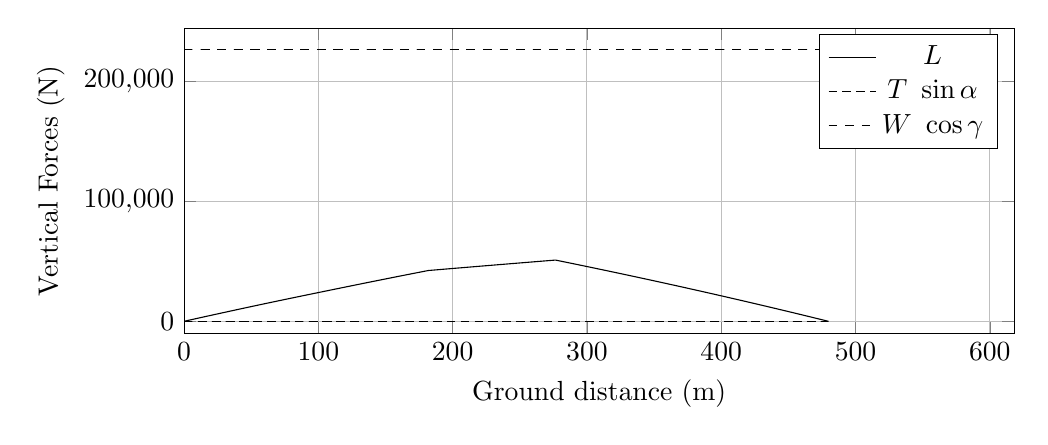
\begin{tikzpicture}

\begin{axis}[
width=\textwidth,
height=0.45\textwidth,
scaled ticks=false, tick label style={/pgf/number format/fixed},
xmin=0.0,
xmax=618.2299866992206,
xlabel={Ground distance (m)},
xmajorgrids,
ymin=-10000.0,
ymax=244270.56170125978,
ylabel={Vertical Forces (N)},
ymajorgrids,
legend entries = {$L$\\$T\ \sin\alpha$\\$W\ \cos\gamma$\\}
]

\addplot [
color=black,
solid
]
table[row sep=crcr]{
1.3603393307216043E-8	3.477244192062615E-6\\
3.0265395163403265E-7	7.736317483675309E-5\\
2.9593179127983543E-6	7.564488300911159E-4\\
1.5392338359717934E-5	0.003934526922353545\\
5.361280674027254E-5	0.013704286338746683\\
1.6215010178508227E-4	0.041448134986905624\\
3.7214145765703975E-4	0.09512520498587163\\
6.839954676020354E-4	0.17483986139389857\\
0.001098342709021993	0.28075317357448315\\
0.001609317716481928	0.41136569247368737\\
0.0022198920000388346	0.5674367966912846\\
0.002878710694837372	0.7358393247690544\\
0.0036835072341781794	0.9415549564658316\\
0.004557929017412697	1.1650667501264018\\
0.005559798278933152	1.4211543861692415\\
0.006651227400597502	1.7001330314564322\\
0.007795849738889277	1.9927067845259518\\
0.009067984722810115	2.317871851640386\\
0.010453165799939174	2.6719299535886076\\
0.011915708813158052	3.045759604244375\\
0.013455030027058647	3.439211199341578\\
0.015131183092671713	3.8676339032168086\\
0.01690803412933615	4.321791238368709\\
0.01873590105740728	4.788984156082485\\
0.020713359121301934	5.29440729776044\\
0.022777736728155237	5.822041467647612\\
0.024960970145273077	6.38004850380983\\
0.02723428625014468	6.961073560246435\\
0.029610395797831278	7.568364543769745\\
0.03204086105441677	8.18954099190287\\
0.03462344565878624	8.849588372855493\\
0.037295727153354774	9.532551905550772\\
0.040089145853872785	10.246465908438967\\
0.042950967781251806	10.977852246725398\\
0.04592022141655751	11.736684426363766\\
0.04897301836205646	12.516856473503829\\
0.052130294957187476	13.323717882568673\\
0.05542514139564195	14.165723731981942\\
0.05879722600804832	15.027454910217717\\
0.06231520981015182	15.926456336316527\\
0.06596261503753809	16.858515546051066\\
0.06964559414821356	17.79964969096371\\
0.07347193989652406	18.777402580685774\\
0.07736619052035826	19.772489970685243\\
0.08137137577670908	20.79590595553983\\
0.08545617869345057	21.83964704796461\\
0.08969468676038628	22.922642317361394\\
0.0940095881391464	24.02513591948796\\
0.09845059220533334	25.159827541329513\\
0.10296315144049947	26.312778638435027\\
0.10759658895065366	27.49658971957942\\
0.1123317495250277	28.7063650341981\\
0.1171874363557737	29.94690680329085\\
0.12217670360507671	31.22154806552004\\
0.12726806426274867	32.522242667438206\\
0.13231647880291775	33.811936763137666\\
0.13765212084557643	35.174976117739575\\
0.14294844966167852	36.527940713973265\\
0.14834594087957392	37.90671500135866\\
0.1539671093411843	39.342592120845325\\
0.15968242883369804	40.80248282015022\\
0.16555834796315422	42.30335796806317\\
0.17157514414202774	43.8401769403668\\
0.17760320215284392	45.379831760352616\\
0.18370335474801935	46.93785922602612\\
0.18983540939776816	48.50399284800773\\
0.19621099073945342	50.13227900230628\\
0.20278841209744758	51.812066491012985\\
0.20952923284938563	53.53353415635637\\
0.21624967405074952	55.249747103870675\\
0.22309476488450758	56.99774064211523\\
0.22992510727843934	58.74191628440349\\
0.2371653034562048	60.59069469276591\\
0.2442573187228817	62.4015791766402\\
0.25144286317780873	64.23628904816138\\
0.2588001799723505	66.11479933426875\\
0.2662612189130884	68.01973185232993\\
0.27386560463063747	69.96120051701413\\
0.2815803271719757	71.93077452498397\\
0.28946218069394425	73.94295005041079\\
0.29753588720841584	76.0040339027021\\
0.3056643119969481	78.07901473341013\\
0.31376446154764137	80.14670616885519\\
0.322071411728719	82.26711278621588\\
0.3303680011285137	84.38480011727225\\
0.3389039548234316	86.56350698032188\\
0.3474123396293025	88.73509888504694\\
0.3561645174790815	90.9688325582785\\
0.36525289600634137	93.28828421171946\\
0.3742306244196095	95.57940962117948\\
0.3835584127627333	97.95977908775248\\
0.392806747202999	100.31978061685211\\
0.40218604538039837	102.71310823029589\\
0.4115907129344223	105.1128150932029\\
0.42143744457304466	107.62521858147011\\
0.4310567075016639	110.07948359518778\\
0.4412814114336725	112.68811347674082\\
0.4513051702487684	115.2453686114506\\
0.461412558308395	117.82385150702862\\
0.47173637532167356	120.45743588252054\\
0.4821484569390513	123.11342250770474\\
0.492985116277161	125.87759215661768\\
0.5036221628177362	128.59072536014673\\
0.5142245311302887	131.29489523041195\\
0.5252888808291518	134.11676945593177\\
0.5363145235987512	136.92864444521013\\
0.5471208511184944	139.6844642226423\\
0.5585110457184732	142.58904952013023\\
0.569849942463402	145.4804194289665\\
0.5817265165330987	148.5087515872977\\
0.5935668742733842	151.5277036316574\\
0.6053719027871456	154.5375033244473\\
0.6172343027602503	157.5617854043619\\
0.629515267228629	160.69262635331387\\
0.6417789549774502	163.81890797691318\\
0.6542768803188956	167.0047429146647\\
0.6669828212214572	170.2434387197398\\
0.6796225285147333	173.46508787437097\\
0.6925094233679154	176.74957293875298\\
0.7056620711738308	180.10161586325103\\
0.7184715206768946	183.36602306854428\\
0.731725241748566	186.74347457656717\\
0.7449880440563246	190.12306191372687\\
0.7586792333483576	193.61162273438288\\
0.7725063377467813	197.1346229364167\\
0.7863894274138714	200.6716935924835\\
0.8004504964383841	204.25391124836102\\
0.8147129313117618	207.88722620480291\\
0.8293722635741907	211.6214370570321\\
0.8437954335339908	215.2952797285161\\
0.8580702287827062	218.9311240431452\\
0.8726489666047585	222.64417395654993\\
0.8875094051704782	226.42875235956558\\
0.9027740629895862	230.31604680354792\\
0.9182163910703112	234.24835166076775\\
0.93361566230532	238.16945735817438\\
0.9491799633800446	242.1323465298977\\
0.9646343064330896	246.0670026111913\\
0.9803727456894022	250.07374776528292\\
0.9957421603273868	253.98631068049554\\
1.0116767859397604	258.04251389446733\\
1.028041387324289	262.20791017336035\\
1.0443915011410971	266.3693577927752\\
1.060796374175649	270.54448107061194\\
1.0773229908740651	274.7503241763469\\
1.093971735592782	278.9869795792009\\
1.1110062543639518	283.32152625021865\\
1.127891796882146	287.61788817190256\\
1.1451224507351285	292.00177684468713\\
1.1624801114435046	296.41769015873456\\
1.180077727863539	300.89435449717337\\
1.1978884766667508	305.4249353988655\\
1.215488397439855	309.90158915810764\\
1.23351701382096	314.48697781034787\\
1.2518199984626128	319.1418323723195\\
1.2704235066044305	323.87279033657785\\
1.2892140278280424	328.65097327179933\\
1.3075714306593595	333.3186970668438\\
1.3266673518109293	338.1738655354786\\
1.3462106477188795	343.1424237849968\\
1.365306294594515	347.99682763678084\\
1.3852885894463176	353.0762643675191\\
1.404835539176236	358.0446758319208\\
1.4251192118409102	363.19996873564025\\
1.445164519989187	368.2943019804993\\
1.4656054698512246	373.4887988852414\\
1.4853522740259328	378.50652956000647\\
1.5051589726327936	383.53911663107476\\
1.5255757775517242	388.72634293330304\\
1.5464367798307013	394.0260276411841\\
1.5673163741652552	399.33003441359403\\
1.5879032567231621	404.5592920048174\\
1.6091523485848285	409.95634940261857\\
1.6303162371862876	415.3313555073854\\
1.6519474169970438	420.8246174313557\\
1.673879209980242	426.39378539166523\\
1.6955666802836635	431.90048242615967\\
1.7172271378534343	437.3998950132899\\
1.7402832823543353	443.25319478859194\\
1.7634396102400074	449.1314454139921\\
1.7861669372425006	454.90032439838785\\
1.8088678577734645	460.66203743577046\\
1.831824248135399	466.48812149341654\\
1.855578771396016	472.5162669728966\\
1.878960729162178	478.4493755140958\\
1.9033179534858085	484.629437855114\\
1.9273833213731866	490.73493126607593\\
1.9518510462308036	496.941978528175\\
1.9761594732990155	503.1080907470622\\
2.000437267212291	509.2659125519641\\
2.0252281699074732	515.5533443599597\\
2.0498006073458734	521.7848371740533\\
2.0745611186355752	528.0634902932416\\
2.0997746990963106	534.4564803675721\\
2.1260324099367294	541.1136245942357\\
2.1515212193659616	547.5752553466743\\
2.1771505246334	554.0719351073596\\
2.2031842637813908	560.6705517647381\\
2.230133398733474	567.5005724469195\\
2.257053086628849	574.3225060849913\\
2.283795213136285	581.098826567935\\
2.311477064851834	588.1126237258673\\
2.3387199014446116	595.0145479196794\\
2.3662694524467227	601.9935346948482\\
2.3937852540088533	608.9633281453289\\
2.4216520071021392	616.0213640837922\\
2.4501931244916175	623.249521130359\\
2.478927626230634	630.5259596735257\\
2.506685441631536	637.5544124690214\\
2.53537335014481	644.817691439627\\
2.5633350931805676	651.8964552114769\\
2.5917889242519685	659.0991255360138\\
2.6208221472873374	666.4477656914753\\
2.649872764173903	673.8001078522973\\
2.679661174525658	681.3384503566497\\
2.709174609939316	688.8064840227316\\
2.740029385016756	696.613160914108\\
2.770444625703795	704.3078640481654\\
2.801129860621211	712.0701044178668\\
2.8318827297715705	719.8486817286148\\
2.862425967677578	727.5734723196967\\
2.893259332541544	735.3708707214168\\
2.92412139403754	743.1747543689901\\
2.955064430161417	750.9983404072198\\
2.986690331721131	758.9937832145974\\
3.019183403261743	767.2076202849407\\
3.0507201588152526	775.178903107738\\
3.0830332871979023	783.3455982208616\\
3.1154603869692448	791.5402608726727\\
3.148592095396281	799.912121655655\\
3.181936872739324	808.3369426001329\\
3.214370607724433	816.5307378702792\\
3.247565473366384	824.9159599411676\\
3.281695868027062	833.5365986838101\\
3.316494330618462	842.3250372105801\\
3.3513055302544137	851.1157451373997\\
3.3860303583611797	859.8837007970887\\
3.421934361445942	868.9484103558802\\
3.456235826539576	877.6075927284667\\
3.490536654441657	886.2657049521742\\
3.526257338581564	895.2812492982823\\
3.561372823896762	904.1430918475976\\
3.5967906564503185	913.080278644205\\
3.632682576242373	922.1361170483751\\
3.6701261071689295	931.5823945382463\\
3.707701291513044	941.0608154498257\\
3.7452745323452916	950.5376774179717\\
3.78256482255855	959.9421191464567\\
3.8208821591411084	969.6044875042242\\
3.8590337549211444	979.2239674364475\\
3.89695718563138	988.7848396363636\\
3.9351036745073964	998.400865508735\\
3.9736642086653067	1008.120165564859\\
4.012189127077221	1017.829388587945\\
4.05156219172609	1027.7512327423733\\
4.090290786278251	1037.5095598016783\\
4.129291984889424	1047.3354616925544\\
4.1680648628189925	1057.1027377520782\\
4.207805169621487	1067.1125810605445\\
4.248168240749736	1077.2781118272187\\
4.288797880674668	1087.509586202404\\
4.32990243544832	1097.859441627284\\
4.371428084678056	1108.314090630843\\
4.41247037137882	1118.6458305735678\\
4.453879445321437	1129.0686822628004\\
4.49524783594077	1139.4800730551483\\
4.537299342543221	1150.062140669364\\
4.580546125800922	1160.9436877864123\\
4.622914948498307	1171.6030463970606\\
4.66640222022569	1182.5424766158303\\
4.709294790611851	1193.3310079677676\\
4.752417172855319	1204.1760466555743\\
4.796155651503765	1215.1747072177968\\
4.8408754796551925	1226.4187692370697\\
4.884850997559644	1237.4743378304315\\
4.928651138956553	1248.4844912388853\\
4.972831351372241	1259.5888489868298\\
5.017331702752941	1270.7723203861788\\
5.0632326321008225	1282.3063583616972\\
5.108452384314601	1293.6678287406971\\
5.1536021218025905	1305.010325838443\\
5.199057463234675	1316.4282064396566\\
5.244479287100011	1327.8362793296742\\
5.292293005248643	1339.8436023911713\\
5.338096108273211	1351.344573303592\\
5.3857492800262605	1363.3086068616449\\
5.433816232374781	1375.3750006041591\\
5.480691139018431	1387.1406812192831\\
5.529685763332537	1399.436868479018\\
5.578612887337309	1411.7145440055124\\
5.626451501744754	1423.7175586378344\\
5.674834544150631	1435.8556582858855\\
5.7252048440372345	1448.4906981293611\\
5.77422346516266	1460.7851046676487\\
5.8255152536468575	1473.6479904564358\\
5.874338256646894	1485.8901902644043\\
5.922631450506765	1497.9980440680183\\
5.972682300942642	1510.5450031795635\\
6.022535370757359	1523.0408026871269\\
6.074394648705015	1536.037797400385\\
6.124928192945902	1548.7009081667052\\
6.176798284396469	1561.6972771892183\\
6.229620191179453	1574.930402991357\\
6.282808156696705	1588.2534818571921\\
6.334658925277093	1601.2399188564536\\
6.388041948821611	1614.6083883798\\
6.440558117792513	1627.7580666824379\\
6.494960924490993	1641.3783657859435\\
6.550441697666145	1655.266686849187\\
6.6042098433346865	1668.7245085861096\\
6.658315220792536	1682.264973073769\\
6.712335084641163	1695.7822784879017\\
6.766674450459032	1709.3777670152058\\
6.821537769035839	1723.102557485763\\
6.876851268142238	1736.9381544427924\\
6.933661362437203	1751.1462094363733\\
6.989261882852809	1765.0499102282074\\
7.046240323930029	1779.2962962382258\\
7.102786137967051	1793.4326351549867\\
7.1603789170469145	1807.8287994987008\\
7.21785165788507	1822.193041552226\\
7.277487498606879	1837.0958945925481\\
7.334984696129153	1851.4623706408734\\
7.393362172524569	1866.0468614476717\\
7.452416393609804	1880.7984486758596\\
7.511934748111884	1895.6639739988987\\
7.572557225035805	1910.8032130247252\\
7.63202184821041	1925.6512946870116\\
7.69294899409779	1940.862510490435\\
7.752675521499926	1955.7719701835517\\
7.814488876138199	1971.2002793373504\\
7.8763528528159785	1986.6391122304804\\
7.938149975125226	2002.059161974586\\
8.001193143199774	2017.7879822370123\\
8.064554080136986	2033.593904440012\\
8.12686567918485	2049.135939883704\\
8.189637855946287	2064.7907385207163\\
8.252542711798306	2080.476505481266\\
8.315859663763469	2096.262897925816\\
8.380006162932737	2112.253943493074\\
8.444702551512929	2128.3798667284327\\
8.509501986620958	2144.52926702525\\
8.57387297516295	2160.5697122619404\\
8.63887365699837	2176.764878205713\\
8.70727085773305	2193.803934331794\\
8.772937378995405	2210.1604549771428\\
8.839192134487615	2226.6612526229646\\
8.905815929161982	2243.2516992086776\\
8.97209054442786	2259.7529565433942\\
9.039019026885107	2276.414762252989\\
9.107371801018814	2293.4288191253236\\
9.174915633685494	2310.2392215812206\\
9.243868961478196	2327.3980786694383\\
9.312440636565494	2344.4596276782377\\
9.381784695008012	2361.711000665735\\
9.4513167952828	2379.0067890153296\\
9.52142787533916	2396.4442102644516\\
9.591425279059166	2413.850982016288\\
9.662230428326719	2431.456218628943\\
9.734225879912522	2449.354951365758\\
9.806441602430919	2467.3059625539536\\
9.878483835105534	2485.2113845370523\\
9.951807209049782	2503.4327092665244\\
10.023539677466466	2521.256244435842\\
10.096057433179052	2539.272463139222\\
10.168262179450682	2557.2084957452134\\
10.241274410624943	2575.3426677544394\\
10.31479015323385	2593.5994287550366\\
10.390063469390178	2612.290110023604\\
10.465012435634037	2630.8977030776714\\
10.540639152111389	2649.6709966174003\\
10.617644389866598	2668.7838577815937\\
10.692945462162374	2687.471189217078\\
10.770083295573727	2706.611745279044\\
10.846726862770723	2725.627065394596\\
10.924657809445929	2744.9591528143146\\
11.00265335491597	2764.3046237512217\\
11.081827589833612	2783.939762811997\\
11.159134327011738	2803.1091694127144\\
11.239152720133266	2822.948290012817\\
11.317028257314295	2842.253523663753\\
11.396413369884492	2861.9303514264157\\
11.477655063362434	2882.064632558632\\
11.556958506738276	2901.7159082276085\\
11.637325199769407	2921.6280067083553\\
11.717754170658207	2941.5528831791844\\
11.799819443100102	2961.880407960127\\
11.881986970940797	2982.2305302140057\\
11.964394119506721	3002.6372720467725\\
12.046263329632716	3022.908116991669\\
12.130282587748898	3043.7085504068637\\
12.213721087180826	3064.362454814548\\
12.295868535962462	3084.6941189053077\\
12.380692430046633	3105.6854574586014\\
12.46470288467437	3126.4727582722326\\
12.550384439940181	3147.670766396017\\
12.635259749824865	3168.6665526168053\\
12.72144647897981	3189.9839636199495\\
12.80741162779486	3211.243794807747\\
12.892901506907108	3232.383360475882\\
12.977815703098727	3253.377900531952\\
13.06483740414145	3274.890764844302\\
13.151922956503014	3296.416653786352\\
13.240589045456186	3318.330405689857\\
13.329911181207382	3340.4034483725163\\
13.417306166647748	3361.9975108511135\\
13.507103029723119	3384.182233884466\\
13.595986036712912	3406.138402137837\\
13.687453390597003	3428.7300967270394\\
13.779071846306106	3451.3562197409983\\
13.872694200363323	3474.4742598895737\\
13.963504841252302	3496.8951662728205\\
14.056146454975131	3519.7652755334375\\
14.14918846816267	3542.7313471888065\\
14.24332804549016	3565.965420901397\\
14.339261112049854	3589.639144375097\\
14.431091301610323	3612.2975825007943\\
14.524174633942373	3635.2624486475306\\
14.618760344060338	3658.5951325257947\\
14.714801736988441	3682.2840065463733\\
14.809763128346521	3705.7036454664576\\
14.903412319659619	3728.796915314775\\
15.001392651385917	3752.9553177959206\\
15.098055049922994	3776.7858880133335\\
15.196870856960619	3801.144419595531\\
15.29477342819068	3825.274943182373\\
15.39265348361268	3849.397067236958\\
15.490487151984588	3873.5049385738475\\
15.588146853189365	3897.567155394773\\
15.687961867268871	3922.157567403621\\
15.78650099417861	3946.430854303505\\
15.886965864441798	3971.1756786656615\\
15.98755318095926	3995.9478239220143\\
16.088470385762115	4020.7983873260227\\
16.190536977381747	4045.9291347995695\\
16.292466610053154	4071.0233303050645\\
16.396448349404487	4096.619853040733\\
16.497808944935016	4121.5683716329695\\
16.600551072850564	4146.854170352019\\
16.70575139586156	4172.742100246463\\
16.81134459259622	4198.723837568501\\
16.917616592554033	4224.869725230461\\
17.023477948501657	4250.911750068368\\
17.12904978140002	4276.87976797342\\
17.2354081519902	4303.038475281592\\
17.340772011500363	4328.949865069711\\
17.448391076872838	4355.413100817843\\
17.5571980918308	4382.165647294945\\
17.66615596614949	4408.952495859841\\
17.774685459577412	4435.631287271581\\
17.884986575683584	4462.742811484728\\
17.99552903728076	4489.910892331132\\
18.108708479124623	4517.724234287838\\
18.219646262474413	4544.983955091171\\
18.332680252669796	4572.756000891164\\
18.445061806396694	4600.365023821043\\
18.556709221711323	4627.791038494086\\
18.668884868236475	4655.344187611996\\
18.78204748093455	4683.137131346652\\
18.895704562363058	4711.048896904405\\
19.008928234289563	4738.851652095824\\
19.124320907419907	4767.184413262652\\
19.24105855786135	4795.844774619749\\
19.355116774466126	4823.844782795772\\
19.470462572962035	4852.158380070439\\
19.58492145104516	4880.2518224869855\\
19.704921229319112	4909.702680799064\\
19.821259826163917	4938.252520526003\\
19.941172080873493	4967.676837446985\\
20.06078806851737	4997.025960137336\\
20.177423389922623	5025.641383193122\\
20.297621170678	5055.128427224667\\
20.420129559802255	5085.179852845113\\
20.54164670774839	5114.985717415409\\
20.661905244258705	5144.48054961215\\
20.784301666224792	5174.4973987950125\\
20.904244540623438	5203.9103002356605\\
21.028114340450195	5234.283903652973\\
21.148300883955606	5263.752183826429\\
21.270875420257596	5293.8038159373355\\
21.39299406946177	5323.74155754974\\
21.513793771711654	5353.353915644182\\
21.637476506915142	5383.670950860014\\
21.759279707150128	5413.525283702305\\
21.88493035745168	5444.320612264075\\
22.009809790007786	5474.924932612268\\
22.13620730934617	5505.899315638333\\
22.263515470260465	5537.094894115042\\
22.393040471753594	5568.8317156362355\\
22.520519759768852	5600.06539415242\\
22.648852607677917	5631.5063555284\\
22.775118904521122	5662.4392592972945\\
22.903136237443974	5693.799398021514\\
23.03176118514304	5725.306670372691\\
23.162501585272054	5757.33042351917\\
23.294719932439598	5789.714486797289\\
23.427108470281937	5822.138573851074\\
23.558693146983046	5854.364187635878\\
23.687077503630363	5885.804547284424\\
23.817949558665852	5917.85266780181\\
23.948210788889448	5949.749797024715\\
24.076877750667826	5981.255202862756\\
24.21019765060587	6013.898580009081\\
24.3450673155249	6046.920074898575\\
24.477101355489637	6079.24603983071\\
24.60984760833776	6111.745175995466\\
24.7468403923846	6145.2827471702585\\
24.882807251950062	6178.568001977159\\
25.017167332957627	6211.458832557917\\
25.153910941279605	6244.93209618633\\
25.289629217480112	6278.153382490513\\
25.425306692573436	6311.363752415982\\
25.56229499031975	6344.894091022345\\
25.70075944713021	6378.78489680979\\
25.83724158708921	6412.189727436613\\
25.975209935932874	6445.957586041652\\
26.003074150630965	6452.777289687625\\
26.020759913393235	6457.105826057616\\
26.030714598210515	6459.542199959216\\
26.05840292223249	6466.318801452795\\
26.06133765907019	6467.037064489832\\
26.064285136409026	6467.7584454117095\\
26.066337724202356	6468.2608062424115\\
26.068175973881182	6468.710708746659\\
26.06984477238784	6469.119138817139\\
26.077831036047115	6471.073735516693\\
26.10345636352254	6477.345387092168\\
26.16716044512971	6492.936495080667\\
26.297541524199602	6524.845841222053\\
26.42722303713863	6556.5833006977155\\
26.5559280656694	6588.081056584602\\
26.686097387723095	6619.936373345017\\
26.817793678842584	6652.164501922118\\
26.949416928520378	6684.373820776604\\
27.080440623797912	6716.435436282345\\
27.215491080424528	6749.481311975274\\
27.34795890217076	6781.894099136138\\
27.48215578365496	6814.728752647681\\
27.616696052324144	6847.646145125902\\
27.75271189183823	6880.923196660164\\
27.888759310501555	6914.206543504521\\
28.023839122857026	6947.251695545756\\
28.16136324828667	6980.893241149839\\
28.298355249881332	7014.40298369489\\
28.435282447697354	7047.8951867918495\\
28.573941346212784	7081.8091828595825\\
28.713752690797136	7116.00317880386\\
28.852681198061333	7149.979336012744\\
28.992471984120606	7184.164379219565\\
29.133421724605903	7218.630756322329\\
29.275199211812186	7253.297373631878\\
29.416225289053614	7287.77804453572\\
29.55783477945603	7322.3990772658835\\
29.701838356359822	7357.603018072747\\
29.846633046394217	7392.997854911333\\
29.99013730470424	7428.074711647723\\
30.132492646908446	7462.868186762189\\
30.277395768405135	7498.281705138848\\
30.422188862471998	7533.665589072623\\
30.56637548064623	7568.89848296588\\
30.711944318924978	7604.466258417251\\
30.8573377156769	7639.988230580233\\
31.006558691603843	7676.442233370342\\
31.153907258126303	7712.435667852938\\
31.30257185742142	7748.747348974157\\
31.4510947803754	7785.021133633425\\
31.602595106592503	7822.018643124327\\
31.755261577184278	7859.297354082897\\
31.906398416479824	7896.198956932412\\
32.05599258457312	7932.720322141064\\
32.20952926265106	7970.200438791124\\
32.360097140052986	8006.952084447286\\
32.51218835243483	8044.071730610314\\
32.664721606344784	8081.295347016754\\
32.82129760777845	8119.501405871231\\
32.97669884718651	8157.416615281978\\
33.13118849606322	8195.105214755058\\
33.288837444683736	8233.560173435184\\
33.44405554194745	8271.417814713092\\
33.60015866510213	8309.486892483907\\
33.756686089655645	8347.654941503082\\
33.91694077595571	8386.727129728213\\
34.074326811338736	8425.095197316834\\
34.23252403098988	8463.656266879028\\
34.392884168270385	8502.73964114159\\
34.554266068788166	8542.066995832552\\
34.71363140184178	8580.89791217052\\
34.87649332318763	8620.575602508463\\
35.03746231629111	8659.786903727116\\
35.19990059234286	8699.350805390663\\
35.3627309111595	8739.00479081435\\
35.5271254050015	8779.03416107719\\
35.69149466827288	8819.05177514795\\
35.85508342515686	8858.873745099252\\
36.017180984292054	8898.327139265883\\
36.182222084544165	8938.491219364958\\
36.34861175093968	8978.9775624071\\
36.514166392421686	9019.254777546947\\
36.68083924241549	9059.79799852995\\
36.845526722294395	9099.852281188225\\
37.01328249159678	9140.646641235366\\
37.18160982421668	9181.573685255538\\
37.35136716620059	9222.84197728187\\
37.51969289597564	9263.755808272414\\
37.689710015857784	9305.074207027643\\
37.860394939778416	9346.548236240807\\
38.02805196867635	9387.279988863851\\
38.19868492919754	9428.728037183548\\
38.37343039987371	9471.167999709112\\
38.54685896696101	9513.281037211378\\
38.71934233168869	9555.157505308467\\
38.8915617091798	9596.962826847997\\
39.062305982326905	9638.403077412197\\
39.23847188392709	9681.151834124368\\
39.411511502305984	9723.134662114735\\
39.585172817779906	9765.261015531254\\
39.760693028009456	9807.830815695757\\
39.9373134006328	9850.659815656669\\
40.113617753210534	9893.404514610724\\
40.29094651898711	9936.38981519454\\
40.468149621311596	9979.336838316605\\
40.64593210594187	10022.416393482545\\
40.82431302355218	10065.632983309988\\
41.00141330502653	10108.531374768849\\
41.17957893337042	10151.67980826175\\
41.359761290266974	10195.308448520227\\
41.53889737920997	10238.675534730552\\
41.72013507746885	10282.543031654197\\
41.899395797464194	10325.92370163478\\
42.081280067494475	10369.930785237222\\
42.265315320939635	10414.449577034855\\
42.44531744651641	10457.984221448092\\
42.62715102096499	10501.953230222603\\
42.81120266452106	10546.449774136447\\
42.994164503876235	10590.67402832851\\
43.17799769459725	10635.100017501183\\
43.36154361404071	10679.447674043298\\
43.54597437124032	10724.000128258234\\
43.73158498218817	10768.8284686861\\
43.91737182308138	10813.690176040236\\
44.1050494697441	10858.99908721968\\
44.293574236233	10904.50300605427\\
44.47888581456586	10949.222056779305\\
44.66456251492659	10994.01994188028\\
44.85170130968709	11039.161166241\\
45.037822074257164	11084.047424385317\\
45.22676109993536	11129.603746331231\\
45.41612608476639	11175.253039264877\\
45.604812217355104	11220.72897092281\\
45.79422221198037	11266.369591473005\\
45.98724683785376	11312.871108882395\\
46.17830917717477	11358.889840792395\\
46.36786657808848	11404.536197387537\\
46.55935209439748	11450.636824471396\\
46.75090376717816	11496.743277060432\\
46.94233405988251	11542.810403512169\\
47.13714948644359	11589.681760057134\\
47.33387512950824	11637.002049009821\\
47.53043319838464	11684.271322852674\\
47.72298239739284	11730.566132549393\\
47.919150009665316	11777.720332314322\\
48.113386178114425	11824.399714595962\\
48.311024807628144	11871.886005991724\\
48.508886059616145	11919.41488301726\\
48.70490444306449	11966.490310286907\\
48.90290918859142	12014.031886969125\\
49.09959709013448	12061.246437979524\\
49.2970021191946	12108.622255035545\\
49.49532701226336	12156.207849616192\\
49.693780717172615	12203.813323762908\\
49.89506320355713	12252.086096769388\\
50.096719083698545	12300.437026402768\\
50.29606895218413	12348.22383037601\\
50.497598474286534	12396.521787565798\\
50.700304208193415	12445.090127261807\\
50.90342397924904	12493.746092666814\\
51.10460922167407	12541.927227135344\\
51.30752217039489	12590.510601242142\\
51.51010619677311	12639.003675912641\\
51.713602501430145	12687.703509354567\\
51.91843850546792	12736.71219600035\\
52.121089026646246	12785.186379795494\\
52.32561402362407	12834.097233773507\\
52.53192272805477	12883.422737026835\\
52.7387030603267	12932.848995930948\\
52.944027344085896	12981.915330212167\\
53.154073670302836	13032.097835748282\\
53.36143953271798	13081.627793167609\\
53.571009444677685	13131.671929649121\\
53.77799762982136	13181.087466464676\\
53.98785945427545	13231.176776250093\\
54.196157549666225	13280.880650317795\\
54.40718762937186	13331.224031493359\\
54.616887598525366	13381.23774983058\\
54.826875464266934	13431.307802613894\\
55.04038432082807	13482.204769139546\\
55.25438844036796	13533.20701830577\\
55.46695867894975	13583.854884035518\\
55.68088820258777	13634.813895678093\\
55.895144656119854	13685.838002806271\\
56.109028395418505	13736.760605417305\\
56.326262430904194	13788.467844252915\\
56.542089933321776	13839.827312103353\\
56.76060076462056	13891.812154080293\\
56.97729209122687	13943.351060789078\\
57.19579178641709	13995.306920567029\\
57.41258192878804	14046.843233950043\\
57.634093277561306	14099.48849432847\\
57.85395098827546	14151.727371209057\\
58.07448819514299	14204.114332943289\\
58.29446478173499	14256.354808398628\\
58.51588770709739	14308.92535447871\\
58.73757884137123	14361.546123529715\\
58.96020041504734	14414.374216177745\\
59.18267120664716	14467.153010573082\\
59.405949655899676	14520.109850084955\\
59.63089974393067	14573.449450628785\\
59.8562534200115	14626.87097071257\\
60.084134136581554	14680.877545262276\\
60.30833762904015	14733.99892755716\\
60.53504725699203	14787.700299721422\\
60.763693228044005	14841.846314816397\\
60.99075593752245	14895.603486677504\\
61.21765734918529	14949.308655663535\\
61.44713116872772	15003.608671043388\\
61.6738048454246	15057.232286873263\\
61.90668490141796	15112.309872922775\\
62.13729676517957	15166.836811747457\\
62.36629463006145	15220.968174980819\\
62.596359157213186	15275.337711634496\\
62.82836101237727	15330.150940971998\\
63.059723307860466	15384.798959712753\\
63.292774394726166	15439.831667896666\\
63.52608473446321	15494.91135378469\\
63.75973181411028	15550.056294627691\\
63.993403028653574	15605.192716375615\\
64.23068717493263	15661.167129219175\\
64.4710952259949	15717.863594693437\\
64.70858695601663	15773.857644607571\\
64.94894296164699	15830.512235013\\
65.18738841845183	15886.701843566989\\
65.42661162888535	15943.060117959067\\
65.6659442133793	15999.42956038762\\
65.90899583190168	16056.66004157949\\
66.15068261105333	16113.554312551318\\
66.39533053734849	16171.13063507598\\
66.6378997293487	16228.202874785682\\
66.88158418814953	16285.5226636511\\
67.12390450547147	16342.506866107273\\
67.36840986262189	16399.990087712373\\
67.61550053739396	16458.066052566915\\
67.86097385246623	16515.746933839713\\
68.10985741250389	16574.21400173325\\
68.35582503705197	16631.981138333227\\
68.60464259362828	16690.402560242663\\
68.85450289166104	16749.053651279217\\
69.1042877596268	16807.671909126766\\
69.35837572129628	16867.28454042566\\
69.61150655903072	16926.657181816066\\
69.86289252102952	16985.605373799604\\
70.11686816207683	17045.14552649478\\
70.37125759672608	17104.767335713266\\
70.62480458144697	17164.17647826302\\
70.88045310059783	17224.062719837697\\
71.13526709211152	17283.73823584913\\
71.3947754873567	17344.497583546865\\
71.6534187996231	17405.03883372517\\
71.91450497256008	17466.136216292958\\
72.1716184080999	17526.288612859404\\
72.43269265097052	17587.352174364336\\
72.69331619504374	17648.29484163935\\
72.95563200429567	17709.617679642673\\
73.21686762735783	17770.67258265472\\
73.48161420086069	17832.53243644871\\
73.74261486234883	17893.50172560884\\
74.00755043430098	17955.37474156916\\
74.27511769675363	18017.846636654554\\
74.54487113507057	18080.813052250393\\
74.81568229507957	18144.010383707733\\
75.08274085953312	18206.316406090802\\
75.35421836228127	18269.637608530385\\
75.62798354862159	18333.47638819411\\
75.89909469738902	18396.680519707203\\
76.17008148658607	18459.840081564085\\
76.44269151183332	18523.36235483364\\
76.71571902594138	18586.966301790708\\
76.99340852183178	18651.64037208994\\
77.27004772085374	18716.05396149149\\
77.54832408953641	18780.832880329945\\
77.82592519882277	18845.438847212994\\
78.10358246820337	18910.04224093099\\
78.38556010231375	18975.634962239383\\
78.66911430382748	19041.57836634593\\
78.95399134982776	19107.81331269609\\
79.23667137346987	19173.521605120113\\
79.518907793654	19239.111154444363\\
79.80555437718249	19305.70972178714\\
80.09150103324356	19372.12985198039\\
80.37928873457926	19438.96178941612\\
80.66871996946384	19506.15949865827\\
80.95967699414447	19573.69550403772\\
81.25093884305389	19641.2863727313\\
81.54344278085921	19709.149607913118\\
81.8358102960415	19776.965421047455\\
82.13087592438694	19845.3912160682\\
82.42794520371837	19914.265699623327\\
82.72842933895026	19983.915753447123\\
83.0269479931649	20053.094275468247\\
83.32974506690314	20123.248179136725\\
83.62964811531441	20192.71573898793\\
83.92951211009506	20262.158635088417\\
84.2339319847595	20332.640758816793\\
84.53715838283946	20402.830849646605\\
84.84105485927768	20473.16046722664\\
85.14845677960258	20544.285618691698\\
85.45530133949276	20615.26619906351\\
85.76249773413784	20686.31269726809\\
86.07201271349416	20757.879925966925\\
86.38432073331904	20830.077366302517\\
86.69710203601804	20902.368669520227\\
87.01172103282082	20975.069178051483\\
87.32669099459858	21047.835352574104\\
87.64517025121202	21121.396736803326\\
87.96158123090564	21194.465107662458\\
88.2775814178033	21267.423578050882\\
88.60068374099544	21342.006440209363\\
88.92068281935622	21415.857844912178\\
89.24207276858638	21490.015276261343\\
89.56578933015979	21564.694571862514\\
89.88760090270688	21638.91968492658\\
90.2141410750086	21714.22063361243\\
90.54066676000363	21789.50352197217\\
90.86727570256076	21864.79107537192\\
91.19715108614633	21940.81703250396\\
91.52744226539704	22016.924365572333\\
91.85639956214655	22092.710166078752\\
92.19095740864739	22169.77193150737\\
92.52827526888461	22247.455049607168\\
92.8674718219292	22325.556476342288\\
93.20307982994817	22402.81768217691\\
93.5374944579234	22479.79057573805\\
93.87598013161067	22557.6869228\\
94.20917297854535	22634.35208532597\\
94.55043409744499	22712.860408761473\\
94.89132963816093	22791.271430322726\\
95.23083207736542	22869.34913247417\\
95.57395676502793	22948.24703246361\\
95.91421223354143	23026.472672409407\\
96.25656086122288	23105.167190205073\\
96.60012122339742	23184.12803014838\\
96.94166303707107	23262.613048527397\\
97.28627502929558	23341.791796633093\\
97.62906225262071	23420.539773122473\\
97.97125437026659	23499.13982322107\\
98.31201772458999	23577.400791493987\\
98.65627175165852	23656.452631231987\\
99.0012536203806	23735.660947769655\\
99.35020029285332	23815.76898022116\\
99.69475740907401	23894.859073003674\\
100.04053871990226	23974.22019877183\\
100.38598466112728	24053.494623449522\\
100.72867962848932	24132.128374559376\\
101.07385499050397	24211.32207991187\\
101.41864366415388	24290.41810337508\\
101.76305460768467	24369.41877349196\\
102.11068844700483	24449.150138420744\\
102.45638678530696	24528.429297025657\\
102.79841653079728	24606.859242161656\\
103.14087212494877	24685.379212798776\\
103.48486473791618	24764.24416101903\\
103.82875595362174	24843.078655457517\\
104.17244250654872	24921.85927751474\\
104.51168383396202	24999.614375258076\\
104.85986244643053	25079.411375846386\\
105.204587526496	25158.410594626796\\
105.54754777175077	25236.999412334357\\
105.88797456536247	25315.002055087556\\
106.23280177240994	25394.007492106874\\
106.57515110440406	25472.439996576242\\
106.91603555764121	25550.531979634616\\
107.25729565943405	25628.70534702218\\
107.598830149446	25706.937132430212\\
107.93686571059558	25784.363322688216\\
108.27485499032852	25861.775040171502\\
108.28839963475954	25864.87717421109\\
108.30004107281309	25867.543411661012\\
108.30931238392475	25869.666816092584\\
108.31701527366243	25871.431003578822\\
108.32505202073054	25873.27165218137\\
108.33865239118708	25876.386527561932\\
108.35091925899997	25879.195987529325\\
108.39508146726081	25889.3103437038\\
108.52984553865659	25920.17462052249\\
108.79919793188978	25981.861101336945\\
109.105233418432	26051.94555150099\\
109.41485218466596	26122.847014641207\\
109.72257164661937	26193.309746834115\\
110.0321119530083	26264.18537810351\\
110.34145354075926	26335.011233150493\\
110.6534776714839	26406.446720189037\\
110.9711963390063	26479.180995462317\\
111.28851843247409	26551.819284928977\\
111.60893519474632	26625.160467862523\\
111.92798394282838	26698.182789314007\\
112.24770070245137	26771.35203228634\\
112.57243448635171	26845.663100489503\\
112.89480865389396	26919.427635074295\\
113.22000325235314	26993.830667921233\\
113.54885709436653	27069.06367148574\\
113.8770619430189	27144.140698943884\\
114.20946079557197	27220.169225625126\\
114.54107775051554	27296.010768570326\\
114.87787736567807	27373.02902856867\\
115.21564640021248	27450.260053941485\\
115.55522358014255	27527.89526242389\\
115.89667501383605	27605.949369025075\\
116.23992536102014	27684.40474692116\\
116.5847156213415	27763.201802135423\\
116.92791619634093	27841.625064305357\\
117.27517516660399	27920.964790208956\\
117.62420948631524	28000.698837759017\\
117.97391125359778	28080.57374791465\\
118.32673409155768	28161.149509241986\\
118.68227803698588	28242.3342270183\\
119.03889207644076	28323.75045580379\\
119.39651249432902	28405.383283584655\\
119.75508651978987	28487.220304086564\\
120.11314113323388	28568.925057921064\\
120.47404637453192	28651.266173422897\\
120.84098349318353	28734.968677553108\\
121.20490030977416	28817.96723161504\\
121.57328571082118	28901.96948316301\\
121.94079100066682	28985.755301440062\\
122.31015242291167	29069.94819631846\\
122.68267403243519	29154.84483523106\\
123.05346836176264	29239.331033573973\\
123.42835733050345	29324.732915675362\\
123.80350972566416	29410.17715838313\\
124.1783235941891	29495.52642130061\\
124.55244040146786	29580.69889503118\\
124.92576251095704	29665.672222993388\\
125.30489170817492	29751.94845607379\\
125.68146781278597	29837.624638114918\\
126.06139977608174	29924.044839208284\\
126.44502763856761	30011.285623300275\\
126.82695116404781	30098.118532092638\\
127.206716044588	30184.44035425441\\
127.59262031825523	30272.136710667066\\
127.97077035934353	30358.050199184225\\
128.3546122768156	30445.235646498724\\
128.73724861847296	30532.12578304278\\
129.12002064685282	30619.025062021094\\
129.50086700331673	30705.465443800982\\
129.8837789976152	30792.352613858908\\
130.26783132854348	30879.476128073133\\
130.651936341801	30966.588941380884\\
131.03747321415574	31054.003510766917\\
131.42280335891803	31141.348004287218\\
131.80875442588928	31228.8097962151\\
132.19322104975072	31315.911669692585\\
132.5798881414172	31403.4881956175\\
132.96215446290768	31490.044275121334\\
133.34488286943906	31576.68118587086\\
133.7276157954845	31663.295132010644\\
134.11532375481391	31751.010314037965\\
134.50135826447365	31838.322088790417\\
134.88604120201086	31925.303379189194\\
135.26955723714872	32011.996019914186\\
135.6512109336153	32098.242943584977\\
136.03464327936558	32184.866799746793\\
136.41686422877552	32271.191877595644\\
136.79904942565338	32357.48367022864\\
137.18004416157777	32443.481436237642\\
137.56399804528928	32530.121499930872\\
137.94515347717788	32616.104488516656\\
138.32982901897384	32702.855562190176\\
138.7128522769853	32789.20792896309\\
139.09597564505458	32875.55668903078\\
139.48002685240425	32962.08815935283\\
139.86309097971855	33048.37076207559\\
140.24727738828375	33134.879475693655\\
140.6317581809211	33221.42760727767\\
141.01585725597846	33307.86285103591\\
141.3998433603236	33394.24561712066\\
141.7841907991213	33480.682463979465\\
142.16710976343057	33566.77087700472\\
142.55205218648928	33653.28675013238\\
142.9364233092117	33739.64664649665\\
143.32169829765928	33826.18186139139\\
143.705984531242	33912.46720535336\\
144.08985428249122	33998.63122420451\\
144.47683600496026	34085.46552663538\\
144.86371007721533	34172.247238901284\\
145.24772592056325	34258.35959619224\\
145.63047789911974	34344.16048360286\\
146.01273254364395	34429.82183863735\\
146.39725173307323	34515.962303392735\\
146.77966503747456	34601.602707663\\
147.16478130736948	34687.81983179535\\
147.54689717238745	34773.3367994265\\
147.93097497792814	34859.26421503721\\
148.31499270913332	34945.1494176055\\
148.69957284780122	35031.13149506043\\
149.08709998577143	35117.74311117985\\
149.47129868208145	35203.581690425184\\
149.8546635899794	35289.20500029005\\
150.23801379389647	35374.796013005165\\
150.62200569343076	35460.50115057478\\
151.00751012558203	35546.51447371913\\
151.3946455315429	35632.861989722354\\
151.77987817077866	35718.75550030994\\
152.16505704867353	35804.607440727064\\
152.55112759502248	35890.62838757988\\
152.93964308710213	35977.16399157878\\
153.32507651584535	36062.98322555779\\
153.71174813432617	36149.04818973623\\
154.10000329570875	36235.435379204326\\
154.48914219495543	36321.98875491918\\
154.8788297075107	36408.63356804948\\
155.26820650111182	36495.17868369332\\
155.6562915247282	36581.40619957818\\
156.0441896603637	36667.56174553555\\
156.4348678136667	36754.30395777075\\
156.82082928279863	36839.96854220923\\
157.21071017196311	36926.47235695076\\
157.60005066896917	37012.825465833244\\
157.99004282467217	37099.292218881325\\
158.3808231456182	37185.90268643193\\
158.77280374485122	37272.74794769091\\
159.16384255262415	37359.35336527527\\
159.55370941764693	37445.6682006139\\
159.946071590523	37532.5041923213\\
160.33752628124114	37619.10804408757\\
160.73008933968674	37705.92569730774\\
161.12428312893906	37793.07233507998\\
161.5185576482712	37880.20507419879\\
161.91431288671106	37967.63310883408\\
162.3096877663487	38054.94516091235\\
162.70613442998513	38142.46182431873\\
163.1032465869576	38230.0931959202\\
163.50039135636405	38317.69953140366\\
163.89625578410926	38404.99135864098\\
164.29272443146095	38492.384326284126\\
164.68754921345175	38579.38302326831\\
165.0864466423082	38667.24678061815\\
165.4846753800681	38754.93083410067\\
165.88329117400662	38842.66768801829\\
166.28234792206388	38930.46911622201\\
166.68312204436222	39018.615709420585\\
167.08520211103445	39107.0166222299\\
167.486487681752	39195.21000840094\\
167.8888620337579	39283.60975201031\\
168.290121631074	39371.731770414175\\
168.69179641444674	39459.91216733944\\
169.0966267258019	39548.75212072469\\
169.50108473093724	39637.47713143016\\
169.90729482190739	39726.553080122656\\
170.31243922775104	39815.36201571807\\
170.71755979953144	39904.13248092393\\
171.12402986296422	39993.1652701252\\
171.53319587512163	40082.75484549334\\
171.941770038195	40172.1810988893\\
172.3502931259835	40261.56250995323\\
172.7599322859847	40351.15434950906\\
173.17073308198894	40440.966343292064\\
173.58266371319877	40530.99129917406\\
173.99296569000023	40620.62647357695\\
174.40104722187203	40709.74310512902\\
174.8156903853216	40800.258532429245\\
175.2299479185392	40890.65547532319\\
175.64260521584504	40980.669188898784\\
176.05374721710058	41070.31864017541\\
176.4688147253861	41160.78995458828\\
176.8832117842232	41251.081018816054\\
177.30033423294157	41341.931543031635\\
177.7185234955238	41432.97987767044\\
178.13477925276436	41523.572963388855\\
178.55472625996282	41614.93480975399\\
178.97486541267733	41706.30375466321\\
179.39652032378837	41797.96750713658\\
179.8177496461559	41889.50397414599\\
180.24148986351946	41981.5510930219\\
180.66579793025812	42073.68648005019\\
181.08977314985765	42165.7146050157\\
181.5138518510159	42257.730286018064\\
181.61122522885114	42278.85323173496\\
181.9380657232258	42349.740451212536\\
182.36340272554946	42389.71650765315\\
183.2082724125376	42469.097188686676\\
184.08646972066333	42551.572741751734\\
184.96448881265883	42633.99447870909\\
185.84629357991815	42716.73435027205\\
186.726051310566	42799.2450427609\\
187.61806497534428	42882.86743794035\\
188.50412524941663	42965.89417546902\\
189.3932804644195	43049.17338150817\\
190.28280340229105	43132.44948996742\\
191.1758490733834	43216.017711918656\\
192.0664158070755	43299.31645525918\\
192.96248081795437	43383.0917661354\\
193.85627821989942	43466.61748202841\\
194.7612747993291	43551.151610188084\\
195.67115393765977	43636.10320482035\\
196.57439968482538	43720.39728120642\\
197.49109477617128	43805.90770046023\\
198.40328264870095	43890.95898915036\\
199.32142764481148	43976.526844375156\\
200.23456840248758	44061.58975293895\\
201.14898042779765	44146.732649456\\
202.06794236074546	44232.260557877584\\
202.98618556976356	44317.68299594993\\
203.9096776069573	44403.55494191924\\
204.83478510422236	44489.53822594935\\
205.76152187560933	44575.63404510703\\
206.69425456631774	44662.24770935127\\
207.628282006662	44748.9423299957\\
208.55982483556244	44835.367312558505\\
209.49858617709037	44922.422703821154\\
210.43993621334516	45009.678672126014\\
211.37516676315846	45096.328385902845\\
212.31832896164838	45183.67370936931\\
213.2711811717055	45271.876512403\\
214.21827407856858	45359.506585689276\\
215.17513356897763	45448.00035468134\\
216.13205411802585	45536.459743027954\\
217.08198149354007	45624.233220671274\\
218.0371791872164	45712.454187129915\\
218.99188071657676	45800.58990466915\\
219.9529264806817	45889.27164652053\\
220.9127352149854	45977.79967407655\\
221.88152971929293	46067.116560012364\\
222.85280254650712	46156.62180247797\\
223.82131876423426	46245.83316293915\\
224.792464296851	46335.24691219385\\
225.77907189920393	46426.04361238232\\
226.75865308803293	46516.15331029544\\
227.73754112978963	46606.15923271266\\
228.71868465671315	46696.33256910318\\
229.71601747959392	46787.95296517886\\
230.71257028094016	46879.46075559189\\
231.7099256226606	46971.001435724145\\
232.7104408810668	47062.791311446825\\
233.70545418089353	47154.03604397128\\
234.709934391256	47246.108251581536\\
235.71369390815352	47338.0737775271\\
236.7320063884447	47431.33136012165\\
237.74706170316256	47524.24944573555\\
238.76105009328802	47617.02898832326\\
239.78487801639722	47710.66759301443\\
240.8100003079174	47804.38325431412\\
241.83501924916794	47898.04832774955\\
242.86448750110736	47992.0787767234\\
243.8907393349939	48085.77455739926\\
244.92503751619887	48180.16387277802\\
245.953502111432	48273.98013112016\\
246.9873414577291	48368.245996616926\\
248.03717558009265	48463.92876171095\\
249.06961888058504	48557.9859382579\\
250.1218155809346	48653.80151003122\\
251.19093832453012	48751.11607785491\\
252.25320725679705	48847.76477471793\\
253.30608820982889	48943.51823166033\\
254.3699559131253	49040.22956065014\\
255.43101098027842	49136.6440890786\\
256.50967156157174	49234.61653344025\\
257.5914429014633	49332.829413525935\\
258.6840945362286	49431.98756264527\\
259.76380176807595	49529.929272607595\\
260.8581962365888	49629.1612148017\\
261.9444516651656	49727.613555137024\\
263.04204949406176	49827.05207628719\\
264.16032684448305	49928.32113018779\\
265.27010097773245	50028.77757137595\\
266.38392459233114	50129.558215400786\\
267.48537153454777	50229.177557496514\\
268.5905820952057	50329.096165423514\\
269.71611280872617	50430.809809082755\\
270.8445404967937	50532.74296531685\\
271.9892540622492	50636.1043155903\\
273.1287802847319	50738.954642266384\\
274.2598607565136	50841.00093206069\\
275.4140962910436	50945.09372655397\\
276.090309303484	51006.057030102966\\
276.5737705536998	51049.63405702493\\
277.56867335135405	50823.219207229005\\
278.5517001083557	50599.29483183619\\
279.52761403034117	50376.781841600954\\
280.5279265157802	50148.489696023724\\
281.5196374788271	49921.94437026727\\
282.5091228114409	49695.69269157012\\
283.5002036181013	49468.860942606814\\
284.4794994349294	49244.51465890028\\
285.4656948937601	49018.374773812306\\
286.4639109988274	48789.26064664849\\
287.4440310703403	48564.08654394622\\
288.4281172103467	48337.78829493353\\
289.40231797711374	48113.552865141086\\
290.3936300375175	47885.16377767036\\
291.378876920571	47657.956875177886\\
292.36776902799863	47429.69343901782\\
293.3555402536373	47201.47258585534\\
294.3358859908236	46974.753567237145\\
295.3135149835475	46748.450529329944\\
296.3010928277796	46519.629055380414\\
297.2700925003244	46294.90146114287\\
298.2415260228572	46069.39975615895\\
299.2237735124987	45841.17413334228\\
300.18939507314394	45616.60195770224\\
301.1612976587651	45390.35898652882\\
302.12729290918287	45165.28215518595\\
303.09931171579603	44938.59133332306\\
304.0678713857018	44712.49701327999\\
305.04429883131866	44484.3534772273\\
306.0164996180358	44256.98521850561\\
306.98118774731006	44031.16436980275\\
307.9458829879452	43805.13290076287\\
308.90778129014984	43579.54852328781\\
309.8718300339916	43353.25099503792\\
310.82071939691946	43130.307583649774\\
311.78063768836523	42904.56644099647\\
312.73974687077543	42678.80799055773\\
313.70023292462724	42452.51731282694\\
314.6569728944272	42226.90195584865\\
315.60613237716643	42002.86961733391\\
316.5550556489659	41778.68914837137\\
317.50210479917575	41554.74799553664\\
318.45466232971773	41329.299117895134\\
319.3957102606697	41106.37203706651\\
320.3324351673011	40884.26921389338\\
321.2750257745305	40660.57416775216\\
322.21493829765757	40437.31330134171\\
323.1533741352699	40214.20239505195\\
324.09443618900866	39990.26544286714\\
325.03529996492455	39766.173604031865\\
325.9648562306003	39544.57635228551\\
326.89383310034975	39322.919833066364\\
327.8206991505191	39101.57012996639\\
328.74438373860426	38880.784438127186\\
329.67711448753994	38657.63797775266\\
330.6097169675753	38434.32261000127\\
331.53548340325426	38212.44659242692\\
332.45965925914595	37990.755276247626\\
333.37601791529755	37770.745122953784\\
334.3038767948972	37547.77683140493\\
335.21715278190004	37328.11908936266\\
336.13023158854344	37108.31642092884\\
337.04233726257917	36888.55582025896\\
337.95328474841153	36668.88237973374\\
338.871866990674	36447.17347374746\\
339.7790008687574	36228.03604152439\\
340.6889919093551	36008.0168326861\\
341.59608198392925	35788.5079050256\\
342.4944202550406	35570.92862260697\\
343.39144890241744	35353.47946904058\\
344.283788724593	35136.98131147216\\
345.1768840599533	34920.11432024144\\
346.06572667426315	34704.095556712404\\
346.9469844512215	34489.738354217436\\
347.83175896018065	34274.343470474094\\
348.715920705353	34058.91516269732\\
349.58520994927073	33846.93247252471\\
350.45732989207283	33634.081887433116\\
351.3240626599113	33422.369703847085\\
352.19234272126505	33210.103100952096\\
353.0567279915266	32998.61306274458\\
353.9087728108053	32789.97077559895\\
354.76614015147914	32579.853042400347\\
355.6200251272137	32370.417010034493\\
356.4699203143431	32161.7892462979\\
357.32208656517776	31952.433247672365\\
358.16670442666066	31744.762853680128\\
359.01850300539274	31535.156517314448\\
359.85678773842255	31328.70841060167\\
360.6939435511699	31122.372676150408\\
361.5232960751498	30917.796872682025\\
362.3453827424422	30714.85273706326\\
363.17264968006	30510.46824414275\\
363.9943569860219	30307.296777361415\\
364.8178460354478	30103.524122782183\\
365.6313564801386	29902.062648250707\\
366.44296440219716	29700.91568531457\\
367.24939495159083	29500.896788942788\\
368.0577691551946	29300.240543677857\\
368.855950973905	29101.961630966754\\
369.6530099750727	28903.810171550205\\
370.4510950082282	28705.251866003746\\
371.2444498303104	28507.71976956071\\
372.026605563162	28312.828924269066\\
372.8087280301727	28117.800177989557\\
373.5923237375997	27922.25735683136\\
374.37188347969027	27727.575868020387\\
375.1497157063701	27533.1807224355\\
375.9207778532334	27340.334416431535\\
376.6887008221187	27148.13149074708\\
377.4523898514876	26956.847885502233\\
378.2106671025923	26766.78116733976\\
378.9633302043893	26577.984974840452\\
379.7236110365668	26387.139607930752\\
380.46618402346496	26200.60492244347\\
381.2106664131667	26013.457234429356\\
381.9522634475744	25826.902015700136\\
382.68594948596035	25642.206306459047\\
383.41841791909826	25457.687474268292\\
384.1429296459944	25275.045527885944\\
384.867708718731	25092.209206555293\\
385.58948123827906	24910.005031395565\\
386.3030175691964	24729.756023222624\\
387.0123596206615	24550.444284034245\\
387.7251006134436	24370.150475860013\\
388.44195834300933	24188.69099271686\\
389.14068647881095	24011.70062421615\\
389.84107063439046	23834.17175344682\\
390.5388507540679	23657.18435394382\\
391.23713621732134	23479.950207150876\\
391.9308944704235	23303.747586017125\\
392.61185820200876	23130.68053979466\\
393.29428033591034	22957.129451153713\\
393.9718965997264	22784.68818618823\\
394.6550184053915	22610.732425920956\\
395.3150819232203	22442.540157678042\\
395.9800930313846	22272.979512711107\\
396.6508845392751	22101.835460065544\\
397.3100151661747	21933.55929005512\\
397.96008932639904	21767.491047871765\\
398.6128592247197	21600.62997237061\\
399.2633653116203	21434.243655657046\\
399.9179929613032	21266.69833661095\\
400.55961836777794	21102.37873696968\\
401.19831098808993	20938.709801265475\\
401.8317159567654	20776.296849703\\
402.46070413779364	20614.918789546748\\
403.0932007538113	20452.54241674122\\
403.718833508158	20291.831258084014\\
404.3342396794375	20133.653007354624\\
404.9590832136587	19972.953552098326\\
405.5777100081168	19813.75807524759\\
406.1885303417122	19656.47882249001\\
406.79765945351824	19499.543290531117\\
407.39729520735443	19344.964076097305\\
408.0045482550711	19188.33061787871\\
408.6032467968737	19033.81439048358\\
409.19310530131077	18881.49289955121\\
409.77930242987406	18730.03153617867\\
410.34882720483665	18582.796420760023\\
410.9397524300308	18429.94379647367\\
411.5144979368331	18281.19322907513\\
412.0916880769664	18131.72745111089\\
412.67508886073415	17980.569328045\\
413.24739329013073	17832.204078570692\\
413.8102117002136	17686.218587306248\\
414.3766533496281	17539.21373307389\\
414.9330849868252	17394.728960607346\\
415.49090154170335	17249.807189252417\\
416.0384251695623	17107.484147693518\\
416.58185455043815	16966.151469967423\\
417.137788521634	16821.49043840397\\
417.6785143601711	16680.71276725229\\
418.2209459784557	16539.417651774726\\
418.7580922864813	16399.42685021257\\
419.2925397618968	16260.067848686947\\
419.8214282041728	16122.08806988223\\
420.3456555305893	15985.255253001495\\
420.8748802724658	15847.048244779966\\
421.40220840629206	15709.266770319337\\
421.92445363470176	15572.74469769367\\
422.4396473491323	15437.998993500303\\
422.9476883364184	15305.05884881999\\
423.46781771332803	15168.888412130935\\
423.96972141164224	15037.425086197574\\
424.4747887123442	14905.069246023402\\
424.97842626986676	14773.024244926819\\
425.46685055581315	14644.906985812246\\
425.9611547890038	14515.186278200239\\
426.45867157869884	14384.56040572458\\
426.94540858130756	14256.704517424561\\
427.4263588126769	14130.310078155886\\
427.9072505537316	14003.872726609334\\
428.38175644556543	13879.057209162343\\
428.86162597494547	13752.77306244721\\
429.32515105779066	13630.735000630164\\
429.7968616463752	13506.486147201107\\
430.2606729703833	13384.263165309629\\
430.7231042852982	13262.349722985251\\
431.1904716263688	13139.080036710464\\
431.6479070983538	13018.376415500705\\
432.10655655044036	12897.299302867104\\
432.56173102027105	12777.086889221038\\
433.0126208065283	12657.954335991777\\
433.45215669676156	12541.772089624974\\
433.8978573666708	12423.910306542683\\
434.3342916233415	12308.450134489889\\
434.778745426511	12190.81870249813\\
435.2123989882417	12075.997395909257\\
435.64230021573144	11962.12248976202\\
436.075634341204	11847.290748042466\\
436.5083457929386	11732.576398145127\\
436.9352101003242	11619.36552149204\\
437.3567121725589	11507.53131950632\\
437.78504223013067	11393.83918924736\\
438.2047290714361	11282.395943991454\\
438.6243871968487	11170.915478369894\\
439.035916661992	11061.550791199192\\
439.4457138924115	10952.603562629425\\
439.8474748270129	10845.751273948801\\
440.253092263634	10737.831550363939\\
440.65576500436714	10630.653781099703\\
441.05189542318885	10525.176973752456\\
441.4538791373619	10418.100663447098\\
441.8478809159244	10313.110446203838\\
442.2390534802082	10208.834893255706\\
442.62490337846396	10105.939893665429\\
443.01122384576365	10002.881266584038\\
443.3883864382053	9902.228852972497\\
443.76864561351863	9800.713210361999\\
444.1435547955308	9700.58958681723\\
444.5174925928394	9600.689527361286\\
444.9021140390008	9497.897886359682\\
445.2741476310465	9398.434330070133\\
445.63572275828176	9301.732854161113\\
446.0027162970804	9203.5479657059\\
446.37462159628	9104.013743294021\\
446.7375105084584	9006.858390284233\\
447.0960855960951	8910.824759825035\\
447.449923268351	8816.027536274072\\
447.80341802109365	8721.290067530223\\
448.1530101332314	8627.566933375318\\
448.4955121200786	8535.714142265788\\
448.84248061552853	8442.632755789571\\
449.1840796946957	8350.961571451488\\
449.5207345419592	8260.587837586852\\
449.8608275251472	8169.261526617498\\
450.19712744844014	8078.924492639402\\
450.5348389443434	7988.178966403619\\
450.86615760747793	7899.122683966185\\
451.19442174138624	7810.8595361589505\\
451.51745806240217	7723.974912386315\\
451.8388887923295	7637.495419762703\\
452.15941578120123	7551.232532763148\\
452.4819438828837	7464.404328202638\\
452.805325119817	7377.319490344142\\
453.1156382282436	7293.728440897303\\
453.43261346900215	7208.317090343095\\
453.74088190625184	7125.22695305713\\
454.0432026404842	7043.716094885622\\
454.3416609445244	6963.223436181648\\
454.64326746065717	6881.858319596402\\
454.94672782953944	6799.969336336526\\
455.2481036871625	6718.6192767720695\\
455.53619701325465	6640.832579400978\\
455.8284187346036	6561.909241701731\\
456.1144489820922	6484.636682728726\\
456.39691164734245	6408.3071264392765\\
456.68039747489195	6331.680296411907\\
456.97205592093246	6252.822651548186\\
457.25177063515946	6177.173596146402\\
457.5441513994855	6098.0773092684485\\
457.82174507118987	6022.960778638535\\
458.1011725968933	5947.32781660117\\
458.3733174611267	5873.64658160141\\
458.66853044515994	5793.698080734563\\
458.9339121532555	5721.809060826425\\
459.2052764678326	5648.280501531666\\
459.47791088819156	5574.388529205655\\
459.7371470100079	5504.1099751426555\\
460.0050110620971	5431.474050207202\\
460.2666919256154	5360.496787742106\\
460.52245475897064	5291.1074983906965\\
460.7757658175724	5222.366610524943\\
461.0228482989868	5155.299882872841\\
461.2699419538884	5088.214232218565\\
461.52159292416457	5019.874938837205\\
461.7720164963548	4951.852592856951\\
462.0179055688769	4885.046056819694\\
462.2629439475322	4818.454979724689\\
462.4985996350571	4754.398962985035\\
462.734724067882	4690.201014645221\\
462.9757418570414	4624.6576617628725\\
463.20378666960937	4562.628286733809\\
463.4324484497738	4500.417475001783\\
463.6634327689252	4437.56093404833\\
463.8878715003061	4376.472274195228\\
464.11733086477693	4314.00348701276\\
464.3501818537542	4250.5973023234255\\
464.5745785013967	4189.479871219823\\
464.79145164385613	4130.399071448846\\
465.01546874492567	4069.359207988943\\
465.2312204931269	4010.5590818485207\\
465.43889204746597	3953.949610583827\\
465.65402833214296	3895.293431102821\\
465.8644130245916	3837.92105550834\\
466.0696751837123	3781.93445214253\\
466.2809910637736	3724.285145543813\\
466.48344391124215	3669.0428161063883\\
466.68322725549876	3614.518388799119\\
466.88669958702576	3558.976435641657\\
467.0825372822543	3505.508279649681\\
467.28468556920393	3450.306657807626\\
467.4892259633317	3394.4409214281986\\
467.6829652715935	3341.5151617751308\\
467.8757538756158	3288.839356463978\\
468.07090430843675	3235.508309742777\\
468.26065056772325	3183.6445565685217\\
468.4422854078357	3133.989075790754\\
468.6253179052379	3083.942754526991\\
468.81072109615695	3033.239263589735\\
468.9880700019238	2984.729999040097\\
469.16728867560346	2935.7009275704195\\
469.34652779686905	2886.6578357518956\\
469.51889997926673	2839.4857134031845\\
469.6915626352651	2792.2262828104876\\
469.86388874930094	2745.051166004937\\
470.026138490506	2700.6273812545123\\
470.1985649729802	2653.409642278425\\
470.36547142809434	2607.6960872960926\\
470.5331232885029	2561.7710105957785\\
470.69671413260676	2516.951256789941\\
470.8593275033945	2472.3923387594605\\
471.02228968859106	2427.730869688173\\
471.1832756014393	2383.6041665603125\\
471.3361035305254	2341.707288171803\\
471.493090653184	2298.663799187414\\
471.64621831657064	2256.6722734880505\\
471.8009694855731	2214.2292774213665\\
471.9502122081817	2173.291096082605\\
472.102056393014	2131.6333058491527\\
472.2483319484953	2091.497509468284\\
472.39497081560705	2051.256375885877\\
472.5331073640665	2013.3433021045626\\
472.67381946634714	1974.718176944049\\
472.8182896555786	1935.0560444671146\\
472.9508641315073	1898.654868424373\\
473.0863427599543	1861.4515146331692\\
473.2272797034352	1822.7441418137232\\
473.36370372000283	1785.27123170074\\
473.501949076625	1747.2930362629709\\
473.63029920921815	1712.0287096676943\\
473.7597309542243	1676.4628143101459\\
473.8876040683622	1641.3208730005126\\
474.0123527011393	1607.0334461454854\\
474.1389535077594	1572.2327525433057\\
474.2645221466544	1537.7116139021005\\
474.38349796072396	1504.999130064945\\
474.5055355932683	1471.440920200465\\
474.62422208598105	1438.8004487204776\\
474.73949567633156	1407.095018225979\\
474.85228280196793	1376.0700859415606\\
474.9672651525825	1344.4378483011556\\
475.0805027173154	1313.282201984864\\
475.18818625032986	1283.6515278209572\\
475.29473953181514	1254.3288474115052\\
475.40127521750685	1225.0080143332175\\
475.5129553855693	1194.2680974811701\\
475.61781420142086	1165.402758699156\\
475.7163387592999	1138.2784582519603\\
475.8152733883686	1111.0386849016404\\
475.9177903114769	1082.8098689424755\\
476.01472740015845	1056.1149506921765\\
476.11037446873513	1029.7728515252802\\
476.20455716056745	1003.8316949535274\\
476.29873119412423	977.8905810030562\\
476.3911537081834	952.4296620696075\\
476.4817558670235	927.4680318424084\\
476.5668710700784	904.0161271346885\\
476.6554705475753	879.6021627327902\\
476.74296695820226	855.4901177990942\\
476.8294523850793	831.6546894561409\\
476.9129519059246	808.6403031068567\\
476.9954093069575	785.9113408092051\\
477.07849453528786	763.0075036422691\\
477.1588749597282	740.847554664359\\
477.23701170642084	719.3045246245351\\
477.3135336040277	698.205159333776\\
477.3886523851445	677.491169356505\\
477.46073609208383	657.6126978684731\\
477.53158252470723	638.0740899603443\\
477.6049722661937	617.8326680749929\\
477.67475128784156	598.5857879818252\\
477.74233990657353	579.9418506777317\\
477.81082027406967	561.0506973614911\\
477.8750598601207	543.3282883800773\\
477.9406452723738	525.2334669607096\\
478.0051575579688	507.4336079711037\\
478.0652927426129	490.84046207359233\\
478.1242942870218	474.5591925642401\\
478.18182320077767	458.6834035162442\\
478.241223309221	442.2903171671629\\
478.29973276394867	426.1421183971855\\
478.3561867206646	410.5603639686325\\
478.41211880389096	395.1218191824977\\
478.4637248077331	380.87663774562566\\
478.51487677851924	366.7560908201756\\
478.56405564521265	353.1795680802637\\
478.6123985248315	339.8332075039382\\
478.6599633249439	326.7010531025196\\
478.7077077022218	313.5187170230233\\
478.75277031435155	301.07626914289995\\
478.8005574056983	287.8809653097867\\
478.8436796670562	275.9732278442457\\
478.889745707919	263.2520542274385\\
478.9368447605592	250.24503270794617\\
478.97852103114826	238.73509381583204\\
479.01932586140356	227.46537926990356\\
479.0607329620558	216.02887549511115\\
479.0989453787206	205.47433000821326\\
479.1370675404029	194.94432829022918\\
479.1754642138485	184.33811263119287\\
479.2129651986594	173.97893388168706\\
479.2482070079908	164.24348467278423\\
479.28195071320624	154.92157418449142\\
479.31231531040737	146.5329057159472\\
479.3422357528817	138.26670267258868\\
479.3695292821084	130.7260373758545\\
479.39819637572543	122.80567078825504\\
479.42700334730466	114.84643835140184\\
479.45283358158053	107.70947768095638\\
479.47757075426887	100.87436707666743\\
479.5031345558906	93.81068089754501\\
479.52552846111917	87.62274540298475\\
479.55060219194786	80.6941566695319\\
479.57306345082304	74.48732720102487\\
479.59360730832395	68.81022559421433\\
479.6144174883632	63.05941425987112\\
479.63388050305923	57.68078292823924\\
479.65206296250756	52.65594415294713\\
479.66810161438855	48.2234875771172\\
479.68450929120627	43.68897640276623\\
479.700329522374	39.31674722741228\\
479.71529494789	35.180699213957325\\
479.7286054739394	31.501971804024244\\
479.74201971491004	27.794532447421545\\
479.7541152942449	24.451505037869694\\
479.7650314061642	21.434430543353308\\
479.7748698057163	18.715194986329287\\
479.78453763685127	16.04307785354291\\
479.7923721102808	13.877669084213291\\
479.80082752413625	11.540617277047069\\
479.80799214605963	9.560321779369758\\
479.81474936233326	7.692620397598402\\
479.82064068767716	6.064242267404142\\
479.82577547904464	4.6449646562476765\\
479.8309893101765	3.203832977568087\\
479.8344896164332	2.2363249827846623\\
479.83755269955225	1.3896657155387997\\
479.83976224150456	0.7789301181186095\\
479.84128367238566	0.3583933372128182\\
479.842172683479	0.1126626240577632\\
479.84256041743583	0.0054893832094151385\\
479.8425802770561	3.8922217118296433E-28\\
};

\addplot [
color=black,
densely dashed
]
table[row sep=crcr]{
1.3603393307216043E-8	0.0\\
3.0265395163403265E-7	0.0\\
2.9593179127983543E-6	0.0\\
1.5392338359717934E-5	0.0\\
5.361280674027254E-5	0.0\\
1.6215010178508227E-4	0.0\\
3.7214145765703975E-4	0.0\\
6.839954676020354E-4	0.0\\
0.001098342709021993	0.0\\
0.001609317716481928	0.0\\
0.0022198920000388346	0.0\\
0.002878710694837372	0.0\\
0.0036835072341781794	0.0\\
0.004557929017412697	0.0\\
0.005559798278933152	0.0\\
0.006651227400597502	0.0\\
0.007795849738889277	0.0\\
0.009067984722810115	0.0\\
0.010453165799939174	0.0\\
0.011915708813158052	0.0\\
0.013455030027058647	0.0\\
0.015131183092671713	0.0\\
0.01690803412933615	0.0\\
0.01873590105740728	0.0\\
0.020713359121301934	0.0\\
0.022777736728155237	0.0\\
0.024960970145273077	0.0\\
0.02723428625014468	0.0\\
0.029610395797831278	0.0\\
0.03204086105441677	0.0\\
0.03462344565878624	0.0\\
0.037295727153354774	0.0\\
0.040089145853872785	0.0\\
0.042950967781251806	0.0\\
0.04592022141655751	0.0\\
0.04897301836205646	0.0\\
0.052130294957187476	0.0\\
0.05542514139564195	0.0\\
0.05879722600804832	0.0\\
0.06231520981015182	0.0\\
0.06596261503753809	0.0\\
0.06964559414821356	0.0\\
0.07347193989652406	0.0\\
0.07736619052035826	0.0\\
0.08137137577670908	0.0\\
0.08545617869345057	0.0\\
0.08969468676038628	0.0\\
0.0940095881391464	0.0\\
0.09845059220533334	0.0\\
0.10296315144049947	0.0\\
0.10759658895065366	0.0\\
0.1123317495250277	0.0\\
0.1171874363557737	0.0\\
0.12217670360507671	0.0\\
0.12726806426274867	0.0\\
0.13231647880291775	0.0\\
0.13765212084557643	0.0\\
0.14294844966167852	0.0\\
0.14834594087957392	0.0\\
0.1539671093411843	0.0\\
0.15968242883369804	0.0\\
0.16555834796315422	0.0\\
0.17157514414202774	0.0\\
0.17760320215284392	0.0\\
0.18370335474801935	0.0\\
0.18983540939776816	0.0\\
0.19621099073945342	0.0\\
0.20278841209744758	0.0\\
0.20952923284938563	0.0\\
0.21624967405074952	0.0\\
0.22309476488450758	0.0\\
0.22992510727843934	0.0\\
0.2371653034562048	0.0\\
0.2442573187228817	0.0\\
0.25144286317780873	0.0\\
0.2588001799723505	0.0\\
0.2662612189130884	0.0\\
0.27386560463063747	0.0\\
0.2815803271719757	0.0\\
0.28946218069394425	0.0\\
0.29753588720841584	0.0\\
0.3056643119969481	0.0\\
0.31376446154764137	0.0\\
0.322071411728719	0.0\\
0.3303680011285137	0.0\\
0.3389039548234316	0.0\\
0.3474123396293025	0.0\\
0.3561645174790815	0.0\\
0.36525289600634137	0.0\\
0.3742306244196095	0.0\\
0.3835584127627333	0.0\\
0.392806747202999	0.0\\
0.40218604538039837	0.0\\
0.4115907129344223	0.0\\
0.42143744457304466	0.0\\
0.4310567075016639	0.0\\
0.4412814114336725	0.0\\
0.4513051702487684	0.0\\
0.461412558308395	0.0\\
0.47173637532167356	0.0\\
0.4821484569390513	0.0\\
0.492985116277161	0.0\\
0.5036221628177362	0.0\\
0.5142245311302887	0.0\\
0.5252888808291518	0.0\\
0.5363145235987512	0.0\\
0.5471208511184944	0.0\\
0.5585110457184732	0.0\\
0.569849942463402	0.0\\
0.5817265165330987	0.0\\
0.5935668742733842	0.0\\
0.6053719027871456	0.0\\
0.6172343027602503	0.0\\
0.629515267228629	0.0\\
0.6417789549774502	0.0\\
0.6542768803188956	0.0\\
0.6669828212214572	0.0\\
0.6796225285147333	0.0\\
0.6925094233679154	0.0\\
0.7056620711738308	0.0\\
0.7184715206768946	0.0\\
0.731725241748566	0.0\\
0.7449880440563246	0.0\\
0.7586792333483576	0.0\\
0.7725063377467813	0.0\\
0.7863894274138714	0.0\\
0.8004504964383841	0.0\\
0.8147129313117618	0.0\\
0.8293722635741907	0.0\\
0.8437954335339908	0.0\\
0.8580702287827062	0.0\\
0.8726489666047585	0.0\\
0.8875094051704782	0.0\\
0.9027740629895862	0.0\\
0.9182163910703112	0.0\\
0.93361566230532	0.0\\
0.9491799633800446	0.0\\
0.9646343064330896	0.0\\
0.9803727456894022	0.0\\
0.9957421603273868	0.0\\
1.0116767859397604	0.0\\
1.028041387324289	0.0\\
1.0443915011410971	0.0\\
1.060796374175649	0.0\\
1.0773229908740651	0.0\\
1.093971735592782	0.0\\
1.1110062543639518	0.0\\
1.127891796882146	0.0\\
1.1451224507351285	0.0\\
1.1624801114435046	0.0\\
1.180077727863539	0.0\\
1.1978884766667508	0.0\\
1.215488397439855	0.0\\
1.23351701382096	0.0\\
1.2518199984626128	0.0\\
1.2704235066044305	0.0\\
1.2892140278280424	0.0\\
1.3075714306593595	0.0\\
1.3266673518109293	0.0\\
1.3462106477188795	0.0\\
1.365306294594515	0.0\\
1.3852885894463176	0.0\\
1.404835539176236	0.0\\
1.4251192118409102	0.0\\
1.445164519989187	0.0\\
1.4656054698512246	0.0\\
1.4853522740259328	0.0\\
1.5051589726327936	0.0\\
1.5255757775517242	0.0\\
1.5464367798307013	0.0\\
1.5673163741652552	0.0\\
1.5879032567231621	0.0\\
1.6091523485848285	0.0\\
1.6303162371862876	0.0\\
1.6519474169970438	0.0\\
1.673879209980242	0.0\\
1.6955666802836635	0.0\\
1.7172271378534343	0.0\\
1.7402832823543353	0.0\\
1.7634396102400074	0.0\\
1.7861669372425006	0.0\\
1.8088678577734645	0.0\\
1.831824248135399	0.0\\
1.855578771396016	0.0\\
1.878960729162178	0.0\\
1.9033179534858085	0.0\\
1.9273833213731866	0.0\\
1.9518510462308036	0.0\\
1.9761594732990155	0.0\\
2.000437267212291	0.0\\
2.0252281699074732	0.0\\
2.0498006073458734	0.0\\
2.0745611186355752	0.0\\
2.0997746990963106	0.0\\
2.1260324099367294	0.0\\
2.1515212193659616	0.0\\
2.1771505246334	0.0\\
2.2031842637813908	0.0\\
2.230133398733474	0.0\\
2.257053086628849	0.0\\
2.283795213136285	0.0\\
2.311477064851834	0.0\\
2.3387199014446116	0.0\\
2.3662694524467227	0.0\\
2.3937852540088533	0.0\\
2.4216520071021392	0.0\\
2.4501931244916175	0.0\\
2.478927626230634	0.0\\
2.506685441631536	0.0\\
2.53537335014481	0.0\\
2.5633350931805676	0.0\\
2.5917889242519685	0.0\\
2.6208221472873374	0.0\\
2.649872764173903	0.0\\
2.679661174525658	0.0\\
2.709174609939316	0.0\\
2.740029385016756	0.0\\
2.770444625703795	0.0\\
2.801129860621211	0.0\\
2.8318827297715705	0.0\\
2.862425967677578	0.0\\
2.893259332541544	0.0\\
2.92412139403754	0.0\\
2.955064430161417	0.0\\
2.986690331721131	0.0\\
3.019183403261743	0.0\\
3.0507201588152526	0.0\\
3.0830332871979023	0.0\\
3.1154603869692448	0.0\\
3.148592095396281	0.0\\
3.181936872739324	0.0\\
3.214370607724433	0.0\\
3.247565473366384	0.0\\
3.281695868027062	0.0\\
3.316494330618462	0.0\\
3.3513055302544137	0.0\\
3.3860303583611797	0.0\\
3.421934361445942	0.0\\
3.456235826539576	0.0\\
3.490536654441657	0.0\\
3.526257338581564	0.0\\
3.561372823896762	0.0\\
3.5967906564503185	0.0\\
3.632682576242373	0.0\\
3.6701261071689295	0.0\\
3.707701291513044	0.0\\
3.7452745323452916	0.0\\
3.78256482255855	0.0\\
3.8208821591411084	0.0\\
3.8590337549211444	0.0\\
3.89695718563138	0.0\\
3.9351036745073964	0.0\\
3.9736642086653067	0.0\\
4.012189127077221	0.0\\
4.05156219172609	0.0\\
4.090290786278251	0.0\\
4.129291984889424	0.0\\
4.1680648628189925	0.0\\
4.207805169621487	0.0\\
4.248168240749736	0.0\\
4.288797880674668	0.0\\
4.32990243544832	0.0\\
4.371428084678056	0.0\\
4.41247037137882	0.0\\
4.453879445321437	0.0\\
4.49524783594077	0.0\\
4.537299342543221	0.0\\
4.580546125800922	0.0\\
4.622914948498307	0.0\\
4.66640222022569	0.0\\
4.709294790611851	0.0\\
4.752417172855319	0.0\\
4.796155651503765	0.0\\
4.8408754796551925	0.0\\
4.884850997559644	0.0\\
4.928651138956553	0.0\\
4.972831351372241	0.0\\
5.017331702752941	0.0\\
5.0632326321008225	0.0\\
5.108452384314601	0.0\\
5.1536021218025905	0.0\\
5.199057463234675	0.0\\
5.244479287100011	0.0\\
5.292293005248643	0.0\\
5.338096108273211	0.0\\
5.3857492800262605	0.0\\
5.433816232374781	0.0\\
5.480691139018431	0.0\\
5.529685763332537	0.0\\
5.578612887337309	0.0\\
5.626451501744754	0.0\\
5.674834544150631	0.0\\
5.7252048440372345	0.0\\
5.77422346516266	0.0\\
5.8255152536468575	0.0\\
5.874338256646894	0.0\\
5.922631450506765	0.0\\
5.972682300942642	0.0\\
6.022535370757359	0.0\\
6.074394648705015	0.0\\
6.124928192945902	0.0\\
6.176798284396469	0.0\\
6.229620191179453	0.0\\
6.282808156696705	0.0\\
6.334658925277093	0.0\\
6.388041948821611	0.0\\
6.440558117792513	0.0\\
6.494960924490993	0.0\\
6.550441697666145	0.0\\
6.6042098433346865	0.0\\
6.658315220792536	0.0\\
6.712335084641163	0.0\\
6.766674450459032	0.0\\
6.821537769035839	0.0\\
6.876851268142238	0.0\\
6.933661362437203	0.0\\
6.989261882852809	0.0\\
7.046240323930029	0.0\\
7.102786137967051	0.0\\
7.1603789170469145	0.0\\
7.21785165788507	0.0\\
7.277487498606879	0.0\\
7.334984696129153	0.0\\
7.393362172524569	0.0\\
7.452416393609804	0.0\\
7.511934748111884	0.0\\
7.572557225035805	0.0\\
7.63202184821041	0.0\\
7.69294899409779	0.0\\
7.752675521499926	0.0\\
7.814488876138199	0.0\\
7.8763528528159785	0.0\\
7.938149975125226	0.0\\
8.001193143199774	0.0\\
8.064554080136986	0.0\\
8.12686567918485	0.0\\
8.189637855946287	0.0\\
8.252542711798306	0.0\\
8.315859663763469	0.0\\
8.380006162932737	0.0\\
8.444702551512929	0.0\\
8.509501986620958	0.0\\
8.57387297516295	0.0\\
8.63887365699837	0.0\\
8.70727085773305	0.0\\
8.772937378995405	0.0\\
8.839192134487615	0.0\\
8.905815929161982	0.0\\
8.97209054442786	0.0\\
9.039019026885107	0.0\\
9.107371801018814	0.0\\
9.174915633685494	0.0\\
9.243868961478196	0.0\\
9.312440636565494	0.0\\
9.381784695008012	0.0\\
9.4513167952828	0.0\\
9.52142787533916	0.0\\
9.591425279059166	0.0\\
9.662230428326719	0.0\\
9.734225879912522	0.0\\
9.806441602430919	0.0\\
9.878483835105534	0.0\\
9.951807209049782	0.0\\
10.023539677466466	0.0\\
10.096057433179052	0.0\\
10.168262179450682	0.0\\
10.241274410624943	0.0\\
10.31479015323385	0.0\\
10.390063469390178	0.0\\
10.465012435634037	0.0\\
10.540639152111389	0.0\\
10.617644389866598	0.0\\
10.692945462162374	0.0\\
10.770083295573727	0.0\\
10.846726862770723	0.0\\
10.924657809445929	0.0\\
11.00265335491597	0.0\\
11.081827589833612	0.0\\
11.159134327011738	0.0\\
11.239152720133266	0.0\\
11.317028257314295	0.0\\
11.396413369884492	0.0\\
11.477655063362434	0.0\\
11.556958506738276	0.0\\
11.637325199769407	0.0\\
11.717754170658207	0.0\\
11.799819443100102	0.0\\
11.881986970940797	0.0\\
11.964394119506721	0.0\\
12.046263329632716	0.0\\
12.130282587748898	0.0\\
12.213721087180826	0.0\\
12.295868535962462	0.0\\
12.380692430046633	0.0\\
12.46470288467437	0.0\\
12.550384439940181	0.0\\
12.635259749824865	0.0\\
12.72144647897981	0.0\\
12.80741162779486	0.0\\
12.892901506907108	0.0\\
12.977815703098727	0.0\\
13.06483740414145	0.0\\
13.151922956503014	0.0\\
13.240589045456186	0.0\\
13.329911181207382	0.0\\
13.417306166647748	0.0\\
13.507103029723119	0.0\\
13.595986036712912	0.0\\
13.687453390597003	0.0\\
13.779071846306106	0.0\\
13.872694200363323	0.0\\
13.963504841252302	0.0\\
14.056146454975131	0.0\\
14.14918846816267	0.0\\
14.24332804549016	0.0\\
14.339261112049854	0.0\\
14.431091301610323	0.0\\
14.524174633942373	0.0\\
14.618760344060338	0.0\\
14.714801736988441	0.0\\
14.809763128346521	0.0\\
14.903412319659619	0.0\\
15.001392651385917	0.0\\
15.098055049922994	0.0\\
15.196870856960619	0.0\\
15.29477342819068	0.0\\
15.39265348361268	0.0\\
15.490487151984588	0.0\\
15.588146853189365	0.0\\
15.687961867268871	0.0\\
15.78650099417861	0.0\\
15.886965864441798	0.0\\
15.98755318095926	0.0\\
16.088470385762115	0.0\\
16.190536977381747	0.0\\
16.292466610053154	0.0\\
16.396448349404487	0.0\\
16.497808944935016	0.0\\
16.600551072850564	0.0\\
16.70575139586156	0.0\\
16.81134459259622	0.0\\
16.917616592554033	0.0\\
17.023477948501657	0.0\\
17.12904978140002	0.0\\
17.2354081519902	0.0\\
17.340772011500363	0.0\\
17.448391076872838	0.0\\
17.5571980918308	0.0\\
17.66615596614949	0.0\\
17.774685459577412	0.0\\
17.884986575683584	0.0\\
17.99552903728076	0.0\\
18.108708479124623	0.0\\
18.219646262474413	0.0\\
18.332680252669796	0.0\\
18.445061806396694	0.0\\
18.556709221711323	0.0\\
18.668884868236475	0.0\\
18.78204748093455	0.0\\
18.895704562363058	0.0\\
19.008928234289563	0.0\\
19.124320907419907	0.0\\
19.24105855786135	0.0\\
19.355116774466126	0.0\\
19.470462572962035	0.0\\
19.58492145104516	0.0\\
19.704921229319112	0.0\\
19.821259826163917	0.0\\
19.941172080873493	0.0\\
20.06078806851737	0.0\\
20.177423389922623	0.0\\
20.297621170678	0.0\\
20.420129559802255	0.0\\
20.54164670774839	0.0\\
20.661905244258705	0.0\\
20.784301666224792	0.0\\
20.904244540623438	0.0\\
21.028114340450195	0.0\\
21.148300883955606	0.0\\
21.270875420257596	0.0\\
21.39299406946177	0.0\\
21.513793771711654	0.0\\
21.637476506915142	0.0\\
21.759279707150128	0.0\\
21.88493035745168	0.0\\
22.009809790007786	0.0\\
22.13620730934617	0.0\\
22.263515470260465	0.0\\
22.393040471753594	0.0\\
22.520519759768852	0.0\\
22.648852607677917	0.0\\
22.775118904521122	0.0\\
22.903136237443974	0.0\\
23.03176118514304	0.0\\
23.162501585272054	0.0\\
23.294719932439598	0.0\\
23.427108470281937	0.0\\
23.558693146983046	0.0\\
23.687077503630363	0.0\\
23.817949558665852	0.0\\
23.948210788889448	0.0\\
24.076877750667826	0.0\\
24.21019765060587	0.0\\
24.3450673155249	0.0\\
24.477101355489637	0.0\\
24.60984760833776	0.0\\
24.7468403923846	0.0\\
24.882807251950062	0.0\\
25.017167332957627	0.0\\
25.153910941279605	0.0\\
25.289629217480112	0.0\\
25.425306692573436	0.0\\
25.56229499031975	0.0\\
25.70075944713021	0.0\\
25.83724158708921	0.0\\
25.975209935932874	0.0\\
26.003074150630965	0.0\\
26.020759913393235	0.0\\
26.030714598210515	0.0\\
26.05840292223249	0.0\\
26.06133765907019	0.0\\
26.064285136409026	0.0\\
26.066337724202356	0.0\\
26.068175973881182	0.0\\
26.06984477238784	0.0\\
26.077831036047115	0.0\\
26.10345636352254	0.0\\
26.16716044512971	0.0\\
26.297541524199602	0.0\\
26.42722303713863	0.0\\
26.5559280656694	0.0\\
26.686097387723095	0.0\\
26.817793678842584	0.0\\
26.949416928520378	0.0\\
27.080440623797912	0.0\\
27.215491080424528	0.0\\
27.34795890217076	0.0\\
27.48215578365496	0.0\\
27.616696052324144	0.0\\
27.75271189183823	0.0\\
27.888759310501555	0.0\\
28.023839122857026	0.0\\
28.16136324828667	0.0\\
28.298355249881332	0.0\\
28.435282447697354	0.0\\
28.573941346212784	0.0\\
28.713752690797136	0.0\\
28.852681198061333	0.0\\
28.992471984120606	0.0\\
29.133421724605903	0.0\\
29.275199211812186	0.0\\
29.416225289053614	0.0\\
29.55783477945603	0.0\\
29.701838356359822	0.0\\
29.846633046394217	0.0\\
29.99013730470424	0.0\\
30.132492646908446	0.0\\
30.277395768405135	0.0\\
30.422188862471998	0.0\\
30.56637548064623	0.0\\
30.711944318924978	0.0\\
30.8573377156769	0.0\\
31.006558691603843	0.0\\
31.153907258126303	0.0\\
31.30257185742142	0.0\\
31.4510947803754	0.0\\
31.602595106592503	0.0\\
31.755261577184278	0.0\\
31.906398416479824	0.0\\
32.05599258457312	0.0\\
32.20952926265106	0.0\\
32.360097140052986	0.0\\
32.51218835243483	0.0\\
32.664721606344784	0.0\\
32.82129760777845	0.0\\
32.97669884718651	0.0\\
33.13118849606322	0.0\\
33.288837444683736	0.0\\
33.44405554194745	0.0\\
33.60015866510213	0.0\\
33.756686089655645	0.0\\
33.91694077595571	0.0\\
34.074326811338736	0.0\\
34.23252403098988	0.0\\
34.392884168270385	0.0\\
34.554266068788166	0.0\\
34.71363140184178	0.0\\
34.87649332318763	0.0\\
35.03746231629111	0.0\\
35.19990059234286	0.0\\
35.3627309111595	0.0\\
35.5271254050015	0.0\\
35.69149466827288	0.0\\
35.85508342515686	0.0\\
36.017180984292054	0.0\\
36.182222084544165	0.0\\
36.34861175093968	0.0\\
36.514166392421686	0.0\\
36.68083924241549	0.0\\
36.845526722294395	0.0\\
37.01328249159678	0.0\\
37.18160982421668	0.0\\
37.35136716620059	0.0\\
37.51969289597564	0.0\\
37.689710015857784	0.0\\
37.860394939778416	0.0\\
38.02805196867635	0.0\\
38.19868492919754	0.0\\
38.37343039987371	0.0\\
38.54685896696101	0.0\\
38.71934233168869	0.0\\
38.8915617091798	0.0\\
39.062305982326905	0.0\\
39.23847188392709	0.0\\
39.411511502305984	0.0\\
39.585172817779906	0.0\\
39.760693028009456	0.0\\
39.9373134006328	0.0\\
40.113617753210534	0.0\\
40.29094651898711	0.0\\
40.468149621311596	0.0\\
40.64593210594187	0.0\\
40.82431302355218	0.0\\
41.00141330502653	0.0\\
41.17957893337042	0.0\\
41.359761290266974	0.0\\
41.53889737920997	0.0\\
41.72013507746885	0.0\\
41.899395797464194	0.0\\
42.081280067494475	0.0\\
42.265315320939635	0.0\\
42.44531744651641	0.0\\
42.62715102096499	0.0\\
42.81120266452106	0.0\\
42.994164503876235	0.0\\
43.17799769459725	0.0\\
43.36154361404071	0.0\\
43.54597437124032	0.0\\
43.73158498218817	0.0\\
43.91737182308138	0.0\\
44.1050494697441	0.0\\
44.293574236233	0.0\\
44.47888581456586	0.0\\
44.66456251492659	0.0\\
44.85170130968709	0.0\\
45.037822074257164	0.0\\
45.22676109993536	0.0\\
45.41612608476639	0.0\\
45.604812217355104	0.0\\
45.79422221198037	0.0\\
45.98724683785376	0.0\\
46.17830917717477	0.0\\
46.36786657808848	0.0\\
46.55935209439748	0.0\\
46.75090376717816	0.0\\
46.94233405988251	0.0\\
47.13714948644359	0.0\\
47.33387512950824	0.0\\
47.53043319838464	0.0\\
47.72298239739284	0.0\\
47.919150009665316	0.0\\
48.113386178114425	0.0\\
48.311024807628144	0.0\\
48.508886059616145	0.0\\
48.70490444306449	0.0\\
48.90290918859142	0.0\\
49.09959709013448	0.0\\
49.2970021191946	0.0\\
49.49532701226336	0.0\\
49.693780717172615	0.0\\
49.89506320355713	0.0\\
50.096719083698545	0.0\\
50.29606895218413	0.0\\
50.497598474286534	0.0\\
50.700304208193415	0.0\\
50.90342397924904	0.0\\
51.10460922167407	0.0\\
51.30752217039489	0.0\\
51.51010619677311	0.0\\
51.713602501430145	0.0\\
51.91843850546792	0.0\\
52.121089026646246	0.0\\
52.32561402362407	0.0\\
52.53192272805477	0.0\\
52.7387030603267	0.0\\
52.944027344085896	0.0\\
53.154073670302836	0.0\\
53.36143953271798	0.0\\
53.571009444677685	0.0\\
53.77799762982136	0.0\\
53.98785945427545	0.0\\
54.196157549666225	0.0\\
54.40718762937186	0.0\\
54.616887598525366	0.0\\
54.826875464266934	0.0\\
55.04038432082807	0.0\\
55.25438844036796	0.0\\
55.46695867894975	0.0\\
55.68088820258777	0.0\\
55.895144656119854	0.0\\
56.109028395418505	0.0\\
56.326262430904194	0.0\\
56.542089933321776	0.0\\
56.76060076462056	0.0\\
56.97729209122687	0.0\\
57.19579178641709	0.0\\
57.41258192878804	0.0\\
57.634093277561306	0.0\\
57.85395098827546	0.0\\
58.07448819514299	0.0\\
58.29446478173499	0.0\\
58.51588770709739	0.0\\
58.73757884137123	0.0\\
58.96020041504734	0.0\\
59.18267120664716	0.0\\
59.405949655899676	0.0\\
59.63089974393067	0.0\\
59.8562534200115	0.0\\
60.084134136581554	0.0\\
60.30833762904015	0.0\\
60.53504725699203	0.0\\
60.763693228044005	0.0\\
60.99075593752245	0.0\\
61.21765734918529	0.0\\
61.44713116872772	0.0\\
61.6738048454246	0.0\\
61.90668490141796	0.0\\
62.13729676517957	0.0\\
62.36629463006145	0.0\\
62.596359157213186	0.0\\
62.82836101237727	0.0\\
63.059723307860466	0.0\\
63.292774394726166	0.0\\
63.52608473446321	0.0\\
63.75973181411028	0.0\\
63.993403028653574	0.0\\
64.23068717493263	0.0\\
64.4710952259949	0.0\\
64.70858695601663	0.0\\
64.94894296164699	0.0\\
65.18738841845183	0.0\\
65.42661162888535	0.0\\
65.6659442133793	0.0\\
65.90899583190168	0.0\\
66.15068261105333	0.0\\
66.39533053734849	0.0\\
66.6378997293487	0.0\\
66.88158418814953	0.0\\
67.12390450547147	0.0\\
67.36840986262189	0.0\\
67.61550053739396	0.0\\
67.86097385246623	0.0\\
68.10985741250389	0.0\\
68.35582503705197	0.0\\
68.60464259362828	0.0\\
68.85450289166104	0.0\\
69.1042877596268	0.0\\
69.35837572129628	0.0\\
69.61150655903072	0.0\\
69.86289252102952	0.0\\
70.11686816207683	0.0\\
70.37125759672608	0.0\\
70.62480458144697	0.0\\
70.88045310059783	0.0\\
71.13526709211152	0.0\\
71.3947754873567	0.0\\
71.6534187996231	0.0\\
71.91450497256008	0.0\\
72.1716184080999	0.0\\
72.43269265097052	0.0\\
72.69331619504374	0.0\\
72.95563200429567	0.0\\
73.21686762735783	0.0\\
73.48161420086069	0.0\\
73.74261486234883	0.0\\
74.00755043430098	0.0\\
74.27511769675363	0.0\\
74.54487113507057	0.0\\
74.81568229507957	0.0\\
75.08274085953312	0.0\\
75.35421836228127	0.0\\
75.62798354862159	0.0\\
75.89909469738902	0.0\\
76.17008148658607	0.0\\
76.44269151183332	0.0\\
76.71571902594138	0.0\\
76.99340852183178	0.0\\
77.27004772085374	0.0\\
77.54832408953641	0.0\\
77.82592519882277	0.0\\
78.10358246820337	0.0\\
78.38556010231375	0.0\\
78.66911430382748	0.0\\
78.95399134982776	0.0\\
79.23667137346987	0.0\\
79.518907793654	0.0\\
79.80555437718249	0.0\\
80.09150103324356	0.0\\
80.37928873457926	0.0\\
80.66871996946384	0.0\\
80.95967699414447	0.0\\
81.25093884305389	0.0\\
81.54344278085921	0.0\\
81.8358102960415	0.0\\
82.13087592438694	0.0\\
82.42794520371837	0.0\\
82.72842933895026	0.0\\
83.0269479931649	0.0\\
83.32974506690314	0.0\\
83.62964811531441	0.0\\
83.92951211009506	0.0\\
84.2339319847595	0.0\\
84.53715838283946	0.0\\
84.84105485927768	0.0\\
85.14845677960258	0.0\\
85.45530133949276	0.0\\
85.76249773413784	0.0\\
86.07201271349416	0.0\\
86.38432073331904	0.0\\
86.69710203601804	0.0\\
87.01172103282082	0.0\\
87.32669099459858	0.0\\
87.64517025121202	0.0\\
87.96158123090564	0.0\\
88.2775814178033	0.0\\
88.60068374099544	0.0\\
88.92068281935622	0.0\\
89.24207276858638	0.0\\
89.56578933015979	0.0\\
89.88760090270688	0.0\\
90.2141410750086	0.0\\
90.54066676000363	0.0\\
90.86727570256076	0.0\\
91.19715108614633	0.0\\
91.52744226539704	0.0\\
91.85639956214655	0.0\\
92.19095740864739	0.0\\
92.52827526888461	0.0\\
92.8674718219292	0.0\\
93.20307982994817	0.0\\
93.5374944579234	0.0\\
93.87598013161067	0.0\\
94.20917297854535	0.0\\
94.55043409744499	0.0\\
94.89132963816093	0.0\\
95.23083207736542	0.0\\
95.57395676502793	0.0\\
95.91421223354143	0.0\\
96.25656086122288	0.0\\
96.60012122339742	0.0\\
96.94166303707107	0.0\\
97.28627502929558	0.0\\
97.62906225262071	0.0\\
97.97125437026659	0.0\\
98.31201772458999	0.0\\
98.65627175165852	0.0\\
99.0012536203806	0.0\\
99.35020029285332	0.0\\
99.69475740907401	0.0\\
100.04053871990226	0.0\\
100.38598466112728	0.0\\
100.72867962848932	0.0\\
101.07385499050397	0.0\\
101.41864366415388	0.0\\
101.76305460768467	0.0\\
102.11068844700483	0.0\\
102.45638678530696	0.0\\
102.79841653079728	0.0\\
103.14087212494877	0.0\\
103.48486473791618	0.0\\
103.82875595362174	0.0\\
104.17244250654872	0.0\\
104.51168383396202	0.0\\
104.85986244643053	0.0\\
105.204587526496	0.0\\
105.54754777175077	0.0\\
105.88797456536247	0.0\\
106.23280177240994	0.0\\
106.57515110440406	0.0\\
106.91603555764121	0.0\\
107.25729565943405	0.0\\
107.598830149446	0.0\\
107.93686571059558	0.0\\
108.27485499032852	0.0\\
108.28839963475954	0.0\\
108.30004107281309	0.0\\
108.30931238392475	0.0\\
108.31701527366243	0.0\\
108.32505202073054	0.0\\
108.33865239118708	0.0\\
108.35091925899997	0.0\\
108.39508146726081	0.0\\
108.52984553865659	0.0\\
108.79919793188978	0.0\\
109.105233418432	0.0\\
109.41485218466596	0.0\\
109.72257164661937	0.0\\
110.0321119530083	0.0\\
110.34145354075926	0.0\\
110.6534776714839	0.0\\
110.9711963390063	0.0\\
111.28851843247409	0.0\\
111.60893519474632	0.0\\
111.92798394282838	0.0\\
112.24770070245137	0.0\\
112.57243448635171	0.0\\
112.89480865389396	0.0\\
113.22000325235314	0.0\\
113.54885709436653	0.0\\
113.8770619430189	0.0\\
114.20946079557197	0.0\\
114.54107775051554	0.0\\
114.87787736567807	0.0\\
115.21564640021248	0.0\\
115.55522358014255	0.0\\
115.89667501383605	0.0\\
116.23992536102014	0.0\\
116.5847156213415	0.0\\
116.92791619634093	0.0\\
117.27517516660399	0.0\\
117.62420948631524	0.0\\
117.97391125359778	0.0\\
118.32673409155768	0.0\\
118.68227803698588	0.0\\
119.03889207644076	0.0\\
119.39651249432902	0.0\\
119.75508651978987	0.0\\
120.11314113323388	0.0\\
120.47404637453192	0.0\\
120.84098349318353	0.0\\
121.20490030977416	0.0\\
121.57328571082118	0.0\\
121.94079100066682	0.0\\
122.31015242291167	0.0\\
122.68267403243519	0.0\\
123.05346836176264	0.0\\
123.42835733050345	0.0\\
123.80350972566416	0.0\\
124.1783235941891	0.0\\
124.55244040146786	0.0\\
124.92576251095704	0.0\\
125.30489170817492	0.0\\
125.68146781278597	0.0\\
126.06139977608174	0.0\\
126.44502763856761	0.0\\
126.82695116404781	0.0\\
127.206716044588	0.0\\
127.59262031825523	0.0\\
127.97077035934353	0.0\\
128.3546122768156	0.0\\
128.73724861847296	0.0\\
129.12002064685282	0.0\\
129.50086700331673	0.0\\
129.8837789976152	0.0\\
130.26783132854348	0.0\\
130.651936341801	0.0\\
131.03747321415574	0.0\\
131.42280335891803	0.0\\
131.80875442588928	0.0\\
132.19322104975072	0.0\\
132.5798881414172	0.0\\
132.96215446290768	0.0\\
133.34488286943906	0.0\\
133.7276157954845	0.0\\
134.11532375481391	0.0\\
134.50135826447365	0.0\\
134.88604120201086	0.0\\
135.26955723714872	0.0\\
135.6512109336153	0.0\\
136.03464327936558	0.0\\
136.41686422877552	0.0\\
136.79904942565338	0.0\\
137.18004416157777	0.0\\
137.56399804528928	0.0\\
137.94515347717788	0.0\\
138.32982901897384	0.0\\
138.7128522769853	0.0\\
139.09597564505458	0.0\\
139.48002685240425	0.0\\
139.86309097971855	0.0\\
140.24727738828375	0.0\\
140.6317581809211	0.0\\
141.01585725597846	0.0\\
141.3998433603236	0.0\\
141.7841907991213	0.0\\
142.16710976343057	0.0\\
142.55205218648928	0.0\\
142.9364233092117	0.0\\
143.32169829765928	0.0\\
143.705984531242	0.0\\
144.08985428249122	0.0\\
144.47683600496026	0.0\\
144.86371007721533	0.0\\
145.24772592056325	0.0\\
145.63047789911974	0.0\\
146.01273254364395	0.0\\
146.39725173307323	0.0\\
146.77966503747456	0.0\\
147.16478130736948	0.0\\
147.54689717238745	0.0\\
147.93097497792814	0.0\\
148.31499270913332	0.0\\
148.69957284780122	0.0\\
149.08709998577143	0.0\\
149.47129868208145	0.0\\
149.8546635899794	0.0\\
150.23801379389647	0.0\\
150.62200569343076	0.0\\
151.00751012558203	0.0\\
151.3946455315429	0.0\\
151.77987817077866	0.0\\
152.16505704867353	0.0\\
152.55112759502248	0.0\\
152.93964308710213	0.0\\
153.32507651584535	0.0\\
153.71174813432617	0.0\\
154.10000329570875	0.0\\
154.48914219495543	0.0\\
154.8788297075107	0.0\\
155.26820650111182	0.0\\
155.6562915247282	0.0\\
156.0441896603637	0.0\\
156.4348678136667	0.0\\
156.82082928279863	0.0\\
157.21071017196311	0.0\\
157.60005066896917	0.0\\
157.99004282467217	0.0\\
158.3808231456182	0.0\\
158.77280374485122	0.0\\
159.16384255262415	0.0\\
159.55370941764693	0.0\\
159.946071590523	0.0\\
160.33752628124114	0.0\\
160.73008933968674	0.0\\
161.12428312893906	0.0\\
161.5185576482712	0.0\\
161.91431288671106	0.0\\
162.3096877663487	0.0\\
162.70613442998513	0.0\\
163.1032465869576	0.0\\
163.50039135636405	0.0\\
163.89625578410926	0.0\\
164.29272443146095	0.0\\
164.68754921345175	0.0\\
165.0864466423082	0.0\\
165.4846753800681	0.0\\
165.88329117400662	0.0\\
166.28234792206388	0.0\\
166.68312204436222	0.0\\
167.08520211103445	0.0\\
167.486487681752	0.0\\
167.8888620337579	0.0\\
168.290121631074	0.0\\
168.69179641444674	0.0\\
169.0966267258019	0.0\\
169.50108473093724	0.0\\
169.90729482190739	0.0\\
170.31243922775104	0.0\\
170.71755979953144	0.0\\
171.12402986296422	0.0\\
171.53319587512163	0.0\\
171.941770038195	0.0\\
172.3502931259835	0.0\\
172.7599322859847	0.0\\
173.17073308198894	0.0\\
173.58266371319877	0.0\\
173.99296569000023	0.0\\
174.40104722187203	0.0\\
174.8156903853216	0.0\\
175.2299479185392	0.0\\
175.64260521584504	0.0\\
176.05374721710058	0.0\\
176.4688147253861	0.0\\
176.8832117842232	0.0\\
177.30033423294157	0.0\\
177.7185234955238	0.0\\
178.13477925276436	0.0\\
178.55472625996282	0.0\\
178.97486541267733	0.0\\
179.39652032378837	0.0\\
179.8177496461559	0.0\\
180.24148986351946	0.0\\
180.66579793025812	0.0\\
181.08977314985765	0.0\\
181.5138518510159	0.0\\
181.61122522885114	0.0\\
181.9380657232258	0.0\\
182.36340272554946	0.0\\
183.2082724125376	0.0\\
184.08646972066333	0.0\\
184.96448881265883	0.0\\
185.84629357991815	0.0\\
186.726051310566	0.0\\
187.61806497534428	0.0\\
188.50412524941663	0.0\\
189.3932804644195	0.0\\
190.28280340229105	0.0\\
191.1758490733834	0.0\\
192.0664158070755	0.0\\
192.96248081795437	0.0\\
193.85627821989942	0.0\\
194.7612747993291	0.0\\
195.67115393765977	0.0\\
196.57439968482538	0.0\\
197.49109477617128	0.0\\
198.40328264870095	0.0\\
199.32142764481148	0.0\\
200.23456840248758	0.0\\
201.14898042779765	0.0\\
202.06794236074546	0.0\\
202.98618556976356	0.0\\
203.9096776069573	0.0\\
204.83478510422236	0.0\\
205.76152187560933	0.0\\
206.69425456631774	0.0\\
207.628282006662	0.0\\
208.55982483556244	0.0\\
209.49858617709037	0.0\\
210.43993621334516	0.0\\
211.37516676315846	0.0\\
212.31832896164838	0.0\\
213.2711811717055	0.0\\
214.21827407856858	0.0\\
215.17513356897763	0.0\\
216.13205411802585	0.0\\
217.08198149354007	0.0\\
218.0371791872164	0.0\\
218.99188071657676	0.0\\
219.9529264806817	0.0\\
220.9127352149854	0.0\\
221.88152971929293	0.0\\
222.85280254650712	0.0\\
223.82131876423426	0.0\\
224.792464296851	0.0\\
225.77907189920393	0.0\\
226.75865308803293	0.0\\
227.73754112978963	0.0\\
228.71868465671315	0.0\\
229.71601747959392	0.0\\
230.71257028094016	0.0\\
231.7099256226606	0.0\\
232.7104408810668	0.0\\
233.70545418089353	0.0\\
234.709934391256	0.0\\
235.71369390815352	0.0\\
236.7320063884447	0.0\\
237.74706170316256	0.0\\
238.76105009328802	0.0\\
239.78487801639722	0.0\\
240.8100003079174	0.0\\
241.83501924916794	0.0\\
242.86448750110736	0.0\\
243.8907393349939	0.0\\
244.92503751619887	0.0\\
245.953502111432	0.0\\
246.9873414577291	0.0\\
248.03717558009265	0.0\\
249.06961888058504	0.0\\
250.1218155809346	0.0\\
251.19093832453012	0.0\\
252.25320725679705	0.0\\
253.30608820982889	0.0\\
254.3699559131253	0.0\\
255.43101098027842	0.0\\
256.50967156157174	0.0\\
257.5914429014633	0.0\\
258.6840945362286	0.0\\
259.76380176807595	0.0\\
260.8581962365888	0.0\\
261.9444516651656	0.0\\
263.04204949406176	0.0\\
264.16032684448305	0.0\\
265.27010097773245	0.0\\
266.38392459233114	0.0\\
267.48537153454777	0.0\\
268.5905820952057	0.0\\
269.71611280872617	0.0\\
270.8445404967937	0.0\\
271.9892540622492	0.0\\
273.1287802847319	0.0\\
274.2598607565136	0.0\\
275.4140962910436	0.0\\
276.090309303484	0.0\\
276.5737705536998	0.0\\
277.56867335135405	0.0\\
278.5517001083557	0.0\\
279.52761403034117	0.0\\
280.5279265157802	0.0\\
281.5196374788271	0.0\\
282.5091228114409	0.0\\
283.5002036181013	0.0\\
284.4794994349294	0.0\\
285.4656948937601	0.0\\
286.4639109988274	0.0\\
287.4440310703403	0.0\\
288.4281172103467	0.0\\
289.40231797711374	0.0\\
290.3936300375175	0.0\\
291.378876920571	0.0\\
292.36776902799863	0.0\\
293.3555402536373	0.0\\
294.3358859908236	0.0\\
295.3135149835475	0.0\\
296.3010928277796	0.0\\
297.2700925003244	0.0\\
298.2415260228572	0.0\\
299.2237735124987	0.0\\
300.18939507314394	0.0\\
301.1612976587651	0.0\\
302.12729290918287	0.0\\
303.09931171579603	0.0\\
304.0678713857018	0.0\\
305.04429883131866	0.0\\
306.0164996180358	0.0\\
306.98118774731006	0.0\\
307.9458829879452	0.0\\
308.90778129014984	0.0\\
309.8718300339916	0.0\\
310.82071939691946	0.0\\
311.78063768836523	0.0\\
312.73974687077543	0.0\\
313.70023292462724	0.0\\
314.6569728944272	0.0\\
315.60613237716643	0.0\\
316.5550556489659	0.0\\
317.50210479917575	0.0\\
318.45466232971773	0.0\\
319.3957102606697	0.0\\
320.3324351673011	0.0\\
321.2750257745305	0.0\\
322.21493829765757	0.0\\
323.1533741352699	0.0\\
324.09443618900866	0.0\\
325.03529996492455	0.0\\
325.9648562306003	0.0\\
326.89383310034975	0.0\\
327.8206991505191	0.0\\
328.74438373860426	0.0\\
329.67711448753994	0.0\\
330.6097169675753	0.0\\
331.53548340325426	0.0\\
332.45965925914595	0.0\\
333.37601791529755	0.0\\
334.3038767948972	0.0\\
335.21715278190004	0.0\\
336.13023158854344	0.0\\
337.04233726257917	0.0\\
337.95328474841153	0.0\\
338.871866990674	0.0\\
339.7790008687574	0.0\\
340.6889919093551	0.0\\
341.59608198392925	0.0\\
342.4944202550406	0.0\\
343.39144890241744	0.0\\
344.283788724593	0.0\\
345.1768840599533	0.0\\
346.06572667426315	0.0\\
346.9469844512215	0.0\\
347.83175896018065	0.0\\
348.715920705353	0.0\\
349.58520994927073	0.0\\
350.45732989207283	0.0\\
351.3240626599113	0.0\\
352.19234272126505	0.0\\
353.0567279915266	0.0\\
353.9087728108053	0.0\\
354.76614015147914	0.0\\
355.6200251272137	0.0\\
356.4699203143431	0.0\\
357.32208656517776	0.0\\
358.16670442666066	0.0\\
359.01850300539274	0.0\\
359.85678773842255	0.0\\
360.6939435511699	0.0\\
361.5232960751498	0.0\\
362.3453827424422	0.0\\
363.17264968006	0.0\\
363.9943569860219	0.0\\
364.8178460354478	0.0\\
365.6313564801386	0.0\\
366.44296440219716	0.0\\
367.24939495159083	0.0\\
368.0577691551946	0.0\\
368.855950973905	0.0\\
369.6530099750727	0.0\\
370.4510950082282	0.0\\
371.2444498303104	0.0\\
372.026605563162	0.0\\
372.8087280301727	0.0\\
373.5923237375997	0.0\\
374.37188347969027	0.0\\
375.1497157063701	0.0\\
375.9207778532334	0.0\\
376.6887008221187	0.0\\
377.4523898514876	0.0\\
378.2106671025923	0.0\\
378.9633302043893	0.0\\
379.7236110365668	0.0\\
380.46618402346496	0.0\\
381.2106664131667	0.0\\
381.9522634475744	0.0\\
382.68594948596035	0.0\\
383.41841791909826	0.0\\
384.1429296459944	0.0\\
384.867708718731	0.0\\
385.58948123827906	0.0\\
386.3030175691964	0.0\\
387.0123596206615	0.0\\
387.7251006134436	0.0\\
388.44195834300933	0.0\\
389.14068647881095	0.0\\
389.84107063439046	0.0\\
390.5388507540679	0.0\\
391.23713621732134	0.0\\
391.9308944704235	0.0\\
392.61185820200876	0.0\\
393.29428033591034	0.0\\
393.9718965997264	0.0\\
394.6550184053915	0.0\\
395.3150819232203	0.0\\
395.9800930313846	0.0\\
396.6508845392751	0.0\\
397.3100151661747	0.0\\
397.96008932639904	0.0\\
398.6128592247197	0.0\\
399.2633653116203	0.0\\
399.9179929613032	0.0\\
400.55961836777794	0.0\\
401.19831098808993	0.0\\
401.8317159567654	0.0\\
402.46070413779364	0.0\\
403.0932007538113	0.0\\
403.718833508158	0.0\\
404.3342396794375	0.0\\
404.9590832136587	0.0\\
405.5777100081168	0.0\\
406.1885303417122	0.0\\
406.79765945351824	0.0\\
407.39729520735443	0.0\\
408.0045482550711	0.0\\
408.6032467968737	0.0\\
409.19310530131077	0.0\\
409.77930242987406	0.0\\
410.34882720483665	0.0\\
410.9397524300308	0.0\\
411.5144979368331	0.0\\
412.0916880769664	0.0\\
412.67508886073415	0.0\\
413.24739329013073	0.0\\
413.8102117002136	0.0\\
414.3766533496281	0.0\\
414.9330849868252	0.0\\
415.49090154170335	0.0\\
416.0384251695623	0.0\\
416.58185455043815	0.0\\
417.137788521634	0.0\\
417.6785143601711	0.0\\
418.2209459784557	0.0\\
418.7580922864813	0.0\\
419.2925397618968	0.0\\
419.8214282041728	0.0\\
420.3456555305893	0.0\\
420.8748802724658	0.0\\
421.40220840629206	0.0\\
421.92445363470176	0.0\\
422.4396473491323	0.0\\
422.9476883364184	0.0\\
423.46781771332803	0.0\\
423.96972141164224	0.0\\
424.4747887123442	0.0\\
424.97842626986676	0.0\\
425.46685055581315	0.0\\
425.9611547890038	0.0\\
426.45867157869884	0.0\\
426.94540858130756	0.0\\
427.4263588126769	0.0\\
427.9072505537316	0.0\\
428.38175644556543	0.0\\
428.86162597494547	0.0\\
429.32515105779066	0.0\\
429.7968616463752	0.0\\
430.2606729703833	0.0\\
430.7231042852982	0.0\\
431.1904716263688	0.0\\
431.6479070983538	0.0\\
432.10655655044036	0.0\\
432.56173102027105	0.0\\
433.0126208065283	0.0\\
433.45215669676156	0.0\\
433.8978573666708	0.0\\
434.3342916233415	0.0\\
434.778745426511	0.0\\
435.2123989882417	0.0\\
435.64230021573144	0.0\\
436.075634341204	0.0\\
436.5083457929386	0.0\\
436.9352101003242	0.0\\
437.3567121725589	0.0\\
437.78504223013067	0.0\\
438.2047290714361	0.0\\
438.6243871968487	0.0\\
439.035916661992	0.0\\
439.4457138924115	0.0\\
439.8474748270129	0.0\\
440.253092263634	0.0\\
440.65576500436714	0.0\\
441.05189542318885	0.0\\
441.4538791373619	0.0\\
441.8478809159244	0.0\\
442.2390534802082	0.0\\
442.62490337846396	0.0\\
443.01122384576365	0.0\\
443.3883864382053	0.0\\
443.76864561351863	0.0\\
444.1435547955308	0.0\\
444.5174925928394	0.0\\
444.9021140390008	0.0\\
445.2741476310465	0.0\\
445.63572275828176	0.0\\
446.0027162970804	0.0\\
446.37462159628	0.0\\
446.7375105084584	0.0\\
447.0960855960951	0.0\\
447.449923268351	0.0\\
447.80341802109365	0.0\\
448.1530101332314	0.0\\
448.4955121200786	0.0\\
448.84248061552853	0.0\\
449.1840796946957	0.0\\
449.5207345419592	0.0\\
449.8608275251472	0.0\\
450.19712744844014	0.0\\
450.5348389443434	0.0\\
450.86615760747793	0.0\\
451.19442174138624	0.0\\
451.51745806240217	0.0\\
451.8388887923295	0.0\\
452.15941578120123	0.0\\
452.4819438828837	0.0\\
452.805325119817	0.0\\
453.1156382282436	0.0\\
453.43261346900215	0.0\\
453.74088190625184	0.0\\
454.0432026404842	0.0\\
454.3416609445244	0.0\\
454.64326746065717	0.0\\
454.94672782953944	0.0\\
455.2481036871625	0.0\\
455.53619701325465	0.0\\
455.8284187346036	0.0\\
456.1144489820922	0.0\\
456.39691164734245	0.0\\
456.68039747489195	0.0\\
456.97205592093246	0.0\\
457.25177063515946	0.0\\
457.5441513994855	0.0\\
457.82174507118987	0.0\\
458.1011725968933	0.0\\
458.3733174611267	0.0\\
458.66853044515994	0.0\\
458.9339121532555	0.0\\
459.2052764678326	0.0\\
459.47791088819156	0.0\\
459.7371470100079	0.0\\
460.0050110620971	0.0\\
460.2666919256154	0.0\\
460.52245475897064	0.0\\
460.7757658175724	0.0\\
461.0228482989868	0.0\\
461.2699419538884	0.0\\
461.52159292416457	0.0\\
461.7720164963548	0.0\\
462.0179055688769	0.0\\
462.2629439475322	0.0\\
462.4985996350571	0.0\\
462.734724067882	0.0\\
462.9757418570414	0.0\\
463.20378666960937	0.0\\
463.4324484497738	0.0\\
463.6634327689252	0.0\\
463.8878715003061	0.0\\
464.11733086477693	0.0\\
464.3501818537542	0.0\\
464.5745785013967	0.0\\
464.79145164385613	0.0\\
465.01546874492567	0.0\\
465.2312204931269	0.0\\
465.43889204746597	0.0\\
465.65402833214296	0.0\\
465.8644130245916	0.0\\
466.0696751837123	0.0\\
466.2809910637736	0.0\\
466.48344391124215	0.0\\
466.68322725549876	0.0\\
466.88669958702576	0.0\\
467.0825372822543	0.0\\
467.28468556920393	0.0\\
467.4892259633317	0.0\\
467.6829652715935	0.0\\
467.8757538756158	0.0\\
468.07090430843675	0.0\\
468.26065056772325	0.0\\
468.4422854078357	0.0\\
468.6253179052379	0.0\\
468.81072109615695	0.0\\
468.9880700019238	0.0\\
469.16728867560346	0.0\\
469.34652779686905	0.0\\
469.51889997926673	0.0\\
469.6915626352651	0.0\\
469.86388874930094	0.0\\
470.026138490506	0.0\\
470.1985649729802	0.0\\
470.36547142809434	0.0\\
470.5331232885029	0.0\\
470.69671413260676	0.0\\
470.8593275033945	0.0\\
471.02228968859106	0.0\\
471.1832756014393	0.0\\
471.3361035305254	0.0\\
471.493090653184	0.0\\
471.64621831657064	0.0\\
471.8009694855731	0.0\\
471.9502122081817	0.0\\
472.102056393014	0.0\\
472.2483319484953	0.0\\
472.39497081560705	0.0\\
472.5331073640665	0.0\\
472.67381946634714	0.0\\
472.8182896555786	0.0\\
472.9508641315073	0.0\\
473.0863427599543	0.0\\
473.2272797034352	0.0\\
473.36370372000283	0.0\\
473.501949076625	0.0\\
473.63029920921815	0.0\\
473.7597309542243	0.0\\
473.8876040683622	0.0\\
474.0123527011393	0.0\\
474.1389535077594	0.0\\
474.2645221466544	0.0\\
474.38349796072396	0.0\\
474.5055355932683	0.0\\
474.62422208598105	0.0\\
474.73949567633156	0.0\\
474.85228280196793	0.0\\
474.9672651525825	0.0\\
475.0805027173154	0.0\\
475.18818625032986	0.0\\
475.29473953181514	0.0\\
475.40127521750685	0.0\\
475.5129553855693	0.0\\
475.61781420142086	0.0\\
475.7163387592999	0.0\\
475.8152733883686	0.0\\
475.9177903114769	0.0\\
476.01472740015845	0.0\\
476.11037446873513	0.0\\
476.20455716056745	0.0\\
476.29873119412423	0.0\\
476.3911537081834	0.0\\
476.4817558670235	0.0\\
476.5668710700784	0.0\\
476.6554705475753	0.0\\
476.74296695820226	0.0\\
476.8294523850793	0.0\\
476.9129519059246	0.0\\
476.9954093069575	0.0\\
477.07849453528786	0.0\\
477.1588749597282	0.0\\
477.23701170642084	0.0\\
477.3135336040277	0.0\\
477.3886523851445	0.0\\
477.46073609208383	0.0\\
477.53158252470723	0.0\\
477.6049722661937	0.0\\
477.67475128784156	0.0\\
477.74233990657353	0.0\\
477.81082027406967	0.0\\
477.8750598601207	0.0\\
477.9406452723738	0.0\\
478.0051575579688	0.0\\
478.0652927426129	0.0\\
478.1242942870218	0.0\\
478.18182320077767	0.0\\
478.241223309221	0.0\\
478.29973276394867	0.0\\
478.3561867206646	0.0\\
478.41211880389096	0.0\\
478.4637248077331	0.0\\
478.51487677851924	0.0\\
478.56405564521265	0.0\\
478.6123985248315	0.0\\
478.6599633249439	0.0\\
478.7077077022218	0.0\\
478.75277031435155	0.0\\
478.8005574056983	0.0\\
478.8436796670562	0.0\\
478.889745707919	0.0\\
478.9368447605592	0.0\\
478.97852103114826	0.0\\
479.01932586140356	0.0\\
479.0607329620558	0.0\\
479.0989453787206	0.0\\
479.1370675404029	0.0\\
479.1754642138485	0.0\\
479.2129651986594	0.0\\
479.2482070079908	0.0\\
479.28195071320624	0.0\\
479.31231531040737	0.0\\
479.3422357528817	0.0\\
479.3695292821084	0.0\\
479.39819637572543	0.0\\
479.42700334730466	0.0\\
479.45283358158053	0.0\\
479.47757075426887	0.0\\
479.5031345558906	0.0\\
479.52552846111917	0.0\\
479.55060219194786	0.0\\
479.57306345082304	0.0\\
479.59360730832395	0.0\\
479.6144174883632	0.0\\
479.63388050305923	0.0\\
479.65206296250756	0.0\\
479.66810161438855	0.0\\
479.68450929120627	0.0\\
479.700329522374	0.0\\
479.71529494789	0.0\\
479.7286054739394	0.0\\
479.74201971491004	0.0\\
479.7541152942449	0.0\\
479.7650314061642	0.0\\
479.7748698057163	0.0\\
479.78453763685127	0.0\\
479.7923721102808	0.0\\
479.80082752413625	0.0\\
479.80799214605963	0.0\\
479.81474936233326	0.0\\
479.82064068767716	0.0\\
479.82577547904464	0.0\\
479.8309893101765	0.0\\
479.8344896164332	0.0\\
479.83755269955225	0.0\\
479.83976224150456	0.0\\
479.84128367238566	0.0\\
479.842172683479	0.0\\
479.84256041743583	0.0\\
479.8425802770561	0.0\\
};

\addplot [
color=black,
dashed
]
table[row sep=crcr]{
1.3603393307216043E-8	226176.44601968495\\
3.0265395163403265E-7	226176.44601968495\\
2.9593179127983543E-6	226176.44601968495\\
1.5392338359717934E-5	226176.44601968495\\
5.361280674027254E-5	226176.44601968495\\
1.6215010178508227E-4	226176.44601968495\\
3.7214145765703975E-4	226176.44601968495\\
6.839954676020354E-4	226176.44601968495\\
0.001098342709021993	226176.44601968495\\
0.001609317716481928	226176.44601968495\\
0.0022198920000388346	226176.44601968495\\
0.002878710694837372	226176.44601968495\\
0.0036835072341781794	226176.44601968495\\
0.004557929017412697	226176.44601968495\\
0.005559798278933152	226176.44601968495\\
0.006651227400597502	226176.44601968495\\
0.007795849738889277	226176.44601968495\\
0.009067984722810115	226176.44601968495\\
0.010453165799939174	226176.44601968495\\
0.011915708813158052	226176.44601968495\\
0.013455030027058647	226176.44601968495\\
0.015131183092671713	226176.44601968495\\
0.01690803412933615	226176.44601968495\\
0.01873590105740728	226176.44601968495\\
0.020713359121301934	226176.44601968495\\
0.022777736728155237	226176.44601968495\\
0.024960970145273077	226176.44601968495\\
0.02723428625014468	226176.44601968495\\
0.029610395797831278	226176.44601968495\\
0.03204086105441677	226176.44601968495\\
0.03462344565878624	226176.44601968495\\
0.037295727153354774	226176.44601968495\\
0.040089145853872785	226176.44601968495\\
0.042950967781251806	226176.44601968495\\
0.04592022141655751	226176.44601968495\\
0.04897301836205646	226176.44601968495\\
0.052130294957187476	226176.44601968495\\
0.05542514139564195	226176.44601968495\\
0.05879722600804832	226176.44601968495\\
0.06231520981015182	226176.44601968495\\
0.06596261503753809	226176.44601968495\\
0.06964559414821356	226176.44601968495\\
0.07347193989652406	226176.44601968495\\
0.07736619052035826	226176.44601968495\\
0.08137137577670908	226176.44601968495\\
0.08545617869345057	226176.44601968495\\
0.08969468676038628	226176.44601968495\\
0.0940095881391464	226176.44601968495\\
0.09845059220533334	226176.44601968495\\
0.10296315144049947	226176.44601968495\\
0.10759658895065366	226176.44601968495\\
0.1123317495250277	226176.44601968495\\
0.1171874363557737	226176.44601968495\\
0.12217670360507671	226176.44601968495\\
0.12726806426274867	226176.44601968495\\
0.13231647880291775	226176.44601968495\\
0.13765212084557643	226176.44601968495\\
0.14294844966167852	226176.44601968495\\
0.14834594087957392	226176.44601968495\\
0.1539671093411843	226176.44601968495\\
0.15968242883369804	226176.44601968495\\
0.16555834796315422	226176.44601968495\\
0.17157514414202774	226176.44601968495\\
0.17760320215284392	226176.44601968495\\
0.18370335474801935	226176.44601968495\\
0.18983540939776816	226176.44601968495\\
0.19621099073945342	226176.44601968495\\
0.20278841209744758	226176.44601968495\\
0.20952923284938563	226176.44601968495\\
0.21624967405074952	226176.44601968495\\
0.22309476488450758	226176.44601968495\\
0.22992510727843934	226176.44601968495\\
0.2371653034562048	226176.44601968495\\
0.2442573187228817	226176.44601968495\\
0.25144286317780873	226176.44601968495\\
0.2588001799723505	226176.44601968495\\
0.2662612189130884	226176.44601968495\\
0.27386560463063747	226176.44601968495\\
0.2815803271719757	226176.44601968495\\
0.28946218069394425	226176.44601968495\\
0.29753588720841584	226176.44601968495\\
0.3056643119969481	226176.44601968495\\
0.31376446154764137	226176.44601968495\\
0.322071411728719	226176.44601968495\\
0.3303680011285137	226176.44601968495\\
0.3389039548234316	226176.44601968495\\
0.3474123396293025	226176.44601968495\\
0.3561645174790815	226176.44601968495\\
0.36525289600634137	226176.44601968495\\
0.3742306244196095	226176.44601968495\\
0.3835584127627333	226176.44601968495\\
0.392806747202999	226176.44601968495\\
0.40218604538039837	226176.44601968495\\
0.4115907129344223	226176.44601968495\\
0.42143744457304466	226176.44601968495\\
0.4310567075016639	226176.44601968495\\
0.4412814114336725	226176.44601968495\\
0.4513051702487684	226176.44601968495\\
0.461412558308395	226176.44601968495\\
0.47173637532167356	226176.44601968495\\
0.4821484569390513	226176.44601968495\\
0.492985116277161	226176.44601968495\\
0.5036221628177362	226176.44601968495\\
0.5142245311302887	226176.44601968495\\
0.5252888808291518	226176.44601968495\\
0.5363145235987512	226176.44601968495\\
0.5471208511184944	226176.44601968495\\
0.5585110457184732	226176.44601968495\\
0.569849942463402	226176.44601968495\\
0.5817265165330987	226176.44601968495\\
0.5935668742733842	226176.44601968495\\
0.6053719027871456	226176.44601968495\\
0.6172343027602503	226176.44601968495\\
0.629515267228629	226176.44601968495\\
0.6417789549774502	226176.44601968495\\
0.6542768803188956	226176.44601968495\\
0.6669828212214572	226176.44601968495\\
0.6796225285147333	226176.44601968495\\
0.6925094233679154	226176.44601968495\\
0.7056620711738308	226176.44601968495\\
0.7184715206768946	226176.44601968495\\
0.731725241748566	226176.44601968495\\
0.7449880440563246	226176.44601968495\\
0.7586792333483576	226176.44601968495\\
0.7725063377467813	226176.44601968495\\
0.7863894274138714	226176.44601968495\\
0.8004504964383841	226176.44601968495\\
0.8147129313117618	226176.44601968495\\
0.8293722635741907	226176.44601968495\\
0.8437954335339908	226176.44601968495\\
0.8580702287827062	226176.44601968495\\
0.8726489666047585	226176.44601968495\\
0.8875094051704782	226176.44601968495\\
0.9027740629895862	226176.44601968495\\
0.9182163910703112	226176.44601968495\\
0.93361566230532	226176.44601968495\\
0.9491799633800446	226176.44601968495\\
0.9646343064330896	226176.44601968495\\
0.9803727456894022	226176.44601968495\\
0.9957421603273868	226176.44601968495\\
1.0116767859397604	226176.44601968495\\
1.028041387324289	226176.44601968495\\
1.0443915011410971	226176.44601968495\\
1.060796374175649	226176.44601968495\\
1.0773229908740651	226176.44601968495\\
1.093971735592782	226176.44601968495\\
1.1110062543639518	226176.44601968495\\
1.127891796882146	226176.44601968495\\
1.1451224507351285	226176.44601968495\\
1.1624801114435046	226176.44601968495\\
1.180077727863539	226176.44601968495\\
1.1978884766667508	226176.44601968495\\
1.215488397439855	226176.44601968495\\
1.23351701382096	226176.44601968495\\
1.2518199984626128	226176.44601968495\\
1.2704235066044305	226176.44601968495\\
1.2892140278280424	226176.44601968495\\
1.3075714306593595	226176.44601968495\\
1.3266673518109293	226176.44601968495\\
1.3462106477188795	226176.44601968495\\
1.365306294594515	226176.44601968495\\
1.3852885894463176	226176.44601968495\\
1.404835539176236	226176.44601968495\\
1.4251192118409102	226176.44601968495\\
1.445164519989187	226176.44601968495\\
1.4656054698512246	226176.44601968495\\
1.4853522740259328	226176.44601968495\\
1.5051589726327936	226176.44601968495\\
1.5255757775517242	226176.44601968495\\
1.5464367798307013	226176.44601968495\\
1.5673163741652552	226176.44601968495\\
1.5879032567231621	226176.44601968495\\
1.6091523485848285	226176.44601968495\\
1.6303162371862876	226176.44601968495\\
1.6519474169970438	226176.44601968495\\
1.673879209980242	226176.44601968495\\
1.6955666802836635	226176.44601968495\\
1.7172271378534343	226176.44601968495\\
1.7402832823543353	226176.44601968495\\
1.7634396102400074	226176.44601968495\\
1.7861669372425006	226176.44601968495\\
1.8088678577734645	226176.44601968495\\
1.831824248135399	226176.44601968495\\
1.855578771396016	226176.44601968495\\
1.878960729162178	226176.44601968495\\
1.9033179534858085	226176.44601968495\\
1.9273833213731866	226176.44601968495\\
1.9518510462308036	226176.44601968495\\
1.9761594732990155	226176.44601968495\\
2.000437267212291	226176.44601968495\\
2.0252281699074732	226176.44601968495\\
2.0498006073458734	226176.44601968495\\
2.0745611186355752	226176.44601968495\\
2.0997746990963106	226176.44601968495\\
2.1260324099367294	226176.44601968495\\
2.1515212193659616	226176.44601968495\\
2.1771505246334	226176.44601968495\\
2.2031842637813908	226176.44601968495\\
2.230133398733474	226176.44601968495\\
2.257053086628849	226176.44601968495\\
2.283795213136285	226176.44601968495\\
2.311477064851834	226176.44601968495\\
2.3387199014446116	226176.44601968495\\
2.3662694524467227	226176.44601968495\\
2.3937852540088533	226176.44601968495\\
2.4216520071021392	226176.44601968495\\
2.4501931244916175	226176.44601968495\\
2.478927626230634	226176.44601968495\\
2.506685441631536	226176.44601968495\\
2.53537335014481	226176.44601968495\\
2.5633350931805676	226176.44601968495\\
2.5917889242519685	226176.44601968495\\
2.6208221472873374	226176.44601968495\\
2.649872764173903	226176.44601968495\\
2.679661174525658	226176.44601968495\\
2.709174609939316	226176.44601968495\\
2.740029385016756	226176.44601968495\\
2.770444625703795	226176.44601968495\\
2.801129860621211	226176.44601968495\\
2.8318827297715705	226176.44601968495\\
2.862425967677578	226176.44601968495\\
2.893259332541544	226176.44601968495\\
2.92412139403754	226176.44601968495\\
2.955064430161417	226176.44601968495\\
2.986690331721131	226176.44601968495\\
3.019183403261743	226176.44601968495\\
3.0507201588152526	226176.44601968495\\
3.0830332871979023	226176.44601968495\\
3.1154603869692448	226176.44601968495\\
3.148592095396281	226176.44601968495\\
3.181936872739324	226176.44601968495\\
3.214370607724433	226176.44601968495\\
3.247565473366384	226176.44601968495\\
3.281695868027062	226176.44601968495\\
3.316494330618462	226176.44601968495\\
3.3513055302544137	226176.44601968495\\
3.3860303583611797	226176.44601968495\\
3.421934361445942	226176.44601968495\\
3.456235826539576	226176.44601968495\\
3.490536654441657	226176.44601968495\\
3.526257338581564	226176.44601968495\\
3.561372823896762	226176.44601968495\\
3.5967906564503185	226176.44601968495\\
3.632682576242373	226176.44601968495\\
3.6701261071689295	226176.44601968495\\
3.707701291513044	226176.44601968495\\
3.7452745323452916	226176.44601968495\\
3.78256482255855	226176.44601968495\\
3.8208821591411084	226176.44601968495\\
3.8590337549211444	226176.44601968495\\
3.89695718563138	226176.44601968495\\
3.9351036745073964	226176.44601968495\\
3.9736642086653067	226176.44601968495\\
4.012189127077221	226176.44601968495\\
4.05156219172609	226176.44601968495\\
4.090290786278251	226176.44601968495\\
4.129291984889424	226176.44601968495\\
4.1680648628189925	226176.44601968495\\
4.207805169621487	226176.44601968495\\
4.248168240749736	226176.44601968495\\
4.288797880674668	226176.44601968495\\
4.32990243544832	226176.44601968495\\
4.371428084678056	226176.44601968495\\
4.41247037137882	226176.44601968495\\
4.453879445321437	226176.44601968495\\
4.49524783594077	226176.44601968495\\
4.537299342543221	226176.44601968495\\
4.580546125800922	226176.44601968495\\
4.622914948498307	226176.44601968495\\
4.66640222022569	226176.44601968495\\
4.709294790611851	226176.44601968495\\
4.752417172855319	226176.44601968495\\
4.796155651503765	226176.44601968495\\
4.8408754796551925	226176.44601968495\\
4.884850997559644	226176.44601968495\\
4.928651138956553	226176.44601968495\\
4.972831351372241	226176.44601968495\\
5.017331702752941	226176.44601968495\\
5.0632326321008225	226176.44601968495\\
5.108452384314601	226176.44601968495\\
5.1536021218025905	226176.44601968495\\
5.199057463234675	226176.44601968495\\
5.244479287100011	226176.44601968495\\
5.292293005248643	226176.44601968495\\
5.338096108273211	226176.44601968495\\
5.3857492800262605	226176.44601968495\\
5.433816232374781	226176.44601968495\\
5.480691139018431	226176.44601968495\\
5.529685763332537	226176.44601968495\\
5.578612887337309	226176.44601968495\\
5.626451501744754	226176.44601968495\\
5.674834544150631	226176.44601968495\\
5.7252048440372345	226176.44601968495\\
5.77422346516266	226176.44601968495\\
5.8255152536468575	226176.44601968495\\
5.874338256646894	226176.44601968495\\
5.922631450506765	226176.44601968495\\
5.972682300942642	226176.44601968495\\
6.022535370757359	226176.44601968495\\
6.074394648705015	226176.44601968495\\
6.124928192945902	226176.44601968495\\
6.176798284396469	226176.44601968495\\
6.229620191179453	226176.44601968495\\
6.282808156696705	226176.44601968495\\
6.334658925277093	226176.44601968495\\
6.388041948821611	226176.44601968495\\
6.440558117792513	226176.44601968495\\
6.494960924490993	226176.44601968495\\
6.550441697666145	226176.44601968495\\
6.6042098433346865	226176.44601968495\\
6.658315220792536	226176.44601968495\\
6.712335084641163	226176.44601968495\\
6.766674450459032	226176.44601968495\\
6.821537769035839	226176.44601968495\\
6.876851268142238	226176.44601968495\\
6.933661362437203	226176.44601968495\\
6.989261882852809	226176.44601968495\\
7.046240323930029	226176.44601968495\\
7.102786137967051	226176.44601968495\\
7.1603789170469145	226176.44601968495\\
7.21785165788507	226176.44601968495\\
7.277487498606879	226176.44601968495\\
7.334984696129153	226176.44601968495\\
7.393362172524569	226176.44601968495\\
7.452416393609804	226176.44601968495\\
7.511934748111884	226176.44601968495\\
7.572557225035805	226176.44601968495\\
7.63202184821041	226176.44601968495\\
7.69294899409779	226176.44601968495\\
7.752675521499926	226176.44601968495\\
7.814488876138199	226176.44601968495\\
7.8763528528159785	226176.44601968495\\
7.938149975125226	226176.44601968495\\
8.001193143199774	226176.44601968495\\
8.064554080136986	226176.44601968495\\
8.12686567918485	226176.44601968495\\
8.189637855946287	226176.44601968495\\
8.252542711798306	226176.44601968495\\
8.315859663763469	226176.44601968495\\
8.380006162932737	226176.44601968495\\
8.444702551512929	226176.44601968495\\
8.509501986620958	226176.44601968495\\
8.57387297516295	226176.44601968495\\
8.63887365699837	226176.44601968495\\
8.70727085773305	226176.44601968495\\
8.772937378995405	226176.44601968495\\
8.839192134487615	226176.44601968495\\
8.905815929161982	226176.44601968495\\
8.97209054442786	226176.44601968495\\
9.039019026885107	226176.44601968495\\
9.107371801018814	226176.44601968495\\
9.174915633685494	226176.44601968495\\
9.243868961478196	226176.44601968495\\
9.312440636565494	226176.44601968495\\
9.381784695008012	226176.44601968495\\
9.4513167952828	226176.44601968495\\
9.52142787533916	226176.44601968495\\
9.591425279059166	226176.44601968495\\
9.662230428326719	226176.44601968495\\
9.734225879912522	226176.44601968495\\
9.806441602430919	226176.44601968495\\
9.878483835105534	226176.44601968495\\
9.951807209049782	226176.44601968495\\
10.023539677466466	226176.44601968495\\
10.096057433179052	226176.44601968495\\
10.168262179450682	226176.44601968495\\
10.241274410624943	226176.44601968495\\
10.31479015323385	226176.44601968495\\
10.390063469390178	226176.44601968495\\
10.465012435634037	226176.44601968495\\
10.540639152111389	226176.44601968495\\
10.617644389866598	226176.44601968495\\
10.692945462162374	226176.44601968495\\
10.770083295573727	226176.44601968495\\
10.846726862770723	226176.44601968495\\
10.924657809445929	226176.44601968495\\
11.00265335491597	226176.44601968495\\
11.081827589833612	226176.44601968495\\
11.159134327011738	226176.44601968495\\
11.239152720133266	226176.44601968495\\
11.317028257314295	226176.44601968495\\
11.396413369884492	226176.44601968495\\
11.477655063362434	226176.44601968495\\
11.556958506738276	226176.44601968495\\
11.637325199769407	226176.44601968495\\
11.717754170658207	226176.44601968495\\
11.799819443100102	226176.44601968495\\
11.881986970940797	226176.44601968495\\
11.964394119506721	226176.44601968495\\
12.046263329632716	226176.44601968495\\
12.130282587748898	226176.44601968495\\
12.213721087180826	226176.44601968495\\
12.295868535962462	226176.44601968495\\
12.380692430046633	226176.44601968495\\
12.46470288467437	226176.44601968495\\
12.550384439940181	226176.44601968495\\
12.635259749824865	226176.44601968495\\
12.72144647897981	226176.44601968495\\
12.80741162779486	226176.44601968495\\
12.892901506907108	226176.44601968495\\
12.977815703098727	226176.44601968495\\
13.06483740414145	226176.44601968495\\
13.151922956503014	226176.44601968495\\
13.240589045456186	226176.44601968495\\
13.329911181207382	226176.44601968495\\
13.417306166647748	226176.44601968495\\
13.507103029723119	226176.44601968495\\
13.595986036712912	226176.44601968495\\
13.687453390597003	226176.44601968495\\
13.779071846306106	226176.44601968495\\
13.872694200363323	226176.44601968495\\
13.963504841252302	226176.44601968495\\
14.056146454975131	226176.44601968495\\
14.14918846816267	226176.44601968495\\
14.24332804549016	226176.44601968495\\
14.339261112049854	226176.44601968495\\
14.431091301610323	226176.44601968495\\
14.524174633942373	226176.44601968495\\
14.618760344060338	226176.44601968495\\
14.714801736988441	226176.44601968495\\
14.809763128346521	226176.44601968495\\
14.903412319659619	226176.44601968495\\
15.001392651385917	226176.44601968495\\
15.098055049922994	226176.44601968495\\
15.196870856960619	226176.44601968495\\
15.29477342819068	226176.44601968495\\
15.39265348361268	226176.44601968495\\
15.490487151984588	226176.44601968495\\
15.588146853189365	226176.44601968495\\
15.687961867268871	226176.44601968495\\
15.78650099417861	226176.44601968495\\
15.886965864441798	226176.44601968495\\
15.98755318095926	226176.44601968495\\
16.088470385762115	226176.44601968495\\
16.190536977381747	226176.44601968495\\
16.292466610053154	226176.44601968495\\
16.396448349404487	226176.44601968495\\
16.497808944935016	226176.44601968495\\
16.600551072850564	226176.44601968495\\
16.70575139586156	226176.44601968495\\
16.81134459259622	226176.44601968495\\
16.917616592554033	226176.44601968495\\
17.023477948501657	226176.44601968495\\
17.12904978140002	226176.44601968495\\
17.2354081519902	226176.44601968495\\
17.340772011500363	226176.44601968495\\
17.448391076872838	226176.44601968495\\
17.5571980918308	226176.44601968495\\
17.66615596614949	226176.44601968495\\
17.774685459577412	226176.44601968495\\
17.884986575683584	226176.44601968495\\
17.99552903728076	226176.44601968495\\
18.108708479124623	226176.44601968495\\
18.219646262474413	226176.44601968495\\
18.332680252669796	226176.44601968495\\
18.445061806396694	226176.44601968495\\
18.556709221711323	226176.44601968495\\
18.668884868236475	226176.44601968495\\
18.78204748093455	226176.44601968495\\
18.895704562363058	226176.44601968495\\
19.008928234289563	226176.44601968495\\
19.124320907419907	226176.44601968495\\
19.24105855786135	226176.44601968495\\
19.355116774466126	226176.44601968495\\
19.470462572962035	226176.44601968495\\
19.58492145104516	226176.44601968495\\
19.704921229319112	226176.44601968495\\
19.821259826163917	226176.44601968495\\
19.941172080873493	226176.44601968495\\
20.06078806851737	226176.44601968495\\
20.177423389922623	226176.44601968495\\
20.297621170678	226176.44601968495\\
20.420129559802255	226176.44601968495\\
20.54164670774839	226176.44601968495\\
20.661905244258705	226176.44601968495\\
20.784301666224792	226176.44601968495\\
20.904244540623438	226176.44601968495\\
21.028114340450195	226176.44601968495\\
21.148300883955606	226176.44601968495\\
21.270875420257596	226176.44601968495\\
21.39299406946177	226176.44601968495\\
21.513793771711654	226176.44601968495\\
21.637476506915142	226176.44601968495\\
21.759279707150128	226176.44601968495\\
21.88493035745168	226176.44601968495\\
22.009809790007786	226176.44601968495\\
22.13620730934617	226176.44601968495\\
22.263515470260465	226176.44601968495\\
22.393040471753594	226176.44601968495\\
22.520519759768852	226176.44601968495\\
22.648852607677917	226176.44601968495\\
22.775118904521122	226176.44601968495\\
22.903136237443974	226176.44601968495\\
23.03176118514304	226176.44601968495\\
23.162501585272054	226176.44601968495\\
23.294719932439598	226176.44601968495\\
23.427108470281937	226176.44601968495\\
23.558693146983046	226176.44601968495\\
23.687077503630363	226176.44601968495\\
23.817949558665852	226176.44601968495\\
23.948210788889448	226176.44601968495\\
24.076877750667826	226176.44601968495\\
24.21019765060587	226176.44601968495\\
24.3450673155249	226176.44601968495\\
24.477101355489637	226176.44601968495\\
24.60984760833776	226176.44601968495\\
24.7468403923846	226176.44601968495\\
24.882807251950062	226176.44601968495\\
25.017167332957627	226176.44601968495\\
25.153910941279605	226176.44601968495\\
25.289629217480112	226176.44601968495\\
25.425306692573436	226176.44601968495\\
25.56229499031975	226176.44601968495\\
25.70075944713021	226176.44601968495\\
25.83724158708921	226176.44601968495\\
25.975209935932874	226176.44601968495\\
26.003074150630965	226176.44601968495\\
26.020759913393235	226176.44601968495\\
26.030714598210515	226176.44601968495\\
26.05840292223249	226176.44601968495\\
26.06133765907019	226176.44601968495\\
26.064285136409026	226176.44601968495\\
26.066337724202356	226176.44601968495\\
26.068175973881182	226176.44601968495\\
26.06984477238784	226176.44601968495\\
26.077831036047115	226176.44601968495\\
26.10345636352254	226176.44601968495\\
26.16716044512971	226176.44601968495\\
26.297541524199602	226176.44601968495\\
26.42722303713863	226176.44601968495\\
26.5559280656694	226176.44601968495\\
26.686097387723095	226176.44601968495\\
26.817793678842584	226176.44601968495\\
26.949416928520378	226176.44601968495\\
27.080440623797912	226176.44601968495\\
27.215491080424528	226176.44601968495\\
27.34795890217076	226176.44601968495\\
27.48215578365496	226176.44601968495\\
27.616696052324144	226176.44601968495\\
27.75271189183823	226176.44601968495\\
27.888759310501555	226176.44601968495\\
28.023839122857026	226176.44601968495\\
28.16136324828667	226176.44601968495\\
28.298355249881332	226176.44601968495\\
28.435282447697354	226176.44601968495\\
28.573941346212784	226176.44601968495\\
28.713752690797136	226176.44601968495\\
28.852681198061333	226176.44601968495\\
28.992471984120606	226176.44601968495\\
29.133421724605903	226176.44601968495\\
29.275199211812186	226176.44601968495\\
29.416225289053614	226176.44601968495\\
29.55783477945603	226176.44601968495\\
29.701838356359822	226176.44601968495\\
29.846633046394217	226176.44601968495\\
29.99013730470424	226176.44601968495\\
30.132492646908446	226176.44601968495\\
30.277395768405135	226176.44601968495\\
30.422188862471998	226176.44601968495\\
30.56637548064623	226176.44601968495\\
30.711944318924978	226176.44601968495\\
30.8573377156769	226176.44601968495\\
31.006558691603843	226176.44601968495\\
31.153907258126303	226176.44601968495\\
31.30257185742142	226176.44601968495\\
31.4510947803754	226176.44601968495\\
31.602595106592503	226176.44601968495\\
31.755261577184278	226176.44601968495\\
31.906398416479824	226176.44601968495\\
32.05599258457312	226176.44601968495\\
32.20952926265106	226176.44601968495\\
32.360097140052986	226176.44601968495\\
32.51218835243483	226176.44601968495\\
32.664721606344784	226176.44601968495\\
32.82129760777845	226176.44601968495\\
32.97669884718651	226176.44601968495\\
33.13118849606322	226176.44601968495\\
33.288837444683736	226176.44601968495\\
33.44405554194745	226176.44601968495\\
33.60015866510213	226176.44601968495\\
33.756686089655645	226176.44601968495\\
33.91694077595571	226176.44601968495\\
34.074326811338736	226176.44601968495\\
34.23252403098988	226176.44601968495\\
34.392884168270385	226176.44601968495\\
34.554266068788166	226176.44601968495\\
34.71363140184178	226176.44601968495\\
34.87649332318763	226176.44601968495\\
35.03746231629111	226176.44601968495\\
35.19990059234286	226176.44601968495\\
35.3627309111595	226176.44601968495\\
35.5271254050015	226176.44601968495\\
35.69149466827288	226176.44601968495\\
35.85508342515686	226176.44601968495\\
36.017180984292054	226176.44601968495\\
36.182222084544165	226176.44601968495\\
36.34861175093968	226176.44601968495\\
36.514166392421686	226176.44601968495\\
36.68083924241549	226176.44601968495\\
36.845526722294395	226176.44601968495\\
37.01328249159678	226176.44601968495\\
37.18160982421668	226176.44601968495\\
37.35136716620059	226176.44601968495\\
37.51969289597564	226176.44601968495\\
37.689710015857784	226176.44601968495\\
37.860394939778416	226176.44601968495\\
38.02805196867635	226176.44601968495\\
38.19868492919754	226176.44601968495\\
38.37343039987371	226176.44601968495\\
38.54685896696101	226176.44601968495\\
38.71934233168869	226176.44601968495\\
38.8915617091798	226176.44601968495\\
39.062305982326905	226176.44601968495\\
39.23847188392709	226176.44601968495\\
39.411511502305984	226176.44601968495\\
39.585172817779906	226176.44601968495\\
39.760693028009456	226176.44601968495\\
39.9373134006328	226176.44601968495\\
40.113617753210534	226176.44601968495\\
40.29094651898711	226176.44601968495\\
40.468149621311596	226176.44601968495\\
40.64593210594187	226176.44601968495\\
40.82431302355218	226176.44601968495\\
41.00141330502653	226176.44601968495\\
41.17957893337042	226176.44601968495\\
41.359761290266974	226176.44601968495\\
41.53889737920997	226176.44601968495\\
41.72013507746885	226176.44601968495\\
41.899395797464194	226176.44601968495\\
42.081280067494475	226176.44601968495\\
42.265315320939635	226176.44601968495\\
42.44531744651641	226176.44601968495\\
42.62715102096499	226176.44601968495\\
42.81120266452106	226176.44601968495\\
42.994164503876235	226176.44601968495\\
43.17799769459725	226176.44601968495\\
43.36154361404071	226176.44601968495\\
43.54597437124032	226176.44601968495\\
43.73158498218817	226176.44601968495\\
43.91737182308138	226176.44601968495\\
44.1050494697441	226176.44601968495\\
44.293574236233	226176.44601968495\\
44.47888581456586	226176.44601968495\\
44.66456251492659	226176.44601968495\\
44.85170130968709	226176.44601968495\\
45.037822074257164	226176.44601968495\\
45.22676109993536	226176.44601968495\\
45.41612608476639	226176.44601968495\\
45.604812217355104	226176.44601968495\\
45.79422221198037	226176.44601968495\\
45.98724683785376	226176.44601968495\\
46.17830917717477	226176.44601968495\\
46.36786657808848	226176.44601968495\\
46.55935209439748	226176.44601968495\\
46.75090376717816	226176.44601968495\\
46.94233405988251	226176.44601968495\\
47.13714948644359	226176.44601968495\\
47.33387512950824	226176.44601968495\\
47.53043319838464	226176.44601968495\\
47.72298239739284	226176.44601968495\\
47.919150009665316	226176.44601968495\\
48.113386178114425	226176.44601968495\\
48.311024807628144	226176.44601968495\\
48.508886059616145	226176.44601968495\\
48.70490444306449	226176.44601968495\\
48.90290918859142	226176.44601968495\\
49.09959709013448	226176.44601968495\\
49.2970021191946	226176.44601968495\\
49.49532701226336	226176.44601968495\\
49.693780717172615	226176.44601968495\\
49.89506320355713	226176.44601968495\\
50.096719083698545	226176.44601968495\\
50.29606895218413	226176.44601968495\\
50.497598474286534	226176.44601968495\\
50.700304208193415	226176.44601968495\\
50.90342397924904	226176.44601968495\\
51.10460922167407	226176.44601968495\\
51.30752217039489	226176.44601968495\\
51.51010619677311	226176.44601968495\\
51.713602501430145	226176.44601968495\\
51.91843850546792	226176.44601968495\\
52.121089026646246	226176.44601968495\\
52.32561402362407	226176.44601968495\\
52.53192272805477	226176.44601968495\\
52.7387030603267	226176.44601968495\\
52.944027344085896	226176.44601968495\\
53.154073670302836	226176.44601968495\\
53.36143953271798	226176.44601968495\\
53.571009444677685	226176.44601968495\\
53.77799762982136	226176.44601968495\\
53.98785945427545	226176.44601968495\\
54.196157549666225	226176.44601968495\\
54.40718762937186	226176.44601968495\\
54.616887598525366	226176.44601968495\\
54.826875464266934	226176.44601968495\\
55.04038432082807	226176.44601968495\\
55.25438844036796	226176.44601968495\\
55.46695867894975	226176.44601968495\\
55.68088820258777	226176.44601968495\\
55.895144656119854	226176.44601968495\\
56.109028395418505	226176.44601968495\\
56.326262430904194	226176.44601968495\\
56.542089933321776	226176.44601968495\\
56.76060076462056	226176.44601968495\\
56.97729209122687	226176.44601968495\\
57.19579178641709	226176.44601968495\\
57.41258192878804	226176.44601968495\\
57.634093277561306	226176.44601968495\\
57.85395098827546	226176.44601968495\\
58.07448819514299	226176.44601968495\\
58.29446478173499	226176.44601968495\\
58.51588770709739	226176.44601968495\\
58.73757884137123	226176.44601968495\\
58.96020041504734	226176.44601968495\\
59.18267120664716	226176.44601968495\\
59.405949655899676	226176.44601968495\\
59.63089974393067	226176.44601968495\\
59.8562534200115	226176.44601968495\\
60.084134136581554	226176.44601968495\\
60.30833762904015	226176.44601968495\\
60.53504725699203	226176.44601968495\\
60.763693228044005	226176.44601968495\\
60.99075593752245	226176.44601968495\\
61.21765734918529	226176.44601968495\\
61.44713116872772	226176.44601968495\\
61.6738048454246	226176.44601968495\\
61.90668490141796	226176.44601968495\\
62.13729676517957	226176.44601968495\\
62.36629463006145	226176.44601968495\\
62.596359157213186	226176.44601968495\\
62.82836101237727	226176.44601968495\\
63.059723307860466	226176.44601968495\\
63.292774394726166	226176.44601968495\\
63.52608473446321	226176.44601968495\\
63.75973181411028	226176.44601968495\\
63.993403028653574	226176.44601968495\\
64.23068717493263	226176.44601968495\\
64.4710952259949	226176.44601968495\\
64.70858695601663	226176.44601968495\\
64.94894296164699	226176.44601968495\\
65.18738841845183	226176.44601968495\\
65.42661162888535	226176.44601968495\\
65.6659442133793	226176.44601968495\\
65.90899583190168	226176.44601968495\\
66.15068261105333	226176.44601968495\\
66.39533053734849	226176.44601968495\\
66.6378997293487	226176.44601968495\\
66.88158418814953	226176.44601968495\\
67.12390450547147	226176.44601968495\\
67.36840986262189	226176.44601968495\\
67.61550053739396	226176.44601968495\\
67.86097385246623	226176.44601968495\\
68.10985741250389	226176.44601968495\\
68.35582503705197	226176.44601968495\\
68.60464259362828	226176.44601968495\\
68.85450289166104	226176.44601968495\\
69.1042877596268	226176.44601968495\\
69.35837572129628	226176.44601968495\\
69.61150655903072	226176.44601968495\\
69.86289252102952	226176.44601968495\\
70.11686816207683	226176.44601968495\\
70.37125759672608	226176.44601968495\\
70.62480458144697	226176.44601968495\\
70.88045310059783	226176.44601968495\\
71.13526709211152	226176.44601968495\\
71.3947754873567	226176.44601968495\\
71.6534187996231	226176.44601968495\\
71.91450497256008	226176.44601968495\\
72.1716184080999	226176.44601968495\\
72.43269265097052	226176.44601968495\\
72.69331619504374	226176.44601968495\\
72.95563200429567	226176.44601968495\\
73.21686762735783	226176.44601968495\\
73.48161420086069	226176.44601968495\\
73.74261486234883	226176.44601968495\\
74.00755043430098	226176.44601968495\\
74.27511769675363	226176.44601968495\\
74.54487113507057	226176.44601968495\\
74.81568229507957	226176.44601968495\\
75.08274085953312	226176.44601968495\\
75.35421836228127	226176.44601968495\\
75.62798354862159	226176.44601968495\\
75.89909469738902	226176.44601968495\\
76.17008148658607	226176.44601968495\\
76.44269151183332	226176.44601968495\\
76.71571902594138	226176.44601968495\\
76.99340852183178	226176.44601968495\\
77.27004772085374	226176.44601968495\\
77.54832408953641	226176.44601968495\\
77.82592519882277	226176.44601968495\\
78.10358246820337	226176.44601968495\\
78.38556010231375	226176.44601968495\\
78.66911430382748	226176.44601968495\\
78.95399134982776	226176.44601968495\\
79.23667137346987	226176.44601968495\\
79.518907793654	226176.44601968495\\
79.80555437718249	226176.44601968495\\
80.09150103324356	226176.44601968495\\
80.37928873457926	226176.44601968495\\
80.66871996946384	226176.44601968495\\
80.95967699414447	226176.44601968495\\
81.25093884305389	226176.44601968495\\
81.54344278085921	226176.44601968495\\
81.8358102960415	226176.44601968495\\
82.13087592438694	226176.44601968495\\
82.42794520371837	226176.44601968495\\
82.72842933895026	226176.44601968495\\
83.0269479931649	226176.44601968495\\
83.32974506690314	226176.44601968495\\
83.62964811531441	226176.44601968495\\
83.92951211009506	226176.44601968495\\
84.2339319847595	226176.44601968495\\
84.53715838283946	226176.44601968495\\
84.84105485927768	226176.44601968495\\
85.14845677960258	226176.44601968495\\
85.45530133949276	226176.44601968495\\
85.76249773413784	226176.44601968495\\
86.07201271349416	226176.44601968495\\
86.38432073331904	226176.44601968495\\
86.69710203601804	226176.44601968495\\
87.01172103282082	226176.44601968495\\
87.32669099459858	226176.44601968495\\
87.64517025121202	226176.44601968495\\
87.96158123090564	226176.44601968495\\
88.2775814178033	226176.44601968495\\
88.60068374099544	226176.44601968495\\
88.92068281935622	226176.44601968495\\
89.24207276858638	226176.44601968495\\
89.56578933015979	226176.44601968495\\
89.88760090270688	226176.44601968495\\
90.2141410750086	226176.44601968495\\
90.54066676000363	226176.44601968495\\
90.86727570256076	226176.44601968495\\
91.19715108614633	226176.44601968495\\
91.52744226539704	226176.44601968495\\
91.85639956214655	226176.44601968495\\
92.19095740864739	226176.44601968495\\
92.52827526888461	226176.44601968495\\
92.8674718219292	226176.44601968495\\
93.20307982994817	226176.44601968495\\
93.5374944579234	226176.44601968495\\
93.87598013161067	226176.44601968495\\
94.20917297854535	226176.44601968495\\
94.55043409744499	226176.44601968495\\
94.89132963816093	226176.44601968495\\
95.23083207736542	226176.44601968495\\
95.57395676502793	226176.44601968495\\
95.91421223354143	226176.44601968495\\
96.25656086122288	226176.44601968495\\
96.60012122339742	226176.44601968495\\
96.94166303707107	226176.44601968495\\
97.28627502929558	226176.44601968495\\
97.62906225262071	226176.44601968495\\
97.97125437026659	226176.44601968495\\
98.31201772458999	226176.44601968495\\
98.65627175165852	226176.44601968495\\
99.0012536203806	226176.44601968495\\
99.35020029285332	226176.44601968495\\
99.69475740907401	226176.44601968495\\
100.04053871990226	226176.44601968495\\
100.38598466112728	226176.44601968495\\
100.72867962848932	226176.44601968495\\
101.07385499050397	226176.44601968495\\
101.41864366415388	226176.44601968495\\
101.76305460768467	226176.44601968495\\
102.11068844700483	226176.44601968495\\
102.45638678530696	226176.44601968495\\
102.79841653079728	226176.44601968495\\
103.14087212494877	226176.44601968495\\
103.48486473791618	226176.44601968495\\
103.82875595362174	226176.44601968495\\
104.17244250654872	226176.44601968495\\
104.51168383396202	226176.44601968495\\
104.85986244643053	226176.44601968495\\
105.204587526496	226176.44601968495\\
105.54754777175077	226176.44601968495\\
105.88797456536247	226176.44601968495\\
106.23280177240994	226176.44601968495\\
106.57515110440406	226176.44601968495\\
106.91603555764121	226176.44601968495\\
107.25729565943405	226176.44601968495\\
107.598830149446	226176.44601968495\\
107.93686571059558	226176.44601968495\\
108.27485499032852	226176.44601968495\\
108.28839963475954	226176.44601968495\\
108.30004107281309	226176.44601968495\\
108.30931238392475	226176.44601968495\\
108.31701527366243	226176.44601968495\\
108.32505202073054	226176.44601968495\\
108.33865239118708	226176.44601968495\\
108.35091925899997	226176.44601968495\\
108.39508146726081	226176.44601968495\\
108.52984553865659	226176.44601968495\\
108.79919793188978	226176.44601968495\\
109.105233418432	226176.44601968495\\
109.41485218466596	226176.44601968495\\
109.72257164661937	226176.44601968495\\
110.0321119530083	226176.44601968495\\
110.34145354075926	226176.44601968495\\
110.6534776714839	226176.44601968495\\
110.9711963390063	226176.44601968495\\
111.28851843247409	226176.44601968495\\
111.60893519474632	226176.44601968495\\
111.92798394282838	226176.44601968495\\
112.24770070245137	226176.44601968495\\
112.57243448635171	226176.44601968495\\
112.89480865389396	226176.44601968495\\
113.22000325235314	226176.44601968495\\
113.54885709436653	226176.44601968495\\
113.8770619430189	226176.44601968495\\
114.20946079557197	226176.44601968495\\
114.54107775051554	226176.44601968495\\
114.87787736567807	226176.44601968495\\
115.21564640021248	226176.44601968495\\
115.55522358014255	226176.44601968495\\
115.89667501383605	226176.44601968495\\
116.23992536102014	226176.44601968495\\
116.5847156213415	226176.44601968495\\
116.92791619634093	226176.44601968495\\
117.27517516660399	226176.44601968495\\
117.62420948631524	226176.44601968495\\
117.97391125359778	226176.44601968495\\
118.32673409155768	226176.44601968495\\
118.68227803698588	226176.44601968495\\
119.03889207644076	226176.44601968495\\
119.39651249432902	226176.44601968495\\
119.75508651978987	226176.44601968495\\
120.11314113323388	226176.44601968495\\
120.47404637453192	226176.44601968495\\
120.84098349318353	226176.44601968495\\
121.20490030977416	226176.44601968495\\
121.57328571082118	226176.44601968495\\
121.94079100066682	226176.44601968495\\
122.31015242291167	226176.44601968495\\
122.68267403243519	226176.44601968495\\
123.05346836176264	226176.44601968495\\
123.42835733050345	226176.44601968495\\
123.80350972566416	226176.44601968495\\
124.1783235941891	226176.44601968495\\
124.55244040146786	226176.44601968495\\
124.92576251095704	226176.44601968495\\
125.30489170817492	226176.44601968495\\
125.68146781278597	226176.44601968495\\
126.06139977608174	226176.44601968495\\
126.44502763856761	226176.44601968495\\
126.82695116404781	226176.44601968495\\
127.206716044588	226176.44601968495\\
127.59262031825523	226176.44601968495\\
127.97077035934353	226176.44601968495\\
128.3546122768156	226176.44601968495\\
128.73724861847296	226176.44601968495\\
129.12002064685282	226176.44601968495\\
129.50086700331673	226176.44601968495\\
129.8837789976152	226176.44601968495\\
130.26783132854348	226176.44601968495\\
130.651936341801	226176.44601968495\\
131.03747321415574	226176.44601968495\\
131.42280335891803	226176.44601968495\\
131.80875442588928	226176.44601968495\\
132.19322104975072	226176.44601968495\\
132.5798881414172	226176.44601968495\\
132.96215446290768	226176.44601968495\\
133.34488286943906	226176.44601968495\\
133.7276157954845	226176.44601968495\\
134.11532375481391	226176.44601968495\\
134.50135826447365	226176.44601968495\\
134.88604120201086	226176.44601968495\\
135.26955723714872	226176.44601968495\\
135.6512109336153	226176.44601968495\\
136.03464327936558	226176.44601968495\\
136.41686422877552	226176.44601968495\\
136.79904942565338	226176.44601968495\\
137.18004416157777	226176.44601968495\\
137.56399804528928	226176.44601968495\\
137.94515347717788	226176.44601968495\\
138.32982901897384	226176.44601968495\\
138.7128522769853	226176.44601968495\\
139.09597564505458	226176.44601968495\\
139.48002685240425	226176.44601968495\\
139.86309097971855	226176.44601968495\\
140.24727738828375	226176.44601968495\\
140.6317581809211	226176.44601968495\\
141.01585725597846	226176.44601968495\\
141.3998433603236	226176.44601968495\\
141.7841907991213	226176.44601968495\\
142.16710976343057	226176.44601968495\\
142.55205218648928	226176.44601968495\\
142.9364233092117	226176.44601968495\\
143.32169829765928	226176.44601968495\\
143.705984531242	226176.44601968495\\
144.08985428249122	226176.44601968495\\
144.47683600496026	226176.44601968495\\
144.86371007721533	226176.44601968495\\
145.24772592056325	226176.44601968495\\
145.63047789911974	226176.44601968495\\
146.01273254364395	226176.44601968495\\
146.39725173307323	226176.44601968495\\
146.77966503747456	226176.44601968495\\
147.16478130736948	226176.44601968495\\
147.54689717238745	226176.44601968495\\
147.93097497792814	226176.44601968495\\
148.31499270913332	226176.44601968495\\
148.69957284780122	226176.44601968495\\
149.08709998577143	226176.44601968495\\
149.47129868208145	226176.44601968495\\
149.8546635899794	226176.44601968495\\
150.23801379389647	226176.44601968495\\
150.62200569343076	226176.44601968495\\
151.00751012558203	226176.44601968495\\
151.3946455315429	226176.44601968495\\
151.77987817077866	226176.44601968495\\
152.16505704867353	226176.44601968495\\
152.55112759502248	226176.44601968495\\
152.93964308710213	226176.44601968495\\
153.32507651584535	226176.44601968495\\
153.71174813432617	226176.44601968495\\
154.10000329570875	226176.44601968495\\
154.48914219495543	226176.44601968495\\
154.8788297075107	226176.44601968495\\
155.26820650111182	226176.44601968495\\
155.6562915247282	226176.44601968495\\
156.0441896603637	226176.44601968495\\
156.4348678136667	226176.44601968495\\
156.82082928279863	226176.44601968495\\
157.21071017196311	226176.44601968495\\
157.60005066896917	226176.44601968495\\
157.99004282467217	226176.44601968495\\
158.3808231456182	226176.44601968495\\
158.77280374485122	226176.44601968495\\
159.16384255262415	226176.44601968495\\
159.55370941764693	226176.44601968495\\
159.946071590523	226176.44601968495\\
160.33752628124114	226176.44601968495\\
160.73008933968674	226176.44601968495\\
161.12428312893906	226176.44601968495\\
161.5185576482712	226176.44601968495\\
161.91431288671106	226176.44601968495\\
162.3096877663487	226176.44601968495\\
162.70613442998513	226176.44601968495\\
163.1032465869576	226176.44601968495\\
163.50039135636405	226176.44601968495\\
163.89625578410926	226176.44601968495\\
164.29272443146095	226176.44601968495\\
164.68754921345175	226176.44601968495\\
165.0864466423082	226176.44601968495\\
165.4846753800681	226176.44601968495\\
165.88329117400662	226176.44601968495\\
166.28234792206388	226176.44601968495\\
166.68312204436222	226176.44601968495\\
167.08520211103445	226176.44601968495\\
167.486487681752	226176.44601968495\\
167.8888620337579	226176.44601968495\\
168.290121631074	226176.44601968495\\
168.69179641444674	226176.44601968495\\
169.0966267258019	226176.44601968495\\
169.50108473093724	226176.44601968495\\
169.90729482190739	226176.44601968495\\
170.31243922775104	226176.44601968495\\
170.71755979953144	226176.44601968495\\
171.12402986296422	226176.44601968495\\
171.53319587512163	226176.44601968495\\
171.941770038195	226176.44601968495\\
172.3502931259835	226176.44601968495\\
172.7599322859847	226176.44601968495\\
173.17073308198894	226176.44601968495\\
173.58266371319877	226176.44601968495\\
173.99296569000023	226176.44601968495\\
174.40104722187203	226176.44601968495\\
174.8156903853216	226176.44601968495\\
175.2299479185392	226176.44601968495\\
175.64260521584504	226176.44601968495\\
176.05374721710058	226176.44601968495\\
176.4688147253861	226176.44601968495\\
176.8832117842232	226176.44601968495\\
177.30033423294157	226176.44601968495\\
177.7185234955238	226176.44601968495\\
178.13477925276436	226176.44601968495\\
178.55472625996282	226176.44601968495\\
178.97486541267733	226176.44601968495\\
179.39652032378837	226176.44601968495\\
179.8177496461559	226176.44601968495\\
180.24148986351946	226176.44601968495\\
180.66579793025812	226176.44601968495\\
181.08977314985765	226176.44601968495\\
181.5138518510159	226176.44601968495\\
181.61122522885114	226176.44601968495\\
181.9380657232258	226176.44601968495\\
182.36340272554946	226176.44601968495\\
183.2082724125376	226176.44601968495\\
184.08646972066333	226176.44601968495\\
184.96448881265883	226176.44601968495\\
185.84629357991815	226176.44601968495\\
186.726051310566	226176.44601968495\\
187.61806497534428	226176.44601968495\\
188.50412524941663	226176.44601968495\\
189.3932804644195	226176.44601968495\\
190.28280340229105	226176.44601968495\\
191.1758490733834	226176.44601968495\\
192.0664158070755	226176.44601968495\\
192.96248081795437	226176.44601968495\\
193.85627821989942	226176.44601968495\\
194.7612747993291	226176.44601968495\\
195.67115393765977	226176.44601968495\\
196.57439968482538	226176.44601968495\\
197.49109477617128	226176.44601968495\\
198.40328264870095	226176.44601968495\\
199.32142764481148	226176.44601968495\\
200.23456840248758	226176.44601968495\\
201.14898042779765	226176.44601968495\\
202.06794236074546	226176.44601968495\\
202.98618556976356	226176.44601968495\\
203.9096776069573	226176.44601968495\\
204.83478510422236	226176.44601968495\\
205.76152187560933	226176.44601968495\\
206.69425456631774	226176.44601968495\\
207.628282006662	226176.44601968495\\
208.55982483556244	226176.44601968495\\
209.49858617709037	226176.44601968495\\
210.43993621334516	226176.44601968495\\
211.37516676315846	226176.44601968495\\
212.31832896164838	226176.44601968495\\
213.2711811717055	226176.44601968495\\
214.21827407856858	226176.44601968495\\
215.17513356897763	226176.44601968495\\
216.13205411802585	226176.44601968495\\
217.08198149354007	226176.44601968495\\
218.0371791872164	226176.44601968495\\
218.99188071657676	226176.44601968495\\
219.9529264806817	226176.44601968495\\
220.9127352149854	226176.44601968495\\
221.88152971929293	226176.44601968495\\
222.85280254650712	226176.44601968495\\
223.82131876423426	226176.44601968495\\
224.792464296851	226176.44601968495\\
225.77907189920393	226176.44601968495\\
226.75865308803293	226176.44601968495\\
227.73754112978963	226176.44601968495\\
228.71868465671315	226176.44601968495\\
229.71601747959392	226176.44601968495\\
230.71257028094016	226176.44601968495\\
231.7099256226606	226176.44601968495\\
232.7104408810668	226176.44601968495\\
233.70545418089353	226176.44601968495\\
234.709934391256	226176.44601968495\\
235.71369390815352	226176.44601968495\\
236.7320063884447	226176.44601968495\\
237.74706170316256	226176.44601968495\\
238.76105009328802	226176.44601968495\\
239.78487801639722	226176.44601968495\\
240.8100003079174	226176.44601968495\\
241.83501924916794	226176.44601968495\\
242.86448750110736	226176.44601968495\\
243.8907393349939	226176.44601968495\\
244.92503751619887	226176.44601968495\\
245.953502111432	226176.44601968495\\
246.9873414577291	226176.44601968495\\
248.03717558009265	226176.44601968495\\
249.06961888058504	226176.44601968495\\
250.1218155809346	226176.44601968495\\
251.19093832453012	226176.44601968495\\
252.25320725679705	226176.44601968495\\
253.30608820982889	226176.44601968495\\
254.3699559131253	226176.44601968495\\
255.43101098027842	226176.44601968495\\
256.50967156157174	226176.44601968495\\
257.5914429014633	226176.44601968495\\
258.6840945362286	226176.44601968495\\
259.76380176807595	226176.44601968495\\
260.8581962365888	226176.44601968495\\
261.9444516651656	226176.44601968495\\
263.04204949406176	226176.44601968495\\
264.16032684448305	226176.44601968495\\
265.27010097773245	226176.44601968495\\
266.38392459233114	226176.44601968495\\
267.48537153454777	226176.44601968495\\
268.5905820952057	226176.44601968495\\
269.71611280872617	226176.44601968495\\
270.8445404967937	226176.44601968495\\
271.9892540622492	226176.44601968495\\
273.1287802847319	226176.44601968495\\
274.2598607565136	226176.44601968495\\
275.4140962910436	226176.44601968495\\
276.090309303484	226176.44601968495\\
276.5737705536998	226176.44601968495\\
277.56867335135405	226176.44601968495\\
278.5517001083557	226176.44601968495\\
279.52761403034117	226176.44601968495\\
280.5279265157802	226176.44601968495\\
281.5196374788271	226176.44601968495\\
282.5091228114409	226176.44601968495\\
283.5002036181013	226176.44601968495\\
284.4794994349294	226176.44601968495\\
285.4656948937601	226176.44601968495\\
286.4639109988274	226176.44601968495\\
287.4440310703403	226176.44601968495\\
288.4281172103467	226176.44601968495\\
289.40231797711374	226176.44601968495\\
290.3936300375175	226176.44601968495\\
291.378876920571	226176.44601968495\\
292.36776902799863	226176.44601968495\\
293.3555402536373	226176.44601968495\\
294.3358859908236	226176.44601968495\\
295.3135149835475	226176.44601968495\\
296.3010928277796	226176.44601968495\\
297.2700925003244	226176.44601968495\\
298.2415260228572	226176.44601968495\\
299.2237735124987	226176.44601968495\\
300.18939507314394	226176.44601968495\\
301.1612976587651	226176.44601968495\\
302.12729290918287	226176.44601968495\\
303.09931171579603	226176.44601968495\\
304.0678713857018	226176.44601968495\\
305.04429883131866	226176.44601968495\\
306.0164996180358	226176.44601968495\\
306.98118774731006	226176.44601968495\\
307.9458829879452	226176.44601968495\\
308.90778129014984	226176.44601968495\\
309.8718300339916	226176.44601968495\\
310.82071939691946	226176.44601968495\\
311.78063768836523	226176.44601968495\\
312.73974687077543	226176.44601968495\\
313.70023292462724	226176.44601968495\\
314.6569728944272	226176.44601968495\\
315.60613237716643	226176.44601968495\\
316.5550556489659	226176.44601968495\\
317.50210479917575	226176.44601968495\\
318.45466232971773	226176.44601968495\\
319.3957102606697	226176.44601968495\\
320.3324351673011	226176.44601968495\\
321.2750257745305	226176.44601968495\\
322.21493829765757	226176.44601968495\\
323.1533741352699	226176.44601968495\\
324.09443618900866	226176.44601968495\\
325.03529996492455	226176.44601968495\\
325.9648562306003	226176.44601968495\\
326.89383310034975	226176.44601968495\\
327.8206991505191	226176.44601968495\\
328.74438373860426	226176.44601968495\\
329.67711448753994	226176.44601968495\\
330.6097169675753	226176.44601968495\\
331.53548340325426	226176.44601968495\\
332.45965925914595	226176.44601968495\\
333.37601791529755	226176.44601968495\\
334.3038767948972	226176.44601968495\\
335.21715278190004	226176.44601968495\\
336.13023158854344	226176.44601968495\\
337.04233726257917	226176.44601968495\\
337.95328474841153	226176.44601968495\\
338.871866990674	226176.44601968495\\
339.7790008687574	226176.44601968495\\
340.6889919093551	226176.44601968495\\
341.59608198392925	226176.44601968495\\
342.4944202550406	226176.44601968495\\
343.39144890241744	226176.44601968495\\
344.283788724593	226176.44601968495\\
345.1768840599533	226176.44601968495\\
346.06572667426315	226176.44601968495\\
346.9469844512215	226176.44601968495\\
347.83175896018065	226176.44601968495\\
348.715920705353	226176.44601968495\\
349.58520994927073	226176.44601968495\\
350.45732989207283	226176.44601968495\\
351.3240626599113	226176.44601968495\\
352.19234272126505	226176.44601968495\\
353.0567279915266	226176.44601968495\\
353.9087728108053	226176.44601968495\\
354.76614015147914	226176.44601968495\\
355.6200251272137	226176.44601968495\\
356.4699203143431	226176.44601968495\\
357.32208656517776	226176.44601968495\\
358.16670442666066	226176.44601968495\\
359.01850300539274	226176.44601968495\\
359.85678773842255	226176.44601968495\\
360.6939435511699	226176.44601968495\\
361.5232960751498	226176.44601968495\\
362.3453827424422	226176.44601968495\\
363.17264968006	226176.44601968495\\
363.9943569860219	226176.44601968495\\
364.8178460354478	226176.44601968495\\
365.6313564801386	226176.44601968495\\
366.44296440219716	226176.44601968495\\
367.24939495159083	226176.44601968495\\
368.0577691551946	226176.44601968495\\
368.855950973905	226176.44601968495\\
369.6530099750727	226176.44601968495\\
370.4510950082282	226176.44601968495\\
371.2444498303104	226176.44601968495\\
372.026605563162	226176.44601968495\\
372.8087280301727	226176.44601968495\\
373.5923237375997	226176.44601968495\\
374.37188347969027	226176.44601968495\\
375.1497157063701	226176.44601968495\\
375.9207778532334	226176.44601968495\\
376.6887008221187	226176.44601968495\\
377.4523898514876	226176.44601968495\\
378.2106671025923	226176.44601968495\\
378.9633302043893	226176.44601968495\\
379.7236110365668	226176.44601968495\\
380.46618402346496	226176.44601968495\\
381.2106664131667	226176.44601968495\\
381.9522634475744	226176.44601968495\\
382.68594948596035	226176.44601968495\\
383.41841791909826	226176.44601968495\\
384.1429296459944	226176.44601968495\\
384.867708718731	226176.44601968495\\
385.58948123827906	226176.44601968495\\
386.3030175691964	226176.44601968495\\
387.0123596206615	226176.44601968495\\
387.7251006134436	226176.44601968495\\
388.44195834300933	226176.44601968495\\
389.14068647881095	226176.44601968495\\
389.84107063439046	226176.44601968495\\
390.5388507540679	226176.44601968495\\
391.23713621732134	226176.44601968495\\
391.9308944704235	226176.44601968495\\
392.61185820200876	226176.44601968495\\
393.29428033591034	226176.44601968495\\
393.9718965997264	226176.44601968495\\
394.6550184053915	226176.44601968495\\
395.3150819232203	226176.44601968495\\
395.9800930313846	226176.44601968495\\
396.6508845392751	226176.44601968495\\
397.3100151661747	226176.44601968495\\
397.96008932639904	226176.44601968495\\
398.6128592247197	226176.44601968495\\
399.2633653116203	226176.44601968495\\
399.9179929613032	226176.44601968495\\
400.55961836777794	226176.44601968495\\
401.19831098808993	226176.44601968495\\
401.8317159567654	226176.44601968495\\
402.46070413779364	226176.44601968495\\
403.0932007538113	226176.44601968495\\
403.718833508158	226176.44601968495\\
404.3342396794375	226176.44601968495\\
404.9590832136587	226176.44601968495\\
405.5777100081168	226176.44601968495\\
406.1885303417122	226176.44601968495\\
406.79765945351824	226176.44601968495\\
407.39729520735443	226176.44601968495\\
408.0045482550711	226176.44601968495\\
408.6032467968737	226176.44601968495\\
409.19310530131077	226176.44601968495\\
409.77930242987406	226176.44601968495\\
410.34882720483665	226176.44601968495\\
410.9397524300308	226176.44601968495\\
411.5144979368331	226176.44601968495\\
412.0916880769664	226176.44601968495\\
412.67508886073415	226176.44601968495\\
413.24739329013073	226176.44601968495\\
413.8102117002136	226176.44601968495\\
414.3766533496281	226176.44601968495\\
414.9330849868252	226176.44601968495\\
415.49090154170335	226176.44601968495\\
416.0384251695623	226176.44601968495\\
416.58185455043815	226176.44601968495\\
417.137788521634	226176.44601968495\\
417.6785143601711	226176.44601968495\\
418.2209459784557	226176.44601968495\\
418.7580922864813	226176.44601968495\\
419.2925397618968	226176.44601968495\\
419.8214282041728	226176.44601968495\\
420.3456555305893	226176.44601968495\\
420.8748802724658	226176.44601968495\\
421.40220840629206	226176.44601968495\\
421.92445363470176	226176.44601968495\\
422.4396473491323	226176.44601968495\\
422.9476883364184	226176.44601968495\\
423.46781771332803	226176.44601968495\\
423.96972141164224	226176.44601968495\\
424.4747887123442	226176.44601968495\\
424.97842626986676	226176.44601968495\\
425.46685055581315	226176.44601968495\\
425.9611547890038	226176.44601968495\\
426.45867157869884	226176.44601968495\\
426.94540858130756	226176.44601968495\\
427.4263588126769	226176.44601968495\\
427.9072505537316	226176.44601968495\\
428.38175644556543	226176.44601968495\\
428.86162597494547	226176.44601968495\\
429.32515105779066	226176.44601968495\\
429.7968616463752	226176.44601968495\\
430.2606729703833	226176.44601968495\\
430.7231042852982	226176.44601968495\\
431.1904716263688	226176.44601968495\\
431.6479070983538	226176.44601968495\\
432.10655655044036	226176.44601968495\\
432.56173102027105	226176.44601968495\\
433.0126208065283	226176.44601968495\\
433.45215669676156	226176.44601968495\\
433.8978573666708	226176.44601968495\\
434.3342916233415	226176.44601968495\\
434.778745426511	226176.44601968495\\
435.2123989882417	226176.44601968495\\
435.64230021573144	226176.44601968495\\
436.075634341204	226176.44601968495\\
436.5083457929386	226176.44601968495\\
436.9352101003242	226176.44601968495\\
437.3567121725589	226176.44601968495\\
437.78504223013067	226176.44601968495\\
438.2047290714361	226176.44601968495\\
438.6243871968487	226176.44601968495\\
439.035916661992	226176.44601968495\\
439.4457138924115	226176.44601968495\\
439.8474748270129	226176.44601968495\\
440.253092263634	226176.44601968495\\
440.65576500436714	226176.44601968495\\
441.05189542318885	226176.44601968495\\
441.4538791373619	226176.44601968495\\
441.8478809159244	226176.44601968495\\
442.2390534802082	226176.44601968495\\
442.62490337846396	226176.44601968495\\
443.01122384576365	226176.44601968495\\
443.3883864382053	226176.44601968495\\
443.76864561351863	226176.44601968495\\
444.1435547955308	226176.44601968495\\
444.5174925928394	226176.44601968495\\
444.9021140390008	226176.44601968495\\
445.2741476310465	226176.44601968495\\
445.63572275828176	226176.44601968495\\
446.0027162970804	226176.44601968495\\
446.37462159628	226176.44601968495\\
446.7375105084584	226176.44601968495\\
447.0960855960951	226176.44601968495\\
447.449923268351	226176.44601968495\\
447.80341802109365	226176.44601968495\\
448.1530101332314	226176.44601968495\\
448.4955121200786	226176.44601968495\\
448.84248061552853	226176.44601968495\\
449.1840796946957	226176.44601968495\\
449.5207345419592	226176.44601968495\\
449.8608275251472	226176.44601968495\\
450.19712744844014	226176.44601968495\\
450.5348389443434	226176.44601968495\\
450.86615760747793	226176.44601968495\\
451.19442174138624	226176.44601968495\\
451.51745806240217	226176.44601968495\\
451.8388887923295	226176.44601968495\\
452.15941578120123	226176.44601968495\\
452.4819438828837	226176.44601968495\\
452.805325119817	226176.44601968495\\
453.1156382282436	226176.44601968495\\
453.43261346900215	226176.44601968495\\
453.74088190625184	226176.44601968495\\
454.0432026404842	226176.44601968495\\
454.3416609445244	226176.44601968495\\
454.64326746065717	226176.44601968495\\
454.94672782953944	226176.44601968495\\
455.2481036871625	226176.44601968495\\
455.53619701325465	226176.44601968495\\
455.8284187346036	226176.44601968495\\
456.1144489820922	226176.44601968495\\
456.39691164734245	226176.44601968495\\
456.68039747489195	226176.44601968495\\
456.97205592093246	226176.44601968495\\
457.25177063515946	226176.44601968495\\
457.5441513994855	226176.44601968495\\
457.82174507118987	226176.44601968495\\
458.1011725968933	226176.44601968495\\
458.3733174611267	226176.44601968495\\
458.66853044515994	226176.44601968495\\
458.9339121532555	226176.44601968495\\
459.2052764678326	226176.44601968495\\
459.47791088819156	226176.44601968495\\
459.7371470100079	226176.44601968495\\
460.0050110620971	226176.44601968495\\
460.2666919256154	226176.44601968495\\
460.52245475897064	226176.44601968495\\
460.7757658175724	226176.44601968495\\
461.0228482989868	226176.44601968495\\
461.2699419538884	226176.44601968495\\
461.52159292416457	226176.44601968495\\
461.7720164963548	226176.44601968495\\
462.0179055688769	226176.44601968495\\
462.2629439475322	226176.44601968495\\
462.4985996350571	226176.44601968495\\
462.734724067882	226176.44601968495\\
462.9757418570414	226176.44601968495\\
463.20378666960937	226176.44601968495\\
463.4324484497738	226176.44601968495\\
463.6634327689252	226176.44601968495\\
463.8878715003061	226176.44601968495\\
464.11733086477693	226176.44601968495\\
464.3501818537542	226176.44601968495\\
464.5745785013967	226176.44601968495\\
464.79145164385613	226176.44601968495\\
465.01546874492567	226176.44601968495\\
465.2312204931269	226176.44601968495\\
465.43889204746597	226176.44601968495\\
465.65402833214296	226176.44601968495\\
465.8644130245916	226176.44601968495\\
466.0696751837123	226176.44601968495\\
466.2809910637736	226176.44601968495\\
466.48344391124215	226176.44601968495\\
466.68322725549876	226176.44601968495\\
466.88669958702576	226176.44601968495\\
467.0825372822543	226176.44601968495\\
467.28468556920393	226176.44601968495\\
467.4892259633317	226176.44601968495\\
467.6829652715935	226176.44601968495\\
467.8757538756158	226176.44601968495\\
468.07090430843675	226176.44601968495\\
468.26065056772325	226176.44601968495\\
468.4422854078357	226176.44601968495\\
468.6253179052379	226176.44601968495\\
468.81072109615695	226176.44601968495\\
468.9880700019238	226176.44601968495\\
469.16728867560346	226176.44601968495\\
469.34652779686905	226176.44601968495\\
469.51889997926673	226176.44601968495\\
469.6915626352651	226176.44601968495\\
469.86388874930094	226176.44601968495\\
470.026138490506	226176.44601968495\\
470.1985649729802	226176.44601968495\\
470.36547142809434	226176.44601968495\\
470.5331232885029	226176.44601968495\\
470.69671413260676	226176.44601968495\\
470.8593275033945	226176.44601968495\\
471.02228968859106	226176.44601968495\\
471.1832756014393	226176.44601968495\\
471.3361035305254	226176.44601968495\\
471.493090653184	226176.44601968495\\
471.64621831657064	226176.44601968495\\
471.8009694855731	226176.44601968495\\
471.9502122081817	226176.44601968495\\
472.102056393014	226176.44601968495\\
472.2483319484953	226176.44601968495\\
472.39497081560705	226176.44601968495\\
472.5331073640665	226176.44601968495\\
472.67381946634714	226176.44601968495\\
472.8182896555786	226176.44601968495\\
472.9508641315073	226176.44601968495\\
473.0863427599543	226176.44601968495\\
473.2272797034352	226176.44601968495\\
473.36370372000283	226176.44601968495\\
473.501949076625	226176.44601968495\\
473.63029920921815	226176.44601968495\\
473.7597309542243	226176.44601968495\\
473.8876040683622	226176.44601968495\\
474.0123527011393	226176.44601968495\\
474.1389535077594	226176.44601968495\\
474.2645221466544	226176.44601968495\\
474.38349796072396	226176.44601968495\\
474.5055355932683	226176.44601968495\\
474.62422208598105	226176.44601968495\\
474.73949567633156	226176.44601968495\\
474.85228280196793	226176.44601968495\\
474.9672651525825	226176.44601968495\\
475.0805027173154	226176.44601968495\\
475.18818625032986	226176.44601968495\\
475.29473953181514	226176.44601968495\\
475.40127521750685	226176.44601968495\\
475.5129553855693	226176.44601968495\\
475.61781420142086	226176.44601968495\\
475.7163387592999	226176.44601968495\\
475.8152733883686	226176.44601968495\\
475.9177903114769	226176.44601968495\\
476.01472740015845	226176.44601968495\\
476.11037446873513	226176.44601968495\\
476.20455716056745	226176.44601968495\\
476.29873119412423	226176.44601968495\\
476.3911537081834	226176.44601968495\\
476.4817558670235	226176.44601968495\\
476.5668710700784	226176.44601968495\\
476.6554705475753	226176.44601968495\\
476.74296695820226	226176.44601968495\\
476.8294523850793	226176.44601968495\\
476.9129519059246	226176.44601968495\\
476.9954093069575	226176.44601968495\\
477.07849453528786	226176.44601968495\\
477.1588749597282	226176.44601968495\\
477.23701170642084	226176.44601968495\\
477.3135336040277	226176.44601968495\\
477.3886523851445	226176.44601968495\\
477.46073609208383	226176.44601968495\\
477.53158252470723	226176.44601968495\\
477.6049722661937	226176.44601968495\\
477.67475128784156	226176.44601968495\\
477.74233990657353	226176.44601968495\\
477.81082027406967	226176.44601968495\\
477.8750598601207	226176.44601968495\\
477.9406452723738	226176.44601968495\\
478.0051575579688	226176.44601968495\\
478.0652927426129	226176.44601968495\\
478.1242942870218	226176.44601968495\\
478.18182320077767	226176.44601968495\\
478.241223309221	226176.44601968495\\
478.29973276394867	226176.44601968495\\
478.3561867206646	226176.44601968495\\
478.41211880389096	226176.44601968495\\
478.4637248077331	226176.44601968495\\
478.51487677851924	226176.44601968495\\
478.56405564521265	226176.44601968495\\
478.6123985248315	226176.44601968495\\
478.6599633249439	226176.44601968495\\
478.7077077022218	226176.44601968495\\
478.75277031435155	226176.44601968495\\
478.8005574056983	226176.44601968495\\
478.8436796670562	226176.44601968495\\
478.889745707919	226176.44601968495\\
478.9368447605592	226176.44601968495\\
478.97852103114826	226176.44601968495\\
479.01932586140356	226176.44601968495\\
479.0607329620558	226176.44601968495\\
479.0989453787206	226176.44601968495\\
479.1370675404029	226176.44601968495\\
479.1754642138485	226176.44601968495\\
479.2129651986594	226176.44601968495\\
479.2482070079908	226176.44601968495\\
479.28195071320624	226176.44601968495\\
479.31231531040737	226176.44601968495\\
479.3422357528817	226176.44601968495\\
479.3695292821084	226176.44601968495\\
479.39819637572543	226176.44601968495\\
479.42700334730466	226176.44601968495\\
479.45283358158053	226176.44601968495\\
479.47757075426887	226176.44601968495\\
479.5031345558906	226176.44601968495\\
479.52552846111917	226176.44601968495\\
479.55060219194786	226176.44601968495\\
479.57306345082304	226176.44601968495\\
479.59360730832395	226176.44601968495\\
479.6144174883632	226176.44601968495\\
479.63388050305923	226176.44601968495\\
479.65206296250756	226176.44601968495\\
479.66810161438855	226176.44601968495\\
479.68450929120627	226176.44601968495\\
479.700329522374	226176.44601968495\\
479.71529494789	226176.44601968495\\
479.7286054739394	226176.44601968495\\
479.74201971491004	226176.44601968495\\
479.7541152942449	226176.44601968495\\
479.7650314061642	226176.44601968495\\
479.7748698057163	226176.44601968495\\
479.78453763685127	226176.44601968495\\
479.7923721102808	226176.44601968495\\
479.80082752413625	226176.44601968495\\
479.80799214605963	226176.44601968495\\
479.81474936233326	226176.44601968495\\
479.82064068767716	226176.44601968495\\
479.82577547904464	226176.44601968495\\
479.8309893101765	226176.44601968495\\
479.8344896164332	226176.44601968495\\
479.83755269955225	226176.44601968495\\
479.83976224150456	226176.44601968495\\
479.84128367238566	226176.44601968495\\
479.842172683479	226176.44601968495\\
479.84256041743583	226176.44601968495\\
479.8425802770561	226176.44601968495\\
};
\end{axis}
\end{tikzpicture}%

%\caption{Vertical forces in aborted take-off condition - ATR-72}
%\end{figure}
%%
%\begin{figure}[H]
%\centering
%%HorizontalForces_vs_GroundDistance
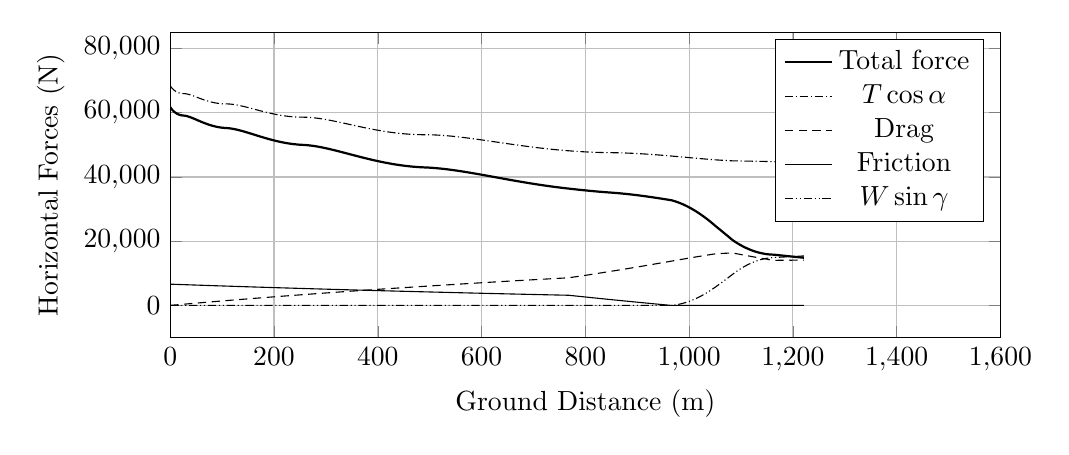
\begin{tikzpicture}

\begin{axis}[
width=\textwidth,
height=0.45\textwidth,
scaled ticks=false, tick label style={/pgf/number format/fixed},
xmin=0.0,
xmax=1600,
xlabel={Ground Distance (m)},
xtick={0,200,400,600,800,1000,1200,1400,1600},
xmajorgrids,
ymin=-10000,
ymax=85000,
ylabel={Horizontal Forces (N)},
ymajorgrids,
legend entries = {Total force\\$T\cos\alpha$\\Drag\\Friction\\$W\sin\gamma$\\}
]

\addplot [
color=black,
thick
]
table[row sep=crcr]{
1.3729668748937997E-8	61783.509366765546\\
2.6049868369719035E-7	61783.50929223756\\
2.0491224421327626E-6	61783.50875211827\\
9.92442121137073E-6	61783.50637460116\\
4.7452367809869807E-5	61783.49505135376\\
1.740064756114434E-4	61783.45690432364\\
4.0608377013922605E-4	61783.38703856451\\
7.313431501337001E-4	61783.28925139771\\
0.0011549487327126044	61783.16206794526\\
0.0016799013484208249	61783.00466997588\\
0.002295089346817705	61782.82046703753\\
0.003009933382444524	61782.60671514053\\
0.003810608015426248	61782.36762262479\\
0.004723484476856681	61782.095396470264\\
0.005727138856912631	61781.79651047752\\
0.006836216967948795	61781.46668397628\\
0.007997302399386296	61781.121859825886\\
0.00929136979810952	61780.73806369722\\
0.010685558505459776	61780.32514493953\\
0.012178513621519987	61779.883587505115\\
0.013775244426719659	61779.41199479997\\
0.015470070176169002	61778.9121292319\\
0.0172374436815836	61778.39159101309\\
0.019122918912604377	61777.83704094424\\
0.021104911040230538	61777.254920050735\\
0.023190717999955576	61776.64316866206\\
0.025355802981115103	61776.00905644147\\
0.027620619195902148	61775.346663685516\\
0.030020274690474198	61774.64582733196\\
0.032476028269866286	61773.92962251451\\
0.035054163466719815	61773.17878836808\\
0.037720846868992755	61772.40326882189\\
0.04049779674511381	61771.596830862196\\
0.043329456594087365	61770.77567057684\\
0.04629652060163805	61769.91646490246\\
0.04934498934704602	61769.03494537364\\
0.052507657924119336	61768.12170986616\\
0.055769483710642484	61767.181194273304\\
0.05917209570914676	61766.201504189055\\
0.06264043916012321	61765.204337790055\\
0.06620063977265622	61764.18224131629\\
0.06987962792775945	61763.127574047045\\
0.0736568184539585	61762.04633196129\\
0.07754284280095361	61760.9355603015\\
0.08151127871105612	61759.80289025819\\
0.08560324933017655	61758.63667237759\\
0.08985265585263943	61757.42738006891\\
0.09413961367176535	61756.209211185545\\
0.09857725310864562	61754.950095696404\\
0.10307959255469257	61753.67452373482\\
0.10766008648593872	61752.37873170985\\
0.11234920964493048	61751.054174536825\\
0.11719267720457946	61749.68806296871\\
0.12216973960582883	61748.28638979494\\
0.12724007601918352	61746.86061206156\\
0.13233299746505212	61745.43063843409\\
0.13755256756750583	61743.96730248896\\
0.14287728588926696	61742.47673662352\\
0.1482946925752714	61740.96251193287\\
0.15381585025670613	61739.42161857773\\
0.15940564092189102	61737.86392473645\\
0.16526271495916878	61736.234244073596\\
0.17120082448158402	61734.58457834528\\
0.17717889132867753	61732.92637317281\\
0.18324322596131126	61731.24682021554\\
0.189427022360885	61729.536814513674\\
0.1957511558722988	61727.79070636642\\
0.2021484013779125	61726.02715014755\\
0.20865863707071397	61724.23522823218\\
0.21548666343168166	61722.35880414229\\
0.22220154781289658	61720.516391341225\\
0.22919671627301902	61718.60010555672\\
0.23611678795738544	61716.70738961699\\
0.24306300975244904	61714.81047563661\\
0.2503085190632165	61712.83493900011\\
0.2576623280401219	61710.83307296505\\
0.26502430524173204	61708.832166052074\\
0.2724963584449146	61706.80455267803\\
0.2802001060647876	61704.71740722416\\
0.2878583985474956	61702.64589278669\\
0.2958320780323821	61700.49253443397\\
0.3040021452321372	61698.28975872861\\
0.31208951788619	61696.11283844129\\
0.3202851396023423	61693.91034627009\\
0.3287233234973125	61691.646370664486\\
0.3370425959884752	61689.41793056276\\
0.34575405233845447	61687.08825444979\\
0.3545073625286812	61684.75126919118\\
0.36338982075299686	61682.38373415264\\
0.37247557159370037	61679.96605977346\\
0.38151350442869847	61677.56512064861\\
0.3905554764834429	61675.16706446129\\
0.3999457587520332	61672.680771185886\\
0.4095398754587949	61670.14481362421\\
0.4189621792151833	61667.65845727855\\
0.4285208811402964	61665.140299861116\\
0.43828968955472236	61662.571105203955\\
0.44807735398784176	61660.001276289404\\
0.45806002753764463	61657.38465673888\\
0.4682994371692033	61654.70531963775\\
0.4787752542918833	61651.96886686431\\
0.4890770094685154	61649.28251167422\\
0.49985939134273727	61646.47568971595\\
0.5106597490205704	61643.669123655694\\
0.5213580865152188	61640.89388698757\\
0.532247733242454	61638.07389750113\\
0.5431365108549349	61635.25900029956\\
0.554075964429489	61632.43585475943\\
0.5653450694020941	61629.53267107549\\
0.5769901159382542	61626.537951076185\\
0.588512657344902	61623.579999912894\\
0.6004070039036553	61620.532041302766\\
0.6121651247369502	61617.52436854401\\
0.6239717914322569	61614.50960608393\\
0.6362472885961421	61611.380737885964\\
0.6486428939173223	61608.227001127074\\
0.6610190736373547	61605.08391196851\\
0.6737248046101814	61601.863003741775\\
0.6862826225989949	61598.6853855997\\
0.6991952542603428	61595.42393683981\\
0.7122988072688032	61592.120377468906\\
0.7251463703465595	61588.8872795264\\
0.7381769453061875	61585.61406385628\\
0.7516618647379176	61582.23295902212\\
0.7654913705221527	61578.7719886353\\
0.7791756406994825	61575.35381884678\\
0.7930637813125616	61571.891230688736\\
0.8074774191984457	61568.30449551501\\
0.8215072375247947	61564.8199329808\\
0.8361010597475598	61561.20220243951\\
0.8503303420601955	61557.68156849177\\
0.8650627501899835	61554.0433911264\\
0.8802332960144008	61550.30433228449\\
0.8951742046771463	61546.62906654988\\
0.9100334756324657	61542.980904893164\\
0.9251067343345352	61539.28730249034\\
0.9403923630470314	61535.54889954855\\
0.9559303815501943	61531.756180441385\\
0.9712400158034169	61528.02645701518\\
0.9869533781138684	61524.205799982476\\
1.0029148609762486	61520.33245006288\\
1.0189962473881624	61516.43772514856\\
1.035465185745812	61512.45710900675\\
1.0516742337458713	61508.547121987955\\
1.067815735429615	61504.66107091926\\
1.0846705971808022	61500.61135579496\\
1.1012775250051634	61496.62922021428\\
1.1180798406225687	61492.60826137068\\
1.1351395900544134	61488.53389557368\\
1.1526388687279154	61484.36307630908\\
1.1698922447507556	61480.259248859365\\
1.1875468452119025	61476.06853910089\\
1.2058383275300355	61471.73570649298\\
1.2239395537495579	61467.45694542884\\
1.2422020624207541	61463.14906985483\\
1.2608769472440078	61458.753209120885\\
1.2794948487006894	61454.38004211329\\
1.2979152553275424	61450.06231758278\\
1.3166445915281573	61445.681346141224\\
1.3354141707340492	61441.300167351175\\
1.3543210821322504	61436.89618374886\\
1.373689361295591	61432.394293300036\\
1.3932049885015831	61427.867870120404\\
1.4131781782225183	61423.24534781731\\
1.4330139682345777	61418.66459297495\\
1.4528243860883294	61414.09954283878\\
1.4728783400745615	61409.48832509975\\
1.4934621752870565	61404.765607574926\\
1.5141408097620341	61400.031615386455\\
1.53430654450827	61395.42508565971\\
1.5553850389607948	61390.62057993536\\
1.5762653203499473	61385.871792963226\\
1.5975496774716453	61381.04183032359\\
1.6196077215345106	61376.047644230435\\
1.6413652536722467	61371.13273414677\\
1.663437310723463	61366.15810024997\\
1.6860768385032747	61361.06733970705\\
1.7077101022266827	61356.21391256277\\
1.7297306410738114	61351.28463126057\\
1.7520297891459062	61346.304251537804\\
1.7743087535215367	61341.33963050558\\
1.797257424336919	61336.23745502523\\
1.8200802473615325	61331.174941882564\\
1.8430350373473994	61326.09483277793\\
1.8666926279964304	61320.87136287168\\
1.8902808566018634	61315.67543422477\\
1.9138231309717848	61310.501723899535\\
1.937187877956735	61305.3789004478\\
1.9611060682733261	61300.146907855014\\
1.9852138445648535	61294.88583239117\\
2.009780393513653	61289.537353299296\\
2.0346228225622163	61284.141782123435\\
2.0593611988602687	61278.78169159604\\
2.08477023517836	61273.289587348816\\
2.110324766702745	61267.779543525234\\
2.1352655781940433	61262.41481286228\\
2.160528860803022	61256.993715703546\\
2.1862071157614817	61251.496896087745\\
2.2127756699400534	61245.82354830127\\
2.2391904543957084	61240.1971196377\\
2.2653528664920257	61234.63820591879\\
2.292150575495974	61228.958416991605\\
2.3187704640870406	61223.33037178077\\
2.3455495914188482	61217.682710248395\\
2.372862901366455	61211.936822179254\\
2.4007145172972395	61206.0926100857\\
2.428100404243743	61200.36072637493\\
2.4555980306928005	61194.61993895333\\
2.483374904362833	61188.835501925714\\
2.511687733451976	61182.95451963208\\
2.5402569276484597	61177.03561440641\\
2.568415369317849	61171.21678804718\\
2.596987652715761	61165.32755751102\\
2.6263861238451423	61159.28383687623\\
2.655991481965028	61153.21368783555\\
2.6856115886357443	61147.15659406055\\
2.7154221146045012	61141.076707181855\\
2.7455665152057707	61134.945104020066\\
2.7752624694325894	61128.92073123672\\
2.805457625653509	61122.81129113745\\
2.8358231840904597	61116.683760733125\\
2.8663460878589797	61110.54094926777\\
2.897817297850832	61104.22448290305\\
2.9287074004595235	61098.04153121846\\
2.9603588456990284	61091.72344241309\\
2.9922321403815406	61085.37861916132\\
3.0241119471841866	61079.050019265065\\
3.056446055158509	61072.64903365595\\
3.0889346922121366	61066.235412427806\\
3.122221620829695	61059.68276418395\\
3.1546991615623394	61053.30745842711\\
3.187635101478671	61046.86023944491\\
3.221010117202278	61040.34553382661\\
3.2543449374576605	61033.85712609318\\
3.288235920596943	61027.279268360784\\
3.3223704322934555	61020.673205968196\\
3.3562838593334394	61014.12877357927\\
3.3906320903803255	61007.51947859369\\
3.425633159699527	61000.8041747401\\
3.462387235801926	60993.77373140052\\
3.4973980805087237	60987.09682088089\\
3.5324804241140235	60980.425824259655\\
3.5675385073174235	60973.77888859935\\
3.6040688981843845	60966.87338181664\\
3.6393612181513753	60960.22175305124\\
3.6770856360342323	60953.133187377316\\
3.7131729334920323	60946.37287477408\\
3.749509707933214	60939.58610535355\\
3.785733977879824	60932.84050005433\\
3.8225309786916544	60926.00873769187\\
3.860867115351552	60918.91307664593\\
3.89929745075254	60911.82225372306\\
3.9373367205567504	60904.825435048915\\
3.9751626485832894	60897.88930221455\\
4.013671158053867	60890.849860248374\\
4.0521140617426425	60883.844295670555\\
4.092377631210638	60876.53027051047\\
4.131586743753305	60869.43061031135\\
4.1715696979561425	60862.21389871491\\
4.210522654700574	60855.205387104405\\
4.250196810863292	60848.08961827417\\
4.2917015001093795	60840.669717826415\\
4.332438976653355	60833.410901686424\\
4.373124372895289	60826.184906267576\\
4.414429464889761	60818.872795675445\\
4.455884944705147	60811.558202553046\\
4.497250153511752	60804.28352382613\\
4.537976875075978	60797.144427397245\\
4.581399817640802	60789.55803846143\\
4.623816269683994	60782.17261441675\\
4.666022338967499	60774.84834358675\\
4.709098934189642	60767.39810604903\\
4.752435367147649	60759.92839191352\\
4.79531009100786	60752.563272457\\
4.838191999420829	60745.22168420619\\
4.881381760681686	60737.852306506145\\
4.9256451804034285	60730.325555464166\\
4.9704217340957495	60722.73801805766\\
5.014356093293278	60715.318945699255\\
5.058826350846283	60707.835231472156\\
5.104458009943745	60700.18298069031\\
5.149663211268795	60692.62899518371\\
5.194981168813841	60685.08276583254\\
5.241194091283663	60677.41480599648\\
5.287987552078626	60669.6784723624\\
5.334426822383641	60662.028374910544\\
5.380633359096258	60654.44385471818\\
5.427524438012913	60646.77461901831\\
5.476157635197664	60638.84973764735\\
5.524667120325573	60630.97458124574\\
5.5732739519824435	60623.11309861728\\
5.6208990292882195	60615.43888691536\\
5.671502816366864	60607.31544262396\\
5.719824083529298	60599.58784699472\\
5.767871110439133	60591.93248816891\\
5.8169321963676754	60584.144628026304\\
5.866076914057565	60576.372807322565\\
5.917200682776528	60568.31901004621\\
5.96684810088939	60560.5279016992\\
6.016885842403935	60552.70542514179\\
6.068639931677712	60544.64604938336\\
6.119867755785197	60536.69994722522\\
6.171030794930029	60528.794854969485\\
6.222884713227881	60520.814445008495\\
6.2735946138732235	60513.04056496217\\
6.325883502103322	60505.0560292758\\
6.379615386553551	60496.88421708302\\
6.432194972482147	60488.91995553195\\
6.484528316464761	60481.024579963065\\
6.536619297696934	60473.19692667847\\
6.589662958081361	60465.257919446885\\
6.644121795496577	60457.140345203894\\
6.697445536614451	60449.22445745744\\
6.7518063163896365	60441.18756848942\\
6.8068829439682315	60433.07862165723\\
6.863205650636274	60424.82121778646\\
6.9185329265047315	60416.74406298045\\
6.974634519184049	60408.58843512583\\
7.031139830722298	60400.40914887392\\
7.0870923879294985	60392.34436670509\\
7.144766952910487	60384.06714678039\\
7.2026451873548805	60375.79703771544\\
7.261191729679483	60367.46830996215\\
7.320502240843062	60359.0685497283\\
7.378210233177999	60350.931955127904\\
7.437738452534925	60342.57597542678\\
7.49714639104333	60334.27443939747\\
7.556502460410064	60326.01746132673\\
7.617032771987237	60317.63537624608\\
7.676883327249088	60309.385225662205\\
7.735740247984193	60301.30854597484\\
7.796086087039788	60293.064971278116\\
7.856787102853412	60284.81094126677\\
7.91721236259451	60276.63216334043\\
7.979013602666894	60268.30594208767\\
8.039824025454376	60260.15134711581\\
8.102419182184594	60251.79676580489\\
8.16459313580776	60243.53774740052\\
8.226347093952135	60235.373172731604\\
8.290527749984296	60226.92841151162\\
8.353592793320257	60218.670630837994\\
8.417564177281012	60210.33470287628\\
8.482044607535009	60201.97357677428\\
8.547336806956285	60193.54909253823\\
8.613293246319614	60185.0815335488\\
8.6778048537894	60176.84073851412\\
8.74454839911753	60168.35761332016\\
8.810708373588199	60159.991420210674\\
8.876548424968423	60151.707770631794\\
8.942828456712885	60143.41099783633\\
9.010858044488913	60134.93910362074\\
9.079453414959548	60126.44157520782\\
9.148767802603732	60117.90050376233\\
9.21609997183467	60109.64732475205\\
9.285579683381485	60101.17581151778\\
9.355451712480097	60092.70226483961\\
9.423585014597279	60084.48362571071\\
9.493435356703696	60076.10283353356\\
9.562655940911181	60067.842331415304\\
9.63183713653898	60059.630839871286\\
9.703018708836247	60051.22796339709\\
9.773178624863132	60042.99121397511\\
9.844376937811855	60034.67857184287\\
9.914998792594716	60026.478841277756\\
9.98720270419701	60018.14219408386\\
10.059478150570087	60009.84445837757\\
10.132362020358627	60001.524471121666\\
10.205876892438312	59993.180679839556\\
10.279422251887688	59984.881699353966\\
10.353305644514993	59976.59299455708\\
10.42811398108589	59968.24977214019\\
10.50332954727428	59959.9108925436\\
10.578207710262959	59951.65878202635\\
10.65503529959097	59943.24281754914\\
10.730232142651953	59935.05530155245\\
10.805871937852555	59926.8690724351\\
10.88265320376452	59918.609897571965\\
10.958577899345514	59910.492786358926\\
11.034861147941964	59902.38714384154\\
11.112742623646977	59894.16297640432\\
11.190543636431041	59885.998853665806\\
11.267787598939979	59877.94395659388\\
11.3462805052093	59869.81044284126\\
11.423875697147409	59861.82090075051\\
11.502735831556972	59853.75281705857\\
11.581465323066688	59845.7498915067\\
11.661639233340708	59837.653117383714\\
11.741743247575428	59829.61658697078\\
11.821864700430528	59821.63128234241\\
11.901816327719768	59813.71551534033\\
11.98361062800689	59805.671491045796\\
12.065425957085825	59797.68000861416\\
12.1478520915771	59789.68388370205\\
12.230956215923495	59781.67768113864\\
12.313306905825911	59773.79901836789\\
12.396632357805931	59765.88256654976\\
12.479578787946746	59758.0573307201\\
12.564327762802186	59750.118716013516\\
12.648175874147956	59742.32064932774\\
12.736145481689512	59734.19909420061\\
12.821080154398764	59726.41563316235\\
12.908009536077355	59718.50805736994\\
12.994986774303499	59710.655316528675\\
13.081752199798046	59702.88046578503\\
13.17035388279784	59695.00141583485\\
13.257836697901475	59687.28146448426\\
13.34511613365563	59679.638256932376\\
13.433461823066896	59671.9612632912\\
13.524108483575919	59664.146401812264\\
13.611203924103116	59656.69671218748\\
13.702229394080796	59648.97244663573\\
13.792427706753081	59641.38022593765\\
13.882429934062493	59633.865654679714\\
13.975435778888343	59626.164234512034\\
14.065832730112316	59618.74089063109\\
14.157894546480026	59611.243460507\\
14.250668806951023	59603.75171510549\\
14.343291987615704	59596.33573185913\\
14.43744444968501	59588.86215898304\\
14.532636396723657	59581.37230312753\\
14.625507232812737	59574.12901879815\\
14.721503924398366	59566.70807555599\\
14.818738382089133	59559.25973503821\\
14.913572076739943	59552.06125665712\\
15.009701633366973	59544.830649446216\\
15.10815424447124	59537.49418025029\\
15.206130868840724	59530.26211925669\\
15.304035939715973	59523.1037873875\\
15.403499839366233	59515.901293934454\\
15.503209871950865	59508.75134738878\\
15.601718454553605	59501.75649397849\\
15.700655560608023	59494.799936721785\\
15.801250929860519	59487.79714650803\\
15.899917805652187	59480.99728424764\\
16.001574124100856	59474.0622824186\\
16.102638779863817	59467.23870893009\\
16.204479333764816	59460.434171823275\\
16.30489644092564	59453.79469749033\\
16.40578186591999	59447.19396453517\\
16.509201471948074	59440.499696795014\\
16.614557195984908	59433.75507822483\\
16.717657554831042	59427.22784181019\\
16.823039336622365	59420.63053242183\\
16.928576062495388	59414.09860360046\\
17.03469945574068	59407.60586392644\\
17.140697318244236	59401.19611664394\\
17.246066414787876	59394.89873360671\\
17.35183930840021	59388.65151081099\\
17.458399953804133	59382.4327742617\\
17.565707112453843	59376.24629788527\\
17.673103795073075	59370.13058738563\\
17.781888038667653	59364.01303654736\\
17.89115167195854	59357.94644570211\\
18.00105710767307	59351.92273243755\\
18.110142905530395	59346.021542548944\\
18.219697237410173	59340.17255431888\\
18.32752951944549	59334.49114442243\\
18.43743745973078	59328.77734000291\\
18.54904630654982	59323.05436148055\\
18.659302591714813	59317.47889365784\\
18.770734536087716	59311.922640632474\\
18.883577445650936	59306.37636054121\\
18.996263390583444	59300.918194155194\\
19.108816920034535	59295.54638044073\\
19.22287647779894	59290.18392556124\\
19.33763586704334	59284.8708301413\\
19.456324114791514	59279.462350562346\\
19.57349394116079	59274.20906667218\\
19.690148252848566	59269.06350217933\\
19.80521137071168	59264.07055691337\\
19.92379170801214	59259.01037012429\\
20.04216631061405	59254.04512530484\\
20.15848954929409	59249.24951871802\\
20.278242138037896	59244.398817670386\\
20.396206084226087	59239.705883252944\\
20.516315546862906	59235.01431471809\\
20.637173924977112	59230.381534501634\\
20.75450010628387	59225.96836669884\\
20.874378237858778	59221.54463345367\\
20.996035953832852	59217.14323163405\\
21.11812959618858	59212.81490652209\\
21.240471115580952	59208.56679255003\\
21.361479376438375	59204.4523397592\\
21.485224699488654	59200.33440226178\\
21.607870280890317	59196.34216364245\\
21.73242999733349	59192.378129909266\\
21.85704493170313	59188.503332177235\\
21.98122016226351	59184.73246189629\\
22.10826921766411	59180.96728348904\\
22.235261614051304	59177.297459804264\\
22.361664688868032	59173.73738620397\\
22.48780138980522	59170.27674810229\\
22.614107216476143	59166.903215206185\\
22.74409311379692	59163.526960562245\\
22.873024137794893	59160.27358310405\\
23.003512644166257	59157.077431954094\\
23.132891545907036	59154.00404412844\\
23.26270690888247	59151.01566277954\\
23.39264146728729	59148.119922370024\\
23.52277721573431	59145.31506816442\\
23.654883767164463	59142.565073675185\\
23.78569183677709	59139.93845494716\\
23.917003007077597	59137.397878233314\\
24.047013652206026	59134.977094407936\\
24.178458227988493	59132.62506156297\\
24.314609552493202	59130.28970846717\\
24.447533097503474	59128.10849020885\\
24.579128452041708	59126.044921197274\\
24.71011994849615	59124.08527511875\\
24.843278471916108	59122.18953086015\\
24.975761222328053	59120.3995151893\\
25.1115496753864	59118.66404123037\\
25.247101122854083	59117.031485641535\\
25.384906965000688	59115.473800159394\\
25.522261036073317	59114.02329591448\\
25.66123001648475	59112.65916202897\\
25.79865327455613	59111.412220009166\\
25.826335196219034	59111.173292860185\\
25.839610403727477	59111.06016813636\\
25.841006316401874	59111.04832142385\\
25.84227013303559	59111.03758486599\\
25.84770509053729	59110.991285755124\\
25.86419328224909	59110.84956406616\\
25.90571916957557	59110.48423635964\\
25.999268866927544	59109.61738571797\\
26.123295978662824	59108.37527727836\\
26.250212562581652	59106.99585014139\\
26.376891976518465	59105.51099074131\\
26.50638698165423	59103.88295299966\\
26.634042370994827	59102.17034837151\\
26.763333806613538	59100.32814383638\\
26.893207366259766	59098.36991577255\\
27.022905486492228	59096.3079113125\\
27.153956322362554	59094.117721507224\\
27.287774297957696	59091.77201957899\\
27.42030033806219	59089.34152350828\\
27.555504894698295	59086.753126831885\\
27.691130018821354	59084.047714536326\\
27.82633313037239	59081.24349753359\\
27.959508564917073	59078.378020770775\\
28.096515548835796	59075.324479456554\\
28.232789703382153	59072.1823823243\\
28.368684388406535	59068.9462203201\\
28.506541650227618	59065.55978576679\\
28.64533374691623	59062.046430068134\\
28.78297783415192	59058.46047755376\\
28.92277775692753	59054.71611034637\\
29.06227187463503	59050.87859386744\\
29.20212864139956	59046.930837484906\\
29.34335827861657	59042.84382212987\\
29.483225747293005	59038.69802591973\\
29.625960812476485	59034.36784878081\\
29.76706561118049	59029.989791844884\\
29.909402910999468	59025.47678507438\\
30.051751399473822	59020.8676114198\\
30.196612335666572	59016.08007745379\\
30.342192969749448	59011.171544509954\\
30.48583400527584	59006.23423035207\\
30.632658550781265	59001.09217207297\\
30.77846394498075	58995.89178923881\\
30.92408133049836	58990.605930648235\\
31.071091331299215	58985.17740185377\\
31.218274793935116	58979.65107155479\\
31.366705758252415	58973.986619017116\\
31.515339333797037	58968.22390966973\\
31.66356819769615	58962.38798676559\\
31.814689402684216	58956.34813020486\\
31.96649953392354	58950.19054149531\\
32.115424616034375	58944.063435531265\\
32.266253234088566	58937.77195472196\\
32.41813832080348	58931.35019237037\\
32.569791431087395	58924.85321928817\\
32.722234201183724	58918.23809236006\\
32.876984607664	58911.43767394214\\
33.031873994672836	58904.54656213218\\
33.18502245018544	58897.65098936632\\
33.34135780547538	58890.52921922153\\
33.49759920343199	58883.32955340628\\
33.65385117142162	58876.04853912251\\
33.8113313806527	58868.6297711052\\
33.96985264489639	58861.08162830524\\
34.126473036379195	58853.54611779876\\
34.2857505660089	58845.804658557056\\
34.4449212019973	58837.990992087216\\
34.60566879064274	58830.022676368535\\
34.76644486933921	58821.97659773615\\
34.92612701881755	58813.91094474126\\
35.08630421658309	58805.74711860018\\
35.24825698849928	58797.41954485001\\
35.412303951281956	58788.91047820373\\
35.57355277914179	58780.475397187925\\
35.73545353069308	58771.93646678385\\
35.89925038949356	58763.22764243708\\
36.065161289279985	58754.33601119179\\
36.23047312008262	58745.407261607004\\
36.39472205714358	58736.468708196655\\
36.56135389445764	58727.3332449437\\
36.72774532558607	58718.14461646293\\
36.89384825683493	58708.907002468026\\
37.05904296416534	58699.65674634783\\
37.22702676294645	58690.186922490975\\
37.39437475321985	58680.69056758637\\
37.5621109943643	58671.11088527537\\
37.73270471709142	58661.306262903454\\
37.903359519601935	58651.437032337126\\
38.071486842086316	58641.65537345306\\
38.23815243703595	58631.90246954738\\
38.40817787072022	58621.8963340199\\
38.57751392140098	58611.87505041326\\
38.750215798728505	58601.5984534313\\
38.92001182640311	58591.44063194272\\
39.09310637700479	58581.031363319606\\
39.26472366117933	58570.65810519489\\
39.436554723976656	58560.2203277346\\
39.608961777617054	58549.69676413189\\
39.782828308010565	58539.03368276727\\
39.956194359016465	58528.351955831444\\
40.132391837044906	58517.44639837544\\
40.30868053167249	58506.48648758569\\
40.48611580488176	58495.40720925956\\
40.66383502946924	58484.26295153117\\
40.83999042132467	58473.17117165084\\
41.018202681018664	58461.90477778971\\
41.19780999006247	58450.50538240993\\
41.37730467548502	58439.06927996941\\
41.557010452813884	58427.576885301576\\
41.73612816026986	58416.080496731534\\
41.91555194917056	58404.52386632927\\
42.09743589423803	58392.7683639257\\
42.27807550146298	58381.05405492072\\
42.45995188234755	58369.22108447994\\
42.6401410478328	58357.46084451144\\
42.822293873795985	58345.535985815324\\
43.00585672428667	58333.48275732208\\
43.189965171449515	58321.35836644465\\
43.372020236704074	58309.33539620339\\
43.555636897252796	58297.17623950049\\
43.74012033961118	58284.92723836351\\
43.92429822300048	58272.667063637884\\
44.106869824379004	58260.48374108049\\
44.29411840239129	58247.95819074246\\
44.47920670866131	58235.54812797632\\
44.665034305215386	58223.06042753789\\
44.85242224248053	58210.44034807375\\
45.03948098831597	58197.81582201942\\
45.22811764277584	58185.058825195534\\
45.41548629589063	58172.362689611866\\
45.60322541388645	58159.61749457168\\
45.793007222766036	58146.71018175215\\
45.983742663331824	58133.715196987076\\
46.172643153142886	58120.82360019541\\
46.36421599110457	58107.72856378376\\
46.553512793459404	58094.76916649824\\
46.745018895697555	58081.63924755542\\
46.93606459490553	58068.52246865303\\
47.126948089509526	58055.399322511075\\
47.31881294044018	58042.191948956286\\
47.5110690178297	58028.94165793371\\
47.705448624448266	58015.529620805144\\
47.90005519882567	58002.08729466068\\
48.09288923506665	57988.753821817445\\
48.28732881729917	57975.29649258632\\
48.484002572746206	57961.67227649606\\
48.68089030454945	57948.02175036067\\
48.87532723390382	57934.53069657681\\
49.07073736177763	57920.96248168353\\
49.2672083392297	57907.311688940186\\
49.46586249263092	57893.500948490764\\
49.661880987188695	57879.86611073703\\
49.85966148345089	57866.10213434082\\
50.05808618672894	57852.287491669296\\
50.25785665917266	57838.37405780809\\
50.45743808511885	57824.46948437937\\
50.65573800086891	57810.650711323484\\
50.85948768734909	57796.449357057936\\
51.061243703011925	57782.384955954665\\
51.26368286286315	57768.2717199746\\
51.46416466063809	57754.29451443981\\
51.66475943174029	57740.30975949828\\
51.86588207153103	57726.28927747418\\
52.07444928962187	57711.7517504664\\
52.2824430085781	57697.25694814083\\
52.48676525705545	57683.02145090792\\
52.69531994892206	57668.495370367586\\
52.90027076850366	57654.22528569281\\
53.108186167814935	57639.75458794208\\
53.31165724918766	57625.599587912264\\
53.520024946679996	57611.111213658834\\
53.72688450142306	57596.73570630954\\
53.93707391647578	57582.13769581154\\
54.14518573319289	57567.69354002162\\
54.35125853722778	57553.40097550365\\
54.56213447502874	57538.78636557571\\
54.77598621923464	57523.97770021575\\
54.987629956235494	57509.33473047563\\
55.19778857845695	57494.807806832396\\
55.41030974885841	57480.13174560276\\
55.62390503323701	57465.39656626772\\
55.83671574169797	57450.73121459727\\
56.047071254351536	57436.25112684186\\
56.26137331252919	57421.516475667115\\
56.47512769358855	57406.83734439152\\
56.69105800830218	57392.02757444828\\
56.90937011004422	57377.07432994677\\
57.12736617899088	57362.16336227761\\
57.346833156368504	57347.17329164679\\
57.56476609337061	57332.31002194286\\
57.78230894703917	57317.49589800775\\
57.99943865551505	57302.73300721336\\
58.21827465292657	57287.878094534506\\
58.436085045729726	57273.11734743502\\
58.6577546799423	57258.12084894316\\
58.87982836766625	57243.12374108152\\
59.10336118170943	57228.05575697987\\
59.324182403931715	57213.198434378166\\
59.545440661451366	57198.34011381923\\
59.768227251413464	57183.408505049665\\
59.99077485409802	57168.5229217376\\
60.21631063559073	57153.46868317395\\
60.44006004384342	57138.56534054552\\
60.66502706168687	57123.61328863702\\
60.89133011288284	57108.60581191623\\
61.11585558357916	57093.74988425255\\
61.3432655409558	57078.73787805112\\
61.57186440401435	57063.68325647731\\
61.79868765088207	57048.78169684716\\
62.025670725987	57033.906234547016\\
62.254132946411545	57018.971376022324\\
62.48290793247415	57004.05437949208\\
62.713817944074236	56989.037615550566\\
62.94484116346062	56974.05371538746\\
63.17805109236767	56958.96937002304\\
63.41124119062552	56943.92844910741\\
63.64505576847972	56928.890124778336\\
63.87735201907903	56913.992524489266\\
64.11169045660182	56899.00800368581\\
64.34725756208485	56883.990059667674\\
64.58324360279937	56868.99133969548\\
64.81881329818131	56854.06547602422\\
65.05563560606473	56839.10750998175\\
65.29467812810154	56824.057914632314\\
65.53178653633495	56809.178858207946\\
65.77046761369158	56794.25070173365\\
66.01019347650049	56779.3078081806\\
66.25262920761091	56764.24811748495\\
66.49342175078831	56749.34290513514\\
66.73393309567928	56734.50775363187\\
66.97718905970893	56719.55735687971\\
67.21919788222482	56704.738057932744\\
67.46413738735515	56689.79511562774\\
67.70584739194695	56675.10474100402\\
67.95375887035246	56660.09529353112\\
68.19817148521656	56645.355513091534\\
68.44413350233111	56630.580760971\\
68.68984243621705	56615.880264517546\\
68.93951041285982	56601.0038587904\\
69.19023531750676	56586.1268122574\\
69.43956667494601	56571.39489563154\\
69.68998597860525	56556.66186294671\\
69.94098943220166	56541.95847350363\\
70.1928405184459	56527.270324740035\\
70.44659484061637	56512.53740433678\\
70.69926103579675	56497.93418684149\\
70.95414956377036	56483.270266171676\\
71.21136313866151	56468.542035862\\
71.46778788208749	56453.9288984493\\
71.7247351381395	56439.35648634858\\
71.98234155897126	56424.8180044145\\
72.24107377350035	56410.28832643597\\
72.4986091150376	56395.89831477357\\
72.75949164810788	56381.39543729776\\
73.02014691132015	56366.98019445641\\
73.28114866838587	56352.62136006102\\
73.54342372888959	56338.26910260241\\
73.80584407854005	56323.98621917596\\
74.07231166191039	56309.562653866844\\
74.3389341302921	56295.211436909565\\
74.60521354141642	56280.959733993426\\
74.87280568706873	56266.719813756994\\
75.1403821105715	56252.56340797615\\
75.41145333671997	56238.30685390692\\
75.68265298797411	56224.129348118295\\
75.95075857762194	56210.198381071124\\
76.2241428819712	56196.080373868725\\
76.4990100438061	56181.97504283188\\
76.77213586328236	56168.04815032467\\
77.04724851790667	56154.110143973856\\
77.32330034006353	56140.215971917685\\
77.59850473375684	56126.45602365154\\
77.87773830129439	56112.588494646116\\
78.1565255546137	56098.83788338523\\
78.43842651648492	56085.03039029079\\
78.720833678605	56071.2960234566\\
79.00101298089581	56057.7672708317\\
79.28359351218376	56044.22111535349\\
79.57011733099088	56030.5873929613\\
79.85418914588558	56017.171616137406\\
80.13919871477489	56003.813295867934\\
80.42568449319114	55990.48889569937\\
80.71472498530085	55977.150847081095\\
81.006853148924	55963.77806481495\\
81.2951972638476	55950.685134489366\\
81.58524575795963	55937.62208577688\\
81.87461709596036	55924.69713732079\\
82.1711642895769	55911.56358509757\\
82.46716486408064	55898.56761212996\\
82.76422974563803	55885.639189878304\\
83.05801377197795	55872.966535806525\\
83.35853301954708	55860.11999709159\\
83.65664966506407	55847.493111133794\\
83.95487262936624	55834.97864669273\\
84.25322789115987	55822.57603258046\\
84.55664509033022	55810.08381219684\\
84.8599544590121	55797.71818520826\\
85.16499148084048	55785.40568557574\\
85.47187188044902	55773.14420313493\\
85.77908321853027	55760.99588490385\\
86.08675489504844	55748.956481290545\\
86.39784539041122	55736.91301986623\\
86.71051296037359	55724.940320143956\\
87.02583358957506	55713.00025132463\\
87.34037846285594	55701.22423164034\\
87.65395388450591	55689.61876782369\\
87.96687312379424	55678.17158905571\\
88.28527441497255	55666.66163527782\\
88.6103524516937	55655.05407455911\\
88.92871226770333	55643.82754740059\\
89.25003295857354	55632.63860663297\\
89.57522243846881	55621.4605632289\\
89.90247582737899	55610.359836645206\\
90.22602529632545	55599.53133281492\\
90.5494223037065	55588.85393594352\\
90.87816525326718	55578.15000806705\\
91.20455861430293	55567.672526214286\\
91.53817773235312	55557.11786238225\\
91.87076195087604	55546.75204277062\\
92.20124984301029	55536.60630858046\\
92.53140503523474	55526.62516407887\\
92.86389705561814	55516.72966221615\\
93.19815266874983	55506.940111991484\\
93.53304529783748	55497.29156522652\\
93.86737084100128	55487.8191060477\\
94.20337949361911	55478.46012166764\\
94.54065981474497	55469.228542426164\\
94.87396787418089	55460.26627874108\\
95.21684847579547	55451.21354450057\\
95.55392648231228	55442.47935577111\\
95.89232371872416	55433.87620972113\\
96.23051075783204	55425.444124344926\\
96.57164052232307	55417.10682492246\\
96.90762523479154	55409.06066922397\\
97.24755293575913	55401.08744085797\\
97.58790661409188	55393.27317860957\\
97.92576087813703	55385.683811292576\\
98.26661027452474	55378.196585828526\\
98.6051908024865	55370.92797251418\\
98.94563962387357	55363.78915235387\\
99.28665364663627	55356.80956910191\\
99.63350087797645	55349.88654758029\\
99.97685593767679	55343.20829875936\\
100.31593955776762	55336.784362721926\\
100.65572384630482	55330.51812253495\\
100.99616871909686	55324.41162378939\\
101.3402339503516	55318.41531395883\\
101.67973054404297	55312.67146142546\\
102.01657591573795	55307.142404462036\\
102.35656456518868	55301.733668189\\
102.6941824316649	55296.533818709635\\
103.03547296258705	55291.45103163029\\
103.37623032340073	55286.550602954696\\
103.71852978299776	55281.80372456637\\
104.05851119314701	55277.26358692192\\
104.3949509202441	55272.94228536794\\
104.7329053851843	55268.773569539684\\
105.07104272194636	55264.7754091573\\
105.40742307340048	55260.96977619176\\
105.74423560014887	55257.3311268126\\
106.07955743077031	55253.87965850149\\
106.41623710643992	55250.586182286585\\
106.75618472497374	55247.435806878086\\
107.0942647435474	55244.47743997368\\
107.43151869252583	55241.70011435286\\
107.44650965670576	55241.58069540729\\
107.45815118347005	55241.48819521839\\
107.46233674961977	55241.454988552025\\
107.46535588765028	55241.43104703388\\
107.46808502617694	55241.40939219839\\
107.4836206108138	55241.285842586\\
107.53176708907421	55240.899928117826\\
107.68672244793561	55239.626960992566\\
107.97570433527497	55237.1275168844\\
108.27744765146667	55234.34478523844\\
108.5816623935838	55231.36213832423\\
108.88557241638279	55228.20662277358\\
109.19209959959528	55224.847629802796\\
109.50241879336687	55221.26850708951\\
109.81066605766154	55217.53717507739\\
110.12101503747155	55213.60486622958\\
110.43285681965125	55209.478027932404\\
110.74725799716322	55205.140926515276\\
111.06462449033057	55200.585143260716\\
111.38211128519615	55195.85078082445\\
111.70119562731901	55190.91624326336\\
112.02298633508096	55185.762696972946\\
112.34320819983824	55180.459552816465\\
112.66812620709393	55174.90240434147\\
112.99302416686388	55169.17002359884\\
113.31966045518399	55163.231929297704\\
113.64998129974768	55157.050333796215\\
113.97857627498675	55150.72687946381\\
114.31304608469316	55144.11399539623\\
114.64448318111735	55137.387536824186\\
114.98093514978115	55130.38464444516\\
115.31969924418831	55123.15789763947\\
115.65790718621022	55115.76917538952\\
116.00063352526521	55108.1066431607\\
116.34235083463872	55100.29327846086\\
116.68621873349733	55092.258069202944\\
117.03331062078092	55083.974000143775\\
117.37910048629482	55075.549774563566\\
117.72869476105836	55066.86127277851\\
118.08005947084649	55057.95709579633\\
118.43363644355449	55048.82531423376\\
118.79186464668504	55039.40016126484\\
119.14769212941735	55029.8677745188\\
119.5036618261702	55020.163862424335\\
119.86270697471275	55010.20840721973\\
120.22616362054572	54999.9613623599\\
120.58991121293201	54989.53789535622\\
120.95538130513773	54978.89788519159\\
121.3195355377388	54968.13178562923\\
121.68590041554987	54957.13700965607\\
122.05305648207542	54945.95642393874\\
122.42257239354896	54934.542464099024\\
122.79503144936103	54922.87594703115\\
123.16629137010841	54911.0877970264\\
123.53950748252527	54899.07965380486\\
123.91239367862553	54886.92633874959\\
124.29026003316017	54874.45419442127\\
124.66301933937496	54861.998531424266\\
125.03890311735066	54849.28779514693\\
125.41380975776434	54836.46165322661\\
125.7896808967325	54823.455940652886\\
126.16837244152023	54810.20648829953\\
126.54595968852882	54796.85187089727\\
126.92471834906405	54783.31380872392\\
127.30294276405039	54769.655134434026\\
127.68255852126984	54755.80805538468\\
128.06243727540487	54741.81503598143\\
128.44360431740483	54727.63968159995\\
128.82265748788262	54713.41112802026\\
129.1989690567886	54699.15758201186\\
129.57765386613931	54684.687605448984\\
129.95508099647026	54670.141464411994\\
130.33359114840187	54655.431109087105\\
130.71373745886524	54640.53579632992\\
131.09453904397424	54625.494935492185\\
131.47657586018488	54610.28679983453\\
131.85678563989967	54595.03561204075\\
132.23856625352113	54579.60722827214\\
132.61595336405918	54564.24591941519\\
132.99976263915818	54548.512553903114\\
133.38083522978053	54532.78296714711\\
133.76098428781995	54516.98583346914\\
134.1363519425165	54501.28572220524\\
134.51557915495124	54485.32347665989\\
134.8968696170101	54469.174233687416\\
135.27419431482667	54453.09595238042\\
135.65215477207505	54436.895672847546\\
136.03329358991255	54420.464814543244\\
136.41192880753374	54404.04989387219\\
136.7898079310749	54387.57812784893\\
137.17001317148595	54370.91639121082\\
137.54844558779996	54354.24588357264\\
137.92617219433072	54337.52218986036\\
138.30476964659732	54320.67717583553\\
138.68390038934075	54303.72711784835\\
139.0631653430654	54286.691350521956\\
139.4406106933401	54269.65984441161\\
139.81914660512416	54252.50317474629\\
140.19767098864742	54235.27262039212\\
140.5730919292459	54218.11145764659\\
140.95061983253072	54200.783402422356\\
141.32838502869612	54183.375209342325\\
141.70636515873298	54165.88937300486\\
142.0839785067887	54148.35441799321\\
142.46357402350594	54130.6624160745\\
142.84082211769783	54113.01680011365\\
143.21906727224075	54095.263007841946\\
143.59963619096823	54077.33949486245\\
143.97984478872678	54059.373735537054\\
144.35941603837455	54041.3805692239\\
144.7355521893594	54023.49501840105\\
145.11296635073694	54005.49490559756\\
145.49073213867456	53987.425513067545\\
145.87033631970945	53969.21671940095\\
146.24486520181193	53951.20222502011\\
146.6238757206513	53932.923881458846\\
147.00096360401335	53914.69145127584\\
147.37874202190085	53896.380203523266\\
147.756852900845	53878.00868736998\\
148.13572640408995	53859.55718251839\\
148.5136798644104	53841.109019906085\\
148.89083780486442	53822.65974106126\\
149.2712459042852	53804.01239744236\\
149.65303236723025	53785.2593767768\\
150.0329584616291	53766.56116734771\\
150.41363382646614	53747.79081661982\\
150.79322940570728	53729.03986042536\\
151.17272478467066	53710.261355988216\\
151.55400296227282	53691.363196920836\\
151.93482601265913	53672.45741905975\\
152.31881414221942	53653.36526129705\\
152.70208150063132	53634.28092880854\\
153.08320649997165	53615.2767755276\\
153.4666285558243	53596.132671589716\\
153.84825937276264	53577.05392580257\\
154.23093781718723	53557.89991085068\\
154.61485031834388	53538.66231218311\\
155.00001234931443	53519.34136471205\\
155.38285725409855	53500.11727167963\\
155.7679513537659	53480.761945524704\\
156.1509667875323	53461.49407824312\\
156.53491934392343	53442.16320626225\\
156.91995289130983	53422.763128361315\\
157.30625057946366	53403.2856485581\\
157.69121706207227	53383.862783739125\\
158.07789765133754	53364.34201923369\\
158.46521012398495	53344.77903091333\\
158.85138765236047	53325.26421331547\\
159.23964669847322	53305.636125633915\\
159.62715395386465	53286.03908250175\\
160.01960115328984	53266.18626461169\\
160.4079207075476	53246.53747341377\\
160.79602490671402	53226.89592799681\\
161.18437278725975	53207.23948249058\\
161.57644284003254	53187.39312688798\\
161.96812230097612	53167.56611955965\\
162.35808768568592	53147.82653501601\\
162.75087300343483	53127.94594543062\\
163.14546270495134	53107.976862373296\\
163.53745675514648	53088.14301389929\\
163.92955389373896	53068.308863564394\\
164.32395276810763	53048.36428738224\\
164.71713266653478	53028.488389214675\\
165.1102153740033	53008.625453148896\\
165.5035884424101	52988.75691966736\\
165.89816400198282	52968.837785204174\\
166.29148626774366	52948.993023969975\\
166.68861804276264	52928.96831366082\\
167.082852347146	52909.10287775363\\
167.48006204110857	52889.101781615216\\
167.8798182678497	52868.98791896415\\
168.27774435731556	52848.98253538346\\
168.67741362640317	52828.906967479605\\
169.07475368467374	52808.96670456577\\
169.4759958044982	52788.850117597845\\
169.87832784425882	52768.69953641543\\
170.2792240364854	52748.64240194694\\
170.68126852540456	52728.5503640676\\
171.08617821288442	52708.338923950345\\
171.48766933901368	52688.32263934723\\
171.892744970828	52668.15333721842\\
172.29711201372032	52648.04599166557\\
172.70264003426053	52627.90862062138\\
173.1105289448074	52607.68294252035\\
173.5163733808056	52587.58836517013\\
173.92577914808027	52567.34842780219\\
174.33607303977334	52547.09672514722\\
174.74614233406845	52526.88918492927\\
175.15731444736514	52506.66142330661\\
175.56901623635082	52486.44275751093\\
175.97955109701695	52466.31733219874\\
176.39275298155184	52446.09830114305\\
176.80397138375372	52426.01421122915\\
177.21946344336607	52405.76067845823\\
177.6332252263685	52385.63162166934\\
178.05102033212842	52365.347882017304\\
178.46725124888752	52345.18247327245\\
178.88389799206544	52325.04017510825\\
179.29839533747668	52305.04559567978\\
179.71608569665375	52284.942057974185\\
180.1342696339205	52264.860946813336\\
180.5538779958007	52244.75874394906\\
180.97690569555635	52224.54157067122\\
181.39980810354632	52204.38026938173\\
181.82328311928882	52184.242511245975\\
182.24618807605736	52164.18348831612\\
182.6731660166833	52143.98447709413\\
183.10035828358116	52123.82967992268\\
183.5291445538124	52103.65520853808\\
183.95833265232255	52083.518397696185\\
184.38634616388282	52063.493901228125\\
184.8168339376561	52043.412112147125\\
185.24630581702252	52023.436973418444\\
185.67754767955432	52003.43989924689\\
186.109185775987	51983.48587416492\\
186.53971883241212	51963.64496557086\\
186.97132952004227	51943.817391135264\\
187.40711553434954	51923.86281966728\\
187.84220985117162	51904.00570434843\\
188.27778926256264	51884.19310115588\\
188.71822733349944	51864.22812585576\\
189.16086434237673	51844.23382442487\\
189.6010380968554	51824.421544970784\\
190.03919041211265	51804.77112109028\\
190.48016062316526	51785.06650518165\\
190.92524363955386	51765.25234747342\\
191.372330984798	51745.42485844741\\
191.81766281185656	51725.75164560908\\
192.2649588892154	51706.06923523542\\
192.7152080571317	51686.336200732636\\
193.16529614382966	51666.69056456789\\
193.61551258619323	51647.12047777753\\
194.0671041699889	51627.57294159569\\
194.52074606224477	51608.02045988239\\
194.9783774267325	51588.3819313057\\
195.4358245305881	51568.83833523771\\
195.89499401276925	51549.3094502414\\
196.35432087192027	51529.86317143665\\
196.81831699949333	51510.31069318409\\
197.28093205423113	51490.90873969083\\
197.74513845889334	51471.53350281385\\
198.21238653581378	51452.126645801516\\
198.6780372695403	51432.882075881615\\
199.14562244096538	51413.65471875384\\
199.6172630308758	51394.36002253681\\
200.085680559985	51375.296790173394\\
200.55485539631252	51356.30301768622\\
201.0284003638297	51337.23487133828\\
201.5010163224531	51318.30762118223\\
201.97949934275624	51299.25151003625\\
202.45676989461947	51280.350816689985\\
202.93795341995116	51261.40426060528\\
203.42151825635358	51242.475085729195\\
203.9064451985618	51223.605271032415\\
204.39376498892221	51204.75681057545\\
204.88144002832018	51186.01027197791\\
205.3743097859811	51167.182402263046\\
205.86751126322014	51148.46176273344\\
206.36222180198536	51129.805133904476\\
206.85620764580733	51111.29783345644\\
207.35622660722595	51092.68945111241\\
207.85286701515986	51074.332028844234\\
208.35554496397685	51055.87932301148\\
208.85949164962352	51037.50998543683\\
209.3606904933826	51019.370640519264\\
209.86430174661194	51001.275182110476\\
210.37517113261447	50983.054094938154\\
210.88826309775862	50964.891565668586\\
211.408532759536	50946.61682711408\\
211.9275242572583	50928.53013786281\\
212.45034341379437	50910.45544903753\\
212.97278109853062	50892.54054130275\\
213.5012611434281	50874.568362673264\\
214.0307698600809	50856.71327039394\\
214.55632530210835	50839.1428224073\\
215.09027271075985	50821.447050295974\\
215.62992362610385	50803.72209036842\\
216.17218538865313	50786.0740908243\\
216.71273903148006	50768.64487507081\\
217.25354139798316	50751.37153456232\\
217.7992146693805	50734.109622529446\\
218.34754045136725	50716.93363857956\\
218.89661223248612	50699.90574176176\\
219.45761572436965	50682.68590774515\\
220.01811384548756	50665.6622400374\\
220.5796054147944	50648.790344150286\\
221.1491613381006	50631.86308410269\\
221.72392285119702	50614.9729179523\\
222.29674345543788	50598.33241299924\\
222.87200016908895	50581.81558757105\\
223.45476781204167	50565.282738720256\\
224.04346163614804	50548.78672487555\\
224.62738211659592	50532.62890877758\\
225.21466034383656	50516.5844927562\\
225.80901970025303	50500.55824018709\\
226.4067565685998	50484.656592882646\\
227.010346212326	50468.81970539455\\
227.62015690700883	50453.04557056072\\
228.23221085371028	50437.442818553274\\
228.84135848872813	50422.14335713393\\
229.46020606246555	50406.83543985404\\
230.08791152904655	50391.55160547819\\
230.71342291791404	50376.56588752603\\
231.3402722001092	50361.79421779547\\
231.96207175272258	50347.38596745739\\
232.5840768980429	50333.21752210388\\
233.21041275014744	50319.198615000336\\
233.84076499381075	50305.34228473058\\
234.4632722369638	50291.907976171875\\
235.0951321894368	50278.52646895818\\
235.7164683430417	50265.61898475065\\
236.33637872225546	50252.99026725991\\
236.95807015301216	50240.57615591776\\
237.57724458338066	50228.46297218859\\
238.1954544769302	50216.61916328035\\
238.81057478854058	50205.08389517323\\
239.4264917144386	50193.78380206476\\
240.0366097511752	50182.83773555841\\
240.63918371105967	50172.26978037649\\
241.24161561476188	50161.946319831215\\
241.8433627512665	50151.87698078103\\
242.44272012201816	50142.089252352394\\
243.03744426405035	50132.61633263757\\
243.6307298234035	50123.40446261404\\
244.22108413951537	50114.474959295374\\
244.8116939475828	50105.7787713054\\
245.39744552343484	50097.38917176449\\
245.97855029096053	50089.29815842278\\
246.5589096408665	50081.44889906522\\
247.13041662269836	50073.94601707118\\
247.70663564674516	50066.60965812333\\
248.28024698100222	50059.534945925334\\
248.85288765982074	50052.700228467336\\
249.4193334510956	50046.1642517975\\
249.9777393310295	50039.94051680612\\
250.54131855768964	50033.880692868435\\
251.10095479045611	50028.084148663314\\
251.65640742239583	50022.54919192952\\
252.20851363475686	50017.263652324924\\
252.76218077146297	50012.18009448546\\
253.31371341967355	50007.33269873749\\
253.86551898536345	50002.699795668406\\
254.41422830739316	49998.30858808644\\
254.9572061395861	49994.17554552812\\
255.0653176818724	49993.37788021563\\
255.12993325322566	49992.90514513326\\
255.17825500251217	49992.553578816034\\
255.20626764895485	49992.350540624015\\
255.2307799315319	49992.17333626878\\
255.25350681352313	49992.00942496931\\
255.27636741461964	49991.844924020916\\
255.2901025823965	49991.74626889032\\
255.29493524708477	49991.711588747305\\
255.30041476425401	49991.672253122466\\
255.32542424174517	49991.49235761007\\
255.431840924477	49990.72027936719\\
255.72188923316247	49988.56166442232\\
256.19571599032633	49984.865412947926\\
256.67415123408614	49980.92082568066\\
257.15505540016306	49976.742546786234\\
257.6368423781066	49972.3438692622\\
258.1230512066297	49967.690732311006\\
258.61423458459376	49962.77342766439\\
259.1049940935744	49957.644816000204\\
259.5982522152891	49952.27483335616\\
260.09486806301686	49946.652151394286\\
260.5959555145432	49940.760934830425\\
261.1023053698689	49934.587462663214\\
261.6089919954627	49928.190101992324\\
262.11906753970584	49921.52988801147\\
262.63243815947874	49914.60573530705\\
263.14830217600297	49907.426765105396\\
263.66676080693014	49899.99036707125\\
264.1877265034735	49892.29662346345\\
264.7128105393116	49884.31963637224\\
265.241218472901	49876.068899239326\\
265.7723922912836	49867.55145340247\\
266.3079016945154	49858.73986662559\\
266.8503273810571	49849.58685493872\\
267.3932272617866	49840.19878495736\\
267.9365984091472	49830.57744371706\\
268.4918097049034	49820.51623314529\\
269.04807221243857	49810.20506944644\\
269.6097925731924	49799.56071377396\\
270.17242368341533	49788.66790738914\\
270.7441513704771	49777.36457098693\\
271.31667319188057	49765.81138159029\\
271.8922835348494	49753.962319024955\\
272.47925332376417	49741.64102898697\\
273.06804504353704	49729.042467611376\\
273.66076346861166	49716.12094939363\\
274.25294696226547	49702.97454763646\\
274.85204953299706	49689.43685548495\\
275.4590719216128	49675.479366296175\\
276.0685465790958	49661.2246470002\\
276.6808474128411	49646.66389339954\\
277.29680014730513	49631.77676027622\\
277.9224067517041	49616.4135759943\\
278.5505103374435	49600.746249439035\\
279.17831818166474	49584.846424914926\\
279.81790886718375	49568.40493320151\\
280.45539954927676	49551.77648265063\\
281.0966396233664	49534.81095429772\\
281.73735617862894	49517.622972359764\\
282.38112941523184	49500.11848400677\\
283.0301801354616	49482.235970537644\\
283.67721705328654	49464.17797353573\\
284.3202688103162	49446.00607823515\\
284.9599564878264	49427.70987125262\\
285.60213884169843	49409.1254992022\\
286.24205728342235	49390.39378859232\\
286.8783426797421	49371.56092462814\\
287.5176726031193	49352.432712664624\\
288.14959414660166	49333.32706997292\\
288.7790218355949	49314.10308732069\\
289.41060269245395	49294.621983199584\\
290.0373602432952	49275.10309169782\\
290.6616399781276	49255.47949749598\\
291.28528823747513	49235.697356961406\\
291.90747044142563	49215.786841830064\\
292.5232553861292	49195.911781232266\\
293.13767407877424	49175.91565580868\\
293.74977203443143	49155.83363136387\\
294.36691018627903	49135.42575821314\\
294.97422257673236	49115.18804211002\\
295.5803242078987	49094.840103943396\\
296.18876641420377	49074.264778078796\\
296.79141324013847	49053.74088467221\\
297.39276567122147	49033.120067174794\\
297.9894421920609	49012.52269785483\\
298.5870928977196	48991.75730589968\\
299.1813773675972	48970.97776149133\\
299.77152323390305	48950.21575012652\\
300.36612301275215	48929.17107715945\\
300.9589816797394	48908.064324721185\\
301.5517369040423	48886.83993452582\\
302.13995783060716	48865.66010056526\\
302.7265461416931	48844.42427404845\\
303.31195316833305	48823.11899126688\\
303.893632985354	48801.84032408378\\
304.47837522976045	48780.342086141434\\
305.0603224805632	48758.84152809737\\
305.6386476191806	48737.37287585456\\
306.2164211941447	48715.82515046156\\
306.79567265335925	48694.12432011751\\
307.37231001650287	48672.42584265031\\
307.9484900815751	48650.651170668614\\
308.52614124860884	48628.729020864484\\
309.10133925078446	48606.810371995554\\
309.6811704644614	48584.62650427481\\
310.25396666777317	48562.62616618301\\
310.82665929650705	48540.54648399132\\
311.40151685857484	48518.30129540517\\
311.97010244433034	48496.21966598433\\
312.53980750632184	48474.01730313251\\
313.10901660628747	48451.75870624035\\
313.67956238189845	48429.37370872694\\
314.2496933076443	48406.932504875076\\
314.8205968353319	48384.389933223225\\
315.3893122304361	48361.86478926525\\
315.9596108977621	48339.20942600739\\
316.52927325433984	48316.51345322837\\
317.0962218845675	48293.86179632964\\
317.661512728229	48271.21455558446\\
318.22894706387933	48248.42090633884\\
318.7945230010092	48225.643086331256\\
319.36250947901885	48202.71061086368\\
319.92950718778627	48179.76202625797\\
320.4959663753667	48156.78083713929\\
321.0631721024022	48133.71637109248\\
321.6290870613959	48110.65302451563\\
322.19457963905666	48087.55710184174\\
322.7618354565293	48064.340617680355\\
323.32829381843464	48041.10969777276\\
323.8944812959513	48017.844314417074\\
324.4599775338005	47994.56327603439\\
325.0236279833782	47971.31580950151\\
325.5930851369128	47947.78725393722\\
326.1571709254106	47924.440798102136\\
326.723741026211	47900.95299697116\\
327.28922394543645	47877.47313497281\\
327.8556983549987	47853.91627205166\\
328.4233330667528	47830.27654055419\\
328.9893491077544	47806.671058266016\\
329.5546671193348	47783.06296101624\\
330.1217964733877	47759.348684389086\\
330.68704439501266	47735.68395355785\\
331.2526219304833	47711.977617566095\\
331.8212338226615	47688.11735702184\\
332.38563215932834	47664.408671886835\\
332.9540373692553	47640.5075395521\\
333.52282575474305	47616.56732995126\\
334.0901133197508	47592.66867104276\\
334.6587212753741	47568.693977814386\\
335.22495173293544	47544.800462993706\\
335.79508811264384	47520.72414604174\\
336.36651436910597	47496.57649622629\\
336.93496842282195	47472.53892353234\\
337.5050159421993	47448.419639912536\\
338.07625180159437	47424.236896295246\\
338.64522733550257	47400.137925591436\\
339.21307292972244	47376.07613973142\\
339.78316525663524	47351.90960364127\\
340.3517359250782	47327.79921051343\\
340.92344762446896	47303.548370785735\\
341.49725999120506	47279.20228649571\\
342.0714758249467	47254.83409726291\\
342.6432180289123	47230.56708002492\\
343.2156727962654	47206.26716101248\\
343.788423593423	47181.95314952159\\
344.3632558179478	47157.550378198284\\
344.936112850713	47133.23218064093\\
345.5122282286983	47108.77751490362\\
346.0894236551619	47084.27998722314\\
346.6629357201275	47059.942851682965\\
347.2399030750438	47035.46427738994\\
347.8149786266573	47011.07223254052\\
348.3916437826483	46986.62013286751\\
348.96682599762005	46962.23933776053\\
349.5439461813521	46937.785922019684\\
350.1219821225792	46913.30433569495\\
350.70068616715105	46888.806174453945\\
351.28126445021985	46864.241518899595\\
351.8619451172309	46839.68646039833\\
352.4432281971418	46815.12093185814\\
353.0222568578364	46790.66663874543\\
353.6045019024799	46766.09360704286\\
354.18853493609936	46741.46337859701\\
354.7725020489422	46716.855251485715\\
355.3555439607444	46692.30640875723\\
355.94178228996793	46667.64445239527\\
356.52841816113096	46642.98834351325\\
357.11491695053746	46618.36158077369\\
357.7019804757698	46593.73572809367\\
358.2889970677636	46569.13747538894\\
358.8795343682166	46544.418555008146\\
359.47011391270996	46519.72581218822\\
360.0611888887985	46495.04133121704\\
360.65551621456757	46470.251250568064\\
361.24837490254504	46445.55361297126\\
361.8399267049888	46420.94243769585\\
362.43366065279633	46396.27360891951\\
363.0271841323796	46371.64766727608\\
363.62092175430814	46347.04795469083\\
364.2172388023977	46322.3776799272\\
364.8170682790411	46297.59976631467\\
365.4168935103936	46272.860775080175\\
366.0167447450068	46248.16041728966\\
366.613361119081	46223.63358816611\\
367.21449807554484	46198.96253287161\\
367.81411987634317	46174.39620614295\\
368.41428222027616	46149.85120880419\\
369.0136835421291	46125.38166322316\\
369.6184705538477	46100.73807716167\\
370.2203314850517	46076.26032726241\\
370.8292817941207	46051.54249265365\\
371.4325891230952	46027.10247056279\\
372.03751184905457	46002.64663670625\\
372.64963462678804	45977.95121625197\\
373.26236447571455	45953.284098972275\\
373.87329119709466	45928.74306684744\\
374.48540637090855	45904.20876761887\\
375.0984288907292	45879.69364437794\\
375.71389401660815	45855.13765369107\\
376.3292711349669	45830.64298079666\\
376.94717931076855	45806.106612241434\\
377.56118057518813	45781.78487184527\\
378.18357875745255	45757.19192456927\\
378.80534455721454	45732.6865850262\\
379.42657984220546	45708.265543542584\\
380.05059226965216	45683.799998299684\\
380.67279643790334	45659.470748980544\\
381.29916382387717	45635.04554484568\\
381.92611637580137	45610.66554329739\\
382.55700718237256	45586.201967346045\\
383.1838285741163	45561.966164685\\
383.815522641495	45537.61339145141\\
384.4482555994399	45513.29331300572\\
385.0798113246169	45489.091941106395\\
385.7142011583089	45464.85670366169\\
386.35011647349825	45440.63921799982\\
386.98806446889137	45416.421661015076\\
387.62777316145673	45392.2159016097\\
388.2677779567189	45368.0785868736\\
388.9088955203763	45343.98002556701\\
389.5502219824099	45319.95528233936\\
390.196085141905	45295.843986215055\\
390.8411912635918	45271.845334888465\\
391.4850258768763	45247.97890017234\\
392.1348161747717	45223.97854067042\\
392.78657703059184	45199.99388107861\\
393.43829425062995	45176.1002717777\\
394.0914803145356	45152.24338777567\\
394.74697534702034	45128.39416377182\\
395.4022052560256	45104.64751214966\\
396.0614826489191	45080.84877297701\\
396.7253027860521	45056.98276068429\\
397.389470201156	45033.2022201669\\
398.0561080310739	45009.4325943759\\
398.7226685692724	44985.76609254371\\
399.391462726883	44962.121983937206\\
400.06069563032156	44938.5651608038\\
400.7298361745127	44915.11521901628\\
401.4030004748297	44891.62964810165\\
402.07673432903437	44868.2308605868\\
402.7516637315023	44844.89835397396\\
403.43308814587397	44821.45160076716\\
404.11621884098975	44798.05820072749\\
404.8017412836191	44774.69652386877\\
405.4859375776791	44751.4943622267\\
406.17916116612776	44728.10339100109\\
406.869828889608	44704.91693129495\\
407.5646978623407	44681.70939979081\\
408.2605209917057	44658.59141633223\\
408.95953036015305	44635.49074521747\\
409.6622694433204	44612.39210009175\\
410.36575705355096	44589.395510912014\\
411.07335289700484	44566.39331008392\\
411.7824393477108	44543.47296506139\\
412.49368167220496	44520.61482391757\\
413.20637839560925	44497.843280235174\\
413.9231120861825	44475.07820991562\\
414.64148448951505	44452.398247052144\\
415.3640873105958	44429.72410630736\\
416.08758784728207	44407.16270122153\\
416.8163237339112	44384.58142404353\\
417.54818649211745	44362.04894868194\\
418.2830458128634	44339.57198774755\\
419.0197896011267	44317.18690034529\\
419.7618468752946	44294.79257340616\\
420.50810315351544	44272.426460171555\\
421.2538226142991	44250.232521138736\\
422.0024472585525	44228.10994211919\\
422.7601619190325	44205.88066269236\\
423.51827295501266	44183.80367774007\\
424.2791336478392	44161.81238117872\\
425.04862066884436	44139.74156872419\\
425.8175931526831	44117.857030200976\\
426.59484428165274	44095.91205383008\\
427.37319167714656	44074.11353745508\\
428.1560603980529	44052.36842345784\\
428.9441065434968	44030.662792971736\\
429.73908511318723	44008.95351269224\\
430.5390808738871	43987.29809805426\\
431.34695313464147	43965.62477784889\\
432.16146945503726	43943.97291558876\\
432.97716762270886	43922.49160997447\\
433.79906034498686	43901.05262548367\\
434.63237437495366	43879.527318563225\\
435.4690406415772	43858.13083444747\\
436.31317920434697	43836.76308786546\\
437.1637869835322	43815.456037596916\\
438.01645953609784	43794.324502758216\\
438.8814827966934	43773.12049538165\\
439.7524258551747	43752.010242996956\\
440.63826385029256	43730.786017316175\\
441.53868068573615	43709.46906526519\\
442.4384272900428	43688.42761435246\\
443.3504012304777	43667.36634825457\\
444.27758818218365	43646.22974697854\\
445.208223124445	43625.29572703119\\
446.1516186171384	43604.36357862185\\
447.10189524137195	43583.574232693456\\
448.06481468075106	43562.81225033867\\
449.03617443090013	43542.17976351624\\
450.02512103574475	43521.49664838433\\
451.0169824202726	43501.08141198862\\
452.020591047557	43480.76118841769\\
453.02360262247294	43460.79314937198\\
454.0275908503903	43441.14776906531\\
455.03100385233165	43421.85721917465\\
456.0319820328356	43402.95728966592\\
457.02914229222506	43384.47244022625\\
458.01937985050745	43366.45622722669\\
458.99771244571184	43348.99111708693\\
459.96197275276677	43332.10398049874\\
460.92139296690334	43315.62493044385\\
461.8616145847351	43299.78983256486\\
462.80206306639445	43284.26332228516\\
463.7284486681126	43269.2756862761\\
464.6393852721259	43254.83598340349\\
465.54063936700334	43240.84167584787\\
466.4349184101709	43227.24375368745\\
467.3198901301686	43214.07090368036\\
468.20051759019884	43201.24374129226\\
469.07226485074943	43188.82303372337\\
469.9345383529743	43176.809501896685\\
470.7902899889468	43165.15541939186\\
471.6423737744856	43153.818057679135\\
472.4877853124267	43142.833454793465\\
473.3248054273006	43132.2178035222\\
474.15679752822916	43121.92307688334\\
474.98717382477696	43111.904825123696\\
475.812191509144	43102.20581360435\\
476.6363066147294	43092.77158799124\\
477.44928852471696	43083.714525284\\
478.25976263885	43074.93305728918\\
479.0680268264706	43066.42257513334\\
479.8720193908648	43058.20258966899\\
480.6722055908582	43050.26540971891\\
481.4638282544993	43042.653329441644\\
482.2537496794823	43035.29643020783\\
483.0439784328089	43028.1760972761\\
483.8253492021597	43021.371751757906\\
484.60475037766423	43014.819212087226\\
485.38148111107205	43008.522969906815\\
486.15453177945005	43002.4890312762\\
486.9234848636379	42996.71782989593\\
487.6911837486889	42991.18628864015\\
488.4532446281222	42985.92356068191\\
489.2141943862101	42980.8960107046\\
489.3656654782709	42979.92243758093\\
489.9141839228952	42976.472531161926\\
489.9442198041063	42976.28704833046\\
489.95165340794586	42976.24119121168\\
489.95904841065203	42976.19555467753\\
490.0087656528135	42975.88817187473\\
490.2229205115475	42974.5529109168\\
490.80762926712646	42970.81473556964\\
491.5549224672211	42965.84103252346\\
492.3059760305267	42960.62218545722\\
493.05617311245896	42955.19069202572\\
493.8124400481423	42949.49583793136\\
494.57147098753774	42943.56039950866\\
495.33883357988543	42937.33777850418\\
496.10451558660077	42930.90806223436\\
496.8763216977479	42924.20559894206\\
497.6516028092092	42917.25108828352\\
498.43581565351974	42909.99211361588\\
499.22198438592227	42902.49046896392\\
500.0155369982069	42894.69229222114\\
500.8167457948026	42886.590444759684\\
501.6207857715186	42878.231245373594\\
502.43135952459795	42869.574254562394\\
503.2488031894138	42860.61226434198\\
504.06841756255267	42851.395075554436\\
504.89158107370974	42841.90691475141\\
505.72576854379577	42832.05766806161\\
506.5693448613787	42821.8602801298\\
507.4142887558387	42811.40947678307\\
508.26842244805994	42800.60641400938\\
509.12668782716764	42789.51186550947\\
509.9922807952486	42778.08215863438\\
510.86952952987826	42766.2547088624\\
511.75603474468153	42754.055695048155\\
512.6525773610188	42741.46895087471\\
513.552913573209	42728.579065852784\\
514.4681532282782	42715.22197116188\\
515.3867354533588	42701.56163823907\\
516.3174024261396	42687.46457436499\\
517.2602458293647	42672.92232651576\\
518.213136886093	42657.961603259726\\
519.1760409577637	42642.5778202613\\
520.1413511846506	42626.89062942809\\
521.1231004572105	42610.66756213558\\
522.1209096033688	42593.90495422194\\
523.1261067826763	42576.742398512404\\
524.1419417493194	42559.12067540003\\
525.1629084556621	42541.13259346591\\
526.1966720787225	42522.63963869566\\
527.232798559631	42503.82622402419\\
528.2697748535691	42484.72245950352\\
529.3125778912245	42465.23795440362\\
530.3569535995234	42445.453248095335\\
531.3923454146075	42425.57509612647\\
532.4241640074417	42405.50822960169\\
533.4600085213303	42385.10850010233\\
534.4866261256011	42364.64255421146\\
535.5020315541947	42344.16095319405\\
536.514508151736	42323.505133002735\\
537.5229382799621	42302.703770643755\\
538.5160648880578	42281.99893848538\\
539.5082343221115	42261.10017795648\\
540.4856117025593	42240.307113397066\\
541.4663647652112	42219.23994634027\\
542.4363165308484	42198.20851697805\\
543.403649598117	42177.04242854584\\
544.3586522503113	42155.96146029924\\
545.3070641243951	42134.847155253505\\
546.2506879020282	42113.66529801718\\
547.1923729139526	42092.3564531702\\
548.1284847870645	42071.007508694456\\
549.0607273863563	42049.58467837372\\
549.9918578398997	42028.02843085899\\
550.9129328290753	42006.55111777381\\
551.8320704888101	41984.968853073515\\
552.7431023110901	41963.431279140466\\
553.6513866954954	41941.816616933735\\
554.5567691623032	41920.132128502635\\
555.4601447965442	41898.359736211176\\
556.3560324901239	41876.63585713701\\
557.2510525453768	41854.80394810991\\
558.144367784238	41832.887104378664\\
559.0395040047595	41810.80090790581\\
559.9306875601039	41788.69034224634\\
560.8184287789293	41766.54630918481\\
561.6957839109712	41744.546764303144\\
562.5803647812363	41722.252693299844\\
563.4612104685039	41699.9416316346\\
564.3388911147272	41677.60237374199\\
565.215385530312	41655.187266154855\\
566.0886502219232	41632.751247214575\\
566.9616941548127	41610.21948303933\\
567.8301900811412	41587.70631008514\\
568.6977679531799	41565.120369488606\\
569.5620388889783	41542.526333300135\\
570.424462708284	41519.88863290982\\
571.2852292099337	41497.20457702497\\
572.1493328191241	41474.34401099365\\
573.0103554048726	41451.47840314412\\
573.8681094542301	41428.61537422915\\
574.7257926178972	41405.67185124534\\
575.584494453004	41382.62020956294\\
576.4392320762051	41359.596264489024\\
577.2895741354355	41336.61439164767\\
578.1440860684359	41313.44472574383\\
578.9955408132021	41290.28466064531\\
579.8488294812946	41267.002889518306\\
580.7009485845795	41243.68284111336\\
581.5481034887393	41220.430655830685\\
582.398203180056	41197.031023503296\\
583.2436286861621	41173.69536905446\\
584.0951419205564	41150.12798569597\\
584.9447588199325	41126.5508774015\\
585.7909961721582	41103.0072614301\\
586.6394553558484	41079.34289324052\\
587.4827778011024	41055.764759925136\\
588.3280079409788	41032.07767278394\\
589.1732196696316	41008.33684998639\\
590.0172358784723	40984.57688633457\\
590.860913103985	40960.77521567195\\
591.7056349988741	40936.8941335469\\
592.5455796206825	40913.09993501793\\
593.390591992995	40889.11507515563\\
594.23254291524	40865.171484530845\\
595.0749775640184	40841.16990372368\\
595.9164343501545	40817.15335009275\\
596.757445184641	40793.10807602953\\
597.6003409863617	40768.96865259997\\
598.4426744019354	40744.806386247394\\
599.2847755368687	40720.61316587089\\
600.125707245069	40696.41729919179\\
600.9666449061319	40672.186322140435\\
601.808765536209	40647.8875191922\\
602.6493496090866	40623.60064349024\\
603.4896653766809	40599.29040701491\\
604.3324540913729	40574.87863107765\\
605.1749627368547	40550.44618239434\\
606.0172193894603	40525.99350692777\\
606.8564954876942	40501.60119538318\\
607.6995822420379	40477.07304614538\\
608.5468271351888	40452.39981245539\\
609.3853237539292	40427.95874118863\\
610.2285785394622	40403.35748866486\\
611.0723962320026	40378.71942881889\\
611.9144944458772	40354.11241974638\\
612.7572705739071	40329.46760856948\\
613.6039342512895	40304.69215873479\\
614.447700557992	40279.98574030814\\
615.2875150228297	40255.38055754501\\
616.1283989744954	40230.73069375503\\
616.9715554180159	40206.00192641678\\
617.816851506552	40181.19917753439\\
618.6627080307358	40156.369849441166\\
619.5079936234229	40131.548263415636\\
620.355287072993	40106.65977815662\\
621.2019793580857	40081.78211104046\\
622.0488535053607	40056.89335213986\\
622.9008554858297	40031.84918623403\\
623.7470330382666	40006.97263496215\\
624.5970610944692	39981.98035675766\\
625.4445858106351	39957.06022391787\\
626.2949117084559	39932.05732643443\\
627.1456369954528	39907.043340811986\\
627.996202785663	39882.03575029182\\
628.8493276316594	39856.95568140794\\
629.7040179726459	39831.83340873505\\
630.5541510983869	39806.849910155244\\
631.4094242395336	39781.721240931554\\
632.2635827644049	39756.63223224132\\
633.1201141992324	39731.48148244673\\
633.9783198620232	39706.29058288646\\
634.8358449994842	39681.129680673665\\
635.6949254776987	39655.93419588903\\
636.5510277660717	39630.83805752084\\
637.4106283702604	39605.65241405465\\
638.26983515646	39580.492358972886\\
639.1281653037297	39555.37297720795\\
639.9892853909298	39530.187989943995\\
640.854752101091	39504.89304768441\\
641.7172955483825	39479.701639307255\\
642.5803911560504	39454.51314960493\\
643.4447648773507	39429.30740996517\\
644.3076201978465	39404.1669080428\\
645.1745276724305	39378.93037776367\\
646.0402102676721	39353.75248723086\\
646.9124608338768	39328.40774561062\\
647.7810225029502	39303.19524074832\\
648.6561125051048	39277.81945279834\\
649.5284291267524	39252.55121406379\\
650.3990692560633	39227.359466164795\\
651.2710362166958	39202.15820690864\\
652.1464633126748	39176.88693342342\\
653.0220683418463	39151.641492632916\\
653.8956541670141	39126.48603627185\\
654.7728777786044	39101.25865548334\\
655.6515481039796	39076.023544582175\\
656.5284362953553	39050.874304675104\\
657.4113325495778	39025.58865535726\\
658.2915193229558	39000.41734752098\\
659.17716463588	38975.127853739556\\
660.0651577261099	38949.81039105178\\
660.9536046953733	38924.52002582453\\
661.8402168340383	38899.32268993056\\
662.7324470689205	38874.00771103396\\
663.6200112954277	38848.867809253206\\
664.5127656227664	38823.62471730579\\
665.4027074409514	38798.505743929825\\
666.2965782601134	38773.32154619352\\
667.1908896376651	38748.17159463184\\
668.084320193617	38723.09385867779\\
668.985123002554	38697.858049857576\\
669.8863392680419	38672.6605999414\\
670.7862926077596	38647.54915040618\\
671.6898074618846	38622.390118630865\\
672.5888268774506	38597.40860344462\\
673.4982782765783	38572.191164394244\\
674.4103925687491	38546.95523256136\\
675.3150941849995	38521.979967808365\\
676.2268158638515	38496.8677277495\\
677.1406213981061	38471.75615155551\\
678.0557411892244	38446.667535600456\\
678.9688521555179	38421.6937319579\\
679.8873390970205	38396.63391105959\\
680.8083547814929	38371.56736146654\\
681.7306997118981	38346.52793519203\\
682.6500311248872	38321.63415905283\\
683.5737488494256	38296.6866055336\\
684.4960352365924	38271.84350434567\\
685.4200123844039	38247.021577203835\\
686.3479632552264	38222.16090102293\\
687.2766127474456	38197.3505228774\\
688.2061621748603	38172.58602878328\\
689.1404800584801	38147.765784351606\\
690.0764761874757	38122.9734072071\\
691.0152339372712	38098.181504334774\\
691.9552419239503	38073.43124711288\\
692.8950394637291	38048.761997987676\\
693.8400111678282	38024.033792642615\\
694.7866818158914	37999.339190742\\
695.7347004483931	37974.688501900266\\
696.6882574887352	37949.974409202245\\
697.6393666566034	37925.40506536623\\
698.5984440154043	37900.71288796952\\
699.5498840703472	37876.30046091667\\
700.5039755495234	37851.90389874928\\
701.4647289348814	37827.422646195104\\
702.4256797045559	37803.02310771283\\
703.3874603974716	37778.6901196386\\
704.3606354781252	37754.15884755837\\
705.3315887422941	37729.77456153337\\
706.3004122670179	37705.535096310705\\
707.2768098841743	37681.19919896612\\
708.2494358269255	37657.05094966758\\
709.2282890376241	37632.843205436715\\
710.2089151733701	37608.68804685952\\
711.1951755925729	37584.4922120711\\
712.1865307336975	37560.27130550942\\
713.1761747054959	37536.192879071445\\
714.1673399979175	37512.179009657775\\
715.1598728842257	37488.23461564859\\
716.1583282218428	37464.25169865352\\
717.1629472660959	37440.22712276892\\
718.1700311785478	37416.25147637435\\
719.1763338932042	37392.4030652495\\
720.1876907614742	37368.54504680021\\
721.201618282845	37344.73801163958\\
722.2184418537404	37320.97598029538\\
723.235170191942	37297.33007541923\\
724.2594935927766	37273.62346539156\\
725.2822718646494	37250.06946885123\\
726.3107341130526	37226.50306934683\\
727.3400446617545	37203.036955912714\\
728.3719103403353	37179.6335627502\\
729.4113327961686	37156.181989885765\\
730.4562931126598	37132.73088726189\\
731.5065909482435	37109.28748339857\\
732.5574458491262	37085.9603240836\\
733.6186119363024	37062.53566491988\\
734.676482187165	37039.31594986426\\
735.7351170593906	37016.212347357665\\
736.800998200209	36993.085684878955\\
737.8752235923619	36969.91589391479\\
738.9508085948025	36946.856278988285\\
740.030025186873	36923.859886256105\\
741.1174055771332	36900.83325162613\\
742.2130822925526	36877.777644747606\\
743.3102570732492	36854.83889046685\\
744.4109860747094	36831.97583073776\\
745.5166476604204	36809.16238074121\\
746.6263302357015	36786.42000969549\\
747.7458154711032	36763.633933492994\\
748.8677740542141	36740.95674804534\\
749.997151475181	36718.291436316824\\
751.1325555959445	36695.669672363525\\
752.2719517189332	36673.13501878311\\
753.4203420087897	36650.59225348731\\
754.5711754188967	36628.17336847335\\
755.7260036895639	36605.85043599628\\
756.8938875174731	36583.45304846653\\
758.065786260207	36561.15937675712\\
759.247770693134	36538.85809825304\\
760.4404154189538	36516.5441519836\\
761.64317092529	36494.2336885017\\
762.8455228703601	36472.12500480177\\
764.0679862717263	36449.84662733266\\
765.2987264665999	36427.62220707415\\
766.4085307220014	36407.75861668195\\
766.5358897019526	36405.48987974052\\
767.7848317922183	36383.22748266559\\
769.0450472645446	36359.75056460436\\
770.316931581486	36336.154035530344\\
771.6083395962344	36312.307799990376\\
772.9112380991485	36288.34558529874\\
774.2270303713512	36264.25880741286\\
775.55388582573	36240.081310069494\\
776.893629267375	36215.79093594465\\
778.2590064752919	36191.18442096254\\
779.6390771149454	36166.425150887124\\
781.0408632243589	36141.42797251743\\
782.4719583829672	36116.070668429165\\
783.9254029605222	36090.45711327199\\
785.3937619636636	36064.7239901782\\
786.8893778170732	36038.710593931304\\
788.4179231510577	36012.31796051853\\
789.9735980960556	35985.631503451325\\
791.5542677978599	35958.709012817184\\
793.1434824354058	35931.799217792824\\
794.7563093028011	35904.745061891284\\
796.3588663476394	35877.976155696815\\
797.9570311300417	35851.51120392427\\
799.5313007987854	35825.5889225078\\
801.0895110610122	35800.16283268818\\
802.6055669418217	35775.53308494954\\
804.1018949910592	35751.494794034064\\
805.5783591859272	35727.96824352766\\
807.0307066077335	35704.99929627919\\
808.4529908307093	35682.66572713813\\
809.8505654906257	35660.91855924523\\
811.2444364840742	35639.49344626861\\
812.6158728333517	35618.51677539649\\
813.9667251199407	35598.03572602743\\
815.3010783126617	35577.99327447814\\
816.6204907399006	35558.35173552873\\
817.9261081614768	35539.088775194614\\
819.226186053904	35520.113111820814\\
820.5043924755685	35501.54848315961\\
821.7811573689405	35483.26395243067\\
823.0442722941846	35465.28331159869\\
824.2983674535399	35447.615922474826\\
825.541081257411	35430.259432163875\\
826.7810697424134	35413.1456450219\\
828.0072700964611	35396.32867340394\\
829.2275465246082	35379.79194109702\\
830.440290401928	35363.50890727209\\
831.6456016564753	35347.48507047584\\
832.8458526198069	35331.69963756313\\
834.037616834057	35316.16581502257\\
835.2234914579537	35300.87983083911\\
836.3972899863502	35285.87170125925\\
837.5756391031359	35271.053265575305\\
838.7422917585684	35256.44972764459\\
839.902452142522	35242.11090064475\\
841.0603218408189	35227.97948702137\\
842.2105732200805	35214.06581705225\\
843.3580616645866	35200.3680732373\\
844.5012408269597	35186.86781873091\\
845.6398059126466	35173.57487373713\\
846.7724224635103	35160.49747106506\\
847.8965100633054	35147.65568670626\\
848.1209130838795	35139.718138522265\\
848.1623489143824	35138.14698723516\\
848.2012937955549	35137.691138432376\\
848.2388050923146	35137.25806059703\\
848.2635941917742	35136.900930036805\\
848.2919709507985	35136.60153441952\\
848.4211104394196	35135.74674862083\\
848.9593804425128	35132.08945189939\\
850.1439050107567	35122.33580331881\\
851.2989990610786	35108.56262223706\\
852.4625415319017	35094.64844452034\\
853.6343291480857	35080.360284631766\\
854.813575578349	35065.70078392679\\
855.9966730541175	35050.69523194549\\
857.1906583671973	35035.31887871525\\
858.39215322517	35019.545288018446\\
859.5998169607099	35003.40246712028\\
860.8156241801316	34986.88291030191\\
862.0398638307802	34969.96856408722\\
863.2792971616623	34952.60312114959\\
864.5308985867496	34934.757733159786\\
865.7828789826317	34916.53993181573\\
867.0513231121286	34897.90042781556\\
868.3278176040103	34878.79229225645\\
869.6158844688	34859.239902968126\\
870.9184528711855	34839.18889928778\\
872.2374309104891	34818.59533906258\\
873.5628394437902	34797.52741468589\\
874.9061460440512	34775.94826589897\\
876.2634067353517	34753.80512425043\\
877.6372804740975	34731.09424853558\\
879.0207809946949	34707.85638751264\\
880.4203247380867	34684.07515561099\\
881.8422810479933	34659.632720629685\\
883.2819456153238	34634.519119147706\\
884.736415506294	34608.79065360622\\
886.2095632245146	34582.421494935814\\
887.7097638068085	34555.28390619326\\
889.2385454066066	34527.284001972075\\
890.7799681457695	34498.57216080598\\
892.3337302965779	34469.26857770936\\
893.9176676427685	34439.16695965374\\
895.5155402490216	34408.30340596558\\
897.1315944621388	34376.748869444666\\
898.7681009115079	34344.435595311515\\
900.3978930053565	34311.6682008706\\
902.0361248906863	34278.48402146346\\
903.6653289970704	34244.98103355158\\
905.2792603787045	34211.38966634375\\
906.8857455958098	34177.67459554563\\
908.4662184920885	34144.0236352448\\
910.0469647129698	34110.2629832762\\
911.5954755215373	34076.61422999183\\
913.1304718420679	34043.11715942928\\
914.6569966456154	34009.55962252576\\
916.1682113824695	33976.00235518404\\
917.6583621217142	33942.59497710524\\
919.1456538108444	33909.14603982137\\
920.6177876078477	33875.68023982622\\
922.0729954796329	33842.338980861576\\
923.5274965183664	33808.91596632499\\
924.9635923666569	33775.532165466924\\
926.3856444820815	33742.28885888413\\
927.8055843659806	33708.982032007116\\
929.207153527409	33675.75319392816\\
930.6035015258558	33642.55920815874\\
932.0013730301141	33609.18803909994\\
933.3907168850012	33575.73494657372\\
934.7677458753328	33542.35336270777\\
936.1378360430533	33509.00217337144\\
937.5014990339548	33475.63095576159\\
938.8580378016413	33442.25118943944\\
940.2132103186659	33408.784301804844\\
941.5611059168646	33375.27456340485\\
942.901388744516	33341.78611836946\\
944.2394208523408	33308.24179483636\\
945.5692027795503	33274.69208842817\\
946.8979199801956	33241.08141773133\\
948.2284421278009	33207.30002600602\\
949.5505847538652	33173.489052916426\\
950.8663497853397	33139.71497564527\\
952.1808865050432	33105.87889817802\\
953.4893916129145	33072.01491309976\\
954.7978626150948	33038.07236857629\\
956.1024861861213	33004.06091667405\\
957.4059405743512	32969.97479294489\\
958.7088937547032	32935.78003393965\\
960.0056612317628	32901.56858592517\\
961.3018858148289	32867.302379328234\\
962.5939791700273	32832.99117287982\\
963.8819223334767	32798.67257111597\\
965.1710898257154	32764.257656435868\\
966.4527523037596	32729.84700009702\\
966.709695450093	32708.877665104483\\
966.94098601114	32698.555924777793\\
967.1723259963971	32688.406289879596\\
967.3981487956396	32678.373903103893\\
967.6247217130356	32668.298817383096\\
967.8562699219328	32657.9712009739\\
968.0884314750722	32647.500663254723\\
968.3196488967133	32636.9845854406\\
968.5508730378835	32626.40458221738\\
968.7810843200778	32615.78870815361\\
969.0136815918963	32605.022851468122\\
969.2466276095627	32594.14752831236\\
969.4791946874309	32583.2093795658\\
969.7027997381872	32572.53948177475\\
969.9275500325971	32561.845088347058\\
970.1501464107159	32551.15375258057\\
970.3763135724546	32540.278466754324\\
970.6102157654611	32528.998576240025\\
970.8410755807515	32517.689174841536\\
971.0704690472667	32506.39537113616\\
971.3005059944664	32495.01928172796\\
971.534477146258	32483.4078383651\\
971.7655652796798	32471.801184855147\\
971.9913462408754	32460.36705355838\\
972.2238664937613	32448.639445428016\\
972.4555480610852	32436.808505588866\\
972.6737198300025	32425.476625517345\\
972.8969319461539	32414.001051553038\\
973.1320439148951	32401.90708271604\\
973.3625626119053	32389.818860324864\\
973.5971790006822	32377.528817440325\\
973.8242036146437	32365.453154789902\\
974.0578334566871	32353.095719625846\\
974.2917618328775	32340.588137343373\\
974.5257279725329	32328.00319764115\\
974.7582046692467	32315.41126860449\\
974.9915421409487	32302.723665744757\\
975.2246736267869	32289.964713653164\\
975.4514350585437	32277.424340212412\\
975.6855398355406	32264.543312950016\\
975.9165238771075	32251.661250189063\\
976.1490472285841	32238.66809155741\\
976.3830627924144	32225.519088752953\\
976.6160406207066	32212.331832291085\\
976.8532227645762	32198.88511436771\\
977.0782798251448	32185.898193937945\\
977.3019214377093	32173.031047427\\
977.5291932665214	32159.93778745993\\
977.7629308440332	32146.428794424683\\
977.9988307306287	32132.67959483972\\
978.220807250942	32119.517248476142\\
978.4579112995234	32105.68289135985\\
978.6959684839528	32091.579209882308\\
978.9340215679943	32077.392317764985\\
979.1724243972396	32063.113962471056\\
979.4028936095169	32049.158117028004\\
979.6357900573307	32035.0880120757\\
979.8742936874482	32020.637317421177\\
980.1130071034725	32006.04667418819\\
980.3481213593261	31991.565784783183\\
980.5869218000037	31976.857163286943\\
980.8201600018199	31962.3288575415\\
981.05294000498	31947.80900858398\\
981.2896621671855	31933.015256292398\\
981.5216312055791	31918.362739191427\\
981.7604692939519	31903.3205773249\\
982.0002884181861	31888.084247613457\\
982.2298804527272	31873.316829716212\\
982.466124310525	31858.221147891287\\
982.698655978526	31843.190726629182\\
982.9296608515922	31828.211388436575\\
983.1698755303155	31812.669987190813\\
983.4093963044222	31797.00194310862\\
983.6467680877968	31781.387233811336\\
983.8862880856798	31765.601069594042\\
984.1253295268455	31749.747247479216\\
984.3664911546625	31733.704845650514\\
984.6031476680037	31717.824176076458\\
984.8324824465908	31702.336607621844\\
985.0675959732273	31686.52164437026\\
985.3062522712785	31670.37373558757\\
985.5444483563306	31654.14502002421\\
985.7719007741459	31638.477573733886\\
986.0147560129831	31621.945358967394\\
986.2519482631958	31605.52005092484\\
986.4936317005474	31588.812949942963\\
986.7371478246346	31571.877822282593\\
986.9797843036029	31554.902296991866\\
987.2231050234368	31537.819906742618\\
987.4545627033808	31521.375222373863\\
987.6953937836438	31504.410218939178\\
987.9353282208062	31487.333683215882\\
988.1765153207589	31470.11662244518\\
988.419755743841	31452.68705705584\\
988.6525662111717	31435.81058611587\\
988.8856068547586	31418.955856953755\\
989.1295043701314	31401.35017185346\\
989.3704278686262	31383.748984120262\\
989.6025376177188	31366.66275105715\\
989.8438343972018	31349.01321950781\\
990.0869376249677	31331.083830138065\\
990.3283460821876	31313.171478142038\\
990.5667024815023	31295.400281420414\\
990.8126285614292	31277.09869763386\\
991.0504312721523	31259.17476434494\\
991.2885768373894	31241.23955428093\\
991.5276828191745	31223.167528600927\\
991.771468341019	31204.706467669195\\
991.9958736158869	31187.408687006995\\
992.2423318859287	31168.7761064003\\
992.4871380022703	31149.957743337814\\
992.7267513969971	31131.430524693882\\
992.9478368109035	31114.133497838164\\
993.194213865522	31095.250689399087\\
993.4409205840091	31076.01683817542\\
993.679485093151	31057.260804743455\\
993.9203735999708	31038.357375299543\\
994.1681808142057	31018.883012896316\\
994.4172304536798	30999.177930975595\\
994.6668562177094	30979.34443052516\\
994.8995383561346	30960.61096010024\\
995.1336953243358	30941.878609997853\\
995.3844254257356	30921.899022323836\\
995.630467378933	30902.007033570313\\
995.8643885039714	30882.948211669624\\
996.1050317404322	30863.46636069454\\
996.3464446151465	30843.791369351675\\
996.5955885893088	30823.482915640532\\
996.844510425843	30803.037236100456\\
997.0866441809301	30783.010085717062\\
997.3262433382642	30763.16470920366\\
997.5727828240908	30742.769204829856\\
997.8210917383603	30722.100610422385\\
998.0714297283218	30701.19054568006\\
998.3137892661	30680.773655273813\\
998.5404044307354	30661.53387153004\\
998.7933888614348	30640.4296499145\\
999.0435825226527	30619.190317652872\\
999.296472754535	30597.701880612425\\
999.5457881383161	30576.37870754992\\
999.7942748166481	30555.07997393568\\
1000.0464896423011	30533.43286835173\\
1000.300100676252	30511.56563289363\\
1000.5552815165497	30489.48743296016\\
1000.7897912790572	30468.902994127246\\
1001.041757550762	30447.11745528762\\
1001.2964950559749	30424.864942454602\\
1001.5502511565073	30402.583439706228\\
1001.7902755628334	30381.305985103303\\
1002.0349304490137	30359.73738542875\\
1002.2867474641282	30337.48846216208\\
1002.5434049229343	30314.710229287863\\
1002.7883343464239	30292.732921425122\\
1003.0259392195583	30271.38564178653\\
1003.2822839351286	30248.553018431172\\
1003.5367568669446	30225.602104042722\\
1003.7896465954802	30202.72115761663\\
1004.0433994998928	30179.71162459209\\
1004.2956522703482	30156.739038687097\\
1004.5530440219632	30133.290030227072\\
1004.8105909657324	30109.69843771489\\
1005.0687499579967	30085.97762693539\\
1005.3257230188701	30062.27001660662\\
1005.5841867210186	30038.37466106799\\
1005.842654242932	30014.385902339563\\
1006.0989441519359	29990.49994317002\\
1006.3457173491563	29967.352015052464\\
1006.606749519153	29943.039446581068\\
1006.8651035928219	29918.726695485253\\
1007.1262288008904	29894.13079436109\\
1007.3880224029099	29869.37119112818\\
1007.640053822968	29845.352586233952\\
1007.9032276661637	29820.41314900235\\
1008.1652383116191	29795.379074154414\\
1008.4246374346114	29770.50135215719\\
1008.6829823093501	29745.663452952263\\
1008.924325694986	29722.225116986578\\
1009.1777995172738	29697.844983648705\\
1009.4329465100063	29673.121724802695\\
1009.6898940391923	29648.14996728317\\
1009.9444521374949	29623.292877344342\\
1010.2099135596206	29597.43067443902\\
1010.4731506576175	29571.57178364743\\
1010.7393281165848	29545.397212876407\\
1011.0055708871159	29519.105957811546\\
1011.2653658495753	29493.306128128243\\
1011.5287491260021	29467.175948444412\\
1011.7945364954517	29440.71517474213\\
1012.062589684992	29413.946296427603\\
1012.332070943575	29386.944185909822\\
1012.5954450158074	29360.39685217671\\
1012.860711945513	29333.66238202746\\
1013.1256811675662	29306.85608626453\\
1013.3754933453251	29281.35612618195\\
1013.642379238225	29254.37982372792\\
1013.9121114569539	29226.886444221673\\
1014.1818501535558	29199.281429745904\\
1014.4507846811232	29171.668999298912\\
1014.700226900756	29145.79036885628\\
1014.9598059189741	29119.100622336526\\
1015.2251147261984	29091.6967898238\\
1015.4842536693388	29064.732409198878\\
1015.7550056373784	29036.667121271406\\
1016.0150295862327	29009.4101663928\\
1016.2859921912948	28981.15590045759\\
1016.5306087389617	28955.202334332353\\
1016.7998815405758	28927.112502698314\\
1017.0613081202043	28899.43525325808\\
1017.3321370814824	28870.864825325014\\
1017.6052913498199	28841.89322279304\\
1017.8714232275372	28813.490416320987\\
1018.1283101811964	28785.9736762104\\
1018.3995189344287	28757.09445046384\\
1018.6578605399734	28729.23457144694\\
1018.9326314996636	28699.835721177362\\
1019.2060682116094	28670.314200995505\\
1019.4793550642889	28640.739148011715\\
1019.750676388428	28611.27684051721\\
1020.0295478925971	28581.010680341096\\
1020.3052343509032	28550.8960074782\\
1020.5842479371645	28520.40167597249\\
1020.8442653289683	28491.676128228493\\
1021.123531713002	28461.155233749952\\
1021.397525606086	28430.87709099108\\
1021.6622480910887	28401.501750906973\\
1021.9396934410893	28370.86722167916\\
1022.2157323266806	28340.15913634187\\
1022.4921039064309	28309.34955456869\\
1022.7762434273129	28277.6659425935\\
1023.0578936998702	28246.067822892175\\
1023.3252513070047	28215.868637167885\\
1023.5863408091705	28186.382437818167\\
1023.870069758294	28154.56497894434\\
1024.1549496121747	28122.30729657769\\
1024.4373126099886	28090.210408716433\\
1024.717298207379	28058.30041645954\\
1024.990693072943	28027.015527372576\\
1025.2738100456645	27994.70724961281\\
1025.5589946334057	27961.996396005772\\
1025.8392301421322	27929.695563906957\\
1026.1247602891162	27896.806753500066\\
1026.4093930908025	27863.87064846653\\
1026.6780474460156	27832.545246521186\\
1026.954170705419	27800.51903476014\\
1027.2365906868745	27767.66571289173\\
1027.512493168741	27735.356326348854\\
1027.7979528738424	27702.01421885015\\
1028.0864955748407	27668.156427764305\\
1028.366277083218	27635.119381565928\\
1028.6545096962336	27601.181679405876\\
1028.9398651942583	27567.379084595268\\
1029.2314870853543	27532.842791641713\\
1029.5112340450587	27499.44099422235\\
1029.7970999046556	27465.415400431826\\
1030.085636278941	27430.94904005919\\
1030.3762785304348	27396.1374452238\\
1030.6680353511506	27361.09350780212\\
1030.9534160040953	27326.65095431744\\
1031.2505165264533	27290.897388236655\\
1031.5299051888192	27256.889187339693\\
1031.8242543911829	27221.325962073883\\
1032.1219619681447	27185.14293684742\\
1032.4155114547257	27149.296911493395\\
1032.6930024247636	27115.20131655875\\
1032.978427354784	27080.305053656477\\
1033.2704994321161	27044.494632896567\\
1033.5723606588908	27007.42357245915\\
1033.8652964813718	26971.16505445668\\
1034.1492891360872	26935.925478589597\\
1034.4457249879274	26899.283603722746\\
1034.728958054825	26863.925145091343\\
1035.013983852768	26828.418595044706\\
1035.3137418525262	26791.123960543897\\
1035.6096509914273	26754.02497356065\\
1035.904252964086	26717.02778414167\\
1036.1960922302464	26680.27493377914\\
1036.4829398562479	26644.042091568183\\
1036.767470802713	26608.04699143304\\
1037.07456512222	26569.371636220072\\
1037.3731527017462	26531.355355419335\\
1037.669074743762	26493.65005522818\\
1037.9621445502912	26456.218714708506\\
1038.2605485799236	26418.104594049386\\
1038.57480831446	26377.978223121034\\
1038.8812249672787	26338.511842515218\\
1039.1851967214957	26299.323349632723\\
1039.4762020823441	26261.606657121883\\
1039.774520081815	26223.07220266558\\
1040.082327889535	26183.24052094882\\
1040.379178904106	26144.52429851888\\
1040.6877698511262	26104.429120853296\\
1040.9856094124502	26065.407302762396\\
1041.2785875211339	26026.99631179653\\
1041.5774144301495	25987.84558343466\\
1041.8970914369743	25946.02187905262\\
1042.215283203377	25904.057605774513\\
1042.5205265438913	25863.58418169683\\
1042.8260778884933	25823.118141477098\\
1043.1381205509956	25781.763690286592\\
1043.4330975190142	25742.33626001008\\
1043.7228309610014	25703.647746290044\\
1044.0253198563114	25663.36231092013\\
1044.3291048442247	25622.69283137605\\
1044.6206586948279	25583.43243922601\\
1044.9483748886287	25539.73544772075\\
1045.2589162989225	25497.686421861697\\
1045.575278823368	25455.000059918544\\
1045.8778572844044	25413.876577490424\\
1046.1816157279777	25372.662500771345\\
1046.494622143368	25330.18636662689\\
1046.7828739829429	25290.631184898542\\
1047.0885036835225	25249.06744158054\\
1047.4197719140202	25203.990642490317\\
1047.736005360328	25160.44124298334\\
1048.0676066928895	25115.003946787685\\
1048.3817918136929	25071.515186690078\\
1048.712795426342	25025.97086682675\\
1049.0447362789655	24980.023839900037\\
1049.3690304373258	24934.942122056935\\
1049.6816230177578	24891.345047345712\\
1049.9980622933872	24847.283655376792\\
1050.3014929523342	24804.765817523614\\
1050.6347260595157	24758.44263552303\\
1050.9497107929387	24714.065070717763\\
1051.2835457181845	24667.33690153087\\
1051.6132903520434	24620.83657472286\\
1051.9279605821012	24579.82218354151\\
1052.2515527175665	24537.62452610812\\
1052.582174755452	24494.488875988187\\
1052.9124558707972	24451.37631943611\\
1053.253048218613	24406.895501815015\\
1053.5866652505501	24363.303770980805\\
1053.9001652855518	24322.320944402578\\
1054.2249511073833	24279.84274200006\\
1054.5305176074726	24239.859663348405\\
1054.8591172690617	24196.842729836433\\
1055.192930198079	24153.122193061492\\
1055.5318667232686	24108.708887507375\\
1055.8728317985192	24064.00777046563\\
1056.20627443591	24020.27160022228\\
1056.5421313957736	23976.19758291512\\
1056.862424583921	23934.146254799423\\
1057.200020922095	23889.802427834613\\
1057.5255560658406	23847.022747257397\\
1057.8442577267438	23805.12201911777\\
1058.183274903769	23760.529722098872\\
1058.5033822716232	23718.405264853296\\
1058.821952034456	23676.464466214115\\
1059.1627152719034	23631.581265676738\\
1059.477652627294	23590.08086446317\\
1059.8180551645892	23545.20456711171\\
1060.1316358268718	23503.84572135957\\
1060.4559856576989	23461.04785107082\\
1060.796561671315	23416.0885979398\\
1061.1231307038938	23372.95890049525\\
1061.4637549852905	23327.95267631115\\
1061.8171206724	23281.241167499276\\
1062.1597864522005	23235.922982655975\\
1062.4795965335534	23193.608835251805\\
1062.8016669162043	23150.977476333093\\
1063.1208988452067	23108.703925078094\\
1063.474751859154	23061.825000619967\\
1063.800935196838	23018.59253526752\\
1064.1452102186008	22972.942230780944\\
1064.4920042559747	22926.937265127475\\
1064.8390332655854	22880.880470983197\\
1065.1665712145382	22837.391598283648\\
1065.50406894643	22792.561208454492\\
1065.8415040910754	22747.71982015812\\
1066.1629897780685	22704.980044397496\\
1066.496126727609	22660.672946362312\\
1066.8645534418279	22611.650659050676\\
1067.2049505059254	22566.337813619488\\
1067.5635739565478	22518.577877383927\\
1067.9219678239374	22470.827243881482\\
1068.272646666348	22424.084024795295\\
1068.6075548101394	22379.424088026855\\
1068.9490013201298	22333.87337914088\\
1069.3288709557219	22283.17451883656\\
1069.6774150507185	22236.635901149624\\
1070.017535585644	22191.20311135442\\
1070.3702003221333	22144.075042580072\\
1070.7223707222734	22096.99316008328\\
1071.0400543509463	22054.504867326912\\
1071.3751618373876	22009.66886439029\\
1071.7388999772506	21960.982092458376\\
1072.0933442684077	21913.519264484596\\
1072.4705690422084	21862.98431224135\\
1072.8139366241921	21816.965725101836\\
1073.150690607702	21771.81569724282\\
1073.4997821298216	21724.992989582104\\
1073.8611401290527	21676.50522362056\\
1074.1957988601853	21631.58214314957\\
1074.5552857806042	21583.307168716456\\
1074.9047032119488	21536.36556271067\\
1075.2953938919964	21483.857302781857\\
1075.6654193903996	21434.10518864596\\
1075.9985220891767	21389.299982619275\\
1076.3867199149727	21337.063080869222\\
1076.749550931478	21288.219332830246\\
1077.0882535668725	21242.606115579183\\
1077.4452377549933	21194.512606276046\\
1077.808103308901	21145.60757879114\\
1078.1446997502562	21100.22575559587\\
1078.5083148849535	21051.182600449007\\
1078.8907933247601	20999.574565558476\\
1079.2358429725514	20952.99872664085\\
1079.5764980564204	20906.999320480907\\
1079.9302728990506	20859.210776894237\\
1080.304782822196	20808.601908627155\\
1080.6636596805702	20760.0869663083\\
1081.0017661370189	20714.363280575562\\
1081.3765779360301	20663.65702692367\\
1081.7385355557467	20614.67113329166\\
1082.1025437263556	20565.3893712286\\
1082.4670852301265	20516.01704315371\\
1082.833584405179	20466.361141171677\\
1083.1860275292956	20418.592302170277\\
1083.4357261839036	20384.73881746835\\
1083.5539540249138	20368.706842273663\\
1083.9184371140063	20322.16131380356\\
1084.2798261729345	20282.0973393885\\
1084.6226550625256	20244.63384298393\\
1084.9691510609814	20206.39985891711\\
1085.3479229224422	20164.115087408216\\
1085.7000904967545	20126.326286095384\\
1086.0624640940405	20086.72908655146\\
1086.4660711040074	20042.12389602189\\
1086.8466459307465	20001.73568497313\\
1087.2345965893228	19960.042369510018\\
1087.6062088639092	19920.853020456343\\
1087.9639610250051	19883.264300259638\\
1088.3464010707949	19842.34700786559\\
1088.72995967104	19802.06469136865\\
1089.099931747989	19763.746300455874\\
1089.4880548600067	19722.992987081736\\
1089.8696003888385	19683.7013656169\\
1090.2616594611204	19643.133608711214\\
1090.6190672971256	19607.365971998413\\
1090.971638000427	19571.578768622538\\
1091.3589649654577	19531.530529202144\\
1091.7444428067997	19492.7170491204\\
1092.1336864798072	19453.602216459498\\
1092.4995859053138	19417.64408853947\\
1092.8628073668415	19381.66394695695\\
1093.251411803752	19342.720935514284\\
1093.6506148891262	19303.28237938229\\
1094.0401199657963	19265.47097952653\\
1094.3999223396281	19231.20487746685\\
1094.755222512531	19196.982015289315\\
1095.0892473262106	19165.35567789981\\
1095.4622759809013	19128.7958647361\\
1095.8483309888743	19091.77306109277\\
1096.1964474813421	19059.68697299488\\
1096.5350681178852	19028.024347521707\\
1096.9252129481224	18990.33194741254\\
1097.278251098655	18958.28047027804\\
1097.6570735662326	18922.612977314777\\
1098.0170003016	18889.875682817365\\
1098.3770996320363	18856.87819886834\\
1098.7714377174216	18820.18677810621\\
1099.1647175152557	18784.584858968563\\
1099.5365168234634	18751.57912961921\\
1099.9212699532977	18716.847308020013\\
1100.299910920986	18683.28137346229\\
1100.6935181733343	18648.127662161365\\
1101.0707782263848	18615.308223455337\\
1101.4804870302305	18578.785501236707\\
1101.8692891432247	18545.469564271203\\
1102.252192867641	18512.54468161374\\
1102.6454691980257	18478.579651400018\\
1103.0171590180548	18447.35742042114\\
1103.4190308875882	18412.6525038263\\
1103.8169972256132	18379.23188935862\\
1104.214340226084	18346.010717018362\\
1104.618795437853	18312.250272212077\\
1104.9867116600153	18282.661860843393\\
1105.3838399794122	18249.462418495197\\
1105.7683841300254	18218.393995527687\\
1106.1743922050632	18185.069236159994\\
1106.5468381886762	18155.833488420372\\
1106.9292687500902	18125.07085397966\\
1107.2944014695204	18096.45650016443\\
1107.6627336577458	18067.341886461014\\
1108.058477564679	18035.7586081623\\
1108.4578465656173	18004.606892144264\\
1108.8530309212629	17974.16061494712\\
1109.2407085372288	17944.573653556814\\
1109.6642750849428	17911.557390685528\\
1110.0668736933812	17881.552147979783\\
1110.4729525413172	17851.00204346476\\
1110.8778014715886	17820.867154434978\\
1111.2828582041684	17790.912217625162\\
1111.659801190715	17763.826483945762\\
1112.0259163438604	17737.36966813202\\
1112.4234789537409	17707.957326366923\\
1112.8228860614872	17679.233817304987\\
1113.2321181780544	17649.866725619264\\
1113.6297480007752	17621.984616407375\\
1114.0203973408825	17594.715061167364\\
1114.4066546177773	17567.907994752815\\
1114.81503598072	17539.24265685634\\
1115.2086712878604	17512.55805703203\\
1115.6084149847825	17485.25195966508\\
1116.0204931272815	17457.208649291126\\
1116.4299273052748	17429.874012408938\\
1116.83192943091	17403.357043306896\\
1117.2210173622884	17378.019256677224\\
1117.639671591975	17350.118551085747\\
1118.0360051753073	17324.926871950578\\
1118.4584724765227	17297.319251840272\\
1118.8766091818197	17270.83066793791\\
1119.2679589472832	17246.707979708495\\
1119.6767774096188	17220.83819019612\\
1120.0774622854142	17196.20014947011\\
1120.4655345244937	17172.6420085\\
1120.8857471980068	17146.467153441525\\
1121.2851178111187	17122.815365741735\\
1121.6555148912553	17101.266745671164\\
1122.0546738530993	17077.091326972717\\
1122.4493587195616	17054.035299251263\\
1122.8541282658998	17030.327322227276\\
1123.2749405590444	17005.806754955636\\
1123.68291495826	16982.81036830943\\
1124.1049622838232	16958.735599045904\\
1124.5108070909864	16936.383058498133\\
1124.9341483361745	16912.65064001741\\
1125.346788669529	16890.280520788387\\
1125.7667552981966	16867.406835660455\\
1126.170628391882	16846.07523418295\\
1126.5890632411256	16823.620385360482\\
1127.011730797813	16801.375701257908\\
1127.4037768476187	16781.611103344403\\
1127.8168138860042	16760.020162823348\\
1128.2148500388512	16740.089992267865\\
1128.6126473702411	16720.114831078645\\
1129.0391166560526	16698.398975109856\\
1129.4617058758986	16677.720069426534\\
1129.873224201067	16657.953060364598\\
1130.2900622911357	16637.86203157273\\
1130.7282396258574	16616.705009021513\\
1131.1352873877522	16598.219196832128\\
1131.5323155545798	16580.038966052074\\
1131.945640941718	16560.85322235241\\
1132.3637312244505	16541.89309087352\\
1132.7822554332706	16523.22938092803\\
1133.189516839213	16505.508833816\\
1133.6183308182813	16486.4914779296\\
1134.0395621743146	16468.568503901624\\
1134.4474263446455	16451.554349985752\\
1134.8646375866115	16433.97383957418\\
1135.2759333839613	16417.143027139224\\
1135.686836463079	16400.460624394\\
1136.116741342465	16382.90633230951\\
1136.544989989282	16366.030501500089\\
1136.9730366494014	16349.38612460238\\
1137.3975590206205	16333.183230201495\\
1137.8027516801098	16318.22799148034\\
1138.2166345914957	16302.687464517028\\
1138.6395429651639	16287.043417003933\\
1139.0539139781886	16272.25178154562\\
1139.4765108110896	16257.113639391817\\
1139.89906781003	16242.360517112302\\
1140.318694382173	16227.999258127249\\
1140.7298740602914	16214.2553740267\\
1141.136387924424	16200.831176037409\\
1141.5380516876867	16187.792151498124\\
1141.9361829703498	16175.062707719891\\
1142.3606997804882	16161.212673595594\\
1142.7840797551698	16148.10324146954\\
1143.1909048436482	16135.997173464904\\
1143.6239327716285	16122.620681435055\\
1144.0447607295055	16110.49274137344\\
1144.4480918712343	16099.193856603237\\
1144.858186256895	16087.524114614465\\
1145.274338085143	16075.92623798037\\
1145.701694371181	16064.175184774129\\
1146.1276735261895	16052.913148962947\\
1146.5573346000347	16041.718486374451\\
1146.9915593363457	16030.643401430618\\
1147.4218956076975	16020.055899369941\\
1147.8484919731059	16009.806173501125\\
1148.2745191008412	15999.76439140188\\
1148.7006930048074	15989.952616786304\\
1149.1123258249231	15980.946367425335\\
1149.5284816733165	15971.765912239534\\
1149.973990729084	15961.799669424985\\
1150.4010996739876	15953.23788318539\\
1150.841112625913	15944.168263782478\\
1151.2641014347755	15936.16250197963\\
1151.6899743990543	15928.030875544417\\
1152.118288092473	15920.105535258805\\
1152.5441970237107	15912.545385834834\\
1152.960873430387	15905.494293848027\\
1153.3920847550103	15898.066898747009\\
1153.8198713130646	15891.221618285592\\
1154.237534854586	15884.88226745748\\
1154.6606520649534	15878.457333881925\\
1155.0975024125223	15871.949195659698\\
1155.5331950440795	15865.939970541855\\
1155.9589965272644	15860.448677213892\\
1156.383098289854	15855.098533808166\\
1156.8268309260002	15849.431907204082\\
1157.2425389740324	15845.065807527197\\
1157.691828475417	15839.644188403418\\
1158.1164262294283	15835.61597004945\\
1158.5512641875002	15831.211203521081\\
1158.9974716131587	15826.939129359635\\
1159.4207767064331	15823.634921724082\\
1159.8447942360854	15820.21825998339\\
1160.280621000923	15816.79237666688\\
1160.707957515533	15813.974853698874\\
1161.135716000931	15811.269629938415\\
1161.577146728032	15808.539599478969\\
1162.0098432779714	15806.43800083841\\
1162.4408485718018	15804.493206110354\\
1162.8832335097945	15802.56469406866\\
1163.310511657236	15801.326263356146\\
1163.7360481772894	15791.78301677035\\
1164.1781127066997	15784.31684520543\\
1164.8430251407667	15773.092170044649\\
1165.7920093656921	15757.082889078309\\
1167.1183066542985	15734.729953975668\\
1168.4026305369366	15713.108460914387\\
1169.7031267442803	15691.238868034205\\
1171.0211124992484	15669.10002960678\\
1172.2222337957028	15648.946070951202\\
1173.5002685762715	15627.524493532928\\
1174.884603844992	15604.34791675409\\
1176.141018562963	15583.337115661347\\
1177.4372241454366	15561.685013138635\\
1178.8057453069382	15538.851571413175\\
1180.1147356772112	15517.037042037613\\
1181.4750263591159	15494.394221920113\\
1182.7692867681121	15472.875770528142\\
1184.0048661293022	15452.355979014053\\
1185.2552107090678	15431.613915077432\\
1186.603490509503	15409.273103495765\\
1187.8967755420713	15387.868856883255\\
1189.247018311973	15365.54843687037\\
1190.5168585722458	15344.581864769938\\
1191.9621815334185	15320.747100174576\\
1193.3377437167924	15298.091718534128\\
1194.6593723056549	15276.351271461106\\
1196.0629373339866	15253.291640909767\\
1197.402209196	15231.315864902921\\
1198.7192409860977	15209.731312413762\\
1200.0573366561816	15187.8282914644\\
1201.3212683156307	15167.164039772237\\
1202.6488354009807	15145.485375877499\\
1203.9262897195858	15124.650195557122\\
1205.2699746137646	15102.761467425498\\
1206.6875358834086	15079.698967808235\\
1208.0162213116264	15058.110108964553\\
1209.3719287217282	15036.109861755645\\
1210.7454109005998	15013.849709065933\\
1212.0883060260344	14992.113094436947\\
1213.4209881645493	14970.56901030863\\
1214.7721478897788	14948.753933999993\\
1216.0779962351203	14927.69697990626\\
1217.464202961145	14905.372826324972\\
1218.7944526266688	14883.97754715935\\
1220.166720735691	14861.934932609674\\
1221.2507746200122	14844.542341901753\\
};

\addplot [
color=black,
densely dashdotted
]
table[row sep=crcr]{
1.3729668748937997E-8	68402.99811688729\\
2.6049868369719035E-7	68402.99804454751\\
2.0491224421327626E-6	68402.99752028874\\
9.92442121137073E-6	68402.99521260543\\
4.7452367809869807E-5	68402.98422213513\\
1.740064756114434E-4	68402.94719731639\\
4.0608377013922605E-4	68402.87938948773\\
7.313431501337001E-4	68402.78448653364\\
0.0011549487327126044	68402.6610593645\\
0.0016799013484208249	68402.50831635317\\
0.002295089346817705	68402.32956850983\\
0.003009933382444524	68402.12215537362\\
0.003810608015426248	68401.89016268126\\
0.004723484476856681	68401.62603124403\\
0.005727138856912631	68401.33604487931\\
0.006836216967948795	68401.01605277185\\
0.007997302399386296	68400.68152411724\\
0.00929136979810952	68400.30920258514\\
0.010685558505459776	68399.9086461277\\
0.012178513621519987	68399.48032666586\\
0.013775244426719659	68399.02289200344\\
0.015470070176169002	68398.53805415743\\
0.0172374436815836	68398.03318679944\\
0.019122918912604377	68397.49535462455\\
0.021104911040230538	68396.9308072472\\
0.023190717999955576	68396.33754967974\\
0.025355802981115103	68395.72263400591\\
0.027620619195902148	68395.08032184473\\
0.030020274690474198	68394.40076137992\\
0.032476028269866286	68393.70632957984\\
0.035054163466719815	68392.97835323002\\
0.037720846868992755	68392.22647625845\\
0.04049779674511381	68391.44465817075\\
0.043329456594087365	68390.64860247413\\
0.04629652060163805	68389.81570148055\\
0.04934498934704602	68388.96120795023\\
0.052507657924119336	68388.07601046498\\
0.055769483710642484	68387.16441151936\\
0.05917209570914676	68386.21488570748\\
0.06264043916012321	68385.24846580043\\
0.06620063977265622	68384.25792960654\\
0.06987962792775945	68383.2358750905\\
0.0736568184539585	68382.18811570355\\
0.07754284280095361	68381.11179088274\\
0.08151127871105612	68380.01429755933\\
0.08560324933017655	68378.88435075092\\
0.08985265585263943	68377.71272429591\\
0.09413961367176535	68376.5325533663\\
0.09857725310864562	68375.31277062616\\
0.10307959255469257	68374.07710405928\\
0.10766008648593872	68372.82190928713\\
0.11234920964493048	68371.53891127394\\
0.11719267720457946	68370.21572586714\\
0.12216973960582883	68368.8581618761\\
0.12724007601918352	68367.4773189369\\
0.13233299746505212	68366.09247921506\\
0.13755256756750583	68364.67539846303\\
0.14287728588926696	68363.23201847266\\
0.1482946925752714	68361.76579986225\\
0.15381585025670613	68360.27383076111\\
0.15940564092189102	68358.76566810365\\
0.16526271495916878	68357.18788568518\\
0.17120082448158402	68355.59083484142\\
0.17717889132867753	68353.98559717808\\
0.18324322596131126	68352.35977463648\\
0.189427022360885	68350.70455628543\\
0.1957511558722988	68349.0144772827\\
0.2021484013779125	68347.30759633842\\
0.20865863707071397	68345.57334905333\\
0.21548666343168166	68343.7574131258\\
0.22220154781289658	68341.97448439224\\
0.22919671627301902	68340.12016369592\\
0.23611678795738544	68338.28874572538\\
0.24306300975244904	68336.4533594627\\
0.2503085190632165	68334.54199953671\\
0.2576623280401219	68332.60526737166\\
0.26502430524173204	68330.66956456128\\
0.2724963584449146	68328.7081280589\\
0.2802001060647876	68326.68920922314\\
0.2878583985474956	68324.68551655443\\
0.2958320780323821	68322.60277061735\\
0.3040021452321372	68320.4723439219\\
0.31208951788619	68318.3670378114\\
0.3202851396023423	68316.2371157934\\
0.3287233234973125	68314.04785546294\\
0.3370425959884752	68311.89307506214\\
0.34575405233845447	68309.64052823707\\
0.3545073625286812	68307.38103989951\\
0.36338982075299686	68305.09214218782\\
0.37247557159370037	68302.75490178613\\
0.38151350442869847	68300.43397019216\\
0.3905554764834429	68298.11595417865\\
0.3999457587520332	68295.71278105216\\
0.4095398754587949	68293.26174446696\\
0.4189621792151833	68290.85878492368\\
0.4285208811402964	68288.4252281358\\
0.43828968955472236	68285.94249011873\\
0.44807735398784176	68283.45928111562\\
0.45806002753764463	68280.93100357344\\
0.4682994371692033	68278.34227658383\\
0.4787752542918833	68275.69852185671\\
0.4890770094685154	68273.10332047072\\
0.49985939134273727	68270.39190083183\\
0.5106597490205704	68267.68089178985\\
0.5213580865152188	68265.00030522302\\
0.532247733242454	68262.27665401233\\
0.5431365108549349	68259.55808299448\\
0.554075964429489	68256.83170751049\\
0.5653450694020941	68254.02820533747\\
0.5769901159382542	68251.13648733287\\
0.588512657344902	68248.28044966786\\
0.6004070039036553	68245.33768793705\\
0.6121651247369502	68242.43400213009\\
0.6239717914322569	68239.52365085107\\
0.6362472885961421	68236.50333448159\\
0.6486428939173223	68233.45920607515\\
0.6610190736373547	68230.42554790535\\
0.6737248046101814	68227.3169787784\\
0.6862826225989949	68224.25038618123\\
0.6991952542603428	68221.1030939602\\
0.7122988072688032	68217.9153728307\\
0.7251463703465595	68214.79584409675\\
0.7381769453061875	68211.63780932981\\
0.7516618647379176	68208.37589503743\\
0.7654913705221527	68205.03715413279\\
0.7791756406994825	68201.73992343349\\
0.7930637813125616	68198.4000692768\\
0.8074774191984457	68194.94070480263\\
0.8215072375247947	68191.58011410487\\
0.8361010597475598	68188.09133167556\\
0.8503303420601955	68184.69641754855\\
0.8650627501899835	68181.18839769729\\
0.8802332960144008	68177.58335918607\\
0.8951742046771463	68174.04007716148\\
0.9100334756324657	68170.52317024145\\
0.9251067343345352	68166.9627048278\\
0.9403923630470314	68163.35930651514\\
0.9559303815501943	68159.70381277846\\
0.9712400158034169	68156.10928946274\\
0.9869533781138684	68152.42738936818\\
1.0029148609762486	68148.69497860374\\
1.0189962473881624	68144.9422426227\\
1.035465185745812	68141.10702795637\\
1.0516742337458713	68137.34013870673\\
1.067815735429615	68133.59658005985\\
1.0846705971808022	68129.69564509115\\
1.1012775250051634	68125.86009154769\\
1.1180798406225687	68121.98742969337\\
1.1351395900544134	68118.06362308198\\
1.1526388687279154	68114.04723167195\\
1.1698922447507556	68110.09565178689\\
1.1875468452119025	68106.06071957658\\
1.2058383275300355	68101.88927293415\\
1.2239395537495579	68097.77020801738\\
1.2422020624207541	68093.62344023475\\
1.2608769472440078	68089.39231351853\\
1.2794948487006894	68085.18336615371\\
1.2979152553275424	68081.02810776976\\
1.3166445915281573	68076.81231551117\\
1.3354141707340492	68072.59665901607\\
1.3543210821322504	68068.3593968731\\
1.373689361295591	68064.02828385381\\
1.3932049885015831	68059.67392468295\\
1.4131781782225183	68055.22748748018\\
1.4330139682345777	68050.82159331182\\
1.4528243860883294	68046.43116718155\\
1.4728783400745615	68041.99670695432\\
1.4934621752870565	68037.45540357861\\
1.5141408097620341	68032.90364701246\\
1.53430654450827	68028.4748193344\\
1.5553850389607948	68023.8560447337\\
1.5762653203499473	68019.29122803517\\
1.5975496774716453	68014.64878123571\\
1.6196077215345106	68009.84891163727\\
1.6413652536722467	68005.12565526922\\
1.663437310723463	68000.34542995229\\
1.6860768385032747	67995.45405986442\\
1.7077101022266827	67990.79114538635\\
1.7297306410738114	67986.05577181754\\
1.7520297891459062	67981.27173733825\\
1.7743087535215367	67976.50326793097\\
1.797257424336919	67971.60312382155\\
1.8200802473615325	67966.74151748588\\
1.8430350373473994	67961.8634601711\\
1.8666926279964304	67956.84821072748\\
1.8902808566018634	67951.85987442115\\
1.9138231309717848	67946.89333448932\\
1.937187877956735	67941.976101938\\
1.9611060682733261	67936.9545523265\\
1.9852138445648535	67931.90556975317\\
2.009780393513653	67926.77320099005\\
2.0346228225622163	67921.59614788814\\
2.0593611988602687	67916.45364107541\\
2.08477023517836	67911.18499947235\\
2.110324766702745	67905.89967769067\\
2.1352655781940433	67900.75425266038\\
2.160528860803022	67895.55527708252\\
2.1862071157614817	67890.28420747732\\
2.2127756699400534	67884.84441545676\\
2.2391904543957084	67879.45016939842\\
2.2653528664920257	67874.12119896364\\
2.292150575495974	67868.67691537697\\
2.3187704640870406	67863.28279117262\\
2.3455495914188482	67857.87042828067\\
2.372862901366455	67852.36451019184\\
2.4007145172972395	67846.7649743759\\
2.428100404243743	67841.27365276642\\
2.4555980306928005	67835.77438634523\\
2.483374904362833	67830.23390006763\\
2.511687733451976	67824.60155185746\\
2.5402569276484597	67818.93350783846\\
2.568415369317849	67813.36191221979\\
2.596987652715761	67807.72352194253\\
2.6263861238451423	67801.93786961451\\
2.655991481965028	67796.12757925806\\
2.6856115886357443	67790.3304478438\\
2.7154221146045012	67784.51216858611\\
2.7455665152057707	67778.64507660572\\
2.7752624694325894	67772.88125407035\\
2.805457625653509	67767.03671789021\\
2.8358231840904597	67761.17555968827\\
2.8663460878589797	67755.30047381029\\
2.897817297850832	67749.26002277364\\
2.9287074004595235	67743.347962161\\
2.9603588456990284	67737.30741263472\\
2.9922321403815406	67731.24204501003\\
3.0241119471841866	67725.19292884343\\
3.056446055158509	67719.07538019167\\
3.0889346922121366	67712.94652062777\\
3.122221620829695	67706.68560006979\\
3.1546991615623394	67700.59489836774\\
3.187635101478671	67694.43627013295\\
3.221010117202278	67688.21397148\\
3.2543449374576605	67682.0175874435\\
3.288235920596943	67675.73659379434\\
3.3223704322934555	67669.42949634977\\
3.3562838593334394	67663.18206054869\\
3.3906320903803255	67656.873537521\\
3.425633159699527	67650.46468876698\\
3.462387235801926	67643.75601288403\\
3.4973980805087237	67637.38557407865\\
3.5324804241140235	67631.02164144148\\
3.5675385073174235	67624.68152391628\\
3.6040688981843845	67618.09568494814\\
3.6393612181513753	67611.7528556305\\
3.6770856360342323	67604.99433248705\\
3.7131729334920323	67598.54970374863\\
3.749509707933214	67592.08076523794\\
3.785733977879824	67585.65197161524\\
3.8225309786916544	67579.14199408877\\
3.860867115351552	67572.38153909903\\
3.89929745075254	67565.62670676943\\
3.9373367205567504	67558.96242120539\\
3.9751626485832894	67552.35691866154\\
4.013671158053867	67545.65403469812\\
4.0521140617426425	67538.98441599283\\
4.092377631210638	67532.0222058119\\
4.131586743753305	67525.26510640359\\
4.1715696979561425	67518.3976753926\\
4.210522654700574	67511.72940681636\\
4.250196810863292	67504.9601402792\\
4.2917015001093795	67497.90268616157\\
4.332438976653355	67490.99957363278\\
4.373124372895289	67484.12878478953\\
4.414429464889761	67477.1772479749\\
4.455884944705147	67470.22449793044\\
4.497250153511752	67463.31083104576\\
4.537976875075978	67456.52713198238\\
4.581399817640802	67449.31962280723\\
4.623816269683994	67442.30425098329\\
4.666022338967499	67435.34815238725\\
4.709098934189642	67428.27363518797\\
4.752435367147649	67421.18186133355\\
4.79531009100786	67414.19060991518\\
4.838191999420829	67407.22290709495\\
4.881381760681686	67400.2300533854\\
4.9256451804034285	67393.089139063\\
4.9704217340957495	67385.89186271135\\
5.014356093293278	67378.85566374203\\
5.058826350846283	67371.7594455214\\
5.104458009943745	67364.50476116835\\
5.149663211268795	67357.34457724253\\
5.194981168813841	67350.19308263142\\
5.241194091283663	67342.92760252667\\
5.287987552078626	67335.59875294726\\
5.334426822383641	67328.35300393304\\
5.380633359096258	67321.17075524232\\
5.427524438012913	67313.90969930045\\
5.476157635197664	67306.40810813883\\
5.524667120325573	67298.95511018808\\
5.5732739519824435	67291.51657828645\\
5.6208990292882195	67284.25672151329\\
5.671502816366864	67276.57349060324\\
5.719824083529298	67269.26619725273\\
5.767871110439133	67262.0287023022\\
5.8169321963676754	67254.66747091047\\
5.866076914057565	67247.32295133354\\
5.917200682776528	67239.71360447994\\
5.96684810088939	67232.35405527893\\
6.016885842403935	67224.96647467974\\
6.068639931677712	67217.35685328723\\
6.119867755785197	67209.85587329627\\
6.171030794930029	67202.3952820879\\
6.222884713227881	67194.86531637312\\
6.2735946138732235	67187.53188539881\\
6.325883502103322	67180.0014542049\\
6.379615386553551	67172.29621595191\\
6.432194972482147	67164.78846161984\\
6.484528316464761	67157.34739578312\\
6.536619297696934	67149.97188948625\\
6.589662958081361	67142.49323843053\\
6.644121795496577	67134.8482396731\\
6.697445536614451	67127.39501607488\\
6.7518063163896365	67119.82972690146\\
6.8068829439682315	67112.19852629167\\
6.863205650636274	67104.42961124357\\
6.9185329265047315	67096.83224699978\\
6.974634519184049	67089.16305912341\\
7.031139830722298	67081.47364713665\\
7.0870923879294985	67073.89388189101\\
7.144766952910487	67066.11653823467\\
7.2026451873548805	67058.34800195057\\
7.261191729679483	67050.52656879486\\
7.320502240843062	67042.64065160125\\
7.378210233177999	67035.00394796577\\
7.437738452534925	67027.16355634783\\
7.49714639104333	67019.37649560577\\
7.556502460410064	67011.633473102\\
7.617032771987237	67003.77543890319\\
7.676883327249088	66996.04338266692\\
7.735740247984193	66988.47612700405\\
7.796086087039788	66980.75479268248\\
7.856787102853412	66973.02600492554\\
7.91721236259451	66965.37001189639\\
7.979013602666894	66957.57840699283\\
8.039824025454376	66949.94978531002\\
8.102419182184594	66942.13653999445\\
8.16459313580776	66934.41514080786\\
8.226347093952135	66926.78448086642\\
8.290527749984296	66918.89453871045\\
8.353592793320257	66911.18185743445\\
8.417564177281012	66903.39878660007\\
8.482044607535009	66895.59483967221\\
8.547336806956285	66887.7344705053\\
8.613293246319614	66879.8366855674\\
8.6778048537894	66872.15310584943\\
8.74454839911753	66864.24639410348\\
8.810708373588199	66856.45149458625\\
8.876548424968423	66848.73629738583\\
8.942828456712885	66841.01169682475\\
9.010858044488913	66833.12699628068\\
9.079453414959548	66825.22146152827\\
9.148767802603732	66817.2785042719\\
9.21609997183467	66809.60625373229\\
9.285579683381485	66801.73411414184\\
9.355451712480097	66793.86324050816\\
9.423585014597279	66786.23219562398\\
9.493435356703696	66778.45372255484\\
9.562655940911181	66770.79002648222\\
9.63183713653898	66763.17491960671\\
9.703018708836247	66755.38558741365\\
9.773178624863132	66747.7534924059\\
9.844376937811855	66740.05436927555\\
9.914998792594716	66732.4631066632\\
9.98720270419701	66724.7484725157\\
10.059478150570087	66717.0732798278\\
10.132362020358627	66709.380989316\\
10.205876892438312	66701.67024123846\\
10.279422251887688	66694.00447865017\\
10.353305644514993	66686.3518142323\\
10.42811398108589	66678.65250547658\\
10.50332954727428	66670.96095473072\\
10.578207710262959	66663.35318011616\\
10.65503529959097	66655.59823469902\\
10.730232142651953	66648.05761734347\\
10.805871937852555	66640.52200858953\\
10.88265320376452	66632.92318190518\\
10.958577899345514	66625.45896281386\\
11.034861147941964	66618.00920688178\\
11.112742623646977	66610.45457638559\\
11.190543636431041	66602.95920736037\\
11.267787598939979	66595.56818586349\\
11.3462805052093	66588.10919058303\\
11.423875697147409	66580.78636279589\\
11.502735831556972	66573.39577118645\\
11.581465323066688	66566.06912455845\\
11.661639233340708	66558.66094415\\
11.741743247575428	66551.31231439082\\
11.821864700430528	66544.01496805146\\
11.901816327719768	66536.78560990872\\
11.98361062800689	66529.44372069548\\
12.065425957085825	66522.15445971122\\
12.1478520915771	66514.86570422427\\
12.230956215923495	66507.57259406461\\
12.313306905825911	66500.4004648219\\
12.396632357805931	66493.1988151216\\
12.479578787946746	66486.08503629445\\
12.564327762802186	66478.87324369545\\
12.648175874147956	66471.79417846518\\
12.736145481689512	66464.42686631056\\
12.821080154398764	66457.37153006656\\
12.908009536077355	66450.20908134786\\
12.994986774303499	66443.10177941853\\
13.081752199798046	66436.0704549402\\
13.17035388279784	66428.95056731743\\
13.257836697901475	66421.9800936142\\
13.34511613365563	66415.08452510537\\
13.433461823066896	66408.16420694796\\
13.524108483575919	66401.12562785318\\
13.611203924103116	66394.42171317569\\
13.702229394080796	66387.47677523684\\
13.792427706753081	66380.6567011862\\
13.882429934062493	66373.91250040763\\
13.975435778888343	66367.0070585032\\
14.065832730112316	66360.35726690193\\
14.157894546480026	66353.64753720217\\
14.250668806951023	66346.94948825371\\
14.343291987615704	66340.3258098631\\
14.43744444968501	66333.65752281298\\
14.532636396723657	66326.981741277\\
14.625507232812737	66320.53258311516\\
14.721503924398366	66313.9323937895\\
14.818738382089133	66307.31528610288\\
14.913572076739943	66300.9274173612\\
15.009701633366973	66294.51839688417\\
15.10815424447124	66288.02326585868\\
15.206130868840724	66281.6283730052\\
15.304035939715973	66275.30649677743\\
15.403499839366233	66268.95367437147\\
15.503209871950865	66262.65539876738\\
15.601718454553605	66256.50185415128\\
15.700655560608023	66250.3901664222\\
15.801250929860519	66244.24630563514\\
15.899917805652187	66238.28880871227\\
16.001574124100856	66232.22159429127\\
16.102638779863817	66226.26065770796\\
16.204479333764816	66220.32528058189\\
16.30489644092564	66214.54272092172\\
16.40578186591999	66208.80280319773\\
16.509201471948074	66202.99087517362\\
16.614557195984908	66197.14501298888\\
16.717657554831042	66191.49719496164\\
16.823039336622365	66185.79866462873\\
16.928576062495388	66180.16673691344\\
17.03469945574068	66174.57890216322\\
17.140697318244236	66169.0728912708\\
17.246066414787876	66163.67378768942\\
17.35183930840021	66158.32819152961\\
17.458399953804133	66153.01770122157\\
17.565707112453843	66147.74573829927\\
17.673103795073075	66142.54520939884\\
17.781888038667653	66137.35456876812\\
17.89115167195854	66132.21887729582\\
18.00105710767307	66127.13143604569\\
18.110142905530395	66122.15944241986\\
18.219697237410173	66117.24354906127\\
18.32752951944549	66112.48047779145\\
18.43743745973078	66107.70259917295\\
18.54904630654982	66102.92993899091\\
18.659302591714813	66098.2931834285\\
18.770734536087716	66093.68556310405\\
18.883577445650936	66089.09983751026\\
18.996263390583444	66084.6008005013\\
19.108816920034535	66080.18690163191\\
19.22287647779894	66075.79509116212\\
19.33763586704334	66071.45850778453\\
19.456324114791514	66067.05988041326\\
19.57349394116079	66062.80343968427\\
19.690148252848566	66058.6502454684\\
19.80521137071168	66054.63605058996\\
19.92379170801214	66050.58444682063\\
20.04216631061405	66046.62594998447\\
20.15848954929409	66042.81956354083\\
20.278242138037896	66038.98716314085\\
20.396206084226087	66035.29723909422\\
20.516315546862906	66031.62684269025\\
20.637173924977112	66028.02152102141\\
20.75450010628387	66024.60570719332\\
20.874378237858778	66021.2009452451\\
20.996035953832852	66017.83356424581\\
21.11812959618858	66014.54288859054\\
21.240471115580952	66011.33445543554\\
21.361479376438375	66008.24828056872\\
21.485224699488654	66005.18180630152\\
21.607870280890317	66002.23161503702\\
21.73242999733349	65999.32582081572\\
21.85704493170313	65996.50966161865\\
21.98122016226351	65993.79362633656\\
22.10826921766411	65991.10762657836\\
22.235261614051304	65988.51643251372\\
22.361664688868032	65986.02991745892\\
22.48780138980522	65983.64051200359\\
22.614107216476143	65981.33958613177\\
22.74409311379692	65979.06712722432\\
22.873024137794893	65976.90852654251\\
23.003512644166257	65974.82031663755\\
23.132891545907036	65972.84539050903\\
23.26270690888247	65970.95912005959\\
23.39264146728729	65969.16644763324\\
23.52277721573431	65967.46631615897\\
23.654883767164463	65965.83772188754\\
23.78569183677709	65964.32143061192\\
23.917003007077597	65962.89540308676\\
24.047013652206026	65961.57808350533\\
24.178458227988493	65960.34164035486\\
24.314609552493202	65959.16177802195\\
24.447533097503474	65958.10861389217\\
24.579128452041708	65957.16178725348\\
24.71011994849615	65956.3137212797\\
24.843278471916108	65955.54790944373\\
24.975761222328053	65954.88205680411\\
25.1115496753864	65954.29876157196\\
25.247101122854083	65953.81634093213\\
25.384906965000688	65953.42788706633\\
25.522261036073317	65953.14275167754\\
25.66123001648475	65952.95766013506\\
25.79865327455613	65952.87662047602\\
25.826335196219034	65952.87254452368\\
25.839610403727477	65952.87204525762\\
25.841006316401874	65952.87204130823\\
25.84227013303559	65952.87202682378\\
25.84770509053729	65952.87183723834\\
25.86419328224909	65952.86999916163\\
25.90571916957557	65952.85697002077\\
25.999268866927544	65952.78377088346\\
26.123295978662824	65952.59385776689\\
26.250212562581652	65952.29111518303\\
26.376891976518465	65951.88090228624\\
26.50638698165423	65951.35136734208\\
26.634042370994827	65950.72162948811\\
26.763333806613538	65949.97613689309\\
26.893207366259766	65949.11952320382\\
27.022905486492228	65948.1576075844\\
27.153956322362554	65947.07894025467\\
27.287774297957696	65945.8681870568\\
27.42030033806219	65944.56163701115\\
27.555504894698295	65943.11985401908\\
27.691130018821354	65941.5645705414\\
27.82633313037239	65939.90685014313\\
27.959508564917073	65938.17062147817\\
28.096515548835796	65936.27875932283\\
28.232789703382153	65934.2920671122\\
28.368684388406535	65932.20803048013\\
28.506541650227618	65929.99029465846\\
28.64533374691623	65927.65349412546\\
28.78297783415192	65925.23429485064\\
28.92277775692753	65922.67488149108\\
29.06227187463503	65920.0196509342\\
29.20212864139956	65917.2571759772\\
29.34335827861657	65914.36699564781\\
29.483225747293005	65911.406408276\\
29.625960812476485	65908.2856525975\\
29.76706561118049	65905.10311537719\\
29.909402910999468	65901.79597995261\\
30.051751399473822	65898.39267924588\\
30.196612335666572	65894.83220417853\\
30.342192969749448	65891.15672510816\\
30.48583400527584	65887.43593511407\\
30.632658550781265	65883.53725657455\\
30.77846394498075	65879.57151460339\\
30.92408133049836	65875.5185952867\\
31.071091331299215	65871.33468397622\\
31.218274793935116	65867.05432401595\\
31.366705758252415	65862.64628324605\\
31.515339333797037	65858.1415788063\\
31.66356819769615	65853.56011203068\\
31.814689402684216	65848.79906060189\\
31.96649953392354	65843.92597391512\\
32.115424616034375	65839.0588275822\\
32.266253234088566	65834.0432765864\\
32.41813832080348	65828.90624264113\\
32.569791431087395	65823.69189518271\\
32.722234201183724	65818.36592908515\\
32.876984607664	65812.87403747643\\
33.031873994672836	65807.29247547028\\
33.18502245018544	65801.69158185637\\
33.34135780547538	65795.89127486938\\
33.49759920343199	65790.01211743648\\
33.65385117142162	65784.05153849581\\
33.8113313806527	65777.96341917073\\
33.96985264489639	65771.7545513256\\
34.126473036379195	65765.54208661625\\
34.2857505660089	65759.14594464703\\
34.4449212019973	65752.67651490605\\
34.60566879064274	65746.06557163037\\
34.76644486933921	65739.37692124353\\
34.92612701881755	65732.65927584717\\
35.08630421658309	65725.84744985789\\
35.24825698849928	65718.88667160095\\
35.412303951281956	65711.7618761019\\
35.57355277914179	65704.68725876181\\
35.73545353069308	65697.51409513172\\
35.89925038949356	65690.18683005538\\
36.065161289279985	65682.69437959604\\
36.23047312008262	65675.15954724362\\
36.39472205714358	65667.60573809117\\
36.56135389445764	65659.87489264374\\
36.72774532558607	65652.08863666822\\
36.89384825683493	65644.25074401512\\
37.05904296416534	65636.39233661455\\
37.22702676294645	65628.33763531258\\
37.39437475321985	65620.25081903642\\
37.5621109943643	65612.08371589068\\
37.73270471709142	65603.71549946323\\
37.903359519601935	65595.2829481959\\
38.071486842086316	65586.916453599\\
38.23815243703595	65578.56617665812\\
38.40817787072022	65569.99070279385\\
38.57751392140098	65561.39403673238\\
38.750215798728505	65552.57012230385\\
38.92001182640311	65543.84029180402\\
39.09310637700479	65534.886499396394\\
39.26472366117933	65525.956039846846\\
39.436554723976656	65516.96260159109\\
39.608961777617054	65507.88795938628\\
39.782828308010565	65498.68580062073\\
39.956194359016465	65489.46052542323\\
40.132391837044906	65480.03493362616\\
40.30868053167249	65470.55547804703\\
40.48611580488176	65460.96600315682\\
40.66383502946924	65451.31364958055\\
40.83999042132467	65441.70036480883\\
41.018202681018664	65431.92944367872\\
41.19780999006247	65422.03693548143\\
41.37730467548502	65412.1064811774\\
41.557010452813884	65402.121209649806\\
41.73612816026986	65392.126716806335\\
41.91555194917056	65382.07425178359\\
42.09743589423803	65371.84323473397\\
42.27807550146298	65361.64267724872\\
42.45995188234755	65351.33351509663\\
42.6401410478328	65341.08264239888\\
42.822293873795985	65330.68329010926\\
43.00585672428667	65320.16706093436\\
43.189965171449515	65309.58391830075\\
43.372020236704074	65299.08469110944\\
43.555636897252796	65288.462028870286\\
43.74012033961118	65277.756452241374\\
43.92429822300048	65267.03682171712\\
44.106869824379004	65256.38028746149\\
44.29411840239129	65245.420305473686\\
44.47920670866131	65234.55741801468\\
44.665034305215386	65223.62274067594\\
44.85242224248053	65212.56838696338\\
45.03948098831597	65201.50649721155\\
45.22811764277584	65190.3249745057\\
45.41548629589063	65179.1933805764\\
45.60322541388645	65168.01547783657\\
45.793007222766036	65156.69216083613\\
45.983742663331824	65145.28877674427\\
46.172643153142886	65133.97311787511\\
46.36421599110457	65122.4759566967\\
46.553512793459404	65111.095096697\\
46.745018895697555	65099.561779745476\\
46.93606459490553	65088.037404575734\\
47.126948089509526	65076.504950716335\\
47.31881294044018	65064.89608485803\\
47.5110690178297	65053.247195974924\\
47.705448624448266	65041.4538770621\\
47.90005519882567	65029.63178419907\\
48.09288923506665	65017.9034165093\\
48.28732881729917	65006.064182793925\\
48.484002572746206	64994.07627243269\\
48.68089030454945	64982.06344691821\\
48.87532723390382	64970.18932940872\\
49.07073736177763	64958.245764446765\\
49.2672083392297	64946.228057825196\\
49.46586249263092	64934.06815878155\\
49.661880987188695	64922.06187369983\\
49.85966148345089	64909.94070008687\\
50.05808618672894	64897.77381840085\\
50.25785665917266	64885.51892356794\\
50.45743808511885	64873.27092123839\\
50.65573800086891	64861.097687938774\\
50.85948768734909	64848.58668722131\\
51.061243703011925	64836.19569047462\\
51.26368286286315	64823.76111563208\\
51.46416466063809	64811.445936304255\\
51.66475943174029	64799.123741618736\\
51.86588207153103	64786.769790705555\\
52.07444928962187	64773.960054217634\\
52.2824430085781	64761.18785814957\\
52.48676525705545	64748.64413875228\\
52.69531994892206	64735.84445000542\\
52.90027076850366	64723.27050115539\\
53.108186167814935	64710.52004472529\\
53.31165724918766	64698.04809683259\\
53.520024946679996	64685.282849760115\\
53.72688450142306	64672.61756930708\\
53.93707391647578	64659.75687854599\\
54.14518573319289	64647.03243637885\\
54.35125853722778	64634.442311315404\\
54.56213447502874	64621.56938375528\\
54.77598621923464	64608.526527220136\\
54.987629956235494	64595.630687114724\\
55.19778857845695	64582.83819348362\\
55.41030974885841	64569.91561489676\\
55.62390503323701	64556.942329749625\\
55.83671574169797	64544.03195149636\\
56.047071254351536	64531.28615007263\\
56.26137331252919	64518.31787342658\\
56.47512769358855	64505.400151282985\\
56.69105800830218	64492.36926395618\\
56.90937011004422	64479.214057482415\\
57.12736617899088	64466.09805777251\\
57.346833156368504	64452.91459555489\\
57.56476609337061	64439.84483946151\\
57.78230894703917	64426.82055557826\\
57.99943865551505	64413.843644809705\\
58.21827465292657	64400.78828195056\\
58.436085045729726	64387.81818792573\\
58.6577546799423	64374.64359656381\\
58.87982836766625	64361.47123876063\\
59.10336118170943	64348.23951188156\\
59.324182403931715	64335.19569734717\\
59.545440661451366	64322.154002208525\\
59.768227251413464	64309.051090851484\\
59.99077485409802	64295.991767077096\\
60.21631063559073	64282.78782492313\\
60.44006004384342	64269.71964226948\\
60.66502706168687	64256.61225499958\\
60.89133011288284	64243.45991145946\\
61.11585558357916	64230.444063978066\\
61.3432655409558	64217.29529010196\\
61.57186440401435	64204.11314864592\\
61.79868765088207	64191.0690372457\\
62.025670725987	64178.05184696958\\
62.254132946411545	64164.98688123931\\
62.48290793247415	64151.94184730177\\
62.713817944074236	64138.81401987994\\
62.94484116346062	64125.71948494649\\
63.17805109236767	64112.54188504895\\
63.41124119062552	64099.407043337764\\
63.64505576847972	64086.279397961014\\
63.87735201907903	64073.27957016825\\
64.11169045660182	64060.20900323475\\
64.34725756208485	64047.11454101489\\
64.58324360279937	64034.04221525202\\
64.81881329818131	64021.03884121576\\
65.05563560606473	64008.01307953165\\
65.29467812810154	63994.91328823658\\
65.53178653633495	63981.9677505844\\
65.77046761369158	63968.98542678371\\
66.01019347650049	63955.99636957036\\
66.25262920761091	63942.91207945671\\
66.49342175078831	63929.968360974046\\
66.73393309567928	63917.09189939023\\
66.97718905970893	63904.12202438302\\
67.21919788222482	63891.27257629193\\
67.46413738735515	63878.3228162281\\
67.70584739194695	63865.59882994961\\
67.95375887035246	63852.60569340842\\
68.19817148521656	63839.85324519554\\
68.44413350233111	63827.07790261702\\
68.68984243621705	63814.37423868099\\
68.93951041285982	63801.52630997416\\
69.19023531750676	63788.68579233815\\
69.43956667494601	63775.97855565381\\
69.68998597860525	63763.27850800329\\
69.94098943220166	63750.61231568486\\
70.1928405184459	63737.967712403915\\
70.44659484061637	63725.293244772736\\
70.69926103579675	63712.73912125366\\
70.95414956377036	63700.14178208384\\
71.21136313866151	63687.49844172342\\
71.46778788208749	63674.96326031875\\
71.7247351381395	63662.47250028599\\
71.98234155897126	63650.02047246888\\
72.24107377350035	63637.58582712832\\
72.4986091150376	63625.28062218963\\
72.75949164810788	63612.889106782415\\
73.02014691132015	63600.58284575956\\
73.28114866838587	63588.33525774848\\
73.54342372888959	63576.10400605301\\
73.80584407854005	63563.94276408093\\
74.07231166191039	63551.67301275038\\
74.3389341302921	63539.476311119884\\
74.60521354141642	63527.37580479456\\
74.87280568706873	63515.29713923347\\
75.1403821105715	63503.30131588083\\
75.41145333671997	63491.233010784956\\
75.68265298797411	63479.24423731139\\
75.95075857762194	63467.476490979665\\
76.2241428819712	63455.563745718115\\
76.4990100438061	63443.675081420006\\
76.77213586328236	63431.95026316003\\
77.04724851790667	63420.22979976123\\
77.32330034006353	63408.56018944636\\
77.59850473375684	63397.01742777624\\
77.87773830129439	63385.398992819275\\
78.1565255546137	63373.893328217324\\
78.43842651648492	63362.35529755239\\
78.720833678605	63350.893910175684\\
79.00101298089581	63339.6196577213\\
79.28359351218376	63328.346775174665\\
79.57011733099088	63317.01748936926\\
79.85418914588558	63305.88587688544\\
80.13919871477489	63294.81871363499\\
80.42568449319114	63283.796788981505\\
80.71472498530085	63272.781194971394\\
81.006853148924	63261.75511693697\\
81.2951972638476	63250.97794545253\\
81.58524575795963	63240.24379941769\\
81.87461709596036	63229.64177684682\\
82.1711642895769	63218.888200058165\\
82.46716486408064	63208.26726053252\\
82.76422974563803	63197.721858790566\\
83.05801377197795	63187.40536685323\\
83.35853301954708	63176.96845670798\\
83.65664966506407	63166.73138977401\\
83.95487262936624	63156.607058594\\
84.25322789115987	63146.59510455976\\
84.55664509033022	63136.53356245591\\
84.8599544590121	63126.59720885487\\
85.16499148084048	63116.72727956073\\
85.47187188044902	63106.92258703786\\
85.77908321853027	63097.23316997093\\
86.08675489504844	63087.65581799438\\
86.39784539041122	63078.101228642685\\
86.71051296037359	63068.62947946612\\
87.02583358957506	63059.21104124609\\
87.34037846285594	63049.94991308346\\
87.65395388450591	63040.85106354927\\
87.96687312379424	63031.90473610263\\
88.28527441497255	63022.93892164664\\
88.6103524516937	63013.92831049886\\
88.92871226770333	63005.24454143786\\
89.25003295857354	62996.621490562\\
89.57522243846881	62988.039709087694\\
89.90247582737899	62979.55119914717\\
90.22602529632545	62971.30483720904\\
90.5494223037065	62963.20786638089\\
90.87816525326718	62955.126516068776\\
91.20455861430293	62947.2523715993\\
91.53817773235312	62939.35817475412\\
91.87076195087604	62931.64406995024\\
92.20124984301029	62924.13284996916\\
92.53140503523474	62916.783090669225\\
92.86389705561814	62909.5371245962\\
93.19815266874983	62902.41069154575\\
93.53304529783748	62895.429870104024\\
93.86737084100128	62888.62016014216\\
94.20337949361911	62881.93687608639\\
94.54065981474497	62875.39067373327\\
94.87396787418089	62869.08172520294\\
95.21684847579547	62862.75806549413\\
95.55392648231228	62856.70633672095\\
95.89232371872416	62850.7957280031\\
96.23051075783204	62845.054094045045\\
96.57164052232307	62839.43024639932\\
96.90762523479154	62834.05622213788\\
97.24755293575913	62828.786093531235\\
97.58790661409188	62823.677932802224\\
97.92576087813703	62818.77442107798\\
98.26661027452474	62813.99649295946\\
98.6051908024865	62809.4187839986\\
98.94563962387357	62804.98536464802\\
99.28665364663627	62800.71532811063\\
99.63350087797645	62796.54785533181\\
99.97685593767679	62792.597076364546\\
100.31593955776762	62788.866360835804\\
100.65572384630482	62785.29859688031\\
100.99616871909686	62781.89551826689\\
101.3402339503516	62778.63107843013\\
101.67973054404297	62775.58253500548\\
102.01657591573795	62772.72746625493\\
102.35656456518868	62770.01740367869\\
102.6941824316649	62767.497152691605\\
103.03547296258705	62765.12286137529\\
103.37623032340073	62762.926453079126\\
103.71852978299776	62760.8955951394\\
104.05851119314701	62759.05285849843\\
104.3949509202441	62757.40064442027\\
104.7329053851843	62755.912827073116\\
105.07104272194636	62754.59681766793\\
105.40742307340048	62753.459210662346\\
105.74423560014887	62752.49183513965\\
106.07955743077031	62751.699647305795\\
106.41623710643992	62751.07605703124\\
106.75618472497374	62750.62132529137\\
107.0942647435474	62750.34364456254\\
107.43151869252583	62750.2403162767\\
107.44650965670576	62750.239753634785\\
107.45815118347005	62750.23955345874\\
107.46233674961977	62750.239532076215\\
107.46535588765028	62750.23952779788\\
107.46808502617694	62750.23951093182\\
107.4836206108138	62750.23913500985\\
107.53176708907421	62750.23494754045\\
107.68672244793561	62750.19051803365\\
107.97570433527497	62749.98214060234\\
108.27744765146667	62749.591534716106\\
108.5816623935838	62749.02048038565\\
108.88557241638279	62748.274007949876\\
109.19209959959528	62747.34466058442\\
109.50241879336687	62746.225085830476\\
109.81066605766154	62744.93671821855\\
110.12101503747155	62743.463859903844\\
110.43285681965125	62741.8081219335\\
110.74725799716322	62739.96221107329\\
111.06462449033057	62737.92091183459\\
111.38211128519615	62735.70177489125\\
111.70119562731901	62733.2948976701\\
112.02298633508096	62730.69021752695\\
112.34320819983824	62727.92327259091\\
112.66812620709393	62724.939264186236\\
112.99302416686388	62721.77960152326\\
113.31966045518399	62718.42771677107\\
113.64998129974768	62714.86121676116\\
113.97857627498675	62711.13889960537\\
114.31304608469316	62707.17334704976\\
114.64448318111735	62703.069898744696\\
114.98093514978115	62698.72937311395\\
115.31969924418831	62694.182943133\\
115.65790718621022	62689.46978266866\\
116.00063352526521	62684.518187075344\\
116.34235083463872	62679.40739815177\\
116.68621873349733	62674.09138217356\\
117.03331062078092	62668.5515941475\\
117.37910048629482	62662.86094054415\\
117.72869476105836	62656.935656413465\\
118.08005947084649	62650.80824713179\\
118.43363644355449	62644.47025872275\\
118.79186464668504	62637.8751736281\\
119.14769212941735	62631.15340452934\\
119.5036618261702	62624.2607420016\\
119.86270697471275	62617.140318023565\\
120.22616362054572	62609.762610781734\\
120.58991121293201	62602.21023871857\\
120.95538130513773	62594.454366918144\\
121.3195355377388	62586.56146209095\\
121.68590041554987	62578.456750831785\\
122.05305648207542	62570.17188682844\\
122.42257239354896	62561.67166140718\\
122.79503144936103	62552.94146935345\\
123.16629137010841	62544.07956593513\\
123.53950748252527	62535.01245054076\\
123.91239367862553	62525.7969169454\\
124.29026003316017	62516.301122473524\\
124.66301933937496	62506.78091566221\\
125.03890311735066	62497.02956174586\\
125.41380975776434	62487.1544219926\\
125.7896808967325	62477.10660666357\\
126.16837244152023	62466.83653307888\\
126.54595968852882	62456.45188542383\\
126.92471834906405	62445.89227596375\\
127.30294276405039	62435.207115036654\\
127.68255852126984	62424.34373844332\\
128.06243727540487	62413.33572964133\\
128.44360431740483	62402.15473846035\\
128.82265748788262	62390.903169326906\\
129.1989690567886	62379.60430676711\\
129.57765386613931	62368.10686703965\\
129.95508099647026	62356.522604603815\\
130.33359114840187	62344.78183225432\\
130.71373745886524	62332.86813122271\\
131.09453904397424	62320.81320356495\\
131.47657586018488	62308.599857447654\\
131.85678563989967	62296.32830595286\\
132.23856625352113	62283.89102828206\\
132.61595336405918	62271.485570223376\\
132.99976263915818	62258.75750010589\\
133.38083522978053	62246.01091959281\\
133.76098428781995	62233.18870274612\\
134.1363519425165	62220.42524221359\\
134.51557915495124	62207.428980592784\\
134.8968696170101	62194.26097983404\\
135.27419431482667	62181.13206047256\\
135.65215477207505	62167.885236796865\\
136.03329358991255	62154.43177816407\\
136.41192880753374	62140.97380692257\\
136.7898079310749	62127.45219380372\\
137.17001317148595	62113.75786634539\\
137.54844558779996	62100.04002620636\\
137.92617219433072	62086.26258779867\\
138.30476964659732	62072.36970961248\\
138.68390038934075	62058.37502634905\\
139.0631653430654	62044.294754942355\\
139.4406106933401	62030.203642369524\\
139.81914660512416	62015.994933274895\\
140.19767098864742	62001.71131561775\\
140.5730919292459	61987.472001684684\\
140.95061983253072	61973.08125907529\\
141.32838502869612	61958.61128315859\\
141.70636515873298	61944.064389219915\\
142.0839785067887	61929.464575720005\\
142.46357402350594	61914.72216285457\\
142.84082211769783	61900.00693898166\\
143.21906727224075	61885.19032289753\\
143.59963619096823	61870.22105639649\\
143.97984478872678	61855.205767249165\\
144.35941603837455	61840.15714571753\\
144.7355521893594	61825.18852324688\\
145.11296635073694	61810.1142778052\\
145.49073213867456	61794.97250076238\\
145.87033631970945	61779.70458152435\\
146.24486520181193	61764.59066856347\\
146.6238757206513	61749.24662784899\\
147.00096360401335	61733.93262743685\\
147.37874202190085	61718.544163057304\\
147.756852900845	61703.0970070913\\
148.13572640408995	61687.57475948568\\
148.5136798644104	61672.04773998627\\
148.89083780486442	61656.51245714381\\
149.2712459042852	61640.803208189405\\
149.65303236723025	61624.99790333028\\
150.0329584616291	61609.232024990866\\
150.41363382646614	61593.39876476709\\
150.79322940570728	61577.57554590909\\
151.17272478467066	61561.72298392326\\
151.55400296227282	61545.76348195001\\
151.93482601265913	61529.791820203696\\
152.31881414221942	61513.65711737861\\
152.70208150063132	61497.52363847144\\
153.08320649997165	61481.45280257026\\
153.4666285558243	61465.25864557778\\
153.84825937276264	61449.115018618046\\
154.23093781718723	61432.903129838116\\
154.61485031834388	61416.61608736441\\
155.00001234931443	61400.25423357083\\
155.38285725409855	61383.97037338845\\
155.7679513537659	61367.57148765087\\
156.1509667875323	61351.24304086903\\
156.53491934392343	61334.85771773082\\
156.91995289130983	61318.410411479854\\
157.30625057946366	61301.89432010309\\
157.69121706207227	61285.42156391521\\
158.07789765133754	61268.86296307767\\
158.46521012398495	61252.2658926477\\
158.85138765236047	61235.707218924086\\
159.23964669847322	61219.05011827394\\
159.62715395386465	61202.41721862156\\
160.01960115328984	61185.56522009721\\
160.4079207075476	61168.884585737556\\
160.79602490671402	61152.20845678267\\
161.18437278725975	61135.518194463104\\
161.57644284003254	61118.6653403777\\
161.96812230097612	61101.827737215324\\
162.35808768568592	61085.06336727367\\
162.75087300343483	61068.178389993845\\
163.14546270495134	61051.2175521217\\
163.53745675514648	61034.37104061284\\
163.92955389373896	61017.52389669254\\
164.32395276810763	61000.58273574854\\
164.71713266653478	60983.699846549425\\
165.1102153740033	60966.82805862617\\
165.5035884424101	60949.951761179895\\
165.89816400198282	60933.032883016815\\
166.29148626774366	60916.17772597441\\
166.68861804276264	60899.17043931666\\
167.082852347146	60882.29928341751\\
167.48006204110857	60865.313929515\\
167.8798182678497	60848.233992386085\\
168.27774435731556	60831.247498960045\\
168.67741362640317	60814.202896373696\\
169.07475368467374	60797.274793763514\\
169.4759958044982	60780.19879448951\\
169.87832784425882	60763.095897736945\\
170.2792240364854	60746.0744143363\\
170.68126852540456	60729.02556423994\\
171.08617821288442	60711.87782828539\\
171.48766933901368	60694.89822264023\\
171.892744970828	60677.791542718216\\
172.29711201372032	60660.74029323824\\
172.70264003426053	60643.666621428885\\
173.1105289448074	60626.521297234314\\
173.5163733808056	60609.490459732\\
173.92577914808027	60592.339961848586\\
174.33607303977334	60575.18320837735\\
174.74614233406845	60558.06773253028\\
175.15731444736514	60540.93915780011\\
175.56901623635082	60523.82247631742\\
175.97955109701695	60506.7890544711\\
176.39275298155184	60489.68091764966\\
176.80397138375372	60472.691599478654\\
177.21946344336607	60455.563798652875\\
177.6332252263685	60438.54625793795\\
178.05102033212842	60421.40315355307\\
178.46725124888752	60404.365413601045\\
178.88389799206544	60387.352703673445\\
179.29839533747668	60370.47037367358\\
179.71608569665375	60353.50185818564\\
180.1342696339205	60336.55826790954\\
180.5538779958007	60319.603062994705\\
180.97690569555635	60302.557308171905\\
181.39980810354632	60285.56526060347\\
181.82328311928882	60268.599822668286\\
182.24618807605736	60251.70762961432\\
182.6731660166833	60234.70471435157\\
183.10035828358116	60217.74638035253\\
183.5291445538124	60200.77905829408\\
183.95833265232255	60183.85116072018\\
184.38634616388282	60167.025561912786\\
184.8168339376561	60150.15992369062\\
185.24630581702252	60133.39211157641\\
185.67754767955432	60116.614345357346\\
186.109185775987	60099.8813486912\\
186.53971883241212	60083.251992825564\\
186.97132952004227	60066.642781014976\\
187.40711553434954	60049.936461934645\\
187.84220985117162	60033.321200186256\\
188.27778926256264	60016.75282495824\\
188.71822733349944	60000.06700802616\\
189.16086434237673	59983.36696724045\\
189.6010380968554	59966.82935861913\\
190.03919041211265	59950.437326264044\\
190.48016062316526	59934.01081222494\\
190.92524363955386	59917.50406807431\\
191.372330984798	59900.997614910666\\
191.81766281185656	59884.63113530143\\
192.2649588892154	59868.26878006922\\
192.7152080571317	59851.87644646433\\
193.16529614382966	59835.56904411882\\
193.61551258619323	59819.33687613426\\
194.0671041699889	59803.13618639906\\
194.52074606224477	59786.94447354328\\
194.9783774267325	59770.69498243168\\
195.4358245305881	59754.53777301451\\
195.89499401276925	59738.40673759402\\
196.35432087192027	59722.35818823613\\
196.81831699949333	59706.23668033813\\
197.28093205423113	59690.25419177994\\
197.74513845889334	59674.30889068535\\
198.21238653581378	59658.35314340744\\
198.6780372695403	59642.54659360985\\
199.14562244096538	59626.77024812647\\
199.6172630308758	59610.95519073255\\
200.085680559985	59595.34652891998\\
200.55485539631252	59579.81163076118\\
201.0284003638297	59564.2332829824\\
201.5010163224531	59548.7876963935\\
201.97949934275624	59533.25516598417\\
202.45676989461947	59517.86782465408\\
202.93795341995116	59502.46211841253\\
203.42151825635358	59487.090002195066\\
203.9064451985618	59471.78595029013\\
204.39376498892221	59456.51952864289\\
204.88144002832018	59441.35632440423\\
205.3743097859811	59426.14862974797\\
205.86751126322014	59411.049272819204\\
206.36222180198536	59396.023679764825\\
206.85620764580733	59381.14077858825\\
207.35622660722595	59366.1997289806\\
207.85286701515986	59351.48354237173\\
208.35554496397685	59336.71500995947\\
208.85949164962352	59322.037812841416\\
209.3606904933826	59307.56916334301\\
209.86430174661194	59293.16075888343\\
210.37517113261447	59278.678532687365\\
210.88826309775862	59264.26979093498\\
211.408532759536	59249.79999157868\\
211.9275242572583	59235.507539557104\\
212.45034341379437	59221.25371442099\\
212.97278109853062	59207.155533204714\\
213.5012611434281	59193.04286318502\\
214.0307698600809	59179.05343054177\\
214.55632530210835	59165.31844538309\\
215.09027271075985	59151.5180286791\\
215.62992362610385	59137.72866172268\\
216.17218538865313	59124.033919149195\\
216.71273903148006	59110.544146950706\\
217.25354139798316	59097.2107158593\\
217.7992146693805	59083.922846882226\\
218.34754045136725	59070.73886864267\\
218.89661223248612	59057.707060941306\\
219.45761572436965	59044.56877499832\\
220.01811384548756	59031.62160120193\\
220.5796054147944	59018.83205876422\\
221.1491613381006	59006.044402966014\\
221.72392285119702	58993.33028107781\\
222.29674345543788	58980.85033998774\\
222.87200016908895	58968.51040378961\\
223.45476781204167	58956.20759817316\\
224.04346163614804	58943.98324762276\\
224.62738211659592	58932.06109032786\\
225.21466034383656	58920.27533246043\\
225.80901970025303	58908.55771903609\\
226.4067565685998	58896.98782561884\\
227.010346212326	58885.52373184738\\
227.62015690700883	58874.16607666317\\
228.23221085371028	58862.99467261767\\
228.84135848872813	58852.104166251374\\
229.46020606246555	58841.274051964094\\
230.08791152904655	58830.53073566292\\
230.71342291791404	58820.06830614926\\
231.3402722001092	58809.82826099938\\
231.96207175272258	58799.913827653654\\
232.5840768980429	58790.23940956249\\
233.21041275014744	58780.74455237898\\
233.84076499381075	58771.44002161034\\
234.4632722369638	58762.49964437871\\
235.0951321894368	58753.678370482274\\
235.7164683430417	58745.25399553894\\
236.33637872225546	58737.09696395618\\
236.95807015301216	58729.16626875126\\
237.57724458338066	58721.51725963128\\
238.1954544769302	58714.12960830318\\
238.81057478854058	58707.0271955691\\
239.4264917144386	58700.164689297715\\
240.0366097511752	58693.613455537154\\
240.63918371105967	58687.38506095638\\
241.24161561476188	58681.39923478519\\
241.8433627512665	58675.66171902478\\
242.44272012201816	58670.18775650619\\
243.03744426405035	58664.99443387901\\
243.6307298234035	58660.05101348189\\
244.22108413951537	58655.36810212923\\
244.8116939475828	58650.91959688875\\
245.39744552343484	58646.74202137483\\
245.97855029096053	58642.82893053444\\
246.5589096408665	58639.15157052908\\
247.13041662269836	58635.75632326196\\
247.70663564674516	58632.56085260863\\
248.28024698100222	58629.607695836414\\
248.85288765982074	58626.88698778431\\
249.4193334510956	58624.41997124844\\
249.9777393310295	58622.20693187768\\
250.54131855768964	58620.194463793116\\
251.10095479045611	58618.41648260495\\
251.65640742239583	58616.869596169956\\
252.20851363475686	58615.547671352266\\
252.76218077146297	58614.438522299606\\
253.31371341967355	58613.54982021036\\
253.86551898536345	58612.87719428504\\
254.41422830739316	58612.42368695549\\
254.9572061395861	58612.18688166009\\
255.0653176818724	58612.16495260442\\
255.12993325322566	58612.155849840856\\
255.17825500251217	58612.15100087911\\
255.20626764895485	58612.148957414785\\
255.2307799315319	58612.14763150916\\
255.25350681352313	58612.14678764822\\
255.27636741461964	58612.14631304628\\
255.2901025823965	58612.14620840657\\
255.29493524708477	58612.14620281939\\
255.30041476425401	58612.14618291285\\
255.32542424174517	58612.1457308416\\
255.431840924477	58612.13718691308\\
255.72188923316247	58612.05959314466\\
256.19571599032633	58611.76272707536\\
256.67415123408614	58611.25032565306\\
257.15505540016306	58610.52166376819\\
257.6368423781066	58609.578639284766\\
258.1230512066297	58608.412555608826\\
258.61423458459376	58607.01764400529\\
259.1049940935744	58605.40803190858\\
259.5982522152891	58603.574593557874\\
260.09486806301686	58601.512138238904\\
260.5959555145432	58599.21279111592\\
261.1023053698689	58596.66847170696\\
261.6089919954627	58593.90222042421\\
262.11906753970584	58590.896924157525\\
262.63243815947874	58587.650799394556\\
263.14830217600297	58584.16719890735\\
263.66676080693014	58580.44421322142\\
264.1877265034735	58576.48127293879\\
264.7128105393116	58572.26399144466\\
265.241218472901	58567.79614432731\\
265.7723922912836	58563.08075039483\\
266.3079016945154	58558.10158296705\\
266.8503273810571	58552.82978834721\\
267.3932272617866	58547.32560606535\\
267.9365984091472	58541.59078269356\\
268.4918097049034	58535.49999369937\\
269.04807221243857	58529.165955745106\\
269.6097925731924	58522.536903274144\\
270.17242368341533	58515.66504074291\\
270.7441513704771	58508.446747867114\\
271.31667319188057	58500.98333707062\\
271.8922835348494	58493.24514911168\\
272.47925332376417	58485.114842124705\\
273.06804504353704	58476.71921949615\\
273.66076346861166	58468.027584315016\\
274.25294696226547	58459.10614028663\\
274.85204953299706	58449.841623097294\\
275.4590719216128	58440.21260027302\\
276.0685465790958	58430.30259968803\\
276.6808474128411	58420.105445399706\\
277.29680014730513	58409.60663542029\\
277.9224067517041	58398.69919472131\\
278.5505103374435	58387.50399725867\\
279.17831818166474	58376.07277391464\\
279.81790886718375	58364.18226673706\\
280.45539954927676	58352.088345309094\\
281.0966396233664	58339.68246995189\\
281.73735617862894	58327.04884805261\\
282.38112941523184	58314.11884457628\\
283.0301801354616	58300.84666817784\\
283.67721705328654	58287.383034948114\\
284.3202688103162	58273.77553436176\\
284.9599564878264	58260.0181696605\\
285.60213884169843	58245.98864099369\\
286.24205728342235	58231.7940027236\\
286.8783426797421	58217.470737231546\\
287.5176726031193	58202.87195981623\\
288.14959414660166	58188.24153193491\\
288.7790218355949	58173.4733714762\\
289.41060269245395	58158.461577909125\\
290.0373602432952	58143.37611121424\\
290.6616399781276	58128.166661164534\\
291.28528823747513	58112.79243615434\\
291.90747044142563	58097.277702267034\\
292.5232553861292	58081.75146744371\\
293.13767407877424	58066.09276095609\\
293.74977203443143	58050.33001198615\\
294.36691018627903	58034.27518732096\\
294.97422257673236	58018.31944119249\\
295.5803242078987	58002.24317101065\\
296.18876641420377	57985.954222128275\\
296.79141324013847	57969.67410071842\\
297.39276567122147	57953.28616463594\\
297.9894421920609	57936.88699834948\\
298.5870928977196	57920.32488976016\\
299.1813773675972	57903.72318214628\\
299.77152323390305	57887.10815375336\\
300.36612301275215	57870.239977726815\\
300.9589816797394	57853.29569922926\\
301.5517369040423	57836.23125602663\\
302.13995783060716	57819.17775743002\\
302.7265461416931	57802.0550280731\\
303.31195316833305	57784.852772230865\\
303.893632985354	57767.64923096282\\
304.47837522976045	57750.24577862624\\
305.0603224805632	57732.818637903256\\
305.6386476191806	57715.39626619786\\
306.2164211941447	57697.889178725905\\
306.79567265335925	57680.23752404867\\
307.37231001650287	57662.56815286135\\
307.9484900815751	57644.81759436535\\
308.52614124860884	57626.928021008745\\
309.10133925078446	57609.02301341381\\
309.6811704644614	57590.88328168055\\
310.25396666777317	57572.87619641947\\
310.82665929650705	57554.78723338731\\
311.40151685857484	57536.546021415576\\
311.97010244433034	57518.4228745819\\
312.53980750632184	57500.18497760456\\
313.10901660628747	57481.88557914282\\
313.67956238189845	57463.46724957807\\
314.2496933076443	57444.98799544279\\
314.8205968353319	57426.41089950249\\
315.3893122304361	57407.83419323276\\
315.9596108977621	57389.136410833176\\
316.52927325433984	57370.391749255345\\
317.0962218845675	57351.67073551139\\
317.661512728229	57332.940806888146\\
318.22894706387933	57314.07747320508\\
318.7945230010092	57295.21524700039\\
319.36250947901885	57276.21319082758\\
319.92950718778627	57257.18631644784\\
320.4959663753667	57238.12124573228\\
321.0631721024022	57218.976184911226\\
321.6290870613959	57199.82145099829\\
322.19457963905666	57180.62935052058\\
322.7618354565293	57161.3269756346\\
323.32829381843464	57142.00277438393\\
323.8944812959513	57122.640352268514\\
324.4599775338005	57103.25562120511\\
325.0236279833782	57083.88986235073\\
325.5930851369128	57064.28109212848\\
326.1571709254106	57044.81555101431\\
326.723741026211	57025.22385248213\\
327.28922394543645	57005.63071094513\\
327.8556983549987	56985.965471151634\\
328.4233330667528	56966.22341139344\\
328.9893491077544	56946.50256717476\\
329.5546671193348	56926.772401938855\\
330.1217964733877	56906.946556699346\\
330.68704439501266	56887.15543564937\\
331.2526219304833	56867.323045598896\\
331.8212338226615	56847.355573987705\\
332.38563215932834	56827.508904579474\\
332.9540373692553	56807.495263841774\\
333.52282575474305	56787.443213714854\\
334.0901133197508	56767.42050735529\\
334.6587212753741	56747.32883469184\\
335.22495173293544	56727.30015943\\
335.79508811264384	56707.1133794825\\
336.36651436910597	56686.86208884111\\
336.93496842282195	56666.698643237076\\
337.5050159421993	56646.46237648821\\
338.07625180159437	56626.16876434663\\
338.64522733550257	56605.94156480048\\
339.21307292972244	56585.7418985183\\
339.78316525663524	56565.45078975128\\
340.3517359250782	56545.203510073916\\
340.92344762446896	56524.83514117144\\
341.49725999120506	56504.3837921176\\
342.0714758249467	56483.911069263675\\
342.6432180289123	56463.52074187291\\
343.2156727962654	56443.10034906471\\
343.788423593423	56422.665871840014\\
344.3632558179478	56402.15472371933\\
344.936112850713	56381.71277438234\\
345.5122282286983	56361.1543880806\\
346.0894236551619	56340.558416575324\\
346.6629357201275	56320.095929632735\\
347.2399030750438	56299.513326685716\\
347.8149786266573	56279.00246194776\\
348.3916437826483	56258.44024929806\\
348.96682599762005	56237.93732240387\\
349.5439461813521	56217.37281812809\\
350.1219821225792	56196.78428419141\\
350.70068616715105	56176.18164089897\\
351.28126445021985	56155.52307549599\\
351.8619451172309	56134.87274910536\\
352.4432281971418	56114.21395451143\\
353.0222568578364	56093.64920676578\\
353.6045019024799	56072.98527751901\\
354.18853493609936	56052.27409361635\\
354.7725020489422	56031.582505270184\\
355.3555439607444	56010.94193943318\\
355.94178228996793	55990.20761605777\\
356.52841816113096	55969.47972736745\\
357.11491695053746	55948.77819264728\\
357.7019804757698	55928.07927259187\\
358.2889970677636	55907.405564966466\\
358.8795343682166	55886.632637648465\\
359.47011391270996	55865.884076029004\\
360.0611888887985	55845.144990559726\\
360.65551621456757	55824.3199045691\\
361.24837490254504	55803.575358307266\\
361.8399267049888	55782.906467034496\\
362.43366065279633	55762.19236503616\\
363.0271841323796	55741.517648691384\\
363.62092175430814	55720.868489589455\\
364.2172388023977	55700.16382262095\\
364.8170682790411	55679.3727465259\\
365.4168935103936	55658.6184331393\\
366.0167447450068	55637.90079773139\\
366.613361119081	55617.333105436555\\
367.21449807554484	55596.64906312803\\
367.81411987634317	55576.05758148544\\
368.41428222027616	55555.48889726706\\
369.0136835421291	55534.988514397366\\
369.6184705538477	55514.34762286527\\
370.2203314850517	55493.85108006082\\
370.8292817941207	55473.15919772399\\
371.4325891230952	55452.70569220472\\
372.03751184905457	55432.244926485015\\
372.64963462678804	55411.5899660975\\
373.26236447571455	55390.9651454789\\
373.87329119709466	55370.45235707352\\
374.48540637090855	55349.95198208818\\
375.0984288907292	55329.47460484298\\
375.71389401660815	55308.97028132621\\
376.3292711349669	55288.52453011433\\
376.94717931076855	55268.05156236283\\
377.56118057518813	55247.76537789691\\
378.18357875745255	55227.260990961135\\
378.80534455721454	55206.83786687284\\
379.42657984220546	55186.49337653417\\
380.05059226965216	55166.12041688971\\
380.67279643790334	55145.86971497173\\
381.29916382387717	55125.54815662076\\
381.92611637580137	55105.2734387426\\
382.55700718237256	55084.93872277801\\
383.1838285741163	55064.80295724912\\
383.815522641495	55044.57989068463\\
384.4482555994399	55024.39410060151\\
385.0798113246169	55004.31712591801\\
385.7142011583089	54984.222588835895\\
386.35011647349825	54964.15354930991\\
386.98806446889137	54944.09548142346\\
387.62777316145673	54924.05846807397\\
388.2677779567189	54904.08960866915\\
388.9088955203763	54884.16453108852\\
389.5502219824099	54864.31241666549\\
390.196085141905	54844.401035169634\\
390.8411912635918	54824.59514839121\\
391.4850258768763	54804.91100274121\\
392.1348161747717	54785.12938780479\\
392.78657703059184	54765.3740222105\\
393.43829425062995	54745.70718454258\\
394.0914803145356	54726.08436022342\\
394.74697534702034	54706.48191891967\\
395.4022052560256	54686.97809433025\\
396.0614826489191	54667.44614151979\\
396.7253027860521	54647.874045203804\\
397.389470201156	54628.38739608359\\
398.0561080310739	54608.92535831836\\
398.7226685692724	54589.56367601812\\
399.391462726883	54570.23654158675\\
400.06069563032156	54550.997257808616\\
400.7298361745127	54531.862002297144\\
401.4030004748297	54512.71479587963\\
402.07673432903437	54493.65577668084\\
402.7516637315023	54474.66847593694\\
403.43308814587397	54455.606456030044\\
404.11621884098975	54436.60647236767\\
404.8017412836191	54417.651293812436\\
405.4859375776791	54398.84481980521\\
406.17916116612776	54379.90521505731\\
406.869828889608	54361.15140140669\\
407.5646978623407	54342.401165742194\\
408.2605209917057	54323.74428542124\\
408.95953036015305	54305.12282679278\\
409.6622694433204	54286.52496409793\\
410.36575705355096	54268.03162431184\\
411.07335289700484	54249.55663521604\\
411.7824393477108	54231.170702049334\\
412.49368167220496	54212.85842241421\\
413.20637839560925	54194.63970221205\\
413.9231120861825	54176.45090201068\\
414.64148448951505	54158.35532947986\\
415.3640873105958	54140.290224162774\\
416.08758784728207	54122.341231834595\\
416.8163237339112	54104.403382675824\\
417.54818649211745	54086.53189003027\\
418.2830458128634	54068.73262229204\\
419.0197896011267	54051.03485163723\\
419.7618468752946	54033.35926233743\\
420.50810315351544	54015.73619110223\\
421.2538226142991	53998.279497559066\\
422.0024472585525	53980.910238616256\\
422.7601619190325	53963.48958375919\\
423.51827295501266	53946.22132842605\\
424.2791336478392	53929.05379647596\\
425.04862066884436	53911.8590053496\\
425.8175931526831	53894.84480207495\\
426.59484428165274	53877.820149533494\\
427.37319167714656	53860.94645346387\\
428.1560603980529	53844.1523211266\\
428.9441065434968	53827.427957869164\\
429.73908511318723	53810.74128807704\\
430.5390808738871	53794.13769255686\\
431.34695313464147	53777.56341803142\\
432.16146945503726	53761.050004284\\
432.97716762270886	53744.71207809741\\
433.79906034498686	53728.45300124078\\
434.63237437495366	53712.177014401954\\
435.4690406415772	53696.04839011506\\
436.31317920434697	53679.99296021384\\
437.1637869835322	53664.036333594326\\
438.01645953609784	53648.26561324659\\
438.8814827966934	53632.497442059976\\
439.7524258551747	53616.85758135798\\
440.63826385029256	53601.19461113632\\
441.53868068573615	53585.52769097901\\
442.4384272900428	53570.129331321674\\
443.3504012304777	53554.78508919109\\
444.27758818218365	53539.45807206776\\
445.208223124445	53524.35243105027\\
446.1516186171384	53509.32574387299\\
447.10189524137195	53494.48208842096\\
448.06481468075106	53479.742028746055\\
449.03617443090013	53465.18136320569\\
450.02512103574475	53450.67706981301\\
451.0169824202726	53436.45594100743\\
452.020591047557	53422.40025183564\\
453.02360262247294	53408.69012048446\\
454.0275908503903	53395.30588721257\\
455.03100385233165	53382.27009340808\\
456.0319820328356	53369.606999257114\\
457.02914229222506	53357.33252151433\\
458.01937985050745	53345.48097144067\\
458.99771244571184	53334.10391964059\\
459.96197275276677	53323.21489406326\\
460.92139296690334	53312.70155032822\\
461.8616145847351	53302.71060108401\\
462.80206306639445	53293.027532989465\\
463.7284486681126	53283.79393149997\\
464.6393852721259	53275.01038160057\\
465.54063936700334	53266.61026780674\\
466.4349184101709	53258.56147370576\\
467.3198901301686	53250.87829840563\\
468.20051759019884	53243.512219248456\\
469.07226485074943	53236.49594622204\\
469.9345383529743	53229.82660405955\\
470.7902899889468	53223.47483665294\\
471.6423737744856	53217.41565784867\\
472.4877853124267	53211.666552815805\\
473.3248054273006	53206.23313525495\\
474.15679752822916	53201.08826399248\\
474.98717382477696	53196.20865567909\\
475.812191509144	53191.613959400915\\
476.6363066147294	53187.27733330056\\
477.44928852471696	53183.247926495475\\
478.25976263885	53179.477568143455\\
479.0680268264706	53175.963528818975\\
479.8720193908648	53172.71261504454\\
480.6722055908582	53169.72005378915\\
481.4638282544993	53166.998791955615\\
482.2537496794823	53164.52135200311\\
483.0439784328089	53162.28155577231\\
483.8253492021597	53160.30225835119\\
484.60475037766423	53158.561857257606\\
485.38148111107205	53157.060549766335\\
486.15453177945005	53155.79814393692\\
486.9234848636379	53154.77253225591\\
487.6911837486889	53153.97821772864\\
488.4532446281222	53153.41733586782\\
489.2141943862101	53153.08421454465\\
489.3656654782709	53153.04502754919\\
489.9141839228952	53152.97861520498\\
489.9442198041063	53152.97839861622\\
489.95165340794586	53152.97839306203\\
489.95904841065203	53152.978369946446\\
490.0087656528135	53152.97764883893\\
490.2229205115475	53152.96329459829\\
490.80762926712646	53152.83138955964\\
491.5549224672211	53152.46625192273\\
492.3059760305267	53151.87861112086\\
493.05617311245896	53151.07246926043\\
493.8124400481423	53150.03978668686\\
494.57147098753774	53148.78292558456\\
495.33883357988543	53147.28956774002\\
496.10451558660077	53145.57806193034\\
496.8763216977479	53143.63081912264\\
497.6516028092092	53141.45217916269\\
498.43581565351974	53139.02329640962\\
499.22198438592227	53136.36295753786\\
500.0155369982069	53133.45068598763\\
500.8167457948026	53130.28096868869\\
501.6207857715186	53126.87037801517\\
502.43135952459795	53123.20121942677\\
503.2488031894138	53119.268301608085\\
504.06841756255267	53115.09247058148\\
504.89158107370974	53110.666392931234\\
505.72576854379577	53105.945864194946\\
506.5693448613787	53100.93370482071\\
507.4142887558387	53095.67528412513\\
508.26842244805994	53090.119774793406\\
509.12668782716764	53084.29681494145\\
509.9922807952486	53078.182304693095\\
510.86952952987826	53071.74016001781\\
511.75603474468153	53064.98174703508\\
512.6525773610188	53057.89560993321\\
513.552913573209	53050.52796098376\\
514.4681532282782	53042.78278919507\\
515.3867354533588	53034.75309363325\\
516.3174024261396	53026.35888926429\\
517.2602458293647	53017.59217687283\\
518.213136886093	53008.46652012209\\
519.1760409577637	52998.97702194247\\
520.1413511846506	52989.19669247899\\
521.1231004572105	52978.97883116538\\
522.1209096033688	52968.31730307583\\
523.1261067826763	52957.29855394595\\
524.1419417493194	52945.88312030776\\
525.1629084556621	52934.130071411346\\
526.1966720787225	52921.947594000274\\
527.232798559631	52909.45630651081\\
528.2697748535691	52896.67703279281\\
529.3125778912245	52883.5496679286\\
530.3569535995234	52870.12874603795\\
531.3923454146075	52856.55668901997\\
532.4241640074417	52842.77119677099\\
533.4600085213303	52828.674341950435\\
534.4866261256011	52814.452116351036\\
535.5020315541947	52800.14306114211\\
536.514508151736	52785.63899368921\\
537.5229382799621	52770.96179773622\\
538.5160648880578	52756.28523593253\\
539.5082343221115	52741.4059734873\\
540.4856117025593	52726.53973920642\\
541.4663647652112	52711.416926425896\\
542.4363165308484	52696.2614541713\\
543.403649598117	52680.95252948727\\
544.3586522503113	52665.651169398756\\
545.3070641243951	52650.273713713206\\
546.2506879020282	52634.796878915\\
547.1923729139526	52619.17846353869\\
548.1284847870645	52603.483405384875\\
549.0607273863563	52587.68823045229\\
549.9918578398997	52571.750052756295\\
550.9129328290753	52555.82729431354\\
551.8320704888101	52539.785060948445\\
552.7431023110901	52523.735841910995\\
553.6513866954954	52507.590170411626\\
554.5567691623032	52491.354386290725\\
555.4601447965442	52475.015803676244\\
556.3560324901239	52458.67789781015\\
557.2510525453768	52442.22394829444\\
558.144367784238	52425.672015645134\\
559.0395040047595	52408.958839736326\\
559.9306875601039	52392.19474235654\\
560.8184287789293	52375.37370667202\\
561.6957839109712	52358.6321036366\\
562.5803647812363	52341.63646619921\\
563.4612104685039	52324.59864563613\\
564.3388911147272	52307.510868818106\\
565.215385530312	52290.33732962064\\
566.0886502219232	52273.12075410198\\
566.9616941548127	52255.80429656495\\
567.8301900811412	52238.47645433516\\
568.6977679531799	52221.06755538334\\
569.5620388889783	52203.62802539184\\
570.424462708284	52186.13101561708\\
571.2852292099337	52168.574971924725\\
572.1493328191241	52150.85947465374\\
573.0103554048726	52133.11776505751\\
573.8681094542301	52115.35636869367\\
574.7257926178972	52097.511237279294\\
575.584494453004	52079.56120818619\\
576.4392320762051	52061.61249781468\\
577.2895741354355	52043.676952418784\\
578.1440860684359	52025.575529841604\\
578.9955408132021	52007.462744535034\\
579.8488294812946	51989.23628055888\\
580.7009485845795	51970.96176050154\\
581.5481034887393	51952.7228784552\\
582.398203180056	51934.3511300519\\
583.2436286861621	51916.012878791924\\
584.0951419205564	51897.47601776704\\
584.9447588199325	51878.91535430623\\
585.7909961721582	51860.365367539736\\
586.6394553558484	51841.70486515625\\
587.4827778011024	51823.097444183746\\
588.3280079409788	51804.38944680849\\
589.1732196696316	51785.624728598705\\
590.0172358784723	51766.83095395664\\
590.860913103985	51747.99059813203\\
591.7056349988741	51729.074083610336\\
592.5455796206825	51710.21350216602\\
593.390591992995	51691.18912871188\\
594.23254291524	51672.18515695936\\
595.0749775640184	51653.123134447495\\
595.9164343501545	51634.03750589903\\
596.757445184641	51614.91764296648\\
597.6003409863617	51595.71175543558\\
598.4426744019354	51576.47681354893\\
599.2847755368687	51557.20663669903\\
600.125707245069	51537.92405675296\\
600.9666449061319	51518.603478759396\\
601.808765536209	51499.21904966916\\
602.6493496090866	51479.834650109784\\
603.4896653766809	51460.422394397785\\
604.3324540913729	51440.92006664697\\
605.1749627368547	51421.392481528936\\
606.0172193894603	51401.84024785258\\
606.8564954876942	51382.32809468446\\
607.6995822420379	51362.69930194819\\
608.5468271351888	51342.94659712487\\
609.3853237539292	51323.37229218664\\
610.2285785394622	51303.662455390135\\
611.0723962320026	51283.916094829314\\
611.9144944458772	51264.187841109655\\
612.7572705739071	51244.42273409132\\
613.6039342512895	51224.54649475512\\
614.447700557992	51204.71952505356\\
615.2875150228297	51184.96796588262\\
616.1283989744954	51165.17493443267\\
616.9715554180159	51145.31313728701\\
617.816851506552	51125.386704706325\\
618.6627080307358	51105.43391323088\\
619.5079936234229	51085.48256046974\\
620.355287072993	51065.47285446178\\
621.2019793580857	51045.46748121653\\
622.0488535053607	51025.44903821757\\
622.9008554858297	51005.30162504628\\
623.7470330382666	50985.28532011062\\
624.5970610944692	50965.17236263132\\
625.4445858106351	50945.114145176616\\
626.2949117084559	50924.98618597457\\
627.1456369954528	50904.846374801244\\
627.996202785663	50884.70899165019\\
628.8493276316594	50864.510716404926\\
629.7040179726459	50844.276116377616\\
630.5541510983869	50824.15117250015\\
631.4094242395336	50803.90735772002\\
632.2635827644049	50783.69375922182\\
633.1201141992324	50763.42887575795\\
633.9783198620232	50743.13029234651\\
634.8358449994842	50722.85472830059\\
635.6949254776987	50702.55033803123\\
636.5510277660717	50682.32524841539\\
637.4106283702604	50662.02745667302\\
638.26983515646	50641.74990973527\\
639.1281653037297	50621.50495753948\\
639.9892853909298	50601.20713520878\\
640.854752101091	50580.82089131314\\
641.7172955483825	50560.51847630966\\
642.5803911560504	50540.218989263594\\
643.4447648773507	50519.906366216455\\
644.3076201978465	50499.647267930035\\
645.1745276724305	50479.31193137838\\
646.0402102676721	50459.02517760963\\
646.9124608338768	50438.60551955667\\
647.7810225029502	50418.29411800123\\
648.6561125051048	50397.85309443271\\
649.5284291267524	50377.50081027491\\
650.3990692560633	50357.21241634968\\
651.2710362166958	50336.918830323804\\
652.1464633126748	50316.57153384658\\
653.0220683418463	50296.24789662995\\
653.8956541670141	50275.999734168334\\
654.7728777786044	50255.69691054463\\
655.6515481039796	50235.39129642742\\
656.5284362953553	50215.15838464779\\
657.4113325495778	50194.81955253513\\
658.2915193229558	50174.57669375812\\
659.17716463588	50154.243006059594\\
660.0651577261099	50133.89126200485\\
660.9536046953733	50113.56592692243\\
661.8402168340383	50093.32015503559\\
662.7324470689205	50072.984881928875\\
663.6200112954277	50052.79543040421\\
664.5127656227664	50032.5285090009\\
665.4027074409514	50012.366813034765\\
666.2965782601134	49992.15855180471\\
667.1908896376651	49971.9837588737\\
668.084320193617	49951.873061101156\\
668.985123002554	49931.64202412519\\
669.8863392680419	49911.448381481634\\
670.7862926077596	49891.33047800721\\
671.6898074618846	49871.18149450437\\
672.5888268774506	49851.18186523933\\
673.4982782765783	49831.00084437562\\
674.4103925687491	49810.81277501174\\
675.3150941849995	49790.841089293026\\
676.2268158638515	49770.76797660421\\
677.1406213981061	49750.70375181784\\
678.0557411892244	49730.66644978056\\
678.9688521555179	49710.72959122478\\
679.8873390970205	49690.73307274931\\
680.8083547814929	49670.74045259558\\
681.7306997118981	49650.77896215103\\
682.6500311248872	49630.94323677111\\
683.5737488494256	49611.07456306812\\
684.4960352365924	49591.29917635149\\
685.4200123844039	49571.550960818946\\
686.3479632552264	49551.78250814714\\
687.2766127474456	49532.06487707824\\
688.2061621748603	49512.394758357914\\
689.1404800584801	49492.6916981082\\
690.0764761874757	49473.02236430954\\
691.0152339372712	49453.36527975017\\
691.9552419239503	49433.75333740728\\
692.8950394637291	49414.21791984822\\
693.8400111678282	49394.64846115142\\
694.7866818158914	49375.118523135476\\
695.7347004483931	49355.636495184954\\
696.6882574887352	49336.11788112535\\
697.6393666566034	49316.72731485232\\
698.5984440154043	49297.25391124262\\
699.5498840703472	49278.015347218956\\
700.5039755495234	49258.803724480254\\
701.4647289348814	49239.54024504621\\
702.4256797045559	49220.35618083383\\
703.3874603974716	49201.23980785595\\
704.3606354781252	49181.98354046479\\
705.3315887422941	49162.85880764757\\
706.3004122670179	49143.8639784862\\
707.2768098841743	49124.810315219685\\
708.2494358269255	49105.92051144954\\
709.2282890376241	49087.001483332686\\
710.2089151733701	49068.14121652878\\
711.1951755925729	49049.26727370736\\
712.1865307336975	49030.39230591168\\
713.1761747054959	49011.647160482884\\
714.1673399979175	48992.97134987918\\
715.1598728842257	48974.36896414074\\
716.1583282218428	48955.75649713747\\
717.1629472660959	48937.13206326922\\
718.1700311785478	48918.56633930853\\
719.1763338932042	48900.120200525605\\
720.1876907614742	48881.68812489761\\
721.201618282845	48863.31735593811\\
722.2184418537404	48845.00364712186\\
723.235170191942	48826.802095479\\
724.2594935927766	48808.57702774163\\
725.2822718646494	48790.492836135745\\
726.3107341130526	48772.423161663086\\
727.3400446617545	48754.45483299247\\
728.3719103403353	48736.559401473554\\
729.4113327961686	48718.652632319296\\
730.4562931126598	48700.77235795057\\
731.5065909482435	48682.924702849705\\
732.5574458491262	48665.19273315488\\
733.6186119363024	48647.41460439468\\
734.676482187165	48629.820341379294\\
735.7351170593906	48612.34273775524\\
736.800998200209	48594.87704747068\\
737.8752235923619	48577.40897664848\\
738.9508085948025	48560.05473003951\\
740.030025186873	48542.779402225045\\
741.1174055771332	48525.513518501844\\
742.2130822925526	48508.25899160323\\
743.3102570732492	48491.125627419984\\
744.4109860747094	48474.083145997385\\
745.5166476604204	48457.11273324856\\
746.6263302357015	48440.23102119603\\
747.7458154711032	48423.35371793495\\
748.8677740542141	48406.594699582594\\
749.997151475181	48389.88301333337\\
751.1325555959445	48373.2429552191\\
752.2719517189332	48356.707346470386\\
753.4203420087897	48340.207266348705\\
754.5711754188967	48323.84020865739\\
755.7260036895639	48307.58640314598\\
756.8938875174731	48291.32300716081\\
758.065786260207	48275.18065577917\\
759.247770693134	48259.07985491166\\
760.4404154189538	48243.018489718204\\
761.64317092529	48227.009762573376\\
762.8455228703601	48211.196868134735\\
764.0679862717263	48195.31569406127\\
765.2987264665999	48179.5278594409\\
766.4085307220014	48165.46502648425\\
766.5358897019526	48163.86177116797\\
767.7848317922183	48148.25502375953\\
769.0450472645446	48132.69851262981\\
770.316931581486	48117.178353519965\\
771.6083395962344	48101.60765490768\\
772.9112380991485	48086.09034651054\\
774.2270303713512	48070.61748837262\\
775.55388582573	48055.21719176408\\
776.893629267375	48039.87608838071\\
778.2590064752919	48024.46187247457\\
779.6390771149454	48009.10410436432\\
781.0408632243589	47993.73998033356\\
782.4719583829672	47978.30184048276\\
783.9254029605222	47962.875420150245\\
785.3937619636636	47947.55073708952\\
786.8893778170732	47932.220386884524\\
788.4179231510577	47916.84313258069\\
789.9735980960556	47901.49163209449\\
791.5542677978599	47886.20604858834\\
793.1434824354058	47871.14982901557\\
794.7563093028011	47856.209733894866\\
796.3588663476394	47841.67730525779\\
797.9570311300417	47827.52026194494\\
799.5313007987854	47813.888054666866\\
801.0895110610122	47800.72082068151\\
802.6055669418217	47788.19855519633\\
804.1018949910592	47776.15529899266\\
805.5783591859272	47764.56596603348\\
807.0307066077335	47753.44924361937\\
808.4529908307093	47742.834592323066\\
809.8505654906257	47732.67740045251\\
811.2444364840742	47722.83329949525\\
812.6158728333517	47713.3930704519\\
813.9667251199407	47704.35149015831\\
815.3010783126617	47695.674480139045\\
816.6204907399006	47687.34216740595\\
817.9261081614768	47679.34025643223\\
819.226186053904	47671.62157187812\\
820.5043924755685	47664.25097675198\\
821.7811573689405	47657.14458760676\\
823.0442722941846	47650.33250401038\\
824.2983674535399	47643.80287381794\\
825.541081257411	47637.55572673961\\
826.7810697424134	47631.55748666165\\
828.0072700964611	47625.83534092632\\
829.2275465246082	47620.370411778975\\
830.440290401928	47615.15608988474\\
831.6456016564753	47610.19085423733\\
832.8458526198069	47605.46533874542\\
834.037616834057	47600.983008080715\\
835.2234914579537	47596.73870118709\\
836.3972899863502	47592.73922237322\\
837.5756391031359	47588.956788866184\\
838.7422917585684	47585.39938360015\\
839.902452142522	47582.07539721881\\
841.0603218408189	47578.970136858\\
842.2105732200805	47576.083003841995\\
843.3580616645866	47573.4138633798\\
844.5012408269597	47570.956329677385\\
845.6398059126466	47568.7111245697\\
846.7724224635103	47566.67728383221\\
847.8965100633054	47564.85440757162\\
848.1209130838795	47563.19592278713\\
848.1623489143824	47562.86428864584\\
848.2012937955549	47562.80261850817\\
848.2388050923146	47562.74486868632\\
848.2635941917742	47562.6894390488\\
848.2919709507985	47562.65275826024\\
848.4211104394196	47562.60891519743\\
848.9593804425128	47562.38174552248\\
850.1439050107567	47561.34389928785\\
851.2989990610786	47559.12943931809\\
852.4625415319017	47556.73084964142\\
853.6343291480857	47554.08884514762\\
854.813575578349	47551.20164883438\\
855.9966730541175	47548.07235746615\\
857.1906583671973	47544.69664024051\\
858.39215322517	47541.06455569422\\
859.5998169607099	47537.18140487102\\
860.8156241801316	47533.04409573166\\
862.0398638307802	47528.646346893904\\
863.2792971616623	47523.96985778073\\
864.5308985867496	47519.004566833\\
865.7828789826317	47513.781356069754\\
867.0513231121286	47508.27711130603\\
868.3278176040103	47502.482961075904\\
869.6158844688	47496.39982822722\\
870.9184528711855	47490.00803855891\\
872.2374309104891	47483.290323341615\\
873.5628394437902	47476.2731200031\\
874.9061460440512	47468.92889332339\\
876.2634067353517	47461.246082732876\\
877.6372804740975	47453.215472432246\\
879.0207809946949	47444.85624862209\\
880.4203247380867	47436.1494281866\\
881.8422810479933	47427.04765873522\\
883.2819456153238	47417.55287788756\\
884.736415506294	47407.68160065783\\
886.2095632245146	47397.41400988314\\
887.7097638068085	47386.690788681866\\
889.2385454066066	47375.476219180026\\
890.7799681457695	47363.84663628854\\
892.3337302965779	47351.83072073189\\
893.9176676427685	47339.31745969305\\
895.5155402490216	47326.36174094502\\
897.1315944621388	47312.964013273246\\
898.7681009115079	47299.095303673035\\
900.3978930053565	47284.92880986247\\
902.0361248906863	47270.42079445823\\
903.6653289970704	47255.66570476457\\
905.2792603787045	47240.75313970336\\
906.8857455958098	47225.64969085176\\
908.4662184920885	47210.488648473605\\
910.0469647129698	47195.121041674036\\
911.5954755215373	47179.753660727336\\
913.1304718420679	47164.321748339\\
914.6569966456154	47148.755313000904\\
916.1682113824695	47133.108052667754\\
917.6583621217142	47117.452883083155\\
919.1456538108444	47101.65812860074\\
920.6177876078477	47085.79681327705\\
922.0729954796329	47069.919785194594\\
923.5274965183664	47053.89557366114\\
924.9635923666569	47037.853053428014\\
926.3856444820815	47021.799935576826\\
927.8055843659806	47005.62405654685\\
929.207153527409	46989.45577087838\\
930.6035015258558	46973.21451817828\\
932.0013730301141	46956.811303950395\\
933.3907168850012	46940.33095656577\\
934.7677458753328	46923.8379272805\\
936.1378360430533	46907.293695194705\\
937.5014990339548	46890.6858350173\\
938.8580378016413	46874.024543150124\\
940.2132103186659	46857.25713679723\\
941.5611059168646	46840.434168580585\\
942.901388744516	46823.576620543754\\
944.2394208523408	46806.63350675364\\
945.5692027795503	46789.65873062187\\
946.8979199801956	46772.593808673104\\
948.2284421278009	46755.39412062593\\
949.5505847538652	46738.16453562786\\
950.8663497853397	46720.91057685269\\
952.1808865050432	46703.574911771924\\
953.4893916129145	46686.20091480641\\
954.7978626150948	46668.73641683266\\
956.1024861861213	46651.21209873051\\
957.4059405743512	46633.60937756805\\
958.7088937547032	46615.91662213097\\
960.0056612317628	46598.19884006641\\
961.3018858148289	46580.40777149734\\
962.5939791700273	46562.57347862411\\
963.8819223334767	46544.70711018813\\
965.1710898257154	46526.74875876542\\
966.4527523037596	46508.78938392777\\
966.709695450093	46502.81003959036\\
966.94098601114	46499.528515425045\\
967.1723259963971	46496.3046101808\\
967.3981487956396	46493.14263904258\\
967.6247217130356	46489.98305463079\\
967.8562699219328	46486.76205974701\\
968.0884314750722	46483.52033505404\\
968.3196488967133	46480.28624385118\\
968.5508730378835	46477.05241770137\\
968.7810843200778	46473.82851395088\\
969.0136815918963	46470.57735999672\\
969.2466276095627	46467.31468089821\\
969.4791946874309	46464.053768748505\\
969.7027997381872	46460.89657198207\\
969.9275500325971	46457.74543802875\\
970.1501464107159	46454.61512323016\\
970.3763135724546	46451.44650915265\\
970.6102157654611	46448.17731780627\\
970.8410755807515	46444.92376987917\\
971.0704690472667	46441.69288957337\\
971.3005059944664	46438.456278880374\\
971.534477146258	46435.17037094971\\
971.7655652796798	46431.90733165397\\
971.9913462408754	46428.71178790755\\
972.2238664937613	46425.44808137586\\
972.4555480610852	46422.17670820237\\
972.6737198300025	46419.06459902262\\
972.8969319461539	46415.92373768485\\
973.1320439148951	46412.62946174167\\
973.3625626119053	46409.359566572675\\
973.5971790006822	46406.0507610121\\
973.8242036146437	46402.82022102698\\
974.0578334566871	46399.528332042275\\
974.2917618328775	46396.21579996111\\
974.5257279725329	46392.90064514562\\
974.7582046692467	46389.60153876821\\
974.9915421409487	46386.29437340866\\
975.2246736267869	46382.9861924822\\
975.4514350585437	46379.75244320993\\
975.6855398355406	46376.445618128215\\
975.9165238771075	46373.15694564892\\
976.1490472285841	46369.85613494909\\
976.3830627924144	46366.532678144154\\
976.6160406207066	46363.21666288478\\
976.8532227645762	46359.85197785233\\
977.0782798251448	46356.619809322845\\
977.3019214377093	46353.43207556734\\
977.5291932665214	46350.203476872324\\
977.7629308440332	46346.88831128673\\
977.9988307306287	46343.530876212826\\
978.220807250942	46340.33254286011\\
978.4579112995234	46336.98644237143\\
978.6959684839528	46333.59181812749\\
978.9340215679943	46330.1937912375\\
979.1724243972396	46326.790447426756\\
979.4028936095169	46323.4795694872\\
979.6357900573307	46320.15762761321\\
979.8742936874482	46316.762042340444\\
980.1130071034725	46313.349496480616\\
980.3481213593261	46309.978274242356\\
980.5869218000037	46306.570649029\\
980.8201600018199	46303.21953315356\\
981.05294000498	46299.886175426596\\
981.2896621671855	46296.50590272575\\
981.5216312055791	46293.171991404175\\
981.7604692939519	46289.76648153685\\
982.0002884181861	46286.33189283837\\
982.2298804527272	46283.016214309755\\
982.466124310525	46279.644623878616\\
982.698655978526	46276.30063168764\\
982.9296608515922	46272.98293324928\\
983.1698755303155	46269.55792088345\\
983.4093963044222	46266.11832482496\\
983.6467680877968	46262.70527032015\\
983.8862880856798	46259.27084425179\\
984.1253295268455	46255.83620768302\\
984.3664911546625	46252.376551912894\\
984.6031476680037	46248.96500548201\\
984.8324824465908	46245.65123517801\\
985.0675959732273	46242.285101563204\\
985.3062522712785	46238.86198030731\\
985.5444483563306	46235.43519848125\\
985.7719007741459	46232.13765681251\\
986.0147560129831	46228.68059974283\\
986.2519482631958	46225.2538576792\\
986.4936317005474	46221.786225303804\\
986.7371478246346	46218.28521774169\\
986.9797843036029	46214.78976422007\\
987.2231050234368	46211.28763320249\\
987.4545627033808	46207.92567692841\\
987.6953937836438	46204.4792089651\\
987.9353282208062	46201.020469905954\\
988.1765153207589	46197.54835187593\\
988.419755743841	46194.04808608862\\
988.6525662111717	46190.66767143874\\
988.8856068547586	46187.30916003084\\
989.1295043701314	46183.81928661361\\
989.3704278686262	46180.33860316794\\
989.6025376177188	46176.97057506385\\
989.8438343972018	46173.513034864125\\
990.0869376249677	46170.01131747522\\
990.3283460821876	46166.525274622254\\
990.5667024815023	46163.07967316857\\
990.8126285614292	46159.550158109094\\
991.0504312721523	46156.099743974686\\
991.2885768373894	46152.6645305494\\
991.5276828191745	46149.216707336454\\
991.771468341019	46145.7100961345\\
991.9958736158869	46142.42494351654\\
992.2423318859287	46138.921280150986\\
992.4871380022703	46135.384091072905\\
992.7267513969971	46131.91314940524\\
992.9478368109035	46128.677327517275\\
993.194213865522	46125.1821026339\\
993.4409205840091	46121.62173909071\\
993.679485093151	46118.15836499866\\
993.9203735999708	46114.68665724021\\
994.1681808142057	46111.126120865185\\
994.4172304536798	46107.53389787812\\
994.6668562177094	46103.93173293564\\
994.8995383561346	46100.531820579985\\
995.1336953243358	46097.155174923406\\
995.3844254257356	46093.57583278515\\
995.630467378933	46090.012798711905\\
995.8643885039714	46086.60682794129\\
996.1050317404322	46083.14951080171\\
996.3464446151465	46079.66678676642\\
996.5955885893088	46076.08945420782\\
996.844510425843	46072.496225810144\\
997.0866441809301	46068.985239222486\\
997.3262433382642	46065.52131772236\\
997.5727828240908	46061.980393830876\\
997.8210917383603	46058.401633499336\\
998.0714297283218	46054.794474136535\\
998.3137892661	46051.278437842106\\
998.5404044307354	46047.97098200866\\
998.7933888614348	46044.385521513235\\
999.0435825226527	46040.769921730636\\
999.296472754535	46037.12909004286\\
999.5457881383161	46033.52496889734\\
999.7942748166481	46029.9398454343\\
1000.0464896423011	46026.31243081222\\
1000.300100676252	46022.659657897384\\
1000.5552815165497	46018.98513486843\\
1000.7897912790572	46015.5549959512\\
1001.041757550762	46011.96634161995\\
1001.2964950559749	46008.302585579775\\
1001.5502511565073	46004.644387641354\\
1001.7902755628334	46001.15354783376\\
1002.0349304490137	45997.641171212366\\
1002.2867474641282	45994.03236824265\\
1002.5434049229343	45990.34883285528\\
1002.7883343464239	45986.79446657705\\
1003.0259392195583	45983.35683633147\\
1003.2822839351286	45979.71354957625\\
1003.5367568669446	45976.04773601545\\
1003.7896465954802	45972.40611067675\\
1004.0433994998928	45968.75875072251\\
1004.2956522703482	45965.12795357971\\
1004.5530440219632	45961.44020883614\\
1004.8105909657324	45957.738904294354\\
1005.0687499579967	45954.030749236015\\
1005.3257230188701	45950.33610491286\\
1005.5841867210186	45946.62744227666\\
1005.842654242932	45942.91599882016\\
1006.0989441519359	45939.23141521576\\
1006.3457173491563	45935.66643720539\\
1006.606749519153	45931.955728912115\\
1006.8651035928219	45928.24312268065\\
1007.1262288008904	45924.505069490464\\
1007.3880224029099	45920.75334394838\\
1007.640053822968	45917.11714102478\\
1007.9032276661637	45913.37332012618\\
1008.1652383116191	45909.61724055839\\
1008.4246374346114	45905.89614972565\\
1008.6829823093501	45902.19508079125\\
1008.924325694986	45898.69950128034\\
1009.1777995172738	45895.10255002769\\
1009.4329465100063	45891.45725564724\\
1009.6898940391923	45887.78769719247\\
1009.9444521374949	45884.1432528087\\
1010.2099135596206	45880.37671633599\\
1010.4731506576175	45876.61118334245\\
1010.7393281165848	45872.81762161222\\
1011.0055708871159	45869.017473013984\\
1011.2653658495753	45865.29478317236\\
1011.5287491260021	45861.546818080824\\
1011.7945364954517	45857.76309159484\\
1012.062589684992	45853.94819333991\\
1012.332070943575	45850.112404716056\\
1012.5954450158074	45846.346675703884\\
1012.860711945513	45842.5750805775\\
1013.1256811675662	45838.803892616284\\
1013.3754933453251	45835.213434697755\\
1013.642379238225	45831.46058171459\\
1013.9121114569539	45827.634049122134\\
1014.1818501535558	45823.80213943044\\
1014.4507846811232	45819.98135454282\\
1014.700226900756	45816.39310244999\\
1014.9598059189741	45812.73515538602\\
1015.2251147261984	45808.98678970324\\
1015.4842536693388	45805.2984139538\\
1015.7550056373784	45801.4907883573\\
1016.0150295862327	45797.78211166679\\
1016.2859921912948	45793.97347319637\\
1016.5306087389617	45790.44794390026\\
1016.7998815405758	45786.70045545486\\
1017.0613081202043	45782.98600140143\\
1017.3321370814824	45779.18286856465\\
1017.6052913498199	45775.331498473315\\
1017.8714232275372	45771.55828903962\\
1018.1283101811964	45767.911941997445\\
1018.3995189344287	45764.12339292679\\
1018.6578605399734	45760.45141032411\\
1018.9326314996636	45756.621907895766\\
1019.2060682116094	45752.76969876516\\
1019.4793550642889	45748.92465457218\\
1019.750676388428	45745.10494679838\\
1020.0295478925971	45741.204702086165\\
1020.3052343509032	45737.32509850786\\
1020.5842479371645	45733.4170830426\\
1020.8442653289683	45729.72295551431\\
1021.123531713002	45725.85510559182\\
1021.397525606086	45722.003216819285\\
1021.6622480910887	45718.27361815817\\
1021.9396934410893	45714.42229877433\\
1022.2157323266806	45710.55832275342\\
1022.4921039064309	45706.69640494863\\
1022.7762434273129	45702.746762583294\\
1023.0578936998702	45698.8092384793\\
1023.3252513070047	45695.044588840305\\
1023.5863408091705	45691.389410074815\\
1023.870069758294	45687.49232437083\\
1024.1549496121747	45683.52902216553\\
1024.4373126099886	45679.594443964044\\
1024.717298207379	45675.695975577124\\
1024.990693072943	45671.881373294906\\
1025.2738100456645	45667.97459873711\\
1025.5589946334057	45664.0230956951\\
1025.8392301421322	45660.125769559454\\
1026.1247602891162	45656.183143740374\\
1026.4093930908025	45652.240600766236\\
1026.6780474460156	45648.48479341643\\
1026.954170705419	45644.68618317618\\
1027.2365906868745	45640.80052410692\\
1027.512493168741	45636.976156971694\\
1027.7979528738424	45633.062472548496\\
1028.0864955748407	45629.0934022866\\
1028.366277083218	45625.218883531794\\
1028.6545096962336	45621.27353801018\\
1028.9398651942583	45617.34298086229\\
1029.2314870853543	45613.3520599137\\
1029.5112340450587	45609.48264554195\\
1029.7970999046556	45605.576791658954\\
1030.085636278941	45601.62906353263\\
1030.3762785304348	45597.65442059522\\
1030.6680353511506	45593.66546437421\\
1030.9534160040953	45589.748578101455\\
1031.2505165264533	45585.71964612653\\
1031.5299051888192	45581.86327136388\\
1031.8242543911829	45577.88686182862\\
1032.1219619681447	45573.839651586284\\
1032.4155114547257	45569.83414013553\\
1032.6930024247636	45566.021135121206\\
1032.978427354784	45562.162886019025\\
1033.2704994321161	45558.21471831658\\
1033.5723606588908	45554.14524996531\\
1033.8652964813718	45550.15433785631\\
1034.1492891360872	45546.28810470873\\
1034.4457249879274	45542.3100196062\\
1034.728958054825	45538.450708369375\\
1035.013983852768	45534.607807015214\\
1035.3137418525262	45530.601896739914\\
1035.6096509914273	45526.60588682383\\
1035.904252964086	45522.6376743741\\
1036.1960922302464	45518.70691000247\\
1036.4829398562479	45514.84152217205\\
1036.767470802713	45511.017581320266\\
1037.07456512222	45506.95652751012\\
1037.3731527017462	45502.9368461118\\
1037.669074743762	45498.97139923085\\
1037.9621445502912	45495.047681725904\\
1038.2605485799236	45491.077066842714\\
1038.57480831446	45486.9253272341\\
1038.8812249672787	45482.82406399732\\
1039.1851967214957	45478.773163793216\\
1039.4762020823441	45474.87293765956\\
1039.774520081815	45470.92993821431\\
1040.082327889535	45466.870834321395\\
1040.379178904106	45462.9108320481\\
1040.6877698511262	45458.8560497765\\
1040.9856094124502	45454.892329829294\\
1041.2785875211339	45451.0117555367\\
1041.5774144301495	45447.08487239004\\
1041.8970914369743	45442.92505693107\\
1042.215283203377	45438.73459830962\\
1042.5205265438913	45434.69095661907\\
1042.8260778884933	45430.680852756865\\
1043.1381205509956	45426.605773974865\\
1043.4330975190142	45422.700703836104\\
1043.7228309610014	45418.89797282583\\
1044.0253198563114	45414.97762504329\\
1044.3291048442247	45411.01674463533\\
1044.6206586948279	45407.186508279294\\
1044.9483748886287	45403.01017150379\\
1045.2589162989225	45398.9304684236\\
1045.575278823368	45394.83735050405\\
1045.8778572844044	45390.87962061481\\
1046.1816157279777	45386.948624472396\\
1046.494622143368	45382.92304711268\\
1046.7828739829429	45379.13807325681\\
1047.0885036835225	45375.23798984736\\
1047.4197719140202	45371.0333227627\\
1047.736005360328	45366.927146604896\\
1048.0676066928895	45362.704530131276\\
1048.3817918136929	45358.630026794286\\
1048.712795426342	45354.43055091628\\
1049.0447362789655	45350.1858172709\\
1049.3690304373258	45346.02361173004\\
1049.6816230177578	45342.006480564145\\
1049.9980622933872	45337.98447733828\\
1050.3014929523342	45334.091757988645\\
1050.6347260595157	45329.932101641505\\
1050.9497107929387	45325.89093592357\\
1051.2835457181845	45321.708903821054\\
1051.6132903520434	45317.52808881631\\
1051.9279605821012	45314.33390068152\\
1052.2515527175665	45311.0542736389\\
1052.582174755452	45307.708780713045\\
1052.9124558707972	45304.37218365456\\
1053.253048218613	45300.937135294414\\
1053.5866652505501	45297.57807777652\\
1053.9001652855518	45294.42667123131\\
1054.2249511073833	45291.16704150253\\
1054.5305176074726	45288.10516810017\\
1054.8591172690617	45284.81777273063\\
1055.192930198079	45281.48383607181\\
1055.5318667232686	45278.1045307044\\
1055.8728317985192	45274.71091427718\\
1056.20627443591	45271.397919495255\\
1056.5421313957736	45268.06669931213\\
1056.862424583921	45264.89524970298\\
1057.200020922095	45261.558189715\\
1057.5255560658406	45258.345924423294\\
1057.8442577267438	45255.20640171011\\
1058.183274903769	45251.87253333237\\
1058.5033822716232	45248.73010580965\\
1058.821952034456	45245.608071872455\\
1059.1627152719034	45242.27440285422\\
1059.477652627294	45239.198788813286\\
1059.8180551645892	45235.88033495755\\
1060.1316358268718	45232.828744569866\\
1060.4559856576989	45229.677801626254\\
1060.796561671315	45226.37520094699\\
1061.1231307038938	45223.21418668068\\
1061.4637549852905	45219.92314531372\\
1061.8171206724	45216.51550907905\\
1062.1597864522005	45213.21740087056\\
1062.4795965335534	45210.144923225685\\
1062.8016669162043	45207.05625222993\\
1063.1208988452067	45204.000280832435\\
1063.474751859154	45200.61927203505\\
1063.800935196838	45197.508601967114\\
1064.1452102186008	45194.2316129783\\
1064.4920042559747	45190.937110861894\\
1064.8390332655854	45187.64688370892\\
1065.1665712145382	45184.54743658092\\
1065.50406894643	45181.359830441535\\
1065.8415040910754	45178.179005432816\\
1066.1629897780685	45175.154295680026\\
1066.496126727609	45172.0259134119\\
1066.8645534418279	45168.57320001398\\
1067.2049505059254	45165.38977279952\\
1067.5635739565478	45162.04276715327\\
1067.9219678239374	45158.7049663138\\
1068.272646666348	45155.44586338219\\
1068.6075548101394	45152.33966161721\\
1068.9490013201298	45149.179198785525\\
1069.3288709557219	45145.670671995875\\
1069.6774150507185	45142.45851198521\\
1070.017535585644	45139.33048930373\\
1070.3702003221333	45136.09389826079\\
1070.7223707222734	45132.86876247557\\
1071.0400543509463	45129.96539351555\\
1071.3751618373876	45126.90890165014\\
1071.7388999772506	45123.59839094189\\
1072.0933442684077	45120.37960796952\\
1072.4705690422084	45116.96170653746\\
1072.8139366241921	45113.85753756625\\
1073.150690607702	45110.81961484096\\
1073.4997821298216	45107.677152988676\\
1073.8611401290527	45104.431530455826\\
1074.1957988601853	45101.4323108801\\
1074.5552857806042	45098.217658875\\
1074.9047032119488	45095.10008857948\\
1075.2953938919964	45091.62249773751\\
1075.6654193903996	45088.33687223983\\
1075.9985220891767	45085.3857859947\\
1076.3867199149727	45081.95459453156\\
1076.749550931478	45078.75541526037\\
1077.0882535668725	45075.77579462367\\
1077.4452377549933	45072.64247840145\\
1077.808103308901	45069.46505020413\\
1078.1446997502562	45066.52442549507\\
1078.5083148849535	45063.35509637042\\
1078.8907933247601	45060.02959016766\\
1079.2358429725514	45057.036770736944\\
1079.5764980564204	45054.08883022533\\
1079.9302728990506	45051.03447603047\\
1080.304782822196	45047.80901988014\\
1080.6636596805702	45044.725852552976\\
1081.0017661370189	45041.827984931355\\
1081.3765779360301	45038.62330669683\\
1081.7385355557467	45035.53631363761\\
1082.1025437263556	45032.43955219882\\
1082.4670852301265	45029.34602208616\\
1082.833584405179	45026.243725886714\\
1083.1860275292956	45023.26783976567\\
1083.4357261839036	45021.16389979156\\
1083.5539540249138	45020.1689998588\\
1083.9184371140063	45017.75482859484\\
1084.2798261729345	45016.71995165404\\
1084.6226550625256	45015.82413480441\\
1084.9691510609814	45014.796783546815\\
1085.3479229224422	45013.52097874698\\
1085.7000904967545	45012.64333046484\\
1086.0624640940405	45011.536814078354\\
1086.4660711040074	45010.14424168886\\
1086.8466459307465	45009.16650998093\\
1087.2345965893228	45008.004033305144\\
1087.6062088639092	45007.016847749415\\
1087.9639610250051	45006.05661773095\\
1088.3464010707949	45004.81943399426\\
1088.72995967104	45003.70582799683\\
1089.099931747989	45002.71016588363\\
1089.4880548600067	45001.4940048898\\
1089.8696003888385	45000.428642118524\\
1090.2616594611204	44999.24308838349\\
1090.6190672971256	44998.395913040746\\
1090.971638000427	44997.405497045984\\
1091.3589649654577	44996.10769197227\\
1091.7444428067997	44995.00798576535\\
1092.1336864798072	44993.86846294225\\
1092.4995859053138	44992.937618040276\\
1092.8628073668415	44991.90679941441\\
1093.251411803752	44990.657803368915\\
1093.6506148891262	44989.45573831591\\
1094.0401199657963	44988.38672555212\\
1094.3999223396281	44987.505868457505\\
1094.755222512531	44986.50797316326\\
1095.0892473262106	44985.657114626476\\
1095.4622759809013	44984.385729899324\\
1095.8483309888743	44983.21049684675\\
1096.1964474813421	44982.40384521718\\
1096.5350681178852	44981.47918716112\\
1096.9252129481224	44980.09733240995\\
1097.278251098655	44979.27113886802\\
1097.6570735662326	44978.05290801158\\
1098.0170003016	44977.114233485365\\
1098.3770996320363	44976.07882939887\\
1098.7714377174216	44974.77448242564\\
1099.1647175152557	44973.65019424129\\
1099.5365168234634	44972.68911105448\\
1099.9212699532977	44971.51896014504\\
1100.299910920986	44970.460993216286\\
1100.6935181733343	44969.25538247582\\
1101.0707782263848	44968.25131459844\\
1101.4804870302305	44966.91313967289\\
1101.8692891432247	44965.897424098584\\
1102.252192867641	44964.8242700759\\
1102.6454691980257	44963.64126314579\\
1103.0171590180548	44962.67590007867\\
1103.4190308875882	44961.371090125525\\
1103.8169972256132	44960.24300273905\\
1104.214340226084	44959.10019215153\\
1104.618795437853	44957.89898200534\\
1104.9867116600153	44957.01266689776\\
1105.3838399794122	44955.72513454227\\
1105.7683841300254	44954.674006160814\\
1106.1743922050632	44953.39737373598\\
1106.5468381886762	44952.479507134776\\
1106.9292687500902	44951.32447277346\\
1107.2944014695204	44950.34825785391\\
1107.6627336577458	44949.26481457701\\
1108.058477564679	44947.987106145025\\
1108.4578465656173	44946.81049410788\\
1108.8530309212629	44945.681807822635\\
1109.2407085372288	44944.58942327653\\
1109.6642750849428	44943.189171818\\
1110.0668736933812	44942.11412909083\\
1110.4729525413172	44940.91394742255\\
1110.8778014715886	44939.73809286079\\
1111.2828582041684	44938.553809798264\\
1111.659801190715	44937.58076707632\\
1112.0259163438604	44936.55836982094\\
1112.4234789537409	44935.24913631285\\
1112.8228860614872	44934.06911304775\\
1113.2321181780544	44932.822697636715\\
1113.6297480007752	44931.70646767334\\
1114.0203973408825	44930.588219406694\\
1114.4066546177773	44929.46972388643\\
1114.81503598072	44928.16520679912\\
1115.2086712878604	44927.068744443386\\
1115.6084149847825	44925.85906904473\\
1116.0204931272815	44924.583729167876\\
1116.4299273052748	44923.381546425284\\
1116.83192943091	44922.22092934427\\
1117.2210173622884	44921.121122350436\\
1117.639671591975	44919.74397545855\\
1118.0360051753073	44918.66054628206\\
1118.4584724765227	44917.28427182544\\
1118.8766091818197	44916.052908602884\\
1119.2679589472832	44914.997605481505\\
1119.6767774096188	44913.69503208851\\
1120.0774622854142	44912.52639256971\\
1120.4655345244937	44911.412954175845\\
1120.8857471980068	44910.00759219457\\
1121.2851178111187	44908.89152415068\\
1121.6555148912553	44907.89540229662\\
1122.0546738530993	44906.562956207636\\
1122.4493587195616	44905.38437261482\\
1122.8541282658998	44904.1111178939\\
1123.2749405590444	44902.76185363348\\
1123.68291495826	44901.571737858234\\
1124.1049622838232	44900.22267839905\\
1124.5108070909864	44899.048183153966\\
1124.9341483361745	44897.67622791568\\
1125.346788669529	44896.45266641126\\
1125.7667552981966	44895.128789467446\\
1126.170628391882	44893.94923919726\\
1126.5890632411256	44892.59507225988\\
1127.011730797813	44891.26804594361\\
1127.4037768476187	44890.17659846594\\
1127.8168138860042	44888.805278532236\\
1128.2148500388512	44887.62547506174\\
1128.6126473702411	44886.38339015325\\
1129.0391166560526	44884.931615514695\\
1129.4617058758986	44883.62139731669\\
1129.873224201067	44882.37187372804\\
1130.2900622911357	44881.03653099657\\
1130.7282396258574	44879.56673245672\\
1131.1352873877522	44878.402198928045\\
1131.5323155545798	44877.18171981526\\
1131.945640941718	44875.8018895963\\
1132.3637312244505	44874.44977408428\\
1132.7822554332706	44873.11024609418\\
1133.189516839213	44871.849514193076\\
1133.6183308182813	44870.38761696324\\
1134.0395621743146	44869.060908729065\\
1134.4474263446455	44867.79623945223\\
1134.8646375866115	44866.40965036115\\
1135.2759333839613	44865.098041505844\\
1135.686836463079	44863.76290675234\\
1136.116741342465	44862.287912415675\\
1136.544989989282	44860.894094064075\\
1136.9730366494014	44859.491561406205\\
1137.3975590206205	44858.1094090368\\
1137.8027516801098	44856.846948879436\\
1138.2166345914957	44855.44601555989\\
1138.6395429651639	44854.0104278404\\
1139.0539139781886	44852.66539095489\\
1139.4765108110896	44851.226315901804\\
1139.89906781003	44849.81438635803\\
1140.318694382173	44848.418993828105\\
1140.7298740602914	44847.06832540245\\
1141.136387924424	44845.71537363027\\
1141.5380516876867	44844.375561339286\\
1141.9361829703498	44843.03902116431\\
1142.3606997804882	44841.499835895214\\
1142.7840797551698	44840.06093575529\\
1143.1909048436482	44838.73015772679\\
1143.6239327716285	44837.15078110155\\
1144.0447607295055	44835.74754987203\\
1144.4480918712343	44834.41899718871\\
1144.858186256895	44832.97593772011\\
1145.274338085143	44831.51030500684\\
1145.701694371181	44829.98317805723\\
1146.1276735261895	44828.50091932928\\
1146.5573346000347	44826.983243804905\\
1146.9915593363457	44825.44172988337\\
1147.4218956076975	44823.93861936602\\
1147.8484919731059	44822.44322043461\\
1148.2745191008412	44820.933896409464\\
1148.7006930048074	44819.416675736604\\
1149.1123258249231	44817.99700928012\\
1149.5284816733165	44816.49078267813\\
1149.973990729084	44814.78955970808\\
1150.4010996739876	44813.312402072435\\
1150.841112625913	44811.676867176895\\
1151.2641014347755	44810.199040550244\\
1151.6899743990543	44808.638229061675\\
1152.118288092473	44807.06483915166\\
1152.5441970237107	44805.51118735205\\
1152.960873430387	44804.00886120481\\
1153.3920847550103	44802.36882129847\\
1153.8198713130646	44800.7955584757\\
1154.237534854586	44799.27639710579\\
1154.6606520649534	44797.680415272946\\
1155.0975024125223	44796.00073186305\\
1155.5331950440795	44794.368258022136\\
1155.9589965272644	44792.79545210411\\
1156.383098289854	44791.196836342206\\
1156.8268309260002	44789.44959976866\\
1157.2425389740324	44787.955697438025\\
1157.691828475417	44786.131208653984\\
1158.1164262294283	44784.58052309127\\
1158.5512641875002	44782.87377409593\\
1158.9974716131587	44781.11365180343\\
1159.4207767064331	44779.54343685997\\
1159.8447942360854	44777.89043496789\\
1160.280621000923	44776.15091558303\\
1160.707957515533	44774.50140208144\\
1161.135716000931	44772.816486478\\
1161.577146728032	44771.030779051594\\
1162.0098432779714	44769.3418028633\\
1162.4408485718018	44767.63156098485\\
1162.8832335097945	44765.82987423404\\
1163.310511657236	44764.1620662638\\
1163.7360481772894	44762.45447707994\\
1164.1781127066997	44759.354193385996\\
1164.8430251407667	44754.69465329606\\
1165.7920093656921	44748.05195650739\\
1167.1183066542985	44738.78306385066\\
1168.4026305369366	44729.82414424166\\
1169.7031267442803	44720.76916542473\\
1171.0211124992484	44711.609680842186\\
1172.2222337957028	44703.27755826306\\
1173.5002685762715	44694.427868037266\\
1174.884603844992	44684.860761917356\\
1176.141018562963	44676.19457080397\\
1177.4372241454366	44667.27079604051\\
1178.8057453069382	44657.86783060373\\
1180.1147356772112	44648.891902877105\\
1181.4750263591159	44639.58292608883\\
1182.7692867681121	44630.74359850626\\
1184.0048661293022	44622.32127187845\\
1185.2552107090678	44613.81448997097\\
1186.603490509503	44604.65971138005\\
1187.8967755420713	44595.896256814594\\
1189.247018311973	44586.76562430149\\
1190.5168585722458	44578.19624532369\\
1191.9621815334185	44568.46341151628\\
1193.3377437167924	44559.22095078707\\
1194.6593723056549	44550.35985783598\\
1196.0629373339866	44540.969841023296\\
1197.402209196	44532.02963440448\\
1198.7192409860977	44523.25668733561\\
1200.0573366561816	44514.36257330298\\
1201.3212683156307	44505.97918326553\\
1202.6488354009807	44497.192348054334\\
1203.9262897195858	44488.75526757854\\
1205.2699746137646	44479.899934142886\\
1206.6875358834086	44470.579093987166\\
1208.0162213116264	44461.862601335975\\
1209.3719287217282	44452.98879991393\\
1210.7454109005998	44444.019263880924\\
1212.0883060260344	44435.26958090492\\
1213.4209881645493	44426.606137628754\\
1214.7721478897788	44417.84265218965\\
1216.0779962351203	44409.39230232101\\
1217.464202961145	44400.44268998799\\
1218.7944526266688	44391.87448122303\\
1220.166720735691	44383.0563360972\\
1221.2507746200122	44376.10514074298\\
};

\addplot [
color=black,
densely dashed
]
table[row sep=crcr]{
1.3729668748937997E-8	2.0352795103287722E-7\\
2.6049868369719035E-7	3.861619990779005E-6\\
2.0491224421327626E-6	3.0376092651211304E-5\\
9.92442121137073E-6	1.4711914048021998E-4\\
4.7452367809869807E-5	7.034315429984119E-4\\
1.740064756114434E-4	0.002579462553249455\\
4.0608377013922605E-4	0.006019760369454043\\
7.313431501337001E-4	0.010841376455141525\\
0.0011549487327126044	0.017120856457461704\\
0.0016799013484208249	0.024902675196386552\\
0.002295089346817705	0.03402210448559995\\
0.003009933382444524	0.04461878169225121\\
0.003810608015426248	0.056487747670793884\\
0.004723484476856681	0.07001990465546609\\
0.005727138856912631	0.08489765255299286\\
0.006836216967948795	0.10133807358232777\\
0.007997302399386296	0.118549331229613\\
0.00929136979810952	0.13773172338720258\\
0.010685558505459776	0.15839811380011493\\
0.012178513621519987	0.18052838910995295\\
0.013775244426719659	0.2041967705550945\\
0.015470070176169002	0.22931901833927987\\
0.0172374436815836	0.2555164185520993\\
0.019122918912604377	0.2834641722526139\\
0.021104911040230538	0.31284229258920127\\
0.023190717999955576	0.3437589117338725\\
0.025355802981115103	0.3758502960776522\\
0.027620619195902148	0.4094195672900961\\
0.030020274690474198	0.44498704369876585\\
0.032476028269866286	0.48138558336636894\\
0.035054163466719815	0.5195975777345616\\
0.037720846868992755	0.5591215066432984\\
0.04049779674511381	0.6002792098785035\\
0.043329456594087365	0.6422472271415176\\
0.04629652060163805	0.6862214706703897\\
0.04934498934704602	0.731401560413079\\
0.052507657924119336	0.7782734774908828\\
0.055769483710642484	0.8266142156601686\\
0.05917209570914676	0.877040642374527\\
0.06264043916012321	0.9284403812014883\\
0.06620063977265622	0.9812005512931199\\
0.06987962792775945	1.0357201693371207\\
0.0736568184539585	1.0916940989406676\\
0.07754284280095361	1.1492798076270248\\
0.08151127871105612	1.2080856779302303\\
0.08560324933017655	1.2687210064219792\\
0.08985265585263943	1.3316880286543764\\
0.09413961367176535	1.395210231534243\\
0.09857725310864562	1.4609638476655604\\
0.10307959255469257	1.5276747709879928\\
0.10766008648593872	1.595542292160824\\
0.11234920964493048	1.6650178592399971\\
0.11719267720457946	1.7367786794994386\\
0.12216973960582883	1.8105171884635545\\
0.12724007601918352	1.8856358944498455\\
0.13233299746505212	1.9610874603303188\\
0.13755256756750583	2.0384135127065175\\
0.14287728588926696	2.117295411177782\\
0.1482946925752714	2.1975484687118936\\
0.15381585025670613	2.279336462152539\\
0.15940564092189102	2.362139076444236\\
0.16526271495916878	2.4488987696565996\\
0.17120082448158402	2.5368564895430072\\
0.17717889132867753	2.6254037014471754\\
0.18324322596131126	2.715226284740872\\
0.189427022360885	2.8068157750510236\\
0.1957511558722988	2.9004812052978277\\
0.2021484013779125	2.9952267886109487\\
0.20865863707071397	3.091643021705478\\
0.21548666343168166	3.1927627122338063\\
0.22220154781289658	3.29220383030611\\
0.22919671627301902	3.395792537516951\\
0.23611678795738544	3.498266003877906\\
0.24306300975244904	3.60112354706746\\
0.2503085190632165	3.708409482866518\\
0.2576623280401219	3.8172955279987404\\
0.26502430524173204	3.926298982812165\\
0.2724963584449146	4.036928641944\\
0.2802001060647876	4.150984917355903\\
0.2878583985474956	4.264364395218058\\
0.2958320780323821	4.382409072674866\\
0.3040021452321372	4.503356861528291\\
0.31208951788619	4.623076210180118\\
0.3202851396023423	4.744393690222502\\
0.3287233234973125	4.869297228436865\\
0.3370425959884752	4.992436134773854\\
0.34575405233845447	5.121375243133526\\
0.3545073625286812	5.250928933738454\\
0.36338982075299686	5.382389071436339\\
0.37247557159370037	5.5168527184205125\\
0.38151350442869847	5.650603463106123\\
0.3905554764834429	5.78440877783755\\
0.3999457587520332	5.923362969952235\\
0.4095398754587949	6.065327653996608\\
0.4189621792151833	6.204744335151652\\
0.4285208811402964	6.346173486664053\\
0.43828968955472236	6.490705380905643\\
0.44807735398784176	6.635510220312119\\
0.45806002753764463	6.783193935494541\\
0.4682994371692033	6.934669299830036\\
0.4787752542918833	7.08963512106517\\
0.4890770094685154	7.242019390965469\\
0.49985939134273727	7.401506018310723\\
0.5106597490205704	7.5612512599538775\\
0.5213580865152188	7.719480384063013\\
0.532247733242454	7.880531674850266\\
0.5431365108549349	8.041562751154334\\
0.554075964429489	8.203335860829359\\
0.5653450694020941	8.36997612795642\\
0.5769901159382542	8.542167337264367\\
0.588512657344902	8.712538877809283\\
0.6004070039036553	8.888399334848156\\
0.6121651247369502	9.062237123466428\\
0.6239717914322569	9.236784107536138\\
0.6362472885961421	9.418253123476841\\
0.6486428939173223	9.60148835900776\\
0.6610190736373547	9.784427090897388\\
0.6737248046101814	9.972227390295096\\
0.6862826225989949	10.15783178460634\\
0.6991952542603428	10.348670345848102\\
0.7122988072688032	10.542320254575795\\
0.7251463703465595	10.732176959900443\\
0.7381769453061875	10.924727978603318\\
0.7516618647379176	11.123982018160056\\
0.7654913705221527	11.328316336249685\\
0.7791756406994825	11.530493469702478\\
0.7930637813125616	11.735671206091524\\
0.8074774191984457	11.948600235759475\\
0.8215072375247947	12.155847294398878\\
0.8361010597475598	12.371413326944815\\
0.8503303420601955	12.581582538000724\\
0.8650627501899835	12.799170360628196\\
0.8802332960144008	13.023215757795615\\
0.8951742046771463	13.243856481326116\\
0.9100334756324657	13.463278560488568\\
0.9251067343345352	13.685847251844898\\
0.9403923630470314	13.911538127222453\\
0.9559303815501943	14.140941475776987\\
0.9712400158034169	14.3669591426229\\
0.9869533781138684	14.598922854094972\\
1.0029148609762486	14.834534636504067\\
1.0189962473881624	15.0719013613123\\
1.035465185745812	15.314972924824897\\
1.0516742337458713	15.554193320374562\\
1.067815735429615	15.792401740546268\\
1.0846705971808022	16.041121534621695\\
1.1012775250051634	16.286166674995464\\
1.1180798406225687	16.53407874691907\\
1.1351395900544134	16.785772593393858\\
1.1526388687279154	17.043933798004844\\
1.1698922447507556	17.298450153215875\\
1.1875468452119025	17.55886767697472\\
1.2058383275300355	17.828660943009496\\
1.2239395537495579	18.095629294623258\\
1.2422020624207541	18.364957529542366\\
1.2608769472440078	18.64034782470231\\
1.2794948487006894	18.914878225415556\\
1.2979152553275424	19.18647725931004\\
1.3166445915281573	19.462611749184454\\
1.3354141707340492	19.73931982865956\\
1.3543210821322504	20.018032583550053\\
1.373689361295591	20.303525813028315\\
1.3932049885015831	20.59116985174863\\
1.4131781782225183	20.88553605748104\\
1.4330139682345777	21.177855356728834\\
1.4528243860883294	21.469779011592095\\
1.4728783400745615	21.765269305738244\\
1.4934621752870565	22.06854422588232\\
1.5141408097620341	22.373192424945337\\
1.53430654450827	22.67026172683098\\
1.5553850389607948	22.980753449623833\\
1.5762653203499473	23.28830151194189\\
1.5975496774716453	23.601776793428137\\
1.6196077215345106	23.926620912315983\\
1.6413652536722467	24.247013591667347\\
1.663437310723463	24.572011651772648\\
1.6860768385032747	24.905338046860727\\
1.7077101022266827	25.223823203133414\\
1.7297306410738114	25.54798398474199\\
1.7520297891459062	25.876219617554696\\
1.7743087535215367	26.204131573096994\\
1.797257424336919	26.54187285838148\\
1.8200802473615325	26.877734179833645\\
1.8430350373473994	27.215509599958708\\
1.8666926279964304	27.563597356566078\\
1.8902808566018634	27.910635064665264\\
1.9138231309717848	28.25696739222503\\
1.937187877956735	28.600659238849424\\
1.9611060682733261	28.95246243979524\\
1.9852138445648535	29.307023838430958\\
2.009780393513653	29.668301296725083\\
2.0346228225622163	30.033603847596822\\
2.0593611988602687	30.397344404845207\\
2.08477023517836	30.7709129269519\\
2.110324766702745	31.14658681817057\\
2.1352655781940433	31.513205952129248\\
2.160528860803022	31.88453258258584\\
2.1862071157614817	32.26192495675129\\
2.2127756699400534	32.652366422343945\\
2.2391904543957084	33.04051233827656\\
2.2653528664920257	33.424914720787086\\
2.292150575495974	33.81861534276834\\
2.3187704640870406	34.20966739086484\\
2.3455495914188482	34.603022466784\\
2.372862901366455	35.00418674739416\\
2.4007145172972395	35.41321867198613\\
2.428100404243743	35.81537281720898\\
2.4555980306928005	36.21912997987535\\
2.483374904362833	36.62694902041554\\
2.511687733451976	37.04259731569938\\
2.5402569276484597	37.46196875276998\\
2.568415369317849	37.875271041887686\\
2.596987652715761	38.29460746011033\\
2.6263861238451423	38.72602720057721\\
2.655991481965028	39.16043996329961\\
2.6856115886357443	39.59502604486369\\
2.7154221146045012	40.032362552309266\\
2.7455665152057707	40.474553019892795\\
2.7752624694325894	40.910121888353515\\
2.805457625653509	41.352968906197106\\
2.8358231840904597	41.7982704926993\\
2.8663460878589797	42.24583456932753\\
2.897817297850832	42.70725682883078\\
2.9287074004595235	43.16011273130853\\
2.9603588456990284	43.62408262074986\\
2.9922321403815406	44.09125612079157\\
3.0241119471841866	44.55847660060746\\
3.056446055158509	45.03230579772601\\
3.0889346922121366	45.50834954296376\\
3.122221620829695	45.99603857428872\\
3.1546991615623394	46.47181883960886\\
3.187635101478671	46.95426376636732\\
3.221010117202278	47.443088367466174\\
3.2543449374576605	47.93127224840097\\
3.288235920596943	48.42754793354007\\
3.3223704322934555	48.92733569091517\\
3.3562838593334394	49.42383288757803\\
3.3906320903803255	49.926641472017295\\
3.425633159699527	50.43895071757272\\
3.462387235801926	50.9768580428434\\
3.4973980805087237	51.48919506356023\\
3.5324804241140235	52.00252219771578\\
3.5675385073174235	52.51543833949532\\
3.6040688981843845	53.049835636611604\\
3.6393612181513753	53.56606399215602\\
3.6770856360342323	54.11780498131415\\
3.7131729334920323	54.64554220227731\\
3.749509707933214	55.17686869631795\\
3.785733977879824	55.706491310469175\\
3.8225309786916544	56.24442768934189\\
3.860867115351552	56.80480068358905\\
3.89929745075254	57.366485209551584\\
3.9373367205567504	57.922389767780714\\
3.9751626485832894	58.4751133312259\\
4.013671158053867	59.037746410966136\\
4.0521140617426425	59.59935617607563\\
4.092377631210638	60.18749475425699\\
4.131586743753305	60.76016285643372\\
4.1715696979561425	61.344064620337775\\
4.210522654700574	61.912858066524095\\
4.250196810863292	62.492115284247205\\
4.2917015001093795	63.09802657823323\\
4.332438976653355	63.69266588729789\\
4.373124372895289	64.28647428861441\\
4.414429464889761	64.88925518589787\\
4.455884944705147	65.49415800695937\\
4.497250153511752	66.09767122886768\\
4.537976875075978	66.69179857880263\\
4.581399817640802	67.32518208132768\\
4.623816269683994	67.94380834752536\\
4.666022338967499	68.5592917891478\\
4.709098934189642	69.1873936004369\\
4.752435367147649	69.81920654962065\\
4.79531009100786	70.44421182057306\\
4.838191999420829	71.06924616693891\\
4.881381760681686	71.6986914650021\\
4.9256451804034285	72.34370510312434\\
4.9704217340957495	72.9961150216933\\
5.014356093293278	73.63617478045367\\
5.058826350846283	74.28396229317133\\
5.104458009943745	74.9485848022072\\
5.149663211268795	75.60691351334845\\
5.194981168813841	76.26680221203861\\
5.241194091283663	76.93963842123259\\
5.287987552078626	77.62084049258556\\
5.334426822383641	78.29680066846316\\
5.380633359096258	78.96928877449872\\
5.427524438012913	79.65165387190112\\
5.476157635197664	80.35927951778541\\
5.524667120325573	81.06501317257224\\
5.5732739519824435	81.7720712964717\\
5.6208990292882195	82.46475959308617\\
5.671502816366864	83.20067616161109\\
5.719824083529298	83.90330680341668\\
5.767871110439133	84.60186110051563\\
5.8169321963676754	85.31506787626415\\
5.866076914057565	86.02939868097212\\
5.917200682776528	86.77239842568238\\
5.96684810088939	87.49384747574643\\
6.016885842403935	88.22087476470983\\
6.068639931677712	88.97274125412613\\
6.119867755785197	89.71686397210459\\
6.171030794930029	90.45994834735419\\
6.222884713227881	91.21296812820418\\
6.2735946138732235	91.94927870709449\\
6.325883502103322	92.70841742020193\\
6.379615386553551	93.48840164436044\\
6.432194972482147	94.25155706012961\\
6.484528316464761	95.01103887800488\\
6.536619297696934	95.76690517768932\\
6.589662958081361	96.53649499839452\\
6.644121795496577	97.32651216825676\\
6.697445536614451	98.09996028854192\\
6.7518063163896365	98.8883463695424\\
6.8068829439682315	99.6870075994803\\
6.863205650636274	100.50362752366195\\
6.9185329265047315	101.30570633155222\\
6.974634519184049	102.11890114735556\\
7.031139830722298	102.93783715309726\\
7.0870923879294985	103.74865300940485\\
7.144766952910487	104.58430963333166\\
7.2026451873548805	105.42280236287323\\
7.261191729679483	106.2708604076019\\
7.320502240843062	107.12986566031654\\
7.378210233177999	107.96554685290857\\
7.437738452534925	108.82746934094698\\
7.49714639104333	109.68753153799614\\
7.556502460410064	110.54672490472507\\
7.617032771987237	111.42279488122892\\
7.676883327249088	112.28890715898496\\
7.735740247984193	113.14052502406713\\
7.796086087039788	114.01356832780633\\
7.856787102853412	114.89162995395279\\
7.91721236259451	115.76558354982114\\
7.979013602666894	116.65931610273074\\
8.039824025454376	117.53859981919197\\
8.102419182184594	118.443565785598\\
8.16459313580776	119.3423183147967\\
8.226347093952135	120.2348779478007\\
8.290527749984296	121.16238392331746\\
8.353592793320257	122.07364127072157\\
8.417564177281012	122.99786742384919\\
8.482044607535009	123.92931885901814\\
8.547336806956285	124.87236521670374\\
8.613293246319614	125.82487184778259\\
8.6778048537894	126.75638370345294\\
8.74454839911753	127.71998959244121\\
8.810708373588199	128.67503648063678\\
8.876548424968423	129.6253336351602\\
8.942828456712885	130.58184937309318\\
9.010858044488913	131.56347685212586\\
9.079453414959548	132.55312860207312\\
9.148767802603732	133.5530122045153\\
9.21609997183467	134.52416597850885\\
9.285579683381485	135.52615504537533\\
9.355451712480097	136.53365980915947\\
9.423585014597279	137.51595693720992\\
9.493435356703696	138.52287001588599\\
9.562655940911181	139.52056675964718\\
9.63183713653898	140.51755907593588\\
9.703018708836247	141.54323757891086\\
9.773178624863132	142.5540546518954\\
9.844376937811855	143.57969089485465\\
9.914998792594716	144.5968831629907\\
9.98720270419701	145.63671912897456\\
10.059478150570087	146.6774410634149\\
10.132362020358627	147.72677862002337\\
10.205876892438312	148.78505399856687\\
10.279422251887688	149.84362141564486\\
10.353305644514993	150.90690725147545\\
10.42811398108589	151.98335506516202\\
10.50332954727428	153.06551214328334\\
10.578207710262959	154.14266582947278\\
10.65503529959097	155.24770919930052\\
10.730232142651953	156.32914708445838\\
10.805871937852555	157.41680667294048\\
10.88265320376452	158.52072851247783\\
10.958577899345514	159.61218586055213\\
11.034861147941964	160.7086491340313\\
11.112742623646977	161.82793207492244\\
11.190543636431041	162.94590567294006\\
11.267787598939979	164.0557243558481\\
11.3462805052093	165.18333505651213\\
11.423875697147409	166.2978993183811\\
11.502735831556972	167.43048108358943\\
11.581465323066688	168.56103477884943\\
11.661639233340708	169.7121754413737\\
11.741743247575428	170.862157495536\\
11.821864700430528	172.0122359001091\\
11.901816327719768	173.1597240813394\\
11.98361062800689	174.33350221146077\\
12.065425957085825	175.50742472212914\\
12.1478520915771	176.68995324590037\\
12.230956215923495	177.8820490271907\\
12.313306905825911	179.06318015924643\\
12.396632357805931	180.25813411561705\\
12.479578787946746	181.4474959525524\\
12.564327762802186	182.66254404956527\\
12.648175874147956	183.86451815184205\\
12.736145481689512	185.1254064474722\\
12.821080154398764	186.34263228087792\\
12.908009536077355	187.58828128292896\\
12.994986774303499	188.8344515933033\\
13.081752199798046	190.07742448080387\\
13.17035388279784	191.34653659453255\\
13.257836697901475	192.59945856767808\\
13.34511613365563	193.84930689653515\\
13.433461823066896	195.11426168674194\\
13.524108483575919	196.4119938605176\\
13.611203924103116	197.65872593027228\\
13.702229394080796	198.9615488949987\\
13.792427706753081	200.25236724628434\\
13.882429934062493	201.54021632953067\\
13.975435778888343	202.87087463498767\\
14.065832730112316	204.1640428195816\\
14.157894546480026	205.4808628387034\\
14.250668806951023	206.80770658055997\\
14.343291987615704	208.13222395175904\\
14.43744444968501	209.4784419605311\\
14.532636396723657	210.8393519307258\\
14.625507232812737	212.16691403787536\\
14.721503924398366	213.5389904702883\\
14.818738382089133	214.92858478660548\\
14.913572076739943	216.28370275778263\\
15.009701633366973	217.65717143341232\\
15.10815424447124	219.06365911761515\\
15.206130868840724	220.46317564987487\\
15.304035939715973	221.8615010787874\\
15.403499839366233	223.2819190574225\\
15.503209871950865	224.7056803135368\\
15.601718454553605	226.11211888868633\\
15.700655560608023	227.5245100378932\\
15.801250929860519	228.9604054991069\\
15.899917805652187	230.36861032620317\\
16.001574124100856	231.81931391343244\\
16.102638779863817	233.26140726634742\\
16.204479333764816	234.7144054203738\\
16.30489644092564	236.14693276315876\\
16.40578186591999	237.58598077450807\\
16.509201471948074	239.0610118470936\\
16.614557195984908	240.5634871081577\\
16.717657554831042	242.03363451690086\\
16.823039336622365	243.53614767606558\\
16.928576062495388	245.04070377005718\\
17.03469945574068	246.55345770836374\\
17.140697318244236	248.06425817726364\\
17.246066414787876	249.56593614227825\\
17.35183930840021	251.07320967837893\\
17.458399953804133	252.59154938698083\\
17.565707112453843	254.120366164264\\
17.673103795073075	255.65029989762002\\
17.781888038667653	257.19984066149595\\
17.89115167195854	258.75605022064076\\
18.00105710767307	260.32124136930565\\
18.110142905530395	261.87460379330116\\
18.219697237410173	263.43448362649497\\
18.32752951944549	264.96969504765104\\
18.43743745973078	266.53430742200305\\
18.54904630654982	268.12298019208936\\
18.659302591714813	269.6922507654731\\
18.770734536087716	271.2781056067173\\
18.883577445650936	272.8838904364071\\
18.996263390583444	274.48729285393074\\
19.108816920034535	276.0886649055557\\
19.22287647779894	277.711317313339\\
19.33763586704334	279.3437788006828\\
19.456324114791514	281.03197594057144\\
19.57349394116079	282.6984255069648\\
19.690148252848566	284.3573976323589\\
19.80521137071168	285.9936010216077\\
19.92379170801214	287.6796764258156\\
20.04216631061405	289.36268415016673\\
20.15848954929409	291.01639011202496\\
20.278242138037896	292.718710736601\\
20.396206084226087	294.3954701934417\\
20.516315546862906	296.1025911539034\\
20.637173924977112	297.8202212865323\\
20.75450010628387	299.4875247936451\\
20.874378237858778	301.19096656072975\\
20.996035953832852	302.9195670214434\\
21.11812959618858	304.65423357130624\\
21.240471115580952	306.3922960010367\\
21.361479376438375	308.11129590726534\\
21.485224699488654	309.8690553144926\\
21.607870280890317	311.6110739491685\\
21.73242999733349	313.38016144896335\\
21.85704493170313	315.14991600640303\\
21.98122016226351	316.91331209008536\\
22.10826921766411	318.7174041095516\\
22.235261614051304	320.52057830261344\\
22.361664688868032	322.3152750436043\\
22.48780138980522	324.1060835163678\\
22.614107216476143	325.8991895736581\\
22.74409311379692	327.7444346413955\\
22.873024137794893	329.57460247052916\\
23.003512644166257	331.4267776965062\\
23.132891545907036	333.2631057069723\\
23.26270690888247	335.10553418723134\\
23.39264146728729	336.94956265009534\\
23.52277721573431	338.7963574000951\\
23.654883767164463	340.6710323534536\\
23.78569183677709	342.52719666661653\\
23.917003007077597	344.3904185700944\\
24.047013652206026	346.23510947281443\\
24.178458227988493	348.1000708178469\\
24.314609552493202	350.0317358538048\\
24.447533097503474	351.9175343289646\\
24.579128452041708	353.7844226375506\\
24.71011994849615	355.6426810433953\\
24.843278471916108	357.53161951342906\\
24.975761222328053	359.4109131364213\\
25.1115496753864	361.3370413523962\\
25.247101122854083	363.2597529300158\\
25.384906965000688	365.21438892084245\\
25.522261036073317	367.1625674314025\\
25.66123001648475	369.1336042783256\\
25.79865327455613	371.08267466288726\\
25.826335196219034	371.47528173496744\\
25.839610403727477	371.6635607467117\\
25.841006316401874	371.68335861286005\\
25.84227013303559	371.7012829918201\\
25.84770509053729	371.7783655276254\\
25.86419328224909	372.0122127305327\\
25.90571916957557	372.601159733259\\
25.999268866927544	373.9279283331674\\
26.123295978662824	375.68691159969876\\
26.250212562581652	377.4868341718428\\
26.376891976518465	379.2833496811576\\
26.50638698165423	381.1197464001772\\
26.634042370994827	382.9300039577679\\
26.763333806613538	384.7634068522956\\
26.893207366259766	386.6050052784666\\
27.022905486492228	388.44405342851906\\
27.153956322362554	390.30221549408043\\
27.287774297957696	392.1995398608958\\
27.42030033806219	394.0784707088642\\
27.555504894698295	395.9952956934269\\
27.691130018821354	397.9179970214693\\
27.82633313037239	399.8346262804972\\
27.959508564917073	401.7224207463835\\
28.096515548835796	403.6644310906155\\
28.232789703382153	405.5959526234278\\
28.368684388406535	407.52199164502326\\
28.506541650227618	409.47573679813456\\
28.64533374691623	411.44261576364283\\
28.78297783415192	413.39310858524595\\
28.92277775692753	415.37402785401275\\
29.06227187463503	417.3504870793704\\
29.20212864139956	419.3319539685614\\
29.34335827861657	421.3327353223664\\
29.483225747293005	423.3140808656243\\
29.625960812476485	425.3359033014632\\
29.76706561118049	427.3344858160365\\
29.909402910999468	429.350373429864\\
30.051751399473822	431.3662637216471\\
30.196612335666572	433.41757113814583\\
30.342192969749448	435.478900515517\\
30.48583400527584	437.51259673195716\\
30.632658550781265	439.59118813785153\\
30.77846394498075	441.6551705283904\\
30.92408133049836	443.71630832655273\\
31.071091331299215	445.7969689031605\\
31.218274793935116	447.8798910834287\\
31.366705758252415	449.9802684819459\\
31.515339333797037	452.08330917533783\\
31.66356819769615	454.18041727902505\\
31.814689402684216	456.31823026766244\\
31.96649953392354	458.46556690221564\\
32.115424616034375	460.57187535947276\\
32.266253234088566	462.7048816008439\\
32.41813832080348	464.85259668680555\\
32.569791431087395	466.9967964946285\\
32.722234201183724	469.15192138361147\\
32.876984607664	471.3394209007896\\
33.031873994672836	473.52863058566334\\
33.18502245018544	475.69298060117353\\
33.34135780547538	477.90210616083823\\
33.49759920343199	480.10963559661616\\
33.65385117142162	482.3170429307637\\
33.8113313806527	484.54152419575166\\
33.96985264489639	486.78042621634665\\
34.126473036379195	488.992197516769\\
34.2857505660089	491.2412006425533\\
34.4449212019973	493.4883973944069\\
34.60566879064274	495.7575534734783\\
34.76644486933921	498.02680283915686\\
34.92612701881755	500.2803034554388\\
35.08630421658309	502.54047853059956\\
35.24825698849928	504.82538737658797\\
35.412303951281956	507.1395107441401\\
35.57355277914179	509.41383452020057\\
35.73545353069308	511.69702362851297\\
35.89925038949356	514.0066134785627\\
36.065161289279985	516.3456616908622\\
36.23047312008262	518.6759106787388\\
36.39472205714358	520.9908249581731\\
36.56135389445764	523.3389623824826\\
36.72774532558607	525.6833462778659\\
36.89384825683493	528.0232981519202\\
37.05904296416534	530.3500891513472\\
37.22702676294645	532.7157876482029\\
37.39437475321985	535.0721513447652\\
37.5621109943643	537.4335979886796\\
37.73270471709142	539.8348765011874\\
37.903359519601935	542.23661198787\\
38.071486842086316	544.6023802496816\\
38.23815243703595	546.9471895319357\\
38.40817787072022	549.3388651747873\\
38.57751392140098	551.7204367026329\\
38.750215798728505	554.1489252608676\\
38.92001182640311	556.5361362652686\\
39.09310637700479	558.9692950636008\\
39.26472366117933	561.3812603091019\\
39.436554723976656	563.7958010662226\\
39.608961777617054	566.2180019994196\\
39.782828308010565	568.6602656639257\\
39.956194359016465	571.0950552700692\\
40.132391837044906	573.5691537307455\\
40.30868053167249	576.0440705881583\\
40.48611580488176	578.5346151256474\\
40.66383502946924	581.0286714869744\\
40.83999042132467	583.5003115890581\\
41.018202681018664	586.000333639865\\
41.19780999006247	588.5194375367169\\
41.37730467548502	591.0364700869736\\
41.557010452813884	593.5559684407435\\
41.73612816026986	596.0667279862466\\
41.91555194917056	598.5812817717344\\
42.09743589423803	601.1298050058579\\
42.27807550146298	603.6603842001878\\
42.45995188234755	606.2077755660821\\
42.6401410478328	608.7310254932684\\
42.822293873795985	611.2812556484648\\
43.00585672428667	613.8506988139807\\
43.189965171449515	616.427245022684\\
43.372020236704074	618.9745273272663\\
43.555636897252796	621.5431265137629\\
43.74012033961118	624.1233108420236\\
43.92429822300048	626.6986800840255\\
44.106869824379004	629.2510532180554\\
44.29411840239129	631.8682560037955\\
44.47920670866131	634.4547106439222\\
44.665034305215386	637.0509411963883\\
44.85242224248053	639.6684071141976\\
45.03948098831597	642.2807083168018\\
45.22811764277584	644.914470841421\\
45.41548629589063	647.5299572720651\\
45.60322541388645	650.150042031685\\
45.793007222766036	652.7980505135299\\
45.983742663331824	655.4587722349002\\
46.172643153142886	658.0933101139665\\
46.36421599110457	660.7645211863492\\
46.553512793459404	663.4034044911116\\
46.745018895697555	666.0724870506638\\
46.93606459490553	668.7345512681059\\
47.126948089509526	671.3937544083308\\
47.31881294044018	674.0660227865737\\
47.5110690178297	676.7431298831084\\
47.705448624448266	679.4491847308411\\
47.90005519882567	682.157772354688\\
48.09288923506665	684.8410698795003\\
48.28732881729917	687.5460837428607\\
48.484002572746206	690.2815401103517\\
48.68089030454945	693.0193283561634\\
48.87532723390382	695.7224042844684\\
49.07073736177763	698.4383753409534\\
49.2672083392297	701.1684494042493\\
49.46586249263092	703.9282054541125\\
49.661880987188695	706.6507008273177\\
49.85966148345089	709.397018495343\\
50.05808618672894	712.1516249236597\\
50.25785665917266	714.924249296469\\
50.45743808511885	717.6935838291445\\
50.65573800086891	720.4444769687157\\
50.85948768734909	723.2702865312895\\
51.061243703011925	726.0677616738292\\
51.26368286286315	728.8740247187129\\
51.46416466063809	731.6524787020476\\
51.66475943174029	734.4318254695238\\
51.86588207153103	737.2178104221628\\
52.07444928962187	740.1062043789559\\
52.2824430085781	742.985931664741\\
52.48676525705545	745.8141222471354\\
52.69531994892206	748.7001779153713\\
52.90027076850366	751.5356538656154\\
53.108186167814935	754.4114276226906\\
53.31165724918766	757.2250312198764\\
53.520024946679996	760.1056293474098\\
53.72688450142306	762.9646617215128\\
53.93707391647578	765.8689859271522\\
54.14518573319289	768.7438775175451\\
54.35125853722778	771.5898914154805\\
54.56213447502874	774.5015087487627\\
54.77598621923464	777.4534589301375\\
54.987629956235494	780.3741826061903\\
55.19778857845695	783.2736759811094\\
55.41030974885841	786.2050201518948\\
55.62390503323701	789.150426129303\\
55.83671574169797	792.0842624678583\\
56.047071254351536	794.9835156482595\\
56.26137331252919	797.9364115320652\\
56.47512769358855	800.8810066284157\\
56.69105800830218	803.8548126194337\\
56.90937011004422	806.8606412275565\\
57.12736617899088	809.8613375194911\\
57.346833156368504	812.8814934718741\\
57.56476609337061	815.8797584898964\\
57.78230894703917	818.8718823208837\\
57.99943865551505	821.8575532423847\\
58.21827465292657	824.8659091538711\\
58.436085045729726	827.8593921369718\\
58.6577546799423	830.9051233662597\\
58.87982836766625	833.9556071956979\\
59.10336118170943	837.0253278614475\\
59.324182403931715	840.057018151452\\
59.545440661451366	843.0939198044373\\
59.768227251413464	846.151002532017\\
59.99077485409802	849.204009798543\\
60.21631063559073	852.2972001515429\\
60.44006004384342	855.3650865185623\\
60.66502706168687	858.4488620881384\\
60.89133011288284	861.5501382014763\\
61.11585558357916	864.6262498119288\\
61.3432655409558	867.7410654835678\\
61.57186440401435	870.8713409390052\\
61.79868765088207	873.9764871825662\\
62.025670725987	877.0830105849079\\
62.254132946411545	880.2089607421558\\
62.48290793247415	883.338371036981\\
62.713817944074236	886.4961571027814\\
62.94484116346062	889.6546598546126\\
63.17805109236767	892.8422176171844\\
63.41124119062552	896.0286615709251\\
63.64505576847972	899.2227950471058\\
63.87735201907903	902.3953524530525\\
64.11169045660182	905.5949606972445\\
64.34725756208485	908.8104970358811\\
64.58324360279937	912.0309021305529\\
64.81881329818131	915.2447798431172\\
65.05563560606473	918.4748979204026\\
65.29467812810154	921.734437883656\\
65.53178653633495	924.966753301964\\
65.77046761369158	928.2196542010056\\
66.01019347650049	931.4859350442609\\
66.25262920761091	934.7882654122982\\
66.49342175078831	938.067347550462\\
66.73393309567928	941.3417422537341\\
66.97718905970893	944.6526338078381\\
67.21919788222482	947.9456865491923\\
67.46413738735515	951.2777429958828\\
67.70584739194695	954.5650073649399\\
67.95375887035246	957.9357286666516\\
68.19817148521656	961.2580054865471\\
68.44413350233111	964.6004722797963\\
68.68984243621705	967.9386309916324\\
68.93951041285982	971.3296906713915\\
69.19023531750676	974.7342108903492\\
69.43956667494601	978.1189228912003\\
69.68998597860525	981.5175187394073\\
69.94098943220166	984.9231560525159\\
70.1928405184459	988.3394060867299\\
70.44659484061637	991.7805770382158\\
70.69926103579675	995.2061026385634\\
70.95414956377036	998.6608626035102\\
71.21136313866151	1002.1462292962954\\
71.46778788208749	1005.6200043327565\\
71.7247351381395	1009.099958172153\\
71.98234155897126	1012.5879397262684\\
72.24107377350035	1016.0902622250094\\
72.4986091150376	1019.5754897874169\\
72.75949164810788	1023.1051106352393\\
73.02014691132015	1026.6307523548458\\
73.28114866838587	1030.1601798101083\\
73.54342372888959	1033.7059222819057\\
73.80584407854005	1037.2527274558324\\
74.07231166191039	1040.8533163051434\\
74.3389341302921	1044.4550776171873\\
74.60521354141642	1048.051290908893\\
74.87280568706873	1051.664318571472\\
75.1403821105715	1055.276222420408\\
75.41145333671997	1058.9343771781478\\
75.68265298797411	1062.5933399512528\\
75.95075857762194	1066.2096542960253\\
76.2241428819712	1069.8962500898533\\
76.4990100438061	1073.6019115915306\\
76.77213586328236	1077.2831784320838\\
77.04724851790667	1080.9903047231196\\
77.32330034006353	1084.7091645132564\\
77.59850473375684	1088.4156950743745\\
77.87773830129439	1092.1755661832817\\
78.1565255546137	1095.928503989378\\
78.43842651648492	1099.7224254695866\\
78.720833678605	1103.5222264601884\\
79.00101298089581	1107.2911351289772\\
79.28359351218376	1111.0914267281419\\
79.57011733099088	1114.9438154492273\\
79.85418914588558	1118.7623145094121\\
80.13919871477489	1122.592503419305\\
80.42568449319114	1126.441613764032\\
80.71472498530085	1130.3241236968097\\
81.006853148924	1134.247172378617\\
81.2951972638476	1138.118488817293\\
81.58524575795963	1142.0117781615745\\
81.87461709596036	1145.8950759409413\\
82.1711642895769	1149.8737449888008\\
82.46716486408064	1153.8441523744932\\
82.76422974563803	1157.8279119564831\\
83.05801377197795	1161.7667716690285\\
83.35853301954708	1165.795012661682\\
83.65664966506407	1169.790137502906\\
83.95487262936624	1173.7857876629287\\
84.25322789115987	1177.782318517101\\
84.55664509033022	1181.8457488771664\\
84.8599544590121	1185.9068306410504\\
85.16499148084048	1189.9901412758418\\
85.47187188044902	1194.0972231648552\\
85.77908321853027	1198.2078344810207\\
86.08675489504844	1202.3237125271498\\
86.39784539041122	1206.4844270183835\\
86.71051296037359	1210.6653334184593\\
87.02583358957506	1214.8808112212187\\
87.34037846285594	1219.0850231263862\\
87.65395388450591	1223.2753977477896\\
87.96687312379424	1227.4561382718134\\
88.28527441497255	1231.709244512515\\
88.6103524516937	1236.050635069164\\
88.92871226770333	1240.3014322798595\\
89.25003295857354	1244.5908995341492\\
89.57522243846881	1248.9311405425638\\
89.90247582737899	1253.298053475166\\
90.22602529632545	1257.6146896363362\\
90.5494223037065	1261.9284573666364\\
90.87816525326718	1266.3126909302905\\
91.20455861430293	1270.664760164961\\
91.53817773235312	1275.1123344969078\\
91.87076195087604	1279.5452775752838\\
92.20124984301029	1283.9494659494517\\
92.53140503523474	1288.3484234776843\\
92.86389705561814	1292.77772383288\\
93.19815266874983	1297.229728554416\\
93.53304529783748	1301.6894368428298\\
93.86737084100128	1306.1408264403303\\
94.20337949361911	1310.613866752813\\
94.54065981474497	1315.1030836381742\\
94.87396787418089	1319.538702059736\\
95.21684847579547	1324.1009694726017\\
95.55392648231228	1328.5853100439972\\
95.89232371872416	1333.0864972360932\\
96.23051075783204	1337.5841973496013\\
96.57164052232307	1342.1203477821482\\
96.90762523479154	1346.587421889727\\
97.24755293575913	1351.1062665759455\\
97.58790661409188	1355.630129385274\\
97.92576087813703	1360.1201465336376\\
98.26661027452474	1364.6493518916036\\
98.6051908024865	1369.1478091892945\\
98.94563962387357	1373.670500603445\\
99.28665364663627	1378.2001228383597\\
99.63350087797645	1382.8066479031431\\
99.97685593767679	1387.3662327325005\\
100.31593955776762	1391.868562009237\\
100.65572384630482	1396.379677419367\\
100.99616871909686	1400.89905768142\\
101.3402339503516	1405.4659983435895\\
101.67973054404297	1409.9718191892512\\
102.01657591573795	1414.4419973189965\\
102.35656456518868	1418.9534428372067\\
102.6941824316649	1423.4329998221465\\
103.03547296258705	1427.9608651530748\\
103.37623032340073	1432.4812488646785\\
103.71852978299776	1437.0216934151777\\
104.05851119314701	1441.5310113376668\\
104.3949509202441	1445.9929967732442\\
104.7329053851843	1450.474726984557\\
105.07104272194636	1454.9585510273082\\
105.40742307340048	1459.4187618982032\\
105.74423560014887	1463.8844023651945\\
106.07955743077031	1468.3299931771135\\
106.41623710643992	1472.7933134273576\\
106.75618472497374	1477.299693565842\\
107.0942647435474	1481.7810688602585\\
107.43151869252583	1486.2512622396503\\
107.44650965670576	1486.449957524349\\
107.45815118347005	1486.6042579422983\\
107.46233674961977	1486.6597346752633\\
107.46535588765028	1486.6997512038956\\
107.46808502617694	1486.7359239803045\\
107.4836206108138	1486.9418367567268\\
107.53176708907421	1487.579980063886\\
107.68672244793561	1489.6337594961046\\
107.97570433527497	1493.4637973785952\\
108.27744765146667	1497.4627784523145\\
108.5816623935838	1501.4943027402114\\
108.88557241638279	1505.5215650123114\\
109.19209959959528	1509.583269022687\\
109.50241879336687	1513.6949616038078\\
109.81066605766154	1517.7789310023622\\
110.12101503747155	1521.8904607134305\\
110.43285681965125	1526.021465698489\\
110.74725799716322	1530.1860560623936\\
111.06462449033057	1534.3895867291026\\
111.38211128519615	1538.5943569430028\\
111.70119562731901	1542.8199148256622\\
112.02298633508096	1547.0809230276564\\
112.34320819983824	1551.320755586848\\
112.66812620709393	1555.622343159955\\
112.99302416686388	1559.9232252798756\\
113.31966045518399	1564.2466614524474\\
113.64998129974768	1568.6183870334812\\
113.97857627498675	1572.9667781233989\\
114.31304608469316	1577.3923935281264\\
114.64448318111735	1581.7773504524334\\
114.98093514978115	1586.2281006667085\\
115.31969924418831	1590.708858507392\\
115.65790718621022	1595.1816672210593\\
116.00063352526521	1599.7136130242516\\
116.34235083463872	1604.2315817538401\\
116.68621873349733	1608.7773304115362\\
117.03331062078092	1613.3650189424852\\
117.37910048629482	1617.9348048555976\\
117.72869476105836	1622.5541502464089\\
118.08005947084649	1627.1961476144106\\
118.43363644355449	1631.866606890836\\
118.79186464668504	1636.5977075951332\\
119.14769212941735	1641.2962928310167\\
119.5036618261702	1645.9959344636504\\
119.86270697471275	1650.7353325376957\\
120.22616362054572	1655.532081530469\\
120.58991121293201	1660.3317682866527\\
120.95538130513773	1665.153260085563\\
121.3195355377388	1669.9564571250098\\
121.68590041554987	1674.7878561625307\\
122.05305648207542	1679.6287121593368\\
122.42257239354896	1684.4996804794428\\
122.79503144936103	1689.408414106918\\
123.16629137010841	1694.3002993552814\\
123.53950748252527	1699.2168948019857\\
123.91239367862553	1704.1280632090848\\
124.29026003316017	1709.103707443674\\
124.66301933937496	1714.0109886272212\\
125.03890311735066	1718.9582678425377\\
125.41380975776434	1723.8915376619452\\
125.7896808967325	1728.836334168357\\
126.16837244152023	1733.8170419170929\\
126.54595968852882	1738.7820203511897\\
126.92471834906405	1743.7611799881615\\
127.30294276405039	1748.732082379925\\
127.68255852126984	1753.7200181532476\\
128.06243727540487	1758.7101407882428\\
128.44360431740483	1763.7158984153357\\
128.82265748788262	1768.6926035107963\\
129.1989690567886	1773.6320274277168\\
129.57765386613931	1778.601297332331\\
129.95508099647026	1783.552749579585\\
130.33359114840187	1788.517081436808\\
130.71373745886524	1793.501522079785\\
131.09453904397424	1798.4931870144596\\
131.47657586018488	1803.499657365363\\
131.85678563989967	1808.480795634482\\
132.23856625352113	1813.4811082752735\\
132.61595336405918	1818.4224836820617\\
132.99976263915818	1823.4465169525356\\
133.38083522978053	1828.4332888477106\\
133.76098428781995	1833.4065374555034\\
134.1363519425165	1838.315815593241\\
134.51557915495124	1843.274130820213\\
134.8968696170101	1848.2579537402617\\
135.27419431482667	1853.1884815571043\\
135.65215477207505	1858.1258532763827\\
136.03329358991255	1863.1032525150868\\
136.41192880753374	1868.0464645334182\\
136.7898079310749	1872.9783146175478\\
137.17001317148595	1877.9390124820789\\
137.54844558779996	1882.8750662819898\\
137.92617219433072	1887.8004006435472\\
138.30476964659732	1892.7355656522404\\
138.68390038934075	1897.6761451924585\\
139.0631653430654	1902.6169273391688\\
139.4406106933401	1907.532462426791\\
139.81914660512416	1912.4606475275978\\
140.19767098864742	1917.3871209912063\\
140.5730919292459	1922.271654362366\\
140.95061983253072	1927.182038988541\\
141.32838502869612	1932.0939357727825\\
141.70636515873298	1937.0070449526665\\
142.0839785067887	1941.9138000873163\\
142.46357402350594	1946.844707566319\\
142.84082211769783	1951.7435229612697\\
143.21906727224075	1956.653679518275\\
143.59963619096823	1961.5923729404203\\
143.97984478872678	1966.5247534194882\\
144.35941603837455	1971.4472282535326\\
144.7355521893594	1976.323535958708\\
145.11296635073694	1981.2147872470514\\
145.49073213867456	1986.108960923701\\
145.87033631970945	1991.0252999298436\\
146.24486520181193	1995.8742800280343\\
146.6238757206513	2000.7796331438462\\
147.00096360401335	2005.6584508110682\\
147.37874202190085	2010.5445465123003\\
147.756852900845	2015.4332782164024\\
148.13572640408995	2020.330196465428\\
148.5136798644104	2025.2135500995964\\
148.89083780486442	2030.0849557165739\\
149.2712459042852	2034.9966477162002\\
149.65303236723025	2039.92442363802\\
150.0329584616291	2044.8264805143858\\
150.41363382646614	2049.736493832047\\
150.79322940570728	2054.630871207388\\
151.17272478467066	2059.522248024896\\
151.55400296227282	2064.434880253305\\
151.93482601265913	2069.3399212042114\\
152.31881414221942	2074.2839782939727\\
152.70208150063132	2079.2169997185965\\
153.08320649997165	2084.1207054026745\\
153.4666285558243	2089.0522111796017\\
153.84825937276264	2093.9589283922314\\
154.23093781718723	2098.877359971504\\
154.61485031834388	2103.8098842455\\
155.00001234931443	2108.7566808608226\\
155.38285725409855	2113.671947322853\\
155.7679513537659	2118.6143084117366\\
156.1509667875323	2123.528216845878\\
156.53491934392343	2128.452370195985\\
156.91995289130983	2133.3885981076182\\
157.30625057946366	2138.339230916661\\
157.69121706207227	2143.2710069878776\\
158.07789765133754	2148.2229357889037\\
158.46521012398495	2153.1811406248153\\
158.85138765236047	2158.1230059745985\\
159.23964669847322	2163.089685030116\\
159.62715395386465	2168.0449235359965\\
160.01960115328984	2173.0614741083837\\
160.4079207075476	2178.02342185377\\
160.79602490671402	2182.9807884384336\\
161.18437278725975	2187.939436777282\\
161.57644284003254	2192.943753905198\\
161.96812230097612	2197.9412213806354\\
162.35808768568592	2202.914967779753\\
162.75087300343483	2207.9228135694357\\
163.14546270495134	2212.9517780842853\\
163.53745675514648	2217.945789764449\\
163.92955389373896	2222.939248854357\\
164.32395276810763	2227.960139016671\\
164.71713266653478	2232.963632737552\\
165.1102153740033	2237.964015665627\\
165.5035884424101	2242.966217253269\\
165.89816400198282	2247.98182653374\\
166.29148626774366	2252.9796283977785\\
166.68861804276264	2258.0239368018547\\
167.082852347146	2263.029555353871\\
167.48006204110857	2268.0710528903946\\
167.8798182678497	2273.1429479163617\\
168.27774435731556	2278.189707913446\\
168.67741362640317	2283.2566542855484\\
169.07475368467374	2288.2921638094167\\
169.4759958044982	2293.375196167398\\
169.87832784425882	2298.4700923300206\\
170.2792240364854	2303.544871997192\\
170.68126852540456	2308.6322509941174\\
171.08617821288442	2313.7539277756914\\
171.48766933901368	2318.830425794459\\
171.892744970828	2323.9502938412143\\
172.29711201372032	2329.0592519740712\\
172.70264003426053	2334.1809205175823\\
173.1105289448074	2339.3304311243282\\
173.5163733808056	2344.4521675618143\\
173.92577914808027	2349.6168667741613\\
174.33607303977334	2354.7907766991048\\
174.74614233406845	2359.959864004688\\
175.15731444736514	2365.1408582215054\\
175.56901623635082	2370.3265289615583\\
175.97955109701695	2375.4955144505902\\
176.39275298155184	2380.6960801460145\\
176.80397138375372	2385.869693438329\\
177.21946344336607	2391.095063734774\\
177.6332252263685	2396.2966689764\\
178.05102033212842	2401.546953557723\\
178.46725124888752	2406.775561734623\\
178.88389799206544	2412.0073786973835\\
179.29839533747668	2417.210209907719\\
179.71608569665375	2422.4511110029825\\
180.1342696339205	2427.6961891873434\\
180.5538779958007	2432.9571104360575\\
180.97690569555635	2438.2588561018374\\
181.39980810354632	2443.556982923509\\
181.82328311928882	2448.8602360615696\\
182.24618807605736	2454.154310875976\\
182.6731660166833	2459.4973105903427\\
183.10035828358116	2464.8409241848185\\
183.5291445538124	2470.202402110378\\
183.95833265232255	2475.5668288650295\\
184.38634616388282	2480.914512259129\\
184.8168339376561	2486.2910382893524\\
185.24630581702252	2491.652812592606\\
185.67754767955432	2497.034616421355\\
186.109185775987	2502.419296395007\\
186.53971883241212	2507.788135606809\\
186.97132952004227	2513.168359106132\\
187.40711553434954	2518.598550126867\\
187.84220985117162	2524.01804407255\\
188.27778926256264	2529.441507356766\\
188.71822733349944	2534.9233647374795\\
189.16086434237673	2540.4304690017643\\
189.6010380968554	2545.9048244488977\\
190.03919041211265	2551.351965339386\\
190.48016062316526	2556.8320565430904\\
190.92524363955386	2562.3611488853685\\
191.372330984798	2567.9130140015104\\
191.81766281185656	2573.440969020311\\
192.2649588892154	2578.9911946388675\\
192.7152080571317	2584.5759343246455\\
193.16529614382966	2590.15654972857\\
193.61551258619323	2595.7366385160603\\
194.0671041699889	2601.3316518812453\\
194.52074606224477	2606.9499397157424\\
194.9783774267325	2612.615484943043\\
195.4358245305881	2618.2765987326884\\
195.89499401276925	2623.956875402897\\
196.35432087192027	2629.636951250277\\
196.81831699949333	2635.3725968185054\\
197.28093205423113	2641.0890084670536\\
197.74513845889334	2646.822924513129\\
198.21238653581378	2652.5922376252347\\
198.6780372695403	2658.3396684801564\\
199.14562244096538	2664.108817612502\\
199.6172630308758	2669.9258235706775\\
200.085680559985	2675.7009222228608\\
200.55485539631252	2681.4832156158154\\
201.0284003638297	2687.317205895196\\
201.5010163224531	2693.1375966725254\\
201.97949934275624	2699.0280615113306\\
202.45676989461947	2704.9014267225875\\
202.93795341995116	2710.820760791931\\
203.42151825635358	2716.767191574757\\
203.9064451985618	2722.7281732915853\\
204.39376498892221	2728.7163640659646\\
204.88144002832018	2734.706720644762\\
205.3743097859811	2740.758664813704\\
205.86751126322014	2746.8124604908608\\
206.36222180198536	2752.88256081129\\
206.85620764580733	2758.9415667106787\\
207.35622660722595	2765.072345639969\\
207.85286701515986	2771.159497382473\\
208.35554496397685	2777.318429337056\\
208.85949164962352	2783.490680000511\\
209.3606904933826	2789.6270804171727\\
209.86430174661194	2795.790827829198\\
210.37517113261447	2802.041182443968\\
210.88826309775862	2808.31649015932\\
211.408532759536	2814.6773095177896\\
211.9275242572583	2821.0202381072304\\
212.45034341379437	2827.407678866224\\
212.97278109853062	2833.78820340557\\
213.5012611434281	2840.2402479194316\\
214.0307698600809	2846.702575269628\\
214.55632530210835	2853.1144218022355\\
215.09027271075985	2859.6263923732267\\
215.62992362610385	2866.2056291635754\\
216.17218538865313	2872.8143953377303\\
216.71273903148006	2879.4000692528707\\
217.25354139798316	2885.986521962196\\
217.7992146693805	2892.6300367948843\\
218.34754045136725	2899.303580281042\\
218.89661223248612	2905.9839501071738\\
219.45761572436965	2912.807183974236\\
220.01811384548756	2919.621968662076\\
220.5796054147944	2926.4465488975156\\
221.1491613381006	2933.3668368375475\\
221.72392285119702	2940.348042528659\\
222.29674345543788	2947.303369219383\\
222.87200016908895	2954.2859874660235\\
223.45476781204167	2961.3574646935376\\
224.04346163614804	2968.498519296495\\
224.62738211659592	2975.5793842215344\\
225.21466034383656	2982.698697780991\\
225.80901970025303	2989.9015659092856\\
226.4067565685998	2997.1430755751453\\
227.010346212326	3004.453192629464\\
227.62015690700883	3011.836340634768\\
228.23221085371028	3019.244344398352\\
228.84135848872813	3026.614913332877\\
229.46020606246555	3034.1005772226727\\
230.08791152904655	3041.69108360461\\
230.71342291791404	3049.2527867396275\\
231.3402722001092	3056.828425628073\\
231.96207175272258	3064.340860552632\\
232.5840768980429	3071.853646991206\\
233.21041275014744	3079.4166231153977\\
233.84076499381075	3087.0259889618264\\
234.4632722369638	3094.538615022827\\
235.0951321894368	3102.162079906897\\
235.7164683430417	3109.656614433825\\
236.33637872225546	3117.1320522284796\\
236.95807015301216	3124.6270997633183\\
237.57724458338066	3132.089980717431\\
238.1954544769302	3139.539459388061\\
238.81057478854058	3146.9499831313824\\
239.4264917144386	3154.368416590587\\
240.0366097511752	3161.7153768836597\\
240.63918371105967	3168.9699372435434\\
241.24161561476188	3176.221277477739\\
241.8433627512665	3183.4629031657705\\
242.44272012201816	3190.674341845628\\
243.03744426405035	3197.828659584644\\
243.6307298234035	3204.9643418124315\\
244.22108413951537	3212.0634840004495\\
244.8116939475828	3219.1644496806457\\
245.39744552343484	3226.2058037138067\\
245.97855029096053	3233.1901493078612\\
246.5589096408665	3240.164425841276\\
247.13041662269836	3247.0312694693503\\
247.70663564674516	3253.9537039822553\\
248.28024698100222	3260.8438192176673\\
248.85288765982074	3267.7213195683144\\
249.4193334510956	3274.5235098375333\\
249.9777393310295	3281.2282977502073\\
250.54131855768964	3287.994371561137\\
251.10095479045611	3294.712311612224\\
251.65640742239583	3301.3792761649247\\
252.20851363475686	3308.0053577795525\\
252.76218077146297	3314.649484014615\\
253.31371341967355	3321.2673388467074\\
253.86551898536345	3327.8878408334076\\
254.41422830739316	3334.4706004226555\\
254.9572061395861	3340.984045215371\\
255.0653176818724	3342.2808644133584\\
255.12993325322566	3343.055931050467\\
255.17825500251217	3343.6355477938077\\
255.20626764895485	3343.9715560946515\\
255.2307799315319	3344.265576836834\\
255.25350681352313	3344.538181066684\\
255.27636741461964	3344.8123883287535\\
255.2901025823965	3344.977137839187\\
255.29493524708477	3345.035104228301\\
255.30041476425401	3345.100829373693\\
255.32542424174517	3345.4008098082577\\
255.431840924477	3346.677230690352\\
255.72188923316247	3350.1561298514225\\
256.19571599032633	3355.838974008775\\
256.67415123408614	3361.576651545066\\
257.15505540016306	3367.3434692287883\\
257.6368423781066	3373.1203775082386\\
258.1230512066297	3378.9497784058285\\
258.61423458459376	3384.8382577452985\\
259.1049940935744	3390.721064120172\\
259.5982522152891	3396.6332004859323\\
260.09486806301686	3402.584927273436\\
260.5959555145432	3408.589552178707\\
261.1023053698689	3414.656504610023\\
261.6089919954627	3420.7267279922135\\
262.11906753970584	3426.836752394447\\
262.63243815947874	3432.9854107861456\\
263.14830217600297	3439.163059886957\\
263.66676080693014	3445.370871344645\\
264.1877265034735	3451.6077557670424\\
264.7128105393116	3457.892956895972\\
265.241218472901	3464.2169160418553\\
265.7723922912836	3470.572908633464\\
266.3079016945154	3476.9796673004694\\
266.8503273810571	3483.4680024270774\\
267.3932272617866	3489.9608021219656\\
267.9365984091472	3496.4579987412317\\
268.4918097049034	3503.0954594512114\\
269.04807221243857	3509.7441276977943\\
269.6097925731924	3516.456618227582\\
270.17242368341533	3523.1785383873894\\
270.7441513704771	3530.0076156970235\\
271.31667319188057	3536.8446087569737\\
271.8922835348494	3543.7168685789\\
272.47925332376417	3550.7230478456904\\
273.06804504353704	3557.749213771607\\
273.66076346861166	3564.82042319226\\
274.25294696226547	3571.883398843146\\
274.85204953299706	3579.026980542013\\
275.4590719216128	3586.2629943676084\\
276.0685465790958	3593.526177678682\\
276.6808474128411	3600.8209241995937\\
277.29680014730513	3608.1570022158085\\
277.9224067517041	3615.6057887961906\\
278.5505103374435	3623.0819674745453\\
279.17831818166474	3630.5522484464227\\
279.81790886718375	3638.1602518934396\\
280.45539954927676	3645.7407463833933\\
281.0966396233664	3653.363241128339\\
281.73735617862894	3660.9768874943675\\
282.38112941523184	3668.6241770942343\\
283.0301801354616	3676.331401772639\\
283.67721705328654	3684.0119234577005\\
284.3202688103162	3691.64234506117\\
284.9599564878264	3699.2300499741386\\
285.60213884169843	3706.8445043609463\\
286.24205728342235	3714.429250415061\\
286.8783426797421	3721.968067664491\\
287.5176726031193	3729.540045416654\\
288.14959414660166	3737.021382572495\\
288.7790218355949	3744.470300568264\\
289.41060269245395	3751.9417674197357\\
290.0373602432952	3759.35324310093\\
290.6616399781276	3766.7324867922052\\
291.28528823747513	3774.1013179186602\\
291.90747044142563	3781.4498638417645\\
292.5232553861292	3788.719913041471\\
293.13767407877424	3795.970893121994\\
293.74977203443143	3803.191542289802\\
294.36691018627903	3810.468650709383\\
294.97422257673236	3817.626935267539\\
295.5803242078987	3824.7679977116713\\
296.18876641420377	3831.9336495831094\\
296.79141324013847	3839.028077552547\\
297.39276567122147	3846.1042994430027\\
297.9894421920609	3853.122548549034\\
298.5870928977196	3860.149290583481\\
299.1813773675972	3867.1334928990736\\
299.77152323390305	3874.066116048305\\
300.36612301275215	3881.048078493961\\
300.9589816797394	3888.006598313086\\
301.5517369040423	3894.960893765181\\
302.13995783060716	3901.858999751994\\
302.7265461416931	3908.7349750764424\\
303.31195316833305	3915.594115741924\\
303.893632985354	3922.4066135135063\\
304.47837522976045	3929.251976919624\\
305.0603224805632	3936.0616183885913\\
305.6386476191806	3942.8258945653097\\
306.2164211941447	3949.5807378282107\\
306.79567265335925	3956.3498538707345\\
307.37231001650287	3963.0854193784453\\
307.9484900815751	3969.8126382976425\\
308.52614124860884	3976.554004978094\\
309.10133925078446	3983.2637172188643\\
309.6811704644614	3990.0244082936715\\
310.25396666777317	3996.7000366245893\\
310.82665929650705	4003.371429349102\\
311.40151685857484	4010.064984918111\\
311.97010244433034	4016.682486896181\\
312.53980750632184	4023.309991296859\\
313.10901660628747	4029.9286899694207\\
313.67956238189845	4036.559875636827\\
314.2496933076443	4043.1831737085404\\
314.8205968353319	4049.8123662810785\\
315.3893122304361	4056.4130759310256\\
315.9596108977621	4063.029070464627\\
316.52927325433984	4069.6345838435955\\
317.0962218845675	4076.205545892588\\
317.661512728229	4082.754222094891\\
318.22894706387933	4089.3246364991373\\
318.7945230010092	4095.8704401411915\\
319.36250947901885	4102.441027957364\\
319.92950718778627	4108.997056588656\\
320.4959663753667	4115.5437372190245\\
321.0631721024022	4122.09591251934\\
321.6290870613959	4128.630045603291\\
322.19457963905666	4135.156170333266\\
322.7618354565293	4141.69949225072\\
323.32829381843464	4148.230459072174\\
323.8944812959513	4154.755144518962\\
324.4599775338005	4161.268706426814\\
325.0236279833782	4167.757861721831\\
325.5930851369128	4174.310672472791\\
326.1571709254106	4180.798502159287\\
326.723741026211	4187.31172183036\\
327.28922394543645	4193.809257129522\\
327.8556983549987	4200.314988348038\\
328.4233330667528	4206.830831193527\\
328.9893491077544	4213.324885302138\\
329.5546671193348	4219.807728716902\\
330.1217964733877	4226.308124217663\\
330.68704439501266	4232.783742039741\\
331.2526219304833	4239.259921829562\\
331.8212338226615	4245.767601956397\\
332.38563215932834	4252.22383768526\\
332.9540373692553	4258.722662112728\\
333.52282575474305	4265.222603047991\\
334.0901133197508	4271.702137337885\\
334.6587212753741	4278.193487420536\\
335.22495173293544	4284.654443825508\\
335.79508811264384	4291.1566876156885\\
336.36651436910597	4297.6703362105545\\
336.93496842282195	4304.14681883145\\
337.5050159421993	4310.638162738758\\
338.07625180159437	4317.1397285955845\\
338.64522733550257	4323.6122727410475\\
339.21307292972244	4330.068682080546\\
339.78316525663524	4336.547338336326\\
340.3517359250782	4343.0054091594575\\
340.92344762446896	4349.49584022745\\
341.49725999120506	4356.006774041623\\
342.0714758249467	4362.518930126718\\
342.6432180289123	4368.999696978057\\
343.2156727962654	4375.485205443803\\
343.788423593423	4381.970727386919\\
344.3632558179478	4388.476458730767\\
344.936112850713	4394.956487302568\\
345.5122282286983	4401.470002596459\\
346.0894236551619	4407.992339158136\\
346.6629357201275	4414.469693597459\\
347.2399030750438	4420.982693849708\\
347.8149786266573	4427.470967196719\\
348.3916437826483	4433.973796122824\\
348.96682599762005	4440.4565328796\\
349.5439461813521	4446.9577309387005\\
350.1219821225792	4453.465851490326\\
350.70068616715105	4459.978093785878\\
351.28126445021985	4466.508009917667\\
351.8619451172309	4473.035655776135\\
352.4432281971418	4479.566648157181\\
353.0222568578364	4486.068905927314\\
353.6045019024799	4492.603857809569\\
354.18853493609936	4499.1554301471115\\
354.7725020489422	4505.702813507987\\
355.3555439607444	4512.236385272101\\
355.94178228996793	4518.802315141809\\
356.52841816113096	4525.369226658164\\
357.11491695053746	4531.931136079442\\
357.7019804757698	4538.4958951352255\\
358.2889970677636	4545.0566628672095\\
358.8795343682166	4551.653285770944\\
359.47011391270996	4558.2468797356105\\
360.0611888887985	4564.84250368074\\
360.65551621456757	4571.470892063624\\
361.24837490254504	4578.079381340196\\
361.8399267049888	4584.669803708168\\
362.43366065279633	4591.281026998882\\
363.0271841323796	4597.886396772294\\
363.62092175430814	4604.4906434538825\\
364.2172388023977	4611.120056834026\\
364.8170682790411	4617.784960513001\\
365.4168935103936	4624.4462538141215\\
366.0167447450068	4631.104278111243\\
366.613361119081	4637.722873802555\\
367.21449807554484	4644.388070816913\\
367.81411987634317	4651.032926425207\\
368.41428222027616	4657.680236185997\\
369.0136835421291	4664.315592415358\\
369.6184705538477	4671.007004688314\\
370.2203314850517	4677.662495837982\\
370.8292817941207	4684.392788705649\\
371.4325891230952	4691.057155850704\\
372.03751184905457	4697.735818877769\\
372.64963462678804	4704.49036481688\\
373.26236447571455	4711.247981040229\\
373.87329119709466	4717.982104582445\\
374.48540637090855	4724.725724409282\\
375.0984288907292	4731.475733162726\\
375.71389401660815	4738.24901431842\\
376.3292711349669	4745.01770576854\\
376.94717931076855	4751.810602355645\\
377.56118057518813	4758.556949917625\\
378.18357875745255	4765.391906379658\\
378.80534455721454	4772.216255925745\\
379.42657984220546	4779.0311362925295\\
380.05059226965216	4785.872821887135\\
380.67279643790334	4792.691039449202\\
381.29916382387717	4799.551214653795\\
381.92611637580137	4806.414127956927\\
382.55700718237256	4813.31645442369\\
383.1838285741163	4820.170596947964\\
383.815522641495	4827.074338836404\\
384.4482555994399	4833.985740065238\\
385.0798113246169	4840.880605997605\\
385.7142011583089	4847.802726339627\\
386.35011647349825	4854.737795499528\\
386.98806446889137	4861.691325477132\\
387.62777316145673	4868.660330560162\\
388.2677779567189	4875.6288496310335\\
388.9088955203763	4882.605774804724\\
389.5502219824099	4889.581270783381\\
390.196085141905	4896.6023812088115\\
390.8411912635918	4903.611538652385\\
391.4850258768763	4910.603183950463\\
392.1348161747717	4917.6557728889\\
392.78657703059184	4924.725997597028\\
393.43829425062995	4931.792005600431\\
394.0914803145356	4938.8701972331455\\
394.74697534702034	4945.969658276523\\
395.4022052560256	4953.062506524198\\
396.0614826489191	4960.195408228357\\
396.7253027860521	4967.37366324\\
397.389470201156	4974.551877161297\\
398.0561080310739	4981.752988105627\\
398.7226685692724	4988.949470884254\\
399.391462726883	4996.16627290732\\
400.06069563032156	5003.384019757235\\
400.7298361745127	5010.596997037745\\
401.4030004748297	5017.849557838299\\
402.07673432903437	5025.104465440792\\
402.7516637315023	5032.368463146948\\
403.43308814587397	5039.698539924202\\
404.11621884098975	5047.043132435898\\
404.8017412836191	5054.409594356002\\
405.4859375776791	5061.757983790116\\
406.17916116612776	5069.199453045783\\
406.869828889608	5076.609626867374\\
407.5646978623407	5084.061008397086\\
408.2605209917057	5091.518754689421\\
408.95953036015305	5099.006774867772\\
409.6622694433204	5106.530854103537\\
410.36575705355096	5114.059057427445\\
411.07335289700484	5121.627319238356\\
411.7824393477108	5129.207617689792\\
412.49368167220496	5136.807056834328\\
413.20637839560925	5144.418134494224\\
413.9231120861825	5152.0684085304165\\
414.64148448951505	5159.732257347934\\
415.3640873105958	5167.437306034701\\
416.08758784728207	5175.148000694944\\
416.8163237339112	5182.910544403492\\
417.54818649211745	5190.702434771558\\
418.2830458128634	5198.522260499447\\
419.0197896011267	5206.3581741772905\\
419.7618468752946	5214.246615006488\\
420.50810315351544	5222.175686089167\\
421.2538226142991	5230.095066990378\\
422.0024472585525	5238.041320211809\\
422.7601619190325	5246.08002744407\\
423.51827295501266	5254.118910290254\\
424.2791336478392	5262.182927537748\\
425.04862066884436	5270.334303746662\\
425.8175931526831	5278.476174383119\\
426.59484428165274	5286.701612276829\\
427.37319167714656	5294.934567050526\\
428.1560603980529	5303.211256465442\\
428.9441065434968	5311.538575081409\\
429.73908511318723	5319.935008336704\\
430.5390808738871	5328.380270446305\\
431.34695313464147	5336.904482472088\\
432.16146945503726	5345.494565274874\\
432.97716762270886	5354.09289122108\\
433.79906034498686	5362.752282354077\\
434.63237437495366	5371.527712145391\\
435.4690406415772	5380.3341353315955\\
436.31317920434697	5389.214878234783\\
437.1637869835322	5398.159325583312\\
438.01645953609784	5407.1211435822715\\
438.8814827966934	5416.208377376392\\
439.7524258551747	5425.353378518654\\
440.63826385029256	5434.650279083691\\
441.53868068573615	5444.095589605935\\
442.4384272900428	5453.529297276169\\
443.3504012304777	5463.086600252607\\
444.27758818218365	5472.798638584411\\
445.208223124445	5482.542096651499\\
446.1516186171384	5492.414415279707\\
447.10189524137195	5502.353986219347\\
448.06481468075106	5512.420996587196\\
449.03617443090013	5522.571423792588\\
450.02512103574475	5532.900726544633\\
451.0169824202726	5543.25558306542\\
452.020591047557	5553.728173980066\\
453.02360262247294	5564.189686854097\\
454.0275908503903	5574.656615020493\\
455.03100385233165	5585.11285926591\\
456.0319820328356	5595.539144946884\\
457.02914229222506	5605.9211906131095\\
458.01937985050745	5616.226823695508\\
458.99771244571184	5626.404394827476\\
459.96197275276677	5636.431598586772\\
460.92139296690334	5646.404630551182\\
461.8616145847351	5656.174451258808\\
462.80206306639445	5665.943090975599\\
463.7284486681126	5675.562265489229\\
464.6393852721259	5685.017808785013\\
465.54063936700334	5694.369773197986\\
466.4349184101709	5703.646400062311\\
467.3198901301686	5712.823637155649\\
468.20051759019884	5721.953077108312\\
469.07226485074943	5730.987815922435\\
469.9345383529743	5739.921841750587\\
470.7902899889468	5748.785864738746\\
471.6423737744856	5757.60954529521\\
472.4877853124267	5766.361868094222\\
473.3248054273006	5775.025147791544\\
474.15679752822916	5783.634299755649\\
474.98717382477696	5792.224708434091\\
475.812191509144	5800.757729727346\\
476.6363066147294	5809.279524156496\\
477.44928852471696	5817.68439196759\\
478.25976263885	5826.061598951175\\
479.0680268264706	5834.414287030975\\
479.8720193908648	5842.721218036284\\
480.6722055908582	5850.987270310741\\
481.4638282544993	5859.163383256338\\
482.2537496794823	5867.320506784112\\
483.0439784328089	5875.479431463298\\
483.8253492021597	5883.545594348598\\
484.60475037766423	5891.5901760416\\
485.38148111107205	5899.60599753166\\
486.15453177945005	5907.582697455213\\
486.9234848636379	5915.516027596383\\
487.6911837486889	5923.435377134063\\
488.4532446281222	5931.295579917625\\
489.2141943862101	5939.143382761435\\
489.3656654782709	5940.7054212233\\
489.9141839228952	5946.361699415691\\
489.9442198041063	5946.6714139845135\\
489.95165340794586	5946.748065280235\\
489.95904841065203	5946.824318460818\\
490.0087656528135	5947.336973077941\\
490.2229205115475	5949.545168420995\\
490.80762926712646	5955.5738676446545\\
491.5549224672211	5963.278130588944\\
492.3059760305267	5971.020242860646\\
493.05617311245896	5978.752567683845\\
493.8124400481423	5986.546445408883\\
494.57147098753774	5994.367749151077\\
495.33883357988543	6002.273785776653\\
496.10451558660077	6010.161345306178\\
496.8763216977479	6018.110775490673\\
497.6516028092092	6026.094727194146\\
498.43581565351974	6034.16932196505\\
499.22198438592227	6042.262663257205\\
500.0155369982069	6050.430562588468\\
500.8167457948026	6058.6757374472345\\
501.6207857715186	6066.948459942043\\
502.43135952459795	6075.286753435597\\
503.2488031894138	6083.693989247184\\
504.06841756255267	6092.121762824729\\
504.89158107370974	6100.5841835981355\\
505.72576854379577	6109.157999562976\\
506.5693448613787	6117.826285826972\\
507.4142887558387	6126.5065317819135\\
508.26842244805994	6135.279008234091\\
509.12668782716764	6144.09166498762\\
509.9922807952486	6152.977222374029\\
510.86952952987826	6161.979981978333\\
511.75603474468153	6171.075180952119\\
512.6525773610188	6180.270693973916\\
513.552913573209	6189.502364779142\\
514.4681532282782	6198.883967473754\\
515.3867354533588	6208.296855633245\\
516.3174024261396	6217.83047949665\\
517.2602458293647	6227.485597707922\\
518.213136886093	6237.240235575042\\
519.1760409577637	6247.093870292112\\
520.1413511846506	6256.968529568163\\
521.1231004572105	6267.00759417667\\
522.1209096033688	6277.206933674941\\
523.1261067826763	6287.47770064147\\
524.1419417493194	6297.852921945978\\
525.1629084556621	6308.276194639988\\
526.1966720787225	6318.825589638569\\
527.232798559631	6329.394459959822\\
528.2697748535691	6339.9672816094135\\
529.3125778912245	6350.594684195712\\
530.3569535995234	6361.23319403996\\
531.3923454146075	6371.775262848536\\
532.4241640074417	6382.27600543866\\
533.4600085213303	6392.812690831644\\
534.4866261256011	6403.250486241777\\
535.5020315541947	6413.569297351358\\
536.514508151736	6423.853348125569\\
537.5229382799621	6434.09128208469\\
538.5160648880578	6444.168904031518\\
539.5082343221115	6454.231861136577\\
540.4856117025593	6464.1399029754375\\
541.4663647652112	6474.0772401533595\\
542.4363165308484	6483.900235941928\\
543.403649598117	6493.691814365262\\
544.3586522503113	6503.353741019349\\
545.3070641243951	6512.944186639143\\
546.2506879020282	6522.481426335922\\
547.1923729139526	6531.994270575855\\
548.1284847870645	6541.446024649667\\
549.0607273863563	6550.853927764798\\
549.9918578398997	6560.245806425361\\
550.9129328290753	6569.531505054623\\
551.8320704888101	6578.79292467997\\
552.7431023110901	6587.967955409142\\
553.6513866954954	6597.110614503183\\
554.5567691623032	6606.219360280549\\
555.4601447965442	6615.303206298355\\
556.3560324901239	6624.307082802445\\
557.2510525453768	6633.2975625938925\\
558.144367784238	6642.266228974309\\
559.0395040047595	6651.248452194435\\
559.9306875601039	6660.186287245504\\
560.8184287789293	6669.084885356286\\
561.6957839109712	6677.874728383773\\
562.5803647812363	6686.732262509828\\
563.4612104685039	6695.547681715545\\
564.3388911147272	6704.326724096993\\
565.215385530312	6713.089195176051\\
566.0886502219232	6721.814679349967\\
566.9616941548127	6730.533247951647\\
567.8301900811412	6739.201705010668\\
568.6977679531799	6747.856304991912\\
569.5620388889783	6756.473231858035\\
570.424462708284	6765.067062844555\\
571.2852292099337	6773.639698969693\\
572.1493328191241	6782.240849018803\\
573.0103554048726	6790.806607760962\\
573.8681094542301	6799.335144328999\\
574.7257926178972	6807.8582628606255\\
575.584494453004	6816.386766057936\\
576.4392320762051	6824.871172631125\\
577.2895741354355	6833.307254164149\\
578.1440860684359	6841.779973066177\\
578.9955408132021	6850.21764666251\\
579.8488294812946	6858.668739810926\\
580.7009485845795	6867.103485470532\\
581.5481034887393	6875.484359543563\\
582.398203180056	6883.8896085450615\\
583.2436286861621	6892.2439020803795\\
584.0951419205564	6900.653561782143\\
584.9447588199325	6909.03968774802\\
585.7909961721582	6917.38767221269\\
586.6394553558484	6925.752769479299\\
587.4827778011024	6934.062443208386\\
588.3280079409788	6942.386121701256\\
589.1732196696316	6950.704809791356\\
590.0172358784723	6959.006921742557\\
590.860913103985	6967.300885409584\\
591.7056349988741	6975.600286812047\\
592.5455796206825	6983.84794739863\\
593.390591992995	6992.140526157134\\
594.23254291524	7000.398220093739\\
595.0749775640184	7008.655812762225\\
595.9164343501545	7016.898973056239\\
596.757445184641	7025.132915528486\\
597.6003409863617	7033.3804403942395\\
598.4426744019354	7041.617581440587\\
599.2847755368687	7049.847565925318\\
600.125707245069	7058.061239715442\\
600.9666449061319	7066.27008610104\\
601.808765536209	7074.485577267207\\
602.6493496090866	7082.681178702049\\
603.4896653766809	7090.869265090274\\
604.3324540913729	7099.076521878618\\
605.1749627368547	7107.276114432281\\
606.0172193894603	7115.468314985428\\
606.8564954876942	7123.626607209419\\
607.6995822420379	7131.816993456245\\
608.5468271351888	7140.0427741162475\\
609.3853237539292	7148.178678492923\\
610.2285785394622	7156.355789933508\\
611.0723962320026	7164.53337540541\\
611.9144944458772	7172.6893221570335\\
612.7572705739071	7180.846855052723\\
613.6039342512895	7189.036997222336\\
614.447700557992	7197.194103102991\\
615.2875150228297	7205.308036413293\\
616.1283989744954	7213.4273338738\\
616.9715554180159	7221.56357905551\\
617.816851506552	7229.715448379628\\
618.6627080307358	7237.867686012041\\
619.5079936234229	7246.009386158805\\
620.355287072993	7254.165372861686\\
621.2019793580857	7262.310517779881\\
622.0488535053607	7270.452356073531\\
622.9008554858297	7278.63838953294\\
623.7470330382666	7286.763394262853\\
624.5970610944692	7294.920286162618\\
625.4445858106351	7303.048081086465\\
626.2949117084559	7311.197646736904\\
627.1456369954528	7319.3459354683255\\
627.996202785663	7327.4875923252475\\
628.8493276316594	7335.648618261022\\
629.7040179726459	7343.819472291099\\
630.5541510983869	7351.941649071079\\
631.4094242395336	7360.107791836916\\
632.2635827644049	7368.258146393095\\
633.1201141992324	7376.425980757955\\
633.9783198620232	7384.604597457546\\
634.8358449994842	7392.771548876692\\
635.6949254776987	7400.948123338527\\
636.5510277660717	7409.091186758453\\
637.4106283702604	7417.262340158481\\
638.26983515646	7425.424560552172\\
639.1281653037297	7433.573275774621\\
639.9892853909298	7441.743281048341\\
640.854752101091	7449.949284338234\\
641.7172955483825	7458.122346265069\\
642.5803911560504	7466.295423709842\\
643.4447648773507	7474.47537853283\\
644.3076201978465	7482.635752490665\\
645.1745276724305	7490.829210077598\\
646.0402102676721	7499.005855167841\\
646.9124608338768	7507.239250043556\\
647.7810225029502	7515.432556471893\\
648.6561125051048	7523.682135025445\\
649.5284291267524	7531.900268721776\\
650.3990692560633	7540.097337650621\\
651.2710362166958	7548.301627196955\\
652.1464633126748	7556.533172207692\\
653.0220683418463	7564.7610838300625\\
653.8956541670141	7572.964739238816\\
654.7728777786044	7581.197254113309\\
655.6515481039796	7589.438026682221\\
656.5284362953553	7597.656784853289\\
657.4113325495778	7605.926512436947\\
658.2915193229558	7614.1655334962725\\
659.17716463588	7622.450288028973\\
660.0651577261099	7630.7516136387385\\
660.9536046953733	7639.051788284243\\
661.8402168340383	7647.329451224616\\
662.7324470689205	7655.654159541295\\
663.6200112954277	7663.929960594029\\
664.5127656227664	7672.248758945121\\
665.4027074409514	7680.53597313468\\
666.2965782601134	7688.8543802383865\\
667.1908896376651	7697.171486946525\\
668.084320193617	7705.475018481022\\
668.985123002554	7713.84163039606\\
669.8863392680419	7722.206629810718\\
670.7862926077596	7730.5544752811475\\
671.6898074618846	7738.929907943377\\
672.5888268774506	7747.2582608443045\\
673.4982782765783	7755.677776802477\\
674.4103925687491	7764.116424475707\\
675.3150941849995	7772.481042338175\\
676.2268158638515	7780.905087311181\\
677.1406213981061	7789.342880629361\\
678.0557411892244	7797.7872981824785\\
678.9688521555179	7806.20769497374\\
679.8873390970205	7814.672154033777\\
680.8083547814929	7823.154378563493\\
681.7306997118981	7831.643300684389\\
682.6500311248872	7840.098980396942\\
683.5737488494256	7848.589480605126\\
684.4960352365924	7857.061315405377\\
685.4200123844039	7865.543175782806\\
686.3479632552264	7874.0559830018265\\
687.2766127474456	7882.569665482759\\
688.2061621748603	7891.086070031963\\
689.1404800584801	7899.640604680189\\
690.0764761874757	7908.204934250542\\
691.0152339372712	7916.7889483506115\\
691.9552419239503	7925.378807754332\\
692.8950394637291	7933.961172283163\\
693.8400111678282	7942.585188025969\\
694.7866818158914	7951.219095772281\\
695.7347004483931	7959.859685422118\\
696.6882574887352	7968.545107022379\\
697.6393666566034	7977.20260898495\\
698.5984440154043	7985.926973712658\\
699.5498840703472	7994.576259916672\\
700.5039755495234	8003.244062836133\\
701.4647289348814	8011.966754722054\\
702.4256797045559	8020.685603558124\\
703.3874603974716	8029.406359544486\\
704.3606354781252	8038.224726986002\\
705.3315887422941	8047.017263769956\\
706.3004122670179	8055.784863158313\\
707.2768098841743	8064.615316164121\\
708.2494358269255	8073.406001210627\\
709.2282890376241	8082.2472904105525\\
710.2089151733701	8091.098903626433\\
711.1951755925729	8099.9956537935395\\
712.1865307336975	8108.932603642319\\
713.1761747054959	8117.848393178025\\
714.1673399979175	8126.772169892025\\
715.1598728842257	8135.702549025995\\
716.1583282218428	8144.680474951234\\
717.1629472660959	8153.708037833823\\
718.1700311785478	8162.751950903828\\
719.1763338932042	8171.78307510905\\
720.1876907614742	8180.853769892274\\
721.201618282845	8189.94172254767\\
722.2184418537404	8199.049830089418\\
723.235170191942	8208.151302054328\\
724.2594935927766	8217.314943967664\\
725.2822718646494	8226.458964227044\\
726.3107341130526	8235.647987538308\\
727.3400446617545	8244.838782431663\\
728.3719103403353	8254.046590289632\\
729.4113327961686	8263.315988022765\\
730.4562931126598	8272.628891688819\\
731.5065909482435	8281.983455638292\\
732.5574458491262	8291.337084854473\\
733.6186119363024	8300.776541841304\\
734.676482187165	8310.180761560387\\
735.7351170593906	8319.58589545051\\
736.800998200209	8329.049495167746\\
737.8752235923619	8338.581214327096\\
738.9508085948025	8348.1190322398\\
740.030025186873	8357.683090581868\\
741.1174055771332	8367.313493060945\\
742.2130822925526	8377.011314738033\\
743.3102570732492	8386.716341754778\\
744.4109860747094	8396.446759309663\\
745.5166476604204	8406.21472208164\\
746.6263302357015	8416.012143600175\\
747.7458154711032	8425.88999850212\\
748.8677740542141	8435.783557864179\\
749.997151475181	8445.736393961954\\
751.1325555959445	8455.736172753575\\
752.2719517189332	8465.76493760635\\
753.4203420087897	8475.866657195154\\
754.5711754188967	8485.983659959904\\
755.7260036895639	8496.129583003942\\
756.8938875174731	8506.383941911929\\
758.065786260207	8516.667269813624\\
759.247770693134	8527.032775312637\\
760.4404154189538	8537.485383534975\\
761.64317092529	8548.020165931419\\
762.8455228703601	8558.545006441072\\
764.0679862717263	8569.239383691125\\
765.2987264665999	8579.999597296894\\
766.4085307220014	8589.696879767856\\
766.5358897019526	8590.809383327953\\
767.7848317922183	8603.553314615107\\
769.0450472645446	8632.636420879167\\
770.316931581486	8662.053871617612\\
771.6083395962344	8691.881693633906\\
772.9112380991485	8722.166018905693\\
774.2270303713512	8752.803670382273\\
775.55388582573	8783.800605281944\\
776.893629267375	8815.147421923288\\
778.2590064752919	8846.985139678414\\
779.6390771149454	8879.40828855088\\
781.0408632243589	8912.319490396261\\
782.4719583829672	8945.8932340877\\
783.9254029605222	8980.184765071492\\
785.3937619636636	9015.027390789986\\
786.8893778170732	9050.422143309592\\
788.4179231510577	9086.608690064873\\
789.9735980960556	9123.625383897477\\
791.5542677978599	9161.369763681942\\
793.1434824354058	9199.665343008768\\
794.7563093028011	9238.399273864321\\
796.3588663476394	9277.498110266963\\
797.9570311300417	9316.495820289667\\
799.5313007987854	9355.303846507417\\
801.0895110610122	9393.689346708481\\
802.6055669418217	9431.531811535566\\
804.1018949910592	9468.625708362437\\
805.5783591859272	9505.312361613931\\
807.0307066077335	9541.546945353402\\
808.4529908307093	9577.204587006065\\
809.8505654906257	9612.23678727547\\
811.2444364840742	9646.915987257129\\
812.6158728333517	9681.39683673859\\
813.9667251199407	9715.39942905051\\
815.3010783126617	9748.987221761563\\
816.6204907399006	9782.236166181523\\
817.9261081614768	9815.179007594761\\
819.226186053904	9847.908268959167\\
820.5043924755685	9880.401429351514\\
821.7811573689405	9912.587026347028\\
823.0442722941846	9944.674680773198\\
824.2983674535399	9976.511629783312\\
825.541081257411	10008.14802433479\\
826.7810697424134	10039.625664318395\\
828.0072700964611	10070.978243869416\\
829.2275465246082	10102.100876678156\\
830.440290401928	10133.103377808224\\
831.6456016564753	10163.959734020595\\
832.8458526198069	10194.69283462605\\
834.037616834057	10225.307580426386\\
835.2234914579537	10255.772179164323\\
836.3972899863502	10286.068920561309\\
837.5756391031359	10316.254324481884\\
838.7422917585684	10346.442899300317\\
839.902452142522	10376.41967170786\\
841.0603218408189	10406.308210811436\\
842.2105732200805	10436.125330212726\\
843.3580616645866	10465.829906454434\\
844.5012408269597	10495.485623605575\\
845.6398059126466	10525.063709315134\\
846.7724224635103	10554.545690812021\\
847.8965100633054	10583.884144592706\\
848.1209130838795	10604.444079037446\\
848.1623489143824	10608.51375328238\\
848.2012937955549	10609.566964218113\\
848.2388050923146	10610.565654305738\\
848.2635941917742	10611.418217266368\\
848.2919709507985	10612.09734851291\\
848.4211104394196	10613.807216629251\\
848.9593804425128	10621.112944296128\\
850.1439050107567	10641.361365448865\\
851.2989990610786	10671.9565413122\\
852.4625415319017	10702.186289596197\\
853.6343291480857	10732.671009346483\\
854.813575578349	10763.400123752464\\
855.9966730541175	10794.325932849832\\
857.1906583671973	10825.457501464196\\
858.39215322517	10856.878534021143\\
859.5998169607099	10888.520473923112\\
860.8156241801316	10920.380642130593\\
862.0398638307802	10952.494864112901\\
863.2792971616623	10984.93457839702\\
864.5308985867496	11017.783086318967\\
865.7828789826317	11050.874929252019\\
867.0513231121286	11084.172324529307\\
868.3278176040103	11117.860705861825\\
869.6158844688	11151.835128043705\\
870.9184528711855	11186.183784545505\\
872.2374309104891	11220.975217721189\\
873.5628394437902	11256.14326467087\\
874.9061460440512	11291.635201117992\\
876.2634067353517	11327.604590669565\\
877.6372804740975	11364.012615736472\\
879.0207809946949	11400.835046769203\\
880.4203247380867	11438.01912805441\\
881.8422810479933	11475.737071875817\\
883.2819456153238	11514.050099877411\\
884.736415506294	11552.85093536583\\
886.2095632245146	11592.13028737378\\
887.7097638068085	11632.03859663686\\
889.2385454066066	11672.734102004888\\
890.7799681457695	11714.0835369356\\
892.3337302965779	11755.815039916492\\
893.9176676427685	11798.104296912079\\
895.5155402490216	11841.090244620435\\
897.1315944621388	11884.541420849295\\
898.7681009115079	11928.553564444665\\
900.3978930053565	11972.889543651276\\
902.0361248906863	12017.241353236906\\
903.6653289970704	12061.687915171522\\
905.2792603787045	12105.866940481646\\
906.8857455958098	12149.750335814137\\
908.4662184920885	12193.279662839723\\
910.0469647129698	12236.405863791402\\
911.5954755215373	12279.242069930166\\
913.1304718420679	12321.423710352028\\
914.6569966456154	12363.320562576278\\
916.1682113824695	12404.946962595728\\
917.6583621217142	12446.125113508679\\
919.1456538108444	12486.943057251261\\
920.6177876078477	12527.583904166557\\
922.0729954796329	12567.817573475615\\
923.5274965183664	12607.780584877524\\
924.9635923666569	12647.566136856829\\
926.3856444820815	12686.915068296268\\
927.8055843659806	12726.025029083703\\
929.207153527409	12764.930470258052\\
930.6035015258558	12803.488501223637\\
932.0013730301141	12841.994242354736\\
933.3907168850012	12880.457950871132\\
934.7677458753328	12918.66676798444\\
936.1378360430533	12956.611009109449\\
937.5014990339548	12994.38758244118\\
938.8580378016413	13031.997277075345\\
940.2132103186659	13069.487858860419\\
941.5611059168646	13106.895670746708\\
942.901388744516	13144.114969435337\\
944.2394208523408	13181.19573515157\\
945.5692027795503	13218.166468837739\\
946.8979199801956	13254.99911883675\\
948.2284421278009	13291.84706770922\\
949.5505847538652	13328.651832256513\\
950.8663497853397	13365.258797838462\\
952.1808865050432	13401.756281779584\\
953.4893916129145	13438.181640708768\\
954.7978626150948	13474.515229841832\\
956.1024861861213	13510.819476337056\\
957.4059405743512	13547.056725824186\\
958.7088937547032	13583.279782271937\\
960.0056612317628	13619.43943117823\\
961.3018858148289	13655.49732855089\\
962.5939791700273	13691.51209121633\\
963.8819223334767	13727.42134508515\\
965.1710898257154	13763.28158088876\\
966.4527523037596	13799.092006773197\\
966.709695450093	13823.826283999966\\
966.94098601114	13830.67690173593\\
967.1723259963971	13837.087424861875\\
967.3981487956396	13843.44023540927\\
967.6247217130356	13849.705945719918\\
967.8562699219328	13856.036688378903\\
968.0884314750722	13862.458933310201\\
968.3196488967133	13868.881380037117\\
968.5508730378835	13875.28732320066\\
968.7810843200778	13881.68232331884\\
969.0136815918963	13888.084714170182\\
969.2466276095627	13894.531332923085\\
969.4791946874309	13900.979536870727\\
969.7027997381872	13907.326381181985\\
969.9275500325971	13913.531100220054\\
970.1501464107159	13919.732383318504\\
970.3763135724546	13925.933917029124\\
970.6102157654611	13932.277774424412\\
970.8410755807515	13938.721886852833\\
971.0704690472667	13945.097901106867\\
971.3005059944664	13951.455073776557\\
971.534477146258	13957.86423302604\\
971.7655652796798	13964.310087007914\\
971.9913462408754	13970.650153235587\\
972.2238664937613	13976.969568930872\\
972.4555480610852	13983.395312734978\\
972.6737198300025	13989.664111040089\\
972.8969319461539	13995.753619750365\\
973.1320439148951	14002.054211627878\\
973.3625626119053	14008.510190681824\\
973.5971790006822	14014.929875980502\\
973.8242036146437	14021.33957545385\\
974.0578334566871	14027.687850917755\\
974.2917618328775	14034.152034733259\\
974.5257279725329	14040.621164521232\\
974.7582046692467	14047.074729357639\\
974.9915421409487	14053.511189429537\\
975.2246736267869	14059.959665191476\\
975.4514350585437	14066.337195401615\\
975.6855398355406	14072.681862365003\\
975.9165238771075	14079.119184277231\\
976.1490472285841	14085.518488088426\\
976.3830627924144	14091.959212827966\\
976.6160406207066	14098.414026005048\\
976.8532227645762	14104.894428546188\\
977.0782798251448	14111.319319522769\\
977.3019214377093	14117.520765816495\\
977.5291932665214	14123.735313631452\\
977.7629308440332	14130.079154880474\\
977.9988307306287	14136.555850693712\\
978.220807250942	14142.923315532553\\
978.4579112995234	14149.209484413306\\
978.6959684839528	14155.764383453348\\
978.9340215679943	14162.334849149498\\
979.1724243972396	14168.908150245301\\
979.4028936095169	14175.403826766556\\
979.6357900573307	14181.78805042091\\
979.8742936874482	14188.271702225196\\
980.1130071034725	14194.852935183353\\
980.3481213593261	14201.399423397972\\
980.5869218000037	14207.921853528933\\
980.8201600018199	14214.448697613538\\
981.05294000498	14220.874591227974\\
981.2896621671855	14227.33292646891\\
981.5216312055791	14233.80853167847\\
981.7604692939519	14240.273374571672\\
982.0002884181861	14246.865381388845\\
982.2298804527272	14253.366896020292\\
982.466124310525	14259.761454887157\\
982.698655978526	14266.230607793128\\
982.9296608515922	14272.619395256108\\
983.1698755303155	14279.076920494019\\
983.4093963044222	14285.684245124703\\
983.6467680877968	14292.25643687884\\
983.8862880856798	14298.813194317725\\
984.1253295268455	14305.400890823756\\
984.3664911546625	14312.001459956722\\
984.6031476680037	14318.590681605983\\
984.8324824465908	14325.025797931412\\
985.0675959732273	14331.394439572254\\
985.3062522712785	14337.89793871739\\
985.5444483563306	14344.45643644764\\
985.7719007741459	14350.894789233469\\
986.0147560129831	14357.3075848784\\
986.2519482631958	14363.924758838242\\
986.4936317005474	14370.490353312525\\
986.7371478246346	14377.15085426905\\
986.9797843036029	14383.83261791342\\
987.2231050234368	14390.505322697416\\
987.4545627033808	14397.06611437592\\
987.6953937836438	14403.519436228355\\
987.9353282208062	14410.123073155472\\
988.1765153207589	14416.723209183154\\
988.419755743841	14423.364912266665\\
988.6525662111717	14429.9331303279\\
988.8856068547586	14436.323977202777\\
989.1295043701314	14442.829614474711\\
989.3704278686262	14449.489500892312\\
989.6025376177188	14456.00655687826\\
989.8438343972018	14462.466120664692\\
990.0869376249677	14469.100526027592\\
990.3283460821876	14475.747284375291\\
990.5667024815023	14482.332475432278\\
990.8126285614292	14488.94203219044\\
991.0504312721523	14495.596600712404\\
991.2885768373894	14502.114392388841\\
991.5276828191745	14508.646755682428\\
991.771468341019	14515.242400768337\\
991.9958736158869	14521.718227938818\\
992.2423318859287	14528.087140131123\\
992.4871380022703	14534.81553547503\\
992.7267513969971	14541.461190285416\\
992.9478368109035	14547.827024378497\\
993.194213865522	14554.133347905376\\
993.4409205840091	14560.874819876426\\
993.679485093151	14567.537376909251\\
993.9203735999708	14574.08302594494\\
994.1681808142057	14580.737862005837\\
994.4172304536798	14587.5224837678\\
994.6668562177094	14594.332877203211\\
994.8995383561346	14600.978917744567\\
995.1336953243358	14607.34871749713\\
995.3844254257356	14613.91141202136\\
995.630467378933	14620.708617476033\\
995.8643885039714	14627.300787227025\\
996.1050317404322	14633.752638168393\\
996.3464446151465	14640.326024482569\\
996.5955885893088	14646.989818098784\\
996.844510425843	14653.782208465465\\
997.0866441809301	14660.500393885013\\
997.3262433382642	14667.075294651691\\
997.5727828240908	14673.675868218965\\
997.8210917383603	14680.411679745852\\
998.0714297283218	14687.196841119898\\
998.3137892661	14693.934370970394\\
998.5404044307354	14700.374543355687\\
998.7933888614348	14706.810972683383\\
999.0435825226527	14713.668689510421\\
999.296472754535	14720.504367469519\\
999.5457881383161	14727.348452154754\\
999.7942748166481	14734.121455203156\\
1000.0464896423011	14740.916347938626\\
1000.300100676252	14747.787468145816\\
1000.5552815165497	14754.696645769567\\
1000.7897912790572	14761.42270963373\\
1001.041757550762	14767.969665775217\\
1001.2964950559749	14774.84135980577\\
1001.5502511565073	14781.748868597919\\
1001.7902755628334	14788.499850808523\\
1002.0349304490137	14795.061063620651\\
1002.2867474641282	14801.771770433399\\
1002.5434049229343	14808.651800377374\\
1002.7883343464239	14815.495168674817\\
1003.0259392195583	14822.063011736285\\
1003.2822839351286	14828.69188346394\\
1003.5367568669446	14835.620515025887\\
1003.7896465954802	14842.499534326307\\
1004.0433994998928	14849.358363203719\\
1004.2956522703482	14856.21516274619\\
1004.5530440219632	14863.095883345515\\
1004.8105909657324	14870.064107021539\\
1005.0687499579967	14877.039218350215\\
1005.3257230188701	14884.01107519073\\
1005.5841867210186	14890.975641697918\\
1005.842654242932	14897.96379919129\\
1006.0989441519359	14904.928431451346\\
1006.3457173491563	14911.75933142237\\
1006.606749519153	14918.567617581386\\
1006.8651035928219	14925.590851336106\\
1007.1262288008904	14932.593889692318\\
1007.3880224029099	14939.648869496461\\
1007.640053822968	14946.616475519659\\
1007.9032276661637	14953.525859067075\\
1008.1652383116191	14960.611904928272\\
1008.4246374346114	14967.650194462112\\
1008.6829823093501	14974.631443924933\\
1008.924325694986	14981.424731187599\\
1009.1777995172738	14988.045776274157\\
1009.4329465100063	14994.88840456089\\
1009.6898940391923	15001.77533337575\\
1009.9444521374949	15008.667409747082\\
1010.2099135596206	15015.624024321132\\
1010.4731506576175	15022.742619777764\\
1010.7393281165848	15029.849986000321\\
1011.0055708871159	15037.005929013321\\
1011.2653658495753	15044.097454605846\\
1011.5287491260021	15051.11202273031\\
1011.7945364954517	15058.209145963174\\
1012.062589684992	15065.367196834864\\
1012.332070943575	15072.57554969045\\
1012.5954450158074	15079.746187207507\\
1012.860711945513	15086.828902774083\\
1013.1256811675662	15093.938687086771\\
1013.3754933453251	15100.89321519911\\
1013.642379238225	15107.753692833063\\
1013.9121114569539	15114.930629391398\\
1014.1818501535558	15122.153729803485\\
1014.4507846811232	15129.366683553002\\
1014.700226900756	15136.37407576292\\
1014.9598059189741	15143.145564317856\\
1015.2251147261984	15150.143123955459\\
1015.4842536693388	15157.176117079456\\
1015.7550056373784	15164.214169887837\\
1016.0150295862327	15171.343748976487\\
1016.2859921912948	15178.393996890223\\
1016.5306087389617	15185.373466898574\\
1016.7998815405758	15192.140120310789\\
1017.0613081202043	15199.248544662674\\
1017.3321370814824	15206.311560218543\\
1017.6052913498199	15213.554530284648\\
1017.8714232275372	15220.766883058252\\
1018.1283101811964	15227.768234461702\\
1018.3995189344287	15234.747403312289\\
1018.6578605399734	15241.844278381031\\
1018.9326314996636	15248.877254905965\\
1019.2060682116094	15256.174416080285\\
1019.4793550642889	15263.44471562462\\
1019.750676388428	15270.69094174049\\
1020.0295478925971	15277.973172534334\\
1020.3052343509032	15285.350633232938\\
1020.5842479371645	15292.702823311549\\
1020.8442653289683	15299.927706941544\\
1021.123531713002	15307.010149279256\\
1021.397525606086	15314.367009385387\\
1021.6622480910887	15321.543241768893\\
1021.9396934410893	15328.6799344075\\
1022.2157323266806	15336.016776711447\\
1022.4921039064309	15343.32995833995\\
1022.7762434273129	15350.719432656864\\
1023.0578936998702	15358.214365506094\\
1023.3252513070047	15365.528865436318\\
1023.5863408091705	15372.53843246447\\
1023.870069758294	15379.652339079828\\
1024.1549496121747	15387.158798510744\\
1024.4373126099886	15394.657962479458\\
1024.717298207379	15402.088870194024\\
1024.990693072943	15409.414379043745\\
1025.2738100456645	15416.716178753162\\
1025.5589946334057	15424.199372123076\\
1025.8392301421322	15431.668108470272\\
1026.1247602891162	15439.099163262545\\
1026.4093930908025	15446.608498465856\\
1026.6780474460156	15453.950157916326\\
1026.954170705419	15461.087197105295\\
1027.2365906868745	15468.406638122819\\
1027.512493168741	15475.769091075112\\
1027.7979528738424	15483.106629390735\\
1028.0864955748407	15490.63170538724\\
1028.366277083218	15498.12441192443\\
1028.6545096962336	15505.54348608006\\
1028.9398651942583	15513.07591188461\\
1029.2314870853543	15520.614058254534\\
1029.5112340450587	15528.145307669718\\
1029.7970999046556	15535.528241738903\\
1030.085636278941	15543.036149430609\\
1030.3762785304348	15550.605221260419\\
1030.6680353511506	15558.216674086001\\
1030.9534160040953	15565.784848472846\\
1031.2505165264533	15573.348913700938\\
1031.5299051888192	15580.945646080792\\
1031.8242543911829	15588.375627464156\\
1032.1219619681447	15596.086185808897\\
1032.4155114547257	15603.811867003918\\
1032.6930024247636	15611.31688251366\\
1032.978427354784	15618.618646009298\\
1033.2704994321161	15626.111752727757\\
1033.5723606588908	15633.80267816544\\
1033.8652964813718	15641.574437272062\\
1034.1492891360872	15649.110128063283\\
1034.4457249879274	15656.603391550172\\
1034.728958054825	15664.18410496875\\
1035.013983852768	15671.553824814844\\
1035.3137418525262	15679.083123817476\\
1035.6096509914273	15686.823134213326\\
1035.904252964086	15694.482258702847\\
1036.1960922302464	15702.090488252274\\
1036.4829398562479	15709.603279271683\\
1036.767470802713	15717.007064755995\\
1037.07456512222	15724.569891838259\\
1037.3731527017462	15732.43411061987\\
1037.669074743762	15740.12649093278\\
1037.9621445502912	15747.744288534745\\
1038.2605485799236	15755.357336128862\\
1038.57480831446	15763.197408510645\\
1038.8812249672787	15771.231348515143\\
1039.1851967214957	15779.106576959719\\
1039.4762020823441	15786.821303024943\\
1039.774520081815	15794.377493055305\\
1040.082327889535	15802.136842645847\\
1040.379178904106	15809.955444461426\\
1040.6877698511262	15817.688049316977\\
1040.9856094124502	15825.519910522806\\
1041.2785875211339	15833.123177970589\\
1041.5774144301495	15840.691460985807\\
1041.8970914369743	15848.536741238844\\
1042.215283203377	15856.71618308442\\
1042.5205265438913	15864.752581228175\\
1042.8260778884933	15872.568479528109\\
1043.1381205509956	15880.441478951143\\
1043.4330975190142	15888.270945950702\\
1043.7228309610014	15895.762588944188\\
1044.0253198563114	15903.27211292259\\
1044.3291048442247	15911.003507139703\\
1044.6206586948279	15918.646487175392\\
1044.9483748886287	15926.390834264144\\
1045.2589162989225	15934.59180883758\\
1045.575278823368	15942.548323802454\\
1045.8778572844044	15950.47959216154\\
1046.1816157279777	15958.183931549534\\
1046.494622143368	15965.982609240193\\
1046.7828739829429	15973.720621787797\\
1047.0885036835225	15981.185479226024\\
1047.4197719140202	15989.156744747532\\
1047.736005360328	15997.42648138485\\
1048.0676066928895	16005.568216709002\\
1048.3817918136929	16013.815506315972\\
1048.712795426342	16021.906625083378\\
1049.0447362789655	16030.283143013625\\
1049.3690304373258	16038.60519528919\\
1049.6816230177578	16046.694498319284\\
1049.9980622933872	16054.614005614694\\
1050.3014929523342	16062.483826218508\\
1050.6347260595157	16070.379431874313\\
1050.9497107929387	16078.618002886087\\
1051.2835457181845	16086.70157720026\\
1051.6132903520434	16095.062165766558\\
1051.9279605821012	16097.680524798528\\
1052.2515527175665	16100.368181969014\\
1052.582174755452	16103.109051001695\\
1052.9124558707972	16105.841867681378\\
1053.253048218613	16108.654528818006\\
1053.5866652505501	16111.404197021784\\
1053.9001652855518	16113.983197871694\\
1054.2249511073833	16116.650069370044\\
1054.5305176074726	16119.154506645424\\
1054.8591172690617	16121.842723274942\\
1055.192930198079	16124.568279436018\\
1055.5318667232686	16127.33019217174\\
1055.8728317985192	16130.103064211493\\
1056.20627443591	16132.80935442639\\
1056.5421313957736	16135.529833478973\\
1056.862424583921	16138.119187719774\\
1057.200020922095	16140.843080293194\\
1057.5255560658406	16143.4644591514\\
1057.8442577267438	16146.025865320546\\
1058.183274903769	16148.74517395\\
1058.5033822716232	16151.307717609678\\
1058.821952034456	16153.85304541318\\
1059.1627152719034	16156.570275362497\\
1059.477652627294	16159.076586859595\\
1059.8180551645892	16161.78016729273\\
1060.1316358268718	16164.265766839988\\
1060.4559856576989	16166.831728647183\\
1060.796561671315	16169.5205833377\\
1061.1231307038938	16172.093584273538\\
1061.4637549852905	16174.771827346438\\
1061.8171206724	16177.544318293596\\
1062.1597864522005	16180.227084180722\\
1062.4795965335534	16182.72577933469\\
1062.8016669162043	16185.237125796426\\
1063.1208988452067	16187.721377674443\\
1063.474751859154	16190.469275129366\\
1063.800935196838	16192.996919732734\\
1064.1452102186008	16195.659159121915\\
1064.4920042559747	16198.33506077185\\
1064.8390332655854	16201.006929157855\\
1065.1665712145382	16203.523363892575\\
1065.50406894643	16206.110864600349\\
1065.8415040910754	16208.692349506433\\
1066.1629897780685	16211.146665057058\\
1066.496126727609	16213.684625030572\\
1066.8645534418279	16216.485145832608\\
1067.2049505059254	16219.06673158038\\
1067.5635739565478	16221.780442476444\\
1067.9219678239374	16224.486156123763\\
1068.272646666348	16227.127565186707\\
1068.6075548101394	16229.644587625899\\
1068.9490013201298	16232.205117748243\\
1069.3288709557219	16235.047100991753\\
1069.6774150507185	16237.648527330948\\
1070.017535585644	16240.181364604061\\
1070.3702003221333	16242.801650417488\\
1070.7223707222734	16245.41219931604\\
1071.0400543509463	16247.761906161955\\
1071.3751618373876	16250.235138657747\\
1071.7388999772506	16252.913461084328\\
1072.0933442684077	16255.517122779693\\
1072.4705690422084	16258.281370207504\\
1072.8139366241921	16260.791460162302\\
1073.150690607702	16263.247594730103\\
1073.4997821298216	16265.787848938711\\
1073.8611401290527	16268.411072457708\\
1074.1957988601853	16270.834767116678\\
1074.5552857806042	16273.432155952753\\
1074.9047032119488	16275.950714311635\\
1075.2953938919964	16278.75967039038\\
1075.6654193903996	16281.413140599958\\
1075.9985220891767	16283.796084983838\\
1076.3867199149727	16286.566290591822\\
1076.749550931478	16289.14878188262\\
1077.0882535668725	16291.553696783958\\
1077.4452377549933	16294.082311804894\\
1077.808103308901	16296.646162232795\\
1078.1446997502562	16299.018614638237\\
1078.5083148849535	16301.575239024056\\
1078.8907933247601	16304.257469153574\\
1079.2358429725514	16306.671038672604\\
1079.5764980564204	16309.048115253125\\
1079.9302728990506	16311.51068788411\\
1080.304782822196	16314.110871958186\\
1080.6636596805702	16316.596028457454\\
1081.0017661370189	16318.93154216095\\
1081.3765779360301	16321.514010972609\\
1081.7385355557467	16324.00133333014\\
1082.1025437263556	16326.496223934631\\
1082.4670852301265	16328.9882123448\\
1082.833584405179	16331.486965934888\\
1083.1860275292956	16333.883626712039\\
1083.4357261839036	16335.577895653372\\
1083.5539540249138	16336.37902648318\\
1083.9184371140063	16334.353569906947\\
1084.2798261729345	16322.953502293458\\
1084.6226550625256	16311.551009999144\\
1084.9691510609814	16300.88183515998\\
1085.3479229224422	16290.293842190764\\
1085.7000904967545	16278.310750469249\\
1086.0624640940405	16267.407503021466\\
1086.4660711040074	16256.396601650446\\
1086.8466459307465	16243.680888129948\\
1087.2345965893228	16231.889291318283\\
1087.6062088639092	16219.717743781734\\
1087.9639610250051	16208.076644859288\\
1088.3464010707949	16197.12420343858\\
1088.72995967104	16185.255655509449\\
1089.099931747989	16173.262493777314\\
1089.4880548600067	16161.903120014114\\
1089.8696003888385	16149.825857059259\\
1090.2616594611204	16138.06910208588\\
1090.6190672971256	16125.701559145145\\
1090.971638000427	16114.605574466135\\
1091.3589649654577	16103.918370112187\\
1091.7444428067997	16091.926478786776\\
1092.1336864798072	16080.033894082444\\
1092.4995859053138	16067.858852474634\\
1092.8628073668415	16056.542796001759\\
1093.251411803752	16045.492653752142\\
1093.6506148891262	16033.571207923687\\
1094.0401199657963	16021.201589075998\\
1094.3999223396281	16009.012550631622\\
1094.755222512531	15997.903424999386\\
1095.0892473262106	15986.833980244395\\
1095.4622759809013	15976.800736877849\\
1095.8483309888743	15965.410671338199\\
1096.1964474813421	15953.310297758228\\
1096.5350681178852	15942.558785588168\\
1096.9252129481224	15932.481025152087\\
1097.278251098655	15920.280756811058\\
1097.6570735662326	15909.612456776638\\
1098.0170003016	15897.885341771875\\
1098.3770996320363	15886.860690206719\\
1098.7714377174216	15876.04445601119\\
1099.1647175152557	15863.971183647333\\
1099.5365168234634	15851.813809156283\\
1099.9212699532977	15840.529106877955\\
1100.299910920986	15828.739977808214\\
1100.6935181733343	15817.271582555808\\
1101.0707782263848	15805.165133524926\\
1101.4804870302305	15793.857304603738\\
1101.8692891432247	15781.248133196139\\
1102.252192867641	15769.373754576583\\
1102.6454691980257	15757.783219472029\\
1103.0171590180548	15745.694699319232\\
1103.4190308875882	15734.576797478716\\
1103.8169972256132	15722.3471808153\\
1104.214340226084	15710.263668061812\\
1104.618795437853	15698.252544585092\\
1104.9867116600153	15685.77791201284\\
1105.3838399794122	15674.803698230819\\
1105.7683841300254	15662.707691604093\\
1106.1743922050632	15651.198941057693\\
1106.5468381886762	15638.729068021956\\
1106.9292687500902	15627.534665625291\\
1107.2944014695204	15615.888207261807\\
1107.6627336577458	15604.889898211637\\
1108.058477564679	15593.941449158388\\
1108.4578465656173	15582.037130788274\\
1108.8530309212629	15569.987225231958\\
1109.2407085372288	15558.05289681004\\
1109.6642750849428	15546.600262403874\\
1110.0668736933812	15533.75332273951\\
1110.4729525413172	15521.684831811785\\
1110.8778014715886	15509.494064887716\\
1111.2828582041684	15497.357381357371\\
1111.659801190715	15485.063909599972\\
1112.0259163438604	15473.718818865527\\
1112.4234789537409	15462.943005472665\\
1112.8228860614872	15451.068287059261\\
1113.2321181780544	15439.191910911639\\
1113.6297480007752	15426.911653713323\\
1114.0203973408825	15415.012840533669\\
1114.4066546177773	15403.345551058563\\
1114.81503598072	15391.964741494885\\
1115.2086712878604	15379.729970544187\\
1115.6084149847825	15368.058546678767\\
1116.0204931272815	15356.248773247633\\
1116.4299273052748	15343.999646432672\\
1116.83192943091	15331.812673505749\\
1117.2210173622884	15319.825954598302\\
1117.639671591975	15308.4632577917\\
1118.0360051753073	15295.951525853037\\
1118.4584724765227	15284.37384677017\\
1118.8766091818197	15271.867815123485\\
1119.2679589472832	15259.378850827969\\
1119.6767774096188	15247.929855109101\\
1120.0774622854142	15235.837046226941\\
1120.4655345244937	15223.969882407157\\
1120.8857471980068	15212.724004884549\\
1121.2851178111187	15200.258156406853\\
1121.6555148912553	15188.372084267041\\
1122.0546738530993	15177.654678902189\\
1122.4493587195616	15165.924872322317\\
1122.8541282658998	15154.413502958563\\
1123.2749405590444	15142.648082625343\\
1123.68291495826	15130.270478983402\\
1124.1049622838232	15118.421557649079\\
1124.5108070909864	15106.012309654529\\
1124.9341483361745	15094.264605859142\\
1125.346788669529	15081.86899873407\\
1125.7667552981966	15069.891080069126\\
1126.170628391882	15057.5881915426\\
1126.5890632411256	15045.92476481864\\
1127.011730797813	15033.794927018815\\
1127.4037768476187	15021.372059433947\\
1127.8168138860042	15010.116923097838\\
1128.2148500388512	14998.076923644858\\
1128.6126473702411	14986.558677586523\\
1129.0391166560526	14975.207209967735\\
1129.4617058758986	14962.86978939097\\
1129.873224201067	14950.619293269701\\
1130.2900622911357	14938.784124987578\\
1130.7282396258574	14926.889211332742\\
1131.1352873877522	14914.122860752363\\
1131.5323155545798	14902.372258817697\\
1131.945640941718	14891.054987765507\\
1132.3637312244505	14879.221876932173\\
1132.7822554332706	14867.24166006962\\
1133.189516839213	14855.201396734577\\
1133.6183308182813	14843.66179530706\\
1134.0395621743146	14831.369897828605\\
1134.4474263446455	14819.277801841163\\
1134.8646375866115	14807.6938638162\\
1135.2759333839613	14795.778079729163\\
1135.686836463079	14784.070504252348\\
1136.116741342465	14772.483326470545\\
1136.544989989282	14760.264406294937\\
1136.9730366494014	14748.112659415772\\
1137.3975590206205	14735.962841142282\\
1137.8027516801098	14723.84669286414\\
1138.2166345914957	14712.429799864465\\
1138.6395429651639	14700.780605782445\\
1139.0539139781886	14688.801393204907\\
1139.4765108110896	14677.158899643815\\
1139.89906781003	14665.255929039653\\
1140.318694382173	14653.352519619068\\
1140.7298740602914	14641.516977366064\\
1141.136387924424	14629.949929930517\\
1141.5380516876867	14618.525019412235\\
1141.9361829703498	14607.254433114304\\
1142.3606997804882	14596.241670672582\\
1142.7840797551698	14584.367441729617\\
1143.1909048436482	14572.462409038337\\
1143.6239327716285	14561.241940465348\\
1144.0447607295055	14549.11539347079\\
1144.4480918712343	14537.316293899177\\
1144.858186256895	14526.135218174983\\
1145.274338085143	14514.774892263566\\
1145.701694371181	14503.284071712602\\
1146.1276735261895	14491.43440360327\\
1146.5573346000347	14479.661062927633\\
1146.9915593363457	14467.803777779252\\
1147.4218956076975	14455.793318529726\\
1147.8484919731059	14443.905000454793\\
1148.2745191008412	14432.149013599294\\
1148.7006930048074	14420.425906226686\\
1149.1123258249231	14408.641597112193\\
1149.5284816733165	14397.36221539192\\
1149.973990729084	14386.091367773315\\
1150.4010996739876	14373.799992528995\\
1150.841112625913	14362.177629355854\\
1151.2641014347755	14350.072984521816\\
1151.6899743990543	14338.543293693467\\
1152.118288092473	14326.946686500403\\
1152.5441970237107	14315.274472533332\\
1152.960873430387	14303.64919831519\\
1153.3920847550103	14292.402348983207\\
1153.8198713130646	14280.689065814571\\
1154.237534854586	14269.051119150456\\
1154.6606520649534	14257.775635990372\\
1155.0975024125223	14246.40593946907\\
1155.5331950440795	14234.608866553492\\
1155.9589965272644	14222.816530819906\\
1156.383098289854	14211.344376319976\\
1156.8268309260002	14200.033572306129\\
1157.2425389740324	14187.983938637793\\
1157.691828475417	14176.993459758454\\
1158.1164262294283	14164.841475072182\\
1158.5512641875002	14153.531330191076\\
1158.9974716131587	14141.967494408702\\
1159.4207767064331	14129.953641284439\\
1159.8447942360854	14118.677442422733\\
1160.280621000923	14107.449155812832\\
1160.707957515533	14095.8259395155\\
1161.135716000931	14084.48543574019\\
1161.577146728032	14073.211038330392\\
1162.0098432779714	14061.48428591876\\
1162.4408485718018	14050.03742170169\\
1162.8832335097945	14038.712002978453\\
1163.310511657236	14026.977467210076\\
1163.7360481772894	14039.015612083767\\
1164.1781127066997	14039.55433884108\\
1164.8430251407667	14040.364582289072\\
1165.7920093656921	14041.52086212502\\
1167.1183066542985	14043.136622376336\\
1168.4026305369366	14044.70096037109\\
1169.7031267442803	14046.28469959099\\
1171.0211124992484	14047.889424274133\\
1172.2222337957028	14049.351577976096\\
1173.5002685762715	14050.907058064218\\
1174.884603844992	14052.591555009723\\
1176.141018562963	14054.120062772065\\
1177.4372241454366	14055.69663985541\\
1178.8057453069382	14057.360792693897\\
1180.1147356772112	14058.952179636955\\
1181.4750263591159	14060.605537103846\\
1182.7692867681121	14062.17825484063\\
1184.0048661293022	14063.679310443618\\
1185.2552107090678	14065.197943042247\\
1186.603490509503	14066.835110794964\\
1187.8967755420713	14068.405089086988\\
1189.247018311973	14070.043773333731\\
1190.5168585722458	14071.584464165484\\
1191.9621815334185	14073.337568821\\
1193.3377437167924	14075.00555559538\\
1194.6593723056549	14076.607674527586\\
1196.0629373339866	14078.30860792351\\
1197.402209196	14079.931127464199\\
1198.7192409860977	14081.526220414755\\
1200.0573366561816	14083.146326543527\\
1201.3212683156307	14084.67617062146\\
1202.6488354009807	14086.282541900597\\
1203.9262897195858	14087.827789590807\\
1205.2699746137646	14089.452629720869\\
1206.6875358834086	14091.166215999252\\
1208.0162213116264	14092.771810848317\\
1209.3719287217282	14094.409497368244\\
1210.7454109005998	14096.068069350116\\
1212.0883060260344	14097.689127475314\\
1213.4209881645493	14099.297285129356\\
1214.7721478897788	14100.927151005002\\
1216.0779962351203	14102.501788970647\\
1217.464202961145	14104.172705539673\\
1218.7944526266688	14105.775564520933\\
1220.166720735691	14107.42842205241\\
1221.2507746200122	14108.733676199194\\
};

\addplot [
color=black,
solid
]
table[row sep=crcr]{
1.3729668748937997E-8	6619.488749918217\\
2.6049868369719035E-7	6619.488748448337\\
2.0491224421327626E-6	6619.488737794392\\
9.92442121137073E-6	6619.488690885146\\
4.7452367809869807E-5	6619.48846734982\\
1.740064756114434E-4	6619.487713530198\\
4.0608377013922605E-4	6619.48633116286\\
7.313431501337001E-4	6619.484393759483\\
0.0011549487327126044	6619.481870562793\\
0.0016799013484208249	6619.478743702084\\
0.002295089346817705	6619.47507936781\\
0.003009933382444524	6619.470821451414\\
0.003810608015426248	6619.466052308799\\
0.004723484476856681	6619.460614869122\\
0.005727138856912631	6619.454636749237\\
0.006836216967948795	6619.448030722\\
0.007997302399386296	6619.441114960135\\
0.00929136979810952	6619.433407164523\\
0.010685558505459776	6619.425103074394\\
0.012178513621519987	6619.416210771624\\
0.013775244426719659	6619.406700432915\\
0.015470070176169002	6619.396605907183\\
0.0172374436815836	6619.386079367805\\
0.019122918912604377	6619.374849508067\\
0.021104911040230538	6619.363044903868\\
0.023190717999955576	6619.350622105947\\
0.025355802981115103	6619.337727268359\\
0.027620619195902148	6619.324238591909\\
0.030020274690474198	6619.309947004271\\
0.032476028269866286	6619.295321481968\\
0.035054163466719815	6619.279967284216\\
0.037720846868992755	6619.264085929935\\
0.04049779674511381	6619.247548098689\\
0.043329456594087365	6619.23068467015\\
0.04629652060163805	6619.2130151074325\\
0.04934498934704602	6619.194861016189\\
0.052507657924119336	6619.1760271213425\\
0.055769483710642484	6619.156603030411\\
0.05917209570914676	6619.136340876068\\
0.06264043916012321	6619.115687629166\\
0.06620063977265622	6619.094487738965\\
0.06987962792775945	6619.072580874101\\
0.0736568184539585	6619.050089643319\\
0.07754284280095361	6619.026950773614\\
0.08151127871105612	6619.003321623226\\
0.08560324933017655	6618.9789573669295\\
0.08985265585263943	6618.953656198351\\
0.09413961367176535	6618.928131949206\\
0.09857725310864562	6618.901711082102\\
0.10307959255469257	6618.874905553477\\
0.10766008648593872	6618.847635285119\\
0.11234920964493048	6618.819718877889\\
0.11719267720457946	6618.790884218948\\
0.12216973960582883	6618.761254892681\\
0.12724007601918352	6618.731070980912\\
0.13233299746505212	6618.700753320649\\
0.13755256756750583	6618.669682461377\\
0.14287728588926696	6618.637986437965\\
0.1482946925752714	6618.6057394606505\\
0.15381585025670613	6618.572875721249\\
0.15940564092189102	6618.539604290769\\
0.16526271495916878	6618.504742841937\\
0.17120082448158402	6618.469400006597\\
0.17717889132867753	6618.433820303828\\
0.18324322596131126	6618.397728136193\\
0.189427022360885	6618.360925996723\\
0.1957511558722988	6618.32328971099\\
0.2021484013779125	6618.285219402274\\
0.20865863707071397	6618.246477799439\\
0.21548666343168166	6618.205846271287\\
0.22220154781289658	6618.165889220712\\
0.22919671627301902	6618.124265601698\\
0.23611678795738544	6618.083090104508\\
0.24306300975244904	6618.041760279033\\
0.2503085190632165	6617.998651053738\\
0.2576623280401219	6617.9548988786155\\
0.26502430524173204	6617.911099526385\\
0.2724963584449146	6617.866646738941\\
0.2802001060647876	6617.82081708162\\
0.2878583985474956	6617.775259372507\\
0.2958320780323821	6617.727827110699\\
0.3040021452321372	6617.6792283317445\\
0.31208951788619	6617.631123159947\\
0.3202851396023423	6617.582375833092\\
0.3287233234973125	6617.532187570028\\
0.3370425959884752	6617.482708364609\\
0.34575405233845447	6617.430898544149\\
0.3545073625286812	6617.378841774598\\
0.36338982075299686	6617.326018963749\\
0.37247557159370037	6617.271989294264\\
0.38151350442869847	6617.218246080458\\
0.3905554764834429	6617.164480939524\\
0.3999457587520332	6617.108646896329\\
0.4095398754587949	6617.051603188756\\
0.4189621792151833	6616.995583309981\\
0.4285208811402964	6616.938754788047\\
0.43828968955472236	6616.88067953387\\
0.44807735398784176	6616.822494605907\\
0.45806002753764463	6616.763152899068\\
0.4682994371692033	6616.702287646236\\
0.4787752542918833	6616.640019871333\\
0.4890770094685154	6616.578789405536\\
0.49985939134273727	6616.514705097572\\
0.5106597490205704	6616.4505168742\\
0.5213580865152188	6616.386937851388\\
0.532247733242454	6616.3222248363345\\
0.5431365108549349	6616.257519943785\\
0.554075964429489	6616.19251689022\\
0.5653450694020941	6616.125558134019\\
0.5769901159382542	6616.056368919417\\
0.588512657344902	6615.987910877173\\
0.6004070039036553	6615.917247299449\\
0.6121651247369502	6615.847396462632\\
0.6239717914322569	6615.7772606596045\\
0.6362472885961421	6615.704343472145\\
0.6486428939173223	6615.630716589072\\
0.6610190736373547	6615.557208845961\\
0.6737248046101814	6615.481747646347\\
0.6862826225989949	6615.407168796934\\
0.6991952542603428	6615.330486774539\\
0.7122988072688032	6615.252675107227\\
0.7251463703465595	6615.1763876104305\\
0.7381769453061875	6615.099017494915\\
0.7516618647379176	6615.01895399714\\
0.7654913705221527	6614.936849161231\\
0.7791756406994825	6614.855611117022\\
0.7930637813125616	6614.773167381991\\
0.8074774191984457	6614.687609051876\\
0.8215072375247947	6614.604333829677\\
0.8361010597475598	6614.517715909129\\
0.8503303420601955	6614.433266518796\\
0.8650627501899835	6614.345836210274\\
0.8802332960144008	6614.255811143792\\
0.8951742046771463	6614.1671541302785\\
0.9100334756324657	6614.078986787796\\
0.9251067343345352	6613.989555085607\\
0.9403923630470314	6613.898868839353\\
0.9559303815501943	6613.806690861293\\
0.9712400158034169	6613.715873304936\\
0.9869533781138684	6613.622666531619\\
1.0029148609762486	6613.527993904359\\
1.0189962473881624	6613.432616112845\\
1.035465185745812	6613.33494602481\\
1.0516742337458713	6613.238823398391\\
1.067815735429615	6613.143107400056\\
1.0846705971808022	6613.0431677615725\\
1.1012775250051634	6612.9447046584155\\
1.1180798406225687	6612.845089575765\\
1.1351395900544134	6612.743954914897\\
1.1526388687279154	6612.640221564863\\
1.1698922447507556	6612.537952774304\\
1.1875468452119025	6612.433312798721\\
1.2058383275300355	6612.324905498157\\
1.2239395537495579	6612.217633293923\\
1.2422020624207541	6612.109412850386\\
1.2608769472440078	6611.998756572939\\
1.2794948487006894	6611.888445814995\\
1.2979152553275424	6611.77931292768\\
1.3166445915281573	6611.668357620752\\
1.3354141707340492	6611.557171836239\\
1.3543210821322504	6611.445180540701\\
1.373689361295591	6611.33046474074\\
1.3932049885015831	6611.2148847108165\\
1.4131781782225183	6611.096603605398\\
1.4330139682345777	6610.979144980132\\
1.4528243860883294	6610.861845331185\\
1.4728783400745615	6610.743112548849\\
1.4934621752870565	6610.621251777804\\
1.5141408097620341	6610.498839201064\\
1.53430654450827	6610.379471947865\\
1.5553850389607948	6610.25471134872\\
1.5762653203499473	6610.131133559995\\
1.5975496774716453	6610.005174118682\\
1.6196077215345106	6609.874646494511\\
1.6413652536722467	6609.745907530785\\
1.663437310723463	6609.615318050541\\
1.6860768385032747	6609.481382110516\\
1.7077101022266827	6609.353409620437\\
1.7297306410738114	6609.223156572243\\
1.7520297891459062	6609.091266182888\\
1.7743087535215367	6608.959505852301\\
1.797257424336919	6608.823795937946\\
1.8200802473615325	6608.688841423485\\
1.8430350373473994	6608.553117793199\\
1.8666926279964304	6608.413250499221\\
1.8902808566018634	6608.273805131728\\
1.9138231309717848	6608.134643197553\\
1.937187877956735	6607.996542251351\\
1.9611060682733261	6607.855182031708\\
1.9852138445648535	6607.712713523595\\
2.009780393513653	6607.567546394022\\
2.0346228225622163	6607.42076191711\\
2.0593611988602687	6607.274605074514\\
2.08477023517836	6607.124499196585\\
2.110324766702745	6606.973547347274\\
2.1352655781940433	6606.82623384597\\
2.160528860803022	6606.677028796386\\
2.1862071157614817	6606.525386432815\\
2.2127756699400534	6606.368500733126\\
2.2391904543957084	6606.2125374224415\\
2.2653528664920257	6606.0580783240675\\
2.292150575495974	6605.899883042595\\
2.3187704640870406	6605.742752000975\\
2.3455495914188482	6605.5846955655015\\
2.372862901366455	6605.4235012652025\\
2.4007145172972395	6605.259145618224\\
2.428100404243743	6605.097553574304\\
2.4555980306928005	6604.9353174120315\\
2.483374904362833	6604.771449121492\\
2.511687733451976	6604.604434909692\\
2.5402569276484597	6604.435924679265\\
2.568415369317849	6604.269853130709\\
2.596987652715761	6604.101356971423\\
2.6263861238451423	6603.928005537706\\
2.655991481965028	6603.753451459208\\
2.6856115886357443	6603.5788277383945\\
2.7154221146045012	6603.40309885195\\
2.7455665152057707	6603.225419565766\\
2.7752624694325894	6603.0504009452725\\
2.805457625653509	6602.872457846568\\
2.8358231840904597	6602.693528462454\\
2.8663460878589797	6602.5136899731915\\
2.897817297850832	6602.32828304177\\
2.9287074004595235	6602.14631821124\\
2.9603588456990284	6601.95988760088\\
2.9922321403815406	6601.772169727936\\
3.0241119471841866	6601.584432977756\\
3.056446055158509	6601.394040738012\\
3.0889346922121366	6601.202758656993\\
3.122221620829695	6601.00679731156\\
3.1546991615623394	6600.8156211010355\\
3.187635101478671	6600.621766921688\\
3.221010117202278	6600.425349285941\\
3.2543449374576605	6600.229189101925\\
3.288235920596943	6600.029777500025\\
3.3223704322934555	6599.828954690662\\
3.3562838593334394	6599.629454081847\\
3.3906320903803255	6599.427417455281\\
3.425633159699527	6599.221563309322\\
3.462387235801926	6599.00542344066\\
3.4973980805087237	6598.799558134191\\
3.5324804241140235	6598.593294984119\\
3.5675385073174235	6598.387196977437\\
3.6040688981843845	6598.172467494893\\
3.6393612181513753	6597.965038587114\\
3.6770856360342323	6597.743340128422\\
3.7131729334920323	6597.5312867722605\\
3.749509707933214	6597.317791188088\\
3.785733977879824	6597.104980250433\\
3.8225309786916544	6596.888828707564\\
3.860867115351552	6596.663661769528\\
3.89929745075254	6596.437967836824\\
3.9373367205567504	6596.214596388694\\
3.9751626485832894	6595.992503115753\\
4.013671158053867	6595.766428038789\\
4.0521140617426425	6595.540764146204\\
4.092377631210638	6595.304440547192\\
4.131586743753305	6595.074333235809\\
4.1715696979561425	6594.839712057341\\
4.210522654700574	6594.611161645442\\
4.250196810863292	6594.378406720794\\
4.2917015001093795	6594.134941756942\\
4.332438976653355	6593.896006059054\\
4.373124372895289	6593.657404233347\\
4.414429464889761	6593.4151971135525\\
4.455884944705147	6593.17213737044\\
4.497250153511752	6592.9296359907585\\
4.537976875075978	6592.690906006335\\
4.581399817640802	6592.436402264488\\
4.623816269683994	6592.187828219025\\
4.666022338967499	6591.940517011339\\
4.709098934189642	6591.6881355385085\\
4.752435367147649	6591.434262870411\\
4.79531009100786	6591.183125637601\\
4.838191999420829	6590.9319767218185\\
4.881381760681686	6590.679055414261\\
4.9256451804034285	6590.41987849571\\
4.9704217340957495	6590.157729631977\\
5.014356093293278	6589.900543262329\\
5.058826350846283	6589.640251756075\\
5.104458009943745	6589.373195675846\\
5.149663211268795	6589.10866854547\\
5.194981168813841	6588.84351458685\\
5.241194091283663	6588.573158108969\\
5.287987552078626	6588.299440092282\\
5.334426822383641	6588.02782835403\\
5.380633359096258	6587.757611749632\\
5.427524438012913	6587.483426410257\\
5.476157635197664	6587.1990909736905\\
5.524667120325573	6586.915515769766\\
5.5732739519824435	6586.6314083727175\\
5.6208990292882195	6586.35307500483\\
5.671502816366864	6586.057371817693\\
5.719824083529298	6585.7750434546015\\
5.767871110439133	6585.494353032787\\
5.8169321963676754	6585.207775007917\\
5.866076914057565	6584.9207453300205\\
5.917200682776528	6584.622196008058\\
5.96684810088939	6584.332306103977\\
6.016885842403935	6584.04017477323\\
6.068639931677712	6583.738062649749\\
6.119867755785197	6583.439062098954\\
6.171030794930029	6583.140478771073\\
6.222884713227881	6582.837903236428\\
6.2735946138732235	6582.54204172955\\
6.325883502103322	6582.237007508897\\
6.379615386553551	6581.923597224546\\
6.432194972482147	6581.616949027757\\
6.484528316464761	6581.311776942057\\
6.536619297696934	6581.008057630079\\
6.589662958081361	6580.698823985254\\
6.644121795496577	6580.381382300948\\
6.697445536614451	6580.070598328912\\
6.7518063163896365	6579.753812042505\\
6.8068829439682315	6579.432897034969\\
6.863205650636274	6579.104765933444\\
6.9185329265047315	6578.782477687773\\
6.974634519184049	6578.455722850227\\
7.031139830722298	6578.126661109647\\
7.0870923879294985	6577.8008621765275\\
7.144766952910487	6577.465081820959\\
7.2026451873548805	6577.128161872257\\
7.261191729679483	6576.787398425107\\
7.320502240843062	6576.442236212624\\
7.378210233177999	6576.1064459849695\\
7.437738452534925	6575.760111580121\\
7.49714639104333	6575.414524670297\\
7.556502460410064	6575.069286870559\\
7.617032771987237	6574.7172677758845\\
7.676883327249088	6574.36924984572\\
7.735740247984193	6574.027056005143\\
7.796086087039788	6573.67625307657\\
7.856787102853412	6573.323433704836\\
7.91721236259451	6572.972265006154\\
7.979013602666894	6572.613148802433\\
8.039824025454376	6572.259838375034\\
8.102419182184594	6571.89620840397\\
8.16459313580776	6571.535075092534\\
8.226347093952135	6571.176430187015\\
8.290527749984296	6570.803743275508\\
8.353592793320257	6570.4375853257425\\
8.417564177281012	6570.066216299952\\
8.482044607535009	6569.6919440389065\\
8.547336806956285	6569.313012750343\\
8.613293246319614	6568.930280170829\\
8.6778048537894	6568.555983631846\\
8.74454839911753	6568.168791190876\\
8.810708373588199	6567.785037894941\\
8.876548424968423	6567.403193118862\\
8.942828456712885	6567.018849615331\\
9.010858044488913	6566.6244158078225\\
9.079453414959548	6566.2267577183975\\
9.148767802603732	6565.82498830505\\
9.21609997183467	6565.434763001731\\
9.285579683381485	6565.032147578704\\
9.355451712480097	6564.62731585939\\
9.423585014597279	6564.2326129760695\\
9.493435356703696	6563.828019005408\\
9.562655940911181	6563.42712830727\\
9.63183713653898	6563.026520659492\\
9.703018708836247	6562.614386437654\\
9.773178624863132	6562.208223778896\\
9.844376937811855	6561.796106537815\\
9.914998792594716	6561.387382222472\\
9.98720270419701	6560.9695593028755\\
10.059478150570087	6560.5513803868125\\
10.132362020358627	6560.129739574331\\
10.205876892438312	6559.704507400345\\
10.279422251887688	6559.279157880554\\
10.353305644514993	6558.851912423743\\
10.42811398108589	6558.419378271221\\
10.50332954727428	6557.984550043851\\
10.578207710262959	6557.551732260334\\
10.65503529959097	6557.1077079505685\\
10.730232142651953	6556.673168706571\\
10.805871937852555	6556.236129481487\\
10.88265320376452	6555.792555820744\\
10.958577899345514	6555.353990594394\\
11.034861147941964	6554.913413906201\\
11.112742623646977	6554.463667906333\\
11.190543636431041	6554.014448021624\\
11.267787598939979	6553.568504913781\\
11.3462805052093	6553.115412685262\\
11.423875697147409	6552.667562726992\\
11.502735831556972	6552.21247304429\\
11.581465323066688	6551.758198272913\\
11.661639233340708	6551.2956513249155\\
11.741743247575428	6550.833569924509\\
11.821864700430528	6550.3714498089485\\
11.901816327719768	6549.910370487045\\
11.98361062800689	6549.438727438208\\
12.065425957085825	6548.96702637493\\
12.1478520915771	6548.491867276309\\
12.230956215923495	6548.012863898783\\
12.313306905825911	6547.538266294769\\
12.396632357805931	6547.05811445624\\
12.479578787946746	6546.580209621801\\
12.564327762802186	6546.091983632363\\
12.648175874147956	6545.609010985598\\
12.736145481689512	6545.102365662486\\
12.821080154398764	6544.613264623322\\
12.908009536077355	6544.112742695001\\
12.994986774303499	6543.61201129656\\
13.081752199798046	6543.112564674375\\
13.17035388279784	6542.602614888061\\
13.257836697901475	6542.099170562251\\
13.34511613365563	6541.596961276458\\
13.433461823066896	6541.088681970017\\
13.524108483575919	6540.567232180396\\
13.611203924103116	6540.066275057943\\
13.702229394080796	6539.542779706131\\
13.792427706753081	6539.024108002277\\
13.882429934062493	6538.506629398376\\
13.975435778888343	6537.971949356175\\
14.065832730112316	6537.4523334512705\\
14.157894546480026	6536.923213856475\\
14.250668806951023	6536.390066567665\\
14.343291987615704	6535.857854052232\\
14.43744444968501	6535.316921869426\\
14.532636396723657	6534.7700862187485\\
14.625507232812737	6534.236650279136\\
14.721503924398366	6533.6853277632235\\
14.818738382089133	6533.126966278052\\
14.913572076739943	6532.582457946317\\
15.009701633366973	6532.0305760045485\\
15.10815424447124	6531.465426490764\\
15.206130868840724	6530.903078098649\\
15.304035939715973	6530.341208311134\\
15.403499839366233	6529.770461379601\\
15.503209871950865	6529.198371065071\\
15.601718454553605	6528.633241284098\\
15.700655560608023	6528.065719662534\\
15.801250929860519	6527.488753628017\\
15.899917805652187	6526.922914138428\\
16.001574124100856	6526.339997959227\\
16.102638779863817	6525.760541511518\\
16.204479333764816	6525.176703338244\\
16.30489644092564	6524.60109066822\\
16.40578186591999	6524.022857888038\\
16.509201471948074	6523.430166531511\\
16.614557195984908	6522.826447655902\\
16.717657554831042	6522.235718634542\\
16.823039336622365	6521.631984530863\\
16.928576062495388	6521.027429542908\\
17.03469945574068	6520.419580528434\\
17.140697318244236	6519.812516449583\\
17.246066414787876	6519.209117940431\\
17.35183930840021	6518.603471040258\\
17.458399953804133	6517.993377572882\\
17.565707112453843	6517.379074249751\\
17.673103795073075	6516.764322115594\\
17.781888038667653	6516.141691559258\\
17.89115167195854	6515.516381373056\\
18.00105710767307	6514.88746223883\\
18.110142905530395	6514.26329607761\\
18.219697237410173	6513.6365111158975\\
18.32752951944549	6513.019638321368\\
18.43743745973078	6512.390951748028\\
18.54904630654982	6511.752597318293\\
18.659302591714813	6511.122039005195\\
18.770734536087716	6510.484816864873\\
18.883577445650936	6509.839586532651\\
18.996263390583444	6509.195313492195\\
19.108816920034535	6508.551856285616\\
19.22287647779894	6507.899848287536\\
19.33763586704334	6507.24389884254\\
19.456324114791514	6506.565553910341\\
19.57349394116079	6505.895947505127\\
19.690148252848566	6505.229345656722\\
19.80521137071168	6504.5718926549835\\
19.92379170801214	6503.8944002705175\\
20.04216631061405	6503.218140529463\\
20.15848954929409	6502.553654710791\\
20.278242138037896	6501.869634733872\\
20.396206084226087	6501.195885647825\\
20.516315546862906	6500.50993681826\\
20.637173924977112	6499.81976523324\\
20.75450010628387	6499.149815700826\\
20.874378237858778	6498.465345230703\\
20.996035953832852	6497.770765590316\\
21.11812959618858	6497.073748497138\\
21.240471115580952	6496.375366884469\\
21.361479376438375	6495.684644902249\\
21.485224699488654	6494.978348725252\\
21.607870280890317	6494.278377445411\\
21.73242999733349	6493.5675294574885\\
21.85704493170313	6492.856413435009\\
21.98122016226351	6492.14785235019\\
22.10826921766411	6491.422938979758\\
22.235261614051304	6490.698394406831\\
22.361664688868032	6489.977256211343\\
22.48780138980522	6489.257680384955\\
22.614107216476143	6488.53718135192\\
22.74409311379692	6487.795732020682\\
22.873024137794893	6487.0603409679225\\
23.003512644166257	6486.3161069869475\\
23.132891545907036	6485.5782406736325\\
23.26270690888247	6484.837923092828\\
23.39264146728729	6484.0969626131155\\
23.52277721573431	6483.354890594466\\
23.654883767164463	6482.601615858899\\
23.78569183677709	6481.855778998135\\
23.917003007077597	6481.1071062833635\\
24.047013652206026	6480.365879624598\\
24.178458227988493	6479.616507974059\\
24.314609552493202	6478.8403337009895\\
24.447533097503474	6478.082589354342\\
24.579128452041708	6477.332443418662\\
24.71011994849615	6476.585765117568\\
24.843278471916108	6475.8267590701635\\
24.975761222328053	6475.07162847839\\
25.1115496753864	6474.297678989196\\
25.247101122854083	6473.525102360589\\
25.384906965000688	6472.739697986095\\
25.522261036073317	6471.956888331681\\
25.66123001648475	6471.164893827781\\
25.79865327455613	6470.381725803958\\
25.826335196219034	6470.223969928533\\
25.839610403727477	6470.148316374551\\
25.841006316401874	6470.140361271528\\
25.84227013303559	6470.1331589659785\\
25.84770509053729	6470.102185955606\\
25.86419328224909	6470.008222364948\\
25.90571916957557	6469.77157392787\\
25.999268866927544	6469.2384568323105\\
26.123295978662824	6468.531668888838\\
26.250212562581652	6467.808430869818\\
26.376891976518465	6467.086561863782\\
26.50638698165423	6466.3486679422585\\
26.634042370994827	6465.621277158827\\
26.763333806613538	6464.884586204436\\
26.893207366259766	6464.144602152797\\
27.022905486492228	6463.405642843374\\
27.153956322362554	6462.659003253364\\
27.287774297957696	6461.896627616918\\
27.42030033806219	6461.14164279402\\
27.555504894698295	6460.37143149377\\
27.691130018821354	6459.598858983607\\
27.82633313037239	6458.828726329042\\
27.959508564917073	6458.07017996102\\
28.096515548835796	6457.289848775659\\
28.232789703382153	6456.513732164476\\
28.368684388406535	6455.739818515027\\
28.506541650227618	6454.954772093544\\
28.64533374691623	6454.164448293688\\
28.78297783415192	6453.380708711642\\
28.92277775692753	6452.58474329071\\
29.06227187463503	6451.790569987401\\
29.20212864139956	6450.994384523721\\
29.34335827861657	6450.190438195577\\
29.483225747293005	6449.394301490656\\
29.625960812476485	6448.581900515228\\
29.76706561118049	6447.778837716274\\
29.909402910999468	6446.968821448378\\
30.051751399473822	6446.158804104434\\
30.196612335666572	6445.3345555866\\
30.342192969749448	6444.506280082691\\
30.48583400527584	6443.689108030056\\
30.632658550781265	6442.853896363722\\
30.77846394498075	6442.024554836189\\
30.92408133049836	6441.196356311908\\
31.071091331299215	6440.360313219295\\
31.218274793935116	6439.523361377731\\
31.366705758252415	6438.679395746984\\
31.515339333797037	6437.834359961253\\
31.66356819769615	6436.991707986077\\
31.814689402684216	6436.1327001293685\\
31.96649953392354	6435.269865517605\\
32.115424616034375	6434.423516691468\\
32.266253234088566	6433.566440263605\\
32.41813832080348	6432.703453583939\\
32.569791431087395	6431.841879399919\\
32.722234201183724	6430.975915341482\\
32.876984607664	6430.0969426334905\\
33.031873994672836	6429.217282752445\\
33.18502245018544	6428.34761188887\\
33.34135780547538	6427.459949487018\\
33.49759920343199	6426.572928433574\\
33.65385117142162	6425.685956442543\\
33.8113313806527	6424.792123869778\\
33.96985264489639	6423.892496804028\\
34.126473036379195	6423.003771300722\\
34.2857505660089	6422.100085447433\\
34.4449212019973	6421.197125424424\\
34.60566879064274	6420.285341788354\\
34.76644486933921	6419.373520668216\\
34.92612701881755	6418.468027650459\\
35.08630421658309	6417.559852727107\\
35.24825698849928	6416.64173937435\\
35.412303951281956	6415.71188715403\\
35.57355277914179	6414.7980270536755\\
35.73545353069308	6413.88060471935\\
35.89925038949356	6412.95257413973\\
36.065161289279985	6412.012706713411\\
36.23047312008262	6411.076374957869\\
36.39472205714358	6410.1462049363545\\
36.56135389445764	6409.202685317552\\
36.72774532558607	6408.260673927418\\
36.89384825683493	6407.32044339518\\
37.05904296416534	6406.385501115361\\
37.22702676294645	6405.434925173406\\
37.39437475321985	6404.48810010528\\
37.5621109943643	6403.5392326266465\\
37.73270471709142	6402.574360058583\\
37.903359519601935	6401.6093038709005\\
38.071486842086316	6400.658699896256\\
38.23815243703595	6399.716517578792\\
38.40817787072022	6398.755503599168\\
38.57751392140098	6397.798549616475\\
38.750215798728505	6396.822743611676\\
38.92001182640311	6395.8635235960355\\
39.09310637700479	6394.885841013185\\
39.26472366117933	6393.916674342852\\
39.436554723976656	6392.9464727902705\\
39.608961777617054	6391.973193254969\\
39.782828308010565	6390.991852189538\\
39.956194359016465	6390.013514321716\\
40.132391837044906	6389.019381519978\\
40.30868053167249	6388.024919873185\\
40.48611580488176	6387.024178771622\\
40.66383502946924	6386.022026562408\\
40.83999042132467	6385.028881568936\\
41.018202681018664	6384.024332249142\\
41.19780999006247	6383.01211553479\\
41.37730467548502	6382.000731121023\\
41.557010452813884	6380.988355907497\\
41.73612816026986	6379.97949208856\\
41.91555194917056	6378.969103682592\\
42.09743589423803	6377.945065802409\\
42.27807550146298	6376.928238127817\\
42.45995188234755	6375.904655050605\\
42.6401410478328	6374.890772394167\\
42.822293873795985	6373.866048645472\\
43.00585672428667	6372.83360479829\\
43.189965171449515	6371.798306833403\\
43.372020236704074	6370.774767578792\\
43.555636897252796	6369.742662856041\\
43.74012033961118	6368.705903035838\\
43.92429822300048	6367.671077995219\\
44.106869824379004	6366.645493162947\\
44.29411840239129	6365.59385872743\\
44.47920670866131	6364.554579394442\\
44.665034305215386	6363.511371941662\\
44.85242224248053	6362.459631775422\\
45.03948098831597	6361.409966875335\\
45.22811764277584	6360.351678468738\\
45.41548629589063	6359.300733692475\\
45.60322541388645	6358.24794123321\\
45.793007222766036	6357.183928570446\\
45.983742663331824	6356.114807522294\\
46.172643153142886	6355.056207565731\\
46.36421599110457	6353.982871726583\\
46.553512793459404	6352.9225257076505\\
46.745018895697555	6351.850045139405\\
46.93606459490553	6350.780384654603\\
47.126948089509526	6349.71187379693\\
47.31881294044018	6348.638113115176\\
47.5110690178297	6347.5624081581045\\
47.705448624448266	6346.475071526116\\
47.90005519882567	6345.386717183697\\
48.09288923506665	6344.308524812359\\
48.28732881729917	6343.22160646474\\
48.484002572746206	6342.122455826286\\
48.68089030454945	6341.022368201386\\
48.87532723390382	6339.936228547434\\
49.07073736177763	6338.84490742229\\
49.2672083392297	6337.747919480767\\
49.46586249263092	6336.6390048366775\\
49.661880987188695	6335.545062135485\\
49.85966148345089	6334.441547250701\\
50.05808618672894	6333.3347018078875\\
50.25785665917266	6332.220616463377\\
50.45743808511885	6331.107853029876\\
50.65573800086891	6330.002499646576\\
50.85948768734909	6328.8670436320845\\
51.061243703011925	6327.742972846119\\
51.26368286286315	6326.615370938771\\
51.46416466063809	6325.498943162407\\
51.66475943174029	6324.382156650927\\
51.86588207153103	6323.262702809219\\
52.07444928962187	6322.102099372276\\
52.2824430085781	6320.944978344005\\
52.48676525705545	6319.808565597215\\
52.69531994892206	6318.648901722458\\
52.90027076850366	6317.50956159696\\
53.108186167814935	6316.354029160508\\
53.31165724918766	6315.223477700447\\
53.520024946679996	6314.0660067538665\\
53.72688450142306	6312.917201276032\\
53.93707391647578	6311.750196807292\\
54.14518573319289	6310.595018839689\\
54.35125853722778	6309.451444396265\\
54.56213447502874	6308.28150943081\\
54.77598621923464	6307.095368074251\\
54.987629956235494	6305.921774032895\\
55.19778857845695	6304.756710670119\\
55.41030974885841	6303.578849142099\\
55.62390503323701	6302.395337352606\\
55.83671574169797	6301.216474431241\\
56.047071254351536	6300.0515075825115\\
56.26137331252919	6298.864986227412\\
56.47512769358855	6297.68180026305\\
56.69105800830218	6296.486876888468\\
56.90937011004422	6295.279086308086\\
57.12736617899088	6294.0733579754105\\
57.346833156368504	6292.859810436235\\
57.56476609337061	6291.655059028764\\
57.78230894703917	6290.452775249629\\
57.99943865551505	6289.253084353961\\
58.21827465292657	6288.044278262187\\
58.436085045729726	6286.841448353738\\
58.6577546799423	6285.617624254397\\
58.87982836766625	6284.391890483403\\
59.10336118170943	6283.158427040253\\
59.324182403931715	6281.9402448175515\\
59.545440661451366	6280.719968584865\\
59.768227251413464	6279.491583269801\\
59.99077485409802	6278.264835540946\\
60.21631063559073	6277.02194159763\\
60.44006004384342	6275.7892152053955\\
60.66502706168687	6274.550104274427\\
60.89133011288284	6273.3039613417495\\
61.11585558357916	6272.067929913588\\
61.3432655409558	6270.816346567266\\
61.57186440401435	6269.558551229613\\
61.79868765088207	6268.31085321598\\
62.025670725987	6267.062601837661\\
62.254132946411545	6265.806544474821\\
62.48290793247415	6264.5490967727055\\
62.713817944074236	6263.280247226583\\
62.94484116346062	6262.011109704417\\
63.17805109236767	6260.730297408716\\
63.41124119062552	6259.449932659429\\
63.64505576847972	6258.166478135579\\
63.87735201907903	6256.891693225931\\
64.11169045660182	6255.606038851693\\
64.34725756208485	6254.3139843113295\\
64.58324360279937	6253.019973425997\\
64.81881329818131	6251.728585348432\\
65.05563560606473	6250.430671629492\\
65.29467812810154	6249.1209357206135\\
65.53178653633495	6247.822139074489\\
65.77046761369158	6246.515070849055\\
66.01019347650049	6245.202626345499\\
66.25262920761091	6243.8756965594675\\
66.49342175078831	6242.558108288444\\
66.73393309567928	6241.242403504621\\
66.97718905970893	6239.912033695477\\
67.21919788222482	6238.588831809993\\
67.46413738735515	6237.2499576044775\\
67.70584739194695	6235.9290815806635\\
67.95375887035246	6234.5746712106575\\
68.19817148521656	6233.239726617461\\
68.44413350233111	6231.896669366222\\
68.68984243621705	6230.5553431718145\\
68.93951041285982	6229.192760512358\\
69.19023531750676	6227.824769190411\\
69.43956667494601	6226.464737131069\\
69.68998597860525	6225.099126317169\\
69.94098943220166	6223.7306861287125\\
70.1928405184459	6222.357981577161\\
70.44659484061637	6220.975263397737\\
70.69926103579675	6219.598831773599\\
70.95414956377036	6218.210653308646\\
71.21136313866151	6216.810176565114\\
71.46778788208749	6215.414357536689\\
71.7247351381395	6214.016055765249\\
71.98234155897126	6212.614528328115\\
72.24107377350035	6211.207238467341\\
72.4986091150376	6209.806817628645\\
72.75949164810788	6208.3885588494195\\
73.02014691132015	6206.971898948308\\
73.28114866838587	6205.553717877343\\
73.54342372888959	6204.128981168697\\
73.80584407854005	6202.703817449135\\
74.07231166191039	6201.2570425783815\\
74.3389341302921	6199.809796593128\\
74.60521354141642	6198.364779892232\\
74.87280568706873	6196.913006905001\\
75.1403821105715	6195.461685484279\\
75.41145333671997	6193.991779699885\\
75.68265298797411	6192.521549241843\\
75.95075857762194	6191.068455612514\\
76.2241428819712	6189.587121759538\\
76.4990100438061	6188.098126996592\\
76.77213586328236	6186.618934403283\\
77.04724851790667	6185.129351064268\\
77.32330034006353	6183.635053015421\\
77.59850473375684	6182.145709050328\\
77.87773830129439	6180.634931989882\\
78.1565255546137	6179.126940842711\\
78.43842651648492	6177.6024817920115\\
78.720833678605	6176.075660258884\\
79.00101298089581	6174.561251760615\\
79.28359351218376	6173.034233093027\\
79.57011733099088	6171.486280958725\\
79.85418914588558	6169.951946238634\\
80.13919871477489	6168.412914347744\\
80.42568449319114	6166.866279518117\\
80.71472498530085	6165.306224193482\\
81.006853148924	6163.729879743416\\
81.2951972638476	6162.174322145862\\
81.58524575795963	6160.609935479233\\
81.87461709596036	6159.0495635850875\\
82.1711642895769	6157.4508699717935\\
82.46716486408064	6155.855496028065\\
82.76422974563803	6154.254756955774\\
83.05801377197795	6152.672059377675\\
83.35853301954708	6151.053446954704\\
83.65664966506407	6149.44814113732\\
83.95487262936624	6147.842624238341\\
84.25322789115987	6146.236753462201\\
84.55664509033022	6144.604001381906\\
84.8599544590121	6142.972193005566\\
85.16499148084048	6141.331452709148\\
85.47187188044902	6139.681160738075\\
85.77908321853027	6138.029450586055\\
86.08675489504844	6136.375624176699\\
86.39784539041122	6134.703781758075\\
86.71051296037359	6133.0238259037\\
87.02583358957506	6131.329978700229\\
87.34037846285594	6129.640658316735\\
87.65395388450591	6127.9568979778\\
87.96687312379424	6126.277008775105\\
88.28527441497255	6124.568041856299\\
88.6103524516937	6122.8236008705735\\
88.92871226770333	6121.115561757395\\
89.25003295857354	6119.3919843948715\\
89.57522243846881	6117.648005316229\\
89.90247582737899	6115.893309026798\\
90.22602529632545	6114.158814757795\\
90.5494223037065	6112.425473070736\\
90.87816525326718	6110.663817071436\\
91.20455861430293	6108.91508522006\\
91.53817773235312	6107.127977874965\\
91.87076195087604	6105.346749604345\\
92.20124984301029	6103.577075439234\\
92.53140503523474	6101.809503112674\\
92.86389705561814	6100.02973854718\\
93.19815266874983	6098.2408509998495\\
93.53304529783748	6096.448868034673\\
93.86737084100128	6094.660227654134\\
94.20337949361911	6092.862887665926\\
94.54065981474497	6091.059047668936\\
94.87396787418089	6089.2767444021265\\
95.21684847579547	6087.443551520952\\
95.55392648231228	6085.64167090583\\
95.89232371872416	6083.83302104587\\
96.23051075783204	6082.02577235052\\
96.57164052232307	6080.203073694709\\
96.90762523479154	6078.408131024187\\
97.24755293575913	6076.5923860973235\\
97.58790661409188	6074.774624807382\\
97.92576087813703	6072.970463251766\\
98.26661027452474	6071.150555239319\\
98.6051908024865	6069.3430022951125\\
98.94563962387357	6067.5257116907105\\
99.28665364663627	6065.70563617036\\
99.63350087797645	6063.85465984839\\
99.97685593767679	6062.022544872683\\
100.31593955776762	6060.213436104632\\
100.65572384630482	6058.400796925989\\
100.99616871909686	6056.584836796088\\
101.3402339503516	6054.749766127712\\
101.67973054404297	6052.939254390758\\
102.01657591573795	6051.143064473894\\
102.35656456518868	6049.330292652483\\
102.6941824316649	6047.530334159817\\
103.03547296258705	6045.710964591921\\
103.37623032340073	6043.89460125975\\
103.71852978299776	6042.0701771578515\\
104.05851119314701	6040.258260238832\\
104.3949509202441	6038.465362279074\\
104.7329053851843	6036.664530548878\\
105.07104272194636	6034.862857483327\\
105.40742307340048	6033.070672572376\\
105.74423560014887	6031.276305961843\\
106.07955743077031	6029.489995627197\\
106.41623710643992	6027.6965613173015\\
106.75618472497374	6025.885824847441\\
107.0942647435474	6024.085135728599\\
107.43151869252583	6022.28893968418\\
107.44650965670576	6022.20910070315\\
107.45815118347005	6022.147100298056\\
107.46233674961977	6022.124808848928\\
107.46535588765028	6022.108729560105\\
107.46808502617694	6022.094194753132\\
107.4836206108138	6022.01145566712\\
107.53176708907421	6021.755039358739\\
107.68672244793561	6020.929797544981\\
107.97570433527497	6019.390826339346\\
108.27744765146667	6017.783971025337\\
108.5816623935838	6016.1640393212\\
108.88557241638279	6014.545820163987\\
109.19209959959528	6012.913761758935\\
109.50241879336687	6011.261617137156\\
109.81066605766154	6009.620612138797\\
110.12101503747155	6007.96853296084\\
110.43285681965125	6006.308628302611\\
110.74725799716322	6004.635228495623\\
111.06462449033057	6002.946181844769\\
111.38211128519615	6001.256637123792\\
111.70119562731901	5999.5587395810835\\
112.02298633508096	5997.846597526348\\
112.34320819983824	5996.142964187591\\
112.66812620709393	5994.414516684814\\
112.99302416686388	5992.686352644545\\
113.31966045518399	5990.949126020912\\
113.64998129974768	5989.192495931453\\
113.97857627498675	5987.445242018166\\
114.31304608469316	5985.666958125406\\
114.64448318111735	5983.905011468087\\
114.98093514978115	5982.116628002075\\
115.31969924418831	5980.316186986136\\
115.65790718621022	5978.518940058078\\
116.00063352526521	5976.69793089039\\
116.34235083463872	5974.8825379370755\\
116.68621873349733	5973.055982559066\\
117.03331062078092	5971.212575061236\\
117.37910048629482	5969.376361124985\\
117.72869476105836	5967.520233388535\\
118.08005947084649	5965.655003721058\\
118.43363644355449	5963.778337598153\\
118.79186464668504	5961.8773047681225\\
119.14769212941735	5959.989337179524\\
119.5036618261702	5958.100945113614\\
119.86270697471275	5956.196578266137\\
120.22616362054572	5954.269166891361\\
120.58991121293201	5952.340575075701\\
120.95538130513773	5950.403221640987\\
121.3195355377388	5948.473219336704\\
121.68590041554987	5946.531885013179\\
122.05305648207542	5944.586750730365\\
122.42257239354896	5942.629516828718\\
122.79503144936103	5940.657108215384\\
123.16629137010841	5938.691469553447\\
123.53950748252527	5936.715901933914\\
123.91239367862553	5934.742514986725\\
124.29026003316017	5932.743220608587\\
124.66301933937496	5930.771395610729\\
125.03890311735066	5928.783498756389\\
125.41380975776434	5926.801231104049\\
125.7896808967325	5924.814331842326\\
126.16837244152023	5922.813002862256\\
126.54595968852882	5920.81799417537\\
126.92471834906405	5918.8172872516625\\
127.30294276405039	5916.819898222713\\
127.68255852126984	5914.815664905389\\
128.06243727540487	5912.810552871653\\
128.44360431740483	5910.799158445059\\
128.82265748788262	5908.799437795855\\
129.1989690567886	5906.814697327538\\
129.57765386613931	5904.8179642583455\\
129.95508099647026	5902.828390612236\\
130.33359114840187	5900.833641730402\\
130.71373745886524	5898.830812813014\\
131.09453904397424	5896.825081058307\\
131.47657586018488	5894.813400247751\\
131.85678563989967	5892.811898277625\\
132.23856625352113	5890.802691734649\\
132.61595336405918	5888.817167126119\\
132.99976263915818	5886.798429250246\\
133.38083522978053	5884.794663597999\\
133.76098428781995	5882.796331821479\\
134.1363519425165	5880.823704415108\\
134.51557915495124	5878.83137311268\\
134.8968696170101	5876.828792406364\\
135.27419431482667	5874.847626535031\\
135.65215477207505	5872.863710672937\\
136.03329358991255	5870.863711105745\\
136.41192880753374	5868.877448516974\\
136.7898079310749	5866.895751337246\\
137.17001317148595	5864.902462652486\\
137.54844558779996	5862.919076351725\\
137.92617219433072	5860.939997294774\\
138.30476964659732	5858.9569681247085\\
138.68390038934075	5856.971763308247\\
139.0631653430654	5854.98647708122\\
139.4406106933401	5853.011335531126\\
139.81914660512416	5851.03111100101\\
140.19767098864742	5849.051574234421\\
140.5730919292459	5847.088889675726\\
140.95061983253072	5845.115817664397\\
141.32838502869612	5843.142138043482\\
141.70636515873298	5841.167971262379\\
142.0839785067887	5839.196357639483\\
142.46357402350594	5837.215039213748\\
142.84082211769783	5835.246615906757\\
143.21906727224075	5833.273635537311\\
143.59963619096823	5831.289188593617\\
143.97984478872678	5829.307278292619\\
144.35941603837455	5827.3293482401\\
144.7355521893594	5825.369968887122\\
145.11296635073694	5823.404584960581\\
145.49073213867456	5821.438026771124\\
145.87033631970945	5819.462562193559\\
146.24486520181193	5817.514163515329\\
146.6238757206513	5815.543113246291\\
147.00096360401335	5813.582725349941\\
147.37874202190085	5811.619413021739\\
147.756852900845	5809.655041504924\\
148.13572640408995	5807.6873805018695\\
148.5136798644104	5805.725169980591\\
148.89083780486442	5803.767760365983\\
149.2712459042852	5801.794163030841\\
149.65303236723025	5799.814102915465\\
150.0329584616291	5797.844377128782\\
150.41363382646614	5795.871454315222\\
150.79322940570728	5793.904814276333\\
151.17272478467066	5791.9393799101435\\
151.55400296227282	5789.965404775861\\
151.93482601265913	5787.994479939734\\
152.31881414221942	5786.007877787588\\
152.70208150063132	5784.025709944293\\
153.08320649997165	5782.055321639986\\
153.4666285558243	5780.073762808464\\
153.84825937276264	5778.10216442325\\
154.23093781718723	5776.125859015934\\
154.61485031834388	5774.143890935806\\
155.00001234931443	5772.156187997953\\
155.38285725409855	5770.181154385969\\
155.7679513537659	5768.195233714423\\
156.1509667875323	5766.220745780023\\
156.53491934392343	5764.242141272587\\
156.91995289130983	5762.258685010918\\
157.30625057946366	5760.2694406283445\\
157.69121706207227	5758.287773188202\\
158.07789765133754	5756.298008055075\\
158.46521012398495	5754.305721109562\\
158.85138765236047	5752.319999634008\\
159.23964669847322	5750.324307609912\\
159.62715395386465	5748.3332125838115\\
160.01960115328984	5746.317481377129\\
160.4079207075476	5744.323690470013\\
160.79602490671402	5742.3317403474175\\
161.18437278725975	5740.339275195245\\
161.57644284003254	5738.328459584534\\
161.96812230097612	5736.320396275041\\
162.35808768568592	5734.32186447791\\
162.75087300343483	5732.309630993794\\
163.14546270495134	5730.288911664124\\
163.53745675514648	5728.2822369491005\\
163.92955389373896	5726.275784273785\\
164.32395276810763	5724.258309349636\\
164.71713266653478	5722.247824597198\\
165.1102153740033	5720.238589811652\\
165.5035884424101	5718.22862425926\\
165.89816400198282	5716.213271278901\\
166.29148626774366	5714.205073606658\\
166.68861804276264	5712.178188853975\\
167.082852347146	5710.166850309997\\
167.48006204110857	5708.141095009389\\
167.8798182678497	5706.103125505573\\
168.27774435731556	5704.075255663145\\
168.67741362640317	5702.039274608542\\
169.07475368467374	5700.015925388325\\
169.4759958044982	5697.973480724264\\
169.87832784425882	5695.926268991496\\
170.2792240364854	5693.887140392164\\
170.68126852540456	5691.84294917823\\
171.08617821288442	5689.784976559356\\
171.48766933901368	5687.745157498541\\
171.892744970828	5685.68791165859\\
172.29711201372032	5683.635049598606\\
172.70264003426053	5681.577080289921\\
173.1105289448074	5679.507923589637\\
173.5163733808056	5677.449927000054\\
173.92577914808027	5675.37466727223\\
174.33607303977334	5673.295706531022\\
174.74614233406845	5671.218683596322\\
175.15731444736514	5669.1368762719885\\
175.56901623635082	5667.0531898449335\\
175.97955109701695	5664.976207821772\\
176.39275298155184	5662.886536360593\\
176.80397138375372	5660.807694811176\\
177.21946344336607	5658.708056459875\\
177.6332252263685	5656.61796729221\\
178.05102033212842	5654.508317978038\\
178.46725124888752	5652.407378593969\\
178.88389799206544	5650.305149867812\\
179.29839533747668	5648.214568086079\\
179.71608569665375	5646.108689208466\\
180.1342696339205	5644.0011319088535\\
180.5538779958007	5641.887208609582\\
180.97690569555635	5639.756881398842\\
181.39980810354632	5637.62800829823\\
181.82328311928882	5635.497075360732\\
182.24618807605736	5633.369830422216\\
182.6731660166833	5631.2229266671075\\
183.10035828358116	5629.075776245036\\
183.5291445538124	5626.921447645624\\
183.95833265232255	5624.765934158957\\
184.38634616388282	5622.617148425534\\
184.8168339376561	5620.456773254131\\
185.24630581702252	5618.302325565364\\
185.67754767955432	5616.1398296891\\
186.109185775987	5613.976178131266\\
186.53971883241212	5611.8188916479085\\
186.97132952004227	5609.657030773582\\
187.40711553434954	5607.475092140492\\
187.84220985117162	5605.297451765275\\
188.27778926256264	5603.118216445597\\
188.71822733349944	5600.91551743291\\
189.16086434237673	5598.702673813814\\
189.6010380968554	5596.502989199449\\
190.03919041211265	5594.314239834377\\
190.48016062316526	5592.112250500195\\
190.92524363955386	5589.890571715512\\
191.372330984798	5587.659742461741\\
191.81766281185656	5585.438520672036\\
192.2649588892154	5583.208350194929\\
192.7152080571317	5580.964311407042\\
193.16529614382966	5578.721929822352\\
193.61551258619323	5576.479759840668\\
194.0671041699889	5574.2315929221295\\
194.52074606224477	5571.974073945154\\
194.9783774267325	5569.697566182946\\
195.4358245305881	5567.422839044104\\
195.89499401276925	5565.140411949726\\
196.35432087192027	5562.85806554921\\
196.81831699949333	5560.55339033553\\
197.28093205423113	5558.256443622055\\
197.74513845889334	5555.952463358366\\
198.21238653581378	5553.634259980687\\
198.6780372695403	5551.324849248083\\
199.14562244096538	5549.006711760127\\
199.6172630308758	5546.669344625048\\
200.085680559985	5544.348816523736\\
200.55485539631252	5542.0253974591415\\
201.0284003638297	5539.681205748933\\
201.5010163224531	5537.342478538738\\
201.97949934275624	5534.975594436581\\
202.45676989461947	5532.615581241509\\
202.93795341995116	5530.237097015308\\
203.42151825635358	5527.847724891104\\
203.9064451985618	5525.452505966128\\
204.39376498892221	5523.0463540014825\\
204.88144002832018	5520.639331781571\\
205.3743097859811	5518.207562671221\\
205.86751126322014	5515.775049594904\\
206.36222180198536	5513.335985049051\\
206.85620764580733	5510.901378421122\\
207.35622660722595	5508.43793222822\\
207.85286701515986	5505.992016145021\\
208.35554496397685	5503.517257610934\\
208.85949164962352	5501.037147404075\\
209.3606904933826	5498.57144240657\\
209.86430174661194	5496.094748943751\\
210.37517113261447	5493.583255305237\\
210.88826309775862	5491.061735107074\\
211.408532759536	5488.505854946807\\
211.9275242572583	5485.957163587074\\
212.45034341379437	5483.390586517244\\
212.97278109853062	5480.826788496395\\
213.5012611434281	5478.234252592323\\
214.0307698600809	5475.637584878197\\
214.55632530210835	5473.061201173548\\
215.09027271075985	5470.444586009895\\
215.62992362610385	5467.800942190681\\
216.17218538865313	5465.145432987156\\
216.71273903148006	5462.499202627023\\
217.25354139798316	5459.852659334783\\
217.7992146693805	5457.183187557897\\
218.34754045136725	5454.501649782069\\
218.89661223248612	5451.817369072363\\
219.45761572436965	5449.075683278932\\
220.01811384548756	5446.337392502453\\
220.5796054147944	5443.5951657164205\\
221.1491613381006	5440.814482025771\\
221.72392285119702	5438.009320596857\\
222.29674345543788	5435.214557769121\\
222.87200016908895	5432.408828752536\\
223.45476781204167	5429.567394759362\\
224.04346163614804	5426.698003450712\\
224.62738211659592	5423.8527973287455\\
225.21466034383656	5420.992141923225\\
225.80901970025303	5418.097912939718\\
226.4067565685998	5415.188157161052\\
227.010346212326	5412.250833823378\\
227.62015690700883	5409.284165467681\\
228.23221085371028	5406.307509666047\\
228.84135848872813	5403.345895784565\\
229.46020606246555	5400.338034887387\\
230.08791152904655	5397.288046580117\\
230.71342291791404	5394.249631883607\\
231.3402722001092	5391.205617575835\\
231.96207175272258	5388.186999643633\\
232.5840768980429	5385.168240467408\\
233.21041275014744	5382.129314263246\\
233.84076499381075	5379.0717479179275\\
234.4632722369638	5376.053053184009\\
235.0951321894368	5372.989821617191\\
235.7164683430417	5369.9783963544505\\
236.33637872225546	5366.974644467795\\
236.95807015301216	5363.963013070175\\
237.57724458338066	5360.964306725267\\
238.1954544769302	5357.970985634762\\
238.81057478854058	5354.993317264487\\
239.4264917144386	5352.012470642361\\
240.0366097511752	5349.060343095092\\
240.63918371105967	5346.145343336359\\
241.24161561476188	5343.2316374762395\\
241.8433627512665	5340.321835077986\\
242.44272012201816	5337.424162308158\\
243.03744426405035	5334.549441656793\\
243.6307298234035	5331.682209055431\\
244.22108413951537	5328.829658833403\\
244.8116939475828	5325.976375902708\\
245.39744552343484	5323.147045896534\\
245.97855029096053	5320.340622803802\\
246.5589096408665	5317.5382456225925\\
247.13041662269836	5314.779036721417\\
247.70663564674516	5311.997490503047\\
248.28024698100222	5309.228930693422\\
248.85288765982074	5306.46543974865\\
249.4193334510956	5303.732209613399\\
249.9777393310295	5301.0381173213445\\
250.54131855768964	5298.319399363532\\
251.10095479045611	5295.620022329413\\
251.65640742239583	5292.941128075519\\
252.20851363475686	5290.278661247785\\
252.76218077146297	5287.608943799529\\
253.31371341967355	5284.949782626156\\
253.86551898536345	5282.2895577832205\\
254.41422830739316	5279.644498446396\\
254.9572061395861	5277.027290916594\\
255.0653176818724	5276.506207975421\\
255.12993325322566	5276.194773657129\\
255.17825500251217	5275.961874269273\\
255.20626764895485	5275.826860696112\\
255.2307799315319	5275.708718403539\\
255.25350681352313	5275.5991816122205\\
255.27636741461964	5275.489000696614\\
255.2901025823965	5275.422801677056\\
255.29493524708477	5275.399509843794\\
255.30041476425401	5275.373100416695\\
255.32542424174517	5275.252563423273\\
255.431840924477	5274.739676855546\\
255.72188923316247	5273.341798870926\\
256.19571599032633	5271.0583401186595\\
256.67415123408614	5268.752848427328\\
257.15505540016306	5266.43564775316\\
257.6368423781066	5264.114392514324\\
258.1230512066297	5261.772044891992\\
258.61423458459376	5259.4059585956\\
259.1049940935744	5257.042151788193\\
259.5982522152891	5254.666559715779\\
260.09486806301686	5252.275059571186\\
260.5959555145432	5249.86230410678\\
261.1023053698689	5247.4245044337185\\
261.6089919954627	5244.985390439657\\
262.11906753970584	5242.530283751614\\
262.63243815947874	5240.059653301358\\
263.14830217600297	5237.577373915003\\
263.66676080693014	5235.082974805515\\
264.1877265034735	5232.576893708294\\
264.7128105393116	5230.051398176443\\
265.241218472901	5227.51032904613\\
265.7723922912836	5224.9563883589035\\
266.3079016945154	5222.382049040994\\
266.8503273810571	5219.774930981403\\
267.3932272617866	5217.166018986023\\
267.9365984091472	5214.555340235269\\
268.4918097049034	5211.888301102863\\
269.04807221243857	5209.216758600873\\
269.6097925731924	5206.519571272604\\
270.17242368341533	5203.818594966386\\
270.7441513704771	5201.074561183163\\
271.31667319188057	5198.327346723354\\
271.8922835348494	5195.565961507835\\
272.47925332376417	5192.7507652920485\\
273.06804504353704	5189.927538113165\\
273.66076346861166	5187.086211729122\\
274.25294696226547	5184.248193807025\\
274.85204953299706	5181.37778707034\\
275.4590719216128	5178.470239609236\\
276.0685465790958	5175.551775009162\\
276.6808474128411	5172.620627800563\\
277.29680014730513	5169.672872928253\\
277.9224067517041	5166.679829930808\\
278.5505103374435	5163.675780345093\\
279.17831818166474	5160.674100553288\\
279.81790886718375	5157.617081642102\\
280.45539954927676	5154.571116275061\\
281.0966396233664	5151.508274525844\\
281.73735617862894	5148.4489881984755\\
282.38112941523184	5145.376183475277\\
283.0301801354616	5142.279295867545\\
283.67721705328654	5139.193137954695\\
284.3202688103162	5136.127111065436\\
284.9599564878264	5133.078248433738\\
285.60213884169843	5130.018637430543\\
286.24205728342235	5126.970963716218\\
286.8783426797421	5123.941744938917\\
287.5176726031193	5120.899201734954\\
288.14959414660166	5117.8930793895\\
288.7790218355949	5114.899983587227\\
289.41060269245395	5111.897827289809\\
290.0373602432952	5108.919776415491\\
290.6616399781276	5105.954676876358\\
291.28528823747513	5102.9937612742815\\
291.90747044142563	5100.040996595204\\
292.5232553861292	5097.119773169963\\
293.13767407877424	5094.206212025418\\
293.74977203443143	5091.304838332469\\
294.36691018627903	5088.3807783984375\\
294.97422257673236	5085.504463814943\\
295.5803242078987	5082.635069355581\\
296.18876641420377	5079.755794466379\\
296.79141324013847	5076.90513849367\\
297.39276567122147	5074.061798018141\\
297.9894421920609	5071.241751945612\\
298.5870928977196	5068.418293276996\\
299.1813773675972	5065.611927755872\\
299.77152323390305	5062.826287578535\\
300.36612301275215	5060.020822073398\\
300.9589816797394	5057.224776194993\\
301.5517369040423	5054.430427735628\\
302.13995783060716	5051.658657112768\\
302.7265461416931	5048.895778948203\\
303.31195316833305	5046.139665222063\\
303.893632985354	5043.402293365545\\
304.47837522976045	5040.651715565184\\
305.0603224805632	5037.915491417285\\
305.6386476191806	5035.197495777991\\
306.2164211941447	5032.483290436132\\
306.79567265335925	5029.763350060432\\
307.37231001650287	5027.056890832593\\
307.9484900815751	5024.353785399098\\
308.52614124860884	5021.644995166169\\
309.10133925078446	5018.948924199391\\
309.6811704644614	5016.232369112067\\
310.25396666777317	5013.549993611874\\
310.82665929650705	5010.869320046882\\
311.40151685857484	5008.179741092294\\
311.97010244433034	5005.520721701378\\
312.53980750632184	5002.857683175182\\
313.10901660628747	5000.1981829330525\\
313.67956238189845	4997.533665214307\\
314.2496933076443	4994.872316859164\\
314.8205968353319	4992.208599998194\\
315.3893122304361	4989.55632803648\\
315.9596108977621	4986.897914361149\\
316.52927325433984	4984.243712183372\\
317.0962218845675	4981.603393289151\\
317.661512728229	4978.9720292088\\
318.22894706387933	4976.331930367101\\
318.7945230010092	4973.701720527946\\
319.36250947901885	4971.061552006528\\
319.92950718778627	4968.427233601218\\
320.4959663753667	4965.796671373966\\
321.0631721024022	4963.163901299404\\
321.6290870613959	4960.538380879369\\
322.19457963905666	4957.916078345566\\
322.7618354565293	4955.28686570352\\
323.32829381843464	4952.662617538996\\
323.8944812959513	4950.040893332471\\
324.4599775338005	4947.423638743912\\
325.0236279833782	4944.81619112738\\
325.5930851369128	4942.183165718465\\
326.1571709254106	4939.576250752891\\
326.723741026211	4936.959133680608\\
327.28922394543645	4934.348318842791\\
327.8556983549987	4931.734210751936\\
328.4233330667528	4929.11603964572\\
328.9893491077544	4926.506623606605\\
329.5546671193348	4923.9017122057085\\
330.1217964733877	4921.2897480926\\
330.68704439501266	4918.687740051782\\
331.2526219304833	4916.0855062032315\\
331.8212338226615	4913.470615009472\\
332.38563215932834	4910.876395007384\\
332.9540373692553	4908.265062176952\\
333.52282575474305	4905.653280715616\\
334.0901133197508	4903.049698974648\\
334.6587212753741	4900.441369456923\\
335.22495173293544	4897.845252610776\\
335.79508811264384	4895.232545825067\\
336.36651436910597	4892.615256404262\\
336.93496842282195	4890.012900873284\\
337.5050159421993	4887.404573836915\\
338.07625180159437	4884.792139455798\\
338.64522733550257	4882.191366467987\\
339.21307292972244	4879.597076706335\\
339.78316525663524	4876.993847773683\\
340.3517359250782	4874.39889040102\\
340.92344762446896	4871.79093015826\\
341.49725999120506	4869.174731580273\\
342.0714758249467	4866.558041874048\\
342.6432180289123	4863.953964869943\\
343.2156727962654	4861.347982608431\\
343.788423593423	4858.7419949314935\\
344.3632558179478	4856.12788679028\\
344.936112850713	4853.524106438841\\
345.5122282286983	4850.906870580526\\
346.0894236551619	4848.286090194051\\
346.6629357201275	4845.68338435232\\
347.2399030750438	4843.06635544607\\
347.8149786266573	4840.459262210521\\
348.3916437826483	4837.846320307728\\
348.96682599762005	4835.241451763737\\
349.5439461813521	4832.629165169699\\
350.1219821225792	4830.014097006133\\
350.70068616715105	4827.397372659152\\
351.28126445021985	4824.773546678742\\
351.8619451172309	4822.150632930892\\
352.4432281971418	4819.526374496112\\
353.0222568578364	4816.913662093031\\
353.6045019024799	4814.287812666587\\
354.18853493609936	4811.655284872226\\
354.7725020489422	4809.024440276482\\
355.3555439607444	4806.3991454038405\\
355.94178228996793	4803.760848520695\\
356.52841816113096	4801.122157196041\\
357.11491695053746	4798.485475794143\\
357.7019804757698	4795.8476493629805\\
358.2889970677636	4793.211426710317\\
358.8795343682166	4790.560796869371\\
359.47011391270996	4787.911384105164\\
360.0611888887985	4785.261155661952\\
360.65551621456757	4782.597761937399\\
361.24837490254504	4779.942363995804\\
361.8399267049888	4777.294225630478\\
362.43366065279633	4774.637729117754\\
363.0271841323796	4771.983584643014\\
363.62092175430814	4769.329891444746\\
364.2172388023977	4766.666085859706\\
364.8170682790411	4763.9880196982285\\
365.4168935103936	4761.311404245003\\
366.0167447450068	4758.636102330489\\
366.613361119081	4755.976643467891\\
367.21449807554484	4753.298459439511\\
367.81411987634317	4750.628448917287\\
368.41428222027616	4747.957452276871\\
369.0136835421291	4745.291258758838\\
369.6184705538477	4742.602541015291\\
370.2203314850517	4739.928256960418\\
370.8292817941207	4737.223916364681\\
371.4325891230952	4734.546065791217\\
372.03751184905457	4731.862470900998\\
372.64963462678804	4729.148385028648\\
373.26236447571455	4726.433065466403\\
373.87329119709466	4723.727185643636\\
374.48540637090855	4721.017490060025\\
375.0984288907292	4718.305227302304\\
375.71389401660815	4715.583613316725\\
376.3292711349669	4712.863843549125\\
376.94717931076855	4710.134347765754\\
377.56118057518813	4707.423556134014\\
378.18357875745255	4704.67716001221\\
378.80534455721454	4701.935025920893\\
379.42657984220546	4699.196696699064\\
380.05059226965216	4696.44759670289\\
380.67279643790334	4693.707926541989\\
381.29916382387717	4690.951397121289\\
381.92611637580137	4688.193767488283\\
382.55700718237256	4685.4203010082765\\
383.1838285741163	4682.666195616161\\
383.815522641495	4679.892160396817\\
384.4482555994399	4677.115047530548\\
385.0798113246169	4674.344578814002\\
385.7142011583089	4671.563158834577\\
386.35011647349825	4668.776535810566\\
386.98806446889137	4665.982494931239\\
387.62777316145673	4663.182235904105\\
388.2677779567189	4660.382172164522\\
388.9088955203763	4657.578730716783\\
389.5502219824099	4654.77586354274\\
390.196085141905	4651.954667745767\\
390.8411912635918	4649.138274850351\\
391.4850258768763	4646.328918618408\\
392.1348161747717	4643.495074245469\\
392.78657703059184	4640.654143534855\\
393.43829425062995	4637.814907164444\\
394.0914803145356	4634.970775214597\\
394.74697534702034	4632.118096871327\\
395.4022052560256	4629.268075656388\\
396.0614826489191	4626.401960314421\\
396.7253027860521	4623.517621279518\\
397.389470201156	4620.6332987553815\\
398.0561080310739	4617.73977583683\\
398.7226685692724	4614.848112590158\\
399.391462726883	4611.94828474223\\
400.06069563032156	4609.04807724758\\
400.7298361745127	4606.14978624311\\
401.4030004748297	4603.235589939675\\
402.07673432903437	4600.32045065324\\
402.7516637315023	4597.401658816043\\
403.43308814587397	4594.456315338668\\
404.11621884098975	4591.505139204277\\
404.8017412836191	4588.545175587655\\
405.4859375776791	4585.592473788387\\
406.17916116612776	4582.602371010436\\
406.869828889608	4579.624843244375\\
407.5646978623407	4576.630757554296\\
408.2605209917057	4573.634114399589\\
408.95953036015305	4570.625306707534\\
409.6622694433204	4567.602009902639\\
410.36575705355096	4564.577055972386\\
411.07335289700484	4561.536005893757\\
411.7824393477108	4558.490119298167\\
412.49368167220496	4555.43654166232\\
413.20637839560925	4552.378287482647\\
413.9231120861825	4549.304283564634\\
414.64148448951505	4546.224825079791\\
415.3640873105958	4543.128811820716\\
416.08758784728207	4540.0305299181255\\
416.8163237339112	4536.911414228811\\
417.54818649211745	4533.780506576766\\
418.2830458128634	4530.638374045042\\
419.0197896011267	4527.4897771146625\\
419.7618468752946	4524.320073924782\\
420.50810315351544	4521.134044841503\\
421.2538226142991	4517.951909429961\\
422.0024472585525	4514.7589762852585\\
422.7601619190325	4511.528893622752\\
423.51827295501266	4508.298740395727\\
424.2791336478392	4505.058487759488\\
425.04862066884436	4501.783132878751\\
425.8175931526831	4498.511597490866\\
426.59484428165274	4495.206483426582\\
427.37319167714656	4491.898348958266\\
428.1560603980529	4488.572641203318\\
428.9441065434968	4485.2265898160185\\
429.73908511318723	4481.8527670481\\
430.5390808738871	4478.459324056286\\
431.34695313464147	4475.034157710445\\
432.16146945503726	4471.582523420364\\
432.97716762270886	4468.127576901852\\
433.79906034498686	4464.648093403024\\
434.63237437495366	4461.12198369334\\
435.4690406415772	4457.583420336001\\
436.31317920434697	4454.014994113602\\
437.1637869835322	4450.4209704140885\\
438.01645953609784	4446.819966906109\\
438.8814827966934	4443.168569301935\\
439.7524258551747	4439.4939598423825\\
440.63826385029256	4435.758314736455\\
441.53868068573615	4431.963036107887\\
442.4384272900428	4428.172419693037\\
443.3504012304777	4424.332140683915\\
444.27758818218365	4420.429686504807\\
445.208223124445	4416.51460736757\\
446.1516186171384	4412.547749971427\\
447.10189524137195	4408.553869508154\\
448.06481468075106	4404.5087818201755\\
449.03617443090013	4400.430175896874\\
450.02512103574475	4396.279694884048\\
451.0169824202726	4392.118945953383\\
452.020591047557	4387.9108894378805\\
453.02360262247294	4383.707284258382\\
454.0275908503903	4379.501503126772\\
455.03100385233165	4375.300014967514\\
456.0319820328356	4371.110564644296\\
457.02914229222506	4366.938890674972\\
458.01937985050745	4362.797920518473\\
458.99771244571184	4358.7084077261825\\
459.96197275276677	4354.679314977742\\
460.92139296690334	4350.67198933319\\
461.8616145847351	4346.746317260338\\
462.80206306639445	4342.821119728718\\
463.7284486681126	4338.955979734637\\
464.6393852721259	4335.1565894120595\\
465.54063936700334	4331.398818760888\\
466.4349184101709	4327.671319956013\\
467.3198901301686	4323.983757569618\\
468.20051759019884	4320.315400847887\\
469.07226485074943	4316.6850965762405\\
469.9345383529743	4313.095260412274\\
470.7902899889468	4309.533552522327\\
471.6423737744856	4305.988054874328\\
472.4877853124267	4302.471229928109\\
473.3248054273006	4298.990183941201\\
474.15679752822916	4295.530887353494\\
474.98717382477696	4292.0791221213\\
475.812191509144	4288.65041606922\\
476.6363066147294	4285.2262211528305\\
477.44928852471696	4281.84900924389\\
478.25976263885	4278.482911903098\\
479.0680268264706	4275.126666654656\\
479.8720193908648	4271.788807339266\\
480.6722055908582	4268.467373759502\\
481.4638282544993	4265.1820792576345\\
482.2537496794823	4261.904415011168\\
483.0439784328089	4258.626027032915\\
483.8253492021597	4255.384912244679\\
484.60475037766423	4252.152469128774\\
485.38148111107205	4248.931582327861\\
486.15453177945005	4245.726415205503\\
486.9234848636379	4242.538674763597\\
487.6911837486889	4239.356551954428\\
488.4532446281222	4236.198195268282\\
489.2141943862101	4233.044821078607\\
489.3656654782709	4232.41716874496\\
489.9141839228952	4230.144384627352\\
489.9442198041063	4230.019936301251\\
489.95165340794586	4229.989136570122\\
489.95904841065203	4229.958496808102\\
490.0087656528135	4229.752503886257\\
490.2229205115475	4228.865215260494\\
490.80762926712646	4226.4427863453475\\
491.5549224672211	4223.347088810317\\
492.3059760305267	4220.236182802984\\
493.05617311245896	4217.12920955086\\
493.8124400481423	4213.99750334662\\
494.57147098753774	4210.854776924829\\
495.33883357988543	4207.6780034591975\\
496.10451558660077	4204.508654389789\\
496.8763216977479	4201.314444689911\\
497.6516028092092	4198.106363685021\\
498.43581565351974	4194.861860828692\\
499.22198438592227	4191.609825316733\\
500.0155369982069	4188.327831178032\\
500.8167457948026	4185.01478648177\\
501.6207857715186	4181.69067269952\\
502.43135952459795	4178.340211428791\\
503.2488031894138	4174.962048018928\\
504.06841756255267	4171.575632202326\\
504.89158107370974	4168.1752945817025\\
505.72576854379577	4164.730196570368\\
506.5693448613787	4161.247138863948\\
507.4142887558387	4157.759275560151\\
508.26842244805994	4154.234352549929\\
509.12668782716764	4150.693284444356\\
509.9922807952486	4147.122923684683\\
510.86952952987826	4143.505469177086\\
511.75603474468153	4139.850871034816\\
512.6525773610188	4136.155965084594\\
513.552913573209	4132.446530351821\\
514.4681532282782	4128.67685055943\\
515.3867354533588	4124.8945997609335\\
516.3174024261396	4121.063835402645\\
517.2602458293647	4117.184252649149\\
518.213136886093	4113.264681287328\\
519.1760409577637	4109.305331389056\\
520.1413511846506	4105.337533482729\\
521.1231004572105	4101.303674853123\\
522.1209096033688	4097.205415178958\\
523.1261067826763	4093.0784547920803\\
524.1419417493194	4088.909522961738\\
525.1629084556621	4084.7212833054427\\
526.1966720787225	4080.4823656660346\\
527.232798559631	4076.235622526793\\
528.2697748535691	4071.9872916798795\\
529.3125778912245	4067.7170293292684\\
530.3569535995234	4063.4423039026588\\
531.3923454146075	4059.206330044961\\
532.4241640074417	4054.9869617306504\\
533.4600085213303	4050.7531510164617\\
534.4866261256011	4046.559075897794\\
535.5020315541947	4042.412810596704\\
536.514508151736	4038.2805125609184\\
537.5229382799621	4034.1667450077794\\
538.5160648880578	4030.1173934156323\\
539.5082343221115	4026.0739343942414\\
540.4856117025593	4022.0927228339215\\
541.4663647652112	4018.099739932257\\
542.4363165308484	4014.1527012513106\\
543.403649598117	4010.218286576166\\
544.3586522503113	4006.3359680801586\\
545.3070641243951	4002.4823718205635\\
546.2506879020282	3998.6501545619094\\
547.1923729139526	3994.827739792625\\
548.1284847870645	3991.0298720407573\\
549.0607273863563	3987.249624313762\\
549.9918578398997	3983.4758154719475\\
550.9129328290753	3979.744671485104\\
551.8320704888101	3976.023283194957\\
552.7431023110901	3972.336607361395\\
553.6513866954954	3968.6629389747204\\
554.5567691623032	3965.002897507532\\
555.4601447965442	3961.352861166707\\
556.3560324901239	3957.7349578707017\\
557.2510525453768	3954.122437590644\\
558.144367784238	3950.5186822921632\\
559.0395040047595	3946.909479636086\\
559.9306875601039	3943.318112864703\\
560.8184287789293	3939.7425121309307\\
561.6957839109712	3936.2106109496926\\
562.5803647812363	3932.6515103895526\\
563.4612104685039	3929.1093322859815\\
564.3388911147272	3925.581770979118\\
565.215385530312	3922.060868289739\\
566.0886502219232	3918.554827537435\\
566.9616941548127	3915.0515655739737\\
567.8301900811412	3911.5684392393487\\
568.6977679531799	3908.0908809028324\\
569.5620388889783	3904.6284602336664\\
570.424462708284	3901.175319862702\\
571.2852292099337	3897.730695930055\\
572.1493328191241	3894.274614641292\\
573.0103554048726	3890.832754152427\\
573.8681094542301	3887.4058501355194\\
574.7257926178972	3883.9811231733247\\
575.584494453004	3880.554232565315\\
576.4392320762051	3877.1450606945273\\
577.2895741354355	3873.7553066069586\\
578.1440860684359	3870.3508310315938\\
578.9955408132021	3866.9604372272215\\
579.8488294812946	3863.5646512296444\\
580.7009485845795	3860.175433917635\\
581.5481034887393	3856.807863080956\\
582.398203180056	3853.4304980035413\\
583.2436286861621	3850.0736076570893\\
584.0951419205564	3846.694470288927\\
584.9447588199325	3843.324789156707\\
585.7909961721582	3839.970433896946\\
586.6394553558484	3836.609202436416\\
587.4827778011024	3833.2702410502234\\
588.3280079409788	3829.9256523232943\\
589.1732196696316	3826.5830688209608\\
590.0172358784723	3823.2471458795017\\
590.860913103985	3819.914497050494\\
591.7056349988741	3816.579663251384\\
592.5455796206825	3813.265619749456\\
593.390591992995	3809.9335273991055\\
594.23254291524	3806.615452334763\\
595.0749775640184	3803.2974179615885\\
595.9164343501545	3799.985182750047\\
596.757445184641	3796.676651408471\\
597.6003409863617	3793.362662441369\\
598.4426744019354	3790.052845860954\\
599.2847755368687	3786.7459049028166\\
600.125707245069	3783.445517845741\\
600.9666449061319	3780.14707051793\\
601.808765536209	3776.8459532097477\\
602.6493496090866	3773.552827917504\\
603.4896653766809	3770.262722292611\\
604.3324540913729	3766.964913690702\\
605.1749627368547	3763.670184702324\\
606.0172193894603	3760.378425939384\\
606.8564954876942	3757.1002920918627\\
607.6995822420379	3753.8092623465654\\
608.5468271351888	3750.504010553237\\
609.3853237539292	3747.234872505088\\
610.2285785394622	3743.9491767917725\\
611.0723962320026	3740.6632906050045\\
611.9144944458772	3737.386099206239\\
612.7572705739071	3734.108270469119\\
613.6039342512895	3730.817338797995\\
614.447700557992	3727.5396816424254\\
615.2875150228297	3724.279371924319\\
616.1283989744954	3721.0169068038476\\
616.9715554180159	3717.747631814721\\
617.816851506552	3714.472078792315\\
618.6627080307358	3711.1963777776764\\
619.5079936234229	3707.924910895308\\
620.355287072993	3704.647703443481\\
621.2019793580857	3701.374852396202\\
622.0488535053607	3698.103330004179\\
622.9008554858297	3694.814049279309\\
623.7470330382666	3691.549290885626\\
624.5970610944692	3688.2717197110424\\
625.4445858106351	3685.00584017228\\
626.2949117084559	3681.731212803241\\
627.1456369954528	3678.4570985209284\\
627.996202785663	3675.1856490331193\\
628.8493276316594	3671.906416735962\\
629.7040179726459	3668.623235351458\\
630.5541510983869	3665.359613273825\\
631.4094242395336	3662.078324951539\\
632.2635827644049	3658.8033805874065\\
633.1201141992324	3655.5214125532566\\
633.9783198620232	3652.2351120025132\\
634.8358449994842	3648.95349875024\\
635.6949254776987	3645.668018803678\\
636.5510277660717	3642.3960041360906\\
637.4106283702604	3639.1127024598954\\
638.26983515646	3635.832990210217\\
639.1281653037297	3632.5587045569073\\
639.9892853909298	3629.2758642164445\\
640.854752101091	3625.978559290499\\
641.7172955483825	3622.6944907373454\\
642.5803911560504	3619.4104159488343\\
643.4447648773507	3616.123577718453\\
644.3076201978465	3612.8446073965843\\
645.1745276724305	3609.552343537125\\
646.0402102676721	3606.266835210925\\
646.9124608338768	3602.9585239024973\\
647.7810225029502	3599.666320781009\\
648.6561125051048	3596.351506608913\\
649.5284291267524	3593.049327489345\\
650.3990692560633	3589.7556125342617\\
651.2710362166958	3586.4589962182126\\
652.1464633126748	3583.1514282154712\\
653.0220683418463	3579.845320166977\\
653.8956541670141	3576.5489586576714\\
654.7728777786044	3573.2410009479763\\
655.6515481039796	3569.9297251630232\\
656.5284362953553	3566.6272951194005\\
657.4113325495778	3563.304384740921\\
658.2915193229558	3559.993812740866\\
659.17716463588	3556.6648642910677\\
660.0651577261099	3553.3292573143235\\
660.9536046953733	3549.994112813646\\
661.8402168340383	3546.668013880415\\
662.7324470689205	3543.323011353613\\
663.6200112954277	3539.9976605569664\\
664.5127656227664	3536.6550327499826\\
665.4027074409514	3533.3250959702536\\
666.2965782601134	3529.9826253728006\\
667.1908896376651	3526.6406772953314\\
668.084320193617	3523.3041839423304\\
668.985123002554	3519.9423438715485\\
669.8863392680419	3516.581151729516\\
670.7862926077596	3513.22685231989\\
671.6898074618846	3509.8614679301345\\
672.5888268774506	3506.5150009503977\\
673.4982782765783	3503.131903178898\\
674.4103925687491	3499.741117974665\\
675.3150941849995	3496.3800791464773\\
676.2268158638515	3492.995161543521\\
677.1406213981061	3489.604719632973\\
678.0557411892244	3486.211615997623\\
678.9688521555179	3482.8281642931333\\
679.8873390970205	3479.427007655956\\
680.8083547814929	3476.0187125655493\\
681.7306997118981	3472.607726274613\\
682.6500311248872	3469.2100973213373\\
683.5737488494256	3465.7984769293907\\
684.4960352365924	3462.3943566004273\\
685.4200123844039	3458.986207832303\\
686.3479632552264	3455.5656241223905\\
687.2766127474456	3452.1446887180764\\
688.2061621748603	3448.7226595426782\\
689.1404800584801	3445.285309076403\\
690.0764761874757	3441.8440228518984\\
691.0152339372712	3438.394827064785\\
691.9552419239503	3434.9432825400645\\
692.8950394637291	3431.4947495773704\\
693.8400111678282	3428.029480482828\\
694.7866818158914	3424.560236621186\\
695.7347004483931	3421.088307862571\\
696.6882574887352	3417.598364900724\\
697.6393666566034	3414.119640501146\\
698.5984440154043	3410.614049560445\\
699.5498840703472	3407.1386263856175\\
700.5039755495234	3403.655762894853\\
701.4647289348814	3400.1508441290543\\
702.4256797045559	3396.6474695628813\\
703.3874603974716	3393.143328672855\\
704.3606354781252	3389.599965920428\\
705.3315887422941	3386.0669823442468\\
706.3004122670179	3382.5440190171967\\
707.2768098841743	3378.9958000894458\\
708.2494358269255	3375.4635605713383\\
709.2282890376241	3371.910987485422\\
710.2089151733701	3368.354266042813\\
711.1951755925729	3364.779407842715\\
712.1865307336975	3361.1883967599388\\
713.1761747054959	3357.605888233409\\
714.1673399979175	3354.020170329378\\
715.1598728842257	3350.4317994661506\\
716.1583282218428	3346.8243235327054\\
717.1629472660959	3343.1969026664838\\
718.1700311785478	3339.56291203035\\
719.1763338932042	3335.93406016706\\
720.1876907614742	3332.289308205127\\
721.201618282845	3328.637621750857\\
722.2184418537404	3324.977836737068\\
723.235170191942	3321.3207180054424\\
724.2594935927766	3317.638618382396\\
725.2822718646494	3313.964403057461\\
726.3107341130526	3310.272104777958\\
727.3400446617545	3306.579094648101\\
728.3719103403353	3302.87924843373\\
729.4113327961686	3299.1546544107596\\
730.4562931126598	3295.4125789998516\\
731.5065909482435	3291.6537638128466\\
732.5574458491262	3287.8953242168063\\
733.6186119363024	3284.102397633501\\
734.676482187165	3280.323629954648\\
735.7351170593906	3276.5444949470775\\
736.800998200209	3272.7418674239752\\
737.8752235923619	3268.9118684066016\\
738.9508085948025	3265.0794188114305\\
740.030025186873	3261.236425387071\\
741.1174055771332	3257.3667738147624\\
742.2130822925526	3253.4700321175987\\
743.3102570732492	3249.5703951983496\\
744.4109860747094	3245.6605559499612\\
745.5166476604204	3241.735630425722\\
746.6263302357015	3237.798867900363\\
747.7458154711032	3233.8297859398344\\
748.8677740542141	3229.854393673074\\
749.997151475181	3225.855183054583\\
751.1325555959445	3221.837110101994\\
752.2719517189332	3217.8073900809295\\
753.4203420087897	3213.7483556662455\\
754.5711754188967	3209.6831802241268\\
755.7260036895639	3205.6063841457535\\
756.8938875174731	3201.4860167823426\\
758.065786260207	3197.354009208432\\
759.247770693134	3193.1889813459775\\
760.4404154189538	3188.988954199639\\
761.64317092529	3184.755908140256\\
762.8455228703601	3180.5268568918846\\
764.0679862717263	3176.229683037476\\
765.2987264665999	3171.9060550698614\\
766.4085307220014	3168.009530034443\\
766.5358897019526	3167.562508099495\\
767.7848317922183	3161.4742264788338\\
769.0450472645446	3140.3115271462784\\
770.316931581486	3118.970446372002\\
771.6083395962344	3097.418161283399\\
772.9112380991485	3075.5787423060992\\
774.2270303713512	3053.5550105774873\\
775.55388582573	3031.3352764126403\\
776.893629267375	3008.937730512779\\
778.2590064752919	2986.292311833621\\
779.6390771149454	2963.2706649263146\\
781.0408632243589	2939.9925174198615\\
782.4719583829672	2916.3379379658927\\
783.9254029605222	2892.2335418067723\\
785.3937619636636	2867.799356121337\\
786.8893778170732	2843.0876496436267\\
788.4179231510577	2817.916481997284\\
789.9735980960556	2792.2347447456814\\
791.5542677978599	2766.127272089215\\
793.1434824354058	2739.6852682139825\\
794.7563093028011	2713.0653981392543\\
796.3588663476394	2686.203039294007\\
797.9570311300417	2659.5132377310074\\
799.5313007987854	2632.995285651642\\
801.0895110610122	2606.868641284859\\
802.6055669418217	2581.1336587112237\\
804.1018949910592	2556.0347965961637\\
805.5783591859272	2531.285360891876\\
807.0307066077335	2506.9030019867805\\
808.4529908307093	2482.964278178879\\
809.8505654906257	2459.5220539318198\\
811.2444364840742	2436.4238659695047\\
812.6158728333517	2413.479458316825\\
813.9667251199407	2390.9163350803674\\
815.3010783126617	2368.6939838993503\\
816.6204907399006	2346.7542656956903\\
817.9261081614768	2325.0724736428556\\
819.226186053904	2303.6001910981286\\
820.5043924755685	2282.301064240857\\
821.7811573689405	2261.2936088290553\\
823.0442722941846	2240.3745116385035\\
824.2983674535399	2219.675321559801\\
825.541081257411	2199.1482702409357\\
826.7810697424134	2178.7861773213554\\
828.0072700964611	2158.528423652956\\
829.2275465246082	2138.4775940037925\\
830.440290401928	2118.543804804427\\
831.6456016564753	2098.7460497408847\\
832.8458526198069	2079.072866556229\\
834.037616834057	2059.5096126317585\\
835.2234914579537	2040.0866911836388\\
836.3972899863502	2020.7986005526504\\
837.5756391031359	2001.6491988089965\\
838.7422917585684	1982.506756655247\\
839.902452142522	1963.5448248662028\\
841.0603218408189	1944.6824390252\\
842.2105732200805	1925.891856577024\\
843.3580616645866	1907.2158836880612\\
844.5012408269597	1888.602887340895\\
845.6398059126466	1870.072541517428\\
846.7724224635103	1851.6341219551323\\
847.8965100633054	1833.314576272649\\
848.1209130838795	1819.0337052274076\\
848.1623489143824	1816.2035481283056\\
848.2012937955549	1815.5445158576863\\
848.2388050923146	1814.9211537835677\\
848.2635941917742	1814.3702917456399\\
848.2919709507985	1813.9538753278093\\
848.4211104394196	1813.0549499473532\\
848.9593804425128	1809.179349326968\\
850.1439050107567	1797.6467305201736\\
851.2989990610786	1778.6102757688154\\
852.4625415319017	1759.8961155248835\\
853.6343291480857	1741.0575511693787\\
854.813575578349	1722.1007411551327\\
855.9966730541175	1703.0511926708286\\
857.1906583671973	1683.9202600610643\\
858.39215322517	1664.640733654618\\
859.5998169607099	1645.2584638276298\\
860.8156241801316	1625.7805432991563\\
862.0398638307802	1606.182918693782\\
863.2792971616623	1586.43215823412\\
864.5308985867496	1566.4637473542498\\
865.7828789826317	1546.366495002012\\
867.0513231121286	1526.2043589611517\\
868.3278176040103	1505.8299629576318\\
869.6158844688	1485.324797215389\\
870.9184528711855	1464.6353547256213\\
872.2374309104891	1443.7197665578324\\
873.5628394437902	1422.6024406463457\\
874.9061460440512	1401.3454263064223\\
876.2634067353517	1379.8363678128776\\
877.6372804740975	1358.1086081601952\\
879.0207809946949	1336.1648143402344\\
880.4203247380867	1314.0551445212031\\
881.8422810479933	1291.677866229716\\
883.2819456153238	1268.9836588624344\\
884.736415506294	1246.0400116857722\\
886.2095632245146	1222.862227573547\\
887.7097638068085	1199.3682858517373\\
889.2385454066066	1175.4581152030664\\
890.7799681457695	1151.1909385469553\\
892.3337302965779	1126.7471031060336\\
893.9176676427685	1102.0462031272168\\
895.5155402490216	1076.9680903590138\\
897.1315944621388	1051.6737229792889\\
898.7681009115079	1026.1061439168561\\
900.3978930053565	1000.3710653406035\\
902.0361248906863	974.6954197578566\\
903.6653289970704	948.9967560414575\\
905.2792603787045	923.4965328779613\\
906.8857455958098	898.224759491987\\
908.4662184920885	873.185350389082\\
910.0469647129698	848.4521946064317\\
911.5954755215373	823.8973608053477\\
913.1304718420679	799.7808785576974\\
914.6569966456154	775.875127898865\\
916.1682113824695	752.1587348879737\\
917.6583621217142	728.7327924692463\\
919.1456538108444	705.5690315281029\\
920.6177876078477	682.5326692842746\\
922.0729954796329	659.763230857413\\
923.5274965183664	637.1990224586216\\
924.9635923666569	614.7547511042567\\
926.3856444820815	592.5960083964233\\
927.8055843659806	570.6169954560326\\
929.207153527409	548.7721066921652\\
930.6035015258558	527.1668087959067\\
932.0013730301141	505.6290224957172\\
933.3907168850012	484.13805912092585\\
934.7677458753328	462.8177965882976\\
936.1378360430533	441.6805127138074\\
937.5014990339548	420.66729681452966\\
938.8580378016413	399.77607663532865\\
940.2132103186659	378.9849761319556\\
941.5611059168646	358.2639344290184\\
942.901388744516	337.6755327389543\\
944.2394208523408	317.1959767657157\\
945.5692027795503	296.80017335596756\\
946.8979199801956	276.5132721050188\\
948.2284421278009	256.2470269106873\\
949.5505847538652	236.0236504549265\\
950.8663497853397	215.93680336896824\\
952.1808865050432	195.93973181432114\\
953.4893916129145	176.004360997891\\
954.7978626150948	156.14881841453808\\
956.1024861861213	136.33170571940252\\
957.4059405743512	116.57785879897216\\
958.7088937547032	96.85680591938464\\
960.0056612317628	77.19082296300883\\
961.3018858148289	57.60806361821538\\
962.5939791700273	38.07021452795597\\
963.8819223334767	18.613193987024424\\
965.1710898257154	-0.7904785592106054\\
966.4527523037596	0.0\\
966.709695450093	0.0\\
966.94098601114	0.0\\
967.1723259963971	0.0\\
967.3981487956396	0.0\\
967.6247217130356	0.0\\
967.8562699219328	0.0\\
968.0884314750722	0.0\\
968.3196488967133	0.0\\
968.5508730378835	0.0\\
968.7810843200778	0.0\\
969.0136815918963	0.0\\
969.2466276095627	0.0\\
969.4791946874309	0.0\\
969.7027997381872	0.0\\
969.9275500325971	0.0\\
970.1501464107159	0.0\\
970.3763135724546	0.0\\
970.6102157654611	0.0\\
970.8410755807515	0.0\\
971.0704690472667	0.0\\
971.3005059944664	0.0\\
971.534477146258	0.0\\
971.7655652796798	0.0\\
971.9913462408754	0.0\\
972.2238664937613	0.0\\
972.4555480610852	0.0\\
972.6737198300025	0.0\\
972.8969319461539	0.0\\
973.1320439148951	0.0\\
973.3625626119053	0.0\\
973.5971790006822	0.0\\
973.8242036146437	0.0\\
974.0578334566871	0.0\\
974.2917618328775	0.0\\
974.5257279725329	0.0\\
974.7582046692467	0.0\\
974.9915421409487	0.0\\
975.2246736267869	0.0\\
975.4514350585437	0.0\\
975.6855398355406	0.0\\
975.9165238771075	0.0\\
976.1490472285841	0.0\\
976.3830627924144	0.0\\
976.6160406207066	0.0\\
976.8532227645762	0.0\\
977.0782798251448	0.0\\
977.3019214377093	0.0\\
977.5291932665214	0.0\\
977.7629308440332	0.0\\
977.9988307306287	0.0\\
978.220807250942	0.0\\
978.4579112995234	0.0\\
978.6959684839528	0.0\\
978.9340215679943	0.0\\
979.1724243972396	0.0\\
979.4028936095169	0.0\\
979.6357900573307	0.0\\
979.8742936874482	0.0\\
980.1130071034725	0.0\\
980.3481213593261	0.0\\
980.5869218000037	0.0\\
980.8201600018199	0.0\\
981.05294000498	0.0\\
981.2896621671855	0.0\\
981.5216312055791	0.0\\
981.7604692939519	0.0\\
982.0002884181861	0.0\\
982.2298804527272	0.0\\
982.466124310525	0.0\\
982.698655978526	0.0\\
982.9296608515922	0.0\\
983.1698755303155	0.0\\
983.4093963044222	0.0\\
983.6467680877968	0.0\\
983.8862880856798	0.0\\
984.1253295268455	0.0\\
984.3664911546625	0.0\\
984.6031476680037	0.0\\
984.8324824465908	0.0\\
985.0675959732273	0.0\\
985.3062522712785	0.0\\
985.5444483563306	0.0\\
985.7719007741459	0.0\\
986.0147560129831	0.0\\
986.2519482631958	0.0\\
986.4936317005474	0.0\\
986.7371478246346	0.0\\
986.9797843036029	0.0\\
987.2231050234368	0.0\\
987.4545627033808	0.0\\
987.6953937836438	0.0\\
987.9353282208062	0.0\\
988.1765153207589	0.0\\
988.419755743841	0.0\\
988.6525662111717	0.0\\
988.8856068547586	0.0\\
989.1295043701314	0.0\\
989.3704278686262	0.0\\
989.6025376177188	0.0\\
989.8438343972018	0.0\\
990.0869376249677	0.0\\
990.3283460821876	0.0\\
990.5667024815023	0.0\\
990.8126285614292	0.0\\
991.0504312721523	0.0\\
991.2885768373894	0.0\\
991.5276828191745	0.0\\
991.771468341019	0.0\\
991.9958736158869	0.0\\
992.2423318859287	0.0\\
992.4871380022703	0.0\\
992.7267513969971	0.0\\
992.9478368109035	0.0\\
993.194213865522	0.0\\
993.4409205840091	0.0\\
993.679485093151	0.0\\
993.9203735999708	0.0\\
994.1681808142057	0.0\\
994.4172304536798	0.0\\
994.6668562177094	0.0\\
994.8995383561346	0.0\\
995.1336953243358	0.0\\
995.3844254257356	0.0\\
995.630467378933	0.0\\
995.8643885039714	0.0\\
996.1050317404322	0.0\\
996.3464446151465	0.0\\
996.5955885893088	0.0\\
996.844510425843	0.0\\
997.0866441809301	0.0\\
997.3262433382642	0.0\\
997.5727828240908	0.0\\
997.8210917383603	0.0\\
998.0714297283218	0.0\\
998.3137892661	0.0\\
998.5404044307354	0.0\\
998.7933888614348	0.0\\
999.0435825226527	0.0\\
999.296472754535	0.0\\
999.5457881383161	0.0\\
999.7942748166481	0.0\\
1000.0464896423011	0.0\\
1000.300100676252	0.0\\
1000.5552815165497	0.0\\
1000.7897912790572	0.0\\
1001.041757550762	0.0\\
1001.2964950559749	0.0\\
1001.5502511565073	0.0\\
1001.7902755628334	0.0\\
1002.0349304490137	0.0\\
1002.2867474641282	0.0\\
1002.5434049229343	0.0\\
1002.7883343464239	0.0\\
1003.0259392195583	0.0\\
1003.2822839351286	0.0\\
1003.5367568669446	0.0\\
1003.7896465954802	0.0\\
1004.0433994998928	0.0\\
1004.2956522703482	0.0\\
1004.5530440219632	0.0\\
1004.8105909657324	0.0\\
1005.0687499579967	0.0\\
1005.3257230188701	0.0\\
1005.5841867210186	0.0\\
1005.842654242932	0.0\\
1006.0989441519359	0.0\\
1006.3457173491563	0.0\\
1006.606749519153	0.0\\
1006.8651035928219	0.0\\
1007.1262288008904	0.0\\
1007.3880224029099	0.0\\
1007.640053822968	0.0\\
1007.9032276661637	0.0\\
1008.1652383116191	0.0\\
1008.4246374346114	0.0\\
1008.6829823093501	0.0\\
1008.924325694986	0.0\\
1009.1777995172738	0.0\\
1009.4329465100063	0.0\\
1009.6898940391923	0.0\\
1009.9444521374949	0.0\\
1010.2099135596206	0.0\\
1010.4731506576175	0.0\\
1010.7393281165848	0.0\\
1011.0055708871159	0.0\\
1011.2653658495753	0.0\\
1011.5287491260021	0.0\\
1011.7945364954517	0.0\\
1012.062589684992	0.0\\
1012.332070943575	0.0\\
1012.5954450158074	0.0\\
1012.860711945513	0.0\\
1013.1256811675662	0.0\\
1013.3754933453251	0.0\\
1013.642379238225	0.0\\
1013.9121114569539	0.0\\
1014.1818501535558	0.0\\
1014.4507846811232	0.0\\
1014.700226900756	0.0\\
1014.9598059189741	0.0\\
1015.2251147261984	0.0\\
1015.4842536693388	0.0\\
1015.7550056373784	0.0\\
1016.0150295862327	0.0\\
1016.2859921912948	0.0\\
1016.5306087389617	0.0\\
1016.7998815405758	0.0\\
1017.0613081202043	0.0\\
1017.3321370814824	0.0\\
1017.6052913498199	0.0\\
1017.8714232275372	0.0\\
1018.1283101811964	0.0\\
1018.3995189344287	0.0\\
1018.6578605399734	0.0\\
1018.9326314996636	0.0\\
1019.2060682116094	0.0\\
1019.4793550642889	0.0\\
1019.750676388428	0.0\\
1020.0295478925971	0.0\\
1020.3052343509032	0.0\\
1020.5842479371645	0.0\\
1020.8442653289683	0.0\\
1021.123531713002	0.0\\
1021.397525606086	0.0\\
1021.6622480910887	0.0\\
1021.9396934410893	0.0\\
1022.2157323266806	0.0\\
1022.4921039064309	0.0\\
1022.7762434273129	0.0\\
1023.0578936998702	0.0\\
1023.3252513070047	0.0\\
1023.5863408091705	0.0\\
1023.870069758294	0.0\\
1024.1549496121747	0.0\\
1024.4373126099886	0.0\\
1024.717298207379	0.0\\
1024.990693072943	0.0\\
1025.2738100456645	0.0\\
1025.5589946334057	0.0\\
1025.8392301421322	0.0\\
1026.1247602891162	0.0\\
1026.4093930908025	0.0\\
1026.6780474460156	0.0\\
1026.954170705419	0.0\\
1027.2365906868745	0.0\\
1027.512493168741	0.0\\
1027.7979528738424	0.0\\
1028.0864955748407	0.0\\
1028.366277083218	0.0\\
1028.6545096962336	0.0\\
1028.9398651942583	0.0\\
1029.2314870853543	0.0\\
1029.5112340450587	0.0\\
1029.7970999046556	0.0\\
1030.085636278941	0.0\\
1030.3762785304348	0.0\\
1030.6680353511506	0.0\\
1030.9534160040953	0.0\\
1031.2505165264533	0.0\\
1031.5299051888192	0.0\\
1031.8242543911829	0.0\\
1032.1219619681447	0.0\\
1032.4155114547257	0.0\\
1032.6930024247636	0.0\\
1032.978427354784	0.0\\
1033.2704994321161	0.0\\
1033.5723606588908	0.0\\
1033.8652964813718	0.0\\
1034.1492891360872	0.0\\
1034.4457249879274	0.0\\
1034.728958054825	0.0\\
1035.013983852768	0.0\\
1035.3137418525262	0.0\\
1035.6096509914273	0.0\\
1035.904252964086	0.0\\
1036.1960922302464	0.0\\
1036.4829398562479	0.0\\
1036.767470802713	0.0\\
1037.07456512222	0.0\\
1037.3731527017462	0.0\\
1037.669074743762	0.0\\
1037.9621445502912	0.0\\
1038.2605485799236	0.0\\
1038.57480831446	0.0\\
1038.8812249672787	0.0\\
1039.1851967214957	0.0\\
1039.4762020823441	0.0\\
1039.774520081815	0.0\\
1040.082327889535	0.0\\
1040.379178904106	0.0\\
1040.6877698511262	0.0\\
1040.9856094124502	0.0\\
1041.2785875211339	0.0\\
1041.5774144301495	0.0\\
1041.8970914369743	0.0\\
1042.215283203377	0.0\\
1042.5205265438913	0.0\\
1042.8260778884933	0.0\\
1043.1381205509956	0.0\\
1043.4330975190142	0.0\\
1043.7228309610014	0.0\\
1044.0253198563114	0.0\\
1044.3291048442247	0.0\\
1044.6206586948279	0.0\\
1044.9483748886287	0.0\\
1045.2589162989225	0.0\\
1045.575278823368	0.0\\
1045.8778572844044	0.0\\
1046.1816157279777	0.0\\
1046.494622143368	0.0\\
1046.7828739829429	0.0\\
1047.0885036835225	0.0\\
1047.4197719140202	0.0\\
1047.736005360328	0.0\\
1048.0676066928895	0.0\\
1048.3817918136929	0.0\\
1048.712795426342	0.0\\
1049.0447362789655	0.0\\
1049.3690304373258	0.0\\
1049.6816230177578	0.0\\
1049.9980622933872	0.0\\
1050.3014929523342	0.0\\
1050.6347260595157	0.0\\
1050.9497107929387	0.0\\
1051.2835457181845	0.0\\
1051.6132903520434	0.0\\
1051.9279605821012	0.0\\
1052.2515527175665	0.0\\
1052.582174755452	0.0\\
1052.9124558707972	0.0\\
1053.253048218613	0.0\\
1053.5866652505501	0.0\\
1053.9001652855518	0.0\\
1054.2249511073833	0.0\\
1054.5305176074726	0.0\\
1054.8591172690617	0.0\\
1055.192930198079	0.0\\
1055.5318667232686	0.0\\
1055.8728317985192	0.0\\
1056.20627443591	0.0\\
1056.5421313957736	0.0\\
1056.862424583921	0.0\\
1057.200020922095	0.0\\
1057.5255560658406	0.0\\
1057.8442577267438	0.0\\
1058.183274903769	0.0\\
1058.5033822716232	0.0\\
1058.821952034456	0.0\\
1059.1627152719034	0.0\\
1059.477652627294	0.0\\
1059.8180551645892	0.0\\
1060.1316358268718	0.0\\
1060.4559856576989	0.0\\
1060.796561671315	0.0\\
1061.1231307038938	0.0\\
1061.4637549852905	0.0\\
1061.8171206724	0.0\\
1062.1597864522005	0.0\\
1062.4795965335534	0.0\\
1062.8016669162043	0.0\\
1063.1208988452067	0.0\\
1063.474751859154	0.0\\
1063.800935196838	0.0\\
1064.1452102186008	0.0\\
1064.4920042559747	0.0\\
1064.8390332655854	0.0\\
1065.1665712145382	0.0\\
1065.50406894643	0.0\\
1065.8415040910754	0.0\\
1066.1629897780685	0.0\\
1066.496126727609	0.0\\
1066.8645534418279	0.0\\
1067.2049505059254	0.0\\
1067.5635739565478	0.0\\
1067.9219678239374	0.0\\
1068.272646666348	0.0\\
1068.6075548101394	0.0\\
1068.9490013201298	0.0\\
1069.3288709557219	0.0\\
1069.6774150507185	0.0\\
1070.017535585644	0.0\\
1070.3702003221333	0.0\\
1070.7223707222734	0.0\\
1071.0400543509463	0.0\\
1071.3751618373876	0.0\\
1071.7388999772506	0.0\\
1072.0933442684077	0.0\\
1072.4705690422084	0.0\\
1072.8139366241921	0.0\\
1073.150690607702	0.0\\
1073.4997821298216	0.0\\
1073.8611401290527	0.0\\
1074.1957988601853	0.0\\
1074.5552857806042	0.0\\
1074.9047032119488	0.0\\
1075.2953938919964	0.0\\
1075.6654193903996	0.0\\
1075.9985220891767	0.0\\
1076.3867199149727	0.0\\
1076.749550931478	0.0\\
1077.0882535668725	0.0\\
1077.4452377549933	0.0\\
1077.808103308901	0.0\\
1078.1446997502562	0.0\\
1078.5083148849535	0.0\\
1078.8907933247601	0.0\\
1079.2358429725514	0.0\\
1079.5764980564204	0.0\\
1079.9302728990506	0.0\\
1080.304782822196	0.0\\
1080.6636596805702	0.0\\
1081.0017661370189	0.0\\
1081.3765779360301	0.0\\
1081.7385355557467	0.0\\
1082.1025437263556	0.0\\
1082.4670852301265	0.0\\
1082.833584405179	0.0\\
1083.1860275292956	0.0\\
1083.4357261839036	0.0\\
1083.5539540249138	0.0\\
1083.9184371140063	0.0\\
1084.2798261729345	0.0\\
1084.6226550625256	0.0\\
1084.9691510609814	0.0\\
1085.3479229224422	0.0\\
1085.7000904967545	0.0\\
1086.0624640940405	0.0\\
1086.4660711040074	0.0\\
1086.8466459307465	0.0\\
1087.2345965893228	0.0\\
1087.6062088639092	0.0\\
1087.9639610250051	0.0\\
1088.3464010707949	0.0\\
1088.72995967104	0.0\\
1089.099931747989	0.0\\
1089.4880548600067	0.0\\
1089.8696003888385	0.0\\
1090.2616594611204	0.0\\
1090.6190672971256	0.0\\
1090.971638000427	0.0\\
1091.3589649654577	0.0\\
1091.7444428067997	0.0\\
1092.1336864798072	0.0\\
1092.4995859053138	0.0\\
1092.8628073668415	0.0\\
1093.251411803752	0.0\\
1093.6506148891262	0.0\\
1094.0401199657963	0.0\\
1094.3999223396281	0.0\\
1094.755222512531	0.0\\
1095.0892473262106	0.0\\
1095.4622759809013	0.0\\
1095.8483309888743	0.0\\
1096.1964474813421	0.0\\
1096.5350681178852	0.0\\
1096.9252129481224	0.0\\
1097.278251098655	0.0\\
1097.6570735662326	0.0\\
1098.0170003016	0.0\\
1098.3770996320363	0.0\\
1098.7714377174216	0.0\\
1099.1647175152557	0.0\\
1099.5365168234634	0.0\\
1099.9212699532977	0.0\\
1100.299910920986	0.0\\
1100.6935181733343	0.0\\
1101.0707782263848	0.0\\
1101.4804870302305	0.0\\
1101.8692891432247	0.0\\
1102.252192867641	0.0\\
1102.6454691980257	0.0\\
1103.0171590180548	0.0\\
1103.4190308875882	0.0\\
1103.8169972256132	0.0\\
1104.214340226084	0.0\\
1104.618795437853	0.0\\
1104.9867116600153	0.0\\
1105.3838399794122	0.0\\
1105.7683841300254	0.0\\
1106.1743922050632	0.0\\
1106.5468381886762	0.0\\
1106.9292687500902	0.0\\
1107.2944014695204	0.0\\
1107.6627336577458	0.0\\
1108.058477564679	0.0\\
1108.4578465656173	0.0\\
1108.8530309212629	0.0\\
1109.2407085372288	0.0\\
1109.6642750849428	0.0\\
1110.0668736933812	0.0\\
1110.4729525413172	0.0\\
1110.8778014715886	0.0\\
1111.2828582041684	0.0\\
1111.659801190715	0.0\\
1112.0259163438604	0.0\\
1112.4234789537409	0.0\\
1112.8228860614872	0.0\\
1113.2321181780544	0.0\\
1113.6297480007752	0.0\\
1114.0203973408825	0.0\\
1114.4066546177773	0.0\\
1114.81503598072	0.0\\
1115.2086712878604	0.0\\
1115.6084149847825	0.0\\
1116.0204931272815	0.0\\
1116.4299273052748	0.0\\
1116.83192943091	0.0\\
1117.2210173622884	0.0\\
1117.639671591975	0.0\\
1118.0360051753073	0.0\\
1118.4584724765227	0.0\\
1118.8766091818197	0.0\\
1119.2679589472832	0.0\\
1119.6767774096188	0.0\\
1120.0774622854142	0.0\\
1120.4655345244937	0.0\\
1120.8857471980068	0.0\\
1121.2851178111187	0.0\\
1121.6555148912553	0.0\\
1122.0546738530993	0.0\\
1122.4493587195616	0.0\\
1122.8541282658998	0.0\\
1123.2749405590444	0.0\\
1123.68291495826	0.0\\
1124.1049622838232	0.0\\
1124.5108070909864	0.0\\
1124.9341483361745	0.0\\
1125.346788669529	0.0\\
1125.7667552981966	0.0\\
1126.170628391882	0.0\\
1126.5890632411256	0.0\\
1127.011730797813	0.0\\
1127.4037768476187	0.0\\
1127.8168138860042	0.0\\
1128.2148500388512	0.0\\
1128.6126473702411	0.0\\
1129.0391166560526	0.0\\
1129.4617058758986	0.0\\
1129.873224201067	0.0\\
1130.2900622911357	0.0\\
1130.7282396258574	0.0\\
1131.1352873877522	0.0\\
1131.5323155545798	0.0\\
1131.945640941718	0.0\\
1132.3637312244505	0.0\\
1132.7822554332706	0.0\\
1133.189516839213	0.0\\
1133.6183308182813	0.0\\
1134.0395621743146	0.0\\
1134.4474263446455	0.0\\
1134.8646375866115	0.0\\
1135.2759333839613	0.0\\
1135.686836463079	0.0\\
1136.116741342465	0.0\\
1136.544989989282	0.0\\
1136.9730366494014	0.0\\
1137.3975590206205	0.0\\
1137.8027516801098	0.0\\
1138.2166345914957	0.0\\
1138.6395429651639	0.0\\
1139.0539139781886	0.0\\
1139.4765108110896	0.0\\
1139.89906781003	0.0\\
1140.318694382173	0.0\\
1140.7298740602914	0.0\\
1141.136387924424	0.0\\
1141.5380516876867	0.0\\
1141.9361829703498	0.0\\
1142.3606997804882	0.0\\
1142.7840797551698	0.0\\
1143.1909048436482	0.0\\
1143.6239327716285	0.0\\
1144.0447607295055	0.0\\
1144.4480918712343	0.0\\
1144.858186256895	0.0\\
1145.274338085143	0.0\\
1145.701694371181	0.0\\
1146.1276735261895	0.0\\
1146.5573346000347	0.0\\
1146.9915593363457	0.0\\
1147.4218956076975	0.0\\
1147.8484919731059	0.0\\
1148.2745191008412	0.0\\
1148.7006930048074	0.0\\
1149.1123258249231	0.0\\
1149.5284816733165	0.0\\
1149.973990729084	0.0\\
1150.4010996739876	0.0\\
1150.841112625913	0.0\\
1151.2641014347755	0.0\\
1151.6899743990543	0.0\\
1152.118288092473	0.0\\
1152.5441970237107	0.0\\
1152.960873430387	0.0\\
1153.3920847550103	0.0\\
1153.8198713130646	0.0\\
1154.237534854586	0.0\\
1154.6606520649534	0.0\\
1155.0975024125223	0.0\\
1155.5331950440795	0.0\\
1155.9589965272644	0.0\\
1156.383098289854	0.0\\
1156.8268309260002	0.0\\
1157.2425389740324	0.0\\
1157.691828475417	0.0\\
1158.1164262294283	0.0\\
1158.5512641875002	0.0\\
1158.9974716131587	0.0\\
1159.4207767064331	0.0\\
1159.8447942360854	0.0\\
1160.280621000923	0.0\\
1160.707957515533	0.0\\
1161.135716000931	0.0\\
1161.577146728032	0.0\\
1162.0098432779714	0.0\\
1162.4408485718018	0.0\\
1162.8832335097945	0.0\\
1163.310511657236	0.0\\
1163.7360481772894	0.0\\
1164.1781127066997	0.0\\
1164.8430251407667	0.0\\
1165.7920093656921	0.0\\
1167.1183066542985	0.0\\
1168.4026305369366	0.0\\
1169.7031267442803	0.0\\
1171.0211124992484	0.0\\
1172.2222337957028	0.0\\
1173.5002685762715	0.0\\
1174.884603844992	0.0\\
1176.141018562963	0.0\\
1177.4372241454366	0.0\\
1178.8057453069382	0.0\\
1180.1147356772112	0.0\\
1181.4750263591159	0.0\\
1182.7692867681121	0.0\\
1184.0048661293022	0.0\\
1185.2552107090678	0.0\\
1186.603490509503	0.0\\
1187.8967755420713	0.0\\
1189.247018311973	0.0\\
1190.5168585722458	0.0\\
1191.9621815334185	0.0\\
1193.3377437167924	0.0\\
1194.6593723056549	0.0\\
1196.0629373339866	0.0\\
1197.402209196	0.0\\
1198.7192409860977	0.0\\
1200.0573366561816	0.0\\
1201.3212683156307	0.0\\
1202.6488354009807	0.0\\
1203.9262897195858	0.0\\
1205.2699746137646	0.0\\
1206.6875358834086	0.0\\
1208.0162213116264	0.0\\
1209.3719287217282	0.0\\
1210.7454109005998	0.0\\
1212.0883060260344	0.0\\
1213.4209881645493	0.0\\
1214.7721478897788	0.0\\
1216.0779962351203	0.0\\
1217.464202961145	0.0\\
1218.7944526266688	0.0\\
1220.166720735691	0.0\\
1221.2507746200122	0.0\\
};

\addplot [
color=black,
densely dashdotdotted
]
table[row sep=crcr]{
1.3729668748937997E-8	0.0\\
2.6049868369719035E-7	0.0\\
2.0491224421327626E-6	0.0\\
9.92442121137073E-6	0.0\\
4.7452367809869807E-5	0.0\\
1.740064756114434E-4	0.0\\
4.0608377013922605E-4	0.0\\
7.313431501337001E-4	0.0\\
0.0011549487327126044	0.0\\
0.0016799013484208249	0.0\\
0.002295089346817705	0.0\\
0.003009933382444524	0.0\\
0.003810608015426248	0.0\\
0.004723484476856681	0.0\\
0.005727138856912631	0.0\\
0.006836216967948795	0.0\\
0.007997302399386296	0.0\\
0.00929136979810952	0.0\\
0.010685558505459776	0.0\\
0.012178513621519987	0.0\\
0.013775244426719659	0.0\\
0.015470070176169002	0.0\\
0.0172374436815836	0.0\\
0.019122918912604377	0.0\\
0.021104911040230538	0.0\\
0.023190717999955576	0.0\\
0.025355802981115103	0.0\\
0.027620619195902148	0.0\\
0.030020274690474198	0.0\\
0.032476028269866286	0.0\\
0.035054163466719815	0.0\\
0.037720846868992755	0.0\\
0.04049779674511381	0.0\\
0.043329456594087365	0.0\\
0.04629652060163805	0.0\\
0.04934498934704602	0.0\\
0.052507657924119336	0.0\\
0.055769483710642484	0.0\\
0.05917209570914676	0.0\\
0.06264043916012321	0.0\\
0.06620063977265622	0.0\\
0.06987962792775945	0.0\\
0.0736568184539585	0.0\\
0.07754284280095361	0.0\\
0.08151127871105612	0.0\\
0.08560324933017655	0.0\\
0.08985265585263943	0.0\\
0.09413961367176535	0.0\\
0.09857725310864562	0.0\\
0.10307959255469257	0.0\\
0.10766008648593872	0.0\\
0.11234920964493048	0.0\\
0.11719267720457946	0.0\\
0.12216973960582883	0.0\\
0.12724007601918352	0.0\\
0.13233299746505212	0.0\\
0.13755256756750583	0.0\\
0.14287728588926696	0.0\\
0.1482946925752714	0.0\\
0.15381585025670613	0.0\\
0.15940564092189102	0.0\\
0.16526271495916878	0.0\\
0.17120082448158402	0.0\\
0.17717889132867753	0.0\\
0.18324322596131126	0.0\\
0.189427022360885	0.0\\
0.1957511558722988	0.0\\
0.2021484013779125	0.0\\
0.20865863707071397	0.0\\
0.21548666343168166	0.0\\
0.22220154781289658	0.0\\
0.22919671627301902	0.0\\
0.23611678795738544	0.0\\
0.24306300975244904	0.0\\
0.2503085190632165	0.0\\
0.2576623280401219	0.0\\
0.26502430524173204	0.0\\
0.2724963584449146	0.0\\
0.2802001060647876	0.0\\
0.2878583985474956	0.0\\
0.2958320780323821	0.0\\
0.3040021452321372	0.0\\
0.31208951788619	0.0\\
0.3202851396023423	0.0\\
0.3287233234973125	0.0\\
0.3370425959884752	0.0\\
0.34575405233845447	0.0\\
0.3545073625286812	0.0\\
0.36338982075299686	0.0\\
0.37247557159370037	0.0\\
0.38151350442869847	0.0\\
0.3905554764834429	0.0\\
0.3999457587520332	0.0\\
0.4095398754587949	0.0\\
0.4189621792151833	0.0\\
0.4285208811402964	0.0\\
0.43828968955472236	0.0\\
0.44807735398784176	0.0\\
0.45806002753764463	0.0\\
0.4682994371692033	0.0\\
0.4787752542918833	0.0\\
0.4890770094685154	0.0\\
0.49985939134273727	0.0\\
0.5106597490205704	0.0\\
0.5213580865152188	0.0\\
0.532247733242454	0.0\\
0.5431365108549349	0.0\\
0.554075964429489	0.0\\
0.5653450694020941	0.0\\
0.5769901159382542	0.0\\
0.588512657344902	0.0\\
0.6004070039036553	0.0\\
0.6121651247369502	0.0\\
0.6239717914322569	0.0\\
0.6362472885961421	0.0\\
0.6486428939173223	0.0\\
0.6610190736373547	0.0\\
0.6737248046101814	0.0\\
0.6862826225989949	0.0\\
0.6991952542603428	0.0\\
0.7122988072688032	0.0\\
0.7251463703465595	0.0\\
0.7381769453061875	0.0\\
0.7516618647379176	0.0\\
0.7654913705221527	0.0\\
0.7791756406994825	0.0\\
0.7930637813125616	0.0\\
0.8074774191984457	0.0\\
0.8215072375247947	0.0\\
0.8361010597475598	0.0\\
0.8503303420601955	0.0\\
0.8650627501899835	0.0\\
0.8802332960144008	0.0\\
0.8951742046771463	0.0\\
0.9100334756324657	0.0\\
0.9251067343345352	0.0\\
0.9403923630470314	0.0\\
0.9559303815501943	0.0\\
0.9712400158034169	0.0\\
0.9869533781138684	0.0\\
1.0029148609762486	0.0\\
1.0189962473881624	0.0\\
1.035465185745812	0.0\\
1.0516742337458713	0.0\\
1.067815735429615	0.0\\
1.0846705971808022	0.0\\
1.1012775250051634	0.0\\
1.1180798406225687	0.0\\
1.1351395900544134	0.0\\
1.1526388687279154	0.0\\
1.1698922447507556	0.0\\
1.1875468452119025	0.0\\
1.2058383275300355	0.0\\
1.2239395537495579	0.0\\
1.2422020624207541	0.0\\
1.2608769472440078	0.0\\
1.2794948487006894	0.0\\
1.2979152553275424	0.0\\
1.3166445915281573	0.0\\
1.3354141707340492	0.0\\
1.3543210821322504	0.0\\
1.373689361295591	0.0\\
1.3932049885015831	0.0\\
1.4131781782225183	0.0\\
1.4330139682345777	0.0\\
1.4528243860883294	0.0\\
1.4728783400745615	0.0\\
1.4934621752870565	0.0\\
1.5141408097620341	0.0\\
1.53430654450827	0.0\\
1.5553850389607948	0.0\\
1.5762653203499473	0.0\\
1.5975496774716453	0.0\\
1.6196077215345106	0.0\\
1.6413652536722467	0.0\\
1.663437310723463	0.0\\
1.6860768385032747	0.0\\
1.7077101022266827	0.0\\
1.7297306410738114	0.0\\
1.7520297891459062	0.0\\
1.7743087535215367	0.0\\
1.797257424336919	0.0\\
1.8200802473615325	0.0\\
1.8430350373473994	0.0\\
1.8666926279964304	0.0\\
1.8902808566018634	0.0\\
1.9138231309717848	0.0\\
1.937187877956735	0.0\\
1.9611060682733261	0.0\\
1.9852138445648535	0.0\\
2.009780393513653	0.0\\
2.0346228225622163	0.0\\
2.0593611988602687	0.0\\
2.08477023517836	0.0\\
2.110324766702745	0.0\\
2.1352655781940433	0.0\\
2.160528860803022	0.0\\
2.1862071157614817	0.0\\
2.2127756699400534	0.0\\
2.2391904543957084	0.0\\
2.2653528664920257	0.0\\
2.292150575495974	0.0\\
2.3187704640870406	0.0\\
2.3455495914188482	0.0\\
2.372862901366455	0.0\\
2.4007145172972395	0.0\\
2.428100404243743	0.0\\
2.4555980306928005	0.0\\
2.483374904362833	0.0\\
2.511687733451976	0.0\\
2.5402569276484597	0.0\\
2.568415369317849	0.0\\
2.596987652715761	0.0\\
2.6263861238451423	0.0\\
2.655991481965028	0.0\\
2.6856115886357443	0.0\\
2.7154221146045012	0.0\\
2.7455665152057707	0.0\\
2.7752624694325894	0.0\\
2.805457625653509	0.0\\
2.8358231840904597	0.0\\
2.8663460878589797	0.0\\
2.897817297850832	0.0\\
2.9287074004595235	0.0\\
2.9603588456990284	0.0\\
2.9922321403815406	0.0\\
3.0241119471841866	0.0\\
3.056446055158509	0.0\\
3.0889346922121366	0.0\\
3.122221620829695	0.0\\
3.1546991615623394	0.0\\
3.187635101478671	0.0\\
3.221010117202278	0.0\\
3.2543449374576605	0.0\\
3.288235920596943	0.0\\
3.3223704322934555	0.0\\
3.3562838593334394	0.0\\
3.3906320903803255	0.0\\
3.425633159699527	0.0\\
3.462387235801926	0.0\\
3.4973980805087237	0.0\\
3.5324804241140235	0.0\\
3.5675385073174235	0.0\\
3.6040688981843845	0.0\\
3.6393612181513753	0.0\\
3.6770856360342323	0.0\\
3.7131729334920323	0.0\\
3.749509707933214	0.0\\
3.785733977879824	0.0\\
3.8225309786916544	0.0\\
3.860867115351552	0.0\\
3.89929745075254	0.0\\
3.9373367205567504	0.0\\
3.9751626485832894	0.0\\
4.013671158053867	0.0\\
4.0521140617426425	0.0\\
4.092377631210638	0.0\\
4.131586743753305	0.0\\
4.1715696979561425	0.0\\
4.210522654700574	0.0\\
4.250196810863292	0.0\\
4.2917015001093795	0.0\\
4.332438976653355	0.0\\
4.373124372895289	0.0\\
4.414429464889761	0.0\\
4.455884944705147	0.0\\
4.497250153511752	0.0\\
4.537976875075978	0.0\\
4.581399817640802	0.0\\
4.623816269683994	0.0\\
4.666022338967499	0.0\\
4.709098934189642	0.0\\
4.752435367147649	0.0\\
4.79531009100786	0.0\\
4.838191999420829	0.0\\
4.881381760681686	0.0\\
4.9256451804034285	0.0\\
4.9704217340957495	0.0\\
5.014356093293278	0.0\\
5.058826350846283	0.0\\
5.104458009943745	0.0\\
5.149663211268795	0.0\\
5.194981168813841	0.0\\
5.241194091283663	0.0\\
5.287987552078626	0.0\\
5.334426822383641	0.0\\
5.380633359096258	0.0\\
5.427524438012913	0.0\\
5.476157635197664	0.0\\
5.524667120325573	0.0\\
5.5732739519824435	0.0\\
5.6208990292882195	0.0\\
5.671502816366864	0.0\\
5.719824083529298	0.0\\
5.767871110439133	0.0\\
5.8169321963676754	0.0\\
5.866076914057565	0.0\\
5.917200682776528	0.0\\
5.96684810088939	0.0\\
6.016885842403935	0.0\\
6.068639931677712	0.0\\
6.119867755785197	0.0\\
6.171030794930029	0.0\\
6.222884713227881	0.0\\
6.2735946138732235	0.0\\
6.325883502103322	0.0\\
6.379615386553551	0.0\\
6.432194972482147	0.0\\
6.484528316464761	0.0\\
6.536619297696934	0.0\\
6.589662958081361	0.0\\
6.644121795496577	0.0\\
6.697445536614451	0.0\\
6.7518063163896365	0.0\\
6.8068829439682315	0.0\\
6.863205650636274	0.0\\
6.9185329265047315	0.0\\
6.974634519184049	0.0\\
7.031139830722298	0.0\\
7.0870923879294985	0.0\\
7.144766952910487	0.0\\
7.2026451873548805	0.0\\
7.261191729679483	0.0\\
7.320502240843062	0.0\\
7.378210233177999	0.0\\
7.437738452534925	0.0\\
7.49714639104333	0.0\\
7.556502460410064	0.0\\
7.617032771987237	0.0\\
7.676883327249088	0.0\\
7.735740247984193	0.0\\
7.796086087039788	0.0\\
7.856787102853412	0.0\\
7.91721236259451	0.0\\
7.979013602666894	0.0\\
8.039824025454376	0.0\\
8.102419182184594	0.0\\
8.16459313580776	0.0\\
8.226347093952135	0.0\\
8.290527749984296	0.0\\
8.353592793320257	0.0\\
8.417564177281012	0.0\\
8.482044607535009	0.0\\
8.547336806956285	0.0\\
8.613293246319614	0.0\\
8.6778048537894	0.0\\
8.74454839911753	0.0\\
8.810708373588199	0.0\\
8.876548424968423	0.0\\
8.942828456712885	0.0\\
9.010858044488913	0.0\\
9.079453414959548	0.0\\
9.148767802603732	0.0\\
9.21609997183467	0.0\\
9.285579683381485	0.0\\
9.355451712480097	0.0\\
9.423585014597279	0.0\\
9.493435356703696	0.0\\
9.562655940911181	0.0\\
9.63183713653898	0.0\\
9.703018708836247	0.0\\
9.773178624863132	0.0\\
9.844376937811855	0.0\\
9.914998792594716	0.0\\
9.98720270419701	0.0\\
10.059478150570087	0.0\\
10.132362020358627	0.0\\
10.205876892438312	0.0\\
10.279422251887688	0.0\\
10.353305644514993	0.0\\
10.42811398108589	0.0\\
10.50332954727428	0.0\\
10.578207710262959	0.0\\
10.65503529959097	0.0\\
10.730232142651953	0.0\\
10.805871937852555	0.0\\
10.88265320376452	0.0\\
10.958577899345514	0.0\\
11.034861147941964	0.0\\
11.112742623646977	0.0\\
11.190543636431041	0.0\\
11.267787598939979	0.0\\
11.3462805052093	0.0\\
11.423875697147409	0.0\\
11.502735831556972	0.0\\
11.581465323066688	0.0\\
11.661639233340708	0.0\\
11.741743247575428	0.0\\
11.821864700430528	0.0\\
11.901816327719768	0.0\\
11.98361062800689	0.0\\
12.065425957085825	0.0\\
12.1478520915771	0.0\\
12.230956215923495	0.0\\
12.313306905825911	0.0\\
12.396632357805931	0.0\\
12.479578787946746	0.0\\
12.564327762802186	0.0\\
12.648175874147956	0.0\\
12.736145481689512	0.0\\
12.821080154398764	0.0\\
12.908009536077355	0.0\\
12.994986774303499	0.0\\
13.081752199798046	0.0\\
13.17035388279784	0.0\\
13.257836697901475	0.0\\
13.34511613365563	0.0\\
13.433461823066896	0.0\\
13.524108483575919	0.0\\
13.611203924103116	0.0\\
13.702229394080796	0.0\\
13.792427706753081	0.0\\
13.882429934062493	0.0\\
13.975435778888343	0.0\\
14.065832730112316	0.0\\
14.157894546480026	0.0\\
14.250668806951023	0.0\\
14.343291987615704	0.0\\
14.43744444968501	0.0\\
14.532636396723657	0.0\\
14.625507232812737	0.0\\
14.721503924398366	0.0\\
14.818738382089133	0.0\\
14.913572076739943	0.0\\
15.009701633366973	0.0\\
15.10815424447124	0.0\\
15.206130868840724	0.0\\
15.304035939715973	0.0\\
15.403499839366233	0.0\\
15.503209871950865	0.0\\
15.601718454553605	0.0\\
15.700655560608023	0.0\\
15.801250929860519	0.0\\
15.899917805652187	0.0\\
16.001574124100856	0.0\\
16.102638779863817	0.0\\
16.204479333764816	0.0\\
16.30489644092564	0.0\\
16.40578186591999	0.0\\
16.509201471948074	0.0\\
16.614557195984908	0.0\\
16.717657554831042	0.0\\
16.823039336622365	0.0\\
16.928576062495388	0.0\\
17.03469945574068	0.0\\
17.140697318244236	0.0\\
17.246066414787876	0.0\\
17.35183930840021	0.0\\
17.458399953804133	0.0\\
17.565707112453843	0.0\\
17.673103795073075	0.0\\
17.781888038667653	0.0\\
17.89115167195854	0.0\\
18.00105710767307	0.0\\
18.110142905530395	0.0\\
18.219697237410173	0.0\\
18.32752951944549	0.0\\
18.43743745973078	0.0\\
18.54904630654982	0.0\\
18.659302591714813	0.0\\
18.770734536087716	0.0\\
18.883577445650936	0.0\\
18.996263390583444	0.0\\
19.108816920034535	0.0\\
19.22287647779894	0.0\\
19.33763586704334	0.0\\
19.456324114791514	0.0\\
19.57349394116079	0.0\\
19.690148252848566	0.0\\
19.80521137071168	0.0\\
19.92379170801214	0.0\\
20.04216631061405	0.0\\
20.15848954929409	0.0\\
20.278242138037896	0.0\\
20.396206084226087	0.0\\
20.516315546862906	0.0\\
20.637173924977112	0.0\\
20.75450010628387	0.0\\
20.874378237858778	0.0\\
20.996035953832852	0.0\\
21.11812959618858	0.0\\
21.240471115580952	0.0\\
21.361479376438375	0.0\\
21.485224699488654	0.0\\
21.607870280890317	0.0\\
21.73242999733349	0.0\\
21.85704493170313	0.0\\
21.98122016226351	0.0\\
22.10826921766411	0.0\\
22.235261614051304	0.0\\
22.361664688868032	0.0\\
22.48780138980522	0.0\\
22.614107216476143	0.0\\
22.74409311379692	0.0\\
22.873024137794893	0.0\\
23.003512644166257	0.0\\
23.132891545907036	0.0\\
23.26270690888247	0.0\\
23.39264146728729	0.0\\
23.52277721573431	0.0\\
23.654883767164463	0.0\\
23.78569183677709	0.0\\
23.917003007077597	0.0\\
24.047013652206026	0.0\\
24.178458227988493	0.0\\
24.314609552493202	0.0\\
24.447533097503474	0.0\\
24.579128452041708	0.0\\
24.71011994849615	0.0\\
24.843278471916108	0.0\\
24.975761222328053	0.0\\
25.1115496753864	0.0\\
25.247101122854083	0.0\\
25.384906965000688	0.0\\
25.522261036073317	0.0\\
25.66123001648475	0.0\\
25.79865327455613	0.0\\
25.826335196219034	0.0\\
25.839610403727477	0.0\\
25.841006316401874	0.0\\
25.84227013303559	0.0\\
25.84770509053729	0.0\\
25.86419328224909	0.0\\
25.90571916957557	0.0\\
25.999268866927544	0.0\\
26.123295978662824	0.0\\
26.250212562581652	0.0\\
26.376891976518465	0.0\\
26.50638698165423	0.0\\
26.634042370994827	0.0\\
26.763333806613538	0.0\\
26.893207366259766	0.0\\
27.022905486492228	0.0\\
27.153956322362554	0.0\\
27.287774297957696	0.0\\
27.42030033806219	0.0\\
27.555504894698295	0.0\\
27.691130018821354	0.0\\
27.82633313037239	0.0\\
27.959508564917073	0.0\\
28.096515548835796	0.0\\
28.232789703382153	0.0\\
28.368684388406535	0.0\\
28.506541650227618	0.0\\
28.64533374691623	0.0\\
28.78297783415192	0.0\\
28.92277775692753	0.0\\
29.06227187463503	0.0\\
29.20212864139956	0.0\\
29.34335827861657	0.0\\
29.483225747293005	0.0\\
29.625960812476485	0.0\\
29.76706561118049	0.0\\
29.909402910999468	0.0\\
30.051751399473822	0.0\\
30.196612335666572	0.0\\
30.342192969749448	0.0\\
30.48583400527584	0.0\\
30.632658550781265	0.0\\
30.77846394498075	0.0\\
30.92408133049836	0.0\\
31.071091331299215	0.0\\
31.218274793935116	0.0\\
31.366705758252415	0.0\\
31.515339333797037	0.0\\
31.66356819769615	0.0\\
31.814689402684216	0.0\\
31.96649953392354	0.0\\
32.115424616034375	0.0\\
32.266253234088566	0.0\\
32.41813832080348	0.0\\
32.569791431087395	0.0\\
32.722234201183724	0.0\\
32.876984607664	0.0\\
33.031873994672836	0.0\\
33.18502245018544	0.0\\
33.34135780547538	0.0\\
33.49759920343199	0.0\\
33.65385117142162	0.0\\
33.8113313806527	0.0\\
33.96985264489639	0.0\\
34.126473036379195	0.0\\
34.2857505660089	0.0\\
34.4449212019973	0.0\\
34.60566879064274	0.0\\
34.76644486933921	0.0\\
34.92612701881755	0.0\\
35.08630421658309	0.0\\
35.24825698849928	0.0\\
35.412303951281956	0.0\\
35.57355277914179	0.0\\
35.73545353069308	0.0\\
35.89925038949356	0.0\\
36.065161289279985	0.0\\
36.23047312008262	0.0\\
36.39472205714358	0.0\\
36.56135389445764	0.0\\
36.72774532558607	0.0\\
36.89384825683493	0.0\\
37.05904296416534	0.0\\
37.22702676294645	0.0\\
37.39437475321985	0.0\\
37.5621109943643	0.0\\
37.73270471709142	0.0\\
37.903359519601935	0.0\\
38.071486842086316	0.0\\
38.23815243703595	0.0\\
38.40817787072022	0.0\\
38.57751392140098	0.0\\
38.750215798728505	0.0\\
38.92001182640311	0.0\\
39.09310637700479	0.0\\
39.26472366117933	0.0\\
39.436554723976656	0.0\\
39.608961777617054	0.0\\
39.782828308010565	0.0\\
39.956194359016465	0.0\\
40.132391837044906	0.0\\
40.30868053167249	0.0\\
40.48611580488176	0.0\\
40.66383502946924	0.0\\
40.83999042132467	0.0\\
41.018202681018664	0.0\\
41.19780999006247	0.0\\
41.37730467548502	0.0\\
41.557010452813884	0.0\\
41.73612816026986	0.0\\
41.91555194917056	0.0\\
42.09743589423803	0.0\\
42.27807550146298	0.0\\
42.45995188234755	0.0\\
42.6401410478328	0.0\\
42.822293873795985	0.0\\
43.00585672428667	0.0\\
43.189965171449515	0.0\\
43.372020236704074	0.0\\
43.555636897252796	0.0\\
43.74012033961118	0.0\\
43.92429822300048	0.0\\
44.106869824379004	0.0\\
44.29411840239129	0.0\\
44.47920670866131	0.0\\
44.665034305215386	0.0\\
44.85242224248053	0.0\\
45.03948098831597	0.0\\
45.22811764277584	0.0\\
45.41548629589063	0.0\\
45.60322541388645	0.0\\
45.793007222766036	0.0\\
45.983742663331824	0.0\\
46.172643153142886	0.0\\
46.36421599110457	0.0\\
46.553512793459404	0.0\\
46.745018895697555	0.0\\
46.93606459490553	0.0\\
47.126948089509526	0.0\\
47.31881294044018	0.0\\
47.5110690178297	0.0\\
47.705448624448266	0.0\\
47.90005519882567	0.0\\
48.09288923506665	0.0\\
48.28732881729917	0.0\\
48.484002572746206	0.0\\
48.68089030454945	0.0\\
48.87532723390382	0.0\\
49.07073736177763	0.0\\
49.2672083392297	0.0\\
49.46586249263092	0.0\\
49.661880987188695	0.0\\
49.85966148345089	0.0\\
50.05808618672894	0.0\\
50.25785665917266	0.0\\
50.45743808511885	0.0\\
50.65573800086891	0.0\\
50.85948768734909	0.0\\
51.061243703011925	0.0\\
51.26368286286315	0.0\\
51.46416466063809	0.0\\
51.66475943174029	0.0\\
51.86588207153103	0.0\\
52.07444928962187	0.0\\
52.2824430085781	0.0\\
52.48676525705545	0.0\\
52.69531994892206	0.0\\
52.90027076850366	0.0\\
53.108186167814935	0.0\\
53.31165724918766	0.0\\
53.520024946679996	0.0\\
53.72688450142306	0.0\\
53.93707391647578	0.0\\
54.14518573319289	0.0\\
54.35125853722778	0.0\\
54.56213447502874	0.0\\
54.77598621923464	0.0\\
54.987629956235494	0.0\\
55.19778857845695	0.0\\
55.41030974885841	0.0\\
55.62390503323701	0.0\\
55.83671574169797	0.0\\
56.047071254351536	0.0\\
56.26137331252919	0.0\\
56.47512769358855	0.0\\
56.69105800830218	0.0\\
56.90937011004422	0.0\\
57.12736617899088	0.0\\
57.346833156368504	0.0\\
57.56476609337061	0.0\\
57.78230894703917	0.0\\
57.99943865551505	0.0\\
58.21827465292657	0.0\\
58.436085045729726	0.0\\
58.6577546799423	0.0\\
58.87982836766625	0.0\\
59.10336118170943	0.0\\
59.324182403931715	0.0\\
59.545440661451366	0.0\\
59.768227251413464	0.0\\
59.99077485409802	0.0\\
60.21631063559073	0.0\\
60.44006004384342	0.0\\
60.66502706168687	0.0\\
60.89133011288284	0.0\\
61.11585558357916	0.0\\
61.3432655409558	0.0\\
61.57186440401435	0.0\\
61.79868765088207	0.0\\
62.025670725987	0.0\\
62.254132946411545	0.0\\
62.48290793247415	0.0\\
62.713817944074236	0.0\\
62.94484116346062	0.0\\
63.17805109236767	0.0\\
63.41124119062552	0.0\\
63.64505576847972	0.0\\
63.87735201907903	0.0\\
64.11169045660182	0.0\\
64.34725756208485	0.0\\
64.58324360279937	0.0\\
64.81881329818131	0.0\\
65.05563560606473	0.0\\
65.29467812810154	0.0\\
65.53178653633495	0.0\\
65.77046761369158	0.0\\
66.01019347650049	0.0\\
66.25262920761091	0.0\\
66.49342175078831	0.0\\
66.73393309567928	0.0\\
66.97718905970893	0.0\\
67.21919788222482	0.0\\
67.46413738735515	0.0\\
67.70584739194695	0.0\\
67.95375887035246	0.0\\
68.19817148521656	0.0\\
68.44413350233111	0.0\\
68.68984243621705	0.0\\
68.93951041285982	0.0\\
69.19023531750676	0.0\\
69.43956667494601	0.0\\
69.68998597860525	0.0\\
69.94098943220166	0.0\\
70.1928405184459	0.0\\
70.44659484061637	0.0\\
70.69926103579675	0.0\\
70.95414956377036	0.0\\
71.21136313866151	0.0\\
71.46778788208749	0.0\\
71.7247351381395	0.0\\
71.98234155897126	0.0\\
72.24107377350035	0.0\\
72.4986091150376	0.0\\
72.75949164810788	0.0\\
73.02014691132015	0.0\\
73.28114866838587	0.0\\
73.54342372888959	0.0\\
73.80584407854005	0.0\\
74.07231166191039	0.0\\
74.3389341302921	0.0\\
74.60521354141642	0.0\\
74.87280568706873	0.0\\
75.1403821105715	0.0\\
75.41145333671997	0.0\\
75.68265298797411	0.0\\
75.95075857762194	0.0\\
76.2241428819712	0.0\\
76.4990100438061	0.0\\
76.77213586328236	0.0\\
77.04724851790667	0.0\\
77.32330034006353	0.0\\
77.59850473375684	0.0\\
77.87773830129439	0.0\\
78.1565255546137	0.0\\
78.43842651648492	0.0\\
78.720833678605	0.0\\
79.00101298089581	0.0\\
79.28359351218376	0.0\\
79.57011733099088	0.0\\
79.85418914588558	0.0\\
80.13919871477489	0.0\\
80.42568449319114	0.0\\
80.71472498530085	0.0\\
81.006853148924	0.0\\
81.2951972638476	0.0\\
81.58524575795963	0.0\\
81.87461709596036	0.0\\
82.1711642895769	0.0\\
82.46716486408064	0.0\\
82.76422974563803	0.0\\
83.05801377197795	0.0\\
83.35853301954708	0.0\\
83.65664966506407	0.0\\
83.95487262936624	0.0\\
84.25322789115987	0.0\\
84.55664509033022	0.0\\
84.8599544590121	0.0\\
85.16499148084048	0.0\\
85.47187188044902	0.0\\
85.77908321853027	0.0\\
86.08675489504844	0.0\\
86.39784539041122	0.0\\
86.71051296037359	0.0\\
87.02583358957506	0.0\\
87.34037846285594	0.0\\
87.65395388450591	0.0\\
87.96687312379424	0.0\\
88.28527441497255	0.0\\
88.6103524516937	0.0\\
88.92871226770333	0.0\\
89.25003295857354	0.0\\
89.57522243846881	0.0\\
89.90247582737899	0.0\\
90.22602529632545	0.0\\
90.5494223037065	0.0\\
90.87816525326718	0.0\\
91.20455861430293	0.0\\
91.53817773235312	0.0\\
91.87076195087604	0.0\\
92.20124984301029	0.0\\
92.53140503523474	0.0\\
92.86389705561814	0.0\\
93.19815266874983	0.0\\
93.53304529783748	0.0\\
93.86737084100128	0.0\\
94.20337949361911	0.0\\
94.54065981474497	0.0\\
94.87396787418089	0.0\\
95.21684847579547	0.0\\
95.55392648231228	0.0\\
95.89232371872416	0.0\\
96.23051075783204	0.0\\
96.57164052232307	0.0\\
96.90762523479154	0.0\\
97.24755293575913	0.0\\
97.58790661409188	0.0\\
97.92576087813703	0.0\\
98.26661027452474	0.0\\
98.6051908024865	0.0\\
98.94563962387357	0.0\\
99.28665364663627	0.0\\
99.63350087797645	0.0\\
99.97685593767679	0.0\\
100.31593955776762	0.0\\
100.65572384630482	0.0\\
100.99616871909686	0.0\\
101.3402339503516	0.0\\
101.67973054404297	0.0\\
102.01657591573795	0.0\\
102.35656456518868	0.0\\
102.6941824316649	0.0\\
103.03547296258705	0.0\\
103.37623032340073	0.0\\
103.71852978299776	0.0\\
104.05851119314701	0.0\\
104.3949509202441	0.0\\
104.7329053851843	0.0\\
105.07104272194636	0.0\\
105.40742307340048	0.0\\
105.74423560014887	0.0\\
106.07955743077031	0.0\\
106.41623710643992	0.0\\
106.75618472497374	0.0\\
107.0942647435474	0.0\\
107.43151869252583	0.0\\
107.44650965670576	0.0\\
107.45815118347005	0.0\\
107.46233674961977	0.0\\
107.46535588765028	0.0\\
107.46808502617694	0.0\\
107.4836206108138	0.0\\
107.53176708907421	0.0\\
107.68672244793561	0.0\\
107.97570433527497	0.0\\
108.27744765146667	0.0\\
108.5816623935838	0.0\\
108.88557241638279	0.0\\
109.19209959959528	0.0\\
109.50241879336687	0.0\\
109.81066605766154	0.0\\
110.12101503747155	0.0\\
110.43285681965125	0.0\\
110.74725799716322	0.0\\
111.06462449033057	0.0\\
111.38211128519615	0.0\\
111.70119562731901	0.0\\
112.02298633508096	0.0\\
112.34320819983824	0.0\\
112.66812620709393	0.0\\
112.99302416686388	0.0\\
113.31966045518399	0.0\\
113.64998129974768	0.0\\
113.97857627498675	0.0\\
114.31304608469316	0.0\\
114.64448318111735	0.0\\
114.98093514978115	0.0\\
115.31969924418831	0.0\\
115.65790718621022	0.0\\
116.00063352526521	0.0\\
116.34235083463872	0.0\\
116.68621873349733	0.0\\
117.03331062078092	0.0\\
117.37910048629482	0.0\\
117.72869476105836	0.0\\
118.08005947084649	0.0\\
118.43363644355449	0.0\\
118.79186464668504	0.0\\
119.14769212941735	0.0\\
119.5036618261702	0.0\\
119.86270697471275	0.0\\
120.22616362054572	0.0\\
120.58991121293201	0.0\\
120.95538130513773	0.0\\
121.3195355377388	0.0\\
121.68590041554987	0.0\\
122.05305648207542	0.0\\
122.42257239354896	0.0\\
122.79503144936103	0.0\\
123.16629137010841	0.0\\
123.53950748252527	0.0\\
123.91239367862553	0.0\\
124.29026003316017	0.0\\
124.66301933937496	0.0\\
125.03890311735066	0.0\\
125.41380975776434	0.0\\
125.7896808967325	0.0\\
126.16837244152023	0.0\\
126.54595968852882	0.0\\
126.92471834906405	0.0\\
127.30294276405039	0.0\\
127.68255852126984	0.0\\
128.06243727540487	0.0\\
128.44360431740483	0.0\\
128.82265748788262	0.0\\
129.1989690567886	0.0\\
129.57765386613931	0.0\\
129.95508099647026	0.0\\
130.33359114840187	0.0\\
130.71373745886524	0.0\\
131.09453904397424	0.0\\
131.47657586018488	0.0\\
131.85678563989967	0.0\\
132.23856625352113	0.0\\
132.61595336405918	0.0\\
132.99976263915818	0.0\\
133.38083522978053	0.0\\
133.76098428781995	0.0\\
134.1363519425165	0.0\\
134.51557915495124	0.0\\
134.8968696170101	0.0\\
135.27419431482667	0.0\\
135.65215477207505	0.0\\
136.03329358991255	0.0\\
136.41192880753374	0.0\\
136.7898079310749	0.0\\
137.17001317148595	0.0\\
137.54844558779996	0.0\\
137.92617219433072	0.0\\
138.30476964659732	0.0\\
138.68390038934075	0.0\\
139.0631653430654	0.0\\
139.4406106933401	0.0\\
139.81914660512416	0.0\\
140.19767098864742	0.0\\
140.5730919292459	0.0\\
140.95061983253072	0.0\\
141.32838502869612	0.0\\
141.70636515873298	0.0\\
142.0839785067887	0.0\\
142.46357402350594	0.0\\
142.84082211769783	0.0\\
143.21906727224075	0.0\\
143.59963619096823	0.0\\
143.97984478872678	0.0\\
144.35941603837455	0.0\\
144.7355521893594	0.0\\
145.11296635073694	0.0\\
145.49073213867456	0.0\\
145.87033631970945	0.0\\
146.24486520181193	0.0\\
146.6238757206513	0.0\\
147.00096360401335	0.0\\
147.37874202190085	0.0\\
147.756852900845	0.0\\
148.13572640408995	0.0\\
148.5136798644104	0.0\\
148.89083780486442	0.0\\
149.2712459042852	0.0\\
149.65303236723025	0.0\\
150.0329584616291	0.0\\
150.41363382646614	0.0\\
150.79322940570728	0.0\\
151.17272478467066	0.0\\
151.55400296227282	0.0\\
151.93482601265913	0.0\\
152.31881414221942	0.0\\
152.70208150063132	0.0\\
153.08320649997165	0.0\\
153.4666285558243	0.0\\
153.84825937276264	0.0\\
154.23093781718723	0.0\\
154.61485031834388	0.0\\
155.00001234931443	0.0\\
155.38285725409855	0.0\\
155.7679513537659	0.0\\
156.1509667875323	0.0\\
156.53491934392343	0.0\\
156.91995289130983	0.0\\
157.30625057946366	0.0\\
157.69121706207227	0.0\\
158.07789765133754	0.0\\
158.46521012398495	0.0\\
158.85138765236047	0.0\\
159.23964669847322	0.0\\
159.62715395386465	0.0\\
160.01960115328984	0.0\\
160.4079207075476	0.0\\
160.79602490671402	0.0\\
161.18437278725975	0.0\\
161.57644284003254	0.0\\
161.96812230097612	0.0\\
162.35808768568592	0.0\\
162.75087300343483	0.0\\
163.14546270495134	0.0\\
163.53745675514648	0.0\\
163.92955389373896	0.0\\
164.32395276810763	0.0\\
164.71713266653478	0.0\\
165.1102153740033	0.0\\
165.5035884424101	0.0\\
165.89816400198282	0.0\\
166.29148626774366	0.0\\
166.68861804276264	0.0\\
167.082852347146	0.0\\
167.48006204110857	0.0\\
167.8798182678497	0.0\\
168.27774435731556	0.0\\
168.67741362640317	0.0\\
169.07475368467374	0.0\\
169.4759958044982	0.0\\
169.87832784425882	0.0\\
170.2792240364854	0.0\\
170.68126852540456	0.0\\
171.08617821288442	0.0\\
171.48766933901368	0.0\\
171.892744970828	0.0\\
172.29711201372032	0.0\\
172.70264003426053	0.0\\
173.1105289448074	0.0\\
173.5163733808056	0.0\\
173.92577914808027	0.0\\
174.33607303977334	0.0\\
174.74614233406845	0.0\\
175.15731444736514	0.0\\
175.56901623635082	0.0\\
175.97955109701695	0.0\\
176.39275298155184	0.0\\
176.80397138375372	0.0\\
177.21946344336607	0.0\\
177.6332252263685	0.0\\
178.05102033212842	0.0\\
178.46725124888752	0.0\\
178.88389799206544	0.0\\
179.29839533747668	0.0\\
179.71608569665375	0.0\\
180.1342696339205	0.0\\
180.5538779958007	0.0\\
180.97690569555635	0.0\\
181.39980810354632	0.0\\
181.82328311928882	0.0\\
182.24618807605736	0.0\\
182.6731660166833	0.0\\
183.10035828358116	0.0\\
183.5291445538124	0.0\\
183.95833265232255	0.0\\
184.38634616388282	0.0\\
184.8168339376561	0.0\\
185.24630581702252	0.0\\
185.67754767955432	0.0\\
186.109185775987	0.0\\
186.53971883241212	0.0\\
186.97132952004227	0.0\\
187.40711553434954	0.0\\
187.84220985117162	0.0\\
188.27778926256264	0.0\\
188.71822733349944	0.0\\
189.16086434237673	0.0\\
189.6010380968554	0.0\\
190.03919041211265	0.0\\
190.48016062316526	0.0\\
190.92524363955386	0.0\\
191.372330984798	0.0\\
191.81766281185656	0.0\\
192.2649588892154	0.0\\
192.7152080571317	0.0\\
193.16529614382966	0.0\\
193.61551258619323	0.0\\
194.0671041699889	0.0\\
194.52074606224477	0.0\\
194.9783774267325	0.0\\
195.4358245305881	0.0\\
195.89499401276925	0.0\\
196.35432087192027	0.0\\
196.81831699949333	0.0\\
197.28093205423113	0.0\\
197.74513845889334	0.0\\
198.21238653581378	0.0\\
198.6780372695403	0.0\\
199.14562244096538	0.0\\
199.6172630308758	0.0\\
200.085680559985	0.0\\
200.55485539631252	0.0\\
201.0284003638297	0.0\\
201.5010163224531	0.0\\
201.97949934275624	0.0\\
202.45676989461947	0.0\\
202.93795341995116	0.0\\
203.42151825635358	0.0\\
203.9064451985618	0.0\\
204.39376498892221	0.0\\
204.88144002832018	0.0\\
205.3743097859811	0.0\\
205.86751126322014	0.0\\
206.36222180198536	0.0\\
206.85620764580733	0.0\\
207.35622660722595	0.0\\
207.85286701515986	0.0\\
208.35554496397685	0.0\\
208.85949164962352	0.0\\
209.3606904933826	0.0\\
209.86430174661194	0.0\\
210.37517113261447	0.0\\
210.88826309775862	0.0\\
211.408532759536	0.0\\
211.9275242572583	0.0\\
212.45034341379437	0.0\\
212.97278109853062	0.0\\
213.5012611434281	0.0\\
214.0307698600809	0.0\\
214.55632530210835	0.0\\
215.09027271075985	0.0\\
215.62992362610385	0.0\\
216.17218538865313	0.0\\
216.71273903148006	0.0\\
217.25354139798316	0.0\\
217.7992146693805	0.0\\
218.34754045136725	0.0\\
218.89661223248612	0.0\\
219.45761572436965	0.0\\
220.01811384548756	0.0\\
220.5796054147944	0.0\\
221.1491613381006	0.0\\
221.72392285119702	0.0\\
222.29674345543788	0.0\\
222.87200016908895	0.0\\
223.45476781204167	0.0\\
224.04346163614804	0.0\\
224.62738211659592	0.0\\
225.21466034383656	0.0\\
225.80901970025303	0.0\\
226.4067565685998	0.0\\
227.010346212326	0.0\\
227.62015690700883	0.0\\
228.23221085371028	0.0\\
228.84135848872813	0.0\\
229.46020606246555	0.0\\
230.08791152904655	0.0\\
230.71342291791404	0.0\\
231.3402722001092	0.0\\
231.96207175272258	0.0\\
232.5840768980429	0.0\\
233.21041275014744	0.0\\
233.84076499381075	0.0\\
234.4632722369638	0.0\\
235.0951321894368	0.0\\
235.7164683430417	0.0\\
236.33637872225546	0.0\\
236.95807015301216	0.0\\
237.57724458338066	0.0\\
238.1954544769302	0.0\\
238.81057478854058	0.0\\
239.4264917144386	0.0\\
240.0366097511752	0.0\\
240.63918371105967	0.0\\
241.24161561476188	0.0\\
241.8433627512665	0.0\\
242.44272012201816	0.0\\
243.03744426405035	0.0\\
243.6307298234035	0.0\\
244.22108413951537	0.0\\
244.8116939475828	0.0\\
245.39744552343484	0.0\\
245.97855029096053	0.0\\
246.5589096408665	0.0\\
247.13041662269836	0.0\\
247.70663564674516	0.0\\
248.28024698100222	0.0\\
248.85288765982074	0.0\\
249.4193334510956	0.0\\
249.9777393310295	0.0\\
250.54131855768964	0.0\\
251.10095479045611	0.0\\
251.65640742239583	0.0\\
252.20851363475686	0.0\\
252.76218077146297	0.0\\
253.31371341967355	0.0\\
253.86551898536345	0.0\\
254.41422830739316	0.0\\
254.9572061395861	0.0\\
255.0653176818724	0.0\\
255.12993325322566	0.0\\
255.17825500251217	0.0\\
255.20626764895485	0.0\\
255.2307799315319	0.0\\
255.25350681352313	0.0\\
255.27636741461964	0.0\\
255.2901025823965	0.0\\
255.29493524708477	0.0\\
255.30041476425401	0.0\\
255.32542424174517	0.0\\
255.431840924477	0.0\\
255.72188923316247	0.0\\
256.19571599032633	0.0\\
256.67415123408614	0.0\\
257.15505540016306	0.0\\
257.6368423781066	0.0\\
258.1230512066297	0.0\\
258.61423458459376	0.0\\
259.1049940935744	0.0\\
259.5982522152891	0.0\\
260.09486806301686	0.0\\
260.5959555145432	0.0\\
261.1023053698689	0.0\\
261.6089919954627	0.0\\
262.11906753970584	0.0\\
262.63243815947874	0.0\\
263.14830217600297	0.0\\
263.66676080693014	0.0\\
264.1877265034735	0.0\\
264.7128105393116	0.0\\
265.241218472901	0.0\\
265.7723922912836	0.0\\
266.3079016945154	0.0\\
266.8503273810571	0.0\\
267.3932272617866	0.0\\
267.9365984091472	0.0\\
268.4918097049034	0.0\\
269.04807221243857	0.0\\
269.6097925731924	0.0\\
270.17242368341533	0.0\\
270.7441513704771	0.0\\
271.31667319188057	0.0\\
271.8922835348494	0.0\\
272.47925332376417	0.0\\
273.06804504353704	0.0\\
273.66076346861166	0.0\\
274.25294696226547	0.0\\
274.85204953299706	0.0\\
275.4590719216128	0.0\\
276.0685465790958	0.0\\
276.6808474128411	0.0\\
277.29680014730513	0.0\\
277.9224067517041	0.0\\
278.5505103374435	0.0\\
279.17831818166474	0.0\\
279.81790886718375	0.0\\
280.45539954927676	0.0\\
281.0966396233664	0.0\\
281.73735617862894	0.0\\
282.38112941523184	0.0\\
283.0301801354616	0.0\\
283.67721705328654	0.0\\
284.3202688103162	0.0\\
284.9599564878264	0.0\\
285.60213884169843	0.0\\
286.24205728342235	0.0\\
286.8783426797421	0.0\\
287.5176726031193	0.0\\
288.14959414660166	0.0\\
288.7790218355949	0.0\\
289.41060269245395	0.0\\
290.0373602432952	0.0\\
290.6616399781276	0.0\\
291.28528823747513	0.0\\
291.90747044142563	0.0\\
292.5232553861292	0.0\\
293.13767407877424	0.0\\
293.74977203443143	0.0\\
294.36691018627903	0.0\\
294.97422257673236	0.0\\
295.5803242078987	0.0\\
296.18876641420377	0.0\\
296.79141324013847	0.0\\
297.39276567122147	0.0\\
297.9894421920609	0.0\\
298.5870928977196	0.0\\
299.1813773675972	0.0\\
299.77152323390305	0.0\\
300.36612301275215	0.0\\
300.9589816797394	0.0\\
301.5517369040423	0.0\\
302.13995783060716	0.0\\
302.7265461416931	0.0\\
303.31195316833305	0.0\\
303.893632985354	0.0\\
304.47837522976045	0.0\\
305.0603224805632	0.0\\
305.6386476191806	0.0\\
306.2164211941447	0.0\\
306.79567265335925	0.0\\
307.37231001650287	0.0\\
307.9484900815751	0.0\\
308.52614124860884	0.0\\
309.10133925078446	0.0\\
309.6811704644614	0.0\\
310.25396666777317	0.0\\
310.82665929650705	0.0\\
311.40151685857484	0.0\\
311.97010244433034	0.0\\
312.53980750632184	0.0\\
313.10901660628747	0.0\\
313.67956238189845	0.0\\
314.2496933076443	0.0\\
314.8205968353319	0.0\\
315.3893122304361	0.0\\
315.9596108977621	0.0\\
316.52927325433984	0.0\\
317.0962218845675	0.0\\
317.661512728229	0.0\\
318.22894706387933	0.0\\
318.7945230010092	0.0\\
319.36250947901885	0.0\\
319.92950718778627	0.0\\
320.4959663753667	0.0\\
321.0631721024022	0.0\\
321.6290870613959	0.0\\
322.19457963905666	0.0\\
322.7618354565293	0.0\\
323.32829381843464	0.0\\
323.8944812959513	0.0\\
324.4599775338005	0.0\\
325.0236279833782	0.0\\
325.5930851369128	0.0\\
326.1571709254106	0.0\\
326.723741026211	0.0\\
327.28922394543645	0.0\\
327.8556983549987	0.0\\
328.4233330667528	0.0\\
328.9893491077544	0.0\\
329.5546671193348	0.0\\
330.1217964733877	0.0\\
330.68704439501266	0.0\\
331.2526219304833	0.0\\
331.8212338226615	0.0\\
332.38563215932834	0.0\\
332.9540373692553	0.0\\
333.52282575474305	0.0\\
334.0901133197508	0.0\\
334.6587212753741	0.0\\
335.22495173293544	0.0\\
335.79508811264384	0.0\\
336.36651436910597	0.0\\
336.93496842282195	0.0\\
337.5050159421993	0.0\\
338.07625180159437	0.0\\
338.64522733550257	0.0\\
339.21307292972244	0.0\\
339.78316525663524	0.0\\
340.3517359250782	0.0\\
340.92344762446896	0.0\\
341.49725999120506	0.0\\
342.0714758249467	0.0\\
342.6432180289123	0.0\\
343.2156727962654	0.0\\
343.788423593423	0.0\\
344.3632558179478	0.0\\
344.936112850713	0.0\\
345.5122282286983	0.0\\
346.0894236551619	0.0\\
346.6629357201275	0.0\\
347.2399030750438	0.0\\
347.8149786266573	0.0\\
348.3916437826483	0.0\\
348.96682599762005	0.0\\
349.5439461813521	0.0\\
350.1219821225792	0.0\\
350.70068616715105	0.0\\
351.28126445021985	0.0\\
351.8619451172309	0.0\\
352.4432281971418	0.0\\
353.0222568578364	0.0\\
353.6045019024799	0.0\\
354.18853493609936	0.0\\
354.7725020489422	0.0\\
355.3555439607444	0.0\\
355.94178228996793	0.0\\
356.52841816113096	0.0\\
357.11491695053746	0.0\\
357.7019804757698	0.0\\
358.2889970677636	0.0\\
358.8795343682166	0.0\\
359.47011391270996	0.0\\
360.0611888887985	0.0\\
360.65551621456757	0.0\\
361.24837490254504	0.0\\
361.8399267049888	0.0\\
362.43366065279633	0.0\\
363.0271841323796	0.0\\
363.62092175430814	0.0\\
364.2172388023977	0.0\\
364.8170682790411	0.0\\
365.4168935103936	0.0\\
366.0167447450068	0.0\\
366.613361119081	0.0\\
367.21449807554484	0.0\\
367.81411987634317	0.0\\
368.41428222027616	0.0\\
369.0136835421291	0.0\\
369.6184705538477	0.0\\
370.2203314850517	0.0\\
370.8292817941207	0.0\\
371.4325891230952	0.0\\
372.03751184905457	0.0\\
372.64963462678804	0.0\\
373.26236447571455	0.0\\
373.87329119709466	0.0\\
374.48540637090855	0.0\\
375.0984288907292	0.0\\
375.71389401660815	0.0\\
376.3292711349669	0.0\\
376.94717931076855	0.0\\
377.56118057518813	0.0\\
378.18357875745255	0.0\\
378.80534455721454	0.0\\
379.42657984220546	0.0\\
380.05059226965216	0.0\\
380.67279643790334	0.0\\
381.29916382387717	0.0\\
381.92611637580137	0.0\\
382.55700718237256	0.0\\
383.1838285741163	0.0\\
383.815522641495	0.0\\
384.4482555994399	0.0\\
385.0798113246169	0.0\\
385.7142011583089	0.0\\
386.35011647349825	0.0\\
386.98806446889137	0.0\\
387.62777316145673	0.0\\
388.2677779567189	0.0\\
388.9088955203763	0.0\\
389.5502219824099	0.0\\
390.196085141905	0.0\\
390.8411912635918	0.0\\
391.4850258768763	0.0\\
392.1348161747717	0.0\\
392.78657703059184	0.0\\
393.43829425062995	0.0\\
394.0914803145356	0.0\\
394.74697534702034	0.0\\
395.4022052560256	0.0\\
396.0614826489191	0.0\\
396.7253027860521	0.0\\
397.389470201156	0.0\\
398.0561080310739	0.0\\
398.7226685692724	0.0\\
399.391462726883	0.0\\
400.06069563032156	0.0\\
400.7298361745127	0.0\\
401.4030004748297	0.0\\
402.07673432903437	0.0\\
402.7516637315023	0.0\\
403.43308814587397	0.0\\
404.11621884098975	0.0\\
404.8017412836191	0.0\\
405.4859375776791	0.0\\
406.17916116612776	0.0\\
406.869828889608	0.0\\
407.5646978623407	0.0\\
408.2605209917057	0.0\\
408.95953036015305	0.0\\
409.6622694433204	0.0\\
410.36575705355096	0.0\\
411.07335289700484	0.0\\
411.7824393477108	0.0\\
412.49368167220496	0.0\\
413.20637839560925	0.0\\
413.9231120861825	0.0\\
414.64148448951505	0.0\\
415.3640873105958	0.0\\
416.08758784728207	0.0\\
416.8163237339112	0.0\\
417.54818649211745	0.0\\
418.2830458128634	0.0\\
419.0197896011267	0.0\\
419.7618468752946	0.0\\
420.50810315351544	0.0\\
421.2538226142991	0.0\\
422.0024472585525	0.0\\
422.7601619190325	0.0\\
423.51827295501266	0.0\\
424.2791336478392	0.0\\
425.04862066884436	0.0\\
425.8175931526831	0.0\\
426.59484428165274	0.0\\
427.37319167714656	0.0\\
428.1560603980529	0.0\\
428.9441065434968	0.0\\
429.73908511318723	0.0\\
430.5390808738871	0.0\\
431.34695313464147	0.0\\
432.16146945503726	0.0\\
432.97716762270886	0.0\\
433.79906034498686	0.0\\
434.63237437495366	0.0\\
435.4690406415772	0.0\\
436.31317920434697	0.0\\
437.1637869835322	0.0\\
438.01645953609784	0.0\\
438.8814827966934	0.0\\
439.7524258551747	0.0\\
440.63826385029256	0.0\\
441.53868068573615	0.0\\
442.4384272900428	0.0\\
443.3504012304777	0.0\\
444.27758818218365	0.0\\
445.208223124445	0.0\\
446.1516186171384	0.0\\
447.10189524137195	0.0\\
448.06481468075106	0.0\\
449.03617443090013	0.0\\
450.02512103574475	0.0\\
451.0169824202726	0.0\\
452.020591047557	0.0\\
453.02360262247294	0.0\\
454.0275908503903	0.0\\
455.03100385233165	0.0\\
456.0319820328356	0.0\\
457.02914229222506	0.0\\
458.01937985050745	0.0\\
458.99771244571184	0.0\\
459.96197275276677	0.0\\
460.92139296690334	0.0\\
461.8616145847351	0.0\\
462.80206306639445	0.0\\
463.7284486681126	0.0\\
464.6393852721259	0.0\\
465.54063936700334	0.0\\
466.4349184101709	0.0\\
467.3198901301686	0.0\\
468.20051759019884	0.0\\
469.07226485074943	0.0\\
469.9345383529743	0.0\\
470.7902899889468	0.0\\
471.6423737744856	0.0\\
472.4877853124267	0.0\\
473.3248054273006	0.0\\
474.15679752822916	0.0\\
474.98717382477696	0.0\\
475.812191509144	0.0\\
476.6363066147294	0.0\\
477.44928852471696	0.0\\
478.25976263885	0.0\\
479.0680268264706	0.0\\
479.8720193908648	0.0\\
480.6722055908582	0.0\\
481.4638282544993	0.0\\
482.2537496794823	0.0\\
483.0439784328089	0.0\\
483.8253492021597	0.0\\
484.60475037766423	0.0\\
485.38148111107205	0.0\\
486.15453177945005	0.0\\
486.9234848636379	0.0\\
487.6911837486889	0.0\\
488.4532446281222	0.0\\
489.2141943862101	0.0\\
489.3656654782709	0.0\\
489.9141839228952	0.0\\
489.9442198041063	0.0\\
489.95165340794586	0.0\\
489.95904841065203	0.0\\
490.0087656528135	0.0\\
490.2229205115475	0.0\\
490.80762926712646	0.0\\
491.5549224672211	0.0\\
492.3059760305267	0.0\\
493.05617311245896	0.0\\
493.8124400481423	0.0\\
494.57147098753774	0.0\\
495.33883357988543	0.0\\
496.10451558660077	0.0\\
496.8763216977479	0.0\\
497.6516028092092	0.0\\
498.43581565351974	0.0\\
499.22198438592227	0.0\\
500.0155369982069	0.0\\
500.8167457948026	0.0\\
501.6207857715186	0.0\\
502.43135952459795	0.0\\
503.2488031894138	0.0\\
504.06841756255267	0.0\\
504.89158107370974	0.0\\
505.72576854379577	0.0\\
506.5693448613787	0.0\\
507.4142887558387	0.0\\
508.26842244805994	0.0\\
509.12668782716764	0.0\\
509.9922807952486	0.0\\
510.86952952987826	0.0\\
511.75603474468153	0.0\\
512.6525773610188	0.0\\
513.552913573209	0.0\\
514.4681532282782	0.0\\
515.3867354533588	0.0\\
516.3174024261396	0.0\\
517.2602458293647	0.0\\
518.213136886093	0.0\\
519.1760409577637	0.0\\
520.1413511846506	0.0\\
521.1231004572105	0.0\\
522.1209096033688	0.0\\
523.1261067826763	0.0\\
524.1419417493194	0.0\\
525.1629084556621	0.0\\
526.1966720787225	0.0\\
527.232798559631	0.0\\
528.2697748535691	0.0\\
529.3125778912245	0.0\\
530.3569535995234	0.0\\
531.3923454146075	0.0\\
532.4241640074417	0.0\\
533.4600085213303	0.0\\
534.4866261256011	0.0\\
535.5020315541947	0.0\\
536.514508151736	0.0\\
537.5229382799621	0.0\\
538.5160648880578	0.0\\
539.5082343221115	0.0\\
540.4856117025593	0.0\\
541.4663647652112	0.0\\
542.4363165308484	0.0\\
543.403649598117	0.0\\
544.3586522503113	0.0\\
545.3070641243951	0.0\\
546.2506879020282	0.0\\
547.1923729139526	0.0\\
548.1284847870645	0.0\\
549.0607273863563	0.0\\
549.9918578398997	0.0\\
550.9129328290753	0.0\\
551.8320704888101	0.0\\
552.7431023110901	0.0\\
553.6513866954954	0.0\\
554.5567691623032	0.0\\
555.4601447965442	0.0\\
556.3560324901239	0.0\\
557.2510525453768	0.0\\
558.144367784238	0.0\\
559.0395040047595	0.0\\
559.9306875601039	0.0\\
560.8184287789293	0.0\\
561.6957839109712	0.0\\
562.5803647812363	0.0\\
563.4612104685039	0.0\\
564.3388911147272	0.0\\
565.215385530312	0.0\\
566.0886502219232	0.0\\
566.9616941548127	0.0\\
567.8301900811412	0.0\\
568.6977679531799	0.0\\
569.5620388889783	0.0\\
570.424462708284	0.0\\
571.2852292099337	0.0\\
572.1493328191241	0.0\\
573.0103554048726	0.0\\
573.8681094542301	0.0\\
574.7257926178972	0.0\\
575.584494453004	0.0\\
576.4392320762051	0.0\\
577.2895741354355	0.0\\
578.1440860684359	0.0\\
578.9955408132021	0.0\\
579.8488294812946	0.0\\
580.7009485845795	0.0\\
581.5481034887393	0.0\\
582.398203180056	0.0\\
583.2436286861621	0.0\\
584.0951419205564	0.0\\
584.9447588199325	0.0\\
585.7909961721582	0.0\\
586.6394553558484	0.0\\
587.4827778011024	0.0\\
588.3280079409788	0.0\\
589.1732196696316	0.0\\
590.0172358784723	0.0\\
590.860913103985	0.0\\
591.7056349988741	0.0\\
592.5455796206825	0.0\\
593.390591992995	0.0\\
594.23254291524	0.0\\
595.0749775640184	0.0\\
595.9164343501545	0.0\\
596.757445184641	0.0\\
597.6003409863617	0.0\\
598.4426744019354	0.0\\
599.2847755368687	0.0\\
600.125707245069	0.0\\
600.9666449061319	0.0\\
601.808765536209	0.0\\
602.6493496090866	0.0\\
603.4896653766809	0.0\\
604.3324540913729	0.0\\
605.1749627368547	0.0\\
606.0172193894603	0.0\\
606.8564954876942	0.0\\
607.6995822420379	0.0\\
608.5468271351888	0.0\\
609.3853237539292	0.0\\
610.2285785394622	0.0\\
611.0723962320026	0.0\\
611.9144944458772	0.0\\
612.7572705739071	0.0\\
613.6039342512895	0.0\\
614.447700557992	0.0\\
615.2875150228297	0.0\\
616.1283989744954	0.0\\
616.9715554180159	0.0\\
617.816851506552	0.0\\
618.6627080307358	0.0\\
619.5079936234229	0.0\\
620.355287072993	0.0\\
621.2019793580857	0.0\\
622.0488535053607	0.0\\
622.9008554858297	0.0\\
623.7470330382666	0.0\\
624.5970610944692	0.0\\
625.4445858106351	0.0\\
626.2949117084559	0.0\\
627.1456369954528	0.0\\
627.996202785663	0.0\\
628.8493276316594	0.0\\
629.7040179726459	0.0\\
630.5541510983869	0.0\\
631.4094242395336	0.0\\
632.2635827644049	0.0\\
633.1201141992324	0.0\\
633.9783198620232	0.0\\
634.8358449994842	0.0\\
635.6949254776987	0.0\\
636.5510277660717	0.0\\
637.4106283702604	0.0\\
638.26983515646	0.0\\
639.1281653037297	0.0\\
639.9892853909298	0.0\\
640.854752101091	0.0\\
641.7172955483825	0.0\\
642.5803911560504	0.0\\
643.4447648773507	0.0\\
644.3076201978465	0.0\\
645.1745276724305	0.0\\
646.0402102676721	0.0\\
646.9124608338768	0.0\\
647.7810225029502	0.0\\
648.6561125051048	0.0\\
649.5284291267524	0.0\\
650.3990692560633	0.0\\
651.2710362166958	0.0\\
652.1464633126748	0.0\\
653.0220683418463	0.0\\
653.8956541670141	0.0\\
654.7728777786044	0.0\\
655.6515481039796	0.0\\
656.5284362953553	0.0\\
657.4113325495778	0.0\\
658.2915193229558	0.0\\
659.17716463588	0.0\\
660.0651577261099	0.0\\
660.9536046953733	0.0\\
661.8402168340383	0.0\\
662.7324470689205	0.0\\
663.6200112954277	0.0\\
664.5127656227664	0.0\\
665.4027074409514	0.0\\
666.2965782601134	0.0\\
667.1908896376651	0.0\\
668.084320193617	0.0\\
668.985123002554	0.0\\
669.8863392680419	0.0\\
670.7862926077596	0.0\\
671.6898074618846	0.0\\
672.5888268774506	0.0\\
673.4982782765783	0.0\\
674.4103925687491	0.0\\
675.3150941849995	0.0\\
676.2268158638515	0.0\\
677.1406213981061	0.0\\
678.0557411892244	0.0\\
678.9688521555179	0.0\\
679.8873390970205	0.0\\
680.8083547814929	0.0\\
681.7306997118981	0.0\\
682.6500311248872	0.0\\
683.5737488494256	0.0\\
684.4960352365924	0.0\\
685.4200123844039	0.0\\
686.3479632552264	0.0\\
687.2766127474456	0.0\\
688.2061621748603	0.0\\
689.1404800584801	0.0\\
690.0764761874757	0.0\\
691.0152339372712	0.0\\
691.9552419239503	0.0\\
692.8950394637291	0.0\\
693.8400111678282	0.0\\
694.7866818158914	0.0\\
695.7347004483931	0.0\\
696.6882574887352	0.0\\
697.6393666566034	0.0\\
698.5984440154043	0.0\\
699.5498840703472	0.0\\
700.5039755495234	0.0\\
701.4647289348814	0.0\\
702.4256797045559	0.0\\
703.3874603974716	0.0\\
704.3606354781252	0.0\\
705.3315887422941	0.0\\
706.3004122670179	0.0\\
707.2768098841743	0.0\\
708.2494358269255	0.0\\
709.2282890376241	0.0\\
710.2089151733701	0.0\\
711.1951755925729	0.0\\
712.1865307336975	0.0\\
713.1761747054959	0.0\\
714.1673399979175	0.0\\
715.1598728842257	0.0\\
716.1583282218428	0.0\\
717.1629472660959	0.0\\
718.1700311785478	0.0\\
719.1763338932042	0.0\\
720.1876907614742	0.0\\
721.201618282845	0.0\\
722.2184418537404	0.0\\
723.235170191942	0.0\\
724.2594935927766	0.0\\
725.2822718646494	0.0\\
726.3107341130526	0.0\\
727.3400446617545	0.0\\
728.3719103403353	0.0\\
729.4113327961686	0.0\\
730.4562931126598	0.0\\
731.5065909482435	0.0\\
732.5574458491262	0.0\\
733.6186119363024	0.0\\
734.676482187165	0.0\\
735.7351170593906	0.0\\
736.800998200209	0.0\\
737.8752235923619	0.0\\
738.9508085948025	0.0\\
740.030025186873	0.0\\
741.1174055771332	0.0\\
742.2130822925526	0.0\\
743.3102570732492	0.0\\
744.4109860747094	0.0\\
745.5166476604204	0.0\\
746.6263302357015	0.0\\
747.7458154711032	0.0\\
748.8677740542141	0.0\\
749.997151475181	0.0\\
751.1325555959445	0.0\\
752.2719517189332	0.0\\
753.4203420087897	0.0\\
754.5711754188967	0.0\\
755.7260036895639	0.0\\
756.8938875174731	0.0\\
758.065786260207	0.0\\
759.247770693134	0.0\\
760.4404154189538	0.0\\
761.64317092529	0.0\\
762.8455228703601	0.0\\
764.0679862717263	0.0\\
765.2987264665999	0.0\\
766.4085307220014	0.0\\
766.5358897019526	0.0\\
767.7848317922183	0.0\\
769.0450472645446	0.0\\
770.316931581486	0.0\\
771.6083395962344	0.0\\
772.9112380991485	0.0\\
774.2270303713512	0.0\\
775.55388582573	0.0\\
776.893629267375	0.0\\
778.2590064752919	0.0\\
779.6390771149454	0.0\\
781.0408632243589	0.0\\
782.4719583829672	0.0\\
783.9254029605222	0.0\\
785.3937619636636	0.0\\
786.8893778170732	0.0\\
788.4179231510577	0.0\\
789.9735980960556	0.0\\
791.5542677978599	0.0\\
793.1434824354058	0.0\\
794.7563093028011	0.0\\
796.3588663476394	0.0\\
797.9570311300417	0.0\\
799.5313007987854	0.0\\
801.0895110610122	0.0\\
802.6055669418217	0.0\\
804.1018949910592	0.0\\
805.5783591859272	0.0\\
807.0307066077335	0.0\\
808.4529908307093	0.0\\
809.8505654906257	0.0\\
811.2444364840742	0.0\\
812.6158728333517	0.0\\
813.9667251199407	0.0\\
815.3010783126617	0.0\\
816.6204907399006	0.0\\
817.9261081614768	0.0\\
819.226186053904	0.0\\
820.5043924755685	0.0\\
821.7811573689405	0.0\\
823.0442722941846	0.0\\
824.2983674535399	0.0\\
825.541081257411	0.0\\
826.7810697424134	0.0\\
828.0072700964611	0.0\\
829.2275465246082	0.0\\
830.440290401928	0.0\\
831.6456016564753	0.0\\
832.8458526198069	0.0\\
834.037616834057	0.0\\
835.2234914579537	0.0\\
836.3972899863502	0.0\\
837.5756391031359	0.0\\
838.7422917585684	0.0\\
839.902452142522	0.0\\
841.0603218408189	0.0\\
842.2105732200805	0.0\\
843.3580616645866	0.0\\
844.5012408269597	0.0\\
845.6398059126466	0.0\\
846.7724224635103	0.0\\
847.8965100633054	0.0\\
848.1209130838795	0.0\\
848.1623489143824	0.0\\
848.2012937955549	0.0\\
848.2388050923146	0.0\\
848.2635941917742	0.0\\
848.2919709507985	0.0\\
848.4211104394196	0.0\\
848.9593804425128	0.0\\
850.1439050107567	0.0\\
851.2989990610786	0.0\\
852.4625415319017	0.0\\
853.6343291480857	0.0\\
854.813575578349	0.0\\
855.9966730541175	0.0\\
857.1906583671973	0.0\\
858.39215322517	0.0\\
859.5998169607099	0.0\\
860.8156241801316	0.0\\
862.0398638307802	0.0\\
863.2792971616623	0.0\\
864.5308985867496	0.0\\
865.7828789826317	0.0\\
867.0513231121286	0.0\\
868.3278176040103	0.0\\
869.6158844688	0.0\\
870.9184528711855	0.0\\
872.2374309104891	0.0\\
873.5628394437902	0.0\\
874.9061460440512	0.0\\
876.2634067353517	0.0\\
877.6372804740975	0.0\\
879.0207809946949	0.0\\
880.4203247380867	0.0\\
881.8422810479933	0.0\\
883.2819456153238	0.0\\
884.736415506294	0.0\\
886.2095632245146	0.0\\
887.7097638068085	0.0\\
889.2385454066066	0.0\\
890.7799681457695	0.0\\
892.3337302965779	0.0\\
893.9176676427685	0.0\\
895.5155402490216	0.0\\
897.1315944621388	0.0\\
898.7681009115079	0.0\\
900.3978930053565	0.0\\
902.0361248906863	0.0\\
903.6653289970704	0.0\\
905.2792603787045	0.0\\
906.8857455958098	0.0\\
908.4662184920885	0.0\\
910.0469647129698	0.0\\
911.5954755215373	0.0\\
913.1304718420679	0.0\\
914.6569966456154	0.0\\
916.1682113824695	0.0\\
917.6583621217142	0.0\\
919.1456538108444	0.0\\
920.6177876078477	0.0\\
922.0729954796329	0.0\\
923.5274965183664	0.0\\
924.9635923666569	0.0\\
926.3856444820815	0.0\\
927.8055843659806	0.0\\
929.207153527409	0.0\\
930.6035015258558	0.0\\
932.0013730301141	0.0\\
933.3907168850012	0.0\\
934.7677458753328	0.0\\
936.1378360430533	0.0\\
937.5014990339548	0.0\\
938.8580378016413	0.0\\
940.2132103186659	0.0\\
941.5611059168646	0.0\\
942.901388744516	0.0\\
944.2394208523408	0.0\\
945.5692027795503	0.0\\
946.8979199801956	0.0\\
948.2284421278009	0.0\\
949.5505847538652	0.0\\
950.8663497853397	0.0\\
952.1808865050432	0.0\\
953.4893916129145	0.0\\
954.7978626150948	0.0\\
956.1024861861213	0.0\\
957.4059405743512	0.0\\
958.7088937547032	0.0\\
960.0056612317628	0.0\\
961.3018858148289	0.0\\
962.5939791700273	0.0\\
963.8819223334767	0.0\\
965.1710898257154	0.0\\
966.4527523037596	0.0\\
966.709695450093	4.249020159180619\\
966.94098601114	8.151182084011856\\
967.1723259963971	12.124902343168133\\
967.3981487956396	16.072599738692364\\
967.6247217130356	20.100989421925505\\
967.8562699219328	24.287293296614664\\
968.0884314750722	28.55559322137408\\
968.3196488967133	32.87722119653247\\
968.5508730378835	37.2693769696979\\
968.7810843200778	41.71229620906785\\
969.0136815918963	46.27180284986651\\
969.2466276095627	50.909378261011966\\
969.4791946874309	55.61055252413345\\
969.7027997381872	60.19841329179923\\
969.9275500325971	64.87575451218392\\
970.1501464107159	69.57376203362796\\
970.3763135724546	74.41326544782551\\
970.6102157654611	79.48793083013621\\
970.8410755807515	84.56711021963763\\
971.0704690472667	89.68321847038165\\
971.3005059944664	94.88267836870743\\
971.534477146258	100.24155410633334\\
971.7655652796798	105.6048376914085\\
971.9913462408754	110.91276480023029\\
972.2238664937613	116.44789348405217\\
972.4555480610852	122.03320487463404\\
972.6737198300025	127.35803339061414\\
972.8969319461539	132.86948026436517\\
973.1320439148951	138.74357598422228\\
973.3625626119053	144.57313249772088\\
973.5971790006822	150.57675645150076\\
973.8242036146437	156.45489525947946\\
974.0578334566871	162.57317374163725\\
974.2917618328775	168.77013204284083\\
974.5257279725329	175.03899617712352\\
974.7582046692467	181.33829956997624\\
974.9915421409487	187.73115134711819\\
975.2246736267869	194.18868545630582\\
975.4514350585437	200.537789459161\\
975.6855398355406	207.1614006649634\\
975.9165238771075	213.76635138073817\\
976.1490472285841	220.4846571764923\\
976.3830627924144	227.31627824460955\\
976.6160406207066	234.18777681858418\\
976.8532227645762	241.25460559079377\\
977.0782798251448	248.0282773064912\\
977.3019214377093	254.82398351635283\\
977.5291932665214	261.7954622703094\\
977.7629308440332	269.0337812492342\\
977.9988307306287	276.40990891577474\\
978.220807250942	283.4171970160026\\
978.4579112995234	290.97018842457254\\
978.6959684839528	298.6258662108613\\
978.9340215679943	306.35393119107727\\
979.1724243972396	314.16594284282075\\
979.4028936095169	321.7878344795022\\
979.6357900573307	329.5586605907353\\
979.8742936874482	337.58773690086065\\
980.1130071034725	345.6965008595931\\
980.3481213593261	353.75437225029145\\
980.5869218000037	362.0102662678321\\
980.8201600018199	370.1444967514621\\
981.05294000498	378.3317877465628\\
981.2896621671855	386.7279643512995\\
981.5216312055791	395.0250918002918\\
981.7604692939519	403.6385724866402\\
982.0002884181861	412.36014474922746\\
982.2298804527272	420.7791235410365\\
982.466124310525	429.5110490919904\\
982.698655978526	438.17514678123337\\
982.9296608515922	446.85024988624957\\
983.1698755303155	455.9418158341745\\
983.4093963044222	465.0797864750079\\
983.6467680877968	474.2074607709682\\
983.8862880856798	483.4895833537465\\
984.1253295268455	492.8253346553892\\
984.3664911546625	502.3166321259539\\
984.6031476680037	511.70228171047825\\
984.8324824465908	520.8655224116702\\
985.0675959732273	530.3277293598674\\
985.3062522712785	540.0031963505105\\
985.5444483563306	549.7313746369051\\
985.7719007741459	559.0882846214065\\
986.0147560129831	569.1488406550163\\
986.2519482631958	579.0467320740873\\
986.4936317005474	589.2040450022342\\
986.7371478246346	599.512126364088\\
986.9797843036029	609.8568278596059\\
987.2231050234368	620.3045200697361\\
987.4545627033808	630.3126415330381\\
987.6953937836438	640.7960719100664\\
987.9353282208062	651.3124976118826\\
988.1765153207589	661.956010872427\\
988.419755743841	672.7633003497738\\
988.6525662111717	683.1771925038914\\
988.8856068547586	693.668868716498\\
989.1295043701314	704.7204838172439\\
989.3704278686262	715.7101828362862\\
989.6025376177188	726.3668558313727\\
989.8438343972018	737.5152173232048\\
990.0869376249677	748.8198297783904\\
990.3283460821876	760.1182423292589\\
990.5667024815023	771.3448907347682\\
990.8126285614292	783.0009291191049\\
991.0504312721523	794.3438588296059\\
991.2885768373894	805.7731016355335\\
991.5276828191745	817.3187592229277\\
991.771468341019	829.162486230929\\
991.9958736158869	840.131267115547\\
992.2423318859287	852.2471341502588\\
992.4871380022703	864.3559622644788\\
992.7267513969971	876.2798501259967\\
992.9478368109035	887.3460591845449\\
993.194213865522	899.7462949672434\\
993.4409205840091	912.2377382984339\\
993.679485093151	924.3887339271125\\
993.9203735999708	936.7286344569192\\
994.1681808142057	949.4963862538082\\
994.4172304536798	962.4037379507088\\
994.6668562177094	975.4170017696695\\
994.8995383561346	987.6172125353754\\
995.1336953243358	999.9613495555719\\
995.3844254257356	1013.251600437697\\
995.630467378933	1026.3683591505355\\
995.8643885039714	1038.9085430059538\\
996.1050317404322	1051.8779344946834\\
996.3464446151465	1064.9595276365774\\
996.5955885893088	1078.5335421594837\\
996.844510425843	1092.1707954939309\\
997.0866441809301	1105.5090331984188\\
997.3262433382642	1118.777921521791\\
997.5727828240908	1132.5030938056132\\
997.8210917383603	1146.4010174764192\\
998.0714297283218	1160.487853712488\\
998.3137892661	1174.1987672683435\\
998.5404044307354	1187.0847097402652\\
998.7933888614348	1201.540561278709\\
999.0435825226527	1215.9132168515825\\
999.296472754535	1230.5172203811182\\
999.5457881383161	1244.990607713714\\
999.7942748166481	1259.4904587281198\\
1000.0464896423011	1274.283450699788\\
1000.300100676252	1289.2353170285778\\
1000.5552815165497	1304.3575698864893\\
1000.7897912790572	1318.3258007141822\\
1001.041757550762	1333.4055007425416\\
1001.2964950559749	1348.7281353442327\\
1001.5502511565073	1364.0691324731354\\
1001.7902755628334	1378.6522820071057\\
1002.0349304490137	1393.5872150270445\\
1002.2867474641282	1409.0333278083517\\
1002.5434049229343	1424.8537676231176\\
1002.7883343464239	1440.025793787298\\
1003.0259392195583	1454.8131934784274\\
1003.2822839351286	1470.8403256408901\\
1003.5367568669446	1486.8280246081229\\
1003.7896465954802	1502.7927575413112\\
1004.0433994998928	1518.8883195700382\\
1004.2956522703482	1534.9647071321633\\
1004.5530440219632	1551.4459242895305\\
1004.8105909657324	1568.0157206355407\\
1005.0687499579967	1584.703729913145\\
1005.3257230188701	1601.393593006825\\
1005.5841867210186	1618.2589395921314\\
1005.842654242932	1635.2035310295503\\
1006.0989441519359	1652.0835323263568\\
1006.3457173491563	1668.4109860621654\\
1006.606749519153	1685.7585214810485\\
1006.8651035928219	1703.0074508270252\\
1007.1262288008904	1720.5209836734011\\
1007.3880224029099	1738.1598312598635\\
1007.640053822968	1755.2180885061648\\
1007.9032276661637	1773.1089551767966\\
1008.1652383116191	1791.001652380066\\
1008.4246374346114	1808.7956235639722\\
1008.6829823093501	1826.5957840741958\\
1008.924325694986	1843.2968369537296\\
1009.1777995172738	1860.909457230013\\
1009.4329465100063	1878.7140466006392\\
1009.6898940391923	1896.7209717735923\\
1009.9444521374949	1914.6367118709234\\
1010.2099135596206	1933.3991718856862\\
1010.4731506576175	1952.0857810300536\\
1010.7393281165848	1971.0628723769753\\
1011.0055708871159	1990.1271035652062\\
1011.2653658495753	2008.8097867381045\\
1011.5287491260021	2027.8301881833397\\
1011.7945364954517	2047.1055885387505\\
1012.062589684992	2066.6280634817635\\
1012.332070943575	2086.3383390283825\\
1012.5954450158074	2105.683844732134\\
1012.860711945513	2125.2493161538023\\
1013.1256811675662	2144.874082323775\\
1013.3754933453251	2163.4520704518736\\
1013.642379238225	2183.3775349926786\\
1013.9121114569539	2203.598664571562\\
1014.1818501535558	2223.904126518402\\
1014.4507846811232	2244.2325429537736\\
1014.700226900756	2263.163909169359\\
1014.9598059189741	2282.9394862046834\\
1015.2251147261984	2303.2309394714525\\
1015.4842536693388	2323.1291396066017\\
1015.7550056373784	2344.0000458142877\\
1016.0150295862327	2364.1241749716332\\
1016.2859921912948	2385.176044690691\\
1016.5306087389617	2404.2557413440795\\
1016.7998815405758	2425.334988962846\\
1017.0613081202043	2445.8800633304486\\
1017.3321370814824	2467.245271398844\\
1017.6052913498199	2488.8783667152857\\
1017.8714232275372	2510.0378011822463\\
1018.1283101811964	2530.5396082172642\\
1018.3995189344287	2552.2642968009745\\
1018.6578605399734	2573.037340845346\\
1018.9326314996636	2595.212797140864\\
1019.2060682116094	2617.365736770049\\
1019.4793550642889	2639.5912192993037\\
1019.750676388428	2661.740726284601\\
1020.0295478925971	2684.5925507955512\\
1020.3052343509032	2707.270140282906\\
1020.5842479371645	2730.3084411123496\\
1020.8442653289683	2751.859264205993\\
1021.123531713002	2775.0882392936855\\
1021.397525606086	2797.9646117288066\\
1021.6622480910887	2820.148122363539\\
1021.9396934410893	2843.480966124197\\
1022.2157323266806	2866.781509511172\\
1022.4921039064309	2890.1957871620934\\
1022.7762434273129	2914.3565987502375\\
1023.0578936998702	2938.395304639147\\
1023.3252513070047	2961.297817464389\\
1023.5863408091705	2983.7412006160152\\
1023.870069758294	3008.2145121118633\\
1024.1549496121747	3032.877401797585\\
1024.4373126099886	3057.4120210229653\\
1024.717298207379	3081.828073615769\\
1024.990693072943	3105.7543313502642\\
1025.2738100456645	3130.6179806537793\\
1025.5589946334057	3155.753052516612\\
1025.8392301421322	3180.540461847658\\
1026.1247602891162	3205.8852140831664\\
1026.4093930908025	3231.240363416219\\
1026.6780474460156	3255.256151278733\\
1026.954170705419	3280.0220163900212\\
1027.2365906868745	3305.439137195053\\
1027.512493168741	3330.3554774411677\\
1027.7979528738424	3356.22226084671\\
1028.0864955748407	3382.4593600671465\\
1028.366277083218	3407.9883408917417\\
1028.6545096962336	3434.3775807087827\\
1028.9398651942583	3460.593704271804\\
1029.2314870853543	3487.4772263105874\\
1029.5112340450587	3513.3550472229235\\
1029.7970999046556	3539.886844146258\\
1030.085636278941	3566.756965607615\\
1030.3762785304348	3593.9150651922646\\
1030.6680353511506	3621.270070629599\\
1030.9534160040953	3648.1179087931496\\
1031.2505165264533	3676.1613827190486\\
1031.5299051888192	3702.6227495191183\\
1031.8242543911829	3730.591305464655\\
1032.1219619681447	3758.974475448464\\
1032.4155114547257	3787.0560295987325\\
1032.6930024247636	3813.689170204654\\
1032.978427354784	3841.170082640491\\
1033.2704994321161	3869.381651618924\\
1033.5723606588908	3898.634697657018\\
1033.8652964813718	3927.118060592319\\
1034.1492891360872	3954.8213714354383\\
1034.4457249879274	3983.829975349058\\
1034.728958054825	4011.6365875739825\\
1035.013983852768	4039.7062850451043\\
1035.3137418525262	4069.3194922171106\\
1035.6096509914273	4098.6477114503405\\
1035.904252964086	4127.939997510348\\
1036.1960922302464	4157.049768323208\\
1036.4829398562479	4185.751213458898\\
1036.767470802713	4214.308209874999\\
1037.07456512222	4245.224358729999\\
1037.3731527017462	4275.381788405193\\
1037.669074743762	4305.36427871322\\
1037.9621445502912	4335.15022148408\\
1038.2605485799236	4365.571788288532\\
1038.57480831446	4397.710436341967\\
1038.8812249672787	4429.149101378776\\
1039.1851967214957	4460.435818041339\\
1039.4762020823441	4490.481328545733\\
1039.774520081815	4521.3742668792775\\
1040.082327889535	4553.34768933983\\
1040.379178904106	4584.2792422777175\\
1040.6877698511262	4616.531502945634\\
1040.9856094124502	4647.756731107782\\
1041.2785875211339	4678.564186652105\\
1041.5774144301495	4710.079233440487\\
1041.8970914369743	4743.894785448079\\
1042.215283203377	4777.660200898491\\
1042.5205265438913	4810.153100302354\\
1042.8260778884933	4842.776739854998\\
1043.1381205509956	4876.193766087562\\
1043.4330975190142	4907.878938213593\\
1043.7228309610014	4939.09012334937\\
1044.0253198563114	4971.767583654406\\
1044.3291048442247	5004.681120374787\\
1044.6206586948279	5036.361406721933\\
1044.9483748886287	5072.072408489994\\
1045.2589162989225	5106.017124923074\\
1045.575278823368	5140.700612145624\\
1045.8778572844044	5173.971820110296\\
1046.1816157279777	5207.46825145462\\
1046.494622143368	5242.083504772144\\
1046.7828739829429	5274.053633085911\\
1047.0885036835225	5308.043074290793\\
1047.4197719140202	5344.989679143668\\
1047.736005360328	5380.366973990748\\
1048.0676066928895	5417.57238307924\\
1048.3817918136929	5452.930310483591\\
1048.712795426342	5490.28879287305\\
1049.0447362789655	5527.866077672477\\
1049.3690304373258	5564.687940004839\\
1049.6816230177578	5600.284647360929\\
1049.9980622933872	5636.420938754255\\
1050.3014929523342	5671.169441843803\\
1050.6347260595157	5709.435645805751\\
1050.9497107929387	5745.71276516292\\
1051.2835457181845	5784.269032813226\\
1051.6132903520434	5822.46490387741\\
1051.9279605821012	5858.942218825099\\
1052.2515527175665	5896.481819908058\\
1052.582174755452	5934.866256817183\\
1052.9124558707972	5973.240625867773\\
1053.253048218613	6012.843854544955\\
1053.5866652505501	6051.666294710821\\
1053.9001652855518	6088.175012430673\\
1054.2249511073833	6126.02581622604\\
1054.5305176074726	6161.66256087601\\
1054.8591172690617	6200.013382778657\\
1055.192930198079	6239.002116182545\\
1055.5318667232686	6278.61960331751\\
1055.8728317985192	6318.504970138937\\
1056.20627443591	6357.540159889742\\
1056.5421313957736	6396.88769421814\\
1056.862424583921	6434.439560427204\\
1057.200020922095	6474.0493139025275\\
1057.5255560658406	6512.272292299025\\
1057.8442577267438	6549.719819265436\\
1058.183274903769	6589.583585390476\\
1058.5033822716232	6627.251353264084\\
1058.821952034456	6664.764685680687\\
1059.1627152719034	6704.920620784581\\
1059.477652627294	6742.059986118422\\
1059.8180551645892	6782.231233679957\\
1060.1316358268718	6819.263689824827\\
1060.4559856576989	6857.59460224194\\
1060.796561671315	6897.872211209067\\
1061.1231307038938	6936.521269273667\\
1061.4637549852905	6976.86285102825\\
1061.8171206724	7018.74478526481\\
1062.1597864522005	7059.388941203549\\
1062.4795965335534	7097.349095347909\\
1062.8016669162043	7135.603779129964\\
1063.1208988452067	7173.547250952294\\
1063.474751859154	7215.6358416335315\\
1063.800935196838	7254.461273885101\\
1064.1452102186008	7295.469196192539\\
1064.4920042559747	7336.807259521855\\
1064.8390332655854	7378.203494861359\\
1065.1665712145382	7417.302306649408\\
1065.50406894643	7457.618028670466\\
1065.8415040910754	7497.954615637294\\
1066.1629897780685	7536.410927171975\\
1066.496126727609	7576.287989421622\\
1066.8645534418279	7620.421249212735\\
1067.2049505059254	7661.2266393895525\\
1067.5635739565478	7704.247778394293\\
1067.9219678239374	7747.272921053134\\
1068.272646666348	7789.402327348769\\
1068.6075548101394	7829.665147150422\\
1068.9490013201298	7870.742164046258\\
1069.3288709557219	7916.47491843284\\
1069.6774150507185	7958.46717234701\\
1070.017535585644	7999.472913242831\\
1070.3702003221333	8042.020514679382\\
1070.7223707222734	8084.538378905944\\
1071.0400543509463	8122.91819930713\\
1071.3751618373876	8163.429253897103\\
1071.7388999772506	8207.431873359787\\
1072.0933442684077	8250.340568143181\\
1072.4705690422084	8296.03990849993\\
1072.8139366241921	8337.666966956971\\
1073.150690607702	8378.519384691064\\
1073.4997821298216	8420.8968003287\\
1073.8611401290527	8464.793560789924\\
1074.1957988601853	8505.47437186924\\
1074.5552857806042	8549.20256126527\\
1074.9047032119488	8591.734894040548\\
1075.2953938919964	8639.324922771231\\
1075.6654193903996	8684.43051570278\\
1075.9985220891767	8725.062485422299\\
1076.3867199149727	8772.447429459464\\
1076.749550931478	8816.767505757914\\
1077.0882535668725	8858.16768420451\\
1077.4452377549933	8901.831016550608\\
1077.808103308901	8946.24368378157\\
1078.1446997502562	8987.468113268\\
1078.5083148849535	9032.030713282225\\
1078.8907933247601	9078.937596050035\\
1079.2358429725514	9121.282758641351\\
1079.5764980564204	9163.115083671031\\
1079.9302728990506	9206.586283748416\\
1080.304782822196	9252.636129228456\\
1080.6636596805702	9296.793332228333\\
1081.0017661370189	9338.421326237078\\
1081.3765779360301	9384.598420714094\\
1081.7385355557467	9429.221638482819\\
1082.1025437263556	9474.127074746415\\
1082.4670852301265	9519.127796807812\\
1082.833584405179	9564.399857005103\\
1083.1860275292956	9607.963625042838\\
1083.4357261839036	9638.84422339248\\
1083.5539540249138	9653.470419533616\\
1083.9184371140063	9698.5091771594\\
1084.2798261729345	9742.975896658072\\
1084.6226550625256	9784.979847042672\\
1084.9691510609814	9827.262200684234\\
1085.3479229224422	9873.295458669501\\
1085.7000904967545	9915.902270945016\\
1086.0624640940405	9959.560413158672\\
1086.4660711040074	10007.977356022728\\
1086.8466459307465	10053.409035399784\\
1087.2345965893228	10099.508712735153\\
1087.6062088639092	10143.458429197008\\
1087.9639610250051	10185.57671738088\\
1088.3464010707949	10230.405222328169\\
1088.72995967104	10275.15330588919\\
1089.099931747989	10318.111053572502\\
1089.4880548600067	10362.969894011085\\
1089.8696003888385	10406.854528189957\\
1090.2616594611204	10451.732934801741\\
1090.6190672971256	10492.441263955907\\
1090.971638000427	10532.41652673831\\
1091.3589649654577	10576.136752591665\\
1091.7444428067997	10619.43253274515\\
1092.1336864798072	10662.93468412435\\
1092.4995859053138	10703.621191607865\\
1092.8628073668415	10743.81776985304\\
1093.251411803752	10786.620437959555\\
1093.6506148891262	10830.366688033233\\
1094.0401199657963	10872.824996421705\\
1094.3999223396281	10911.841779187813\\
1094.755222512531	10950.185302522183\\
1095.0892473262106	10986.060423482611\\
1095.4622759809013	11025.945919128395\\
1095.8483309888743	11067.016402015637\\
1096.1964474813421	11103.854959654187\\
1096.5350681178852	11139.517712137278\\
1096.9252129481224	11180.417723127506\\
1097.278251098655	11217.226993314136\\
1097.6570735662326	11256.532015105393\\
1098.0170003016	11293.678357653036\\
1098.3770996320363	11330.654810920345\\
1098.7714377174216	11370.942732190024\\
1099.1647175152557	11410.897819798465\\
1099.5365168234634	11448.457934503691\\
1099.9212699532977	11487.119888227979\\
1100.299910920986	11524.956286375897\\
1100.6935181733343	11564.072785133609\\
1101.0707782263848	11601.34881235275\\
1101.4804870302305	11641.608242301993\\
1101.8692891432247	11679.581489295935\\
1102.252192867641	11716.762513806445\\
1102.6454691980257	11754.732726186614\\
1103.0171590180548	11790.405929554356\\
1103.4190308875882	11828.76036430395\\
1103.8169972256132	11866.5098229698\\
1104.214340226084	11903.970634914775\\
1104.618795437853	11941.868991606325\\
1104.9867116600153	11976.126208113837\\
1105.3838399794122	12012.89242147871\\
1105.7683841300254	12048.271361291454\\
1106.1743922050632	12085.39915441455\\
1106.5468381886762	12119.236965824784\\
1106.9292687500902	12153.775379207313\\
1107.2944014695204	12186.548089933267\\
1107.6627336577458	12219.412679270095\\
1108.058477564679	12254.512338463028\\
1108.4578465656173	12289.70396778731\\
1108.8530309212629	12324.297298163907\\
1109.2407085372288	12358.01052045676\\
1109.6642750849428	12394.60746643535\\
1110.0668736933812	12429.143974609899\\
1110.4729525413172	12463.741429406367\\
1110.8778014715886	12497.994952120034\\
1111.2828582041684	12532.02754251333\\
1111.659801190715	12563.474906612862\\
1112.0259163438604	12593.817777538094\\
1112.4234789537409	12626.556373360765\\
1112.8228860614872	12659.215869015254\\
1113.2321181780544	12692.441269953042\\
1113.6297480007752	12724.487405078837\\
1114.0203973408825	12755.744595020326\\
1114.4066546177773	12786.430536232634\\
1114.81503598072	12818.645313934767\\
1115.2086712878604	12849.462241948002\\
1115.6084149847825	12880.528474880452\\
1116.0204931272815	12912.313864771417\\
1116.4299273052748	12943.64946924957\\
1116.83192943091	12974.176229658464\\
1117.2210173622884	13003.493988086157\\
1117.639671591975	13034.80340642601\\
1118.0360051753073	13064.200953357591\\
1118.4584724765227	13095.293979006785\\
1118.8766091818197	13125.810665691119\\
1119.2679589472832	13154.132888159613\\
1119.6767774096188	13183.486791239793\\
1120.0774622854142	13212.01759111073\\
1120.4655345244937	13239.423156512188\\
1120.8857471980068	13268.861966938981\\
1121.2851178111187	13296.59516536764\\
1121.6555148912553	13322.099664965815\\
1122.0546738530993	13349.370075118857\\
1122.4493587195616	13376.104878677379\\
1122.8541282658998	13403.29014405732\\
1123.2749405590444	13431.305032404205\\
1123.68291495826	13458.21431911341\\
1124.1049622838232	13485.801167221407\\
1124.5108070909864	13512.078423321247\\
1124.9341483361745	13539.238497270653\\
1125.346788669529	13565.456710606637\\
1125.7667552981966	13591.887792012989\\
1126.170628391882	13617.057859556398\\
1126.5890632411256	13642.889328793339\\
1127.011730797813	13668.724094971685\\
1127.4037768476187	13692.444183590447\\
1127.8168138860042	13717.19868087981\\
1128.2148500388512	13740.81355660318\\
1128.6126473702411	13764.183064156663\\
1129.0391166560526	13788.990357635315\\
1129.4617058758986	13813.30862541011\\
1129.873224201067	13836.735430012903\\
1130.2900622911357	13860.214751361671\\
1130.7282396258574	13884.630123913816\\
1131.1352873877522	13907.049284692886\\
1131.5323155545798	13928.680165432317\\
1131.945640941718	13950.95983422801\\
1132.3637312244505	13973.244073087051\\
1132.7822554332706	13995.295814412902\\
1133.189516839213	14016.504682746425\\
1133.6183308182813	14038.581597242788\\
1134.0395621743146	14060.003909939765\\
1134.4474263446455	14080.494876988163\\
1134.8646375866115	14101.207117683743\\
1135.2759333839613	14121.374701406752\\
1135.686836463079	14141.276023976907\\
1136.116741342465	14161.840211926623\\
1136.544989989282	14182.056025518606\\
1136.9730366494014	14201.994361906565\\
1137.3975590206205	14221.502791527937\\
1137.8027516801098	14239.870813484631\\
1138.2166345914957	14258.387947938887\\
1138.6395429651639	14277.05334318534\\
1139.0539139781886	14295.085437991806\\
1139.4765108110896	14313.219794909939\\
1139.89906781003	14331.091370288352\\
1140.318694382173	14348.579655206018\\
1140.7298740602914	14365.46333406867\\
1141.136387924424	14381.910867990755\\
1141.5380516876867	14397.923253665247\\
1141.9361829703498	14413.560868470726\\
1142.3606997804882	14429.988686062785\\
1142.7840797551698	14446.109655226344\\
1143.1909048436482	14461.347813811642\\
1143.6239327716285	14477.310812395323\\
1144.0447607295055	14492.557146505802\\
1144.4480918712343	14506.92075803132\\
1144.858186256895	14521.283583839248\\
1145.274338085143	14535.609204984585\\
1145.701694371181	14550.060860690683\\
1146.1276735261895	14564.199667687082\\
1146.5573346000347	14578.193152791062\\
1146.9915593363457	14592.062591584783\\
1147.4218956076975	14605.534404735465\\
1147.8484919731059	14618.620520145698\\
1148.2745191008412	14631.423359433273\\
1148.7006930048074	14643.965084160987\\
1149.1123258249231	14655.821809458048\\
1149.5284816733165	14667.558450811672\\
1149.973990729084	14679.852905575946\\
1150.4010996739876	14691.360626060234\\
1150.841112625913	14702.941663646676\\
1151.2641014347755	14713.801817903737\\
1151.6899743990543	14724.472683206512\\
1152.118288092473	14734.938035626812\\
1152.5441970237107	14745.077764574948\\
1152.960873430387	14754.737836652113\\
1153.3920847550103	14764.47266296152\\
1153.8198713130646	14773.860291951083\\
1154.237534854586	14782.76413729014\\
1154.6606520649534	14791.526022278471\\
1155.0975024125223	14800.3025175641\\
1155.5331950440795	14808.777396918405\\
1155.9589965272644	14816.788251238477\\
1156.383098289854	14824.503021074663\\
1156.8268309260002	14832.300476426031\\
1157.2425389740324	14839.33477650673\\
1157.691828475417	14846.665524828873\\
1158.1164262294283	14853.313598412844\\
1158.5512641875002	14859.852458710579\\
1158.9974716131587	14866.279063025147\\
1159.4207767064331	14872.09886751519\\
1159.8447942360854	14877.666112532688\\
1160.280621000923	14883.118714475946\\
1160.707957515533	14888.192552686192\\
1161.135716000931	14893.004231684798\\
1161.577146728032	14897.694229469675\\
1162.0098432779714	14902.011951822378\\
1162.4408485718018	14906.040182640965\\
1162.8832335097945	14909.896551434771\\
1163.310511657236	14913.344465581162\\
1163.7360481772894	14916.512576671936\\
1164.1781127066997	14920.33197297975\\
1164.8430251407667	14926.07518493377\\
1165.7920093656921	14934.26881849623\\
1167.1183066542985	14945.713799330191\\
1168.4026305369366	14956.789468252144\\
1169.7031267442803	14967.99748979672\\
1171.0211124992484	14979.348955645259\\
1172.2222337957028	14989.68752622674\\
1173.5002685762715	15000.681467189888\\
1174.884603844992	15012.58210327745\\
1176.141018562963	15023.376114224358\\
1177.4372241454366	15034.505071419471\\
1178.8057453069382	15046.247326893295\\
1180.1147356772112	15057.471517847038\\
1181.4750263591159	15069.128074802793\\
1182.7692867681121	15080.211710822168\\
1184.0048661293022	15090.786379986572\\
1185.2552107090678	15101.481027066868\\
1186.603490509503	15113.006163836568\\
1187.8967755420713	15124.054214296164\\
1189.247018311973	15135.581548924929\\
1190.5168585722458	15146.415695314672\\
1191.9621815334185	15158.73907302828\\
1193.3377437167924	15170.459783990218\\
1194.6593723056549	15181.713742938395\\
1196.0629373339866	15193.657700963779\\
1197.402209196	15205.047158037407\\
1198.7192409860977	15216.240466739278\\
1200.0573366561816	15227.605689826014\\
1201.3212683156307	15238.334433877826\\
1202.6488354009807	15249.59649360399\\
1203.9262897195858	15260.426828633976\\
1205.2699746137646	15271.811695841488\\
1206.6875358834086	15283.814776189665\\
1208.0162213116264	15295.058118728839\\
1209.3719287217282	15306.522969786549\\
1210.7454109005998	15318.130789772984\\
1212.0883060260344	15329.472975148383\\
1213.4209881645493	15340.721947467857\\
1214.7721478897788	15352.119832672515\\
1216.0779962351203	15363.128755803136\\
1217.464202961145	15374.80791631301\\
1218.7944526266688	15386.008648171375\\
1220.166720735691	15397.556035836235\\
1221.2507746200122	15406.673038400713\\
};
\end{axis}
\end{tikzpicture}%

%\caption{Horizontal forces in AOE condition - ATR-72}
%\end{figure}
%%
%\begin{figure}[H]
%\centering
%%HorizontalForces_vs_GroundDistance
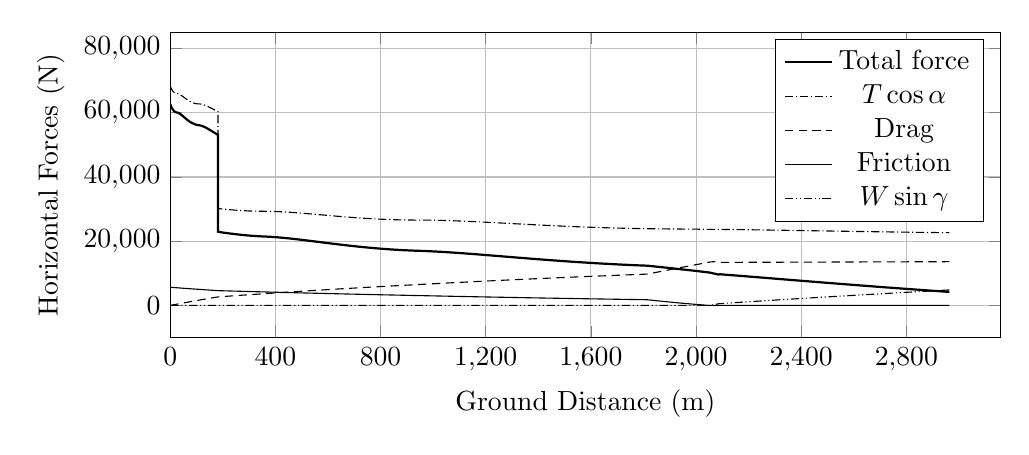
\begin{tikzpicture}

\begin{axis}[
width=\textwidth,
height=0.45\textwidth,
scaled ticks=false, tick label style={/pgf/number format/fixed},
xmin=0.0,
xmax=3157.6948405149165,
xlabel={Ground Distance (m)},
xtick={0,400,800,1200,1600,2000,2400,2800,3200},
xmajorgrids,
ymin=-10000,
ymax=85000,
ylabel={Horizontal Forces (N)},
ymajorgrids,
legend entries = {Total force\\$T\cos\alpha$\\Drag\\Friction\\$W\sin\gamma$\\}
]

\addplot [
color=black,
thick
]
table[row sep=crcr]{
1.3603393307215537E-8	62748.58696633752\\
2.0334443352841076E-7	62748.58690939445\\
1.8493358258961232E-6	62748.58641548015\\
9.983129263424352E-6	62748.58397542096\\
4.13538327636676E-5	62748.57456922821\\
1.2467543572893382E-4	62748.54960546996\\
2.843807411608912E-4	62748.50180455402\\
5.588015241105573E-4	62748.419767336396\\
9.398454696015893E-4	62748.30600655674\\
0.0014155885812023746	62748.1641647987\\
0.0019945752038215015	62747.99177512748\\
0.0026717822370171283	62747.790415954456\\
0.003447739291558293	62747.560009893365\\
0.0043193476547732645	62747.30155562484\\
0.00529092766782709	62747.01385138542\\
0.006363550519206555	62746.69666264203\\
0.007533073890550759	62746.351295181725\\
0.008790616877968567	62745.980444552275\\
0.01016549189277427	62745.575551850474\\
0.011625499440327931	62745.14618342054\\
0.013184282533086976	62744.688399411534\\
0.014839871214038253	62744.202857938275\\
0.01660567024659266	62743.685714295745\\
0.018465948346479452	62743.14166089623\\
0.0203822997817096	62742.581982157964\\
0.022430561433814646	62741.9846045537\\
0.024588423902376283	62741.35614234788\\
0.026831028501027587	62740.70391451247\\
0.029143159681622913	62740.032400926604\\
0.03155709159958957	62739.33229326972\\
0.03411445662773917	62738.59162699967\\
0.03677290089167576	62737.82277862045\\
0.03952314881844239	62737.028508995965\\
0.04239921643077808	62736.19908785114\\
0.045357163155895136	62735.34727460913\\
0.048363831658398165	62734.48265782544\\
0.051533845233668635	62733.57236575549\\
0.0547899150155587	62732.638705721634\\
0.058172599437445835	62731.67013847036\\
0.06162834747858026	62730.682080035374\\
0.06521401059050522	62729.6583602866\\
0.06888104003120077	62728.612930033225\\
0.07268727020998902	62727.52939702985\\
0.076546425570032	62726.432399803336\\
0.08047032364859658	62725.31861108985\\
0.08456364881336098	62724.158420584645\\
0.08882250397434277	62722.95310017094\\
0.09306368907640691	62721.75454887476\\
0.09743039119190974	62720.52232779545\\
0.10191450167634594	62719.25883483638\\
0.10651989152467789	62717.96308653227\\
0.11128201757858264	62716.625239045985\\
0.11609763023253863	62715.27438850158\\
0.12097769621339591	62713.90749028763\\
0.12591912973280778	62712.52544581439\\
0.13103216605369056	62711.097527656384\\
0.13633380151185176	62709.61917302545\\
0.1416823117522269	62708.130007390326\\
0.14708837902374172	62706.62707955137\\
0.1525605467319851	62705.108049955685\\
0.15824953188605478	62703.531216078845\\
0.16398006351864292	62701.94527849711\\
0.16978153473626356	62700.342130944424\\
0.17584258400626962	62698.66981182189\\
0.1819863832139092	62696.9772841792\\
0.18819485651962437	62695.26957750722\\
0.19455736971520038	62693.52220613981\\
0.20098158490654017	62691.76062289748\\
0.2076061353991409	62689.94693630173\\
0.21424726384720844	62688.131550336606\\
0.2211374965027113	62686.251028450046\\
0.2281284453493247	62684.34604989443\\
0.2350833915765042	62682.453865649004\\
0.2423085249848444	62680.49127820038\\
0.24958374984531584	62678.5182341692\\
0.2569279402934431	62676.5296459816\\
0.2644720218029696	62674.490190968936\\
0.27204626263318243	62672.44585722769\\
0.27972793364503945	62670.37583200562\\
0.2874622320100655	62668.29494128017\\
0.29563698092580604	62666.09911666709\\
0.30361763245720474	62663.958918553966\\
0.3118912000478351	62661.74375969761\\
0.3202493147046803	62659.50962820038\\
0.3286412952843002	62657.270101276095\\
0.33714554464307567	62655.00430432729\\
0.3458731203690518	62652.68282036096\\
0.35455185683415313	62650.378110914244\\
0.3634323904331427	62648.02367015275\\
0.372325738896249	62645.66969503407\\
0.38151551889959867	62643.241270275554\\
0.3908489672358084	62640.7790056082\\
0.4001862088113266	62638.319850465385\\
0.4095647137707429	62635.853918025794\\
0.4192312859369268	62633.31648359966\\
0.4289206911602753	62630.777326736774\\
0.43896550245304145	62628.1494969964\\
0.4487817299761361	62625.58580772948\\
0.4589033974758888	62622.94679031342\\
0.4691858798479248	62620.27041258804\\
0.47972601481223376	62617.53169886967\\
0.49016040525287174	62614.825124399096\\
0.5007175269203565	62612.09138594629\\
0.511266977039379	62609.364278434776\\
0.522323236324642	62606.51108785656\\
0.5332586746953114	62603.6939891011\\
0.5445869154512923	62600.780798452135\\
0.5556699580072249	62597.93563377879\\
0.5669225885056133	62595.051912478186\\
0.5785590177532589	62592.07505854375\\
0.5903083066022885	62589.07466803896\\
0.6020327889628274	62586.08590374258\\
0.613957077533064	62583.05157437126\\
0.625960998969677	62580.00239696787\\
0.6380070243193761	62576.94793492295\\
0.6503365955459197	62573.82713490272\\
0.662700086001522	62570.70334396156\\
0.6752747602080436	62567.53188773252\\
0.6885889407972636	62564.18011941944\\
0.7019767933734617	62560.81617246734\\
0.7151149754112038	62557.52110925231\\
0.7284684478906998	62554.17823528063\\
0.7418939875700234	62550.82354798741\\
0.7553494584716574	62547.46759065635\\
0.7694215958599202	62543.9644190666\\
0.7830840331449673	62540.569628476995\\
0.796657372658726	62537.203154767296\\
0.8106660034246236	62533.73512147406\\
0.8251837647136968	62530.14784815654\\
0.8395067871054176	62526.6154204272\\
0.8540519574023793	62523.03498378866\\
0.8688334527125461	62519.403311953996\\
0.8840141863517745	62515.68076938034\\
0.8993797082767976	62511.920298945784\\
0.9143697020410035	62508.258832268635\\
0.9294094610857999	62504.592197878505\\
0.9452486359568626	62500.7381743758\\
0.9605773823977486	62497.01562117957\\
0.9761522209726621	62493.24057141924\\
0.9917649966835071	62489.46361904089\\
1.0074810114554809	62485.66900760462\\
1.0234652146968335	62481.81711244582\\
1.0399433598517231	62477.85401059134\\
1.0563627364420554	62473.9128817023\\
1.0728309985448887	62469.96781727596\\
1.0896486452479222	62465.94705377448\\
1.1068138420051672	62461.85146773308\\
1.124143995869574	62457.72493271092\\
1.1415400048645106	62453.59114911816\\
1.1590089082607062	62449.448480346284\\
1.1769249919091855	62445.2084796461\\
1.1951505705127592	62440.904220141296\\
1.2127191877709298	62436.76362672084\\
1.2308827453761335	62432.49153892782\\
1.2492706857898845	62428.17564171388\\
1.267587852451018	62423.88525877934\\
1.2860031245644312	62419.58078870369\\
1.304687144125951	62415.22254631319\\
1.3233765774990474	62410.87209121662\\
1.342322280991234	62406.4711550964\\
1.3613696045164358	62402.05585699367\\
1.3815086998747366	62397.39748700296\\
1.4013123019267382	62392.82667942712\\
1.4209622886438908	62388.301018907354\\
1.4411501686096515	62383.66145723562\\
1.4611760119255748	62379.069061268805\\
1.4816444281325132	62374.38531840657\\
1.501865958841821	62369.76807196827\\
1.5224364680875304	62365.08127250687\\
1.543651615594651	62360.258227222424\\
1.5647593029468103	62355.470249604026\\
1.5859558716309676	62350.67271538367\\
1.6071423964076703	62345.888002467385\\
1.6293386351549652	62340.88649304696\\
1.6508498980272122	62336.05022619777\\
1.673011606043147	62331.07886427964\\
1.6946435720294923	62326.23716837114\\
1.717066624993247	62321.229632189425\\
1.739432891071898	62316.24608346452\\
1.761922286799709	62311.2464100638\\
1.7849035550437842	62306.14902744639\\
1.8076299607761817	62301.119671262655\\
1.8313298306791497	62295.88698567121\\
1.8543134894513886	62290.8241541905\\
1.8777326664639729	62285.67718343316\\
1.9017196849182967	62280.417680329134\\
1.925345883672024	62275.24934925274\\
1.950252961491087	62269.8136941689\\
1.975161211119453	62264.39091345896\\
1.9993825790313986	62259.13018618128\\
2.024583888346972	62253.66963544331\\
2.04934017380271	62248.318353089344\\
2.0744229633459703	62242.90939376509\\
2.0996193404956136	62237.48893216529\\
2.1245764901457758	62232.13269384175\\
2.1500786393425866	62226.67252647619\\
2.176226227020705	62221.08776655712\\
2.202115608176549	62215.5716402004\\
2.227948363055355	62210.080871824015\\
2.2543499999408594	62204.482825509156\\
2.2810892744412783	62198.82715711597\\
2.3075963743135786	62193.23438861176\\
2.3348582111613405	62187.49661613611\\
2.3623221378972126	62181.73082319158\\
2.3898598419727675	62175.96408003371\\
2.4171687299087603	62170.2595465404\\
2.445442108612223	62164.36844917665\\
2.4735885391813177	62158.51877944614\\
2.5015416452491293	62152.72399126468\\
2.5301110763218357	62146.816489295554\\
2.5589284934403693	62140.87303618454\\
2.587611617795936	62134.97247777185\\
2.6175687086884984	62128.82593829064\\
2.647724154312196	62122.65521091693\\
2.6767118187859253	62116.73897206473\\
2.7060305938995466	62110.770547371125\\
2.7361546404224653	62104.6542263274\\
2.7663022704956823	62098.54929455706\\
2.7964672462043376	62092.456957239774\\
2.8272583584284883	62086.25468453801\\
2.8588650092419234	62079.90540215954\\
2.8898852960400587	62073.69082224305\\
2.9215246589961597	62067.369377803654\\
2.95270311230069	62061.15688127688\\
2.984506337549637	62054.83704227129\\
3.017379145769185	62048.32275890118\\
3.049243647754313	62042.02575225769\\
3.081295157663824	62035.70903845485\\
3.113406837946715	62029.39772115555\\
3.1453724573084756	62023.13217298634\\
3.1787286104953543	62016.612120468475\\
3.211019796961401	62010.31770482176\\
3.245786703184362	62003.559815115426\\
3.279939251746722	61996.940531609405\\
3.3141720228361216	61990.32468094758\\
3.3491198891036547	61983.59012760021\\
3.382965192547779	61977.0867173538\\
3.4181848705561064	61970.338626827666\\
3.45391888941694	61963.51211006187\\
3.488851494856137	61956.858179141374\\
3.524271454997704	61950.130983748706\\
3.5606552075305	61943.241143853214\\
3.597189071478943	61936.343575278646\\
3.632926148839256	61929.61640029671\\
3.668897146318187	61922.86502357268\\
3.706642714683163	61915.80186021635\\
3.7432264628550644	61908.976793279406\\
3.781286297809391	61901.89785016014\\
3.818618572105483	61894.97542278108\\
3.8564015479305356	61887.99068247041\\
3.8948624022541356	61880.90247934146\\
3.9329637046009225	61873.90216792049\\
3.971505929995028	61866.8426350957\\
4.009821706071438	61859.84619099143\\
4.049014376833089	61852.711806431544\\
4.089343885784727	61845.393776135184\\
4.128662304630717	61838.28184714056\\
4.1684827283974055	61831.101775118805\\
4.208000253554632	61823.99875048586\\
4.2483743636521965	61816.76472234032\\
4.288255503180503	61809.64169432214\\
4.328757204126676	61802.43077740194\\
4.369490126907612	61795.20190188098\\
4.410357715197167	61787.97240189748\\
4.45189144941496	61780.64882899985\\
4.492881116440694	61773.44456786213\\
4.53550011161515	61765.97844455733\\
4.577670191557685	61758.6154327049\\
4.6201174049766305	61751.228492000344\\
4.662272021613388	61743.91663953538\\
4.706017761800355	61736.35414356242\\
4.748842845578064	61728.975686306745\\
4.792293145132742	61721.514545285856\\
4.836482439768313	61713.95224670663\\
4.88090298307878	61706.3764083924\\
4.925311889063089	61698.82852123807\\
4.969864686447545	61691.28214184509\\
5.014842280541593	61683.690063097805\\
5.0603877575117515	61676.02887809732\\
5.106292347304597	61668.33439403682\\
5.152263975081851	61660.65581586769\\
5.1974808794106995	61653.12966998521\\
5.244027372436168	61645.40940977406\\
5.28996242022761	61637.81748058609\\
5.336209145350672	61630.20092332852\\
5.38320569473032	61622.48838100504\\
5.430469292142472	61614.75984800639\\
5.476900151253712	61607.19453818837\\
5.526063828851289	61599.21304195354\\
5.573879040902945	61591.47903266914\\
5.622613575936374	61583.62517954153\\
5.6713596863799225	61575.79846605475\\
5.720412183296268	61567.951706051594\\
5.770660497446668	61559.9438310221\\
5.820668144990444	61552.00448954932\\
5.870305285939629	61544.15360637981\\
5.920503816994749	61536.243821434604\\
5.971105439367246	61528.30080444753\\
6.021088325934068	61520.48462476734\\
6.071322359863801	61512.65879094176\\
6.122981826035449	61504.64172289455\\
6.174329110820436	61496.70394173493\\
6.225804784288178	61488.77703510273\\
6.278093246139479	61480.75631606848\\
6.331709873490098	61472.56452776905\\
6.384325657889258	61464.55765979801\\
6.436648686434458	61456.626642740404\\
6.489478972803882	61448.65026491659\\
6.543185721519176	61440.57388732828\\
6.596747696432654	61432.551600930165\\
6.650345873843312	61424.556059089184\\
6.704555155195255	61416.501941789786\\
6.7588986063680725	61408.460639057594\\
6.814371620173711	61400.28586278655\\
6.86997180120154	61392.12632967644\\
6.925426612865756	61384.02186979991\\
6.981353650685165	61375.88237415877\\
7.037678624474159	61367.71930034793\\
7.094603706786671	61359.50411193866\\
7.151204881983983	61351.37026143422\\
7.209200593921791	61343.07163304799\\
7.2667780016693655	61334.86837278561\\
7.324687293141565	61326.653363530015\\
7.382771066065313	61318.449246831486\\
7.441904508776327	61310.13338126092\\
7.501585831803217	61301.77765963969\\
7.5616527251378685	61293.40551792075\\
7.62150963104709	61285.09996725664\\
7.682859947113334	61276.62569140749\\
7.7432084367972145	61268.3276534648\\
7.803024936926759	61260.13965604777\\
7.863793829029664	61251.858740070194\\
7.9252460466886365	61243.52293007236\\
7.98696966925656	61235.1888311347\\
8.04776546969778	61227.01759506168\\
8.109421212326083	61218.76871519463\\
8.17269125419024	61210.34340881962\\
8.236095044780246	61201.9403096516\\
8.299523592514586	61193.5738429738\\
8.363213767675873	61185.21286604897\\
8.427807923256076	61176.77398507265\\
8.49144930156071	61168.499561336226\\
8.557380457258176	61159.96910532277\\
8.623183572921022	61151.49732740478\\
8.687840683575093	61143.21389744365\\
8.753751426394068	61134.81131915188\\
8.820803713780364	61126.305983558035\\
8.888970287482593	61117.70333907152\\
8.957133699158991	61109.14530028828\\
9.025036015045707	61100.663809586214\\
9.092760955867519	61092.247804965446\\
9.159817422823458	61083.957329743265\\
9.227495373767134	61075.63268132828\\
9.296013084156197	61067.24822283868\\
9.36435980631623	61058.92809873505\\
9.433329865923408	61050.57586590666\\
9.503849553921977	61042.081253048804\\
9.574524061692681	61033.613735886465\\
9.644263228942293	61025.30298867257\\
9.715657612596786	61016.840806241584\\
9.787429657508813	61008.38039190523\\
9.85753688572494	61000.16108569071\\
9.930250735750551	60991.682830503574\\
10.001571447096964	60983.412971116995\\
10.074699859091687	60974.980572490764\\
10.14698611653175	60966.69193337383\\
10.220547980738981	60958.30445290361\\
10.2940409891517	60949.97240538517\\
10.36719293590382	60941.7260660842\\
10.441008888975666	60933.45225885279\\
10.51610421670324	60925.08370061709\\
10.590724589239105	60916.8164823947\\
10.667218005391902	60908.39163985035\\
10.742771202259895	60900.11973692823\\
10.82035208750042	60891.67670395892\\
10.896759047300378	60883.41160865278\\
10.973503045910835	60875.15998555509\\
11.051297940743765	60866.846241010455\\
11.128076326409062	60858.69115104595\\
11.207667705350879	60850.28952860301\\
11.286758396846047	60841.99324330609\\
11.366305937658339	60833.70160194156\\
11.446149720998452	60825.43188582828\\
11.526866579636565	60817.12530455354\\
11.607297517600138	60808.90150613891\\
11.688034241538357	60800.69980174933\\
11.769665722224765	60792.46134466202\\
11.850920080706608	60784.31480209889\\
11.933163326324259	60776.12361691226\\
12.017103780766782	60767.8197171247\\
12.10034832931326	60759.640634444935\\
12.185467765774142	60751.33475049959\\
12.270669986481685	60743.07869961996\\
12.354040133273898	60735.05604261029\\
12.440386807402234	60726.80498556224\\
12.52556588630658	60718.72313367702\\
12.610860989997974	60710.68741068567\\
12.69550109439961	60702.7697010197\\
12.784634337461807	60694.492079811374\\
12.871172079509357	60686.51455473315\\
12.958447214271366	60678.52775777402\\
13.045518554761987	60670.61813682194\\
13.133090172249581	60662.721811176365\\
13.221405510214687	60654.81786217776\\
13.310319106907201	60646.92044169422\\
13.399783591735492	60639.03469714463\\
13.488943611067967	60631.236046793\\
13.578276665194153	60623.48236681825\\
13.667402973129146	60615.80636494937\\
13.757763665999576	60608.084736776946\\
13.848393619195729	60600.401249403876\\
13.938857764339925	60592.79266771233\\
14.031101516310692	60585.0967789377\\
14.123507833735925	60577.45023803045\\
14.214825187590282	60569.95543883098\\
14.307956552027534	60562.37462917849\\
14.401498558574918	60554.824072903575\\
14.495315613017755	60547.31518245343\\
14.589065423003394	60539.8753342338\\
14.68316852398955	60532.47121543059\\
14.778702641747682	60525.01961735853\\
14.873746415615575	60517.67113253551\\
14.970384078097169	60510.265509925666\\
15.068900921005241	60502.78423420373\\
15.164434274206265	60495.5951926612\\
15.260378587808539	60488.44007172431\\
15.357189194448868	60481.28598152408\\
15.45495288999333	60474.1281303913\\
15.55311774366497	60467.00807906875\\
15.652583807013901	60459.862057840466\\
15.755243917873962	60452.55851669975\\
15.855950289561445	60445.46473158288\\
15.958461094374158	60438.31555855682\\
16.060387288500337	60431.27863635823\\
16.164276126126843	60424.17929867185\\
16.26736468838029	60417.20731915746\\
16.36946523634058	60410.37325929281\\
16.47192386662276	60403.586111545796\\
16.576794358652606	60396.71246883289\\
16.678929175716583	60390.08913617018\\
16.783994526910618	60383.348615344716\\
16.89012564586595	60376.61447104455\\
16.996887404888547	60369.91584578273\\
17.103774697793426	60363.28496963934\\
17.210947675936964	60356.71207923548\\
17.31865021419634	60350.18281796633\\
17.424470519881233	60343.841713853486\\
17.53205215515201	60337.47004776649\\
17.64034909906897	60331.13211374986\\
17.74911485075183	60324.84332676443\\
17.85745376408675	60318.65525754157\\
17.969383314157206	60312.34153029855\\
18.07998395718984	60306.18178736954\\
18.18863741327577	60300.2067199031\\
18.302466989554325	60294.02777015019\\
18.41305080779906	60288.10388244802\\
18.525644000014054	60282.15194912742\\
18.636945827420575	60276.34695232191\\
18.750643923449367	60270.4974694901\\
18.86479622056296	60264.70618400183\\
18.979646899421056	60258.961670430406\\
19.09418630108147	60253.314571081326\\
19.208983505033515	60247.736499493796\\
19.323483295898072	60242.254123430655\\
19.43842354827664	60236.8319979783\\
19.55563752357537	60231.3862692352\\
19.67199913451129	60226.0634241517\\
19.789486593639566	60220.772990304264\\
19.90713985662446	60215.55931019962\\
20.024127533725753	60210.45841989272\\
20.143019013955552	60205.359342821175\\
20.26442367074238	60200.24043139367\\
20.383660776265387	60195.29913874713\\
20.5042342316437	60190.38907729053\\
20.622773342122727	60185.64649109889\\
20.74503732713029	60180.84250580828\\
20.865944869938517	60176.17904872229\\
20.98711015528624	60171.59239670813\\
21.113336299999695	60166.90622975382\\
21.23638685227678	60162.42809921305\\
21.35988644990264	60158.022824142594\\
21.483760012473958	60153.69369463052\\
21.608180515260266	60149.435383794524\\
21.732326713270083	60145.27601552654\\
21.85766379468624	60141.1672141399\\
21.985117186778353	60137.081959983916\\
22.111729024702363	60133.116168854525\\
22.23700541150786	60129.28265740686\\
22.36297326225872	60125.5184277924\\
22.488604760551	60121.85430407117\\
22.616276341350805	60118.222539634255\\
22.744235570279145	60114.675226176056\\
22.874576476768283	60111.15694231537\\
23.003842066605536	60107.76214667955\\
23.13088450205612	60104.51712065276\\
23.257869280739328	60101.363831993935\\
23.389244224935425	60098.19622630252\\
23.519811196806458	60095.14324372953\\
23.653309395988643	60092.119497407795\\
23.78342402399784	60089.26724444286\\
23.9180644861338	60086.41407009502\\
24.05110504604577	60083.69270801601\\
24.182394801971697	60081.10229238166\\
24.314614014384034	60078.58877358597\\
24.449791085561472	60076.11754483839\\
24.585258581909038	60073.7406505672\\
24.72121222319008	60071.45522645874\\
24.857032405393277	60069.27179150266\\
24.99454740444294	60067.16239164554\\
25.13030709358258	60065.17960027879\\
25.270890409679986	60063.230446394926\\
25.40663839363527	60061.448554015355\\
25.54307796688363	60059.75652737389\\
25.68272814639034	60058.12712513111\\
25.82072003425767	60056.618583333824\\
25.96015212691003	60055.196505235814\\
25.987750021099068	60054.92718792059\\
26.0558803939429	60054.27950154213\\
26.061632797568386	60054.22593415613\\
26.066808273335674	60054.17788795782\\
26.071901058608013	60054.13074692119\\
26.073315434863225	60054.11767274693\\
26.074595035914804	60054.105833423106\\
26.080371168076944	60054.05225064648\\
26.10234540095133	60053.84631277736\\
26.183408179590366	60053.05805301905\\
26.300430535410044	60051.84141869529\\
26.42750601924636	60050.41603199058\\
26.558056987479794	60048.83997608072\\
26.688030995483615	60047.159816005544\\
26.818767077324992	60045.35938261883\\
26.951519978077492	60043.419258265145\\
27.083955405447817	60041.3728059744\\
27.216897884715692	60039.20844388436\\
27.350913258119895	60036.91639489049\\
27.4833530065795	60034.5439423178\\
27.6176201223548	60032.031194754294\\
27.752160408628434	60029.40607957498\\
27.887329802382908	60026.66194677791\\
28.023188645890663	60023.797383288256\\
28.158973127824495	60020.8291376751\\
28.296372294036907	60017.719870782574\\
28.435107205966254	60014.47387337974\\
28.571323599682245	60011.18403467702\\
28.70996262687553	60007.73249199185\\
28.850320389600306	60004.13350335811\\
28.988837241064125	60000.479841946435\\
29.129197813929657	59996.67568345055\\
29.27166529868488	59992.710960694676\\
29.41298471572133	59988.67659502503\\
29.554848516656044	59984.526294098905\\
29.699676691743235	59980.186915205224\\
29.842400551696755	59975.81079627063\\
29.985385440862252	59971.32870089132\\
30.129077275410303	59966.72700352172\\
30.27543774584293	59961.94080827045\\
30.422081339040986	59957.04651293291\\
30.56949149516445	59952.02832047624\\
30.716562179458485	59946.924840263455\\
30.86535310281699	59941.664626078156\\
31.011875026602333	59936.390596962665\\
31.16159928701196	59930.90628712137\\
31.313692569485013	59925.238286549036\\
31.463056706803336	59919.57831036547\\
31.61235366859384	59913.82945735073\\
31.76278957628285	59907.94563880219\\
31.915019899787076	59901.899901037425\\
32.06709627595497	59895.76949547665\\
32.21861178877769	59889.57280097742\\
32.37168228565527	59883.22374572455\\
32.52450570609457	59876.79726484443\\
32.67702483599189	59870.29754761617\\
32.829998687403204	59863.6934176901\\
32.98551220909506	59856.89367472356\\
33.14332298937855	59849.906236893716\\
33.29970221124884	59842.89683323805\\
33.45800124694219	59835.716197620495\\
33.61398946945653	59828.55786102654\\
33.77048353048475	59821.29528723624\\
33.9292721471582	59813.84458417805\\
34.08796840843395	59806.317352988335\\
34.24769686644211	59798.66084320088\\
34.406855482575295	59790.9527893207\\
34.56481953291838	59783.22600928563\\
34.72399692808165	59775.36395438899\\
34.88694269464703	59767.23812092573\\
35.04914399338672	59759.0726815221\\
35.209965099803895	59750.90240180594\\
35.3703140559587	59742.683657673304\\
35.531685786905925	59734.340671176906\\
35.69349909442164	59725.90372559923\\
35.85522798807463	59717.40121385794\\
36.022509111806116	59708.53447904484\\
36.19055880791667	59699.554244631596\\
36.35708622463872	59690.58469313168\\
36.52115360367851	59681.680070858114\\
36.68781562330062	59672.56717430525\\
36.8536847754776	59663.43133576815\\
37.024522648961764	59653.95394295167\\
37.19188554678789	59644.60374946002\\
37.36066720850286	59635.10977491125\\
37.528862119520696	59625.58554350838\\
37.697264258302326	59615.98748780464\\
37.86832931534104	59606.17524719742\\
38.03812867477943	59596.37458278546\\
38.20923731912278	59586.43802723859\\
38.37904730305398	59576.51817757127\\
38.55252405124031	59566.324912820186\\
38.72282139824354	59556.26140041601\\
38.89783411301201	59545.86151021885\\
39.0714610757495	59535.487307669595\\
39.24438070689564	59525.10042350262\\
39.41969314875929	59514.5149844464\\
39.59166556575205	59504.078692675525\\
39.764623188591585	59493.53123869293\\
39.94263254662576	59482.62305142157\\
40.11749159802578	59471.85701263862\\
40.29452954971913	59460.906547520775\\
40.47247750600427	59449.849941046996\\
40.64799609178485	59438.89640476125\\
40.82414741101539	59427.85664671518\\
41.00385670225303	59416.54674992937\\
41.18169069533937	59405.309069950046\\
41.3603281005193	59393.975818649225\\
41.54046179251334	59382.50324354827\\
41.722675278204306	59370.85394412931\\
41.90258931008478	59359.309040700304\\
42.08518735141125	59347.54968606445\\
42.26728550944881	59335.78122794305\\
42.44743534848537	59324.099135451615\\
42.63069538383506	59312.17603777333\\
42.80963512098974	59300.49675227204\\
42.992542679335614	59288.521436020004\\
43.17926890616222	59276.25850616516\\
43.363134036078335	59264.147382094496\\
43.54815051311773	59251.925286896454\\
43.733578141849236	59239.64168066341\\
43.91798130912079	59227.39282522943\\
44.10506009255049	59214.933498322775\\
44.29251116260117	59202.41729768709\\
44.480917546793805	59189.80595571204\\
44.66851287589745	59177.2186586616\\
44.85853501730759	59164.43875502719\\
45.047396872181054	59151.708177448745\\
45.236914792155844	59138.905579726605\\
45.42785879536018	59125.97945974015\\
45.616432631699865	59113.18795637264\\
45.80697204128492	59100.23799279377\\
45.998633580597016	59087.18722800302\\
46.18800675699903	59074.26903791596\\
46.380841640082096	59061.09189567245\\
46.57327038933336	59047.92049077105\\
46.765844918266424	59034.718012194746\\
46.95911042680183	59021.44786036476\\
47.15311668852311	59008.10730490218\\
47.34541611633634	58994.86568700209\\
47.53884854699059	58981.52842327401\\
47.73236991243341	58968.16820999955\\
47.92818250719388	58954.63357909351\\
48.12326385407131	58941.13412640181\\
48.32058854034828	58927.46471703341\\
48.516852452700604	58913.85497699441\\
48.71339374517507	58900.21305646603\\
48.91319881343868	58886.332192904505\\
49.1119162355681	58872.51535270149\\
49.31207818344666	58858.58731063311\\
49.509673461222235	58844.82811169086\\
49.71156302510582	58830.76073219253\\
49.91034548441702	58816.90164186753\\
50.11200805970151	58802.83426463636\\
50.30853267551517	58789.11883687753\\
50.50757456960626	58775.22201912914\\
50.70929197287772	58761.13333913479\\
50.91222418686718	58746.9554811806\\
51.11562549758783	58732.74130184468\\
51.32090674103446	58718.39296428232\\
51.525199701657655	58704.11173357142\\
51.72863462744459	58689.88932028023\\
51.934060761332375	58675.52730883444\\
52.14033810224923	58661.10618182135\\
52.344882977561255	58646.80733712956\\
52.55098100649393	58632.401858393874\\
52.75731843494604	58617.982360208014\\
52.96514817708821	58603.46208475658\\
53.17450540782369	58588.83942180824\\
53.382202621450276	58574.3377559869\\
53.592230583406476	58559.679229889225\\
53.80364534107798	58544.93064378269\\
54.01469481143569	58530.215030808264\\
54.223966920081466	58515.631471086905\\
54.43230789395902	58501.12155087033\\
54.6430562980421	58486.45356444517\\
54.855225786754914	58471.697144366\\
55.066088958624874	58457.04270018783\\
55.27969530828261	58442.20963181784\\
55.49171188337613	58427.49962401182\\
55.70388919125476	58412.79178885053\\
55.91737779085577	58398.00720016053\\
56.13177028494084	58383.17498173575\\
56.34652664868587	58368.333313521856\\
56.559021044851505	58353.66412411911\\
56.77591447970492	58338.708504571245\\
56.99548236897459	58323.58691455852\\
57.21481285737903	58308.500894390236\\
57.43536222847358	58293.35110079676\\
57.65367025761124	58278.375756128575\\
57.872788904232735	58263.36596854261\\
58.0907693980174	58248.455833187836\\
58.311927420720366	58233.351114576406\\
58.532333513628615	58218.32121382914\\
58.75532998033057	58203.13916485525\\
58.976617007999806	58188.098497502404\\
59.19875422837053	58173.02572952934\\
59.4206945143671	58157.992655298396\\
59.64453328369959	58142.85827735343\\
59.86894932484513	58127.71301064553\\
60.09432075877773	58112.5322553695\\
60.318058693038594	58097.490881444915\\
60.541731124044205	58082.48374662695\\
60.76707064338231	58067.3955279877\\
60.995574692986196	58052.12756950685\\
61.22378989589207	58036.911836241154\\
61.4534619981562	58021.63280140082\\
61.683510138770515	58006.363385445075\\
61.91410430469678	57991.093120406906\\
62.14462153858659	57975.86396671242\\
62.37563158073512	57960.63897565096\\
62.607203285434	57945.41445022516\\
62.841031881319736	57930.08021880589\\
63.07467935056491	57914.79726911259\\
63.31164975340633	57899.33779610891\\
63.54633691305479	57884.068390173954\\
63.78243968758058	57868.74874765902\\
64.0165414084598	57853.6009719125\\
64.25412817577254	57838.27105183984\\
64.49270299572771	57822.92190436032\\
64.73076499662056	57807.650791422624\\
64.96867826857735	57792.434728704684\\
65.21063576532572	57777.00724185629\\
65.4512107007771	57761.71569061352\\
65.69028017871045	57746.567576696616\\
65.93032615763332	57731.406018186666\\
66.17196619696679	57716.193329702655\\
66.4135612157637	57701.033714326666\\
66.6559030093851	57685.87824030849\\
66.89910102540284	57670.72109998952\\
67.14354652182666	57655.53911287115\\
67.38771133480921	57640.428027933216\\
67.63347396558368	57625.27254363513\\
67.87898066495345	57610.18793956618\\
68.1255935515739	57595.09132520294\\
68.37316753306138	57579.99280084603\\
68.62205497364681	57564.87217704652\\
68.8711887275476	57549.79534187529\\
69.120220471977	57534.78392955042\\
69.36846244647072	57519.87957346914\\
69.61951843592018	57504.86712876223\\
69.87236615109754	57489.8099065393\\
70.12758921381476	57474.6752054641\\
70.37945082809051	57459.803338373196\\
70.63410009691182	57444.831487207965\\
70.89152727368702	57429.76285027851\\
71.14629115974091	57414.91646035954\\
71.40197865069018	57400.08309025846\\
71.66163317144085	57385.088593798064\\
71.92484704501203	57369.9600329331\\
72.18465416754285	57355.09834198421\\
72.44573394560723	57340.23545133592\\
72.70633339061075	57325.471953933025\\
72.96699363118216	57310.77748505819\\
73.22900401485182	57296.08041119615\\
73.49076816912304	57281.47120050725\\
73.75430841254712	57266.83809345678\\
74.01895646534612	57252.219890300854\\
74.2846979982242	57237.61879331188\\
74.55380714249793	57222.9122737032\\
74.82322871850147	57208.26939184911\\
75.09350011520078	57193.66192326516\\
75.36421232425869	57179.11301420181\\
75.6347219158074	57164.65780234536\\
75.90830954343213	57150.122756364886\\
76.18188601743822	57135.67387246007\\
76.45626363461818	57121.2690668212\\
76.72958718025629	57107.006056570826\\
77.00406935908524	57092.76985819533\\
77.28579748399531	57078.24924514997\\
77.56784659723587	57063.805291943805\\
77.84569092555657	57049.668290162925\\
78.1246978223638	57035.56407093696\\
78.40641219364133	57021.416888412234\\
78.68590470271565	57007.47495000754\\
78.96851680469001	56993.47268341496\\
79.25576208114188	56979.33947918769\\
79.54169104977237	56965.37020706275\\
79.82662017154695	56951.54862481984\\
80.11330301632765	56937.74197065286\\
80.40394576721474	56923.84742480169\\
80.6908099930996	56910.235441836325\\
80.98055888331655	56896.58978178128\\
81.27178512217935	56882.97947115914\\
81.56682943128612	56869.29841199225\\
81.86186977412851	56855.726339449015\\
82.15688924927383	56842.26442924084\\
82.44965588234726	56829.01366851741\\
82.74488606927187	56815.76110563167\\
83.04325841243121	56802.4798198021\\
83.34213327641098	56789.28977144322\\
83.64411622775171	56776.07844151951\\
83.94734638805741	56762.930160587624\\
84.25123842984891	56749.87182430207\\
84.55152885577829	56737.08531079719\\
84.85735750691177	56724.18297150567\\
85.16518306664875	56711.31906232219\\
85.47136476235073	56698.64633166521\\
85.77898122624802	56686.03761827444\\
86.08923229760057	56673.446588777355\\
86.40254560035129	56660.85975954939\\
86.71167807044037	56648.56780416798\\
87.02660518802142	56636.17545402993\\
87.34238286044419	56623.881776673414\\
87.65842706333811	56611.71059504611\\
87.97971380652302	56599.474162660845\\
88.2973933745065	56587.51095168493\\
88.61789013566766	56575.578906513445\\
88.93643920279564	56563.85635402276\\
89.25662431900213	56552.21158163999\\
89.57903058309674	56540.62618103357\\
89.89968694948243	56529.243518823685\\
90.22473455398588	56517.847697477686\\
90.55024875587375	56506.579884139195\\
90.87789352676518	56495.38457792073\\
91.20733069500889	56484.276334895476\\
91.54101415610151	56473.17688393881\\
91.87012785371462	56462.37961897151\\
92.20120197152713	56451.66887643444\\
92.53416638543635	56441.04992105982\\
92.86431843528567	56430.672445420714\\
93.19748455591187	56420.35379761217\\
93.53066771200866	56410.18924357343\\
93.86681917526724	56400.09117815462\\
94.20530590547477	56390.08269701265\\
94.5419273964865	56380.28867740244\\
94.8854212036891	56370.4588251176\\
95.22752713476521	56360.833810594486\\
95.57091181422334	56351.33887691356\\
95.91383450860906	56342.02309124738\\
96.25469535763642	56332.928415814225\\
96.5966517898868	56323.97023258764\\
96.93845701474973	56315.182214884044\\
97.28153572459905	56306.52887524493\\
97.62213139590432	56298.10439445829\\
97.9659652144934	56289.76813060144\\
98.3129807304216	56281.52650644207\\
98.65852794036775	56273.49154719533\\
99.00080640577195	56265.701904939735\\
99.35064076251427	56257.91474109776\\
99.69796076807248	56250.358298542385\\
100.04654253174803	56242.94978418537\\
100.3915606488718	56235.790319330015\\
100.74261509654437	56228.68286742618\\
101.08877163494762	56221.84995780497\\
101.43457754260953	56215.198140311884\\
101.784020212797	56208.653494623344\\
102.13161434601102	56202.32039896121\\
102.4751980097893	56196.23406722117\\
102.82212110631409	56190.264066871256\\
103.16739702108615	56184.49776476232\\
103.51524666207362	56178.86564816616\\
103.86391679154056	56173.39897407286\\
104.20960434827006	56168.15597685639\\
104.55241399635099	56163.13084679436\\
104.89662223620601	56158.26002318217\\
105.24103428322039	56153.561887785574\\
105.5836615386647	56149.06260891563\\
105.92645892081137	56144.73552823797\\
106.27347658175316	56140.533135349004\\
106.6151670762521	56136.57044376861\\
106.95898391938218	56132.75879358796\\
107.30023552029138	56129.15009724462\\
107.64147805753461	56125.71558452163\\
107.98348674656944	56122.44826487418\\
108.32522459759954	56119.358655463104\\
108.3935347040271	56118.76208542872\\
108.40478590462831	56118.664497649705\\
108.41572478024443	56118.5698010505\\
108.4246743308916	56118.492459419795\\
108.44347342986478	56118.32977731012\\
108.52018987797786	56117.65880656114\\
108.70071173483461	56116.035152340206\\
108.99446230248458	56113.25949687585\\
109.30176454987088	56110.180128331456\\
109.60899173332959	56106.92367519517\\
109.91608539831654	56103.49267197093\\
110.22883517949637	56099.81943912411\\
110.54143546549608	56095.96921548896\\
110.853845249356	56091.944588339\\
111.1739714794031	56087.63911666928\\
111.4937490010879	56083.156864760545\\
111.81170779322963	56078.52214053848\\
112.13106495813236	56073.69025769296\\
112.4519453366479	56068.65875748497\\
112.77515902629136	56063.41362773524\\
113.0997499810409	56057.96922648499\\
113.43040796942478	56052.24272693141\\
113.7597028375028	56046.36092178567\\
114.0907450350197	56040.269918194055\\
114.42538740208008	56033.93330308134\\
114.75997726261329	56027.419401394\\
115.09477047197589	56020.72512334178\\
115.43440545481076	56013.75576669778\\
115.77494672336013	56006.589619595325\\
116.11687534861284	55999.2168417143\\
116.46164587354252	55991.604878253755\\
116.8077846490165	55983.78512638784\\
117.15688723722127	55975.72035419216\\
117.50557855048987	55967.48873279906\\
117.85411336711965	55959.08682079238\\
118.20532793701167	55950.44650717999\\
118.55850697655507	55941.584104478694\\
118.91273956155123	55932.522423860835\\
119.26983096270519	55923.214621430685\\
119.62978614725739	55913.65863454707\\
119.98960731920661	55903.93431508298\\
120.34734904217265	55894.09802996219\\
120.7138511704587	55883.84926603541\\
121.08106061642908	55873.408846882245\\
121.44737887966437	55862.82465307269\\
121.81499139152783	55852.03555702076\\
122.18511446431708	55841.00556433253\\
122.55384158147794	55829.852629700865\\
122.92460728481757	55818.47473211432\\
123.29616941264607	55806.91040690572\\
123.67040864389355	55795.10115506385\\
124.04652172406458	55783.0716969154\\
124.42393851457416	55770.84056244342\\
124.80152108360014	55758.446027237456\\
125.18180835736592	55745.80528944677\\
125.55854932865631	55733.128956004584\\
125.93878032356085	55720.18261663958\\
126.31997081831156	55707.05205810175\\
126.70099538833193	55693.777874477935\\
127.08058279416298	55680.40756122072\\
127.46175209000612	55666.836950687386\\
127.84399628255431	55653.0848333677\\
128.22749916598133	55639.14553995697\\
128.6102537001487	55625.09397540186\\
128.99595881306152	55610.795388035505\\
129.37788117916477	55596.50204083322\\
129.760738924708	55582.04104776998\\
130.1448498512433	55567.40143773476\\
130.53000390659713	55552.59220870664\\
130.9168242384266	55537.5902043949\\
131.29443328439476	55522.82310047386\\
131.67491382268804	55507.82349999633\\
132.05816436539135	55492.59477265162\\
132.44070735535217	55477.27617776611\\
132.82666098215685	55461.70361433411\\
133.20952005887244	55446.14143923354\\
133.5940193955625	55430.39986597975\\
133.97617966856654	55414.644096894015\\
134.36103715882757	55398.66832157064\\
134.74478042358356	55382.63204566766\\
135.12867144169206	55366.484880169795\\
135.5141335746535	55350.16819246838\\
135.89764893392993	55333.83295933936\\
136.28231234485685	55317.34957792143\\
136.66418763078912	55300.88921332924\\
137.04684871033697	55284.30041550295\\
137.42845627025127	55267.66483526533\\
137.8132447087305	55250.798929806086\\
138.19719797258034	55233.879702153135\\
138.58059071069573	55216.89733207894\\
138.96593237593703	55199.741975318975\\
139.3501607499636	55182.55145065415\\
139.73355638294606	55165.31559629523\\
140.1160230155566	55148.04102748708\\
140.50045093994146	55130.59858980587\\
140.88215178690393	55113.20292656115\\
141.26156782058217	55095.83703679354\\
141.64323970440188	55078.29473766922\\
142.02689350659642	55060.589038665625\\
142.41061312971692	55042.80942572316\\
142.7942251403153	55024.9655712048\\
143.1756303563767	55007.15733772205\\
143.5599719391364	54989.14598621384\\
143.94242380128833	54971.15898355495\\
144.3239499176869	54953.1532499748\\
144.70664939692608	54935.031197611184\\
145.0870075357763	54916.96104755772\\
145.46856550308127	54898.77632966716\\
145.85014610541765	54880.5343579755\\
146.23128237819492	54862.25902154323\\
146.61504730324998	54843.80397778144\\
146.99763315977907	54825.35349630668\\
147.38441582478964	54806.64918106068\\
147.7673688364352	54788.080558606234\\
148.15222568696134	54769.37144046633\\
148.53580865353604	54750.677610751154\\
148.9199734867533	54731.91016881248\\
149.3040357319486	54713.10386690739\\
149.68771357306542	54694.27397295498\\
150.07093078701052	54675.42573599094\\
150.45622889618164	54656.43526069229\\
150.8449053483268	54637.239130532806\\
151.2288570611563	54618.239099294326\\
151.61452719766493	54599.11810242158\\
151.9983007305741	54580.0567094977\\
152.38299664478842	54560.916344387704\\
152.76945776909372	54541.65603103688\\
153.15580177123394	54522.37067495863\\
153.54253364040335	54503.03632819989\\
153.93093169697067	54483.5901374426\\
154.31788037931886	54464.18934396806\\
154.7039882138024	54444.80493590348\\
155.08880221957185	54425.46110304682\\
155.47621608980313	54405.96322715393\\
155.866104687065	54386.318388846164\\
156.25391419262098	54366.757230611416\\
156.64166339424906	54347.1793132959\\
157.03027969880475	54327.53895522293\\
157.4213807682267	54307.75537029511\\
157.8105708506119	54288.05207252641\\
158.19948541262937	54268.347583843104\\
158.58893406813365	54248.60204114468\\
158.97894817604634	54228.81495997179\\
159.3710019698692	54208.91258410092\\
159.76139479981174	54189.08391069513\\
160.1523485688823	54169.21727396663\\
160.54128874338664	54149.444675598614\\
160.9326976430911	54129.539353100336\\
161.32564259741588	54109.54974883988\\
161.71827778345698	54089.570849273485\\
162.1124492087963	54069.509812550095\\
162.50576001021273	54049.48971779882\\
162.89904576730015	54029.46913444938\\
163.29316224934274	54009.40557856076\\
163.68899123279596	53989.25523993868\\
164.08495392634194	53969.09957324251\\
164.48271131475576	53948.8551218497\\
164.8792309171331	53928.67730328094\\
165.27343112400507	53908.62215604122\\
165.67115293733156	53888.393585440586\\
166.06936395728349	53868.14695606413\\
166.47000821435734	53847.78455338701\\
166.87155839526775	53827.38515389072\\
167.27134041220108	53807.085614829324\\
167.67233991204222	53786.735346019326\\
168.0705846918417	53766.536878449275\\
168.47232570996516	53746.17421678928\\
168.87521546679773	53725.76758726573\\
169.2789990941189	53705.331020025755\\
169.68142011368735	53684.97969414074\\
170.088438196605	53664.4134212997\\
170.49328200513543	53643.97550553418\\
170.89845866435633	53623.54024130883\\
171.30484584057905	53603.0644581948\\
171.7103088520891	53582.65670668536\\
172.11589069074847	53562.26539043702\\
172.52485519917514	53541.7276737294\\
172.93316089774754	53521.24771464929\\
173.34236088095247	53500.74859287708\\
173.7535761368399	53480.17538611259\\
174.16510964781833	53459.61418199894\\
174.5786011126259	53438.98424701531\\
174.99051444770384	53418.462989485764\\
175.40138574541044	53398.02434724718\\
175.81497300453447	53377.48249794118\\
176.2280441317456	53356.99914943286\\
176.64225100058474	53336.49338266169\\
177.05714873395152	53315.988361807045\\
177.47483026786767	53295.38201021595\\
177.89254345086653	53274.8113892721\\
178.3100126079721	53254.29095541453\\
178.7278240622369	53233.792802926066\\
179.1449731538625	53213.367066512146\\
179.56482315926417	53192.850247429655\\
179.9871804296257	53172.25347360752\\
180.4095742002126	53151.69851413404\\
180.83428717371925	53131.075547411005\\
181.26003251256287	53110.4484863119\\
181.6840913989422	53089.94983334681\\
181.8934642440371	22914.201677775745\\
182.1114839456617	22908.057246978315\\
182.5372774346568	22902.882501764572\\
183.423900814602	22892.123314641925\\
184.30144226609173	22881.49601187677\\
185.17422251923585	22870.948046255086\\
186.05126240753827	22860.370664679613\\
186.93861419286333	22849.691718065726\\
187.8243328275641	22839.05558560601\\
188.7212117513506	22828.309307253934\\
189.61004025875786	22817.683476721264\\
190.50102451880866	22807.05612917906\\
191.38947474753866	22796.483469737323\\
192.28052744689825	22785.904656958963\\
193.18778236606096	22775.159309434377\\
194.08895872822546	22764.512034611005\\
194.99680020640938	22753.812580119527\\
195.89480429656658	22743.25557836808\\
196.79674305679504	22732.679139730702\\
197.7065692706791	22722.037720389402\\
198.612023604503	22711.47514195637\\
199.52644538440046	22700.836283628363\\
200.43881964763966	22690.249896595495\\
201.34572312669928	22679.755618270377\\
202.26115686844895	22669.191850474395\\
203.17967892292364	22658.622219974197\\
204.1017087672932	22648.042492711626\\
205.01405834107487	22637.603955377213\\
205.94020355690031	22627.038483021344\\
206.86420646269943	22616.528746220472\\
207.79153006365993	22606.012933700375\\
208.72800400232427	22595.425847824823\\
209.6603812871926	22584.917778411065\\
210.59913361291103	22574.37109400108\\
211.54272242703126	22563.803944300365\\
212.4892775421681	22553.23796211675\\
213.4278558742791	22542.795290029462\\
214.37319863683314	22532.312111306615\\
215.31618532994997	22521.890067168133\\
216.26909967312713	22511.39407938817\\
217.2229300472723	22500.924279800405\\
218.17915574443117	22490.464879833977\\
219.13394290547268	22480.05812721428\\
220.0901210939433	22469.67343319153\\
221.05386294760763	22459.24453958866\\
222.0194744620763	22448.833877094105\\
222.9871855528732	22438.43945989952\\
223.95850156259326	22428.045718381858\\
224.93506896411378	22417.635830362553\\
225.9123601081958	22407.258682231695\\
226.89683950214788	22396.84638110971\\
227.87812705537118	22386.509216193743\\
228.86553252311342	22376.14955523057\\
229.85786107077195	22365.780894409007\\
230.84893890233656	22355.468232423103\\
231.8352011637358	22345.24851813331\\
232.83551070617193	22334.92714818354\\
233.8409775535427	22324.597373550896\\
234.84473749332597	22314.33019712776\\
235.85076677249623	22304.08523525067\\
236.86174655712836	22293.835924350416\\
237.8698887650736	22283.661611890922\\
238.88314164945962	22273.482486519162\\
239.88702917374013	22263.443921451144\\
240.9073981595622	22253.28819678024\\
241.92631922506058	22243.195062471314\\
242.95020737895555	22233.10146741524\\
243.9867665418509	22222.93297922366\\
245.01566609591487	22212.889645630894\\
246.05919400906686	22202.754666474677\\
247.09706457910846	22192.725966246602\\
248.1403037320082	22182.69722757711\\
249.18309170866138	22172.725005839035\\
250.23723200462985	22162.697490253602\\
251.28895058541582	22152.746627932742\\
252.34575298177748	22142.801852777462\\
253.4009695529494	22132.926438277034\\
254.47389199439823	22122.941340383317\\
255.55293546958148	22112.956497174775\\
256.6206413021679	22103.133291901308\\
257.69235364004487	22093.330212016903\\
258.77967411403563	22083.44295487887\\
259.8615409937813	22073.664105258526\\
260.93956317950165	22063.978603968433\\
262.02271022117964	22054.306207085196\\
263.11073386748035	22044.650191309665\\
264.2120045516847	22034.938017945628\\
265.31241535302627	22025.29537738575\\
266.4086016357777	22015.75156367672\\
267.51260488983417	22006.202282464983\\
268.6300148019782	21996.601242049546\\
269.7585470354529	21986.970443291197\\
270.8896873949477	21977.383998917227\\
272.0115439451323	21967.942349478282\\
273.13680176546006	21958.53845805319\\
274.2702490513931	21949.13358027042\\
275.413525774062	21939.715968884768\\
276.5542367829295	21930.388628165725\\
277.6972773917919	21921.111751651617\\
278.856653662284	21911.773625022593\\
280.02457374883886	21902.43956530103\\
281.2032739103363	21893.093772195833\\
282.3793508291475	21883.84354663718\\
283.5570819158503	21874.655405637088\\
284.7419934858003	21865.48733522689\\
285.9326270157934	21856.352120690644\\
287.128931254976	21847.25152024842\\
288.31480266049743	21838.307822461138\\
289.5063986037633	21829.398957052057\\
290.71803378146524	21820.420701548515\\
291.92377285751195	21811.566900718193\\
293.1368845155397	21802.7405244591\\
294.3779382526999	21793.795768640266\\
295.6236529225306	21784.904060880508\\
296.8710892485976	21776.087316852914\\
298.1231876568165	21767.3256936315\\
299.3513516362168	21758.817533177433\\
300.60759883822345	21750.203181073877\\
301.8758306910943	21741.597553397136\\
303.15324510629466	21733.02222216661\\
304.4174613942848	21724.627262373557\\
305.70907350215657	21716.144941313418\\
306.99802587761087	21707.77564038863\\
308.28687847241804	21699.502705154177\\
309.5668796159489	21691.381584659648\\
310.84791377823	21683.348961030693\\
312.1498528537303	21675.282954639923\\
313.4560044202801	21667.2900927288\\
314.75458395299495	21659.4423776126\\
316.0753084557979	21651.562167171105\\
317.40968260857574	21643.704577097524\\
318.7319345228668	21636.02182537003\\
320.0558782097702	21628.432701570287\\
321.3801932183561	21620.94529093222\\
322.6884764655432	21613.650765025486\\
324.0456734620244	21606.191185381547\\
325.39100935110525	21598.905293979085\\
326.7365982993339	21591.726362949208\\
328.06652939861567	21584.73769850468\\
329.40155074930124	21577.829269738635\\
330.74537767281527	21570.98379685783\\
332.0707513255394	21564.33923665961\\
333.4173386205282	21557.697328242495\\
334.746581315361	21551.248987947103\\
336.0867229892568	21544.856679818215\\
337.4205715422614	21538.603230002263\\
338.75500413875113	21532.455957351864\\
340.08105948956893	21526.455445957967\\
341.3989527111596	21520.59895428804\\
342.72155317639294	21514.82911996684\\
344.04109435086104	21509.18027164178\\
345.35282448543626	21503.67166653533\\
346.65609809876	21498.304271924462\\
347.964660055904	21493.02133182846\\
349.26930822844486	21487.860398986188\\
350.5666013847051	21482.833944501333\\
351.8669806622215	21477.901223340356\\
353.150344321377	21473.13701970078\\
354.42669516744513	21468.501510834816\\
355.7084983713929	21463.949454757254\\
356.9839654050402	21459.522825106927\\
358.2578487323243	21455.204384831246\\
358.5108324321051	21454.359007997118\\
358.64800612588874	21453.902321322275\\
358.7323961896923	21453.62195783013\\
358.9732456649284	21452.824283948074\\
358.99979477666295	21452.736580637014\\
359.01768095024534	21452.677520008583\\
359.0292585237206	21452.6392991413\\
359.04030674366413	21452.60281805627\\
359.0932275856527	21452.42793442669\\
359.3119468898926	21451.702699287278\\
359.96663022276493	21449.508363025656\\
361.01382689254797	21445.925459197497\\
362.10337816976426	21442.102994160145\\
363.2064629717895	21438.13551288598\\
364.30797819224426	21434.076555055282\\
365.4187311446934	21429.886099808733\\
366.533107917645	21425.584456552606\\
367.64647721929396	21421.189986690777\\
368.7658299095233	21416.675280961113\\
369.8975033538602	21412.013248565803\\
371.0334235675839	21407.23586318895\\
372.1785809863062	21402.32126654755\\
373.31981642046355	21397.326124833402\\
374.47796099960044	21392.15848879719\\
375.6447818548355	21386.852730008402\\
376.82127927712384	21381.402882128285\\
377.99866547828844	21375.8492454847\\
379.1872933927376	21370.142400045865\\
380.3777690794409	21364.326755781047\\
381.57556676946103	21358.375390392153\\
382.7749421474674	21352.31671051802\\
383.9810457964097	21346.12465245746\\
385.1925430839308	21339.805565161732\\
386.4130201303027	21333.339984032013\\
387.642251751972	21326.72795259404\\
388.8666959950373	21320.042855797517\\
390.1046277660565	21313.18490421296\\
391.36074966763465	21306.12528628086\\
392.6213644701743	21298.939333097194\\
393.8865770487704	21291.626455316087\\
395.152064769563	21284.2121589619\\
396.42651061844674	21276.645590664644\\
397.70785411533086	21268.938242242337\\
398.9973066037893	21261.082209794615\\
400.29415225393086	21253.081203173708\\
401.5867618821628	21245.007755491526\\
402.89266069540326	21236.752533716775\\
404.2026906817056	21228.37262289063\\
405.5133159752146	21219.89128356323\\
406.8188033215648	21211.34728707184\\
408.1428210789858	21202.585433375127\\
409.4619750104541	21193.760221088014\\
410.7866553223556	21184.803252851358\\
412.0986529037308	21175.839578772204\\
413.41031825374205	21166.787339098242\\
414.7325445744335	21157.571443639674\\
416.0604608911566	21148.22532778362\\
417.37987743675546	21138.850298475292\\
418.7014398680576	21129.372496314056\\
420.01889773673486	21119.838069781472\\
421.33899103421845	21110.199508704827\\
422.66825459862196	21100.409086753083\\
423.9828493739383	21090.64402026032\\
425.2866898826801	21080.878697495617\\
426.58651621496017	21071.065050583013\\
427.903684145803	21061.041702269562\\
429.2153042437793	21050.982841516154\\
430.5078155550293	21040.995678244377\\
431.8056897804571	21030.89333201594\\
433.10771680085895	21020.68542618391\\
434.41207598494043	21010.386704421784\\
435.70611367304923	21000.098739318644\\
437.00029135405987	20989.740180148343\\
438.2874501708874	20979.369848068593\\
439.57924381904877	20968.895005727893\\
440.86334367313043	20958.416810695664\\
442.14831278777626	20947.866853610787\\
443.4246228849945	20937.324873423255\\
444.6997613972451	20926.73066410404\\
445.9755582052717	20916.06996220175\\
447.24906355246185	20905.36842707682\\
448.52298649460784	20894.604313707117\\
449.7970073135898	20883.78116924373\\
451.0732662127574	20872.881530726285\\
452.3376055990435	20862.02782003316\\
453.5952498993071	20851.17725741632\\
454.85494572980974	20840.25551089987\\
456.1087097504561	20829.332861502102\\
457.37506433126146	20818.248350866183\\
458.6278255775072	20807.232039130315\\
459.88318384216313	20796.14302391526\\
461.1495506724468	20784.906997413353\\
462.40045639464984	20773.759868212\\
463.65757573098006	20762.509809548603\\
464.9071051320194	20751.281201446465\\
466.1566124317301	20740.00722673179\\
467.40493487048604	20728.699199889255\\
468.6453875526006	20717.418905170198\\
469.88626954833353	20706.09199916714\\
471.121438878288	20694.775540762545\\
472.36866075431135	20683.3071727774\\
473.61277491797955	20671.82657281788\\
474.847394986184	20660.394001765795\\
476.0919243850004	20648.83047408356\\
477.332663142225	20637.263697835413\\
478.5724219868255	20625.668390083534\\
479.80092257497813	20614.14191979065\\
481.0375584334739	20602.503144430666\\
482.2739102243769	20590.831636664683\\
483.50761070604506	20579.150539765382\\
484.73645087682416	20567.481744139142\\
485.9701180686877	20555.73391907585\\
487.2040197703426	20543.951246808043\\
488.4379868089517	20532.13598095988\\
489.6662649185953	20520.344077116366\\
490.90312711290926	20508.439040476682\\
492.1279863449722	20496.619780659734\\
493.3555187762488	20484.745642572336\\
494.5813986132663	20472.859049939354\\
495.81306506315013	20460.888341872793\\
497.03914876098054	20448.94462076827\\
498.26683393172505	20436.958640245262\\
499.50266295667166	20424.86681603101\\
500.73735195101176	20412.760367032082\\
501.9701182093618	20400.647664376716\\
503.19768580865184	20388.561703997562\\
504.4244577677322	20376.459897674802\\
505.65446606675187	20364.30298102009\\
506.8799326293655	20352.16844019937\\
508.10296894514886	20340.036125521205\\
509.3300891483393	20327.841937574747\\
510.55042746736126	20315.69447792491\\
511.7758634172824	20303.47609225608\\
513.0069941420802	20291.18111459051\\
514.2368007453915	20278.880088123617\\
515.4653749193503	20266.572703900354\\
516.692936554484	20254.257352911198\\
517.9182949637068	20241.946587898834\\
519.1447269025491	20229.6080447578\\
520.3691616423282	20217.273162457685\\
521.5962955956038	20204.895139747205\\
522.8190006342938	20192.546428862122\\
524.0504956579896	20180.093962454514\\
525.2775162569808	20167.672301435538\\
526.5037791945065	20155.244421252726\\
527.7309950127833	20142.7934882103\\
528.9676629953149	20130.233609561248\\
530.1904761995918	20117.80206351183\\
531.4200799629455	20105.289565601946\\
532.6508186235542	20092.754046145208\\
533.8861328537107	20080.160874953537\\
535.1191154025705	20067.58092697341\\
536.3541516001687	20054.96995081068\\
537.6014291424526	20042.22423754091\\
538.8401539469637	20029.556722744426\\
540.0733224740736	20016.937399303533\\
541.3084701143896	20004.28966665332\\
542.5445296219116	19991.624894878856\\
543.7801144535581	19978.957753340903\\
545.020641446064	19966.233136173032\\
546.2635842600805	19953.47736241416\\
547.5016889820513	19940.7653547223\\
548.7434019761681	19928.010858321824\\
549.9801923224818	19915.301960324832\\
551.2209952109358	19902.547300291517\\
552.4624614352012	19889.78172724178\\
553.7104983615045	19876.944910254053\\
554.9509853553066	19864.18253479999\\
556.198779765235	19851.34218805685\\
557.4452042846669	19838.513581720974\\
558.6913961153057	19825.68545101107\\
559.9373071873138	19812.858723122343\\
561.190479656655	19799.956170737336\\
562.438955658489	19787.101335399544\\
563.6850948009178	19774.270349216233\\
564.929697065671	19761.45539275602\\
566.1858846153159	19748.521776754882\\
567.4335394292882	19735.677051206534\\
568.6927100524495	19722.71523465511\\
569.9554148400925	19709.718933349388\\
571.2080725002213	19696.828327282063\\
572.4628392427869	19683.918705604032\\
573.7255587613733	19670.93038450719\\
574.9849601347032	19657.979717181857\\
576.2455578974309	19645.020671572645\\
577.5037405727314	19632.09076413759\\
578.7710290981397	19619.072029905037\\
580.0415926690907	19606.02483582499\\
581.3056544394344	19593.04995148399\\
582.5745922365945	19580.030969840875\\
583.8465736126554	19566.987136772135\\
585.1138867284735	19553.997907898272\\
586.3816863809936	19541.01079727031\\
587.6568526528865	19527.95577418126\\
588.9312119077363	19514.91695741214\\
590.2085608612617	19501.855899152397\\
591.4894970792197	19488.76693157202\\
592.7712224745128	19475.67906739586\\
594.0457087101202	19462.67458544667\\
595.3229900970109	19449.651415192224\\
596.6049027692743	19436.591286577874\\
597.888527858317	19423.524377640853\\
599.1746087321733	19410.44353636769\\
600.4686753925178	19397.29301662108\\
601.756132486845	19384.22151756451\\
603.0506478771047	19371.09063613043\\
604.3444699938859	19357.97944821837\\
605.639841704939	19344.865593390117\\
606.9348963672905	19331.76833990024\\
608.2293058831849	19318.691340021025\\
609.5303114936141	19305.56188165216\\
610.8305998899184	19292.45421214545\\
612.1374903174244	19279.29499555564\\
613.4456982253539	19266.13792541346\\
614.7479454353979	19253.056459906096\\
616.0530028494784	19239.962774064472\\
617.355411663516	19226.911973190974\\
618.6685300868708	19213.770688607838\\
619.9781967370795	19200.681115651\\
621.2926717033993	19187.56105717292\\
622.6143606423984	19174.387076748964\\
623.9333707310398	19161.25820542522\\
625.2643082081079	19148.02958629927\\
626.5879751722559	19134.8924622443\\
627.9137427758576	19121.7540403956\\
629.2358508220211	19108.671691808137\\
630.5644540799894	19095.54531913325\\
631.8954416830888	19082.41606032232\\
633.2257178425984	19069.31480984437\\
634.5665301356503	19056.13134819962\\
635.8981332744629	19043.060166157353\\
637.2315966881993	19029.992736273925\\
638.5710299642492	19016.889290849154\\
639.9168662735608	19003.74621606613\\
641.2574510748275	18990.67766457\\
642.6113972182823	18977.50271251557\\
643.9659476666213	18964.346175095357\\
645.3130120333581	18951.286752773434\\
646.6597304504751	18938.255311495523\\
648.0095691537488	18925.2186845498\\
649.3629597731258	18912.173186004\\
650.7176947138335	18899.14052885851\\
652.0788381365674	18886.07251312944\\
653.4488713625744	18872.94605850205\\
654.8116709906728	18859.915988002074\\
656.173740404799	18846.920174223167\\
657.5452802750865	18833.86184375001\\
658.9204596563864	18820.79720316422\\
660.2963740469804	18807.754270752826\\
661.6658313851392	18794.801329052272\\
663.0521132858448	18781.71878486697\\
664.4360306683577	18768.688476645235\\
665.8292011816573	18755.60152892596\\
667.2163271985867	18742.602030694004\\
668.6047264301751	18729.62152609742\\
669.998987448919	18716.617633799942\\
671.399004900122	18703.592009929744\\
672.7973943746879	18690.613777656014\\
674.2048626041517	18677.584106264592\\
675.6057711702158	18664.648131628914\\
677.0123671588653	18651.693007022506\\
678.4326128230277	18638.646364859065\\
679.8436935659233	18625.71821882385\\
681.2639217730778	18612.74106496299\\
682.6761162167804	18599.87220322415\\
684.0953253757189	18586.974730778093\\
685.5160556550902	18574.099156368546\\
686.9430122072256	18561.2033967799\\
688.3690474455248	18548.35251198875\\
689.802565989535	18535.47127877608\\
691.2440388929112	18522.55632947349\\
692.68585754274	18509.67642370401\\
694.1311500362933	18496.804031931526\\
695.5737624812512	18483.99425440395\\
697.0219888738536	18471.173820575357\\
698.4805957166548	18458.301445829835\\
699.9334238298952	18445.52018275646\\
701.3863499876684	18432.778349310873\\
702.8426100505642	18420.04796271865\\
704.3096010363631	18407.265203906107\\
705.7827632355607	18394.470776701542\\
707.2589692469944	18381.692492408583\\
708.7320223354072	18368.984237581164\\
710.2081799447544	18356.29227553142\\
711.6950124685986	18343.55237130705\\
713.1852523490734	18330.82767128131\\
714.6799836077773	18318.109522951127\\
716.1690826524341	18305.484259655983\\
717.6616955292548	18292.874485572975\\
719.1688744235912	18280.187902669248\\
720.6801541043576	18267.513709923405\\
722.193567337029	18254.868942445435\\
723.7117585640754	18242.23207599378\\
725.2268183538677	18229.669266632176\\
726.7484542746624	18217.100425720433\\
728.2701993637841	18204.57953114697\\
729.7974904391831	18192.06236126209\\
731.3344895263049	18179.515787665157\\
732.8763500013033	18166.98032930834\\
734.4146873371412	18154.524457876774\\
735.9566937097363	18142.090182703207\\
737.5009929304615	18129.689134073044\\
739.0567315881747	18117.248791071863\\
740.6212280203977	18104.791862170583\\
742.1831372944159	18092.40923133034\\
743.7633613412675	18079.936243514298\\
745.3409890418191	18067.539011118264\\
746.9227473262874	18055.164990609534\\
748.5073579902735	18042.824785988545\\
750.0967935458405	18030.50367967284\\
751.695664196669	18018.16693422698\\
753.3035090392186	18005.819338869595\\
754.9054734121928	17993.575374289874\\
756.5127335814425	17981.349820261523\\
758.1259048754323	17969.13884578163\\
759.7503744822131	17956.902861819348\\
761.3804286664777	17944.686085989677\\
763.0169264383103	17932.48299466844\\
764.6547534263623	17920.332400630927\\
766.3035286609465	17908.16388091682\\
767.9612681066892	17895.993464195082\\
769.6273077791657	17883.827268648085\\
771.2915786739861	17871.73944161603\\
772.9561579384283	17859.7150435644\\
774.6265403017157	17847.714976557763\\
776.3138494236971	17835.6609203071\\
777.9979202171387	17823.69799052443\\
779.6906377471553	17811.74232250428\\
781.385508375484	17799.840671740843\\
783.093507972362	17787.91713705993\\
784.8094836185776	17776.009233268538\\
786.5410532076337	17764.06580975422\\
788.2752615144761	17752.177613820728\\
790.0099540670708	17740.359850464803\\
791.758432654729	17728.523051076292\\
793.509712070274	17716.742888980865\\
795.2756321188633	17704.941095929447\\
797.0556352381882	17693.123524286682\\
798.8439948994157	17681.329923972662\\
800.6368366291572	17669.58694837235\\
802.4419494818594	17657.844953862463\\
804.2665115337747	17646.059653900782\\
806.0928545850238	17634.346879092183\\
807.9323847402372	17622.634768908392\\
809.7892271467092	17610.899445357703\\
811.6427987241793	17599.272238970814\\
813.5161802802209	17587.609800749502\\
815.399113311043	17575.97835546505\\
817.2951121762596	17564.35809333231\\
819.214015760635	17552.69161205111\\
821.1339947523122	17541.113668548896\\
823.0680288550875	17529.547392025204\\
825.0248865693679	17517.943393987764\\
826.9884086483587	17506.400017889682\\
828.9684379422529	17494.86146177134\\
830.9562666688871	17483.38063724988\\
832.969115284739	17471.860946634508\\
835.0110641299586	17460.28362888645\\
837.0482723593714	17448.8428069163\\
839.1141466157214	17437.353118777937\\
841.1879424758604	17425.933238263387\\
843.294551753658	17414.4497871419\\
845.4270591855441	17402.94572038522\\
847.5894545588039	17391.404617569235\\
849.77508330163	17379.86694888379\\
851.9850638601995	17368.331353972106\\
854.2317263199486	17356.739295974992\\
856.4903183854296	17345.22326988553\\
858.7602323043307	17333.78888847238\\
861.0663940983579	17322.31539336712\\
863.4143277951623	17310.783057786022\\
865.7993042680755	17299.22310262995\\
868.1803998200478	17287.837543263995\\
870.6068916411518	17276.395294902257\\
873.0473566734674	17265.050907168457\\
875.4990885811696	17253.819969986063\\
877.922025438922	17242.884680283743\\
880.3264533431286	17232.194281836142\\
882.7054072068088	17221.7757622345\\
885.0497953467313	17211.663381280472\\
887.3878650964198	17201.731659379417\\
889.6886353347891	17192.10831380573\\
891.9741547936862	17182.696381970207\\
894.2334150020233	17173.5375544201\\
896.4821013184248	17164.565062094633\\
898.6989197375708	17155.860169107895\\
900.893872489951	17147.378848829787\\
903.0663775907581	17139.119517116633\\
905.2279765530118	17131.03550114477\\
907.3668759055879	17123.16809936992\\
909.4710734839455	17115.55648277144\\
911.588238544196	17108.026517820465\\
913.6622359462538	17100.775397475663\\
915.7196903929275	17093.7049253992\\
917.7791093096534	17086.750461430616\\
919.8111305399784	17080.009152546692\\
921.8245049428992	17073.44813991456\\
923.8304038493322	17067.028967479295\\
925.8294318157168	17060.748686328472\\
927.820799750572	17054.608744719728\\
929.7883740066716	17048.656380632507\\
931.7508130614599	17042.832868392412\\
933.6980628233539	17037.166516234836\\
935.6376625304406	17031.633643776942\\
937.5638295270271	17026.249159990737\\
939.4836435435063	17020.991800841177\\
941.3888631904272	17015.882566217784\\
941.7683185971832	17014.877864642433\\
942.0052333867857	17014.252746765582\\
942.1632341649199	17013.836778053075\\
942.2640296287252	17013.571802019673\\
942.3410803977026	17013.36945116415\\
942.4197590341498	17013.16300759052\\
942.493048725272	17012.97086978901\\
942.5569959903023	17012.80335494638\\
942.587597033046	17012.72323537305\\
942.6155749354805	17012.649976942972\\
942.7543348982201	17012.28630339229\\
943.2252714510712	17011.047830194184\\
944.6469195036773	17007.269890567688\\
946.4670181030608	17002.34742776006\\
948.3085726919712	16997.26976117296\\
950.1795322581897	16992.01173185224\\
952.0590002740976	16986.629868602453\\
953.952809298868	16981.10649217182\\
955.8542709795056	16975.460216708016\\
957.7723429312603	16969.663389789428\\
959.6999312770267	16963.73626817178\\
961.6422006909127	16957.661961657606\\
963.5981632631335	16951.442241437093\\
965.5703840844212	16945.067530489177\\
967.5670652852548	16938.509074307512\\
969.567844169617	16931.832492847272\\
971.5778141122253	16925.020743228386\\
973.6184628811832	16917.9989045155\\
975.6712928941788	16910.82831924824\\
977.7489918467647	16903.4628441982\\
979.8420271189157	16895.934229481172\\
981.9557662710429	16888.221480130458\\
984.0844196728333	16880.344096092456\\
986.2393018165233	16872.25818453182\\
988.4115297073004	16863.994899583267\\
990.6179528770076	16855.487385043576\\
992.8272622408717	16846.854757240282\\
995.0511921539983	16838.05110734085\\
997.3128187317884	16828.98238337425\\
999.5862267245195	16819.750054611854\\
1001.8838481953806	16810.3022661062\\
1004.1795393645007	16800.746228428405\\
1006.5056712095561	16790.946467050955\\
1008.8300931901249	16781.03771034038\\
1011.16907215941	16770.951118174984\\
1013.4948449853896	16760.807769969368\\
1015.8444034881297	16750.4470268644\\
1018.1836393255946	16740.01977906929\\
1020.5125077881519	16729.529150770926\\
1022.843433493483	16718.921189986933\\
1025.1807782979877	16708.176884546025\\
1027.495993415907	16697.4299450779\\
1029.8066148030166	16686.602153061678\\
1032.0931533471326	16675.78806992012\\
1034.3744437464443	16664.901834400232\\
1036.620019247814	16654.092692779013\\
1038.8705077217764	16643.168242055108\\
1041.0974295022233	16632.269075194927\\
1043.3136708165216	16621.33535503685\\
1045.516002345158	16610.385608377117\\
1047.6947536347884	16599.471185082126\\
1049.8821238169467	16588.4327350484\\
1052.0549101675724	16577.38876770177\\
1054.2011763240348	16566.40324069927\\
1056.3369329288016	16555.39719888031\\
1058.4757194649942	16544.302274514026\\
1060.6116372809452	16533.150064083893\\
1062.725352108018	16522.043763529655\\
1064.8396826565408	16510.865511741133\\
1066.9286415656534	16499.754840525886\\
1069.009661638866	16488.621532019322\\
1071.0834141503492	16477.463603422504\\
1073.1682237043574	16466.183182764056\\
1075.2286298164213	16454.973619078584\\
1077.2870560490514	16443.71495426505\\
1079.336939397254	16432.444391877674\\
1081.3886997062068	16421.10576974239\\
1083.4245774340293	16409.798646666066\\
1085.466854336822	16398.400483961057\\
1087.5044543454483	16386.97383953094\\
1089.536117409587	16375.527007170902\\
1091.5569790330042	16364.08884064425\\
1093.5718718351945	16352.633409200494\\
1095.5794718074453	16341.169504201513\\
1097.5815007800625	16329.688522161727\\
1099.5802149542283	16318.178589716252\\
1101.5775977903227	16306.62918497514\\
1103.5708495920562	16295.057414856255\\
1105.5573190145565	16283.479765832933\\
1107.5458090210823	16271.845804039516\\
1109.5277347610163	16260.206609548575\\
1111.5101006284467	16248.521944968852\\
1113.4881433584364	16236.820699636191\\
1115.4537073361494	16225.152327279393\\
1117.4233581917624	16213.419418237037\\
1119.3862454328637	16201.687349114942\\
1121.3445348797773	16189.944168498609\\
1123.2949509616324	16178.2105275893\\
1125.2543226515982	16166.385791880057\\
1127.2017608159936	16154.596741180725\\
1129.1532030373005	16142.74774334126\\
1131.09383484113	16130.92955280522\\
1133.0388522061448	16119.050412873785\\
1134.981004616322	16107.155172054638\\
1136.917217805446	16095.263486509619\\
1138.8565675621985	16083.320281445023\\
1140.7932051313137	16071.362154765331\\
1142.727357268684	16059.388417776929\\
1144.6670850579621	16047.349675171445\\
1146.601608255573	16035.313401904597\\
1148.5365757470204	16023.245134486566\\
1150.470826807073	16011.152686739126\\
1152.399520196414	15999.067025554905\\
1154.3298000794366	15986.944027357324\\
1156.2597511201898	15974.796247648468\\
1158.1863440571342	15962.643378302542\\
1160.1185659856637	15950.429228883\\
1162.0405823624046	15938.254523977594\\
1163.9698172541903	15926.009488572094\\
1165.8914419228845	15913.78877927918\\
1167.8089719224554	15901.570780460948\\
1169.7250314547505	15889.339390007335\\
1171.640335495816	15877.090595961727\\
1173.5623998181113	15864.776740665155\\
1175.4687244537472	15852.542626854585\\
1177.388600378688	15840.200814317443\\
1179.311772592087	15827.817455541102\\
1181.2255190585306	15815.475061329285\\
1183.1424376042164	15803.09297311494\\
1185.0526569856643	15790.73549163916\\
1186.976232166112	15778.273268055182\\
1188.8944068473538	15765.828188180167\\
1190.8147953132207	15753.351376343093\\
1192.736193505124	15740.851089825792\\
1194.650240699128	15728.38227757693\\
1196.56411388968	15715.898749358581\\
1198.4701263609527	15703.451202158238\\
1200.3788861963808	15690.970875426065\\
1202.294230322785	15678.433028024\\
1204.2108765972566	15665.87260158085\\
1206.1277553499435	15653.297040833153\\
1208.0381081743003	15640.75119659628\\
1209.9616337875914	15628.106080030979\\
1211.8806842021877	15615.478064819334\\
1213.803064449788	15602.81624415578\\
1215.7204276951065	15590.176047277077\\
1217.6454789757545	15577.474128591763\\
1219.559351431069	15564.835435172496\\
1221.4883687630359	15552.086530430355\\
1223.3990641123996	15539.449044572833\\
1225.3175382940635	15526.750844616588\\
1227.2536187263636	15513.927122965939\\
1229.1712454498193	15501.217147290066\\
1231.0904669841316	15488.488560597936\\
1233.0141342258503	15475.722827149006\\
1234.9359325662954	15462.962243088732\\
1236.8641131975282	15450.152401799089\\
1238.7950424306082	15437.317799820183\\
1240.7180098433032	15424.530053875937\\
1242.648448861663	15411.686932261779\\
1244.592082067812	15398.750672227263\\
1246.5198068909076	15385.915377858499\\
1248.459355675891	15372.996809687855\\
1250.3983297925943	15360.077902161054\\
1252.3341893190595	15347.175978138774\\
1254.2825184270419	15334.187535417906\\
1256.2080931918454	15321.347799049021\\
1258.1481581436742	15308.408820403834\\
1260.0780667235817	15295.5353402841\\
1262.0208937926059	15282.57380653892\\
1263.972110289511	15269.554778851947\\
1265.919448558138	15256.560477860563\\
1267.8680928147587	15243.556682561077\\
1269.813208572335	15230.576021974295\\
1271.758158208257	15217.596420969985\\
1273.6988266697463	15204.645699204146\\
1275.6448430970518	15191.65995440029\\
1277.5923091501522	15178.665557614306\\
1279.542273497062	15165.655867167876\\
1281.4920915404377	15152.648879550477\\
1283.4467571096297	15139.611636479069\\
1285.399777774564	15126.587792238228\\
1287.3517512973776	15113.573698294254\\
1289.3167180848695	15100.476114362344\\
1291.276252158838	15087.418218713003\\
1293.2287009129527	15074.411326397854\\
1295.1932693906992	15061.327846563603\\
1297.152968155321	15048.281279362222\\
1299.118668620497	15035.199584179707\\
1301.0884291098118	15022.096050126569\\
1303.0559870202	15009.012673095986\\
1305.026067371347	14995.918360550142\\
1307.0046908456752	14982.77347009155\\
1308.9733803461663	14969.701067709397\\
1310.9480798369136	14956.595582503734\\
1312.9270137227309	14943.469169338903\\
1314.9033684634942	14930.36734685042\\
1316.8837631504452	14917.246556668753\\
1318.870303384183	14904.09322139929\\
1320.8635514873617	14890.904009913578\\
1322.8546497894577	14877.737872685615\\
1324.843236586306	14864.59747745579\\
1326.840153076043	14851.411532897298\\
1328.8335736851536	14838.258462883081\\
1330.8237731752297	14825.136704690718\\
1332.8252116416124	14811.951280514553\\
1334.8257054936507	14798.78283376728\\
1336.8315916914385	14785.589983513237\\
1338.8308677303635	14772.451953876549\\
1340.845538611804	14759.224510041277\\
1342.8493976549062	14746.080043361948\\
1344.867179104483	14732.856625758795\\
1346.8807769886616	14719.673290792241\\
1348.8948899612533	14706.499526110365\\
1350.9153761452653	14693.297365673232\\
1352.9384543050455	14680.091887803694\\
1354.9684276798316	14666.855381676844\\
1356.995571997381	14653.651576524077\\
1359.0184888035678	14640.489782873785\\
1361.0406114738366	14627.347880740788\\
1363.075718281173	14614.136730591854\\
1365.1142561050506	14600.918803662684\\
1367.1631204490677	14587.649819882037\\
1369.203786566262	14574.4500451393\\
1371.256294537182	14561.19016584141\\
1373.3037858080593	14547.979442936161\\
1375.3522225851602	14534.77962184741\\
1377.399085214975	14521.607192346462\\
1379.4488072608128	14508.43389810259\\
1381.504193850949	14495.242078689222\\
1383.5582991381975	14482.076627032595\\
1385.6173389222795	14468.898007174794\\
1387.6854312043974	14455.68030550813\\
1389.756527070239	14442.462601205738\\
1391.8184850952139	14429.322545502408\\
1393.8851613032512	14416.172024916712\\
1395.9568415783292	14403.009605217816\\
1398.0418415942322	14389.782965490893\\
1400.1147422505119	14376.653618911143\\
1402.1994713309036	14363.470250739625\\
1404.2838953006103	14350.310005489264\\
1406.3813908374605	14337.088865080379\\
1408.4712051880224	14323.937962775202\\
1410.5742726615895	14310.725888480989\\
1412.6722416819034	14297.568297902959\\
1414.7767347963995	14284.392557535371\\
1416.89033752148	14271.182969421818\\
1419.000193177967	14258.020206447833\\
1421.1171078199795	14244.837139939686\\
1423.230688192512	14231.698785739856\\
1425.3560742340446	14218.511404901055\\
1427.4922057290023	14205.282194160489\\
1429.6205808504787	14192.126015833015\\
1431.7513476874174	14178.980271586977\\
1433.8928464812157	14165.793964146003\\
1436.0326167072312	14152.644203769527\\
1438.1688122773899	14139.542458878594\\
1440.3175436833271	14126.390303811993\\
1442.4589006663828	14113.30991892187\\
1444.595717478951	14100.283982315344\\
1446.747610026338	14087.193327068988\\
1448.8994199957701	14074.130661966516\\
1451.0573987457055	14061.058365271918\\
1453.2194269192569	14047.989682670803\\
1455.3901765003397	14034.896832748775\\
1457.565243644936	14021.806843311671\\
1459.739799593116	14008.749057348548\\
1461.9130191590866	13995.72859700417\\
1464.1012114521732	13982.64822981066\\
1466.2909812596054	13969.588570275875\\
1468.4893576235345	13956.50811117826\\
1470.6965319412334	13943.406279837876\\
1472.9007402987036	13930.353230835935\\
1475.1067534275435	13917.320886805323\\
1477.3128227427906	13904.319814179824\\
1479.5214795181769	13891.335347042306\\
1481.7398403513093	13878.326108314213\\
1483.9573852219291	13865.354177831148\\
1486.1875053029457	13852.341673278603\\
1488.4140831840095	13839.383029108132\\
1490.6449897301286	13826.43264376474\\
1492.8785756422658	13813.500436652408\\
1495.1189933560204	13800.56276797175\\
1497.3631739554476	13787.637787268155\\
1499.6092413468464	13774.736613594756\\
1501.8705990605235	13761.782841453227\\
1504.1297202128267	13748.877358404301\\
1506.391090117972	13735.99472298981\\
1508.6607644656674	13723.100867388257\\
1510.9366388014414	13710.208272798332\\
1513.2187218246459	13697.31736749193\\
1515.4917579519774	13684.514433505934\\
1517.7759923848935	13671.685666431174\\
1520.071559918856	13658.83103630448\\
1522.3596405129683	13646.056198273836\\
1524.6639395375641	13633.229189737089\\
1526.9809726449262	13620.370304780507\\
1529.299002014738	13607.545203996786\\
1531.6261618825151	13594.709311878294\\
1533.9531858156738	13581.914139316745\\
1536.2801184797167	13569.15960256086\\
1538.6111848017717	13556.422814383237\\
1540.9542810556386	13543.661216935223\\
1543.2924985361942	13530.967254079213\\
1545.647157001276	13518.225651787143\\
1548.0137576251632	13505.461672856385\\
1550.3759409193735	13492.76391411086\\
1552.7423040004019	13480.086316686316\\
1555.108226554868	13467.453893334838\\
1557.4852464943092	13454.805487209978\\
1559.8667652518438	13442.176793659579\\
1562.2547702891247	13429.557732305246\\
1564.667506766088	13416.852913647217\\
1567.0752817391563	13404.21940197469\\
1569.4854085641446	13391.618905798023\\
1571.901847456249	13379.031118915253\\
1574.323894540311	13366.460199140005\\
1576.7611162961402	13353.857241706257\\
1579.2091786931715	13341.245560713669\\
1581.6471504697074	13328.733159832398\\
1584.0972631410673	13316.206149378453\\
1586.5552576103933	13303.68703986668\\
1589.0265225832131	13291.149157749565\\
1591.4961282912727	13278.66874029619\\
1593.9808442191293	13266.161589680913\\
1596.464368606757	13253.710325996482\\
1598.9538104367712	13241.279595028329\\
1601.4481713051919	13228.874853587979\\
1603.9589955306674	13216.439485483308\\
1606.4685318287466	13204.06201470651\\
1608.9862627244834	13191.696025901398\\
1611.5060890359582	13179.371933820814\\
1614.0481712718079	13166.992035654785\\
1616.5897274600147	13154.66809971802\\
1619.140999817174	13142.350890578935\\
1621.7132119937996	13129.98733495902\\
1624.2867817214128	13117.672408301456\\
1626.865584763456	13105.387914141189\\
1629.4497081014329	13093.133915469196\\
1632.04871084352	13080.865875165604\\
1634.6457228940212	13068.663980532805\\
1637.2499405037784	13056.485328479783\\
1639.8656338161077	13044.310698490473\\
1642.4989099550248	13032.112763043835\\
1645.1447562291692	13019.915884011534\\
1647.8004660738634	13007.733427377938\\
1650.4587131593598	12995.59955351055\\
1653.1368113237527	12983.436127038818\\
1655.8190834215493	12971.315305911936\\
1658.5113315887525	12959.211490622725\\
1661.2172554562176	12947.108999904038\\
1663.9390265518828	12934.999283915891\\
1666.659503235946	12922.959250860124\\
1669.408127793995	12910.859678894121\\
1672.160895336172	12898.807518271966\\
1674.9283674244825	12886.757335036513\\
1677.7042601110475	12874.737454760656\\
1680.51125977117	12862.651211710338\\
1683.3023119273903	12850.701894399503\\
1686.1223100538978	12838.697909251925\\
1688.9475290206628	12826.741639568882\\
1691.7930564462258	12814.770316006063\\
1694.6328528422914	12802.894162639292\\
1697.4826238976134	12791.047785313483\\
1700.3629511193053	12779.147288439552\\
1703.2535956961642	12767.277977766847\\
1706.1673869059846	12755.388591520215\\
1709.114703698643	12743.439110774609\\
1712.0515823296732	12731.608813930336\\
1715.0145570152467	12719.75128264214\\
1717.9794288017488	12707.964595723377\\
1720.9798127653962	12696.116741846978\\
1724.0071707816219	12684.244082905647\\
1727.0429221117947	12672.421059233799\\
1730.1037678372436	12660.584133526063\\
1733.1834843752513	12648.759323210175\\
1736.2782544276297	12636.9628325718\\
1739.398906251713	12625.155240814605\\
1742.544736726455	12613.341506490513\\
1745.7249664305882	12601.489690509337\\
1748.91851055896	12589.68057080773\\
1752.1482569001487	12577.831815759524\\
1755.4157242759652	12565.941256798207\\
1758.7127521352709	12554.04174092336\\
1762.0521091229825	12542.090583959798\\
1765.4199923640108	12530.140578312945\\
1768.8252866952116	12518.163408253506\\
1772.260031373517	12506.19036263597\\
1775.7239523711942	12494.225333778657\\
1779.237737384894	12482.200813488864\\
1782.808160486671	12470.098964396053\\
1786.4411495115633	12457.905763645107\\
1790.1383072623903	12445.622397896183\\
1793.8717963372942	12433.346689925613\\
1797.6779088104968	12420.965184222609\\
1801.5389697122032	12408.542334527272\\
1805.510097563787	12395.909942627946\\
1809.538907010617	12383.244140381023\\
1809.5799669039543	12383.115834945296\\
1813.6969334428704	12370.330874430012\\
1817.9752830667462	12336.270093705036\\
1822.3265708005724	12300.960547352926\\
1826.7235985333755	12264.93000815592\\
1831.2606920979192	12228.04584070532\\
1835.703704898157	12190.481732903154\\
1840.1300251040848	12153.287353065742\\
1844.4897313408815	12116.196458467144\\
1848.7541473880397	12079.580518339393\\
1852.925611445136	12043.61258300337\\
1857.0093541305273	12008.28306213747\\
1861.0219801636167	11973.53352851863\\
1864.9643581710961	11939.27859153314\\
1868.8697749346752	11905.438664783142\\
1872.7029956514784	11871.915775767826\\
1876.4825894433534	11838.884347826712\\
1880.203315541506	11806.253996126772\\
1883.885422074654	11774.014994432138\\
1887.5482823628995	11742.002236480374\\
1891.18988239981	11710.105839649219\\
1894.7935917004697	11678.38320484971\\
1898.357579968987	11646.948997554242\\
1901.8910738458053	11615.798804860991\\
1905.4055069832125	11584.852265226105\\
1908.8848315771097	11554.076359920065\\
1912.3704133976757	11523.486802957901\\
1915.817312248857	11492.916778281433\\
1919.2499702265382	11462.61110276965\\
1922.655765490114	11432.43943531772\\
1926.0491996382398	11402.45785453466\\
1929.4287298954205	11372.576194902907\\
1932.7909973872597	11342.814608735538\\
1936.1420073836093	11313.186193819154\\
1939.4742011374651	11283.66833163406\\
1942.798611587234	11254.292849805759\\
1946.1141645220682	11224.98926545717\\
1946.2456134831768	11201.95382543427\\
1946.3444000862737	11200.858089583395\\
1946.428504463775	11200.015269219399\\
1946.4826659582295	11199.331900355544\\
1946.5191345455219	11198.888704186615\\
1946.5613661757934	11198.555626192861\\
1946.8019248395144	11197.79395524893\\
1947.6776943926648	11194.420935267106\\
1950.1127799659903	11183.583769313871\\
1953.7317156797053	11159.546755703483\\
1957.2725639843688	11127.297433406817\\
1960.8819737287	11095.26678772371\\
1964.5056764159954	11062.545451594404\\
1968.187928736766	11029.419976079676\\
1971.905689376988	10995.626899393526\\
1975.7022691879852	10961.23332724797\\
1979.537841964977	10926.016147408769\\
1983.444718856696	10890.184158015625\\
1987.4060758689038	10853.542112056271\\
1991.4284936575932	10816.192628159995\\
1995.5025936188376	10778.108096873097\\
1999.639862341478	10739.327866028969\\
2003.7945604911656	10699.875616271103\\
2007.9888371718494	10660.031083939506\\
2012.2210016821919	10619.640429622272\\
2016.4236861581435	10578.881778838884\\
2020.6175087251327	10538.201461327048\\
2024.7584441599438	10497.56648130323\\
2028.8958054927293	10457.184636517559\\
2032.992745675002	10416.796400098061\\
2037.0638156078471	10376.642640356225\\
2041.0830967634956	10336.691388291852\\
2045.0972503258045	10297.021009030712\\
2049.0337627638955	10257.484308568677\\
2052.952277066648	10218.46664862104\\
2053.1914705759164	10186.005019540415\\
2053.461712110201	10181.715208680132\\
2053.727347993613	10177.487541755967\\
2053.987764737627	10173.332392788387\\
2054.2450755147847	10169.216553709703\\
2054.5144231878267	10164.897272342972\\
2054.7782506782796	10160.65570709038\\
2055.0499030288784	10156.277174744064\\
2055.3214574382864	10151.888905702159\\
2055.582203761299	10147.664654223372\\
2055.83429708955	10143.570683634673\\
2056.0858499353462	10139.475792546706\\
2056.3248889301376	10135.57563704703\\
2056.585396746872	10131.31524879851\\
2056.8519073017287	10126.94596148283\\
2057.12067339009	10122.528714319818\\
2057.3749569646307	10118.33934611822\\
2057.6372691560846	10114.007375951842\\
2057.908424028953	10109.518354818752\\
2058.1802395219984	10105.007163719114\\
2058.4504050385394	10100.512220079556\\
2058.7179401030253	10096.050108495201\\
2058.9878000525987	10091.538207825426\\
2059.245263112527	10087.223273098745\\
2059.5178760782346	10082.643476668265\\
2059.773540456291	10078.33817592436\\
2060.035370684838	10073.918784736925\\
2060.303573698372	10069.381072215216\\
2060.5621305656505	10064.996264702084\\
2060.8240071806495	10060.544861353093\\
2061.0923955413436	10055.972026298332\\
2061.3614529060196	10051.376883771736\\
2061.6345890252915	10046.700917945556\\
2061.9042033611668	10042.074220912844\\
2062.175532448967	10037.40705079204\\
2062.4308267733813	10033.005585332761\\
2062.7038110197063	10028.288294361239\\
2062.9584808951895	10023.877392548104\\
2063.2192964246433	10019.349958484869\\
2063.49031570592	10014.634591777161\\
2063.747281155627	10010.153576746205\\
2064.0172150439694	10005.43576664252\\
2064.270559337926	10000.997985383583\\
2064.5360676455402	9996.336830739652\\
2064.801535606569	9991.665854504852\\
2065.0728321761453	9986.881452416936\\
2065.3369191293777	9982.21364846002\\
2065.6020487066417	9977.516958500262\\
2065.8546177662083	9973.033036538818\\
2066.1152473256707	9968.396060825922\\
2066.3727076073383	9963.80555221334\\
2066.61861785562	9959.411782382507\\
2066.8859541026077	9954.624998380623\\
2067.1602931767757	9949.701800023933\\
2067.4333889855398	9944.789829628477\\
2067.7027606022657	9939.93401923095\\
2067.968958131639	9935.124874002853\\
2068.216150257871	9930.649695967448\\
2068.4893232056393	9925.69365472355\\
2068.7563485633627	9920.838494284348\\
2069.0201888714582	9916.030910903628\\
2069.282541436577	9911.240258485654\\
2069.545393961789	9906.430306282109\\
2069.820343126199	9901.388112165823\\
2070.0915307936384	9896.404005214423\\
2070.360811787168	9891.444244640548\\
2070.6361329657884	9886.362222119955\\
2070.8856482826677	9881.74692893022\\
2071.1602835621698	9876.656437085872\\
2071.4326812570926	9871.596503778557\\
2071.7005177137626	9866.610706664418\\
2071.976198457859	9861.467928829607\\
2072.2346359142502	9856.636734208725\\
2072.5105438061846	9851.468184562222\\
2072.784751651362	9846.320476198707\\
2073.047541724185	9841.37682662631\\
2073.3227360140345	9836.18904321159\\
2073.5924129204177	9831.094575946343\\
2073.8680708980382	9825.876188953032\\
2074.1438557487236	9820.64435063189\\
2074.4093144657727	9815.59797617466\\
2074.6850358512975	9810.345684961743\\
2074.9608163093308	9805.081245662932\\
2075.230097548105	9799.930243160677\\
2075.5053688599637	9794.653812837296\\
2075.775763184656	9789.460199033965\\
2076.0202504007957	9784.755104802316\\
2076.2880169941554	9779.592105331154\\
2076.541690510562	9774.69130545549\\
2076.8104543404625	9769.488853402981\\
2077.0859251602033	9764.145780633418\\
2077.34819379269	9759.048634179697\\
2077.625397805913	9753.650472729292\\
2077.9027492535124	9748.238394866796\\
2078.179901413063	9742.819179059348\\
2078.4311717859428	9737.896516660534\\
2078.7017844249704	9732.58480195233\\
2078.9795579111105	9727.12162880065\\
2079.2534048567104	9721.72487998151\\
2079.5223320180685	9716.414657635869\\
2079.800165829425	9710.917721377002\\
2080.0778746860215	9705.41225413129\\
2080.3490535603123	9700.02563473492\\
2080.627151262487	9694.490706554538\\
2080.89828314449	9689.083825252212\\
2081.1631221495827	9683.792347623483\\
2081.4409288549596	9678.231071045404\\
2081.7186902713656	9672.659753023963\\
2081.9894420531955	9667.218506835194\\
2082.26504975657	9661.669007974451\\
2082.520315103867	9656.519523835814\\
2082.7966414072707	9650.934790780397\\
2083.002918075922	9646.758773817088\\
2083.0514698411926	9645.774982594397\\
2083.2886502177707	9642.049281525618\\
2083.5467852602924	9642.131645031575\\
2083.792451628563	9643.014831408429\\
2084.0534387063217	9643.42283875628\\
2084.3270265921738	9644.032541836943\\
2084.6039380176635	9644.968271831243\\
2084.870949195898	9646.266010011965\\
2085.1364590351805	9647.479790128447\\
2085.3873402016534	9649.012619371293\\
2085.6335827074727	9650.397405349937\\
2085.9100823035897	9651.28425987764\\
2086.1787661379767	9653.062823202563\\
2086.4490815076815	9654.75437291391\\
2086.7263022260922	9656.487294304126\\
2087.0026404596683	9658.495890735143\\
2087.2760202845857	9660.639825737893\\
2087.5366492611183	9663.002784154523\\
2087.8002620205916	9665.153268306523\\
2088.0775146432397	9667.298164358948\\
2088.3507102093	9669.898895828752\\
2088.616866788132	9672.60618620208\\
2088.8758550745315	9675.349249480962\\
2089.126180997031	9678.133330888355\\
2089.3677740927587	9680.917525903304\\
2089.6458297225145	9683.231776991437\\
2089.9234804456046	9686.439771832043\\
2090.2000140397777	9689.763573994267\\
2090.4741052623613	9693.198376270026\\
2090.737223634883	9696.784738286846\\
2091.0081399817436	9700.179192368647\\
2091.2582498885467	9698.736710261124\\
2091.5273762576635	9697.033724889694\\
2091.8748470210858	9694.834670512711\\
2092.1927834403496	9692.822216964778\\
2092.4971525864667	9690.89535960491\\
2092.8189818098617	9688.857669967758\\
2093.210337047213	9686.37935782041\\
2093.6790612550885	9683.410501361162\\
2094.2501387542216	9679.792475480961\\
2094.792791180789	9676.353649222096\\
2095.241313105029	9673.51068512525\\
2095.7196482343443	9670.478103832775\\
2096.2555741567976	9667.079615293918\\
2097.317637543946	9660.34225639643\\
2098.3725306741208	9653.647172022087\\
2099.1188520663327	9648.908576652415\\
2099.807236685225	9644.536433004807\\
2100.697345706153	9638.881086931764\\
2101.5327020196773	9633.57158502311\\
2102.343231809662	9628.418011391277\\
2103.121877415192	9623.465441993732\\
2103.8706715695944	9618.701156611092\\
2104.6806763548075	9613.54566970155\\
2105.4685401153647	9608.529376760871\\
2105.9792909827074	9605.276542549105\\
2106.507427686556	9601.91223565118\\
2107.0081940914133	9598.721582332833\\
2107.577185752164	9595.095405902048\\
2108.1880569357236	9591.201360638071\\
2108.843227177729	9587.023814339827\\
2109.6692939281584	9581.754949861323\\
2110.4191497187885	9576.970607020827\\
2111.1412456909657	9572.361975276279\\
2111.762631806593	9568.395004350376\\
2112.538921080717	9563.437698787617\\
2113.6601884705533	9556.274623534551\\
2114.744595091067	9549.343930597362\\
2115.946858872556	9541.65645112742\\
2117.07588223688	9534.433925208341\\
2117.870919443755	9529.346018953565\\
2118.819793312762	9523.27153912095\\
2119.8087395078137	9516.938127363937\\
2120.6065951852206	9511.826725233961\\
2121.277465985456	9507.527623659054\\
2121.908506760893	9503.48275134599\\
2122.7359146444014	9498.177718700932\\
2123.731253284064	9491.793766629715\\
2124.6780982217206	9485.718620277774\\
2125.5957407652886	9479.82878524885\\
2126.6563021826914	9473.019128310341\\
2127.3598565118673	9468.500270883153\\
2128.007485825823	9464.339581380416\\
2128.706227196247	9459.849417911926\\
2129.7945919895774	9452.853234162638\\
2131.1426758017933	9444.183727179614\\
2132.1626460893203	9437.621536163213\\
2132.964433215435	9432.461404990237\\
2134.1416862196684	9424.88221555041\\
2135.2326929496385	9417.855498749366\\
2136.4448505884857	9410.045385898946\\
2137.224665710258	9405.01920083589\\
2137.9386388375624	9400.416217824168\\
2138.5196194068403	9396.669814269542\\
2139.1171901303132	9392.815663452886\\
2139.7617248825472	9388.657740749935\\
2140.3700621112966	9384.732507234912\\
2140.95989544248	9380.925908868037\\
2142.1250281729363	9373.404325338062\\
2143.301930271263	9365.803841052435\\
2144.4382338732194	9358.462780422058\\
2145.5593584718254	9351.217145725004\\
2146.585719816293	9344.581671499564\\
2147.6969975289394	9337.39477399733\\
2148.559976999042	9331.811947294056\\
2149.4059848485977	9326.337454123797\\
2150.1309670047513	9321.644971879166\\
2150.686266639359	9318.050058475139\\
2151.228414388157	9314.539697105745\\
2151.7600790714923	9311.09664803161\\
2152.4256820205455	9306.785432992976\\
2153.027053778992	9302.889506825322\\
2153.7064556665737	9298.487221980202\\
2154.897253741129	9290.769112893722\\
2155.957077697176	9283.897614692887\\
2156.7990225264057	9278.437236170797\\
2157.8748466782936	9271.458097465274\\
2158.794572955113	9265.489882118465\\
2159.747159267469	9259.306773604221\\
2160.61212288562	9253.690959398424\\
2161.474287058265	9248.091954798467\\
2162.198116759919	9243.390266003862\\
2162.903391912324	9238.808187091363\\
2163.804859893491	9232.950166513074\\
2164.7341965777023	9226.90952664214\\
2165.681200905662	9220.752473144024\\
2166.392543603398	9216.1265618916\\
2167.0782972881734	9211.666220378422\\
2167.738776484438	9207.369498847911\\
2168.4868794919666	9202.50183381615\\
2169.3629435606717	9196.800346371027\\
2170.234256757508	9191.128480725896\\
2171.148827342111	9185.17364756118\\
2172.2052261203307	9178.293615151677\\
2173.551243522531	9169.524691533785\\
2175.0121382989028	9160.004007449126\\
2176.5913505943763	9149.708354625487\\
2178.1141963375812	9139.776406374993\\
2179.507613510442	9130.685382285468\\
2180.474937197232	9124.37252572878\\
2181.2586042515895	9119.257172671001\\
2182.120429489868	9113.63055970024\\
2182.957914813768	9108.161773956941\\
2183.744968136193	9103.021345738493\\
2184.6987452261947	9096.790764318357\\
2185.8422093887575	9089.319268743213\\
2187.047293472335	9081.443068103788\\
2188.044611670489	9074.92319257951\\
2189.1366345982915	9067.782556202164\\
2190.286661456068	9060.26080650249\\
2191.360814118111	9053.233633706725\\
2192.0376806114336	9048.80470687995\\
2192.9645702662046	9042.738783530065\\
2193.93098985916	9036.412910131578\\
2194.901251247292	9030.060617285697\\
2195.8187826319017	9024.052385853716\\
2196.783703897765	9017.732627124038\\
2197.830249653507	9010.876884382847\\
2198.8588156890182	9004.137535352118\\
2199.8443067961543	8997.679143626065\\
2200.6848123650298	8992.1699332405\\
2201.9417701178627	8983.929367802164\\
2203.4280915065865	8974.182566672753\\
2204.8537301133483	8964.83115890035\\
2206.033349809044	8957.091644915407\\
2207.3169561538543	8948.66799030012\\
2208.7438528786333	8939.301725428952\\
2209.793943238551	8932.407343747971\\
2210.930974770268	8924.940730346316\\
2211.987663029936	8918.000406264215\\
2213.00050743041	8911.346882439539\\
2214.0588891337748	8904.393012805846\\
2215.1984311452143	8896.904537923088\\
2216.435984278546	8888.770410874407\\
2217.4538291003655	8882.079159829573\\
2218.378099884997	8876.002123635699\\
2219.3595980270993	8869.547857381189\\
2220.882933135026	8859.52857096873\\
2222.3929426427294	8849.594644230248\\
2223.9668816489866	8839.237768541436\\
2225.4964106418447	8829.170844436194\\
2226.8301387157007	8820.390830324362\\
2228.4149380197296	8809.955866545046\\
2229.6834172700437	8801.602045667536\\
2231.013304015002	8792.842280431501\\
2232.3904647225954	8783.769505080567\\
2233.7155838469234	8775.038051307176\\
2234.5611911453243	8769.465418241682\\
2235.3255677371944	8764.427593781893\\
2235.825296907192	8761.133738737168\\
2236.294188318375	8758.042959496295\\
2236.8672794729555	8754.265088803677\\
2237.477281276979	8750.243611114463\\
2238.4776165251615	8743.648197145827\\
2239.399955634405	8737.566335435924\\
2240.2584138818183	8731.905113024779\\
2241.0729002660983	8726.533352007733\\
2241.902267647625	8721.062936063146\\
2242.6956335614777	8715.829505846552\\
2243.5626660925063	8710.109609382336\\
2244.3276673784903	8705.06237334288\\
2245.164533080748	8699.540522607396\\
2246.425370091946	8691.220278020508\\
2247.697290570737	8682.825789223407\\
2249.271939584094	8672.431835515126\\
2250.820720091364	8662.207056300886\\
2252.2224990503273	8652.951442330213\\
2253.6933299103302	8643.238589364111\\
2255.1184436222193	8633.82639512635\\
2256.5782275635356	8624.18398895086\\
2258.122942465907	8613.979264479723\\
2259.715248163895	8603.458769418776\\
2260.6503467202656	8597.279863520842\\
2261.388965855085	8592.398922951692\\
2261.9941194355342	8588.399739804277\\
2262.637106026463	8584.150332094665\\
2263.4143474366756	8579.013377466348\\
2264.42586882889	8572.32757254002\\
2265.862465697316	8562.831324763127\\
2267.4369571586903	8552.422461473565\\
2268.6147027570014	8544.635733235857\\
2269.6992602469654	8537.464590321673\\
2270.949300881931	8529.198650301012\\
2271.798649631636	8523.5819346981\\
2272.578550247429	8518.424223492588\\
2273.648440676471	8511.348338977128\\
2274.6538009120486	8504.698838864599\\
2275.597032128123	8498.45992418101\\
2276.6885270901694	8491.239935446865\\
2278.2195427848455	8481.111925024506\\
2279.6203067102288	8471.844879729368\\
2280.460044519308	8466.289120763151\\
2281.3592203215276	8460.339876632625\\
2282.3303134913303	8453.914533760053\\
2283.214620290335	8448.063186564737\\
2284.568930956716	8439.10146411692\\
2285.7881924739013	8431.032972299272\\
2287.00851288618	8422.957099603318\\
2288.148039480091	8415.41558575382\\
2289.3256483303503	8407.62173025828\\
2290.736326418484	8398.284945196348\\
2291.711579615917	8391.82985068134\\
2293.035426364958	8383.067165809443\\
2294.3556429415557	8374.328200863398\\
2295.787842590428	8364.84766023812\\
2297.259146608734	8355.107947529992\\
2298.7734374044467	8345.083368331176\\
2300.0149373190143	8336.864454524923\\
2300.9444084163642	8330.711108863354\\
2301.7821070462314	8325.165248715653\\
2302.775077844334	8318.59135116489\\
2303.7121564500058	8312.387411846987\\
2304.9125221128743	8304.440288119982\\
2306.5528132447935	8293.58046612687\\
2307.699625848526	8285.9877300125\\
2308.7866362758014	8278.790888901818\\
2309.649467750093	8273.078265372413\\
2310.4805738950517	8267.575679111294\\
2311.236839284137	8262.568595094162\\
2311.9262424592353	8258.00419346548\\
2312.7394897189643	8252.619850148378\\
2313.359913821163	8248.512156343812\\
2313.9706714062713	8244.468470744385\\
2314.6850587010194	8239.738689985192\\
2315.3502643090987	8235.334544743204\\
2316.058175279254	8230.647678829704\\
2317.026246186797	8224.238411269573\\
2317.9395650791485	8218.191686549511\\
2318.829010936859	8212.303067865527\\
2319.9841834403005	8204.65528078625\\
2321.070104234933	8197.466074639724\\
2321.96733948771	8191.526121227484\\
2322.853553445236	8185.659212719476\\
2324.1419277937384	8177.130080666055\\
2325.330167732287	8169.264024981119\\
2326.1944884864906	8163.542406088191\\
2327.0131981402155	8158.122819844377\\
2328.1228306608973	8150.777580227159\\
2329.461013788872	8141.919704451899\\
2330.928182038898	8132.208384580217\\
2332.345947098548	8122.824443398802\\
2333.6653390692263	8114.0919697650315\\
2335.346726656908	8102.964132949894\\
2336.389571949562	8096.062639286278\\
2337.5357436841578	8088.477627515445\\
2338.639529337992	8081.173413392331\\
2339.708444453803	8074.100243628334\\
2340.6721109608143	8067.723774077402\\
2341.82172048386	8060.11726799453\\
2343.0279710677924	8052.1363864964915\\
2344.1758653916804	8044.54199574891\\
2345.29902639397	8037.111619580972\\
2346.2135280303246	8031.061935315382\\
2347.173582518285	8024.711190426671\\
2348.070930087295	8018.775520518988\\
2348.9294415028735	8013.09698913875\\
2349.7032170655157	8007.979147591375\\
2350.453168714662	8003.019077265581\\
2351.258087061594	7997.695685152279\\
2351.9836551613744	7992.897280883641\\
2352.7979159672286	7987.512552868906\\
2353.9388349858664	7979.968039956333\\
2355.0773001446405	7972.4402466812135\\
2356.5226891563643	7962.883730982401\\
2357.9113040467064	7953.703379219918\\
2359.164902962587	7945.416321735322\\
2360.1412502011954	7938.962526993422\\
2360.94577550531	7933.644807775416\\
2362.258043603276	7924.971639115884\\
2363.5836205810356	7916.211290230609\\
2364.8813657703868	7907.635652672567\\
2366.203237497247	7898.9013949869495\\
2367.180318392384	7892.4458765951385\\
2368.5992605359625	7883.0718342460295\\
2370.0386650198798	7873.563633327636\\
2371.3219816515166	7865.087381517767\\
2372.5066545113796	7857.263424996028\\
2373.6453315776216	7849.743936861663\\
2374.599911844636	7843.4407050003865\\
2375.611453782616	7836.761887518693\\
2376.53732436458	7830.649218751863\\
2377.648593905329	7823.313164101093\\
2378.695797725045	7816.400679912396\\
2380.3438510235683	7805.523329461021\\
2381.8799075743036	7795.386605180704\\
2383.237296448612	7786.430116029329\\
2384.4507872221484	7778.424061035417\\
2385.6370424418055	7770.598571988579\\
2387.2000352609484	7760.289166660528\\
2388.8170581751583	7749.625020709736\\
2390.021282152764	7741.684353673032\\
2391.147213266996	7734.260813062701\\
2392.194460466625	7727.356812102436\\
2393.339296009972	7719.810302711439\\
2394.5749713157074	7711.665999503204\\
2395.8030774977733	7703.572628123513\\
2396.782218656319	7697.120721380759\\
2397.9167358477007	7689.645833527013\\
2399.2392578581193	7680.933415803354\\
2400.3522449299453	7673.602336526827\\
2401.3653629155115	7666.929866402048\\
2402.2020779443073	7661.419769595519\\
2403.180129851413	7654.979573816858\\
2404.1848077799295	7648.364800145513\\
2405.1772842049004	7641.83111081039\\
2406.0221935673626	7636.269480087822\\
2406.6227974776366	7632.316327966679\\
2407.4395631604284	7626.940855146466\\
2408.3509830889716	7620.9430370763785\\
2409.490826369174	7613.442942388756\\
2410.6005173348212	7606.142237074393\\
2411.5525480644965	7599.879570043255\\
2412.4135814464835	7594.216132686353\\
2413.4731729834302	7587.247507919505\\
2414.5553817274813	7580.131085493924\\
2415.978875421508	7570.771905169664\\
2417.06935659804	7563.603358110191\\
2418.2093444315324	7556.1104379308945\\
2419.6669215791453	7546.531674383836\\
2421.2922814077247	7535.852446363253\\
2422.484708592571	7528.019208612146\\
2423.5693859714174	7520.894878849776\\
2424.487170141687	7514.867541628502\\
2425.331147730979	7509.325573597602\\
2426.2963412555227	7502.988424396712\\
2427.4521933982105	7495.400577330081\\
2428.687169560576	7487.294644355827\\
2429.859649700844	7479.600205081\\
2430.96437855122	7472.351546987202\\
2432.04429181502	7465.266812932019\\
2433.4286538077613	7456.186352117857\\
2434.681341957482	7447.971141540407\\
2435.825059185393	7440.471874624769\\
2437.0106780841134	7432.699186785612\\
2438.446499374796	7423.28804074481\\
2439.582050137943	7415.846452441898\\
2441.078320085976	7406.042903294216\\
2442.6292157924618	7395.883788159195\\
2443.6698019805	7389.068793516457\\
2444.6836319069207	7382.430078318403\\
2445.7351042527325	7375.545973586481\\
2446.766943712336	7368.791501679047\\
2448.064611613292	7360.2984521968865\\
2449.159260107588	7353.135485516375\\
2450.2612023134598	7345.92604743329\\
2451.5946040144463	7337.203985285683\\
2452.863477238274	7328.905753351215\\
2453.926724776359	7321.953593210639\\
2454.923896080323	7315.434573283335\\
2456.315684268102	7306.337520856137\\
2457.738263071108	7297.04137165815\\
2458.715889382196	7290.654133755008\\
2460.0515733861585	7281.929243238297\\
2461.665996371815	7271.386204338669\\
2463.029562787571	7262.483639017075\\
2464.3557827134528	7253.826892359439\\
2465.660565682684	7245.311998154355\\
2466.9046068361013	7237.19528865808\\
2468.655029098062	7225.777688227177\\
2470.270782232117	7215.241615118457\\
2471.288003952757	7208.610014172562\\
2472.257257140036	7202.292250726665\\
2473.397845991748	7194.859091189206\\
2474.4796591181976	7187.810375392783\\
2475.69329274536	7179.904399926278\\
2477.442872144554	7168.510175585969\\
2479.0617157212264	7157.970618283625\\
2480.654541302615	7147.603516455993\\
2481.9855611570038	7138.942755272285\\
2483.117041735739	7131.582057260886\\
2484.315729348181	7123.785854185724\\
2485.8222426678485	7113.990063806556\\
2487.368870235464	7103.9363465760725\\
2488.313051395776	7097.800235314846\\
2489.1910908926857	7092.094964939803\\
2490.1748167100213	7085.704115393521\\
2491.6074068941953	7076.399353497227\\
2492.9091342497713	7067.946794680094\\
2494.1326885309327	7060.003795232333\\
2495.2369282177397	7052.836989130914\\
2496.7134103162234	7043.256664976057\\
2497.869719269096	7035.755773971143\\
2499.854743947827	7022.883087288761\\
2501.437389480887	7012.62345174385\\
2502.790633502612	7003.85352323338\\
2504.040276375439	6995.757132049133\\
2505.2945001660273	6987.633129208405\\
2506.480687672004	6979.951733031936\\
2507.986474743275	6970.203397831056\\
2509.297335600094	6961.7194613860265\\
2510.9706929609956	6950.892783191273\\
2512.597634861806	6940.370032639066\\
2514.175738402355	6930.166585362273\\
2515.331348676079	6922.696976691372\\
2516.4513352387094	6915.45937319521\\
2517.5757367121932	6908.194969955144\\
2518.611819093775	6901.502708578688\\
2519.8986557222825	6893.192839712963\\
2520.879723394067	6886.859044073079\\
2522.155964687492	6878.621603541409\\
2523.395405111878	6870.623867818564\\
2524.6255911802355	6862.687975044017\\
2526.01967175514	6853.697375257001\\
2527.301787966985	6845.4312684877605\\
2528.473599822698	6837.878356328334\\
2529.696602239602	6829.997576777983\\
2531.2600120441866	6819.926388288399\\
2532.548025495291	6811.631880275776\\
2533.5027966029074	6805.484914250488\\
2534.4536805334246	6799.364280245325\\
2535.363340551743	6793.510218341005\\
2536.3145495685676	6787.390052390281\\
2537.3591643288855	6780.670419265949\\
2538.5173309498005	6773.222205385962\\
2539.5700899087524	6766.453571994431\\
2540.6656313180647	6759.411595824529\\
2541.8400671637	6751.864456169618\\
2542.7864169132918	6745.784517734506\\
2543.632849055546	6740.347632553443\\
2544.77009336607	6733.044444309113\\
2546.0746289939325	6724.6693043240375\\
2547.552755582192	6715.182770624095\\
2549.09049883268	6705.3170865275115\\
2550.3435584319714	6697.280467188404\\
2551.554980249726	6689.513142112935\\
2552.683957655904	6682.276423157011\\
2553.7472689601527	6675.462386105559\\
2554.7651396602596	6668.9411537306805\\
2555.797273013235	6662.3301530998615\\
2556.8056089960346	6655.873147078617\\
2558.0707175968873	6647.7740630760745\\
2559.3172295625363	6639.796431344477\\
2560.443057126462	6632.593227392646\\
2561.6801330848484	6624.680492312949\\
2562.9914472809887	6616.295487004705\\
2564.4218064665683	6607.152304232641\\
2565.711732218124	6598.909530573694\\
2566.9288803717827	6591.134191914733\\
2568.6124037737136	6580.383389625189\\
2570.449718965292	6568.655562074817\\
2571.6911439045152	6560.734388557106\\
2573.037938148709	6552.143635040531\\
2574.331963715137	6543.8921795832575\\
2575.538613203399	6536.200278548196\\
2577.2691604519805	6525.172786062061\\
2578.931470218109	6514.58462158359\\
2580.7736325975256	6502.856047038877\\
2582.5450645855353	6491.582938681666\\
2584.188767286051	6481.127205120927\\
2585.253363787092	6474.357547037564\\
2586.3519865270273	6467.373445923522\\
2587.489877317138	6460.141779188987\\
2588.7971131318363	6451.836471395218\\
2590.578141767335	6440.525487492354\\
2591.84356815889	6432.4921525463615\\
2593.1847608773487	6423.980696567796\\
2594.59570973625	6415.0297485406045\\
2595.7020911981826	6408.013247531526\\
2596.911350723347	6400.346622646013\\
2598.447053642799	6390.613858073128\\
2599.9049721684796	6381.377686364853\\
2601.541131528371	6371.016539377757\\
2603.536032092801	6358.389670765986\\
2605.415774177638	6346.497801657482\\
2607.264774149973	6334.806205362671\\
2608.7927727157876	6325.148709353589\\
2610.601333351806	6313.7230553214395\\
2612.0920384347064	6304.309629040183\\
2613.6510785823075	6294.4687183998685\\
2615.729801932491	6281.353917429033\\
2617.388766359377	6270.892692090967\\
2618.901916040808	6261.355061684322\\
2620.4764487333923	6251.43469179147\\
2622.3962370653335	6239.34479774853\\
2624.0878263951063	6228.697253034086\\
2625.7535724797517	6218.217206164698\\
2627.2141913608984	6209.031670590148\\
2628.898428117145	6198.444442823811\\
2630.923250303261	6185.7228027439505\\
2632.5509963155328	6175.501112807551\\
2634.681465819316	6162.129488594865\\
2636.2811818992805	6152.094299225304\\
2637.8963226107016	6141.966908991399\\
2639.737388442706	6130.428503796196\\
2641.5686992213014	6118.957167491726\\
2643.230427604977	6108.553226775812\\
2644.801266810362	6098.722833553507\\
2645.9492602316186	6091.541400955002\\
2646.989869287915	6085.033750324656\\
2647.9570890713194	6078.986781919357\\
2649.295704565713	6070.620632371756\\
2650.7522071746043	6061.521338764531\\
2652.37552155511	6051.38438151105\\
2654.005814846835	6041.20859409576\\
2655.5902608917386	6031.323541113654\\
2657.371978130619	6020.213142520279\\
2659.37264207896	6007.7442561145435\\
2660.9382515839916	5997.9918307169355\\
2662.299872344892	5989.513686500106\\
2663.449371523461	5982.358932791132\\
2665.010582347948	5972.645426063802\\
2666.648669842455	5962.458368959455\\
2668.4395844106575	5951.326486212198\\
2670.5311121011573	5938.333467353987\\
2671.7797234283134	5930.580633478299\\
2673.268460944644	5921.3405430409675\\
2674.535916203903	5913.477075499506\\
2675.7131680625125	5906.175881018758\\
2676.7561203637297	5899.709723926508\\
2677.845969219028	5892.95495061447\\
2678.8695859453564	5886.612667167756\\
2680.193487601945	5878.412693354272\\
2681.2101180941972	5872.118086978962\\
2683.1242270481152	5860.271797762591\\
2684.641182676579	5850.8882735098305\\
2686.408598430845	5839.960836134227\\
2687.7196634830116	5831.858628640988\\
2688.7816855939864	5825.297812291645\\
2689.9692563024573	5817.963880707064\\
2691.3901924711063	5809.192230321953\\
2692.7845985366166	5800.5880092678\\
2694.4772307577387	5790.148446639825\\
2696.0348693674514	5780.546203104734\\
2697.679561633353	5770.412230151509\\
2699.1549081050935	5761.326010081182\\
2700.9766967219375	5750.111784913412\\
2702.515227080382	5740.646038976649\\
2703.7638849224604	5732.966991526289\\
2705.369467183278	5723.0972257013\\
2706.974409171973	5713.236247434401\\
2708.481252666882	5703.982419731232\\
2710.0959014568434	5694.0712950011\\
2711.894948946723	5683.034087429858\\
2714.0331880288686	5669.923895734113\\
2716.266421061351	5656.240518165561\\
2717.8083133842574	5646.798619526846\\
2719.491594617063	5636.496072647045\\
2720.9416867747414	5627.625084232752\\
2722.845309534432	5615.985685510592\\
2723.9885601368087	5608.998781363063\\
2725.727828127986	5598.374137619268\\
2727.739401637321	5586.093270720388\\
2729.5073092271123	5575.306398653598\\
2731.1285592744	5565.41961591345\\
2732.6094825774708	5556.39298221661\\
2734.6801653997163	5543.778656447816\\
2736.9158763750256	5530.168246205927\\
2738.4579614028344	5520.786045604995\\
2740.5737444195192	5507.920857013065\\
2742.6120057822645	5495.535202446628\\
2744.8007359144303	5482.244136333264\\
2746.2289877328676	5473.576063431792\\
2748.0194501009173	5462.715301044516\\
2749.573617496537	5453.292907657529\\
2751.1622829081825	5443.666197743212\\
2752.453652031104	5435.844593570644\\
2753.715076689712	5428.207479614792\\
2755.471680891559	5417.577515338096\\
2757.1238953921384	5407.584725567829\\
2758.378435588578	5400.00066007991\\
2759.633887875437	5392.4141441521715\\
2760.9799703841345	5384.28336930303\\
2762.2503824297573	5376.61290382034\\
2763.4216367727395	5369.543915481481\\
2764.6846249904575	5361.924272118484\\
2766.668921170738	5349.959239931302\\
2768.542973339925	5338.666018859798\\
2770.4005651021107	5327.478758496367\\
2772.0895506365887	5317.312774741591\\
2773.3945594307907	5309.461762883513\\
2774.443491377566	5303.153740440061\\
2775.544594047922	5296.53429304119\\
2776.6298440269447	5290.012469826046\\
2777.7025687007726	5283.568185194226\\
2778.727376321527	5277.413863866519\\
2780.187331190471	5268.64989048799\\
2781.568026871978	5260.365549541313\\
2782.8299301531442	5252.797249726744\\
2784.2336587115124	5244.382022503474\\
2785.6627691872554	5235.818609454385\\
2787.067437944236	5227.405565964262\\
2788.6278961855223	5218.063994863309\\
2790.8980664654737	5204.482338335973\\
2792.8317175601233	5192.921962930597\\
2794.630990187634	5182.1715874756865\\
2796.892669590149	5168.667454697177\\
2799.2353671396068	5154.690212346206\\
2800.9346560407193	5144.558517912183\\
2802.636011066342	5134.4202164319195\\
2804.4866517497185	5123.398820700564\\
2806.1325601532226	5113.602384292519\\
2807.780539258909	5103.798989257773\\
2809.1023775927524	5095.939602241415\\
2810.489175134433	5087.697696805726\\
2812.414084698732	5076.264035260647\\
2814.206431852381	5065.62436982685\\
2815.2636089046628	5059.351777631184\\
2816.5607441020384	5051.658457238629\\
2818.0770270352523	5042.669596946611\\
2820.12441452805	5030.539463942156\\
2822.0138551134814	5019.352493237266\\
2823.922678485149	5008.057953385578\\
2826.095996265305	4995.207199659113\\
2828.378634871371	4981.720132988448\\
2830.5397493610035	4968.960633856001\\
2832.5249655255348	4957.247838514233\\
2833.885744116782	4949.2237556991895\\
2835.1184348462084	4941.958144252852\\
2836.366359731366	4934.605818495527\\
2837.578888497649	4927.4650003243205\\
2839.0850001080225	4918.599287515983\\
2840.7529490160387	4908.7861867650245\\
2842.3143579226144	4899.6049128374325\\
2843.8089026638218	4890.821352919884\\
2845.560007906337	4880.535622556752\\
2847.7079005007645	4867.927558811509\\
2849.776075170489	4855.796118129767\\
2851.7576310229288	4844.180754761057\\
2853.239801125962	4835.497773471534\\
2854.5815336056594	4827.641290543988\\
2856.179365168872	4818.289904591977\\
2857.8189241358714	4808.699595362745\\
2859.4605321320496	4799.102667852509\\
2861.2293819547567	4788.767889535242\\
2863.3822316153237	4776.197947275981\\
2865.0487482363424	4766.473924306796\\
2866.7033120512688	4756.8251226483135\\
2868.8978437740852	4744.035849321372\\
2871.2425847394115	4730.381798797789\\
2873.3247179968403	4718.266172592257\\
2875.5964883945735	4705.056937755318\\
2877.3126292773422	4695.085240882705\\
2879.408329847027	4682.916064379013\\
2881.791710103039	4669.087052706382\\
2884.0363061466396	4656.073661919485\\
2886.240973233961	4643.301545686227\\
2888.5029890340093	4630.207269457147\\
2890.280884687627	4619.922611394153\\
2891.7408920883317	4611.481565916212\\
2893.1083799170356	4603.579277576808\\
2894.5662684025847	4595.158697787063\\
2897.1135168157034	4580.456281325478\\
2898.8083027943658	4570.681342341661\\
2900.652862778901	4560.049064605033\\
2902.335925805016	4550.353591825351\\
2903.8878884317182	4541.418339725755\\
2905.4550240965245	4532.40060008774\\
2907.1798898602538	4522.480893172275\\
2908.6756087410968	4513.883808205723\\
2910.1085260187865	4505.651873044157\\
2911.5916239253083	4497.135962548304\\
2913.3260325784568	4487.182588005953\\
2914.7998628125897	4478.729320287268\\
2916.421906510762	4469.43096075402\\
2918.2087990465097	4459.193667614407\\
2920.4129880170003	4446.57439236201\\
2922.5562156209508	4434.313397288215\\
2924.7511703984665	4421.76595034467\\
2927.262363711332	4407.4224769271805\\
2929.233911178635	4396.170145246559\\
2931.1170292003853	4385.429724848473\\
2933.131667014938	4373.946977841648\\
2935.559110440883	4360.122088139155\\
2937.798274570777	4347.379869052136\\
2939.933916652991	4335.236026082959\\
2941.89255199534	4324.106647364239\\
2943.3616804451112	4315.763744400065\\
2945.4045224855136	4304.169943625066\\
2947.427230193266	4292.698562644622\\
2949.439440810439	4281.294758407748\\
2950.9934842771063	4272.493014978529\\
2952.300880367503	4265.091929723267\\
2953.6623506133737	4257.388331183696\\
2955.422167090919	4247.4362087897825\\
2957.1932619931686	4237.42649160514\\
2958.9024250333896	4227.772678421454\\
2960.924408200329	4216.359431621529\\
2962.954408876767	4204.909058354369\\
2963.2910544380356	4203.010970585819\\
};

\addplot [
color=black,
densely dashdotted
]
table[row sep=crcr]{
1.3603393307215537E-8	68402.99811696098\\
2.0334443352841076E-7	68402.99806184997\\
1.8493358258961232E-6	68402.99758382866\\
9.983129263424352E-6	68402.99522230597\\
4.13538327636676E-5	68402.98611901549\\
1.2467543572893382E-4	68402.96195977525\\
2.843807411608912E-4	68402.91570090497\\
5.588015241105573E-4	68402.83631337358\\
9.398454696015893E-4	68402.72623178069\\
0.0014155885812023746	68402.58898357206\\
0.0019945752038215015	68402.42218430658\\
0.0026717822370171283	68402.22736388701\\
0.003447739291558293	68402.00445003167\\
0.0043193476547732645	68401.75441149148\\
0.00529092766782709	68401.4760882059\\
0.006363550519206555	68401.16925597136\\
0.007533073890550759	68400.83518056505\\
0.008790616877968567	68400.47647177271\\
0.01016549189277427	68400.08485369093\\
0.011625499440327931	68399.6695817544\\
0.013184282533086976	68399.22684781841\\
0.014839871214038253	68398.75729095738\\
0.01660567024659266	68398.25719586533\\
0.018465948346479452	68397.73110304706\\
0.0203822997817096	68397.18992610314\\
0.022430561433814646	68396.61232366422\\
0.024588423902376283	68396.00469457323\\
0.026831028501027587	68395.37411777582\\
0.029143159681622913	68394.72492623102\\
0.03155709159958957	68394.04812317676\\
0.03411445662773917	68393.33214595905\\
0.03677290089167576	68392.58896215225\\
0.03952314881844239	68391.82124304032\\
0.04239921643077808	68391.01958669454\\
0.045357163155895136	68390.19632830838\\
0.048363831658398165	68389.36073632436\\
0.051533845233668635	68388.4810454688\\
0.0547899150155587	68387.57881691708\\
0.058172599437445835	68386.64290288891\\
0.06162834747858026	68385.68820244356\\
0.06521401059050522	68384.6990941866\\
0.06888104003120077	68383.68906024969\\
0.07268727020998902	68382.6422665864\\
0.076546425570032	68381.58251890869\\
0.08047032364859658	68380.50660398978\\
0.08456364881336098	68379.38592188747\\
0.08882250397434277	68378.22170678206\\
0.09306368907640691	68377.06408946315\\
0.09743039119190974	68375.87401297723\\
0.10191450167634594	68374.65379690041\\
0.10651989152467789	68373.40249505866\\
0.11128201757858264	68372.11060572561\\
0.11609763023253863	68370.80622852483\\
0.12097769621339591	68369.4864246446\\
0.12591912973280778	68368.152065678\\
0.13103216605369056	68366.77348791165\\
0.13633380151185176	68365.3462924535\\
0.1416823117522269	68363.9087370974\\
0.14708837902374172	68362.4579736877\\
0.1525605467319851	68360.99174506782\\
0.15824953188605478	68359.46980288438\\
0.16398006351864292	68357.9391564739\\
0.16978153473626356	68356.3919831313\\
0.17584258400626962	68354.77814117269\\
0.1819863832139092	68353.14488747701\\
0.18819485651962437	68351.49707708848\\
0.19455736971520038	68349.81108641395\\
0.20098158490654017	68348.11147738411\\
0.2076061353991409	68346.36169580722\\
0.21424726384720844	68344.6103729292\\
0.2211374965027113	68342.79631513316\\
0.2281284453493247	68340.95877015361\\
0.2350833915765042	68339.13367017685\\
0.2423085249848444	68337.24077095749\\
0.24958374984531584	68335.33789609728\\
0.2569279402934431	68333.42014001167\\
0.2644720218029696	68331.45344264113\\
0.27204626263318243	68329.48215502873\\
0.27972793364503945	68327.48620956263\\
0.2874622320100655	68325.47990364567\\
0.29563698092580604	68323.36290858494\\
0.30361763245720474	68321.29966567006\\
0.3118912000478351	68319.1642837474\\
0.3202493147046803	68317.01074155819\\
0.3286412952843002	68314.8521275901\\
0.33714554464307567	68312.66832311149\\
0.3458731203690518	68310.4309817034\\
0.35455185683415313	68308.20994086654\\
0.3634323904331427	68305.94111098588\\
0.372325738896249	68303.67286706527\\
0.38151551889959867	68301.33302770075\\
0.3908489672358084	68298.96072981425\\
0.4001862088113266	68296.5915744805\\
0.4095647137707429	68294.21603602567\\
0.4192312859369268	68291.77176837632\\
0.4289206911602753	68289.3259945715\\
0.43896550245304145	68286.79496917385\\
0.4487817299761361	68284.32587741021\\
0.4589033974758888	68281.78439692478\\
0.4691858798479248	68279.20710160915\\
0.47972601481223376	68276.56994865986\\
0.49016040525287174	68273.96391167244\\
0.5007175269203565	68271.33188882435\\
0.511266977039379	68268.70641857147\\
0.522323236324642	68265.95974328971\\
0.5332586746953114	68263.247991079\\
0.5445869154512923	68260.44392604209\\
0.5556699580072249	68257.70552006189\\
0.5669225885056133	68254.93018607007\\
0.5785590177532589	68252.06541101428\\
0.5903083066022885	68249.1781810174\\
0.6020327889628274	68246.3023329085\\
0.613957077533064	68243.38283849318\\
0.625960998969677	68240.44925731889\\
0.6380070243193761	68237.51079130147\\
0.6503365955459197	68234.50871182815\\
0.662700086001522	68231.50396209964\\
0.6752747602080436	68228.45357436428\\
0.6885889407972636	68225.22998780236\\
0.7019767933734617	68221.99492495813\\
0.7151149754112038	68218.82633555555\\
0.7284684478906998	68215.61200105524\\
0.7418939875700234	68212.38654002838\\
0.7553494584716574	68209.16009011667\\
0.7694215958599202	68205.7923538666\\
0.7830840331449673	68202.52904826382\\
0.796657372658726	68199.29319501825\\
0.8106660034246236	68195.95996376578\\
0.8251837647136968	68192.51238386185\\
0.8395067871054176	68189.11776787546\\
0.8540519574023793	68185.6772724592\\
0.8688334527125461	68182.18780736238\\
0.8840141863517745	68178.61130384603\\
0.8993797082767976	68174.9986412905\\
0.9143697020410035	68171.48136155808\\
0.9294094610857999	68167.95938431929\\
0.9452486359568626	68164.25769783661\\
0.9605773823977486	68160.68256355845\\
0.9761522209726621	68157.05729043775\\
0.9917649966835071	68153.43047045276\\
1.0074810114554809	68149.78697500096\\
1.0234652146968335	68146.088765166\\
1.0399433598517231	68142.28408789268\\
1.0563627364420554	68138.50080858535\\
1.0728309985448887	68134.71405371511\\
1.0896486452479222	68130.85494809988\\
1.1068138420051672	68126.92435001457\\
1.124143995869574	68122.96437751551\\
1.1415400048645106	68118.99777833288\\
1.1590089082607062	68115.02298339922\\
1.1769249919091855	68110.95514232494\\
1.1951505705127592	68106.82600447052\\
1.2127191877709298	68102.8542088301\\
1.2308827453761335	68098.75662319668\\
1.2492706857898845	68094.61737169823\\
1.267587852451018	68090.50294245477\\
1.2860031245644312	68086.37535628816\\
1.304687144125951	68082.19656674925\\
1.3233765774990474	68078.02560397927\\
1.342322280991234	68073.80660863375\\
1.3613696045164358	68069.57421427069\\
1.3815086998747366	68065.10921780308\\
1.4013123019267382	68060.72854831605\\
1.4209622886438908	68056.39153724315\\
1.4411501686096515	68051.94577481979\\
1.4611760119255748	68047.54560836061\\
1.4816444281325132	68043.05832868669\\
1.501865958841821	68038.63516127077\\
1.5224364680875304	68034.14577547766\\
1.543651615594651	68029.52631488492\\
1.5647593029468103	68024.94087514139\\
1.5859558716309676	68020.3467160204\\
1.6071423964076703	68015.76526621537\\
1.6293386351549652	68010.97669036995\\
1.6508498980272122	68006.34676968437\\
1.673011606043147	68001.58797658293\\
1.6946435720294923	67996.95375202378\\
1.717066624993247	67992.16125748397\\
1.739432891071898	67987.39218861025\\
1.761922286799709	67982.60815853046\\
1.7849035550437842	67977.73111778242\\
1.8076299607761817	67972.91964216746\\
1.8313298306791497	67967.91415114113\\
1.8543134894513886	67963.07163018998\\
1.8777326664639729	67958.14912623842\\
1.9017196849182967	67953.11951334917\\
1.925345883672024	67948.17759545692\\
1.950252961491087	67942.9806080804\\
1.975161211119453	67937.79648549727\\
1.9993825790313986	67932.76781508751\\
2.024583888346972	67927.54868892167\\
2.04934017380271	67922.43454728811\\
2.0744229633459703	67917.2658355048\\
2.0996193404956136	67912.08668841512\\
2.1245764901457758	67906.96945274336\\
2.1500786393425866	67901.75348600582\\
2.176226227020705	67896.41908501243\\
2.202115608176549	67891.15082318406\\
2.227948363055355	67885.90735532035\\
2.2543499999408594	67880.56203297884\\
2.2810892744412783	67875.16229737009\\
2.3075963743135786	67869.82321646961\\
2.3348582111613405	67864.346331082\\
2.3623221378972126	67858.84333485382\\
2.3898598419727675	67853.34006993848\\
2.4171687299087603	67847.89680129348\\
2.445442108612223	67842.27617086202\\
2.4735885391813177	67836.69572823585\\
2.5015416452491293	67831.16829292194\\
2.5301110763218357	67825.53401283617\\
2.5589284934403693	67819.86612693116\\
2.587611617795936	67814.23982540911\\
2.6175687086884984	67808.37969622426\\
2.647724154312196	67802.49724697636\\
2.6767118187859253	67796.85809561276\\
2.7060305938995466	67791.16989662152\\
2.7361546404224653	67785.34146996864\\
2.7663022704956823	67779.52462962887\\
2.7964672462043376	67773.72052118945\\
2.8272583584284883	67767.81243102605\\
2.8588650092419234	67761.76509243142\\
2.8898852960400587	67755.84682467693\\
2.9215246589961597	67749.82757542579\\
2.95270311230069	67743.91284176151\\
2.984506337549637	67737.89670169793\\
3.017379145769185	67731.69629859168\\
3.049243647754313	67725.70351316838\\
3.081295157663824	67719.69277490841\\
3.113406837946715	67713.68797636143\\
3.1453724573084756	67707.72752180367\\
3.1787286104953543	67701.52580193654\\
3.211019796961401	67695.53952365177\\
3.245786703184362	67689.11336084965\\
3.279939251746722	67682.81990723108\\
3.3141720228361216	67676.5306169549\\
3.3491198891036547	67670.12940968073\\
3.382965192547779	67663.94879437168\\
3.4181848705561064	67657.53657078283\\
3.45391888941694	67651.05078856394\\
3.488851494856137	67644.72991424342\\
3.524271454997704	67638.34038555206\\
3.5606552075305	67631.79736229559\\
3.597189071478943	67625.24800249515\\
3.632926148839256	67618.86140455428\\
3.668897146318187	67612.45279684491\\
3.706642714683163	67605.74927233768\\
3.7432264628550644	67599.27273536494\\
3.781286297809391	67592.55634403584\\
3.818618572105483	67585.98949760699\\
3.8564015479305356	67579.36459064248\\
3.8948624022541356	67572.6426351204\\
3.9329637046009225	67566.0051061344\\
3.971505929995028	67559.31251231054\\
4.009821706071438	67552.68080987339\\
4.049014376833089	67545.9194718459\\
4.089343885784727	67538.98526397301\\
4.128662304630717	67532.24749104318\\
4.1684827283974055	67525.44630840342\\
4.208000253554632	67518.7192476606\\
4.2483743636521965	67511.86928829161\\
4.288255503180503	67505.12559549182\\
4.328757204126676	67498.2998716826\\
4.369490126907612	67491.45834306406\\
4.410357715197167	67484.61742511386\\
4.45189144941496	67477.68872167158\\
4.492881116440694	67470.87411161856\\
4.53550011161515	67463.81307981757\\
4.577670191557685	67456.8508444383\\
4.6201174049766305	67449.8672658602\\
4.662272021613388	67442.95594739658\\
4.706017761800355	67435.8090534934\\
4.748842845578064	67428.8374024742\\
4.792293145132742	67421.78895716241\\
4.836482439768313	67414.64632227056\\
4.88090298307878	67407.49229206462\\
4.925311889063089	67400.36605083896\\
4.969864686447545	67393.24263182897\\
5.014842280541593	67386.07749386993\\
5.0603877575117515	67378.84858672105\\
5.106292347304597	67371.58973466328\\
5.152263975081851	67364.34737030926\\
5.1974808794106995	67357.25022395546\\
5.244027372436168	67349.97152326614\\
5.28996242022761	67342.81529905897\\
5.336209145350672	67335.63734900233\\
5.38320569473032	67328.37046983771\\
5.430469292142472	67321.09007623536\\
5.476900151253712	67313.96495540239\\
5.526063828851289	67306.44949790131\\
5.573879040902945	67299.16868698681\\
5.622613575936374	67291.77668723528\\
5.6713596863799225	67284.4118780146\\
5.720412183296268	67277.02986635623\\
5.770660497446668	67269.49800815777\\
5.820668144990444	67262.03234225459\\
5.870305285939629	67254.65156489034\\
5.920503816994749	67247.2171417193\\
5.971105439367246	67239.75324191549\\
6.021088325934068	67232.41026036764\\
6.071322359863801	67225.05994188198\\
6.122981826035449	67217.53181934523\\
6.174329110820436	67210.07996593698\\
6.225804784288178	67202.64013923772\\
6.278093246139479	67195.11412685236\\
6.331709873490098	67187.42954423494\\
6.384325657889258	67179.92034853945\\
6.436648686434458	67172.48417053322\\
6.489478972803882	67165.00736443466\\
6.543185721519176	67157.43878020858\\
6.596747696432654	67149.92285200494\\
6.650345873843312	67142.43394455174\\
6.704555155195255	67134.89217113284\\
6.7588986063680725	67127.364413053\\
6.814371620173711	67119.71378656983\\
6.86997180120154	67112.07953494202\\
6.925426612865756	67104.49891378192\\
6.981353650685165	67096.88764771531\\
7.037678624474159	67089.25649132647\\
7.094603706786671	67081.57881586463\\
7.151204881983983	67073.97934863024\\
7.209200593921791	67066.22819629591\\
7.2667780016693655	67058.56839021726\\
7.324687293141565	67050.89989453537\\
7.382771066065313	67043.24386468789\\
7.441904508776327	67035.48591564278\\
7.501585831803217	67027.69320317527\\
7.5616527251378685	67019.88763061495\\
7.62150963104709	67012.14659163877\\
7.682859947113334	67004.25083265328\\
7.7432084367972145	66996.52178674788\\
7.803024936926759	66988.89768966584\\
7.863793829029664	66981.18957538382\\
7.9252460466886365	66973.43292947687\\
7.98696966925656	66965.68047335517\\
8.04776546969778	66958.08205970927\\
8.109421212326083	66950.41402681387\\
8.17269125419024	66942.58469424525\\
8.236095044780246	66934.77874664092\\
8.299523592514586	66927.00958285818\\
8.363213767675873	66919.24829058995\\
8.427807923256076	66911.41752234465\\
8.49144930156071	66903.74215971431\\
8.557380457258176	66895.83223340707\\
8.623183572921022	66887.97969403167\\
8.687840683575093	66880.30463481264\\
8.753751426394068	66872.52213830312\\
8.820803713780364	66864.64753680298\\
8.888970287482593	66856.68601833028\\
8.957133699158991	66848.76898582382\\
9.025036015045707	66840.92595704377\\
9.092760955867519	66833.146658502\\
9.159817422823458	66825.48651860826\\
9.227495373767134	66817.797960997\\
9.296013084156197	66810.05739794776\\
9.36435980631623	66802.37947458125\\
9.433329865923408	66794.67521103311\\
9.503849553921977	66786.84303470733\\
9.574524061692681	66779.03931616494\\
9.644263228942293	66771.38349251513\\
9.715657612596786	66763.5916857225\\
9.787429657508813	66755.8050997229\\
9.85753688572494	66748.2439018274\\
9.930250735750551	66740.44813033822\\
10.001571447096964	66732.8475869124\\
10.074699859091687	66725.10137480905\\
10.14698611653175	66717.49092702355\\
10.220547980738981	66709.79351127279\\
10.2940409891517	66702.15078801604\\
10.36719293590382	66694.59048069868\\
10.441008888975666	66687.00883879696\\
10.51610421670324	66679.34434631164\\
10.590724589239105	66671.77664532873\\
10.667218005391902	66664.0687803441\\
10.742771202259895	66656.50494519161\\
10.82035208750042	66648.78888326336\\
10.896759047300378	66641.23966052025\\
10.973503045910835	66633.7069702472\\
11.051297940743765	66626.12190410314\\
11.128076326409062	66618.68587395898\\
11.207667705350879	66611.02955473517\\
11.286758396846047	66603.47378255206\\
11.366305937658339	66595.9268301831\\
11.446149720998452	66588.40447461951\\
11.526866579636565	66580.85332318407\\
11.607297517600138	66573.38217638101\\
11.688034241538357	66565.93588303623\\
11.769665722224765	66558.46110550652\\
11.850920080706608	66551.07461201225\\
11.933163326324259	66543.65262251254\\
12.017103780766782	66536.1336853503\\
12.10034832931326	66528.73295201836\\
12.185467765774142	66521.22283994948\\
12.270669986481685	66513.76322631774\\
12.354040133273898	66506.519776626\\
12.440386807402234	66499.07563847187\\
12.52556588630658	66491.78968714178\\
12.610860989997974	66484.55084305242\\
12.69550109439961	66477.42378899641\\
12.784634337461807	66469.97868445513\\
12.871172079509357	66462.80932548575\\
12.958447214271366	66455.6374738634\\
13.045518554761987	66448.54078879507\\
13.133090172249581	66441.46196334148\\
13.221405510214687	66434.38234996659\\
13.310319106907201	66427.31474115935\\
13.399783591735492	66420.26384096738\\
13.488943611067967	66413.29708623956\\
13.578276665194153	66406.37680947292\\
13.667402973129146	66399.53217623718\\
13.757763665999576	66392.65332396937\\
13.848393619195729	66385.81501641838\\
13.938857764339925	66379.04996185214\\
14.031101516310692	66372.21408541259\\
14.123507833735925	66365.42896340141\\
14.214825187590282	66358.78532531622\\
14.307956552027534	66352.0724769875\\
14.401498558574918	66345.39360021873\\
14.495315613017755	66338.75884363137\\
14.589065423003394	66332.19239490447\\
14.68316852398955	66325.66485947886\\
14.778702641747682	66319.10306570766\\
14.873746415615575	66312.6397098999\\
14.970384078097169	66306.13395025936\\
15.068900921005241	66299.56992306901\\
15.164434274206265	66293.27024422653\\
15.260378587808539	66287.00820591734\\
15.357189194448868	66280.75515551501\\
15.45495288999333	66274.50710715682\\
15.55311774366497	66268.30048400644\\
15.652583807013901	66262.07988958506\\
15.755243917873962	66255.73137835859\\
15.855950289561445	66249.57433629621\\
15.958461094374158	66243.37857832902\\
16.060387288500337	66237.28952269483\\
16.164276126126843	66231.15619025627\\
16.26736468838029	66225.14266306377\\
16.36946523634058	66219.2577611375\\
16.47192386662276	66213.42299279504\\
16.576794358652606	66207.52403813641\\
16.678929175716583	66201.8498615433\\
16.783994526910618	66196.08562270211\\
16.89012564586595	66190.33755361961\\
16.996887404888547	66184.63075257864\\
17.103774697793426	66178.99275725617\\
17.210947675936964	66173.41529254109\\
17.31865021419634	66167.88626695875\\
17.424470519881233	66162.52781341784\\
17.53205215515201	66157.15504843381\\
17.64034909906897	66151.82255129813\\
17.74911485075183	66146.54344797521\\
17.85745376408675	66141.36099603161\\
17.969383314157206	66136.08610720254\\
18.07998395718984	66130.95276272134\\
18.18863741327577	66125.98592193826\\
18.302466989554325	66120.8631231235\\
18.41305080779906	66115.9651681062\\
18.525644000014054	66111.05770639842\\
18.636945827420575	66106.28510117377\\
18.750643923449367	66101.49013480425\\
18.86479622056296	66096.75747612186\\
18.979646899421056	66092.07796407986\\
19.09418630108147	66087.49287942305\\
19.208983505033515	66082.97911373808\\
19.323483295898072	66078.55818877078\\
19.43842354827664	66074.20150120603\\
19.55563752357537	66069.84218859585\\
19.67199913451129	66065.59776296676\\
19.789486593639566	66061.39608680282\\
19.90713985662446	66057.272605804\\
20.024127533725753	66053.2556543102\\
20.143019013955552	66049.25806226226\\
20.26442367074238	66045.26382404921\\
20.383660776265387	66041.42703248435\\
20.5042342316437	66037.63375941414\\
20.622773342122727	66033.98903085184\\
20.74503732713029	66030.3173115458\\
20.865944869938517	66026.7734705967\\
20.98711015528624	66023.3087352092\\
21.113336299999695	66019.79125528596\\
21.23638685227678	66016.4523232397\\
21.35988644990264	66013.19031950305\\
21.483760012473958	66010.00783998088\\
21.608180515260266	66006.9011597441\\
21.732326713270083	66003.89080272111\\
21.85766379468624	66000.94195483721\\
21.985117186778353	65998.03615958765\\
22.111729024702363	65995.24196116248\\
22.23700541150786	65992.56760975617\\
22.36297326225872	65989.96886453859\\
22.488604760551	65987.46704140105\\
22.616276341350805	65985.01638003756\\
22.744235570279145	65982.65276003725\\
22.874576476768283	65980.34013060486\\
23.003842066605536	65978.14097395865\\
23.13088450205612	65976.07095901293\\
23.257869280739328	65974.09208565854\\
23.389244224935425	65972.13943369847\\
23.519811196806458	65970.29387025215\\
23.653309395988643	65968.50458718336\\
23.78342402399784	65966.8554506368\\
23.9180644861338	65965.24718211917\\
24.05110504604577	65963.75587587917\\
24.182394801971697	65962.37927498858\\
24.314614014384034	65961.08811212884\\
24.449791085561472	65959.86653263247\\
24.585258581909038	65958.74192192763\\
24.72121222319008	65957.71322661935\\
24.857032405393277	65956.78524009598\\
24.99454740444294	65955.94690922045\\
25.13030709358258	65955.21891953939\\
25.270890409679986	65954.56910869118\\
25.40663839363527	65954.04182977515\\
25.54307796688363	65953.61077195266\\
25.68272814639034	65953.27197512239\\
25.82072003425767	65953.03867998923\\
25.96015212691003	65952.9051267097\\
25.987750021099068	65952.89084448022\\
26.0558803939429	65952.87275332419\\
26.061632797568386	65952.87234379811\\
26.066808273335674	65952.87212403919\\
26.071901058608013	65952.87204526388\\
26.073315434863225	65952.87204128754\\
26.074595035914804	65952.87202670661\\
26.080371168076944	65952.87182091054\\
26.10234540095133	65952.86894551289\\
26.183408179590366	65952.82977551618\\
26.300430535410044	65952.69451038094\\
26.42750601924636	65952.44336505927\\
26.558056987479794	65952.07363561628\\
26.688030995483615	65951.59443817227\\
26.818767077324992	65951.0019739852\\
26.951519978077492	65950.2884155392\\
27.083955405447817	65949.46555524756\\
27.216897884715692	65948.52942681895\\
27.350913258119895	65947.47547782943\\
27.4833530065795	65946.32652132539\\
27.6176201223548	65945.05410083063\\
27.752160408628434	65943.67178301752\\
27.887329802382908	65942.17620304093\\
28.023188645890663	65940.56650215702\\
28.158973127824495	65938.85237136928\\
28.296372294036907	65937.01206839213\\
28.435107205966254	65935.04730348414\\
28.571323599682245	65933.01536997111\\
28.70996262687553	65930.84403264531\\
28.850320389600306	65928.54104419472\\
28.988837241064125	65926.16630752228\\
29.129197813929657	65923.65801629162\\
29.27166529868488	65921.00852753542\\
29.41298471572133	65918.27871013337\\
29.554848516656044	65915.43789345818\\
29.699676691743235	65912.43526709484\\
29.842400551696755	65909.37638231675\\
29.985385440862252	65906.21383274623\\
30.129077275410303	65902.938104853\\
30.27543774584293	65899.50239919068\\
30.422081339040986	65895.96109663491\\
30.56949149516445	65892.30285715443\\
30.716562179458485	65888.55608353872\\
30.86535310281699	65884.66832627694\\
31.011875026602333	65880.74570592627\\
31.16159928701196	65876.64221688415\\
31.313692569485013	65872.37675474043\\
31.463056706803336	65868.09401980112\\
31.61235366859384	65863.72165757298\\
31.76278957628285	65859.22469604446\\
31.915019899787076	65854.58221815855\\
32.06709627595497	65849.85351091877\\
32.21861178877769	65845.05320151916\\
32.37168228565527	65840.11471453431\\
32.52450570609457	65835.09637485645\\
32.67702483599189	65830.00184335813\\
32.829998687403204	65824.80693436321\\
32.98551220909506	65819.4396478247\\
33.14332298937855	65813.90565938962\\
33.29970221124884	65808.3363519556\\
33.45800124694219	65802.61331930142\\
33.61398946945653	65796.89113581865\\
33.77048353048475	65791.0691986604\\
33.9292721471582	65785.08007546468\\
34.08796840843395	65779.01339116483\\
34.24769686644211	65772.82674139994\\
34.406855482575295	65766.58311556946\\
34.56481953291838	65760.30958471936\\
34.72399692808165	65753.91175071095\\
34.88694269464703	65747.28460172162\\
35.04914399338672	65740.61079627939\\
35.209965099803895	65733.91925588096\\
35.3703140559587	65727.17470748074\\
35.531685786905925	65720.3151141465\\
35.69349909442164	65713.36541197184\\
35.85522798807463	65706.34915699309\\
36.022509111806116	65699.0194793051\\
36.19055880791667	65691.58313326514\\
36.35708622463872	65684.1432548294\\
36.52115360367851	65676.74548278519\\
36.68781562330062	65669.16303548508\\
36.8536847754776	65661.55013244782\\
37.024522648961764	65653.641051035\\
37.19188554678789	65645.82702582411\\
37.36066720850286	65637.88199720983\\
37.528862119520696	65629.90108089085\\
37.697264258302326	65621.8479939794\\
37.86832931534104	65613.60489706165\\
38.03812867477943	65605.361510132\\
38.20923731912278	65596.99398004764\\
38.37904730305398	65588.63098800927\\
38.55252405124031	65580.02793019102\\
38.72282139824354	65571.52521472593\\
38.89783411301201	65562.72906287562\\
39.0714610757495	65553.94562274276\\
39.24438070689564	65545.1427442389\\
39.41969314875929	65536.16294696758\\
39.59166556575205	65527.30142839649\\
39.764623188591585	65518.33749003404\\
39.94263254662576	65509.05877575808\\
40.11749159802578	65499.89308090121\\
40.29452954971913	65490.56260562582\\
40.47247750600427	65481.13401471068\\
40.64799609178485	65471.78597085255\\
40.82414741101539	65462.35719485997\\
41.00385670225303	65452.690510344415\\
41.18169069533937	65443.078586918054\\
41.3603281005193	65433.378126736396\\
41.54046179251334	65423.55170312287\\
41.722675278204306	65413.56723723149\\
41.90258931008478	65403.66583679839\\
42.08518735141125	65393.57417601303\\
42.26728550944881	65383.468516600435\\
42.44743534848537	65373.431107030236\\
42.63069538383506	65363.180754069035\\
42.80963512098974	65353.13445390039\\
42.992542679335614	65342.82800002073\\
43.17926890616222	65332.268426141294\\
43.363134036078335	65321.83421370885\\
43.54815051311773	65311.29918443828\\
43.733578141849236	65300.70604359056\\
43.91798130912079	65290.137965896356\\
44.10506009255049	65279.383448502456\\
44.29251116260117	65268.57508974422\\
44.480917546793805	65257.67992914365\\
44.66851287589745	65246.80106191701\\
44.85853501730759	65235.75131820519\\
45.047396872181054	65224.739965399436\\
45.236914792155844	65213.662192356365\\
45.42785879536018	65202.47349801754\\
45.616432631699865	65191.39748069378\\
45.80697204128492	65180.18050692289\\
45.998633580597016	65168.87255449663\\
46.18800675699903	65157.67598991019\\
46.380841640082096	65146.25155700109\\
46.57327038933336	65134.828779915944\\
46.765844918266424	65123.37586310823\\
46.95911042680183	65111.86115703729\\
47.15311668852311	65100.28237844442\\
47.34541611633634	65088.786644309526\\
47.53884854699059	65077.205155303454\\
47.73236991243341	65065.60112649885\\
47.92818250719388	65053.84306752232\\
48.12326385407131	65042.11314651671\\
48.32058854034828	65030.233205101205\\
48.516852452700604	65018.40290130547\\
48.71339374517507	65006.54251980946\\
48.91319881343868	64994.47235651656\\
49.1119162355681	64982.455936495695\\
49.31207818344666	64970.340975027895\\
49.509673461222235	64958.37118668924\\
49.71156302510582	64946.13167434938\\
49.91034548441702	64934.07189297679\\
50.11200805970151	64921.82946119689\\
50.30853267551517	64909.89206283762\\
50.50757456960626	64897.79562636159\\
50.70929197287772	64885.53109392384\\
50.91222418686718	64873.18792782586\\
51.11562549758783	64860.812237086546\\
51.32090674103446	64848.318929196554\\
51.525199701657655	64835.88334751052\\
51.72863462744459	64823.4983853374\\
51.934060761332375	64810.99135807957\\
52.14033810224923	64798.43244478626\\
52.344882977561255	64785.979721623225\\
52.55098100649393	64773.43392725404\\
52.75731843494604	64760.87581600071\\
52.96514817708821	64748.22992701354\\
53.17450540782369	64735.49495730207\\
53.382202621450276	64722.8655515782\\
53.592230583406476	64710.09982460264\\
53.80364534107798	64697.25605726316\\
54.01469481143569	64684.44149342847\\
54.223966920081466	64671.7425013334\\
54.43230789395902	64659.108297198225\\
54.6430562980421	64646.337228092976\\
54.855225786754914	64633.49003599335\\
55.066088958624874	64620.732587625025\\
55.27969530828261	64607.82070899464\\
55.49171188337613	64595.01711047409\\
55.70388919125476	64582.21664963702\\
55.91737779085577	64569.35073873712\\
56.13177028494084	64556.44483310492\\
56.34652664868587	64543.53225674074\\
56.559021044851505	64530.77135813837\\
56.77591447970492	64517.76304027748\\
56.99548236897459	64504.612255498345\\
57.21481285737903	64491.49439993777\\
57.43536222847358	64478.3231955426\\
57.65367025761124	64465.305826587384\\
57.872788904232735	64452.26077952272\\
58.0907693980174	64439.30467758168\\
58.311927420720366	64426.18196584919\\
58.532333513628615	64413.12682220811\\
58.75532998033057	64399.942220780824\\
58.976617007999806	64386.88317444826\\
59.19875422837053	64373.799126285565\\
59.4206945143671	64360.752494695436\\
59.64453328369959	64347.62103193416\\
59.86894932484513	64334.48332303489\\
60.09432075877773	64321.318146372796\\
60.318058693038594	64308.2772218342\\
60.541731124044205	64295.269433627254\\
60.76707064338231	64282.194941469585\\
60.995574692986196	64268.96845532245\\
61.22378989589207	64255.791078561044\\
61.4534619981562	64242.56287399074\\
61.683510138770515	64229.347105398585\\
61.91410430469678	64216.134820285064\\
62.14462153858659	64202.962418991636\\
62.37563158073512	64189.798036050706\\
62.607203285434	64176.638586256406\\
62.841031881319736	64163.38900686674\\
63.07467935056491	64150.188544013\\
63.31164975340633	64136.84061446386\\
63.54633691305479	64123.661852109464\\
63.78243968758058	64110.44490811\\
64.0165414084598	64097.38146101081\\
64.25412817577254	64084.166341629985\\
64.49270299572771	64070.94022653281\\
64.73076499662056	64057.78702165044\\
64.96867826857735	64044.68698576676\\
65.21063576532572	64031.41092507006\\
65.4512107007771	64018.25793799209\\
65.69028017871045	64005.234445745475\\
65.93032615763332	63992.20562732963\\
66.17196619696679	63979.13927700707\\
66.4135612157637	63966.12503534155\\
66.6559030093851	63953.12100118413\\
66.89910102540284	63940.12233482722\\
67.14354652182666	63927.10932292882\\
67.38771133480921	63914.16415361696\\
67.63347396558368	63901.18818642224\\
67.87898066495345	63888.28025855431\\
68.1255935515739	63875.369555247176\\
68.37316753306138	63862.46488567571\\
68.62205497364681	63849.54917709074\\
68.8711887275476	63836.678860417785\\
69.120220471977	63823.872486620516\\
69.36846244647072	63811.16560471691\\
69.61951843592018	63798.37496638272\\
69.87236615109754	63785.55482205357\\
70.12758921381476	63772.67762196262\\
70.37945082809051	63760.03294168663\\
70.63410009691182	63747.31234356873\\
70.89152727368702	63734.518923076525\\
71.14629115974091	63721.92362428807\\
71.40197865069018	63709.3489224105\\
71.66163317144085	63696.647541856524\\
71.92484704501203	63683.842920967596\\
72.18465416754285	63671.274491993725\\
72.44573394560723	63658.715499693935\\
72.70633339061075	63646.25106792619\\
72.96699363118216	63633.85561026198\\
73.22900401485182	63621.4688633101\\
73.49076816912304	63609.16721813337\\
73.75430841254712	63596.85674066325\\
74.01895646534612	63584.57033481063\\
74.2846979982242	63572.31007229371\\
74.55380714249793	63559.973444578674\\
74.82322871850147	63547.702597643874\\
75.09350011520078	63535.47403770589\\
75.36421232425869	63523.307310007905\\
75.6347219158074	63511.23189289392\\
75.90830954343213	63499.10311028859\\
76.18188601743822	63487.05978158783\\
76.45626363461818	63475.06696648545\\
76.72958718025629	63463.20607781247\\
77.00406935908524	63451.38158187842\\
77.28579748399531	63439.335713505236\\
77.56784659723587	63427.368696036734\\
77.84569092555657	63415.6710928986\\
78.1246978223638	63404.01587311298\\
78.40641219364133	63392.34084269582\\
78.68590470271565	63380.85095468405\\
78.96851680469001	63369.32749974984\\
79.25576208114188	63357.71312328275\\
79.54169104977237	63346.250518110144\\
79.82662017154695	63334.926228183525\\
80.11330301632765	63323.63162762755\\
80.40394576721474	63312.283214541545\\
80.6908099930996	63301.1836560463\\
80.98055888331655	63290.07507737068\\
81.27178512217935	63279.014173279546\\
81.56682943128612	63267.91532465395\\
81.86186977412851	63256.92480929197\\
82.15688924927383	63246.04366004655\\
82.44965588234726	63235.35335125368\\
82.74488606927187	63224.68218380402\\
83.04325841243121	63214.009158257846\\
83.34213327641098	63203.431154321035\\
83.64411622775171	63192.858418810996\\
83.94734638805741	63182.35901487907\\
84.25123842984891	63171.95472473951\\
84.55152885577829	63161.79020550099\\
84.85735750691177	63151.557613166195\\
85.16518306664875	63141.38027280869\\
85.47136476235073	63131.379162472804\\
85.77898122624802	63121.45399026589\\
86.08923229760057	63111.56888383499\\
86.40254560035129	63101.71407865253\\
86.71167807044037	63092.11709965208\\
87.02660518802142	63082.46964474983\\
87.34238286044419	63072.927676275634\\
87.65842706333811	63063.50993120589\\
87.97971380652302	63054.072006015034\\
88.2973933745065	63044.87529114615\\
88.61789013566766	63035.73368622844\\
88.93643920279564	63026.78403644082\\
89.25662431900213	63017.925832572626\\
89.57903058309674	63009.14575486776\\
89.89968694948243	63000.55262270424\\
90.22473455398588	62991.983963028426\\
90.55024875587375	62983.546802071985\\
90.87789352676518	62975.20010926665\\
91.20733069500889	62966.95549781485\\
91.54101415610151	62958.75601915976\\
91.87012785371462	62950.818457204514\\
92.20120197152713	62942.983904104374\\
92.53416638543635	62935.25701358786\\
92.86431843528567	62927.746641823396\\
93.19748455591187	62920.320742135504\\
93.53066771200866	62913.048559048315\\
93.86681917526724	62905.8681084604\\
94.20530590547477	62898.79698737705\\
94.5419273964865	62891.92362857019\\
94.8854212036891	62885.07354536519\\
95.22752713476521	62878.41574818664\\
95.57091181422334	62871.89861778343\\
95.91383450860906	62865.55613279746\\
96.25469535763642	62859.416398063986\\
96.5966517898868	62853.422178235356\\
96.93845701474973	62847.59634662415\\
97.28153572459905	62841.915769089435\\
97.62213139590432	62836.44208747179\\
97.9659652144934	62831.08423352896\\
98.3129807304216	62825.84813764243\\
98.65852794036775	62820.80555683373\\
99.00080640577195	62815.97956954075\\
99.35064076251427	62811.22106486352\\
99.69796076807248	62806.671103699045\\
100.04654253174803	62802.27959144156\\
100.3915606488718	62798.10589835381\\
100.74261509654437	62794.03607098627\\
101.08877163494762	62790.198033734254\\
101.43457754260953	62786.53769625611\\
101.784020212797	62783.0156364882\\
102.13161434601102	62779.68879300714\\
102.4751980097893	62776.57369964132\\
102.82212110631409	62773.6034945478\\
103.16739702108615	62770.822432976885\\
103.51524666207362	62768.197504174066\\
103.86391679154056	62765.74481331889\\
104.20960434827006	62763.48973247931\\
104.55241399635099	62761.4273730608\\
104.89662223620601	62759.531145496614\\
105.24103428322039	62757.80911385306\\
105.5836615386647	62756.27027370017\\
105.92645892081137	62754.90486891201\\
106.27347658175316	62753.70038622107\\
106.6151670762521	62752.68936843914\\
106.95898391938218	62751.847554734326\\
107.30023552029138	62751.18634188916\\
107.64147805753461	62750.69904946044\\
107.98348674656944	62750.385390800584\\
108.32522459759954	62750.246936220006\\
108.3935347040271	62750.24025439867\\
108.40478590462831	62750.23982515129\\
108.41572478024443	62750.239589873105\\
108.4246743308916	62750.23953087279\\
108.44347342986478	62750.23918548474\\
108.52018987797786	62750.230682888854\\
108.70071173483461	62750.16585403323\\
108.99446230248458	62749.92666680872\\
109.30176454987088	62749.50064374757\\
109.60899173332959	62748.896738197596\\
109.91608539831654	62748.116971769414\\
110.22883517949637	62747.14363583269\\
110.54143546549608	62745.99183759536\\
110.853845249356	62744.66380210144\\
111.1739714794031	62743.12132210763\\
111.4937490010879	62741.39883597652\\
111.81170779322963	62739.50795836102\\
112.13106495813236	62737.43175686887\\
112.4519453366479	62735.16883806941\\
112.77515902629136	62732.712166169644\\
113.0997499810409	62730.067837875715\\
113.43040796942478	62727.19346416804\\
113.7597028375028	62724.151733011546\\
114.0907450350197	62720.915568678494\\
114.42538740208008	62717.464519974936\\
114.75997726261329	62713.83540112333\\
115.09477047197589	62710.02731891857\\
115.43440545481076	62705.98554120354\\
115.77494672336013	62701.75441464773\\
116.11687534861284	62697.32823202865\\
116.46164587354252	62692.686956627\\
116.8077846490165	62687.849271271014\\
117.15688723722127	62682.79167287916\\
117.50557855048987	62677.563245354395\\
117.85411336711965	62672.16273329688\\
118.20532793701167	62666.546435758166\\
118.55850697655507	62660.72448793793\\
118.91273956155123	62654.711843473444\\
119.26983096270519	62648.477179605965\\
119.62978614725739	62642.018454664954\\
119.98960731920661	62635.38971025207\\
120.34734904217265	62628.63057208108\\
120.7138511704587	62621.53374216874\\
121.08106061642908	62614.25075546169\\
121.44737887966437	62606.81573873435\\
121.81499139152783	62599.18634168574\\
122.18511446431708	62591.337005409325\\
122.55384158147794	62583.35210169846\\
122.92460728481757	62575.15910744316\\
123.29616941264607	62566.785871040076\\
123.67040864389355	62558.190026778015\\
124.04652172406458	62549.3893761863\\
124.42393851457416	62540.39753671391\\
124.80152108360014	62531.24300394926\\
125.18180835736592	62521.86474492881\\
125.55854932865631	62512.41973271762\\
125.93878032356085	62502.7338990705\\
126.31997081831156	62492.871309226815\\
126.70099538833193	62482.86289773448\\
127.08058279416298	62472.745260467666\\
127.46175209000612	62462.44009101302\\
127.84399628255431	62451.961819759366\\
128.22749916598133	62441.30633577936\\
128.6102537001487	62430.53134848032\\
128.99595881306152	62419.53375554507\\
129.37788117916477	62408.50818856513\\
129.760738924708	62397.32213194824\\
130.1448498512433	62385.96731796014\\
130.53000390659713	62374.450932818145\\
130.9168242384266	62362.755130860474\\
131.29443328439476	62351.214634354445\\
131.67491382268804	62339.46530634232\\
132.05816436539135	62327.50962301566\\
132.44070735535217	62315.45713040102\\
132.82666098215685	62303.178871508746\\
133.20952005887244	62290.88367029274\\
133.5940193955625	62278.42214136287\\
133.97617966856654	62265.925536646886\\
134.36103715882757	62253.230988692856\\
134.74478042358356	62240.46549531011\\
135.12867144169206	62227.58942110704\\
135.5141335746535	62214.55624920633\\
135.89764893392993	62201.48698502622\\
136.28231234485685	62188.27837793305\\
136.66418763078912	62175.0680834464\\
137.04684871033697	62161.73507044901\\
137.42845627025127	62148.34533591691\\
137.8132447087305	62134.75133999842\\
138.19719797258034	62121.09592222853\\
138.58059071069573	62107.37159723682\\
138.96593237593703	62093.48983529986\\
139.3501607499636	62079.56243236596\\
139.73355638294606	62065.581612032474\\
140.1160230155566	62051.55317449458\\
140.50045093994146	62037.37248742768\\
140.88215178690393	62023.21441327612\\
141.26156782058217	62009.06571803769\\
141.64323970440188	61994.75871645151\\
142.02689350659642	61980.304074559535\\
142.41061312971692	61965.775028855205\\
142.7942251403153	61951.17977854758\\
143.1756303563767	61936.60041490257\\
143.5599719391364	61921.841732477566\\
143.94242380128833	61907.09034699008\\
144.3239499176869	61892.31134204904\\
144.70664939692608	61877.42487818762\\
145.0870075357763	61862.569462285144\\
145.46856550308127	61847.60855500591\\
145.85014610541765	61832.58951573826\\
146.23128237819492	61817.53228795812\\
146.61504730324998	61802.316463249925\\
146.99763315977907	61787.09416239752\\
147.38441582478964	61771.65233390547\\
147.7673688364352	61756.312797109436\\
148.15222568696134	61740.84771411416\\
148.53580865353604	61725.386077864634\\
148.9199734867533	61709.8546251339\\
149.3040357319486	61694.28233801102\\
149.68771357306542	61678.68211093337\\
150.07093078701052	61663.058552527655\\
150.45622889618164	61647.30914430176\\
150.8449053483268	61631.38135736014\\
151.2288570611563	61615.60881110419\\
151.61452719766493	61599.72861305722\\
151.9983007305741	61583.890954317045\\
152.38299664478842	61567.9809407813\\
152.76945776909372	61551.96465994661\\
153.15580177123394	61535.92120746964\\
153.54253364040335	61519.8308698754\\
153.93093169697067	61503.64150582644\\
154.31788037931886	61487.484229118214\\
154.7039882138024	61471.33513740447\\
155.08880221957185	61455.21463287361\\
155.47621608980313	61438.96070486125\\
155.866104687065	61422.57936197579\\
156.25391419262098	61406.26312666673\\
156.64166339424906	61389.928460057505\\
157.03027969880475	61373.53743278362\\
157.4213807682267	61357.022768174545\\
157.8105708506119	61340.57123582618\\
158.19948541262937	61324.1150313449\\
158.58893406813365	61307.62105162094\\
158.97894817604634	61291.08906819936\\
159.3710019698692	61274.45761630662\\
159.76139479981174	61257.88481599673\\
160.1523485688823	61241.27753657366\\
160.54128874338664	61224.74632210711\\
160.9326976430911	61208.10176270567\\
161.32564259741588	61191.384512025776\\
161.71827778345698	61174.67417895568\\
162.1124492087963	61157.89328314891\\
162.50576001021273	61141.144954645235\\
162.89904576730015	61124.39471762064\\
163.29316224934274	61107.607200437225\\
163.68899123279596	61090.745910750324\\
164.08495392634194	61073.879176101545\\
164.48271131475576	61056.93732742393\\
164.8792309171331	61040.05060096641\\
165.27343112400507	61023.266074736224\\
165.67115293733156	61006.336110700504\\
166.06936395728349	60989.39090517128\\
166.47000821435734	60972.348847652305\\
166.87155839526775	60955.27604184134\\
167.27134041220108	60938.28719647536\\
167.67233991204222	60921.25644949006\\
168.0705846918417	60904.35345740878\\
168.47232570996516	60887.3139488827\\
168.87521546679773	60870.23871095762\\
169.2789990941189	60853.13965763796\\
169.68142011368735	60836.11332003493\\
170.088438196605	60818.90873717739\\
170.49328200513543	60801.81327617372\\
170.89845866435633	60784.72194060356\\
171.30484584057905	60767.59879739249\\
171.7103088520891	60750.53478615303\\
172.11589069074847	60733.48691697288\\
172.52485519917514	60716.31924480261\\
172.93316089774754	60699.202612828114\\
173.34236088095247	60682.07289447021\\
173.7535761368399	60664.88438565882\\
174.16510964781833	60647.709196607786\\
174.5786011126259	60630.48007589833\\
174.99051444770384	60613.345348940886\\
175.40138574541044	60596.283375378815\\
175.81497300453447	60579.13921132825\\
176.2280441317456	60562.04800413821\\
176.64225100058474	60544.94239913132\\
177.05714873395152	60527.84190210595\\
177.47483026786767	60510.66159620357\\
177.89254345086653	60493.51595718926\\
178.3100126079721	60476.41718457565\\
178.7278240622369	60459.34218028569\\
179.1449731538625	60442.332851852014\\
179.56482315926417	60425.253238392834\\
179.9871804296257	60408.112860519206\\
180.4095742002126	60391.01325832684\\
180.83428717371925	60373.86327536088\\
181.26003251256287	60356.716288724725\\
181.6840913989422	60339.68258324206\\
181.8934642440371	30165.644701715348\\
182.1114839456617	30161.280831556323\\
182.5372774346568	30157.60685096492\\
183.423900814602	30149.971596315823\\
184.30144226609173	30142.43478277384\\
185.17422251923585	30134.95911665319\\
186.05126240753827	30127.467603539277\\
186.93861419286333	30119.90935662588\\
187.8243328275641	30112.386727751385\\
188.7212117513506	30104.79170845788\\
189.61004025875786	30097.287389637917\\
190.50102451880866	30089.78766774747\\
191.38947474753866	30082.33228958502\\
192.28052744689825	30074.87843923139\\
193.18778236606096	30067.31338755168\\
194.08895872822546	30059.82361750731\\
194.99680020640938	30052.303529719356\\
195.89480429656658	30044.88997436117\\
196.79674305679504	30037.4692888173\\
197.7065692706791	30030.009734352316\\
198.612023604503	30022.612254193504\\
199.52644538440046	30015.168349043044\\
200.43881964763966	30007.76827129998\\
201.34572312669928	30000.43972557578\\
202.26115686844895	29993.06998383803\\
203.17967892292364	29985.70366128248\\
204.1017087672932	29978.337974902737\\
205.01405834107487	29971.078259285932\\
205.94020355690031	29963.738178942527\\
206.86420646269943	29956.44487507848\\
207.79153006365993	29949.155554643352\\
208.72800400232427	29941.825277670287\\
209.6603812871926	29934.558256801647\\
210.59913361291103	29927.273260581707\\
211.54272242703126	29919.98307057676\\
212.4892775421681	29912.70281060085\\
213.4278558742791	29905.516654281797\\
214.37319863683314	29898.3119393541\\
215.31618532994997	29891.158671405698\\
216.26909967312713	29883.96433946007\\
217.2229300472723	29876.797830961557\\
218.17915574443117	29869.6484777503\\
219.13394290547268	29862.54525945602\\
220.0901210939433	29855.46738310161\\
221.05386294760763	29848.36992180108\\
222.0194744620763	29841.29560635882\\
222.9871855528732	29834.243241565047\\
223.95850156259326	29827.20244872576\\
224.93506896411378	29820.162073899715\\
225.9123601081958	29813.155373126632\\
226.89683950214788	29806.13673524912\\
227.87812705537118	29799.180664213076\\
228.86553252311342	29792.221604486287\\
229.85786107077195	29785.268917290166\\
230.84893890233656	29778.366346490213\\
231.8352011637358	29771.538595989783\\
232.83551070617193	29764.655920478763\\
233.8409775535427	29757.780971627042\\
234.84473749332597	29750.961165319\\
235.85076677249623	29744.169779808348\\
236.86174655712836	29737.38944563571\\
237.8698887650736	29730.672789162367\\
238.88314164945962	29723.967261290927\\
239.88702917374013	29717.36862616861\\
240.9073981595622	29710.70772157482\\
241.92631922506058	29704.102860737912\\
242.95020737895555	29697.512953717305\\
243.9867665418509	29690.88989709619\\
245.01566609591487	29684.364196257717\\
246.05919400906686	29677.795241639353\\
247.09706457910846	29671.311623124857\\
248.1403037320082	29664.844693849853\\
249.18309170866138	29658.43113641502\\
250.23723200462985	29651.999404479662\\
251.28895058541582	29645.634448477373\\
252.34575298177748	29639.291295553965\\
253.4009695529494	29633.010489592794\\
254.47389199439823	29626.678676010837\\
255.55293546958148	29620.366301220034\\
256.6206413021679	29614.17535011199\\
257.69235364004487	29608.016535904382\\
258.77967411403563	29601.824971308204\\
259.8615409937813	29595.721641063734\\
260.93956317950165	29589.696982839225\\
262.02271022117964	29583.701219242954\\
263.11073386748035	29577.736771884236\\
264.2120045516847	29571.759471874408\\
265.31241535302627	29565.84714978363\\
266.4086016357777	29560.017715546222\\
267.51260488983417	29554.207679480278\\
268.6300148019782	29548.38964597661\\
269.7585470354529	29542.577839025827\\
270.8896873949477	29536.817539993885\\
272.0115439451323	29531.168990513885\\
273.13680176546006	29525.56806747761\\
274.2702490513931	29519.992195291423\\
275.413525774062	29514.43513956612\\
276.5542367829295	29508.958045597734\\
277.6972773917919	29503.537642806827\\
278.856653662284	29498.109443840105\\
280.02457374883886	29492.71244742548\\
281.2032739103363	29487.338363248506\\
282.3793508291475	29482.04932475347\\
283.5570819158503	29476.826271516795\\
284.7419934858003	29471.645790057795\\
285.9326270157934	29466.515743913726\\
287.128931254976	29461.43770906848\\
288.31480266049743	29456.479850207288\\
289.5063986037633	29451.57442776607\\
290.71803378146524	29446.66527417658\\
291.92377285751195	29441.859119819586\\
293.1368845155397	29437.10348947063\\
294.3779382526999	29432.32154571674\\
295.6236529225306	29427.606574458856\\
296.8710892485976	29422.970639851446\\
298.1231876568165	29418.40375769596\\
299.3513516362168	29414.008522101212\\
300.60759883822345	29409.59948605494\\
301.8758306910943	29405.23761303747\\
303.15324510629466	29400.935074522422\\
304.4174613942848	29396.767110723486\\
305.70907350215657	29392.601708258153\\
306.99802587761087	29388.5387652028\\
308.28687847241804	29384.57020418252\\
309.5668796159489	29380.722282262686\\
310.84791377823	29376.96471373678\\
312.1498528537303	29373.241913481106\\
313.4560044202801	29369.604696545503\\
314.75458395299495	29366.08579318803\\
316.0753084557979	29362.60661645909\\
317.40968260857574	29359.193928894652\\
318.7319345228668	29355.914118645138\\
320.0558782097702	29352.732014085814\\
321.3801932183561	29349.65132254058\\
322.6884764655432	29346.708681428114\\
324.0456734620244	29343.7621529241\\
325.39100935110525	29340.948344985743\\
326.7365982993339	29338.240841107676\\
328.06652939861567	29335.67012274124\\
329.40155074930124	29333.195122088742\\
330.74537767281527	29330.81089738106\\
332.0707513255394	29328.564948463783\\
333.4173386205282	29326.39067793991\\
334.746581315361	29324.351091820274\\
336.0867229892568	29322.402362944573\\
337.4205715422614	29320.57032819408\\
338.75500413875113	29318.84513340429\\
340.08105948956893	29317.23769977669\\
341.3989527111596	29315.746043377963\\
342.72155317639294	29314.35545152112\\
344.04109435086104	29313.074556826563\\
345.35282448543626	29311.906923173403\\
346.65609809876	29310.851423904387\\
347.964660055904	29309.896803412143\\
349.26930822844486	29309.050196254022\\
350.5666013847051	29308.312728429693\\
351.8669806622215	29307.678200546863\\
353.150344321377	29307.154990377494\\
354.42669516744513	29306.736377451525\\
355.7084983713929	29306.418325092724\\
356.9839654050402	29306.203888674572\\
358.2578487323243	29306.091554375504\\
358.5108324321051	29306.0813785359\\
358.64800612588874	29306.077543686537\\
358.7323961896923	29306.07577251811\\
358.9732456649284	29306.0731819109\\
358.99979477666295	29306.07311972673\\
359.01768095024534	29306.073102845687\\
359.0292585237206	29306.073100425216\\
359.04030674366413	29306.073090287406\\
359.0932275856527	29306.07290120033\\
359.3119468898926	29306.069655097817\\
359.96663022276493	29306.036271584126\\
361.01382689254797	29305.909448197686\\
362.10337816976426	29305.682226522535\\
363.2064629717895	29305.35398470724\\
364.30797819224426	29304.92840780581\\
365.4187311446934	29304.40109944236\\
366.533107917645	29303.773825946293\\
367.64647721929396	29303.04965903508\\
368.7658299095233	29302.224213663867\\
369.8975033538602	29301.291250450027\\
371.0334235675839	29300.25610315925\\
372.1785809863062	29299.113322241254\\
373.31981642046355	29297.876208225207\\
374.47796099960044	29296.521375268414\\
375.6447818548355	29295.05604306601\\
376.82127927712384	29293.477497264343\\
377.99866547828844	29291.797090475535\\
379.1872933927376	29289.99942681589\\
380.3777690794409	29288.097985922526\\
381.57556676946103	29286.083813748446\\
382.7749421474674	29283.96640471455\\
383.9810457964097	29281.736590467553\\
385.1925430839308	29279.396299775464\\
386.4130201303027	29276.937806056303\\
387.642251751972	29274.360368359754\\
388.8666959950373	29271.6928994213\\
390.1046277660565	29268.895540880272\\
391.36074966763465	29265.95483719465\\
392.6213644701743	29262.901149120116\\
393.8865770487704	29259.734196471938\\
395.152064769563	29256.465292926623\\
396.42651061844674	29253.07199289353\\
397.70785411533086	29249.55899382294\\
398.9973066037893	29245.922310676426\\
400.29415225393086	29242.163263100723\\
401.5867618821628	29238.31631985151\\
402.89266069540326	29234.329414168533\\
404.2026906817056	29230.229645432635\\
405.5133159752146	29226.02869292081\\
406.8188033215648	29221.746593064418\\
408.1428210789858	29217.305367532208\\
409.4619750104541	29212.78312641807\\
410.7866553223556	29208.145343601012\\
412.0986529037308	29203.45769325569\\
413.41031825374205	29198.678576372076\\
414.7325445744335	29193.76835065132\\
416.0604608911566	29188.744536864477\\
417.37987743675546	29183.662242791164\\
418.7014398680576	29178.482240571066\\
420.01889773673486	29173.230338524896\\
421.33899103421845	29167.88092131167\\
422.66825459862196	29162.40745150282\\
423.9828493739383	29156.909720445896\\
425.2866898826801	29151.374864207864\\
426.58651621496017	29145.77670128968\\
427.903684145803	29140.023067453287\\
429.2153042437793	29134.213910784092\\
430.5078155550293	29128.41254481548\\
431.8056897804571	29122.51135760767\\
433.10771680085895	29116.516018589944\\
434.41207598494043	29110.435351136693\\
435.70611367304923	29104.330012873528\\
437.00029135405987	29098.15247719567\\
438.2874501708874	29091.938440321566\\
439.57924381904877	29085.63278748563\\
440.86334367313043	29079.296880558402\\
442.14831278777626	29072.88993672964\\
443.4246228849945	29066.460980082193\\
444.6997613972451	29059.973945132515\\
445.9755582052717	29053.42045159216\\
447.24906355246185	29046.816654737944\\
448.52298649460784	29040.14951938265\\
449.7970073135898	29033.421551681357\\
451.0732662127574	29026.622150898962\\
452.3376055990435	29019.828267993464\\
453.5952498993071	29013.01393490394\\
454.85494572980974	29006.13289184121\\
456.1087097504561	28999.22981134415\\
457.37506433126146	28992.20309077079\\
458.6278255775072	28985.19888163299\\
459.88318384216313	28978.12815118255\\
461.1495506724468	28970.943471653583\\
462.40045639464984	28963.796072163612\\
463.65757573098006	28956.56344475354\\
464.9071051320194	28949.32585136206\\
466.1566124317301	28942.040657459882\\
467.40493487048604	28934.7154601347\\
468.6453875526006	28927.39073029555\\
469.88626954833353	28920.018599810872\\
471.121438878288	28912.636558402657\\
472.36866075431135	28905.138812282537\\
473.61277491797955	28897.61674385924\\
474.847394986184	28890.110319419007\\
476.0919243850004	28882.50224852752\\
477.332663142225	28874.87667331787\\
478.5724219868255	28867.21724458143\\
479.80092257497813	28859.588726094662\\
481.0375584334739	28851.87151115844\\
482.2739102243769	28844.118445635046\\
483.50761070604506	28836.345171404813\\
484.73645087682416	28828.566595475648\\
485.9701180686877	28820.722048692427\\
487.2040197703426	28812.841162814584\\
488.4379868089517	28804.925649570076\\
489.6662649185953	28797.013288453512\\
490.90312711290926	28789.01265249349\\
492.1279863449722	28781.05766785428\\
493.3555187762488	28773.054000825985\\
494.5813986132663	28765.03042747632\\
495.81306506315013	28756.938712805706\\
497.03914876098054	28748.854146916783\\
498.26683393172505	28740.73010199771\\
499.50266295667166	28732.52354215837\\
500.73735195101176	28724.2964747144\\
501.9701182093618	28716.054815262483\\
503.19768580865184	28707.82128812241\\
504.4244577677322	28699.567135108897\\
505.65446606675187	28691.265726500373\\
506.8799326293655	28682.97016713066\\
508.10296894514886	28674.666937253605\\
509.3300891483393	28666.312323208993\\
510.55042746736126	28657.980931938997\\
511.7758634172824	28649.592257936696\\
513.0069941420802	28641.14246720333\\
514.2368007453915	28632.680164770056\\
515.4653749193503	28624.20533155548\\
516.692936554484	28615.717047398874\\
517.9182949637068	28607.224158709723\\
519.1447269025491	28598.7045107959\\
520.3691616423282	28590.17998039174\\
521.5962955956038	28581.618376082333\\
522.8190006342938	28573.069983425536\\
524.0504956579896	28564.442805700397\\
525.2775162569808	28555.830186579027\\
526.5037791945065	28547.206651796914\\
527.7309950127833	28538.56067129025\\
528.9676629953149	28529.832671658653\\
530.1904761995918	28521.18772364303\\
531.4200799629455	28512.48049179236\\
532.6508186235542	28503.75137873427\\
533.8861328537107	28494.976376858576\\
535.1191154025705	28486.205003290015\\
536.3541516001687	28477.406551380212\\
537.6014291424526	28468.50871774312\\
538.8401539469637	28459.660275151306\\
540.0733224740736	28450.840494356235\\
541.3084701143896	28441.99600109172\\
542.5445296219116	28433.134869259993\\
543.7801144535581	28424.2674988125\\
545.020641446064	28415.355427762137\\
546.2635842600805	28406.417188027764\\
547.5016889820513	28397.505428782686\\
548.7434019761681	28388.559823121577\\
549.9801923224818	28379.642292868593\\
551.2209952109358	28370.68887008287\\
552.4624614352012	28361.72412881477\\
553.7104983615045	28352.705801846692\\
554.9509853553066	28343.73637343233\\
556.198779765235	28334.708859125392\\
557.4452042846669	28325.68643769653\\
558.6913961153057	28316.66132135396\\
559.9373071873138	28307.634291791415\\
561.190479656655	28298.551102312682\\
562.438955658489	28289.498842038927\\
563.6850948009178	28280.46085070906\\
564.929697065671	28271.4317553481\\
566.1858846153159	28262.316752255174\\
567.4335394292882	28253.262226895866\\
568.6927100524495	28244.12309383018\\
569.9554148400925	28234.95768343084\\
571.2080725002213	28225.864991593844\\
572.4628392427869	28216.75718788091\\
573.7255587613733	28207.592264825238\\
574.9849601347032	28198.452435097803\\
576.2455578974309	28189.3053343008\\
577.5037405727314	28180.177562520432\\
578.7710290981397	28170.985951063936\\
580.0415926690907	28161.773222076357\\
581.3056544394344	28152.610650096707\\
582.5745922365945	28143.416148737546\\
583.8465736126554	28134.203418433113\\
585.1138867284735	28125.028693542146\\
586.3816863809936	28115.855017521026\\
587.6568526528865	28106.63303222051\\
588.9312119077363	28097.422268977418\\
590.2085608612617	28088.195679976794\\
591.4894970792197	28078.949373069285\\
592.7712224745128	28069.703955593708\\
594.0457087101202	28060.517659735247\\
595.3229900970109	28051.31849165874\\
596.6049027692743	28042.093658078134\\
597.888527858317	28032.86458715362\\
599.1746087321733	28023.626338997194\\
600.4686753925178	28014.339660853082\\
601.756132486845	28005.10967103768\\
603.0506478771047	27995.838749640752\\
604.3444699938859	27986.58284230745\\
605.639841704939	27977.326271776532\\
606.9348963672905	27968.082746821296\\
608.2293058831849	27958.854948995824\\
609.5303114936141	27949.591684359948\\
610.8305998899184	27940.345452413072\\
612.1374903174244	27931.064638135766\\
613.4456982253539	27921.787231350383\\
614.7479454353979	27912.565123039385\\
616.0530028494784	27903.336494516552\\
617.355411663516	27894.14028704275\\
618.6685300868708	27884.882645705802\\
619.9781967370795	27875.66386399638\\
621.2926717033993	27866.426157316746\\
622.6143606423984	27857.153161612514\\
623.9333707310398	27847.914699049827\\
625.2643082081079	27838.608969381807\\
626.5879751722559	27829.37062009584\\
627.9137427758576	27820.134480128872\\
629.2358508220211	27810.94097462255\\
630.5644540799894	27801.71987092986\\
631.8954416830888	27792.500200898525\\
633.2257178425984	27783.303764747383\\
634.5665301356503	27774.053333027012\\
635.8981332744629	27764.88547769055\\
637.2315966881993	27755.7241458418\\
638.5710299642492	27746.541588870343\\
639.9168662735608	27737.33542822271\\
641.2574510748275	27728.185725321695\\
642.6113972182823	27718.965946428427\\
643.9659476666213	27709.763603275416\\
645.3130120333581	27700.633804847348\\
646.6597304504751	27691.52827486665\\
648.0095691537488	27682.42394807937\\
649.3629597731258	27673.318381115496\\
650.7176947138335	27664.226850911866\\
652.0788381365674	27655.11587196999\\
653.4488713625744	27645.96953691732\\
654.8116709906728	27636.895828914494\\
656.173740404799	27627.8515303322\\
657.5452802750865	27618.76944054535\\
658.9204596563864	27609.6888280443\\
660.2963740469804	27600.62928933277\\
661.6658313851392	27591.638308561443\\
663.0521132858448	27582.563623322945\\
664.4360306683577	27573.53155761137\\
665.8292011816573	27564.466785915705\\
667.2163271985867	27555.469228805334\\
668.6047264301751	27546.491563401134\\
669.998987448919	27537.50462276266\\
671.399004900122	27528.50973139742\\
672.7973943746879	27519.5547468258\\
674.2048626041517	27510.57162686777\\
675.6057711702158	27501.66054557936\\
677.0123671588653	27492.743852637766\\
678.4326128230277	27483.771990000183\\
679.8436935659233	27474.889508729175\\
681.2639217730778	27465.98141534126\\
682.6761162167804	27457.155788513373\\
684.0953253757189	27448.318821226618\\
685.5160556550902	27439.50528682753\\
686.9430122072256	27430.686539522118\\
688.3690474455248	27421.90720984\\
689.802565989535	27413.116059669548\\
691.2440388929112	27404.31102767298\\
692.68585754274	27395.53916353135\\
694.1311500362933	27386.781847458013\\
695.5737624812512	27378.07666439005\\
697.0219888738536	27369.373942266255\\
698.4805957166548	27360.645910397223\\
699.9334238298952	27351.989703556974\\
701.3863499876684	27343.37035159218\\
702.8426100505642	27334.76905200285\\
704.3096010363631	27326.142927064815\\
705.7827632355607	27317.519720501972\\
707.2589692469944	27308.918370839972\\
708.7320223354072	27300.37524091737\\
710.2081799447544	27291.854297146936\\
711.6950124685986	27283.31266485776\\
713.1852523490734	27274.79293819405\\
714.6799836077773	27266.28951043528\\
716.1690826524341	27257.86018288334\\
717.6616955292548	27249.453347718052\\
719.1688744235912	27241.007785716283\\
720.6801541043576	27232.58320414091\\
722.193567337029	27224.191099084812\\
723.7117585640754	27215.817368032505\\
725.2268183538677	27207.50596344068\\
726.7484542746624	27199.20403832078\\
728.2701993637841	27190.947428129788\\
729.7974904391831	27182.70714159732\\
731.3344895263049	27174.461672842794\\
732.8763500013033	27166.237947872854\\
734.4146873371412	27158.080999638434\\
735.9566937097363	27149.952947907033\\
737.5009929304615	27141.86157490356\\
739.0567315881747	27133.759858119563\\
740.6212280203977	27125.662982110945\\
742.1831372944159	27117.630209082636\\
743.7633613412675	27109.555063040032\\
745.3409890418191	27101.545427896403\\
746.9227473262874	27093.567477725956\\
748.5073579902735	27085.628257750795\\
750.0967935458405	27077.718520572518\\
751.695664196669	27069.816297420693\\
753.3035090392186	27061.925060980706\\
754.9054734121928	27054.11812582591\\
756.5127335814425	27046.341243293944\\
758.1259048754323	27038.592268519846\\
759.7503744822131	27030.846479659864\\
761.3804286664777	27023.132268523652\\
763.0169264383103	27015.446465770627\\
764.6547534263623	27007.813760521545\\
766.3035286609465	27000.190244941827\\
767.9612681066892	26992.586438736886\\
769.6273077791657	26985.00659896613\\
771.2915786739861	26977.497152882766\\
772.9561579384283	26970.048896031003\\
774.6265403017157	26962.637836120048\\
776.3138494236971	26955.216166778795\\
777.9979202171387	26947.873621423234\\
779.6906377471553	26940.558945784214\\
781.385508375484	26933.301079611847\\
783.093507972362	26926.05417072597\\
784.8094836185776	26918.841585366165\\
786.5410532076337	26911.632971411273\\
788.2752615144761	26904.48362054999\\
790.0099540670708	26897.402861583185\\
791.758432654729	26890.337530566794\\
793.509712070274	26883.33329791089\\
795.2756321188633	26876.344156843377\\
797.0556352381882	26869.37438296913\\
798.8439948994157	26862.448090497986\\
800.6368366291572	26855.581374788373\\
802.4419494818594	26848.745754086536\\
804.2665115337747	26841.916388894788\\
806.0928545850238	26835.161084591986\\
807.9323847402372	26828.43892493342\\
809.7892271467092	26821.737163694037\\
811.6427987241793	26815.131321237495\\
813.5161802802209	26808.54055567691\\
815.399113311043	26802.00326646211\\
817.2951121762596	26795.50911729419\\
819.214015760635	26789.027237203816\\
821.1339947523122	26782.63336680014\\
823.0680288550875	26776.285669179684\\
825.0248865693679	26769.958346164407\\
826.9884086483587	26763.70611866228\\
828.9684379422529	26757.4996771473\\
830.9562666688871	26751.368450060545\\
832.969115284739	26745.262127743037\\
835.0110641299586	26739.172811902827\\
837.0482723593714	26733.203642964327\\
839.1141466157214	26727.258955957535\\
841.1879424758604	26721.401683538155\\
843.294551753658	26715.565144707696\\
845.4270591855441	26709.773640339437\\
847.5894545588039	26704.02132958112\\
849.77508330163	26698.330768329834\\
851.9850638601995	26692.703504789068\\
854.2317263199486	26687.113848497866\\
856.4903183854296	26681.628080795017\\
858.7602323043307	26676.25017799921\\
861.0663940983579	26670.925811647874\\
863.4143277951623	26665.649828939953\\
865.7993042680755	26660.44069408635\\
868.1803998200478	26655.391417161118\\
870.6068916411518	26650.4019923358\\
873.0473566734674	26645.543308780412\\
875.4990885811696	26640.823759764447\\
877.922025438922	26636.319251348337\\
880.3264533431286	26632.00650853447\\
882.7054072068088	26627.894212074214\\
885.0497953467313	26623.99272298548\\
887.3878650964198	26620.251548218577\\
889.6886353347891	26616.71652975867\\
891.9741547936862	26613.3492210268\\
894.2334150020233	26610.16233951592\\
896.4821013184248	26607.13070617179\\
898.6989197375708	26604.279464663814\\
900.893872489951	26601.591155884664\\
903.0663775907581	26599.062792762386\\
905.2279765530118	26596.678257448853\\
907.3668759055879	26594.447859388405\\
909.4710734839455	26592.379285186784\\
911.588238544196	26590.424056101925\\
913.6622359462538	26588.631647786708\\
915.7196903929275	26586.97408004308\\
917.7791093096534	26585.43546643336\\
919.8111305399784	26584.035816467607\\
921.8245049428992	26582.76538449864\\
923.8304038493322	26581.615145998097\\
925.8294318157168	26580.583797556545\\
927.820799750572	26579.670772462567\\
929.7883740066716	26578.88104105423\\
931.7508130614599	26578.20490946198\\
933.6980628233539	26577.644375829084\\
935.6376625304406	26577.195591697433\\
937.5638295270271	26576.858368467496\\
939.4836435435063	26576.63005087641\\
941.3888631904272	26576.510107634247\\
941.7683185971832	26576.498926402615\\
942.0052333867857	26576.494087981766\\
942.1632341649199	26576.491777019233\\
942.2640296287252	26576.49068570198\\
942.3410803977026	26576.49005266492\\
942.4197590341498	26576.489586169046\\
942.493048725272	26576.489315184997\\
942.5569959903023	26576.489207631916\\
942.587597033046	26576.489197823095\\
942.6155749354805	26576.48918176882\\
942.7543348982201	26576.488758425345\\
943.2252714510712	26576.483059774393\\
944.6469195036773	26576.426032389398\\
946.4670181030608	26576.266138124745\\
948.3085726919712	26576.005766134607\\
950.1795322581897	26575.640463684947\\
952.0590002740976	26575.172039098543\\
953.952809298868	26574.598003660423\\
955.8542709795056	26573.91943480962\\
957.7723429312603	26573.132021362013\\
959.6999312770267	26572.23742837798\\
961.6422006909127	26571.232186261353\\
963.5981632631335	26570.115417653644\\
965.5703840844212	26568.884163745097\\
967.5670652852548	26567.530969319356\\
969.567844169617	26566.068294720753\\
971.5778141122253	26564.492317402015\\
973.6184628811832	26562.783994406826\\
975.6712928941788	26560.95640125216\\
977.7489918467647	26558.996322185623\\
979.8420271189157	26556.910604362332\\
981.9557662710429	26554.69211328886\\
984.0844196728333	26552.34520097723\\
986.2393018165233	26549.855259679876\\
988.4115297073004	26547.230257421754\\
990.6179528770076	26544.446936661654\\
992.8272622408717	26541.543076853173\\
995.0511921539983	26538.503122775925\\
997.3128187317884	26535.292682169224\\
999.5862267245195	26531.94595302984\\
1001.8838481953806	26528.443147978724\\
1004.1795393645007	26524.823742551867\\
1006.5056712095561	26521.03586863375\\
1008.8300931901249	26517.131055561178\\
1011.16907215941	26513.082409175782\\
1013.4948449853896	26508.93929575359\\
1015.8444034881297	26504.636445292446\\
1018.1836393255946	26500.236733653568\\
1020.5125077881519	26495.743179640653\\
1022.843433493483	26491.13380693266\\
1025.1807782979877	26486.400769136504\\
1027.495993415907	26481.604355062766\\
1029.8066148030166	26476.71144619194\\
1032.0931533471326	26471.76658146386\\
1034.3744437464443	26466.73228424143\\
1036.620019247814	26461.679717033046\\
1038.8705077217764	26456.520672034232\\
1041.0974295022233	26451.322797384993\\
1043.3136708165216	26446.05930277625\\
1045.516002345158	26440.740485561713\\
1047.6947536347884	26435.393036495145\\
1049.8821238169467	26429.939888474248\\
1052.0549101675724	26424.44029270809\\
1054.2011763240348	26418.92782699207\\
1056.3369329288016	26413.364432948314\\
1058.4757194649942	26407.716240819645\\
1060.6116372809452	26401.999801006146\\
1062.725352108018	26396.26914603387\\
1064.8396826565408	26390.464480608687\\
1066.9286415656534	26384.65933117192\\
1069.009661638866	26378.8078199104\\
1071.0834141503492	26372.909686259874\\
1073.1682237043574	26366.913506081954\\
1075.2286298164213	26360.922763669325\\
1077.2870560490514	26354.874346899633\\
1079.336939397254	26348.788855738407\\
1081.3886997062068	26342.636483405862\\
1083.4245774340293	26336.471916393748\\
1085.466854336822	26330.228906152654\\
1087.5044543454483	26323.942030409606\\
1089.536117409587	26317.616415560835\\
1091.5569790330042	26311.268681083275\\
1093.5718718351945	26304.885097514125\\
1095.5794718074453	26298.471142829432\\
1097.5815007800625	26292.022563415187\\
1099.5802149542283	26285.533165821165\\
1101.5775977903227	26278.997408082818\\
1103.5708495920562	26272.425369782184\\
1105.5573190145565	26265.826902041306\\
1107.5458090210823	26259.173635022693\\
1109.5277347610163	26252.495144508983\\
1111.5101006284467	26245.76872814967\\
1113.4881433584364	26239.011359030905\\
1115.4537073361494	26232.252139605473\\
1117.4233581917624	26225.43504450374\\
1119.3862454328637	26218.59836508546\\
1121.3445348797773	26211.735570402176\\
1123.2949509616324	26204.85917066913\\
1125.2543226515982	26197.910427373616\\
1127.2017608159936	26190.964133769165\\
1129.1532030373005	26183.9643009832\\
1131.09383484113	26176.96487878704\\
1133.0388522061448	26169.91185070527\\
1134.981004616322	26162.832060470813\\
1136.917217805446	26155.737556019696\\
1138.8565675621985	26148.5957468029\\
1140.7932051313137	26141.428739833376\\
1142.727357268684	26134.236412412363\\
1144.6670850579621	26126.989279288617\\
1146.601608255573	26119.72817553668\\
1148.5365757470204	26112.432585780218\\
1150.470826807073	26105.107453008153\\
1152.399520196414	26097.77182107325\\
1154.3298000794366	26090.399164062328\\
1156.2597511201898	26082.997312345127\\
1158.1863440571342	26075.578511016924\\
1160.1185659856637	26068.108638830112\\
1162.0405823624046	26060.649546399043\\
1163.9698172541903	26053.134209193333\\
1165.8914419228845	26045.62092372455\\
1167.8089719224554	26038.096712467814\\
1169.7250314547505	26030.551905804416\\
1171.640335495816	26022.984240222417\\
1173.5623998181113	26015.364403602165\\
1175.4687244537472	26007.78226891753\\
1177.388600378688	26000.121874361743\\
1179.311772592087	25992.424312723175\\
1181.2255190585306	25984.741109213617\\
1183.1424376042164	25977.022287916116\\
1185.0526569856643	25969.308140392466\\
1186.976232166112	25961.518042592972\\
1188.8944068473538	25953.728295482266\\
1190.8147953132207	25945.908506904743\\
1192.736193505124	25938.063999906597\\
1194.650240699128	25930.229477754947\\
1196.56411388968	25922.376144074267\\
1198.4701263609527	25914.536118077238\\
1200.3788861963808	25906.666293069422\\
1202.294230322785	25898.751164590096\\
1204.2108765972566	25890.812898723074\\
1206.1277553499435	25882.856352076466\\
1208.0381081743003	25874.910104358147\\
1209.9616337875914	25866.89257260872\\
1211.8806842021877	25858.87764428986\\
1213.803064449788	25850.83317438919\\
1215.7204276951065	25842.79454542556\\
1217.6454789757545	25834.70889207451\\
1219.559351431069	25826.655925774292\\
1221.4883687630359	25818.52526804721\\
1223.3990641123996	25810.4584327001\\
1225.3175382940635	25802.345751633133\\
1227.2536187263636	25794.145829430658\\
1229.1712454498193	25786.011814313897\\
1231.0904669841316	25777.859237492958\\
1233.0141342258503	25769.676340560356\\
1234.9359325662954	25761.490366306694\\
1236.8641131975282	25753.26653367813\\
1238.7950424306082	25745.02066784334\\
1240.7180098433032	25736.798946411174\\
1242.648448861663	25728.53578355615\\
1244.592082067812	25720.20693036945\\
1246.5198068909076	25711.937509469266\\
1248.459355675891	25703.608977012525\\
1250.3983297925943	25695.27489072371\\
1252.3341893190595	25686.94657747761\\
1254.2825184270419	25678.55732481833\\
1256.2080931918454	25670.259238541432\\
1258.1481581436742	25661.892238572167\\
1260.0780667235817	25653.562969749393\\
1262.0208937926059	25645.172203714807\\
1263.972110289511	25636.739780708398\\
1265.919448558138	25628.31907061504\\
1267.8680928147587	25619.88803570583\\
1269.813208572335	25611.46796670319\\
1271.758158208257	25603.044683040367\\
1273.6988266697463	25594.63637763819\\
1275.6448430970518	25586.20168357306\\
1277.5923091501522	25577.757834940443\\
1279.542273497062	25569.300628949037\\
1281.4920915404377	25560.841881284527\\
1283.4467571096297	25552.36026895771\\
1285.399777774564	25543.884305756146\\
1287.3517512973776	25535.411743993136\\
1289.3167180848695	25526.881975220815\\
1291.276252158838	25518.375322389023\\
1293.2287009129527	25509.89930099633\\
1295.1932693906992	25501.370873628817\\
1297.152968155321	25492.86412816229\\
1299.118668620497	25484.332206601466\\
1301.0884291098118	25475.78387502885\\
1303.0559870202	25467.24664265461\\
1305.026067371347	25458.700335096793\\
1307.0046908456752	25450.119177278713\\
1308.9733803461663	25441.583623543826\\
1310.9480798369136	25433.02485978677\\
1312.9270137227309	25424.450923729295\\
1314.9033684634942	25415.89165688304\\
1316.8837631504452	25407.318712446744\\
1318.870303384183	25398.72331997531\\
1320.8635514873617	25390.103402064124\\
1322.8546497894577	25381.49759279209\\
1324.843236586306	25372.907748388556\\
1326.840153076043	25364.287370987535\\
1328.8335736851536	25355.687835820667\\
1330.8237731752297	25347.108231238934\\
1332.8252116416124	25338.486559946068\\
1334.8257054936507	25329.8756558686\\
1336.8315916914385	25321.248564822854\\
1338.8308677303635	25312.65719821735\\
1340.845538611804	25304.007340848446\\
1342.8493976549062	25295.411828903663\\
1344.867179104483	25286.764877748203\\
1346.8807769886616	25278.14442958575\\
1348.8948899612533	25269.530634532784\\
1350.9153761452653	25260.89877249468\\
1352.9384543050455	25252.265345588326\\
1354.9684276798316	25243.612343443143\\
1356.995571997381	25234.9815307186\\
1359.0184888035678	25226.37908918369\\
1361.0406114738366	25217.790656984558\\
1363.075718281173	25209.15808846843\\
1365.1142561050506	25200.522317065093\\
1367.1631204490677	25191.8545250858\\
1369.203786566262	25183.233375399468\\
1371.256294537182	25174.574512179046\\
1373.3037858080593	25165.949389688154\\
1375.3522225851602	25157.333124175653\\
1377.399085214975	25148.736574777933\\
1379.4488072608128	25140.141398225707\\
1381.504193850949	25131.536179087605\\
1383.5582991381975	25122.95030296591\\
1385.6173389222795	25114.358086550114\\
1387.6854312043974	25105.742752199025\\
1389.756527070239	25097.129887020434\\
1391.8184850952139	25088.570172014042\\
1393.8851613032512	25080.006292484613\\
1395.9568415783292	25071.437425442207\\
1398.0418415942322	25062.829639068106\\
1400.1147422505119	25054.288138989803\\
1402.1994713309036	25045.714576102895\\
1404.2838953006103	25037.159236666135\\
1406.3813908374605	25028.567622354625\\
1408.4712051880224	25020.02505217938\\
1410.5742726615895	25011.446269269065\\
1412.6722416819034	25002.906481157253\\
1414.7767347963995	24994.358639505575\\
1416.89033752148	24985.792691921524\\
1419.000193177967	24977.261056057905\\
1421.1171078199795	24968.720320091845\\
1423.230688192512	24960.212704193793\\
1425.3560742340446	24951.677622318\\
1427.4922057290023	24943.11988986662\\
1429.6205808504787	24934.613906795174\\
1431.7513476874174	24926.11927146252\\
1433.8928464812157	24917.60316042212\\
1436.0326167072312	24909.115491035715\\
1438.1688122773899	24900.663734147893\\
1440.3175436833271	24892.184514287183\\
1442.4589006663828	24883.7567052483\\
1444.595717478951	24875.369187980243\\
1446.747610026338	24866.945353214986\\
1448.8994199957701	24858.54499962797\\
1451.0573987457055	24850.14404105457\\
1453.2194269192569	24841.751113900173\\
1455.3901765003397	24833.348511592594\\
1457.565243644936	24824.95371692878\\
1459.739799593116	24816.585647528314\\
1461.9130191590866	24808.247661257206\\
1464.1012114521732	24799.877634494303\\
1466.2909812596054	24791.527307152006\\
1468.4893576235345	24783.17026820629\\
1470.6965319412334	24774.806314046917\\
1472.9007402987036	24766.480339977286\\
1475.1067534275435	24758.174513915917\\
1477.3128227427906	24749.895660935064\\
1479.5214795181769	24741.63453629479\\
1481.7398403513093	24733.364956205303\\
1483.9573852219291	24725.12650823118\\
1486.1875053029457	24716.869870241644\\
1488.4140831840095	24708.655089562293\\
1490.6449897301286	24700.453343092653\\
1492.8785756422658	24692.271030164382\\
1495.1189933560204	24684.09332470352\\
1497.3631739554476	24675.93183623813\\
1499.6092413468464	24667.793696695873\\
1501.8705990605235	24659.630885092854\\
1504.1297202128267	24651.507129461002\\
1506.391090117972	24643.406494448922\\
1508.6607644656674	24635.3076989709\\
1510.9366388014414	24627.21874771233\\
1513.2187218246459	24619.140063206083\\
1515.4917579519774	24611.125779416812\\
1517.7759923848935	24603.104749550243\\
1520.071559918856	24595.077173789323\\
1522.3596405129683	24587.10913494513\\
1524.6639395375641	24579.118458308243\\
1526.9809726449262	24571.118052901656\\
1529.299002014738	24563.14894004306\\
1531.6261618825151	24555.183568550165\\
1533.9531858156738	24547.25404317667\\
1536.2801184797167	24539.360388577\\
1538.6111848017717	24531.488545771426\\
1540.9542810556386	24523.61240348609\\
1543.2924985361942	24515.789143908114\\
1545.647157001276	24507.947884809502\\
1548.0137576251632	24500.104458070666\\
1550.3759409193735	24492.313439666046\\
1552.7423040004019	24484.546644892864\\
1555.108226554868	24476.819502780716\\
1557.4852464943092	24469.094762677014\\
1559.8667652518438	24461.394422271434\\
1562.2547702891247	24453.71249809619\\
1564.667506766088	24445.991247242688\\
1567.0752817391563	24438.326361316795\\
1569.4854085641446	24430.694664915463\\
1571.901847456249	24423.08400802729\\
1574.323894540311	24415.49708110832\\
1576.7611162961402	24407.904621831716\\
1579.2091786931715	24400.320976234427\\
1581.6471504697074	24392.81117316633\\
1584.0972631410673	24385.30695288693\\
1586.5552576103933	24377.822054822245\\
1589.0265225832131	24370.340799182333\\
1591.4961282912727	24362.90885938878\\
1593.9808442191293	24355.47629850323\\
1596.464368606757	24348.092422009613\\
1598.9538104367712	24340.73638642591\\
1601.4481713051919	24333.411601514126\\
1603.9589955306674	24326.08492020054\\
1606.4685318287466	24318.808724841685\\
1608.9862627244834	24311.555875984443\\
1611.5060890359582	24304.344392610445\\
1614.0481712718079	24297.117427624362\\
1616.5897274600147	24289.94052785571\\
1619.140999817174	24282.785194736316\\
1621.7132119937996	24275.620997324862\\
1624.2867817214128	24268.503286454354\\
1626.865584763456	24261.42169576775\\
1629.4497081014329	24254.376455886108\\
1632.04871084352	24247.34226290705\\
1634.6457228940212	24240.365317410884\\
1637.2499405037784	24233.42122639549\\
1639.8656338161077	24226.499322908094\\
1642.4989099550248	24219.584485136467\\
1645.1447562291692	24212.690957009116\\
1647.8004660738634	24205.826640515814\\
1650.4587131593598	24199.011014461583\\
1653.1368113237527	24192.20054458239\\
1655.8190834215493	24185.436011306883\\
1658.5113315887525	24178.703387440873\\
1661.2172554562176	24171.994332423135\\
1663.9390265518828	24165.304568470594\\
1666.659503235946	24158.676855066704\\
1669.408127793995	24152.040497253474\\
1672.160895336172	24145.45467024496\\
1674.9283674244825	24138.89488827903\\
1677.7042601110475	24132.376974195293\\
1680.51125977117	24125.849146826295\\
1683.3023119273903	24119.42150461265\\
1686.1223100538978	24112.99126266574\\
1688.9475290206628	24106.61384698817\\
1691.7930564462258	24100.256241251023\\
1694.6328528422914	24093.977288981798\\
1697.4826238976134	24087.742571310504\\
1700.3629511193053	24081.50864155124\\
1703.2535956961642	24075.320909200273\\
1706.1673869059846	24069.153269766983\\
1709.114703698643	24062.985963442567\\
1712.0515823296732	24056.91198973132\\
1715.0145570152467	24050.856530103178\\
1717.9794288017488	24044.87023616575\\
1720.9798127653962	24038.886794306934\\
1724.0071707816219	24032.92574456033\\
1727.0429221117947	24027.025185408238\\
1730.1037678372436	24021.154109106647\\
1733.1834843752513	24015.326322345893\\
1736.2782544276297	24009.550543997524\\
1739.398906251713	24003.808348783692\\
1742.544736726455	23998.10323174551\\
1745.7249664305882	23992.42103931983\\
1748.91851055896	23986.801559372543\\
1752.1482569001487	23981.20673132468\\
1755.4157242759652	23975.637172547977\\
1758.7127521352709	23970.10980749791\\
1762.0521091229825	23964.60648271141\\
1765.4199923640108	23959.15319609632\\
1768.8252866952116	23953.738642868535\\
1772.260031373517	23948.378640936848\\
1775.7239523711942	23943.07645022653\\
1779.237737384894	23937.804195693818\\
1782.808160486671	23932.556823179315\\
1786.4411495115633	23927.331421600356\\
1790.1383072623903	23922.13196312666\\
1793.8717963372942	23917.00272004158\\
1797.6779088104968	23911.899470630684\\
1801.5389697122032	23906.852583913285\\
1805.510097563787	23901.79876534509\\
1809.538907010617	23896.813775103437\\
1809.5799669039543	23896.763708862512\\
1813.6969334428704	23891.819486098313\\
1817.9752830667462	23886.806792051917\\
1822.3265708005724	23881.79460265739\\
1826.7235985333755	23876.817919506466\\
1831.2606920979192	23871.785743938795\\
1835.703704898157	23866.93390983221\\
1840.1300251040848	23862.200380450508\\
1844.4897313408815	23857.62423441575\\
1848.7541473880397	23853.232637230285\\
1852.925611445136	23849.022723057133\\
1857.0093541305273	23844.985634124954\\
1861.0219801636167	23841.103929896148\\
1864.9643581710961	23837.370745944834\\
1868.8697749346752	23833.760112435208\\
1872.7029956514784	23830.28622098722\\
1876.4825894433534	23826.94212164598\\
1880.203315541506	23823.723856416058\\
1883.885422074654	23820.618928761527\\
1887.5482823628995	23817.610397813034\\
1891.18988239981	23814.69321624285\\
1894.7935917004697	23811.874583271034\\
1898.357579968987	23809.158503590275\\
1901.8910738458053	23806.540102454703\\
1905.4055069832125	23804.01094719622\\
1908.8848315771097	23801.57155246137\\
1912.3704133976757	23799.213778947327\\
1915.817312248857	23796.93518093766\\
1919.2499702265382	23794.744695151836\\
1922.655765490114	23792.635044495997\\
1926.0491996382398	23790.60729330324\\
1929.4287298954205	23788.655412852466\\
1932.7909973872597	23786.779818540817\\
1936.1420073836093	23784.980568307794\\
1939.4742011374651	23783.255090264603\\
1942.798611587234	23781.60536915937\\
1946.1141645220682	23780.026261415565\\
1946.2456134831768	23778.483111731082\\
1946.3444000862737	23778.42143704457\\
1946.428504463775	23778.375109935892\\
1946.4826659582295	23778.335701401797\\
1946.5191345455219	23778.310328292297\\
1946.5613661757934	23778.293234220248\\
1946.8019248395144	23778.273135252988\\
1947.6776943926648	23778.15546875711\\
1950.1127799659903	23777.69940436718\\
1953.7317156797053	23776.395872458073\\
1957.2725639843688	23774.414900205178\\
1960.8819737287	23772.346555656797\\
1964.5056764159954	23770.122986674898\\
1968.187928736766	23767.764277584276\\
1971.905689376988	23765.24920730936\\
1975.7022691879852	23762.578958483013\\
1979.537841964977	23759.73551530506\\
1983.444718856696	23756.729524664588\\
1987.4060758689038	23753.544506272912\\
1991.4284936575932	23750.184595176892\\
1995.5025936188376	23746.64622336274\\
1999.639862341478	23742.928095666233\\
2003.7945604911656	23739.038530783837\\
2007.9888371718494	23734.994986612575\\
2012.2210016821919	23730.785006661885\\
2016.4236861581435	23726.4401573539\\
2020.6175087251327	23721.994565130553\\
2024.7584441599438	23717.46219495048\\
2028.8958054927293	23712.849798317737\\
2032.992745675002	23708.15145233598\\
2037.0638156078471	23703.3865019953\\
2041.0830967634956	23698.56595049108\\
2045.0972503258045	23693.68311628355\\
2049.0337627638955	23688.75786174654\\
2052.952277066648	23683.80357062546\\
2053.1914705759164	23681.195639269317\\
2053.461712110201	23681.023187668863\\
2053.727347993613	23680.85339327019\\
2053.987764737627	23680.686664522153\\
2054.2450755147847	23680.52166214677\\
2054.5144231878267	23680.34866267813\\
2054.7782506782796	23680.17893358875\\
2055.0499030288784	23680.00388681516\\
2055.3214574382864	23679.82861636913\\
2055.582203761299	23679.66005282823\\
2055.83429708955	23679.496833348858\\
2056.0858499353462	23679.333719739785\\
2056.3248889301376	23679.178495188215\\
2056.585396746872	23679.009080211967\\
2056.8519073017287	23678.835493313367\\
2057.12067339009	23678.660163484026\\
2057.3749569646307	23678.494028975045\\
2057.6372691560846	23678.3223927089\\
2057.908424028953	23678.144697750547\\
2058.1802395219984	23677.96629249178\\
2058.4504050385394	23677.788695900002\\
2058.7179401030253	23677.612559876972\\
2058.9878000525987	23677.434623346213\\
2059.245263112527	23677.264609066682\\
2059.5178760782346	23677.08432346084\\
2059.773540456291	23676.914997465574\\
2060.035370684838	23676.741338950873\\
2060.303573698372	23676.56319342197\\
2060.5621305656505	23676.391206501256\\
2060.8240071806495	23676.216763456316\\
2061.0923955413436	23676.037724761933\\
2061.3614529060196	23675.85797851869\\
2061.6345890252915	23675.675240774857\\
2061.9042033611668	23675.494596653334\\
2062.175532448967	23675.31254117979\\
2062.4308267733813	23675.141005071542\\
2062.7038110197063	23674.95732672792\\
2062.9584808951895	23674.785733429228\\
2063.2192964246433	23674.60976211846\\
2063.49031570592	23674.42665299896\\
2063.747281155627	23674.252801413786\\
2064.0172150439694	23674.06992766497\\
2064.270559337926	23673.898062339067\\
2064.5360676455402	23673.717706287112\\
2064.801535606569	23673.537134124177\\
2065.0728321761453	23673.352346644126\\
2065.3369191293777	23673.172227312236\\
2065.6020487066417	23672.991157057382\\
2065.8546177662083	23672.818442322925\\
2066.1152473256707	23672.639988570343\\
2066.3727076073383	23672.463479253936\\
2066.61861785562	23672.294679789666\\
2066.8859541026077	23672.110942523766\\
2067.1602931767757	23671.922143647767\\
2067.4333889855398	23671.73395117349\\
2067.7027606022657	23671.5480824131\\
2067.968958131639	23671.36416794468\\
2068.216150257871	23671.193175030945\\
2068.4893232056393	23671.003976680506\\
2068.7563485633627	23670.81880012031\\
2069.0201888714582	23670.635604039417\\
2069.282541436577	23670.453216812195\\
2069.545393961789	23670.270258699784\\
2069.820343126199	23670.078642464476\\
2070.0915307936384	23669.889409945616\\
2070.360811787168	23669.701275203195\\
2070.6361329657884	23669.508681676598\\
2070.8856482826677	23669.33393221524\\
2071.1602835621698	23669.141362394977\\
2071.4326812570926	23668.950127009244\\
2071.7005177137626	23668.761867003916\\
2071.976198457859	23668.567859391427\\
2072.2346359142502	23668.38577193558\\
2072.5105438061846	23668.191147008794\\
2072.784751651362	23667.997488638168\\
2073.047541724185	23667.81167727577\\
2073.3227360140345	23667.61686877982\\
2073.5924129204177	23667.42574216849\\
2073.8680708980382	23667.230148589137\\
2074.1438557487236	23667.034235264808\\
2074.4093144657727	23666.845441353194\\
2074.6850358512975	23666.6491251541\\
2074.9608163093308	23666.452540064303\\
2075.230097548105	23666.260369868258\\
2075.5053688599637	23666.063703273954\\
2075.775763184656	23665.87030381285\\
2076.0202504007957	23665.69524986104\\
2076.2880169941554	23665.503327527797\\
2076.541690510562	23665.32131412891\\
2076.8104543404625	23665.128270000256\\
2077.0859251602033	23664.930192363587\\
2077.34819379269	23664.74140537985\\
2077.625397805913	23664.541653910026\\
2077.9027492535124	23664.34157743884\\
2078.179901413063	23664.141427149872\\
2078.4311717859428	23663.959780702527\\
2078.7017844249704	23663.763953322697\\
2078.9795579111105	23663.56273124674\\
2079.2534048567104	23663.364143557134\\
2079.5223320180685	23663.168921566015\\
2079.800165829425	23662.96702471713\\
2080.0778746860215	23662.7650071416\\
2080.3490535603123	23662.567536647606\\
2080.627151262487	23662.36482046349\\
2080.89828314449	23662.166980660193\\
2081.1631221495827	23661.973541701656\\
2081.4409288549596	23661.770429280776\\
2081.7186902713656	23661.56714436873\\
2081.9894420531955	23661.368792686044\\
2082.26504975657	23661.16668490383\\
2082.520315103867	23660.979316579112\\
2082.7966414072707	23660.77629727583\\
2083.002918075922	23660.624614537854\\
2083.0514698411926	23660.588896615627\\
2083.2886502177707	23660.505085151555\\
2083.5467852602924	23660.75762561147\\
2083.792451628563	23661.05696425483\\
2084.0534387063217	23661.32024756654\\
2084.3270265921738	23661.601043874638\\
2084.6039380176635	23661.900950412884\\
2084.870949195898	23662.21253583167\\
2085.1364590351805	23662.50524184973\\
2085.3873402016534	23662.80442373101\\
2085.6335827074727	23663.078699702564\\
2085.9100823035897	23663.320276790597\\
2086.1787661379767	23663.621152637745\\
2086.4490815076815	23663.904799033684\\
2086.7263022260922	23664.184405338085\\
2087.0026404596683	23664.475315037358\\
2087.2760202845857	23664.765008419134\\
2087.5366492611183	23665.057245070253\\
2087.8002620205916	23665.322630304356\\
2088.0775146432397	23665.581227500974\\
2088.3507102093	23665.865415392633\\
2088.616866788132	23666.145938242895\\
2088.8758550745315	23666.41772050393\\
2089.126180997031	23666.681822598373\\
2089.3677740927587	23666.93581474542\\
2089.6458297225145	23667.144741414835\\
2089.9234804456046	23667.416161189234\\
2090.2000140397777	23667.685822841057\\
2090.4741052623613	23667.953531118546\\
2090.737223634883	23668.22368279824\\
2091.0081399817436	23668.466930010967\\
2091.2582498885467	23668.73818457179\\
2091.5273762576635	23668.52701897872\\
2091.8748470210858	23668.25397256964\\
2092.1927834403496	23668.003731101868\\
2092.4971525864667	23667.76380744121\\
2092.8189818098617	23667.50973733374\\
2093.210337047213	23667.200249454872\\
2093.6790612550885	23666.8288131464\\
2094.2501387542216	23666.375144585436\\
2094.792791180789	23665.942916513995\\
2095.241313105029	23665.58482723903\\
2095.7196482343443	23665.202102817726\\
2096.2555741567976	23664.77227989702\\
2097.317637543946	23663.91731249854\\
2098.3725306741208	23663.063959688625\\
2099.1188520663327	23662.457733060677\\
2099.807236685225	23661.896743571328\\
2100.697345706153	23661.16877552923\\
2101.5327020196773	23660.482943115538\\
2102.343231809662	23659.815056135492\\
2103.121877415192	23659.171189598783\\
2103.8706715695944	23658.549932666392\\
2104.6806763548075	23657.875608336682\\
2105.4685401153647	23657.217448684212\\
2105.9792909827074	23656.78959058098\\
2106.507427686556	23656.346185845272\\
2107.0081940914133	23655.92483980389\\
2107.577185752164	23655.445004137553\\
2108.1880569357236	23654.928569934476\\
2108.843227177729	23654.373214701678\\
2109.6692939281584	23653.670836909827\\
2110.4191497187885	23653.031177833793\\
2111.1412456909657	23652.41333387467\\
2111.762631806593	23651.880199574378\\
2112.538921080717	23651.212270329277\\
2113.6601884705533	23650.243822050426\\
2114.744595091067	23649.30307543544\\
2115.946858872556	23648.255356909467\\
2117.07588223688	23647.26696106737\\
2117.870919443755	23646.56834671687\\
2118.819793312762	23645.73174834731\\
2119.8087395078137	23644.856584666268\\
2120.6065951852206	23644.148129766298\\
2121.277465985456	23643.550781271057\\
2121.908506760893	23642.98752677119\\
2122.7359146444014	23642.246991864675\\
2123.731253284064	23641.353152104304\\
2124.6780982217206	23640.499827405365\\
2125.5957407652886	23639.67001108572\\
2126.6563021826914	23638.707524978417\\
2127.3598565118673	23638.067011523584\\
2128.007485825823	23637.4759930847\\
2128.706227196247	23636.836809916967\\
2129.7945919895774	23635.838081941438\\
2131.1426758017933	23634.59576343245\\
2132.1626460893203	23633.651967936123\\
2132.964433215435	23632.90774567063\\
2134.1416862196684	23631.811339097774\\
2135.2326929496385	23630.791371406318\\
2136.4448505884857	23629.653783568385\\
2137.224665710258	23628.919528672348\\
2137.9386388375624	23628.245619764297\\
2138.5196194068403	23627.6960811311\\
2139.1171901303132	23627.129768132407\\
2139.7617248825472	23626.517721320917\\
2140.3700621112966	23625.93888346971\\
2140.95989544248	23625.376576137664\\
2142.1250281729363	23624.262715689052\\
2143.301930271263	23623.13344308363\\
2144.4382338732194	23622.039180844047\\
2145.5593584718254	23620.955758915443\\
2146.585719816293	23619.96064179846\\
2147.6969975289394	23618.87968626011\\
2148.559976999042	23618.037751145348\\
2149.4059848485977	23617.210259849155\\
2150.1309670047513	23616.499486863344\\
2150.686266639359	23615.954039156255\\
2151.228414388157	23615.42064931408\\
2151.7600790714923	23614.896749582498\\
2152.4256820205455	23614.239721465412\\
2153.027053778992	23613.64500440684\\
2153.7064556665737	23612.971876902513\\
2154.897253741129	23611.788906022513\\
2155.957077697176	23610.732669907244\\
2156.7990225264057	23609.89131930391\\
2157.8748466782936	23608.8133621643\\
2158.794572955113	23607.889251899796\\
2159.747159267469	23606.929649283382\\
2160.61212288562	23606.056142749236\\
2161.474287058265	23605.183415493113\\
2162.198116759919	23604.449145450417\\
2162.903391912324	23603.73232274875\\
2163.804859893491	23602.81412715731\\
2164.7341965777023	23601.86524436478\\
2165.681200905662	23600.895930452112\\
2166.392543603398	23600.1662491069\\
2167.0782972881734	23599.461537852272\\
2167.738776484438	23598.78161739876\\
2168.4868794919666	23598.010097759005\\
2169.3629435606717	23597.10473403804\\
2170.234256757508	23596.202279720594\\
2171.148827342111	23595.25288607675\\
2172.2052261203307	23594.153554824807\\
2173.551243522531	23592.748651816204\\
2175.0121382989028	23591.218577755368\\
2176.5913505943763	23589.558463629357\\
2178.1141963375812	23587.951631106946\\
2179.507613510442	23586.47626902599\\
2180.474937197232	23585.449214451794\\
2181.2586042515895	23584.61545785847\\
2182.120429489868	23583.69679969504\\
2182.957914813768	23582.802340497205\\
2183.744968136193	23581.96018257842\\
2184.6987452261947	23580.937609604793\\
2185.8422093887575	23579.708767682438\\
2187.047293472335	23578.410303428645\\
2188.044611670489	23577.333080888093\\
2189.1366345982915	23576.150857207285\\
2190.286661456068	23574.902795722628\\
2191.360814118111	23573.73427435808\\
2192.0376806114336	23572.99655984644\\
2192.9645702662046	23571.98462061584\\
2193.93098985916	23570.92741079601\\
2194.901251247292	23569.863839461992\\
2195.8187826319017	23568.856089918998\\
2196.783703897765	23567.79422637562\\
2197.830249653507	23566.64015858403\\
2198.8588156890182	23565.50351932967\\
2199.8443067961543	23564.412263598235\\
2200.6848123650298	23563.47984829649\\
2201.9417701178627	23562.082529621264\\
2203.4280915065865	23560.425762457555\\
2204.8537301133483	23558.832119906358\\
2206.033349809044	23557.510170890746\\
2207.3169561538543	23556.06830128844\\
2208.7438528786333	23554.46136233613\\
2209.793943238551	23553.276029282235\\
2210.930974770268	23551.989952055497\\
2211.987663029936	23550.792336420236\\
2213.00050743041	23549.64224360019\\
2214.0588891337748	23548.438189215856\\
2215.1984311452143	23547.139245518432\\
2216.435984278546	23545.725596507764\\
2217.4538291003655	23544.560606063067\\
2218.378099884997	23543.50092039814\\
2219.3595980270993	23542.373761673312\\
2220.882933135026	23540.6205834095\\
2222.3929426427294	23538.87825224735\\
2223.9668816489866	23537.057443429745\\
2225.4964106418447	23535.283445683075\\
2226.8301387157007	23533.732905787234\\
2228.4149380197296	23531.886114257853\\
2229.6834172700437	23530.404548867788\\
2231.013304015002	23528.848055501046\\
2232.3904647225954	23527.232804271443\\
2233.7155838469234	23525.675326747078\\
2234.5611911453243	23524.679781936175\\
2235.3255677371944	23523.77876449527\\
2235.825296907192	23523.189137677437\\
2236.294188318375	23522.635491065856\\
2236.8672794729555	23521.958279150567\\
2237.477281276979	23521.236811384973\\
2238.4776165251615	23520.052264390906\\
2239.399955634405	23518.95852196654\\
2240.2584138818183	23517.939199736815\\
2241.0729002660983	23516.970908640513\\
2241.902267647625	23515.98375180593\\
2242.6956335614777	23515.038342532294\\
2243.5626660925063	23514.00392198674\\
2244.3276673784903	23513.090172349854\\
2245.164533080748	23512.089454716028\\
2246.425370091946	23510.579539945793\\
2247.697290570737	23509.05367403968\\
2249.271939584094	23507.16094630704\\
2250.820720091364	23505.295367510204\\
2252.2224990503273	23503.60352067495\\
2253.6933299103302	23501.82495736057\\
2255.1184436222193	23500.098411429462\\
2256.5782275635356	23498.326563997027\\
2258.122942465907	23496.448032425018\\
2259.715248163895	23494.507795626276\\
2260.6503467202656	23493.36657608045\\
2261.388965855085	23492.464213797728\\
2261.9941194355342	23491.724295376283\\
2262.637106026463	23490.937520115192\\
2263.4143474366756	23489.985647779846\\
2264.42586882889	23488.745522145466\\
2265.862465697316	23486.981678681477\\
2267.4369571586903	23485.045091650114\\
2268.6147027570014	23483.594166227544\\
2269.6992602469654	23482.256299632572\\
2270.949300881931	23480.71224279495\\
2271.798649631636	23479.661875850776\\
2272.578550247429	23478.6965114123\\
2273.648440676471	23477.370831590677\\
2274.6538009120486	23476.123681442747\\
2275.597032128123	23474.952353623936\\
2276.6885270901694	23473.595410895738\\
2278.2195427848455	23471.689375066482\\
2279.6203067102288	23469.942780519617\\
2280.460044519308	23468.894490246792\\
2281.3592203215276	23467.7709847652\\
2282.3303134913303	23466.55644841357\\
2283.214620290335	23465.44940437241\\
2284.568930956716	23463.75204810856\\
2285.7881924739013	23462.221974813772\\
2287.00851288618	23460.688718681813\\
2288.148039480091	23459.255316237482\\
2289.3256483303503	23457.772343285702\\
2290.736326418484	23455.99365594142\\
2291.711579615917	23454.76259083901\\
2293.035426364958	23453.089690522742\\
2294.3556429415557	23451.41932857784\\
2295.787842590428	23449.60499589634\\
2297.259146608734	23447.73867519945\\
2298.7734374044467	23445.815265918878\\
2300.0149373190143	23444.236433288374\\
2300.9444084163642	23443.053294695892\\
2301.7821070462314	23441.98616212965\\
2302.775077844334	23440.720240638897\\
2303.7121564500058	23439.524598197073\\
2304.9125221128743	23437.991647857132\\
2306.5528132447935	23435.894415913048\\
2307.699625848526	23434.426460495946\\
2308.7866362758014	23433.033798335826\\
2309.649467750093	23431.927489341695\\
2310.4805738950517	23430.86114306013\\
2311.236839284137	23429.890215664105\\
2311.9262424592353	23429.00463007411\\
2312.7394897189643	23427.959350802063\\
2313.359913821163	23427.161470846135\\
2313.9706714062713	23426.375653262636\\
2314.6850587010194	23425.45604110151\\
2315.3502643090987	23424.59929442204\\
2316.058175279254	23423.687077614857\\
2317.026246186797	23422.43884220432\\
2317.9395650791485	23421.260389735653\\
2318.829010936859	23420.11198714374\\
2319.9841834403005	23418.619393943307\\
2321.070104234933	23417.215159325504\\
2321.96733948771	23416.054107832148\\
2322.853553445236	23414.90660425232\\
2324.1419277937384	23413.23711521201\\
2325.330167732287	23411.69608006991\\
2326.1944884864906	23410.57436181044\\
2327.0131981402155	23409.51124108224\\
2328.1228306608973	23408.06942983694\\
2329.461013788872	23406.329259811828\\
2330.928182038898	23404.419635447717\\
2332.345947098548	23402.572626295107\\
2333.6653390692263	23400.85230654807\\
2335.346726656908	23398.65797261257\\
2336.389571949562	23397.295863394313\\
2337.5357436841578	23395.797819595122\\
2338.639529337992	23394.354220766676\\
2339.708444453803	23392.955346968418\\
2340.6721109608143	23391.693476296896\\
2341.82172048386	23390.18722322068\\
2343.0279710677924	23388.605718019287\\
2344.1758653916804	23387.099748134802\\
2345.29902639397	23385.62531882774\\
2346.2135280303246	23384.42415186775\\
2347.173582518285	23383.16252746342\\
2348.070930087295	23381.982734550067\\
2348.9294415028735	23380.85348928682\\
2349.7032170655157	23379.835276591213\\
2350.453168714662	23378.848033056653\\
2351.258087061594	23377.78801776748\\
2351.9836551613744	23376.83213755388\\
2352.7979159672286	23375.75900555576\\
2353.9388349858664	23374.25464942451\\
2355.0773001446405	23372.75270881178\\
2356.5226891563643	23370.84469189297\\
2357.9113040467064	23369.010417838283\\
2359.164902962587	23367.353496932235\\
2360.1412502011954	23366.062384926045\\
2360.94577550531	23364.998070945127\\
2362.258043603276	23363.26126094522\\
2363.5836205810356	23361.505847186832\\
2364.8813657703868	23359.786344416883\\
2366.203237497247	23358.033930039237\\
2367.180318392384	23356.738005232663\\
2368.5992605359625	23354.85513485723\\
2370.0386650198798	23352.944049222984\\
2371.3219816515166	23351.23931615048\\
2372.5066545113796	23349.664894375077\\
2373.6453315776216	23348.150956579506\\
2374.599911844636	23346.881308022173\\
2375.611453782616	23345.53542882477\\
2376.53732436458	23344.303121467856\\
2377.648593905329	23342.823537224314\\
2378.695797725045	23341.42874568917\\
2380.3438510235683	23339.232696035833\\
2381.8799075743036	23337.18483551716\\
2383.237296448612	23335.374354071617\\
2384.4507872221484	23333.75516820865\\
2385.6370424418055	23332.171756618627\\
2387.2000352609484	23330.084641486203\\
2388.8170581751583	23327.924406297978\\
2390.021282152764	23326.31501878921\\
2391.147213266996	23324.809796208057\\
2392.194460466625	23323.409365397223\\
2393.339296009972	23321.878005246195\\
2394.5749713157074	23320.224644208574\\
2395.8030774977733	23318.58091819266\\
2396.782218656319	23317.270069619954\\
2397.9167358477007	23315.75083626079\\
2399.2392578581193	23313.979355076284\\
2400.3522449299453	23312.488142225127\\
2401.3653629155115	23311.130429331977\\
2402.2020779443073	23310.00890411468\\
2403.180129851413	23308.697690551024\\
2404.1848077799295	23307.35051629722\\
2405.1772842049004	23306.01944623905\\
2406.0221935673626	23304.886091130647\\
2406.6227974776366	23304.080338226995\\
2407.4395631604284	23302.98444878267\\
2408.3509830889716	23301.761371142413\\
2409.490826369174	23300.23149196266\\
2410.6005173348212	23298.74180390116\\
2411.5525480644965	23297.463552210946\\
2412.4135814464835	23296.307315076265\\
2413.4731729834302	23294.884237448954\\
2414.5553817274813	23293.43055578365\\
2415.978875421508	23291.518104462877\\
2417.06935659804	23290.052804180094\\
2418.2093444315324	23288.520760598076\\
2419.6669215791453	23286.561591984966\\
2421.2922814077247	23284.376510871654\\
2422.484708592571	23282.773203402474\\
2423.5693859714174	23281.314602327315\\
2424.487170141687	23280.080306792173\\
2425.331147730979	23278.945177541405\\
2426.2963412555227	23277.646910938216\\
2427.4521933982105	23276.09205282508\\
2428.687169560576	23274.430598923987\\
2429.859649700844	23272.853082643014\\
2430.96437855122	23271.36660661416\\
2432.04429181502	23269.913420894365\\
2433.4286538077613	23268.05042085793\\
2434.681341957482	23266.364504446043\\
2435.825059185393	23264.825159705222\\
2437.0106780841134	23263.22934270215\\
2438.446499374796	23261.296669226467\\
2439.582050137943	23259.76811360036\\
2441.078320085976	23257.75393410508\\
2442.6292157924618	23255.666165492607\\
2443.6698019805	23254.265339282654\\
2444.6836319069207	23252.90052347212\\
2445.7351042527325	23251.48503118584\\
2446.766943712336	23250.09597292138\\
2448.064611613292	23248.34907337041\\
2449.159260107588	23246.87549778325\\
2450.2612023134598	23245.392132679488\\
2451.5946040144463	23243.597241376017\\
2452.863477238274	23241.889274383706\\
2453.926724776359	23240.45814554933\\
2454.923896080323	23239.11600782269\\
2456.315684268102	23237.24283354867\\
2457.738263071108	23235.328349011892\\
2458.715889382196	23234.012759255376\\
2460.0515733861585	23232.21545418255\\
2461.665996371815	23230.043281892373\\
2463.029562787571	23228.20882351706\\
2464.3557827134528	23226.424791324927\\
2465.660565682684	23224.669784351412\\
2466.9046068361013	23222.996663605016\\
2468.655029098062	23220.642833252175\\
2470.270782232117	23218.4704566085\\
2471.288003952757	23217.102992601664\\
2472.257257140036	23215.800154951547\\
2473.397845991748	23214.267197377703\\
2474.4796591181976	23212.81342505487\\
2475.69329274536	23211.182737478848\\
2477.442872144554	23208.832375932638\\
2479.0617157212264	23206.658132585224\\
2480.654541302615	23204.519314794066\\
2481.9855611570038	23202.732426386676\\
2483.117041735739	23201.213701300345\\
2484.315729348181	23199.605059988156\\
2485.8222426678485	23197.583755460357\\
2487.368870235464	23195.509155480308\\
2488.313051395776	23194.242929100896\\
2489.1910908926857	23193.06559246026\\
2490.1748167100213	23191.74676394213\\
2491.6074068941953	23189.82659175779\\
2492.9091342497713	23188.0822692461\\
2494.1326885309327	23186.44309782129\\
2495.2369282177397	23184.964109112072\\
2496.7134103162234	23182.987063818517\\
2497.869719269096	23181.439158660585\\
2499.854743947827	23178.782769074685\\
2501.437389480887	23176.665671650313\\
2502.790633502612	23174.856037789832\\
2504.040276375439	23173.18544250023\\
2505.2945001660273	23171.509212854486\\
2506.480687672004	23169.924371267552\\
2507.986474743275	23167.91317532125\\
2509.297335600094	23166.162940719943\\
2510.9706929609956	23163.929549513705\\
2512.597634861806	23161.759031557725\\
2514.175738402355	23159.65455815236\\
2515.331348676079	23158.114064495843\\
2516.4513352387094	23156.621522974325\\
2517.5757367121932	23155.123563557092\\
2518.611819093775	23153.743683807028\\
2519.8986557222825	23152.030409943545\\
2520.879723394067	23150.724659123378\\
2522.155964687492	23149.02660787356\\
2523.395405111878	23147.37813521931\\
2524.6255911802355	23145.74257822321\\
2526.01967175514	23143.88986169814\\
2527.301787966985	23142.186649608346\\
2528.473599822698	23140.630568927598\\
2529.696602239602	23139.007128619356\\
2531.2600120441866	23136.932755084068\\
2532.548025495291	23135.224580239163\\
2533.5027966029074	23133.9588239058\\
2534.4536805334246	23132.698622282565\\
2535.363340551743	23131.493432746393\\
2536.3145495685676	23130.23359486423\\
2537.3591643288855	23128.850519068947\\
2538.5173309498005	23127.31768581037\\
2539.5700899087524	23125.924899260288\\
2540.6656313180647	23124.47606311713\\
2541.8400671637	23122.923520541503\\
2542.7864169132918	23121.67297463539\\
2543.632849055546	23120.554829075518\\
2544.77009336607	23119.053064815438\\
2546.0746289939325	23117.331167104792\\
2547.552755582192	23115.381158619923\\
2549.09049883268	23113.35366167548\\
2550.3435584319714	23111.70240173197\\
2551.554980249726	23110.106774574117\\
2552.683957655904	23108.620420946878\\
2553.7472689601527	23107.22112647385\\
2554.7651396602596	23105.88218642483\\
2555.797273013235	23104.525043978247\\
2556.8056089960346	23103.19974021954\\
2558.0707175968873	23101.537719796936\\
2559.3172295625363	23099.900977526348\\
2560.443057126462	23098.423429601185\\
2561.6801330848484	23096.80068230995\\
2562.9914472809887	23095.08147927466\\
2564.4218064665683	23093.207299472822\\
2565.711732218124	23091.518118485066\\
2566.9288803717827	23089.92511010218\\
2568.6124037737136	23087.723111145126\\
2570.449718965292	23085.321834476992\\
2571.6911439045152	23083.70047599519\\
2573.037938148709	23081.942531218898\\
2574.331963715137	23080.254482923112\\
2575.538613203399	23078.681322407814\\
2577.2691604519805	23076.426673215283\\
2578.931470218109	23074.26265052618\\
2580.7736325975256	23071.866484639046\\
2582.5450645855353	23069.564314852592\\
2584.188767286051	23067.429909252838\\
2585.253363787092	23066.04840776948\\
2586.3519865270273	23064.62351007278\\
2587.489877317138	23063.148499583614\\
2588.7971131318363	23061.455005537508\\
2590.578141767335	23059.149513977543\\
2591.84356815889	23057.512719060484\\
2593.1847608773487	23055.779077140338\\
2594.59570973625	23053.956558671962\\
2595.7020911981826	23052.52838085169\\
2596.911350723347	23050.968344907647\\
2598.447053642799	23048.988599953904\\
2599.9049721684796	23047.110618243933\\
2601.541131528371	23045.00477817271\\
2603.536032092801	23042.439722050854\\
2605.415774177638	23040.025278599336\\
2607.264774149973	23037.65274788737\\
2608.7927727157876	23035.693937317614\\
2610.601333351806	23033.37761700892\\
2612.0920384347064	23031.47016010509\\
2613.6510785823075	23029.476985487898\\
2615.729801932491	23026.82217262977\\
2617.388766359377	23024.70572630674\\
2618.901916040808	23022.77708024418\\
2620.4764487333923	23020.77200518398\\
2622.3962370653335	23018.32977995612\\
2624.0878263951063	23016.180157429524\\
2625.7535724797517	23014.065498360687\\
2627.2141913608984	23012.21299114961\\
2628.898428117145	23010.07890305035\\
2630.923250303261	23007.516163335516\\
2632.5509963155328	23005.45830009073\\
2634.681465819316	23002.76800847095\\
2636.2811818992805	23000.750287138733\\
2637.8963226107016	22998.71516904782\\
2639.737388442706	22996.39791631385\\
2641.5686992213014	22994.095638562423\\
2643.230427604977	22992.00889667539\\
2644.801266810362	22990.038349574817\\
2645.9492602316186	22988.59951514734\\
2646.989869287915	22987.29620220059\\
2647.9570890713194	22986.085602772277\\
2649.295704565713	22984.411425135106\\
2650.7522071746043	22982.591491572195\\
2652.37552155511	22980.56519886679\\
2654.005814846835	22978.532407752602\\
2655.5902608917386	22976.55891818548\\
2657.371978130619	22974.3422460613\\
2659.37264207896	22971.856381866462\\
2660.9382515839916	22969.913457513976\\
2662.299872344892	22968.225387677805\\
2663.449371523461	22966.801534437305\\
2665.010582347948	22964.869528214113\\
2666.648669842455	22962.84465315423\\
2668.4395844106575	22960.633532945663\\
2670.5311121011573	22958.05481086523\\
2671.7797234283134	22956.51718033517\\
2673.268460944644	22954.685635336595\\
2674.535916203903	22953.127870045733\\
2675.7131680625125	22951.682244967364\\
2676.7561203637297	22950.40256458815\\
2677.845969219028	22949.066379335316\\
2678.8695859453564	22947.812363441582\\
2680.193487601945	22946.191866401343\\
2681.2101180941972	22944.948548245906\\
2683.1242270481152	22942.610162124227\\
2684.641182676579	22940.75931681301\\
2686.408598430845	22938.60552143253\\
2687.7196634830116	22937.009681277807\\
2688.7816855939864	22935.718131302558\\
2689.9692563024573	22934.275124109692\\
2691.3901924711063	22932.550261281118\\
2692.7845985366166	22930.859414102546\\
2694.4772307577387	22928.80935838502\\
2696.0348693674514	22926.925153275573\\
2697.679561633353	22924.938097855673\\
2699.1549081050935	22923.1577920513\\
2700.9766967219375	22920.962251713725\\
2702.515227080382	22919.110515866247\\
2703.7638849224604	22917.60930682908\\
2705.369467183278	22915.68115329191\\
2706.974409171973	22913.75621674851\\
2708.481252666882	22911.9511723951\\
2710.0959014568434	22910.019397875185\\
2711.894948946723	22907.869953173344\\
2714.0331880288686	22905.31930519342\\
2716.266421061351	22902.66005854574\\
2717.8083133842574	22900.826856278836\\
2719.491594617063	22898.828194082867\\
2720.9416867747414	22897.10862861074\\
2722.845309534432	22894.85437676314\\
2723.9885601368087	22893.50225975454\\
2725.727828127986	22891.44770303472\\
2727.739401637321	22889.075201707914\\
2729.5073092271123	22886.993394102872\\
2731.1285592744	22885.087012241143\\
2732.6094825774708	22883.34792407781\\
2734.6801653997163	22880.91993762466\\
2736.9158763750256	22878.303269419943\\
2738.4579614028344	22876.50134578585\\
2740.5737444195192	22874.03295788153\\
2742.6120057822645	22871.659291243814\\
2744.8007359144303	22869.11508767982\\
2746.2289877328676	22867.457499812444\\
2748.0194501009173	22865.382479865868\\
2749.573617496537	22863.58396635689\\
2751.1622829081825	22861.748089465043\\
2752.453652031104	22860.25768080241\\
2753.715076689712	22858.803488771562\\
2755.471680891559	22856.781178455014\\
2757.1238953921384	22854.88195792024\\
2758.378435588578	22853.441752162078\\
2759.633887875437	22852.002134048227\\
2760.9799703841345	22850.46041071928\\
2762.2503824297573	22849.007086234255\\
2763.4216367727395	22847.66868727073\\
2764.6846249904575	22846.22706920369\\
2766.668921170738	22843.965497299054\\
2768.542973339925	22841.833366383362\\
2770.4005651021107	22839.72360673942\\
2772.0895506365887	22837.80849771809\\
2773.3945594307907	22836.33083548354\\
2774.443491377566	22835.144434911912\\
2775.544594047922	22833.900279993242\\
2776.6298440269447	22832.67529540538\\
2777.7025687007726	22831.465677882385\\
2778.727376321527	22830.311234888133\\
2780.187331190471	22828.66853076809\\
2781.568026871978	22827.11709798754\\
2782.8299301531442	22825.700928070786\\
2784.2336587115124	22824.127595869875\\
2785.6627691872554	22822.52798332389\\
2787.067437944236	22820.957863834417\\
2788.6278961855223	22819.216091048875\\
2790.8980664654737	22816.6868238572\\
2792.8317175601233	22814.53686798572\\
2794.630990187634	22812.539953356973\\
2796.892669590149	22810.034813844948\\
2799.2353671396068	22807.44579072768\\
2800.9346560407193	22805.571564809237\\
2802.636011066342	22803.698213597105\\
2804.4866517497185	22801.66407393227\\
2806.1325601532226	22799.858114043847\\
2807.780539258909	22798.052855651018\\
2809.1023775927524	22796.60701767497\\
2810.489175134433	22795.092190203133\\
2812.414084698732	22792.99307864606\\
2814.206431852381	22791.04219698315\\
2815.2636089046628	22789.89317385295\\
2816.5607441020384	22788.485032309014\\
2818.0770270352523	22786.84134795617\\
2820.12441452805	22784.62597510033\\
2822.0138551134814	22782.585634221665\\
2823.922678485149	22780.52839047733\\
2826.095996265305	22778.191023486004\\
2828.378634871371	22775.741753564464\\
2830.5397493610035	22773.42824159516\\
2832.5249655255348	22771.307636110127\\
2833.885744116782	22769.85660445634\\
2835.1184348462084	22768.543948827464\\
2836.366359731366	22767.216808434918\\
2837.578888497649	22765.928987182517\\
2839.0850001080225	22764.331655629838\\
2840.7529490160387	22762.565665329537\\
2842.3143579226144	22760.9153193183\\
2843.8089026638218	22759.338223027073\\
2845.560007906337	22757.49360543715\\
2847.7079005007645	22755.235747644867\\
2849.776075170489	22753.066627121756\\
2851.7576310229288	22750.992903994564\\
2853.239801125962	22749.44470919093\\
2854.5815336056594	22748.045361400465\\
2856.179365168872	22746.381589399025\\
2857.8189241358714	22744.67739041961\\
2859.4605321320496	22742.974131854047\\
2861.2293819547567	22741.142294958307\\
2863.3822316153237	22738.9176069651\\
2865.0487482363424	22737.199120160687\\
2866.7033120512688	22735.496104387654\\
2868.8978437740852	22733.242148716796\\
2871.2425847394115	22730.840022361794\\
2873.3247179968403	22728.71222498433\\
2875.5964883945735	22726.396319367974\\
2877.3126292773422	22724.650777583505\\
2879.408329847027	22722.523776932787\\
2881.791710103039	22720.110958117046\\
2884.0363061466396	22717.844636631344\\
2886.240973233961	22715.624301418546\\
2888.5029890340093	22713.352057178367\\
2890.280884687627	22711.570282855173\\
2891.7408920883317	22710.1098309846\\
2893.1083799170356	22708.744170011487\\
2894.5662684025847	22707.2906202847\\
2897.1135168157034	22704.75687946185\\
2898.8083027943658	22703.07526053489\\
2900.652862778901	22701.24883008378\\
2902.335925805016	22699.58576647922\\
2903.8878884317182	22698.05517085432\\
2905.4550240965245	22696.51246100093\\
2907.1798898602538	22694.817792124515\\
2908.6756087410968	22693.351070413904\\
2910.1085260187865	22691.948383816016\\
2911.5916239253083	22690.49910252433\\
2913.3260325784568	22688.807503556964\\
2914.7998628125897	22687.37281739954\\
2916.421906510762	22685.796793526606\\
2918.2087990465097	22684.064165185046\\
2920.4129880170003	22681.932067864\\
2922.5562156209508	22679.86440157554\\
2924.7511703984665	22677.75241902226\\
2927.262363711332	22675.343091279457\\
2929.233911178635	22673.45671149787\\
2931.1170292003853	22671.659208517536\\
2933.131667014938	22669.74078412869\\
2935.559110440883	22667.435614629743\\
2937.798274570777	22665.31539376353\\
2939.933916652991	22663.29870079236\\
2941.89255199534	22661.453883079448\\
2943.3616804451112	22660.07309656008\\
2945.4045224855136	22658.157327956935\\
2947.427230193266	22656.26529496148\\
2949.439440810439	22654.38787510922\\
2950.9934842771063	22652.941205217707\\
2952.300880367503	22651.726351669262\\
2953.6623506133737	22650.463399215863\\
2955.422167090919	22648.834172936164\\
2957.1932619931686	22647.198203552733\\
2958.9024250333896	22645.622959895612\\
2960.924408200329	22643.763871266194\\
2962.954408876767	22641.90228021276\\
2963.2910544380356	22641.594034631205\\
};

\addplot [
color=black,
densely dashed
]
table[row sep=crcr]{
1.3603393307215537E-8	2.182797432342273E-7\\
2.0334443352841076E-7	3.26286020819583E-6\\
1.8493358258961232E-6	2.967440096320707E-5\\
9.983129263424352E-6	1.601890639448366E-4\\
4.13538327636676E-5	6.635626054254881E-4\\
1.2467543572893382E-4	0.002000538643548976\\
2.843807411608912E-4	0.004563163882548602\\
5.588015241105573E-4	0.008966504741991541\\
9.398454696015893E-4	0.01508070549059206\\
0.0014155885812023746	0.022714425955014494\\
0.0019945752038215015	0.03200475692326099\\
0.0026717822370171283	0.04287108524451179\\
0.003447739291558293	0.055321893778167194\\
0.0043193476547732645	0.06930744427789814\\
0.00529092766782709	0.08489704021794697\\
0.006363550519206555	0.10210784738072579\\
0.007533073890550759	0.12087337612140736\\
0.008790616877968567	0.14105110404744248\\
0.01016549189277427	0.16311133003378292\\
0.011625499440327931	0.18653737383776947\\
0.013184282533086976	0.2115481095162326\\
0.014839871214038253	0.2381118949560076\\
0.01660567024659266	0.266443770122184\\
0.018465948346479452	0.2962912896989892\\
0.0203822997817096	0.3270382161334151\\
0.022430561433814646	0.35990127479702905\\
0.024588423902376283	0.39452247080829994\\
0.026831028501027587	0.43050292002540624\\
0.029143159681622913	0.4675984655205021\\
0.03155709159958957	0.5063268660580054\\
0.03411445662773917	0.5473559933337155\\
0.03677290089167576	0.5900062738703142\\
0.03952314881844239	0.6341288405764673\\
0.04239921643077808	0.6802693509301061\\
0.045357163155895136	0.7277228051445126\\
0.048363831658398165	0.7759572284066922\\
0.051533845233668635	0.8268113925414811\\
0.0547899150155587	0.8790453245592265\\
0.058172599437445835	0.9333095882550866\\
0.06162834747858026	0.9887450575843906\\
0.06521401059050522	1.0462636404717855\\
0.06888104003120077	1.1050864722926548\\
0.07268727020998902	1.1661411875390018\\
0.076546425570032	1.2280437854558284\\
0.08047032364859658	1.2909837767010215\\
0.08456364881336098	1.3566402170281893\\
0.08882250397434277	1.4249504503544657\\
0.09306368907640691	1.4929759598642325\\
0.09743039119190974	1.5630133133768154\\
0.10191450167634594	1.6349323439469883\\
0.10651989152467789	1.7087950234932459\\
0.11128201757858264	1.7851698836575736\\
0.11609763023253863	1.8624009051065875\\
0.12097769621339591	1.9406639094924865\\
0.12591912973280778	2.0199093457211816\\
0.13103216605369056	2.1019049274870243\\
0.13633380151185176	2.1869230230742733\\
0.1416823117522269	2.2726907827661194\\
0.14708837902374172	2.359379448597365\\
0.1525605467319851	2.447125949630295\\
0.15824953188605478	2.538346878054435\\
0.16398006351864292	2.630231672664843\\
0.16978153473626356	2.7232515649607896\\
0.17584258400626962	2.820430953221666\\
0.1819863832139092	2.91893446329839\\
0.18819485651962437	3.018472193806982\\
0.19455736971520038	3.1204767675938916\\
0.20098158490654017	3.2234676729282166\\
0.2076061353991409	3.3296672596238492\\
0.21424726384720844	3.436129529521944\\
0.2211374965027113	3.5465818706482937\\
0.2281284453493247	3.658645336556762\\
0.2350833915765042	3.770128311280321\\
0.2423085249848444	3.8859386384618384\\
0.24958374984531584	4.002548211322139\\
0.2569279402934431	4.120259466063105\\
0.2644720218029696	4.241170650428108\\
0.27204626263318243	4.3625612520922505\\
0.27972793364503945	4.485669571349964\\
0.2874622320100655	4.609617204461731\\
0.29563698092580604	4.740618900808025\\
0.30361763245720474	4.868505730193922\\
0.3118912000478351	5.001081817869068\\
0.3202493147046803	5.135007937441463\\
0.3286412952843002	5.26947190689917\\
0.33714554464307567	5.405729850307157\\
0.3458731203690518	5.545560884899322\\
0.35455185683415313	5.684604295602581\\
0.3634323904331427	5.826875439834819\\
0.372325738896249	5.969346531480344\\
0.38151551889959867	6.116560825355419\\
0.3908489672358084	6.266070755999449\\
0.4001862088113266	6.415635574053669\\
0.4095647137707429	6.565855447078832\\
0.4192312859369268	6.720683242439257\\
0.4289206911602753	6.875870461598863\\
0.43896550245304145	7.036743290776254\\
0.4487817299761361	7.193948717287116\\
0.4589033974758888	7.356038986554543\\
0.4691858798479248	7.5206975869232355\\
0.47972601481223376	7.6894748110947955\\
0.49016040525287174	7.856551503133087\\
0.5007175269203565	8.025586038581515\\
0.511266977039379	8.194490375803717\\
0.522323236324642	8.37150120619539\\
0.5332586746953114	8.54656976429602\\
0.5445869154512923	8.72791850809929\\
0.5556699580072249	8.90533382356698\\
0.5669225885056133	9.085455629281856\\
0.5785590177532589	9.271712214369877\\
0.5903083066022885	9.45976628868804\\
0.6020327889628274	9.647414342772489\\
0.613957077533064	9.838251073256838\\
0.625960998969677	10.030352913865812\\
0.6380070243193761	10.223119153421695\\
0.6503365955459197	10.420413094209493\\
0.662700086001522	10.618239928525313\\
0.6752747602080436	10.819435769063404\\
0.6885889407972636	11.032452668729778\\
0.7019767933734617	11.246636769208205\\
0.7151149754112038	11.456815356806022\\
0.7284684478906998	11.67042672834992\\
0.7418939875700234	11.885179439711685\\
0.7553494584716574	12.100399380923033\\
0.7694215958599202	12.325470546646251\\
0.7830840331449673	12.543976878438912\\
0.796657372658726	12.761046516209955\\
0.8106660034246236	12.985065243755116\\
0.8251837647136968	13.217212625068637\\
0.8395067871054176	13.446232980571132\\
0.8540519574023793	13.678792178968504\\
0.8688334527125461	13.915116290071353\\
0.8840141863517745	14.157809083171344\\
0.8993797082767976	14.403441365825916\\
0.9143697020410035	14.643056253715972\\
0.9294094610857999	14.88345254734238\\
0.9452486359568626	15.136611514302395\\
0.9605773823977486	15.381597408094887\\
0.9761522209726621	15.630501445675378\\
0.9917649966835071	15.879996687230367\\
1.0074810114554809	16.131126494783473\\
1.0234652146968335	16.386526119999786\\
1.0399433598517231	16.64980160808325\\
1.0563627364420554	16.91212154210367\\
1.0728309985448887	17.175205877580808\\
1.0896486452479222	17.44385458473809\\
1.1068138420051672	17.71803731795344\\
1.124143995869574	17.994836721525132\\
1.1415400048645106	18.272669598609134\\
1.1590089082607062	18.551648191311003\\
1.1769249919091855	18.83774905526557\\
1.1951505705127592	19.12877231471292\\
1.2127191877709298	19.409286346093772\\
1.2308827453761335	19.6992801141852\\
1.2492706857898845	19.992836118106908\\
1.267587852451018	20.28524209177487\\
1.2860031245644312	20.579193934069693\\
1.304687144125951	20.877414934560726\\
1.3233765774990474	21.175701536021577\\
1.342322280991234	21.478057053773192\\
1.3613696045164358	21.782012860319902\\
1.3815086998747366	22.10336771768945\\
1.4013123019267382	22.41934581766556\\
1.4209622886438908	22.732850040592183\\
1.4411501686096515	23.054912383021836\\
1.4611760119255748	23.37436607566046\\
1.4816444281325132	23.700855446353167\\
1.501865958841821	24.02338272698435\\
1.5224364680875304	24.351451638434504\\
1.543651615594651	24.689775771512153\\
1.5647593029468103	25.026360267939445\\
1.5859558716309676	25.364336093169662\\
1.6071423964076703	25.70212581268411\\
1.6293386351549652	26.05598624574717\\
1.6508498980272122	26.398899489076364\\
1.673011606043147	26.752153754046375\\
1.6946435720294923	27.096936870256535\\
1.717066624993247	27.454300562314216\\
1.739432891071898	27.810730651010033\\
1.761922286799709	28.16909423424218\\
1.7849035550437842	28.53526602895095\\
1.8076299607761817	28.89734754859169\\
1.8313298306791497	29.274907391878678\\
1.8543134894513886	29.64102710500667\\
1.8777326664639729	30.01405386276543\\
1.9017196849182967	30.396093430541818\\
1.925345883672024	30.77235474766912\\
1.950252961491087	31.16898105831733\\
1.975161211119453	31.565591447772682\\
1.9993825790313986	31.951231635214455\\
2.024583888346972	32.352439399867194\\
2.04934017380271	32.7465281104691\\
2.0744229633459703	33.14577984367074\\
2.0996193404956136	33.54680470345369\\
2.1245764901457758	33.94398763649036\\
2.1500786393425866	34.349808747508376\\
2.176226227020705	34.765863932166496\\
2.202115608176549	35.17777384036111\\
2.227948363055355	35.588746447707805\\
2.2543499999408594	36.00873195097172\\
2.2810892744412783	36.434049968247706\\
2.3075963743135786	36.85563686604566\\
2.3348582111613405	37.289188117652344\\
2.3623221378972126	37.72591285610784\\
2.3898598419727675	38.16377017853553\\
2.4171687299087603	38.59794920529674\\
2.445442108612223	39.04742057587269\\
2.4735885391813177	39.49483155710992\\
2.5015416452491293	39.939127866349324\\
2.5301110763218357	40.393177510546124\\
2.5589284934403693	40.85112469360894\\
2.587611617795936	41.30689434897454\\
2.6175687086884984	41.78286095735278\\
2.647724154312196	42.26193158978681\\
2.6767118187859253	42.72240523139523\\
2.7060305938995466	43.188094066031795\\
2.7361546404224653	43.66652699432062\\
2.7663022704956823	44.145287370104526\\
2.7964672462043376	44.62427616053262\\
2.8272583584284883	45.113158951472485\\
2.8588650092419234	45.6149396505092\\
2.8898852960400587	46.1073615241294\\
2.9215246589961597	46.60956001580466\\
2.95270311230069	47.10439271406655\\
2.984506337549637	47.60909019605843\\
3.017379145769185	48.13070735339632\\
3.049243647754313	48.63627277549109\\
3.081295157663824	49.14475359214717\\
3.113406837946715	49.654137133162266\\
3.1453724573084756	50.1611523254269\\
3.1787286104953543	50.69016861437679\\
3.211019796961401	51.20224201726634\\
3.245786703184362	51.753517343285154\\
3.279939251746722	52.294992801457354\\
3.3141720228361216	52.83768222692001\\
3.3491198891036547	53.39164834437405\\
3.382965192547779	53.92808021674901\\
3.4181848705561064	54.48623559392179\\
3.45391888941694	55.05248013440425\\
3.488851494856137	55.60596519519591\\
3.524271454997704	56.16711148293041\\
3.5606552075305	56.743463455957084\\
3.597189071478943	57.32212892763499\\
3.632926148839256	57.888111719386316\\
3.668897146318187	58.45773720924055\\
3.706642714683163	59.0553975776553\\
3.7432264628550644	59.634596814196186\\
3.781286297809391	60.2370980095658\\
3.818618572105483	60.82801482025391\\
3.8564015479305356	61.42599841067761\\
3.8948624022541356	62.034641442997085\\
3.9329637046009225	62.637525931911654\\
3.971505929995028	63.24731794698117\\
4.009821706071438	63.85345835620423\\
4.049014376833089	64.47340007981836\\
4.089343885784727	65.1112495546094\\
4.128662304630717	65.73303513783233\\
4.1684827283974055	66.36268671248342\\
4.208000253554632	66.98747660282802\\
4.2483743636521965	67.62573547575761\\
4.288255503180503	68.25612795685498\\
4.328757204126676	68.89625528794079\\
4.369490126907612	69.53996186465676\\
4.410357715197167	70.18572102489844\\
4.45189144941496	70.84192884216148\\
4.492881116440694	71.4894645892629\\
4.53550011161515	72.16265976276446\\
4.577670191557685	72.82868406803885\\
4.6201174049766305	73.49900530197908\\
4.662272021613388	74.16462665909552\\
4.706017761800355	74.85528865729859\\
4.748842845578064	75.53133343326553\\
4.792293145132742	76.21716554003541\\
4.836482439768313	76.91457727580175\\
4.88090298307878	77.61555268501917\\
4.925311889063089	78.31625857844057\\
4.969864686447545	79.0191488778689\\
5.014842280541593	79.7286539534239\\
5.0603877575117515	80.44702834682789\\
5.106292347304597	81.17097678538849\\
5.152263975081851	81.89589209998314\\
5.1974808794106995	82.6088184621373\\
5.244027372436168	83.34261745843102\\
5.28996242022761	84.0666871744933\\
5.336209145350672	84.79557990107205\\
5.38320569473032	85.53619846435916\\
5.430469292142472	86.28093212527654\\
5.476900151253712	87.01245351582409\\
5.526063828851289	87.78693291930574\\
5.573879040902945	88.54007375877526\\
5.622613575936374	89.30759778907046\\
5.6713596863799225	90.07520639017443\\
5.720412183296268	90.84754138030056\\
5.770660497446668	91.63860273343298\\
5.820668144990444	92.42577329680157\\
5.870305285939629	93.20701150137171\\
5.920503816994749	93.99698425824133\\
5.971105439367246	94.79319788471247\\
6.021088325934068	95.57957502619908\\
6.071322359863801	96.36980298393087\\
6.122981826035449	97.18234966691992\\
6.174329110820436	97.98988133282296\\
6.225804784288178	98.79932773411602\\
6.278093246139479	99.62144847770296\\
6.331709873490098	100.46434054994955\\
6.384325657889258	101.29138967521132\\
6.436648686434458	102.11373044986888\\
6.489478972803882	102.94393614682076\\
6.543185721519176	103.78780484654635\\
6.596747696432654	104.6292885344586\\
6.650345873843312	105.47123121009096\\
6.704555155195255	106.32266211959487\\
6.7588986063680725	107.17608851359262\\
6.814371620173711	108.04713889127177\\
6.86997180120154	108.92006995814705\\
6.925426612865756	109.79060338648381\\
6.981353650685165	110.66843369569034\\
7.037678624474159	111.55239259835363\\
7.094603706786671	112.44565034015278\\
7.151204881983983	113.3337070750064\\
7.209200593921791	114.24352185088685\\
7.2667780016693655	115.14665294609969\\
7.324687293141565	116.05486824219369\\
7.382771066065313	116.96569806531829\\
7.441904508776327	117.89286318387684\\
7.501585831803217	118.82849140950032\\
7.5616527251378685	119.77003577525701\\
7.62150963104709	120.70816096457452\\
7.682859947113334	121.66956044280275\\
7.7432084367972145	122.61513123276205\\
7.803024936926759	123.55224045444834\\
7.863793829029664	124.50414226723726\\
7.9252460466886365	125.46661733023103\\
7.98696966925656	126.43321162486268\\
8.04776546969778	127.38514789009488\\
8.109421212326083	128.35041962296378\\
8.17269125419024	129.34082965680062\\
8.236095044780246	130.33319692871413\\
8.299523592514586	131.32581568839623\\
8.363213767675873	132.3223925423785\\
8.427807923256076	133.33297546404697\\
8.49144930156071	134.32851608005802\\
8.557380457258176	135.35973396367837\\
8.623183572921022	136.3888061466355\\
8.687840683575093	137.3998178400813\\
8.753751426394068	138.4302913480809\\
8.820803713780364	139.47846723833732\\
8.888970287482593	140.543912783476\\
8.957133699158991	141.60915934541606\\
9.025036015045707	142.67017760995998\\
9.092760955867519	143.72827795341846\\
9.159817422823458	144.77579116168369\\
9.227495373767134	145.8328690192733\\
9.296013084156197	146.90291689393604\\
9.36435980631623	147.97014845167604\\
9.433329865923408	149.04696637532828\\
9.503849553921977	150.14782648212542\\
9.574524061692681	151.25095015399478\\
9.644263228942293	152.33932494880918\\
9.715657612596786	153.4533785389877\\
9.787429657508813	154.57316994367886\\
9.85753688572494	155.66683727521365\\
9.930250735750551	156.8010124606734\\
10.001571447096964	157.91330504168764\\
10.074699859091687	159.05363371057098\\
10.14698611653175	160.18067569176657\\
10.220547980738981	161.32744928285825\\
10.2940409891517	162.47299235541254\\
10.36719293590382	163.61306420558083\\
10.441008888975666	164.76332866390135\\
10.51610421670324	165.93336965591374\\
10.590724589239105	167.095851774106\\
10.667218005391902	168.28735006070212\\
10.742771202259895	169.4640417477234\\
10.82035208750042	170.67214754978733\\
10.896759047300378	171.86180951437302\\
10.973503045910835	173.05655712836995\\
11.051297940743765	174.2675002799479\\
11.128076326409062	175.4624589397538\\
11.207667705350879	176.7010297939854\\
11.286758396846047	177.9316402842972\\
11.366305937658339	179.16919040040102\\
11.446149720998452	180.4111801982234\\
11.526866579636565	181.66657982261074\\
11.607297517600138	182.91736249139063\\
11.688034241538357	184.17273088244292\\
11.769665722224765	185.44184017609194\\
11.850920080706608	186.70491619712539\\
11.933163326324259	187.98319238667938\\
12.017103780766782	189.2876706237302\\
12.10034832931326	190.58115868588118\\
12.185467765774142	191.90360011304892\\
12.270669986481685	193.22714727766942\\
12.354040133273898	194.52206114436024\\
12.440386807402234	195.86302707352525\\
12.52556588630658	197.18568234335902\\
12.610860989997974	198.50996346418754\\
12.69550109439961	199.82390250145005\\
12.784634337461807	201.2074077016714\\
12.871172079509357	202.5504462960168\\
12.958447214271366	203.90475084756918\\
13.045518554761987	205.25571602001315\\
13.133090172249581	206.61426631889674\\
13.221405510214687	207.9841759763039\\
13.310319106907201	209.36318592875318\\
13.399783591735492	210.75055936630844\\
13.488943611067967	212.1330324953085\\
13.578276665194153	213.51801098039584\\
13.667402973129146	214.89960833793015\\
13.757763665999576	216.30016269663383\\
13.848393619195729	217.70471196908073\\
13.938857764339925	219.10651473246298\\
14.031101516310692	220.53571319179179\\
14.123507833735925	221.96724912318268\\
14.214825187590282	223.38173831537978\\
14.307956552027534	224.8241466810024\\
14.401498558574918	226.2727340516115\\
14.495315613017755	227.72540015767214\\
14.589065423003394	229.17684586188898\\
14.68316852398955	230.63358265694916\\
14.778702641747682	232.11229044288706\\
14.873746415615575	233.58322867631307\\
14.970384078097169	235.07865230789042\\
15.068900921005241	236.60296787248825\\
15.164434274206265	238.0809417907978\\
15.260378587808539	239.56509761448274\\
15.357189194448868	241.06247694082845\\
15.45495288999333	242.57441888707405\\
15.55311774366497	244.09238564536219\\
15.652583807013901	245.63029215284598\\
15.755243917873962	247.21739413539865\\
15.855950289561445	248.77410637733226\\
15.958461094374158	250.35852473695087\\
16.060387288500337	251.93372241518966\\
16.164276126126843	253.5390635894105\\
16.26736468838029	255.1318530482501\\
16.36946523634058	256.7091967767128\\
16.47192386662276	258.2918940499237\\
16.576794358652606	259.9116646144396\\
16.678929175716583	261.4890052373594\\
16.783994526910618	263.1114246502508\\
16.89012564586595	264.7501187995872\\
16.996887404888547	266.3983668426865\\
17.103774697793426	268.0483707805645\\
17.210947675936964	269.70260386852476\\
17.31865021419634	271.3648303788482\\
17.424470519881233	272.99783333255414\\
17.53205215515201	274.6578419849168\\
17.64034909906897	276.3287120207873\\
17.74911485075183	278.006639506247\\
17.85745376408675	279.6778093343295\\
17.969383314157206	281.40418720141304\\
18.07998395718984	283.1098918993233\\
18.18863741327577	284.7853981260622\\
18.302466989554325	286.5405465489746\\
18.41305080779906	288.2454772258252\\
18.525644000014054	289.9812165390241\\
18.636945827420575	291.6968808342317\\
18.750643923449367	293.44931302823613\\
18.86479622056296	295.20857593437097\\
18.979646899421056	296.9784325781952\\
19.09418630108147	298.74332559202\\
19.208983505033515	300.5120262188834\\
19.323483295898072	302.2759826284947\\
19.43842354827664	304.0465644275449\\
19.55563752357537	305.85200860548366\\
19.67199913451129	307.6441636244781\\
19.789486593639566	309.4534990727541\\
19.90713985662446	311.26522992681987\\
20.024127533725753	313.0665572084033\\
20.143019013955552	314.89704339387947\\
20.26442367074238	316.7660645226904\\
20.383660776265387	318.60156289853785\\
20.5042342316437	320.45748074538085\\
20.622773342122727	322.2819388006718\\
20.74503732713029	324.16357785940045\\
20.865944869938517	326.02419496054927\\
20.98711015528624	327.8886350957449\\
21.113336299999695	329.83079991835916\\
21.23638685227678	331.7239596636091\\
21.35988644990264	333.62388779507614\\
21.483760012473958	335.52943069497917\\
21.608180515260266	337.44325054498745\\
21.732326713270083	339.3527174608315\\
21.85766379468624	341.28036860181555\\
21.985117186778353	343.2404345021656\\
22.111729024702363	345.187428073634\\
22.23700541150786	347.11376061284705\\
22.36297326225872	349.05060318643643\\
22.488604760551	350.9821547882718\\
22.616276341350805	352.9449530226235\\
22.744235570279145	354.91205604812217\\
22.874576476768283	356.91565457933496\\
23.003842066605536	358.9026091056047\\
23.13088450205612	360.85528345482544\\
23.257869280739328	362.80696772169017\\
23.389244224935425	364.8260201586246\\
23.519811196806458	366.83255132707495\\
23.653309395988643	368.88402536672186\\
23.78342402399784	370.8834061445524\\
23.9180644861338	372.9522340229164\\
24.05110504604577	374.99638366854015\\
24.182394801971697	377.01354329624724\\
24.314614014384034	379.0448969746958\\
24.449791085561472	381.1216076352764\\
24.585258581909038	383.20269609254206\\
24.72121222319008	385.29117179424713\\
24.857032405393277	387.3775197366915\\
24.99454740444294	389.48982645141984\\
25.13030709358258	391.5750996070942\\
25.270890409679986	393.7343931299298\\
25.40663839363527	395.8193534914874\\
25.54307796688363	397.9148754041788\\
25.68272814639034	400.0596484404447\\
25.82072003425767	402.178897773524\\
25.96015212691003	404.32021320612637\\
25.987750021099068	404.74403939647175\\
26.0558803939429	405.7903226707748\\
26.061632797568386	405.878662254313\\
26.066808273335674	405.9581418974126\\
26.071901058608013	406.0363516028085\\
26.073315434863225	406.0580721130772\\
26.074595035914804	406.07772288274555\\
26.080371168076944	406.166426608615\\
26.10234540095133	406.50388289787963\\
26.183408179590366	407.74874636031257\\
26.300430535410044	409.54580335022035\\
26.42750601924636	411.49719858847686\\
26.558056987479794	413.50191393674675\\
26.688030995483615	415.4977154760378\\
26.818767077324992	417.50516077486725\\
26.951519978077492	419.5435107310402\\
27.083955405447817	421.5769185422836\\
27.216897884715692	423.61804002971235\\
27.350913258119895	425.6755577495295\\
27.4833530065795	427.7088061402279\\
27.6176201223548	429.7700248732443\\
27.752160408628434	431.8353488326269\\
27.887329802382908	433.91023740639673\\
28.023188645890663	435.9956118011895\\
28.158973127824495	438.0797435085848\\
28.296372294036907	440.18855195094557\\
28.435107205966254	442.3177487460823\\
28.571323599682245	444.40817941288515\\
28.70996262687553	446.5356692784983\\
28.850320389600306	448.68940753255004\\
28.988837241064125	450.81476921900537\\
29.129197813929657	452.96828658543234\\
29.27166529868488	455.15398826583635\\
29.41298471572133	457.32193202442556\\
29.554848516656044	459.49807857206577\\
29.699676691743235	461.71954049639487\\
29.842400551696755	463.90856610713956\\
29.985385440862252	466.10143330213225\\
30.129077275410303	468.30497557170713\\
30.27543774584293	470.54926621859636\\
30.422081339040986	472.79771675853294\\
30.56949149516445	475.0577339920161\\
30.716562179458485	477.3123562795656\\
30.86535310281699	479.59315300834817\\
31.011875026602333	481.8389711737225\\
31.16159928701196	484.1336672824865\\
31.313692569485013	486.46445450437466\\
31.463056706803336	488.75320198399766\\
31.61235366859384	491.0407023270043\\
31.76278957628285	493.3454296377853\\
31.915019899787076	495.6774157908271\\
32.06709627595497	498.00680689265073\\
32.21861178877769	500.32736829806777\\
32.37168228565527	502.6714997868238\\
32.52450570609457	505.0115978931964\\
32.67702483599189	507.34678449264686\\
32.829998687403204	509.68867693009406\\
32.98551220909506	512.0691829257119\\
33.14332298937855	514.4845757647477\\
33.29970221124884	516.8777778355807\\
33.45800124694219	519.3000732196817\\
33.61398946945653	521.6867224921325\\
33.77048353048475	524.0808226357767\\
33.9292721471582	526.5097269692924\\
34.08796840843395	528.9369146729844\\
34.24769686644211	531.379579265064\\
34.406855482575295	533.8132168154036\\
34.56481953291838	536.2282769388792\\
34.72399692808165	538.661570221032\\
34.88694269464703	541.1521362905689\\
35.04914399338672	543.6309855727466\\
35.209965099803895	546.0884060868411\\
35.3703140559587	548.5382759126103\\
35.531685786905925	551.0034303475336\\
35.69349909442164	553.4749832468119\\
35.85522798807463	555.9448965125707\\
36.022509111806116	558.4992315906613\\
36.19055880791667	561.0649190749525\\
36.35708622463872	563.6069830633141\\
36.52115360367851	566.111119269653\\
36.68781562330062	568.6544731552535\\
36.8536847754776	571.1853404244957\\
37.024522648961764	573.7916149514524\\
37.19188554678789	576.3444729170358\\
37.36066720850286	578.9185652326935\\
37.528862119520696	581.4833000047006\\
37.697264258302326	584.0507829669068\\
37.86832931534104	586.6584406154846\\
38.03812867477943	589.2463785875461\\
38.20923731912278	591.8538397624445\\
38.37904730305398	594.4410800075855\\
38.55252405124031	597.0837412877306\\
38.72282139824354	599.6775280157251\\
38.89783411301201	602.3426762711065\\
39.0714610757495	604.9862606732152\\
39.24438070689564	607.6186164672913\\
39.41969314875929	610.2869279223414\\
39.59166556575205	612.9039408872234\\
39.764623188591585	615.5354823108571\\
39.94263254662576	618.2433973017514\\
40.11749159802578	620.902904590447\\
40.29452954971913	623.595060147384\\
40.47247750600427	626.3005531190734\\
40.64799609178485	628.9686163669576\\
40.82414741101539	631.64580246642\\
41.00385670225303	634.3765498628802\\
41.18169069533937	637.0782887402411\\
41.3603281005193	639.7917179047815\\
41.54046179251334	642.5273497947555\\
41.722675278204306	645.294028149877\\
41.90258931008478	648.0252586843776\\
42.08518735141125	650.796690423783\\
42.26728550944881	653.5599872461664\\
42.44743534848537	656.2931786216761\\
42.63069538383506	659.0730040671606\\
42.80963512098974	661.7867559824051\\
42.992542679335614	664.5601296122045\\
43.17926890616222	667.3908259131522\\
43.363134036078335	670.1775760933228\\
43.54815051311773	672.9812010251323\\
43.733578141849236	675.790475294391\\
43.91798130912079	678.5836502968396\\
44.10506009255049	681.4167621368072\\
44.29251116260117	684.254913266064\\
44.480917546793805	687.1069232620025\\
44.66851287589745	689.9460514610062\\
44.85853501730759	692.8212914951891\\
45.047396872181054	695.6783591162953\\
45.236914792155844	698.5447328569317\\
45.42785879536018	701.4320473261116\\
45.616432631699865	704.2829017972283\\
45.80697204128492	707.1628446335426\\
45.998633580597016	710.059110936465\\
46.18800675699903	712.9201681708914\\
46.380841640082096	715.832881603201\\
46.57327038933336	718.7388122264565\\
46.765844918266424	721.6462949242609\\
46.95911042680183	724.5635558423551\\
47.15311668852311	727.4913380207277\\
47.34541611633634	730.3927084843301\\
47.53884854699059	733.3105160845537\\
47.73236991243341	736.2290046180249\\
47.92818250719388	739.1813737421883\\
48.12326385407131	742.1220431445822\\
48.32058854034828	745.0958433296666\\
48.516852452700604	748.0529724702283\\
48.71339374517507	751.0135960989662\\
48.91319881343868	754.0226808860618\\
49.1119162355681	757.0146818672717\\
49.31207818344666	760.0277223728899\\
49.509673461222235	763.0014272529461\\
49.71156302510582	766.0390405756116\\
49.91034548441702	769.0291948765273\\
50.11200805970151	772.061952804406\\
50.30853267551517	775.0167440030677\\
50.50757456960626	778.0086803226734\\
50.70929197287772	781.0401122813632\\
50.91222418686718	784.0890671244674\\
51.11562549758783	787.1443315230642\\
51.32090674103446	790.2270844575944\\
51.525199701657655	793.2942483053507\\
51.72863462744459	796.3477885859445\\
51.934060761332375	799.4304659329002\\
52.14033810224923	802.5251575677225\\
52.344882977561255	805.5931066388546\\
52.55098100649393	808.6835949062565\\
52.75731843494604	811.7769125572449\\
52.96514817708821	814.8918332828803\\
53.17450540782369	818.0288676668567\\
53.382202621450276	821.14025472209\\
53.592230583406476	824.2857742440281\\
53.80364534107798	827.451268430663\\
54.01469481143569	830.6104981192998\\
54.223966920081466	833.7423382546763\\
54.43230789395902	836.8594685844223\\
54.6430562980421	840.0118318709317\\
54.855225786754914	843.1846534404824\\
55.066088958624874	846.3371471642804\\
55.27969530828261	849.5298472034176\\
55.49171188337613	852.6979845689525\\
55.70388919125476	855.8677256694994\\
55.91737779085577	859.0562512634822\\
56.13177028494084	862.2574649705225\\
56.34652664868587	865.4632970115294\\
56.559021044851505	868.6345611440931\\
56.77591447970492	871.8706549270603\\
56.99548236897459	875.1458077225795\\
57.21481285737903	878.4165722340324\\
57.43536222847358	881.7046606933134\\
57.65367025761124	884.958492944543\\
57.872788904232735	888.2235671899141\\
58.0907693980174	891.4708479908982\\
58.311927420720366	894.7646160709296\\
58.532333513628615	898.0463362260323\\
58.75532998033057	901.3657641454749\\
58.976617007999806	904.6588909921404\\
59.19875422837053	907.96381485547\\
59.4206945143671	911.2649544391054\\
59.64453328369959	914.593468668385\\
59.86894932484513	917.9296981734683\\
60.09432075877773	921.2792569322592\\
60.318058693038594	924.6036734130012\\
60.541731124044205	927.9262572638647\\
60.76707064338231	931.2727380845743\\
60.995574692986196	934.665327928996\\
61.22378989589207	938.0527397795329\\
61.4534619981562	941.4608809684876\\
61.683510138770515	944.8737037016856\\
61.91410430469678	948.2937264357965\\
62.14462153858659	951.7117092284223\\
62.37563158073512	955.1360995900036\\
62.607203285434	958.5679142169779\\
62.841031881319736	962.0322615842767\\
63.07467935056491	965.4930107633479\\
63.31164975340633	969.0020472374677\\
63.54633691305479	972.4763515728969\\
63.78243968758058	975.9706892191214\\
64.0165414084598	979.4344991785115\\
64.25412817577254	982.9489486430423\\
64.49270299572771	986.477077817591\\
64.73076499662056	989.996691207029\\
64.96867826857735	993.5131783177537\\
65.21063576532572	997.0884932474028\\
65.4512107007771	1000.6424336791617\\
65.69028017871045	1004.1732039878245\\
65.93032615763332	1007.717465776012\\
66.17196619696679	1011.2843253062399\\
66.4135612157637	1014.849582078207\\
66.6559030093851	1018.4249197900822\\
66.89910102540284	1022.0119470165178\\
67.14354652182666	1025.6164255992508\\
67.38771133480921	1029.2158196421879\\
67.63347396558368	1032.8378170939545\\
67.87898066495345	1036.4550934352487\\
68.1255935515739	1040.0877165804386\\
68.37316753306138	1043.7335408917952\\
68.62205497364681	1047.3977458095223\\
68.8711887275476	1051.0646151200226\\
69.120220471977	1054.7290249636844\\
69.36846244647072	1058.3808641071437\\
69.61951843592018	1062.0731393400083\\
69.87236615109754	1065.790793318563\\
70.12758921381476	1069.542387100386\\
70.37945082809051	1073.2436037395014\\
70.63410009691182	1076.9848144820771\\
70.89152727368702	1080.7658484208596\\
71.14629115974091	1084.5067900844242\\
71.40197865069018	1088.2603236251002\\
71.66163317144085	1092.0711035252966\\
71.92484704501203	1095.9331079382487\\
72.18465416754285	1099.744130580349\\
72.44573394560723	1103.5728291184446\\
72.70633339061075	1107.3934964851483\\
72.96699363118216	1111.2140734072668\\
73.22900401485182	1115.0534551530782\\
73.49076816912304	1118.8882479115132\\
73.75430841254712	1122.7480746632755\\
74.01895646534612	1126.6231366564048\\
74.2846979982242	1130.5132169313915\\
74.55380714249793	1134.4515858418667\\
74.82322871850147	1138.3935161070276\\
75.09350011520078	1142.3468693706282\\
75.36421232425869	1146.305661353375\\
75.6347219158074	1150.260487163005\\
75.90830954343213	1154.2592994685465\\
76.18188601743822	1158.2569349106984\\
76.45626363461818	1162.2652648125027\\
76.72958718025629	1166.2571941342549\\
77.00406935908524	1170.2650452696466\\
77.28579748399531	1174.37766218031\\
77.56784659723587	1178.493920279941\\
77.84569092555657	1182.5477979275443\\
78.1246978223638	1186.6176305150598\\
78.40641219364133	1190.7259390115564\\
78.68590470271565	1194.8008417783494\\
78.96851680469001	1198.920217348369\\
79.25576208114188	1203.106093070463\\
79.54169104977237	1207.2717595384192\\
79.82662017154695	1211.4218469095613\\
80.11330301632765	1215.596465114566\\
80.40394576721474	1219.8277172451776\\
80.6908099930996	1224.0029517567432\\
80.98055888331655	1228.2191619792043\\
81.27178512217935	1232.4558545679374\\
81.56682943128612	1236.7470620037916\\
81.86186977412851	1241.0371836631507\\
82.15688924927383	1245.3259821388847\\
82.44965588234726	1249.5810303574062\\
82.74488606927187	1253.8708832229986\\
83.04325841243121	1258.2053810277703\\
83.34213327641098	1262.5461674460403\\
83.64411622775171	1266.931075565274\\
83.94734638805741	1271.3330716446458\\
84.25123842984891	1275.7436579909868\\
84.55152885577829	1280.1009794070897\\
84.85735750691177	1284.5376579076842\\
85.16518306664875	1289.0022915766058\\
85.47136476235073	1293.4420832993724\\
85.77898122624802	1297.9016855271566\\
86.08923229760057	1302.3984827467066\\
86.40254560035129	1306.9386554830162\\
86.71167807044037	1311.4172611197414\\
87.02660518802142	1315.9788236484583\\
87.34238286044419	1320.5517093323465\\
87.65842706333811	1325.1274661271395\\
87.97971380652302	1329.7781228764388\\
88.2973933745065	1334.3755824854902\\
88.61789013566766	1339.0128333118032\\
88.93643920279564	1343.6209396253507\\
89.25662431900213	1348.2517562605467\\
89.57903058309674	1352.9137395894168\\
89.89968694948243	1357.549477801348\\
90.22473455398588	1362.2477535567077\\
90.55024875587375	1366.9518302986644\\
90.87789352676518	1371.685755307763\\
91.20733069500889	1376.4446380189447\\
91.54101415610151	1381.2639130181105\\
91.87012785371462	1386.016267109077\\
92.20120197152713	1390.7960189152436\\
92.53416638543635	1395.6021530493858\\
92.86431843528567	1400.3668061516373\\
93.19748455591187	1405.174075755253\\
93.53066771200866	1409.9807185661307\\
93.86681917526724	1414.8293125351797\\
94.20530590547477	1419.7107198115018\\
94.5419273964865	1424.5643756836898\\
94.8854212036891	1429.5162597488984\\
95.22752713476521	1434.447284903184\\
95.57091181422334	1439.395902129948\\
95.91383450860906	1444.3370367833495\\
96.25469535763642	1449.2476601814878\\
96.5966517898868	1454.1732778139044\\
96.93845701474973	1459.0959418580546\\
97.28153572459905	1464.0361814873936\\
97.62213139590432	1468.9399223455266\\
97.9659652144934	1473.8895477016463\\
98.3129807304216	1478.8842392912152\\
98.65852794036775	1483.8570780271589\\
99.00080640577195	1488.7821830910202\\
99.35064076251427	1493.8153144025869\\
99.69796076807248	1498.811589916936\\
100.04654253174803	1503.8253491113765\\
100.3915606488718	1508.7872086522552\\
100.74261509654437	1513.8352389305933\\
101.08877163494762	1518.812222168237\\
101.43457754260953	1523.7835678734077\\
101.784020212797	1528.8066064562918\\
102.13161434601102	1533.8025010617694\\
102.4751980097893	1538.7402085032168\\
102.82212110631409	1543.7253727663187\\
103.16739702108615	1548.6863494913687\\
103.51524666207362	1553.683798929891\\
103.86391679154056	1558.6925412753121\\
104.20960434827006	1563.6579648026286\\
104.55241399635099	1568.5816002741744\\
104.89662223620601	1573.5248876148985\\
105.24103428322039	1578.4706805123542\\
105.5836615386647	1583.3904407072891\\
105.92645892081137	1588.312256878507\\
106.27347658175316	1593.2942884859153\\
106.6151670762521	1598.1994828337797\\
106.95898391938218	1603.1348605516632\\
107.30023552029138	1608.0330913125067\\
107.64147805753461	1612.9308846719687\\
107.98348674656944	1617.8393813999323\\
108.32522459759954	1622.7437133087797\\
108.3935347040271	1623.724010091567\\
108.40478590462831	1623.8854715242328\\
108.41572478024443	1624.0424506383297\\
108.4246743308916	1624.1708816058403\\
108.44347342986478	1624.4406584252856\\
108.52018987797786	1625.5415710809857\\
108.70071173483461	1628.1320813789685\\
108.99446230248458	1632.34727266471\\
109.30176454987088	1636.756694625246\\
109.60899173332959	1641.1647906129183\\
109.91608539831654	1645.570708283633\\
110.22883517949637	1650.0574910270884\\
110.54143546549608	1654.541828360138\\
110.853845249356	1659.0231183172414\\
111.1739714794031	1663.6147541406267\\
111.4937490010879	1668.2010290538078\\
111.81170779322963	1672.760848933975\\
112.13106495813236	1677.3403362086287\\
112.4519453366479	1681.9412612444162\\
112.77515902629136	1686.5752176429842\\
113.0997499810409	1691.2284764299438\\
113.43040796942478	1695.9682385222509\\
113.7597028375028	1700.687972419229\\
114.0907450350197	1705.4322437552014\\
114.42538740208008	1710.2275785404904\\
114.75997726261329	1715.021611156175\\
115.09477047197589	1719.8179919639556\\
115.43440545481076	1724.683144618275\\
115.77494672336013	1729.5606640121127\\
116.11687534861284	1734.457418671082\\
116.46164587354252	1739.3942115793548\\
116.8077846490165	1744.349913593926\\
117.15688723722127	1749.347339784189\\
117.50557855048987	1754.3381519790337\\
117.85411336711965	1759.325982976481\\
118.20532793701167	1764.3513982375298\\
118.55850697655507	1769.404132081373\\
118.91273956155123	1774.4711265825063\\
119.26983096270519	1779.5781753070933\\
119.62978614725739	1784.7253131048492\\
119.98960731920661	1789.8696475677143\\
120.34734904217265	1794.9833575696662\\
120.7138511704587	1800.221351321059\\
121.08106061642908	1805.4684825577524\\
121.44737887966437	1810.7018947431134\\
121.81499139152783	1815.9527926235164\\
122.18511446431708	1821.23851825549\\
122.55384158147794	1826.5032624066425\\
122.92460728481757	1831.7960457172853\\
123.29616941264607	1837.099108264525\\
123.67040864389355	1842.4392609284473\\
124.04652172406458	1847.8050058105023\\
124.42393851457416	1853.1881790904622\\
124.80152108360014	1858.5725280217703\\
125.18180835736592	1863.9942288994457\\
125.55854932865631	1869.3641510929683\\
125.93878032356085	1874.782573083523\\
126.31997081831156	1880.2133973080508\\
126.70099538833193	1885.6405712081742\\
127.08058279416298	1891.0459814848105\\
127.46175209000612	1896.4726052299093\\
127.84399628255431	1901.9131966757623\\
128.22749916598133	1907.3703455881646\\
128.6102537001487	1912.815475820792\\
128.99595881306152	1918.3011833654828\\
129.37788117916477	1923.7316943809992\\
129.760738924708	1929.1740978588728\\
130.1448498512433	1934.6328863647568\\
130.53000390659713	1940.10504904988\\
130.9168242384266	1945.5994113024221\\
131.29443328439476	1950.9614999123373\\
131.67491382268804	1956.3629159274046\\
132.05816436539135	1961.802174502001\\
132.44070735535217	1967.229897039283\\
132.82666098215685	1972.7044870894538\\
133.20952005887244	1978.133658104704\\
133.5940193955625	1983.58455003148\\
133.97617966856654	1989.0007429229745\\
134.36103715882757	1994.45360087581\\
134.74478042358356	1999.8891012145482\\
135.12867144169206	2005.3251146855969\\
135.5141335746535	2010.7817756334266\\
135.89764893392993	2016.2092766116007\\
136.28231234485685	2021.6514106701693\\
136.66418763078912	2027.052490396581\\
137.04684871033697	2032.4630670493366\\
137.42845627025127	2037.8571265206433\\
137.8132447087305	2043.2944997813338\\
138.19719797258034	2048.7184127486917\\
138.58059071069573	2054.1327455696255\\
138.96593237593703	2059.5729194910273\\
139.3501607499636	2064.9956888632078\\
139.73355638294606	2070.4050178046564\\
140.1160230155566	2075.799551837361\\
140.50045093994146	2081.220042640166\\
140.88215178690393	2086.600380985402\\
141.26156782058217	2091.946826933685\\
141.64323970440188	2097.323357092978\\
142.02689350659642	2102.7260770604826\\
142.41061312971692	2108.1279829391333\\
142.7942251403153	2113.526626590502\\
143.1756303563767	2118.8924749733023\\
143.5599719391364	2124.2978737713465\\
143.94242380128833	2129.674935108311\\
144.3239499176869	2135.037225172642\\
144.70664939692608	2140.4142388661176\\
145.0870075357763	2145.7565960722104\\
145.46856550308127	2151.114036856319\\
145.85014610541765	2156.470018238171\\
146.23128237819492	2161.8179833078457\\
146.61504730324998	2167.2010303780917\\
146.99763315977907	2172.565733398793\\
147.38441582478964	2177.9874475440793\\
147.7673688364352	2183.3536545851985\\
148.15222568696134	2188.7447052033467\\
148.53580865353604	2194.11607690678\\
148.9199734867533	2199.493756507003\\
149.3040357319486	2204.868154937787\\
149.68771357306542	2210.235327864495\\
150.07093078701052	2215.59421103316\\
150.45622889618164	2220.980329206045\\
150.8449053483268	2226.4117758271277\\
151.2288570611563	2231.775322809279\\
151.61452719766493	2237.1609952000254\\
151.9983007305741	2242.5183089740385\\
152.38299664478842	2247.88661975819\\
152.76945776909372	2253.2776660081854\\
153.15580177123394	2258.6651743533366\\
153.54253364040335	2264.0561817967755\\
153.93093169697067	2269.4684898810765\\
154.31788037931886	2274.858679040064\\
154.7039882138024	2280.2352404629164\\
155.08880221957185	2285.591879768135\\
155.47621608980313	2290.9827853677252\\
155.866104687065	2296.406175753262\\
156.25391419262098	2301.798701716888\\
156.64166339424906	2307.1884487280477\\
157.03027969880475	2312.5882998492434\\
157.4213807682267	2318.0207055166647\\
157.8105708506119	2323.4246025762404\\
158.19948541262937	2328.822714425988\\
158.58893406813365	2334.226275053985\\
158.97894817604634	2339.635709897303\\
159.3710019698692	2345.071445315658\\
159.76139479981174	2350.482168653625\\
160.1523485688823	2355.898682172354\\
160.54128874338664	2361.2853268622184\\
160.9326976430911	2366.704176574084\\
161.32564259741588	2372.142287755594\\
161.71827778345698	2377.574105428571\\
162.1124492087963	2383.025157876423\\
162.50576001021273	2388.46229300756\\
162.89904576730015	2393.897068461608\\
163.29316224934274	2399.3413037116015\\
163.68899123279596	2404.807159815062\\
164.08495392634194	2410.2728216702826\\
164.48271131475576	2415.761201917544\\
164.8792309171331	2421.23045344211\\
165.27343112400507	2426.66568537674\\
165.67115293733156	2432.14742468225\\
166.06936395728349	2437.6338458456576\\
166.47000821435734	2443.1517111027015\\
166.87155839526775	2448.679960379918\\
167.27134041220108	2454.1817864999475\\
167.67233991204222	2459.6982835127965\\
168.0705846918417	2465.174819486907\\
168.47232570996516	2470.6973511359265\\
168.87521546679773	2476.233573752338\\
169.2789990941189	2481.779970656461\\
169.68142011368735	2487.305552018488\\
170.088438196605	2492.8921255466666\\
170.49328200513543	2498.44673331341\\
170.89845866435633	2504.0037904474384\\
171.30484584057905	2509.5753242365145\\
171.7103088520891	2515.1320683054337\\
172.11589069074847	2520.6883251214167\\
172.52485519917514	2526.2887825382377\\
172.93316089774754	2531.878076693024\\
173.34236088095247	2537.477468669231\\
173.7535761368399	2543.102277642829\\
174.16510964781833	2548.7292754349073\\
174.5786011126259	2554.380867072373\\
174.99051444770384	2560.0087215560743\\
175.40138574541044	2565.620187198131\\
175.81497300453447	2571.2665789232224\\
176.2280441317456	2576.9037575404063\\
176.64225100058474	2582.5542648141645\\
177.05714873395152	2588.2120211195024\\
177.47483026786767	2593.90554320062\\
177.89254345086653	2599.5972974896467\\
178.3100126079721	2605.2835333477433\\
178.7278240622369	2610.9722402787093\\
179.1449731538625	2616.6497460801293\\
179.56482315926417	2622.361814129339\\
179.9871804296257	2628.105773329531\\
180.4095742002126	2633.8480064360356\\
180.83428717371925	2639.619531834389\\
181.26003251256287	2645.4028408147387\\
181.6840913989422	2651.1610112518983\\
181.8934642440371	2654.0032042408475\\
182.1114839456617	2656.962201940428\\
182.5372774346568	2659.456224873048\\
183.423900814602	2664.6476846882697\\
184.30144226609173	2669.783567344929\\
185.17422251923585	2674.889221687644\\
186.05126240753827	2680.017425401692\\
186.93861419286333	2685.203512882018\\
187.8243328275641	2690.377641607297\\
188.7212117513506	2695.614513693501\\
189.61004025875786	2700.8019506040328\\
190.50102451880866	2705.9995478714673\\
191.38947474753866	2711.179954500337\\
192.28052744689825	2716.373125924313\\
193.18778236606096	2721.658252353569\\
194.08895872822546	2726.9055037955814\\
194.99680020640938	2732.189086145381\\
195.89480429656658	2737.412974872188\\
196.79674305679504	2742.6573153022337\\
197.7065692706791	2747.945049202601\\
198.612023604503	2753.2049197795022\\
199.52644538440046	2758.5144042748298\\
200.43881964763966	2763.809524056376\\
201.34572312669928	2769.0704487794756\\
202.26115686844895	2774.37839255562\\
203.17967892292364	2779.7017612939817\\
204.1017087672932	2785.0429664029134\\
205.01405834107487	2790.325643076121\\
205.94020355690031	2795.685711887728\\
206.86420646269943	2801.03089219533\\
207.79153006365993	2806.3927891457543\\
208.72800400232427	2811.805067639696\\
209.6603812871926	2817.191155022704\\
210.59913361291103	2822.6115420867\\
211.54272242703126	2828.0573078709167\\
212.4892775421681	2833.517635502756\\
213.4278558742791	2838.929426855976\\
214.37319863683314	2844.377692204962\\
215.31618532994997	2849.809858354335\\
216.26909967312713	2855.2966650419867\\
217.2229300472723	2860.786189253222\\
218.17915574443117	2866.286940265447\\
219.13394290547268	2871.776868695022\\
220.0901210939433	2877.272253498265\\
221.05386294760763	2882.8085437577884\\
222.0194744620763	2888.353001519994\\
222.9871855528732	2893.9069406291483\\
223.95850156259326	2899.4789875519546\\
224.93506896411378	2905.0785619626504\\
225.9123601081958	2910.679688800509\\
226.89683950214788	2916.3193966076506\\
227.87812705537118	2921.9382162069132\\
228.86553252311342	2927.5894538107095\\
229.85786107077195	2933.266237786196\\
230.84893890233656	2938.933246118797\\
231.8352011637358	2944.570129712243\\
232.83551070617193	2950.284671926839\\
233.8409775535427	2956.026021767805\\
234.84473749332597	2961.7549815235798\\
235.85076677249623	2967.4942550440546\\
236.86174655712836	2973.2591214212316\\
237.8698887650736	2979.0051745958644\\
238.88314164945962	2984.777719934109\\
239.88702917374013	2990.494315357182\\
240.9073981595622	2996.302129112879\\
241.92631922506058	3002.0990634921727\\
242.95020737895555	3007.921614330009\\
243.9867665418509	3013.8135360285396\\
245.01566609591487	3019.6592606859267\\
246.05919400906686	3025.5854044950847\\
247.09706457910846	3031.4767447892627\\
248.1403037320082	3037.395883726341\\
249.18309170866138	3043.309796041205\\
250.23723200462985	3049.2853945798115\\
251.28895058541582	3055.244578624787\\
252.34575298177748	3061.2298799220307\\
253.4009695529494	3067.2035256205163\\
254.47389199439823	3073.274680761896\\
255.55293546958148	3079.3777167189064\\
256.6206413021679	3085.4139232304515\\
257.69235364004487	3091.470090890047\\
258.77967411403563	3097.6117215055983\\
259.8615409937813	3103.7198276511317\\
260.93956317950165	3109.803544192946\\
262.02271022117964	3115.9135014747253\\
263.11073386748035	3122.048278475617\\
264.2120045516847	3128.2550211301013\\
265.31241535302627	3134.4541943178274\\
266.4086016357777	3140.626879524283\\
267.51260488983417	3146.840887374329\\
268.6300148019782	3153.1276200516277\\
269.7585470354529	3159.474153682403\\
270.8896873949477	3165.8325753059553\\
272.0115439451323	3172.1360809606795\\
273.13680176546006	3178.455986315951\\
274.2702490513931	3184.8191612101664\\
275.413525774062	3191.2347670994914\\
276.5542367829295	3197.633241283538\\
277.6972773917919	3204.0420636674935\\
278.856653662284	3210.539717669667\\
280.02457374883886	3217.0824666314447\\
281.2032739103363	3223.6827908936393\\
282.3793508291475	3230.265629554674\\
283.5570819158503	3236.854950534531\\
284.7419934858003	3243.4816647721327\\
285.9326270157934	3250.137593137164\\
287.128931254976	3256.8224327832295\\
288.31480266049743	3263.4462387681433\\
289.5063986037633	3270.0992997629664\\
290.71803378146524	3276.8614750819515\\
291.92377285751195	3283.5879950020944\\
293.1368845155397	3290.35290237107\\
294.3779382526999	3297.270808483444\\
295.6236529225306	3304.211854710241\\
296.8710892485976	3311.159669454558\\
298.1231876568165	3318.1306362931127\\
299.3513516362168	3324.965638109259\\
300.60759883822345	3331.954178836855\\
301.8758306910943	3339.0065981723637\\
303.15324510629466	3346.1072739612882\\
304.4174613942848	3353.131843163209\\
305.70907350215657	3360.3058488756587\\
306.99802587761087	3367.4623044067703\\
308.28687847241804	3374.6154634304457\\
309.5668796159489	3381.7168136903674\\
310.84791377823	3388.8212491937675\\
312.1498528537303	3396.038940456465\\
313.4560044202801	3403.2773030175276\\
314.75458395299495	3410.471073204094\\
316.0753084557979	3417.784864349581\\
317.40968260857574	3425.1715581895432\\
318.7319345228668	3432.4885197260883\\
320.0558782097702	3439.812257830301\\
321.3801932183561	3447.1354971388146\\
322.6884764655432	3454.367610899654\\
324.0456734620244	3461.8675565083886\\
325.39100935110525	3469.299420606222\\
326.7365982993339	3476.7301940214193\\
328.06652939861567	3484.072090725157\\
329.40155074930124	3491.4397160147637\\
330.74537767281527	3498.853573648562\\
332.0707513255394	3506.1633391128107\\
333.4173386205282	3513.5878154061056\\
334.746581315361	3520.9144366863056\\
336.0867229892568	3528.2989314934202\\
337.4205715422614	3535.6465930812137\\
338.75500413875113	3542.9953561250704\\
340.08105948956893	3550.2959258019073\\
341.3989527111596	3557.5495611164843\\
342.72155317639294	3564.8271388065705\\
344.04109435086104	3572.0859563192716\\
345.35282448543626	3579.299933909887\\
346.65609809876	3586.465591805574\\
347.964660055904	3593.6585441118787\\
349.26930822844486	3600.8282408350615\\
350.5666013847051	3607.9558282860316\\
351.8669806622215	3615.0987156148967\\
353.150344321377	3622.146546310225\\
354.42669516744513	3629.154330890339\\
355.7084983713929	3636.1905457732046\\
356.9839654050402	3643.1905152296313\\
358.2578487323243	3650.18036867269\\
358.5108324321051	3651.5683347818895\\
358.64800612588874	3652.3208997218035\\
358.7323961896923	3652.7838741508704\\
358.9732456649284	3654.1051712359076\\
358.99979477666295	3654.2508163137873\\
359.01768095024534	3654.3489372701406\\
359.0292585237206	3654.412450016498\\
359.04030674366413	3654.473058707151\\
359.0932275856527	3654.763372183831\\
359.3119468898926	3655.9631987178163\\
359.96663022276493	3659.5543452769825\\
361.01382689254797	3665.2977801569905\\
362.10337816976426	3671.27248082637\\
363.2064629717895	3677.3202957419126\\
364.30797819224426	3683.358374748869\\
365.4187311446934	3689.4459198548875\\
366.533107917645	3695.5521155288116\\
367.64647721929396	3701.6515528371283\\
368.7658299095233	3707.7824942262105\\
369.8975033538602	3713.979591304239\\
371.0334235675839	3720.198572926719\\
372.1785809863062	3726.4667076973165\\
373.31981642046355	3732.7119290471283\\
374.47796099960044	3739.0481780338696\\
375.6447818548355	3745.43033272682\\
376.82127927712384	3751.8637973881123\\
377.99866547828844	3758.3004656952644\\
379.1872933927376	3764.796880162906\\
380.3777690794409	3771.3016396875037\\
381.57556676946103	3777.844604534701\\
382.7749421474674	3784.3943457218857\\
383.9810457964097	3790.978940526793\\
385.1925430839308	3797.591043334932\\
386.4130201303027	3804.2501607915747\\
387.642251751972	3810.9549892271016\\
388.8666959950373	3817.6316231666387\\
390.1046277660565	3824.37965814816\\
391.36074966763465	3831.224613336529\\
392.6213644701743	3838.0917554535727\\
393.8865770487704	3844.9815982740383\\
395.152064769563	3851.870556459853\\
396.42651061844674	3858.8058390483784\\
397.70785411533086	3865.7761549226316\\
398.9973066037893	3872.788016583874\\
400.29415225393086	3879.837451905363\\
401.5867618821628	3886.8612042138493\\
402.89266069540326	3893.954440593545\\
404.2026906817056	3901.067329829497\\
405.5133159752146	3908.1806257585276\\
406.8188033215648	3915.2631940613264\\
408.1428210789858	3922.443364465924\\
409.4619750104541	3929.5941918668623\\
410.7866553223556	3936.771964667705\\
412.0986529037308	3943.878009875494\\
413.41031825374205	3950.9792341943457\\
414.7325445744335	3958.1345461643496\\
416.0604608911566	3965.317498322108\\
417.37987743675546	3972.451315284753\\
418.7014398680576	3979.5935489524754\\
420.01889773673486	3986.7103973373833\\
421.33899103421845	3993.8382460335934\\
422.66825459862196	4001.012307497418\\
423.9828493739383	4008.1039141889205\\
425.2866898826801	4015.134250842754\\
426.58651621496017	4022.139689002526\\
427.903684145803	4029.235249267602\\
429.2153042437793	4036.297555564727\\
430.5078155550293	4043.253659346764\\
431.8056897804571	4050.23529176602\\
433.10771680085895	4057.2358820542577\\
434.41207598494043	4064.245591652124\\
435.70611367304923	4071.1964266479663\\
437.00029135405987	4078.144597145025\\
438.2874501708874	4085.0516733136246\\
439.57924381904877	4091.9801776776767\\
440.86334367313043	4098.863976358434\\
442.14831278777626	4105.748980120572\\
443.4246228849945	4112.584145927844\\
444.6997613972451	4119.409591379714\\
445.9755582052717	4126.235093321344\\
447.24906355246185	4133.044857535462\\
448.52298649460784	4139.8533583291755\\
449.7970073135898	4146.658865739035\\
451.0732662127574	4153.472783650077\\
452.3376055990435	4160.219546902685\\
453.5952498993071	4166.9270937442\\
454.85494572980974	4173.642075512489\\
456.1087097504561	4180.321935144284\\
457.37506433126146	4187.065312034387\\
458.6278255775072	4193.732763904365\\
459.88318384216313	4200.410489514074\\
461.1495506724468	4207.143159053383\\
462.40045639464984	4213.790049229221\\
463.65757573098006	4220.466356444131\\
464.9071051320194	4227.098763728138\\
466.1566124317301	4233.727458642365\\
467.40493487048604	4240.346263486988\\
468.6453875526006	4246.919759007278\\
469.88626954833353	4253.49194273908\\
471.121438878288	4260.030293969765\\
472.36866075431135	4266.628811712475\\
473.61277491797955	4273.207237325576\\
474.847394986184	4279.731844543134\\
476.0919243850004	4286.305160437092\\
477.332663142225	4292.854785625312\\
478.5724219868255	4299.395566490213\\
479.80092257497813	4305.8733185973615\\
481.0375584334739	4312.390304327773\\
482.2739102243769	4318.902108156108\\
483.50761070604506	4325.396264007188\\
484.73645087682416	4331.861166626162\\
485.9701180686877	4338.347770453298\\
487.2040197703426	4344.831895005462\\
488.4379868089517	4351.312639740701\\
489.6662649185953	4357.7597989987535\\
490.90312711290926	4364.2482680686335\\
492.1279863449722	4370.670055181525\\
493.3555187762488	4377.102138825925\\
494.5813986132663	4383.521838849714\\
495.81306506315013	4389.968085210368\\
497.03914876098054	4396.381363791816\\
498.26683393172505	4402.799262919467\\
499.50266295667166	4409.255930611429\\
500.73735195101176	4415.702822028277\\
501.9701182093618	4422.135856482071\\
503.19768580865184	4428.5379642487605\\
504.4244577677322	4434.932128561519\\
505.65446606675187	4441.33934614978\\
506.8799326293655	4447.719099266415\\
508.10296894514886	4454.08240578549\\
509.3300891483393	4460.463143457551\\
510.55042746736126	4466.804818834289\\
511.7758634172824	4473.169167100135\\
513.0069941420802	4479.559232701629\\
514.2368007453915	4485.938558033076\\
515.4653749193503	4492.3076248166435\\
516.692936554484	4498.667577805236\\
517.9182949637068	4505.0122576852555\\
519.1447269025491	4511.358630815421\\
520.3691616423282	4517.690806340086\\
521.5962955956038	4524.033063394312\\
522.8190006342938	4530.348564620475\\
524.0504956579896	4536.705562617346\\
525.2775162569808	4543.035561141109\\
526.5037791945065	4549.357754862707\\
527.7309950127833	4555.680957542487\\
528.9676629953149	4562.048907587619\\
530.1904761995918	4568.341608116614\\
531.4200799629455	4574.665331820601\\
532.6508186235542	4580.990950580392\\
533.8861328537107	4587.336117365992\\
535.1191154025705	4593.665339005167\\
536.3541516001687	4600.001124628327\\
537.6014291424526	4606.3956650532455\\
538.8401539469637	4612.742332290734\\
540.0733224740736	4619.056544626945\\
541.3084701143896	4625.37690033428\\
542.5445296219116	4631.6979217012595\\
543.7801144535581	4638.012513674739\\
545.020641446064	4644.34833563322\\
546.2635842600805	4650.692446669316\\
547.5016889820513	4657.007831930154\\
548.7434019761681	4663.3375792538955\\
549.9801923224818	4669.638206253485\\
551.2209952109358	4675.95523473797\\
552.4624614352012	4682.271589404996\\
553.7104983615045	4688.617289147136\\
554.9509853553066	4694.920540675323\\
556.198779765235	4701.256838448186\\
557.4452042846669	4707.582089125459\\
558.6913961153057	4713.902070889433\\
559.9373071873138	4720.216541940699\\
561.190479656655	4726.563692276231\\
562.438955658489	4732.882943990686\\
563.6850948009178	4739.186274977419\\
564.929697065671	4745.477750842927\\
566.1858846153159	4751.823654805548\\
567.4335394292882	4758.122341521621\\
568.6927100524495	4764.475010111799\\
569.9554148400925	4770.841318079518\\
571.2080725002213	4777.1528242581335\\
572.4628392427869	4783.470817799203\\
573.7255587613733	4789.824673862464\\
574.9849601347032	4796.157656543537\\
576.2455578974309	4802.492479231934\\
577.5037405727314	4808.811000720616\\
578.7710290981397	4815.171046678104\\
580.0415926690907	4821.543294352778\\
581.3056544394344	4827.878727847128\\
582.5745922365945	4834.234382419172\\
583.8465736126554	4840.601042459766\\
585.1138867284735	4846.940118067161\\
586.3816863809936	4853.277416548162\\
587.6568526528865	4859.647292279453\\
588.9312119077363	4866.008884989653\\
590.2085608612617	4872.381139588613\\
591.4894970792197	4878.767006964315\\
592.7712224745128	4885.152518753421\\
594.0457087101202	4891.497713415874\\
595.3229900970109	4897.852573454686\\
596.6049027692743	4904.22620035468\\
597.888527858317	4910.604053265384\\
599.1746087321733	4916.989808373955\\
600.4686753925178	4923.410874956417\\
601.756132486845	4929.794828842796\\
603.0506478771047	4936.20944490474\\
604.3444699938859	4942.616284479693\\
605.639841704939	4949.026453903976\\
606.9348963672905	4955.4307142379585\\
608.2293058831849	4961.827452308278\\
609.5303114936141	4968.252427743128\\
610.8305998899184	4974.669499203734\\
612.1374903174244	4981.114763281341\\
613.4456982253539	4987.56212300629\\
614.7479454353979	4993.975737246401\\
616.0530028494784	5000.3988241485495\\
617.355411663516	5006.804521745402\\
618.6685300868708	5013.258495389189\\
619.9781967370795	5019.691111133672\\
621.2926717033993	5026.142938604604\\
622.6143606423984	5032.625730913249\\
623.9333707310398	5039.090947725335\\
625.2643082081079	5045.610142091038\\
626.5879751722559	5052.089261826584\\
627.9137427758576	5058.574209804245\\
629.2358508220211	5065.036824714904\\
630.5644540799894	5071.526736760181\\
631.8954416830888	5078.023827595247\\
633.2257178425984	5084.512984078361\\
634.5665301356503	5091.0490302245\\
635.8981332744629	5097.535714527183\\
637.2315966881993	5104.02700432076\\
638.5710299642492	5110.542873347267\\
639.9168662735608	5117.085374410572\\
641.2574510748275	5123.597853529678\\
642.6113972182823	5130.1706980781\\
643.9659476666213	5136.741915866445\\
645.3130120333581	5143.272301752375\\
646.6597304504751	5149.79651791588\\
648.0095691537488	5156.331351311546\\
649.3629597731258	5162.878866872616\\
650.7176947138335	5169.428368924473\\
652.0788381365674	5176.004310511551\\
653.4488713625744	5182.61861187911\\
654.8116709906728	5189.193432907521\\
656.173740404799	5195.760198523007\\
657.5452802750865	5202.368053818669\\
658.9204596563864	5208.988850484337\\
660.2963740469804	5215.608592907127\\
661.6658313851392	5222.192717604981\\
663.0521132858448	5228.853117227438\\
664.4360306683577	5235.49753592048\\
665.8292011816573	5242.181728159936\\
667.2163271985867	5248.832293334279\\
668.6047264301751	5255.48435095397\\
669.998987448919	5262.159861162327\\
671.399004900122	5268.8582728606\\
672.7973943746879	5275.544246052741\\
674.2048626041517	5282.268946197362\\
675.6057711702158	5288.957654179943\\
677.0123671588653	5295.668860610282\\
678.4326128230277	5302.4404711823645\\
679.8436935659233	5309.163697829255\\
681.2639217730778	5315.9258042799775\\
682.6761162167804	5322.644992912075\\
684.0953253757189	5329.3928818445365\\
685.5160556550902	5336.143321446123\\
686.9430122072256	5342.918642492203\\
688.3690474455248	5349.68489461607\\
689.802565989535	5356.4819371048\\
691.2440388929112	5363.311940864081\\
692.68585754274	5370.13882755604\\
694.1311500362933	5376.977403712728\\
695.5737624812512	5383.798561780417\\
697.0219888738536	5390.641518543132\\
698.4805957166548	5397.528731914739\\
699.9334238298952	5404.383894070483\\
701.3863499876684	5411.234777413114\\
702.8426100505642	5418.0966380424925\\
704.3096010363631	5425.004277022783\\
705.7827632355607	5431.936156800997\\
707.2589692469944	5438.877532285605\\
708.7320223354072	5445.799281955875\\
710.2081799447544	5452.730825441195\\
711.6950124685986	5459.7076600013115\\
713.1852523490734	5466.695631225997\\
714.6799836077773	5473.699800702825\\
716.1690826524341	5480.6727528977135\\
717.6616955292548	5487.657343211975\\
719.1688744235912	5494.705219494339\\
720.6801541043576	5501.767371384167\\
722.193567337029	5508.834593949896\\
723.7117585640754	5515.9192208744535\\
725.2268183538677	5522.9843534301\\
726.7484542746624	5530.0752627425845\\
728.2701993637841	5537.161799087329\\
729.7974904391831	5544.269272839207\\
731.3344895263049	5551.416998707009\\
732.8763500013033	5558.582387460272\\
734.4146873371412	5565.726487793952\\
735.9566937097363	5572.882719929148\\
737.5009929304615	5580.0446890248495\\
739.0567315881747	5587.254769220401\\
740.6212280203977	5594.5004570117235\\
742.1831372944159	5601.729202262704\\
743.7633613412675	5609.037688932582\\
745.3409890418191	5616.329150900498\\
746.9227473262874	5623.634693737717\\
748.5073579902735	5630.948403342414\\
750.0967935458405	5638.279370257034\\
751.695664196669	5645.648813893895\\
753.3035090392186	5653.054546392197\\
754.9054734121928	5660.4281564665125\\
756.5127335814425	5667.821113740767\\
758.1259048754323	5675.236220297747\\
759.7503744822131	5682.698182946904\\
761.3804286664777	5690.18070181357\\
763.0169264383103	5697.687689328248\\
764.6547534263623	5705.195674309809\\
766.3035286609465	5712.748720517899\\
767.9612681066892	5720.337672964999\\
769.6273077791657	5727.959438772121\\
771.2915786739861	5735.567951733001\\
772.9561579384283	5743.1727426012585\\
774.6265403017157	5750.798914463408\\
776.3138494236971	5758.49717641124\\
777.9979202171387	5766.175492215867\\
779.6906377471553	5773.888055036412\\
781.385508375484	5781.605258048699\\
783.093507972362	5789.377037717877\\
784.8094836185776	5797.179881461654\\
786.5410532076337	5805.048352937469\\
788.2752615144761	5812.92353076902\\
790.0099540670708	5820.795649689273\\
791.758432654729	5828.725042057138\\
793.509712070274	5836.661847982221\\
795.2756321188633	5844.659680710885\\
797.0556352381882	5852.715919928816\\
798.8439948994157	5860.804581668013\\
800.6368366291572	5868.90812023213\\
802.4419494818594	5877.06170315322\\
804.2665115337747	5885.297648207357\\
806.0928545850238	5893.53614540084\\
807.9323847402372	5901.82861902215\\
809.7892271467092	5910.193568228908\\
811.6427987241793	5918.538245741209\\
813.5161802802209	5926.966528054303\\
815.399113311043	5935.432174079631\\
817.2951121762596	5943.950927186648\\
819.214015760635	5952.566878065243\\
821.1339947523122	5961.181951341654\\
823.0680288550875	5969.854367566435\\
825.0248865693679	5978.623329945587\\
826.9884086483587	5987.416345013888\\
828.9684379422529	5996.27743882046\\
830.9562666688871	6005.167586205218\\
832.969115284739	6014.1637102320055\\
835.0110641299586	6023.283862991926\\
837.0482723593714	6032.376846619831\\
839.1141466157214	6041.591722675461\\
841.1879424758604	6050.835858596571\\
843.294551753658	6060.220094167356\\
845.4270591855441	6069.713429357065\\
847.5894545588039	6079.3334456668035\\
849.77508330163	6089.050372500758\\
851.9850638601995	6098.869043405743\\
854.2317263199486	6108.844043670602\\
856.4903183854296	6118.865337137919\\
858.7602323043307	6128.930204298114\\
861.0663940983579	6139.149040682998\\
863.4143277951623	6149.54606584469\\
865.7993042680755	6160.100080271432\\
868.1803998200478	6170.629935173032\\
870.6068916411518	6181.353462127496\\
873.0473566734674	6192.131631278329\\
875.4990885811696	6202.952482975199\\
877.922025438922	6213.639379350365\\
880.3264533431286	6224.237989665464\\
882.7054072068088	6234.7178909762515\\
885.0497953467313	6245.039367451294\\
887.3878650964198	6255.327034343363\\
889.6886353347891	6265.444828444466\\
891.9741547936862	6275.489993699002\\
894.2334150020233	6285.41438167595\\
896.4821013184248	6295.287108097102\\
898.6989197375708	6305.014910052367\\
900.893872489951	6314.641938376637\\
903.0663775907581	6324.165861634814\\
905.2279765530118	6333.637457149727\\
907.3668759055879	6343.005226302672\\
909.4710734839455	6352.216847264715\\
911.588238544196	6361.481137538112\\
913.6622359462538	6370.552615357938\\
915.7196903929275	6379.5479683514895\\
917.7791093096534	6388.548217153711\\
919.8111305399784	6397.425172035137\\
921.8245049428992	6406.217243292935\\
923.8304038493322	6414.97334126329\\
925.8294318157168	6423.69620050039\\
927.820799750572	6432.382472458468\\
929.7883740066716	6440.961915298572\\
931.7508130614599	6449.516011782167\\
933.6980628233539	6458.0010388815535\\
935.6376625304406	6466.4499539801345\\
937.5638295270271	6474.837667407579\\
939.4836435435063	6483.195103869786\\
941.3888631904272	6491.486482102637\\
941.7683185971832	6493.137548821807\\
942.0052333867857	6494.168350830916\\
942.1632341649199	6494.855781690714\\
942.2640296287252	6495.294314505154\\
942.3410803977026	6495.629536203263\\
942.4197590341498	6495.97183608685\\
942.493048725272	6496.290687048297\\
942.5569959903023	6496.568890314158\\
942.587597033046	6496.702019511655\\
942.6155749354805	6496.823736243365\\
942.7543348982201	6497.427398092515\\
943.2252714510712	6499.476065782032\\
944.6469195036773	6505.659607373045\\
946.4670181030608	6513.574209694776\\
948.3085726919712	6521.579757679563\\
950.1795322581897	6529.710661645335\\
952.0590002740976	6537.875985189125\\
953.952809298868	6546.100972474234\\
955.8542709795056	6554.3564803872705\\
957.7723429312603	6562.681298209887\\
959.6999312770267	6571.044529615037\\
961.6422006909127	6579.468477425522\\
963.5981632631335	6587.948740190874\\
965.5703840844212	6596.496316285191\\
967.5670652852548	6605.1466016106315\\
969.567844169617	6613.811253673914\\
971.5778141122253	6622.512242484656\\
973.6184628811832	6631.34242801509\\
975.6712928941788	6640.2215984454415\\
977.7489918467647	6649.204473802494\\
979.8420271189157	6658.249669478617\\
981.9557662710429	6667.380219291155\\
984.0844196728333	6676.570949875053\\
986.2393018165233	6685.870528209412\\
988.4115297073004	6695.240422809271\\
990.6179528770076	6704.753087450044\\
992.8272622408717	6714.27335368103\\
995.0511921539983	6723.851664192338\\
997.3128187317884	6733.587163569044\\
999.5862267245195	6743.36805806343\\
1001.8838481953806	6753.247638677834\\
1004.1795393645007	6763.113340971169\\
1006.5056712095561	6773.104104991515\\
1008.8300931901249	6783.081667692841\\
1011.16907215941	6793.1157363383045\\
1013.4948449853896	6803.087135535881\\
1015.8444034881297	6813.154352574546\\
1018.1836393255946	6823.171122144573\\
1020.5125077881519	6833.13726911652\\
1022.843433493483	6843.10593175834\\
1025.1807782979877	6853.095665749226\\
1027.495993415907	6862.984456152348\\
1029.8066148030166	6872.847251721156\\
1032.0931533471326	6882.600923350843\\
1034.3744437464443	6892.325878281728\\
1036.620019247814	6901.8923541868935\\
1038.8705077217764	6911.473506274424\\
1041.0974295022233	6920.948112290587\\
1043.3136708165216	6930.371090646198\\
1045.516002345158	6939.728765366948\\
1047.6947536347884	6948.980157080419\\
1049.8821238169467	6958.2620065445135\\
1052.0549101675724	6967.475836390186\\
1054.2011763240348	6976.571160305013\\
1056.3369329288016	6985.615941987289\\
1058.4757194649942	6994.66751137147\\
1060.6116372809452	7003.700864352042\\
1062.725352108018	7012.634299455371\\
1064.8396826565408	7021.56431247746\\
1066.9286415656534	7030.3812134012005\\
1069.009661638866	7039.158688068779\\
1071.0834141503492	7047.8995985497895\\
1073.1682237043574	7056.681133471207\\
1075.2286298164213	7065.353952474234\\
1077.2870560490514	7074.012524186637\\
1079.336939397254	7082.629256186305\\
1081.3886997062068	7091.247946785605\\
1083.4245774340293	7099.794025608029\\
1085.466854336822	7108.361037566312\\
1087.5044543454483	7116.902484228292\\
1089.536117409587	7125.413101900043\\
1091.5569790330042	7133.872559218256\\
1093.5718718351945	7142.3011327078875\\
1095.5794718074453	7150.6933160689205\\
1097.5815007800625	7159.05633806946\\
1099.5802149542283	7167.399637789584\\
1101.5775977903227	7175.731491042803\\
1103.5708495920562	7184.040219557608\\
1105.5573190145565	7192.314796476085\\
1107.5458090210823	7200.591888568897\\
1109.5277347610163	7208.835759257863\\
1111.5101006284467	7217.0755488846025\\
1113.4881433584364	7225.291454610222\\
1115.4537073361494	7233.449655975246\\
1117.4233581917624	7241.61892683752\\
1119.3862454328637	7249.754255991518\\
1121.3445348797773	7257.864651356573\\
1123.2949509616324	7265.936583958484\\
1125.2543226515982	7274.039678020063\\
1127.2017608159936	7282.087540470933\\
1129.1532030373005	7290.146051890688\\
1131.09383484113	7298.154048992796\\
1133.0388522061448	7306.1742497952855\\
1134.981004616322	7314.176733336237\\
1136.917217805446	7322.148856000929\\
1138.8565675621985	7330.127982890477\\
1140.7932051313137	7338.090032536509\\
1142.727357268684	7346.035945528996\\
1144.6670850579621	7353.998809094479\\
1146.601608255573	7361.934352150374\\
1148.5365757470204	7369.86575415757\\
1150.470826807073	7377.788244266023\\
1152.399520196414	7385.682008352711\\
1154.3298000794366	7393.576290827754\\
1156.2597511201898	7401.463239301582\\
1158.1863440571342	7409.330478457561\\
1160.1185659856637	7417.214683642696\\
1162.0405823624046	7425.051252733725\\
1163.9698172541903	7432.911229974037\\
1165.8914419228845	7440.734190880876\\
1167.8089719224554	7448.534490571423\\
1169.7250314547505	7456.322818783874\\
1171.640335495816	7464.102081144545\\
1173.5623998181113	7471.9027649097425\\
1175.4687244537472	7479.633585885564\\
1177.388600378688	7487.413329376901\\
1179.311772592087	7495.200350302925\\
1181.2255190585306	7502.943155727509\\
1183.1424376042164	7510.692735147497\\
1185.0526569856643	7518.409189272315\\
1186.976232166112	7526.173490667163\\
1188.8944068473538	7533.909884836054\\
1190.8147953132207	7541.6490883288425\\
1192.736193505124	7549.386224930517\\
1194.650240699128	7557.087649662151\\
1196.56411388968	7564.782268250256\\
1198.4701263609527	7572.439207501446\\
1200.3788861963808	7580.101099886337\\
1202.294230322785	7587.783295237123\\
1204.2108765972566	7595.464562708059\\
1206.1277553499435	7603.140601257162\\
1208.0381081743003	7610.784370991138\\
1209.9616337875914	7618.474652652654\\
1211.8806842021877	7626.140841160499\\
1213.803064449788	7633.81411551623\\
1215.7204276951065	7641.461161385625\\
1217.6454789757545	7649.1326319382515\\
1219.559351431069	7656.7533530209585\\
1221.4883687630359	7664.428116799769\\
1223.3990641123996	7672.023783049006\\
1225.3175382940635	7679.64415808822\\
1227.2536187263636	7687.328149093821\\
1229.1712454498193	7694.9326397669665\\
1231.0904669841316	7702.537212388657\\
1233.0141342258503	7710.1531297670645\\
1234.9359325662954	7717.7553757126425\\
1236.8641131975282	7725.3765646717\\
1238.7950424306082	7733.0022862570895\\
1240.7180098433032	7740.590264861135\\
1242.648448861663	7748.201399882395\\
1244.592082067812	7755.858149093621\\
1246.5198068909076	7763.445876688318\\
1248.459355675891	7771.073757944061\\
1250.3983297925943	7778.692973602048\\
1252.3341893190595	7786.293559324069\\
1254.2825184270419	7793.936653593695\\
1256.2080931918454	7801.484125937288\\
1258.1481581436742	7809.0819993782425\\
1260.0780667235817	7816.6337280214775\\
1262.0208937926059	7824.229589038052\\
1263.972110289511	7831.851768483059\\
1265.919448558138	7839.452321170866\\
1267.8680928147587	7847.051493691963\\
1269.813208572335	7854.630443667094\\
1271.758158208257	7862.202290556876\\
1273.6988266697463	7869.75103631743\\
1275.6448430970518	7877.314130983277\\
1277.5923091501522	7884.876390435238\\
1279.542273497062	7892.4418677007725\\
1281.4920915404377	7900.0002913047865\\
1283.4467571096297	7907.57099718393\\
1285.399777774564	7915.1288243327945\\
1287.3517512973776	7922.676100727738\\
1289.3167180848695	7930.267055092198\\
1291.276252158838	7937.830468961307\\
1293.2287009129527	7945.36002810545\\
1295.1932693906992	7952.929772982314\\
1297.152968155321	7960.474206898318\\
1299.118668620497	7968.035179206572\\
1301.0884291098118	7975.60517338156\\
1303.0559870202	7983.160114948778\\
1305.026067371347	7990.718148080003\\
1307.0046908456752	7998.302317972029\\
1308.9733803461663	8005.84181110751\\
1310.9480798369136	8013.397711208205\\
1312.9270137227309	8020.963176263122\\
1314.9033684634942	8028.512153481643\\
1316.8837631504452	8036.069921977874\\
1318.870303384183	8043.644470107962\\
1320.8635514873617	8051.237881353869\\
1322.8546497894577	8058.816393222445\\
1324.843236586306	8066.378657116387\\
1326.840153076043	8073.965875672611\\
1328.8335736851536	8081.533098516706\\
1330.8237731752297	8089.0814076251045\\
1332.8252116416124	8096.665611157305\\
1334.8257054936507	8104.2394943403815\\
1336.8315916914385	8111.827032053356\\
1338.8308677303635	8119.38283507394\\
1340.845538611804	8126.990027736427\\
1342.8493976549062	8134.5496391894885\\
1344.867179104483	8142.154970565909\\
1346.8807769886616	8149.737734817536\\
1348.8948899612533	8157.3156512057885\\
1350.9153761452653	8164.910732304057\\
1352.9384543050455	8172.508725874499\\
1354.9684276798316	8180.125752470054\\
1356.995571997381	8187.725310599895\\
1359.0184888035678	8195.30220078267\\
1361.0406114738366	8202.86931575126\\
1363.075718281173	8210.478162215994\\
1365.1142561050506	8218.092947900666\\
1367.1631204490677	8225.739368731174\\
1369.203786566262	8233.348287358756\\
1371.256294537182	8240.994416165198\\
1373.3037858080593	8248.614926685634\\
1375.3522225851602	8256.232039022856\\
1377.399085214975	8263.836395991617\\
1379.4488072608128	8271.444471462768\\
1381.504193850949	8279.066643586892\\
1383.5582991381975	8286.677141752807\\
1385.6173389222795	8294.298986772556\\
1387.6854312043974	8301.947361113558\\
1389.756527070239	8309.599843191569\\
1391.8184850952139	8317.211612930361\\
1393.8851613032512	8324.833852825777\\
1395.9568415783292	8332.467578659216\\
1398.0418415942322	8340.143350071252\\
1400.1147422505119	8347.76759321745\\
1402.1994713309036	8355.428328234513\\
1404.2838953006103	8363.080921139968\\
1406.3813908374605	8370.774428890709\\
1408.4712051880224	8378.432715768005\\
1410.5742726615895	8386.132480803062\\
1412.6722416819034	8393.80650581513\\
1414.7767347963995	8401.497309126647\\
1416.89033752148	8409.21427273242\\
1419.000193177967	8416.910441102329\\
1421.1171078199795	8424.625227725366\\
1423.230688192512	8432.320749959614\\
1425.3560742340446	8440.052102451817\\
1427.4922057290023	8447.815327816435\\
1429.6205808504787	8455.543184295097\\
1431.7513476874174	8463.272559121375\\
1433.8928464812157	8471.033654198829\\
1436.0326167072312	8478.781279422732\\
1438.1688122773899	8486.508791481283\\
1440.3175436833271	8494.274438000833\\
1442.4589006663828	8502.006250635535\\
1444.595717478951	8509.714537484153\\
1446.747610026338	8517.470022341022\\
1448.8994199957701	8525.218014041704\\
1451.0573987457055	8532.981006470261\\
1453.2194269192569	8540.751339764272\\
1455.3901765003397	8548.545756647487\\
1457.565243644936	8556.348394891607\\
1459.739799593116	8564.141929254452\\
1461.9130191590866	8571.923427796126\\
1464.1012114521732	8579.751235621214\\
1466.2909812596054	8587.57736792108\\
1468.4893576235345	8595.426912082683\\
1470.6965319412334	8603.30048143892\\
1472.9007402987036	8611.156099241933\\
1475.1067534275435	8619.010791464327\\
1477.3128227427906	8626.858340581155\\
1479.5214795181769	8634.70775569354\\
1481.7398403513093	8642.584285538072\\
1483.9573852219291	8650.45055167516\\
1486.1875053029457	8658.354016413108\\
1488.4140831840095	8666.237534028027\\
1490.6449897301286	8674.128987540164\\
1492.8785756422658	8682.02252717071\\
1495.1189933560204	8689.932799875623\\
1497.3631739554476	8697.848937226274\\
1499.6092413468464	8705.76431327864\\
1501.8705990605235	8713.726098407667\\
1504.1297202128267	8721.672539613843\\
1506.391090117972	8729.619434476539\\
1508.6607644656674	8737.588032438784\\
1510.9366388014414	8745.570894274791\\
1513.2187218246459	8753.568010447278\\
1515.4917579519774	8761.525956169844\\
1517.7759923848935	8769.515621353006\\
1520.071559918856	8777.537388461617\\
1522.3596405129683	8785.52549480757\\
1524.6639395375641	8793.562679645525\\
1526.9809726449262	8801.636670220054\\
1529.299002014738	8809.706520125557\\
1531.6261618825151	8817.800520978999\\
1533.9531858156738	8825.886422984153\\
1536.2801184797167	8833.964406293391\\
1538.6111848017717	8842.049141996253\\
1540.9542810556386	8850.167961583698\\
1543.2924985361942	8858.262265975329\\
1545.647157001276	8866.405827010989\\
1548.0137576251632	8874.582972064338\\
1550.3759409193735	8882.737164102484\\
1552.7423040004019	8890.89810702968\\
1555.108226554868	8899.049874281998\\
1557.4852464943092	8907.232194005246\\
1559.8667652518438	8915.422302953877\\
1562.2547702891247	8923.62700951668\\
1564.667506766088	8931.908876110374\\
1567.0752817391563	8940.165911471711\\
1569.4854085641446	8948.42323604001\\
1571.901847456249	8956.694404056885\\
1574.323894540311	8964.976977016377\\
1576.7611162961402	8973.303597408249\\
1579.2091786931715	8981.65936179343\\
1581.6471504697074	8989.972853118456\\
1584.0972631410673	8998.319900813061\\
1586.5552576103933	9006.685928776264\\
1589.0265225832131	9015.08920681741\\
1591.4961282912727	9023.478942869937\\
1593.9808442191293	9031.912072869924\\
1596.464368606757	9040.333233439826\\
1598.9538104367712	9048.766539020518\\
1601.4481713051919	9057.208587753776\\
1603.9589955306674	9065.69838143819\\
1606.4685318287466	9074.175858644528\\
1608.9862627244834	9082.673052740018\\
1611.5060890359582	9091.169364000252\\
1614.0481712718079	9099.732687875112\\
1616.5897274600147	9108.286211890281\\
1619.140999817174	9116.86439728778\\
1621.7132119937996	9125.504871892372\\
1624.2867817214128	9134.141786146447\\
1626.865584763456	9142.78815239626\\
1629.4497081014329	9151.444249215328\\
1632.04871084352	9160.142039034537\\
1634.6457228940212	9168.8250415351\\
1637.2499405037784	9177.524017427597\\
1639.8656338161077	9186.253181321474\\
1642.4989099550248	9195.032817088882\\
1645.1447562291692	9203.846110379363\\
1647.8004660738634	9212.683980936374\\
1650.4587131593598	9221.522030427888\\
1653.1368113237527	9230.417760178167\\
1655.8190834215493	9239.319025930432\\
1658.5113315887525	9248.245058957546\\
1661.2172554562176	9257.20805830038\\
1663.9390265518828	9266.215123411912\\
1666.659503235946	9275.209504762268\\
1669.408127793995	9284.288464367251\\
1672.160895336172	9293.372608000991\\
1674.9283674244825	9302.496748103731\\
1677.7042601110475	9311.640107197749\\
1680.51125977117	9320.87727601948\\
1683.3023119273903	9330.05338805855\\
1686.1223100538978	9339.316028685913\\
1688.9475290206628	9348.587162626747\\
1691.7930564462258	9357.916234478573\\
1694.6328528422914	9367.217858256186\\
1697.4826238976134	9376.54350976747\\
1700.3629511193053	9385.960408408897\\
1703.2535956961642	9395.402253197182\\
1706.1673869059846	9404.910851384197\\
1709.114703698643	9414.51987027509\\
1712.0515823296732	9424.085928594708\\
1715.0145570152467	9433.72801341032\\
1717.9794288017488	9443.367308539157\\
1720.9798127653962	9453.112992732717\\
1724.0071707816219	9462.93711083948\\
1727.0429221117947	9472.779268703562\\
1730.1037678372436	9482.693525083268\\
1733.1834843752513	9492.659587749808\\
1736.2782544276297	9502.665017181214\\
1739.398906251713	9512.744704461551\\
1742.544736726455	9522.896217477562\\
1745.7249664305882	9533.149112837691\\
1748.91851055896	9543.435271814342\\
1752.1482569001487	9553.828265576056\\
1755.4157242759652	9564.332723892068\\
1758.7127521352709	9574.922186123877\\
1762.0521091229825	9585.637418263486\\
1765.4199923640108	9596.43389228133\\
1768.8252866952116	9607.339877558767\\
1772.260031373517	9618.329663939257\\
1775.7239523711942	9629.402200490007\\
1779.237737384894	9640.623350958656\\
1782.808160486671	9652.014358930814\\
1786.4411495115633	9663.593690337038\\
1790.1383072623903	9675.365974234184\\
1793.8717963372942	9687.242218547406\\
1797.6779088104968	9699.337478411479\\
1801.5389697122032	9711.595110649934\\
1805.510097563787	9724.189447831806\\
1809.538907010617	9736.953688804133\\
1809.5799669039543	9737.083709423721\\
1813.6969334428704	9750.11372057188\\
1817.9752830667462	9815.04316903812\\
1822.3265708005724	9882.337254683203\\
1826.7235985333755	9950.800678113297\\
1831.2606920979192	10020.389803708971\\
1835.703704898157	10091.54148564528\\
1840.1300251040848	10161.545273348598\\
1844.4897313408815	10231.206569730537\\
1848.7541473880397	10299.79293589064\\
1852.925611445136	10366.939127547113\\
1857.0093541305273	10432.681761437412\\
1861.0219801636167	10497.132135004314\\
1864.9643581710961	10560.495484722804\\
1868.8697749346752	10622.884658498155\\
1872.7029956514784	10684.599881249647\\
1876.4825894433534	10745.250846939442\\
1880.203315541506	10805.050283936824\\
1883.885422074654	10863.993968774292\\
1887.5482823628995	10922.397670594553\\
1891.18988239981	10980.496068419681\\
1894.7935917004697	11038.205470477358\\
1898.357579968987	11095.306559989906\\
1901.8910738458053	11151.803824042072\\
1905.4055069832125	11207.848881407805\\
1908.8848315771097	11263.530077202642\\
1912.3704133976757	11318.780203010378\\
1915.817312248857	11373.968399939247\\
1919.2499702265382	11428.608068974409\\
1922.655765490114	11482.962582917819\\
1926.0491996382398	11536.919757965989\\
1929.4287298954205	11590.654717132453\\
1932.7909973872597	11644.134956772585\\
1936.1420073836093	11697.336738433878\\
1939.4742011374651	11750.308228591446\\
1942.798611587234	11802.990299995476\\
1946.1141645220682	11855.515727019869\\
1946.2456134831768	11897.176754191642\\
1946.3444000862737	11899.137706081783\\
1946.428504463775	11900.644555257964\\
1946.4826659582295	11901.868647301471\\
1946.5191345455219	11902.66226056894\\
1946.5613661757934	11903.25616086732\\
1946.8019248395144	11904.589570963795\\
1947.6776943926648	11910.519488015641\\
1950.1127799659903	11929.575950493807\\
1953.7317156797053	11971.979725818655\\
1957.2725639843688	12028.822003615154\\
1960.8819737287	12084.880195498044\\
1964.5056764159954	12141.792514885201\\
1968.187928736766	12199.030598191002\\
1971.905689376988	12257.061485178674\\
1975.7022691879852	12315.741942148048\\
1979.537841964977	12375.467526090248\\
1983.444718856696	12435.8503835521\\
1987.4060758689038	12497.226360757224\\
1991.4284936575932	12559.404409710449\\
1995.5025936188376	12622.427352697596\\
1999.639862341478	12686.212800093595\\
2003.7945604911656	12750.739134001153\\
2007.9888371718494	12815.51674529061\\
2012.2210016821919	12880.805122797727\\
2016.4236861581435	12946.348225471156\\
2020.6175087251327	13011.394369039062\\
2024.7584441599438	13076.042014657975\\
2028.8958054927293	13139.92651397206\\
2032.992745675002	13203.516887349648\\
2037.0638156078471	13266.418448167227\\
2041.0830967634956	13328.717858340544\\
2045.0972503258045	13390.264808646658\\
2049.0337627638955	13451.369721782023\\
2052.952277066648	13511.373208605863\\
2053.1914705759164	13558.479385184386\\
2053.461712110201	13559.386937416184\\
2053.727347993613	13560.278613502243\\
2053.987764737627	13561.152375671358\\
2054.2450755147847	13562.015332043142\\
2054.5144231878267	13562.91824679\\
2054.7782506782796	13563.802248752858\\
2055.0499030288784	13564.712046565888\\
2055.3214574382864	13565.621086655054\\
2055.582203761299	13566.493540957683\\
2055.83429708955	13567.336664111335\\
2056.0858499353462	13568.177608074664\\
2056.3248889301376	13568.976373451045\\
2056.585396746872	13569.846495117861\\
2056.8519073017287	13570.736251963197\\
2057.12067339009	13571.633113436561\\
2057.3749569646307	13572.48125304214\\
2057.6372691560846	13573.355768741287\\
2057.908424028953	13574.259334089122\\
2058.1802395219984	13575.164660351973\\
2058.4504050385394	13576.064053122256\\
2058.7179401030253	13576.954257755297\\
2058.9878000525987	13577.851762568316\\
2059.245263112527	13578.707628794495\\
2059.5178760782346	13579.613420710994\\
2059.773540456291	13580.462490302289\\
2060.035370684838	13581.331626240186\\
2060.303573698372	13582.22148465993\\
2060.5621305656505	13583.078924043959\\
2060.8240071806495	13583.946956848533\\
2061.0923955413436	13584.83613889571\\
2061.3614529060196	13585.727094441278\\
2061.6345890252915	13586.631101747862\\
2061.9042033611668	13587.52300271155\\
2062.175532448967	13588.420123663684\\
2062.4308267733813	13589.263811985951\\
2062.7038110197063	13590.165514882196\\
2062.9584808951895	13591.006306088919\\
2063.2192964246433	13591.866969147512\\
2063.49031570592	13592.760854439875\\
2063.747281155627	13593.607963343526\\
2064.0172150439694	13594.497378896813\\
2064.270559337926	13595.331717196845\\
2064.5360676455402	13596.205682507749\\
2064.801535606569	13597.079071356457\\
2065.0728321761453	13597.971177024854\\
2065.3369191293777	13598.839128432417\\
2065.6020487066417	13599.710062185535\\
2065.8546177662083	13600.539320520347\\
2066.1152473256707	13601.394618560738\\
2066.3727076073383	13602.239091159416\\
2066.61861785562	13603.04528440665\\
2066.8859541026077	13603.921281923293\\
2067.1602931767757	13604.819749843657\\
2067.4333889855398	13605.713665971227\\
2067.7027606022657	13606.59492163311\\
2067.968958131639	13607.465333532076\\
2068.216150257871	13608.273191655626\\
2068.4893232056393	13609.165498598031\\
2068.7563485633627	13610.037256913773\\
2069.0201888714582	13610.89816184833\\
2069.282541436577	13611.753762842298\\
2069.545393961789	13612.61054398624\\
2069.820343126199	13613.506271417657\\
2070.0915307936384	13614.389259615873\\
2070.360811787168	13615.26556208251\\
2070.6361329657884	13616.161027688595\\
2070.8856482826677	13616.97212986042\\
2071.1602835621698	13617.86441462296\\
2071.4326812570926	13618.748936722339\\
2071.7005177137626	13619.618168240762\\
2071.976198457859	13620.512359996617\\
2072.2346359142502	13621.350162651968\\
2072.5105438061846	13622.244109610798\\
2072.784751651362	13623.132044672242\\
2073.047541724185	13623.982534767263\\
2073.3227360140345	13624.872673416005\\
2073.5924129204177	13625.74447213954\\
2073.8680708980382	13626.635100346055\\
2074.1438557487236	13627.5256257426\\
2074.4093144657727	13628.38232212521\\
2074.6850358512975	13629.271633512977\\
2074.9608163093308	13630.160619726023\\
2075.230097548105	13631.028156899494\\
2075.5053688599637	13631.914481952874\\
2075.775763184656	13632.784600839124\\
2076.0202504007957	13633.570921575356\\
2076.2880169941554	13634.43164411381\\
2076.541690510562	13635.246611667371\\
2076.8104543404625	13636.10957706979\\
2077.0859251602033	13636.993561900832\\
2077.34819379269	13637.834694822068\\
2077.625397805913	13638.723211209592\\
2077.9027492535124	13639.611668035657\\
2078.179901413063	13640.498953777846\\
2078.4311717859428	13641.30291949465\\
2078.7017844249704	13642.168281519425\\
2078.9795579111105	13643.056011578665\\
2079.2534048567104	13643.930665508211\\
2079.5223320180685	13644.789095350323\\
2079.800165829425	13645.675423412926\\
2080.0778746860215	13646.56081128207\\
2080.3490535603123	13647.42485689242\\
2080.627151262487	13648.310409505124\\
2080.89828314449	13649.173255124799\\
2081.1631221495827	13650.015572519718\\
2081.4409288549596	13650.898599583794\\
2081.7186902713656	13651.78093514259\\
2081.9894420531955	13652.640476032346\\
2082.26504975657	13653.514896542722\\
2082.520315103867	13654.32429347662\\
2082.7966414072707	13655.199945733813\\
2083.002918075922	13655.853260959298\\
2083.0514698411926	13656.006988782607\\
2083.2886502177707	13655.039521015911\\
2083.5467852602924	13647.465475997647\\
2083.792451628563	13639.116204098264\\
2084.0534387063217	13631.261644793558\\
2084.3270265921738	13622.911360361912\\
2084.6039380176635	13614.1330314365\\
2084.870949195898	13605.212820741166\\
2085.1364590351805	13596.643358062254\\
2085.3873402016534	13588.086802937301\\
2085.6335827074727	13580.036440478834\\
2085.9100823035897	13572.250285652084\\
2086.1787661379767	13563.381733981496\\
2086.4490815076815	13554.799502475475\\
2086.7263022260922	13546.188229230596\\
2087.0026404596683	13537.338554055139\\
2087.2760202845857	13528.517289630883\\
2087.5366492611183	13519.766150472256\\
2087.8002620205916	13511.477191912596\\
2088.0775146432397	13503.133023580882\\
2088.3507102093	13494.30571103458\\
2088.616866788132	13485.604711383221\\
2088.8758550745315	13477.133363799516\\
2089.126180997031	13468.89096513783\\
2089.3677740927587	13460.928857078128\\
2089.6458297225145	13453.391533684964\\
2089.9234804456046	13444.58938373004\\
2090.2000140397777	13435.804766501475\\
2090.4741052623613	13427.058226010373\\
2090.737223634883	13418.368779943332\\
2091.0081399817436	13410.091480568732\\
2091.2582498885467	13410.928026554746\\
2091.5273762576635	13410.967143392758\\
2091.8748470210858	13411.017712264209\\
2092.1927834403496	13411.064046874344\\
2092.4971525864667	13411.108461488871\\
2092.8189818098617	13411.155484777533\\
2093.210337047213	13411.212750857074\\
2093.6790612550885	13411.281459572103\\
2094.2501387542216	13411.365350486678\\
2094.792791180789	13411.44524722017\\
2095.241313105029	13411.511418015685\\
2095.7196482343443	13411.582119851086\\
2096.2555741567976	13411.661496488225\\
2097.317637543946	13411.819305957124\\
2098.3725306741208	13411.976713904922\\
2099.1188520663327	13412.088476133293\\
2099.807236685225	13412.191854217144\\
2100.697345706153	13412.325940521274\\
2101.5327020196773	13412.452202758479\\
2102.343231809662	13412.57510378521\\
2103.121877415192	13412.693532172409\\
2103.8706715695944	13412.807754025136\\
2104.6806763548075	13412.93168050989\\
2105.4685401153647	13413.052585017296\\
2105.9792909827074	13413.131156275304\\
2106.507427686556	13413.212560693319\\
2107.0081940914133	13413.289895086196\\
2107.577185752164	13413.377941009476\\
2108.1880569357236	13413.472674650344\\
2108.843227177729	13413.574516231132\\
2109.6692939281584	13413.703272843137\\
2110.4191497187885	13413.82048823663\\
2111.1412456909657	13413.933667149384\\
2111.762631806593	13414.031298463578\\
2112.538921080717	13414.153575680368\\
2113.6601884705533	13414.33079393104\\
2114.744595091067	13414.502860584133\\
2115.946858872556	13414.694400201439\\
2117.07588223688	13414.875007943378\\
2117.870919443755	13415.002615097124\\
2118.819793312762	13415.155373701342\\
2119.8087395078137	13415.315114593726\\
2120.6065951852206	13415.444383192164\\
2121.277465985456	13415.553349177739\\
2121.908506760893	13415.656071613706\\
2122.7359146444014	13415.791090110557\\
2123.731253284064	13415.954008126126\\
2124.6780982217206	13416.109489998733\\
2125.5957407652886	13416.260641493027\\
2126.6563021826914	13416.435902464207\\
2127.3598565118673	13416.552502113485\\
2128.007485825823	13416.660069014917\\
2128.706227196247	13416.776378068542\\
2129.7945919895774	13416.958063109476\\
2131.1426758017933	13417.183981080445\\
2132.1626460893203	13417.355554706213\\
2132.964433215435	13417.490813886263\\
2134.1416862196684	13417.690028403595\\
2135.2326929496385	13417.87529964111\\
2136.4448505884857	13418.081876173634\\
2137.224665710258	13418.215178434159\\
2137.9386388375624	13418.337503336665\\
2138.5196194068403	13418.437238092778\\
2139.1171901303132	13418.540003378737\\
2139.7617248825472	13418.651052242156\\
2140.3700621112966	13418.75606125814\\
2140.95989544248	13418.858058231355\\
2142.1250281729363	13419.060064142974\\
2143.301930271263	13419.26481621091\\
2144.4382338732194	13419.46317533049\\
2145.5593584718254	13419.659527447424\\
2146.585719816293	13419.839840469791\\
2147.6969975289394	13420.035670438348\\
2148.559976999042	13420.188173032373\\
2149.4059848485977	13420.3380383668\\
2150.1309670047513	13420.466748983574\\
2150.686266639359	13420.565511805526\\
2151.228414388157	13420.662083314397\\
2151.7600790714923	13420.756929062802\\
2152.4256820205455	13420.875865780505\\
2153.027053778992	13420.98351315441\\
2153.7064556665737	13421.105342531118\\
2154.897253741129	13421.319421788165\\
2155.957077697176	13421.510538664257\\
2156.7990225264057	13421.662756148377\\
2157.8748466782936	13421.857758709844\\
2158.794572955113	13422.024911689423\\
2159.747159267469	13422.19846717532\\
2160.61212288562	13422.35643651896\\
2161.474287058265	13422.514251652668\\
2162.198116759919	13422.647019766457\\
2162.903391912324	13422.776624827398\\
2163.804859893491	13422.94262767578\\
2164.7341965777023	13423.114165747764\\
2165.681200905662	13423.289384686796\\
2166.392543603398	13423.421278258695\\
2167.0782972881734	13423.548652214486\\
2167.738776484438	13423.67153987792\\
2168.4868794919666	13423.810976876019\\
2169.3629435606717	13423.97459571193\\
2170.234256757508	13424.137680885182\\
2171.148827342111	13424.309240757302\\
2172.2052261203307	13424.507885863994\\
2173.551243522531	13424.761733836105\\
2175.0121382989028	13425.038184478344\\
2176.5913505943763	13425.338116746549\\
2178.1141963375812	13425.62841196026\\
2179.507613510442	13425.894948518362\\
2180.474937197232	13426.08049187735\\
2181.2586042515895	13426.231113777732\\
2182.120429489868	13426.397072907315\\
2182.957914813768	13426.558660220777\\
2183.744968136193	13426.710799354656\\
2184.6987452261947	13426.895532017927\\
2185.8422093887575	13427.117530218598\\
2187.047293472335	13427.35210973676\\
2188.044611670489	13427.546723589894\\
2189.1366345982915	13427.760311964372\\
2190.286661456068	13427.985801393246\\
2191.360814118111	13428.196927008245\\
2192.0376806114336	13428.33021928044\\
2192.9645702662046	13428.513064455074\\
2193.93098985916	13428.704096466983\\
2194.901251247292	13428.896285772651\\
2195.8187826319017	13429.078395740311\\
2196.783703897765	13429.270293359292\\
2197.830249653507	13429.478864750425\\
2198.8588156890182	13429.684298041466\\
2199.8443067961543	13429.881540401031\\
2200.6848123650298	13430.0500820956\\
2201.9417701178627	13430.302675990166\\
2203.4280915065865	13430.602198577057\\
2204.8537301133483	13430.890339506394\\
2206.033349809044	13431.129380393719\\
2207.3169561538543	13431.390131792046\\
2208.7438528786333	13431.680768061644\\
2209.793943238551	13431.895174724697\\
2210.930974770268	13432.127827633522\\
2211.987663029936	13432.344500261555\\
2213.00050743041	13432.552596121473\\
2214.0588891337748	13432.770478421124\\
2215.1984311452143	13433.005558405614\\
2216.435984278546	13433.2614299817\\
2217.4538291003655	13433.47232028138\\
2218.378099884997	13433.664168959305\\
2219.3595980270993	13433.868255570578\\
2220.882933135026	13434.185738091113\\
2222.3929426427294	13434.501314531102\\
2223.9668816489866	13434.831168935809\\
2225.4964106418447	13435.152607655902\\
2226.8301387157007	13435.433610532258\\
2228.4149380197296	13435.768369537382\\
2229.6834172700437	13436.036979369917\\
2231.013304015002	13436.31922625469\\
2232.3904647225954	13436.612186000464\\
2233.7155838469234	13436.894724279526\\
2234.5611911453243	13437.07535348475\\
2235.3255677371944	13437.238852171246\\
2235.825296907192	13437.345856427968\\
2236.294188318375	13437.44633871337\\
2236.8672794729555	13437.569257209467\\
2237.477281276979	13437.70022078479\\
2238.4776165251615	13437.915272133821\\
2239.399955634405	13438.113869226105\\
2240.2584138818183	13438.298980565913\\
2241.0729002660983	13438.474849031285\\
2241.902267647625	13438.654168841822\\
2242.6956335614777	13438.825928779446\\
2243.5626660925063	13439.01388688679\\
2244.3276673784903	13439.17994212417\\
2245.164533080748	13439.361827505836\\
2246.425370091946	13439.636312928742\\
2247.697290570737	13439.91376103642\\
2249.271939584094	13440.258004712985\\
2250.820720091364	13440.597408515525\\
2252.2224990503273	13440.905290546012\\
2253.6933299103302	13441.229041745039\\
2255.1184436222193	13441.5434121\\
2256.5782275635356	13441.86612206357\\
2258.122942465907	13442.208364593884\\
2259.715248163895	13442.561960489526\\
2260.6503467202656	13442.769994024635\\
2261.388965855085	13442.93451441429\\
2261.9941194355342	13443.069436470232\\
2262.637106026463	13443.212921350187\\
2263.4143474366756	13443.38654089097\\
2264.42586882889	13443.612779800089\\
2265.862465697316	13443.934645317571\\
2267.4369571586903	13444.288147104005\\
2268.6147027570014	13444.553075900734\\
2269.6992602469654	13444.797421399708\\
2270.949300881931	13445.079497741157\\
2271.798649631636	13445.271429019816\\
2272.578550247429	13445.447860137287\\
2273.648440676471	13445.690193382445\\
2274.6538009120486	13445.918225089677\\
2275.597032128123	13446.132440896858\\
2276.6885270901694	13446.38066050535\\
2278.2195427848455	13446.729429192383\\
2279.6203067102288	13447.04913253936\\
2280.460044519308	13447.241066193441\\
2281.3592203215276	13447.446813527316\\
2282.3303134913303	13447.669280870188\\
2283.214620290335	13447.872103837948\\
2284.568930956716	13448.183162573496\\
2285.7881924739013	13448.463652459897\\
2287.00851288618	13448.744809608674\\
2288.148039480091	13449.007732630194\\
2289.3256483303503	13449.279826202684\\
2290.736326418484	13449.60628228651\\
2291.711579615917	13449.832296690856\\
2293.035426364958	13450.13951790909\\
2294.3556429415557	13450.446376000018\\
2295.787842590428	13450.779799945303\\
2297.259146608734	13451.122906109907\\
2298.7734374044467	13451.47664444696\\
2300.0149373190143	13451.767115447528\\
2300.9444084163642	13451.984849381126\\
2301.7821070462314	13452.18128042459\\
2302.775077844334	13452.414359805935\\
2303.7121564500058	13452.634556054676\\
2304.9125221128743	13452.916953490876\\
2306.5528132447935	13453.303449425151\\
2307.699625848526	13453.57407878778\\
2308.7866362758014	13453.83090518531\\
2309.649467750093	13454.034978348209\\
2310.4805738950517	13454.231725519905\\
2311.236839284137	13454.410906436566\\
2311.9262424592353	13454.574370429887\\
2312.7394897189643	13454.76735125143\\
2313.359913821163	13454.914686177988\\
2313.9706714062713	13455.059818534497\\
2314.6850587010194	13455.229692739136\\
2315.3502643090987	13455.38798471295\\
2316.058175279254	13455.556557744967\\
2317.026246186797	13455.787279649332\\
2317.9395650791485	13456.005160772045\\
2318.829010936859	13456.217540210164\\
2319.9841834403005	13456.493652572797\\
2321.070104234933	13456.7535026146\\
2321.96733948771	13456.96841320206\\
2322.853553445236	13457.180870455599\\
2324.1419277937384	13457.490068791423\\
2325.330167732287	13457.775579015914\\
2326.1944884864906	13457.983463612913\\
2327.0131981402155	13458.180536807875\\
2328.1228306608973	13458.447884062018\\
2329.461013788872	13458.770670191818\\
2330.928182038898	13459.125034937591\\
2332.345947098548	13459.46792658389\\
2333.6653390692263	13459.787428604159\\
2335.346726656908	13460.195148242245\\
2336.389571949562	13460.44833914547\\
2337.5357436841578	13460.726889472382\\
2338.639529337992	13460.995407304577\\
2339.708444453803	13461.255691617469\\
2340.6721109608143	13461.490556638953\\
2341.82172048386	13461.770997457825\\
2343.0279710677924	13462.065555047575\\
2344.1758653916804	13462.346145303243\\
2345.29902639397	13462.620954908205\\
2346.2135280303246	13462.844903218487\\
2347.173582518285	13463.08019153895\\
2348.070930087295	13463.300281939137\\
2348.9294415028735	13463.511000149461\\
2349.7032170655157	13463.701047875285\\
2350.453168714662	13463.885359070744\\
2351.258087061594	13464.083304334941\\
2351.9836551613744	13464.26184640683\\
2352.7979159672286	13464.462337552723\\
2353.9388349858664	13464.743479908346\\
2355.0773001446405	13465.024271748804\\
2356.5226891563643	13465.381126464727\\
2357.9113040467064	13465.724343420461\\
2359.164902962587	13466.034505680476\\
2360.1412502011954	13466.27627750577\\
2360.94577550531	13466.475636249666\\
2362.258043603276	13466.80107201781\\
2363.5836205810356	13467.130133223654\\
2364.8813657703868	13467.452599128348\\
2366.203237497247	13467.781376362746\\
2367.180318392384	13468.024600477933\\
2368.5992605359625	13468.378122479186\\
2370.0386650198798	13468.737109340047\\
2371.3219816515166	13469.057476597347\\
2372.5066545113796	13469.353474435193\\
2373.6453315776216	13469.638209729892\\
2374.599911844636	13469.87708243183\\
2375.611453782616	13470.130379406837\\
2376.53732436458	13470.362376258949\\
2377.648593905329	13470.641020024952\\
2378.695797725045	13470.90378928246\\
2380.3438510235683	13471.317695741833\\
2381.8799075743036	13471.703876959189\\
2383.237296448612	13472.045459058136\\
2384.4507872221484	13472.351081334906\\
2385.6370424418055	13472.650071794858\\
2387.2000352609484	13473.044357581915\\
2388.8170581751583	13473.452676092536\\
2390.021282152764	13473.757021090922\\
2391.147213266996	13474.041780475356\\
2392.194460466625	13474.306813191157\\
2393.339296009972	13474.596732657788\\
2394.5749713157074	13474.90987674372\\
2395.8030774977733	13475.22132718682\\
2396.782218656319	13475.46979852757\\
2397.9167358477007	13475.757873705094\\
2399.2392578581193	13476.09392176726\\
2400.3522449299453	13476.376921948886\\
2401.3653629155115	13476.634681268257\\
2402.2020779443073	13476.847668875671\\
2403.180129851413	13477.096758218351\\
2404.1848077799295	13477.352766929725\\
2405.1772842049004	13477.60580300631\\
2406.0221935673626	13477.82132234468\\
2406.6227974776366	13477.974583244337\\
2407.4395631604284	13478.18308200602\\
2408.3509830889716	13478.415849145484\\
2409.490826369174	13478.707108825336\\
2410.6005173348212	13478.990828498048\\
2411.5525480644965	13479.234366832894\\
2412.4135814464835	13479.454728466175\\
2413.4731729834302	13479.72603744041\\
2414.5553817274813	13480.003285471023\\
2415.978875421508	13480.368191665792\\
2417.06935659804	13480.647903022502\\
2418.2093444315324	13480.940470305439\\
2419.6669215791453	13481.314775725092\\
2421.2922814077247	13481.732470705756\\
2422.484708592571	13482.039108629575\\
2423.5693859714174	13482.318184003077\\
2424.487170141687	13482.554427063442\\
2425.331147730979	13482.771758059029\\
2426.2963412555227	13483.020403510069\\
2427.4521933982105	13483.318304571625\\
2428.687169560576	13483.636764961368\\
2429.859649700844	13483.939267042017\\
2430.96437855122	13484.224427902129\\
2432.04429181502	13484.503311915189\\
2433.4286538077613	13484.861002851267\\
2434.681341957482	13485.18484805238\\
2435.825059185393	13485.480666397787\\
2437.0106780841134	13485.787466192578\\
2438.446499374796	13486.159203736552\\
2439.582050137943	13486.453348742063\\
2441.078320085976	13486.841129045446\\
2442.6292157924618	13487.243299673002\\
2443.6698019805	13487.513270589105\\
2444.6836319069207	13487.776399925631\\
2445.7351042527325	13488.049402200697\\
2446.766943712336	13488.317408096518\\
2448.064611613292	13488.654599630318\\
2449.159260107588	13488.93915787866\\
2450.2612023134598	13489.225721790797\\
2451.5946040144463	13489.572622727293\\
2452.863477238274	13489.902881373488\\
2453.926724776359	13490.179728190262\\
2454.923896080323	13490.43945839172\\
2456.315684268102	13490.80211413286\\
2457.738263071108	13491.17296005044\\
2458.715889382196	13491.42790971752\\
2460.0515733861585	13491.77636040933\\
2461.665996371815	13492.197717890307\\
2463.029562787571	13492.553761942057\\
2464.3557827134528	13492.900191609904\\
2465.660565682684	13493.241151468545\\
2466.9046068361013	13493.566356529554\\
2468.655029098062	13494.024126183358\\
2470.270782232117	13494.446871821878\\
2471.288003952757	13494.713111659508\\
2472.257257140036	13494.966863018948\\
2473.397845991748	13495.265552055644\\
2474.4796591181976	13495.54892989219\\
2475.69329274536	13495.866929560209\\
2477.442872144554	13496.32552682815\\
2479.0617157212264	13496.750028163271\\
2480.654541302615	13497.167864652583\\
2481.9855611570038	13497.517140430926\\
2483.117041735739	13497.814136857109\\
2484.315729348181	13498.128854902541\\
2485.8222426678485	13498.524508730752\\
2487.368870235464	13498.930828418808\\
2488.313051395776	13499.17894105205\\
2489.1910908926857	13499.409715407164\\
2490.1748167100213	13499.668315043786\\
2491.6074068941953	13500.044999816939\\
2492.9091342497713	13500.387364732596\\
2494.1326885309327	13500.70924504448\\
2495.2369282177397	13500.99979871877\\
2496.7134103162234	13501.388387776318\\
2497.869719269096	13501.692781133483\\
2499.854743947827	13502.215467991376\\
2501.437389480887	13502.632323024955\\
2502.790633502612	13502.988837688095\\
2504.040276375439	13503.318123537843\\
2505.2945001660273	13503.648677540812\\
2506.480687672004	13503.96135511179\\
2507.986474743275	13504.358352993884\\
2509.297335600094	13504.704024423114\\
2510.9706929609956	13505.145370736314\\
2512.597634861806	13505.574563095051\\
2514.175738402355	13505.990951124473\\
2515.331348676079	13506.295910444544\\
2516.4513352387094	13506.591505833603\\
2517.5757367121932	13506.888301815688\\
2518.611819093775	13507.161815495867\\
2519.8986557222825	13507.501564396382\\
2520.879723394067	13507.760612576109\\
2522.155964687492	13508.097635317965\\
2523.395405111878	13508.424975996259\\
2524.6255911802355	13508.749906133751\\
2526.01967175514	13509.118164297284\\
2527.301787966985	13509.45688027755\\
2528.473599822698	13509.766482556584\\
2529.696602239602	13510.089635858225\\
2531.2600120441866	13510.502771177904\\
2532.548025495291	13510.843160817658\\
2533.5027966029074	13511.095498386876\\
2534.4536805334246	13511.346820941348\\
2535.363340551743	13511.587258704847\\
2536.3145495685676	13511.838689207594\\
2537.3591643288855	13512.114821132887\\
2538.5173309498005	13512.420982445143\\
2539.5700899087524	13512.699290300963\\
2540.6656313180647	13512.988918261708\\
2541.8400671637	13513.299413773122\\
2542.7864169132918	13513.549615079552\\
2543.632849055546	13513.77340416416\\
2544.77009336607	13514.074087270124\\
2546.0746289939325	13514.419008466823\\
2547.552755582192	13514.809834112133\\
2549.09049883268	13515.216427670352\\
2550.3435584319714	13515.547749936075\\
2551.554980249726	13515.868062589274\\
2552.683957655904	13516.166574686707\\
2553.7472689601527	13516.447721781416\\
2554.7651396602596	13516.716851087913\\
2555.797273013235	13516.989747665812\\
2556.8056089960346	13517.256347650167\\
2558.0707175968873	13517.590829664707\\
2559.3172295625363	13517.920385178619\\
2560.443057126462	13518.218024314985\\
2561.6801330848484	13518.545062739897\\
2562.9914472809887	13518.891711938744\\
2564.4218064665683	13519.269811181483\\
2565.711732218124	13519.610768895305\\
2566.9288803717827	13519.932471237065\\
2568.6124037737136	13520.377408122455\\
2570.449718965292	13520.86294379571\\
2571.6911439045152	13521.190977402726\\
2573.037938148709	13521.546824507528\\
2574.331963715137	13521.888698836541\\
2575.538613203399	13522.207460630852\\
2577.2691604519805	13522.664570701454\\
2578.931470218109	13523.103597309917\\
2580.7736325975256	13523.590052288986\\
2582.5450645855353	13524.05775423312\\
2584.188767286051	13524.491662660981\\
2585.253363787092	13524.772659843315\\
2586.3519865270273	13525.062606166146\\
2587.489877317138	13525.362880750225\\
2588.7971131318363	13525.70779758157\\
2590.578141767335	13526.17764413156\\
2591.84356815889	13526.511412417596\\
2593.1847608773487	13526.865109294635\\
2594.59570973625	13527.237138600816\\
2595.7020911981826	13527.528814805159\\
2596.911350723347	13527.847564464035\\
2598.447053642799	13528.252286831987\\
2599.9049721684796	13528.636430146278\\
2601.541131528371	13529.067442585587\\
2603.536032092801	13529.592817542369\\
2605.415774177638	13530.087718519171\\
2607.264774149973	13530.574382866784\\
2608.7927727157876	13530.976448278052\\
2610.601333351806	13531.452206216349\\
2612.0920384347064	13531.84423880357\\
2613.6510785823075	13532.254132848277\\
2615.729801932491	13532.800480267408\\
2617.388766359377	13533.236352759108\\
2618.901916040808	13533.63379493052\\
2620.4764487333923	13534.047236442664\\
2622.3962370653335	13534.551161186733\\
2624.0878263951063	13534.995023866202\\
2625.7535724797517	13535.43195366174\\
2627.2141913608984	13535.814951632972\\
2628.898428117145	13536.256436391974\\
2630.923250303261	13536.786981739973\\
2632.5509963155328	13537.213310227813\\
2634.681465819316	13537.771068391325\\
2636.2811818992805	13538.189692370233\\
2637.8963226107016	13538.612190819145\\
2639.737388442706	13539.09358619458\\
2641.5686992213014	13539.572213549869\\
2643.230427604977	13540.00632833235\\
2644.801266810362	13540.416529203525\\
2645.9492602316186	13540.71620449367\\
2646.989869287915	13540.987769761236\\
2647.9570890713194	13541.240115540713\\
2649.295704565713	13541.589249740773\\
2650.7522071746043	13541.96898687672\\
2652.37552155511	13542.392035664125\\
2654.005814846835	13542.81671039874\\
2655.5902608917386	13543.229254662863\\
2657.371978130619	13543.692938510248\\
2659.37264207896	13544.213315187579\\
2660.9382515839916	13544.620318448287\\
2662.299872344892	13544.974136405228\\
2663.449371523461	13545.272720677789\\
2665.010582347948	13545.678079160549\\
2666.648669842455	13546.10318712737\\
2668.4395844106575	13546.567705559784\\
2670.5311121011573	13547.109859852644\\
2671.7797234283134	13547.433343457225\\
2673.268460944644	13547.818865150508\\
2674.535916203903	13548.146934558787\\
2675.7131680625125	13548.451531501381\\
2676.7561203637297	13548.72127970128\\
2677.845969219028	13549.003055365996\\
2678.8695859453564	13549.267611567495\\
2680.193487601945	13549.609638977461\\
2681.2101180941972	13549.872176923047\\
2683.1242270481152	13550.366229052517\\
2684.641182676579	13550.757534123917\\
2686.408598430845	13551.213178612263\\
2687.7196634830116	13551.550986662733\\
2688.7816855939864	13551.824508086323\\
2689.9692563024573	13552.130237842099\\
2691.3901924711063	13552.49586879549\\
2692.7845985366166	13552.854484440162\\
2694.4772307577387	13553.289545020794\\
2696.0348693674514	13553.689660219348\\
2697.679561633353	13554.111877014813\\
2699.1549081050935	13554.490390867373\\
2700.9766967219375	13554.957485575043\\
2702.515227080382	13555.351692365104\\
2703.7638849224604	13555.67144906646\\
2705.369467183278	13556.082370708165\\
2706.974409171973	13556.492860582453\\
2708.481252666882	13556.878014355876\\
2710.0959014568434	13557.29045707485\\
2711.894948946723	13557.749674850846\\
2714.0331880288686	13558.295020299505\\
2716.266421061351	13558.86406261559\\
2717.8083133842574	13559.256627242856\\
2719.491594617063	13559.684888671603\\
2720.9416867747414	13560.053568423758\\
2722.845309534432	13560.537197257556\\
2723.9885601368087	13560.827450824247\\
2725.727828127986	13561.268737807291\\
2727.739401637321	13561.778680263746\\
2729.5073092271123	13562.226464925367\\
2731.1285592744	13562.63678222365\\
2732.6094825774708	13563.011314162974\\
2734.6801653997163	13563.534562572208\\
2736.9158763750256	13564.098936614515\\
2738.4579614028344	13564.487863063758\\
2740.5737444195192	13565.021010133063\\
2742.6120057822645	13565.534103809703\\
2744.8007359144303	13566.084503061029\\
2746.2289877328676	13566.443343192652\\
2748.0194501009173	13566.89282497708\\
2749.573617496537	13567.282658437576\\
2751.1622829081825	13567.680827704913\\
2752.453652031104	13568.00424745637\\
2753.715076689712	13568.319960747322\\
2755.471680891559	13568.759266532092\\
2757.1238953921384	13569.172099606309\\
2758.378435588578	13569.485328776336\\
2759.633887875437	13569.798578594171\\
2760.9799703841345	13570.134210483651\\
2762.2503824297573	13570.450754214715\\
2763.4216367727395	13570.742400623054\\
2764.6846249904575	13571.056683300572\\
2766.668921170738	13571.550023085645\\
2768.542973339925	13572.01546432377\\
2770.4005651021107	13572.476345096085\\
2772.0895506365887	13572.894982832699\\
2773.3945594307907	13573.21817740017\\
2774.443491377566	13573.477781733822\\
2775.544594047922	13573.750133408674\\
2776.6298440269447	13574.018398445492\\
2777.7025687007726	13574.283405219285\\
2778.727376321527	13574.536423469774\\
2780.187331190471	13574.89662079672\\
2781.568026871978	13575.23698560434\\
2782.8299301531442	13575.547828805487\\
2784.2336587115124	13575.893340276692\\
2785.6627691872554	13576.244808658877\\
2787.067437944236	13576.589979016368\\
2788.6278961855223	13576.97309657132\\
2790.8980664654737	13577.529826666603\\
2792.8317175601233	13578.003434425449\\
2794.630990187634	13578.443634075269\\
2796.892669590149	13578.996282706292\\
2799.2353671396068	13579.567923783557\\
2800.9346560407193	13579.98205138028\\
2802.636011066342	13580.396245875188\\
2804.4866517497185	13580.84628536171\\
2806.1325601532226	13581.246099339452\\
2807.780539258909	13581.646000591307\\
2809.1023775927524	13581.966458064646\\
2810.489175134433	13582.3023737308\\
2812.414084698732	13582.768138691008\\
2814.206431852381	13583.201308823322\\
2815.2636089046628	13583.456569118924\\
2816.5607441020384	13583.76952859573\\
2818.0770270352523	13584.135025633677\\
2820.12441452805	13584.627966991484\\
2822.0138551134814	13585.082288657959\\
2823.922678485149	13585.540691591246\\
2826.095996265305	13586.061900141023\\
2828.378634871371	13586.608504841912\\
2830.5397493610035	13587.125229390942\\
2832.5249655255348	13587.59922457434\\
2833.885744116782	13587.92375414331\\
2835.1184348462084	13588.217473170469\\
2836.366359731366	13588.51456655973\\
2837.578888497649	13588.802986186205\\
2839.0850001080225	13589.160899171133\\
2840.7529490160387	13589.556830004043\\
2842.3143579226144	13589.927049008631\\
2843.8089026638218	13590.281030676339\\
2845.560007906337	13590.695299543044\\
2847.7079005007645	13591.202730011395\\
2849.776075170489	13591.690586318975\\
2851.7576310229288	13592.15732509084\\
2853.239801125962	13592.5059975753\\
2854.5815336056594	13592.821306852817\\
2856.179365168872	13593.196394375005\\
2857.8189241358714	13593.580817607708\\
2859.4605321320496	13593.965253129732\\
2861.2293819547567	13594.378960243732\\
2863.3822316153237	13594.881739770837\\
2865.0487482363424	13595.27038084589\\
2866.7033120512688	13595.655749561643\\
2868.8978437740852	13596.166135366857\\
2871.2425847394115	13596.710508812685\\
2873.3247179968403	13597.193089616903\\
2875.5964883945735	13597.718735326835\\
2877.3126292773422	13598.115201927787\\
2879.408329847027	13598.598632517878\\
2881.791710103039	13599.147454610764\\
2884.0363061466396	13599.663371155042\\
2886.240973233961	13600.16921137039\\
2888.5029890340093	13600.687280089838\\
2890.280884687627	13601.093807515808\\
2891.7408920883317	13601.42720959544\\
2893.1083799170356	13601.739124878026\\
2894.5662684025847	13602.071276152757\\
2897.1135168157034	13602.650662977998\\
2898.8083027943658	13603.035477768935\\
2900.652862778901	13603.453685352466\\
2902.335925805016	13603.83471691488\\
2903.8878884317182	13604.185592930138\\
2905.4550240965245	13604.539435118342\\
2907.1798898602538	13604.928350270526\\
2908.6756087410968	13605.265138376355\\
2910.1085260187865	13605.587383762271\\
2911.5916239253083	13605.92049904017\\
2913.3260325784568	13606.309523624179\\
2914.7998628125897	13606.639644741943\\
2916.421906510762	13607.002478179369\\
2918.2087990465097	13607.40159563487\\
2920.4129880170003	13607.893063840158\\
2922.5562156209508	13608.370029947222\\
2924.7511703984665	13608.857574964208\\
2927.262363711332	13609.414201289237\\
2929.233911178635	13609.850338854132\\
2931.1170292003853	13610.26619596234\\
2933.131667014938	13610.7103175858\\
2935.559110440883	13611.24436720237\\
2937.798274570777	13611.735950242171\\
2939.933916652991	13612.20386938161\\
2941.89255199534	13612.632199760686\\
2943.3616804451112	13612.952972880765\\
2945.4045224855136	13613.398286536441\\
2947.427230193266	13613.838377365635\\
2949.439440810439	13614.275358679544\\
2950.9934842771063	13614.61227716257\\
2952.300880367503	13614.895339903527\\
2953.6623506133737	13615.189738127345\\
2955.422167090919	13615.569709375963\\
2957.1932619931686	13615.951472736007\\
2958.9024250333896	13616.319273399404\\
2960.924408200329	13616.753611295742\\
2962.954408876767	13617.188819212515\\
2963.2910544380356	13617.260909296947\\
};

\addplot [
color=black,
solid
]
table[row sep=crcr]{
1.3603393307215537E-8	5654.4111504051925\\
2.0334443352841076E-7	5654.411149192672\\
1.8493358258961232E-6	5654.4111386741315\\
9.983129263424352E-6	5654.411086695951\\
4.13538327636676E-5	5654.410886224678\\
1.2467543572893382E-4	5654.410353766638\\
2.843807411608912E-4	5654.409333187083\\
5.588015241105573E-4	5654.407579532437\\
9.398454696015893E-4	5654.40514451846\\
0.0014155885812023746	5654.40210434742\\
0.0019945752038215015	5654.398404422163\\
0.0026717822370171283	5654.3940768473185\\
0.003447739291558293	5654.389118244539\\
0.0043193476547732645	5654.383548422355\\
0.00529092766782709	5654.377339780276\\
0.006363550519206555	5654.370485481939\\
0.007533073890550759	5654.363012007207\\
0.008790616877968567	5654.354976116405\\
0.01016549189277427	5654.346190510427\\
0.011625499440327931	5654.336860960011\\
0.013184282533086976	5654.326900297367\\
0.014839871214038253	5654.316321124139\\
0.01660567024659266	5654.3050377994805\\
0.018465948346479452	5654.293150861124\\
0.0203822997817096	5654.280905729052\\
0.022430561433814646	5654.267817835716\\
0.024588423902376283	5654.25402975454\\
0.026831028501027587	5654.239700343322\\
0.029143159681622913	5654.224926838893\\
0.03155709159958957	5654.209503040991\\
0.03411445662773917	5654.193162966047\\
0.03677290089167576	5654.176177257927\\
0.03952314881844239	5654.158605203766\\
0.04239921643077808	5654.140229492481\\
0.045357163155895136	5654.121330894102\\
0.048363831658398165	5654.102121270516\\
0.051533845233668635	5654.0818683207635\\
0.0547899150155587	5654.061065870883\\
0.058172599437445835	5654.039454830279\\
0.06162834747858026	5654.017377350607\\
0.06521401059050522	5653.994470259537\\
0.06888104003120077	5653.971043744175\\
0.07268727020998902	5653.946728369003\\
0.076546425570032	5653.922075319904\\
0.08047032364859658	5653.897009123224\\
0.08456364881336098	5653.870861085801\\
0.08882250397434277	5653.843656160761\\
0.09306368907640691	5653.816564628543\\
0.09743039119190974	5653.788671868417\\
0.10191450167634594	5653.760029720084\\
0.10651989152467789	5653.730613502888\\
0.11128201757858264	5653.700196795984\\
0.11609763023253863	5653.669439118152\\
0.12097769621339591	5653.638270447456\\
0.12591912973280778	5653.606710517892\\
0.13103216605369056	5653.5740553277865\\
0.13633380151185176	5653.540196404974\\
0.1416823117522269	5653.506038924323\\
0.14708837902374172	5653.47151468775\\
0.1525605467319851	5653.436569162506\\
0.15824953188605478	5653.4002399275\\
0.16398006351864292	5653.363646304146\\
0.16978153473626356	5653.326600621913\\
0.17584258400626962	5653.287898397601\\
0.1819863832139092	5653.2486688345125\\
0.18819485651962437	5653.209027387467\\
0.19455736971520038	5653.168403506557\\
0.20098158490654017	5653.1273868137\\
0.2076061353991409	5653.085092245894\\
0.21424726384720844	5653.042693063062\\
0.2211374965027113	5652.998704812482\\
0.2281284453493247	5652.954074922622\\
0.2350833915765042	5652.909676216559\\
0.2423085249848444	5652.863554118649\\
0.24958374984531584	5652.817113716763\\
0.2569279402934431	5652.770234564026\\
0.2644720218029696	5652.72208102177\\
0.27204626263318243	5652.673736548944\\
0.27972793364503945	5652.624707985666\\
0.2874622320100655	5652.5753451610435\\
0.29563698092580604	5652.523173017053\\
0.30361763245720474	5652.472241385913\\
0.3118912000478351	5652.4194422319415\\
0.3202493147046803	5652.366105420362\\
0.3286412952843002	5652.312554407117\\
0.33714554464307567	5652.25828893391\\
0.3458731203690518	5652.202600457542\\
0.35455185683415313	5652.147225656707\\
0.3634323904331427	5652.090565393293\\
0.372325738896249	5652.033825499726\\
0.38151551889959867	5651.9751965998585\\
0.3908489672358084	5651.915653450058\\
0.4001862088113266	5651.856088441047\\
0.4095647137707429	5651.7962625528\\
0.4192312859369268	5651.734601534214\\
0.4289206911602753	5651.672797373129\\
0.43896550245304145	5651.608728886673\\
0.4487817299761361	5651.546120963441\\
0.4589033974758888	5651.481567624793\\
0.4691858798479248	5651.415991434198\\
0.47972601481223376	5651.3487749790875\\
0.49016040525287174	5651.282235770226\\
0.5007175269203565	5651.214916839488\\
0.511266977039379	5651.147649760909\\
0.522323236324642	5651.077154226969\\
0.5332586746953114	5651.007432213619\\
0.5445869154512923	5650.935209081872\\
0.5556699580072249	5650.86455245953\\
0.5669225885056133	5650.792817962607\\
0.5785590177532589	5650.718640256155\\
0.5903083066022885	5650.643746689759\\
0.6020327889628274	5650.569014823146\\
0.613957077533064	5650.493013048672\\
0.625960998969677	5650.416507437152\\
0.6380070243193761	5650.3397372251075\\
0.6503365955459197	5650.261163831217\\
0.662700086001522	5650.182378209556\\
0.6752747602080436	5650.102250862694\\
0.6885889407972636	5650.017415714205\\
0.7019767933734617	5649.932115721591\\
0.7151149754112038	5649.84841094645\\
0.7284684478906998	5649.763339046274\\
0.7418939875700234	5649.67781260126\\
0.7553494584716574	5649.592100079393\\
0.7694215958599202	5649.502464253341\\
0.7830840331449673	5649.415442908403\\
0.796657372658726	5649.328993734738\\
0.8106660034246236	5649.239777047962\\
0.8251837647136968	5649.147323080244\\
0.8395067871054176	5649.056114467705\\
0.8540519574023793	5648.963496491575\\
0.8688334527125461	5648.869379118314\\
0.8840141863517745	5648.7727253825215\\
0.8993797082767976	5648.674900978893\\
0.9143697020410035	5648.579473035728\\
0.9294094610857999	5648.483733893445\\
0.9452486359568626	5648.382911946515\\
0.9605773823977486	5648.2853449707945\\
0.9761522209726621	5648.186217572826\\
0.9917649966835071	5648.08685472463\\
1.0074810114554809	5647.986840901562\\
1.0234652146968335	5647.885126600193\\
1.0399433598517231	5647.780275693247\\
1.0563627364420554	5647.675805340945\\
1.0728309985448887	5647.571030561572\\
1.0896486452479222	5647.464039740662\\
1.1068138420051672	5647.3548449635255\\
1.124143995869574	5647.244608083069\\
1.1415400048645106	5647.13395961612\\
1.1590089082607062	5647.0228548616415\\
1.1769249919091855	5646.908913623578\\
1.1951505705127592	5646.793012014514\\
1.2127191877709298	5646.681295763163\\
1.2308827453761335	5646.565804154678\\
1.2492706857898845	5646.448893866238\\
1.267587852451018	5646.332441583654\\
1.2860031245644312	5646.2153736504115\\
1.304687144125951	5646.096605501505\\
1.3233765774990474	5645.977811226652\\
1.342322280991234	5645.857396483572\\
1.3613696045164358	5645.736344416704\\
1.3815086998747366	5645.608363082429\\
1.4013123019267382	5645.482523071272\\
1.4209622886438908	5645.357668295215\\
1.4411501686096515	5645.229405201135\\
1.4611760119255748	5645.10218101614\\
1.4816444281325132	5644.972154833775\\
1.501865958841821	5644.843706575506\\
1.5224364680875304	5644.713051332372\\
1.543651615594651	5644.578311890986\\
1.5647593029468103	5644.444265269434\\
1.5859558716309676	5644.309664543558\\
1.6071423964076703	5644.175137935303\\
1.6293386351549652	5644.034211077245\\
1.6508498980272122	5643.897643997534\\
1.673011606043147	5643.756958549242\\
1.6946435720294923	5643.619646782401\\
1.717066624993247	5643.477324732237\\
1.739432891071898	5643.335374494731\\
1.761922286799709	5643.192654232422\\
1.7849035550437842	5643.046824307074\\
1.8076299607761817	5642.9026233562\\
1.8313298306791497	5642.752258078051\\
1.8543134894513886	5642.606448894478\\
1.8777326664639729	5642.457888942499\\
1.9017196849182967	5642.305739589507\\
1.925345883672024	5642.155891456521\\
1.950252961491087	5641.9979328531845\\
1.975161211119453	5641.83998059055\\
1.9993825790313986	5641.686397271029\\
2.024583888346972	5641.52661407851\\
2.04934017380271	5641.369666088307\\
2.0744229633459703	5641.210661896041\\
2.0996193404956136	5641.050951546389\\
2.1245764901457758	5640.892771265133\\
2.1500786393425866	5640.731150782125\\
2.176226227020705	5640.565454523165\\
2.202115608176549	5640.401409143287\\
2.227948363055355	5640.237737048616\\
2.2543499999408594	5640.070475518716\\
2.2810892744412783	5639.901090285868\\
2.3075963743135786	5639.733190991814\\
2.3348582111613405	5639.560526828242\\
2.3623221378972126	5639.386598806128\\
2.3898598419727675	5639.212219726236\\
2.4171687299087603	5639.039305547767\\
2.445442108612223	5638.860301109507\\
2.4735885391813177	5638.682117232604\\
2.5015416452491293	5638.505173790902\\
2.5301110763218357	5638.324346030067\\
2.5589284934403693	5638.141966053005\\
2.587611617795936	5637.960453288288\\
2.6175687086884984	5637.770896976273\\
2.647724154312196	5637.580104469656\\
2.6767118187859253	5637.3967183166205\\
2.7060305938995466	5637.211255184364\\
2.7361546404224653	5637.020716646919\\
2.7663022704956823	5636.830047701715\\
2.7964672462043376	5636.639287789125\\
2.8272583584284883	5636.444587536571\\
2.8588650092419234	5636.244750621387\\
2.8898852960400587	5636.048640909747\\
2.9215246589961597	5635.848637606352\\
2.95270311230069	5635.651567770579\\
2.984506337549637	5635.450569230587\\
3.017379145769185	5635.242832337099\\
3.049243647754313	5635.041488135199\\
3.081295157663824	5634.838982861429\\
3.113406837946715	5634.636118072731\\
3.1453724573084756	5634.434196491911\\
3.1787286104953543	5634.223512853681\\
3.211019796961401	5634.019576812741\\
3.245786703184362	5633.80002839093\\
3.279939251746722	5633.5843828202305\\
3.3141720228361216	5633.3682537804\\
3.3491198891036547	5633.147633736142\\
3.382965192547779	5632.933996801146\\
3.4181848705561064	5632.71170836123\\
3.45391888941694	5632.486198367667\\
3.488851494856137	5632.265769906862\\
3.524271454997704	5632.042290320414\\
3.5606552075305	5631.812754986409\\
3.597189071478943	5631.5822982888785\\
3.632926148839256	5631.356892538182\\
3.668897146318187	5631.13003606299\\
3.706642714683163	5630.892014543664\\
3.7432264628550644	5630.66134527135\\
3.781286297809391	5630.421395866144\\
3.818618572105483	5630.186060005666\\
3.8564015479305356	5629.947909761404\\
3.8948624022541356	5629.70551433595\\
3.9329637046009225	5629.465412281987\\
3.971505929995028	5629.2225592678515\\
4.009821706071438	5628.981160525769\\
4.049014376833089	5628.734265334544\\
4.089343885784727	5628.480238283206\\
4.128662304630717	5628.23260876478\\
4.1684827283974055	5627.981846572131\\
4.208000253554632	5627.733020571917\\
4.2483743636521965	5627.478830475526\\
4.288255503180503	5627.2277732128205\\
4.328757204126676	5626.97283899272\\
4.369490126907612	5626.71647931842\\
4.410357715197167	5626.459302191473\\
4.45189144941496	5626.197963829567\\
4.492881116440694	5625.9400791671615\\
4.53550011161515	5625.671975497475\\
4.577670191557685	5625.406727665384\\
4.6201174049766305	5625.139768557887\\
4.662272021613388	5624.874681202109\\
4.706017761800355	5624.599621273695\\
4.748842845578064	5624.330382734199\\
4.792293145132742	5624.057246336535\\
4.836482439768313	5623.7794982881205\\
4.88090298307878	5623.500330987212\\
4.925311889063089	5623.221271022445\\
4.969864686447545	5622.941341106009\\
5.014842280541593	5622.658776818702\\
5.0603877575117515	5622.372680276923\\
5.106292347304597	5622.0843638410915\\
5.152263975081851	5621.795662341578\\
5.1974808794106995	5621.51173550812\\
5.244027372436168	5621.219496033651\\
5.28996242022761	5620.93113129839\\
5.336209145350672	5620.640845772741\\
5.38320569473032	5620.345890368317\\
5.430469292142472	5620.049296103696\\
5.476900151253712	5619.757963698205\\
5.526063828851289	5619.449523028479\\
5.573879040902945	5619.149580558893\\
5.622613575936374	5618.843909904683\\
5.6713596863799225	5618.538205569685\\
5.720412183296268	5618.230618924337\\
5.770660497446668	5617.915574402226\\
5.820668144990444	5617.602079408478\\
5.870305285939629	5617.290947009153\\
5.920503816994749	5616.976336026473\\
5.971105439367246	5616.65923958325\\
6.021088325934068	5616.346060574117\\
6.071322359863801	5616.031347956296\\
6.122981826035449	5615.707746783743\\
6.174329110820436	5615.386142869247\\
6.225804784288178	5615.0637764008825\\
6.278093246139479	5614.736362306192\\
6.331709873490098	5614.400675915951\\
6.384325657889258	5614.071299066232\\
6.436648686434458	5613.7437973429605\\
6.489478972803882	5613.413163371253\\
6.543185721519176	5613.077088033764\\
6.596747696432654	5612.741962540309\\
6.650345873843312	5612.406654252478\\
6.704555155195255	5612.067567223472\\
6.7588986063680725	5611.727685481823\\
6.814371620173711	5611.380784892022\\
6.86997180120154	5611.033135307436\\
6.925426612865756	5610.686440595546\\
6.981353650685165	5610.336839860833\\
7.037678624474159	5609.9847983801665\\
7.094603706786671	5609.629053585819\\
7.151204881983983	5609.275380121009\\
7.209200593921791	5608.91304139704\\
7.2667780016693655	5608.5533644855495\\
7.324687293141565	5608.1916627631745\\
7.382771066065313	5607.828919791073\\
7.441904508776327	5607.459671197981\\
7.501585831803217	5607.087052126088\\
7.5616527251378685	5606.712076918942\\
7.62150963104709	5606.338463417565\\
7.682859947113334	5605.955580802991\\
7.7432084367972145	5605.579002050326\\
7.803024936926759	5605.20579316363\\
7.863793829029664	5604.8266930464015\\
7.9252460466886365	5604.443382074296\\
7.98696966925656	5604.058430595602\\
8.04776546969778	5603.6793167575015\\
8.109421212326083	5603.29489199628\\
8.17269125419024	5602.90045576884\\
8.236095044780246	5602.505240060602\\
8.299523592514586	5602.10992419598\\
8.363213767675873	5601.713031998599\\
8.427807923256076	5601.31056180795\\
8.49144930156071	5600.914082298023\\
8.557380457258176	5600.503394120613\\
8.623183572921022	5600.09356048026\\
8.687840683575093	5599.690919528899\\
8.753751426394068	5599.280527803163\\
8.820803713780364	5598.863086006611\\
8.888970287482593	5598.438766475298\\
8.957133699158991	5598.014526190131\\
9.025036015045707	5597.591969847592\\
9.092760955867519	5597.170575583128\\
9.159817422823458	5596.7533977033145\\
9.227495373767134	5596.332410649455\\
9.296013084156197	5595.9062582151655\\
9.36435980631623	5595.481227394537\\
9.433329865923408	5595.052378751112\\
9.503849553921977	5594.613955176401\\
9.574524061692681	5594.174630124486\\
9.644263228942293	5593.7411788937425\\
9.715657612596786	5593.297500941921\\
9.787429657508813	5592.851537874001\\
9.85753688572494	5592.415978861485\\
9.930250735750551	5591.964287373994\\
10.001571447096964	5591.521310753729\\
10.074699859091687	5591.0671686077185\\
10.14698611653175	5590.618317957946\\
10.220547980738981	5590.161609086323\\
10.2940409891517	5589.705390275454\\
10.36719293590382	5589.251350408906\\
10.441008888975666	5588.793251280264\\
10.51610421670324	5588.327276038624\\
10.590724589239105	5587.864311159936\\
10.667218005391902	5587.389790433055\\
10.742771202259895	5586.9211665156545\\
10.82035208750042	5586.440031754661\\
10.896759047300378	5585.96624235309\\
10.973503045910835	5585.490427563753\\
11.051297940743765	5585.0081628127555\\
11.128076326409062	5584.532263973266\\
11.207667705350879	5584.038996338177\\
11.286758396846047	5583.5488989616715\\
11.366305937658339	5583.056037841137\\
11.446149720998452	5582.561408593012\\
11.526866579636565	5582.0614388079175\\
11.607297517600138	5581.563307750712\\
11.688034241538357	5581.063350404464\\
11.769665722224765	5580.5579206684015\\
11.850920080706608	5580.054893716244\\
11.933163326324259	5579.5458132136155\\
12.017103780766782	5579.026297601877\\
12.10034832931326	5578.5111588875625\\
12.185467765774142	5577.98448933685\\
12.270669986481685	5577.4573794201315\\
12.354040133273898	5576.94167287134\\
12.440386807402234	5576.4076258361165\\
12.52556588630658	5575.88087112139\\
12.610860989997974	5575.3534689025855\\
12.69550109439961	5574.830185475279\\
12.784634337461807	5574.2791969420705\\
12.871172079509357	5573.744324456573\\
12.958447214271366	5573.204965241834\\
13.045518554761987	5572.666935953137\\
13.133090172249581	5572.125885846241\\
13.221405510214687	5571.580311812515\\
13.310319106907201	5571.0311135363845\\
13.399783591735492	5570.478584456443\\
13.488943611067967	5569.928006951257\\
13.578276665194153	5569.376431674271\\
13.667402973129146	5568.826202949873\\
13.757763665999576	5568.2684244958\\
13.848393619195729	5567.7090550454195\\
13.938857764339925	5567.150779407337\\
14.031101516310692	5566.581593283103\\
14.123507833735925	5566.011476247802\\
14.214825187590282	5565.448148169871\\
14.307956552027534	5564.873701128014\\
14.401498558574918	5564.296793263533\\
14.495315613017755	5563.718261020291\\
14.589065423003394	5563.1402148087745\\
14.68316852398955	5562.560061391316\\
14.778702641747682	5561.971157906248\\
14.873746415615575	5561.385348688076\\
14.970384078097169	5560.789788025813\\
15.068900921005241	5560.182720992778\\
15.164434274206265	5559.594109774518\\
15.260378587808539	5559.003036578541\\
15.357189194448868	5558.40669705011\\
15.45495288999333	5557.804557878442\\
15.55311774366497	5557.200019292339\\
15.652583807013901	5556.5875395917665\\
15.755243917873962	5555.955467523458\\
15.855950289561445	5555.335498336008\\
15.958461094374158	5554.70449503525\\
16.060387288500337	5554.077163921418\\
16.164276126126843	5553.437827995003\\
16.26736468838029	5552.803490858072\\
16.36946523634058	5552.175305067969\\
16.47192386662276	5551.544987199311\\
16.576794358652606	5550.8999046890785\\
16.678929175716583	5550.271720135774\\
16.783994526910618	5549.625582707151\\
16.89012564586595	5548.972963775486\\
16.996887404888547	5548.316539953235\\
17.103774697793426	5547.659416836259\\
17.210947675936964	5547.000609437071\\
17.31865021419634	5546.33861861359\\
17.424470519881233	5545.688266231795\\
17.53205215515201	5545.027158682411\\
17.64034909906897	5544.3617255274785\\
17.74911485075183	5543.693481704544\\
17.85745376408675	5543.02792915572\\
17.969383314157206	5542.3403897026\\
18.07998395718984	5541.661083452476\\
18.18863741327577	5540.993803909107\\
18.302466989554325	5540.2948064243465\\
18.41305080779906	5539.615808432354\\
18.525644000014054	5538.9245407319795\\
18.636945827420575	5538.241268017613\\
18.750643923449367	5537.543352285913\\
18.86479622056296	5536.842716185647\\
18.979646899421056	5536.137861071249\\
19.09418630108147	5535.434982749721\\
19.208983505033515	5534.730588025417\\
19.323483295898072	5534.028082711651\\
19.43842354827664	5533.322938800209\\
19.55563752357537	5532.603910755186\\
19.67199913451129	5531.890175190592\\
19.789486593639566	5531.169597425818\\
19.90713985662446	5530.44806567755\\
20.024127533725753	5529.73067720908\\
20.143019013955552	5529.001676047223\\
20.26442367074238	5528.257328132855\\
20.383660776265387	5527.526330838697\\
20.5042342316437	5526.787201378233\\
20.622773342122727	5526.060600952282\\
20.74503732713029	5525.311227878126\\
20.865944869938517	5524.570226913866\\
20.98711015528624	5523.827703405328\\
21.113336299999695	5523.05422561378\\
21.23638685227678	5522.300264363037\\
21.35988644990264	5521.543607565367\\
21.483760012473958	5520.784714655376\\
21.608180515260266	5520.022525404613\\
21.732326713270083	5519.262069733752\\
21.85766379468624	5518.494372095507\\
21.985117186778353	5517.71376510158\\
22.111729024702363	5516.93836423432\\
22.23700541150786	5516.171191736461\\
22.36297326225872	5515.3998335597735\\
22.488604760551	5514.630582541604\\
22.616276341350805	5513.848887380676\\
22.744235570279145	5513.0654778130665\\
22.874576476768283	5512.267533710163\\
23.003842066605536	5511.476218173504\\
23.13088450205612	5510.69855490535\\
23.257869280739328	5509.921285942924\\
23.389244224935425	5509.117187237316\\
23.519811196806458	5508.31807519555\\
23.653309395988643	5507.50106440886\\
23.78342402399784	5506.7048000493705\\
23.9180644861338	5505.880878001242\\
24.05110504604577	5505.0667841946415\\
24.182394801971697	5504.263439310689\\
24.314614014384034	5503.454441568187\\
24.449791085561472	5502.62738015881\\
24.585258581909038	5501.798575267898\\
24.72121222319008	5500.966828366374\\
24.857032405393277	5500.1359288566455\\
24.99454740444294	5499.294691123494\\
25.13030709358258	5498.464219653491\\
25.270890409679986	5497.604269166333\\
25.40663839363527	5496.773922268301\\
25.54307796688363	5495.939369174612\\
25.68272814639034	5495.085201550861\\
25.82072003425767	5494.2411988818785\\
25.96015212691003	5493.388408267749\\
25.987750021099068	5493.219617163157\\
26.0558803939429	5492.802929111289\\
26.061632797568386	5492.767747387685\\
26.066808273335674	5492.736094183951\\
26.071901058608013	5492.704946739868\\
26.073315434863225	5492.696296427539\\
26.074595035914804	5492.688470400752\\
26.080371168076944	5492.653143655469\\
26.10234540095133	5492.51874983764\\
26.183408179590366	5492.022976136823\\
26.300430535410044	5491.307288335429\\
26.42750601924636	5490.530134480232\\
26.558056987479794	5489.73174559881\\
26.688030995483615	5488.936906690698\\
26.818767077324992	5488.137430591496\\
26.951519978077492	5487.325646543022\\
27.083955405447817	5486.51583073087\\
27.216897884715692	5485.702942904876\\
27.350913258119895	5484.883525189414\\
27.4833530065795	5484.07377286737\\
27.6176201223548	5483.252881203105\\
27.752160408628434	5482.430354609927\\
27.887329802382908	5481.604018856615\\
28.023188645890663	5480.773507067577\\
28.158973127824495	5479.943490185611\\
28.296372294036907	5479.103645658615\\
28.435107205966254	5478.255681358316\\
28.571323599682245	5477.423155881221\\
28.70996262687553	5476.575871374966\\
28.850320389600306	5475.718133304066\\
28.988837241064125	5474.871696356831\\
29.129197813929657	5474.014046255639\\
29.27166529868488	5473.143578574907\\
29.41298471572133	5472.280183083922\\
29.554848516656044	5471.413520787213\\
29.699676691743235	5470.528811393226\\
29.842400551696755	5469.657019939004\\
29.985385440862252	5468.78369855279\\
30.129077275410303	5467.906125759582\\
30.27543774584293	5467.01232470164\\
30.422081339040986	5466.116866943481\\
30.56949149516445	5465.216802686182\\
30.716562179458485	5464.318886995688\\
30.86535310281699	5463.410547190433\\
31.011875026602333	5462.516137789877\\
31.16159928701196	5461.602262480319\\
31.313692569485013	5460.674013687032\\
31.463056706803336	5459.762507451651\\
31.61235366859384	5458.851497895266\\
31.76278957628285	5457.933627604492\\
31.915019899787076	5457.0049013303\\
32.06709627595497	5456.077208549485\\
32.21861178877769	5455.1530322436865\\
32.37168228565527	5454.219469022939\\
32.52450570609457	5453.2875121188445\\
32.67702483599189	5452.357511249318\\
32.829998687403204	5451.424839743033\\
32.98551220909506	5450.476790175448\\
33.14332298937855	5449.51484673115\\
33.29970221124884	5448.561740881985\\
33.45800124694219	5447.597048461261\\
33.61398946945653	5446.646552299986\\
33.77048353048475	5445.693088788399\\
33.9292721471582	5444.725764317327\\
34.08796840843395	5443.759123503496\\
34.24769686644211	5442.78631893399\\
34.406855482575295	5441.817109433359\\
34.56481953291838	5440.855298494858\\
34.72399692808165	5439.8862261009235\\
34.88694269464703	5438.894344505325\\
35.04914399338672	5437.907129184547\\
35.209965099803895	5436.928447988175\\
35.3703140559587	5435.952773894836\\
35.531685786905925	5434.971012622082\\
35.69349909442164	5433.986703125807\\
35.85522798807463	5433.003046622574\\
36.022509111806116	5431.985768669605\\
36.19055880791667	5430.96396955861\\
36.35708622463872	5429.951578634422\\
36.52115360367851	5428.954292657421\\
36.68781562330062	5427.941388024585\\
36.8536847754776	5426.9334562551885\\
37.024522648961764	5425.895493131869\\
37.19188554678789	5424.878803447058\\
37.36066720850286	5423.85365706588\\
37.528862119520696	5422.8322373777755\\
37.697264258302326	5421.809723207854\\
37.86832931534104	5420.771209248767\\
38.03812867477943	5419.740548758993\\
38.20923731912278	5418.7021130466255\\
38.37904730305398	5417.671730430426\\
38.55252405124031	5416.619276083104\\
38.72282139824354	5415.586286294205\\
38.89783411301201	5414.524876385674\\
39.0714610757495	5413.472054399968\\
39.24438070689564	5412.423704268989\\
39.41969314875929	5411.361034598842\\
39.59166556575205	5410.318794833731\\
39.764623188591585	5409.270769030245\\
39.94263254662576	5408.192327034762\\
40.11749159802578	5407.13316367215\\
40.29452954971913	5406.060997957666\\
40.47247750600427	5404.983520544614\\
40.64799609178485	5403.920949724332\\
40.82414741101539	5402.854745678382\\
41.00385670225303	5401.767210552167\\
41.18169069533937	5400.691228227768\\
41.3603281005193	5399.61059018239\\
41.54046179251334	5398.521109779847\\
41.722675278204306	5397.419264952299\\
41.90258931008478	5396.331537413711\\
42.08518735141125	5395.227799524804\\
42.26728550944881	5394.127301411212\\
42.44743534848537	5393.038792956939\\
42.63069538383506	5391.931712228554\\
42.80963512098974	5390.850945645938\\
42.992542679335614	5389.746434388531\\
43.17926890616222	5388.619094062979\\
43.363134036078335	5387.50925552103\\
43.54815051311773	5386.3926965166975\\
43.733578141849236	5385.273887632746\\
43.91798130912079	5384.16149037009\\
44.10506009255049	5383.033188042877\\
44.29251116260117	5381.902878791068\\
44.480917546793805	5380.767050169601\\
44.66851287589745	5379.636351794408\\
44.85853501730759	5378.491271682815\\
45.047396872181054	5377.353428834387\\
45.236914792155844	5376.211879772822\\
45.42785879536018	5375.061990951275\\
45.616432631699865	5373.926622523904\\
45.80697204128492	5372.779669495572\\
45.998633580597016	5371.626215557144\\
46.18800675699903	5370.486783823333\\
46.380841640082096	5369.32677972543\\
46.57327038933336	5368.169476918429\\
46.765844918266424	5367.011555989229\\
46.95911042680183	5365.849740830174\\
47.15311668852311	5364.683735521512\\
47.34541611633634	5363.528248823102\\
47.53884854699059	5362.36621594489\\
47.73236991243341	5361.203911881279\\
47.92818250719388	5360.02811468662\\
48.12326385407131	5358.856976970319\\
48.32058854034828	5357.672644738119\\
48.516852452700604	5356.494951840827\\
48.71339374517507	5355.315867244453\\
48.91319881343868	5354.117482726\\
49.1119162355681	5352.92590192693\\
49.31207818344666	5351.725942021882\\
49.509673461222235	5350.541647745433\\
49.71156302510582	5349.331901581238\\
49.91034548441702	5348.141056232722\\
50.11200805970151	5346.933243756128\\
50.30853267551517	5345.756481957018\\
50.50757456960626	5344.564926909785\\
50.70929197287772	5343.357642507692\\
50.91222418686718	5342.143379520783\\
51.11562549758783	5340.926603718799\\
51.32090674103446	5339.69888045663\\
51.525199701657655	5338.47736563376\\
51.72863462744459	5337.261276471225\\
51.934060761332375	5336.033583312223\\
52.14033810224923	5334.8011053971895\\
52.344882977561255	5333.579277854804\\
52.55098100649393	5332.348473953898\\
52.75731843494604	5331.116543235461\\
52.96514817708821	5329.876008974075\\
53.17450540782369	5328.626667826982\\
53.382202621450276	5327.387540869211\\
53.592230583406476	5326.134820469391\\
53.80364534107798	5324.874145049815\\
54.01469481143569	5323.615964500919\\
54.223966920081466	5322.368691991816\\
54.43230789395902	5321.127277743475\\
54.6430562980421	5319.8718317768835\\
54.855225786754914	5318.608238186876\\
55.066088958624874	5317.352740272918\\
55.27969530828261	5316.081229973384\\
55.49171188337613	5314.819501893315\\
55.70388919125476	5313.55713511698\\
55.91737779085577	5312.287287313122\\
56.13177028494084	5311.0123863986555\\
56.34652664868587	5309.7356462073585\\
56.559021044851505	5308.472672875172\\
56.77591447970492	5307.183880779183\\
56.99548236897459	5305.879533217243\\
57.21481285737903	5304.5769333134995\\
57.43536222847358	5303.267434052526\\
57.65367025761124	5301.971577514272\\
57.872788904232735	5300.671243790201\\
58.0907693980174	5299.377996402936\\
58.311927420720366	5298.066235201852\\
58.532333513628615	5296.759272152944\\
58.75532998033057	5295.437291780094\\
58.976617007999806	5294.1257859537145\\
59.19875422837053	5292.809581900754\\
59.4206945143671	5291.494884957932\\
59.64453328369959	5290.169285912361\\
59.86894932484513	5288.840614215889\\
60.09432075877773	5287.506634071031\\
60.318058693038594	5286.182666976285\\
60.541731124044205	5284.85942973644\\
60.76707064338231	5283.526675397301\\
60.995574692986196	5282.175557886605\\
61.22378989589207	5280.826502540371\\
61.4534619981562	5279.469191621429\\
61.683510138770515	5278.11001625182\\
61.91410430469678	5276.74797344236\\
62.14462153858659	5275.386743050785\\
62.37563158073512	5274.022960809734\\
62.607203285434	5272.656221814275\\
62.841031881319736	5271.276526476569\\
63.07467935056491	5269.89826413706\\
63.31164975340633	5268.500771117486\\
63.54633691305479	5267.117110362618\\
63.78243968758058	5265.7254712318645\\
64.0165414084598	5264.345989919806\\
64.25412817577254	5262.946341147115\\
64.49270299572771	5261.54124435489\\
64.73076499662056	5260.139539020787\\
64.96867826857735	5258.7390787443255\\
65.21063576532572	5257.315189966363\\
65.4512107007771	5255.899813699403\\
65.69028017871045	5254.4936650610325\\
65.93032615763332	5253.082143366955\\
66.17196619696679	5251.661621998181\\
66.4135612157637	5250.241738936675\\
66.6559030093851	5248.817841085565\\
66.89910102540284	5247.3892878211755\\
67.14354652182666	5245.953784458436\\
67.38771133480921	5244.520306041555\\
67.63347396558368	5243.077825693148\\
67.87898066495345	5241.63722555288\\
68.1255935515739	5240.190513463796\\
68.37316753306138	5238.73854393789\\
68.62205497364681	5237.279254234698\\
68.8711887275476	5235.818903422471\\
69.120220471977	5234.3595321064\\
69.36846244647072	5232.905167140623\\
69.61951843592018	5231.434698280489\\
69.87236615109754	5229.954122195704\\
70.12758921381476	5228.460029398138\\
70.37945082809051	5226.985999573928\\
70.63410009691182	5225.496041878685\\
70.89152727368702	5223.990224377161\\
71.14629115974091	5222.500373844108\\
71.40197865069018	5221.005508526943\\
71.66163317144085	5219.487844533156\\
71.92484704501203	5217.949780096247\\
72.18465416754285	5216.432019429165\\
72.44573394560723	5214.907219239569\\
72.70633339061075	5213.385617508022\\
72.96699363118216	5211.864051796527\\
73.22900401485182	5210.33499696087\\
73.49076816912304	5208.807769714602\\
73.75430841254712	5207.270572543202\\
74.01895646534612	5205.727307853378\\
74.2846979982242	5204.178062050443\\
74.55380714249793	5202.609585033608\\
74.82322871850147	5201.039689687739\\
75.09350011520078	5199.465245070096\\
75.36421232425869	5197.8886344527255\\
75.6347219158074	5196.313603385552\\
75.90830954343213	5194.721054455154\\
76.18188601743822	5193.128974217059\\
76.45626363461818	5191.532634851756\\
76.72958718025629	5189.942827107401\\
77.00406935908524	5188.346678413447\\
77.28579748399531	5186.708806174951\\
77.56784659723587	5185.069483812978\\
77.84569092555657	5183.4550048081255\\
78.1246978223638	5181.834171660954\\
78.40641219364133	5180.198015272028\\
78.68590470271565	5178.5751628981525\\
78.96851680469001	5176.934598986503\\
79.25576208114188	5175.267551024599\\
79.54169104977237	5173.6085515089835\\
79.82662017154695	5171.95575645411\\
80.11330301632765	5170.293191860124\\
80.40394576721474	5168.6080724946805\\
80.6908099930996	5166.945262453226\\
80.98055888331655	5165.2661336101955\\
81.27178512217935	5163.57884755247\\
81.56682943128612	5161.869850657915\\
81.86186977412851	5160.161286179804\\
82.15688924927383	5158.453248666829\\
82.44965588234726	5156.758652378876\\
82.74488606927187	5155.0501949493555\\
83.04325841243121	5153.323957427974\\
83.34213327641098	5151.595215431778\\
83.64411622775171	5149.848901726207\\
83.94734638805741	5148.0957826468\\
84.25123842984891	5146.3392424464655\\
84.55152885577829	5144.603915296702\\
84.85735750691177	5142.836983752844\\
85.16518306664875	5141.058918909892\\
85.47136476235073	5139.29074750823\\
85.77898122624802	5137.514686464303\\
86.08923229760057	5135.7238123109255\\
86.40254560035129	5133.915663620124\\
86.71167807044037	5132.132034364371\\
87.02660518802142	5130.31536707144\\
87.34238286044419	5128.4941902698665\\
87.65842706333811	5126.671870032631\\
87.97971380652302	5124.819720477757\\
88.2973933745065	5122.988756975721\\
88.61789013566766	5121.141946403195\\
88.93643920279564	5119.306742792707\\
89.25662431900213	5117.46249467208\\
89.57903058309674	5115.605834244776\\
89.89968694948243	5113.759626079222\\
90.22473455398588	5111.888511994039\\
90.55024875587375	5110.01508763413\\
90.87789352676518	5108.129776038142\\
91.20733069500889	5106.234524900432\\
91.54101415610151	5104.315222202835\\
91.87012785371462	5102.422571123927\\
92.20120197152713	5100.519008754691\\
92.53416638543635	5098.604939478657\\
92.86431843528567	5096.7073902510565\\
93.19748455591187	5094.792868768076\\
93.53066771200866	5092.878596908742\\
93.86681917526724	5090.947617770604\\
94.20530590547477	5089.0035705528935\\
94.5419273964865	5087.070575484069\\
94.8854212036891	5085.098460498686\\
95.22752713476521	5083.13465268897\\
95.57091181422334	5081.1638387399125\\
95.91383450860906	5079.196004766733\\
96.25469535763642	5077.240322068286\\
96.5966517898868	5075.278667833809\\
96.93845701474973	5073.318189882057\\
97.28153572459905	5071.350712357118\\
97.62213139590432	5069.3977706679725\\
97.9659652144934	5067.426555225869\\
98.3129807304216	5065.437391909152\\
98.65852794036775	5063.456931611232\\
99.00080640577195	5061.495481509994\\
99.35064076251427	5059.491009363184\\
99.69796076807248	5057.501215239736\\
100.04654253174803	5055.504458144809\\
100.3915606488718	5053.528370371534\\
100.74261509654437	5051.5179646295\\
101.08877163494762	5049.53585376105\\
101.43457754260953	5047.555988070824\\
101.784020212797	5045.555535408561\\
102.13161434601102	5043.565892984159\\
102.4751980097893	5041.599423916934\\
102.82212110631409	5039.614054910229\\
103.16739702108615	5037.6383187232\\
103.51524666207362	5035.648057078011\\
103.86391679154056	5033.653297970719\\
104.20960434827006	5031.675790820302\\
104.55241399635099	5029.714925992261\\
104.89662223620601	5027.746234699549\\
105.24103428322039	5025.776545555127\\
105.5836615386647	5023.817224077251\\
105.92645892081137	5021.857083795543\\
106.27347658175316	5019.872962386147\\
106.6151670762521	5017.919441836746\\
106.95898391938218	5015.953900594708\\
107.30023552029138	5014.003153332025\\
107.64147805753461	5012.0525802668435\\
107.98348674656944	5010.097744526456\\
108.32522459759954	5008.144567448122\\
108.3935347040271	5007.754158878375\\
108.40478590462831	5007.689855977351\\
108.41572478024443	5007.62733818428\\
108.4246743308916	5007.576189847146\\
108.44347342986478	5007.4687497493305\\
108.52018987797786	5007.030305246732\\
108.70071173483461	5005.998620314054\\
108.99446230248458	5004.3198972681585\\
109.30176454987088	5002.563820790854\\
109.60899173332959	5000.808272389515\\
109.91608539831654	4999.053591514848\\
110.22883517949637	4997.266705681497\\
110.54143546549608	4995.480793746248\\
110.853845249356	4993.696095445182\\
111.1739714794031	4991.867451297729\\
111.4937490010879	4990.040942162161\\
111.81170779322963	4988.224968888573\\
112.13106495813236	4986.401162967273\\
112.4519453366479	4984.568819340038\\
112.77515902629136	4982.723320791427\\
113.0997499810409	4980.870134960784\\
113.43040796942478	4978.982498714398\\
113.7597028375028	4977.102838806637\\
114.0907450350197	4975.213406729234\\
114.42538740208008	4973.303638353103\\
114.75997726261329	4971.3943885731605\\
115.09477047197589	4969.484203612836\\
115.43440545481076	4967.54662988748\\
115.77494672336013	4965.604131040291\\
116.11687534861284	4963.653971643274\\
116.46164587354252	4961.687866793902\\
116.8077846490165	4959.7142312892465\\
117.15688723722127	4957.723978902806\\
117.50557855048987	4955.736360576311\\
117.85411336711965	4953.749929528029\\
118.20532793701167	4951.748530340654\\
118.55850697655507	4949.736251377863\\
118.91273956155123	4947.7182930301005\\
119.26983096270519	4945.684382868189\\
119.62978614725739	4943.6345070130355\\
119.98960731920661	4941.585747601377\\
120.34734904217265	4939.549184549223\\
120.7138511704587	4937.463124812275\\
121.08106061642908	4935.373426021697\\
121.44737887966437	4933.2891909185455\\
121.81499139152783	4931.197992041454\\
122.18511446431708	4929.092922821301\\
122.55384158147794	4926.996209590947\\
122.92460728481757	4924.88832961156\\
123.29616941264607	4922.776355869824\\
123.67040864389355	4920.6496107857165\\
124.04652172406458	4918.512673460389\\
124.42393851457416	4916.368795180017\\
124.80152108360014	4914.224448690047\\
125.18180835736592	4912.0652265825975\\
125.55854932865631	4909.926625620068\\
125.93878032356085	4907.768709347396\\
126.31997081831156	4905.605853817027\\
126.70099538833193	4903.444452048374\\
127.08058279416298	4901.291717762126\\
127.46175209000612	4899.130535095728\\
127.84399628255431	4896.963789715903\\
128.22749916598133	4894.790450234224\\
128.6102537001487	4892.621897257677\\
128.99595881306152	4890.437184144072\\
129.37788117916477	4888.274453350912\\
129.760738924708	4886.106986319397\\
130.1448498512433	4883.932993860622\\
130.53000390659713	4881.753675061622\\
130.9168242384266	4879.565515163153\\
131.29443328439476	4877.430033968254\\
131.67491382268804	4875.278890418582\\
132.05816436539135	4873.112675862045\\
132.44070735535217	4870.951055595633\\
132.82666098215685	4868.77077008519\\
133.20952005887244	4866.608572954485\\
133.5940193955625	4864.437725351645\\
133.97617966856654	4862.2806968298955\\
134.36103715882757	4860.109066246398\\
134.74478042358356	4857.944348427902\\
135.12867144169206	4855.779426251649\\
135.5141335746535	4853.606281104538\\
135.89764893392993	4851.4447490752555\\
136.28231234485685	4849.277389341458\\
136.66418763078912	4847.126379720587\\
137.04684871033697	4844.971587896716\\
137.42845627025127	4842.82337413094\\
137.8132447087305	4840.657910411006\\
138.19719797258034	4838.497807326708\\
138.58059071069573	4836.341519588263\\
138.96593237593703	4834.174940489842\\
139.3501607499636	4832.015292848595\\
139.73355638294606	4829.860997932596\\
140.1160230155566	4827.71259517014\\
140.50045093994146	4825.553854981643\\
140.88215178690393	4823.41110572957\\
141.26156782058217	4821.281854310453\\
141.64323970440188	4819.140621689317\\
142.02689350659642	4816.988958833435\\
142.41061312971692	4814.837620192904\\
142.7942251403153	4812.687580752277\\
143.1756303563767	4810.5506022072095\\
143.5599719391364	4808.3978724923745\\
143.94242380128833	4806.256428326818\\
144.3239499176869	4804.120866901596\\
144.70664939692608	4801.97944171032\\
145.0870075357763	4799.851818655203\\
145.46856550308127	4797.718188482422\\
145.85014610541765	4795.585139524594\\
146.23128237819492	4793.4552831070505\\
146.61504730324998	4791.311455090388\\
146.99763315977907	4789.174932692058\\
147.38441582478964	4787.015705300708\\
147.7673688364352	4784.878583918\\
148.15222568696134	4782.731568444493\\
148.53580865353604	4780.592390206693\\
148.9199734867533	4778.450699814404\\
149.3040357319486	4776.310316165838\\
149.68771357306542	4774.172810113894\\
150.07093078701052	4772.038605503554\\
150.45622889618164	4769.893554403423\\
150.8449053483268	4767.730451000216\\
151.2288570611563	4765.594389000578\\
151.61452719766493	4763.449515435628\\
151.9983007305741	4761.315935845314\\
152.38299664478842	4759.177976635405\\
152.76945776909372	4757.030962901541\\
153.15580177123394	4754.885358157682\\
153.54253364040335	4752.738359878742\\
153.93093169697067	4750.5828785027625\\
154.31788037931886	4748.436206110093\\
154.7039882138024	4746.294961038073\\
155.08880221957185	4744.161650058655\\
155.47621608980313	4742.014692339586\\
155.866104687065	4739.854797376365\\
156.25391419262098	4737.707194338431\\
156.64166339424906	4735.560698033558\\
157.03027969880475	4733.41017771145\\
157.4213807682267	4731.24669236278\\
157.8105708506119	4729.094560723524\\
158.19948541262937	4726.94473307581\\
158.58893406813365	4724.7927354222775\\
158.97894817604634	4722.638398330277\\
159.3710019698692	4720.473586890035\\
159.76139479981174	4718.318736647976\\
160.1523485688823	4716.161580434673\\
160.54128874338664	4714.016319646269\\
160.9326976430911	4711.858233031238\\
161.32564259741588	4709.692475430291\\
161.71827778345698	4707.5292242536325\\
162.1124492087963	4705.358312722394\\
162.50576001021273	4703.19294383886\\
162.89904576730015	4701.028514709667\\
163.29316224934274	4698.860318164861\\
163.68899123279596	4696.683510996592\\
164.08495392634194	4694.506781188751\\
164.48271131475576	4692.321003656691\\
164.8792309171331	4690.142844243346\\
165.27343112400507	4687.9782333182575\\
165.67115293733156	4685.795100577669\\
166.06936395728349	4683.610103261495\\
166.47000821435734	4681.412583162592\\
166.87155839526775	4679.210927570706\\
167.27134041220108	4677.019795146078\\
167.67233991204222	4674.822819957926\\
168.0705846918417	4672.641759472603\\
168.47232570996516	4670.442380957504\\
168.87521546679773	4668.237549939558\\
169.2789990941189	4666.028666955735\\
169.68142011368735	4663.828073875706\\
170.088438196605	4661.603190331021\\
170.49328200513543	4659.3910373261315\\
170.89845866435633	4657.177908847287\\
171.30484584057905	4654.9590149611795\\
171.7103088520891	4652.746011162233\\
172.11589069074847	4650.533201414439\\
172.52485519917514	4648.302788534964\\
172.93316089774754	4646.076821485813\\
173.34236088095247	4643.846832923904\\
173.7535761368399	4641.606721903396\\
174.16510964781833	4639.365739173925\\
174.5786011126259	4637.114961810656\\
174.99051444770384	4634.873637899047\\
175.40138574541044	4632.638840933501\\
175.81497300453447	4630.390134463851\\
176.2280441317456	4628.145097164948\\
176.64225100058474	4625.894751655471\\
177.05714873395152	4623.641519179413\\
177.47483026786767	4621.374042787009\\
177.89254345086653	4619.107270427501\\
178.3100126079721	4616.842695813373\\
178.7278240622369	4614.577137080923\\
179.1449731538625	4612.316039259744\\
179.56482315926417	4610.04117683384\\
179.9871804296257	4607.753613582165\\
180.4095742002126	4605.466737756766\\
180.83428717371925	4603.168196115499\\
181.26003251256287	4600.864961598079\\
181.6840913989422	4598.571738643346\\
181.8934642440371	4597.4398196987495\\
182.1114839456617	4596.26138263758\\
182.5372774346568	4595.2681243273\\
183.423900814602	4593.200596985627\\
184.30144226609173	4591.15520355214\\
185.17422251923585	4589.121848710456\\
186.05126240753827	4587.079513457975\\
186.93861419286333	4585.014125678137\\
187.8243328275641	4582.9535005380785\\
188.7212117513506	4580.867887510443\\
189.61004025875786	4578.801962312626\\
190.50102451880866	4576.73199069695\\
191.38947474753866	4574.668865347359\\
192.28052744689825	4572.600656348113\\
193.18778236606096	4570.495825763728\\
194.08895872822546	4568.406079100721\\
194.99680020640938	4566.301863454448\\
195.89480429656658	4564.221421120894\\
196.79674305679504	4562.132833784368\\
197.7065692706791	4560.026964760313\\
198.612023604503	4557.9321924576325\\
199.52644538440046	4555.817661139854\\
200.43881964763966	4553.708850648114\\
201.34572312669928	4551.61365852593\\
202.26115686844895	4549.499740808014\\
203.17967892292364	4547.3796800143045\\
204.1017087672932	4545.252515788201\\
205.01405834107487	4543.148660832596\\
205.94020355690031	4541.013984033452\\
206.86420646269943	4538.885236662676\\
207.79153006365993	4536.749831797222\\
208.72800400232427	4534.5943622057675\\
209.6603812871926	4532.449323367875\\
210.59913361291103	4530.290624493928\\
211.54272242703126	4528.121818405474\\
212.4892775421681	4525.947212981348\\
213.4278558742791	4523.791937396356\\
214.37319863683314	4521.622135842526\\
215.31618532994997	4519.45874588323\\
216.26909967312713	4517.273595029912\\
217.2229300472723	4515.087361907925\\
218.17915574443117	4512.896657650876\\
219.13394290547268	4510.710263546718\\
220.0901210939433	4508.521696411823\\
221.05386294760763	4506.316838454639\\
222.0194744620763	4504.108727744717\\
222.9871855528732	4501.89684103638\\
223.95850156259326	4499.67774279195\\
224.93506896411378	4497.447681574506\\
225.9123601081958	4495.21700209443\\
226.89683950214788	4492.970957531757\\
227.87812705537118	4490.733231812426\\
228.86553252311342	4488.482595445004\\
229.85786107077195	4486.221785094962\\
230.84893890233656	4483.964867948307\\
231.8352011637358	4481.719948144228\\
232.83551070617193	4479.44410036839\\
233.8409775535427	4477.1575763083365\\
234.84473749332597	4474.875986667657\\
235.85076677249623	4472.590289513626\\
236.86174655712836	4470.29439986406\\
237.8698887650736	4468.006002675582\\
238.88314164945962	4465.70705483766\\
239.88702917374013	4463.430389360286\\
240.9073981595622	4461.117395681698\\
241.92631922506058	4458.808734774428\\
242.95020737895555	4456.489871972059\\
243.9867665418509	4454.1433818439855\\
245.01566609591487	4451.815289940894\\
246.05919400906686	4449.4551706695875\\
247.09706457910846	4447.1089120889865\\
248.1403037320082	4444.751582546402\\
249.18309170866138	4442.396334534775\\
250.23723200462985	4440.016519646253\\
251.28895058541582	4437.643241919837\\
252.34575298177748	4435.259562854477\\
253.4009695529494	4432.880525695242\\
254.47389199439823	4430.462654865629\\
255.55293546958148	4428.032087326354\\
256.6206413021679	4425.62813498023\\
257.69235364004487	4423.216232997429\\
258.77967411403563	4420.770294923734\\
259.8615409937813	4418.337708154073\\
260.93956317950165	4415.914834677849\\
262.02271022117964	4413.4815106830265\\
263.11073386748035	4411.038302098956\\
264.2120045516847	4408.566432798678\\
265.31241535302627	4406.097578080047\\
266.4086016357777	4403.639272345221\\
267.51260488983417	4401.164509640967\\
268.6300148019782	4398.6607838754335\\
269.7585470354529	4396.133242052227\\
270.8896873949477	4393.6009657707\\
272.0115439451323	4391.090560074923\\
273.13680176546006	4388.573623108467\\
274.2702490513931	4386.039453810832\\
275.413525774062	4383.4844035818605\\
276.5542367829295	4380.936176148469\\
277.6972773917919	4378.383827487713\\
278.856653662284	4375.796101147842\\
280.02457374883886	4373.190415493007\\
281.2032739103363	4370.561800159034\\
282.3793508291475	4367.940148561616\\
283.5570819158503	4365.315915345176\\
284.7419934858003	4362.676790058775\\
285.9326270157934	4360.02603008591\\
287.128931254976	4357.363756036824\\
288.31480266049743	4354.725788978005\\
289.5063986037633	4352.076170951052\\
290.71803378146524	4349.3830975461115\\
291.92377285751195	4346.704224099298\\
293.1368845155397	4344.010062640466\\
294.3779382526999	4341.254968593023\\
295.6236529225306	4338.490658868108\\
296.8710892485976	4335.723653543973\\
298.1231876568165	4332.94742777134\\
299.3513516362168	4330.225350814522\\
300.60759883822345	4327.442126144202\\
301.8758306910943	4324.633461467967\\
303.15324510629466	4321.805578394518\\
304.4174613942848	4319.008005186717\\
305.70907350215657	4316.150918069079\\
306.99802587761087	4313.300820407405\\
308.28687847241804	4310.452035597895\\
309.5668796159489	4307.623883912673\\
310.84791377823	4304.794503512314\\
312.1498528537303	4301.920018384715\\
313.4560044202801	4299.037300799182\\
314.75458395299495	4296.172342371336\\
316.0753084557979	4293.2595849384\\
317.40968260857574	4290.317793607586\\
318.7319345228668	4287.403773549024\\
320.0558782097702	4284.487054685225\\
321.3801932183561	4281.570534469549\\
322.6884764655432	4278.690305502971\\
324.0456734620244	4275.703411034165\\
325.39100935110525	4272.743630400437\\
326.7365982993339	4269.784284137051\\
328.06652939861567	4266.860333511408\\
329.40155074930124	4263.926136335347\\
330.74537767281527	4260.97352687467\\
332.0707513255394	4258.062372691364\\
333.4173386205282	4255.105534291308\\
334.746581315361	4252.187667186861\\
336.0867229892568	4249.246751632938\\
337.4205715422614	4246.320505110607\\
338.75500413875113	4243.393819927356\\
340.08105948956893	4240.486328016816\\
341.3989527111596	4237.5975279734375\\
342.72155317639294	4234.69919274771\\
344.04109435086104	4231.808328865509\\
345.35282448543626	4228.9353227281845\\
346.65609809876	4226.081560174351\\
347.964660055904	4223.216927471805\\
349.26930822844486	4220.361556432774\\
350.5666013847051	4217.522955642331\\
351.8669806622215	4214.678261591611\\
353.150344321377	4211.871424366491\\
354.42669516744513	4209.080535726373\\
355.7084983713929	4206.278324562269\\
356.9839654050402	4203.490548338015\\
358.2578487323243	4200.706800871563\\
358.5108324321051	4200.15403575689\\
358.64800612588874	4199.854322642461\\
358.7323961896923	4199.6699405371055\\
358.9732456649284	4199.143726726923\\
358.99979477666295	4199.085722775932\\
359.01768095024534	4199.046645566961\\
359.0292585237206	4199.021351267418\\
359.04030674366413	4198.997213523984\\
359.0932275856527	4198.8815945898\\
359.3119468898926	4198.403757092723\\
359.96663022276493	4196.973563281483\\
361.01382689254797	4194.686208843197\\
362.10337816976426	4192.306751536018\\
363.2064629717895	4189.898176079343\\
364.30797819224426	4187.493478001654\\
365.4187311446934	4185.069079778739\\
366.533107917645	4182.637253864874\\
367.64647721929396	4180.208119507175\\
368.7658299095233	4177.766438476543\\
369.8975033538602	4175.298410579986\\
371.0334235675839	4172.821667043585\\
372.1785809863062	4170.325347996386\\
373.31981642046355	4167.838154344674\\
374.47796099960044	4165.314708437356\\
375.6447818548355	4162.772980330788\\
376.82127927712384	4160.210817747942\\
377.99866547828844	4157.647379295564\\
379.1872933927376	4155.06014660712\\
380.3777690794409	4152.4695904539785\\
381.57556676946103	4149.86381882159\\
382.7749421474674	4147.25534847464\\
383.9810457964097	4144.632997483293\\
385.1925430839308	4141.9996912788065\\
386.4130201303027	4139.3476612327195\\
387.642251751972	4136.67742653861\\
388.8666959950373	4134.018420457149\\
390.1046277660565	4131.33097851915\\
391.36074966763465	4128.60493757726\\
392.6213644701743	4125.870060569348\\
393.8865770487704	4123.126142881809\\
395.152064769563	4120.38257750487\\
396.42651061844674	4117.620563180506\\
397.70785411533086	4114.844596657977\\
398.9973066037893	4112.052084297939\\
400.29415225393086	4109.2446080216505\\
401.5867618821628	4106.4473601461395\\
402.89266069540326	4103.622439858214\\
404.2026906817056	4100.7896927125075\\
405.5133159752146	4097.956783599051\\
406.8188033215648	4095.136111931255\\
408.1428210789858	4092.276569691161\\
409.4619750104541	4089.428713463194\\
410.7866553223556	4086.5701260819433\\
412.0986529037308	4083.740104607986\\
413.41031825374205	4080.9120030794857\\
414.7325445744335	4078.0623608472943\\
416.0604608911566	4075.201710758748\\
417.37987743675546	4072.3606290311172\\
418.7014398680576	4069.5161953045317\\
420.01889773673486	4066.681871406041\\
421.33899103421845	4063.843166573248\\
422.66825459862196	4060.9860572523185\\
423.9828493739383	4058.1617859966527\\
425.2866898826801	4055.3619158694983\\
426.58651621496017	4052.5719617041477\\
427.903684145803	4049.7461159161257\\
429.2153042437793	4046.933513703206\\
430.5078155550293	4044.163207224341\\
431.8056897804571	4041.3827338257033\\
433.10771680085895	4038.5947103517774\\
434.41207598494043	4035.803055062781\\
435.70611367304923	4033.034846906913\\
437.00029135405987	4030.267699902297\\
438.2874501708874	4027.5169189393546\\
439.57924381904877	4024.7576040800586\\
440.86334367313043	4022.016093504304\\
442.14831278777626	4019.274102998281\\
443.4246228849945	4016.551960731096\\
444.6997613972451	4013.833689648758\\
445.9755582052717	4011.1153960690626\\
447.24906355246185	4008.4033701256567\\
448.52298649460784	4005.6918473463547\\
449.7970073135898	4002.981516698589\\
451.0732662127574	4000.267836522604\\
452.3376055990435	3997.5809010576177\\
453.5952498993071	3994.909583743417\\
454.85494572980974	3992.235305428854\\
456.1087097504561	3989.5750146977616\\
457.37506433126146	3986.8894278702164\\
458.6278255775072	3984.2340785983124\\
459.88318384216313	3981.5746377532187\\
461.1495506724468	3978.893315186846\\
462.40045639464984	3976.2461547223957\\
463.65757573098006	3973.5872787608096\\
464.9071051320194	3970.9458861874546\\
466.1566124317301	3968.3059720857245\\
467.40493487048604	3965.669996758451\\
468.6453875526006	3963.0520661180726\\
469.88626954833353	3960.4346579046523\\
471.121438878288	3957.830723670343\\
472.36866075431135	3955.202827792662\\
473.61277491797955	3952.5829337157847\\
474.847394986184	3949.9844731100748\\
476.0919243850004	3947.366614006869\\
477.332663142225	3944.7581898571425\\
478.5724219868255	3942.153288007682\\
479.80092257497813	3939.573487706648\\
481.0375584334739	3936.9780623999923\\
482.2739102243769	3934.3847008142557\\
483.50761070604506	3931.798367632243\\
484.73645087682416	3929.223684710343\\
485.9701180686877	3926.6403591632825\\
487.2040197703426	3924.0580210010758\\
488.4379868089517	3921.4770288694936\\
489.6662649185953	3918.9094123383857\\
490.90312711290926	3916.325343948173\\
492.1279863449722	3913.767832013019\\
493.3555187762488	3911.206219427724\\
494.5813986132663	3908.6495386872502\\
495.81306506315013	3906.0822857225385\\
497.03914876098054	3903.5281623566916\\
498.26683393172505	3900.972198832981\\
499.50266295667166	3898.400795515925\\
500.73735195101176	3895.8332856540455\\
501.9701182093618	3893.2712944036957\\
503.19768580865184	3890.721619876089\\
504.4244577677322	3888.1751088725723\\
505.65446606675187	3885.6233993305013\\
506.8799326293655	3883.082627664873\\
508.10296894514886	3880.5484059469172\\
509.3300891483393	3878.007242176691\\
510.55042746736126	3875.4816351797963\\
511.7758634172824	3872.9469985804753\\
513.0069941420802	3870.4021199111976\\
514.2368007453915	3867.8615186133657\\
515.4653749193503	3865.3250028384846\\
516.692936554484	3862.7921166824353\\
517.9182949637068	3860.265313125632\\
519.1447269025491	3857.7378352226715\\
520.3691616423282	3855.216011593964\\
521.5962955956038	3852.69017294082\\
522.8190006342938	3850.1749899429324\\
524.0504956579896	3847.64328062854\\
525.2775162569808	3845.122324002381\\
526.5037791945065	3842.6044756814836\\
527.7309950127833	3840.0862255374586\\
528.9676629953149	3837.550154509785\\
530.1904761995918	3835.044052014584\\
531.4200799629455	3832.525594369812\\
532.6508186235542	3830.0063820086725\\
533.8861328537107	3827.4793845390523\\
535.1191154025705	3824.958737311439\\
536.3541516001687	3822.435475941207\\
537.6014291424526	3819.88881514896\\
538.8401539469637	3817.361220116147\\
540.0733224740736	3814.846550425751\\
541.3084701143896	3812.3294341041146\\
542.5445296219116	3809.812052679874\\
543.7801144535581	3807.297231796855\\
545.020641446064	3804.7739559558822\\
546.2635842600805	3802.247378944291\\
547.5016889820513	3799.7322421302306\\
548.7434019761681	3797.2113855458565\\
549.9801923224818	3794.7021262902736\\
551.2209952109358	3792.186335053384\\
552.4624614352012	3789.670812167993\\
553.7104983615045	3787.143602445507\\
554.9509853553066	3784.633297957017\\
556.198779765235	3782.1098326203573\\
557.4452042846669	3779.5907668500986\\
558.6913961153057	3777.0737994534575\\
559.9373071873138	3774.5590267283715\\
561.190479656655	3772.0312392991127\\
562.438955658489	3769.5145626486956\\
563.6850948009178	3767.0042265154025\\
564.929697065671	3764.4986117491535\\
566.1858846153159	3761.9713206947417\\
567.4335394292882	3759.4628341677108\\
568.6927100524495	3756.932849063276\\
569.9554148400925	3754.397432001937\\
571.2080725002213	3751.8838400536442\\
572.4628392427869	3749.367664477677\\
573.7255587613733	3746.837206455576\\
574.9849601347032	3744.315061372401\\
576.2455578974309	3741.79218349622\\
577.5037405727314	3739.2757976622215\\
578.7710290981397	3736.7428744807976\\
580.0415926690907	3734.2050918985906\\
581.3056544394344	3731.6819707655877\\
582.5745922365945	3729.150796477501\\
583.8465736126554	3726.615239201208\\
585.1138867284735	3724.090667576713\\
586.3816863809936	3721.566803702549\\
587.6568526528865	3719.0299657598025\\
588.9312119077363	3716.496426575628\\
590.2085608612617	3713.958641235785\\
591.4894970792197	3711.4154345329534\\
592.7712224745128	3708.8723694444316\\
594.0457087101202	3706.3453608727013\\
595.3229900970109	3703.8145030118303\\
596.6049027692743	3701.276171145576\\
597.888527858317	3698.7361562473798\\
599.1746087321733	3696.192994255548\\
600.4686753925178	3693.6357692755882\\
601.756132486845	3691.093324630371\\
603.0506478771047	3688.5386686055836\\
604.3444699938859	3685.9871096093866\\
605.639841704939	3683.434224482431\\
606.9348963672905	3680.8836926830945\\
608.2293058831849	3678.3361566665153\\
609.5303114936141	3675.777374964656\\
610.8305998899184	3673.221741063885\\
612.1374903174244	3670.6548792987833\\
613.4456982253539	3668.0871829306343\\
614.7479454353979	3665.532925886886\\
616.0530028494784	3662.974896303531\\
617.355411663516	3660.423792106374\\
618.6685300868708	3657.853461708777\\
619.9781967370795	3655.291637211708\\
621.2926717033993	3652.722161539221\\
622.6143606423984	3650.140353950301\\
623.9333707310398	3647.5655458992705\\
625.2643082081079	3644.969240991496\\
626.5879751722559	3642.388896024955\\
627.9137427758576	3639.8062299290277\\
629.2358508220211	3637.23245809951\\
630.5644540799894	3634.647815036432\\
631.8954416830888	3632.0603129809515\\
633.2257178425984	3629.4759708246484\\
634.5665301356503	3626.872954602901\\
635.8981332744629	3624.289597006011\\
637.2315966881993	3621.7044052471165\\
638.5710299642492	3619.109424673914\\
639.9168662735608	3616.503837746005\\
641.2574510748275	3613.910207222015\\
642.6113972182823	3611.292535834753\\
643.9659476666213	3608.6755123136127\\
645.3130120333581	3606.0747503215343\\
646.6597304504751	3603.476445455245\\
648.0095691537488	3600.873912218024\\
649.3629597731258	3598.2663282388803\\
650.7176947138335	3595.657953128886\\
652.0788381365674	3593.039048328994\\
653.4488713625744	3590.4048665361597\\
654.8116709906728	3587.786408004903\\
656.173740404799	3585.17115758602\\
657.5452802750865	3582.5395429766677\\
658.9204596563864	3579.9027743957413\\
660.2963740469804	3577.2664256728203\\
661.6658313851392	3574.6442619041864\\
663.0521132858448	3571.991721228532\\
664.4360306683577	3569.3455450456586\\
665.8292011816573	3566.6835288298043\\
667.2163271985867	3564.034904777045\\
668.6047264301751	3561.3856863497404\\
669.998987448919	3558.7271278003855\\
671.399004900122	3556.0594486070786\\
672.7973943746879	3553.396723117051\\
674.2048626041517	3550.718574405817\\
675.6057711702158	3548.054759770499\\
677.0123671588653	3545.3819850049795\\
678.4326128230277	3542.6851539587497\\
679.8436935659233	3540.007592076069\\
681.2639217730778	3537.3145460982923\\
682.6761162167804	3534.638592377147\\
684.0953253757189	3531.9512086039886\\
685.5160556550902	3529.262809012862\\
686.9430122072256	3526.564500250015\\
688.3690474455248	3523.869803235173\\
689.802565989535	3521.1628437886684\\
691.2440388929112	3518.442757335406\\
692.68585754274	3515.723912271298\\
694.1311500362933	3513.0004118137567\\
695.5737624812512	3510.2838482056814\\
697.0219888738536	3507.558603147767\\
698.4805957166548	3504.8157326526543\\
699.9334238298952	3502.0856267300305\\
701.3863499876684	3499.357224868194\\
702.8426100505642	3496.6244512417097\\
704.3096010363631	3493.8734461359245\\
705.7827632355607	3491.112786999428\\
707.2589692469944	3488.3483461457845\\
708.7320223354072	3485.5917213803314\\
710.2081799447544	3482.831196174324\\
711.6950124685986	3480.0526335493996\\
713.1852523490734	3477.269635686738\\
714.6799836077773	3474.4801867813276\\
716.1690826524341	3471.703170329647\\
717.6616955292548	3468.9215189331017\\
719.1688744235912	3466.1146635526957\\
720.6801541043576	3463.302122833329\\
722.193567337029	3460.4875626894773\\
723.7117585640754	3457.666071164276\\
725.2268183538677	3454.852343378401\\
726.7484542746624	3452.0283498577537\\
728.2701993637841	3449.2060978954923\\
729.7974904391831	3446.3755074960154\\
731.3344895263049	3443.528886470629\\
732.8763500013033	3440.675231104242\\
734.4146873371412	3437.830053967702\\
735.9566937097363	3434.9800452746767\\
737.5009929304615	3432.127751805667\\
739.0567315881747	3429.2562978273\\
740.6212280203977	3426.3706629286407\\
742.1831372944159	3423.4917754895887\\
743.7633613412675	3420.581130593154\\
745.3409890418191	3417.677265877639\\
746.9227473262874	3414.7677933787036\\
748.5073579902735	3411.8550684198344\\
750.0967935458405	3408.9354706426475\\
751.695664196669	3406.00054929982\\
753.3035090392186	3403.0511757189133\\
754.9054734121928	3400.114595069519\\
756.5127335814425	3397.1703092916505\\
758.1259048754323	3394.2172024404663\\
759.7503744822131	3391.2454348936126\\
761.3804286664777	3388.2654807204044\\
763.0169264383103	3385.2757817739375\\
764.6547534263623	3382.285685580815\\
766.3035286609465	3379.277643507108\\
767.9612681066892	3376.2553015768035\\
769.6273077791657	3373.2198915459203\\
771.2915786739861	3370.1897595337314\\
772.9561579384283	3367.161109865343\\
774.6265403017157	3364.1239450988814\\
776.3138494236971	3361.0580700604523\\
777.9979202171387	3358.000138682938\\
779.6906377471553	3354.928568243524\\
781.385508375484	3351.8551498223005\\
783.093507972362	3348.7599959481686\\
784.8094836185776	3345.6524706359705\\
786.5410532076337	3342.518808719583\\
788.2752615144761	3339.382475960245\\
790.0099540670708	3336.2473614291057\\
791.758432654729	3333.0894374333648\\
793.509712070274	3329.9285609478056\\
795.2756321188633	3326.7433802030455\\
797.0556352381882	3323.5349387536307\\
798.8439948994157	3320.3135848573147\\
800.6368366291572	3317.086306183888\\
802.4419494818594	3313.8390970708524\\
804.2665115337747	3310.5590867866513\\
806.0928545850238	3307.27806009896\\
807.9323847402372	3303.975537002877\\
809.7892271467092	3300.644150107428\\
811.6427987241793	3297.3208365254686\\
813.5161802802209	3293.9642268730995\\
815.399113311043	3290.5927369174287\\
817.2951121762596	3287.200096775232\\
819.214015760635	3283.768747087468\\
821.1339947523122	3280.337746909585\\
823.0680288550875	3276.883909588042\\
825.0248865693679	3273.391622231057\\
826.9884086483587	3269.8897557587115\\
828.9684379422529	3266.3607765555025\\
830.9562666688871	3262.8202266054486\\
832.969115284739	3259.2374708765255\\
835.0110641299586	3255.6053200244505\\
837.0482723593714	3251.9839894281977\\
839.1141466157214	3248.314114504139\\
841.1879424758604	3244.63258667819\\
843.294551753658	3240.8952633984436\\
845.4270591855441	3237.1144905971523\\
847.5894545588039	3233.2832663450827\\
849.77508330163	3229.413446945281\\
851.9850638601995	3225.503107411222\\
854.2317263199486	3221.5305088522728\\
856.4903183854296	3217.5394737715706\\
858.7602323043307	3213.5310852287193\\
861.0663940983579	3209.4613775977596\\
863.4143277951623	3205.3207053092383\\
865.7993042680755	3201.1175111849734\\
868.1803998200478	3196.9239387240877\\
870.6068916411518	3192.653235306041\\
873.0473566734674	3188.36077033363\\
875.4990885811696	3184.051306803186\\
877.922025438922	3179.795191714228\\
880.3264533431286	3175.574237032859\\
882.7054072068088	3171.4005588634627\\
885.0497953467313	3167.289974253713\\
887.3878650964198	3163.1928544957973\\
889.6886353347891	3159.1633875084744\\
891.9741547936862	3155.1628453575986\\
894.2334150020233	3151.210403419871\\
896.4821013184248	3147.2785359800546\\
898.6989197375708	3143.4043855035507\\
900.893872489951	3139.57036867824\\
903.0663775907581	3135.777414010934\\
905.2279765530118	3132.0052991543516\\
907.3668759055879	3128.274533715813\\
909.4710734839455	3124.605955150626\\
911.588238544196	3120.916400743351\\
913.6622359462538	3117.3036349531058\\
915.7196903929275	3113.721186292396\\
917.7791093096534	3110.1367878490355\\
919.8111305399784	3106.6014918857827\\
921.8245049428992	3103.1000012911454\\
923.8304038493322	3099.612837255513\\
925.8294318157168	3096.138910727682\\
927.820799750572	3092.679555284368\\
929.7883740066716	3089.2627451231438\\
931.7508130614599	3085.856029287401\\
933.6980628233539	3082.4768207127\\
935.6376625304406	3079.111993940359\\
937.5638295270271	3075.7715410691817\\
939.4836435435063	3072.4431461654513\\
941.3888631904272	3069.141059313829\\
941.7683185971832	3068.4835129383746\\
942.0052333867857	3068.0729903852707\\
942.1632341649199	3067.7992172754457\\
942.2640296287252	3067.6245691771574\\
942.3410803977026	3067.4910652975095\\
942.4197590341498	3067.3547424916787\\
942.493048725272	3067.227758347686\\
942.5569959903023	3067.116962371375\\
942.587597033046	3067.0639429383837\\
942.6155749354805	3067.015468582478\\
942.7543348982201	3066.775056940538\\
943.2252714510712	3065.9591637981785\\
944.6469195036773	3063.4965344486636\\
946.4670181030608	3060.3445006699058\\
948.3085726919712	3057.1562472820833\\
950.1795322581897	3053.9180701873747\\
952.0590002740976	3050.6661853069627\\
953.952809298868	3047.39053901437\\
955.8542709795056	3044.102737714328\\
957.7723429312603	3040.7873333626967\\
959.6999312770267	3037.4566305911594\\
961.6422006909127	3034.101747178225\\
963.5981632631335	3030.724436025681\\
965.5703840844212	3027.320316970726\\
967.5670652852548	3023.8752934012127\\
969.567844169617	3020.424548199566\\
971.5778141122253	3016.9593316889705\\
973.6184628811832	3013.4426618762354\\
975.6712928941788	3009.9064835584722\\
977.7489918467647	3006.329004184927\\
979.8420271189157	3002.726705402544\\
981.9557662710429	2999.0904138672468\\
984.0844196728333	2995.4301550097207\\
986.2393018165233	2991.7265469386457\\
988.4115297073004	2987.9949350292172\\
990.6179528770076	2984.2064641680354\\
992.8272622408717	2980.4149659318646\\
995.0511921539983	2976.600351242736\\
997.3128187317884	2972.7231352259314\\
999.5862267245195	2968.82784035456\\
1001.8838481953806	2964.8932431946923\\
1004.1795393645007	2960.964173152299\\
1006.5056712095561	2956.9852965912787\\
1008.8300931901249	2953.011677527955\\
1011.16907215941	2949.0155546624956\\
1013.4948449853896	2945.0443902483403\\
1015.8444034881297	2941.0350658535026\\
1018.1836393255946	2937.045832439704\\
1020.5125077881519	2933.0767597532104\\
1022.843433493483	2929.106685187393\\
1025.1807782979877	2925.1282188412533\\
1027.495993415907	2921.1899538325215\\
1029.8066148030166	2917.2620414091125\\
1032.0931533471326	2913.3775881928996\\
1034.3744437464443	2909.504571559468\\
1036.620019247814	2905.6946700671388\\
1038.8705077217764	2901.8789237046967\\
1041.0974295022233	2898.1056098994823\\
1043.3136708165216	2894.3528570932112\\
1045.516002345158	2890.6261118176517\\
1047.6947536347884	2886.941694332604\\
1049.8821238169467	2883.2451468813388\\
1052.0549101675724	2879.5756886161325\\
1054.2011763240348	2875.953425987779\\
1056.3369329288016	2872.351292080715\\
1058.4757194649942	2868.746454934145\\
1060.6116372809452	2865.14887257021\\
1062.725352108018	2861.5910830488438\\
1064.8396826565408	2858.0346563900985\\
1066.9286415656534	2854.5232772448326\\
1069.009661638866	2851.0275998222987\\
1071.0834141503492	2847.5464842875863\\
1073.1682237043574	2844.0491898466953\\
1075.2286298164213	2840.595192116507\\
1077.2870560490514	2837.1468684479423\\
1079.336939397254	2833.715207674428\\
1081.3886997062068	2830.2827668778673\\
1083.4245774340293	2826.8792441196547\\
1085.466854336822	2823.467384625287\\
1087.5044543454483	2820.0657066503745\\
1089.536117409587	2816.676306489888\\
1091.5569790330042	2813.3072812207656\\
1093.5718718351945	2809.950555605743\\
1095.5794718074453	2806.608322559001\\
1097.5815007800625	2803.277703183998\\
1099.5802149542283	2799.95493831533\\
1101.5775977903227	2796.636732064878\\
1103.5708495920562	2793.327735368317\\
1105.5573190145565	2790.0323397322836\\
1107.5458090210823	2786.735942414277\\
1109.5277347610163	2783.4527757025407\\
1111.5101006284467	2780.1712342962182\\
1113.4881433584364	2776.899204784496\\
1115.4537073361494	2773.6501563508336\\
1117.4233581917624	2770.3966994291877\\
1119.3862454328637	2767.1567599790005\\
1121.3445348797773	2763.926750546998\\
1123.2949509616324	2760.7120591213497\\
1125.2543226515982	2757.484957473498\\
1127.2017608159936	2754.2798521175037\\
1129.1532030373005	2751.0705057512514\\
1131.09383484113	2747.8812769890255\\
1133.0388522061448	2744.687188036197\\
1134.981004616322	2741.500155079938\\
1136.917217805446	2738.3252135091507\\
1138.8565675621985	2735.1474824674024\\
1140.7932051313137	2731.976552531538\\
1142.727357268684	2728.812049106441\\
1144.6670850579621	2725.6407950226912\\
1146.601608255573	2722.4804214817113\\
1148.5365757470204	2719.321697136086\\
1150.470826807073	2716.166522003009\\
1152.399520196414	2713.0227871656334\\
1154.3298000794366	2709.878845877254\\
1156.2597511201898	2706.7378253950783\\
1158.1863440571342	2703.604654256823\\
1160.1185659856637	2700.4647263044135\\
1162.0405823624046	2697.343769687721\\
1163.9698172541903	2694.2134906472047\\
1165.8914419228845	2691.0979535644938\\
1167.8089719224554	2687.991441435446\\
1169.7250314547505	2684.8896970132027\\
1171.640335495816	2681.7915631161486\\
1173.5623998181113	2678.6848980272653\\
1175.4687244537472	2675.606056177383\\
1177.388600378688	2672.507730667402\\
1179.311772592087	2669.406506879148\\
1181.2255190585306	2666.3228921568225\\
1183.1424376042164	2663.236579653678\\
1185.0526569856643	2660.1634594809957\\
1186.976232166112	2657.0712838706277\\
1188.8944068473538	2653.990222466041\\
1190.8147953132207	2650.908042232806\\
1192.736193505124	2647.826685150292\\
1194.650240699128	2644.759550515868\\
1196.56411388968	2641.695126465429\\
1198.4701263609527	2638.6457084175527\\
1200.3788861963808	2635.594317757017\\
1202.294230322785	2632.5348413289694\\
1204.2108765972566	2629.4757344341624\\
1206.1277553499435	2626.41870998615\\
1208.0381081743003	2623.374536770726\\
1209.9616337875914	2620.311839925086\\
1211.8806842021877	2617.2587383100226\\
1213.803064449788	2614.2028147171795\\
1215.7204276951065	2611.157336762859\\
1217.6454789757545	2608.102131544495\\
1219.559351431069	2605.0671375808397\\
1221.4883687630359	2602.0106208170873\\
1223.3990641123996	2598.9856050782637\\
1225.3175382940635	2595.950748928326\\
1227.2536187263636	2592.8905573709026\\
1229.1712454498193	2589.8620272568623\\
1231.0904669841316	2586.833464506366\\
1233.0141342258503	2583.8003836442913\\
1234.9359325662954	2580.772747505316\\
1236.8641131975282	2577.7375672073376\\
1238.7950424306082	2574.7005817660656\\
1240.7180098433032	2571.6786276740977\\
1242.648448861663	2568.6474514119845\\
1244.592082067812	2565.5981090485657\\
1246.5198068909076	2562.5762549224482\\
1248.459355675891	2559.5384093806133\\
1250.3983297925943	2556.5040149606084\\
1252.3341893190595	2553.47704001477\\
1254.2825184270419	2550.4331358067275\\
1256.2080931918454	2547.427313555124\\
1258.1481581436742	2544.401418790095\\
1260.0780667235817	2541.3939014438165\\
1262.0208937926059	2538.3688081378323\\
1263.972110289511	2535.3332333733924\\
1265.919448558138	2532.3062715836104\\
1267.8680928147587	2529.2798594527903\\
1269.813208572335	2526.261501061801\\
1271.758158208257	2523.2459715135074\\
1273.6988266697463	2520.239642116615\\
1275.6448430970518	2517.227598189501\\
1277.5923091501522	2514.2158868908964\\
1279.542273497062	2511.2028940803903\\
1281.4920915404377	2508.1927104292663\\
1283.4467571096297	2505.1776352947163\\
1285.399777774564	2502.1676891851266\\
1287.3517512973776	2499.161944971148\\
1289.3167180848695	2496.138805766277\\
1291.276252158838	2493.126634714712\\
1293.2287009129527	2490.1279464930267\\
1295.1932693906992	2487.113254082904\\
1297.152968155321	2484.108641901751\\
1299.118668620497	2481.097443215187\\
1301.0884291098118	2478.082651520719\\
1303.0559870202	2475.0738546098464\\
1305.026067371347	2472.0638264666522\\
1307.0046908456752	2469.043389215134\\
1308.9733803461663	2466.04074472692\\
1310.9480798369136	2463.031566074833\\
1312.9270137227309	2460.018578127271\\
1314.9033684634942	2457.0121565509753\\
1316.8837631504452	2454.002233800118\\
1318.870303384183	2450.985628468059\\
1320.8635514873617	2447.9615107966774\\
1322.8546497894577	2444.9433268840266\\
1324.843236586306	2441.9316138163795\\
1326.840153076043	2438.909962417625\\
1328.8335736851536	2435.896274420884\\
1330.8237731752297	2432.8901189231083\\
1332.8252116416124	2429.8696682742057\\
1334.8257054936507	2426.8533277609395\\
1336.8315916914385	2423.8315492562588\\
1338.8308677303635	2420.822409266858\\
1340.845538611804	2417.7928030707462\\
1342.8493976549062	2414.782146352225\\
1344.867179104483	2411.7532814234955\\
1346.8807769886616	2408.7334039759753\\
1348.8948899612533	2405.715457216629\\
1350.9153761452653	2402.6906745173883\\
1352.9384543050455	2399.6647319101303\\
1354.9684276798316	2396.6312092962444\\
1356.995571997381	2393.6046435946255\\
1359.0184888035678	2390.587105527239\\
1361.0406114738366	2387.573460492509\\
1363.075718281173	2384.5431956605826\\
1365.1142561050506	2381.510565501744\\
1367.1631204490677	2378.465336472588\\
1369.203786566262	2375.4350429014103\\
1371.256294537182	2372.3899301724396\\
1373.3037858080593	2369.355020066364\\
1375.3522225851602	2366.3214633053876\\
1377.399085214975	2363.292986439853\\
1379.4488072608128	2360.263028660349\\
1381.504193850949	2357.227456811491\\
1383.5582991381975	2354.1965341805108\\
1385.6173389222795	2351.1610926027643\\
1387.6854312043974	2348.1150855773403\\
1389.756527070239	2345.067442623126\\
1391.8184850952139	2342.0360135812743\\
1393.8851613032512	2339.000414742127\\
1395.9568415783292	2335.9602415651743\\
1398.0418415942322	2332.903323505964\\
1400.1147422505119	2329.8669268612075\\
1402.1994713309036	2326.815997128757\\
1404.2838953006103	2323.768310036904\\
1406.3813908374605	2320.7043283835383\\
1408.4712051880224	2317.6543736361746\\
1410.5742726615895	2314.587899985013\\
1412.6722416819034	2311.5316774391677\\
1414.7767347963995	2308.468772843553\\
1416.89033752148	2305.3954497672867\\
1419.000193177967	2302.330408507746\\
1421.1171078199795	2299.257952426793\\
1423.230688192512	2296.193168494323\\
1425.3560742340446	2293.1141149651257\\
1427.4922057290023	2290.0223678896973\\
1429.6205808504787	2286.9447066670664\\
1431.7513476874174	2283.86644075417\\
1433.8928464812157	2280.7755420772864\\
1436.0326167072312	2277.69000784345\\
1438.1688122773899	2274.612483788017\\
1440.3175436833271	2271.5197724743603\\
1442.4589006663828	2268.440535690889\\
1444.595717478951	2265.3706681807444\\
1446.747610026338	2262.282003804976\\
1448.8994199957701	2259.1963236197525\\
1451.0573987457055	2256.104669312387\\
1453.2194269192569	2253.0100914650984\\
1455.3901765003397	2249.9059221963325\\
1457.565243644936	2246.798478725501\\
1459.739799593116	2243.694660925311\\
1461.9130191590866	2240.5956364569092\\
1464.1012114521732	2237.478169062425\\
1466.2909812596054	2234.3613689550493\\
1468.4893576235345	2231.2352449453438\\
1470.6965319412334	2228.0995527701207\\
1472.9007402987036	2224.9710098994165\\
1475.1067534275435	2221.842835646269\\
1477.3128227427906	2218.7175061740863\\
1479.5214795181769	2215.5914335589405\\
1481.7398403513093	2212.4545623530184\\
1483.9573852219291	2209.3217787248723\\
1486.1875053029457	2206.174180549935\\
1488.4140831840095	2203.034526426134\\
1490.6449897301286	2199.8917117877463\\
1492.8785756422658	2196.7480663412607\\
1495.1189933560204	2193.5977568561448\\
1497.3631739554476	2190.445111743701\\
1499.6092413468464	2187.292769822473\\
1501.8705990605235	2184.1219452319556\\
1504.1297202128267	2180.9572314428606\\
1506.391090117972	2177.7923369825685\\
1508.6607644656674	2174.618799143861\\
1510.9366388014414	2171.439580639203\\
1513.2187218246459	2168.25468526687\\
1515.4917579519774	2165.0853897410316\\
1517.7759923848935	2161.903461766059\\
1520.071559918856	2158.708749023229\\
1522.3596405129683	2155.5274418637227\\
1524.6639395375641	2152.326588925629\\
1526.9809726449262	2149.1110779010996\\
1529.299002014738	2145.897215920716\\
1531.6261618825151	2142.6737356928734\\
1533.9531858156738	2139.4534808757744\\
1536.2801184797167	2136.23637972275\\
1538.6111848017717	2133.0165893919357\\
1540.9542810556386	2129.7832249671674\\
1543.2924985361942	2126.5596238535745\\
1545.647157001276	2123.3164060113713\\
1548.0137576251632	2120.0598131499473\\
1550.3759409193735	2116.812361452702\\
1552.7423040004019	2113.5622211768723\\
1555.108226554868	2110.31573516388\\
1557.4852464943092	2107.0570814617904\\
1559.8667652518438	2103.795325657975\\
1562.2547702891247	2100.5277562742613\\
1564.667506766088	2097.2294574850957\\
1567.0752817391563	2093.9410478703912\\
1569.4854085641446	2090.6525230774287\\
1571.901847456249	2087.3584850551533\\
1574.323894540311	2084.059904951935\\
1576.7611162961402	2080.7437827172125\\
1579.2091786931715	2077.4160537273274\\
1581.6471504697074	2074.1051602154776\\
1584.0972631410673	2070.7809026954155\\
1586.5552576103933	2067.4490861792974\\
1589.0265225832131	2064.1024346153563\\
1591.4961282912727	2060.761176222648\\
1593.9808442191293	2057.4026359523887\\
1596.464368606757	2054.0488625733024\\
1598.9538104367712	2050.690252377064\\
1601.4481713051919	2047.3281601723697\\
1603.9589955306674	2043.9470532790401\\
1606.4685318287466	2040.5708514906482\\
1608.9862627244834	2037.1867973430249\\
1611.5060890359582	2033.803094789383\\
1614.0481712718079	2030.3927040944645\\
1616.5897274600147	2026.9862162474105\\
1619.140999817174	2023.5699068696013\\
1621.7132119937996	2020.1287904734681\\
1624.2867817214128	2016.6890920064543\\
1626.865584763456	2013.2456292303018\\
1629.4497081014329	2009.798291201581\\
1632.04871084352	2006.334348706907\\
1634.6457228940212	2002.8762953429787\\
1637.2499405037784	1999.4118804881132\\
1639.8656338161077	1995.9354430961466\\
1642.4989099550248	1992.4389050037544\\
1645.1447562291692	1988.928962618219\\
1647.8004660738634	1985.4092322015044\\
1650.4587131593598	1981.889430523143\\
1653.1368113237527	1978.3466573654077\\
1655.8190834215493	1974.80167946452\\
1658.5113315887525	1971.2468378605981\\
1661.2172554562176	1967.6772742187168\\
1663.9390265518828	1964.090161142793\\
1666.659503235946	1960.5080994443138\\
1669.408127793995	1956.8923539920988\\
1672.160895336172	1953.274543972003\\
1674.9283674244825	1949.640805138783\\
1677.7042601110475	1945.9994122368894\\
1680.51125977117	1942.320659096475\\
1683.3023119273903	1938.6662221545957\\
1686.1223100538978	1934.9773247279009\\
1688.9475290206628	1931.2850447925389\\
1691.7930564462258	1927.5696907663887\\
1694.6328528422914	1923.8652680863206\\
1697.4826238976134	1920.1512762295483\\
1700.3629511193053	1916.400944702793\\
1703.2535956961642	1912.6406782362442\\
1706.1673869059846	1908.853826862573\\
1709.114703698643	1905.0269823928697\\
1712.0515823296732	1901.217247206273\\
1715.0145570152467	1897.377234050714\\
1717.9794288017488	1893.538331903213\\
1720.9798127653962	1889.6570597272416\\
1724.0071707816219	1885.7445508152\\
1727.0429221117947	1881.8248574708769\\
1730.1037678372436	1877.8764504973128\\
1733.1834843752513	1873.9074113859097\\
1736.2782544276297	1869.922694244507\\
1739.398906251713	1865.9084035075357\\
1742.544736726455	1861.8655077774347\\
1745.7249664305882	1857.7822359728025\\
1748.91851055896	1853.6857167504713\\
1752.1482569001487	1849.5466499890986\\
1755.4157242759652	1845.3631918577012\\
1758.7127521352709	1841.1458804506701\\
1762.0521091229825	1836.8784804881288\\
1765.4199923640108	1832.578725502045\\
1768.8252866952116	1828.2353570562618\\
1772.260031373517	1823.8586143616185\\
1775.7239523711942	1819.4489159578625\\
1779.237737384894	1814.9800312462967\\
1782.808160486671	1810.4434998524484\\
1786.4411495115633	1805.8319676182086\\
1790.1383072623903	1801.1435909962952\\
1793.8717963372942	1796.4138115685555\\
1797.6779088104968	1791.596807996596\\
1801.5389697122032	1786.71513873608\\
1805.510097563787	1781.6993748853383\\
1809.538907010617	1776.6159459182863\\
1809.5799669039543	1776.564164493494\\
1813.6969334428704	1771.3748910964177\\
1817.9752830667462	1735.4935293087597\\
1822.3265708005724	1698.4968006212594\\
1826.7235985333755	1661.0872332372514\\
1831.2606920979192	1623.3500995245013\\
1835.703704898157	1584.9106912837742\\
1840.1300251040848	1547.3677540361632\\
1844.4897313408815	1510.2212062180688\\
1848.7541473880397	1473.8591830002501\\
1852.925611445136	1438.471012506644\\
1857.0093541305273	1404.02081055007\\
1861.0219801636167	1370.4382663732044\\
1864.9643581710961	1337.5966696888886\\
1868.8697749346752	1305.4367891539123\\
1872.7029956514784	1273.7705639697415\\
1876.4825894433534	1242.8069268798258\\
1880.203315541506	1212.4195763524658\\
1883.885422074654	1182.6099655550956\\
1887.5482823628995	1153.2104907381035\\
1891.18988239981	1124.0913081739482\\
1894.7935917004697	1095.2859079439636\\
1898.357579968987	1066.902946046132\\
1901.8910738458053	1038.9374735516371\\
1905.4055069832125	1011.3098005623083\\
1908.8848315771097	983.9651153386644\\
1912.3704133976757	956.9467729790515\\
1915.817312248857	930.0500027169844\\
1919.2499702265382	903.525523407777\\
1922.655765490114	877.2330262604562\\
1926.0491996382398	851.2296808025974\\
1929.4287298954205	825.4245008171042\\
1932.7909973872597	799.8302530326982\\
1936.1420073836093	774.4576360547603\\
1939.4742011374651	749.2785300390963\\
1942.798611587234	724.3222193581337\\
1946.1141645220682	699.5212689385248\\
1946.2456134831768	679.3525321051725\\
1946.3444000862737	678.4256413793905\\
1946.428504463775	677.7152854585336\\
1946.4826659582295	677.1351537447795\\
1946.5191345455219	676.7593635367425\\
1946.5613661757934	676.48144716007\\
1946.8019248395144	675.8896090402645\\
1947.6776943926648	673.2150454743664\\
1950.1127799659903	664.5396845595001\\
1953.7317156797053	644.8693909359367\\
1957.2725639843688	618.2954631832049\\
1960.8819737287	592.1995724350411\\
1964.5056764159954	565.7850201952933\\
1968.187928736766	539.3137033136002\\
1971.905689376988	512.5608227371608\\
1975.7022691879852	485.6036890869924\\
1979.537841964977	458.2518418060405\\
1983.444718856696	430.6949830968581\\
1987.4060758689038	402.77603345942043\\
1991.4284936575932	374.587557306452\\
1995.5025936188376	346.1107737920429\\
1999.639862341478	317.3874295436726\\
2003.7945604911656	288.42378051158005\\
2007.9888371718494	259.44715738245725\\
2012.2210016821919	230.3394542418879\\
2016.4236861581435	201.2101530438602\\
2020.6175087251327	172.3987347644412\\
2024.7584441599438	143.85369898927092\\
2028.8958054927293	115.7386478281216\\
2032.992745675002	87.83816488827068\\
2037.0638156078471	60.32541347185034\\
2041.0830967634956	33.15670385868434\\
2045.0972503258045	6.397298606183176\\
2049.0337627638955	-20.096168604157718\\
2052.952277066648	0.0\\
2053.1914705759164	0.0\\
2053.461712110201	0.0\\
2053.727347993613	0.0\\
2053.987764737627	0.0\\
2054.2450755147847	0.0\\
2054.5144231878267	0.0\\
2054.7782506782796	0.0\\
2055.0499030288784	0.0\\
2055.3214574382864	0.0\\
2055.582203761299	0.0\\
2055.83429708955	0.0\\
2056.0858499353462	0.0\\
2056.3248889301376	0.0\\
2056.585396746872	0.0\\
2056.8519073017287	0.0\\
2057.12067339009	0.0\\
2057.3749569646307	0.0\\
2057.6372691560846	0.0\\
2057.908424028953	0.0\\
2058.1802395219984	0.0\\
2058.4504050385394	0.0\\
2058.7179401030253	0.0\\
2058.9878000525987	0.0\\
2059.245263112527	0.0\\
2059.5178760782346	0.0\\
2059.773540456291	0.0\\
2060.035370684838	0.0\\
2060.303573698372	0.0\\
2060.5621305656505	0.0\\
2060.8240071806495	0.0\\
2061.0923955413436	0.0\\
2061.3614529060196	0.0\\
2061.6345890252915	0.0\\
2061.9042033611668	0.0\\
2062.175532448967	0.0\\
2062.4308267733813	0.0\\
2062.7038110197063	0.0\\
2062.9584808951895	0.0\\
2063.2192964246433	0.0\\
2063.49031570592	0.0\\
2063.747281155627	0.0\\
2064.0172150439694	0.0\\
2064.270559337926	0.0\\
2064.5360676455402	0.0\\
2064.801535606569	0.0\\
2065.0728321761453	0.0\\
2065.3369191293777	0.0\\
2065.6020487066417	0.0\\
2065.8546177662083	0.0\\
2066.1152473256707	0.0\\
2066.3727076073383	0.0\\
2066.61861785562	0.0\\
2066.8859541026077	0.0\\
2067.1602931767757	0.0\\
2067.4333889855398	0.0\\
2067.7027606022657	0.0\\
2067.968958131639	0.0\\
2068.216150257871	0.0\\
2068.4893232056393	0.0\\
2068.7563485633627	0.0\\
2069.0201888714582	0.0\\
2069.282541436577	0.0\\
2069.545393961789	0.0\\
2069.820343126199	0.0\\
2070.0915307936384	0.0\\
2070.360811787168	0.0\\
2070.6361329657884	0.0\\
2070.8856482826677	0.0\\
2071.1602835621698	0.0\\
2071.4326812570926	0.0\\
2071.7005177137626	0.0\\
2071.976198457859	0.0\\
2072.2346359142502	0.0\\
2072.5105438061846	0.0\\
2072.784751651362	0.0\\
2073.047541724185	0.0\\
2073.3227360140345	0.0\\
2073.5924129204177	0.0\\
2073.8680708980382	0.0\\
2074.1438557487236	0.0\\
2074.4093144657727	0.0\\
2074.6850358512975	0.0\\
2074.9608163093308	0.0\\
2075.230097548105	0.0\\
2075.5053688599637	0.0\\
2075.775763184656	0.0\\
2076.0202504007957	0.0\\
2076.2880169941554	0.0\\
2076.541690510562	0.0\\
2076.8104543404625	0.0\\
2077.0859251602033	0.0\\
2077.34819379269	0.0\\
2077.625397805913	0.0\\
2077.9027492535124	0.0\\
2078.179901413063	0.0\\
2078.4311717859428	0.0\\
2078.7017844249704	0.0\\
2078.9795579111105	0.0\\
2079.2534048567104	0.0\\
2079.5223320180685	0.0\\
2079.800165829425	0.0\\
2080.0778746860215	0.0\\
2080.3490535603123	0.0\\
2080.627151262487	0.0\\
2080.89828314449	0.0\\
2081.1631221495827	0.0\\
2081.4409288549596	0.0\\
2081.7186902713656	0.0\\
2081.9894420531955	0.0\\
2082.26504975657	0.0\\
2082.520315103867	0.0\\
2082.7966414072707	0.0\\
2083.002918075922	0.0\\
2083.0514698411926	0.0\\
2083.2886502177707	0.0\\
2083.5467852602924	0.0\\
2083.792451628563	0.0\\
2084.0534387063217	0.0\\
2084.3270265921738	0.0\\
2084.6039380176635	0.0\\
2084.870949195898	0.0\\
2085.1364590351805	0.0\\
2085.3873402016534	0.0\\
2085.6335827074727	0.0\\
2085.9100823035897	0.0\\
2086.1787661379767	0.0\\
2086.4490815076815	0.0\\
2086.7263022260922	0.0\\
2087.0026404596683	0.0\\
2087.2760202845857	0.0\\
2087.5366492611183	0.0\\
2087.8002620205916	0.0\\
2088.0775146432397	0.0\\
2088.3507102093	0.0\\
2088.616866788132	0.0\\
2088.8758550745315	0.0\\
2089.126180997031	0.0\\
2089.3677740927587	0.0\\
2089.6458297225145	0.0\\
2089.9234804456046	0.0\\
2090.2000140397777	0.0\\
2090.4741052623613	0.0\\
2090.737223634883	0.0\\
2091.0081399817436	0.0\\
2091.2582498885467	0.0\\
2091.5273762576635	0.0\\
2091.8748470210858	0.0\\
2092.1927834403496	0.0\\
2092.4971525864667	0.0\\
2092.8189818098617	0.0\\
2093.210337047213	0.0\\
2093.6790612550885	0.0\\
2094.2501387542216	0.0\\
2094.792791180789	0.0\\
2095.241313105029	0.0\\
2095.7196482343443	0.0\\
2096.2555741567976	0.0\\
2097.317637543946	0.0\\
2098.3725306741208	0.0\\
2099.1188520663327	0.0\\
2099.807236685225	0.0\\
2100.697345706153	0.0\\
2101.5327020196773	0.0\\
2102.343231809662	0.0\\
2103.121877415192	0.0\\
2103.8706715695944	0.0\\
2104.6806763548075	0.0\\
2105.4685401153647	0.0\\
2105.9792909827074	0.0\\
2106.507427686556	0.0\\
2107.0081940914133	0.0\\
2107.577185752164	0.0\\
2108.1880569357236	0.0\\
2108.843227177729	0.0\\
2109.6692939281584	0.0\\
2110.4191497187885	0.0\\
2111.1412456909657	0.0\\
2111.762631806593	0.0\\
2112.538921080717	0.0\\
2113.6601884705533	0.0\\
2114.744595091067	0.0\\
2115.946858872556	0.0\\
2117.07588223688	0.0\\
2117.870919443755	0.0\\
2118.819793312762	0.0\\
2119.8087395078137	0.0\\
2120.6065951852206	0.0\\
2121.277465985456	0.0\\
2121.908506760893	0.0\\
2122.7359146444014	0.0\\
2123.731253284064	0.0\\
2124.6780982217206	0.0\\
2125.5957407652886	0.0\\
2126.6563021826914	0.0\\
2127.3598565118673	0.0\\
2128.007485825823	0.0\\
2128.706227196247	0.0\\
2129.7945919895774	0.0\\
2131.1426758017933	0.0\\
2132.1626460893203	0.0\\
2132.964433215435	0.0\\
2134.1416862196684	0.0\\
2135.2326929496385	0.0\\
2136.4448505884857	0.0\\
2137.224665710258	0.0\\
2137.9386388375624	0.0\\
2138.5196194068403	0.0\\
2139.1171901303132	0.0\\
2139.7617248825472	0.0\\
2140.3700621112966	0.0\\
2140.95989544248	0.0\\
2142.1250281729363	0.0\\
2143.301930271263	0.0\\
2144.4382338732194	0.0\\
2145.5593584718254	0.0\\
2146.585719816293	0.0\\
2147.6969975289394	0.0\\
2148.559976999042	0.0\\
2149.4059848485977	0.0\\
2150.1309670047513	0.0\\
2150.686266639359	0.0\\
2151.228414388157	0.0\\
2151.7600790714923	0.0\\
2152.4256820205455	0.0\\
2153.027053778992	0.0\\
2153.7064556665737	0.0\\
2154.897253741129	0.0\\
2155.957077697176	0.0\\
2156.7990225264057	0.0\\
2157.8748466782936	0.0\\
2158.794572955113	0.0\\
2159.747159267469	0.0\\
2160.61212288562	0.0\\
2161.474287058265	0.0\\
2162.198116759919	0.0\\
2162.903391912324	0.0\\
2163.804859893491	0.0\\
2164.7341965777023	0.0\\
2165.681200905662	0.0\\
2166.392543603398	0.0\\
2167.0782972881734	0.0\\
2167.738776484438	0.0\\
2168.4868794919666	0.0\\
2169.3629435606717	0.0\\
2170.234256757508	0.0\\
2171.148827342111	0.0\\
2172.2052261203307	0.0\\
2173.551243522531	0.0\\
2175.0121382989028	0.0\\
2176.5913505943763	0.0\\
2178.1141963375812	0.0\\
2179.507613510442	0.0\\
2180.474937197232	0.0\\
2181.2586042515895	0.0\\
2182.120429489868	0.0\\
2182.957914813768	0.0\\
2183.744968136193	0.0\\
2184.6987452261947	0.0\\
2185.8422093887575	0.0\\
2187.047293472335	0.0\\
2188.044611670489	0.0\\
2189.1366345982915	0.0\\
2190.286661456068	0.0\\
2191.360814118111	0.0\\
2192.0376806114336	0.0\\
2192.9645702662046	0.0\\
2193.93098985916	0.0\\
2194.901251247292	0.0\\
2195.8187826319017	0.0\\
2196.783703897765	0.0\\
2197.830249653507	0.0\\
2198.8588156890182	0.0\\
2199.8443067961543	0.0\\
2200.6848123650298	0.0\\
2201.9417701178627	0.0\\
2203.4280915065865	0.0\\
2204.8537301133483	0.0\\
2206.033349809044	0.0\\
2207.3169561538543	0.0\\
2208.7438528786333	0.0\\
2209.793943238551	0.0\\
2210.930974770268	0.0\\
2211.987663029936	0.0\\
2213.00050743041	0.0\\
2214.0588891337748	0.0\\
2215.1984311452143	0.0\\
2216.435984278546	0.0\\
2217.4538291003655	0.0\\
2218.378099884997	0.0\\
2219.3595980270993	0.0\\
2220.882933135026	0.0\\
2222.3929426427294	0.0\\
2223.9668816489866	0.0\\
2225.4964106418447	0.0\\
2226.8301387157007	0.0\\
2228.4149380197296	0.0\\
2229.6834172700437	0.0\\
2231.013304015002	0.0\\
2232.3904647225954	0.0\\
2233.7155838469234	0.0\\
2234.5611911453243	0.0\\
2235.3255677371944	0.0\\
2235.825296907192	0.0\\
2236.294188318375	0.0\\
2236.8672794729555	0.0\\
2237.477281276979	0.0\\
2238.4776165251615	0.0\\
2239.399955634405	0.0\\
2240.2584138818183	0.0\\
2241.0729002660983	0.0\\
2241.902267647625	0.0\\
2242.6956335614777	0.0\\
2243.5626660925063	0.0\\
2244.3276673784903	0.0\\
2245.164533080748	0.0\\
2246.425370091946	0.0\\
2247.697290570737	0.0\\
2249.271939584094	0.0\\
2250.820720091364	0.0\\
2252.2224990503273	0.0\\
2253.6933299103302	0.0\\
2255.1184436222193	0.0\\
2256.5782275635356	0.0\\
2258.122942465907	0.0\\
2259.715248163895	0.0\\
2260.6503467202656	0.0\\
2261.388965855085	0.0\\
2261.9941194355342	0.0\\
2262.637106026463	0.0\\
2263.4143474366756	0.0\\
2264.42586882889	0.0\\
2265.862465697316	0.0\\
2267.4369571586903	0.0\\
2268.6147027570014	0.0\\
2269.6992602469654	0.0\\
2270.949300881931	0.0\\
2271.798649631636	0.0\\
2272.578550247429	0.0\\
2273.648440676471	0.0\\
2274.6538009120486	0.0\\
2275.597032128123	0.0\\
2276.6885270901694	0.0\\
2278.2195427848455	0.0\\
2279.6203067102288	0.0\\
2280.460044519308	0.0\\
2281.3592203215276	0.0\\
2282.3303134913303	0.0\\
2283.214620290335	0.0\\
2284.568930956716	0.0\\
2285.7881924739013	0.0\\
2287.00851288618	0.0\\
2288.148039480091	0.0\\
2289.3256483303503	0.0\\
2290.736326418484	0.0\\
2291.711579615917	0.0\\
2293.035426364958	0.0\\
2294.3556429415557	0.0\\
2295.787842590428	0.0\\
2297.259146608734	0.0\\
2298.7734374044467	0.0\\
2300.0149373190143	0.0\\
2300.9444084163642	0.0\\
2301.7821070462314	0.0\\
2302.775077844334	0.0\\
2303.7121564500058	0.0\\
2304.9125221128743	0.0\\
2306.5528132447935	0.0\\
2307.699625848526	0.0\\
2308.7866362758014	0.0\\
2309.649467750093	0.0\\
2310.4805738950517	0.0\\
2311.236839284137	0.0\\
2311.9262424592353	0.0\\
2312.7394897189643	0.0\\
2313.359913821163	0.0\\
2313.9706714062713	0.0\\
2314.6850587010194	0.0\\
2315.3502643090987	0.0\\
2316.058175279254	0.0\\
2317.026246186797	0.0\\
2317.9395650791485	0.0\\
2318.829010936859	0.0\\
2319.9841834403005	0.0\\
2321.070104234933	0.0\\
2321.96733948771	0.0\\
2322.853553445236	0.0\\
2324.1419277937384	0.0\\
2325.330167732287	0.0\\
2326.1944884864906	0.0\\
2327.0131981402155	0.0\\
2328.1228306608973	0.0\\
2329.461013788872	0.0\\
2330.928182038898	0.0\\
2332.345947098548	0.0\\
2333.6653390692263	0.0\\
2335.346726656908	0.0\\
2336.389571949562	0.0\\
2337.5357436841578	0.0\\
2338.639529337992	0.0\\
2339.708444453803	0.0\\
2340.6721109608143	0.0\\
2341.82172048386	0.0\\
2343.0279710677924	0.0\\
2344.1758653916804	0.0\\
2345.29902639397	0.0\\
2346.2135280303246	0.0\\
2347.173582518285	0.0\\
2348.070930087295	0.0\\
2348.9294415028735	0.0\\
2349.7032170655157	0.0\\
2350.453168714662	0.0\\
2351.258087061594	0.0\\
2351.9836551613744	0.0\\
2352.7979159672286	0.0\\
2353.9388349858664	0.0\\
2355.0773001446405	0.0\\
2356.5226891563643	0.0\\
2357.9113040467064	0.0\\
2359.164902962587	0.0\\
2360.1412502011954	0.0\\
2360.94577550531	0.0\\
2362.258043603276	0.0\\
2363.5836205810356	0.0\\
2364.8813657703868	0.0\\
2366.203237497247	0.0\\
2367.180318392384	0.0\\
2368.5992605359625	0.0\\
2370.0386650198798	0.0\\
2371.3219816515166	0.0\\
2372.5066545113796	0.0\\
2373.6453315776216	0.0\\
2374.599911844636	0.0\\
2375.611453782616	0.0\\
2376.53732436458	0.0\\
2377.648593905329	0.0\\
2378.695797725045	0.0\\
2380.3438510235683	0.0\\
2381.8799075743036	0.0\\
2383.237296448612	0.0\\
2384.4507872221484	0.0\\
2385.6370424418055	0.0\\
2387.2000352609484	0.0\\
2388.8170581751583	0.0\\
2390.021282152764	0.0\\
2391.147213266996	0.0\\
2392.194460466625	0.0\\
2393.339296009972	0.0\\
2394.5749713157074	0.0\\
2395.8030774977733	0.0\\
2396.782218656319	0.0\\
2397.9167358477007	0.0\\
2399.2392578581193	0.0\\
2400.3522449299453	0.0\\
2401.3653629155115	0.0\\
2402.2020779443073	0.0\\
2403.180129851413	0.0\\
2404.1848077799295	0.0\\
2405.1772842049004	0.0\\
2406.0221935673626	0.0\\
2406.6227974776366	0.0\\
2407.4395631604284	0.0\\
2408.3509830889716	0.0\\
2409.490826369174	0.0\\
2410.6005173348212	0.0\\
2411.5525480644965	0.0\\
2412.4135814464835	0.0\\
2413.4731729834302	0.0\\
2414.5553817274813	0.0\\
2415.978875421508	0.0\\
2417.06935659804	0.0\\
2418.2093444315324	0.0\\
2419.6669215791453	0.0\\
2421.2922814077247	0.0\\
2422.484708592571	0.0\\
2423.5693859714174	0.0\\
2424.487170141687	0.0\\
2425.331147730979	0.0\\
2426.2963412555227	0.0\\
2427.4521933982105	0.0\\
2428.687169560576	0.0\\
2429.859649700844	0.0\\
2430.96437855122	0.0\\
2432.04429181502	0.0\\
2433.4286538077613	0.0\\
2434.681341957482	0.0\\
2435.825059185393	0.0\\
2437.0106780841134	0.0\\
2438.446499374796	0.0\\
2439.582050137943	0.0\\
2441.078320085976	0.0\\
2442.6292157924618	0.0\\
2443.6698019805	0.0\\
2444.6836319069207	0.0\\
2445.7351042527325	0.0\\
2446.766943712336	0.0\\
2448.064611613292	0.0\\
2449.159260107588	0.0\\
2450.2612023134598	0.0\\
2451.5946040144463	0.0\\
2452.863477238274	0.0\\
2453.926724776359	0.0\\
2454.923896080323	0.0\\
2456.315684268102	0.0\\
2457.738263071108	0.0\\
2458.715889382196	0.0\\
2460.0515733861585	0.0\\
2461.665996371815	0.0\\
2463.029562787571	0.0\\
2464.3557827134528	0.0\\
2465.660565682684	0.0\\
2466.9046068361013	0.0\\
2468.655029098062	0.0\\
2470.270782232117	0.0\\
2471.288003952757	0.0\\
2472.257257140036	0.0\\
2473.397845991748	0.0\\
2474.4796591181976	0.0\\
2475.69329274536	0.0\\
2477.442872144554	0.0\\
2479.0617157212264	0.0\\
2480.654541302615	0.0\\
2481.9855611570038	0.0\\
2483.117041735739	0.0\\
2484.315729348181	0.0\\
2485.8222426678485	0.0\\
2487.368870235464	0.0\\
2488.313051395776	0.0\\
2489.1910908926857	0.0\\
2490.1748167100213	0.0\\
2491.6074068941953	0.0\\
2492.9091342497713	0.0\\
2494.1326885309327	0.0\\
2495.2369282177397	0.0\\
2496.7134103162234	0.0\\
2497.869719269096	0.0\\
2499.854743947827	0.0\\
2501.437389480887	0.0\\
2502.790633502612	0.0\\
2504.040276375439	0.0\\
2505.2945001660273	0.0\\
2506.480687672004	0.0\\
2507.986474743275	0.0\\
2509.297335600094	0.0\\
2510.9706929609956	0.0\\
2512.597634861806	0.0\\
2514.175738402355	0.0\\
2515.331348676079	0.0\\
2516.4513352387094	0.0\\
2517.5757367121932	0.0\\
2518.611819093775	0.0\\
2519.8986557222825	0.0\\
2520.879723394067	0.0\\
2522.155964687492	0.0\\
2523.395405111878	0.0\\
2524.6255911802355	0.0\\
2526.01967175514	0.0\\
2527.301787966985	0.0\\
2528.473599822698	0.0\\
2529.696602239602	0.0\\
2531.2600120441866	0.0\\
2532.548025495291	0.0\\
2533.5027966029074	0.0\\
2534.4536805334246	0.0\\
2535.363340551743	0.0\\
2536.3145495685676	0.0\\
2537.3591643288855	0.0\\
2538.5173309498005	0.0\\
2539.5700899087524	0.0\\
2540.6656313180647	0.0\\
2541.8400671637	0.0\\
2542.7864169132918	0.0\\
2543.632849055546	0.0\\
2544.77009336607	0.0\\
2546.0746289939325	0.0\\
2547.552755582192	0.0\\
2549.09049883268	0.0\\
2550.3435584319714	0.0\\
2551.554980249726	0.0\\
2552.683957655904	0.0\\
2553.7472689601527	0.0\\
2554.7651396602596	0.0\\
2555.797273013235	0.0\\
2556.8056089960346	0.0\\
2558.0707175968873	0.0\\
2559.3172295625363	0.0\\
2560.443057126462	0.0\\
2561.6801330848484	0.0\\
2562.9914472809887	0.0\\
2564.4218064665683	0.0\\
2565.711732218124	0.0\\
2566.9288803717827	0.0\\
2568.6124037737136	0.0\\
2570.449718965292	0.0\\
2571.6911439045152	0.0\\
2573.037938148709	0.0\\
2574.331963715137	0.0\\
2575.538613203399	0.0\\
2577.2691604519805	0.0\\
2578.931470218109	0.0\\
2580.7736325975256	0.0\\
2582.5450645855353	0.0\\
2584.188767286051	0.0\\
2585.253363787092	0.0\\
2586.3519865270273	0.0\\
2587.489877317138	0.0\\
2588.7971131318363	0.0\\
2590.578141767335	0.0\\
2591.84356815889	0.0\\
2593.1847608773487	0.0\\
2594.59570973625	0.0\\
2595.7020911981826	0.0\\
2596.911350723347	0.0\\
2598.447053642799	0.0\\
2599.9049721684796	0.0\\
2601.541131528371	0.0\\
2603.536032092801	0.0\\
2605.415774177638	0.0\\
2607.264774149973	0.0\\
2608.7927727157876	0.0\\
2610.601333351806	0.0\\
2612.0920384347064	0.0\\
2613.6510785823075	0.0\\
2615.729801932491	0.0\\
2617.388766359377	0.0\\
2618.901916040808	0.0\\
2620.4764487333923	0.0\\
2622.3962370653335	0.0\\
2624.0878263951063	0.0\\
2625.7535724797517	0.0\\
2627.2141913608984	0.0\\
2628.898428117145	0.0\\
2630.923250303261	0.0\\
2632.5509963155328	0.0\\
2634.681465819316	0.0\\
2636.2811818992805	0.0\\
2637.8963226107016	0.0\\
2639.737388442706	0.0\\
2641.5686992213014	0.0\\
2643.230427604977	0.0\\
2644.801266810362	0.0\\
2645.9492602316186	0.0\\
2646.989869287915	0.0\\
2647.9570890713194	0.0\\
2649.295704565713	0.0\\
2650.7522071746043	0.0\\
2652.37552155511	0.0\\
2654.005814846835	0.0\\
2655.5902608917386	0.0\\
2657.371978130619	0.0\\
2659.37264207896	0.0\\
2660.9382515839916	0.0\\
2662.299872344892	0.0\\
2663.449371523461	0.0\\
2665.010582347948	0.0\\
2666.648669842455	0.0\\
2668.4395844106575	0.0\\
2670.5311121011573	0.0\\
2671.7797234283134	0.0\\
2673.268460944644	0.0\\
2674.535916203903	0.0\\
2675.7131680625125	0.0\\
2676.7561203637297	0.0\\
2677.845969219028	0.0\\
2678.8695859453564	0.0\\
2680.193487601945	0.0\\
2681.2101180941972	0.0\\
2683.1242270481152	0.0\\
2684.641182676579	0.0\\
2686.408598430845	0.0\\
2687.7196634830116	0.0\\
2688.7816855939864	0.0\\
2689.9692563024573	0.0\\
2691.3901924711063	0.0\\
2692.7845985366166	0.0\\
2694.4772307577387	0.0\\
2696.0348693674514	0.0\\
2697.679561633353	0.0\\
2699.1549081050935	0.0\\
2700.9766967219375	0.0\\
2702.515227080382	0.0\\
2703.7638849224604	0.0\\
2705.369467183278	0.0\\
2706.974409171973	0.0\\
2708.481252666882	0.0\\
2710.0959014568434	0.0\\
2711.894948946723	0.0\\
2714.0331880288686	0.0\\
2716.266421061351	0.0\\
2717.8083133842574	0.0\\
2719.491594617063	0.0\\
2720.9416867747414	0.0\\
2722.845309534432	0.0\\
2723.9885601368087	0.0\\
2725.727828127986	0.0\\
2727.739401637321	0.0\\
2729.5073092271123	0.0\\
2731.1285592744	0.0\\
2732.6094825774708	0.0\\
2734.6801653997163	0.0\\
2736.9158763750256	0.0\\
2738.4579614028344	0.0\\
2740.5737444195192	0.0\\
2742.6120057822645	0.0\\
2744.8007359144303	0.0\\
2746.2289877328676	0.0\\
2748.0194501009173	0.0\\
2749.573617496537	0.0\\
2751.1622829081825	0.0\\
2752.453652031104	0.0\\
2753.715076689712	0.0\\
2755.471680891559	0.0\\
2757.1238953921384	0.0\\
2758.378435588578	0.0\\
2759.633887875437	0.0\\
2760.9799703841345	0.0\\
2762.2503824297573	0.0\\
2763.4216367727395	0.0\\
2764.6846249904575	0.0\\
2766.668921170738	0.0\\
2768.542973339925	0.0\\
2770.4005651021107	0.0\\
2772.0895506365887	0.0\\
2773.3945594307907	0.0\\
2774.443491377566	0.0\\
2775.544594047922	0.0\\
2776.6298440269447	0.0\\
2777.7025687007726	0.0\\
2778.727376321527	0.0\\
2780.187331190471	0.0\\
2781.568026871978	0.0\\
2782.8299301531442	0.0\\
2784.2336587115124	0.0\\
2785.6627691872554	0.0\\
2787.067437944236	0.0\\
2788.6278961855223	0.0\\
2790.8980664654737	0.0\\
2792.8317175601233	0.0\\
2794.630990187634	0.0\\
2796.892669590149	0.0\\
2799.2353671396068	0.0\\
2800.9346560407193	0.0\\
2802.636011066342	0.0\\
2804.4866517497185	0.0\\
2806.1325601532226	0.0\\
2807.780539258909	0.0\\
2809.1023775927524	0.0\\
2810.489175134433	0.0\\
2812.414084698732	0.0\\
2814.206431852381	0.0\\
2815.2636089046628	0.0\\
2816.5607441020384	0.0\\
2818.0770270352523	0.0\\
2820.12441452805	0.0\\
2822.0138551134814	0.0\\
2823.922678485149	0.0\\
2826.095996265305	0.0\\
2828.378634871371	0.0\\
2830.5397493610035	0.0\\
2832.5249655255348	0.0\\
2833.885744116782	0.0\\
2835.1184348462084	0.0\\
2836.366359731366	0.0\\
2837.578888497649	0.0\\
2839.0850001080225	0.0\\
2840.7529490160387	0.0\\
2842.3143579226144	0.0\\
2843.8089026638218	0.0\\
2845.560007906337	0.0\\
2847.7079005007645	0.0\\
2849.776075170489	0.0\\
2851.7576310229288	0.0\\
2853.239801125962	0.0\\
2854.5815336056594	0.0\\
2856.179365168872	0.0\\
2857.8189241358714	0.0\\
2859.4605321320496	0.0\\
2861.2293819547567	0.0\\
2863.3822316153237	0.0\\
2865.0487482363424	0.0\\
2866.7033120512688	0.0\\
2868.8978437740852	0.0\\
2871.2425847394115	0.0\\
2873.3247179968403	0.0\\
2875.5964883945735	0.0\\
2877.3126292773422	0.0\\
2879.408329847027	0.0\\
2881.791710103039	0.0\\
2884.0363061466396	0.0\\
2886.240973233961	0.0\\
2888.5029890340093	0.0\\
2890.280884687627	0.0\\
2891.7408920883317	0.0\\
2893.1083799170356	0.0\\
2894.5662684025847	0.0\\
2897.1135168157034	0.0\\
2898.8083027943658	0.0\\
2900.652862778901	0.0\\
2902.335925805016	0.0\\
2903.8878884317182	0.0\\
2905.4550240965245	0.0\\
2907.1798898602538	0.0\\
2908.6756087410968	0.0\\
2910.1085260187865	0.0\\
2911.5916239253083	0.0\\
2913.3260325784568	0.0\\
2914.7998628125897	0.0\\
2916.421906510762	0.0\\
2918.2087990465097	0.0\\
2920.4129880170003	0.0\\
2922.5562156209508	0.0\\
2924.7511703984665	0.0\\
2927.262363711332	0.0\\
2929.233911178635	0.0\\
2931.1170292003853	0.0\\
2933.131667014938	0.0\\
2935.559110440883	0.0\\
2937.798274570777	0.0\\
2939.933916652991	0.0\\
2941.89255199534	0.0\\
2943.3616804451112	0.0\\
2945.4045224855136	0.0\\
2947.427230193266	0.0\\
2949.439440810439	0.0\\
2950.9934842771063	0.0\\
2952.300880367503	0.0\\
2953.6623506133737	0.0\\
2955.422167090919	0.0\\
2957.1932619931686	0.0\\
2958.9024250333896	0.0\\
2960.924408200329	0.0\\
2962.954408876767	0.0\\
2963.2910544380356	0.0\\
};

\addplot [
color=black,
densely dashdotdotted
]
table[row sep=crcr]{
1.3603393307215537E-8	0.0\\
2.0334443352841076E-7	0.0\\
1.8493358258961232E-6	0.0\\
9.983129263424352E-6	0.0\\
4.13538327636676E-5	0.0\\
1.2467543572893382E-4	0.0\\
2.843807411608912E-4	0.0\\
5.588015241105573E-4	0.0\\
9.398454696015893E-4	0.0\\
0.0014155885812023746	0.0\\
0.0019945752038215015	0.0\\
0.0026717822370171283	0.0\\
0.003447739291558293	0.0\\
0.0043193476547732645	0.0\\
0.00529092766782709	0.0\\
0.006363550519206555	0.0\\
0.007533073890550759	0.0\\
0.008790616877968567	0.0\\
0.01016549189277427	0.0\\
0.011625499440327931	0.0\\
0.013184282533086976	0.0\\
0.014839871214038253	0.0\\
0.01660567024659266	0.0\\
0.018465948346479452	0.0\\
0.0203822997817096	0.0\\
0.022430561433814646	0.0\\
0.024588423902376283	0.0\\
0.026831028501027587	0.0\\
0.029143159681622913	0.0\\
0.03155709159958957	0.0\\
0.03411445662773917	0.0\\
0.03677290089167576	0.0\\
0.03952314881844239	0.0\\
0.04239921643077808	0.0\\
0.045357163155895136	0.0\\
0.048363831658398165	0.0\\
0.051533845233668635	0.0\\
0.0547899150155587	0.0\\
0.058172599437445835	0.0\\
0.06162834747858026	0.0\\
0.06521401059050522	0.0\\
0.06888104003120077	0.0\\
0.07268727020998902	0.0\\
0.076546425570032	0.0\\
0.08047032364859658	0.0\\
0.08456364881336098	0.0\\
0.08882250397434277	0.0\\
0.09306368907640691	0.0\\
0.09743039119190974	0.0\\
0.10191450167634594	0.0\\
0.10651989152467789	0.0\\
0.11128201757858264	0.0\\
0.11609763023253863	0.0\\
0.12097769621339591	0.0\\
0.12591912973280778	0.0\\
0.13103216605369056	0.0\\
0.13633380151185176	0.0\\
0.1416823117522269	0.0\\
0.14708837902374172	0.0\\
0.1525605467319851	0.0\\
0.15824953188605478	0.0\\
0.16398006351864292	0.0\\
0.16978153473626356	0.0\\
0.17584258400626962	0.0\\
0.1819863832139092	0.0\\
0.18819485651962437	0.0\\
0.19455736971520038	0.0\\
0.20098158490654017	0.0\\
0.2076061353991409	0.0\\
0.21424726384720844	0.0\\
0.2211374965027113	0.0\\
0.2281284453493247	0.0\\
0.2350833915765042	0.0\\
0.2423085249848444	0.0\\
0.24958374984531584	0.0\\
0.2569279402934431	0.0\\
0.2644720218029696	0.0\\
0.27204626263318243	0.0\\
0.27972793364503945	0.0\\
0.2874622320100655	0.0\\
0.29563698092580604	0.0\\
0.30361763245720474	0.0\\
0.3118912000478351	0.0\\
0.3202493147046803	0.0\\
0.3286412952843002	0.0\\
0.33714554464307567	0.0\\
0.3458731203690518	0.0\\
0.35455185683415313	0.0\\
0.3634323904331427	0.0\\
0.372325738896249	0.0\\
0.38151551889959867	0.0\\
0.3908489672358084	0.0\\
0.4001862088113266	0.0\\
0.4095647137707429	0.0\\
0.4192312859369268	0.0\\
0.4289206911602753	0.0\\
0.43896550245304145	0.0\\
0.4487817299761361	0.0\\
0.4589033974758888	0.0\\
0.4691858798479248	0.0\\
0.47972601481223376	0.0\\
0.49016040525287174	0.0\\
0.5007175269203565	0.0\\
0.511266977039379	0.0\\
0.522323236324642	0.0\\
0.5332586746953114	0.0\\
0.5445869154512923	0.0\\
0.5556699580072249	0.0\\
0.5669225885056133	0.0\\
0.5785590177532589	0.0\\
0.5903083066022885	0.0\\
0.6020327889628274	0.0\\
0.613957077533064	0.0\\
0.625960998969677	0.0\\
0.6380070243193761	0.0\\
0.6503365955459197	0.0\\
0.662700086001522	0.0\\
0.6752747602080436	0.0\\
0.6885889407972636	0.0\\
0.7019767933734617	0.0\\
0.7151149754112038	0.0\\
0.7284684478906998	0.0\\
0.7418939875700234	0.0\\
0.7553494584716574	0.0\\
0.7694215958599202	0.0\\
0.7830840331449673	0.0\\
0.796657372658726	0.0\\
0.8106660034246236	0.0\\
0.8251837647136968	0.0\\
0.8395067871054176	0.0\\
0.8540519574023793	0.0\\
0.8688334527125461	0.0\\
0.8840141863517745	0.0\\
0.8993797082767976	0.0\\
0.9143697020410035	0.0\\
0.9294094610857999	0.0\\
0.9452486359568626	0.0\\
0.9605773823977486	0.0\\
0.9761522209726621	0.0\\
0.9917649966835071	0.0\\
1.0074810114554809	0.0\\
1.0234652146968335	0.0\\
1.0399433598517231	0.0\\
1.0563627364420554	0.0\\
1.0728309985448887	0.0\\
1.0896486452479222	0.0\\
1.1068138420051672	0.0\\
1.124143995869574	0.0\\
1.1415400048645106	0.0\\
1.1590089082607062	0.0\\
1.1769249919091855	0.0\\
1.1951505705127592	0.0\\
1.2127191877709298	0.0\\
1.2308827453761335	0.0\\
1.2492706857898845	0.0\\
1.267587852451018	0.0\\
1.2860031245644312	0.0\\
1.304687144125951	0.0\\
1.3233765774990474	0.0\\
1.342322280991234	0.0\\
1.3613696045164358	0.0\\
1.3815086998747366	0.0\\
1.4013123019267382	0.0\\
1.4209622886438908	0.0\\
1.4411501686096515	0.0\\
1.4611760119255748	0.0\\
1.4816444281325132	0.0\\
1.501865958841821	0.0\\
1.5224364680875304	0.0\\
1.543651615594651	0.0\\
1.5647593029468103	0.0\\
1.5859558716309676	0.0\\
1.6071423964076703	0.0\\
1.6293386351549652	0.0\\
1.6508498980272122	0.0\\
1.673011606043147	0.0\\
1.6946435720294923	0.0\\
1.717066624993247	0.0\\
1.739432891071898	0.0\\
1.761922286799709	0.0\\
1.7849035550437842	0.0\\
1.8076299607761817	0.0\\
1.8313298306791497	0.0\\
1.8543134894513886	0.0\\
1.8777326664639729	0.0\\
1.9017196849182967	0.0\\
1.925345883672024	0.0\\
1.950252961491087	0.0\\
1.975161211119453	0.0\\
1.9993825790313986	0.0\\
2.024583888346972	0.0\\
2.04934017380271	0.0\\
2.0744229633459703	0.0\\
2.0996193404956136	0.0\\
2.1245764901457758	0.0\\
2.1500786393425866	0.0\\
2.176226227020705	0.0\\
2.202115608176549	0.0\\
2.227948363055355	0.0\\
2.2543499999408594	0.0\\
2.2810892744412783	0.0\\
2.3075963743135786	0.0\\
2.3348582111613405	0.0\\
2.3623221378972126	0.0\\
2.3898598419727675	0.0\\
2.4171687299087603	0.0\\
2.445442108612223	0.0\\
2.4735885391813177	0.0\\
2.5015416452491293	0.0\\
2.5301110763218357	0.0\\
2.5589284934403693	0.0\\
2.587611617795936	0.0\\
2.6175687086884984	0.0\\
2.647724154312196	0.0\\
2.6767118187859253	0.0\\
2.7060305938995466	0.0\\
2.7361546404224653	0.0\\
2.7663022704956823	0.0\\
2.7964672462043376	0.0\\
2.8272583584284883	0.0\\
2.8588650092419234	0.0\\
2.8898852960400587	0.0\\
2.9215246589961597	0.0\\
2.95270311230069	0.0\\
2.984506337549637	0.0\\
3.017379145769185	0.0\\
3.049243647754313	0.0\\
3.081295157663824	0.0\\
3.113406837946715	0.0\\
3.1453724573084756	0.0\\
3.1787286104953543	0.0\\
3.211019796961401	0.0\\
3.245786703184362	0.0\\
3.279939251746722	0.0\\
3.3141720228361216	0.0\\
3.3491198891036547	0.0\\
3.382965192547779	0.0\\
3.4181848705561064	0.0\\
3.45391888941694	0.0\\
3.488851494856137	0.0\\
3.524271454997704	0.0\\
3.5606552075305	0.0\\
3.597189071478943	0.0\\
3.632926148839256	0.0\\
3.668897146318187	0.0\\
3.706642714683163	0.0\\
3.7432264628550644	0.0\\
3.781286297809391	0.0\\
3.818618572105483	0.0\\
3.8564015479305356	0.0\\
3.8948624022541356	0.0\\
3.9329637046009225	0.0\\
3.971505929995028	0.0\\
4.009821706071438	0.0\\
4.049014376833089	0.0\\
4.089343885784727	0.0\\
4.128662304630717	0.0\\
4.1684827283974055	0.0\\
4.208000253554632	0.0\\
4.2483743636521965	0.0\\
4.288255503180503	0.0\\
4.328757204126676	0.0\\
4.369490126907612	0.0\\
4.410357715197167	0.0\\
4.45189144941496	0.0\\
4.492881116440694	0.0\\
4.53550011161515	0.0\\
4.577670191557685	0.0\\
4.6201174049766305	0.0\\
4.662272021613388	0.0\\
4.706017761800355	0.0\\
4.748842845578064	0.0\\
4.792293145132742	0.0\\
4.836482439768313	0.0\\
4.88090298307878	0.0\\
4.925311889063089	0.0\\
4.969864686447545	0.0\\
5.014842280541593	0.0\\
5.0603877575117515	0.0\\
5.106292347304597	0.0\\
5.152263975081851	0.0\\
5.1974808794106995	0.0\\
5.244027372436168	0.0\\
5.28996242022761	0.0\\
5.336209145350672	0.0\\
5.38320569473032	0.0\\
5.430469292142472	0.0\\
5.476900151253712	0.0\\
5.526063828851289	0.0\\
5.573879040902945	0.0\\
5.622613575936374	0.0\\
5.6713596863799225	0.0\\
5.720412183296268	0.0\\
5.770660497446668	0.0\\
5.820668144990444	0.0\\
5.870305285939629	0.0\\
5.920503816994749	0.0\\
5.971105439367246	0.0\\
6.021088325934068	0.0\\
6.071322359863801	0.0\\
6.122981826035449	0.0\\
6.174329110820436	0.0\\
6.225804784288178	0.0\\
6.278093246139479	0.0\\
6.331709873490098	0.0\\
6.384325657889258	0.0\\
6.436648686434458	0.0\\
6.489478972803882	0.0\\
6.543185721519176	0.0\\
6.596747696432654	0.0\\
6.650345873843312	0.0\\
6.704555155195255	0.0\\
6.7588986063680725	0.0\\
6.814371620173711	0.0\\
6.86997180120154	0.0\\
6.925426612865756	0.0\\
6.981353650685165	0.0\\
7.037678624474159	0.0\\
7.094603706786671	0.0\\
7.151204881983983	0.0\\
7.209200593921791	0.0\\
7.2667780016693655	0.0\\
7.324687293141565	0.0\\
7.382771066065313	0.0\\
7.441904508776327	0.0\\
7.501585831803217	0.0\\
7.5616527251378685	0.0\\
7.62150963104709	0.0\\
7.682859947113334	0.0\\
7.7432084367972145	0.0\\
7.803024936926759	0.0\\
7.863793829029664	0.0\\
7.9252460466886365	0.0\\
7.98696966925656	0.0\\
8.04776546969778	0.0\\
8.109421212326083	0.0\\
8.17269125419024	0.0\\
8.236095044780246	0.0\\
8.299523592514586	0.0\\
8.363213767675873	0.0\\
8.427807923256076	0.0\\
8.49144930156071	0.0\\
8.557380457258176	0.0\\
8.623183572921022	0.0\\
8.687840683575093	0.0\\
8.753751426394068	0.0\\
8.820803713780364	0.0\\
8.888970287482593	0.0\\
8.957133699158991	0.0\\
9.025036015045707	0.0\\
9.092760955867519	0.0\\
9.159817422823458	0.0\\
9.227495373767134	0.0\\
9.296013084156197	0.0\\
9.36435980631623	0.0\\
9.433329865923408	0.0\\
9.503849553921977	0.0\\
9.574524061692681	0.0\\
9.644263228942293	0.0\\
9.715657612596786	0.0\\
9.787429657508813	0.0\\
9.85753688572494	0.0\\
9.930250735750551	0.0\\
10.001571447096964	0.0\\
10.074699859091687	0.0\\
10.14698611653175	0.0\\
10.220547980738981	0.0\\
10.2940409891517	0.0\\
10.36719293590382	0.0\\
10.441008888975666	0.0\\
10.51610421670324	0.0\\
10.590724589239105	0.0\\
10.667218005391902	0.0\\
10.742771202259895	0.0\\
10.82035208750042	0.0\\
10.896759047300378	0.0\\
10.973503045910835	0.0\\
11.051297940743765	0.0\\
11.128076326409062	0.0\\
11.207667705350879	0.0\\
11.286758396846047	0.0\\
11.366305937658339	0.0\\
11.446149720998452	0.0\\
11.526866579636565	0.0\\
11.607297517600138	0.0\\
11.688034241538357	0.0\\
11.769665722224765	0.0\\
11.850920080706608	0.0\\
11.933163326324259	0.0\\
12.017103780766782	0.0\\
12.10034832931326	0.0\\
12.185467765774142	0.0\\
12.270669986481685	0.0\\
12.354040133273898	0.0\\
12.440386807402234	0.0\\
12.52556588630658	0.0\\
12.610860989997974	0.0\\
12.69550109439961	0.0\\
12.784634337461807	0.0\\
12.871172079509357	0.0\\
12.958447214271366	0.0\\
13.045518554761987	0.0\\
13.133090172249581	0.0\\
13.221405510214687	0.0\\
13.310319106907201	0.0\\
13.399783591735492	0.0\\
13.488943611067967	0.0\\
13.578276665194153	0.0\\
13.667402973129146	0.0\\
13.757763665999576	0.0\\
13.848393619195729	0.0\\
13.938857764339925	0.0\\
14.031101516310692	0.0\\
14.123507833735925	0.0\\
14.214825187590282	0.0\\
14.307956552027534	0.0\\
14.401498558574918	0.0\\
14.495315613017755	0.0\\
14.589065423003394	0.0\\
14.68316852398955	0.0\\
14.778702641747682	0.0\\
14.873746415615575	0.0\\
14.970384078097169	0.0\\
15.068900921005241	0.0\\
15.164434274206265	0.0\\
15.260378587808539	0.0\\
15.357189194448868	0.0\\
15.45495288999333	0.0\\
15.55311774366497	0.0\\
15.652583807013901	0.0\\
15.755243917873962	0.0\\
15.855950289561445	0.0\\
15.958461094374158	0.0\\
16.060387288500337	0.0\\
16.164276126126843	0.0\\
16.26736468838029	0.0\\
16.36946523634058	0.0\\
16.47192386662276	0.0\\
16.576794358652606	0.0\\
16.678929175716583	0.0\\
16.783994526910618	0.0\\
16.89012564586595	0.0\\
16.996887404888547	0.0\\
17.103774697793426	0.0\\
17.210947675936964	0.0\\
17.31865021419634	0.0\\
17.424470519881233	0.0\\
17.53205215515201	0.0\\
17.64034909906897	0.0\\
17.74911485075183	0.0\\
17.85745376408675	0.0\\
17.969383314157206	0.0\\
18.07998395718984	0.0\\
18.18863741327577	0.0\\
18.302466989554325	0.0\\
18.41305080779906	0.0\\
18.525644000014054	0.0\\
18.636945827420575	0.0\\
18.750643923449367	0.0\\
18.86479622056296	0.0\\
18.979646899421056	0.0\\
19.09418630108147	0.0\\
19.208983505033515	0.0\\
19.323483295898072	0.0\\
19.43842354827664	0.0\\
19.55563752357537	0.0\\
19.67199913451129	0.0\\
19.789486593639566	0.0\\
19.90713985662446	0.0\\
20.024127533725753	0.0\\
20.143019013955552	0.0\\
20.26442367074238	0.0\\
20.383660776265387	0.0\\
20.5042342316437	0.0\\
20.622773342122727	0.0\\
20.74503732713029	0.0\\
20.865944869938517	0.0\\
20.98711015528624	0.0\\
21.113336299999695	0.0\\
21.23638685227678	0.0\\
21.35988644990264	0.0\\
21.483760012473958	0.0\\
21.608180515260266	0.0\\
21.732326713270083	0.0\\
21.85766379468624	0.0\\
21.985117186778353	0.0\\
22.111729024702363	0.0\\
22.23700541150786	0.0\\
22.36297326225872	0.0\\
22.488604760551	0.0\\
22.616276341350805	0.0\\
22.744235570279145	0.0\\
22.874576476768283	0.0\\
23.003842066605536	0.0\\
23.13088450205612	0.0\\
23.257869280739328	0.0\\
23.389244224935425	0.0\\
23.519811196806458	0.0\\
23.653309395988643	0.0\\
23.78342402399784	0.0\\
23.9180644861338	0.0\\
24.05110504604577	0.0\\
24.182394801971697	0.0\\
24.314614014384034	0.0\\
24.449791085561472	0.0\\
24.585258581909038	0.0\\
24.72121222319008	0.0\\
24.857032405393277	0.0\\
24.99454740444294	0.0\\
25.13030709358258	0.0\\
25.270890409679986	0.0\\
25.40663839363527	0.0\\
25.54307796688363	0.0\\
25.68272814639034	0.0\\
25.82072003425767	0.0\\
25.96015212691003	0.0\\
25.987750021099068	0.0\\
26.0558803939429	0.0\\
26.061632797568386	0.0\\
26.066808273335674	0.0\\
26.071901058608013	0.0\\
26.073315434863225	0.0\\
26.074595035914804	0.0\\
26.080371168076944	0.0\\
26.10234540095133	0.0\\
26.183408179590366	0.0\\
26.300430535410044	0.0\\
26.42750601924636	0.0\\
26.558056987479794	0.0\\
26.688030995483615	0.0\\
26.818767077324992	0.0\\
26.951519978077492	0.0\\
27.083955405447817	0.0\\
27.216897884715692	0.0\\
27.350913258119895	0.0\\
27.4833530065795	0.0\\
27.6176201223548	0.0\\
27.752160408628434	0.0\\
27.887329802382908	0.0\\
28.023188645890663	0.0\\
28.158973127824495	0.0\\
28.296372294036907	0.0\\
28.435107205966254	0.0\\
28.571323599682245	0.0\\
28.70996262687553	0.0\\
28.850320389600306	0.0\\
28.988837241064125	0.0\\
29.129197813929657	0.0\\
29.27166529868488	0.0\\
29.41298471572133	0.0\\
29.554848516656044	0.0\\
29.699676691743235	0.0\\
29.842400551696755	0.0\\
29.985385440862252	0.0\\
30.129077275410303	0.0\\
30.27543774584293	0.0\\
30.422081339040986	0.0\\
30.56949149516445	0.0\\
30.716562179458485	0.0\\
30.86535310281699	0.0\\
31.011875026602333	0.0\\
31.16159928701196	0.0\\
31.313692569485013	0.0\\
31.463056706803336	0.0\\
31.61235366859384	0.0\\
31.76278957628285	0.0\\
31.915019899787076	0.0\\
32.06709627595497	0.0\\
32.21861178877769	0.0\\
32.37168228565527	0.0\\
32.52450570609457	0.0\\
32.67702483599189	0.0\\
32.829998687403204	0.0\\
32.98551220909506	0.0\\
33.14332298937855	0.0\\
33.29970221124884	0.0\\
33.45800124694219	0.0\\
33.61398946945653	0.0\\
33.77048353048475	0.0\\
33.9292721471582	0.0\\
34.08796840843395	0.0\\
34.24769686644211	0.0\\
34.406855482575295	0.0\\
34.56481953291838	0.0\\
34.72399692808165	0.0\\
34.88694269464703	0.0\\
35.04914399338672	0.0\\
35.209965099803895	0.0\\
35.3703140559587	0.0\\
35.531685786905925	0.0\\
35.69349909442164	0.0\\
35.85522798807463	0.0\\
36.022509111806116	0.0\\
36.19055880791667	0.0\\
36.35708622463872	0.0\\
36.52115360367851	0.0\\
36.68781562330062	0.0\\
36.8536847754776	0.0\\
37.024522648961764	0.0\\
37.19188554678789	0.0\\
37.36066720850286	0.0\\
37.528862119520696	0.0\\
37.697264258302326	0.0\\
37.86832931534104	0.0\\
38.03812867477943	0.0\\
38.20923731912278	0.0\\
38.37904730305398	0.0\\
38.55252405124031	0.0\\
38.72282139824354	0.0\\
38.89783411301201	0.0\\
39.0714610757495	0.0\\
39.24438070689564	0.0\\
39.41969314875929	0.0\\
39.59166556575205	0.0\\
39.764623188591585	0.0\\
39.94263254662576	0.0\\
40.11749159802578	0.0\\
40.29452954971913	0.0\\
40.47247750600427	0.0\\
40.64799609178485	0.0\\
40.82414741101539	0.0\\
41.00385670225303	0.0\\
41.18169069533937	0.0\\
41.3603281005193	0.0\\
41.54046179251334	0.0\\
41.722675278204306	0.0\\
41.90258931008478	0.0\\
42.08518735141125	0.0\\
42.26728550944881	0.0\\
42.44743534848537	0.0\\
42.63069538383506	0.0\\
42.80963512098974	0.0\\
42.992542679335614	0.0\\
43.17926890616222	0.0\\
43.363134036078335	0.0\\
43.54815051311773	0.0\\
43.733578141849236	0.0\\
43.91798130912079	0.0\\
44.10506009255049	0.0\\
44.29251116260117	0.0\\
44.480917546793805	0.0\\
44.66851287589745	0.0\\
44.85853501730759	0.0\\
45.047396872181054	0.0\\
45.236914792155844	0.0\\
45.42785879536018	0.0\\
45.616432631699865	0.0\\
45.80697204128492	0.0\\
45.998633580597016	0.0\\
46.18800675699903	0.0\\
46.380841640082096	0.0\\
46.57327038933336	0.0\\
46.765844918266424	0.0\\
46.95911042680183	0.0\\
47.15311668852311	0.0\\
47.34541611633634	0.0\\
47.53884854699059	0.0\\
47.73236991243341	0.0\\
47.92818250719388	0.0\\
48.12326385407131	0.0\\
48.32058854034828	0.0\\
48.516852452700604	0.0\\
48.71339374517507	0.0\\
48.91319881343868	0.0\\
49.1119162355681	0.0\\
49.31207818344666	0.0\\
49.509673461222235	0.0\\
49.71156302510582	0.0\\
49.91034548441702	0.0\\
50.11200805970151	0.0\\
50.30853267551517	0.0\\
50.50757456960626	0.0\\
50.70929197287772	0.0\\
50.91222418686718	0.0\\
51.11562549758783	0.0\\
51.32090674103446	0.0\\
51.525199701657655	0.0\\
51.72863462744459	0.0\\
51.934060761332375	0.0\\
52.14033810224923	0.0\\
52.344882977561255	0.0\\
52.55098100649393	0.0\\
52.75731843494604	0.0\\
52.96514817708821	0.0\\
53.17450540782369	0.0\\
53.382202621450276	0.0\\
53.592230583406476	0.0\\
53.80364534107798	0.0\\
54.01469481143569	0.0\\
54.223966920081466	0.0\\
54.43230789395902	0.0\\
54.6430562980421	0.0\\
54.855225786754914	0.0\\
55.066088958624874	0.0\\
55.27969530828261	0.0\\
55.49171188337613	0.0\\
55.70388919125476	0.0\\
55.91737779085577	0.0\\
56.13177028494084	0.0\\
56.34652664868587	0.0\\
56.559021044851505	0.0\\
56.77591447970492	0.0\\
56.99548236897459	0.0\\
57.21481285737903	0.0\\
57.43536222847358	0.0\\
57.65367025761124	0.0\\
57.872788904232735	0.0\\
58.0907693980174	0.0\\
58.311927420720366	0.0\\
58.532333513628615	0.0\\
58.75532998033057	0.0\\
58.976617007999806	0.0\\
59.19875422837053	0.0\\
59.4206945143671	0.0\\
59.64453328369959	0.0\\
59.86894932484513	0.0\\
60.09432075877773	0.0\\
60.318058693038594	0.0\\
60.541731124044205	0.0\\
60.76707064338231	0.0\\
60.995574692986196	0.0\\
61.22378989589207	0.0\\
61.4534619981562	0.0\\
61.683510138770515	0.0\\
61.91410430469678	0.0\\
62.14462153858659	0.0\\
62.37563158073512	0.0\\
62.607203285434	0.0\\
62.841031881319736	0.0\\
63.07467935056491	0.0\\
63.31164975340633	0.0\\
63.54633691305479	0.0\\
63.78243968758058	0.0\\
64.0165414084598	0.0\\
64.25412817577254	0.0\\
64.49270299572771	0.0\\
64.73076499662056	0.0\\
64.96867826857735	0.0\\
65.21063576532572	0.0\\
65.4512107007771	0.0\\
65.69028017871045	0.0\\
65.93032615763332	0.0\\
66.17196619696679	0.0\\
66.4135612157637	0.0\\
66.6559030093851	0.0\\
66.89910102540284	0.0\\
67.14354652182666	0.0\\
67.38771133480921	0.0\\
67.63347396558368	0.0\\
67.87898066495345	0.0\\
68.1255935515739	0.0\\
68.37316753306138	0.0\\
68.62205497364681	0.0\\
68.8711887275476	0.0\\
69.120220471977	0.0\\
69.36846244647072	0.0\\
69.61951843592018	0.0\\
69.87236615109754	0.0\\
70.12758921381476	0.0\\
70.37945082809051	0.0\\
70.63410009691182	0.0\\
70.89152727368702	0.0\\
71.14629115974091	0.0\\
71.40197865069018	0.0\\
71.66163317144085	0.0\\
71.92484704501203	0.0\\
72.18465416754285	0.0\\
72.44573394560723	0.0\\
72.70633339061075	0.0\\
72.96699363118216	0.0\\
73.22900401485182	0.0\\
73.49076816912304	0.0\\
73.75430841254712	0.0\\
74.01895646534612	0.0\\
74.2846979982242	0.0\\
74.55380714249793	0.0\\
74.82322871850147	0.0\\
75.09350011520078	0.0\\
75.36421232425869	0.0\\
75.6347219158074	0.0\\
75.90830954343213	0.0\\
76.18188601743822	0.0\\
76.45626363461818	0.0\\
76.72958718025629	0.0\\
77.00406935908524	0.0\\
77.28579748399531	0.0\\
77.56784659723587	0.0\\
77.84569092555657	0.0\\
78.1246978223638	0.0\\
78.40641219364133	0.0\\
78.68590470271565	0.0\\
78.96851680469001	0.0\\
79.25576208114188	0.0\\
79.54169104977237	0.0\\
79.82662017154695	0.0\\
80.11330301632765	0.0\\
80.40394576721474	0.0\\
80.6908099930996	0.0\\
80.98055888331655	0.0\\
81.27178512217935	0.0\\
81.56682943128612	0.0\\
81.86186977412851	0.0\\
82.15688924927383	0.0\\
82.44965588234726	0.0\\
82.74488606927187	0.0\\
83.04325841243121	0.0\\
83.34213327641098	0.0\\
83.64411622775171	0.0\\
83.94734638805741	0.0\\
84.25123842984891	0.0\\
84.55152885577829	0.0\\
84.85735750691177	0.0\\
85.16518306664875	0.0\\
85.47136476235073	0.0\\
85.77898122624802	0.0\\
86.08923229760057	0.0\\
86.40254560035129	0.0\\
86.71167807044037	0.0\\
87.02660518802142	0.0\\
87.34238286044419	0.0\\
87.65842706333811	0.0\\
87.97971380652302	0.0\\
88.2973933745065	0.0\\
88.61789013566766	0.0\\
88.93643920279564	0.0\\
89.25662431900213	0.0\\
89.57903058309674	0.0\\
89.89968694948243	0.0\\
90.22473455398588	0.0\\
90.55024875587375	0.0\\
90.87789352676518	0.0\\
91.20733069500889	0.0\\
91.54101415610151	0.0\\
91.87012785371462	0.0\\
92.20120197152713	0.0\\
92.53416638543635	0.0\\
92.86431843528567	0.0\\
93.19748455591187	0.0\\
93.53066771200866	0.0\\
93.86681917526724	0.0\\
94.20530590547477	0.0\\
94.5419273964865	0.0\\
94.8854212036891	0.0\\
95.22752713476521	0.0\\
95.57091181422334	0.0\\
95.91383450860906	0.0\\
96.25469535763642	0.0\\
96.5966517898868	0.0\\
96.93845701474973	0.0\\
97.28153572459905	0.0\\
97.62213139590432	0.0\\
97.9659652144934	0.0\\
98.3129807304216	0.0\\
98.65852794036775	0.0\\
99.00080640577195	0.0\\
99.35064076251427	0.0\\
99.69796076807248	0.0\\
100.04654253174803	0.0\\
100.3915606488718	0.0\\
100.74261509654437	0.0\\
101.08877163494762	0.0\\
101.43457754260953	0.0\\
101.784020212797	0.0\\
102.13161434601102	0.0\\
102.4751980097893	0.0\\
102.82212110631409	0.0\\
103.16739702108615	0.0\\
103.51524666207362	0.0\\
103.86391679154056	0.0\\
104.20960434827006	0.0\\
104.55241399635099	0.0\\
104.89662223620601	0.0\\
105.24103428322039	0.0\\
105.5836615386647	0.0\\
105.92645892081137	0.0\\
106.27347658175316	0.0\\
106.6151670762521	0.0\\
106.95898391938218	0.0\\
107.30023552029138	0.0\\
107.64147805753461	0.0\\
107.98348674656944	0.0\\
108.32522459759954	0.0\\
108.3935347040271	0.0\\
108.40478590462831	0.0\\
108.41572478024443	0.0\\
108.4246743308916	0.0\\
108.44347342986478	0.0\\
108.52018987797786	0.0\\
108.70071173483461	0.0\\
108.99446230248458	0.0\\
109.30176454987088	0.0\\
109.60899173332959	0.0\\
109.91608539831654	0.0\\
110.22883517949637	0.0\\
110.54143546549608	0.0\\
110.853845249356	0.0\\
111.1739714794031	0.0\\
111.4937490010879	0.0\\
111.81170779322963	0.0\\
112.13106495813236	0.0\\
112.4519453366479	0.0\\
112.77515902629136	0.0\\
113.0997499810409	0.0\\
113.43040796942478	0.0\\
113.7597028375028	0.0\\
114.0907450350197	0.0\\
114.42538740208008	0.0\\
114.75997726261329	0.0\\
115.09477047197589	0.0\\
115.43440545481076	0.0\\
115.77494672336013	0.0\\
116.11687534861284	0.0\\
116.46164587354252	0.0\\
116.8077846490165	0.0\\
117.15688723722127	0.0\\
117.50557855048987	0.0\\
117.85411336711965	0.0\\
118.20532793701167	0.0\\
118.55850697655507	0.0\\
118.91273956155123	0.0\\
119.26983096270519	0.0\\
119.62978614725739	0.0\\
119.98960731920661	0.0\\
120.34734904217265	0.0\\
120.7138511704587	0.0\\
121.08106061642908	0.0\\
121.44737887966437	0.0\\
121.81499139152783	0.0\\
122.18511446431708	0.0\\
122.55384158147794	0.0\\
122.92460728481757	0.0\\
123.29616941264607	0.0\\
123.67040864389355	0.0\\
124.04652172406458	0.0\\
124.42393851457416	0.0\\
124.80152108360014	0.0\\
125.18180835736592	0.0\\
125.55854932865631	0.0\\
125.93878032356085	0.0\\
126.31997081831156	0.0\\
126.70099538833193	0.0\\
127.08058279416298	0.0\\
127.46175209000612	0.0\\
127.84399628255431	0.0\\
128.22749916598133	0.0\\
128.6102537001487	0.0\\
128.99595881306152	0.0\\
129.37788117916477	0.0\\
129.760738924708	0.0\\
130.1448498512433	0.0\\
130.53000390659713	0.0\\
130.9168242384266	0.0\\
131.29443328439476	0.0\\
131.67491382268804	0.0\\
132.05816436539135	0.0\\
132.44070735535217	0.0\\
132.82666098215685	0.0\\
133.20952005887244	0.0\\
133.5940193955625	0.0\\
133.97617966856654	0.0\\
134.36103715882757	0.0\\
134.74478042358356	0.0\\
135.12867144169206	0.0\\
135.5141335746535	0.0\\
135.89764893392993	0.0\\
136.28231234485685	0.0\\
136.66418763078912	0.0\\
137.04684871033697	0.0\\
137.42845627025127	0.0\\
137.8132447087305	0.0\\
138.19719797258034	0.0\\
138.58059071069573	0.0\\
138.96593237593703	0.0\\
139.3501607499636	0.0\\
139.73355638294606	0.0\\
140.1160230155566	0.0\\
140.50045093994146	0.0\\
140.88215178690393	0.0\\
141.26156782058217	0.0\\
141.64323970440188	0.0\\
142.02689350659642	0.0\\
142.41061312971692	0.0\\
142.7942251403153	0.0\\
143.1756303563767	0.0\\
143.5599719391364	0.0\\
143.94242380128833	0.0\\
144.3239499176869	0.0\\
144.70664939692608	0.0\\
145.0870075357763	0.0\\
145.46856550308127	0.0\\
145.85014610541765	0.0\\
146.23128237819492	0.0\\
146.61504730324998	0.0\\
146.99763315977907	0.0\\
147.38441582478964	0.0\\
147.7673688364352	0.0\\
148.15222568696134	0.0\\
148.53580865353604	0.0\\
148.9199734867533	0.0\\
149.3040357319486	0.0\\
149.68771357306542	0.0\\
150.07093078701052	0.0\\
150.45622889618164	0.0\\
150.8449053483268	0.0\\
151.2288570611563	0.0\\
151.61452719766493	0.0\\
151.9983007305741	0.0\\
152.38299664478842	0.0\\
152.76945776909372	0.0\\
153.15580177123394	0.0\\
153.54253364040335	0.0\\
153.93093169697067	0.0\\
154.31788037931886	0.0\\
154.7039882138024	0.0\\
155.08880221957185	0.0\\
155.47621608980313	0.0\\
155.866104687065	0.0\\
156.25391419262098	0.0\\
156.64166339424906	0.0\\
157.03027969880475	0.0\\
157.4213807682267	0.0\\
157.8105708506119	0.0\\
158.19948541262937	0.0\\
158.58893406813365	0.0\\
158.97894817604634	0.0\\
159.3710019698692	0.0\\
159.76139479981174	0.0\\
160.1523485688823	0.0\\
160.54128874338664	0.0\\
160.9326976430911	0.0\\
161.32564259741588	0.0\\
161.71827778345698	0.0\\
162.1124492087963	0.0\\
162.50576001021273	0.0\\
162.89904576730015	0.0\\
163.29316224934274	0.0\\
163.68899123279596	0.0\\
164.08495392634194	0.0\\
164.48271131475576	0.0\\
164.8792309171331	0.0\\
165.27343112400507	0.0\\
165.67115293733156	0.0\\
166.06936395728349	0.0\\
166.47000821435734	0.0\\
166.87155839526775	0.0\\
167.27134041220108	0.0\\
167.67233991204222	0.0\\
168.0705846918417	0.0\\
168.47232570996516	0.0\\
168.87521546679773	0.0\\
169.2789990941189	0.0\\
169.68142011368735	0.0\\
170.088438196605	0.0\\
170.49328200513543	0.0\\
170.89845866435633	0.0\\
171.30484584057905	0.0\\
171.7103088520891	0.0\\
172.11589069074847	0.0\\
172.52485519917514	0.0\\
172.93316089774754	0.0\\
173.34236088095247	0.0\\
173.7535761368399	0.0\\
174.16510964781833	0.0\\
174.5786011126259	0.0\\
174.99051444770384	0.0\\
175.40138574541044	0.0\\
175.81497300453447	0.0\\
176.2280441317456	0.0\\
176.64225100058474	0.0\\
177.05714873395152	0.0\\
177.47483026786767	0.0\\
177.89254345086653	0.0\\
178.3100126079721	0.0\\
178.7278240622369	0.0\\
179.1449731538625	0.0\\
179.56482315926417	0.0\\
179.9871804296257	0.0\\
180.4095742002126	0.0\\
180.83428717371925	0.0\\
181.26003251256287	0.0\\
181.6840913989422	0.0\\
181.8934642440371	0.0\\
182.1114839456617	0.0\\
182.5372774346568	0.0\\
183.423900814602	0.0\\
184.30144226609173	0.0\\
185.17422251923585	0.0\\
186.05126240753827	0.0\\
186.93861419286333	0.0\\
187.8243328275641	0.0\\
188.7212117513506	0.0\\
189.61004025875786	0.0\\
190.50102451880866	0.0\\
191.38947474753866	0.0\\
192.28052744689825	0.0\\
193.18778236606096	0.0\\
194.08895872822546	0.0\\
194.99680020640938	0.0\\
195.89480429656658	0.0\\
196.79674305679504	0.0\\
197.7065692706791	0.0\\
198.612023604503	0.0\\
199.52644538440046	0.0\\
200.43881964763966	0.0\\
201.34572312669928	0.0\\
202.26115686844895	0.0\\
203.17967892292364	0.0\\
204.1017087672932	0.0\\
205.01405834107487	0.0\\
205.94020355690031	0.0\\
206.86420646269943	0.0\\
207.79153006365993	0.0\\
208.72800400232427	0.0\\
209.6603812871926	0.0\\
210.59913361291103	0.0\\
211.54272242703126	0.0\\
212.4892775421681	0.0\\
213.4278558742791	0.0\\
214.37319863683314	0.0\\
215.31618532994997	0.0\\
216.26909967312713	0.0\\
217.2229300472723	0.0\\
218.17915574443117	0.0\\
219.13394290547268	0.0\\
220.0901210939433	0.0\\
221.05386294760763	0.0\\
222.0194744620763	0.0\\
222.9871855528732	0.0\\
223.95850156259326	0.0\\
224.93506896411378	0.0\\
225.9123601081958	0.0\\
226.89683950214788	0.0\\
227.87812705537118	0.0\\
228.86553252311342	0.0\\
229.85786107077195	0.0\\
230.84893890233656	0.0\\
231.8352011637358	0.0\\
232.83551070617193	0.0\\
233.8409775535427	0.0\\
234.84473749332597	0.0\\
235.85076677249623	0.0\\
236.86174655712836	0.0\\
237.8698887650736	0.0\\
238.88314164945962	0.0\\
239.88702917374013	0.0\\
240.9073981595622	0.0\\
241.92631922506058	0.0\\
242.95020737895555	0.0\\
243.9867665418509	0.0\\
245.01566609591487	0.0\\
246.05919400906686	0.0\\
247.09706457910846	0.0\\
248.1403037320082	0.0\\
249.18309170866138	0.0\\
250.23723200462985	0.0\\
251.28895058541582	0.0\\
252.34575298177748	0.0\\
253.4009695529494	0.0\\
254.47389199439823	0.0\\
255.55293546958148	0.0\\
256.6206413021679	0.0\\
257.69235364004487	0.0\\
258.77967411403563	0.0\\
259.8615409937813	0.0\\
260.93956317950165	0.0\\
262.02271022117964	0.0\\
263.11073386748035	0.0\\
264.2120045516847	0.0\\
265.31241535302627	0.0\\
266.4086016357777	0.0\\
267.51260488983417	0.0\\
268.6300148019782	0.0\\
269.7585470354529	0.0\\
270.8896873949477	0.0\\
272.0115439451323	0.0\\
273.13680176546006	0.0\\
274.2702490513931	0.0\\
275.413525774062	0.0\\
276.5542367829295	0.0\\
277.6972773917919	0.0\\
278.856653662284	0.0\\
280.02457374883886	0.0\\
281.2032739103363	0.0\\
282.3793508291475	0.0\\
283.5570819158503	0.0\\
284.7419934858003	0.0\\
285.9326270157934	0.0\\
287.128931254976	0.0\\
288.31480266049743	0.0\\
289.5063986037633	0.0\\
290.71803378146524	0.0\\
291.92377285751195	0.0\\
293.1368845155397	0.0\\
294.3779382526999	0.0\\
295.6236529225306	0.0\\
296.8710892485976	0.0\\
298.1231876568165	0.0\\
299.3513516362168	0.0\\
300.60759883822345	0.0\\
301.8758306910943	0.0\\
303.15324510629466	0.0\\
304.4174613942848	0.0\\
305.70907350215657	0.0\\
306.99802587761087	0.0\\
308.28687847241804	0.0\\
309.5668796159489	0.0\\
310.84791377823	0.0\\
312.1498528537303	0.0\\
313.4560044202801	0.0\\
314.75458395299495	0.0\\
316.0753084557979	0.0\\
317.40968260857574	0.0\\
318.7319345228668	0.0\\
320.0558782097702	0.0\\
321.3801932183561	0.0\\
322.6884764655432	0.0\\
324.0456734620244	0.0\\
325.39100935110525	0.0\\
326.7365982993339	0.0\\
328.06652939861567	0.0\\
329.40155074930124	0.0\\
330.74537767281527	0.0\\
332.0707513255394	0.0\\
333.4173386205282	0.0\\
334.746581315361	0.0\\
336.0867229892568	0.0\\
337.4205715422614	0.0\\
338.75500413875113	0.0\\
340.08105948956893	0.0\\
341.3989527111596	0.0\\
342.72155317639294	0.0\\
344.04109435086104	0.0\\
345.35282448543626	0.0\\
346.65609809876	0.0\\
347.964660055904	0.0\\
349.26930822844486	0.0\\
350.5666013847051	0.0\\
351.8669806622215	0.0\\
353.150344321377	0.0\\
354.42669516744513	0.0\\
355.7084983713929	0.0\\
356.9839654050402	0.0\\
358.2578487323243	0.0\\
358.5108324321051	0.0\\
358.64800612588874	0.0\\
358.7323961896923	0.0\\
358.9732456649284	0.0\\
358.99979477666295	0.0\\
359.01768095024534	0.0\\
359.0292585237206	0.0\\
359.04030674366413	0.0\\
359.0932275856527	0.0\\
359.3119468898926	0.0\\
359.96663022276493	0.0\\
361.01382689254797	0.0\\
362.10337816976426	0.0\\
363.2064629717895	0.0\\
364.30797819224426	0.0\\
365.4187311446934	0.0\\
366.533107917645	0.0\\
367.64647721929396	0.0\\
368.7658299095233	0.0\\
369.8975033538602	0.0\\
371.0334235675839	0.0\\
372.1785809863062	0.0\\
373.31981642046355	0.0\\
374.47796099960044	0.0\\
375.6447818548355	0.0\\
376.82127927712384	0.0\\
377.99866547828844	0.0\\
379.1872933927376	0.0\\
380.3777690794409	0.0\\
381.57556676946103	0.0\\
382.7749421474674	0.0\\
383.9810457964097	0.0\\
385.1925430839308	0.0\\
386.4130201303027	0.0\\
387.642251751972	0.0\\
388.8666959950373	0.0\\
390.1046277660565	0.0\\
391.36074966763465	0.0\\
392.6213644701743	0.0\\
393.8865770487704	0.0\\
395.152064769563	0.0\\
396.42651061844674	0.0\\
397.70785411533086	0.0\\
398.9973066037893	0.0\\
400.29415225393086	0.0\\
401.5867618821628	0.0\\
402.89266069540326	0.0\\
404.2026906817056	0.0\\
405.5133159752146	0.0\\
406.8188033215648	0.0\\
408.1428210789858	0.0\\
409.4619750104541	0.0\\
410.7866553223556	0.0\\
412.0986529037308	0.0\\
413.41031825374205	0.0\\
414.7325445744335	0.0\\
416.0604608911566	0.0\\
417.37987743675546	0.0\\
418.7014398680576	0.0\\
420.01889773673486	0.0\\
421.33899103421845	0.0\\
422.66825459862196	0.0\\
423.9828493739383	0.0\\
425.2866898826801	0.0\\
426.58651621496017	0.0\\
427.903684145803	0.0\\
429.2153042437793	0.0\\
430.5078155550293	0.0\\
431.8056897804571	0.0\\
433.10771680085895	0.0\\
434.41207598494043	0.0\\
435.70611367304923	0.0\\
437.00029135405987	0.0\\
438.2874501708874	0.0\\
439.57924381904877	0.0\\
440.86334367313043	0.0\\
442.14831278777626	0.0\\
443.4246228849945	0.0\\
444.6997613972451	0.0\\
445.9755582052717	0.0\\
447.24906355246185	0.0\\
448.52298649460784	0.0\\
449.7970073135898	0.0\\
451.0732662127574	0.0\\
452.3376055990435	0.0\\
453.5952498993071	0.0\\
454.85494572980974	0.0\\
456.1087097504561	0.0\\
457.37506433126146	0.0\\
458.6278255775072	0.0\\
459.88318384216313	0.0\\
461.1495506724468	0.0\\
462.40045639464984	0.0\\
463.65757573098006	0.0\\
464.9071051320194	0.0\\
466.1566124317301	0.0\\
467.40493487048604	0.0\\
468.6453875526006	0.0\\
469.88626954833353	0.0\\
471.121438878288	0.0\\
472.36866075431135	0.0\\
473.61277491797955	0.0\\
474.847394986184	0.0\\
476.0919243850004	0.0\\
477.332663142225	0.0\\
478.5724219868255	0.0\\
479.80092257497813	0.0\\
481.0375584334739	0.0\\
482.2739102243769	0.0\\
483.50761070604506	0.0\\
484.73645087682416	0.0\\
485.9701180686877	0.0\\
487.2040197703426	0.0\\
488.4379868089517	0.0\\
489.6662649185953	0.0\\
490.90312711290926	0.0\\
492.1279863449722	0.0\\
493.3555187762488	0.0\\
494.5813986132663	0.0\\
495.81306506315013	0.0\\
497.03914876098054	0.0\\
498.26683393172505	0.0\\
499.50266295667166	0.0\\
500.73735195101176	0.0\\
501.9701182093618	0.0\\
503.19768580865184	0.0\\
504.4244577677322	0.0\\
505.65446606675187	0.0\\
506.8799326293655	0.0\\
508.10296894514886	0.0\\
509.3300891483393	0.0\\
510.55042746736126	0.0\\
511.7758634172824	0.0\\
513.0069941420802	0.0\\
514.2368007453915	0.0\\
515.4653749193503	0.0\\
516.692936554484	0.0\\
517.9182949637068	0.0\\
519.1447269025491	0.0\\
520.3691616423282	0.0\\
521.5962955956038	0.0\\
522.8190006342938	0.0\\
524.0504956579896	0.0\\
525.2775162569808	0.0\\
526.5037791945065	0.0\\
527.7309950127833	0.0\\
528.9676629953149	0.0\\
530.1904761995918	0.0\\
531.4200799629455	0.0\\
532.6508186235542	0.0\\
533.8861328537107	0.0\\
535.1191154025705	0.0\\
536.3541516001687	0.0\\
537.6014291424526	0.0\\
538.8401539469637	0.0\\
540.0733224740736	0.0\\
541.3084701143896	0.0\\
542.5445296219116	0.0\\
543.7801144535581	0.0\\
545.020641446064	0.0\\
546.2635842600805	0.0\\
547.5016889820513	0.0\\
548.7434019761681	0.0\\
549.9801923224818	0.0\\
551.2209952109358	0.0\\
552.4624614352012	0.0\\
553.7104983615045	0.0\\
554.9509853553066	0.0\\
556.198779765235	0.0\\
557.4452042846669	0.0\\
558.6913961153057	0.0\\
559.9373071873138	0.0\\
561.190479656655	0.0\\
562.438955658489	0.0\\
563.6850948009178	0.0\\
564.929697065671	0.0\\
566.1858846153159	0.0\\
567.4335394292882	0.0\\
568.6927100524495	0.0\\
569.9554148400925	0.0\\
571.2080725002213	0.0\\
572.4628392427869	0.0\\
573.7255587613733	0.0\\
574.9849601347032	0.0\\
576.2455578974309	0.0\\
577.5037405727314	0.0\\
578.7710290981397	0.0\\
580.0415926690907	0.0\\
581.3056544394344	0.0\\
582.5745922365945	0.0\\
583.8465736126554	0.0\\
585.1138867284735	0.0\\
586.3816863809936	0.0\\
587.6568526528865	0.0\\
588.9312119077363	0.0\\
590.2085608612617	0.0\\
591.4894970792197	0.0\\
592.7712224745128	0.0\\
594.0457087101202	0.0\\
595.3229900970109	0.0\\
596.6049027692743	0.0\\
597.888527858317	0.0\\
599.1746087321733	0.0\\
600.4686753925178	0.0\\
601.756132486845	0.0\\
603.0506478771047	0.0\\
604.3444699938859	0.0\\
605.639841704939	0.0\\
606.9348963672905	0.0\\
608.2293058831849	0.0\\
609.5303114936141	0.0\\
610.8305998899184	0.0\\
612.1374903174244	0.0\\
613.4456982253539	0.0\\
614.7479454353979	0.0\\
616.0530028494784	0.0\\
617.355411663516	0.0\\
618.6685300868708	0.0\\
619.9781967370795	0.0\\
621.2926717033993	0.0\\
622.6143606423984	0.0\\
623.9333707310398	0.0\\
625.2643082081079	0.0\\
626.5879751722559	0.0\\
627.9137427758576	0.0\\
629.2358508220211	0.0\\
630.5644540799894	0.0\\
631.8954416830888	0.0\\
633.2257178425984	0.0\\
634.5665301356503	0.0\\
635.8981332744629	0.0\\
637.2315966881993	0.0\\
638.5710299642492	0.0\\
639.9168662735608	0.0\\
641.2574510748275	0.0\\
642.6113972182823	0.0\\
643.9659476666213	0.0\\
645.3130120333581	0.0\\
646.6597304504751	0.0\\
648.0095691537488	0.0\\
649.3629597731258	0.0\\
650.7176947138335	0.0\\
652.0788381365674	0.0\\
653.4488713625744	0.0\\
654.8116709906728	0.0\\
656.173740404799	0.0\\
657.5452802750865	0.0\\
658.9204596563864	0.0\\
660.2963740469804	0.0\\
661.6658313851392	0.0\\
663.0521132858448	0.0\\
664.4360306683577	0.0\\
665.8292011816573	0.0\\
667.2163271985867	0.0\\
668.6047264301751	0.0\\
669.998987448919	0.0\\
671.399004900122	0.0\\
672.7973943746879	0.0\\
674.2048626041517	0.0\\
675.6057711702158	0.0\\
677.0123671588653	0.0\\
678.4326128230277	0.0\\
679.8436935659233	0.0\\
681.2639217730778	0.0\\
682.6761162167804	0.0\\
684.0953253757189	0.0\\
685.5160556550902	0.0\\
686.9430122072256	0.0\\
688.3690474455248	0.0\\
689.802565989535	0.0\\
691.2440388929112	0.0\\
692.68585754274	0.0\\
694.1311500362933	0.0\\
695.5737624812512	0.0\\
697.0219888738536	0.0\\
698.4805957166548	0.0\\
699.9334238298952	0.0\\
701.3863499876684	0.0\\
702.8426100505642	0.0\\
704.3096010363631	0.0\\
705.7827632355607	0.0\\
707.2589692469944	0.0\\
708.7320223354072	0.0\\
710.2081799447544	0.0\\
711.6950124685986	0.0\\
713.1852523490734	0.0\\
714.6799836077773	0.0\\
716.1690826524341	0.0\\
717.6616955292548	0.0\\
719.1688744235912	0.0\\
720.6801541043576	0.0\\
722.193567337029	0.0\\
723.7117585640754	0.0\\
725.2268183538677	0.0\\
726.7484542746624	0.0\\
728.2701993637841	0.0\\
729.7974904391831	0.0\\
731.3344895263049	0.0\\
732.8763500013033	0.0\\
734.4146873371412	0.0\\
735.9566937097363	0.0\\
737.5009929304615	0.0\\
739.0567315881747	0.0\\
740.6212280203977	0.0\\
742.1831372944159	0.0\\
743.7633613412675	0.0\\
745.3409890418191	0.0\\
746.9227473262874	0.0\\
748.5073579902735	0.0\\
750.0967935458405	0.0\\
751.695664196669	0.0\\
753.3035090392186	0.0\\
754.9054734121928	0.0\\
756.5127335814425	0.0\\
758.1259048754323	0.0\\
759.7503744822131	0.0\\
761.3804286664777	0.0\\
763.0169264383103	0.0\\
764.6547534263623	0.0\\
766.3035286609465	0.0\\
767.9612681066892	0.0\\
769.6273077791657	0.0\\
771.2915786739861	0.0\\
772.9561579384283	0.0\\
774.6265403017157	0.0\\
776.3138494236971	0.0\\
777.9979202171387	0.0\\
779.6906377471553	0.0\\
781.385508375484	0.0\\
783.093507972362	0.0\\
784.8094836185776	0.0\\
786.5410532076337	0.0\\
788.2752615144761	0.0\\
790.0099540670708	0.0\\
791.758432654729	0.0\\
793.509712070274	0.0\\
795.2756321188633	0.0\\
797.0556352381882	0.0\\
798.8439948994157	0.0\\
800.6368366291572	0.0\\
802.4419494818594	0.0\\
804.2665115337747	0.0\\
806.0928545850238	0.0\\
807.9323847402372	0.0\\
809.7892271467092	0.0\\
811.6427987241793	0.0\\
813.5161802802209	0.0\\
815.399113311043	0.0\\
817.2951121762596	0.0\\
819.214015760635	0.0\\
821.1339947523122	0.0\\
823.0680288550875	0.0\\
825.0248865693679	0.0\\
826.9884086483587	0.0\\
828.9684379422529	0.0\\
830.9562666688871	0.0\\
832.969115284739	0.0\\
835.0110641299586	0.0\\
837.0482723593714	0.0\\
839.1141466157214	0.0\\
841.1879424758604	0.0\\
843.294551753658	0.0\\
845.4270591855441	0.0\\
847.5894545588039	0.0\\
849.77508330163	0.0\\
851.9850638601995	0.0\\
854.2317263199486	0.0\\
856.4903183854296	0.0\\
858.7602323043307	0.0\\
861.0663940983579	0.0\\
863.4143277951623	0.0\\
865.7993042680755	0.0\\
868.1803998200478	0.0\\
870.6068916411518	0.0\\
873.0473566734674	0.0\\
875.4990885811696	0.0\\
877.922025438922	0.0\\
880.3264533431286	0.0\\
882.7054072068088	0.0\\
885.0497953467313	0.0\\
887.3878650964198	0.0\\
889.6886353347891	0.0\\
891.9741547936862	0.0\\
894.2334150020233	0.0\\
896.4821013184248	0.0\\
898.6989197375708	0.0\\
900.893872489951	0.0\\
903.0663775907581	0.0\\
905.2279765530118	0.0\\
907.3668759055879	0.0\\
909.4710734839455	0.0\\
911.588238544196	0.0\\
913.6622359462538	0.0\\
915.7196903929275	0.0\\
917.7791093096534	0.0\\
919.8111305399784	0.0\\
921.8245049428992	0.0\\
923.8304038493322	0.0\\
925.8294318157168	0.0\\
927.820799750572	0.0\\
929.7883740066716	0.0\\
931.7508130614599	0.0\\
933.6980628233539	0.0\\
935.6376625304406	0.0\\
937.5638295270271	0.0\\
939.4836435435063	0.0\\
941.3888631904272	0.0\\
941.7683185971832	0.0\\
942.0052333867857	0.0\\
942.1632341649199	0.0\\
942.2640296287252	0.0\\
942.3410803977026	0.0\\
942.4197590341498	0.0\\
942.493048725272	0.0\\
942.5569959903023	0.0\\
942.587597033046	0.0\\
942.6155749354805	0.0\\
942.7543348982201	0.0\\
943.2252714510712	0.0\\
944.6469195036773	0.0\\
946.4670181030608	0.0\\
948.3085726919712	0.0\\
950.1795322581897	0.0\\
952.0590002740976	0.0\\
953.952809298868	0.0\\
955.8542709795056	0.0\\
957.7723429312603	0.0\\
959.6999312770267	0.0\\
961.6422006909127	0.0\\
963.5981632631335	0.0\\
965.5703840844212	0.0\\
967.5670652852548	0.0\\
969.567844169617	0.0\\
971.5778141122253	0.0\\
973.6184628811832	0.0\\
975.6712928941788	0.0\\
977.7489918467647	0.0\\
979.8420271189157	0.0\\
981.9557662710429	0.0\\
984.0844196728333	0.0\\
986.2393018165233	0.0\\
988.4115297073004	0.0\\
990.6179528770076	0.0\\
992.8272622408717	0.0\\
995.0511921539983	0.0\\
997.3128187317884	0.0\\
999.5862267245195	0.0\\
1001.8838481953806	0.0\\
1004.1795393645007	0.0\\
1006.5056712095561	0.0\\
1008.8300931901249	0.0\\
1011.16907215941	0.0\\
1013.4948449853896	0.0\\
1015.8444034881297	0.0\\
1018.1836393255946	0.0\\
1020.5125077881519	0.0\\
1022.843433493483	0.0\\
1025.1807782979877	0.0\\
1027.495993415907	0.0\\
1029.8066148030166	0.0\\
1032.0931533471326	0.0\\
1034.3744437464443	0.0\\
1036.620019247814	0.0\\
1038.8705077217764	0.0\\
1041.0974295022233	0.0\\
1043.3136708165216	0.0\\
1045.516002345158	0.0\\
1047.6947536347884	0.0\\
1049.8821238169467	0.0\\
1052.0549101675724	0.0\\
1054.2011763240348	0.0\\
1056.3369329288016	0.0\\
1058.4757194649942	0.0\\
1060.6116372809452	0.0\\
1062.725352108018	0.0\\
1064.8396826565408	0.0\\
1066.9286415656534	0.0\\
1069.009661638866	0.0\\
1071.0834141503492	0.0\\
1073.1682237043574	0.0\\
1075.2286298164213	0.0\\
1077.2870560490514	0.0\\
1079.336939397254	0.0\\
1081.3886997062068	0.0\\
1083.4245774340293	0.0\\
1085.466854336822	0.0\\
1087.5044543454483	0.0\\
1089.536117409587	0.0\\
1091.5569790330042	0.0\\
1093.5718718351945	0.0\\
1095.5794718074453	0.0\\
1097.5815007800625	0.0\\
1099.5802149542283	0.0\\
1101.5775977903227	0.0\\
1103.5708495920562	0.0\\
1105.5573190145565	0.0\\
1107.5458090210823	0.0\\
1109.5277347610163	0.0\\
1111.5101006284467	0.0\\
1113.4881433584364	0.0\\
1115.4537073361494	0.0\\
1117.4233581917624	0.0\\
1119.3862454328637	0.0\\
1121.3445348797773	0.0\\
1123.2949509616324	0.0\\
1125.2543226515982	0.0\\
1127.2017608159936	0.0\\
1129.1532030373005	0.0\\
1131.09383484113	0.0\\
1133.0388522061448	0.0\\
1134.981004616322	0.0\\
1136.917217805446	0.0\\
1138.8565675621985	0.0\\
1140.7932051313137	0.0\\
1142.727357268684	0.0\\
1144.6670850579621	0.0\\
1146.601608255573	0.0\\
1148.5365757470204	0.0\\
1150.470826807073	0.0\\
1152.399520196414	0.0\\
1154.3298000794366	0.0\\
1156.2597511201898	0.0\\
1158.1863440571342	0.0\\
1160.1185659856637	0.0\\
1162.0405823624046	0.0\\
1163.9698172541903	0.0\\
1165.8914419228845	0.0\\
1167.8089719224554	0.0\\
1169.7250314547505	0.0\\
1171.640335495816	0.0\\
1173.5623998181113	0.0\\
1175.4687244537472	0.0\\
1177.388600378688	0.0\\
1179.311772592087	0.0\\
1181.2255190585306	0.0\\
1183.1424376042164	0.0\\
1185.0526569856643	0.0\\
1186.976232166112	0.0\\
1188.8944068473538	0.0\\
1190.8147953132207	0.0\\
1192.736193505124	0.0\\
1194.650240699128	0.0\\
1196.56411388968	0.0\\
1198.4701263609527	0.0\\
1200.3788861963808	0.0\\
1202.294230322785	0.0\\
1204.2108765972566	0.0\\
1206.1277553499435	0.0\\
1208.0381081743003	0.0\\
1209.9616337875914	0.0\\
1211.8806842021877	0.0\\
1213.803064449788	0.0\\
1215.7204276951065	0.0\\
1217.6454789757545	0.0\\
1219.559351431069	0.0\\
1221.4883687630359	0.0\\
1223.3990641123996	0.0\\
1225.3175382940635	0.0\\
1227.2536187263636	0.0\\
1229.1712454498193	0.0\\
1231.0904669841316	0.0\\
1233.0141342258503	0.0\\
1234.9359325662954	0.0\\
1236.8641131975282	0.0\\
1238.7950424306082	0.0\\
1240.7180098433032	0.0\\
1242.648448861663	0.0\\
1244.592082067812	0.0\\
1246.5198068909076	0.0\\
1248.459355675891	0.0\\
1250.3983297925943	0.0\\
1252.3341893190595	0.0\\
1254.2825184270419	0.0\\
1256.2080931918454	0.0\\
1258.1481581436742	0.0\\
1260.0780667235817	0.0\\
1262.0208937926059	0.0\\
1263.972110289511	0.0\\
1265.919448558138	0.0\\
1267.8680928147587	0.0\\
1269.813208572335	0.0\\
1271.758158208257	0.0\\
1273.6988266697463	0.0\\
1275.6448430970518	0.0\\
1277.5923091501522	0.0\\
1279.542273497062	0.0\\
1281.4920915404377	0.0\\
1283.4467571096297	0.0\\
1285.399777774564	0.0\\
1287.3517512973776	0.0\\
1289.3167180848695	0.0\\
1291.276252158838	0.0\\
1293.2287009129527	0.0\\
1295.1932693906992	0.0\\
1297.152968155321	0.0\\
1299.118668620497	0.0\\
1301.0884291098118	0.0\\
1303.0559870202	0.0\\
1305.026067371347	0.0\\
1307.0046908456752	0.0\\
1308.9733803461663	0.0\\
1310.9480798369136	0.0\\
1312.9270137227309	0.0\\
1314.9033684634942	0.0\\
1316.8837631504452	0.0\\
1318.870303384183	0.0\\
1320.8635514873617	0.0\\
1322.8546497894577	0.0\\
1324.843236586306	0.0\\
1326.840153076043	0.0\\
1328.8335736851536	0.0\\
1330.8237731752297	0.0\\
1332.8252116416124	0.0\\
1334.8257054936507	0.0\\
1336.8315916914385	0.0\\
1338.8308677303635	0.0\\
1340.845538611804	0.0\\
1342.8493976549062	0.0\\
1344.867179104483	0.0\\
1346.8807769886616	0.0\\
1348.8948899612533	0.0\\
1350.9153761452653	0.0\\
1352.9384543050455	0.0\\
1354.9684276798316	0.0\\
1356.995571997381	0.0\\
1359.0184888035678	0.0\\
1361.0406114738366	0.0\\
1363.075718281173	0.0\\
1365.1142561050506	0.0\\
1367.1631204490677	0.0\\
1369.203786566262	0.0\\
1371.256294537182	0.0\\
1373.3037858080593	0.0\\
1375.3522225851602	0.0\\
1377.399085214975	0.0\\
1379.4488072608128	0.0\\
1381.504193850949	0.0\\
1383.5582991381975	0.0\\
1385.6173389222795	0.0\\
1387.6854312043974	0.0\\
1389.756527070239	0.0\\
1391.8184850952139	0.0\\
1393.8851613032512	0.0\\
1395.9568415783292	0.0\\
1398.0418415942322	0.0\\
1400.1147422505119	0.0\\
1402.1994713309036	0.0\\
1404.2838953006103	0.0\\
1406.3813908374605	0.0\\
1408.4712051880224	0.0\\
1410.5742726615895	0.0\\
1412.6722416819034	0.0\\
1414.7767347963995	0.0\\
1416.89033752148	0.0\\
1419.000193177967	0.0\\
1421.1171078199795	0.0\\
1423.230688192512	0.0\\
1425.3560742340446	0.0\\
1427.4922057290023	0.0\\
1429.6205808504787	0.0\\
1431.7513476874174	0.0\\
1433.8928464812157	0.0\\
1436.0326167072312	0.0\\
1438.1688122773899	0.0\\
1440.3175436833271	0.0\\
1442.4589006663828	0.0\\
1444.595717478951	0.0\\
1446.747610026338	0.0\\
1448.8994199957701	0.0\\
1451.0573987457055	0.0\\
1453.2194269192569	0.0\\
1455.3901765003397	0.0\\
1457.565243644936	0.0\\
1459.739799593116	0.0\\
1461.9130191590866	0.0\\
1464.1012114521732	0.0\\
1466.2909812596054	0.0\\
1468.4893576235345	0.0\\
1470.6965319412334	0.0\\
1472.9007402987036	0.0\\
1475.1067534275435	0.0\\
1477.3128227427906	0.0\\
1479.5214795181769	0.0\\
1481.7398403513093	0.0\\
1483.9573852219291	0.0\\
1486.1875053029457	0.0\\
1488.4140831840095	0.0\\
1490.6449897301286	0.0\\
1492.8785756422658	0.0\\
1495.1189933560204	0.0\\
1497.3631739554476	0.0\\
1499.6092413468464	0.0\\
1501.8705990605235	0.0\\
1504.1297202128267	0.0\\
1506.391090117972	0.0\\
1508.6607644656674	0.0\\
1510.9366388014414	0.0\\
1513.2187218246459	0.0\\
1515.4917579519774	0.0\\
1517.7759923848935	0.0\\
1520.071559918856	0.0\\
1522.3596405129683	0.0\\
1524.6639395375641	0.0\\
1526.9809726449262	0.0\\
1529.299002014738	0.0\\
1531.6261618825151	0.0\\
1533.9531858156738	0.0\\
1536.2801184797167	0.0\\
1538.6111848017717	0.0\\
1540.9542810556386	0.0\\
1543.2924985361942	0.0\\
1545.647157001276	0.0\\
1548.0137576251632	0.0\\
1550.3759409193735	0.0\\
1552.7423040004019	0.0\\
1555.108226554868	0.0\\
1557.4852464943092	0.0\\
1559.8667652518438	0.0\\
1562.2547702891247	0.0\\
1564.667506766088	0.0\\
1567.0752817391563	0.0\\
1569.4854085641446	0.0\\
1571.901847456249	0.0\\
1574.323894540311	0.0\\
1576.7611162961402	0.0\\
1579.2091786931715	0.0\\
1581.6471504697074	0.0\\
1584.0972631410673	0.0\\
1586.5552576103933	0.0\\
1589.0265225832131	0.0\\
1591.4961282912727	0.0\\
1593.9808442191293	0.0\\
1596.464368606757	0.0\\
1598.9538104367712	0.0\\
1601.4481713051919	0.0\\
1603.9589955306674	0.0\\
1606.4685318287466	0.0\\
1608.9862627244834	0.0\\
1611.5060890359582	0.0\\
1614.0481712718079	0.0\\
1616.5897274600147	0.0\\
1619.140999817174	0.0\\
1621.7132119937996	0.0\\
1624.2867817214128	0.0\\
1626.865584763456	0.0\\
1629.4497081014329	0.0\\
1632.04871084352	0.0\\
1634.6457228940212	0.0\\
1637.2499405037784	0.0\\
1639.8656338161077	0.0\\
1642.4989099550248	0.0\\
1645.1447562291692	0.0\\
1647.8004660738634	0.0\\
1650.4587131593598	0.0\\
1653.1368113237527	0.0\\
1655.8190834215493	0.0\\
1658.5113315887525	0.0\\
1661.2172554562176	0.0\\
1663.9390265518828	0.0\\
1666.659503235946	0.0\\
1669.408127793995	0.0\\
1672.160895336172	0.0\\
1674.9283674244825	0.0\\
1677.7042601110475	0.0\\
1680.51125977117	0.0\\
1683.3023119273903	0.0\\
1686.1223100538978	0.0\\
1688.9475290206628	0.0\\
1691.7930564462258	0.0\\
1694.6328528422914	0.0\\
1697.4826238976134	0.0\\
1700.3629511193053	0.0\\
1703.2535956961642	0.0\\
1706.1673869059846	0.0\\
1709.114703698643	0.0\\
1712.0515823296732	0.0\\
1715.0145570152467	0.0\\
1717.9794288017488	0.0\\
1720.9798127653962	0.0\\
1724.0071707816219	0.0\\
1727.0429221117947	0.0\\
1730.1037678372436	0.0\\
1733.1834843752513	0.0\\
1736.2782544276297	0.0\\
1739.398906251713	0.0\\
1742.544736726455	0.0\\
1745.7249664305882	0.0\\
1748.91851055896	0.0\\
1752.1482569001487	0.0\\
1755.4157242759652	0.0\\
1758.7127521352709	0.0\\
1762.0521091229825	0.0\\
1765.4199923640108	0.0\\
1768.8252866952116	0.0\\
1772.260031373517	0.0\\
1775.7239523711942	0.0\\
1779.237737384894	0.0\\
1782.808160486671	0.0\\
1786.4411495115633	0.0\\
1790.1383072623903	0.0\\
1793.8717963372942	0.0\\
1797.6779088104968	0.0\\
1801.5389697122032	0.0\\
1805.510097563787	0.0\\
1809.538907010617	0.0\\
1809.5799669039543	0.0\\
1813.6969334428704	0.0\\
1817.9752830667462	0.0\\
1822.3265708005724	0.0\\
1826.7235985333755	0.0\\
1831.2606920979192	0.0\\
1835.703704898157	0.0\\
1840.1300251040848	0.0\\
1844.4897313408815	0.0\\
1848.7541473880397	0.0\\
1852.925611445136	0.0\\
1857.0093541305273	0.0\\
1861.0219801636167	0.0\\
1864.9643581710961	0.0\\
1868.8697749346752	0.0\\
1872.7029956514784	0.0\\
1876.4825894433534	0.0\\
1880.203315541506	0.0\\
1883.885422074654	0.0\\
1887.5482823628995	0.0\\
1891.18988239981	0.0\\
1894.7935917004697	0.0\\
1898.357579968987	0.0\\
1901.8910738458053	0.0\\
1905.4055069832125	0.0\\
1908.8848315771097	0.0\\
1912.3704133976757	0.0\\
1915.817312248857	0.0\\
1919.2499702265382	0.0\\
1922.655765490114	0.0\\
1926.0491996382398	0.0\\
1929.4287298954205	0.0\\
1932.7909973872597	0.0\\
1936.1420073836093	0.0\\
1939.4742011374651	0.0\\
1942.798611587234	0.0\\
1946.1141645220682	0.0\\
1946.2456134831768	0.0\\
1946.3444000862737	0.0\\
1946.428504463775	0.0\\
1946.4826659582295	0.0\\
1946.5191345455219	0.0\\
1946.5613661757934	0.0\\
1946.8019248395144	0.0\\
1947.6776943926648	0.0\\
1950.1127799659903	0.0\\
1953.7317156797053	0.0\\
1957.2725639843688	0.0\\
1960.8819737287	0.0\\
1964.5056764159954	0.0\\
1968.187928736766	0.0\\
1971.905689376988	0.0\\
1975.7022691879852	0.0\\
1979.537841964977	0.0\\
1983.444718856696	0.0\\
1987.4060758689038	0.0\\
1991.4284936575932	0.0\\
1995.5025936188376	0.0\\
1999.639862341478	0.0\\
2003.7945604911656	0.0\\
2007.9888371718494	0.0\\
2012.2210016821919	0.0\\
2016.4236861581435	0.0\\
2020.6175087251327	0.0\\
2024.7584441599438	0.0\\
2028.8958054927293	0.0\\
2032.992745675002	0.0\\
2037.0638156078471	0.0\\
2041.0830967634956	0.0\\
2045.0972503258045	0.0\\
2049.0337627638955	0.0\\
2052.952277066648	0.0\\
2053.1914705759164	3.1706167491445205\\
2053.461712110201	6.763356750134658\\
2053.727347993613	10.305787374873304\\
2053.987764737627	13.789121004904326\\
2054.2450755147847	17.24111751332241\\
2054.5144231878267	20.865460895156698\\
2054.7782506782796	24.426291258023785\\
2055.0499030288784	28.10385949217565\\
2055.3214574382864	31.791378759013952\\
2055.582203761299	35.342736132134135\\
2055.83429708955	38.78611182825569\\
2056.0858499353462	42.23177359577465\\
2056.3248889301376	45.51497056862087\\
2056.585396746872	49.10296167860087\\
2056.8519073017287	52.784329630407164\\
2057.12067339009	56.50780760053401\\
2057.3749569646307	60.04076607186653\\
2057.6372691560846	63.69557779733571\\
2057.908424028953	67.48458936968896\\
2058.1802395219984	71.29404269438542\\
2058.4504050385394	75.09148713819872\\
2058.7179401030253	78.8628713862791\\
2058.9878000525987	82.6780242730991\\
2059.245263112527	86.32820305193735\\
2059.5178760782346	90.20411218485029\\
2059.773540456291	93.84927412506141\\
2060.035370684838	97.59259444553992\\
2060.303573698372	101.43777025700989\\
2060.5621305656505	105.15493980215663\\
2060.8240071806495	108.93012543073556\\
2061.0923955413436	112.80992159341478\\
2061.3614529060196	116.71029249134139\\
2061.6345890252915	120.68095049282164\\
2061.9042033611668	124.61143151059052\\
2062.175532448967	128.5779568001124\\
2062.4308267733813	132.32018403680806\\
2062.7038110197063	136.33255867030803\\
2062.9584808951895	140.08583977579895\\
2063.2192964246433	143.93978800503353\\
2063.49031570592	147.95532663962763\\
2063.747281155627	151.77281067124434\\
2064.0172150439694	155.79361184797327\\
2064.270559337926	159.57723053657043\\
2064.5360676455402	163.55282511097917\\
2064.801535606569	167.538358394763\\
2065.0728321761453	171.62228277769043\\
2065.3369191293777	175.60823977956855\\
2065.6020487066417	179.62040788791515\\
2065.8546177662083	183.45225439300128\\
2066.1152473256707	187.41636313023395\\
2066.3727076073383	191.34220695358866\\
2066.61861785562	195.10114959301038\\
2066.8859541026077	199.19781757543774\\
2067.1602931767757	203.4128490705088\\
2067.4333889855398	207.61989021349137\\
2067.7027606022657	211.78041357585954\\
2067.968958131639	215.90249440176652\\
2068.216150257871	219.73968939859915\\
2068.4893232056393	223.99072571875212\\
2068.7563485633627	228.15678135487374\\
2069.0201888714582	232.28351431275365\\
2069.282541436577	236.39719115521336\\
2069.545393961789	240.52891470105922\\
2069.820343126199	244.86170876229633\\
2070.0915307936384	249.1461634108518\\
2070.360811787168	253.41123420948753\\
2070.6361329657884	257.78303073438235\\
2070.8856482826677	261.75470908475194\\
2071.1602835621698	266.1368373568123\\
2071.4326812570926	270.4942288081493\\
2071.7005177137626	274.7892983134662\\
2071.976198457859	279.2211724280199\\
2072.2346359142502	283.38597974484554\\
2072.5105438061846	287.84314986405747\\
2072.784751651362	292.28392049129076\\
2073.047541724185	296.55012475707844\\
2073.3227360140345	301.02854650545316\\
2073.5924129204177	305.4279355583798\\
2073.8680708980382	309.9358928083878\\
2074.1438557487236	314.45704107153864\\
2074.4093144657727	318.8194000689694\\
2074.6850358512975	323.36130011853203\\
2074.9608163093308	327.91526733364196\\
2075.230097548105	332.37261146868804\\
2075.5053688599637	336.9400265126954\\
2075.775763184656	341.43726029996077\\
2076.0202504007957	345.51276034795575\\
2076.2880169941554	349.9862885797392\\
2076.541690510562	354.2339752575764\\
2076.8104543404625	358.74453776630406\\
2077.0859251602033	363.37853700206375\\
2077.34819379269	367.8006715317481\\
2077.625397805913	372.4854661055729\\
2077.9027492535124	377.1838865201995\\
2078.179901413063	381.890048018241\\
2078.4311717859428	386.1663238878671\\
2078.7017844249704	390.78198041061717\\
2078.9795579111105	395.530770624174\\
2079.2534048567104	400.22332967353566\\
2079.5223320180685	404.84210643700703\\
2079.800165829425	409.624795422403\\
2080.0778746860215	414.4164381558367\\
2080.3490535603123	419.1061172185474\\
2080.627151262487	423.9264270464746\\
2080.89828314449	428.63669237194034\\
2081.1631221495827	433.2478214054772\\
2081.4409288549596	438.0955433119072\\
2081.7186902713656	442.9535339017832\\
2081.9894420531955	447.6995625650807\\
2082.26504975657	452.54148649362435\\
2082.520315103867	457.03572265864705\\
2082.7966414072707	461.9112572377589\\
2083.002918075922	465.55793634047615\\
2083.0514698411926	466.41714580048676\\
2083.2886502177707	470.59924638425616\\
2083.5467852602924	475.0532943414474\\
2083.792451628563	479.19055925419605\\
2084.0534387063217	483.48359075589013\\
2084.3270265921738	487.86996044528127\\
2084.6039380176635	492.1885413122549\\
2084.870949195898	496.2343139991749\\
2085.1364590351805	500.1439660647931\\
2085.3873402016534	503.7314582174628\\
2085.6335827074727	507.15378343523673\\
2085.9100823035897	510.8883954597426\\
2086.1787661379767	514.3985504620271\\
2086.4490815076815	517.8139756514056\\
2086.7263022260922	521.1970318496647\\
2087.0026404596683	524.4468874841808\\
2087.2760202845857	527.5411851006976\\
2087.5366492611183	530.3770848710892\\
2087.8002620205916	533.1357471398676\\
2088.0775146432397	535.9206680155277\\
2088.3507102093	538.5437710111297\\
2088.616866788132	540.9830197785709\\
2088.8758550745315	543.2463542471833\\
2089.126180997031	545.3303020990481\\
2089.3677740927587	547.244830443412\\
2089.6458297225145	549.3417851422233\\
2089.9234804456046	551.3124248345491\\
2090.2000140397777	553.1525460873245\\
2090.4741052623613	554.8553822314387\\
2090.737223634883	556.3747344870807\\
2091.0081399817436	557.8255075611926\\
2091.2582498885467	559.0563578914524\\
2091.5273762576635	560.5089709517317\\
2091.8748470210858	562.384293668153\\
2092.1927834403496	564.100064319208\\
2092.4971525864667	565.7424808469\\
2092.8189818098617	567.4789683326164\\
2093.210337047213	569.5903938350605\\
2093.6790612550885	572.118945722765\\
2094.2501387542216	575.1992168118669\\
2094.792791180789	578.1257317281475\\
2095.241313105029	580.5442808804261\\
2095.7196482343443	583.1232700558647\\
2096.2555741567976	586.0123723593982\\
2097.317637543946	591.7365817985\\
2098.3725306741208	597.4205318609193\\
2099.1188520663327	601.4408719977432\\
2099.807236685225	605.1484008381481\\
2100.697345706153	609.9413706973503\\
2101.5327020196773	614.4384736471925\\
2102.343231809662	618.8009619373163\\
2103.121877415192	622.9909488527331\\
2103.8706715695944	627.0194771431069\\
2104.6806763548075	631.3764102243092\\
2105.4685401153647	635.6133423246421\\
2105.9792909827074	638.3595538187695\\
2106.507427686556	641.1988507761017\\
2107.0081940914133	643.8906324823225\\
2107.577185752164	646.9487091585371\\
2108.1880569357236	650.231351242643\\
2108.843227177729	653.751447044627\\
2109.6692939281584	658.188855377134\\
2110.4191497187885	662.2160298667284\\
2111.1412456909657	666.0933540994251\\
2111.762631806593	669.4293131833603\\
2112.538921080717	673.59610300526\\
2113.6601884705533	679.613061734973\\
2114.744595091067	685.4305025267855\\
2115.946858872556	691.8782330553856\\
2117.07588223688	697.9312904527147\\
2117.870919443755	702.192645457704\\
2118.819793312762	707.2773722316929\\
2119.8087395078137	712.5754636697663\\
2120.6065951852206	716.8488047082631\\
2121.277465985456	720.441306433701\\
2121.908506760893	723.8199321297122\\
2122.7359146444014	728.2490559284132\\
2123.731253284064	733.5758198717906\\
2124.6780982217206	738.6417474636404\\
2125.5957407652886	743.5502125961477\\
2126.6563021826914	749.2216545573554\\
2127.3598565118673	752.9830865981132\\
2128.007485825823	756.4449019710494\\
2128.706227196247	760.1792602075833\\
2129.7945919895774	765.9945404395609\\
2131.1426758017933	773.1951984096082\\
2132.1626460893203	778.6415531960523\\
2132.964433215435	782.9218335233342\\
2134.1416862196684	789.2048559625067\\
2135.2326929496385	795.025824176443\\
2136.4448505884857	801.4912021863744\\
2137.224665710258	805.6494607491001\\
2137.9386388375624	809.4558701828156\\
2138.5196194068403	812.5527227355616\\
2139.1171901303132	815.73750866668\\
2139.7617248825472	819.1720253639546\\
2140.3700621112966	822.4131179623345\\
2140.95989544248	825.5551258555698\\
2142.1250281729363	831.7602746660648\\
2143.301930271263	838.0261560375658\\
2144.4382338732194	844.0740330704294\\
2145.5593584718254	850.0393351995289\\
2146.585719816293	855.4988646706663\\
2147.6969975289394	861.408415918773\\
2148.559976999042	865.996366908627\\
2149.4059848485977	870.4930718969977\\
2150.1309670047513	874.3456990224988\\
2150.686266639359	877.2961162735121\\
2151.228414388157	880.1762365451083\\
2151.7600790714923	883.0002649504296\\
2152.4256820205455	886.5351694514544\\
2153.027053778992	889.7284177093263\\
2153.7064556665737	893.3353902256816\\
2154.897253741129	899.6558228626877\\
2155.957077697176	905.2794071004855\\
2156.7990225264057	909.7457695095915\\
2157.8748466782936	915.4513729713314\\
2158.794572955113	920.3278303180238\\
2159.747159267469	925.3772656538625\\
2160.61212288562	929.9611339562068\\
2161.474287058265	934.5291254581572\\
2162.198116759919	938.3633792154881\\
2162.903391912324	942.0986421684005\\
2163.804859893491	946.8719659820263\\
2164.7341965777023	951.7916687464028\\
2165.681200905662	956.8036607154248\\
2166.392543603398	960.5675981956149\\
2167.0782972881734	964.1954685798562\\
2167.738776484438	967.6890089893824\\
2168.4868794919666	971.6452933432903\\
2169.3629435606717	976.2772995681224\\
2170.234256757508	980.8831275258445\\
2171.148827342111	985.7164818456423\\
2172.2052261203307	991.2979280460278\\
2173.551243522531	998.407318897023\\
2175.0121382989028	1006.1206237639248\\
2176.5913505943763	1014.4552994480259\\
2178.1141963375812	1022.4892155353394\\
2179.507613510442	1029.8375074965177\\
2180.474937197232	1034.9371841742907\\
2181.2586042515895	1039.0676852822487\\
2182.120429489868	1043.6091582198324\\
2182.957914813768	1048.0213874046694\\
2183.744968136193	1052.167037378643\\
2184.6987452261947	1057.1897276256086\\
2185.8422093887575	1063.2096776086555\\
2187.047293472335	1069.5520868850826\\
2188.044611670489	1074.7995041320396\\
2189.1366345982915	1080.5436442132109\\
2190.286661456068	1086.591118684147\\
2191.360814118111	1092.2379645193607\\
2192.0376806114336	1095.7954543673018\\
2192.9645702662046	1100.666002064675\\
2193.93098985916	1105.7430145296134\\
2194.901251247292	1110.838922464717\\
2195.8187826319017	1115.6567015472153\\
2196.783703897765	1120.7220730420374\\
2197.830249653507	1126.214494540353\\
2198.8588156890182	1131.6110976166594\\
2199.8443067961543	1136.7803431946054\\
2200.6848123650298	1141.1880416672427\\
2201.9417701178627	1147.7778608910023\\
2203.4280915065865	1155.5673806664204\\
2204.8537301133483	1163.0360479009926\\
2206.033349809044	1169.2137756911618\\
2207.3169561538543	1175.9339383051777\\
2208.7438528786333	1183.4016542075913\\
2209.793943238551	1188.8955758603906\\
2210.930974770268	1194.842675638267\\
2211.987663029936	1200.3679800339778\\
2213.00050743041	1205.6626111252212\\
2214.0588891337748	1211.1938052550045\\
2215.1984311452143	1217.1474574276776\\
2216.435984278546	1223.611191968233\\
2217.4538291003655	1228.9258418926352\\
2218.378099884997	1233.7506870545044\\
2219.3595980270993	1238.873007979508\\
2220.882933135026	1246.820541792311\\
2222.3929426427294	1254.695472200873\\
2223.9668816489866	1262.9005430048312\\
2225.4964106418447	1270.870914511542\\
2226.8301387157007	1277.8184072301467\\
2228.4149380197296	1286.0706511346766\\
2229.6834172700437	1292.6733557675116\\
2231.013304015002	1299.5933893320396\\
2232.3904647225954	1306.7569218259625\\
2233.7155838469234	1313.6473619001176\\
2234.5611911453243	1318.0431815906181\\
2235.3255677371944	1322.0159102639836\\
2235.825296907192	1324.612754386906\\
2236.294188318375	1327.049047690024\\
2236.8672794729555	1330.0263507542286\\
2237.477281276979	1333.1949307201774\\
2238.4776165251615	1338.3899792866277\\
2239.399955634405	1343.178791759863\\
2240.2584138818183	1347.63491790991\\
2241.0729002660983	1351.8618887239247\\
2241.902267647625	1356.1651839659835\\
2242.6956335614777	1360.2808270840185\\
2243.5626660925063	1364.777667637793\\
2244.3276673784903	1368.7444995130595\\
2245.164533080748	1373.083089788076\\
2246.425370091946	1379.617940001011\\
2247.697290570737	1386.2081074072128\\
2249.271939584094	1394.3638363695272\\
2250.820720091364	1402.3823935594107\\
2252.2224990503273	1409.637151175422\\
2253.6933299103302	1417.2465007793683\\
2255.1184436222193	1424.6166211565348\\
2256.5782275635356	1432.1632784122307\\
2258.122942465907	1440.1459615625727\\
2259.715248163895	1448.3713108200027\\
2260.6503467202656	1453.2001892623307\\
2261.388965855085	1457.0136338011894\\
2261.9941194355342	1460.1374728323326\\
2262.637106026463	1463.4560841783043\\
2263.4143474366756	1467.4668972368852\\
2264.42586882889	1472.685489621296\\
2265.862465697316	1480.0948192617677\\
2267.4369571586903	1488.2122620529528\\
2268.6147027570014	1494.2821355384783\\
2269.6992602469654	1499.8701416543147\\
2270.949300881931	1506.308878732412\\
2271.798649631636	1510.6825668326676\\
2272.578550247429	1514.6978111085366\\
2273.648440676471	1520.2047588631879\\
2274.6538009120486	1525.3782063114343\\
2275.597032128123	1530.2307578849993\\
2276.6885270901694	1535.8446329809024\\
2278.2195427848455	1543.7164990892245\\
2279.6203067102288	1550.9160151300628\\
2280.460044519308	1555.2308094478415\\
2281.3592203215276	1559.850005503769\\
2282.3303134913303	1564.8374833696741\\
2283.214620290335	1569.378177010023\\
2284.568930956716	1576.330275788958\\
2285.7881924739013	1582.587112064127\\
2287.00851288618	1588.847474171371\\
2288.148039480091	1594.691634288482\\
2289.3256483303503	1600.7293569712315\\
2290.736326418484	1607.9597163893256\\
2291.711579615917	1612.95684184139\\
2293.035426364958	1619.738193591375\\
2294.3556429415557	1626.4987255738781\\
2295.787842590428	1633.8301885018861\\
2297.259146608734	1641.3591115134514\\
2298.7734374044467	1649.1051344219572\\
2300.0149373190143	1655.4535851379535\\
2300.9444084163642	1660.2051875419722\\
2301.7821070462314	1664.486697355366\\
2302.775077844334	1669.5606590732436\\
2303.7121564500058	1674.3478749681997\\
2304.9125221128743	1680.4785142071619\\
2306.5528132447935	1688.8530488443487\\
2307.699625848526	1694.7061056398074\\
2308.7866362758014	1700.2524175213764\\
2309.649467750093	1704.6538306231569\\
2310.4805738950517	1708.8925237573421\\
2311.236839284137	1712.7487702153132\\
2311.9262424592353	1716.2634561740888\\
2312.7394897189643	1720.4087520457942\\
2313.359913821163	1723.570629128268\\
2313.9706714062713	1726.6827713355283\\
2314.6850587010194	1730.322370338234\\
2315.3502643090987	1733.7108282036024\\
2316.058175279254	1737.3162126300801\\
2317.026246186797	1742.245574913602\\
2317.9395650791485	1746.895069440111\\
2318.829010936859	1751.4220308249576\\
2319.9841834403005	1757.2999724852784\\
2321.070104234933	1762.8240192626374\\
2321.96733948771	1767.3871202935156\\
2322.853553445236	1771.8931865368338\\
2324.1419277937384	1778.4423461316487\\
2325.330167732287	1784.4806674036574\\
2326.1944884864906	1788.8718162182556\\
2327.0131981402155	1793.0303852847974\\
2328.1228306608973	1798.665347822924\\
2329.461013788872	1805.4589142057941\\
2330.928182038898	1812.9047559406345\\
2332.345947098548	1820.0973521209899\\
2333.6653390692263	1826.7886553051383\\
2335.346726656908	1835.312713290323\\
2336.389571949562	1840.5978330983141\\
2337.5357436841578	1846.4050673748166\\
2338.639529337992	1851.9960220190962\\
2339.708444453803	1857.4089239564237\\
2340.6721109608143	1862.2876548356467\\
2341.82172048386	1868.1062673817294\\
2343.0279710677924	1874.2098236771433\\
2344.1758653916804	1880.0164494653352\\
2345.29902639397	1885.6964045788225\\
2346.2135280303246	1890.320008651951\\
2347.173582518285	1895.1728255163325\\
2348.070930087295	1899.7076609855262\\
2348.9294415028735	1904.0453169959628\\
2349.7032170655157	1907.9540746104644\\
2350.453168714662	1911.7417905849948\\
2351.258087061594	1915.8063623128282\\
2351.9836551613744	1919.469567805461\\
2352.7979159672286	1923.57979966338\\
2353.9388349858664	1929.3375879949965\\
2355.0773001446405	1935.0814220428388\\
2356.5226891563643	1942.3715038317105\\
2357.9113040467064	1949.3728586526174\\
2359.164902962587	1955.691469240447\\
2360.1412502011954	1960.6113152560797\\
2360.94577550531	1964.6644824358634\\
2362.258043603276	1971.2739675387973\\
2363.5836205810356	1977.948384645751\\
2364.8813657703868	1984.4806229798462\\
2366.203237497247	1991.1322275160317\\
2367.180318392384	1996.0475138222303\\
2368.5992605359625	2003.1835864907014\\
2370.0386650198798	2010.4201096584015\\
2371.3219816515166	2016.8698255388138\\
2372.5066545113796	2022.8220335044475\\
2373.6453315776216	2028.5415678645923\\
2374.599911844636	2033.3352023190596\\
2375.611453782616	2038.4137007590643\\
2376.53732436458	2043.0610169828856\\
2377.648593905329	2048.63758252022\\
2378.695797725045	2053.8913146740083\\
2380.3438510235683	2062.156828696236\\
2381.8799075743036	2069.857752566104\\
2383.237296448612	2076.6606191359087\\
2384.4507872221484	2082.7404683201576\\
2385.6370424418055	2088.6821854535524\\
2387.2000352609484	2096.508379576531\\
2388.8170581751583	2104.602092540728\\
2390.021282152764	2110.627623293468\\
2391.147213266996	2116.2598661570223\\
2392.194460466625	2121.497176925276\\
2393.339296009972	2127.221062601363\\
2394.5749713157074	2133.3974062788516\\
2395.8030774977733	2139.5341519402477\\
2396.782218656319	2144.4255806237525\\
2397.9167358477007	2150.091815037304\\
2399.2392578581193	2156.6951317122393\\
2400.3522449299453	2162.250671824797\\
2401.3653629155115	2167.3064599334234\\
2402.2020779443073	2171.481042846034\\
2403.180129851413	2176.3597633548707\\
2404.1848077799295	2181.370147319886\\
2405.1772842049004	2186.318535986636\\
2406.0221935673626	2190.530273422833\\
2406.6227974776366	2193.5236864274684\\
2407.4395631604284	2197.5937832555724\\
2408.3509830889716	2202.1346523451634\\
2409.490826369174	2207.812224354146\\
2410.6005173348212	2213.3381716493627\\
2411.5525480644965	2218.077887799432\\
2412.4135814464835	2222.3636745711055\\
2413.4731729834302	2227.6366158658175\\
2414.5553817274813	2233.0207811978935\\
2415.978875421508	2240.100853626809\\
2417.06935659804	2245.5230447917024\\
2418.2093444315324	2251.189945709672\\
2419.6669215791453	2258.4334298298627\\
2421.2922814077247	2266.5078624169637\\
2422.484708592571	2272.4296692056355\\
2423.5693859714174	2277.8149681747163\\
2424.487170141687	2282.370618600253\\
2425.331147730979	2286.559068708854\\
2426.2963412555227	2291.3480941446082\\
2427.4521933982105	2297.0817279875373\\
2428.687169560576	2303.20618949377\\
2429.859649700844	2309.0191286003983\\
2430.96437855122	2314.4947505692653\\
2432.04429181502	2319.846044223837\\
2433.4286538077613	2326.7040528430302\\
2434.681341957482	2332.9079041016385\\
2435.825059185393	2338.570545891062\\
2437.0106780841134	2344.43909798773\\
2438.446499374796	2351.543988970323\\
2439.582050137943	2357.161414716786\\
2441.078320085976	2364.561072993946\\
2442.6292157924618	2372.22824162008\\
2443.6698019805	2377.37108909498\\
2444.6836319069207	2382.380541310406\\
2445.7351042527325	2387.57478210348\\
2446.766943712336	2392.670843457887\\
2448.064611613292	2399.0781049659236\\
2449.159260107588	2404.481503255598\\
2450.2612023134598	2409.9195653056463\\
2451.5946040144463	2416.4980803626895\\
2452.863477238274	2422.7564127776013\\
2453.926724776359	2427.9991916773447\\
2454.923896080323	2432.915022981179\\
2456.315684268102	2439.774398077466\\
2457.738263071108	2446.783323856521\\
2458.715889382196	2451.598718651068\\
2460.0515733861585	2458.176068557139\\
2461.665996371815	2466.123414693317\\
2463.029562787571	2472.833645858635\\
2464.3557827134528	2479.3581448542996\\
2465.660565682684	2485.7753112122978\\
2466.9046068361013	2491.892012102888\\
2468.655029098062	2500.4956385368046\\
2470.270782232117	2508.4343915715954\\
2471.288003952757	2513.43090184931\\
2472.257257140036	2518.190752581798\\
2473.397845991748	2523.7907049676255\\
2474.4796591181976	2529.100787639326\\
2475.69329274536	2535.056408905856\\
2477.442872144554	2543.6392652253435\\
2479.0617157212264	2551.5778422376457\\
2480.654541302615	2559.386084084792\\
2481.9855611570038	2565.908833346108\\
2483.117041735739	2571.452235836163\\
2484.315729348181	2577.3234087723267\\
2485.8222426678485	2584.7001361708626\\
2487.368870235464	2592.2707675314136\\
2488.313051395776	2596.8912146073562\\
2489.1910908926857	2601.187139771551\\
2490.1748167100213	2605.9991762470067\\
2491.6074068941953	2613.005060298231\\
2492.9091342497713	2619.3690912432853\\
2494.1326885309327	2625.349305426761\\
2495.2369282177397	2630.7450016624925\\
2496.7134103162234	2637.9575911387888\\
2497.869719269096	2643.6045352076208\\
2499.854743947827	2653.29530835945\\
2501.437389480887	2661.0187228920913\\
2502.790633502612	2667.6205585317557\\
2504.040276375439	2673.7152693084095\\
2505.2945001660273	2679.830678993868\\
2506.480687672004	2685.612841308631\\
2507.986474743275	2692.9508012826495\\
2509.297335600094	2699.336928410813\\
2510.9706929609956	2707.486433704056\\
2512.597634861806	2715.407099909091\\
2514.175738402355	2723.08737714611\\
2515.331348676079	2728.7098386571884\\
2516.4513352387094	2734.157660348929\\
2517.5757367121932	2739.6256539057695\\
2518.611819093775	2744.6629949321705\\
2519.8986557222825	2750.9179411288733\\
2520.879723394067	2755.6854867485563\\
2522.155964687492	2761.8859623912895\\
2523.395405111878	2767.906044830251\\
2524.6255911802355	2773.8796207734304\\
2526.01967175514	2780.647168215234\\
2527.301787966985	2786.8694321934136\\
2528.473599822698	2792.554908110523\\
2529.696602239602	2798.487260826884\\
2531.2600120441866	2806.06859200426\\
2532.548025495291	2812.312596564565\\
2533.5027966029074	2816.940028937219\\
2534.4536805334246	2821.5477028098926\\
2535.363340551743	2825.954761784052\\
2536.3145495685676	2830.5622188706284\\
2537.3591643288855	2835.62105997089\\
2538.5173309498005	2841.2285198564323\\
2539.5700899087524	2846.324456901156\\
2540.6656313180647	2851.6262992511506\\
2541.8400671637	2857.3086078319966\\
2542.7864169132918	2861.8863520037403\\
2543.632849055546	2865.9800065506597\\
2544.77009336607	2871.479003612891\\
2546.0746289939325	2877.78532074555\\
2547.552755582192	2884.9287450533056\\
2549.09049883268	2892.357966370813\\
2550.3435584319714	2898.4100664521243\\
2551.554980249726	2904.2595756611277\\
2552.683957655904	2909.709677530563\\
2553.7472689601527	2914.8416208889685\\
2554.7651396602596	2919.7531999978714\\
2555.797273013235	2924.7325531150714\\
2556.8056089960346	2929.5960816727843\\
2558.0707175968873	2935.6966855324035\\
2559.3172295625363	2941.7060673233123\\
2560.443057126462	2947.1323180580735\\
2561.6801330848484	2953.093323459791\\
2562.9914472809887	2959.410412160968\\
2564.4218064665683	2966.2990597058924\\
2565.711732218124	2972.5096560599536\\
2566.9288803717827	2978.368356990289\\
2568.6124037737136	2986.4695525955162\\
2570.449718965292	2995.3076457424486\\
2571.6911439045152	3001.277448540375\\
2573.037938148709	3007.7522597105954\\
2574.331963715137	3013.9717225215722\\
2575.538613203399	3019.769767633927\\
2577.2691604519805	3028.0827220520105\\
2578.931470218109	3036.065161719651\\
2580.7736325975256	3044.908143227723\\
2582.5450645855353	3053.4085146869734\\
2584.188767286051	3061.293269412842\\
2585.253363787092	3066.398699684059\\
2586.3519865270273	3071.666169730702\\
2587.489877317138	3077.1206976495896\\
2588.7971131318363	3083.3854614029938\\
2590.578141767335	3091.918194805323\\
2591.84356815889	3097.978893022606\\
2593.1847608773487	3104.4008086647727\\
2594.59570973625	3111.154888587112\\
2595.7020911981826	3116.449713034345\\
2596.911350723347	3122.235557221066\\
2598.447053642799	3129.58131614828\\
2599.9049721684796	3136.552948269624\\
2601.541131528371	3144.374527415405\\
2603.536032092801	3153.907646295305\\
2605.415774177638	3162.8870358958584\\
2607.264774149973	3171.716345757972\\
2608.7927727157876	3179.0104054427634\\
2610.601333351806	3187.640944159026\\
2612.0920384347064	3194.752372263436\\
2613.6510785823075	3202.1875853557176\\
2615.729801932491	3212.0977125989443\\
2617.388766359377	3220.0038083767918\\
2618.901916040808	3227.212781618455\\
2620.4764487333923	3234.7119564963546\\
2622.3962370653335	3243.852427502957\\
2624.0878263951063	3251.903596357591\\
2625.7535724797517	3259.8292017902236\\
2627.2141913608984	3266.7767259271213\\
2628.898428117145	3274.785485127113\\
2630.923250303261	3284.4103507214204\\
2632.5509963155328	3292.145037349631\\
2634.681465819316	3302.2649231892296\\
2636.2811818992805	3309.860991122727\\
2637.8963226107016	3317.527956311701\\
2639.737388442706	3326.2645051677164\\
2641.5686992213014	3334.9517378774212\\
2643.230427604977	3342.831913362587\\
2644.801266810362	3350.278803666691\\
2645.9492602316186	3355.719709830064\\
2646.989869287915	3360.6506517236885\\
2647.9570890713194	3365.2329714084167\\
2649.295704565713	3371.5734481687177\\
2650.7522071746043	3378.470497833127\\
2652.37552155511	3386.15524027173\\
2654.005814846835	3393.870670473084\\
2655.5902608917386	3401.3668741100373\\
2657.371978130619	3409.793744248788\\
2659.37264207896	3419.252819349292\\
2660.9382515839916	3426.6525171386484\\
2662.299872344892	3433.0863341294557\\
2663.449371523461	3438.5165878396815\\
2665.010582347948	3445.8899241463855\\
2666.648669842455	3453.6240487618024\\
2668.4395844106575	3462.077061688026\\
2670.5311121011573	3471.945421977875\\
2671.7797234283134	3477.834879366426\\
2673.268460944644	3484.85520134299\\
2674.535916203903	3490.830530288516\\
2675.7131680625125	3496.3793597608187\\
2676.7561203637297	3501.2941872981714\\
2677.845969219028	3506.429010773059\\
2678.8695859453564	3511.2508517811125\\
2680.193487601945	3517.4858788289143\\
2681.2101180941972	3522.2727664746635\\
2683.1242270481152	3531.2831045490584\\
2684.641182676579	3538.4216889018194\\
2686.408598430845	3546.7364301850107\\
2687.7196634830116	3552.9025697494226\\
2688.7816855939864	3557.8963519529825\\
2689.9692563024573	3563.4793489933395\\
2691.3901924711063	3570.1578722492895\\
2692.7845985366166	3576.7100421613854\\
2694.4772307577387	3584.6613410954055\\
2696.0348693674514	3591.976362612903\\
2697.679561633353	3599.6979939286275\\
2699.1549081050935	3606.6226361234\\
2700.9766967219375	3615.170814029097\\
2702.515227080382	3622.3877302271717\\
2703.7638849224604	3628.243465141216\\
2705.369467183278	3635.771133360246\\
2706.974409171973	3643.293658587875\\
2708.481252666882	3650.3544416275317\\
2710.0959014568434	3657.918293655207\\
2711.894948946723	3666.34342791706\\
2714.0331880288686	3676.3535634778004\\
2716.266421061351	3686.804398691556\\
2717.8083133842574	3694.017587691898\\
2719.491594617063	3701.889992698221\\
2720.9416867747414	3708.669958737314\\
2722.845309534432	3717.5678243987254\\
2723.9885601368087	3722.9101608524647\\
2725.727828127986	3731.035613125084\\
2727.739401637321	3740.4301564938855\\
2729.5073092271123	3748.684019570063\\
2731.1285592744	3756.250964160296\\
2732.6094825774708	3763.1611056945967\\
2734.6801653997163	3772.8201731572353\\
2736.9158763750256	3783.245187080176\\
2738.4579614028344	3790.4335283420396\\
2740.5737444195192	3800.2930451768966\\
2742.6120057822645	3809.7879454681142\\
2744.8007359144303	3819.9801104117987\\
2746.2289877328676	3826.6289451019634\\
2748.0194501009173	3834.961676923657\\
2749.573617496537	3842.1926548666956\\
2751.1622829081825	3849.5821768954734\\
2752.453652031104	3855.587395030216\\
2753.715076689712	3861.4521020352786\\
2755.471680891559	3869.616961103285\\
2757.1238953921384	3877.2944097184345\\
2758.378435588578	3883.1225402730456\\
2759.633887875437	3888.953683212733\\
2760.9799703841345	3895.2044133569966\\
2762.2503824297573	3901.1024689197366\\
2763.4216367727395	3906.539065636459\\
2764.6846249904575	3912.4002750948794\\
2766.668921170738	3921.606409117587\\
2768.542973339925	3930.298285644661\\
2770.4005651021107	3938.9111592486815\\
2772.0895506365887	3946.7399838232013\\
2773.3945594307907	3952.787498253164\\
2774.443491377566	3957.6473908052285\\
2775.544594047922	3962.7480985189723\\
2776.6298440269447	3967.774468748305\\
2777.7025687007726	3972.741948792386\\
2778.727376321527	3977.48672378452\\
2780.187331190471	3984.244821572466\\
2781.568026871978	3990.6345482571446\\
2782.8299301531442	3996.473257227912\\
2784.2336587115124	4002.9667695368926\\
2785.6627691872554	4009.5761743828593\\
2787.067437944236	4016.0710467709637\\
2788.6278961855223	4023.2845220221857\\
2790.8980664654737	4033.775509029474\\
2792.8317175601233	4042.7083329162297\\
2794.630990187634	4051.0178765336423\\
2796.892669590149	4061.4595389077595\\
2799.2353671396068	4072.271256156845\\
2800.9346560407193	4080.1110642422686\\
2802.636011066342	4087.9582770386824\\
2804.4866517497185	4096.491633122635\\
2806.1325601532226	4104.078856436569\\
2807.780539258909	4111.673642794797\\
2809.1023775927524	4117.763963946432\\
2810.489175134433	4124.152215895738\\
2812.414084698732	4133.016954865091\\
2814.206431852381	4141.268794375835\\
2815.2636089046628	4146.134874026693\\
2816.5607441020384	4152.104355241913\\
2818.0770270352523	4159.08082909249\\
2820.12441452805	4168.498312875268\\
2822.0138551134814	4177.186612982746\\
2823.922678485149	4185.961449710648\\
2826.095996265305	4195.9490004726185\\
2828.378634871371	4206.435322135742\\
2830.5397493610035	4216.3599640363545\\
2832.5249655255348	4225.473905847173\\
2833.885744116782	4231.719507733427\\
2835.1184348462084	4237.376096447893\\
2836.366359731366	4243.101504527039\\
2837.578888497649	4248.663471067925\\
2839.0850001080225	4255.570692370767\\
2840.7529490160387	4263.2182708363025\\
2842.3143579226144	4270.37560358727\\
2843.8089026638218	4277.224849406898\\
2845.560007906337	4285.247895977772\\
2847.7079005007645	4295.086005334597\\
2849.776075170489	4304.555967555991\\
2851.7576310229288	4313.626547946215\\
2853.239801125962	4320.409424747451\\
2854.5815336056594	4326.548316369168\\
2856.179365168872	4333.857343828598\\
2857.8189241358714	4341.355435228942\\
2859.4605321320496	4348.8610631936135\\
2861.2293819547567	4356.946406596164\\
2863.3822316153237	4366.784137379636\\
2865.0487482363424	4374.39735387357\\
2866.7033120512688	4381.954113387578\\
2868.8978437740852	4391.974185540349\\
2871.2425847394115	4402.676533399919\\
2873.3247179968403	4412.177152157899\\
2875.5964883945735	4422.539775000779\\
2877.3126292773422	4430.365633797534\\
2879.408329847027	4439.919694468663\\
2881.791710103039	4450.781727046972\\
2884.0363061466396	4461.007842216982\\
2886.240973233961	4471.048825381471\\
2888.5029890340093	4481.347692098842\\
2890.280884687627	4489.440035562393\\
2891.7408920883317	4496.083927087474\\
2893.1083799170356	4502.305544484525\\
2894.5662684025847	4508.937119955828\\
2897.1135168157034	4520.520627130836\\
2898.8083027943658	4528.225278580984\\
2900.652862778901	4536.608717483709\\
2902.335925805016	4544.256256264616\\
2903.8878884317182	4551.3064919898625\\
2905.4550240965245	4558.424095404276\\
2907.1798898602538	4566.256267801532\\
2908.6756087410968	4573.0464125624\\
2910.1085260187865	4579.550125275472\\
2911.5916239253083	4586.280229272128\\
2913.3260325784568	4594.1489870611695\\
2914.7998628125897	4600.834049618693\\
2916.421906510762	4608.189807342906\\
2918.2087990465097	4616.291223679104\\
2920.4129880170003	4626.281829083649\\
2922.5562156209508	4635.993219513724\\
2924.7511703984665	4645.936037340675\\
2927.262363711332	4657.307708611541\\
2929.233911178635	4666.232922981562\\
2931.1170292003853	4674.755582576083\\
2933.131667014938	4683.871067855798\\
2935.559110440883	4694.85104596743\\
2937.798274570777	4704.9762000315695\\
2939.933916652991	4714.630403922798\\
2941.89255199534	4723.48201643454\\
2943.3616804451112	4730.11989092254\\
2945.4045224855136	4739.3477790095685\\
2947.427230193266	4748.482245362754\\
2949.439440810439	4757.566874615755\\
2950.9934842771063	4764.58133744467\\
2952.300880367503	4770.481396563167\\
2953.6623506133737	4776.624402432584\\
2955.422167090919	4784.563131423601\\
2957.1932619931686	4792.550887042471\\
2958.9024250333896	4800.257569198197\\
2960.924408200329	4809.372547492479\\
2962.954408876767	4818.521252652739\\
2963.2910544380356	4820.038196510547\\
};
\end{axis}
\end{tikzpicture}%

%\caption{Horizontal forces in OEI condition - ATR-72}
%\end{figure}
%%
%\begin{figure}[H]
%\centering
%%HorizontalForces_vs_GroundDistance
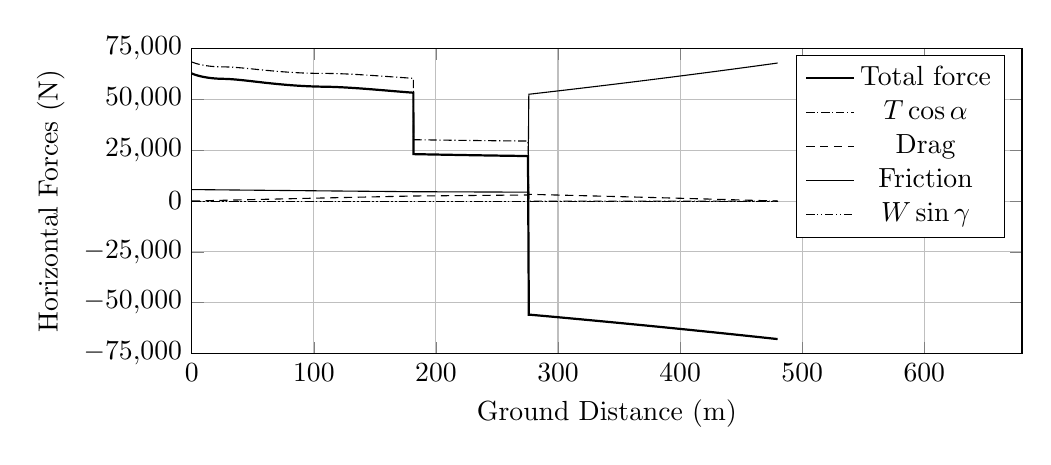
\begin{tikzpicture}

\begin{axis}[
width=\textwidth,
height=0.45\textwidth,
scaled ticks=false, tick label style={/pgf/number format/fixed},
xmin=0.0,
xmax=680,
xlabel={Ground Distance (m)},
xmajorgrids,
ymin=-75000,
ymax=75000,
ytick={-75000,-50000,-25000,0,25000,50000,75000},
ylabel={Horizontal Forces (N)},
ymajorgrids,
legend entries = {Total force\\$T\cos\alpha$\\Drag\\Friction\\$W\sin\gamma$\\}
]

\addplot [
color=black,
thick
]
table[row sep=crcr]{
1.3603393307216043E-8	62748.58696635143\\
3.0265395163403265E-7	62748.5868799013\\
2.9593179127983543E-6	62748.58608546927\\
1.5392338359717934E-5	62748.582368818985\\
5.361280674027254E-5	62748.57094967284\\
1.6215010178508227E-4	62748.53855001014\\
3.7214145765703975E-4	62748.475937488256\\
6.839954676020354E-4	62748.38307289113\\
0.001098342709021993	62748.25985267882\\
0.001609317716481928	62748.108102460115\\
0.0022198920000388346	62747.9270193018\\
0.002878710694837372	62747.73188509708\\
0.0036835072341781794	62747.493830341904\\
0.004557929017412697	62747.235531090235\\
0.005559798278933152	62746.939987000675\\
0.006651227400597502	62746.61846708476\\
0.007795849738889277	62746.281732161995\\
0.009067984722810115	62745.90798859477\\
0.010453165799939174	62745.50159302428\\
0.011915708813158052	62745.07309120921\\
0.013455030027058647	62744.62270873602\\
0.015131183092671713	62744.1329651047\\
0.01690803412933615	62743.61452312661\\
0.01873590105740728	62743.08193195962\\
0.020713359121301934	62742.50655198736\\
0.022777736728155237	62741.906723392676\\
0.024960970145273077	62741.27325267036\\
0.02723428625014468	62740.61457642898\\
0.029610395797831278	62739.92708994227\\
0.03204086105441677	62739.22486425715\\
0.03462344565878624	62738.47973928123\\
0.037295727153354774	62737.70983339002\\
0.040089145853872785	62736.90617768071\\
0.042950967781251806	62736.08401980957\\
0.04592022141655751	62735.23221525195\\
0.04897301836205646	62734.35769420721\\
0.052130294957187476	62733.45453451722\\
0.05542514139564195	62732.51337918814\\
0.05879722600804832	62731.551553678524\\
0.06231520981015182	62730.549570862015\\
0.06596261503753809	62729.512253843466\\
0.06964559414821356	62728.466353857046\\
0.07347193989652406	62727.38132936369\\
0.07736619052035826	62726.27866886809\\
0.08137137577670908	62725.14625822232\\
0.08545617869345057	62723.99302904782\\
0.08969468676038628	62722.79816859719\\
0.0940095881391464	62721.58357345933\\
0.09845059220533334	62720.335335638796\\
0.10296315144049947	62719.06886857006\\
0.10759658895065366	62717.770407907505\\
0.1123317495250277	62716.44541898227\\
0.1171874363557737	62715.08873744405\\
0.12217670360507671	62713.696833232665\\
0.12726806426274867	62712.278596377946\\
0.13231647880291775	62710.874423744215\\
0.13765212084557643	62709.39259132113\\
0.14294844966167852	62707.92390057813\\
0.14834594087957392	62706.42939374142\\
0.1539671093411843	62704.87530924726\\
0.15968242883369804	62703.29761497794\\
0.16555834796315422	62701.678086215674\\
0.17157514414202774	62700.022307246836\\
0.17760320215284392	62698.36600005577\\
0.18370335474801935	62696.69245892286\\
0.18983540939776816	62695.012733407886\\
0.19621099073945342	62693.268985160146\\
0.20278841209744758	62691.47285556147\\
0.20952923284938563	62689.635032135164\\
0.21624967405074952	62687.80566711513\\
0.22309476488450758	62685.94530372377\\
0.22992510727843934	62684.09185367561\\
0.2371653034562048	62682.13030807696\\
0.2442573187228817	62680.21197563074\\
0.25144286317780873	62678.27139497051\\
0.2588001799723505	62676.287560444456\\
0.2662612189130884	62674.27895315632\\
0.27386560463063747	62672.235019498636\\
0.2815803271719757	62670.16475021218\\
0.28946218069394425	62668.053038112266\\
0.29753588720841584	62665.89344676485\\
0.3056643119969481	62663.72277160833\\
0.31376446154764137	62661.56314642425\\
0.322071411728719	62659.351965911075\\
0.3303680011285137	62657.14711651804\\
0.3389039548234316	62654.88233520248\\
0.3474123396293025	62652.628536784236\\
0.3561645174790815	62650.31393386611\\
0.36525289600634137	62647.914420443776\\
0.3742306244196095	62645.54807459045\\
0.3835584127627333	62643.09357191814\\
0.392806747202999	62640.66406444271\\
0.40218604538039837	62638.2042613465\\
0.4115907129344223	62635.741910722456\\
0.42143744457304466	62633.168172904785\\
0.4310567075016639	62630.65814378165\\
0.4412814114336725	62627.99468802521\\
0.4513051702487684	62625.38808306081\\
0.461412558308395	62622.76419796272\\
0.47173637532167356	62620.08870778224\\
0.4821484569390513	62617.39498045387\\
0.492985116277161	62614.59630192182\\
0.5036221628177362	62611.85397612976\\
0.5142245311302887	62609.12527352208\\
0.5252888808291518	62606.28260529175\\
0.5363145235987512	62603.454842006875\\
0.5471208511184944	62600.68808279051\\
0.5585110457184732	62597.77688057248\\
0.569849942463402	62594.88388135728\\
0.5817265165330987	62591.85909204632\\
0.5935668742733842	62588.84896383285\\
0.6053719027871456	62585.8531682976\\
0.6172343027602503	62582.8481431331\\
0.629515267228629	62579.742660032105\\
0.6417789549774502	62576.647150339864\\
0.6542768803188956	62573.498223093644\\
0.6669828212214572	62570.30273451397\\
0.6796225285147333	62567.12969993029\\
0.6925094233679154	62563.90050859051\\
0.7056620711738308	62560.61080706456\\
0.7184715206768946	62557.41279698744\\
0.731725241748566	62554.10989307813\\
0.7449880440563246	62550.81080338117\\
0.7586792333483576	62547.41147337743\\
0.7725063377467813	62543.98485561005\\
0.7863894274138714	62540.5508348624\\
0.8004504964383841	62537.07934156874\\
0.8147129313117618	62533.564809789925\\
0.8293722635741907	62529.95942037302\\
0.8437954335339908	62526.41892554691\\
0.8580702287827062	62522.92144820842\\
0.8726489666047585	62519.35621733467\\
0.8875094051704782	62515.72902264292\\
0.9027740629895862	62512.01038373224\\
0.9182163910703112	62508.25584411707\\
0.93361566230532	62504.51910460576\\
0.9491799633800446	62500.74969728566\\
0.9646343064330896	62497.014198824836\\
0.9803727456894022	62493.217425035546\\
0.9957421603273868	62489.51681954693\\
1.0116767859397604	62485.687518864346\\
1.028041387324289	62481.76266347978\\
1.0443915011410971	62477.84908782526\\
1.060796374175649	62473.93018425266\\
1.0773229908740651	62469.99001590075\\
1.093971735592782	62466.0286038544\\
1.1110062543639518	62461.983516850436\\
1.127891796882146	62457.98184667235\\
1.1451224507351285	62453.906578813054\\
1.1624801114435046	62449.809573461185\\
1.180077727863539	62445.66437174937\\
1.1978884766667508	62441.47755540737\\
1.215488397439855	62437.34872466371\\
1.23351701382096	62433.12794481375\\
1.2518199984626128	62428.851789842374\\
1.2704235066044305	62424.51450258358\\
1.2892140278280424	62420.142838114625\\
1.3075714306593595	62415.88082668194\\
1.3266673518109293	62411.45660776607\\
1.3462106477188795	62406.93843880412\\
1.365306294594515	62402.53316987853\\
1.3852885894463176	62397.9332418976\\
1.404835539176236	62393.44324340303\\
1.4251192118409102	62388.79410053887\\
1.445164519989187	62384.209610593956\\
1.4656054698512246	62379.54481829965\\
1.4853522740259328	62375.04813337898\\
1.5051589726327936	62370.547318011144\\
1.5255757775517242	62365.91776459353\\
1.5464367798307013	62361.19779984228\\
1.5673163741652552	62356.48399416312\\
1.5879032567231621	62351.84635675917\\
1.6091523485848285	62347.06997508714\\
1.6303162371862876	62342.32321005879\\
1.6519474169970438	62337.48235872282\\
1.673879209980242	62332.585224580616\\
1.6955666802836635	62327.75345667584\\
1.7172271378534343	62322.938368230854\\
1.7402832823543353	62317.824650770766\\
1.7634396102400074	62312.70070520534\\
1.7861669372425006	62307.683296247254\\
1.8088678577734645	62302.68312276577\\
1.831824248135399	62297.63819701476\\
1.855578771396016	62292.42998823525\\
1.878960729162178	62287.31542231272\\
1.9033179534858085	62282.00006093712\\
1.9273833213731866	62276.760871077044\\
1.9518510462308036	62271.44672268425\\
1.9761594732990155	62266.17971025566\\
2.000437267212291	62260.93173057698\\
2.0252281699074732	62255.58553885775\\
2.0498006073458734	62250.29904848046\\
2.0745611186355752	62244.98469583233\\
2.0997746990963106	62239.58601863716\\
2.1260324099367294	62233.977544824884\\
2.1515212193659616	62228.54665916039\\
2.1771505246334	62223.09902342319\\
2.2031842637813908	62217.578877816675\\
2.230133398733474	62211.87883012915\\
2.257053086628849	62206.199341242216\\
2.283795213136285	62200.57140899327\\
2.311477064851834	62194.76041739785\\
2.3387199014446116	62189.0561036961\\
2.3662694524467227	62183.302127347895\\
2.3937852540088533	62177.569727310765\\
2.4216520071021392	62171.77892307866\\
2.4501931244916175	62165.86323773577\\
2.478927626230634	62159.92297088956\\
2.506685441631536	62154.19929659829\\
2.53537335014481	62148.29891078557\\
2.5633350931805676	62142.56254067566\\
2.5917889242519685	62136.7399919217\\
2.6208221472873374	62130.814155291315\\
2.649872764173903	62124.90012286141\\
2.679661174525658	62118.85175114668\\
2.709174609939316	62112.87495757626\\
2.740029385016756	62106.64319001096\\
2.770444625703795	62100.51677074139\\
2.801129860621211	62094.352548525436\\
2.8318827297715705	62088.19135466291\\
2.862425967677578	62082.08853117956\\
2.893259332541544	62075.94419494427\\
2.92412139403754	62069.810607507825\\
2.955064430161417	62063.67737666385\\
2.986690331721131	62057.42572254407\\
3.019183403261743	62051.02037545058\\
3.0507201588152526	62044.82063205216\\
3.0830332871979023	62038.48562493776\\
3.1154603869692448	62032.14584436707\\
3.148592095396281	62025.686387496855\\
3.181936872739324	62019.20374172297\\
3.214370607724433	62012.91578195176\\
3.247565473366384	62006.49810462893\\
3.281695868027062	61999.91827897477\\
3.316494330618462	61993.22909634269\\
3.3513055302544137	61986.55699447275\\
3.3860303583611797	61979.920802071385\\
3.421934361445942	61973.07947688752\\
3.456235826539576	61966.56260379907\\
3.490536654441657	61960.06441396962\\
3.526257338581564	61953.31686461522\\
3.561372823896762	61946.70305459414\\
3.5967906564503185	61940.051700124095\\
3.632682576242373	61933.331088361316\\
3.6701261071689295	61926.34104896341\\
3.707701291513044	61919.347983522835\\
3.7452745323452916	61912.37675293113\\
3.78256482255855	61905.479139624134\\
3.8208821591411084	61898.41335511893\\
3.8590337549211444	61891.399974679196\\
3.89695718563138	61884.45002448333\\
3.9351036745073964	61877.480697042585\\
3.9736642086653067	61870.45752863471\\
4.012189127077221	61863.46262797162\\
4.05156219172609	61856.33611163864\\
4.090290786278251	61849.34820486259\\
4.129291984889424	61842.33301078547\\
4.1680648628189925	61835.380560807214\\
4.207805169621487	61828.276955786394\\
4.248168240749736	61821.085042071005\\
4.288797880674668	61813.86893397104\\
4.32990243544832	61806.59214978412\\
4.371428084678056	61799.26487448141\\
4.41247037137882	61792.04652880062\\
4.453879445321437	61784.78737326583\\
4.49524783594077	61777.55900270601\\
4.537299342543221	61770.23538169038\\
4.580546125800922	61762.72882367676\\
4.622914948498307	61755.39934568385\\
4.66640222022569	61747.90167027798\\
4.709294790611851	61740.53149738783\\
4.752417172855319	61733.14671198031\\
4.796155651503765	61725.68177514535\\
4.8408754796551925	61718.07562299959\\
4.884850997559644	61710.621846546\\
4.928651138956553	61703.22308488276\\
4.972831351372241	61695.785567542494\\
5.017331702752941	61688.319868929146\\
5.0632326321008225	61680.64610692728\\
5.108452384314601	61673.112816882494\\
5.1536021218025905	61665.61739795846\\
5.199057463234675	61658.097574294254\\
5.244479287100011	61650.609561581456\\
5.292293005248643	61642.75546639947\\
5.338096108273211	61635.25867322851\\
5.3857492800262605	61627.48701172804\\
5.433816232374781	61619.676598038524\\
5.480691139018431	61612.08754018792\\
5.529685763332537	61604.184355917896\\
5.578612887337309	61596.32155869325\\
5.626451501744754	61588.66205840692\\
5.674834544150631	61580.94378773113\\
5.7252048440372345	61572.93870388891\\
5.77422346516266	61565.17787975559\\
5.8255152536468575	61557.0881089591\\
5.874338256646894	61549.41698457269\\
5.922631450506765	61541.857060475784\\
5.972682300942642	61534.051197922745\\
6.022535370757359	61526.305604306894\\
6.074394648705015	61518.279329606885\\
6.124928192945902	61510.48853147858\\
6.176798284396469	61502.52263273051\\
6.229620191179453	61494.44264252679\\
6.282808156696705	61486.33921985772\\
6.334658925277093	61478.47083549031\\
6.388041948821611	61470.4020804281\\
6.440558117792513	61462.49603497519\\
6.494960924490993	61454.33895717411\\
6.550441697666145	61446.054672571205\\
6.6042098433346865	61438.05913117975\\
6.658315220792536	61430.04610100349\\
6.712335084641163	61422.07827505756\\
6.766674450459032	61414.09598236589\\
6.821537769035839	61406.069808119006\\
6.876851268142238	61398.01128266708\\
6.933661362437203	61389.7695889052\\
6.989261882852809	61381.73743620211\\
7.046240323930029	61373.54103198383\\
7.102786137967051	61365.4415409161\\
7.1603789170469145	61357.22744210556\\
7.21785165788507	61349.06587853639\\
7.277487498606879	61340.63437409418\\
7.334984696129153	61332.540988802284\\
7.393362172524569	61324.359446134375\\
7.452416393609804	61316.119552720236\\
7.511934748111884	61307.851876037705\\
7.572557225035805	61299.46882183947\\
7.63202184821041	61291.282971226334\\
7.69294899409779	61282.93372681769\\
7.752675521499926	61274.7861207831\\
7.814488876138199	61266.39236186803\\
7.8763528528159785	61258.030792142556\\
7.938149975125226	61249.717106305994\\
8.001193143199774	61241.27562431352\\
8.064554080136986	61232.83195752822\\
8.12686567918485	61224.56742562268\\
8.189637855946287	61216.28104072092\\
8.252542711798306	61208.01647879019\\
8.315859663763469	61199.73737466999\\
8.380006162932737	61191.39014484064\\
8.444702551512929	61183.012315166096\\
8.509501986620958	61174.66219684837\\
8.57387297516295	61166.40779955052\\
8.63887365699837	61158.11345598218\\
8.70727085773305	61149.42978513251\\
8.772937378995405	61141.13515405379\\
8.839192134487615	61132.80809432216\\
8.905815929161982	61124.47688991131\\
8.97209054442786	61116.23119859207\\
9.039019026885107	61107.94633956594\\
9.107371801018814	61099.52874647401\\
9.174915633685494	61091.25385062506\\
9.243868961478196	61082.85026326717\\
9.312440636565494	61074.537082415874\\
9.381784695008012	61066.174593755364\\
9.4513167952828	61057.83400599759\\
9.52142787533916	61049.4689800769\\
9.591425279059166	61041.16242227329\\
9.662230428326719	61032.80547235883\\
9.734225879912522	61024.354725814876\\
9.806441602430919	61015.92522773241\\
9.878483835105534	61007.56279411132\\
9.951807209049782	60999.09946552412\\
10.023539677466466	60990.86625654463\\
10.096057433179052	60982.58946445353\\
10.168262179450682	60974.39471287477\\
10.241274410624943	60966.15512361906\\
10.31479015323385	60957.90607803446\\
10.390063469390178	60949.5088689227\\
10.465012435634037	60941.19695487882\\
10.540639152111389	60932.85935085469\\
10.617644389866598	60924.4206271304\\
10.692945462162374	60916.21808473345\\
10.770083295573727	60907.86593944761\\
10.846726862770723	60899.617704468925\\
10.924657809445929	60891.28222333998\\
11.00265335491597	60882.99141813001\\
11.081827589833612	60874.62789243563\\
11.159134327011738	60866.51254463331\\
11.239152720133266	60858.16530457618\\
11.317028257314295	60850.092937656926\\
11.396413369884492	60841.91601155416\\
11.477655063362434	60833.601910542944\\
11.556958506738276	60825.53870258294\\
11.637325199769407	60817.42013318147\\
11.717754170658207	60809.34822562382\\
11.799819443100102	60801.16648757014\\
11.881986970940797	60793.02938201987\\
11.964394119506721	60784.923434520315\\
12.046263329632716	60776.9246223612\\
12.130282587748898	60768.77172035584\\
12.213721087180826	60760.731071135364\\
12.295868535962462	60752.86904578263\\
12.380692430046633	60744.80709776665\\
12.46470288467437	60736.878560376674\\
12.550384439940181	60728.84959741644\\
12.635259749824865	60720.953004655195\\
12.72144647897981	60712.992048849876\\
12.80741162779486	60705.10920775631\\
12.892901506907108	60697.32682994356\\
12.977815703098727	60689.6528017932\\
13.06483740414145	60681.845943009524\\
13.151922956503014	60674.09154282416\\
13.240589045456186	60666.25598494582\\
13.329911181207382	60658.42300686934\\
13.417306166647748	60650.81763431788\\
13.507103029723119	60643.06339800192\\
13.595986036712912	60635.44789722595\\
13.687453390597003	60627.67287452461\\
13.779071846306106	60619.947721374614\\
13.872694200363323	60612.118198018914\\
13.963504841252302	60604.58596521316\\
14.056146454975131	60596.96469563455\\
14.14918846816267	60589.374122844674\\
14.24332804549016	60581.75867435004\\
14.339261112049854	60574.06480791261\\
14.431091301610323	60566.7628020633\\
14.524174633942373	60559.42362172599\\
14.618760344060338	60552.0301792314\\
14.714801736988441	60544.58891918459\\
14.809763128346521	60537.296455040196\\
14.903412319659619	60530.16794560717\\
15.001392651385917	60522.77667740664\\
15.098055049922994	60515.55165071065\\
15.196870856960619	60508.234021771364\\
15.29477342819068	60501.05192711747\\
15.39265348361268	60493.93880871477\\
15.490487151984588	60486.89609055538\\
15.588146853189365	60479.93249400279\\
15.687961867268871	60472.88372826915\\
15.78650099417861	60465.99276441168\\
15.886965864441798	60459.03613643251\\
15.98755318095926	60452.140584871726\\
16.088470385762115	60445.29211238658\\
16.190536977381747	60438.43639519221\\
16.292466610053154	60431.660640934584\\
16.396448349404487	60424.82108251963\\
16.497808944935016	60418.22427083277\\
16.600551072850564	60411.60816428864\\
16.70575139586156	60404.90717498545\\
16.81134459259622	60398.255597675\\
16.917616592554033	60391.63629320428\\
17.023477948501657	60385.11714203395\\
17.12904978140002	60378.68968954387\\
17.2354081519902	60372.28868841233\\
17.340772011500363	60366.02085905596\\
17.448391076872838	60359.69394985451\\
17.5571980918308	60353.37406999097\\
17.66615596614949	60347.12261314588\\
17.774685459577412	60340.97225594756\\
17.884986575683584	60334.79948465346\\
17.99552903728076	60328.69181138744\\
18.108708479124623	60322.51968877914\\
18.219646262474413	60316.549320347185\\
18.332680252669796	60310.54682056299\\
18.445061806396694	60304.65942624536\\
18.556709221711323	60298.88966543338\\
18.668884868236475	60293.17181638187\\
18.78204748093455	60287.48383976107\\
18.895704562363058	60281.851800192686\\
19.008928234289563	60276.32147540923\\
19.124320907419907	60270.76733553811\\
19.24105855786135	60265.23254130206\\
19.355116774466126	60259.90619601139\\
19.470462572962035	60254.60128785194\\
19.58492145104516	60249.41798754399\\
19.704921229319112	60244.069929075034\\
19.821259826163917	60238.96896912673\\
19.941172080873493	60233.79751126356\\
20.06078806851737	60228.72571844168\\
20.177423389922623	60223.86360097327\\
20.297621170678	60218.93874893073\\
20.420129559802255	60214.00852458409\\
20.54164670774839	60209.20696199483\\
20.661905244258705	60204.541892101784\\
20.784301666224792	60199.882230174975\\
20.904244540623438	60195.4021594839\\
21.028114340450195	60190.8646744509\\
21.148300883955606	60186.5485351519\\
21.270875420257596	60182.2340372788\\
21.39299406946177	60178.02308163734\\
21.513793771711654	60173.94326485705\\
21.637476506915142	60169.85407498812\\
21.759279707150128	60165.913776701826\\
21.88493035745168	60161.9389465773\\
22.009809790007786	60158.0787284285\\
22.13620730934617	60154.26288733051\\
22.263515470260465	60150.51212099468\\
22.393040471753594	60146.79108809077\\
22.520519759768852	60143.22214608881\\
22.648852607677917	60139.72253293265\\
22.775118904521122	60136.370289714774\\
22.903136237443974	60133.0634467897\\
23.03176118514304	60129.83381345085\\
23.162501585272054	60126.64621436913\\
23.294719932439598	60123.51984971312\\
23.427108470281937	60120.48717156176\\
23.558693146983046	60117.56950415543\\
23.687077503630363	60114.815344074465\\
23.817949558665852	60112.10162464352\\
23.948210788889448	60109.49434764231\\
24.076877750667826	60107.01056631794\\
24.21019765060587	60104.532709959574\\
24.3450673155249	60102.124917985304\\
24.477101355489637	60099.86379941474\\
24.60984760833776	60097.68601199714\\
24.7468403923846	60095.53870354536\\
24.882807251950062	60093.50777362603\\
25.017167332957627	60091.598723027\\
25.153910941279605	60089.75542762375\\
25.289629217480112	60088.025047101604\\
25.425306692573436	60086.393589543484\\
25.56229499031975	60084.8459137914\\
25.70075944713021	60083.382926138234\\
25.83724158708921	60082.04034140546\\
25.975209935932874	60080.78322359543\\
26.003074150630965	60080.54152452522\\
26.020759913393235	60080.390237708925\\
26.030714598210515	60080.30580847466\\
26.05840292223249	60080.07371814735\\
26.06133765907019	60080.04935502367\\
26.064285136409026	60080.02493175992\\
26.066337724202356	60080.00795070012\\
26.068175973881182	60079.99274812726\\
26.06984477238784	60079.978927470394\\
26.077831036047115	60079.912521841674\\
26.10345636352254	60079.69649113403\\
26.16716044512971	60079.139968811665\\
26.297541524199602	60077.914956659515\\
26.42722303713863	60076.58307608371\\
26.5559280656694	60075.150733013696\\
26.686097387723095	60073.59150482736\\
26.817793678842584	60071.90219867682\\
26.949416928520378	60070.10287580801\\
27.080440623797912	60068.20295062887\\
27.215491080424528	60066.13245178174\\
27.34795890217076	60063.99230108733\\
27.48215578365496	60061.71529098041\\
27.616696052324144	60059.32379232615\\
27.75271189183823	60056.7968769734\\
27.888759310501555	60054.16095945533\\
28.023839122857026	60051.437890958914\\
28.16136324828667	60048.558541493185\\
28.298355249881332	60045.58437893586\\
28.435282447697354	60042.507320286866\\
28.573941346212784	60039.286464396355\\
28.713752690797136	60035.93337885769\\
28.852681198061333	60032.49795314303\\
28.992471984120606	60028.938433904346\\
29.133421724605903	60025.24641390404\\
29.275199211812186	60021.42977817924\\
29.416225289053614	60017.53232806451\\
29.55783477945603	60013.51871776537\\
29.701838356359822	60009.335843087625\\
29.846633046394217	60005.02829350848\\
29.99013730470424	60000.65990011848\\
30.132492646908446	59996.23021131731\\
30.277395768405135	59991.624121233326\\
30.422188862471998	59986.92500457718\\
30.56637548064623	59982.15101578229\\
30.711944318924978	59977.236873309696\\
30.8573377156769	59972.235303635025\\
31.006558691603843	59967.00642218687\\
31.153907258126303	59961.749431289034\\
31.30257185742142	59956.35245740527\\
31.4510947803754	59950.868650967386\\
31.602595106592503	59945.181566874686\\
31.755261577184278	59939.3567386615\\
31.906398416479824	59933.49872413877\\
32.05599258457312	59927.6121241669\\
32.20952926265106	59921.48030147274\\
32.360097140052986	59915.3797277869\\
32.51218835243483	59909.130958224094\\
32.664721606344784	59902.77803647889\\
32.82129760777845	59896.168520531195\\
32.97669884718651	59889.521575766455\\
33.13118849606322	59882.82901181003\\
33.288837444683736	59875.913960326245\\
33.44405554194745	59869.02233987817\\
33.60015866510213	59862.009464306146\\
33.756686089655645	59854.89628317127\\
33.91694077595571	59847.53076840617\\
34.074326811338736	59840.21670800289\\
34.23252403098988	59832.78594932305\\
34.392884168270385	59825.17405547413\\
34.554266068788166	59817.434125624495\\
34.71363140184178	59809.713889733684\\
34.87649332318763	59801.74649341391\\
35.03746231629111	59793.795724769865\\
35.19990059234286	59785.69709035804\\
35.3627309111595	59777.50427105358\\
35.5271254050015	59769.158223754464\\
35.69149466827288	59760.73986894263\\
35.85508342515686	59752.28968258749\\
36.017180984292054	59743.84707744638\\
36.182222084544165	59735.181364659526\\
36.34861175093968	59726.374794774194\\
36.514166392421686	59717.54384636787\\
36.68083924241549	59708.58538314258\\
36.845526722294395	59699.667937927676\\
37.01328249159678	59690.51842314679\\
37.18160982421668	59681.272069921455\\
37.35136716620059	59671.88177477299\\
37.51969289597564	59662.50703427056\\
37.689710015857784	59652.9749717934\\
37.860394939778416	59643.34286054889\\
38.02805196867635	59633.821705559894\\
38.19868492919754	59624.07174448762\\
38.37343039987371	59614.02547641045\\
38.54685896696101	59603.99477876534\\
38.71934233168869	59593.96050993037\\
38.8915617091798	59583.884808444884\\
39.062305982326905	59573.84050900377\\
39.23847188392709	59563.42114261909\\
39.411511502305984	59553.13231783762\\
39.585172817779906	59542.753484797984\\
39.760693028009456	59532.210689936415\\
39.9373134006328	59521.54930350275\\
40.113617753210534	59510.855590869745\\
40.29094651898711	59500.049065758256\\
40.468149621311596	59489.20054552688\\
40.64593210594187	59478.267786044744\\
40.82431302355218	59467.25023578506\\
41.00141330502653	59456.26530982384\\
41.17957893337042	59445.168653441884\\
41.359761290266974	59433.90090662928\\
41.53889737920997	59422.65431892451\\
41.72013507746885	59411.231946434404\\
41.899395797464194	59399.89184669625\\
42.081280067494475	59388.3438205424\\
42.265315320939635	59376.61728887055\\
42.44531744651641	59365.10797527179\\
42.62715102096499	59353.44265820888\\
42.81120266452106	59341.596267562505\\
42.994164503876235	59329.78238567873\\
43.17799769459725	59317.87547182753\\
43.36154361404071	59305.95140490004\\
43.54597437124032	59293.93487000553\\
43.73158498218817	59281.80706459505\\
43.91737182308138	59269.634192009515\\
44.1050494697441	59257.30436278826\\
44.293574236233	59244.88643443957\\
44.47888581456586	59232.64944232178\\
44.66456251492659	59220.358758137445\\
44.85170130968709	59207.9422862198\\
45.037822074257164	59195.565417580845\\
45.22676109993536	59182.97358761598\\
45.41612608476639	59170.326473555484\\
45.604812217355104	59157.69885853167\\
45.79422221198037	59144.997792771144\\
45.98724683785376	59132.02952486985\\
46.17830917717477	59119.16936184275\\
46.36786657808848	59106.388078780714\\
46.55935209439748	59093.4550313941\\
46.75090376717816	59080.496542455774\\
46.94233405988251	59067.52620395071\\
47.13714948644359	59054.306829470224\\
47.33387512950824	59040.938624407834\\
47.53043319838464	59027.5634565034\\
47.72298239739284	59014.444181126615\\
47.919150009665316	59001.06205690163\\
48.113386178114425	58987.79634219325\\
48.311024807628144	58974.28345747267\\
48.508886059616145	58960.74128979957\\
48.70490444306449	58947.3122432207\\
48.90290918859142	58933.734828416535\\
49.09959709013448	58920.23633291242\\
49.2970021191946	58906.67805724632\\
49.49532701226336	58893.0467801264\\
49.693780717172615	58879.39762345921\\
49.89506320355713	58865.545529044466\\
50.096719083698545	58851.66011777922\\
50.29606895218413	58837.92681505815\\
50.497598474286534	58824.03742648578\\
50.700304208193415	58810.06178154117\\
50.90342397924904	58796.05318781125\\
51.10460922167407	58782.17446693129\\
51.30752217039489	58768.17378053878\\
51.51010619677311	58754.19378919198\\
51.713602501430145	58740.14961347189\\
51.91843850546792	58726.01251882098\\
52.121089026646246	58712.026568525456\\
52.32561402362407	58697.91232524882\\
52.53192272805477	58683.676849060794\\
52.7387030603267	58669.411473394386\\
52.944027344085896	58655.2499181404\\
53.154073670302836	58640.766921001064\\
53.36143953271798	58626.473711841114\\
53.571009444677685	58612.03435305624\\
53.77799762982136	58597.779302285955\\
53.98785945427545	58583.33360532427\\
54.196157549666225	58569.00349637364\\
54.40718762937186	58554.49424354074\\
54.616887598525366	58540.08593929515\\
54.826875464266934	58525.66805041215\\
55.04038432082807	58511.019590906755\\
55.25438844036796	58496.34919209598\\
55.46695867894975	58481.789733344616\\
55.68088820258777	58467.15060443987\\
55.895144656119854	58452.503310170345\\
56.109028395418505	58437.8963688973\\
56.326262430904194	58423.07653689642\\
56.542089933321776	58408.36923531024\\
56.76060076462056	58393.496613132695\\
56.97729209122687	58378.76593888097\\
57.19579178641709	58363.93127346867\\
57.41258192878804	58349.232142096356\\
57.634093277561306	58334.23360901498\\
57.85395098827546	58319.368421754974\\
58.07448819514299	58304.47936006026\\
58.29446478173499	58289.65082477676\\
58.51588770709739	58274.74832251543\\
58.73757884137123	58259.852072426496\\
58.96020041504734	58244.918425863274\\
59.18267120664716	58230.02068874739\\
59.405949655899676	58215.09543434816\\
59.63089974393067	58200.08599554913\\
59.8562534200115	58185.07800385475\\
60.084134136581554	58169.93124615034\\
60.30833762904015	58155.0585106377\\
60.53504725699203	58140.05001099827\\
60.763693228044005	58124.944996575156\\
60.99075593752245	58109.9766742912\\
61.21765734918529	58095.05154409529\\
61.44713116872772	58079.99091894232\\
61.6738048454246	58065.14794897725\\
61.90668490141796	58049.934252569554\\
62.13729676517957	58034.90496991055\\
62.36629463006145	58020.017142951256\\
62.596359157213186	58005.0969435555\\
62.82836101237727	57990.089215390806\\
63.059723307860466	57975.16154762388\\
63.292774394726166	57960.164552688395\\
63.52608473446321	57945.19129201122\\
63.75973181411028	57930.23751514376\\
63.993403028653574	57915.32388526069\\
64.23068717493263	57900.22290169429\\
64.4710952259949	57884.968123073966\\
64.70858695601663	57869.94345289939\\
64.94894296164699	57854.78374474145\\
65.18738841845183	57839.790989490284\\
65.42661162888535	57824.79637674126\\
65.6659442133793	57809.84260865279\\
65.90899583190168	57794.70585484736\\
66.15068261105333	57779.703994875264\\
66.39533053734849	57764.569557362134\\
66.6378997293487	57749.61513840084\\
66.88158418814953	57734.64405780201\\
67.12390450547147	57719.80908596837\\
67.36840986262189	57704.89373052902\\
67.61550053739396	57689.875673584495\\
67.86097385246623	57675.011197135274\\
68.10985741250389	57659.99699254849\\
68.35582503705197	57645.215376441585\\
68.60464259362828	57630.320335732904\\
68.85450289166104	57615.421930398705\\
69.1042877596268	57600.58768656949\\
69.35837572129628	57585.55961469008\\
69.61150655903072	57570.650567820005\\
69.86289252102952	57555.90645002769\\
70.11686816207683	57541.07384976631\\
70.37125759672608	57526.28146883179\\
70.62480458144697	57511.602684827594\\
70.88045310059783	57496.868032549406\\
71.13526709211152	57482.2477088772\\
71.3947754873567	57467.42648958336\\
71.6534187996231	57452.72389970705\\
71.91450497256008	57437.9530268809\\
72.1716184080999	57423.47668890437\\
72.43269265097052	57408.84867334757\\
72.69331619504374	57394.31807118036\\
72.95563200429567	57379.76639485071\\
73.21686762735783	57365.34816427594\\
73.48161420086069	57350.81148245353\\
73.74261486234883	57336.55516320803\\
74.00755043430098	57322.16020489593\\
74.27511769675363	57307.700731758494\\
74.54487113507057	57293.203417113225\\
74.81568229507957	57278.73082942504\\
75.08274085953312	57264.53928104503\\
75.35421836228127	57250.19529339293\\
75.62798354862159	57235.815005515935\\
75.89909469738902	57221.65827722961\\
76.17008148658607	57207.592166056216\\
76.44269151183332	57193.52709763679\\
76.71571902594138	57179.52667636318\\
76.99340852183178	57165.37611511002\\
77.27004772085374	57151.36867996861\\
77.54832408953641	57137.3690188676\\
77.82592519882277	57123.49437037441\\
78.10358246820337	57109.70830060974\\
78.38556010231375	57095.80169065631\\
78.66911430382748	57081.91325680206\\
78.95399134982776	57068.05733920049\\
79.23667137346987	57054.40511855275\\
79.518907793654	57040.87097593317\\
79.80555437718249	57027.22462735973\\
80.09150103324356	57013.711698279614\\
80.37928873457926	57000.21312970358\\
80.66871996946384	56986.74045134256\\
80.95967699414447	56973.30125974615\\
81.25093884305389	56959.953355159334\\
81.54344278085921	56946.655040364625\\
81.8358102960415	56933.47000175789\\
82.13087592438694	56920.272231425\\
82.42794520371837	56907.09581840529\\
82.72842933895026	56893.881639624116\\
83.0269479931649	56880.86753738558\\
83.32974506690314	56867.78304709877\\
83.62964811531441	56854.93930768462\\
83.92951211009506	56842.21275618588\\
84.2339319847595	56829.41140490904\\
84.53715838283946	56816.77938938404\\
84.84105485927768	56804.23916326916\\
85.14845677960258	56791.6766012771\\
85.45530133949276	56779.25989423189\\
85.76249773413784	56766.95251773413\\
86.07201271349416	56754.6776826112\\
86.38432073331904	56742.42008664644\\
86.69710203601804	56730.27318128143\\
87.01172103282082	56718.18580759912\\
87.32669099459858	56706.216841512796\\
87.64517025121202	56694.249092126294\\
87.96158123090564	56682.49345114094\\
88.2775814178033	56670.88713943225\\
88.60068374099544	56659.15889246231\\
88.92068281935622	56647.68211567633\\
89.24207276858638	56636.29489195993\\
89.56578933015979	56624.966871902594\\
89.88760090270688	56613.846782456036\\
90.2141410750086	56602.70764357982\\
90.54066676000363	56591.71476082115\\
90.86727570256076	56580.86525915227\\
91.19715108614633	56570.056025089754\\
91.52744226539704	56559.38333331379\\
91.85639956214655	56548.90345885874\\
92.19095740864739	56538.39878096101\\
92.52827526888461	56527.964652251685\\
92.8674718219292	56517.631963717184\\
93.20307982994817	56507.56642262393\\
93.5374944579234	56497.693186082965\\
93.87598013161067	56487.85921140874\\
94.20917297854535	56478.33603005043\\
94.55043409744499	56468.744085149316\\
94.89132963816093	56459.32628081381\\
95.23083207736542	56450.11008466894\\
95.57395676502793	56440.96130767578\\
95.91421223354143	56432.05391776969\\
96.25656086122288	56423.25778081856\\
96.60012122339742	56414.59829008607\\
96.94166303707107	56406.15660543901\\
97.28627502929558	56397.80805457507\\
97.62906225262071	56389.67246279065\\
97.97125437026659	56381.7191803942\\
98.31201772458999	56373.96640546429\\
98.65627175165852	56366.30404987256\\
99.0012536203806	56358.7970495818\\
99.35020029285332	56351.37879791277\\
99.69475740907401	56344.22688983864\\
100.04053871990226	56337.2227245853\\
100.38598466112728	56330.398861049194\\
100.72867962848932	56323.800990670556\\
101.07385499050397	56317.328482357116\\
101.41864366415388	56311.036962809405\\
101.76305460768467	56304.925976431376\\
102.11068844700483	56298.93408101726\\
102.45638678530696	56293.1514497693\\
102.79841653079728	56287.6030887989\\
103.14087212494877	56282.22039228937\\
103.48486473791618	56276.98764930107\\
103.82875595362174	56271.9311402599\\
104.17244250654872	56267.05241446568\\
104.51168383396202	56262.40839195342\\
104.85986244643053	56257.81956693379\\
105.204587526496	56253.45370284168\\
105.54754777175077	56249.2856524184\\
105.88797456536247	56245.32171703216\\
106.23280177240994	56241.48283858344\\
106.57515110440406	56237.84731191555\\
106.91603555764121	56234.40159354803\\
107.25729565943405	56231.12648374667\\
107.598830149446	56228.0236908629\\
107.93686571059558	56225.12525758898\\
108.27485499032852	56222.39909828467\\
108.28839963475954	56222.29343457302\\
108.30004107281309	56222.20283890501\\
108.30931238392475	56222.130834026844\\
108.31701527366243	56222.07110866209\\
108.32505202073054	56222.00888998585\\
108.33865239118708	56221.90352333871\\
108.35091925899997	56221.80817976603\\
108.39508146726081	56221.46251135353\\
108.52984553865659	56220.38431104434\\
108.79919793188978	56218.124321758805\\
109.105233418432	56215.38796017447\\
109.41485218466596	56212.43876717285\\
109.72257164661937	56209.329249695904\\
110.0321119530083	56206.02364807254\\
110.34145354075926	56202.54388740145\\
110.6534776714839	56198.85720238433\\
110.9711963390063	56194.92266913525\\
111.28851843247409	56190.81304220014\\
111.60893519474632	56186.482686019124\\
111.92798394282838	56181.99232137638\\
112.24770070245137	56177.31574331\\
112.57243448635171	56172.38650016113\\
112.89480865389396	56167.316255719226\\
113.22000325235314	56162.02506719764\\
113.54885709436653	56156.495924408984\\
113.8770619430189	56150.8007571287\\
114.20946079557197	56144.85463194827\\
114.54107775051554	56138.74579277108\\
114.87787736567807	56132.36285681174\\
115.21564640021248	56125.7828083107\\
115.55522358014255	56118.989166772444\\
115.89667501383605	56111.97978573381\\
116.23992536102014	56104.75543143583\\
116.5847156213415	56097.32106939993\\
116.92791619634093	56089.74631474781\\
117.27517516660399	56081.90673960303\\
117.62420948631524	56073.851595352215\\
117.97391125359778	56065.60675690233\\
118.32673409155768	56057.11371142954\\
118.68227803698588	56048.37994092658\\
119.03889207644076	56039.44541752979\\
119.39651249432902	56030.31244179359\\
119.75508651978987	56020.98316642031\\
120.11314113323388	56011.497818516655\\
120.47404637453192	56001.767689903165\\
120.84098349318353	55991.703014647734\\
121.20490030977416	55981.552245613944\\
121.57328571082118	55971.107791288494\\
121.94079100066682	55960.521120985824\\
122.31015242291167	55949.71504889215\\
122.68267403243519	55938.65035934067\\
123.05346836176264	55927.47357220735\\
123.42835733050345	55916.009964443816\\
123.80350972566416	55904.37617114821\\
124.1783235941891	55892.5932314603\\
124.55244040146786	55880.675372697835\\
124.92576251095704	55868.62890512576\\
125.30489170817492	55856.2399884225\\
125.68146781278597	55843.782096823634\\
126.06139977608174	55831.06156204913\\
126.44502763856761	55818.06509104854\\
126.82695116404781	55804.97676663293\\
127.206716044588	55791.8166966117\\
127.59262031825523	55778.2973348018\\
127.97077035934353	55764.90856278862\\
128.3546122768156	55751.17771078469\\
128.73724861847296	55737.35127522546\\
129.12002064685282	55723.383586454715\\
129.50086700331673	55709.35299411682\\
129.8837789976152	55695.114550477956\\
130.26783132854348	55680.70317169887\\
130.651936341801	55666.1612208974\\
131.03747321415574	55651.43789318508\\
131.42280335891803	55636.597300480076\\
131.80875442588928	55621.60949618093\\
132.19322104975072	55606.55875254114\\
132.5798881414172	55591.302577009745\\
132.96215446290768	55576.10448440041\\
133.34488286943906	55560.77493614884\\
133.7276157954845	55545.33404423838\\
134.11532375481391	55529.58112314579\\
134.50135826447365	55513.7868942778\\
134.88604120201086	55497.941452089304\\
135.26955723714872	55482.04017874946\\
135.6512109336153	55466.11503999484\\
136.03464327936558	55450.016035957364\\
136.41686422877552	55433.870357224296\\
136.79904942565338	55417.63067088832\\
137.18004416157777	55401.34832411715\\
137.56399804528928	55384.84715438729\\
137.94515347717788	55368.37634492545\\
138.32982901897384	55351.66440206327\\
138.7128522769853	55334.93717264214\\
139.09597564505458	55318.120424441746\\
139.48002685240425	55301.1792409702\\
139.86309097971855	55284.19985069129\\
140.24727738828375	55267.09044263883\\
140.6317581809211	55249.88916214407\\
141.01585725597846	55232.627988521665\\
141.3998433603236	55215.29668049727\\
141.7841907991213	55197.87543152385\\
142.16710976343057	55180.44732359465\\
142.55205218648928	55162.856724862766\\
142.9364233092117	55145.223440758215\\
143.32169829765928	55127.4813330021\\
143.705984531242	55109.71918555195\\
144.08985428249122	55091.912492652395\\
144.47683600496026	55073.898497552786\\
144.86371007721533	55055.82792710092\\
145.24772592056325	55037.83152082506\\
145.63047789911974	55019.83703718289\\
146.01273254364395	55001.81033207037\\
146.39725173307323	54983.62226960719\\
146.77966503747456	54965.48101678323\\
147.16478130736948	54947.159801267\\
147.54689717238745	54928.931460230524\\
147.93097497792814	54910.56091905589\\
148.31499270913332	54892.14596321457\\
148.69957284780122	54873.658076309075\\
149.08709998577143	54854.98342854447\\
149.47129868208145	54836.42590504256\\
149.8546635899794	54817.867096079746\\
150.23801379389647	54799.26885358787\\
150.62200569343076	54780.600590802685\\
151.00751012558203	54761.820999532705\\
151.3946455315429	54742.92520665043\\
151.77987817077866	54724.087072065915\\
152.16505704867353	54705.21777216332\\
152.55112759502248	54686.27219872901\\
152.93964308710213	54667.17502751459\\
153.32507651584535	54648.199311805016\\
153.71174813432617	54629.13386161778\\
154.10000329570875	54609.96262097417\\
154.48914219495543	54590.72116745093\\
154.8788297075107	54571.42720776945\\
155.26820650111182	54552.124537229014\\
155.6562915247282	54532.86319060705\\
156.0441896603637	54513.58969644079\\
156.4348678136667	54494.15766185129\\
156.82082928279863	54474.94132617938\\
157.21071017196311	54455.51198151686\\
157.60005066896917	54436.09284665936\\
157.99004282467217	54416.625654705625\\
158.3808231456182	54397.10469619969\\
158.77280374485122	54377.51046344079\\
159.16384255262415	54357.95119737928\\
159.55370941764693	54338.43966646871\\
159.946071590523	54318.79343914623\\
160.33752628124114	54299.18398618256\\
160.73008933968674	54279.51146191299\\
161.12428312893906	54259.75075249432\\
161.5185576482712	54239.98065382296\\
161.91431288671106	54220.132070889886\\
162.3096877663487	54200.299453393716\\
162.70613442998513	54180.411074487405\\
163.1032465869576	54160.48842143788\\
163.50039135636405	54140.56435330774\\
163.89625578410926	54120.7058320669\\
164.29272443146095	54100.81939974001\\
164.68754921345175	54081.0188746777\\
165.0864466423082	54061.01867812773\\
165.4846753800681	54041.0576608197\\
165.88329117400662	54021.08395964862\\
166.28234792206388	54001.0959490231\\
166.68312204436222	53981.03081256845\\
167.08520211103445	53960.910304118064\\
167.486487681752	53940.84059601926\\
167.8888620337579	53920.728550824395\\
168.290121631074	53900.68533398691\\
168.69179641444674	53880.63550674889\\
169.0966267258019	53860.44349441516\\
169.50108473093724	53840.286433228815\\
169.90729482190739	53820.05955132231\\
170.31243922775104	53799.90420832072\\
170.71755979953144	53779.76949556715\\
171.12402986296422	53759.58824563795\\
171.53319587512163	53739.29491166239\\
171.941770038195	53719.05371778349\\
172.3502931259835	53698.83880281453\\
172.7599322859847	53678.59348384627\\
173.17073308198894	53658.3166922113\\
173.58266371319877	53638.0111895\\
173.99296569000023	53617.813863603005\\
174.40104722187203	53597.754394678734\\
174.8156903853216	53577.40250627583\\
175.2299479185392	53557.10081841212\\
175.64260521584504	53536.90957335412\\
176.05374721710058	53516.82517661505\\
176.4688147253861	53496.58305854685\\
176.8832117842232	53476.40867801159\\
177.30033423294157	53456.137899228255\\
177.7185234955238	53435.85274429567\\
178.13477925276436	53415.69954593359\\
178.55472625996282	53395.40713691914\\
178.97486541267733	53375.14606012564\\
179.39652032378837	53354.85364544802\\
179.8177496461559	53334.62438848107\\
180.24148986351946	53314.318490386184\\
180.66579793025812	53294.03044661062\\
181.08977314985765	53273.80425740976\\
181.5138518510159	53253.61995797251\\
181.61122522885114	23083.347411060575\\
181.9380657232258	23074.39279527153\\
182.36340272554946	23069.34829519297\\
183.2082724125376	23059.343031811222\\
184.08646972066333	23048.964337542973\\
184.96448881265883	23038.609696260413\\
185.84629357991815	23028.232794819734\\
186.726051310566	23017.90263277814\\
187.61806497534428	23007.451959473976\\
188.50412524941663	22997.09465635965\\
189.3932804644195	22986.725136616937\\
190.28280340229105	22976.375638139485\\
191.1758490733834	22966.00990452693\\
192.0664158070755	22955.69793029443\\
192.96248081795437	22945.347762447724\\
193.85627821989942	22935.049525928393\\
194.7612747993291	22924.648734662405\\
195.67115393765977	22914.21898405221\\
196.57439968482538	22903.892488669168\\
197.49109477617128	22893.440250434636\\
198.40328264870095	22883.06771091347\\
199.32142764481148	22872.65623676376\\
200.23456840248758	22862.330456171512\\
201.14898042779765	22852.019510562946\\
202.06794236074546	22841.686991019946\\
202.98618556976356	22831.392602151813\\
203.9096776069573	22821.069944838506\\
204.83478510422236	22810.76025317573\\
205.76152187560933	22800.463814987765\\
206.69425456631774	22790.132783055837\\
207.628282006662	22779.819882962584\\
208.55982483556244	22769.567057532287\\
209.49858617709037	22759.268037042144\\
210.43993621334516	22748.97441320482\\
211.37516676315846	22738.781491415888\\
212.31832896164838	22728.536500869755\\
213.2711811717055	22718.221585102\\
214.21827407856858	22708.004478891322\\
215.17513356897763	22697.718191305037\\
216.13205411802585	22687.467889093852\\
217.08198149354007	22677.3290063222\\
218.0371791872164	22667.170817720304\\
218.99188071657676	22657.055188900486\\
219.9529264806817	22646.910249854394\\
220.9127352149854	22636.816594752483\\
221.88152971929293	22626.667446533225\\
222.85280254650712	22616.5319369359\\
223.82131876423426	22606.464939575955\\
224.792464296851	22596.41072477681\\
225.77907189920393	22586.237829128448\\
226.75865308803293	22576.178925611923\\
227.73754112978963	22566.16875050267\\
228.71868465671315	22556.177508456793\\
229.71601747959392	22546.06476252975\\
230.71257028094016	22536.00384942048\\
231.7099256226606	22525.979056498647\\
232.7104408810668	22515.96721459065\\
233.70545418089353	22506.05510082584\\
234.709934391256	22496.094124203344\\
235.71369390815352	22486.186161570877\\
236.7320063884447	22476.181662916097\\
237.74706170316256	22466.256650576914\\
238.76105009328802	22456.38966319\\
239.78487801639722	22446.47544987731\\
240.8100003079174	22436.59780940628\\
241.83501924916794	22426.770552307535\\
242.86448750110736	22416.950601528457\\
243.8907393349939	22407.21142240495\\
244.92503751619887	22397.446739110143\\
245.953502111432	22387.788003640257\\
246.9873414577291	22378.130169189928\\
248.03717558009265	22368.37588355803\\
249.06961888058504	22358.83548362812\\
250.1218155809346	22349.166166220442\\
251.19093832453012	22339.39700047268\\
252.25320725679705	22329.746321958082\\
253.30608820982889	22320.236129110664\\
254.3699559131253	22310.682763626988\\
255.43101098027842	22301.21103750822\\
256.50967156157174	22291.64012330029\\
257.5914429014633	22282.100564903645\\
258.6840945362286	22272.525255460263\\
259.76380176807595	22263.123063818457\\
260.8581962365888	22253.65377234474\\
261.9444516651656	22244.31568397567\\
263.04204949406176	22234.94184820512\\
264.16032684448305	22225.455509131338\\
265.27010097773245	22216.10553161949\\
266.38392459233114	22206.78603038523\\
267.48537153454777	22197.633974554454\\
268.5905820952057	22188.514752224983\\
269.71611280872617	22179.29411715609\\
270.8445404967937	22170.11711938212\\
271.9892540622492	22160.87686318175\\
273.1287802847319	22151.747951704958\\
274.2598607565136	22142.755501772386\\
275.4140962910436	22133.649887394575\\
276.090309303484	-55848.67681040526\\
276.5737705536998	-55838.42097294732\\
277.56867335135405	-55891.70762560789\\
278.5517001083557	-55944.408146022266\\
279.52761403034117	-55996.77649745246\\
280.5279265157802	-56050.50497099328\\
281.5196374788271	-56103.82233112375\\
282.5091228114409	-56157.07058152549\\
283.5002036181013	-56210.455351253666\\
284.4794994349294	-56263.25516763644\\
285.4656948937601	-56316.477107452854\\
286.4639109988274	-56370.39903406151\\
287.4440310703403	-56423.39367734424\\
288.4281172103467	-56476.65288805282\\
289.40231797711374	-56529.42661500718\\
290.3936300375175	-56583.17790378742\\
291.378876920571	-56636.65096576243\\
292.36776902799863	-56690.37268255233\\
293.3555402536373	-56744.08437744924\\
294.3358859908236	-56797.44261613164\\
295.3135149835475	-56850.702953904794\\
296.3010928277796	-56904.55600468577\\
297.2700925003244	-56957.445562363515\\
298.2415260228572	-57010.51730672424\\
299.2237735124987	-57064.23012415753\\
300.18939507314394	-57117.0831041248\\
301.1612976587651	-57170.32930521398\\
302.12729290918287	-57223.30105571762\\
303.09931171579603	-57276.652658303894\\
304.0678713857018	-57329.86387440354\\
305.04429883131866	-57383.55737274674\\
306.0164996180358	-57437.06840985168\\
306.98118774731006	-57490.215264570754\\
307.9458829879452	-57543.41168870963\\
308.90778129014984	-57596.50289001112\\
309.8718300339916	-57649.76193108843\\
310.82071939691946	-57702.231581980624\\
311.78063768836523	-57755.35967790987\\
312.73974687077543	-57808.49184722014\\
313.70023292462724	-57861.74927603027\\
314.6569728944272	-57914.847768346604\\
315.60613237716643	-57967.57369784251\\
316.5550556489659	-58020.33448978551\\
317.50210479917575	-58073.03895876475\\
318.45466232971773	-58126.098270229646\\
319.3957102606697	-58178.56407773058\\
320.3324351673011	-58230.835896491684\\
321.2750257745305	-58283.48244435001\\
322.21493829765757	-58336.026808166396\\
323.1533741352699	-58388.53587892285\\
324.09443618900866	-58441.23935928068\\
325.03529996492455	-58493.9792921554\\
325.9648562306003	-58546.13212486486\\
326.89383310034975	-58598.298906152515\\
327.8206991505191	-58650.393478377955\\
328.74438373860426	-58702.35531075804\\
329.67711448753994	-58754.87274915542\\
330.6097169675753	-58807.42993984261\\
331.53548340325426	-58859.648379988415\\
332.45965925914595	-58911.823350727995\\
333.37601791529755	-58963.602660393124\\
334.3038767948972	-59016.0781668221\\
335.21715278190004	-59067.77453662717\\
336.13023158854344	-59119.50501480585\\
337.04233726257917	-59171.22559235156\\
337.95328474841153	-59222.925656788895\\
338.871866990674	-59275.10476728316\\
339.7790008687574	-59326.678682361264\\
340.6889919093551	-59378.4601232455\\
341.59608198392925	-59430.12146963987\\
342.4944202550406	-59481.328674727454\\
343.39144890241744	-59532.505254036936\\
344.283788724593	-59583.45801678371\\
345.1768840599533	-59634.49758439895\\
346.06572667426315	-59685.337521932684\\
346.9469844512215	-59735.78641168059\\
347.83175896018065	-59786.479519333356\\
348.715920705353	-59837.180493320266\\
349.58520994927073	-59887.07054245556\\
350.45732989207283	-59937.16485034481\\
351.3240626599113	-59986.9912358532\\
352.19234272126505	-60036.94810374458\\
353.0567279915266	-60086.72220741885\\
353.9087728108053	-60135.82609391505\\
354.76614015147914	-60185.277226103906\\
355.6200251272137	-60234.56792024938\\
356.4699203143431	-60283.66838866654\\
357.32208656517776	-60332.940246900296\\
358.16670442666066	-60381.81539869588\\
359.01850300539274	-60431.14617382585\\
359.85678773842255	-60479.733660754166\\
360.6939435511699	-60528.29470091153\\
361.5232960751498	-60576.44154195134\\
362.3453827424422	-60624.20437055538\\
363.17264968006	-60672.30618672723\\
363.9943569860219	-60720.12251763782\\
364.8178460354478	-60768.08033787829\\
365.6313564801386	-60815.49422273398\\
366.44296440219716	-60862.834087399955\\
367.24939495159083	-60909.90846200973\\
368.0577691551946	-60957.13283645002\\
368.855950973905	-61003.79770653727\\
369.6530099750727	-61050.432580537934\\
370.4510950082282	-61097.1632056275\\
371.2444498303104	-61143.652312777325\\
372.026605563162	-61189.519802428025\\
372.8087280301727	-61235.41974702613\\
373.5923237375997	-61281.44067896021\\
374.37188347969027	-61327.25889663922\\
375.1497157063701	-61373.009723543975\\
375.9207778532334	-61418.396031615935\\
376.6887008221187	-61463.6309203634\\
377.4523898514876	-61508.649447379314\\
378.2106671025923	-61553.38158046239\\
378.9633302043893	-61597.81469579213\\
379.7236110365668	-61642.730083575036\\
380.46618402346496	-61686.630954050925\\
381.2106664131667	-61730.67609444885\\
381.9522634475744	-61774.58179741577\\
382.68594948596035	-61818.04986550007\\
383.41841791909826	-61861.47630563482\\
384.1429296459944	-61904.46102137628\\
384.867708718731	-61947.49148319123\\
385.58948123827906	-61990.37316963448\\
386.3030175691964	-62032.79470823752\\
387.0123596206615	-62074.99566092549\\
387.7251006134436	-62117.42774319257\\
388.44195834300933	-62160.1341666402\\
389.14068647881095	-62201.78878558001\\
389.84107063439046	-62243.57014083312\\
390.5388507540679	-62285.22406102039\\
391.23713621732134	-62326.93605309272\\
391.9308944704235	-62368.40527597585\\
392.61185820200876	-62409.1365424425\\
393.29428033591034	-62449.98172811653\\
393.9718965997264	-62490.565717191654\\
394.6550184053915	-62531.50614218596\\
395.3150819232203	-62571.09013142575\\
395.9800930313846	-62610.996167630525\\
396.6508845392751	-62651.274858257326\\
397.3100151661747	-62690.878593747635\\
397.96008932639904	-62729.962694225804\\
398.6128592247197	-62769.23338773736\\
399.2633653116203	-62808.39234694069\\
399.9179929613032	-62847.824076921985\\
400.55961836777794	-62886.49663501304\\
401.19831098808993	-62925.01605958282\\
401.8317159567654	-62963.23988874105\\
402.46070413779364	-63001.22015658271\\
403.0932007538113	-63039.43537694379\\
403.718833508158	-63077.258689759896\\
404.3342396794375	-63114.4858836152\\
404.9590832136587	-63152.30644204015\\
405.5777100081168	-63189.77303969364\\
406.1885303417122	-63226.7886547028\\
406.79765945351824	-63263.72337514686\\
407.39729520735443	-63300.10353711725\\
408.0045482550711	-63336.96716461623\\
408.6032467968737	-63373.33250260995\\
409.19310530131077	-63409.18131017433\\
409.77930242987406	-63444.827687029916\\
410.34882720483665	-63479.47941796463\\
410.9397524300308	-63515.45322757095\\
411.5144979368331	-63550.46161957868\\
412.0916880769664	-63585.63833613327\\
412.67508886073415	-63621.213345492826\\
413.24739329013073	-63656.131053067045\\
413.8102117002136	-63690.488685410965\\
414.3766533496281	-63725.08622445911\\
414.9330849868252	-63759.09066317903\\
415.49090154170335	-63793.197949428606\\
416.0384251695623	-63826.6936255646\\
416.58185455043815	-63859.95621993227\\
417.137788521634	-63894.00214116661\\
417.6785143601711	-63927.134114938584\\
418.2209459784557	-63960.38786904469\\
418.7580922864813	-63993.33465334457\\
419.2925397618968	-64026.13274373535\\
419.8214282041728	-64058.6062345597\\
420.3456555305893	-64090.809788311875\\
420.8748802724658	-64123.336757496945\\
421.40220840629206	-64155.76357746596\\
421.92445363470176	-64187.89399767056\\
422.4396473491323	-64219.606350209826\\
422.9476883364184	-64250.893764973516\\
423.46781771332803	-64282.94142778816\\
423.96972141164224	-64313.88127379617\\
424.4747887123442	-64345.03117270657\\
424.97842626986676	-64376.107915752975\\
425.46685055581315	-64406.26026615055\\
425.9611547890038	-64436.78998756959\\
426.45867157869884	-64467.53273921051\\
426.94540858130756	-64497.62357608181\\
427.4263588126769	-64527.370461454426\\
427.9072505537316	-64557.12744621605\\
428.38175644556543	-64586.50273291144\\
428.86162597494547	-64616.223660971635\\
429.32515105779066	-64644.94527449332\\
429.7968616463752	-64674.187197017905\\
430.2606729703833	-64702.95233141197\\
430.7231042852982	-64731.64461578132\\
431.1904716263688	-64760.656091671815\\
431.6479070983538	-64789.06364508129\\
432.10655655044036	-64817.55909956171\\
432.56173102027105	-64845.85104744948\\
433.0126208065283	-64873.88885058039\\
433.45215669676156	-64901.23230006285\\
433.8978573666708	-64928.97102790125\\
434.3342916233415	-64956.14453745616\\
434.778745426511	-64983.82905224907\\
435.2123989882417	-65010.852205049116\\
435.64230021573144	-65037.65262284897\\
436.075634341204	-65064.67823155322\\
436.5083457929386	-65091.67621213476\\
436.9352101003242	-65118.32035083436\\
437.3567121725589	-65144.64048965102\\
437.78504223013067	-65171.397891211964\\
438.2047290714361	-65197.62601850426\\
438.6243871968487	-65223.86290559612\\
439.035916661992	-65249.60184499805\\
439.4457138924115	-65275.24253566988\\
439.8474748270129	-65300.39018299975\\
440.253092263634	-65325.78905074659\\
440.65576500436714	-65351.01329981358\\
441.05189542318885	-65375.83722811124\\
441.4538791373619	-65401.037598849114\\
441.8478809159244	-65425.74700834253\\
442.2390534802082	-65450.28822185368\\
442.62490337846396	-65474.50452263349\\
443.01122384576365	-65498.7593330839\\
443.3883864382053	-65522.447842068184\\
443.76864561351863	-65546.33951168382\\
444.1435547955308	-65569.90357011795\\
444.5174925928394	-65593.41501282499\\
444.9021140390008	-65617.6069881985\\
445.2741476310465	-65641.01570004388\\
445.63572275828176	-65663.77435727493\\
446.0027162970804	-65686.88213510995\\
446.37462159628	-65710.30747820155\\
446.7375105084584	-65733.17295524341\\
447.0960855960951	-65755.77443529043\\
447.449923268351	-65778.08492742068\\
447.80341802109365	-65800.38135627878\\
448.1530101332314	-65822.43906185983\\
448.4955121200786	-65844.05658288448\\
448.84248061552853	-65865.96325338242\\
449.1840796946957	-65887.53803331938\\
449.5207345419592	-65908.80745875867\\
449.8608275251472	-65930.30107287355\\
450.19712744844014	-65951.56186100788\\
450.5348389443434	-65972.91878764669\\
450.86615760747793	-65993.87815137111\\
451.19442174138624	-66014.65085114841\\
451.51745806240217	-66035.09911579484\\
451.8388887923295	-66055.45203297256\\
452.15941578120123	-66075.75397209529\\
452.4819438828837	-66096.18895850069\\
452.805325119817	-66116.68434345952\\
453.1156382282436	-66136.35746658471\\
453.43261346900215	-66156.45899691436\\
453.74088190625184	-66176.01423054442\\
454.0432026404842	-66195.1977814085\\
454.3416609445244	-66214.14169939779\\
454.64326746065717	-66233.29095003247\\
454.94672782953944	-66252.5634924988\\
455.2481036871625	-66271.70919946913\\
455.53619701325465	-66290.01627044159\\
455.8284187346036	-66308.59084930236\\
456.1144489820922	-66326.77691798957\\
456.39691164734245	-66344.74105133768\\
456.68039747489195	-66362.77514795205\\
456.97205592093246	-66381.3342660279\\
457.25177063515946	-66399.13824373929\\
457.5441513994855	-66417.75352612647\\
457.82174507118987	-66435.43217432621\\
458.1011725968933	-66453.23236447014\\
458.3733174611267	-66470.57321636469\\
458.66853044515994	-66489.38906700461\\
458.9339121532555	-66506.3081217283\\
459.2052764678326	-66523.61304145111\\
459.47791088819156	-66541.00349029884\\
459.7371470100079	-66557.54352247083\\
460.0050110620971	-66574.63836102141\\
460.2666919256154	-66591.34283396206\\
460.52245475897064	-66607.67357800718\\
460.7757658175724	-66623.85172099815\\
461.0228482989868	-66639.63585099095\\
461.2699419538884	-66655.42443450543\\
461.52159292416457	-66671.5080623804\\
461.7720164963548	-66687.51709679962\\
462.0179055688769	-66703.23999079035\\
462.2629439475322	-66718.91217659731\\
462.4985996350571	-66733.98773687042\\
462.734724067882	-66749.09670069406\\
462.9757418570414	-66764.52230498812\\
463.20378666960937	-66779.12089587076\\
463.4324484497738	-66793.76218781553\\
463.6634327689252	-66808.55545189805\\
463.8878715003061	-66822.9326458057\\
464.11733086477693	-66837.63465217905\\
464.3501818537542	-66852.55727471516\\
464.5745785013967	-66866.94123992618\\
464.79145164385613	-66880.8458846928\\
465.01546874492567	-66895.21159438707\\
465.2312204931269	-66909.05018271669\\
465.43889204746597	-66922.37320121701\\
465.65402833214296	-66936.17791175266\\
465.8644130245916	-66949.6804795099\\
466.0696751837123	-66962.85690627646\\
466.2809910637736	-66976.42464964493\\
466.48344391124215	-66989.42591181281\\
466.68322725549876	-67002.25821597507\\
466.88669958702576	-67015.32999447663\\
467.0825372822543	-67027.9137055685\\
467.28468556920393	-67040.90538721858\\
467.4892259633317	-67054.05336798378\\
467.6829652715935	-67066.50942629433\\
467.8757538756158	-67078.90665794129\\
468.07090430843675	-67091.45810041612\\
468.26065056772325	-67103.6642158876\\
468.4422854078357	-67115.35061525268\\
468.6253179052379	-67127.12899878417\\
468.81072109615695	-67139.06204695962\\
468.9880700019238	-67150.4786847517\\
469.16728867560346	-67162.01765891365\\
469.34652779686905	-67173.55993275961\\
469.51889997926673	-67184.66187462042\\
469.6915626352651	-67195.78436444473\\
469.86388874930094	-67206.88701104987\\
470.026138490506	-67217.34213265518\\
470.1985649729802	-67228.45481037267\\
470.36547142809434	-67239.21347893355\\
470.5331232885029	-67250.02192905397\\
470.69671413260676	-67260.57024183264\\
470.8593275033945	-67271.05716700634\\
471.02228968859106	-67281.56822753022\\
471.1832756014393	-67291.95343108356\\
471.3361035305254	-67301.81384619442\\
471.493090653184	-67311.94411569255\\
471.64621831657064	-67321.82680601362\\
471.8009694855731	-67331.81574972169\\
471.9502122081817	-67341.45053583011\\
472.102056393014	-67351.25468163053\\
472.2483319484953	-67360.70062673054\\
472.39497081560705	-67370.17136290268\\
472.5331073640665	-67379.09419104623\\
472.67381946634714	-67388.18460022326\\
472.8182896555786	-67397.51906869555\\
472.9508641315073	-67406.08607225548\\
473.0863427599543	-67414.84186805715\\
473.2272797034352	-67423.95163419083\\
473.36370372000283	-67432.77086997492\\
473.501949076625	-67441.70902447667\\
473.63029920921815	-67450.00847093211\\
473.7597309542243	-67458.37889148618\\
473.8876040683622	-67466.64953460905\\
474.0123527011393	-67474.71906806543\\
474.1389535077594	-67482.90939866431\\
474.2645221466544	-67491.03393610468\\
474.38349796072396	-67498.73280729385\\
474.5055355932683	-67506.63071979638\\
474.62422208598105	-67514.31264290345\\
474.73949567633156	-67521.7745044542\\
474.85228280196793	-67529.0762109984\\
474.9672651525825	-67536.52084663752\\
475.0805027173154	-67543.85331668163\\
475.18818625032986	-67550.8268850836\\
475.29473953181514	-67557.7279672673\\
475.40127521750685	-67564.6286146823\\
475.5129553855693	-67571.86324294802\\
475.61781420142086	-67578.65668994584\\
475.7163387592999	-67585.04038420392\\
475.8152733883686	-67591.45125496783\\
475.9177903114769	-67598.0948965505\\
476.01472740015845	-67604.3775358645\\
476.11037446873513	-67610.5771393354\\
476.20455716056745	-67616.68238111216\\
476.29873119412423	-67622.78761285802\\
476.3911537081834	-67628.77983088105\\
476.4817558670235	-67634.65454148839\\
476.5668710700784	-67640.1739387431\\
476.6554705475753	-67645.91975639737\\
476.74296695820226	-67651.59451741449\\
476.8294523850793	-67657.20417681747\\
476.9129519059246	-67662.62060428542\\
476.9954093069575	-67667.96985730651\\
477.07849453528786	-67673.36026706456\\
477.1588749597282	-67678.57560300754\\
477.23701170642084	-67683.64574730248\\
477.3135336040277	-67688.61147525991\\
477.3886523851445	-67693.48650527728\\
477.46073609208383	-67698.16489632169\\
477.53158252470723	-67702.76330059601\\
477.6049722661937	-67707.52711188458\\
477.67475128784156	-67712.05685812363\\
477.74233990657353	-67716.44470199625\\
477.81082027406967	-67720.89072806755\\
477.8750598601207	-67725.06169058415\\
477.9406452723738	-67729.32030023274\\
478.0051575579688	-67733.50949058065\\
478.0652927426129	-67737.41468144063\\
478.1242942870218	-67741.24647230594\\
478.18182320077767	-67744.98283349196\\
478.241223309221	-67748.84094040986\\
478.29973276394867	-67752.641413125\\
478.3561867206646	-67756.30857337013\\
478.41211880389096	-67759.94202927791\\
478.4637248077331	-67763.29462755492\\
478.51487677851924	-67766.61789314492\\
478.56405564521265	-67769.81312284045\\
478.6123985248315	-67772.9541839544\\
478.6599633249439	-67776.04483172289\\
478.7077077022218	-67779.14728973107\\
478.75277031435155	-67782.0756153203\\
478.8005574056983	-67785.18112528458\\
478.8436796670562	-67787.98360697195\\
478.889745707919	-67790.97753056206\\
478.9368447605592	-67794.03872835223\\
478.97852103114826	-67796.74758828981\\
479.01932586140356	-67799.3999115148\\
479.0607329620558	-67802.0914885242\\
479.0989453787206	-67804.57549697091\\
479.1370675404029	-67807.05372905047\\
479.1754642138485	-67809.54989805343\\
479.2129651986594	-67811.98792700944\\
479.2482070079908	-67814.27916144463\\
479.28195071320624	-67816.47306969212\\
479.31231531040737	-67818.44733976925\\
479.3422357528817	-67820.39278765302\\
479.3695292821084	-67822.16748049168\\
479.39819637572543	-67824.0315358912\\
479.42700334730466	-67825.90473835426\\
479.45283358158053	-67827.58441945576\\
479.47757075426887	-67829.1930602538\\
479.5031345558906	-67830.85549623036\\
479.52552846111917	-67832.31182460143\\
479.55060219194786	-67833.94246544322\\
479.57306345082304	-67835.40324050415\\
479.59360730832395	-67836.7393443053\\
479.6144174883632	-67838.09279566401\\
479.63388050305923	-67839.35865459425\\
479.65206296250756	-67840.54124857488\\
479.66810161438855	-67841.58442562007\\
479.68450929120627	-67842.65162117788\\
479.700329522374	-67843.68062372622\\
479.71529494789	-67844.6540411239\\
479.7286054739394	-67845.51982828364\\
479.74201971491004	-67846.39237278956\\
479.7541152942449	-67847.17915307614\\
479.7650314061642	-67847.88922046256\\
479.7748698057163	-67848.52919156323\\
479.78453763685127	-67849.15807335984\\
479.7923721102808	-67849.66770152719\\
479.80082752413625	-67850.21772582113\\
479.80799214605963	-67850.68378764723\\
479.81474936233326	-67851.12335048904\\
479.82064068767716	-67851.5065886905\\
479.82577547904464	-67851.84061516079\\
479.8309893101765	-67852.1797849779\\
479.8344896164332	-67852.40748763306\\
479.83755269955225	-67852.60674858408\\
479.83976224150456	-67852.7504849851\\
479.84128367238566	-67852.84945816375\\
479.842172683479	-67852.90729079783\\
479.84256041743583	-67852.93251398113\\
479.8425802770561	-67852.93380590549\\
};

\addplot [
color=black,
densely dashdotted
]
table[row sep=crcr]{
1.3603393307216043E-8	68402.99811696098\\
3.0265395163403265E-7	68402.99803300621\\
2.9593179127983543E-6	68402.99726150898\\
1.5392338359717934E-5	68402.99365219212\\
5.361280674027254E-5	68402.98256300061\\
1.6215010178508227E-4	68402.95110033252\\
3.7214145765703975E-4	68402.8903006494\\
6.839954676020354E-4	68402.80012825993\\
0.001098342709021993	68402.68048506402\\
0.001609317716481928	68402.5331460294\\
0.0022198920000388346	68402.35733386947\\
0.002878710694837372	68402.16788713302\\
0.0036835072341781794	68401.93678002368\\
0.004557929017412697	68401.68602944867\\
0.005559798278933152	68401.39913422154\\
0.006651227400597502	68401.08703626748\\
0.007795849738889277	68400.76018245489\\
0.009067984722810115	68400.39742070617\\
0.010453165799939174	68400.00298276028\\
0.011915708813158052	68399.5871063155\\
0.013455030027058647	68399.15001190564\\
0.015131183092671713	68398.67473741891\\
0.01690803412933615	68398.17163372261\\
0.01873590105740728	68397.65482108889\\
0.020713359121301934	68397.09651080144\\
0.022777736728155237	68396.51450202591\\
0.024960970145273077	68395.8998769073\\
0.02723428625014468	68395.26082365852\\
0.029610395797831278	68394.59384724512\\
0.03204086105441677	68393.91260058788\\
0.03462344565878624	68393.1897674301\\
0.037295727153354774	68392.44292730553\\
0.040089145853872785	68391.66338265486\\
0.042950967781251806	68390.86592593658\\
0.04592022141655751	68390.03974946178\\
0.04897301836205646	68389.19157721242\\
0.052130294957187476	68388.31566769918\\
0.05542514139564195	68387.40294948203\\
0.05879722600804832	68386.47022726902\\
0.06231520981015182	68385.49860647935\\
0.06596261503753809	68384.49276795005\\
0.06964559414821356	68383.47865294121\\
0.07347193989652406	68382.4266501524\\
0.07736619052035826	68381.3575968004\\
0.08137137577670908	68380.25975004153\\
0.08545617869345057	68379.14177119493\\
0.08969468676038628	68377.98348680575\\
0.0940095881391464	68376.80612624768\\
0.09845059220533334	68375.59621043253\\
0.10296315144049947	68374.36868204744\\
0.10759658895065366	68373.11020230458\\
0.1123317495250277	68371.82607119059\\
0.1171874363557737	68370.51128654083\\
0.12217670360507671	68369.16243086205\\
0.12726806426274867	68367.78812244089\\
0.13231647880291775	68366.42750671998\\
0.13765212084557643	68364.99170830334\\
0.14294844966167852	68363.56871131141\\
0.14834594087957392	68362.12076989797\\
0.1539671093411843	68360.61517936428\\
0.15968242883369804	68359.08679006746\\
0.16555834796315422	68357.51795044783\\
0.17157514414202774	68355.91407455446\\
0.17760320215284392	68354.30976621414\\
0.18370335474801935	68352.68884443236\\
0.18983540939776816	68351.06201203822\\
0.19621099073945342	68349.37325599234\\
0.20278841209744758	68347.63385795307\\
0.20952923284938563	68345.85417375318\\
0.21624967405074952	68344.08277049166\\
0.22309476488450758	68342.28144218653\\
0.22992510727843934	68340.48689828257\\
0.2371653034562048	68338.58779158338\\
0.2442573187228817	68336.7306182429\\
0.25144286317780873	68334.85200134461\\
0.2588001799723505	68332.93160985442\\
0.2662612189130884	68330.9873379617\\
0.27386560463063747	68329.00897363681\\
0.2815803271719757	68327.00522288654\\
0.28946218069394425	68324.96146810628\\
0.29753588720841584	68322.87148586227\\
0.3056643119969481	68320.7708891526\\
0.31376446154764137	68318.68109623023\\
0.322071411728719	68316.54152833161\\
0.3303680011285137	68314.40819971453\\
0.3389039548234316	68312.21699999107\\
0.3474123396293025	68310.03654287104\\
0.3561645174790815	68307.79737996863\\
0.36525289600634137	68305.4762015203\\
0.3742306244196095	68303.1872339771\\
0.3835584127627333	68300.81312365961\\
0.392806747202999	68298.46332065147\\
0.40218604538039837	68296.0843475463\\
0.4115907129344223	68293.70304236005\\
0.42143744457304466	68291.21415608979\\
0.4310567075016639	68288.78701500001\\
0.4412814114336725	68286.2116606505\\
0.4513051702487684	68283.69142201074\\
0.461412558308395	68281.1546201637\\
0.47173637532167356	68278.5680741797\\
0.4821484569390513	68275.96404764027\\
0.492985116277161	68273.25872356864\\
0.5036221628177362	68270.60802858017\\
0.5142245311302887	68267.97065405696\\
0.5252888808291518	68265.22328914702\\
0.5363145235987512	68262.4904914778\\
0.5471208511184944	68259.81680472117\\
0.5585110457184732	68257.0036992293\\
0.569849942463402	68254.20835041621\\
0.5817265165330987	68251.2858371413\\
0.5935668742733842	68248.37766816875\\
0.6053719027871456	68245.48352277151\\
0.6172343027602503	68242.5806368595\\
0.629515267228629	68239.58089182983\\
0.6417789549774502	68236.59096622653\\
0.6542768803188956	68233.54963436679\\
0.6669828212214572	68230.46352644666\\
0.6796225285147333	68227.39929680506\\
0.6925094233679154	68224.28103256813\\
0.7056620711738308	68221.10453978053\\
0.7184715206768946	68218.01677871557\\
0.731725241748566	68214.82794167017\\
0.7449880440563246	68211.64299097058\\
0.7586792333483576	68208.36148033195\\
0.7725063377467813	68205.05384505287\\
0.7863894274138714	68201.73928199577\\
0.8004504964383841	68198.3887711449\\
0.8147129313117618	68194.99694752094\\
0.8293722635741907	68191.51767382177\\
0.8437954335339908	68188.10125589534\\
0.8580702287827062	68184.72657213587\\
0.8726489666047585	68181.28674231024\\
0.8875094051704782	68177.78736440241\\
0.9027740629895862	68174.20001131043\\
0.9182163910703112	68170.5782776532\\
0.93361566230532	68166.97396586998\\
0.9491799633800446	68163.33839743363\\
0.9646343064330896	68159.73578433879\\
0.9803727456894022	68156.07433058388\\
0.9957421603273868	68152.50586430746\\
1.0116767859397604	68148.81355400916\\
1.028041387324289	68145.02937679252\\
1.0443915011410971	68141.25634594762\\
1.060796374175649	68137.47844905345\\
1.0773229908740651	68133.6803248825\\
1.093971735592782	68129.86199764255\\
1.1110062543639518	68125.96330153244\\
1.127891796882146	68122.10673263247\\
1.1451224507351285	68118.17952209729\\
1.1624801114435046	68114.23165563957\\
1.180077727863539	68110.23764456974\\
1.1978884766667508	68106.20383979694\\
1.215488397439855	68102.22619933798\\
1.23351701382096	68098.1602820825\\
1.2518199984626128	68094.0413357818\\
1.2704235066044305	68089.86382743827\\
1.2892140278280424	68085.65353681619\\
1.3075714306593595	68081.54916868752\\
1.3266673518109293	68077.28892365537\\
1.3462106477188795	68072.93855809676\\
1.365306294594515	68068.69723723148\\
1.3852885894463176	68064.26885735919\\
1.404835539176236	68059.94665731056\\
1.4251192118409102	68055.47162444994\\
1.445164519989187	68051.05918571449\\
1.4656054698512246	68046.56982746269\\
1.4853522740259328	68042.2426066485\\
1.5051589726327936	68037.91175713306\\
1.5255757775517242	68033.45739220749\\
1.5464367798307013	68028.91641401249\\
1.5673163741652552	68024.3817408589\\
1.5879032567231621	68019.9207114721\\
1.6091523485848285	68015.32660492978\\
1.6303162371862876	68010.76137029153\\
1.6519474169970438	68006.10604320624\\
1.673879209980242	68001.39699689366\\
1.6955666802836635	67996.7512069843\\
1.7172271378534343	67992.1218505167\\
1.7402832823543353	67987.20581688636\\
1.7634396102400074	67982.28039781714\\
1.7861669372425006	67977.45782154056\\
1.8088678577734645	67972.65223872467\\
1.831824248135399	67967.80407764539\\
1.855578771396016	67962.79945776961\\
1.878960729162178	67957.88527106284\\
1.9033179534858085	67952.77862928787\\
1.9273833213731866	67947.7456406077\\
1.9518510462308036	67942.64112317885\\
1.9761594732990155	67937.5823592126\\
2.000437267212291	67932.54234800366\\
2.0252281699074732	67927.40850208024\\
2.0498006073458734	67922.33246826791\\
2.0745611186355752	67917.23016493244\\
2.0997746990963106	67912.0473985585\\
2.1260324099367294	67906.6637568608\\
2.1515212193659616	67901.45110022309\\
2.1771505246334	67896.22287722485\\
2.2031842637813908	67890.92558707795\\
2.230133398733474	67885.45621007148\\
2.257053086628849	67880.0071187414\\
2.283795213136285	67874.6080435536\\
2.311477064851834	67869.03392933271\\
2.3387199014446116	67863.56271471342\\
2.3662694524467227	67858.0444400867\\
2.3937852540088533	67852.54743128436\\
2.4216520071021392	67846.99499850566\\
2.4501931244916175	67841.32343012615\\
2.478927626230634	67835.62891085708\\
2.506685441631536	67830.14260890603\\
2.53537335014481	67824.48752623145\\
2.5633350931805676	67818.99022761724\\
2.5917889242519685	67813.41093506213\\
2.6208221472873374	67807.73328447808\\
2.649872764173903	67802.06756312252\\
2.679661174525658	67796.27378428247\\
2.709174609939316	67790.54920904228\\
2.740029385016756	67784.58109682432\\
2.770444625703795	67778.71455120595\\
2.801129860621211	67772.81248358011\\
2.8318827297715705	67766.91399605619\\
2.862425967677578	67761.07206236947\\
2.893259332541544	67755.19106811853\\
2.92412139403754	67749.32104169304\\
2.955064430161417	67743.45203727\\
2.986690331721131	67737.47041369969\\
3.019183403261743	67731.34247299767\\
3.0507201588152526	67725.41194419216\\
3.0830332871979023	67719.35275134121\\
3.1154603869692448	67713.28972958325\\
3.148592095396281	67707.11301604842\\
3.181936872739324	67700.91490223649\\
3.214370607724433	67694.90367198389\\
3.247565473366384	67688.76918924798\\
3.281695868027062	67682.48050892155\\
3.316494330618462	67676.08813872896\\
3.3513055302544137	67669.71292594305\\
3.3860303583611797	67663.37285421215\\
3.421934361445942	67656.83767198521\\
3.456235826539576	67650.6132459607\\
3.490536654441657	67644.40746705301\\
3.526257338581564	67637.96440019595\\
3.561372823896762	67631.64988169263\\
3.5967906564503185	67625.30036334594\\
3.632682576242373	67618.88559493405\\
3.6701261071689295	67612.21458520874\\
3.707701291513044	67605.54163502238\\
3.7452745323452916	67598.89046703462\\
3.78256482255855	67592.31047047864\\
3.8208821591411084	67585.57101369533\\
3.8590337549211444	67578.8825125042\\
3.89695718563138	67572.25546219468\\
3.9351036745073964	67565.61089734838\\
3.9736642086653067	67558.91597941992\\
4.012189127077221	67552.24898890403\\
4.05156219172609	67545.45756358394\\
4.090290786278251	67538.79922534851\\
4.129291984889424	67532.11588202068\\
4.1680648628189925	67525.49330281818\\
4.207805169621487	67518.72776081073\\
4.248168240749736	67511.87916815019\\
4.288797880674668	67505.00860822233\\
4.32990243544832	67498.08137029753\\
4.371428084678056	67491.10718045651\\
4.41247037137882	67484.23776922261\\
4.453879445321437	67477.33062525696\\
4.49524783594077	67470.45387919678\\
4.537299342543221	67463.48764695888\\
4.580546125800922	67456.34859206146\\
4.622914948498307	67449.37911319954\\
4.66640222022569	67442.2508957992\\
4.709294790611851	67435.24508459846\\
4.752417172855319	67428.22656930587\\
4.796155651503765	67421.1330908662\\
4.8408754796551925	67413.90668507328\\
4.884850997559644	67406.82628897321\\
4.928651138956553	67399.79937385384\\
4.972831351372241	67392.73688462604\\
5.017331702752941	67385.648886035\\
5.0632326321008225	67378.36466376061\\
5.108452384314601	67371.21508530792\\
5.1536021218025905	67364.10273719029\\
5.199057463234675	67356.96853026387\\
5.244479287100011	67349.86580305244\\
5.292293005248643	67342.41723188234\\
5.338096108273211	67335.30886166301\\
5.3857492800262605	67327.94126215554\\
5.433816232374781	67320.53836747541\\
5.480691139018431	67313.34667263244\\
5.529685763332537	67305.85876820146\\
5.578612887337309	67298.41062561804\\
5.626451501744754	67291.15650383476\\
5.674834544150631	67283.848173896\\
5.7252048440372345	67276.26981398062\\
5.77422346516266	67268.92420954592\\
5.8255152536468575	67261.26885773047\\
5.874338256646894	67254.0111898618\\
5.922631450506765	67246.8601850073\\
5.972682300942642	67239.47807162546\\
6.022535370757359	67232.15449936458\\
6.074394648705015	67224.56717291402\\
6.124928192945902	67217.20404675344\\
6.176798284396469	67209.67707512333\\
6.229620191179453	67202.04400803789\\
6.282808156696705	67194.39054647711\\
6.334658925277093	67186.96075379287\\
6.388041948821611	67179.34349282022\\
6.440558117792513	67171.88155220839\\
6.494960924490993	67164.18447355178\\
6.550441697666145	67156.36924001435\\
6.6042098433346865	67148.8282104099\\
6.658315220792536	67141.27248311901\\
6.712335084641163	67133.76117790575\\
6.766674450459032	67126.2380464295\\
6.821537769035839	67118.67540032\\
6.876851268142238	67111.08414527931\\
6.933661362437203	67103.32230097533\\
6.989261882852809	67095.7597187582\\
7.046240323930029	67088.04445855346\\
7.102786137967051	67080.42239487244\\
7.1603789170469145	67072.6944985477\\
7.21785165788507	67065.01805935096\\
7.277487498606879	67057.08986982104\\
7.334984696129153	67049.48168435044\\
7.393362172524569	67041.79270452878\\
7.452416393609804	67034.05101731795\\
7.511934748111884	67026.28539487653\\
7.572557225035805	67018.41363906805\\
7.63202184821041	67010.72925357026\\
7.69294899409779	67002.89373842723\\
7.752675521499926	66995.24967043177\\
7.814488876138199	66987.37697268848\\
7.8763528528159785	66979.53681955364\\
7.938149975125226	66971.74391594337\\
8.001193143199774	66963.83364430163\\
8.064554080136986	66955.92379183535\\
8.12686567918485	66948.18416198611\\
8.189637855946287	66940.42648749848\\
8.252542711798306	66932.69168187684\\
8.315859663763469	66924.94573249598\\
8.380006162932737	66917.13856916767\\
8.444702551512929	66909.30536122536\\
8.509501986620958	66901.50065753204\\
8.57387297516295	66893.78799511309\\
8.63887365699837	66886.040611815\\
8.70727085773305	66877.93240198717\\
8.772937378995405	66870.1901806203\\
8.839192134487615	66862.42040327596\\
8.905815929161982	66854.64950897117\\
8.97209054442786	66846.9611155643\\
9.039019026885107	66839.23897666004\\
9.107371801018814	66831.39600028875\\
9.174915633685494	66823.6888431281\\
9.243868961478196	66815.86476283686\\
9.312440636565494	66808.12780266086\\
9.381784695008012	66800.34794561178\\
9.4513167952828	66792.59148950799\\
9.52142787533916	66784.81537861735\\
9.591425279059166	66777.09670071659\\
9.662230428326719	66769.33433347009\\
9.734225879912522	66761.48808185558\\
9.806441602430919	66753.66484430572\\
9.878483835105534	66745.90713153034\\
9.951807209049782	66738.0591927905\\
10.023539677466466	66730.4279390887\\
10.096057433179052	66722.75960978735\\
10.168262179450682	66715.17061286865\\
10.241274410624943	66707.54347004645\\
10.31479015323385	66699.91101110046\\
10.390063469390178	66692.14504344141\\
10.465012435634037	66684.46156470722\\
10.540639152111389	66676.7579922048\\
10.617644389866598	66668.96476823912\\
10.692945462162374	66661.3933541608\\
10.770083295573727	66653.68764397493\\
10.846726862770723	66646.0816144954\\
10.924657809445929	66638.39903706597\\
11.00265335491597	66630.76158755785\\
11.081827589833612	66623.06120054348\\
11.159134327011738	66615.59326221206\\
11.239152720133266	66607.91604991519\\
11.317028257314295	66600.4956797616\\
11.396413369884492	66592.9833002938\\
11.477655063362434	66585.34919551646\\
11.556958506738276	66577.94967121907\\
11.637325199769407	66570.50359426404\\
11.717754170658207	66563.10461070461\\
11.799819443100102	66555.60939531369\\
11.881986970940797	66548.1595756119\\
11.964394119506721	66540.74282617716\\
12.046263329632716	66533.42862242943\\
12.130282587748898	66525.97821465731\\
12.213721087180826	66518.63511093747\\
12.295868535962462	66511.45974804461\\
12.380692430046633	66504.10674171208\\
12.46470288467437	66496.88025502721\\
12.550384439940181	66489.56721361369\\
12.635259749824865	66482.3797127472\\
12.72144647897981	66475.13871108892\\
12.80741162779486	66467.97387949596\\
12.892901506907108	66460.90544944952\\
12.977815703098727	66453.94047110711\\
13.06483740414145	66446.86016752632\\
13.151922956503014	66439.83276242539\\
13.240589045456186	66432.73729894956\\
13.329911181207382	66425.64979501226\\
13.417306166647748	66418.77371997401\\
13.507103029723119	66411.76872958412\\
13.595986036712912	66404.89475574048\\
13.687453390597003	66397.88272363896\\
13.779071846306106	66390.92172384195\\
13.872694200363323	66383.87296738487\\
13.963504841252302	66377.09795713905\\
14.056146454975131	66370.24908107496\\
14.14918846816267	66363.43414274306\\
14.24332804549016	66356.60337995528\\
14.339261112049854	66349.7090475414\\
14.431091301610323	66343.17228642516\\
14.524174633942373	66336.60869983214\\
14.618760344060338	66330.00327341122\\
14.714801736988441	66323.36205906823\\
14.809763128346521	66316.8605477351\\
14.903412319659619	66310.51196863197\\
15.001392651385917	66303.93660354693\\
15.098055049922994	66297.51640806854\\
15.196870856960619	66291.02144121638\\
15.29477342819068	66284.65430812247\\
15.39265348361268	66278.35586760187\\
15.490487151984588	66272.12734596676\\
15.588146853189365	66265.97640404582\\
15.687961867268871	66259.75813171029\\
15.78650099417861	66253.6869509664\\
15.886965864441798	66247.5660313626\\
15.98755318095926	66241.50711088735\\
16.088470385762115	66235.49791790833\\
16.190536977381747	66229.49094289276\\
16.292466610053154	66223.56269634221\\
16.396448349404487	66217.58761076076\\
16.497808944935016	66211.83338682624\\
16.600551072850564	66206.07125901553\\
16.70575139586156	66200.24458425658\\
16.81134459259622	66194.47048965399\\
16.917616592554033	66188.73421175001\\
17.023477948501657	66183.09457938129\\
17.12904978140002	66177.54414625242\\
17.2354081519902	66172.02660464626\\
17.340772011500363	66166.63388214647\\
17.448391076872838	66161.20071732692\\
17.5571980918308	66155.78435275314\\
17.66615596614949	66150.4375696842\\
17.774685459577412	66145.18823684158\\
17.884986575683584	66139.93110461294\\
17.99552903728076	66134.74098050283\\
18.108708479124623	66129.50819949101\\
18.219646262474413	66124.4584751765\\
18.332680252669796	66119.39392229129\\
18.445061806396694	66114.43896909189\\
18.556709221711323	66109.59546864979\\
18.668884868236475	66104.80817368705\\
18.78204748093455	66100.05884975239\\
18.895704562363058	66095.36947584638\\
19.008928234289563	66090.77813511199\\
19.124320907419907	66086.18087921216\\
19.24105855786135	66081.61403300747\\
19.355116774466126	66077.23333360223\\
19.470462572962035	66072.88466219086\\
19.58492145104516	66068.6501633283\\
19.704921229319112	66064.2967503898\\
19.821259826163917	66060.16000581949\\
19.941172080873493	66055.98229710283\\
20.06078806851737	66051.90171388842\\
20.177423389922623	66048.00602674755\\
20.297621170678	66044.07704233783\\
20.420129559802255	66040.16174651589\\
20.54164670774839	66036.36681910383\\
20.661905244258705	66032.69787987377\\
20.784301666224792	66029.05197871962\\
20.904244540623438	66025.56527163941\\
21.028114340450195	66022.05359606034\\
21.148300883955606	66018.73269068133\\
21.270875420257596	66015.4331283067\\
21.39299406946177	66012.2332617334\\
21.513793771711654	66009.153544825\\
21.637476506915142	66006.08825392887\\
21.759279707150128	66003.15622774154\\
21.88493035745168	66000.2214500185\\
22.009809790007786	65997.39483333979\\
22.13620730934617	65994.62509185998\\
22.263515470260465	65991.927895589\\
22.393040471753594	65989.2787121824\\
22.520519759768852	65986.76462700008\\
22.648852607677917	65984.32687123955\\
22.775118904521122	65982.01932675851\\
22.903136237443974	65979.771611601\\
23.03176118514304	65977.60607518215\\
23.162501585272054	65975.50001615597\\
23.294719932439598	65973.46736033034\\
23.427108470281937	65971.52974273462\\
23.558693146983046	65969.7004328348\\
23.687077503630363	65968.00810982726\\
23.817949558665852	65966.3767534125\\
23.948210788889448	65964.84673998982\\
24.076877750667826	65963.42699254761\\
24.21019765060587	65962.05160284176\\
24.3450673155249	65960.75904771232\\
24.477101355489637	65959.58967581333\\
24.60984760833776	65958.5094835893\\
24.7468403923846	65957.49484145636\\
24.882807251950062	65956.58805636069\\
25.017167332957627	65955.78982967325\\
25.153910941279605	65955.07702872637\\
25.289629217480112	65954.46863261599\\
25.425306692573436	65953.95879079012\\
25.56229499031975	65953.54353709094\\
25.70075944713021	65953.22514556948\\
25.83724158708921	65953.01074410143\\
25.975209935932874	65952.89407012085\\
26.003074150630965	65952.88269329385\\
26.020759913393235	65952.87759438515\\
26.030714598210515	65952.8754489467\\
26.05840292223249	65952.8722251711\\
26.06133765907019	65952.87211998625\\
26.064285136409026	65952.87205996184\\
26.066337724202356	65952.87204516327\\
26.068175973881182	65952.87203717354\\
26.06984477238784	65952.87201044892\\
26.077831036047115	65952.87161752686\\
26.10345636352254	65952.86739966835\\
26.16716044512971	65952.83743673217\\
26.297541524199602	65952.69010076122\\
26.42722303713863	65952.4300912284\\
26.5559280656694	65952.06152367828\\
26.686097387723095	65951.57814693576\\
26.817793678842584	65950.97728322397\\
26.949416928520378	65950.26576753205\\
27.080440623797912	65949.44866113612\\
27.215491080424528	65948.49422254806\\
27.34795890217076	65947.44875077737\\
27.48215578365496	65946.28066731067\\
27.616696052324144	65945.00088964446\\
27.75271189183823	65943.59784206579\\
27.888759310501555	65942.08600493363\\
28.023839122857026	65940.47897225639\\
28.16136324828667	65938.73580064386\\
28.298355249881332	65936.89336454749\\
28.435282447697354	65934.94743999865\\
28.573941346212784	65932.87196344652\\
28.713752690797136	65930.67371369817\\
28.852681198061333	65928.38576669371\\
28.992471984120606	65925.98078088401\\
29.133421724605903	65923.45279581856\\
29.275199211812186	65920.80695775262\\
29.416225289053614	65918.07402531808\\
29.55783477945603	65915.22967314717\\
29.701838356359822	65912.23574318565\\
29.846633046394217	65909.12358546536\\
29.99013730470424	65905.93984477394\\
30.132492646908446	65902.68523800757\\
30.277395768405135	65899.27517071509\\
30.422188862471998	65895.77107600472\\
30.56637548064623	65892.1870097603\\
30.711944318924978	65888.47409981227\\
30.8573377156769	65884.67221574509\\
31.006558691603843	65880.67449742835\\
31.153907258126303	65876.633114862\\
31.30257185742142	65872.46249747174\\
31.4510947803754	65868.203767648\\
31.602595106592503	65863.76620256974\\
31.755261577184278	65859.20039040435\\
31.906398416479824	65854.58865583557\\
32.05599258457312	65849.93549402995\\
32.20952926265106	65845.06948946958\\
32.360097140052986	65840.21013122477\\
32.51218835243483	65835.21500560528\\
32.664721606344784	65830.11923919639\\
32.82129760777845	65824.80005867025\\
32.97669884718651	65819.43362645211\\
33.13118849606322	65814.01392173182\\
33.288837444683736	65808.39761177773\\
33.44405554194745	65802.78455962442\\
33.60015866510213	65797.05739320396\\
33.756686089655645	65791.23326378231\\
33.91694077595571	65785.18733627579\\
34.074326811338736	65779.16908282437\\
34.23252403098988	65773.04064936316\\
34.392884168270385	65766.7487205595\\
34.554266068788166	65760.3369957202\\
34.71363140184178	65753.92819859865\\
34.87649332318763	65747.30083919512\\
35.03746231629111	65740.6743560808\\
35.19990059234286	65733.91191559378\\
35.3627309111595	65727.05833261815\\
35.5271254050015	65720.06419954158\\
35.69149466827288	65712.99736190977\\
35.85508342515686	65705.89208523455\\
36.017180984292054	65698.7819418422\\
36.182222084544165	65691.47269284097\\
36.34861175093968	65684.03347054613\\
36.514166392421686	65676.56280684166\\
36.68083924241549	65668.97361214884\\
36.845526722294395	65661.40892252425\\
37.01328249159678	65653.6371580099\\
37.18160982421668	65645.77303619453\\
37.35136716620059	65637.77649744455\\
37.51969289597564	65629.78354210767\\
37.689710015857784	65621.64692828644\\
37.860394939778416	65613.41552181426\\
38.02805196867635	65605.27000264765\\
38.19868492919754	65596.91986889348\\
38.37343039987371	65588.30692810993\\
38.54685896696101	65579.69851650082\\
38.71934233168869	65571.07854402973\\
38.8915617091798	65562.41473607134\\
39.062305982326905	65553.77000059432\\
39.23847188392709	65544.79439042704\\
39.411511502305984	65535.923454108255\\
39.585172817779906	65526.96735682375\\
39.760693028009456	65517.862274269835\\
39.9373134006328	65508.64735411343\\
40.113617753210534	65499.397260654936\\
40.29094651898711	65490.04248057064\\
40.468149621311596	65480.64441261954\\
40.64593210594187	65471.16658143001\\
40.82431302355218	65461.60858754243\\
41.00141330502653	65452.07247142152\\
41.17957893337042	65442.43306956388\\
41.359761290266974	65432.63879532626\\
41.53889737920997	65422.85684671659\\
41.72013507746885	65412.91601372136\\
41.899395797464194	65403.04101184376\\
42.081280067494475	65392.97923945371\\
42.265315320939635	65382.75624349594\\
42.44531744651641	65372.71722794509\\
42.62715102096499	65362.53687874263\\
42.81120266452106	65352.19327243128\\
42.994164503876235	65341.872978826126\\
43.17799769459725	65331.466466460624\\
43.36154361404071	65321.04015548641\\
43.54597437124032	65310.528293188734\\
43.73158498218817	65299.91447789602\\
43.91737182308138	65289.25672233137\\
44.1050494697441	65278.457113571494\\
44.293574236233	65267.57599168895\\
44.47888581456586	65256.84929864151\\
44.66456251492659	65246.07157600543\\
44.85170130968709	65235.179661252594\\
45.037822074257164	65224.31873878978\\
45.22676109993536	65213.26548510433\\
45.41612608476639	65202.160087237775\\
45.604812217355104	65191.068333467556\\
45.79422221198037	65179.908691008066\\
45.98724683785376	65168.51092152689\\
46.17830917717477	65157.2049517775\\
46.36786657808848	65145.96528574027\\
46.55935209439748	65134.58919748178\\
46.75090376717816	65123.1878644167\\
46.94233405988251	65111.773353621\\
47.13714948644359	65100.136968159015\\
47.33387512950824	65088.366913935155\\
47.53043319838464	65076.58817393301\\
47.72298239739284	65065.0324158249\\
47.919150009665316	65053.242833098746\\
48.113386178114425	65041.553623851054\\
48.311024807628144	65029.64449637904\\
48.508886059616145	65017.707524201425\\
48.70490444306449	65005.86835873338\\
48.90290918859142	64993.89656833095\\
49.09959709013448	64981.99265257176\\
49.2970021191946	64970.034403098005\\
49.49532701226336	64958.01023699883\\
49.693780717172615	64945.968862746115\\
49.89506320355713	64933.74708746858\\
50.096719083698545	64921.49463492881\\
50.29606895218413	64909.37523868485\\
50.497598474286534	64897.11701979657\\
50.700304208193415	64884.78167617996\\
50.90342397924904	64872.41634316616\\
51.10460922167407	64860.16484650981\\
51.30752217039489	64847.804969203324\\
51.51010619677311	64835.46273725451\\
51.713602501430145	64823.063303808245\\
51.91843850546792	64810.5813823482\\
52.121089026646246	64798.23255344803\\
52.32561402362407	64785.77017925393\\
52.53192272805477	64773.20057612225\\
52.7387030603267	64760.60447633857\\
52.944027344085896	64748.10004121234\\
53.154073670302836	64735.3118607167\\
53.36143953271798	64722.6914296554\\
53.571009444677685	64709.94221436819\\
53.77799762982136	64697.35607736293\\
53.98785945427545	64684.602049539506\\
54.196157549666225	64671.950592384484\\
54.40718762937186	64659.14158945749\\
54.616887598525366	64646.42240139583\\
54.826875464266934	64633.69553128324\\
55.04038432082807	64620.76601795362\\
55.25438844036796	64607.81812103528\\
55.46695867894975	64594.969195564176\\
55.68088820258777	64582.05110828849\\
55.895144656119854	64569.12705412161\\
56.109028395418505	64556.239924833295\\
56.326262430904194	64543.16640438148\\
56.542089933321776	64530.19366905489\\
56.76060076462056	64517.07673393325\\
56.97729209122687	64504.086686139985\\
57.19579178641709	64491.00672896611\\
57.41258192878804	64478.048136467725\\
57.634093277561306	64464.827594790884\\
57.85395098827546	64451.72667412218\\
58.07448819514299	64438.606880297055\\
58.29446478173499	64425.5426655936\\
58.51588770709739	64412.41563140652\\
58.73757884137123	64399.29654557511\\
58.96020041504734	64386.14706522117\\
59.18267120664716	64373.03182936185\\
59.405949655899676	64359.895089347134\\
59.63089974393067	64346.687091942964\\
59.8562534200115	64333.48330831676\\
60.084134136581554	64320.16051775863\\
60.30833762904015	64307.081853743366\\
60.53504725699203	64293.88701363251\\
60.763693228044005	64280.61067568924\\
60.99075593752245	64267.457897460234\\
61.21765734918529	64254.34655502316\\
61.44713116872772	64241.119807410505\\
61.6738048454246	64228.087870904856\\
61.90668490141796	64214.73431297639\\
62.13729676517957	64201.54657175625\\
62.36629463006145	64188.48692643862\\
62.596359157213186	64175.40295252914\\
62.82836101237727	64162.24643470925\\
63.059723307860466	64149.164397620116\\
63.292774394726166	64136.02602550112\\
63.52608473446321	64122.91297422114\\
63.75973181411028	64109.821610610205\\
63.993403028653574	64096.770106267795\\
64.23068717493263	64083.559549763464\\
64.4710952259949	64070.21958413023\\
64.70858695601663	64057.08600422165\\
64.94894296164699	64043.839694801674\\
65.18738841845183	64030.74463442969\\
65.42661162888535	64017.65341292089\\
65.6659442133793	64004.60341325139\\
65.90899583190168	63991.39950777656\\
66.15068261105333	63978.31914128797\\
66.39533053734849	63965.129232224645\\
66.6378997293487	63952.1023172953\\
66.88158418814953	63939.06710122025\\
67.12390450547147	63926.156660131324\\
67.36840986262189	63913.182688839064\\
67.61550053739396	63900.12603479347\\
67.86097385246623	63887.20961806268\\
68.10985741250389	63874.17002512026\\
68.35582503705197	63861.33938183788\\
68.60464259362828	63848.41741116911\\
68.85450289166104	63835.499832503454\\
69.1042877596268	63822.64530646558\\
69.35837572129628	63809.63053540926\\
69.61150655903072	63796.72668416929\\
69.86289252102952	63783.97342705286\\
70.11686816207683	63771.15167979052\\
70.37125759672608	63758.37290964548\\
70.62480458144697	63745.70055402715\\
70.88045310059783	63732.988443227616\\
71.13526709211152	63720.3835441875\\
71.3947754873567	63707.61435383558\\
71.6534187996231	63694.95642708114\\
71.91450497256008	63682.24899966801\\
72.1716184080999	63669.80419203795\\
72.43269265097052	63657.238479653475\\
72.69331619504374	63644.76609769081\\
72.95563200429567	63632.28548109357\\
73.21686762735783	63619.929261267345\\
73.48161420086069	63607.48177584249\\
73.74261486234883	63595.28457590399\\
74.00755043430098	63582.97925851606\\
74.27511769675363	63570.62965228189\\
74.54487113507057	63558.258906009534\\
74.81568229507957	63545.92068542891\\
75.08274085953312	63533.833401923854\\
75.35421836228127	63521.62796488112\\
75.62798354862159	63509.40370777882\\
75.89909469738902	63497.38157625873\\
76.17008148658607	63485.44855659803\\
76.44269151183332	63473.52882956466\\
76.71571902594138	63461.676508047254\\
76.99340852183178	63449.71018788744\\
77.27004772085374	63437.87819660304\\
77.54832408953641	63426.0663176511\\
77.82592519882277	63414.37361019068\\
78.10358246820337	63402.769394555115\\
78.38556010231375	63391.07805134836\\
78.66911430382748	63379.41672787107\\
78.95399134982776	63367.79776691942\\
79.23667137346987	63356.36471620829\\
79.518907793654	63345.04573320779\\
79.80555437718249	63333.64862187694\\
80.09150103324356	63322.37890367133\\
80.37928873457926	63311.13745395947\\
80.66871996946384	63299.93424769484\\
80.95967699414447	63288.775953489734\\
81.25093884305389	63277.71079919608\\
81.54344278085921	63266.70443334358\\
81.8358102960415	63255.809742091544\\
82.13087592438694	63244.92292006663\\
82.42794520371837	63234.072608938586\\
82.72842933895026	63223.21072542832\\
83.0269479931649	63212.53299339002\\
83.32974506690314	63201.817814923896\\
83.62964811531441	63191.32020740122\\
83.92951211009506	63180.93895482371\\
84.2339319847595	63170.518000362485\\
84.53715838283946	63160.25651880924\\
84.84105485927768	63150.091538911074\\
85.14845677960258	63139.93109074733\\
85.45530133949276	63129.9116149226\\
85.76249773413784	63120.0036958921\\
86.07201271349416	63110.145904897334\\
86.38432073331904	63100.32663723455\\
86.69710203601804	63090.62123020804\\
87.01172103282082	63080.98917497879\\
87.32669099459858	63071.47774508684\\
87.64517025121202	63061.99438855784\\
87.96158123090564	63052.7064898611\\
88.2775814178033	63043.56420876611\\
88.60068374099544	63034.35485308648\\
88.92068281935622	63025.37226403612\\
89.24207276858638	63016.48956351087\\
89.56578933015979	63007.68369159603\\
89.88760090270688	62999.07041115906\\
90.2141410750086	62990.47441555072\\
90.54066676000363	62982.02406610749\\
90.86727570256076	62973.71725530672\\
91.19715108614633	62965.475650263994\\
91.52744226539704	62957.37333582199\\
91.85639956214655	62949.452979563226\\
92.19095740864739	62941.55091309843\\
92.52827526888461	62933.74038080151\\
92.8674718219292	62926.04541624097\\
93.20307982994817	62918.589222292954\\
93.5374944579234	62911.31559571023\\
93.87598013161067	62904.1124188424\\
94.20917297854535	62897.178454424386\\
94.55043409744499	62890.237975642915\\
94.89132963816093	62883.46835124525\\
95.23083207736542	62876.889077822634\\
95.57395676502793	62870.40492414046\\
95.91421223354143	62864.13945326826\\
96.25656086122288	62858.001070789585\\
96.60012122339742	62852.00832904277\\
96.94166303707107	62846.21732343234\\
97.28627502929558	62840.542880978945\\
97.62906225262071	62835.06684913051\\
97.97125437026659	62829.768130743556\\
98.31201772458999	62824.65846799317\\
98.65627175165852	62819.665934728386\\
99.0012536203806	62814.834041464535\\
99.35020029285332	62810.121282979686\\
99.69475740907401	62805.640489154786\\
100.04053871990226	62801.31659176327\\
100.38598466112728	62797.17006792809\\
100.72867962848932	62793.227899745136\\
101.07385499050397	62789.43000499421\\
101.41864366415388	62785.809799992945\\
101.76305460768467	62782.36690778732\\
102.11068844700483	62779.06778434348\\
102.45638678530696	62775.96265267565\\
102.79841653079728	62773.06311075007\\
103.14087212494877	62770.33227372177\\
103.48486473791618	62767.76304116247\\
103.82875595362174	62765.369014032956\\
104.17244250654872	62763.15095071538\\
104.51168383396202	62761.13295558815\\
104.85986244643053	62759.23911925571\\
105.204587526496	62757.541300319936\\
105.54754777175077	62756.027434553966\\
105.88797456536247	62754.697886904614\\
106.23280177240994	62753.527263621174\\
106.57515110440406	62752.540642434615\\
106.91603555764121	62751.732329099235\\
107.25729565943405	62751.097372927645\\
107.598830149446	62750.63670662882\\
107.93686571059558	62750.35319252855\\
108.27485499032852	62750.24146360801\\
108.28839963475954	62750.24056844757\\
108.30004107281309	62750.24001977021\\
108.30931238392475	62750.23972875194\\
108.31701527366243	62750.23958539257\\
108.32505202073054	62750.23953104738\\
108.33865239118708	62750.239363265486\\
108.35091925899997	62750.23890374576\\
108.39508146726081	62750.234828065644\\
108.52984553865659	62750.19900875137\\
108.79919793188978	62750.0223605278\\
109.105233418432	62749.65296510694\\
109.41485218466596	62749.09833129501\\
109.72257164661937	62748.36855572225\\
110.0321119530083	62747.4566408673\\
110.34145354075926	62746.36888586941\\
110.6534776714839	62745.094795661775\\
110.9711963390063	62743.6167212719\\
111.28851843247409	62741.96031146181\\
111.60893519474632	62740.106911267285\\
111.92798394282838	62738.082733683856\\
112.24770070245137	62735.87730466576\\
112.57243448635171	62733.45777349433\\
112.89480865389396	62730.87878291856\\
113.22000325235314	62728.10041230162\\
113.54885709436653	62725.11211806635\\
113.8770619430189	62721.95253154944\\
114.20946079557197	62718.574122170336\\
114.54107775051554	62715.026683781995\\
114.87787736567807	62711.244889944195\\
115.21564640021248	62707.273169301916\\
115.55522358014255	62703.10150612179\\
115.89667501383605	62698.72825091153\\
116.23992536102014	62694.15357460044\\
116.5847156213415	62689.38043003915\\
116.92791619634093	62684.454268727655\\
117.27517516660399	62679.29423870584\\
117.62420948631524	62673.931957025634\\
117.97391125359778	62668.38473850723\\
118.32673409155768	62662.61298285281\\
118.68227803698588	62656.62106848939\\
119.03889207644076	62650.43622006675\\
119.39651249432902	62644.060234515026\\
119.75508651978987	62637.494845538706\\
120.11314113323388	62630.76891698227\\
120.47404637453192	62623.81969959517\\
120.84098349318353	62616.581913822505\\
121.20490030977416	62609.234259725374\\
121.57328571082118	62601.62681826946\\
121.94079100066682	62593.86985122303\\
122.31015242291167	62585.907230607045\\
122.68267403243519	62577.70976012098\\
123.05346836176264	62569.38633022012\\
123.42835733050345	62560.807005129245\\
123.80350972566416	62552.05892515351\\
124.1783235941891	62543.15849102753\\
124.55244040146786	62534.11716711565\\
124.92576251095704	62524.94050863266\\
125.30489170817492	62515.46540410792\\
125.68146781278597	62505.90105912936\\
126.06139977608174	62496.09919877334\\
126.44502763856761	62486.049115788046\\
126.82695116404781	62475.89340419178\\
127.206716044588	62465.64868603175\\
127.59262031825523	62455.0910983073\\
127.97077035934353	62444.603887479665\\
128.3546122768156	62433.81755459886\\
128.73724861847296	62422.92566461512\\
129.12002064685282	62411.89283018783\\
129.50086700331673	62400.781593831925\\
129.8837789976152	62389.47759558125\\
130.26783132854348	62378.008644255126\\
130.651936341801	62366.40875950428\\
131.03747321415574	62354.63768906797\\
131.42280335891803	62342.746986962724\\
131.80875442588928	62330.71303478921\\
132.19322104975072	62318.60398772854\\
132.5798881414172	62306.30553924065\\
132.96215446290768	62294.03071007917\\
133.34488286943906	62281.62715519378\\
133.7276157954845	62269.11148106442\\
134.11532375481391	62256.32096985585\\
134.50135826447365	62243.47552657481\\
134.88604120201086	62230.567708506176\\
135.26955723714872	62217.59431070418\\
135.6512109336153	62204.5819942597\\
136.03464327936558	62191.40854269508\\
136.41686422877552	62178.17832577771\\
136.79904942565338	62164.85297711393\\
137.18004416157777	62151.47503783688\\
137.56399804528928	62137.89996795774\\
137.94515347717788	62124.33306691128\\
138.32982901897384	62110.55097304625\\
138.7128522769853	62096.74012707124\\
139.09597564505458	62082.839640507475\\
139.48002685240425	62068.8208893565\\
139.86309097971855	62054.75552637843\\
140.24727738828375	62040.567782083046\\
140.6317581809211	62026.28949661061\\
141.01585725597846	62011.9475054435\\
141.3998433603236	61997.53360754291\\
141.7841907991213	61983.031595166394\\
142.16710976343057	61968.51095615821\\
142.55205218648928	61953.84226298194\\
142.9364233092117	61939.12561662082\\
143.32169829765928	61924.30606765092\\
143.705984531242	61909.45804008165\\
144.08985428249122	61894.56136954301\\
144.47683600496026	61879.48003433016\\
144.86371007721533	61864.340347634425\\
145.24772592056325	61849.25221895064\\
145.63047789911974	61834.15549361038\\
146.01273254364395	61819.02183436479\\
146.39725173307323	61803.74299876871\\
146.77966503747456	61788.49408424033\\
147.16478130736948	61773.08468461274\\
147.54689717238745	61757.74451303913\\
147.93097497792814	61742.276003410574\\
148.31499270913332	61726.76165345182\\
148.69957284780122	61711.177644190015\\
149.08709998577143	61695.428135514594\\
149.47129868208145	61679.7696432831\\
149.8546635899794	61664.10259528553\\
150.23801379389647	61648.395022985394\\
150.62200569343076	61632.62128473724\\
151.00751012558203	61616.746626373395\\
151.3946455315429	61600.76705311191\\
151.77987817077866	61584.82980499718\\
152.16505704867353	61568.85998761261\\
152.55112759502248	61552.8196045604\\
152.93964308710213	61536.64500527343\\
153.32507651584535	61520.56766748548\\
153.71174813432617	61504.408894280015\\
154.10000329570875	61488.15521315139\\
154.48914219495543	61471.8369317608\\
154.8788297075107	61455.46923233307\\
155.26820650111182	61439.089454957415\\
155.6562915247282	61422.74027518535\\
156.0441896603637	61406.376517224475\\
156.4348678136667	61389.87403235427\\
156.82082928279863	61373.550851616164\\
157.21071017196311	61357.0430052607\\
157.60005066896917	61340.54027891261\\
157.99004282467217	61323.993333579216\\
158.3808231456182	61307.39747537179\\
158.77280374485122	61290.736272612805\\
159.16384255262415	61274.101936297\\
159.55370941764693	61257.505521281244\\
159.946071590523	61240.79201089758\\
160.33752628124114	61224.107434797144\\
160.73008933968674	61207.3670081196\\
161.12428312893906	61190.54950710715\\
161.5185576482712	61173.72214744198\\
161.91431288671106	61156.82627654755\\
162.3096877663487	61139.94245400446\\
162.70613442998513	61123.00978040138\\
163.1032465869576	61106.04670670153\\
163.50039135636405	61089.08137237483\\
163.89625578410926	61072.170963032346\\
164.29272443146095	61055.23605842456\\
164.68754921345175	61038.373745355726\\
165.0864466423082	61021.34097653268\\
165.4846753800681	61004.34131780255\\
165.88329117400662	60987.33075844149\\
166.28234792206388	60970.30807049706\\
166.68312204436222	60953.2199140007\\
167.08520211103445	60936.08497465945\\
167.486487681752	60918.99382686069\\
167.8888620337579	60901.8673112875\\
168.290121631074	60884.80024444236\\
168.69179641444674	60867.72853881786\\
169.0966267258019	60850.53692333585\\
169.50108473093724	60833.376377035514\\
169.90729482190739	60816.15786226382\\
170.31243922775104	60799.00186854835\\
170.71755979953144	60781.86520581825\\
171.12402986296422	60764.69086539588\\
171.53319587512163	60747.423245298385\\
171.941770038195	60730.202249415175\\
172.3502931259835	60713.00601797925\\
172.7599322859847	60695.786489357575\\
173.17073308198894	60678.54292335057\\
173.58266371319877	60661.27783864843\\
173.99296569000023	60644.1077666483\\
174.40104722187203	60627.05803884339\\
174.8156903853216	60609.76313316905\\
175.2299479185392	60592.51442645326\\
175.64260521584504	60575.36321971736\\
176.05374721710058	60558.306559048826\\
176.4688147253861	60541.11993388212\\
176.8832117842232	60523.99495864849\\
177.30033423294157	60506.7924798411\\
177.7185234955238	60489.58230554724\\
178.13477925276436	60472.48871267596\\
178.55472625996282	60455.28187254979\\
178.97486541267733	60438.10660438411\\
179.39652032378837	60420.90995488713\\
179.8177496461559	60403.77216428153\\
180.24148986351946	60386.57497882283\\
180.66579793025812	60369.39862876883\\
181.08977314985765	60352.28051072173\\
181.5138518510159	60335.203862167546\\
181.61122522885114	30165.644701715348\\
181.9380657232258	30159.08416406395\\
182.36340272554946	30155.38977763716\\
183.2082724125376	30148.06544255835\\
184.08646972066333	30140.472199884025\\
184.96448881265883	30132.901192660902\\
185.84629357991815	30125.318669657972\\
186.726051310566	30117.77514597609\\
187.61806497534428	30110.148656630503\\
188.50412524941663	30102.595420294674\\
189.3932804644195	30095.03849396397\\
190.28280340229105	30087.501484283785\\
191.1758490733834	30079.958105034253\\
192.0664158070755	30072.45938404817\\
192.96248081795437	30064.93856459065\\
193.85627821989942	30057.461246874802\\
194.7612747993291	30049.915431577727\\
195.67115393765977	30042.354756055618\\
196.57439968482538	30034.87512935915\\
197.49109477617128	30027.31083942877\\
198.40328264870095	30019.81074196883\\
199.32142764481148	30012.289155911618\\
200.23456840248758	30004.836209819274\\
201.14898042779765	29997.400800148345\\
202.06794236074546	29989.95681957216\\
202.98618556976356	29982.547407614686\\
203.9096776069573	29975.12490846806\\
204.83478510422236	29967.719135198706\\
205.76152187560933	29960.330416059493\\
206.69425456631774	29952.92459238819\\
207.628282006662	29945.53963470071\\
208.55982483556244	29938.205645173766\\
209.49858617709037	29930.84675141622\\
210.43993621334516	29923.50002841148\\
211.37516676315846	29916.233532386097\\
212.31832896164838	29908.93846046955\\
213.2711811717055	29901.602423038086\\
214.21827407856858	29894.344852329028\\
215.17513356897763	29887.047269889066\\
216.13205411802585	29879.784511684695\\
217.08198149354007	29872.61000761825\\
218.0371791872164	29865.431310787048\\
218.99188071657676	29858.292294621257\\
219.9529264806817	29851.142409139677\\
220.9127352149854	29844.038616200545\\
221.88152971929293	29836.905972303466\\
222.85280254650712	29829.793328404216\\
223.82131876423426	29822.73927144854\\
224.792464296851	29815.704832342002\\
225.77907189920393	29808.598418867623\\
226.75865308803293	29801.582795357746\\
227.73754112978963	29794.612395439362\\
228.71868465671315	29787.666582666097\\
229.71601747959392	29780.648137641583\\
230.71257028094016	29773.67772239732\\
231.7099256226606	29766.74453812687\\
232.7104408810668	29759.832720967264\\
233.70545418089353	29753.00222079827\\
234.709934391256	29746.150804135214\\
235.71369390815352	29739.348798496205\\
236.7320063884447	29732.493893538354\\
237.74706170316256	29725.70700904505\\
238.76105009328802	29718.97347048243\\
239.78487801639722	29712.22171914784\\
240.8100003079174	29705.509143092168\\
241.83501924916794	29698.845241901938\\
242.86448750110736	29692.20098688043\\
243.8907393349939	29685.626200742838\\
244.92503751619887	29679.049333221315\\
245.953502111432	29672.559059636485\\
246.9873414577291	29666.084871679494\\
248.03717558009265	29659.562085572456\\
249.06961888058504	29653.198284071987\\
250.1218155809346	29646.764951476784\\
251.19093832453012	29640.282396221257\\
252.25320725679705	29633.89583970068\\
253.30608820982889	29627.619533857986\\
254.3699559131253	29621.33240564674\\
255.43101098027842	29615.116892937993\\
256.50967156157174	29608.854807724427\\
257.5914429014633	29602.632198571686\\
258.6840945362286	29596.4057629976\\
259.76380176807595	29590.311362355533\\
260.8581962365888	29584.193436968868\\
261.9444516651656	29578.180385148466\\
263.04204949406176	29572.164892267923\\
264.16032684448305	29566.098718771944\\
265.27010097773245	29560.141462422056\\
266.38392459233114	29554.225631670794\\
267.48537153454777	29548.438025606207\\
268.5905820952057	29542.693360165053\\
269.71611280872617	29536.907905829437\\
270.8445404967937	29531.173502399542\\
271.9892540622492	29525.42407502263\\
273.1287802847319	29519.768733539968\\
274.2598607565136	29514.222698817706\\
275.4140962910436	29508.632616371026\\
276.090309303484	0.0\\
276.5737705536998	0.0\\
277.56867335135405	0.0\\
278.5517001083557	0.0\\
279.52761403034117	0.0\\
280.5279265157802	0.0\\
281.5196374788271	0.0\\
282.5091228114409	0.0\\
283.5002036181013	0.0\\
284.4794994349294	0.0\\
285.4656948937601	0.0\\
286.4639109988274	0.0\\
287.4440310703403	0.0\\
288.4281172103467	0.0\\
289.40231797711374	0.0\\
290.3936300375175	0.0\\
291.378876920571	0.0\\
292.36776902799863	0.0\\
293.3555402536373	0.0\\
294.3358859908236	0.0\\
295.3135149835475	0.0\\
296.3010928277796	0.0\\
297.2700925003244	0.0\\
298.2415260228572	0.0\\
299.2237735124987	0.0\\
300.18939507314394	0.0\\
301.1612976587651	0.0\\
302.12729290918287	0.0\\
303.09931171579603	0.0\\
304.0678713857018	0.0\\
305.04429883131866	0.0\\
306.0164996180358	0.0\\
306.98118774731006	0.0\\
307.9458829879452	0.0\\
308.90778129014984	0.0\\
309.8718300339916	0.0\\
310.82071939691946	0.0\\
311.78063768836523	0.0\\
312.73974687077543	0.0\\
313.70023292462724	0.0\\
314.6569728944272	0.0\\
315.60613237716643	0.0\\
316.5550556489659	0.0\\
317.50210479917575	0.0\\
318.45466232971773	0.0\\
319.3957102606697	0.0\\
320.3324351673011	0.0\\
321.2750257745305	0.0\\
322.21493829765757	0.0\\
323.1533741352699	0.0\\
324.09443618900866	0.0\\
325.03529996492455	0.0\\
325.9648562306003	0.0\\
326.89383310034975	0.0\\
327.8206991505191	0.0\\
328.74438373860426	0.0\\
329.67711448753994	0.0\\
330.6097169675753	0.0\\
331.53548340325426	0.0\\
332.45965925914595	0.0\\
333.37601791529755	0.0\\
334.3038767948972	0.0\\
335.21715278190004	0.0\\
336.13023158854344	0.0\\
337.04233726257917	0.0\\
337.95328474841153	0.0\\
338.871866990674	0.0\\
339.7790008687574	0.0\\
340.6889919093551	0.0\\
341.59608198392925	0.0\\
342.4944202550406	0.0\\
343.39144890241744	0.0\\
344.283788724593	0.0\\
345.1768840599533	0.0\\
346.06572667426315	0.0\\
346.9469844512215	0.0\\
347.83175896018065	0.0\\
348.715920705353	0.0\\
349.58520994927073	0.0\\
350.45732989207283	0.0\\
351.3240626599113	0.0\\
352.19234272126505	0.0\\
353.0567279915266	0.0\\
353.9087728108053	0.0\\
354.76614015147914	0.0\\
355.6200251272137	0.0\\
356.4699203143431	0.0\\
357.32208656517776	0.0\\
358.16670442666066	0.0\\
359.01850300539274	0.0\\
359.85678773842255	0.0\\
360.6939435511699	0.0\\
361.5232960751498	0.0\\
362.3453827424422	0.0\\
363.17264968006	0.0\\
363.9943569860219	0.0\\
364.8178460354478	0.0\\
365.6313564801386	0.0\\
366.44296440219716	0.0\\
367.24939495159083	0.0\\
368.0577691551946	0.0\\
368.855950973905	0.0\\
369.6530099750727	0.0\\
370.4510950082282	0.0\\
371.2444498303104	0.0\\
372.026605563162	0.0\\
372.8087280301727	0.0\\
373.5923237375997	0.0\\
374.37188347969027	0.0\\
375.1497157063701	0.0\\
375.9207778532334	0.0\\
376.6887008221187	0.0\\
377.4523898514876	0.0\\
378.2106671025923	0.0\\
378.9633302043893	0.0\\
379.7236110365668	0.0\\
380.46618402346496	0.0\\
381.2106664131667	0.0\\
381.9522634475744	0.0\\
382.68594948596035	0.0\\
383.41841791909826	0.0\\
384.1429296459944	0.0\\
384.867708718731	0.0\\
385.58948123827906	0.0\\
386.3030175691964	0.0\\
387.0123596206615	0.0\\
387.7251006134436	0.0\\
388.44195834300933	0.0\\
389.14068647881095	0.0\\
389.84107063439046	0.0\\
390.5388507540679	0.0\\
391.23713621732134	0.0\\
391.9308944704235	0.0\\
392.61185820200876	0.0\\
393.29428033591034	0.0\\
393.9718965997264	0.0\\
394.6550184053915	0.0\\
395.3150819232203	0.0\\
395.9800930313846	0.0\\
396.6508845392751	0.0\\
397.3100151661747	0.0\\
397.96008932639904	0.0\\
398.6128592247197	0.0\\
399.2633653116203	0.0\\
399.9179929613032	0.0\\
400.55961836777794	0.0\\
401.19831098808993	0.0\\
401.8317159567654	0.0\\
402.46070413779364	0.0\\
403.0932007538113	0.0\\
403.718833508158	0.0\\
404.3342396794375	0.0\\
404.9590832136587	0.0\\
405.5777100081168	0.0\\
406.1885303417122	0.0\\
406.79765945351824	0.0\\
407.39729520735443	0.0\\
408.0045482550711	0.0\\
408.6032467968737	0.0\\
409.19310530131077	0.0\\
409.77930242987406	0.0\\
410.34882720483665	0.0\\
410.9397524300308	0.0\\
411.5144979368331	0.0\\
412.0916880769664	0.0\\
412.67508886073415	0.0\\
413.24739329013073	0.0\\
413.8102117002136	0.0\\
414.3766533496281	0.0\\
414.9330849868252	0.0\\
415.49090154170335	0.0\\
416.0384251695623	0.0\\
416.58185455043815	0.0\\
417.137788521634	0.0\\
417.6785143601711	0.0\\
418.2209459784557	0.0\\
418.7580922864813	0.0\\
419.2925397618968	0.0\\
419.8214282041728	0.0\\
420.3456555305893	0.0\\
420.8748802724658	0.0\\
421.40220840629206	0.0\\
421.92445363470176	0.0\\
422.4396473491323	0.0\\
422.9476883364184	0.0\\
423.46781771332803	0.0\\
423.96972141164224	0.0\\
424.4747887123442	0.0\\
424.97842626986676	0.0\\
425.46685055581315	0.0\\
425.9611547890038	0.0\\
426.45867157869884	0.0\\
426.94540858130756	0.0\\
427.4263588126769	0.0\\
427.9072505537316	0.0\\
428.38175644556543	0.0\\
428.86162597494547	0.0\\
429.32515105779066	0.0\\
429.7968616463752	0.0\\
430.2606729703833	0.0\\
430.7231042852982	0.0\\
431.1904716263688	0.0\\
431.6479070983538	0.0\\
432.10655655044036	0.0\\
432.56173102027105	0.0\\
433.0126208065283	0.0\\
433.45215669676156	0.0\\
433.8978573666708	0.0\\
434.3342916233415	0.0\\
434.778745426511	0.0\\
435.2123989882417	0.0\\
435.64230021573144	0.0\\
436.075634341204	0.0\\
436.5083457929386	0.0\\
436.9352101003242	0.0\\
437.3567121725589	0.0\\
437.78504223013067	0.0\\
438.2047290714361	0.0\\
438.6243871968487	0.0\\
439.035916661992	0.0\\
439.4457138924115	0.0\\
439.8474748270129	0.0\\
440.253092263634	0.0\\
440.65576500436714	0.0\\
441.05189542318885	0.0\\
441.4538791373619	0.0\\
441.8478809159244	0.0\\
442.2390534802082	0.0\\
442.62490337846396	0.0\\
443.01122384576365	0.0\\
443.3883864382053	0.0\\
443.76864561351863	0.0\\
444.1435547955308	0.0\\
444.5174925928394	0.0\\
444.9021140390008	0.0\\
445.2741476310465	0.0\\
445.63572275828176	0.0\\
446.0027162970804	0.0\\
446.37462159628	0.0\\
446.7375105084584	0.0\\
447.0960855960951	0.0\\
447.449923268351	0.0\\
447.80341802109365	0.0\\
448.1530101332314	0.0\\
448.4955121200786	0.0\\
448.84248061552853	0.0\\
449.1840796946957	0.0\\
449.5207345419592	0.0\\
449.8608275251472	0.0\\
450.19712744844014	0.0\\
450.5348389443434	0.0\\
450.86615760747793	0.0\\
451.19442174138624	0.0\\
451.51745806240217	0.0\\
451.8388887923295	0.0\\
452.15941578120123	0.0\\
452.4819438828837	0.0\\
452.805325119817	0.0\\
453.1156382282436	0.0\\
453.43261346900215	0.0\\
453.74088190625184	0.0\\
454.0432026404842	0.0\\
454.3416609445244	0.0\\
454.64326746065717	0.0\\
454.94672782953944	0.0\\
455.2481036871625	0.0\\
455.53619701325465	0.0\\
455.8284187346036	0.0\\
456.1144489820922	0.0\\
456.39691164734245	0.0\\
456.68039747489195	0.0\\
456.97205592093246	0.0\\
457.25177063515946	0.0\\
457.5441513994855	0.0\\
457.82174507118987	0.0\\
458.1011725968933	0.0\\
458.3733174611267	0.0\\
458.66853044515994	0.0\\
458.9339121532555	0.0\\
459.2052764678326	0.0\\
459.47791088819156	0.0\\
459.7371470100079	0.0\\
460.0050110620971	0.0\\
460.2666919256154	0.0\\
460.52245475897064	0.0\\
460.7757658175724	0.0\\
461.0228482989868	0.0\\
461.2699419538884	0.0\\
461.52159292416457	0.0\\
461.7720164963548	0.0\\
462.0179055688769	0.0\\
462.2629439475322	0.0\\
462.4985996350571	0.0\\
462.734724067882	0.0\\
462.9757418570414	0.0\\
463.20378666960937	0.0\\
463.4324484497738	0.0\\
463.6634327689252	0.0\\
463.8878715003061	0.0\\
464.11733086477693	0.0\\
464.3501818537542	0.0\\
464.5745785013967	0.0\\
464.79145164385613	0.0\\
465.01546874492567	0.0\\
465.2312204931269	0.0\\
465.43889204746597	0.0\\
465.65402833214296	0.0\\
465.8644130245916	0.0\\
466.0696751837123	0.0\\
466.2809910637736	0.0\\
466.48344391124215	0.0\\
466.68322725549876	0.0\\
466.88669958702576	0.0\\
467.0825372822543	0.0\\
467.28468556920393	0.0\\
467.4892259633317	0.0\\
467.6829652715935	0.0\\
467.8757538756158	0.0\\
468.07090430843675	0.0\\
468.26065056772325	0.0\\
468.4422854078357	0.0\\
468.6253179052379	0.0\\
468.81072109615695	0.0\\
468.9880700019238	0.0\\
469.16728867560346	0.0\\
469.34652779686905	0.0\\
469.51889997926673	0.0\\
469.6915626352651	0.0\\
469.86388874930094	0.0\\
470.026138490506	0.0\\
470.1985649729802	0.0\\
470.36547142809434	0.0\\
470.5331232885029	0.0\\
470.69671413260676	0.0\\
470.8593275033945	0.0\\
471.02228968859106	0.0\\
471.1832756014393	0.0\\
471.3361035305254	0.0\\
471.493090653184	0.0\\
471.64621831657064	0.0\\
471.8009694855731	0.0\\
471.9502122081817	0.0\\
472.102056393014	0.0\\
472.2483319484953	0.0\\
472.39497081560705	0.0\\
472.5331073640665	0.0\\
472.67381946634714	0.0\\
472.8182896555786	0.0\\
472.9508641315073	0.0\\
473.0863427599543	0.0\\
473.2272797034352	0.0\\
473.36370372000283	0.0\\
473.501949076625	0.0\\
473.63029920921815	0.0\\
473.7597309542243	0.0\\
473.8876040683622	0.0\\
474.0123527011393	0.0\\
474.1389535077594	0.0\\
474.2645221466544	0.0\\
474.38349796072396	0.0\\
474.5055355932683	0.0\\
474.62422208598105	0.0\\
474.73949567633156	0.0\\
474.85228280196793	0.0\\
474.9672651525825	0.0\\
475.0805027173154	0.0\\
475.18818625032986	0.0\\
475.29473953181514	0.0\\
475.40127521750685	0.0\\
475.5129553855693	0.0\\
475.61781420142086	0.0\\
475.7163387592999	0.0\\
475.8152733883686	0.0\\
475.9177903114769	0.0\\
476.01472740015845	0.0\\
476.11037446873513	0.0\\
476.20455716056745	0.0\\
476.29873119412423	0.0\\
476.3911537081834	0.0\\
476.4817558670235	0.0\\
476.5668710700784	0.0\\
476.6554705475753	0.0\\
476.74296695820226	0.0\\
476.8294523850793	0.0\\
476.9129519059246	0.0\\
476.9954093069575	0.0\\
477.07849453528786	0.0\\
477.1588749597282	0.0\\
477.23701170642084	0.0\\
477.3135336040277	0.0\\
477.3886523851445	0.0\\
477.46073609208383	0.0\\
477.53158252470723	0.0\\
477.6049722661937	0.0\\
477.67475128784156	0.0\\
477.74233990657353	0.0\\
477.81082027406967	0.0\\
477.8750598601207	0.0\\
477.9406452723738	0.0\\
478.0051575579688	0.0\\
478.0652927426129	0.0\\
478.1242942870218	0.0\\
478.18182320077767	0.0\\
478.241223309221	0.0\\
478.29973276394867	0.0\\
478.3561867206646	0.0\\
478.41211880389096	0.0\\
478.4637248077331	0.0\\
478.51487677851924	0.0\\
478.56405564521265	0.0\\
478.6123985248315	0.0\\
478.6599633249439	0.0\\
478.7077077022218	0.0\\
478.75277031435155	0.0\\
478.8005574056983	0.0\\
478.8436796670562	0.0\\
478.889745707919	0.0\\
478.9368447605592	0.0\\
478.97852103114826	0.0\\
479.01932586140356	0.0\\
479.0607329620558	0.0\\
479.0989453787206	0.0\\
479.1370675404029	0.0\\
479.1754642138485	0.0\\
479.2129651986594	0.0\\
479.2482070079908	0.0\\
479.28195071320624	0.0\\
479.31231531040737	0.0\\
479.3422357528817	0.0\\
479.3695292821084	0.0\\
479.39819637572543	0.0\\
479.42700334730466	0.0\\
479.45283358158053	0.0\\
479.47757075426887	0.0\\
479.5031345558906	0.0\\
479.52552846111917	0.0\\
479.55060219194786	0.0\\
479.57306345082304	0.0\\
479.59360730832395	0.0\\
479.6144174883632	0.0\\
479.63388050305923	0.0\\
479.65206296250756	0.0\\
479.66810161438855	0.0\\
479.68450929120627	0.0\\
479.700329522374	0.0\\
479.71529494789	0.0\\
479.7286054739394	0.0\\
479.74201971491004	0.0\\
479.7541152942449	0.0\\
479.7650314061642	0.0\\
479.7748698057163	0.0\\
479.78453763685127	0.0\\
479.7923721102808	0.0\\
479.80082752413625	0.0\\
479.80799214605963	0.0\\
479.81474936233326	0.0\\
479.82064068767716	0.0\\
479.82577547904464	0.0\\
479.8309893101765	0.0\\
479.8344896164332	0.0\\
479.83755269955225	0.0\\
479.83976224150456	0.0\\
479.84128367238566	0.0\\
479.842172683479	0.0\\
479.84256041743583	0.0\\
479.8425802770561	0.0\\
};

\addplot [
color=black,
densely dashed
]
table[row sep=crcr]{
1.3603393307216043E-8	2.0436827275389765E-7\\
3.0265395163403265E-7	4.54687032111098E-6\\
2.9593179127983543E-6	4.445881056766582E-5\\
1.5392338359717934E-5	2.3124417694350507E-4\\
5.361280674027254E-5	8.054428086378303E-4\\
1.6215010178508227E-4	0.0024360336198073268\\
3.7214145765703975E-4	0.005590799139933676\\
6.839954676020354E-4	0.010275873222583987\\
0.001098342709021993	0.016500722406716482\\
0.001609317716481928	0.024177219486903573\\
0.0022198920000388346	0.033349995465234844\\
0.002878710694837372	0.043247526926845775\\
0.0036835072341781794	0.055338063572018564\\
0.004557929017412697	0.06847453506711965\\
0.005559798278933152	0.0835255884188428\\
0.006651227400597502	0.09992201637253964\\
0.007795849738889277	0.11711747037730297\\
0.009067984722810115	0.13622841555560627\\
0.010453165799939174	0.15703749273081619\\
0.011915708813158052	0.17900860427457982\\
0.013455030027058647	0.20213295748676674\\
0.015131183092671713	0.22731266968512098\\
0.01690803412933615	0.2540048848465909\\
0.01873590105740728	0.2814632410511869\\
0.020713359121301934	0.311168504406103\\
0.022777736728155237	0.342179177798533\\
0.024960970145273077	0.37497495740621967\\
0.02723428625014468	0.40912357644244834\\
0.029610395797831278	0.44481592432097194\\
0.03204086105441677	0.48132436340907214\\
0.03462344565878624	0.5201173660658704\\
0.037295727153354774	0.5602572210261403\\
0.040089145853872785	0.6022161297499296\\
0.042950967781251806	0.6452019410462975\\
0.04592022141655751	0.6898008283538866\\
0.04897301836205646	0.7356539249206566\\
0.052130294957187476	0.7830756368897966\\
0.05542514139564195	0.8325628950714532\\
0.05879722600804832	0.8832094711377034\\
0.06231520981015182	0.9360465336237067\\
0.06596261503753809	0.9908265031273213\\
0.06964559414821356	1.0461398343177382\\
0.07347193989652406	1.103605361101493\\
0.07736619052035826	1.1620896894663484\\
0.08137137577670908	1.2222389759648027\\
0.08545617869345057	1.283582831178661\\
0.08969468676038628	1.3472337743918197\\
0.0940095881391464	1.4120306942351672\\
0.09845059220533334	1.4787199901417982\\
0.10296315144049947	1.5464824512375772\\
0.10759658895065366	1.6160586479489432\\
0.1123317495250277	1.6871608420465822\\
0.1171874363557737	1.7600712747413199\\
0.12217670360507671	1.834985838906026\\
0.12726806426274867	1.9114316375016829\\
0.13231647880291775	1.9872309027130952\\
0.13765212084557643	2.067340893041483\\
0.14294844966167852	2.1468587590172516\\
0.14834594087957392	2.2278935394544854\\
0.1539671093411843	2.3122844279247783\\
0.15968242883369804	2.3980866679019037\\
0.16555834796315422	2.486297689232642\\
0.17157514414202774	2.576621239020156\\
0.17760320215284392	2.6671114602464856\\
0.18370335474801935	2.7586814980337806\\
0.18983540939776816	2.850727959411671\\
0.19621099073945342	2.9464273151436284\\
0.20278841209744758	3.045153561762783\\
0.20952923284938563	3.146329479798964\\
0.21624967405074952	3.247196562002162\\
0.22309476488450758	3.3499314866909318\\
0.22992510727843934	3.452442021961229\\
0.2371653034562048	3.5611003816140228\\
0.2442573187228817	3.6675315994649313\\
0.25144286317780873	3.7753631081933694\\
0.2588001799723505	3.8857689012057\\
0.2662612189130884	3.9977276095752634\\
0.27386560463063747	4.111833658990207\\
0.2815803271719757	4.2275915453614274\\
0.28946218069394425	4.345853253166657\\
0.29753588720841584	4.466989452877691\\
0.3056643119969481	4.588942420499933\\
0.31376446154764137	4.710466968075432\\
0.322071411728719	4.835089748067448\\
0.3303680011285137	4.9595527072892125\\
0.3389039548234316	5.087601970971898\\
0.3474123396293025	5.215233066800044\\
0.3561645174790815	5.346516424360207\\
0.36525289600634137	5.482837689697837\\
0.3742306244196095	5.617494135069931\\
0.3835584127627333	5.7573957265400075\\
0.392806747202999	5.896100232050319\\
0.40218604538039837	6.036763413431197\\
0.4115907129344223	6.177801522807426\\
0.42143744457304466	6.325463157423162\\
0.4310567075016639	6.469707816132701\\
0.4412814114336725	6.623024970091613\\
0.4513051702487684	6.773322673101555\\
0.461412558308395	6.924867996521067\\
0.47173637532167356	7.079651802386504\\
0.4821484569390513	7.235752256960669\\
0.492985116277161	7.398210958606239\\
0.5036221628177362	7.557670092313952\\
0.5142245311302887	7.716602423520582\\
0.5252888808291518	7.882452599563624\\
0.5363145235987512	8.047715089920345\\
0.5471208511184944	8.209683044089463\\
0.5585110457184732	8.380394402719087\\
0.569849942463402	8.550329052551934\\
0.5817265165330987	8.72831339254622\\
0.5935668742733842	8.905746434562943\\
0.6053719027871456	9.082641564894821\\
0.6172343027602503	9.260387869397551\\
0.629515267228629	9.44439696443466\\
0.6417789549774502	9.62813809398077\\
0.6542768803188956	9.815379353882363\\
0.6669828212214572	10.005727408577332\\
0.6796225285147333	10.195073579506005\\
0.6925094233679154	10.388112808969943\\
0.7056620711738308	10.585122620429356\\
0.7184715206768946	10.7769818127271\\
0.731725241748566	10.975484964326373\\
0.7449880440563246	11.174113645134252\\
0.7586792333483576	11.379147030750893\\
0.7725063377467813	11.586204524108641\\
0.7863894274138714	11.794088981069972\\
0.8004504964383841	12.004626865245989\\
0.8147129313117618	12.218167894004882\\
0.8293722635741907	12.437638883045846\\
0.8437954335339908	12.65356184953023\\
0.8580702287827062	12.86725153640323\\
0.8726489666047585	13.085478832370448\\
0.8875094051704782	13.307910076368653\\
0.9027740629895862	13.536378256146172\\
0.9182163910703112	13.76749183552786\\
0.93361566230532	13.997947206046177\\
0.9491799633800446	14.230858319102005\\
0.9646343064330896	14.462110087111316\\
0.9803727456894022	14.697598750339491\\
0.9957421603273868	14.927552035428928\\
1.0116767859397604	15.16594750005303\\
1.028041387324289	15.410760574957589\\
1.0443915011410971	15.655341575071695\\
1.060796374175649	15.900726335444237\\
1.0773229908740651	16.14791659402745\\
1.093971735592782	16.396917785520174\\
1.1110062543639518	16.65167234614296\\
1.127891796882146	16.90418267229849\\
1.1451224507351285	17.161837213227038\\
1.1624801114435046	17.42137394023714\\
1.180077727863539	17.684481190695443\\
1.1978884766667508	17.950757282424682\\
1.215488397439855	18.213863911111254\\
1.23351701382096	18.483361221913512\\
1.2518199984626128	18.756941256620962\\
1.2704235066044305	19.034994120965024\\
1.2892140278280424	19.31582254124175\\
1.3075714306593595	19.59015894012424\\
1.3266673518109293	19.875512035580996\\
1.3462106477188795	20.16752939514665\\
1.365306294594515	20.45283755173329\\
1.3852885894463176	20.751371578648417\\
1.404835539176236	21.04338031120399\\
1.4251192118409102	21.346372637333552\\
1.445164519989187	21.645782177929277\\
1.4656054698512246	21.951078643064186\\
1.4853522740259328	22.245986016405055\\
1.5051589726327936	22.541766545579726\\
1.5255757775517242	22.84663569517521\\
1.5464367798307013	23.158114369109647\\
1.5673163741652552	23.469847063991054\\
1.5879032567231621	23.777186520950394\\
1.6091523485848285	24.094388085585983\\
1.6303162371862876	24.410293628308665\\
1.6519474169970438	24.733149427090126\\
1.673879209980242	25.06046645570803\\
1.6955666802836635	25.384111877012508\\
1.7172271378534343	25.70732916907337\\
1.7402832823543353	26.051345493184243\\
1.7634396102400074	26.396828255041967\\
1.7861669372425006	26.735882911156843\\
1.8088678577734645	27.074516402656045\\
1.831824248135399	27.41693317582891\\
1.855578771396016	27.77122571656065\\
1.878960729162178	28.11993264585658\\
1.9033179534858085	28.4831538050229\\
1.9273833213731866	28.841992320177177\\
1.9518510462308036	29.206799465661128\\
1.9761594732990155	29.569200733497645\\
2.000437267212291	29.93111474835652\\
2.0252281699074732	30.300646339376534\\
2.0498006073458734	30.66689022469285\\
2.0745611186355752	31.03590586533104\\
2.0997746990963106	31.41164143840529\\
2.1260324099367294	31.802902158656792\\
2.1515212193659616	32.182671954250594\\
2.1771505246334	32.56450168722051\\
2.2031842637813908	32.95232256327857\\
2.230133398733474	33.35374376138627\\
2.257053086628849	33.754689659185715\\
2.283795213136285	34.15295473239722\\
2.311477064851834	34.56517703587673\\
2.3387199014446116	34.97082422320615\\
2.3662694524467227	35.38100061405878\\
2.3937852540088533	35.79063668511114\\
2.4216520071021392	36.20545903698141\\
2.4501931244916175	36.63027992651594\\
2.478927626230634	37.057938467225085\\
2.506685441631536	37.47102212733343\\
2.53537335014481	37.89790723972811\\
2.5633350931805676	38.31394782974135\\
2.5917889242519685	38.73727078669717\\
2.6208221472873374	39.16917283691548\\
2.649872764173903	39.60129246530764\\
2.679661174525658	40.04434390258042\\
2.709174609939316	40.48326307446055\\
2.740029385016756	40.94208534408436\\
2.770444625703795	41.39432657363358\\
2.801129860621211	41.850537173015\\
2.8318827297715705	42.307707944371515\\
2.862425967677578	42.76171750576172\\
2.893259332541544	43.219994450179684\\
2.92412139403754	43.67865255232489\\
2.955064430161417	44.138468624208556\\
2.986690331721131	44.608385243862784\\
3.019183403261743	45.091137562086445\\
3.0507201588152526	45.559634225578336\\
3.0830332871979023	46.03961586684085\\
3.1154603869692448	46.52124124586207\\
3.148592095396281	47.01328110083105\\
3.181936872739324	47.50843358641548\\
3.214370607724433	47.990007986764255\\
3.247565473366384	48.48283312547527\\
3.281695868027062	48.9894944217658\\
3.316494330618462	49.50601782441312\\
3.3513055302544137	50.02267460663998\\
3.3860303583611797	50.5379941685631\\
3.421934361445942	51.07075486445403\\
3.456235826539576	51.57968148772254\\
3.490536654441657	52.0885452150695\\
3.526257338581564	52.618416321089626\\
3.561372823896762	53.13925390257286\\
3.5967906564503185	53.664519695832624\\
3.632682576242373	54.19675900684311\\
3.6701261071689295	54.7519456166779\\
3.707701291513044	55.309021393684205\\
3.7452745323452916	55.8660055468185\\
3.78256482255855	56.41873334104484\\
3.8208821591411084	56.98662027187828\\
3.8590337549211444	57.551986518812214\\
3.89695718563138	58.113908210126795\\
3.9351036745073964	58.679071451402535\\
3.9736642086653067	59.25030443221563\\
4.012189127077221	59.820945154986774\\
4.05156219172609	60.4040822717307\\
4.090290786278251	60.97760898884479\\
4.129291984889424	61.5551072854187\\
4.1680648628189925	62.129159962637004\\
4.207805169621487	62.71746905871892\\
4.248168240749736	63.31492838273017\\
4.288797880674668	63.91626341423455\\
4.32990243544832	64.52455606197654\\
4.371428084678056	65.13900774874125\\
4.41247037137882	65.74623569420936\\
4.453879445321437	66.3588185555916\\
4.49524783594077	66.97072782502252\\
4.537299342543221	67.59266829311471\\
4.580546125800922	68.23221008723937\\
4.622914948498307	68.85869318350717\\
4.66640222022569	69.50163694449614\\
4.709294790611851	70.13571191771189\\
4.752417172855319	70.77310799982641\\
4.796155651503765	71.4195329091954\\
4.8408754796551925	72.08038081250393\\
4.884850997559644	72.73015038085785\\
4.928651138956553	73.3772507599389\\
4.972831351372241	74.02988781607922\\
5.017331702752941	74.68717462340058\\
5.0632326321008225	75.36506530025187\\
5.108452384314601	76.03281365183472\\
5.1536021218025905	76.6994468856679\\
5.199057463234675	77.37051063848307\\
5.244479287100011	78.04099796212441\\
5.292293005248643	78.7467050505359\\
5.338096108273211	79.42265227498723\\
5.3857492800262605	80.1258151069247\\
5.433816232374781	80.83499395986667\\
5.480691139018431	81.52649898288911\\
5.529685763332537	82.24918350342602\\
5.578612887337309	82.9707800328012\\
5.626451501744754	83.67623390165716\\
5.674834544150631	84.38962712990653\\
5.7252048440372345	85.13222705282311\\
5.77422346516266	85.85480691491603\\
5.8255152536468575	86.61079804067177\\
5.874338256646894	87.33030955360312\\
5.922631450506765	88.041925141099\\
5.972682300942642	88.77934829009538\\
6.022535370757359	89.51376463274659\\
6.074394648705015	90.27763775002816\\
6.124928192945902	91.02188748690645\\
6.176798284396469	91.78572383042987\\
6.229620191179453	92.56347509376982\\
6.282808156696705	93.34651317369239\\
6.334658925277093	94.10976578184244\\
6.388041948821611	94.89547160948777\\
6.440558117792513	95.66831840814339\\
6.494960924490993	96.46882503017724\\
6.550441697666145	97.28508412225528\\
6.6042098433346865	98.07604145268462\\
6.658315220792536	98.87185595025286\\
6.712335084641163	99.66630931826168\\
6.766674450459032	100.46535774687447\\
6.821537769035839	101.27200564602967\\
6.876851268142238	102.08516598118288\\
6.933661362437203	102.92021681392526\\
6.989261882852809	103.73737981967571\\
7.046240323930029	104.57468348345023\\
7.102786137967051	105.40551934308783\\
7.1603789170469145	106.25162593747712\\
7.21785165788507	107.09585636127045\\
7.277487498606879	107.97174259954733\\
7.334984696129153	108.81610432204539\\
7.393362172524569	109.67327943847357\\
7.452416393609804	110.54027532247991\\
7.511934748111884	111.4139676966835\\
7.572557225035805	112.30374706207263\\
7.63202184821041	113.17641421900024\\
7.69294899409779	114.07042387967593\\
7.752675521499926	114.94669841113722\\
7.814488876138199	115.85346731177191\\
7.8763528528159785	116.76085472474315\\
7.938149975125226	117.66713819461725\\
8.001193143199774	118.59156905191114\\
8.064554080136986	119.52053142598973\\
8.12686567918485	120.43398436839672\\
8.189637855946287	121.35406474844578\\
8.252542711798306	122.27596523155398\\
8.315859663763469	123.20377978201674\\
8.380006162932737	124.14362242222282\\
8.444702551512929	125.09139223536823\\
8.509501986620958	126.04054186719611\\
8.57387297516295	126.98328787701297\\
8.63887365699837	127.93512729583972\\
8.70727085773305	128.93656472085365\\
8.772937378995405	129.89788744882998\\
8.839192134487615	130.8676897772474\\
8.905815929161982	131.84276104796152\\
8.97209054442786	132.81259039370076\\
9.039019026885107	133.7918556583042\\
9.107371801018814	134.79182380074087\\
9.174915633685494	135.77982255045526\\
9.243868961478196	136.78830104430244\\
9.312440636565494	137.7910604448051\\
9.381784695008012	138.804976380918\\
9.4513167952828	139.82150274366012\\
9.52142787533916	140.8463533049465\\
9.591425279059166	141.86940250156738\\
9.662230428326719	142.90411608485982\\
9.734225879912522	143.95607933272612\\
9.806441602430919	145.01111514502014\\
9.878483835105534	146.06347154034273\\
9.951807209049782	147.13439450593438\\
10.023539677466466	148.1819381628443\\
10.096057433179052	149.24080642017606\\
10.168262179450682	150.29496189539725\\
10.241274410624943	151.36076262915282\\
10.31479015323385	152.433768292744\\
10.390063469390178	153.5322767771841\\
10.465012435634037	154.62590191321783\\
10.540639152111389	155.72926577341906\\
10.617644389866598	156.85258706112938\\
10.692945462162374	157.95089866563717\\
10.770083295573727	159.0758476671661\\
10.846726862770723	160.1934361692185\\
10.924657809445929	161.3296420542449\\
11.00265335491597	162.46663452949622\\
11.081827589833612	163.62065168604016\\
11.159134327011738	164.74729632194135\\
11.239152720133266	165.91330209722003\\
11.317028257314295	167.0479297041503\\
11.396413369884492	168.20439703316634\\
11.477655063362434	169.38775029536328\\
11.556958506738276	170.5427158497085\\
11.637325199769407	171.71301075816064\\
11.717754170658207	172.88405666815834\\
11.799819443100102	174.07876745042842\\
11.881986970940797	175.27480635527417\\
11.964394119506721	176.47417296588412\\
12.046263329632716	177.66555250089266\\
12.130282587748898	178.88805756950399\\
12.213721087180826	180.10195068033516\\
12.295868535962462	181.29690474249907\\
12.380692430046633	182.5306298897641\\
12.46470288467437	183.7523631152289\\
12.550384439940181	184.99823486503863\\
12.635259749824865	186.23222141532102\\
12.72144647897981	187.48511083742204\\
12.80741162779486	188.73461611772626\\
12.892901506907108	189.97705302573127\\
12.977815703098727	191.21096633510297\\
13.06483740414145	192.47534314577956\\
13.151922956503014	193.7404854537661\\
13.240589045456186	195.02842365387863\\
13.329911181207382	196.32572386010958\\
13.417306166647748	197.59487293527786\\
13.507103029723119	198.89873693717885\\
13.595986036712912	200.18916807585993\\
13.687453390597003	201.5169510404035\\
13.779071846306106	202.8467574687341\\
13.872694200363323	204.20547537109024\\
13.963504841252302	205.52322059058923\\
14.056146454975131	206.8673668366177\\
14.14918846816267	208.2171530859883\\
14.24332804549016	209.58269063567138\\
14.339261112049854	210.97406774603292\\
14.431091301610323	212.305773432283\\
14.524174633942373	213.65548883022547\\
14.618760344060338	215.02682200084325\\
14.714801736988441	216.41908955516726\\
14.809763128346521	217.7955333394557\\
14.903412319659619	219.15279541553116\\
15.001392651385917	220.5726585930541\\
15.098055049922994	221.9732540660986\\
15.196870856960619	223.40487944278004\\
15.29477342819068	224.82310409244576\\
15.39265348361268	226.24083507591934\\
15.490487151984588	227.65772838359658\\
15.588146853189365	229.07193843578324\\
15.687961867268871	230.5171921341074\\
15.78650099417861	231.9438074201758\\
15.886965864441798	233.3981364046159\\
15.98755318095926	234.8540711215408\\
16.088470385762115	236.31461471276498\\
16.190536977381747	237.79162557841153\\
16.292466610053154	239.26648817313907\\
16.396448349404487	240.77087407503666\\
16.497808944935016	242.2371747921685\\
16.600551072850564	243.72329849357868\\
16.70575139586156	245.2448112851676\\
16.81134459259622	246.77183742609003\\
16.917616592554033	248.30851118437522\\
17.023477948501657	249.83908060693284\\
17.12904978140002	251.3653004157723\\
17.2354081519902	252.9027276238611\\
17.340772011500363	254.42561922512925\\
17.448391076872838	255.98094450072256\\
17.5571980918308	257.5532734524178\\
17.66615596614949	259.12761844269016\\
17.774685459577412	260.6956125836898\\
17.884986575683584	262.2890397544975\\
17.99552903728076	263.8857909315624\\
18.108708479124623	265.5204660769492\\
18.219646262474413	267.1226032144697\\
18.332680252669796	268.75485125846456\\
18.445061806396694	270.3775179499445\\
18.556709221711323	271.9894286866271\\
18.668884868236475	273.6088115033448\\
18.78204748093455	275.24228778285465\\
18.895704562363058	276.8827475842028\\
19.008928234289563	278.5168005130249\\
19.124320907419907	280.18200351350174\\
19.24105855786135	281.86646057879\\
19.355116774466126	283.51210666861334\\
19.470462572962035	285.1761833485548\\
19.58492145104516	286.8273208543666\\
19.704921229319112	288.5582378426236\\
19.821259826163917	290.2361992137903\\
19.941172080873493	291.96555628334306\\
20.06078806851737	293.690493958057\\
20.177423389922623	295.3723098619796\\
20.297621170678	297.1053535956065\\
20.420129559802255	298.87156776079564\\
20.54164670774839	300.62334955227084\\
20.661905244258705	302.3568510201786\\
20.784301666224792	304.1210330224144\\
20.904244540623438	305.8497191692852\\
21.028114340450195	307.63486870864665\\
21.148300883955606	309.36680963296385\\
21.270875420257596	311.1330359342287\\
21.39299406946177	312.8925685426792\\
21.513793771711654	314.6329773669273\\
21.637476506915142	316.41480222013195\\
21.759279707150128	318.16943264014276\\
21.88493035745168	319.97936825565796\\
22.009809790007786	321.7780777344585\\
22.13620730934617	323.59853692829495\\
22.263515470260465	325.43199645506513\\
22.393040471753594	327.29726649039674\\
22.520519759768852	329.1329652729768\\
22.648852607677917	330.9808467029893\\
22.775118904521122	332.79886803406\\
22.903136237443974	334.64199926971526\\
23.03176118514304	336.4937779984841\\
23.162501585272054	338.37591188271983\\
23.294719932439598	340.2792222950312\\
23.427108470281937	342.1848850270102\\
23.558693146983046	344.0788828781441\\
23.687077503630363	345.92672894279553\\
23.817949558665852	347.8102949719222\\
23.948210788889448	349.68498678102003\\
24.076877750667826	351.536655809105\\
24.21019765060587	353.4552068902966\\
24.3450673155249	355.3959811073395\\
24.477101355489637	357.2958769022232\\
24.60984760833776	359.2059504999147\\
24.7468403923846	361.1770560981348\\
24.882807251950062	363.13333229196314\\
25.017167332957627	365.0664269680789\\
25.153910941279605	367.0337530151796\\
25.289629217480112	368.9862695845211\\
25.425306692573436	370.93814456490895\\
25.56229499031975	372.9088250829692\\
25.70075944713021	374.90069135938086\\
25.83724158708921	376.8639953897459\\
25.975209935932874	378.8486356843397\\
26.003074150630965	379.2494505186854\\
26.020759913393235	379.50385183554044\\
26.030714598210515	379.6470449788893\\
26.05840292223249	380.04532656795493\\
26.06133765907019	380.08754108271285\\
26.064285136409026	380.12993884509547\\
26.066337724202356	380.1594641270714\\
26.068175973881182	380.1859062728116\\
26.06984477238784	380.20991095681836\\
26.077831036047115	380.32478858098125\\
26.10345636352254	380.6933927194883\\
26.16716044512971	381.60972980539157\\
26.297541524199602	383.4851396401417\\
26.42722303713863	385.3504471700078\\
26.5559280656694	387.2016665870741\\
26.686097387723095	389.0739009499108\\
26.817793678842584	390.9680466030769\\
26.949416928520378	392.8610867513347\\
27.080440623797912	394.7454459221876\\
27.215491080424528	396.6876530735922\\
27.34795890217076	398.592651676315\\
27.48215578365496	400.52244465431295\\
27.616696052324144	402.457100454355\\
27.75271189183823	404.4128945167689\\
27.888759310501555	406.369058573805\\
28.023839122857026	408.31122319398685\\
28.16136324828667	410.28843968731564\\
28.298355249881332	412.25790971188064\\
28.435282447697354	414.2263488894548\\
28.573941346212784	416.2195781295427\\
28.713752690797136	418.22926381846764\\
28.852681198061333	420.2261464588772\\
28.992471984120606	422.23530596804915\\
29.133421724605903	424.2610003304569\\
29.275199211812186	426.2984634220468\\
29.416225289053614	428.32499787484676\\
29.55783477945603	430.3597818213325\\
29.701838356359822	432.42882505771263\\
29.846633046394217	434.50908783753687\\
29.99013730470424	436.5706619545389\\
30.132492646908446	438.6155808671883\\
30.277395768405135	440.69694161812345\\
30.422188862471998	442.7765606622437\\
30.56637548064623	444.84730556003444\\
30.711944318924978	446.93773247088757\\
30.8573377156769	449.0254673824396\\
31.006558691603843	451.167980583608\\
31.153907258126303	453.28342477716785\\
31.30257185742142	455.41757329871064\\
31.4510947803754	457.54949452931714\\
31.602595106592503	459.72395128104927\\
31.755261577184278	461.9149351028025\\
31.906398416479824	464.08375512798807\\
32.05599258457312	466.23022742445323\\
32.20952926265106	468.43304847448803\\
32.360097140052986	470.5930550569301\\
32.51218835243483	472.7746901543127\\
32.664721606344784	474.9624359007871\\
32.82129760777845	477.20792279372563\\
32.97669884718651	479.4363155755914\\
33.13118849606322	481.65138979856613\\
33.288837444683736	483.91150529526305\\
33.44405554194745	486.13651462194866\\
33.60015866510213	488.37395071778406\\
33.756686089655645	490.61720365648796\\
33.91694077595571	492.9135956207084\\
34.074326811338736	495.1686042622903\\
34.23252403098988	497.4349562199576\\
34.392884168270385	499.7320056217991\\
34.554266068788166	502.0433944993815\\
34.71363140184178	504.32560617711067\\
34.87649332318763	506.65758535180873\\
35.03746231629111	508.962153411993\\
35.19990059234286	511.2874448783906\\
35.3627309111595	513.6180308428004\\
35.5271254050015	515.9706793219373\\
35.69149466827288	518.3226368537212\\
35.85508342515686	520.6630957824275\\
36.017180984292054	522.9818923853575\\
36.182222084544165	525.3424581734416\\
36.34861175093968	527.7219643400006\\
36.514166392421686	530.0891794203383\\
36.68083924241549	532.4720284773846\\
36.845526722294395	534.82614113417\\
37.01328249159678	537.2237504018669\\
37.18160982421668	539.629157912337\\
37.35136716620059	542.054621611486\\
37.51969289597564	544.459252551806\\
37.689710015857784	546.8876611766125\\
37.860394939778416	549.3252166792681\\
38.02805196867635	551.7191463172303\\
38.19868492919754	554.1551748433408\\
38.37343039987371	556.6495012000828\\
38.54685896696101	559.1246131736405\\
38.71934233168869	561.5858212399507\\
38.8915617091798	564.0428478055449\\
39.062305982326905	566.4784180337233\\
39.23847188392709	568.9908931689426\\
39.411511502305984	571.4583523313736\\
39.585172817779906	573.9342469219253\\
39.760693028009456	576.4362042336829\\
39.9373134006328	578.9533955099723\\
40.113617753210534	581.4656321583407\\
40.29094651898711	583.9920097001234\\
40.468149621311596	586.5161375584469\\
40.64593210594187	589.0480547302018\\
40.82431302355218	591.5880258479938\\
41.00141330502653	594.1092954747805\\
41.17957893337042	596.6452608364048\\
41.359761290266974	599.2094494178623\\
41.53889737920997	601.7582656682148\\
41.72013507746885	604.3364925861824\\
41.899395797464194	606.8861071962451\\
42.081280067494475	609.4725380501084\\
42.265315320939635	612.0890435591377\\
42.44531744651641	614.6477077173809\\
42.62715102096499	617.2319007971935\\
42.81120266452106	619.8470987300705\\
42.994164503876235	622.4462933634793\\
43.17799769459725	625.057344578498\\
43.36154361404071	627.6637919453192\\
43.54597437124032	630.2822758975356\\
43.73158498218817	632.916974526001\\
43.91737182308138	635.5536342307419\\
44.1050494697441	638.2165774716104\\
44.293574236233	640.890981908603\\
44.47888581456586	643.5192572470824\\
44.66456251492659	646.1521659228702\\
44.85170130968709	648.8052536967039\\
45.037822074257164	651.4433563264472\\
45.22676109993536	654.1208406545134\\
45.41612608476639	656.8037891717852\\
45.604812217355104	659.4765487168354\\
45.79422221198037	662.158987531616\\
45.98724683785376	664.8920238869821\\
46.17830917717477	667.5966854624446\\
46.36786657808848	670.2794614021243\\
46.55935209439748	672.9889362073468\\
46.75090376717816	675.69875339532\\
46.94233405988251	678.4062592659654\\
47.13714948644359	681.1610321981029\\
47.33387512950824	683.9421902604417\\
47.53043319838464	686.7203500087983\\
47.72298239739284	689.441237519887\\
47.919150009665316	692.2126340128477\\
48.113386178114425	694.9561240305732\\
48.311024807628144	697.7470385640399\\
48.508886059616145	700.5404559851729\\
48.70490444306449	703.3072227777411\\
48.90290918859142	706.1013865965263\\
49.09959709013448	708.8763301167057\\
49.2970021191946	711.6607517354532\\
49.49532701226336	714.4575026207128\\
49.693780717172615	717.2554218888513\\
49.89506320355713	720.0925603512273\\
50.096719083698545	722.9342923175284\\
50.29606895218413	725.7428688939833\\
50.497598474286534	728.5814875078127\\
50.700304208193415	731.4359973282201\\
50.90342397924904	734.2956571794589\\
51.10460922167407	737.1274097647774\\
51.30752217039489	739.9828032034743\\
51.51010619677311	742.8328894682118\\
51.713602501430145	745.6951275781057\\
51.91843850546792	748.5755179351011\\
52.121089026646246	751.4244939253356\\
52.32561402362407	754.2991343573253\\
52.53192272805477	757.1981449950049\\
52.7387030603267	760.1030773503392\\
52.944027344085896	762.9868558351254\\
53.154073670302836	765.9362351172274\\
53.36143953271798	768.8472621513561\\
53.571009444677685	771.7885090610591\\
53.77799762982136	774.6928112464664\\
53.98785945427545	777.6367131293562\\
54.196157549666225	780.5579617766559\\
54.40718762937186	783.5167962119613\\
54.616887598525366	786.4562553543217\\
54.826875464266934	789.3990254443199\\
55.04038432082807	792.3903957832235\\
55.25438844036796	795.3879539048123\\
55.46695867894975	798.3646838283212\\
55.68088820258777	801.3597007484475\\
55.895144656119854	804.3585435292905\\
56.109028395418505	807.3514205793135\\
56.326262430904194	810.3904130992605\\
56.542089933321776	813.4089660551078\\
56.76060076462056	816.4642741604353\\
56.97729209122687	819.4933732866175\\
57.19579178641709	822.5469780194978\\
57.41258192878804	825.5759247279955\\
57.634093277561306	828.6700476419908\\
57.85395098827546	831.7402861553107\\
58.07448819514299	834.8192280682451\\
58.29446478173499	837.8895605346911\\
58.51588770709739	840.9792922609356\\
58.73757884137123	844.0719757447368\\
58.96020041504734	847.1768442702219\\
59.18267120664716	850.2788153866679\\
59.405949655899676	853.3912507589812\\
59.63089974393067	856.5261821674248\\
59.8562534200115	859.6659282376988\\
60.084134136581554	862.8400597477239\\
60.30833762904015	865.9621658024801\\
60.53504725699203	869.1183596351643\\
60.763693228044005	872.3006864923707\\
60.99075593752245	875.4601598438446\\
61.21765734918529	878.6165768273527\\
61.44713116872772	881.8079547521536\\
61.6738048454246	884.9595786073276\\
61.90668490141796	888.196656737787\\
62.13729676517957	891.4013716472532\\
62.36629463006145	894.5828373697552\\
62.596359157213186	897.778301272378\\
62.82836101237727	900.9998423506088\\
63.059723307860466	904.2116734969413\\
63.292774394726166	907.4461140180267\\
63.52608473446321	910.6833155624156\\
63.75973181411028	913.9243523400239\\
63.993403028653574	917.1648884243677\\
64.23068717493263	920.4546758075387\\
64.4710952259949	923.7869004314734\\
64.70858695601663	927.077841945322\\
64.94894296164699	930.4076054434295\\
65.18738841845183	933.7100405364581\\
65.42661162888535	937.0223886364822\\
65.6659442133793	940.3353931161562\\
65.90899583190168	943.6990034765545\\
66.15068261105333	947.0428537343669\\
66.39533053734849	950.4267902472945\\
66.6378997293487	953.7811002719666\\
66.88158418814953	957.1499595173955\\
67.12390450547147	960.4990953235058\\
67.36840986262189	963.8775600107374\\
67.61550053739396	967.2908620310357\\
67.86097385246623	970.6809437812772\\
68.10985741250389	974.1172321229649\\
68.35582503705197	977.5123833625082\\
68.60464259362828	980.9459889501491\\
68.85450289166104	984.3930928945986\\
69.1042877596268	987.8382671321433\\
69.35837572129628	991.3418837376953\\
69.61150655903072	994.8313954025623\\
69.86289252102952	998.2959608780443\\
70.11686816207683	1001.7953176944545\\
70.37125759672608	1005.2994737144024\\
70.62480458144697	1008.7911306640053\\
70.88045310059783	1012.3108281820219\\
71.13526709211152	1015.8181407143982\\
71.3947754873567	1019.3891533487663\\
71.6534187996231	1022.9473477250906\\
71.91450497256008	1026.538227702305\\
72.1716184080999	1030.0735679629497\\
72.43269265097052	1033.6624601728927\\
72.69331619504374	1037.2442470593128\\
72.95563200429567	1040.8483777417982\\
73.21686762735783	1044.4367610656413\\
73.48161420086069	1048.0724538080563\\
73.74261486234883	1051.65580534406\\
74.00755043430098	1055.2922716672333\\
74.27511769675363	1058.963935947645\\
74.54487113507057	1062.664664710439\\
74.81568229507957	1066.3789651044335\\
75.08274085953312	1070.040880538978\\
75.35421836228127	1073.762461209331\\
75.62798354862159	1077.514461475626\\
75.89909469738902	1081.2291615296876\\
76.17008148658607	1084.9412420887834\\
76.44269151183332	1088.6746403065827\\
76.71571902594138	1092.4128387367127\\
76.99340852183178	1096.2139315875365\\
77.27004772085374	1099.99971517959\\
77.54832408953641	1103.8069702996354\\
77.82592519882277	1107.604060504466\\
78.10358246820337	1111.4009994765188\\
78.38556010231375	1115.2560842559033\\
78.66911430382748	1119.1317797355396\\
78.95399134982776	1123.0246100442155\\
79.23667137346987	1126.8864872914214\\
79.518907793654	1130.7413856435996\\
79.80555437718249	1134.655587069774\\
80.09150103324356	1138.5593011991032\\
80.37928873457926	1142.4872184991636\\
80.66871996946384	1146.4366333266253\\
80.95967699414447	1150.405930852408\\
81.25093884305389	1154.3784528629053\\
81.54344278085921	1158.36698268467\\
81.8358102960415	1162.352725367712\\
82.13087592438694	1166.374318551223\\
82.42794520371837	1170.4222825317534\\
82.72842933895026	1174.5158291482599\\
83.0269479931649	1178.5816623990272\\
83.32974506690314	1182.7048218114141\\
83.62964811531441	1186.7876426991802\\
83.92951211009506	1190.8690140229091\\
84.2339319847595	1195.0114639317403\\
84.53715838283946	1199.1367501742402\\
84.84105485927768	1203.27023683045\\
85.14845677960258	1207.4504794454074\\
85.45530133949276	1211.622225175192\\
85.76249773413784	1215.797845097551\\
86.07201271349416	1220.004069943177\\
86.38432073331904	1224.2473342535518\\
86.69710203601804	1228.4961151724924\\
87.01172103282082	1232.7689463388447\\
87.32669099459858	1237.0456368962818\\
87.64517025121202	1241.3690643595096\\
87.96158123090564	1245.6635159196003\\
88.2775814178033	1249.9515082930106\\
88.60068374099544	1254.3349711372834\\
88.92068281935622	1258.6754439904744\\
89.24207276858638	1263.03390296534\\
89.56578933015979	1267.423033497883\\
89.88760090270688	1271.7854703340681\\
90.2141410750086	1276.2111373190864\\
90.54066676000363	1280.6357428435194\\
90.86727570256076	1285.060622546618\\
91.19715108614633	1289.5289004947135\\
91.52744226539704	1294.0019611553926\\
91.85639956214655	1298.456124364327\\
92.19095740864739	1302.985279932971\\
92.52827526888461	1307.5509542978689\\
92.8674718219292	1312.1412139402341\\
93.20307982994817	1316.682091231322\\
93.5374944579234	1321.2060235285899\\
93.87598013161067	1325.7842300115367\\
94.20917297854535	1330.2900760149873\\
94.55043409744499	1334.9042502205098\\
94.89132963816093	1339.5127056973847\\
95.23083207736542	1344.1015709734293\\
95.57395676502793	1348.7386417841471\\
95.91421223354143	1353.3362018166822\\
96.25656086122288	1357.9613192340357\\
96.60012122339742	1362.6020892182796\\
96.94166303707107	1367.214893714378\\
97.28627502929558	1371.8684708275737\\
97.62906225262071	1376.496730175806\\
97.97125437026659	1381.1162954377705\\
98.31201772458999	1385.7159318241056\\
98.65627175165852	1390.3620501445134\\
99.0012536203806	1395.017365084861\\
99.35020029285332	1399.7255590803238\\
99.69475740907401	1404.3739256491153\\
100.04053871990226	1409.0382216551498\\
100.38598466112728	1413.6974219730105\\
100.72867962848932	1418.3189679464463\\
101.07385499050397	1422.9734241427686\\
101.41864366415388	1427.622139275797\\
101.76305460768467	1432.265250201122\\
102.11068844700483	1436.951306294623\\
102.45638678530696	1441.6107848398606\\
102.79841653079728	1446.2203525130817\\
103.14087212494877	1450.8352112602543\\
103.48486473791618	1455.4703453947477\\
103.82875595362174	1460.1036896673754\\
104.17244250654872	1464.7338676954423\\
104.51168383396202	1469.3037725240674\\
104.85986244643053	1473.9936862259583\\
105.204587526496	1478.636711851801\\
105.54754777175077	1483.2556169518016\\
105.88797456536247	1487.8400707575188\\
106.23280177240994	1492.4834618482746\\
106.57515110440406	1497.093179941343\\
106.91603555764121	1501.6828845499513\\
107.25729565943405	1506.2773723644164\\
107.598830149446	1510.8752935845564\\
107.93686571059558	1515.425867514642\\
108.27485499032852	1519.9755908355082\\
108.28839963475954	1520.1579127377108\\
108.30004107281309	1520.3146156645967\\
108.30931238392475	1520.4394146352956\\
108.31701527366243	1520.5431013278208\\
108.32505202073054	1520.6512818739293\\
108.33865239118708	1520.8343526236977\\
108.35091925899997	1520.9994731758343\\
108.39508146726081	1521.5939248125974\\
108.52984553865659	1523.4079127279788\\
108.79919793188978	1527.0334158103028\\
109.105233418432	1531.1524932278821\\
109.41485218466596	1535.319588996067\\
109.72257164661937	1539.4608992050698\\
110.0321119530083	1543.6264767552266\\
110.34145354075926	1547.7891288046021\\
110.6534776714839	1551.9876107900568\\
110.9711963390063	1556.2624265310787\\
111.28851843247409	1560.531600892772\\
111.60893519474632	1564.8420864525924\\
111.92798394282838	1569.1338315482017\\
112.24770070245137	1573.4342116707994\\
112.57243448635171	1577.8017003533155\\
112.89480865389396	1582.1370675840667\\
113.22000325235314	1586.5099613098769\\
113.54885709436653	1590.9316349523733\\
113.8770619430189	1595.3441414022054\\
114.20946079557197	1599.8125703705641\\
114.54107775051554	1604.2700097330571\\
114.87787736567807	1608.7966083545466\\
115.21564640021248	1613.3357118476183\\
115.55522358014255	1617.8985704178199\\
115.89667501383605	1622.486048911233\\
116.23992536102014	1627.0971113455244\\
116.5847156213415	1631.7282552004745\\
116.92791619634093	1636.337430095347\\
117.27517516660399	1641.0004683659113\\
117.62420948631524	1645.686682125267\\
117.97391125359778	1650.381174810636\\
118.32673409155768	1655.1168586622007\\
118.68227803698588	1659.8883327461403\\
119.03889207644076	1664.6734134399294\\
119.39651249432902	1669.471224318922\\
119.75508651978987	1674.2810362284445\\
120.11314113323388	1679.083074421521\\
120.47404637453192	1683.9225135354468\\
120.84098349318353	1688.8419656214737\\
121.20490030977416	1693.720044409678\\
121.57328571082118	1698.657113567917\\
121.94079100066682	1703.5814622810844\\
122.31015242291167	1708.5297361307394\\
122.68267403243519	1713.5193711689644\\
123.05346836176264	1718.4848833599967\\
123.42835733050345	1723.5042130851953\\
123.80350972566416	1728.526032472747\\
124.1783235941891	1733.5422696076248\\
124.55244040146786	1738.5481163014597\\
124.92576251095704	1743.5422585896054\\
125.30489170817492	1748.612976595146\\
125.68146781278597	1753.6484277664676\\
126.06139977608174	1758.727607212309\\
126.44502763856761	1763.8550148298918\\
126.82695116404781	1768.9584503690462\\
127.206716044588	1774.031847784287\\
127.59262031825523	1779.1860307800557\\
127.97077035934353	1784.2354291785323\\
128.3546122768156	1789.3595844845108\\
128.73724861847296	1794.4663834736048\\
129.12002064685282	1799.5737197915132\\
129.50086700331673	1804.6540853180031\\
129.8837789976152	1809.7607099576376\\
130.26783132854348	1814.881225265954\\
130.651936341801	1820.0011116492792\\
131.03747321415574	1825.1387331599367\\
131.42280335891803	1830.2722360977095\\
131.80875442588928	1835.412633021533\\
132.19322104975072	1840.5318764375857\\
132.5798881414172	1845.6790166292112\\
132.96215446290768	1850.7661820646804\\
133.34488286943906	1855.8580981995983\\
133.7276157954845	1860.9486646341888\\
134.11532375481391	1866.1039540688898\\
134.50135826447365	1871.2355340246395\\
134.88604120201086	1876.3476904044765\\
135.26955723714872	1881.442881960446\\
135.6512109336153	1886.5118773623713\\
136.03464327936558	1891.6030262392555\\
136.41686422877552	1896.67661500118\\
136.79904942565338	1901.7482474891995\\
137.18004416157777	1906.8025991335485\\
137.56399804528928	1911.894700576608\\
137.94515347717788	1916.9481837066123\\
138.32982901897384	1922.046809545624\\
138.7128522769853	1927.1220021610511\\
139.09597564505458	1932.1969827993844\\
139.48002685240425	1937.2827018779985\\
139.86309097971855	1942.3537942468956\\
140.24727738828375	1947.4381758444388\\
140.6317581809211	1952.5248741563591\\
141.01585725597846	1957.6049377056079\\
141.3998433603236	1962.6819169815358\\
141.7841907991213	1967.7620747499063\\
142.16710976343057	1972.8217539965513\\
142.55205218648928	1977.9065563803633\\
142.9364233092117	1982.9821915328953\\
143.32169829765928	1988.0681306914953\\
143.705984531242	1993.139384171402\\
144.08985428249122	1998.2035070035981\\
144.47683600496026	2003.3070244511491\\
144.86371007721533	2008.4074510139112\\
145.24772592056325	2013.46853753826\\
145.63047789911974	2018.5113180254307\\
146.01273254364395	2023.5458977682392\\
146.39725173307323	2028.608636254211\\
146.77966503747456	2033.641984656549\\
147.16478130736948	2038.7092286484894\\
147.54689717238745	2043.7353223021423\\
147.93097497792814	2048.785539238489\\
148.31499270913332	2053.8332751852668\\
148.69957284780122	2058.8867047653257\\
149.08709998577143	2063.977134257495\\
149.47129868208145	2069.0221300090325\\
149.8546635899794	2074.054473720901\\
150.23801379389647	2079.0849192305295\\
150.62200569343076	2084.122072206792\\
151.00751012558203	2089.177338191551\\
151.3946455315429	2094.2522457124114\\
151.77987817077866	2099.3004699468847\\
152.16505704867353	2104.3462509753417\\
152.55112759502248	2109.4019650287555\\
152.93964308710213	2114.487927056197\\
153.32507651584535	2119.5317858272856\\
153.71174813432617	2124.5900869135085\\
154.10000329570875	2129.6673261652004\\
154.48914219495543	2134.7543326907244\\
154.8788297075107	2139.846713272723\\
155.26820650111182	2144.9332343286187\\
155.6562915247282	2150.0010890756257\\
156.0441896603637	2155.064713929948\\
156.4348678136667	2160.1628189551357\\
156.82082928279863	2165.197588499891\\
157.21071017196311	2170.2816821754823\\
157.60005066896917	2175.3569184069565\\
157.99004282467217	2180.438833853508\\
158.3808231456182	2185.529195840776\\
158.77280374485122	2190.6333573721613\\
159.16384255262415	2195.723422557473\\
159.55370941764693	2200.796409335756\\
159.946071590523	2205.900026067253\\
160.33752628124114	2210.9899992246483\\
160.73008933968674	2216.0925381471825\\
161.12428312893906	2221.214412497703\\
161.5185576482712	2226.3354699818665\\
161.91431288671106	2231.473882886392\\
162.3096877663487	2236.605479141428\\
162.70613442998513	2241.7491010298118\\
163.1032465869576	2246.8994646695364\\
163.50039135636405	2252.0483568600603\\
163.89625578410926	2257.178764439357\\
164.29272443146095	2262.3151163495377\\
164.68754921345175	2267.4282957676196\\
165.0864466423082	2272.5923174282907\\
165.4846753800681	2277.745777343239\\
165.88329117400662	2282.902340501195\\
166.28234792206388	2288.0626988873782\\
166.68312204436222	2293.243343675643\\
167.08520211103445	2298.438935605007\\
167.486487681752	2303.622330559332\\
167.8888620337579	2308.81785377124\\
168.290121631074	2313.9970542236833\\
168.69179641444674	2319.1796857603194\\
169.0966267258019	2324.4010814466865\\
169.50108473093724	2329.6157216003285\\
169.90729482190739	2334.8509874524516\\
170.31243922775104	2340.0705601284735\\
170.71755979953144	2345.2878717820795\\
171.12402986296422	2350.520601018946\\
171.53319587512163	2355.786054281197\\
171.941770038195	2361.04190861179\\
172.3502931259835	2366.2951274214274\\
172.7599322859847	2371.5607137569123\\
173.17073308198894	2376.8392392294436\\
173.58266371319877	2382.13028113566\\
173.99296569000023	2387.398414392602\\
174.40104722187203	2392.636071300769\\
174.8156903853216	2397.9559397118383\\
175.2299479185392	2403.2688444320875\\
175.64260521584504	2408.5592255935835\\
176.05374721710058	2413.8281979460453\\
176.4688147253861	2419.145473707851\\
176.8832117842232	2424.4521556151685\\
177.30033423294157	2429.7917186965033\\
177.7185234955238	2435.142907701211\\
178.13477925276436	2440.467340334956\\
178.55472625996282	2445.836955382375\\
178.97486541267733	2451.2069876329333\\
179.39652032378837	2456.594346625404\\
179.8177496461559	2461.9742246619853\\
180.24148986351946	2467.384115270066\\
180.66579793025812	2472.7991936673398\\
181.08977314985765	2478.2079679452327\\
181.5138518510159	2483.616010853364\\
181.61122522885114	2484.85747095602\\
181.9380657232258	2489.023729580602\\
182.36340272554946	2491.3732446434005\\
183.2082724125376	2496.03868997217\\
184.08646972066333	2500.886030392726\\
184.96448881265883	2505.7302078760913\\
185.84629357991815	2510.5930831029154\\
186.726051310566	2515.4424887748455\\
187.61806497534428	2520.357232612905\\
188.50412524941663	2525.23696782962\\
189.3932804644195	2530.1315413926122\\
190.28280340229105	2535.0259329013625\\
191.1758490733834	2539.9374928131665\\
192.0664158070755	2544.833214643095\\
192.96248081795437	2549.75694580419\\
193.85627821989942	2554.6660075049904\\
194.7612747993291	2559.6343366778983\\
195.67115393765977	2564.6272016317944\\
196.57439968482538	2569.581422228014\\
197.49109477617128	2574.607131013511\\
198.40328264870095	2579.6058552919985\\
199.32142764481148	2584.6349397651184\\
200.23456840248758	2589.634346979108\\
201.14898042779765	2594.638455329673\\
202.06794236074546	2599.6651920070317\\
202.98618556976356	2604.685729869492\\
203.9096776069573	2609.7326866854173\\
204.83478510422236	2614.7861871795885\\
205.76152187560933	2619.84630170728\\
206.69425456631774	2624.936851574006\\
207.628282006662	2630.032159495895\\
208.55982483556244	2635.1116199633143\\
209.49858617709037	2640.228131477482\\
210.43993621334516	2645.356431517681\\
211.37516676315846	2650.4491001256583\\
212.31832896164838	2655.5826518419053\\
213.2711811717055	2660.76660025404\\
214.21827407856858	2665.916887587812\\
215.17513356897763	2671.1179369589418\\
216.13205411802585	2676.3169656744194\\
217.08198149354007	2681.4756813207105\\
218.0371791872164	2686.6606972528643\\
218.99188071657676	2691.8407028453776\\
219.9529264806817	2697.052799956171\\
220.9127352149854	2702.2558628078486\\
221.88152971929293	2707.5052892784215\\
222.85280254650712	2712.765786038146\\
223.82131876423426	2718.009010453933\\
224.792464296851	2723.2641298779145\\
225.77907189920393	2728.600529556609\\
226.75865308803293	2733.8965520110924\\
227.73754112978963	2739.186475262388\\
228.71868465671315	2744.4862379447604\\
229.71601747959392	2749.871048749177\\
230.71257028094016	2755.2492413745113\\
231.7099256226606	2760.6293670292034\\
232.7104408810668	2766.024138670654\\
233.70545418089353	2771.386870579584\\
234.709934391256	2776.7982357292904\\
235.71369390815352	2782.2033308713862\\
236.7320063884447	2787.6843641331734\\
237.74706170316256	2793.1454441194046\\
238.76105009328802	2798.5983815083946\\
239.78487801639722	2804.1018086037648\\
240.8100003079174	2809.6097645516184\\
241.83501924916794	2815.1147472960165\\
242.86448750110736	2820.6412042779357\\
243.8907393349939	2826.147991780741\\
244.92503751619887	2831.6955404385008\\
245.953502111432	2837.2094087821115\\
246.9873414577291	2842.7497019128605\\
248.03717558009265	2848.3732705650773\\
249.06961888058504	2853.9012984081855\\
250.1218155809346	2859.532672514996\\
251.19093832453012	2865.25214720283\\
252.25320725679705	2870.9324866184215\\
253.30608820982889	2876.560210046705\\
254.3699559131253	2882.2442305438844\\
255.43101098027842	2887.9108071646133\\
256.50967156157174	2893.6689472680227\\
257.5914429014633	2899.441218514062\\
258.6840945362286	2905.2690461113443\\
259.76380176807595	2911.025379860137\\
260.8581962365888	2916.8575445020433\\
261.9444516651656	2922.6438895590973\\
263.04204949406176	2928.488195477861\\
264.16032684448305	2934.440087403177\\
265.27010097773245	2940.344219594839\\
266.38392459233114	2946.2674061784555\\
267.48537153454777	2952.1223394970457\\
268.5905820952057	2957.9948615835383\\
269.71611280872617	2963.9728834082907\\
270.8445404967937	2969.963806658222\\
271.9892540622492	2976.0386692385127\\
273.1287802847319	2982.083497399545\\
274.2598607565136	2988.081069854712\\
275.4140962910436	2994.198921648175\\
276.090309303484	3297.5601135306633\\
276.5737705536998	3300.377384149315\\
277.56867335135405	3285.7395818710975\\
278.5517001083557	3271.2627896676386\\
279.52761403034117	3256.8772440272623\\
280.5279265157802	3242.118073894909\\
281.5196374788271	3227.471836298452\\
282.5091228114409	3212.8445830910396\\
283.5002036181013	3198.1798281302254\\
284.4794994349294	3183.675759401037\\
285.4656948937601	3169.0557336910624\\
286.4639109988274	3154.2434221505746\\
287.4440310703403	3139.68583462263\\
288.4281172103467	3125.055570627401\\
289.40231797711374	3110.558668644024\\
290.3936300375175	3095.7932311830436\\
291.378876920571	3081.104222410305\\
292.36776902799863	3066.3469083521995\\
293.3555402536373	3051.592347300355\\
294.3358859908236	3036.934880397297\\
295.3135149835475	3022.304306798299\\
296.3010928277796	3007.510915394412\\
297.2700925003244	2992.982194800895\\
298.2415260228572	2978.403427666449\\
299.2237735124987	2963.6485582547284\\
300.18939507314394	2949.12988552999\\
301.1612976587651	2934.503195267149\\
302.12729290918287	2919.95189636792\\
303.09931171579603	2905.2962523953347\\
304.0678713857018	2890.679172482065\\
305.04429883131866	2875.9296100094507\\
306.0164996180358	2861.230169497884\\
306.98118774731006	2846.6307696060885\\
307.9458829879452	2832.017753033003\\
308.90778129014984	2817.433641091977\\
309.8718300339916	2802.803423694325\\
310.82071939691946	2788.390051170076\\
311.78063768836523	2773.795804303335\\
312.73974687077543	2759.2004384819793\\
313.70023292462724	2744.570663972876\\
314.6569728944272	2729.984549195713\\
315.60613237716643	2715.5007771372066\\
316.5550556489659	2701.0074283914455\\
317.50210479917575	2686.5295515202724\\
318.45466232971773	2671.954199692701\\
319.3957102606697	2657.5418829450564\\
320.3324351673011	2643.1828547542273\\
321.2750257745305	2628.72088877018\\
322.21493829765757	2614.286992663432\\
323.1533741352699	2599.8627915329544\\
324.09443618900866	2585.385186235324\\
325.03529996492455	2570.897567459483\\
325.9648562306003	2556.571224645031\\
326.89383310034975	2542.2410501669337\\
327.8206991505191	2527.9307114623853\\
328.74438373860426	2513.6568362907065\\
329.67711448753994	2499.2303365757343\\
330.6097169675753	2484.7929169374984\\
331.53548340325426	2470.4485518110114\\
332.45965925914595	2456.1161276968023\\
333.37601791529755	2441.8923913737744\\
334.3038767948972	2427.477410338098\\
335.21715278190004	2413.2764575304873\\
336.13023158854344	2399.0661351790213\\
337.04233726257917	2384.8585325237755\\
337.95328474841153	2370.6565648035403\\
338.871866990674	2356.3230035019205\\
339.7790008687574	2342.1556889131098\\
340.6889919093551	2327.931367145843\\
341.59608198392925	2313.7400352420664\\
342.4944202550406	2299.6734556040665\\
343.39144890241744	2285.61528884363\\
344.283788724593	2271.618604319885\\
345.1768840599533	2257.5980745659035\\
346.06572667426315	2243.632383040931\\
346.9469844512215	2229.774112040328\\
347.83175896018065	2215.8487545701073\\
348.715920705353	2201.921236223985\\
349.58520994927073	2188.2164783074977\\
350.45732989207283	2174.455610669259\\
351.3240626599113	2160.768341101848\\
352.19234272126505	2147.0452281247344\\
353.0567279915266	2133.3723203367326\\
353.9087728108053	2119.8835206892472\\
354.76614015147914	2106.299332918523\\
355.6200251272137	2092.7592173542444\\
356.4699203143431	2079.27135665043\\
357.32208656517776	2065.736415296533\\
358.16670442666066	2052.310448894428\\
359.01850300539274	2038.7593231147034\\
359.85678773842255	2025.4123780291775\\
360.6939435511699	2012.0726978511748\\
361.5232960751498	1998.8467978504618\\
362.3453827424422	1985.726385768884\\
363.17264968006	1972.5128540645792\\
363.9943569860219	1959.3777449407694\\
364.8178460354478	1946.203768807461\\
365.6313564801386	1933.1792113037122\\
366.44296440219716	1920.1749870888398\\
367.24939495159083	1907.2436927870913\\
368.0577691551946	1894.2711936479022\\
368.855950973905	1881.452389921818\\
369.6530099750727	1868.6418260975197\\
370.4510950082282	1855.8049595231482\\
371.2444498303104	1843.0344377400543\\
372.026605563162	1830.4346738032596\\
372.8087280301727	1817.82599451751\\
373.5923237375997	1805.1840801041303\\
374.37188347969027	1792.5978511398534\\
375.1497157063701	1780.0301343691494\\
375.9207778532334	1767.5625506399251\\
376.6887008221187	1755.1365616820472\\
377.4523898514876	1742.7700071245076\\
378.2106671025923	1730.4821247588434\\
378.9633302043893	1718.2763823387863\\
379.7236110365668	1705.9381600487923\\
380.46618402346496	1693.8786248784922\\
381.2106664131667	1681.7794588721763\\
381.9522634475744	1669.718596220327\\
382.68594948596035	1657.7779515323004\\
383.41841791909826	1645.848742009824\\
384.1429296459944	1634.0408738365873\\
384.867708718731	1622.2204392523422\\
385.58948123827906	1610.440873147656\\
386.3030175691964	1598.7877092988265\\
387.0123596206615	1587.1951402302848\\
387.7251006134436	1575.5390800450996\\
388.44195834300933	1563.8076585497738\\
389.14068647881095	1552.3651669393644\\
389.84107063439046	1540.8878609616922\\
390.5388507540679	1529.4455612980623\\
391.23713621732134	1517.987309332514\\
391.9308944704235	1506.5957458755056\\
392.61185820200876	1495.4068984754222\\
393.29428033591034	1484.1867575571691\\
393.9718965997264	1473.0383671426475\\
394.6550184053915	1461.7920640567668\\
395.3150819232203	1450.9183728236894\\
395.9800930313846	1439.9562155383787\\
396.6508845392751	1428.8916903715162\\
397.3100151661747	1418.0125748586943\\
397.96008932639904	1407.2762026818605\\
398.6128592247197	1396.4885735430566\\
399.2633653116203	1385.7316377323132\\
399.9179929613032	1374.8997719997965\\
400.55961836777794	1364.2764501984543\\
401.19831098808993	1353.6951940569797\\
401.8317159567654	1343.1951377464688\\
402.46070413779364	1332.761987541266\\
403.0932007538113	1322.2642960606781\\
403.718833508158	1311.8742612796218\\
404.3342396794375	1301.6479799161075\\
404.9590832136587	1291.2587017641708\\
405.5777100081168	1280.9666563624328\\
406.1885303417122	1270.7984955443321\\
406.79765945351824	1260.6525564007134\\
407.39729520735443	1250.6589540409582\\
408.0045482550711	1240.53254407437\\
408.6032467968737	1230.543013849544\\
409.19310530131077	1220.6953741342122\\
409.77930242987406	1210.9033419780412\\
410.34882720483665	1201.3845382871568\\
410.9397524300308	1191.502560607571\\
411.5144979368331	1181.88578239574\\
412.0916880769664	1172.2227655610568\\
412.67508886073415	1162.4503380008541\\
413.24739329013073	1152.8584707327814\\
413.8102117002136	1143.4204556973573\\
414.3766533496281	1133.916538475802\\
414.9330849868252	1124.5755454557566\\
415.49090154170335	1115.2063002988498\\
416.0384251695623	1106.0050639671722\\
416.58185455043815	1096.867855017008\\
417.137788521634	1087.5154667823258\\
417.6785143601711	1078.4141392087881\\
418.2209459784557	1069.2793586716348\\
418.7580922864813	1060.2289025028686\\
419.2925397618968	1051.2192924359474\\
419.8214282041728	1042.2988496188973\\
420.3456555305893	1033.4525583068353\\
420.8748802724658	1024.5174250254536\\
421.40220840629206	1015.6098026562775\\
421.92445363470176	1006.7836010731746\\
422.4396473491323	998.0722423544364\\
422.9476883364184	989.4776137140364\\
423.46781771332803	980.6741455219574\\
423.96972141164224	972.1749937499615\\
424.4747887123442	963.6181406081159\\
424.97842626986676	955.08138332554\\
425.46685055581315	946.7985559887445\\
425.9611547890038	938.4120651241817\\
426.45867157869884	929.967055022408\\
426.94540858130756	921.7011254037088\\
427.4263588126769	913.5296789957172\\
427.9072505537316	905.3554582933739\\
428.38175644556543	897.2860897546536\\
428.86162597494547	889.121773800309\\
429.32515105779066	881.2319687768984\\
429.7968616463752	873.1992352727625\\
430.2606729703833	865.2974750993726\\
430.7231042852982	857.4157267714274\\
431.1904716263688	849.4462967794705\\
431.6479070983538	841.6427638260193\\
432.10655655044036	833.8150845163564\\
432.56173102027105	826.0433083103158\\
433.0126208065283	818.3413454724505\\
433.45215669676156	810.8301210448603\\
433.8978573666708	803.2103139585688\\
434.3342916233415	795.745771897653\\
434.778745426511	788.140857093033\\
435.2123989882417	780.7176179164096\\
435.64230021573144	773.3555638720918\\
436.075634341204	765.9316500604796\\
436.5083457929386	758.5153256728131\\
436.9352101003242	751.1962013764823\\
437.3567121725589	743.9660795974357\\
437.78504223013067	736.615842080683\\
438.2047290714361	729.4109957962232\\
438.6243871968487	722.2037432016045\\
439.035916661992	715.1332764523313\\
439.4457138924115	708.089798553239\\
439.8474748270129	701.1817592789087\\
440.253092263634	694.2047099503031\\
440.65576500436714	687.2756282380203\\
441.05189542318885	680.4565143314983\\
441.4538791373619	673.5339919777591\\
441.8478809159244	666.7463362982\\
442.2390534802082	660.004883924903\\
442.62490337846396	653.3526848276388\\
443.01122384576365	646.6899071536411\\
443.3883864382053	640.1826920544593\\
443.76864561351863	633.6196688869513\\
444.1435547955308	627.1466402576546\\
444.5174925928394	620.6880651279039\\
444.9021140390008	614.0425482009398\\
445.2741476310465	607.6121931594444\\
445.63572275828176	601.360407617799\\
446.0027162970804	595.012718916234\\
446.37462159628	588.5777952842625\\
446.7375105084584	582.2966664231942\\
447.0960855960951	576.0880573324562\\
447.449923268351	569.9593823974262\\
447.80341802109365	563.8345706323803\\
448.1530101332314	557.7753359669387\\
448.4955121200786	551.8370196587307\\
448.84248061552853	545.8192742138131\\
449.1840796946957	539.8926988493427\\
449.5207345419592	534.0500041292435\\
449.8608275251472	528.1457249533271\\
450.19712744844014	522.3054028942229\\
450.5348389443434	516.438671662286\\
450.86615760747793	510.68115065548307\\
451.19442174138624	504.97490609060674\\
451.51745806240217	499.35778360527786\\
451.8388887923295	493.766852995886\\
452.15941578120123	488.1899260187653\\
452.4819438828837	482.57645105599295\\
452.805325119817	476.9463846572909\\
453.1156382282436	471.54219294842414\\
453.43261346900215	466.0203181117922\\
453.74088190625184	460.64851055606846\\
454.0432026404842	455.37880396872356\\
454.3416609445244	450.1749243467875\\
454.64326746065717	444.9146400059311\\
454.94672782953944	439.6204874942799\\
455.2481036871625	434.36117659528657\\
455.53619701325465	429.3322383563866\\
455.8284187346036	424.2298159074186\\
456.1144489820922	419.23411690270143\\
456.39691164734245	414.29938336399584\\
456.68039747489195	409.3454309701573\\
456.97205592093246	404.2472555868669\\
457.25177063515946	399.35651667772186\\
457.5441513994855	394.2429130015313\\
457.82174507118987	389.38660201231255\\
458.1011725968933	384.49690354502275\\
458.3733174611267	379.73338493962467\\
458.66853044515994	374.56468531950907\\
458.9339121532555	369.9170340707569\\
459.2052764678326	365.16338600514234\\
459.47791088819156	360.38624315505774\\
459.7371470100079	355.84270910815064\\
460.0050110620971	351.1467701780899\\
460.2666919256154	346.5580643792009\\
460.52245475897064	342.0720216188988\\
460.7757658175724	337.6278982501584\\
461.0228482989868	333.29200994732275\\
461.2699419538884	328.95489826552307\\
461.52159292416457	324.53673812606667\\
461.7720164963548	320.13906875121415\\
462.0179055688769	315.82000193078545\\
462.2629439475322	311.51486460923286\\
462.4985996350571	307.37361986044414\\
462.734724067882	303.22319918215226\\
462.9757418570414	298.9857976115047\\
463.20378666960937	294.9755759854269\\
463.4324484497738	290.9536244106008\\
463.6634327689252	286.8899262070662\\
463.8878715003061	282.940522158803\\
464.11733086477693	278.9018923774033\\
464.3501818537542	274.80265950670116\\
464.5745785013967	270.8513953866428\\
464.79145164385613	267.03180022198853\\
465.01546874492567	263.0855508782695\\
465.2312204931269	259.2841013657775\\
465.43889204746597	255.6242784866958\\
465.65402833214296	251.8321351780196\\
465.8644130245916	248.12299025691334\\
466.0696751837123	244.50343601373407\\
466.2809910637736	240.77638740261642\\
466.48344391124215	237.2049507392441\\
466.68322725549876	233.67992670934422\\
466.88669958702576	230.08911926364146\\
467.0825372822543	226.63238355793658\\
467.28468556920393	223.06357865539076\\
467.4892259633317	219.45183850678262\\
467.6829652715935	216.03016892139857\\
467.8757538756158	212.62465897500834\\
468.07090430843675	209.17678743346022\\
468.26065056772325	205.82377695267576\\
468.4422854078357	202.61353208441795\\
468.6253179052379	199.37801923677853\\
468.81072109615695	196.10002013104912\\
468.9880700019238	192.96387855827112\\
469.16728867560346	189.79413127930712\\
469.34652779686905	186.62347757969764\\
469.51889997926673	183.57378273588932\\
469.6915626352651	180.51844338239505\\
469.86388874930094	177.46855494586435\\
470.026138490506	174.59654112604267\\
470.1985649729802	171.54389715070545\\
470.36547142809434	168.58849921691768\\
470.5331232885029	165.61942632723293\\
470.69671413260676	162.72181296415397\\
470.8593275033945	159.84106272869315\\
471.02228968859106	156.9536825311954\\
471.1832756014393	154.10087514617908\\
471.3361035305254	151.39222674048375\\
471.493090653184	148.60944954329034\\
471.64621831657064	145.89468215457026\\
471.8009694855731	143.15072704261883\\
471.9502122081817	140.5040587494098\\
472.102056393014	137.81086747978105\\
472.2483319484953	135.2160736655439\\
472.39497081560705	132.6144697629664\\
472.5331073640665	130.16337577213267\\
472.67381946634714	127.66624740100085\\
472.8182896555786	125.10207613019827\\
472.9508641315073	122.74872687731818\\
473.0863427599543	120.34351654163117\\
473.2272797034352	117.84107082947517\\
473.36370372000283	115.41843357967628\\
473.501949076625	112.96312945009913\\
473.63029920921815	110.68327792692665\\
473.7597309542243	108.38392987373683\\
473.8876040683622	106.11199060373423\\
474.0123527011393	103.8952960036006\\
474.1389535077594	101.64541852183365\\
474.2645221466544	99.41361436983428\\
474.38349796072396	97.29874040786035\\
474.5055355932683	95.12918995103345\\
474.62422208598105	93.01897161410693\\
474.73949567633156	90.96920401652\\
474.85228280196793	88.96343087538679\\
474.9672651525825	86.91839522240227\\
475.0805027173154	84.90417137163027\\
475.18818625032986	82.98853752441372\\
475.29473953181514	81.09281558529284\\
475.40127521750685	79.19721307680274\\
475.5129553855693	77.2098662868963\\
475.61781420142086	75.34371165010594\\
475.7163387592999	73.59011577404547\\
475.8152733883686	71.82905453285568\\
475.9177903114769	70.00405132776177\\
476.01472740015845	68.27821516669181\\
476.11037446873513	66.57518888751562\\
476.20455716056745	64.8980836927467\\
476.29873119412423	63.2209812534591\\
476.3911537081834	61.57492359643952\\
476.4817558670235	59.96114513563174\\
476.5668710700784	58.44497097802419\\
476.6554705475753	56.866599311746526\\
476.74296695820226	55.30774684875199\\
476.8294523850793	53.76677774882229\\
476.9129519059246	52.278889312004\\
476.9954093069575	50.80945364379613\\
477.07849453528786	49.32871225177058\\
477.1588749597282	47.89606350136229\\
477.23701170642084	46.503298784379965\\
477.3135336040277	45.13921715457357\\
477.3886523851445	43.80005017876107\\
477.46073609208383	42.51489977675678\\
477.53158252470723	41.25172167863924\\
477.6049722661937	39.94310640161659\\
477.67475128784156	38.69878861269831\\
477.74233990657353	37.49345129409592\\
477.81082027406967	36.27213137051385\\
477.8750598601207	35.12637119269229\\
477.9406452723738	33.95653441548852\\
478.0051575579688	32.805767066505766\\
478.0652927426129	31.73301415723197\\
478.1242942870218	30.680424169733094\\
478.18182320077767	29.65404864134043\\
478.241223309221	28.594229654538715\\
478.29973276394867	27.550242738674676\\
478.3561867206646	26.54287665522891\\
478.41211880389096	25.544769127182406\\
478.4637248077331	24.623812973121858\\
478.51487677851924	23.71091448549477\\
478.56405564521265	22.833187359064404\\
478.6123985248315	21.970340300109918\\
478.6599633249439	21.121341748167616\\
478.7077077022218	20.26909893251048\\
478.75277031435155	19.46469015768666\\
478.8005574056983	18.611608972048018\\
478.8436796670562	17.841769419745667\\
478.889745707919	17.019340924805846\\
478.9368447605592	16.17843225913112\\
478.97852103114826	15.434310529090109\\
479.01932586140356	14.70571939028482\\
479.0607329620558	13.966345267251924\\
479.0989453787206	13.283990067878275\\
479.1370675404029	12.603221632079752\\
479.1754642138485	11.917525937309598\\
479.2129651986594	11.247801268469892\\
479.2482070079908	10.618400940982614\\
479.28195071320624	10.015736041989236\\
479.31231531040737	9.473405578546863\\
479.3422357528817	8.938992549324912\\
479.3695292821084	8.451485798953676\\
479.39819637572543	7.939431222212043\\
479.42700334730466	7.424863954199216\\
479.45283358158053	6.963456854552044\\
479.47757075426887	6.52156447132055\\
479.5031345558906	6.064894594152339\\
479.52552846111917	5.6648423168332\\
479.55060219194786	5.216906538597925\\
479.57306345082304	4.815632759000415\\
479.59360730832395	4.448606078070528\\
479.6144174883632	4.076814036482638\\
479.63388050305923	3.7290835672540945\\
479.65206296250756	3.404225915298242\\
479.66810161438855	3.1176659877040125\\
479.68450929120627	2.8245081932468965\\
479.700329522374	2.5418419889693693\\
479.71529494789	2.274444982594865\\
479.7286054739394	2.036613919347065\\
479.74201971491004	1.7969266183182575\\
479.7541152942449	1.5807986820288122\\
479.7650314061642	1.3857437200897587\\
479.7748698057163	1.2099441536413136\\
479.78453763685127	1.0371908104342924\\
479.7923721102808	0.8971963469724997\\
479.80082752413625	0.7461050987700009\\
479.80799214605963	0.6180782755577876\\
479.81474936233326	0.4973307028355819\\
479.82064068767716	0.39205546525536406\\
479.82577547904464	0.30029865218089946\\
479.8309893101765	0.2071289657031813\\
479.8344896164332	0.1445792224200076\\
479.83755269955225	0.08984239326708343\\
479.83976224150456	0.05035811506111376\\
479.84128367238566	0.023170259427240977\\
479.842172683479	0.00728367956690555\\
479.84256041743583	3.548906183547778E-4\\
479.8425802770561	2.5163354741129187E-29\\
};

\addplot [
color=black,
solid
]
table[row sep=crcr]{
1.3603393307216043E-8	5654.4111504051925\\
3.0265395163403265E-7	5654.411148558045\\
2.9593179127983543E-6	5654.411131580902\\
1.5392338359717934E-5	5654.411052128951\\
5.361280674027254E-5	5654.410807884966\\
1.6215010178508227E-4	5654.410114288748\\
3.7214145765703975E-4	5654.408772362\\
6.839954676020354E-4	5654.406779495588\\
0.001098342709021993	5654.4041316627845\\
0.001609317716481928	5654.400866349812\\
0.0022198920000388346	5654.396964572206\\
0.002878710694837372	5654.392754509005\\
0.0036835072341781794	5654.387611618213\\
0.004557929017412697	5654.382023823371\\
0.005559798278933152	5654.375621632469\\
0.006651227400597502	5654.368647166337\\
0.007795849738889277	5654.361332822511\\
0.009067984722810115	5654.353203695833\\
0.010453165799939174	5654.344352243284\\
0.011915708813158052	5654.335006502017\\
0.013455030027058647	5654.32517021214\\
0.015131183092671713	5654.314459644544\\
0.01690803412933615	5654.303105711166\\
0.01873590105740728	5654.291425888223\\
0.020713359121301934	5654.27879030968\\
0.022777736728155237	5654.265599455433\\
0.024960970145273077	5654.251649279529\\
0.02723428625014468	5654.237123653118\\
0.029610395797831278	5654.22194137853\\
0.03204086105441677	5654.206411967327\\
0.03462344565878624	5654.189910782803\\
0.037295727153354774	5654.172836694484\\
0.040089145853872785	5654.154988844413\\
0.042950967781251806	5654.136704185956\\
0.04592022141655751	5654.117733381465\\
0.04897301836205646	5654.098229080286\\
0.052130294957187476	5654.078057545059\\
0.05542514139564195	5654.057007398824\\
0.05879722600804832	5654.035464119368\\
0.06231520981015182	5654.012989083716\\
0.06596261503753809	5653.989687603473\\
0.06964559414821356	5653.966159249849\\
0.07347193989652406	5653.941715427607\\
0.07736619052035826	5653.916838242856\\
0.08137137577670908	5653.891252843236\\
0.08545617869345057	5653.865159315925\\
0.08969468676038628	5653.83808443419\\
0.0940095881391464	5653.810522094136\\
0.09845059220533334	5653.78215480359\\
0.10296315144049947	5653.753331026162\\
0.10759658895065366	5653.723735749134\\
0.1123317495250277	5653.69349136627\\
0.1171874363557737	5653.662477822041\\
0.12217670360507671	5653.630611790486\\
0.12726806426274867	5653.598094425437\\
0.13231647880291775	5653.565852073045\\
0.13765212084557643	5653.531776089181\\
0.14294844966167852	5653.497951974274\\
0.14834594087957392	5653.4634826170895\\
0.1539671093411843	5653.427585689104\\
0.15968242883369804	5653.39108842162\\
0.16555834796315422	5653.353566542923\\
0.17157514414202774	5653.315146068615\\
0.17760320215284392	5653.276654698115\\
0.18370335474801935	5653.237704011473\\
0.18983540939776816	5653.198550670924\\
0.19621099073945342	5653.157843517067\\
0.20278841209744758	5653.115848829848\\
0.20952923284938563	5653.072812138214\\
0.21624967405074952	5653.029906814527\\
0.22309476488450758	5652.986206976071\\
0.22992510727843934	5652.942602585013\\
0.2371653034562048	5652.896383124804\\
0.2442573187228817	5652.851111012707\\
0.25144286317780873	5652.805243265921\\
0.2588001799723505	5652.758280508768\\
0.2662612189130884	5652.710657195816\\
0.27386560463063747	5652.662120479199\\
0.2815803271719757	5652.612881129\\
0.28946218069394425	5652.562576740864\\
0.29753588720841584	5652.511049644556\\
0.3056643119969481	5652.4591751237895\\
0.31376446154764137	5652.407482837902\\
0.322071411728719	5652.354472672469\\
0.3303680011285137	5652.301530489192\\
0.3389039548234316	5652.247062817616\\
0.3474123396293025	5652.192773019997\\
0.3561645174790815	5652.136929678167\\
0.36525289600634137	5652.07894338683\\
0.3742306244196095	5652.021665251594\\
0.3835584127627333	5651.96215601493\\
0.392806747202999	5651.903155976703\\
0.40218604538039837	5651.843322786366\\
0.4115907129344223	5651.783330114795\\
0.42143744457304466	5651.720520027588\\
0.4310567075016639	5651.659163402244\\
0.4412814114336725	5651.593947655205\\
0.4513051702487684	5651.530016276838\\
0.461412558308395	5651.4655542044475\\
0.47173637532167356	5651.39971459506\\
0.4821484569390513	5651.33331492943\\
0.492985116277161	5651.264210688209\\
0.5036221628177362	5651.196382358121\\
0.5142245311302887	5651.128778111364\\
0.5252888808291518	5651.058231255725\\
0.5363145235987512	5650.9879343809935\\
0.5471208511184944	5650.919038886557\\
0.5585110457184732	5650.846424254121\\
0.569849942463402	5650.774140006401\\
0.5817265165330987	5650.698431702442\\
0.5935668742733842	5650.6229579013325\\
0.6053719027871456	5650.547712909012\\
0.6172343027602503	5650.472105857014\\
0.629515267228629	5650.39383483329\\
0.6417789549774502	5650.3156777927015\\
0.6542768803188956	5650.236031919258\\
0.6669828212214572	5650.15506452413\\
0.6796225285147333	5650.074523295265\\
0.6925094233679154	5649.992411168656\\
0.7056620711738308	5649.908610095543\\
0.7184715206768946	5649.826999915411\\
0.731725241748566	5649.742563627709\\
0.7449880440563246	5649.65807394428\\
0.7586792333483576	5649.570859923764\\
0.7725063377467813	5649.482784918713\\
0.7863894274138714	5649.394358152313\\
0.8004504964383841	5649.304802710914\\
0.8147129313117618	5649.213969837005\\
0.8293722635741907	5649.120614565698\\
0.8437954335339908	5649.028768498911\\
0.8580702287827062	5648.937872391045\\
0.8726489666047585	5648.845046143209\\
0.8875094051704782	5648.750431683135\\
0.9027740629895862	5648.653249322035\\
0.9182163910703112	5648.554941700604\\
0.93361566230532	5648.45691405817\\
0.9491799633800446	5648.357841828876\\
0.9646343064330896	5648.259475426843\\
0.9803727456894022	5648.159306797992\\
0.9957421603273868	5648.061492725112\\
1.0116767859397604	5647.960087644762\\
1.028041387324289	5647.855952737789\\
1.0443915011410971	5647.751916547304\\
1.060796374175649	5647.647538465359\\
1.0773229908740651	5647.542392387715\\
1.093971735592782	5647.436476002644\\
1.1110062543639518	5647.328112335868\\
1.127891796882146	5647.220703287827\\
1.1451224507351285	5647.111106071006\\
1.1624801114435046	5647.000708238156\\
1.180077727863539	5646.888791629695\\
1.1978884766667508	5646.775527107153\\
1.215488397439855	5646.663610763171\\
1.23351701382096	5646.5489760468645\\
1.2518199984626128	5646.4326046828155\\
1.2704235066044305	5646.314330733709\\
1.2892140278280424	5646.194876160329\\
1.3075714306593595	5646.078183065452\\
1.3266673518109293	5645.956803853736\\
1.3462106477188795	5645.832589897498\\
1.365306294594515	5645.711229801203\\
1.3852885894463176	5645.584243882935\\
1.404835539176236	5645.460033596326\\
1.4251192118409102	5645.331151273733\\
1.445164519989187	5645.2037929426115\\
1.4656054698512246	5645.073930519993\\
1.4853522740259328	5644.948487253125\\
1.5051589726327936	5644.822672576347\\
1.5255757775517242	5644.692991918791\\
1.5464367798307013	5644.560499801095\\
1.5673163741652552	5644.427899631784\\
1.5879032567231621	5644.297168192003\\
1.6091523485848285	5644.162241757058\\
1.6303162371862876	5644.02786660444\\
1.6519474169970438	5643.89053505634\\
1.673879209980242	5643.751305857331\\
1.6955666802836635	5643.6136384314705\\
1.7172271378534343	5643.4761531167915\\
1.7402832823543353	5643.32982062241\\
1.7634396102400074	5643.182864356775\\
1.7861669372425006	5643.038642382164\\
1.8088678577734645	5642.89459955623\\
1.831824248135399	5642.748947454787\\
1.855578771396016	5642.598243817802\\
1.878960729162178	5642.449916104271\\
1.9033179534858085	5642.295414545746\\
1.9273833213731866	5642.142777210473\\
1.9518510462308036	5641.987601028919\\
1.9761594732990155	5641.833448223448\\
2.000437267212291	5641.679502678326\\
2.0252281699074732	5641.522316883125\\
2.0498006073458734	5641.3665295627725\\
2.0745611186355752	5641.209563234792\\
2.0997746990963106	5641.049738482934\\
2.1260324099367294	5640.883309877268\\
2.1515212193659616	5640.721769108457\\
2.1771505246334	5640.55935211444\\
2.2031842637813908	5640.394386698004\\
2.230133398733474	5640.223636180952\\
2.257053086628849	5640.053087839999\\
2.283795213136285	5639.883679827926\\
2.311477064851834	5639.708334898976\\
2.3387199014446116	5639.535786794131\\
2.3662694524467227	5639.361312124753\\
2.3937852540088533	5639.187067288491\\
2.4216520071021392	5639.010616390029\\
2.4501931244916175	5638.829912463865\\
2.478927626230634	5638.648001500285\\
2.506685441631536	5638.472290180398\\
2.53537335014481	5638.290708206134\\
2.5633350931805676	5638.113739111837\\
2.5917889242519685	5637.9336723537235\\
2.6208221472873374	5637.749956349837\\
2.649872764173903	5637.5661477958165\\
2.679661174525658	5637.377689233208\\
2.709174609939316	5637.190988391556\\
2.740029385016756	5636.995821469271\\
2.770444625703795	5636.80345389092\\
2.801129860621211	5636.609397881677\\
2.8318827297715705	5636.414933448908\\
2.862425967677578	5636.221813684131\\
2.893259332541544	5636.026878724089\\
2.92412139403754	5635.8317816329\\
2.955064430161417	5635.636191981943\\
2.986690331721131	5635.436305911759\\
3.019183403261743	5635.230959985001\\
3.0507201588152526	5635.0316779144305\\
3.0830332871979023	5634.827510536603\\
3.1154603869692448	5634.622643970306\\
3.148592095396281	5634.4133474507325\\
3.181936872739324	5634.20272692712\\
3.214370607724433	5633.997882045367\\
3.247565473366384	5633.788251493595\\
3.281695868027062	5633.572735525029\\
3.316494330618462	5633.35302456186\\
3.3513055302544137	5633.13325686369\\
3.3860303583611797	5632.914057972197\\
3.421934361445942	5632.687440233227\\
3.456235826539576	5632.4709606739125\\
3.490536654441657	5632.25450786832\\
3.526257338581564	5632.029119259667\\
3.561372823896762	5631.807573195934\\
3.5967906564503185	5631.584143526019\\
3.632682576242373	5631.357747565915\\
3.6701261071689295	5631.121590628667\\
3.707701291513044	5630.884630105878\\
3.7452745323452916	5630.647708556675\\
3.78256482255855	5630.412597513463\\
3.8208821591411084	5630.171038304517\\
3.8590337549211444	5629.930551306214\\
3.89695718563138	5629.691529501215\\
3.9351036745073964	5629.451128854405\\
3.9736642086653067	5629.208146353003\\
4.012189127077221	5628.965415777426\\
4.05156219172609	5628.7173696735645\\
4.090290786278251	5628.4734114970815\\
4.129291984889424	5628.22776394981\\
4.1680648628189925	5627.983582048322\\
4.207805169621487	5627.7333359656095\\
4.248168240749736	5627.479197696444\\
4.288797880674668	5627.223410837063\\
4.32990243544832	5626.964664451441\\
4.371428084678056	5626.703298226352\\
4.41247037137882	5626.445004727784\\
4.453879445321437	5626.184433435554\\
4.49524783594077	5625.924148665745\\
4.537299342543221	5625.659596975391\\
4.580546125800922	5625.387558297463\\
4.622914948498307	5625.121074332197\\
4.66640222022569	5624.8475885767275\\
4.709294790611851	5624.577875292929\\
4.752417172855319	5624.306749325735\\
4.796155651503765	5624.031782811679\\
4.8408754796551925	5623.750681261197\\
4.884850997559644	5623.474292046363\\
4.928651138956553	5623.199038211151\\
4.972831351372241	5622.921429267453\\
5.017331702752941	5622.64184248247\\
5.0632326321008225	5622.353491533082\\
5.108452384314601	5622.069454773606\\
5.1536021218025905	5621.785892346163\\
5.199057463234675	5621.500445331132\\
5.244479287100011	5621.215243508883\\
5.292293005248643	5620.915060432344\\
5.338096108273211	5620.627536159534\\
5.3857492800262605	5620.328435320582\\
5.433816232374781	5620.026775477019\\
5.480691139018431	5619.732633461641\\
5.529685763332537	5619.425228780148\\
5.578612887337309	5619.118286891986\\
5.626451501744754	5618.818211526177\\
5.674834544150631	5618.514759034977\\
5.7252048440372345	5618.198883038889\\
5.77422346516266	5617.891522875432\\
5.8255152536468575	5617.569950730713\\
5.874338256646894	5617.263895735514\\
5.922631450506765	5616.961199390424\\
5.972682300942642	5616.647525412634\\
6.022535370757359	5616.335130424946\\
6.074394648705015	5616.010205557115\\
6.124928192945902	5615.693627787956\\
6.176798284396469	5615.368718562393\\
6.229620191179453	5615.037890417339\\
6.282808156696705	5614.7048134456945\\
6.334658925277093	5614.380152520713\\
6.388041948821611	5614.045940782629\\
6.440558117792513	5613.717198825063\\
6.494960924490993	5613.376691347476\\
6.550441697666145	5613.029483320894\\
6.6042098433346865	5612.693037777472\\
6.658315220792536	5612.35452616528\\
6.712335084641163	5612.0165935299265\\
6.766674450459032	5611.676706316743\\
6.821537769035839	5611.33358655498\\
6.876851268142238	5610.987696631055\\
6.933661362437203	5610.632495256214\\
6.989261882852809	5610.284902736419\\
7.046240323930029	5609.928743086168\\
7.102786137967051	5609.57533461325\\
7.1603789170469145	5609.215430504657\\
7.21785165788507	5608.856324453318\\
7.277487498606879	5608.48375312731\\
7.334984696129153	5608.124591226102\\
7.393362172524569	5607.759978955932\\
7.452416393609804	5607.391189275228\\
7.511934748111884	5607.019551142152\\
7.572557225035805	5606.641070166506\\
7.63202184821041	5606.269868124949\\
7.69294899409779	5605.889587729864\\
7.752675521499926	5605.516851237535\\
7.814488876138199	5605.13114350869\\
7.8763528528159785	5604.745172686362\\
7.938149975125226	5604.359671442759\\
8.001193143199774	5603.966450936199\\
8.064554080136986	5603.571302881124\\
8.12686567918485	5603.182751995031\\
8.189637855946287	5602.791382029107\\
8.252542711798306	5602.399237855092\\
8.315859663763469	5602.004578043978\\
8.380006162932737	5601.604801904798\\
8.444702551512929	5601.201653823913\\
8.509501986620958	5600.797918816494\\
8.57387297516295	5600.396907685576\\
8.63887365699837	5599.992028536981\\
8.70727085773305	5599.566052133829\\
8.772937378995405	5599.157139117695\\
8.839192134487615	5598.74461917655\\
8.905815929161982	5598.329858011906\\
8.97209054442786	5597.917326578539\\
9.039019026885107	5597.5007814358\\
9.107371801018814	5597.075430013991\\
9.174915633685494	5596.6551699525935\\
9.243868961478196	5596.226198525388\\
9.312440636565494	5595.799659800168\\
9.381784695008012	5595.36837547548\\
9.4513167952828	5594.935980766741\\
9.52142787533916	5594.5000452355125\\
9.591425279059166	5594.064875941716\\
9.662230428326719	5593.6247450264\\
9.734225879912522	5593.17727670798\\
9.806441602430919	5592.728501428275\\
9.878483835105534	5592.280865878698\\
9.951807209049782	5591.825332760462\\
10.023539677466466	5591.379744381227\\
10.096057433179052	5590.929338913644\\
10.168262179450682	5590.480938098493\\
10.241274410624943	5590.027583798263\\
10.31479015323385	5589.571164773248\\
10.390063469390178	5589.103897741534\\
10.465012435634037	5588.638707915183\\
10.540639152111389	5588.169375576688\\
10.617644389866598	5587.691554047584\\
10.692945462162374	5587.224370761696\\
10.770083295573727	5586.745856860147\\
10.846726862770723	5586.270473857259\\
10.924657809445929	5585.7871716717655\\
11.00265335491597	5585.303534898343\\
11.081827589833612	5584.812656421824\\
11.159134327011738	5584.333421256806\\
11.239152720133266	5583.837443241804\\
11.317028257314295	5583.35481240053\\
11.396413369884492	5582.862891706463\\
11.477655063362434	5582.3595346781585\\
11.556958506738276	5581.868252786433\\
11.637325199769407	5581.370450324415\\
11.717754170658207	5580.8723284126445\\
11.799819443100102	5580.364140293121\\
11.881986970940797	5579.855387236774\\
11.964394119506721	5579.345218690954\\
12.046263329632716	5578.838447567332\\
12.130282587748898	5578.318436731952\\
12.213721087180826	5577.80208912176\\
12.295868535962462	5577.293797519491\\
12.380692430046633	5576.769014055659\\
12.46470288467437	5576.249331535319\\
12.550384439940181	5575.719381332223\\
12.635259749824865	5575.194486676704\\
12.72144647897981	5574.661551401625\\
12.80741162779486	5574.13005562193\\
12.892901506907108	5573.601566480227\\
12.977815703098727	5573.076702978826\\
13.06483740414145	5572.538881371016\\
13.151922956503014	5572.000734147465\\
13.240589045456186	5571.452890349878\\
13.329911181207382	5570.901064282811\\
13.417306166647748	5570.361212720845\\
13.507103029723119	5569.8065946450115\\
13.595986036712912	5569.257690438677\\
13.687453390597003	5568.6928980739485\\
13.779071846306106	5568.127244998599\\
13.872694200363323	5567.549293994885\\
13.963504841252302	5566.988771335304\\
14.056146454975131	5566.417018603788\\
14.14918846816267	5565.842866812403\\
14.24332804549016	5565.262014969589\\
14.339261112049854	5564.670171882746\\
14.431091301610323	5564.103710929605\\
14.524174633942373	5563.529589275935\\
14.618760344060338	5562.946272178979\\
14.714801736988441	5562.354050328464\\
14.809763128346521	5561.768559355463\\
14.903412319659619	5561.191227609255\\
15.001392651385917	5560.587267547226\\
15.098055049922994	5559.991503291791\\
15.196870856960619	5559.382540002236\\
15.29477342819068	5558.7792769125645\\
15.39265348361268	5558.1762238112005\\
15.490487151984588	5557.573527027778\\
15.588146853189365	5556.971971607254\\
15.687961867268871	5556.357211307033\\
15.78650099417861	5555.750379134537\\
15.886965864441798	5555.131758525482\\
15.98755318095926	5554.512454894073\\
16.088470385762115	5553.891190808974\\
16.190536977381747	5553.262922122134\\
16.292466610053154	5552.635567234498\\
16.396448349404487	5551.995654166105\\
16.497808944935016	5551.3719412013\\
16.600551072850564	5550.739796233323\\
16.70575139586156	5550.092597985962\\
16.81134459259622	5549.44305455291\\
16.917616592554033	5548.7894073613625\\
17.023477948501657	5548.1383567404155\\
17.12904978140002	5547.489156292788\\
17.2354081519902	5546.8351886100845\\
17.340772011500363	5546.1874038653805\\
17.448391076872838	5545.525822971678\\
17.5571980918308	5544.85700930975\\
17.66615596614949	5544.187338095628\\
17.774685459577412	5543.520368310334\\
17.884986575683584	5542.842580205006\\
17.99552903728076	5542.163378183846\\
18.108708479124623	5541.468044634928\\
18.219646262474413	5540.786551614845\\
18.332680252669796	5540.092250469845\\
18.445061806396694	5539.402024896597\\
18.556709221711323	5538.716374529771\\
18.668884868236475	5538.027545801824\\
18.78204748093455	5537.332722208457\\
18.895704562363058	5536.634928069514\\
19.008928234289563	5535.939859189728\\
19.124320907419907	5535.231540160557\\
19.24105855786135	5534.51503112663\\
19.355116774466126	5533.815030922229\\
19.470462572962035	5533.107190990362\\
19.58492145104516	5532.40485492995\\
19.704921229319112	5531.668583472147\\
19.821259826163917	5530.954837478974\\
19.941172080873493	5530.219229555949\\
20.06078806851737	5529.485501488691\\
20.177423389922623	5528.770115912295\\
20.297621170678	5528.032939811506\\
20.420129559802255	5527.281654170996\\
20.54164670774839	5526.536507556739\\
20.661905244258705	5525.799136751821\\
20.784301666224792	5525.048715522249\\
20.904244540623438	5524.313392986232\\
21.028114340450195	5523.554052900799\\
21.148300883955606	5522.817345896463\\
21.270875420257596	5522.06605509369\\
21.39299406946177	5521.317611553381\\
21.513793771711654	5520.577302601019\\
21.637476506915142	5519.819376720623\\
21.759279707150128	5519.073018399566\\
21.88493035745168	5518.3031351855225\\
22.009809790007786	5517.538027176817\\
22.13620730934617	5516.763667601166\\
22.263515470260465	5515.983778139247\\
22.393040471753594	5515.190357601217\\
22.520519759768852	5514.409515638314\\
22.648852607677917	5513.623491603914\\
22.775118904521122	5512.850169009691\\
22.903136237443974	5512.066165541586\\
23.03176118514304	5511.278483732807\\
23.162501585272054	5510.477889904145\\
23.294719932439598	5509.668288322191\\
23.427108470281937	5508.857686145846\\
23.558693146983046	5508.052045801227\\
23.687077503630363	5507.266036810013\\
23.817949558665852	5506.464833797079\\
23.948210788889448	5505.667405566506\\
24.076877750667826	5504.879770420555\\
24.21019765060587	5504.063685991896\\
24.3450673155249	5503.238148619659\\
24.477101355489637	5502.429999496357\\
24.60984760833776	5501.617521092237\\
24.7468403923846	5500.779081812867\\
24.882807251950062	5499.946950442694\\
25.017167332957627	5499.124679678176\\
25.153910941279605	5498.287848087466\\
25.289629217480112	5497.457315929862\\
25.425306692573436	5496.627056681724\\
25.56229499031975	5495.788798216565\\
25.70075944713021	5494.941528071879\\
25.83724158708921	5494.106407306208\\
25.975209935932874	5493.262210841083\\
26.003074150630965	5493.0917182499325\\
26.020759913393235	5492.983504840684\\
26.030714598210515	5492.922595493143\\
26.05840292223249	5492.753180455804\\
26.06133765907019	5492.735223879878\\
26.064285136409026	5492.71718935683\\
26.066337724202356	5492.704630336064\\
26.068175973881182	5492.693382773457\\
26.06984477238784	5492.683172021696\\
26.077831036047115	5492.6343071042065\\
26.10345636352254	5492.477515814819\\
26.16716044512971	5492.087738115108\\
26.297541524199602	5491.290004461573\\
26.42722303713863	5490.496567974682\\
26.5559280656694	5489.709124077508\\
26.686097387723095	5488.912741158498\\
26.817793678842584	5488.107037944072\\
26.949416928520378	5487.301804972709\\
27.080440623797912	5486.500264585065\\
27.215491080424528	5485.674117692743\\
27.34795890217076	5484.863798013721\\
27.48215578365496	5484.042931675933\\
27.616696052324144	5483.219996863976\\
27.75271189183823	5482.38807057562\\
27.888759310501555	5481.55598690451\\
28.023839122857026	5480.729858103479\\
28.16136324828667	5479.888819463378\\
28.298355249881332	5479.051075899752\\
28.435282447697354	5478.213770822327\\
28.573941346212784	5477.365920920634\\
28.713752690797136	5476.511071022027\\
28.852681198061333	5475.661667091805\\
28.992471984120606	5474.807041011634\\
29.133421724605903	5473.945381584066\\
29.275199211812186	5473.078716151327\\
29.416225289053614	5472.2166993787305\\
29.55783477945603	5471.351173560477\\
29.701838356359822	5470.471075040305\\
29.846633046394217	5469.5862041193395\\
29.99013730470424	5468.709282700931\\
30.132492646908446	5467.839445823069\\
30.277395768405135	5466.954107863652\\
30.422188862471998	5466.069510765308\\
30.56637548064623	5465.188688417977\\
30.711944318924978	5464.299494031693\\
30.8573377156769	5463.411444727619\\
31.006558691603843	5462.500094657866\\
31.153907258126303	5461.600258795801\\
31.30257185742142	5460.69246676777\\
31.4510947803754	5459.785622151288\\
31.602595106592503	5458.860684414016\\
31.755261577184278	5457.928716640052\\
31.906398416479824	5457.006176568813\\
32.05599258457312	5456.093142438596\\
32.20952926265106	5455.156139522345\\
32.360097140052986	5454.237348380942\\
32.51218835243483	5453.309357226866\\
32.664721606344784	5452.378766816706\\
32.82129760777845	5451.423615345342\\
32.97669884718651	5450.475735110074\\
33.13118849606322	5449.533520123248\\
33.288837444683736	5448.572146156244\\
33.44405554194745	5447.625705124297\\
33.60015866510213	5446.673978180026\\
33.756686089655645	5445.719776954547\\
33.91694077595571	5444.742972248918\\
34.074326811338736	5443.783770559203\\
34.23252403098988	5442.819743820148\\
34.392884168270385	5441.842659463584\\
34.554266068788166	5440.8594755963095\\
34.71363140184178	5439.888702687862\\
34.87649332318763	5438.896760429412\\
35.03746231629111	5437.916477898945\\
35.19990059234286	5436.927380357358\\
35.3627309111595	5435.936030721765\\
35.5271254050015	5434.9352964651935\\
35.69149466827288	5433.934856113425\\
35.85508342515686	5432.939306864642\\
36.017180984292054	5431.9529720104765\\
36.182222084544165	5430.948870008\\
36.34861175093968	5429.936711431947\\
36.514166392421686	5428.92978105345\\
36.68083924241549	5427.9162005288745\\
36.845526722294395	5426.9148434624185\\
37.01328249159678	5425.89498446124\\
37.18160982421668	5424.871808360735\\
37.35136716620059	5423.840101060077\\
37.51969289597564	5422.817255285314\\
37.689710015857784	5421.784295316433\\
37.860394939778416	5420.747444586104\\
38.02805196867635	5419.729150770527\\
38.19868492919754	5418.692949562535\\
38.37343039987371	5417.631950499395\\
38.54685896696101	5416.579124561838\\
38.71934233168869	5415.5322128594125\\
38.8915617091798	5414.487079820923\\
39.062305982326905	5413.451073556818\\
39.23847188392709	5412.382354639014\\
39.411511502305984	5411.332783939255\\
39.585172817779906	5410.279625103842\\
39.760693028009456	5409.215380099729\\
39.9373134006328	5408.144655100707\\
40.113617753210534	5407.076037626855\\
40.29094651898711	5406.00140511226\\
40.468149621311596	5404.927729534209\\
40.64593210594187	5403.85074065506\\
40.82431302355218	5402.770325909374\\
41.00141330502653	5401.697866122902\\
41.17957893337042	5400.61915528558\\
41.359761290266974	5399.528439279118\\
41.53889737920997	5398.4442621238595\\
41.72013507746885	5397.347574700769\\
41.899395797464194	5396.263057951255\\
42.081280067494475	5395.162880861193\\
42.265315320939635	5394.049911066253\\
42.44531744651641	5392.9615449559205\\
42.62715102096499	5391.86231973656\\
42.81120266452106	5390.749906138713\\
42.994164503876235	5389.644299783911\\
43.17799769459725	5388.533650054595\\
43.36154361404071	5387.424958641041\\
43.54597437124032	5386.311147285669\\
43.73158498218817	5385.190438774971\\
43.91737182308138	5384.0688960911175\\
44.1050494697441	5382.936173311631\\
44.293574236233	5381.798575340767\\
44.47888581456586	5380.680599072641\\
44.66456251492659	5379.560651945118\\
44.85170130968709	5378.4321213361\\
45.037822074257164	5377.30996488249\\
45.22676109993536	5376.171056833842\\
45.41612608476639	5375.029824510502\\
45.604812217355104	5373.892926219054\\
45.79422221198037	5372.751910705298\\
45.98724683785376	5371.589372770064\\
46.17830917717477	5370.438904472314\\
46.36786657808848	5369.297745557436\\
46.55935209439748	5368.145229880338\\
46.75090376717816	5366.992568565613\\
46.94233405988251	5365.840890404319\\
47.13714948644359	5364.669106490695\\
47.33387512950824	5363.486099266878\\
47.53043319838464	5362.3043674208075\\
47.72298239739284	5361.146997178388\\
47.919150009665316	5359.968142184265\\
48.113386178114425	5358.801157627226\\
48.311024807628144	5357.614000342332\\
48.508886059616145	5356.425778416693\\
48.70490444306449	5355.248892734951\\
48.90290918859142	5354.060353317895\\
49.09959709013448	5352.879989542636\\
49.2970021191946	5351.695594116234\\
49.49532701226336	5350.505954251719\\
49.693780717172615	5349.315817398052\\
49.89506320355713	5348.108998072888\\
50.096719083698545	5346.900224832054\\
50.29606895218413	5345.705554732724\\
50.497598474286534	5344.498105802979\\
50.700304208193415	5343.283897310579\\
50.90342397924904	5342.067498175453\\
51.10460922167407	5340.862969813741\\
51.30752217039489	5339.648385461071\\
51.51010619677311	5338.436058594307\\
51.713602501430145	5337.21856275826\\
51.91843850546792	5335.993345592115\\
52.121089026646246	5334.781490997237\\
52.32561402362407	5333.558719647786\\
52.53192272805477	5332.325582066453\\
52.7387030603267	5331.089925593849\\
52.944027344085896	5329.86326723682\\
53.154073670302836	5328.608704598417\\
53.36143953271798	5327.370455662935\\
53.571009444677685	5326.119352250895\\
53.77799762982136	5324.883963830507\\
53.98785945427545	5323.631731085872\\
54.196157549666225	5322.389134234179\\
54.40718762937186	5321.130549704791\\
54.616887598525366	5319.880206746358\\
54.826875464266934	5318.628455426777\\
55.04038432082807	5317.356031263635\\
55.25438844036796	5316.08097503448\\
55.46695867894975	5314.814778391235\\
55.68088820258777	5313.540803100172\\
55.895144656119854	5312.265200421967\\
56.109028395418505	5310.9921353566915\\
56.326262430904194	5309.699454385802\\
56.542089933321776	5308.41546768954\\
56.76060076462056	5307.1158466401175\\
56.97729209122687	5305.827373972397\\
57.19579178641709	5304.528477477948\\
57.41258192878804	5303.240069643372\\
57.634093277561306	5301.923938133912\\
57.85395098827546	5300.6179662118975\\
58.07448819514299	5299.308292168542\\
58.29446478173499	5298.002280282159\\
58.51588770709739	5296.688016630156\\
58.73757884137123	5295.372497403881\\
58.96020041504734	5294.05179508768\\
59.18267120664716	5292.7323252277965\\
59.405949655899676	5291.408404239999\\
59.63089974393067	5290.074914226405\\
59.8562534200115	5288.73937622431\\
60.084134136581554	5287.389211860567\\
60.30833762904015	5286.061177303194\\
60.53504725699203	5284.718642999089\\
60.763693228044005	5283.364992621715\\
60.99075593752245	5282.021063325186\\
61.21765734918529	5280.678434100535\\
61.44713116872772	5279.320933716039\\
61.6738048454246	5277.980343320292\\
61.90668490141796	5276.603403669054\\
62.13729676517957	5275.240230198437\\
62.36629463006145	5273.886946117604\\
62.596359157213186	5272.5277077012615\\
62.82836101237727	5271.157376967823\\
63.059723307860466	5269.791176499304\\
63.292774394726166	5268.415358794708\\
63.52608473446321	5267.038366647506\\
63.75973181411028	5265.659743126431\\
63.993403028653574	5264.281332582734\\
64.23068717493263	5262.8819722616445\\
64.4710952259949	5261.464560624789\\
64.70858695601663	5260.064709376935\\
64.94894296164699	5258.648344616799\\
65.18738841845183	5257.243604402949\\
65.42661162888535	5255.834647543146\\
65.6659442133793	5254.4254114824325\\
65.90899583190168	5252.9946494526375\\
66.15068261105333	5251.572292678342\\
66.39533053734849	5250.132884615225\\
66.6378997293487	5248.706078622481\\
66.88158418814953	5247.273083900847\\
67.12390450547147	5245.848478839442\\
67.36840986262189	5244.411398299315\\
67.61550053739396	5242.95949917795\\
67.86097385246623	5241.517477146132\\
68.10985741250389	5240.055800448792\\
68.35582503705197	5238.6116220337935\\
68.60464259362828	5237.1510864860575\\
68.85450289166104	5235.684809210143\\
69.1042877596268	5234.219352763954\\
69.35837572129628	5232.729036981482\\
69.61150655903072	5231.244720946723\\
69.86289252102952	5229.771016147133\\
70.11686816207683	5228.282512329755\\
70.37125759672608	5226.791967099292\\
70.62480458144697	5225.306738535548\\
70.88045310059783	5223.809582496182\\
71.13526709211152	5222.317694595895\\
71.3947754873567	5220.798710903453\\
71.6534187996231	5219.285179648994\\
71.91450497256008	5217.7577450848\\
72.1716184080999	5216.253935170638\\
72.43269265097052	5214.727346133015\\
72.69331619504374	5213.20377945114\\
72.95563200429567	5211.670708501057\\
73.21686762735783	5210.1443359257555\\
73.48161420086069	5208.597839580907\\
73.74261486234883	5207.073607351904\\
74.00755043430098	5205.526781952894\\
74.27511769675363	5203.964984575759\\
74.54487113507057	5202.390824185864\\
74.81568229507957	5200.810890899431\\
75.08274085953312	5199.2532403398545\\
75.35421836228127	5197.670210278864\\
75.62798354862159	5196.074240787271\\
75.89909469738902	5194.494137499443\\
76.17008148658607	5192.915148453021\\
76.44269151183332	5191.327091621282\\
76.71571902594138	5189.736992947357\\
76.99340852183178	5188.120141189876\\
77.27004772085374	5186.509801454837\\
77.54832408953641	5184.890328483874\\
77.82592519882277	5183.275179311799\\
78.10358246820337	5181.660094468849\\
78.38556010231375	5180.020276436138\\
78.66911430382748	5178.371691333476\\
78.95399134982776	5176.715817674722\\
79.23667137346987	5175.073110364121\\
79.518907793654	5173.433371631014\\
79.80555437718249	5171.7684074474455\\
80.09150103324356	5170.107904192613\\
80.37928873457926	5168.4371057567205\\
80.66871996946384	5166.757163025668\\
80.95967699414447	5165.06876289118\\
81.25093884305389	5163.378991173842\\
81.54344278085921	5161.682410294296\\
81.8358102960415	5159.987014965936\\
82.13087592438694	5158.276370090418\\
82.42794520371837	5156.55450800154\\
82.72842933895026	5154.813256655945\\
83.0269479931649	5153.083793605418\\
83.32974506690314	5151.329946013706\\
83.62964811531441	5149.593257017426\\
83.92951211009506	5147.857184614913\\
84.2339319847595	5146.095131521704\\
84.53715838283946	5144.340379250958\\
84.84105485927768	5142.582138811458\\
85.14845677960258	5140.804010024831\\
85.45530133949276	5139.029495515537\\
85.76249773413784	5137.253333060422\\
86.07201271349416	5135.464152342951\\
86.38432073331904	5133.659216334561\\
86.69710203601804	5131.851933754118\\
87.01172103282082	5130.034421040837\\
87.32669099459858	5128.215266677771\\
87.64517025121202	5126.376232072042\\
87.96158123090564	5124.549522800562\\
88.2775814178033	5122.725561040852\\
88.60068374099544	5120.86098948689\\
88.92068281935622	5119.01470436932\\
89.24207276858638	5117.160768585591\\
89.56578933015979	5115.293786195562\\
89.88760090270688	5113.438158368959\\
90.2141410750086	5111.555634651813\\
90.54066676000363	5109.67356244282\\
90.86727570256076	5107.791373607826\\
91.19715108614633	5105.890724679524\\
91.52744226539704	5103.988041352815\\
91.85639956214655	5102.093396340155\\
92.19095740864739	5100.16685220444\\
92.52827526888461	5098.224774251945\\
92.8674718219292	5096.272238583566\\
93.20307982994817	5094.340708437701\\
93.5374944579234	5092.416386098672\\
93.87598013161067	5090.468977422124\\
94.20917297854535	5088.552348358975\\
94.55043409744499	5086.589640273087\\
94.89132963816093	5084.629364734055\\
95.23083207736542	5082.67742218027\\
95.57395676502793	5080.704974680533\\
95.91421223354143	5078.749333681888\\
96.25656086122288	5076.781970736996\\
96.60012122339742	5074.807949738413\\
96.94166303707107	5072.845824278938\\
97.28627502929558	5070.866355576296\\
97.62906225262071	5068.897656164063\\
97.97125437026659	5066.932654911598\\
98.31201772458999	5064.976130704774\\
98.65627175165852	5062.999834711325\\
99.0012536203806	5061.019626797883\\
99.35020029285332	5059.016925986594\\
99.69475740907401	5057.039673667032\\
100.04053871990226	5055.055645522829\\
100.38598466112728	5053.073784905886\\
100.72867962848932	5051.107941128139\\
101.07385499050397	5049.128098494326\\
101.41864366415388	5047.150697907748\\
101.76305460768467	5045.175681154826\\
102.11068844700483	5043.182397031605\\
102.45638678530696	5041.200418066483\\
102.79841653079728	5039.239669438082\\
103.14087212494877	5037.276670172154\\
103.48486473791618	5035.3050464666485\\
103.82875595362174	5033.334184105686\\
104.17244250654872	5031.364668554255\\
104.51168383396202	5029.420791110671\\
104.85986244643053	5027.425866095964\\
105.204587526496	5025.450885626455\\
105.54754777175077	5023.4861651837655\\
105.88797456536247	5021.5360991149355\\
106.23280177240994	5019.560963189451\\
106.57515110440406	5017.6001505777185\\
106.91603555764121	5015.6478510012585\\
107.25729565943405	5013.693516816569\\
107.598830149446	5011.7377221813695\\
107.93686571059558	5009.802067424918\\
108.27485499032852	5007.866774487837\\
108.28839963475954	5007.789221136847\\
108.30004107281309	5007.722565200598\\
108.30931238392475	5007.669480089809\\
108.31701527366243	5007.625375402653\\
108.32505202073054	5007.57935918759\\
108.33865239118708	5007.501487303076\\
108.35091925899997	5007.431250803891\\
108.39508146726081	5007.178391899528\\
108.52984553865659	5006.406784979063\\
108.79919793188978	5004.864622958699\\
109.105233418432	5003.1125117045995\\
109.41485218466596	5001.339975126093\\
109.72257164661937	4999.578406821271\\
110.0321119530083	4997.806516039536\\
110.34145354075926	4996.035869663361\\
110.6534776714839	4994.249982487398\\
110.9711963390063	4992.431625605566\\
111.28851843247409	4990.615668368899\\
111.60893519474632	4988.782138795561\\
111.92798394282838	4986.9565807592735\\
112.24770070245137	4985.127349684964\\
112.57243448635171	4983.269572979887\\
112.89480865389396	4981.425459615266\\
113.22000325235314	4979.565383794094\\
113.54885709436653	4977.684558704979\\
113.8770619430189	4975.807633018527\\
114.20946079557197	4973.906919851495\\
114.54107775051554	4972.010881277865\\
114.87787736567807	4970.085424777906\\
115.21564640021248	4968.154649143587\\
115.55522358014255	4966.213768931526\\
115.89667501383605	4964.262416266498\\
116.23992536102014	4962.301031819095\\
116.5847156213415	4960.331105438738\\
116.92791619634093	4958.3705238844905\\
117.27517516660399	4956.3870307369\\
117.62420948631524	4954.393679548148\\
117.97391125359778	4952.396806794257\\
118.32673409155768	4950.382412761075\\
118.68227803698588	4948.352794816667\\
119.03889207644076	4946.317389097028\\
119.39651249432902	4944.276568402507\\
119.75508651978987	4942.230642889959\\
120.11314113323388	4940.188024044097\\
120.47404637453192	4938.129496156551\\
120.84098349318353	4936.036933553296\\
121.20490030977416	4933.961969701748\\
121.57328571082118	4931.8619134130495\\
121.94079100066682	4929.767267956122\\
122.31015242291167	4927.662445584163\\
122.68267403243519	4925.540029611348\\
123.05346836176264	4923.427874652774\\
123.42835733050345	4921.29282760024\\
123.80350972566416	4919.156721532545\\
124.1783235941891	4917.022989959609\\
124.55244040146786	4914.893678116345\\
124.92576251095704	4912.769344917289\\
125.30489170817492	4910.612439090279\\
125.68146781278597	4908.47053453925\\
126.06139977608174	4906.310029511917\\
126.44502763856761	4904.129009909617\\
126.82695116404781	4901.958187189808\\
127.206716044588	4899.800141635764\\
127.59262031825523	4897.607732725446\\
127.97077035934353	4895.459895512518\\
128.3546122768156	4893.280259329655\\
128.73724861847296	4891.108005916054\\
129.12002064685282	4888.935523941596\\
129.50086700331673	4886.774514397099\\
129.8837789976152	4884.6023351456515\\
130.26783132854348	4882.424247290295\\
130.651936341801	4880.246426957601\\
131.03747321415574	4878.061062722951\\
131.42280335891803	4875.877450384944\\
131.80875442588928	4873.690905586745\\
132.19322104975072	4871.513358749809\\
132.5798881414172	4869.323945601685\\
132.96215446290768	4867.160043614091\\
133.34488286943906	4864.994120845351\\
133.7276157954845	4862.828772191857\\
134.11532375481391	4860.635892641174\\
134.50135826447365	4858.453098272363\\
134.88604120201086	4856.278566012394\\
135.26955723714872	4854.111249994268\\
135.6512109336153	4851.955076902499\\
136.03464327936558	4849.7894804984535\\
136.41686422877552	4847.631353552233\\
136.79904942565338	4845.474058736409\\
137.18004416157777	4843.324114586183\\
137.56399804528928	4841.158112993851\\
137.94515347717788	4839.008538279208\\
138.32982901897384	4836.83976143737\\
138.7128522769853	4834.680952268047\\
139.09597564505458	4832.522233266354\\
139.48002685240425	4830.358946508302\\
139.86309097971855	4828.2018814402345\\
140.24727738828375	4826.039163599782\\
140.6317581809211	4823.8754603101825\\
141.01585725597846	4821.714579216226\\
141.3998433603236	4819.555010064107\\
141.7841907991213	4817.394088892637\\
142.16710976343057	4815.241878567005\\
142.55205218648928	4813.078981738814\\
142.9364233092117	4810.9199843297065\\
143.32169829765928	4808.756603957338\\
143.705984531242	4806.599470358289\\
144.08985428249122	4804.445369887011\\
144.47683600496026	4802.274512326239\\
144.86371007721533	4800.104969519591\\
145.24772592056325	4797.952160587318\\
145.63047789911974	4795.807138402053\\
146.01273254364395	4793.66560452619\\
146.39725173307323	4791.5120929073055\\
146.77966503747456	4789.371082800548\\
147.16478130736948	4787.21565469724\\
147.54689717238745	4785.07773050646\\
147.93097497792814	4782.9295451161925\\
148.31499270913332	4780.782415051986\\
148.69957284780122	4778.632863115612\\
149.08709998577143	4776.467572712627\\
149.47129868208145	4774.321608231494\\
149.8546635899794	4772.1810254848715\\
150.23801379389647	4770.041250166994\\
150.62200569343076	4767.898621727754\\
151.00751012558203	4765.748288649145\\
151.3946455315429	4763.589600749065\\
151.77987817077866	4761.442262984376\\
152.16505704867353	4759.295964473948\\
152.55112759502248	4757.1454408026275\\
152.93964308710213	4754.982050702654\\
153.32507651584535	4752.836569853178\\
153.71174813432617	4750.684945748717\\
154.10000329570875	4748.525266012015\\
154.48914219495543	4746.361431619143\\
154.8788297075107	4744.195311290887\\
155.26820650111182	4742.031683399791\\
155.6562915247282	4739.875995502669\\
156.0441896603637	4737.722106853735\\
156.4348678136667	4735.553551547855\\
156.82082928279863	4733.411936936893\\
157.21071017196311	4731.249341568355\\
157.60005066896917	4729.090513846293\\
157.99004282467217	4726.928845020089\\
158.3808231456182	4724.763583331325\\
158.77280374485122	4722.59245179985\\
159.16384255262415	4720.427316360243\\
159.55370941764693	4718.269445476775\\
159.946071590523	4716.098545684092\\
160.33752628124114	4713.933449389935\\
160.73008933968674	4711.76300805943\\
161.12428312893906	4709.584342115124\\
161.5185576482712	4707.406023637153\\
161.91431288671106	4705.220322771271\\
162.3096877663487	4703.037521469314\\
162.70613442998513	4700.849604884155\\
163.1032465869576	4698.658820594119\\
163.50039135636405	4696.468662207031\\
163.89625578410926	4694.286366526099\\
164.29272443146095	4692.10154233502\\
164.68754921345175	4689.926574910416\\
165.0864466423082	4687.72998097667\\
165.4846753800681	4685.537879639607\\
165.88329117400662	4683.344458291665\\
166.28234792206388	4681.149422586574\\
166.68312204436222	4678.945757756608\\
167.08520211103445	4676.735734936376\\
167.486487681752	4674.5309002820995\\
167.8888620337579	4672.320906691866\\
168.290121631074	4670.117856231769\\
168.69179641444674	4667.913346308638\\
169.0966267258019	4665.692347474005\\
169.50108473093724	4663.474222206369\\
169.90729482190739	4661.247323489057\\
170.31243922775104	4659.0271000991725\\
170.71755979953144	4656.807838469025\\
171.12402986296422	4654.582018738993\\
171.53319587512163	4652.342279354789\\
171.941770038195	4650.10662301989\\
172.3502931259835	4647.872087743292\\
172.7599322859847	4645.632291754397\\
173.17073308198894	4643.3869919098215\\
173.58266371319877	4641.136368012772\\
173.99296569000023	4638.895488652701\\
174.40104722187203	4636.667572863898\\
174.8156903853216	4634.404687181392\\
175.2299479185392	4632.144763609043\\
175.64260521584504	4629.894420769653\\
176.05374721710058	4627.653184487739\\
176.4688147253861	4625.391401627416\\
176.8832117842232	4623.134125021721\\
177.30033423294157	4620.862861916332\\
177.7185234955238	4618.586653550363\\
178.13477925276436	4616.321826407402\\
178.55472625996282	4614.037780248274\\
178.97486541267733	4611.753556625543\\
179.39652032378837	4609.46196281371\\
179.8177496461559	4607.173551138474\\
180.24148986351946	4604.872373166576\\
180.66579793025812	4602.568988490868\\
181.08977314985765	4600.26828536673\\
181.5138518510159	4597.967893341671\\
181.61122522885114	4597.4398196987495\\
181.9380657232258	4595.66763921181\\
182.36340272554946	4594.668237800795\\
183.2082724125376	4592.683720774958\\
184.08646972066333	4590.6218319483305\\
184.96448881265883	4588.561288524395\\
185.84629357991815	4586.492791735322\\
186.726051310566	4584.4300244231\\
187.61806497534428	4582.339464543615\\
188.50412524941663	4580.263796105397\\
189.3932804644195	4578.18181595442\\
190.28280340229105	4576.099913242937\\
191.1758490733834	4574.010707694157\\
192.0664158070755	4571.928239110644\\
192.96248081795437	4569.833856338739\\
193.85627821989942	4567.745713441413\\
194.7612747993291	4565.632360237421\\
195.67115393765977	4563.508570371614\\
196.57439968482538	4561.401218461962\\
197.49109477617128	4559.263457980618\\
198.40328264870095	4557.137175763364\\
199.32142764481148	4554.997979382744\\
200.23456840248758	4552.87140666865\\
201.14898042779765	4550.742834255723\\
202.06794236074546	4548.604636545184\\
202.98618556976356	4546.469075593375\\
203.9096776069573	4544.322276944144\\
204.83478510422236	4542.17269484339\\
205.76152187560933	4540.020299364447\\
206.69425456631774	4537.854957758342\\
207.628282006662	4535.687592242231\\
208.55982483556244	4533.526967678161\\
209.49858617709037	4531.350582896595\\
210.43993621334516	4529.169183688973\\
211.37516676315846	4527.002940844552\\
212.31832896164838	4524.819307757891\\
213.2711811717055	4522.614237682048\\
214.21827407856858	4520.423485849891\\
215.17513356897763	4518.21114162509\\
216.13205411802585	4515.999656916425\\
217.08198149354007	4513.805319975341\\
218.0371791872164	4511.599795813876\\
218.99188071657676	4509.396402875394\\
219.9529264806817	4507.1793593291095\\
220.9127352149854	4504.966158640209\\
221.88152971929293	4502.733236491815\\
222.85280254650712	4500.495605430175\\
223.82131876423426	4498.265321418645\\
224.792464296851	4496.029977687276\\
225.77907189920393	4493.760060182565\\
226.75865308803293	4491.507317734737\\
227.73754112978963	4489.257169674307\\
228.71868465671315	4487.002836264544\\
229.71601747959392	4484.712326362651\\
230.71257028094016	4482.4246316023255\\
231.7099256226606	4480.1361145990195\\
232.7104408810668	4477.8413677059525\\
233.70545418089353	4475.560249392842\\
234.709934391256	4473.258444202585\\
235.71369390815352	4470.959306053946\\
236.7320063884447	4468.6278664890815\\
237.74706170316256	4466.304914348735\\
238.76105009328802	4463.985425784042\\
239.78487801639722	4461.644460666763\\
240.8100003079174	4459.30156913427\\
241.83501924916794	4456.959942298385\\
242.86448750110736	4454.609181074038\\
243.8907393349939	4452.266786557142\\
244.92503751619887	4449.907053672674\\
245.953502111432	4447.561647214119\\
246.9873414577291	4445.2050005767\\
248.03717558009265	4442.812931449349\\
249.06961888058504	4440.461502035676\\
250.1218155809346	4438.066112741342\\
251.19093832453012	4435.6332485457515\\
252.25320725679705	4433.217031124175\\
253.30608820982889	4430.823194700615\\
254.3699559131253	4428.405411475871\\
255.43101098027842	4425.995048265158\\
256.50967156157174	4423.545737156117\\
257.5914429014633	4421.090415153974\\
258.6840945362286	4418.611461425991\\
259.76380176807595	4416.162918676933\\
260.8581962365888	4413.682120122081\\
261.9444516651656	4411.220811613699\\
263.04204949406176	4408.734848584943\\
264.16032684448305	4406.20312223743\\
265.27010097773245	4403.691711207724\\
266.38392459233114	4401.172195107103\\
267.48537153454777	4398.681711554711\\
268.5905820952057	4396.183746356535\\
269.71611280872617	4393.640905265054\\
270.8445404967937	4391.092576359202\\
271.9892540622492	4388.508542602367\\
273.1287802847319	4385.937284435464\\
274.2598607565136	4383.386127190606\\
275.4140962910436	4380.783807328275\\
276.090309303484	52551.1166968746\\
276.5737705536998	52538.043588798\\
277.56867335135405	52605.96804373678\\
278.5517001083557	52673.145356354624\\
279.52761403034117	52739.89925342519\\
280.5279265157802	52808.38689709836\\
281.5196374788271	52876.350494825296\\
282.5091228114409	52944.22599843444\\
283.5002036181013	53012.27552312343\\
284.4794994349294	53079.5794082354\\
285.4656948937601	53147.42137376178\\
286.4639109988274	53216.155611910945\\
287.4440310703403	53283.707842721604\\
288.4281172103467	53351.59731742542\\
289.40231797711374	53418.867946363156\\
290.3936300375175	53487.38467260437\\
291.378876920571	53555.54674335211\\
292.36776902799863	53624.02577420013\\
293.3555402536373	53692.492030148875\\
294.3358859908236	53760.50773573434\\
295.3135149835475	53828.3986471065\\
296.3010928277796	53897.04508929135\\
297.2700925003244	53964.463367562625\\
298.2415260228572	54032.1138790578\\
299.2237735124987	54100.5815659028\\
300.18939507314394	54167.953218594805\\
301.1612976587651	54235.82610994684\\
302.12729290918287	54303.34915934969\\
303.09931171579603	54371.35640590856\\
304.0678713857018	54439.18470192148\\
305.04429883131866	54507.62776273729\\
306.0164996180358	54575.8382403538\\
306.98118774731006	54643.584494964656\\
307.9458829879452	54711.39393567662\\
308.90778129014984	54779.06924891914\\
309.8718300339916	54846.9585073941\\
310.82071939691946	54913.84153081055\\
311.78063768836523	54981.56387360653\\
312.73974687077543	55049.29140873815\\
313.70023292462724	55117.178612057396\\
314.6569728944272	55184.86321915088\\
315.60613237716643	55252.07292070531\\
316.5550556489659	55319.32706139407\\
317.50210479917575	55386.50940724448\\
318.45466232971773	55454.144070536946\\
319.3957102606697	55521.02219478552\\
320.3324351673011	55587.65304173746\\
321.2750257745305	55654.761555579826\\
322.21493829765757	55721.739815502966\\
323.1533741352699	55788.67308738989\\
324.09443618900866	55855.85417304534\\
325.03529996492455	55923.08172469592\\
325.9648562306003	55989.56090021983\\
326.89383310034975	56056.05785598558\\
327.8206991505191	56122.46276691556\\
328.74438373860426	56188.698474467325\\
329.67711448753994	56255.64241257968\\
330.6097169675753	56322.63702290511\\
331.53548340325426	56389.1998281774\\
332.45965925914595	56455.70722303119\\
333.37601791529755	56521.71026901934\\
334.3038767948972	56588.600756484\\
335.21715278190004	56654.49807909668\\
336.13023158854344	56720.43887962683\\
337.04233726257917	56786.36705982778\\
337.95328474841153	56852.26909198535\\
338.871866990674	56918.78176378124\\
339.7790008687574	56984.52299344816\\
340.6889919093551	57050.52875609965\\
341.59608198392925	57116.3814343978\\
342.4944202550406	57181.65521912339\\
343.39144890241744	57246.8899651933\\
344.283788724593	57311.83941246383\\
345.1768840599533	57376.89950983305\\
346.06572667426315	57441.70513889176\\
346.9469844512215	57506.01229964025\\
347.83175896018065	57570.63076476325\\
348.715920705353	57635.25925709629\\
349.58520994927073	57698.854064148065\\
350.45732989207283	57762.70923967555\\
351.3240626599113	57826.22289475135\\
352.19234272126505	57889.90287561985\\
353.0567279915266	57953.349887082106\\
353.9087728108053	58015.942573225795\\
354.76614015147914	58078.97789318538\\
355.6200251272137	58141.80870289513\\
356.4699203143431	58204.3970320161\\
357.32208656517776	58267.203831603765\\
358.16670442666066	58329.50494980144\\
359.01850300539274	58392.38685071115\\
359.85678773842255	58454.32128272498\\
360.6939435511699	58516.222003060364\\
361.5232960751498	58577.594744100876\\
362.3453827424422	58638.4779847865\\
363.17264968006	58699.79333266265\\
363.9943569860219	58760.74477269706\\
364.8178460354478	58821.876569070824\\
365.6313564801386	58882.31501143027\\
366.44296440219716	58942.65910031111\\
367.24939495159083	59002.66476922264\\
368.0577691551946	59062.86164280212\\
368.855950973905	59122.34531661545\\
369.6530099750727	59181.790754440415\\
370.4510950082282	59241.358246104355\\
371.2444498303104	59300.617875037264\\
372.026605563162	59359.08512862476\\
372.8087280301727	59417.59375250862\\
373.5923237375997	59476.25659885607\\
374.37188347969027	59534.661045499364\\
375.1497157063701	59592.979589174836\\
375.9207778532334	59650.83348097601\\
376.6887008221187	59708.494358681346\\
377.4523898514876	59765.87944025481\\
378.2106671025923	59822.89945570355\\
378.9633302043893	59879.53831345335\\
379.7236110365668	59936.79192352625\\
380.46618402346496	59992.752329172436\\
381.2106664131667	60048.896635576675\\
381.9522634475744	60104.86320119545\\
382.68594948596035	60160.271913967765\\
383.41841791909826	60215.62756362499\\
384.1429296459944	60270.4201475397\\
384.867708718731	60325.27104393889\\
385.58948123827906	60379.93229648682\\
386.3030175691964	60434.00699893868\\
387.0123596206615	60487.80052069521\\
387.7251006134436	60541.888663147474\\
388.44195834300933	60596.326508090424\\
389.14068647881095	60649.423618640634\\
389.84107063439046	60702.68227987143\\
390.5388507540679	60755.778499722335\\
391.23713621732134	60808.94874376021\\
391.9308944704235	60861.80953010035\\
392.61185820200876	60913.729643967075\\
393.29428033591034	60965.794970559364\\
393.9718965997264	61017.527350049015\\
394.6550184053915	61069.7140781292\\
395.3150819232203	61120.17175860207\\
395.9800930313846	61171.03995209215\\
396.6508845392751	61222.38316788581\\
397.3100151661747	61272.86601888895\\
397.96008932639904	61322.68649154395\\
398.6128592247197	61372.7448141943\\
399.2633653116203	61422.66070920837\\
399.9179929613032	61472.9243049222\\
400.55961836777794	61522.22018481458\\
401.19831098808993	61571.320865525835\\
401.8317159567654	61620.04475099458\\
402.46070413779364	61668.45816904145\\
403.0932007538113	61717.17108088311\\
403.718833508158	61765.384428480276\\
404.3342396794375	61812.837903699095\\
404.9590832136587	61861.047740275986\\
405.5777100081168	61908.806383331204\\
406.1885303417122	61955.99015915848\\
406.79765945351824	62003.07081874614\\
407.39729520735443	62049.444583076285\\
408.0045482550711	62096.43462054187\\
408.6032467968737	62142.789488760405\\
409.19310530131077	62188.48593604012\\
409.77930242987406	62233.924345051884\\
410.34882720483665	62278.094879677476\\
410.9397524300308	62323.950666963385\\
411.5144979368331	62368.57583718294\\
412.0916880769664	62413.41557057221\\
412.67508886073415	62458.76300749197\\
413.24739329013073	62503.27258233426\\
413.8102117002136	62547.06822971361\\
414.3766533496281	62591.1696859833\\
414.9330849868252	62634.51511772328\\
415.49090154170335	62677.99164912975\\
416.0384251695623	62720.68856159742\\
416.58185455043815	62763.08836491525\\
417.137788521634	62806.48667438429\\
417.6785143601711	62848.71997572979\\
418.2209459784557	62891.10851037306\\
418.7580922864813	62933.105750841714\\
419.2925397618968	62974.91345129939\\
419.8214282041728	63016.30738494081\\
420.3456555305893	63057.35723000503\\
420.8748802724658	63098.819332471496\\
421.40220840629206	63140.153774809674\\
421.92445363470176	63181.110396597374\\
422.4396473491323	63221.53410785539\\
422.9476883364184	63261.41615125949\\
423.46781771332803	63302.2672822662\\
423.96972141164224	63341.7062800462\\
424.4747887123442	63381.413032098455\\
424.97842626986676	63421.02653242744\\
425.46685055581315	63459.461710161806\\
425.9611547890038	63498.377922445405\\
426.45867157869884	63537.5656841881\\
426.94540858130756	63575.9224506781\\
427.4263588126769	63613.84078245872\\
427.9072505537316	63651.77198792268\\
428.38175644556543	63689.216643156775\\
428.86162597494547	63727.10188717132\\
429.32515105779066	63763.71330571643\\
429.7968616463752	63800.98796174515\\
430.2606729703833	63837.6548563126\\
430.7231042852982	63874.2288890099\\
431.1904716263688	63911.20979489235\\
431.6479070983538	63947.42088125527\\
432.10655655044036	63983.74401504535\\
432.56173102027105	64019.80773913917\\
433.0126208065283	64055.54750510794\\
433.45215669676156	64090.40217901798\\
433.8978573666708	64125.760713942684\\
434.3342916233415	64160.39876555851\\
434.778745426511	64195.688195156035\\
435.2123989882417	64230.13458713271\\
435.64230021573144	64264.29705897687\\
436.075634341204	64298.74658149274\\
436.5083457929386	64333.16088646195\\
436.9352101003242	64367.12414945787\\
437.3567121725589	64400.67441005359\\
437.78504223013067	64434.782049131274\\
438.2047290714361	64468.21502270804\\
438.6243871968487	64501.65916239451\\
439.035916661992	64534.46856854572\\
439.4457138924115	64567.152737116645\\
439.8474748270129	64599.20842372083\\
440.253092263634	64631.5843407963\\
440.65576500436714	64663.73767157557\\
441.05189542318885	64695.38071377974\\
441.4538791373619	64727.50360687135\\
441.8478809159244	64759.00067204432\\
442.2390534802082	64790.28333792878\\
442.62490337846396	64821.15183780585\\
443.01122384576365	64852.06942593027\\
443.3883864382053	64882.26515001373\\
443.76864561351863	64912.71984279688\\
444.1435547955308	64942.75692986032\\
444.5174925928394	64972.7269476971\\
444.9021140390008	65003.56443999757\\
445.2741476310465	65033.40350688444\\
445.63572275828176	65062.413949657144\\
446.0027162970804	65091.86941619372\\
446.37462159628	65121.72968291727\\
446.7375105084584	65150.8762888202\\
447.0960855960951	65179.68637795797\\
447.449923268351	65208.12554502326\\
447.80341802109365	65236.54678564641\\
448.1530101332314	65264.66372589288\\
448.4955121200786	65292.21956322575\\
448.84248061552853	65320.14397916861\\
449.1840796946957	65347.64533447004\\
449.5207345419592	65374.75745462942\\
449.8608275251472	65402.15534792023\\
450.19712744844014	65429.256458113654\\
450.5348389443434	65456.48011598439\\
450.86615760747793	65483.19700071562\\
451.19442174138624	65509.675945057796\\
451.51745806240217	65535.74133218959\\
451.8388887923295	65561.68517997666\\
452.15941578120123	65587.56404607653\\
452.4819438828837	65613.61250744469\\
452.805325119817	65639.73795880223\\
453.1156382282436	65664.81527363628\\
453.43261346900215	65690.43867880254\\
453.74088190625184	65715.36571998833\\
454.0432026404842	65739.81897743978\\
454.3416609445244	65763.966775051\\
454.64326746065717	65788.37631002656\\
454.94672782953944	65812.94300500452\\
455.2481036871625	65837.34802287386\\
455.53619701325465	65860.68403208518\\
455.8284187346036	65884.36103339496\\
456.1144489820922	65907.54280108685\\
456.39691164734245	65930.4416679737\\
456.68039747489195	65953.42971698189\\
456.97205592093246	65977.08701044103\\
457.25177063515946	65999.78172706155\\
457.5441513994855	66023.51061312493\\
457.82174507118987	66046.04557231392\\
458.1011725968933	66068.73546092512\\
458.3733174611267	66090.83983142505\\
458.66853044515994	66114.82438168512\\
458.9339121532555	66136.39108765754\\
459.2052764678326	66158.44965544596\\
459.47791088819156	66180.61724714379\\
459.7371470100079	66201.70081336267\\
460.0050110620971	66223.4915908433\\
460.2666919256154	66244.78476958285\\
460.52245475897064	66265.60155638828\\
460.7757658175724	66286.223822748\\
461.0228482989868	66306.34384104362\\
461.2699419538884	66326.46953623989\\
461.52159292416457	66346.97132425432\\
461.7720164963548	66367.3780280484\\
462.0179055688769	66387.41998885956\\
462.2629439475322	66407.39731198808\\
462.4985996350571	66426.61411700997\\
462.734724067882	66445.8735015119\\
462.9757418570414	66465.53650737662\\
463.20378666960937	66484.14531988534\\
463.4324484497738	66502.80856340495\\
463.6634327689252	66521.66552569097\\
463.8878715003061	66539.9921236469\\
464.11733086477693	66558.73275980164\\
464.3501818537542	66577.75461520845\\
464.5745785013967	66596.08984453953\\
464.79145164385613	66613.81408447083\\
465.01546874492567	66632.12604350879\\
465.2312204931269	66649.76608135091\\
465.43889204746597	66666.74892273033\\
465.65402833214296	66684.34577657463\\
465.8644130245916	66701.55748925297\\
466.0696751837123	66718.35347026272\\
466.2809910637736	66735.64826224232\\
466.48344391124215	66752.22096107356\\
466.68322725549876	66768.57828926574\\
466.88669958702576	66785.24087521297\\
467.0825372822543	66801.28132201056\\
467.28468556920393	66817.84180856319\\
467.4892259633317	66834.60152947702\\
467.6829652715935	66850.47925737294\\
467.8757538756158	66866.28199896627\\
468.07090430843675	66882.28131298264\\
468.26065056772325	66897.84043893492\\
468.4422854078357	66912.73708316826\\
468.6253179052379	66927.75097954739\\
468.81072109615695	66942.96202682855\\
468.9880700019238	66957.51480619345\\
469.16728867560346	66972.22352763434\\
469.34652779686905	66986.93645517991\\
469.51889997926673	67001.08809188454\\
469.6915626352651	67015.26592106232\\
469.86388874930094	67029.418456104\\
470.026138490506	67042.74559152912\\
470.1985649729802	67056.91091322195\\
470.36547142809434	67070.62497971664\\
470.5331232885029	67084.40250272673\\
470.69671413260676	67097.84842886848\\
470.8593275033945	67111.21610427764\\
471.02228968859106	67124.61454499903\\
471.1832756014393	67137.8525559374\\
471.3361035305254	67150.42161945393\\
471.493090653184	67163.33466614925\\
471.64621831657064	67175.93212385906\\
471.8009694855731	67188.66502267905\\
471.9502122081817	67200.9464770807\\
472.102056393014	67213.44381415073\\
472.2483319484953	67225.48455306498\\
472.39497081560705	67237.5568931397\\
472.5331073640665	67248.9308152741\\
472.67381946634714	67260.51835282226\\
472.8182896555786	67272.41699256536\\
472.9508641315073	67283.33734537815\\
473.0863427599543	67294.49835151553\\
473.2272797034352	67306.11056336135\\
473.36370372000283	67317.35243639525\\
473.501949076625	67328.74589502657\\
473.63029920921815	67339.32519300518\\
473.7597309542243	67349.99496161242\\
473.8876040683622	67360.53754400532\\
474.0123527011393	67370.82377206182\\
474.1389535077594	67381.26398014248\\
474.2645221466544	67391.62032173484\\
474.38349796072396	67401.434066886\\
474.5055355932683	67411.50152984535\\
474.62422208598105	67421.29367128934\\
474.73949567633156	67430.80530043767\\
474.85228280196793	67440.11278012302\\
474.9672651525825	67449.60245141512\\
475.0805027173154	67458.94914531\\
475.18818625032986	67467.83834755918\\
475.29473953181514	67476.63515168201\\
475.40127521750685	67485.43140160551\\
475.5129553855693	67494.65337666112\\
475.61781420142086	67503.31297829573\\
475.7163387592999	67511.45026842988\\
475.8152733883686	67519.622200435\\
475.9177903114769	67528.09084522273\\
476.01472740015845	67536.09932069783\\
476.11037446873513	67544.00195044788\\
476.20455716056745	67551.78429741942\\
476.29873119412423	67559.56663160457\\
476.3911537081834	67567.20490728458\\
476.4817558670235	67574.69339635276\\
476.5668710700784	67581.72896776506\\
476.6554705475753	67589.05315708564\\
476.74296695820226	67596.28677056576\\
476.8294523850793	67603.43739906864\\
476.9129519059246	67610.34171497342\\
476.9954093069575	67617.16040366271\\
477.07849453528786	67624.0315548128\\
477.1588749597282	67630.67953950618\\
477.23701170642084	67637.1424485181\\
477.3135336040277	67643.47225810535\\
477.3886523851445	67649.68645509853\\
477.46073609208383	67655.64999654493\\
477.53158252470723	67661.51157891739\\
477.6049722661937	67667.58400548299\\
477.67475128784156	67673.35806951093\\
477.74233990657353	67678.95125070214\\
477.81082027406967	67684.61859669702\\
477.8750598601207	67689.93531939146\\
477.9406452723738	67695.36376581725\\
478.0051575579688	67700.70372351416\\
478.0652927426129	67705.68166728341\\
478.1242942870218	67710.56604813621\\
478.18182320077767	67715.3287848506\\
478.241223309221	67720.24671075534\\
478.29973276394867	67725.09117038632\\
478.3561867206646	67729.7656967149\\
478.41211880389096	67734.39726015073\\
478.4637248077331	67738.6708145818\\
478.51487677851924	67742.90697865942\\
478.56405564521265	67746.97993548139\\
478.6123985248315	67750.98384365428\\
478.6599633249439	67754.92348997472\\
478.7077077022218	67758.87819079857\\
478.75277031435155	67762.61092516259\\
478.8005574056983	67766.56951631253\\
478.8436796670562	67770.14183755219\\
478.889745707919	67773.95818963725\\
478.9368447605592	67777.8602960931\\
478.97852103114826	67781.31327776072\\
479.01932586140356	67784.6941921245\\
479.0607329620558	67788.12514325694\\
479.0989453787206	67791.29150690301\\
479.1370675404029	67794.4505074184\\
479.1754642138485	67797.63237211612\\
479.2129651986594	67800.74012574097\\
479.2482070079908	67803.66076050364\\
479.28195071320624	67806.45733365012\\
479.31231531040737	67808.9739341907\\
479.3422357528817	67811.4537951037\\
479.3695292821084	67813.71599469273\\
479.39819637572543	67816.09210466899\\
479.42700334730466	67818.47987440004\\
479.45283358158053	67820.62096260118\\
479.47757075426887	67822.67149578247\\
479.5031345558906	67824.7906016362\\
479.52552846111917	67826.64698228458\\
479.55060219194786	67828.72555890461\\
479.57306345082304	67830.58760774517\\
479.59360730832395	67832.29073822722\\
479.6144174883632	67834.01598162751\\
479.63388050305923	67835.629571027\\
479.65206296250756	67837.13702265959\\
479.66810161438855	67838.46675963234\\
479.68450929120627	67839.82711298464\\
479.700329522374	67841.13878173725\\
479.71529494789	67842.37959614128\\
479.7286054739394	67843.48321436427\\
479.74201971491004	67844.59544617124\\
479.7541152942449	67845.59835439411\\
479.7650314061642	67846.50347674248\\
479.7748698057163	67847.31924740958\\
479.78453763685127	67848.12088254941\\
479.7923721102808	67848.7705051802\\
479.80082752413625	67849.47162072235\\
479.80799214605963	67850.06570937167\\
479.81474936233326	67850.6260197862\\
479.82064068767716	67851.11453322525\\
479.82577547904464	67851.54031650862\\
479.8309893101765	67851.97265601219\\
479.8344896164332	67852.26290841063\\
479.83755269955225	67852.51690619081\\
479.83976224150456	67852.70012687004\\
479.84128367238566	67852.82628790432\\
479.842172683479	67852.90000711827\\
479.84256041743583	67852.9321590905\\
479.8425802770561	67852.93380590549\\
};

\addplot [
color=black,
densely dashdotdotted
]
table[row sep=crcr]{
1.3603393307216043E-8	0.0\\
3.0265395163403265E-7	0.0\\
2.9593179127983543E-6	0.0\\
1.5392338359717934E-5	0.0\\
5.361280674027254E-5	0.0\\
1.6215010178508227E-4	0.0\\
3.7214145765703975E-4	0.0\\
6.839954676020354E-4	0.0\\
0.001098342709021993	0.0\\
0.001609317716481928	0.0\\
0.0022198920000388346	0.0\\
0.002878710694837372	0.0\\
0.0036835072341781794	0.0\\
0.004557929017412697	0.0\\
0.005559798278933152	0.0\\
0.006651227400597502	0.0\\
0.007795849738889277	0.0\\
0.009067984722810115	0.0\\
0.010453165799939174	0.0\\
0.011915708813158052	0.0\\
0.013455030027058647	0.0\\
0.015131183092671713	0.0\\
0.01690803412933615	0.0\\
0.01873590105740728	0.0\\
0.020713359121301934	0.0\\
0.022777736728155237	0.0\\
0.024960970145273077	0.0\\
0.02723428625014468	0.0\\
0.029610395797831278	0.0\\
0.03204086105441677	0.0\\
0.03462344565878624	0.0\\
0.037295727153354774	0.0\\
0.040089145853872785	0.0\\
0.042950967781251806	0.0\\
0.04592022141655751	0.0\\
0.04897301836205646	0.0\\
0.052130294957187476	0.0\\
0.05542514139564195	0.0\\
0.05879722600804832	0.0\\
0.06231520981015182	0.0\\
0.06596261503753809	0.0\\
0.06964559414821356	0.0\\
0.07347193989652406	0.0\\
0.07736619052035826	0.0\\
0.08137137577670908	0.0\\
0.08545617869345057	0.0\\
0.08969468676038628	0.0\\
0.0940095881391464	0.0\\
0.09845059220533334	0.0\\
0.10296315144049947	0.0\\
0.10759658895065366	0.0\\
0.1123317495250277	0.0\\
0.1171874363557737	0.0\\
0.12217670360507671	0.0\\
0.12726806426274867	0.0\\
0.13231647880291775	0.0\\
0.13765212084557643	0.0\\
0.14294844966167852	0.0\\
0.14834594087957392	0.0\\
0.1539671093411843	0.0\\
0.15968242883369804	0.0\\
0.16555834796315422	0.0\\
0.17157514414202774	0.0\\
0.17760320215284392	0.0\\
0.18370335474801935	0.0\\
0.18983540939776816	0.0\\
0.19621099073945342	0.0\\
0.20278841209744758	0.0\\
0.20952923284938563	0.0\\
0.21624967405074952	0.0\\
0.22309476488450758	0.0\\
0.22992510727843934	0.0\\
0.2371653034562048	0.0\\
0.2442573187228817	0.0\\
0.25144286317780873	0.0\\
0.2588001799723505	0.0\\
0.2662612189130884	0.0\\
0.27386560463063747	0.0\\
0.2815803271719757	0.0\\
0.28946218069394425	0.0\\
0.29753588720841584	0.0\\
0.3056643119969481	0.0\\
0.31376446154764137	0.0\\
0.322071411728719	0.0\\
0.3303680011285137	0.0\\
0.3389039548234316	0.0\\
0.3474123396293025	0.0\\
0.3561645174790815	0.0\\
0.36525289600634137	0.0\\
0.3742306244196095	0.0\\
0.3835584127627333	0.0\\
0.392806747202999	0.0\\
0.40218604538039837	0.0\\
0.4115907129344223	0.0\\
0.42143744457304466	0.0\\
0.4310567075016639	0.0\\
0.4412814114336725	0.0\\
0.4513051702487684	0.0\\
0.461412558308395	0.0\\
0.47173637532167356	0.0\\
0.4821484569390513	0.0\\
0.492985116277161	0.0\\
0.5036221628177362	0.0\\
0.5142245311302887	0.0\\
0.5252888808291518	0.0\\
0.5363145235987512	0.0\\
0.5471208511184944	0.0\\
0.5585110457184732	0.0\\
0.569849942463402	0.0\\
0.5817265165330987	0.0\\
0.5935668742733842	0.0\\
0.6053719027871456	0.0\\
0.6172343027602503	0.0\\
0.629515267228629	0.0\\
0.6417789549774502	0.0\\
0.6542768803188956	0.0\\
0.6669828212214572	0.0\\
0.6796225285147333	0.0\\
0.6925094233679154	0.0\\
0.7056620711738308	0.0\\
0.7184715206768946	0.0\\
0.731725241748566	0.0\\
0.7449880440563246	0.0\\
0.7586792333483576	0.0\\
0.7725063377467813	0.0\\
0.7863894274138714	0.0\\
0.8004504964383841	0.0\\
0.8147129313117618	0.0\\
0.8293722635741907	0.0\\
0.8437954335339908	0.0\\
0.8580702287827062	0.0\\
0.8726489666047585	0.0\\
0.8875094051704782	0.0\\
0.9027740629895862	0.0\\
0.9182163910703112	0.0\\
0.93361566230532	0.0\\
0.9491799633800446	0.0\\
0.9646343064330896	0.0\\
0.9803727456894022	0.0\\
0.9957421603273868	0.0\\
1.0116767859397604	0.0\\
1.028041387324289	0.0\\
1.0443915011410971	0.0\\
1.060796374175649	0.0\\
1.0773229908740651	0.0\\
1.093971735592782	0.0\\
1.1110062543639518	0.0\\
1.127891796882146	0.0\\
1.1451224507351285	0.0\\
1.1624801114435046	0.0\\
1.180077727863539	0.0\\
1.1978884766667508	0.0\\
1.215488397439855	0.0\\
1.23351701382096	0.0\\
1.2518199984626128	0.0\\
1.2704235066044305	0.0\\
1.2892140278280424	0.0\\
1.3075714306593595	0.0\\
1.3266673518109293	0.0\\
1.3462106477188795	0.0\\
1.365306294594515	0.0\\
1.3852885894463176	0.0\\
1.404835539176236	0.0\\
1.4251192118409102	0.0\\
1.445164519989187	0.0\\
1.4656054698512246	0.0\\
1.4853522740259328	0.0\\
1.5051589726327936	0.0\\
1.5255757775517242	0.0\\
1.5464367798307013	0.0\\
1.5673163741652552	0.0\\
1.5879032567231621	0.0\\
1.6091523485848285	0.0\\
1.6303162371862876	0.0\\
1.6519474169970438	0.0\\
1.673879209980242	0.0\\
1.6955666802836635	0.0\\
1.7172271378534343	0.0\\
1.7402832823543353	0.0\\
1.7634396102400074	0.0\\
1.7861669372425006	0.0\\
1.8088678577734645	0.0\\
1.831824248135399	0.0\\
1.855578771396016	0.0\\
1.878960729162178	0.0\\
1.9033179534858085	0.0\\
1.9273833213731866	0.0\\
1.9518510462308036	0.0\\
1.9761594732990155	0.0\\
2.000437267212291	0.0\\
2.0252281699074732	0.0\\
2.0498006073458734	0.0\\
2.0745611186355752	0.0\\
2.0997746990963106	0.0\\
2.1260324099367294	0.0\\
2.1515212193659616	0.0\\
2.1771505246334	0.0\\
2.2031842637813908	0.0\\
2.230133398733474	0.0\\
2.257053086628849	0.0\\
2.283795213136285	0.0\\
2.311477064851834	0.0\\
2.3387199014446116	0.0\\
2.3662694524467227	0.0\\
2.3937852540088533	0.0\\
2.4216520071021392	0.0\\
2.4501931244916175	0.0\\
2.478927626230634	0.0\\
2.506685441631536	0.0\\
2.53537335014481	0.0\\
2.5633350931805676	0.0\\
2.5917889242519685	0.0\\
2.6208221472873374	0.0\\
2.649872764173903	0.0\\
2.679661174525658	0.0\\
2.709174609939316	0.0\\
2.740029385016756	0.0\\
2.770444625703795	0.0\\
2.801129860621211	0.0\\
2.8318827297715705	0.0\\
2.862425967677578	0.0\\
2.893259332541544	0.0\\
2.92412139403754	0.0\\
2.955064430161417	0.0\\
2.986690331721131	0.0\\
3.019183403261743	0.0\\
3.0507201588152526	0.0\\
3.0830332871979023	0.0\\
3.1154603869692448	0.0\\
3.148592095396281	0.0\\
3.181936872739324	0.0\\
3.214370607724433	0.0\\
3.247565473366384	0.0\\
3.281695868027062	0.0\\
3.316494330618462	0.0\\
3.3513055302544137	0.0\\
3.3860303583611797	0.0\\
3.421934361445942	0.0\\
3.456235826539576	0.0\\
3.490536654441657	0.0\\
3.526257338581564	0.0\\
3.561372823896762	0.0\\
3.5967906564503185	0.0\\
3.632682576242373	0.0\\
3.6701261071689295	0.0\\
3.707701291513044	0.0\\
3.7452745323452916	0.0\\
3.78256482255855	0.0\\
3.8208821591411084	0.0\\
3.8590337549211444	0.0\\
3.89695718563138	0.0\\
3.9351036745073964	0.0\\
3.9736642086653067	0.0\\
4.012189127077221	0.0\\
4.05156219172609	0.0\\
4.090290786278251	0.0\\
4.129291984889424	0.0\\
4.1680648628189925	0.0\\
4.207805169621487	0.0\\
4.248168240749736	0.0\\
4.288797880674668	0.0\\
4.32990243544832	0.0\\
4.371428084678056	0.0\\
4.41247037137882	0.0\\
4.453879445321437	0.0\\
4.49524783594077	0.0\\
4.537299342543221	0.0\\
4.580546125800922	0.0\\
4.622914948498307	0.0\\
4.66640222022569	0.0\\
4.709294790611851	0.0\\
4.752417172855319	0.0\\
4.796155651503765	0.0\\
4.8408754796551925	0.0\\
4.884850997559644	0.0\\
4.928651138956553	0.0\\
4.972831351372241	0.0\\
5.017331702752941	0.0\\
5.0632326321008225	0.0\\
5.108452384314601	0.0\\
5.1536021218025905	0.0\\
5.199057463234675	0.0\\
5.244479287100011	0.0\\
5.292293005248643	0.0\\
5.338096108273211	0.0\\
5.3857492800262605	0.0\\
5.433816232374781	0.0\\
5.480691139018431	0.0\\
5.529685763332537	0.0\\
5.578612887337309	0.0\\
5.626451501744754	0.0\\
5.674834544150631	0.0\\
5.7252048440372345	0.0\\
5.77422346516266	0.0\\
5.8255152536468575	0.0\\
5.874338256646894	0.0\\
5.922631450506765	0.0\\
5.972682300942642	0.0\\
6.022535370757359	0.0\\
6.074394648705015	0.0\\
6.124928192945902	0.0\\
6.176798284396469	0.0\\
6.229620191179453	0.0\\
6.282808156696705	0.0\\
6.334658925277093	0.0\\
6.388041948821611	0.0\\
6.440558117792513	0.0\\
6.494960924490993	0.0\\
6.550441697666145	0.0\\
6.6042098433346865	0.0\\
6.658315220792536	0.0\\
6.712335084641163	0.0\\
6.766674450459032	0.0\\
6.821537769035839	0.0\\
6.876851268142238	0.0\\
6.933661362437203	0.0\\
6.989261882852809	0.0\\
7.046240323930029	0.0\\
7.102786137967051	0.0\\
7.1603789170469145	0.0\\
7.21785165788507	0.0\\
7.277487498606879	0.0\\
7.334984696129153	0.0\\
7.393362172524569	0.0\\
7.452416393609804	0.0\\
7.511934748111884	0.0\\
7.572557225035805	0.0\\
7.63202184821041	0.0\\
7.69294899409779	0.0\\
7.752675521499926	0.0\\
7.814488876138199	0.0\\
7.8763528528159785	0.0\\
7.938149975125226	0.0\\
8.001193143199774	0.0\\
8.064554080136986	0.0\\
8.12686567918485	0.0\\
8.189637855946287	0.0\\
8.252542711798306	0.0\\
8.315859663763469	0.0\\
8.380006162932737	0.0\\
8.444702551512929	0.0\\
8.509501986620958	0.0\\
8.57387297516295	0.0\\
8.63887365699837	0.0\\
8.70727085773305	0.0\\
8.772937378995405	0.0\\
8.839192134487615	0.0\\
8.905815929161982	0.0\\
8.97209054442786	0.0\\
9.039019026885107	0.0\\
9.107371801018814	0.0\\
9.174915633685494	0.0\\
9.243868961478196	0.0\\
9.312440636565494	0.0\\
9.381784695008012	0.0\\
9.4513167952828	0.0\\
9.52142787533916	0.0\\
9.591425279059166	0.0\\
9.662230428326719	0.0\\
9.734225879912522	0.0\\
9.806441602430919	0.0\\
9.878483835105534	0.0\\
9.951807209049782	0.0\\
10.023539677466466	0.0\\
10.096057433179052	0.0\\
10.168262179450682	0.0\\
10.241274410624943	0.0\\
10.31479015323385	0.0\\
10.390063469390178	0.0\\
10.465012435634037	0.0\\
10.540639152111389	0.0\\
10.617644389866598	0.0\\
10.692945462162374	0.0\\
10.770083295573727	0.0\\
10.846726862770723	0.0\\
10.924657809445929	0.0\\
11.00265335491597	0.0\\
11.081827589833612	0.0\\
11.159134327011738	0.0\\
11.239152720133266	0.0\\
11.317028257314295	0.0\\
11.396413369884492	0.0\\
11.477655063362434	0.0\\
11.556958506738276	0.0\\
11.637325199769407	0.0\\
11.717754170658207	0.0\\
11.799819443100102	0.0\\
11.881986970940797	0.0\\
11.964394119506721	0.0\\
12.046263329632716	0.0\\
12.130282587748898	0.0\\
12.213721087180826	0.0\\
12.295868535962462	0.0\\
12.380692430046633	0.0\\
12.46470288467437	0.0\\
12.550384439940181	0.0\\
12.635259749824865	0.0\\
12.72144647897981	0.0\\
12.80741162779486	0.0\\
12.892901506907108	0.0\\
12.977815703098727	0.0\\
13.06483740414145	0.0\\
13.151922956503014	0.0\\
13.240589045456186	0.0\\
13.329911181207382	0.0\\
13.417306166647748	0.0\\
13.507103029723119	0.0\\
13.595986036712912	0.0\\
13.687453390597003	0.0\\
13.779071846306106	0.0\\
13.872694200363323	0.0\\
13.963504841252302	0.0\\
14.056146454975131	0.0\\
14.14918846816267	0.0\\
14.24332804549016	0.0\\
14.339261112049854	0.0\\
14.431091301610323	0.0\\
14.524174633942373	0.0\\
14.618760344060338	0.0\\
14.714801736988441	0.0\\
14.809763128346521	0.0\\
14.903412319659619	0.0\\
15.001392651385917	0.0\\
15.098055049922994	0.0\\
15.196870856960619	0.0\\
15.29477342819068	0.0\\
15.39265348361268	0.0\\
15.490487151984588	0.0\\
15.588146853189365	0.0\\
15.687961867268871	0.0\\
15.78650099417861	0.0\\
15.886965864441798	0.0\\
15.98755318095926	0.0\\
16.088470385762115	0.0\\
16.190536977381747	0.0\\
16.292466610053154	0.0\\
16.396448349404487	0.0\\
16.497808944935016	0.0\\
16.600551072850564	0.0\\
16.70575139586156	0.0\\
16.81134459259622	0.0\\
16.917616592554033	0.0\\
17.023477948501657	0.0\\
17.12904978140002	0.0\\
17.2354081519902	0.0\\
17.340772011500363	0.0\\
17.448391076872838	0.0\\
17.5571980918308	0.0\\
17.66615596614949	0.0\\
17.774685459577412	0.0\\
17.884986575683584	0.0\\
17.99552903728076	0.0\\
18.108708479124623	0.0\\
18.219646262474413	0.0\\
18.332680252669796	0.0\\
18.445061806396694	0.0\\
18.556709221711323	0.0\\
18.668884868236475	0.0\\
18.78204748093455	0.0\\
18.895704562363058	0.0\\
19.008928234289563	0.0\\
19.124320907419907	0.0\\
19.24105855786135	0.0\\
19.355116774466126	0.0\\
19.470462572962035	0.0\\
19.58492145104516	0.0\\
19.704921229319112	0.0\\
19.821259826163917	0.0\\
19.941172080873493	0.0\\
20.06078806851737	0.0\\
20.177423389922623	0.0\\
20.297621170678	0.0\\
20.420129559802255	0.0\\
20.54164670774839	0.0\\
20.661905244258705	0.0\\
20.784301666224792	0.0\\
20.904244540623438	0.0\\
21.028114340450195	0.0\\
21.148300883955606	0.0\\
21.270875420257596	0.0\\
21.39299406946177	0.0\\
21.513793771711654	0.0\\
21.637476506915142	0.0\\
21.759279707150128	0.0\\
21.88493035745168	0.0\\
22.009809790007786	0.0\\
22.13620730934617	0.0\\
22.263515470260465	0.0\\
22.393040471753594	0.0\\
22.520519759768852	0.0\\
22.648852607677917	0.0\\
22.775118904521122	0.0\\
22.903136237443974	0.0\\
23.03176118514304	0.0\\
23.162501585272054	0.0\\
23.294719932439598	0.0\\
23.427108470281937	0.0\\
23.558693146983046	0.0\\
23.687077503630363	0.0\\
23.817949558665852	0.0\\
23.948210788889448	0.0\\
24.076877750667826	0.0\\
24.21019765060587	0.0\\
24.3450673155249	0.0\\
24.477101355489637	0.0\\
24.60984760833776	0.0\\
24.7468403923846	0.0\\
24.882807251950062	0.0\\
25.017167332957627	0.0\\
25.153910941279605	0.0\\
25.289629217480112	0.0\\
25.425306692573436	0.0\\
25.56229499031975	0.0\\
25.70075944713021	0.0\\
25.83724158708921	0.0\\
25.975209935932874	0.0\\
26.003074150630965	0.0\\
26.020759913393235	0.0\\
26.030714598210515	0.0\\
26.05840292223249	0.0\\
26.06133765907019	0.0\\
26.064285136409026	0.0\\
26.066337724202356	0.0\\
26.068175973881182	0.0\\
26.06984477238784	0.0\\
26.077831036047115	0.0\\
26.10345636352254	0.0\\
26.16716044512971	0.0\\
26.297541524199602	0.0\\
26.42722303713863	0.0\\
26.5559280656694	0.0\\
26.686097387723095	0.0\\
26.817793678842584	0.0\\
26.949416928520378	0.0\\
27.080440623797912	0.0\\
27.215491080424528	0.0\\
27.34795890217076	0.0\\
27.48215578365496	0.0\\
27.616696052324144	0.0\\
27.75271189183823	0.0\\
27.888759310501555	0.0\\
28.023839122857026	0.0\\
28.16136324828667	0.0\\
28.298355249881332	0.0\\
28.435282447697354	0.0\\
28.573941346212784	0.0\\
28.713752690797136	0.0\\
28.852681198061333	0.0\\
28.992471984120606	0.0\\
29.133421724605903	0.0\\
29.275199211812186	0.0\\
29.416225289053614	0.0\\
29.55783477945603	0.0\\
29.701838356359822	0.0\\
29.846633046394217	0.0\\
29.99013730470424	0.0\\
30.132492646908446	0.0\\
30.277395768405135	0.0\\
30.422188862471998	0.0\\
30.56637548064623	0.0\\
30.711944318924978	0.0\\
30.8573377156769	0.0\\
31.006558691603843	0.0\\
31.153907258126303	0.0\\
31.30257185742142	0.0\\
31.4510947803754	0.0\\
31.602595106592503	0.0\\
31.755261577184278	0.0\\
31.906398416479824	0.0\\
32.05599258457312	0.0\\
32.20952926265106	0.0\\
32.360097140052986	0.0\\
32.51218835243483	0.0\\
32.664721606344784	0.0\\
32.82129760777845	0.0\\
32.97669884718651	0.0\\
33.13118849606322	0.0\\
33.288837444683736	0.0\\
33.44405554194745	0.0\\
33.60015866510213	0.0\\
33.756686089655645	0.0\\
33.91694077595571	0.0\\
34.074326811338736	0.0\\
34.23252403098988	0.0\\
34.392884168270385	0.0\\
34.554266068788166	0.0\\
34.71363140184178	0.0\\
34.87649332318763	0.0\\
35.03746231629111	0.0\\
35.19990059234286	0.0\\
35.3627309111595	0.0\\
35.5271254050015	0.0\\
35.69149466827288	0.0\\
35.85508342515686	0.0\\
36.017180984292054	0.0\\
36.182222084544165	0.0\\
36.34861175093968	0.0\\
36.514166392421686	0.0\\
36.68083924241549	0.0\\
36.845526722294395	0.0\\
37.01328249159678	0.0\\
37.18160982421668	0.0\\
37.35136716620059	0.0\\
37.51969289597564	0.0\\
37.689710015857784	0.0\\
37.860394939778416	0.0\\
38.02805196867635	0.0\\
38.19868492919754	0.0\\
38.37343039987371	0.0\\
38.54685896696101	0.0\\
38.71934233168869	0.0\\
38.8915617091798	0.0\\
39.062305982326905	0.0\\
39.23847188392709	0.0\\
39.411511502305984	0.0\\
39.585172817779906	0.0\\
39.760693028009456	0.0\\
39.9373134006328	0.0\\
40.113617753210534	0.0\\
40.29094651898711	0.0\\
40.468149621311596	0.0\\
40.64593210594187	0.0\\
40.82431302355218	0.0\\
41.00141330502653	0.0\\
41.17957893337042	0.0\\
41.359761290266974	0.0\\
41.53889737920997	0.0\\
41.72013507746885	0.0\\
41.899395797464194	0.0\\
42.081280067494475	0.0\\
42.265315320939635	0.0\\
42.44531744651641	0.0\\
42.62715102096499	0.0\\
42.81120266452106	0.0\\
42.994164503876235	0.0\\
43.17799769459725	0.0\\
43.36154361404071	0.0\\
43.54597437124032	0.0\\
43.73158498218817	0.0\\
43.91737182308138	0.0\\
44.1050494697441	0.0\\
44.293574236233	0.0\\
44.47888581456586	0.0\\
44.66456251492659	0.0\\
44.85170130968709	0.0\\
45.037822074257164	0.0\\
45.22676109993536	0.0\\
45.41612608476639	0.0\\
45.604812217355104	0.0\\
45.79422221198037	0.0\\
45.98724683785376	0.0\\
46.17830917717477	0.0\\
46.36786657808848	0.0\\
46.55935209439748	0.0\\
46.75090376717816	0.0\\
46.94233405988251	0.0\\
47.13714948644359	0.0\\
47.33387512950824	0.0\\
47.53043319838464	0.0\\
47.72298239739284	0.0\\
47.919150009665316	0.0\\
48.113386178114425	0.0\\
48.311024807628144	0.0\\
48.508886059616145	0.0\\
48.70490444306449	0.0\\
48.90290918859142	0.0\\
49.09959709013448	0.0\\
49.2970021191946	0.0\\
49.49532701226336	0.0\\
49.693780717172615	0.0\\
49.89506320355713	0.0\\
50.096719083698545	0.0\\
50.29606895218413	0.0\\
50.497598474286534	0.0\\
50.700304208193415	0.0\\
50.90342397924904	0.0\\
51.10460922167407	0.0\\
51.30752217039489	0.0\\
51.51010619677311	0.0\\
51.713602501430145	0.0\\
51.91843850546792	0.0\\
52.121089026646246	0.0\\
52.32561402362407	0.0\\
52.53192272805477	0.0\\
52.7387030603267	0.0\\
52.944027344085896	0.0\\
53.154073670302836	0.0\\
53.36143953271798	0.0\\
53.571009444677685	0.0\\
53.77799762982136	0.0\\
53.98785945427545	0.0\\
54.196157549666225	0.0\\
54.40718762937186	0.0\\
54.616887598525366	0.0\\
54.826875464266934	0.0\\
55.04038432082807	0.0\\
55.25438844036796	0.0\\
55.46695867894975	0.0\\
55.68088820258777	0.0\\
55.895144656119854	0.0\\
56.109028395418505	0.0\\
56.326262430904194	0.0\\
56.542089933321776	0.0\\
56.76060076462056	0.0\\
56.97729209122687	0.0\\
57.19579178641709	0.0\\
57.41258192878804	0.0\\
57.634093277561306	0.0\\
57.85395098827546	0.0\\
58.07448819514299	0.0\\
58.29446478173499	0.0\\
58.51588770709739	0.0\\
58.73757884137123	0.0\\
58.96020041504734	0.0\\
59.18267120664716	0.0\\
59.405949655899676	0.0\\
59.63089974393067	0.0\\
59.8562534200115	0.0\\
60.084134136581554	0.0\\
60.30833762904015	0.0\\
60.53504725699203	0.0\\
60.763693228044005	0.0\\
60.99075593752245	0.0\\
61.21765734918529	0.0\\
61.44713116872772	0.0\\
61.6738048454246	0.0\\
61.90668490141796	0.0\\
62.13729676517957	0.0\\
62.36629463006145	0.0\\
62.596359157213186	0.0\\
62.82836101237727	0.0\\
63.059723307860466	0.0\\
63.292774394726166	0.0\\
63.52608473446321	0.0\\
63.75973181411028	0.0\\
63.993403028653574	0.0\\
64.23068717493263	0.0\\
64.4710952259949	0.0\\
64.70858695601663	0.0\\
64.94894296164699	0.0\\
65.18738841845183	0.0\\
65.42661162888535	0.0\\
65.6659442133793	0.0\\
65.90899583190168	0.0\\
66.15068261105333	0.0\\
66.39533053734849	0.0\\
66.6378997293487	0.0\\
66.88158418814953	0.0\\
67.12390450547147	0.0\\
67.36840986262189	0.0\\
67.61550053739396	0.0\\
67.86097385246623	0.0\\
68.10985741250389	0.0\\
68.35582503705197	0.0\\
68.60464259362828	0.0\\
68.85450289166104	0.0\\
69.1042877596268	0.0\\
69.35837572129628	0.0\\
69.61150655903072	0.0\\
69.86289252102952	0.0\\
70.11686816207683	0.0\\
70.37125759672608	0.0\\
70.62480458144697	0.0\\
70.88045310059783	0.0\\
71.13526709211152	0.0\\
71.3947754873567	0.0\\
71.6534187996231	0.0\\
71.91450497256008	0.0\\
72.1716184080999	0.0\\
72.43269265097052	0.0\\
72.69331619504374	0.0\\
72.95563200429567	0.0\\
73.21686762735783	0.0\\
73.48161420086069	0.0\\
73.74261486234883	0.0\\
74.00755043430098	0.0\\
74.27511769675363	0.0\\
74.54487113507057	0.0\\
74.81568229507957	0.0\\
75.08274085953312	0.0\\
75.35421836228127	0.0\\
75.62798354862159	0.0\\
75.89909469738902	0.0\\
76.17008148658607	0.0\\
76.44269151183332	0.0\\
76.71571902594138	0.0\\
76.99340852183178	0.0\\
77.27004772085374	0.0\\
77.54832408953641	0.0\\
77.82592519882277	0.0\\
78.10358246820337	0.0\\
78.38556010231375	0.0\\
78.66911430382748	0.0\\
78.95399134982776	0.0\\
79.23667137346987	0.0\\
79.518907793654	0.0\\
79.80555437718249	0.0\\
80.09150103324356	0.0\\
80.37928873457926	0.0\\
80.66871996946384	0.0\\
80.95967699414447	0.0\\
81.25093884305389	0.0\\
81.54344278085921	0.0\\
81.8358102960415	0.0\\
82.13087592438694	0.0\\
82.42794520371837	0.0\\
82.72842933895026	0.0\\
83.0269479931649	0.0\\
83.32974506690314	0.0\\
83.62964811531441	0.0\\
83.92951211009506	0.0\\
84.2339319847595	0.0\\
84.53715838283946	0.0\\
84.84105485927768	0.0\\
85.14845677960258	0.0\\
85.45530133949276	0.0\\
85.76249773413784	0.0\\
86.07201271349416	0.0\\
86.38432073331904	0.0\\
86.69710203601804	0.0\\
87.01172103282082	0.0\\
87.32669099459858	0.0\\
87.64517025121202	0.0\\
87.96158123090564	0.0\\
88.2775814178033	0.0\\
88.60068374099544	0.0\\
88.92068281935622	0.0\\
89.24207276858638	0.0\\
89.56578933015979	0.0\\
89.88760090270688	0.0\\
90.2141410750086	0.0\\
90.54066676000363	0.0\\
90.86727570256076	0.0\\
91.19715108614633	0.0\\
91.52744226539704	0.0\\
91.85639956214655	0.0\\
92.19095740864739	0.0\\
92.52827526888461	0.0\\
92.8674718219292	0.0\\
93.20307982994817	0.0\\
93.5374944579234	0.0\\
93.87598013161067	0.0\\
94.20917297854535	0.0\\
94.55043409744499	0.0\\
94.89132963816093	0.0\\
95.23083207736542	0.0\\
95.57395676502793	0.0\\
95.91421223354143	0.0\\
96.25656086122288	0.0\\
96.60012122339742	0.0\\
96.94166303707107	0.0\\
97.28627502929558	0.0\\
97.62906225262071	0.0\\
97.97125437026659	0.0\\
98.31201772458999	0.0\\
98.65627175165852	0.0\\
99.0012536203806	0.0\\
99.35020029285332	0.0\\
99.69475740907401	0.0\\
100.04053871990226	0.0\\
100.38598466112728	0.0\\
100.72867962848932	0.0\\
101.07385499050397	0.0\\
101.41864366415388	0.0\\
101.76305460768467	0.0\\
102.11068844700483	0.0\\
102.45638678530696	0.0\\
102.79841653079728	0.0\\
103.14087212494877	0.0\\
103.48486473791618	0.0\\
103.82875595362174	0.0\\
104.17244250654872	0.0\\
104.51168383396202	0.0\\
104.85986244643053	0.0\\
105.204587526496	0.0\\
105.54754777175077	0.0\\
105.88797456536247	0.0\\
106.23280177240994	0.0\\
106.57515110440406	0.0\\
106.91603555764121	0.0\\
107.25729565943405	0.0\\
107.598830149446	0.0\\
107.93686571059558	0.0\\
108.27485499032852	0.0\\
108.28839963475954	0.0\\
108.30004107281309	0.0\\
108.30931238392475	0.0\\
108.31701527366243	0.0\\
108.32505202073054	0.0\\
108.33865239118708	0.0\\
108.35091925899997	0.0\\
108.39508146726081	0.0\\
108.52984553865659	0.0\\
108.79919793188978	0.0\\
109.105233418432	0.0\\
109.41485218466596	0.0\\
109.72257164661937	0.0\\
110.0321119530083	0.0\\
110.34145354075926	0.0\\
110.6534776714839	0.0\\
110.9711963390063	0.0\\
111.28851843247409	0.0\\
111.60893519474632	0.0\\
111.92798394282838	0.0\\
112.24770070245137	0.0\\
112.57243448635171	0.0\\
112.89480865389396	0.0\\
113.22000325235314	0.0\\
113.54885709436653	0.0\\
113.8770619430189	0.0\\
114.20946079557197	0.0\\
114.54107775051554	0.0\\
114.87787736567807	0.0\\
115.21564640021248	0.0\\
115.55522358014255	0.0\\
115.89667501383605	0.0\\
116.23992536102014	0.0\\
116.5847156213415	0.0\\
116.92791619634093	0.0\\
117.27517516660399	0.0\\
117.62420948631524	0.0\\
117.97391125359778	0.0\\
118.32673409155768	0.0\\
118.68227803698588	0.0\\
119.03889207644076	0.0\\
119.39651249432902	0.0\\
119.75508651978987	0.0\\
120.11314113323388	0.0\\
120.47404637453192	0.0\\
120.84098349318353	0.0\\
121.20490030977416	0.0\\
121.57328571082118	0.0\\
121.94079100066682	0.0\\
122.31015242291167	0.0\\
122.68267403243519	0.0\\
123.05346836176264	0.0\\
123.42835733050345	0.0\\
123.80350972566416	0.0\\
124.1783235941891	0.0\\
124.55244040146786	0.0\\
124.92576251095704	0.0\\
125.30489170817492	0.0\\
125.68146781278597	0.0\\
126.06139977608174	0.0\\
126.44502763856761	0.0\\
126.82695116404781	0.0\\
127.206716044588	0.0\\
127.59262031825523	0.0\\
127.97077035934353	0.0\\
128.3546122768156	0.0\\
128.73724861847296	0.0\\
129.12002064685282	0.0\\
129.50086700331673	0.0\\
129.8837789976152	0.0\\
130.26783132854348	0.0\\
130.651936341801	0.0\\
131.03747321415574	0.0\\
131.42280335891803	0.0\\
131.80875442588928	0.0\\
132.19322104975072	0.0\\
132.5798881414172	0.0\\
132.96215446290768	0.0\\
133.34488286943906	0.0\\
133.7276157954845	0.0\\
134.11532375481391	0.0\\
134.50135826447365	0.0\\
134.88604120201086	0.0\\
135.26955723714872	0.0\\
135.6512109336153	0.0\\
136.03464327936558	0.0\\
136.41686422877552	0.0\\
136.79904942565338	0.0\\
137.18004416157777	0.0\\
137.56399804528928	0.0\\
137.94515347717788	0.0\\
138.32982901897384	0.0\\
138.7128522769853	0.0\\
139.09597564505458	0.0\\
139.48002685240425	0.0\\
139.86309097971855	0.0\\
140.24727738828375	0.0\\
140.6317581809211	0.0\\
141.01585725597846	0.0\\
141.3998433603236	0.0\\
141.7841907991213	0.0\\
142.16710976343057	0.0\\
142.55205218648928	0.0\\
142.9364233092117	0.0\\
143.32169829765928	0.0\\
143.705984531242	0.0\\
144.08985428249122	0.0\\
144.47683600496026	0.0\\
144.86371007721533	0.0\\
145.24772592056325	0.0\\
145.63047789911974	0.0\\
146.01273254364395	0.0\\
146.39725173307323	0.0\\
146.77966503747456	0.0\\
147.16478130736948	0.0\\
147.54689717238745	0.0\\
147.93097497792814	0.0\\
148.31499270913332	0.0\\
148.69957284780122	0.0\\
149.08709998577143	0.0\\
149.47129868208145	0.0\\
149.8546635899794	0.0\\
150.23801379389647	0.0\\
150.62200569343076	0.0\\
151.00751012558203	0.0\\
151.3946455315429	0.0\\
151.77987817077866	0.0\\
152.16505704867353	0.0\\
152.55112759502248	0.0\\
152.93964308710213	0.0\\
153.32507651584535	0.0\\
153.71174813432617	0.0\\
154.10000329570875	0.0\\
154.48914219495543	0.0\\
154.8788297075107	0.0\\
155.26820650111182	0.0\\
155.6562915247282	0.0\\
156.0441896603637	0.0\\
156.4348678136667	0.0\\
156.82082928279863	0.0\\
157.21071017196311	0.0\\
157.60005066896917	0.0\\
157.99004282467217	0.0\\
158.3808231456182	0.0\\
158.77280374485122	0.0\\
159.16384255262415	0.0\\
159.55370941764693	0.0\\
159.946071590523	0.0\\
160.33752628124114	0.0\\
160.73008933968674	0.0\\
161.12428312893906	0.0\\
161.5185576482712	0.0\\
161.91431288671106	0.0\\
162.3096877663487	0.0\\
162.70613442998513	0.0\\
163.1032465869576	0.0\\
163.50039135636405	0.0\\
163.89625578410926	0.0\\
164.29272443146095	0.0\\
164.68754921345175	0.0\\
165.0864466423082	0.0\\
165.4846753800681	0.0\\
165.88329117400662	0.0\\
166.28234792206388	0.0\\
166.68312204436222	0.0\\
167.08520211103445	0.0\\
167.486487681752	0.0\\
167.8888620337579	0.0\\
168.290121631074	0.0\\
168.69179641444674	0.0\\
169.0966267258019	0.0\\
169.50108473093724	0.0\\
169.90729482190739	0.0\\
170.31243922775104	0.0\\
170.71755979953144	0.0\\
171.12402986296422	0.0\\
171.53319587512163	0.0\\
171.941770038195	0.0\\
172.3502931259835	0.0\\
172.7599322859847	0.0\\
173.17073308198894	0.0\\
173.58266371319877	0.0\\
173.99296569000023	0.0\\
174.40104722187203	0.0\\
174.8156903853216	0.0\\
175.2299479185392	0.0\\
175.64260521584504	0.0\\
176.05374721710058	0.0\\
176.4688147253861	0.0\\
176.8832117842232	0.0\\
177.30033423294157	0.0\\
177.7185234955238	0.0\\
178.13477925276436	0.0\\
178.55472625996282	0.0\\
178.97486541267733	0.0\\
179.39652032378837	0.0\\
179.8177496461559	0.0\\
180.24148986351946	0.0\\
180.66579793025812	0.0\\
181.08977314985765	0.0\\
181.5138518510159	0.0\\
181.61122522885114	0.0\\
181.9380657232258	0.0\\
182.36340272554946	0.0\\
183.2082724125376	0.0\\
184.08646972066333	0.0\\
184.96448881265883	0.0\\
185.84629357991815	0.0\\
186.726051310566	0.0\\
187.61806497534428	0.0\\
188.50412524941663	0.0\\
189.3932804644195	0.0\\
190.28280340229105	0.0\\
191.1758490733834	0.0\\
192.0664158070755	0.0\\
192.96248081795437	0.0\\
193.85627821989942	0.0\\
194.7612747993291	0.0\\
195.67115393765977	0.0\\
196.57439968482538	0.0\\
197.49109477617128	0.0\\
198.40328264870095	0.0\\
199.32142764481148	0.0\\
200.23456840248758	0.0\\
201.14898042779765	0.0\\
202.06794236074546	0.0\\
202.98618556976356	0.0\\
203.9096776069573	0.0\\
204.83478510422236	0.0\\
205.76152187560933	0.0\\
206.69425456631774	0.0\\
207.628282006662	0.0\\
208.55982483556244	0.0\\
209.49858617709037	0.0\\
210.43993621334516	0.0\\
211.37516676315846	0.0\\
212.31832896164838	0.0\\
213.2711811717055	0.0\\
214.21827407856858	0.0\\
215.17513356897763	0.0\\
216.13205411802585	0.0\\
217.08198149354007	0.0\\
218.0371791872164	0.0\\
218.99188071657676	0.0\\
219.9529264806817	0.0\\
220.9127352149854	0.0\\
221.88152971929293	0.0\\
222.85280254650712	0.0\\
223.82131876423426	0.0\\
224.792464296851	0.0\\
225.77907189920393	0.0\\
226.75865308803293	0.0\\
227.73754112978963	0.0\\
228.71868465671315	0.0\\
229.71601747959392	0.0\\
230.71257028094016	0.0\\
231.7099256226606	0.0\\
232.7104408810668	0.0\\
233.70545418089353	0.0\\
234.709934391256	0.0\\
235.71369390815352	0.0\\
236.7320063884447	0.0\\
237.74706170316256	0.0\\
238.76105009328802	0.0\\
239.78487801639722	0.0\\
240.8100003079174	0.0\\
241.83501924916794	0.0\\
242.86448750110736	0.0\\
243.8907393349939	0.0\\
244.92503751619887	0.0\\
245.953502111432	0.0\\
246.9873414577291	0.0\\
248.03717558009265	0.0\\
249.06961888058504	0.0\\
250.1218155809346	0.0\\
251.19093832453012	0.0\\
252.25320725679705	0.0\\
253.30608820982889	0.0\\
254.3699559131253	0.0\\
255.43101098027842	0.0\\
256.50967156157174	0.0\\
257.5914429014633	0.0\\
258.6840945362286	0.0\\
259.76380176807595	0.0\\
260.8581962365888	0.0\\
261.9444516651656	0.0\\
263.04204949406176	0.0\\
264.16032684448305	0.0\\
265.27010097773245	0.0\\
266.38392459233114	0.0\\
267.48537153454777	0.0\\
268.5905820952057	0.0\\
269.71611280872617	0.0\\
270.8445404967937	0.0\\
271.9892540622492	0.0\\
273.1287802847319	0.0\\
274.2598607565136	0.0\\
275.4140962910436	0.0\\
276.090309303484	0.0\\
276.5737705536998	0.0\\
277.56867335135405	0.0\\
278.5517001083557	0.0\\
279.52761403034117	0.0\\
280.5279265157802	0.0\\
281.5196374788271	0.0\\
282.5091228114409	0.0\\
283.5002036181013	0.0\\
284.4794994349294	0.0\\
285.4656948937601	0.0\\
286.4639109988274	0.0\\
287.4440310703403	0.0\\
288.4281172103467	0.0\\
289.40231797711374	0.0\\
290.3936300375175	0.0\\
291.378876920571	0.0\\
292.36776902799863	0.0\\
293.3555402536373	0.0\\
294.3358859908236	0.0\\
295.3135149835475	0.0\\
296.3010928277796	0.0\\
297.2700925003244	0.0\\
298.2415260228572	0.0\\
299.2237735124987	0.0\\
300.18939507314394	0.0\\
301.1612976587651	0.0\\
302.12729290918287	0.0\\
303.09931171579603	0.0\\
304.0678713857018	0.0\\
305.04429883131866	0.0\\
306.0164996180358	0.0\\
306.98118774731006	0.0\\
307.9458829879452	0.0\\
308.90778129014984	0.0\\
309.8718300339916	0.0\\
310.82071939691946	0.0\\
311.78063768836523	0.0\\
312.73974687077543	0.0\\
313.70023292462724	0.0\\
314.6569728944272	0.0\\
315.60613237716643	0.0\\
316.5550556489659	0.0\\
317.50210479917575	0.0\\
318.45466232971773	0.0\\
319.3957102606697	0.0\\
320.3324351673011	0.0\\
321.2750257745305	0.0\\
322.21493829765757	0.0\\
323.1533741352699	0.0\\
324.09443618900866	0.0\\
325.03529996492455	0.0\\
325.9648562306003	0.0\\
326.89383310034975	0.0\\
327.8206991505191	0.0\\
328.74438373860426	0.0\\
329.67711448753994	0.0\\
330.6097169675753	0.0\\
331.53548340325426	0.0\\
332.45965925914595	0.0\\
333.37601791529755	0.0\\
334.3038767948972	0.0\\
335.21715278190004	0.0\\
336.13023158854344	0.0\\
337.04233726257917	0.0\\
337.95328474841153	0.0\\
338.871866990674	0.0\\
339.7790008687574	0.0\\
340.6889919093551	0.0\\
341.59608198392925	0.0\\
342.4944202550406	0.0\\
343.39144890241744	0.0\\
344.283788724593	0.0\\
345.1768840599533	0.0\\
346.06572667426315	0.0\\
346.9469844512215	0.0\\
347.83175896018065	0.0\\
348.715920705353	0.0\\
349.58520994927073	0.0\\
350.45732989207283	0.0\\
351.3240626599113	0.0\\
352.19234272126505	0.0\\
353.0567279915266	0.0\\
353.9087728108053	0.0\\
354.76614015147914	0.0\\
355.6200251272137	0.0\\
356.4699203143431	0.0\\
357.32208656517776	0.0\\
358.16670442666066	0.0\\
359.01850300539274	0.0\\
359.85678773842255	0.0\\
360.6939435511699	0.0\\
361.5232960751498	0.0\\
362.3453827424422	0.0\\
363.17264968006	0.0\\
363.9943569860219	0.0\\
364.8178460354478	0.0\\
365.6313564801386	0.0\\
366.44296440219716	0.0\\
367.24939495159083	0.0\\
368.0577691551946	0.0\\
368.855950973905	0.0\\
369.6530099750727	0.0\\
370.4510950082282	0.0\\
371.2444498303104	0.0\\
372.026605563162	0.0\\
372.8087280301727	0.0\\
373.5923237375997	0.0\\
374.37188347969027	0.0\\
375.1497157063701	0.0\\
375.9207778532334	0.0\\
376.6887008221187	0.0\\
377.4523898514876	0.0\\
378.2106671025923	0.0\\
378.9633302043893	0.0\\
379.7236110365668	0.0\\
380.46618402346496	0.0\\
381.2106664131667	0.0\\
381.9522634475744	0.0\\
382.68594948596035	0.0\\
383.41841791909826	0.0\\
384.1429296459944	0.0\\
384.867708718731	0.0\\
385.58948123827906	0.0\\
386.3030175691964	0.0\\
387.0123596206615	0.0\\
387.7251006134436	0.0\\
388.44195834300933	0.0\\
389.14068647881095	0.0\\
389.84107063439046	0.0\\
390.5388507540679	0.0\\
391.23713621732134	0.0\\
391.9308944704235	0.0\\
392.61185820200876	0.0\\
393.29428033591034	0.0\\
393.9718965997264	0.0\\
394.6550184053915	0.0\\
395.3150819232203	0.0\\
395.9800930313846	0.0\\
396.6508845392751	0.0\\
397.3100151661747	0.0\\
397.96008932639904	0.0\\
398.6128592247197	0.0\\
399.2633653116203	0.0\\
399.9179929613032	0.0\\
400.55961836777794	0.0\\
401.19831098808993	0.0\\
401.8317159567654	0.0\\
402.46070413779364	0.0\\
403.0932007538113	0.0\\
403.718833508158	0.0\\
404.3342396794375	0.0\\
404.9590832136587	0.0\\
405.5777100081168	0.0\\
406.1885303417122	0.0\\
406.79765945351824	0.0\\
407.39729520735443	0.0\\
408.0045482550711	0.0\\
408.6032467968737	0.0\\
409.19310530131077	0.0\\
409.77930242987406	0.0\\
410.34882720483665	0.0\\
410.9397524300308	0.0\\
411.5144979368331	0.0\\
412.0916880769664	0.0\\
412.67508886073415	0.0\\
413.24739329013073	0.0\\
413.8102117002136	0.0\\
414.3766533496281	0.0\\
414.9330849868252	0.0\\
415.49090154170335	0.0\\
416.0384251695623	0.0\\
416.58185455043815	0.0\\
417.137788521634	0.0\\
417.6785143601711	0.0\\
418.2209459784557	0.0\\
418.7580922864813	0.0\\
419.2925397618968	0.0\\
419.8214282041728	0.0\\
420.3456555305893	0.0\\
420.8748802724658	0.0\\
421.40220840629206	0.0\\
421.92445363470176	0.0\\
422.4396473491323	0.0\\
422.9476883364184	0.0\\
423.46781771332803	0.0\\
423.96972141164224	0.0\\
424.4747887123442	0.0\\
424.97842626986676	0.0\\
425.46685055581315	0.0\\
425.9611547890038	0.0\\
426.45867157869884	0.0\\
426.94540858130756	0.0\\
427.4263588126769	0.0\\
427.9072505537316	0.0\\
428.38175644556543	0.0\\
428.86162597494547	0.0\\
429.32515105779066	0.0\\
429.7968616463752	0.0\\
430.2606729703833	0.0\\
430.7231042852982	0.0\\
431.1904716263688	0.0\\
431.6479070983538	0.0\\
432.10655655044036	0.0\\
432.56173102027105	0.0\\
433.0126208065283	0.0\\
433.45215669676156	0.0\\
433.8978573666708	0.0\\
434.3342916233415	0.0\\
434.778745426511	0.0\\
435.2123989882417	0.0\\
435.64230021573144	0.0\\
436.075634341204	0.0\\
436.5083457929386	0.0\\
436.9352101003242	0.0\\
437.3567121725589	0.0\\
437.78504223013067	0.0\\
438.2047290714361	0.0\\
438.6243871968487	0.0\\
439.035916661992	0.0\\
439.4457138924115	0.0\\
439.8474748270129	0.0\\
440.253092263634	0.0\\
440.65576500436714	0.0\\
441.05189542318885	0.0\\
441.4538791373619	0.0\\
441.8478809159244	0.0\\
442.2390534802082	0.0\\
442.62490337846396	0.0\\
443.01122384576365	0.0\\
443.3883864382053	0.0\\
443.76864561351863	0.0\\
444.1435547955308	0.0\\
444.5174925928394	0.0\\
444.9021140390008	0.0\\
445.2741476310465	0.0\\
445.63572275828176	0.0\\
446.0027162970804	0.0\\
446.37462159628	0.0\\
446.7375105084584	0.0\\
447.0960855960951	0.0\\
447.449923268351	0.0\\
447.80341802109365	0.0\\
448.1530101332314	0.0\\
448.4955121200786	0.0\\
448.84248061552853	0.0\\
449.1840796946957	0.0\\
449.5207345419592	0.0\\
449.8608275251472	0.0\\
450.19712744844014	0.0\\
450.5348389443434	0.0\\
450.86615760747793	0.0\\
451.19442174138624	0.0\\
451.51745806240217	0.0\\
451.8388887923295	0.0\\
452.15941578120123	0.0\\
452.4819438828837	0.0\\
452.805325119817	0.0\\
453.1156382282436	0.0\\
453.43261346900215	0.0\\
453.74088190625184	0.0\\
454.0432026404842	0.0\\
454.3416609445244	0.0\\
454.64326746065717	0.0\\
454.94672782953944	0.0\\
455.2481036871625	0.0\\
455.53619701325465	0.0\\
455.8284187346036	0.0\\
456.1144489820922	0.0\\
456.39691164734245	0.0\\
456.68039747489195	0.0\\
456.97205592093246	0.0\\
457.25177063515946	0.0\\
457.5441513994855	0.0\\
457.82174507118987	0.0\\
458.1011725968933	0.0\\
458.3733174611267	0.0\\
458.66853044515994	0.0\\
458.9339121532555	0.0\\
459.2052764678326	0.0\\
459.47791088819156	0.0\\
459.7371470100079	0.0\\
460.0050110620971	0.0\\
460.2666919256154	0.0\\
460.52245475897064	0.0\\
460.7757658175724	0.0\\
461.0228482989868	0.0\\
461.2699419538884	0.0\\
461.52159292416457	0.0\\
461.7720164963548	0.0\\
462.0179055688769	0.0\\
462.2629439475322	0.0\\
462.4985996350571	0.0\\
462.734724067882	0.0\\
462.9757418570414	0.0\\
463.20378666960937	0.0\\
463.4324484497738	0.0\\
463.6634327689252	0.0\\
463.8878715003061	0.0\\
464.11733086477693	0.0\\
464.3501818537542	0.0\\
464.5745785013967	0.0\\
464.79145164385613	0.0\\
465.01546874492567	0.0\\
465.2312204931269	0.0\\
465.43889204746597	0.0\\
465.65402833214296	0.0\\
465.8644130245916	0.0\\
466.0696751837123	0.0\\
466.2809910637736	0.0\\
466.48344391124215	0.0\\
466.68322725549876	0.0\\
466.88669958702576	0.0\\
467.0825372822543	0.0\\
467.28468556920393	0.0\\
467.4892259633317	0.0\\
467.6829652715935	0.0\\
467.8757538756158	0.0\\
468.07090430843675	0.0\\
468.26065056772325	0.0\\
468.4422854078357	0.0\\
468.6253179052379	0.0\\
468.81072109615695	0.0\\
468.9880700019238	0.0\\
469.16728867560346	0.0\\
469.34652779686905	0.0\\
469.51889997926673	0.0\\
469.6915626352651	0.0\\
469.86388874930094	0.0\\
470.026138490506	0.0\\
470.1985649729802	0.0\\
470.36547142809434	0.0\\
470.5331232885029	0.0\\
470.69671413260676	0.0\\
470.8593275033945	0.0\\
471.02228968859106	0.0\\
471.1832756014393	0.0\\
471.3361035305254	0.0\\
471.493090653184	0.0\\
471.64621831657064	0.0\\
471.8009694855731	0.0\\
471.9502122081817	0.0\\
472.102056393014	0.0\\
472.2483319484953	0.0\\
472.39497081560705	0.0\\
472.5331073640665	0.0\\
472.67381946634714	0.0\\
472.8182896555786	0.0\\
472.9508641315073	0.0\\
473.0863427599543	0.0\\
473.2272797034352	0.0\\
473.36370372000283	0.0\\
473.501949076625	0.0\\
473.63029920921815	0.0\\
473.7597309542243	0.0\\
473.8876040683622	0.0\\
474.0123527011393	0.0\\
474.1389535077594	0.0\\
474.2645221466544	0.0\\
474.38349796072396	0.0\\
474.5055355932683	0.0\\
474.62422208598105	0.0\\
474.73949567633156	0.0\\
474.85228280196793	0.0\\
474.9672651525825	0.0\\
475.0805027173154	0.0\\
475.18818625032986	0.0\\
475.29473953181514	0.0\\
475.40127521750685	0.0\\
475.5129553855693	0.0\\
475.61781420142086	0.0\\
475.7163387592999	0.0\\
475.8152733883686	0.0\\
475.9177903114769	0.0\\
476.01472740015845	0.0\\
476.11037446873513	0.0\\
476.20455716056745	0.0\\
476.29873119412423	0.0\\
476.3911537081834	0.0\\
476.4817558670235	0.0\\
476.5668710700784	0.0\\
476.6554705475753	0.0\\
476.74296695820226	0.0\\
476.8294523850793	0.0\\
476.9129519059246	0.0\\
476.9954093069575	0.0\\
477.07849453528786	0.0\\
477.1588749597282	0.0\\
477.23701170642084	0.0\\
477.3135336040277	0.0\\
477.3886523851445	0.0\\
477.46073609208383	0.0\\
477.53158252470723	0.0\\
477.6049722661937	0.0\\
477.67475128784156	0.0\\
477.74233990657353	0.0\\
477.81082027406967	0.0\\
477.8750598601207	0.0\\
477.9406452723738	0.0\\
478.0051575579688	0.0\\
478.0652927426129	0.0\\
478.1242942870218	0.0\\
478.18182320077767	0.0\\
478.241223309221	0.0\\
478.29973276394867	0.0\\
478.3561867206646	0.0\\
478.41211880389096	0.0\\
478.4637248077331	0.0\\
478.51487677851924	0.0\\
478.56405564521265	0.0\\
478.6123985248315	0.0\\
478.6599633249439	0.0\\
478.7077077022218	0.0\\
478.75277031435155	0.0\\
478.8005574056983	0.0\\
478.8436796670562	0.0\\
478.889745707919	0.0\\
478.9368447605592	0.0\\
478.97852103114826	0.0\\
479.01932586140356	0.0\\
479.0607329620558	0.0\\
479.0989453787206	0.0\\
479.1370675404029	0.0\\
479.1754642138485	0.0\\
479.2129651986594	0.0\\
479.2482070079908	0.0\\
479.28195071320624	0.0\\
479.31231531040737	0.0\\
479.3422357528817	0.0\\
479.3695292821084	0.0\\
479.39819637572543	0.0\\
479.42700334730466	0.0\\
479.45283358158053	0.0\\
479.47757075426887	0.0\\
479.5031345558906	0.0\\
479.52552846111917	0.0\\
479.55060219194786	0.0\\
479.57306345082304	0.0\\
479.59360730832395	0.0\\
479.6144174883632	0.0\\
479.63388050305923	0.0\\
479.65206296250756	0.0\\
479.66810161438855	0.0\\
479.68450929120627	0.0\\
479.700329522374	0.0\\
479.71529494789	0.0\\
479.7286054739394	0.0\\
479.74201971491004	0.0\\
479.7541152942449	0.0\\
479.7650314061642	0.0\\
479.7748698057163	0.0\\
479.78453763685127	0.0\\
479.7923721102808	0.0\\
479.80082752413625	0.0\\
479.80799214605963	0.0\\
479.81474936233326	0.0\\
479.82064068767716	0.0\\
479.82577547904464	0.0\\
479.8309893101765	0.0\\
479.8344896164332	0.0\\
479.83755269955225	0.0\\
479.83976224150456	0.0\\
479.84128367238566	0.0\\
479.842172683479	0.0\\
479.84256041743583	0.0\\
479.8425802770561	0.0\\
};
\end{axis}
\end{tikzpicture}%

%\caption{Horizontal forces in aborted take-off condition - ATR-72}
%\end{figure}
%%
%\begin{figure}[H]
%\centering
%%Acceleration_vs_GroundDistance
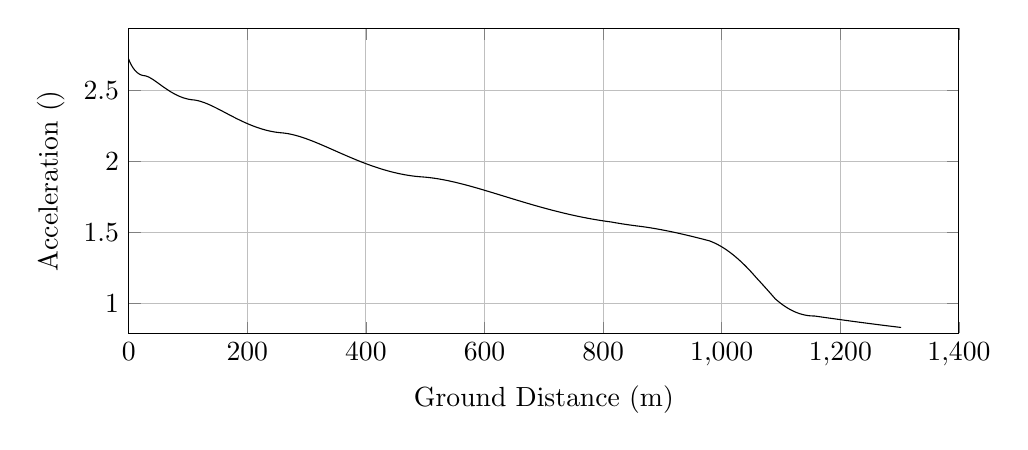
\begin{tikzpicture}

\begin{axis}[
width=\textwidth,
height=0.45\textwidth,
scaled ticks=false, tick label style={/pgf/number format/fixed},
xmin=0.0,
xmax=1400,
xlabel={Ground Distance (m)},
xmajorgrids,
ymin=0.7870546929072948,
ymax=2.9383329541999035,
ylabel={Acceleration ($\si{\meter\per\square\second}$)},
ymajorgrids
]

\addplot [
color=black,
solid
]
table[row sep=crcr]{
1.3603393307215537E-8	2.7206786612956035\\
2.0334443352841076E-7	2.7206786588266425\\
1.8493358258961232E-6	2.7206786374113054\\
9.983129263424352E-6	2.7206785316142303\\
4.13538327636676E-5	2.7206781237767137\\
1.2467543572893382E-4	2.720677041387967\\
2.843807411608912E-4	2.7206749688164837\\
5.588015241105573E-4	2.7206714118135586\\
9.398454696015893E-4	2.7206664793275745\\
0.0014155885812023746	2.720660329295151\\
0.0019945752038215015	2.7206528547539284\\
0.0026717822370171283	2.720644124141308\\
0.003447739291558293	2.7206341341019433\\
0.0043193476547732645	2.7206229279370353\\
0.00529092766782709	2.7206104535400364\\
0.006363550519206555	2.7205967007419662\\
0.007533073890550759	2.7205817261596685\\
0.008790616877968567	2.720565646667797\\
0.01016549189277427	2.7205480911659583\\
0.011625499440327931	2.7205294744355797\\
0.013184282533086976	2.72050962565101\\
0.014839871214038253	2.7204885733470565\\
0.01660567024659266	2.720466150823441\\
0.018465948346479452	2.7204425615356786\\
0.0203822997817096	2.7204182947581463\\
0.022430561433814646	2.720392393417905\\
0.024588423902376283	2.7203651442989134\\
0.026831028501027587	2.7203368647401236\\
0.029143159681622913	2.7203077489819503\\
0.03155709159958957	2.7202773934304583\\
0.03411445662773917	2.7202452793221816\\
0.03677290089167576	2.720211943282595\\
0.03952314881844239	2.7201775050183548\\
0.04239921643077808	2.720141542640251\\
0.045357163155895136	2.7201046093765235\\
0.048363831658398165	2.720067120971648\\
0.051533845233668635	2.7200276521592013\\
0.0547899150155587	2.719987170149106\\
0.058172599437445835	2.7199451746177328\\
0.06162834747858026	2.719902333979718\\
0.06521401059050522	2.719857947124008\\
0.06888104003120077	2.7198126189354435\\
0.07268727020998902	2.7197656386724027\\
0.076546425570032	2.7197180746221186\\
0.08047032364859658	2.7196697825197393\\
0.08456364881336098	2.719619478509671\\
0.08882250397434277	2.7195672177387413\\
0.09306368907640691	2.7195152504659523\\
0.09743039119190974	2.7194618233250623\\
0.10191450167634594	2.719407040285338\\
0.10651989152467789	2.719350858705292\\
0.11128201757858264	2.719292851771846\\
0.11609763023253863	2.7192342810465364\\
0.12097769621339591	2.7191750145198688\\
0.12591912973280778	2.719115091275551\\
0.13103216605369056	2.7190531790214214\\
0.13633380151185176	2.7189890799222596\\
0.1416823117522269	2.7189245120751977\\
0.14708837902374172	2.718859347520925\\
0.1525605467319851	2.718793484820159\\
0.15824953188605478	2.7187251158179464\\
0.16398006351864292	2.718656352093608\\
0.16978153473626356	2.7185868421723756\\
0.17584258400626962	2.7185143330821866\\
0.1819863832139092	2.718440947782791\\
0.18819485651962437	2.7183669043448937\\
0.19455736971520038	2.7182911411090585\\
0.20098158490654017	2.7182147616689916\\
0.2076061353991409	2.718136123110612\\
0.21424726384720844	2.718057410870288\\
0.2211374965027113	2.7179758744402864\\
0.2281284453493247	2.717893277608118\\
0.2350833915765042	2.7178112355168347\\
0.2423085249848444	2.7177261408549382\\
0.24958374984531584	2.7176405928122973\\
0.2569279402934431	2.7175543707998235\\
0.2644720218029696	2.717465943282936\\
0.27204626263318243	2.7173773042321585\\
0.27972793364503945	2.7172875512397434\\
0.2874622320100655	2.7171973271364305\\
0.29563698092580604	2.717102119683042\\
0.30361763245720474	2.7170093241059803\\
0.3118912000478351	2.7169132783506376\\
0.3202493147046803	2.7168164099718446\\
0.3286412952843002	2.7167193076559375\\
0.33714554464307567	2.716621066313662\\
0.3458731203690518	2.716520410471115\\
0.35455185683415313	2.7164204819449873\\
0.3634323904331427	2.7163183971483607\\
0.372325738896249	2.716216332541263\\
0.38151551889959867	2.7161110399165134\\
0.3908489672358084	2.716004280047283\\
0.4001862088113266	2.7158976550020775\\
0.4095647137707429	2.7157907361040916\\
0.4192312859369268	2.7156807169939983\\
0.4289206911602753	2.7155706232017947\\
0.43896550245304145	2.7154566846950363\\
0.4487817299761361	2.7153455272169174\\
0.4589033974758888	2.7152311036303827\\
0.4691858798479248	2.715115060160417\\
0.47972601481223376	2.7149963139012074\\
0.49016040525287174	2.7148789611485267\\
0.5007175269203565	2.714760430608898\\
0.511266977039379	2.714642187576308\\
0.522323236324642	2.7145184777830185\\
0.5332586746953114	2.7143963328736067\\
0.5445869154512923	2.7142700215729363\\
0.5556699580072249	2.7141466597700834\\
0.5669225885056133	2.714021626213362\\
0.5785590177532589	2.713892554574162\\
0.5903083066022885	2.713762462426807\\
0.6020327889628274	2.7136328743733085\\
0.613957077533064	2.713501310690825\\
0.625960998969677	2.7133691032213507\\
0.6380070243193761	2.713236666618247\\
0.6503365955459197	2.713101353706329\\
0.662700086001522	2.712965911112848\\
0.6752747602080436	2.7128284018285003\\
0.6885889407972636	2.7126830744997443\\
0.7019767933734617	2.7125372191246226\\
0.7151149754112038	2.712394350438487\\
0.7284684478906998	2.7122494087541904\\
0.7418939875700234	2.712103954863111\\
0.7553494584716574	2.711958445905217\\
0.7694215958599202	2.7118065539718383\\
0.7830840331449673	2.7116593612657827\\
0.796657372658726	2.7115133963344817\\
0.8106660034246236	2.711363027941603\\
0.8251837647136968	2.7112074894914313\\
0.8395067871054176	2.7110543290584967\\
0.8540519574023793	2.7108990870358225\\
0.8688334527125461	2.7107416235367525\\
0.8840141863517745	2.7105802200273583\\
0.8993797082767976	2.7104171720264008\\
0.9143697020410035	2.7102584166704773\\
0.9294094610857999	2.7100994372507596\\
0.9452486359568626	2.7099323329379637\\
0.9605773823977486	2.709770928967991\\
0.9761522209726621	2.7096072488307197\\
0.9917649966835071	2.709443486198965\\
1.0074810114554809	2.7092789578986203\\
1.0234652146968335	2.7091119458674218\\
1.0399433598517231	2.7089401120912475\\
1.0563627364420554	2.708769231027813\\
1.0728309985448887	2.708598179325757\\
1.0896486452479222	2.7084238454325265\\
1.1068138420051672	2.7082462673532888\\
1.124143995869574	2.708067347375602\\
1.1415400048645106	2.707888113111455\\
1.1590089082607062	2.7077084936001095\\
1.1769249919091855	2.707524653931576\\
1.1951505705127592	2.7073380281037513\\
1.2127191877709298	2.7071584985763346\\
1.2308827453761335	2.706973267662627\\
1.2492706857898845	2.706786137242294\\
1.267587852451018	2.706600113080426\\
1.2860031245644312	2.7064134781225864\\
1.304687144125951	2.7062245116829278\\
1.3233765774990474	2.7060358828879156\\
1.342322280991234	2.7058450653162245\\
1.3613696045164358	2.705653625031875\\
1.3815086998747366	2.7054516455381066\\
1.4013123019267382	2.7052534626110045\\
1.4209622886438908	2.7050572371882557\\
1.4411501686096515	2.704856073193203\\
1.4611760119255748	2.7046569542278975\\
1.4816444281325132	2.704453874606884\\
1.501865958841821	2.704253678164765\\
1.5224364680875304	2.704050466014486\\
1.543651615594651	2.7038413464626005\\
1.5647593029468103	2.70363374738879\\
1.5859558716309676	2.7034257339559584\\
1.6071423964076703	2.7032182764344252\\
1.6293386351549652	2.703001418962213\\
1.6508498980272122	2.7027917261443655\\
1.673011606043147	2.7025761758197744\\
1.6946435720294923	2.702366247606573\\
1.717066624993247	2.702149128823603\\
1.739432891071898	2.7019330500985044\\
1.761922286799709	2.7017162722331785\\
1.7849035550437842	2.7014952578520406\\
1.8076299607761817	2.70127719298858\\
1.8313298306791497	2.7010503120862657\\
1.8543134894513886	2.700830795787314\\
1.8777326664639729	2.7006076313435097\\
1.9017196849182967	2.7003795876766175\\
1.925345883672024	2.7001554970834443\\
1.950252961491087	2.699919815747629\\
1.975161211119453	2.6996846926241336\\
1.9993825790313986	2.699456595879024\\
2.024583888346972	2.699219835107348\\
2.04934017380271	2.6989878120385447\\
2.0744229633459703	2.698753288188291\\
2.0996193404956136	2.6985182656177127\\
2.1245764901457758	2.698286027665972\\
2.1500786393425866	2.6980492835167134\\
2.176226227020705	2.6978071372330295\\
2.202115608176549	2.697567966791156\\
2.227948363055355	2.697329895830868\\
2.2543499999408594	2.697087173470252\\
2.2810892744412783	2.6968419527082137\\
2.3075963743135786	2.696599459185051\\
2.3348582111613405	2.6963506785209344\\
2.3623221378972126	2.696100682933973\\
2.3898598419727675	2.695850646147277\\
2.4171687299087603	2.6956033066724263\\
2.445442108612223	2.6953478780856788\\
2.4735885391813177	2.695094245735042\\
2.5015416452491293	2.694842992960848\\
2.5301110763218357	2.694586853096574\\
2.5589284934403693	2.6943291544481216\\
2.587611617795936	2.6940733156453813\\
2.6175687086884984	2.6938068114957927\\
2.647724154312196	2.6935392585977587\\
2.6767118187859253	2.6932827399161683\\
2.7060305938995466	2.693023958539718\\
2.7361546404224653	2.6927587646133873\\
2.7663022704956823	2.6924940645077875\\
2.7964672462043376	2.6922299104775878\\
2.8272583584284883	2.6919609898244374\\
2.8588650092419234	2.691685695066152\\
2.8898852960400587	2.6914162407917983\\
2.9215246589961597	2.691142153042156\\
2.95270311230069	2.6908727891002586\\
2.984506337549637	2.6905987709596655\\
3.017379145769185	2.6903163220215216\\
3.049243647754313	2.6900432938557373\\
3.081295157663824	2.6897694112189523\\
3.113406837946715	2.6894957625659544\\
3.1453724573084756	2.6892240983894453\\
3.1787286104953543	2.688941399310255\\
3.211019796961401	2.6886684834859587\\
3.245786703184362	2.688375472165572\\
3.279939251746722	2.688088470588985\\
3.3141720228361216	2.6878016178550492\\
3.3491198891036547	2.687509618361971\\
3.382965192547779	2.68722764086513\\
3.4181848705561064	2.6869350544215695\\
3.45391888941694	2.6866390675413285\\
3.488851494856137	2.686350563708105\\
3.524271454997704	2.6860588832442085\\
3.5606552075305	2.6857601507740503\\
3.597189071478943	2.6854610832006927\\
3.632926148839256	2.6851694036217726\\
3.668897146318187	2.6848766746939123\\
3.706642714683163	2.6845704271949034\\
3.7432264628550644	2.684274503176929\\
3.781286297809391	2.6839675714925635\\
3.818618572105483	2.6836674260810867\\
3.8564015479305356	2.683364578880271\\
3.8948624022541356	2.683057245696653\\
3.9329637046009225	2.682753723357327\\
3.971505929995028	2.6824476332723757\\
4.009821706071438	2.682144278613734\\
4.049014376833089	2.68183494307692\\
4.089343885784727	2.6815176449538445\\
4.128662304630717	2.681209283054529\\
4.1684827283974055	2.6808979665822283\\
4.208000253554632	2.6805899907618347\\
4.2483743636521965	2.680276334838056\\
4.288255503180503	2.6799674917027794\\
4.328757204126676	2.679654837844873\\
4.369490126907612	2.6793414053306783\\
4.410357715197167	2.679027945740783\\
4.45189144941496	2.6787104072993566\\
4.492881116440694	2.678398042025564\\
4.53550011161515	2.678074322825818\\
4.577670191557685	2.6777550743742067\\
4.6201174049766305	2.677434788405729\\
4.662272021613388	2.677117758143571\\
4.706017761800355	2.6767898603786255\\
4.748842845578064	2.6764699422389615\\
4.792293145132742	2.6761464390631\\
4.836482439768313	2.6758185498568317\\
4.88090298307878	2.6754900735892466\\
4.925311889063089	2.675162809239379\\
4.969864686447545	2.6748356102636386\\
5.014842280541593	2.674506429836776\\
5.0603877575117515	2.674174253072983\\
5.106292347304597	2.673840632515052\\
5.152263975081851	2.6735077016112054\\
5.1974808794106995	2.673181379928213\\
5.244027372436168	2.6728466417574968\\
5.28996242022761	2.672517467815287\\
5.336209145350672	2.672187226039256\\
5.38320569473032	2.6718528225038405\\
5.430469292142472	2.6715177256382523\\
5.476900151253712	2.6711897058694722\\
5.526063828851289	2.6708436409213805\\
5.573879040902945	2.670508306612775\\
5.622613575936374	2.6701677760662514\\
5.6713596863799225	2.669828422251273\\
5.720412183296268	2.6694881992513135\\
5.770660497446668	2.669140990560754\\
5.820668144990444	2.6687967533759176\\
5.870305285939629	2.6684563516020408\\
5.920503816994749	2.668113395941104\\
5.971105439367246	2.6677689993918303\\
6.021088325934068	2.6674301023059055\\
6.071322359863801	2.6670907866316345\\
6.122981826035449	2.6667431793464864\\
6.174329110820436	2.6663990098143406\\
6.225804784288178	2.666055311784361\\
6.278093246139479	2.665707546198239\\
6.331709873490098	2.6653523633215936\\
6.384325657889258	2.665005198295482\\
6.436648686434458	2.6646613220440125\\
6.489478972803882	2.6643154790220605\\
6.543185721519176	2.663965300169796\\
6.596747696432654	2.6636174666252757\\
6.650345873843312	2.663270792682101\\
6.704555155195255	2.6629215790004643\\
6.7588986063680725	2.6625729209380244\\
6.814371620173711	2.6622184756758003\\
6.86997180120154	2.661864691332725\\
6.925426612865756	2.6615132948772278\\
6.981353650685165	2.6611603793268515\\
7.037678624474159	2.660806441464639\\
7.094603706786671	2.660450243996549\\
7.151204881983983	2.6600975732102974\\
7.209200593921791	2.659737757917874\\
7.2667780016693655	2.65938207763521\\
7.324687293141565	2.6590258879349387\\
7.382771066065313	2.65867017051857\\
7.441904508776327	2.658309607849323\\
7.501585831803217	2.6579473170852808\\
7.5616527251378685	2.657584314371988\\
7.62150963104709	2.657224198940635\\
7.682859947113334	2.656856767854337\\
7.7432084367972145	2.656496978162604\\
7.803024936926759	2.656141959652575\\
7.863793829029664	2.6557829123419427\\
7.9252460466886365	2.655421484914137\\
7.98696966925656	2.655060131675171\\
8.04776546969778	2.654705839910287\\
8.109421212326083	2.654348181634318\\
8.17269125419024	2.6539828737863242\\
8.236095044780246	2.6536185288074092\\
8.299523592514586	2.65325577215485\\
8.363213767675873	2.652893253529224\\
8.427807923256076	2.6525273571081653\\
8.49144930156071	2.6521685912907564\\
8.557380457258176	2.651798724322129\\
8.623183572921022	2.6514314015421423\\
8.687840683575093	2.6510722452291935\\
8.753751426394068	2.6507079228346413\\
8.820803713780364	2.6503391450473472\\
8.888970287482593	2.649966148101651\\
8.957133699158991	2.649595085188113\\
9.025036015045707	2.6492273412772986\\
9.092760955867519	2.6488624367385345\\
9.159817422823458	2.648502974954302\\
9.227495373767134	2.6481420314749275\\
9.296013084156197	2.6477784947261016\\
9.36435980631623	2.6474177474136527\\
9.433329865923408	2.6470556079181042\\
9.503849553921977	2.6466872950515414\\
9.574524061692681	2.6463201570111243\\
9.644263228942293	2.645959816265661\\
9.715657612596786	2.645592909530688\\
9.787429657508813	2.645226079457479\\
9.85753688572494	2.6448697034479203\\
9.930250735750551	2.644502099823873\\
10.001571447096964	2.6441435319093944\\
10.074699859091687	2.643777916552698\\
10.14698611653175	2.6434185343790606\\
10.220547980738981	2.6430548666019744\\
10.2940409891517	2.642693602309274\\
10.36719293590382	2.642336054188199\\
10.441008888975666	2.6419773151014647\\
10.51610421670324	2.641614467762291\\
10.590724589239105	2.6412560143644788\\
10.667218005391902	2.6408907266274424\\
10.742771202259895	2.640532070108522\\
10.82035208750042	2.6401659936636683\\
10.896759047300378	2.6398076323121202\\
10.973503045910835	2.6394498550940453\\
11.051297940743765	2.6390893843891003\\
11.128076326409062	2.6387357926937325\\
11.207667705350879	2.6383715117432622\\
11.286758396846047	2.638011798043455\\
11.366305937658339	2.6376522856971496\\
11.446149720998452	2.637293723994773\\
11.526866579636565	2.636933563877787\\
11.607297517600138	2.6365769930935956\\
11.688034241538357	2.6362213802710963\\
11.769665722224765	2.6358641739102344\\
11.850920080706608	2.635510952816559\\
11.933163326324259	2.635155796089923\\
12.017103780766782	2.6347957522379453\\
12.10034832931326	2.6344411202567057\\
12.185467765774142	2.6340809903748106\\
12.270669986481685	2.6337230211751725\\
12.354040133273898	2.633375171561526\\
12.440386807402234	2.6330174188864603\\
12.52556588630658	2.6326670026774126\\
12.610860989997974	2.6323185865436374\\
12.69550109439961	2.631975287279447\\
12.784634337461807	2.631616382824756\\
12.871172079509357	2.6312704900596824\\
12.958447214271366	2.630924195280638\\
13.045518554761987	2.6305812467301823\\
13.133090172249581	2.6302388746430134\\
13.221405510214687	2.629896172019415\\
13.310319106907201	2.6295537524618187\\
13.399783591735492	2.629211839154097\\
13.488943611067967	2.628873702111904\\
13.578276665194153	2.6285375149135355\\
13.667402973129146	2.6282046957139578\\
13.757763665999576	2.627869898230623\\
13.848393619195729	2.627536754471522\\
13.938857764339925	2.627206858503314\\
14.031101516310692	2.6268731770392186\\
14.123507833735925	2.6265416352199544\\
14.214825187590282	2.6262166726791465\\
14.307956552027534	2.625887980862263\\
14.401498558574918	2.625560600783583\\
14.495315613017755	2.6252350272686176\\
14.589065423003394	2.624912447314662\\
14.68316852398955	2.6245914165312207\\
14.778702641747682	2.624268327122402\\
14.873746415615575	2.6239497085396195\\
14.970384078097169	2.623628612553521\\
15.068900921005241	2.6233042363691323\\
15.164434274206265	2.6229925309927165\\
15.260378587808539	2.622682296359665\\
15.357189194448868	2.6223721064177115\\
15.45495288999333	2.6220617534077197\\
15.55311774366497	2.621753039337219\\
15.652583807013901	2.6214431992530205\\
15.755243917873962	2.6211265293566273\\
15.855950289561445	2.620818954146916\\
15.958461094374158	2.620508977405793\\
16.060387288500337	2.620203867681534\\
16.164276126126843	2.6198960517212635\\
16.26736468838029	2.6195937578082233\\
16.36946523634058	2.619297443871246\\
16.47192386662276	2.619003163968875\\
16.576794358652606	2.618705133782723\\
16.678929175716583	2.61841795664116\\
16.783994526910618	2.6181256984077486\\
16.89012564586595	2.6178337166503045\\
16.996887404888547	2.6175432749417187\\
17.103774697793426	2.6172557707268638\\
17.210947675936964	2.6169707806812017\\
17.31865021419634	2.6166876823252405\\
17.424470519881233	2.6164127421635106\\
17.53205215515201	2.6161364768833204\\
17.64034909906897	2.6158616741719065\\
17.74911485075183	2.615589002397387\\
17.85745376408675	2.6153206975844308\\
17.969383314157206	2.6150469444401168\\
18.07998395718984	2.614779867810088\\
18.18863741327577	2.6145207984136016\\
18.302466989554325	2.6142528890063197\\
18.41305080779906	2.6139960386827914\\
18.525644000014054	2.613737972345975\\
18.636945827420575	2.6134862769421234\\
18.750643923449367	2.6132326526951157\\
18.86479622056296	2.612981551792113\\
18.979646899421056	2.6127324788448334\\
19.09418630108147	2.6124876296228825\\
19.208983505033515	2.612245773334588\\
19.323483295898072	2.6120080662516196\\
19.43842354827664	2.6117729715390476\\
19.55563752357537	2.6115368534254326\\
19.67199913451129	2.611306063351325\\
19.789486593639566	2.611076678576726\\
19.90713985662446	2.610850621722009\\
20.024127533725753	2.610629455253049\\
20.143019013955552	2.610408367403082\\
20.26442367074238	2.6101864195670723\\
20.383660776265387	2.609972172998143\\
20.5042342316437	2.6097592805638037\\
20.622773342122727	2.609553649589869\\
20.74503732713029	2.6093453564489195\\
20.865944869938517	2.6091431563868124\\
20.98711015528624	2.608944286470133\\
21.113336299999695	2.6087411017443536\\
21.23638685227678	2.608546937145694\\
21.35988644990264	2.6083559314440388\\
21.483760012473958	2.608168227292362\\
21.608180515260266	2.607983593725539\\
21.732326713270083	2.607803250150675\\
21.85766379468624	2.607625099075144\\
21.985117186778353	2.607447968969981\\
22.111729024702363	2.6072760185911354\\
22.23700541150786	2.607109803648334\\
22.36297326225872	2.606946592655331\\
22.488604760551	2.6067877220942135\\
22.616276341350805	2.6066302545800575\\
22.744235570279145	2.606476448725659\\
22.874576476768283	2.606323901548314\\
23.003842066605536	2.6061767086234635\\
23.13088450205612	2.606036009470011\\
23.257869280739328	2.6058992879025347\\
23.389244224935425	2.6057619455713583\\
23.519811196806458	2.605629573115798\\
23.653309395988643	2.6054984682974673\\
23.78342402399784	2.6053747991575955\\
23.9180644861338	2.6052510900680304\\
24.05110504604577	2.60513309614823\\
24.182394801971697	2.6050207798574423\\
24.314614014384034	2.6049117976909457\\
24.449791085561472	2.6048046491534915\\
24.585258581909038	2.604701590808493\\
24.72121222319008	2.6046024984638763\\
24.857032405393277	2.6045078282062573\\
24.99454740444294	2.60441636799246\\
25.13030709358258	2.6043303973208944\\
25.270890409679986	2.604245885116941\\
25.40663839363527	2.604168625105072\\
25.54307796688363	2.6040952615282915\\
25.68272814639034	2.604024613245566\\
25.82072003425767	2.603959205279013\\
25.96015212691003	2.603897546240571\\
25.987750021099068	2.6038858690712825\\
26.0558803939429	2.6038577864228225\\
26.061632797568386	2.6038554638263935\\
26.066808273335674	2.6038533806198574\\
26.071901058608013	2.6038513366596883\\
26.073315434863225	2.6038507697843425\\
26.074595035914804	2.6038502564501425\\
26.080371168076944	2.6038479331864\\
26.10234540095133	2.603839004048819\\
26.183408179590366	2.6038048263627918\\
26.300430535410044	2.6037520750387655\\
26.42750601924636	2.603690272544413\\
26.558056987479794	2.6036219372736085\\
26.688030995483615	2.603549088212217\\
26.818767077324992	2.6034710242918466\\
26.951519978077492	2.6033869035939228\\
27.083955405447817	2.603298172686217\\
27.216897884715692	2.603204329397653\\
27.350913258119895	2.6031049498085697\\
27.4833530065795	2.6030020840485344\\
27.6176201223548	2.602893135321435\\
27.752160408628434	2.6027793145137146\\
27.887329802382908	2.6026603332918947\\
28.023188645890663	2.6025361303873034\\
28.158973127824495	2.6024074319911854\\
28.296372294036907	2.602272619137292\\
28.435107205966254	2.6021318778665234\\
28.571323599682245	2.6019892357069097\\
28.70996262687553	2.6018395823204976\\
28.850320389600306	2.6016835359128985\\
28.988837241064125	2.6015251189808373\\
29.129197813929657	2.6013601767352137\\
29.27166529868488	2.60118827267934\\
29.41298471572133	2.60101334901779\\
29.554848516656044	2.6008333985884082\\
29.699676691743235	2.6006452500398893\\
29.842400551696755	2.6004555085017884\\
29.985385440862252	2.6002611719940534\\
30.129077275410303	2.600061649734757\\
30.27543774584293	2.5998541279415415\\
30.422081339040986	2.599641919100981\\
30.56949149516445	2.599424338278923\\
30.716562179458485	2.599203059515774\\
30.86535310281699	2.5989749850175308\\
31.011875026602333	2.5987463115259466\\
31.16159928701196	2.5985085205974414\\
31.313692569485013	2.598262765131782\\
31.463056706803336	2.598017357590823\\
31.61235366859384	2.597768096492202\\
31.76278957628285	2.5975129835032753\\
31.915019899787076	2.5972508499553557\\
32.06709627595497	2.5969850453468277\\
32.21861178877769	2.5967163665556434\\
32.37168228565527	2.596441081645162\\
32.52450570609457	2.596162439682959\\
32.67702483599189	2.5958806223094966\\
32.829998687403204	2.5955942777679697\\
32.98551220909506	2.5952994517569667\\
33.14332298937855	2.5949964875960214\\
33.29970221124884	2.5946925710318984\\
33.45800124694219	2.594381230122983\\
33.61398946945653	2.59407085606417\\
33.77048353048475	2.5937559624467577\\
33.9292721471582	2.593432911844313\\
34.08796840843395	2.5931065431041294\\
34.24769686644211	2.5927745690501176\\
34.406855482575295	2.592440360126446\\
34.56481953291838	2.5921053392665625\\
34.72399692808165	2.591764453104413\\
34.88694269464703	2.591412129924282\\
35.04914399338672	2.591058089493738\\
35.209965099803895	2.590703839194963\\
35.3703140559587	2.590347487556378\\
35.531685786905925	2.589985748967039\\
35.69349909442164	2.589619936461779\\
35.85522798807463	2.5892512811122277\\
36.022509111806116	2.5888668336311342\\
36.19055880791667	2.588477464988384\\
36.35708622463872	2.5880885595397194\\
36.52115360367851	2.5877024693187627\\
36.68781562330062	2.5873073486572045\\
36.8536847754776	2.586911233267797\\
37.024522648961764	2.586500308629536\\
37.19188554678789	2.5860948991511465\\
37.36066720850286	2.585683255555418\\
37.528862119520696	2.585270300070748\\
37.697264258302326	2.584854143682125\\
37.86832931534104	2.5844287005776634\\
38.03812867477943	2.5840037593985663\\
38.20923731912278	2.5835729261965747\\
38.37904730305398	2.5831428173348794\\
38.55252405124031	2.5827008536311844\\
38.72282139824354	2.5822645157823274\\
38.89783411301201	2.5818135931288113\\
39.0714610757495	2.581363784250743\\
39.24438070689564	2.580913425517954\\
39.41969314875929	2.5804544577618174\\
39.59166556575205	2.580001956794118\\
39.764623188591585	2.579544636010196\\
39.94263254662576	2.5790716744061593\\
40.11749159802578	2.578604876133886\\
40.29452954971913	2.5781300814298502\\
40.47247750600427	2.5776506846058913\\
40.64799609178485	2.577175756740913\\
40.82414741101539	2.57669709043791\\
41.00385670225303	2.576206711349962\\
41.18169069533937	2.575719463467573\\
41.3603281005193	2.575228071765099\\
41.54046179251334	2.57473063920484\\
41.722675278204306	2.5742255441599875\\
41.90258931008478	2.573724975558771\\
42.08518735141125	2.5732151086952273\\
42.26728550944881	2.572704847119067\\
42.44743534848537	2.5721983302188898\\
42.63069538383506	2.5716813637181577\\
42.80963512098974	2.5711749685245957\\
42.992542679335614	2.5706557379097825\\
43.17926890616222	2.5701240368278295\\
43.363134036078335	2.5695989178025833\\
43.54815051311773	2.5690689872462267\\
43.733578141849236	2.5685363896694895\\
43.91798130912079	2.568005298831979\\
44.10506009255049	2.5674650822870673\\
44.29251116260117	2.5669223997879653\\
44.480917546793805	2.5663755921121174\\
44.66851287589745	2.565829826985854\\
44.85853501730759	2.565275710745273\\
45.047396872181054	2.5647237332038157\\
45.236914792155844	2.5641686329837823\\
45.42785879536018	2.5636081770353583\\
45.616432631699865	2.563053557848849\\
45.80697204128492	2.5624920680802825\\
45.998633580597016	2.561926207731924\\
46.18800675699903	2.561366095611291\\
46.380841640082096	2.560794755738124\\
46.57327038933336	2.560223664626961\\
46.765844918266424	2.559651226210809\\
46.95911042680183	2.5590758535903007\\
47.15311668852311	2.5584974283805613\\
47.34541611633634	2.5579232929457483\\
47.53884854699059	2.5573450104603674\\
47.73236991243341	2.5567657329192537\\
47.92818250719388	2.5561788929077913\\
48.12326385407131	2.555593578167602\\
48.32058854034828	2.5550008943769527\\
48.516852452700604	2.554410797753267\\
48.71339374517507	2.5538193058348817\\
48.91319881343868	2.5532174537276386\\
49.1119162355681	2.552618377571118\\
49.31207818344666	2.552014479879058\\
49.509673461222235	2.55141790295568\\
49.71156302510582	2.550807963814867\\
49.91034548441702	2.5502070557604366\\
50.11200805970151	2.5495971167179245\\
50.30853267551517	2.549002437643254\\
50.50757456960626	2.548399893787912\\
50.70929197287772	2.547789031091562\\
50.91222418686718	2.547174301781091\\
51.11562549758783	2.5465579976334327\\
51.32090674103446	2.545935876599027\\
51.525199701657655	2.545316665210681\\
51.72863462744459	2.544700004051853\\
51.934060761332375	2.5440772901396684\\
52.14033810224923	2.5434520130707616\\
52.344882977561255	2.542832037968295\\
52.55098100649393	2.5422074393837404\\
52.75731843494604	2.541582232938185\\
52.96514817708821	2.5409526569511103\\
53.17450540782369	2.540318641605455\\
53.382202621450276	2.5396898725022634\\
53.592230583406476	2.5390543021876466\\
53.80364534107798	2.5384148270146696\\
54.01469481143569	2.5377767815041166\\
54.223966920081466	2.537144461612022\\
54.43230789395902	2.5365153346114173\\
54.6430562980421	2.5358793541120868\\
54.855225786754914	2.5352395392705507\\
55.066088958624874	2.5346041459414534\\
55.27969530828261	2.5339610077522634\\
55.49171188337613	2.5333232052728736\\
55.70388919125476	2.532685496995895\\
55.91737779085577	2.532044460808315\\
56.13177028494084	2.531401359471393\\
56.34652664868587	2.5307578484066866\\
56.559021044851505	2.530121815748167\\
56.77591447970492	2.5294733639353444\\
56.99548236897459	2.5288177159078513\\
57.21481285737903	2.5281636101320872\\
57.43536222847358	2.5275067392423107\\
57.65367025761124	2.526857432179728\\
57.872788904232735	2.5262066317271605\\
58.0907693980174	2.525560152036414\\
58.311927420720366	2.524905235525975\\
58.532333513628615	2.5242535629988083\\
58.75532998033057	2.523595293567177\\
58.976617007999806	2.522943154217163\\
59.19875422837053	2.522289623035449\\
59.4206945143671	2.5216378129110915\\
59.64453328369959	2.5209816104192493\\
59.86894932484513	2.520324935808012\\
60.09432075877773	2.519666722469057\\
60.318058693038594	2.5190145524832186\\
60.541731124044205	2.5183638670504402\\
60.76707064338231	2.5177096659524816\\
60.995574692986196	2.5170476716216337\\
61.22378989589207	2.5163879416928285\\
61.4534619981562	2.515725467108698\\
61.683510138770515	2.515063409584064\\
61.91410430469678	2.5144013152445694\\
62.14462153858659	2.5137410034273744\\
62.37563158073512	2.5130808720953084\\
62.607203285434	2.5124207609524625\\
62.841031881319736	2.5117558931326958\\
63.07467935056491	2.511093248806784\\
63.31164975340633	2.5104229507116482\\
63.54633691305479	2.5097608936214986\\
63.78243968758058	2.509096658353358\\
64.0165414084598	2.508439874954207\\
64.25412817577254	2.5077751940675537\\
64.49270299572771	2.507109679511202\\
64.73076499662056	2.5064475484081363\\
64.96867826857735	2.5057878041948065\\
65.21063576532572	2.505118892968354\\
65.4512107007771	2.504455875692975\\
65.69028017871045	2.503799077631295\\
65.93032615763332	2.503141696633503\\
66.17196619696679	2.5024820987215755\\
66.4135612157637	2.5018248019749727\\
66.6559030093851	2.5011676847910405\\
66.89910102540284	2.500510495358963\\
67.14354652182666	2.4998522286092877\\
67.38771133480921	2.499197036065084\\
67.63347396558368	2.498539918435431\\
67.87898066495345	2.4978858740594756\\
68.1255935515739	2.497231308936313\\
68.37316753306138	2.4965766609988718\\
68.62205497364681	2.4959210548648416\\
68.8711887275476	2.4952673473359024\\
69.120220471977	2.4946164764372467\\
69.36846244647072	2.4939702473265815\\
69.61951843592018	2.4933193316654867\\
69.87236615109754	2.492666474522707\\
70.12758921381476	2.4920102580204535\\
70.37945082809051	2.4913654375805994\\
70.63410009691182	2.4907162819907347\\
70.89152727368702	2.490062929924484\\
71.14629115974091	2.489419214134175\\
71.40197865069018	2.4887760628624056\\
71.66163317144085	2.4881259254086565\\
71.92484704501203	2.4874699751361264\\
72.18465416754285	2.486825595917562\\
72.44573394560723	2.4861811646819447\\
72.70633339061075	2.4855410429789373\\
72.96699363118216	2.484903914242823\\
73.22900401485182	2.4842666725586176\\
73.49076816912304	2.4836332404814785\\
73.75430841254712	2.4829987722962104\\
74.01895646534612	2.482364950320041\\
74.2846979982242	2.481731870039991\\
74.55380714249793	2.4810942188032747\\
74.82322871850147	2.48045932679811\\
75.09350011520078	2.479825970255863\\
75.36421232425869	2.47919515276104\\
75.6347219158074	2.478568397827683\\
75.90830954343213	2.477938181414025\\
76.18188601743822	2.477311700850559\\
76.45626363461818	2.4766871314504098\\
76.72958718025629	2.476068710072174\\
77.00406935908524	2.4754514512140755\\
77.28579748399531	2.4748218605894667\\
77.56784659723587	2.4741955938132314\\
77.84569092555657	2.473582635961278\\
78.1246978223638	2.4729710995086265\\
78.40641219364133	2.4723577002358565\\
78.68590470271565	2.4717532000208147\\
78.96851680469001	2.471146084071755\\
79.25576208114188	2.4705332908756708\\
79.54169104977237	2.4699276055141093\\
79.82662017154695	2.469328323750302\\
80.11330301632765	2.4687296892440598\\
80.40394576721474	2.468127243894558\\
80.6908099930996	2.4675370500211624\\
80.98055888331655	2.466945395962865\\
81.27178512217935	2.4663552745996036\\
81.56682943128612	2.465762085692271\\
81.86186977412851	2.4651736222711307\\
82.15688924927383	2.464589935313154\\
82.44965588234726	2.4640154034601025\\
82.74488606927187	2.463440793468167\\
83.04325841243121	2.4628649380951924\\
83.34213327641098	2.4622930386334456\\
83.64411622775171	2.4617202164369862\\
83.94734638805741	2.461150127944263\\
84.25123842984891	2.4605839393079654\\
84.55152885577829	2.460029536473942\\
84.85735750691177	2.4594701116185256\\
85.16518306664875	2.458912353031306\\
85.47136476235073	2.4583628836401106\\
85.77898122624802	2.4578161899354845\\
86.08923229760057	2.4572702629762873\\
86.40254560035129	2.4567245181340605\\
86.71167807044037	2.4561915585515646\\
87.02660518802142	2.455654246012527\\
87.34238286044419	2.4551212117679366\\
87.65842706333811	2.4545934887428125\\
87.97971380652302	2.4540629365488824\\
88.2973933745065	2.4535442307995368\\
88.61789013566766	2.453026876349769\\
88.93643920279564	2.4525186051685486\\
89.25662431900213	2.4520137064087653\\
89.57903058309674	2.4515113819145196\\
89.89968694948243	2.4510178478338274\\
90.22473455398588	2.450523743193979\\
90.55024875587375	2.4500351887771927\\
90.87789352676518	2.449549778153499\\
91.20733069500889	2.449068142451017\\
91.54101415610151	2.4485868879586077\\
91.87012785371462	2.4481187357687793\\
92.20120197152713	2.447654335053543\\
92.53416638543635	2.4471939140832912\\
92.86431843528567	2.4467439632892667\\
93.19748455591187	2.4462965631761584\\
93.53066771200866	2.445855844323165\\
93.86681917526724	2.445418008310697\\
94.20530590547477	2.4449840565296066\\
94.5419273964865	2.4445594034585163\\
94.8854212036891	2.4441331967398003\\
95.22752713476521	2.443715871459762\\
95.57091181422334	2.443304186277593\\
95.91383450860906	2.4429002686676426\\
96.25469535763642	2.4425059380447767\\
96.5966517898868	2.4421175255063137\\
96.93845701474973	2.441736491073553\\
97.28153572459905	2.441361296066888\\
97.62213139590432	2.4409960240150888\\
97.9659652144934	2.4406345769086792\\
98.3129807304216	2.440277233228624\\
98.65852794036775	2.439928850209597\\
99.00080640577195	2.4395911037440827\\
99.35064076251427	2.4392534647386297\\
99.69796076807248	2.4389258294402163\\
100.04654253174803	2.4386046080725734\\
100.3915606488718	2.4382941850941453\\
100.74261509654437	2.437986017314345\\
101.08877163494762	2.4376897532500896\\
101.43457754260953	2.437401341051708\\
101.784020212797	2.4371175756518575\\
102.13161434601102	2.4368429827237783\\
102.4751980097893	2.4365790890858294\\
102.82212110631409	2.436320239391435\\
103.16739702108615	2.436070221727917\\
103.51524666207362	2.435826022134239\\
103.86391679154056	2.4355889958636414\\
104.20960434827006	2.4353616678657097\\
104.55241399635099	2.435143786240147\\
104.89662223620601	2.434932595096165\\
105.24103428322039	2.434728891437814\\
105.5836615386647	2.4345338098813283\\
105.92645892081137	2.434346194563844\\
106.27347658175316	2.434163985510028\\
106.6151670762521	2.4339921695226847\\
106.95898391938218	2.4338269024495567\\
107.30023552029138	2.433670435131151\\
107.64147805753461	2.4335215201367397\\
107.98348674656944	2.433379854367449\\
108.32522459759954	2.433245893830602\\
108.3935347040271	2.4332200275053024\\
108.40478590462831	2.433215796254834\\
108.41572478024443	2.433211690361312\\
108.4246743308916	2.433208336951547\\
108.44347342986478	2.4332012833147116\\
108.52018987797786	2.43317219109308\\
108.70071173483461	2.4331017920354157\\
108.99446230248458	2.4329814440410136\\
109.30176454987088	2.432847927531813\\
109.60899173332959	2.432706732917117\\
109.91608539831654	2.4325579700889755\\
110.22883517949637	2.4323987045706987\\
110.54143546549608	2.4322317650141008\\
110.853845249356	2.4320572635992326\\
111.1739714794031	2.4318705852138702\\
111.4937490010879	2.431676241919269\\
111.81170779322963	2.431475287668319\\
112.13106495813236	2.4312657849338795\\
112.4519453366479	2.4310476271089465\\
112.77515902629136	2.4308202066477733\\
113.0997499810409	2.430584146092131\\
113.43040796942478	2.4303358542039373\\
113.7597028375028	2.4300808285129447\\
114.0907450350197	2.429816732310962\\
114.42538740208008	2.429541986785118\\
114.75997726261329	2.42925955439613\\
115.09477047197589	2.42896930117562\\
115.43440545481076	2.4286671209860575\\
115.77494672336013	2.428356408276051\\
116.11687534861284	2.428036736385015\\
116.46164587354252	2.4277066937886964\\
116.8077846490165	2.4273676418184964\\
117.15688723722127	2.427017966157549\\
117.50557855048987	2.4266610561814863\\
117.85411336711965	2.426296762675994\\
118.20532793701167	2.4259221324570746\\
118.55850697655507	2.42553787280944\\
118.91273956155123	2.4251449727891465\\
119.26983096270519	2.4247414013195794\\
119.62978614725739	2.424327068967907\\
119.98960731920661	2.423905437983997\\
120.34734904217265	2.4234789523477724\\
120.7138511704587	2.423034582288329\\
121.08106061642908	2.4225819023639144\\
121.44737887966437	2.4221229885996873\\
121.81499139152783	2.421655190601003\\
122.18511446431708	2.421176947708342\\
122.55384158147794	2.420693374249079\\
122.92460728481757	2.4202000467548563\\
123.29616941264607	2.4196986360562507\\
123.67040864389355	2.4191866057294273\\
124.04652172406458	2.4186650276083306\\
124.42393851457416	2.418134705123472\\
124.80152108360014	2.4175972978433737\\
125.18180835736592	2.417049215611839\\
125.55854932865631	2.4164995900096224\\
125.93878032356085	2.41593825738119\\
126.31997081831156	2.41536893730321\\
126.70099538833193	2.4147933898705514\\
127.08058279416298	2.414213674410294\\
127.46175209000612	2.413625274379571\\
127.84399628255431	2.413029004504053\\
128.22749916598133	2.4124246189717313\\
128.6102537001487	2.411815365541636\\
128.99595881306152	2.4111954015963892\\
129.37788117916477	2.4105756648562995\\
129.760738924708	2.409948659259035\\
130.1448498512433	2.4093139091147195\\
130.53000390659713	2.408671804561374\\
130.9168242384266	2.408021341579164\\
131.29443328439476	2.4073810635032817\\
131.67491382268804	2.4067307047474893\\
132.05816436539135	2.406070411416141\\
132.44070735535217	2.40540622157154\\
132.82666098215685	2.4047310200557863\\
133.20952005887244	2.404056268961516\\
133.5940193955625	2.40337373944942\\
133.97617966856654	2.402690594428691\\
134.36103715882757	2.4019979102883573\\
134.74478042358356	2.401302602939376\\
135.12867144169206	2.400602487594403\\
135.5141335746535	2.3998950220370343\\
135.89764893392993	2.3991867523794994\\
136.28231234485685	2.3984720592484203\\
136.66418763078912	2.3977583640901994\\
137.04684871033697	2.397039100271769\\
137.42845627025127	2.39631780804259\\
137.8132447087305	2.395586529279117\\
138.19719797258034	2.394852938550362\\
138.58059071069573	2.39411661006692\\
138.96593237593703	2.393372781156656\\
139.3501607499636	2.3926274274221226\\
139.73355638294606	2.391880108264343\\
140.1160230155566	2.3911311105097868\\
140.50045093994146	2.3903748342286057\\
140.88215178690393	2.3896205860123967\\
141.26156782058217	2.3888676287266737\\
141.64323970440188	2.3881070226125756\\
142.02689350659642	2.3873393317402973\\
142.41061312971692	2.3865684360775052\\
142.7942251403153	2.3857947550024337\\
143.1756303563767	2.3850226183986587\\
143.5599719391364	2.384241674921226\\
143.94242380128833	2.3834617871710684\\
144.3239499176869	2.382681087278037\\
144.70664939692608	2.381895343988057\\
145.0870075357763	2.3811118510994715\\
145.46856550308127	2.3803233907321797\\
145.85014610541765	2.3795324479313784\\
146.23128237819492	2.378740058488634\\
146.61504730324998	2.3779398772226736\\
146.99763315977907	2.3771398937702015\\
147.38441582478964	2.376328904490217\\
147.7673688364352	2.3755237986332745\\
148.15222568696134	2.3747126011074684\\
148.53580865353604	2.373902066463377\\
148.9199734867533	2.3730883401106704\\
149.3040357319486	2.3722729288517916\\
149.68771357306542	2.3714564946793653\\
150.07093078701052	2.3706392651832076\\
150.45622889618164	2.369815868459699\\
150.8449053483268	2.368983554869396\\
151.2288570611563	2.3681597438155757\\
151.61452719766493	2.367330687884766\\
151.9983007305741	2.366504216286124\\
152.38299664478842	2.3656743205794353\\
152.76945776909372	2.364839224108314\\
153.15580177123394	2.3640030418244677\\
153.54253364040335	2.3631647353828455\\
153.93093169697067	2.3623215795638117\\
154.31788037931886	2.361480392098559\\
154.7039882138024	2.3606399150785515\\
155.08880221957185	2.3598011973348516\\
155.47621608980313	2.3589558005307634\\
155.866104687065	2.358104031670738\\
156.25391419262098	2.3572558910452273\\
156.64166339424906	2.356407023772703\\
157.03027969880475	2.355555449168512\\
157.4213807682267	2.3546976644763102\\
157.8105708506119	2.3538433609072875\\
158.19948541262937	2.3529890057021072\\
158.58893406813365	2.352132870460303\\
158.97894817604634	2.35127493417649\\
159.3710019698692	2.3504119988984415\\
159.76139479981174	2.34955225924174\\
160.1523485688823	2.348690873555909\\
160.54128874338664	2.347833565223419\\
160.9326976430911	2.3469705021843046\\
161.32564259741588	2.346103784822393\\
161.71827778345698	2.3452375315989435\\
162.1124492087963	2.344367717039357\\
162.50576001021273	2.3434996776583885\\
162.89904576730015	2.3426316170925823\\
163.29316224934274	2.34176169330601\\
163.68899123279596	2.3408880067585116\\
164.08495392634194	2.340014089194219\\
164.48271131475576	2.3391363220670707\\
164.8792309171331	2.3382614440329093\\
165.27343112400507	2.337391884831942\\
165.67115293733156	2.3365148062706167\\
166.06936395728349	2.335636944709571\\
166.47000821435734	2.3347540634028405\\
166.87155839526775	2.333869577973031\\
167.27134041220108	2.3329894223324255\\
167.67233991204222	2.3321070671308224\\
168.0705846918417	2.3312312937888953\\
168.47232570996516	2.3303484012530804\\
168.87521546679773	2.3294636023408204\\
169.2789990941189	2.328577505376919\\
169.68142011368735	2.3276951043422294\\
170.088438196605	2.326803383550317\\
170.49328200513543	2.3259172281164995\\
170.89845866435633	2.325031187649235\\
171.30484584057905	2.324143390347575\\
171.7103088520891	2.323258542787796\\
172.11589069074847	2.3223744078347277\\
172.52485519917514	2.3214839251912203\\
172.93316089774754	2.320595946826331\\
173.34236088095247	2.319707137597672\\
173.7535761368399	2.3188151161618977\\
174.16510964781833	2.317923615141922\\
174.5786011126259	2.3170291340610323\\
174.99051444770384	2.316139365061238\\
175.40138574541044	2.3152531781287067\\
175.81497300453447	2.3143625163023236\\
176.2280441317456	2.313474390977232\\
176.64225100058474	2.312585293632017\\
177.05714873395152	2.311696228628551\\
177.47483026786767	2.310802770085953\\
177.89254345086653	2.3099108607672374\\
178.3100126079721	2.3090211274805457\\
178.7278240622369	2.308132360278485\\
179.1449731538625	2.3072467329219295\\
179.56482315926417	2.3063571563661203\\
179.9871804296257	2.3054641131003093\\
180.4095742002126	2.304572882837973\\
180.83428717371925	2.3036787038897506\\
181.26003251256287	2.302784347415912\\
181.6840913989422	2.3018955585139826\\
182.1114839456617	2.3010018656963354\\
182.5374089230304	2.3001133601199344\\
182.96440604473082	2.299224778597889\\
183.39304842330927	2.298334986833324\\
183.8234391905185	2.2974438348327633\\
184.2565386467558	2.296549407565781\\
184.68745119590193	2.2956618570311127\\
185.11804999400476	2.2947773415750445\\
185.54983076576542	2.293892832725735\\
185.98322399936802	2.2930075090013764\\
186.41637816429778	2.2921252009411406\\
186.85103033850396	2.291242417602816\\
187.28701324242002	2.290359560208069\\
187.72482375232647	2.2894756875474247\\
188.16038808151575	2.288599055927543\\
188.5986323917997	2.287719790576765\\
189.04181882432442	2.2868334614763812\\
189.48417857731005	2.285951681601812\\
189.92673350352436	2.285072443752071\\
190.3712203460227	2.2841923544795195\\
190.8171693385559	2.283312414020366\\
191.2607914989822	2.2824401251710764\\
191.7085048054314	2.281562922031079\\
192.15912968354564	2.2806832251139983\\
192.60936448614513	2.27980754232453\\
193.06096206133014	2.2789325104571088\\
193.50995896221815	2.2780658304676606\\
193.96222738896364	2.277196209700268\\
194.41802104663145	2.2763232717419255\\
194.87342332120494	2.275454588401579\\
195.32868067301865	2.2745897180174826\\
195.78611327072855	2.2737243111535976\\
196.24327119175433	2.272863059521752\\
196.70330552186363	2.272000092224273\\
197.16349707435467	2.2711405810540573\\
197.6260626000094	2.270280451053547\\
198.09002425529962	2.2694216015415094\\
198.55822718319422	2.268558871399704\\
199.02663999285284	2.267699780406316\\
199.4942263371064	2.266846255634869\\
199.96051846591553	2.2659991571320868\\
200.4340527590599	2.2651430895057443\\
200.9046051381776	2.264296626573807\\
201.38053424207163	2.263444798768149\\
201.855813875004	2.2625984902663516\\
202.3311704663634	2.2617564335344724\\
202.81222172114025	2.2609087917458526\\
203.29225549210986	2.2600674919675265\\
203.77308885705298	2.2592293804524344\\
204.25557537412044	2.2583930384070907\\
204.7402502473849	2.2575576276469906\\
205.2236366749359	2.256729187659788\\
205.7136101207933	2.255894333699297\\
206.20393168243612	2.2550638338995164\\
206.69661599754647	2.254234351179373\\
207.18955097797863	2.25340951543538\\
207.68747106001632	2.252581519868343\\
208.18818418427776	2.2517541661874114\\
208.68864521634526	2.250932560848618\\
209.18805406731133	2.2501180306507527\\
209.69072626026758	2.249303606722955\\
210.1949489825136	2.2484921764190124\\
210.70396111371042	2.2476786662685644\\
211.21614058335587	2.2468658360111755\\
211.7289636831582	2.246057789862024\\
212.24265718177503	2.2452542310024963\\
212.75957115615557	2.2444515882906524\\
213.28124361123798	2.243647647312315\\
213.80665479128663	2.2428441647536372\\
214.33466763217763	2.2420430284265365\\
214.86241383044415	2.241248668180634\\
215.38762416293667	2.2404644842260693\\
215.91972020502777	2.239676524227926\\
216.453694496636	2.238892400587271\\
216.99218613031866	2.2381083934448682\\
217.53464071342142	2.237325506712219\\
218.07804319032095	2.236548222304232\\
218.62452881115053	2.235773600602929\\
219.1707188429899	2.235006521697943\\
219.71730570977076	2.234246051569256\\
220.274760228052	2.2334778825579713\\
220.835259093258	2.232713112439157\\
221.3941373958715	2.2319581730767126\\
221.95623623511386	2.231206595744787\\
222.52040576537968	2.230460064979832\\
223.09037241999033	2.229713852456558\\
223.661129480297	2.228974690471879\\
224.23954505634208	2.2282339041622308\\
224.81564934919504	2.2275044162553206\\
225.40333087020622	2.226768883146903\\
225.99624064594485	2.22603566409106\\
226.58875910740323	2.225311858296963\\
227.18585441503012	2.224591533191406\\
227.7870146338791	2.2238755459497463\\
228.39495206683767	2.223160960202093\\
229.0027183467937	2.222456140766284\\
229.6102660575582	2.2217611759980285\\
230.22857190062643	2.2210638046522986\\
230.8468525918393	2.2203764912071042\\
231.47114194537448	2.219692718633887\\
232.09060564776433	2.219024426325049\\
232.71961230618888	2.218356274430997\\
233.34696033086396	2.2177004024871145\\
233.9840065784689	2.2170451857099485\\
234.6188203761186	2.216403130249317\\
235.2539319397456	2.2157716722955625\\
235.886956379092	2.215153181252452\\
236.5153031168307	2.2145500573368198\\
237.1504953781269	2.213951339275261\\
237.78410205277385	2.2133651536512833\\
238.41360900639518	2.2127937206140507\\
239.04679127723733	2.2122300135352093\\
239.67609891578388	2.211680790303472\\
240.3017129123046	2.2111457351969284\\
240.93317778774485	2.2106167828381267\\
241.55721005497253	2.210105058540691\\
242.1780757761154	2.2096068237454585\\
242.7965584376659	2.2091213421550595\\
243.4114785265944	2.20864942106704\\
244.02550827530933	2.2081889297281077\\
244.63427618145124	2.207743021441763\\
245.24126487864038	2.2073089964030697\\
245.84466361012846	2.206888043836577\\
246.4476225417801	2.206477895016276\\
247.04267344144802	2.206083446006245\\
247.6421488158	2.2056964640454435\\
248.2330500398673	2.2053252645352774\\
248.8222841397298	2.2049652743474235\\
249.4139444766347	2.20461404351928\\
249.99998610086192	2.204276295744381\\
250.57758594667018	2.2039533246338046\\
251.15853686633199	2.2036384343570274\\
251.73921641108228	2.2033336966946484\\
252.31216708836962	2.203042847796028\\
252.88817036877617	2.202760322499363\\
253.4570082134402	2.202491054738731\\
254.02007242820673	2.202234081705689\\
254.5855573787108	2.2019856046782076\\
255.15029634137989	2.2017470840907567\\
255.71294034286547	2.201519043196771\\
256.27258114245853	2.201301745657851\\
256.8305649252842	2.2010945753138422\\
257.38478802342286	2.20089820030631\\
257.4959621062188	2.200859938717035\\
257.5611920943704	2.2008376652102886\\
257.60062237753925	2.200824264441083\\
257.6107239150342	2.2008208389910946\\
257.6183320416303	2.2008182611234046\\
257.62277045264796	2.200816757845824\\
257.62729287050774	2.200815225432124\\
257.6542412653681	2.2008060769452413\\
257.747424202601	2.200774217905879\\
258.03721256731046	2.2006729129347624\\
258.5190125653693	2.2004970601268363\\
259.00532843878875	2.2003102226904607\\
259.49401909840515	2.200113100991656\\
259.98581493995266	2.1999053203656453\\
260.4819698790609	2.1996862156483576\\
260.97812571679674	2.199457666377337\\
261.4812175109821	2.199216361143505\\
261.9850059638038	2.198965157427075\\
262.4910281591069	2.1987032890871037\\
263.0003252970298	2.1984301458236626\\
263.5131478408722	2.198145487079258\\
264.0293216176061	2.1978493029989385\\
264.54826562874086	2.197541843458356\\
265.0714232439334	2.197222147578975\\
265.59763340154745	2.1968908131920513\\
266.1233003184659	2.1965501265373675\\
266.6551605685464	2.1961956585234166\\
267.19223429565795	2.1958278423233626\\
267.72974052544146	2.195449893112454\\
268.27282471948854	2.1950581259849145\\
268.8167212540145	2.1946559031505073\\
269.36684202478307	2.1942391316838767\\
269.9215996219019	2.193808822028842\\
270.4791082933567	2.193366341388452\\
271.03983254776506	2.1929112662489683\\
271.6074455599014	2.1924404520446865\\
272.1754809002374	2.191959176233696\\
272.7524022502224	2.19146013146932\\
273.3357847625165	2.190945120876375\\
273.91684495064374	2.190421905095296\\
274.5075523019982	2.1898796314325226\\
275.0995375957874	2.1893258156287425\\
275.69766674106233	2.1887558338106414\\
276.3013456770767	2.188170071757968\\
276.90909644628925	2.1875698407716353\\
277.5234995466793	2.186952444577911\\
278.13959639565337	2.186322782894674\\
278.76308237359774	2.1856749367574224\\
279.389606942784	2.1850132973634864\\
280.02074979788426	2.1843361414499904\\
280.6586947867754	2.183640979432571\\
281.3003335866648	2.182931079133252\\
281.94157575500606	2.1822110296630415\\
282.5880614624846	2.181474524973013\\
283.23584856186324	2.1807260435842224\\
283.8851508583185	2.1799654185525172\\
284.5301203280417	2.1791997143350272\\
285.1843536535779	2.178412820623281\\
285.83553116214307	2.1776195576885273\\
286.4837256048969	2.1768201219454593\\
287.1336898105825	2.1760088237746356\\
287.7808235765799	2.175191571566481\\
288.42820685084826	2.1743646738761795\\
289.0754666022002	2.173528744751539\\
289.71879024937004	2.1726889321999607\\
290.36420979409684	2.171837537378888\\
291.0002472374472	2.1709899830639054\\
291.64182130034897	2.1701265990465846\\
292.27316865691716	2.1692688187441638\\
292.9083864811005	2.168397739342251\\
293.54335819806715	2.167519063266644\\
294.17307850120346	2.1666399433090486\\
294.79408895337656	2.1657655814309225\\
295.4199157771013	2.16487712087599\\
296.0380590852486	2.163992472239878\\
296.6542969985221	2.1631036434283812\\
297.2681917409874	2.162211447480508\\
297.88482625920517	2.161308600622583\\
298.4949121158181	2.160408871569105\\
299.10656876013206	2.159500471609616\\
299.7189321849655	2.15858475414789\\
300.32723284437907	2.1576690068449356\\
300.92930430691433	2.1567567461222303\\
301.53463237615574	2.155833742700646\\
302.1363215848461	2.1549106146181387\\
302.731439066583	2.153992100722312\\
303.3331045114137	2.1530580478189476\\
303.92852765769237	2.1521284016386053\\
304.52166324273924	2.15119719269513\\
305.11491208725784	2.1502607706846915\\
305.70510856070314	2.14932425894221\\
306.29833179138177	2.1483781005409597\\
306.8897654253252	2.14743005026443\\
307.4799704999041	2.1464793321774405\\
308.06772992248136	2.145528035643806\\
308.6551058451172	2.144572940199642\\
309.2396381392449	2.1436181655446696\\
309.82398267965425	2.142659489120681\\
310.40422650572066	2.1417034570915234\\
310.9895683476474	2.140734983318075\\
311.5727136903438	2.1397661867059714\\
312.15129426541773	2.138801148491182\\
312.7356217277545	2.1378227361188964\\
313.31711326243806	2.136845370170863\\
313.899302145316	2.1358632095433707\\
314.47946679147856	2.13488093406196\\
315.0588501134555	2.133896540121815\\
315.6397939029396	2.13290611684097\\
316.2168920475523	2.131918974297464\\
316.7955732394013	2.1309259188858727\\
317.37103223180316	2.129935282140119\\
317.947565273913	2.128939756878494\\
318.5214617947222	2.1279458328085425\\
319.09868556082085	2.1269432461998257\\
319.67476219148546	2.125939821869128\\
320.24944526491765	2.124936076603455\\
320.82291261720786	2.1239317864094964\\
321.39725246986427	2.1229233641111236\\
321.96848871367	2.121917872423099\\
322.54402617481435	2.1209023359188848\\
323.1185574377922	2.119886164384411\\
323.691859264958	2.118869832149967\\
324.2647334332521	2.1178519926851935\\
324.8363521231331	2.116834190675495\\
325.40661348734614	2.115816685517177\\
325.97908467698915	2.114793170507089\\
326.5542035875586	2.1137628994418804\\
327.12490712258295	2.112738596543947\\
327.6996379965167	2.1117051728358778\\
328.2728670816481	2.1106726193003977\\
328.8486987665442	2.109633599053131\\
329.41990981452807	2.1086012153258693\\
329.9938351119364	2.1075622800418765\\
330.5648485136189	2.1065270379087426\\
331.13749118064516	2.10548732012653\\
331.7074637117181	2.104450995108923\\
332.2798601122896	2.103408859784409\\
332.8523203670276	2.102365259374328\\
333.42500978717965	2.101319948782458\\
334.00122212141855	2.1002669608502327\\
334.57441172696565	2.099218312514467\\
335.1481633939942	2.098167509428376\\
335.72345703021597	2.0971128069160425\\
336.29828216695637	2.096057943639458\\
336.8725624877933	2.0950031176552955\\
337.44522027160394	2.0939503684919964\\
338.02053867417567	2.092891874173727\\
338.5962187273635	2.0918319119551603\\
339.1703543735324	2.090774047493639\\
339.7498013559267	2.0897056955608537\\
340.3260768964459	2.088642545824567\\
340.9051117020497	2.087573711084125\\
341.47919118112156	2.086513487326833\\
342.052441303386	2.0854543141913107\\
342.6320235008849	2.0843830047349794\\
343.21038614202473	2.0833135635014512\\
343.79082299329946	2.082239950982707\\
344.3667106402361	2.0811744711825257\\
344.94458170993323	2.080105090055125\\
345.5252340504509	2.079030378754033\\
346.1016219383906	2.0779634283630726\\
346.6806961036725	2.0768914224229684\\
347.2602578923353	2.0758184797252923\\
347.84073776856303	2.0747438523281625\\
348.4226009401458	2.0736667280972627\\
349.0044346707606	2.072589771196249\\
349.5859819547053	2.0715135055823257\\
350.1699920738855	2.0704328923906337\\
350.75474917442455	2.069351156454246\\
351.33998325174355	2.0682688460669594\\
351.9234136900301	2.0671902252693233\\
352.50674072872846	2.066112195894207\\
353.09110804073237	2.06503269193582\\
353.67821635803944	2.0639486226889243\\
354.2656524741757	2.062864494528683\\
354.8545578241044	2.061778249934558\\
355.4483774220265	2.0606835911882753\\
356.0367996380022	2.0595995723155607\\
356.62583096427284	2.0585151651059457\\
357.2144774827566	2.057432244902458\\
357.80411644396065	2.056348324095109\\
358.39517477750917	2.05526266770178\\
358.9862667118267	2.054177868849404\\
359.57750029884653	2.053093773855304\\
360.17210502256853	2.05200451401119\\
360.76667257221345	2.0509163857378576\\
361.36307847075966	2.0498260055704467\\
361.95890315858196	2.0487378443842656\\
362.55277332573996	2.047654446076712\\
363.15015313069875	2.046565890222676\\
363.7467383697897	2.045480071364703\\
364.34582190435833	2.0443910447001308\\
364.9460245640587	2.0433013722405216\\
365.54693692211754	2.042211846295201\\
366.14934356225297	2.0411210947681067\\
366.7506799567443	2.040033804859455\\
367.35358948565136	2.038945240901011\\
367.957068853549	2.0378572644992614\\
368.56310438184994	2.036766349014428\\
369.1667326492483	2.0356814709458275\\
369.7692268682281	2.0346003677571067\\
370.3767216505511	2.0335120892782594\\
370.9840014372453	2.0324260408095522\\
371.59702031674954	2.0313316406478306\\
372.2057576829203	2.030246825701541\\
372.8164011445841	2.0291605982801597\\
373.43055551390637	2.0280701707117332\\
374.04130844990834	2.0269878563815977\\
374.65480432791037	2.025902803389468\\
375.2686727235273	2.024819260012377\\
375.88872766894735	2.0237270388779596\\
376.5077052039818	2.022639003138572\\
377.12525427851347	2.0215557955639643\\
377.74405712537066	2.0204727496975092\\
378.36402671612836	2.0193900708346995\\
378.9860252798833	2.0183063109751647\\
379.6100000903326	2.0172216249216497\\
380.2333263467823	2.0161406223737437\\
380.8554247462042	2.015064334830284\\
381.4828757180544	2.0139814418911586\\
382.11124459971245	2.012899675627974\\
382.74241248635997	2.011815860461869\\
383.3719105047892	2.0107377159427404\\
384.00409885358727	2.009657819450304\\
384.6374235585132	2.008578889611303\\
385.2708543582187	2.007502728106709\\
385.90511613810475	2.0064281477036845\\
386.5402229663101	2.005355173999873\\
387.1757112317391	2.0042846363737423\\
387.816842485381	2.0032077528484473\\
388.45671447828204	2.002136186766214\\
389.0979595165261	2.001065568098678\\
389.738666357365	1.9999991311689236\\
390.38126573576096	1.9989328773691168\\
391.0250474989899	1.9978680457306757\\
391.6744601114111	1.9967973693657743\\
392.32213053197165	1.9957330721387758\\
392.96822988900624	1.9946748823737193\\
393.62074411485196	1.9936097970141615\\
394.27341767767894	1.9925481181014173\\
394.92683850679725	1.9914889334003187\\
395.58558306335794	1.990424913133836\\
396.2441970187614	1.9893649488526859\\
396.90310461070555	1.9883083956821084\\
397.56432488588905	1.987252075548307\\
398.2289657073595	1.9861943064977878\\
398.8925370524752	1.9851422919476822\\
399.5622831783011	1.9840846304641273\\
400.2295014598768	1.983035135326225\\
400.89855800548185	1.9819869685560851\\
401.5675035611599	1.980943236101624\\
402.24206117554286	1.97989509727973\\
402.91817297108616	1.9788489629269903\\
403.5958718607668	1.9778048491268039\\
404.27787051233963	1.9767586713795557\\
404.95902715653847	1.9757183879858329\\
405.6425745212256	1.974679113667714\\
406.3286386181055	1.9736407432557712\\
407.0181239797241	1.972602005580165\\
407.70730436303313	1.9715685831606136\\
408.39972983906614	1.9705352199846278\\
409.0954177346696	1.969501996097152\\
409.79217465836814	1.968472252203374\\
410.4900247907216	1.9674460123450692\\
411.1873806890112	1.9664256534343565\\
411.8896918209001	1.9654032874893992\\
412.5960730727825	1.9643803406571139\\
413.3068225682056	1.9633565138937867\\
414.0163043302465	1.9623399978618403\\
414.7283691490554	1.9613253269657522\\
415.4426354990113	1.9603131372225402\\
416.1629925407426	1.9592980522038794\\
416.8821853291962	1.9582903906624134\\
417.606386355131	1.957281587590741\\
418.33304785123187	1.9562753200124074\\
419.0630803577634	1.9552704360539277\\
419.79657378413856	1.9542669343862134\\
420.5335871119013	1.9532648597538058\\
421.27035840412	1.9522694060665482\\
422.00742265160795	1.9512798882485427\\
422.7512304365845	1.9502877746744791\\
423.49678426262926	1.9492998795051406\\
424.2511831284078	1.9483069745613943\\
425.00728777593645	1.9473186358170897\\
425.7607765912853	1.9463405380693892\\
426.5243177755509	1.945356376839881\\
427.28979022554415	1.9443768235882395\\
428.0636149183367	1.9433938447411956\\
428.8379843697036	1.9424175232196883\\
429.60996752685014	1.9414515675739787\\
430.3897477020988	1.9404833529384153\\
431.1753893594911	1.93951552047452\\
431.966835986777	1.9385483517531976\\
432.75960868637253	1.9375874667488073\\
433.56365122208206	1.9366210441086515\\
434.37045705896094	1.9356595638392728\\
435.1870341731259	1.934694910991345\\
436.00231675887426	1.9337403332025205\\
436.8220964781458	1.932789142988546\\
437.6552545507992	1.9318313647064578\\
438.4886711504423	1.9308823453266108\\
439.3280194395811	1.9299357711453702\\
440.18158737508645	1.9289826755685624\\
441.03992126721334	1.9280339809864593\\
441.89899771608907	1.9270942757052234\\
442.76703563270644	1.9261547845482219\\
443.6461218976118	1.925213646778341\\
444.5334070432492	1.924274304077116\\
445.4247342866296	1.923341427887093\\
446.32920810974076	1.9224058546093996\\
447.24483338837376	1.9214701508914338\\
448.1693167681145	1.9205370918032076\\
449.1035660927572	1.9196061733206062\\
450.0458822047997	1.9186794917794896\\
451.00182339874107	1.9177520675212678\\
451.9686516781545	1.9168271083279937\\
452.94634555439245	1.9159051402713896\\
453.93854384565975	1.9149833220455585\\
454.9385614547757	1.9140684006727975\\
455.94748135202974	1.9131598105628629\\
456.9584433214644	1.912264034782138\\
457.9810501546409	1.9113729338164256\\
459.00261927313556	1.9104978634143563\\
460.01989883738554	1.909641560687891\\
461.03781929506397	1.9087998633838663\\
462.0494946766827	1.9079784084758558\\
463.05160747895377	1.9071796038438684\\
464.0518545115017	1.9063971249978757\\
465.0383607621146	1.9056399786545009\\
466.0100259504346	1.9049084400474623\\
466.972877456118	1.9041975127136253\\
467.92078248842233	1.903511266086765\\
468.8602060683198	1.9028445698422103\\
469.7916006261976	1.9021968023692817\\
470.7152983680744	1.9015674489496313\\
471.63110143131246	1.9009563636930356\\
472.53565503377354	1.900365430106231\\
473.43001919591256	1.8997935539494137\\
474.3175091358099	1.8992383059465268\\
475.20055699416787	1.89869797410379\\
476.0797229530699	1.8981720866311855\\
476.9477851277236	1.8976646972885036\\
477.80928619548854	1.897172830419608\\
478.66271897115837	1.8966970887959795\\
479.51389416766324	1.8962340627434755\\
480.3599300918547	1.8957852082284377\\
481.2024946516909	1.895349503915178\\
482.03570776919605	1.8949297693045217\\
482.8627499119842	1.8945241273834275\\
483.68609836947405	1.8941312014215876\\
484.50924809825483	1.8937492803166318\\
485.32557402246096	1.8933813321883814\\
486.13737678620214	1.8930261283495922\\
486.94279782585124	1.8926842992494004\\
487.7464247110714	1.892353768856751\\
488.5446013657454	1.8920359300575762\\
489.3400640194311	1.8917295641744003\\
490.13177480007994	1.891434974964977\\
490.9214465155957	1.8911514421266715\\
491.7098985286566	1.8908786377964777\\
492.4922927445115	1.8906181234363335\\
493.27044666476036	1.8903691223167325\\
494.0476143876257	1.890130520373281\\
494.20241746126965	1.8900841996155378\\
494.3107978669077	1.8900520083774297\\
494.37828944737976	1.8900320613669446\\
494.4347701055989	1.890015427263537\\
494.47816602721264	1.8900026830537016\\
494.51702732572653	1.8899912973253414\\
494.5502911901548	1.889981571660042\\
494.577081830696	1.8899737521162248\\
494.60057923878355	1.8899669036925841\\
494.62714499920276	1.8899591721276283\\
494.66342814041457	1.8899486087428534\\
494.81132358778007	1.8899053211752443\\
495.3586284984972	1.8897419303749028\\
496.12147763230723	1.8895058273754648\\
496.8813835628466	1.8892610189908159\\
497.6488818907185	1.889004098413015\\
498.420249213705	1.8887361716945388\\
499.19626431793347	1.8884568852273342\\
499.97425874367036	1.8881671532440767\\
500.75819637842517	1.8878654306533953\\
501.5451867231876	1.8875527424265512\\
502.3378682656379	1.8872279591517818\\
503.1340134573071	1.8868919063819924\\
503.9375989715213	1.886542787863776\\
504.7414334937688	1.8861836712607731\\
505.559506889423	1.8858081265644473\\
506.377447249919	1.885422580288754\\
507.20375538751296	1.8850229650500667\\
508.03561369841157	1.8846104804080057\\
508.87311166745064	1.8841849712881875\\
509.7192976685493	1.8837447230548858\\
510.5721190284996	1.883290622022804\\
511.4295209436101	1.88282365824096\\
512.2980180384125	1.882340100914655\\
513.1762329789033	1.8818404431717575\\
514.0593120865078	1.8813272892648327\\
514.9494806215175	1.8807992396655258\\
515.8427349858514	1.880258597573651\\
516.749291098773	1.8796989988616861\\
517.6632944734126	1.8791238008296882\\
518.5839275461435	1.878533385243196\\
519.5154431589849	1.877924833609565\\
520.4581562238659	1.8772976707115885\\
521.4118966074366	1.8766517416003903\\
522.3777169822708	1.8759860535246946\\
523.3525138228201	1.8753025069332963\\
524.3371013415426	1.874600337861008\\
525.3353442314576	1.8738765180289012\\
526.3351827638799	1.873139670591018\\
527.3491211471937	1.8723804561243154\\
528.3780638880814	1.871597840118996\\
529.4086362368812	1.8708018641402462\\
530.4509666595222	1.8699846364904147\\
531.4986519980898	1.8691510474255182\\
532.5486680161896	1.86830354105187\\
533.6040807686652	1.8674396824729875\\
534.6582653163111	1.866564995968731\\
535.7111060711245	1.8656797923785806\\
536.7570734752076	1.8647890251224695\\
537.7959704567047	1.8638932525752727\\
538.831418395976	1.8629896806832922\\
539.8587432792533	1.8620827255411987\\
540.8787796496395	1.8611720384230237\\
541.8910338586084	1.8602584335299692\\
542.9014829990567	1.8593368025587527\\
543.9053294454354	1.8584117848897055\\
544.8971202026662	1.8574888047950129\\
545.8825275222928	1.8565629699245076\\
546.8643981752491	1.8556318696624294\\
547.8354934964686	1.8547026828789077\\
548.7978159953416	1.8537738664506604\\
549.7611904012842	1.852836155762612\\
550.7110060651066	1.8519040425293616\\
551.664090227393	1.8509612527602832\\
552.6116451322207	1.850016629887293\\
553.5516990291744	1.8490724011035553\\
554.4861496686367	1.8481269165285266\\
555.4175977189591	1.8471777462723145\\
556.3430772394313	1.8462281138262657\\
557.2703505208649	1.8452702019194773\\
558.1949140875358	1.8443087744931739\\
559.113825707447	1.8433470767573437\\
560.0259676484568	1.8423865003998419\\
560.9356760805852	1.8414226649164505\\
561.8459791362618	1.8404524746042035\\
562.7497050462059	1.8394837224699319\\
563.6501935037068	1.8385130104841085\\
564.5493683381062	1.8375383960557623\\
565.4432409703295	1.8365643493958363\\
566.3324229068421	1.8355903773500017\\
567.2232024085395	1.8346097041020113\\
568.1089131354433	1.8336297820049778\\
568.9967174349374	1.832642795079105\\
569.8812132174357	1.8316548414707352\\
570.7637422769849	1.8306645457209196\\
571.6442227910438	1.8296721112754448\\
572.5215037953217	1.8286789545065658\\
573.4005491703067	1.8276795454564092\\
574.2779472226907	1.8266778403521307\\
575.151011261481	1.825677026055839\\
576.0245131050826	1.8246717358711817\\
576.8955458060548	1.823665404432016\\
577.7629842485173	1.822659446149001\\
578.6336517655247	1.8216460242450214\\
579.501608226685	1.8206321224950561\\
580.3696467482935	1.8196145671093147\\
581.2348383339768	1.8185968800906762\\
582.0988646649505	1.8175771781537442\\
582.9636042979482	1.8165533171281103\\
583.8252011194893	1.815529945962354\\
584.6901849917015	1.8144993765323405\\
585.549998413398	1.813471882437566\\
586.4068665072064	1.812444915199475\\
587.26803687641	1.8114098482158147\\
588.1253062519067	1.8103766052668027\\
588.9826833154086	1.8093404393243389\\
589.8435601981266	1.8082972987357895\\
590.7026475829934	1.8072536495256317\\
591.5610614503998	1.8062082119640128\\
592.4171646563639	1.8051630571298332\\
593.2726467519024	1.8041161983735994\\
594.127887939492	1.8030672366243277\\
594.9819225706171	1.8020174242039344\\
595.8354424015401	1.8009659791249266\\
596.6899106188978	1.7999111581301959\\
597.5461393118355	1.798852009031437\\
598.3958561211996	1.7977988422790627\\
599.2447998405937	1.7967446305048127\\
600.0970049729935	1.7956844135630528\\
600.9528386086345	1.7946177699178154\\
601.8057809763002	1.7935528812625594\\
602.657842827645	1.792487307291729\\
603.5135349722555	1.7914154559973268\\
604.36637639166	1.7903455004347277\\
605.2207426818484	1.7892720119202452\\
606.0715048903489	1.7882014968781537\\
606.9216885288381	1.7871302152649444\\
607.7772653436391	1.786050685258731\\
608.6301999399484	1.7849730937987847\\
609.4834659570263	1.783893744536249\\
610.3370436927844	1.7828127153501554\\
611.1892450929167	1.7817322004638463\\
612.0446548793846	1.7806464367712125\\
612.895984782047	1.7795647301752475\\
613.7493920136312	1.778479314110784\\
614.6019174814558	1.777394002315614\\
615.4548118471523	1.7763072556416915\\
616.3064481175597	1.7752212002754182\\
617.1620218116866	1.7741292578793968\\
618.0180728842076	1.7730358891434994\\
618.8697814805862	1.771947306330523\\
619.7239326535935	1.7708548902965675\\
620.5783109385195	1.7697615212654823\\
621.437124614104	1.7686618586295277\\
622.2924013442589	1.7675661592882692\\
623.1512264122773	1.766465395905406\\
624.0098015434726	1.7653644831532667\\
624.8677091526213	1.76426400623702\\
625.7302474051089	1.7631572151301467\\
626.5891873908845	1.7620547168822291\\
627.4467449456781	1.760953718132129\\
628.3009878850007	1.7598567489730974\\
629.15881321178	1.7587549995513356\\
630.016422788812	1.757653393665119\\
630.8772253211093	1.7565475988493642\\
631.7374721064598	1.755442476791727\\
632.5959893957472	1.7543395815075966\\
633.457403317314	1.7532330158818796\\
634.3219207324205	1.7521225606031843\\
635.1860816439744	1.7510127061259722\\
636.0515245744634	1.749901393811078\\
636.9174180442978	1.7487897371806471\\
637.7807150176166	1.7476816919334217\\
638.6447081406143	1.7465730753515212\\
639.5107368784386	1.7454622144152907\\
640.3781287029949	1.7443500179930154\\
641.2452326808675	1.7432386475018067\\
642.1149946890953	1.742124372763382\\
642.9873869312662	1.7410072776759349\\
643.8572177607273	1.7398940534660872\\
644.7245986550718	1.738784595019935\\
645.5940493181254	1.737673163182286\\
646.466941456478	1.7365580532874128\\
647.3397140932664	1.735443860780288\\
648.2125753622972	1.7343303618581891\\
649.0868883217047	1.7332158615629942\\
649.9643301570461	1.7320982703985726\\
650.8428022143546	1.7309803094429221\\
651.7225559142762	1.7298617039755597\\
652.5994830411821	1.7287477160027294\\
653.4794624651695	1.7276309186633876\\
654.3646098687016	1.7265086829536633\\
655.2454055751932	1.725393120552523\\
656.1314681127401	1.7242720916394898\\
657.014378358507	1.7231562923964963\\
657.8960029131188	1.722043394206192\\
658.7817360981744	1.720926633426331\\
659.6697566734472	1.7198083603140293\\
660.5585103568721	1.7186905786605386\\
661.4474853399456	1.717573973701898\\
662.341197014973	1.7164529253715974\\
663.2368112778281	1.7153310448512276\\
664.1255389001101	1.7142193675284014\\
665.0187600545783	1.7131036904145107\\
665.9168992994839	1.7119835474670424\\
666.8144730826127	1.7108658283135463\\
667.7093840753271	1.7097531733931106\\
668.6096816122026	1.7086356208200262\\
669.5115605608548	1.7075179528108162\\
670.4108705857409	1.7064053472473835\\
671.315913849113	1.7052875804204883\\
672.2213863400502	1.7041712602453476\\
673.1290740583777	1.7030542309332053\\
674.0365470439256	1.7019395267388209\\
674.9438588957239	1.7008271174242364\\
675.852593801909	1.6997151017418681\\
676.7644743404828	1.698601424565421\\
677.6773319215629	1.6974887857628147\\
678.5899478067051	1.6963787097662224\\
679.5024133085005	1.6952711200052635\\
680.4212593898524	1.6941581486689121\\
681.3409076489938	1.693046616530682\\
682.2597602156934	1.6919384906922277\\
683.1824806583863	1.6908281949842952\\
684.1040162933259	1.6897218556017153\\
685.0301556479469	1.688612572819682\\
685.9556876457666	1.6875066402433907\\
686.8857369145671	1.6863979863809488\\
687.8093183315698	1.685299732252059\\
688.7375282212317	1.6841987095157651\\
689.6749864964522	1.683089534740906\\
690.6093202994402	1.6819869096294449\\
691.548211782768	1.6808818097737546\\
692.4877860272961	1.6797788551151118\\
693.4232168648202	1.6786837289845637\\
694.3632031982122	1.6775862834885316\\
695.3078705381079	1.6764864508380257\\
696.2556655445817	1.675386112074516\\
697.2044532626428	1.6742878004684472\\
698.1540192262898	1.6731918072511065\\
699.105211296675	1.672097199958234\\
700.0565845048768	1.6710056844040473\\
701.014152192321	1.669910428507813\\
701.9701740755331	1.6688203436539917\\
702.9301627934494	1.667729190695674\\
703.8965383749371	1.6666343088112447\\
704.8574096487173	1.665549208650401\\
705.8254162848862	1.664459658890722\\
706.7940349968619	1.6633730786132035\\
707.7626073004312	1.6622902428521855\\
708.7346331684801	1.6612072913294331\\
709.7092860517773	1.6601252131678215\\
710.6900203581879	1.6590402575329835\\
711.6686676878392	1.6579615175815032\\
712.6536034846399	1.65687981960476\\
713.636508514023	1.6558043587907694\\
714.6202724875068	1.6547319988079998\\
715.6115827826413	1.6536555347793551\\
716.6004563072354	1.6525858718401665\\
717.5952736846689	1.6515139995210881\\
718.5929066518552	1.650443376951615\\
719.5968835930578	1.6493703096977277\\
720.6020263665009	1.648300414209456\\
721.6069932245259	1.6472351579372946\\
722.6183116195314	1.6461676957958398\\
723.6295943746466	1.6451048447139516\\
724.6448457720182	1.6440424556649753\\
725.6595899158001	1.6429852685846158\\
726.6804837455056	1.641926419759867\\
727.7021451623218	1.6408715722179767\\
728.7280351249067	1.6398172204142352\\
729.7573680036662	1.638764259031955\\
730.7938686741174	1.6377089870171\\
731.8287037187536	1.6366604705110275\\
732.8638253946131	1.6356167538357878\\
733.9092323861853	1.6345678663282301\\
734.9533878907141	1.6335254834036586\\
736.0021375110075	1.6324838273915776\\
737.0494722333194	1.631448923343871\\
738.1023008942543	1.6304140082654395\\
739.164326053545	1.629375589344729\\
740.2310086308073	1.6283382466196628\\
741.3017020748523	1.6273027109899818\\
742.37115836526	1.626274113498738\\
743.4483208616452	1.6252439380085528\\
744.5262008182999	1.6242189702103236\\
745.6092570559688	1.623195051967215\\
746.7020708767911	1.622168009904613\\
747.7941298533751	1.6211478330084823\\
748.8917385387037	1.6201287061952678\\
749.9980641400737	1.619107844926941\\
751.1035258003442	1.6180941918896372\\
752.215952680282	1.6170806556690707\\
753.3287559131247	1.6160733381246999\\
754.4539271757035	1.6150615322084647\\
755.5816611793541	1.6140542240874596\\
756.7134646818743	1.6130501630926712\\
757.851782267375	1.6120473126305908\\
758.9961917873986	1.611046196610543\\
760.1489108669575	1.6100450455653257\\
761.3093415731917	1.6090445665705455\\
762.4735427866167	1.6080483037771662\\
763.6412727330091	1.6070565711572184\\
764.8182220420845	1.6060646968973167\\
765.9991923362118	1.6050772293273208\\
767.1972495895686	1.6040834917183417\\
768.4008621440482	1.6030933160556602\\
769.6111234853054	1.6021059665661461\\
770.8304403205348	1.601119681549389\\
772.061408397615	1.6001326180319482\\
773.2960087728104	1.5991514082798775\\
774.5456682801348	1.598167212309749\\
775.8073704584335	1.5971827420395281\\
777.0776317129048	1.5962009853164107\\
778.3530230508368	1.5952247881633732\\
779.6443692704408	1.5942461470840499\\
780.951634743431	1.5932654987840715\\
782.2660039821073	1.592289769535257\\
783.6001853079115	1.5913098898889078\\
784.953097638974	1.5903271642142265\\
786.3214350794556	1.5893444607138143\\
787.7101707585819	1.588358704673639\\
789.1196503786887	1.5873702248410249\\
790.5404088846633	1.586386126569157\\
791.9875319440059	1.5853965114357282\\
793.4664829645999	1.584398481775665\\
794.9608642935254	1.5834038116197617\\
796.4820754938689	1.5824055688817467\\
798.0357810087535	1.5814009509293343\\
799.6184717973188	1.5803931966764586\\
801.224172685213	1.5793869631950308\\
802.8534477963808	1.57838268634079\\
804.4869108374228	1.5773928264975052\\
806.1167791912969	1.5764221906931413\\
807.7359846852964	1.5754748453020162\\
809.339957851917	1.5745531370605534\\
810.9021611807768	1.57367150627339\\
812.0430268595399	1.5730377209395372\\
812.4466526866102	1.5728155348295645\\
813.963347999158	1.571902092082345\\
815.4583195368491	1.5707700471189217\\
816.9303053089773	1.569666543106258\\
818.3771269478934	1.5685925054357415\\
819.8032891215787	1.5675456451061192\\
821.2081354129214	1.5665248747638723\\
822.6002204883225	1.5655257883609703\\
823.9726764819839	1.5645494785651946\\
825.3269607562559	1.5635964477949447\\
826.6686669679136	1.5626634611584511\\
827.9981376671442	1.5617488486255229\\
829.3162044116862	1.560851946778354\\
830.6183974386295	1.5599742801829493\\
831.9187740675709	1.5591106823315832\\
833.2046072499058	1.5582630808016988\\
834.4845331808317	1.5574307470570936\\
835.7484759245663	1.556615509565467\\
837.0031102028393	1.5558169110231863\\
838.2550990358782	1.5550306563151115\\
839.4914851911592	1.5542598958703215\\
840.7252137532046	1.553502829830363\\
841.945900070064	1.5527599180912537\\
843.168696292405	1.552028268688043\\
844.380163122599	1.5513087139385076\\
845.5840878688282	1.5506031641441331\\
846.777696580677	1.5499114293572234\\
847.9713289363383	1.549230806851123\\
849.1597427528166	1.5485602993080958\\
850.3440710819693	1.547900830289311\\
851.5261305420061	1.547251536280855\\
852.6961850785588	1.5466146433276355\\
853.8648333141794	1.545989579225417\\
855.0230676990045	1.5453759573600951\\
856.1794152336936	1.544773769415745\\
856.4105032783684	1.5444104925027853\\
856.5953518011088	1.5443030121051806\\
856.7361942389584	1.5442189331255336\\
856.8454926112977	1.5441544511781875\\
856.9214353179252	1.5441066638779768\\
856.9846981214687	1.5440708742579163\\
857.0379492937973	1.5440409416782055\\
857.080664335748	1.5440162807562379\\
857.0999096205676	1.5440002198189897\\
857.2011692286221	1.5439700543406802\\
857.3252805140307	1.5439124283953327\\
857.8063379691357	1.5437591097042547\\
859.0171121758362	1.5433215283147232\\
860.2007230397862	1.5426866821585823\\
861.392767373286	1.5420461561872472\\
862.5934799035306	1.5413902753786406\\
863.7976456505701	1.5407203546331103\\
865.0080001270865	1.5400369711717854\\
866.233083522689	1.539336691129186\\
867.4675492633157	1.5386185927014568\\
868.710848617435	1.5378841497285713\\
869.9571660410666	1.537135298306469\\
871.2188306148867	1.5363694738214275\\
872.4864376030146	1.535586244847372\\
873.7666498743977	1.5347857895893302\\
875.0597254742336	1.533965945118863\\
876.3621493835242	1.5331277079796877\\
877.6741670337824	1.5322718295257745\\
878.9965439553489	1.531397807206798\\
880.3345943702172	1.5305031824314446\\
881.6875152757852	1.5295864865803925\\
883.0568112009171	1.5286470640876813\\
884.441493763828	1.527684594461964\\
885.8432183169414	1.5266983829609169\\
887.258488426465	1.5256891502662677\\
888.691616466604	1.524655787337501\\
890.1408725896845	1.5235974971934216\\
891.6119735482564	1.522511902454204\\
893.1088072943321	1.5213951213154648\\
894.6158420767981	1.5202528037806728\\
896.1508453679446	1.51908088980919\\
897.7085110597061	1.5178761730416044\\
899.2795827367404	1.5166443615031402\\
900.8815345919957	1.5153792547566338\\
902.5036522882374	1.5140804957207736\\
904.1367707767413	1.5127556757805487\\
905.7855952506097	1.5114049758581558\\
907.4309144021076	1.510037008181913\\
909.08073116577	1.5086535317913476\\
910.7336481154578	1.5072529852018706\\
912.3851229333907	1.5058384394208026\\
914.008120790033	1.5044267033216827\\
915.620637763963	1.5030166820188366\\
917.2304691200823	1.5015988156280837\\
918.8119884588443	1.5001858710843972\\
920.3799802683536	1.4987778665921603\\
921.9280507935393	1.4973744998150496\\
923.4537685135338	1.495979804694593\\
924.9688049263937	1.4945880801350317\\
926.4793194460458	1.4931922816337089\\
927.9673776904078	1.4918018038361907\\
929.4473352635364	1.4904139022723721\\
930.9186146562467	1.4890247160987533\\
932.37682196748	1.4876375105951447\\
933.8283428682889	1.4862499618924052\\
935.2591388441115	1.484869338274435\\
936.6881785193107	1.4834882687847921\\
938.1053102793032	1.482107500623175\\
939.5153505371065	1.4807274184983545\\
940.9221193931735	1.4793441769849647\\
942.3153807224437	1.4779635533709254\\
943.7045909644501	1.4765828018557259\\
945.0892184852605	1.4751994049600765\\
946.4697771365115	1.4738133595925849\\
947.8453027267815	1.4724253248118546\\
949.213128127134	1.4710376275008614\\
950.5780267786397	1.4696480349104184\\
951.9345080576581	1.4682589610669847\\
953.2884451508255	1.4668682914478253\\
954.6399574045286	1.465474151824432\\
955.9838525693629	1.4640803087220324\\
957.3283346049689	1.4626828132770235\\
958.6680932875956	1.4612828542063583\\
960.0035401881194	1.459882033238752\\
961.3327949671639	1.458481715129627\\
962.662783011888	1.4570776538025307\\
963.9858179211308	1.4556732411984834\\
965.3049419261768	1.4542689621599938\\
966.6219597719814	1.4528626057923835\\
967.9367185500319	1.4514537903849751\\
969.2544251924962	1.450038809501745\\
970.5657753110045	1.448622906457674\\
971.8722277824916	1.4472082471737946\\
973.1770450109793	1.4457920226268879\\
974.4812258196707	1.4443724801207596\\
975.7807029040209	1.442952443497402\\
977.0790590177348	1.4415306825650394\\
978.3807590896422	1.4401026753298898\\
979.6785105436209	1.438672532530644\\
979.9074860302451	1.4379547471335092\\
980.1370245704238	1.4375954877775432\\
980.365028076216	1.4372353585659168\\
980.5954676714132	1.4368701504671995\\
980.8261261106177	1.4365012406469213\\
981.041690314448	1.4361488909944944\\
981.2724880375874	1.4357798074236978\\
981.491938542895	1.4354176690492486\\
981.7228549421452	1.4350420411345746\\
981.9520668347805	1.434662173131616\\
982.182549926722	1.4342786330837733\\
982.4106685736192	1.4338952445264734\\
982.6349081773499	1.4335153679105193\\
982.8452615917049	1.4331532747528262\\
983.076609699875	1.432764936979979\\
983.3035489885606	1.4323729754567855\\
983.5275275703898	1.4319841413455001\\
983.7577590108701	1.4315850961034595\\
983.9852535537834	1.4311852370675782\\
984.2115343534856	1.4307855365549984\\
984.437290229024	1.4303845286215138\\
984.6571709615978	1.4299897491398128\\
984.8762072216805	1.429595866276304\\
985.0813258221162	1.4292204092277907\\
985.3094386836885	1.4288136412833605\\
985.5382952135144	1.4283954386003241\\
985.7674192357997	1.427974062325068\\
985.9919757497544	1.427556979937477\\
986.2170112965373	1.4271383016104116\\
986.4500190170925	1.4267048030467606\\
986.6782397425723	1.426273382835216\\
986.905510812102	1.4258425761429048\\
987.114754154496	1.4254378587774732\\
987.305845601061	1.4250657969899856\\
987.5281888228981	1.424648639808849\\
987.7591000682958	1.4242047944327276\\
987.9923077169358	1.423751793852551\\
988.2239372826014	1.4232979717176675\\
988.4561898023767	1.4228411183647394\\
988.6881582834162	1.4223819520523011\\
988.9217854959631	1.4219175863859586\\
989.1485531848159	1.4214614625529767\\
989.3786848728632	1.4209996139683985\\
989.6082980757183	1.4205349785790955\\
989.8339497675395	1.4200747345670583\\
990.0637388914188	1.4196063804386427\\
990.293268156348	1.4191345613716981\\
990.515631443036	1.4186727129971763\\
990.7490156778822	1.418191838869264\\
990.9688173835696	1.4177283657679154\\
991.1967755729454	1.4172529224349586\\
991.4129690964282	1.4167930489418485\\
991.6282662963717	1.4163365958986756\\
991.8635464784404	1.415842525243474\\
992.0976979015277	1.4153410465309721\\
992.3331263848979	1.4148350689166294\\
992.5596256681895	1.414342322130702\\
992.7882216194707	1.4138463889798647\\
993.0153582363112	1.4133499812197274\\
993.2369547942201	1.4128619285951594\\
993.4675635450321	1.4123566848585893\\
993.6999060075188	1.4118426196735818\\
993.9300022702639	1.4113296768651518\\
994.1646763654078	1.4108063583036397\\
994.4003834113314	1.410276936004633\\
994.6299180868182	1.4097564112623524\\
994.854997140453	1.4092441469302592\\
995.0891719023632	1.4087134272687414\\
995.3242958964413	1.4081751907940858\\
995.5602954412082	1.40763234975448\\
995.7971178034111	1.4070850070373124\\
996.0293738443847	1.4065438371972925\\
996.264034978062	1.4059969503720366\\
996.496092098882	1.4054519108373227\\
996.7339014505492	1.4048936964826089\\
996.9713656846291	1.4043315965090102\\
997.1986042948279	1.403787834834172\\
997.4353076133507	1.4032258479955462\\
997.6694349135341	1.4026633285022454\\
997.9064322258719	1.4020932433509445\\
998.1343988399642	1.4015383626493207\\
998.371364490278	1.400965410468464\\
998.601636340898	1.4004008424681582\\
998.8346219883601	1.3998304265086228\\
999.059311560769	1.3992741863460534\\
999.2955170906764	1.3986939595470962\\
999.5298351045822	1.3981112610026125\\
999.7674831225117	1.3975195424417417\\
1000.0004518603971	1.3969342243181746\\
1000.230140756124	1.3963551774935978\\
1000.4665673267723	1.395760148656398\\
1000.7024635810667	1.395161420489853\\
1000.9360393678644	1.3945654664525478\\
1001.1698551757236	1.393967307119039\\
1001.4079780358245	1.3933569996219184\\
1001.6444143193362	1.392746411817321\\
1001.8791808951676	1.3921376309973215\\
1002.115708872916	1.3915229591972533\\
1002.3514736160023	1.3909068854244704\\
1002.5922226929144	1.3902772078517733\\
1002.826546400278	1.3896579115561591\\
1003.046508406801	1.3890714011332275\\
1003.2872158650573	1.3884397512789106\\
1003.5153622830164	1.387827482188337\\
1003.756458232979	1.387187031004688\\
1003.9895559929305	1.3865582271134849\\
1004.223917189667	1.3859267831039555\\
1004.4600730887403	1.3852882029869535\\
1004.7013162832136	1.3846344340210823\\
1004.9344027433442	1.383995750261445\\
1005.1746940269368	1.3833402138609827\\
1005.4161505820746	1.3826768058916143\\
1005.65192389412	1.3820241262437896\\
1005.8947297188327	1.3813538786875954\\
1006.1362333350799	1.3806817471661965\\
1006.3657317732948	1.3800368583678533\\
1006.6041329681016	1.3793719128426192\\
1006.8386294278048	1.3787109992289532\\
1007.0802005156459	1.3780314691024027\\
1007.3238340978769	1.3773417697766952\\
1007.55876540955	1.3766704850724176\\
1007.8016748648558	1.3759797547097992\\
1008.0249971456581	1.3753330259850651\\
1008.254980945037	1.3746740385393346\\
1008.4980923215237	1.37397705818594\\
1008.7366490490069	1.373284541083092\\
1008.964864905023	1.3726175923285222\\
1009.2012320466199	1.3719309853617525\\
1009.4446798849167	1.3712208143615618\\
1009.6759977209267	1.3705370333650482\\
1009.9118676133553	1.3698432761143366\\
1010.1521310801695	1.3691340234553375\\
1010.389043927647	1.3684295105074367\\
1010.6342543181088	1.3677018586901921\\
1010.872515261527	1.3669870755152083\\
1011.1055515652158	1.366286103313199\\
1011.3490400077885	1.3655567327470433\\
1011.5951728225261	1.3648140736773544\\
1011.8417642582799	1.3640666304160507\\
1012.0887669933304	1.3633152788674923\\
1012.3331225540087	1.3625683047496548\\
1012.5794950292698	1.3618141839129447\\
1012.8266338132876	1.361054643190439\\
1013.0694312200196	1.3603040854958972\\
1013.3028666046705	1.359578231593432\\
1013.5516863515841	1.3588108376609487\\
1013.7929263682308	1.3580564112547715\\
1014.0274127674495	1.3573208960567218\\
1014.266579906237	1.3565723086146564\\
1014.4971981475999	1.3558435714959423\\
1014.7457216922469	1.3550652112862518\\
1014.9917147944975	1.3542850972030358\\
1015.2383197844097	1.353501539838716\\
1015.4876646766991	1.3527073787797184\\
1015.7224591035554	1.3519511085838825\\
1015.9668176959071	1.3511701828122327\\
1016.209432501174	1.350388380712268\\
1016.4574387787784	1.3495891327843457\\
1016.7062541358318	1.3487830416535544\\
1016.9563156565932	1.3479704145225937\\
1017.2013509456483	1.3471693448039481\\
1017.4485869795128	1.3463610434114566\\
1017.695842327832	1.345549323590911\\
1017.9265367456039	1.344783792713343\\
1018.1739816108152	1.3439722882282488\\
1018.4248556634057	1.343142168743999\\
1018.6686647536669	1.3423292214982547\\
1018.9029944117488	1.3415445480918216\\
1019.1541624570928	1.3407104154532479\\
1019.4044503844682	1.3398703837778574\\
1019.6580294424612	1.3390180921990553\\
1019.9121215170708	1.338160392851901\\
1020.1589721062735	1.3373218096142425\\
1020.4058471042829	1.336483130183281\\
1020.6562913661016	1.335630968278064\\
1020.90753521943	1.3347724767936389\\
1021.1579560023915	1.3339136013092867\\
1021.4020799230182	1.3330718566152173\\
1021.6513712419371	1.332213807092077\\
1021.8994204863639	1.3313552214128896\\
1022.1527798729051	1.3304779330819758\\
1022.4064264489125	1.3295952145008831\\
1022.6555082478394	1.3287240667488356\\
1022.9080035974523	1.3278411816336804\\
1023.1570178333388	1.3269654677082703\\
1023.3952919314249	1.3261224878512436\\
1023.651663261526	1.3252233182200626\\
1023.910722388659	1.3243065001421925\\
1024.1651689406658	1.3234007491763808\\
1024.4207325124876	1.3224903550429725\\
1024.6740339258463	1.3215841743064116\\
1024.930769761439	1.3206650338938388\\
1025.1818035392257	1.3197604882886518\\
1025.434724717542	1.318849210211262\\
1025.6846433722385	1.3179444536646372\\
1025.9235995494332	1.3170741141542353\\
1026.1808882968194	1.316145035063832\\
1026.4299267656393	1.315234011602608\\
1026.6735779018431	1.3143411699575807\\
1026.9244750382582	1.3134237631084664\\
1027.1801248826973	1.3124854297685462\\
1027.4294182197427	1.3115639804739465\\
1027.6728453949354	1.310661875717237\\
1027.923412183648	1.309735454083294\\
1028.1793735956403	1.3087858057112496\\
1028.4335346763487	1.3078376851573719\\
1028.6899295399658	1.3068800125884752\\
1028.9429747589402	1.3059302785820934\\
1029.1966121423334	1.3049771166542077\\
1029.4507863213803	1.3040193138029754\\
1029.7097011429491	1.3030424599594128\\
1029.9690616300904	1.3020597039178856\\
1030.231481816707	1.3010635281023641\\
1030.4896121138686	1.300078352135405\\
1030.741311660625	1.299114331133512\\
1031.0015759658345	1.2981202221436043\\
1031.265531218708	1.2971074963659293\\
1031.5302762718852	1.296087916420586\\
1031.7883382043788	1.2950887295455518\\
1032.0498602290868	1.2940770508482267\\
1032.3112361366148	1.2930619411143076\\
1032.547985674585	1.2921314146090856\\
1032.8099428561295	1.2911177910169696\\
1033.073477885382	1.2900869291164239\\
1033.3361778810008	1.2890557370510627\\
1033.5960225397566	1.2880323352936225\\
1033.8407744520082	1.2870615073772131\\
1034.105096168426	1.2860231133189135\\
1034.3616639336992	1.2850030748334875\\
1034.6221940542937	1.283968813845621\\
1034.886329922408	1.2829173726595622\\
1035.1528931616986	1.281853062875013\\
1035.4199562053527	1.2807832730785873\\
1035.68621798481	1.2797134405881003\\
1035.9518650273108	1.2786433675466498\\
1036.2081279287672	1.277605337287099\\
1036.4607201082	1.2765816176013298\\
1036.7297050044544	1.2754959447973384\\
1036.9889341568005	1.2744379103283836\\
1037.2607136011256	1.273333928859686\\
1037.5286916595128	1.272236838292974\\
1037.7989832418994	1.2711296243593089\\
1038.0665982007654	1.27002880968088\\
1038.3387545602664	1.268909044434761\\
1038.610855569419	1.2677850077286528\\
1038.8754973251262	1.2666863875250627\\
1039.147390174132	1.2655601425204694\\
1039.4180987019076	1.2644329857373693\\
1039.6887778465261	1.2633035296673696\\
1039.962957381269	1.2621578473136275\\
1040.2322677475609	1.2610267342280075\\
1040.4942818677346	1.2599226566416366\\
1040.756030728503	1.258819547364154\\
1041.0155378136155	1.2577225806865484\\
1041.274263669145	1.2566268572968031\\
1041.543320728827	1.255488641961406\\
1041.8165611022687	1.2543276742367873\\
1042.0906603135	1.2531590108861206\\
1042.3657151230614	1.2519834265956864\\
1042.6428721446073	1.2507963506852442\\
1042.9123848624536	1.2496357507410618\\
1043.1843242040372	1.2484655030744722\\
1043.4363368829727	1.2473705744729746\\
1043.7070120327098	1.2462061455032782\\
1043.9748679398936	1.2450435535206594\\
1044.2485135295829	1.243856121652831\\
1044.5252234221975	1.2426515345804958\\
1044.7819549657615	1.2415231729939094\\
1045.053987897555	1.2403378372706513\\
1045.333261523699	1.239115071733051\\
1045.6097130438643	1.2378982171967765\\
1045.8888363798415	1.2366686566190355\\
1046.167901188874	1.2354354610040277\\
1046.443274956101	1.234214411681362\\
1046.7142280638259	1.233009897724167\\
1046.9781763832984	1.23183290203318\\
1047.2556371697824	1.2306003055408126\\
1047.5370271642328	1.229343862413237\\
1047.8186865680668	1.2280819611038827\\
1048.0959481575583	1.2268352076584161\\
1048.362778252866	1.2256304260052238\\
1048.6337054649084	1.2244096736660572\\
1048.9190302974803	1.223124739243902\\
1049.200462625296	1.221847936430184\\
1049.480262091843	1.220576426908087\\
1049.7609264569237	1.2192989741484097\\
1050.0471042058125	1.2179951005832477\\
1050.3233145077043	1.2167283079694484\\
1050.6054469603519	1.215437202985321\\
1050.8781684811424	1.2141809688610041\\
1051.1601369300147	1.2128860520646843\\
1051.439289856089	1.211596925730138\\
1051.7013945415015	1.210378750723431\\
1051.974070648008	1.2091188843092127\\
1052.2477669403656	1.207848163279694\\
1052.5284397355513	1.2065443477245514\\
1052.815129439468	1.2052092444029512\\
1053.0962554743141	1.2038930460477082\\
1053.3774060123246	1.202575849835354\\
1053.6527861011546	1.201280823975503\\
1053.9442472284236	1.1999151378063062\\
1054.2237514200342	1.198592796973717\\
1054.51447713288	1.1972228360209316\\
1054.7999766629623	1.1958687257697163\\
1055.0860012275693	1.1945112314813233\\
1055.370596519765	1.1931568953808762\\
1055.653097708554	1.1918093951541113\\
1055.9476006914383	1.1904066931722714\\
1056.2340639984832	1.189032243419713\\
1056.5116888375437	1.1876969917309022\\
1056.7926520082083	1.1863472659995304\\
1057.0771275440607	1.1849778516671212\\
1057.3671719318204	1.1835793839569209\\
1057.6585635317942	1.1821698905218123\\
1057.9569692594168	1.1807253707495189\\
1058.2521930271382	1.1793980876985621\\
1058.546642082154	1.1780733284068967\\
1058.8395525206824	1.1767545432831379\\
1059.1350620311746	1.1754231001097661\\
1059.4336476641788	1.1740768241300628\\
1059.7311140629722	1.1727346243036374\\
1060.0278480288084	1.1713947666980764\\
1060.3120172811118	1.1701107440853815\\
1060.5964954507922	1.1688244466028572\\
1060.8824169550785	1.1675307387643588\\
1061.169475377435	1.166230997073844\\
1061.4671649254037	1.1648821804934526\\
1061.7659722281223	1.1635273399084096\\
1062.0581266832	1.1622017371927846\\
1062.355313796094	1.1608523612739607\\
1062.6599652648651	1.1594681135621063\\
1062.9628113889812	1.158091087925806\\
1063.2495599197437	1.1567863580179307\\
1063.5398096144268	1.1554648089160966\\
1063.8330635323832	1.154128675368388\\
1064.136916723617	1.1527432909644446\\
1064.4372278409883	1.151373100477254\\
1064.7367882276667	1.15000539097222\\
1065.0294310685276	1.1486683565918727\\
1065.3250867147362	1.1473166476644834\\
1065.6304055774121	1.1459198022598502\\
1065.9309666471322	1.1445437763136264\\
1066.2308314184506	1.1431700035553818\\
1066.5322221770389	1.1417883014485835\\
1066.83809730627	1.1403850816770627\\
1067.1373276348982	1.1390114123954378\\
1067.4526851612864	1.1375627123055265\\
1067.7478859518383	1.136205684927614\\
1068.0272608104615	1.1349205878882143\\
1068.341873677668	1.1334724461209427\\
1068.646880155064	1.1320675601997916\\
1068.938756369851	1.1307222690753949\\
1069.245525769688	1.1293074036868211\\
1069.5525990574401	1.127890184705684\\
1069.8590886683241	1.1264747121820933\\
1070.1654007092284	1.1250591165149184\\
1070.4700737129888	1.1236501625084458\\
1070.7808326962913	1.122212107891282\\
1071.076686316816	1.1208421337286305\\
1071.3901576893413	1.1193896290955525\\
1071.687665419715	1.1180101919570347\\
1072.001425752051	1.1165544482175664\\
1072.3068438275131	1.1151364763649814\\
1072.608719554651	1.1137340481068887\\
1072.9066274976913	1.112349175592123\\
1073.2126840326273	1.1109255176222494\\
1073.5287390907743	1.1094543897281999\\
1073.8462719988206	1.1079754026283934\\
1074.1541061101634	1.1065406544779028\\
1074.4744841892034	1.1050464660918533\\
1074.7948689653126	1.103551254101561\\
1075.099609542293	1.10212813400508\\
1075.419314058665	1.1006341733083307\\
1075.7438120436573	1.0991168105791345\\
1076.0575465870793	1.097648820441775\\
1076.3830923630671	1.0961245719970139\\
1076.700321287076	1.0946382942990893\\
1077.0035615633506	1.0932166635560576\\
1077.3102852661882	1.0917778169028094\\
1077.6201465125478	1.0903233504356287\\
1077.925964772479	1.088886975322363\\
1078.2477362726272	1.0873747227616604\\
1078.5552916567385	1.08592837663807\\
1078.8751528926373	1.0844232226628687\\
1079.1973414292656	1.0829061541240534\\
1079.5140743673983	1.0814138344135764\\
1079.8347050777584	1.0799022037184351\\
1080.156772232629	1.0783828450443589\\
1080.4855153985181	1.0768310069946478\\
1080.8176436774124	1.0752621816358188\\
1081.1455510158648	1.0737123031876918\\
1081.4549470808483	1.0722490193967857\\
1081.7693528587251	1.070761149260183\\
1082.0882474223972	1.0692511197126167\\
1082.4188824063376	1.0676845245032611\\
1082.7503818110704	1.0661128424884008\\
1083.0893502954495	1.0645047254321671\\
1083.410588704929	1.0629797704484352\\
1083.7291167311396	1.0614667697795102\\
1084.0386584230982	1.0599955861575476\\
1084.3599572310823	1.0584676212886297\\
1084.6781410858343	1.0569535666156291\\
1084.9893180906952	1.0554719865789135\\
1085.3129251341074	1.0539303176719201\\
1085.6374952209253	1.0523831347301194\\
1085.9719015742476	1.0507880963555505\\
1086.2872277859005	1.0492831690124071\\
1086.6165385300142	1.047710572597551\\
1086.9431353318214	1.0461500042138105\\
1087.2638801414682	1.044616497328652\\
1087.596790753783	1.0430238832903442\\
1087.934205804208	1.0414087447629536\\
1088.2771315096734	1.0397662244365242\\
1088.6160590574905	1.0381418633014623\\
1088.934512016779	1.0366147347607635\\
1089.260821305692	1.0350490347179195\\
1089.5975295265466	1.0334324896519367\\
1089.777820212741	1.032566514161049\\
1089.9034206694628	1.0319630652116536\\
1090.2231746158518	1.030562574502043\\
1090.5584700702802	1.0293002655226884\\
1090.8916144329396	1.028071198068964\\
1091.2233753906617	1.0268528081810482\\
1091.5507419790983	1.0256600292482556\\
1091.8939931751179	1.024394208420762\\
1092.2388587574983	1.0231444145672626\\
1092.5739311983716	1.0219487430757321\\
1092.9153939534945	1.0207196540108048\\
1093.244093418226	1.019562835401787\\
1093.5789066494622	1.018370813307123\\
1093.9072778251461	1.0172210835847442\\
1094.240240825879	1.0160499636315685\\
1094.5585973054262	1.0149561365794915\\
1094.8955542756453	1.013769131065494\\
1095.2581738190333	1.0124929290786362\\
1095.5855171958015	1.0114083569552434\\
1095.9214717800764	1.0102551584757817\\
1096.2609263943236	1.0091019075294758\\
1096.5893051321805	1.0080076357080987\\
1096.9177869822756	1.0069077089283636\\
1097.2693636971735	1.0057134738840663\\
1097.6161922404222	1.0045706845282316\\
1097.9523774254903	1.0034758681083473\\
1098.285605169032	1.0023893605094387\\
1098.6306969721677	1.0012555522326303\\
1098.9567237839642	1.000221734857965\\
1099.3099173490696	0.9990597251812703\\
1099.652398419586	0.997977600562828\\
1099.990011784781	0.9969117313748361\\
1100.341521549958	0.9957896255201897\\
1100.6808962239738	0.9947389611422304\\
1101.0108497418719	0.9937214990336456\\
1101.346240561289	0.9926785164992422\\
1101.6981252974065	0.9915802011139188\\
1102.024584783896	0.9906087329955326\\
1102.3642272420593	0.9895646954087685\\
1102.6927169445103	0.988585272294563\\
1103.0165148868518	0.9876196575215785\\
1103.3693118954338	0.9865401494742085\\
1103.6936240042	0.9856092521757069\\
1104.0343423109448	0.9845915928862745\\
1104.3780843645668	0.9835850658228842\\
1104.7043400663883	0.9826563293989159\\
1105.0482515675144	0.9816481325414352\\
1105.3968579242123	0.9806461019268615\\
1105.7424491401216	0.9796672171796701\\
1106.092452286338	0.9786754555391883\\
1106.4427530044059	0.977693941832489\\
1106.7878302061254	0.9767394101058455\\
1107.1415128802546	0.9757544511541347\\
1107.4697705356348	0.9748795435701698\\
1107.7845314399333	0.9740359262467482\\
1108.1425484366841	0.9730259123091891\\
1108.485993626905	0.9721184778034389\\
1108.8269653259458	0.9712126814567807\\
1109.1481619828114	0.9703825509376545\\
1109.4981472297031	0.9694359204506362\\
1109.8393194960172	0.9685555050624284\\
1110.1627277361636	0.9677362909845184\\
1110.4984967486166	0.9668624462138449\\
1110.8468405886933	0.9659628424770426\\
1111.1956442235178	0.9650806294572485\\
1111.534098192219	0.9642416606548032\\
1111.8830354544366	0.9633633385402944\\
1112.233768573873	0.9624958333788456\\
1112.5786726940655	0.9616568866945425\\
1112.928758627043	0.9608017525360124\\
1113.275816567635	0.9599686992900627\\
1113.6278592913682	0.9591230892992466\\
1113.9850812614131	0.9582721410115242\\
1114.3366140320845	0.9574520762092384\\
1114.6845274743914	0.9566455719725611\\
1115.0354692605229	0.9558327937429489\\
1115.392843420782	0.9550091829383678\\
1115.7463005804152	0.9542114185185675\\
1116.1032301856608	0.9534061326839496\\
1116.4563833592351	0.9526232815095972\\
1116.801760017794	0.9518684283296603\\
1117.1433965234482	0.9511248429210506\\
1117.4928461676654	0.9503603476870246\\
1117.8508369099163	0.9495838430842292\\
1118.1964646358329	0.9488601769592695\\
1118.5426934529987	0.9481301788808207\\
1118.8944096977502	0.9473911165392901\\
1119.2549618180688	0.9466378166137273\\
1119.6064082414537	0.9459269451015766\\
1119.9461514515128	0.9452491984178142\\
1120.2996689299175	0.9445272727490208\\
1120.6577388483065	0.9438118175391421\\
1120.9905172280014	0.9431803949208295\\
1121.343124802133	0.9424759597000709\\
1121.709406196383	0.9417578455386382\\
1122.0731228873478	0.9410668914184384\\
1122.419208631748	0.9404302340940176\\
1122.7678591595536	0.9397775417794691\\
1123.1191506121759	0.939126851289664\\
1123.4668774751108	0.9384952449823789\\
1123.8162848425509	0.9378628375750397\\
1124.1586432308236	0.9372577322045257\\
1124.5158702637182	0.9366136371212086\\
1124.8784085523735	0.9359760141975506\\
1125.2318636830628	0.9353742576118527\\
1125.5743658991828	0.9347999323808398\\
1125.9347740313815	0.934176762113544\\
1126.282532388846	0.9336088547474697\\
1126.6536800263052	0.9329778333488479\\
1127.0068755194648	0.9324199181745063\\
1127.3651515933184	0.9318408854974962\\
1127.7173498025263	0.9312884891891138\\
1128.0935676385316	0.9306795059195749\\
1128.4590090979982	0.9301253314783771\\
1128.8157254039347	0.9295902467115715\\
1129.1797735978616	0.929037561811453\\
1129.53133288229	0.9285279451969843\\
1129.8872452071223	0.9280045488193853\\
1130.2458124379605	0.9274859946067706\\
1130.5922219575618	0.9270046584783482\\
1130.9526991386333	0.9264881005486407\\
1131.31708176943	0.9259821999561832\\
1131.6658096806373	0.9255217078882121\\
1132.0302131230978	0.9250206099526357\\
1132.3925439138152	0.9245447956861639\\
1132.749569729117	0.9240860428498225\\
1133.1163361097601	0.9236094358978362\\
1133.4793782920965	0.9231564525187803\\
1133.8359242512201	0.9227212941113183\\
1134.197053375051	0.9222785227097265\\
1134.563859691531	0.9218354630855912\\
1134.9253246646213	0.9214154746934797\\
1135.294479430493	0.9209832141399017\\
1135.6431435476834	0.9206052158915339\\
1135.9959905986066	0.9202090641108016\\
1136.3667162437837	0.9197891556414735\\
1136.7256526907263	0.9194140760588652\\
1137.0803579197368	0.9190445354147991\\
1137.44764099952	0.9186553953423502\\
1137.811571981666	0.9182903002244074\\
1138.169142548345	0.9179414476917811\\
1138.524642152082	0.9175983506629484\\
1138.8990943471827	0.9172273682785848\\
1139.2641506908267	0.9168959897395801\\
1139.6258515190093	0.9165703137945946\\
1139.9830812448777	0.9162568995338465\\
1140.3510453770728	0.9159291820756619\\
1140.7183801910437	0.9156187678598984\\
1141.0858716498087	0.9153152236450146\\
1141.4543172937028	0.9150179088368255\\
1141.822831424398	0.914728916553726\\
1142.1818135004805	0.9144624857264607\\
1142.5513595039188	0.9141795716895593\\
1142.924268523062	0.9139076381901152\\
1143.2897554014703	0.9136572551215416\\
1143.6474684174896	0.913419966832675\\
1144.006971575884	0.9131812130306247\\
1144.3766309209495	0.9129367132370338\\
1144.7364010053202	0.9127216870787307\\
1145.0986154244924	0.9125028888550666\\
1145.455106268459	0.9123011382439461\\
1145.8189320224133	0.912092339325087\\
1146.1883567255272	0.9118893374864145\\
1146.5570811400107	0.911699245355704\\
1146.9321537375022	0.91150824284202\\
1147.2990429095744	0.9113401955686118\\
1147.6665686340143	0.911172682386401\\
1148.0168298688104	0.9110339102697469\\
1148.3889350058762	0.910863224925172\\
1148.7528291600215	0.9107263899949471\\
1149.1217068032852	0.9105851468765027\\
1149.4916592477316	0.9104541328097331\\
1149.868811618292	0.9103238156264193\\
1150.241586891074	0.910211553390581\\
1150.6135146032848	0.9101046925224536\\
1150.983767184584	0.9100066669557896\\
1151.351104970748	0.9099179810617195\\
1151.7227687033278	0.9098305026925098\\
1152.0925357048177	0.9097557857025311\\
1152.464868557447	0.909684962145106\\
1152.8324579108198	0.9096280874225409\\
1153.2029734885364	0.909572721271334\\
1153.5691554819673	0.9095309132859191\\
1153.942541064709	0.9094874351708226\\
1154.3061165317517	0.9094649928854417\\
1154.6749190397795	0.9094386782001695\\
1155.0388494359513	0.9094275150705782\\
1155.4019250753818	0.9094208689001912\\
1155.7680329525415	0.9094187935958686\\
1156.1374947290483	0.9094240597478511\\
1156.5117827311278	0.9092198576091959\\
1156.8858013215577	0.9089950491829693\\
1157.3208098824139	0.9087336695924633\\
1158.0260716894586	0.9083101063782444\\
1158.7841904322263	0.9078550771494356\\
1159.676252976306	0.9073200255978768\\
1160.868291352002	0.9066056831687732\\
1162.2100960411954	0.9058024639921705\\
1163.483341379122	0.9050411475193354\\
1164.699416401484	0.9043148063305888\\
1165.910879768383	0.9035919949799069\\
1167.1773401300738	0.9028372045433677\\
1168.505015723848	0.902046854612127\\
1169.6219163595842	0.9013827150329812\\
1170.7310651349708	0.9007238579410617\\
1171.974701293188	0.8999859161951762\\
1173.2859220956843	0.8992087987231308\\
1174.639577266562	0.898407538514667\\
1175.889346205779	0.897668686389457\\
1177.275890236956	0.8968500108198723\\
1178.6996470889612	0.8960105072559936\\
1180.0111034865336	0.8952382544866488\\
1181.3663930647867	0.8944412405352811\\
1182.697238629586	0.8936596480288443\\
1184.1025021244077	0.8928354847860456\\
1185.3791321390722	0.8920877802987466\\
1186.6578600601424	0.8913398250416738\\
1188.0459777489618	0.8905290010704918\\
1189.436156863453	0.8897181453030536\\
1190.9001894046623	0.8888654903293869\\
1192.2376372595513	0.888087712191135\\
1193.4525844109676	0.887382134234002\\
1194.8365177969958	0.8865795399576721\\
1196.1622396159028	0.8858118325199777\\
1197.5207826306173	0.8850262710621053\\
1198.7762521799073	0.8843013540034268\\
1200.116747357492	0.8835284556376013\\
1201.4491377700379	0.8827613762295057\\
1202.7591951455652	0.8820082748539895\\
1204.1862720645336	0.8811891753939758\\
1205.6031910752267	0.8803772263473524\\
1207.1139696830433	0.8795129500876173\\
1208.5545756674305	0.8786902277773858\\
1209.9836436054939	0.8778754630412009\\
1211.3948059627696	0.8770722519629761\\
1212.7315575945845	0.8763126338455713\\
1214.080478900928	0.875547329333813\\
1215.5016009582996	0.8747424047240291\\
1216.9165963454334	0.8739423263514674\\
1218.3618123239617	0.8731265854425556\\
1219.7113217498136	0.8723661723256373\\
1221.1288658358658	0.8715687897087432\\
1222.6880221943138	0.8706933737564109\\
1224.1087210303217	0.8698971871674339\\
1225.539725059743	0.8690966689150734\\
1226.9080087544667	0.8683325985201913\\
1228.3189828157438	0.8675460896830209\\
1229.7562708641653	0.8667463817227454\\
1231.169582297387	0.8659614666706688\\
1232.6912520891024	0.8651179898261734\\
1234.1226280604546	0.8643261017402974\\
1235.608418069101	0.863505694238371\\
1236.9845160717377	0.8627473012265927\\
1238.4207075777804	0.8619572789601109\\
1239.8505543091524	0.8611722643734714\\
1241.324005085969	0.8603649011891867\\
1242.8510690900175	0.8595298724532805\\
1244.3846811150352	0.858693023800952\\
1245.8312456891053	0.857905298369724\\
1247.2685759982637	0.8571241692161915\\
1248.7159883255845	0.8563391463554844\\
1250.1644738632122	0.8555551403706048\\
1251.591808656919	0.8547841530643387\\
1253.0726556332984	0.8539859147994162\\
1254.5713001581375	0.8531798044287893\\
1256.1402296288147	0.852337750933178\\
1257.6904616242678	0.8515076110670272\\
1259.19679369283	0.8507027748686433\\
1260.7286871112387	0.8498861029312332\\
1262.2241792752402	0.8490906154429878\\
1263.7222175414245	0.8482955414275652\\
1265.172461072364	0.8475275254487098\\
1266.7270631407296	0.8467060976445397\\
1268.2709199008332	0.8458922525666592\\
1269.8242524255588	0.8450753348575524\\
1271.342651867566	0.844278658971453\\
1272.9018434416926	0.843462510521491\\
1274.3726728521578	0.8426944131423557\\
1275.8861430320408	0.8419058762934366\\
1277.3797701508938	0.8411295016934279\\
1278.857123408758	0.8403633736916252\\
1280.4164855679333	0.839556651721928\\
1282.0297360568652	0.8387241481574206\\
1283.6548409576844	0.8378876900787962\\
1285.0762811209793	0.8371578452832471\\
1286.7035927593924	0.8363243457528253\\
1288.1104157379496	0.8356055485409122\\
1289.5220640366015	0.8348859394986357\\
1291.0581344531179	0.834104791124499\\
1292.5299714105531	0.8333581573336117\\
1294.2519001159026	0.8324869606656025\\
1295.8862436577983	0.8316623811291108\\
1297.5116776856516	0.8308445285594988\\
1299.2043954369437	0.829995193804224\\
1300.8113558803311	0.8291911339563416\\
1302.3695981924898	0.8284135448074912\\
};
\end{axis}
\end{tikzpicture}%

%\caption{Acceleration v.s. ground distance in AOE condition - ATR-72}
%\end{figure}
%%
%\begin{figure}[H]
%\centering
%%Acceleration_vs_GroundDistance
\begin{tikzpicture}

\begin{axis}[
width=\textwidth,
height=0.45\textwidth,
scaled ticks=false, tick label style={/pgf/number format/fixed},
xmin=0.0,
xmax=3157.6948405149165,
xtick={0,400,800,1200,1600,2000,2400,2800,3200},
xlabel={Ground Distance (m)},
xmajorgrids,
ymin=0.21592694018874944,
ymax=2.9383329541999035,
ylabel={Acceleration (m/(s^2))},
ymajorgrids,
legend style={at={(1.03,0.5)},anchor=west,draw=black,fill=white,legend cell align=left}
]

\addplot [
color=black,
solid
]
table[row sep=crcr]{
1.3603393307216043E-8	2.7206786612962066\\
3.0265395163403265E-7	2.7206786575478663\\
2.9593179127983543E-6	2.720678623102561\\
1.5392338359717934E-5	2.720678461954531\\
5.361280674027254E-5	2.720677966838565\\
1.6215010178508227E-4	2.72067656204086\\
3.7214145765703975E-4	2.7206738472617644\\
6.839954676020354E-4	2.7206698208009303\\
0.001098342709021993	2.7206644781690326\\
0.001609317716481928	2.720657898521556\\
0.0022198920000388346	2.7206500470445976\\
0.002878710694837372	2.7206415863366757\\
0.0036835072341781794	2.720631264662134\\
0.004557929017412697	2.720620065218509\\
0.005559798278933152	2.7206072508981105\\
0.006651227400597502	2.720593310307307\\
0.007795849738889277	2.7205787100180707\\
0.009067984722810115	2.7205625050930307\\
0.010453165799939174	2.720544884429202\\
0.011915708813158052	2.7205263052738617\\
0.013455030027058647	2.7205067774080813\\
0.015131183092671713	2.720485542905256\\
0.01690803412933615	2.7204630640878813\\
0.01873590105740728	2.7204399717842405\\
0.020713359121301934	2.7204150242262424\\
0.022777736728155237	2.7203890166149653\\
0.024960970145273077	2.720361550334686\\
0.02723428625014468	2.720332991183297\\
0.029610395797831278	2.7203031828656163\\
0.03204086105441677	2.7202727354797975\\
0.03462344565878624	2.720240428049145\\
0.037295727153354774	2.7202070461575243\\
0.040089145853872785	2.720172200927615\\
0.042950967781251806	2.720136553473475\\
0.04592022141655751	2.7200996205862893\\
0.04897301836205646	2.720061702748449\\
0.052130294957187476	2.7200225431846228\\
0.05542514139564195	2.719981736190481\\
0.05879722600804832	2.719940032970274\\
0.06231520981015182	2.719896588593282\\
0.06596261503753809	2.71985161218164\\
0.06964559414821356	2.7198062636261993\\
0.07347193989652406	2.7197592186945316\\
0.07736619052035826	2.7197114090939323\\
0.08137137577670908	2.7196623095742662\\
0.08545617869345057	2.719612307396395\\
0.08969468676038628	2.7195605001527836\\
0.0940095881391464	2.7195078372446053\\
0.09845059220533334	2.7194537156433602\\
0.10296315144049947	2.719398803650983\\
0.10759658895065366	2.7193425044674013\\
0.1123317495250277	2.719285055060655\\
0.1171874363557737	2.719226231512753\\
0.12217670360507671	2.7191658807659147\\
0.12726806426274867	2.719104388277655\\
0.13231647880291775	2.719043505591589\\
0.13765212084557643	2.718979255700906\\
0.14294844966167852	2.718915575612513\\
0.14834594087957392	2.718850776179469\\
0.1539671093411843	2.718783393554209\\
0.15968242883369804	2.7187149872467513\\
0.16555834796315422	2.718644767062395\\
0.17157514414202774	2.718572975126893\\
0.17760320215284392	2.7185011602885174\\
0.18370335474801935	2.718428598213908\\
0.18983540939776816	2.718355767994354\\
0.19621099073945342	2.71828016185121\\
0.20278841209744758	2.7182022845362246\\
0.20952923284938563	2.7181225994433653\\
0.21624967405074952	2.7180432810935136\\
0.22309476488450758	2.717962618703716\\
0.22992510727843934	2.7178822560654536\\
0.2371653034562048	2.7177972065765106\\
0.2442573187228817	2.717714030740942\\
0.25144286317780873	2.7176298902582934\\
0.2588001799723505	2.7175438743570046\\
0.2662612189130884	2.717456784348257\\
0.27386560463063747	2.7173681626444637\\
0.2815803271719757	2.717278399069807\\
0.28946218069394425	2.717186838600849\\
0.29753588720841584	2.717093202164077\\
0.3056643119969481	2.716999085151018\\
0.31376446154764137	2.716905447247142\\
0.322071411728719	2.7168095739864153\\
0.3303680011285137	2.7167139752329605\\
0.3389039548234316	2.7166157779269238\\
0.3474123396293025	2.7165180568217986\\
0.3561645174790815	2.7164176993305276\\
0.36525289600634137	2.7163136602552074\\
0.3742306244196095	2.7162110592727844\\
0.3835584127627333	2.7161046359512806\\
0.392806747202999	2.7159992963816517\\
0.40218604538039837	2.7158926432422206\\
0.4115907129344223	2.7157858796460443\\
0.42143744457304466	2.71567428647879\\
0.4310567075016639	2.71556545561893\\
0.4412814114336725	2.7154499724249304\\
0.4513051702487684	2.715336954190609\\
0.461412558308395	2.7152231867172496\\
0.47173637532167356	2.715107181729816\\
0.4821484569390513	2.7149903860087328\\
0.492985116277161	2.7148690397708313\\
0.5036221628177362	2.714750136897867\\
0.5142245311302887	2.714631824704451\\
0.5252888808291518	2.7145085711433863\\
0.5363145235987512	2.7143859638369863\\
0.5471208511184944	2.714266001569709\\
0.5585110457184732	2.7141397764842328\\
0.569849942463402	2.7140143406519304\\
0.5817265165330987	2.7138831906112504\\
0.5935668742733842	2.7137526762523763\\
0.6053719027871456	2.7136227833355733\\
0.6172343027602503	2.7134924902367645\\
0.629515267228629	2.7133578414420363\\
0.6417789549774502	2.713223625078407\\
0.6542768803188956	2.713087092614826\\
0.6669828212214572	2.7129485413260808\\
0.6796225285147333	2.712810963606792\\
0.6925094233679154	2.712670951020117\\
0.7056620711738308	2.712528314808269\\
0.7184715206768946	2.7123896541914156\\
0.731725241748566	2.71224644554528\\
0.7449880440563246	2.71210340227731\\
0.7586792333483576	2.7119560127494973\\
0.7725063377467813	2.71180744006777\\
0.7863894274138714	2.7116585464046254\\
0.8004504964383841	2.7115080279916457\\
0.8147129313117618	2.711355643498586\\
0.8293722635741907	2.711199319563237\\
0.8437954335339908	2.711045809353851\\
0.8580702287827062	2.7108941643141264\\
0.8726489666047585	2.7107395815891637\\
0.8875094051704782	2.71058231221187\\
0.9027740629895862	2.7104210779590776\\
0.9182163910703112	2.7102582871089913\\
0.93361566230532	2.7100962680430207\\
0.9491799633800446	2.7099328325529592\\
0.9646343064330896	2.7097708672969585\\
0.9803727456894022	2.709606245240436\\
0.9957421603273868	2.709445792888064\\
1.0116767859397604	2.7092797605173207\\
1.028041387324289	2.709109585047088\\
1.0443915011410971	2.7089398986479614\\
1.060796374175649	2.7087699812388033\\
1.0773229908740651	2.7085991418227273\\
1.093971735592782	2.708427381313938\\
1.1110062543639518	2.7082519927924293\\
1.127891796882146	2.7080784867552516\\
1.1451224507351285	2.707901789639987\\
1.1624801114435046	2.7077241500217113\\
1.180077727863539	2.7075444206861308\\
1.1978884766667508	2.7073628870065507\\
1.215488397439855	2.7071838674900413\\
1.23351701382096	2.70700086120692\\
1.2518199984626128	2.706815453946845\\
1.2704235066044305	2.7066273960882796\\
1.2892140278280424	2.7064378476887043\\
1.3075714306593595	2.7062530536699114\\
1.3266673518109293	2.706061226593331\\
1.3462106477188795	2.7058653259925807\\
1.365306294594515	2.7056743205573586\\
1.3852885894463176	2.7054748750159323\\
1.404835539176236	2.7052801958417234\\
1.4251192118409102	2.7050786164214466\\
1.445164519989187	2.7048798402486423\\
1.4656054698512246	2.704677582294032\\
1.4853522740259328	2.70448261320705\\
1.5051589726327936	2.7042874650304656\\
1.5255757775517242	2.704086734977351\\
1.5464367798307013	2.703882084832995\\
1.5673163741652552	2.703677701736183\\
1.5879032567231621	2.703476621174312\\
1.6091523485848285	2.703269524882243\\
1.6303162371862876	2.7030637127206134\\
1.6519474169970438	2.7028538211267294\\
1.673879209980242	2.7026414892001265\\
1.6955666802836635	2.702431991449334\\
1.7172271378534343	2.7022232168933176\\
1.7402832823543353	2.7020014942594512\\
1.7634396102400074	2.7017793281512494\\
1.7861669372425006	2.7015617813004402\\
1.8088678577734645	2.70134498175241\\
1.831824248135399	2.7011262418173425\\
1.855578771396016	2.700900422190558\\
1.878960729162178	2.7006786627687136\\
1.9033179534858085	2.7004481971762466\\
1.9273833213731866	2.700221034259217\\
1.9518510462308036	2.69999062125975\\
1.9761594732990155	2.699762252000519\\
2.000437267212291	2.6995347079709724\\
2.0252281699074732	2.6993029056239726\\
2.0498006073458734	2.6990736918319493\\
2.0745611186355752	2.6988432699762965\\
2.0997746990963106	2.6986091919427624\\
2.1260324099367294	2.6983660174624884\\
2.1515212193659616	2.6981305429210893\\
2.1771505246334	2.6978943421232504\\
2.2031842637813908	2.6976549974131148\\
2.230133398733474	2.6974078524356484\\
2.257053086628849	2.69716159885499\\
2.283795213136285	2.6969175806879333\\
2.311477064851834	2.696665625359551\\
2.3387199014446116	2.696418295414511\\
2.3662694524467227	2.6961688121763228\\
2.3937852540088533	2.695920264452572\\
2.4216520071021392	2.6956691844160687\\
2.4501931244916175	2.695412689733759\\
2.478927626230634	2.6951551292366664\\
2.506685441631536	2.6949069598473416\\
2.53537335014481	2.6946511285282604\\
2.5633350931805676	2.694402408668485\\
2.5917889242519685	2.6941499522401395\\
2.6208221472873374	2.693893017414193\\
2.649872764173903	2.6936365943995533\\
2.679661174525658	2.693374346647764\\
2.709174609939316	2.693115202410163\\
2.740029385016756	2.6928450029067674\\
2.770444625703795	2.6925793711374686\\
2.801129860621211	2.6923121002927015\\
2.8318827297715705	2.6920449607525097\\
2.862425967677578	2.6917803520588715\\
2.893259332541544	2.691513943438512\\
2.92412139403754	2.6912480008689297\\
2.955064430161417	2.690982073760627\\
2.986690331721131	2.6907110120079434\\
3.019183403261743	2.6904332863730254\\
3.0507201588152526	2.6901644753864344\\
3.0830332871979023	2.6898897995808344\\
3.1154603869692448	2.6896149168057812\\
3.148592095396281	2.6893348450572363\\
3.181936872739324	2.6890537678748103\\
3.214370607724433	2.68878113196698\\
3.247565473366384	2.6885028717129815\\
3.281695868027062	2.688217580965926\\
3.316494330618462	2.6879275486747067\\
3.3513055302544137	2.6876382569780937\\
3.3860303583611797	2.6873505222587717\\
3.421934361445942	2.6870538933091392\\
3.456235826539576	2.6867713320849385\\
3.490536654441657	2.6864895809370513\\
3.526257338581564	2.6861970179578334\\
3.561372823896762	2.6859102537028257\\
3.5967906564503185	2.685621861580385\\
3.632682576242373	2.6853304665721813\\
3.6701261071689295	2.6850273896113928\\
3.707701291513044	2.684724181446221\\
3.7452745323452916	2.684421920005274\\
3.78256482255855	2.6841228504923897\\
3.8208821591411084	2.6838164893445455\\
3.8590337549211444	2.6835124003534068\\
3.89695718563138	2.683211061596486\\
3.9351036745073964	2.6829088826731304\\
3.9736642086653067	2.682604369291303\\
4.012189127077221	2.6823010815538098\\
4.05156219172609	2.681992087170766\\
4.090290786278251	2.68168910267706\\
4.129291984889424	2.681384935049498\\
4.1680648628189925	2.6810834879059993\\
4.207805169621487	2.680775486920913\\
4.248168240749736	2.6804636570116616\\
4.288797880674668	2.6801507780724796\\
4.32990243544832	2.6798352683149327\\
4.371428084678056	2.679517569343126\\
4.41247037137882	2.6792045933860082\\
4.453879445321437	2.678889847978703\\
4.49524783594077	2.678576437358818\\
4.537299342543221	2.678258896831071\\
4.580546125800922	2.6779334244468345\\
4.622914948498307	2.6776156299698934\\
4.66640222022569	2.677290542721363\\
4.709294790611851	2.6769709837785767\\
4.752417172855319	2.6766507912603412\\
4.796155651503765	2.6763271235040342\\
4.8408754796551925	2.675997332877057\\
4.884850997559644	2.675674149017089\\
4.928651138956553	2.6753533505106946\\
4.972831351372241	2.67503087161995\\
5.017331702752941	2.6747071708341474\\
5.0632326321008225	2.6743744487516317\\
5.108452384314601	2.6740478173091553\\
5.1536021218025905	2.673722827898078\\
5.199057463234675	2.673396780336388\\
5.244479287100011	2.6730721120468193\\
5.292293005248643	2.6727315710052038\\
5.338096108273211	2.6724065220089717\\
5.3857492800262605	2.6720695551603235\\
5.433816232374781	2.67173090807856\\
5.480691139018431	2.6714018586329598\\
5.529685763332537	2.6710591891667725\\
5.578612887337309	2.6707182708184654\\
5.626451501744754	2.6703861671011913\\
5.674834544150631	2.6700515151935553\\
5.7252048440372345	2.669704427524425\\
5.77422346516266	2.6693679305667333\\
5.8255152536468575	2.6690171710063213\\
5.874338256646894	2.6686845632866065\\
5.922631450506765	2.668356777034105\\
5.972682300942642	2.6680183272823603\\
6.022535370757359	2.6676824906956176\\
6.074394648705015	2.6673344842246873\\
6.124928192945902	2.666996687642375\\
6.176798284396469	2.6666512989764355\\
6.229620191179453	2.666300963486928\\
6.282808156696705	2.665949612003093\\
6.334658925277093	2.665608451405185\\
6.388041948821611	2.6652586030534966\\
6.440558117792513	2.6649158095309824\\
6.494960924490993	2.664562131646191\\
6.550441697666145	2.664202938277337\\
6.6042098433346865	2.6638562643536536\\
6.658315220792536	2.663508832144151\\
6.712335084641163	2.663163359917985\\
6.766674450459032	2.662817260436796\\
6.821537769035839	2.6624692583213525\\
6.876851268142238	2.6621198535092523\\
6.933661362437203	2.6617625068113426\\
6.989261882852809	2.6614142454795733\\
7.046240323930029	2.6610588624640483\\
7.102786137967051	2.6607076814481774\\
7.1603789170469145	2.66035153122335\\
7.21785165788507	2.6599976588428076\\
7.277487498606879	2.659632082256504\\
7.334984696129153	2.659281165977336\\
7.393362172524569	2.658926427334934\\
7.452416393609804	2.658569158697232\\
7.511934748111884	2.65821068542132\\
7.572557225035805	2.6578472095603285\\
7.63202184821041	2.6574922841322914\\
7.69294899409779	2.657130274209857\\
7.752675521499926	2.656777007005755\\
7.814488876138199	2.656413067005313\\
7.8763528528159785	2.6560505226767974\\
7.938149975125226	2.6556900545173407\\
8.001193143199774	2.65532404532037\\
8.064554080136986	2.654957941394265\\
8.12686567918485	2.654599604470868\\
8.189637855946287	2.654240320036407\\
8.252542711798306	2.653881981811166\\
8.315859663763469	2.6535230130597807\\
8.380006162932737	2.653161090486292\\
8.444702551512929	2.6527978411523154\\
8.509501986620958	2.6524357933385767\\
8.57387297516295	2.6520778958356077\\
8.63887365699837	2.6517182663260552\\
8.70727085773305	2.6513417562064703\\
8.772937378995405	2.650982114230926\\
8.839192134487615	2.650621066200708\\
8.905815929161982	2.6502598384638087\\
8.97209054442786	2.649902318438188\\
9.039019026885107	2.6495431001632594\\
9.107371801018814	2.6491781267509182\\
9.174915633685494	2.6488193404634632\\
9.243868961478196	2.6484549743174144\\
9.312440636565494	2.6480945280533144\\
9.381784695008012	2.64773194388124\\
9.4513167952828	2.647370309297383\\
9.52142787533916	2.647007615113754\\
9.591425279059166	2.6466474560144393\\
9.662230428326719	2.646285111993561\\
9.734225879912522	2.6459187011004124\\
9.806441602430919	2.645553211506668\\
9.878483835105534	2.6451906297210153\\
9.951807209049782	2.644823673290537\\
10.023539677466466	2.644466694479261\\
10.096057433179052	2.6441078259737703\\
10.168262179450682	2.643752514614059\\
10.241274410624943	2.6433952591641816\\
10.31479015323385	2.6430375937029646\\
10.390063469390178	2.6426735041074956\\
10.465012435634037	2.642313112770144\\
10.540639152111389	2.6419516075562184\\
10.617644389866598	2.6415857179533573\\
10.692945462162374	2.641230068796194\\
10.770083295573727	2.6408679330963514\\
10.846726862770723	2.6405103027817125\\
10.924657809445929	2.640148889613137\\
11.00265335491597	2.63978941352116\\
11.081827589833612	2.639426784384952\\
11.159134327011738	2.639074915846357\\
11.239152720133266	2.638712992829407\\
11.317028257314295	2.638362987873357\\
11.396413369884492	2.6380084493978577\\
11.477655063362434	2.6376479632370904\\
11.556958506738276	2.637298355398907\\
11.637325199769407	2.6369463471769103\\
11.717754170658207	2.6365963621380466\\
11.799819443100102	2.63624161502403\\
11.881986970940797	2.635888803104182\\
11.964394119506721	2.635537342147723\\
12.046263329632716	2.6351905264087696\\
12.130282587748898	2.6348370295798214\\
12.213721087180826	2.634488399852607\\
12.295868535962462	2.634147514971435\\
12.380692430046633	2.633797961762415\\
12.46470288467437	2.633454193025379\\
12.550384439940181	2.6331060699957733\\
12.635259749824865	2.6327636863268946\\
12.72144647897981	2.63241851197907\\
12.80741162779486	2.632076724560571\\
12.892901506907108	2.631739293069713\\
12.977815703098727	2.6314065594474236\\
13.06483740414145	2.631068066500708\\
13.151922956503014	2.630731848075155\\
13.240589045456186	2.6303921107814636\\
13.329911181207382	2.6300524853438656\\
13.417306166647748	2.6297227285188542\\
13.507103029723119	2.6293865171984176\\
13.595986036712912	2.6290563212297444\\
13.687453390597003	2.628719208644787\\
13.779071846306106	2.6283842583240453\\
13.872694200363323	2.628044782677631\\
13.963504841252302	2.627718197075353\\
14.056146454975131	2.6273877509805974\\
14.14918846816267	2.6270586358496457\\
14.24332804549016	2.626728442147807\\
14.339261112049854	2.626394848369028\\
14.431091301610323	2.6260782450404214\\
14.524174633942373	2.625760029885301\\
14.618760344060338	2.6254394620095756\\
14.714801736988441	2.6251168208410443\\
14.809763128346521	2.624800631225546\\
14.903412319659619	2.624491550424864\\
15.001392651385917	2.6241710768230613\\
15.098055049922994	2.6238578111877793\\
15.196870856960619	2.623540530466907\\
15.29477342819068	2.6232291262965033\\
15.39265348361268	2.6229207128263496\\
15.490487151984588	2.6226153517984745\\
15.588146853189365	2.6223134213572887\\
15.687961867268871	2.622007798116239\\
15.78650099417861	2.621709016912882\\
15.886965864441798	2.6214073886179268\\
15.98755318095926	2.6211084084990697\\
16.088470385762115	2.6208114696538525\\
16.190536977381747	2.620514216689597\\
16.292466610053154	2.6202204307907557\\
16.396448349404487	2.6199238784454053\\
16.497808944935016	2.6196378512110607\\
16.600551072850564	2.619350987382476\\
16.70575139586156	2.6190604431728257\\
16.81134459259622	2.6187720413883815\\
16.917616592554033	2.618485038902799\\
17.023477948501657	2.6182023789046003\\
17.12904978140002	2.617923694814939\\
17.2354081519902	2.6176461576139998\\
17.340772011500363	2.617374394528855\\
17.448391076872838	2.6171000698358444\\
17.5571980918308	2.6168260499237155\\
17.66615596614949	2.616554996724549\\
17.774685459577412	2.6162883270448347\\
17.884986575683584	2.6160206855256734\\
17.99552903728076	2.615755866553193\\
18.108708479124623	2.615488253160013\\
18.219646262474413	2.615229387506168\\
18.332680252669796	2.6149691286881325\\
18.445061806396694	2.614713860659559\\
18.556709221711323	2.614463693032193\\
18.668884868236475	2.614215776215975\\
18.78204748093455	2.613969154620711\\
18.895704562363058	2.6137249583668334\\
19.008928234289563	2.613485172303819\\
19.124320907419907	2.613244353656583\\
19.24105855786135	2.6130043738052313\\
19.355116774466126	2.6127734319677236\\
19.470462572962035	2.6125434196100388\\
19.58492145104516	2.612318679974858\\
19.704921229319112	2.6120867966885672\\
19.821259826163917	2.611865627200067\\
19.941172080873493	2.6116414010344053\\
20.06078806851737	2.611421496185992\\
20.177423389922623	2.6112106825265204\\
20.297621170678	2.6109971487959625\\
20.420129559802255	2.610783382130866\\
20.54164670774839	2.610575194034384\\
20.661905244258705	2.610372924043535\\
20.784301666224792	2.610170888533478\\
20.904244540623438	2.609976639812995\\
21.028114340450195	2.609779901698209\\
21.148300883955606	2.609592760781454\\
21.270875420257596	2.6094056910343086\\
21.39299406946177	2.6092231107132005\\
21.513793771711654	2.6090462163639767\\
21.637476506915142	2.608868915612577\\
21.759279707150128	2.6086980705627534\\
21.88493035745168	2.6085257282674936\\
22.009809790007786	2.6083583553647216\\
22.13620730934617	2.6081929065801015\\
22.263515470260465	2.6080302793333896\\
22.393040471753594	2.607868941280868\\
22.520519759768852	2.6077141976473044\\
22.648852607677917	2.6075624600019314\\
22.775118904521122	2.6074171120820617\\
22.903136237443974	2.607273732646484\\
23.03176118514304	2.6071337008954343\\
23.162501585272054	2.6069954916827385\\
23.294719932439598	2.606859937497086\\
23.427108470281937	2.6067284454088675\\
23.558693146983046	2.606601940003137\\
23.687077503630363	2.606482524014279\\
23.817949558665852	2.6063648614675117\\
23.948210788889448	2.6062518140947457\\
24.076877750667826	2.6061441212975813\\
24.21019765060587	2.606036685397494\\
24.3450673155249	2.605932287377364\\
24.477101355489637	2.6058342488821085\\
24.60984760833776	2.605739823492751\\
24.7468403923846	2.6056467196227446\\
24.882807251950062	2.605558661740309\\
25.017167332957627	2.6054758883508313\\
25.153910941279605	2.6053959660017787\\
25.289629217480112	2.6053209394618975\\
25.425306692573436	2.605250202063977\\
25.56229499031975	2.6051830973115537\\
25.70075944713021	2.605119664500041\\
25.83724158708921	2.605061452167142\\
25.975209935932874	2.605006945543712\\
26.003074150630965	2.604996465857483\\
26.020759913393235	2.6049899063023956\\
26.030714598210515	2.604986245585444\\
26.05840292223249	2.6049761825189828\\
26.06133765907019	2.6049751261727927\\
26.064285136409026	2.6049740672190262\\
26.066337724202356	2.604973330947354\\
26.068175973881182	2.6049726717880395\\
26.06984477238784	2.604972072546399\\
26.077831036047115	2.604969193304239\\
26.10345636352254	2.604959826557275\\
26.16716044512971	2.604935696636902\\
26.297541524199602	2.604882582063598\\
26.42722303713863	2.604824833845874\\
26.5559280656694	2.604762729734616\\
26.686097387723095	2.6046951240870673\\
26.817793678842584	2.6046218784664346\\
26.949416928520378	2.6045438626963486\\
27.080440623797912	2.6044614849705248\\
27.215491080424528	2.604371711442483\\
27.34795890217076	2.6042789179214214\\
27.48215578365496	2.6041801903944934\\
27.616696052324144	2.6040764988267338\\
27.75271189183823	2.6039669358068878\\
27.888759310501555	2.6038526466269865\\
28.023839122857026	2.60373457871965\\
28.16136324828667	2.6036097347187157\\
28.298355249881332	2.603480779773336\\
28.435282447697354	2.603347363417516\\
28.573941346212784	2.603207712242628\\
28.713752690797136	2.603062327801072\\
28.852681198061333	2.6029133732207983\\
28.992471984120606	2.6027590381432235\\
29.133421724605903	2.6025989580439326\\
29.275199211812186	2.6024334748055615\\
29.416225289053614	2.602264487584124\\
29.55783477945603	2.6020904638423383\\
29.701838356359822	2.6019091010670348\\
29.846633046394217	2.601722332586834\\
29.99013730470424	2.6015329260160254\\
30.132492646908446	2.6013408617739424\\
30.277395768405135	2.6011411490535545\\
30.422188862471998	2.600937402849355\\
30.56637548064623	2.600730410308623\\
30.711944318924978	2.6005173409279383\\
30.8573377156769	2.600300480843197\\
31.006558691603843	2.6000737648824686\\
31.153907258126303	2.59984583014083\\
31.30257185742142	2.599611825960162\\
31.4510947803754	2.5993740568584256\\
31.602595106592503	2.599127473961757\\
31.755261577184278	2.5988749186996953\\
31.906398416479824	2.5986209245321756\\
32.05599258457312	2.598365690945168\\
32.20952926265106	2.598099824891996\\
32.360097140052986	2.59783531374599\\
32.51218835243483	2.5975643770630965\\
32.664721606344784	2.597288924507674\\
32.82129760777845	2.59700234643684\\
32.97669884718651	2.5967141455121885\\
33.13118849606322	2.5964239666121385\\
33.288837444683736	2.596124141007718\\
33.44405554194745	2.5958253313356394\\
33.60015866510213	2.59552126423476\\
33.756686089655645	2.59521284804464\\
33.91694077595571	2.594893491070727\\
34.074326811338736	2.594576365075885\\
34.23252403098988	2.5942541792298783\\
34.392884168270385	2.5939241396518096\\
34.554266068788166	2.593588548636937\\
34.71363140184178	2.5932538115207127\\
34.87649332318763	2.592908357922452\\
35.03746231629111	2.5925636252736934\\
35.19990059234286	2.592212481401056\\
35.3627309111595	2.5918572538216775\\
35.5271254050015	2.5914953825208134\\
35.69149466827288	2.5911303760815123\\
35.85508342515686	2.5907639894772565\\
36.017180984292054	2.590397931582352\\
36.182222084544165	2.5900222000957323\\
36.34861175093968	2.589640361269958\\
36.514166392421686	2.589257465430392\\
36.68083924241549	2.5888690407516313\\
36.845526722294395	2.5884823945483877\\
37.01328249159678	2.58808568617886\\
37.18160982421668	2.587684779048817\\
37.35136716620059	2.5872776308265406\\
37.51969289597564	2.5868711570289102\\
37.689710015857784	2.586457862001348\\
37.860394939778416	2.5860402290187876\\
38.02805196867635	2.5856274069225176\\
38.19868492919754	2.5852046641593693\\
38.37343039987371	2.5847690739970304\\
38.54685896696101	2.5843341589437943\\
38.71934233168869	2.583899089049461\\
38.8915617091798	2.5834622227014767\\
39.062305982326905	2.5830267178960575\\
39.23847188392709	2.5825749507861113\\
39.411511502305984	2.582128843751896\\
39.585172817779906	2.5816788341031485\\
39.760693028009456	2.581221715331284\\
39.9373134006328	2.5807594546179793\\
40.113617753210534	2.580295792292225\\
40.29094651898711	2.5798272385973133\\
40.468149621311596	2.5793568640609754\\
40.64593210594187	2.578882837045067\\
40.82431302355218	2.5784051336362657\\
41.00141330502653	2.577928844765018\\
41.17957893337042	2.577447711440911\\
41.359761290266974	2.576959159908581\\
41.53889737920997	2.5764715258014226\\
41.72013507746885	2.5759762699463096\\
41.899395797464194	2.5754845813065144\\
42.081280067494475	2.574983877308929\\
42.265315320939635	2.574475433596758\\
42.44531744651641	2.5739764081138246\\
42.62715102096499	2.5734706185694742\\
42.81120266452106	2.572956977963316\\
42.994164503876235	2.5724447468852603\\
43.17799769459725	2.5719284820894615\\
43.36154361404071	2.5714114735636295\\
43.54597437124032	2.5708904557742125\\
43.73158498218817	2.570364613472675\\
43.91737182308138	2.569836817130298\\
44.1050494697441	2.5693022153985066\\
44.293574236233	2.5687637938290475\\
44.47888581456586	2.568233217366008\\
44.66456251492659	2.56770031290059\\
44.85170130968709	2.5671619544796576\\
45.037822074257164	2.5666253131937316\\
45.22676109993536	2.566079351527528\\
45.41612608476639	2.5655309928311034\\
45.604812217355104	2.5649834795818123\\
45.79422221198037	2.5644327816257144\\
45.98724683785376	2.5638704982109193\\
46.17830917717477	2.5633129020510665\\
46.36786657808848	2.5627587260007036\\
46.55935209439748	2.5621979696912565\\
46.75090376717816	2.5616361102767\\
46.94233405988251	2.5610737370838272\\
47.13714948644359	2.5605005660882156\\
47.33387512950824	2.559920942035922\\
47.53043319838464	2.559341016085903\\
47.72298239739284	2.5587721852277925\\
47.919150009665316	2.5581919576628076\\
48.113386178114425	2.5576167774288168\\
48.311024807628144	2.557030880297275\\
48.508886059616145	2.5564437135036124\\
48.70490444306449	2.555861451460194\\
48.90290918859142	2.555272756407139\\
49.09959709013448	2.5546874831690767\\
49.2970021191946	2.554099617958525\\
49.49532701226336	2.5535085875213586\\
49.693780717172615	2.5529167818555347\\
49.89506320355713	2.5523161771326155\\
50.096719083698545	2.5517141278441926\\
50.29606895218413	2.5511186737396656\\
50.497598474286534	2.550516452001548\\
50.700304208193415	2.549910490324689\\
50.90342397924904	2.5493031000410458\\
51.10460922167407	2.5487013408370585\\
51.30752217039489	2.5480942934029542\\
51.51010619677311	2.5474881432730276\\
51.713602501430145	2.546879210211035\\
51.91843850546792	2.546266248332386\\
52.121089026646246	2.545659839831946\\
52.32561402362407	2.5450478687524436\\
52.53192272805477	2.5444306412072404\\
52.7387030603267	2.543812117268339\\
52.944027344085896	2.5431980948169493\\
53.154073670302836	2.542570135158037\\
53.36143953271798	2.5419504044032433\\
53.571009444677685	2.541324336833787\\
53.77799762982136	2.5407062605659156\\
53.98785945427545	2.5400799181832214\\
54.196157549666225	2.5394585875123497\\
54.40718762937186	2.5388294894484362\\
54.616887598525366	2.538204768354279\\
54.826875464266934	2.537579631685529\\
55.04038432082807	2.5369444978423\\
55.25438844036796	2.5363084127457762\\
55.46695867894975	2.5356771378333054\\
55.68088820258777	2.53504240855004\\
55.895144656119854	2.5344073252295782\\
56.109028395418505	2.5337739915506914\\
56.326262430904194	2.533131427269357\\
56.542089933321776	2.5324937421273432\\
56.76060076462056	2.5318488889481365\\
56.97729209122687	2.53121019040462\\
57.19579178641709	2.530566982970221\\
57.41258192878804	2.5299296520756522\\
57.634093277561306	2.5292793396004543\\
57.85395098827546	2.528634808787415\\
58.07448819514299	2.527989242816962\\
58.29446478173499	2.5273463011751724\\
58.51588770709739	2.526700152443185\\
58.73757884137123	2.5260542747954213\\
58.96020041504734	2.5254067756961724\\
59.18267120664716	2.524760833573292\\
59.405949655899676	2.5241136983448893\\
59.63089974393067	2.523462913015166\\
59.8562534200115	2.522812190429593\\
60.084134136581554	2.522155451171125\\
60.30833762904015	2.521510593077889\\
60.53504725699203	2.5208598484686284\\
60.763693228044005	2.520204919132267\\
60.99075593752245	2.5195559165490664\\
61.21765734918529	2.5189087867059206\\
61.44713116872772	2.5182557820175218\\
61.6738048454246	2.51761221451096\\
61.90668490141796	2.5169525728970683\\
62.13729676517957	2.5163009271692243\\
62.36629463006145	2.515655414734929\\
62.596359157213186	2.5150084986834154\\
62.82836101237727	2.5143577875240695\\
63.059723307860466	2.513710547655892\\
63.292774394726166	2.5130603018722466\\
63.52608473446321	2.512411085168192\\
63.75973181411028	2.511762713251054\\
63.993403028653574	2.5111160820431335\\
64.23068717493263	2.51046132747829\\
64.4710952259949	2.5097999046051767\\
64.70858695601663	2.5091484588673003\\
64.94894296164699	2.5084911580978195\\
65.18738841845183	2.507841096140126\\
65.42661162888535	2.5071909536442867\\
65.6659442133793	2.506542582107792\\
65.90899583190168	2.5058862766024292\\
66.15068261105333	2.505235819878556\\
66.39533053734849	2.5045796148039337\\
66.6378997293487	2.503931215046631\\
66.88158418814953	2.5032820928672956\\
67.12390450547147	2.5026388721469575\\
67.36840986262189	2.501992166121669\\
67.61550053739396	2.5013410071229005\\
67.86097385246623	2.5006965071294838\\
68.10985741250389	2.500045515162805\\
68.35582503705197	2.4994046078616874\\
68.60464259362828	2.4987587826507225\\
68.85450289166104	2.4981128115549627\\
69.1042877596268	2.497469622399734\\
69.35837572129628	2.4968180291693622\\
69.61150655903072	2.496171596673576\\
69.86289252102952	2.4955323152395783\\
70.11686816207683	2.494889197346831\\
70.37125759672608	2.494247823299956\\
70.62480458144697	2.4936113746348187\\
70.88045310059783	2.4929725036104173\\
71.13526709211152	2.4923385896920447\\
71.3947754873567	2.4916959652598996\\
71.6534187996231	2.4910584844101127\\
71.91450497256008	2.490418042920515\\
72.1716184080999	2.4897903719922825\\
72.43269265097052	2.489156124566061\\
72.69331619504374	2.488526100829059\\
72.95563200429567	2.4878951633499824\\
73.21686762735783	2.4872700118660225\\
73.48161420086069	2.486639724524867\\
73.74261486234883	2.4860215932579317\\
74.00755043430098	2.485397450822168\\
74.27511769675363	2.484770511126462\\
74.54487113507057	2.484141930683326\\
74.81568229507957	2.4835144223616146\\
75.08274085953312	2.4828990994561133\\
75.35421836228127	2.48227716702688\\
75.62798354862159	2.481653660677785\\
75.89909469738902	2.4810398475160156\\
76.17008148658607	2.48042996336775\\
76.44269151183332	2.479820124431633\\
76.71571902594138	2.4792130884926618\\
76.99340852183178	2.4785995427236145\\
77.27004772085374	2.477992202674521\\
77.54832408953641	2.477385199695421\\
77.82592519882277	2.4767836170636297\\
78.10358246820337	2.4761858750642443\\
78.38556010231375	2.475582906634508\\
78.66911430382748	2.474980726291445\\
78.95399134982776	2.4743799558012434\\
79.23667137346987	2.4737880172861093\\
79.518907793654	2.4732011984459694\\
79.80555437718249	2.4726095145346116\\
80.09150103324356	2.4720236154797126\\
80.37928873457926	2.4714383390733685\\
80.66871996946384	2.4708541852254573\\
80.95967699414447	2.470271483310257\\
81.25093884305389	2.46969273945421\\
81.54344278085921	2.4691161457324657\\
81.8358102960415	2.468544463485582\\
82.13087592438694	2.467972229211356\\
82.42794520371837	2.4674009209561696\\
82.72842933895026	2.466827975237794\\
83.0269479931649	2.466263704519231\\
83.32974506690314	2.465696381887148\\
83.62964811531441	2.465139497828961\\
83.92951211009506	2.4645876948518985\\
84.2339319847595	2.4640326486757456\\
84.53715838283946	2.4634849446277407\\
84.84105485927768	2.4629412204221763\\
85.14845677960258	2.4623965277685977\\
85.45530133949276	2.461858159152909\\
85.76249773413784	2.4613245309354017\\
86.07201271349416	2.4607923136600105\\
86.38432073331904	2.460260843847024\\
86.69710203601804	2.4597341734019187\\
87.01172103282082	2.459210084155634\\
87.32669099459858	2.4586911288738795\\
87.64517025121202	2.4581722263462886\\
87.96158123090564	2.4576625205007074\\
88.2775814178033	2.4571592893344167\\
88.60068374099544	2.456650771249656\\
88.92068281935622	2.4561531565110357\\
89.24207276858638	2.4556594246506958\\
89.56578933015979	2.4551682597665963\\
89.88760090270688	2.4546861104221787\\
90.2141410750086	2.454203135124871\\
90.54066676000363	2.453726501259575\\
90.86727570256076	2.453256084169672\\
91.19715108614633	2.4527874130189637\\
91.52744226539704	2.452324662124046\\
91.85639956214655	2.451870271480665\\
92.19095740864739	2.4514148053995646\\
92.52827526888461	2.4509623982187643\\
92.8674718219292	2.4505143893221693\\
93.20307982994817	2.45007796351259\\
93.5374944579234	2.4496498757217147\\
93.87598013161067	2.449223490262768\\
94.20917297854535	2.448810580306356\\
94.55043409744499	2.4483946888723898\\
94.89132963816093	2.4479863478956343\\
95.23083207736542	2.447586748328506\\
95.57395676502793	2.4471900719482775\\
95.91421223354143	2.4468038617271874\\
96.25656086122288	2.446422475256802\\
96.60012122339742	2.4460470135485375\\
96.94166303707107	2.4456809955647865\\
97.28627502929558	2.445319015713345\\
97.62906225262071	2.4449662694279697\\
97.97125437026659	2.444621427786916\\
98.31201772458999	2.444285279829848\\
98.65627175165852	2.4439530523110857\\
99.0012536203806	2.443627560750417\\
99.35020029285332	2.4433059171884537\\
99.69475740907401	2.4429958218600083\\
100.04053871990226	2.4426921324246553\\
100.38598466112728	2.442396260584223\\
100.72867962848932	2.4421101874466906\\
101.07385499050397	2.441829549808382\\
101.41864366415388	2.441556759554321\\
101.76305460768467	2.441291796930587\\
102.11068844700483	2.441031997901126\\
102.45638678530696	2.440781272232182\\
102.79841653079728	2.440540704148865\\
103.14087212494877	2.4403073190123745\\
103.48486473791618	2.4400804356214234\\
103.82875595362174	2.4398611934533667\\
104.17244250654872	2.4396496596833757\\
104.51168383396202	2.4394483022733917\\
104.85986244643053	2.4392493381386604\\
105.204587526496	2.4390600412341765\\
105.54754777175077	2.4388793212149045\\
105.88797456536247	2.4387074512981224\\
106.23280177240994	2.4385410036507142\\
106.57515110440406	2.4383833730122237\\
106.91603555764121	2.438233972158936\\
107.25729565943405	2.438091968620996\\
107.598830149446	2.437957436469797\\
107.93686571059558	2.4378317650253747\\
108.27485499032852	2.437713563105536\\
108.28839963475954	2.4377089816955086\\
108.30004107281309	2.4377050536118228\\
108.30931238392475	2.4377019315951367\\
108.31701527366243	2.4376993419985693\\
108.32505202073054	2.4376966442959924\\
108.33865239118708	2.4376920757662077\\
108.35091925899997	2.437687941820947\\
108.39508146726081	2.4376729541898428\\
108.52984553865659	2.4376262051439177\\
108.79919793188978	2.4375282156126596\\
109.105233418432	2.4374095713382307\\
109.41485218466596	2.4372816990329653\\
109.72257164661937	2.43714687531413\\
110.0321119530083	2.4370035496994156\\
110.34145354075926	2.4368526728261344\\
110.6534776714839	2.436692824043207\\
110.9711963390063	2.4365222289562025\\
111.28851843247409	2.4363440420862066\\
111.60893519474632	2.4361562847481197\\
111.92798394282838	2.4359615896983087\\
112.24770070245137	2.435758820731417\\
112.57243448635171	2.4355450966094914\\
112.89480865389396	2.4353252588963645\\
113.22000325235314	2.4350958414002974\\
113.54885709436653	2.4348561065866923\\
113.8770619430189	2.434609173215901\\
114.20946079557197	2.4343513587107797\\
114.54107775051554	2.4340864891862495\\
114.87787736567807	2.4338097352623684\\
115.21564640021248	2.4335244348530267\\
115.55522358014255	2.433229873390224\\
115.89667501383605	2.4329259578067397\\
116.23992536102014	2.4326127213255626\\
116.5847156213415	2.432290379243784\\
116.92791619634093	2.4319619499620595\\
117.27517516660399	2.4316220384861005\\
117.62420948631524	2.431272780277488\\
117.97391125359778	2.4309152972309223\\
118.32673409155768	2.430547052323676\\
118.68227803698588	2.430168369963023\\
119.03889207644076	2.4297809832770483\\
119.39651249432902	2.429384992014123\\
119.75508651978987	2.4289804895119858\\
120.11314113323388	2.4285692199538316\\
120.47404637453192	2.428147337094468\\
120.84098349318353	2.4277109488262347\\
121.20490030977416	2.427270827669072\\
121.57328571082118	2.426817972786023\\
121.94079100066682	2.4263589516450033\\
122.31015242291167	2.425890417592221\\
122.68267403243519	2.425410670298904\\
123.05346836176264	2.424926062633208\\
123.42835733050345	2.4244290188823996\\
123.80350972566416	2.4239245961583267\\
124.1783235941891	2.4234137066845376\\
124.55244040146786	2.4228969673348413\\
124.92576251095704	2.4223746517122615\\
125.30489170817492	2.421837488041481\\
125.68146781278597	2.4212973337292256\\
126.06139977608174	2.4207457916277306\\
126.44502763856761	2.420182285371527\\
126.82695116404781	2.4196147964977337\\
127.206716044588	2.4190441968488976\\
127.59262031825523	2.4184580188810942\\
127.97077035934353	2.417877503078614\\
128.3546122768156	2.4172821552332753\\
128.73724861847296	2.4166826630374114\\
129.12002064685282	2.4160770463275636\\
129.50086700331673	2.4154687022193597\\
129.8837789976152	2.414851346010222\\
130.26783132854348	2.4142264916091953\\
130.651936341801	2.413595975813511\\
131.03747321415574	2.412957595804226\\
131.42280335891803	2.4123141313718692\\
131.80875442588928	2.411664284079559\\
132.19322104975072	2.4110117078378126\\
132.5798881414172	2.410350224396862\\
132.96215446290768	2.409691259338784\\
133.34488286943906	2.4090265945736995\\
133.7276157954845	2.4083571021251338\\
134.11532375481391	2.407674080588845\\
134.50135826447365	2.406989268013292\\
134.88604120201086	2.406302234909834\\
135.26955723714872	2.4056127810566927\\
135.6512109336153	2.4049222924372256\\
136.03464327936558	2.40422426529637\\
136.41686422877552	2.4035242144151487\\
136.79904942565338	2.4028200875141854\\
137.18004416157777	2.402114110924786\\
137.56399804528928	2.401398646520869\\
137.94515347717788	2.400684498489757\\
138.32982901897384	2.3999598952989585\\
138.7128522769853	2.399234629307342\\
139.09597564505458	2.398505481924219\\
139.48002685240425	2.3977709392261835\\
139.86309097971855	2.3970347399419127\\
140.24727738828375	2.396292903294329\\
140.6317581809211	2.3955470832041623\\
141.01585725597846	2.3947986662434966\\
141.3998433603236	2.3940472083670095\\
141.7841907991213	2.393291850794408\\
142.16710976343057	2.392536195828421\\
142.55205218648928	2.3917734955203658\\
142.9364233092117	2.3910089444426257\\
143.32169829765928	2.390239674944902\\
143.705984531242	2.3894695365580034\\
144.08985428249122	2.3886974667514584\\
144.47683600496026	2.387916408652118\\
144.86371007721533	2.3871328975357295\\
145.24772592056325	2.3863526020597376\\
145.63047789911974	2.385572389946076\\
146.01273254364395	2.384790780760845\\
146.39725173307323	2.3840021753782183\\
146.77966503747456	2.383215599586898\\
147.16478130736948	2.3824212209002393\\
147.54689717238745	2.381630869102909\\
147.93097497792814	2.3808343517343653\\
148.31499270913332	2.380035908616705\\
148.69957284780122	2.3792343033244103\\
149.08709998577143	2.3784246003791054\\
149.47129868208145	2.377619975755045\\
149.8546635899794	2.376815295395449\\
150.23801379389647	2.376008905260921\\
150.62200569343076	2.37519947915814\\
151.00751012558203	2.374385226029803\\
151.3946455315429	2.373565934584871\\
151.77987817077866	2.372749143111779\\
152.16505704867353	2.3719310003601963\\
152.55112759502248	2.3711095505099173\\
152.93964308710213	2.370281527621655\\
153.32507651584535	2.3694587708503905\\
153.71174813432617	2.3686321233352805\\
154.10000329570875	2.367800888914693\\
154.48914219495543	2.366966610175619\\
154.8788297075107	2.366130054853258\\
155.26820650111182	2.365293121841945\\
155.6562915247282	2.364457980569835\\
156.0441896603637	2.363622312599576\\
156.4348678136667	2.362779770569401\\
156.82082928279863	2.3619465809003035\\
157.21071017196311	2.3611041555010726\\
157.60005066896917	2.360262172782705\\
157.99004282467217	2.3594181063852853\\
158.3808231456182	2.3585717087559077\\
158.77280374485122	2.3577221340717758\\
159.16384255262415	2.3568740754878803\\
159.55370941764693	2.3560280866240024\\
159.946071590523	2.3551762575385133\\
160.33752628124114	2.354326022930576\\
160.73008933968674	2.3534730536514\\
161.12428312893906	2.352616260804793\\
161.5185576482712	2.351759060855163\\
161.91431288671106	2.35089845795311\\
162.3096877663487	2.35003854728694\\
162.70613442998513	2.3491762188949528\\
163.1032465869576	2.348312404430774\\
163.50039135636405	2.3474485286109577\\
163.89625578410926	2.3465874947997296\\
164.29272443146095	2.3457252508083206\\
164.68754921345175	2.344866731618903\\
165.0864466423082	2.3439995549922097\\
165.4846753800681	2.343134077114966\\
165.88329117400662	2.3422680492856474\\
166.28234792206388	2.341401401021205\\
166.68312204436222	2.340531408703809\\
167.08520211103445	2.339659015544984\\
167.486487681752	2.338788825008389\\
167.8888620337579	2.3379167988028255\\
168.290121631074	2.337047756885073\\
168.69179641444674	2.3361784283508964\\
169.0966267258019	2.3353029348977206\\
169.50108473093724	2.334428956870558\\
169.90729482190739	2.3335519515283165\\
170.31243922775104	2.332678047998904\\
170.71755979953144	2.331805038964145\\
171.12402986296422	2.3309300121516676\\
171.53319587512163	2.3300501255536883\\
171.941770038195	2.3291724996671475\\
172.3502931259835	2.328296013192234\\
172.7599322859847	2.327418208448398\\
173.17073308198894	2.3265390390999245\\
173.58266371319877	2.3256586248849693\\
173.99296569000023	2.3247829010441654\\
174.40104722187203	2.3239131544618488\\
174.8156903853216	2.3230307290372796\\
175.2299479185392	2.322150480228032\\
175.64260521584504	2.3212750200427097\\
176.05374721710058	2.3204041926300967\\
176.4688147253861	2.319526526672183\\
176.8832117842232	2.3186517977056713\\
177.30033423294157	2.317772889064856\\
177.7185234955238	2.3168933570971353\\
178.13477925276436	2.3160195465558724\\
178.55472625996282	2.3151397000627316\\
178.97486541267733	2.3142612120847224\\
179.39652032378837	2.313381365346036\\
179.8177496461559	2.312504257024961\\
180.24148986351946	2.3116238256668042\\
180.66579793025812	2.3107441684434598\\
181.08977314985765	2.3098671931358306\\
181.5138518510159	2.3089920341015464\\
181.61122522885114	1.0008571311133578\\
181.9380657232258	1.0004688732532978\\
182.36340272554946	1.0002501517747087\\
183.2082724125376	0.9998163395105701\\
184.08646972066333	0.9993663358787293\\
184.96448881265883	0.9989173751459888\\
185.84629357991815	0.9984674492482923\\
186.726051310566	0.9980195498964015\\
187.61806497534428	0.9975664253683532\\
188.50412524941663	0.9971173492228327\\
189.3932804644195	0.9966677433837876\\
190.28280340229105	0.9962190056348752\\
191.1758490733834	0.9957695639563959\\
192.0664158070755	0.9953224531989018\\
192.96248081795437	0.9948736864272059\\
193.85627821989942	0.9944271713150465\\
194.7612747993291	0.9939762095926232\\
195.67115393765977	0.993523992239219\\
196.57439968482538	0.9930762518677954\\
197.49109477617128	0.9926230594868621\\
198.40328264870095	0.9921733227150393\\
199.32142764481148	0.9917218977998146\\
200.23456840248758	0.9912741884205798\\
201.14898042779765	0.9908271222625795\\
202.06794236074546	0.9903791206931871\\
202.98618556976356	0.9899327724090476\\
203.9096776069573	0.9894851984502069\\
204.83478510422236	0.9890381866612961\\
205.76152187560933	0.9885917495219168\\
206.69425456631774	0.9881438124529685\\
207.628282006662	0.9876966615516285\\
208.55982483556244	0.9872521153918696\\
209.49858617709037	0.9868055662879858\\
210.43993621334516	0.9863592511743624\\
211.37516676315846	0.98591730234096\\
212.31832896164838	0.9854730958892834\\
213.2711811717055	0.9850258575915118\\
214.21827407856858	0.9845828601601514\\
215.17513356897763	0.9841368631346732\\
216.13205411802585	0.9836924263776707\\
217.08198149354007	0.9832528205898781\\
218.0371791872164	0.9828123777320745\\
218.99188071657676	0.9823737801985488\\
219.9529264806817	0.9819339118203547\\
220.9127352149854	0.9814962670321945\\
221.88152971929293	0.9810562161509646\\
222.85280254650712	0.9806167566186312\\
223.82131876423426	0.9801802676676497\\
224.792464296851	0.9797443329481188\\
225.77907189920393	0.9793032524162348\\
226.75865308803293	0.9788671144013958\\
227.73754112978963	0.9784330891725859\\
228.71868465671315	0.9779998848512097\\
229.71601747959392	0.9775614123153173\\
230.71257028094016	0.9771251871677418\\
231.7099256226606	0.9766905281338902\\
232.7104408810668	0.976256430635345\\
233.70545418089353	0.9758266571900445\\
234.709934391256	0.9753947651291597\\
235.71369390815352	0.9749651716703376\\
236.7320063884447	0.9745313925635408\\
237.74706170316256	0.9741010598566258\\
238.76105009328802	0.9736732430191049\\
239.78487801639722	0.9732433785407568\\
240.8100003079174	0.9728150998024978\\
241.83501924916794	0.9723890056069111\\
242.86448750110736	0.9719632282016932\\
243.8907393349939	0.9715409529266488\\
244.92503751619887	0.97111757183141\\
245.953502111432	0.9706987844648973\\
246.9873414577291	0.970280036165156\\
248.03717558009265	0.969857105895999\\
249.06961888058504	0.9694434493697821\\
250.1218155809346	0.9690242031873224\\
251.19093832453012	0.9686006277400718\\
252.25320725679705	0.9681821897102916\\
253.30608820982889	0.9677698429149979\\
254.3699559131253	0.9673556242230466\\
255.43101098027842	0.9669449452837617\\
256.50967156157174	0.9665299657071127\\
257.5914429014633	0.9661163456684361\\
258.6840945362286	0.9657011755213871\\
259.76380176807595	0.9652935114861318\\
260.8581962365888	0.9648829381091735\\
261.9444516651656	0.9644780534895938\\
263.04204949406176	0.964071618919695\\
264.16032684448305	0.9636603063859848\\
265.27010097773245	0.9632549062721352\\
266.38392459233114	0.9628508275610785\\
267.48537153454777	0.9624540090156801\\
268.5905820952057	0.9620586140785365\\
269.71611280872617	0.9616588220467419\\
270.8445404967937	0.9612609220584634\\
271.9892540622492	0.9608602792856988\\
273.1287802847319	0.9604644642425795\\
274.2598607565136	0.9600745659543926\\
275.4140962910436	0.9596797610363312\\
276.5737705536998	0.9592862356439049\\
277.7255339726329	0.9588985211411947\\
278.873472631631	0.9585152054678343\\
280.02854957840555	0.9581326524353395\\
281.17668237071314	0.9577555377169689\\
282.3518647999223	0.9573727899541404\\
283.55187961444256	0.9569853607311063\\
284.7584685786584	0.9565992912635517\\
285.941557411575	0.9562241431235532\\
287.1221215788215	0.9558531646637809\\
288.3380769091507	0.9554745950604744\\
289.546480671474	0.9551019372386462\\
290.7618458711469	0.9547307247791137\\
291.9754379854753	0.9543636602306065\\
293.19735694745737	0.9539977297998299\\
294.4429332625409	0.9536284990832935\\
295.6752244560395	0.9532669783427083\\
296.9144068053996	0.9529072310488125\\
298.17710952726145	0.9525445826178092\\
299.45746938538275	0.9521809233244252\\
300.71078691175364	0.9518289170535645\\
301.9694235045549	0.9514793839416147\\
303.2485094319529	0.9511282571811195\\
304.5111161174377	0.9507857053601685\\
305.7885375700041	0.9504432425119815\\
307.0570791845213	0.9501072616186796\\
308.3608811954841	0.9497662134362992\\
309.64386886834006	0.9494348492937448\\
310.9351586872956	0.9491055995098068\\
312.22537668169934	0.9487809022898996\\
313.5342506610697	0.9484558933177216\\
314.84123754060704	0.9481357706065348\\
316.1398155931431	0.9478220917890547\\
317.4442939528975	0.947511399975234\\
318.74634262752204	0.9472057089194457\\
320.0629525702019	0.9469011038773167\\
321.37636924397736	0.9466017631566954\\
322.71649224941586	0.9463010073342955\\
324.0244038135751	0.9460120425814507\\
325.3434350411228	0.9457251974830678\\
326.66722715453466	0.9454419499156452\\
327.9789313038608	0.9451658785913453\\
329.2937043653519	0.9448937580668118\\
330.6186574095261	0.9446241982209069\\
331.92935989568696	0.9443621597179122\\
333.2397849995185	0.944104783930052\\
334.55785589909783	0.9438505652726736\\
335.86283279415	0.9436034864814415\\
337.16815430774386	0.9433609469388056\\
338.48168395318464	0.9431215422441839\\
339.7737401400375	0.9428906229292813\\
341.07699928339446	0.9426623054993819\\
342.37735113867427	0.9424391168689865\\
343.66222105613656	0.9422231284373339\\
344.93088579982714	0.942014305059325\\
346.2089143566884	0.9418084123702462\\
347.47942028324815	0.941608190586962\\
348.7463771503009	0.9414129653478849\\
350.002202587134	0.9412238379440687\\
351.26295304001746	0.9410383675386176\\
352.52208799473306	0.9408575433419819\\
353.78428405855004	0.9406807110706541\\
355.03569437042097	0.940509779641953\\
356.2839192570905	0.9403436470186164\\
356.532534242338	0.9403110788640543\\
356.70181683425494	0.940289002312616\\
356.7858368456913	0.9402780749093049\\
356.84291550062335	0.9402706627196049\\
356.8883007824884	0.9402647755463156\\
356.9192973297663	0.9402607581363083\\
356.9619305459627	0.9402552369218584\\
356.98565045558996	0.940252167283568\\
356.9958745426085	0.9402508446144544\\
357.006180931049	0.9402495110619908\\
357.05441711919025	0.9402432645716152\\
357.208832253319	0.9402232108748536\\
357.66818797281474	0.9401630400169207\\
358.58845336328	0.9400401847962407\\
359.66148934630314	0.9398930668800705\\
360.7449174758875	0.939740331491383\\
361.8304042818685	0.939583115217032\\
362.92666817939744	0.9394201156274011\\
364.0289873921382	0.9392519726532413\\
365.13703060048897	0.9390787045992421\\
366.24877475310404	0.9389006097389441\\
367.36076701414027	0.9387182548832935\\
368.4863734176996	0.9385294059820235\\
369.61568357384704	0.9383356646502865\\
370.75596754727167	0.9381357384214233\\
371.90376202417565	0.9379301685340802\\
373.0452146904354	0.9377214681572441\\
374.1975351154391	0.937506504566197\\
375.35397773050147	0.9372864920726305\\
376.5143470653695	0.9370614630499259\\
377.68422040557243	0.936830302082903\\
378.85798319833964	0.9365940857039194\\
380.03657656838345	0.9363526179792632\\
381.22247789699145	0.9361053668752277\\
382.4172218534285	0.9358519670495791\\
383.6147346117475	0.9355936866897714\\
384.820669858389	0.9353292894583658\\
386.04399669143027	0.9350567146644744\\
387.2757008522724	0.9347778779290299\\
388.50999386073636	0.9344940769707821\\
389.7369632555989	0.9342076616999728\\
390.981379940504	0.9339128427419059\\
392.2323049604586	0.9336121331623679\\
393.480979092183	0.9333076634802899\\
394.7422172478699	0.9329958156123743\\
396.020034786653	0.932675495333033\\
397.28040554020583	0.9323552849557935\\
398.5731254254073	0.932022507181085\\
399.849660759529	0.9316896235797738\\
401.12252077361916	0.9313535202610828\\
402.4236954445655	0.9310056781765597\\
403.7320584602501	0.9306516209036775\\
405.03582208710077	0.9302945768957585\\
406.3385666183452	0.9299336438939145\\
407.6512364967725	0.9295657980667735\\
408.9597400696324	0.9291950118433601\\
410.275944648773	0.9288179569794863\\
411.5913761872097	0.9284370798348753\\
412.91238131116245	0.9280505718668175\\
414.22626260851166	0.9276622058588118\\
415.5341803361134	0.9272717473852228\\
416.845680532678	0.9268764066066322\\
418.159130413462	0.9264767009016834\\
419.47250916537075	0.9260732862830929\\
420.80068545876986	0.9256615826398704\\
422.12328744316494	0.9252479154337723\\
423.43404902484724	0.9248343657227873\\
424.7489303727565	0.9244159778275982\\
426.0518268633309	0.9239979548533772\\
427.3621419714502	0.9235741364305541\\
428.66229413371775	0.9231502660483437\\
429.9745218365258	0.9227191325723756\\
431.2820615126743	0.9222862615837506\\
432.577665278571	0.9218541597879171\\
433.87558198351223	0.9214181548453801\\
435.17576112500524	0.920978291369903\\
436.4768306066361	0.920535066371247\\
437.7767963392687	0.92008920370996\\
439.0718799843802	0.9196420632688938\\
440.34463526402305	0.9191998024407653\\
441.6297725039152	0.9187504344166686\\
442.9112652254911	0.9182995753580405\\
444.1908623699178	0.9178466684053823\\
445.4641513240356	0.9173933412739268\\
446.7390539687866	0.9169368277033876\\
448.0137212538442	0.9164778247594041\\
449.28965265596037	0.9160158283973865\\
450.55011907248945	0.9155569761437696\\
451.81378233536714	0.9150945477776262\\
453.06960107336306	0.9146326338649728\\
454.33163864589335	0.9141661029178478\\
455.5852448768437	0.9137004128027413\\
456.84206482748743	0.9132312876982254\\
458.09816583268844	0.9127602244593609\\
459.33543753260835	0.9122941005074838\\
460.5932432665213	0.9118181166823733\\
461.8411861884889	0.911343783216408\\
463.08388529009017	0.9108694160122619\\
464.3355885778644	0.910389600916991\\
465.5887480166332	0.9099072399316499\\
466.82596682078827	0.9094290966444913\\
468.0706804917189	0.9089461664348042\\
469.30698934665304	0.9084646523849012\\
470.55800333667526	0.9079755720952913\\
471.79883410205514	0.9074886777169822\\
473.03511474251025	0.9070018223072291\\
474.27209749120345	0.9065129768496079\\
475.5087462499346	0.9060225809828413\\
476.7479443270305	0.9055295176511176\\
477.98745019644787	0.9050347037046169\\
479.2266024161646	0.9045384337862921\\
480.46028485897614	0.9040427981470633\\
481.69642175995546	0.9035446487391101\\
482.92651122280665	0.9030474477498527\\
484.1523181186668	0.9025505294126275\\
485.37963179065673	0.9020515803706401\\
486.6153465796348	0.9015478093459155\\
487.8444091277298	0.901045378701671\\
489.07010325926933	0.9005429908351619\\
490.3002467158743	0.9000374675702276\\
491.52409945470765	0.8995332529634275\\
492.7553911368899	0.8990247162959044\\
493.9883083424485	0.8985142721886064\\
495.2153249326417	0.898005070153375\\
496.4339929662153	0.8974981734673637\\
497.65619948032077	0.8969886709661588\\
498.8767282491359	0.8964787606099063\\
500.1055150859728	0.8959643086471358\\
501.33278759646123	0.8954494235354258\\
502.56450087196106	0.8949316291692677\\
503.7826599789337	0.8944185273816903\\
505.0020700160004	0.8939039224238226\\
506.22922862375754	0.8933850865326902\\
507.45754163679726	0.8928648223624029\\
508.6833947304302	0.8923446872403658\\
509.9183640167839	0.8918197869856732\\
511.1417143075706	0.8912989620099336\\
512.3662399681182	0.8907768006442527\\
513.5886071980087	0.8902547494991175\\
514.8073821458056	0.8897334503318866\\
516.0307341839034	0.8892094315484065\\
517.2562663214962	0.8886837371143008\\
518.4795845479493	0.8881582752340627\\
519.705670065829	0.88763092905939\\
520.9323028071376	0.8871026737613363\\
522.1602257252932	0.8865732108954931\\
523.3911577887854	0.886041818819373\\
524.613629926504	0.8855134754809117\\
525.8398363977287	0.8849829365286366\\
527.0619990041141	0.8844535896711905\\
528.2968691076571	0.8839181958946403\\
529.5262456867333	0.8833846638749403\\
530.7614001227555	0.8828481239749921\\
531.9934916020729	0.8823124368608568\\
533.22539925715	0.8817763743952474\\
534.4581496592114	0.8812395111015447\\
535.6883142015454	0.8807033624210552\\
536.9202871372531	0.8801660347961147\\
538.1486523226106	0.8796299122998061\\
539.3807302744208	0.8790918206972493\\
540.6103579123426	0.8785544717467397\\
541.8503813519912	0.8780122693016192\\
543.0826893349836	0.8774731520733376\\
544.3186150054412	0.8769321838480364\\
545.5592395606534	0.8763889090948798\\
546.7905837363196	0.8758494708445503\\
548.0340656638784	0.8753045054297299\\
549.2720482224115	0.8747617607358316\\
550.5165318072397	0.8742159954187334\\
551.7618627798092	0.8736697072654653\\
552.9980744529594	0.873127289387337\\
554.2432335985623	0.8725808340936321\\
555.484236229657	0.8720361109168726\\
556.7320261415546	0.8714883352568736\\
557.9797822601195	0.8709405201959945\\
559.2267878312311	0.8703929995753807\\
560.4770639265887	0.8698440267959628\\
561.7247722722643	0.8692961841645552\\
562.975547128877	0.8687470165555342\\
564.2229132585876	0.8681993855282459\\
565.4762993849808	0.8676491702387326\\
566.7279416611102	0.8670997975648924\\
567.9808325833562	0.8665499722603254\\
569.2419663480505	0.8659966443871154\\
570.5078139652448	0.8654413825021072\\
571.7653746932046	0.8648899069393816\\
573.0227328329638	0.8643386888922113\\
574.2795812626689	0.8637878805693007\\
575.5415084521385	0.8632350515524716\\
576.805656751754	0.8626814731638575\\
578.0698741613967	0.8621281059408945\\
579.3381873925011	0.861573206046867\\
580.6024641841475	0.8610203487661519\\
581.8705267377227	0.8604661306756416\\
583.1476444664199	0.8599082705629326\\
584.416261593396	0.859354454308185\\
585.6934931536166	0.8587972274827405\\
586.9688358568005	0.8582411921779054\\
588.2404391322718	0.8576871695535957\\
589.5204883296483	0.8571298694927536\\
590.8015452894581	0.8565725515651086\\
592.079006568302	0.856017233746234\\
593.361324952825	0.8554602587\\
594.6485170350952	0.8549016408866545\\
595.9348514050309	0.8543438862492911\\
597.2193094751538	0.853787451104284\\
598.5026975355063	0.8532320004535472\\
599.7966977025892	0.8526725002135596\\
601.0847027232801	0.8521161498831147\\
602.368532657101	0.8515621723887581\\
603.6652961272694	0.8510032069108788\\
604.9653219720785	0.8504434491261583\\
606.2633913265258	0.8498851627905644\\
607.5604353801489	0.8493279607952584\\
608.8599713138647	0.8487703487233789\\
610.1627337745315	0.848212031115327\\
611.4640081981788	0.8476550450985252\\
612.7714066517469	0.84709615145024\\
614.077430524007	0.8465385747600978\\
615.387410817804	0.8459800563545186\\
616.702864029005	0.8454199728720981\\
618.012221685801	0.844863264226082\\
619.3168263581895	0.8443093645719693\\
620.6336741631758	0.843751079329613\\
621.9446547103096	0.8431961069522202\\
623.2583073648807	0.8426408439452697\\
624.5832829320675	0.8420816617649736\\
625.910971412023	0.8415222225032415\\
627.2338554843225	0.8409657060150972\\
628.5606615142235	0.8404084546957886\\
629.8905557136443	0.8398508402780978\\
631.2252601779246	0.8392921633222965\\
632.5639435298533	0.8387327955528623\\
633.9015553581892	0.838174864641015\\
635.2400503524516	0.8376175691318284\\
636.579366004978	0.8370609509301521\\
637.9137508755714	0.8365074093913436\\
639.2594400325431	0.8359502309076385\\
640.6079429757604	0.8353929613357083\\
641.9557903983928	0.8348370506617828\\
643.3112357291232	0.8342791169649941\\
644.6638780871876	0.8337234610008288\\
646.0201278314507	0.8331674639901465\\
647.376801428238	0.832612449564835\\
648.7426697757596	0.832054855381744\\
650.1043985340018	0.8315001449100154\\
651.4736588395087	0.8309435816671151\\
652.8436293781256	0.8303879626049935\\
654.2178925655946	0.8298318548498667\\
655.5888464309808	0.8292783490863529\\
656.966828946257	0.8287232897502574\\
658.3438479954261	0.828169917616125\\
659.7289450310986	0.8276146223987146\\
661.1121696688397	0.8270614151232525\\
662.5049487638391	0.8265057498895612\\
663.8898102612545	0.8259546125792128\\
665.2741899069215	0.8254050441632541\\
666.6643692739729	0.824854571524215\\
668.0644066872599	0.8243016240370413\\
669.464172787373	0.8237502296310402\\
670.8680667837873	0.823198673955146\\
672.2804334024729	0.8226452824863748\\
673.6868269490392	0.8220957317739557\\
675.1042704636877	0.8215433907075345\\
676.5145518018076	0.8209953747265126\\
677.9309334430959	0.8204465407900141\\
679.3547498424907	0.8198964064482852\\
680.7726480379908	0.8193501457280155\\
682.1866667292747	0.8188069687570176\\
683.6164436717638	0.8182593640969014\\
685.0538439135858	0.8177104996149405\\
686.484522700026	0.8171658663798316\\
687.9263224342296	0.81661869186223\\
689.3634106098709	0.8160750078311414\\
690.8044222453116	0.815531557913908\\
692.2553122378276	0.8149861329915038\\
693.7017643883908	0.8144441365104262\\
695.1561227715981	0.8139009611788013\\
696.6206970447249	0.8133557896897528\\
698.0871377660035	0.8128117644356514\\
699.5455502698123	0.8122725562473669\\
701.0121890378302	0.8117321674602138\\
702.4774635004276	0.8111941563309777\\
703.9460961360817	0.8106568041662734\\
705.4205208613216	0.8101192495761205\\
706.8995125321812	0.8095819708940235\\
708.3906952299694	0.8090422431165887\\
709.8799012579555	0.8085052260175063\\
711.3781545973516	0.8079669700154535\\
712.8782716305909	0.8074300894637909\\
714.3761556600491	0.8068960611319458\\
715.8888345419532	0.8063588515484459\\
717.3968351967799	0.8058254086863412\\
718.9073478380483	0.8052931957867784\\
720.4241486989035	0.8047609121097556\\
721.9458410676166	0.804229082777266\\
723.4699634454305	0.8036985949526363\\
724.9995371472869	0.8031684252244651\\
726.5373034031131	0.8026376643680189\\
728.080372820815	0.8021073505434717\\
729.6215931985491	0.8015799605655207\\
731.1637689264153	0.8010545438456114\\
732.7269162690175	0.8005243413571443\\
734.2849700349659	0.7999982412594115\\
735.8488837509408	0.7994725578083435\\
737.4248774785508	0.7989452527715113\\
739.0027912248597	0.7984197692747137\\
740.5777612414206	0.7978977357374502\\
742.1661277920862	0.7973737718412646\\
743.7496159355812	0.796853937258023\\
745.3460051639197	0.7963324255132422\\
746.9471206502992	0.7958119607174063\\
748.554973807878	0.7952919280131254\\
750.1647643700692	0.7947739122718425\\
751.7903408825748	0.7942535121413652\\
753.4077815944067	0.793738415832814\\
755.0420785617482	0.7932206973064844\\
756.6792511162737	0.7927048463910951\\
758.3256693781859	0.7921888980664153\\
759.9814793019216	0.7916728657968573\\
761.6276933783281	0.7911626775972369\\
763.285764752889	0.7906517017781782\\
764.9548153496144	0.790140279954789\\
766.6323377147974	0.7896292431852814\\
768.3082472731592	0.7891216930870903\\
769.9982719717968	0.7886129113021012\\
771.6928734133292	0.7881058312361089\\
773.3902918689489	0.7876010108814406\\
775.098955095986	0.787095993732633\\
776.8215253196211	0.7865900741218392\\
778.5480382560809	0.7860862399928485\\
780.28399500619	0.7855829353263986\\
782.0332359629474	0.7850791230506038\\
783.778987984705	0.7845796737954693\\
785.5350434795378	0.7840806729177234\\
787.3038868131889	0.7835814933545091\\
789.0777645198748	0.7830843872394997\\
790.8593645521737	0.7825886508330981\\
792.6561744183466	0.7820922810681286\\
794.4585456990799	0.7815980178252331\\
796.2895379474314	0.7810996539745452\\
798.1157796110654	0.7806063583326814\\
799.9539128873284	0.7801136700840188\\
801.8048211799401	0.7796214420013958\\
803.670602959708	0.7791292159716474\\
805.5424228419724	0.7786394022734164\\
807.4376977333382	0.778147551299982\\
809.3338663961354	0.7776596101533853\\
811.2512975213472	0.7771704233833949\\
813.1795486934934	0.7766827748821581\\
815.1399813897156	0.7761914208441605\\
817.096487724227	0.7757055209801085\\
819.0874641802507	0.775215658885082\\
821.0910469065991	0.7747273922610052\\
823.1043857200887	0.774241509084427\\
825.1406668604063	0.7737549584346088\\
827.1993456726345	0.7732680491548771\\
829.2842785117825	0.7727800628365418\\
831.3859008239535	0.7722934133606425\\
833.5175737442742	0.7718051992173824\\
835.6514973880421	0.7713219268559548\\
837.8159766211309	0.7708373294612176\\
840.0176683439679	0.7703501991194976\\
842.2435299470051	0.7698636837591144\\
844.4872493126668	0.7693793512360816\\
846.7514061767547	0.7688968201118671\\
849.0440196572308	0.7684146032185337\\
851.3706350577643	0.7679318168059184\\
853.7111004449807	0.7674528670288763\\
856.0737435276355	0.7669762262831865\\
858.4349074798715	0.7665067782492394\\
860.7921662964379	0.7660450026104766\\
863.1513286267109	0.7655897734957411\\
865.5104052082004	0.7651415034527576\\
867.8246555399062	0.7647085169352064\\
870.1167616620985	0.7642862975703084\\
872.4014235194927	0.7638720283158933\\
874.6722082187739	0.7634668020760389\\
876.9105496565701	0.7630737511247232\\
879.1391420504924	0.7626887277423797\\
881.3248291266734	0.7623172543920889\\
883.5024151191194	0.7619532179637447\\
885.6326956794833	0.7616029581372827\\
887.7663888779789	0.7612579699833446\\
889.8733800074399	0.7609230419661022\\
891.9693347672096	0.7605955443280632\\
894.0521274823832	0.7602757250720498\\
896.1093802754438	0.7599653424199617\\
898.1555978934455	0.7596620746469318\\
900.182259203408	0.7593670757436244\\
902.19659900945	0.759079178902194\\
904.1998663308525	0.7587981256996905\\
906.1762437868019	0.7585259984590893\\
908.1460728568766	0.7582598777253604\\
910.1006177146182	0.7580008705573089\\
912.0536237045719	0.7577471017778972\\
913.9873997012014	0.7575008012389917\\
915.9091787700097	0.7572609386920597\\
917.8239860011847	0.7570268251974717\\
919.7242762473325	0.756799311989633\\
921.6137550870906	0.7565778696770573\\
923.4996071519718	0.7563616119145018\\
925.3696747863753	0.756151869774552\\
927.2367056919409	0.755947152686012\\
929.0947616722065	0.7557480766143412\\
929.4631301429627	0.7557091615156271\\
929.7403525161926	0.7556799959748468\\
929.9812906129255	0.7556547320089413\\
930.1337884740876	0.7556387820862576\\
930.2392235283469	0.7556277728739234\\
930.3120799091269	0.7556201741989941\\
930.3742730535455	0.7556136933348834\\
930.4429190117162	0.7556065461174046\\
930.5135577711371	0.7555991980596328\\
930.5326236373253	0.7555972159046309\\
930.5540168455377	0.7555949915569165\\
930.6698138696145	0.7555829409974895\\
931.1744301303856	0.7555302183152584\\
932.9188426232236	0.755345348600706\\
934.7230467265872	0.7551499045884928\\
936.5343773094344	0.7549493880046363\\
938.3564348899799	0.7547433713968394\\
940.1822658160845	0.7545326245991439\\
942.0219194300507	0.7543159609893113\\
943.8736689095263	0.7540935286277854\\
945.7471960933804	0.7538640820617131\\
947.6303222985375	0.753629039940501\\
949.5228051967101	0.7533884042257579\\
951.4251493448862	0.7531420823001609\\
953.3435244764305	0.7528892243364316\\
955.2886137771159	0.7526283133757148\\
957.2379425093834	0.7523622974389172\\
959.2019640177405	0.7520897262717992\\
961.1812295039533	0.7518104622742743\\
963.1705790415604	0.7515251893662847\\
965.1790389768637	0.7512325567623974\\
967.201678841604	0.7509332133748354\\
969.2477859275689	0.7506257014880102\\
971.3112930221655	0.7503108398668232\\
973.3920349619887	0.7499885833852953\\
975.5003195158185	0.7496572318154899\\
977.6340073221597	0.7493169909085224\\
979.7705834669957	0.7489714065638404\\
981.9303455391694	0.7486171603980927\\
984.112594055993	0.7482542662931484\\
986.3147650036365	0.7478830625443031\\
988.5367589843427	0.7475034885633189\\
990.782638682957	0.7471147612849818\\
993.0352795547719	0.746719801458368\\
995.3033619068613	0.7463170738538931\\
997.5948997486701	0.7459050877832185\\
999.8950907195883	0.7454864610446035\\
1002.1957761626734	0.7450627121997935\\
1004.5230133466841	0.7446290180650439\\
1006.8438219647242	0.744191524288502\\
1009.1535905815113	0.7437512208993702\\
1011.4612429440997	0.74330651221783\\
1013.7546984510236	0.742859839687287\\
1016.0499845474455	0.7424081817368833\\
1018.3497176061867	0.7419510662858568\\
1020.6435866343716	0.7414906083471244\\
1022.9139871102873	0.7410304876197711\\
1025.1622202404756	0.7405706294315082\\
1027.4100868519622	0.7401066949105024\\
1029.6452631636225	0.7396413194004976\\
1031.878319275746	0.739172397550099\\
1034.0879454032256	0.7387045260236453\\
1036.2614038313645	0.7382406086387325\\
1038.4536967404465	0.7377690005925848\\
1040.605555902699	0.737302554731174\\
1042.7584129413594	0.7368324352649565\\
1044.8954278583224	0.736362402219565\\
1047.0262799515062	0.7358904248529909\\
1049.1369225381927	0.7354197204522874\\
1051.2574914208703	0.7349436363890784\\
1053.3587462111864	0.7344688020673271\\
1055.4554713238203	0.7339919720307801\\
1057.5342652913455	0.7335162843006771\\
1059.606624145587	0.7330392008887503\\
1061.673035924769	0.7325606755908831\\
1063.726246813094	0.7320824668105972\\
1065.7739616678177	0.7316028563679122\\
1067.8132130384074	0.731122604963284\\
1069.8595145964177	0.7306380999529096\\
1071.8870839449282	0.7301555053737165\\
1073.913048664037	0.7296708193499171\\
1075.9383736432137	0.7291838516315168\\
1077.9532746343457	0.7286970105577479\\
1079.9655642675684	0.7282084669568489\\
1081.9640231508038	0.7277210079084433\\
1083.9597062096896	0.7272319994167089\\
1085.9509141331441	0.7267419037375875\\
1087.9398597721033	0.7262502206957899\\
1089.9187774826828	0.7257589226950671\\
1091.8959071623876	0.7252660152209294\\
1093.8644432769484	0.7247732429823459\\
1095.8309137280899	0.7242790197071105\\
1097.8017207503253	0.7237817643402706\\
1099.7631615919545	0.7232849726391402\\
1101.7171464427865	0.7227882156610388\\
1103.6715425717248	0.7222895335113988\\
1105.615648429466	0.7217917002275223\\
1107.566146600744	0.7212904787184855\\
1109.507913220944	0.7207897876590339\\
1111.4576956403284	0.7202853387308523\\
1113.4067479113378	0.7197794141572853\\
1115.353584060279	0.7192724321710244\\
1117.3054515092317	0.7187625305662133\\
1119.2432650054502	0.7182547344271142\\
1121.1704706531673	0.7177481980760103\\
1123.1072150127825	0.7172376550027655\\
1125.0323223459145	0.7167287167800598\\
1126.9622708463385	0.7162170617181385\\
1128.8878765370305	0.7157051506602796\\
1130.801511153606	0.7151950554835871\\
1132.7263473374855	0.7146806262149099\\
1134.6560080972836	0.7141635763766216\\
1136.581963352834	0.7136462163609851\\
1138.4925875238164	0.7131317137173496\\
1140.4090234565529	0.7126144095660389\\
1142.3208052615796	0.7120971527213016\\
1144.2342729825236	0.7115782553433345\\
1146.1372726097243	0.7110610458302005\\
1148.0422262478187	0.7105421798353555\\
1149.9568529047806	0.7100195686872275\\
1151.8600350370875	0.709499001929182\\
1153.7646587247978	0.7089769870208036\\
1155.6810375497898	0.7084507099496158\\
1157.5800539135157	0.7079281948270966\\
1159.4917310285937	0.707401207751827\\
1161.3957249735013	0.7068753760078337\\
1163.3039586108948	0.7063474323307823\\
1165.2042410027593	0.7058207748610441\\
1167.0972259475984	0.7052952555795389\\
1168.9944084398553	0.7047677075247789\\
1170.8985576407335	0.7042373750902111\\
1172.8050689851198	0.7037055565059982\\
1174.7040416808018	0.703175038715927\\
1176.600381389262	0.7026444791508994\\
1178.499840513316	0.7021122894525462\\
1180.4051710258777	0.7015777145318045\\
1182.3041908377186	0.7010441936780458\\
1184.2100578074305	0.700508051027829\\
1186.1147976100133	0.6999715476540953\\
1188.0140237895434	0.6994359433205786\\
1189.9114998482132	0.6989002008871563\\
1191.8189000201533	0.6983610405823601\\
1193.7169373812067	0.6978239341502364\\
1195.6198796982371	0.6972848663146309\\
1197.5252050397826	0.6967445682308397\\
1199.429319535962	0.6962040784139727\\
1201.3294318301346	0.6956642110764095\\
1203.2299072204287	0.6951237469110232\\
1205.1346469609016	0.6945815940890783\\
1207.0482660905705	0.6940364535670724\\
1208.9612721027174	0.6934910459497263\\
1210.8727930352875	0.6929456398362939\\
1212.7841547080598	0.6923998765902473\\
1214.6877200276795	0.6918559582073693\\
1216.591451665376	0.6913116303664271\\
1218.4927228495153	0.6907676631923065\\
1220.4033263296637	0.6902206992468172\\
1222.3149650312685	0.6896731294959131\\
1224.2239892037046	0.689126017966589\\
1226.1334569836986	0.6885785067761181\\
1228.0418873066683	0.6880310386229036\\
1229.9587745190915	0.6874809062920972\\
1231.8719097719054	0.6869316305130546\\
1233.790312833747	0.6863806390849674\\
1235.7120592092065	0.6858285010317633\\
1237.6232666915016	0.685279223283044\\
1239.5462724358204	0.6847264033818521\\
1241.4689211521409	0.6841735516251328\\
1243.3957371554548	0.6836193839066407\\
1245.3288619610944	0.6830633005906737\\
1247.2519183224022	0.6825100300562319\\
1249.1741023888467	0.6819569440436275\\
1251.1025156937699	0.6814020156154101\\
1253.028203525777	0.6808478380696155\\
1254.954462160575	0.680293479316668\\
1256.8740880240284	0.6797410287781611\\
1258.8009619433897	0.679186507837616\\
1260.7250985183996	0.6786328061908675\\
1262.6644679408478	0.6780747690483679\\
1264.5978014004136	0.6775185326637296\\
1266.5373467566765	0.6769605891870496\\
1268.472999349839	0.6764038613304766\\
1270.421377456525	0.6758435858798069\\
1272.3557231001005	0.6752874728180978\\
1274.2938863019913	0.6747304048024467\\
1276.2270184005288	0.6741749402140389\\
1278.1754704785176	0.6736152479457593\\
1280.1181655063328	0.673057398824588\\
1282.0637064290786	0.6724989371576899\\
1284.0153642279602	0.6719389404852387\\
1285.9647453396192	0.671379832792316\\
1287.914241938572	0.6708209423915716\\
1289.868176317355	0.6702610457675771\\
1291.8229995728911	0.6697011755953803\\
1293.783891837791	0.6691398643921074\\
1295.7401382183984	0.6685801941289271\\
1297.7019363716345	0.6680192619474188\\
1299.6644783232005	0.6674584584725447\\
1301.6339798248096	0.6668960238490349\\
1303.613764482729	0.6663310280149155\\
1305.5878662802534	0.6657680429371124\\
1307.5584424711533	0.6652064647357185\\
1309.5369106957014	0.6646430549271143\\
1311.510266728766	0.6640815314608381\\
1313.487140858152	0.6635194518023966\\
1315.4641643437776	0.6629577886606612\\
1317.4519349946745	0.6623935487159238\\
1319.4344648944138	0.6618312857482305\\
1321.428308710489	0.6612663205127349\\
1323.4149026292662	0.6607039280957112\\
1325.4090497342881	0.6601399313028664\\
1327.4090190295224	0.6595748384080242\\
1329.412266699851	0.6590093852195316\\
1331.4164183736193	0.658444256929466\\
1333.4158624409642	0.6578810472855918\\
1335.4174561925224	0.6573178364947818\\
1337.4212369384609	0.6567546288555972\\
1339.4269601725996	0.6561915077562614\\
1341.4291752189633	0.6556300153794123\\
1343.4396689144737	0.6550668611492907\\
1345.4520358015402	0.6545038567932104\\
1347.4657109256432	0.6539411744027464\\
1349.487121253479	0.6533770351407648\\
1351.4997442631816	0.6528160618355812\\
1353.5325209155276	0.6522502062249294\\
1355.5627466015821	0.6516858103120706\\
1357.5894485566314	0.651123153287898\\
1359.6307887588	0.6505572113948062\\
1361.6652997090491	0.6499939527821827\\
1363.7004703359953	0.6494313124407567\\
1365.7428467810823	0.6488674971413626\\
1367.7871467004688	0.6483039824034977\\
1369.833953637768	0.6477406218112369\\
1371.8818023748254	0.6471778324939801\\
1373.9286494581625	0.6466161875889349\\
1375.9853053153993	0.6460527379001575\\
1378.0417227295302	0.6454902536397134\\
1380.1037027657048	0.6449271629646354\\
1382.1690758373284	0.6443640756667814\\
1384.2397197654664	0.6438004969626159\\
1386.3061596051743	0.6432390176191347\\
1388.3770308822964	0.6426773025158323\\
1390.447790621296	0.6421165979555676\\
1392.5297302985518	0.6415538654053212\\
1394.6078132108128	0.6409931853592885\\
1396.697021555361	0.6404305317435868\\
1398.7856587396418	0.6398690732507439\\
1400.8851185669082	0.6393057655707235\\
1402.9751293856302	0.638746059534814\\
1405.0750135118005	0.6381847915903278\\
1407.185294805793	0.6376218480854403\\
1409.2937238472368	0.6370605140023942\\
1411.3994371171025	0.6365010260837203\\
1413.5218608795258	0.6359382444907775\\
1415.6407162192577	0.6353775674497004\\
1417.7640164414188	0.6348168856130534\\
1419.8884138158178	0.634257097848181\\
1422.0206757405904	0.6336964386614847\\
1424.1489938704422	0.6331380263979345\\
1426.2864013112767	0.6325784560225176\\
1428.430738272472	0.6320183168629054\\
1430.580747728552	0.6314579583348052\\
1432.7322629920882	0.630898482732934\\
1434.8889145338148	0.6303389618599\\
1437.0432163340074	0.6297813502325464\\
1439.2130967713902	0.6292210291994638\\
1441.380371471986	0.6286627161177072\\
1443.5512267572876	0.6281048279549697\\
1445.7315069433125	0.6275458846171167\\
1447.9102563817614	0.6269887117844763\\
1450.0935567544757	0.6264317666197103\\
1452.2800496279024	0.6258754125601429\\
1454.4648841361018	0.6253208947906961\\
1456.6570547042297	0.6247659453691086\\
1458.842786010276	0.6242140616262151\\
1461.0491255885004	0.6236584374864416\\
1463.2513456570591	0.6231053257740569\\
1465.4532054808801	0.6225537869098192\\
1467.6630901132958	0.6220017373412405\\
1469.8804669157935	0.6214493349777899\\
1472.1014803784296	0.6208975607597556\\
1474.3192168749588	0.6203481415245342\\
1476.5367058578136	0.6198003318665442\\
1478.7652624701545	0.6192513565911097\\
1481.0058659776978	0.6187010077123309\\
1483.240522153751	0.6181537202623815\\
1485.4811754764123	0.6176065776092541\\
1487.7274861977025	0.6170596838974407\\
1489.994773813667	0.616509347144405\\
1492.2624881081597	0.6159605877127685\\
1494.532299848096	0.615413012671193\\
1496.8072859197528	0.614865896391031\\
1499.0887656747855	0.6143189432005365\\
1501.3762383691765	0.6137722957639318\\
1503.6637924444399	0.6132273821025114\\
1505.9581235566288	0.6126826234699565\\
1508.2523066552649	0.6121396800410721\\
1510.5623189382823	0.6115947971845435\\
1512.8745542199968	0.6110512137377364\\
1515.194841836505	0.6105075796514201\\
1517.5291933515196	0.6099625210654342\\
1519.8639954661958	0.6094192422471736\\
1522.2002630004836	0.6088775174799581\\
1524.5408007670358	0.6083367114102216\\
1526.8875158762717	0.6077964041634123\\
1529.2390582273374	0.607256928093294\\
1531.5898850447093	0.6067195677475004\\
1533.9456242800488	0.6061830496989444\\
1536.3128365046823	0.6056459081134278\\
1538.69306760672	0.6051078309793856\\
1541.0795386665195	0.604570383085481\\
1543.474803142601	0.6040330164696048\\
1545.8780958590169	0.6034959323185247\\
1548.2798463774375	0.60296128555077\\
1550.6846072813537	0.6024280722697457\\
1553.1075884163938	0.6018929555337003\\
1555.5347332803403	0.6013590770095263\\
1557.9663408367355	0.6008263900310911\\
1560.4018682494257	0.6002950322878677\\
1562.846201731566	0.5997639624265241\\
1565.2883130235464	0.599235592854473\\
1567.7565971502804	0.5987038202953456\\
1570.223475485379	0.5981746278500062\\
1572.6972833405307	0.5976462424942386\\
1575.1829839178272	0.5971176377514846\\
1577.660873651189	0.5965930167572073\\
1580.1553899357368	0.5960672253063095\\
1582.6689600768414	0.595539809701878\\
1585.1844513527276	0.5950144021527428\\
1587.7099405152949	0.5944893401342155\\
1590.2473138014284	0.5939642704815198\\
1592.7833324457333	0.5934419553226975\\
1595.3295906549747	0.5929200269509523\\
1597.8913747079719	0.5923974469914484\\
1600.4521420163323	0.591877618663686\\
1603.023544352237	0.5913581981882781\\
1605.6207159219189	0.5908361904082269\\
1608.206805754336	0.5903190313784443\\
1610.8123694760006	0.5898006305930721\\
1613.4278674795983	0.5892829382014042\\
1616.0488830020654	0.5887668593643118\\
1618.6769783439863	0.5882521130781286\\
1621.314679591193	0.5877382376501477\\
1623.975677463488	0.5872226246622876\\
1626.6381529501928	0.5867095481952871\\
1629.3090079560666	0.5861977009779635\\
1632.0047102847125	0.5856839874874553\\
1634.7062076160205	0.5851720950944543\\
1637.4122899684157	0.5846622770523002\\
1640.1325677694595	0.5841527605864354\\
1642.8850224553316	0.5836402613860716\\
1645.6330849276078	0.5831316418512051\\
1648.3980882627875	0.5826229817957496\\
1651.1823650345395	0.5821139203505219\\
1653.9816543971665	0.5816053020684635\\
1656.78879400624	0.5810984747182681\\
1659.6070338952595	0.5805928914181437\\
1662.4549873361548	0.580085291220795\\
1665.3055846780717	0.5795805627888289\\
1668.1789322690165	0.5790751982919138\\
1671.0622499110027	0.5785715110260532\\
1673.978641724193	0.5780655496345655\\
1676.9090196623092	0.5775607183858729\\
1679.8528437494683	0.5770571680051808\\
1682.834309501669	0.5765508616669661\\
1685.819840265086	0.5760475865716288\\
1688.8411087732093	0.5755420862766825\\
1691.865811254292	0.575039847665239\\
1694.9400075274475	0.5745333321132078\\
1698.0151565937385	0.5740306428735014\\
1701.1142064138003	0.5735280853588984\\
1704.2265502014266	0.5730274608208277\\
1707.3925645746285	0.5725224159693534\\
1710.5733161168305	0.5720193072780444\\
1713.7799400065896	0.5715164646308479\\
1717.041293335978	0.5710095373748441\\
1720.323452444789	0.5705039646759966\\
1723.6488140982533	0.5699964410370499\\
1727.005539158139	0.5694889421016365\\
1730.4311040446473	0.5689760291920569\\
1733.9048803838768	0.5684610595068171\\
1737.4166356298042	0.5679457540137338\\
1741.0017067373105	0.5674251926232421\\
1744.6246455202017	0.5669047918853041\\
1748.3152777108317	0.566380529063593\\
1752.0732232471942	0.5658527954270167\\
1755.9287100628394	0.565317765041083\\
1759.8592623979239	0.5647790056881135\\
1763.9084866698904	0.5642310567002198\\
1766.9895621540618	0.5638189406805314\\
1768.016183311045	0.563682549526682\\
1772.201827677156	0.5632656012469188\\
1776.447800902965	0.5632593338014331\\
1780.7046277598133	0.5632607589030352\\
1784.9196920004379	0.5632700978441316\\
1789.0722585829576	0.56328317578572\\
1793.1081361578936	0.5633039780271063\\
1797.0703892928323	0.5633205310441112\\
1800.9275701285005	0.5633419469939263\\
1804.6960928417661	0.5633624458597288\\
1808.3937367079725	0.5633819994822784\\
1812.0225641677907	0.5634025217670802\\
1815.588438889742	0.5634236089890936\\
1819.0920046458223	0.5634458781305605\\
1822.5702614668726	0.5634654290486589\\
1825.9955254010406	0.5634894721213448\\
1829.387016108612	0.5635128526232585\\
1832.6995889078935	0.5635423651094484\\
1836.0036152369971	0.5635658382112669\\
1839.268161275069	0.5635941400230344\\
1842.5075508832697	0.5636224903332956\\
1845.7233341874567	0.5636523013624068\\
1848.8988985997235	0.5636853190045532\\
1852.0566044858028	0.5637176893202456\\
1855.186542920816	0.5637526813987894\\
1858.288634585027	0.5637892696612647\\
1861.359789539702	0.5638277135982213\\
1864.418528029148	0.5638660808152471\\
1867.4523200014396	0.5639073304958861\\
1870.4852023689946	0.5639481923149459\\
1873.491197354972	0.5639932249292521\\
1876.4834963349736	0.5640387954659387\\
1879.4601731971984	0.5640863553484341\\
1882.4034048516846	0.564137106225074\\
1885.3353188259443	0.5641876256457663\\
1888.272498050254	0.564238794578434\\
1891.1666726124868	0.5642957471258501\\
1891.2822879209166	0.5645514396934006\\
1891.3740076608537	0.5645552346810856\\
1891.402436413356	0.5645614735380942\\
1891.440305250148	0.5645612900558066\\
1891.6472087972734	0.5645496378890471\\
1892.3175298752421	0.5645193857911146\\
1894.8271177301326	0.5643949322542756\\
1897.8140970615527	0.5643976592383007\\
1900.8177264682136	0.5644365537255833\\
1903.8634233844246	0.5644677133635223\\
1906.9145271169414	0.5644961337855932\\
1909.9916755596005	0.5645168933219118\\
1913.0893318477974	0.5645321706974658\\
1916.2149946958466	0.564540787407467\\
1919.3560852298056	0.5645443423131362\\
1922.5511866797474	0.5645384166919991\\
1925.7626840619505	0.5645293090658767\\
1928.9894269810106	0.5645138849684426\\
1932.2497073819795	0.5644903854930041\\
1935.5551049328728	0.5644591514279989\\
1938.8802801349257	0.5644232537893001\\
1942.2390730758566	0.564379275865134\\
1945.6474856483915	0.5643267011633564\\
1949.0911983425658	0.5642679532557024\\
1952.562119265398	0.5642025288391146\\
1956.0806844247518	0.5641276970566416\\
1959.6493824104332	0.5640445989927159\\
1963.2620773071185	0.5639538177668628\\
1966.9048823925605	0.5638561059366276\\
1970.6061404129637	0.5637473895811966\\
1974.3415387602067	0.5636320675671582\\
1978.142414602325	0.5635049008864346\\
1981.9617903191474	0.5633729106782055\\
1985.8082168683945	0.5632317139847458\\
1989.6916787503374	0.5630807688917254\\
1993.5825022529384	0.5629239410973204\\
1997.453380984135	0.5627622237511025\\
1997.7119460960844	0.5628711688858292\\
1997.9642799618546	0.5627350306400227\\
1998.2182021938038	0.5625952431815289\\
1998.467843387412	0.5624559776762645\\
1998.721282908332	0.5623118108644409\\
1998.980026747999	0.562162216470492\\
1999.2320559267878	0.5620150177749097\\
1999.468784500531	0.5618752777273508\\
1999.7123369406054	0.5617279566302837\\
1999.9453203752778	0.5615861955638817\\
2000.1583227479778	0.5614555603248832\\
2000.3844606734083	0.5613128578303319\\
2000.622566517452	0.5611470719113398\\
2000.865586942799	0.5609773650611558\\
2001.1190702068725	0.5607998149055595\\
2001.3785515972718	0.5606174959784036\\
2001.6267890552422	0.5604425403906137\\
2001.8733939043668	0.560268215866629\\
2002.125937732042	0.5600891566881199\\
2002.3607447668437	0.5599221866407389\\
2002.6117711819147	0.559743164746533\\
2002.8656467915862	0.5595615664632723\\
2003.1129573521453	0.5593841380363267\\
2003.3687756872237	0.5592000598422404\\
2003.6273810692064	0.5590134121778374\\
2003.8870292216138	0.5588254417655818\\
2004.1408521796488	0.558641136616161\\
2004.3935713410278	0.5584570912658795\\
2004.6436472573823	0.558274439164848\\
2004.8978091421113	0.5580882611086968\\
2005.1566838849917	0.5578980698698959\\
2005.400256086154	0.5577186046168836\\
2005.660110071689	0.557526591056686\\
2005.9198836901114	0.5573340678593801\\
2006.1780254475607	0.5571421908484222\\
2006.4209144787314	0.5569611388693225\\
2006.657652354725	0.5567841942949381\\
2006.8919263286039	0.5566086273244468\\
2007.1487402009438	0.5564156387763195\\
2007.405878650034	0.5562218513132133\\
2007.6434703459859	0.5560423015652016\\
2007.9036263159833	0.5558451567156373\\
2008.1586699041477	0.5556513352423389\\
2008.4057237088223	0.5554630660385567\\
2008.6551079842493	0.5552725026245193\\
2008.8993800655958	0.5550853411509433\\
2009.143794560228	0.554897571194533\\
2009.3962760666814	0.5547030796257535\\
2009.6565605637638	0.5545020199819393\\
2009.9153534201637	0.5543015520443029\\
2010.1561377152339	0.5541145324231875\\
2010.415592935456	0.5539124700455853\\
2010.6716779650196	0.5537124825543689\\
2010.9319967612741	0.5535086292884166\\
2011.1783912371789	0.5533151607866409\\
2011.4296921342298	0.5531173199567634\\
2011.665397150388	0.5529312804665805\\
2011.9263364226476	0.5527247859277444\\
2012.1848575291037	0.5525196479612389\\
2012.4401392539698	0.5523165367574301\\
2012.6949380030292	0.5521132714451997\\
2012.9332501662507	0.5519226718087558\\
2013.1879666075015	0.5517184326682316\\
2013.4420444177626	0.5515141711548139\\
2013.6985129651703	0.5513074466828336\\
2013.9591190291012	0.551096830855921\\
2014.2203912933878	0.5508851140640874\\
2014.479336032543	0.5506747279510573\\
2014.7415253280428	0.5504611427746016\\
2015.0026131356399	0.5502478924042844\\
2015.2615762067103	0.5500358233834668\\
2015.5238150879718	0.5498205098066848\\
2015.7813357485593	0.5496085202467982\\
2016.0429060843398	0.5493926395589035\\
2016.3007464484003	0.549179287849231\\
2016.5439053167347	0.5489775849750465\\
2016.7896940346968	0.5487732082226482\\
2017.0466715345483	0.5485589988451249\\
2017.298690706742	0.5483483977335433\\
2017.5511818537493	0.54813688136624\\
2017.8021346931773	0.5479261374414754\\
2018.0642116646427	0.5477055027582687\\
2018.321088701588	0.547488701813778\\
2018.5817931821043	0.547268120374387\\
2018.8252208852655	0.5470616567516442\\
2019.0828336672494	0.5468426364815546\\
2019.3453656642923	0.5466188783197004\\
2019.6053629442758	0.5463967281409177\\
2019.84815052868	0.5461887865154398\\
2020.106924504766	0.5459666259626597\\
2020.3569682365742	0.5457514442258751\\
2020.6201408111974	0.5455244165047672\\
2020.8791160354917	0.5453004617948394\\
2021.1284393982446	0.5450843406644752\\
2021.3885236562369	0.5448583556441711\\
2021.6341013989368	0.544644473168592\\
2021.8670749128423	0.5444411177378596\\
2022.117699993847	0.5442218654610047\\
2022.3749621933393	0.5439962797333253\\
2022.625826301623	0.5437757903848914\\
2022.8820629700576	0.5435500554977906\\
2023.136718521242	0.5433251897409719\\
2023.4009273284128	0.5430913367749723\\
2023.661848180111	0.5428598431926968\\
2023.9259030415756	0.5426250122178224\\
2024.1821573027105	0.5423965833296447\\
2024.4443949313636	0.54216227540637\\
2024.707949657315	0.5419262352487819\\
2024.9704151673795	0.5416906176515011\\
2025.2344530222972	0.5414530321990556\\
2025.4998821187446	0.5412136328842536\\
2025.7632611438712	0.5409755260530862\\
2026.0283618052104	0.5407353033755447\\
2026.292031986627	0.5404958206647694\\
2026.5474668935426	0.5402632891278116\\
2026.7915981550532	0.5400405618254935\\
2027.057521050605	0.5397974134878811\\
2027.3159832156712	0.5395605477620158\\
2027.5810393214751	0.5393170874933344\\
2027.8406805714772	0.539078059784913\\
2028.0993934292846	0.5388393545079178\\
2028.3652473478387	0.5385935073470398\\
2028.6175533150276	0.5383596705013423\\
2028.8767776095756	0.5381188966728807\\
2029.1435067619464	0.5378705970511535\\
2029.4042453582501	0.5376273302962322\\
2029.6412661787017	0.537405725892091\\
2029.9014968332203	0.5371619104179208\\
2030.1410206592964	0.5369370233640154\\
2030.310495084098	0.5367776318773605\\
2030.3969517904152	0.5366962317502624\\
2030.6530781555252	0.5364396582815683\\
2030.9206649665448	0.5361440467027123\\
2031.1876936734934	0.535851464765809\\
2031.4421494647304	0.5355748358353007\\
2031.688548125103	0.5353119261113639\\
2031.9542478178396	0.5350381864710678\\
2032.2139527716631	0.5347703628828431\\
2032.4747501101024	0.5345072854676456\\
2032.7335419470332	0.5342501021041983\\
2032.9993068991625	0.5339923042353121\\
2033.2528214305457	0.5337471674996066\\
2033.5196883298854	0.5334987275475267\\
2033.7806956788177	0.5332566552927249\\
2034.0239972973181	0.5330328212686657\\
2034.278838367643	0.5328083761715858\\
2034.5353098620735	0.5325848610270703\\
2034.800391646785	0.5323597006987748\\
2035.0662476704733	0.5321370010285271\\
2035.318205081699	0.5319275039265765\\
2035.5667733111109	0.5317270116431936\\
2035.830729125601	0.5315221925372711\\
2036.070492437601	0.531332800880326\\
2036.3290645336601	0.5311415340732886\\
2036.593508557528	0.5309477966777181\\
2036.8566133218928	0.5307582217718505\\
2037.109586302428	0.5305786023946373\\
2037.3583291710306	0.5304072939783888\\
2037.6097877970983	0.5302396447643165\\
2037.8753398853678	0.5300692448216595\\
2038.129897879472	0.5299054911870207\\
2038.395024003723	0.5297437944975212\\
2038.6583983187102	0.5295853377137585\\
2038.925097578302	0.5294305452200425\\
2039.1902552343786	0.5292803549303413\\
2039.4376123145848	0.5291413146490609\\
2039.6731328238934	0.5290138146781158\\
2039.9102855614578	0.5289857744049551\\
2040.1720316558958	0.5288890320877584\\
2040.4333383637413	0.528792445623834\\
2041.0132671464917	0.5285780640376072\\
2041.6413393011617	0.5283458494161892\\
2042.5778236008864	0.527999538056575\\
2043.493400722461	0.5276608794677988\\
2044.4061118172895	0.527323204488461\\
2045.6756649532576	0.526853383707266\\
2046.7659975833476	0.5264497720688528\\
2047.4116933100445	0.5262107037396297\\
2048.0804254371515	0.5259630680159117\\
2048.7229021874764	0.5257251185601257\\
2049.5729758451835	0.5254102288782476\\
2050.411380247505	0.5250996021368193\\
2051.03119149909	0.5248699259411103\\
2051.6727283594173	0.524632165752593\\
2052.430140476634	0.5243514177038873\\
2053.162189151988	0.5240800269704657\\
2053.903931244199	0.5238049989009155\\
2054.5439745158837	0.5235676443982147\\
2055.227221521938	0.5233142327540927\\
2055.8171929338787	0.5230953872538067\\
2056.597335028401	0.522805958326626\\
2057.304467623988	0.5225435756280083\\
2057.976090014691	0.5222943342725506\\
2058.700875142252	0.5220253264506931\\
2059.3630089474445	0.521779538254785\\
2060.336491149782	0.5214181178179473\\
2061.480624996426	0.52099325368935\\
2062.7621976899463	0.5205172437537464\\
2063.987314899635	0.5200620972641326\\
2064.8231803225744	0.5197515045792425\\
2065.920066765466	0.5193438508636834\\
2067.1280036862845	0.5188948350295626\\
2068.1406581873653	0.5185183380354104\\
2069.1258527609516	0.5181519887813069\\
2069.9451439221502	0.5178472859739776\\
2070.8122365924455	0.517524761002087\\
2071.4047624861496	0.5173043384339755\\
2072.1176935202893	0.5170390971385423\\
2072.725323929343	0.5168130088930758\\
2073.274633247426	0.5166086025906038\\
2073.8706479068305	0.5163867971146199\\
2074.6841075717703	0.5160840377966036\\
2075.4935932696517	0.5157827211948363\\
2076.230632390385	0.5155083404993079\\
2077.045534977454	0.515204939347772\\
2078.122364089436	0.5148039651858585\\
2079.258790243979	0.5143807343218612\\
2080.4815868944315	0.5139252645871859\\
2081.3932306046427	0.5135856459404295\\
2082.269561126199	0.5132591450461121\\
2083.2044693429752	0.512910779593635\\
2084.084200953862	0.5125829372569768\\
2084.973721461428	0.5122514114632928\\
2085.790953703363	0.5119467967971554\\
2086.8887274152175	0.5115375678431153\\
2087.7823495104312	0.5112044051192057\\
2088.605148811662	0.510897617631751\\
2089.508570567089	0.5105607379604593\\
2090.4230529178412	0.5102197011229748\\
2091.3866755886365	0.5098603036693754\\
2092.3608475781484	0.5094969363518833\\
2093.285818641517	0.509151889023729\\
2094.150093889668	0.5088294559609035\\
2095.091160169799	0.5084783452962494\\
2096.095692304786	0.5081035227659922\\
2097.0126446378663	0.5077613502742311\\
2097.964598072849	0.5074060885216487\\
2098.8248776385317	0.5070850148079629\\
2099.6583014261105	0.5067739431594442\\
2100.348434525269	0.5065163388494986\\
2101.010286059577	0.5062692784713885\\
2101.7489732629556	0.5059935220850122\\
2102.487876713736	0.5057176702976314\\
2103.241995585906	0.505436123484559\\
2103.9640306129113	0.5051665414895963\\
2105.069297230826	0.504753849766467\\
2105.9891829292555	0.5044103547684304\\
2106.7360786288164	0.5041314419064358\\
2107.528511681642	0.5038355106820618\\
2108.259579082699	0.503562484438443\\
2108.9230705795044	0.5033146857884314\\
2109.5711060336	0.5030726511934238\\
2110.0994050143254	0.5028753309733958\\
2110.574947055762	0.5026977110671573\\
2111.200614944184	0.502464011340046\\
2111.7748063116105	0.502249533077362\\
2112.3913269259865	0.5020192372795012\\
2113.2919523680303	0.5016828054719895\\
2114.23652795795	0.50132994236237\\
2115.1994792888745	0.5009702011869877\\
2116.066461948427	0.5006463012257856\\
2116.9077165396684	0.500332003824713\\
2117.6574982119037	0.5000518739539419\\
2118.917374178096	0.49958115079514764\\
2120.0883359638374	0.49914363370376313\\
2121.3813804206084	0.49866048722353107\\
2122.4896267191725	0.4982463799726563\\
2123.6787820407844	0.4978020308300609\\
2124.461997459015	0.4975093637881901\\
2125.367199431701	0.49717110969547706\\
2126.3595633692566	0.4968002810842075\\
2127.2936379971843	0.49645123108907485\\
2128.147175997565	0.4961322745046366\\
2129.073041164982	0.4957862887269301\\
2129.880834525692	0.495484424436648\\
2130.4585003568845	0.49526855639629364\\
2131.284116175768	0.49496003211730777\\
2132.0797296122046	0.4946627201081626\\
2133.046977651964	0.49430127169091054\\
2133.9272701707696	0.493972319581934\\
2135.0505875318313	0.4935525566628244\\
2136.116711023037	0.4931541711626368\\
2137.284405490712	0.4927178379689122\\
2138.472798667409	0.492273779200016\\
2139.775848537305	0.49178688952073724\\
2141.0697647992547	0.4913034269845078\\
2142.055726718788	0.4909350401284087\\
2142.9531788826544	0.4905997321937443\\
2143.8896878915784	0.4902498414435972\\
2144.778819179145	0.48991766134602543\\
2145.551527967452	0.48962898498846996\\
2146.2570040292094	0.48936543312746594\\
2147.129742188962	0.4890394051860645\\
2148.089021231327	0.48868106128042965\\
2149.107126067136	0.48830075840609666\\
2150.044308452332	0.4879506983616021\\
2150.9451452012236	0.48761422854367087\\
2151.915437449281	0.48725183287692375\\
2153.193868756195	0.48677437709030424\\
2154.1661620078658	0.486411276306412\\
2155.2353974452326	0.48601199522222627\\
2156.095830967328	0.48569070415672944\\
2157.0071063705445	0.48535044635938185\\
2157.8621847544237	0.48503118907324516\\
2159.1315165690876	0.4845572956033003\\
2160.082935043546	0.48420211813013314\\
2161.3359284690014	0.48373439381898187\\
2162.2005092200043	0.4834116824130448\\
2163.231397252627	0.4830269220445834\\
2164.307478961321	0.4826253255944386\\
2165.2486956957628	0.48227408835519237\\
2166.263082218581	0.4818955753442392\\
2167.283632347632	0.48151479385243234\\
2168.169381463352	0.48118433469670263\\
2169.0051271261136	0.4808725538783526\\
2170.272233784279	0.4803998940997909\\
2171.418771075706	0.4799722555773107\\
2172.521298402009	0.4795610744460742\\
2173.4678660882164	0.4792080915321948\\
2174.4403428083033	0.47884548033065977\\
2175.389766930163	0.4784914981607301\\
2176.3152995665623	0.4781464559692723\\
2177.5828967095485	0.4776739436310239\\
2178.5727931624715	0.47730499097907286\\
2179.7572195743496	0.47686358448714994\\
2180.9080356213044	0.4764347581301741\\
2181.6797411414345	0.47614722958085\\
2182.647012282635	0.47578687081204585\\
2183.6771093901953	0.47540314993693633\\
2184.5282813453423	0.4750861150302085\\
2185.461184101109	0.4747386745520378\\
2186.4720347104067	0.47436224785389935\\
2187.474948931498	0.4739888223474966\\
2188.659330063623	0.4735478890959054\\
2189.289661099763	0.47331324990592627\\
2190.0880151725923	0.47301609157695423\\
2190.826513604721	0.4727412395198438\\
2191.6990122286943	0.4724165497468583\\
2192.597037786303	0.47208239942907637\\
2193.6556091363964	0.47168856239132007\\
2194.777146072709	0.4712713609114726\\
2195.8326018366033	0.4708787998060767\\
2196.9070792738385	0.47047922327417224\\
2198.2017824300256	0.46999783004744256\\
2199.3926994680596	0.4695551055004855\\
2200.5411113375458	0.46912825526343926\\
2201.510584126444	0.46876797096588274\\
2202.484370644327	0.4684061363210231\\
2203.395850649793	0.46806750167062927\\
2204.430473758739	0.46768317411003835\\
2205.4777240510457	0.4672942188866509\\
2206.423173532372	0.46694312810226235\\
2207.420962186381	0.46657265849867946\\
2208.401947027676	0.4662084859066825\\
2209.5441200756495	0.46578454832652816\\
2210.5739262645648	0.4654023859309918\\
2211.842468552538	0.4649317183090518\\
2213.252827318086	0.4644085506657746\\
2214.6606260687413	0.4638864584833332\\
2216.01704079734	0.4633835430057931\\
2217.413677096977	0.4628658399789002\\
2218.5547940975102	0.46244294803055574\\
2219.6163568806996	0.46204961650090626\\
2220.8704155515234	0.46158505912381154\\
2222.020375433921	0.4611591586694501\\
2223.1001463372704	0.4607593364211712\\
2224.115129365151	0.46038357805078756\\
2225.1317472033743	0.46000728693504567\\
2226.3310405742413	0.45956347439085365\\
2227.577619444409	0.45910227234557455\\
2228.702981076606	0.4586860139763145\\
2229.798478814595	0.45828089064243516\\
2231.0130194685853	0.4578318476058002\\
2232.3153850964954	0.45735045551147924\\
2233.5958549708457	0.4568772808521484\\
2234.837998557219	0.4564183877556285\\
2235.70586120624	0.45609783768375367\\
2236.6809706534086	0.4557377446282861\\
2237.610104658005	0.4553946982406625\\
2238.490023487753	0.45506988480630484\\
2239.4397779642013	0.45471936055513174\\
2240.5476894854337	0.4543105558283824\\
2241.427814643219	0.45398587103255494\\
2242.250752879613	0.45368233917647793\\
2243.134704040931	0.45335636428819537\\
2244.0249022802473	0.4530281498169867\\
2244.800499526983	0.45274224130895246\\
2246.12932391505	0.45225251163394486\\
2247.3566442598913	0.45180032061831077\\
2248.5801052426095	0.4513496768171965\\
2249.851170780019	0.4508816321281591\\
2250.9468669140233	0.45047827381015826\\
2252.026789474443	0.4500808226581038\\
2253.36095653503	0.44958993889656396\\
2254.383605530049	0.44921377736238144\\
2255.4145973997893	0.4488346395207967\\
2256.5450465421172	0.4484190345553122\\
2257.643685744374	0.4480152327037752\\
2259.1407440600715	0.44746516612518583\\
2260.618571057066	0.4469223631633539\\
2261.696661267152	0.44652650743564204\\
2262.711922214946	0.44615381832850165\\
2263.530804766632	0.44585328597502605\\
2264.584728654214	0.44546658363431435\\
2265.469166322754	0.44514214796706864\\
2266.517630766508	0.4447576371341784\\
2267.7075657563055	0.4443213684227162\\
2268.9141780013397	0.4438791214103427\\
2269.685305152383	0.4435965603993144\\
2271.054871514135	0.4430948552992223\\
2272.492366992071	0.44256845940731415\\
2273.970304297547	0.4420274620180912\\
2275.02052820022	0.4416431576107467\\
2276.325180203792	0.4411659014446504\\
2277.7599081346425	0.4406412553127652\\
2278.813269508034	0.44025619557776063\\
2279.8722738670476	0.4398691843140927\\
2281.3810213684674	0.43931800903210894\\
2282.553605528614	0.4388897990669143\\
2284.0304923684043	0.4383506605184193\\
2285.500423893496	0.437814281717929\\
2286.7178340969576	0.43737021581118474\\
2287.6311655425316	0.4370371668109968\\
2288.5942722890923	0.4366860606621479\\
2289.5290003374503	0.43634539234395864\\
2290.4547071336583	0.4360081017684664\\
2291.389630259019	0.4356675442771455\\
2292.6171481741685	0.43522054514422504\\
2293.8116569646054	0.4347857191996741\\
2295.034418234345	0.4343407658165608\\
2296.105690950667	0.433951069144783\\
2297.183495226719	0.4335591207052756\\
2298.555456181708	0.43306038193358076\\
2299.7470683375623	0.43262736939750457\\
2301.229786389791	0.43208878949722673\\
2302.614784817906	0.43158592238188587\\
2303.8028809958105	0.4311547149060565\\
2305.0020132082263	0.430719660166732\\
2305.9382497468487	0.43038009698493107\\
2307.281834901558	0.42989296338587235\\
2308.847339410384	0.4293256250648674\\
2310.3766379512244	0.42877167410399075\\
2311.7928815176774	0.4282589105410486\\
2313.2169530776873	0.4277435427815415\\
2314.4532980291224	0.4272963007017696\\
2315.7072328333743	0.42684287476967786\\
2316.884617151344	0.4264172946360575\\
2318.30464567953	0.4259042212026988\\
2319.8161289727786	0.4253583616478349\\
2321.257406111774	0.4248381050430591\\
2322.7112731893367	0.42431355088909417\\
2324.2745714317116	0.4237497921850699\\
2325.555665492737	0.4232880181734656\\
2326.744313360751	0.4228597412730588\\
2327.9055275817364	0.42244151179056366\\
2328.9711109622313	0.4220578674101503\\
2330.1214997435554	0.4216438435948624\\
2331.191917116389	0.42125874478288206\\
2332.268173358957	0.4208716851434974\\
2333.2941725502787	0.42050283062319616\\
2334.244931702471	0.4201611398791061\\
2335.1687285782646	0.41982924474558836\\
2336.2247046376824	0.41944998919649745\\
2337.301116329363	0.4190635350712616\\
2338.494444662373	0.4186352722483284\\
2339.8551326665693	0.41814716196277113\\
2340.775459462204	0.41781714956767135\\
2341.771839414254	0.4174599846353829\\
2342.704494979911	0.41712577465686274\\
2344.268737976843	0.41656548437960483\\
2345.3984401135413	0.4161610315549328\\
2346.63713197394	0.4157177431954949\\
2348.039585668631	0.4152160836099372\\
2349.299350759312	0.41476567643550555\\
2350.3554513695653	0.41438824142760433\\
2351.8816715528337	0.4138430438398104\\
2353.237329197743	0.41335902468522623\\
2354.8126014458567	0.4127968915831147\\
2356.2961811188607	0.4122677712522814\\
2357.6679196130917	0.411778792499945\\
2359.086117795233	0.4112735091751867\\
2360.239323521664	0.41086283181237004\\
2361.3768743074015	0.41045789955931156\\
2362.8980303450035	0.40991668069157916\\
2363.9439364093696	0.40954472939460473\\
2365.076571522054	0.409142097448115\\
2366.095981815176	0.40877985971581543\\
2367.388001094934	0.4083209505573119\\
2368.5618349597235	0.40790421137257404\\
2369.6610822889397	0.40751411835714213\\
2370.9686168118824	0.4070503196810389\\
2372.415474123589	0.40653736790670414\\
2373.748284643738	0.40606509732200213\\
2375.0192903867164	0.40561494926083363\\
2376.2408536281973	0.4051825173414698\\
2377.362621328968	0.40478559055444696\\
2378.4851186424994	0.40438857623001\\
2379.682282392472	0.4039653417741659\\
2380.6379259241476	0.4036276321620167\\
2381.6659794257257	0.40326447302301915\\
2382.8317583257112	0.40285283720656273\\
2383.676479891531	0.40255468278579454\\
2384.495864436869	0.4022655648660519\\
2385.3897559955612	0.40195026250856436\\
2386.276347345839	0.40163764375183697\\
2387.3361367032157	0.401264096239766\\
2388.5407015218443	0.40083970757912757\\
2389.972473641288	0.40033553116225784\\
2391.3134965046547	0.39986356865911565\\
2392.590767872365	0.39941427557233644\\
2394.0583943898528	0.39889830398099835\\
2395.3277570297114	0.3984522785408351\\
2396.545922424233	0.3980244548909163\\
2397.7773720719215	0.3975921774954527\\
2399.0646833673436	0.3971405189751649\\
2400.20097631768	0.3967420399708067\\
2401.369623740883	0.39633240502632117\\
2402.672806118396	0.3958758407615476\\
2403.9240850360657	0.3954376872921671\\
2404.9029078814874	0.39509509334766246\\
2405.9612278642453	0.39472482835663103\\
2407.2440812770074	0.3942762219746152\\
2408.528935401401	0.3938271516097286\\
2410.0451335917296	0.3932975280009595\\
2411.6201151565792	0.3927477200344156\\
2412.9114412317513	0.39229719907170646\\
2414.2823792593854	0.3918191658824395\\
2415.4523244724887	0.3914114315987476\\
2416.454884278629	0.39106218983868535\\
2417.979605998995	0.3905313321149424\\
2419.4461721971793	0.39002104065002285\\
2420.5054784635367	0.38965264979995773\\
2421.5420707820094	0.3892923163589951\\
2422.5154737866533	0.3889540911056115\\
2423.656389560242	0.38855783695502444\\
2424.689791949495	0.38819908792371205\\
2425.698699998031	0.387848993152051\\
2427.0826073470625	0.3873690152508865\\
2428.44225704354	0.3868977247706208\\
2429.6906213116736	0.386465248484985\\
2431.000624614104	0.3860116655146901\\
2432.2507289952455	0.3855790587255691\\
2433.511746555606	0.3851429096789061\\
2435.161777206923	0.3845725684525104\\
2436.645598462189	0.38406002364859304\\
2437.7714415168366	0.383671351031729\\
2439.0766816839105	0.3832209819281549\\
2440.2986482393662	0.3827995765631471\\
2441.8401576810274	0.38226829254945616\\
2443.185253151715	0.3818049936254313\\
2444.3078593285954	0.3814185356612597\\
2445.649427923946	0.38095694794851553\\
2447.044343231587	0.38047729248886397\\
2448.319761579527	0.3800389837206746\\
2449.317722032869	0.37969619688736544\\
2450.437297259845	0.3793118159069585\\
2451.7967766895526	0.3788453239890608\\
2453.1357358894247	0.37838614689427474\\
2454.7499140317123	0.3778329487604808\\
2455.911747204452	0.3774350195242314\\
2457.0076474927955	0.3770598604824529\\
2458.1108075225084	0.3766824008566009\\
2459.343226328375	0.3762609331009613\\
2460.284338436849	0.37593924367111\\
2461.303267284108	0.37559110755625325\\
2462.80920289804	0.37507686714502475\\
2464.5433896972763	0.37448511465892165\\
2465.7436300886266	0.3740758294579395\\
2466.6508273894133	0.37376661948420453\\
2467.9420129743603	0.3733267486868963\\
2469.0378810946086	0.3729536182832094\\
2470.0840996573306	0.3725975655300504\\
2471.161929731553	0.3722309310755685\\
2472.3240823700326	0.3718358142971119\\
2474.1946312952286	0.37120029015069245\\
2475.9256582903936	0.37061265116002795\\
2477.5472241989946	0.3700625924873032\\
2478.9162745973226	0.36959850830033836\\
2480.244153660471	0.3691486585738969\\
2481.5903725001917	0.3686928756830261\\
2482.826557720119	0.3682745947835734\\
2484.2739901173336	0.3677851380007353\\
2485.5058327285305	0.3673688414096047\\
2486.6549601236175	0.36698071169719837\\
2488.258655227114	0.3664393919913479\\
2489.3094816957273	0.36608490866160703\\
2490.203582394626	0.3657834309698491\\
2491.2425423667737	0.36543326618939787\\
2492.423730733163	0.36503537121466545\\
2493.924575815111	0.3645301125915469\\
2495.747868604157	0.3639167782526521\\
2497.3998539016657	0.3633615212671707\\
2498.5277239316047	0.36298267411038654\\
2500.2898729787084	0.36239117645024044\\
2501.7296092922297	0.36190826619234906\\
2503.1026183224058	0.3614480422712498\\
2504.3677254604254	0.36102425015370265\\
2505.7202904994547	0.36057144099582517\\
2506.9988620484046	0.3601436695532986\\
2508.628126730575	0.35959894215215693\\
2510.1505396132843	0.3590903200304515\\
2511.3562076227818	0.35868778010497326\\
2512.545703330283	0.35829086598034077\\
2513.7533851510234	0.3578881135835965\\
2514.675346989092	0.35758080272398207\\
2516.155912476451	0.3570875796712141\\
2517.864596942599	0.3565187970470689\\
2519.422953575926	0.35600046104721095\\
2521.044878135961	0.3554613928349055\\
2522.9038269143075	0.3548440632147476\\
2524.178214537338	0.3544211769187886\\
2525.401569518376	0.354015469427138\\
2526.4646695231077	0.3536631026418653\\
2527.5362728171012	0.35330810059034445\\
2528.7251921523784	0.35291444924846493\\
2530.0275082454	0.35248351228930896\\
2531.0805672661763	0.35213525353245745\\
2532.0841867475237	0.3518035106325982\\
2532.999888420901	0.35150096974774125\\
2533.8260638011807	0.3512281232464831\\
2535.013910905337	0.35083602596186825\\
2536.2810121454995	0.3504180176701537\\
2537.699154115945	0.3499504883160135\\
2538.8645172630468	0.3495665367006505\\
2540.1236135687577	0.3491519486432252\\
2541.420914788412	0.34872504783571723\\
2543.2848539718634	0.3481121593130313\\
2545.074826937047	0.3475241193738817\\
2546.721909541334	0.3469834784913923\\
2548.326382822732	0.3464572450497827\\
2549.8165393970776	0.3459688776815186\\
2551.403581515023	0.34544915292584666\\
2553.1999679864994	0.34486136367861764\\
2555.0671598885765	0.3442509600681235\\
2556.645863549159	0.34373530665866125\\
2558.181512269848	0.34323410380402364\\
2559.3599120862737	0.3428497585723401\\
2560.6505657539337	0.3424290591792216\\
2561.9355660344463	0.342010471024077\\
2563.2012062771337	0.34159845134100286\\
2564.3668652539236	0.3412192098554069\\
2565.430169494758	0.34087346142868846\\
2566.5946469651417	0.340495025798229\\
2567.7240040465504	0.3401282141729217\\
2569.0356802986043	0.33970244606466815\\
2570.3683110219	0.3392701626360589\\
2571.744088220875	0.338824186211395\\
2573.193257144424	0.33835475189849895\\
2574.509105342614	0.3379288006826586\\
2576.241854354508	0.33736832511199477\\
2578.0613573380315	0.3367803143417524\\
2579.881650367579	0.33619258791669415\\
2581.7325295212468	0.33559553966465405\\
2583.2690129551593	0.33510033197950817\\
2584.990862443223	0.33454583834522134\\
2586.3786641734414	0.33409927130464223\\
2587.771575138908	0.33365137616309437\\
2589.077069977261	0.33323187738293003\\
2590.628488338898	0.3327337169161251\\
2592.0282654569883	0.3322845856343447\\
2593.3297133853175	0.3318672911655629\\
2594.620012795369	0.331453844391592\\
2595.9559085356323	0.33102607382294025\\
2597.338415909803	0.3305836845790201\\
2598.73317023631	0.33013769285211747\\
2600.0893246484757	0.32970434876648613\\
2601.7203592799533	0.3291835678702928\\
2603.3324550444486	0.32866926131748553\\
2605.075527962954	0.32811364715227564\\
2606.624847826166	0.32762020981787354\\
2608.0420769390494	0.3271691853014628\\
2609.4337764020784	0.3267266050525134\\
2610.795502512623	0.32629386332964316\\
2612.1995628365376	0.32584798580016494\\
2613.40419352183	0.325465696716119\\
2614.7433127475397	0.3250410063209127\\
2616.397791639459	0.3245167073252532\\
2618.1142420724964	0.32397324297523933\\
2619.5085881641144	0.3235321184101547\\
2620.778379325745	0.3231306755622081\\
2622.299256391757	0.32265019937920636\\
2623.495962878682	0.3222724013197108\\
2624.5126358882126	0.32195162355963824\\
2625.4933130758964	0.32164236331059803\\
2626.859011345892	0.321211947308782\\
2628.425325578869	0.32071868042567786\\
2630.0083433460177	0.32022056097992824\\
2631.7454900176017	0.3196744143436543\\
2633.4138422347414	0.3191503608347739\\
2635.1154419812337	0.3186163327156757\\
2636.701354634067	0.3181190380163933\\
2638.2271411205784	0.31764098526677376\\
2640.11942281116	0.31704863261880767\\
2641.658930824906	0.316567142777078\\
2643.3171442665907	0.31604896054113607\\
2644.699830861976	0.3156172224959255\\
2646.0088664513723	0.31520876959670097\\
2647.2175482625216	0.3148318783102456\\
2648.4153489001264	0.3144586154842697\\
2649.5726435244123	0.31409819792836036\\
2650.6372657496495	0.31376683465286903\\
2651.963774046705	0.31335421847610956\\
2653.3280519605914	0.3129301536604874\\
2655.2193801831236	0.3123427660749132\\
2657.167306350212	0.3117384113876466\\
2658.929522693632	0.31119220774360845\\
2660.476768758417	0.310713052492953\\
2661.6500531738993	0.3103499670516051\\
2662.991074171622	0.3099352487167407\\
2664.032777359912	0.30961329850706054\\
2665.231692757112	0.3092429790895629\\
2666.595345265112	0.3088220607355705\\
2668.424358544975	0.30825797544772227\\
2670.1831337588874	0.3077160663605285\\
2671.9019330531755	0.30718696138771584\\
2673.755302414217	0.3066169702351824\\
2675.612877978001	0.3060462465955943\\
2677.3290465843193	0.30551946804663366\\
2679.3500779496517	0.3048997261379931\\
2681.219245129819	0.3043271440780593\\
2683.2585054965193	0.30370310518079124\\
2685.224994049924	0.3031019753498859\\
2686.6685763813284	0.3026610909044414\\
2688.1158772711487	0.3022194104499243\\
2689.488546381079	0.30180081992693186\\
2690.818529448905	0.3013955379916772\\
2692.073261740162	0.30101345005513014\\
2693.267001462227	0.30065017241931513\\
2694.4797475280575	0.30028134736421974\\
2695.599569148093	0.299940994527641\\
2696.7941829763213	0.2995781337225609\\
2697.958136740044	0.29922480817090624\\
2699.7476391745668	0.2986820212508774\\
2701.8126219872493	0.2980563205177502\\
2703.859482013615	0.29743679184054717\\
2705.8765355107553	0.2968269474444022\\
2707.892528059744	0.29621808073223665\\
2709.9942868120397	0.2955840098961515\\
2711.4107003764375	0.29515710016672925\\
2713.4199458844087	0.2945520649692488\\
2715.1665730525556	0.29402663975612386\\
2716.829056227193	0.29352698365428187\\
2718.6577091431864	0.2929778996993413\\
2720.624831321602	0.29238783900223386\\
2722.258789784196	0.2918981878866739\\
2723.789453200722	0.291439880826744\\
2725.3438197648866	0.2909748619760876\\
2726.786067985423	0.2905437326254974\\
2728.0981766256537	0.2901517958624804\\
2729.3249323077225	0.2897856046007107\\
2730.9120756433213	0.2893121944576852\\
2732.84341020339	0.2887366643433742\\
2734.773497323271	0.2881621030373802\\
2736.266299068816	0.287718124879341\\
2737.8252682334632	0.28725484837764825\\
2740.0183241226405	0.2866037992751652\\
2741.6328277604653	0.28612499533676716\\
2742.9964105279714	0.28572092985141717\\
2744.019972465514	0.28541781653199805\\
2745.3368649011254	0.28502808346603103\\
2746.5735036736633	0.2846623532303999\\
2747.966661686548	0.2842506251847473\\
2749.2758659406018	0.28386399034718013\\
2750.6401964904753	0.28346136603576\\
2752.525118478864	0.28290559863569564\\
2754.563341660636	0.2823052664350305\\
2756.1742452401522	0.28183126281914805\\
2757.6748754029013	0.28139007762626056\\
2759.0493523943705	0.28098629508717465\\
2760.661876441349	0.28051296307379225\\
2762.6169925361246	0.2799396212119565\\
2764.5399847630797	0.27937629038585776\\
2766.302022312818	0.27886062427190184\\
2768.247435983919	0.27829186285827845\\
2769.7084558979923	0.27786511212455045\\
2770.976689158985	0.2774949459492294\\
2772.4639568126595	0.27706117241295214\\
2774.203875190913	0.27655415408313655\\
2775.6548881125236	0.2761316887064119\\
2777.032790351698	0.27573081663690024\\
2778.372994506346	0.2753411987522665\\
2780.6108608981485	0.2746912464418494\\
2782.4959388881716	0.27414436658918895\\
2784.6757289938823	0.27351268342477897\\
2786.5529970784664	0.272969265726521\\
2788.509103807267	0.2724036139779794\\
2790.338071984761	0.2718752691504187\\
2792.2870778908564	0.271312824261408\\
2794.474930178769	0.27068216025629077\\
2796.4824042815117	0.27010414902313395\\
2798.3566121264093	0.2695650764695301\\
2800.1979240768787	0.269035998717002\\
2801.8845304993747	0.26855183684918527\\
2803.4538771892812	0.26810173331910225\\
2805.0070559211226	0.2676566438329059\\
2807.111460325168	0.26705418903183764\\
2809.3353070274115	0.2664182866149135\\
2811.3467808600217	0.265843771734811\\
2812.945429173442	0.26538761437218095\\
2814.4048229456994	0.26497153698836007\\
2816.011812254992	0.2645137604964508\\
2817.878140618086	0.2639826076660995\\
2819.547907505813	0.2635078512731931\\
2821.0336496919726	0.2630857790396959\\
2822.8947501857956	0.26255755401405545\\
2824.6139230229273	0.26207008501189255\\
2825.870655226463	0.26171402787165576\\
2827.6416538612784	0.2612126806807774\\
2829.469901163422	0.26069563205561996\\
2831.103933012563	0.2602339434221004\\
2833.208017714349	0.259640045730694\\
2835.2271948379557	0.2590707509144823\\
2837.4197887205464	0.25845326791757284\\
2839.6118665197755	0.2578366638028067\\
2841.3044491972623	0.25736106265855885\\
2842.994868981623	0.25688650475135744\\
2844.7387955543827	0.2563973813217082\\
2846.3013574897504	0.2559595183623681\\
2847.814859038981	0.25553575667781026\\
2848.8959847650713	0.2552332676969904\\
2849.78581479287	0.25498443445888397\\
2850.799043000832	0.2547012401062677\\
2852.159166676658	0.2543213339287508\\
2853.786609970085	0.25386712864630867\\
2855.918962896868	0.2532726135152923\\
2857.854136338393	0.252733667773139\\
2859.682689498817	0.2522249348246135\\
2861.6350250363703	0.2516823197018291\\
2863.1898628744666	0.25125059198434396\\
2865.1297219841426	0.2507124660215896\\
2867.0304862532303	0.2501857333015982\\
2868.7723626479974	0.24970350689324577\\
2870.397801910607	0.24925392537454233\\
2871.6300056201235	0.2489133727525334\\
2872.8714946840237	0.24857048355309191\\
2874.2291432916372	0.24819577572915164\\
2875.913618644495	0.24773124709361316\\
2877.6048670818127	0.24726527648687302\\
2879.3858059976983	0.2467750552215801\\
2881.202713498238	0.24627541976801653\\
2882.701802169612	0.24586355160174383\\
2884.172491731878	0.2454598103605461\\
2885.7651812915665	0.24502293907819805\\
2887.5900520241994	0.24452284328200757\\
2889.281855302389	0.24405965440723082\\
2891.0591406249705	0.2435735179015368\\
2892.849585955636	0.24308425367115516\\
2894.5627503337764	0.24261655045336966\\
2896.4545933704158	0.24210056966065263\\
2898.6179135702378	0.24151119202643956\\
2900.948066365432	0.2408771319942919\\
2902.840038230771	0.24036289216378287\\
2904.983699949499	0.23978087693599726\\
2906.932550872172	0.2392523377220792\\
2909.2758223390547	0.23861756469752832\\
2911.0652986289815	0.23813335013821796\\
2912.6366157406374	0.23770855232145216\\
2914.1601339958706	0.23729702008719283\\
2916.17188039949	0.2367541252091553\\
2918.456532446745	0.23613829646253565\\
2920.0707235285463	0.23570364731504712\\
2922.309816562529	0.23510135750923422\\
2923.791518995293	0.23470319585733634\\
};
\end{axis}
\end{tikzpicture}%

%\caption{Acceleration v.s. ground distance in OEI condition - ATR-72}
%\end{figure}
%%
%\begin{figure}[H]
%\centering
%%Acceleration_vs_GroundDistance
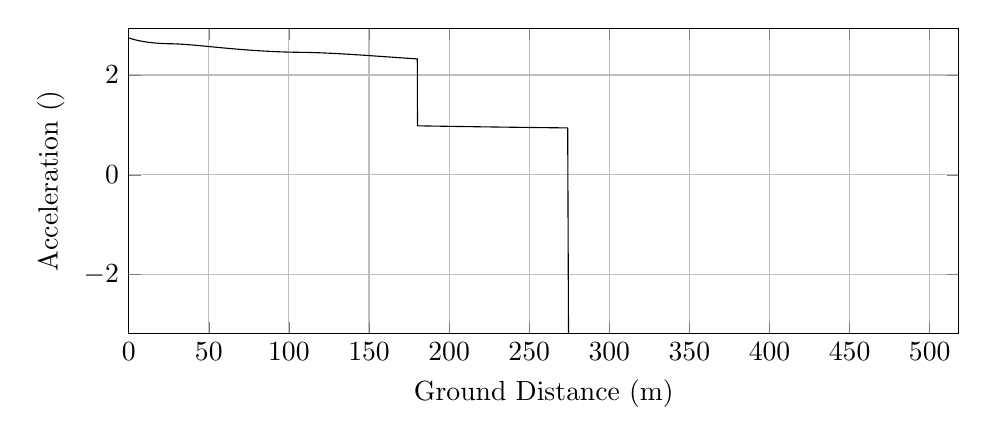
\begin{tikzpicture}

\begin{axis}[
width=\textwidth,
height=0.45\textwidth,
scaled ticks=false, tick label style={/pgf/number format/fixed},
xmin=0.0,
xmax=518.2299866992206,
xlabel={Ground Distance (m)},
xmajorgrids,
ymin=-3.1773545999999997,
ymax=2.9383329541999035,
ylabel={Acceleration ($\si{\meter\per\square\second}$)},
ymajorgrids
]

\addplot [
color=black,
solid
]
table[row sep=crcr]{
1.3729668748937997E-8	2.745933749634024\\
2.6049868369719035E-7	2.7459337463216693\\
2.0491224421327626E-6	2.7459337223163676\\
9.92442121137073E-6	2.74593361664894\\
4.7452367809869807E-5	2.7459331133935008\\
1.740064756114434E-4	2.74593141796994\\
4.0608377013922605E-4	2.7459283128250895\\
7.313431501337001E-4	2.745923966728787\\
0.0011549487327126044	2.7459183141309005\\
0.0016799013484208249	2.745911318665595\\
0.002295089346817705	2.7459031318683342\\
0.003009933382444524	2.745893631784023\\
0.003810608015426248	2.7458830054499908\\
0.004723484476856681	2.745870906509789\\
0.005727138856912631	2.7458576226878897\\
0.006836216967948795	2.7458429637322794\\
0.007997302399386296	2.7458276382144833\\
0.00929136979810952	2.745810580608766\\
0.010685558505459776	2.745792228663979\\
0.012178513621519987	2.745772603889116\\
0.013775244426719659	2.7457516442133327\\
0.015470070176169002	2.7457294279658626\\
0.0172374436815836	2.7457062929339147\\
0.019122918912604377	2.745681646264188\\
0.021104911040230538	2.7456557742244776\\
0.023190717999955576	2.7456285852738693\\
0.025355802981115103	2.7456004025085097\\
0.027620619195902148	2.7455709628304676\\
0.030020274690474198	2.7455398145480876\\
0.032476028269866286	2.7455079832228666\\
0.035054163466719815	2.745474612816359\\
0.037720846868992755	2.7454401452809734\\
0.04049779674511381	2.745404303593875\\
0.043329456594087365	2.745367807581193\\
0.04629652060163805	2.745329620662332\\
0.04934498934704602	2.745290442016606\\
0.052507657924119336	2.7452498537718295\\
0.055769483710642484	2.745208053078813\\
0.05917209570914676	2.7451645112972916\\
0.06264043916012321	2.7451201927906688\\
0.06620063977265622	2.745074766280724\\
0.06987962792775945	2.745027892179869\\
0.0736568184539585	2.744979836976057\\
0.07754284280095361	2.744930469346733\\
0.08151127871105612	2.744880128455919\\
0.08560324933017655	2.744828296550115\\
0.08985265585263943	2.7447745502252845\\
0.09413961367176535	2.7447204093860247\\
0.09857725310864562	2.744664448697618\\
0.10307959255469257	2.7446077566104368\\
0.10766008648593872	2.744550165853771\\
0.11234920964493048	2.744491296646081\\
0.11719267720457946	2.7444305805763873\\
0.12216973960582883	2.7443682839908865\\
0.12724007601918352	2.7443049160916244\\
0.13233299746505212	2.7442413617081813\\
0.13755256756750583	2.744176324555065\\
0.14287728588926696	2.744110077183268\\
0.1482946925752714	2.7440427783081276\\
0.15381585025670613	2.7439742941590106\\
0.15940564092189102	2.7439050633216198\\
0.16526271495916878	2.743832633069937\\
0.17120082448158402	2.743759314593124\\
0.17717889132867753	2.7436856165854584\\
0.18324322596131126	2.7436109697873574\\
0.189427022360885	2.7435349695339406\\
0.1957511558722988	2.743457364727397\\
0.2021484013779125	2.7433789844510024\\
0.20865863707071397	2.743299343476986\\
0.21548666343168166	2.7432159468507686\\
0.22220154781289658	2.743134061837388\\
0.22919671627301902	2.7430488935802986\\
0.23611678795738544	2.742964772871866\\
0.24306300975244904	2.7428804655838492\\
0.2503085190632165	2.7427926639555604\\
0.2576623280401219	2.74270369213178\\
0.26502430524173204	2.7426147629356477\\
0.2724963584449146	2.7425246467856903\\
0.2802001060647876	2.7424318847655185\\
0.2878583985474956	2.7423398174571867\\
0.2958320780323821	2.74224411264151\\
0.3040021452321372	2.7421462114990494\\
0.31208951788619	2.74204945948628\\
0.3202851396023423	2.7419515709453375\\
0.3287233234973125	2.7418509498073105\\
0.3370425959884752	2.7417519080250115\\
0.34575405233845447	2.7416483668644354\\
0.3545073625286812	2.7415445008529415\\
0.36338982075299686	2.74143927707345\\
0.37247557159370037	2.741331824878821\\
0.38151350442869847	2.741225116473271\\
0.3905554764834429	2.7411185361982797\\
0.3999457587520332	2.7410080342749286\\
0.4095398754587949	2.740895325049965\\
0.4189621792151833	2.7407848203234915\\
0.4285208811402964	2.7406729022160494\\
0.43828968955472236	2.7405587157868423\\
0.44807735398784176	2.740444501168418\\
0.45806002753764463	2.740328206966173\\
0.4682994371692033	2.740209125317234\\
0.4787752542918833	2.7400875051939693\\
0.4890770094685154	2.739968111629965\\
0.49985939134273727	2.739843363987376\\
0.5106597490205704	2.739718627718031\\
0.5213580865152188	2.739595283866114\\
0.532247733242454	2.739469951000051\\
0.5431365108549349	2.739344844457758\\
0.554075964429489	2.7392193713226414\\
0.5653450694020941	2.7390903409366887\\
0.5769901159382542	2.738957242270053\\
0.588512657344902	2.738825777773906\\
0.6004070039036553	2.7386903129467894\\
0.6121651247369502	2.738556638601956\\
0.6239717914322569	2.7384226491592862\\
0.6362472885961421	2.7382835883504875\\
0.6486428939173223	2.738143422272314\\
0.6610190736373547	2.7380037294208224\\
0.6737248046101814	2.7378605779440788\\
0.6862826225989949	2.7377193504710986\\
0.6991952542603428	2.7375743971928808\\
0.7122988072688032	2.737427572331951\\
0.7251463703465595	2.7372838790900627\\
0.7381769453061875	2.737138402838057\\
0.7516618647379176	2.7369881315120947\\
0.7654913705221527	2.736834310606014\\
0.7791756406994825	2.7366823919487455\\
0.7930637813125616	2.7365284991417216\\
0.8074774191984457	2.736369088689556\\
0.8215072375247947	2.7362142192435908\\
0.8361010597475598	2.736053431219534\\
0.8503303420601955	2.7358969585996338\\
0.8650627501899835	2.7357352618278403\\
0.8802332960144008	2.7355690814348668\\
0.8951742046771463	2.7354057362911055\\
0.9100334756324657	2.7352435957730297\\
0.9251067343345352	2.735079435666237\\
0.9403923630470314	2.7349132844243806\\
0.9559303815501943	2.7347447191307284\\
0.9712400158034169	2.7345789536451193\\
0.9869533781138684	2.7344091466658877\\
1.0029148609762486	2.734236997780573\\
1.0189962473881624	2.7340638988954913\\
1.035465185745812	2.733886982622522\\
1.0516742337458713	2.7337132054216866\\
1.067815735429615	2.7335404920408557\\
1.0846705971808022	2.7333605047019978\\
1.1012775250051634	2.7331835208984128\\
1.1180798406225687	2.7330048116164747\\
1.1351395900544134	2.7328237286921633\\
1.1526388687279154	2.73263835894707\\
1.1698922447507556	2.732455966615972\\
1.1875468452119025	2.732269712848928\\
1.2058383275300355	2.732077142510799\\
1.2239395537495579	2.731886975352393\\
1.2422020624207541	2.7316955142157697\\
1.2608769472440078	2.7315001426275947\\
1.2794948487006894	2.731305779649479\\
1.2979152553275424	2.7311138807814563\\
1.3166445915281573	2.73091917093961\\
1.3354141707340492	2.730724451882275\\
1.3543210821322504	2.730528719277727\\
1.373689361295591	2.73032863525778\\
1.3932049885015831	2.7301274608942405\\
1.4131781782225183	2.7299220154585475\\
1.4330139682345777	2.7297184263544425\\
1.4528243860883294	2.7295155352372795\\
1.4728783400745615	2.729310592226655\\
1.4934621752870565	2.729100693669997\\
1.5141408097620341	2.7288902940171758\\
1.53430654450827	2.7286855593626536\\
1.5553850389607948	2.728472025774905\\
1.5762653203499473	2.7282609685761434\\
1.5975496774716453	2.728046303569938\\
1.6196077215345106	2.7278243397435746\\
1.6413652536722467	2.727605899295412\\
1.663437310723463	2.7273848044555544\\
1.6860768385032747	2.727158548431424\\
1.7077101022266827	2.726942840558346\\
1.7297306410738114	2.7267237613893585\\
1.7520297891459062	2.7265024111794576\\
1.7743087535215367	2.7262817613558035\\
1.797257424336919	2.7260549980011213\\
1.8200802473615325	2.7258299974170024\\
1.8430350373473994	2.7256042147901303\\
1.8666926279964304	2.7253720605720746\\
1.8902808566018634	2.72514113040999\\
1.9138231309717848	2.7249111877288685\\
1.937187877956735	2.724683506686569\\
1.9611060682733261	2.724450973682445\\
1.9852138445648535	2.7242171481062742\\
2.009780393513653	2.723979437924413\\
2.0346228225622163	2.723739634761041\\
2.0593611988602687	2.7235014085153804\\
2.08477023517836	2.7232573149932806\\
2.110324766702745	2.7230124241566775\\
2.1352655781940433	2.722773991682768\\
2.160528860803022	2.7225330540312687\\
2.1862071157614817	2.722288750937233\\
2.2127756699400534	2.7220366021467237\\
2.2391904543957084	2.721786538650564\\
2.2653528664920257	2.721539475818613\\
2.292150575495974	2.7212870407551826\\
2.3187704640870406	2.721036905412479\\
2.3455495914188482	2.7207858982332622\\
2.372862901366455	2.7205305254301893\\
2.4007145172972395	2.7202707826704753\\
2.428100404243743	2.72001603228333\\
2.4555980306928005	2.7197608861757034\\
2.483374904362833	2.7195038000855876\\
2.511687733451976	2.7192424230947587\\
2.5402569276484597	2.7189793606402857\\
2.568415369317849	2.71872074613543\\
2.596987652715761	2.7184590025560453\\
2.6263861238451423	2.7181903927500546\\
2.655991481965028	2.717920608348247\\
2.6856115886357443	2.7176514041804687\\
2.7154221146045012	2.71738118698586\\
2.7455665152057707	2.7171086712897807\\
2.7752624694325894	2.7168409213882985\\
2.805457625653509	2.71656939071722\\
2.8358231840904597	2.716297056032584\\
2.8663460878589797	2.7160240421896784\\
2.897817297850832	2.7157433103512467\\
2.9287074004595235	2.7154685124985987\\
2.9603588456990284	2.715187708551693\\
2.9922321403815406	2.71490571640717\\
3.0241119471841866	2.71462444530067\\
3.056446055158509	2.7143399570513758\\
3.0889346922121366	2.7140549072190137\\
3.122221620829695	2.713763678408176\\
3.1546991615623394	2.7134803314856493\\
3.187635101478671	2.7131937884197734\\
3.221010117202278	2.7129042459478487\\
3.2543449374576605	2.712615872270808\\
3.288235920596943	2.7123235230382576\\
3.3223704322934555	2.7120299202652527\\
3.3562838593334394	2.7117390566035233\\
3.3906320903803255	2.7114453101597196\\
3.425633159699527	2.711146852210671\\
3.462387235801926	2.7108343880622456\\
3.4973980805087237	2.710537636483595\\
3.5324804241140235	2.710241147744873\\
3.5675385073174235	2.709945728382193\\
3.6040688981843845	2.709638816969628\\
3.6393612181513753	2.7093431890244997\\
3.6770856360342323	2.7090281416612143\\
3.7131729334920323	2.7087276833232927\\
3.749509707933214	2.7084260491268246\\
3.785733977879824	2.7081262444468592\\
3.8225309786916544	2.707822610564083\\
3.860867115351552	2.7075072478509306\\
3.89929745075254	2.7071921001654697\\
3.9373367205567504	2.706881130446619\\
3.9751626485832894	2.7065728578762025\\
4.013671158053867	2.7062599937888168\\
4.0521140617426425	2.7059486353631357\\
4.092377631210638	2.705623567578243\\
4.131586743753305	2.705308027124949\\
4.1715696979561425	2.7049872843873297\\
4.210522654700574	2.7046757949824176\\
4.250196810863292	2.704359538589963\\
4.2917015001093795	2.7040297652367293\\
4.332438976653355	2.7037071511860633\\
4.373124372895289	2.7033859958341147\\
4.414429464889761	2.703061013141131\\
4.455884944705147	2.7027359201134686\\
4.497250153511752	2.7024126010589393\\
4.537976875075978	2.7020953078843215\\
4.581399817640802	2.7017581350427298\\
4.623816269683994	2.701429893974078\\
4.666022338967499	2.7011043708260782\\
4.709098934189642	2.7007732491577343\\
4.752435367147649	2.7004412618628235\\
4.79531009100786	2.700113923220311\\
4.838191999420829	2.6997876304091646\\
4.881381760681686	2.6994601025113845\\
4.9256451804034285	2.6991255802428515\\
4.9704217340957495	2.6987883563581185\\
5.014356093293278	2.6984586198088563\\
5.058826350846283	2.698126010287651\\
5.104458009943745	2.697785910252903\\
5.149663211268795	2.697450177563721\\
5.194981168813841	2.6971147895925576\\
5.241194091283663	2.696773991377621\\
5.287987552078626	2.696430154327218\\
5.334426822383641	2.6960901499960244\\
5.380633359096258	2.6957530602096966\\
5.427524438012913	2.6954122052897027\\
5.476157635197664	2.6950599883398825\\
5.524667120325573	2.6947099813886997\\
5.5732739519824435	2.694360582160768\\
5.6208990292882195	2.6940195060851275\\
5.671502816366864	2.693658464116621\\
5.719824083529298	2.6933150154219874\\
5.767871110439133	2.6929747772519512\\
5.8169321963676754	2.6926286501345027\\
5.866076914057565	2.6922832358810025\\
5.917200682776528	2.691925289335387\\
5.96684810088939	2.6915790178532983\\
6.016885842403935	2.691231352228524\\
6.068639931677712	2.6908731577503717\\
6.119867755785197	2.6905199976544543\\
6.171030794930029	2.6901686602208663\\
6.222884713227881	2.6898139753337107\\
6.2735946138732235	2.6894684695538738\\
6.325883502103322	2.6891136013011465\\
6.379615386553551	2.6887504096481347\\
6.432194972482147	2.688396442468087\\
6.484528316464761	2.6880455368872473\\
6.536619297696934	2.68769764118571\\
6.589662958081361	2.687344796419861\\
6.644121795496577	2.6869840153423956\\
6.697445536614451	2.68663219810922\\
6.7518063163896365	2.686275003043974\\
6.8068829439682315	2.685914605406988\\
6.863205650636274	2.685547609679398\\
6.9185329265047315	2.685188625021353\\
6.974634519184049	2.684826152672259\\
7.031139830722298	2.6844626288388405\\
7.0870923879294985	2.6841041940757817\\
7.144766952910487	2.6837363176346836\\
7.2026451873548805	2.683368757231797\\
7.261191729679483	2.682998591553873\\
7.320502240843062	2.682625268876813\\
7.378210233177999	2.6822636424501294\\
7.437738452534925	2.6818922655745236\\
7.49714639104333	2.681523308417665\\
7.556502460410064	2.6811563316145213\\
7.617032771987237	2.680783794499826\\
7.676883327249088	2.6804171211405423\\
7.735740247984193	2.6800581575988813\\
7.796086087039788	2.679691776501249\\
7.856787102853412	2.6793249307229674\\
7.91721236259451	2.678961429481797\\
7.979013602666894	2.6785913752038963\\
8.039824025454376	2.6782289487607027\\
8.102419182184594	2.6778576340357727\\
8.16459313580776	2.6774905665511346\\
8.226347093952135	2.677127696565849\\
8.290527749984296	2.676752373844961\\
8.353592793320257	2.6763853613705777\\
8.417564177281012	2.67601487568339\\
8.482044607535009	2.675643270078857\\
8.547336806956285	2.6752688485572547\\
8.613293246319614	2.6748925126021685\\
8.6778048537894	2.6745262550450724\\
8.74454839911753	2.674149227258674\\
8.810708373588199	2.673777396453808\\
8.876548424968423	2.673409234250302\\
8.942828456712885	2.6730404887927257\\
9.010858044488913	2.6726639601609223\\
9.079453414959548	2.6722862922314583\\
9.148767802603732	2.6719066890561036\\
9.21609997183467	2.6715398811000908\\
9.285579683381485	2.67116336940079\\
9.355451712480097	2.670786767326205\\
9.423585014597279	2.670421494476032\\
9.493435356703696	2.6700490148237135\\
9.562655940911181	2.6696818813962357\\
9.63183713653898	2.669316926216502\\
9.703018708836247	2.6689434650398702\\
9.773178624863132	2.6685773872877823\\
9.844376937811855	2.6682079365263496\\
9.914998792594716	2.6678435040567887\\
9.98720270419701	2.6674729864037268\\
10.059478150570087	2.6671041981501142\\
10.132362020358627	2.6667344209387407\\
10.205876892438312	2.6663635857706476\\
10.279422251887688	2.6659947421935097\\
10.353305644514993	2.6656263553136483\\
10.42811398108589	2.6652555454284528\\
10.50332954727428	2.664884928557493\\
10.578207710262959	2.6645181680900603\\
10.65503529959097	2.6641441252244062\\
10.730232142651953	2.6637802356245537\\
10.805871937852555	2.6634164032193377\\
10.88265320376452	2.6630493287809767\\
10.958577899345514	2.6626885682826185\\
11.034861147941964	2.662328317504069\\
11.112742623646977	2.6619627989513033\\
11.190543636431041	2.661599949051814\\
11.267787598939979	2.6612419536263943\\
11.3462805052093	2.6608804641262784\\
11.423875697147409	2.6605253733666894\\
11.502735831556972	2.66016679186927\\
11.581465323066688	2.6598111062891867\\
11.661639233340708	2.6594512496614984\\
11.741743247575428	2.659094070532034\\
11.821864700430528	2.6587391681041073\\
11.901816327719768	2.6583873562373483\\
11.98361062800689	2.65802984404648\\
12.065425957085825	2.657674667049518\\
12.1478520915771	2.657319283720091\\
12.230956215923495	2.6569634524950505\\
12.313306905825911	2.6566132897052395\\
12.396632357805931	2.656261447402212\\
12.479578787946746	2.655913659143116\\
12.564327762802186	2.6555608318228234\\
12.648175874147956	2.655214251081233\\
12.736145481689512	2.6548532930755826\\
12.821080154398764	2.6545073614738826\\
12.908009536077355	2.6541559136608868\\
12.994986774303499	2.6538069029568296\\
13.081752199798046	2.6534613540348904\\
13.17035388279784	2.6531111740371047\\
13.257836697901475	2.652768065088189\\
13.34511613365563	2.652428366974772\\
13.433461823066896	2.6520871672573874\\
13.524108483575919	2.6517398400805456\\
13.611203924103116	2.6514087427638877\\
13.702229394080796	2.6510654420726993\\
13.792427706753081	2.650728010041674\\
13.882429934062493	2.6503940290968764\\
13.975435778888343	2.650051743756091\\
14.065832730112316	2.6497218173613817\\
14.157894546480026	2.649388598244756\\
14.250668806951023	2.649055631782466\\
14.343291987615704	2.6487260325270725\\
14.43744444968501	2.64839387373258\\
14.532636396723657	2.6480609912501123\\
14.625507232812737	2.6477390675021404\\
14.721503924398366	2.6474092478024884\\
14.818738382089133	2.6470782104461428\\
14.913572076739943	2.6467582780736505\\
15.009701633366973	2.6464369177531655\\
15.10815424447124	2.6461108524555685\\
15.206130868840724	2.6457894275225193\\
15.304035939715973	2.6454712794394446\\
15.403499839366233	2.645151168619309\\
15.503209871950865	2.6448333932172794\\
15.601718454553605	2.6445225108434887\\
15.700655560608023	2.6442133305209685\\
15.801250929860519	2.6439020954003567\\
15.899917805652187	2.643599879299895\\
16.001574124100856	2.6432916569963822\\
16.102638779863817	2.6429883870635598\\
16.204479333764816	2.6426859631921458\\
16.30489644092564	2.642390875444015\\
16.40578186591999	2.6420975095348966\\
16.509201471948074	2.641799986524223\\
16.614557195984908	2.6415002256988815\\
16.717657554831042	2.641210126302675\\
16.823039336622365	2.640916912552081\\
16.928576062495388	2.6406266046044653\\
17.03469945574068	2.640338038396731\\
17.140697318244236	2.640053160739731\\
17.246066414787876	2.639773277049187\\
17.35183930840021	2.639495622702711\\
17.458399953804133	2.639219234411631\\
17.565707112453843	2.6389442799060117\\
17.673103795073075	2.638672470550473\\
17.781888038667653	2.638400579402105\\
17.89115167195854	2.6381309531423165\\
18.00105710767307	2.63786323255278\\
18.110142905530395	2.6376009574466197\\
18.219697237410173	2.637341002414172\\
18.32752951944549	2.6370884953076636\\
18.43743745973078	2.6368345484445737\\
18.54904630654982	2.63658019384358\\
18.659302591714813	2.6363323952736817\\
18.770734536087716	2.636085450694776\\
18.883577445650936	2.635838949357387\\
18.996263390583444	2.635596364184675\\
19.108816920034535	2.635357616908477\\
19.22287647779894	2.6351192855805\\
19.33763586704334	2.6348831480062795\\
19.456324114791514	2.6346427711361047\\
19.57349394116079	2.634409291852097\\
19.690148252848566	2.634180600096859\\
19.80521137071168	2.633958691418372\\
19.92379170801214	2.633733794227746\\
20.04216631061405	2.6335131166802155\\
20.15848954929409	2.6332999786096893\\
20.278242138037896	2.6330843918964613\\
20.396206084226087	2.6328758170334643\\
20.516315546862906	2.632667302876359\\
20.637173924977112	2.632461401533406\\
20.75450010628387	2.6322652607421713\\
20.874378237858778	2.632068650375719\\
20.996035953832852	2.6318730325170687\\
21.11812959618858	2.6316806625120934\\
21.240471115580952	2.631491857446668\\
21.361479376438375	2.6313089928781865\\
21.485224699488654	2.631125973433857\\
21.607870280890317	2.6309485406063304\\
21.73242999733349	2.630772361329301\\
21.85704493170313	2.6306001480967662\\
21.98122016226351	2.6304325538620574\\
22.10826921766411	2.6302652125995127\\
22.235261614051304	2.6301021093246337\\
22.361664688868032	2.629943883831288\\
22.48780138980522	2.6297900776934346\\
22.614107216476143	2.6296401428980527\\
22.74409311379692	2.6294900871360998\\
22.873024137794893	2.6293454925824022\\
23.003512644166257	2.6292034414201826\\
23.132891545907036	2.629066846405708\\
23.26270690888247	2.628934029456868\\
23.39264146728729	2.6288053298831127\\
23.52277721573431	2.6286806696961964\\
23.654883767164463	2.6285584477188975\\
23.78569183677709	2.6284417091087624\\
23.917003007077597	2.628328794588147\\
24.047013652206026	2.628221204195908\\
24.178458227988493	2.6281166694027984\\
24.314609552493202	2.6280128759318746\\
24.447533097503474	2.627915932898171\\
24.579128452041708	2.627824218719879\\
24.71011994849615	2.627737123338611\\
24.843278471916108	2.627652868038229\\
24.975761222328053	2.6275733117861915\\
25.1115496753864	2.6274961796102385\\
25.247101122854083	2.627423621584068\\
25.384906965000688	2.627354391118195\\
25.522261036073317	2.6272899242628656\\
25.66123001648475	2.627229296090176\\
25.79865327455613	2.627173876444852\\
25.826335196219034	2.6271632574604533\\
25.839610403727477	2.62715822969495\\
25.841006316401874	2.627157703174394\\
25.84227013303559	2.6271572259940434\\
25.84770509053729	2.6271551682557828\\
25.86419328224909	2.627148869514051\\
25.90571916957557	2.627132632727095\\
25.999268866927544	2.62709410603191\\
26.123295978662824	2.627038901212371\\
26.250212562581652	2.6269775933396176\\
26.376891976518465	2.626911599588503\\
26.50638698165423	2.6268392423555404\\
26.634042370994827	2.6267631265942892\\
26.763333806613538	2.626681250837172\\
26.893207366259766	2.62659421847878\\
27.022905486492228	2.6265025738361114\\
27.153956322362554	2.626405232066988\\
27.287774297957696	2.626300978647955\\
27.42030033806219	2.6261929566003683\\
27.555504894698295	2.626077916748084\\
27.691130018821354	2.6259576762016144\\
27.82633313037239	2.6258330443348266\\
27.959508564917073	2.625705689812035\\
28.096515548835796	2.6255699768647354\\
28.232789703382153	2.6254303281033025\\
28.368684388406535	2.625286498680893\\
28.506541650227618	2.6251359904785243\\
28.64533374691623	2.624979841336361\\
28.78297783415192	2.624820465669056\\
28.92277775692753	2.6246540493487274\\
29.06227187463503	2.624483493060775\\
29.20212864139956	2.6243080372215513\\
29.34335827861657	2.624126392094661\\
29.483225747293005	2.623942134485322\\
29.625960812476485	2.623749682168036\\
29.76706561118049	2.6235551018597727\\
29.909402910999468	2.6233545237810842\\
30.051751399473822	2.623149671618658\\
30.196612335666572	2.6229368923312792\\
30.342192969749448	2.6227187353115538\\
30.48583400527584	2.6224992991267593\\
30.632658550781265	2.622270763203243\\
30.77846394498075	2.6220396350772806\\
30.92408133049836	2.6218047080288107\\
31.071091331299215	2.6215634400823893\\
31.218274793935116	2.6213178254024356\\
31.366705758252415	2.6210660719563164\\
31.515339333797037	2.6208099515408767\\
31.66356819769615	2.620550577189582\\
31.814689402684216	2.6202821391202162\\
31.96649953392354	2.6200084685109024\\
32.115424616034375	2.6197361526902787\\
32.266253234088566	2.619456531320976\\
32.41813832080348	2.6191711196609058\\
32.569791431087395	2.6188823653016966\\
32.722234201183724	2.618588359660447\\
32.876984607664	2.6182861188418736\\
33.031873994672836	2.6179798472058744\\
33.18502245018544	2.61767337730517\\
33.34135780547538	2.6173568541876238\\
33.49759920343199	2.6170368690402794\\
33.65385117142162	2.6167132684054444\\
33.8113313806527	2.6163835453824538\\
33.96985264489639	2.6160480723691215\\
34.126473036379195	2.6157131607910555\\
34.2857505660089	2.6153690959358693\\
34.4449212019973	2.6150218218705428\\
34.60566879064274	2.6146676745052684\\
34.76644486933921	2.614310071010496\\
34.92612701881755	2.613951597544056\\
35.08630421658309	2.6135887608266746\\
35.24825698849928	2.613218646437778\\
35.412303951281956	2.6128404656979436\\
35.57355277914179	2.612465573208352\\
35.73545353069308	2.612086065190393\\
35.89925038949356	2.6116990063305368\\
36.065161289279985	2.611303822719635\\
36.23047312008262	2.6109069894047563\\
36.39472205714358	2.6105097203642957\\
36.56135389445764	2.6101036997752756\\
36.72774532558607	2.609695316287241\\
36.89384825683493	2.6092847556652456\\
37.05904296416534	2.608873633171015\\
37.22702676294645	2.6084527521107095\\
37.39437475321985	2.6080306918927274\\
37.5621109943643	2.607604928234461\\
37.73270471709142	2.607169167240153\\
37.903359519601935	2.6067305347705387\\
38.071486842086316	2.6062957943756917\\
38.23815243703595	2.6058623319798837\\
38.40817787072022	2.6054176148453294\\
38.57751392140098	2.604972224462812\\
38.750215798728505	2.604515486819169\\
38.92001182640311	2.604064028086343\\
39.09310637700479	2.6036013939253158\\
39.26472366117933	2.603140360230884\\
39.436554723976656	2.6026764590104268\\
39.608961777617054	2.602208745072529\\
39.782828308010565	2.6017348303452126\\
39.956194359016465	2.6012600869258415\\
40.132391837044906	2.6007753954833523\\
40.30868053167249	2.6002882883371417\\
40.48611580488176	2.599795875967091\\
40.66383502946924	2.599300575623608\\
40.83999042132467	2.5988076076289266\\
41.018202681018664	2.598306879012876\\
41.19780999006247	2.59780023921822\\
41.37730467548502	2.5972919679986406\\
41.557010452813884	2.5967811949022925\\
41.73612816026986	2.5962702442991796\\
41.91555194917056	2.5957566162813004\\
42.09743589423803	2.5952341495078093\\
42.27807550146298	2.5947135135520316\\
42.45995188234755	2.594187603754664\\
42.6401410478328	2.593664926422731\\
42.822293873795985	2.5931349327029034\\
43.00585672428667	2.5925992336587598\\
43.189965171449515	2.592060371841985\\
43.372020236704074	2.5915260176090396\\
43.555636897252796	2.5909856106444664\\
43.74012033961118	2.5904412105939336\\
43.92429822300048	2.5898963139394615\\
44.106869824379004	2.5893548329369107\\
44.29411840239129	2.588798141810776\\
44.47920670866131	2.5882465834656143\\
44.665034305215386	2.5876915745572395\\
44.85242224248053	2.5871306821366113\\
45.03948098831597	2.5865695920897522\\
45.22811764277584	2.586002614453135\\
45.41548629589063	2.5854383417605273\\
45.60322541388645	2.58487188864763\\
45.793007222766036	2.584298230300096\\
45.983742663331824	2.583720675421648\\
46.172643153142886	2.58314771556424\\
46.36421599110457	2.582565713945945\\
46.553512793459404	2.5819897407332553\\
46.745018895697555	2.5814061887802406\\
46.93606459490553	2.580823220829023\\
47.126948089509526	2.580239969889381\\
47.31881294044018	2.579652975509168\\
47.5110690178297	2.5790640736859434\\
47.705448624448266	2.5784679831468953\\
47.90005519882567	2.577870546429364\\
48.09288923506665	2.577277947636331\\
48.28732881729917	2.576679844114947\\
48.484002572746206	2.5760743233998253\\
48.68089030454945	2.575467633349363\\
48.87532723390382	2.57486803095897\\
49.07073736177763	2.5742649991859343\\
49.2672083392297	2.5736582972862303\\
49.46586249263092	2.5730444865995894\\
49.661880987188695	2.5724384938105347\\
49.85966148345089	2.5718267615262587\\
50.05808618672894	2.571212777407524\\
50.25785665917266	2.570594402569249\\
50.45743808511885	2.569976421527972\\
50.65573800086891	2.5693622538365988\\
50.85948768734909	2.5687310825359084\\
51.061243703011925	2.5681059980424292\\
51.26368286286315	2.567478743109982\\
51.46416466063809	2.566857533975103\\
51.66475943174029	2.5662359893110347\\
51.86588207153103	2.56561285677663\\
52.07444928962187	2.564966744465173\\
52.2824430085781	2.5643225310284814\\
52.48676525705545	2.5636898422625745\\
52.69531994892206	2.5630442386830037\\
52.90027076850366	2.562410012697458\\
53.108186167814935	2.5617668705752035\\
53.31165724918766	2.561137759462768\\
53.520024946679996	2.560493831718171\\
53.72688450142306	2.559854920280424\\
53.93707391647578	2.5592061198138465\\
54.14518573319289	2.5585641573342945\\
54.35125853722778	2.5579289322446064\\
54.56213447502874	2.5572793940255876\\
54.77598621923464	2.5566212311207\\
54.987629956235494	2.5559704324655836\\
55.19778857845695	2.5553247914147734\\
55.41030974885841	2.55467252202679\\
55.62390503323701	2.554017625167454\\
55.83671574169797	2.553365831759879\\
56.047071254351536	2.5527222723040826\\
56.26137331252919	2.5520673989185383\\
56.47512769358855	2.5514149930840677\\
56.69105800830218	2.55075678108659\\
56.90937011004422	2.5500921924420785\\
57.12736617899088	2.549429482767894\\
57.346833156368504	2.5487632574065238\\
57.56476609337061	2.5481026676419045\\
57.78230894703917	2.547444262133678\\
57.99943865551505	2.5467881336539273\\
58.21827465292657	2.5461279153126446\\
58.436085045729726	2.545471882108224\\
58.6577546799423	2.5448053710641405\\
58.87982836766625	2.544138832936956\\
59.10336118170943	2.5434691447546607\\
59.324182403931715	2.542808819305696\\
59.545440661451366	2.5421484495030766\\
59.768227251413464	2.5414848224466517\\
59.99077485409802	2.540823240966116\\
60.21631063559073	2.54015416369662\\
60.44006004384342	2.539491792913134\\
60.66502706168687	2.5388272572727564\\
60.89133011288284	2.5381602583073883\\
61.11585558357916	2.5374999948556693\\
61.3432655409558	2.5368327945800493\\
61.57186440401435	2.5361637002878803\\
61.79868765088207	2.535501408748763\\
62.025670725987	2.5348402770909786\\
62.254132946411545	2.5341765056009926\\
62.48290793247415	2.5335135279774255\\
62.713817944074236	2.5328461162466924\\
62.94484116346062	2.5321801651283318\\
63.17805109236767	2.5315097497788024\\
63.41124119062552	2.530841264404774\\
63.64505576847972	2.5301728944345925\\
63.87735201907903	2.5295107788661895\\
64.11169045660182	2.5288448001638137\\
64.34725756208485	2.52817733598523\\
64.58324360279937	2.527510726208688\\
64.81881329818131	2.5268473544899654\\
65.05563560606473	2.5261825559991893\\
65.29467812810154	2.5255136850947695\\
65.53178653633495	2.524852393698131\\
65.77046761369158	2.5241889200770515\\
66.01019347650049	2.523524791474693\\
66.25262920761091	2.52285547188822\\
66.49342175078831	2.522193018006006\\
66.73393309567928	2.5215336779391944\\
66.97718905970893	2.52086921586132\\
67.21919788222482	2.5202105803525665\\
67.46413738735515	2.519546449583455\\
67.70584739194695	2.518893544044623\\
67.95375887035246	2.5182264574902717\\
68.19817148521656	2.5175713561374016\\
68.44413350233111	2.5169147004876002\\
68.68984243621705	2.516261345089669\\
68.93951041285982	2.515600171501796\\
69.19023531750676	2.514938969433662\\
69.43956667494601	2.514284217583624\\
69.68998597860525	2.513629416130965\\
69.94098943220166	2.512975932155717\\
70.1928405184459	2.5123231255440013\\
70.44659484061637	2.511668329081634\\
70.69926103579675	2.5110192971929557\\
70.95414956377036	2.5103675673854084\\
71.21136313866151	2.5097129793716446\\
71.46778788208749	2.509063506597747\\
71.7247351381395	2.5084158438377147\\
71.98234155897126	2.507769689085089\\
72.24107377350035	2.5071239256193767\\
72.4986091150376	2.5064843695454924\\
72.75949164810788	2.505839797213234\\
73.02014691132015	2.505199119753618\\
73.28114866838587	2.504560949336046\\
73.54342372888959	2.503923071226774\\
73.80584407854005	2.5032882764078206\\
74.07231166191039	2.5026472290607487\\
74.3389341302921	2.5020093971959803\\
74.60521354141642	2.501375988177486\\
74.87280568706873	2.5007431028336446\\
75.1403821105715	2.5001139292433843\\
75.41145333671997	2.4994803046180856\\
75.68265298797411	2.4988501932497016\\
75.95075857762194	2.498231039158717\\
76.2241428819712	2.4976035721719434\\
76.4990100438061	2.496976668570306\\
76.77213586328236	2.4963576955699853\\
77.04724851790667	2.49573822862106\\
77.32330034006353	2.4951207098630084\\
77.59850473375684	2.4945091566067346\\
77.87773830129439	2.4938928219842715\\
78.1565255546137	2.4932816837060106\\
78.43842651648492	2.492668017346257\\
78.720833678605	2.4920576010425153\\
79.00101298089581	2.4914563231480757\\
79.28359351218376	2.4908542717934887\\
79.57011733099088	2.490248328576058\\
79.85418914588558	2.4896520718283295\\
80.13919871477489	2.4890583687052414\\
80.42568449319114	2.4884661731421938\\
80.71472498530085	2.487873370981382\\
81.006853148924	2.487279025102887\\
81.2951972638476	2.4866971170884167\\
81.58524575795963	2.486116537145639\\
81.87461709596036	2.4855420949920353\\
82.1711642895769	2.484958381559892\\
82.46716486408064	2.484380782761332\\
82.76422974563803	2.483806186216814\\
83.05801377197795	2.483242957146957\\
83.35853301954708	2.482671999870737\\
83.65664966506407	2.4821108049392793\\
83.95487262936624	2.481554606519677\\
84.25322789115987	2.4810033792257986\\
84.55664509033022	2.4804481694309706\\
84.8599544590121	2.4798985860092557\\
85.16499148084048	2.4793513638033664\\
85.47187188044902	2.478806409028219\\
85.77908321853027	2.4782664837735044\\
86.08675489504844	2.4777313991684684\\
86.39784539041122	2.4771961342162765\\
86.71051296037359	2.4766640142286205\\
87.02583358957506	2.4761333445033173\\
87.34037846285594	2.4756099658506825\\
87.65395388450591	2.4750941674588303\\
87.96687312379424	2.4745854039580317\\
88.28527441497255	2.474073850456792\\
88.6103524516937	2.4735579588692937\\
88.92871226770333	2.4730590021066936\\
89.25003295857354	2.472561715850354\\
89.57522243846881	2.472064913921284\\
89.90247582737899	2.4715715482953424\\
90.22602529632545	2.471090281458441\\
90.5494223037065	2.4706157304863785\\
90.87816525326718	2.470140000358535\\
91.20455861430293	2.4696743344984124\\
91.53817773235312	2.4692052383281\\
91.87076195087604	2.46874453523425\\
92.20124984301029	2.468293613714687\\
92.53140503523474	2.4678500072923946\\
92.86389705561814	2.467410207209607\\
93.19815266874983	2.46697511608851\\
93.53304529783748	2.4665462917878456\\
93.86737084100128	2.4661252936021194\\
94.20337949361911	2.4657093387407842\\
94.54065981474497	2.4652990463300517\\
94.87396787418089	2.4649007234996034\\
95.21684847579547	2.4644983797555815\\
95.55392648231228	2.4641101935898275\\
95.89232371872416	2.463727831543161\\
96.23051075783204	2.463353072193108\\
96.57164052232307	2.4629825255521096\\
96.90762523479154	2.4626249186321765\\
97.24755293575913	2.462270552927021\\
97.58790661409188	2.4619232523826478\\
97.92576087813703	2.461585947168559\\
98.26661027452474	2.4612531815923795\\
98.6051908024865	2.4609301321117414\\
98.94563962387357	2.4606128512157275\\
99.28665364663627	2.4603026475156407\\
99.63350087797645	2.4599949576702347\\
99.97685593767679	2.4596981466115277\\
100.31593955776762	2.4594126383431973\\
100.65572384630482	2.4591341387793317\\
100.99616871909686	2.4588627388350837\\
101.3402339503516	2.458596236175948\\
101.67973054404297	2.458340953841132\\
102.01657591573795	2.4580952179760907\\
102.35656456518868	2.457854829697289\\
102.6941824316649	2.457623725275984\\
103.03547296258705	2.457397823628013\\
103.37623032340073	2.457180026797986\\
103.71852978299776	2.456969054425172\\
104.05851119314701	2.4567672705298635\\
104.3949509202441	2.4565752126830196\\
104.7329053851843	2.456389936423986\\
105.07104272194636	2.456212240406991\\
105.40742307340048	2.456043101164078\\
105.74423560014887	2.4558813834138933\\
106.07955743077031	2.455727984822288\\
106.41623710643992	2.4555816081016255\\
106.75618472497374	2.455441591416804\\
107.0942647435474	2.4553101084432747\\
107.43151869252583	2.4551866717490167\\
107.44650965670576	2.4551813642403237\\
107.45815118347005	2.4551772531208176\\
107.46233674961977	2.4551757772689795\\
107.46535588765028	2.4551747132015054\\
107.46808502617694	2.4551737507643727\\
107.4836206108138	2.455168259670489\\
107.53176708907421	2.4551511079163477\\
107.68672244793561	2.455094531599669\\
107.97570433527497	2.4549834451948627\\
108.27744765146667	2.4548597682328195\\
108.5816623935838	2.4547272061477434\\
108.88557241638279	2.4545869610121596\\
109.19209959959528	2.45443767243568\\
109.50241879336687	2.4542786003150896\\
109.81066605766154	2.4541127633367736\\
110.12101503747155	2.453937994054648\\
110.43285681965125	2.4537545790192175\\
110.74725799716322	2.453561818956234\\
111.06462449033057	2.4533593397004765\\
111.38211128519615	2.453148923592198\\
111.70119562731901	2.4529296108117045\\
112.02298633508096	2.452700564309909\\
112.34320819983824	2.452464869014065\\
112.66812620709393	2.452217884637398\\
112.99302416686388	2.451963112159949\\
113.31966045518399	2.4516991968576756\\
113.64998129974768	2.451424459279832\\
113.97857627498675	2.451143416865058\\
114.31304608469316	2.450849510906499\\
114.64448318111735	2.4505505571921855\\
114.98093514978115	2.4502393175308965\\
115.31969924418831	2.4499181287839766\\
115.65790718621022	2.449589741128423\\
116.00063352526521	2.4492491841404753\\
116.34235083463872	2.448901923487149\\
116.68621873349733	2.448544803075687\\
117.03331062078092	2.4481766222286128\\
117.37910048629482	2.4478022122028253\\
117.72869476105836	2.447416056567934\\
118.08005947084649	2.447020315368726\\
118.43363644355449	2.44661445841039\\
118.79186464668504	2.446195562722882\\
119.14769212941735	2.4457719010897243\\
119.5036618261702	2.4453406161077478\\
119.86270697471275	2.444898151431988\\
120.22616362054572	2.4444427272159954\\
120.58991121293201	2.4439794620158324\\
120.95538130513773	2.443506572675182\\
121.3195355377388	2.4430280793612997\\
121.68590041554987	2.4425394226513815\\
122.05305648207542	2.442042507730611\\
122.42257239354896	2.4415352206266228\\
122.79503144936103	2.4410167087569397\\
123.16629137010841	2.4404927909789507\\
123.53950748252527	2.439959095724661\\
123.91239367862553	2.4394189483888704\\
124.29026003316017	2.4388646308631676\\
124.66301933937496	2.438311045841078\\
125.03890311735066	2.4377461242287524\\
125.41380975776434	2.4371760734767376\\
125.7896808967325	2.4365980418067945\\
126.16837244152023	2.4360091772577572\\
126.54595968852882	2.4354156387065453\\
126.92471834906405	2.434813947054397\\
127.30294276405039	2.4342068948637348\\
127.68255852126984	2.433591469128208\\
128.06243727540487	2.4329695571547303\\
128.44360431740483	2.432339541404442\\
128.82265748788262	2.4317071612453454\\
129.1989690567886	2.4310736703116387\\
129.57765386613931	2.4304305602421765\\
129.95508099647026	2.429784065084977\\
130.33359114840187	2.4291302715149827\\
130.71373745886524	2.4284682576146626\\
131.09453904397424	2.4277997749107643\\
131.47657586018488	2.4271238577704235\\
131.85678563989967	2.426446027201812\\
132.23856625352113	2.42576032125654\\
132.61595336405918	2.4250775964184523\\
132.99976263915818	2.4243783357290276\\
133.38083522978053	2.423679242984316\\
133.76098428781995	2.4229771481541835\\
134.1363519425165	2.4222793654313444\\
134.51557915495124	2.421569932295995\\
134.8968696170101	2.4208521881638854\\
135.27419431482667	2.420137597883574\\
135.65215477207505	2.4194175854598914\\
136.03329358991255	2.4186873250908105\\
136.41192880753374	2.4179577730609862\\
136.7898079310749	2.417225694571063\\
137.17001317148595	2.4164851729427035\\
137.54844558779996	2.415744261492118\\
137.92617219433072	2.4150009862160164\\
138.30476964659732	2.4142523189260237\\
138.68390038934075	2.413498983015482\\
139.0631653430654	2.4127418378009757\\
139.4406106933401	2.41198488197385\\
139.81914660512416	2.4112223633220573\\
140.19767098864742	2.410456560906317\\
140.5730919292459	2.4096938425620706\\
140.95061983253072	2.4089237067743268\\
141.32838502869612	2.4081500093041033\\
141.70636515873298	2.4073728610224387\\
142.0839785067887	2.406593529688587\\
142.46357402350594	2.4058072184921997\\
142.84082211769783	2.40502296889394\\
143.21906727224075	2.4042339114596416\\
143.59963619096823	2.403437310882776\\
143.97984478872678	2.4026388326905357\\
144.35941603837455	2.4018391364099507\\
144.7355521893594	2.4010442230400466\\
145.11296635073694	2.4002442180265584\\
145.49073213867456	2.399441133914113\\
145.87033631970945	2.3986318541955978\\
146.24486520181193	2.397831210000894\\
146.6238757206513	2.3970188391759493\\
147.00096360401335	2.396208508945593\\
147.37874202190085	2.3953946757121454\\
147.756852900845	2.39457816388311\\
148.13572640408995	2.393758097000817\\
148.5136798644104	2.392938178662493\\
148.89083780486442	2.392118210713834\\
149.2712459042852	2.391289439886328\\
149.65303236723025	2.390455972301191\\
150.0329584616291	2.389624940771009\\
150.41363382646614	2.388790702960881\\
150.79322940570728	2.3879573271300165\\
151.17272478467066	2.3871227269328097\\
151.55400296227282	2.3862828087520374\\
151.93482601265913	2.385442551958211\\
152.31881414221942	2.3845940116132027\\
152.70208150063132	2.3837458190581575\\
153.08320649997165	2.382901190023449\\
153.4666285558243	2.382050340959543\\
153.84825937276264	2.381202396702336\\
154.23093781718723	2.380351107148919\\
154.61485031834388	2.379496102763693\\
155.00001234931443	2.3786373939872023\\
155.38285725409855	2.3777829898524283\\
155.7679513537659	2.3769227531344317\\
156.1509667875323	2.3760664034774726\\
156.53491934392343	2.3752072536116557\\
156.91995289130983	2.37434502792717\\
157.30625057946366	2.373479362158138\\
157.69121706207227	2.3726161237217385\\
158.07789765133754	2.371748534188164\\
158.46521012398495	2.3708790680405922\\
158.85138765236047	2.370011742814021\\
159.23964669847322	2.3691393833615075\\
159.62715395386465	2.368268403666744\\
160.01960115328984	2.367386056204964\\
160.4079207075476	2.366512776596168\\
160.79602490671402	2.36563981902208\\
161.18437278725975	2.364766199221803\\
161.57644284003254	2.363884138972799\\
161.96812230097612	2.363002938647095\\
162.35808768568592	2.362125623778489\\
162.75087300343483	2.3612420420191382\\
163.14546270495134	2.3603545272165904\\
163.53745675514648	2.3594730228399685\\
163.92955389373896	2.3585915050473067\\
164.32395276810763	2.357705079439211\\
164.71713266653478	2.3568217061873185\\
165.1102153740033	2.35593890902884\\
165.5035884424101	2.355055863096327\\
165.89816400198282	2.3541705682312966\\
166.29148626774366	2.3532885788431104\\
166.68861804276264	2.3523985917182593\\
167.082852347146	2.351515683455717\\
167.48006204110857	2.3506267458495653\\
167.8798182678497	2.349732796398407\\
168.27774435731556	2.3488436682392644\\
168.67741362640317	2.3479514207768712\\
169.07475368467374	2.3470651868695898\\
169.4759958044982	2.3461711163376826\\
169.87832784425882	2.3452755349517966\\
170.2792240364854	2.344384106753197\\
170.68126852540456	2.3434911272918937\\
171.08617821288442	2.3425928410644596\\
171.48766933901368	2.341703228415432\\
171.892744970828	2.340806814987485\\
172.29711201372032	2.339913155185136\\
172.70264003426053	2.339018160916506\\
173.1105289448074	2.3381192418897934\\
173.5163733808056	2.337226149563117\\
173.92577914808027	2.336326596791209\\
174.33607303977334	2.335426521117654\\
174.74614233406845	2.3345284082190787\\
175.15731444736514	2.3336293965914052\\
175.56901623635082	2.3327307892227083\\
175.97955109701695	2.3318363258755\\
176.39275298155184	2.330937702273025\\
176.80397138375372	2.3300450760546294\\
177.21946344336607	2.329144919042588\\
177.6332252263685	2.3282502942964154\\
178.05102033212842	2.3273487947563245\\
178.46725124888752	2.3264525543676644\\
178.88389799206544	2.325557341115923\\
179.29839533747668	2.324668693141324\\
179.71608569665375	2.3237752025766305\\
180.1342696339205	2.32288270874726\\
180.26454521656194	0.9819097825897585\\
180.5538779958007	0.9815536538867426\\
180.97677279803082	0.9813338843741317\\
181.73177043104909	0.9809420613829676\\
182.61825861954026	0.9804828804582393\\
183.4994266290775	0.9800274114937022\\
184.38832398643513	0.9795689259516667\\
185.2752206450968	0.9791124645948044\\
186.16090254585617	0.9786576300079914\\
187.05782443666988	0.9781980558527161\\
187.95004436743	0.9777419344260561\\
188.84343565256296	0.9772862693797477\\
189.73203483232732	0.9768341080623215\\
190.63087969896367	0.9763778205536682\\
191.53167348748025	0.975921653048007\\
192.42914206966827	0.975468285978192\\
193.32936064878362	0.9750146613483333\\
194.23353734669462	0.974560195085505\\
195.14873951553636	0.9741013759586223\\
196.05846844349168	0.973646498220359\\
196.9665797060448	0.9731936319952481\\
197.88137813217617	0.9727386577834067\\
198.80153314772656	0.9722822736673473\\
199.72262566550114	0.9718266963438293\\
200.6418018332526	0.9713733471887152\\
201.57021605131746	0.9709167520076665\\
202.49227039761405	0.9704645997371386\\
203.4093310979173	0.9700162077043244\\
204.33741716634955	0.9695637680397735\\
205.26228808295895	0.9691142513984239\\
206.1977933698634	0.968660954442008\\
207.13719708861407	0.9682071851823584\\
208.07111616454222	0.9677574839439917\\
209.00693662932974	0.9673082974336158\\
209.95866810149408	0.9668529538553194\\
210.9046028778589	0.966401874140419\\
211.84706310840727	0.9659539404415134\\
212.79298368779843	0.9655058679602557\\
213.73594859980489	0.9650607082011593\\
214.69266347370274	0.9646106120376037\\
215.65468447394903	0.9641596099968146\\
216.614658409948	0.9637111687218229\\
217.57357224144454	0.9632648305908005\\
218.5368107467741	0.962818108565535\\
219.50048157907025	0.9623728309632855\\
220.46765259916174	0.9619276013775406\\
221.44618219131166	0.9614788520305291\\
222.41939214233116	0.9610342584103961\\
223.3957502333693	0.9605899574694503\\
224.37068692464283	0.9601480441284298\\
225.34711146005128	0.9597072107126363\\
226.33138885023874	0.9592646196979733\\
227.31393394086427	0.9588246086557728\\
228.30414603792985	0.9583829955386565\\
229.29617452368518	0.9579424268093641\\
230.2808212657469	0.9575069825076572\\
231.28192033792595	0.9570661588058118\\
232.2770741096358	0.9566298588307522\\
233.29052711380916	0.95618749978573\\
234.30070953924962	0.9557485512780175\\
235.3030940983469	0.955314958700952\\
236.31056730234104	0.9548811504446497\\
237.32863543123972	0.9544448128053211\\
238.35192702989485	0.9540083062755578\\
239.37227626200922	0.9535751317788841\\
240.40154009491766	0.9531402846341996\\
241.4327935450462	0.9527067349006038\\
242.46479014370783	0.9522750257935997\\
243.4993601598722	0.9518444126890224\\
244.5489899152056	0.951409765141009\\
245.59198540953986	0.9509801041802433\\
246.64178332136828	0.9505499058577891\\
247.69238009267121	0.9501216656846319\\
248.75653132082437	0.9496902421588573\\
249.80604502438968	0.9492670717559109\\
250.8683150903493	0.94884111346347\\
251.93058205288185	0.9484175367509002\\
253.00701197053712	0.947990751489465\\
254.08005928692728	0.9475677615536788\\
255.1482320588113	0.947149137302701\\
256.2287194565513	0.9467281783690769\\
257.30711015243367	0.9463105453147493\\
258.39583303573465	0.945891464178104\\
259.47850143980736	0.9454772681717731\\
260.57344571603574	0.9450609772977574\\
261.6820544046054	0.9446421674171024\\
262.77228099849674	0.9442329385071817\\
263.87126070008526	0.9438230805580119\\
264.97335243767543	0.9434147508720228\\
266.0976894214622	0.9430009646912096\\
267.21278411159847	0.9425933692474135\\
268.32534355771804	0.9421894793154701\\
269.4561922169971	0.9417818049896611\\
270.5915896156504	0.9413753973257679\\
271.7158392961418	0.9409758600137457\\
272.8552569839427	0.9405738670325356\\
274.01601268837805	0.9401673947556581\\
274.6537304893817	-4.176886718010094\\
275.14755464888765	-4.176263446656387\\
275.85830180021594	-4.180251418550371\\
276.56759366538427	-4.184235021374995\\
277.278077811407	-4.188229126202462\\
277.9895493380078	-4.192232602321321\\
278.6927642223736	-4.196193378514863\\
279.3910306206568	-4.200129985618753\\
280.0942588944238	-4.204098298766938\\
280.79641638373937	-4.20806431021464\\
281.4975379179365	-4.212028203384714\\
282.193286517149	-4.215965410950371\\
282.8910199818474	-4.219917546858905\\
283.5865968378763	-4.223861154853406\\
284.27433156418897	-4.227763924785576\\
284.96299716256124	-4.231675590661785\\
285.6501548972243	-4.235582299094219\\
286.33962115543466	-4.239505757107137\\
287.02583094263616	-4.243414292555691\\
287.71598279024295	-4.247348915836691\\
288.39552192914357	-4.251226599591256\\
289.07064069118167	-4.255082564873888\\
289.75084138147497	-4.258971092825226\\
290.43056417888477	-4.262860438594373\\
291.10380028445877	-4.266716168888653\\
291.7762514232942	-4.270570884938923\\
292.44909533643477	-4.274431338055196\\
293.1182529402639	-4.27827410199898\\
293.79026574103943	-4.282136739287335\\
294.45906539508985	-4.285984370252587\\
295.12196486259893	-4.289801468800546\\
295.7884879959788	-4.293642860530859\\
296.44464661152506	-4.297427878159768\\
297.09971932539725	-4.3012099601842735\\
297.75574809817397	-4.305000897871695\\
298.410414739628	-4.308787295127042\\
299.05495102812733	-4.312518354784341\\
299.7034521878037	-4.316275626763783\\
300.35736267283187	-4.32006755376999\\
301.00367759475023	-4.323818708714663\\
301.64168722415786	-4.327524855109246\\
302.2794405972901	-4.331232687728519\\
302.91547972896694	-4.334933718003153\\
303.54547534360563	-4.3386026994092095\\
304.174491838211	-4.342269076694691\\
304.8074045744022	-4.3459612913411\\
305.43683326410905	-4.349636294747064\\
306.06248329297875	-4.353292315636455\\
306.6837108687629	-4.35692553417522\\
307.3022088341245	-4.360545801015306\\
307.91370868576485	-4.364128062941992\\
308.53029041852244	-4.367743075006773\\
309.141747702943	-4.371330999735848\\
309.7569417648659	-4.374943825637104\\
310.3587552160037	-4.378480960960191\\
310.9608346900111	-4.382022521487665\\
311.56091319802454	-4.385555162249444\\
312.15650968643786	-4.389064233586362\\
312.74663886082965	-4.392543862399966\\
313.3404156208751	-4.396047783049632\\
313.9265101379651	-4.399509111263654\\
314.51604294276467	-4.402993494537196\\
315.1029298655101	-4.406464980606783\\
315.6844461541606	-4.409907398507125\\
316.26537031399687	-4.413348996344633\\
316.84279216256175	-4.416772506926584\\
317.41974846379173	-4.420195909761908\\
317.98663910825394	-4.423562171857606\\
318.5607535548145	-4.4269739425666135\\
319.1212637068452	-4.430307406085969\\
319.68152754242385	-4.433641913120589\\
320.23997516462384	-4.436968108198732\\
320.79815581254707	-4.440295206719153\\
321.3492086656446	-4.443582266478131\\
321.890314260154	-4.446812358148572\\
322.43566351662525	-4.450070157749101\\
322.9813265682493	-4.4533322206668515\\
323.51889334526754	-4.456548220977439\\
324.06627330035917	-4.459825315199952\\
324.5983238186394	-4.463012943522285\\
325.12768082713137	-4.466186695511974\\
325.65857289015673	-4.469371917654852\\
326.1879860409597	-4.472550528858308\\
326.71773376091585	-4.475733411591895\\
327.23946352330756	-4.478870333958186\\
327.75339296960783	-4.48196250610993\\
328.2703344963161	-4.485074954736639\\
328.78201522251004	-4.488157857174217\\
329.2947957283292	-4.491249511770214\\
329.8000914806082	-4.494298122582734\\
330.3040021353804	-4.497340437520515\\
330.80624339267945	-4.500374722825342\\
331.30449059144655	-4.503386900893032\\
331.7994600104156	-4.506381259229368\\
332.2882716272168	-4.509340319414379\\
332.7746107793648	-4.512286340648355\\
333.25525188308086	-4.51519973668154\\
333.73846311202726	-4.518130607651072\\
334.2204521120035	-4.521055960559881\\
334.69984295559607	-4.523967423173984\\
335.17817490623713	-4.526874323572473\\
335.6520169475559	-4.529755779692499\\
336.1261852333979	-4.532641055726847\\
336.60167160407127	-4.535536197680251\\
337.06882669493507	-4.538382413022148\\
337.5352905268478	-4.541226198902475\\
337.9889707130425	-4.543993758930236\\
338.4435800599988	-4.546768678885911\\
338.9035566300755	-4.549578084905127\\
339.35507736879435	-4.55233753343777\\
339.80178505144806	-4.555069214210619\\
340.2436079882923	-4.557772636454075\\
340.6844307504126	-4.560471537866944\\
341.1300348210507	-4.563201336714259\\
341.5672346877353	-4.5658812389305155\\
342.0090827352078	-4.5685912321408235\\
342.4451771589213	-4.571267513745312\\
342.8792750097134	-4.573933099533296\\
343.31090180443584	-4.576585052857382\\
343.73765975591937	-4.579208603249484\\
344.1721133548318	-4.581881008536273\\
344.59239843501496	-4.5844677447464335\\
345.0162105995357	-4.587077667965488\\
345.4364437922468	-4.58966701818456\\
345.8594599151497	-4.592274992190703\\
346.2697683382056	-4.594806036641431\\
346.67657319199384	-4.597316846011937\\
347.0812447556651	-4.5998158499091595\\
347.47905101054903	-4.602273781889846\\
347.8839320795762	-4.604776775796205\\
348.28930593532857	-4.607284179898915\\
348.6920068728057	-4.60977640276403\\
349.0802746963607	-4.6121805789304755\\
349.47345442865674	-4.614616447679152\\
349.8683428751964	-4.617064197310196\\
350.256643888663	-4.619472380234919\\
350.637693770646	-4.6218368138608845\\
351.0151864426481	-4.6241803681380205\\
351.3954447066419	-4.62654229321244\\
351.7778103023669	-4.628918524171013\\
352.15559599044946	-4.631267491664133\\
352.52978865714124	-4.633595293780564\\
352.9008707557085	-4.6359049009391295\\
353.2754658634623	-4.638237540613504\\
353.63875275783073	-4.640500884049699\\
354.00379837489265	-4.642776297137003\\
354.36641973683254	-4.645037703916209\\
354.7192365406081	-4.647239023980381\\
355.07621464745444	-4.649467369300956\\
355.43297124389517	-4.65169539939337\\
355.7924549567148	-4.653941540927809\\
356.14505148453736	-4.656145703268587\\
356.4959012451485	-4.658339982336303\\
356.8395221154997	-4.660490052936005\\
357.1855438244321	-4.662656148623073\\
357.52811357802545	-4.6648016268098775\\
357.87215394664975	-4.666957308892094\\
358.2077396095684	-4.669060975380596\\
358.5490224884488	-4.6712013282083795\\
358.88893462950875	-4.673334059724192\\
359.2280948917977	-4.675463044194043\\
359.55556391666425	-4.677519560466363\\
359.8869760472568	-4.679601760542628\\
360.2148276713451	-4.681662502633657\\
360.5403781927166	-4.683709678878158\\
360.8665032531393	-4.685761365577765\\
361.1912536664562	-4.687805297290362\\
361.51238603981824	-4.6898273343061465\\
361.83199315222316	-4.691840633368402\\
362.1504184110988	-4.693847347090127\\
362.46339073718207	-4.695820532822529\\
362.76887315622935	-4.697747297139394\\
363.08239194327973	-4.699725571163217\\
363.38701886620004	-4.701648536326093\\
363.6911322895186	-4.70356904483206\\
363.9920450004902	-4.705470112638709\\
364.296314933743	-4.707393171547485\\
364.59715005319345	-4.709295294277389\\
364.89424360260784	-4.711174514090638\\
365.1899868756809	-4.713045937725235\\
365.4827070976521	-4.714898963926007\\
365.775457637194	-4.716752910714801\\
366.0690612340088	-4.718612991972501\\
366.35901294201665	-4.720450657144649\\
366.64948967051964	-4.722292367432823\\
366.9397963431844	-4.7241337174382245\\
367.2243841965699	-4.725939491171745\\
367.50158936661455	-4.727699083742051\\
367.7775777470872	-4.729451603432082\\
368.0583245182347	-4.731235005334243\\
368.3410650038413	-4.733031751683452\\
368.6134481484304	-4.73476332497305\\
368.88571106085806	-4.73649476700629\\
369.1540680371435	-4.738201989043747\\
369.4228843712825	-4.7399127503366\\
369.69181231768255	-4.741624840002979\\
369.9581126368888	-4.7433208106566305\\
370.2210877227318	-4.744996199393091\\
370.47767626231655	-4.746631470443408\\
370.730560458358	-4.748243684664319\\
370.9921328704987	-4.7499118650657675\\
371.24533176597345	-4.7515272015203145\\
371.496796888418	-4.753132020708447\\
371.7431512395219	-4.754704749199663\\
371.9977747870191	-4.75633081520318\\
372.2500443128615	-4.7579423964655785\\
372.4962988655203	-4.759516078761784\\
372.73945529486207	-4.761070473305386\\
372.9815816718608	-4.762618787590245\\
373.22480865955004	-4.764174646854155\\
373.46267847060244	-4.765696729264002\\
373.70662365944395	-4.767258191900941\\
373.94820082225397	-4.768805001281008\\
374.18474925923704	-4.770320098243378\\
374.41597367818156	-4.771801560006326\\
374.6448086730637	-4.773268165630435\\
374.875819715666	-4.774749174774051\\
375.1036668456005	-4.776210350227032\\
375.32947048137044	-4.777658861978397\\
375.55677700802084	-4.779117458346365\\
375.7774013356038	-4.780533601771062\\
375.999491131577	-4.781959575564985\\
376.22011694115645	-4.783376570682792\\
376.43749764456504	-4.7847731343922515\\
376.6482907519544	-4.786127765444084\\
376.85939551362867	-4.787484783661107\\
377.0738572844573	-4.788863775302707\\
377.28619340277396	-4.790229490294113\\
377.4944061165986	-4.7915690623581195\\
377.699543366796	-4.792889214248957\\
377.9069435524775	-4.794224298926533\\
378.1115382941689	-4.795541688671802\\
378.3170694418785	-4.796865472445228\\
378.52259797458964	-4.7981896047924835\\
378.72598756304353	-4.799500316666185\\
378.92952615888044	-4.800812347232414\\
379.1286462796485	-4.8020962429294265\\
379.3253211464987	-4.803364709064764\\
379.5177148264171	-4.804605887634558\\
379.7123795478095	-4.805862043666098\\
379.9111482605779	-4.807145021308253\\
380.1043123062524	-4.808392151076053\\
380.29537481412103	-4.809626030918572\\
380.485394212247	-4.810853488405499\\
380.6711355987044	-4.812053614221618\\
380.8568470662776	-4.813253846037277\\
381.0422821440088	-4.81445259027339\\
381.22362719735736	-4.815625183307903\\
381.4033563459436	-4.816787609547365\\
381.583953102883	-4.817955929807866\\
381.75935701923095	-4.819090927709379\\
381.93281463638687	-4.820213594506935\\
382.1038804505333	-4.821321037032543\\
382.2720564443762	-4.822410019519221\\
382.44404429046006	-4.823523939114674\\
382.60932460391575	-4.824594658247943\\
382.7796883617191	-4.825698557711624\\
382.94216355854564	-4.826751577277584\\
383.10839158190845	-4.827829157126905\\
383.2751248071771	-4.828910253637181\\
383.4403115645513	-4.82998156159784\\
383.6018177718129	-4.831029229378373\\
383.7625761052735	-4.83207227148076\\
383.92353730172636	-4.833116855435485\\
384.0789605415754	-4.834125714211419\\
384.2351906002481	-4.835140022312828\\
384.387152351737	-4.836126823036693\\
384.54100489703023	-4.837126107261755\\
384.69527090834447	-4.838128284294992\\
384.84222227313217	-4.839083135401657\\
384.9864886475924	-4.840020723466692\\
385.1315930652162	-4.840963941226226\\
385.2817745489689	-4.841940354855085\\
385.426556090094	-4.84288184688956\\
385.57370616759283	-4.843838928736442\\
385.71597058398254	-4.844764413483038\\
385.85508119249357	-4.845669552486649\\
385.991491232635	-4.846557284147803\\
386.12644086954265	-4.847435671801925\\
386.26368586142564	-4.848329163212979\\
386.39723034971973	-4.84919872172018\\
386.53582515068933	-4.850101329633073\\
386.66525890137075	-4.8509444273090665\\
386.79983366079387	-4.851821167578537\\
386.9285152386145	-4.852659662597013\\
387.054861320193	-4.853483080403635\\
387.18127719199254	-4.854307092880857\\
387.3088785213223	-4.855138974360342\\
387.4336639332007	-4.855952635680422\\
387.55653162760416	-4.856753925785988\\
387.6776666200677	-4.857544045395416\\
387.79756212955544	-4.858326206881218\\
387.9145891131767	-4.859089776444796\\
388.03520455710657	-4.859876885330372\\
388.1545353410628	-4.860655736289361\\
388.27024241912704	-4.861411055151324\\
388.38770735785965	-4.862177969131045\\
388.4977415306739	-4.862896478310411\\
388.61001131565956	-4.8636296951891715\\
388.7185595404586	-4.864338712241187\\
388.82737841666847	-4.865049600885463\\
388.9343443817179	-4.865748486140879\\
389.0427587423367	-4.866456937248174\\
389.14928186414386	-4.867153130217439\\
389.2491778953852	-4.867806101640538\\
389.35711169753256	-4.868511710493454\\
389.4592512803722	-4.869179534279393\\
389.5581571339509	-4.869826302131363\\
389.66021915434305	-4.870493798940842\\
389.7599627762363	-4.871146221568248\\
389.85721808966	-4.871782452331448\\
389.9538881122958	-4.872414936554328\\
390.0477311060705	-4.873029002884419\\
390.1401946060281	-4.873634118119739\\
390.23452079820095	-4.874251500926636\\
390.32532991544485	-4.874845937700439\\
390.41849671985256	-4.875455883244005\\
390.5088111073261	-4.876047227398306\\
390.5965606405639	-4.876621846563193\\
390.6811694289473	-4.877175962994009\\
390.76678252552244	-4.877736720887295\\
390.8490727929229	-4.878275775324278\\
390.9322898647821	-4.878820961512341\\
391.0178114879917	-4.879381309162264\\
391.1005753958947	-4.879923649218\\
391.1834061545429	-4.880466487690914\\
391.26113638450613	-4.880975954333822\\
391.3379248149772	-4.881479300367623\\
391.4165802539088	-4.881994938405693\\
391.49488202665987	-4.8825083120305806\\
391.56902096536874	-4.882994442425014\\
391.64788681889206	-4.883511620416829\\
391.7204094158975	-4.883987249629813\\
391.79520877227344	-4.88447785917584\\
391.8650239256092	-4.884935821762747\\
391.9349794271799	-4.885394748051752\\
392.0025622997192	-4.885838150223254\\
392.06886903519603	-4.886273218941296\\
392.13639580022016	-4.886716332646714\\
392.2039389703052	-4.887159594201481\\
392.2683758521356	-4.887582507778548\\
392.33183382488187	-4.887999032325077\\
392.3947357216297	-4.8884119419392125\\
392.4566104406704	-4.88881814283719\\
392.5176221594827	-4.8892187112814085\\
392.5768887073435	-4.889607853346066\\
392.63687016002814	-4.890001720985822\\
392.69518915365575	-4.890384702523923\\
392.75155633711654	-4.890754895006827\\
392.8081112598679	-4.891126348633872\\
392.86382475900984	-4.891492303362812\\
392.91738068442794	-4.891844111855887\\
392.9695435308705	-4.892186793547324\\
393.0245325720257	-4.892548067801227\\
393.07426373631426	-4.892874821136882\\
393.12516947713505	-4.893209314504695\\
393.17163066877947	-4.893514623420062\\
393.217390295349	-4.893815340783965\\
393.26550629181634	-4.8941315633751525\\
393.310425688337	-4.894426796070432\\
393.3520060052722	-4.8947000985409215\\
393.3968709524531	-4.894995007611817\\
393.4404352921796	-4.895281384451907\\
393.48116880687326	-4.895549167587845\\
393.5231513374447	-4.895825177114135\\
393.56418782325136	-4.89609498201253\\
393.60464067033365	-4.896360964181499\\
393.6432677656654	-4.896614955306669\\
393.6816146031588	-4.896867116638498\\
393.7194674512831	-4.897116042328205\\
393.75861918661747	-4.897373522996714\\
393.79516380775226	-4.8976138702421625\\
393.8302911666218	-4.897844907532759\\
393.86435272510835	-4.898068945320926\\
393.89927054576845	-4.898298625758063\\
393.9317000315658	-4.898511948215173\\
393.96309105969215	-4.898718448504891\\
393.99458857549143	-4.898925658054321\\
394.023826402487	-4.899118009859613\\
394.0529165537382	-4.899309397621067\\
394.0806999554553	-4.899492195093547\\
394.10639827838554	-4.899661280118504\\
394.13339749017666	-4.899838930774802\\
394.1594475378264	-4.900010342182727\\
394.1858981437607	-4.900184395431882\\
394.21119543427574	-4.900350865289386\\
394.2353021020956	-4.900509505467772\\
394.2589899326098	-4.90066539438129\\
394.28114595998613	-4.900811207031859\\
394.30270388654003	-4.900953087641771\\
394.32405053772857	-4.901093581818445\\
394.34382128569894	-4.901223707692585\\
394.36283346680364	-4.9013488441373045\\
394.3823818207709	-4.901477512954347\\
394.4003126740098	-4.901595538223345\\
394.4187173253998	-4.901716685103482\\
394.43565612394923	-4.901828185791709\\
394.4515977822848	-4.901933125059628\\
394.46719276373744	-4.902035784428968\\
394.4813103265866	-4.902128720032483\\
394.49512318852373	-4.902219651501939\\
394.5076906229791	-4.902302385661569\\
394.5201804739105	-4.902384610455345\\
394.53294957048433	-4.902468675040691\\
394.5445003279525	-4.902544720005002\\
394.5555789702702	-4.902617657884878\\
394.5661134695837	-4.902687014325325\\
394.5765950580958	-4.902756023388424\\
394.5864760426048	-4.902821079062537\\
394.59524717074237	-4.9028788282472995\\
394.6032290934172	-4.9029313818875195\\
394.6105765580169	-4.902979758701138\\
394.6175878254169	-4.903025922386824\\
394.6241703358859	-4.903069263440672\\
394.6306272899334	-4.9031117781688405\\
394.63598134336553	-4.903147031312937\\
394.64105544581696	-4.903180441386194\\
394.64531837126003	-4.903208510497057\\
394.6490660666558	-4.903233187223114\\
394.6524437658886	-4.903255427813303\\
394.65530027959403	-4.903274236716122\\
394.6575761249766	-4.903289222221728\\
394.6595517092618	-4.903302230668665\\
394.66121269939686	-4.903313167663333\\
394.66224678515266	-4.9033199767410185\\
394.66283323499	-4.903323838303585\\
394.66300966002825	-4.903324999999999\\
};
\end{axis}
\end{tikzpicture}%

%\caption{Acceleration v.s. ground distance in aborted take-off condition - ATR-72}
%\end{figure}
%%
%\begin{figure}[H]
%\centering
%%Speed_vs_GroundDistance
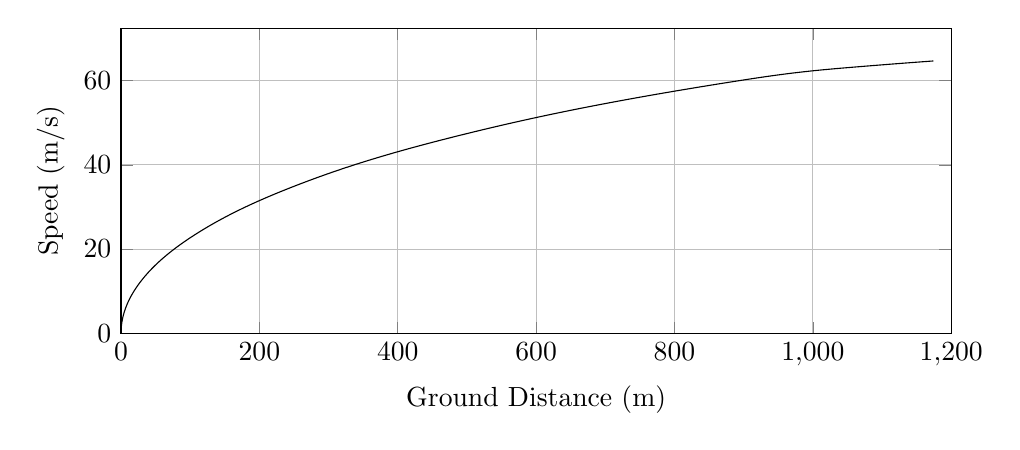
\begin{tikzpicture}

\begin{axis}[
width=\textwidth,
height=0.45\textwidth,
scaled ticks=false, tick label style={/pgf/number format/fixed},
xmin=0.0,
xmax=1200,
xlabel={Ground Distance (m)},
xmajorgrids,
ymin=0.0,
ymax=72.40593682700039,
ylabel={Speed (m/s)},
ymajorgrids
]

\addplot [
color=black,
solid
]
table[row sep=crcr]{
1.3729668748938318E-8	2.745933749757015E-4\\
1.7493248493808052E-7	9.801561244272487E-4\\
1.4411937280317895E-6	0.0028133334263539117\\
6.602995160656227E-5	0.019042785691170537\\
2.2740573828771224E-4	0.03533951742361742\\
4.8751428921765393E-4	0.05174321892135983\\
8.441986619835749E-4	0.06808977660239585\\
0.0012981647037285577	0.0844353365412891\\
0.0018484379050661159	0.10075381131347452\\
0.0024893731755424335	0.11692401404508576\\
0.0032286585096692284	0.13315864947738254\\
0.0040442418752796045	0.1490309460458631\\
0.004972762654474916	0.16525563470227161\\
0.005990910102221513	0.1813857976712797\\
0.007111389191545643	0.19762119246996934\\
0.008336865178450469	0.21397204670389414\\
0.009664633507451486	0.23038152766885184\\
0.011093815858158905	0.24682815127838675\\
0.01262066151120312	0.263265820307077\\
0.01419454386807839	0.2791986545425519\\
0.015910782250193378	0.2955952662747262\\
0.017721549103721458	0.3119619385062512\\
0.019620507964630857	0.3282501310843995\\
0.02164969955342029	0.3448058860985598\\
0.023766550611781796	0.3612690162089588\\
0.025957065600157342	0.3775498524463491\\
0.028260861173784894	0.39394719674836465\\
0.030668466949245715	0.410383707902753\\
0.0331489614440674	0.4266559078198039\\
0.03573888453685943	0.44300840396891283\\
0.038418765463712895	0.45931623269011934\\
0.04116679597872082	0.47545806081684927\\
0.044022059812866554	0.49166851394108313\\
0.04700053365173311	0.5080273423779957\\
0.050116649382181494	0.5245961664609897\\
0.0533021652593606	0.5410095070500209\\
0.056630220296749106	0.5576412582238173\\
0.05998688030085898	0.5739277187039493\\
0.06348077825220624	0.5904027942398575\\
0.06710848437295475	0.6070355888921957\\
0.07082346760424127	0.6236086695802725\\
0.07462944469130567	0.6401425932771283\\
0.07855413323217031	0.6567561544391656\\
0.08251243142992878	0.6730964799422352\\
0.08659905947434482	0.6895601384027192\\
0.09083545394947079	0.7062217948484368\\
0.09518096637774642	0.7229134142824443\\
0.099604438418047	0.7395173119645533\\
0.1041130762071252	0.7560654102385658\\
0.10871457033213175	0.7725885970010864\\
0.11350280915994052	0.789414897207366\\
0.11836943512882261	0.8061564986927878\\
0.12328542045494376	0.8227217321804843\\
0.12830372217771202	0.8392942075725671\\
0.1334037067999082	0.8558073214904485\\
0.1386015897371753	0.8723154406793838\\
0.14405085578552257	0.8892925587093323\\
0.1495239325759128	0.906023300154549\\
0.1550507392415454	0.9226100529817982\\
0.16073360491635535	0.9393593896808448\\
0.16659871679960742	0.9563378698222822\\
0.17244819595229793	0.9729756148686326\\
0.17848031195343078	0.9898395443790766\\
0.18466822548212042	1.00684512125021\\
0.1909009608611748	1.023687878666769\\
0.19716089737688902	1.0403292487664908\\
0.2035279375926986	1.056986144772044\\
0.21017879584430066	1.074109246904928\\
0.21687473998771628	1.0910764957758898\\
0.22354650324940833	1.1077235265509446\\
0.23036941414946865	1.1244923431428457\\
0.23737731412185503	1.1414588704693824\\
0.24449289925428264	1.1584313614920383\\
0.2517184892023243	1.175414947859407\\
0.25908208279438383	1.192473531314623\\
0.2664863589195283	1.2093832274856608\\
0.27399321582905467	1.2262886274661136\\
0.2816108016888421	1.2432078594095262\\
0.2893844725195981	1.2602390433086605\\
0.29747621078120867	1.2777253594880231\\
0.30547198304033185	1.2947717452431249\\
0.31373479402345694	1.3121541775007652\\
0.3220909744202328	1.3295012966106468\\
0.3305540912568814	1.3468420668133918\\
0.33895489345894936	1.3638365024108157\\
0.34753073012810576	1.3809686983503315\\
0.3563589175375672	1.3983851403981644\\
0.3652744752958731	1.4157558589432995\\
0.3742693918027593	1.43306717314297\\
0.38350989122680823	1.450635335748475\\
0.3927029292363896	1.467903957895163\\
0.4020876366599533	1.4853248556951635\\
0.4115568217121528	1.5026971903559407\\
0.4212787852930122	1.5203260447095182\\
0.43089755178065414	1.5375681624257411\\
0.4408379299669313	1.555185213830348\\
0.4510502611115679	1.5730780261575021\\
0.4612670224725215	1.5907764641960198\\
0.4715818614584312	1.6084464929996969\\
0.4818438670126082	1.6258347036069667\\
0.4922128554044626	1.6432165605672906\\
0.50273876067117	1.6606746260618541\\
0.5136516607865718	1.6785820531452376\\
0.5244310074213006	1.6960839321955912\\
0.5355751508210329	1.7139894155460103\\
0.5467126997993474	1.731698516530209\\
0.5580479056656631	1.7495370212026495\\
0.5692960823995112	1.7670597423659236\\
0.5809945926573021	1.78510068535335\\
0.5923626544035139	1.8024582108612397\\
0.6041922852715	1.8203439176489105\\
0.6160912669048675	1.8381580505356934\\
0.6280605196746807	1.8559040150004549\\
0.6403946506485891	1.8740142553801205\\
0.6525721787971039	1.8917235842909679\\
0.66504690021022	1.9096939250266787\\
0.6773535438897555	1.9272570708284058\\
0.6901462526606317	1.945344891624475\\
0.703249873273524	1.9636986239503091\\
0.7159721017112175	1.981354570722634\\
0.729053467210389	1.9993454121544838\\
0.7422988791228431	2.0173974409387396\\
0.756304272979474	2.0363101373314\\
0.7696432036294076	2.054159974410436\\
0.7832290250230658	2.0721811688782967\\
0.7969128825551131	2.0901743623702957\\
0.8108444209446342	2.1083344818020304\\
0.825043936786227	2.1266833129613296\\
0.8390802275180445	2.1446659237513304\\
0.8532340040587583	2.1626466350356415\\
0.8678101043696134	2.1810078755052817\\
0.8824320602344964	2.1992718056031553\\
0.8978006605470081	2.2183051377968805\\
0.9134572487531922	2.2375274698967402\\
0.9287391767029982	2.256130737471988\\
0.9440564687433697	2.2746232653161487\\
0.9598871644713316	2.293577785375984\\
0.9757786228365237	2.3124476251369854\\
0.9918217338879218	2.3313414354625053\\
1.0080608846667363	2.350310244973776\\
1.0245900975307913	2.369460702886954\\
1.040622085070809	2.3878871944178703\\
1.0571005809273983	2.4066786687919777\\
1.0736578999152901	2.4254121931867534\\
1.0902401336450098	2.444028796579393\\
1.1073201062866707	2.4630558575727797\\
1.1241926772552646	2.4817074203845095\\
1.1416781667104252	2.5008884842005994\\
1.1588269484070954	2.519557115943438\\
1.176440946845327	2.5385880024942766\\
1.1944819542445066	2.557932148965393\\
1.2120125629913447	2.5765886382913967\\
1.2299306574276825	2.595517639375487\\
1.2481120482032448	2.614583405444348\\
1.2663536608165091	2.633572296542063\\
1.2851425782117465	2.652987459389303\\
1.3041313368869671	2.6724644260610546\\
1.3228236880779458	2.6914983494361895\\
1.3414329672940513	2.710313579664695\\
1.3605066144349074	2.7294623649521776\\
1.3802534409605212	2.7491450260300265\\
1.3994872719307283	2.768180425465\\
1.4192016277101378	2.7875550833166374\\
1.439023460648384	2.806899110882914\\
1.459347998039509	2.8265947929306874\\
1.4793256644936217	2.8458200550486863\\
1.4991489338326072	2.864767809480229\\
1.5195196572175793	2.884107715811661\\
1.5402684478761244	2.903672651533622\\
1.5604570108688036	2.9225821793605533\\
1.5810331069622228	2.9417281799743202\\
1.6022712329181132	2.9613588693312414\\
1.623752316257296	2.981081088586241\\
1.6452514305955401	3.000688534053265\\
1.6664829631402025	3.0199255047213613\\
1.6886446033619715	3.039873778995527\\
1.710607384244656	3.0595131625849623\\
1.7329417009553727	3.079354734333231\\
1.7551421266962821	3.0989498821582195\\
1.7779085356585536	3.1189151163488686\\
1.800478286927734	3.138580922227405\\
1.8236018329231238	3.158600640902775\\
1.8462320784511883	3.178069573313743\\
1.869621217116264	3.198065190585111\\
1.8933146512119747	3.218192588484756\\
1.9176856041472643	3.2387632751638957\\
1.9417713639512164	3.258963928974107\\
1.9657098573982132	3.2789160602383687\\
1.9902165007163162	3.299215000456961\\
2.014554050520948	3.319249296721013\\
2.039479559407779	3.3396412488944405\\
2.0645497069116256	3.3600249047064397\\
2.090368502766882	3.3808869458562745\\
2.115564185269416	3.4011203262020633\\
2.140750230554602	3.421224607682783\\
2.1667677015838267	3.441867410014254\\
2.1927560352542175	3.4623623770407628\\
2.218891869133375	3.482850184369502\\
2.245288939563828	3.5034192934486885\\
2.2712530964452817	3.5235321150782903\\
2.297933078351498	3.544078676912\\
2.324564104516777	3.5644675622649844\\
2.351466051806102	3.584944255791985\\
2.378869922986878	3.6056815089832\\
2.4061764715670764	3.6262252420255647\\
2.4343811693482102	3.6473212111172773\\
2.4622108821536663	3.6680158200226414\\
2.4906408044048067	3.689034880037064\\
2.518892760285042	3.7098024045211524\\
2.5472153538550346	3.7305038371011454\\
2.5762492306032216	3.751604556392463\\
2.605385308804288	3.77265885975738\\
2.634725531238531	3.793740545947773\\
2.6633424112287507	3.814188269376828\\
2.6927188130915374	3.8350632832649136\\
2.7226962917814213	3.856246846509716\\
2.7531675915664673	3.877658627570839\\
2.7831412651501983	3.8986039132076407\\
2.8139174932165103	3.9199914284852095\\
2.8440331768075415	3.940805463831844\\
2.874693215323904	3.9618812954722067\\
2.9059978681586376	3.983283017717028\\
2.9372617813709034	4.004540567062701\\
2.9684444504378202	4.025628922378527\\
3.000072782687808	4.046904250267042\\
3.031082587373527	4.067653380618779\\
3.063213028467148	4.089039106139634\\
3.0965739711585014	4.111123799299039\\
3.1291175748240176	4.132551436526409\\
3.161651640649506	4.153860091747873\\
3.194791488147139	4.175451451278743\\
3.2273698640351327	4.196566512811529\\
3.261394174200582	4.218503584793469\\
3.2942820372415875	4.2395978181219345\\
3.3276455142443044	4.26088817859155\\
3.3625338428565543	4.283036024158147\\
3.396526624461681	4.304503432160644\\
3.4305511850311694	4.3258819528145285\\
3.4642094416894933	4.346924644244828\\
3.498963551783903	4.368543784473827\\
3.5341885134496573	4.390344825173816\\
3.569804025802995	4.41227566137831\\
3.605116576002147	4.433910483656753\\
3.641338581546833	4.455990935222921\\
3.677593698357855	4.477980101320377\\
3.7132425573336665	4.499494417793999\\
3.74957219375957	4.52131186791552\\
3.7872650227149185	4.543834709491012\\
3.825403000593508	4.566507875425231\\
3.861987998097706	4.588150051796694\\
3.899535703755137	4.610253615889045\\
3.9366960368382165	4.632022848447335\\
3.9756271117991435	4.654717625207532\\
4.014715979923002	4.677390959293206\\
4.053268843133694	4.699643665819206\\
4.093111596873367	4.722528057282259\\
4.132540645872048	4.745063532854312\\
4.171686416589186	4.767329139268224\\
4.211258480423352	4.78972942073012\\
4.252585425594734	4.813009023273391\\
4.29253892845542	4.835405747759294\\
4.332839968385603	4.85789005261978\\
4.372708537789018	4.8800285666982735\\
4.414379330316386	4.903058272049913\\
4.455607216042212	4.925734525068886\\
4.497336690654009	4.948578120665225\\
4.53836773335787	4.9709343699274005\\
4.579767142935065	4.993387236550703\\
4.621942908118227	5.016155098789904\\
4.663798268780793	5.0386455998057755\\
4.705838036060712	5.061131913160432\\
4.748491012675066	5.083841859474553\\
4.791393968819099	5.106580280460207\\
4.835700194867293	5.12995378398521\\
4.879973298406089	5.153201037889401\\
4.923250156511948	5.175821498471649\\
4.967673596314626	5.198936085329022\\
5.012954369117542	5.222388563932281\\
5.057574526249477	5.245393459549955\\
5.103280208347517	5.268850968793279\\
5.148856018935929	5.292135378554356\\
5.194350575362858	5.315273669954703\\
5.240584094986199	5.338682132187644\\
5.2871741484687504	5.362164780261091\\
5.333122064003502	5.385220599260908\\
5.3803318800233235	5.408804293294599\\
5.4262712259485255	5.4316521648593366\\
5.473378197958581	5.454978474320454\\
5.521938593493333	5.478917479721449\\
5.570027890245774	5.502518579191591\\
5.617746353771608	5.525835087825929\\
5.665750363096816	5.549189321818824\\
5.714883880069209	5.572988680831415\\
5.763390205677501	5.596381969534493\\
5.812817811268989	5.620116370443503\\
5.861909274803731	5.643587555330178\\
5.912134919389196	5.667497332952465\\
5.962317560553064	5.691283238887795\\
6.012727788730279	5.715074271653515\\
6.0628236035803145	5.738616176082424\\
6.113711068416594	5.762428568577636\\
6.16497292765713	5.786313975860049\\
6.216284706244114	5.8101212146122965\\
6.26834407822653	5.834172897359418\\
6.320257064476769	5.858055495044951\\
6.37351660191279	5.882453594702493\\
6.426150862197664	5.906463071475246\\
6.479030963436509	5.930483658358424\\
6.532319340056288	5.954588513514302\\
6.5857233987986845	5.978645031005438\\
6.640834734692348	6.003366249566406\\
6.695022999498724	6.027571315668311\\
6.749720237657193	6.051902328312192\\
6.804235758325081	6.076052362501423\\
6.859728469301633	6.100533845085355\\
6.916686079588434	6.125556455229262\\
6.9732530286722305	6.150303315061631\\
7.029531186664631	6.174822114436326\\
7.086633318514238	6.199597449617537\\
7.144155485034537	6.224451953805524\\
7.202053129566568	6.249365490174972\\
7.260126434764185	6.274251852506023\\
7.317913145042743	6.298914465249707\\
7.376682960996439	6.323894618455785\\
7.435393721764624	6.3487481490973465\\
7.493838107271518	6.373389329329468\\
7.552684475254578	6.398100782617156\\
7.613252707151423	6.423432563785438\\
7.672782806866918	6.448229800859755\\
7.733397683408512	6.473377876879928\\
7.795525081709004	6.499048935993182\\
7.856013653786727	6.523942353509447\\
7.91792172269443	6.549318504073016\\
7.980110745884113	6.574707701783742\\
8.041720670752433	6.599760731132271\\
8.105229267009985	6.6254831303952955\\
8.167457523036095	6.650587002051729\\
8.230908874360502	6.676083591946034\\
8.293738919282273	6.701231482743458\\
8.356235402336917	6.726149209696938\\
8.42092378244627	6.751840487425259\\
8.485671322837007	6.777454186510756\\
8.549180898871484	6.8024810353832805\\
8.614596634551038	6.828159619110403\\
8.680166762249144	6.853798712400334\\
8.744770128469462	6.878962882922066\\
8.812993689385827	6.90543395378895\\
8.88005807777586	6.931353078752458\\
8.94709863067661	6.957162896659991\\
9.013172088448385	6.982503570963587\\
9.079266506338545	7.007757184272014\\
9.14748814890141	7.0337249243337485\\
9.215411293660388	7.059480591882142\\
9.284579146198691	7.085608412719667\\
9.353168277381275	7.111419259094388\\
9.423753765537143	7.137880229826159\\
9.492960052876374	7.163725683018036\\
9.564123004975215	7.190201309556587\\
9.634097601479446	7.216136500000127\\
9.705672410878787	7.242565047756237\\
9.776260200085993	7.26853143726553\\
9.846607984572056	7.294314058359657\\
9.918231435410593	7.32046734992541\\
9.988851555070422	7.346159615601438\\
10.060390022634245	7.372091182386127\\
10.133279281833644	7.398415309816031\\
10.205241085147751	7.42430939070986\\
10.277820389603	7.450330988479372\\
10.352558894167803	7.477028413890535\\
10.42733258664746	7.503639671954019\\
10.501815126481194	7.530050188575258\\
10.576858173457808	7.556562476642339\\
10.65303812840548	7.583377933408709\\
10.729080272001735	7.6100469771700165\\
10.804841544893105	7.636521282951211\\
10.881905013502095	7.663353138591718\\
10.958396790746043	7.689889741790379\\
11.035905069829102	7.716682266611455\\
11.113160538490881	7.743291537725936\\
11.192172636140572	7.770407901336807\\
11.270076562295213	7.797047997270166\\
11.350065490058778	7.8243029997830895\\
11.429008826667825	7.851105320694458\\
11.50754237847364	7.87767447630535\\
11.587076645554472	7.9044875894302\\
11.668897725768986	7.93197334092549\\
11.749734371708193	7.9590315134803795\\
11.830312384681939	7.9859082812388404\\
11.909862670519033	8.01235032822278\\
11.990515423105418	8.039066540264908\\
12.072973931530203	8.066285822915322\\
12.155304175892073	8.093367836765307\\
12.237018674011615	8.120154471944652\\
12.320146069843414	8.147310337497665\\
12.406770618003886	8.175508889111107\\
12.489918686423398	8.202480979041646\\
12.574493004618496	8.229821467227936\\
12.660666896522624	8.257582277972531\\
12.746500366216402	8.28513731475353\\
12.832006837122272	8.312492980707578\\
12.919285437479463	8.340319422765806\\
13.00517529032821	8.367609209154548\\
13.092301899261269	8.395197755453601\\
13.179760097773386	8.422796850479578\\
13.268594687119744	8.450734398982132\\
13.357699529172354	8.478660840283151\\
13.44829753340392	8.50695758308525\\
13.537570218252604	8.534745028816864\\
13.627322718831184	8.562587370122476\\
13.718307212496544	8.590716196341472\\
13.808540263830096	8.618518503292734\\
13.899143852161355	8.646341531112757\\
13.991564069206362	8.674626907467385\\
14.085798171937814	8.703369108515862\\
14.179213507883688	8.731764584716228\\
14.271883316076963	8.759838983451804\\
14.367546274622434	8.788722461837416\\
14.459430863676705	8.816372617521623\\
14.555010173556813	8.84503935781289\\
14.648669731311681	8.873037028493652\\
14.743773575674254	8.901372887177772\\
14.839769774519894	8.92987995995896\\
14.932807148196385	8.957418513450865\\
15.026921440816679	8.985186697775877\\
15.12275113649265	9.013369781181584\\
15.222025232743288	9.042469720903732\\
15.321078842653048	9.07140849270197\\
15.417564225728565	9.09950514796304\\
15.515758841369038	9.128007419530377\\
15.613440509090129	9.156269491650061\\
15.7107260301154	9.184327297639449\\
15.81102223487273	9.213160640553841\\
15.913565872734136	9.242543656282287\\
16.012918321571746	9.270920177846005\\
16.11222833737955	9.299194878466079\\
16.216250800242257	9.328716023710864\\
16.319159023020546	9.357825988089104\\
16.421418004006803	9.386659645595689\\
16.521675247646563	9.414840066488026\\
16.62557290942481	9.443951838886342\\
16.72731964230514	9.472371127221127\\
16.830283223934416	9.50104069128232\\
16.93464251494634	9.530007766659548\\
17.038481620468637	9.558740267646716\\
17.146497421123335	9.588533916314098\\
17.252282308638982	9.617619657360787\\
17.35724772858778	9.646390408399203\\
17.464053904588297	9.675574876517068\\
17.572390862630144	9.705084909493728\\
17.680417629270814	9.734418351955906\\
17.789707298693855	9.76400202339044\\
17.899612520762552	9.793659182664925\\
18.01027367065641	9.823426854718555\\
18.121415095654797	9.853230213992497\\
18.232428503320143	9.88290658253214\\
18.34337337506409	9.912472977805535\\
18.454877340220463	9.942096916719443\\
18.56636189702322	9.971624895785052\\
18.678405595805643	10.001210341704514\\
18.7903363416971	10.03067608506613\\
18.902391384512768	10.060085398853307\\
19.01754810908954	10.090216685111244\\
19.131359562866663	10.119905120061443\\
19.247747682986713	10.150173154594743\\
19.361628242251975	10.179699333687509\\
19.477963464454028	10.209771140606378\\
19.595742742603164	10.240123605476668\\
19.71107288142779	10.269755440962637\\
19.82767543183723	10.299625023945445\\
19.944540068808188	10.329472599192002\\
20.06171535440768	10.359310730329746\\
20.179291418887807	10.389162371290585\\
20.29729887224694	10.419035161231573\\
20.417200571824914	10.449297609200816\\
20.53676390826074	10.479385286812665\\
20.65523768803314	10.509111551895497\\
20.777063017363922	10.539589025343918\\
20.896922101876633	10.569486607360407\\
21.016777952410983	10.59929689912131\\
21.13892104879462	10.629587893976428\\
21.260534693274344	10.659659948300135\\
21.382619708556632	10.689761392841646\\
21.506306369043365	10.720169476482468\\
21.631260758247265	10.750799829562194\\
21.75556249187227	10.78118184657318\\
21.87985606458615	10.811474550266158\\
22.005925835680863	10.842111749382909\\
22.130365724585275	10.872266329955558\\
22.257477980325966	10.902980523463068\\
22.38418119026224	10.933508198941738\\
22.50885833858638	10.963463025080845\\
22.636026948728087	10.99393066519372\\
22.76367325110224	11.024426399233274\\
22.89115382514759	11.054796953305566\\
23.022452271734288	11.085988446217733\\
23.149877274293033	11.116174529071358\\
23.27873580881144	11.146615583230105\\
23.408563766880334	11.177200342965577\\
23.538692653979794	11.20777082157792\\
23.671258756997098	11.23882694940632\\
23.803210122669313	11.269652718824766\\
23.93544283576786	11.300458555208255\\
24.067241518013077	11.331078692350477\\
24.19863541429976	11.361521460060182\\
24.329449967727697	11.391748060477795\\
24.46175612159181	11.422236868308769\\
24.594763714591892	11.452804456271778\\
24.72754053098891	11.483236854143666\\
24.86208223890334	11.513990756634719\\
24.99503410474967	11.54429986857128\\
25.12831230627787	11.574602871369095\\
25.265273024090206	11.605659896100171\\
25.400650037308893	11.636275573882461\\
25.536304655026747	11.666872730586064\\
25.673594178904246	11.697756485990315\\
25.80797730935859	11.727907070402154\\
25.835159569235522	11.73399627175068\\
25.83771752397454	11.734569125111406\\
25.84157983658004	11.735434035751847\\
25.854829339215996	11.738400588018216\\
25.893215796826965	11.74699102336189\\
25.973046119315796	11.764835870261674\\
26.096262980671412	11.792325687828392\\
26.224212718725603	11.82080317243156\\
26.35313595194755	11.849427449898315\\
26.481727686355264	11.877908705901316\\
26.611118169629577	11.9064973458457\\
26.74049186039369	11.935012993558825\\
26.87228140714948	11.963990356182965\\
27.003385008924262	11.99274648315194\\
27.1358830905183	12.021737581499828\\
27.265951877034226	12.050128265319604\\
27.399105426781233	12.079122042396705\\
27.53075869079712	12.107719723687051\\
27.66387879779476	12.13656630303236\\
27.79855889054391	12.16568002797267\\
27.932132547760695	12.194484591940203\\
28.06791767232785	12.223695071478268\\
28.202763022922632	12.2526330170029\\
28.339788243013793	12.281967392546672\\
28.476803106655623	12.31122807503452\\
28.61761981788422	12.341226680006773\\
28.753907949775353	12.370189579780149\\
28.89297195746854	12.399670893910589\\
29.03211749902605	12.429097676262618\\
29.17123509789927	12.458447191983321\\
29.312253051611236	12.488125270685916\\
29.454422317169097	12.517972384162682\\
29.59523538430127	12.547462726859035\\
29.737672170826222	12.57722064139389\\
29.879173197948965	12.606711335627043\\
30.02075470454991	12.636147711288835\\
30.166674235301365	12.666412071579277\\
30.308336095430334	12.69572202636622\\
30.452640844036836	12.725506988251436\\
30.597553881025625	12.755345032695217\\
30.742967061600154	12.785213522931606\\
30.888975484926362	12.81513163569263\\
31.034653067922946	12.844909872444937\\
31.180984070508003	12.874749646110697\\
31.328351020411645	12.904728171012607\\
31.476753455192622	12.93484428420285\\
31.62661541983664	12.965182661219465\\
31.774495604492607	12.995047482306948\\
31.924944104961916	13.025357687313338\\
32.07610067279926	13.055736566071463\\
32.22631826848556	13.085853737222568\\
32.37899942625752	13.116390732232041\\
32.528514827654206	13.146222623463562\\
32.68189139400266	13.176751411464863\\
32.836069829938495	13.207365260539305\\
32.99025509482905	13.237906193269861\\
33.14574197930297	13.268630209976319\\
33.30072558931056	13.299180562552802\\
33.455047097713944	13.329527242510189\\
33.610874563168906	13.36009645326342\\
33.76926068144728	13.39109228290279\\
33.92617323250643	13.421725333324364\\
34.08448787244542	13.452557525934765\\
34.24243160505006	13.483243305231298\\
34.40316487172558	13.514395458139187\\
34.56154208099588	13.545016867333096\\
34.721775177117024	13.575922712961361\\
34.88076970836556	13.606516167760788\\
35.041349106451236	13.637340735353845\\
35.20329621413198	13.668353154199892\\
35.364886328651124	13.69922291645766\\
35.529241615711214	13.73054528100413\\
35.69117991651797	13.761332873455665\\
35.85317319416103	13.79205773921191\\
36.014854298354294	13.822650866688232\\
36.18095311277159	13.854004920809285\\
36.34443322746766	13.884790898996187\\
36.51065106768533	13.916017890389313\\
36.67635767082788	13.947074482992182\\
36.842033683894186	13.97805158435235\\
37.00823867836148	14.009053944726826\\
37.17279029188734	14.039675677937577\\
37.33951104811075	14.070628233971537\\
37.50923941781488	14.10206432221781\\
37.679358776579846	14.133497520068453\\
37.845326083883435	14.164091329346522\\
38.017144746304325	14.1956890876533\\
38.1852030886141	14.226522279602513\\
38.35804431104914	14.258158097238443\\
38.52812920813831	14.28921574848194\\
38.69960796987526	14.320454401926607\\
38.87165793928378	14.351723379523964\\
39.0423941506003	14.38268102295195\\
39.21436971822614	14.413790751604473\\
39.38727999643966	14.444996521239876\\
39.558989012313546	14.475913453003397\\
39.734752343022535	14.507486480729824\\
39.908836167348156	14.538684565707165\\
40.084555009291705	14.570102192940322\\
40.259186798753746	14.601252770423791\\
40.43324437115375	14.632229247915411\\
40.61041052363379	14.66368591114869\\
40.787318094191775	14.695023582621097\\
40.96620398302343	14.726637892031388\\
41.14141336180775	14.757530947321776\\
41.31941103282654	14.788843608684214\\
41.49571226203258	14.819786704093303\\
41.67366972437729	14.850949124251486\\
41.85219319429197	14.882139047575382\\
42.03136872634711	14.913371205615714\\
42.21293422072888	14.944947136872095\\
42.39366932880948	14.976306290625715\\
42.57479521797359	15.007661248963057\\
42.75522531040919	15.03882452217935\\
42.93775785970641	15.07027901101005\\
43.11993568316029	15.101600682690702\\
43.30336620712447	15.13306580140896\\
43.48720879745599	15.164529618027455\\
43.672226884455625	15.196122289886826\\
43.85684130549208	15.227574146465127\\
44.039851952877484	15.258682320644418\\
44.22449378650157	15.289997095679201\\
44.412385508552646	15.321790608155712\\
44.59783063297877	15.35309890605317\\
44.78525507043919	15.384669902907206\\
44.973130075825196	15.416245120448252\\
45.16145211071871	15.4478238768376\\
45.34881478087516	15.479171053194221\\
45.536017136752506	15.510421384177157\\
45.724971990057284	15.54189370268887\\
45.91416212467789	15.573334602482515\\
46.10175434018815	15.604440599130726\\
46.29356928918713	15.636175810787584\\
46.48490977712943	15.667761433505884\\
46.67744207882204	15.69947255071358\\
46.869905949194575	15.731101389522046\\
47.062749521718516	15.762721841107386\\
47.25341437235973	15.793915796374279\\
47.44508461154423	15.825205238524163\\
47.63880095964302	15.856758814343422\\
47.83356160493736	15.888412077854802\\
48.025334057720784	15.919511103737413\\
48.218846636819876	15.950823735261029\\
48.41468711090302	15.982443311473421\\
48.610449575687724	16.01398058830579\\
48.80723286029129	16.04561249117431\\
49.00124137999302	16.076730225673515\\
49.20045899041696	16.108613469004666\\
49.394243884198005	16.139559590609927\\
49.59161211700324	16.17100975835519\\
49.79144608231523	16.202783130131834\\
49.99107345578199	16.23445403109276\\
50.18996871950735	16.265939978911277\\
50.388458331230495	16.297293637193356\\
50.59191110395449	16.329361114702195\\
50.79453916783869	16.361228411152567\\
50.99530158869649	16.3927336124352\\
51.19776583381373	16.42443703723646\\
51.3996255264899	16.45597737097976\\
51.599450409211	16.48713285962996\\
51.80158475775707	16.518581084428426\\
52.002311498730975	16.549743669984224\\
52.2060805474067	16.581311029937034\\
52.40811442127868	16.612542781175982\\
52.61423073460446	16.64433747071798\\
52.821749674584495	16.676279383846385\\
53.03053110951893	16.708346019233034\\
53.23753590773735	16.74007125225181\\
53.44487707917263	16.7717800272353\\
53.652063533093525	16.80339754071838\\
53.85975522429668	16.835024719859476\\
54.06844148636836	16.866735735918397\\
54.278580968983874	16.898599481048315\\
54.48685885904548	16.93011390802227\\
54.69884126905886	16.962120720521014\\
54.90975544393264	16.993898405991033\\
55.12216013841277	17.02583267040511\\
55.333080623240974	17.057476656010834\\
55.5448885814986	17.089186849928865\\
55.75594910746132	17.120718798734273\\
55.968144975063936	17.15235397919561\\
56.18150915317635	17.184096602192163\\
56.394069348356695	17.215653451067624\\
56.60950747146016	17.247570555005474\\
56.82641599949238	17.2796377393909\\
57.03980213394583	17.311118216005376\\
57.25698083573829	17.34309140361224\\
57.47353804711997	17.37490637544135\\
57.6941706582635	17.407251949021614\\
57.91229938529948	17.439163234249854\\
58.12998527173144	17.470943490423387\\
58.34905943653719	17.502859991071126\\
58.56781345824973	17.534663729273177\\
58.787998582886644	17.566609184333608\\
59.011266007804366	17.598934253781984\\
59.23368761368569	17.63106958619902\\
59.456031473365414	17.66312695350576\\
59.67976581221534	17.69531783422297\\
59.90315377467765	17.72739224145881\\
60.125192111546724	17.7592072579533\\
60.349269227196444	17.791248463842905\\
60.57220932044149	17.823061717762613\\
60.79606803632835	17.85494082328129\\
61.021718319759984	17.887009278121397\\
61.25073295331903	17.919488713415852\\
61.47770893732542	17.95161265849601\\
61.70784367826464	17.984116595017582\\
61.93740803875056	18.016473074293522\\
62.1673491775543	18.048816062463573\\
62.39648011888062	18.080979167027678\\
62.62822464633953	18.1134425841339\\
62.86094183422966	18.14597528176636\\
63.090532789209604	18.17800555500485\\
63.321616049163225	18.210178806265958\\
63.554808975015874	18.2425798333092\\
63.78685818650332	18.27475655714074\\
64.0234762327251	18.30750002514708\\
64.25652029988498	18.33968337934492\\
64.49146565301734	18.37206383313017\\
64.72768747885678	18.40455431710828\\
64.96568125142531	18.43722208040868\\
65.20057601391298	18.469399445717087\\
65.43975061379945	18.502097099487123\\
65.67719429610031	18.534492627051662\\
65.91652243006087	18.56707960207529\\
66.1565253585166	18.5996926382046\\
66.39740384038885	18.632358754662555\\
66.63777997854328	18.664891313089214\\
66.87849958303539	18.697405223005703\\
67.12349409848125	18.73042999909198\\
67.36843544137562	18.763380883708052\\
67.61129947098183	18.79598682368536\\
67.85808619273692	18.829052988970048\\
68.10323725880951	18.861834089804688\\
68.3520146383799	18.895033326535575\\
68.60099753692072	18.92819303649258\\
68.84943315800746	18.961213484704757\\
69.09793111574629	18.99417627309159\\
69.34894754058863	19.02740655741996\\
69.59791912239118	19.060300425142366\\
69.84867626946473	19.09336442916495\\
70.10496107302816	19.127089481532906\\
70.35594730130109	19.160051229394938\\
70.60854748652795	19.19315932239791\\
70.8625286964371	19.226382441854668\\
71.1182576034713	19.259767715003406\\
71.37278964945165	19.29293089942211\\
71.62944082734805	19.32630406482957\\
71.88536754710964	19.359517292895546\\
72.14250945057543	19.392822496273666\\
72.40306402213687	19.426502900877068\\
72.66241221953337	19.459960968561703\\
72.92327110344874	19.493547495197788\\
73.18657203154456	19.527381274712283\\
73.45150557123125	19.561357130932635\\
73.71756195569753	19.595409033703262\\
73.97940051906463	19.628855014795015\\
74.24514793127645	19.662733645739877\\
74.51022759525631	19.69646065179441\\
74.77823256031297	19.730492733691676\\
75.04767613410795	19.764639862321353\\
75.31682895458664	19.798682839904423\\
75.58729746777243	19.83282486882524\\
75.85729327570917	19.866840277363707\\
76.13042767774209	19.901183443118022\\
76.40299665611133	19.935388078099322\\
76.67973301409052	19.970047169137942\\
76.95360383527739	20.004279819891543\\
77.22854206589327	20.03857869965745\\
77.50692063517303	20.07323858302778\\
77.78349662592461	20.10760649808084\\
78.0616064362213	20.14209753746679\\
78.33869545141144	20.1763950938769\\
78.62238552181594	20.211440965650013\\
78.90481169871467	20.24626202165907\\
79.18659077494928	20.28093541680736\\
79.4700201012688	20.315743893615732\\
79.75774957869095	20.35101116003014\\
80.04430580185078	20.386065626630675\\
80.33432201731404	20.421473679433355\\
80.62298533865851	20.456647379404394\\
80.9130804606989	20.491926439940222\\
81.20459144967842	20.527308330795158\\
81.49650140842283	20.56266940610589\\
81.79224544448738	20.59842470694941\\
82.08455487090956	20.63369573876311\\
82.37934996819865	20.669197627691325\\
82.67580145620735	20.704829475042132\\
82.97475550983006	20.740691955762657\\
83.2734238134004	20.776450240135105\\
83.57209772503273	20.812139744436564\\
83.87419166445906	20.84816770961431\\
84.17487194816226	20.883957404334772\\
84.47686996876752	20.919834414394003\\
84.78124993153034	20.955924325155635\\
85.08776945017104	20.992197276981145\\
85.39395758722245	21.02836068428524\\
85.69833162305892	21.06424060145197\\
86.01027818388755	21.10094200721906\\
86.31658691867341	21.1369104477143\\
86.62866814828641	21.173486190018266\\
86.94043673469176	21.209954654227438\\
87.2565990672368	21.24686542847371\\
87.56980823017452	21.283360753692115\\
87.88101387141376	21.319553399962942\\
88.20007062892054	21.356587936407273\\
88.51883409355145	21.39351692360224\\
88.83509784148416	21.430086138443315\\
89.15857089898353	21.467417114986695\\
89.47772213402055	21.504178581674047\\
89.80217214804901	21.541478831424143\\
90.1263587278685	21.57867720574783\\
90.44950966725051	21.615685993222307\\
90.77764749859728	21.6531940920381\\
91.10470504824352	21.690507175653025\\
91.43769785174896	21.728424510189086\\
91.76691749028419	21.76584038250263\\
92.09386993524024	21.802928381010865\\
92.42498248438446	21.840417446490633\\
92.7581696617394	21.878069923542576\\
93.09729153734631	21.916319922463096\\
93.4312406900703	21.953914858292585\\
93.76780571708736	21.99173285047641\\
94.10390054156983	22.02942692654632\\
94.43564317419558	22.06656369502685\\
94.77291201930262	22.104249088529684\\
95.10796951504997	22.141617965961636\\
95.44708659079325	22.179369616185113\\
95.78515592548297	22.21693500898585\\
96.12311752311894	22.25441941592539\\
96.46351490415591	22.292104698232542\\
96.80669869710772	22.3300285453495\\
97.14657639264556	22.367518321886216\\
97.48763116340677	22.405069645423985\\
97.8305814261901	22.442761153568917\\
98.17013304046878	22.48001190327186\\
98.51054009051404	22.517289795639208\\
98.854181194619	22.554854559155295\\
99.19205317796005	22.59172320250834\\
99.53355440060989	22.62892233881538\\
99.87198375587872	22.665722299003313\\
100.2129389915628	22.702732356613758\\
100.55335806642802	22.739619996254845\\
100.89503335592528	22.776579664164977\\
101.23693480167049	22.813499947259317\\
101.57977298927813	22.85045767969963\\
101.91842351185082	22.886901772645338\\
102.26214655705948	22.92382894310154\\
102.60487134933112	22.960586290281327\\
102.94238410388857	22.996723981096395\\
103.28139950825951	23.032962360222697\\
103.61984226602698	23.069079740693134\\
103.95406402656286	23.10468843221104\\
104.29248504574807	23.140685938011636\\
104.63112914593611	23.176648550978555\\
104.96686613984221	23.21224493209361\\
105.30464484937244	23.248000378665942\\
105.64180205248229	23.28363298897959\\
105.97704387437452	23.319007030416692\\
106.31384964552919	23.354490090585088\\
106.6489228444834	23.389735279509587\\
106.98000007373659	23.424506281561648\\
107.31456925364313	23.459589981309648\\
107.38092108752608	23.466541363878086\\
107.387754025128	23.467257099501225\\
107.3946577511588	23.46798022723023\\
107.39916951903444	23.468452797962527\\
107.40247473215817	23.46879898574781\\
107.40548301099807	23.46911406808625\\
107.41901751964124	23.470531597096304\\
107.47756267729525	23.476662275158333\\
107.63696404402117	23.49334596459464\\
107.95668166923352	23.526772291238096\\
108.2571634635643	23.558142805619354\\
108.55996775705782	23.58971203526177\\
108.8616926844802	23.621125120504303\\
109.16669292910967	23.652835034323118\\
109.47218465327785	23.684551608078415\\
109.78023369107405	23.716488732544356\\
110.09061921742381	23.748622520493456\\
110.4007971847821	23.780689204113827\\
110.7125096545017	23.812868671809618\\
111.02874540594937	23.845468211770957\\
111.34670354521654	23.878197785504135\\
111.664908557295	23.910905157489083\\
111.98617551206428	23.94387902880578\\
112.3078797039536	23.976849312687172\\
112.63537393275391	24.01036328057925\\
112.96267359383529	24.04380732340553\\
113.28778388635178	24.07697825406092\\
113.61823593045688	24.11064385213622\\
113.94632344632586	24.144018443943487\\
114.27926944824554	24.177836320485795\\
114.61324422041562	24.211707243102758\\
114.94750338770686	24.245555524461466\\
115.28618013885716	24.27979872704646\\
115.62544260296943	24.314048364325124\\
115.9647508443766	24.34824989577851\\
116.30617149460878	24.382611246087016\\
116.65060078043697	24.41722153358515\\
116.99863777637248	24.452139520588716\\
117.34270613829636	24.48660529239988\\
117.68983788345284	24.521323592816493\\
118.04137408578512	24.556426913310872\\
118.39343387684602	24.591526682448844\\
118.74804854616337	24.62682481479412\\
119.10520175440718	24.66231860103761\\
119.46686684850098	24.69820259415905\\
119.82660492256403	24.733837450261376\\
120.19012449272657	24.769788336901165\\
120.55217592908159	24.805535667784696\\
120.91763124996498	24.841560161595353\\
121.28719248968574	24.877929345962116\\
121.65493622417088	24.914059879912358\\
122.02513489718217	24.950371525725885\\
122.39308995700384	24.986403518342293\\
122.76618799735454	25.022878639482748\\
123.1388017253943	25.059245771617228\\
123.51256311114031	25.095664192513944\\
123.88633794770595	25.132023264584596\\
124.25665874611622	25.167986679226466\\
124.63165231885978	25.20434353030594\\
125.00664173256905	25.240639405832702\\
125.38021625899401	25.276738263515625\\
125.75512563345742	25.312905993994406\\
126.13473977091255	25.349466401351584\\
126.51299085225449	25.385834455766414\\
126.8948287761801	25.422485709803013\\
127.27325883095315	25.458748891394563\\
127.64986999110431	25.494777690064524\\
128.03053456382577	25.531133516992945\\
128.40840086210045	25.56716186098\\
128.78830732782995	25.603324402260185\\
129.16816802858597	25.639422278871514\\
129.55114692916032	25.67575559846579\\
129.92795862154003	25.711444344008036\\
130.30814318938542	25.74739291097285\\
130.68801179162523	25.783251948121\\
131.0673626953399	25.819002777679778\\
131.44707508552267	25.854728461864248\\
131.82575792285303	25.89029844778053\\
132.20466209461676	25.925830588930104\\
132.58549544797154	25.96148471023875\\
132.96520261413826	25.996974747307668\\
133.34413894748724	26.03233452181265\\
133.72638850756363	26.067944714197402\\
134.1049920954593	26.10315725438464\\
134.48538249769342	26.138478022857264\\
134.86277461399203	26.173463147543856\\
135.2402386369938	26.20839807376519\\
135.62109197355238	26.243589217201794\\
135.9996509441208	26.278511321703462\\
136.37968191797512	26.313512189845667\\
136.76120583273502	26.348593251309282\\
137.13951930881296	26.38332258531475\\
137.51840340013064	26.418048052774175\\
137.89819615735314	26.452800474740854\\
138.27485697152616	26.48721077977922\\
138.65420581933705	26.521810923785843\\
139.03531375767642	26.556515364267987\\
139.41296882619503	26.59085002984427\\
139.79422155259	26.6254560585379\\
140.17408835952057	26.659880777501343\\
140.5488076998477	26.693784891902183\\
140.92844631991198	26.728079442550047\\
141.30483696429354	26.762026445558064\\
141.68269541512387	26.796051769604652\\
142.06058279783264	26.830025689762422\\
142.43991695918288	26.864075525800594\\
142.81695502902187	26.897865655135362\\
143.19247254825046	26.931466555436195\\
143.5733885276352	26.965496673517244\\
143.94921103219775	26.99901878303585\\
144.32621366107247	27.03259345649424\\
144.70408630975157	27.066192808823708\\
145.08263595865492	27.099799515801983\\
145.46162624555404	27.13339252320644\\
145.83827879615103	27.16672611867068\\
146.21524500988596	27.20003553147759\\
146.5934755401724	27.233404598150642\\
146.9730259257883	27.26683784700767\\
147.3547239944582	27.300407645585366\\
147.73366854735332	27.333683229207665\\
148.1136534850276	27.366998261276848\\
148.49311509785633	27.400215701060773\\
148.87144514206074	27.433282803456457\\
149.25360190977045	27.466632551458567\\
149.6334430260095	27.499728773112743\\
150.01465687879528	27.532893199380077\\
150.3940924716125	27.565851947415844\\
150.77688175221402	27.599050637291228\\
151.1561678741857	27.63189477797122\\
151.5352572324847	27.66467158732717\\
151.91884603110896	27.69778641234719\\
152.3000376871389	27.73064362176867\\
152.6837211891089	27.76366477253727\\
153.06727641570347	27.796624062103255\\
153.4514076737559	27.829582088305806\\
153.83522357687116	27.8624624842549\\
154.21637826964854	27.89506503650548\\
154.6009164651564	27.927906808977156\\
154.98403470202834	27.960577337031737\\
155.36838747168406	27.993303183305123\\
155.75158064164503	28.025880646761166\\
156.13576662495046	28.058492911905\\
156.5218436740983	28.091215833096335\\
156.90521285441474	28.123659936973866\\
157.2916244593892	28.15631196393415\\
157.6780020855428	28.1889115409629\\
158.06299451159185	28.221345098731064\\
158.4509000667514	28.253974620381257\\
158.83830611621056	28.286512747867498\\
159.22672413827297	28.31908649759972\\
159.61474494524106	28.35157773964125\\
160.0042372884319	28.38414291715614\\
160.39552304382113	28.41680848873161\\
160.78478895267375	28.44925632312976\\
161.17517847278327	28.481748784359482\\
161.56748129737286	28.514351193980744\\
161.9609400214345	28.54700019760552\\
162.35005274814932	28.57924001673333\\
162.7425950916558	28.611715236616696\\
163.13607830878885	28.644219314491743\\
163.53170884953005	28.67685150295577\\
163.92462594167722	28.709211152871426\\
164.3198767210975	28.741714173878485\\
164.7157696028566	28.77422107834746\\
165.1115317336501	28.806668482588243\\
165.50739628911128	28.83907567934952\\
165.90698313288817	28.87173847247977\\
166.30582458333038	28.904291290943938\\
166.70591293613995	28.936896824184117\\
167.1044701422045	28.969328897683944\\
167.50226971352845	29.00165104505738\\
167.9010833894181	29.03400734878567\\
168.3004552315794	29.066360703950018\\
168.70189335181743	29.098832980326407\\
169.10576843973695	29.131453520472753\\
169.50785881751284	29.163881400675045\\
169.91045494783964	29.196301748593527\\
170.31331810721775	29.22869537528949\\
170.71648797717722	29.261065542660667\\
171.11993291578136	29.293409780177015\\
171.5247281229082	29.3258141712189\\
171.92976094083576	29.358189538101648\\
172.33690302624336	29.390685245836956\\
172.74259563259648	29.423017314753835\\
173.1509823323036	29.45551592738606\\
173.55913088366435	29.487947484449094\\
173.96636547491187	29.520258666095437\\
174.37754484483776	29.552834623347366\\
174.7874876782942	29.58526456542429\\
175.2012500141185	29.617948194124764\\
175.6112323385957	29.65028538641203\\
176.02092514523684	29.682552342665645\\
176.43326782420013	29.71498033450107\\
176.8477920653399	29.747531873473186\\
177.2627043459005	29.780065853933756\\
177.67839640445425	29.812612972629275\\
178.09047986160414	29.84483030454936\\
178.50771992227516	29.87740304246514\\
178.92514786216543	29.909942556141928\\
179.34349041668827	29.942505490816217\\
179.7634585539525	29.975146935563274\\
180.18446825846002	30.00782122706738\\
180.60425393302842	30.040352750814407\\
181.0261226187801	30.07299782765179\\
181.4483416261798	30.105622150854913\\
181.87315445312532	30.138398760008876\\
182.29527778821938	30.170920222677275\\
182.72141514554897	30.203702959608066\\
183.1481192716397	30.23648118910505\\
183.57633821660988	30.269327577343113\\
184.00592509150556	30.302230563044624\\
184.43471922224091	30.335024751389312\\
184.86359425785753	30.367777271146338\\
185.29462923368334	30.400646712824994\\
185.72590746205765	30.433486707462535\\
186.15893531582464	30.466411821082495\\
186.59473099205763	30.4994989147811\\
187.03327531522774	30.53274581027315\\
187.46972629616232	30.56578551744557\\
187.90646428697016	30.59879873108075\\
188.34682007573156	30.632036779869374\\
188.7873444966949	30.665238895117902\\
189.22841311150643	30.69843346758733\\
189.6706369666947	30.73166640699742\\
190.11352546522693	30.764900749200606\\
190.55843868450165	30.798238317125467\\
191.0032099177178	30.83151665484739\\
191.4488342668783	30.86481030679048\\
191.89679402644646	30.898229704836602\\
192.34637901534325	30.931721428981767\\
192.79928545122743	30.965411241655566\\
193.2512724064709	30.99898349841495\\
193.7017744692331	31.032396805224607\\
194.15625995252321	31.0660565493367\\
194.61155611404877	31.0997271914245\\
195.0672219974316	31.133376145585025\\
195.52585180825645	31.167194661064116\\
195.98426342862024	31.20094786919242\\
196.44494672064457	31.234818989020546\\
196.9057535736029	31.268649918430093\\
197.36967293120705	31.302659798189822\\
197.83510384208427	31.336730744604274\\
198.30342862028755	31.370963466590993\\
198.7732043057544	31.40525202074747\\
199.24099125426073	31.439345664423342\\
199.71119060681792	31.473565326590183\\
200.1825482927743	31.507819401498402\\
200.65679322330254	31.54223311984324\\
201.13270849114224	31.576717686353582\\
201.61347762080612	31.611502977506824\\
202.09583085583984	31.64635163099581\\
202.57505536425464	31.680923644393616\\
203.05779273540577	31.715698333483687\\
203.54112852606227	31.750465345429618\\
204.02652622166198	31.785329775440168\\
204.51502737102567	31.820365867312688\\
205.002477053986	31.855275548046443\\
205.49362028927055	31.89039847642352\\
205.98571877257524	31.925538351646388\\
206.47986048819791	31.960772648426442\\
206.9756485373277	31.996072744384932\\
207.47509472353033	32.03158130886628\\
207.98105643358775	32.06750015959096\\
208.48540394416239	32.10325165512545\\
208.99019975934863	32.13898245016952\\
209.4981718386387	32.17488534042637\\
210.0074085614305	32.21082479372393\\
210.51733356743972	32.2467601019151\\
211.0326447114959	32.28302166308164\\
211.54741442472368	32.31919189010952\\
212.06514182135783	32.35551655376756\\
212.58880120479233	32.392203242539395\\
213.11423767449816	32.42895996302158\\
213.6375324332176	32.46551292434998\\
214.1668747215242	32.50243384712944\\
214.6965875774535	32.53932607490195\\
215.22997734520317	32.576419554650755\\
215.7686003837519	32.613821447317065\\
216.30585839012286	32.6510732771258\\
216.8511964964835	32.688829215329065\\
217.39999653425627	32.7267680590453\\
217.94624961891986	32.76447459029109\\
218.50173638139336	32.80276128957989\\
219.05616136113832	32.84091761275245\\
219.61603320212004	32.87939115108176\\
220.17996673649174	32.91808558689574\\
220.75152408343223	32.95724387004816\\
221.31978136773841	32.99611726997138\\
221.8917718938588	33.035187210980155\\
222.46939173565727	33.074582116822526\\
223.05424878124148	33.11441002165057\\
223.6353441191846	33.15392174895668\\
224.2228469319029	33.193808722989814\\
224.81981605125333	33.234276539844615\\
225.414322731722	33.27451586820011\\
226.00805957236628	33.314642165647996\\
226.6058017780681	33.35497804861282\\
227.21801255318616	33.39622713216373\\
227.8254326298245	33.4370906948249\\
228.4384631744503	33.47826875771186\\
229.05630143576667	33.519706215030695\\
229.67438980515863	33.5610970435111\\
230.2952270741992	33.6026085478193\\
230.91872450767323	33.64423440083509\\
231.54134731806806	33.68573877653249\\
232.16409178618352	33.72718863648079\\
232.7899713961491	33.76878450277064\\
233.4157347959749	33.810310274068485\\
234.0352538000064	33.85136065855775\\
234.65526828817934	33.89238352350435\\
235.27154540161314	33.93309969294465\\
235.88948672731453	33.97386675300595\\
236.5049303841215	34.01441066391919\\
237.1250162121333	34.0552018882979\\
237.73667159687494	34.09538140566566\\
238.3498254862601	34.13560281651178\\
238.96060042013949	34.175612285482856\\
239.56622141551122	34.215229451251105\\
240.17389692315953	34.25492666426257\\
240.77522869589131	34.294156247288015\\
241.3760510240944	34.33330009567919\\
241.97103412255802	34.372012162420376\\
242.55850867503966	34.41018590205191\\
243.1485861228365	34.448479319090055\\
243.73646785224247	34.48658129581369\\
244.31785335506692	34.52421452091791\\
244.8989348386816	34.56178098177665\\
245.47768348369902	34.5991501608234\\
246.0511922890006	34.636135581201216\\
246.62411578591679	34.673038415213284\\
247.19560633997713	34.70980461063266\\
247.7644393659644	34.74635616439086\\
248.3330098290461	34.78284760742147\\
248.89747941389504	34.81903338517458\\
249.45778103766594	34.854910416277704\\
250.01628073566417	34.89063114874499\\
250.57389204323152	34.92625458727987\\
251.1336441663857	34.96197440017956\\
251.6846487775523	34.997096749123685\\
252.2308345522173	35.031873764125834\\
252.77975023333983	35.066786575023684\\
253.32811243895696	35.1016263843933\\
253.87118817792594	35.136093344120326\\
254.4133651004234	35.17046680582749\\
254.5214401390847	35.177314320833304\\
254.83904570493053	35.19742915929301\\
254.86071409967872	35.198801028220856\\
254.8777656564992	35.19988055561882\\
254.8928183932843	35.20083350894548\\
254.90595982385685	35.20166543931954\\
254.92002328132799	35.20255571606545\\
254.9253543395315	35.202893188431275\\
254.93130083623475	35.203269615846196\\
254.96272950051815	35.20525905340314\\
255.06810565549557	35.21192849303968\\
255.36811297064412	35.23090903590334\\
255.8525091010879	35.26153201775878\\
256.3298916337542	35.29168343094173\\
256.8075138750163	35.32182193509165\\
257.2910565040604	35.35230538618964\\
257.776804457902	35.38289879891359\\
258.2651177463397	35.41362436213579\\
258.75623965529917	35.44449684114937\\
259.2479874402336	35.47537865811914\\
259.7444495167766	35.50652602078266\\
260.2424492273475	35.53773899776\\
260.7432593092137	35.5690969011078\\
261.247422780654	35.60063309989958\\
261.754557364599	35.632323031120876\\
262.26667770433664	35.6642917740641\\
262.7807572902842	35.696349680513066\\
263.2953883103885	35.72840866489388\\
263.81347250230294	35.76064905049216\\
264.3373938048751	35.79321822768486\\
264.8633427659006	35.82587855614449\\
265.3982279044384	35.85905789159713\\
265.93370762125517	35.89223778529745\\
266.4705766429179	35.9254672296893\\
267.01127382973925	35.9588965954233\\
267.5541191433384	35.99242134910226\\
268.1029054057184	36.0262748388578\\
268.6568703707334	36.06040883116654\\
269.2131991941809	36.094649038315566\\
269.77965185696826	36.12947167888095\\
270.34285319322	36.16405373054448\\
270.91507878419327	36.1991482740481\\
271.48758827041524	36.23421820316953\\
272.06358557024134	36.26945932138585\\
272.6484960186634	36.30520214540246\\
273.2397139750577	36.3412856958188\\
273.83320745420303	36.377462874705245\\
274.43242914940197	36.41394318894835\\
275.0332286766287	36.45047308517947\\
275.64250383846434	36.48747075699585\\
276.25103708843267	36.52437553693545\\
276.86908599168135	36.561808428006245\\
277.4915413086129	36.59945828949323\\
278.11268743481435	36.63697900603573\\
278.7426163600394	36.674979258244605\\
279.37385128465223	36.71300675715504\\
280.00811453798417	36.75116470656637\\
280.6421164884222	36.78925483800084\\
281.2831601515528	36.82771505138648\\
281.9230740215264	36.86605433728758\\
282.5681900985986	36.904651543744535\\
283.2125319406723	36.94314853562183\\
283.85385525840525	36.98141169119832\\
284.4934544665398	37.01951882480104\\
285.13663885290487	37.05778602575066\\
285.77585929803354	37.0957641934898\\
286.4160621525482	37.13374757921768\\
287.0513871934386	37.1713889811481\\
287.6815461591955	37.208672567161344\\
288.3151143713146	37.246105922540735\\
288.9440132428607	37.28321190046198\\
289.57278910778643	37.32025934000495\\
290.1987061412044	37.357087423244195\\
290.8185328090791	37.39350711291158\\
291.44381701046814	37.43019703165194\\
292.06316956763783	37.4664889694444\\
292.6799483649311	37.502580731396606\\
293.29456956929107	37.538497257700485\\
293.90507282969963	37.57412476158515\\
294.51904351746816	37.6099060080964\\
295.1242474102645	37.6451286575123\\
295.7294372822977	37.680303179247744\\
296.3326441035193	37.71531539139281\\
296.93531837143473	37.75024980833079\\
297.53662560756754	37.78505831006578\\
298.13594882298116	37.819705600692146\\
298.73169481180116	37.8541002511991\\
299.3266408784582	37.88840314296874\\
299.922114932661	37.92269090470067\\
300.51213137957825	37.95661948108258\\
301.1010124400823	37.99043820608259\\
301.68603189258056	38.023991117957365\\
302.2748125277259	38.05771545921411\\
302.8590582136652	38.09113616704269\\
303.44379480516704	38.124541230595426\\
304.0290509058309	38.15793221083331\\
304.6116737569222	38.191129509264144\\
305.19373631536575	38.224251639729715\\
305.7764921471378	38.25736996420913\\
306.3580249849531	38.290375682978365\\
306.9381490141882	38.323258586691196\\
307.5139833341484	38.355856053043695\\
308.09088922445255	38.38847197915507\\
308.6675546961833	38.42103214573258\\
309.2395460191327	38.453286796063225\\
309.8148153885073	38.48568455542268\\
310.3887595932547	38.51796601822544\\
310.9575507782383	38.549916638627565\\
311.5303285454054	38.58204999003263\\
312.1036077080503	38.61417011603733\\
312.6780685512481	38.646315001836214\\
313.2471479783603	38.67811790395692\\
313.81443099956607	38.70977999311988\\
314.38461922677266	38.74156361745494\\
314.9529717276515	38.77320444574029\\
315.52447137304955	38.80497979472629\\
316.09585476365055	38.83670795152493\\
316.6635766630999	38.86819251297507\\
317.2324945294489	38.89970318157994\\
317.8014884261387	38.931177849838775\\
318.37019165330537	38.96259631409205\\
318.9369705786113	38.99386861555206\\
319.50690112966265	39.02527475087727\\
320.0739603849205	39.05648285610238\\
320.6398790880884	39.08758866465169\\
321.20391395290665	39.11855169830483\\
321.7716639023572	39.149679183335806\\
322.338484237663	39.180716240598215\\
322.90542659378207	39.211720600987135\\
323.47230992414404	39.24268242043654\\
324.03724239724215	39.27349864403105\\
324.60406116004583	39.3043786535024\\
325.16943479275596	39.335140973864924\\
325.7365942510148	39.365961433800294\\
326.30046115927405	39.39656428625844\\
326.8653941427267	39.42718638294822\\
327.4306179230226	39.45778562763702\\
327.99738905651475	39.48842992509053\\
328.56121076675106	39.518876353953075\\
329.1266162082277	39.549369912984076\\
329.6914897277701	39.57979646209235\\
330.2568653337778	39.61021177003022\\
330.82614981214726	39.64079873223089\\
331.3938100932787	39.67125990251529\\
331.96132280869926	39.70167477051709\\
332.5263354296127	39.731917596498945\\
333.094384011873	39.76228472151654\\
333.6625145702084	39.79261798801622\\
334.23129658370976	39.82294780137494\\
334.79884578809185	39.85317381783895\\
335.36810819267475	39.883452960126064\\
335.9387356031524	39.91376647430742\\
336.50726769982157	39.94393068698879\\
337.0760911342318	39.97407248244913\\
337.6455614970556	40.0042106867367\\
338.2131690194383	40.034212673189145\\
338.78552497707926	40.06442768451649\\
339.3551707031005	40.09446184933287\\
339.9263953137104	40.12454150030628\\
340.49770657658587	40.15458797398051\\
341.07107296042966	40.18470466485596\\
341.64488206821375	40.21480671416785\\
342.2196981164169	40.24492365962149\\
342.79128386247544	40.27483379686488\\
343.36530385074616	40.30483370359853\\
343.9384742998243	40.334751687585594\\
344.5127320767282	40.364688908721305\\
345.0871545928418	40.39459723224573\\
345.6609880560121	40.42443753683794\\
346.23676575911713	40.45434151104233\\
346.8130197442814	40.484232763946494\\
347.3897807520199	40.51411288101173\\
347.9671406573249	40.54398660166406\\
348.54468010889946	40.573832240038215\\
349.1240420580384	40.60373459354457\\
349.70684674265726	40.633776865112424\\
350.28477816592056	40.66353061240865\\
350.86571195144245	40.6934015693689\\
351.44841136880564	40.723325775360394\\
352.029838452439	40.753147261487484\\
352.61193941085935	40.782965999026615\\
353.1950613476878	40.81279969848444\\
353.77635779818036	40.84250289894055\\
354.36112156987554	40.87234598977476\\
354.9462572164025	40.90217072365057\\
355.5320128434072	40.93198974704147\\
356.1213882444596	40.961955461055695\\
356.70690251099427	40.99168763209315\\
357.2913063799722	41.02132651084791\\
357.88109115267446	41.051201004876816\\
358.4695934955133	41.08097330409055\\
359.06094251031095	41.11085225024162\\
359.65215374289005	41.14068689152154\\
360.24470845029396	41.17055196388149\\
360.8364099959201	41.20033681017475\\
361.4321266430708	41.230286290515124\\
362.0241065966578	41.26001076134068\\
362.6189376480745	41.28984119468535\\
363.21395562380917	41.31964380178752\\
363.81152989978864	41.34953710416265\\
364.410289097789	41.3794522537017\\
365.0062851890809	41.40919225225946\\
365.60439491742204	41.439000613977015\\
366.2041617720637	41.468854342551566\\
366.8056239231415	41.498755133089375\\
367.4070486628152	41.52861680044299\\
368.00907376705277	41.55847106754182\\
368.6144179601106	41.588452501195746\\
369.2208348878655	41.61844954744838\\
369.82496615199057	41.64829630304094\\
370.4326754576117	41.67828245338447\\
371.04303037748207	41.70836152779347\\
371.6508693513399	41.73827925948031\\
372.25899511893056	41.76817391774999\\
372.86664845026814	41.7980083103334\\
373.4753405379722	41.827856695443884\\
374.0881004214027	41.85786725656125\\
374.70105876160676	41.887850215290214\\
375.3151346609259	41.917850526769584\\
375.9298074887587	41.94784271745881\\
376.5473278422053	41.97793640773989\\
377.1659973922931	42.00804858903837\\
377.78652602772513	42.0382136608967\\
378.405253006595	42.0682537838383\\
379.02846510544396	42.098474069643174\\
379.6543690418463	42.12878703342285\\
380.2811814650454	42.15910610511884\\
380.90900588878685	42.18943624412816\\
381.5337926225143	42.21958211929615\\
382.1641103383158	42.249957070493664\\
382.79101003686833	42.28012978352578\\
383.4194385604271	42.31033864743728\\
384.0528738277319	42.34075039144217\\
384.68472673161864	42.371048490642025\\
385.32042409439157	42.40149309677197\\
385.9552738763366	42.43185936461211\\
386.5917185244833	42.462264188047484\\
387.2293049476492	42.49268581166433\\
387.8719915461404	42.52331268560033\\
388.5147956275654	42.553907034981705\\
389.1559927194148	42.58438705270213\\
389.7996463231178	42.61494596430671\\
390.44590234406144	42.645590388699006\\
391.09597692252225	42.67637756624599\\
391.7432686139034	42.7069949058578\\
392.39346837385165	42.737711724833446\\
393.0475398239315	42.76857309376099\\
393.7058991304724	42.799598075714584\\
394.361103822721	42.830435993428495\\
395.0207326851521	42.861443587194316\\
395.6779623373923	42.89230007654993\\
396.34250077971865	42.92346096580755\\
397.00554118881405	42.95451293688703\\
397.67183470834334	42.98567849819773\\
398.339726786716	43.01687998932569\\
399.0084117944432	43.048079720830074\\
399.67978041179765	43.07936576251872\\
400.3545844791679	43.11077277629549\\
401.03042852988824	43.14218904194912\\
401.70427614998994	43.17347365632146\\
402.3900383946309	43.20527176826434\\
403.0721085484811	43.23685916130802\\
403.7597156579167	43.26866324993625\\
404.4479287141618	43.300455594831135\\
405.13417181133127	43.332117487842794\\
405.821611865857	43.363795280005164\\
406.516279969008	43.39576633566715\\
407.20856037019735	43.42758786100545\\
407.90496228146947	43.45955908584949\\
408.60813973301015	43.491801096280625\\
409.30909477003024	43.523901107233144\\
410.0159249727094	43.556229812985094\\
410.7222621184179	43.58849566808499\\
411.42889803912226	43.62073504410539\\
412.1445221092463	43.6533437763014\\
412.85948143665576	43.68588149074961\\
413.57607429314953	43.718452889663396\\
414.2961289632634	43.751140832731195\\
415.0202224913728	43.78397107219317\\
415.7516092945767	43.817090395309265\\
416.48174520642	43.850111583312255\\
417.2165395849778	43.883301806955714\\
417.95584650206695	43.916653900432564\\
418.70066385533676	43.95021223740822\\
419.4474344863693	43.98381612422628\\
420.1971975293743	44.01751211561292\\
420.94905936873386	44.051259835668745\\
421.7065397747897	44.08521683636263\\
422.46524085121166	44.11918560782159\\
423.22783421796294	44.1532855574998\\
424.00052336845647	44.18779312214515\\
424.77464106215325	44.22232048601306\\
425.5526338229564	44.25697655813376\\
426.3361420323414	44.29183385447746\\
427.1240873399694	44.32684380094854\\
427.91997575833363	44.3621613737493\\
428.7156559118979	44.39742445271172\\
429.5236395760454	44.433186766446156\\
430.32996506585414	44.468829711856216\\
431.1427070038992	44.50471008674293\\
431.9640394759042	44.54092286577037\\
432.78798919576377	44.577204008734284\\
433.6163068095833	44.61363029229834\\
434.4571291863	44.650558393832895\\
435.30647580489597	44.68781198657972\\
436.15882992104855	44.72514841427869\\
437.02624426800617	44.76309438971795\\
437.9029226820204	44.80139456853435\\
438.78614854244313	44.83992922777094\\
439.67024663455084	44.87845046154089\\
440.56773120111336	44.91750264087909\\
441.48235207230107	44.95724661846914\\
442.4002204784682	44.997077452482586\\
443.33223312606856	45.03746685759177\\
444.27489815443255	45.07826171179221\\
445.2194332794703	45.11908125499619\\
446.18852338773047	45.16090391579698\\
447.1650199838215	45.202987194344914\\
448.14212748617774	45.24503796959719\\
449.12768736026055	45.28739336471526\\
450.1265747229721	45.33026141475678\\
451.1233791198257	45.37298024991074\\
452.12675185924934	45.415920729825274\\
453.122279117925	45.45846661279184\\
454.12404193398254	45.50122032669431\\
455.10741716602604	45.543132542399334\\
456.0912402453123	45.58500806943884\\
457.0600726957697	45.62619147787045\\
458.02574672848687	45.667187703204036\\
458.9811742371063	45.7076973704539\\
459.92030846821945	45.74746665637957\\
460.8449841241073	45.7865760736115\\
461.76140669191216	45.825290218775095\\
462.67950443365294	45.86402939295583\\
463.5841081756621	45.9021547861026\\
464.4750374462178	45.939661137273745\\
465.36305549382246	45.977003097505104\\
466.2426214242721	46.013948809211826\\
467.11087102140766	46.0503796615736\\
467.972515664415	46.08649487838811\\
468.8289199517734	46.12235276113158\\
469.6812048910498	46.15800117157923\\
470.52465288198835	46.19324392799463\\
471.3648989492757	46.22831754956087\\
472.1972562785188	46.26302738415872\\
473.02351832723116	46.297449367372096\\
473.84502281296636	46.33164016542864\\
474.65918124561415	46.365493041192664\\
475.4690721424329	46.39913695013202\\
476.2765662647138	46.4326502545983\\
477.07988307769745	46.465959691977886\\
477.879669879326	46.49909279311832\\
478.67222991463916	46.53189726041934\\
479.46064122917437	46.5645013658083\\
480.24954501182856	46.59709748170353\\
481.03289204196733	46.62943617454469\\
481.81248299334845	46.66159250950497\\
482.5909487329001	46.69367549118704\\
483.36332192433474	46.72548100116242\\
484.13567199637407	46.75725951046685\\
484.89826718432596	46.78861131572789\\
485.6616315157769	46.81996974522117\\
486.42284286646895	46.85121504375623\\
487.1811520213696	46.88231691742939\\
487.9361606873513	46.913259538641285\\
488.0862000462413	46.91940580153472\\
488.51171643164344	46.93683173822873\\
488.5204761820811	46.93719039301662\\
488.52903187150355	46.93754068978497\\
488.5724231989668	46.93931722048009\\
488.7333329386644	46.945904521136214\\
489.1829676407592	46.96430594353954\\
489.92201730542024	46.99453358330125\\
490.66351800838265	47.02483867264172\\
491.41054832328416	47.05534655396207\\
492.15902589552354	47.08589007353805\\
492.91187486786794	47.11658817472046\\
493.6674844916515	47.14737472947145\\
494.42999445975477	47.1784178310736\\
495.1950929544056	47.20954136723489\\
495.9651930404774	47.240843016332434\\
496.74308787518237	47.2724355631067\\
497.5261952793585	47.30421337208716\\
498.31138432739033	47.33604891025034\\
499.1020549248467	47.36807952653545\\
499.9002589962571	47.40038755802446\\
500.7022456576933	47.43282047747945\\
501.5090523514118	47.46541966989403\\
502.3195686296764	47.49813969731984\\
503.1412728054687	47.53128153298452\\
503.96791165595073	47.56459196621465\\
504.79933667522266	47.59806435689431\\
505.6342741536124	47.63164684563941\\
506.4786567385539	47.66557720244795\\
507.3294610646867	47.69973291171769\\
508.1886280826044	47.73419091695739\\
509.0566685057569	47.76897056847032\\
509.9302471646762	47.803937258581826\\
510.81569126209695	47.83934307447697\\
511.70598991448594	47.87490653262316\\
512.6037304003676	47.91073009998887\\
513.5118796507982	47.94693092931418\\
514.4291534807439	47.98345646751633\\
515.3600390678175	48.02048380277087\\
516.3004539849924	48.057848911009586\\
517.2526998274022	48.0956416933268\\
518.2107513126712	48.13362170221605\\
519.1813307606569	48.17205404982718\\
520.1623982203746	48.210856239127864\\
521.1517316571476	48.249938941306155\\
522.1538934745424	48.28948076005358\\
523.1627452385133	48.32923795904051\\
524.1860415450778	48.369514460743886\\
525.2158711392533	48.40999720169074\\
526.2504308121668	48.4506143241189\\
527.2883302419584	48.491310505626885\\
528.3258670294849	48.531940220531084\\
529.3618435825495	48.57245659081214\\
530.3987031210379	48.612955098669076\\
531.4292357253873	48.65315442847917\\
532.4587746997697	48.69326306536422\\
533.4803790381791	48.733011169915\\
534.4886941535024	48.77219190200758\\
535.4990146464693	48.81140032176404\\
536.49858152146	48.85014183994522\\
537.4945670800385	48.88869542088514\\
538.4857266971019	48.92701342634675\\
539.4643922408397	48.96480060446777\\
540.4408466042978	49.00245499027645\\
541.4073512887883	49.03967898455521\\
542.3675454779934	49.07661385827731\\
543.3247545321008	49.113388133278434\\
544.2728203002546	49.149766035527634\\
545.2164036210195	49.185927321583236\\
546.1519862921152	49.221737995738806\\
547.085713551734	49.25743392322228\\
548.0174011794822	49.2930082914953\\
548.9407659306482	49.32822187362649\\
549.8606896180515	49.36326162501226\\
550.7763747922556	49.39809766818513\\
551.6862938962734	49.43267254737508\\
552.5907950941921	49.46700023030441\\
553.4934340387069	49.50121613152321\\
554.3942179487572	49.53532075242866\\
555.2905714512424	49.56921699072909\\
556.1806198022296	49.60283465777576\\
557.0761623625008	49.636619457360254\\
557.9664211267702	49.67016475119458\\
558.8507021428259	49.70344513424273\\
559.7317833695613	49.73656575790089\\
560.6119683183686	49.76961347422265\\
561.492052705531	49.80261821457077\\
562.3682786477177	49.83543930581516\\
563.2426881566412	49.8681536057649\\
564.115643537162	49.9007748796696\\
564.9871820290484	49.93330470405621\\
565.8563825959563	49.96570894609283\\
566.7235528033411	49.997999357829826\\
567.584270942679	50.03001184682937\\
568.4483693921954	50.06211230808934\\
569.3106060737728	50.094105904984275\\
570.1700847904979	50.125959688874104\\
571.0351952022045	50.15798441071681\\
571.8939669541594	50.18973700223991\\
572.7543287099213	50.221510938118286\\
573.6110025505288	50.253111444157014\\
574.4649935180137	50.28457601678379\\
575.3175338450419	50.31595033417224\\
576.1698867816026	50.34728100178738\\
577.0213826637028	50.37854348341472\\
577.8680727740848	50.40959318058415\\
578.7180079329755	50.4407254460467\\
579.5696721712868	50.471884445988806\\
580.4156816020864	50.50280030176933\\
581.2665168977144	50.53385608047398\\
582.1126680081018	50.56470467072923\\
582.9591455118928	50.595529044224094\\
583.8064789318607	50.62634842753684\\
584.6542286785789	50.65714677116597\\
585.4948244412594	50.68764950096214\\
586.3417246297038	50.71834505950605\\
587.1855807464744	50.74889443013559\\
588.0265986951438	50.7793054654784\\
588.8734637893597	50.80989205871187\\
589.7168603849534	50.840317627768044\\
590.5586538765217	50.87064981586137\\
591.4001825944827	50.90093699284276\\
592.2438475773395	50.93126548401797\\
593.0851928547504	50.96147514506893\\
593.9280989632321	50.99170539042021\\
594.7675466432647	51.021776358508134\\
595.6096308746946	51.051906469489836\\
596.4514038986238	51.0819901379555\\
597.2922019333205	51.11200375591045\\
598.1349633294326	51.14205218489913\\
598.9708006967505	51.17181889305468\\
599.8120854921594	51.20174459385771\\
600.6487319653024	51.23147050871873\\
601.4916625299238	51.26138464401343\\
602.3315284242424	51.291155065951\\
603.1736324668191	51.32096983243494\\
604.0146021029152	51.3507095089806\\
604.8562691644076	51.38043894359636\\
605.6985293092685	51.41015441189218\\
606.5396352413236	51.43979434519652\\
607.3812473670234	51.46941733808849\\
608.2282356425842	51.49919448156268\\
609.071586812463	51.52880883782727\\
609.9140605750129	51.55835763931729\\
610.7571275639477	51.587892530330194\\
611.5971208981819	51.61728524957282\\
612.4401319726896	51.646748995369705\\
613.2845388540611	51.676226856439044\\
614.1256927332543	51.70555670773173\\
614.9658057982008	51.73481599753789\\
615.809381440368	51.76416147053597\\
616.6510418700914	51.7934060052348\\
617.4977885388885	51.8227927330736\\
618.3409372825265	51.85202022718563\\
619.1853522868191	51.88125729831059\\
620.032739423475	51.91056280554645\\
620.8817273423131	51.93988909823568\\
621.7284899757803	51.96910410712337\\
622.5750061701701	51.99827631260409\\
623.420978417789	52.027395566227284\\
624.2715579920352	52.0566389905581\\
625.1196713352376	52.0857633203087\\
625.9707674108615	52.114955700919026\\
626.8241405419658	52.14419166832438\\
627.6726982122786	52.173228451424336\\
628.5271926633845	52.20243397399578\\
629.3799306278815	52.231545098850646\\
630.2325528441272	52.26061801334393\\
631.0857047944301	52.28967476491373\\
631.940664311076	52.31875879676355\\
632.7948057335088	52.347780793548196\\
633.651727855909	52.37686298186719\\
634.5112308430892	52.40599832330179\\
635.3674599429112	52.43498846190252\\
636.2285461826939	52.46410866958527\\
637.085512161704	52.49305537199753\\
637.9460480045709	52.52208842835371\\
638.8049820906238	52.5510333079861\\
639.6665226991229	52.580031833657856\\
640.5341106053427	52.609199372639196\\
641.3967343276511	52.63816573535702\\
642.2595607087173	52.6671047764319\\
643.1283827459029	52.69621049629322\\
643.9963963700948	52.72525472246933\\
644.8636955422669	52.754240763672854\\
645.7311525463213	52.78319788016158\\
646.5993350397168	52.81214504419759\\
647.4654590565026	52.840989586095006\\
648.3352448659641	52.86992198988828\\
649.2075542815417	52.89890410827235\\
650.0839485755912	52.92798750285796\\
650.9554499703986	52.95687436989441\\
651.8282765710103	52.98577110411202\\
652.7033794423714	53.01470906140922\\
653.5814404707689	53.04371056477379\\
654.4626309653659	53.072780997677256\\
655.3438698878938	53.10181861355916\\
656.2243785605665	53.130797877743206\\
657.1037768196804	53.159706469450796\\
657.9874029598966	53.18871977825873\\
658.8674593193869	53.21758181939228\\
659.757941979678	53.24675129139149\\
660.6435303157025	53.27572610330341\\
661.5311341225449	53.30473258612008\\
662.4200935231033	53.33374906846532\\
663.3089411002388	53.3627276695082\\
664.2060638247669	53.391941442960785\\
665.1007876506449	53.42104255205868\\
666.0007891903767	53.45028060661042\\
666.8981912186159	53.4793996402058\\
667.7966827765686	53.5085195365635\\
668.6974697079006	53.5376792764101\\
669.5984035046772	53.56680926431696\\
670.5006498517291	53.595947202687825\\
671.400297551947	53.624966949617104\\
672.3046894710374	53.65410533678484\\
673.2073460646618	53.68315352711025\\
674.1164911681556	53.71237599776126\\
675.029648290325	53.741692648462845\\
675.9426229643379	53.77096869987277\\
676.8551394692824	53.80019544922614\\
677.7714960997228	53.82951047600339\\
678.6893030117942	53.85883713023736\\
679.606343940523	53.88810466144078\\
680.5229160692668	53.9173227290802\\
681.4488391090454	53.94680396531382\\
682.3714272041591	53.97614422171962\\
683.2980383823431	54.00557756899974\\
684.226517562581	54.03503532901618\\
685.1567310396995	54.06451316709264\\
686.0884445936897	54.09400359023731\\
687.0237358524344	54.12357218598892\\
687.958573277177	54.153091437864575\\
688.9014872463613	54.18283039524398\\
689.8426155382874	54.21247777215095\\
690.7862819541851	54.24216985204092\\
691.7263519109106	54.271713789263416\\
692.6694041952526	54.30131649011335\\
693.6148004882284	54.330957739897514\\
694.5623931947416	54.360632778479015\\
695.5103234838102	54.39028337429315\\
696.4637862851532	54.42007181771008\\
697.4159994031179	54.44978610257732\\
698.3709920206657	54.47955200099226\\
699.3282582409213	54.50935359086152\\
700.292441896135	54.53933506335679\\
701.2534802903324	54.56918343672284\\
702.2248443243825	54.599316830239246\\
703.1924289478354	54.62929745094489\\
704.1607218569004	54.6592646506688\\
705.1354458572257	54.68939528270984\\
706.1127889615061	54.71957114912527\\
707.0907942698741	54.74973178568098\\
708.0731923449084	54.779992099355425\\
709.0629858409125	54.810444073256335\\
710.0534715455888	54.840881174547505\\
711.0460001450474	54.87134490206098\\
712.0411864745752	54.90185401395267\\
713.0382054874503	54.932383117096336\\
714.0366612236728	54.962920055119014\\
715.0381882253694	54.993514721503885\\
716.0425812425417	55.02416067287723\\
717.0457260869603	55.05473243926647\\
718.0590756109059	55.085578724326\\
719.0706439975677	55.11633437869881\\
720.089567240296	55.14727702682998\\
721.1080678495689	55.17817026475751\\
722.1331533899263	55.209226473117994\\
723.1616655692073	55.24034958917713\\
724.1869176305613	55.27133742190671\\
725.2178150549971	55.30245917087814\\
726.2571035621181	55.333797140261524\\
727.2992238360534	55.36518326479778\\
728.3445371079367	55.39662827121562\\
729.3877173938058	55.42797205793302\\
730.4439811596706	55.459671413751025\\
731.5042750922753	55.49145390373566\\
732.5663669130686	55.5232524828554\\
733.6326947685191	55.55514000756375\\
733.8211736644284	55.5607723569922\\
734.7061623538141	55.587202887399215\\
735.77972211104	55.61922911586514\\
736.8597554668804	55.65140854763956\\
737.9473943285598	55.68377424634721\\
739.0420830971909	55.71630898422315\\
740.1379463777293	55.748837802307605\\
741.2424131466432	55.78158080501555\\
742.3453110739747	55.814236150505025\\
743.4609443042868	55.84722688710467\\
744.5778560692177	55.880213560984984\\
745.7019221899436	55.913369378536075\\
746.8308160852102	55.946625178718506\\
747.9663440023166	55.98003367171064\\
749.1103750114096	56.013649142356\\
750.2587893948835	56.04734995595683\\
751.4186822794172	56.08134358577692\\
752.5900615439714	56.11562911209654\\
753.7613001043926	56.14986571652267\\
754.9393416675725	56.18425616714549\\
756.1231123340335	56.21876856453002\\
757.3239558518128	56.25373251166424\\
758.532657447578	56.288878435003994\\
759.7463952343887	56.32412371487962\\
760.9713672230896	56.3596475874167\\
762.2068142645112	56.395426964886724\\
763.4490063867679	56.43135301138632\\
764.7089231587418	56.46774205959646\\
765.9742725357778	56.50423791282641\\
767.2542197724972	56.541103969484766\\
768.5451896924362	56.57823594821808\\
769.8526623059349	56.61579006615473\\
771.1742660401885	56.65369659704676\\
772.5138766216689	56.69206501516125\\
773.8699204212141	56.73084840296963\\
775.2398101211274	56.76997116662265\\
776.6407515063277	56.80992222201931\\
778.0643282406966	56.850458463592204\\
779.51521592621	56.89171017837283\\
780.9812777034635	56.933329864649835\\
782.4766032934936	56.97571501766359\\
783.9962592491672	57.01872264083549\\
785.541782770895	57.062393306526985\\
787.11403181337	57.10674814988063\\
788.6985585547895	57.15137734371207\\
790.2895831920048	57.19611726735664\\
791.885466260959	57.24092151824222\\
793.4645337669594	57.285182816341106\\
795.0285819385472	57.328954110547656\\
796.5656021589043	57.37190249763387\\
798.0741893031925	57.413992699583105\\
799.5595683773756	57.4553741593802\\
801.0208868100456	57.49602640754709\\
802.4604112734999	57.53601562817096\\
803.8852217844144	57.57554102626516\\
805.2851159577167	57.61432217146266\\
806.6631628561693	57.65244705962098\\
808.0210015295147	57.68996367388797\\
809.36331798734	57.72700373449764\\
810.6936303132454	57.76366608560784\\
812.0153795948233	57.800046934883454\\
813.3206523532529	57.8359300094676\\
814.6131010077706	57.87141748446224\\
815.8925494572957	57.906506073919616\\
817.1602900511036	57.941232692195\\
818.420868941459	57.975723047938004\\
819.6729749481467	58.009942255826374\\
820.9150742159486	58.0438495043429\\
822.1466772958156	58.07743261935862\\
823.3683443539207	58.11070804337321\\
824.5842321865659	58.14378994861406\\
825.7983938518059	58.17678918642082\\
827.0031365246884	58.2094973689959\\
828.2024666198965	58.2420241492333\\
829.3890602246352	58.274171870701494\\
830.567496364278	58.306065701856525\\
831.7456776330071	58.337920110162514\\
832.9188317246885	58.369606480684666\\
834.0871287167467	58.40113002048716\\
835.2499911808213	58.43247576989121\\
836.4014202376648	58.46348288261717\\
837.5502975010666	58.49439131275675\\
838.6966391301326	58.52520189111033\\
839.8357405002248	58.55578872841235\\
840.9700676262653	58.5862187012188\\
842.0994961090571	58.61648902795446\\
843.2221572738147	58.646550243256215\\
843.4472747372179	58.652574290299555\\
843.5997917452933	58.65665492324355\\
844.0975306988385	58.66996902091661\\
844.1426154340434	58.67117467786234\\
844.1535062092589	58.67146591157295\\
844.1647183827226	58.671765737223424\\
844.2315016468451	58.673551547811286\\
844.5168666100187	58.681181401881645\\
845.5496659779133	58.70878289177888\\
846.7027466589905	58.739571773783865\\
847.8614981113487	58.77048268717229\\
849.0295217421842	58.80161096373571\\
850.1978684970168	58.832717528058396\\
851.3840200423074	58.86426698539806\\
852.5715619410746	58.8958217439413\\
853.7662794273785	58.92753501759327\\
854.9703373664927	58.95946342429036\\
856.1822390739135	58.99156637877262\\
857.3999930333648	59.02379036297545\\
858.6328028043085	59.05637788230317\\
859.8686841683191	59.08901114582389\\
861.1196993299131	59.1220077178384\\
862.3778777992711	59.155156170908626\\
863.6522046172515	59.18869202816842\\
864.9366869271196	59.222456170617434\\
866.2293333426785	59.25639520547702\\
867.5330534493423	59.29058444245457\\
868.8463297117023	59.32498290749314\\
870.1856166493892	59.36001975197526\\
871.53475990229	59.39527034909325\\
872.8944570669319	59.430751706953686\\
874.2693831805398	59.46658433426123\\
875.6668405786718	59.50295643187704\\
877.0776088469529	59.53962590024227\\
878.5054345928656	59.576688312948406\\
879.9612127065129	59.61442387466903\\
881.4297958979789	59.65243741982921\\
882.9185677118544	59.69091802406406\\
884.427607387707	59.72986520316745\\
885.9608391360387	59.76937744482174\\
887.516579269239	59.80940835344664\\
889.0827093301257	59.8496438231351\\
890.6766955363296	59.89053007700255\\
892.2947802834587	59.931967233991216\\
893.9204127139126	59.97352910015685\\
895.5522512155646	60.0151802183898\\
897.182287492519	60.056715590331876\\
898.8019784039627	60.09791799777581\\
900.4243656773872	60.13911950657952\\
902.0397717992594	60.18007432927624\\
903.6391293658623	60.22055377972397\\
905.2144447455985	60.260357837372055\\
906.776020749794	60.2997490641973\\
908.3239852658635	60.338732208188745\\
909.8591153857867	60.37732830848408\\
911.3729197618359	60.41532577672916\\
912.8708118465968	60.452862646728065\\
914.3532544050483	60.489952274002775\\
914.5764370031209	60.49546369737757\\
914.799622279447	60.50097238484264\\
915.0219469919532	60.50645703215106\\
915.2429293907019	60.51190578341112\\
915.4494399268738	60.516995162395645\\
915.6657354268041	60.52232308985998\\
915.8893261083103	60.527827905372774\\
916.1102206818305	60.53326350550964\\
916.3310306518842	60.538694198597824\\
916.5239840542688	60.543437408572075\\
916.7119349620848	60.5480555485137\\
916.9290240526063	60.55338711926393\\
917.1503684330119	60.55882035105064\\
917.3747914970045	60.56432620548203\\
917.5976910251479	60.569791723334745\\
917.8199140969286	60.575237708439886\\
918.0422592654947	60.58068373147512\\
918.2669881165957	60.58618512882134\\
918.4919558582405	60.59168932660398\\
918.710957828139	60.597044610076225\\
918.9285612746951	60.602362807558464\\
919.1511937883038	60.60780093625026\\
919.3747033413151	60.61325743795841\\
919.5879722727698	60.61846105707106\\
919.8123120825326	60.62393179157425\\
920.0348625005847	60.62935580819041\\
920.2473729973058	60.63453224039063\\
920.4628264256355	60.639777487554895\\
920.6853154443443	60.645190980451346\\
920.9115180658005	60.65069164920091\\
921.1372098064328	60.65617667734696\\
921.3556797021943	60.66148310680843\\
921.5797940196967	60.66692349315396\\
921.8011379596135	60.672293479155584\\
922.0235736317295	60.67768679420813\\
922.2358916059352	60.68283180627742\\
922.4618628254866	60.688304504905076\\
922.6857363551121	60.69372313864079\\
922.910452555946	60.699158897067065\\
923.1369125502531	60.70463351089806\\
923.3565891788057	60.70994092113621\\
923.5813963028193	60.715369015063686\\
923.808323212618	60.720844920395265\\
924.035255162044	60.72631754329056\\
924.2624876085163	60.73179399046856\\
924.4865972922146	60.737191804396616\\
924.7131428956366	60.74264488336121\\
924.9409160528157	60.74812404404193\\
925.1478619916898	60.7530991370739\\
925.3589724844212	60.75817137735616\\
925.5779482737839	60.76342941910454\\
925.8021151150083	60.768808744077646\\
926.0189342515348	60.77400847483207\\
926.2352852848132	60.77919377459507\\
926.460916472789	60.78459808929168\\
926.6855807608188	60.78997576153594\\
926.9084006430171	60.79530583902337\\
927.1380396793584	60.80079545126169\\
927.3511637045967	60.8058869565143\\
927.5625613532945	60.810934086658804\\
927.7626258496853	60.81570773918071\\
927.9922519373195	60.82118334343933\\
928.2223105039632	60.82666553988358\\
928.4514492528438	60.832122100903916\\
928.6759401579927	60.83746436542995\\
928.9059648335353	60.84293461390969\\
929.135728739433	60.848394894449214\\
929.3677235920431	60.85390436592499\\
929.5927087076045	60.859243666386675\\
929.8151623115527	60.86451930228159\\
930.0387136731115	60.86981737444626\\
930.2562635210654	60.87496972710497\\
930.4870420540437	60.880431648983475\\
930.7120165682563	60.88575245808069\\
930.9232156915248	60.890744078118075\\
931.1540178380558	60.89619530701853\\
931.3809720063389	60.901551824902185\\
931.6124392984959	60.90701095572702\\
931.8426030941464	60.91243541058104\\
932.0749758420095	60.91790794147413\\
932.3045731316224	60.923311155225036\\
932.5365835525797	60.92876716442461\\
932.7593532341991	60.934002055320775\\
932.9908686785309	60.93943853051937\\
933.2218454557235	60.94485833148953\\
933.4535875247623	60.9502920397192\\
933.6859368023786	60.955735900089124\\
933.9174722324567	60.961156608347906\\
934.1509854258338	60.96661948401139\\
934.3848255183723	60.97208582937196\\
934.6121111816356	60.97739492412215\\
934.8352689553647	60.982603723266905\\
935.0706812186868	60.98809441894353\\
935.2924331480774	60.99326255821879\\
935.5269279876188	60.99872355805948\\
935.7621964505183	61.004198276739075\\
935.9747446984265	61.009140540722655\\
936.1917134894072	61.014181955654394\\
936.4259500945711	61.01962048817609\\
936.6556667582281	61.02494987595007\\
936.8901369560956	61.03038526161208\\
937.1252457200787	61.03583108500689\\
937.356170731281	61.0411757237361\\
937.591620305863	61.0466207225825\\
937.8278363850648	61.05207900544218\\
938.058369147308	61.05740164859458\\
938.294412759139	61.062847122555496\\
938.5312670698283	61.068306796239895\\
938.7690614408684	61.07378358916769\\
939.0060806919705	61.079237977259424\\
939.2428381297914	61.0846817912869\\
939.4795667490923	61.09012038492041\\
939.7163742450125	61.09555621867045\\
939.9543551228912	61.10101436983591\\
940.1911969245239	61.106441783604254\\
940.4165609718659	61.111601872633145\\
940.6556700481722	61.117072127386905\\
940.891562301463	61.122464152525524\\
941.1159545693788	61.12758901050677\\
941.3372218555476	61.132638395884925\\
941.5755073800656	61.138071616275994\\
941.8163050323112	61.14355730540717\\
942.0483036745413	61.14883793328778\\
942.2869511002548	61.154265196716466\\
942.5212625025943	61.15958918022156\\
942.7595994985136	61.16499988857926\\
942.9967312608189	61.17037846511373\\
943.2378213640727	61.17584194329312\\
943.4778046689414	61.18127542973208\\
943.7206576607578	61.18676889727496\\
943.9543913094321	61.19205130283615\\
944.1949634622893	61.197483384903464\\
944.4354876982429	61.202909415420265\\
944.6737166420303	61.208278750968404\\
944.914712800793	61.21370547605518\\
945.144210466616	61.21886858523486\\
945.3823153244052	61.224220521523094\\
945.6185294204856	61.22952508318461\\
945.8610056375912	61.23496522371401\\
946.1011982669384	61.24034905967363\\
946.3439995534568	61.24578623586312\\
946.5787598101692	61.25103840623133\\
946.8212579366111	61.256458612791604\\
947.0524922718892	61.26162220101034\\
947.2974142964949	61.26708631197842\\
947.5422665733536	61.27254354955788\\
947.7879857733162	61.278014752938844\\
948.0335155451148	61.28347636389765\\
948.2603476466534	61.28851723971768\\
948.4998223392993	61.293834096753855\\
948.744570478116	61.29926272843785\\
948.9785099469163	61.304446560899265\\
949.2270101327674	61.30994766712364\\
949.4750244729851	61.31543245220374\\
949.7201061834692	61.32084690252074\\
949.9666384307923	61.326287898383256\\
950.2130513795967	61.331720732504635\\
950.4596410757558	61.33715191760237\\
950.7022824351704	61.3424907035196\\
950.9510923379264	61.34795962249083\\
951.1899420321088	61.35320424216829\\
951.4367194307661	61.35861743459951\\
951.683807239481	61.36403180466263\\
951.9136458869937	61.36906309501643\\
952.1541681870642	61.37432303227439\\
952.3916239426012	61.379510628286525\\
952.63897170216	61.3849087668079\\
952.8892127155084	61.39036424253726\\
953.1331614074404	61.39567688810607\\
953.3786655936442	61.40101777830424\\
953.6173382984496	61.40620460783708\\
953.8519288038285	61.41129748710567\\
954.0955514890709	61.41658097198638\\
954.3465758108855	61.42201912024416\\
954.6005494497788	61.42751508895597\\
954.8512302516247	61.43293378434362\\
955.1032552802246	61.438375506963396\\
955.3586824800302	61.4438845111964\\
955.6138723494348	61.44938216432597\\
955.8689462268815	61.454871079603194\\
956.119308079411	61.460252508399535\\
956.3566773834157	61.46534906828431\\
956.5890071937617	61.47033215052603\\
956.8346204836789	61.475594492447314\\
957.0825007067679	61.48089948246533\\
957.3409077723106	61.486423432599125\\
957.597216264368	61.49189609845645\\
957.8531517003596	61.49735440539524\\
958.1045653581539	61.50271003429572\\
958.3573571247034	61.50808878063549\\
958.608507699864	61.51342639196291\\
958.8589871012023	61.51874355829112\\
959.1035701798555	61.52392957849784\\
959.3627354084504	61.529418374941415\\
959.6195470520579	61.53485076270562\\
959.8607135635293	61.53994621897668\\
960.1194379234878	61.54540625378047\\
960.3737187706174	61.550766008813454\\
960.630759954759	61.55617739348807\\
960.8918321009983	61.56166688476358\\
961.1541241046252	61.56717514909532\\
961.4112104388937	61.572567375388545\\
961.6706610546221	61.578002451877495\\
961.931446263113	61.58345864724657\\
962.1893732035956	61.58884827462251\\
962.4482674908124	61.594251342310386\\
962.7091988783843	61.599690045717324\\
962.9728356481844	61.60517811267371\\
963.233916148773	61.610605981027774\\
963.4934535537989	61.61599486655503\\
963.7303194808917	61.62090695549388\\
963.994956899453	61.62638822253123\\
964.2456732837404	61.63157448778432\\
964.5065422601203	61.63696392130568\\
964.768630822236	61.64237148644642\\
965.019999223993	61.64755117680828\\
965.2854014979746	61.653012979263394\\
965.5472624318584	61.658394734324176\\
965.8001026845618	61.66358431471626\\
966.0701577290995	61.669119915639214\\
966.3366596912877	61.67457521682147\\
966.6019206845276	61.67999773817023\\
966.8663879469366	61.68539669335766\\
967.1338185006264	61.69084868280241\\
967.3843989032587	61.69595029479059\\
967.6459561742138	61.70126835197463\\
967.9133743277525	61.70669811931218\\
968.1761664598785	61.712026578199925\\
968.438218439228	61.717332739047464\\
968.6975661295685	61.722576956382284\\
968.9691150225308	61.728060249447864\\
969.2184754535269	61.73308853033096\\
969.4784349466752	61.738323490391764\\
969.718192482155	61.74314518272625\\
969.9929220129609	61.74866268939145\\
970.271321018957	61.75424563192655\\
970.544578531536	61.759717347280315\\
970.8178515279146	61.765181322368136\\
971.0902210563781	61.77061920489952\\
971.3660803230846	61.77611858505384\\
971.6404286887032	61.781579658013044\\
971.913061480833	61.786998477684264\\
972.186083257679	61.79241692244571\\
972.4552783844631	61.79775145623715\\
972.7349947647274	61.803286122438905\\
973.0088016545803	61.808695551845545\\
973.2777292053947	61.814000569795496\\
973.5481618089948	61.81932726821877\\
973.8265147708539	61.824801584893365\\
974.1139126217713	61.830444842111476\\
974.3919120049375	61.83589485016485\\
974.6708444609869	61.841354555115345\\
974.941825141387	61.84665033548956\\
975.2013190007156	61.851713958139655\\
975.4707331302232	61.8569632518828\\
975.7456226107593	61.862310899579356\\
976.0058005475867	61.867364546704124\\
976.2795654099175	61.87267395653937\\
976.5592785715855	61.8780900656985\\
976.8352232818281	61.88342458957659\\
977.1135091541312	61.888795703324305\\
977.3839406029954	61.89400684336691\\
977.6769273186162	61.899643353385514\\
977.9740357366984	61.905349253474625\\
978.2416983570622	61.910481026339326\\
978.5200984859466	61.91581006088008\\
978.8012538446135	61.921182897327895\\
979.0764145349119	61.92643244532074\\
979.3380477175378	61.931415872980665\\
979.6086160126317	61.93656128159843\\
979.8848492209236	61.9418057864969\\
980.1817931963396	61.947433791621094\\
980.4679268120753	61.952847298488265\\
980.7350704970343	61.95789297884858\\
981.0160932703589	61.963191952134565\\
981.3056298487761	61.968641942982956\\
981.5807392418151	61.97381135162598\\
981.8652337392484	61.97914917827208\\
982.1355085328494	61.984212735624\\
982.401260279596	61.989184453529305\\
982.6557084035387	61.9939381019926\\
982.9294653871482	61.99904527045692\\
983.210134907984	62.00427363513306\\
983.5001953373126	62.009668674447596\\
983.7829119268806	62.01491903753778\\
984.061584490039	62.02008648745601\\
984.3426772405023	62.02529095685614\\
984.6196450631332	62.030411331230866\\
984.9025917357662	62.03563432166649\\
985.2025170596662	62.04116198774577\\
985.5009814331615	62.04665379893261\\
985.8001108293834	62.052148906800326\\
986.0683550677898	62.057069030410986\\
986.3546837528884	62.06231291258035\\
986.6490204711843	62.06769490121104\\
986.9581972753119	62.07333890119385\\
987.2595514308352	62.07883088550898\\
987.564492034943	62.08437896919315\\
987.8487089866853	62.089541616917515\\
988.137519122359	62.09477940277898\\
988.4396733308961	62.100250241494166\\
988.7415241298754	62.10570644406204\\
989.0362974754287	62.11102589435043\\
989.3046705121976	62.11586134463472\\
989.5855918239974	62.12091514139661\\
989.8802879296875	62.12620823279282\\
990.1910107078156	62.13177973689233\\
990.4982354713807	62.13727898406451\\
990.7994093371351	62.1426607166936\\
991.0913000850235	62.14786786891089\\
991.3843917075144	62.153087826448925\\
991.6624592470741	62.15803222073582\\
991.9727681386062	62.163540726030234\\
992.2877396343222	62.169122094227305\\
992.5897698650517	62.17446476440004\\
992.897527529723	62.179899303941355\\
993.2030494922785	62.18528493258894\\
993.5097739926889	62.19068230384924\\
993.8173695867304	62.19608548695548\\
994.1198635431583	62.201389758752995\\
994.4157489207148	62.206569227101\\
994.698101479157	62.21150357519552\\
995.0014877223314	62.216796546348334\\
995.3082781893779	62.22213946972818\\
995.5949137673947	62.227122805976805\\
995.9176191800791	62.232723318877404\\
996.2273464940254	62.238088714591086\\
996.5175139163655	62.24310648960184\\
996.8161478957377	62.24826179760879\\
997.1209631751469	62.253514525408534\\
997.4190529444227	62.2586422791688\\
997.7446525826181	62.264233000388316\\
998.0603037840765	62.269642674054296\\
998.3830026855553	62.27516272109648\\
998.7031410597792	62.28062856455982\\
999.0201338041868	62.28603048924511\\
999.3408738455125	62.29148592708681\\
999.6376045566199	62.296523723692246\\
999.9674130549979	62.30211264846507\\
1000.2843910217848	62.3074737714786\\
1000.5955022791713	62.312725777688044\\
1000.9002691247733	62.317861177348334\\
1001.2176888242093	62.32319977897838\\
1001.5256672612388	62.3283698338316\\
1001.8287586418521	62.333448465559\\
1002.1465035093304	62.338762635877586\\
1002.4627715399031	62.34404194292358\\
1002.7614139360196	62.34901772382456\\
1003.0577782943349	62.353946607737925\\
1003.3875933625379	62.35942134124609\\
1003.7233427014596	62.36498324393793\\
1004.0474733439346	62.37034182270938\\
1004.3706689805081	62.37567432593286\\
1004.6995826481229	62.38109028480439\\
1004.9979357309496	62.3859935249568\\
1005.2998122125318	62.390945468289075\\
1005.6118026665306	62.396053592090524\\
1005.935237709846	62.40133865371217\\
1006.2609781977942	62.4066506421907\\
1006.5820409413234	62.41187579451753\\
1006.9141187395708	62.41726918645374\\
1007.2176761725248	62.42218955877878\\
1007.5223531196357	62.42711865345852\\
1007.8345717528725	62.43215996180248\\
1008.1647612678667	62.43748065012758\\
1008.4885211152293	62.442686957562884\\
1008.7873484290251	62.44748286242249\\
1009.1099220468582	62.4526496706506\\
1009.4584295665838	62.458219967035916\\
1009.7771776768254	62.46330377998815\\
1010.0928007825528	62.46832755383555\\
1010.420768547237	62.47353706539556\\
1010.7462116019224	62.47869563963346\\
1011.0677022864245	62.48378096658281\\
1011.3885950397676	62.48884632914111\\
1011.7040551806538	62.49381570338822\\
1012.0222128576806	62.49881729304147\\
1012.3662914011857	62.504214751199726\\
1012.6944493883252	62.50935121676768\\
1012.7054564981895	62.509523314204074\\
1013.0199784928932	62.51443567859721\\
1013.357388969567	62.519697661148825\\
1013.6816574840834	62.52474724023885\\
1014.0138524082754	62.5299126058198\\
1014.3328427098022	62.534865507750894\\
1014.6704676444454	62.54009999286764\\
1014.9949382957298	62.54512322037405\\
1015.3204446037971	62.55015524218241\\
1015.6651648464579	62.555476329907194\\
1015.998203878182	62.56060952661444\\
1016.3254349369497	62.56564595749012\\
1016.6486646665808	62.570613779444656\\
1016.9937019729416	62.57590896603955\\
1017.326967187061	62.58101605330569\\
1017.6770619229626	62.586373059351985\\
1018.0196848667556	62.59160798640784\\
1018.3543290787693	62.59671365105493\\
1018.6981543408167	62.601951769941195\\
1019.0248261794864	62.60692157354447\\
1019.3806843044229	62.612327441524016\\
1019.7200924358731	62.6174759649311\\
1020.0754346131348	62.622858266195735\\
1020.3952857324925	62.627696344100386\\
1020.7414108785588	62.63292446458236\\
1021.0769706950828	62.637985907273304\\
1021.4076174828333	62.642966426047025\\
1021.732297081219	62.6478505177391\\
1022.0710727463936	62.652939675286405\\
1022.4009433367764	62.65788836419304\\
1022.7523138038409	62.66315220455411\\
1023.0834959986764	62.66810687925005\\
1023.4385703683895	62.67341154710785\\
1023.7793435197509	62.67849555369389\\
1024.1259508242138	62.68365949778132\\
1024.4680429547989	62.688749243920654\\
1024.807538330454	62.693793581015484\\
1025.1333758806627	62.69862873166008\\
1025.4546685060482	62.703390434528586\\
1025.7897775811543	62.7083504938016\\
1026.122905622049	62.71327486214355\\
1026.4682025888642	62.71837237807455\\
1026.812789532485	62.7234526851871\\
1027.162491369466	62.72860154373758\\
1027.4999952876437	62.73356438200334\\
1027.8590078845423	62.738836431772356\\
1028.1966523192368	62.743788306550385\\
1028.5481027711294	62.7489359436143\\
1028.8825530091135	62.75382841329369\\
1029.2360088010646	62.75899221850467\\
1029.580353009822	62.76401648914033\\
1029.9271379140528	62.769069952060576\\
1030.2819020554025	62.77423303939983\\
1030.6259231569666	62.77923349037586\\
1030.9801835385797	62.78437623687556\\
1031.323082358963	62.78934788528663\\
1031.6881464650141	62.79463410500976\\
1032.0403207081172	62.799727259045326\\
1032.382088162552	62.804663917030936\\
1032.7251693879457	62.809613597378544\\
1033.0709490278418	62.814596205901765\\
1033.4172188495627	62.819579892237755\\
1033.7729026070951	62.82469282924424\\
1034.123321384422	62.82972401864593\\
1034.4631716399745	62.834597788650484\\
1034.8107798498054	62.83957697712283\\
1035.147027535858	62.844387952043306\\
1035.5081181589499	62.849548221482934\\
1035.8840162178985	62.85491344167713\\
1036.2475856574047	62.86009642603179\\
1036.6087896465751	62.86523958242533\\
1036.9781814660678	62.87049302193755\\
1037.3241894748303	62.87540832231892\\
1037.6675482750243	62.88028059846205\\
1038.0048570022718	62.885061851816744\\
1038.371663067438	62.89025525742527\\
1038.7383749889773	62.895441329720185\\
1039.0767634248282	62.9002217081666\\
1039.4388846031634	62.905331664909895\\
1039.7920124369184	62.910309261272985\\
1040.151745258876	62.91537438785983\\
1040.5229107937903	62.92059461881567\\
1040.8750823877276	62.92554239770968\\
1041.2383918100254	62.93064112502363\\
1041.597645375125	62.935677533995005\\
1041.955969837577	62.940695601360346\\
1042.3116436496648	62.94567135176132\\
1042.6795154014812	62.95081226946479\\
1043.040961755417	62.95585811304336\\
1043.4075077147036	62.96096979060977\\
1043.7760072672322	62.966103339908116\\
1044.1421652178938	62.97119900477274\\
1044.4930624035092	62.976077479179295\\
1044.850178983058	62.98103752172024\\
1045.2183979928577	62.98614661461808\\
1045.585422529497	62.99123404096167\\
1045.938322160282	62.99612099409016\\
1046.294961784421	63.00105502941801\\
1046.6602215420871	63.00610343699623\\
1047.0210167010637	63.011085397513384\\
1047.389741900552	63.016171974883434\\
1047.7539507795032	63.02119151540535\\
1048.1253970376351	63.02630594386312\\
1048.4976328026955	63.03142640606541\\
1048.872786660189	63.036582150622536\\
1049.2278333926915	63.04145723186922\\
1049.5855650420635	63.04636485419459\\
1049.9414838788816	63.051243365684456\\
1050.304650808563	63.05621686470012\\
1050.6770652303803	63.06131247100312\\
1051.059874873944	63.06654557243142\\
1051.4288221491634	63.07158480127123\\
1051.7979987346425	63.076622847623156\\
1052.1557992557287	63.081501634421585\\
1052.516211675696	63.08641201866428\\
1052.890740238945	63.09151044381123\\
1053.2704728895847	63.096675356125445\\
1053.6303814300586	63.10156675664476\\
1053.999236305608	63.106575734813134\\
1054.3619347213626	63.111497275094194\\
1054.7467905380536	63.116715217904115\\
1055.1309513562405	63.12191954495381\\
1055.5103097345223	63.127054777143215\\
1055.8806326083104	63.13206390537468\\
1056.2550825969324	63.13712503168634\\
1056.6211182863753	63.14206882153475\\
1057.0002463108476	63.14718561999027\\
1057.3740841069575	63.1522273592071\\
1057.7491163924574	63.15728157365136\\
1058.1277241386074	63.162380321360246\\
1058.5085607759747	63.16750544387669\\
1058.882137603257	63.172529418527006\\
1059.266968602827	63.17770112824614\\
1059.649214872617	63.18283459705775\\
1060.0217345987094	63.18783416851363\\
1060.4083983755318	63.19302007925516\\
1060.781976377751	63.19802729974708\\
1061.1572109381782	63.20305355155415\\
1061.5353513699301	63.208115556584474\\
1061.9171538828832	63.21322340417076\\
1062.2872439173516	63.21817163668317\\
1062.6661428340149	63.22323461420042\\
1063.0410360622777	63.22824116206807\\
1063.4212457061126	63.23331576296167\\
1063.7964312093713	63.23832050312339\\
1064.1649665304199	63.24323388040621\\
1064.5451654588583	63.24829996120788\\
1064.925332311212	63.2533628858678\\
1065.2996395989853	63.2583451898507\\
1065.6810126363252	63.26341889309349\\
1066.0569674189073	63.268418008015814\\
1066.437551930268	63.27347615375581\\
1066.801610699942	63.27831243208979\\
1067.1777022865867	63.28330617472504\\
1067.5668050799745	63.28847018061498\\
1067.9471721895688	63.29351595612995\\
1068.3283000472293	63.2985695550927\\
1068.7077629296296	63.30359888629626\\
1069.0893922451041	63.30865476002677\\
1069.4723306602532	63.31372584627863\\
1069.8584287355893	63.318836658909646\\
1070.2306612193665	63.32376205472457\\
1070.6101487713213	63.32878150117449\\
1070.9862103825376	63.333753795589274\\
1071.3748942020688	63.338891031316535\\
1071.756866425811	63.343937779022795\\
1072.143133721107	63.34903947911724\\
1072.516377176843	63.353967584413354\\
1072.9058200270438	63.35910782885084\\
1073.2850565497351	63.36411182668539\\
1073.6746923983665	63.369251418191\\
1074.0648705121512	63.37439661846339\\
1074.4461872078505	63.37942357270971\\
1074.8332077645914	63.384524296856924\\
1075.223093007824	63.38966139437515\\
1075.6103416817546	63.394762462759715\\
1076.0006984874394	63.39990319958112\\
1076.3849644319625	63.404962574823955\\
1076.7719964610778	63.41005722820263\\
1077.1574779433354	63.41513040848753\\
1077.5395039829004	63.420157129627825\\
1077.9198482876354	63.42516079418522\\
1078.3084305274456	63.430271882321534\\
1078.6967117237914	63.43537814740161\\
1079.0785768381297	63.4403992767008\\
1079.4660620312711	63.44549353094311\\
1079.8527146095144	63.450576148425654\\
1080.24331399629	63.45570997906201\\
1080.6293527965581	63.46078330397552\\
1081.0180971971981	63.46589163919795\\
1081.4053310641912	63.47097965498534\\
1081.7948085529515	63.47609671421385\\
1082.1806891264187	63.481166167441216\\
1082.5659688659707	63.486227420773176\\
1082.9582410663907	63.491380234417676\\
1083.3422433065944	63.496424252896546\\
1083.7389432213085	63.50163484407176\\
1084.1311641369907	63.506786529275345\\
1084.5204982228024	63.511900271963185\\
1084.9186669999717	63.517130028349754\\
1085.315191779177	63.522338275002355\\
1085.705526346254	63.52746537524159\\
1086.099993416875	63.532646924920456\\
1086.4929457312069	63.53780882985049\\
1086.8698308179	63.54276002994129\\
1087.2687592719608	63.54800106699494\\
1087.6589620140448	63.55312792070934\\
1088.052348586939	63.558297059893434\\
1088.4406005005862	63.563399270215314\\
1088.8360765420807	63.568596965581776\\
1089.2241312880205	63.57369778720873\\
1089.6134532316278	63.57881594023638\\
1090.0061310461024	63.58397894058051\\
1090.3998796684236	63.58915682338508\\
1090.7964150756761	63.59437221488848\\
1091.1963061996007	63.59962515455135\\
1091.8840755364668	63.60865364156652\\
1092.979170043233	63.62301352241701\\
1094.1385377868664	63.63819528793671\\
1095.2371453781725	63.65256157104973\\
1096.2711809285229	63.66606584361958\\
1097.340049128763	63.6800070888993\\
1098.3792715034533	63.69354420321899\\
1099.3712448576662	63.706449801041586\\
1100.4153136512746	63.720016255673315\\
1101.5084184880047	63.73420131735138\\
1102.6478669647854	63.74896758755415\\
1103.823642722792	63.76418305286613\\
1104.938696999077	63.77859251346479\\
1106.1252167099806	63.7939039059697\\
1107.2970155798876	63.8090035119306\\
1108.4832246850415	63.82426674614621\\
1109.620409116099	63.83887835676775\\
1110.7598651154358	63.85349874658375\\
1111.9075865137565	63.868204564185035\\
1113.0406333702767	63.88270207616071\\
1114.1927419849994	63.89742285125851\\
1115.3908279207267	63.912709048548166\\
1116.5172278937262	63.92706014561837\\
1117.6478335658649	63.941444901529565\\
1118.8284445924764	63.95644459951188\\
1119.9828501878046	63.971090362890095\\
1121.0961845932552	63.98519542398803\\
1122.2535960258028	63.999838488826\\
1123.3636417985263	64.0138627753324\\
1124.5526876717195	64.02886396385051\\
1125.73843198007	64.04380170803589\\
1126.9111276019348	64.05855369313781\\
1128.1311433588398	64.07387841442437\\
1129.314162549348	64.08871650735526\\
1130.475377405558	64.10326016511351\\
1131.6681484379287	64.11817746594772\\
1132.8222868138305	64.13259081714509\\
1134.0733839396394	64.14819196026903\\
1135.3665580902057	64.16429261561109\\
1136.532228322364	64.17878387426708\\
1137.726498991221	64.19360917043863\\
1138.931212544856	64.208542070003\\
1140.0735668589145	64.22268159145611\\
1141.2878005836365	64.2376890493332\\
1142.49769556689	64.25262061657278\\
1143.600290001786	64.26620863553592\\
1144.7487277666505	64.28034204110881\\
1145.9293466825966	64.29485069873573\\
1147.1112446074271	64.30935399209545\\
1148.255439951039	64.3233745628417\\
1149.5223330353647	64.33887563073674\\
1150.78672434587	64.35432202626873\\
1152.020704760483	64.36937376487978\\
1153.2878757316394	64.38480659590394\\
1154.490997274766	64.39943712671428\\
1155.6069527924478	64.4129883350954\\
1156.8041874755327	64.42750585912168\\
1158.0363726824671	64.44242487964246\\
1159.312733085183	64.45785493725097\\
1160.5159282378313	64.47237832473328\\
1161.8331347004082	64.4882532766315\\
1163.1312148905326	64.5038725718814\\
1164.4462975491988	64.51967103612242\\
1165.7470649275697	64.53527240264188\\
1167.0170145190395	64.55048007407643\\
1168.3009583820162	64.56583119194119\\
1169.591181918473	64.58123298372396\\
1170.8354947463522	64.59606358542459\\
1172.1389764686273	64.61157507538528\\
1173.433019584143	64.62694966079766\\
1174.0456589071473	64.63421992437696\\
};
\end{axis}
\end{tikzpicture}%

%\caption{Speed v.s. ground distance in AOE condition - ATR-72}
%\end{figure}
%%
%\begin{figure}[H]
%\centering
%%Speed_vs_GroundDistance
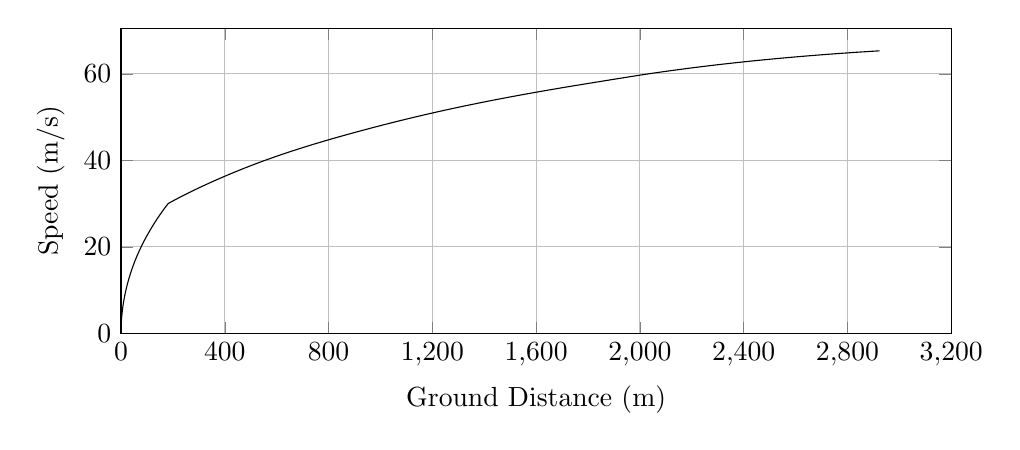
\begin{tikzpicture}

\begin{axis}[
width=\textwidth,
height=0.45\textwidth,
scaled ticks=false, tick label style={/pgf/number format/fixed},
xmin=0.0,
xmax=3200,
xtick={0,400,800,1200,1600,2000,2400,2800,3200},
xlabel={Ground Distance (m)},
xmajorgrids,
ymin=0.0,
ymax=70.5610295336269,
ylabel={Speed (m/s)},
ymajorgrids,
legend style={at={(1.03,0.5)},anchor=west,draw=black,fill=white,legend cell align=left}
]

\addplot [
color=black,
solid
]
table[row sep=crcr]{
1.3603393307216043E-8	2.720678661413807E-4\\
3.0265395163403265E-7	0.0012832958719072919\\
2.9593179127983543E-6	0.004012817723517241\\
1.5392338359717934E-5	0.009151787256025008\\
5.361280674027254E-5	0.017080000038393474\\
1.6215010178508227E-4	0.029703809574357476\\
3.7214145765703975E-4	0.04499947614510465\\
6.839954676020354E-4	0.061007029885337655\\
0.001098342709021993	0.0773075646450756\\
0.001609317716481928	0.0935779850852434\\
0.0022198920000388346	0.10990524096693874\\
0.002878710694837372	0.12515584941478902\\
0.0036835072341781794	0.14157367057798664\\
0.004557929017412697	0.1574835003727189\\
0.005559798278933152	0.17393231810001514\\
0.006651227400597502	0.19023968047038564\\
0.007795849738889277	0.20595927525297142\\
0.009067984722810115	0.22212854195313536\\
0.010453165799939174	0.2384911070442215\\
0.011915708813158052	0.2546287666111213\\
0.013455030027058647	0.2705758792442786\\
0.015131183092671713	0.28693421263108243\\
0.01690803412933615	0.30331336525397223\\
0.01873590105740728	0.31928708750934065\\
0.020713359121301934	0.3357131317434232\\
0.022777736728155237	0.352044288176408\\
0.024960970145273077	0.3685289802382542\\
0.02723428625014468	0.38494418788063534\\
0.029610395797831278	0.40138457285376417\\
0.03204086105441677	0.417531682693848\\
0.03462344565878624	0.43403144076127576\\
0.037295727153354774	0.450468310378909\\
0.040089145853872785	0.4670320714458741\\
0.042950967781251806	0.4834130228074801\\
0.04592022141655751	0.4998415665292979\\
0.04897301836205646	0.5161872717084843\\
0.052130294957187476	0.5325646910090658\\
0.05542514139564195	0.5491348912627503\\
0.05879722600804832	0.5655908461589634\\
0.06231520981015182	0.5822630525306038\\
0.06596261503753809	0.5990586184381457\\
0.06964559414821356	0.6155529015530419\\
0.07347193989652406	0.632233368956522\\
0.07736619052035826	0.6487693693927907\\
0.08137137577670908	0.6653475738559256\\
0.08545617869345057	0.6818399803520576\\
0.08969468676038628	0.6985411488054254\\
0.0940095881391464	0.7151424892890996\\
0.09845059220533334	0.7318355213428471\\
0.10296315144049947	0.7484159100410708\\
0.10759658895065366	0.7650662992988599\\
0.1123317495250277	0.7817155601967591\\
0.1171874363557737	0.7984277829680861\\
0.12217670360507671	0.8152426118610623\\
0.12726806426274867	0.8320509067410284\\
0.13231647880291775	0.8483883168879573\\
0.13765212084557643	0.8653196397970795\\
0.14294844966167852	0.881804376281148\\
0.14834594087957392	0.8982924101149314\\
0.1539671093411843	0.915147590104463\\
0.15968242883369804	0.9319721841666908\\
0.16555834796315422	0.9489581856688449\\
0.17157514414202774	0.9660415461926923\\
0.17760320215284392	0.9828587218703546\\
0.18370335474801935	0.9995885994845586\\
0.18983540939776816	1.0161279579653546\\
0.19621099073945342	1.033042952364315\\
0.20278841209744758	1.050207492379315\\
0.20952923284938563	1.0675116245262677\\
0.21624967405074952	1.0844881288055226\\
0.22309476488450758	1.1015100796324107\\
0.22992510727843934	1.118236619452528\\
0.2371653034562048	1.1356973728008821\\
0.2442573187228817	1.1525438174358746\\
0.25144286317780873	1.1693644240883647\\
0.2588001799723505	1.1863395177501466\\
0.2662612189130884	1.2033088559305694\\
0.27386560463063747	1.2203608924352607\\
0.2815803271719757	1.2374196935292585\\
0.28946218069394425	1.2546079693325618\\
0.29753588720841584	1.2719732460522888\\
0.3056643119969481	1.2892193563999128\\
0.31376446154764137	1.306178390599726\\
0.322071411728719	1.3233440927562916\\
0.3303680011285137	1.3402683692090251\\
0.3389039548234316	1.3574601108156439\\
0.3474123396293025	1.374381732125276\\
0.3561645174790815	1.391572910538049\\
0.36525289600634137	1.4092018606679702\\
0.3742306244196095	1.4264016318649446\\
0.3835584127627333	1.4440543986028649\\
0.392806747202999	1.4613456195350825\\
0.40218604538039837	1.4786745259267673\\
0.4115907129344223	1.4958480818970337\\
0.42143744457304466	1.5136193756891267\\
0.4310567075016639	1.5307802380742426\\
0.4412814114336725	1.5488120162678265\\
0.4513051702487684	1.5662871894205241\\
0.461412558308395	1.5837122018038219\\
0.47173637532167356	1.6013138589434535\\
0.4821484569390513	1.6188714258894947\\
0.492985116277161	1.6369441743760964\\
0.5036221628177362	1.654491263663863\\
0.5142245311302887	1.6717971313679616\\
0.5252888808291518	1.6896672914965403\\
0.5363145235987512	1.707288085630923\\
0.5471208511184944	1.724382903563002\\
0.5585110457184732	1.7422189861943194\\
0.569849942463402	1.7597943841516077\\
0.5817265165330987	1.7780160576027235\\
0.5935668742733842	1.7959972859051359\\
0.6053719027871456	1.8137465568762288\\
0.6172343027602503	1.8314079786327953\\
0.629515267228629	1.849514028007777\\
0.6417789549774502	1.867418549750575\\
0.6542768803188956	1.885489237748104\\
0.6669828212214572	1.9036839425768721\\
0.6796225285147333	1.921611970374221\\
0.6925094233679154	1.93971909798694\\
0.7056620711738308	1.9580260247847439\\
0.7184715206768946	1.9756913033124488\\
0.731725241748566	1.993803585908497\\
0.7449880440563246	2.011764106022701\\
0.7586792333483576	2.0301370992697256\\
0.7725063377467813	2.048524245568058\\
0.7863894274138714	2.0668202748737343\\
0.8004504964383841	2.0851862189013692\\
0.8147129313117618	2.1036503527792068\\
0.8293722635741907	2.122459856138698\\
0.8437954335339908	2.140804008609205\\
0.8580702287827062	2.1588049670079483\\
0.8726489666047585	2.1770345568720106\\
0.8875094051704782	2.1954595605510407\\
0.9027740629895862	2.2142250208591054\\
0.9182163910703112	2.233047324028149\\
0.93361566230532	2.2516593571236863\\
0.9491799633800446	2.27031469722752\\
0.9646343064330896	2.288686694124797\\
0.9803727456894022	2.3072449632649334\\
0.9957421603273868	2.325224070374568\\
1.0116767859397604	2.3437176322192643\\
1.028041387324289	2.3625583845555873\\
1.0443915011410971	2.3812324215076703\\
1.060796374175649	2.3998218031838734\\
1.0773229908740651	2.4184034959273912\\
1.093971735592782	2.4369780794838842\\
1.1110062543639518	2.4558364532993417\\
1.127891796882146	2.4743868660712334\\
1.1451224507351285	2.4931729268899074\\
1.1624801114435046	2.511954187464367\\
1.180077727863539	2.5308515677458736\\
1.1978884766667508	2.5498339574771673\\
1.215488397439855	2.5684526087790243\\
1.23351701382096	2.5873845987601953\\
1.2518199984626128	2.6064627481692932\\
1.2704235066044305	2.625710777009547\\
1.2892140278280424	2.645008771365032\\
1.3075714306593595	2.663725651547966\\
1.3266673518109293	2.6830556222636552\\
1.3462106477188795	2.702693906610442\\
1.365306294594515	2.721744146993708\\
1.3852885894463176	2.7415357701392082\\
1.404835539176236	2.7607575291886306\\
1.4251192118409102	2.7805618282314954\\
1.445164519989187	2.799994350621782\\
1.4656054698512246	2.819671054227829\\
1.4853522740259328	2.8385486572939396\\
1.5051589726327936	2.857356883072221\\
1.5255757775517242	2.876614342718254\\
1.5464367798307013	2.89615706152847\\
1.5673163741652552	2.9155845688583995\\
1.5879032567231621	2.934612381166997\\
1.6091523485848285	2.954122250619788\\
1.6303162371862876	2.973425180561633\\
1.6519474169970438	2.9930241691182893\\
1.673879209980242	3.012763827334582\\
1.6955666802836635	3.0321557097576166\\
1.7172271378534343	3.05139894988723\\
1.7402832823543353	3.071748058555068\\
1.7634396102400074	3.092049135084782\\
1.7861669372425006	3.111843722328693\\
1.8088678577734645	3.1314888323921526\\
1.831824248135399	3.1512288942266276\\
1.855578771396016	3.1715242565279045\\
1.878960729162178	3.1913736230316214\\
1.9033179534858085	3.2119187502279587\\
1.9273833213731866	3.232087738259586\\
1.9518510462308036	3.25246399496171\\
1.9761594732990155	3.272580256500973\\
2.000437267212291	3.292546818489331\\
2.0252281699074732	3.3128094734828073\\
2.0498006073458734	3.33277030060409\\
2.0745611186355752	3.352762004408638\\
2.0997746990963106	3.3729960210130763\\
2.1260324099367294	3.393937885344079\\
2.1515212193659616	3.4141418599072573\\
2.1771505246334	3.434335598938917\\
2.2031842637813908	3.454725362118004\\
2.230133398733474	3.4757041878837933\\
2.257053086628849	3.496532528785333\\
2.283795213136285	3.517099496738444\\
2.311477064851834	3.538261329735156\\
2.3387199014446116	3.5589627897263814\\
2.3662694524467227	3.579773664535896\\
2.3937852540088533	3.600437076170656\\
2.4216520071021392	3.621241945582213\\
2.4501931244916175	3.642425116031366\\
2.478927626230634	3.6636260730381043\\
2.506685441631536	3.683988646647405\\
2.53537335014481	3.7049139659141677\\
2.5633350931805676	3.725194601913124\\
2.5917889242519685	3.7457175250763033\\
2.6208221472873374	3.766541122528489\\
2.649872764173903	3.7872606304822494\\
2.679661174525658	3.8083872665782517\\
2.709174609939316	3.8292019247246083\\
2.740029385016756	3.8508401638134577\\
2.770444625703795	3.8720497081223906\\
2.801129860621211	3.8933283445265428\\
2.8318827297715705	3.9145357352775374\\
2.862425967677578	3.935483385373044\\
2.893259332541544	3.9565154555563575\\
2.92412139403754	3.9774536674278984\\
2.955064430161417	3.9983346798997275\\
2.986690331721131	4.019562302582665\\
3.019183403261743	4.041253642967076\\
3.0507201588152526	4.062193692983383\\
3.0830332871979023	4.0835357203916125\\
3.1154603869692448	4.104839304011726\\
3.148592095396281	4.126489973639769\\
3.181936872739324	4.148163529670445\\
3.214370607724433	4.169134674818443\\
3.247565473366384	4.190487102053373\\
3.281695868027062	4.212326167195128\\
3.316494330618462	4.234474385221251\\
3.3513055302544137	4.256513033999939\\
3.3860303583611797	4.278381559095491\\
3.421934361445942	4.300873329058296\\
3.456235826539576	4.322249583999053\\
3.490536654441657	4.343518016497846\\
3.526257338581564	4.365554351450367\\
3.561372823896762	4.387107127094586\\
3.5967906564503185	4.408736436287072\\
3.632682576242373	4.430545197790497\\
3.6701261071689295	4.45318042575448\\
3.707701291513044	4.475777619994192\\
3.7452745323452916	4.49825760904813\\
3.78256482255855	4.520455298332157\\
3.8208821591411084	4.5431488239496876\\
3.8590337549211444	4.565629572444623\\
3.89695718563138	4.587864203774501\\
3.9351036745073964	4.610118933510028\\
3.9736642086653067	4.632504034757176\\
4.012189127077221	4.654758443869822\\
4.05156219172609	4.6773908139136875\\
4.090290786278251	4.699543877240949\\
4.129291984889424	4.721745330240328\\
4.1680648628189925	4.743711341467803\\
4.207805169621487	4.766117833770968\\
4.248168240749736	4.7887655273091685\\
4.288797880674668	4.811452494098976\\
4.32990243544832	4.8342936336083575\\
4.371428084678056	4.857256996983381\\
4.41247037137882	4.879844233082004\\
4.453879445321437	4.902525212678862\\
4.49524783594077	4.925076975228254\\
4.537299342543221	4.9478931072708505\\
4.580546125800922	4.971245747436704\\
4.622914948498307	4.994015677015684\\
4.66640222022569	5.017276435881808\\
4.709294790611851	5.040111195775223\\
4.752417172855319	5.062961759938068\\
4.796155651503765	5.086031152556377\\
4.8408754796551925	5.1095075991831145\\
4.884850997559644	5.132485793753041\\
4.928651138956553	5.1552678083883805\\
4.972831351372241	5.178143227017278\\
5.017331702752941	5.201079935350927\\
5.0632326321008225	5.2246301593858995\\
5.108452384314601	5.247724709182696\\
5.1536021218025905	5.270679752709302\\
5.199057463234675	5.293686824362842\\
5.244479287100011	5.316574701268275\\
5.292293005248643	5.340558893483271\\
5.338096108273211	5.363431103014612\\
5.3857492800262605	5.38712116286896\\
5.433816232374781	5.410908853017036\\
5.480691139018431	5.4340034464519995\\
5.529685763332537	5.458034931869829\\
5.578612887337309	5.481925128575174\\
5.626451501744754	5.505180663824325\\
5.674834544150631	5.52859844393053\\
5.7252048440372345	5.5528700553135675\\
5.77422346516266	5.576385908993062\\
5.8255152536468575	5.600883422620818\\
5.874338256646894	5.624099726314176\\
5.922631450506765	5.646967371424413\\
5.972682300942642	5.670567043552019\\
6.022535370757359	5.6939732744588945\\
6.074394648705015	5.718216659639818\\
6.124928192945902	5.741738797259719\\
6.176798284396469	5.76578019118489\\
6.229620191179453	5.790156984747169\\
6.282808156696705	5.814596241806036\\
6.334658925277093	5.838319520802822\\
6.388041948821611	5.862640413321735\\
6.440558117792513	5.886465233406986\\
6.494960924490993	5.911041489380462\\
6.550441697666145	5.935996587045935\\
6.6042098433346865	5.960078466946527\\
6.658315220792536	5.984210425676938\\
6.712335084641163	6.008204433330935\\
6.766674450459032	6.032240952509403\\
6.821537769035839	6.056409314665871\\
6.876851268142238	6.080675573357935\\
6.933661362437203	6.105494711558054\\
6.989261882852809	6.129684906832161\\
7.046240323930029	6.154372694510556\\
7.102786137967051	6.17877227855112\\
7.1603789170469145	6.203521696833196\\
7.21785165788507	6.2281182132798545\\
7.277487498606879	6.253534764772647\\
7.334984696129153	6.277939124052297\\
7.393362172524569	6.302617168160129\\
7.452416393609804	6.327480044434298\\
7.511934748111884	6.352436515570549\\
7.572557225035805	6.377752132582225\\
7.63202184821041	6.402483651595178\\
7.69294899409779	6.427721343992971\\
7.752675521499926	6.452362581957351\\
7.814488876138199	6.47776265186393\\
7.8763528528159785	6.503080737624602\\
7.938149975125226	6.528270011640627\\
8.001193143199774	6.553863935201754\\
8.064554080136986	6.579483027163237\\
8.12686567918485	6.604577496565465\\
8.189637855946287	6.629758014320958\\
8.252542711798306	6.654892784923922\\
8.315859663763469	6.68009331280726\\
8.380006162932737	6.7055239807541405\\
8.444702551512929	6.731071847641482\\
8.509501986620958	6.756560096790617\\
8.57387297516295	6.781781558905237\\
8.63887365699837	6.80715149385891\\
8.70727085773305	6.833741720237818\\
8.772937378995405	6.859169850823774\\
8.839192134487615	6.884727114765685\\
8.905815929161982	6.910327939065276\\
8.97209054442786	6.935697399200237\\
9.039019026885107	6.961219881065679\\
9.107371801018814	6.9871857357636955\\
9.174915633685494	7.012746362132049\\
9.243868961478196	7.038741095517846\\
9.312440636565494	7.06449357418116\\
9.381784695008012	7.0904374715333915\\
9.4513167952828	7.116353216091433\\
9.52142787533916	7.14238598983761\\
9.591425279059166	7.16827871363461\\
9.662230428326719	7.1943718678936985\\
9.734225879912522	7.220803359218653\\
9.806441602430919	7.2472152303688055\\
9.878483835105534	7.2734644819252825\\
9.951807209049782	7.300079947591778\\
10.023539677466466	7.32602082113463\\
10.096057433179052	7.352149114535308\\
10.168262179450682	7.378069204914533\\
10.241274410624943	7.404183386656207\\
10.31479015323385	7.430381392295196\\
10.390063469390178	7.457106718466678\\
10.465012435634037	7.48361843413063\\
10.540639152111389	7.510271395252651\\
10.617644389866598	7.5373096294228485\\
10.692945462162374	7.563652432306192\\
10.770083295573727	7.5905393539619155\\
10.846726862770723	7.617156380434448\\
10.924657809445929	7.64412179814353\\
11.00265335491597	7.671010996200243\\
11.081827589833612	7.6982067767120075\\
11.159134327011738	7.724665124949116\\
11.239152720133266	7.75195274555492\\
11.317028257314295	7.778414135774469\\
11.396413369884492	7.805292549169041\\
11.477655063362434	7.832700364959891\\
11.556958506738276	7.859358522439823\\
11.637325199769407	7.886278587423451\\
11.717754170658207	7.91312425915153\\
11.799819443100102	7.940418905410036\\
11.881986970940797	7.967650236035244\\
11.964394119506721	7.994864192006526\\
12.046263329632716	8.021805516472213\\
12.130282587748898	8.049356962841816\\
12.213721087180826	8.076621328784565\\
12.295868535962462	8.103370721845977\\
12.380692430046633	8.130895686815599\\
12.46470288467437	8.158061588650266\\
12.550384439940181	8.185671378860558\\
12.635259749824865	8.212926288203143\\
12.72144647897981	8.240506477846111\\
12.80741162779486	8.267920542202315\\
12.892901506907108	8.29508969524801\\
12.977815703098727	8.321984668188616\\
13.06483740414145	8.349453771031456\\
13.151922956503014	8.37684934745787\\
13.240589045456186	8.404646824018794\\
13.329911181207382	8.432553726105649\\
13.417306166647748	8.459765971074617\\
13.507103029723119	8.487631693157809\\
13.595986036712912	8.515120547126994\\
13.687453390597003	8.54331274774082\\
13.779071846306106	8.571454973654124\\
13.872694200363323	8.600113928433785\\
13.963504841252302	8.627817727937025\\
14.056146454975131	8.655985224075351\\
14.14918846816267	8.684178972512495\\
14.24332804549016	8.712608890415755\\
14.339261112049854	8.741481674010473\\
14.431091301610323	8.769027164754153\\
14.524174633942373	8.796857165003004\\
14.618760344060338	8.825043023704087\\
14.714801736988441	8.853567363680629\\
14.809763128346521	8.881677458939944\\
14.903412319659619	8.909308974888695\\
15.001392651385917	8.938123520459946\\
15.098055049922994	8.966456327927457\\
15.196870856960619	8.995324615229269\\
15.29477342819068	9.02383162108346\\
15.39265348361268	9.052238978017641\\
15.490487151984588	9.080540760528965\\
15.588146853189365	9.10870125943205\\
15.687961867268871	9.13739024996016\\
15.78650099417861	9.165621190566846\\
15.886965864441798	9.19431132646325\\
15.98755318095926	9.222943744448557\\
16.088470385762115	9.251577766216268\\
16.190536977381747	9.280444782462208\\
16.292466610053154	9.309180493785647\\
16.396448349404487	9.338400330388438\\
16.497808944935016	9.366792715602429\\
16.600551072850564	9.395481391912288\\
16.70575139586156	9.424762761149854\\
16.81134459259622	9.45405905012004\\
16.917616592554033	9.483449069282063\\
17.023477948501657	9.512632076536406\\
17.12904978140002	9.541643275361846\\
17.2354081519902	9.570778600282463\\
17.340772011500363	9.599551287958494\\
17.448391076872838	9.628848016289986\\
17.5571980918308	9.658374704770214\\
17.66615596614949	9.68784908797491\\
17.774685459577412	9.717115710266043\\
17.884986575683584	9.746767012093915\\
17.99552903728076	9.776389956619106\\
18.108708479124623	9.806623772042101\\
18.219646262474413	9.836165612868232\\
18.332680252669796	9.866171704626076\\
18.445061806396694	9.895911475956336\\
18.556709221711323	9.925365889199913\\
18.668884868236475	9.954869083527647\\
18.78204748093455	9.984540724082944\\
18.895704562363058	10.01425073882033\\
19.008928234289563	10.043757350686661\\
19.124320907419907	10.07373753589907\\
19.24105855786135	10.103973865169305\\
19.355116774466126	10.133426404662483\\
19.470462572962035	10.163122009259354\\
19.58492145104516	10.192501202485541\\
19.704921229319112	10.223209289901234\\
19.821259826163917	10.2528901003936\\
19.941172080873493	10.283390386458187\\
20.06078806851737	10.313722877428322\\
20.177423389922623	10.343211440646822\\
20.297621170678	10.373510525487212\\
20.420129559802255	10.40429874926312\\
20.54164670774839	10.434745660004786\\
20.661905244258705	10.464787646865059\\
20.784301666224792	10.495273045455114\\
20.904244540623438	10.525059416657204\\
21.028114340450195	10.555730474062141\\
21.148300883955606	10.585402407410069\\
21.270875420257596	10.61557630861078\\
21.39299406946177	10.64555081651281\\
21.513793771711654	10.675116743795915\\
21.637476506915142	10.705301650574743\\
21.759279707150128	10.734942930006547\\
21.88493035745168	10.76543297739515\\
22.009809790007786	10.795648597181383\\
22.13620730934617	10.826143712747545\\
22.263515470260465	10.85677002540103\\
22.393040471753594	10.887839301220005\\
22.520519759768852	10.918329697768431\\
22.648852607677917	10.948936688494854\\
22.775118904521122	10.978965829489539\\
22.903136237443974	11.009326110784116\\
23.03176118514304	11.039744752963404\\
23.162501585272054	11.070576383235402\\
23.294719932439598	11.101667834652016\\
23.427108470281937	11.132710719338423\\
23.558693146983046	11.163478054008834\\
23.687077503630363	11.193414165156153\\
23.817949558665852	11.223846784111156\\
23.948210788889448	11.254054309718985\\
24.076877750667826	11.283811477961944\\
24.21019765060587	11.314560919454387\\
24.3450673155249	11.345581748513151\\
24.477101355489637	11.375867251018246\\
24.60984760833776	11.406233933712834\\
24.7468403923846	11.437486384748535\\
24.882807251950062	11.46841950460157\\
25.017167332957627	11.498904333173321\\
25.153910941279605	11.529846234194544\\
25.289629217480112	11.56047332956842\\
25.425306692573436	11.591009474744055\\
25.56229499031975	11.621758426887425\\
25.70075944713021	11.65275549270778\\
25.83724158708921	11.683227599595725\\
25.975209935932874	11.713950297741441\\
26.003074150630965	11.720145230788138\\
26.020759913393235	11.724075520633939\\
26.030714598210515	11.72628715681089\\
26.05840292223249	11.732436473769294\\
26.06133765907019	11.733088060994827\\
26.064285136409026	11.733742440255046\\
26.066337724202356	11.73419812039474\\
26.068175973881182	11.734606201753937\\
26.06984477238784	11.73497665350261\\
26.077831036047115	11.736749337992826\\
26.10345636352254	11.742435486770493\\
26.16716044512971	11.75655913876609\\
26.297541524199602	11.785412365320727\\
26.42722303713863	11.81404026849781\\
26.5559280656694	11.842383530499262\\
26.686097387723095	11.870979714602868\\
26.817793678842584	11.89984063840178\\
26.949416928520378	11.928614950913921\\
27.080440623797912	11.957188544079937\\
27.215491080424528	11.986568036380792\\
27.34795890217076	12.015314893784687\\
27.48215578365496	12.04436594728518\\
27.616696052324144	12.073420038725374\\
27.75271189183823	12.102720683329768\\
27.888759310501555	12.131956085300654\\
28.023839122857026	12.160912731502812\\
28.16136324828667	12.190321326460104\\
28.298355249881332	12.219544340867085\\
28.435282447697354	12.248682393959125\\
28.573941346212784	12.278116943774254\\
28.713752690797136	12.307723242169814\\
28.852681198061333	12.337070557541157\\
28.992471984120606	12.366528012483894\\
29.133421724605903	12.396157027356313\\
29.275199211812186	12.425886912856082\\
29.416225289053614	12.455386939391172\\
29.55783477945603	12.484936922723737\\
29.701838356359822	12.514912889094848\\
29.846633046394217	12.544979192014814\\
29.99013730470424	12.57470446239218\\
30.132492646908446	12.604120329994103\\
30.277395768405135	12.633990077476128\\
30.422188862471998	12.663764465084181\\
30.56637548064623	12.693342405198248\\
30.711944318924978	12.723131733477441\\
30.8573377156769	12.752813249387295\\
31.006558691603843	12.783201899274438\\
31.153907258126303	12.813135900099667\\
31.30257185742142	12.843263875786697\\
31.4510947803754	12.873290009191795\\
31.602595106592503	12.903843243040978\\
31.755261577184278	12.934555702600907\\
31.906398416479824	12.964885823501373\\
32.05599258457312	12.994833719602205\\
32.20952926265106	13.02549621141775\\
32.360097140052986	13.055492812298358\\
32.51218835243483	13.085719976545697\\
32.664721606344784	13.115961850983297\\
32.82129760777845	13.146929555386148\\
32.97669884718651	13.17758956755248\\
33.13118849606322	13.207995797539965\\
33.288837444683736	13.238948328150215\\
33.44405554194745	13.269349548696187\\
33.60015866510213	13.29985048616814\\
33.756686089655645	13.330360658581714\\
33.91694077595571	13.361521404672594\\
34.074326811338736	13.39205004559794\\
34.23252403098988	13.422662294752513\\
34.392884168270385	13.453618106608712\\
34.554266068788166	13.48469543250241\\
34.71363140184178	13.515310349932438\\
34.87649332318763	13.54652140891076\\
35.03746231629111	13.57729511254373\\
35.19990059234286	13.608275010214442\\
35.3627309111595	13.639254839197346\\
35.5271254050015	13.67045673303652\\
35.69149466827288	13.701578440246337\\
35.85508342515686	13.732477980894057\\
36.017180984292054	13.763023115467927\\
36.182222084544165	13.794048992173014\\
36.34861175093968	13.825253343353861\\
36.514166392421686	13.856226783002338\\
36.68083924241549	13.887335015966464\\
36.845526722294395	13.917999816174298\\
37.01328249159678	13.949161914741978\\
37.18160982421668	13.980355569141516\\
37.35136716620059	14.011738999246269\\
37.51969289597564	14.04278363537778\\
37.689710015857784	14.074065752555544\\
37.860394939778416	14.105395929467452\\
38.02805196867635	14.136097793541765\\
38.19868492919754	14.167271271734037\\
38.37343039987371	14.199119862116103\\
38.54685896696101	14.230652658957222\\
38.71934233168869	14.261939189039584\\
38.8915617091798	14.293104255204852\\
39.062305982326905	14.323930246821373\\
39.23847188392709	14.355660230825531\\
39.411511502305984	14.386753598474417\\
39.585172817779906	14.417885864557093\\
39.760693028009456	14.449277707204672\\
39.9373134006328	14.480792014393973\\
40.113617753210534	14.512176057806638\\
40.29094651898711	14.543668459006781\\
40.468149621311596	14.575064862182021\\
40.64593210594187	14.606490354265222\\
40.82431302355218	14.637948021874198\\
41.00141330502653	14.669107353503787\\
41.17957893337042	14.700381679071121\\
41.359761290266974	14.731936557958111\\
41.53889737920997	14.763235425266082\\
41.72013507746885	14.794828084766\\
41.899395797464194	14.826003935412142\\
42.081280067494475	14.85756312265313\\
42.265315320939635	14.889421212672815\\
42.44531744651641	14.920509253166266\\
42.62715102096499	14.95184186368596\\
42.81120266452106	14.983483694570154\\
42.994164503876235	15.014865828177967\\
43.17799769459725	15.046325213533542\\
43.36154361404071	15.077663663157988\\
43.54597437124032	15.10908138253162\\
43.73158498218817	15.140627852371768\\
43.91737182308138	15.172132137368159\\
44.1050494697441	15.20388421284673\\
44.293574236233	15.235706347126023\\
44.47888581456586	15.266914978476223\\
44.66456251492659	15.298114792035317\\
44.85170130968709	15.329489494598459\\
45.037822074257164	15.360623444810301\\
45.22676109993536	15.392157771701498\\
45.41612608476639	15.42369178310317\\
45.604812217355104	15.455042063633705\\
45.79422221198037	15.486442068106296\\
45.98724683785376	15.518369011756569\\
46.17830917717477	15.549899950532769\\
46.36786657808848	15.581112711108172\\
46.55935209439748	15.612572764436507\\
46.75090376717816	15.643973515136945\\
46.94233405988251	15.675284661369115\\
47.13714948644359	15.707078370110448\\
47.33387512950824	15.73911144777621\\
47.53043319838464	15.771045033081279\\
47.72298239739284	15.802257751836919\\
47.919150009665316	15.833986633700096\\
48.113386178114425	15.865333523889376\\
48.311024807628144	15.89715885931972\\
48.508886059616145	15.928949064614152\\
48.70490444306449	15.960373558126424\\
48.90290918859142	15.992046553214404\\
49.09959709013448	16.023439715997\\
49.2970021191946	16.054878405421064\\
49.49532701226336	16.086394452379928\\
49.693780717172615	16.117862002241885\\
49.89506320355713	16.149708031990407\\
50.096719083698545	16.181542795804596\\
50.29606895218413	16.212944714311924\\
50.497598474286534	16.244620845259973\\
50.700304208193415	16.276412141496813\\
50.90342397924904	16.30819865290995\\
51.10460922167407	16.33961402746875\\
51.30752217039489	16.37123063185355\\
51.51010619677311	16.40272770030822\\
51.713602501430145	16.434298310019166\\
51.91843850546792	16.466008031897573\\
52.121089026646246	16.49731196228886\\
52.32561402362407	16.52883779815261\\
52.53192272805477	16.560570119168567\\
52.7387030603267	16.592306385661125\\
52.944027344085896	16.623751619847674\\
53.154073670302836	16.65585076914366\\
53.36143953271798	16.687471972191652\\
53.571009444677685	16.719360701094907\\
53.77799762982136	16.750789310758485\\
53.98785945427545	16.782586379307418\\
54.196157549666225	16.814079331401224\\
54.40718762937186	16.84591746644368\\
54.616887598525366	16.877487644747305\\
54.826875464266934	16.90903434013044\\
55.04038432082807	16.941041825762788\\
55.25438844036796	16.97305497385127\\
55.46695867894975	17.004786041113483\\
55.68088820258777	17.03665239710361\\
55.895144656119854	17.068499852022782\\
56.109028395418505	17.100224815670693\\
56.326262430904194	17.13237849897986\\
56.542089933321776	17.164256297157053\\
56.76060076462056	17.196462075798884\\
56.97729209122687	17.228332156195926\\
57.19579178641709	17.260400505873207\\
57.41258192878804	17.292151149531136\\
57.634093277561306	17.32452491561149\\
57.85395098827546	17.356589092990724\\
58.07448819514299	17.38868478786393\\
58.29446478173499	17.4206318505447\\
58.51588770709739	17.452721729993677\\
58.73757884137123	17.484783287341493\\
58.96020041504734	17.516912135781745\\
59.18267120664716	17.548952262641606\\
59.405949655899676	17.58104178793093\\
59.63089974393067	17.613304150742337\\
59.8562534200115	17.64555693949226\\
60.084134136581554	17.678103136272128\\
60.30833762904015	17.710057537752782\\
60.53504725699203	17.742302327110444\\
60.763693228044005	17.774754877703295\\
60.99075593752245	17.80691586603149\\
61.21765734918529	17.838987845722805\\
61.44713116872772	17.87135654326135\\
61.6738048454246	17.90326460048192\\
61.90668490141796	17.93597873055986\\
62.13729676517957	17.968307124850085\\
62.36629463006145	18.0003435559193\\
62.596359157213186	18.03246365263309\\
62.82836101237727	18.064788059304334\\
63.059723307860466	18.09695756182198\\
63.292774394726166	18.129295831245585\\
63.52608473446321	18.16160405098644\\
63.75973181411028	18.193893073516058\\
63.993403028653574	18.226119918629472\\
64.23068717493263	18.25877837977292\\
64.4710952259949	18.2917986830457\\
64.70858695601663	18.324351495031493\\
64.94894296164699	18.35722956898254\\
65.18738841845183	18.389779743215406\\
65.42661162888535	18.422369852693166\\
65.6659442133793	18.45490885134651\\
65.90899583190168	18.487886292663454\\
66.15068261105333	18.520611799897843\\
66.39533053734849	18.55367085803052\\
66.6378997293487	18.58638245175822\\
66.88158418814953	18.61917808646907\\
67.12390450547147	18.65172455513428\\
67.36840986262189	18.68449859869959\\
67.61550053739396	18.71755231742341\\
67.86097385246623	18.750323500889998\\
68.10985741250389	18.783483004013767\\
68.35582503705197	18.816188150958602\\
68.60464259362828	18.84920601058321\\
68.85450289166104	18.88229559528839\\
69.1042877596268	18.915308819535262\\
69.35837572129628	18.948823076723997\\
69.61150655903072	18.98214359668978\\
69.86289252102952	19.015168148146422\\
70.11686816207683	19.048466213520015\\
70.37125759672608	19.081751720289446\\
70.62480458144697	19.114860848459998\\
70.88045310059783	19.148177926830954\\
71.13526709211152	19.18132020518925\\
71.3947754873567	19.215005685484464\\
71.6534187996231	19.248511617230385\\
71.91450497256008	19.282266308359446\\
72.1716184080999	19.315441293241683\\
72.43269265097052	19.349060620699426\\
72.69331619504374	19.382555248215425\\
72.95563200429567	19.416200498074282\\
73.21686762735783	19.44964092256869\\
73.48161420086069	19.48346369183261\\
73.74261486234883	19.516742176500138\\
74.00755043430098	19.55045602496893\\
74.27511769675363	19.58443731299983\\
74.54487113507057	19.618628033709896\\
74.81568229507957	19.652884331419564\\
75.08274085953312	19.686599138883388\\
75.35421836228127	19.720804221563093\\
75.62798354862159	19.755228938809466\\
75.89909469738902	19.78925243151614\\
76.17008148658607	19.823193597573827\\
76.44269151183332	19.857271165484647\\
76.71571902594138	19.891334054796005\\
76.99340852183178	19.925910337783293\\
77.27004772085374	19.960287828096973\\
77.54832408953641	19.994800684831766\\
77.82592519882277	20.02916216426513\\
78.10358246820337	20.063463429904985\\
78.38556010231375	20.09823008763349\\
78.66911430382748	20.133122102045483\\
78.95399134982776	20.168107611408132\\
79.23667137346987	20.202755076164095\\
79.518907793654	20.237280770820348\\
79.80555437718249	20.272277438240565\\
80.09150103324356	20.307120269377357\\
80.37928873457926	20.342118891000233\\
80.66871996946384	20.37724845477478\\
80.95967699414447	20.41249395811188\\
81.25093884305389	20.44770726709227\\
81.54344278085921	20.483001569634\\
81.8358102960415	20.518210561307747\\
82.13087592438694	20.553675116730922\\
82.42794520371837	20.58931053507107\\
82.72842933895026	20.62528461776332\\
83.0269479931649	20.660953153432104\\
83.32974506690314	20.697061821280315\\
83.62964811531441	20.732755255765568\\
83.92951211009506	20.7683747061229\\
84.2339319847595	20.804464849112406\\
84.53715838283946	20.840343346697615\\
84.84105485927768	20.876231319317093\\
85.14845677960258	20.912462602619676\\
85.45530133949276	20.948557768855245\\
85.76249773413784	20.984624282858675\\
86.07201271349416	21.020892581054838\\
86.38432073331904	21.0574169588933\\
86.69710203601804	21.09392545588929\\
87.01172103282082	21.130576995135137\\
87.32669099459858	21.16719809052733\\
87.64517025121202	21.20415510408251\\
87.96158123090564	21.240800772558842\\
88.2775814178033	21.27732835117316\\
88.60068374099544	21.314604497422067\\
88.92068281935622	21.35145094111077\\
89.24207276858638	21.388386198162998\\
89.56578933015979	21.42551703183095\\
89.88760090270688	21.462358391126152\\
90.2141410750086	21.499669227819652\\
90.54066676000363	21.53690650134582\\
90.86727570256076	21.57408180422945\\
91.19715108614633	21.61155682312711\\
91.52744226539704	21.649006979809087\\
91.85639956214655	21.68623465621237\\
92.19095740864739	21.72402369924673\\
92.52827526888461	21.762051022102455\\
92.8674718219292	21.800216244962236\\
93.20307982994817	21.837905256310172\\
93.5374944579234	21.875389054097653\\
93.87598013161067	21.913257273324348\\
94.20917297854535	21.95046318116667\\
94.55043409744499	21.988498339201655\\
94.89132963816093	22.02642080026314\\
95.23083207736542	22.06411729206352\\
95.57395676502793	22.10214447133982\\
95.91421223354143	22.13978315220472\\
96.25656086122288	22.177582982272398\\
96.60012122339742	22.215446092918782\\
96.94166303707107	22.253017196605562\\
97.28627502929558	22.290856223731787\\
97.62906225262071	22.32842578606774\\
97.97125437026659	22.365861844260316\\
98.31201772458999	22.40307425050652\\
98.65627175165852	22.440600062827507\\
99.0012536203806	22.478137321510303\\
99.35020029285332	22.516037310684325\\
99.69475740907401	22.55339322106203\\
100.04053871990226	22.590815056902336\\
100.38598466112728	22.62813422400881\\
100.72867962848932	22.665091083289333\\
101.07385499050397	22.702250307996557\\
101.41864366415388	22.739303087439993\\
101.76305460768467	22.776251029276835\\
102.11068844700483	22.813480038542657\\
102.45638678530696	22.850437758734778\\
102.79841653079728	22.886940875827797\\
103.14087212494877	22.923427665506473\\
103.48486473791618	22.960016394541263\\
103.82875595362174	22.996532813939744\\
104.17244250654872	23.032966445801627\\
104.51168383396202	23.068869381579262\\
104.85986244643053	23.105657148555714\\
105.204587526496	23.14201951900126\\
105.54754777175077	23.178136384616025\\
105.88797456536247	23.213928298852785\\
106.23280177240994	23.250124184284253\\
106.57515110440406	23.2860019314953\\
106.91603555764121	23.321669077541074\\
107.25729565943405	23.357318844821037\\
107.598830149446	23.39294086328647\\
107.93686571059558	23.4281427337364\\
108.27485499032852	23.46328522577427\\
108.28839963475954	23.464692400515936\\
108.30004107281309	23.46590177856565\\
108.30931238392475	23.466864888523943\\
108.31701527366243	23.467665038828862\\
108.32505202073054	23.46849983912614\\
108.33865239118708	23.469912479423762\\
108.35091925899997	23.47118653656117\\
108.39508146726081	23.475772705887557\\
108.52984553865659	23.48976201107029\\
108.79919793188978	23.517696615931364\\
109.105233418432	23.549394014948923\\
109.41485218466596	23.581417573443147\\
109.72257164661937	23.613199946320194\\
110.0321119530083	23.645125462079946\\
110.34145354075926	23.676985554158428\\
110.6534776714839	23.709076513590503\\
110.9711963390063	23.74170636109953\\
111.28851843247409	23.774248452335442\\
111.60893519474632	23.807060311395183\\
111.92798394282838	23.839684649492902\\
112.24770070245137	23.872329908441493\\
112.57243448635171	23.905438975948883\\
112.89480865389396	23.93825924784624\\
113.22000325235314	23.971318087783104\\
113.54885709436653	24.004699408620773\\
113.8770619430189	24.037965309700027\\
114.20946079557197	24.071605961227732\\
114.54107775051554	24.10511710213507\\
114.87787736567807	24.139100573930563\\
115.21564640021248	24.17312995282434\\
115.55522358014255	24.207289209159192\\
115.89667501383605	24.24158425473589\\
116.23992536102014	24.276006785723524\\
116.5847156213415	24.31053016920511\\
116.92791619634093	24.34484117290087\\
117.27517516660399	24.379504001129384\\
117.62420948631524	24.41428952410925\\
117.97391125359778	24.44908687801552\\
118.32673409155768	24.484139448957187\\
118.68227803698588	24.519406251863302\\
119.03889207644076	24.554722754731642\\
119.39651249432902	24.59008228887953\\
119.75508651978987	24.625479306705785\\
120.11314113323388	24.66076843093355\\
120.47404637453192	24.696281390228826\\
120.84098349318353	24.732329239478858\\
121.20490030977416	24.768022116473915\\
121.57328571082118	24.804094328584192\\
121.94079100066682	24.840021418951544\\
122.31015242291167	24.876070796310074\\
122.68267403243519	24.912368679004658\\
123.05346836176264	24.94843864830603\\
123.42835733050345	24.984846630623657\\
123.80350972566416	25.021219655795782\\
124.1783235941891	25.057499538341816\\
124.55244040146786	25.093651982343424\\
124.92576251095704	25.129668068731434\\
125.30489170817492	25.166183658418944\\
125.68146781278597	25.20239292576793\\
126.06139977608174	25.238864010703182\\
126.44502763856761	25.275628021121733\\
126.82695116404781	25.312167126403644\\
127.206716044588	25.348438961507178\\
127.59262031825523	25.38523529481059\\
127.97077035934353	25.421231910113917\\
128.3546122768156	25.45770942508382\\
128.73724861847296	25.494011456921257\\
129.12002064685282	25.530265681665647\\
129.50086700331673	25.56627745162516\\
129.8837789976152	25.602424310576772\\
130.26783132854348	25.638618323505476\\
130.651936341801	25.67475687723701\\
131.03747321415574	25.710969554364226\\
131.42280335891803	25.747102330632195\\
131.80875442588928	25.78323289236119\\
132.19322104975072	25.81916452307871\\
132.5798881414172	25.85524161552872\\
132.96215446290768	25.89084894010557\\
133.34488286943906	25.926440545422103\\
133.7276157954845	25.961973943021775\\
134.11532375481391	25.99790962656649\\
134.50135826447365	26.033630777468034\\
134.88604120201086	26.069168050878375\\
135.26955723714872	26.10453925504367\\
135.6512109336153	26.139681109118335\\
136.03464327936558	26.174929056374296\\
136.41686422877552	26.210008270908233\\
136.79904942565338	26.245027099731203\\
137.18004416157777	26.279880181529116\\
137.56399804528928	26.31494689314289\\
137.94515347717788	26.349701522186372\\
138.32982901897384	26.384720219050195\\
138.7128522769853	26.419531873184674\\
139.09597564505458	26.4542962669978\\
139.48002685240425	26.489088450956338\\
139.86309097971855	26.523735129866836\\
140.24727738828375	26.558427227387902\\
140.6317581809211	26.593089843889857\\
141.01585725597846	26.627662214846282\\
141.3998433603236	26.66216880724437\\
141.7841907991213	26.696652359693566\\
142.16710976343057	26.730952690258135\\
142.55205218648928	26.765379049961695\\
142.9364233092117	26.799699239599576\\
143.32169829765928	26.834045073844123\\
143.705984531242	26.868248019832855\\
144.08985428249122	26.902359480330517\\
144.47683600496026	26.936692596688978\\
144.86371007721533	26.970961254444823\\
145.24772592056325	27.00492261071168\\
145.63047789911974	27.038718702980347\\
146.01273254364395	27.072417748114198\\
146.39725173307323	27.10626302684399\\
146.77966503747456	27.139869987272597\\
147.16478130736948	27.173661279711332\\
147.54689717238745	27.207136699127517\\
147.93097497792814	27.2407313537882\\
148.31499270913332	27.274268155432473\\
148.69957284780122	27.307801528837125\\
149.08709998577143	27.34153884479614\\
149.47129868208145	27.37493402083217\\
149.8546635899794	27.408204910169765\\
150.23801379389647	27.4414229338365\\
150.62200569343076	27.474645007214043\\
151.00751012558203	27.507946203429505\\
151.3946455315429	27.54133628624343\\
151.77987817077866	27.57451069397078\\
152.16505704867353	27.607629211465593\\
152.55112759502248	27.64077312637624\\
152.93964308710213	27.674075287150238\\
153.32507651584535	27.70706223032306\\
153.71174813432617	27.7401042317491\\
154.10000329570875	27.77323041037826\\
154.48914219495543	27.806380737409157\\
154.8788297075107	27.83952654858841\\
155.26820650111182	27.87259487204703\\
155.6562915247282	27.905502871860087\\
156.0441896603637	27.93834469184894\\
156.4348678136667	27.971371189383348\\
156.82082928279863	28.003949160589208\\
157.21071017196311	28.0368078756916\\
157.60005066896917	28.06957098027275\\
157.99004282467217	28.10233893015078\\
158.3808231456182	28.135123084115833\\
158.77280374485122	28.167957801039044\\
159.16384255262415	28.200663765141478\\
159.55370941764693	28.23322229598783\\
159.946071590523	28.265939567159002\\
160.33752628124114	28.298531700351354\\
160.73008933968674	28.331166661817406\\
161.12428312893906	28.363887526499767\\
161.5185576482712	28.3965654780335\\
161.91431288671106	28.42931642348126\\
162.3096877663487	28.46198631010025\\
162.70613442998513	28.49469516833321\\
163.1032465869576	28.52740932115549\\
163.50039135636405	28.56007667124635\\
163.89625578410926	28.592589622949255\\
164.29272443146095	28.625103252655073\\
164.68754921345175	28.65743355868932\\
165.0864466423082	28.690048359350705\\
165.4846753800681	28.722559533476918\\
165.88329117400662	28.75505349363454\\
166.28234792206388	28.7875346512622\\
166.68312204436222	28.82010667542304\\
167.08520211103445	28.85273574602452\\
167.486487681752	28.885251489439938\\
167.8888620337579	28.91780662440207\\
168.290121631074	28.95022304442501\\
168.69179641444674	28.982624646416433\\
169.0966267258019	29.015232010158712\\
169.50108473093724	29.04776065378296\\
169.90729482190739	29.08038135747097\\
170.31243922775104	29.112867890696577\\
170.71755979953144	29.145304164102157\\
171.12402986296422	29.177800070741526\\
171.53319587512163	29.210462707013043\\
171.941770038195	29.24302941683345\\
172.3502931259835	29.27554359564295\\
172.7599322859847	29.308098123357105\\
173.17073308198894	29.340696393774273\\
173.58266371319877	29.373335655144437\\
173.99296569000023	29.405797604841617\\
174.40104722187203	29.4380362745054\\
174.8156903853216	29.470744868749414\\
175.2299479185392	29.503374456712898\\
175.64260521584504	29.535829896136505\\
176.05374721710058	29.56811858803068\\
176.4688147253861	29.600667580548738\\
176.8832117842232	29.633116079209593\\
177.30033423294157	29.6657298118795\\
177.7185234955238	29.69837862268693\\
178.13477925276436	29.730828602134558\\
178.55472625996282	29.76351811720494\\
178.97486541267733	29.796174304183175\\
179.39652032378837	29.82889993372283\\
179.8177496461559	29.861544330307204\\
180.24148986351946	29.894334892976595\\
180.66579793025812	29.927120920347782\\
181.08977314985765	29.959832962748095\\
181.5138518510159	29.99250491094091\\
181.61122522885114	30.0\\
181.9380657232258	30.02513935177567\\
182.36340272554946	30.039307131004115\\
183.2082724125376	30.06742038053308\\
184.08646972066333	30.096601885350758\\
184.96448881265883	30.125736109755444\\
185.84629357991815	30.15495447635311\\
186.726051310566	30.18406374558932\\
187.61806497534428	30.21353660206197\\
188.50412524941663	30.24277110161129\\
189.3932804644195	30.272066136324014\\
190.28280340229105	30.3013317608414\\
191.1758490733834	30.33067165574358\\
192.0664158070755	30.359888722477663\\
192.96248081795437	30.389244613849094\\
193.85627821989942	30.418484840171445\\
194.7612747993291	30.44804949507902\\
195.67115393765977	30.477731261461585\\
196.57439968482538	30.507154749168926\\
197.49109477617128	30.53697384341487\\
198.40328264870095	30.566603974200426\\
199.32142764481148	30.596385109885745\\
200.23456840248758	30.625961799585212\\
201.14898042779765	30.655537725335115\\
202.06794236074546	30.68521869156516\\
202.98618556976356	30.714834427301035\\
203.9096776069573	30.744577252343568\\
204.83478510422236	30.774329838907875\\
205.76152187560933	30.804092572326873\\
206.69425456631774	30.834005332855163\\
207.628282006662	30.86391702079849\\
208.55982483556244	30.89370685134729\\
209.49858617709037	30.92368496520256\\
210.43993621334516	30.953703015445342\\
211.37516676315846	30.98348371996631\\
212.31832896164838	31.013474556896725\\
213.2711811717055	31.04373041579484\\
214.21827407856858	31.073760640313857\\
215.17513356897763	31.104057423916792\\
216.13205411802585	31.134312972348283\\
217.08198149354007	31.164304887896158\\
218.0371791872164	31.19442065229228\\
218.99188071657676	31.224478311167267\\
219.9529264806817	31.254693009631275\\
220.9127352149854	31.284826230862848\\
221.88152971929293	31.315198579605813\\
222.85280254650712	31.34560545682978\\
223.82131876423426	31.375883173135264\\
224.792464296851	31.406200289617843\\
225.77907189920393	31.436956398071622\\
226.75865308803293	31.467450073626246\\
227.73754112978963	31.49787916041985\\
228.71868465671315	31.528335396175173\\
229.71601747959392	31.559250276369866\\
230.71257028094016	31.590096962432384\\
231.7099256226606	31.620924627791638\\
232.7104408810668	31.65180606573432\\
233.70545418089353	31.682474264747235\\
234.709934391256	31.713390523700852\\
235.71369390815352	31.744240903243984\\
236.7320063884447	31.775494124477042\\
237.74706170316256	31.806603028824426\\
238.76105009328802	31.83763522018299\\
239.78487801639722	31.868924105668775\\
240.8100003079174	31.900208012090793\\
241.83501924916794	31.931444406737285\\
242.86448750110736	31.962771945223956\\
243.8907393349939	31.993957472945027\\
244.92503751619887	32.02534312972983\\
245.953502111432	32.05650778815243\\
246.9873414577291	32.08779131478528\\
248.03717558009265	32.119513900884584\\
249.06961888058504	32.1506670336272\\
250.1218155809346	32.18237156522848\\
251.19093832453012	32.21454016283613\\
252.25320725679705	32.24645688583624\\
253.30608820982889	32.278046847543095\\
254.3699559131253	32.30992146917528\\
255.43101098027842	32.341666999897356\\
256.50967156157174	32.37389360344335\\
257.5914429014633	32.40616712871655\\
258.6840945362286	32.43871870262747\\
259.76380176807595	32.47083891020601\\
260.8581962365888	32.50334988085318\\
261.9444516651656	32.53557332907566\\
263.04204949406176	32.5680871911695\\
264.16032684448305	32.60116626314803\\
265.27010097773245	32.63394677116494\\
266.38392459233114	32.66680001763092\\
267.48537153454777	32.69924225437504\\
268.5905820952057	32.73174965032602\\
269.71611280872617	32.76480791467132\\
270.8445404967937	32.79790409485592\\
271.9892540622492	32.83142992090772\\
273.1287802847319	32.864756046664596\\
274.2598607565136	32.897788278816364\\
275.4140962910436	32.9314488248078\\
276.5737705536998	32.96521949826507\\
277.7255339726329	32.99871195976054\\
278.873472631631	33.03204601216801\\
280.02854957840555	33.0655400514963\\
281.17668237071314	33.09878596496901\\
282.3518647999223	33.1327671176102\\
283.55187961444256	33.167416455330695\\
284.7584685786584	33.202205103594096\\
285.941557411575	33.23626728620921\\
287.1221215788215	33.27020878220661\\
288.3380769091507	33.305117937966926\\
289.546480671474	33.33976046728053\\
290.7618458711469	33.374552752648796\\
291.9754379854753	33.40924471759884\\
293.19735694745737	33.44412496719839\\
294.4429332625409	33.47962944950076\\
295.6752244560395	33.514704799653174\\
296.9144068053996	33.54992599776867\\
298.17710952726145	33.58576413916647\\
299.45746938538275	33.622050592080896\\
300.71078691175364	33.657519428763806\\
301.9694235045549	33.69308811518198\\
303.2485094319529	33.72918298028111\\
304.5111161174377	33.76476200054363\\
305.7885375700041	33.80070742923189\\
307.0570791845213	33.836352481556574\\
308.3608811954841	33.8729362053419\\
309.64386886834006	33.90888464432844\\
310.9351586872956	33.94501469809663\\
312.22537668169934	33.98106398052927\\
313.5342506610697	34.017582985257576\\
314.84123754060704	34.05399788008009\\
316.1398155931431	34.09012789559442\\
317.4442939528975	34.12637162810786\\
318.74634262752204	34.16249776348481\\
320.0629525702019	34.19897735761991\\
321.37636924397736	34.23531816054306\\
322.71649224941586	34.272346447946504\\
324.0244038135751	34.30843494223221\\
325.3434350411228	34.34478079224971\\
326.66722715453466	34.38120822189367\\
327.9789313038608	34.41725433457029\\
329.2937043653519	34.453336477265054\\
330.6186574095261	34.48964940308635\\
331.92935989568696	34.52552409534103\\
333.2397849995185	34.56134412231803\\
334.55785589909783	34.597325987987574\\
335.86283279415	34.63290412955938\\
337.16815430774386	34.668445922978734\\
338.48168395318464	34.70416534603642\\
339.7737401400375	34.739256253898134\\
341.07699928339446	34.77460694476203\\
342.37735113867427	34.80983456285642\\
343.66222105613656	34.84459968415267\\
344.93088579982714	34.87888461254667\\
346.2089143566884	34.91338096041602\\
347.47942028324815	34.94763312587705\\
348.7463771503009	34.98174905216304\\
350.002202587134	35.015525542538086\\
351.26295304001746	35.04939501647691\\
352.52208799473306	35.08318188274801\\
353.78428405855004	35.11701183560784\\
355.03569437042097	35.150514370749406\\
356.2839192570905	35.183893867449655\\
356.532534242338	35.19053774263348\\
356.70181683425494	35.19506072547034\\
356.7858368456913	35.19730536186829\\
356.84291550062335	35.198830150006316\\
356.8883007824884	35.200042507927066\\
356.9192973297663	35.200870477283246\\
356.9619305459627	35.20200924384022\\
356.98565045558996	35.202642802339255\\
356.9958745426085	35.202915883425334\\
357.006180931049	35.20319116021513\\
357.05441711919025	35.20447948295842\\
357.208832253319	35.20860332576848\\
357.66818797281474	35.2208675984774\\
358.58845336328	35.24542240938379\\
359.66148934630314	35.27402780492558\\
360.7449174758875	35.302882120832805\\
361.8304042818685	35.33176287137054\\
362.92666817939744	35.36090145593245\\
364.0289873921382	35.39017164258921\\
365.13703060048897	35.41956410270777\\
366.24877475310404	35.44902473316225\\
367.36076701414027	35.47846181781074\\
368.4863734176996	35.50822856390924\\
369.61568357384704	35.53806212125902\\
370.75596754727167	35.568153879839\\
371.90376202417565	35.59841161249905\\
373.0452146904354	35.6284700443379\\
374.1975351154391	35.65878211627768\\
375.35397773050147	35.6891696927017\\
376.5143470653695	35.71962723864408\\
377.68422040557243	35.750300515126014\\
378.85798319833964	35.78104167851005\\
380.03657656838345	35.81187494400311\\
381.22247789699145	35.84286453762526\\
382.4172218534285	35.87404979689579\\
383.6147346117475	35.90527161477269\\
384.820669858389	35.936676843501616\\
386.04399669143027	35.96849783953887\\
387.2757008522724	36.000498896284185\\
388.50999386073636	36.03252906726176\\
389.7369632555989	36.06433129417836\\
390.981379940504	36.09654710524484\\
392.2323049604586	36.12889214386456\\
393.480979092183	36.161139679060256\\
394.7422172478699	36.19367178047716\\
396.020034786653	36.22659058492523\\
397.28040554020583	36.25901951986803\\
398.5731254254073	36.292239056456864\\
399.849660759529	36.32500118398495\\
401.12252077361916	36.35762787942562\\
402.4236954445655	36.39093789070289\\
403.7320584602501	36.42438860236625\\
405.03582208710077	36.457678477005146\\
406.3385666183452	36.49089918011508\\
407.6512364967725	36.52432932701643\\
408.9597400696324	36.55760972544722\\
410.275944648773	36.59104200360018\\
411.5913761872097	36.6244105432466\\
412.91238131116245	36.657876073517656\\
414.22626260851166	36.69111698202626\\
415.5341803361134	36.724163261030256\\
416.845680532678	36.75725620500526\\
418.159130413462	36.79035431958482\\
419.47250916537075	36.82340657193238\\
420.80068545876986	36.856786386556465\\
422.12328744316494	36.88998129744567\\
423.43404902484724	36.922834908462264\\
424.7489303727565	36.95574763461434\\
426.0518268633309	36.98831675001831\\
427.3621419714502	37.02102751636008\\
428.66229413371775	37.053441160138846\\
429.9745218365258	37.08611200293559\\
431.2820615126743	37.11862230684048\\
432.577665278571	37.15079269560546\\
433.87558198351223	37.18297745627771\\
435.17576112500524	37.21517511192215\\
436.4768306066361	37.24735153134887\\
437.7767963392687	37.27945741592248\\
439.0718799843802	37.31139975573474\\
440.34463526402305	37.34274960438644\\
441.6297725039152	37.37436242813516\\
442.9112652254911	37.40584357706351\\
444.1908623699178	37.437236299922844\\
445.4641513240356	37.468432755669724\\
446.7390539687866	37.499627279495556\\
448.0137212538442	37.53077457662026\\
449.28965265596037	37.56191125399805\\
450.55011907248945	37.592629777278674\\
451.81378233536714	37.62338556209738\\
453.06960107336306	37.653910119961836\\
454.33163864589335	37.684545380407044\\
455.5852448768437	37.71493584578384\\
456.84206482748743	37.7453640931911\\
458.09816583268844	37.77573481428989\\
459.33543753260835	37.805611081656096\\
460.5932432665213	37.835943341071854\\
461.8411861884889	37.86599808436506\\
463.08388529009017	37.895887297254134\\
464.3355885778644	37.925953519496915\\
465.5887480166332	37.95601497710702\\
466.82596682078827	37.9856550615978\\
468.0706804917189	38.015435646556796\\
469.30698934665304	38.04497639454382\\
470.55800333667526	38.0748292363414\\
471.79883410205514	38.104400082373786\\
473.03511474251025	38.13382390307912\\
474.27209749120345	38.163225916348836\\
475.5087462499346	38.192581511774804\\
476.7479443270305	38.221959064784386\\
477.98745019644787	38.25130533802229\\
479.2266024161646	38.28060470994866\\
480.46028485897614	38.309736519425485\\
481.69642175995546	38.338888064791846\\
482.92651122280665	38.3678590521761\\
484.1523181186668	38.396691563097804\\
485.37963179065673	38.42552193687436\\
486.6153465796348	38.45451170991774\\
487.8444091277298	38.483307691808164\\
489.07010325926933	38.511987321660115\\
490.3002467158743	38.54073351662204\\
491.52409945470765	38.56929542798568\\
492.7553911368899	38.59799346513607\\
493.9883083424485	38.62669176272536\\
495.2153249326417	38.65521537661485\\
496.4339929662153	38.683508093910504\\
497.65619948032077	38.71184614805978\\
498.8767282491359	38.74010855701967\\
500.1055150859728	38.76852514193155\\
501.33278759646123	38.79686965110051\\
502.56450087196106	38.82527953599035\\
503.7826599789337	38.853340196654756\\
505.0020700160004	38.881393274647124\\
506.22922862375754	38.90958789635606\\
507.45754163679726	38.93777220722693\\
508.6833947304302	38.96586338381083\\
509.9183640167839	38.99412645201886\\
511.1417143075706	39.0220870375842\\
512.3662399681182	39.05003808496785\\
513.5886071980087	39.07790359272377\\
514.8073821458056	39.10565118219887\\
516.0307341839034	39.133466853030754\\
517.2562663214962	39.16129585830781\\
518.4795845479493	39.1890384758909\\
519.705670065829	39.216807700665726\\
520.9323028071376	39.24455315977916\\
522.1602257252932	39.27229163303345\\
523.3911577887854	39.30006181819236\\
524.613629926504	39.32760526680572\\
525.8398363977287	39.355196992216264\\
527.0619990041141	39.38266204262966\\
528.2968691076571	39.41037654126089\\
529.5262456867333	39.437931740545864\\
530.7614001227555	39.46558032432681\\
531.9934916020729	39.49312433472771\\
533.22539925715	39.520628339138696\\
534.4581496592114	39.548115289467745\\
535.6883142015454	39.575508874552284\\
536.9202871372531	39.60290704226881\\
538.1486523226106	39.63018948158725\\
539.3807302744208	39.657518841786796\\
540.6103579123426	39.6847584244946\\
541.8503813519912	39.71219252578483\\
543.0826893349836	39.73942040292904\\
544.3186150054412	39.76669270388277\\
545.5592395606534	39.7940329930979\\
546.7905837363196	39.82113346482912\\
548.0340656638784	39.84846545084517\\
549.2720482224115	39.875641064915015\\
550.5165318072397	39.90292375853045\\
551.7618627798092	39.93018933977767\\
552.9980744529594	39.95722001807793\\
554.2432335985623	39.98441091262691\\
555.484236229657	40.011475732167426\\
556.7320261415546	40.03865310539534\\
557.9797822601195	40.06579424857347\\
559.2267878312311	40.092883674969755\\
560.4770639265887	40.12000870052728\\
561.7247722722643	40.14704270408208\\
562.975547128877	40.17410781351755\\
564.2229132585876	40.20106399976257\\
565.4762993849808	40.22811498437511\\
566.7279416611102	40.255093097950976\\
567.9808325833562	40.28206293577618\\
569.2419663480505	40.30917472949389\\
570.5078139652448	40.33635214100572\\
571.7653746932046	40.36331627462843\\
573.0227328329638	40.39024090419554\\
574.2795812626689	40.417119558712415\\
575.5415084521385	40.444071636929294\\
576.805656751754	40.471035877081874\\
578.0698741613967	40.49796635893658\\
579.3381873925011	40.524948764102135\\
580.6024641841475	40.55181016090259\\
581.8705267377227	40.578716832876395\\
583.1476444664199	40.60578013511525\\
584.416261593396	40.63262810166701\\
585.6934931536166	40.65962301749762\\
586.9688358568005	40.68654269245273\\
588.2404391322718	40.71334837995221\\
589.5204883296483	40.74029683733208\\
590.8015452894581	40.767231163224594\\
592.079006568302	40.79405475996053\\
593.361324952825	40.82094514722701\\
594.6485170350952	40.847902356231316\\
595.9348514050309	40.87480627557095\\
597.2193094751538	40.90163579903124\\
598.5026975355063	40.92840797424722\\
599.7966977025892	40.95536619169603\\
601.0847027232801	40.982164365920326\\
602.368532657101	41.008840866570935\\
603.6652961272694	41.03575092134545\\
604.9653219720785	41.06269326493596\\
606.2633913265258	41.08955977491313\\
607.5604353801489	41.11636993501797\\
608.8599713138647	41.14319647597412\\
610.1627337745315	41.17005442129286\\
611.4640081981788	41.196846594761965\\
612.7714066517469	41.223729626131316\\
614.077430524007	41.250549226784614\\
615.387410817804	41.27741485849083\\
616.702864029005	41.304357334661134\\
618.012221685801	41.33113983374629\\
619.3168263581895	41.35779034581098\\
620.6336741631758	41.384655861774704\\
621.9446547103096	41.4113667434589\\
623.2583073648807	41.43809720005473\\
624.5832829320675	41.465022796628034\\
625.910971412023	41.491968099965504\\
627.2338554843225	41.51878072742183\\
628.5606615142235	41.54563768029628\\
629.8905557136443	41.57252190021124\\
631.2252601779246	41.59946798448685\\
632.5639435298533	41.62645889875263\\
633.9015553581892	41.653392799973076\\
635.2400503524516	41.680309155611084\\
636.579366004978	41.707206742157965\\
637.9137508755714	41.73397031560056\\
639.2594400325431	41.76092535106115\\
640.6079429757604	41.78790132499594\\
641.9557903983928	41.81482885435008\\
643.3112357291232	41.841872658633264\\
644.6638780871876	41.86882513597617\\
646.0201278314507	41.89581409160036\\
647.376801428238	41.9227761218374\\
648.7426697757596	41.949885266484415\\
650.1043985340018	41.97687678096105\\
651.4736588395087	42.00398198039454\\
652.8436293781256	42.03106562052349\\
654.2178925655946	42.05819843842811\\
655.5888464309808	42.085230415713426\\
656.966828946257	42.112365358824576\\
658.3438479954261	42.139445764326055\\
659.7289450310986	42.16664927729995\\
661.1121696688397	42.19378034293479\\
662.5049487638391	42.221062908084065\\
663.8898102612545	42.24815477040163\\
665.2741899069215	42.27520183134723\\
666.6643692739729	42.30232672587972\\
668.0644066872599	42.32960815388208\\
669.464172787373	42.35684848095326\\
670.8680667837873	42.38413328796371\\
672.2804334024729	42.41154665042947\\
673.6868269490392	42.438808207552\\
675.1042704636877	42.46624786025059\\
676.5145518018076	42.4935130194614\\
677.9309334430959	42.52086025189027\\
679.3547498424907	42.54831492987937\\
680.7726480379908	42.5756196399399\\
682.1866667292747	42.60281413391118\\
683.6164436717638	42.63027576070388\\
685.0538439135858	42.65784751380687\\
686.484522700026	42.685254328035185\\
687.9263224342296	42.71283796215371\\
689.3634106098709	42.740295403552935\\
690.8044222453116	42.767791792585825\\
692.2553122378276	42.79544036679802\\
693.7017643883908	42.822968237624394\\
695.1561227715981	42.850610329249875\\
696.6206970447249	42.878409992853406\\
698.0871377660035	42.90620842470864\\
699.5455502698123	42.93381842126847\\
701.0121890378302	42.961547831288996\\
702.4774635004276	42.98921520681651\\
703.9460961360817	43.01690977840812\\
705.4205208613216	43.04467724002653\\
706.8995125321812	43.07249427223631\\
708.3906952299694	43.10050378775806\\
709.8799012579555	43.128439430424876\\
711.3781545973516	43.15650787611642\\
712.8782716305909	43.184574285184695\\
714.3761556600491	43.21256216701791\\
715.8888345419532	43.24078936772679\\
717.3968351967799	43.26889228457921\\
718.9073478380483	43.297005139131215\\
720.4241486989035	43.3251980368248\\
721.9458410676166	43.35344475556428\\
723.4699634454305	43.381699484586065\\
724.9995371472869	43.41001809651959\\
726.5373034031131	43.43845099654085\\
728.080372820815	43.46694442155383\\
729.6215931985491	43.495366331610086\\
731.1637689264153	43.52376863004284\\
732.7269162690175	43.55251931771143\\
734.2849700349659	43.58113856406082\\
735.8488837509408	43.609827702409774\\
737.4248774785508	43.63870034766035\\
739.0027912248597	43.66757002180459\\
740.5777612414206	43.69634793855673\\
742.1661277920862	43.725332456146404\\
743.7496159355812	43.75418995262535\\
745.3460051639197	43.78324432101675\\
746.9471206502992	43.81234631486082\\
748.554973807878	43.841532253323095\\
750.1647643700692	43.870714863003414\\
751.7903408825748	43.90014473227245\\
753.4077815944067	43.929388677530255\\
755.0420785617482	43.958898431308526\\
756.6792511162737	43.98842102539507\\
758.3256693781859	44.018071079218316\\
759.9814793019216	44.047850739493626\\
761.6276933783281	44.07741871002345\\
763.285764752889	44.107160421849855\\
764.9548153496144	44.13705950171371\\
766.6323377147974	44.167070531422056\\
768.3082472731592	44.19701304697156\\
769.9982719717968	44.227167802846736\\
771.6928734133292	44.25736414250885\\
773.3902918689489	44.28757064727101\\
775.098955095986	44.31793699848453\\
776.8215253196211	44.348509824312316\\
778.5480382560809	44.379111851210865\\
780.28399500619	44.40984032240287\\
782.0332359629474	44.44076262715093\\
783.778987984705	44.47158212750091\\
785.5350434795378	44.502542293062845\\
787.3038868131889	44.53368633174294\\
789.0777645198748	44.564877324382266\\
790.8593645521737	44.596162312682466\\
792.6561744183466	44.627672200898814\\
794.4585456990799	44.659237291514316\\
796.2895379474314	44.691260461399935\\
798.1157796110654	44.7231574585838\\
799.9539128873284	44.755218950516166\\
801.8048211799401	44.787459726552385\\
803.670602959708	44.81991561902903\\
805.5424228419724	44.8524324548286\\
807.4376977333382	44.885312018899285\\
809.3338663961354	44.91816232335847\\
811.2512975213472	44.95133573819808\\
813.1795486934934	44.98465074346545\\
815.1399813897156	45.018475167372074\\
817.096487724227	45.052185309195366\\
819.0874641802507	45.08644194374581\\
821.0910469065991	45.120867508227136\\
823.1043857200887	45.15541254712505\\
825.1406668604063	45.19030246246133\\
827.1993456726345	45.22552662392462\\
829.2842785117825	45.26114959977727\\
831.3859008239535	45.29700676797886\\
833.5175737442742	45.33332475568298\\
835.6514973880421	45.36962912476828\\
837.8159766211309	45.40640061233296\\
840.0176683439679	45.44375022204457\\
842.2435299470051	45.481454846546825\\
844.4872493126668	45.519406433696744\\
846.7514061767547	45.55764763757587\\
849.0440196572308	45.5963125340857\\
851.3706350577643	45.635492781083045\\
853.7111004449807	45.67484771131066\\
856.0737435276355	45.71451650210638\\
858.4349074798715	45.754101686041636\\
860.7921662964379	45.793563298599096\\
863.1513286267109	45.83299915917007\\
865.5104052082004	45.87237645357847\\
867.8246555399062	45.910950489263755\\
870.1167616620985	45.94910217491527\\
872.4014235194927	45.98707767640262\\
874.6722082187739	46.024771247623946\\
876.9105496565701	46.06187669868068\\
879.1391420504924	46.09877205865588\\
881.3248291266734	46.134910522999476\\
883.5024151191194	46.17086956941881\\
885.6326956794833	46.20600390466086\\
887.7663888779789	46.24115172401744\\
889.8733800074399	46.275818011643196\\
891.9693347672096	46.3102619814411\\
894.0521274823832	46.344449747975034\\
896.1093802754438	46.378179575564104\\
898.1555978934455	46.41169063157477\\
900.182259203408	46.44484452639878\\
902.19659900945	46.47776078982895\\
904.1998663308525	46.51046076190811\\
906.1762437868019	46.54268754368795\\
908.1460728568766	46.574773977189324\\
910.1006177146182	46.6065786025398\\
912.0536237045719	46.63832578753258\\
913.9873997012014	46.669728740290495\\
915.9091787700097	46.7009059497654\\
917.8239860011847	46.73193965729759\\
919.7242762473325	46.76270834385065\\
921.6137550870906	46.79327285317673\\
923.4996071519718	46.82374998717113\\
925.3696747863753	46.853943952540206\\
927.2367056919409	46.884061236809856\\
929.0947616722065	46.914006554310305\\
929.4631301429627	46.91994015509884\\
929.7403525161926	46.92440489811649\\
929.9812906129255	46.92828478809042\\
930.1337884740876	46.9307402688239\\
930.2392235283469	46.93243785113627\\
930.3120799091269	46.93361084240766\\
930.3742730535455	46.93461212253368\\
930.4429190117162	46.935717255134776\\
930.5135577711371	46.93685443180951\\
930.5326236373253	46.93716135666374\\
930.5540168455377	46.93750574403195\\
930.6698138696145	46.9393697803754\\
931.1744301303856	46.94749160156988\\
932.9188426232236	46.975552780880335\\
934.7230467265872	47.004550865782164\\
936.5343773094344	47.033637882066515\\
938.3564348899799	47.06287114983628\\
940.1822658160845	47.092138674742685\\
942.0219194300507	47.12160104494606\\
943.8736689095263	47.15122991890857\\
945.7471960933804	47.181179338980556\\
947.6303222985375	47.211253796144376\\
949.5228051967101	47.24144886789122\\
951.4251493448862	47.27177204204857\\
953.3435244764305	47.3023209412292\\
955.2886137771159	47.33326456049933\\
957.2379425093834	47.364244497957046\\
959.2019640177405	47.39542630342261\\
961.1812295039533	47.4268178748021\\
963.1705790415604	47.45833662624736\\
965.1790389768637	47.49012471663849\\
967.201678841604	47.52210314722541\\
969.2477859275689	47.55441766517184\\
971.3112930221655	47.586971266325776\\
973.3920349619887	47.61976030898431\\
975.5003195158185	47.652945907809624\\
977.6340073221597	47.68649283031888\\
979.7705834669957	47.720046180139164\\
981.9303455391694	47.75392386169899\\
984.112594055993	47.788113495332\\
986.3147650036365	47.822573576018314\\
988.5367589843427	47.857301273774894\\
990.782638682957	47.89235867955453\\
993.0352795547719	47.92747744848312\\
995.3033619068613	47.96279211086977\\
997.5948997486701	47.99842614675582\\
999.8950907195883	48.0341482685087\\
1002.1957761626734	48.06983135588952\\
1004.5230133466841	48.10587858599264\\
1006.8438219647242	48.14177836342871\\
1009.1535905815113	48.1774597640416\\
1011.4612429440997	48.21306092174008\\
1013.7546984510236	48.24839584511\\
1016.0499845474455	48.28371172999391\\
1018.3497176061867	48.31904852338427\\
1020.6435866343716	48.35424772269076\\
1022.9139871102873	48.389039989077034\\
1025.1622202404756	48.42344656618387\\
1027.4100868519622	48.45780168365461\\
1029.6452631636225	48.491917297825296\\
1031.878319275746	48.52595510344659\\
1034.0879454032256	48.559590974112055\\
1036.2614038313645	48.592632731160606\\
1038.4536967404465	48.6259169834686\\
1040.605555902699	48.658544470340686\\
1042.7584129413594	48.69114450383671\\
1044.8954278583224	48.72346245522196\\
1047.0262799515062	48.75564529165575\\
1049.1369225381927	48.78748157847791\\
1051.2574914208703	48.81942611978113\\
1053.3587462111864	48.85103865485732\\
1055.4554713238203	48.882542254744095\\
1057.5342652913455	48.91373616483294\\
1059.606624145587	48.944793551816446\\
1061.673035924769	48.975722043049515\\
1063.726246813094	49.006413578363265\\
1065.7739616678177	49.036983827514376\\
1067.8132130384074	49.067388851303164\\
1069.8595145964177	49.09785996122817\\
1071.8870839449282	49.12801353559949\\
1073.913048664037	49.15810483951367\\
1075.9383736432137	49.188148237500684\\
1077.9532746343457	49.217998876626496\\
1079.9655642675684	49.24777284288891\\
1081.9640231508038	49.27730457245022\\
1083.9597062096896	49.306757870789085\\
1085.9509141331441	49.33610784003345\\
1087.9398597721033	49.36538726534624\\
1089.9187774826828	49.39448215287702\\
1091.8959071623876	49.42351396139945\\
1093.8644432769484	49.452383032487404\\
1095.8309137280899	49.48118538079048\\
1097.8017207503253	49.51001470090158\\
1099.7631615919545	49.538670673489165\\
1101.7171464427865	49.56718166082436\\
1103.6715425717248	49.595662640440324\\
1105.615648429466	49.62395792456857\\
1107.566146600744	49.652310417702324\\
1109.507913220944	49.680500336543616\\
1111.4576956403284	49.70877082750772\\
1113.4067479113378	49.736994874988426\\
1115.353584060279	49.765151038393014\\
1117.3054515092317	49.79334405347643\\
1119.2432650054502	49.82129849750699\\
1121.1704706531673	49.849064759750874\\
1123.1072150127825	49.87693313205773\\
1125.0323223459145	49.904598969445175\\
1126.9622708463385	49.93229926927104\\
1128.8878765370305	49.9599022049056\\
1130.801511153606	49.987298876028845\\
1132.7263473374855	50.01482106137769\\
1134.6560080972836	50.0423771499286\\
1136.581963352834	50.06984530636851\\
1138.4925875238164	50.0970602510709\\
1140.4090234565529	50.12432340982363\\
1142.3208052615796	50.15148587345733\\
1144.2342729825236	50.17863781160247\\
1146.1372726097243	50.20560700806183\\
1148.0422262478187	50.23256974949912\\
1149.9568529047806	50.25963499052969\\
1151.8600350370875	50.28650427399954\\
1153.7646587247978	50.31335981028208\\
1155.6810375497898	50.34034668288315\\
1157.5800539135157	50.367055017973925\\
1159.4917310285937	50.39390721431583\\
1161.3957249735013	50.42061739683693\\
1163.3039586108948	50.44735293624649\\
1165.2042410027593	50.473943148300734\\
1167.0972259475984	50.50039760847349\\
1168.9944084398553	50.526877062117734\\
1170.8985576407335	50.55341988251938\\
1172.8050689851198	50.57996165725609\\
1174.7040416808018	50.60636471172221\\
1176.600381389262	50.632697547658324\\
1178.499840513316	50.65904005456919\\
1180.4051710258777	50.68543018340917\\
1182.3041908377186	50.71169924083134\\
1184.2100578074305	50.73802925066032\\
1186.1147976100133	50.76430992032665\\
1188.0140237895434	50.79048093130359\\
1189.9114998482132	50.81659436429375\\
1191.8189000201533	50.84281069443779\\
1193.7169373812067	50.86886484618336\\
1195.6198796982371	50.89495281942456\\
1197.5252050397826	50.9210398781603\\
1199.429319535962	50.94707681653891\\
1201.3294318301346	50.973025634725815\\
1203.2299072204287	50.99894607537489\\
1205.1346469609016	51.02489125846064\\
1207.0482660905705	51.05092373445936\\
1208.9612721027174	51.07691418564673\\
1210.8727930352875	51.10285085595312\\
1212.7841547080598	51.12875181397101\\
1214.6877200276795	51.15451381425689\\
1216.591451665376	51.18024485661935\\
1218.4927228495153	51.205909534195555\\
1220.4033263296637	51.2316668916493\\
1222.3149650312685	51.257404841054395\\
1224.2239892037046	51.283074323120786\\
1226.1334569836986	51.3087165549379\\
1228.0418873066683	51.3343117027234\\
1229.9587745190915	51.35998694824127\\
1231.8719097719054	51.38557868183368\\
1233.790312833747	51.411207562087355\\
1235.7120592092065	51.43684769686368\\
1237.6232666915016	51.46231409859641\\
1239.5462724358204	51.487904415681015\\
1241.4689211521409	51.51345663901718\\
1243.3957371554548	51.539030843161726\\
1245.3288619610944	51.56465522507723\\
1247.2519183224022	51.59011284137114\\
1249.1741023888467	51.6155257619335\\
1251.1025156937699	51.64098778345975\\
1253.028203525777	51.66638062828574\\
1254.954462160575	51.69174786603281\\
1256.8740880240284	51.716994835934344\\
1258.8009619433897	51.742304131929515\\
1260.7250985183996	51.76754453007024\\
1262.6644679408478	51.79295148802828\\
1264.5978014004136	51.818246185160206\\
1266.5373467566765	51.84358891288586\\
1268.472999349839	51.86884763268827\\
1270.421377456525	51.89423902539458\\
1272.3557231001005	51.919414465676695\\
1274.2938863019913	51.94460658607822\\
1276.2270184005288	51.969700456609345\\
1278.1754704785176	51.99496004501968\\
1280.1181655063328	52.02011192101068\\
1282.0637064290786	52.045267595826104\\
1284.0153642279602	52.0704691904709\\
1285.9647453396192	52.09560827824538\\
1287.914241938572	52.12071582051577\\
1289.868176317355	52.14584742580443\\
1291.8229995728911	52.17095737067832\\
1293.783891837791	52.196112076597515\\
1295.7401382183984	52.22117411387681\\
1297.7019363716345	52.24627416445274\\
1299.6644783232005	52.271350613934345\\
1301.6339798248096	52.29648275019599\\
1303.613764482729	52.321712609372824\\
1305.5878662802534	52.3468366705967\\
1307.5584424711533	52.371882684887595\\
1309.5369106957014	52.39699572339504\\
1311.510266728766	52.42201071470481\\
1313.487140858152	52.44703716380573\\
1315.4641643437776	52.47203239598866\\
1317.4519349946745	52.49713018914204\\
1319.4344648944138	52.52212860557276\\
1321.428308710489	52.547236302869536\\
1323.4149026292662	52.57221947904354\\
1325.4090497342881	52.59726435596387\\
1327.4090190295224	52.62234892669687\\
1329.412266699851	52.64744112628655\\
1331.4164183736193	52.672511178714814\\
1333.4158624409642	52.69748905301947\\
1335.4174561925224	52.722460547256944\\
1337.4212369384609	52.747426089365646\\
1339.4269601725996	52.77238260123187\\
1341.4291752189633	52.79726237207602\\
1343.4396689144737	52.82221182011588\\
1345.4520358015402	52.84715127695918\\
1347.4657109256432	52.87207373526539\\
1349.487121253479	52.89705858890423\\
1351.4997442631816	52.921901717523156\\
1353.5325209155276	52.946960152461045\\
1355.5627466015821	52.971953650252445\\
1357.5894485566314	52.99687046175262\\
1359.6307887588	53.0219336777765\\
1361.6652997090491	53.046879608945645\\
1363.7004703359953	53.071800309617856\\
1365.7428467810823	53.096775822366766\\
1367.7871467004688	53.121741405909106\\
1369.833953637768	53.14670415738625\\
1371.8818023748254	53.171646200010386\\
1373.9286494581625	53.196542724477354\\
1375.9853053153993	53.22152508757701\\
1378.0417227295302	53.246471092796924\\
1380.1037027657048	53.271451064060244\\
1382.1690758373284	53.29643858227293\\
1384.2397197654664	53.32145623832919\\
1386.3061596051743	53.34638961329753\\
1388.3770308822964	53.37134298113\\
1390.447790621296	53.39626158029435\\
1392.5297302985518	53.42128110474188\\
1394.6078132108128	53.44622076097461\\
1396.697021555361	53.471260265610525\\
1398.7856587396418	53.496259265395\\
1400.8851185669082	53.52135397393012\\
1402.9751293856302	53.54630214096596\\
1405.0750135118005	53.57133449350154\\
1407.185294805793	53.5964568783251\\
1409.2937238472368	53.62152335422222\\
1411.3994371171025	53.64652385631909\\
1413.5218608795258	53.671688782837634\\
1415.6407162192577	53.69677747023415\\
1417.7640164414188	53.721884874187296\\
1419.8884138158178	53.74697137004803\\
1422.0206757405904	53.77211675275265\\
1424.1489938704422	53.797181770057364\\
1426.2864013112767	53.8223198848619\\
1428.430738272472	53.84750541057511\\
1430.580747728552	53.872723380448974\\
1432.7322629920882	53.897924849831426\\
1434.8889145338148	53.92315228481455\\
1437.0432163340074	53.94831815098563\\
1439.2130967713902	53.97363166835993\\
1441.380371471986	53.99888049400269\\
1443.5512267572876	54.0241367777534\\
1445.7315069433125	54.04946830868042\\
1447.9102563817614	54.07474771551409\\
1450.0935567544757	54.10004559504151\\
1452.2800496279024	54.12534612909103\\
1454.4648841361018	54.15059325571815\\
1456.6570547042297	54.17589088330429\\
1458.842786010276	54.201080129253384\\
1461.0491255885004	54.226472475340785\\
1463.2513456570591	54.25178305601153\\
1465.4532054808801	54.27705529010697\\
1467.6630901132958	54.302385348506036\\
1469.8804669157935	54.32776687419181\\
1472.1014803784296	54.35315558591998\\
1474.3192168749588	54.37847255552134\\
1476.5367058578136	54.40375255875877\\
1478.7652624701545	54.42912445301994\\
1481.0058659776978	54.45459896586766\\
1483.240522153751	54.4799714848794\\
1485.4811754764123	54.50537774206997\\
1487.7274861977025	54.530813731810426\\
1489.994773813667	54.556452426890374\\
1492.2624881081597	54.58206106826108\\
1494.532299848096	54.607658584412945\\
1496.8072859197528	54.63327962702398\\
1499.0887656747855	54.65893890730902\\
1501.3762383691765	54.68463062855513\\
1503.6637924444399	54.710288378192004\\
1505.9581235566288	54.735987222414195\\
1508.2523066552649	54.76164956571034\\
1510.5623189382823	54.78745389349318\\
1512.8745542199968	54.81324793031699\\
1515.194841836505	54.83909659810459\\
1517.5291933515196	54.86506649219805\\
1519.8639954661958	54.89100596252298\\
1522.2002630004836	54.91692637070041\\
1524.5408007670358	54.94285883652914\\
1526.8875158762717	54.96882438557351\\
1529.2390582273374	54.99480796346093\\
1531.5898850447093	55.02074836526653\\
1533.9456242800488	55.04670773247604\\
1536.3128365046823	55.072758127039535\\
1538.69306760672	55.098916147430586\\
1541.0795386665195	55.12510700086827\\
1543.474803142601	55.15135851291177\\
1545.8780958590169	55.177662060925485\\
1548.2798463774375	55.20391289500411\\
1550.6846072813537	55.230160884028976\\
1553.1075884163938	55.25657171358918\\
1555.5347332803403	55.282991811719896\\
1557.9663408367355	55.309424387146564\\
1560.4018682494257	55.33586350005882\\
1562.846201731566	55.36236205921277\\
1565.2883130235464	55.38880051260135\\
1567.7565971502804	55.41548588731247\\
1570.223475485379	55.442119626714\\
1572.6972833405307	55.468791755515824\\
1575.1829839178272	55.495555525810715\\
1577.660873651189	55.52219885356246\\
1580.1553899357368	55.548984463702055\\
1582.6689600768414	55.575937795095456\\
1585.1844513527276	55.60287483147721\\
1587.7099405152949	55.629881963805474\\
1590.2473138014284	55.656979047597304\\
1592.7833324457333	55.68402463889164\\
1595.3295906549747	55.711142358225004\\
1597.8913747079719	55.738388110668254\\
1600.4521420163323	55.765585812045\\
1603.023544352237	55.792859177497945\\
1605.6207159219189	55.820368108026244\\
1608.206805754336	55.84772213883157\\
1610.8123694760006	55.87524446404527\\
1613.4278674795983	55.90283385896376\\
1616.0488830020654	55.930443580252856\\
1618.6769783439863	55.95808999568554\\
1621.314679591193	55.985799502787785\\
1623.975677463488	56.013715401423624\\
1626.6381529501928	56.04160844810251\\
1629.3090079560666	56.069550928991376\\
1632.0047102847125	56.09771460823269\\
1634.7062076160205	56.12589997077083\\
1637.4122899684157	56.15409436851911\\
1640.1325677694595	56.182397729133925\\
1642.8850224553316	56.21099634914624\\
1645.6330849276078	56.239509877326\\
1648.3980882627875	56.268159604095345\\
1651.1823650345395	56.296969133941744\\
1653.9816543971665	56.325893859000175\\
1656.78879400624	56.354859500594614\\
1659.6070338952595	56.38389941063072\\
1662.4549873361548	56.413204736030636\\
1665.3055846780717	56.442496466753894\\
1668.1789322690165	56.47198089766893\\
1671.0622499110027	56.50152642215561\\
1673.978641724193	56.53136910754564\\
1676.9090196623092	56.561312866225535\\
1679.8528437494683	56.591351842181595\\
1682.834309501669	56.6217320850745\\
1685.819840265086	56.652110821963504\\
1688.8411087732093	56.68280974220018\\
1691.865811254292	56.7135000362677\\
1694.9400075274475	56.74464818739183\\
1698.0151565937385	56.77576156514483\\
1701.1142064138003	56.80707210265436\\
1704.2265502014266	56.838472127423074\\
1707.3925645746285	56.87036784574926\\
1710.5733161168305	56.90236585135912\\
1713.7799400065896	56.934577598028014\\
1717.041293335978	56.96729153451561\\
1720.323452444789	57.00016606288564\\
1723.6488140982533	57.03342445342723\\
1727.005539158139	57.06694701242226\\
1730.4311040446473	57.10110615448566\\
1733.9048803838768	57.13569394957412\\
1737.4166356298042	57.17060698094359\\
1741.0017067373105	57.206194461977404\\
1744.6246455202017	57.24210242012815\\
1748.3152777108317	57.27862450443946\\
1752.0732232471942	57.315754312709714\\
1755.9287100628394	57.35378715871083\\
1759.8592623979239	57.39249778080364\\
1763.9084866698904	57.4323115642695\\
1766.9895621540618	57.462561870016074\\
1768.016183311045	57.472632908806986\\
1772.201827677156	57.513660074997105\\
1776.447800902965	57.55524843213256\\
1780.7046277598133	57.59691329518127\\
1784.9196920004379	57.6381406673934\\
1789.0722585829576	57.67872930805575\\
1793.1081361578936	57.71815191932278\\
1797.0703892928323	57.7568311238028\\
1800.9275701285005	57.79446202861064\\
1804.6960928417661	57.831206712169546\\
1808.3937367079725	57.86724010251163\\
1812.0225641677907	57.902583714079285\\
1815.588438889742	57.93729594604365\\
1819.0920046458223	57.971384279223685\\
1822.5702614668726	58.00520947665623\\
1825.9955254010406	58.03850323161815\\
1829.387016108612	58.07145314048152\\
1832.6995889078935	58.103621753719764\\
1836.0036152369971	58.135693010600406\\
1839.268161275069	58.16736727763262\\
1842.5075508832697	58.198784104145645\\
1845.7233341874567	58.22995902776617\\
1848.8988985997235	58.26073164034118\\
1852.0566044858028	58.29131909092301\\
1855.186542920816	58.32162588323487\\
1858.288634585027	58.35165175061154\\
1861.359789539702	58.381367300034896\\
1864.418528029148	58.41095208505533\\
1867.4523200014396	58.44028532438766\\
1870.4852023689946	58.46959966641148\\
1873.491197354972	58.49864441464338\\
1876.4834963349736	58.52754736069787\\
1879.4601731971984	58.55629021739905\\
1882.4034048516846	58.584701330371175\\
1885.3353188259443	58.61299460212513\\
1888.272498050254	58.641330206863515\\
1891.1666726124868	58.66924293239181\\
1891.2822879209166	58.670358115827156\\
1891.3740076608537	58.67124280426523\\
1891.402436413356	58.67151701562409\\
1891.440305250148	58.671882280393376\\
1891.6472087972734	58.673877916593085\\
1892.3175298752421	58.68034275845851\\
1894.8271177301326	58.704538054150305\\
1897.8140970615527	58.73332660580084\\
1900.8177264682136	58.762266586224314\\
1903.8634233844246	58.79160230501711\\
1906.9145271169414	58.82098028040504\\
1909.9916755596005	58.850598761247454\\
1913.0893318477974	58.88040397843933\\
1916.2149946958466	58.91046754943174\\
1919.3560852298056	58.94066802640759\\
1922.5511866797474	58.97137560718291\\
1925.7626840619505	59.00222821032854\\
1928.9894269810106	59.033214322035874\\
1932.2497073819795	59.064508966664434\\
1935.5551049328728	59.09622247905847\\
1938.8802801349257	59.128111101005615\\
1942.2390730758566	59.160306864028655\\
1945.6474856483915	59.19296222866447\\
1949.0911983425658	59.2259391286766\\
1952.562119265398	59.25915932370867\\
1956.0806844247518	59.29281745463591\\
1959.6493824104332	59.3269362241021\\
1963.2620773071185	59.36145588811452\\
1966.9048823925605	59.3962428359814\\
1970.6061404129637	59.431566523738454\\
1974.3415387602067	59.467193814735\\
1978.142414602325	59.503422215869094\\
1981.9617903191474	59.53980293650348\\
1985.8082168683945	59.57641657267\\
1989.6916787503374	59.61335711205514\\
1993.5825022529384	59.65034154275206\\
1997.453380984135	59.68711011818924\\
1997.7119460960844	59.68953922877671\\
1997.9642799618546	59.69190878657679\\
1998.2182021938038	59.69429224327679\\
1998.467843387412	59.696634510290224\\
1998.721282908332	59.69901138898538\\
1998.980026747999	59.70143693834268\\
1999.2320559267878	59.70379848368184\\
1999.468784500531	59.70601569764334\\
1999.7123369406054	59.70829585001697\\
1999.9453203752778	59.71047611683046\\
2000.1583227479778	59.712468588333564\\
2000.3844606734083	59.71458308774454\\
2000.622566517452	59.71680869664539\\
2000.865586942799	59.71907939862258\\
2001.1190702068725	59.72144695111548\\
2001.3785515972718	59.72386956107415\\
2001.6267890552422	59.72618627736506\\
2001.8733939043668	59.72848686778646\\
2002.125937732042	59.730841942543805\\
2002.3607447668437	59.7330307767335\\
2002.6117711819147	59.73536991064864\\
2002.8656467915862	59.73773465158432\\
2003.1129573521453	59.74003732843299\\
2003.3687756872237	59.742418269314825\\
2003.6273810692064	59.74482416472763\\
2003.8870292216138	59.747238762803875\\
2004.1408521796488	59.74959822007368\\
2004.3935713410278	59.751946462460694\\
2004.6436472573823	59.75426920458797\\
2004.8978091421113	59.75662893808125\\
2005.1566838849917	59.759031430698215\\
2005.400256086154	59.7612909871814\\
2005.660110071689	59.76370059936312\\
2005.9198836901114	59.76610844639592\\
2006.1780254475607	59.76850015522426\\
2006.4209144787314	59.77074962243147\\
2006.657652354725	59.77294125836782\\
2006.8919263286039	59.77510924337243\\
2007.1487402009438	59.777484850695785\\
2007.405878650034	59.77986244895121\\
2007.6434703459859	59.782058409026135\\
2007.9036263159833	59.78446192581477\\
2008.1586699041477	59.78681719837637\\
2008.4057237088223	59.78909772939481\\
2008.6551079842493	59.791398814991695\\
2008.8993800655958	59.793651795186875\\
2009.143794560228	59.79590516100414\\
2009.3962760666814	59.798231923545615\\
2009.6565605637638	59.800629553961386\\
2009.9153534201637	59.80301239380816\\
2010.1561377152339	59.8052284771008\\
2010.415592935456	59.80761538123029\\
2010.6716779650196	59.80997024204086\\
2010.9319967612741	59.81236297511035\\
2011.1783912371789	59.8146267357029\\
2011.4296921342298	59.81693458407936\\
2011.665397150388	59.81909829542748\\
2011.9263364226476	59.82149262061054\\
2012.1848575291037	59.8238636875362\\
2012.4401392539698	59.82620399701831\\
2012.6949380030292	59.828538839247045\\
2012.9332501662507	59.83072166521397\\
2013.1879666075015	59.8330537380497\\
2013.4420444177626	59.835378923636114\\
2013.6985129651703	59.83772493220775\\
2013.9591190291012	59.84010769935489\\
2014.2203912933878	59.84249545374051\\
2014.479336032543	59.84486084410693\\
2014.7415253280428	59.84725476181006\\
2015.0026131356399	59.849637509410144\\
2015.2615762067103	59.85199976681561\\
2015.5238150879718	59.854390788106286\\
2015.7813357485593	59.856737692897184\\
2016.0429060843398	59.8591203890998\\
2016.3007464484003	59.86146800611181\\
2016.5439053167347	59.863680944705195\\
2016.7896940346968	59.86591682416265\\
2017.0466715345483	59.868253415783826\\
2017.298690706742	59.87054385950965\\
2017.5511818537493	59.872837534223464\\
2017.8021346931773	59.87511618283679\\
2018.0642116646427	59.87749471687434\\
2018.321088701588	59.87982494366405\\
2018.5817931821043	59.882188760623336\\
2018.8252208852655	59.884394898761485\\
2019.0828336672494	59.88672850847985\\
2019.3453656642923	59.88910552925668\\
2019.6053629442758	59.891458453704516\\
2019.84815052868	59.89365460169823\\
2020.106924504766	59.89599425601318\\
2020.3569682365742	59.8982538978167\\
2020.6201408111974	59.90063103638194\\
2020.8791160354917	59.902969109919084\\
2021.1284393982446	59.905218963124014\\
2021.3885236562369	59.90756478797421\\
2021.6341013989368	59.90977870778383\\
2021.8670749128423	59.91187804178115\\
2022.117699993847	59.914135392773034\\
2022.3749621933393	59.91645139818321\\
2022.625826301623	59.918708704840526\\
2022.8820629700576	59.92101323124206\\
2023.136718521242	59.92330241078851\\
2023.4009273284128	59.92567627817968\\
2023.661848180111	59.92801941290011\\
2023.9259030415756	59.93038948460325\\
2024.1821573027105	59.93268837733501\\
2024.4443949313636	59.93503975920579\\
2024.707949657315	59.93740173746359\\
2024.9704151673795	59.93975274290784\\
2025.2344530222972	59.94211661056251\\
2025.4998821187446	59.94449169613651\\
2025.7632611438712	59.94684720875719\\
2026.0283618052104	59.94921688045606\\
2026.292031986627	59.95157253091543\\
2026.5474668935426	59.953853430545436\\
2026.7915981550532	59.95603231078725\\
2027.057521050605	59.958404474729036\\
2027.3159832156712	59.960708876622164\\
2027.5810393214751	59.963070829239854\\
2027.8406805714772	59.9653833100665\\
2028.0993934292846	59.96768631988455\\
2028.3652473478387	59.97005164543613\\
2028.6175533150276	59.97229525741301\\
2028.8767776095756	59.974599194948894\\
2029.1435067619464	59.976968567632085\\
2029.4042453582501	59.979283481861756\\
2029.6412661787017	59.98138675374588\\
2029.9014968332203	59.98369481032732\\
2030.1410206592964	59.985818124241945\\
2030.310495084098	59.9873198381232\\
2030.3969517904152	59.98808572984417\\
2030.6530781555252	59.99035404744279\\
2030.9206649665448	59.99272314122173\\
2031.1876936734934	59.99508659349955\\
2031.4421494647304	59.997338144478206\\
2031.688548125103	59.999517840150375\\
2031.9542478178396	60.00186764817056\\
2032.2139527716631	60.00416385442149\\
2032.4747501101024	60.00646914971492\\
2032.7335419470332	60.008756176122105\\
2032.9993068991625	60.01110427578253\\
2033.2528214305457	60.013343658106805\\
2033.5196883298854	60.01570047200747\\
2033.7806956788177	60.01800506668896\\
2034.0239972973181	60.02015293645272\\
2034.278838367643	60.022402262360714\\
2034.5353098620735	60.02466557928891\\
2034.800391646785	60.02700447166811\\
2035.0662476704733	60.02934980652225\\
2035.318205081699	60.031572204289475\\
2035.5667733111109	60.033764405159545\\
2035.830729125601	60.03609198466418\\
2036.070492437601	60.038205992492806\\
2036.3290645336601	60.040485557436526\\
2036.593508557528	60.042816620591594\\
2036.8566133218928	60.0451356361624\\
2037.109586302428	60.047365149771\\
2037.3583291710306	60.049557203677935\\
2037.6097877970983	60.05177302101394\\
2037.8753398853678	60.054112850687034\\
2038.129897879472	60.05635568184928\\
2038.395024003723	60.05869149088011\\
2038.6583983187102	60.06101176272149\\
2038.925097578302	60.06336123707155\\
2039.1902552343786	60.0656970670194\\
2039.4376123145848	60.067876064707264\\
2039.6731328238934	60.06995078357127\\
2039.9102855614578	60.072039874944394\\
2040.1720316558958	60.074344522792586\\
2040.4333383637413	60.07664479326914\\
2041.0132671464917	60.081748063351554\\
2041.6413393011617	60.08727216369229\\
2042.5778236008864	60.09550339944025\\
2043.493400722461	60.10354456461734\\
2044.4061118172895	60.11155435357209\\
2045.6756649532576	60.12268542479505\\
2046.7659975833476	60.13223557990155\\
2047.4116933100445	60.13788702315003\\
2048.0804254371515	60.14373682670515\\
2048.7229021874764	60.14935382953756\\
2049.5729758451835	60.15678108482446\\
2050.411380247505	60.164101127324315\\
2051.03119149909	60.16950929504614\\
2051.6727283594173	60.17510402623044\\
2052.430140476634	60.181705353176596\\
2053.162189151988	60.18808157598865\\
2053.903931244199	60.19453817417562\\
2054.5439745158837	60.20010624043424\\
2055.227221521938	60.206046805385725\\
2055.8171929338787	60.21117359047871\\
2056.597335028401	60.2179489749298\\
2057.304467623988	60.2240863878464\\
2057.976090014691	60.22991216569173\\
2058.700875142252	60.236195337189315\\
2059.3630089474445	60.24193198177639\\
2060.336491149782	60.250360213009344\\
2061.480624996426	60.26025694414007\\
2062.7621976899463	60.27133101117428\\
2063.987314899635	60.28190588302371\\
2064.8231803225744	60.28911446895711\\
2065.920066765466	60.29856628607452\\
2067.1280036862845	60.308964727171315\\
2068.1406581873653	60.3176737824454\\
2069.1258527609516	60.326139404127076\\
2069.9451439221502	60.33317398324441\\
2070.8122365924455	60.34061359494008\\
2071.4047624861496	60.34569424447514\\
2072.1176935202893	60.351803879950396\\
2072.725323929343	60.357008154943244\\
2073.274633247426	60.3617105725361\\
2073.8706479068305	60.36681029761917\\
2074.6841075717703	60.373766334876194\\
2075.4935932696517	60.38068354552796\\
2076.230632390385	60.38697748402922\\
2077.045534977454	60.39393167550854\\
2078.122364089436	60.403113581575184\\
2079.258790243979	60.41279439453233\\
2080.4815868944315	60.42320034418239\\
2081.3932306046427	60.43095123211069\\
2082.269561126199	60.4383961177448\\
2083.2044693429752	60.44633242186774\\
2084.084200953862	60.45379446824431\\
2084.973721461428	60.46133375935959\\
2085.790953703363	60.46825523124026\\
2086.8887274152175	60.47754499774311\\
2087.7823495104312	60.48510062057511\\
2088.605148811662	60.49205224639984\\
2089.508570567089	60.49967930565292\\
2090.4230529178412	60.507393641313584\\
2091.3866755886365	60.5155158714918\\
2092.3608475781484	60.52372009596105\\
2093.285818641517	60.53150352154391\\
2094.150093889668	60.53877053665799\\
2095.091160169799	60.54667700157778\\
2096.095692304786	60.55510952150266\\
2097.0126446378663	60.56280040241917\\
2097.964598072849	60.57077833950815\\
2098.8248776385317	60.57798228906721\\
2099.6583014261105	60.58495618469766\\
2100.348434525269	60.59072721132871\\
2101.010286059577	60.59625846985668\\
2101.7489732629556	60.602428080969545\\
2102.487876713736	60.60859550767083\\
2103.241995585906	60.61488581920483\\
2103.9640306129113	60.620904617019946\\
2105.069297230826	60.630110611899596\\
2105.9891829292555	60.637765729580224\\
2106.7360786288164	60.64397671327407\\
2107.528511681642	60.65056192286413\\
2108.259579082699	60.65663311434187\\
2108.9230705795044	60.6621397437723\\
2109.5711060336	60.667514997735495\\
2110.0994050143254	60.671894809548476\\
2110.574947055762	60.67583550547889\\
2111.200614944184	60.68101774589111\\
2111.7748063116105	60.68577111044593\\
2112.3913269259865	60.6908722184599\\
2113.2919523680303	60.698319042656365\\
2114.23652795795	60.70612292502679\\
2115.1994792888745	60.71407194058686\\
2116.066461948427	60.72122297904423\\
2116.9077165396684	60.72815658240742\\
2117.6574982119037	60.73433193174087\\
2118.917374178096	60.7446993182873\\
2120.0883359638374	60.75432470114676\\
2121.3813804206084	60.76494204521518\\
2122.4896267191725	60.77403233272938\\
2123.6787820407844	60.783776360321866\\
2124.461997459015	60.790188485381776\\
2125.367199431701	60.797593766121395\\
2126.3595633692566	60.80570527978604\\
2127.2936379971843	60.81333382403085\\
2128.147175997565	60.82029910572608\\
2129.073041164982	60.82784864994284\\
2129.880834525692	60.83443036533683\\
2130.4585003568845	60.839134159890946\\
2131.284116175768	60.84585276308897\\
2132.0797296122046	60.852322554217096\\
2133.046977651964	60.86018188751849\\
2133.9272701707696	60.86732879322098\\
2135.0505875318313	60.87644063957572\\
2136.116711023037	60.88508013110298\\
2137.284405490712	60.894533309213955\\
2138.472798667409	60.904143960405136\\
2139.775848537305	60.914670152204295\\
2141.0697647992547	60.92511045873823\\
2142.055726718788	60.933057861690386\\
2142.9531788826544	60.940285744405344\\
2143.8896878915784	60.94782200453571\\
2144.778819179145	60.95497117098124\\
2145.551527967452	60.96117961295654\\
2146.2570040292094	60.96684411682814\\
2147.129742188962	60.97384667688722\\
2148.089021231327	60.98153730206633\\
2149.107126067136	60.989692313378725\\
2150.044308452332	60.99719256244258\\
2150.9451452012236	61.004396000515584\\
2151.915437449281	61.012148323479494\\
2153.193868756195	61.022352277851496\\
2154.1661620078658	61.03010491700245\\
2155.2353974452326	61.038622716755185\\
2156.095830967328	61.0454712068302\\
2157.0071063705445	61.052718590722435\\
2157.8621847544237	61.0595136392149\\
2159.1315165690876	61.06959099760381\\
2160.082935043546	61.07713686162053\\
2161.3359284690014	61.08706470758331\\
2162.2005092200043	61.0939085092476\\
2163.231397252627	61.10206178759488\\
2164.307478961321	61.11056441884729\\
2165.2486956957628	61.11799465192844\\
2166.263082218581	61.12599544230079\\
2167.283632347632	61.13403745316492\\
2168.169381463352	61.14101121315112\\
2169.0051271261136	61.14758616356447\\
2170.272233784279	61.157545228846175\\
2171.418771075706	61.1665468217563\\
2172.521298402009	61.17519408007368\\
2173.4678660882164	61.18261124179702\\
2174.4403428083033	61.19022480059705\\
2175.389766930163	61.197651407733105\\
2176.3152995665623	61.20488497808951\\
2177.5828967095485	61.21478212842071\\
2178.5727931624715	61.222503131393566\\
2179.7572195743496	61.231732314575694\\
2180.9080356213044	61.24069009392649\\
2181.6797411414345	61.24669168740563\\
2182.647012282635	61.254208259321985\\
2183.6771093901953	61.26220577663425\\
2184.5282813453423	61.2688084914204\\
2185.461184101109	61.27603933374951\\
2186.4720347104067	61.283867410127485\\
2187.474948931498	61.29162690430009\\
2188.659330063623	61.30078126709985\\
2189.289661099763	61.305649215203374\\
2190.0880151725923	61.31181076216187\\
2190.826513604721	61.317506358959264\\
2191.6990122286943	61.324230472763205\\
2192.597037786303	61.331145722922685\\
2193.6556091363964	61.339289974463\\
2194.777146072709	61.34791006718315\\
2195.8326018366033	61.35601419204464\\
2196.9070792738385	61.364256337493146\\
2198.2017824300256	61.37417703762445\\
2199.3926994680596	61.38329209418619\\
2200.5411113375458	61.392072409904046\\
2201.510584126444	61.39947743512478\\
2202.484370644327	61.406908785387586\\
2203.395850649793	61.41385863767282\\
2204.430473758739	61.421740390059895\\
2205.4777240510457	61.429710715552375\\
2206.423173532372	61.43689968204369\\
2207.420962186381	61.44447985242853\\
2208.401947027676	61.45192559004958\\
2209.5441200756495	61.460586297528366\\
2210.5739262645648	61.46838716763797\\
2211.842468552538	61.47798632557887\\
2213.252827318086	61.48864546387381\\
2214.6606260687413	61.49927144923085\\
2216.01704079734	61.50949655378561\\
2217.413677096977	61.52001150203428\\
2218.5547940975102	61.5285926500147\\
2219.6163568806996	61.53656743988489\\
2220.8704155515234	61.54597824799424\\
2222.020375433921	61.554598288086325\\
2223.1001463372704	61.562683855862744\\
2224.115129365151	61.57027691719702\\
2225.1317472033743	61.5778750625892\\
2226.3310405742413	61.58682932529459\\
2227.577619444409	61.596126098263326\\
2228.702981076606	61.60450963503945\\
2229.798478814595	61.61266229936527\\
2231.0130194685853	61.621691200184046\\
2232.3153850964954	61.63136169279586\\
2233.5958549708457	61.640858209493544\\
2234.837998557219	61.65005969526386\\
2235.70586120624	61.656482302538905\\
2236.6809706534086	61.66369240931769\\
2237.610104658005	61.67055648620354\\
2238.490023487753	61.677051512896355\\
2239.4397779642013	61.68405605787726\\
2240.5476894854337	61.69221920606668\\
2241.427814643219	61.69869801201577\\
2242.250752879613	61.704751047614195\\
2243.134704040931	61.71124768790952\\
2244.0249022802473	61.71778483284035\\
2244.800499526983	61.723475986295554\\
2246.12932391505	61.73321702601838\\
2247.3566442598913	61.742203257238046\\
2248.5801052426095	61.751150986423156\\
2249.851170780019	61.76043604389568\\
2250.9468669140233	61.7684311902879\\
2252.026789474443	61.77630322773864\\
2253.36095653503	61.78601759171285\\
2254.383605530049	61.79345551644913\\
2255.4145973997893	61.800946914912714\\
2256.5450465421172	61.80915267982209\\
2257.643685744374	61.817119216689846\\
2259.1407440600715	61.82796160133326\\
2260.618571057066	61.838649782017725\\
2261.696661267152	61.84643757586812\\
2262.711922214946	61.853764307158514\\
2263.530804766632	61.85966876659434\\
2264.584728654214	61.86726128247231\\
2265.469166322754	61.873627010888455\\
2266.517630766508	61.88116646627965\\
2267.7075657563055	61.889714226951895\\
2268.9141780013397	61.8983720197287\\
2269.685305152383	61.9038999326375\\
2271.054871514135	61.9137079350708\\
2272.492366992071	61.92398880180616\\
2273.970304297547	61.93454439222839\\
2275.02052820022	61.94203627013184\\
2276.325180203792	61.951332803651894\\
2277.7599081346425	61.96154300797454\\
2278.813269508034	61.96903042540487\\
2279.8722738670476	61.976550446492126\\
2281.3810213684674	61.98725111463119\\
2282.553605528614	61.9955570354055\\
2284.0304923684043	62.006005361280856\\
2285.500423893496	62.016389988816485\\
2286.7178340969576	62.02497969155294\\
2287.6311655425316	62.03141739924506\\
2288.5942722890923	62.03819991950874\\
2289.5290003374503	62.04477666817171\\
2290.4547071336583	62.05128419983437\\
2291.389630259019	62.05785072239239\\
2292.6171481741685	62.06646347059545\\
2293.8116569646054	62.074834983081956\\
2295.034418234345	62.08339466625317\\
2296.105690950667	62.09088571654365\\
2297.183495226719	62.098414745427334\\
2298.555456181708	62.107987456262805\\
2299.7470683375623	62.116291669521516\\
2301.229786389791	62.12661142486547\\
2302.614784817906	62.13623789559425\\
2303.8028809958105	62.14448567561624\\
2305.0020132082263	62.1528006026264\\
2305.9382497468487	62.159285973361875\\
2307.281834901558	62.16858295966708\\
2308.847339410384	62.179400498699934\\
2310.3766379512244	62.18995225489688\\
2311.7928815176774	62.19971022257505\\
2313.2169530776873	62.20950881577191\\
2314.4532980291224	62.21800490634624\\
2315.7072328333743	62.22661161486755\\
2316.884617151344	62.23468350202491\\
2318.30464567953	62.244406805863676\\
2319.8161289727786	62.254741802331\\
2321.257406111774	62.264582818337246\\
2322.7112731893367	62.27449602804542\\
2324.2745714317116	62.285139978882384\\
2325.555665492737	62.29385060058772\\
2326.744313360751	62.301923068551716\\
2327.9055275817364	62.3098003296209\\
2328.9711109622313	62.31702113436856\\
2330.1214997435554	62.32480831342001\\
2331.191917116389	62.332046417835954\\
2332.268173358957	62.33931649247644\\
2333.2941725502787	62.346240074114505\\
2334.244931702471	62.35264982297102\\
2335.1687285782646	62.35887218004851\\
2336.2247046376824	62.36597806739721\\
2337.301116329363	62.373214030964434\\
2338.494444662373	62.38122717071856\\
2339.8551326665693	62.390352874945876\\
2340.775459462204	62.39651842656009\\
2341.771839414254	62.40318730952973\\
2342.704494979911	62.40942386700635\\
2344.268737976843	62.41987116897812\\
2345.3984401135413	62.42740643445924\\
2346.63713197394	62.43565922250983\\
2348.039585668631	62.44499114773092\\
2349.299350759312	62.45336283349242\\
2350.3554513695653	62.460373218067474\\
2351.8816715528337	62.47049159216304\\
2353.237329197743	62.479466650314095\\
2354.8126014458567	62.48988085156603\\
2356.2961811188607	62.499674332095964\\
2357.6679196130917	62.50871698641912\\
2359.086117795233	62.51805325737061\\
2360.239323521664	62.52563555884049\\
2361.3768743074015	62.53310661126838\\
2362.8980303450035	62.54308415513694\\
2363.9439364093696	62.549935889800494\\
2365.076571522054	62.5573479292232\\
2366.095981815176	62.56401203663643\\
2367.388001094934	62.57244875199271\\
2368.5618349597235	62.58010453490388\\
2369.6610822889397	62.587265928534435\\
2370.9686168118824	62.595774290787276\\
2372.415474123589	62.60517661849855\\
2373.748284643738	62.6138260854008\\
2375.0192903867164	62.6220639888309\\
2376.2408536281973	62.62997180834391\\
2377.362621328968	62.63722529427075\\
2378.4851186424994	62.644475545155515\\
2379.682282392472	62.65219930906453\\
2380.6379259241476	62.65835836717565\\
2381.6659794257257	62.66497767850204\\
2382.8317583257112	62.67247570916993\\
2383.676479891531	62.67790342780624\\
2384.495864436869	62.68316405775364\\
2385.3897559955612	62.688898227045925\\
2386.276347345839	62.69458060942647\\
2387.3361367032157	62.70136658672712\\
2388.5407015218443	62.70907102694652\\
2389.972473641288	62.718216864694824\\
2391.3134965046547	62.72677137448774\\
2392.590767872365	62.73490874603827\\
2394.0583943898528	62.74424626118163\\
2395.3277570297114	62.75231150864151\\
2396.545922424233	62.76004200623716\\
2397.7773720719215	62.76784740223293\\
2399.0646833673436	62.77599677117979\\
2400.20097631768	62.78318154233578\\
2401.369623740883	62.79056251386868\\
2402.672806118396	62.79878317514574\\
2403.9240850360657	62.80666649816395\\
2404.9029078814874	62.8128265181095\\
2405.9612278642453	62.819480153390586\\
2407.2440812770074	62.82753612184939\\
2408.528935401401	62.835594442579094\\
2410.0451335917296	62.84509056863442\\
2411.6201151565792	62.854939820759654\\
2412.9114412317513	62.86300379052025\\
2414.2823792593854	62.87155366048255\\
2415.4523244724887	62.87884087810927\\
2416.454884278629	62.88507880012568\\
2417.979605998995	62.894553758333814\\
2419.4461721971793	62.903653843689696\\
2420.5054784635367	62.91021865425765\\
2421.5420707820094	62.916636035012786\\
2422.5154737866533	62.92265622232276\\
2423.656389560242	62.92970503250115\\
2424.689791949495	62.936082724190825\\
2425.698699998031	62.94230294430585\\
2427.0826073470625	62.950825024659835\\
2428.44225704354	62.959186333339744\\
2429.6906213116736	62.96685334545255\\
2431.000624614104	62.97488870453843\\
2432.2507289952455	62.98254690362016\\
2433.511746555606	62.99026231952439\\
2435.161777206923	63.00034326925942\\
2436.645598462189	63.009394628168465\\
2437.7714415168366	63.01625339168285\\
2439.0766816839105	63.02419544138475\\
2440.2986482393662	63.031621436722986\\
2441.8401576810274	63.040976427539206\\
2443.185253151715	63.04912769533118\\
2444.3078593285954	63.055922310184044\\
2445.649427923946	63.06403222393432\\
2447.044343231587	63.0724531113452\\
2448.319761579527	63.080142351753864\\
2449.317722032869	63.08615202388701\\
2450.437297259845	63.09288692255309\\
2451.7967766895526	63.101054854231535\\
2453.1357358894247	63.10908864620862\\
2454.7499140317123	63.118759456789576\\
2455.911747204452	63.12571052518284\\
2457.0076474927955	63.132259717101476\\
2458.1108075225084	63.138845033978285\\
2459.343226328375	63.146193354230874\\
2460.284338436849	63.15179864070424\\
2461.303267284108	63.15786144239398\\
2462.80920289804	63.166810673997844\\
2464.5433896972763	63.177099572287574\\
2465.7436300886266	63.18421008950773\\
2466.6508273894133	63.18957886030405\\
2467.9420129743603	63.19721162640674\\
2469.0378810946086	63.20368201499872\\
2470.0840996573306	63.209852603751386\\
2471.161929731553	63.21620284722252\\
2472.3240823700326	63.22304217866841\\
2474.1946312952286	63.23403366515787\\
2475.9256582903936	63.24418687217029\\
2477.5472241989946	63.25368198477564\\
2478.9162745973226	63.261686406617684\\
2480.244153660471	63.2694395557438\\
2481.5903725001917	63.277289184473645\\
2482.826557720119	63.284487828484856\\
2484.2739901173336	63.29290520413228\\
2485.5058327285305	63.30005914921743\\
2486.6549601236175	63.30672469603702\\
2488.258655227114	63.31601403398058\\
2489.3094816957273	63.32209273279811\\
2490.203582394626	63.32725973336635\\
2491.2425423667737	63.333258000859786\\
2492.423730733163	63.340069737124836\\
2493.924575815111	63.34871313213135\\
2495.747868604157	63.35919583076037\\
2497.3998539016657	63.36867690066205\\
2498.5277239316047	63.37514084459238\\
2500.2898729787084	63.38522510368213\\
2501.7296092922297	63.39345090108971\\
2503.1026183224058	63.40128425399999\\
2504.3677254604254	63.40849232641533\\
2505.7202904994547	63.4161884460127\\
2506.9988620484046	63.42345380839262\\
2508.628126730575	63.43269825829729\\
2510.1505396132843	63.44132257721901\\
2511.3562076227818	63.448143080518605\\
2512.545703330283	63.454863886444784\\
2513.7533851510234	63.46167911064923\\
2514.675346989092	63.46687630280957\\
2516.155912476451	63.475212174930945\\
2517.864596942599	63.48481675137866\\
2519.422953575926	63.4935617247225\\
2521.044878135961	63.50264863977638\\
2522.9038269143075	63.5130449758303\\
2524.178214537338	63.520160686311314\\
2525.401569518376	63.526982722857426\\
2526.4646695231077	63.53290416180086\\
2527.5362728171012	63.538866441482966\\
2528.7251921523784	63.54547379743126\\
2530.0275082454	63.55270211431281\\
2531.0805672661763	63.558539911176595\\
2532.0841867475237	63.56409776600181\\
2532.999888420901	63.569163757237746\\
2533.8260638011807	63.57373037238327\\
2535.013910905337	63.580289312416795\\
2536.2810121454995	63.587277054589975\\
2537.699154115945	63.59508696579469\\
2538.8645172630468	63.6014962707999\\
2540.1236135687577	63.60841246501279\\
2541.420914788412	63.61552915312902\\
2543.2848539718634	63.6257376615642\\
2545.074826937047	63.635522640137836\\
2546.721909541334	63.64451057044518\\
2548.326382822732	63.65325132316741\\
2549.8165393970776	63.66135636111454\\
2551.403581515023	63.669974668428225\\
2553.1999679864994	63.679712777945795\\
2555.0671598885765	63.689815581253015\\
2556.645863549159	63.698342261926555\\
2558.181512269848	63.706623051927565\\
2559.3599120862737	63.712968505503994\\
2560.6505657539337	63.71990954757335\\
2561.9355660344463	63.7268109750044\\
2563.2012062771337	63.73359944825269\\
2564.3668652539236	63.739843781991766\\
2565.430169494758	63.74553323153562\\
2566.5946469651417	63.75175683616101\\
2567.7240040465504	63.75778555889882\\
2569.0356802986043	63.764778670203455\\
2570.3683110219	63.77187375002053\\
2571.744088220875	63.77918824807034\\
2573.193257144424	63.786881639168826\\
2574.509105342614	63.793857217165296\\
2576.241854354508	63.80302831521175\\
2578.0613573380315	63.81264079591698\\
2579.881650367579	63.82223923842861\\
2581.7325295212468	63.83198030887931\\
2583.2690129551593	63.84005246270635\\
2584.990862443223	63.84908310201244\\
2586.3786641734414	63.85634994526929\\
2587.771575138908	63.86363295780198\\
2589.077069977261	63.87044928732088\\
2590.628488338898	63.87853756051287\\
2592.0282654569883	63.88582400229903\\
2593.3297133853175	63.89258903060772\\
2594.620012795369	63.89928701533239\\
2595.9559085356323	63.90621216179893\\
2597.338415909803	63.91336873887785\\
2598.73317023631	63.92057821038449\\
2600.0893246484757	63.92757805464001\\
2601.7203592799533	63.93598352108859\\
2603.3324550444486	63.944277256228844\\
2605.075527962954	63.95322904059927\\
2606.624847826166	63.961172025961346\\
2608.0420769390494	63.96842649054\\
2609.4337764020784	63.97553975684458\\
2610.795502512623	63.98248974503424\\
2612.1995628365376	63.98964537122893\\
2613.40419352183	63.995776197616905\\
2614.7433127475397	64.00258235792788\\
2616.397791639459	64.01097809298525\\
2618.1142420724964	64.01967283102516\\
2619.5085881641144	64.02672435108855\\
2620.778379325745	64.03313694121218\\
2622.299256391757	64.04080622859104\\
2623.495962878682	64.04683216741768\\
2624.5126358882126	64.05194557100467\\
2625.4933130758964	64.05687272350289\\
2626.859011345892	64.06372579837279\\
2628.425325578869	64.07157337385951\\
2630.0083433460177	64.07949141833214\\
2631.7454900176017	64.0881651195896\\
2633.4138422347414	64.09648029534648\\
2635.1154419812337	64.10494602819682\\
2636.701354634067	64.11282244015086\\
2638.2271411205784	64.12038772136077\\
2640.11942281116	64.12975316056381\\
2641.658930824906	64.13735872926233\\
2643.3171442665907	64.14553680645264\\
2644.699830861976	64.15234499230843\\
2646.0088664513723	64.1587812943273\\
2647.2175482625216	64.16471620580043\\
2648.4153489001264	64.17059014712223\\
2649.5726435244123	64.17625832505234\\
2650.6372657496495	64.1814664354701\\
2651.963774046705	64.1879474100351\\
2653.3280519605914	64.19460334597514\\
2655.2193801831236	64.20381457875672\\
2657.167306350212	64.2132820044165\\
2658.929522693632	64.22182984838003\\
2660.476768758417	64.22932166805535\\
2661.6500531738993	64.2349944798824\\
2662.991074171622	64.24146956557178\\
2664.032777359912	64.24649298182601\\
2665.231692757112	64.25226758077804\\
2666.595345265112	64.2588266147281\\
2668.424358544975	64.26760892348753\\
2670.1831337588874	64.27603771298496\\
2671.9019330531755	64.28425953867361\\
2673.755302414217	64.29310806004216\\
2675.612877978001	64.30195896853391\\
2677.3290465843193	64.31012038355354\\
2679.3500779496517	64.31971226775372\\
2681.219245129819	64.32856480826547\\
2683.2585054965193	64.33820257603489\\
2685.224994049924	64.34747633289518\\
2686.6685763813284	64.35427158369419\\
2688.1158772711487	64.36107369753665\\
2689.488546381079	64.36751521762278\\
2690.818529448905	64.37374730162017\\
2692.073261740162	64.37961854887342\\
2693.267001462227	64.38519698963569\\
2694.4797475280575	64.39085686109891\\
2695.599569148093	64.39607644895605\\
2696.7941829763213	64.40163766303263\\
2697.958136740044	64.4070492155175\\
2699.7476391745668	64.41535579021433\\
2701.8126219872493	64.4249210460271\\
2703.859482013615	64.434381180169\\
2705.8765355107553	64.44368296210621\\
2707.892528059744	64.45295945510574\\
2709.9942868120397	64.46260891824377\\
2711.4107003764375	64.46909940140421\\
2713.4199458844087	64.47828924380664\\
2715.1665730525556	64.4862615590788\\
2716.829056227193	64.49383568310151\\
2718.6577091431864	64.5021509719171\\
2720.624831321602	64.51107735082348\\
2722.258789784196	64.51847729705509\\
2723.789453200722	64.52539742539068\\
2725.3438197648866	64.53241283919058\\
2726.786067985423	64.53891153023662\\
2728.0981766256537	64.54481488743642\\
2729.3249323077225	64.55032653954527\\
2730.9120756433213	64.55744634936988\\
2732.84341020339	64.56609343246814\\
2734.773497323271	64.57471659049804\\
2736.266299068816	64.5813735063351\\
2737.8252682334632	64.58831380662951\\
2740.0183241226405	64.59805679368958\\
2741.6328277604653	64.60521442142417\\
2742.9964105279714	64.61124970289296\\
2744.019972465514	64.6157740663242\\
2745.3368649011254	64.62158748966618\\
2746.5735036736633	64.62703893108278\\
2747.966661686548	64.63317142439891\\
2749.2758659406018	64.63892575149328\\
2750.6401964904753	64.64491350293167\\
2752.525118478864	64.65317113762663\\
2754.563341660636	64.66208096507256\\
2756.1742452401522	64.66910857528464\\
2757.6748754029013	64.67564381344027\\
2759.0493523943705	64.68162010048613\\
2760.661876441349	64.68861979347966\\
2762.6169925361246	64.69708979343326\\
2764.5399847630797	64.70540265821649\\
2766.302022312818	64.7130041122125\\
2768.247435983919	64.72137932249379\\
2769.7084558979923	64.72765722254599\\
2770.976689158985	64.73309843404184\\
2772.4639568126595	64.73946957309519\\
2774.203875190913	64.74690958096761\\
2775.6548881125236	64.75310314502588\\
2777.032790351698	64.75897533531514\\
2778.372994506346	64.76467818065257\\
2780.6108608981485	64.77418169058964\\
2782.4959388881716	64.78216853037097\\
2784.6757289938823	64.79138298080284\\
2786.5529970784664	64.79930053784497\\
2788.509103807267	64.80753284220566\\
2790.338071984761	64.81521370544513\\
2792.2870778908564	64.82338127919098\\
2794.474930178769	64.83252841913426\\
2796.4824042815117	64.84090158033686\\
2798.3566121264093	64.84870177526116\\
2800.1979240768787	64.85634899010441\\
2801.8845304993747	64.86333973165992\\
2803.4538771892812	64.86983247422245\\
2805.0070559211226	64.87624697386477\\
2807.111460325168	64.88491999490014\\
2809.3353070274115	64.89406280905723\\
2811.3467808600217	64.9023126425866\\
2812.945429173442	64.90885588278192\\
2814.4048229456994	64.91481877899696\\
2816.011812254992	64.92137328596041\\
2817.878140618086	64.92897053239221\\
2819.547907505813	64.93575395538986\\
2821.0336496919726	64.94177892720774\\
2822.8947501857956	64.94931164933527\\
2824.6139230229273	64.95625571253771\\
2825.870655226463	64.96132326459463\\
2827.6416538612784	64.9684521515822\\
2829.469901163422	64.97579634064348\\
2831.103933012563	64.98234734940837\\
2833.208017714349	64.99076479485547\\
2835.2271948379557	64.99882347873753\\
2837.4197887205464	65.00755314195621\\
2839.6118665197755	65.01625878086213\\
2841.3044491972623	65.02296571219435\\
2842.994868981623	65.02965103681609\\
2844.7387955543827	65.03653433508629\\
2846.3013574897504	65.04269003508426\\
2847.814859038981	65.04864188601104\\
2848.8959847650713	65.05288705109172\\
2849.78581479287	65.0563770944591\\
2850.799043000832	65.060346753971\\
2852.159166676658	65.06566818267453\\
2853.786609970085	65.07202448911428\\
2855.918962896868	65.08033470576964\\
2857.854136338393	65.08785871079584\\
2859.682689498817	65.09495266403903\\
2861.6350250363703	65.10251022373532\\
2863.1898628744666	65.10851679834582\\
2865.1297219841426	65.11599554935856\\
2867.0304862532303	65.12330720954265\\
2868.7723626479974	65.1299934681031\\
2870.397801910607	65.13622053665742\\
2871.6300056201235	65.14093325008358\\
2872.8714946840237	65.14567462152894\\
2874.2291432916372	65.15085174839862\\
2875.913618644495	65.1572637481523\\
2877.6048670818127	65.16368882390157\\
2879.3858059976983	65.17044088920997\\
2881.202713498238	65.1773148087774\\
2882.701802169612	65.18297529843619\\
2884.172491731878	65.18851887940258\\
2885.7651812915665	65.1945115276784\\
2887.5900520241994	65.20136399488567\\
2889.281855302389	65.20770365293683\\
2891.0591406249705	65.21435004033464\\
2892.849585955636	65.22103157242299\\
2894.5627503337764	65.22741150598466\\
2896.4545933704158	65.2344418659776\\
2898.6179135702378	65.2424618253024\\
2900.948066365432	65.25107733334801\\
2902.840038230771	65.25805523458058\\
2904.983699949499	65.26594250983851\\
2906.932550872172	65.27309560842141\\
2909.2758223390547	65.28167448545702\\
2911.0652986289815	65.28820979211505\\
2912.6366157406374	65.29393689114238\\
2914.1601339958706	65.29947954141184\\
2916.17188039949	65.30678297802595\\
2918.456532446745	65.31505592073498\\
2920.0707235285463	65.32088745433009\\
2922.309816562529	65.32895792315838\\
2923.791518995293	65.33428660521008\\
};
\end{axis}
\end{tikzpicture}%

%\caption{Speed v.s. ground distance in OEI condition - ATR-72}
%\end{figure}
%%
%\begin{figure}[H]
%\centering
%%Speed_vs_GroundDistance
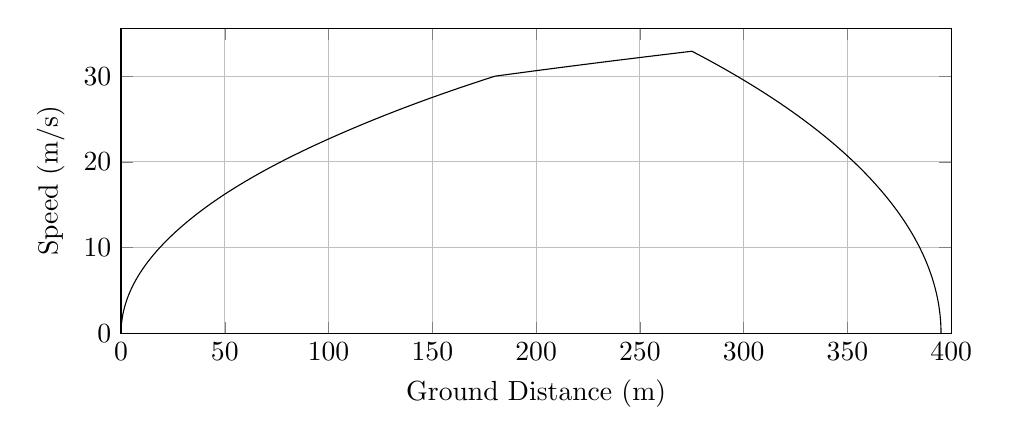
\begin{tikzpicture}

\begin{axis}[
width=\textwidth,
height=0.45\textwidth,
scaled ticks=false, tick label style={/pgf/number format/fixed},
xmin=0.0,
xmax=400,
xlabel={Ground Distance (m)},
xmajorgrids,
ymin=0.0,
ymax=35.60243705812628,
ylabel={Speed (m/s)},
ymajorgrids,
legend style={at={(1.03,0.5)},anchor=west,draw=black,fill=white,legend cell align=left}
]

\addplot [
color=black,
solid
]
table[row sep=crcr]{
1.3729668748938318E-8	2.745933749757015E-4\\
1.7493248493808052E-7	9.801561244272487E-4\\
1.4411937280317895E-6	0.0028133334263539117\\
6.602995160656227E-5	0.019042785691170537\\
2.2740573828771224E-4	0.03533951742361742\\
4.8751428921765393E-4	0.05174321892135983\\
8.441986619835749E-4	0.06808977660239585\\
0.0012981647037285577	0.0844353365412891\\
0.0018484379050661159	0.10075381131347452\\
0.0024893731755424335	0.11692401404508576\\
0.0032286585096692284	0.13315864947738254\\
0.0040442418752796045	0.1490309460458631\\
0.004972762654474916	0.16525563470227161\\
0.005990910102221513	0.1813857976712797\\
0.007111389191545643	0.19762119246996934\\
0.008336865178450469	0.21397204670389414\\
0.009664633507451486	0.23038152766885184\\
0.011093815858158905	0.24682815127838675\\
0.01262066151120312	0.263265820307077\\
0.01419454386807839	0.2791986545425519\\
0.015910782250193378	0.2955952662747262\\
0.017721549103721458	0.3119619385062512\\
0.019620507964630857	0.3282501310843995\\
0.02164969955342029	0.3448058860985598\\
0.023766550611781796	0.3612690162089588\\
0.025957065600157342	0.3775498524463491\\
0.028260861173784894	0.39394719674836465\\
0.030668466949245715	0.410383707902753\\
0.0331489614440674	0.4266559078198039\\
0.03573888453685943	0.44300840396891283\\
0.038418765463712895	0.45931623269011934\\
0.04116679597872082	0.47545806081684927\\
0.044022059812866554	0.49166851394108313\\
0.04700053365173311	0.5080273423779957\\
0.050116649382181494	0.5245961664609897\\
0.0533021652593606	0.5410095070500209\\
0.056630220296749106	0.5576412582238173\\
0.05998688030085898	0.5739277187039493\\
0.06348077825220624	0.5904027942398575\\
0.06710848437295475	0.6070355888921957\\
0.07082346760424127	0.6236086695802725\\
0.07462944469130567	0.6401425932771283\\
0.07855413323217031	0.6567561544391656\\
0.08251243142992878	0.6730964799422352\\
0.08659905947434482	0.6895601384027192\\
0.09083545394947079	0.7062217948484368\\
0.09518096637774642	0.7229134142824443\\
0.099604438418047	0.7395173119645533\\
0.1041130762071252	0.7560654102385658\\
0.10871457033213175	0.7725885970010864\\
0.11350280915994052	0.789414897207366\\
0.11836943512882261	0.8061564986927878\\
0.12328542045494376	0.8227217321804843\\
0.12830372217771202	0.8392942075725671\\
0.1334037067999082	0.8558073214904485\\
0.1386015897371753	0.8723154406793838\\
0.14405085578552257	0.8892925587093323\\
0.1495239325759128	0.906023300154549\\
0.1550507392415454	0.9226100529817982\\
0.16073360491635535	0.9393593896808448\\
0.16659871679960742	0.9563378698222822\\
0.17244819595229793	0.9729756148686326\\
0.17848031195343078	0.9898395443790766\\
0.18466822548212042	1.00684512125021\\
0.1909009608611748	1.023687878666769\\
0.19716089737688902	1.0403292487664908\\
0.2035279375926986	1.056986144772044\\
0.21017879584430066	1.074109246904928\\
0.21687473998771628	1.0910764957758898\\
0.22354650324940833	1.1077235265509446\\
0.23036941414946865	1.1244923431428457\\
0.23737731412185503	1.1414588704693824\\
0.24449289925428264	1.1584313614920383\\
0.2517184892023243	1.175414947859407\\
0.25908208279438383	1.192473531314623\\
0.2664863589195283	1.2093832274856608\\
0.27399321582905467	1.2262886274661136\\
0.2816108016888421	1.2432078594095262\\
0.2893844725195981	1.2602390433086605\\
0.29747621078120867	1.2777253594880231\\
0.30547198304033185	1.2947717452431249\\
0.31373479402345694	1.3121541775007652\\
0.3220909744202328	1.3295012966106468\\
0.3305540912568814	1.3468420668133918\\
0.33895489345894936	1.3638365024108157\\
0.34753073012810576	1.3809686983503315\\
0.3563589175375672	1.3983851403981644\\
0.3652744752958731	1.4157558589432995\\
0.3742693918027593	1.43306717314297\\
0.38350989122680823	1.450635335748475\\
0.3927029292363896	1.467903957895163\\
0.4020876366599533	1.4853248556951635\\
0.4115568217121528	1.5026971903559407\\
0.4212787852930122	1.5203260447095182\\
0.43089755178065414	1.5375681624257411\\
0.4408379299669313	1.555185213830348\\
0.4510502611115679	1.5730780261575021\\
0.4612670224725215	1.5907764641960198\\
0.4715818614584312	1.6084464929996969\\
0.4818438670126082	1.6258347036069667\\
0.4922128554044626	1.6432165605672906\\
0.50273876067117	1.6606746260618541\\
0.5136516607865718	1.6785820531452376\\
0.5244310074213006	1.6960839321955912\\
0.5355751508210329	1.7139894155460103\\
0.5467126997993474	1.731698516530209\\
0.5580479056656631	1.7495370212026495\\
0.5692960823995112	1.7670597423659236\\
0.5809945926573021	1.78510068535335\\
0.5923626544035139	1.8024582108612397\\
0.6041922852715	1.8203439176489105\\
0.6160912669048675	1.8381580505356934\\
0.6280605196746807	1.8559040150004549\\
0.6403946506485891	1.8740142553801205\\
0.6525721787971039	1.8917235842909679\\
0.66504690021022	1.9096939250266787\\
0.6773535438897555	1.9272570708284058\\
0.6901462526606317	1.945344891624475\\
0.703249873273524	1.9636986239503091\\
0.7159721017112175	1.981354570722634\\
0.729053467210389	1.9993454121544838\\
0.7422988791228431	2.0173974409387396\\
0.756304272979474	2.0363101373314\\
0.7696432036294076	2.054159974410436\\
0.7832290250230658	2.0721811688782967\\
0.7969128825551131	2.0901743623702957\\
0.8108444209446342	2.1083344818020304\\
0.825043936786227	2.1266833129613296\\
0.8390802275180445	2.1446659237513304\\
0.8532340040587583	2.1626466350356415\\
0.8678101043696134	2.1810078755052817\\
0.8824320602344964	2.1992718056031553\\
0.8978006605470081	2.2183051377968805\\
0.9134572487531922	2.2375274698967402\\
0.9287391767029982	2.256130737471988\\
0.9440564687433697	2.2746232653161487\\
0.9598871644713316	2.293577785375984\\
0.9757786228365237	2.3124476251369854\\
0.9918217338879218	2.3313414354625053\\
1.0080608846667363	2.350310244973776\\
1.0245900975307913	2.369460702886954\\
1.040622085070809	2.3878871944178703\\
1.0571005809273983	2.4066786687919777\\
1.0736578999152901	2.4254121931867534\\
1.0902401336450098	2.444028796579393\\
1.1073201062866707	2.4630558575727797\\
1.1241926772552646	2.4817074203845095\\
1.1416781667104252	2.5008884842005994\\
1.1588269484070954	2.519557115943438\\
1.176440946845327	2.5385880024942766\\
1.1944819542445066	2.557932148965393\\
1.2120125629913447	2.5765886382913967\\
1.2299306574276825	2.595517639375487\\
1.2481120482032448	2.614583405444348\\
1.2663536608165091	2.633572296542063\\
1.2851425782117465	2.652987459389303\\
1.3041313368869671	2.6724644260610546\\
1.3228236880779458	2.6914983494361895\\
1.3414329672940513	2.710313579664695\\
1.3605066144349074	2.7294623649521776\\
1.3802534409605212	2.7491450260300265\\
1.3994872719307283	2.768180425465\\
1.4192016277101378	2.7875550833166374\\
1.439023460648384	2.806899110882914\\
1.459347998039509	2.8265947929306874\\
1.4793256644936217	2.8458200550486863\\
1.4991489338326072	2.864767809480229\\
1.5195196572175793	2.884107715811661\\
1.5402684478761244	2.903672651533622\\
1.5604570108688036	2.9225821793605533\\
1.5810331069622228	2.9417281799743202\\
1.6022712329181132	2.9613588693312414\\
1.623752316257296	2.981081088586241\\
1.6452514305955401	3.000688534053265\\
1.6664829631402025	3.0199255047213613\\
1.6886446033619715	3.039873778995527\\
1.710607384244656	3.0595131625849623\\
1.7329417009553727	3.079354734333231\\
1.7551421266962821	3.0989498821582195\\
1.7779085356585536	3.1189151163488686\\
1.800478286927734	3.138580922227405\\
1.8236018329231238	3.158600640902775\\
1.8462320784511883	3.178069573313743\\
1.869621217116264	3.198065190585111\\
1.8933146512119747	3.218192588484756\\
1.9176856041472643	3.2387632751638957\\
1.9417713639512164	3.258963928974107\\
1.9657098573982132	3.2789160602383687\\
1.9902165007163162	3.299215000456961\\
2.014554050520948	3.319249296721013\\
2.039479559407779	3.3396412488944405\\
2.0645497069116256	3.3600249047064397\\
2.090368502766882	3.3808869458562745\\
2.115564185269416	3.4011203262020633\\
2.140750230554602	3.421224607682783\\
2.1667677015838267	3.441867410014254\\
2.1927560352542175	3.4623623770407628\\
2.218891869133375	3.482850184369502\\
2.245288939563828	3.5034192934486885\\
2.2712530964452817	3.5235321150782903\\
2.297933078351498	3.544078676912\\
2.324564104516777	3.5644675622649844\\
2.351466051806102	3.584944255791985\\
2.378869922986878	3.6056815089832\\
2.4061764715670764	3.6262252420255647\\
2.4343811693482102	3.6473212111172773\\
2.4622108821536663	3.6680158200226414\\
2.4906408044048067	3.689034880037064\\
2.518892760285042	3.7098024045211524\\
2.5472153538550346	3.7305038371011454\\
2.5762492306032216	3.751604556392463\\
2.605385308804288	3.77265885975738\\
2.634725531238531	3.793740545947773\\
2.6633424112287507	3.814188269376828\\
2.6927188130915374	3.8350632832649136\\
2.7226962917814213	3.856246846509716\\
2.7531675915664673	3.877658627570839\\
2.7831412651501983	3.8986039132076407\\
2.8139174932165103	3.9199914284852095\\
2.8440331768075415	3.940805463831844\\
2.874693215323904	3.9618812954722067\\
2.9059978681586376	3.983283017717028\\
2.9372617813709034	4.004540567062701\\
2.9684444504378202	4.025628922378527\\
3.000072782687808	4.046904250267042\\
3.031082587373527	4.067653380618779\\
3.063213028467148	4.089039106139634\\
3.0965739711585014	4.111123799299039\\
3.1291175748240176	4.132551436526409\\
3.161651640649506	4.153860091747873\\
3.194791488147139	4.175451451278743\\
3.2273698640351327	4.196566512811529\\
3.261394174200582	4.218503584793469\\
3.2942820372415875	4.2395978181219345\\
3.3276455142443044	4.26088817859155\\
3.3625338428565543	4.283036024158147\\
3.396526624461681	4.304503432160644\\
3.4305511850311694	4.3258819528145285\\
3.4642094416894933	4.346924644244828\\
3.498963551783903	4.368543784473827\\
3.5341885134496573	4.390344825173816\\
3.569804025802995	4.41227566137831\\
3.605116576002147	4.433910483656753\\
3.641338581546833	4.455990935222921\\
3.677593698357855	4.477980101320377\\
3.7132425573336665	4.499494417793999\\
3.74957219375957	4.52131186791552\\
3.7872650227149185	4.543834709491012\\
3.825403000593508	4.566507875425231\\
3.861987998097706	4.588150051796694\\
3.899535703755137	4.610253615889045\\
3.9366960368382165	4.632022848447335\\
3.9756271117991435	4.654717625207532\\
4.014715979923002	4.677390959293206\\
4.053268843133694	4.699643665819206\\
4.093111596873367	4.722528057282259\\
4.132540645872048	4.745063532854312\\
4.171686416589186	4.767329139268224\\
4.211258480423352	4.78972942073012\\
4.252585425594734	4.813009023273391\\
4.29253892845542	4.835405747759294\\
4.332839968385603	4.85789005261978\\
4.372708537789018	4.8800285666982735\\
4.414379330316386	4.903058272049913\\
4.455607216042212	4.925734525068886\\
4.497336690654009	4.948578120665225\\
4.53836773335787	4.9709343699274005\\
4.579767142935065	4.993387236550703\\
4.621942908118227	5.016155098789904\\
4.663798268780793	5.0386455998057755\\
4.705838036060712	5.061131913160432\\
4.748491012675066	5.083841859474553\\
4.791393968819099	5.106580280460207\\
4.835700194867293	5.12995378398521\\
4.879973298406089	5.153201037889401\\
4.923250156511948	5.175821498471649\\
4.967673596314626	5.198936085329022\\
5.012954369117542	5.222388563932281\\
5.057574526249477	5.245393459549955\\
5.103280208347517	5.268850968793279\\
5.148856018935929	5.292135378554356\\
5.194350575362858	5.315273669954703\\
5.240584094986199	5.338682132187644\\
5.2871741484687504	5.362164780261091\\
5.333122064003502	5.385220599260908\\
5.3803318800233235	5.408804293294599\\
5.4262712259485255	5.4316521648593366\\
5.473378197958581	5.454978474320454\\
5.521938593493333	5.478917479721449\\
5.570027890245774	5.502518579191591\\
5.617746353771608	5.525835087825929\\
5.665750363096816	5.549189321818824\\
5.714883880069209	5.572988680831415\\
5.763390205677501	5.596381969534493\\
5.812817811268989	5.620116370443503\\
5.861909274803731	5.643587555330178\\
5.912134919389196	5.667497332952465\\
5.962317560553064	5.691283238887795\\
6.012727788730279	5.715074271653515\\
6.0628236035803145	5.738616176082424\\
6.113711068416594	5.762428568577636\\
6.16497292765713	5.786313975860049\\
6.216284706244114	5.8101212146122965\\
6.26834407822653	5.834172897359418\\
6.320257064476769	5.858055495044951\\
6.37351660191279	5.882453594702493\\
6.426150862197664	5.906463071475246\\
6.479030963436509	5.930483658358424\\
6.532319340056288	5.954588513514302\\
6.5857233987986845	5.978645031005438\\
6.640834734692348	6.003366249566406\\
6.695022999498724	6.027571315668311\\
6.749720237657193	6.051902328312192\\
6.804235758325081	6.076052362501423\\
6.859728469301633	6.100533845085355\\
6.916686079588434	6.125556455229262\\
6.9732530286722305	6.150303315061631\\
7.029531186664631	6.174822114436326\\
7.086633318514238	6.199597449617537\\
7.144155485034537	6.224451953805524\\
7.202053129566568	6.249365490174972\\
7.260126434764185	6.274251852506023\\
7.317913145042743	6.298914465249707\\
7.376682960996439	6.323894618455785\\
7.435393721764624	6.3487481490973465\\
7.493838107271518	6.373389329329468\\
7.552684475254578	6.398100782617156\\
7.613252707151423	6.423432563785438\\
7.672782806866918	6.448229800859755\\
7.733397683408512	6.473377876879928\\
7.795525081709004	6.499048935993182\\
7.856013653786727	6.523942353509447\\
7.91792172269443	6.549318504073016\\
7.980110745884113	6.574707701783742\\
8.041720670752433	6.599760731132271\\
8.105229267009985	6.6254831303952955\\
8.167457523036095	6.650587002051729\\
8.230908874360502	6.676083591946034\\
8.293738919282273	6.701231482743458\\
8.356235402336917	6.726149209696938\\
8.42092378244627	6.751840487425259\\
8.485671322837007	6.777454186510756\\
8.549180898871484	6.8024810353832805\\
8.614596634551038	6.828159619110403\\
8.680166762249144	6.853798712400334\\
8.744770128469462	6.878962882922066\\
8.812993689385827	6.90543395378895\\
8.88005807777586	6.931353078752458\\
8.94709863067661	6.957162896659991\\
9.013172088448385	6.982503570963587\\
9.079266506338545	7.007757184272014\\
9.14748814890141	7.0337249243337485\\
9.215411293660388	7.059480591882142\\
9.284579146198691	7.085608412719667\\
9.353168277381275	7.111419259094388\\
9.423753765537143	7.137880229826159\\
9.492960052876374	7.163725683018036\\
9.564123004975215	7.190201309556587\\
9.634097601479446	7.216136500000127\\
9.705672410878787	7.242565047756237\\
9.776260200085993	7.26853143726553\\
9.846607984572056	7.294314058359657\\
9.918231435410593	7.32046734992541\\
9.988851555070422	7.346159615601438\\
10.060390022634245	7.372091182386127\\
10.133279281833644	7.398415309816031\\
10.205241085147751	7.42430939070986\\
10.277820389603	7.450330988479372\\
10.352558894167803	7.477028413890535\\
10.42733258664746	7.503639671954019\\
10.501815126481194	7.530050188575258\\
10.576858173457808	7.556562476642339\\
10.65303812840548	7.583377933408709\\
10.729080272001735	7.6100469771700165\\
10.804841544893105	7.636521282951211\\
10.881905013502095	7.663353138591718\\
10.958396790746043	7.689889741790379\\
11.035905069829102	7.716682266611455\\
11.113160538490881	7.743291537725936\\
11.192172636140572	7.770407901336807\\
11.270076562295213	7.797047997270166\\
11.350065490058778	7.8243029997830895\\
11.429008826667825	7.851105320694458\\
11.50754237847364	7.87767447630535\\
11.587076645554472	7.9044875894302\\
11.668897725768986	7.93197334092549\\
11.749734371708193	7.9590315134803795\\
11.830312384681939	7.9859082812388404\\
11.909862670519033	8.01235032822278\\
11.990515423105418	8.039066540264908\\
12.072973931530203	8.066285822915322\\
12.155304175892073	8.093367836765307\\
12.237018674011615	8.120154471944652\\
12.320146069843414	8.147310337497665\\
12.406770618003886	8.175508889111107\\
12.489918686423398	8.202480979041646\\
12.574493004618496	8.229821467227936\\
12.660666896522624	8.257582277972531\\
12.746500366216402	8.28513731475353\\
12.832006837122272	8.312492980707578\\
12.919285437479463	8.340319422765806\\
13.00517529032821	8.367609209154548\\
13.092301899261269	8.395197755453601\\
13.179760097773386	8.422796850479578\\
13.268594687119744	8.450734398982132\\
13.357699529172354	8.478660840283151\\
13.44829753340392	8.50695758308525\\
13.537570218252604	8.534745028816864\\
13.627322718831184	8.562587370122476\\
13.718307212496544	8.590716196341472\\
13.808540263830096	8.618518503292734\\
13.899143852161355	8.646341531112757\\
13.991564069206362	8.674626907467385\\
14.085798171937814	8.703369108515862\\
14.179213507883688	8.731764584716228\\
14.271883316076963	8.759838983451804\\
14.367546274622434	8.788722461837416\\
14.459430863676705	8.816372617521623\\
14.555010173556813	8.84503935781289\\
14.648669731311681	8.873037028493652\\
14.743773575674254	8.901372887177772\\
14.839769774519894	8.92987995995896\\
14.932807148196385	8.957418513450865\\
15.026921440816679	8.985186697775877\\
15.12275113649265	9.013369781181584\\
15.222025232743288	9.042469720903732\\
15.321078842653048	9.07140849270197\\
15.417564225728565	9.09950514796304\\
15.515758841369038	9.128007419530377\\
15.613440509090129	9.156269491650061\\
15.7107260301154	9.184327297639449\\
15.81102223487273	9.213160640553841\\
15.913565872734136	9.242543656282287\\
16.012918321571746	9.270920177846005\\
16.11222833737955	9.299194878466079\\
16.216250800242257	9.328716023710864\\
16.319159023020546	9.357825988089104\\
16.421418004006803	9.386659645595689\\
16.521675247646563	9.414840066488026\\
16.62557290942481	9.443951838886342\\
16.72731964230514	9.472371127221127\\
16.830283223934416	9.50104069128232\\
16.93464251494634	9.530007766659548\\
17.038481620468637	9.558740267646716\\
17.146497421123335	9.588533916314098\\
17.252282308638982	9.617619657360787\\
17.35724772858778	9.646390408399203\\
17.464053904588297	9.675574876517068\\
17.572390862630144	9.705084909493728\\
17.680417629270814	9.734418351955906\\
17.789707298693855	9.76400202339044\\
17.899612520762552	9.793659182664925\\
18.01027367065641	9.823426854718555\\
18.121415095654797	9.853230213992497\\
18.232428503320143	9.88290658253214\\
18.34337337506409	9.912472977805535\\
18.454877340220463	9.942096916719443\\
18.56636189702322	9.971624895785052\\
18.678405595805643	10.001210341704514\\
18.7903363416971	10.03067608506613\\
18.902391384512768	10.060085398853307\\
19.01754810908954	10.090216685111244\\
19.131359562866663	10.119905120061443\\
19.247747682986713	10.150173154594743\\
19.361628242251975	10.179699333687509\\
19.477963464454028	10.209771140606378\\
19.595742742603164	10.240123605476668\\
19.71107288142779	10.269755440962637\\
19.82767543183723	10.299625023945445\\
19.944540068808188	10.329472599192002\\
20.06171535440768	10.359310730329746\\
20.179291418887807	10.389162371290585\\
20.29729887224694	10.419035161231573\\
20.417200571824914	10.449297609200816\\
20.53676390826074	10.479385286812665\\
20.65523768803314	10.509111551895497\\
20.777063017363922	10.539589025343918\\
20.896922101876633	10.569486607360407\\
21.016777952410983	10.59929689912131\\
21.13892104879462	10.629587893976428\\
21.260534693274344	10.659659948300135\\
21.382619708556632	10.689761392841646\\
21.506306369043365	10.720169476482468\\
21.631260758247265	10.750799829562194\\
21.75556249187227	10.78118184657318\\
21.87985606458615	10.811474550266158\\
22.005925835680863	10.842111749382909\\
22.130365724585275	10.872266329955558\\
22.257477980325966	10.902980523463068\\
22.38418119026224	10.933508198941738\\
22.50885833858638	10.963463025080845\\
22.636026948728087	10.99393066519372\\
22.76367325110224	11.024426399233274\\
22.89115382514759	11.054796953305566\\
23.022452271734288	11.085988446217733\\
23.149877274293033	11.116174529071358\\
23.27873580881144	11.146615583230105\\
23.408563766880334	11.177200342965577\\
23.538692653979794	11.20777082157792\\
23.671258756997098	11.23882694940632\\
23.803210122669313	11.269652718824766\\
23.93544283576786	11.300458555208255\\
24.067241518013077	11.331078692350477\\
24.19863541429976	11.361521460060182\\
24.329449967727697	11.391748060477795\\
24.46175612159181	11.422236868308769\\
24.594763714591892	11.452804456271778\\
24.72754053098891	11.483236854143666\\
24.86208223890334	11.513990756634719\\
24.99503410474967	11.54429986857128\\
25.12831230627787	11.574602871369095\\
25.265273024090206	11.605659896100171\\
25.400650037308893	11.636275573882461\\
25.536304655026747	11.666872730586064\\
25.673594178904246	11.697756485990315\\
25.80797730935859	11.727907070402154\\
25.835159569235522	11.73399627175068\\
25.83771752397454	11.734569125111406\\
25.84157983658004	11.735434035751847\\
25.854829339215996	11.738400588018216\\
25.893215796826965	11.74699102336189\\
25.973046119315796	11.764835870261674\\
26.096262980671412	11.792325687828392\\
26.224212718725603	11.82080317243156\\
26.35313595194755	11.849427449898315\\
26.481727686355264	11.877908705901316\\
26.611118169629577	11.9064973458457\\
26.74049186039369	11.935012993558825\\
26.87228140714948	11.963990356182965\\
27.003385008924262	11.99274648315194\\
27.1358830905183	12.021737581499828\\
27.265951877034226	12.050128265319604\\
27.399105426781233	12.079122042396705\\
27.53075869079712	12.107719723687051\\
27.66387879779476	12.13656630303236\\
27.79855889054391	12.16568002797267\\
27.932132547760695	12.194484591940203\\
28.06791767232785	12.223695071478268\\
28.202763022922632	12.2526330170029\\
28.339788243013793	12.281967392546672\\
28.476803106655623	12.31122807503452\\
28.61761981788422	12.341226680006773\\
28.753907949775353	12.370189579780149\\
28.89297195746854	12.399670893910589\\
29.03211749902605	12.429097676262618\\
29.17123509789927	12.458447191983321\\
29.312253051611236	12.488125270685916\\
29.454422317169097	12.517972384162682\\
29.59523538430127	12.547462726859035\\
29.737672170826222	12.57722064139389\\
29.879173197948965	12.606711335627043\\
30.02075470454991	12.636147711288835\\
30.166674235301365	12.666412071579277\\
30.308336095430334	12.69572202636622\\
30.452640844036836	12.725506988251436\\
30.597553881025625	12.755345032695217\\
30.742967061600154	12.785213522931606\\
30.888975484926362	12.81513163569263\\
31.034653067922946	12.844909872444937\\
31.180984070508003	12.874749646110697\\
31.328351020411645	12.904728171012607\\
31.476753455192622	12.93484428420285\\
31.62661541983664	12.965182661219465\\
31.774495604492607	12.995047482306948\\
31.924944104961916	13.025357687313338\\
32.07610067279926	13.055736566071463\\
32.22631826848556	13.085853737222568\\
32.37899942625752	13.116390732232041\\
32.528514827654206	13.146222623463562\\
32.68189139400266	13.176751411464863\\
32.836069829938495	13.207365260539305\\
32.99025509482905	13.237906193269861\\
33.14574197930297	13.268630209976319\\
33.30072558931056	13.299180562552802\\
33.455047097713944	13.329527242510189\\
33.610874563168906	13.36009645326342\\
33.76926068144728	13.39109228290279\\
33.92617323250643	13.421725333324364\\
34.08448787244542	13.452557525934765\\
34.24243160505006	13.483243305231298\\
34.40316487172558	13.514395458139187\\
34.56154208099588	13.545016867333096\\
34.721775177117024	13.575922712961361\\
34.88076970836556	13.606516167760788\\
35.041349106451236	13.637340735353845\\
35.20329621413198	13.668353154199892\\
35.364886328651124	13.69922291645766\\
35.529241615711214	13.73054528100413\\
35.69117991651797	13.761332873455665\\
35.85317319416103	13.79205773921191\\
36.014854298354294	13.822650866688232\\
36.18095311277159	13.854004920809285\\
36.34443322746766	13.884790898996187\\
36.51065106768533	13.916017890389313\\
36.67635767082788	13.947074482992182\\
36.842033683894186	13.97805158435235\\
37.00823867836148	14.009053944726826\\
37.17279029188734	14.039675677937577\\
37.33951104811075	14.070628233971537\\
37.50923941781488	14.10206432221781\\
37.679358776579846	14.133497520068453\\
37.845326083883435	14.164091329346522\\
38.017144746304325	14.1956890876533\\
38.1852030886141	14.226522279602513\\
38.35804431104914	14.258158097238443\\
38.52812920813831	14.28921574848194\\
38.69960796987526	14.320454401926607\\
38.87165793928378	14.351723379523964\\
39.0423941506003	14.38268102295195\\
39.21436971822614	14.413790751604473\\
39.38727999643966	14.444996521239876\\
39.558989012313546	14.475913453003397\\
39.734752343022535	14.507486480729824\\
39.908836167348156	14.538684565707165\\
40.084555009291705	14.570102192940322\\
40.259186798753746	14.601252770423791\\
40.43324437115375	14.632229247915411\\
40.61041052363379	14.66368591114869\\
40.787318094191775	14.695023582621097\\
40.96620398302343	14.726637892031388\\
41.14141336180775	14.757530947321776\\
41.31941103282654	14.788843608684214\\
41.49571226203258	14.819786704093303\\
41.67366972437729	14.850949124251486\\
41.85219319429197	14.882139047575382\\
42.03136872634711	14.913371205615714\\
42.21293422072888	14.944947136872095\\
42.39366932880948	14.976306290625715\\
42.57479521797359	15.007661248963057\\
42.75522531040919	15.03882452217935\\
42.93775785970641	15.07027901101005\\
43.11993568316029	15.101600682690702\\
43.30336620712447	15.13306580140896\\
43.48720879745599	15.164529618027455\\
43.672226884455625	15.196122289886826\\
43.85684130549208	15.227574146465127\\
44.039851952877484	15.258682320644418\\
44.22449378650157	15.289997095679201\\
44.412385508552646	15.321790608155712\\
44.59783063297877	15.35309890605317\\
44.78525507043919	15.384669902907206\\
44.973130075825196	15.416245120448252\\
45.16145211071871	15.4478238768376\\
45.34881478087516	15.479171053194221\\
45.536017136752506	15.510421384177157\\
45.724971990057284	15.54189370268887\\
45.91416212467789	15.573334602482515\\
46.10175434018815	15.604440599130726\\
46.29356928918713	15.636175810787584\\
46.48490977712943	15.667761433505884\\
46.67744207882204	15.69947255071358\\
46.869905949194575	15.731101389522046\\
47.062749521718516	15.762721841107386\\
47.25341437235973	15.793915796374279\\
47.44508461154423	15.825205238524163\\
47.63880095964302	15.856758814343422\\
47.83356160493736	15.888412077854802\\
48.025334057720784	15.919511103737413\\
48.218846636819876	15.950823735261029\\
48.41468711090302	15.982443311473421\\
48.610449575687724	16.01398058830579\\
48.80723286029129	16.04561249117431\\
49.00124137999302	16.076730225673515\\
49.20045899041696	16.108613469004666\\
49.394243884198005	16.139559590609927\\
49.59161211700324	16.17100975835519\\
49.79144608231523	16.202783130131834\\
49.99107345578199	16.23445403109276\\
50.18996871950735	16.265939978911277\\
50.388458331230495	16.297293637193356\\
50.59191110395449	16.329361114702195\\
50.79453916783869	16.361228411152567\\
50.99530158869649	16.3927336124352\\
51.19776583381373	16.42443703723646\\
51.3996255264899	16.45597737097976\\
51.599450409211	16.48713285962996\\
51.80158475775707	16.518581084428426\\
52.002311498730975	16.549743669984224\\
52.2060805474067	16.581311029937034\\
52.40811442127868	16.612542781175982\\
52.61423073460446	16.64433747071798\\
52.821749674584495	16.676279383846385\\
53.03053110951893	16.708346019233034\\
53.23753590773735	16.74007125225181\\
53.44487707917263	16.7717800272353\\
53.652063533093525	16.80339754071838\\
53.85975522429668	16.835024719859476\\
54.06844148636836	16.866735735918397\\
54.278580968983874	16.898599481048315\\
54.48685885904548	16.93011390802227\\
54.69884126905886	16.962120720521014\\
54.90975544393264	16.993898405991033\\
55.12216013841277	17.02583267040511\\
55.333080623240974	17.057476656010834\\
55.5448885814986	17.089186849928865\\
55.75594910746132	17.120718798734273\\
55.968144975063936	17.15235397919561\\
56.18150915317635	17.184096602192163\\
56.394069348356695	17.215653451067624\\
56.60950747146016	17.247570555005474\\
56.82641599949238	17.2796377393909\\
57.03980213394583	17.311118216005376\\
57.25698083573829	17.34309140361224\\
57.47353804711997	17.37490637544135\\
57.6941706582635	17.407251949021614\\
57.91229938529948	17.439163234249854\\
58.12998527173144	17.470943490423387\\
58.34905943653719	17.502859991071126\\
58.56781345824973	17.534663729273177\\
58.787998582886644	17.566609184333608\\
59.011266007804366	17.598934253781984\\
59.23368761368569	17.63106958619902\\
59.456031473365414	17.66312695350576\\
59.67976581221534	17.69531783422297\\
59.90315377467765	17.72739224145881\\
60.125192111546724	17.7592072579533\\
60.349269227196444	17.791248463842905\\
60.57220932044149	17.823061717762613\\
60.79606803632835	17.85494082328129\\
61.021718319759984	17.887009278121397\\
61.25073295331903	17.919488713415852\\
61.47770893732542	17.95161265849601\\
61.70784367826464	17.984116595017582\\
61.93740803875056	18.016473074293522\\
62.1673491775543	18.048816062463573\\
62.39648011888062	18.080979167027678\\
62.62822464633953	18.1134425841339\\
62.86094183422966	18.14597528176636\\
63.090532789209604	18.17800555500485\\
63.321616049163225	18.210178806265958\\
63.554808975015874	18.2425798333092\\
63.78685818650332	18.27475655714074\\
64.0234762327251	18.30750002514708\\
64.25652029988498	18.33968337934492\\
64.49146565301734	18.37206383313017\\
64.72768747885678	18.40455431710828\\
64.96568125142531	18.43722208040868\\
65.20057601391298	18.469399445717087\\
65.43975061379945	18.502097099487123\\
65.67719429610031	18.534492627051662\\
65.91652243006087	18.56707960207529\\
66.1565253585166	18.5996926382046\\
66.39740384038885	18.632358754662555\\
66.63777997854328	18.664891313089214\\
66.87849958303539	18.697405223005703\\
67.12349409848125	18.73042999909198\\
67.36843544137562	18.763380883708052\\
67.61129947098183	18.79598682368536\\
67.85808619273692	18.829052988970048\\
68.10323725880951	18.861834089804688\\
68.3520146383799	18.895033326535575\\
68.60099753692072	18.92819303649258\\
68.84943315800746	18.961213484704757\\
69.09793111574629	18.99417627309159\\
69.34894754058863	19.02740655741996\\
69.59791912239118	19.060300425142366\\
69.84867626946473	19.09336442916495\\
70.10496107302816	19.127089481532906\\
70.35594730130109	19.160051229394938\\
70.60854748652795	19.19315932239791\\
70.8625286964371	19.226382441854668\\
71.1182576034713	19.259767715003406\\
71.37278964945165	19.29293089942211\\
71.62944082734805	19.32630406482957\\
71.88536754710964	19.359517292895546\\
72.14250945057543	19.392822496273666\\
72.40306402213687	19.426502900877068\\
72.66241221953337	19.459960968561703\\
72.92327110344874	19.493547495197788\\
73.18657203154456	19.527381274712283\\
73.45150557123125	19.561357130932635\\
73.71756195569753	19.595409033703262\\
73.97940051906463	19.628855014795015\\
74.24514793127645	19.662733645739877\\
74.51022759525631	19.69646065179441\\
74.77823256031297	19.730492733691676\\
75.04767613410795	19.764639862321353\\
75.31682895458664	19.798682839904423\\
75.58729746777243	19.83282486882524\\
75.85729327570917	19.866840277363707\\
76.13042767774209	19.901183443118022\\
76.40299665611133	19.935388078099322\\
76.67973301409052	19.970047169137942\\
76.95360383527739	20.004279819891543\\
77.22854206589327	20.03857869965745\\
77.50692063517303	20.07323858302778\\
77.78349662592461	20.10760649808084\\
78.0616064362213	20.14209753746679\\
78.33869545141144	20.1763950938769\\
78.62238552181594	20.211440965650013\\
78.90481169871467	20.24626202165907\\
79.18659077494928	20.28093541680736\\
79.4700201012688	20.315743893615732\\
79.75774957869095	20.35101116003014\\
80.04430580185078	20.386065626630675\\
80.33432201731404	20.421473679433355\\
80.62298533865851	20.456647379404394\\
80.9130804606989	20.491926439940222\\
81.20459144967842	20.527308330795158\\
81.49650140842283	20.56266940610589\\
81.79224544448738	20.59842470694941\\
82.08455487090956	20.63369573876311\\
82.37934996819865	20.669197627691325\\
82.67580145620735	20.704829475042132\\
82.97475550983006	20.740691955762657\\
83.2734238134004	20.776450240135105\\
83.57209772503273	20.812139744436564\\
83.87419166445906	20.84816770961431\\
84.17487194816226	20.883957404334772\\
84.47686996876752	20.919834414394003\\
84.78124993153034	20.955924325155635\\
85.08776945017104	20.992197276981145\\
85.39395758722245	21.02836068428524\\
85.69833162305892	21.06424060145197\\
86.01027818388755	21.10094200721906\\
86.31658691867341	21.1369104477143\\
86.62866814828641	21.173486190018266\\
86.94043673469176	21.209954654227438\\
87.2565990672368	21.24686542847371\\
87.56980823017452	21.283360753692115\\
87.88101387141376	21.319553399962942\\
88.20007062892054	21.356587936407273\\
88.51883409355145	21.39351692360224\\
88.83509784148416	21.430086138443315\\
89.15857089898353	21.467417114986695\\
89.47772213402055	21.504178581674047\\
89.80217214804901	21.541478831424143\\
90.1263587278685	21.57867720574783\\
90.44950966725051	21.615685993222307\\
90.77764749859728	21.6531940920381\\
91.10470504824352	21.690507175653025\\
91.43769785174896	21.728424510189086\\
91.76691749028419	21.76584038250263\\
92.09386993524024	21.802928381010865\\
92.42498248438446	21.840417446490633\\
92.7581696617394	21.878069923542576\\
93.09729153734631	21.916319922463096\\
93.4312406900703	21.953914858292585\\
93.76780571708736	21.99173285047641\\
94.10390054156983	22.02942692654632\\
94.43564317419558	22.06656369502685\\
94.77291201930262	22.104249088529684\\
95.10796951504997	22.141617965961636\\
95.44708659079325	22.179369616185113\\
95.78515592548297	22.21693500898585\\
96.12311752311894	22.25441941592539\\
96.46351490415591	22.292104698232542\\
96.80669869710772	22.3300285453495\\
97.14657639264556	22.367518321886216\\
97.48763116340677	22.405069645423985\\
97.8305814261901	22.442761153568917\\
98.17013304046878	22.48001190327186\\
98.51054009051404	22.517289795639208\\
98.854181194619	22.554854559155295\\
99.19205317796005	22.59172320250834\\
99.53355440060989	22.62892233881538\\
99.87198375587872	22.665722299003313\\
100.2129389915628	22.702732356613758\\
100.55335806642802	22.739619996254845\\
100.89503335592528	22.776579664164977\\
101.23693480167049	22.813499947259317\\
101.57977298927813	22.85045767969963\\
101.91842351185082	22.886901772645338\\
102.26214655705948	22.92382894310154\\
102.60487134933112	22.960586290281327\\
102.94238410388857	22.996723981096395\\
103.28139950825951	23.032962360222697\\
103.61984226602698	23.069079740693134\\
103.95406402656286	23.10468843221104\\
104.29248504574807	23.140685938011636\\
104.63112914593611	23.176648550978555\\
104.96686613984221	23.21224493209361\\
105.30464484937244	23.248000378665942\\
105.64180205248229	23.28363298897959\\
105.97704387437452	23.319007030416692\\
106.31384964552919	23.354490090585088\\
106.6489228444834	23.389735279509587\\
106.98000007373659	23.424506281561648\\
107.31456925364313	23.459589981309648\\
107.38092108752608	23.466541363878086\\
107.387754025128	23.467257099501225\\
107.3946577511588	23.46798022723023\\
107.39916951903444	23.468452797962527\\
107.40247473215817	23.46879898574781\\
107.40548301099807	23.46911406808625\\
107.41901751964124	23.470531597096304\\
107.47756267729525	23.476662275158333\\
107.63696404402117	23.49334596459464\\
107.95668166923352	23.526772291238096\\
108.2571634635643	23.558142805619354\\
108.55996775705782	23.58971203526177\\
108.8616926844802	23.621125120504303\\
109.16669292910967	23.652835034323118\\
109.47218465327785	23.684551608078415\\
109.78023369107405	23.716488732544356\\
110.09061921742381	23.748622520493456\\
110.4007971847821	23.780689204113827\\
110.7125096545017	23.812868671809618\\
111.02874540594937	23.845468211770957\\
111.34670354521654	23.878197785504135\\
111.664908557295	23.910905157489083\\
111.98617551206428	23.94387902880578\\
112.3078797039536	23.976849312687172\\
112.63537393275391	24.01036328057925\\
112.96267359383529	24.04380732340553\\
113.28778388635178	24.07697825406092\\
113.61823593045688	24.11064385213622\\
113.94632344632586	24.144018443943487\\
114.27926944824554	24.177836320485795\\
114.61324422041562	24.211707243102758\\
114.94750338770686	24.245555524461466\\
115.28618013885716	24.27979872704646\\
115.62544260296943	24.314048364325124\\
115.9647508443766	24.34824989577851\\
116.30617149460878	24.382611246087016\\
116.65060078043697	24.41722153358515\\
116.99863777637248	24.452139520588716\\
117.34270613829636	24.48660529239988\\
117.68983788345284	24.521323592816493\\
118.04137408578512	24.556426913310872\\
118.39343387684602	24.591526682448844\\
118.74804854616337	24.62682481479412\\
119.10520175440718	24.66231860103761\\
119.46686684850098	24.69820259415905\\
119.82660492256403	24.733837450261376\\
120.19012449272657	24.769788336901165\\
120.55217592908159	24.805535667784696\\
120.91763124996498	24.841560161595353\\
121.28719248968574	24.877929345962116\\
121.65493622417088	24.914059879912358\\
122.02513489718217	24.950371525725885\\
122.39308995700384	24.986403518342293\\
122.76618799735454	25.022878639482748\\
123.1388017253943	25.059245771617228\\
123.51256311114031	25.095664192513944\\
123.88633794770595	25.132023264584596\\
124.25665874611622	25.167986679226466\\
124.63165231885978	25.20434353030594\\
125.00664173256905	25.240639405832702\\
125.38021625899401	25.276738263515625\\
125.75512563345742	25.312905993994406\\
126.13473977091255	25.349466401351584\\
126.51299085225449	25.385834455766414\\
126.8948287761801	25.422485709803013\\
127.27325883095315	25.458748891394563\\
127.64986999110431	25.494777690064524\\
128.03053456382577	25.531133516992945\\
128.40840086210045	25.56716186098\\
128.78830732782995	25.603324402260185\\
129.16816802858597	25.639422278871514\\
129.55114692916032	25.67575559846579\\
129.92795862154003	25.711444344008036\\
130.30814318938542	25.74739291097285\\
130.68801179162523	25.783251948121\\
131.0673626953399	25.819002777679778\\
131.44707508552267	25.854728461864248\\
131.82575792285303	25.89029844778053\\
132.20466209461676	25.925830588930104\\
132.58549544797154	25.96148471023875\\
132.96520261413826	25.996974747307668\\
133.34413894748724	26.03233452181265\\
133.72638850756363	26.067944714197402\\
134.1049920954593	26.10315725438464\\
134.48538249769342	26.138478022857264\\
134.86277461399203	26.173463147543856\\
135.2402386369938	26.20839807376519\\
135.62109197355238	26.243589217201794\\
135.9996509441208	26.278511321703462\\
136.37968191797512	26.313512189845667\\
136.76120583273502	26.348593251309282\\
137.13951930881296	26.38332258531475\\
137.51840340013064	26.418048052774175\\
137.89819615735314	26.452800474740854\\
138.27485697152616	26.48721077977922\\
138.65420581933705	26.521810923785843\\
139.03531375767642	26.556515364267987\\
139.41296882619503	26.59085002984427\\
139.79422155259	26.6254560585379\\
140.17408835952057	26.659880777501343\\
140.5488076998477	26.693784891902183\\
140.92844631991198	26.728079442550047\\
141.30483696429354	26.762026445558064\\
141.68269541512387	26.796051769604652\\
142.06058279783264	26.830025689762422\\
142.43991695918288	26.864075525800594\\
142.81695502902187	26.897865655135362\\
143.19247254825046	26.931466555436195\\
143.5733885276352	26.965496673517244\\
143.94921103219775	26.99901878303585\\
144.32621366107247	27.03259345649424\\
144.70408630975157	27.066192808823708\\
145.08263595865492	27.099799515801983\\
145.46162624555404	27.13339252320644\\
145.83827879615103	27.16672611867068\\
146.21524500988596	27.20003553147759\\
146.5934755401724	27.233404598150642\\
146.9730259257883	27.26683784700767\\
147.3547239944582	27.300407645585366\\
147.73366854735332	27.333683229207665\\
148.1136534850276	27.366998261276848\\
148.49311509785633	27.400215701060773\\
148.87144514206074	27.433282803456457\\
149.25360190977045	27.466632551458567\\
149.6334430260095	27.499728773112743\\
150.01465687879528	27.532893199380077\\
150.3940924716125	27.565851947415844\\
150.77688175221402	27.599050637291228\\
151.1561678741857	27.63189477797122\\
151.5352572324847	27.66467158732717\\
151.91884603110896	27.69778641234719\\
152.3000376871389	27.73064362176867\\
152.6837211891089	27.76366477253727\\
153.06727641570347	27.796624062103255\\
153.4514076737559	27.829582088305806\\
153.83522357687116	27.8624624842549\\
154.21637826964854	27.89506503650548\\
154.6009164651564	27.927906808977156\\
154.98403470202834	27.960577337031737\\
155.36838747168406	27.993303183305123\\
155.75158064164503	28.025880646761166\\
156.13576662495046	28.058492911905\\
156.5218436740983	28.091215833096335\\
156.90521285441474	28.123659936973866\\
157.2916244593892	28.15631196393415\\
157.6780020855428	28.1889115409629\\
158.06299451159185	28.221345098731064\\
158.4509000667514	28.253974620381257\\
158.83830611621056	28.286512747867498\\
159.22672413827297	28.31908649759972\\
159.61474494524106	28.35157773964125\\
160.0042372884319	28.38414291715614\\
160.39552304382113	28.41680848873161\\
160.78478895267375	28.44925632312976\\
161.17517847278327	28.481748784359482\\
161.56748129737286	28.514351193980744\\
161.9609400214345	28.54700019760552\\
162.35005274814932	28.57924001673333\\
162.7425950916558	28.611715236616696\\
163.13607830878885	28.644219314491743\\
163.53170884953005	28.67685150295577\\
163.92462594167722	28.709211152871426\\
164.3198767210975	28.741714173878485\\
164.7157696028566	28.77422107834746\\
165.1115317336501	28.806668482588243\\
165.50739628911128	28.83907567934952\\
165.90698313288817	28.87173847247977\\
166.30582458333038	28.904291290943938\\
166.70591293613995	28.936896824184117\\
167.1044701422045	28.969328897683944\\
167.50226971352845	29.00165104505738\\
167.9010833894181	29.03400734878567\\
168.3004552315794	29.066360703950018\\
168.70189335181743	29.098832980326407\\
169.10576843973695	29.131453520472753\\
169.50785881751284	29.163881400675045\\
169.91045494783964	29.196301748593527\\
170.31331810721775	29.22869537528949\\
170.71648797717722	29.261065542660667\\
171.11993291578136	29.293409780177015\\
171.5247281229082	29.3258141712189\\
171.92976094083576	29.358189538101648\\
172.33690302624336	29.390685245836956\\
172.74259563259648	29.423017314753835\\
173.1509823323036	29.45551592738606\\
173.55913088366435	29.487947484449094\\
173.96636547491187	29.520258666095437\\
174.37754484483776	29.552834623347366\\
174.7874876782942	29.58526456542429\\
175.2012500141185	29.617948194124764\\
175.6112323385957	29.65028538641203\\
176.02092514523684	29.682552342665645\\
176.43326782420013	29.71498033450107\\
176.8477920653399	29.747531873473186\\
177.2627043459005	29.780065853933756\\
177.67839640445425	29.812612972629275\\
178.09047986160414	29.84483030454936\\
178.50771992227516	29.87740304246514\\
178.92514786216543	29.909942556141928\\
179.34349041668827	29.942505490816217\\
179.7634585539525	29.975146935563274\\
180.0836350053749	30.0\\
180.18446825846002	30.00782122706738\\
180.6041229201494	30.021613593282297\\
181.5278851973348	30.051941085132732\\
182.40940876889346	30.08083983713518\\
183.29020149056134	30.10967378616489\\
184.17127536929127	30.138476238134423\\
185.05444413874795	30.167306465008828\\
185.94463812048832	30.196324927668087\\
186.83342305465118	30.225256445537184\\
187.72320740690213	30.254179594793484\\
188.61627250998652	30.283168385144194\\
189.51597565669658	30.31233125961991\\
190.41002295084513	30.34126980746457\\
191.3196934236239	30.370672254010422\\
192.21828392903763	30.39967533717359\\
193.1226105375991	30.428822336310688\\
194.0308739866166	30.45805475073533\\
194.94664810390913	30.487486973708442\\
195.8495877725365	30.516465647796124\\
196.76514896738053	30.545807919551578\\
197.67776544775052	30.57501441287077\\
198.59781945634353	30.604417242137977\\
199.51766543264023	30.633771738681048\\
200.44351810370483	30.663275994253567\\
201.3718330130543	30.69281664191213\\
202.29314309783985	30.722092890046774\\
203.21971650332063	30.751494857812595\\
204.14462823093066	30.780802718313062\\
205.07763860999955	30.81032547708515\\
206.00476468733177	30.839620690357087\\
206.93855819187849	30.869085074860628\\
207.87782366152794	30.898680260932572\\
208.81805039558168	30.928263855151997\\
209.75927086542703	30.95783691308469\\
210.70907141928154	30.987637324283384\\
211.6546393296269	31.017262960390397\\
212.59816623974814	31.04678307037294\\
213.54645843731532	31.076410588007512\\
214.4982137391426	31.10610445262443\\
215.45734539338423	31.135986206474243\\
216.4205873513297	31.165953506833496\\
217.38237643693935	31.195833274600105\\
218.35297485781302	31.22594401188165\\
219.32510845799027	31.256059545225504\\
220.29279514401117	31.285994923364115\\
221.26927942590856	31.316159755005636\\
222.2446078047322	31.346246238868346\\
223.21462685547237	31.376126849884237\\
224.19074054242492	31.40615300169698\\
225.1744490750948	31.43637012917911\\
226.14733001520318	31.46621272512617\\
227.14148425007068	31.49666496869081\\
228.1240128312001	31.52671867683869\\
229.11886046703495	31.55710641046779\\
230.11739511657566	31.58756365082082\\
231.11215533106218	31.617862998482124\\
232.12301378994505	31.648609143980202\\
233.1275199718878	31.679118792743544\\
234.13114028184475	31.70955862880156\\
235.14028542531037	31.740122978734995\\
236.15081117254897	31.77068607059318\\
237.1660420924572	31.801348255319716\\
238.1886645294469	31.832190084353194\\
239.21465471906964	31.86308970805343\\
240.23482884221784	31.89377088820234\\
241.26021232675805	31.924565440974703\\
242.3021991810905	31.955814363149244\\
243.32988353044664	31.98659084587672\\
244.36880129710033	32.017660017995695\\
245.4061041381612	32.04863723638101\\
246.46256617747576	32.08014197476507\\
247.50478260671736	32.11117796058146\\
248.56376742117214	32.14266880126482\\
249.6219134221688	32.17409011634308\\
250.66481994405478	32.20501549636204\\
251.72705353011372	32.236469895768266\\
252.80088254110024	32.268222642688755\\
253.86267363775482	32.2995751456812\\
254.94374853170973	32.33145203061112\\
256.0221053298852	32.363203722349795\\
257.1056667215428	32.39506356295679\\
258.2028084304169	32.42727686772736\\
259.3030712409387	32.459535719149\\
260.39721249167394	32.49156954282023\\
261.49829074545437	32.523760837104334\\
262.60930370875815	32.5561964202586\\
263.7179887580877	32.58851804580101\\
264.8352779160481	32.62104425810625\\
265.9576164693235	32.653670959002696\\
267.09103410107514	32.686572667368964\\
268.20818841649384	32.71895622534559\\
269.3328220499261	32.75151065265186\\
270.4661510695621	32.78427039463769\\
271.5992062566115	32.8169759115771\\
272.7460111433737	32.85003140699004\\
273.90093061584855	32.88327335721664\\
274.4708181965357	32.89965891912148\\
275.05359207729066	32.91640309849126\\
275.75457243354776	32.827958296406436\\
276.449302145631	32.739980465342995\\
277.15172181613866	32.650700485590676\\
277.84921532644717	32.56171721681558\\
278.5406463546268	32.473180633488155\\
279.22989884096467	32.38459648708546\\
279.9204368935674	32.295517420225195\\
280.61368515235506	32.205753948393905\\
281.30116592734635	32.11640314381191\\
281.9974769913189	32.025562573419606\\
282.68623058572155	31.935366291411114\\
283.37147237821546	31.845289747278265\\
284.05435880071843	31.755182328787285\\
284.73681578934884	31.664789003934125\\
285.4167554380906	31.574385533272398\\
286.09576898371176	31.48375992373075\\
286.77846272697707	31.3922921818236\\
287.45818007587366	31.300870481774027\\
288.13240931824635	31.209836080523708\\
288.8120712254695	31.117711295946684\\
289.48407502400187	31.02626906622004\\
290.14933909389106	30.93539261939003\\
290.8187250145078	30.843597100120625\\
291.49005824187816	30.751172570829986\\
292.1535241562457	30.659471726996046\\
292.8173703768606	30.56735738688017\\
293.47402916938995	30.47588188368767\\
294.1310294727251	30.383998686505265\\
294.7869811412687	30.291899446511337\\
295.4431792242344	30.199399599165815\\
296.0952258498429	30.10711893138764\\
296.74717561233695	30.014483742555846\\
297.3999513021739	29.921358790437537\\
298.0480801106456	29.828524568094416\\
298.69583244998125	29.735370172586705\\
299.34298299590387	29.64192525797325\\
299.98358639806156	29.549050939326904\\
300.62424240566406	29.45579246384758\\
301.26198029204625	29.36258116172705\\
301.8978076897936	29.2692703798553\\
302.53008628750206	29.176101746288644\\
303.1595420793228	29.08297031413155\\
303.7946917471928	28.98860961409963\\
304.4147340345645	28.896114815678274\\
305.0435763058895	28.801921518221988\\
305.66194422747265	28.7089145682979\\
306.2845727359577	28.614879651550694\\
306.90070938175813	28.521438944268233\\
307.5156094543387	28.42779884319389\\
308.123200378879	28.33488832240313\\
308.7290996956757	28.241853040025134\\
309.3335527447854	28.148654448755238\\
309.93292066179663	28.055855993207366\\
310.53443161001053	27.962337475113983\\
311.12971502454593	27.86940032975574\\
311.72425153203517	27.776191759531713\\
312.3230946957069	27.6819119616547\\
312.91133176856715	27.588910968712696\\
313.4916385501424	27.496780156569905\\
314.07146870038457	27.40434056472217\\
314.6499842421573	27.311723620047992\\
315.23154063535924	27.21822625652196\\
315.8103006199848	27.124782588534508\\
316.38327320254837	27.031880209860212\\
316.95488208035306	26.938805096438585\\
317.5173710757757	26.846826926400468\\
318.08296218726093	26.753949291122986\\
318.64623577638406	26.66105722225221\\
319.2045794991842	26.568584998366923\\
319.76358769756575	26.475606412121294\\
320.3185689955636	26.382901145353358\\
320.8699490102216	26.29040205377607\\
321.4088108937077	26.199618145659507\\
321.959969716396	26.106364755731484\\
322.50875127879885	26.013109608699615\\
323.0542704853608	25.920004955946297\\
323.592200246351	25.82779698648273\\
324.12525648827875	25.736029679577122\\
324.65328824608457	25.644735758501987\\
325.1868113165157	25.552092254665972\\
325.711579471508	25.460572313960533\\
326.2365754079126	25.36861465650344\\
326.7535657750137	25.27766595428149\\
327.26603337175084	25.18712350407587\\
327.78112341959877	25.095722763711763\\
328.2987988804733	25.00345987729812\\
328.81346966408375	24.911327144023467\\
329.3210145709062	24.820069770627597\\
329.8292743178962	24.72828107460213\\
330.33438769178986	24.636656755086896\\
330.83158896466773	24.54607002996314\\
331.3342945870628	24.45407486131247\\
331.8328869572541	24.362425009823156\\
332.32444550218486	24.271666372788985\\
332.81178398519796	24.181288671953496\\
333.2911423312855	24.091999687527384\\
333.77189827029645	24.002056276959145\\
334.2501212776797	23.91219073953178\\
334.72684704758706	23.822208956285913\\
335.19937422119483	23.7326234215343\\
335.6729261507759	23.642443283804546\\
336.13879855834523	23.553330022028298\\
336.6130039761381	23.462215200092494\\
337.0753375997283	23.372980946628054\\
337.53605240083004	23.283661194344283\\
337.99148613763487	23.194970315077555\\
338.4458963243934	23.10608282590477\\
338.8940910054167	23.018019237257008\\
339.3487715278759	22.92827890605364\\
339.79827028436	22.839158249136048\\
340.24716394864856	22.749752877773105\\
340.68778211662004	22.66159776293754\\
341.13327618349456	22.57206151665156\\
341.5659125975759	22.484714442759504\\
342.0050868007846	22.39564459592374\\
342.4410815217477	22.306813328907346\\
342.86995070353237	22.21903417991848\\
343.2947704444514	22.131688383353037\\
343.7175469510072	22.044367247285535\\
344.14316720233273	21.956055476348865\\
344.5560659940322	21.869991945989874\\
344.9706403273592	21.783186749790545\\
345.3824377863741	21.696569028778356\\
345.79384247273674	21.60963709896025\\
346.20851370938374	21.521608650685224\\
346.6156074449772	21.43478714316572\\
347.0220110707047	21.347710984343678\\
347.43170857965856	21.259517653035594\\
347.8322028356423	21.172901219131028\\
348.22841488458346	21.086812764302906\\
348.6235666241728	21.000555379830743\\
349.01070847396795	20.915654952060514\\
349.4000579057358	20.829874725573276\\
349.78541154014374	20.744579282104695\\
350.1671341687497	20.659694732411232\\
350.5488872157971	20.574407546875868\\
350.9409537515056	20.486398938433723\\
351.32034972324186	20.400826827000273\\
351.6962443499658	20.315643896058788\\
352.0812496851447	20.227977750851814\\
352.45263223156394	20.143006972976124\\
352.8250436344256	20.057394716494052\\
353.1922538757739	19.972574858094255\\
353.55623588704725	19.888100407013503\\
353.9159405811072	19.80422212728994\\
354.2765357127421	19.71973546783189\\
354.64328169738315	19.63339075381066\\
355.001160017133	19.548723153782866\\
355.3549801156221	19.464611665559715\\
355.7046774483957	19.38108040501219\\
356.0527689403307	19.297532793570788\\
356.40388412574293	19.21284990202644\\
356.747420551358	19.1295915284421\\
357.0906273035173	19.046009400252267\\
357.4322712414556	18.96240184932264\\
357.77490212868827	18.87814048259917\\
358.11905529229125	18.793083498748835\\
358.4527700645874	18.710197723626372\\
358.7902438652918	18.62596359209283\\
359.121149134436	18.54295855802046\\
359.46042863554135	18.457425170802544\\
359.7879827773261	18.374431245110863\\
360.11603741040835	18.29089468634018\\
360.4407649118001	18.207789890167625\\
360.7605257188153	18.125546702345638\\
361.08152786112475	18.042569908945353\\
361.4043411177663	17.958700477675627\\
361.7263240463342	17.874616771835157\\
362.0353002759083	17.79352023615374\\
362.3489948199883	17.71076929774656\\
362.6604408016252	17.62819105608093\\
362.9693392923481	17.545868588172922\\
363.28038163351016	17.46254644077507\\
363.58539968633124	17.380414705241343\\
363.89342832019554	17.297040715178333\\
364.19478981689633	17.21504552735732\\
364.4890099807403	17.134581248108177\\
364.77860721490947	17.054977970283623\\
365.0673637503512	16.975201780327346\\
365.35790286591384	16.894520153740103\\
365.65305105619166	16.812128330182375\\
365.9435616358636	16.730601416936892\\
366.23272835160833	16.649022039003448\\
366.51906001485736	16.567813922916642\\
366.80789801622996	16.485456467911455\\
367.092822236516	16.403776997464355\\
367.3783886036624	16.321470391135286\\
367.66091410374327	16.239597119324586\\
367.93476824732227	16.15980970709812\\
368.2111230633519	16.078861142618564\\
368.4881906576212	15.997260944302923\\
368.76108206484776	15.91645060550018\\
369.03046816707126	15.836243341542406\\
369.2985472111043	15.755989674833998\\
369.5640394175067	15.676075601618145\\
369.83053849953717	15.595416550710205\\
370.0930020907631	15.515539435545755\\
370.35729225221223	15.434658862969346\\
370.6186555508456	15.354225362392121\\
370.87815097184443	15.273918335862781\\
371.1314635819482	15.195087012803796\\
371.38407818944415	15.11603546216293\\
371.63490551984773	15.03710417512023\\
371.88600021235914	14.957643611884173\\
372.13137908440876	14.879554722972145\\
372.37887019603556	14.800348930736181\\
372.62358816212145	14.721584455438443\\
372.86729916717775	14.642695999107357\\
373.10645630167176	14.564839876937494\\
373.348407245079	14.485621715255188\\
373.59313236278035	14.40502458309037\\
373.8267775135737	14.327627488584767\\
374.06350335758236	14.248755118519504\\
374.29323855459256	14.171767012316952\\
374.52366884484763	14.094098461616682\\
374.75027843309726	14.017273388092438\\
374.977188361534	13.93989765626171\\
375.2027359553316	13.862533936926805\\
375.4280758121686	13.784783311105045\\
375.65116621479456	13.70735005422548\\
375.87447189079273	13.6293771137072\\
376.09058511232115	13.553465082753757\\
376.3051348533337	13.47765641289941\\
376.52090179651236	13.400962019443448\\
376.7353242003279	13.324285084074905\\
376.9486853824079	13.24752409997879\\
377.16417927721625	13.16951822930653\\
377.3782946187854	13.091527538239557\\
377.58652580339105	13.01520927812357\\
377.794797336678	12.938403501709036\\
378.00378670702673	12.86084925233045\\
378.2043510110743	12.785957625404151\\
378.4046667492197	12.710697219618524\\
378.6079702725341	12.633834114690178\\
378.8112716202372	12.556479278213224\\
379.009406394028	12.480607611607862\\
379.20466762933347	12.405361566200224\\
379.4031708584049	12.328374163541966\\
379.5988154991919	12.252000965642072\\
379.7936552996309	12.175444874877495\\
379.98426797807633	12.100060608869875\\
380.17439394648807	12.024377828216078\\
380.3622004565374	11.949127786712346\\
380.5487527898007	11.873888391958847\\
380.7398094077216	11.796314397420623\\
380.92273727068596	11.721540192844735\\
381.100953041294	11.648211935858523\\
381.2804010486527	11.573888614259936\\
381.46355144876406	11.497517008152798\\
381.6426835501975	11.42230792910102\\
381.82105946470654	11.346902088626955\\
381.99556506754243	11.272625874974409\\
382.16756148755405	11.198917698429742\\
382.3369581758408	11.12582882995913\\
382.50278933560173	11.053793313191203\\
382.67451056186076	10.978683294086515\\
382.8420073895427	10.904905053862048\\
383.0090496299357	10.830809142092125\\
383.17569943070407	10.756361269946126\\
383.337943383578	10.683366396060148\\
383.5022003359369	10.608937189342438\\
383.6646992176002	10.534770180424005\\
383.8248039952073	10.46116496568558\\
383.98495601355967	10.386999559408437\\
384.1455258317227	10.31208833215307\\
384.30223187194656	10.238434825492774\\
384.456426448511	10.165424921758877\\
384.60822438882315	10.093018388091483\\
384.7577281111986	10.021179640905707\\
384.9072488948508	9.948798693764658\\
385.0548475291914	9.876812985612123\\
385.20017029404517	9.805406263756314\\
385.34511941837695	9.733646704618923\\
385.4877208970771	9.662514994607427\\
385.63121314454554	9.590391951915965\\
385.77459980715946	9.5177614428843\\
385.91423429938607	9.446480697384835\\
386.05208626515685	9.375564498389537\\
386.1905135961781	9.303794474242775\\
386.32822466097275	9.231828245589472\\
386.4679179864763	9.158234009034981\\
386.60364218838265	9.08614597357096\\
386.7376001980505	9.014417181922948\\
386.86823362680104	8.943901463482163\\
386.9990000490574	8.872739636467305\\
387.1276853169893	8.802135856456971\\
387.25368242596255	8.73244141819654\\
387.38370623427977	8.659918549877691\\
387.51010516826693	8.58881772810891\\
387.6377533432857	8.516398867534434\\
387.76025669052603	8.4463026520259\\
387.88059674963426	8.376861336620518\\
387.9988625357855	8.308039960568976\\
388.1189473364361	8.237559977780847\\
388.23428646704235	8.169281557516506\\
388.3519936153275	8.098996368921739\\
388.4678057450262	8.029230837992863\\
388.58174871570316	7.95998340313389\\
388.6933785713393	7.89154165387227\\
388.80527752284695	7.82232307305587\\
388.91582784331524	7.753321143131627\\
389.02576680892014	7.684075603831385\\
389.13450859584714	7.614954093199463\\
389.24293120208154	7.545394463623198\\
389.34893598368296	7.4767500412816705\\
389.4518070125275	7.409517046798689\\
389.5592915136709	7.338600377581006\\
389.66157420986065	7.270463446810222\\
389.7600790414044	7.204224702716829\\
389.8616141058975	7.13529506839768\\
389.9599341071636	7.067897982069477\\
390.0589502755746	6.999358330703275\\
390.1548904985207	6.932292309960914\\
390.25014625115716	6.86504757060389\\
390.34481539783417	6.797548875996988\\
390.4374659166359	6.730825302595612\\
390.5314899456521	6.662420472690778\\
390.6211817176717	6.5964979137405795\\
390.71020071097746	6.530403571585541\\
390.7997360358131	6.463235686504632\\
390.8863950855507	6.39754585560604\\
390.9738265529729	6.330571575413082\\
391.06012079902223	6.263758108299831\\
391.149188136557	6.194033206574735\\
391.23271954882387	6.127913117722617\\
391.3178842373733	6.059749395271245\\
391.40002156895287	5.993266514038872\\
391.48172888973363	5.926384062357274\\
391.56230126350033	5.859675503810198\\
391.6380300827864	5.796270260744198\\
391.7156333628176	5.7305607507488965\\
391.7940795207221	5.663355356106308\\
391.8699329178754	5.597596800617005\\
391.94596687300384	5.530890025995854\\
392.0189229058334	5.466111561009052\\
392.09084444331006	5.401484679046286\\
392.16231540129866	5.336480857906437\\
392.2289385278074	5.275158938030531\\
392.29910878190094	5.209785443431443\\
392.36647058122026	5.146241072842097\\
392.43219604464537	5.0834688774969266\\
392.49932189559524	5.0185427841934125\\
392.56708587316996	4.952129839448011\\
392.63227550191687	4.887382245937477\\
392.69355983658966	4.82571581627535\\
392.76020967032287	4.757737090738273\\
392.82154454913587	4.694303871666737\\
392.88013776164837	4.632889844775747\\
392.93928816264497	4.570049558374514\\
393.0015854972494	4.502912192291138\\
393.05916664913457	4.439949373083907\\
393.1186270923997	4.373975087880723\\
393.17447659175275	4.311082789419723\\
393.228795818863	4.24901601639576\\
393.28257296843447	4.186657581477833\\
393.3362525128189	4.123467180574435\\
393.388230025407	4.061338944786501\\
393.4391641953641	3.9995172016395486\\
393.48866651256344	3.9384993065985023\\
393.5369964775831	3.8779961817844377\\
393.58732898707956	3.8139615273699716\\
393.6357032065255	3.7513839770064177\\
393.68250199280556	3.689830437142069\\
393.7271177436951	3.630172673433357\\
393.77213644846665	3.5689616027719016\\
393.81658849461166	3.507469134440897\\
393.8626784727179	3.4425470255979516\\
393.9045268877445	3.382516665731231\\
393.94475539603206	3.323784713968312\\
393.9842505193609	3.265092588060579\\
394.02471545772914	3.203840870283554\\
394.0616080497472	3.1469547120418744\\
394.09954885175455	3.087356070827039\\
394.1358659466333	3.029206767822318\\
394.173175552814	2.968279086533994\\
394.2081572684792	2.9099914139955194\\
394.24253510401684	2.851546551053225\\
394.27484351300507	2.7955036743624966\\
394.3083299441863	2.7362034730928055\\
394.34001884462816	2.6788752242060108\\
394.37324022071334	2.617423919866459\\
394.4029789405913	2.5611617833585854\\
394.432336839924	2.5043782658767304\\
394.4612461134269	2.4471729126437474\\
394.4886028457581	2.391777873694206\\
394.514645632774	2.3378222004824014\\
394.5414908568674	2.2808663294873295\\
394.5689502650207	2.221094563349844\\
394.5936147967208	2.16599876674291\\
394.6177341285321	2.1107285722090374\\
394.64236657680533	2.0527451501160803\\
394.6666592511523	1.9939087327006217\\
394.6887742401274	1.9387928480712318\\
394.7106340318892	1.8827262256847574\\
394.73084222186105	1.8293662264957233\\
394.75126837610355	1.7737985797815448\\
394.77163088027703	1.716613009272284\\
394.7906135380474	1.6615293304031802\\
394.8098133711328	1.603890671621647\\
394.8273827741608	1.549267376424993\\
394.8449972146592	1.4924971563074725\\
394.86066756296293	1.4401115522025103\\
394.8752247313828	1.3896780215364117\\
394.8900660453737	1.336300868959519\\
394.9043677841721	1.2827634956277802\\
394.9183613899272	1.228121597181954\\
394.9315491368243	1.174300502209498\\
394.94439874117506	1.1193720338057487\\
394.95642905344516	1.0653810495287015\\
394.96687888241036	1.0161568812721962\\
394.9766173416522	0.9680323141607197\\
394.9869470272927	0.914220847310458\\
394.996505949867	0.8614344422088016\\
395.0049585034045	0.8119029176693235\\
395.0125739725054	0.76453301548755\\
395.0198756003364	0.7161786281031564\\
395.0264832259371	0.6694158624746289\\
395.032858884524	0.620964944437072\\
395.0392819829665	0.5679890538619741\\
395.0445933102818	0.5201225246043915\\
395.04941525990114	0.47248485007817387\\
395.0544199137489	0.4173301281850651\\
395.05857814781666	0.36522182874612674\\
395.06192997393225	0.3170447081076805\\
395.06468046288774	0.27119107518187413\\
395.06698025811784	0.22581300377381242\\
395.0687826671365	0.18252677761697322\\
395.07024606712685	0.13771356701561183\\
395.0713096202787	0.09238589437264005\\
395.0719467874851	0.04781926930785774\\
395.07217854151963	0.003735262595198743\\
395.07217996424674	-6.194337913694586E-11\\
};
\end{axis}
\end{tikzpicture}%

%\caption{Speed v.s. ground distance in aborted take-off condition - ATR-72}
%\end{figure}
%%
%\begin{figure}[H]
%\centering
%%BalancedTakeOffLength
\begin{tikzpicture}

\begin{axis}[
width=\figurewidth,
height=\figureheight,
scaled ticks=false, tick label style={/pgf/number format/fixed},
xmin=0.0,
xmax=1.188,
xlabel={Vfailure/VsTO },
xmajorgrids,
ymin=17.51896136669375,
ymax=2807.8524322653816,
ylabel={Distance (m)},
ymajorgrids,
legend style={at={(1.03,0.5)},anchor=west,draw=black,fill=white,legend cell align=left}
]

\addplot [
color=black,
solid
]
table[row sep=crcr]{
0.03089149187686049	2580.476033742041\\
0.039875596987138974	2580.104775144823\\
0.04885970209741746	2579.3853002216647\\
0.05784380720769594	2579.414843393669\\
0.06682791231797443	2578.83253806873\\
0.0758120174282529	2578.0722733045586\\
0.08479612253853137	2577.9466982926006\\
0.09378022764880985	2577.633718348983\\
0.10276433275908833	2576.2026902544294\\
0.1117484378693668	2575.115930898146\\
0.12073254297964528	2574.6794126376835\\
0.12971664808992378	2574.2272892289348\\
0.13870075320020225	2572.8301153999446\\
0.14768485831048075	2571.855799473663\\
0.15666896342075923	2570.360671897087\\
0.16565306853103773	2569.870571974806\\
0.17463717364131623	2568.395126030281\\
0.1836212787515947	2566.498405013278\\
0.1926053838618732	2565.624120183298\\
0.20158948897215168	2564.371822714379\\
0.21057359408243018	2562.058615241952\\
0.21955769919270868	2560.4117774524884\\
0.22854180430298715	2558.867897919833\\
0.23752590941326565	2557.232243489091\\
0.24651001452354412	2555.682510876605\\
0.2554941196338226	2553.882898298938\\
0.2644782247441011	2551.6470449722756\\
0.2734623298543796	2549.1979773115872\\
0.2824464349646581	2546.85402612102\\
0.2914305400749366	2545.1060964904427\\
0.3004146451852151	2542.9993348770786\\
0.3093987502954936	2540.4114334357473\\
0.31838285540577205	2537.8379880310677\\
0.3273669605160505	2535.3630476925528\\
0.33635106562632905	2532.658779808703\\
0.3453351707366075	2530.079429267451\\
0.354319275846886	2526.8001892445045\\
0.3633033809571645	2524.4775216054013\\
0.372287486067443	2521.372630706008\\
0.38127159117772147	2518.4273603299107\\
0.390255696288	2515.085457941578\\
0.39923980139827847	2511.7747735463463\\
0.40822390650855694	2508.1811660120375\\
0.4172080116188354	2505.518090862105\\
0.42619211672911395	2502.100327736737\\
0.4351762218393924	2498.6969428173743\\
0.4441603269496709	2494.7053077954133\\
0.4531444320599494	2490.843571203638\\
0.4621285371702279	2486.9895856762223\\
0.47111264228050637	2483.226009311492\\
0.4800967473907849	2478.7895781811267\\
0.48908085250106337	2474.950884976647\\
0.49806495761134184	2471.1382773226906\\
0.5070490627216203	2466.9627125741736\\
0.5160331678318988	2462.0489160951784\\
0.5250172729421774	2457.321776166793\\
0.5340013780524558	2453.071994359717\\
0.5429854831627343	2448.318731360877\\
0.5519695882730128	2443.188641545712\\
0.5609536933832913	2438.9070698180367\\
0.5699377984935697	2434.1097898981534\\
0.5789219036038482	2428.6904671206576\\
0.5879060087141268	2423.7714976518764\\
0.5968901138244053	2418.3778805959273\\
0.6058742189346837	2413.0333901086706\\
0.6148583240449622	2407.1201461645187\\
0.6238424291552407	2401.6693843611138\\
0.6328265342655192	2396.1941491453454\\
0.6418106393757976	2390.4805803927347\\
0.6507947444860762	2383.7158703658815\\
0.6597788495963547	2377.9141824696053\\
0.6687629547066332	2372.03620607453\\
0.6777470598169116	2365.5574333641553\\
0.6867311649271901	2359.135842583757\\
0.6957152700374686	2352.635788094017\\
0.7046993751477472	2345.9883509812744\\
0.7136834802580256	2338.715753477014\\
0.7226675853683041	2332.328345944068\\
0.7316516904785826	2325.130293586576\\
0.7406357955888611	2318.12859885101\\
0.7496199006991395	2310.1587206689346\\
0.758604005809418	2303.2452240681905\\
0.7675881109196966	2295.7536307650244\\
0.7765722160299751	2287.2225743531453\\
0.7855563211402535	2279.610561784497\\
0.794540426250532	2271.615917447645\\
0.8035245313608105	2263.8961960565493\\
0.812508636471089	2255.975940563054\\
0.8214927415813674	2246.977311628829\\
0.830476846691646	2238.2199825251255\\
0.8394609518019245	2229.333351135905\\
0.848445056912203	2220.7241580361106\\
0.8574291620224814	2211.1909954457487\\
0.8664132671327599	2202.3295692743195\\
0.8753973722430384	2192.9206989305876\\
0.884381477353317	2183.0648567575226\\
0.8933655824635954	2173.793179083982\\
0.9023496875738739	2164.09562279496\\
0.9113337926841524	2154.3733873265846\\
0.9203178977944309	2143.415760286266\\
0.9293020029047093	2133.5801259046057\\
0.9382861080149878	2123.058569770763\\
0.9472702131252664	2112.4114192600127\\
0.9562543182355449	2101.0734996104857\\
0.9652384233458233	2090.1064976841362\\
0.9742225284561018	2078.8586244910784\\
0.9832066335663803	2067.0100076240406\\
0.9921907386766587	2056.2527391178337\\
1.0011748437869372	2043.2013795744633\\
1.0101589488972156	2031.2226181813026\\
1.019143054007494	2019.231770539278\\
1.0281271591177723	2006.4532893884207\\
1.0371112642280507	1994.2889936986107\\
1.046095369338329	1981.3050573143728\\
1.0550794744486074	1972.0726131694537\\
1.0640635795588858	1966.0476388401612\\
1.0730476846691641	1961.2652752808276\\
1.0820317897794425	1954.6031795553745\\
1.091015894889721	1947.8147172215781\\
1.0999999999999999	1942.7730313876345\\
};

\addplot [
color=black,
densely dashed
]
table[row sep=crcr]{
0.03089149187686049	19.04234931162364\\
0.039875596987138974	22.405206151416166\\
0.04885970209741746	25.940563224683885\\
0.05784380720769594	29.818425168981996\\
0.06682791231797443	33.923033712075394\\
0.0758120174282529	38.33741738333789\\
0.08479612253853137	42.92873780033656\\
0.09378022764880985	47.77318187068427\\
0.10276433275908833	52.936846429000624\\
0.1117484378693668	58.341471713531945\\
0.12073254297964528	63.872401407333285\\
0.12971664808992378	69.75258851097018\\
0.13870075320020225	75.97621467413293\\
0.14768485831048075	82.27373171070337\\
0.15666896342075923	88.77708003116987\\
0.16565306853103773	95.69465975539268\\
0.17463717364131623	102.97558897397161\\
0.1836212787515947	110.40301077608567\\
0.1926053838618732	118.0355229868058\\
0.20158948897215168	125.93564861352391\\
0.21057359408243018	134.22556309066817\\
0.21955769919270868	142.93563199782056\\
0.22854180430298715	151.6604194913029\\
0.23752590941326565	160.50901180984664\\
0.24651001452354412	169.78156369888313\\
0.2554941196338226	179.19494935785542\\
0.2644782247441011	189.4031072910226\\
0.2734623298543796	199.43234003340365\\
0.2824464349646581	209.507431936077\\
0.2914305400749366	220.43987826403594\\
0.3004146451852151	231.37346365839778\\
0.3093987502954936	242.32316620695173\\
0.31838285540577205	253.8292738199441\\
0.3273669605160505	265.76940785274724\\
0.33635106562632905	277.7601027892989\\
0.3453351707366075	290.10944424556874\\
0.354319275846886	302.5450145578369\\
0.3633033809571645	315.5196426463946\\
0.372287486067443	329.14046262059026\\
0.38127159117772147	342.34942025268595\\
0.390255696288	355.880005108786\\
0.39923980139827847	370.3405177565718\\
0.40822390650855694	384.47262398543717\\
0.4172080116188354	398.9883918457051\\
0.42619211672911395	414.2158990735667\\
0.4351762218393924	429.6487709906082\\
0.4441603269496709	444.76364261501817\\
0.4531444320599494	461.15646030751225\\
0.4621285371702279	476.79162050111756\\
0.47111264228050637	493.60877548912015\\
0.4800967473907849	510.50224015310687\\
0.48908085250106337	527.3477961827114\\
0.49806495761134184	544.9346460378686\\
0.5070490627216203	562.64266440759\\
0.5160331678318988	581.1273504208011\\
0.5250172729421774	598.9369065675969\\
0.5340013780524558	617.3913020729362\\
0.5429854831627343	637.4360853936723\\
0.5519695882730128	656.5665982797905\\
0.5609536933832913	675.4455763490587\\
0.5699377984935697	696.2938029480754\\
0.5789219036038482	716.6080885961301\\
0.5879060087141268	736.976909193753\\
0.5968901138244053	757.7356980629954\\
0.6058742189346837	779.4034626917157\\
0.6148583240449622	801.7581844753722\\
0.6238424291552407	824.000081848583\\
0.6328265342655192	846.8407428941957\\
0.6418106393757976	869.2605371711818\\
0.6507947444860762	892.5901715779382\\
0.6597788495963547	915.0644043583086\\
0.6687629547066332	939.7085136029243\\
0.6777470598169116	963.0247644893263\\
0.6867311649271901	988.2515260472144\\
0.6957152700374686	1013.4758924106811\\
0.7046993751477472	1039.0408112669238\\
0.7136834802580256	1063.9534479741264\\
0.7226675853683041	1091.473220985582\\
0.7316516904785826	1117.5139579472057\\
0.7406357955888611	1144.7466210499524\\
0.7496199006991395	1171.7523890250673\\
0.758604005809418	1199.5114391331276\\
0.7675881109196966	1227.2958441027436\\
0.7765722160299751	1256.7989656703849\\
0.7855563211402535	1284.7755595998324\\
0.794540426250532	1315.5489724982713\\
0.8035245313608105	1343.9577352309834\\
0.812508636471089	1374.625011522061\\
0.8214927415813674	1406.2179516186484\\
0.830476846691646	1436.2174472860238\\
0.8394609518019245	1467.4214959429614\\
0.848445056912203	1499.74374189144\\
0.8574291620224814	1531.7856298596153\\
0.8664132671327599	1565.4170323455492\\
0.8753973722430384	1599.1708289699077\\
0.884381477353317	1633.3848032242645\\
0.8933655824635954	1668.0049440388734\\
0.9023496875738739	1701.278899933815\\
0.9113337926841524	1736.652548884219\\
0.9203178977944309	1772.2503405131451\\
0.9293020029047093	1809.2961976664014\\
0.9382861080149878	1844.7531971762573\\
0.9472702131252664	1882.2765872014102\\
0.9562543182355449	1921.8621719435223\\
0.9652384233458233	1960.675813548297\\
0.9742225284561018	1998.2253783662372\\
0.9832066335663803	2037.355434289851\\
0.9921907386766587	2077.7288622888336\\
1.0011748437869372	2116.820873082638\\
1.0101589488972156	2158.196417879045\\
1.019143054007494	2200.9055983839\\
1.0281271591177723	2243.1058560310767\\
1.0371112642280507	2283.1675876696045\\
1.046095369338329	2327.8517281335953\\
1.0550794744486074	2371.036972543575\\
1.0640635795588858	2417.377606686301\\
1.0730476846691641	2459.705866665855\\
1.0820317897794425	2504.8956869791054\\
1.091015894889721	2553.7378972992146\\
1.0999999999999999	2599.8633632086867\\
};
\end{axis}
\end{tikzpicture}%

%\caption{Balanced take-off length chart - ATR-72}
%\end{figure}
%%